\documentclass[12pt]{article}

\usepackage{fancyhdr}
\usepackage{enumerate}
\usepackage{amsmath}
\usepackage{hyperref}
\hypersetup{ %
    colorlinks=true,
    linkcolor=blue, %mydarkblue,
    citecolor=blue, %mydarkblue,
    filecolor=blue, %mydarkblue,
    urlcolor=blue, %mydarkblue,
} 

% This option will print headings for the title of your paper and
% headings for the authors names, plus a copyright note at the end of
% the first column of the first page.
\setlength{\parindent}{0cm}
\addtolength{\oddsidemargin}{-2cm}
\addtolength{\evensidemargin}{-2cm}
\setlength{\textwidth}{17.78cm}
\addtolength{\topmargin}{-2.7cm}
\setlength{\textheight}{24.24cm}
\addtolength{\parskip}{5mm}
\pagestyle{fancy}
\usepackage{float}

\usepackage{tikz}
% or, if using pgfplots:
\usepackage{pgfplots}

\title{Comprehensive exam}

\begin{document}
\fancyhead{}
\fancyfoot{}

\fancyhead[R]{
  \begin{tabular}[b]{l}
    Name: David Wardan \\
    Student id: 2325756 \\
  \end{tabular}
}
\fancyhead[L]{
  \begin{tabular}[b]{l}
    Hiver 2025  \\
    Prof: Nicolas Saunier \\
  \end{tabular}
}
\fancyhead[C]{
  \hspace{-20mm}\begin{tabular}[b]{c}
    {\bf Comprehensive exam} \\
     \today
  \end{tabular}
}

%--------------------
%    Question 1
%--------------------
\begin{enumerate}
\item{\textbf{Spatial and temporal variability of traffic data}}

I examined volume, occupancy, and speed data from two Sunnyside detectors, identified as 1345 and 1858. Detector 1345 monitors northbound (NB) traffic, while Detector 1858 captures southbound (SB) traffic. The time-series observations for each detector are illustrated in Figures \ref{fig:detector_1345_timeseries} and \ref{fig:detector_1858_timeseries}.

Daily patterns were analyzed by computing the mean of five-minute observations for a randomly selected day. As shown in Figure \ref{fig:detector_1345_daily}, the NB data exhibit a typical Thursday pattern, with higher volumes occurring early in the morning and late in the afternoon. In contrast, Figure \ref{fig:detector_1858_daily}, capturing a Wednesday for SB, reveals lower volumes. A possible conclusion is that NB traffic may be heavier than SB traffic, with nearly double the volume when comparing the sampled days. However, because these observations come from different weekdays, direct comparisons should be made cautiously.

Finally, Figures \ref{fig:detector_1345_weekly} and \ref{fig:detector_1858_weekly} demonstrate the presence of weekly patterns in the data, suggesting recurring traffic trends over time.

% Detector 1345: Time Series
\begin{figure}[H]
  \centering
  %% Creator: Matplotlib, PGF backend
%%
%% To include the figure in your LaTeX document, write
%%   \input{<filename>.pgf}
%%
%% Make sure the required packages are loaded in your preamble
%%   \usepackage{pgf}
%%
%% Also ensure that all the required font packages are loaded; for instance,
%% the lmodern package is sometimes necessary when using math font.
%%   \usepackage{lmodern}
%%
%% Figures using additional raster images can only be included by \input if
%% they are in the same directory as the main LaTeX file. For loading figures
%% from other directories you can use the `import` package
%%   \usepackage{import}
%%
%% and then include the figures with
%%   \import{<path to file>}{<filename>.pgf}
%%
%% Matplotlib used the following preamble
%%   \def\mathdefault#1{#1}
%%   \everymath=\expandafter{\the\everymath\displaystyle}
%%   \IfFileExists{scrextend.sty}{
%%     \usepackage[fontsize=10.000000pt]{scrextend}
%%   }{
%%     \renewcommand{\normalsize}{\fontsize{10.000000}{12.000000}\selectfont}
%%     \normalsize
%%   }
%%   
%%   \makeatletter\@ifpackageloaded{underscore}{}{\usepackage[strings]{underscore}}\makeatother
%%
\begingroup%
\makeatletter%
\begin{pgfpicture}%
\pgfpathrectangle{\pgfpointorigin}{\pgfqpoint{6.000000in}{4.000000in}}%
\pgfusepath{use as bounding box, clip}%
\begin{pgfscope}%
\pgfsetbuttcap%
\pgfsetmiterjoin%
\definecolor{currentfill}{rgb}{1.000000,1.000000,1.000000}%
\pgfsetfillcolor{currentfill}%
\pgfsetlinewidth{0.000000pt}%
\definecolor{currentstroke}{rgb}{1.000000,1.000000,1.000000}%
\pgfsetstrokecolor{currentstroke}%
\pgfsetdash{}{0pt}%
\pgfpathmoveto{\pgfqpoint{0.000000in}{0.000000in}}%
\pgfpathlineto{\pgfqpoint{6.000000in}{0.000000in}}%
\pgfpathlineto{\pgfqpoint{6.000000in}{4.000000in}}%
\pgfpathlineto{\pgfqpoint{0.000000in}{4.000000in}}%
\pgfpathlineto{\pgfqpoint{0.000000in}{0.000000in}}%
\pgfpathclose%
\pgfusepath{fill}%
\end{pgfscope}%
\begin{pgfscope}%
\pgfsetbuttcap%
\pgfsetmiterjoin%
\definecolor{currentfill}{rgb}{1.000000,1.000000,1.000000}%
\pgfsetfillcolor{currentfill}%
\pgfsetlinewidth{0.000000pt}%
\definecolor{currentstroke}{rgb}{0.000000,0.000000,0.000000}%
\pgfsetstrokecolor{currentstroke}%
\pgfsetstrokeopacity{0.000000}%
\pgfsetdash{}{0pt}%
\pgfpathmoveto{\pgfqpoint{0.704028in}{2.747857in}}%
\pgfpathlineto{\pgfqpoint{5.728545in}{2.747857in}}%
\pgfpathlineto{\pgfqpoint{5.728545in}{3.503301in}}%
\pgfpathlineto{\pgfqpoint{0.704028in}{3.503301in}}%
\pgfpathlineto{\pgfqpoint{0.704028in}{2.747857in}}%
\pgfpathclose%
\pgfusepath{fill}%
\end{pgfscope}%
\begin{pgfscope}%
\pgfsetbuttcap%
\pgfsetroundjoin%
\definecolor{currentfill}{rgb}{0.000000,0.000000,0.000000}%
\pgfsetfillcolor{currentfill}%
\pgfsetlinewidth{0.803000pt}%
\definecolor{currentstroke}{rgb}{0.000000,0.000000,0.000000}%
\pgfsetstrokecolor{currentstroke}%
\pgfsetdash{}{0pt}%
\pgfsys@defobject{currentmarker}{\pgfqpoint{0.000000in}{-0.048611in}}{\pgfqpoint{0.000000in}{0.000000in}}{%
\pgfpathmoveto{\pgfqpoint{0.000000in}{0.000000in}}%
\pgfpathlineto{\pgfqpoint{0.000000in}{-0.048611in}}%
\pgfusepath{stroke,fill}%
}%
\begin{pgfscope}%
\pgfsys@transformshift{0.932159in}{2.747857in}%
\pgfsys@useobject{currentmarker}{}%
\end{pgfscope}%
\end{pgfscope}%
\begin{pgfscope}%
\pgfsetbuttcap%
\pgfsetroundjoin%
\definecolor{currentfill}{rgb}{0.000000,0.000000,0.000000}%
\pgfsetfillcolor{currentfill}%
\pgfsetlinewidth{0.803000pt}%
\definecolor{currentstroke}{rgb}{0.000000,0.000000,0.000000}%
\pgfsetstrokecolor{currentstroke}%
\pgfsetdash{}{0pt}%
\pgfsys@defobject{currentmarker}{\pgfqpoint{0.000000in}{-0.048611in}}{\pgfqpoint{0.000000in}{0.000000in}}{%
\pgfpathmoveto{\pgfqpoint{0.000000in}{0.000000in}}%
\pgfpathlineto{\pgfqpoint{0.000000in}{-0.048611in}}%
\pgfusepath{stroke,fill}%
}%
\begin{pgfscope}%
\pgfsys@transformshift{1.447584in}{2.747857in}%
\pgfsys@useobject{currentmarker}{}%
\end{pgfscope}%
\end{pgfscope}%
\begin{pgfscope}%
\pgfsetbuttcap%
\pgfsetroundjoin%
\definecolor{currentfill}{rgb}{0.000000,0.000000,0.000000}%
\pgfsetfillcolor{currentfill}%
\pgfsetlinewidth{0.803000pt}%
\definecolor{currentstroke}{rgb}{0.000000,0.000000,0.000000}%
\pgfsetstrokecolor{currentstroke}%
\pgfsetdash{}{0pt}%
\pgfsys@defobject{currentmarker}{\pgfqpoint{0.000000in}{-0.048611in}}{\pgfqpoint{0.000000in}{0.000000in}}{%
\pgfpathmoveto{\pgfqpoint{0.000000in}{0.000000in}}%
\pgfpathlineto{\pgfqpoint{0.000000in}{-0.048611in}}%
\pgfusepath{stroke,fill}%
}%
\begin{pgfscope}%
\pgfsys@transformshift{2.110272in}{2.747857in}%
\pgfsys@useobject{currentmarker}{}%
\end{pgfscope}%
\end{pgfscope}%
\begin{pgfscope}%
\pgfsetbuttcap%
\pgfsetroundjoin%
\definecolor{currentfill}{rgb}{0.000000,0.000000,0.000000}%
\pgfsetfillcolor{currentfill}%
\pgfsetlinewidth{0.803000pt}%
\definecolor{currentstroke}{rgb}{0.000000,0.000000,0.000000}%
\pgfsetstrokecolor{currentstroke}%
\pgfsetdash{}{0pt}%
\pgfsys@defobject{currentmarker}{\pgfqpoint{0.000000in}{-0.048611in}}{\pgfqpoint{0.000000in}{0.000000in}}{%
\pgfpathmoveto{\pgfqpoint{0.000000in}{0.000000in}}%
\pgfpathlineto{\pgfqpoint{0.000000in}{-0.048611in}}%
\pgfusepath{stroke,fill}%
}%
\begin{pgfscope}%
\pgfsys@transformshift{2.625696in}{2.747857in}%
\pgfsys@useobject{currentmarker}{}%
\end{pgfscope}%
\end{pgfscope}%
\begin{pgfscope}%
\pgfsetbuttcap%
\pgfsetroundjoin%
\definecolor{currentfill}{rgb}{0.000000,0.000000,0.000000}%
\pgfsetfillcolor{currentfill}%
\pgfsetlinewidth{0.803000pt}%
\definecolor{currentstroke}{rgb}{0.000000,0.000000,0.000000}%
\pgfsetstrokecolor{currentstroke}%
\pgfsetdash{}{0pt}%
\pgfsys@defobject{currentmarker}{\pgfqpoint{0.000000in}{-0.048611in}}{\pgfqpoint{0.000000in}{0.000000in}}{%
\pgfpathmoveto{\pgfqpoint{0.000000in}{0.000000in}}%
\pgfpathlineto{\pgfqpoint{0.000000in}{-0.048611in}}%
\pgfusepath{stroke,fill}%
}%
\begin{pgfscope}%
\pgfsys@transformshift{3.141121in}{2.747857in}%
\pgfsys@useobject{currentmarker}{}%
\end{pgfscope}%
\end{pgfscope}%
\begin{pgfscope}%
\pgfsetbuttcap%
\pgfsetroundjoin%
\definecolor{currentfill}{rgb}{0.000000,0.000000,0.000000}%
\pgfsetfillcolor{currentfill}%
\pgfsetlinewidth{0.803000pt}%
\definecolor{currentstroke}{rgb}{0.000000,0.000000,0.000000}%
\pgfsetstrokecolor{currentstroke}%
\pgfsetdash{}{0pt}%
\pgfsys@defobject{currentmarker}{\pgfqpoint{0.000000in}{-0.048611in}}{\pgfqpoint{0.000000in}{0.000000in}}{%
\pgfpathmoveto{\pgfqpoint{0.000000in}{0.000000in}}%
\pgfpathlineto{\pgfqpoint{0.000000in}{-0.048611in}}%
\pgfusepath{stroke,fill}%
}%
\begin{pgfscope}%
\pgfsys@transformshift{3.656545in}{2.747857in}%
\pgfsys@useobject{currentmarker}{}%
\end{pgfscope}%
\end{pgfscope}%
\begin{pgfscope}%
\pgfsetbuttcap%
\pgfsetroundjoin%
\definecolor{currentfill}{rgb}{0.000000,0.000000,0.000000}%
\pgfsetfillcolor{currentfill}%
\pgfsetlinewidth{0.803000pt}%
\definecolor{currentstroke}{rgb}{0.000000,0.000000,0.000000}%
\pgfsetstrokecolor{currentstroke}%
\pgfsetdash{}{0pt}%
\pgfsys@defobject{currentmarker}{\pgfqpoint{0.000000in}{-0.048611in}}{\pgfqpoint{0.000000in}{0.000000in}}{%
\pgfpathmoveto{\pgfqpoint{0.000000in}{0.000000in}}%
\pgfpathlineto{\pgfqpoint{0.000000in}{-0.048611in}}%
\pgfusepath{stroke,fill}%
}%
\begin{pgfscope}%
\pgfsys@transformshift{4.392865in}{2.747857in}%
\pgfsys@useobject{currentmarker}{}%
\end{pgfscope}%
\end{pgfscope}%
\begin{pgfscope}%
\pgfsetbuttcap%
\pgfsetroundjoin%
\definecolor{currentfill}{rgb}{0.000000,0.000000,0.000000}%
\pgfsetfillcolor{currentfill}%
\pgfsetlinewidth{0.803000pt}%
\definecolor{currentstroke}{rgb}{0.000000,0.000000,0.000000}%
\pgfsetstrokecolor{currentstroke}%
\pgfsetdash{}{0pt}%
\pgfsys@defobject{currentmarker}{\pgfqpoint{0.000000in}{-0.048611in}}{\pgfqpoint{0.000000in}{0.000000in}}{%
\pgfpathmoveto{\pgfqpoint{0.000000in}{0.000000in}}%
\pgfpathlineto{\pgfqpoint{0.000000in}{-0.048611in}}%
\pgfusepath{stroke,fill}%
}%
\begin{pgfscope}%
\pgfsys@transformshift{4.911358in}{2.747857in}%
\pgfsys@useobject{currentmarker}{}%
\end{pgfscope}%
\end{pgfscope}%
\begin{pgfscope}%
\pgfsetbuttcap%
\pgfsetroundjoin%
\definecolor{currentfill}{rgb}{0.000000,0.000000,0.000000}%
\pgfsetfillcolor{currentfill}%
\pgfsetlinewidth{0.803000pt}%
\definecolor{currentstroke}{rgb}{0.000000,0.000000,0.000000}%
\pgfsetstrokecolor{currentstroke}%
\pgfsetdash{}{0pt}%
\pgfsys@defobject{currentmarker}{\pgfqpoint{0.000000in}{-0.048611in}}{\pgfqpoint{0.000000in}{0.000000in}}{%
\pgfpathmoveto{\pgfqpoint{0.000000in}{0.000000in}}%
\pgfpathlineto{\pgfqpoint{0.000000in}{-0.048611in}}%
\pgfusepath{stroke,fill}%
}%
\begin{pgfscope}%
\pgfsys@transformshift{5.426782in}{2.747857in}%
\pgfsys@useobject{currentmarker}{}%
\end{pgfscope}%
\end{pgfscope}%
\begin{pgfscope}%
\pgfsetbuttcap%
\pgfsetroundjoin%
\definecolor{currentfill}{rgb}{0.000000,0.000000,0.000000}%
\pgfsetfillcolor{currentfill}%
\pgfsetlinewidth{0.803000pt}%
\definecolor{currentstroke}{rgb}{0.000000,0.000000,0.000000}%
\pgfsetstrokecolor{currentstroke}%
\pgfsetdash{}{0pt}%
\pgfsys@defobject{currentmarker}{\pgfqpoint{-0.048611in}{0.000000in}}{\pgfqpoint{-0.000000in}{0.000000in}}{%
\pgfpathmoveto{\pgfqpoint{-0.000000in}{0.000000in}}%
\pgfpathlineto{\pgfqpoint{-0.048611in}{0.000000in}}%
\pgfusepath{stroke,fill}%
}%
\begin{pgfscope}%
\pgfsys@transformshift{0.704028in}{2.782196in}%
\pgfsys@useobject{currentmarker}{}%
\end{pgfscope}%
\end{pgfscope}%
\begin{pgfscope}%
\definecolor{textcolor}{rgb}{0.000000,0.000000,0.000000}%
\pgfsetstrokecolor{textcolor}%
\pgfsetfillcolor{textcolor}%
\pgftext[x=0.537361in, y=2.733970in, left, base]{\color{textcolor}{\rmfamily\fontsize{10.000000}{12.000000}\selectfont\catcode`\^=\active\def^{\ifmmode\sp\else\^{}\fi}\catcode`\%=\active\def%{\%}0}}%
\end{pgfscope}%
\begin{pgfscope}%
\pgfsetbuttcap%
\pgfsetroundjoin%
\definecolor{currentfill}{rgb}{0.000000,0.000000,0.000000}%
\pgfsetfillcolor{currentfill}%
\pgfsetlinewidth{0.803000pt}%
\definecolor{currentstroke}{rgb}{0.000000,0.000000,0.000000}%
\pgfsetstrokecolor{currentstroke}%
\pgfsetdash{}{0pt}%
\pgfsys@defobject{currentmarker}{\pgfqpoint{-0.048611in}{0.000000in}}{\pgfqpoint{-0.000000in}{0.000000in}}{%
\pgfpathmoveto{\pgfqpoint{-0.000000in}{0.000000in}}%
\pgfpathlineto{\pgfqpoint{-0.048611in}{0.000000in}}%
\pgfusepath{stroke,fill}%
}%
\begin{pgfscope}%
\pgfsys@transformshift{0.704028in}{3.183814in}%
\pgfsys@useobject{currentmarker}{}%
\end{pgfscope}%
\end{pgfscope}%
\begin{pgfscope}%
\definecolor{textcolor}{rgb}{0.000000,0.000000,0.000000}%
\pgfsetstrokecolor{textcolor}%
\pgfsetfillcolor{textcolor}%
\pgftext[x=0.398472in, y=3.135588in, left, base]{\color{textcolor}{\rmfamily\fontsize{10.000000}{12.000000}\selectfont\catcode`\^=\active\def^{\ifmmode\sp\else\^{}\fi}\catcode`\%=\active\def%{\%}100}}%
\end{pgfscope}%
\begin{pgfscope}%
\definecolor{textcolor}{rgb}{0.000000,0.000000,0.000000}%
\pgfsetstrokecolor{textcolor}%
\pgfsetfillcolor{textcolor}%
\pgftext[x=0.342916in,y=3.125579in,,bottom,rotate=90.000000]{\color{textcolor}{\rmfamily\fontsize{10.000000}{12.000000}\selectfont\catcode`\^=\active\def^{\ifmmode\sp\else\^{}\fi}\catcode`\%=\active\def%{\%}volume}}%
\end{pgfscope}%
\begin{pgfscope}%
\pgfpathrectangle{\pgfqpoint{0.704028in}{2.747857in}}{\pgfqpoint{5.024518in}{0.755443in}}%
\pgfusepath{clip}%
\pgfsetrectcap%
\pgfsetroundjoin%
\pgfsetlinewidth{1.003750pt}%
\definecolor{currentstroke}{rgb}{1.000000,0.000000,0.000000}%
\pgfsetstrokecolor{currentstroke}%
\pgfsetstrokeopacity{0.800000}%
\pgfsetdash{}{0pt}%
\pgfpathmoveto{\pgfqpoint{0.932415in}{2.786212in}}%
\pgfpathlineto{\pgfqpoint{0.932671in}{2.822358in}}%
\pgfpathlineto{\pgfqpoint{0.933438in}{2.802277in}}%
\pgfpathlineto{\pgfqpoint{0.934460in}{2.782196in}}%
\pgfpathlineto{\pgfqpoint{0.934205in}{2.806293in}}%
\pgfpathlineto{\pgfqpoint{0.934716in}{2.790228in}}%
\pgfpathlineto{\pgfqpoint{0.934972in}{2.798260in}}%
\pgfpathlineto{\pgfqpoint{0.935483in}{2.786212in}}%
\pgfpathlineto{\pgfqpoint{0.935739in}{2.790228in}}%
\pgfpathlineto{\pgfqpoint{0.936250in}{2.798260in}}%
\pgfpathlineto{\pgfqpoint{0.936761in}{2.782196in}}%
\pgfpathlineto{\pgfqpoint{0.937528in}{2.786212in}}%
\pgfpathlineto{\pgfqpoint{0.938807in}{2.802277in}}%
\pgfpathlineto{\pgfqpoint{0.939062in}{2.782196in}}%
\pgfpathlineto{\pgfqpoint{0.939829in}{2.790228in}}%
\pgfpathlineto{\pgfqpoint{0.940085in}{2.790228in}}%
\pgfpathlineto{\pgfqpoint{0.940596in}{2.786212in}}%
\pgfpathlineto{\pgfqpoint{0.941619in}{2.806293in}}%
\pgfpathlineto{\pgfqpoint{0.942386in}{2.790228in}}%
\pgfpathlineto{\pgfqpoint{0.942642in}{2.798260in}}%
\pgfpathlineto{\pgfqpoint{0.943664in}{2.814325in}}%
\pgfpathlineto{\pgfqpoint{0.943920in}{2.790228in}}%
\pgfpathlineto{\pgfqpoint{0.944687in}{2.814325in}}%
\pgfpathlineto{\pgfqpoint{0.945198in}{2.782196in}}%
\pgfpathlineto{\pgfqpoint{0.959260in}{2.798260in}}%
\pgfpathlineto{\pgfqpoint{0.960027in}{3.139636in}}%
\pgfpathlineto{\pgfqpoint{0.960538in}{3.095458in}}%
\pgfpathlineto{\pgfqpoint{0.960794in}{3.236024in}}%
\pgfpathlineto{\pgfqpoint{0.961305in}{3.075377in}}%
\pgfpathlineto{\pgfqpoint{0.961817in}{3.232008in}}%
\pgfpathlineto{\pgfqpoint{0.963351in}{3.011118in}}%
\pgfpathlineto{\pgfqpoint{0.964373in}{3.175781in}}%
\pgfpathlineto{\pgfqpoint{0.964629in}{3.151684in}}%
\pgfpathlineto{\pgfqpoint{0.965652in}{3.055296in}}%
\pgfpathlineto{\pgfqpoint{0.965907in}{3.059312in}}%
\pgfpathlineto{\pgfqpoint{0.966930in}{3.043247in}}%
\pgfpathlineto{\pgfqpoint{0.967186in}{3.167749in}}%
\pgfpathlineto{\pgfqpoint{0.968208in}{3.059312in}}%
\pgfpathlineto{\pgfqpoint{0.967953in}{3.187830in}}%
\pgfpathlineto{\pgfqpoint{0.968464in}{3.071361in}}%
\pgfpathlineto{\pgfqpoint{0.968975in}{3.147668in}}%
\pgfpathlineto{\pgfqpoint{0.969742in}{3.107506in}}%
\pgfpathlineto{\pgfqpoint{0.969998in}{3.079393in}}%
\pgfpathlineto{\pgfqpoint{0.970254in}{3.139636in}}%
\pgfpathlineto{\pgfqpoint{0.970509in}{3.095458in}}%
\pgfpathlineto{\pgfqpoint{0.971021in}{3.191846in}}%
\pgfpathlineto{\pgfqpoint{0.971788in}{3.135619in}}%
\pgfpathlineto{\pgfqpoint{0.972043in}{3.079393in}}%
\pgfpathlineto{\pgfqpoint{0.972555in}{3.167749in}}%
\pgfpathlineto{\pgfqpoint{0.972810in}{3.147668in}}%
\pgfpathlineto{\pgfqpoint{0.973066in}{3.232008in}}%
\pgfpathlineto{\pgfqpoint{0.973833in}{3.167749in}}%
\pgfpathlineto{\pgfqpoint{0.974089in}{3.155700in}}%
\pgfpathlineto{\pgfqpoint{0.974344in}{3.179797in}}%
\pgfpathlineto{\pgfqpoint{0.974856in}{3.276186in}}%
\pgfpathlineto{\pgfqpoint{0.975111in}{3.139636in}}%
\pgfpathlineto{\pgfqpoint{0.976134in}{3.171765in}}%
\pgfpathlineto{\pgfqpoint{0.977412in}{3.404703in}}%
\pgfpathlineto{\pgfqpoint{0.977668in}{3.316348in}}%
\pgfpathlineto{\pgfqpoint{0.978946in}{3.191846in}}%
\pgfpathlineto{\pgfqpoint{0.979713in}{3.075377in}}%
\pgfpathlineto{\pgfqpoint{0.980225in}{3.336428in}}%
\pgfpathlineto{\pgfqpoint{0.980480in}{3.215943in}}%
\pgfpathlineto{\pgfqpoint{0.980736in}{3.368558in}}%
\pgfpathlineto{\pgfqpoint{0.980992in}{3.272170in}}%
\pgfpathlineto{\pgfqpoint{0.981247in}{3.380606in}}%
\pgfpathlineto{\pgfqpoint{0.981503in}{2.946859in}}%
\pgfpathlineto{\pgfqpoint{0.982526in}{3.035215in}}%
\pgfpathlineto{\pgfqpoint{0.984315in}{3.352493in}}%
\pgfpathlineto{\pgfqpoint{0.985082in}{3.300283in}}%
\pgfpathlineto{\pgfqpoint{0.986616in}{3.155700in}}%
\pgfpathlineto{\pgfqpoint{0.986872in}{3.332412in}}%
\pgfpathlineto{\pgfqpoint{0.987128in}{3.059312in}}%
\pgfpathlineto{\pgfqpoint{0.987639in}{3.264137in}}%
\pgfpathlineto{\pgfqpoint{0.989940in}{3.023166in}}%
\pgfpathlineto{\pgfqpoint{0.990451in}{3.059312in}}%
\pgfpathlineto{\pgfqpoint{0.990707in}{3.095458in}}%
\pgfpathlineto{\pgfqpoint{0.991218in}{3.015134in}}%
\pgfpathlineto{\pgfqpoint{0.991474in}{2.999069in}}%
\pgfpathlineto{\pgfqpoint{0.991730in}{3.039231in}}%
\pgfpathlineto{\pgfqpoint{0.991985in}{3.047264in}}%
\pgfpathlineto{\pgfqpoint{0.993519in}{2.926778in}}%
\pgfpathlineto{\pgfqpoint{0.994542in}{2.983005in}}%
\pgfpathlineto{\pgfqpoint{0.994286in}{2.906697in}}%
\pgfpathlineto{\pgfqpoint{0.994798in}{2.966940in}}%
\pgfpathlineto{\pgfqpoint{0.996076in}{2.898665in}}%
\pgfpathlineto{\pgfqpoint{0.996332in}{2.942843in}}%
\pgfpathlineto{\pgfqpoint{0.996843in}{2.886616in}}%
\pgfpathlineto{\pgfqpoint{0.997099in}{2.934811in}}%
\pgfpathlineto{\pgfqpoint{0.997354in}{2.866536in}}%
\pgfpathlineto{\pgfqpoint{0.998121in}{2.882600in}}%
\pgfpathlineto{\pgfqpoint{0.998377in}{2.906697in}}%
\pgfpathlineto{\pgfqpoint{0.999144in}{2.882600in}}%
\pgfpathlineto{\pgfqpoint{0.999400in}{2.818341in}}%
\pgfpathlineto{\pgfqpoint{1.000167in}{2.846455in}}%
\pgfpathlineto{\pgfqpoint{1.000422in}{2.850471in}}%
\pgfpathlineto{\pgfqpoint{1.000678in}{2.878584in}}%
\pgfpathlineto{\pgfqpoint{1.000934in}{2.830390in}}%
\pgfpathlineto{\pgfqpoint{1.001445in}{2.866536in}}%
\pgfpathlineto{\pgfqpoint{1.002212in}{2.818341in}}%
\pgfpathlineto{\pgfqpoint{1.002723in}{2.834406in}}%
\pgfpathlineto{\pgfqpoint{1.003235in}{2.850471in}}%
\pgfpathlineto{\pgfqpoint{1.003490in}{2.822358in}}%
\pgfpathlineto{\pgfqpoint{1.003746in}{2.826374in}}%
\pgfpathlineto{\pgfqpoint{1.004002in}{2.822358in}}%
\pgfpathlineto{\pgfqpoint{1.004513in}{2.826374in}}%
\pgfpathlineto{\pgfqpoint{1.005791in}{2.790228in}}%
\pgfpathlineto{\pgfqpoint{1.006814in}{2.814325in}}%
\pgfpathlineto{\pgfqpoint{1.007070in}{2.798260in}}%
\pgfpathlineto{\pgfqpoint{1.007581in}{2.786212in}}%
\pgfpathlineto{\pgfqpoint{1.007837in}{2.790228in}}%
\pgfpathlineto{\pgfqpoint{1.008092in}{2.806293in}}%
\pgfpathlineto{\pgfqpoint{1.008859in}{2.786212in}}%
\pgfpathlineto{\pgfqpoint{1.009115in}{2.786212in}}%
\pgfpathlineto{\pgfqpoint{1.009371in}{2.782196in}}%
\pgfpathlineto{\pgfqpoint{1.009882in}{2.806293in}}%
\pgfpathlineto{\pgfqpoint{1.010393in}{2.798260in}}%
\pgfpathlineto{\pgfqpoint{1.011160in}{2.782196in}}%
\pgfpathlineto{\pgfqpoint{1.011672in}{2.786212in}}%
\pgfpathlineto{\pgfqpoint{1.012439in}{2.786212in}}%
\pgfpathlineto{\pgfqpoint{1.013206in}{2.794244in}}%
\pgfpathlineto{\pgfqpoint{1.013461in}{2.786212in}}%
\pgfpathlineto{\pgfqpoint{1.013717in}{2.782196in}}%
\pgfpathlineto{\pgfqpoint{1.013973in}{2.794244in}}%
\pgfpathlineto{\pgfqpoint{1.014228in}{2.794244in}}%
\pgfpathlineto{\pgfqpoint{1.015762in}{2.786212in}}%
\pgfpathlineto{\pgfqpoint{1.017041in}{2.814325in}}%
\pgfpathlineto{\pgfqpoint{1.017552in}{2.810309in}}%
\pgfpathlineto{\pgfqpoint{1.017808in}{2.786212in}}%
\pgfpathlineto{\pgfqpoint{1.018319in}{2.810309in}}%
\pgfpathlineto{\pgfqpoint{1.019086in}{2.802277in}}%
\pgfpathlineto{\pgfqpoint{1.019597in}{2.842438in}}%
\pgfpathlineto{\pgfqpoint{1.020620in}{2.830390in}}%
\pgfpathlineto{\pgfqpoint{1.020109in}{2.846455in}}%
\pgfpathlineto{\pgfqpoint{1.020876in}{2.834406in}}%
\pgfpathlineto{\pgfqpoint{1.021131in}{2.842438in}}%
\pgfpathlineto{\pgfqpoint{1.023177in}{3.047264in}}%
\pgfpathlineto{\pgfqpoint{1.023944in}{2.938827in}}%
\pgfpathlineto{\pgfqpoint{1.024199in}{3.003086in}}%
\pgfpathlineto{\pgfqpoint{1.026245in}{3.268153in}}%
\pgfpathlineto{\pgfqpoint{1.026500in}{3.215943in}}%
\pgfpathlineto{\pgfqpoint{1.026756in}{3.147668in}}%
\pgfpathlineto{\pgfqpoint{1.027267in}{3.232008in}}%
\pgfpathlineto{\pgfqpoint{1.028290in}{3.396671in}}%
\pgfpathlineto{\pgfqpoint{1.028801in}{3.392655in}}%
\pgfpathlineto{\pgfqpoint{1.030080in}{3.023166in}}%
\pgfpathlineto{\pgfqpoint{1.029313in}{3.440849in}}%
\pgfpathlineto{\pgfqpoint{1.030847in}{3.071361in}}%
\pgfpathlineto{\pgfqpoint{1.031102in}{3.244056in}}%
\pgfpathlineto{\pgfqpoint{1.031869in}{3.123571in}}%
\pgfpathlineto{\pgfqpoint{1.032125in}{3.127587in}}%
\pgfpathlineto{\pgfqpoint{1.032381in}{3.071361in}}%
\pgfpathlineto{\pgfqpoint{1.032636in}{3.219959in}}%
\pgfpathlineto{\pgfqpoint{1.033148in}{3.075377in}}%
\pgfpathlineto{\pgfqpoint{1.034170in}{3.139636in}}%
\pgfpathlineto{\pgfqpoint{1.033659in}{3.059312in}}%
\pgfpathlineto{\pgfqpoint{1.034426in}{3.095458in}}%
\pgfpathlineto{\pgfqpoint{1.034682in}{3.059312in}}%
\pgfpathlineto{\pgfqpoint{1.034937in}{3.107506in}}%
\pgfpathlineto{\pgfqpoint{1.035449in}{3.171765in}}%
\pgfpathlineto{\pgfqpoint{1.035960in}{3.099474in}}%
\pgfpathlineto{\pgfqpoint{1.036471in}{3.047264in}}%
\pgfpathlineto{\pgfqpoint{1.036727in}{3.135619in}}%
\pgfpathlineto{\pgfqpoint{1.036983in}{3.131603in}}%
\pgfpathlineto{\pgfqpoint{1.037494in}{3.095458in}}%
\pgfpathlineto{\pgfqpoint{1.037750in}{3.103490in}}%
\pgfpathlineto{\pgfqpoint{1.038005in}{3.187830in}}%
\pgfpathlineto{\pgfqpoint{1.038261in}{3.075377in}}%
\pgfpathlineto{\pgfqpoint{1.038772in}{3.115539in}}%
\pgfpathlineto{\pgfqpoint{1.039028in}{3.087425in}}%
\pgfpathlineto{\pgfqpoint{1.039284in}{3.135619in}}%
\pgfpathlineto{\pgfqpoint{1.039795in}{3.107506in}}%
\pgfpathlineto{\pgfqpoint{1.040306in}{3.159717in}}%
\pgfpathlineto{\pgfqpoint{1.041073in}{3.135619in}}%
\pgfpathlineto{\pgfqpoint{1.041585in}{3.119555in}}%
\pgfpathlineto{\pgfqpoint{1.042352in}{3.099474in}}%
\pgfpathlineto{\pgfqpoint{1.042607in}{3.248072in}}%
\pgfpathlineto{\pgfqpoint{1.042863in}{3.099474in}}%
\pgfpathlineto{\pgfqpoint{1.043630in}{3.159717in}}%
\pgfpathlineto{\pgfqpoint{1.043886in}{3.304299in}}%
\pgfpathlineto{\pgfqpoint{1.044653in}{3.155700in}}%
\pgfpathlineto{\pgfqpoint{1.045164in}{3.276186in}}%
\pgfpathlineto{\pgfqpoint{1.045420in}{3.159717in}}%
\pgfpathlineto{\pgfqpoint{1.045675in}{3.063328in}}%
\pgfpathlineto{\pgfqpoint{1.045931in}{3.207911in}}%
\pgfpathlineto{\pgfqpoint{1.046442in}{3.159717in}}%
\pgfpathlineto{\pgfqpoint{1.047465in}{3.304299in}}%
\pgfpathlineto{\pgfqpoint{1.047721in}{3.167749in}}%
\pgfpathlineto{\pgfqpoint{1.048743in}{3.187830in}}%
\pgfpathlineto{\pgfqpoint{1.049766in}{3.300283in}}%
\pgfpathlineto{\pgfqpoint{1.050022in}{3.207911in}}%
\pgfpathlineto{\pgfqpoint{1.050533in}{3.219959in}}%
\pgfpathlineto{\pgfqpoint{1.050789in}{3.336428in}}%
\pgfpathlineto{\pgfqpoint{1.051556in}{3.248072in}}%
\pgfpathlineto{\pgfqpoint{1.052067in}{3.328396in}}%
\pgfpathlineto{\pgfqpoint{1.052834in}{3.183814in}}%
\pgfpathlineto{\pgfqpoint{1.053345in}{3.244056in}}%
\pgfpathlineto{\pgfqpoint{1.053601in}{3.240040in}}%
\pgfpathlineto{\pgfqpoint{1.054368in}{3.324380in}}%
\pgfpathlineto{\pgfqpoint{1.054624in}{3.055296in}}%
\pgfpathlineto{\pgfqpoint{1.055646in}{3.232008in}}%
\pgfpathlineto{\pgfqpoint{1.055902in}{3.079393in}}%
\pgfpathlineto{\pgfqpoint{1.056158in}{3.292250in}}%
\pgfpathlineto{\pgfqpoint{1.056669in}{3.155700in}}%
\pgfpathlineto{\pgfqpoint{1.056925in}{3.147668in}}%
\pgfpathlineto{\pgfqpoint{1.057436in}{3.095458in}}%
\pgfpathlineto{\pgfqpoint{1.058203in}{3.191846in}}%
\pgfpathlineto{\pgfqpoint{1.058970in}{3.252089in}}%
\pgfpathlineto{\pgfqpoint{1.059226in}{3.099474in}}%
\pgfpathlineto{\pgfqpoint{1.059737in}{3.360525in}}%
\pgfpathlineto{\pgfqpoint{1.060504in}{3.284218in}}%
\pgfpathlineto{\pgfqpoint{1.061271in}{3.296267in}}%
\pgfpathlineto{\pgfqpoint{1.061527in}{3.195862in}}%
\pgfpathlineto{\pgfqpoint{1.061782in}{3.296267in}}%
\pgfpathlineto{\pgfqpoint{1.062549in}{3.252089in}}%
\pgfpathlineto{\pgfqpoint{1.064083in}{3.003086in}}%
\pgfpathlineto{\pgfqpoint{1.065362in}{3.099474in}}%
\pgfpathlineto{\pgfqpoint{1.065617in}{3.123571in}}%
\pgfpathlineto{\pgfqpoint{1.066384in}{2.958908in}}%
\pgfpathlineto{\pgfqpoint{1.066896in}{3.023166in}}%
\pgfpathlineto{\pgfqpoint{1.068430in}{2.910713in}}%
\pgfpathlineto{\pgfqpoint{1.068685in}{2.918746in}}%
\pgfpathlineto{\pgfqpoint{1.068941in}{2.987021in}}%
\pgfpathlineto{\pgfqpoint{1.069197in}{2.882600in}}%
\pgfpathlineto{\pgfqpoint{1.069708in}{2.918746in}}%
\pgfpathlineto{\pgfqpoint{1.069964in}{2.910713in}}%
\pgfpathlineto{\pgfqpoint{1.070219in}{2.954891in}}%
\pgfpathlineto{\pgfqpoint{1.070986in}{2.910713in}}%
\pgfpathlineto{\pgfqpoint{1.071242in}{2.934811in}}%
\pgfpathlineto{\pgfqpoint{1.071498in}{2.902681in}}%
\pgfpathlineto{\pgfqpoint{1.072009in}{2.930794in}}%
\pgfpathlineto{\pgfqpoint{1.072520in}{2.966940in}}%
\pgfpathlineto{\pgfqpoint{1.073287in}{2.882600in}}%
\pgfpathlineto{\pgfqpoint{1.074310in}{2.954891in}}%
\pgfpathlineto{\pgfqpoint{1.075333in}{2.882600in}}%
\pgfpathlineto{\pgfqpoint{1.075588in}{2.906697in}}%
\pgfpathlineto{\pgfqpoint{1.077378in}{2.814325in}}%
\pgfpathlineto{\pgfqpoint{1.077889in}{2.838422in}}%
\pgfpathlineto{\pgfqpoint{1.078912in}{2.834406in}}%
\pgfpathlineto{\pgfqpoint{1.079679in}{2.838422in}}%
\pgfpathlineto{\pgfqpoint{1.080190in}{2.806293in}}%
\pgfpathlineto{\pgfqpoint{1.080702in}{2.818341in}}%
\pgfpathlineto{\pgfqpoint{1.080957in}{2.806293in}}%
\pgfpathlineto{\pgfqpoint{1.081469in}{2.814325in}}%
\pgfpathlineto{\pgfqpoint{1.082491in}{2.786212in}}%
\pgfpathlineto{\pgfqpoint{1.083258in}{2.806293in}}%
\pgfpathlineto{\pgfqpoint{1.083514in}{2.794244in}}%
\pgfpathlineto{\pgfqpoint{1.083770in}{2.786212in}}%
\pgfpathlineto{\pgfqpoint{1.084025in}{2.806293in}}%
\pgfpathlineto{\pgfqpoint{1.084537in}{2.794244in}}%
\pgfpathlineto{\pgfqpoint{1.084792in}{2.798260in}}%
\pgfpathlineto{\pgfqpoint{1.085048in}{2.782196in}}%
\pgfpathlineto{\pgfqpoint{1.085815in}{2.786212in}}%
\pgfpathlineto{\pgfqpoint{1.086838in}{2.798260in}}%
\pgfpathlineto{\pgfqpoint{1.087605in}{2.782196in}}%
\pgfpathlineto{\pgfqpoint{1.087860in}{2.786212in}}%
\pgfpathlineto{\pgfqpoint{1.088116in}{2.806293in}}%
\pgfpathlineto{\pgfqpoint{1.088372in}{2.782196in}}%
\pgfpathlineto{\pgfqpoint{1.088883in}{2.790228in}}%
\pgfpathlineto{\pgfqpoint{1.089650in}{2.782196in}}%
\pgfpathlineto{\pgfqpoint{1.089906in}{2.810309in}}%
\pgfpathlineto{\pgfqpoint{1.090673in}{2.790228in}}%
\pgfpathlineto{\pgfqpoint{1.092207in}{2.802277in}}%
\pgfpathlineto{\pgfqpoint{1.093741in}{2.782196in}}%
\pgfpathlineto{\pgfqpoint{1.096809in}{2.786212in}}%
\pgfpathlineto{\pgfqpoint{1.097576in}{2.782196in}}%
\pgfpathlineto{\pgfqpoint{1.097831in}{2.786212in}}%
\pgfpathlineto{\pgfqpoint{1.099110in}{2.786212in}}%
\pgfpathlineto{\pgfqpoint{1.100132in}{2.838422in}}%
\pgfpathlineto{\pgfqpoint{1.100644in}{2.810309in}}%
\pgfpathlineto{\pgfqpoint{1.101155in}{2.786212in}}%
\pgfpathlineto{\pgfqpoint{1.102433in}{2.834406in}}%
\pgfpathlineto{\pgfqpoint{1.102689in}{2.790228in}}%
\pgfpathlineto{\pgfqpoint{1.103712in}{2.802277in}}%
\pgfpathlineto{\pgfqpoint{1.104223in}{2.786212in}}%
\pgfpathlineto{\pgfqpoint{1.104734in}{2.850471in}}%
\pgfpathlineto{\pgfqpoint{1.105501in}{2.846455in}}%
\pgfpathlineto{\pgfqpoint{1.106268in}{2.798260in}}%
\pgfpathlineto{\pgfqpoint{1.107035in}{2.798260in}}%
\pgfpathlineto{\pgfqpoint{1.107291in}{2.806293in}}%
\pgfpathlineto{\pgfqpoint{1.107547in}{2.798260in}}%
\pgfpathlineto{\pgfqpoint{1.108314in}{2.798260in}}%
\pgfpathlineto{\pgfqpoint{1.115984in}{2.806293in}}%
\pgfpathlineto{\pgfqpoint{1.118029in}{2.802277in}}%
\pgfpathlineto{\pgfqpoint{1.118796in}{2.858503in}}%
\pgfpathlineto{\pgfqpoint{1.118540in}{2.794244in}}%
\pgfpathlineto{\pgfqpoint{1.119307in}{2.854487in}}%
\pgfpathlineto{\pgfqpoint{1.119563in}{2.842438in}}%
\pgfpathlineto{\pgfqpoint{1.121353in}{3.131603in}}%
\pgfpathlineto{\pgfqpoint{1.121864in}{3.123571in}}%
\pgfpathlineto{\pgfqpoint{1.122120in}{3.059312in}}%
\pgfpathlineto{\pgfqpoint{1.122887in}{3.139636in}}%
\pgfpathlineto{\pgfqpoint{1.123398in}{3.067344in}}%
\pgfpathlineto{\pgfqpoint{1.123654in}{3.139636in}}%
\pgfpathlineto{\pgfqpoint{1.123909in}{3.167749in}}%
\pgfpathlineto{\pgfqpoint{1.124165in}{3.063328in}}%
\pgfpathlineto{\pgfqpoint{1.125188in}{3.075377in}}%
\pgfpathlineto{\pgfqpoint{1.125443in}{3.043247in}}%
\pgfpathlineto{\pgfqpoint{1.125955in}{3.111522in}}%
\pgfpathlineto{\pgfqpoint{1.126210in}{3.199878in}}%
\pgfpathlineto{\pgfqpoint{1.126466in}{3.079393in}}%
\pgfpathlineto{\pgfqpoint{1.126977in}{3.191846in}}%
\pgfpathlineto{\pgfqpoint{1.128256in}{3.067344in}}%
\pgfpathlineto{\pgfqpoint{1.128511in}{3.179797in}}%
\pgfpathlineto{\pgfqpoint{1.129534in}{3.151684in}}%
\pgfpathlineto{\pgfqpoint{1.129790in}{3.167749in}}%
\pgfpathlineto{\pgfqpoint{1.130045in}{3.131603in}}%
\pgfpathlineto{\pgfqpoint{1.130301in}{3.091442in}}%
\pgfpathlineto{\pgfqpoint{1.130812in}{3.147668in}}%
\pgfpathlineto{\pgfqpoint{1.131068in}{3.099474in}}%
\pgfpathlineto{\pgfqpoint{1.131324in}{3.135619in}}%
\pgfpathlineto{\pgfqpoint{1.131579in}{3.063328in}}%
\pgfpathlineto{\pgfqpoint{1.132346in}{3.127587in}}%
\pgfpathlineto{\pgfqpoint{1.132602in}{3.131603in}}%
\pgfpathlineto{\pgfqpoint{1.132858in}{3.103490in}}%
\pgfpathlineto{\pgfqpoint{1.133113in}{3.191846in}}%
\pgfpathlineto{\pgfqpoint{1.133369in}{3.131603in}}%
\pgfpathlineto{\pgfqpoint{1.133625in}{3.151684in}}%
\pgfpathlineto{\pgfqpoint{1.134136in}{3.111522in}}%
\pgfpathlineto{\pgfqpoint{1.134392in}{3.031199in}}%
\pgfpathlineto{\pgfqpoint{1.134903in}{3.127587in}}%
\pgfpathlineto{\pgfqpoint{1.135159in}{3.039231in}}%
\pgfpathlineto{\pgfqpoint{1.136181in}{3.139636in}}%
\pgfpathlineto{\pgfqpoint{1.137460in}{3.015134in}}%
\pgfpathlineto{\pgfqpoint{1.137971in}{3.139636in}}%
\pgfpathlineto{\pgfqpoint{1.138227in}{3.007102in}}%
\pgfpathlineto{\pgfqpoint{1.138482in}{3.091442in}}%
\pgfpathlineto{\pgfqpoint{1.139761in}{2.974972in}}%
\pgfpathlineto{\pgfqpoint{1.140272in}{2.954891in}}%
\pgfpathlineto{\pgfqpoint{1.140528in}{2.822358in}}%
\pgfpathlineto{\pgfqpoint{1.191150in}{3.055296in}}%
\pgfpathlineto{\pgfqpoint{1.191917in}{3.143652in}}%
\pgfpathlineto{\pgfqpoint{1.192428in}{3.131603in}}%
\pgfpathlineto{\pgfqpoint{1.192684in}{3.027183in}}%
\pgfpathlineto{\pgfqpoint{1.193451in}{3.099474in}}%
\pgfpathlineto{\pgfqpoint{1.193962in}{3.003086in}}%
\pgfpathlineto{\pgfqpoint{1.196007in}{3.115539in}}%
\pgfpathlineto{\pgfqpoint{1.196519in}{3.051280in}}%
\pgfpathlineto{\pgfqpoint{1.197030in}{3.079393in}}%
\pgfpathlineto{\pgfqpoint{1.197286in}{3.199878in}}%
\pgfpathlineto{\pgfqpoint{1.198053in}{3.103490in}}%
\pgfpathlineto{\pgfqpoint{1.198308in}{3.115539in}}%
\pgfpathlineto{\pgfqpoint{1.199331in}{3.027183in}}%
\pgfpathlineto{\pgfqpoint{1.200609in}{3.167749in}}%
\pgfpathlineto{\pgfqpoint{1.200865in}{3.151684in}}%
\pgfpathlineto{\pgfqpoint{1.201376in}{3.019150in}}%
\pgfpathlineto{\pgfqpoint{1.201888in}{3.151684in}}%
\pgfpathlineto{\pgfqpoint{1.202399in}{2.999069in}}%
\pgfpathlineto{\pgfqpoint{1.202655in}{3.183814in}}%
\pgfpathlineto{\pgfqpoint{1.203166in}{3.075377in}}%
\pgfpathlineto{\pgfqpoint{1.203933in}{3.155700in}}%
\pgfpathlineto{\pgfqpoint{1.204189in}{3.067344in}}%
\pgfpathlineto{\pgfqpoint{1.204444in}{3.123571in}}%
\pgfpathlineto{\pgfqpoint{1.205211in}{3.127587in}}%
\pgfpathlineto{\pgfqpoint{1.205978in}{2.966940in}}%
\pgfpathlineto{\pgfqpoint{1.207001in}{3.123571in}}%
\pgfpathlineto{\pgfqpoint{1.207768in}{3.083409in}}%
\pgfpathlineto{\pgfqpoint{1.209046in}{2.991037in}}%
\pgfpathlineto{\pgfqpoint{1.208279in}{3.091442in}}%
\pgfpathlineto{\pgfqpoint{1.209813in}{3.007102in}}%
\pgfpathlineto{\pgfqpoint{1.210069in}{3.059312in}}%
\pgfpathlineto{\pgfqpoint{1.210580in}{3.039231in}}%
\pgfpathlineto{\pgfqpoint{1.210836in}{2.946859in}}%
\pgfpathlineto{\pgfqpoint{1.211859in}{2.974972in}}%
\pgfpathlineto{\pgfqpoint{1.212370in}{2.962924in}}%
\pgfpathlineto{\pgfqpoint{1.212881in}{3.019150in}}%
\pgfpathlineto{\pgfqpoint{1.213137in}{2.966940in}}%
\pgfpathlineto{\pgfqpoint{1.214160in}{2.970956in}}%
\pgfpathlineto{\pgfqpoint{1.214415in}{2.946859in}}%
\pgfpathlineto{\pgfqpoint{1.214671in}{3.007102in}}%
\pgfpathlineto{\pgfqpoint{1.214927in}{2.954891in}}%
\pgfpathlineto{\pgfqpoint{1.215182in}{2.991037in}}%
\pgfpathlineto{\pgfqpoint{1.215438in}{2.926778in}}%
\pgfpathlineto{\pgfqpoint{1.215949in}{2.974972in}}%
\pgfpathlineto{\pgfqpoint{1.216972in}{2.854487in}}%
\pgfpathlineto{\pgfqpoint{1.217228in}{2.886616in}}%
\pgfpathlineto{\pgfqpoint{1.217739in}{2.934811in}}%
\pgfpathlineto{\pgfqpoint{1.218250in}{2.898665in}}%
\pgfpathlineto{\pgfqpoint{1.219017in}{2.846455in}}%
\pgfpathlineto{\pgfqpoint{1.219529in}{2.850471in}}%
\pgfpathlineto{\pgfqpoint{1.220296in}{2.866536in}}%
\pgfpathlineto{\pgfqpoint{1.220040in}{2.834406in}}%
\pgfpathlineto{\pgfqpoint{1.220551in}{2.846455in}}%
\pgfpathlineto{\pgfqpoint{1.220807in}{2.854487in}}%
\pgfpathlineto{\pgfqpoint{1.221063in}{2.830390in}}%
\pgfpathlineto{\pgfqpoint{1.221318in}{2.826374in}}%
\pgfpathlineto{\pgfqpoint{1.221830in}{2.866536in}}%
\pgfpathlineto{\pgfqpoint{1.222085in}{2.814325in}}%
\pgfpathlineto{\pgfqpoint{1.222341in}{2.822358in}}%
\pgfpathlineto{\pgfqpoint{1.223619in}{2.810309in}}%
\pgfpathlineto{\pgfqpoint{1.224131in}{2.822358in}}%
\pgfpathlineto{\pgfqpoint{1.224642in}{2.818341in}}%
\pgfpathlineto{\pgfqpoint{1.225665in}{2.786212in}}%
\pgfpathlineto{\pgfqpoint{1.226943in}{2.794244in}}%
\pgfpathlineto{\pgfqpoint{1.227199in}{2.802277in}}%
\pgfpathlineto{\pgfqpoint{1.227454in}{2.786212in}}%
\pgfpathlineto{\pgfqpoint{1.227966in}{2.794244in}}%
\pgfpathlineto{\pgfqpoint{1.228733in}{2.786212in}}%
\pgfpathlineto{\pgfqpoint{1.228988in}{2.798260in}}%
\pgfpathlineto{\pgfqpoint{1.229244in}{2.782196in}}%
\pgfpathlineto{\pgfqpoint{1.229755in}{2.786212in}}%
\pgfpathlineto{\pgfqpoint{1.231034in}{2.782196in}}%
\pgfpathlineto{\pgfqpoint{1.232056in}{2.790228in}}%
\pgfpathlineto{\pgfqpoint{1.233335in}{2.782196in}}%
\pgfpathlineto{\pgfqpoint{1.233846in}{2.782196in}}%
\pgfpathlineto{\pgfqpoint{1.235124in}{2.802277in}}%
\pgfpathlineto{\pgfqpoint{1.236403in}{2.782196in}}%
\pgfpathlineto{\pgfqpoint{1.237937in}{2.802277in}}%
\pgfpathlineto{\pgfqpoint{1.238192in}{2.798260in}}%
\pgfpathlineto{\pgfqpoint{1.238959in}{2.790228in}}%
\pgfpathlineto{\pgfqpoint{1.240749in}{2.874568in}}%
\pgfpathlineto{\pgfqpoint{1.242027in}{2.838422in}}%
\pgfpathlineto{\pgfqpoint{1.243817in}{3.031199in}}%
\pgfpathlineto{\pgfqpoint{1.244328in}{3.015134in}}%
\pgfpathlineto{\pgfqpoint{1.244584in}{3.027183in}}%
\pgfpathlineto{\pgfqpoint{1.244840in}{2.983005in}}%
\pgfpathlineto{\pgfqpoint{1.245351in}{3.059312in}}%
\pgfpathlineto{\pgfqpoint{1.245862in}{2.983005in}}%
\pgfpathlineto{\pgfqpoint{1.246629in}{3.203895in}}%
\pgfpathlineto{\pgfqpoint{1.247141in}{3.348477in}}%
\pgfpathlineto{\pgfqpoint{1.247652in}{3.304299in}}%
\pgfpathlineto{\pgfqpoint{1.247908in}{3.191846in}}%
\pgfpathlineto{\pgfqpoint{1.248675in}{3.328396in}}%
\pgfpathlineto{\pgfqpoint{1.248930in}{3.336428in}}%
\pgfpathlineto{\pgfqpoint{1.249442in}{3.364542in}}%
\pgfpathlineto{\pgfqpoint{1.249697in}{3.227992in}}%
\pgfpathlineto{\pgfqpoint{1.249953in}{3.356509in}}%
\pgfpathlineto{\pgfqpoint{1.250464in}{3.123571in}}%
\pgfpathlineto{\pgfqpoint{1.251743in}{3.268153in}}%
\pgfpathlineto{\pgfqpoint{1.251231in}{3.099474in}}%
\pgfpathlineto{\pgfqpoint{1.251998in}{3.223975in}}%
\pgfpathlineto{\pgfqpoint{1.252510in}{3.071361in}}%
\pgfpathlineto{\pgfqpoint{1.253277in}{3.143652in}}%
\pgfpathlineto{\pgfqpoint{1.253532in}{3.155700in}}%
\pgfpathlineto{\pgfqpoint{1.253788in}{3.027183in}}%
\pgfpathlineto{\pgfqpoint{1.254044in}{3.344461in}}%
\pgfpathlineto{\pgfqpoint{1.254555in}{3.079393in}}%
\pgfpathlineto{\pgfqpoint{1.254811in}{3.087425in}}%
\pgfpathlineto{\pgfqpoint{1.255066in}{3.051280in}}%
\pgfpathlineto{\pgfqpoint{1.255322in}{3.119555in}}%
\pgfpathlineto{\pgfqpoint{1.255578in}{3.119555in}}%
\pgfpathlineto{\pgfqpoint{1.255833in}{3.256105in}}%
\pgfpathlineto{\pgfqpoint{1.256089in}{2.934811in}}%
\pgfpathlineto{\pgfqpoint{1.256600in}{2.926778in}}%
\pgfpathlineto{\pgfqpoint{1.257367in}{3.187830in}}%
\pgfpathlineto{\pgfqpoint{1.257879in}{3.087425in}}%
\pgfpathlineto{\pgfqpoint{1.258390in}{3.011118in}}%
\pgfpathlineto{\pgfqpoint{1.258646in}{3.099474in}}%
\pgfpathlineto{\pgfqpoint{1.258901in}{3.103490in}}%
\pgfpathlineto{\pgfqpoint{1.259157in}{3.031199in}}%
\pgfpathlineto{\pgfqpoint{1.259413in}{3.115539in}}%
\pgfpathlineto{\pgfqpoint{1.259924in}{3.095458in}}%
\pgfpathlineto{\pgfqpoint{1.260180in}{3.135619in}}%
\pgfpathlineto{\pgfqpoint{1.260691in}{3.075377in}}%
\pgfpathlineto{\pgfqpoint{1.260947in}{3.083409in}}%
\pgfpathlineto{\pgfqpoint{1.261714in}{3.167749in}}%
\pgfpathlineto{\pgfqpoint{1.261458in}{3.071361in}}%
\pgfpathlineto{\pgfqpoint{1.261969in}{3.087425in}}%
\pgfpathlineto{\pgfqpoint{1.262225in}{3.059312in}}%
\pgfpathlineto{\pgfqpoint{1.262736in}{3.079393in}}%
\pgfpathlineto{\pgfqpoint{1.262992in}{3.119555in}}%
\pgfpathlineto{\pgfqpoint{1.263503in}{3.083409in}}%
\pgfpathlineto{\pgfqpoint{1.264015in}{3.035215in}}%
\pgfpathlineto{\pgfqpoint{1.264270in}{3.067344in}}%
\pgfpathlineto{\pgfqpoint{1.264782in}{3.023166in}}%
\pgfpathlineto{\pgfqpoint{1.265549in}{3.139636in}}%
\pgfpathlineto{\pgfqpoint{1.266571in}{3.031199in}}%
\pgfpathlineto{\pgfqpoint{1.267083in}{3.011118in}}%
\pgfpathlineto{\pgfqpoint{1.267850in}{3.111522in}}%
\pgfpathlineto{\pgfqpoint{1.268105in}{3.091442in}}%
\pgfpathlineto{\pgfqpoint{1.268361in}{3.143652in}}%
\pgfpathlineto{\pgfqpoint{1.268617in}{3.131603in}}%
\pgfpathlineto{\pgfqpoint{1.268872in}{3.143652in}}%
\pgfpathlineto{\pgfqpoint{1.269128in}{3.071361in}}%
\pgfpathlineto{\pgfqpoint{1.269895in}{3.135619in}}%
\pgfpathlineto{\pgfqpoint{1.270406in}{3.115539in}}%
\pgfpathlineto{\pgfqpoint{1.271173in}{3.171765in}}%
\pgfpathlineto{\pgfqpoint{1.271429in}{3.368558in}}%
\pgfpathlineto{\pgfqpoint{1.271940in}{3.119555in}}%
\pgfpathlineto{\pgfqpoint{1.272196in}{3.031199in}}%
\pgfpathlineto{\pgfqpoint{1.272452in}{3.159717in}}%
\pgfpathlineto{\pgfqpoint{1.272963in}{3.131603in}}%
\pgfpathlineto{\pgfqpoint{1.273986in}{3.244056in}}%
\pgfpathlineto{\pgfqpoint{1.274241in}{3.067344in}}%
\pgfpathlineto{\pgfqpoint{1.274753in}{3.288234in}}%
\pgfpathlineto{\pgfqpoint{1.275008in}{3.252089in}}%
\pgfpathlineto{\pgfqpoint{1.275264in}{3.316348in}}%
\pgfpathlineto{\pgfqpoint{1.275775in}{3.207911in}}%
\pgfpathlineto{\pgfqpoint{1.276031in}{3.183814in}}%
\pgfpathlineto{\pgfqpoint{1.276287in}{3.312331in}}%
\pgfpathlineto{\pgfqpoint{1.276542in}{3.163733in}}%
\pgfpathlineto{\pgfqpoint{1.276798in}{3.187830in}}%
\pgfpathlineto{\pgfqpoint{1.277054in}{3.099474in}}%
\pgfpathlineto{\pgfqpoint{1.277309in}{3.340445in}}%
\pgfpathlineto{\pgfqpoint{1.277565in}{3.252089in}}%
\pgfpathlineto{\pgfqpoint{1.278076in}{3.308315in}}%
\pgfpathlineto{\pgfqpoint{1.278332in}{3.135619in}}%
\pgfpathlineto{\pgfqpoint{1.279099in}{3.352493in}}%
\pgfpathlineto{\pgfqpoint{1.280122in}{3.127587in}}%
\pgfpathlineto{\pgfqpoint{1.280377in}{3.071361in}}%
\pgfpathlineto{\pgfqpoint{1.280633in}{3.107506in}}%
\pgfpathlineto{\pgfqpoint{1.280889in}{3.211927in}}%
\pgfpathlineto{\pgfqpoint{1.281144in}{3.055296in}}%
\pgfpathlineto{\pgfqpoint{1.281656in}{3.075377in}}%
\pgfpathlineto{\pgfqpoint{1.282678in}{3.203895in}}%
\pgfpathlineto{\pgfqpoint{1.282934in}{3.171765in}}%
\pgfpathlineto{\pgfqpoint{1.284979in}{2.950875in}}%
\pgfpathlineto{\pgfqpoint{1.286002in}{3.003086in}}%
\pgfpathlineto{\pgfqpoint{1.288047in}{2.906697in}}%
\pgfpathlineto{\pgfqpoint{1.289070in}{2.922762in}}%
\pgfpathlineto{\pgfqpoint{1.289837in}{2.838422in}}%
\pgfpathlineto{\pgfqpoint{1.290093in}{2.862519in}}%
\pgfpathlineto{\pgfqpoint{1.290860in}{2.902681in}}%
\pgfpathlineto{\pgfqpoint{1.291115in}{2.878584in}}%
\pgfpathlineto{\pgfqpoint{1.291627in}{2.890633in}}%
\pgfpathlineto{\pgfqpoint{1.292905in}{2.842438in}}%
\pgfpathlineto{\pgfqpoint{1.293161in}{2.878584in}}%
\pgfpathlineto{\pgfqpoint{1.293928in}{2.866536in}}%
\pgfpathlineto{\pgfqpoint{1.295462in}{2.822358in}}%
\pgfpathlineto{\pgfqpoint{1.295717in}{2.850471in}}%
\pgfpathlineto{\pgfqpoint{1.296484in}{2.814325in}}%
\pgfpathlineto{\pgfqpoint{1.297251in}{2.834406in}}%
\pgfpathlineto{\pgfqpoint{1.296996in}{2.806293in}}%
\pgfpathlineto{\pgfqpoint{1.297507in}{2.818341in}}%
\pgfpathlineto{\pgfqpoint{1.298018in}{2.834406in}}%
\pgfpathlineto{\pgfqpoint{1.298530in}{2.794244in}}%
\pgfpathlineto{\pgfqpoint{1.299297in}{2.806293in}}%
\pgfpathlineto{\pgfqpoint{1.299552in}{2.798260in}}%
\pgfpathlineto{\pgfqpoint{1.300064in}{2.786212in}}%
\pgfpathlineto{\pgfqpoint{1.300575in}{2.798260in}}%
\pgfpathlineto{\pgfqpoint{1.300831in}{2.798260in}}%
\pgfpathlineto{\pgfqpoint{1.301086in}{2.826374in}}%
\pgfpathlineto{\pgfqpoint{1.301598in}{2.794244in}}%
\pgfpathlineto{\pgfqpoint{1.301853in}{2.782196in}}%
\pgfpathlineto{\pgfqpoint{1.302109in}{2.806293in}}%
\pgfpathlineto{\pgfqpoint{1.302876in}{2.786212in}}%
\pgfpathlineto{\pgfqpoint{1.304154in}{2.794244in}}%
\pgfpathlineto{\pgfqpoint{1.304666in}{2.782196in}}%
\pgfpathlineto{\pgfqpoint{1.305433in}{2.786212in}}%
\pgfpathlineto{\pgfqpoint{1.305688in}{2.794244in}}%
\pgfpathlineto{\pgfqpoint{1.306455in}{2.790228in}}%
\pgfpathlineto{\pgfqpoint{1.306711in}{2.790228in}}%
\pgfpathlineto{\pgfqpoint{1.308245in}{2.782196in}}%
\pgfpathlineto{\pgfqpoint{1.309523in}{2.794244in}}%
\pgfpathlineto{\pgfqpoint{1.310290in}{2.786212in}}%
\pgfpathlineto{\pgfqpoint{1.311569in}{2.806293in}}%
\pgfpathlineto{\pgfqpoint{1.312080in}{2.790228in}}%
\pgfpathlineto{\pgfqpoint{1.313358in}{2.822358in}}%
\pgfpathlineto{\pgfqpoint{1.313614in}{2.826374in}}%
\pgfpathlineto{\pgfqpoint{1.313870in}{2.810309in}}%
\pgfpathlineto{\pgfqpoint{1.314125in}{2.866536in}}%
\pgfpathlineto{\pgfqpoint{1.314892in}{2.858503in}}%
\pgfpathlineto{\pgfqpoint{1.315148in}{2.826374in}}%
\pgfpathlineto{\pgfqpoint{1.315659in}{2.862519in}}%
\pgfpathlineto{\pgfqpoint{1.315915in}{2.830390in}}%
\pgfpathlineto{\pgfqpoint{1.318216in}{3.075377in}}%
\pgfpathlineto{\pgfqpoint{1.318472in}{2.966940in}}%
\pgfpathlineto{\pgfqpoint{1.318983in}{3.083409in}}%
\pgfpathlineto{\pgfqpoint{1.319239in}{3.075377in}}%
\pgfpathlineto{\pgfqpoint{1.319494in}{3.075377in}}%
\pgfpathlineto{\pgfqpoint{1.320517in}{3.356509in}}%
\pgfpathlineto{\pgfqpoint{1.321028in}{3.332412in}}%
\pgfpathlineto{\pgfqpoint{1.321795in}{3.223975in}}%
\pgfpathlineto{\pgfqpoint{1.322051in}{3.308315in}}%
\pgfpathlineto{\pgfqpoint{1.322562in}{3.280202in}}%
\pgfpathlineto{\pgfqpoint{1.322818in}{3.444865in}}%
\pgfpathlineto{\pgfqpoint{1.323329in}{3.448881in}}%
\pgfpathlineto{\pgfqpoint{1.324096in}{3.195862in}}%
\pgfpathlineto{\pgfqpoint{1.324352in}{3.223975in}}%
\pgfpathlineto{\pgfqpoint{1.324608in}{3.067344in}}%
\pgfpathlineto{\pgfqpoint{1.325375in}{3.159717in}}%
\pgfpathlineto{\pgfqpoint{1.325630in}{3.147668in}}%
\pgfpathlineto{\pgfqpoint{1.325886in}{3.223975in}}%
\pgfpathlineto{\pgfqpoint{1.326397in}{3.103490in}}%
\pgfpathlineto{\pgfqpoint{1.326653in}{3.107506in}}%
\pgfpathlineto{\pgfqpoint{1.326909in}{3.075377in}}%
\pgfpathlineto{\pgfqpoint{1.327164in}{3.139636in}}%
\pgfpathlineto{\pgfqpoint{1.327420in}{3.223975in}}%
\pgfpathlineto{\pgfqpoint{1.327931in}{3.071361in}}%
\pgfpathlineto{\pgfqpoint{1.328698in}{3.167749in}}%
\pgfpathlineto{\pgfqpoint{1.329210in}{3.123571in}}%
\pgfpathlineto{\pgfqpoint{1.329977in}{3.067344in}}%
\pgfpathlineto{\pgfqpoint{1.330744in}{3.143652in}}%
\pgfpathlineto{\pgfqpoint{1.330999in}{3.115539in}}%
\pgfpathlineto{\pgfqpoint{1.331511in}{3.019150in}}%
\pgfpathlineto{\pgfqpoint{1.331766in}{3.131603in}}%
\pgfpathlineto{\pgfqpoint{1.332278in}{3.047264in}}%
\pgfpathlineto{\pgfqpoint{1.332789in}{3.115539in}}%
\pgfpathlineto{\pgfqpoint{1.333045in}{3.075377in}}%
\pgfpathlineto{\pgfqpoint{1.334323in}{2.991037in}}%
\pgfpathlineto{\pgfqpoint{1.334579in}{3.147668in}}%
\pgfpathlineto{\pgfqpoint{1.335602in}{3.099474in}}%
\pgfpathlineto{\pgfqpoint{1.336113in}{3.167749in}}%
\pgfpathlineto{\pgfqpoint{1.336369in}{3.075377in}}%
\pgfpathlineto{\pgfqpoint{1.336624in}{3.083409in}}%
\pgfpathlineto{\pgfqpoint{1.337136in}{3.139636in}}%
\pgfpathlineto{\pgfqpoint{1.337903in}{3.019150in}}%
\pgfpathlineto{\pgfqpoint{1.338414in}{3.055296in}}%
\pgfpathlineto{\pgfqpoint{1.338925in}{3.171765in}}%
\pgfpathlineto{\pgfqpoint{1.339437in}{3.139636in}}%
\pgfpathlineto{\pgfqpoint{1.339948in}{3.143652in}}%
\pgfpathlineto{\pgfqpoint{1.340204in}{2.987021in}}%
\pgfpathlineto{\pgfqpoint{1.340459in}{3.191846in}}%
\pgfpathlineto{\pgfqpoint{1.341226in}{3.095458in}}%
\pgfpathlineto{\pgfqpoint{1.341482in}{3.087425in}}%
\pgfpathlineto{\pgfqpoint{1.342505in}{3.163733in}}%
\pgfpathlineto{\pgfqpoint{1.341993in}{3.079393in}}%
\pgfpathlineto{\pgfqpoint{1.342760in}{3.139636in}}%
\pgfpathlineto{\pgfqpoint{1.343272in}{3.191846in}}%
\pgfpathlineto{\pgfqpoint{1.343783in}{3.019150in}}%
\pgfpathlineto{\pgfqpoint{1.344294in}{3.139636in}}%
\pgfpathlineto{\pgfqpoint{1.344550in}{2.910713in}}%
\pgfpathlineto{\pgfqpoint{1.345317in}{2.950875in}}%
\pgfpathlineto{\pgfqpoint{1.345828in}{3.227992in}}%
\pgfpathlineto{\pgfqpoint{1.346851in}{3.139636in}}%
\pgfpathlineto{\pgfqpoint{1.347618in}{3.007102in}}%
\pgfpathlineto{\pgfqpoint{1.347874in}{3.079393in}}%
\pgfpathlineto{\pgfqpoint{1.348129in}{3.103490in}}%
\pgfpathlineto{\pgfqpoint{1.348385in}{3.051280in}}%
\pgfpathlineto{\pgfqpoint{1.348641in}{3.099474in}}%
\pgfpathlineto{\pgfqpoint{1.349152in}{2.950875in}}%
\pgfpathlineto{\pgfqpoint{1.349663in}{3.071361in}}%
\pgfpathlineto{\pgfqpoint{1.350686in}{3.215943in}}%
\pgfpathlineto{\pgfqpoint{1.350942in}{3.031199in}}%
\pgfpathlineto{\pgfqpoint{1.351964in}{3.035215in}}%
\pgfpathlineto{\pgfqpoint{1.352220in}{3.227992in}}%
\pgfpathlineto{\pgfqpoint{1.352987in}{3.199878in}}%
\pgfpathlineto{\pgfqpoint{1.354265in}{3.035215in}}%
\pgfpathlineto{\pgfqpoint{1.354521in}{3.039231in}}%
\pgfpathlineto{\pgfqpoint{1.355544in}{3.175781in}}%
\pgfpathlineto{\pgfqpoint{1.355032in}{3.007102in}}%
\pgfpathlineto{\pgfqpoint{1.355799in}{3.127587in}}%
\pgfpathlineto{\pgfqpoint{1.356055in}{3.131603in}}%
\pgfpathlineto{\pgfqpoint{1.356311in}{3.244056in}}%
\pgfpathlineto{\pgfqpoint{1.356566in}{3.091442in}}%
\pgfpathlineto{\pgfqpoint{1.356822in}{3.135619in}}%
\pgfpathlineto{\pgfqpoint{1.357078in}{3.055296in}}%
\pgfpathlineto{\pgfqpoint{1.357845in}{3.107506in}}%
\pgfpathlineto{\pgfqpoint{1.358100in}{3.135619in}}%
\pgfpathlineto{\pgfqpoint{1.358356in}{3.059312in}}%
\pgfpathlineto{\pgfqpoint{1.358867in}{3.103490in}}%
\pgfpathlineto{\pgfqpoint{1.360657in}{2.938827in}}%
\pgfpathlineto{\pgfqpoint{1.361424in}{3.015134in}}%
\pgfpathlineto{\pgfqpoint{1.361168in}{2.926778in}}%
\pgfpathlineto{\pgfqpoint{1.361680in}{2.938827in}}%
\pgfpathlineto{\pgfqpoint{1.362191in}{2.962924in}}%
\pgfpathlineto{\pgfqpoint{1.362447in}{2.918746in}}%
\pgfpathlineto{\pgfqpoint{1.362958in}{2.906697in}}%
\pgfpathlineto{\pgfqpoint{1.363214in}{2.950875in}}%
\pgfpathlineto{\pgfqpoint{1.363981in}{2.874568in}}%
\pgfpathlineto{\pgfqpoint{1.364492in}{2.910713in}}%
\pgfpathlineto{\pgfqpoint{1.364748in}{2.914730in}}%
\pgfpathlineto{\pgfqpoint{1.365259in}{2.930794in}}%
\pgfpathlineto{\pgfqpoint{1.366537in}{2.826374in}}%
\pgfpathlineto{\pgfqpoint{1.366793in}{2.886616in}}%
\pgfpathlineto{\pgfqpoint{1.367560in}{2.838422in}}%
\pgfpathlineto{\pgfqpoint{1.367816in}{2.830390in}}%
\pgfpathlineto{\pgfqpoint{1.368071in}{2.850471in}}%
\pgfpathlineto{\pgfqpoint{1.368583in}{2.866536in}}%
\pgfpathlineto{\pgfqpoint{1.368838in}{2.846455in}}%
\pgfpathlineto{\pgfqpoint{1.369350in}{2.810309in}}%
\pgfpathlineto{\pgfqpoint{1.370372in}{2.822358in}}%
\pgfpathlineto{\pgfqpoint{1.370628in}{2.842438in}}%
\pgfpathlineto{\pgfqpoint{1.371395in}{2.834406in}}%
\pgfpathlineto{\pgfqpoint{1.372673in}{2.798260in}}%
\pgfpathlineto{\pgfqpoint{1.372162in}{2.838422in}}%
\pgfpathlineto{\pgfqpoint{1.372929in}{2.810309in}}%
\pgfpathlineto{\pgfqpoint{1.373952in}{2.790228in}}%
\pgfpathlineto{\pgfqpoint{1.374207in}{2.814325in}}%
\pgfpathlineto{\pgfqpoint{1.375230in}{2.806293in}}%
\pgfpathlineto{\pgfqpoint{1.375486in}{2.810309in}}%
\pgfpathlineto{\pgfqpoint{1.376508in}{2.786212in}}%
\pgfpathlineto{\pgfqpoint{1.376764in}{2.798260in}}%
\pgfpathlineto{\pgfqpoint{1.377531in}{2.806293in}}%
\pgfpathlineto{\pgfqpoint{1.378042in}{2.782196in}}%
\pgfpathlineto{\pgfqpoint{1.379321in}{2.794244in}}%
\pgfpathlineto{\pgfqpoint{1.380088in}{2.782196in}}%
\pgfpathlineto{\pgfqpoint{1.380343in}{2.786212in}}%
\pgfpathlineto{\pgfqpoint{1.380599in}{2.798260in}}%
\pgfpathlineto{\pgfqpoint{1.380855in}{2.782196in}}%
\pgfpathlineto{\pgfqpoint{1.381366in}{2.782196in}}%
\pgfpathlineto{\pgfqpoint{1.382644in}{2.794244in}}%
\pgfpathlineto{\pgfqpoint{1.382900in}{2.790228in}}%
\pgfpathlineto{\pgfqpoint{1.383156in}{2.790228in}}%
\pgfpathlineto{\pgfqpoint{1.384690in}{2.810309in}}%
\pgfpathlineto{\pgfqpoint{1.383923in}{2.786212in}}%
\pgfpathlineto{\pgfqpoint{1.384945in}{2.806293in}}%
\pgfpathlineto{\pgfqpoint{1.385712in}{2.818341in}}%
\pgfpathlineto{\pgfqpoint{1.386224in}{2.790228in}}%
\pgfpathlineto{\pgfqpoint{1.387502in}{2.858503in}}%
\pgfpathlineto{\pgfqpoint{1.387758in}{2.822358in}}%
\pgfpathlineto{\pgfqpoint{1.388525in}{2.838422in}}%
\pgfpathlineto{\pgfqpoint{1.391337in}{3.043247in}}%
\pgfpathlineto{\pgfqpoint{1.389036in}{2.818341in}}%
\pgfpathlineto{\pgfqpoint{1.392104in}{2.995053in}}%
\pgfpathlineto{\pgfqpoint{1.392360in}{2.962924in}}%
\pgfpathlineto{\pgfqpoint{1.392615in}{3.067344in}}%
\pgfpathlineto{\pgfqpoint{1.392871in}{3.031199in}}%
\pgfpathlineto{\pgfqpoint{1.393127in}{3.027183in}}%
\pgfpathlineto{\pgfqpoint{1.393638in}{3.179797in}}%
\pgfpathlineto{\pgfqpoint{1.393894in}{3.163733in}}%
\pgfpathlineto{\pgfqpoint{1.394149in}{3.376590in}}%
\pgfpathlineto{\pgfqpoint{1.394661in}{3.091442in}}%
\pgfpathlineto{\pgfqpoint{1.394916in}{3.003086in}}%
\pgfpathlineto{\pgfqpoint{1.395172in}{3.047264in}}%
\pgfpathlineto{\pgfqpoint{1.395428in}{3.223975in}}%
\pgfpathlineto{\pgfqpoint{1.395683in}{2.942843in}}%
\pgfpathlineto{\pgfqpoint{1.396195in}{3.091442in}}%
\pgfpathlineto{\pgfqpoint{1.396450in}{3.079393in}}%
\pgfpathlineto{\pgfqpoint{1.396706in}{3.115539in}}%
\pgfpathlineto{\pgfqpoint{1.396962in}{3.135619in}}%
\pgfpathlineto{\pgfqpoint{1.397473in}{3.115539in}}%
\pgfpathlineto{\pgfqpoint{1.398240in}{3.047264in}}%
\pgfpathlineto{\pgfqpoint{1.398496in}{3.079393in}}%
\pgfpathlineto{\pgfqpoint{1.398751in}{3.099474in}}%
\pgfpathlineto{\pgfqpoint{1.399518in}{3.151684in}}%
\pgfpathlineto{\pgfqpoint{1.400030in}{3.015134in}}%
\pgfpathlineto{\pgfqpoint{1.401052in}{3.147668in}}%
\pgfpathlineto{\pgfqpoint{1.401308in}{3.087425in}}%
\pgfpathlineto{\pgfqpoint{1.401564in}{3.027183in}}%
\pgfpathlineto{\pgfqpoint{1.401819in}{3.167749in}}%
\pgfpathlineto{\pgfqpoint{1.402075in}{3.051280in}}%
\pgfpathlineto{\pgfqpoint{1.403353in}{3.215943in}}%
\pgfpathlineto{\pgfqpoint{1.403609in}{3.059312in}}%
\pgfpathlineto{\pgfqpoint{1.404632in}{3.071361in}}%
\pgfpathlineto{\pgfqpoint{1.404887in}{3.055296in}}%
\pgfpathlineto{\pgfqpoint{1.405399in}{3.063328in}}%
\pgfpathlineto{\pgfqpoint{1.406421in}{3.187830in}}%
\pgfpathlineto{\pgfqpoint{1.406677in}{3.123571in}}%
\pgfpathlineto{\pgfqpoint{1.406933in}{3.031199in}}%
\pgfpathlineto{\pgfqpoint{1.407444in}{3.179797in}}%
\pgfpathlineto{\pgfqpoint{1.407955in}{3.051280in}}%
\pgfpathlineto{\pgfqpoint{1.408722in}{3.039231in}}%
\pgfpathlineto{\pgfqpoint{1.408978in}{3.123571in}}%
\pgfpathlineto{\pgfqpoint{1.409234in}{3.059312in}}%
\pgfpathlineto{\pgfqpoint{1.410001in}{3.131603in}}%
\pgfpathlineto{\pgfqpoint{1.410256in}{3.187830in}}%
\pgfpathlineto{\pgfqpoint{1.410512in}{3.107506in}}%
\pgfpathlineto{\pgfqpoint{1.410768in}{3.159717in}}%
\pgfpathlineto{\pgfqpoint{1.411279in}{3.023166in}}%
\pgfpathlineto{\pgfqpoint{1.411790in}{3.175781in}}%
\pgfpathlineto{\pgfqpoint{1.412046in}{3.059312in}}%
\pgfpathlineto{\pgfqpoint{1.412813in}{3.163733in}}%
\pgfpathlineto{\pgfqpoint{1.413069in}{3.115539in}}%
\pgfpathlineto{\pgfqpoint{1.413836in}{3.031199in}}%
\pgfpathlineto{\pgfqpoint{1.414091in}{3.071361in}}%
\pgfpathlineto{\pgfqpoint{1.414603in}{3.119555in}}%
\pgfpathlineto{\pgfqpoint{1.414858in}{2.942843in}}%
\pgfpathlineto{\pgfqpoint{1.415370in}{3.139636in}}%
\pgfpathlineto{\pgfqpoint{1.416137in}{3.215943in}}%
\pgfpathlineto{\pgfqpoint{1.416648in}{3.171765in}}%
\pgfpathlineto{\pgfqpoint{1.416904in}{3.159717in}}%
\pgfpathlineto{\pgfqpoint{1.417926in}{3.244056in}}%
\pgfpathlineto{\pgfqpoint{1.418182in}{3.127587in}}%
\pgfpathlineto{\pgfqpoint{1.418693in}{3.276186in}}%
\pgfpathlineto{\pgfqpoint{1.418949in}{3.300283in}}%
\pgfpathlineto{\pgfqpoint{1.419205in}{3.163733in}}%
\pgfpathlineto{\pgfqpoint{1.419972in}{3.215943in}}%
\pgfpathlineto{\pgfqpoint{1.420227in}{3.219959in}}%
\pgfpathlineto{\pgfqpoint{1.420994in}{3.087425in}}%
\pgfpathlineto{\pgfqpoint{1.421250in}{3.240040in}}%
\pgfpathlineto{\pgfqpoint{1.421506in}{3.215943in}}%
\pgfpathlineto{\pgfqpoint{1.421761in}{3.240040in}}%
\pgfpathlineto{\pgfqpoint{1.422017in}{2.970956in}}%
\pgfpathlineto{\pgfqpoint{1.422273in}{3.332412in}}%
\pgfpathlineto{\pgfqpoint{1.422784in}{3.256105in}}%
\pgfpathlineto{\pgfqpoint{1.423040in}{3.244056in}}%
\pgfpathlineto{\pgfqpoint{1.423551in}{3.264137in}}%
\pgfpathlineto{\pgfqpoint{1.424574in}{2.790228in}}%
\pgfpathlineto{\pgfqpoint{1.425341in}{2.782196in}}%
\pgfpathlineto{\pgfqpoint{1.426363in}{2.878584in}}%
\pgfpathlineto{\pgfqpoint{1.426619in}{2.806293in}}%
\pgfpathlineto{\pgfqpoint{1.427386in}{2.842438in}}%
\pgfpathlineto{\pgfqpoint{1.428920in}{2.782196in}}%
\pgfpathlineto{\pgfqpoint{1.430198in}{2.898665in}}%
\pgfpathlineto{\pgfqpoint{1.431221in}{3.392655in}}%
\pgfpathlineto{\pgfqpoint{1.431477in}{3.252089in}}%
\pgfpathlineto{\pgfqpoint{1.432755in}{3.131603in}}%
\pgfpathlineto{\pgfqpoint{1.433011in}{3.159717in}}%
\pgfpathlineto{\pgfqpoint{1.434545in}{2.942843in}}%
\pgfpathlineto{\pgfqpoint{1.434800in}{2.934811in}}%
\pgfpathlineto{\pgfqpoint{1.435312in}{2.974972in}}%
\pgfpathlineto{\pgfqpoint{1.435823in}{2.930794in}}%
\pgfpathlineto{\pgfqpoint{1.436590in}{2.882600in}}%
\pgfpathlineto{\pgfqpoint{1.436846in}{2.902681in}}%
\pgfpathlineto{\pgfqpoint{1.437357in}{2.938827in}}%
\pgfpathlineto{\pgfqpoint{1.437613in}{2.878584in}}%
\pgfpathlineto{\pgfqpoint{1.439147in}{2.918746in}}%
\pgfpathlineto{\pgfqpoint{1.440169in}{2.870552in}}%
\pgfpathlineto{\pgfqpoint{1.439914in}{2.930794in}}%
\pgfpathlineto{\pgfqpoint{1.440425in}{2.878584in}}%
\pgfpathlineto{\pgfqpoint{1.440681in}{2.890633in}}%
\pgfpathlineto{\pgfqpoint{1.440936in}{2.858503in}}%
\pgfpathlineto{\pgfqpoint{1.441192in}{2.850471in}}%
\pgfpathlineto{\pgfqpoint{1.441448in}{2.878584in}}%
\pgfpathlineto{\pgfqpoint{1.441703in}{2.846455in}}%
\pgfpathlineto{\pgfqpoint{1.441959in}{2.870552in}}%
\pgfpathlineto{\pgfqpoint{1.443237in}{2.818341in}}%
\pgfpathlineto{\pgfqpoint{1.443493in}{2.850471in}}%
\pgfpathlineto{\pgfqpoint{1.444260in}{2.834406in}}%
\pgfpathlineto{\pgfqpoint{1.444516in}{2.806293in}}%
\pgfpathlineto{\pgfqpoint{1.445283in}{2.822358in}}%
\pgfpathlineto{\pgfqpoint{1.446050in}{2.806293in}}%
\pgfpathlineto{\pgfqpoint{1.446305in}{2.838422in}}%
\pgfpathlineto{\pgfqpoint{1.447328in}{2.794244in}}%
\pgfpathlineto{\pgfqpoint{1.447584in}{2.806293in}}%
\pgfpathlineto{\pgfqpoint{1.447839in}{2.802277in}}%
\pgfpathlineto{\pgfqpoint{1.448095in}{2.814325in}}%
\pgfpathlineto{\pgfqpoint{1.448351in}{2.810309in}}%
\pgfpathlineto{\pgfqpoint{1.448862in}{2.818341in}}%
\pgfpathlineto{\pgfqpoint{1.450140in}{2.794244in}}%
\pgfpathlineto{\pgfqpoint{1.450652in}{2.802277in}}%
\pgfpathlineto{\pgfqpoint{1.450907in}{2.790228in}}%
\pgfpathlineto{\pgfqpoint{1.451163in}{2.794244in}}%
\pgfpathlineto{\pgfqpoint{1.451419in}{2.798260in}}%
\pgfpathlineto{\pgfqpoint{1.451674in}{2.786212in}}%
\pgfpathlineto{\pgfqpoint{1.451930in}{2.790228in}}%
\pgfpathlineto{\pgfqpoint{1.452186in}{2.790228in}}%
\pgfpathlineto{\pgfqpoint{1.452441in}{2.798260in}}%
\pgfpathlineto{\pgfqpoint{1.453208in}{2.790228in}}%
\pgfpathlineto{\pgfqpoint{1.453720in}{2.786212in}}%
\pgfpathlineto{\pgfqpoint{1.454231in}{2.794244in}}%
\pgfpathlineto{\pgfqpoint{1.454742in}{2.786212in}}%
\pgfpathlineto{\pgfqpoint{1.455254in}{2.794244in}}%
\pgfpathlineto{\pgfqpoint{1.455509in}{2.794244in}}%
\pgfpathlineto{\pgfqpoint{1.456788in}{2.786212in}}%
\pgfpathlineto{\pgfqpoint{1.458066in}{2.806293in}}%
\pgfpathlineto{\pgfqpoint{1.458833in}{2.786212in}}%
\pgfpathlineto{\pgfqpoint{1.459089in}{2.810309in}}%
\pgfpathlineto{\pgfqpoint{1.459600in}{2.798260in}}%
\pgfpathlineto{\pgfqpoint{1.459856in}{2.810309in}}%
\pgfpathlineto{\pgfqpoint{1.460111in}{2.834406in}}%
\pgfpathlineto{\pgfqpoint{1.460367in}{2.794244in}}%
\pgfpathlineto{\pgfqpoint{1.460878in}{2.830390in}}%
\pgfpathlineto{\pgfqpoint{1.461134in}{2.810309in}}%
\pgfpathlineto{\pgfqpoint{1.461390in}{2.834406in}}%
\pgfpathlineto{\pgfqpoint{1.461645in}{2.834406in}}%
\pgfpathlineto{\pgfqpoint{1.462157in}{2.850471in}}%
\pgfpathlineto{\pgfqpoint{1.462412in}{2.846455in}}%
\pgfpathlineto{\pgfqpoint{1.462668in}{2.822358in}}%
\pgfpathlineto{\pgfqpoint{1.463179in}{2.862519in}}%
\pgfpathlineto{\pgfqpoint{1.467270in}{3.115539in}}%
\pgfpathlineto{\pgfqpoint{1.467781in}{3.376590in}}%
\pgfpathlineto{\pgfqpoint{1.468548in}{3.264137in}}%
\pgfpathlineto{\pgfqpoint{1.469571in}{3.380606in}}%
\pgfpathlineto{\pgfqpoint{1.469827in}{3.316348in}}%
\pgfpathlineto{\pgfqpoint{1.470338in}{3.227992in}}%
\pgfpathlineto{\pgfqpoint{1.470594in}{3.276186in}}%
\pgfpathlineto{\pgfqpoint{1.471105in}{3.380606in}}%
\pgfpathlineto{\pgfqpoint{1.472639in}{2.798260in}}%
\pgfpathlineto{\pgfqpoint{1.478264in}{2.946859in}}%
\pgfpathlineto{\pgfqpoint{1.479031in}{3.119555in}}%
\pgfpathlineto{\pgfqpoint{1.479542in}{3.083409in}}%
\pgfpathlineto{\pgfqpoint{1.480309in}{3.047264in}}%
\pgfpathlineto{\pgfqpoint{1.480565in}{3.159717in}}%
\pgfpathlineto{\pgfqpoint{1.481332in}{3.031199in}}%
\pgfpathlineto{\pgfqpoint{1.481587in}{3.171765in}}%
\pgfpathlineto{\pgfqpoint{1.482354in}{3.127587in}}%
\pgfpathlineto{\pgfqpoint{1.482610in}{3.135619in}}%
\pgfpathlineto{\pgfqpoint{1.482866in}{3.071361in}}%
\pgfpathlineto{\pgfqpoint{1.483121in}{3.151684in}}%
\pgfpathlineto{\pgfqpoint{1.483633in}{3.083409in}}%
\pgfpathlineto{\pgfqpoint{1.483888in}{3.203895in}}%
\pgfpathlineto{\pgfqpoint{1.484655in}{3.171765in}}%
\pgfpathlineto{\pgfqpoint{1.485167in}{3.115539in}}%
\pgfpathlineto{\pgfqpoint{1.485422in}{3.131603in}}%
\pgfpathlineto{\pgfqpoint{1.486189in}{3.203895in}}%
\pgfpathlineto{\pgfqpoint{1.486445in}{3.183814in}}%
\pgfpathlineto{\pgfqpoint{1.487468in}{2.922762in}}%
\pgfpathlineto{\pgfqpoint{1.487723in}{3.147668in}}%
\pgfpathlineto{\pgfqpoint{1.488746in}{3.107506in}}%
\pgfpathlineto{\pgfqpoint{1.489002in}{3.187830in}}%
\pgfpathlineto{\pgfqpoint{1.489769in}{3.139636in}}%
\pgfpathlineto{\pgfqpoint{1.490280in}{3.183814in}}%
\pgfpathlineto{\pgfqpoint{1.490536in}{3.143652in}}%
\pgfpathlineto{\pgfqpoint{1.490791in}{3.111522in}}%
\pgfpathlineto{\pgfqpoint{1.491047in}{3.268153in}}%
\pgfpathlineto{\pgfqpoint{1.492070in}{3.223975in}}%
\pgfpathlineto{\pgfqpoint{1.492325in}{3.171765in}}%
\pgfpathlineto{\pgfqpoint{1.492581in}{3.324380in}}%
\pgfpathlineto{\pgfqpoint{1.492837in}{3.368558in}}%
\pgfpathlineto{\pgfqpoint{1.493092in}{3.284218in}}%
\pgfpathlineto{\pgfqpoint{1.493348in}{3.296267in}}%
\pgfpathlineto{\pgfqpoint{1.493859in}{3.211927in}}%
\pgfpathlineto{\pgfqpoint{1.494371in}{3.256105in}}%
\pgfpathlineto{\pgfqpoint{1.494626in}{3.296267in}}%
\pgfpathlineto{\pgfqpoint{1.494882in}{3.183814in}}%
\pgfpathlineto{\pgfqpoint{1.495138in}{3.264137in}}%
\pgfpathlineto{\pgfqpoint{1.495393in}{3.227992in}}%
\pgfpathlineto{\pgfqpoint{1.495649in}{3.316348in}}%
\pgfpathlineto{\pgfqpoint{1.495905in}{3.468962in}}%
\pgfpathlineto{\pgfqpoint{1.496160in}{3.227992in}}%
\pgfpathlineto{\pgfqpoint{1.496672in}{3.296267in}}%
\pgfpathlineto{\pgfqpoint{1.497439in}{3.348477in}}%
\pgfpathlineto{\pgfqpoint{1.497183in}{3.292250in}}%
\pgfpathlineto{\pgfqpoint{1.497694in}{3.332412in}}%
\pgfpathlineto{\pgfqpoint{1.498717in}{3.151684in}}%
\pgfpathlineto{\pgfqpoint{1.499484in}{3.039231in}}%
\pgfpathlineto{\pgfqpoint{1.499995in}{3.332412in}}%
\pgfpathlineto{\pgfqpoint{1.500251in}{3.368558in}}%
\pgfpathlineto{\pgfqpoint{1.501274in}{3.115539in}}%
\pgfpathlineto{\pgfqpoint{1.501529in}{3.232008in}}%
\pgfpathlineto{\pgfqpoint{1.502041in}{3.316348in}}%
\pgfpathlineto{\pgfqpoint{1.502296in}{3.123571in}}%
\pgfpathlineto{\pgfqpoint{1.503063in}{3.332412in}}%
\pgfpathlineto{\pgfqpoint{1.503319in}{3.207911in}}%
\pgfpathlineto{\pgfqpoint{1.504086in}{3.340445in}}%
\pgfpathlineto{\pgfqpoint{1.506131in}{3.011118in}}%
\pgfpathlineto{\pgfqpoint{1.506387in}{3.035215in}}%
\pgfpathlineto{\pgfqpoint{1.506643in}{3.047264in}}%
\pgfpathlineto{\pgfqpoint{1.507154in}{3.027183in}}%
\pgfpathlineto{\pgfqpoint{1.507921in}{3.035215in}}%
\pgfpathlineto{\pgfqpoint{1.508432in}{2.946859in}}%
\pgfpathlineto{\pgfqpoint{1.508688in}{2.978989in}}%
\pgfpathlineto{\pgfqpoint{1.508944in}{2.974972in}}%
\pgfpathlineto{\pgfqpoint{1.509966in}{2.894649in}}%
\pgfpathlineto{\pgfqpoint{1.510222in}{2.946859in}}%
\pgfpathlineto{\pgfqpoint{1.510989in}{2.906697in}}%
\pgfpathlineto{\pgfqpoint{1.511500in}{2.910713in}}%
\pgfpathlineto{\pgfqpoint{1.511756in}{2.890633in}}%
\pgfpathlineto{\pgfqpoint{1.516614in}{2.786212in}}%
\pgfpathlineto{\pgfqpoint{1.517381in}{2.834406in}}%
\pgfpathlineto{\pgfqpoint{1.517892in}{2.818341in}}%
\pgfpathlineto{\pgfqpoint{1.518148in}{2.818341in}}%
\pgfpathlineto{\pgfqpoint{1.518659in}{2.838422in}}%
\pgfpathlineto{\pgfqpoint{1.519170in}{2.830390in}}%
\pgfpathlineto{\pgfqpoint{1.520704in}{2.798260in}}%
\pgfpathlineto{\pgfqpoint{1.520960in}{2.798260in}}%
\pgfpathlineto{\pgfqpoint{1.521216in}{2.818341in}}%
\pgfpathlineto{\pgfqpoint{1.521983in}{2.806293in}}%
\pgfpathlineto{\pgfqpoint{1.524284in}{2.782196in}}%
\pgfpathlineto{\pgfqpoint{1.525051in}{2.806293in}}%
\pgfpathlineto{\pgfqpoint{1.525562in}{2.790228in}}%
\pgfpathlineto{\pgfqpoint{1.526073in}{2.794244in}}%
\pgfpathlineto{\pgfqpoint{1.526329in}{2.786212in}}%
\pgfpathlineto{\pgfqpoint{1.526585in}{2.802277in}}%
\pgfpathlineto{\pgfqpoint{1.527096in}{2.782196in}}%
\pgfpathlineto{\pgfqpoint{1.527352in}{2.786212in}}%
\pgfpathlineto{\pgfqpoint{1.527607in}{2.782196in}}%
\pgfpathlineto{\pgfqpoint{1.527863in}{2.786212in}}%
\pgfpathlineto{\pgfqpoint{1.528374in}{2.802277in}}%
\pgfpathlineto{\pgfqpoint{1.528630in}{2.786212in}}%
\pgfpathlineto{\pgfqpoint{1.528886in}{2.782196in}}%
\pgfpathlineto{\pgfqpoint{1.529141in}{2.790228in}}%
\pgfpathlineto{\pgfqpoint{1.529653in}{2.786212in}}%
\pgfpathlineto{\pgfqpoint{1.529908in}{2.802277in}}%
\pgfpathlineto{\pgfqpoint{1.530675in}{2.790228in}}%
\pgfpathlineto{\pgfqpoint{1.531187in}{2.782196in}}%
\pgfpathlineto{\pgfqpoint{1.531442in}{2.794244in}}%
\pgfpathlineto{\pgfqpoint{1.532209in}{2.818341in}}%
\pgfpathlineto{\pgfqpoint{1.532465in}{2.798260in}}%
\pgfpathlineto{\pgfqpoint{1.532721in}{2.798260in}}%
\pgfpathlineto{\pgfqpoint{1.533232in}{2.830390in}}%
\pgfpathlineto{\pgfqpoint{1.533743in}{2.794244in}}%
\pgfpathlineto{\pgfqpoint{1.534255in}{2.826374in}}%
\pgfpathlineto{\pgfqpoint{1.534510in}{2.826374in}}%
\pgfpathlineto{\pgfqpoint{1.535022in}{2.834406in}}%
\pgfpathlineto{\pgfqpoint{1.535277in}{2.798260in}}%
\pgfpathlineto{\pgfqpoint{1.535533in}{2.866536in}}%
\pgfpathlineto{\pgfqpoint{1.536300in}{2.842438in}}%
\pgfpathlineto{\pgfqpoint{1.536556in}{2.830390in}}%
\pgfpathlineto{\pgfqpoint{1.536811in}{2.850471in}}%
\pgfpathlineto{\pgfqpoint{1.537067in}{2.850471in}}%
\pgfpathlineto{\pgfqpoint{1.537323in}{2.854487in}}%
\pgfpathlineto{\pgfqpoint{1.538857in}{2.999069in}}%
\pgfpathlineto{\pgfqpoint{1.539368in}{3.019150in}}%
\pgfpathlineto{\pgfqpoint{1.539624in}{2.918746in}}%
\pgfpathlineto{\pgfqpoint{1.540391in}{2.914730in}}%
\pgfpathlineto{\pgfqpoint{1.541158in}{3.276186in}}%
\pgfpathlineto{\pgfqpoint{1.542180in}{3.280202in}}%
\pgfpathlineto{\pgfqpoint{1.542692in}{3.123571in}}%
\pgfpathlineto{\pgfqpoint{1.543459in}{3.344461in}}%
\pgfpathlineto{\pgfqpoint{1.543970in}{3.236024in}}%
\pgfpathlineto{\pgfqpoint{1.544226in}{3.171765in}}%
\pgfpathlineto{\pgfqpoint{1.544481in}{3.264137in}}%
\pgfpathlineto{\pgfqpoint{1.544993in}{3.191846in}}%
\pgfpathlineto{\pgfqpoint{1.545504in}{3.139636in}}%
\pgfpathlineto{\pgfqpoint{1.546271in}{3.268153in}}%
\pgfpathlineto{\pgfqpoint{1.546782in}{3.131603in}}%
\pgfpathlineto{\pgfqpoint{1.547294in}{3.147668in}}%
\pgfpathlineto{\pgfqpoint{1.547549in}{3.276186in}}%
\pgfpathlineto{\pgfqpoint{1.548316in}{3.143652in}}%
\pgfpathlineto{\pgfqpoint{1.548572in}{3.179797in}}%
\pgfpathlineto{\pgfqpoint{1.548828in}{3.087425in}}%
\pgfpathlineto{\pgfqpoint{1.549339in}{3.135619in}}%
\pgfpathlineto{\pgfqpoint{1.549595in}{3.111522in}}%
\pgfpathlineto{\pgfqpoint{1.549850in}{3.183814in}}%
\pgfpathlineto{\pgfqpoint{1.550106in}{3.171765in}}%
\pgfpathlineto{\pgfqpoint{1.550617in}{3.091442in}}%
\pgfpathlineto{\pgfqpoint{1.551129in}{3.135619in}}%
\pgfpathlineto{\pgfqpoint{1.551384in}{3.159717in}}%
\pgfpathlineto{\pgfqpoint{1.551896in}{3.143652in}}%
\pgfpathlineto{\pgfqpoint{1.552918in}{3.079393in}}%
\pgfpathlineto{\pgfqpoint{1.553174in}{3.095458in}}%
\pgfpathlineto{\pgfqpoint{1.554197in}{3.187830in}}%
\pgfpathlineto{\pgfqpoint{1.554452in}{3.099474in}}%
\pgfpathlineto{\pgfqpoint{1.555475in}{3.123571in}}%
\pgfpathlineto{\pgfqpoint{1.555731in}{3.240040in}}%
\pgfpathlineto{\pgfqpoint{1.556498in}{3.207911in}}%
\pgfpathlineto{\pgfqpoint{1.557009in}{3.232008in}}%
\pgfpathlineto{\pgfqpoint{1.557776in}{3.123571in}}%
\pgfpathlineto{\pgfqpoint{1.559054in}{3.240040in}}%
\pgfpathlineto{\pgfqpoint{1.559310in}{3.151684in}}%
\pgfpathlineto{\pgfqpoint{1.559821in}{3.155700in}}%
\pgfpathlineto{\pgfqpoint{1.560077in}{3.288234in}}%
\pgfpathlineto{\pgfqpoint{1.560844in}{3.143652in}}%
\pgfpathlineto{\pgfqpoint{1.561100in}{3.139636in}}%
\pgfpathlineto{\pgfqpoint{1.561355in}{3.107506in}}%
\pgfpathlineto{\pgfqpoint{1.561611in}{3.195862in}}%
\pgfpathlineto{\pgfqpoint{1.561867in}{3.175781in}}%
\pgfpathlineto{\pgfqpoint{1.562378in}{3.219959in}}%
\pgfpathlineto{\pgfqpoint{1.562889in}{3.199878in}}%
\pgfpathlineto{\pgfqpoint{1.563145in}{3.308315in}}%
\pgfpathlineto{\pgfqpoint{1.563401in}{3.167749in}}%
\pgfpathlineto{\pgfqpoint{1.563656in}{3.179797in}}%
\pgfpathlineto{\pgfqpoint{1.563912in}{3.131603in}}%
\pgfpathlineto{\pgfqpoint{1.564168in}{3.244056in}}%
\pgfpathlineto{\pgfqpoint{1.564423in}{3.203895in}}%
\pgfpathlineto{\pgfqpoint{1.565190in}{3.256105in}}%
\pgfpathlineto{\pgfqpoint{1.565446in}{3.219959in}}%
\pgfpathlineto{\pgfqpoint{1.565702in}{3.412736in}}%
\pgfpathlineto{\pgfqpoint{1.565957in}{3.175781in}}%
\pgfpathlineto{\pgfqpoint{1.566469in}{3.340445in}}%
\pgfpathlineto{\pgfqpoint{1.568003in}{3.087425in}}%
\pgfpathlineto{\pgfqpoint{1.568770in}{3.416752in}}%
\pgfpathlineto{\pgfqpoint{1.569025in}{3.227992in}}%
\pgfpathlineto{\pgfqpoint{1.569281in}{3.207911in}}%
\pgfpathlineto{\pgfqpoint{1.570304in}{3.191846in}}%
\pgfpathlineto{\pgfqpoint{1.570815in}{3.400687in}}%
\pgfpathlineto{\pgfqpoint{1.571326in}{3.155700in}}%
\pgfpathlineto{\pgfqpoint{1.572093in}{3.195862in}}%
\pgfpathlineto{\pgfqpoint{1.572605in}{3.384623in}}%
\pgfpathlineto{\pgfqpoint{1.572860in}{3.183814in}}%
\pgfpathlineto{\pgfqpoint{1.573116in}{3.368558in}}%
\pgfpathlineto{\pgfqpoint{1.573372in}{3.256105in}}%
\pgfpathlineto{\pgfqpoint{1.574394in}{3.284218in}}%
\pgfpathlineto{\pgfqpoint{1.574650in}{3.400687in}}%
\pgfpathlineto{\pgfqpoint{1.575161in}{3.256105in}}%
\pgfpathlineto{\pgfqpoint{1.575417in}{3.312331in}}%
\pgfpathlineto{\pgfqpoint{1.576440in}{3.191846in}}%
\pgfpathlineto{\pgfqpoint{1.576695in}{3.264137in}}%
\pgfpathlineto{\pgfqpoint{1.577462in}{3.187830in}}%
\pgfpathlineto{\pgfqpoint{1.577718in}{3.187830in}}%
\pgfpathlineto{\pgfqpoint{1.577974in}{3.219959in}}%
\pgfpathlineto{\pgfqpoint{1.578485in}{3.187830in}}%
\pgfpathlineto{\pgfqpoint{1.579508in}{3.047264in}}%
\pgfpathlineto{\pgfqpoint{1.578996in}{3.240040in}}%
\pgfpathlineto{\pgfqpoint{1.579763in}{3.155700in}}%
\pgfpathlineto{\pgfqpoint{1.580019in}{3.155700in}}%
\pgfpathlineto{\pgfqpoint{1.581809in}{2.983005in}}%
\pgfpathlineto{\pgfqpoint{1.582320in}{2.974972in}}%
\pgfpathlineto{\pgfqpoint{1.582831in}{3.011118in}}%
\pgfpathlineto{\pgfqpoint{1.584365in}{2.930794in}}%
\pgfpathlineto{\pgfqpoint{1.584621in}{2.978989in}}%
\pgfpathlineto{\pgfqpoint{1.584877in}{2.914730in}}%
\pgfpathlineto{\pgfqpoint{1.585388in}{2.946859in}}%
\pgfpathlineto{\pgfqpoint{1.586155in}{2.894649in}}%
\pgfpathlineto{\pgfqpoint{1.586411in}{2.918746in}}%
\pgfpathlineto{\pgfqpoint{1.586666in}{2.938827in}}%
\pgfpathlineto{\pgfqpoint{1.586922in}{2.934811in}}%
\pgfpathlineto{\pgfqpoint{1.588200in}{2.870552in}}%
\pgfpathlineto{\pgfqpoint{1.588456in}{2.874568in}}%
\pgfpathlineto{\pgfqpoint{1.588712in}{2.858503in}}%
\pgfpathlineto{\pgfqpoint{1.588967in}{2.878584in}}%
\pgfpathlineto{\pgfqpoint{1.589223in}{2.874568in}}%
\pgfpathlineto{\pgfqpoint{1.589990in}{2.926778in}}%
\pgfpathlineto{\pgfqpoint{1.590246in}{2.870552in}}%
\pgfpathlineto{\pgfqpoint{1.591780in}{2.838422in}}%
\pgfpathlineto{\pgfqpoint{1.592547in}{2.878584in}}%
\pgfpathlineto{\pgfqpoint{1.592802in}{2.822358in}}%
\pgfpathlineto{\pgfqpoint{1.593825in}{2.838422in}}%
\pgfpathlineto{\pgfqpoint{1.594336in}{2.846455in}}%
\pgfpathlineto{\pgfqpoint{1.594848in}{2.818341in}}%
\pgfpathlineto{\pgfqpoint{1.595359in}{2.838422in}}%
\pgfpathlineto{\pgfqpoint{1.595615in}{2.802277in}}%
\pgfpathlineto{\pgfqpoint{1.596382in}{2.814325in}}%
\pgfpathlineto{\pgfqpoint{1.597149in}{2.786212in}}%
\pgfpathlineto{\pgfqpoint{1.597660in}{2.794244in}}%
\pgfpathlineto{\pgfqpoint{1.597916in}{2.790228in}}%
\pgfpathlineto{\pgfqpoint{1.598171in}{2.806293in}}%
\pgfpathlineto{\pgfqpoint{1.598427in}{2.786212in}}%
\pgfpathlineto{\pgfqpoint{1.598683in}{2.794244in}}%
\pgfpathlineto{\pgfqpoint{1.598938in}{2.782196in}}%
\pgfpathlineto{\pgfqpoint{1.599194in}{2.806293in}}%
\pgfpathlineto{\pgfqpoint{1.599450in}{2.802277in}}%
\pgfpathlineto{\pgfqpoint{1.599705in}{2.806293in}}%
\pgfpathlineto{\pgfqpoint{1.600728in}{2.790228in}}%
\pgfpathlineto{\pgfqpoint{1.600984in}{2.794244in}}%
\pgfpathlineto{\pgfqpoint{1.601239in}{2.798260in}}%
\pgfpathlineto{\pgfqpoint{1.601495in}{2.790228in}}%
\pgfpathlineto{\pgfqpoint{1.602006in}{2.794244in}}%
\pgfpathlineto{\pgfqpoint{1.602518in}{2.782196in}}%
\pgfpathlineto{\pgfqpoint{1.603285in}{2.794244in}}%
\pgfpathlineto{\pgfqpoint{1.603540in}{2.790228in}}%
\pgfpathlineto{\pgfqpoint{1.603796in}{2.782196in}}%
\pgfpathlineto{\pgfqpoint{1.604307in}{2.790228in}}%
\pgfpathlineto{\pgfqpoint{1.605330in}{2.798260in}}%
\pgfpathlineto{\pgfqpoint{1.606353in}{2.786212in}}%
\pgfpathlineto{\pgfqpoint{1.607375in}{2.810309in}}%
\pgfpathlineto{\pgfqpoint{1.607887in}{2.786212in}}%
\pgfpathlineto{\pgfqpoint{1.621181in}{2.786212in}}%
\pgfpathlineto{\pgfqpoint{1.622460in}{3.023166in}}%
\pgfpathlineto{\pgfqpoint{1.622715in}{2.978989in}}%
\pgfpathlineto{\pgfqpoint{1.623738in}{2.991037in}}%
\pgfpathlineto{\pgfqpoint{1.625016in}{3.087425in}}%
\pgfpathlineto{\pgfqpoint{1.626039in}{2.999069in}}%
\pgfpathlineto{\pgfqpoint{1.627573in}{3.127587in}}%
\pgfpathlineto{\pgfqpoint{1.628340in}{3.079393in}}%
\pgfpathlineto{\pgfqpoint{1.628851in}{3.103490in}}%
\pgfpathlineto{\pgfqpoint{1.629107in}{3.139636in}}%
\pgfpathlineto{\pgfqpoint{1.629618in}{3.091442in}}%
\pgfpathlineto{\pgfqpoint{1.629874in}{3.107506in}}%
\pgfpathlineto{\pgfqpoint{1.630130in}{3.051280in}}%
\pgfpathlineto{\pgfqpoint{1.630385in}{3.131603in}}%
\pgfpathlineto{\pgfqpoint{1.630897in}{3.107506in}}%
\pgfpathlineto{\pgfqpoint{1.631152in}{3.139636in}}%
\pgfpathlineto{\pgfqpoint{1.631408in}{3.055296in}}%
\pgfpathlineto{\pgfqpoint{1.631664in}{3.055296in}}%
\pgfpathlineto{\pgfqpoint{1.631919in}{3.227992in}}%
\pgfpathlineto{\pgfqpoint{1.632686in}{3.131603in}}%
\pgfpathlineto{\pgfqpoint{1.633198in}{3.187830in}}%
\pgfpathlineto{\pgfqpoint{1.634476in}{2.999069in}}%
\pgfpathlineto{\pgfqpoint{1.634732in}{3.163733in}}%
\pgfpathlineto{\pgfqpoint{1.635499in}{3.147668in}}%
\pgfpathlineto{\pgfqpoint{1.636266in}{3.027183in}}%
\pgfpathlineto{\pgfqpoint{1.636521in}{3.091442in}}%
\pgfpathlineto{\pgfqpoint{1.636777in}{3.139636in}}%
\pgfpathlineto{\pgfqpoint{1.637033in}{3.075377in}}%
\pgfpathlineto{\pgfqpoint{1.637288in}{3.019150in}}%
\pgfpathlineto{\pgfqpoint{1.637800in}{3.147668in}}%
\pgfpathlineto{\pgfqpoint{1.638055in}{3.071361in}}%
\pgfpathlineto{\pgfqpoint{1.638311in}{3.171765in}}%
\pgfpathlineto{\pgfqpoint{1.639078in}{3.067344in}}%
\pgfpathlineto{\pgfqpoint{1.640101in}{3.139636in}}%
\pgfpathlineto{\pgfqpoint{1.639845in}{3.063328in}}%
\pgfpathlineto{\pgfqpoint{1.640356in}{3.123571in}}%
\pgfpathlineto{\pgfqpoint{1.641379in}{3.007102in}}%
\pgfpathlineto{\pgfqpoint{1.641123in}{3.131603in}}%
\pgfpathlineto{\pgfqpoint{1.641890in}{3.031199in}}%
\pgfpathlineto{\pgfqpoint{1.643424in}{3.232008in}}%
\pgfpathlineto{\pgfqpoint{1.643936in}{3.071361in}}%
\pgfpathlineto{\pgfqpoint{1.644703in}{3.147668in}}%
\pgfpathlineto{\pgfqpoint{1.645214in}{3.139636in}}%
\pgfpathlineto{\pgfqpoint{1.645981in}{3.292250in}}%
\pgfpathlineto{\pgfqpoint{1.647259in}{3.107506in}}%
\pgfpathlineto{\pgfqpoint{1.648538in}{3.223975in}}%
\pgfpathlineto{\pgfqpoint{1.649816in}{3.099474in}}%
\pgfpathlineto{\pgfqpoint{1.649049in}{3.240040in}}%
\pgfpathlineto{\pgfqpoint{1.650072in}{3.103490in}}%
\pgfpathlineto{\pgfqpoint{1.650327in}{3.103490in}}%
\pgfpathlineto{\pgfqpoint{1.650839in}{3.203895in}}%
\pgfpathlineto{\pgfqpoint{1.651094in}{3.155700in}}%
\pgfpathlineto{\pgfqpoint{1.651861in}{3.083409in}}%
\pgfpathlineto{\pgfqpoint{1.652117in}{3.099474in}}%
\pgfpathlineto{\pgfqpoint{1.652373in}{3.119555in}}%
\pgfpathlineto{\pgfqpoint{1.653651in}{2.978989in}}%
\pgfpathlineto{\pgfqpoint{1.654674in}{3.059312in}}%
\pgfpathlineto{\pgfqpoint{1.654929in}{3.023166in}}%
\pgfpathlineto{\pgfqpoint{1.655696in}{2.983005in}}%
\pgfpathlineto{\pgfqpoint{1.655441in}{3.087425in}}%
\pgfpathlineto{\pgfqpoint{1.655952in}{3.031199in}}%
\pgfpathlineto{\pgfqpoint{1.656208in}{3.067344in}}%
\pgfpathlineto{\pgfqpoint{1.656463in}{3.035215in}}%
\pgfpathlineto{\pgfqpoint{1.657486in}{2.950875in}}%
\pgfpathlineto{\pgfqpoint{1.657742in}{2.966940in}}%
\pgfpathlineto{\pgfqpoint{1.658253in}{3.011118in}}%
\pgfpathlineto{\pgfqpoint{1.658764in}{2.987021in}}%
\pgfpathlineto{\pgfqpoint{1.659787in}{2.914730in}}%
\pgfpathlineto{\pgfqpoint{1.660043in}{2.974972in}}%
\pgfpathlineto{\pgfqpoint{1.660810in}{2.918746in}}%
\pgfpathlineto{\pgfqpoint{1.661065in}{2.930794in}}%
\pgfpathlineto{\pgfqpoint{1.661321in}{2.914730in}}%
\pgfpathlineto{\pgfqpoint{1.662088in}{2.822358in}}%
\pgfpathlineto{\pgfqpoint{1.663111in}{2.850471in}}%
\pgfpathlineto{\pgfqpoint{1.663366in}{2.858503in}}%
\pgfpathlineto{\pgfqpoint{1.663622in}{2.850471in}}%
\pgfpathlineto{\pgfqpoint{1.663878in}{2.814325in}}%
\pgfpathlineto{\pgfqpoint{1.664645in}{2.858503in}}%
\pgfpathlineto{\pgfqpoint{1.664900in}{2.830390in}}%
\pgfpathlineto{\pgfqpoint{1.665156in}{2.878584in}}%
\pgfpathlineto{\pgfqpoint{1.665412in}{2.866536in}}%
\pgfpathlineto{\pgfqpoint{1.665667in}{2.870552in}}%
\pgfpathlineto{\pgfqpoint{1.667201in}{2.806293in}}%
\pgfpathlineto{\pgfqpoint{1.667457in}{2.838422in}}%
\pgfpathlineto{\pgfqpoint{1.667713in}{2.802277in}}%
\pgfpathlineto{\pgfqpoint{1.668224in}{2.802277in}}%
\pgfpathlineto{\pgfqpoint{1.668480in}{2.814325in}}%
\pgfpathlineto{\pgfqpoint{1.669247in}{2.802277in}}%
\pgfpathlineto{\pgfqpoint{1.669758in}{2.798260in}}%
\pgfpathlineto{\pgfqpoint{1.670014in}{2.802277in}}%
\pgfpathlineto{\pgfqpoint{1.670269in}{2.806293in}}%
\pgfpathlineto{\pgfqpoint{1.670525in}{2.794244in}}%
\pgfpathlineto{\pgfqpoint{1.671036in}{2.782196in}}%
\pgfpathlineto{\pgfqpoint{1.671548in}{2.790228in}}%
\pgfpathlineto{\pgfqpoint{1.671803in}{2.794244in}}%
\pgfpathlineto{\pgfqpoint{1.672059in}{2.786212in}}%
\pgfpathlineto{\pgfqpoint{1.672315in}{2.782196in}}%
\pgfpathlineto{\pgfqpoint{1.672570in}{2.786212in}}%
\pgfpathlineto{\pgfqpoint{1.673593in}{2.798260in}}%
\pgfpathlineto{\pgfqpoint{1.673849in}{2.782196in}}%
\pgfpathlineto{\pgfqpoint{1.674616in}{2.798260in}}%
\pgfpathlineto{\pgfqpoint{1.676150in}{2.782196in}}%
\pgfpathlineto{\pgfqpoint{1.676661in}{2.782196in}}%
\pgfpathlineto{\pgfqpoint{1.677684in}{2.798260in}}%
\pgfpathlineto{\pgfqpoint{1.677939in}{2.790228in}}%
\pgfpathlineto{\pgfqpoint{1.678195in}{2.790228in}}%
\pgfpathlineto{\pgfqpoint{1.679218in}{2.802277in}}%
\pgfpathlineto{\pgfqpoint{1.678706in}{2.786212in}}%
\pgfpathlineto{\pgfqpoint{1.679473in}{2.798260in}}%
\pgfpathlineto{\pgfqpoint{1.680496in}{2.786212in}}%
\pgfpathlineto{\pgfqpoint{1.681774in}{2.818341in}}%
\pgfpathlineto{\pgfqpoint{1.682541in}{2.790228in}}%
\pgfpathlineto{\pgfqpoint{1.683053in}{2.802277in}}%
\pgfpathlineto{\pgfqpoint{1.683308in}{2.794244in}}%
\pgfpathlineto{\pgfqpoint{1.683820in}{2.802277in}}%
\pgfpathlineto{\pgfqpoint{1.684331in}{2.790228in}}%
\pgfpathlineto{\pgfqpoint{1.684842in}{2.814325in}}%
\pgfpathlineto{\pgfqpoint{1.685098in}{2.790228in}}%
\pgfpathlineto{\pgfqpoint{1.685609in}{2.806293in}}%
\pgfpathlineto{\pgfqpoint{1.685865in}{2.830390in}}%
\pgfpathlineto{\pgfqpoint{1.686632in}{2.802277in}}%
\pgfpathlineto{\pgfqpoint{1.686888in}{2.798260in}}%
\pgfpathlineto{\pgfqpoint{1.687143in}{2.806293in}}%
\pgfpathlineto{\pgfqpoint{1.688166in}{2.842438in}}%
\pgfpathlineto{\pgfqpoint{1.688422in}{2.806293in}}%
\pgfpathlineto{\pgfqpoint{1.688677in}{2.866536in}}%
\pgfpathlineto{\pgfqpoint{1.689189in}{2.838422in}}%
\pgfpathlineto{\pgfqpoint{1.689444in}{2.854487in}}%
\pgfpathlineto{\pgfqpoint{1.689700in}{2.814325in}}%
\pgfpathlineto{\pgfqpoint{1.689956in}{2.814325in}}%
\pgfpathlineto{\pgfqpoint{1.690467in}{2.810309in}}%
\pgfpathlineto{\pgfqpoint{1.690723in}{2.814325in}}%
\pgfpathlineto{\pgfqpoint{1.692001in}{2.862519in}}%
\pgfpathlineto{\pgfqpoint{1.692257in}{2.842438in}}%
\pgfpathlineto{\pgfqpoint{1.692512in}{2.814325in}}%
\pgfpathlineto{\pgfqpoint{1.693024in}{2.850471in}}%
\pgfpathlineto{\pgfqpoint{1.693279in}{2.846455in}}%
\pgfpathlineto{\pgfqpoint{1.693791in}{2.870552in}}%
\pgfpathlineto{\pgfqpoint{1.694302in}{2.846455in}}%
\pgfpathlineto{\pgfqpoint{1.695069in}{2.914730in}}%
\pgfpathlineto{\pgfqpoint{1.695580in}{2.894649in}}%
\pgfpathlineto{\pgfqpoint{1.695836in}{2.862519in}}%
\pgfpathlineto{\pgfqpoint{1.696347in}{2.930794in}}%
\pgfpathlineto{\pgfqpoint{1.696603in}{2.906697in}}%
\pgfpathlineto{\pgfqpoint{1.696859in}{2.942843in}}%
\pgfpathlineto{\pgfqpoint{1.697114in}{2.922762in}}%
\pgfpathlineto{\pgfqpoint{1.697370in}{2.987021in}}%
\pgfpathlineto{\pgfqpoint{1.697626in}{2.874568in}}%
\pgfpathlineto{\pgfqpoint{1.698137in}{2.978989in}}%
\pgfpathlineto{\pgfqpoint{1.698393in}{2.962924in}}%
\pgfpathlineto{\pgfqpoint{1.698648in}{2.995053in}}%
\pgfpathlineto{\pgfqpoint{1.698904in}{3.039231in}}%
\pgfpathlineto{\pgfqpoint{1.699160in}{2.942843in}}%
\pgfpathlineto{\pgfqpoint{1.699415in}{2.922762in}}%
\pgfpathlineto{\pgfqpoint{1.699671in}{2.950875in}}%
\pgfpathlineto{\pgfqpoint{1.701205in}{3.083409in}}%
\pgfpathlineto{\pgfqpoint{1.701716in}{3.027183in}}%
\pgfpathlineto{\pgfqpoint{1.701972in}{3.035215in}}%
\pgfpathlineto{\pgfqpoint{1.702228in}{3.011118in}}%
\pgfpathlineto{\pgfqpoint{1.702739in}{3.043247in}}%
\pgfpathlineto{\pgfqpoint{1.702995in}{2.962924in}}%
\pgfpathlineto{\pgfqpoint{1.704273in}{3.099474in}}%
\pgfpathlineto{\pgfqpoint{1.704784in}{3.019150in}}%
\pgfpathlineto{\pgfqpoint{1.705807in}{3.031199in}}%
\pgfpathlineto{\pgfqpoint{1.707597in}{3.211927in}}%
\pgfpathlineto{\pgfqpoint{1.707852in}{3.207911in}}%
\pgfpathlineto{\pgfqpoint{1.708108in}{3.091442in}}%
\pgfpathlineto{\pgfqpoint{1.708875in}{3.115539in}}%
\pgfpathlineto{\pgfqpoint{1.709131in}{3.147668in}}%
\pgfpathlineto{\pgfqpoint{1.709386in}{3.091442in}}%
\pgfpathlineto{\pgfqpoint{1.709642in}{3.135619in}}%
\pgfpathlineto{\pgfqpoint{1.709898in}{3.091442in}}%
\pgfpathlineto{\pgfqpoint{1.710409in}{3.151684in}}%
\pgfpathlineto{\pgfqpoint{1.710665in}{3.183814in}}%
\pgfpathlineto{\pgfqpoint{1.710920in}{3.163733in}}%
\pgfpathlineto{\pgfqpoint{1.711687in}{3.075377in}}%
\pgfpathlineto{\pgfqpoint{1.711432in}{3.167749in}}%
\pgfpathlineto{\pgfqpoint{1.711943in}{3.135619in}}%
\pgfpathlineto{\pgfqpoint{1.712199in}{3.155700in}}%
\pgfpathlineto{\pgfqpoint{1.712454in}{3.127587in}}%
\pgfpathlineto{\pgfqpoint{1.712710in}{3.131603in}}%
\pgfpathlineto{\pgfqpoint{1.712966in}{3.127587in}}%
\pgfpathlineto{\pgfqpoint{1.713733in}{3.059312in}}%
\pgfpathlineto{\pgfqpoint{1.714244in}{3.075377in}}%
\pgfpathlineto{\pgfqpoint{1.714500in}{3.075377in}}%
\pgfpathlineto{\pgfqpoint{1.714755in}{3.007102in}}%
\pgfpathlineto{\pgfqpoint{1.715267in}{3.051280in}}%
\pgfpathlineto{\pgfqpoint{1.715522in}{3.183814in}}%
\pgfpathlineto{\pgfqpoint{1.715778in}{3.007102in}}%
\pgfpathlineto{\pgfqpoint{1.716289in}{3.171765in}}%
\pgfpathlineto{\pgfqpoint{1.717056in}{3.055296in}}%
\pgfpathlineto{\pgfqpoint{1.717568in}{3.063328in}}%
\pgfpathlineto{\pgfqpoint{1.718335in}{3.059312in}}%
\pgfpathlineto{\pgfqpoint{1.718590in}{3.135619in}}%
\pgfpathlineto{\pgfqpoint{1.718846in}{3.083409in}}%
\pgfpathlineto{\pgfqpoint{1.719357in}{3.155700in}}%
\pgfpathlineto{\pgfqpoint{1.719613in}{3.111522in}}%
\pgfpathlineto{\pgfqpoint{1.719869in}{3.115539in}}%
\pgfpathlineto{\pgfqpoint{1.720636in}{3.215943in}}%
\pgfpathlineto{\pgfqpoint{1.721147in}{3.063328in}}%
\pgfpathlineto{\pgfqpoint{1.721658in}{3.079393in}}%
\pgfpathlineto{\pgfqpoint{1.722425in}{3.203895in}}%
\pgfpathlineto{\pgfqpoint{1.723448in}{3.047264in}}%
\pgfpathlineto{\pgfqpoint{1.723704in}{3.135619in}}%
\pgfpathlineto{\pgfqpoint{1.724215in}{2.983005in}}%
\pgfpathlineto{\pgfqpoint{1.724471in}{3.039231in}}%
\pgfpathlineto{\pgfqpoint{1.724726in}{3.043247in}}%
\pgfpathlineto{\pgfqpoint{1.725493in}{3.047264in}}%
\pgfpathlineto{\pgfqpoint{1.726260in}{2.962924in}}%
\pgfpathlineto{\pgfqpoint{1.726516in}{2.954891in}}%
\pgfpathlineto{\pgfqpoint{1.726772in}{3.007102in}}%
\pgfpathlineto{\pgfqpoint{1.727283in}{2.950875in}}%
\pgfpathlineto{\pgfqpoint{1.727539in}{2.974972in}}%
\pgfpathlineto{\pgfqpoint{1.728050in}{2.987021in}}%
\pgfpathlineto{\pgfqpoint{1.728817in}{2.930794in}}%
\pgfpathlineto{\pgfqpoint{1.729073in}{2.938827in}}%
\pgfpathlineto{\pgfqpoint{1.729328in}{2.987021in}}%
\pgfpathlineto{\pgfqpoint{1.729840in}{2.946859in}}%
\pgfpathlineto{\pgfqpoint{1.730095in}{2.906697in}}%
\pgfpathlineto{\pgfqpoint{1.730351in}{2.950875in}}%
\pgfpathlineto{\pgfqpoint{1.730607in}{2.930794in}}%
\pgfpathlineto{\pgfqpoint{1.730862in}{2.991037in}}%
\pgfpathlineto{\pgfqpoint{1.731118in}{2.922762in}}%
\pgfpathlineto{\pgfqpoint{1.731629in}{2.970956in}}%
\pgfpathlineto{\pgfqpoint{1.732652in}{2.862519in}}%
\pgfpathlineto{\pgfqpoint{1.733163in}{2.882600in}}%
\pgfpathlineto{\pgfqpoint{1.733419in}{2.918746in}}%
\pgfpathlineto{\pgfqpoint{1.733675in}{2.874568in}}%
\pgfpathlineto{\pgfqpoint{1.733930in}{2.902681in}}%
\pgfpathlineto{\pgfqpoint{1.734953in}{2.834406in}}%
\pgfpathlineto{\pgfqpoint{1.735209in}{2.842438in}}%
\pgfpathlineto{\pgfqpoint{1.735464in}{2.814325in}}%
\pgfpathlineto{\pgfqpoint{1.735976in}{2.826374in}}%
\pgfpathlineto{\pgfqpoint{1.736231in}{2.866536in}}%
\pgfpathlineto{\pgfqpoint{1.736487in}{2.798260in}}%
\pgfpathlineto{\pgfqpoint{1.736998in}{2.818341in}}%
\pgfpathlineto{\pgfqpoint{1.737254in}{2.806293in}}%
\pgfpathlineto{\pgfqpoint{1.737765in}{2.830390in}}%
\pgfpathlineto{\pgfqpoint{1.738277in}{2.854487in}}%
\pgfpathlineto{\pgfqpoint{1.738532in}{2.818341in}}%
\pgfpathlineto{\pgfqpoint{1.738788in}{2.822358in}}%
\pgfpathlineto{\pgfqpoint{1.739044in}{2.830390in}}%
\pgfpathlineto{\pgfqpoint{1.739555in}{2.826374in}}%
\pgfpathlineto{\pgfqpoint{1.739811in}{2.798260in}}%
\pgfpathlineto{\pgfqpoint{1.740833in}{2.802277in}}%
\pgfpathlineto{\pgfqpoint{1.741600in}{2.786212in}}%
\pgfpathlineto{\pgfqpoint{1.741856in}{2.790228in}}%
\pgfpathlineto{\pgfqpoint{1.742112in}{2.798260in}}%
\pgfpathlineto{\pgfqpoint{1.742367in}{2.786212in}}%
\pgfpathlineto{\pgfqpoint{1.742879in}{2.794244in}}%
\pgfpathlineto{\pgfqpoint{1.743646in}{2.798260in}}%
\pgfpathlineto{\pgfqpoint{1.744413in}{2.782196in}}%
\pgfpathlineto{\pgfqpoint{1.745180in}{2.794244in}}%
\pgfpathlineto{\pgfqpoint{1.745435in}{2.786212in}}%
\pgfpathlineto{\pgfqpoint{1.746202in}{2.786212in}}%
\pgfpathlineto{\pgfqpoint{1.746714in}{2.798260in}}%
\pgfpathlineto{\pgfqpoint{1.747225in}{2.782196in}}%
\pgfpathlineto{\pgfqpoint{1.747481in}{2.782196in}}%
\pgfpathlineto{\pgfqpoint{1.748759in}{2.798260in}}%
\pgfpathlineto{\pgfqpoint{1.749015in}{2.794244in}}%
\pgfpathlineto{\pgfqpoint{1.750037in}{2.782196in}}%
\pgfpathlineto{\pgfqpoint{1.750293in}{2.786212in}}%
\pgfpathlineto{\pgfqpoint{1.750804in}{2.786212in}}%
\pgfpathlineto{\pgfqpoint{1.751571in}{2.790228in}}%
\pgfpathlineto{\pgfqpoint{1.751827in}{2.782196in}}%
\pgfpathlineto{\pgfqpoint{1.753105in}{2.810309in}}%
\pgfpathlineto{\pgfqpoint{1.753617in}{2.786212in}}%
\pgfpathlineto{\pgfqpoint{1.754128in}{2.794244in}}%
\pgfpathlineto{\pgfqpoint{1.755151in}{2.850471in}}%
\pgfpathlineto{\pgfqpoint{1.754639in}{2.790228in}}%
\pgfpathlineto{\pgfqpoint{1.755662in}{2.842438in}}%
\pgfpathlineto{\pgfqpoint{1.755918in}{2.834406in}}%
\pgfpathlineto{\pgfqpoint{1.756429in}{2.882600in}}%
\pgfpathlineto{\pgfqpoint{1.756940in}{2.838422in}}%
\pgfpathlineto{\pgfqpoint{1.757452in}{2.814325in}}%
\pgfpathlineto{\pgfqpoint{1.758986in}{2.991037in}}%
\pgfpathlineto{\pgfqpoint{1.759241in}{2.987021in}}%
\pgfpathlineto{\pgfqpoint{1.759497in}{2.995053in}}%
\pgfpathlineto{\pgfqpoint{1.760008in}{2.946859in}}%
\pgfpathlineto{\pgfqpoint{1.760775in}{3.135619in}}%
\pgfpathlineto{\pgfqpoint{1.761031in}{3.059312in}}%
\pgfpathlineto{\pgfqpoint{1.761542in}{3.111522in}}%
\pgfpathlineto{\pgfqpoint{1.762565in}{3.420768in}}%
\pgfpathlineto{\pgfqpoint{1.762821in}{3.264137in}}%
\pgfpathlineto{\pgfqpoint{1.763332in}{3.163733in}}%
\pgfpathlineto{\pgfqpoint{1.763843in}{3.272170in}}%
\pgfpathlineto{\pgfqpoint{1.764866in}{3.392655in}}%
\pgfpathlineto{\pgfqpoint{1.765122in}{3.364542in}}%
\pgfpathlineto{\pgfqpoint{1.766144in}{3.059312in}}%
\pgfpathlineto{\pgfqpoint{1.766400in}{3.191846in}}%
\pgfpathlineto{\pgfqpoint{1.766656in}{3.223975in}}%
\pgfpathlineto{\pgfqpoint{1.766911in}{3.195862in}}%
\pgfpathlineto{\pgfqpoint{1.767167in}{3.139636in}}%
\pgfpathlineto{\pgfqpoint{1.767678in}{3.227992in}}%
\pgfpathlineto{\pgfqpoint{1.767934in}{3.256105in}}%
\pgfpathlineto{\pgfqpoint{1.768190in}{3.155700in}}%
\pgfpathlineto{\pgfqpoint{1.768445in}{3.356509in}}%
\pgfpathlineto{\pgfqpoint{1.768957in}{3.284218in}}%
\pgfpathlineto{\pgfqpoint{1.770746in}{3.087425in}}%
\pgfpathlineto{\pgfqpoint{1.771513in}{3.127587in}}%
\pgfpathlineto{\pgfqpoint{1.772025in}{3.111522in}}%
\pgfpathlineto{\pgfqpoint{1.772536in}{3.123571in}}%
\pgfpathlineto{\pgfqpoint{1.773303in}{3.027183in}}%
\pgfpathlineto{\pgfqpoint{1.774837in}{3.187830in}}%
\pgfpathlineto{\pgfqpoint{1.775604in}{2.983005in}}%
\pgfpathlineto{\pgfqpoint{1.776115in}{3.075377in}}%
\pgfpathlineto{\pgfqpoint{1.776627in}{3.015134in}}%
\pgfpathlineto{\pgfqpoint{1.776882in}{3.027183in}}%
\pgfpathlineto{\pgfqpoint{1.777138in}{3.135619in}}%
\pgfpathlineto{\pgfqpoint{1.777394in}{3.011118in}}%
\pgfpathlineto{\pgfqpoint{1.777905in}{3.107506in}}%
\pgfpathlineto{\pgfqpoint{1.778672in}{2.991037in}}%
\pgfpathlineto{\pgfqpoint{1.778928in}{3.019150in}}%
\pgfpathlineto{\pgfqpoint{1.779183in}{3.135619in}}%
\pgfpathlineto{\pgfqpoint{1.779950in}{2.995053in}}%
\pgfpathlineto{\pgfqpoint{1.780462in}{2.806293in}}%
\pgfpathlineto{\pgfqpoint{1.780973in}{3.007102in}}%
\pgfpathlineto{\pgfqpoint{1.781229in}{2.962924in}}%
\pgfpathlineto{\pgfqpoint{1.781484in}{3.091442in}}%
\pgfpathlineto{\pgfqpoint{1.781740in}{3.111522in}}%
\pgfpathlineto{\pgfqpoint{1.781996in}{3.011118in}}%
\pgfpathlineto{\pgfqpoint{1.782763in}{3.087425in}}%
\pgfpathlineto{\pgfqpoint{1.783274in}{3.051280in}}%
\pgfpathlineto{\pgfqpoint{1.783530in}{3.063328in}}%
\pgfpathlineto{\pgfqpoint{1.783785in}{3.187830in}}%
\pgfpathlineto{\pgfqpoint{1.784041in}{3.051280in}}%
\pgfpathlineto{\pgfqpoint{1.784552in}{3.111522in}}%
\pgfpathlineto{\pgfqpoint{1.785831in}{3.175781in}}%
\pgfpathlineto{\pgfqpoint{1.786598in}{3.215943in}}%
\pgfpathlineto{\pgfqpoint{1.786853in}{3.135619in}}%
\pgfpathlineto{\pgfqpoint{1.787109in}{3.268153in}}%
\pgfpathlineto{\pgfqpoint{1.787876in}{3.252089in}}%
\pgfpathlineto{\pgfqpoint{1.789154in}{3.127587in}}%
\pgfpathlineto{\pgfqpoint{1.790433in}{3.396671in}}%
\pgfpathlineto{\pgfqpoint{1.790944in}{3.260121in}}%
\pgfpathlineto{\pgfqpoint{1.791455in}{3.276186in}}%
\pgfpathlineto{\pgfqpoint{1.792478in}{3.396671in}}%
\pgfpathlineto{\pgfqpoint{1.792734in}{3.219959in}}%
\pgfpathlineto{\pgfqpoint{1.793501in}{3.272170in}}%
\pgfpathlineto{\pgfqpoint{1.794012in}{3.336428in}}%
\pgfpathlineto{\pgfqpoint{1.794268in}{3.232008in}}%
\pgfpathlineto{\pgfqpoint{1.795802in}{3.312331in}}%
\pgfpathlineto{\pgfqpoint{1.796569in}{3.135619in}}%
\pgfpathlineto{\pgfqpoint{1.797336in}{3.175781in}}%
\pgfpathlineto{\pgfqpoint{1.797591in}{3.179797in}}%
\pgfpathlineto{\pgfqpoint{1.799125in}{3.067344in}}%
\pgfpathlineto{\pgfqpoint{1.799381in}{3.083409in}}%
\pgfpathlineto{\pgfqpoint{1.800148in}{2.962924in}}%
\pgfpathlineto{\pgfqpoint{1.800404in}{2.987021in}}%
\pgfpathlineto{\pgfqpoint{1.800659in}{3.023166in}}%
\pgfpathlineto{\pgfqpoint{1.801171in}{2.978989in}}%
\pgfpathlineto{\pgfqpoint{1.801938in}{2.918746in}}%
\pgfpathlineto{\pgfqpoint{1.802193in}{2.934811in}}%
\pgfpathlineto{\pgfqpoint{1.802449in}{2.974972in}}%
\pgfpathlineto{\pgfqpoint{1.802705in}{2.914730in}}%
\pgfpathlineto{\pgfqpoint{1.802960in}{2.914730in}}%
\pgfpathlineto{\pgfqpoint{1.803727in}{2.866536in}}%
\pgfpathlineto{\pgfqpoint{1.803983in}{2.926778in}}%
\pgfpathlineto{\pgfqpoint{1.804494in}{2.846455in}}%
\pgfpathlineto{\pgfqpoint{1.805006in}{2.914730in}}%
\pgfpathlineto{\pgfqpoint{1.805261in}{2.826374in}}%
\pgfpathlineto{\pgfqpoint{1.806028in}{2.854487in}}%
\pgfpathlineto{\pgfqpoint{1.806284in}{2.858503in}}%
\pgfpathlineto{\pgfqpoint{1.807307in}{2.906697in}}%
\pgfpathlineto{\pgfqpoint{1.808329in}{2.850471in}}%
\pgfpathlineto{\pgfqpoint{1.808585in}{2.874568in}}%
\pgfpathlineto{\pgfqpoint{1.808841in}{2.878584in}}%
\pgfpathlineto{\pgfqpoint{1.809608in}{2.822358in}}%
\pgfpathlineto{\pgfqpoint{1.809863in}{2.850471in}}%
\pgfpathlineto{\pgfqpoint{1.810119in}{2.862519in}}%
\pgfpathlineto{\pgfqpoint{1.810375in}{2.846455in}}%
\pgfpathlineto{\pgfqpoint{1.811397in}{2.790228in}}%
\pgfpathlineto{\pgfqpoint{1.811653in}{2.822358in}}%
\pgfpathlineto{\pgfqpoint{1.811909in}{2.814325in}}%
\pgfpathlineto{\pgfqpoint{1.812164in}{2.826374in}}%
\pgfpathlineto{\pgfqpoint{1.812676in}{2.810309in}}%
\pgfpathlineto{\pgfqpoint{1.812931in}{2.838422in}}%
\pgfpathlineto{\pgfqpoint{1.814210in}{2.806293in}}%
\pgfpathlineto{\pgfqpoint{1.814721in}{2.818341in}}%
\pgfpathlineto{\pgfqpoint{1.814977in}{2.786212in}}%
\pgfpathlineto{\pgfqpoint{1.815999in}{2.790228in}}%
\pgfpathlineto{\pgfqpoint{1.816766in}{2.810309in}}%
\pgfpathlineto{\pgfqpoint{1.817022in}{2.794244in}}%
\pgfpathlineto{\pgfqpoint{1.817278in}{2.786212in}}%
\pgfpathlineto{\pgfqpoint{1.817533in}{2.790228in}}%
\pgfpathlineto{\pgfqpoint{1.821880in}{2.806293in}}%
\pgfpathlineto{\pgfqpoint{1.823158in}{2.790228in}}%
\pgfpathlineto{\pgfqpoint{1.823925in}{2.782196in}}%
\pgfpathlineto{\pgfqpoint{1.824436in}{2.786212in}}%
\pgfpathlineto{\pgfqpoint{1.825715in}{2.806293in}}%
\pgfpathlineto{\pgfqpoint{1.825970in}{2.786212in}}%
\pgfpathlineto{\pgfqpoint{1.826482in}{2.818341in}}%
\pgfpathlineto{\pgfqpoint{1.826737in}{2.810309in}}%
\pgfpathlineto{\pgfqpoint{1.827760in}{2.790228in}}%
\pgfpathlineto{\pgfqpoint{1.829038in}{2.850471in}}%
\pgfpathlineto{\pgfqpoint{1.829294in}{2.818341in}}%
\pgfpathlineto{\pgfqpoint{1.830061in}{2.854487in}}%
\pgfpathlineto{\pgfqpoint{1.830572in}{2.890633in}}%
\pgfpathlineto{\pgfqpoint{1.831084in}{2.830390in}}%
\pgfpathlineto{\pgfqpoint{1.831851in}{2.782196in}}%
\pgfpathlineto{\pgfqpoint{1.832362in}{2.922762in}}%
\pgfpathlineto{\pgfqpoint{1.833385in}{3.063328in}}%
\pgfpathlineto{\pgfqpoint{1.833640in}{3.011118in}}%
\pgfpathlineto{\pgfqpoint{1.833896in}{2.950875in}}%
\pgfpathlineto{\pgfqpoint{1.834407in}{3.091442in}}%
\pgfpathlineto{\pgfqpoint{1.834919in}{2.991037in}}%
\pgfpathlineto{\pgfqpoint{1.836708in}{3.332412in}}%
\pgfpathlineto{\pgfqpoint{1.837475in}{3.051280in}}%
\pgfpathlineto{\pgfqpoint{1.837987in}{3.236024in}}%
\pgfpathlineto{\pgfqpoint{1.838754in}{3.444865in}}%
\pgfpathlineto{\pgfqpoint{1.839776in}{3.143652in}}%
\pgfpathlineto{\pgfqpoint{1.840032in}{3.187830in}}%
\pgfpathlineto{\pgfqpoint{1.840288in}{3.191846in}}%
\pgfpathlineto{\pgfqpoint{1.841055in}{3.211927in}}%
\pgfpathlineto{\pgfqpoint{1.841566in}{3.087425in}}%
\pgfpathlineto{\pgfqpoint{1.841822in}{3.191846in}}%
\pgfpathlineto{\pgfqpoint{1.842844in}{3.167749in}}%
\pgfpathlineto{\pgfqpoint{1.843611in}{3.087425in}}%
\pgfpathlineto{\pgfqpoint{1.843867in}{3.107506in}}%
\pgfpathlineto{\pgfqpoint{1.844123in}{3.195862in}}%
\pgfpathlineto{\pgfqpoint{1.844634in}{3.059312in}}%
\pgfpathlineto{\pgfqpoint{1.845145in}{3.167749in}}%
\pgfpathlineto{\pgfqpoint{1.846679in}{3.031199in}}%
\pgfpathlineto{\pgfqpoint{1.847446in}{3.035215in}}%
\pgfpathlineto{\pgfqpoint{1.847958in}{3.111522in}}%
\pgfpathlineto{\pgfqpoint{1.848213in}{3.031199in}}%
\pgfpathlineto{\pgfqpoint{1.848725in}{3.091442in}}%
\pgfpathlineto{\pgfqpoint{1.849492in}{2.854487in}}%
\pgfpathlineto{\pgfqpoint{1.849747in}{2.938827in}}%
\pgfpathlineto{\pgfqpoint{1.851026in}{3.151684in}}%
\pgfpathlineto{\pgfqpoint{1.851793in}{3.007102in}}%
\pgfpathlineto{\pgfqpoint{1.852304in}{3.043247in}}%
\pgfpathlineto{\pgfqpoint{1.853071in}{3.135619in}}%
\pgfpathlineto{\pgfqpoint{1.853582in}{3.127587in}}%
\pgfpathlineto{\pgfqpoint{1.853838in}{3.035215in}}%
\pgfpathlineto{\pgfqpoint{1.854349in}{3.159717in}}%
\pgfpathlineto{\pgfqpoint{1.854605in}{3.095458in}}%
\pgfpathlineto{\pgfqpoint{1.854861in}{3.099474in}}%
\pgfpathlineto{\pgfqpoint{1.855372in}{2.978989in}}%
\pgfpathlineto{\pgfqpoint{1.855883in}{3.107506in}}%
\pgfpathlineto{\pgfqpoint{1.856139in}{3.107506in}}%
\pgfpathlineto{\pgfqpoint{1.856395in}{3.103490in}}%
\pgfpathlineto{\pgfqpoint{1.857929in}{3.236024in}}%
\pgfpathlineto{\pgfqpoint{1.858184in}{3.079393in}}%
\pgfpathlineto{\pgfqpoint{1.859207in}{3.131603in}}%
\pgfpathlineto{\pgfqpoint{1.859463in}{3.135619in}}%
\pgfpathlineto{\pgfqpoint{1.860997in}{3.320364in}}%
\pgfpathlineto{\pgfqpoint{1.861508in}{3.280202in}}%
\pgfpathlineto{\pgfqpoint{1.862531in}{3.147668in}}%
\pgfpathlineto{\pgfqpoint{1.862786in}{3.179797in}}%
\pgfpathlineto{\pgfqpoint{1.863809in}{3.368558in}}%
\pgfpathlineto{\pgfqpoint{1.865343in}{3.003086in}}%
\pgfpathlineto{\pgfqpoint{1.866366in}{3.324380in}}%
\pgfpathlineto{\pgfqpoint{1.866621in}{3.316348in}}%
\pgfpathlineto{\pgfqpoint{1.866877in}{3.300283in}}%
\pgfpathlineto{\pgfqpoint{1.867388in}{3.067344in}}%
\pgfpathlineto{\pgfqpoint{1.868155in}{3.107506in}}%
\pgfpathlineto{\pgfqpoint{1.868411in}{3.336428in}}%
\pgfpathlineto{\pgfqpoint{1.869178in}{3.167749in}}%
\pgfpathlineto{\pgfqpoint{1.869434in}{3.127587in}}%
\pgfpathlineto{\pgfqpoint{1.869689in}{3.215943in}}%
\pgfpathlineto{\pgfqpoint{1.869945in}{3.232008in}}%
\pgfpathlineto{\pgfqpoint{1.871223in}{3.127587in}}%
\pgfpathlineto{\pgfqpoint{1.871735in}{3.127587in}}%
\pgfpathlineto{\pgfqpoint{1.872246in}{3.167749in}}%
\pgfpathlineto{\pgfqpoint{1.872502in}{3.123571in}}%
\pgfpathlineto{\pgfqpoint{1.874036in}{2.983005in}}%
\pgfpathlineto{\pgfqpoint{1.874291in}{2.983005in}}%
\pgfpathlineto{\pgfqpoint{1.875058in}{3.003086in}}%
\pgfpathlineto{\pgfqpoint{1.875570in}{3.015134in}}%
\pgfpathlineto{\pgfqpoint{1.876592in}{2.918746in}}%
\pgfpathlineto{\pgfqpoint{1.876848in}{2.962924in}}%
\pgfpathlineto{\pgfqpoint{1.877359in}{2.910713in}}%
\pgfpathlineto{\pgfqpoint{1.877615in}{2.958908in}}%
\pgfpathlineto{\pgfqpoint{1.878126in}{2.894649in}}%
\pgfpathlineto{\pgfqpoint{1.878893in}{2.902681in}}%
\pgfpathlineto{\pgfqpoint{1.879149in}{2.906697in}}%
\pgfpathlineto{\pgfqpoint{1.879405in}{2.850471in}}%
\pgfpathlineto{\pgfqpoint{1.880172in}{2.862519in}}%
\pgfpathlineto{\pgfqpoint{1.880683in}{2.918746in}}%
\pgfpathlineto{\pgfqpoint{1.881450in}{2.898665in}}%
\pgfpathlineto{\pgfqpoint{1.883240in}{2.822358in}}%
\pgfpathlineto{\pgfqpoint{1.883751in}{2.890633in}}%
\pgfpathlineto{\pgfqpoint{1.884518in}{2.846455in}}%
\pgfpathlineto{\pgfqpoint{1.886052in}{2.802277in}}%
\pgfpathlineto{\pgfqpoint{1.886308in}{2.806293in}}%
\pgfpathlineto{\pgfqpoint{1.886563in}{2.834406in}}%
\pgfpathlineto{\pgfqpoint{1.887075in}{2.802277in}}%
\pgfpathlineto{\pgfqpoint{1.887330in}{2.806293in}}%
\pgfpathlineto{\pgfqpoint{1.887842in}{2.786212in}}%
\pgfpathlineto{\pgfqpoint{1.888864in}{2.798260in}}%
\pgfpathlineto{\pgfqpoint{1.889887in}{2.818341in}}%
\pgfpathlineto{\pgfqpoint{1.890910in}{2.794244in}}%
\pgfpathlineto{\pgfqpoint{1.891165in}{2.802277in}}%
\pgfpathlineto{\pgfqpoint{1.891421in}{2.802277in}}%
\pgfpathlineto{\pgfqpoint{1.892444in}{2.786212in}}%
\pgfpathlineto{\pgfqpoint{1.892699in}{2.790228in}}%
\pgfpathlineto{\pgfqpoint{1.892955in}{2.790228in}}%
\pgfpathlineto{\pgfqpoint{1.893466in}{2.798260in}}%
\pgfpathlineto{\pgfqpoint{1.893978in}{2.790228in}}%
\pgfpathlineto{\pgfqpoint{1.894745in}{2.798260in}}%
\pgfpathlineto{\pgfqpoint{1.895256in}{2.794244in}}%
\pgfpathlineto{\pgfqpoint{1.895512in}{2.794244in}}%
\pgfpathlineto{\pgfqpoint{1.896279in}{2.786212in}}%
\pgfpathlineto{\pgfqpoint{1.896534in}{2.802277in}}%
\pgfpathlineto{\pgfqpoint{1.897301in}{2.782196in}}%
\pgfpathlineto{\pgfqpoint{1.897813in}{2.782196in}}%
\pgfpathlineto{\pgfqpoint{1.898835in}{2.798260in}}%
\pgfpathlineto{\pgfqpoint{1.899091in}{2.790228in}}%
\pgfpathlineto{\pgfqpoint{1.899858in}{2.790228in}}%
\pgfpathlineto{\pgfqpoint{1.900369in}{2.822358in}}%
\pgfpathlineto{\pgfqpoint{1.900881in}{2.790228in}}%
\pgfpathlineto{\pgfqpoint{1.901392in}{2.790228in}}%
\pgfpathlineto{\pgfqpoint{1.903437in}{2.854487in}}%
\pgfpathlineto{\pgfqpoint{1.903693in}{2.854487in}}%
\pgfpathlineto{\pgfqpoint{1.904204in}{2.830390in}}%
\pgfpathlineto{\pgfqpoint{1.904971in}{2.846455in}}%
\pgfpathlineto{\pgfqpoint{1.906250in}{3.015134in}}%
\pgfpathlineto{\pgfqpoint{1.906505in}{2.999069in}}%
\pgfpathlineto{\pgfqpoint{1.906761in}{2.999069in}}%
\pgfpathlineto{\pgfqpoint{1.908039in}{3.119555in}}%
\pgfpathlineto{\pgfqpoint{1.907528in}{2.974972in}}%
\pgfpathlineto{\pgfqpoint{1.908295in}{3.095458in}}%
\pgfpathlineto{\pgfqpoint{1.908551in}{3.015134in}}%
\pgfpathlineto{\pgfqpoint{1.908806in}{3.232008in}}%
\pgfpathlineto{\pgfqpoint{1.909829in}{3.368558in}}%
\pgfpathlineto{\pgfqpoint{1.910340in}{3.300283in}}%
\pgfpathlineto{\pgfqpoint{1.911107in}{3.203895in}}%
\pgfpathlineto{\pgfqpoint{1.911363in}{3.236024in}}%
\pgfpathlineto{\pgfqpoint{1.912130in}{3.179797in}}%
\pgfpathlineto{\pgfqpoint{1.912386in}{3.448881in}}%
\pgfpathlineto{\pgfqpoint{1.913664in}{2.946859in}}%
\pgfpathlineto{\pgfqpoint{1.913920in}{2.999069in}}%
\pgfpathlineto{\pgfqpoint{1.915198in}{3.236024in}}%
\pgfpathlineto{\pgfqpoint{1.915454in}{3.095458in}}%
\pgfpathlineto{\pgfqpoint{1.915709in}{3.376590in}}%
\pgfpathlineto{\pgfqpoint{1.916221in}{3.207911in}}%
\pgfpathlineto{\pgfqpoint{1.916732in}{3.091442in}}%
\pgfpathlineto{\pgfqpoint{1.918010in}{3.099474in}}%
\pgfpathlineto{\pgfqpoint{1.918777in}{3.155700in}}%
\pgfpathlineto{\pgfqpoint{1.918522in}{3.083409in}}%
\pgfpathlineto{\pgfqpoint{1.919289in}{3.135619in}}%
\pgfpathlineto{\pgfqpoint{1.920567in}{3.023166in}}%
\pgfpathlineto{\pgfqpoint{1.920823in}{3.023166in}}%
\pgfpathlineto{\pgfqpoint{1.921078in}{3.103490in}}%
\pgfpathlineto{\pgfqpoint{1.921334in}{2.999069in}}%
\pgfpathlineto{\pgfqpoint{1.922101in}{3.099474in}}%
\pgfpathlineto{\pgfqpoint{1.922357in}{2.874568in}}%
\pgfpathlineto{\pgfqpoint{1.926448in}{2.790228in}}%
\pgfpathlineto{\pgfqpoint{1.926959in}{3.147668in}}%
\pgfpathlineto{\pgfqpoint{1.927726in}{3.079393in}}%
\pgfpathlineto{\pgfqpoint{1.928749in}{3.143652in}}%
\pgfpathlineto{\pgfqpoint{1.928237in}{3.071361in}}%
\pgfpathlineto{\pgfqpoint{1.929004in}{3.107506in}}%
\pgfpathlineto{\pgfqpoint{1.929260in}{3.023166in}}%
\pgfpathlineto{\pgfqpoint{1.929771in}{3.147668in}}%
\pgfpathlineto{\pgfqpoint{1.930027in}{3.171765in}}%
\pgfpathlineto{\pgfqpoint{1.930283in}{3.131603in}}%
\pgfpathlineto{\pgfqpoint{1.930538in}{3.131603in}}%
\pgfpathlineto{\pgfqpoint{1.930794in}{3.123571in}}%
\pgfpathlineto{\pgfqpoint{1.931050in}{3.211927in}}%
\pgfpathlineto{\pgfqpoint{1.931305in}{3.087425in}}%
\pgfpathlineto{\pgfqpoint{1.932072in}{3.195862in}}%
\pgfpathlineto{\pgfqpoint{1.932328in}{3.211927in}}%
\pgfpathlineto{\pgfqpoint{1.932584in}{3.191846in}}%
\pgfpathlineto{\pgfqpoint{1.932839in}{3.191846in}}%
\pgfpathlineto{\pgfqpoint{1.933351in}{3.163733in}}%
\pgfpathlineto{\pgfqpoint{1.934373in}{3.360525in}}%
\pgfpathlineto{\pgfqpoint{1.935140in}{3.288234in}}%
\pgfpathlineto{\pgfqpoint{1.935652in}{3.127587in}}%
\pgfpathlineto{\pgfqpoint{1.936674in}{3.131603in}}%
\pgfpathlineto{\pgfqpoint{1.937186in}{3.219959in}}%
\pgfpathlineto{\pgfqpoint{1.937441in}{3.119555in}}%
\pgfpathlineto{\pgfqpoint{1.937697in}{3.147668in}}%
\pgfpathlineto{\pgfqpoint{1.938464in}{3.248072in}}%
\pgfpathlineto{\pgfqpoint{1.938720in}{3.095458in}}%
\pgfpathlineto{\pgfqpoint{1.939487in}{3.240040in}}%
\pgfpathlineto{\pgfqpoint{1.939998in}{3.107506in}}%
\pgfpathlineto{\pgfqpoint{1.940509in}{3.187830in}}%
\pgfpathlineto{\pgfqpoint{1.940765in}{3.316348in}}%
\pgfpathlineto{\pgfqpoint{1.941276in}{3.139636in}}%
\pgfpathlineto{\pgfqpoint{1.941788in}{3.300283in}}%
\pgfpathlineto{\pgfqpoint{1.942555in}{3.103490in}}%
\pgfpathlineto{\pgfqpoint{1.943577in}{3.119555in}}%
\pgfpathlineto{\pgfqpoint{1.944856in}{3.268153in}}%
\pgfpathlineto{\pgfqpoint{1.945111in}{3.215943in}}%
\pgfpathlineto{\pgfqpoint{1.945367in}{3.211927in}}%
\pgfpathlineto{\pgfqpoint{1.945623in}{3.147668in}}%
\pgfpathlineto{\pgfqpoint{1.945878in}{3.264137in}}%
\pgfpathlineto{\pgfqpoint{1.946390in}{3.159717in}}%
\pgfpathlineto{\pgfqpoint{1.946645in}{3.171765in}}%
\pgfpathlineto{\pgfqpoint{1.946901in}{3.155700in}}%
\pgfpathlineto{\pgfqpoint{1.948179in}{3.007102in}}%
\pgfpathlineto{\pgfqpoint{1.948435in}{3.003086in}}%
\pgfpathlineto{\pgfqpoint{1.948691in}{3.007102in}}%
\pgfpathlineto{\pgfqpoint{1.948946in}{2.938827in}}%
\pgfpathlineto{\pgfqpoint{1.949458in}{2.942843in}}%
\pgfpathlineto{\pgfqpoint{1.949713in}{3.067344in}}%
\pgfpathlineto{\pgfqpoint{1.949969in}{2.890633in}}%
\pgfpathlineto{\pgfqpoint{1.950480in}{2.954891in}}%
\pgfpathlineto{\pgfqpoint{1.950736in}{2.910713in}}%
\pgfpathlineto{\pgfqpoint{1.950992in}{2.962924in}}%
\pgfpathlineto{\pgfqpoint{1.951503in}{2.926778in}}%
\pgfpathlineto{\pgfqpoint{1.951759in}{2.930794in}}%
\pgfpathlineto{\pgfqpoint{1.952014in}{2.958908in}}%
\pgfpathlineto{\pgfqpoint{1.952526in}{2.906697in}}%
\pgfpathlineto{\pgfqpoint{1.953037in}{2.882600in}}%
\pgfpathlineto{\pgfqpoint{1.953293in}{2.922762in}}%
\pgfpathlineto{\pgfqpoint{1.953548in}{2.918746in}}%
\pgfpathlineto{\pgfqpoint{1.953804in}{2.858503in}}%
\pgfpathlineto{\pgfqpoint{1.954315in}{2.930794in}}%
\pgfpathlineto{\pgfqpoint{1.954571in}{2.902681in}}%
\pgfpathlineto{\pgfqpoint{1.954827in}{2.922762in}}%
\pgfpathlineto{\pgfqpoint{1.955082in}{2.870552in}}%
\pgfpathlineto{\pgfqpoint{1.955338in}{2.882600in}}%
\pgfpathlineto{\pgfqpoint{1.956105in}{2.886616in}}%
\pgfpathlineto{\pgfqpoint{1.956872in}{2.838422in}}%
\pgfpathlineto{\pgfqpoint{1.957895in}{2.882600in}}%
\pgfpathlineto{\pgfqpoint{1.958406in}{2.822358in}}%
\pgfpathlineto{\pgfqpoint{1.959173in}{2.834406in}}%
\pgfpathlineto{\pgfqpoint{1.959429in}{2.834406in}}%
\pgfpathlineto{\pgfqpoint{1.959684in}{2.846455in}}%
\pgfpathlineto{\pgfqpoint{1.960196in}{2.822358in}}%
\pgfpathlineto{\pgfqpoint{1.960451in}{2.834406in}}%
\pgfpathlineto{\pgfqpoint{1.961218in}{2.806293in}}%
\pgfpathlineto{\pgfqpoint{1.961730in}{2.814325in}}%
\pgfpathlineto{\pgfqpoint{1.962497in}{2.782196in}}%
\pgfpathlineto{\pgfqpoint{1.963008in}{2.786212in}}%
\pgfpathlineto{\pgfqpoint{1.963775in}{2.810309in}}%
\pgfpathlineto{\pgfqpoint{1.964031in}{2.806293in}}%
\pgfpathlineto{\pgfqpoint{1.964798in}{2.822358in}}%
\pgfpathlineto{\pgfqpoint{1.965309in}{2.786212in}}%
\pgfpathlineto{\pgfqpoint{1.965565in}{2.794244in}}%
\pgfpathlineto{\pgfqpoint{1.966332in}{2.786212in}}%
\pgfpathlineto{\pgfqpoint{1.967099in}{2.806293in}}%
\pgfpathlineto{\pgfqpoint{1.967866in}{2.794244in}}%
\pgfpathlineto{\pgfqpoint{1.969144in}{2.782196in}}%
\pgfpathlineto{\pgfqpoint{1.969655in}{2.806293in}}%
\pgfpathlineto{\pgfqpoint{1.970167in}{2.794244in}}%
\pgfpathlineto{\pgfqpoint{1.971189in}{2.782196in}}%
\pgfpathlineto{\pgfqpoint{1.971445in}{2.786212in}}%
\pgfpathlineto{\pgfqpoint{1.972212in}{2.782196in}}%
\pgfpathlineto{\pgfqpoint{1.972723in}{2.794244in}}%
\pgfpathlineto{\pgfqpoint{1.972979in}{2.794244in}}%
\pgfpathlineto{\pgfqpoint{1.973490in}{2.806293in}}%
\pgfpathlineto{\pgfqpoint{1.974002in}{2.802277in}}%
\pgfpathlineto{\pgfqpoint{1.974513in}{2.790228in}}%
\pgfpathlineto{\pgfqpoint{1.975024in}{2.802277in}}%
\pgfpathlineto{\pgfqpoint{1.975280in}{2.798260in}}%
\pgfpathlineto{\pgfqpoint{1.975536in}{2.810309in}}%
\pgfpathlineto{\pgfqpoint{1.975791in}{2.850471in}}%
\pgfpathlineto{\pgfqpoint{1.976047in}{2.802277in}}%
\pgfpathlineto{\pgfqpoint{1.976558in}{2.830390in}}%
\pgfpathlineto{\pgfqpoint{1.976814in}{2.830390in}}%
\pgfpathlineto{\pgfqpoint{1.977070in}{2.834406in}}%
\pgfpathlineto{\pgfqpoint{1.977581in}{2.870552in}}%
\pgfpathlineto{\pgfqpoint{1.977837in}{2.826374in}}%
\pgfpathlineto{\pgfqpoint{1.978092in}{2.862519in}}%
\pgfpathlineto{\pgfqpoint{1.978348in}{2.842438in}}%
\pgfpathlineto{\pgfqpoint{1.978859in}{2.870552in}}%
\pgfpathlineto{\pgfqpoint{1.980393in}{3.027183in}}%
\pgfpathlineto{\pgfqpoint{1.980649in}{3.043247in}}%
\pgfpathlineto{\pgfqpoint{1.980905in}{2.995053in}}%
\pgfpathlineto{\pgfqpoint{1.981160in}{2.958908in}}%
\pgfpathlineto{\pgfqpoint{1.981416in}{2.991037in}}%
\pgfpathlineto{\pgfqpoint{1.983206in}{3.316348in}}%
\pgfpathlineto{\pgfqpoint{1.983717in}{3.135619in}}%
\pgfpathlineto{\pgfqpoint{1.984228in}{3.268153in}}%
\pgfpathlineto{\pgfqpoint{1.985251in}{3.256105in}}%
\pgfpathlineto{\pgfqpoint{1.985507in}{3.420768in}}%
\pgfpathlineto{\pgfqpoint{1.986785in}{3.039231in}}%
\pgfpathlineto{\pgfqpoint{1.987041in}{3.155700in}}%
\pgfpathlineto{\pgfqpoint{1.987296in}{3.163733in}}%
\pgfpathlineto{\pgfqpoint{1.987808in}{3.087425in}}%
\pgfpathlineto{\pgfqpoint{1.988575in}{3.324380in}}%
\pgfpathlineto{\pgfqpoint{1.989086in}{3.376590in}}%
\pgfpathlineto{\pgfqpoint{1.989853in}{3.159717in}}%
\pgfpathlineto{\pgfqpoint{1.990364in}{3.127587in}}%
\pgfpathlineto{\pgfqpoint{1.990620in}{3.211927in}}%
\pgfpathlineto{\pgfqpoint{1.991643in}{3.075377in}}%
\pgfpathlineto{\pgfqpoint{1.992665in}{3.223975in}}%
\pgfpathlineto{\pgfqpoint{1.992921in}{3.179797in}}%
\pgfpathlineto{\pgfqpoint{1.994199in}{3.059312in}}%
\pgfpathlineto{\pgfqpoint{1.995733in}{3.199878in}}%
\pgfpathlineto{\pgfqpoint{1.995989in}{3.059312in}}%
\pgfpathlineto{\pgfqpoint{1.997012in}{3.079393in}}%
\pgfpathlineto{\pgfqpoint{1.997267in}{3.051280in}}%
\pgfpathlineto{\pgfqpoint{1.997779in}{3.107506in}}%
\pgfpathlineto{\pgfqpoint{1.998034in}{3.103490in}}%
\pgfpathlineto{\pgfqpoint{1.998290in}{3.111522in}}%
\pgfpathlineto{\pgfqpoint{1.998546in}{3.115539in}}%
\pgfpathlineto{\pgfqpoint{1.998801in}{3.107506in}}%
\pgfpathlineto{\pgfqpoint{1.999568in}{3.031199in}}%
\pgfpathlineto{\pgfqpoint{2.000847in}{3.163733in}}%
\pgfpathlineto{\pgfqpoint{2.001869in}{3.107506in}}%
\pgfpathlineto{\pgfqpoint{2.002125in}{3.191846in}}%
\pgfpathlineto{\pgfqpoint{2.002381in}{3.099474in}}%
\pgfpathlineto{\pgfqpoint{2.002636in}{3.127587in}}%
\pgfpathlineto{\pgfqpoint{2.002892in}{3.019150in}}%
\pgfpathlineto{\pgfqpoint{2.003148in}{3.143652in}}%
\pgfpathlineto{\pgfqpoint{2.003659in}{3.087425in}}%
\pgfpathlineto{\pgfqpoint{2.004682in}{3.083409in}}%
\pgfpathlineto{\pgfqpoint{2.004937in}{3.236024in}}%
\pgfpathlineto{\pgfqpoint{2.005449in}{3.079393in}}%
\pgfpathlineto{\pgfqpoint{2.006216in}{3.155700in}}%
\pgfpathlineto{\pgfqpoint{2.008261in}{3.424784in}}%
\pgfpathlineto{\pgfqpoint{2.008517in}{3.328396in}}%
\pgfpathlineto{\pgfqpoint{2.009795in}{3.087425in}}%
\pgfpathlineto{\pgfqpoint{2.010562in}{3.360525in}}%
\pgfpathlineto{\pgfqpoint{2.011329in}{3.296267in}}%
\pgfpathlineto{\pgfqpoint{2.012352in}{3.115539in}}%
\pgfpathlineto{\pgfqpoint{2.013119in}{3.408720in}}%
\pgfpathlineto{\pgfqpoint{2.013374in}{3.248072in}}%
\pgfpathlineto{\pgfqpoint{2.013630in}{3.075377in}}%
\pgfpathlineto{\pgfqpoint{2.014397in}{3.163733in}}%
\pgfpathlineto{\pgfqpoint{2.015675in}{3.272170in}}%
\pgfpathlineto{\pgfqpoint{2.015931in}{3.071361in}}%
\pgfpathlineto{\pgfqpoint{2.016954in}{3.127587in}}%
\pgfpathlineto{\pgfqpoint{2.017721in}{3.300283in}}%
\pgfpathlineto{\pgfqpoint{2.017976in}{3.119555in}}%
\pgfpathlineto{\pgfqpoint{2.018232in}{3.268153in}}%
\pgfpathlineto{\pgfqpoint{2.018999in}{3.292250in}}%
\pgfpathlineto{\pgfqpoint{2.020022in}{3.179797in}}%
\pgfpathlineto{\pgfqpoint{2.020277in}{3.244056in}}%
\pgfpathlineto{\pgfqpoint{2.020789in}{3.107506in}}%
\pgfpathlineto{\pgfqpoint{2.023090in}{2.950875in}}%
\pgfpathlineto{\pgfqpoint{2.023601in}{3.015134in}}%
\pgfpathlineto{\pgfqpoint{2.024112in}{2.995053in}}%
\pgfpathlineto{\pgfqpoint{2.025391in}{2.894649in}}%
\pgfpathlineto{\pgfqpoint{2.025646in}{2.922762in}}%
\pgfpathlineto{\pgfqpoint{2.025902in}{2.942843in}}%
\pgfpathlineto{\pgfqpoint{2.026158in}{2.898665in}}%
\pgfpathlineto{\pgfqpoint{2.027180in}{2.882600in}}%
\pgfpathlineto{\pgfqpoint{2.027947in}{2.930794in}}%
\pgfpathlineto{\pgfqpoint{2.028203in}{2.894649in}}%
\pgfpathlineto{\pgfqpoint{2.028459in}{2.894649in}}%
\pgfpathlineto{\pgfqpoint{2.028714in}{2.882600in}}%
\pgfpathlineto{\pgfqpoint{2.028970in}{2.934811in}}%
\pgfpathlineto{\pgfqpoint{2.029737in}{2.870552in}}%
\pgfpathlineto{\pgfqpoint{2.030760in}{2.814325in}}%
\pgfpathlineto{\pgfqpoint{2.031271in}{2.866536in}}%
\pgfpathlineto{\pgfqpoint{2.031782in}{2.834406in}}%
\pgfpathlineto{\pgfqpoint{2.032038in}{2.826374in}}%
\pgfpathlineto{\pgfqpoint{2.032294in}{2.830390in}}%
\pgfpathlineto{\pgfqpoint{2.032805in}{2.858503in}}%
\pgfpathlineto{\pgfqpoint{2.033061in}{2.838422in}}%
\pgfpathlineto{\pgfqpoint{2.034083in}{2.814325in}}%
\pgfpathlineto{\pgfqpoint{2.034595in}{2.862519in}}%
\pgfpathlineto{\pgfqpoint{2.035106in}{2.806293in}}%
\pgfpathlineto{\pgfqpoint{2.035362in}{2.830390in}}%
\pgfpathlineto{\pgfqpoint{2.035873in}{2.794244in}}%
\pgfpathlineto{\pgfqpoint{2.036129in}{2.814325in}}%
\pgfpathlineto{\pgfqpoint{2.036384in}{2.790228in}}%
\pgfpathlineto{\pgfqpoint{2.037151in}{2.802277in}}%
\pgfpathlineto{\pgfqpoint{2.037663in}{2.818341in}}%
\pgfpathlineto{\pgfqpoint{2.038941in}{2.786212in}}%
\pgfpathlineto{\pgfqpoint{2.039197in}{2.794244in}}%
\pgfpathlineto{\pgfqpoint{2.039708in}{2.790228in}}%
\pgfpathlineto{\pgfqpoint{2.039964in}{2.782196in}}%
\pgfpathlineto{\pgfqpoint{2.040219in}{2.798260in}}%
\pgfpathlineto{\pgfqpoint{2.040731in}{2.786212in}}%
\pgfpathlineto{\pgfqpoint{2.041753in}{2.806293in}}%
\pgfpathlineto{\pgfqpoint{2.042009in}{2.802277in}}%
\pgfpathlineto{\pgfqpoint{2.042265in}{2.802277in}}%
\pgfpathlineto{\pgfqpoint{2.043543in}{2.786212in}}%
\pgfpathlineto{\pgfqpoint{2.043799in}{2.810309in}}%
\pgfpathlineto{\pgfqpoint{2.044310in}{2.782196in}}%
\pgfpathlineto{\pgfqpoint{2.044566in}{2.782196in}}%
\pgfpathlineto{\pgfqpoint{2.044821in}{2.782196in}}%
\pgfpathlineto{\pgfqpoint{2.045333in}{2.798260in}}%
\pgfpathlineto{\pgfqpoint{2.046100in}{2.794244in}}%
\pgfpathlineto{\pgfqpoint{2.046355in}{2.782196in}}%
\pgfpathlineto{\pgfqpoint{2.047122in}{2.790228in}}%
\pgfpathlineto{\pgfqpoint{2.047634in}{2.814325in}}%
\pgfpathlineto{\pgfqpoint{2.048401in}{2.806293in}}%
\pgfpathlineto{\pgfqpoint{2.048912in}{2.794244in}}%
\pgfpathlineto{\pgfqpoint{2.049168in}{2.814325in}}%
\pgfpathlineto{\pgfqpoint{2.049679in}{2.806293in}}%
\pgfpathlineto{\pgfqpoint{2.050446in}{2.834406in}}%
\pgfpathlineto{\pgfqpoint{2.050702in}{2.866536in}}%
\pgfpathlineto{\pgfqpoint{2.051213in}{2.826374in}}%
\pgfpathlineto{\pgfqpoint{2.051469in}{2.818341in}}%
\pgfpathlineto{\pgfqpoint{2.051980in}{2.834406in}}%
\pgfpathlineto{\pgfqpoint{2.053514in}{2.978989in}}%
\pgfpathlineto{\pgfqpoint{2.053770in}{2.902681in}}%
\pgfpathlineto{\pgfqpoint{2.054025in}{3.143652in}}%
\pgfpathlineto{\pgfqpoint{2.054792in}{3.123571in}}%
\pgfpathlineto{\pgfqpoint{2.055048in}{2.958908in}}%
\pgfpathlineto{\pgfqpoint{2.055304in}{3.260121in}}%
\pgfpathlineto{\pgfqpoint{2.055815in}{3.031199in}}%
\pgfpathlineto{\pgfqpoint{2.056838in}{3.292250in}}%
\pgfpathlineto{\pgfqpoint{2.057093in}{3.240040in}}%
\pgfpathlineto{\pgfqpoint{2.057349in}{3.199878in}}%
\pgfpathlineto{\pgfqpoint{2.057860in}{3.203895in}}%
\pgfpathlineto{\pgfqpoint{2.058627in}{3.468962in}}%
\pgfpathlineto{\pgfqpoint{2.059139in}{3.320364in}}%
\pgfpathlineto{\pgfqpoint{2.059394in}{3.320364in}}%
\pgfpathlineto{\pgfqpoint{2.059906in}{3.232008in}}%
\pgfpathlineto{\pgfqpoint{2.060161in}{3.368558in}}%
\pgfpathlineto{\pgfqpoint{2.060928in}{3.240040in}}%
\pgfpathlineto{\pgfqpoint{2.061440in}{3.143652in}}%
\pgfpathlineto{\pgfqpoint{2.061951in}{3.244056in}}%
\pgfpathlineto{\pgfqpoint{2.062462in}{3.151684in}}%
\pgfpathlineto{\pgfqpoint{2.062974in}{3.320364in}}%
\pgfpathlineto{\pgfqpoint{2.063229in}{3.123571in}}%
\pgfpathlineto{\pgfqpoint{2.063741in}{3.288234in}}%
\pgfpathlineto{\pgfqpoint{2.064508in}{3.047264in}}%
\pgfpathlineto{\pgfqpoint{2.065019in}{3.159717in}}%
\pgfpathlineto{\pgfqpoint{2.065786in}{3.123571in}}%
\pgfpathlineto{\pgfqpoint{2.066042in}{3.143652in}}%
\pgfpathlineto{\pgfqpoint{2.066297in}{3.207911in}}%
\pgfpathlineto{\pgfqpoint{2.066809in}{3.119555in}}%
\pgfpathlineto{\pgfqpoint{2.067064in}{3.127587in}}%
\pgfpathlineto{\pgfqpoint{2.067320in}{3.035215in}}%
\pgfpathlineto{\pgfqpoint{2.067831in}{3.203895in}}%
\pgfpathlineto{\pgfqpoint{2.068087in}{3.115539in}}%
\pgfpathlineto{\pgfqpoint{2.068343in}{3.087425in}}%
\pgfpathlineto{\pgfqpoint{2.068598in}{3.131603in}}%
\pgfpathlineto{\pgfqpoint{2.069110in}{3.103490in}}%
\pgfpathlineto{\pgfqpoint{2.070388in}{3.280202in}}%
\pgfpathlineto{\pgfqpoint{2.070644in}{3.103490in}}%
\pgfpathlineto{\pgfqpoint{2.071666in}{3.163733in}}%
\pgfpathlineto{\pgfqpoint{2.071922in}{3.211927in}}%
\pgfpathlineto{\pgfqpoint{2.072689in}{3.167749in}}%
\pgfpathlineto{\pgfqpoint{2.073456in}{3.075377in}}%
\pgfpathlineto{\pgfqpoint{2.073712in}{3.167749in}}%
\pgfpathlineto{\pgfqpoint{2.074990in}{3.119555in}}%
\pgfpathlineto{\pgfqpoint{2.075757in}{3.095458in}}%
\pgfpathlineto{\pgfqpoint{2.076268in}{3.280202in}}%
\pgfpathlineto{\pgfqpoint{2.077547in}{3.135619in}}%
\pgfpathlineto{\pgfqpoint{2.078569in}{3.272170in}}%
\pgfpathlineto{\pgfqpoint{2.078825in}{3.179797in}}%
\pgfpathlineto{\pgfqpoint{2.079081in}{3.159717in}}%
\pgfpathlineto{\pgfqpoint{2.079336in}{3.163733in}}%
\pgfpathlineto{\pgfqpoint{2.080103in}{3.292250in}}%
\pgfpathlineto{\pgfqpoint{2.080359in}{3.227992in}}%
\pgfpathlineto{\pgfqpoint{2.080870in}{3.179797in}}%
\pgfpathlineto{\pgfqpoint{2.081382in}{3.240040in}}%
\pgfpathlineto{\pgfqpoint{2.081637in}{3.284218in}}%
\pgfpathlineto{\pgfqpoint{2.081893in}{3.252089in}}%
\pgfpathlineto{\pgfqpoint{2.082660in}{3.067344in}}%
\pgfpathlineto{\pgfqpoint{2.082916in}{3.304299in}}%
\pgfpathlineto{\pgfqpoint{2.083938in}{3.227992in}}%
\pgfpathlineto{\pgfqpoint{2.085217in}{3.304299in}}%
\pgfpathlineto{\pgfqpoint{2.085984in}{3.236024in}}%
\pgfpathlineto{\pgfqpoint{2.085728in}{3.416752in}}%
\pgfpathlineto{\pgfqpoint{2.086239in}{3.272170in}}%
\pgfpathlineto{\pgfqpoint{2.086495in}{3.428801in}}%
\pgfpathlineto{\pgfqpoint{2.087262in}{3.272170in}}%
\pgfpathlineto{\pgfqpoint{2.088029in}{3.416752in}}%
\pgfpathlineto{\pgfqpoint{2.088285in}{3.163733in}}%
\pgfpathlineto{\pgfqpoint{2.089052in}{3.368558in}}%
\pgfpathlineto{\pgfqpoint{2.090074in}{3.083409in}}%
\pgfpathlineto{\pgfqpoint{2.090586in}{3.143652in}}%
\pgfpathlineto{\pgfqpoint{2.090841in}{3.316348in}}%
\pgfpathlineto{\pgfqpoint{2.091353in}{3.043247in}}%
\pgfpathlineto{\pgfqpoint{2.091864in}{3.308315in}}%
\pgfpathlineto{\pgfqpoint{2.092887in}{3.087425in}}%
\pgfpathlineto{\pgfqpoint{2.093909in}{3.272170in}}%
\pgfpathlineto{\pgfqpoint{2.094165in}{3.215943in}}%
\pgfpathlineto{\pgfqpoint{2.094421in}{3.211927in}}%
\pgfpathlineto{\pgfqpoint{2.094676in}{3.248072in}}%
\pgfpathlineto{\pgfqpoint{2.095443in}{3.083409in}}%
\pgfpathlineto{\pgfqpoint{2.095955in}{3.103490in}}%
\pgfpathlineto{\pgfqpoint{2.096466in}{3.171765in}}%
\pgfpathlineto{\pgfqpoint{2.097489in}{2.958908in}}%
\pgfpathlineto{\pgfqpoint{2.097744in}{3.047264in}}%
\pgfpathlineto{\pgfqpoint{2.098256in}{2.962924in}}%
\pgfpathlineto{\pgfqpoint{2.099023in}{2.987021in}}%
\pgfpathlineto{\pgfqpoint{2.100812in}{2.898665in}}%
\pgfpathlineto{\pgfqpoint{2.101324in}{2.942843in}}%
\pgfpathlineto{\pgfqpoint{2.101835in}{2.922762in}}%
\pgfpathlineto{\pgfqpoint{2.102091in}{2.858503in}}%
\pgfpathlineto{\pgfqpoint{2.102602in}{2.894649in}}%
\pgfpathlineto{\pgfqpoint{2.102858in}{2.946859in}}%
\pgfpathlineto{\pgfqpoint{2.103369in}{2.890633in}}%
\pgfpathlineto{\pgfqpoint{2.103625in}{2.894649in}}%
\pgfpathlineto{\pgfqpoint{2.103880in}{2.842438in}}%
\pgfpathlineto{\pgfqpoint{2.104392in}{2.878584in}}%
\pgfpathlineto{\pgfqpoint{2.105159in}{2.922762in}}%
\pgfpathlineto{\pgfqpoint{2.105414in}{2.846455in}}%
\pgfpathlineto{\pgfqpoint{2.106437in}{2.862519in}}%
\pgfpathlineto{\pgfqpoint{2.106693in}{2.914730in}}%
\pgfpathlineto{\pgfqpoint{2.107460in}{2.898665in}}%
\pgfpathlineto{\pgfqpoint{2.108738in}{2.806293in}}%
\pgfpathlineto{\pgfqpoint{2.109249in}{2.850471in}}%
\pgfpathlineto{\pgfqpoint{2.110016in}{2.818341in}}%
\pgfpathlineto{\pgfqpoint{2.110272in}{2.798260in}}%
\pgfpathlineto{\pgfqpoint{2.111039in}{2.810309in}}%
\pgfpathlineto{\pgfqpoint{2.111295in}{2.814325in}}%
\pgfpathlineto{\pgfqpoint{2.112062in}{2.786212in}}%
\pgfpathlineto{\pgfqpoint{2.112317in}{2.798260in}}%
\pgfpathlineto{\pgfqpoint{2.113084in}{2.782196in}}%
\pgfpathlineto{\pgfqpoint{2.113596in}{2.810309in}}%
\pgfpathlineto{\pgfqpoint{2.114107in}{2.786212in}}%
\pgfpathlineto{\pgfqpoint{2.114618in}{2.798260in}}%
\pgfpathlineto{\pgfqpoint{2.114874in}{2.798260in}}%
\pgfpathlineto{\pgfqpoint{2.115130in}{2.786212in}}%
\pgfpathlineto{\pgfqpoint{2.115385in}{2.802277in}}%
\pgfpathlineto{\pgfqpoint{2.115897in}{2.790228in}}%
\pgfpathlineto{\pgfqpoint{2.116152in}{2.794244in}}%
\pgfpathlineto{\pgfqpoint{2.116408in}{2.786212in}}%
\pgfpathlineto{\pgfqpoint{2.116664in}{2.782196in}}%
\pgfpathlineto{\pgfqpoint{2.116919in}{2.790228in}}%
\pgfpathlineto{\pgfqpoint{2.117431in}{2.798260in}}%
\pgfpathlineto{\pgfqpoint{2.117686in}{2.782196in}}%
\pgfpathlineto{\pgfqpoint{2.118453in}{2.790228in}}%
\pgfpathlineto{\pgfqpoint{2.118709in}{2.790228in}}%
\pgfpathlineto{\pgfqpoint{2.118965in}{2.802277in}}%
\pgfpathlineto{\pgfqpoint{2.119220in}{2.786212in}}%
\pgfpathlineto{\pgfqpoint{2.119732in}{2.790228in}}%
\pgfpathlineto{\pgfqpoint{2.119987in}{2.782196in}}%
\pgfpathlineto{\pgfqpoint{2.120243in}{2.794244in}}%
\pgfpathlineto{\pgfqpoint{2.120754in}{2.790228in}}%
\pgfpathlineto{\pgfqpoint{2.121266in}{2.790228in}}%
\pgfpathlineto{\pgfqpoint{2.121777in}{2.794244in}}%
\pgfpathlineto{\pgfqpoint{2.122544in}{2.786212in}}%
\pgfpathlineto{\pgfqpoint{2.123567in}{2.810309in}}%
\pgfpathlineto{\pgfqpoint{2.124078in}{2.806293in}}%
\pgfpathlineto{\pgfqpoint{2.125101in}{2.818341in}}%
\pgfpathlineto{\pgfqpoint{2.125356in}{2.802277in}}%
\pgfpathlineto{\pgfqpoint{2.126123in}{2.806293in}}%
\pgfpathlineto{\pgfqpoint{2.127657in}{2.862519in}}%
\pgfpathlineto{\pgfqpoint{2.127913in}{2.850471in}}%
\pgfpathlineto{\pgfqpoint{2.128424in}{2.830390in}}%
\pgfpathlineto{\pgfqpoint{2.128680in}{2.854487in}}%
\pgfpathlineto{\pgfqpoint{2.128936in}{2.854487in}}%
\pgfpathlineto{\pgfqpoint{2.129447in}{2.838422in}}%
\pgfpathlineto{\pgfqpoint{2.130470in}{2.898665in}}%
\pgfpathlineto{\pgfqpoint{2.132004in}{2.846455in}}%
\pgfpathlineto{\pgfqpoint{2.133793in}{2.966940in}}%
\pgfpathlineto{\pgfqpoint{2.135327in}{2.902681in}}%
\pgfpathlineto{\pgfqpoint{2.137117in}{3.023166in}}%
\pgfpathlineto{\pgfqpoint{2.137884in}{2.966940in}}%
\pgfpathlineto{\pgfqpoint{2.138395in}{2.970956in}}%
\pgfpathlineto{\pgfqpoint{2.139929in}{3.111522in}}%
\pgfpathlineto{\pgfqpoint{2.138907in}{2.950875in}}%
\pgfpathlineto{\pgfqpoint{2.140185in}{3.071361in}}%
\pgfpathlineto{\pgfqpoint{2.140952in}{2.974972in}}%
\pgfpathlineto{\pgfqpoint{2.141463in}{3.015134in}}%
\pgfpathlineto{\pgfqpoint{2.141719in}{3.095458in}}%
\pgfpathlineto{\pgfqpoint{2.142230in}{2.991037in}}%
\pgfpathlineto{\pgfqpoint{2.142486in}{3.039231in}}%
\pgfpathlineto{\pgfqpoint{2.142742in}{3.059312in}}%
\pgfpathlineto{\pgfqpoint{2.143253in}{3.019150in}}%
\pgfpathlineto{\pgfqpoint{2.143509in}{2.999069in}}%
\pgfpathlineto{\pgfqpoint{2.143764in}{3.035215in}}%
\pgfpathlineto{\pgfqpoint{2.144020in}{3.019150in}}%
\pgfpathlineto{\pgfqpoint{2.145554in}{3.163733in}}%
\pgfpathlineto{\pgfqpoint{2.146065in}{3.095458in}}%
\pgfpathlineto{\pgfqpoint{2.146321in}{3.087425in}}%
\pgfpathlineto{\pgfqpoint{2.147344in}{3.163733in}}%
\pgfpathlineto{\pgfqpoint{2.147599in}{3.147668in}}%
\pgfpathlineto{\pgfqpoint{2.148366in}{3.059312in}}%
\pgfpathlineto{\pgfqpoint{2.149133in}{3.091442in}}%
\pgfpathlineto{\pgfqpoint{2.149389in}{3.167749in}}%
\pgfpathlineto{\pgfqpoint{2.149645in}{3.087425in}}%
\pgfpathlineto{\pgfqpoint{2.149900in}{3.131603in}}%
\pgfpathlineto{\pgfqpoint{2.150156in}{3.055296in}}%
\pgfpathlineto{\pgfqpoint{2.150923in}{3.075377in}}%
\pgfpathlineto{\pgfqpoint{2.151434in}{3.131603in}}%
\pgfpathlineto{\pgfqpoint{2.151690in}{3.043247in}}%
\pgfpathlineto{\pgfqpoint{2.152201in}{3.115539in}}%
\pgfpathlineto{\pgfqpoint{2.152457in}{3.187830in}}%
\pgfpathlineto{\pgfqpoint{2.152968in}{3.075377in}}%
\pgfpathlineto{\pgfqpoint{2.153224in}{3.135619in}}%
\pgfpathlineto{\pgfqpoint{2.153480in}{3.139636in}}%
\pgfpathlineto{\pgfqpoint{2.153735in}{3.187830in}}%
\pgfpathlineto{\pgfqpoint{2.153991in}{3.179797in}}%
\pgfpathlineto{\pgfqpoint{2.154247in}{3.059312in}}%
\pgfpathlineto{\pgfqpoint{2.155014in}{3.139636in}}%
\pgfpathlineto{\pgfqpoint{2.155525in}{3.091442in}}%
\pgfpathlineto{\pgfqpoint{2.156292in}{2.954891in}}%
\pgfpathlineto{\pgfqpoint{2.156548in}{3.075377in}}%
\pgfpathlineto{\pgfqpoint{2.157059in}{3.155700in}}%
\pgfpathlineto{\pgfqpoint{2.157315in}{3.119555in}}%
\pgfpathlineto{\pgfqpoint{2.158337in}{2.999069in}}%
\pgfpathlineto{\pgfqpoint{2.157826in}{3.151684in}}%
\pgfpathlineto{\pgfqpoint{2.158593in}{3.063328in}}%
\pgfpathlineto{\pgfqpoint{2.159616in}{3.203895in}}%
\pgfpathlineto{\pgfqpoint{2.159871in}{3.127587in}}%
\pgfpathlineto{\pgfqpoint{2.160127in}{3.103490in}}%
\pgfpathlineto{\pgfqpoint{2.160383in}{3.115539in}}%
\pgfpathlineto{\pgfqpoint{2.160638in}{3.187830in}}%
\pgfpathlineto{\pgfqpoint{2.161405in}{3.107506in}}%
\pgfpathlineto{\pgfqpoint{2.161661in}{3.115539in}}%
\pgfpathlineto{\pgfqpoint{2.162939in}{3.023166in}}%
\pgfpathlineto{\pgfqpoint{2.163962in}{3.159717in}}%
\pgfpathlineto{\pgfqpoint{2.164218in}{3.131603in}}%
\pgfpathlineto{\pgfqpoint{2.164473in}{3.031199in}}%
\pgfpathlineto{\pgfqpoint{2.165240in}{3.103490in}}%
\pgfpathlineto{\pgfqpoint{2.166519in}{3.023166in}}%
\pgfpathlineto{\pgfqpoint{2.166263in}{3.107506in}}%
\pgfpathlineto{\pgfqpoint{2.166774in}{3.027183in}}%
\pgfpathlineto{\pgfqpoint{2.167286in}{3.079393in}}%
\pgfpathlineto{\pgfqpoint{2.167797in}{3.039231in}}%
\pgfpathlineto{\pgfqpoint{2.168308in}{2.950875in}}%
\pgfpathlineto{\pgfqpoint{2.169075in}{2.958908in}}%
\pgfpathlineto{\pgfqpoint{2.169331in}{3.007102in}}%
\pgfpathlineto{\pgfqpoint{2.169842in}{2.950875in}}%
\pgfpathlineto{\pgfqpoint{2.170098in}{2.999069in}}%
\pgfpathlineto{\pgfqpoint{2.170865in}{2.866536in}}%
\pgfpathlineto{\pgfqpoint{2.171121in}{2.930794in}}%
\pgfpathlineto{\pgfqpoint{2.171376in}{2.950875in}}%
\pgfpathlineto{\pgfqpoint{2.171632in}{2.894649in}}%
\pgfpathlineto{\pgfqpoint{2.171888in}{2.906697in}}%
\pgfpathlineto{\pgfqpoint{2.172143in}{2.890633in}}%
\pgfpathlineto{\pgfqpoint{2.172399in}{2.930794in}}%
\pgfpathlineto{\pgfqpoint{2.172655in}{2.898665in}}%
\pgfpathlineto{\pgfqpoint{2.172910in}{2.958908in}}%
\pgfpathlineto{\pgfqpoint{2.173166in}{2.862519in}}%
\pgfpathlineto{\pgfqpoint{2.173677in}{2.938827in}}%
\pgfpathlineto{\pgfqpoint{2.174956in}{2.854487in}}%
\pgfpathlineto{\pgfqpoint{2.175211in}{2.894649in}}%
\pgfpathlineto{\pgfqpoint{2.175978in}{2.882600in}}%
\pgfpathlineto{\pgfqpoint{2.176745in}{2.894649in}}%
\pgfpathlineto{\pgfqpoint{2.177512in}{2.834406in}}%
\pgfpathlineto{\pgfqpoint{2.178535in}{2.898665in}}%
\pgfpathlineto{\pgfqpoint{2.179558in}{2.822358in}}%
\pgfpathlineto{\pgfqpoint{2.179813in}{2.882600in}}%
\pgfpathlineto{\pgfqpoint{2.180580in}{2.826374in}}%
\pgfpathlineto{\pgfqpoint{2.180836in}{2.826374in}}%
\pgfpathlineto{\pgfqpoint{2.181603in}{2.846455in}}%
\pgfpathlineto{\pgfqpoint{2.181859in}{2.842438in}}%
\pgfpathlineto{\pgfqpoint{2.182114in}{2.838422in}}%
\pgfpathlineto{\pgfqpoint{2.182370in}{2.798260in}}%
\pgfpathlineto{\pgfqpoint{2.183393in}{2.810309in}}%
\pgfpathlineto{\pgfqpoint{2.184927in}{2.790228in}}%
\pgfpathlineto{\pgfqpoint{2.185182in}{2.798260in}}%
\pgfpathlineto{\pgfqpoint{2.185949in}{2.818341in}}%
\pgfpathlineto{\pgfqpoint{2.186205in}{2.802277in}}%
\pgfpathlineto{\pgfqpoint{2.186972in}{2.782196in}}%
\pgfpathlineto{\pgfqpoint{2.187228in}{2.790228in}}%
\pgfpathlineto{\pgfqpoint{2.187483in}{2.802277in}}%
\pgfpathlineto{\pgfqpoint{2.187739in}{2.782196in}}%
\pgfpathlineto{\pgfqpoint{2.188250in}{2.786212in}}%
\pgfpathlineto{\pgfqpoint{2.188506in}{2.786212in}}%
\pgfpathlineto{\pgfqpoint{2.189273in}{2.798260in}}%
\pgfpathlineto{\pgfqpoint{2.189529in}{2.786212in}}%
\pgfpathlineto{\pgfqpoint{2.190040in}{2.782196in}}%
\pgfpathlineto{\pgfqpoint{2.190296in}{2.794244in}}%
\pgfpathlineto{\pgfqpoint{2.191318in}{2.790228in}}%
\pgfpathlineto{\pgfqpoint{2.191574in}{2.790228in}}%
\pgfpathlineto{\pgfqpoint{2.191830in}{2.794244in}}%
\pgfpathlineto{\pgfqpoint{2.192085in}{2.782196in}}%
\pgfpathlineto{\pgfqpoint{2.192597in}{2.790228in}}%
\pgfpathlineto{\pgfqpoint{2.194131in}{2.782196in}}%
\pgfpathlineto{\pgfqpoint{2.194898in}{2.794244in}}%
\pgfpathlineto{\pgfqpoint{2.195409in}{2.790228in}}%
\pgfpathlineto{\pgfqpoint{2.195665in}{2.798260in}}%
\pgfpathlineto{\pgfqpoint{2.196432in}{2.790228in}}%
\pgfpathlineto{\pgfqpoint{2.196687in}{2.790228in}}%
\pgfpathlineto{\pgfqpoint{2.197710in}{2.810309in}}%
\pgfpathlineto{\pgfqpoint{2.198477in}{2.786212in}}%
\pgfpathlineto{\pgfqpoint{2.198733in}{2.798260in}}%
\pgfpathlineto{\pgfqpoint{2.199500in}{2.810309in}}%
\pgfpathlineto{\pgfqpoint{2.199244in}{2.790228in}}%
\pgfpathlineto{\pgfqpoint{2.200011in}{2.806293in}}%
\pgfpathlineto{\pgfqpoint{2.200778in}{2.802277in}}%
\pgfpathlineto{\pgfqpoint{2.201289in}{2.822358in}}%
\pgfpathlineto{\pgfqpoint{2.201801in}{2.802277in}}%
\pgfpathlineto{\pgfqpoint{2.202312in}{2.806293in}}%
\pgfpathlineto{\pgfqpoint{2.203335in}{2.834406in}}%
\pgfpathlineto{\pgfqpoint{2.203590in}{2.802277in}}%
\pgfpathlineto{\pgfqpoint{2.204613in}{2.806293in}}%
\pgfpathlineto{\pgfqpoint{2.205380in}{2.834406in}}%
\pgfpathlineto{\pgfqpoint{2.205636in}{2.794244in}}%
\pgfpathlineto{\pgfqpoint{2.206403in}{2.826374in}}%
\pgfpathlineto{\pgfqpoint{2.207170in}{2.818341in}}%
\pgfpathlineto{\pgfqpoint{2.207681in}{2.870552in}}%
\pgfpathlineto{\pgfqpoint{2.207937in}{2.834406in}}%
\pgfpathlineto{\pgfqpoint{2.208704in}{2.846455in}}%
\pgfpathlineto{\pgfqpoint{2.209471in}{2.866536in}}%
\pgfpathlineto{\pgfqpoint{2.209726in}{2.842438in}}%
\pgfpathlineto{\pgfqpoint{2.210238in}{2.898665in}}%
\pgfpathlineto{\pgfqpoint{2.210493in}{2.874568in}}%
\pgfpathlineto{\pgfqpoint{2.212283in}{2.962924in}}%
\pgfpathlineto{\pgfqpoint{2.212539in}{2.906697in}}%
\pgfpathlineto{\pgfqpoint{2.213050in}{2.974972in}}%
\pgfpathlineto{\pgfqpoint{2.213306in}{2.970956in}}%
\pgfpathlineto{\pgfqpoint{2.213561in}{2.966940in}}%
\pgfpathlineto{\pgfqpoint{2.213817in}{2.983005in}}%
\pgfpathlineto{\pgfqpoint{2.214584in}{2.962924in}}%
\pgfpathlineto{\pgfqpoint{2.214840in}{2.930794in}}%
\pgfpathlineto{\pgfqpoint{2.215607in}{2.938827in}}%
\pgfpathlineto{\pgfqpoint{2.216885in}{2.995053in}}%
\pgfpathlineto{\pgfqpoint{2.217141in}{2.950875in}}%
\pgfpathlineto{\pgfqpoint{2.217396in}{2.999069in}}%
\pgfpathlineto{\pgfqpoint{2.217652in}{2.954891in}}%
\pgfpathlineto{\pgfqpoint{2.218419in}{3.043247in}}%
\pgfpathlineto{\pgfqpoint{2.218675in}{2.978989in}}%
\pgfpathlineto{\pgfqpoint{2.218930in}{2.974972in}}%
\pgfpathlineto{\pgfqpoint{2.219953in}{3.135619in}}%
\pgfpathlineto{\pgfqpoint{2.219697in}{2.950875in}}%
\pgfpathlineto{\pgfqpoint{2.220209in}{3.019150in}}%
\pgfpathlineto{\pgfqpoint{2.220464in}{2.999069in}}%
\pgfpathlineto{\pgfqpoint{2.220720in}{3.047264in}}%
\pgfpathlineto{\pgfqpoint{2.220976in}{3.015134in}}%
\pgfpathlineto{\pgfqpoint{2.222510in}{3.127587in}}%
\pgfpathlineto{\pgfqpoint{2.222765in}{3.051280in}}%
\pgfpathlineto{\pgfqpoint{2.223277in}{3.127587in}}%
\pgfpathlineto{\pgfqpoint{2.223532in}{3.223975in}}%
\pgfpathlineto{\pgfqpoint{2.224044in}{3.079393in}}%
\pgfpathlineto{\pgfqpoint{2.224555in}{3.091442in}}%
\pgfpathlineto{\pgfqpoint{2.224811in}{3.139636in}}%
\pgfpathlineto{\pgfqpoint{2.225066in}{3.047264in}}%
\pgfpathlineto{\pgfqpoint{2.225322in}{3.047264in}}%
\pgfpathlineto{\pgfqpoint{2.225578in}{3.051280in}}%
\pgfpathlineto{\pgfqpoint{2.226089in}{3.155700in}}%
\pgfpathlineto{\pgfqpoint{2.226856in}{3.099474in}}%
\pgfpathlineto{\pgfqpoint{2.227112in}{3.087425in}}%
\pgfpathlineto{\pgfqpoint{2.227367in}{3.135619in}}%
\pgfpathlineto{\pgfqpoint{2.227879in}{3.039231in}}%
\pgfpathlineto{\pgfqpoint{2.228901in}{3.151684in}}%
\pgfpathlineto{\pgfqpoint{2.229157in}{3.059312in}}%
\pgfpathlineto{\pgfqpoint{2.229668in}{3.011118in}}%
\pgfpathlineto{\pgfqpoint{2.229924in}{3.095458in}}%
\pgfpathlineto{\pgfqpoint{2.231202in}{3.027183in}}%
\pgfpathlineto{\pgfqpoint{2.231714in}{3.051280in}}%
\pgfpathlineto{\pgfqpoint{2.231969in}{3.131603in}}%
\pgfpathlineto{\pgfqpoint{2.232736in}{3.091442in}}%
\pgfpathlineto{\pgfqpoint{2.233503in}{3.023166in}}%
\pgfpathlineto{\pgfqpoint{2.234015in}{3.035215in}}%
\pgfpathlineto{\pgfqpoint{2.234526in}{3.139636in}}%
\pgfpathlineto{\pgfqpoint{2.235293in}{3.123571in}}%
\pgfpathlineto{\pgfqpoint{2.235549in}{3.027183in}}%
\pgfpathlineto{\pgfqpoint{2.236316in}{3.083409in}}%
\pgfpathlineto{\pgfqpoint{2.236571in}{3.063328in}}%
\pgfpathlineto{\pgfqpoint{2.236827in}{3.187830in}}%
\pgfpathlineto{\pgfqpoint{2.237594in}{3.119555in}}%
\pgfpathlineto{\pgfqpoint{2.237850in}{3.139636in}}%
\pgfpathlineto{\pgfqpoint{2.238617in}{3.035215in}}%
\pgfpathlineto{\pgfqpoint{2.238872in}{3.059312in}}%
\pgfpathlineto{\pgfqpoint{2.239128in}{3.103490in}}%
\pgfpathlineto{\pgfqpoint{2.239384in}{2.987021in}}%
\pgfpathlineto{\pgfqpoint{2.240406in}{2.983005in}}%
\pgfpathlineto{\pgfqpoint{2.240918in}{3.047264in}}%
\pgfpathlineto{\pgfqpoint{2.241173in}{2.966940in}}%
\pgfpathlineto{\pgfqpoint{2.242196in}{2.983005in}}%
\pgfpathlineto{\pgfqpoint{2.242963in}{2.926778in}}%
\pgfpathlineto{\pgfqpoint{2.243219in}{2.962924in}}%
\pgfpathlineto{\pgfqpoint{2.243474in}{2.999069in}}%
\pgfpathlineto{\pgfqpoint{2.243730in}{2.950875in}}%
\pgfpathlineto{\pgfqpoint{2.244241in}{2.962924in}}%
\pgfpathlineto{\pgfqpoint{2.244497in}{2.954891in}}%
\pgfpathlineto{\pgfqpoint{2.245264in}{2.978989in}}%
\pgfpathlineto{\pgfqpoint{2.246031in}{2.878584in}}%
\pgfpathlineto{\pgfqpoint{2.246542in}{2.926778in}}%
\pgfpathlineto{\pgfqpoint{2.247054in}{2.922762in}}%
\pgfpathlineto{\pgfqpoint{2.247565in}{2.838422in}}%
\pgfpathlineto{\pgfqpoint{2.248076in}{2.862519in}}%
\pgfpathlineto{\pgfqpoint{2.248332in}{2.890633in}}%
\pgfpathlineto{\pgfqpoint{2.248588in}{2.850471in}}%
\pgfpathlineto{\pgfqpoint{2.249099in}{2.866536in}}%
\pgfpathlineto{\pgfqpoint{2.249355in}{2.874568in}}%
\pgfpathlineto{\pgfqpoint{2.250122in}{2.830390in}}%
\pgfpathlineto{\pgfqpoint{2.250633in}{2.834406in}}%
\pgfpathlineto{\pgfqpoint{2.251144in}{2.858503in}}%
\pgfpathlineto{\pgfqpoint{2.251400in}{2.866536in}}%
\pgfpathlineto{\pgfqpoint{2.252423in}{2.834406in}}%
\pgfpathlineto{\pgfqpoint{2.252678in}{2.886616in}}%
\pgfpathlineto{\pgfqpoint{2.252934in}{2.818341in}}%
\pgfpathlineto{\pgfqpoint{2.253445in}{2.826374in}}%
\pgfpathlineto{\pgfqpoint{2.253957in}{2.794244in}}%
\pgfpathlineto{\pgfqpoint{2.254724in}{2.798260in}}%
\pgfpathlineto{\pgfqpoint{2.255491in}{2.830390in}}%
\pgfpathlineto{\pgfqpoint{2.256258in}{2.786212in}}%
\pgfpathlineto{\pgfqpoint{2.256513in}{2.790228in}}%
\pgfpathlineto{\pgfqpoint{2.256769in}{2.810309in}}%
\pgfpathlineto{\pgfqpoint{2.257025in}{2.786212in}}%
\pgfpathlineto{\pgfqpoint{2.257536in}{2.794244in}}%
\pgfpathlineto{\pgfqpoint{2.257792in}{2.798260in}}%
\pgfpathlineto{\pgfqpoint{2.258047in}{2.790228in}}%
\pgfpathlineto{\pgfqpoint{2.259070in}{2.782196in}}%
\pgfpathlineto{\pgfqpoint{2.259326in}{2.798260in}}%
\pgfpathlineto{\pgfqpoint{2.260093in}{2.794244in}}%
\pgfpathlineto{\pgfqpoint{2.261371in}{2.782196in}}%
\pgfpathlineto{\pgfqpoint{2.261627in}{2.782196in}}%
\pgfpathlineto{\pgfqpoint{2.261882in}{2.802277in}}%
\pgfpathlineto{\pgfqpoint{2.262649in}{2.786212in}}%
\pgfpathlineto{\pgfqpoint{2.263416in}{2.782196in}}%
\pgfpathlineto{\pgfqpoint{2.263672in}{2.790228in}}%
\pgfpathlineto{\pgfqpoint{2.264439in}{2.786212in}}%
\pgfpathlineto{\pgfqpoint{2.264950in}{2.790228in}}%
\pgfpathlineto{\pgfqpoint{2.265206in}{2.782196in}}%
\pgfpathlineto{\pgfqpoint{2.265462in}{2.794244in}}%
\pgfpathlineto{\pgfqpoint{2.266229in}{2.790228in}}%
\pgfpathlineto{\pgfqpoint{2.266740in}{2.782196in}}%
\pgfpathlineto{\pgfqpoint{2.267251in}{2.790228in}}%
\pgfpathlineto{\pgfqpoint{2.267507in}{2.790228in}}%
\pgfpathlineto{\pgfqpoint{2.268785in}{2.802277in}}%
\pgfpathlineto{\pgfqpoint{2.269041in}{2.798260in}}%
\pgfpathlineto{\pgfqpoint{2.269297in}{2.786212in}}%
\pgfpathlineto{\pgfqpoint{2.269808in}{2.802277in}}%
\pgfpathlineto{\pgfqpoint{2.270064in}{2.798260in}}%
\pgfpathlineto{\pgfqpoint{2.272109in}{2.846455in}}%
\pgfpathlineto{\pgfqpoint{2.272620in}{2.846455in}}%
\pgfpathlineto{\pgfqpoint{2.272876in}{2.838422in}}%
\pgfpathlineto{\pgfqpoint{2.273132in}{2.862519in}}%
\pgfpathlineto{\pgfqpoint{2.274921in}{3.059312in}}%
\pgfpathlineto{\pgfqpoint{2.275433in}{2.966940in}}%
\pgfpathlineto{\pgfqpoint{2.275944in}{2.999069in}}%
\pgfpathlineto{\pgfqpoint{2.277222in}{3.151684in}}%
\pgfpathlineto{\pgfqpoint{2.277989in}{3.272170in}}%
\pgfpathlineto{\pgfqpoint{2.278501in}{3.248072in}}%
\pgfpathlineto{\pgfqpoint{2.278756in}{3.159717in}}%
\pgfpathlineto{\pgfqpoint{2.279268in}{3.364542in}}%
\pgfpathlineto{\pgfqpoint{2.279523in}{3.456914in}}%
\pgfpathlineto{\pgfqpoint{2.280035in}{3.348477in}}%
\pgfpathlineto{\pgfqpoint{2.280546in}{3.268153in}}%
\pgfpathlineto{\pgfqpoint{2.281313in}{3.123571in}}%
\pgfpathlineto{\pgfqpoint{2.281824in}{3.167749in}}%
\pgfpathlineto{\pgfqpoint{2.282080in}{3.119555in}}%
\pgfpathlineto{\pgfqpoint{2.282591in}{3.207911in}}%
\pgfpathlineto{\pgfqpoint{2.282847in}{3.304299in}}%
\pgfpathlineto{\pgfqpoint{2.283614in}{3.300283in}}%
\pgfpathlineto{\pgfqpoint{2.285404in}{3.095458in}}%
\pgfpathlineto{\pgfqpoint{2.285915in}{3.131603in}}%
\pgfpathlineto{\pgfqpoint{2.286171in}{3.167749in}}%
\pgfpathlineto{\pgfqpoint{2.286426in}{3.067344in}}%
\pgfpathlineto{\pgfqpoint{2.286682in}{3.131603in}}%
\pgfpathlineto{\pgfqpoint{2.286938in}{3.059312in}}%
\pgfpathlineto{\pgfqpoint{2.287705in}{3.127587in}}%
\pgfpathlineto{\pgfqpoint{2.287960in}{3.131603in}}%
\pgfpathlineto{\pgfqpoint{2.289239in}{3.051280in}}%
\pgfpathlineto{\pgfqpoint{2.289494in}{3.075377in}}%
\pgfpathlineto{\pgfqpoint{2.290261in}{3.127587in}}%
\pgfpathlineto{\pgfqpoint{2.290773in}{3.007102in}}%
\pgfpathlineto{\pgfqpoint{2.291284in}{3.039231in}}%
\pgfpathlineto{\pgfqpoint{2.292051in}{3.099474in}}%
\pgfpathlineto{\pgfqpoint{2.291795in}{3.019150in}}%
\pgfpathlineto{\pgfqpoint{2.292307in}{3.047264in}}%
\pgfpathlineto{\pgfqpoint{2.292562in}{3.047264in}}%
\pgfpathlineto{\pgfqpoint{2.293329in}{3.103490in}}%
\pgfpathlineto{\pgfqpoint{2.293585in}{3.015134in}}%
\pgfpathlineto{\pgfqpoint{2.294608in}{3.039231in}}%
\pgfpathlineto{\pgfqpoint{2.294863in}{3.011118in}}%
\pgfpathlineto{\pgfqpoint{2.295119in}{3.043247in}}%
\pgfpathlineto{\pgfqpoint{2.296397in}{3.123571in}}%
\pgfpathlineto{\pgfqpoint{2.296653in}{3.119555in}}%
\pgfpathlineto{\pgfqpoint{2.296909in}{2.978989in}}%
\pgfpathlineto{\pgfqpoint{2.297164in}{3.187830in}}%
\pgfpathlineto{\pgfqpoint{2.297676in}{3.047264in}}%
\pgfpathlineto{\pgfqpoint{2.298954in}{3.183814in}}%
\pgfpathlineto{\pgfqpoint{2.299721in}{3.007102in}}%
\pgfpathlineto{\pgfqpoint{2.300232in}{3.099474in}}%
\pgfpathlineto{\pgfqpoint{2.300488in}{3.079393in}}%
\pgfpathlineto{\pgfqpoint{2.301511in}{3.167749in}}%
\pgfpathlineto{\pgfqpoint{2.301766in}{3.103490in}}%
\pgfpathlineto{\pgfqpoint{2.302278in}{3.199878in}}%
\pgfpathlineto{\pgfqpoint{2.302533in}{3.207911in}}%
\pgfpathlineto{\pgfqpoint{2.302789in}{3.187830in}}%
\pgfpathlineto{\pgfqpoint{2.303045in}{3.280202in}}%
\pgfpathlineto{\pgfqpoint{2.303812in}{3.207911in}}%
\pgfpathlineto{\pgfqpoint{2.304067in}{3.143652in}}%
\pgfpathlineto{\pgfqpoint{2.304579in}{3.232008in}}%
\pgfpathlineto{\pgfqpoint{2.304834in}{3.195862in}}%
\pgfpathlineto{\pgfqpoint{2.306113in}{3.332412in}}%
\pgfpathlineto{\pgfqpoint{2.306368in}{3.227992in}}%
\pgfpathlineto{\pgfqpoint{2.306880in}{3.244056in}}%
\pgfpathlineto{\pgfqpoint{2.307135in}{3.392655in}}%
\pgfpathlineto{\pgfqpoint{2.307391in}{3.203895in}}%
\pgfpathlineto{\pgfqpoint{2.307902in}{3.284218in}}%
\pgfpathlineto{\pgfqpoint{2.308158in}{3.280202in}}%
\pgfpathlineto{\pgfqpoint{2.309181in}{3.167749in}}%
\pgfpathlineto{\pgfqpoint{2.309436in}{3.183814in}}%
\pgfpathlineto{\pgfqpoint{2.310459in}{3.320364in}}%
\pgfpathlineto{\pgfqpoint{2.310970in}{3.119555in}}%
\pgfpathlineto{\pgfqpoint{2.311482in}{3.167749in}}%
\pgfpathlineto{\pgfqpoint{2.311993in}{3.304299in}}%
\pgfpathlineto{\pgfqpoint{2.312249in}{3.111522in}}%
\pgfpathlineto{\pgfqpoint{2.312504in}{3.175781in}}%
\pgfpathlineto{\pgfqpoint{2.314038in}{3.007102in}}%
\pgfpathlineto{\pgfqpoint{2.314294in}{3.159717in}}%
\pgfpathlineto{\pgfqpoint{2.315061in}{3.083409in}}%
\pgfpathlineto{\pgfqpoint{2.315572in}{3.091442in}}%
\pgfpathlineto{\pgfqpoint{2.316339in}{2.926778in}}%
\pgfpathlineto{\pgfqpoint{2.316595in}{2.962924in}}%
\pgfpathlineto{\pgfqpoint{2.316851in}{2.898665in}}%
\pgfpathlineto{\pgfqpoint{2.317362in}{2.942843in}}%
\pgfpathlineto{\pgfqpoint{2.317618in}{2.934811in}}%
\pgfpathlineto{\pgfqpoint{2.317873in}{2.974972in}}%
\pgfpathlineto{\pgfqpoint{2.318385in}{2.910713in}}%
\pgfpathlineto{\pgfqpoint{2.319152in}{2.862519in}}%
\pgfpathlineto{\pgfqpoint{2.319407in}{2.874568in}}%
\pgfpathlineto{\pgfqpoint{2.319663in}{2.910713in}}%
\pgfpathlineto{\pgfqpoint{2.320174in}{2.874568in}}%
\pgfpathlineto{\pgfqpoint{2.320941in}{2.890633in}}%
\pgfpathlineto{\pgfqpoint{2.321197in}{2.850471in}}%
\pgfpathlineto{\pgfqpoint{2.321708in}{2.866536in}}%
\pgfpathlineto{\pgfqpoint{2.321964in}{2.854487in}}%
\pgfpathlineto{\pgfqpoint{2.322220in}{2.842438in}}%
\pgfpathlineto{\pgfqpoint{2.322475in}{2.858503in}}%
\pgfpathlineto{\pgfqpoint{2.322987in}{2.902681in}}%
\pgfpathlineto{\pgfqpoint{2.324009in}{2.886616in}}%
\pgfpathlineto{\pgfqpoint{2.324265in}{2.890633in}}%
\pgfpathlineto{\pgfqpoint{2.324776in}{2.830390in}}%
\pgfpathlineto{\pgfqpoint{2.325543in}{2.846455in}}%
\pgfpathlineto{\pgfqpoint{2.325799in}{2.846455in}}%
\pgfpathlineto{\pgfqpoint{2.328100in}{2.806293in}}%
\pgfpathlineto{\pgfqpoint{2.328356in}{2.814325in}}%
\pgfpathlineto{\pgfqpoint{2.328611in}{2.830390in}}%
\pgfpathlineto{\pgfqpoint{2.329378in}{2.814325in}}%
\pgfpathlineto{\pgfqpoint{2.329890in}{2.794244in}}%
\pgfpathlineto{\pgfqpoint{2.330657in}{2.798260in}}%
\pgfpathlineto{\pgfqpoint{2.330912in}{2.786212in}}%
\pgfpathlineto{\pgfqpoint{2.331168in}{2.802277in}}%
\pgfpathlineto{\pgfqpoint{2.331424in}{2.798260in}}%
\pgfpathlineto{\pgfqpoint{2.331679in}{2.818341in}}%
\pgfpathlineto{\pgfqpoint{2.332191in}{2.802277in}}%
\pgfpathlineto{\pgfqpoint{2.332958in}{2.782196in}}%
\pgfpathlineto{\pgfqpoint{2.333469in}{2.790228in}}%
\pgfpathlineto{\pgfqpoint{2.333725in}{2.782196in}}%
\pgfpathlineto{\pgfqpoint{2.334492in}{2.790228in}}%
\pgfpathlineto{\pgfqpoint{2.335770in}{2.786212in}}%
\pgfpathlineto{\pgfqpoint{2.336026in}{2.798260in}}%
\pgfpathlineto{\pgfqpoint{2.336793in}{2.782196in}}%
\pgfpathlineto{\pgfqpoint{2.337304in}{2.794244in}}%
\pgfpathlineto{\pgfqpoint{2.338071in}{2.790228in}}%
\pgfpathlineto{\pgfqpoint{2.338327in}{2.790228in}}%
\pgfpathlineto{\pgfqpoint{2.339605in}{2.782196in}}%
\pgfpathlineto{\pgfqpoint{2.340628in}{2.794244in}}%
\pgfpathlineto{\pgfqpoint{2.340883in}{2.790228in}}%
\pgfpathlineto{\pgfqpoint{2.341139in}{2.782196in}}%
\pgfpathlineto{\pgfqpoint{2.341395in}{2.786212in}}%
\pgfpathlineto{\pgfqpoint{2.342162in}{2.802277in}}%
\pgfpathlineto{\pgfqpoint{2.342417in}{2.798260in}}%
\pgfpathlineto{\pgfqpoint{2.343184in}{2.802277in}}%
\pgfpathlineto{\pgfqpoint{2.343440in}{2.794244in}}%
\pgfpathlineto{\pgfqpoint{2.344207in}{2.842438in}}%
\pgfpathlineto{\pgfqpoint{2.344463in}{2.814325in}}%
\pgfpathlineto{\pgfqpoint{2.344718in}{2.794244in}}%
\pgfpathlineto{\pgfqpoint{2.345230in}{2.838422in}}%
\pgfpathlineto{\pgfqpoint{2.347019in}{2.882600in}}%
\pgfpathlineto{\pgfqpoint{2.347275in}{2.854487in}}%
\pgfpathlineto{\pgfqpoint{2.347531in}{2.942843in}}%
\pgfpathlineto{\pgfqpoint{2.348809in}{3.051280in}}%
\pgfpathlineto{\pgfqpoint{2.349320in}{2.999069in}}%
\pgfpathlineto{\pgfqpoint{2.349576in}{2.966940in}}%
\pgfpathlineto{\pgfqpoint{2.349832in}{3.007102in}}%
\pgfpathlineto{\pgfqpoint{2.351110in}{3.320364in}}%
\pgfpathlineto{\pgfqpoint{2.351621in}{3.312331in}}%
\pgfpathlineto{\pgfqpoint{2.351877in}{3.171765in}}%
\pgfpathlineto{\pgfqpoint{2.352900in}{3.191846in}}%
\pgfpathlineto{\pgfqpoint{2.353922in}{3.159717in}}%
\pgfpathlineto{\pgfqpoint{2.354178in}{3.408720in}}%
\pgfpathlineto{\pgfqpoint{2.355201in}{3.007102in}}%
\pgfpathlineto{\pgfqpoint{2.355456in}{3.083409in}}%
\pgfpathlineto{\pgfqpoint{2.355968in}{3.047264in}}%
\pgfpathlineto{\pgfqpoint{2.356735in}{3.296267in}}%
\pgfpathlineto{\pgfqpoint{2.358780in}{3.087425in}}%
\pgfpathlineto{\pgfqpoint{2.359036in}{3.075377in}}%
\pgfpathlineto{\pgfqpoint{2.359291in}{3.103490in}}%
\pgfpathlineto{\pgfqpoint{2.359547in}{3.099474in}}%
\pgfpathlineto{\pgfqpoint{2.359803in}{3.131603in}}%
\pgfpathlineto{\pgfqpoint{2.360058in}{3.091442in}}%
\pgfpathlineto{\pgfqpoint{2.360570in}{3.091442in}}%
\pgfpathlineto{\pgfqpoint{2.361592in}{3.027183in}}%
\pgfpathlineto{\pgfqpoint{2.361848in}{3.039231in}}%
\pgfpathlineto{\pgfqpoint{2.362359in}{3.011118in}}%
\pgfpathlineto{\pgfqpoint{2.362871in}{3.071361in}}%
\pgfpathlineto{\pgfqpoint{2.363382in}{3.023166in}}%
\pgfpathlineto{\pgfqpoint{2.363638in}{3.067344in}}%
\pgfpathlineto{\pgfqpoint{2.364405in}{3.123571in}}%
\pgfpathlineto{\pgfqpoint{2.364660in}{3.067344in}}%
\pgfpathlineto{\pgfqpoint{2.364916in}{3.055296in}}%
\pgfpathlineto{\pgfqpoint{2.365172in}{3.091442in}}%
\pgfpathlineto{\pgfqpoint{2.365683in}{3.127587in}}%
\pgfpathlineto{\pgfqpoint{2.365939in}{2.958908in}}%
\pgfpathlineto{\pgfqpoint{2.366450in}{3.135619in}}%
\pgfpathlineto{\pgfqpoint{2.366706in}{3.043247in}}%
\pgfpathlineto{\pgfqpoint{2.367473in}{3.019150in}}%
\pgfpathlineto{\pgfqpoint{2.368240in}{3.135619in}}%
\pgfpathlineto{\pgfqpoint{2.368495in}{2.995053in}}%
\pgfpathlineto{\pgfqpoint{2.369262in}{3.155700in}}%
\pgfpathlineto{\pgfqpoint{2.369774in}{3.063328in}}%
\pgfpathlineto{\pgfqpoint{2.370285in}{3.107506in}}%
\pgfpathlineto{\pgfqpoint{2.370541in}{3.119555in}}%
\pgfpathlineto{\pgfqpoint{2.371308in}{3.003086in}}%
\pgfpathlineto{\pgfqpoint{2.371563in}{3.095458in}}%
\pgfpathlineto{\pgfqpoint{2.371819in}{3.091442in}}%
\pgfpathlineto{\pgfqpoint{2.372075in}{3.043247in}}%
\pgfpathlineto{\pgfqpoint{2.372586in}{3.155700in}}%
\pgfpathlineto{\pgfqpoint{2.373097in}{3.067344in}}%
\pgfpathlineto{\pgfqpoint{2.373864in}{3.099474in}}%
\pgfpathlineto{\pgfqpoint{2.374376in}{3.087425in}}%
\pgfpathlineto{\pgfqpoint{2.374631in}{3.183814in}}%
\pgfpathlineto{\pgfqpoint{2.374887in}{3.067344in}}%
\pgfpathlineto{\pgfqpoint{2.375143in}{3.207911in}}%
\pgfpathlineto{\pgfqpoint{2.375654in}{3.207911in}}%
\pgfpathlineto{\pgfqpoint{2.375910in}{3.143652in}}%
\pgfpathlineto{\pgfqpoint{2.376165in}{3.304299in}}%
\pgfpathlineto{\pgfqpoint{2.376677in}{3.280202in}}%
\pgfpathlineto{\pgfqpoint{2.377444in}{3.300283in}}%
\pgfpathlineto{\pgfqpoint{2.377955in}{3.151684in}}%
\pgfpathlineto{\pgfqpoint{2.378978in}{3.268153in}}%
\pgfpathlineto{\pgfqpoint{2.379233in}{3.260121in}}%
\pgfpathlineto{\pgfqpoint{2.379489in}{3.071361in}}%
\pgfpathlineto{\pgfqpoint{2.380256in}{3.227992in}}%
\pgfpathlineto{\pgfqpoint{2.380512in}{3.155700in}}%
\pgfpathlineto{\pgfqpoint{2.380767in}{3.396671in}}%
\pgfpathlineto{\pgfqpoint{2.381023in}{3.436833in}}%
\pgfpathlineto{\pgfqpoint{2.381790in}{3.183814in}}%
\pgfpathlineto{\pgfqpoint{2.382301in}{3.232008in}}%
\pgfpathlineto{\pgfqpoint{2.382557in}{3.324380in}}%
\pgfpathlineto{\pgfqpoint{2.382813in}{3.296267in}}%
\pgfpathlineto{\pgfqpoint{2.383068in}{3.099474in}}%
\pgfpathlineto{\pgfqpoint{2.383835in}{3.123571in}}%
\pgfpathlineto{\pgfqpoint{2.384091in}{3.336428in}}%
\pgfpathlineto{\pgfqpoint{2.384858in}{3.135619in}}%
\pgfpathlineto{\pgfqpoint{2.385881in}{3.244056in}}%
\pgfpathlineto{\pgfqpoint{2.386136in}{3.187830in}}%
\pgfpathlineto{\pgfqpoint{2.386392in}{3.095458in}}%
\pgfpathlineto{\pgfqpoint{2.386648in}{3.191846in}}%
\pgfpathlineto{\pgfqpoint{2.386903in}{3.171765in}}%
\pgfpathlineto{\pgfqpoint{2.387159in}{3.223975in}}%
\pgfpathlineto{\pgfqpoint{2.387670in}{3.151684in}}%
\pgfpathlineto{\pgfqpoint{2.387926in}{3.211927in}}%
\pgfpathlineto{\pgfqpoint{2.389716in}{2.926778in}}%
\pgfpathlineto{\pgfqpoint{2.390227in}{2.995053in}}%
\pgfpathlineto{\pgfqpoint{2.390738in}{2.974972in}}%
\pgfpathlineto{\pgfqpoint{2.392017in}{2.886616in}}%
\pgfpathlineto{\pgfqpoint{2.392272in}{2.894649in}}%
\pgfpathlineto{\pgfqpoint{2.393551in}{2.910713in}}%
\pgfpathlineto{\pgfqpoint{2.394318in}{2.850471in}}%
\pgfpathlineto{\pgfqpoint{2.395085in}{2.858503in}}%
\pgfpathlineto{\pgfqpoint{2.396107in}{2.942843in}}%
\pgfpathlineto{\pgfqpoint{2.397386in}{2.846455in}}%
\pgfpathlineto{\pgfqpoint{2.397641in}{2.854487in}}%
\pgfpathlineto{\pgfqpoint{2.398153in}{2.842438in}}%
\pgfpathlineto{\pgfqpoint{2.398920in}{2.818341in}}%
\pgfpathlineto{\pgfqpoint{2.398664in}{2.846455in}}%
\pgfpathlineto{\pgfqpoint{2.399687in}{2.822358in}}%
\pgfpathlineto{\pgfqpoint{2.399942in}{2.850471in}}%
\pgfpathlineto{\pgfqpoint{2.400198in}{2.814325in}}%
\pgfpathlineto{\pgfqpoint{2.400709in}{2.818341in}}%
\pgfpathlineto{\pgfqpoint{2.401476in}{2.838422in}}%
\pgfpathlineto{\pgfqpoint{2.401221in}{2.806293in}}%
\pgfpathlineto{\pgfqpoint{2.401732in}{2.818341in}}%
\pgfpathlineto{\pgfqpoint{2.401988in}{2.818341in}}%
\pgfpathlineto{\pgfqpoint{2.402499in}{2.806293in}}%
\pgfpathlineto{\pgfqpoint{2.402755in}{2.842438in}}%
\pgfpathlineto{\pgfqpoint{2.403777in}{2.790228in}}%
\pgfpathlineto{\pgfqpoint{2.404033in}{2.802277in}}%
\pgfpathlineto{\pgfqpoint{2.404544in}{2.786212in}}%
\pgfpathlineto{\pgfqpoint{2.404800in}{2.814325in}}%
\pgfpathlineto{\pgfqpoint{2.405056in}{2.794244in}}%
\pgfpathlineto{\pgfqpoint{2.405567in}{2.810309in}}%
\pgfpathlineto{\pgfqpoint{2.406078in}{2.790228in}}%
\pgfpathlineto{\pgfqpoint{2.406590in}{2.790228in}}%
\pgfpathlineto{\pgfqpoint{2.406845in}{2.794244in}}%
\pgfpathlineto{\pgfqpoint{2.407357in}{2.786212in}}%
\pgfpathlineto{\pgfqpoint{2.408124in}{2.786212in}}%
\pgfpathlineto{\pgfqpoint{2.408891in}{2.798260in}}%
\pgfpathlineto{\pgfqpoint{2.409146in}{2.786212in}}%
\pgfpathlineto{\pgfqpoint{2.409402in}{2.782196in}}%
\pgfpathlineto{\pgfqpoint{2.409913in}{2.790228in}}%
\pgfpathlineto{\pgfqpoint{2.410169in}{2.786212in}}%
\pgfpathlineto{\pgfqpoint{2.411192in}{2.790228in}}%
\pgfpathlineto{\pgfqpoint{2.411703in}{2.798260in}}%
\pgfpathlineto{\pgfqpoint{2.412470in}{2.782196in}}%
\pgfpathlineto{\pgfqpoint{2.413748in}{2.794244in}}%
\pgfpathlineto{\pgfqpoint{2.414004in}{2.782196in}}%
\pgfpathlineto{\pgfqpoint{2.415027in}{2.786212in}}%
\pgfpathlineto{\pgfqpoint{2.415794in}{2.810309in}}%
\pgfpathlineto{\pgfqpoint{2.416049in}{2.794244in}}%
\pgfpathlineto{\pgfqpoint{2.417583in}{2.814325in}}%
\pgfpathlineto{\pgfqpoint{2.417839in}{2.794244in}}%
\pgfpathlineto{\pgfqpoint{2.418095in}{2.822358in}}%
\pgfpathlineto{\pgfqpoint{2.418350in}{2.822358in}}%
\pgfpathlineto{\pgfqpoint{2.418606in}{2.830390in}}%
\pgfpathlineto{\pgfqpoint{2.418862in}{2.902681in}}%
\pgfpathlineto{\pgfqpoint{2.419629in}{2.830390in}}%
\pgfpathlineto{\pgfqpoint{2.419884in}{2.830390in}}%
\pgfpathlineto{\pgfqpoint{2.421163in}{2.938827in}}%
\pgfpathlineto{\pgfqpoint{2.421418in}{2.898665in}}%
\pgfpathlineto{\pgfqpoint{2.421930in}{3.051280in}}%
\pgfpathlineto{\pgfqpoint{2.422441in}{2.991037in}}%
\pgfpathlineto{\pgfqpoint{2.422697in}{2.954891in}}%
\pgfpathlineto{\pgfqpoint{2.422952in}{3.007102in}}%
\pgfpathlineto{\pgfqpoint{2.423208in}{2.983005in}}%
\pgfpathlineto{\pgfqpoint{2.424998in}{3.288234in}}%
\pgfpathlineto{\pgfqpoint{2.426020in}{3.179797in}}%
\pgfpathlineto{\pgfqpoint{2.426276in}{3.191846in}}%
\pgfpathlineto{\pgfqpoint{2.426532in}{3.143652in}}%
\pgfpathlineto{\pgfqpoint{2.426787in}{3.388639in}}%
\pgfpathlineto{\pgfqpoint{2.427554in}{3.248072in}}%
\pgfpathlineto{\pgfqpoint{2.428833in}{3.027183in}}%
\pgfpathlineto{\pgfqpoint{2.429344in}{3.155700in}}%
\pgfpathlineto{\pgfqpoint{2.430367in}{3.219959in}}%
\pgfpathlineto{\pgfqpoint{2.430622in}{3.203895in}}%
\pgfpathlineto{\pgfqpoint{2.430878in}{3.187830in}}%
\pgfpathlineto{\pgfqpoint{2.431134in}{3.252089in}}%
\pgfpathlineto{\pgfqpoint{2.431645in}{3.123571in}}%
\pgfpathlineto{\pgfqpoint{2.431901in}{3.175781in}}%
\pgfpathlineto{\pgfqpoint{2.432923in}{3.011118in}}%
\pgfpathlineto{\pgfqpoint{2.433435in}{3.019150in}}%
\pgfpathlineto{\pgfqpoint{2.433690in}{3.119555in}}%
\pgfpathlineto{\pgfqpoint{2.434457in}{3.111522in}}%
\pgfpathlineto{\pgfqpoint{2.434969in}{3.127587in}}%
\pgfpathlineto{\pgfqpoint{2.435736in}{3.015134in}}%
\pgfpathlineto{\pgfqpoint{2.435991in}{3.059312in}}%
\pgfpathlineto{\pgfqpoint{2.436247in}{2.995053in}}%
\pgfpathlineto{\pgfqpoint{2.436503in}{3.007102in}}%
\pgfpathlineto{\pgfqpoint{2.436758in}{2.962924in}}%
\pgfpathlineto{\pgfqpoint{2.437014in}{3.067344in}}%
\pgfpathlineto{\pgfqpoint{2.437270in}{3.067344in}}%
\pgfpathlineto{\pgfqpoint{2.437781in}{3.119555in}}%
\pgfpathlineto{\pgfqpoint{2.438037in}{3.047264in}}%
\pgfpathlineto{\pgfqpoint{2.438292in}{3.107506in}}%
\pgfpathlineto{\pgfqpoint{2.438548in}{3.015134in}}%
\pgfpathlineto{\pgfqpoint{2.438804in}{3.155700in}}%
\pgfpathlineto{\pgfqpoint{2.439315in}{3.031199in}}%
\pgfpathlineto{\pgfqpoint{2.439826in}{3.091442in}}%
\pgfpathlineto{\pgfqpoint{2.440082in}{3.083409in}}%
\pgfpathlineto{\pgfqpoint{2.440338in}{3.015134in}}%
\pgfpathlineto{\pgfqpoint{2.440593in}{3.143652in}}%
\pgfpathlineto{\pgfqpoint{2.441105in}{3.087425in}}%
\pgfpathlineto{\pgfqpoint{2.441360in}{3.099474in}}%
\pgfpathlineto{\pgfqpoint{2.442127in}{3.023166in}}%
\pgfpathlineto{\pgfqpoint{2.442639in}{3.047264in}}%
\pgfpathlineto{\pgfqpoint{2.442894in}{3.119555in}}%
\pgfpathlineto{\pgfqpoint{2.443661in}{3.063328in}}%
\pgfpathlineto{\pgfqpoint{2.444173in}{3.031199in}}%
\pgfpathlineto{\pgfqpoint{2.444940in}{3.115539in}}%
\pgfpathlineto{\pgfqpoint{2.445195in}{3.051280in}}%
\pgfpathlineto{\pgfqpoint{2.445707in}{3.131603in}}%
\pgfpathlineto{\pgfqpoint{2.445962in}{3.063328in}}%
\pgfpathlineto{\pgfqpoint{2.446218in}{3.171765in}}%
\pgfpathlineto{\pgfqpoint{2.447241in}{3.143652in}}%
\pgfpathlineto{\pgfqpoint{2.448519in}{2.850471in}}%
\pgfpathlineto{\pgfqpoint{2.450053in}{3.272170in}}%
\pgfpathlineto{\pgfqpoint{2.450309in}{3.336428in}}%
\pgfpathlineto{\pgfqpoint{2.450564in}{3.179797in}}%
\pgfpathlineto{\pgfqpoint{2.450820in}{3.047264in}}%
\pgfpathlineto{\pgfqpoint{2.451331in}{3.232008in}}%
\pgfpathlineto{\pgfqpoint{2.451587in}{3.232008in}}%
\pgfpathlineto{\pgfqpoint{2.451843in}{3.227992in}}%
\pgfpathlineto{\pgfqpoint{2.452098in}{3.143652in}}%
\pgfpathlineto{\pgfqpoint{2.452354in}{3.296267in}}%
\pgfpathlineto{\pgfqpoint{2.452610in}{3.260121in}}%
\pgfpathlineto{\pgfqpoint{2.452865in}{3.316348in}}%
\pgfpathlineto{\pgfqpoint{2.453121in}{3.151684in}}%
\pgfpathlineto{\pgfqpoint{2.453377in}{3.264137in}}%
\pgfpathlineto{\pgfqpoint{2.453632in}{3.195862in}}%
\pgfpathlineto{\pgfqpoint{2.454399in}{3.280202in}}%
\pgfpathlineto{\pgfqpoint{2.454655in}{3.276186in}}%
\pgfpathlineto{\pgfqpoint{2.455422in}{3.135619in}}%
\pgfpathlineto{\pgfqpoint{2.455678in}{3.211927in}}%
\pgfpathlineto{\pgfqpoint{2.455933in}{3.272170in}}%
\pgfpathlineto{\pgfqpoint{2.456189in}{2.987021in}}%
\pgfpathlineto{\pgfqpoint{2.456956in}{3.336428in}}%
\pgfpathlineto{\pgfqpoint{2.457212in}{3.252089in}}%
\pgfpathlineto{\pgfqpoint{2.457467in}{3.428801in}}%
\pgfpathlineto{\pgfqpoint{2.457979in}{3.264137in}}%
\pgfpathlineto{\pgfqpoint{2.459001in}{3.368558in}}%
\pgfpathlineto{\pgfqpoint{2.458746in}{3.183814in}}%
\pgfpathlineto{\pgfqpoint{2.459257in}{3.308315in}}%
\pgfpathlineto{\pgfqpoint{2.459513in}{3.340445in}}%
\pgfpathlineto{\pgfqpoint{2.459768in}{3.244056in}}%
\pgfpathlineto{\pgfqpoint{2.460024in}{3.276186in}}%
\pgfpathlineto{\pgfqpoint{2.460535in}{3.099474in}}%
\pgfpathlineto{\pgfqpoint{2.461302in}{3.219959in}}%
\pgfpathlineto{\pgfqpoint{2.462325in}{3.067344in}}%
\pgfpathlineto{\pgfqpoint{2.462581in}{3.187830in}}%
\pgfpathlineto{\pgfqpoint{2.462836in}{3.047264in}}%
\pgfpathlineto{\pgfqpoint{2.463348in}{3.071361in}}%
\pgfpathlineto{\pgfqpoint{2.464626in}{2.930794in}}%
\pgfpathlineto{\pgfqpoint{2.464882in}{2.966940in}}%
\pgfpathlineto{\pgfqpoint{2.465137in}{2.926778in}}%
\pgfpathlineto{\pgfqpoint{2.466160in}{2.866536in}}%
\pgfpathlineto{\pgfqpoint{2.466416in}{2.942843in}}%
\pgfpathlineto{\pgfqpoint{2.467183in}{2.902681in}}%
\pgfpathlineto{\pgfqpoint{2.467950in}{2.850471in}}%
\pgfpathlineto{\pgfqpoint{2.468205in}{2.906697in}}%
\pgfpathlineto{\pgfqpoint{2.468461in}{2.858503in}}%
\pgfpathlineto{\pgfqpoint{2.468717in}{2.898665in}}%
\pgfpathlineto{\pgfqpoint{2.469484in}{2.890633in}}%
\pgfpathlineto{\pgfqpoint{2.469739in}{2.870552in}}%
\pgfpathlineto{\pgfqpoint{2.470251in}{2.890633in}}%
\pgfpathlineto{\pgfqpoint{2.470506in}{2.930794in}}%
\pgfpathlineto{\pgfqpoint{2.471018in}{2.850471in}}%
\pgfpathlineto{\pgfqpoint{2.471273in}{2.914730in}}%
\pgfpathlineto{\pgfqpoint{2.472807in}{2.818341in}}%
\pgfpathlineto{\pgfqpoint{2.473063in}{2.866536in}}%
\pgfpathlineto{\pgfqpoint{2.473830in}{2.830390in}}%
\pgfpathlineto{\pgfqpoint{2.474597in}{2.842438in}}%
\pgfpathlineto{\pgfqpoint{2.474853in}{2.814325in}}%
\pgfpathlineto{\pgfqpoint{2.475364in}{2.834406in}}%
\pgfpathlineto{\pgfqpoint{2.476642in}{2.802277in}}%
\pgfpathlineto{\pgfqpoint{2.477409in}{2.806293in}}%
\pgfpathlineto{\pgfqpoint{2.477921in}{2.794244in}}%
\pgfpathlineto{\pgfqpoint{2.479455in}{2.822358in}}%
\pgfpathlineto{\pgfqpoint{2.479710in}{2.786212in}}%
\pgfpathlineto{\pgfqpoint{2.480733in}{2.794244in}}%
\pgfpathlineto{\pgfqpoint{2.481500in}{2.790228in}}%
\pgfpathlineto{\pgfqpoint{2.481756in}{2.806293in}}%
\pgfpathlineto{\pgfqpoint{2.482778in}{2.782196in}}%
\pgfpathlineto{\pgfqpoint{2.483034in}{2.790228in}}%
\pgfpathlineto{\pgfqpoint{2.484057in}{2.798260in}}%
\pgfpathlineto{\pgfqpoint{2.484824in}{2.782196in}}%
\pgfpathlineto{\pgfqpoint{2.485591in}{2.790228in}}%
\pgfpathlineto{\pgfqpoint{2.485846in}{2.790228in}}%
\pgfpathlineto{\pgfqpoint{2.486869in}{2.782196in}}%
\pgfpathlineto{\pgfqpoint{2.487125in}{2.786212in}}%
\pgfpathlineto{\pgfqpoint{2.488914in}{2.798260in}}%
\pgfpathlineto{\pgfqpoint{2.489426in}{2.798260in}}%
\pgfpathlineto{\pgfqpoint{2.489681in}{2.810309in}}%
\pgfpathlineto{\pgfqpoint{2.490193in}{2.782196in}}%
\pgfpathlineto{\pgfqpoint{2.490448in}{2.786212in}}%
\pgfpathlineto{\pgfqpoint{2.491982in}{2.842438in}}%
\pgfpathlineto{\pgfqpoint{2.492238in}{2.822358in}}%
\pgfpathlineto{\pgfqpoint{2.492494in}{2.862519in}}%
\pgfpathlineto{\pgfqpoint{2.492749in}{2.854487in}}%
\pgfpathlineto{\pgfqpoint{2.493005in}{2.854487in}}%
\pgfpathlineto{\pgfqpoint{2.493261in}{2.814325in}}%
\pgfpathlineto{\pgfqpoint{2.493772in}{2.842438in}}%
\pgfpathlineto{\pgfqpoint{2.495817in}{3.007102in}}%
\pgfpathlineto{\pgfqpoint{2.496584in}{2.950875in}}%
\pgfpathlineto{\pgfqpoint{2.496840in}{2.970956in}}%
\pgfpathlineto{\pgfqpoint{2.498630in}{3.340445in}}%
\pgfpathlineto{\pgfqpoint{2.498885in}{3.227992in}}%
\pgfpathlineto{\pgfqpoint{2.499652in}{3.292250in}}%
\pgfpathlineto{\pgfqpoint{2.499908in}{3.292250in}}%
\pgfpathlineto{\pgfqpoint{2.500931in}{3.412736in}}%
\pgfpathlineto{\pgfqpoint{2.501186in}{3.352493in}}%
\pgfpathlineto{\pgfqpoint{2.501442in}{3.360525in}}%
\pgfpathlineto{\pgfqpoint{2.502720in}{3.047264in}}%
\pgfpathlineto{\pgfqpoint{2.502976in}{3.111522in}}%
\pgfpathlineto{\pgfqpoint{2.503487in}{3.131603in}}%
\pgfpathlineto{\pgfqpoint{2.503743in}{3.055296in}}%
\pgfpathlineto{\pgfqpoint{2.503999in}{3.199878in}}%
\pgfpathlineto{\pgfqpoint{2.504254in}{3.123571in}}%
\pgfpathlineto{\pgfqpoint{2.505021in}{3.240040in}}%
\pgfpathlineto{\pgfqpoint{2.504766in}{3.059312in}}%
\pgfpathlineto{\pgfqpoint{2.505277in}{3.147668in}}%
\pgfpathlineto{\pgfqpoint{2.505788in}{3.047264in}}%
\pgfpathlineto{\pgfqpoint{2.506300in}{3.135619in}}%
\pgfpathlineto{\pgfqpoint{2.506555in}{3.183814in}}%
\pgfpathlineto{\pgfqpoint{2.506811in}{3.143652in}}%
\pgfpathlineto{\pgfqpoint{2.507067in}{3.047264in}}%
\pgfpathlineto{\pgfqpoint{2.507322in}{3.151684in}}%
\pgfpathlineto{\pgfqpoint{2.507578in}{3.115539in}}%
\pgfpathlineto{\pgfqpoint{2.507834in}{3.187830in}}%
\pgfpathlineto{\pgfqpoint{2.508601in}{3.111522in}}%
\pgfpathlineto{\pgfqpoint{2.509368in}{3.027183in}}%
\pgfpathlineto{\pgfqpoint{2.509623in}{3.119555in}}%
\pgfpathlineto{\pgfqpoint{2.510646in}{3.059312in}}%
\pgfpathlineto{\pgfqpoint{2.511157in}{3.159717in}}%
\pgfpathlineto{\pgfqpoint{2.511413in}{3.051280in}}%
\pgfpathlineto{\pgfqpoint{2.511924in}{3.127587in}}%
\pgfpathlineto{\pgfqpoint{2.512947in}{3.039231in}}%
\pgfpathlineto{\pgfqpoint{2.513459in}{2.983005in}}%
\pgfpathlineto{\pgfqpoint{2.513970in}{3.135619in}}%
\pgfpathlineto{\pgfqpoint{2.514226in}{3.051280in}}%
\pgfpathlineto{\pgfqpoint{2.514993in}{3.067344in}}%
\pgfpathlineto{\pgfqpoint{2.515504in}{3.059312in}}%
\pgfpathlineto{\pgfqpoint{2.515760in}{3.095458in}}%
\pgfpathlineto{\pgfqpoint{2.516015in}{3.051280in}}%
\pgfpathlineto{\pgfqpoint{2.516527in}{3.111522in}}%
\pgfpathlineto{\pgfqpoint{2.517038in}{3.143652in}}%
\pgfpathlineto{\pgfqpoint{2.517294in}{3.087425in}}%
\pgfpathlineto{\pgfqpoint{2.517549in}{3.091442in}}%
\pgfpathlineto{\pgfqpoint{2.517805in}{3.047264in}}%
\pgfpathlineto{\pgfqpoint{2.518316in}{3.075377in}}%
\pgfpathlineto{\pgfqpoint{2.518572in}{3.219959in}}%
\pgfpathlineto{\pgfqpoint{2.518828in}{3.055296in}}%
\pgfpathlineto{\pgfqpoint{2.519339in}{3.083409in}}%
\pgfpathlineto{\pgfqpoint{2.519595in}{3.095458in}}%
\pgfpathlineto{\pgfqpoint{2.520617in}{3.223975in}}%
\pgfpathlineto{\pgfqpoint{2.520873in}{3.187830in}}%
\pgfpathlineto{\pgfqpoint{2.521640in}{3.139636in}}%
\pgfpathlineto{\pgfqpoint{2.522663in}{3.115539in}}%
\pgfpathlineto{\pgfqpoint{2.523174in}{3.260121in}}%
\pgfpathlineto{\pgfqpoint{2.523430in}{3.199878in}}%
\pgfpathlineto{\pgfqpoint{2.523685in}{3.260121in}}%
\pgfpathlineto{\pgfqpoint{2.523941in}{3.356509in}}%
\pgfpathlineto{\pgfqpoint{2.524452in}{3.252089in}}%
\pgfpathlineto{\pgfqpoint{2.524708in}{3.300283in}}%
\pgfpathlineto{\pgfqpoint{2.524964in}{3.207911in}}%
\pgfpathlineto{\pgfqpoint{2.525475in}{3.392655in}}%
\pgfpathlineto{\pgfqpoint{2.526753in}{3.055296in}}%
\pgfpathlineto{\pgfqpoint{2.527265in}{3.332412in}}%
\pgfpathlineto{\pgfqpoint{2.527776in}{3.248072in}}%
\pgfpathlineto{\pgfqpoint{2.528543in}{3.179797in}}%
\pgfpathlineto{\pgfqpoint{2.528799in}{3.252089in}}%
\pgfpathlineto{\pgfqpoint{2.529054in}{3.183814in}}%
\pgfpathlineto{\pgfqpoint{2.529821in}{3.272170in}}%
\pgfpathlineto{\pgfqpoint{2.530077in}{3.103490in}}%
\pgfpathlineto{\pgfqpoint{2.531100in}{3.155700in}}%
\pgfpathlineto{\pgfqpoint{2.531355in}{3.163733in}}%
\pgfpathlineto{\pgfqpoint{2.532122in}{2.991037in}}%
\pgfpathlineto{\pgfqpoint{2.533145in}{3.248072in}}%
\pgfpathlineto{\pgfqpoint{2.533401in}{3.091442in}}%
\pgfpathlineto{\pgfqpoint{2.534168in}{3.179797in}}%
\pgfpathlineto{\pgfqpoint{2.535190in}{3.087425in}}%
\pgfpathlineto{\pgfqpoint{2.534935in}{3.203895in}}%
\pgfpathlineto{\pgfqpoint{2.535446in}{3.163733in}}%
\pgfpathlineto{\pgfqpoint{2.535702in}{3.179797in}}%
\pgfpathlineto{\pgfqpoint{2.537747in}{2.966940in}}%
\pgfpathlineto{\pgfqpoint{2.538003in}{2.974972in}}%
\pgfpathlineto{\pgfqpoint{2.539281in}{2.870552in}}%
\pgfpathlineto{\pgfqpoint{2.539537in}{2.950875in}}%
\pgfpathlineto{\pgfqpoint{2.540304in}{2.926778in}}%
\pgfpathlineto{\pgfqpoint{2.541838in}{2.858503in}}%
\pgfpathlineto{\pgfqpoint{2.543116in}{2.906697in}}%
\pgfpathlineto{\pgfqpoint{2.543627in}{2.914730in}}%
\pgfpathlineto{\pgfqpoint{2.543883in}{2.906697in}}%
\pgfpathlineto{\pgfqpoint{2.544139in}{2.902681in}}%
\pgfpathlineto{\pgfqpoint{2.545417in}{2.846455in}}%
\pgfpathlineto{\pgfqpoint{2.546184in}{2.874568in}}%
\pgfpathlineto{\pgfqpoint{2.546440in}{2.826374in}}%
\pgfpathlineto{\pgfqpoint{2.547207in}{2.886616in}}%
\pgfpathlineto{\pgfqpoint{2.547462in}{2.830390in}}%
\pgfpathlineto{\pgfqpoint{2.547974in}{2.842438in}}%
\pgfpathlineto{\pgfqpoint{2.548229in}{2.814325in}}%
\pgfpathlineto{\pgfqpoint{2.549508in}{2.850471in}}%
\pgfpathlineto{\pgfqpoint{2.549763in}{2.850471in}}%
\pgfpathlineto{\pgfqpoint{2.550786in}{2.818341in}}%
\pgfpathlineto{\pgfqpoint{2.551042in}{2.850471in}}%
\pgfpathlineto{\pgfqpoint{2.551297in}{2.806293in}}%
\pgfpathlineto{\pgfqpoint{2.551809in}{2.814325in}}%
\pgfpathlineto{\pgfqpoint{2.552064in}{2.802277in}}%
\pgfpathlineto{\pgfqpoint{2.552576in}{2.822358in}}%
\pgfpathlineto{\pgfqpoint{2.553087in}{2.842438in}}%
\pgfpathlineto{\pgfqpoint{2.553598in}{2.798260in}}%
\pgfpathlineto{\pgfqpoint{2.554365in}{2.818341in}}%
\pgfpathlineto{\pgfqpoint{2.555899in}{2.782196in}}%
\pgfpathlineto{\pgfqpoint{2.556411in}{2.786212in}}%
\pgfpathlineto{\pgfqpoint{2.556922in}{2.802277in}}%
\pgfpathlineto{\pgfqpoint{2.557433in}{2.794244in}}%
\pgfpathlineto{\pgfqpoint{2.558712in}{2.786212in}}%
\pgfpathlineto{\pgfqpoint{2.559990in}{2.794244in}}%
\pgfpathlineto{\pgfqpoint{2.560501in}{2.786212in}}%
\pgfpathlineto{\pgfqpoint{2.560757in}{2.802277in}}%
\pgfpathlineto{\pgfqpoint{2.561780in}{2.798260in}}%
\pgfpathlineto{\pgfqpoint{2.562035in}{2.802277in}}%
\pgfpathlineto{\pgfqpoint{2.562547in}{2.794244in}}%
\pgfpathlineto{\pgfqpoint{2.562802in}{2.794244in}}%
\pgfpathlineto{\pgfqpoint{2.563569in}{2.806293in}}%
\pgfpathlineto{\pgfqpoint{2.563825in}{2.786212in}}%
\pgfpathlineto{\pgfqpoint{2.564592in}{2.810309in}}%
\pgfpathlineto{\pgfqpoint{2.564848in}{2.810309in}}%
\pgfpathlineto{\pgfqpoint{2.565359in}{2.794244in}}%
\pgfpathlineto{\pgfqpoint{2.566637in}{2.854487in}}%
\pgfpathlineto{\pgfqpoint{2.567149in}{2.810309in}}%
\pgfpathlineto{\pgfqpoint{2.567660in}{2.850471in}}%
\pgfpathlineto{\pgfqpoint{2.568171in}{2.886616in}}%
\pgfpathlineto{\pgfqpoint{2.569450in}{3.047264in}}%
\pgfpathlineto{\pgfqpoint{2.569961in}{2.978989in}}%
\pgfpathlineto{\pgfqpoint{2.570472in}{2.991037in}}%
\pgfpathlineto{\pgfqpoint{2.570728in}{2.930794in}}%
\pgfpathlineto{\pgfqpoint{2.572262in}{3.312331in}}%
\pgfpathlineto{\pgfqpoint{2.573285in}{3.083409in}}%
\pgfpathlineto{\pgfqpoint{2.574052in}{3.332412in}}%
\pgfpathlineto{\pgfqpoint{2.574563in}{3.292250in}}%
\pgfpathlineto{\pgfqpoint{2.575074in}{3.083409in}}%
\pgfpathlineto{\pgfqpoint{2.576353in}{3.099474in}}%
\pgfpathlineto{\pgfqpoint{2.577375in}{3.191846in}}%
\pgfpathlineto{\pgfqpoint{2.577631in}{3.039231in}}%
\pgfpathlineto{\pgfqpoint{2.578398in}{3.147668in}}%
\pgfpathlineto{\pgfqpoint{2.578654in}{3.328396in}}%
\pgfpathlineto{\pgfqpoint{2.579421in}{3.211927in}}%
\pgfpathlineto{\pgfqpoint{2.580188in}{3.087425in}}%
\pgfpathlineto{\pgfqpoint{2.580443in}{3.215943in}}%
\pgfpathlineto{\pgfqpoint{2.580699in}{3.135619in}}%
\pgfpathlineto{\pgfqpoint{2.581466in}{3.171765in}}%
\pgfpathlineto{\pgfqpoint{2.581722in}{3.171765in}}%
\pgfpathlineto{\pgfqpoint{2.581977in}{3.191846in}}%
\pgfpathlineto{\pgfqpoint{2.582489in}{3.199878in}}%
\pgfpathlineto{\pgfqpoint{2.583256in}{3.095458in}}%
\pgfpathlineto{\pgfqpoint{2.584023in}{3.195862in}}%
\pgfpathlineto{\pgfqpoint{2.584534in}{3.191846in}}%
\pgfpathlineto{\pgfqpoint{2.585812in}{3.115539in}}%
\pgfpathlineto{\pgfqpoint{2.586324in}{3.095458in}}%
\pgfpathlineto{\pgfqpoint{2.586835in}{3.167749in}}%
\pgfpathlineto{\pgfqpoint{2.587346in}{3.135619in}}%
\pgfpathlineto{\pgfqpoint{2.587602in}{3.175781in}}%
\pgfpathlineto{\pgfqpoint{2.588113in}{3.143652in}}%
\pgfpathlineto{\pgfqpoint{2.588369in}{3.139636in}}%
\pgfpathlineto{\pgfqpoint{2.588625in}{3.147668in}}%
\pgfpathlineto{\pgfqpoint{2.588880in}{3.159717in}}%
\pgfpathlineto{\pgfqpoint{2.589136in}{3.135619in}}%
\pgfpathlineto{\pgfqpoint{2.589392in}{3.115539in}}%
\pgfpathlineto{\pgfqpoint{2.589647in}{3.155700in}}%
\pgfpathlineto{\pgfqpoint{2.590159in}{3.123571in}}%
\pgfpathlineto{\pgfqpoint{2.590414in}{3.199878in}}%
\pgfpathlineto{\pgfqpoint{2.590670in}{3.107506in}}%
\pgfpathlineto{\pgfqpoint{2.591181in}{3.159717in}}%
\pgfpathlineto{\pgfqpoint{2.591437in}{3.151684in}}%
\pgfpathlineto{\pgfqpoint{2.591948in}{3.127587in}}%
\pgfpathlineto{\pgfqpoint{2.592715in}{3.203895in}}%
\pgfpathlineto{\pgfqpoint{2.593227in}{3.139636in}}%
\pgfpathlineto{\pgfqpoint{2.593482in}{3.240040in}}%
\pgfpathlineto{\pgfqpoint{2.593994in}{3.163733in}}%
\pgfpathlineto{\pgfqpoint{2.595016in}{3.316348in}}%
\pgfpathlineto{\pgfqpoint{2.595272in}{3.232008in}}%
\pgfpathlineto{\pgfqpoint{2.595528in}{3.063328in}}%
\pgfpathlineto{\pgfqpoint{2.595783in}{3.308315in}}%
\pgfpathlineto{\pgfqpoint{2.596295in}{3.199878in}}%
\pgfpathlineto{\pgfqpoint{2.596550in}{3.135619in}}%
\pgfpathlineto{\pgfqpoint{2.596806in}{3.308315in}}%
\pgfpathlineto{\pgfqpoint{2.597317in}{3.288234in}}%
\pgfpathlineto{\pgfqpoint{2.597573in}{3.352493in}}%
\pgfpathlineto{\pgfqpoint{2.598851in}{2.782196in}}%
\pgfpathlineto{\pgfqpoint{2.599107in}{2.814325in}}%
\pgfpathlineto{\pgfqpoint{2.599363in}{2.810309in}}%
\pgfpathlineto{\pgfqpoint{2.601664in}{2.834406in}}%
\pgfpathlineto{\pgfqpoint{2.606010in}{2.782196in}}%
\pgfpathlineto{\pgfqpoint{2.606777in}{2.826374in}}%
\pgfpathlineto{\pgfqpoint{2.607033in}{2.782196in}}%
\pgfpathlineto{\pgfqpoint{2.608055in}{2.814325in}}%
\pgfpathlineto{\pgfqpoint{2.609845in}{2.826374in}}%
\pgfpathlineto{\pgfqpoint{2.610612in}{2.798260in}}%
\pgfpathlineto{\pgfqpoint{2.610868in}{2.810309in}}%
\pgfpathlineto{\pgfqpoint{2.629276in}{2.782196in}}%
\pgfpathlineto{\pgfqpoint{2.636434in}{2.786212in}}%
\pgfpathlineto{\pgfqpoint{2.639502in}{2.782196in}}%
\pgfpathlineto{\pgfqpoint{2.644104in}{2.782196in}}%
\pgfpathlineto{\pgfqpoint{2.648195in}{2.790228in}}%
\pgfpathlineto{\pgfqpoint{2.648962in}{2.798260in}}%
\pgfpathlineto{\pgfqpoint{2.649473in}{2.794244in}}%
\pgfpathlineto{\pgfqpoint{2.649729in}{2.786212in}}%
\pgfpathlineto{\pgfqpoint{2.649985in}{2.798260in}}%
\pgfpathlineto{\pgfqpoint{2.651007in}{2.822358in}}%
\pgfpathlineto{\pgfqpoint{2.652286in}{2.802277in}}%
\pgfpathlineto{\pgfqpoint{2.652541in}{2.866536in}}%
\pgfpathlineto{\pgfqpoint{2.652797in}{2.790228in}}%
\pgfpathlineto{\pgfqpoint{2.653308in}{2.790228in}}%
\pgfpathlineto{\pgfqpoint{2.653820in}{2.814325in}}%
\pgfpathlineto{\pgfqpoint{2.654587in}{2.806293in}}%
\pgfpathlineto{\pgfqpoint{2.654842in}{2.806293in}}%
\pgfpathlineto{\pgfqpoint{2.655098in}{2.802277in}}%
\pgfpathlineto{\pgfqpoint{2.655354in}{2.818341in}}%
\pgfpathlineto{\pgfqpoint{2.655609in}{2.802277in}}%
\pgfpathlineto{\pgfqpoint{2.656632in}{2.794244in}}%
\pgfpathlineto{\pgfqpoint{2.658677in}{3.111522in}}%
\pgfpathlineto{\pgfqpoint{2.658933in}{3.051280in}}%
\pgfpathlineto{\pgfqpoint{2.659956in}{3.067344in}}%
\pgfpathlineto{\pgfqpoint{2.660211in}{3.031199in}}%
\pgfpathlineto{\pgfqpoint{2.660467in}{3.143652in}}%
\pgfpathlineto{\pgfqpoint{2.660978in}{3.071361in}}%
\pgfpathlineto{\pgfqpoint{2.661490in}{3.195862in}}%
\pgfpathlineto{\pgfqpoint{2.662001in}{3.087425in}}%
\pgfpathlineto{\pgfqpoint{2.662257in}{3.003086in}}%
\pgfpathlineto{\pgfqpoint{2.662512in}{3.179797in}}%
\pgfpathlineto{\pgfqpoint{2.662768in}{3.079393in}}%
\pgfpathlineto{\pgfqpoint{2.663279in}{3.155700in}}%
\pgfpathlineto{\pgfqpoint{2.663535in}{3.071361in}}%
\pgfpathlineto{\pgfqpoint{2.663791in}{3.095458in}}%
\pgfpathlineto{\pgfqpoint{2.664302in}{3.043247in}}%
\pgfpathlineto{\pgfqpoint{2.664558in}{3.099474in}}%
\pgfpathlineto{\pgfqpoint{2.664813in}{3.091442in}}%
\pgfpathlineto{\pgfqpoint{2.665836in}{3.095458in}}%
\pgfpathlineto{\pgfqpoint{2.666092in}{3.067344in}}%
\pgfpathlineto{\pgfqpoint{2.666347in}{3.067344in}}%
\pgfpathlineto{\pgfqpoint{2.666603in}{3.063328in}}%
\pgfpathlineto{\pgfqpoint{2.666859in}{3.095458in}}%
\pgfpathlineto{\pgfqpoint{2.667114in}{2.987021in}}%
\pgfpathlineto{\pgfqpoint{2.667881in}{3.107506in}}%
\pgfpathlineto{\pgfqpoint{2.668137in}{3.075377in}}%
\pgfpathlineto{\pgfqpoint{2.668648in}{3.139636in}}%
\pgfpathlineto{\pgfqpoint{2.669160in}{3.079393in}}%
\pgfpathlineto{\pgfqpoint{2.669415in}{3.067344in}}%
\pgfpathlineto{\pgfqpoint{2.669671in}{2.999069in}}%
\pgfpathlineto{\pgfqpoint{2.670182in}{3.115539in}}%
\pgfpathlineto{\pgfqpoint{2.670438in}{3.095458in}}%
\pgfpathlineto{\pgfqpoint{2.670694in}{3.191846in}}%
\pgfpathlineto{\pgfqpoint{2.670949in}{3.051280in}}%
\pgfpathlineto{\pgfqpoint{2.671461in}{3.111522in}}%
\pgfpathlineto{\pgfqpoint{2.671716in}{3.023166in}}%
\pgfpathlineto{\pgfqpoint{2.672739in}{3.051280in}}%
\pgfpathlineto{\pgfqpoint{2.672995in}{3.143652in}}%
\pgfpathlineto{\pgfqpoint{2.673762in}{3.075377in}}%
\pgfpathlineto{\pgfqpoint{2.674017in}{3.099474in}}%
\pgfpathlineto{\pgfqpoint{2.674273in}{3.051280in}}%
\pgfpathlineto{\pgfqpoint{2.674529in}{3.087425in}}%
\pgfpathlineto{\pgfqpoint{2.675040in}{3.063328in}}%
\pgfpathlineto{\pgfqpoint{2.675551in}{3.075377in}}%
\pgfpathlineto{\pgfqpoint{2.676830in}{3.131603in}}%
\pgfpathlineto{\pgfqpoint{2.677085in}{3.123571in}}%
\pgfpathlineto{\pgfqpoint{2.677341in}{3.043247in}}%
\pgfpathlineto{\pgfqpoint{2.678364in}{3.067344in}}%
\pgfpathlineto{\pgfqpoint{2.678619in}{3.083409in}}%
\pgfpathlineto{\pgfqpoint{2.678875in}{3.023166in}}%
\pgfpathlineto{\pgfqpoint{2.679131in}{3.091442in}}%
\pgfpathlineto{\pgfqpoint{2.679642in}{3.063328in}}%
\pgfpathlineto{\pgfqpoint{2.680409in}{3.111522in}}%
\pgfpathlineto{\pgfqpoint{2.680920in}{3.099474in}}%
\pgfpathlineto{\pgfqpoint{2.681687in}{3.143652in}}%
\pgfpathlineto{\pgfqpoint{2.682199in}{3.051280in}}%
\pgfpathlineto{\pgfqpoint{2.683477in}{3.123571in}}%
\pgfpathlineto{\pgfqpoint{2.684755in}{2.983005in}}%
\pgfpathlineto{\pgfqpoint{2.685522in}{3.027183in}}%
\pgfpathlineto{\pgfqpoint{2.685778in}{3.015134in}}%
\pgfpathlineto{\pgfqpoint{2.686545in}{2.898665in}}%
\pgfpathlineto{\pgfqpoint{2.686289in}{3.027183in}}%
\pgfpathlineto{\pgfqpoint{2.687056in}{2.930794in}}%
\pgfpathlineto{\pgfqpoint{2.687568in}{2.922762in}}%
\pgfpathlineto{\pgfqpoint{2.687823in}{2.970956in}}%
\pgfpathlineto{\pgfqpoint{2.688590in}{2.890633in}}%
\pgfpathlineto{\pgfqpoint{2.688846in}{2.987021in}}%
\pgfpathlineto{\pgfqpoint{2.689102in}{2.894649in}}%
\pgfpathlineto{\pgfqpoint{2.689357in}{2.886616in}}%
\pgfpathlineto{\pgfqpoint{2.689613in}{2.890633in}}%
\pgfpathlineto{\pgfqpoint{2.690380in}{2.882600in}}%
\pgfpathlineto{\pgfqpoint{2.690636in}{2.934811in}}%
\pgfpathlineto{\pgfqpoint{2.691914in}{2.858503in}}%
\pgfpathlineto{\pgfqpoint{2.692170in}{2.886616in}}%
\pgfpathlineto{\pgfqpoint{2.692681in}{2.858503in}}%
\pgfpathlineto{\pgfqpoint{2.692937in}{2.830390in}}%
\pgfpathlineto{\pgfqpoint{2.693192in}{2.898665in}}%
\pgfpathlineto{\pgfqpoint{2.693448in}{2.866536in}}%
\pgfpathlineto{\pgfqpoint{2.693959in}{2.902681in}}%
\pgfpathlineto{\pgfqpoint{2.694215in}{2.862519in}}%
\pgfpathlineto{\pgfqpoint{2.694726in}{2.894649in}}%
\pgfpathlineto{\pgfqpoint{2.696005in}{2.818341in}}%
\pgfpathlineto{\pgfqpoint{2.696516in}{2.858503in}}%
\pgfpathlineto{\pgfqpoint{2.697027in}{2.818341in}}%
\pgfpathlineto{\pgfqpoint{2.697283in}{2.826374in}}%
\pgfpathlineto{\pgfqpoint{2.697539in}{2.802277in}}%
\pgfpathlineto{\pgfqpoint{2.698050in}{2.822358in}}%
\pgfpathlineto{\pgfqpoint{2.699584in}{2.794244in}}%
\pgfpathlineto{\pgfqpoint{2.700351in}{2.790228in}}%
\pgfpathlineto{\pgfqpoint{2.700607in}{2.826374in}}%
\pgfpathlineto{\pgfqpoint{2.701885in}{2.790228in}}%
\pgfpathlineto{\pgfqpoint{2.702396in}{2.786212in}}%
\pgfpathlineto{\pgfqpoint{2.702652in}{2.794244in}}%
\pgfpathlineto{\pgfqpoint{2.703419in}{2.782196in}}%
\pgfpathlineto{\pgfqpoint{2.703930in}{2.786212in}}%
\pgfpathlineto{\pgfqpoint{2.704186in}{2.798260in}}%
\pgfpathlineto{\pgfqpoint{2.704953in}{2.782196in}}%
\pgfpathlineto{\pgfqpoint{2.705720in}{2.794244in}}%
\pgfpathlineto{\pgfqpoint{2.706231in}{2.790228in}}%
\pgfpathlineto{\pgfqpoint{2.707254in}{2.786212in}}%
\pgfpathlineto{\pgfqpoint{2.708532in}{2.798260in}}%
\pgfpathlineto{\pgfqpoint{2.709555in}{2.786212in}}%
\pgfpathlineto{\pgfqpoint{2.709811in}{2.790228in}}%
\pgfpathlineto{\pgfqpoint{2.710322in}{2.790228in}}%
\pgfpathlineto{\pgfqpoint{2.711600in}{2.786212in}}%
\pgfpathlineto{\pgfqpoint{2.712879in}{2.802277in}}%
\pgfpathlineto{\pgfqpoint{2.713646in}{2.786212in}}%
\pgfpathlineto{\pgfqpoint{2.713901in}{2.798260in}}%
\pgfpathlineto{\pgfqpoint{2.714157in}{2.806293in}}%
\pgfpathlineto{\pgfqpoint{2.714413in}{2.790228in}}%
\pgfpathlineto{\pgfqpoint{2.714668in}{2.786212in}}%
\pgfpathlineto{\pgfqpoint{2.715947in}{2.822358in}}%
\pgfpathlineto{\pgfqpoint{2.716714in}{2.830390in}}%
\pgfpathlineto{\pgfqpoint{2.716969in}{2.802277in}}%
\pgfpathlineto{\pgfqpoint{2.717736in}{2.830390in}}%
\pgfpathlineto{\pgfqpoint{2.717481in}{2.794244in}}%
\pgfpathlineto{\pgfqpoint{2.718248in}{2.814325in}}%
\pgfpathlineto{\pgfqpoint{2.718503in}{2.802277in}}%
\pgfpathlineto{\pgfqpoint{2.719015in}{2.830390in}}%
\pgfpathlineto{\pgfqpoint{2.719782in}{2.846455in}}%
\pgfpathlineto{\pgfqpoint{2.720037in}{2.834406in}}%
\pgfpathlineto{\pgfqpoint{2.721571in}{2.802277in}}%
\pgfpathlineto{\pgfqpoint{2.722850in}{2.862519in}}%
\pgfpathlineto{\pgfqpoint{2.723361in}{2.814325in}}%
\pgfpathlineto{\pgfqpoint{2.723872in}{2.838422in}}%
\pgfpathlineto{\pgfqpoint{2.725918in}{2.954891in}}%
\pgfpathlineto{\pgfqpoint{2.726429in}{2.938827in}}%
\pgfpathlineto{\pgfqpoint{2.726940in}{2.870552in}}%
\pgfpathlineto{\pgfqpoint{2.727452in}{2.942843in}}%
\pgfpathlineto{\pgfqpoint{2.727707in}{2.938827in}}%
\pgfpathlineto{\pgfqpoint{2.728219in}{2.934811in}}%
\pgfpathlineto{\pgfqpoint{2.728730in}{3.031199in}}%
\pgfpathlineto{\pgfqpoint{2.730264in}{2.934811in}}%
\pgfpathlineto{\pgfqpoint{2.731798in}{3.051280in}}%
\pgfpathlineto{\pgfqpoint{2.732565in}{3.059312in}}%
\pgfpathlineto{\pgfqpoint{2.733076in}{2.954891in}}%
\pgfpathlineto{\pgfqpoint{2.734099in}{3.055296in}}%
\pgfpathlineto{\pgfqpoint{2.734355in}{2.946859in}}%
\pgfpathlineto{\pgfqpoint{2.735122in}{3.039231in}}%
\pgfpathlineto{\pgfqpoint{2.735377in}{3.015134in}}%
\pgfpathlineto{\pgfqpoint{2.735633in}{3.027183in}}%
\pgfpathlineto{\pgfqpoint{2.735889in}{3.131603in}}%
\pgfpathlineto{\pgfqpoint{2.736144in}{2.995053in}}%
\pgfpathlineto{\pgfqpoint{2.736656in}{3.083409in}}%
\pgfpathlineto{\pgfqpoint{2.736911in}{3.047264in}}%
\pgfpathlineto{\pgfqpoint{2.737423in}{3.099474in}}%
\pgfpathlineto{\pgfqpoint{2.737678in}{3.079393in}}%
\pgfpathlineto{\pgfqpoint{2.738445in}{3.131603in}}%
\pgfpathlineto{\pgfqpoint{2.738190in}{3.075377in}}%
\pgfpathlineto{\pgfqpoint{2.738701in}{3.107506in}}%
\pgfpathlineto{\pgfqpoint{2.739212in}{2.970956in}}%
\pgfpathlineto{\pgfqpoint{2.740235in}{3.035215in}}%
\pgfpathlineto{\pgfqpoint{2.741258in}{3.175781in}}%
\pgfpathlineto{\pgfqpoint{2.741513in}{3.027183in}}%
\pgfpathlineto{\pgfqpoint{2.742280in}{3.127587in}}%
\pgfpathlineto{\pgfqpoint{2.742536in}{3.111522in}}%
\pgfpathlineto{\pgfqpoint{2.742792in}{3.003086in}}%
\pgfpathlineto{\pgfqpoint{2.743814in}{3.019150in}}%
\pgfpathlineto{\pgfqpoint{2.744581in}{3.119555in}}%
\pgfpathlineto{\pgfqpoint{2.744837in}{3.063328in}}%
\pgfpathlineto{\pgfqpoint{2.745093in}{3.043247in}}%
\pgfpathlineto{\pgfqpoint{2.745348in}{3.079393in}}%
\pgfpathlineto{\pgfqpoint{2.745860in}{3.131603in}}%
\pgfpathlineto{\pgfqpoint{2.746371in}{3.011118in}}%
\pgfpathlineto{\pgfqpoint{2.747138in}{3.051280in}}%
\pgfpathlineto{\pgfqpoint{2.747649in}{3.143652in}}%
\pgfpathlineto{\pgfqpoint{2.747905in}{3.019150in}}%
\pgfpathlineto{\pgfqpoint{2.748416in}{3.107506in}}%
\pgfpathlineto{\pgfqpoint{2.748672in}{3.111522in}}%
\pgfpathlineto{\pgfqpoint{2.749183in}{3.003086in}}%
\pgfpathlineto{\pgfqpoint{2.749439in}{3.163733in}}%
\pgfpathlineto{\pgfqpoint{2.749695in}{3.079393in}}%
\pgfpathlineto{\pgfqpoint{2.750206in}{3.007102in}}%
\pgfpathlineto{\pgfqpoint{2.750973in}{3.107506in}}%
\pgfpathlineto{\pgfqpoint{2.751229in}{3.083409in}}%
\pgfpathlineto{\pgfqpoint{2.751740in}{3.031199in}}%
\pgfpathlineto{\pgfqpoint{2.751996in}{3.103490in}}%
\pgfpathlineto{\pgfqpoint{2.752507in}{3.043247in}}%
\pgfpathlineto{\pgfqpoint{2.752763in}{3.095458in}}%
\pgfpathlineto{\pgfqpoint{2.753274in}{3.023166in}}%
\pgfpathlineto{\pgfqpoint{2.753530in}{2.999069in}}%
\pgfpathlineto{\pgfqpoint{2.753785in}{3.031199in}}%
\pgfpathlineto{\pgfqpoint{2.754041in}{3.123571in}}%
\pgfpathlineto{\pgfqpoint{2.754552in}{3.003086in}}%
\pgfpathlineto{\pgfqpoint{2.754808in}{3.027183in}}%
\pgfpathlineto{\pgfqpoint{2.757109in}{2.938827in}}%
\pgfpathlineto{\pgfqpoint{2.757876in}{3.039231in}}%
\pgfpathlineto{\pgfqpoint{2.758387in}{3.007102in}}%
\pgfpathlineto{\pgfqpoint{2.759921in}{2.802277in}}%
\pgfpathlineto{\pgfqpoint{2.760944in}{2.978989in}}%
\pgfpathlineto{\pgfqpoint{2.761200in}{2.934811in}}%
\pgfpathlineto{\pgfqpoint{2.761455in}{2.878584in}}%
\pgfpathlineto{\pgfqpoint{2.762222in}{2.886616in}}%
\pgfpathlineto{\pgfqpoint{2.762478in}{2.930794in}}%
\pgfpathlineto{\pgfqpoint{2.762734in}{2.834406in}}%
\pgfpathlineto{\pgfqpoint{2.763245in}{2.886616in}}%
\pgfpathlineto{\pgfqpoint{2.764012in}{2.858503in}}%
\pgfpathlineto{\pgfqpoint{2.764268in}{2.886616in}}%
\pgfpathlineto{\pgfqpoint{2.764523in}{2.898665in}}%
\pgfpathlineto{\pgfqpoint{2.764779in}{2.866536in}}%
\pgfpathlineto{\pgfqpoint{2.765546in}{2.890633in}}%
\pgfpathlineto{\pgfqpoint{2.766313in}{2.826374in}}%
\pgfpathlineto{\pgfqpoint{2.766569in}{2.854487in}}%
\pgfpathlineto{\pgfqpoint{2.767336in}{2.822358in}}%
\pgfpathlineto{\pgfqpoint{2.767591in}{2.814325in}}%
\pgfpathlineto{\pgfqpoint{2.767847in}{2.834406in}}%
\pgfpathlineto{\pgfqpoint{2.768103in}{2.830390in}}%
\pgfpathlineto{\pgfqpoint{2.768358in}{2.830390in}}%
\pgfpathlineto{\pgfqpoint{2.769125in}{2.814325in}}%
\pgfpathlineto{\pgfqpoint{2.769892in}{2.818341in}}%
\pgfpathlineto{\pgfqpoint{2.770659in}{2.838422in}}%
\pgfpathlineto{\pgfqpoint{2.770915in}{2.818341in}}%
\pgfpathlineto{\pgfqpoint{2.771938in}{2.794244in}}%
\pgfpathlineto{\pgfqpoint{2.772193in}{2.802277in}}%
\pgfpathlineto{\pgfqpoint{2.772449in}{2.810309in}}%
\pgfpathlineto{\pgfqpoint{2.772705in}{2.786212in}}%
\pgfpathlineto{\pgfqpoint{2.773727in}{2.794244in}}%
\pgfpathlineto{\pgfqpoint{2.773983in}{2.786212in}}%
\pgfpathlineto{\pgfqpoint{2.774750in}{2.790228in}}%
\pgfpathlineto{\pgfqpoint{2.775261in}{2.790228in}}%
\pgfpathlineto{\pgfqpoint{2.775517in}{2.782196in}}%
\pgfpathlineto{\pgfqpoint{2.775773in}{2.794244in}}%
\pgfpathlineto{\pgfqpoint{2.776284in}{2.790228in}}%
\pgfpathlineto{\pgfqpoint{2.776540in}{2.798260in}}%
\pgfpathlineto{\pgfqpoint{2.777051in}{2.786212in}}%
\pgfpathlineto{\pgfqpoint{2.778329in}{2.782196in}}%
\pgfpathlineto{\pgfqpoint{2.778585in}{2.782196in}}%
\pgfpathlineto{\pgfqpoint{2.779096in}{2.802277in}}%
\pgfpathlineto{\pgfqpoint{2.779863in}{2.790228in}}%
\pgfpathlineto{\pgfqpoint{2.780630in}{2.782196in}}%
\pgfpathlineto{\pgfqpoint{2.781142in}{2.786212in}}%
\pgfpathlineto{\pgfqpoint{2.782676in}{2.794244in}}%
\pgfpathlineto{\pgfqpoint{2.782931in}{2.790228in}}%
\pgfpathlineto{\pgfqpoint{2.783443in}{2.798260in}}%
\pgfpathlineto{\pgfqpoint{2.783698in}{2.798260in}}%
\pgfpathlineto{\pgfqpoint{2.784721in}{2.814325in}}%
\pgfpathlineto{\pgfqpoint{2.784977in}{2.806293in}}%
\pgfpathlineto{\pgfqpoint{2.785232in}{2.794244in}}%
\pgfpathlineto{\pgfqpoint{2.785744in}{2.802277in}}%
\pgfpathlineto{\pgfqpoint{2.785999in}{2.846455in}}%
\pgfpathlineto{\pgfqpoint{2.787022in}{2.842438in}}%
\pgfpathlineto{\pgfqpoint{2.787789in}{2.874568in}}%
\pgfpathlineto{\pgfqpoint{2.787533in}{2.834406in}}%
\pgfpathlineto{\pgfqpoint{2.788045in}{2.850471in}}%
\pgfpathlineto{\pgfqpoint{2.788556in}{2.822358in}}%
\pgfpathlineto{\pgfqpoint{2.789834in}{2.991037in}}%
\pgfpathlineto{\pgfqpoint{2.790090in}{2.983005in}}%
\pgfpathlineto{\pgfqpoint{2.790346in}{3.011118in}}%
\pgfpathlineto{\pgfqpoint{2.790857in}{2.950875in}}%
\pgfpathlineto{\pgfqpoint{2.791113in}{2.995053in}}%
\pgfpathlineto{\pgfqpoint{2.791368in}{2.983005in}}%
\pgfpathlineto{\pgfqpoint{2.793158in}{3.308315in}}%
\pgfpathlineto{\pgfqpoint{2.793669in}{3.284218in}}%
\pgfpathlineto{\pgfqpoint{2.794692in}{3.039231in}}%
\pgfpathlineto{\pgfqpoint{2.795203in}{3.011118in}}%
\pgfpathlineto{\pgfqpoint{2.795970in}{3.292250in}}%
\pgfpathlineto{\pgfqpoint{2.797249in}{3.031199in}}%
\pgfpathlineto{\pgfqpoint{2.798016in}{3.256105in}}%
\pgfpathlineto{\pgfqpoint{2.798527in}{3.187830in}}%
\pgfpathlineto{\pgfqpoint{2.799550in}{3.071361in}}%
\pgfpathlineto{\pgfqpoint{2.800061in}{3.195862in}}%
\pgfpathlineto{\pgfqpoint{2.800317in}{3.035215in}}%
\pgfpathlineto{\pgfqpoint{2.800572in}{3.155700in}}%
\pgfpathlineto{\pgfqpoint{2.801084in}{3.015134in}}%
\pgfpathlineto{\pgfqpoint{2.801339in}{3.087425in}}%
\pgfpathlineto{\pgfqpoint{2.801595in}{3.219959in}}%
\pgfpathlineto{\pgfqpoint{2.801851in}{3.079393in}}%
\pgfpathlineto{\pgfqpoint{2.802362in}{3.131603in}}%
\pgfpathlineto{\pgfqpoint{2.802618in}{3.059312in}}%
\pgfpathlineto{\pgfqpoint{2.803385in}{3.139636in}}%
\pgfpathlineto{\pgfqpoint{2.804919in}{3.027183in}}%
\pgfpathlineto{\pgfqpoint{2.805941in}{3.147668in}}%
\pgfpathlineto{\pgfqpoint{2.806964in}{3.159717in}}%
\pgfpathlineto{\pgfqpoint{2.807220in}{3.019150in}}%
\pgfpathlineto{\pgfqpoint{2.808498in}{3.131603in}}%
\pgfpathlineto{\pgfqpoint{2.808754in}{3.075377in}}%
\pgfpathlineto{\pgfqpoint{2.809265in}{3.015134in}}%
\pgfpathlineto{\pgfqpoint{2.809521in}{3.083409in}}%
\pgfpathlineto{\pgfqpoint{2.809776in}{3.019150in}}%
\pgfpathlineto{\pgfqpoint{2.810799in}{3.111522in}}%
\pgfpathlineto{\pgfqpoint{2.811055in}{3.079393in}}%
\pgfpathlineto{\pgfqpoint{2.811310in}{3.027183in}}%
\pgfpathlineto{\pgfqpoint{2.811566in}{3.135619in}}%
\pgfpathlineto{\pgfqpoint{2.811822in}{3.119555in}}%
\pgfpathlineto{\pgfqpoint{2.812333in}{3.139636in}}%
\pgfpathlineto{\pgfqpoint{2.812844in}{2.958908in}}%
\pgfpathlineto{\pgfqpoint{2.813611in}{3.099474in}}%
\pgfpathlineto{\pgfqpoint{2.813867in}{3.059312in}}%
\pgfpathlineto{\pgfqpoint{2.814123in}{3.175781in}}%
\pgfpathlineto{\pgfqpoint{2.814378in}{3.099474in}}%
\pgfpathlineto{\pgfqpoint{2.814634in}{3.179797in}}%
\pgfpathlineto{\pgfqpoint{2.815145in}{3.175781in}}%
\pgfpathlineto{\pgfqpoint{2.816168in}{3.051280in}}%
\pgfpathlineto{\pgfqpoint{2.816935in}{3.187830in}}%
\pgfpathlineto{\pgfqpoint{2.817446in}{3.131603in}}%
\pgfpathlineto{\pgfqpoint{2.818469in}{3.292250in}}%
\pgfpathlineto{\pgfqpoint{2.818725in}{3.280202in}}%
\pgfpathlineto{\pgfqpoint{2.820003in}{3.119555in}}%
\pgfpathlineto{\pgfqpoint{2.821026in}{3.324380in}}%
\pgfpathlineto{\pgfqpoint{2.821281in}{3.300283in}}%
\pgfpathlineto{\pgfqpoint{2.821537in}{3.232008in}}%
\pgfpathlineto{\pgfqpoint{2.822048in}{3.256105in}}%
\pgfpathlineto{\pgfqpoint{2.822560in}{3.384623in}}%
\pgfpathlineto{\pgfqpoint{2.823071in}{3.356509in}}%
\pgfpathlineto{\pgfqpoint{2.823327in}{3.151684in}}%
\pgfpathlineto{\pgfqpoint{2.824349in}{3.219959in}}%
\pgfpathlineto{\pgfqpoint{2.824605in}{3.199878in}}%
\pgfpathlineto{\pgfqpoint{2.824861in}{3.264137in}}%
\pgfpathlineto{\pgfqpoint{2.825116in}{3.223975in}}%
\pgfpathlineto{\pgfqpoint{2.825883in}{3.312331in}}%
\pgfpathlineto{\pgfqpoint{2.826139in}{3.211927in}}%
\pgfpathlineto{\pgfqpoint{2.826395in}{3.215943in}}%
\pgfpathlineto{\pgfqpoint{2.826650in}{3.087425in}}%
\pgfpathlineto{\pgfqpoint{2.827162in}{3.139636in}}%
\pgfpathlineto{\pgfqpoint{2.827417in}{3.292250in}}%
\pgfpathlineto{\pgfqpoint{2.828184in}{3.127587in}}%
\pgfpathlineto{\pgfqpoint{2.831508in}{2.922762in}}%
\pgfpathlineto{\pgfqpoint{2.831764in}{3.011118in}}%
\pgfpathlineto{\pgfqpoint{2.832531in}{2.958908in}}%
\pgfpathlineto{\pgfqpoint{2.833298in}{2.926778in}}%
\pgfpathlineto{\pgfqpoint{2.833553in}{2.991037in}}%
\pgfpathlineto{\pgfqpoint{2.834065in}{2.890633in}}%
\pgfpathlineto{\pgfqpoint{2.834832in}{2.862519in}}%
\pgfpathlineto{\pgfqpoint{2.835087in}{2.930794in}}%
\pgfpathlineto{\pgfqpoint{2.835599in}{2.850471in}}%
\pgfpathlineto{\pgfqpoint{2.835854in}{2.898665in}}%
\pgfpathlineto{\pgfqpoint{2.836110in}{2.874568in}}%
\pgfpathlineto{\pgfqpoint{2.836877in}{2.906697in}}%
\pgfpathlineto{\pgfqpoint{2.837133in}{2.902681in}}%
\pgfpathlineto{\pgfqpoint{2.838155in}{2.822358in}}%
\pgfpathlineto{\pgfqpoint{2.838411in}{2.878584in}}%
\pgfpathlineto{\pgfqpoint{2.840201in}{2.826374in}}%
\pgfpathlineto{\pgfqpoint{2.840456in}{2.830390in}}%
\pgfpathlineto{\pgfqpoint{2.841479in}{2.854487in}}%
\pgfpathlineto{\pgfqpoint{2.840968in}{2.822358in}}%
\pgfpathlineto{\pgfqpoint{2.841735in}{2.846455in}}%
\pgfpathlineto{\pgfqpoint{2.842757in}{2.802277in}}%
\pgfpathlineto{\pgfqpoint{2.843013in}{2.814325in}}%
\pgfpathlineto{\pgfqpoint{2.844036in}{2.802277in}}%
\pgfpathlineto{\pgfqpoint{2.844291in}{2.826374in}}%
\pgfpathlineto{\pgfqpoint{2.845314in}{2.822358in}}%
\pgfpathlineto{\pgfqpoint{2.846592in}{2.786212in}}%
\pgfpathlineto{\pgfqpoint{2.846848in}{2.790228in}}%
\pgfpathlineto{\pgfqpoint{2.847104in}{2.790228in}}%
\pgfpathlineto{\pgfqpoint{2.847359in}{2.818341in}}%
\pgfpathlineto{\pgfqpoint{2.848126in}{2.786212in}}%
\pgfpathlineto{\pgfqpoint{2.849405in}{2.794244in}}%
\pgfpathlineto{\pgfqpoint{2.850427in}{2.786212in}}%
\pgfpathlineto{\pgfqpoint{2.850683in}{2.790228in}}%
\pgfpathlineto{\pgfqpoint{2.851194in}{2.790228in}}%
\pgfpathlineto{\pgfqpoint{2.851706in}{2.782196in}}%
\pgfpathlineto{\pgfqpoint{2.852217in}{2.790228in}}%
\pgfpathlineto{\pgfqpoint{2.852728in}{2.790228in}}%
\pgfpathlineto{\pgfqpoint{2.853495in}{2.782196in}}%
\pgfpathlineto{\pgfqpoint{2.853751in}{2.802277in}}%
\pgfpathlineto{\pgfqpoint{2.854518in}{2.782196in}}%
\pgfpathlineto{\pgfqpoint{2.855541in}{2.798260in}}%
\pgfpathlineto{\pgfqpoint{2.855796in}{2.782196in}}%
\pgfpathlineto{\pgfqpoint{2.856308in}{2.802277in}}%
\pgfpathlineto{\pgfqpoint{2.856563in}{2.790228in}}%
\pgfpathlineto{\pgfqpoint{2.857842in}{2.814325in}}%
\pgfpathlineto{\pgfqpoint{2.858097in}{2.798260in}}%
\pgfpathlineto{\pgfqpoint{2.858609in}{2.794244in}}%
\pgfpathlineto{\pgfqpoint{2.860143in}{2.870552in}}%
\pgfpathlineto{\pgfqpoint{2.860398in}{2.830390in}}%
\pgfpathlineto{\pgfqpoint{2.861165in}{2.854487in}}%
\pgfpathlineto{\pgfqpoint{2.861932in}{2.834406in}}%
\pgfpathlineto{\pgfqpoint{2.862188in}{2.854487in}}%
\pgfpathlineto{\pgfqpoint{2.863978in}{3.055296in}}%
\pgfpathlineto{\pgfqpoint{2.864489in}{3.023166in}}%
\pgfpathlineto{\pgfqpoint{2.864745in}{2.938827in}}%
\pgfpathlineto{\pgfqpoint{2.865256in}{3.075377in}}%
\pgfpathlineto{\pgfqpoint{2.866023in}{3.123571in}}%
\pgfpathlineto{\pgfqpoint{2.867046in}{3.384623in}}%
\pgfpathlineto{\pgfqpoint{2.867301in}{3.312331in}}%
\pgfpathlineto{\pgfqpoint{2.868580in}{3.183814in}}%
\pgfpathlineto{\pgfqpoint{2.868835in}{3.348477in}}%
\pgfpathlineto{\pgfqpoint{2.869347in}{3.107506in}}%
\pgfpathlineto{\pgfqpoint{2.869602in}{3.304299in}}%
\pgfpathlineto{\pgfqpoint{2.870881in}{3.011118in}}%
\pgfpathlineto{\pgfqpoint{2.871648in}{3.312331in}}%
\pgfpathlineto{\pgfqpoint{2.872159in}{3.187830in}}%
\pgfpathlineto{\pgfqpoint{2.872926in}{3.380606in}}%
\pgfpathlineto{\pgfqpoint{2.873182in}{3.223975in}}%
\pgfpathlineto{\pgfqpoint{2.873949in}{3.075377in}}%
\pgfpathlineto{\pgfqpoint{2.874204in}{3.111522in}}%
\pgfpathlineto{\pgfqpoint{2.874460in}{3.183814in}}%
\pgfpathlineto{\pgfqpoint{2.874971in}{3.063328in}}%
\pgfpathlineto{\pgfqpoint{2.875483in}{3.159717in}}%
\pgfpathlineto{\pgfqpoint{2.875738in}{3.159717in}}%
\pgfpathlineto{\pgfqpoint{2.876505in}{3.015134in}}%
\pgfpathlineto{\pgfqpoint{2.877017in}{3.091442in}}%
\pgfpathlineto{\pgfqpoint{2.878039in}{3.011118in}}%
\pgfpathlineto{\pgfqpoint{2.878551in}{3.103490in}}%
\pgfpathlineto{\pgfqpoint{2.879062in}{3.059312in}}%
\pgfpathlineto{\pgfqpoint{2.879573in}{3.047264in}}%
\pgfpathlineto{\pgfqpoint{2.879829in}{3.103490in}}%
\pgfpathlineto{\pgfqpoint{2.880085in}{2.970956in}}%
\pgfpathlineto{\pgfqpoint{2.880340in}{3.035215in}}%
\pgfpathlineto{\pgfqpoint{2.880596in}{3.003086in}}%
\pgfpathlineto{\pgfqpoint{2.880852in}{3.059312in}}%
\pgfpathlineto{\pgfqpoint{2.881363in}{3.019150in}}%
\pgfpathlineto{\pgfqpoint{2.882641in}{3.135619in}}%
\pgfpathlineto{\pgfqpoint{2.884431in}{3.015134in}}%
\pgfpathlineto{\pgfqpoint{2.885454in}{3.147668in}}%
\pgfpathlineto{\pgfqpoint{2.885709in}{3.063328in}}%
\pgfpathlineto{\pgfqpoint{2.885965in}{3.063328in}}%
\pgfpathlineto{\pgfqpoint{2.886476in}{3.019150in}}%
\pgfpathlineto{\pgfqpoint{2.887755in}{3.131603in}}%
\pgfpathlineto{\pgfqpoint{2.888010in}{3.007102in}}%
\pgfpathlineto{\pgfqpoint{2.888777in}{3.131603in}}%
\pgfpathlineto{\pgfqpoint{2.889800in}{3.047264in}}%
\pgfpathlineto{\pgfqpoint{2.891334in}{3.256105in}}%
\pgfpathlineto{\pgfqpoint{2.891590in}{3.159717in}}%
\pgfpathlineto{\pgfqpoint{2.892357in}{3.280202in}}%
\pgfpathlineto{\pgfqpoint{2.892868in}{3.203895in}}%
\pgfpathlineto{\pgfqpoint{2.893124in}{3.236024in}}%
\pgfpathlineto{\pgfqpoint{2.893635in}{3.219959in}}%
\pgfpathlineto{\pgfqpoint{2.894658in}{3.344461in}}%
\pgfpathlineto{\pgfqpoint{2.894913in}{3.348477in}}%
\pgfpathlineto{\pgfqpoint{2.896447in}{3.151684in}}%
\pgfpathlineto{\pgfqpoint{2.896703in}{3.276186in}}%
\pgfpathlineto{\pgfqpoint{2.897470in}{3.191846in}}%
\pgfpathlineto{\pgfqpoint{2.897726in}{3.119555in}}%
\pgfpathlineto{\pgfqpoint{2.897981in}{3.215943in}}%
\pgfpathlineto{\pgfqpoint{2.898237in}{3.131603in}}%
\pgfpathlineto{\pgfqpoint{2.898748in}{3.288234in}}%
\pgfpathlineto{\pgfqpoint{2.899260in}{3.147668in}}%
\pgfpathlineto{\pgfqpoint{2.899515in}{3.079393in}}%
\pgfpathlineto{\pgfqpoint{2.899771in}{3.119555in}}%
\pgfpathlineto{\pgfqpoint{2.900027in}{3.276186in}}%
\pgfpathlineto{\pgfqpoint{2.900538in}{3.063328in}}%
\pgfpathlineto{\pgfqpoint{2.900794in}{3.155700in}}%
\pgfpathlineto{\pgfqpoint{2.901049in}{3.211927in}}%
\pgfpathlineto{\pgfqpoint{2.901305in}{3.071361in}}%
\pgfpathlineto{\pgfqpoint{2.901816in}{3.139636in}}%
\pgfpathlineto{\pgfqpoint{2.902583in}{3.223975in}}%
\pgfpathlineto{\pgfqpoint{2.903095in}{3.195862in}}%
\pgfpathlineto{\pgfqpoint{2.906163in}{2.934811in}}%
\pgfpathlineto{\pgfqpoint{2.906418in}{2.970956in}}%
\pgfpathlineto{\pgfqpoint{2.906674in}{2.902681in}}%
\pgfpathlineto{\pgfqpoint{2.906930in}{2.946859in}}%
\pgfpathlineto{\pgfqpoint{2.907697in}{2.878584in}}%
\pgfpathlineto{\pgfqpoint{2.908208in}{2.882600in}}%
\pgfpathlineto{\pgfqpoint{2.908464in}{2.930794in}}%
\pgfpathlineto{\pgfqpoint{2.908719in}{2.878584in}}%
\pgfpathlineto{\pgfqpoint{2.909231in}{2.898665in}}%
\pgfpathlineto{\pgfqpoint{2.909742in}{2.854487in}}%
\pgfpathlineto{\pgfqpoint{2.909998in}{2.926778in}}%
\pgfpathlineto{\pgfqpoint{2.910253in}{2.846455in}}%
\pgfpathlineto{\pgfqpoint{2.910765in}{2.858503in}}%
\pgfpathlineto{\pgfqpoint{2.911276in}{2.926778in}}%
\pgfpathlineto{\pgfqpoint{2.912043in}{2.874568in}}%
\pgfpathlineto{\pgfqpoint{2.912299in}{2.866536in}}%
\pgfpathlineto{\pgfqpoint{2.912554in}{2.874568in}}%
\pgfpathlineto{\pgfqpoint{2.913066in}{2.838422in}}%
\pgfpathlineto{\pgfqpoint{2.913321in}{2.898665in}}%
\pgfpathlineto{\pgfqpoint{2.914344in}{2.826374in}}%
\pgfpathlineto{\pgfqpoint{2.914600in}{2.842438in}}%
\pgfpathlineto{\pgfqpoint{2.914855in}{2.846455in}}%
\pgfpathlineto{\pgfqpoint{2.915111in}{2.842438in}}%
\pgfpathlineto{\pgfqpoint{2.915878in}{2.802277in}}%
\pgfpathlineto{\pgfqpoint{2.916134in}{2.830390in}}%
\pgfpathlineto{\pgfqpoint{2.916389in}{2.842438in}}%
\pgfpathlineto{\pgfqpoint{2.916645in}{2.814325in}}%
\pgfpathlineto{\pgfqpoint{2.917156in}{2.798260in}}%
\pgfpathlineto{\pgfqpoint{2.917412in}{2.822358in}}%
\pgfpathlineto{\pgfqpoint{2.917923in}{2.814325in}}%
\pgfpathlineto{\pgfqpoint{2.918179in}{2.846455in}}%
\pgfpathlineto{\pgfqpoint{2.918690in}{2.790228in}}%
\pgfpathlineto{\pgfqpoint{2.918946in}{2.842438in}}%
\pgfpathlineto{\pgfqpoint{2.919969in}{2.798260in}}%
\pgfpathlineto{\pgfqpoint{2.920224in}{2.802277in}}%
\pgfpathlineto{\pgfqpoint{2.920480in}{2.802277in}}%
\pgfpathlineto{\pgfqpoint{2.920736in}{2.818341in}}%
\pgfpathlineto{\pgfqpoint{2.920991in}{2.794244in}}%
\pgfpathlineto{\pgfqpoint{2.921503in}{2.798260in}}%
\pgfpathlineto{\pgfqpoint{2.921758in}{2.786212in}}%
\pgfpathlineto{\pgfqpoint{2.922270in}{2.802277in}}%
\pgfpathlineto{\pgfqpoint{2.922525in}{2.794244in}}%
\pgfpathlineto{\pgfqpoint{2.923292in}{2.806293in}}%
\pgfpathlineto{\pgfqpoint{2.924315in}{2.782196in}}%
\pgfpathlineto{\pgfqpoint{2.924571in}{2.794244in}}%
\pgfpathlineto{\pgfqpoint{2.925849in}{2.782196in}}%
\pgfpathlineto{\pgfqpoint{2.926360in}{2.782196in}}%
\pgfpathlineto{\pgfqpoint{2.927639in}{2.802277in}}%
\pgfpathlineto{\pgfqpoint{2.928406in}{2.782196in}}%
\pgfpathlineto{\pgfqpoint{2.928661in}{2.786212in}}%
\pgfpathlineto{\pgfqpoint{2.928917in}{2.802277in}}%
\pgfpathlineto{\pgfqpoint{2.929684in}{2.794244in}}%
\pgfpathlineto{\pgfqpoint{2.929940in}{2.794244in}}%
\pgfpathlineto{\pgfqpoint{2.930451in}{2.786212in}}%
\pgfpathlineto{\pgfqpoint{2.930707in}{2.798260in}}%
\pgfpathlineto{\pgfqpoint{2.931218in}{2.794244in}}%
\pgfpathlineto{\pgfqpoint{2.931729in}{2.814325in}}%
\pgfpathlineto{\pgfqpoint{2.931985in}{2.786212in}}%
\pgfpathlineto{\pgfqpoint{2.932752in}{2.802277in}}%
\pgfpathlineto{\pgfqpoint{2.934286in}{2.854487in}}%
\pgfpathlineto{\pgfqpoint{2.934542in}{2.850471in}}%
\pgfpathlineto{\pgfqpoint{2.935309in}{2.814325in}}%
\pgfpathlineto{\pgfqpoint{2.935053in}{2.878584in}}%
\pgfpathlineto{\pgfqpoint{2.935564in}{2.854487in}}%
\pgfpathlineto{\pgfqpoint{2.935820in}{2.846455in}}%
\pgfpathlineto{\pgfqpoint{2.937610in}{3.043247in}}%
\pgfpathlineto{\pgfqpoint{2.937865in}{3.031199in}}%
\pgfpathlineto{\pgfqpoint{2.938121in}{2.954891in}}%
\pgfpathlineto{\pgfqpoint{2.938377in}{3.051280in}}%
\pgfpathlineto{\pgfqpoint{2.938888in}{3.051280in}}%
\pgfpathlineto{\pgfqpoint{2.940678in}{3.308315in}}%
\pgfpathlineto{\pgfqpoint{2.939399in}{3.007102in}}%
\pgfpathlineto{\pgfqpoint{2.940933in}{3.292250in}}%
\pgfpathlineto{\pgfqpoint{2.941189in}{3.187830in}}%
\pgfpathlineto{\pgfqpoint{2.941700in}{3.364542in}}%
\pgfpathlineto{\pgfqpoint{2.941956in}{3.292250in}}%
\pgfpathlineto{\pgfqpoint{2.942212in}{3.440849in}}%
\pgfpathlineto{\pgfqpoint{2.942979in}{3.388639in}}%
\pgfpathlineto{\pgfqpoint{2.944001in}{3.248072in}}%
\pgfpathlineto{\pgfqpoint{2.944257in}{3.284218in}}%
\pgfpathlineto{\pgfqpoint{2.944768in}{3.087425in}}%
\pgfpathlineto{\pgfqpoint{2.945280in}{3.183814in}}%
\pgfpathlineto{\pgfqpoint{2.946047in}{3.240040in}}%
\pgfpathlineto{\pgfqpoint{2.946302in}{3.027183in}}%
\pgfpathlineto{\pgfqpoint{2.947069in}{3.232008in}}%
\pgfpathlineto{\pgfqpoint{2.947325in}{3.280202in}}%
\pgfpathlineto{\pgfqpoint{2.947581in}{3.155700in}}%
\pgfpathlineto{\pgfqpoint{2.947836in}{3.199878in}}%
\pgfpathlineto{\pgfqpoint{2.948603in}{3.071361in}}%
\pgfpathlineto{\pgfqpoint{2.949115in}{3.147668in}}%
\pgfpathlineto{\pgfqpoint{2.949626in}{3.051280in}}%
\pgfpathlineto{\pgfqpoint{2.949882in}{3.167749in}}%
\pgfpathlineto{\pgfqpoint{2.950137in}{3.163733in}}%
\pgfpathlineto{\pgfqpoint{2.951671in}{2.987021in}}%
\pgfpathlineto{\pgfqpoint{2.952694in}{3.099474in}}%
\pgfpathlineto{\pgfqpoint{2.952950in}{3.063328in}}%
\pgfpathlineto{\pgfqpoint{2.953205in}{3.055296in}}%
\pgfpathlineto{\pgfqpoint{2.953972in}{3.047264in}}%
\pgfpathlineto{\pgfqpoint{2.954484in}{3.119555in}}%
\pgfpathlineto{\pgfqpoint{2.955251in}{3.127587in}}%
\pgfpathlineto{\pgfqpoint{2.955762in}{3.059312in}}%
\pgfpathlineto{\pgfqpoint{2.956273in}{3.123571in}}%
\pgfpathlineto{\pgfqpoint{2.956529in}{3.055296in}}%
\pgfpathlineto{\pgfqpoint{2.956785in}{3.047264in}}%
\pgfpathlineto{\pgfqpoint{2.957040in}{3.131603in}}%
\pgfpathlineto{\pgfqpoint{2.957296in}{2.995053in}}%
\pgfpathlineto{\pgfqpoint{2.957807in}{3.059312in}}%
\pgfpathlineto{\pgfqpoint{2.958574in}{3.135619in}}%
\pgfpathlineto{\pgfqpoint{2.958830in}{3.015134in}}%
\pgfpathlineto{\pgfqpoint{2.959597in}{3.071361in}}%
\pgfpathlineto{\pgfqpoint{2.960620in}{3.127587in}}%
\pgfpathlineto{\pgfqpoint{2.961387in}{3.107506in}}%
\pgfpathlineto{\pgfqpoint{2.961642in}{3.079393in}}%
\pgfpathlineto{\pgfqpoint{2.961898in}{3.135619in}}%
\pgfpathlineto{\pgfqpoint{2.962154in}{3.099474in}}%
\pgfpathlineto{\pgfqpoint{2.962665in}{3.079393in}}%
\pgfpathlineto{\pgfqpoint{2.963432in}{3.211927in}}%
\pgfpathlineto{\pgfqpoint{2.964455in}{3.123571in}}%
\pgfpathlineto{\pgfqpoint{2.964710in}{3.167749in}}%
\pgfpathlineto{\pgfqpoint{2.964966in}{3.179797in}}%
\pgfpathlineto{\pgfqpoint{2.965222in}{3.252089in}}%
\pgfpathlineto{\pgfqpoint{2.965477in}{3.159717in}}%
\pgfpathlineto{\pgfqpoint{2.965989in}{2.834406in}}%
\pgfpathlineto{\pgfqpoint{2.966244in}{3.276186in}}%
\pgfpathlineto{\pgfqpoint{2.966500in}{3.163733in}}%
\pgfpathlineto{\pgfqpoint{2.967267in}{3.223975in}}%
\pgfpathlineto{\pgfqpoint{2.967523in}{3.187830in}}%
\pgfpathlineto{\pgfqpoint{2.967778in}{3.147668in}}%
\pgfpathlineto{\pgfqpoint{2.968034in}{3.191846in}}%
\pgfpathlineto{\pgfqpoint{2.968545in}{3.328396in}}%
\pgfpathlineto{\pgfqpoint{2.969057in}{3.284218in}}%
\pgfpathlineto{\pgfqpoint{2.969824in}{3.207911in}}%
\pgfpathlineto{\pgfqpoint{2.970079in}{3.223975in}}%
\pgfpathlineto{\pgfqpoint{2.970591in}{3.308315in}}%
\pgfpathlineto{\pgfqpoint{2.970846in}{3.264137in}}%
\pgfpathlineto{\pgfqpoint{2.971102in}{3.091442in}}%
\pgfpathlineto{\pgfqpoint{2.971869in}{3.223975in}}%
\pgfpathlineto{\pgfqpoint{2.972125in}{3.244056in}}%
\pgfpathlineto{\pgfqpoint{2.972636in}{3.211927in}}%
\pgfpathlineto{\pgfqpoint{2.972892in}{3.175781in}}%
\pgfpathlineto{\pgfqpoint{2.973147in}{3.420768in}}%
\pgfpathlineto{\pgfqpoint{2.973403in}{3.091442in}}%
\pgfpathlineto{\pgfqpoint{2.973914in}{3.256105in}}%
\pgfpathlineto{\pgfqpoint{2.974170in}{3.296267in}}%
\pgfpathlineto{\pgfqpoint{2.974426in}{3.219959in}}%
\pgfpathlineto{\pgfqpoint{2.975193in}{3.087425in}}%
\pgfpathlineto{\pgfqpoint{2.975704in}{3.143652in}}%
\pgfpathlineto{\pgfqpoint{2.976471in}{3.175781in}}%
\pgfpathlineto{\pgfqpoint{2.977238in}{3.071361in}}%
\pgfpathlineto{\pgfqpoint{2.977494in}{3.175781in}}%
\pgfpathlineto{\pgfqpoint{2.978005in}{3.059312in}}%
\pgfpathlineto{\pgfqpoint{2.979283in}{2.978989in}}%
\pgfpathlineto{\pgfqpoint{2.980306in}{2.906697in}}%
\pgfpathlineto{\pgfqpoint{2.980050in}{3.011118in}}%
\pgfpathlineto{\pgfqpoint{2.980562in}{2.926778in}}%
\pgfpathlineto{\pgfqpoint{2.981073in}{2.974972in}}%
\pgfpathlineto{\pgfqpoint{2.981329in}{2.918746in}}%
\pgfpathlineto{\pgfqpoint{2.982351in}{2.834406in}}%
\pgfpathlineto{\pgfqpoint{2.982607in}{2.894649in}}%
\pgfpathlineto{\pgfqpoint{2.983374in}{2.914730in}}%
\pgfpathlineto{\pgfqpoint{2.983630in}{2.894649in}}%
\pgfpathlineto{\pgfqpoint{2.983885in}{2.898665in}}%
\pgfpathlineto{\pgfqpoint{2.984141in}{2.922762in}}%
\pgfpathlineto{\pgfqpoint{2.984652in}{2.882600in}}%
\pgfpathlineto{\pgfqpoint{2.985164in}{2.914730in}}%
\pgfpathlineto{\pgfqpoint{2.985675in}{2.930794in}}%
\pgfpathlineto{\pgfqpoint{2.986186in}{2.862519in}}%
\pgfpathlineto{\pgfqpoint{2.986442in}{2.890633in}}%
\pgfpathlineto{\pgfqpoint{2.986953in}{2.874568in}}%
\pgfpathlineto{\pgfqpoint{2.988232in}{2.826374in}}%
\pgfpathlineto{\pgfqpoint{2.988487in}{2.830390in}}%
\pgfpathlineto{\pgfqpoint{2.988999in}{2.826374in}}%
\pgfpathlineto{\pgfqpoint{2.989254in}{2.846455in}}%
\pgfpathlineto{\pgfqpoint{2.989766in}{2.850471in}}%
\pgfpathlineto{\pgfqpoint{2.990277in}{2.810309in}}%
\pgfpathlineto{\pgfqpoint{2.990533in}{2.834406in}}%
\pgfpathlineto{\pgfqpoint{2.991300in}{2.822358in}}%
\pgfpathlineto{\pgfqpoint{2.991555in}{2.790228in}}%
\pgfpathlineto{\pgfqpoint{2.991811in}{2.842438in}}%
\pgfpathlineto{\pgfqpoint{2.992322in}{2.798260in}}%
\pgfpathlineto{\pgfqpoint{2.992578in}{2.838422in}}%
\pgfpathlineto{\pgfqpoint{2.993345in}{2.794244in}}%
\pgfpathlineto{\pgfqpoint{2.993601in}{2.826374in}}%
\pgfpathlineto{\pgfqpoint{2.994879in}{2.790228in}}%
\pgfpathlineto{\pgfqpoint{2.995135in}{2.794244in}}%
\pgfpathlineto{\pgfqpoint{2.995390in}{2.798260in}}%
\pgfpathlineto{\pgfqpoint{2.995646in}{2.790228in}}%
\pgfpathlineto{\pgfqpoint{2.995902in}{2.782196in}}%
\pgfpathlineto{\pgfqpoint{2.996413in}{2.794244in}}%
\pgfpathlineto{\pgfqpoint{2.996669in}{2.790228in}}%
\pgfpathlineto{\pgfqpoint{2.997436in}{2.794244in}}%
\pgfpathlineto{\pgfqpoint{2.997691in}{2.790228in}}%
\pgfpathlineto{\pgfqpoint{2.997947in}{2.786212in}}%
\pgfpathlineto{\pgfqpoint{2.998714in}{2.802277in}}%
\pgfpathlineto{\pgfqpoint{2.998458in}{2.782196in}}%
\pgfpathlineto{\pgfqpoint{2.998970in}{2.782196in}}%
\pgfpathlineto{\pgfqpoint{2.999225in}{2.782196in}}%
\pgfpathlineto{\pgfqpoint{2.999992in}{2.798260in}}%
\pgfpathlineto{\pgfqpoint{3.000248in}{2.790228in}}%
\pgfpathlineto{\pgfqpoint{3.000759in}{2.786212in}}%
\pgfpathlineto{\pgfqpoint{3.001015in}{2.798260in}}%
\pgfpathlineto{\pgfqpoint{3.001526in}{2.782196in}}%
\pgfpathlineto{\pgfqpoint{3.001782in}{2.786212in}}%
\pgfpathlineto{\pgfqpoint{3.002038in}{2.786212in}}%
\pgfpathlineto{\pgfqpoint{3.003316in}{2.794244in}}%
\pgfpathlineto{\pgfqpoint{3.004083in}{2.790228in}}%
\pgfpathlineto{\pgfqpoint{3.004850in}{2.806293in}}%
\pgfpathlineto{\pgfqpoint{3.005617in}{2.786212in}}%
\pgfpathlineto{\pgfqpoint{3.006128in}{2.798260in}}%
\pgfpathlineto{\pgfqpoint{3.007918in}{2.886616in}}%
\pgfpathlineto{\pgfqpoint{3.008174in}{2.858503in}}%
\pgfpathlineto{\pgfqpoint{3.008429in}{2.834406in}}%
\pgfpathlineto{\pgfqpoint{3.008685in}{2.866536in}}%
\pgfpathlineto{\pgfqpoint{3.009196in}{2.862519in}}%
\pgfpathlineto{\pgfqpoint{3.011497in}{3.035215in}}%
\pgfpathlineto{\pgfqpoint{3.012264in}{3.015134in}}%
\pgfpathlineto{\pgfqpoint{3.012520in}{2.983005in}}%
\pgfpathlineto{\pgfqpoint{3.013798in}{3.324380in}}%
\pgfpathlineto{\pgfqpoint{3.014565in}{3.227992in}}%
\pgfpathlineto{\pgfqpoint{3.014310in}{3.352493in}}%
\pgfpathlineto{\pgfqpoint{3.015332in}{3.236024in}}%
\pgfpathlineto{\pgfqpoint{3.016355in}{3.440849in}}%
\pgfpathlineto{\pgfqpoint{3.016611in}{3.372574in}}%
\pgfpathlineto{\pgfqpoint{3.017889in}{3.099474in}}%
\pgfpathlineto{\pgfqpoint{3.018656in}{3.232008in}}%
\pgfpathlineto{\pgfqpoint{3.018400in}{3.063328in}}%
\pgfpathlineto{\pgfqpoint{3.019167in}{3.167749in}}%
\pgfpathlineto{\pgfqpoint{3.019679in}{3.139636in}}%
\pgfpathlineto{\pgfqpoint{3.020190in}{3.252089in}}%
\pgfpathlineto{\pgfqpoint{3.020701in}{3.199878in}}%
\pgfpathlineto{\pgfqpoint{3.021213in}{3.063328in}}%
\pgfpathlineto{\pgfqpoint{3.021980in}{3.127587in}}%
\pgfpathlineto{\pgfqpoint{3.022235in}{3.207911in}}%
\pgfpathlineto{\pgfqpoint{3.022491in}{3.095458in}}%
\pgfpathlineto{\pgfqpoint{3.023002in}{3.167749in}}%
\pgfpathlineto{\pgfqpoint{3.023769in}{3.199878in}}%
\pgfpathlineto{\pgfqpoint{3.024536in}{3.051280in}}%
\pgfpathlineto{\pgfqpoint{3.024792in}{3.039231in}}%
\pgfpathlineto{\pgfqpoint{3.025815in}{3.155700in}}%
\pgfpathlineto{\pgfqpoint{3.026070in}{3.123571in}}%
\pgfpathlineto{\pgfqpoint{3.027093in}{3.019150in}}%
\pgfpathlineto{\pgfqpoint{3.027349in}{3.051280in}}%
\pgfpathlineto{\pgfqpoint{3.027604in}{3.055296in}}%
\pgfpathlineto{\pgfqpoint{3.028883in}{3.135619in}}%
\pgfpathlineto{\pgfqpoint{3.029138in}{3.127587in}}%
\pgfpathlineto{\pgfqpoint{3.029905in}{3.035215in}}%
\pgfpathlineto{\pgfqpoint{3.030161in}{3.103490in}}%
\pgfpathlineto{\pgfqpoint{3.030928in}{3.083409in}}%
\pgfpathlineto{\pgfqpoint{3.031439in}{3.163733in}}%
\pgfpathlineto{\pgfqpoint{3.032462in}{3.083409in}}%
\pgfpathlineto{\pgfqpoint{3.032973in}{3.151684in}}%
\pgfpathlineto{\pgfqpoint{3.033485in}{3.099474in}}%
\pgfpathlineto{\pgfqpoint{3.033740in}{3.063328in}}%
\pgfpathlineto{\pgfqpoint{3.033996in}{3.159717in}}%
\pgfpathlineto{\pgfqpoint{3.034507in}{3.111522in}}%
\pgfpathlineto{\pgfqpoint{3.036041in}{3.207911in}}%
\pgfpathlineto{\pgfqpoint{3.037575in}{3.131603in}}%
\pgfpathlineto{\pgfqpoint{3.038854in}{3.288234in}}%
\pgfpathlineto{\pgfqpoint{3.039365in}{3.308315in}}%
\pgfpathlineto{\pgfqpoint{3.039876in}{3.163733in}}%
\pgfpathlineto{\pgfqpoint{3.040132in}{3.324380in}}%
\pgfpathlineto{\pgfqpoint{3.040899in}{3.232008in}}%
\pgfpathlineto{\pgfqpoint{3.041410in}{3.248072in}}%
\pgfpathlineto{\pgfqpoint{3.042177in}{3.159717in}}%
\pgfpathlineto{\pgfqpoint{3.042433in}{3.159717in}}%
\pgfpathlineto{\pgfqpoint{3.042944in}{3.236024in}}%
\pgfpathlineto{\pgfqpoint{3.043200in}{3.227992in}}%
\pgfpathlineto{\pgfqpoint{3.043967in}{3.099474in}}%
\pgfpathlineto{\pgfqpoint{3.043711in}{3.272170in}}%
\pgfpathlineto{\pgfqpoint{3.044478in}{3.155700in}}%
\pgfpathlineto{\pgfqpoint{3.044734in}{3.107506in}}%
\pgfpathlineto{\pgfqpoint{3.044990in}{3.252089in}}%
\pgfpathlineto{\pgfqpoint{3.045245in}{3.288234in}}%
\pgfpathlineto{\pgfqpoint{3.045501in}{3.219959in}}%
\pgfpathlineto{\pgfqpoint{3.045757in}{3.256105in}}%
\pgfpathlineto{\pgfqpoint{3.046268in}{3.147668in}}%
\pgfpathlineto{\pgfqpoint{3.046779in}{3.203895in}}%
\pgfpathlineto{\pgfqpoint{3.047035in}{3.215943in}}%
\pgfpathlineto{\pgfqpoint{3.047291in}{3.203895in}}%
\pgfpathlineto{\pgfqpoint{3.047546in}{3.123571in}}%
\pgfpathlineto{\pgfqpoint{3.047802in}{3.272170in}}%
\pgfpathlineto{\pgfqpoint{3.048313in}{3.175781in}}%
\pgfpathlineto{\pgfqpoint{3.048569in}{3.304299in}}%
\pgfpathlineto{\pgfqpoint{3.049336in}{3.203895in}}%
\pgfpathlineto{\pgfqpoint{3.049847in}{3.304299in}}%
\pgfpathlineto{\pgfqpoint{3.050103in}{3.268153in}}%
\pgfpathlineto{\pgfqpoint{3.050614in}{3.288234in}}%
\pgfpathlineto{\pgfqpoint{3.051637in}{3.095458in}}%
\pgfpathlineto{\pgfqpoint{3.051893in}{3.087425in}}%
\pgfpathlineto{\pgfqpoint{3.052148in}{3.167749in}}%
\pgfpathlineto{\pgfqpoint{3.052404in}{3.083409in}}%
\pgfpathlineto{\pgfqpoint{3.052660in}{3.131603in}}%
\pgfpathlineto{\pgfqpoint{3.053427in}{2.962924in}}%
\pgfpathlineto{\pgfqpoint{3.053938in}{2.987021in}}%
\pgfpathlineto{\pgfqpoint{3.054449in}{2.974972in}}%
\pgfpathlineto{\pgfqpoint{3.054705in}{2.858503in}}%
\pgfpathlineto{\pgfqpoint{3.054961in}{2.978989in}}%
\pgfpathlineto{\pgfqpoint{3.055472in}{2.906697in}}%
\pgfpathlineto{\pgfqpoint{3.056239in}{2.926778in}}%
\pgfpathlineto{\pgfqpoint{3.056750in}{2.862519in}}%
\pgfpathlineto{\pgfqpoint{3.057517in}{2.890633in}}%
\pgfpathlineto{\pgfqpoint{3.057773in}{2.894649in}}%
\pgfpathlineto{\pgfqpoint{3.058029in}{2.890633in}}%
\pgfpathlineto{\pgfqpoint{3.058284in}{2.862519in}}%
\pgfpathlineto{\pgfqpoint{3.058796in}{2.902681in}}%
\pgfpathlineto{\pgfqpoint{3.059051in}{2.958908in}}%
\pgfpathlineto{\pgfqpoint{3.059307in}{2.866536in}}%
\pgfpathlineto{\pgfqpoint{3.059818in}{2.934811in}}%
\pgfpathlineto{\pgfqpoint{3.060074in}{2.850471in}}%
\pgfpathlineto{\pgfqpoint{3.060841in}{2.882600in}}%
\pgfpathlineto{\pgfqpoint{3.061097in}{2.894649in}}%
\pgfpathlineto{\pgfqpoint{3.061352in}{2.830390in}}%
\pgfpathlineto{\pgfqpoint{3.062119in}{2.850471in}}%
\pgfpathlineto{\pgfqpoint{3.062375in}{2.878584in}}%
\pgfpathlineto{\pgfqpoint{3.062886in}{2.862519in}}%
\pgfpathlineto{\pgfqpoint{3.064165in}{2.810309in}}%
\pgfpathlineto{\pgfqpoint{3.064420in}{2.814325in}}%
\pgfpathlineto{\pgfqpoint{3.064676in}{2.838422in}}%
\pgfpathlineto{\pgfqpoint{3.064932in}{2.798260in}}%
\pgfpathlineto{\pgfqpoint{3.065443in}{2.826374in}}%
\pgfpathlineto{\pgfqpoint{3.066210in}{2.838422in}}%
\pgfpathlineto{\pgfqpoint{3.066977in}{2.790228in}}%
\pgfpathlineto{\pgfqpoint{3.067488in}{2.810309in}}%
\pgfpathlineto{\pgfqpoint{3.067744in}{2.790228in}}%
\pgfpathlineto{\pgfqpoint{3.068000in}{2.830390in}}%
\pgfpathlineto{\pgfqpoint{3.068767in}{2.798260in}}%
\pgfpathlineto{\pgfqpoint{3.069022in}{2.798260in}}%
\pgfpathlineto{\pgfqpoint{3.069789in}{2.790228in}}%
\pgfpathlineto{\pgfqpoint{3.070045in}{2.802277in}}%
\pgfpathlineto{\pgfqpoint{3.071068in}{2.798260in}}%
\pgfpathlineto{\pgfqpoint{3.071835in}{2.786212in}}%
\pgfpathlineto{\pgfqpoint{3.071579in}{2.802277in}}%
\pgfpathlineto{\pgfqpoint{3.072090in}{2.794244in}}%
\pgfpathlineto{\pgfqpoint{3.072346in}{2.794244in}}%
\pgfpathlineto{\pgfqpoint{3.073113in}{2.782196in}}%
\pgfpathlineto{\pgfqpoint{3.073369in}{2.798260in}}%
\pgfpathlineto{\pgfqpoint{3.074136in}{2.794244in}}%
\pgfpathlineto{\pgfqpoint{3.074391in}{2.786212in}}%
\pgfpathlineto{\pgfqpoint{3.075158in}{2.790228in}}%
\pgfpathlineto{\pgfqpoint{3.075414in}{2.790228in}}%
\pgfpathlineto{\pgfqpoint{3.075670in}{2.794244in}}%
\pgfpathlineto{\pgfqpoint{3.075925in}{2.786212in}}%
\pgfpathlineto{\pgfqpoint{3.076437in}{2.790228in}}%
\pgfpathlineto{\pgfqpoint{3.076692in}{2.782196in}}%
\pgfpathlineto{\pgfqpoint{3.078226in}{2.806293in}}%
\pgfpathlineto{\pgfqpoint{3.078482in}{2.806293in}}%
\pgfpathlineto{\pgfqpoint{3.078993in}{2.814325in}}%
\pgfpathlineto{\pgfqpoint{3.079505in}{2.782196in}}%
\pgfpathlineto{\pgfqpoint{3.080016in}{2.818341in}}%
\pgfpathlineto{\pgfqpoint{3.080783in}{2.814325in}}%
\pgfpathlineto{\pgfqpoint{3.081039in}{2.818341in}}%
\pgfpathlineto{\pgfqpoint{3.081550in}{2.866536in}}%
\pgfpathlineto{\pgfqpoint{3.082061in}{2.854487in}}%
\pgfpathlineto{\pgfqpoint{3.082573in}{2.830390in}}%
\pgfpathlineto{\pgfqpoint{3.082828in}{2.846455in}}%
\pgfpathlineto{\pgfqpoint{3.084362in}{2.970956in}}%
\pgfpathlineto{\pgfqpoint{3.084618in}{2.934811in}}%
\pgfpathlineto{\pgfqpoint{3.085129in}{2.958908in}}%
\pgfpathlineto{\pgfqpoint{3.085641in}{2.938827in}}%
\pgfpathlineto{\pgfqpoint{3.086408in}{3.043247in}}%
\pgfpathlineto{\pgfqpoint{3.086663in}{3.047264in}}%
\pgfpathlineto{\pgfqpoint{3.087686in}{3.288234in}}%
\pgfpathlineto{\pgfqpoint{3.088197in}{3.159717in}}%
\pgfpathlineto{\pgfqpoint{3.088453in}{3.135619in}}%
\pgfpathlineto{\pgfqpoint{3.089731in}{3.388639in}}%
\pgfpathlineto{\pgfqpoint{3.089987in}{3.368558in}}%
\pgfpathlineto{\pgfqpoint{3.090243in}{3.147668in}}%
\pgfpathlineto{\pgfqpoint{3.091265in}{3.187830in}}%
\pgfpathlineto{\pgfqpoint{3.091521in}{3.232008in}}%
\pgfpathlineto{\pgfqpoint{3.091777in}{3.139636in}}%
\pgfpathlineto{\pgfqpoint{3.092288in}{3.175781in}}%
\pgfpathlineto{\pgfqpoint{3.092799in}{3.071361in}}%
\pgfpathlineto{\pgfqpoint{3.093566in}{3.119555in}}%
\pgfpathlineto{\pgfqpoint{3.093822in}{3.280202in}}%
\pgfpathlineto{\pgfqpoint{3.094589in}{3.131603in}}%
\pgfpathlineto{\pgfqpoint{3.095612in}{3.035215in}}%
\pgfpathlineto{\pgfqpoint{3.095867in}{3.079393in}}%
\pgfpathlineto{\pgfqpoint{3.096890in}{3.191846in}}%
\pgfpathlineto{\pgfqpoint{3.096634in}{3.067344in}}%
\pgfpathlineto{\pgfqpoint{3.097146in}{3.139636in}}%
\pgfpathlineto{\pgfqpoint{3.098680in}{2.962924in}}%
\pgfpathlineto{\pgfqpoint{3.099447in}{2.842438in}}%
\pgfpathlineto{\pgfqpoint{3.100214in}{3.203895in}}%
\pgfpathlineto{\pgfqpoint{3.100981in}{3.115539in}}%
\pgfpathlineto{\pgfqpoint{3.101236in}{3.147668in}}%
\pgfpathlineto{\pgfqpoint{3.101492in}{3.199878in}}%
\pgfpathlineto{\pgfqpoint{3.101748in}{2.870552in}}%
\pgfpathlineto{\pgfqpoint{3.102515in}{2.894649in}}%
\pgfpathlineto{\pgfqpoint{3.103026in}{3.143652in}}%
\pgfpathlineto{\pgfqpoint{3.103538in}{3.087425in}}%
\pgfpathlineto{\pgfqpoint{3.103793in}{2.850471in}}%
\pgfpathlineto{\pgfqpoint{3.104049in}{3.183814in}}%
\pgfpathlineto{\pgfqpoint{3.104560in}{3.063328in}}%
\pgfpathlineto{\pgfqpoint{3.104816in}{3.071361in}}%
\pgfpathlineto{\pgfqpoint{3.106350in}{2.806293in}}%
\pgfpathlineto{\pgfqpoint{3.107117in}{2.886616in}}%
\pgfpathlineto{\pgfqpoint{3.108651in}{3.320364in}}%
\pgfpathlineto{\pgfqpoint{3.109929in}{3.123571in}}%
\pgfpathlineto{\pgfqpoint{3.110185in}{3.107506in}}%
\pgfpathlineto{\pgfqpoint{3.111208in}{3.260121in}}%
\pgfpathlineto{\pgfqpoint{3.111463in}{3.244056in}}%
\pgfpathlineto{\pgfqpoint{3.111719in}{3.232008in}}%
\pgfpathlineto{\pgfqpoint{3.111975in}{3.268153in}}%
\pgfpathlineto{\pgfqpoint{3.112230in}{3.244056in}}%
\pgfpathlineto{\pgfqpoint{3.112486in}{3.416752in}}%
\pgfpathlineto{\pgfqpoint{3.113253in}{3.340445in}}%
\pgfpathlineto{\pgfqpoint{3.113509in}{3.260121in}}%
\pgfpathlineto{\pgfqpoint{3.114276in}{3.272170in}}%
\pgfpathlineto{\pgfqpoint{3.115043in}{3.183814in}}%
\pgfpathlineto{\pgfqpoint{3.115298in}{3.416752in}}%
\pgfpathlineto{\pgfqpoint{3.115554in}{2.890633in}}%
\pgfpathlineto{\pgfqpoint{3.117344in}{3.276186in}}%
\pgfpathlineto{\pgfqpoint{3.117855in}{3.236024in}}%
\pgfpathlineto{\pgfqpoint{3.118111in}{2.806293in}}%
\pgfpathlineto{\pgfqpoint{3.118878in}{3.207911in}}%
\pgfpathlineto{\pgfqpoint{3.119389in}{3.051280in}}%
\pgfpathlineto{\pgfqpoint{3.120156in}{3.115539in}}%
\pgfpathlineto{\pgfqpoint{3.120412in}{3.115539in}}%
\pgfpathlineto{\pgfqpoint{3.120923in}{3.051280in}}%
\pgfpathlineto{\pgfqpoint{3.121690in}{3.232008in}}%
\pgfpathlineto{\pgfqpoint{3.121946in}{3.103490in}}%
\pgfpathlineto{\pgfqpoint{3.122201in}{3.119555in}}%
\pgfpathlineto{\pgfqpoint{3.122457in}{3.011118in}}%
\pgfpathlineto{\pgfqpoint{3.122713in}{3.143652in}}%
\pgfpathlineto{\pgfqpoint{3.122968in}{3.135619in}}%
\pgfpathlineto{\pgfqpoint{3.123224in}{3.264137in}}%
\pgfpathlineto{\pgfqpoint{3.123991in}{3.191846in}}%
\pgfpathlineto{\pgfqpoint{3.124247in}{3.167749in}}%
\pgfpathlineto{\pgfqpoint{3.124502in}{3.248072in}}%
\pgfpathlineto{\pgfqpoint{3.125014in}{3.183814in}}%
\pgfpathlineto{\pgfqpoint{3.125269in}{3.232008in}}%
\pgfpathlineto{\pgfqpoint{3.125525in}{3.115539in}}%
\pgfpathlineto{\pgfqpoint{3.126036in}{3.171765in}}%
\pgfpathlineto{\pgfqpoint{3.126548in}{3.183814in}}%
\pgfpathlineto{\pgfqpoint{3.127315in}{3.063328in}}%
\pgfpathlineto{\pgfqpoint{3.127570in}{3.083409in}}%
\pgfpathlineto{\pgfqpoint{3.127826in}{3.047264in}}%
\pgfpathlineto{\pgfqpoint{3.128593in}{2.918746in}}%
\pgfpathlineto{\pgfqpoint{3.129104in}{2.942843in}}%
\pgfpathlineto{\pgfqpoint{3.130894in}{2.858503in}}%
\pgfpathlineto{\pgfqpoint{3.131150in}{2.882600in}}%
\pgfpathlineto{\pgfqpoint{3.132684in}{2.946859in}}%
\pgfpathlineto{\pgfqpoint{3.134729in}{2.854487in}}%
\pgfpathlineto{\pgfqpoint{3.135496in}{2.894649in}}%
\pgfpathlineto{\pgfqpoint{3.135752in}{2.842438in}}%
\pgfpathlineto{\pgfqpoint{3.136263in}{2.922762in}}%
\pgfpathlineto{\pgfqpoint{3.136774in}{2.846455in}}%
\pgfpathlineto{\pgfqpoint{3.137286in}{2.854487in}}%
\pgfpathlineto{\pgfqpoint{3.137541in}{2.850471in}}%
\pgfpathlineto{\pgfqpoint{3.138053in}{2.814325in}}%
\pgfpathlineto{\pgfqpoint{3.138564in}{2.838422in}}%
\pgfpathlineto{\pgfqpoint{3.138820in}{2.838422in}}%
\pgfpathlineto{\pgfqpoint{3.139075in}{2.790228in}}%
\pgfpathlineto{\pgfqpoint{3.166943in}{2.782196in}}%
\pgfpathlineto{\pgfqpoint{3.167454in}{3.043247in}}%
\pgfpathlineto{\pgfqpoint{3.168221in}{3.015134in}}%
\pgfpathlineto{\pgfqpoint{3.168733in}{2.934811in}}%
\pgfpathlineto{\pgfqpoint{3.169244in}{2.950875in}}%
\pgfpathlineto{\pgfqpoint{3.170522in}{3.055296in}}%
\pgfpathlineto{\pgfqpoint{3.170778in}{2.970956in}}%
\pgfpathlineto{\pgfqpoint{3.171034in}{3.083409in}}%
\pgfpathlineto{\pgfqpoint{3.171545in}{3.059312in}}%
\pgfpathlineto{\pgfqpoint{3.172312in}{2.983005in}}%
\pgfpathlineto{\pgfqpoint{3.172568in}{3.023166in}}%
\pgfpathlineto{\pgfqpoint{3.172823in}{3.023166in}}%
\pgfpathlineto{\pgfqpoint{3.173079in}{3.031199in}}%
\pgfpathlineto{\pgfqpoint{3.173846in}{3.139636in}}%
\pgfpathlineto{\pgfqpoint{3.174102in}{3.015134in}}%
\pgfpathlineto{\pgfqpoint{3.174357in}{3.011118in}}%
\pgfpathlineto{\pgfqpoint{3.175636in}{3.083409in}}%
\pgfpathlineto{\pgfqpoint{3.176914in}{3.151684in}}%
\pgfpathlineto{\pgfqpoint{3.177170in}{3.111522in}}%
\pgfpathlineto{\pgfqpoint{3.177425in}{3.031199in}}%
\pgfpathlineto{\pgfqpoint{3.178192in}{3.103490in}}%
\pgfpathlineto{\pgfqpoint{3.178448in}{3.095458in}}%
\pgfpathlineto{\pgfqpoint{3.178704in}{3.207911in}}%
\pgfpathlineto{\pgfqpoint{3.179215in}{3.091442in}}%
\pgfpathlineto{\pgfqpoint{3.179471in}{3.135619in}}%
\pgfpathlineto{\pgfqpoint{3.179726in}{3.131603in}}%
\pgfpathlineto{\pgfqpoint{3.181005in}{3.031199in}}%
\pgfpathlineto{\pgfqpoint{3.181260in}{3.103490in}}%
\pgfpathlineto{\pgfqpoint{3.182027in}{3.075377in}}%
\pgfpathlineto{\pgfqpoint{3.182794in}{3.095458in}}%
\pgfpathlineto{\pgfqpoint{3.183306in}{3.039231in}}%
\pgfpathlineto{\pgfqpoint{3.183817in}{3.127587in}}%
\pgfpathlineto{\pgfqpoint{3.184584in}{3.099474in}}%
\pgfpathlineto{\pgfqpoint{3.184840in}{3.011118in}}%
\pgfpathlineto{\pgfqpoint{3.185607in}{3.055296in}}%
\pgfpathlineto{\pgfqpoint{3.186374in}{3.123571in}}%
\pgfpathlineto{\pgfqpoint{3.187141in}{2.950875in}}%
\pgfpathlineto{\pgfqpoint{3.187652in}{3.051280in}}%
\pgfpathlineto{\pgfqpoint{3.188419in}{3.031199in}}%
\pgfpathlineto{\pgfqpoint{3.188675in}{3.047264in}}%
\pgfpathlineto{\pgfqpoint{3.188930in}{3.051280in}}%
\pgfpathlineto{\pgfqpoint{3.189186in}{3.043247in}}%
\pgfpathlineto{\pgfqpoint{3.189442in}{3.035215in}}%
\pgfpathlineto{\pgfqpoint{3.189697in}{3.099474in}}%
\pgfpathlineto{\pgfqpoint{3.190464in}{3.051280in}}%
\pgfpathlineto{\pgfqpoint{3.190720in}{3.039231in}}%
\pgfpathlineto{\pgfqpoint{3.190976in}{3.079393in}}%
\pgfpathlineto{\pgfqpoint{3.191487in}{3.179797in}}%
\pgfpathlineto{\pgfqpoint{3.191998in}{3.083409in}}%
\pgfpathlineto{\pgfqpoint{3.192254in}{3.079393in}}%
\pgfpathlineto{\pgfqpoint{3.192510in}{3.091442in}}%
\pgfpathlineto{\pgfqpoint{3.192765in}{2.954891in}}%
\pgfpathlineto{\pgfqpoint{3.193021in}{3.115539in}}%
\pgfpathlineto{\pgfqpoint{3.193532in}{3.039231in}}%
\pgfpathlineto{\pgfqpoint{3.194811in}{3.139636in}}%
\pgfpathlineto{\pgfqpoint{3.195066in}{3.131603in}}%
\pgfpathlineto{\pgfqpoint{3.196600in}{3.011118in}}%
\pgfpathlineto{\pgfqpoint{3.197623in}{3.103490in}}%
\pgfpathlineto{\pgfqpoint{3.198134in}{3.055296in}}%
\pgfpathlineto{\pgfqpoint{3.198390in}{3.051280in}}%
\pgfpathlineto{\pgfqpoint{3.198646in}{3.071361in}}%
\pgfpathlineto{\pgfqpoint{3.199157in}{3.027183in}}%
\pgfpathlineto{\pgfqpoint{3.199924in}{3.051280in}}%
\pgfpathlineto{\pgfqpoint{3.200435in}{2.970956in}}%
\pgfpathlineto{\pgfqpoint{3.200691in}{3.055296in}}%
\pgfpathlineto{\pgfqpoint{3.201714in}{3.031199in}}%
\pgfpathlineto{\pgfqpoint{3.202736in}{2.870552in}}%
\pgfpathlineto{\pgfqpoint{3.203248in}{2.922762in}}%
\pgfpathlineto{\pgfqpoint{3.203503in}{2.922762in}}%
\pgfpathlineto{\pgfqpoint{3.203759in}{2.942843in}}%
\pgfpathlineto{\pgfqpoint{3.204015in}{2.886616in}}%
\pgfpathlineto{\pgfqpoint{3.204526in}{2.910713in}}%
\pgfpathlineto{\pgfqpoint{3.204782in}{2.878584in}}%
\pgfpathlineto{\pgfqpoint{3.205037in}{2.890633in}}%
\pgfpathlineto{\pgfqpoint{3.205293in}{2.866536in}}%
\pgfpathlineto{\pgfqpoint{3.205804in}{2.902681in}}%
\pgfpathlineto{\pgfqpoint{3.206060in}{2.890633in}}%
\pgfpathlineto{\pgfqpoint{3.206571in}{2.870552in}}%
\pgfpathlineto{\pgfqpoint{3.206827in}{2.922762in}}%
\pgfpathlineto{\pgfqpoint{3.207850in}{2.846455in}}%
\pgfpathlineto{\pgfqpoint{3.208105in}{2.910713in}}%
\pgfpathlineto{\pgfqpoint{3.208617in}{2.834406in}}%
\pgfpathlineto{\pgfqpoint{3.208872in}{2.886616in}}%
\pgfpathlineto{\pgfqpoint{3.209128in}{2.886616in}}%
\pgfpathlineto{\pgfqpoint{3.209384in}{2.846455in}}%
\pgfpathlineto{\pgfqpoint{3.210151in}{2.850471in}}%
\pgfpathlineto{\pgfqpoint{3.210662in}{2.866536in}}%
\pgfpathlineto{\pgfqpoint{3.210918in}{2.838422in}}%
\pgfpathlineto{\pgfqpoint{3.211173in}{2.846455in}}%
\pgfpathlineto{\pgfqpoint{3.211685in}{2.838422in}}%
\pgfpathlineto{\pgfqpoint{3.211940in}{2.866536in}}%
\pgfpathlineto{\pgfqpoint{3.213219in}{2.814325in}}%
\pgfpathlineto{\pgfqpoint{3.213474in}{2.834406in}}%
\pgfpathlineto{\pgfqpoint{3.213730in}{2.802277in}}%
\pgfpathlineto{\pgfqpoint{3.213986in}{2.814325in}}%
\pgfpathlineto{\pgfqpoint{3.214241in}{2.790228in}}%
\pgfpathlineto{\pgfqpoint{3.214753in}{2.822358in}}%
\pgfpathlineto{\pgfqpoint{3.215008in}{2.830390in}}%
\pgfpathlineto{\pgfqpoint{3.215775in}{2.794244in}}%
\pgfpathlineto{\pgfqpoint{3.216287in}{2.798260in}}%
\pgfpathlineto{\pgfqpoint{3.216542in}{2.798260in}}%
\pgfpathlineto{\pgfqpoint{3.216798in}{2.822358in}}%
\pgfpathlineto{\pgfqpoint{3.217309in}{2.794244in}}%
\pgfpathlineto{\pgfqpoint{3.217565in}{2.798260in}}%
\pgfpathlineto{\pgfqpoint{3.217821in}{2.810309in}}%
\pgfpathlineto{\pgfqpoint{3.218843in}{2.806293in}}%
\pgfpathlineto{\pgfqpoint{3.219610in}{2.786212in}}%
\pgfpathlineto{\pgfqpoint{3.219355in}{2.810309in}}%
\pgfpathlineto{\pgfqpoint{3.220122in}{2.794244in}}%
\pgfpathlineto{\pgfqpoint{3.220377in}{2.806293in}}%
\pgfpathlineto{\pgfqpoint{3.221400in}{2.802277in}}%
\pgfpathlineto{\pgfqpoint{3.222678in}{2.786212in}}%
\pgfpathlineto{\pgfqpoint{3.223445in}{2.798260in}}%
\pgfpathlineto{\pgfqpoint{3.223957in}{2.790228in}}%
\pgfpathlineto{\pgfqpoint{3.224212in}{2.790228in}}%
\pgfpathlineto{\pgfqpoint{3.224979in}{2.782196in}}%
\pgfpathlineto{\pgfqpoint{3.224724in}{2.794244in}}%
\pgfpathlineto{\pgfqpoint{3.225491in}{2.786212in}}%
\pgfpathlineto{\pgfqpoint{3.226769in}{2.798260in}}%
\pgfpathlineto{\pgfqpoint{3.227025in}{2.782196in}}%
\pgfpathlineto{\pgfqpoint{3.227792in}{2.794244in}}%
\pgfpathlineto{\pgfqpoint{3.228047in}{2.794244in}}%
\pgfpathlineto{\pgfqpoint{3.229581in}{2.802277in}}%
\pgfpathlineto{\pgfqpoint{3.230348in}{2.786212in}}%
\pgfpathlineto{\pgfqpoint{3.231371in}{2.826374in}}%
\pgfpathlineto{\pgfqpoint{3.231627in}{2.810309in}}%
\pgfpathlineto{\pgfqpoint{3.232649in}{2.798260in}}%
\pgfpathlineto{\pgfqpoint{3.232394in}{2.814325in}}%
\pgfpathlineto{\pgfqpoint{3.232905in}{2.802277in}}%
\pgfpathlineto{\pgfqpoint{3.233416in}{2.798260in}}%
\pgfpathlineto{\pgfqpoint{3.233928in}{2.842438in}}%
\pgfpathlineto{\pgfqpoint{3.234183in}{2.810309in}}%
\pgfpathlineto{\pgfqpoint{3.234439in}{2.850471in}}%
\pgfpathlineto{\pgfqpoint{3.234950in}{2.822358in}}%
\pgfpathlineto{\pgfqpoint{3.235206in}{2.842438in}}%
\pgfpathlineto{\pgfqpoint{3.235717in}{2.834406in}}%
\pgfpathlineto{\pgfqpoint{3.236484in}{2.802277in}}%
\pgfpathlineto{\pgfqpoint{3.236740in}{2.842438in}}%
\pgfpathlineto{\pgfqpoint{3.237507in}{2.810309in}}%
\pgfpathlineto{\pgfqpoint{3.237763in}{2.826374in}}%
\pgfpathlineto{\pgfqpoint{3.239041in}{2.874568in}}%
\pgfpathlineto{\pgfqpoint{3.239808in}{2.818341in}}%
\pgfpathlineto{\pgfqpoint{3.240064in}{2.910713in}}%
\pgfpathlineto{\pgfqpoint{3.241086in}{2.898665in}}%
\pgfpathlineto{\pgfqpoint{3.241598in}{2.890633in}}%
\pgfpathlineto{\pgfqpoint{3.241853in}{2.987021in}}%
\pgfpathlineto{\pgfqpoint{3.242876in}{2.958908in}}%
\pgfpathlineto{\pgfqpoint{3.243643in}{2.954891in}}%
\pgfpathlineto{\pgfqpoint{3.243899in}{2.987021in}}%
\pgfpathlineto{\pgfqpoint{3.244154in}{3.035215in}}%
\pgfpathlineto{\pgfqpoint{3.244921in}{2.970956in}}%
\pgfpathlineto{\pgfqpoint{3.245177in}{3.027183in}}%
\pgfpathlineto{\pgfqpoint{3.245433in}{2.922762in}}%
\pgfpathlineto{\pgfqpoint{3.245944in}{3.035215in}}%
\pgfpathlineto{\pgfqpoint{3.246455in}{2.954891in}}%
\pgfpathlineto{\pgfqpoint{3.247734in}{3.063328in}}%
\pgfpathlineto{\pgfqpoint{3.247989in}{2.999069in}}%
\pgfpathlineto{\pgfqpoint{3.248756in}{2.782196in}}%
\pgfpathlineto{\pgfqpoint{3.249012in}{2.810309in}}%
\pgfpathlineto{\pgfqpoint{3.249779in}{3.059312in}}%
\pgfpathlineto{\pgfqpoint{3.250035in}{2.987021in}}%
\pgfpathlineto{\pgfqpoint{3.250290in}{2.938827in}}%
\pgfpathlineto{\pgfqpoint{3.250546in}{3.059312in}}%
\pgfpathlineto{\pgfqpoint{3.250802in}{3.027183in}}%
\pgfpathlineto{\pgfqpoint{3.251569in}{3.007102in}}%
\pgfpathlineto{\pgfqpoint{3.252591in}{3.175781in}}%
\pgfpathlineto{\pgfqpoint{3.253103in}{3.055296in}}%
\pgfpathlineto{\pgfqpoint{3.253614in}{3.095458in}}%
\pgfpathlineto{\pgfqpoint{3.253870in}{3.260121in}}%
\pgfpathlineto{\pgfqpoint{3.254637in}{3.059312in}}%
\pgfpathlineto{\pgfqpoint{3.255659in}{3.099474in}}%
\pgfpathlineto{\pgfqpoint{3.255915in}{2.999069in}}%
\pgfpathlineto{\pgfqpoint{3.256426in}{3.131603in}}%
\pgfpathlineto{\pgfqpoint{3.256938in}{3.167749in}}%
\pgfpathlineto{\pgfqpoint{3.257193in}{3.087425in}}%
\pgfpathlineto{\pgfqpoint{3.257449in}{3.123571in}}%
\pgfpathlineto{\pgfqpoint{3.257960in}{3.027183in}}%
\pgfpathlineto{\pgfqpoint{3.258216in}{3.147668in}}%
\pgfpathlineto{\pgfqpoint{3.258472in}{3.127587in}}%
\pgfpathlineto{\pgfqpoint{3.260773in}{2.999069in}}%
\pgfpathlineto{\pgfqpoint{3.261028in}{3.051280in}}%
\pgfpathlineto{\pgfqpoint{3.261795in}{3.099474in}}%
\pgfpathlineto{\pgfqpoint{3.261540in}{3.031199in}}%
\pgfpathlineto{\pgfqpoint{3.262051in}{3.087425in}}%
\pgfpathlineto{\pgfqpoint{3.262307in}{3.043247in}}%
\pgfpathlineto{\pgfqpoint{3.262818in}{3.067344in}}%
\pgfpathlineto{\pgfqpoint{3.263585in}{3.151684in}}%
\pgfpathlineto{\pgfqpoint{3.263841in}{2.910713in}}%
\pgfpathlineto{\pgfqpoint{3.264096in}{3.163733in}}%
\pgfpathlineto{\pgfqpoint{3.264608in}{3.103490in}}%
\pgfpathlineto{\pgfqpoint{3.264863in}{3.107506in}}%
\pgfpathlineto{\pgfqpoint{3.265119in}{3.147668in}}%
\pgfpathlineto{\pgfqpoint{3.265375in}{3.091442in}}%
\pgfpathlineto{\pgfqpoint{3.265886in}{3.111522in}}%
\pgfpathlineto{\pgfqpoint{3.266142in}{3.067344in}}%
\pgfpathlineto{\pgfqpoint{3.266909in}{3.111522in}}%
\pgfpathlineto{\pgfqpoint{3.267164in}{3.111522in}}%
\pgfpathlineto{\pgfqpoint{3.267420in}{3.107506in}}%
\pgfpathlineto{\pgfqpoint{3.268187in}{3.103490in}}%
\pgfpathlineto{\pgfqpoint{3.268443in}{3.151684in}}%
\pgfpathlineto{\pgfqpoint{3.269465in}{3.083409in}}%
\pgfpathlineto{\pgfqpoint{3.269721in}{3.099474in}}%
\pgfpathlineto{\pgfqpoint{3.269977in}{3.119555in}}%
\pgfpathlineto{\pgfqpoint{3.271255in}{3.019150in}}%
\pgfpathlineto{\pgfqpoint{3.271766in}{2.999069in}}%
\pgfpathlineto{\pgfqpoint{3.272278in}{3.031199in}}%
\pgfpathlineto{\pgfqpoint{3.272533in}{3.023166in}}%
\pgfpathlineto{\pgfqpoint{3.273045in}{3.027183in}}%
\pgfpathlineto{\pgfqpoint{3.273812in}{2.934811in}}%
\pgfpathlineto{\pgfqpoint{3.274067in}{2.991037in}}%
\pgfpathlineto{\pgfqpoint{3.274323in}{2.898665in}}%
\pgfpathlineto{\pgfqpoint{3.274834in}{2.938827in}}%
\pgfpathlineto{\pgfqpoint{3.275090in}{2.950875in}}%
\pgfpathlineto{\pgfqpoint{3.276368in}{2.878584in}}%
\pgfpathlineto{\pgfqpoint{3.276880in}{2.926778in}}%
\pgfpathlineto{\pgfqpoint{3.277135in}{2.886616in}}%
\pgfpathlineto{\pgfqpoint{3.277391in}{2.858503in}}%
\pgfpathlineto{\pgfqpoint{3.278158in}{2.866536in}}%
\pgfpathlineto{\pgfqpoint{3.278414in}{2.874568in}}%
\pgfpathlineto{\pgfqpoint{3.278669in}{2.850471in}}%
\pgfpathlineto{\pgfqpoint{3.278925in}{2.858503in}}%
\pgfpathlineto{\pgfqpoint{3.279181in}{2.830390in}}%
\pgfpathlineto{\pgfqpoint{3.279436in}{2.870552in}}%
\pgfpathlineto{\pgfqpoint{3.279692in}{2.858503in}}%
\pgfpathlineto{\pgfqpoint{3.279948in}{2.874568in}}%
\pgfpathlineto{\pgfqpoint{3.280459in}{2.858503in}}%
\pgfpathlineto{\pgfqpoint{3.281993in}{2.806293in}}%
\pgfpathlineto{\pgfqpoint{3.282249in}{2.838422in}}%
\pgfpathlineto{\pgfqpoint{3.283016in}{2.798260in}}%
\pgfpathlineto{\pgfqpoint{3.283527in}{2.826374in}}%
\pgfpathlineto{\pgfqpoint{3.284038in}{2.802277in}}%
\pgfpathlineto{\pgfqpoint{3.284550in}{2.810309in}}%
\pgfpathlineto{\pgfqpoint{3.284805in}{2.798260in}}%
\pgfpathlineto{\pgfqpoint{3.285572in}{2.790228in}}%
\pgfpathlineto{\pgfqpoint{3.285828in}{2.798260in}}%
\pgfpathlineto{\pgfqpoint{3.286084in}{2.822358in}}%
\pgfpathlineto{\pgfqpoint{3.286339in}{2.794244in}}%
\pgfpathlineto{\pgfqpoint{3.286851in}{2.794244in}}%
\pgfpathlineto{\pgfqpoint{3.288385in}{2.786212in}}%
\pgfpathlineto{\pgfqpoint{3.289407in}{2.790228in}}%
\pgfpathlineto{\pgfqpoint{3.289919in}{2.794244in}}%
\pgfpathlineto{\pgfqpoint{3.290174in}{2.782196in}}%
\pgfpathlineto{\pgfqpoint{3.290430in}{2.794244in}}%
\pgfpathlineto{\pgfqpoint{3.291197in}{2.786212in}}%
\pgfpathlineto{\pgfqpoint{3.292475in}{2.782196in}}%
\pgfpathlineto{\pgfqpoint{3.292731in}{2.782196in}}%
\pgfpathlineto{\pgfqpoint{3.293754in}{2.790228in}}%
\pgfpathlineto{\pgfqpoint{3.295032in}{2.782196in}}%
\pgfpathlineto{\pgfqpoint{3.295288in}{2.790228in}}%
\pgfpathlineto{\pgfqpoint{3.296055in}{2.786212in}}%
\pgfpathlineto{\pgfqpoint{3.296822in}{2.790228in}}%
\pgfpathlineto{\pgfqpoint{3.297077in}{2.782196in}}%
\pgfpathlineto{\pgfqpoint{3.297589in}{2.790228in}}%
\pgfpathlineto{\pgfqpoint{3.298100in}{2.786212in}}%
\pgfpathlineto{\pgfqpoint{3.298356in}{2.786212in}}%
\pgfpathlineto{\pgfqpoint{3.298867in}{2.782196in}}%
\pgfpathlineto{\pgfqpoint{3.299123in}{2.786212in}}%
\pgfpathlineto{\pgfqpoint{3.299634in}{2.806293in}}%
\pgfpathlineto{\pgfqpoint{3.300145in}{2.794244in}}%
\pgfpathlineto{\pgfqpoint{3.300401in}{2.782196in}}%
\pgfpathlineto{\pgfqpoint{3.300912in}{2.802277in}}%
\pgfpathlineto{\pgfqpoint{3.301168in}{2.802277in}}%
\pgfpathlineto{\pgfqpoint{3.301679in}{2.786212in}}%
\pgfpathlineto{\pgfqpoint{3.302958in}{2.846455in}}%
\pgfpathlineto{\pgfqpoint{3.303469in}{2.818341in}}%
\pgfpathlineto{\pgfqpoint{3.303980in}{2.838422in}}%
\pgfpathlineto{\pgfqpoint{3.305514in}{2.995053in}}%
\pgfpathlineto{\pgfqpoint{3.305770in}{2.978989in}}%
\pgfpathlineto{\pgfqpoint{3.306281in}{2.974972in}}%
\pgfpathlineto{\pgfqpoint{3.307304in}{3.115539in}}%
\pgfpathlineto{\pgfqpoint{3.307560in}{3.031199in}}%
\pgfpathlineto{\pgfqpoint{3.307815in}{3.199878in}}%
\pgfpathlineto{\pgfqpoint{3.308071in}{3.159717in}}%
\pgfpathlineto{\pgfqpoint{3.308582in}{3.316348in}}%
\pgfpathlineto{\pgfqpoint{3.309094in}{3.312331in}}%
\pgfpathlineto{\pgfqpoint{3.309349in}{3.107506in}}%
\pgfpathlineto{\pgfqpoint{3.310116in}{3.175781in}}%
\pgfpathlineto{\pgfqpoint{3.310883in}{3.412736in}}%
\pgfpathlineto{\pgfqpoint{3.311906in}{3.312331in}}%
\pgfpathlineto{\pgfqpoint{3.312929in}{3.063328in}}%
\pgfpathlineto{\pgfqpoint{3.313184in}{3.199878in}}%
\pgfpathlineto{\pgfqpoint{3.313440in}{3.296267in}}%
\pgfpathlineto{\pgfqpoint{3.314207in}{3.199878in}}%
\pgfpathlineto{\pgfqpoint{3.314974in}{2.995053in}}%
\pgfpathlineto{\pgfqpoint{3.315485in}{3.091442in}}%
\pgfpathlineto{\pgfqpoint{3.315741in}{3.083409in}}%
\pgfpathlineto{\pgfqpoint{3.316252in}{3.075377in}}%
\pgfpathlineto{\pgfqpoint{3.317019in}{3.143652in}}%
\pgfpathlineto{\pgfqpoint{3.317531in}{2.974972in}}%
\pgfpathlineto{\pgfqpoint{3.318298in}{3.075377in}}%
\pgfpathlineto{\pgfqpoint{3.318553in}{3.135619in}}%
\pgfpathlineto{\pgfqpoint{3.318809in}{2.866536in}}%
\pgfpathlineto{\pgfqpoint{3.319065in}{3.167749in}}%
\pgfpathlineto{\pgfqpoint{3.319576in}{3.023166in}}%
\pgfpathlineto{\pgfqpoint{3.319832in}{3.007102in}}%
\pgfpathlineto{\pgfqpoint{3.320087in}{3.039231in}}%
\pgfpathlineto{\pgfqpoint{3.320599in}{3.031199in}}%
\pgfpathlineto{\pgfqpoint{3.320854in}{3.167749in}}%
\pgfpathlineto{\pgfqpoint{3.322388in}{2.894649in}}%
\pgfpathlineto{\pgfqpoint{3.323411in}{3.091442in}}%
\pgfpathlineto{\pgfqpoint{3.323667in}{2.962924in}}%
\pgfpathlineto{\pgfqpoint{3.324434in}{3.083409in}}%
\pgfpathlineto{\pgfqpoint{3.324945in}{3.127587in}}%
\pgfpathlineto{\pgfqpoint{3.325456in}{2.934811in}}%
\pgfpathlineto{\pgfqpoint{3.326735in}{3.135619in}}%
\pgfpathlineto{\pgfqpoint{3.328269in}{2.946859in}}%
\pgfpathlineto{\pgfqpoint{3.328524in}{3.059312in}}%
\pgfpathlineto{\pgfqpoint{3.328780in}{3.063328in}}%
\pgfpathlineto{\pgfqpoint{3.329036in}{3.171765in}}%
\pgfpathlineto{\pgfqpoint{3.329803in}{3.043247in}}%
\pgfpathlineto{\pgfqpoint{3.330570in}{3.131603in}}%
\pgfpathlineto{\pgfqpoint{3.330825in}{2.830390in}}%
\pgfpathlineto{\pgfqpoint{3.331592in}{2.886616in}}%
\pgfpathlineto{\pgfqpoint{3.332871in}{3.187830in}}%
\pgfpathlineto{\pgfqpoint{3.333126in}{3.163733in}}%
\pgfpathlineto{\pgfqpoint{3.333382in}{3.264137in}}%
\pgfpathlineto{\pgfqpoint{3.334149in}{3.155700in}}%
\pgfpathlineto{\pgfqpoint{3.334405in}{3.240040in}}%
\pgfpathlineto{\pgfqpoint{3.334660in}{3.155700in}}%
\pgfpathlineto{\pgfqpoint{3.335427in}{3.183814in}}%
\pgfpathlineto{\pgfqpoint{3.336450in}{3.324380in}}%
\pgfpathlineto{\pgfqpoint{3.336706in}{3.215943in}}%
\pgfpathlineto{\pgfqpoint{3.336961in}{3.075377in}}%
\pgfpathlineto{\pgfqpoint{3.337473in}{3.296267in}}%
\pgfpathlineto{\pgfqpoint{3.337728in}{3.171765in}}%
\pgfpathlineto{\pgfqpoint{3.337984in}{3.171765in}}%
\pgfpathlineto{\pgfqpoint{3.338495in}{3.219959in}}%
\pgfpathlineto{\pgfqpoint{3.338751in}{3.256105in}}%
\pgfpathlineto{\pgfqpoint{3.339007in}{3.248072in}}%
\pgfpathlineto{\pgfqpoint{3.339774in}{3.256105in}}%
\pgfpathlineto{\pgfqpoint{3.340285in}{3.055296in}}%
\pgfpathlineto{\pgfqpoint{3.340796in}{3.227992in}}%
\pgfpathlineto{\pgfqpoint{3.341052in}{3.003086in}}%
\pgfpathlineto{\pgfqpoint{3.341308in}{3.191846in}}%
\pgfpathlineto{\pgfqpoint{3.341563in}{3.147668in}}%
\pgfpathlineto{\pgfqpoint{3.342075in}{3.219959in}}%
\pgfpathlineto{\pgfqpoint{3.342330in}{3.203895in}}%
\pgfpathlineto{\pgfqpoint{3.342842in}{3.215943in}}%
\pgfpathlineto{\pgfqpoint{3.343097in}{3.288234in}}%
\pgfpathlineto{\pgfqpoint{3.343353in}{3.131603in}}%
\pgfpathlineto{\pgfqpoint{3.343864in}{3.195862in}}%
\pgfpathlineto{\pgfqpoint{3.344376in}{3.219959in}}%
\pgfpathlineto{\pgfqpoint{3.347955in}{2.914730in}}%
\pgfpathlineto{\pgfqpoint{3.348211in}{2.966940in}}%
\pgfpathlineto{\pgfqpoint{3.348978in}{2.962924in}}%
\pgfpathlineto{\pgfqpoint{3.350256in}{2.882600in}}%
\pgfpathlineto{\pgfqpoint{3.350767in}{2.902681in}}%
\pgfpathlineto{\pgfqpoint{3.352046in}{2.826374in}}%
\pgfpathlineto{\pgfqpoint{3.353068in}{2.890633in}}%
\pgfpathlineto{\pgfqpoint{3.353324in}{2.874568in}}%
\pgfpathlineto{\pgfqpoint{3.353580in}{2.914730in}}%
\pgfpathlineto{\pgfqpoint{3.353835in}{2.870552in}}%
\pgfpathlineto{\pgfqpoint{3.354347in}{2.874568in}}%
\pgfpathlineto{\pgfqpoint{3.355114in}{2.838422in}}%
\pgfpathlineto{\pgfqpoint{3.355625in}{2.858503in}}%
\pgfpathlineto{\pgfqpoint{3.357159in}{2.810309in}}%
\pgfpathlineto{\pgfqpoint{3.356136in}{2.874568in}}%
\pgfpathlineto{\pgfqpoint{3.357415in}{2.814325in}}%
\pgfpathlineto{\pgfqpoint{3.358182in}{2.838422in}}%
\pgfpathlineto{\pgfqpoint{3.358693in}{2.834406in}}%
\pgfpathlineto{\pgfqpoint{3.359204in}{2.802277in}}%
\pgfpathlineto{\pgfqpoint{3.359971in}{2.810309in}}%
\pgfpathlineto{\pgfqpoint{3.360738in}{2.818341in}}%
\pgfpathlineto{\pgfqpoint{3.361250in}{2.794244in}}%
\pgfpathlineto{\pgfqpoint{3.361505in}{2.794244in}}%
\pgfpathlineto{\pgfqpoint{3.362017in}{2.786212in}}%
\pgfpathlineto{\pgfqpoint{3.362528in}{2.818341in}}%
\pgfpathlineto{\pgfqpoint{3.363039in}{2.786212in}}%
\pgfpathlineto{\pgfqpoint{3.363806in}{2.794244in}}%
\pgfpathlineto{\pgfqpoint{3.365340in}{2.786212in}}%
\pgfpathlineto{\pgfqpoint{3.365596in}{2.786212in}}%
\pgfpathlineto{\pgfqpoint{3.366874in}{2.802277in}}%
\pgfpathlineto{\pgfqpoint{3.367897in}{2.786212in}}%
\pgfpathlineto{\pgfqpoint{3.368153in}{2.790228in}}%
\pgfpathlineto{\pgfqpoint{3.369431in}{2.798260in}}%
\pgfpathlineto{\pgfqpoint{3.369687in}{2.782196in}}%
\pgfpathlineto{\pgfqpoint{3.370454in}{2.790228in}}%
\pgfpathlineto{\pgfqpoint{3.370965in}{2.786212in}}%
\pgfpathlineto{\pgfqpoint{3.371732in}{2.794244in}}%
\pgfpathlineto{\pgfqpoint{3.371988in}{2.786212in}}%
\pgfpathlineto{\pgfqpoint{3.372243in}{2.794244in}}%
\pgfpathlineto{\pgfqpoint{3.372755in}{2.806293in}}%
\pgfpathlineto{\pgfqpoint{3.373266in}{2.790228in}}%
\pgfpathlineto{\pgfqpoint{3.373522in}{2.790228in}}%
\pgfpathlineto{\pgfqpoint{3.374800in}{2.846455in}}%
\pgfpathlineto{\pgfqpoint{3.375056in}{2.830390in}}%
\pgfpathlineto{\pgfqpoint{3.375311in}{2.810309in}}%
\pgfpathlineto{\pgfqpoint{3.376078in}{2.830390in}}%
\pgfpathlineto{\pgfqpoint{3.376845in}{2.822358in}}%
\pgfpathlineto{\pgfqpoint{3.377101in}{2.858503in}}%
\pgfpathlineto{\pgfqpoint{3.377357in}{2.834406in}}%
\pgfpathlineto{\pgfqpoint{3.377612in}{2.858503in}}%
\pgfpathlineto{\pgfqpoint{3.378891in}{2.978989in}}%
\pgfpathlineto{\pgfqpoint{3.379146in}{2.942843in}}%
\pgfpathlineto{\pgfqpoint{3.379402in}{2.970956in}}%
\pgfpathlineto{\pgfqpoint{3.379658in}{3.083409in}}%
\pgfpathlineto{\pgfqpoint{3.380169in}{2.918746in}}%
\pgfpathlineto{\pgfqpoint{3.380680in}{3.047264in}}%
\pgfpathlineto{\pgfqpoint{3.381192in}{3.075377in}}%
\pgfpathlineto{\pgfqpoint{3.382470in}{3.376590in}}%
\pgfpathlineto{\pgfqpoint{3.383493in}{3.135619in}}%
\pgfpathlineto{\pgfqpoint{3.383748in}{3.236024in}}%
\pgfpathlineto{\pgfqpoint{3.384260in}{3.424784in}}%
\pgfpathlineto{\pgfqpoint{3.385027in}{3.408720in}}%
\pgfpathlineto{\pgfqpoint{3.386305in}{3.015134in}}%
\pgfpathlineto{\pgfqpoint{3.386561in}{3.007102in}}%
\pgfpathlineto{\pgfqpoint{3.387839in}{3.191846in}}%
\pgfpathlineto{\pgfqpoint{3.388606in}{3.039231in}}%
\pgfpathlineto{\pgfqpoint{3.389117in}{3.063328in}}%
\pgfpathlineto{\pgfqpoint{3.389373in}{3.047264in}}%
\pgfpathlineto{\pgfqpoint{3.389629in}{3.059312in}}%
\pgfpathlineto{\pgfqpoint{3.389884in}{3.167749in}}%
\pgfpathlineto{\pgfqpoint{3.390651in}{3.023166in}}%
\pgfpathlineto{\pgfqpoint{3.391674in}{3.215943in}}%
\pgfpathlineto{\pgfqpoint{3.391930in}{3.143652in}}%
\pgfpathlineto{\pgfqpoint{3.392952in}{2.966940in}}%
\pgfpathlineto{\pgfqpoint{3.392697in}{3.151684in}}%
\pgfpathlineto{\pgfqpoint{3.393464in}{3.027183in}}%
\pgfpathlineto{\pgfqpoint{3.393719in}{3.091442in}}%
\pgfpathlineto{\pgfqpoint{3.393975in}{2.902681in}}%
\pgfpathlineto{\pgfqpoint{3.394231in}{3.031199in}}%
\pgfpathlineto{\pgfqpoint{3.394486in}{2.978989in}}%
\pgfpathlineto{\pgfqpoint{3.394998in}{3.051280in}}%
\pgfpathlineto{\pgfqpoint{3.395253in}{3.059312in}}%
\pgfpathlineto{\pgfqpoint{3.395509in}{3.111522in}}%
\pgfpathlineto{\pgfqpoint{3.396020in}{3.083409in}}%
\pgfpathlineto{\pgfqpoint{3.396787in}{3.119555in}}%
\pgfpathlineto{\pgfqpoint{3.397043in}{3.007102in}}%
\pgfpathlineto{\pgfqpoint{3.397554in}{2.978989in}}%
\pgfpathlineto{\pgfqpoint{3.398066in}{3.087425in}}%
\pgfpathlineto{\pgfqpoint{3.398833in}{2.995053in}}%
\pgfpathlineto{\pgfqpoint{3.399088in}{3.047264in}}%
\pgfpathlineto{\pgfqpoint{3.400111in}{3.111522in}}%
\pgfpathlineto{\pgfqpoint{3.400622in}{3.163733in}}%
\pgfpathlineto{\pgfqpoint{3.400878in}{3.063328in}}%
\pgfpathlineto{\pgfqpoint{3.401389in}{3.163733in}}%
\pgfpathlineto{\pgfqpoint{3.401645in}{3.067344in}}%
\pgfpathlineto{\pgfqpoint{3.401901in}{2.999069in}}%
\pgfpathlineto{\pgfqpoint{3.402156in}{3.111522in}}%
\pgfpathlineto{\pgfqpoint{3.402668in}{3.007102in}}%
\pgfpathlineto{\pgfqpoint{3.404202in}{3.155700in}}%
\pgfpathlineto{\pgfqpoint{3.404457in}{3.135619in}}%
\pgfpathlineto{\pgfqpoint{3.404713in}{3.079393in}}%
\pgfpathlineto{\pgfqpoint{3.404969in}{3.167749in}}%
\pgfpathlineto{\pgfqpoint{3.405224in}{3.111522in}}%
\pgfpathlineto{\pgfqpoint{3.406247in}{3.199878in}}%
\pgfpathlineto{\pgfqpoint{3.406503in}{3.035215in}}%
\pgfpathlineto{\pgfqpoint{3.407270in}{3.252089in}}%
\pgfpathlineto{\pgfqpoint{3.407525in}{3.179797in}}%
\pgfpathlineto{\pgfqpoint{3.407781in}{3.264137in}}%
\pgfpathlineto{\pgfqpoint{3.408037in}{3.252089in}}%
\pgfpathlineto{\pgfqpoint{3.408804in}{3.207911in}}%
\pgfpathlineto{\pgfqpoint{3.409059in}{3.312331in}}%
\pgfpathlineto{\pgfqpoint{3.410082in}{3.211927in}}%
\pgfpathlineto{\pgfqpoint{3.410338in}{3.348477in}}%
\pgfpathlineto{\pgfqpoint{3.410593in}{3.143652in}}%
\pgfpathlineto{\pgfqpoint{3.410849in}{3.292250in}}%
\pgfpathlineto{\pgfqpoint{3.411105in}{3.075377in}}%
\pgfpathlineto{\pgfqpoint{3.411872in}{3.232008in}}%
\pgfpathlineto{\pgfqpoint{3.412127in}{3.215943in}}%
\pgfpathlineto{\pgfqpoint{3.412639in}{3.248072in}}%
\pgfpathlineto{\pgfqpoint{3.413150in}{3.047264in}}%
\pgfpathlineto{\pgfqpoint{3.413661in}{3.075377in}}%
\pgfpathlineto{\pgfqpoint{3.414684in}{3.215943in}}%
\pgfpathlineto{\pgfqpoint{3.414940in}{2.983005in}}%
\pgfpathlineto{\pgfqpoint{3.415707in}{3.272170in}}%
\pgfpathlineto{\pgfqpoint{3.415962in}{3.264137in}}%
\pgfpathlineto{\pgfqpoint{3.416729in}{3.143652in}}%
\pgfpathlineto{\pgfqpoint{3.417241in}{3.159717in}}%
\pgfpathlineto{\pgfqpoint{3.417752in}{3.123571in}}%
\pgfpathlineto{\pgfqpoint{3.418519in}{3.324380in}}%
\pgfpathlineto{\pgfqpoint{3.420053in}{3.011118in}}%
\pgfpathlineto{\pgfqpoint{3.420820in}{3.047264in}}%
\pgfpathlineto{\pgfqpoint{3.421076in}{3.023166in}}%
\pgfpathlineto{\pgfqpoint{3.422610in}{2.874568in}}%
\pgfpathlineto{\pgfqpoint{3.423888in}{2.946859in}}%
\pgfpathlineto{\pgfqpoint{3.424911in}{2.846455in}}%
\pgfpathlineto{\pgfqpoint{3.425166in}{2.878584in}}%
\pgfpathlineto{\pgfqpoint{3.425422in}{2.878584in}}%
\pgfpathlineto{\pgfqpoint{3.425933in}{2.882600in}}%
\pgfpathlineto{\pgfqpoint{3.426445in}{2.846455in}}%
\pgfpathlineto{\pgfqpoint{3.427212in}{2.934811in}}%
\pgfpathlineto{\pgfqpoint{3.427723in}{2.906697in}}%
\pgfpathlineto{\pgfqpoint{3.429001in}{2.814325in}}%
\pgfpathlineto{\pgfqpoint{3.429257in}{2.826374in}}%
\pgfpathlineto{\pgfqpoint{3.430024in}{2.874568in}}%
\pgfpathlineto{\pgfqpoint{3.430280in}{2.838422in}}%
\pgfpathlineto{\pgfqpoint{3.430535in}{2.846455in}}%
\pgfpathlineto{\pgfqpoint{3.430791in}{2.810309in}}%
\pgfpathlineto{\pgfqpoint{3.431558in}{2.822358in}}%
\pgfpathlineto{\pgfqpoint{3.431814in}{2.846455in}}%
\pgfpathlineto{\pgfqpoint{3.432325in}{2.806293in}}%
\pgfpathlineto{\pgfqpoint{3.432836in}{2.838422in}}%
\pgfpathlineto{\pgfqpoint{3.433092in}{2.802277in}}%
\pgfpathlineto{\pgfqpoint{3.434115in}{2.810309in}}%
\pgfpathlineto{\pgfqpoint{3.434370in}{2.826374in}}%
\pgfpathlineto{\pgfqpoint{3.434882in}{2.802277in}}%
\pgfpathlineto{\pgfqpoint{3.435137in}{2.810309in}}%
\pgfpathlineto{\pgfqpoint{3.435904in}{2.790228in}}%
\pgfpathlineto{\pgfqpoint{3.436160in}{2.814325in}}%
\pgfpathlineto{\pgfqpoint{3.436927in}{2.810309in}}%
\pgfpathlineto{\pgfqpoint{3.437183in}{2.782196in}}%
\pgfpathlineto{\pgfqpoint{3.438205in}{2.790228in}}%
\pgfpathlineto{\pgfqpoint{3.438717in}{2.794244in}}%
\pgfpathlineto{\pgfqpoint{3.438972in}{2.782196in}}%
\pgfpathlineto{\pgfqpoint{3.439228in}{2.794244in}}%
\pgfpathlineto{\pgfqpoint{3.439995in}{2.786212in}}%
\pgfpathlineto{\pgfqpoint{3.440251in}{2.786212in}}%
\pgfpathlineto{\pgfqpoint{3.441018in}{2.794244in}}%
\pgfpathlineto{\pgfqpoint{3.441529in}{2.782196in}}%
\pgfpathlineto{\pgfqpoint{3.442296in}{2.786212in}}%
\pgfpathlineto{\pgfqpoint{3.442552in}{2.786212in}}%
\pgfpathlineto{\pgfqpoint{3.442807in}{2.806293in}}%
\pgfpathlineto{\pgfqpoint{3.443319in}{2.782196in}}%
\pgfpathlineto{\pgfqpoint{3.443574in}{2.790228in}}%
\pgfpathlineto{\pgfqpoint{3.444597in}{2.782196in}}%
\pgfpathlineto{\pgfqpoint{3.446131in}{2.798260in}}%
\pgfpathlineto{\pgfqpoint{3.446387in}{2.794244in}}%
\pgfpathlineto{\pgfqpoint{3.446642in}{2.814325in}}%
\pgfpathlineto{\pgfqpoint{3.446898in}{2.786212in}}%
\pgfpathlineto{\pgfqpoint{3.447409in}{2.794244in}}%
\pgfpathlineto{\pgfqpoint{3.448943in}{2.834406in}}%
\pgfpathlineto{\pgfqpoint{3.449199in}{2.818341in}}%
\pgfpathlineto{\pgfqpoint{3.449455in}{2.810309in}}%
\pgfpathlineto{\pgfqpoint{3.449966in}{2.858503in}}%
\pgfpathlineto{\pgfqpoint{3.450477in}{2.838422in}}%
\pgfpathlineto{\pgfqpoint{3.450733in}{2.822358in}}%
\pgfpathlineto{\pgfqpoint{3.450989in}{2.830390in}}%
\pgfpathlineto{\pgfqpoint{3.453545in}{3.027183in}}%
\pgfpathlineto{\pgfqpoint{3.453801in}{2.918746in}}%
\pgfpathlineto{\pgfqpoint{3.454312in}{2.991037in}}%
\pgfpathlineto{\pgfqpoint{3.455846in}{3.364542in}}%
\pgfpathlineto{\pgfqpoint{3.456358in}{3.091442in}}%
\pgfpathlineto{\pgfqpoint{3.457125in}{3.175781in}}%
\pgfpathlineto{\pgfqpoint{3.457892in}{3.372574in}}%
\pgfpathlineto{\pgfqpoint{3.458147in}{3.187830in}}%
\pgfpathlineto{\pgfqpoint{3.458659in}{3.183814in}}%
\pgfpathlineto{\pgfqpoint{3.459170in}{3.252089in}}%
\pgfpathlineto{\pgfqpoint{3.459937in}{3.003086in}}%
\pgfpathlineto{\pgfqpoint{3.460448in}{3.183814in}}%
\pgfpathlineto{\pgfqpoint{3.461727in}{3.087425in}}%
\pgfpathlineto{\pgfqpoint{3.462494in}{3.171765in}}%
\pgfpathlineto{\pgfqpoint{3.462749in}{3.155700in}}%
\pgfpathlineto{\pgfqpoint{3.463516in}{3.071361in}}%
\pgfpathlineto{\pgfqpoint{3.463772in}{3.135619in}}%
\pgfpathlineto{\pgfqpoint{3.464283in}{3.179797in}}%
\pgfpathlineto{\pgfqpoint{3.464539in}{3.127587in}}%
\pgfpathlineto{\pgfqpoint{3.464795in}{3.135619in}}%
\pgfpathlineto{\pgfqpoint{3.465050in}{3.163733in}}%
\pgfpathlineto{\pgfqpoint{3.465306in}{3.099474in}}%
\pgfpathlineto{\pgfqpoint{3.465562in}{3.151684in}}%
\pgfpathlineto{\pgfqpoint{3.466329in}{3.035215in}}%
\pgfpathlineto{\pgfqpoint{3.466584in}{3.107506in}}%
\pgfpathlineto{\pgfqpoint{3.466840in}{3.107506in}}%
\pgfpathlineto{\pgfqpoint{3.467096in}{3.167749in}}%
\pgfpathlineto{\pgfqpoint{3.467351in}{3.063328in}}%
\pgfpathlineto{\pgfqpoint{3.467607in}{3.095458in}}%
\pgfpathlineto{\pgfqpoint{3.467863in}{3.035215in}}%
\pgfpathlineto{\pgfqpoint{3.468374in}{3.123571in}}%
\pgfpathlineto{\pgfqpoint{3.468630in}{3.131603in}}%
\pgfpathlineto{\pgfqpoint{3.468885in}{3.115539in}}%
\pgfpathlineto{\pgfqpoint{3.469908in}{3.023166in}}%
\pgfpathlineto{\pgfqpoint{3.470164in}{3.071361in}}%
\pgfpathlineto{\pgfqpoint{3.470419in}{3.067344in}}%
\pgfpathlineto{\pgfqpoint{3.470675in}{3.083409in}}%
\pgfpathlineto{\pgfqpoint{3.470931in}{2.962924in}}%
\pgfpathlineto{\pgfqpoint{3.471442in}{3.127587in}}%
\pgfpathlineto{\pgfqpoint{3.471698in}{3.091442in}}%
\pgfpathlineto{\pgfqpoint{3.471953in}{3.143652in}}%
\pgfpathlineto{\pgfqpoint{3.472209in}{3.027183in}}%
\pgfpathlineto{\pgfqpoint{3.472465in}{3.039231in}}%
\pgfpathlineto{\pgfqpoint{3.472720in}{2.995053in}}%
\pgfpathlineto{\pgfqpoint{3.472976in}{3.119555in}}%
\pgfpathlineto{\pgfqpoint{3.473487in}{3.075377in}}%
\pgfpathlineto{\pgfqpoint{3.473743in}{3.095458in}}%
\pgfpathlineto{\pgfqpoint{3.473999in}{3.135619in}}%
\pgfpathlineto{\pgfqpoint{3.474510in}{3.071361in}}%
\pgfpathlineto{\pgfqpoint{3.475021in}{2.987021in}}%
\pgfpathlineto{\pgfqpoint{3.475277in}{3.171765in}}%
\pgfpathlineto{\pgfqpoint{3.476044in}{3.115539in}}%
\pgfpathlineto{\pgfqpoint{3.477067in}{3.063328in}}%
\pgfpathlineto{\pgfqpoint{3.476811in}{3.123571in}}%
\pgfpathlineto{\pgfqpoint{3.477322in}{3.099474in}}%
\pgfpathlineto{\pgfqpoint{3.478089in}{3.207911in}}%
\pgfpathlineto{\pgfqpoint{3.478345in}{3.103490in}}%
\pgfpathlineto{\pgfqpoint{3.478601in}{3.051280in}}%
\pgfpathlineto{\pgfqpoint{3.478856in}{3.167749in}}%
\pgfpathlineto{\pgfqpoint{3.479879in}{3.280202in}}%
\pgfpathlineto{\pgfqpoint{3.480135in}{3.211927in}}%
\pgfpathlineto{\pgfqpoint{3.480390in}{3.232008in}}%
\pgfpathlineto{\pgfqpoint{3.480646in}{3.191846in}}%
\pgfpathlineto{\pgfqpoint{3.481157in}{3.163733in}}%
\pgfpathlineto{\pgfqpoint{3.482180in}{3.312331in}}%
\pgfpathlineto{\pgfqpoint{3.483203in}{3.075377in}}%
\pgfpathlineto{\pgfqpoint{3.483458in}{3.268153in}}%
\pgfpathlineto{\pgfqpoint{3.484225in}{3.167749in}}%
\pgfpathlineto{\pgfqpoint{3.484481in}{3.083409in}}%
\pgfpathlineto{\pgfqpoint{3.484737in}{3.272170in}}%
\pgfpathlineto{\pgfqpoint{3.485248in}{3.123571in}}%
\pgfpathlineto{\pgfqpoint{3.485504in}{3.312331in}}%
\pgfpathlineto{\pgfqpoint{3.485759in}{3.083409in}}%
\pgfpathlineto{\pgfqpoint{3.486271in}{3.159717in}}%
\pgfpathlineto{\pgfqpoint{3.486782in}{3.232008in}}%
\pgfpathlineto{\pgfqpoint{3.487805in}{3.027183in}}%
\pgfpathlineto{\pgfqpoint{3.488316in}{3.227992in}}%
\pgfpathlineto{\pgfqpoint{3.488827in}{3.123571in}}%
\pgfpathlineto{\pgfqpoint{3.489339in}{3.067344in}}%
\pgfpathlineto{\pgfqpoint{3.489594in}{3.127587in}}%
\pgfpathlineto{\pgfqpoint{3.490361in}{3.171765in}}%
\pgfpathlineto{\pgfqpoint{3.490873in}{3.199878in}}%
\pgfpathlineto{\pgfqpoint{3.491895in}{2.814325in}}%
\pgfpathlineto{\pgfqpoint{3.495475in}{2.822358in}}%
\pgfpathlineto{\pgfqpoint{3.495986in}{2.834406in}}%
\pgfpathlineto{\pgfqpoint{3.496497in}{2.790228in}}%
\pgfpathlineto{\pgfqpoint{3.499054in}{2.782196in}}%
\pgfpathlineto{\pgfqpoint{3.526410in}{2.870552in}}%
\pgfpathlineto{\pgfqpoint{3.526922in}{3.083409in}}%
\pgfpathlineto{\pgfqpoint{3.527689in}{2.995053in}}%
\pgfpathlineto{\pgfqpoint{3.529734in}{3.316348in}}%
\pgfpathlineto{\pgfqpoint{3.530245in}{3.236024in}}%
\pgfpathlineto{\pgfqpoint{3.530501in}{3.123571in}}%
\pgfpathlineto{\pgfqpoint{3.530757in}{3.240040in}}%
\pgfpathlineto{\pgfqpoint{3.531012in}{3.171765in}}%
\pgfpathlineto{\pgfqpoint{3.531524in}{3.111522in}}%
\pgfpathlineto{\pgfqpoint{3.532291in}{3.456914in}}%
\pgfpathlineto{\pgfqpoint{3.533569in}{3.095458in}}%
\pgfpathlineto{\pgfqpoint{3.534592in}{3.191846in}}%
\pgfpathlineto{\pgfqpoint{3.535359in}{3.207911in}}%
\pgfpathlineto{\pgfqpoint{3.535870in}{3.035215in}}%
\pgfpathlineto{\pgfqpoint{3.536126in}{3.179797in}}%
\pgfpathlineto{\pgfqpoint{3.536893in}{3.119555in}}%
\pgfpathlineto{\pgfqpoint{3.537404in}{3.079393in}}%
\pgfpathlineto{\pgfqpoint{3.537660in}{3.095458in}}%
\pgfpathlineto{\pgfqpoint{3.538171in}{3.175781in}}%
\pgfpathlineto{\pgfqpoint{3.538682in}{3.167749in}}%
\pgfpathlineto{\pgfqpoint{3.539705in}{3.007102in}}%
\pgfpathlineto{\pgfqpoint{3.539961in}{3.119555in}}%
\pgfpathlineto{\pgfqpoint{3.540472in}{3.135619in}}%
\pgfpathlineto{\pgfqpoint{3.541239in}{3.071361in}}%
\pgfpathlineto{\pgfqpoint{3.541495in}{3.067344in}}%
\pgfpathlineto{\pgfqpoint{3.542006in}{3.119555in}}%
\pgfpathlineto{\pgfqpoint{3.542262in}{3.047264in}}%
\pgfpathlineto{\pgfqpoint{3.543284in}{2.874568in}}%
\pgfpathlineto{\pgfqpoint{3.543029in}{3.091442in}}%
\pgfpathlineto{\pgfqpoint{3.543540in}{2.966940in}}%
\pgfpathlineto{\pgfqpoint{3.544818in}{3.155700in}}%
\pgfpathlineto{\pgfqpoint{3.545074in}{3.139636in}}%
\pgfpathlineto{\pgfqpoint{3.545330in}{3.023166in}}%
\pgfpathlineto{\pgfqpoint{3.546352in}{3.055296in}}%
\pgfpathlineto{\pgfqpoint{3.546608in}{3.031199in}}%
\pgfpathlineto{\pgfqpoint{3.546864in}{3.079393in}}%
\pgfpathlineto{\pgfqpoint{3.547375in}{3.027183in}}%
\pgfpathlineto{\pgfqpoint{3.548142in}{3.155700in}}%
\pgfpathlineto{\pgfqpoint{3.549165in}{2.983005in}}%
\pgfpathlineto{\pgfqpoint{3.549420in}{3.143652in}}%
\pgfpathlineto{\pgfqpoint{3.550187in}{3.119555in}}%
\pgfpathlineto{\pgfqpoint{3.550699in}{3.155700in}}%
\pgfpathlineto{\pgfqpoint{3.551210in}{3.003086in}}%
\pgfpathlineto{\pgfqpoint{3.552488in}{3.260121in}}%
\pgfpathlineto{\pgfqpoint{3.552744in}{3.131603in}}%
\pgfpathlineto{\pgfqpoint{3.553511in}{3.284218in}}%
\pgfpathlineto{\pgfqpoint{3.553767in}{3.223975in}}%
\pgfpathlineto{\pgfqpoint{3.554022in}{3.256105in}}%
\pgfpathlineto{\pgfqpoint{3.554278in}{3.400687in}}%
\pgfpathlineto{\pgfqpoint{3.555045in}{3.207911in}}%
\pgfpathlineto{\pgfqpoint{3.555301in}{3.115539in}}%
\pgfpathlineto{\pgfqpoint{3.555812in}{3.227992in}}%
\pgfpathlineto{\pgfqpoint{3.557346in}{3.376590in}}%
\pgfpathlineto{\pgfqpoint{3.556323in}{3.179797in}}%
\pgfpathlineto{\pgfqpoint{3.557857in}{3.332412in}}%
\pgfpathlineto{\pgfqpoint{3.558369in}{3.268153in}}%
\pgfpathlineto{\pgfqpoint{3.558624in}{3.416752in}}%
\pgfpathlineto{\pgfqpoint{3.559136in}{3.203895in}}%
\pgfpathlineto{\pgfqpoint{3.559391in}{3.203895in}}%
\pgfpathlineto{\pgfqpoint{3.559903in}{3.131603in}}%
\pgfpathlineto{\pgfqpoint{3.560414in}{3.135619in}}%
\pgfpathlineto{\pgfqpoint{3.561437in}{3.264137in}}%
\pgfpathlineto{\pgfqpoint{3.562459in}{2.974972in}}%
\pgfpathlineto{\pgfqpoint{3.562971in}{3.087425in}}%
\pgfpathlineto{\pgfqpoint{3.564249in}{3.244056in}}%
\pgfpathlineto{\pgfqpoint{3.564505in}{3.219959in}}%
\pgfpathlineto{\pgfqpoint{3.564760in}{3.252089in}}%
\pgfpathlineto{\pgfqpoint{3.565016in}{3.244056in}}%
\pgfpathlineto{\pgfqpoint{3.565272in}{3.280202in}}%
\pgfpathlineto{\pgfqpoint{3.565783in}{3.232008in}}%
\pgfpathlineto{\pgfqpoint{3.566039in}{3.236024in}}%
\pgfpathlineto{\pgfqpoint{3.567317in}{3.051280in}}%
\pgfpathlineto{\pgfqpoint{3.567573in}{3.063328in}}%
\pgfpathlineto{\pgfqpoint{3.569107in}{2.910713in}}%
\pgfpathlineto{\pgfqpoint{3.569618in}{2.966940in}}%
\pgfpathlineto{\pgfqpoint{3.569874in}{2.950875in}}%
\pgfpathlineto{\pgfqpoint{3.570641in}{2.878584in}}%
\pgfpathlineto{\pgfqpoint{3.571152in}{2.906697in}}%
\pgfpathlineto{\pgfqpoint{3.571663in}{2.886616in}}%
\pgfpathlineto{\pgfqpoint{3.571919in}{2.890633in}}%
\pgfpathlineto{\pgfqpoint{3.572175in}{2.934811in}}%
\pgfpathlineto{\pgfqpoint{3.572686in}{2.930794in}}%
\pgfpathlineto{\pgfqpoint{3.573709in}{2.858503in}}%
\pgfpathlineto{\pgfqpoint{3.574987in}{2.946859in}}%
\pgfpathlineto{\pgfqpoint{3.575243in}{2.834406in}}%
\pgfpathlineto{\pgfqpoint{3.576010in}{2.886616in}}%
\pgfpathlineto{\pgfqpoint{3.576777in}{2.842438in}}%
\pgfpathlineto{\pgfqpoint{3.577032in}{2.854487in}}%
\pgfpathlineto{\pgfqpoint{3.577288in}{2.890633in}}%
\pgfpathlineto{\pgfqpoint{3.577544in}{2.842438in}}%
\pgfpathlineto{\pgfqpoint{3.578055in}{2.854487in}}%
\pgfpathlineto{\pgfqpoint{3.578311in}{2.818341in}}%
\pgfpathlineto{\pgfqpoint{3.579078in}{2.834406in}}%
\pgfpathlineto{\pgfqpoint{3.579333in}{2.842438in}}%
\pgfpathlineto{\pgfqpoint{3.579589in}{2.794244in}}%
\pgfpathlineto{\pgfqpoint{3.580356in}{2.818341in}}%
\pgfpathlineto{\pgfqpoint{3.580612in}{2.814325in}}%
\pgfpathlineto{\pgfqpoint{3.581634in}{2.834406in}}%
\pgfpathlineto{\pgfqpoint{3.582913in}{2.790228in}}%
\pgfpathlineto{\pgfqpoint{3.584191in}{2.814325in}}%
\pgfpathlineto{\pgfqpoint{3.584447in}{2.786212in}}%
\pgfpathlineto{\pgfqpoint{3.585469in}{2.790228in}}%
\pgfpathlineto{\pgfqpoint{3.585981in}{2.786212in}}%
\pgfpathlineto{\pgfqpoint{3.586492in}{2.806293in}}%
\pgfpathlineto{\pgfqpoint{3.587515in}{2.782196in}}%
\pgfpathlineto{\pgfqpoint{3.587770in}{2.786212in}}%
\pgfpathlineto{\pgfqpoint{3.589049in}{2.794244in}}%
\pgfpathlineto{\pgfqpoint{3.590327in}{2.786212in}}%
\pgfpathlineto{\pgfqpoint{3.590583in}{2.786212in}}%
\pgfpathlineto{\pgfqpoint{3.591094in}{2.782196in}}%
\pgfpathlineto{\pgfqpoint{3.591605in}{2.802277in}}%
\pgfpathlineto{\pgfqpoint{3.592884in}{2.782196in}}%
\pgfpathlineto{\pgfqpoint{3.594418in}{2.802277in}}%
\pgfpathlineto{\pgfqpoint{3.594929in}{2.794244in}}%
\pgfpathlineto{\pgfqpoint{3.595185in}{2.806293in}}%
\pgfpathlineto{\pgfqpoint{3.595440in}{2.802277in}}%
\pgfpathlineto{\pgfqpoint{3.595696in}{2.806293in}}%
\pgfpathlineto{\pgfqpoint{3.595952in}{2.802277in}}%
\pgfpathlineto{\pgfqpoint{3.596463in}{2.862519in}}%
\pgfpathlineto{\pgfqpoint{3.597230in}{2.858503in}}%
\pgfpathlineto{\pgfqpoint{3.597486in}{2.862519in}}%
\pgfpathlineto{\pgfqpoint{3.597997in}{2.830390in}}%
\pgfpathlineto{\pgfqpoint{3.598764in}{2.834406in}}%
\pgfpathlineto{\pgfqpoint{3.599020in}{2.846455in}}%
\pgfpathlineto{\pgfqpoint{3.600554in}{2.995053in}}%
\pgfpathlineto{\pgfqpoint{3.600809in}{2.930794in}}%
\pgfpathlineto{\pgfqpoint{3.601321in}{3.059312in}}%
\pgfpathlineto{\pgfqpoint{3.601576in}{3.007102in}}%
\pgfpathlineto{\pgfqpoint{3.602599in}{3.119555in}}%
\pgfpathlineto{\pgfqpoint{3.602855in}{3.308315in}}%
\pgfpathlineto{\pgfqpoint{3.603622in}{3.115539in}}%
\pgfpathlineto{\pgfqpoint{3.603877in}{3.123571in}}%
\pgfpathlineto{\pgfqpoint{3.605156in}{3.332412in}}%
\pgfpathlineto{\pgfqpoint{3.604644in}{3.079393in}}%
\pgfpathlineto{\pgfqpoint{3.605411in}{3.328396in}}%
\pgfpathlineto{\pgfqpoint{3.605667in}{3.312331in}}%
\pgfpathlineto{\pgfqpoint{3.605923in}{3.336428in}}%
\pgfpathlineto{\pgfqpoint{3.606178in}{3.372574in}}%
\pgfpathlineto{\pgfqpoint{3.606434in}{3.284218in}}%
\pgfpathlineto{\pgfqpoint{3.607457in}{3.055296in}}%
\pgfpathlineto{\pgfqpoint{3.607712in}{3.203895in}}%
\pgfpathlineto{\pgfqpoint{3.607968in}{3.223975in}}%
\pgfpathlineto{\pgfqpoint{3.608224in}{3.071361in}}%
\pgfpathlineto{\pgfqpoint{3.608991in}{3.119555in}}%
\pgfpathlineto{\pgfqpoint{3.610013in}{3.232008in}}%
\pgfpathlineto{\pgfqpoint{3.610780in}{3.047264in}}%
\pgfpathlineto{\pgfqpoint{3.611292in}{3.079393in}}%
\pgfpathlineto{\pgfqpoint{3.612570in}{3.199878in}}%
\pgfpathlineto{\pgfqpoint{3.613337in}{3.031199in}}%
\pgfpathlineto{\pgfqpoint{3.613848in}{3.099474in}}%
\pgfpathlineto{\pgfqpoint{3.614104in}{3.027183in}}%
\pgfpathlineto{\pgfqpoint{3.614615in}{3.107506in}}%
\pgfpathlineto{\pgfqpoint{3.614871in}{3.087425in}}%
\pgfpathlineto{\pgfqpoint{3.615638in}{3.215943in}}%
\pgfpathlineto{\pgfqpoint{3.616149in}{3.179797in}}%
\pgfpathlineto{\pgfqpoint{3.616916in}{3.067344in}}%
\pgfpathlineto{\pgfqpoint{3.617428in}{3.079393in}}%
\pgfpathlineto{\pgfqpoint{3.617939in}{3.087425in}}%
\pgfpathlineto{\pgfqpoint{3.618195in}{3.163733in}}%
\pgfpathlineto{\pgfqpoint{3.619217in}{3.139636in}}%
\pgfpathlineto{\pgfqpoint{3.619729in}{3.099474in}}%
\pgfpathlineto{\pgfqpoint{3.620240in}{3.103490in}}%
\pgfpathlineto{\pgfqpoint{3.621007in}{3.256105in}}%
\pgfpathlineto{\pgfqpoint{3.621774in}{3.147668in}}%
\pgfpathlineto{\pgfqpoint{3.622030in}{3.155700in}}%
\pgfpathlineto{\pgfqpoint{3.622285in}{3.219959in}}%
\pgfpathlineto{\pgfqpoint{3.622541in}{3.131603in}}%
\pgfpathlineto{\pgfqpoint{3.622797in}{3.051280in}}%
\pgfpathlineto{\pgfqpoint{3.623308in}{3.207911in}}%
\pgfpathlineto{\pgfqpoint{3.623564in}{3.215943in}}%
\pgfpathlineto{\pgfqpoint{3.623819in}{3.155700in}}%
\pgfpathlineto{\pgfqpoint{3.624075in}{3.240040in}}%
\pgfpathlineto{\pgfqpoint{3.624331in}{3.171765in}}%
\pgfpathlineto{\pgfqpoint{3.624586in}{3.244056in}}%
\pgfpathlineto{\pgfqpoint{3.625098in}{3.199878in}}%
\pgfpathlineto{\pgfqpoint{3.625353in}{3.087425in}}%
\pgfpathlineto{\pgfqpoint{3.625865in}{3.215943in}}%
\pgfpathlineto{\pgfqpoint{3.626120in}{3.207911in}}%
\pgfpathlineto{\pgfqpoint{3.626376in}{3.280202in}}%
\pgfpathlineto{\pgfqpoint{3.627399in}{3.272170in}}%
\pgfpathlineto{\pgfqpoint{3.627654in}{3.195862in}}%
\pgfpathlineto{\pgfqpoint{3.628166in}{3.296267in}}%
\pgfpathlineto{\pgfqpoint{3.628421in}{3.336428in}}%
\pgfpathlineto{\pgfqpoint{3.629700in}{3.011118in}}%
\pgfpathlineto{\pgfqpoint{3.630978in}{3.328396in}}%
\pgfpathlineto{\pgfqpoint{3.632256in}{3.091442in}}%
\pgfpathlineto{\pgfqpoint{3.633535in}{3.284218in}}%
\pgfpathlineto{\pgfqpoint{3.634813in}{3.107506in}}%
\pgfpathlineto{\pgfqpoint{3.635836in}{3.175781in}}%
\pgfpathlineto{\pgfqpoint{3.636603in}{3.227992in}}%
\pgfpathlineto{\pgfqpoint{3.637114in}{3.063328in}}%
\pgfpathlineto{\pgfqpoint{3.638392in}{3.264137in}}%
\pgfpathlineto{\pgfqpoint{3.639671in}{3.099474in}}%
\pgfpathlineto{\pgfqpoint{3.640438in}{3.143652in}}%
\pgfpathlineto{\pgfqpoint{3.641716in}{3.027183in}}%
\pgfpathlineto{\pgfqpoint{3.641972in}{3.043247in}}%
\pgfpathlineto{\pgfqpoint{3.642227in}{2.999069in}}%
\pgfpathlineto{\pgfqpoint{3.642483in}{3.003086in}}%
\pgfpathlineto{\pgfqpoint{3.642994in}{2.999069in}}%
\pgfpathlineto{\pgfqpoint{3.643250in}{2.995053in}}%
\pgfpathlineto{\pgfqpoint{3.644528in}{2.902681in}}%
\pgfpathlineto{\pgfqpoint{3.644784in}{2.950875in}}%
\pgfpathlineto{\pgfqpoint{3.645040in}{2.898665in}}%
\pgfpathlineto{\pgfqpoint{3.645295in}{2.898665in}}%
\pgfpathlineto{\pgfqpoint{3.645551in}{2.870552in}}%
\pgfpathlineto{\pgfqpoint{3.646062in}{2.922762in}}%
\pgfpathlineto{\pgfqpoint{3.646318in}{2.914730in}}%
\pgfpathlineto{\pgfqpoint{3.646574in}{2.870552in}}%
\pgfpathlineto{\pgfqpoint{3.647085in}{2.918746in}}%
\pgfpathlineto{\pgfqpoint{3.647341in}{2.890633in}}%
\pgfpathlineto{\pgfqpoint{3.647852in}{2.930794in}}%
\pgfpathlineto{\pgfqpoint{3.648619in}{2.906697in}}%
\pgfpathlineto{\pgfqpoint{3.650153in}{2.846455in}}%
\pgfpathlineto{\pgfqpoint{3.651176in}{2.898665in}}%
\pgfpathlineto{\pgfqpoint{3.651431in}{2.882600in}}%
\pgfpathlineto{\pgfqpoint{3.651687in}{2.874568in}}%
\pgfpathlineto{\pgfqpoint{3.651943in}{2.826374in}}%
\pgfpathlineto{\pgfqpoint{3.652710in}{2.862519in}}%
\pgfpathlineto{\pgfqpoint{3.654244in}{2.826374in}}%
\pgfpathlineto{\pgfqpoint{3.654499in}{2.830390in}}%
\pgfpathlineto{\pgfqpoint{3.654755in}{2.830390in}}%
\pgfpathlineto{\pgfqpoint{3.655011in}{2.822358in}}%
\pgfpathlineto{\pgfqpoint{3.655266in}{2.850471in}}%
\pgfpathlineto{\pgfqpoint{3.655778in}{2.846455in}}%
\pgfpathlineto{\pgfqpoint{3.656289in}{2.798260in}}%
\pgfpathlineto{\pgfqpoint{3.657056in}{2.818341in}}%
\pgfpathlineto{\pgfqpoint{3.657567in}{2.838422in}}%
\pgfpathlineto{\pgfqpoint{3.658846in}{2.782196in}}%
\pgfpathlineto{\pgfqpoint{3.660124in}{2.798260in}}%
\pgfpathlineto{\pgfqpoint{3.660380in}{2.794244in}}%
\pgfpathlineto{\pgfqpoint{3.660635in}{2.790228in}}%
\pgfpathlineto{\pgfqpoint{3.661147in}{2.794244in}}%
\pgfpathlineto{\pgfqpoint{3.661914in}{2.802277in}}%
\pgfpathlineto{\pgfqpoint{3.663192in}{2.782196in}}%
\pgfpathlineto{\pgfqpoint{3.663703in}{2.790228in}}%
\pgfpathlineto{\pgfqpoint{3.664215in}{2.782196in}}%
\pgfpathlineto{\pgfqpoint{3.664470in}{2.782196in}}%
\pgfpathlineto{\pgfqpoint{3.664982in}{2.802277in}}%
\pgfpathlineto{\pgfqpoint{3.665493in}{2.786212in}}%
\pgfpathlineto{\pgfqpoint{3.665749in}{2.786212in}}%
\pgfpathlineto{\pgfqpoint{3.666004in}{2.794244in}}%
\pgfpathlineto{\pgfqpoint{3.666516in}{2.782196in}}%
\pgfpathlineto{\pgfqpoint{3.666771in}{2.782196in}}%
\pgfpathlineto{\pgfqpoint{3.667027in}{2.806293in}}%
\pgfpathlineto{\pgfqpoint{3.668050in}{2.798260in}}%
\pgfpathlineto{\pgfqpoint{3.668561in}{2.790228in}}%
\pgfpathlineto{\pgfqpoint{3.668817in}{2.802277in}}%
\pgfpathlineto{\pgfqpoint{3.669072in}{2.802277in}}%
\pgfpathlineto{\pgfqpoint{3.669328in}{2.782196in}}%
\pgfpathlineto{\pgfqpoint{3.669584in}{2.810309in}}%
\pgfpathlineto{\pgfqpoint{3.670095in}{2.802277in}}%
\pgfpathlineto{\pgfqpoint{3.670862in}{2.794244in}}%
\pgfpathlineto{\pgfqpoint{3.671629in}{2.790228in}}%
\pgfpathlineto{\pgfqpoint{3.671885in}{2.818341in}}%
\pgfpathlineto{\pgfqpoint{3.672140in}{2.802277in}}%
\pgfpathlineto{\pgfqpoint{3.672396in}{2.834406in}}%
\pgfpathlineto{\pgfqpoint{3.672652in}{2.822358in}}%
\pgfpathlineto{\pgfqpoint{3.672907in}{2.850471in}}%
\pgfpathlineto{\pgfqpoint{3.673163in}{2.810309in}}%
\pgfpathlineto{\pgfqpoint{3.673674in}{2.826374in}}%
\pgfpathlineto{\pgfqpoint{3.673930in}{2.822358in}}%
\pgfpathlineto{\pgfqpoint{3.674186in}{2.826374in}}%
\pgfpathlineto{\pgfqpoint{3.674697in}{2.818341in}}%
\pgfpathlineto{\pgfqpoint{3.675208in}{2.854487in}}%
\pgfpathlineto{\pgfqpoint{3.675464in}{2.826374in}}%
\pgfpathlineto{\pgfqpoint{3.676231in}{2.834406in}}%
\pgfpathlineto{\pgfqpoint{3.676742in}{2.866536in}}%
\pgfpathlineto{\pgfqpoint{3.677254in}{2.842438in}}%
\pgfpathlineto{\pgfqpoint{3.677509in}{2.814325in}}%
\pgfpathlineto{\pgfqpoint{3.678021in}{2.850471in}}%
\pgfpathlineto{\pgfqpoint{3.680066in}{2.926778in}}%
\pgfpathlineto{\pgfqpoint{3.680322in}{2.890633in}}%
\pgfpathlineto{\pgfqpoint{3.680577in}{2.890633in}}%
\pgfpathlineto{\pgfqpoint{3.681089in}{2.882600in}}%
\pgfpathlineto{\pgfqpoint{3.681856in}{2.938827in}}%
\pgfpathlineto{\pgfqpoint{3.682623in}{2.902681in}}%
\pgfpathlineto{\pgfqpoint{3.682367in}{2.962924in}}%
\pgfpathlineto{\pgfqpoint{3.682878in}{2.934811in}}%
\pgfpathlineto{\pgfqpoint{3.683134in}{3.087425in}}%
\pgfpathlineto{\pgfqpoint{3.683901in}{2.914730in}}%
\pgfpathlineto{\pgfqpoint{3.684668in}{2.991037in}}%
\pgfpathlineto{\pgfqpoint{3.685179in}{2.974972in}}%
\pgfpathlineto{\pgfqpoint{3.686458in}{3.063328in}}%
\pgfpathlineto{\pgfqpoint{3.686713in}{3.043247in}}%
\pgfpathlineto{\pgfqpoint{3.687480in}{2.970956in}}%
\pgfpathlineto{\pgfqpoint{3.687736in}{3.067344in}}%
\pgfpathlineto{\pgfqpoint{3.688503in}{3.007102in}}%
\pgfpathlineto{\pgfqpoint{3.688759in}{3.003086in}}%
\pgfpathlineto{\pgfqpoint{3.690037in}{3.103490in}}%
\pgfpathlineto{\pgfqpoint{3.690804in}{3.019150in}}%
\pgfpathlineto{\pgfqpoint{3.691060in}{3.091442in}}%
\pgfpathlineto{\pgfqpoint{3.691827in}{3.015134in}}%
\pgfpathlineto{\pgfqpoint{3.692594in}{3.051280in}}%
\pgfpathlineto{\pgfqpoint{3.692849in}{3.067344in}}%
\pgfpathlineto{\pgfqpoint{3.693105in}{2.995053in}}%
\pgfpathlineto{\pgfqpoint{3.693361in}{3.107506in}}%
\pgfpathlineto{\pgfqpoint{3.693872in}{3.047264in}}%
\pgfpathlineto{\pgfqpoint{3.694639in}{3.147668in}}%
\pgfpathlineto{\pgfqpoint{3.694895in}{3.003086in}}%
\pgfpathlineto{\pgfqpoint{3.695662in}{3.095458in}}%
\pgfpathlineto{\pgfqpoint{3.696940in}{3.003086in}}%
\pgfpathlineto{\pgfqpoint{3.697963in}{3.115539in}}%
\pgfpathlineto{\pgfqpoint{3.698219in}{3.039231in}}%
\pgfpathlineto{\pgfqpoint{3.698986in}{3.091442in}}%
\pgfpathlineto{\pgfqpoint{3.699241in}{3.099474in}}%
\pgfpathlineto{\pgfqpoint{3.700008in}{3.019150in}}%
\pgfpathlineto{\pgfqpoint{3.699753in}{3.107506in}}%
\pgfpathlineto{\pgfqpoint{3.700264in}{3.027183in}}%
\pgfpathlineto{\pgfqpoint{3.701542in}{3.127587in}}%
\pgfpathlineto{\pgfqpoint{3.702821in}{3.011118in}}%
\pgfpathlineto{\pgfqpoint{3.703076in}{3.015134in}}%
\pgfpathlineto{\pgfqpoint{3.703332in}{3.015134in}}%
\pgfpathlineto{\pgfqpoint{3.704355in}{3.163733in}}%
\pgfpathlineto{\pgfqpoint{3.704610in}{3.111522in}}%
\pgfpathlineto{\pgfqpoint{3.704866in}{3.051280in}}%
\pgfpathlineto{\pgfqpoint{3.705633in}{3.067344in}}%
\pgfpathlineto{\pgfqpoint{3.706144in}{3.171765in}}%
\pgfpathlineto{\pgfqpoint{3.706400in}{3.055296in}}%
\pgfpathlineto{\pgfqpoint{3.706911in}{3.031199in}}%
\pgfpathlineto{\pgfqpoint{3.707678in}{3.123571in}}%
\pgfpathlineto{\pgfqpoint{3.707423in}{3.019150in}}%
\pgfpathlineto{\pgfqpoint{3.708190in}{3.087425in}}%
\pgfpathlineto{\pgfqpoint{3.708701in}{3.027183in}}%
\pgfpathlineto{\pgfqpoint{3.708957in}{3.055296in}}%
\pgfpathlineto{\pgfqpoint{3.709212in}{3.155700in}}%
\pgfpathlineto{\pgfqpoint{3.709979in}{3.075377in}}%
\pgfpathlineto{\pgfqpoint{3.710491in}{3.103490in}}%
\pgfpathlineto{\pgfqpoint{3.710746in}{3.055296in}}%
\pgfpathlineto{\pgfqpoint{3.711002in}{3.083409in}}%
\pgfpathlineto{\pgfqpoint{3.711513in}{3.019150in}}%
\pgfpathlineto{\pgfqpoint{3.712280in}{3.135619in}}%
\pgfpathlineto{\pgfqpoint{3.712025in}{3.015134in}}%
\pgfpathlineto{\pgfqpoint{3.712536in}{3.079393in}}%
\pgfpathlineto{\pgfqpoint{3.714070in}{2.970956in}}%
\pgfpathlineto{\pgfqpoint{3.714326in}{2.974972in}}%
\pgfpathlineto{\pgfqpoint{3.714581in}{2.942843in}}%
\pgfpathlineto{\pgfqpoint{3.714837in}{3.023166in}}%
\pgfpathlineto{\pgfqpoint{3.715093in}{3.031199in}}%
\pgfpathlineto{\pgfqpoint{3.716627in}{2.938827in}}%
\pgfpathlineto{\pgfqpoint{3.717394in}{2.898665in}}%
\pgfpathlineto{\pgfqpoint{3.717138in}{2.954891in}}%
\pgfpathlineto{\pgfqpoint{3.717905in}{2.930794in}}%
\pgfpathlineto{\pgfqpoint{3.718161in}{2.942843in}}%
\pgfpathlineto{\pgfqpoint{3.719439in}{2.894649in}}%
\pgfpathlineto{\pgfqpoint{3.719950in}{2.922762in}}%
\pgfpathlineto{\pgfqpoint{3.720206in}{2.850471in}}%
\pgfpathlineto{\pgfqpoint{3.720973in}{2.902681in}}%
\pgfpathlineto{\pgfqpoint{3.721484in}{2.874568in}}%
\pgfpathlineto{\pgfqpoint{3.721740in}{2.926778in}}%
\pgfpathlineto{\pgfqpoint{3.722251in}{2.858503in}}%
\pgfpathlineto{\pgfqpoint{3.722507in}{2.862519in}}%
\pgfpathlineto{\pgfqpoint{3.723018in}{2.914730in}}%
\pgfpathlineto{\pgfqpoint{3.723274in}{2.898665in}}%
\pgfpathlineto{\pgfqpoint{3.723530in}{2.846455in}}%
\pgfpathlineto{\pgfqpoint{3.724297in}{2.914730in}}%
\pgfpathlineto{\pgfqpoint{3.725831in}{2.830390in}}%
\pgfpathlineto{\pgfqpoint{3.726598in}{2.818341in}}%
\pgfpathlineto{\pgfqpoint{3.727109in}{2.854487in}}%
\pgfpathlineto{\pgfqpoint{3.727365in}{2.846455in}}%
\pgfpathlineto{\pgfqpoint{3.727620in}{2.790228in}}%
\pgfpathlineto{\pgfqpoint{3.728387in}{2.838422in}}%
\pgfpathlineto{\pgfqpoint{3.729154in}{2.806293in}}%
\pgfpathlineto{\pgfqpoint{3.729666in}{2.814325in}}%
\pgfpathlineto{\pgfqpoint{3.730433in}{2.818341in}}%
\pgfpathlineto{\pgfqpoint{3.730688in}{2.802277in}}%
\pgfpathlineto{\pgfqpoint{3.730944in}{2.818341in}}%
\pgfpathlineto{\pgfqpoint{3.731455in}{2.798260in}}%
\pgfpathlineto{\pgfqpoint{3.731711in}{2.810309in}}%
\pgfpathlineto{\pgfqpoint{3.733245in}{2.782196in}}%
\pgfpathlineto{\pgfqpoint{3.733501in}{2.786212in}}%
\pgfpathlineto{\pgfqpoint{3.733756in}{2.802277in}}%
\pgfpathlineto{\pgfqpoint{3.734523in}{2.790228in}}%
\pgfpathlineto{\pgfqpoint{3.735290in}{2.790228in}}%
\pgfpathlineto{\pgfqpoint{3.735546in}{2.786212in}}%
\pgfpathlineto{\pgfqpoint{3.735802in}{2.802277in}}%
\pgfpathlineto{\pgfqpoint{3.736313in}{2.782196in}}%
\pgfpathlineto{\pgfqpoint{3.736569in}{2.790228in}}%
\pgfpathlineto{\pgfqpoint{3.737336in}{2.794244in}}%
\pgfpathlineto{\pgfqpoint{3.737847in}{2.782196in}}%
\pgfpathlineto{\pgfqpoint{3.738103in}{2.790228in}}%
\pgfpathlineto{\pgfqpoint{3.738870in}{2.786212in}}%
\pgfpathlineto{\pgfqpoint{3.739125in}{2.786212in}}%
\pgfpathlineto{\pgfqpoint{3.739381in}{2.794244in}}%
\pgfpathlineto{\pgfqpoint{3.739637in}{2.782196in}}%
\pgfpathlineto{\pgfqpoint{3.739892in}{2.786212in}}%
\pgfpathlineto{\pgfqpoint{3.740148in}{2.782196in}}%
\pgfpathlineto{\pgfqpoint{3.740404in}{2.794244in}}%
\pgfpathlineto{\pgfqpoint{3.740659in}{2.794244in}}%
\pgfpathlineto{\pgfqpoint{3.740915in}{2.782196in}}%
\pgfpathlineto{\pgfqpoint{3.741938in}{2.786212in}}%
\pgfpathlineto{\pgfqpoint{3.742193in}{2.786212in}}%
\pgfpathlineto{\pgfqpoint{3.742960in}{2.794244in}}%
\pgfpathlineto{\pgfqpoint{3.743216in}{2.786212in}}%
\pgfpathlineto{\pgfqpoint{3.743983in}{2.806293in}}%
\pgfpathlineto{\pgfqpoint{3.744494in}{2.802277in}}%
\pgfpathlineto{\pgfqpoint{3.744750in}{2.790228in}}%
\pgfpathlineto{\pgfqpoint{3.745517in}{2.794244in}}%
\pgfpathlineto{\pgfqpoint{3.746540in}{2.822358in}}%
\pgfpathlineto{\pgfqpoint{3.746795in}{2.802277in}}%
\pgfpathlineto{\pgfqpoint{3.747307in}{2.814325in}}%
\pgfpathlineto{\pgfqpoint{3.747562in}{2.842438in}}%
\pgfpathlineto{\pgfqpoint{3.747818in}{2.810309in}}%
\pgfpathlineto{\pgfqpoint{3.748074in}{2.814325in}}%
\pgfpathlineto{\pgfqpoint{3.748585in}{2.826374in}}%
\pgfpathlineto{\pgfqpoint{3.749352in}{2.802277in}}%
\pgfpathlineto{\pgfqpoint{3.750886in}{2.866536in}}%
\pgfpathlineto{\pgfqpoint{3.752164in}{2.798260in}}%
\pgfpathlineto{\pgfqpoint{3.753954in}{2.858503in}}%
\pgfpathlineto{\pgfqpoint{3.754210in}{2.866536in}}%
\pgfpathlineto{\pgfqpoint{3.754977in}{2.822358in}}%
\pgfpathlineto{\pgfqpoint{3.755232in}{2.846455in}}%
\pgfpathlineto{\pgfqpoint{3.757789in}{2.922762in}}%
\pgfpathlineto{\pgfqpoint{3.758045in}{2.882600in}}%
\pgfpathlineto{\pgfqpoint{3.758300in}{2.970956in}}%
\pgfpathlineto{\pgfqpoint{3.758812in}{2.926778in}}%
\pgfpathlineto{\pgfqpoint{3.759067in}{2.922762in}}%
\pgfpathlineto{\pgfqpoint{3.760090in}{3.023166in}}%
\pgfpathlineto{\pgfqpoint{3.760346in}{2.978989in}}%
\pgfpathlineto{\pgfqpoint{3.760857in}{2.910713in}}%
\pgfpathlineto{\pgfqpoint{3.761624in}{2.954891in}}%
\pgfpathlineto{\pgfqpoint{3.763158in}{3.011118in}}%
\pgfpathlineto{\pgfqpoint{3.764436in}{2.938827in}}%
\pgfpathlineto{\pgfqpoint{3.764692in}{2.962924in}}%
\pgfpathlineto{\pgfqpoint{3.765715in}{3.059312in}}%
\pgfpathlineto{\pgfqpoint{3.765203in}{2.942843in}}%
\pgfpathlineto{\pgfqpoint{3.766226in}{2.999069in}}%
\pgfpathlineto{\pgfqpoint{3.766737in}{3.023166in}}%
\pgfpathlineto{\pgfqpoint{3.766993in}{3.051280in}}%
\pgfpathlineto{\pgfqpoint{3.767249in}{2.946859in}}%
\pgfpathlineto{\pgfqpoint{3.768016in}{3.035215in}}%
\pgfpathlineto{\pgfqpoint{3.768271in}{3.051280in}}%
\pgfpathlineto{\pgfqpoint{3.768527in}{3.043247in}}%
\pgfpathlineto{\pgfqpoint{3.768783in}{3.007102in}}%
\pgfpathlineto{\pgfqpoint{3.769294in}{3.063328in}}%
\pgfpathlineto{\pgfqpoint{3.769805in}{3.091442in}}%
\pgfpathlineto{\pgfqpoint{3.770317in}{2.995053in}}%
\pgfpathlineto{\pgfqpoint{3.770828in}{3.051280in}}%
\pgfpathlineto{\pgfqpoint{3.771084in}{3.111522in}}%
\pgfpathlineto{\pgfqpoint{3.771339in}{3.047264in}}%
\pgfpathlineto{\pgfqpoint{3.771851in}{3.051280in}}%
\pgfpathlineto{\pgfqpoint{3.772618in}{3.119555in}}%
\pgfpathlineto{\pgfqpoint{3.772873in}{3.103490in}}%
\pgfpathlineto{\pgfqpoint{3.773129in}{2.974972in}}%
\pgfpathlineto{\pgfqpoint{3.773385in}{3.123571in}}%
\pgfpathlineto{\pgfqpoint{3.773896in}{3.091442in}}%
\pgfpathlineto{\pgfqpoint{3.774152in}{3.083409in}}%
\pgfpathlineto{\pgfqpoint{3.774407in}{2.999069in}}%
\pgfpathlineto{\pgfqpoint{3.774663in}{3.151684in}}%
\pgfpathlineto{\pgfqpoint{3.775174in}{3.047264in}}%
\pgfpathlineto{\pgfqpoint{3.775430in}{3.051280in}}%
\pgfpathlineto{\pgfqpoint{3.775686in}{3.019150in}}%
\pgfpathlineto{\pgfqpoint{3.775941in}{3.055296in}}%
\pgfpathlineto{\pgfqpoint{3.776197in}{3.127587in}}%
\pgfpathlineto{\pgfqpoint{3.776453in}{3.023166in}}%
\pgfpathlineto{\pgfqpoint{3.776708in}{3.039231in}}%
\pgfpathlineto{\pgfqpoint{3.777220in}{3.023166in}}%
\pgfpathlineto{\pgfqpoint{3.777475in}{3.035215in}}%
\pgfpathlineto{\pgfqpoint{3.777731in}{3.087425in}}%
\pgfpathlineto{\pgfqpoint{3.778754in}{3.079393in}}%
\pgfpathlineto{\pgfqpoint{3.779009in}{3.087425in}}%
\pgfpathlineto{\pgfqpoint{3.779776in}{3.155700in}}%
\pgfpathlineto{\pgfqpoint{3.780032in}{3.091442in}}%
\pgfpathlineto{\pgfqpoint{3.780288in}{3.103490in}}%
\pgfpathlineto{\pgfqpoint{3.780543in}{3.067344in}}%
\pgfpathlineto{\pgfqpoint{3.780799in}{3.071361in}}%
\pgfpathlineto{\pgfqpoint{3.781566in}{3.147668in}}%
\pgfpathlineto{\pgfqpoint{3.781822in}{3.083409in}}%
\pgfpathlineto{\pgfqpoint{3.782844in}{3.047264in}}%
\pgfpathlineto{\pgfqpoint{3.784123in}{3.187830in}}%
\pgfpathlineto{\pgfqpoint{3.784890in}{3.035215in}}%
\pgfpathlineto{\pgfqpoint{3.785401in}{3.079393in}}%
\pgfpathlineto{\pgfqpoint{3.786935in}{2.987021in}}%
\pgfpathlineto{\pgfqpoint{3.787191in}{3.003086in}}%
\pgfpathlineto{\pgfqpoint{3.787446in}{2.962924in}}%
\pgfpathlineto{\pgfqpoint{3.787702in}{2.974972in}}%
\pgfpathlineto{\pgfqpoint{3.787958in}{2.954891in}}%
\pgfpathlineto{\pgfqpoint{3.788213in}{3.011118in}}%
\pgfpathlineto{\pgfqpoint{3.788469in}{3.007102in}}%
\pgfpathlineto{\pgfqpoint{3.788725in}{3.039231in}}%
\pgfpathlineto{\pgfqpoint{3.788980in}{2.954891in}}%
\pgfpathlineto{\pgfqpoint{3.789236in}{2.995053in}}%
\pgfpathlineto{\pgfqpoint{3.790003in}{2.906697in}}%
\pgfpathlineto{\pgfqpoint{3.790514in}{2.930794in}}%
\pgfpathlineto{\pgfqpoint{3.790770in}{2.930794in}}%
\pgfpathlineto{\pgfqpoint{3.791026in}{2.962924in}}%
\pgfpathlineto{\pgfqpoint{3.791537in}{2.938827in}}%
\pgfpathlineto{\pgfqpoint{3.792304in}{2.882600in}}%
\pgfpathlineto{\pgfqpoint{3.792815in}{2.890633in}}%
\pgfpathlineto{\pgfqpoint{3.793071in}{2.914730in}}%
\pgfpathlineto{\pgfqpoint{3.793582in}{2.874568in}}%
\pgfpathlineto{\pgfqpoint{3.793838in}{2.890633in}}%
\pgfpathlineto{\pgfqpoint{3.794094in}{2.902681in}}%
\pgfpathlineto{\pgfqpoint{3.794605in}{2.874568in}}%
\pgfpathlineto{\pgfqpoint{3.794861in}{2.886616in}}%
\pgfpathlineto{\pgfqpoint{3.795883in}{2.838422in}}%
\pgfpathlineto{\pgfqpoint{3.796139in}{2.894649in}}%
\pgfpathlineto{\pgfqpoint{3.796906in}{2.826374in}}%
\pgfpathlineto{\pgfqpoint{3.797162in}{2.870552in}}%
\pgfpathlineto{\pgfqpoint{3.797929in}{2.818341in}}%
\pgfpathlineto{\pgfqpoint{3.798184in}{2.810309in}}%
\pgfpathlineto{\pgfqpoint{3.798440in}{2.850471in}}%
\pgfpathlineto{\pgfqpoint{3.799207in}{2.846455in}}%
\pgfpathlineto{\pgfqpoint{3.800741in}{2.802277in}}%
\pgfpathlineto{\pgfqpoint{3.800997in}{2.818341in}}%
\pgfpathlineto{\pgfqpoint{3.801252in}{2.798260in}}%
\pgfpathlineto{\pgfqpoint{3.801764in}{2.806293in}}%
\pgfpathlineto{\pgfqpoint{3.802531in}{2.794244in}}%
\pgfpathlineto{\pgfqpoint{3.802786in}{2.810309in}}%
\pgfpathlineto{\pgfqpoint{3.803042in}{2.786212in}}%
\pgfpathlineto{\pgfqpoint{3.803298in}{2.790228in}}%
\pgfpathlineto{\pgfqpoint{3.803809in}{2.798260in}}%
\pgfpathlineto{\pgfqpoint{3.804576in}{2.786212in}}%
\pgfpathlineto{\pgfqpoint{3.805343in}{2.806293in}}%
\pgfpathlineto{\pgfqpoint{3.805087in}{2.782196in}}%
\pgfpathlineto{\pgfqpoint{3.806110in}{2.798260in}}%
\pgfpathlineto{\pgfqpoint{3.807388in}{2.786212in}}%
\pgfpathlineto{\pgfqpoint{3.807900in}{2.786212in}}%
\pgfpathlineto{\pgfqpoint{3.808155in}{2.798260in}}%
\pgfpathlineto{\pgfqpoint{3.808667in}{2.782196in}}%
\pgfpathlineto{\pgfqpoint{3.808922in}{2.782196in}}%
\pgfpathlineto{\pgfqpoint{3.810201in}{2.794244in}}%
\pgfpathlineto{\pgfqpoint{3.811479in}{2.786212in}}%
\pgfpathlineto{\pgfqpoint{3.811735in}{2.786212in}}%
\pgfpathlineto{\pgfqpoint{3.812502in}{2.782196in}}%
\pgfpathlineto{\pgfqpoint{3.812246in}{2.790228in}}%
\pgfpathlineto{\pgfqpoint{3.812757in}{2.786212in}}%
\pgfpathlineto{\pgfqpoint{3.813269in}{2.786212in}}%
\pgfpathlineto{\pgfqpoint{3.814291in}{2.798260in}}%
\pgfpathlineto{\pgfqpoint{3.814547in}{2.786212in}}%
\pgfpathlineto{\pgfqpoint{3.815058in}{2.806293in}}%
\pgfpathlineto{\pgfqpoint{3.815314in}{2.798260in}}%
\pgfpathlineto{\pgfqpoint{3.815570in}{2.802277in}}%
\pgfpathlineto{\pgfqpoint{3.815825in}{2.786212in}}%
\pgfpathlineto{\pgfqpoint{3.816081in}{2.802277in}}%
\pgfpathlineto{\pgfqpoint{3.817359in}{2.842438in}}%
\pgfpathlineto{\pgfqpoint{3.817615in}{2.846455in}}%
\pgfpathlineto{\pgfqpoint{3.817871in}{2.898665in}}%
\pgfpathlineto{\pgfqpoint{3.818638in}{2.846455in}}%
\pgfpathlineto{\pgfqpoint{3.821194in}{3.063328in}}%
\pgfpathlineto{\pgfqpoint{3.819149in}{2.838422in}}%
\pgfpathlineto{\pgfqpoint{3.821706in}{3.003086in}}%
\pgfpathlineto{\pgfqpoint{3.821961in}{2.991037in}}%
\pgfpathlineto{\pgfqpoint{3.822217in}{2.995053in}}%
\pgfpathlineto{\pgfqpoint{3.824262in}{3.360525in}}%
\pgfpathlineto{\pgfqpoint{3.824774in}{3.171765in}}%
\pgfpathlineto{\pgfqpoint{3.825285in}{3.215943in}}%
\pgfpathlineto{\pgfqpoint{3.826819in}{3.432817in}}%
\pgfpathlineto{\pgfqpoint{3.827075in}{3.384623in}}%
\pgfpathlineto{\pgfqpoint{3.828097in}{2.970956in}}%
\pgfpathlineto{\pgfqpoint{3.828609in}{3.151684in}}%
\pgfpathlineto{\pgfqpoint{3.828864in}{3.215943in}}%
\pgfpathlineto{\pgfqpoint{3.829120in}{3.119555in}}%
\pgfpathlineto{\pgfqpoint{3.829376in}{2.962924in}}%
\pgfpathlineto{\pgfqpoint{3.830143in}{3.123571in}}%
\pgfpathlineto{\pgfqpoint{3.830398in}{3.131603in}}%
\pgfpathlineto{\pgfqpoint{3.830654in}{3.215943in}}%
\pgfpathlineto{\pgfqpoint{3.831165in}{3.079393in}}%
\pgfpathlineto{\pgfqpoint{3.831421in}{3.139636in}}%
\pgfpathlineto{\pgfqpoint{3.831677in}{3.035215in}}%
\pgfpathlineto{\pgfqpoint{3.831932in}{3.143652in}}%
\pgfpathlineto{\pgfqpoint{3.832699in}{3.047264in}}%
\pgfpathlineto{\pgfqpoint{3.832955in}{3.195862in}}%
\pgfpathlineto{\pgfqpoint{3.833722in}{3.063328in}}%
\pgfpathlineto{\pgfqpoint{3.834233in}{3.099474in}}%
\pgfpathlineto{\pgfqpoint{3.834745in}{3.051280in}}%
\pgfpathlineto{\pgfqpoint{3.835000in}{3.063328in}}%
\pgfpathlineto{\pgfqpoint{3.835256in}{3.023166in}}%
\pgfpathlineto{\pgfqpoint{3.835512in}{3.047264in}}%
\pgfpathlineto{\pgfqpoint{3.835767in}{3.007102in}}%
\pgfpathlineto{\pgfqpoint{3.836023in}{3.095458in}}%
\pgfpathlineto{\pgfqpoint{3.836534in}{3.047264in}}%
\pgfpathlineto{\pgfqpoint{3.836790in}{3.123571in}}%
\pgfpathlineto{\pgfqpoint{3.837046in}{3.023166in}}%
\pgfpathlineto{\pgfqpoint{3.837557in}{3.055296in}}%
\pgfpathlineto{\pgfqpoint{3.838580in}{2.942843in}}%
\pgfpathlineto{\pgfqpoint{3.838068in}{3.079393in}}%
\pgfpathlineto{\pgfqpoint{3.839091in}{2.974972in}}%
\pgfpathlineto{\pgfqpoint{3.839602in}{2.938827in}}%
\pgfpathlineto{\pgfqpoint{3.840369in}{3.095458in}}%
\pgfpathlineto{\pgfqpoint{3.840625in}{3.003086in}}%
\pgfpathlineto{\pgfqpoint{3.841392in}{3.055296in}}%
\pgfpathlineto{\pgfqpoint{3.841648in}{3.115539in}}%
\pgfpathlineto{\pgfqpoint{3.842670in}{3.111522in}}%
\pgfpathlineto{\pgfqpoint{3.843693in}{3.031199in}}%
\pgfpathlineto{\pgfqpoint{3.844716in}{3.171765in}}%
\pgfpathlineto{\pgfqpoint{3.844971in}{3.147668in}}%
\pgfpathlineto{\pgfqpoint{3.845227in}{3.131603in}}%
\pgfpathlineto{\pgfqpoint{3.845483in}{3.175781in}}%
\pgfpathlineto{\pgfqpoint{3.845738in}{3.199878in}}%
\pgfpathlineto{\pgfqpoint{3.846250in}{3.031199in}}%
\pgfpathlineto{\pgfqpoint{3.846761in}{3.115539in}}%
\pgfpathlineto{\pgfqpoint{3.847528in}{3.240040in}}%
\pgfpathlineto{\pgfqpoint{3.847784in}{3.187830in}}%
\pgfpathlineto{\pgfqpoint{3.848039in}{3.111522in}}%
\pgfpathlineto{\pgfqpoint{3.848551in}{3.183814in}}%
\pgfpathlineto{\pgfqpoint{3.848806in}{3.292250in}}%
\pgfpathlineto{\pgfqpoint{3.849318in}{3.199878in}}%
\pgfpathlineto{\pgfqpoint{3.849829in}{3.256105in}}%
\pgfpathlineto{\pgfqpoint{3.850340in}{3.119555in}}%
\pgfpathlineto{\pgfqpoint{3.851107in}{3.292250in}}%
\pgfpathlineto{\pgfqpoint{3.851363in}{3.087425in}}%
\pgfpathlineto{\pgfqpoint{3.851619in}{3.252089in}}%
\pgfpathlineto{\pgfqpoint{3.852130in}{3.280202in}}%
\pgfpathlineto{\pgfqpoint{3.852641in}{3.095458in}}%
\pgfpathlineto{\pgfqpoint{3.852897in}{3.292250in}}%
\pgfpathlineto{\pgfqpoint{3.853664in}{3.223975in}}%
\pgfpathlineto{\pgfqpoint{3.854431in}{3.268153in}}%
\pgfpathlineto{\pgfqpoint{3.854687in}{3.151684in}}%
\pgfpathlineto{\pgfqpoint{3.855454in}{3.344461in}}%
\pgfpathlineto{\pgfqpoint{3.855709in}{3.232008in}}%
\pgfpathlineto{\pgfqpoint{3.855965in}{3.195862in}}%
\pgfpathlineto{\pgfqpoint{3.856221in}{3.207911in}}%
\pgfpathlineto{\pgfqpoint{3.856476in}{3.316348in}}%
\pgfpathlineto{\pgfqpoint{3.856988in}{3.171765in}}%
\pgfpathlineto{\pgfqpoint{3.857243in}{3.276186in}}%
\pgfpathlineto{\pgfqpoint{3.858010in}{3.139636in}}%
\pgfpathlineto{\pgfqpoint{3.858266in}{3.195862in}}%
\pgfpathlineto{\pgfqpoint{3.858522in}{3.232008in}}%
\pgfpathlineto{\pgfqpoint{3.859033in}{3.147668in}}%
\pgfpathlineto{\pgfqpoint{3.859289in}{3.183814in}}%
\pgfpathlineto{\pgfqpoint{3.860567in}{3.095458in}}%
\pgfpathlineto{\pgfqpoint{3.860823in}{3.131603in}}%
\pgfpathlineto{\pgfqpoint{3.861078in}{3.023166in}}%
\pgfpathlineto{\pgfqpoint{3.861334in}{3.031199in}}%
\pgfpathlineto{\pgfqpoint{3.861590in}{3.023166in}}%
\pgfpathlineto{\pgfqpoint{3.863124in}{2.886616in}}%
\pgfpathlineto{\pgfqpoint{3.863379in}{2.966940in}}%
\pgfpathlineto{\pgfqpoint{3.864402in}{2.942843in}}%
\pgfpathlineto{\pgfqpoint{3.865425in}{2.842438in}}%
\pgfpathlineto{\pgfqpoint{3.865936in}{2.878584in}}%
\pgfpathlineto{\pgfqpoint{3.866192in}{2.854487in}}%
\pgfpathlineto{\pgfqpoint{3.866959in}{2.886616in}}%
\pgfpathlineto{\pgfqpoint{3.867214in}{2.886616in}}%
\pgfpathlineto{\pgfqpoint{3.867981in}{2.838422in}}%
\pgfpathlineto{\pgfqpoint{3.868237in}{2.854487in}}%
\pgfpathlineto{\pgfqpoint{3.869004in}{2.878584in}}%
\pgfpathlineto{\pgfqpoint{3.869260in}{2.870552in}}%
\pgfpathlineto{\pgfqpoint{3.869771in}{2.826374in}}%
\pgfpathlineto{\pgfqpoint{3.870538in}{2.830390in}}%
\pgfpathlineto{\pgfqpoint{3.870794in}{2.886616in}}%
\pgfpathlineto{\pgfqpoint{3.871305in}{2.810309in}}%
\pgfpathlineto{\pgfqpoint{3.871561in}{2.842438in}}%
\pgfpathlineto{\pgfqpoint{3.871816in}{2.842438in}}%
\pgfpathlineto{\pgfqpoint{3.872328in}{2.866536in}}%
\pgfpathlineto{\pgfqpoint{3.873095in}{2.806293in}}%
\pgfpathlineto{\pgfqpoint{3.873350in}{2.834406in}}%
\pgfpathlineto{\pgfqpoint{3.874373in}{2.830390in}}%
\pgfpathlineto{\pgfqpoint{3.875651in}{2.794244in}}%
\pgfpathlineto{\pgfqpoint{3.875907in}{2.802277in}}%
\pgfpathlineto{\pgfqpoint{3.876674in}{2.826374in}}%
\pgfpathlineto{\pgfqpoint{3.876930in}{2.790228in}}%
\pgfpathlineto{\pgfqpoint{3.877952in}{2.802277in}}%
\pgfpathlineto{\pgfqpoint{3.878464in}{2.818341in}}%
\pgfpathlineto{\pgfqpoint{3.878975in}{2.786212in}}%
\pgfpathlineto{\pgfqpoint{3.879231in}{2.798260in}}%
\pgfpathlineto{\pgfqpoint{3.879486in}{2.782196in}}%
\pgfpathlineto{\pgfqpoint{3.879998in}{2.794244in}}%
\pgfpathlineto{\pgfqpoint{3.881020in}{2.790228in}}%
\pgfpathlineto{\pgfqpoint{3.881532in}{2.806293in}}%
\pgfpathlineto{\pgfqpoint{3.881787in}{2.782196in}}%
\pgfpathlineto{\pgfqpoint{3.882299in}{2.794244in}}%
\pgfpathlineto{\pgfqpoint{3.882810in}{2.790228in}}%
\pgfpathlineto{\pgfqpoint{3.883066in}{2.782196in}}%
\pgfpathlineto{\pgfqpoint{3.883577in}{2.794244in}}%
\pgfpathlineto{\pgfqpoint{3.883833in}{2.786212in}}%
\pgfpathlineto{\pgfqpoint{3.884088in}{2.786212in}}%
\pgfpathlineto{\pgfqpoint{3.884344in}{2.798260in}}%
\pgfpathlineto{\pgfqpoint{3.885111in}{2.782196in}}%
\pgfpathlineto{\pgfqpoint{3.885367in}{2.782196in}}%
\pgfpathlineto{\pgfqpoint{3.886134in}{2.798260in}}%
\pgfpathlineto{\pgfqpoint{3.886389in}{2.786212in}}%
\pgfpathlineto{\pgfqpoint{3.886645in}{2.782196in}}%
\pgfpathlineto{\pgfqpoint{3.886901in}{2.790228in}}%
\pgfpathlineto{\pgfqpoint{3.887156in}{2.790228in}}%
\pgfpathlineto{\pgfqpoint{3.887412in}{2.790228in}}%
\pgfpathlineto{\pgfqpoint{3.888690in}{2.806293in}}%
\pgfpathlineto{\pgfqpoint{3.889202in}{2.786212in}}%
\pgfpathlineto{\pgfqpoint{3.889713in}{2.806293in}}%
\pgfpathlineto{\pgfqpoint{3.889969in}{2.802277in}}%
\pgfpathlineto{\pgfqpoint{3.890224in}{2.810309in}}%
\pgfpathlineto{\pgfqpoint{3.891247in}{2.802277in}}%
\pgfpathlineto{\pgfqpoint{3.892014in}{2.906697in}}%
\pgfpathlineto{\pgfqpoint{3.892270in}{2.850471in}}%
\pgfpathlineto{\pgfqpoint{3.893037in}{2.902681in}}%
\pgfpathlineto{\pgfqpoint{3.893292in}{2.910713in}}%
\pgfpathlineto{\pgfqpoint{3.893548in}{2.874568in}}%
\pgfpathlineto{\pgfqpoint{3.893804in}{2.894649in}}%
\pgfpathlineto{\pgfqpoint{3.894826in}{3.035215in}}%
\pgfpathlineto{\pgfqpoint{3.895082in}{3.027183in}}%
\pgfpathlineto{\pgfqpoint{3.895593in}{2.926778in}}%
\pgfpathlineto{\pgfqpoint{3.895849in}{3.007102in}}%
\pgfpathlineto{\pgfqpoint{3.897639in}{3.312331in}}%
\pgfpathlineto{\pgfqpoint{3.898150in}{3.368558in}}%
\pgfpathlineto{\pgfqpoint{3.898406in}{3.095458in}}%
\pgfpathlineto{\pgfqpoint{3.899173in}{3.219959in}}%
\pgfpathlineto{\pgfqpoint{3.900451in}{3.400687in}}%
\pgfpathlineto{\pgfqpoint{3.900707in}{3.147668in}}%
\pgfpathlineto{\pgfqpoint{3.901729in}{3.227992in}}%
\pgfpathlineto{\pgfqpoint{3.901985in}{3.115539in}}%
\pgfpathlineto{\pgfqpoint{3.902496in}{3.352493in}}%
\pgfpathlineto{\pgfqpoint{3.903008in}{3.147668in}}%
\pgfpathlineto{\pgfqpoint{3.903263in}{3.151684in}}%
\pgfpathlineto{\pgfqpoint{3.903775in}{2.991037in}}%
\pgfpathlineto{\pgfqpoint{3.904030in}{3.252089in}}%
\pgfpathlineto{\pgfqpoint{3.905309in}{3.003086in}}%
\pgfpathlineto{\pgfqpoint{3.905564in}{3.087425in}}%
\pgfpathlineto{\pgfqpoint{3.906331in}{3.191846in}}%
\pgfpathlineto{\pgfqpoint{3.906587in}{3.079393in}}%
\pgfpathlineto{\pgfqpoint{3.907610in}{3.163733in}}%
\pgfpathlineto{\pgfqpoint{3.907865in}{3.019150in}}%
\pgfpathlineto{\pgfqpoint{3.908632in}{3.059312in}}%
\pgfpathlineto{\pgfqpoint{3.909144in}{3.107506in}}%
\pgfpathlineto{\pgfqpoint{3.909399in}{3.007102in}}%
\pgfpathlineto{\pgfqpoint{3.909655in}{3.071361in}}%
\pgfpathlineto{\pgfqpoint{3.910933in}{3.035215in}}%
\pgfpathlineto{\pgfqpoint{3.912212in}{3.131603in}}%
\pgfpathlineto{\pgfqpoint{3.911700in}{3.015134in}}%
\pgfpathlineto{\pgfqpoint{3.912467in}{3.107506in}}%
\pgfpathlineto{\pgfqpoint{3.913490in}{3.039231in}}%
\pgfpathlineto{\pgfqpoint{3.913746in}{3.047264in}}%
\pgfpathlineto{\pgfqpoint{3.914257in}{3.067344in}}%
\pgfpathlineto{\pgfqpoint{3.914513in}{3.027183in}}%
\pgfpathlineto{\pgfqpoint{3.914768in}{3.095458in}}%
\pgfpathlineto{\pgfqpoint{3.915024in}{3.155700in}}%
\pgfpathlineto{\pgfqpoint{3.915535in}{3.079393in}}%
\pgfpathlineto{\pgfqpoint{3.915791in}{3.123571in}}%
\pgfpathlineto{\pgfqpoint{3.917325in}{3.003086in}}%
\pgfpathlineto{\pgfqpoint{3.917581in}{3.055296in}}%
\pgfpathlineto{\pgfqpoint{3.918859in}{3.147668in}}%
\pgfpathlineto{\pgfqpoint{3.918348in}{3.051280in}}%
\pgfpathlineto{\pgfqpoint{3.919626in}{3.131603in}}%
\pgfpathlineto{\pgfqpoint{3.920137in}{3.075377in}}%
\pgfpathlineto{\pgfqpoint{3.920393in}{3.119555in}}%
\pgfpathlineto{\pgfqpoint{3.921416in}{3.103490in}}%
\pgfpathlineto{\pgfqpoint{3.921671in}{3.227992in}}%
\pgfpathlineto{\pgfqpoint{3.922438in}{3.308315in}}%
\pgfpathlineto{\pgfqpoint{3.923205in}{3.151684in}}%
\pgfpathlineto{\pgfqpoint{3.923717in}{3.207911in}}%
\pgfpathlineto{\pgfqpoint{3.923972in}{3.252089in}}%
\pgfpathlineto{\pgfqpoint{3.924228in}{3.091442in}}%
\pgfpathlineto{\pgfqpoint{3.924995in}{3.167749in}}%
\pgfpathlineto{\pgfqpoint{3.925251in}{3.296267in}}%
\pgfpathlineto{\pgfqpoint{3.925762in}{3.195862in}}%
\pgfpathlineto{\pgfqpoint{3.926529in}{3.079393in}}%
\pgfpathlineto{\pgfqpoint{3.927040in}{3.123571in}}%
\pgfpathlineto{\pgfqpoint{3.927807in}{3.207911in}}%
\pgfpathlineto{\pgfqpoint{3.928063in}{3.047264in}}%
\pgfpathlineto{\pgfqpoint{3.928830in}{3.051280in}}%
\pgfpathlineto{\pgfqpoint{3.929086in}{3.159717in}}%
\pgfpathlineto{\pgfqpoint{3.930108in}{3.147668in}}%
\pgfpathlineto{\pgfqpoint{3.930364in}{3.183814in}}%
\pgfpathlineto{\pgfqpoint{3.930620in}{3.015134in}}%
\pgfpathlineto{\pgfqpoint{3.931642in}{3.071361in}}%
\pgfpathlineto{\pgfqpoint{3.932154in}{3.095458in}}%
\pgfpathlineto{\pgfqpoint{3.933432in}{3.248072in}}%
\pgfpathlineto{\pgfqpoint{3.933943in}{3.191846in}}%
\pgfpathlineto{\pgfqpoint{3.935477in}{3.015134in}}%
\pgfpathlineto{\pgfqpoint{3.936500in}{2.898665in}}%
\pgfpathlineto{\pgfqpoint{3.936756in}{2.930794in}}%
\pgfpathlineto{\pgfqpoint{3.937267in}{2.934811in}}%
\pgfpathlineto{\pgfqpoint{3.937778in}{3.075377in}}%
\pgfpathlineto{\pgfqpoint{3.938290in}{2.942843in}}%
\pgfpathlineto{\pgfqpoint{3.939057in}{2.886616in}}%
\pgfpathlineto{\pgfqpoint{3.939312in}{2.894649in}}%
\pgfpathlineto{\pgfqpoint{3.939824in}{2.870552in}}%
\pgfpathlineto{\pgfqpoint{3.940335in}{2.942843in}}%
\pgfpathlineto{\pgfqpoint{3.941358in}{2.866536in}}%
\pgfpathlineto{\pgfqpoint{3.941613in}{2.890633in}}%
\pgfpathlineto{\pgfqpoint{3.941869in}{2.906697in}}%
\pgfpathlineto{\pgfqpoint{3.942125in}{2.870552in}}%
\pgfpathlineto{\pgfqpoint{3.942380in}{2.878584in}}%
\pgfpathlineto{\pgfqpoint{3.942636in}{2.870552in}}%
\pgfpathlineto{\pgfqpoint{3.942892in}{2.910713in}}%
\pgfpathlineto{\pgfqpoint{3.943403in}{2.842438in}}%
\pgfpathlineto{\pgfqpoint{3.943659in}{2.834406in}}%
\pgfpathlineto{\pgfqpoint{3.944170in}{2.922762in}}%
\pgfpathlineto{\pgfqpoint{3.944681in}{2.826374in}}%
\pgfpathlineto{\pgfqpoint{3.944937in}{2.878584in}}%
\pgfpathlineto{\pgfqpoint{3.945193in}{2.810309in}}%
\pgfpathlineto{\pgfqpoint{3.945960in}{2.854487in}}%
\pgfpathlineto{\pgfqpoint{3.947749in}{2.802277in}}%
\pgfpathlineto{\pgfqpoint{3.946727in}{2.862519in}}%
\pgfpathlineto{\pgfqpoint{3.948005in}{2.810309in}}%
\pgfpathlineto{\pgfqpoint{3.948261in}{2.826374in}}%
\pgfpathlineto{\pgfqpoint{3.949028in}{2.810309in}}%
\pgfpathlineto{\pgfqpoint{3.949795in}{2.802277in}}%
\pgfpathlineto{\pgfqpoint{3.950050in}{2.814325in}}%
\pgfpathlineto{\pgfqpoint{3.950817in}{2.802277in}}%
\pgfpathlineto{\pgfqpoint{3.951073in}{2.782196in}}%
\pgfpathlineto{\pgfqpoint{3.951584in}{2.814325in}}%
\pgfpathlineto{\pgfqpoint{3.951840in}{2.802277in}}%
\pgfpathlineto{\pgfqpoint{3.952096in}{2.802277in}}%
\pgfpathlineto{\pgfqpoint{3.953630in}{2.782196in}}%
\pgfpathlineto{\pgfqpoint{3.954652in}{2.798260in}}%
\pgfpathlineto{\pgfqpoint{3.955675in}{2.782196in}}%
\pgfpathlineto{\pgfqpoint{3.955931in}{2.786212in}}%
\pgfpathlineto{\pgfqpoint{3.956442in}{2.794244in}}%
\pgfpathlineto{\pgfqpoint{3.956698in}{2.782196in}}%
\pgfpathlineto{\pgfqpoint{3.956953in}{2.782196in}}%
\pgfpathlineto{\pgfqpoint{3.957976in}{2.798260in}}%
\pgfpathlineto{\pgfqpoint{3.958232in}{2.794244in}}%
\pgfpathlineto{\pgfqpoint{3.958999in}{2.782196in}}%
\pgfpathlineto{\pgfqpoint{3.959254in}{2.794244in}}%
\pgfpathlineto{\pgfqpoint{3.960277in}{2.782196in}}%
\pgfpathlineto{\pgfqpoint{3.961300in}{2.802277in}}%
\pgfpathlineto{\pgfqpoint{3.961555in}{2.782196in}}%
\pgfpathlineto{\pgfqpoint{3.962322in}{2.786212in}}%
\pgfpathlineto{\pgfqpoint{3.962578in}{2.810309in}}%
\pgfpathlineto{\pgfqpoint{3.963601in}{2.806293in}}%
\pgfpathlineto{\pgfqpoint{3.963856in}{2.802277in}}%
\pgfpathlineto{\pgfqpoint{3.964368in}{2.850471in}}%
\pgfpathlineto{\pgfqpoint{3.964879in}{2.830390in}}%
\pgfpathlineto{\pgfqpoint{3.965135in}{2.822358in}}%
\pgfpathlineto{\pgfqpoint{3.965390in}{2.866536in}}%
\pgfpathlineto{\pgfqpoint{3.966157in}{2.846455in}}%
\pgfpathlineto{\pgfqpoint{3.966413in}{2.838422in}}%
\pgfpathlineto{\pgfqpoint{3.966669in}{2.858503in}}%
\pgfpathlineto{\pgfqpoint{3.966924in}{2.862519in}}%
\pgfpathlineto{\pgfqpoint{3.968714in}{3.031199in}}%
\pgfpathlineto{\pgfqpoint{3.968970in}{2.934811in}}%
\pgfpathlineto{\pgfqpoint{3.969737in}{2.978989in}}%
\pgfpathlineto{\pgfqpoint{3.969992in}{2.987021in}}%
\pgfpathlineto{\pgfqpoint{3.971526in}{3.324380in}}%
\pgfpathlineto{\pgfqpoint{3.971782in}{3.191846in}}%
\pgfpathlineto{\pgfqpoint{3.972038in}{3.119555in}}%
\pgfpathlineto{\pgfqpoint{3.972293in}{3.207911in}}%
\pgfpathlineto{\pgfqpoint{3.972549in}{3.183814in}}%
\pgfpathlineto{\pgfqpoint{3.973827in}{3.440849in}}%
\pgfpathlineto{\pgfqpoint{3.974083in}{3.376590in}}%
\pgfpathlineto{\pgfqpoint{3.975106in}{3.011118in}}%
\pgfpathlineto{\pgfqpoint{3.976128in}{3.031199in}}%
\pgfpathlineto{\pgfqpoint{3.976895in}{3.151684in}}%
\pgfpathlineto{\pgfqpoint{3.977407in}{3.143652in}}%
\pgfpathlineto{\pgfqpoint{3.977662in}{3.183814in}}%
\pgfpathlineto{\pgfqpoint{3.977918in}{3.107506in}}%
\pgfpathlineto{\pgfqpoint{3.978685in}{3.011118in}}%
\pgfpathlineto{\pgfqpoint{3.979452in}{3.047264in}}%
\pgfpathlineto{\pgfqpoint{3.979963in}{3.011118in}}%
\pgfpathlineto{\pgfqpoint{3.980730in}{3.139636in}}%
\pgfpathlineto{\pgfqpoint{3.982009in}{3.015134in}}%
\pgfpathlineto{\pgfqpoint{3.982520in}{3.151684in}}%
\pgfpathlineto{\pgfqpoint{3.983031in}{3.071361in}}%
\pgfpathlineto{\pgfqpoint{3.983287in}{3.023166in}}%
\pgfpathlineto{\pgfqpoint{3.983798in}{3.051280in}}%
\pgfpathlineto{\pgfqpoint{3.984054in}{3.095458in}}%
\pgfpathlineto{\pgfqpoint{3.984565in}{3.047264in}}%
\pgfpathlineto{\pgfqpoint{3.984821in}{3.059312in}}%
\pgfpathlineto{\pgfqpoint{3.985332in}{3.127587in}}%
\pgfpathlineto{\pgfqpoint{3.985588in}{3.111522in}}%
\pgfpathlineto{\pgfqpoint{3.985844in}{2.970956in}}%
\pgfpathlineto{\pgfqpoint{3.986611in}{3.067344in}}%
\pgfpathlineto{\pgfqpoint{3.987633in}{3.107506in}}%
\pgfpathlineto{\pgfqpoint{3.987889in}{3.079393in}}%
\pgfpathlineto{\pgfqpoint{3.988145in}{3.075377in}}%
\pgfpathlineto{\pgfqpoint{3.988400in}{3.143652in}}%
\pgfpathlineto{\pgfqpoint{3.988656in}{3.015134in}}%
\pgfpathlineto{\pgfqpoint{3.989167in}{3.083409in}}%
\pgfpathlineto{\pgfqpoint{3.989423in}{3.079393in}}%
\pgfpathlineto{\pgfqpoint{3.990190in}{3.127587in}}%
\pgfpathlineto{\pgfqpoint{3.990701in}{2.970956in}}%
\pgfpathlineto{\pgfqpoint{3.991213in}{3.083409in}}%
\pgfpathlineto{\pgfqpoint{3.991980in}{3.167749in}}%
\pgfpathlineto{\pgfqpoint{3.992491in}{3.131603in}}%
\pgfpathlineto{\pgfqpoint{3.993002in}{3.135619in}}%
\pgfpathlineto{\pgfqpoint{3.993514in}{3.051280in}}%
\pgfpathlineto{\pgfqpoint{3.994792in}{3.227992in}}%
\pgfpathlineto{\pgfqpoint{3.995303in}{3.199878in}}%
\pgfpathlineto{\pgfqpoint{3.995559in}{3.183814in}}%
\pgfpathlineto{\pgfqpoint{3.996582in}{3.316348in}}%
\pgfpathlineto{\pgfqpoint{3.996837in}{3.248072in}}%
\pgfpathlineto{\pgfqpoint{3.997349in}{3.219959in}}%
\pgfpathlineto{\pgfqpoint{3.997860in}{3.268153in}}%
\pgfpathlineto{\pgfqpoint{3.998116in}{3.244056in}}%
\pgfpathlineto{\pgfqpoint{3.998371in}{3.248072in}}%
\pgfpathlineto{\pgfqpoint{3.999394in}{3.428801in}}%
\pgfpathlineto{\pgfqpoint{4.000417in}{3.227992in}}%
\pgfpathlineto{\pgfqpoint{4.000672in}{3.300283in}}%
\pgfpathlineto{\pgfqpoint{4.000928in}{3.372574in}}%
\pgfpathlineto{\pgfqpoint{4.001439in}{3.348477in}}%
\pgfpathlineto{\pgfqpoint{4.001695in}{3.163733in}}%
\pgfpathlineto{\pgfqpoint{4.002462in}{3.284218in}}%
\pgfpathlineto{\pgfqpoint{4.002718in}{3.360525in}}%
\pgfpathlineto{\pgfqpoint{4.002973in}{3.223975in}}%
\pgfpathlineto{\pgfqpoint{4.003229in}{2.995053in}}%
\pgfpathlineto{\pgfqpoint{4.003996in}{3.047264in}}%
\pgfpathlineto{\pgfqpoint{4.005274in}{3.312331in}}%
\pgfpathlineto{\pgfqpoint{4.006553in}{3.099474in}}%
\pgfpathlineto{\pgfqpoint{4.007064in}{3.248072in}}%
\pgfpathlineto{\pgfqpoint{4.007575in}{3.091442in}}%
\pgfpathlineto{\pgfqpoint{4.007831in}{3.131603in}}%
\pgfpathlineto{\pgfqpoint{4.008854in}{3.015134in}}%
\pgfpathlineto{\pgfqpoint{4.008342in}{3.147668in}}%
\pgfpathlineto{\pgfqpoint{4.009365in}{3.031199in}}%
\pgfpathlineto{\pgfqpoint{4.009621in}{3.043247in}}%
\pgfpathlineto{\pgfqpoint{4.009876in}{3.019150in}}%
\pgfpathlineto{\pgfqpoint{4.011155in}{2.914730in}}%
\pgfpathlineto{\pgfqpoint{4.011666in}{2.950875in}}%
\pgfpathlineto{\pgfqpoint{4.011922in}{2.914730in}}%
\pgfpathlineto{\pgfqpoint{4.012433in}{2.862519in}}%
\pgfpathlineto{\pgfqpoint{4.012944in}{2.902681in}}%
\pgfpathlineto{\pgfqpoint{4.013456in}{2.926778in}}%
\pgfpathlineto{\pgfqpoint{4.013711in}{2.898665in}}%
\pgfpathlineto{\pgfqpoint{4.014990in}{2.842438in}}%
\pgfpathlineto{\pgfqpoint{4.015501in}{2.874568in}}%
\pgfpathlineto{\pgfqpoint{4.015757in}{2.906697in}}%
\pgfpathlineto{\pgfqpoint{4.016012in}{2.870552in}}%
\pgfpathlineto{\pgfqpoint{4.016524in}{2.870552in}}%
\pgfpathlineto{\pgfqpoint{4.017546in}{2.890633in}}%
\pgfpathlineto{\pgfqpoint{4.018313in}{2.822358in}}%
\pgfpathlineto{\pgfqpoint{4.019080in}{2.870552in}}%
\pgfpathlineto{\pgfqpoint{4.020870in}{2.822358in}}%
\pgfpathlineto{\pgfqpoint{4.021126in}{2.834406in}}%
\pgfpathlineto{\pgfqpoint{4.021381in}{2.846455in}}%
\pgfpathlineto{\pgfqpoint{4.021637in}{2.814325in}}%
\pgfpathlineto{\pgfqpoint{4.021893in}{2.802277in}}%
\pgfpathlineto{\pgfqpoint{4.022148in}{2.818341in}}%
\pgfpathlineto{\pgfqpoint{4.022660in}{2.806293in}}%
\pgfpathlineto{\pgfqpoint{4.023427in}{2.826374in}}%
\pgfpathlineto{\pgfqpoint{4.023171in}{2.798260in}}%
\pgfpathlineto{\pgfqpoint{4.023682in}{2.806293in}}%
\pgfpathlineto{\pgfqpoint{4.024449in}{2.798260in}}%
\pgfpathlineto{\pgfqpoint{4.024194in}{2.810309in}}%
\pgfpathlineto{\pgfqpoint{4.024961in}{2.802277in}}%
\pgfpathlineto{\pgfqpoint{4.025216in}{2.830390in}}%
\pgfpathlineto{\pgfqpoint{4.025728in}{2.790228in}}%
\pgfpathlineto{\pgfqpoint{4.025983in}{2.802277in}}%
\pgfpathlineto{\pgfqpoint{4.026239in}{2.782196in}}%
\pgfpathlineto{\pgfqpoint{4.027006in}{2.798260in}}%
\pgfpathlineto{\pgfqpoint{4.027773in}{2.782196in}}%
\pgfpathlineto{\pgfqpoint{4.028029in}{2.794244in}}%
\pgfpathlineto{\pgfqpoint{4.028284in}{2.802277in}}%
\pgfpathlineto{\pgfqpoint{4.028540in}{2.786212in}}%
\pgfpathlineto{\pgfqpoint{4.028796in}{2.794244in}}%
\pgfpathlineto{\pgfqpoint{4.029818in}{2.786212in}}%
\pgfpathlineto{\pgfqpoint{4.030585in}{2.798260in}}%
\pgfpathlineto{\pgfqpoint{4.030841in}{2.786212in}}%
\pgfpathlineto{\pgfqpoint{4.031097in}{2.782196in}}%
\pgfpathlineto{\pgfqpoint{4.031608in}{2.790228in}}%
\pgfpathlineto{\pgfqpoint{4.031864in}{2.798260in}}%
\pgfpathlineto{\pgfqpoint{4.032631in}{2.790228in}}%
\pgfpathlineto{\pgfqpoint{4.033142in}{2.786212in}}%
\pgfpathlineto{\pgfqpoint{4.033653in}{2.794244in}}%
\pgfpathlineto{\pgfqpoint{4.034932in}{2.782196in}}%
\pgfpathlineto{\pgfqpoint{4.035954in}{2.814325in}}%
\pgfpathlineto{\pgfqpoint{4.036466in}{2.798260in}}%
\pgfpathlineto{\pgfqpoint{4.036977in}{2.794244in}}%
\pgfpathlineto{\pgfqpoint{4.037488in}{2.826374in}}%
\pgfpathlineto{\pgfqpoint{4.037744in}{2.794244in}}%
\pgfpathlineto{\pgfqpoint{4.038255in}{2.822358in}}%
\pgfpathlineto{\pgfqpoint{4.039534in}{2.894649in}}%
\pgfpathlineto{\pgfqpoint{4.039789in}{2.814325in}}%
\pgfpathlineto{\pgfqpoint{4.040301in}{2.846455in}}%
\pgfpathlineto{\pgfqpoint{4.041579in}{2.995053in}}%
\pgfpathlineto{\pgfqpoint{4.041835in}{2.991037in}}%
\pgfpathlineto{\pgfqpoint{4.042090in}{3.055296in}}%
\pgfpathlineto{\pgfqpoint{4.042602in}{2.966940in}}%
\pgfpathlineto{\pgfqpoint{4.042857in}{2.958908in}}%
\pgfpathlineto{\pgfqpoint{4.045158in}{3.344461in}}%
\pgfpathlineto{\pgfqpoint{4.045925in}{3.143652in}}%
\pgfpathlineto{\pgfqpoint{4.046181in}{3.163733in}}%
\pgfpathlineto{\pgfqpoint{4.047459in}{3.412736in}}%
\pgfpathlineto{\pgfqpoint{4.049249in}{3.087425in}}%
\pgfpathlineto{\pgfqpoint{4.049505in}{3.171765in}}%
\pgfpathlineto{\pgfqpoint{4.050016in}{3.143652in}}%
\pgfpathlineto{\pgfqpoint{4.050272in}{3.019150in}}%
\pgfpathlineto{\pgfqpoint{4.050527in}{3.268153in}}%
\pgfpathlineto{\pgfqpoint{4.051294in}{3.027183in}}%
\pgfpathlineto{\pgfqpoint{4.052061in}{3.195862in}}%
\pgfpathlineto{\pgfqpoint{4.052573in}{3.103490in}}%
\pgfpathlineto{\pgfqpoint{4.052828in}{3.095458in}}%
\pgfpathlineto{\pgfqpoint{4.053084in}{3.111522in}}%
\pgfpathlineto{\pgfqpoint{4.053595in}{3.107506in}}%
\pgfpathlineto{\pgfqpoint{4.053851in}{3.151684in}}%
\pgfpathlineto{\pgfqpoint{4.054107in}{3.003086in}}%
\pgfpathlineto{\pgfqpoint{4.054618in}{3.187830in}}%
\pgfpathlineto{\pgfqpoint{4.055129in}{3.035215in}}%
\pgfpathlineto{\pgfqpoint{4.056408in}{3.091442in}}%
\pgfpathlineto{\pgfqpoint{4.056919in}{3.015134in}}%
\pgfpathlineto{\pgfqpoint{4.057175in}{3.095458in}}%
\pgfpathlineto{\pgfqpoint{4.057430in}{3.111522in}}%
\pgfpathlineto{\pgfqpoint{4.058709in}{2.991037in}}%
\pgfpathlineto{\pgfqpoint{4.059476in}{3.099474in}}%
\pgfpathlineto{\pgfqpoint{4.059731in}{3.031199in}}%
\pgfpathlineto{\pgfqpoint{4.059987in}{3.015134in}}%
\pgfpathlineto{\pgfqpoint{4.060243in}{3.043247in}}%
\pgfpathlineto{\pgfqpoint{4.060498in}{3.083409in}}%
\pgfpathlineto{\pgfqpoint{4.060754in}{3.051280in}}%
\pgfpathlineto{\pgfqpoint{4.061010in}{2.950875in}}%
\pgfpathlineto{\pgfqpoint{4.061777in}{2.970956in}}%
\pgfpathlineto{\pgfqpoint{4.063311in}{3.203895in}}%
\pgfpathlineto{\pgfqpoint{4.064333in}{3.155700in}}%
\pgfpathlineto{\pgfqpoint{4.064589in}{3.007102in}}%
\pgfpathlineto{\pgfqpoint{4.065356in}{3.063328in}}%
\pgfpathlineto{\pgfqpoint{4.067401in}{3.195862in}}%
\pgfpathlineto{\pgfqpoint{4.067657in}{3.067344in}}%
\pgfpathlineto{\pgfqpoint{4.068424in}{3.219959in}}%
\pgfpathlineto{\pgfqpoint{4.068680in}{3.179797in}}%
\pgfpathlineto{\pgfqpoint{4.069191in}{3.215943in}}%
\pgfpathlineto{\pgfqpoint{4.069958in}{3.336428in}}%
\pgfpathlineto{\pgfqpoint{4.069702in}{3.211927in}}%
\pgfpathlineto{\pgfqpoint{4.070214in}{3.300283in}}%
\pgfpathlineto{\pgfqpoint{4.071236in}{3.167749in}}%
\pgfpathlineto{\pgfqpoint{4.070981in}{3.312331in}}%
\pgfpathlineto{\pgfqpoint{4.071492in}{3.207911in}}%
\pgfpathlineto{\pgfqpoint{4.071748in}{3.356509in}}%
\pgfpathlineto{\pgfqpoint{4.072259in}{3.187830in}}%
\pgfpathlineto{\pgfqpoint{4.073537in}{3.031199in}}%
\pgfpathlineto{\pgfqpoint{4.074816in}{3.191846in}}%
\pgfpathlineto{\pgfqpoint{4.075838in}{3.075377in}}%
\pgfpathlineto{\pgfqpoint{4.075327in}{3.199878in}}%
\pgfpathlineto{\pgfqpoint{4.076094in}{3.135619in}}%
\pgfpathlineto{\pgfqpoint{4.076605in}{3.063328in}}%
\pgfpathlineto{\pgfqpoint{4.076861in}{3.207911in}}%
\pgfpathlineto{\pgfqpoint{4.077628in}{3.087425in}}%
\pgfpathlineto{\pgfqpoint{4.078139in}{3.051280in}}%
\pgfpathlineto{\pgfqpoint{4.079162in}{3.175781in}}%
\pgfpathlineto{\pgfqpoint{4.079418in}{3.139636in}}%
\pgfpathlineto{\pgfqpoint{4.080440in}{3.336428in}}%
\pgfpathlineto{\pgfqpoint{4.080696in}{3.316348in}}%
\pgfpathlineto{\pgfqpoint{4.082997in}{3.019150in}}%
\pgfpathlineto{\pgfqpoint{4.083253in}{3.071361in}}%
\pgfpathlineto{\pgfqpoint{4.083508in}{3.015134in}}%
\pgfpathlineto{\pgfqpoint{4.083764in}{3.055296in}}%
\pgfpathlineto{\pgfqpoint{4.084787in}{2.938827in}}%
\pgfpathlineto{\pgfqpoint{4.085298in}{2.946859in}}%
\pgfpathlineto{\pgfqpoint{4.085554in}{2.966940in}}%
\pgfpathlineto{\pgfqpoint{4.086065in}{2.926778in}}%
\pgfpathlineto{\pgfqpoint{4.086576in}{2.882600in}}%
\pgfpathlineto{\pgfqpoint{4.086832in}{2.970956in}}%
\pgfpathlineto{\pgfqpoint{4.087088in}{2.878584in}}%
\pgfpathlineto{\pgfqpoint{4.087599in}{2.930794in}}%
\pgfpathlineto{\pgfqpoint{4.087855in}{2.858503in}}%
\pgfpathlineto{\pgfqpoint{4.088877in}{2.870552in}}%
\pgfpathlineto{\pgfqpoint{4.089389in}{2.910713in}}%
\pgfpathlineto{\pgfqpoint{4.089644in}{2.962924in}}%
\pgfpathlineto{\pgfqpoint{4.090156in}{2.850471in}}%
\pgfpathlineto{\pgfqpoint{4.090411in}{2.862519in}}%
\pgfpathlineto{\pgfqpoint{4.090667in}{2.962924in}}%
\pgfpathlineto{\pgfqpoint{4.091434in}{2.862519in}}%
\pgfpathlineto{\pgfqpoint{4.091690in}{2.886616in}}%
\pgfpathlineto{\pgfqpoint{4.092201in}{2.834406in}}%
\pgfpathlineto{\pgfqpoint{4.092457in}{2.870552in}}%
\pgfpathlineto{\pgfqpoint{4.092968in}{2.866536in}}%
\pgfpathlineto{\pgfqpoint{4.093735in}{2.826374in}}%
\pgfpathlineto{\pgfqpoint{4.093991in}{2.874568in}}%
\pgfpathlineto{\pgfqpoint{4.094246in}{2.838422in}}%
\pgfpathlineto{\pgfqpoint{4.095269in}{2.818341in}}%
\pgfpathlineto{\pgfqpoint{4.095525in}{2.826374in}}%
\pgfpathlineto{\pgfqpoint{4.095780in}{2.838422in}}%
\pgfpathlineto{\pgfqpoint{4.096036in}{2.814325in}}%
\pgfpathlineto{\pgfqpoint{4.096292in}{2.794244in}}%
\pgfpathlineto{\pgfqpoint{4.096803in}{2.814325in}}%
\pgfpathlineto{\pgfqpoint{4.097059in}{2.834406in}}%
\pgfpathlineto{\pgfqpoint{4.097570in}{2.806293in}}%
\pgfpathlineto{\pgfqpoint{4.097826in}{2.810309in}}%
\pgfpathlineto{\pgfqpoint{4.098081in}{2.810309in}}%
\pgfpathlineto{\pgfqpoint{4.098337in}{2.802277in}}%
\pgfpathlineto{\pgfqpoint{4.098593in}{2.838422in}}%
\pgfpathlineto{\pgfqpoint{4.099104in}{2.794244in}}%
\pgfpathlineto{\pgfqpoint{4.099360in}{2.806293in}}%
\pgfpathlineto{\pgfqpoint{4.099615in}{2.806293in}}%
\pgfpathlineto{\pgfqpoint{4.101149in}{2.790228in}}%
\pgfpathlineto{\pgfqpoint{4.101405in}{2.802277in}}%
\pgfpathlineto{\pgfqpoint{4.101661in}{2.786212in}}%
\pgfpathlineto{\pgfqpoint{4.102428in}{2.798260in}}%
\pgfpathlineto{\pgfqpoint{4.103706in}{2.782196in}}%
\pgfpathlineto{\pgfqpoint{4.104729in}{2.794244in}}%
\pgfpathlineto{\pgfqpoint{4.105496in}{2.802277in}}%
\pgfpathlineto{\pgfqpoint{4.106007in}{2.786212in}}%
\pgfpathlineto{\pgfqpoint{4.106263in}{2.786212in}}%
\pgfpathlineto{\pgfqpoint{4.107030in}{2.802277in}}%
\pgfpathlineto{\pgfqpoint{4.107541in}{2.790228in}}%
\pgfpathlineto{\pgfqpoint{4.107797in}{2.790228in}}%
\pgfpathlineto{\pgfqpoint{4.108052in}{2.782196in}}%
\pgfpathlineto{\pgfqpoint{4.108308in}{2.798260in}}%
\pgfpathlineto{\pgfqpoint{4.108819in}{2.786212in}}%
\pgfpathlineto{\pgfqpoint{4.109842in}{2.798260in}}%
\pgfpathlineto{\pgfqpoint{4.110098in}{2.790228in}}%
\pgfpathlineto{\pgfqpoint{4.110609in}{2.798260in}}%
\pgfpathlineto{\pgfqpoint{4.112399in}{2.838422in}}%
\pgfpathlineto{\pgfqpoint{4.112654in}{2.806293in}}%
\pgfpathlineto{\pgfqpoint{4.113421in}{2.822358in}}%
\pgfpathlineto{\pgfqpoint{4.113677in}{2.822358in}}%
\pgfpathlineto{\pgfqpoint{4.115211in}{2.926778in}}%
\pgfpathlineto{\pgfqpoint{4.115467in}{2.934811in}}%
\pgfpathlineto{\pgfqpoint{4.115978in}{2.999069in}}%
\pgfpathlineto{\pgfqpoint{4.116745in}{2.974972in}}%
\pgfpathlineto{\pgfqpoint{4.118535in}{3.308315in}}%
\pgfpathlineto{\pgfqpoint{4.118790in}{3.219959in}}%
\pgfpathlineto{\pgfqpoint{4.119046in}{3.151684in}}%
\pgfpathlineto{\pgfqpoint{4.119557in}{3.260121in}}%
\pgfpathlineto{\pgfqpoint{4.119813in}{3.179797in}}%
\pgfpathlineto{\pgfqpoint{4.120324in}{3.159717in}}%
\pgfpathlineto{\pgfqpoint{4.121603in}{3.336428in}}%
\pgfpathlineto{\pgfqpoint{4.122625in}{3.075377in}}%
\pgfpathlineto{\pgfqpoint{4.123137in}{3.079393in}}%
\pgfpathlineto{\pgfqpoint{4.123392in}{3.155700in}}%
\pgfpathlineto{\pgfqpoint{4.123648in}{2.970956in}}%
\pgfpathlineto{\pgfqpoint{4.124415in}{3.139636in}}%
\pgfpathlineto{\pgfqpoint{4.124671in}{3.195862in}}%
\pgfpathlineto{\pgfqpoint{4.125182in}{3.115539in}}%
\pgfpathlineto{\pgfqpoint{4.125949in}{3.047264in}}%
\pgfpathlineto{\pgfqpoint{4.126460in}{3.059312in}}%
\pgfpathlineto{\pgfqpoint{4.127483in}{3.187830in}}%
\pgfpathlineto{\pgfqpoint{4.127227in}{3.039231in}}%
\pgfpathlineto{\pgfqpoint{4.127739in}{3.131603in}}%
\pgfpathlineto{\pgfqpoint{4.127994in}{3.051280in}}%
\pgfpathlineto{\pgfqpoint{4.128250in}{3.151684in}}%
\pgfpathlineto{\pgfqpoint{4.128761in}{3.115539in}}%
\pgfpathlineto{\pgfqpoint{4.130040in}{3.055296in}}%
\pgfpathlineto{\pgfqpoint{4.131318in}{3.167749in}}%
\pgfpathlineto{\pgfqpoint{4.132596in}{3.059312in}}%
\pgfpathlineto{\pgfqpoint{4.132852in}{3.171765in}}%
\pgfpathlineto{\pgfqpoint{4.133619in}{3.143652in}}%
\pgfpathlineto{\pgfqpoint{4.134642in}{3.087425in}}%
\pgfpathlineto{\pgfqpoint{4.134130in}{3.167749in}}%
\pgfpathlineto{\pgfqpoint{4.135153in}{3.099474in}}%
\pgfpathlineto{\pgfqpoint{4.135409in}{3.183814in}}%
\pgfpathlineto{\pgfqpoint{4.136176in}{3.143652in}}%
\pgfpathlineto{\pgfqpoint{4.136943in}{3.071361in}}%
\pgfpathlineto{\pgfqpoint{4.136687in}{3.151684in}}%
\pgfpathlineto{\pgfqpoint{4.137454in}{3.087425in}}%
\pgfpathlineto{\pgfqpoint{4.137710in}{3.163733in}}%
\pgfpathlineto{\pgfqpoint{4.138221in}{3.015134in}}%
\pgfpathlineto{\pgfqpoint{4.138477in}{3.127587in}}%
\pgfpathlineto{\pgfqpoint{4.138732in}{3.127587in}}%
\pgfpathlineto{\pgfqpoint{4.139499in}{3.087425in}}%
\pgfpathlineto{\pgfqpoint{4.140011in}{3.187830in}}%
\pgfpathlineto{\pgfqpoint{4.140266in}{3.179797in}}%
\pgfpathlineto{\pgfqpoint{4.140522in}{3.091442in}}%
\pgfpathlineto{\pgfqpoint{4.140778in}{3.284218in}}%
\pgfpathlineto{\pgfqpoint{4.141289in}{3.175781in}}%
\pgfpathlineto{\pgfqpoint{4.142056in}{3.207911in}}%
\pgfpathlineto{\pgfqpoint{4.142312in}{3.135619in}}%
\pgfpathlineto{\pgfqpoint{4.142567in}{3.272170in}}%
\pgfpathlineto{\pgfqpoint{4.142823in}{3.336428in}}%
\pgfpathlineto{\pgfqpoint{4.143079in}{3.215943in}}%
\pgfpathlineto{\pgfqpoint{4.143334in}{3.223975in}}%
\pgfpathlineto{\pgfqpoint{4.144357in}{3.031199in}}%
\pgfpathlineto{\pgfqpoint{4.143846in}{3.227992in}}%
\pgfpathlineto{\pgfqpoint{4.144613in}{3.111522in}}%
\pgfpathlineto{\pgfqpoint{4.145635in}{3.256105in}}%
\pgfpathlineto{\pgfqpoint{4.146147in}{3.199878in}}%
\pgfpathlineto{\pgfqpoint{4.146914in}{2.999069in}}%
\pgfpathlineto{\pgfqpoint{4.147425in}{3.071361in}}%
\pgfpathlineto{\pgfqpoint{4.148192in}{3.223975in}}%
\pgfpathlineto{\pgfqpoint{4.148448in}{3.115539in}}%
\pgfpathlineto{\pgfqpoint{4.148703in}{3.127587in}}%
\pgfpathlineto{\pgfqpoint{4.148959in}{3.115539in}}%
\pgfpathlineto{\pgfqpoint{4.150237in}{3.256105in}}%
\pgfpathlineto{\pgfqpoint{4.150493in}{3.256105in}}%
\pgfpathlineto{\pgfqpoint{4.150749in}{3.268153in}}%
\pgfpathlineto{\pgfqpoint{4.151004in}{3.336428in}}%
\pgfpathlineto{\pgfqpoint{4.151260in}{3.252089in}}%
\pgfpathlineto{\pgfqpoint{4.151516in}{3.260121in}}%
\pgfpathlineto{\pgfqpoint{4.152794in}{3.023166in}}%
\pgfpathlineto{\pgfqpoint{4.153817in}{3.240040in}}%
\pgfpathlineto{\pgfqpoint{4.154072in}{3.119555in}}%
\pgfpathlineto{\pgfqpoint{4.155095in}{3.103490in}}%
\pgfpathlineto{\pgfqpoint{4.155351in}{3.183814in}}%
\pgfpathlineto{\pgfqpoint{4.156629in}{3.067344in}}%
\pgfpathlineto{\pgfqpoint{4.156885in}{3.079393in}}%
\pgfpathlineto{\pgfqpoint{4.157907in}{3.027183in}}%
\pgfpathlineto{\pgfqpoint{4.158163in}{3.083409in}}%
\pgfpathlineto{\pgfqpoint{4.158419in}{2.995053in}}%
\pgfpathlineto{\pgfqpoint{4.158674in}{3.011118in}}%
\pgfpathlineto{\pgfqpoint{4.160464in}{2.874568in}}%
\pgfpathlineto{\pgfqpoint{4.161487in}{2.914730in}}%
\pgfpathlineto{\pgfqpoint{4.161998in}{2.866536in}}%
\pgfpathlineto{\pgfqpoint{4.162509in}{2.918746in}}%
\pgfpathlineto{\pgfqpoint{4.162765in}{2.918746in}}%
\pgfpathlineto{\pgfqpoint{4.163532in}{2.858503in}}%
\pgfpathlineto{\pgfqpoint{4.163788in}{2.926778in}}%
\pgfpathlineto{\pgfqpoint{4.164810in}{2.874568in}}%
\pgfpathlineto{\pgfqpoint{4.165066in}{2.922762in}}%
\pgfpathlineto{\pgfqpoint{4.165577in}{2.878584in}}%
\pgfpathlineto{\pgfqpoint{4.165833in}{2.830390in}}%
\pgfpathlineto{\pgfqpoint{4.166600in}{2.890633in}}%
\pgfpathlineto{\pgfqpoint{4.166856in}{2.898665in}}%
\pgfpathlineto{\pgfqpoint{4.168390in}{2.818341in}}%
\pgfpathlineto{\pgfqpoint{4.168901in}{2.842438in}}%
\pgfpathlineto{\pgfqpoint{4.169157in}{2.850471in}}%
\pgfpathlineto{\pgfqpoint{4.169412in}{2.814325in}}%
\pgfpathlineto{\pgfqpoint{4.169924in}{2.874568in}}%
\pgfpathlineto{\pgfqpoint{4.170179in}{2.834406in}}%
\pgfpathlineto{\pgfqpoint{4.171713in}{2.798260in}}%
\pgfpathlineto{\pgfqpoint{4.171969in}{2.826374in}}%
\pgfpathlineto{\pgfqpoint{4.172736in}{2.814325in}}%
\pgfpathlineto{\pgfqpoint{4.173759in}{2.786212in}}%
\pgfpathlineto{\pgfqpoint{4.174014in}{2.802277in}}%
\pgfpathlineto{\pgfqpoint{4.175804in}{2.782196in}}%
\pgfpathlineto{\pgfqpoint{4.176060in}{2.798260in}}%
\pgfpathlineto{\pgfqpoint{4.176827in}{2.786212in}}%
\pgfpathlineto{\pgfqpoint{4.178361in}{2.794244in}}%
\pgfpathlineto{\pgfqpoint{4.179639in}{2.782196in}}%
\pgfpathlineto{\pgfqpoint{4.179895in}{2.782196in}}%
\pgfpathlineto{\pgfqpoint{4.180662in}{2.802277in}}%
\pgfpathlineto{\pgfqpoint{4.181684in}{2.794244in}}%
\pgfpathlineto{\pgfqpoint{4.181940in}{2.782196in}}%
\pgfpathlineto{\pgfqpoint{4.182451in}{2.794244in}}%
\pgfpathlineto{\pgfqpoint{4.182963in}{2.802277in}}%
\pgfpathlineto{\pgfqpoint{4.183218in}{2.790228in}}%
\pgfpathlineto{\pgfqpoint{4.183474in}{2.786212in}}%
\pgfpathlineto{\pgfqpoint{4.183985in}{2.794244in}}%
\pgfpathlineto{\pgfqpoint{4.184241in}{2.794244in}}%
\pgfpathlineto{\pgfqpoint{4.185519in}{2.830390in}}%
\pgfpathlineto{\pgfqpoint{4.186798in}{2.790228in}}%
\pgfpathlineto{\pgfqpoint{4.188076in}{2.830390in}}%
\pgfpathlineto{\pgfqpoint{4.188332in}{2.806293in}}%
\pgfpathlineto{\pgfqpoint{4.188587in}{2.846455in}}%
\pgfpathlineto{\pgfqpoint{4.188843in}{2.822358in}}%
\pgfpathlineto{\pgfqpoint{4.189099in}{2.846455in}}%
\pgfpathlineto{\pgfqpoint{4.189610in}{2.838422in}}%
\pgfpathlineto{\pgfqpoint{4.190633in}{2.790228in}}%
\pgfpathlineto{\pgfqpoint{4.191400in}{2.866536in}}%
\pgfpathlineto{\pgfqpoint{4.191911in}{2.842438in}}%
\pgfpathlineto{\pgfqpoint{4.192422in}{2.870552in}}%
\pgfpathlineto{\pgfqpoint{4.192934in}{2.838422in}}%
\pgfpathlineto{\pgfqpoint{4.193189in}{2.858503in}}%
\pgfpathlineto{\pgfqpoint{4.193445in}{2.814325in}}%
\pgfpathlineto{\pgfqpoint{4.193956in}{2.866536in}}%
\pgfpathlineto{\pgfqpoint{4.194212in}{2.826374in}}%
\pgfpathlineto{\pgfqpoint{4.195746in}{2.926778in}}%
\pgfpathlineto{\pgfqpoint{4.196257in}{2.846455in}}%
\pgfpathlineto{\pgfqpoint{4.197024in}{2.902681in}}%
\pgfpathlineto{\pgfqpoint{4.198814in}{2.999069in}}%
\pgfpathlineto{\pgfqpoint{4.200092in}{2.906697in}}%
\pgfpathlineto{\pgfqpoint{4.201115in}{3.011118in}}%
\pgfpathlineto{\pgfqpoint{4.201371in}{2.974972in}}%
\pgfpathlineto{\pgfqpoint{4.201882in}{3.047264in}}%
\pgfpathlineto{\pgfqpoint{4.202393in}{3.023166in}}%
\pgfpathlineto{\pgfqpoint{4.202649in}{2.970956in}}%
\pgfpathlineto{\pgfqpoint{4.203416in}{2.974972in}}%
\pgfpathlineto{\pgfqpoint{4.204183in}{3.023166in}}%
\pgfpathlineto{\pgfqpoint{4.203927in}{2.942843in}}%
\pgfpathlineto{\pgfqpoint{4.204439in}{2.983005in}}%
\pgfpathlineto{\pgfqpoint{4.204694in}{2.966940in}}%
\pgfpathlineto{\pgfqpoint{4.204950in}{3.019150in}}%
\pgfpathlineto{\pgfqpoint{4.205206in}{3.075377in}}%
\pgfpathlineto{\pgfqpoint{4.205461in}{2.966940in}}%
\pgfpathlineto{\pgfqpoint{4.205973in}{3.043247in}}%
\pgfpathlineto{\pgfqpoint{4.206484in}{3.063328in}}%
\pgfpathlineto{\pgfqpoint{4.206740in}{3.043247in}}%
\pgfpathlineto{\pgfqpoint{4.206995in}{2.978989in}}%
\pgfpathlineto{\pgfqpoint{4.207251in}{3.131603in}}%
\pgfpathlineto{\pgfqpoint{4.207507in}{3.055296in}}%
\pgfpathlineto{\pgfqpoint{4.208018in}{3.163733in}}%
\pgfpathlineto{\pgfqpoint{4.208274in}{3.047264in}}%
\pgfpathlineto{\pgfqpoint{4.208529in}{3.047264in}}%
\pgfpathlineto{\pgfqpoint{4.208785in}{3.055296in}}%
\pgfpathlineto{\pgfqpoint{4.209041in}{3.139636in}}%
\pgfpathlineto{\pgfqpoint{4.209552in}{3.079393in}}%
\pgfpathlineto{\pgfqpoint{4.209808in}{2.962924in}}%
\pgfpathlineto{\pgfqpoint{4.210575in}{3.087425in}}%
\pgfpathlineto{\pgfqpoint{4.210830in}{2.995053in}}%
\pgfpathlineto{\pgfqpoint{4.211086in}{3.103490in}}%
\pgfpathlineto{\pgfqpoint{4.211853in}{3.027183in}}%
\pgfpathlineto{\pgfqpoint{4.212109in}{3.055296in}}%
\pgfpathlineto{\pgfqpoint{4.212364in}{3.011118in}}%
\pgfpathlineto{\pgfqpoint{4.212620in}{3.043247in}}%
\pgfpathlineto{\pgfqpoint{4.212876in}{3.015134in}}%
\pgfpathlineto{\pgfqpoint{4.213131in}{3.099474in}}%
\pgfpathlineto{\pgfqpoint{4.213643in}{3.027183in}}%
\pgfpathlineto{\pgfqpoint{4.214921in}{3.107506in}}%
\pgfpathlineto{\pgfqpoint{4.215688in}{3.051280in}}%
\pgfpathlineto{\pgfqpoint{4.215432in}{3.167749in}}%
\pgfpathlineto{\pgfqpoint{4.215944in}{3.067344in}}%
\pgfpathlineto{\pgfqpoint{4.216199in}{3.091442in}}%
\pgfpathlineto{\pgfqpoint{4.216455in}{3.043247in}}%
\pgfpathlineto{\pgfqpoint{4.216966in}{3.067344in}}%
\pgfpathlineto{\pgfqpoint{4.217478in}{2.934811in}}%
\pgfpathlineto{\pgfqpoint{4.217989in}{3.071361in}}%
\pgfpathlineto{\pgfqpoint{4.219012in}{3.003086in}}%
\pgfpathlineto{\pgfqpoint{4.219523in}{3.163733in}}%
\pgfpathlineto{\pgfqpoint{4.220290in}{3.071361in}}%
\pgfpathlineto{\pgfqpoint{4.220546in}{3.075377in}}%
\pgfpathlineto{\pgfqpoint{4.220801in}{2.991037in}}%
\pgfpathlineto{\pgfqpoint{4.221568in}{3.015134in}}%
\pgfpathlineto{\pgfqpoint{4.222335in}{3.155700in}}%
\pgfpathlineto{\pgfqpoint{4.223102in}{3.107506in}}%
\pgfpathlineto{\pgfqpoint{4.224125in}{2.995053in}}%
\pgfpathlineto{\pgfqpoint{4.224636in}{3.039231in}}%
\pgfpathlineto{\pgfqpoint{4.226170in}{3.139636in}}%
\pgfpathlineto{\pgfqpoint{4.226682in}{3.071361in}}%
\pgfpathlineto{\pgfqpoint{4.226937in}{3.143652in}}%
\pgfpathlineto{\pgfqpoint{4.227449in}{3.091442in}}%
\pgfpathlineto{\pgfqpoint{4.227704in}{3.139636in}}%
\pgfpathlineto{\pgfqpoint{4.228216in}{3.079393in}}%
\pgfpathlineto{\pgfqpoint{4.228471in}{3.071361in}}%
\pgfpathlineto{\pgfqpoint{4.228983in}{3.139636in}}%
\pgfpathlineto{\pgfqpoint{4.229238in}{3.027183in}}%
\pgfpathlineto{\pgfqpoint{4.230261in}{3.047264in}}%
\pgfpathlineto{\pgfqpoint{4.230517in}{2.974972in}}%
\pgfpathlineto{\pgfqpoint{4.231539in}{2.987021in}}%
\pgfpathlineto{\pgfqpoint{4.231795in}{3.007102in}}%
\pgfpathlineto{\pgfqpoint{4.232306in}{2.974972in}}%
\pgfpathlineto{\pgfqpoint{4.232562in}{2.978989in}}%
\pgfpathlineto{\pgfqpoint{4.234607in}{2.898665in}}%
\pgfpathlineto{\pgfqpoint{4.233329in}{2.991037in}}%
\pgfpathlineto{\pgfqpoint{4.234863in}{2.902681in}}%
\pgfpathlineto{\pgfqpoint{4.235119in}{2.962924in}}%
\pgfpathlineto{\pgfqpoint{4.235374in}{2.866536in}}%
\pgfpathlineto{\pgfqpoint{4.235630in}{2.898665in}}%
\pgfpathlineto{\pgfqpoint{4.236141in}{2.902681in}}%
\pgfpathlineto{\pgfqpoint{4.236397in}{2.878584in}}%
\pgfpathlineto{\pgfqpoint{4.236653in}{2.942843in}}%
\pgfpathlineto{\pgfqpoint{4.237164in}{2.866536in}}%
\pgfpathlineto{\pgfqpoint{4.237675in}{2.930794in}}%
\pgfpathlineto{\pgfqpoint{4.238698in}{2.870552in}}%
\pgfpathlineto{\pgfqpoint{4.238954in}{2.890633in}}%
\pgfpathlineto{\pgfqpoint{4.239209in}{2.890633in}}%
\pgfpathlineto{\pgfqpoint{4.239465in}{2.858503in}}%
\pgfpathlineto{\pgfqpoint{4.239721in}{2.910713in}}%
\pgfpathlineto{\pgfqpoint{4.240232in}{2.886616in}}%
\pgfpathlineto{\pgfqpoint{4.240488in}{2.890633in}}%
\pgfpathlineto{\pgfqpoint{4.240743in}{2.886616in}}%
\pgfpathlineto{\pgfqpoint{4.242022in}{2.838422in}}%
\pgfpathlineto{\pgfqpoint{4.242277in}{2.874568in}}%
\pgfpathlineto{\pgfqpoint{4.242789in}{2.838422in}}%
\pgfpathlineto{\pgfqpoint{4.243300in}{2.858503in}}%
\pgfpathlineto{\pgfqpoint{4.243811in}{2.818341in}}%
\pgfpathlineto{\pgfqpoint{4.244578in}{2.858503in}}%
\pgfpathlineto{\pgfqpoint{4.244834in}{2.826374in}}%
\pgfpathlineto{\pgfqpoint{4.245601in}{2.794244in}}%
\pgfpathlineto{\pgfqpoint{4.246368in}{2.798260in}}%
\pgfpathlineto{\pgfqpoint{4.247135in}{2.818341in}}%
\pgfpathlineto{\pgfqpoint{4.248413in}{2.782196in}}%
\pgfpathlineto{\pgfqpoint{4.249692in}{2.798260in}}%
\pgfpathlineto{\pgfqpoint{4.250203in}{2.802277in}}%
\pgfpathlineto{\pgfqpoint{4.251226in}{2.782196in}}%
\pgfpathlineto{\pgfqpoint{4.251737in}{2.806293in}}%
\pgfpathlineto{\pgfqpoint{4.252248in}{2.786212in}}%
\pgfpathlineto{\pgfqpoint{4.252760in}{2.794244in}}%
\pgfpathlineto{\pgfqpoint{4.253015in}{2.786212in}}%
\pgfpathlineto{\pgfqpoint{4.253782in}{2.782196in}}%
\pgfpathlineto{\pgfqpoint{4.254549in}{2.794244in}}%
\pgfpathlineto{\pgfqpoint{4.254805in}{2.790228in}}%
\pgfpathlineto{\pgfqpoint{4.255316in}{2.782196in}}%
\pgfpathlineto{\pgfqpoint{4.256339in}{2.798260in}}%
\pgfpathlineto{\pgfqpoint{4.256595in}{2.794244in}}%
\pgfpathlineto{\pgfqpoint{4.257362in}{2.790228in}}%
\pgfpathlineto{\pgfqpoint{4.257617in}{2.794244in}}%
\pgfpathlineto{\pgfqpoint{4.257873in}{2.794244in}}%
\pgfpathlineto{\pgfqpoint{4.258384in}{2.790228in}}%
\pgfpathlineto{\pgfqpoint{4.258896in}{2.810309in}}%
\pgfpathlineto{\pgfqpoint{4.259663in}{2.806293in}}%
\pgfpathlineto{\pgfqpoint{4.260430in}{2.786212in}}%
\pgfpathlineto{\pgfqpoint{4.260941in}{2.790228in}}%
\pgfpathlineto{\pgfqpoint{4.261452in}{2.810309in}}%
\pgfpathlineto{\pgfqpoint{4.261964in}{2.806293in}}%
\pgfpathlineto{\pgfqpoint{4.262219in}{2.794244in}}%
\pgfpathlineto{\pgfqpoint{4.262731in}{2.806293in}}%
\pgfpathlineto{\pgfqpoint{4.262986in}{2.814325in}}%
\pgfpathlineto{\pgfqpoint{4.263242in}{2.806293in}}%
\pgfpathlineto{\pgfqpoint{4.264009in}{2.794244in}}%
\pgfpathlineto{\pgfqpoint{4.263753in}{2.814325in}}%
\pgfpathlineto{\pgfqpoint{4.264520in}{2.798260in}}%
\pgfpathlineto{\pgfqpoint{4.265032in}{2.794244in}}%
\pgfpathlineto{\pgfqpoint{4.265799in}{2.834406in}}%
\pgfpathlineto{\pgfqpoint{4.266310in}{2.826374in}}%
\pgfpathlineto{\pgfqpoint{4.266566in}{2.870552in}}%
\pgfpathlineto{\pgfqpoint{4.267588in}{2.806293in}}%
\pgfpathlineto{\pgfqpoint{4.267844in}{2.822358in}}%
\pgfpathlineto{\pgfqpoint{4.268100in}{2.826374in}}%
\pgfpathlineto{\pgfqpoint{4.268611in}{2.806293in}}%
\pgfpathlineto{\pgfqpoint{4.269122in}{2.826374in}}%
\pgfpathlineto{\pgfqpoint{4.269378in}{2.826374in}}%
\pgfpathlineto{\pgfqpoint{4.271423in}{2.878584in}}%
\pgfpathlineto{\pgfqpoint{4.272190in}{2.874568in}}%
\pgfpathlineto{\pgfqpoint{4.272702in}{2.954891in}}%
\pgfpathlineto{\pgfqpoint{4.273213in}{2.886616in}}%
\pgfpathlineto{\pgfqpoint{4.273980in}{2.918746in}}%
\pgfpathlineto{\pgfqpoint{4.274491in}{2.938827in}}%
\pgfpathlineto{\pgfqpoint{4.275003in}{2.934811in}}%
\pgfpathlineto{\pgfqpoint{4.275514in}{2.991037in}}%
\pgfpathlineto{\pgfqpoint{4.276025in}{2.946859in}}%
\pgfpathlineto{\pgfqpoint{4.276281in}{2.934811in}}%
\pgfpathlineto{\pgfqpoint{4.276537in}{2.954891in}}%
\pgfpathlineto{\pgfqpoint{4.276792in}{2.974972in}}%
\pgfpathlineto{\pgfqpoint{4.277048in}{2.930794in}}%
\pgfpathlineto{\pgfqpoint{4.277304in}{2.926778in}}%
\pgfpathlineto{\pgfqpoint{4.278326in}{3.007102in}}%
\pgfpathlineto{\pgfqpoint{4.278838in}{2.995053in}}%
\pgfpathlineto{\pgfqpoint{4.279349in}{2.942843in}}%
\pgfpathlineto{\pgfqpoint{4.279605in}{3.015134in}}%
\pgfpathlineto{\pgfqpoint{4.279860in}{2.974972in}}%
\pgfpathlineto{\pgfqpoint{4.280116in}{2.987021in}}%
\pgfpathlineto{\pgfqpoint{4.280372in}{2.946859in}}%
\pgfpathlineto{\pgfqpoint{4.280627in}{2.930794in}}%
\pgfpathlineto{\pgfqpoint{4.281394in}{3.055296in}}%
\pgfpathlineto{\pgfqpoint{4.281650in}{2.983005in}}%
\pgfpathlineto{\pgfqpoint{4.282161in}{2.962924in}}%
\pgfpathlineto{\pgfqpoint{4.282928in}{3.047264in}}%
\pgfpathlineto{\pgfqpoint{4.283184in}{3.011118in}}%
\pgfpathlineto{\pgfqpoint{4.283440in}{2.987021in}}%
\pgfpathlineto{\pgfqpoint{4.284463in}{3.095458in}}%
\pgfpathlineto{\pgfqpoint{4.284718in}{3.059312in}}%
\pgfpathlineto{\pgfqpoint{4.284974in}{3.103490in}}%
\pgfpathlineto{\pgfqpoint{4.285741in}{3.071361in}}%
\pgfpathlineto{\pgfqpoint{4.285997in}{3.083409in}}%
\pgfpathlineto{\pgfqpoint{4.286764in}{3.015134in}}%
\pgfpathlineto{\pgfqpoint{4.286508in}{3.123571in}}%
\pgfpathlineto{\pgfqpoint{4.287019in}{3.087425in}}%
\pgfpathlineto{\pgfqpoint{4.287275in}{3.091442in}}%
\pgfpathlineto{\pgfqpoint{4.288298in}{3.115539in}}%
\pgfpathlineto{\pgfqpoint{4.288042in}{3.059312in}}%
\pgfpathlineto{\pgfqpoint{4.288553in}{3.107506in}}%
\pgfpathlineto{\pgfqpoint{4.288809in}{3.107506in}}%
\pgfpathlineto{\pgfqpoint{4.290087in}{3.035215in}}%
\pgfpathlineto{\pgfqpoint{4.290854in}{3.103490in}}%
\pgfpathlineto{\pgfqpoint{4.291366in}{3.083409in}}%
\pgfpathlineto{\pgfqpoint{4.292133in}{3.087425in}}%
\pgfpathlineto{\pgfqpoint{4.292644in}{2.987021in}}%
\pgfpathlineto{\pgfqpoint{4.293155in}{3.067344in}}%
\pgfpathlineto{\pgfqpoint{4.293667in}{3.047264in}}%
\pgfpathlineto{\pgfqpoint{4.293922in}{3.031199in}}%
\pgfpathlineto{\pgfqpoint{4.294178in}{3.119555in}}%
\pgfpathlineto{\pgfqpoint{4.294689in}{3.007102in}}%
\pgfpathlineto{\pgfqpoint{4.294945in}{3.031199in}}%
\pgfpathlineto{\pgfqpoint{4.295201in}{3.031199in}}%
\pgfpathlineto{\pgfqpoint{4.295712in}{3.083409in}}%
\pgfpathlineto{\pgfqpoint{4.295968in}{3.011118in}}%
\pgfpathlineto{\pgfqpoint{4.296223in}{3.011118in}}%
\pgfpathlineto{\pgfqpoint{4.296479in}{3.019150in}}%
\pgfpathlineto{\pgfqpoint{4.297246in}{3.139636in}}%
\pgfpathlineto{\pgfqpoint{4.297502in}{3.091442in}}%
\pgfpathlineto{\pgfqpoint{4.298269in}{2.991037in}}%
\pgfpathlineto{\pgfqpoint{4.298524in}{3.051280in}}%
\pgfpathlineto{\pgfqpoint{4.299036in}{3.163733in}}%
\pgfpathlineto{\pgfqpoint{4.299291in}{2.995053in}}%
\pgfpathlineto{\pgfqpoint{4.300314in}{3.007102in}}%
\pgfpathlineto{\pgfqpoint{4.300570in}{2.995053in}}%
\pgfpathlineto{\pgfqpoint{4.300825in}{3.019150in}}%
\pgfpathlineto{\pgfqpoint{4.301081in}{3.059312in}}%
\pgfpathlineto{\pgfqpoint{4.301337in}{3.031199in}}%
\pgfpathlineto{\pgfqpoint{4.302104in}{2.918746in}}%
\pgfpathlineto{\pgfqpoint{4.302615in}{2.958908in}}%
\pgfpathlineto{\pgfqpoint{4.302871in}{3.027183in}}%
\pgfpathlineto{\pgfqpoint{4.303126in}{2.898665in}}%
\pgfpathlineto{\pgfqpoint{4.303638in}{2.974972in}}%
\pgfpathlineto{\pgfqpoint{4.304149in}{2.991037in}}%
\pgfpathlineto{\pgfqpoint{4.304660in}{2.910713in}}%
\pgfpathlineto{\pgfqpoint{4.304916in}{2.966940in}}%
\pgfpathlineto{\pgfqpoint{4.305683in}{2.902681in}}%
\pgfpathlineto{\pgfqpoint{4.305939in}{2.946859in}}%
\pgfpathlineto{\pgfqpoint{4.306194in}{2.866536in}}%
\pgfpathlineto{\pgfqpoint{4.306450in}{2.942843in}}%
\pgfpathlineto{\pgfqpoint{4.306706in}{2.870552in}}%
\pgfpathlineto{\pgfqpoint{4.307473in}{2.890633in}}%
\pgfpathlineto{\pgfqpoint{4.307728in}{2.906697in}}%
\pgfpathlineto{\pgfqpoint{4.308240in}{2.902681in}}%
\pgfpathlineto{\pgfqpoint{4.308751in}{2.858503in}}%
\pgfpathlineto{\pgfqpoint{4.309007in}{2.926778in}}%
\pgfpathlineto{\pgfqpoint{4.309262in}{2.862519in}}%
\pgfpathlineto{\pgfqpoint{4.309518in}{2.914730in}}%
\pgfpathlineto{\pgfqpoint{4.309774in}{2.854487in}}%
\pgfpathlineto{\pgfqpoint{4.310285in}{2.854487in}}%
\pgfpathlineto{\pgfqpoint{4.311052in}{2.866536in}}%
\pgfpathlineto{\pgfqpoint{4.311819in}{2.818341in}}%
\pgfpathlineto{\pgfqpoint{4.312586in}{2.826374in}}%
\pgfpathlineto{\pgfqpoint{4.312842in}{2.850471in}}%
\pgfpathlineto{\pgfqpoint{4.313353in}{2.814325in}}%
\pgfpathlineto{\pgfqpoint{4.313609in}{2.834406in}}%
\pgfpathlineto{\pgfqpoint{4.314631in}{2.818341in}}%
\pgfpathlineto{\pgfqpoint{4.314120in}{2.842438in}}%
\pgfpathlineto{\pgfqpoint{4.314887in}{2.826374in}}%
\pgfpathlineto{\pgfqpoint{4.316421in}{2.794244in}}%
\pgfpathlineto{\pgfqpoint{4.316677in}{2.802277in}}%
\pgfpathlineto{\pgfqpoint{4.317188in}{2.826374in}}%
\pgfpathlineto{\pgfqpoint{4.317699in}{2.806293in}}%
\pgfpathlineto{\pgfqpoint{4.318722in}{2.786212in}}%
\pgfpathlineto{\pgfqpoint{4.318978in}{2.790228in}}%
\pgfpathlineto{\pgfqpoint{4.319489in}{2.798260in}}%
\pgfpathlineto{\pgfqpoint{4.320000in}{2.794244in}}%
\pgfpathlineto{\pgfqpoint{4.321279in}{2.782196in}}%
\pgfpathlineto{\pgfqpoint{4.322046in}{2.794244in}}%
\pgfpathlineto{\pgfqpoint{4.322557in}{2.790228in}}%
\pgfpathlineto{\pgfqpoint{4.324091in}{2.782196in}}%
\pgfpathlineto{\pgfqpoint{4.324602in}{2.790228in}}%
\pgfpathlineto{\pgfqpoint{4.325114in}{2.786212in}}%
\pgfpathlineto{\pgfqpoint{4.325369in}{2.786212in}}%
\pgfpathlineto{\pgfqpoint{4.326648in}{2.782196in}}%
\pgfpathlineto{\pgfqpoint{4.326903in}{2.782196in}}%
\pgfpathlineto{\pgfqpoint{4.327670in}{2.786212in}}%
\pgfpathlineto{\pgfqpoint{4.327926in}{2.782196in}}%
\pgfpathlineto{\pgfqpoint{4.328182in}{2.782196in}}%
\pgfpathlineto{\pgfqpoint{4.329716in}{2.802277in}}%
\pgfpathlineto{\pgfqpoint{4.330227in}{2.786212in}}%
\pgfpathlineto{\pgfqpoint{4.330483in}{2.802277in}}%
\pgfpathlineto{\pgfqpoint{4.330738in}{2.818341in}}%
\pgfpathlineto{\pgfqpoint{4.331250in}{2.794244in}}%
\pgfpathlineto{\pgfqpoint{4.331505in}{2.794244in}}%
\pgfpathlineto{\pgfqpoint{4.331761in}{2.798260in}}%
\pgfpathlineto{\pgfqpoint{4.332017in}{2.830390in}}%
\pgfpathlineto{\pgfqpoint{4.333039in}{2.826374in}}%
\pgfpathlineto{\pgfqpoint{4.333806in}{2.854487in}}%
\pgfpathlineto{\pgfqpoint{4.334573in}{2.850471in}}%
\pgfpathlineto{\pgfqpoint{4.334829in}{2.846455in}}%
\pgfpathlineto{\pgfqpoint{4.336619in}{3.059312in}}%
\pgfpathlineto{\pgfqpoint{4.336874in}{3.007102in}}%
\pgfpathlineto{\pgfqpoint{4.337386in}{3.011118in}}%
\pgfpathlineto{\pgfqpoint{4.337641in}{2.983005in}}%
\pgfpathlineto{\pgfqpoint{4.337897in}{3.043247in}}%
\pgfpathlineto{\pgfqpoint{4.338920in}{3.223975in}}%
\pgfpathlineto{\pgfqpoint{4.339175in}{3.336428in}}%
\pgfpathlineto{\pgfqpoint{4.339942in}{3.232008in}}%
\pgfpathlineto{\pgfqpoint{4.340198in}{3.227992in}}%
\pgfpathlineto{\pgfqpoint{4.340454in}{3.099474in}}%
\pgfpathlineto{\pgfqpoint{4.340965in}{3.284218in}}%
\pgfpathlineto{\pgfqpoint{4.341221in}{3.264137in}}%
\pgfpathlineto{\pgfqpoint{4.341732in}{3.384623in}}%
\pgfpathlineto{\pgfqpoint{4.342243in}{3.304299in}}%
\pgfpathlineto{\pgfqpoint{4.343266in}{3.027183in}}%
\pgfpathlineto{\pgfqpoint{4.343777in}{3.103490in}}%
\pgfpathlineto{\pgfqpoint{4.344544in}{3.207911in}}%
\pgfpathlineto{\pgfqpoint{4.344800in}{3.099474in}}%
\pgfpathlineto{\pgfqpoint{4.345056in}{3.167749in}}%
\pgfpathlineto{\pgfqpoint{4.345311in}{3.183814in}}%
\pgfpathlineto{\pgfqpoint{4.345567in}{3.147668in}}%
\pgfpathlineto{\pgfqpoint{4.346334in}{3.083409in}}%
\pgfpathlineto{\pgfqpoint{4.346078in}{3.207911in}}%
\pgfpathlineto{\pgfqpoint{4.346845in}{3.087425in}}%
\pgfpathlineto{\pgfqpoint{4.347357in}{3.151684in}}%
\pgfpathlineto{\pgfqpoint{4.347612in}{3.047264in}}%
\pgfpathlineto{\pgfqpoint{4.348379in}{3.083409in}}%
\pgfpathlineto{\pgfqpoint{4.348635in}{3.107506in}}%
\pgfpathlineto{\pgfqpoint{4.348891in}{3.079393in}}%
\pgfpathlineto{\pgfqpoint{4.349146in}{3.091442in}}%
\pgfpathlineto{\pgfqpoint{4.349402in}{3.047264in}}%
\pgfpathlineto{\pgfqpoint{4.350169in}{3.079393in}}%
\pgfpathlineto{\pgfqpoint{4.350425in}{3.135619in}}%
\pgfpathlineto{\pgfqpoint{4.350680in}{2.995053in}}%
\pgfpathlineto{\pgfqpoint{4.350936in}{3.051280in}}%
\pgfpathlineto{\pgfqpoint{4.351447in}{2.962924in}}%
\pgfpathlineto{\pgfqpoint{4.351703in}{3.067344in}}%
\pgfpathlineto{\pgfqpoint{4.351959in}{3.031199in}}%
\pgfpathlineto{\pgfqpoint{4.352214in}{3.039231in}}%
\pgfpathlineto{\pgfqpoint{4.352470in}{2.999069in}}%
\pgfpathlineto{\pgfqpoint{4.352726in}{3.059312in}}%
\pgfpathlineto{\pgfqpoint{4.353237in}{3.043247in}}%
\pgfpathlineto{\pgfqpoint{4.354260in}{3.059312in}}%
\pgfpathlineto{\pgfqpoint{4.355027in}{2.987021in}}%
\pgfpathlineto{\pgfqpoint{4.355282in}{3.091442in}}%
\pgfpathlineto{\pgfqpoint{4.356305in}{3.059312in}}%
\pgfpathlineto{\pgfqpoint{4.356561in}{3.011118in}}%
\pgfpathlineto{\pgfqpoint{4.356816in}{3.067344in}}%
\pgfpathlineto{\pgfqpoint{4.357328in}{3.047264in}}%
\pgfpathlineto{\pgfqpoint{4.357583in}{3.111522in}}%
\pgfpathlineto{\pgfqpoint{4.358606in}{3.103490in}}%
\pgfpathlineto{\pgfqpoint{4.358862in}{3.131603in}}%
\pgfpathlineto{\pgfqpoint{4.359117in}{3.003086in}}%
\pgfpathlineto{\pgfqpoint{4.359884in}{3.027183in}}%
\pgfpathlineto{\pgfqpoint{4.361163in}{3.163733in}}%
\pgfpathlineto{\pgfqpoint{4.361418in}{3.143652in}}%
\pgfpathlineto{\pgfqpoint{4.362185in}{3.103490in}}%
\pgfpathlineto{\pgfqpoint{4.362697in}{3.087425in}}%
\pgfpathlineto{\pgfqpoint{4.364231in}{3.344461in}}%
\pgfpathlineto{\pgfqpoint{4.365253in}{3.139636in}}%
\pgfpathlineto{\pgfqpoint{4.366020in}{3.163733in}}%
\pgfpathlineto{\pgfqpoint{4.366532in}{3.107506in}}%
\pgfpathlineto{\pgfqpoint{4.367299in}{3.227992in}}%
\pgfpathlineto{\pgfqpoint{4.368577in}{3.111522in}}%
\pgfpathlineto{\pgfqpoint{4.368833in}{3.252089in}}%
\pgfpathlineto{\pgfqpoint{4.369344in}{3.059312in}}%
\pgfpathlineto{\pgfqpoint{4.369600in}{3.175781in}}%
\pgfpathlineto{\pgfqpoint{4.370367in}{2.983005in}}%
\pgfpathlineto{\pgfqpoint{4.370878in}{3.127587in}}%
\pgfpathlineto{\pgfqpoint{4.371389in}{3.083409in}}%
\pgfpathlineto{\pgfqpoint{4.371901in}{3.320364in}}%
\pgfpathlineto{\pgfqpoint{4.372412in}{3.079393in}}%
\pgfpathlineto{\pgfqpoint{4.372668in}{3.199878in}}%
\pgfpathlineto{\pgfqpoint{4.373179in}{2.910713in}}%
\pgfpathlineto{\pgfqpoint{4.373690in}{3.095458in}}%
\pgfpathlineto{\pgfqpoint{4.374457in}{3.147668in}}%
\pgfpathlineto{\pgfqpoint{4.374202in}{3.059312in}}%
\pgfpathlineto{\pgfqpoint{4.374713in}{3.143652in}}%
\pgfpathlineto{\pgfqpoint{4.374969in}{3.063328in}}%
\pgfpathlineto{\pgfqpoint{4.375480in}{3.179797in}}%
\pgfpathlineto{\pgfqpoint{4.375991in}{3.083409in}}%
\pgfpathlineto{\pgfqpoint{4.376247in}{3.111522in}}%
\pgfpathlineto{\pgfqpoint{4.376758in}{3.087425in}}%
\pgfpathlineto{\pgfqpoint{4.377781in}{2.926778in}}%
\pgfpathlineto{\pgfqpoint{4.378037in}{2.970956in}}%
\pgfpathlineto{\pgfqpoint{4.378804in}{2.854487in}}%
\pgfpathlineto{\pgfqpoint{4.379315in}{2.886616in}}%
\pgfpathlineto{\pgfqpoint{4.380082in}{2.898665in}}%
\pgfpathlineto{\pgfqpoint{4.379826in}{2.862519in}}%
\pgfpathlineto{\pgfqpoint{4.380338in}{2.886616in}}%
\pgfpathlineto{\pgfqpoint{4.380593in}{2.850471in}}%
\pgfpathlineto{\pgfqpoint{4.381105in}{2.930794in}}%
\pgfpathlineto{\pgfqpoint{4.381360in}{2.870552in}}%
\pgfpathlineto{\pgfqpoint{4.382383in}{2.926778in}}%
\pgfpathlineto{\pgfqpoint{4.382639in}{2.906697in}}%
\pgfpathlineto{\pgfqpoint{4.383150in}{2.910713in}}%
\pgfpathlineto{\pgfqpoint{4.383661in}{2.838422in}}%
\pgfpathlineto{\pgfqpoint{4.384428in}{2.942843in}}%
\pgfpathlineto{\pgfqpoint{4.384684in}{2.882600in}}%
\pgfpathlineto{\pgfqpoint{4.384940in}{2.826374in}}%
\pgfpathlineto{\pgfqpoint{4.385707in}{2.862519in}}%
\pgfpathlineto{\pgfqpoint{4.385962in}{2.926778in}}%
\pgfpathlineto{\pgfqpoint{4.386474in}{2.858503in}}%
\pgfpathlineto{\pgfqpoint{4.386729in}{2.866536in}}%
\pgfpathlineto{\pgfqpoint{4.388008in}{2.826374in}}%
\pgfpathlineto{\pgfqpoint{4.389286in}{2.822358in}}%
\pgfpathlineto{\pgfqpoint{4.390309in}{2.846455in}}%
\pgfpathlineto{\pgfqpoint{4.390053in}{2.814325in}}%
\pgfpathlineto{\pgfqpoint{4.390564in}{2.830390in}}%
\pgfpathlineto{\pgfqpoint{4.390820in}{2.834406in}}%
\pgfpathlineto{\pgfqpoint{4.391843in}{2.798260in}}%
\pgfpathlineto{\pgfqpoint{4.392098in}{2.806293in}}%
\pgfpathlineto{\pgfqpoint{4.392354in}{2.814325in}}%
\pgfpathlineto{\pgfqpoint{4.392610in}{2.798260in}}%
\pgfpathlineto{\pgfqpoint{4.392865in}{2.790228in}}%
\pgfpathlineto{\pgfqpoint{4.393121in}{2.798260in}}%
\pgfpathlineto{\pgfqpoint{4.393377in}{2.830390in}}%
\pgfpathlineto{\pgfqpoint{4.393888in}{2.794244in}}%
\pgfpathlineto{\pgfqpoint{4.394144in}{2.806293in}}%
\pgfpathlineto{\pgfqpoint{4.394655in}{2.786212in}}%
\pgfpathlineto{\pgfqpoint{4.395166in}{2.794244in}}%
\pgfpathlineto{\pgfqpoint{4.395422in}{2.802277in}}%
\pgfpathlineto{\pgfqpoint{4.395933in}{2.790228in}}%
\pgfpathlineto{\pgfqpoint{4.396445in}{2.782196in}}%
\pgfpathlineto{\pgfqpoint{4.396700in}{2.794244in}}%
\pgfpathlineto{\pgfqpoint{4.396956in}{2.802277in}}%
\pgfpathlineto{\pgfqpoint{4.397212in}{2.790228in}}%
\pgfpathlineto{\pgfqpoint{4.397467in}{2.782196in}}%
\pgfpathlineto{\pgfqpoint{4.397723in}{2.798260in}}%
\pgfpathlineto{\pgfqpoint{4.398234in}{2.790228in}}%
\pgfpathlineto{\pgfqpoint{4.398490in}{2.790228in}}%
\pgfpathlineto{\pgfqpoint{4.398746in}{2.786212in}}%
\pgfpathlineto{\pgfqpoint{4.399001in}{2.798260in}}%
\pgfpathlineto{\pgfqpoint{4.399257in}{2.802277in}}%
\pgfpathlineto{\pgfqpoint{4.399513in}{2.790228in}}%
\pgfpathlineto{\pgfqpoint{4.399768in}{2.798260in}}%
\pgfpathlineto{\pgfqpoint{4.400535in}{2.782196in}}%
\pgfpathlineto{\pgfqpoint{4.401047in}{2.790228in}}%
\pgfpathlineto{\pgfqpoint{4.401558in}{2.798260in}}%
\pgfpathlineto{\pgfqpoint{4.402325in}{2.786212in}}%
\pgfpathlineto{\pgfqpoint{4.402836in}{2.786212in}}%
\pgfpathlineto{\pgfqpoint{4.403603in}{2.794244in}}%
\pgfpathlineto{\pgfqpoint{4.403859in}{2.822358in}}%
\pgfpathlineto{\pgfqpoint{4.404626in}{2.790228in}}%
\pgfpathlineto{\pgfqpoint{4.406416in}{2.846455in}}%
\pgfpathlineto{\pgfqpoint{4.406671in}{2.802277in}}%
\pgfpathlineto{\pgfqpoint{4.406927in}{2.858503in}}%
\pgfpathlineto{\pgfqpoint{4.407183in}{2.834406in}}%
\pgfpathlineto{\pgfqpoint{4.408461in}{2.902681in}}%
\pgfpathlineto{\pgfqpoint{4.408717in}{2.890633in}}%
\pgfpathlineto{\pgfqpoint{4.408972in}{2.894649in}}%
\pgfpathlineto{\pgfqpoint{4.410506in}{3.015134in}}%
\pgfpathlineto{\pgfqpoint{4.410762in}{2.983005in}}%
\pgfpathlineto{\pgfqpoint{4.411018in}{2.991037in}}%
\pgfpathlineto{\pgfqpoint{4.411273in}{2.978989in}}%
\pgfpathlineto{\pgfqpoint{4.413063in}{3.320364in}}%
\pgfpathlineto{\pgfqpoint{4.413319in}{3.344461in}}%
\pgfpathlineto{\pgfqpoint{4.413830in}{3.175781in}}%
\pgfpathlineto{\pgfqpoint{4.414341in}{3.244056in}}%
\pgfpathlineto{\pgfqpoint{4.414853in}{3.191846in}}%
\pgfpathlineto{\pgfqpoint{4.415620in}{3.428801in}}%
\pgfpathlineto{\pgfqpoint{4.416131in}{3.147668in}}%
\pgfpathlineto{\pgfqpoint{4.416898in}{3.236024in}}%
\pgfpathlineto{\pgfqpoint{4.417154in}{3.264137in}}%
\pgfpathlineto{\pgfqpoint{4.418432in}{3.087425in}}%
\pgfpathlineto{\pgfqpoint{4.419710in}{3.199878in}}%
\pgfpathlineto{\pgfqpoint{4.420477in}{3.035215in}}%
\pgfpathlineto{\pgfqpoint{4.420989in}{3.059312in}}%
\pgfpathlineto{\pgfqpoint{4.421756in}{3.147668in}}%
\pgfpathlineto{\pgfqpoint{4.422011in}{3.003086in}}%
\pgfpathlineto{\pgfqpoint{4.422267in}{3.159717in}}%
\pgfpathlineto{\pgfqpoint{4.422778in}{3.067344in}}%
\pgfpathlineto{\pgfqpoint{4.423034in}{3.059312in}}%
\pgfpathlineto{\pgfqpoint{4.423290in}{3.011118in}}%
\pgfpathlineto{\pgfqpoint{4.423545in}{3.139636in}}%
\pgfpathlineto{\pgfqpoint{4.423801in}{3.163733in}}%
\pgfpathlineto{\pgfqpoint{4.425079in}{3.051280in}}%
\pgfpathlineto{\pgfqpoint{4.426102in}{2.995053in}}%
\pgfpathlineto{\pgfqpoint{4.425846in}{3.087425in}}%
\pgfpathlineto{\pgfqpoint{4.426358in}{3.031199in}}%
\pgfpathlineto{\pgfqpoint{4.427125in}{3.067344in}}%
\pgfpathlineto{\pgfqpoint{4.427380in}{3.035215in}}%
\pgfpathlineto{\pgfqpoint{4.427636in}{3.031199in}}%
\pgfpathlineto{\pgfqpoint{4.428659in}{3.147668in}}%
\pgfpathlineto{\pgfqpoint{4.428914in}{3.083409in}}%
\pgfpathlineto{\pgfqpoint{4.429426in}{3.115539in}}%
\pgfpathlineto{\pgfqpoint{4.429681in}{3.067344in}}%
\pgfpathlineto{\pgfqpoint{4.430193in}{3.027183in}}%
\pgfpathlineto{\pgfqpoint{4.430448in}{3.095458in}}%
\pgfpathlineto{\pgfqpoint{4.430704in}{3.067344in}}%
\pgfpathlineto{\pgfqpoint{4.430960in}{3.111522in}}%
\pgfpathlineto{\pgfqpoint{4.431215in}{3.031199in}}%
\pgfpathlineto{\pgfqpoint{4.431727in}{3.103490in}}%
\pgfpathlineto{\pgfqpoint{4.432494in}{3.031199in}}%
\pgfpathlineto{\pgfqpoint{4.432749in}{3.075377in}}%
\pgfpathlineto{\pgfqpoint{4.433261in}{3.071361in}}%
\pgfpathlineto{\pgfqpoint{4.433772in}{3.163733in}}%
\pgfpathlineto{\pgfqpoint{4.434283in}{3.059312in}}%
\pgfpathlineto{\pgfqpoint{4.434539in}{3.175781in}}%
\pgfpathlineto{\pgfqpoint{4.434795in}{3.215943in}}%
\pgfpathlineto{\pgfqpoint{4.435050in}{3.111522in}}%
\pgfpathlineto{\pgfqpoint{4.435306in}{3.119555in}}%
\pgfpathlineto{\pgfqpoint{4.435562in}{3.087425in}}%
\pgfpathlineto{\pgfqpoint{4.435817in}{3.143652in}}%
\pgfpathlineto{\pgfqpoint{4.436073in}{3.179797in}}%
\pgfpathlineto{\pgfqpoint{4.436329in}{3.147668in}}%
\pgfpathlineto{\pgfqpoint{4.436584in}{3.075377in}}%
\pgfpathlineto{\pgfqpoint{4.437351in}{3.115539in}}%
\pgfpathlineto{\pgfqpoint{4.438374in}{3.264137in}}%
\pgfpathlineto{\pgfqpoint{4.438630in}{3.199878in}}%
\pgfpathlineto{\pgfqpoint{4.438885in}{3.159717in}}%
\pgfpathlineto{\pgfqpoint{4.439397in}{3.232008in}}%
\pgfpathlineto{\pgfqpoint{4.440164in}{3.223975in}}%
\pgfpathlineto{\pgfqpoint{4.440931in}{3.320364in}}%
\pgfpathlineto{\pgfqpoint{4.442209in}{3.027183in}}%
\pgfpathlineto{\pgfqpoint{4.442720in}{3.071361in}}%
\pgfpathlineto{\pgfqpoint{4.443743in}{3.244056in}}%
\pgfpathlineto{\pgfqpoint{4.443999in}{3.232008in}}%
\pgfpathlineto{\pgfqpoint{4.444254in}{3.163733in}}%
\pgfpathlineto{\pgfqpoint{4.444510in}{3.244056in}}%
\pgfpathlineto{\pgfqpoint{4.445021in}{3.227992in}}%
\pgfpathlineto{\pgfqpoint{4.445277in}{3.352493in}}%
\pgfpathlineto{\pgfqpoint{4.445533in}{3.215943in}}%
\pgfpathlineto{\pgfqpoint{4.446044in}{3.248072in}}%
\pgfpathlineto{\pgfqpoint{4.446555in}{3.119555in}}%
\pgfpathlineto{\pgfqpoint{4.447067in}{3.199878in}}%
\pgfpathlineto{\pgfqpoint{4.447578in}{3.340445in}}%
\pgfpathlineto{\pgfqpoint{4.447834in}{3.187830in}}%
\pgfpathlineto{\pgfqpoint{4.448345in}{3.244056in}}%
\pgfpathlineto{\pgfqpoint{4.449879in}{3.071361in}}%
\pgfpathlineto{\pgfqpoint{4.450135in}{3.119555in}}%
\pgfpathlineto{\pgfqpoint{4.450390in}{3.019150in}}%
\pgfpathlineto{\pgfqpoint{4.450646in}{3.039231in}}%
\pgfpathlineto{\pgfqpoint{4.450902in}{3.043247in}}%
\pgfpathlineto{\pgfqpoint{4.451413in}{2.946859in}}%
\pgfpathlineto{\pgfqpoint{4.452180in}{2.954891in}}%
\pgfpathlineto{\pgfqpoint{4.452436in}{2.999069in}}%
\pgfpathlineto{\pgfqpoint{4.452947in}{2.938827in}}%
\pgfpathlineto{\pgfqpoint{4.453714in}{2.890633in}}%
\pgfpathlineto{\pgfqpoint{4.454225in}{2.894649in}}%
\pgfpathlineto{\pgfqpoint{4.454481in}{2.914730in}}%
\pgfpathlineto{\pgfqpoint{4.454992in}{2.870552in}}%
\pgfpathlineto{\pgfqpoint{4.455248in}{2.906697in}}%
\pgfpathlineto{\pgfqpoint{4.455759in}{2.818341in}}%
\pgfpathlineto{\pgfqpoint{4.456015in}{2.918746in}}%
\pgfpathlineto{\pgfqpoint{4.456271in}{2.838422in}}%
\pgfpathlineto{\pgfqpoint{4.456526in}{2.926778in}}%
\pgfpathlineto{\pgfqpoint{4.457293in}{2.850471in}}%
\pgfpathlineto{\pgfqpoint{4.457805in}{2.846455in}}%
\pgfpathlineto{\pgfqpoint{4.458060in}{2.870552in}}%
\pgfpathlineto{\pgfqpoint{4.458316in}{2.918746in}}%
\pgfpathlineto{\pgfqpoint{4.458827in}{2.886616in}}%
\pgfpathlineto{\pgfqpoint{4.459083in}{2.846455in}}%
\pgfpathlineto{\pgfqpoint{4.459339in}{2.902681in}}%
\pgfpathlineto{\pgfqpoint{4.459850in}{2.874568in}}%
\pgfpathlineto{\pgfqpoint{4.460106in}{2.874568in}}%
\pgfpathlineto{\pgfqpoint{4.461640in}{2.834406in}}%
\pgfpathlineto{\pgfqpoint{4.462407in}{2.854487in}}%
\pgfpathlineto{\pgfqpoint{4.463685in}{2.798260in}}%
\pgfpathlineto{\pgfqpoint{4.464708in}{2.826374in}}%
\pgfpathlineto{\pgfqpoint{4.465730in}{2.798260in}}%
\pgfpathlineto{\pgfqpoint{4.465986in}{2.802277in}}%
\pgfpathlineto{\pgfqpoint{4.466753in}{2.782196in}}%
\pgfpathlineto{\pgfqpoint{4.467009in}{2.806293in}}%
\pgfpathlineto{\pgfqpoint{4.467520in}{2.822358in}}%
\pgfpathlineto{\pgfqpoint{4.468287in}{2.786212in}}%
\pgfpathlineto{\pgfqpoint{4.468543in}{2.806293in}}%
\pgfpathlineto{\pgfqpoint{4.469310in}{2.790228in}}%
\pgfpathlineto{\pgfqpoint{4.469565in}{2.794244in}}%
\pgfpathlineto{\pgfqpoint{4.469821in}{2.782196in}}%
\pgfpathlineto{\pgfqpoint{4.470332in}{2.782196in}}%
\pgfpathlineto{\pgfqpoint{4.471099in}{2.794244in}}%
\pgfpathlineto{\pgfqpoint{4.471355in}{2.790228in}}%
\pgfpathlineto{\pgfqpoint{4.472122in}{2.782196in}}%
\pgfpathlineto{\pgfqpoint{4.472378in}{2.786212in}}%
\pgfpathlineto{\pgfqpoint{4.472633in}{2.790228in}}%
\pgfpathlineto{\pgfqpoint{4.473400in}{2.786212in}}%
\pgfpathlineto{\pgfqpoint{4.473656in}{2.786212in}}%
\pgfpathlineto{\pgfqpoint{4.473912in}{2.782196in}}%
\pgfpathlineto{\pgfqpoint{4.474679in}{2.786212in}}%
\pgfpathlineto{\pgfqpoint{4.474934in}{2.786212in}}%
\pgfpathlineto{\pgfqpoint{4.475446in}{2.806293in}}%
\pgfpathlineto{\pgfqpoint{4.475957in}{2.794244in}}%
\pgfpathlineto{\pgfqpoint{4.476468in}{2.782196in}}%
\pgfpathlineto{\pgfqpoint{4.476724in}{2.802277in}}%
\pgfpathlineto{\pgfqpoint{4.477235in}{2.786212in}}%
\pgfpathlineto{\pgfqpoint{4.481326in}{2.850471in}}%
\pgfpathlineto{\pgfqpoint{4.482860in}{2.934811in}}%
\pgfpathlineto{\pgfqpoint{4.483116in}{2.938827in}}%
\pgfpathlineto{\pgfqpoint{4.484394in}{3.023166in}}%
\pgfpathlineto{\pgfqpoint{4.484905in}{2.958908in}}%
\pgfpathlineto{\pgfqpoint{4.485161in}{3.031199in}}%
\pgfpathlineto{\pgfqpoint{4.485417in}{3.019150in}}%
\pgfpathlineto{\pgfqpoint{4.485672in}{3.031199in}}%
\pgfpathlineto{\pgfqpoint{4.486695in}{3.324380in}}%
\pgfpathlineto{\pgfqpoint{4.487206in}{3.288234in}}%
\pgfpathlineto{\pgfqpoint{4.487973in}{3.300283in}}%
\pgfpathlineto{\pgfqpoint{4.488485in}{3.195862in}}%
\pgfpathlineto{\pgfqpoint{4.488996in}{3.348477in}}%
\pgfpathlineto{\pgfqpoint{4.489507in}{3.187830in}}%
\pgfpathlineto{\pgfqpoint{4.490019in}{3.300283in}}%
\pgfpathlineto{\pgfqpoint{4.490530in}{3.219959in}}%
\pgfpathlineto{\pgfqpoint{4.490786in}{3.127587in}}%
\pgfpathlineto{\pgfqpoint{4.491553in}{3.203895in}}%
\pgfpathlineto{\pgfqpoint{4.492575in}{3.103490in}}%
\pgfpathlineto{\pgfqpoint{4.492831in}{3.308315in}}%
\pgfpathlineto{\pgfqpoint{4.493598in}{3.087425in}}%
\pgfpathlineto{\pgfqpoint{4.494109in}{3.175781in}}%
\pgfpathlineto{\pgfqpoint{4.494365in}{3.091442in}}%
\pgfpathlineto{\pgfqpoint{4.494621in}{3.027183in}}%
\pgfpathlineto{\pgfqpoint{4.495132in}{3.119555in}}%
\pgfpathlineto{\pgfqpoint{4.495388in}{3.071361in}}%
\pgfpathlineto{\pgfqpoint{4.495643in}{3.187830in}}%
\pgfpathlineto{\pgfqpoint{4.495899in}{3.059312in}}%
\pgfpathlineto{\pgfqpoint{4.496410in}{3.151684in}}%
\pgfpathlineto{\pgfqpoint{4.497689in}{2.962924in}}%
\pgfpathlineto{\pgfqpoint{4.498456in}{3.115539in}}%
\pgfpathlineto{\pgfqpoint{4.498967in}{3.039231in}}%
\pgfpathlineto{\pgfqpoint{4.499223in}{3.099474in}}%
\pgfpathlineto{\pgfqpoint{4.499734in}{3.003086in}}%
\pgfpathlineto{\pgfqpoint{4.501524in}{3.095458in}}%
\pgfpathlineto{\pgfqpoint{4.501779in}{3.019150in}}%
\pgfpathlineto{\pgfqpoint{4.502035in}{3.103490in}}%
\pgfpathlineto{\pgfqpoint{4.502546in}{3.075377in}}%
\pgfpathlineto{\pgfqpoint{4.502802in}{3.147668in}}%
\pgfpathlineto{\pgfqpoint{4.503569in}{3.115539in}}%
\pgfpathlineto{\pgfqpoint{4.503825in}{3.035215in}}%
\pgfpathlineto{\pgfqpoint{4.504080in}{3.139636in}}%
\pgfpathlineto{\pgfqpoint{4.504592in}{3.079393in}}%
\pgfpathlineto{\pgfqpoint{4.504847in}{3.115539in}}%
\pgfpathlineto{\pgfqpoint{4.505359in}{3.083409in}}%
\pgfpathlineto{\pgfqpoint{4.506126in}{3.031199in}}%
\pgfpathlineto{\pgfqpoint{4.506637in}{3.043247in}}%
\pgfpathlineto{\pgfqpoint{4.508682in}{3.223975in}}%
\pgfpathlineto{\pgfqpoint{4.509449in}{3.199878in}}%
\pgfpathlineto{\pgfqpoint{4.509961in}{3.227992in}}%
\pgfpathlineto{\pgfqpoint{4.510472in}{3.111522in}}%
\pgfpathlineto{\pgfqpoint{4.511495in}{3.348477in}}%
\pgfpathlineto{\pgfqpoint{4.512006in}{3.304299in}}%
\pgfpathlineto{\pgfqpoint{4.512517in}{3.167749in}}%
\pgfpathlineto{\pgfqpoint{4.512773in}{3.071361in}}%
\pgfpathlineto{\pgfqpoint{4.513540in}{3.079393in}}%
\pgfpathlineto{\pgfqpoint{4.514563in}{3.324380in}}%
\pgfpathlineto{\pgfqpoint{4.514818in}{3.223975in}}%
\pgfpathlineto{\pgfqpoint{4.515074in}{2.991037in}}%
\pgfpathlineto{\pgfqpoint{4.515841in}{3.240040in}}%
\pgfpathlineto{\pgfqpoint{4.516864in}{3.099474in}}%
\pgfpathlineto{\pgfqpoint{4.518142in}{3.280202in}}%
\pgfpathlineto{\pgfqpoint{4.518653in}{3.135619in}}%
\pgfpathlineto{\pgfqpoint{4.518909in}{3.155700in}}%
\pgfpathlineto{\pgfqpoint{4.519165in}{3.340445in}}%
\pgfpathlineto{\pgfqpoint{4.519932in}{3.191846in}}%
\pgfpathlineto{\pgfqpoint{4.520443in}{3.067344in}}%
\pgfpathlineto{\pgfqpoint{4.520699in}{3.103490in}}%
\pgfpathlineto{\pgfqpoint{4.520954in}{3.199878in}}%
\pgfpathlineto{\pgfqpoint{4.521721in}{3.195862in}}%
\pgfpathlineto{\pgfqpoint{4.522488in}{3.215943in}}%
\pgfpathlineto{\pgfqpoint{4.523000in}{3.135619in}}%
\pgfpathlineto{\pgfqpoint{4.523255in}{3.147668in}}%
\pgfpathlineto{\pgfqpoint{4.524789in}{2.999069in}}%
\pgfpathlineto{\pgfqpoint{4.526323in}{2.958908in}}%
\pgfpathlineto{\pgfqpoint{4.527346in}{2.962924in}}%
\pgfpathlineto{\pgfqpoint{4.527857in}{2.882600in}}%
\pgfpathlineto{\pgfqpoint{4.528624in}{2.858503in}}%
\pgfpathlineto{\pgfqpoint{4.528880in}{2.930794in}}%
\pgfpathlineto{\pgfqpoint{4.529903in}{2.858503in}}%
\pgfpathlineto{\pgfqpoint{4.529647in}{2.962924in}}%
\pgfpathlineto{\pgfqpoint{4.530158in}{2.874568in}}%
\pgfpathlineto{\pgfqpoint{4.530414in}{2.850471in}}%
\pgfpathlineto{\pgfqpoint{4.530670in}{2.882600in}}%
\pgfpathlineto{\pgfqpoint{4.530925in}{2.866536in}}%
\pgfpathlineto{\pgfqpoint{4.531692in}{2.922762in}}%
\pgfpathlineto{\pgfqpoint{4.531437in}{2.858503in}}%
\pgfpathlineto{\pgfqpoint{4.532204in}{2.902681in}}%
\pgfpathlineto{\pgfqpoint{4.532459in}{2.906697in}}%
\pgfpathlineto{\pgfqpoint{4.533482in}{2.826374in}}%
\pgfpathlineto{\pgfqpoint{4.533738in}{2.838422in}}%
\pgfpathlineto{\pgfqpoint{4.534760in}{2.870552in}}%
\pgfpathlineto{\pgfqpoint{4.535016in}{2.822358in}}%
\pgfpathlineto{\pgfqpoint{4.535783in}{2.842438in}}%
\pgfpathlineto{\pgfqpoint{4.536039in}{2.858503in}}%
\pgfpathlineto{\pgfqpoint{4.536294in}{2.798260in}}%
\pgfpathlineto{\pgfqpoint{4.537317in}{2.818341in}}%
\pgfpathlineto{\pgfqpoint{4.537573in}{2.826374in}}%
\pgfpathlineto{\pgfqpoint{4.538084in}{2.810309in}}%
\pgfpathlineto{\pgfqpoint{4.538340in}{2.810309in}}%
\pgfpathlineto{\pgfqpoint{4.538595in}{2.802277in}}%
\pgfpathlineto{\pgfqpoint{4.538851in}{2.842438in}}%
\pgfpathlineto{\pgfqpoint{4.539362in}{2.790228in}}%
\pgfpathlineto{\pgfqpoint{4.539618in}{2.786212in}}%
\pgfpathlineto{\pgfqpoint{4.540385in}{2.818341in}}%
\pgfpathlineto{\pgfqpoint{4.540641in}{2.810309in}}%
\pgfpathlineto{\pgfqpoint{4.541152in}{2.790228in}}%
\pgfpathlineto{\pgfqpoint{4.541408in}{2.806293in}}%
\pgfpathlineto{\pgfqpoint{4.541663in}{2.818341in}}%
\pgfpathlineto{\pgfqpoint{4.541919in}{2.794244in}}%
\pgfpathlineto{\pgfqpoint{4.542175in}{2.794244in}}%
\pgfpathlineto{\pgfqpoint{4.542942in}{2.798260in}}%
\pgfpathlineto{\pgfqpoint{4.543453in}{2.782196in}}%
\pgfpathlineto{\pgfqpoint{4.543709in}{2.798260in}}%
\pgfpathlineto{\pgfqpoint{4.544731in}{2.794244in}}%
\pgfpathlineto{\pgfqpoint{4.545243in}{2.794244in}}%
\pgfpathlineto{\pgfqpoint{4.545754in}{2.798260in}}%
\pgfpathlineto{\pgfqpoint{4.546521in}{2.786212in}}%
\pgfpathlineto{\pgfqpoint{4.546777in}{2.794244in}}%
\pgfpathlineto{\pgfqpoint{4.547032in}{2.782196in}}%
\pgfpathlineto{\pgfqpoint{4.547544in}{2.790228in}}%
\pgfpathlineto{\pgfqpoint{4.547799in}{2.790228in}}%
\pgfpathlineto{\pgfqpoint{4.548311in}{2.786212in}}%
\pgfpathlineto{\pgfqpoint{4.548566in}{2.794244in}}%
\pgfpathlineto{\pgfqpoint{4.549333in}{2.802277in}}%
\pgfpathlineto{\pgfqpoint{4.550100in}{2.786212in}}%
\pgfpathlineto{\pgfqpoint{4.550356in}{2.790228in}}%
\pgfpathlineto{\pgfqpoint{4.551123in}{2.826374in}}%
\pgfpathlineto{\pgfqpoint{4.551379in}{2.814325in}}%
\pgfpathlineto{\pgfqpoint{4.551634in}{2.794244in}}%
\pgfpathlineto{\pgfqpoint{4.552401in}{2.818341in}}%
\pgfpathlineto{\pgfqpoint{4.552913in}{2.822358in}}%
\pgfpathlineto{\pgfqpoint{4.553168in}{2.814325in}}%
\pgfpathlineto{\pgfqpoint{4.553680in}{2.798260in}}%
\pgfpathlineto{\pgfqpoint{4.554702in}{2.866536in}}%
\pgfpathlineto{\pgfqpoint{4.555214in}{2.834406in}}%
\pgfpathlineto{\pgfqpoint{4.555725in}{2.862519in}}%
\pgfpathlineto{\pgfqpoint{4.557515in}{3.011118in}}%
\pgfpathlineto{\pgfqpoint{4.558026in}{3.003086in}}%
\pgfpathlineto{\pgfqpoint{4.558282in}{2.970956in}}%
\pgfpathlineto{\pgfqpoint{4.558793in}{3.003086in}}%
\pgfpathlineto{\pgfqpoint{4.560327in}{3.292250in}}%
\pgfpathlineto{\pgfqpoint{4.559304in}{2.991037in}}%
\pgfpathlineto{\pgfqpoint{4.560583in}{3.179797in}}%
\pgfpathlineto{\pgfqpoint{4.561094in}{3.232008in}}%
\pgfpathlineto{\pgfqpoint{4.561350in}{3.075377in}}%
\pgfpathlineto{\pgfqpoint{4.562372in}{3.404703in}}%
\pgfpathlineto{\pgfqpoint{4.562884in}{3.324380in}}%
\pgfpathlineto{\pgfqpoint{4.563906in}{3.047264in}}%
\pgfpathlineto{\pgfqpoint{4.564162in}{3.067344in}}%
\pgfpathlineto{\pgfqpoint{4.564418in}{3.055296in}}%
\pgfpathlineto{\pgfqpoint{4.564673in}{2.974972in}}%
\pgfpathlineto{\pgfqpoint{4.565185in}{3.139636in}}%
\pgfpathlineto{\pgfqpoint{4.565440in}{3.143652in}}%
\pgfpathlineto{\pgfqpoint{4.566463in}{3.268153in}}%
\pgfpathlineto{\pgfqpoint{4.566719in}{3.199878in}}%
\pgfpathlineto{\pgfqpoint{4.567230in}{3.344461in}}%
\pgfpathlineto{\pgfqpoint{4.567486in}{3.179797in}}%
\pgfpathlineto{\pgfqpoint{4.568253in}{3.011118in}}%
\pgfpathlineto{\pgfqpoint{4.568508in}{3.191846in}}%
\pgfpathlineto{\pgfqpoint{4.569275in}{3.147668in}}%
\pgfpathlineto{\pgfqpoint{4.569787in}{3.155700in}}%
\pgfpathlineto{\pgfqpoint{4.570298in}{3.055296in}}%
\pgfpathlineto{\pgfqpoint{4.570554in}{3.131603in}}%
\pgfpathlineto{\pgfqpoint{4.571065in}{3.039231in}}%
\pgfpathlineto{\pgfqpoint{4.571321in}{3.071361in}}%
\pgfpathlineto{\pgfqpoint{4.571576in}{2.987021in}}%
\pgfpathlineto{\pgfqpoint{4.572343in}{3.091442in}}%
\pgfpathlineto{\pgfqpoint{4.573110in}{2.995053in}}%
\pgfpathlineto{\pgfqpoint{4.573366in}{3.047264in}}%
\pgfpathlineto{\pgfqpoint{4.573622in}{3.139636in}}%
\pgfpathlineto{\pgfqpoint{4.573877in}{3.007102in}}%
\pgfpathlineto{\pgfqpoint{4.574389in}{3.111522in}}%
\pgfpathlineto{\pgfqpoint{4.575156in}{3.071361in}}%
\pgfpathlineto{\pgfqpoint{4.574900in}{3.155700in}}%
\pgfpathlineto{\pgfqpoint{4.575411in}{3.095458in}}%
\pgfpathlineto{\pgfqpoint{4.575667in}{3.167749in}}%
\pgfpathlineto{\pgfqpoint{4.575923in}{3.007102in}}%
\pgfpathlineto{\pgfqpoint{4.576434in}{3.075377in}}%
\pgfpathlineto{\pgfqpoint{4.577201in}{3.119555in}}%
\pgfpathlineto{\pgfqpoint{4.576945in}{3.011118in}}%
\pgfpathlineto{\pgfqpoint{4.577712in}{3.115539in}}%
\pgfpathlineto{\pgfqpoint{4.578991in}{3.031199in}}%
\pgfpathlineto{\pgfqpoint{4.579246in}{3.083409in}}%
\pgfpathlineto{\pgfqpoint{4.580013in}{3.039231in}}%
\pgfpathlineto{\pgfqpoint{4.580525in}{3.171765in}}%
\pgfpathlineto{\pgfqpoint{4.580780in}{3.163733in}}%
\pgfpathlineto{\pgfqpoint{4.581547in}{3.055296in}}%
\pgfpathlineto{\pgfqpoint{4.581803in}{3.336428in}}%
\pgfpathlineto{\pgfqpoint{4.582570in}{3.252089in}}%
\pgfpathlineto{\pgfqpoint{4.583081in}{3.139636in}}%
\pgfpathlineto{\pgfqpoint{4.583848in}{3.155700in}}%
\pgfpathlineto{\pgfqpoint{4.585127in}{3.300283in}}%
\pgfpathlineto{\pgfqpoint{4.585382in}{3.296267in}}%
\pgfpathlineto{\pgfqpoint{4.585638in}{3.284218in}}%
\pgfpathlineto{\pgfqpoint{4.586149in}{3.296267in}}%
\pgfpathlineto{\pgfqpoint{4.587172in}{3.063328in}}%
\pgfpathlineto{\pgfqpoint{4.587428in}{3.268153in}}%
\pgfpathlineto{\pgfqpoint{4.588195in}{3.223975in}}%
\pgfpathlineto{\pgfqpoint{4.588962in}{3.075377in}}%
\pgfpathlineto{\pgfqpoint{4.588706in}{3.244056in}}%
\pgfpathlineto{\pgfqpoint{4.589217in}{3.143652in}}%
\pgfpathlineto{\pgfqpoint{4.589729in}{3.328396in}}%
\pgfpathlineto{\pgfqpoint{4.590496in}{3.300283in}}%
\pgfpathlineto{\pgfqpoint{4.591263in}{3.015134in}}%
\pgfpathlineto{\pgfqpoint{4.592030in}{3.131603in}}%
\pgfpathlineto{\pgfqpoint{4.592541in}{3.248072in}}%
\pgfpathlineto{\pgfqpoint{4.592797in}{3.215943in}}%
\pgfpathlineto{\pgfqpoint{4.593819in}{2.934811in}}%
\pgfpathlineto{\pgfqpoint{4.594331in}{3.179797in}}%
\pgfpathlineto{\pgfqpoint{4.595098in}{3.139636in}}%
\pgfpathlineto{\pgfqpoint{4.595353in}{3.139636in}}%
\pgfpathlineto{\pgfqpoint{4.596120in}{3.111522in}}%
\pgfpathlineto{\pgfqpoint{4.596632in}{3.248072in}}%
\pgfpathlineto{\pgfqpoint{4.597910in}{3.031199in}}%
\pgfpathlineto{\pgfqpoint{4.598166in}{3.075377in}}%
\pgfpathlineto{\pgfqpoint{4.598421in}{2.950875in}}%
\pgfpathlineto{\pgfqpoint{4.598677in}{3.015134in}}%
\pgfpathlineto{\pgfqpoint{4.599955in}{2.918746in}}%
\pgfpathlineto{\pgfqpoint{4.600211in}{2.962924in}}%
\pgfpathlineto{\pgfqpoint{4.600978in}{2.914730in}}%
\pgfpathlineto{\pgfqpoint{4.601489in}{2.922762in}}%
\pgfpathlineto{\pgfqpoint{4.601745in}{2.918746in}}%
\pgfpathlineto{\pgfqpoint{4.602001in}{2.906697in}}%
\pgfpathlineto{\pgfqpoint{4.602512in}{2.962924in}}%
\pgfpathlineto{\pgfqpoint{4.602768in}{2.906697in}}%
\pgfpathlineto{\pgfqpoint{4.603023in}{2.878584in}}%
\pgfpathlineto{\pgfqpoint{4.603790in}{2.898665in}}%
\pgfpathlineto{\pgfqpoint{4.604046in}{2.930794in}}%
\pgfpathlineto{\pgfqpoint{4.604302in}{2.846455in}}%
\pgfpathlineto{\pgfqpoint{4.604813in}{2.898665in}}%
\pgfpathlineto{\pgfqpoint{4.605580in}{2.914730in}}%
\pgfpathlineto{\pgfqpoint{4.607114in}{2.854487in}}%
\pgfpathlineto{\pgfqpoint{4.607370in}{2.886616in}}%
\pgfpathlineto{\pgfqpoint{4.607881in}{2.830390in}}%
\pgfpathlineto{\pgfqpoint{4.608137in}{2.818341in}}%
\pgfpathlineto{\pgfqpoint{4.608392in}{2.850471in}}%
\pgfpathlineto{\pgfqpoint{4.608648in}{2.838422in}}%
\pgfpathlineto{\pgfqpoint{4.608904in}{2.846455in}}%
\pgfpathlineto{\pgfqpoint{4.609159in}{2.842438in}}%
\pgfpathlineto{\pgfqpoint{4.609415in}{2.826374in}}%
\pgfpathlineto{\pgfqpoint{4.609671in}{2.898665in}}%
\pgfpathlineto{\pgfqpoint{4.610438in}{2.826374in}}%
\pgfpathlineto{\pgfqpoint{4.610693in}{2.814325in}}%
\pgfpathlineto{\pgfqpoint{4.610949in}{2.818341in}}%
\pgfpathlineto{\pgfqpoint{4.611716in}{2.846455in}}%
\pgfpathlineto{\pgfqpoint{4.611972in}{2.794244in}}%
\pgfpathlineto{\pgfqpoint{4.612739in}{2.822358in}}%
\pgfpathlineto{\pgfqpoint{4.613761in}{2.798260in}}%
\pgfpathlineto{\pgfqpoint{4.614017in}{2.806293in}}%
\pgfpathlineto{\pgfqpoint{4.614273in}{2.810309in}}%
\pgfpathlineto{\pgfqpoint{4.614528in}{2.806293in}}%
\pgfpathlineto{\pgfqpoint{4.615551in}{2.790228in}}%
\pgfpathlineto{\pgfqpoint{4.616062in}{2.802277in}}%
\pgfpathlineto{\pgfqpoint{4.616574in}{2.790228in}}%
\pgfpathlineto{\pgfqpoint{4.617341in}{2.782196in}}%
\pgfpathlineto{\pgfqpoint{4.617852in}{2.802277in}}%
\pgfpathlineto{\pgfqpoint{4.618619in}{2.798260in}}%
\pgfpathlineto{\pgfqpoint{4.618875in}{2.786212in}}%
\pgfpathlineto{\pgfqpoint{4.619642in}{2.794244in}}%
\pgfpathlineto{\pgfqpoint{4.619897in}{2.794244in}}%
\pgfpathlineto{\pgfqpoint{4.620664in}{2.786212in}}%
\pgfpathlineto{\pgfqpoint{4.620409in}{2.798260in}}%
\pgfpathlineto{\pgfqpoint{4.620920in}{2.790228in}}%
\pgfpathlineto{\pgfqpoint{4.621176in}{2.798260in}}%
\pgfpathlineto{\pgfqpoint{4.621431in}{2.786212in}}%
\pgfpathlineto{\pgfqpoint{4.621687in}{2.790228in}}%
\pgfpathlineto{\pgfqpoint{4.622198in}{2.782196in}}%
\pgfpathlineto{\pgfqpoint{4.622454in}{2.798260in}}%
\pgfpathlineto{\pgfqpoint{4.623221in}{2.794244in}}%
\pgfpathlineto{\pgfqpoint{4.623477in}{2.786212in}}%
\pgfpathlineto{\pgfqpoint{4.623988in}{2.798260in}}%
\pgfpathlineto{\pgfqpoint{4.624244in}{2.798260in}}%
\pgfpathlineto{\pgfqpoint{4.624499in}{2.782196in}}%
\pgfpathlineto{\pgfqpoint{4.625266in}{2.794244in}}%
\pgfpathlineto{\pgfqpoint{4.625522in}{2.794244in}}%
\pgfpathlineto{\pgfqpoint{4.625778in}{2.786212in}}%
\pgfpathlineto{\pgfqpoint{4.626033in}{2.790228in}}%
\pgfpathlineto{\pgfqpoint{4.627567in}{2.846455in}}%
\pgfpathlineto{\pgfqpoint{4.627823in}{2.834406in}}%
\pgfpathlineto{\pgfqpoint{4.628079in}{2.902681in}}%
\pgfpathlineto{\pgfqpoint{4.628590in}{2.818341in}}%
\pgfpathlineto{\pgfqpoint{4.628846in}{2.838422in}}%
\pgfpathlineto{\pgfqpoint{4.629101in}{2.826374in}}%
\pgfpathlineto{\pgfqpoint{4.631147in}{3.007102in}}%
\pgfpathlineto{\pgfqpoint{4.631914in}{2.966940in}}%
\pgfpathlineto{\pgfqpoint{4.631658in}{3.031199in}}%
\pgfpathlineto{\pgfqpoint{4.632169in}{2.978989in}}%
\pgfpathlineto{\pgfqpoint{4.633959in}{3.316348in}}%
\pgfpathlineto{\pgfqpoint{4.634215in}{3.300283in}}%
\pgfpathlineto{\pgfqpoint{4.634470in}{3.067344in}}%
\pgfpathlineto{\pgfqpoint{4.634726in}{3.308315in}}%
\pgfpathlineto{\pgfqpoint{4.635237in}{3.252089in}}%
\pgfpathlineto{\pgfqpoint{4.635493in}{3.272170in}}%
\pgfpathlineto{\pgfqpoint{4.635749in}{3.211927in}}%
\pgfpathlineto{\pgfqpoint{4.636004in}{3.268153in}}%
\pgfpathlineto{\pgfqpoint{4.636260in}{3.232008in}}%
\pgfpathlineto{\pgfqpoint{4.636516in}{3.272170in}}%
\pgfpathlineto{\pgfqpoint{4.636771in}{3.320364in}}%
\pgfpathlineto{\pgfqpoint{4.637027in}{3.211927in}}%
\pgfpathlineto{\pgfqpoint{4.637794in}{3.099474in}}%
\pgfpathlineto{\pgfqpoint{4.638305in}{3.195862in}}%
\pgfpathlineto{\pgfqpoint{4.638561in}{3.023166in}}%
\pgfpathlineto{\pgfqpoint{4.639072in}{3.219959in}}%
\pgfpathlineto{\pgfqpoint{4.639328in}{3.059312in}}%
\pgfpathlineto{\pgfqpoint{4.640606in}{3.280202in}}%
\pgfpathlineto{\pgfqpoint{4.641373in}{3.035215in}}%
\pgfpathlineto{\pgfqpoint{4.641885in}{3.171765in}}%
\pgfpathlineto{\pgfqpoint{4.642140in}{3.163733in}}%
\pgfpathlineto{\pgfqpoint{4.642396in}{3.167749in}}%
\pgfpathlineto{\pgfqpoint{4.642907in}{3.232008in}}%
\pgfpathlineto{\pgfqpoint{4.643419in}{3.059312in}}%
\pgfpathlineto{\pgfqpoint{4.643674in}{3.135619in}}%
\pgfpathlineto{\pgfqpoint{4.644441in}{3.071361in}}%
\pgfpathlineto{\pgfqpoint{4.644697in}{3.075377in}}%
\pgfpathlineto{\pgfqpoint{4.645720in}{3.055296in}}%
\pgfpathlineto{\pgfqpoint{4.645975in}{3.175781in}}%
\pgfpathlineto{\pgfqpoint{4.647254in}{3.047264in}}%
\pgfpathlineto{\pgfqpoint{4.647509in}{3.119555in}}%
\pgfpathlineto{\pgfqpoint{4.648276in}{3.095458in}}%
\pgfpathlineto{\pgfqpoint{4.648532in}{3.079393in}}%
\pgfpathlineto{\pgfqpoint{4.649555in}{3.240040in}}%
\pgfpathlineto{\pgfqpoint{4.649810in}{3.123571in}}%
\pgfpathlineto{\pgfqpoint{4.650066in}{3.171765in}}%
\pgfpathlineto{\pgfqpoint{4.650322in}{3.071361in}}%
\pgfpathlineto{\pgfqpoint{4.650577in}{3.047264in}}%
\pgfpathlineto{\pgfqpoint{4.650833in}{3.083409in}}%
\pgfpathlineto{\pgfqpoint{4.651344in}{3.219959in}}%
\pgfpathlineto{\pgfqpoint{4.652111in}{3.167749in}}%
\pgfpathlineto{\pgfqpoint{4.652367in}{3.179797in}}%
\pgfpathlineto{\pgfqpoint{4.652623in}{3.171765in}}%
\pgfpathlineto{\pgfqpoint{4.653645in}{3.035215in}}%
\pgfpathlineto{\pgfqpoint{4.653901in}{3.103490in}}%
\pgfpathlineto{\pgfqpoint{4.654924in}{3.236024in}}%
\pgfpathlineto{\pgfqpoint{4.655179in}{3.159717in}}%
\pgfpathlineto{\pgfqpoint{4.655691in}{3.276186in}}%
\pgfpathlineto{\pgfqpoint{4.656458in}{3.219959in}}%
\pgfpathlineto{\pgfqpoint{4.656713in}{3.195862in}}%
\pgfpathlineto{\pgfqpoint{4.656969in}{3.320364in}}%
\pgfpathlineto{\pgfqpoint{4.657736in}{3.272170in}}%
\pgfpathlineto{\pgfqpoint{4.658503in}{3.171765in}}%
\pgfpathlineto{\pgfqpoint{4.658247in}{3.304299in}}%
\pgfpathlineto{\pgfqpoint{4.658759in}{3.215943in}}%
\pgfpathlineto{\pgfqpoint{4.659270in}{3.372574in}}%
\pgfpathlineto{\pgfqpoint{4.659781in}{3.083409in}}%
\pgfpathlineto{\pgfqpoint{4.660548in}{3.095458in}}%
\pgfpathlineto{\pgfqpoint{4.661060in}{3.388639in}}%
\pgfpathlineto{\pgfqpoint{4.662338in}{3.364542in}}%
\pgfpathlineto{\pgfqpoint{4.663616in}{3.159717in}}%
\pgfpathlineto{\pgfqpoint{4.663872in}{3.211927in}}%
\pgfpathlineto{\pgfqpoint{4.664128in}{3.011118in}}%
\pgfpathlineto{\pgfqpoint{4.664639in}{3.215943in}}%
\pgfpathlineto{\pgfqpoint{4.664895in}{3.179797in}}%
\pgfpathlineto{\pgfqpoint{4.665150in}{3.183814in}}%
\pgfpathlineto{\pgfqpoint{4.665406in}{3.103490in}}%
\pgfpathlineto{\pgfqpoint{4.665662in}{3.244056in}}%
\pgfpathlineto{\pgfqpoint{4.666173in}{3.131603in}}%
\pgfpathlineto{\pgfqpoint{4.666429in}{3.191846in}}%
\pgfpathlineto{\pgfqpoint{4.666684in}{3.127587in}}%
\pgfpathlineto{\pgfqpoint{4.666940in}{3.007102in}}%
\pgfpathlineto{\pgfqpoint{4.667451in}{3.147668in}}%
\pgfpathlineto{\pgfqpoint{4.667707in}{3.227992in}}%
\pgfpathlineto{\pgfqpoint{4.668218in}{3.111522in}}%
\pgfpathlineto{\pgfqpoint{4.668474in}{3.099474in}}%
\pgfpathlineto{\pgfqpoint{4.668730in}{3.264137in}}%
\pgfpathlineto{\pgfqpoint{4.669752in}{3.252089in}}%
\pgfpathlineto{\pgfqpoint{4.671542in}{3.095458in}}%
\pgfpathlineto{\pgfqpoint{4.671798in}{3.135619in}}%
\pgfpathlineto{\pgfqpoint{4.672053in}{3.111522in}}%
\pgfpathlineto{\pgfqpoint{4.673332in}{2.954891in}}%
\pgfpathlineto{\pgfqpoint{4.673843in}{3.007102in}}%
\pgfpathlineto{\pgfqpoint{4.674099in}{2.942843in}}%
\pgfpathlineto{\pgfqpoint{4.674610in}{2.970956in}}%
\pgfpathlineto{\pgfqpoint{4.675633in}{2.882600in}}%
\pgfpathlineto{\pgfqpoint{4.675888in}{2.954891in}}%
\pgfpathlineto{\pgfqpoint{4.676655in}{2.922762in}}%
\pgfpathlineto{\pgfqpoint{4.677678in}{2.878584in}}%
\pgfpathlineto{\pgfqpoint{4.677167in}{2.938827in}}%
\pgfpathlineto{\pgfqpoint{4.677934in}{2.890633in}}%
\pgfpathlineto{\pgfqpoint{4.678445in}{2.882600in}}%
\pgfpathlineto{\pgfqpoint{4.678956in}{2.910713in}}%
\pgfpathlineto{\pgfqpoint{4.680235in}{2.854487in}}%
\pgfpathlineto{\pgfqpoint{4.680490in}{2.886616in}}%
\pgfpathlineto{\pgfqpoint{4.680746in}{2.838422in}}%
\pgfpathlineto{\pgfqpoint{4.681257in}{2.846455in}}%
\pgfpathlineto{\pgfqpoint{4.682280in}{2.890633in}}%
\pgfpathlineto{\pgfqpoint{4.681769in}{2.834406in}}%
\pgfpathlineto{\pgfqpoint{4.682536in}{2.874568in}}%
\pgfpathlineto{\pgfqpoint{4.682791in}{2.850471in}}%
\pgfpathlineto{\pgfqpoint{4.683047in}{2.918746in}}%
\pgfpathlineto{\pgfqpoint{4.683303in}{2.890633in}}%
\pgfpathlineto{\pgfqpoint{4.683558in}{2.898665in}}%
\pgfpathlineto{\pgfqpoint{4.684325in}{2.838422in}}%
\pgfpathlineto{\pgfqpoint{4.684837in}{2.846455in}}%
\pgfpathlineto{\pgfqpoint{4.685092in}{2.818341in}}%
\pgfpathlineto{\pgfqpoint{4.685859in}{2.822358in}}%
\pgfpathlineto{\pgfqpoint{4.686115in}{2.834406in}}%
\pgfpathlineto{\pgfqpoint{4.686371in}{2.814325in}}%
\pgfpathlineto{\pgfqpoint{4.686626in}{2.814325in}}%
\pgfpathlineto{\pgfqpoint{4.687393in}{2.794244in}}%
\pgfpathlineto{\pgfqpoint{4.687649in}{2.810309in}}%
\pgfpathlineto{\pgfqpoint{4.687905in}{2.818341in}}%
\pgfpathlineto{\pgfqpoint{4.688672in}{2.810309in}}%
\pgfpathlineto{\pgfqpoint{4.689950in}{2.790228in}}%
\pgfpathlineto{\pgfqpoint{4.690973in}{2.806293in}}%
\pgfpathlineto{\pgfqpoint{4.691484in}{2.802277in}}%
\pgfpathlineto{\pgfqpoint{4.693274in}{2.786212in}}%
\pgfpathlineto{\pgfqpoint{4.694041in}{2.798260in}}%
\pgfpathlineto{\pgfqpoint{4.694296in}{2.790228in}}%
\pgfpathlineto{\pgfqpoint{4.694808in}{2.782196in}}%
\pgfpathlineto{\pgfqpoint{4.695063in}{2.794244in}}%
\pgfpathlineto{\pgfqpoint{4.695319in}{2.786212in}}%
\pgfpathlineto{\pgfqpoint{4.695830in}{2.782196in}}%
\pgfpathlineto{\pgfqpoint{4.696597in}{2.794244in}}%
\pgfpathlineto{\pgfqpoint{4.697109in}{2.786212in}}%
\pgfpathlineto{\pgfqpoint{4.697876in}{2.790228in}}%
\pgfpathlineto{\pgfqpoint{4.698131in}{2.790228in}}%
\pgfpathlineto{\pgfqpoint{4.699154in}{2.810309in}}%
\pgfpathlineto{\pgfqpoint{4.699921in}{2.790228in}}%
\pgfpathlineto{\pgfqpoint{4.700432in}{2.794244in}}%
\pgfpathlineto{\pgfqpoint{4.701199in}{2.802277in}}%
\pgfpathlineto{\pgfqpoint{4.700944in}{2.790228in}}%
\pgfpathlineto{\pgfqpoint{4.701455in}{2.798260in}}%
\pgfpathlineto{\pgfqpoint{4.701711in}{2.794244in}}%
\pgfpathlineto{\pgfqpoint{4.701966in}{2.802277in}}%
\pgfpathlineto{\pgfqpoint{4.702222in}{2.826374in}}%
\pgfpathlineto{\pgfqpoint{4.702733in}{2.790228in}}%
\pgfpathlineto{\pgfqpoint{4.703245in}{2.818341in}}%
\pgfpathlineto{\pgfqpoint{4.703500in}{2.834406in}}%
\pgfpathlineto{\pgfqpoint{4.704012in}{2.806293in}}%
\pgfpathlineto{\pgfqpoint{4.704267in}{2.814325in}}%
\pgfpathlineto{\pgfqpoint{4.704523in}{2.814325in}}%
\pgfpathlineto{\pgfqpoint{4.704779in}{2.806293in}}%
\pgfpathlineto{\pgfqpoint{4.705290in}{2.814325in}}%
\pgfpathlineto{\pgfqpoint{4.706568in}{2.866536in}}%
\pgfpathlineto{\pgfqpoint{4.706824in}{2.822358in}}%
\pgfpathlineto{\pgfqpoint{4.707591in}{2.870552in}}%
\pgfpathlineto{\pgfqpoint{4.708358in}{2.814325in}}%
\pgfpathlineto{\pgfqpoint{4.708102in}{2.874568in}}%
\pgfpathlineto{\pgfqpoint{4.708869in}{2.826374in}}%
\pgfpathlineto{\pgfqpoint{4.710148in}{2.890633in}}%
\pgfpathlineto{\pgfqpoint{4.710403in}{2.870552in}}%
\pgfpathlineto{\pgfqpoint{4.710659in}{2.946859in}}%
\pgfpathlineto{\pgfqpoint{4.711426in}{2.918746in}}%
\pgfpathlineto{\pgfqpoint{4.711937in}{2.858503in}}%
\pgfpathlineto{\pgfqpoint{4.712193in}{2.906697in}}%
\pgfpathlineto{\pgfqpoint{4.712960in}{3.031199in}}%
\pgfpathlineto{\pgfqpoint{4.713216in}{2.934811in}}%
\pgfpathlineto{\pgfqpoint{4.713471in}{2.934811in}}%
\pgfpathlineto{\pgfqpoint{4.713983in}{2.983005in}}%
\pgfpathlineto{\pgfqpoint{4.714494in}{2.978989in}}%
\pgfpathlineto{\pgfqpoint{4.714750in}{2.938827in}}%
\pgfpathlineto{\pgfqpoint{4.715261in}{2.991037in}}%
\pgfpathlineto{\pgfqpoint{4.716284in}{3.015134in}}%
\pgfpathlineto{\pgfqpoint{4.715772in}{2.958908in}}%
\pgfpathlineto{\pgfqpoint{4.716539in}{3.011118in}}%
\pgfpathlineto{\pgfqpoint{4.716795in}{2.978989in}}%
\pgfpathlineto{\pgfqpoint{4.717051in}{2.995053in}}%
\pgfpathlineto{\pgfqpoint{4.717306in}{3.063328in}}%
\pgfpathlineto{\pgfqpoint{4.718073in}{3.003086in}}%
\pgfpathlineto{\pgfqpoint{4.718585in}{2.950875in}}%
\pgfpathlineto{\pgfqpoint{4.718840in}{3.123571in}}%
\pgfpathlineto{\pgfqpoint{4.719863in}{3.079393in}}%
\pgfpathlineto{\pgfqpoint{4.720119in}{3.079393in}}%
\pgfpathlineto{\pgfqpoint{4.720630in}{3.103490in}}%
\pgfpathlineto{\pgfqpoint{4.720886in}{2.995053in}}%
\pgfpathlineto{\pgfqpoint{4.721653in}{3.047264in}}%
\pgfpathlineto{\pgfqpoint{4.721908in}{3.063328in}}%
\pgfpathlineto{\pgfqpoint{4.722675in}{3.067344in}}%
\pgfpathlineto{\pgfqpoint{4.722931in}{2.999069in}}%
\pgfpathlineto{\pgfqpoint{4.723698in}{3.123571in}}%
\pgfpathlineto{\pgfqpoint{4.724209in}{3.103490in}}%
\pgfpathlineto{\pgfqpoint{4.724465in}{3.059312in}}%
\pgfpathlineto{\pgfqpoint{4.724976in}{3.131603in}}%
\pgfpathlineto{\pgfqpoint{4.725232in}{3.071361in}}%
\pgfpathlineto{\pgfqpoint{4.726510in}{3.159717in}}%
\pgfpathlineto{\pgfqpoint{4.726766in}{3.147668in}}%
\pgfpathlineto{\pgfqpoint{4.727533in}{3.035215in}}%
\pgfpathlineto{\pgfqpoint{4.727789in}{3.047264in}}%
\pgfpathlineto{\pgfqpoint{4.728044in}{3.107506in}}%
\pgfpathlineto{\pgfqpoint{4.728300in}{3.027183in}}%
\pgfpathlineto{\pgfqpoint{4.728811in}{3.059312in}}%
\pgfpathlineto{\pgfqpoint{4.729323in}{3.131603in}}%
\pgfpathlineto{\pgfqpoint{4.730345in}{3.127587in}}%
\pgfpathlineto{\pgfqpoint{4.730601in}{3.003086in}}%
\pgfpathlineto{\pgfqpoint{4.731624in}{3.031199in}}%
\pgfpathlineto{\pgfqpoint{4.733158in}{3.103490in}}%
\pgfpathlineto{\pgfqpoint{4.734180in}{2.974972in}}%
\pgfpathlineto{\pgfqpoint{4.734436in}{3.015134in}}%
\pgfpathlineto{\pgfqpoint{4.735714in}{3.091442in}}%
\pgfpathlineto{\pgfqpoint{4.736226in}{3.003086in}}%
\pgfpathlineto{\pgfqpoint{4.736993in}{3.019150in}}%
\pgfpathlineto{\pgfqpoint{4.738271in}{3.183814in}}%
\pgfpathlineto{\pgfqpoint{4.739294in}{3.043247in}}%
\pgfpathlineto{\pgfqpoint{4.740572in}{3.119555in}}%
\pgfpathlineto{\pgfqpoint{4.741083in}{3.139636in}}%
\pgfpathlineto{\pgfqpoint{4.742362in}{3.027183in}}%
\pgfpathlineto{\pgfqpoint{4.742617in}{3.103490in}}%
\pgfpathlineto{\pgfqpoint{4.742873in}{2.987021in}}%
\pgfpathlineto{\pgfqpoint{4.743384in}{3.015134in}}%
\pgfpathlineto{\pgfqpoint{4.743896in}{2.991037in}}%
\pgfpathlineto{\pgfqpoint{4.744407in}{3.103490in}}%
\pgfpathlineto{\pgfqpoint{4.745430in}{2.926778in}}%
\pgfpathlineto{\pgfqpoint{4.745941in}{2.966940in}}%
\pgfpathlineto{\pgfqpoint{4.746452in}{3.031199in}}%
\pgfpathlineto{\pgfqpoint{4.746708in}{2.962924in}}%
\pgfpathlineto{\pgfqpoint{4.747219in}{2.910713in}}%
\pgfpathlineto{\pgfqpoint{4.747731in}{2.914730in}}%
\pgfpathlineto{\pgfqpoint{4.748242in}{2.906697in}}%
\pgfpathlineto{\pgfqpoint{4.749009in}{2.970956in}}%
\pgfpathlineto{\pgfqpoint{4.750287in}{2.878584in}}%
\pgfpathlineto{\pgfqpoint{4.750543in}{2.902681in}}%
\pgfpathlineto{\pgfqpoint{4.751310in}{2.870552in}}%
\pgfpathlineto{\pgfqpoint{4.751821in}{2.850471in}}%
\pgfpathlineto{\pgfqpoint{4.752077in}{2.890633in}}%
\pgfpathlineto{\pgfqpoint{4.753100in}{2.878584in}}%
\pgfpathlineto{\pgfqpoint{4.753867in}{2.842438in}}%
\pgfpathlineto{\pgfqpoint{4.753611in}{2.898665in}}%
\pgfpathlineto{\pgfqpoint{4.754378in}{2.862519in}}%
\pgfpathlineto{\pgfqpoint{4.755145in}{2.838422in}}%
\pgfpathlineto{\pgfqpoint{4.755401in}{2.898665in}}%
\pgfpathlineto{\pgfqpoint{4.756168in}{2.854487in}}%
\pgfpathlineto{\pgfqpoint{4.756423in}{2.870552in}}%
\pgfpathlineto{\pgfqpoint{4.756679in}{2.838422in}}%
\pgfpathlineto{\pgfqpoint{4.757190in}{2.858503in}}%
\pgfpathlineto{\pgfqpoint{4.758469in}{2.818341in}}%
\pgfpathlineto{\pgfqpoint{4.758980in}{2.822358in}}%
\pgfpathlineto{\pgfqpoint{4.759491in}{2.810309in}}%
\pgfpathlineto{\pgfqpoint{4.760258in}{2.830390in}}%
\pgfpathlineto{\pgfqpoint{4.761537in}{2.794244in}}%
\pgfpathlineto{\pgfqpoint{4.762304in}{2.814325in}}%
\pgfpathlineto{\pgfqpoint{4.762559in}{2.794244in}}%
\pgfpathlineto{\pgfqpoint{4.763071in}{2.802277in}}%
\pgfpathlineto{\pgfqpoint{4.763582in}{2.782196in}}%
\pgfpathlineto{\pgfqpoint{4.763838in}{2.794244in}}%
\pgfpathlineto{\pgfqpoint{4.767161in}{2.794244in}}%
\pgfpathlineto{\pgfqpoint{4.767928in}{2.786212in}}%
\pgfpathlineto{\pgfqpoint{4.768695in}{2.798260in}}%
\pgfpathlineto{\pgfqpoint{4.768440in}{2.782196in}}%
\pgfpathlineto{\pgfqpoint{4.768951in}{2.790228in}}%
\pgfpathlineto{\pgfqpoint{4.769462in}{2.790228in}}%
\pgfpathlineto{\pgfqpoint{4.769718in}{2.798260in}}%
\pgfpathlineto{\pgfqpoint{4.769974in}{2.786212in}}%
\pgfpathlineto{\pgfqpoint{4.770229in}{2.786212in}}%
\pgfpathlineto{\pgfqpoint{4.770741in}{2.786212in}}%
\pgfpathlineto{\pgfqpoint{4.771508in}{2.790228in}}%
\pgfpathlineto{\pgfqpoint{4.771252in}{2.782196in}}%
\pgfpathlineto{\pgfqpoint{4.771763in}{2.786212in}}%
\pgfpathlineto{\pgfqpoint{4.772275in}{2.786212in}}%
\pgfpathlineto{\pgfqpoint{4.773553in}{2.782196in}}%
\pgfpathlineto{\pgfqpoint{4.774831in}{2.790228in}}%
\pgfpathlineto{\pgfqpoint{4.775087in}{2.782196in}}%
\pgfpathlineto{\pgfqpoint{4.775343in}{2.786212in}}%
\pgfpathlineto{\pgfqpoint{4.775598in}{2.802277in}}%
\pgfpathlineto{\pgfqpoint{4.776365in}{2.786212in}}%
\pgfpathlineto{\pgfqpoint{4.778411in}{2.806293in}}%
\pgfpathlineto{\pgfqpoint{4.779689in}{2.790228in}}%
\pgfpathlineto{\pgfqpoint{4.781223in}{2.814325in}}%
\pgfpathlineto{\pgfqpoint{4.782246in}{2.802277in}}%
\pgfpathlineto{\pgfqpoint{4.782757in}{2.798260in}}%
\pgfpathlineto{\pgfqpoint{4.783780in}{2.830390in}}%
\pgfpathlineto{\pgfqpoint{4.785058in}{2.806293in}}%
\pgfpathlineto{\pgfqpoint{4.785314in}{2.826374in}}%
\pgfpathlineto{\pgfqpoint{4.786081in}{2.814325in}}%
\pgfpathlineto{\pgfqpoint{4.786336in}{2.790228in}}%
\pgfpathlineto{\pgfqpoint{4.786592in}{2.850471in}}%
\pgfpathlineto{\pgfqpoint{4.787103in}{2.822358in}}%
\pgfpathlineto{\pgfqpoint{4.787615in}{2.854487in}}%
\pgfpathlineto{\pgfqpoint{4.787870in}{2.806293in}}%
\pgfpathlineto{\pgfqpoint{4.788126in}{2.850471in}}%
\pgfpathlineto{\pgfqpoint{4.788382in}{2.798260in}}%
\pgfpathlineto{\pgfqpoint{4.789149in}{2.830390in}}%
\pgfpathlineto{\pgfqpoint{4.791194in}{2.950875in}}%
\pgfpathlineto{\pgfqpoint{4.791450in}{2.866536in}}%
\pgfpathlineto{\pgfqpoint{4.792217in}{2.930794in}}%
\pgfpathlineto{\pgfqpoint{4.792472in}{2.910713in}}%
\pgfpathlineto{\pgfqpoint{4.792728in}{2.974972in}}%
\pgfpathlineto{\pgfqpoint{4.792984in}{2.954891in}}%
\pgfpathlineto{\pgfqpoint{4.793495in}{2.930794in}}%
\pgfpathlineto{\pgfqpoint{4.794262in}{3.019150in}}%
\pgfpathlineto{\pgfqpoint{4.794518in}{2.958908in}}%
\pgfpathlineto{\pgfqpoint{4.794773in}{2.962924in}}%
\pgfpathlineto{\pgfqpoint{4.795029in}{2.914730in}}%
\pgfpathlineto{\pgfqpoint{4.795540in}{3.007102in}}%
\pgfpathlineto{\pgfqpoint{4.796052in}{2.942843in}}%
\pgfpathlineto{\pgfqpoint{4.796307in}{3.019150in}}%
\pgfpathlineto{\pgfqpoint{4.796563in}{2.950875in}}%
\pgfpathlineto{\pgfqpoint{4.797586in}{3.083409in}}%
\pgfpathlineto{\pgfqpoint{4.798353in}{2.958908in}}%
\pgfpathlineto{\pgfqpoint{4.798864in}{2.966940in}}%
\pgfpathlineto{\pgfqpoint{4.799631in}{3.059312in}}%
\pgfpathlineto{\pgfqpoint{4.799375in}{2.962924in}}%
\pgfpathlineto{\pgfqpoint{4.799887in}{2.983005in}}%
\pgfpathlineto{\pgfqpoint{4.800142in}{2.987021in}}%
\pgfpathlineto{\pgfqpoint{4.801165in}{3.039231in}}%
\pgfpathlineto{\pgfqpoint{4.801421in}{2.974972in}}%
\pgfpathlineto{\pgfqpoint{4.801932in}{3.007102in}}%
\pgfpathlineto{\pgfqpoint{4.802955in}{3.119555in}}%
\pgfpathlineto{\pgfqpoint{4.802699in}{2.991037in}}%
\pgfpathlineto{\pgfqpoint{4.803210in}{3.087425in}}%
\pgfpathlineto{\pgfqpoint{4.804233in}{2.991037in}}%
\pgfpathlineto{\pgfqpoint{4.803722in}{3.147668in}}%
\pgfpathlineto{\pgfqpoint{4.804489in}{3.043247in}}%
\pgfpathlineto{\pgfqpoint{4.805256in}{3.015134in}}%
\pgfpathlineto{\pgfqpoint{4.805511in}{3.119555in}}%
\pgfpathlineto{\pgfqpoint{4.807045in}{3.003086in}}%
\pgfpathlineto{\pgfqpoint{4.807301in}{3.003086in}}%
\pgfpathlineto{\pgfqpoint{4.807812in}{3.131603in}}%
\pgfpathlineto{\pgfqpoint{4.808579in}{3.043247in}}%
\pgfpathlineto{\pgfqpoint{4.808835in}{3.035215in}}%
\pgfpathlineto{\pgfqpoint{4.809091in}{3.083409in}}%
\pgfpathlineto{\pgfqpoint{4.809858in}{3.047264in}}%
\pgfpathlineto{\pgfqpoint{4.810113in}{3.027183in}}%
\pgfpathlineto{\pgfqpoint{4.810369in}{3.095458in}}%
\pgfpathlineto{\pgfqpoint{4.810625in}{2.995053in}}%
\pgfpathlineto{\pgfqpoint{4.811136in}{3.019150in}}%
\pgfpathlineto{\pgfqpoint{4.811392in}{3.011118in}}%
\pgfpathlineto{\pgfqpoint{4.812414in}{3.175781in}}%
\pgfpathlineto{\pgfqpoint{4.813437in}{3.027183in}}%
\pgfpathlineto{\pgfqpoint{4.814460in}{3.131603in}}%
\pgfpathlineto{\pgfqpoint{4.814715in}{2.999069in}}%
\pgfpathlineto{\pgfqpoint{4.815482in}{3.119555in}}%
\pgfpathlineto{\pgfqpoint{4.816505in}{3.063328in}}%
\pgfpathlineto{\pgfqpoint{4.817272in}{3.131603in}}%
\pgfpathlineto{\pgfqpoint{4.817528in}{3.075377in}}%
\pgfpathlineto{\pgfqpoint{4.819317in}{2.954891in}}%
\pgfpathlineto{\pgfqpoint{4.819573in}{3.019150in}}%
\pgfpathlineto{\pgfqpoint{4.820340in}{2.987021in}}%
\pgfpathlineto{\pgfqpoint{4.822130in}{2.922762in}}%
\pgfpathlineto{\pgfqpoint{4.822641in}{2.978989in}}%
\pgfpathlineto{\pgfqpoint{4.822897in}{2.914730in}}%
\pgfpathlineto{\pgfqpoint{4.823152in}{2.922762in}}%
\pgfpathlineto{\pgfqpoint{4.823408in}{2.922762in}}%
\pgfpathlineto{\pgfqpoint{4.823919in}{2.934811in}}%
\pgfpathlineto{\pgfqpoint{4.824431in}{2.991037in}}%
\pgfpathlineto{\pgfqpoint{4.825198in}{2.886616in}}%
\pgfpathlineto{\pgfqpoint{4.825453in}{2.926778in}}%
\pgfpathlineto{\pgfqpoint{4.825709in}{2.874568in}}%
\pgfpathlineto{\pgfqpoint{4.826220in}{2.874568in}}%
\pgfpathlineto{\pgfqpoint{4.826476in}{2.902681in}}%
\pgfpathlineto{\pgfqpoint{4.826987in}{2.894649in}}%
\pgfpathlineto{\pgfqpoint{4.827754in}{2.850471in}}%
\pgfpathlineto{\pgfqpoint{4.828266in}{2.866536in}}%
\pgfpathlineto{\pgfqpoint{4.828777in}{2.838422in}}%
\pgfpathlineto{\pgfqpoint{4.829033in}{2.918746in}}%
\pgfpathlineto{\pgfqpoint{4.829800in}{2.854487in}}%
\pgfpathlineto{\pgfqpoint{4.830567in}{2.818341in}}%
\pgfpathlineto{\pgfqpoint{4.831078in}{2.830390in}}%
\pgfpathlineto{\pgfqpoint{4.831589in}{2.854487in}}%
\pgfpathlineto{\pgfqpoint{4.832101in}{2.842438in}}%
\pgfpathlineto{\pgfqpoint{4.833123in}{2.802277in}}%
\pgfpathlineto{\pgfqpoint{4.833379in}{2.818341in}}%
\pgfpathlineto{\pgfqpoint{4.833635in}{2.830390in}}%
\pgfpathlineto{\pgfqpoint{4.834146in}{2.814325in}}%
\pgfpathlineto{\pgfqpoint{4.834402in}{2.810309in}}%
\pgfpathlineto{\pgfqpoint{4.834657in}{2.814325in}}%
\pgfpathlineto{\pgfqpoint{4.834913in}{2.830390in}}%
\pgfpathlineto{\pgfqpoint{4.835169in}{2.798260in}}%
\pgfpathlineto{\pgfqpoint{4.835424in}{2.810309in}}%
\pgfpathlineto{\pgfqpoint{4.835680in}{2.802277in}}%
\pgfpathlineto{\pgfqpoint{4.836191in}{2.806293in}}%
\pgfpathlineto{\pgfqpoint{4.836447in}{2.814325in}}%
\pgfpathlineto{\pgfqpoint{4.836703in}{2.790228in}}%
\pgfpathlineto{\pgfqpoint{4.836958in}{2.790228in}}%
\pgfpathlineto{\pgfqpoint{4.837214in}{2.802277in}}%
\pgfpathlineto{\pgfqpoint{4.837470in}{2.786212in}}%
\pgfpathlineto{\pgfqpoint{4.837981in}{2.786212in}}%
\pgfpathlineto{\pgfqpoint{4.838237in}{2.786212in}}%
\pgfpathlineto{\pgfqpoint{4.838748in}{2.802277in}}%
\pgfpathlineto{\pgfqpoint{4.839515in}{2.794244in}}%
\pgfpathlineto{\pgfqpoint{4.840538in}{2.786212in}}%
\pgfpathlineto{\pgfqpoint{4.841049in}{2.782196in}}%
\pgfpathlineto{\pgfqpoint{4.841560in}{2.794244in}}%
\pgfpathlineto{\pgfqpoint{4.841816in}{2.782196in}}%
\pgfpathlineto{\pgfqpoint{4.842583in}{2.790228in}}%
\pgfpathlineto{\pgfqpoint{4.843094in}{2.790228in}}%
\pgfpathlineto{\pgfqpoint{4.844628in}{2.782196in}}%
\pgfpathlineto{\pgfqpoint{4.845651in}{2.790228in}}%
\pgfpathlineto{\pgfqpoint{4.846418in}{2.782196in}}%
\pgfpathlineto{\pgfqpoint{4.846674in}{2.790228in}}%
\pgfpathlineto{\pgfqpoint{4.847185in}{2.786212in}}%
\pgfpathlineto{\pgfqpoint{4.847952in}{2.802277in}}%
\pgfpathlineto{\pgfqpoint{4.848208in}{2.790228in}}%
\pgfpathlineto{\pgfqpoint{4.848719in}{2.814325in}}%
\pgfpathlineto{\pgfqpoint{4.848975in}{2.806293in}}%
\pgfpathlineto{\pgfqpoint{4.849742in}{2.782196in}}%
\pgfpathlineto{\pgfqpoint{4.851276in}{2.850471in}}%
\pgfpathlineto{\pgfqpoint{4.851787in}{2.842438in}}%
\pgfpathlineto{\pgfqpoint{4.852298in}{2.882600in}}%
\pgfpathlineto{\pgfqpoint{4.852554in}{2.814325in}}%
\pgfpathlineto{\pgfqpoint{4.853321in}{2.886616in}}%
\pgfpathlineto{\pgfqpoint{4.853832in}{2.862519in}}%
\pgfpathlineto{\pgfqpoint{4.855366in}{3.067344in}}%
\pgfpathlineto{\pgfqpoint{4.855622in}{2.987021in}}%
\pgfpathlineto{\pgfqpoint{4.856389in}{3.051280in}}%
\pgfpathlineto{\pgfqpoint{4.858434in}{3.372574in}}%
\pgfpathlineto{\pgfqpoint{4.859201in}{3.099474in}}%
\pgfpathlineto{\pgfqpoint{4.859457in}{3.215943in}}%
\pgfpathlineto{\pgfqpoint{4.859713in}{3.368558in}}%
\pgfpathlineto{\pgfqpoint{4.860735in}{3.360525in}}%
\pgfpathlineto{\pgfqpoint{4.862014in}{3.079393in}}%
\pgfpathlineto{\pgfqpoint{4.862269in}{3.131603in}}%
\pgfpathlineto{\pgfqpoint{4.862525in}{3.087425in}}%
\pgfpathlineto{\pgfqpoint{4.862781in}{3.003086in}}%
\pgfpathlineto{\pgfqpoint{4.863036in}{3.207911in}}%
\pgfpathlineto{\pgfqpoint{4.863292in}{3.011118in}}%
\pgfpathlineto{\pgfqpoint{4.864059in}{3.252089in}}%
\pgfpathlineto{\pgfqpoint{4.864570in}{3.119555in}}%
\pgfpathlineto{\pgfqpoint{4.865849in}{3.023166in}}%
\pgfpathlineto{\pgfqpoint{4.867127in}{3.119555in}}%
\pgfpathlineto{\pgfqpoint{4.867383in}{2.987021in}}%
\pgfpathlineto{\pgfqpoint{4.868405in}{3.015134in}}%
\pgfpathlineto{\pgfqpoint{4.869172in}{3.091442in}}%
\pgfpathlineto{\pgfqpoint{4.869428in}{2.962924in}}%
\pgfpathlineto{\pgfqpoint{4.870195in}{3.079393in}}%
\pgfpathlineto{\pgfqpoint{4.870451in}{3.155700in}}%
\pgfpathlineto{\pgfqpoint{4.870962in}{3.079393in}}%
\pgfpathlineto{\pgfqpoint{4.871218in}{2.974972in}}%
\pgfpathlineto{\pgfqpoint{4.871985in}{2.983005in}}%
\pgfpathlineto{\pgfqpoint{4.872752in}{3.111522in}}%
\pgfpathlineto{\pgfqpoint{4.873008in}{3.083409in}}%
\pgfpathlineto{\pgfqpoint{4.873263in}{3.011118in}}%
\pgfpathlineto{\pgfqpoint{4.873775in}{3.111522in}}%
\pgfpathlineto{\pgfqpoint{4.874030in}{3.111522in}}%
\pgfpathlineto{\pgfqpoint{4.874286in}{3.007102in}}%
\pgfpathlineto{\pgfqpoint{4.875309in}{3.039231in}}%
\pgfpathlineto{\pgfqpoint{4.875820in}{3.059312in}}%
\pgfpathlineto{\pgfqpoint{4.876843in}{3.119555in}}%
\pgfpathlineto{\pgfqpoint{4.877610in}{2.995053in}}%
\pgfpathlineto{\pgfqpoint{4.878121in}{3.063328in}}%
\pgfpathlineto{\pgfqpoint{4.878377in}{3.147668in}}%
\pgfpathlineto{\pgfqpoint{4.878888in}{3.099474in}}%
\pgfpathlineto{\pgfqpoint{4.879144in}{3.003086in}}%
\pgfpathlineto{\pgfqpoint{4.879911in}{3.111522in}}%
\pgfpathlineto{\pgfqpoint{4.880166in}{3.111522in}}%
\pgfpathlineto{\pgfqpoint{4.880933in}{3.083409in}}%
\pgfpathlineto{\pgfqpoint{4.881445in}{3.175781in}}%
\pgfpathlineto{\pgfqpoint{4.881956in}{3.119555in}}%
\pgfpathlineto{\pgfqpoint{4.882212in}{3.115539in}}%
\pgfpathlineto{\pgfqpoint{4.883234in}{3.288234in}}%
\pgfpathlineto{\pgfqpoint{4.883490in}{3.211927in}}%
\pgfpathlineto{\pgfqpoint{4.884001in}{3.191846in}}%
\pgfpathlineto{\pgfqpoint{4.884513in}{3.151684in}}%
\pgfpathlineto{\pgfqpoint{4.884768in}{3.244056in}}%
\pgfpathlineto{\pgfqpoint{4.885024in}{3.139636in}}%
\pgfpathlineto{\pgfqpoint{4.885535in}{3.288234in}}%
\pgfpathlineto{\pgfqpoint{4.885791in}{3.256105in}}%
\pgfpathlineto{\pgfqpoint{4.886047in}{3.432817in}}%
\pgfpathlineto{\pgfqpoint{4.886558in}{3.119555in}}%
\pgfpathlineto{\pgfqpoint{4.886814in}{3.276186in}}%
\pgfpathlineto{\pgfqpoint{4.887581in}{3.123571in}}%
\pgfpathlineto{\pgfqpoint{4.887836in}{3.260121in}}%
\pgfpathlineto{\pgfqpoint{4.889115in}{3.035215in}}%
\pgfpathlineto{\pgfqpoint{4.889626in}{3.087425in}}%
\pgfpathlineto{\pgfqpoint{4.890393in}{3.223975in}}%
\pgfpathlineto{\pgfqpoint{4.890649in}{3.203895in}}%
\pgfpathlineto{\pgfqpoint{4.891927in}{3.019150in}}%
\pgfpathlineto{\pgfqpoint{4.892183in}{3.215943in}}%
\pgfpathlineto{\pgfqpoint{4.893205in}{3.171765in}}%
\pgfpathlineto{\pgfqpoint{4.893461in}{3.219959in}}%
\pgfpathlineto{\pgfqpoint{4.893717in}{3.091442in}}%
\pgfpathlineto{\pgfqpoint{4.894995in}{2.999069in}}%
\pgfpathlineto{\pgfqpoint{4.896018in}{2.942843in}}%
\pgfpathlineto{\pgfqpoint{4.896273in}{3.007102in}}%
\pgfpathlineto{\pgfqpoint{4.896529in}{2.918746in}}%
\pgfpathlineto{\pgfqpoint{4.896785in}{2.918746in}}%
\pgfpathlineto{\pgfqpoint{4.897040in}{2.886616in}}%
\pgfpathlineto{\pgfqpoint{4.897296in}{2.934811in}}%
\pgfpathlineto{\pgfqpoint{4.897807in}{2.918746in}}%
\pgfpathlineto{\pgfqpoint{4.898574in}{2.878584in}}%
\pgfpathlineto{\pgfqpoint{4.899597in}{2.838422in}}%
\pgfpathlineto{\pgfqpoint{4.900875in}{2.886616in}}%
\pgfpathlineto{\pgfqpoint{4.901642in}{2.846455in}}%
\pgfpathlineto{\pgfqpoint{4.902154in}{2.862519in}}%
\pgfpathlineto{\pgfqpoint{4.902665in}{2.918746in}}%
\pgfpathlineto{\pgfqpoint{4.902921in}{2.846455in}}%
\pgfpathlineto{\pgfqpoint{4.903176in}{2.862519in}}%
\pgfpathlineto{\pgfqpoint{4.903943in}{2.822358in}}%
\pgfpathlineto{\pgfqpoint{4.903688in}{2.894649in}}%
\pgfpathlineto{\pgfqpoint{4.904199in}{2.858503in}}%
\pgfpathlineto{\pgfqpoint{4.904455in}{2.862519in}}%
\pgfpathlineto{\pgfqpoint{4.905222in}{2.822358in}}%
\pgfpathlineto{\pgfqpoint{4.905733in}{2.846455in}}%
\pgfpathlineto{\pgfqpoint{4.906500in}{2.810309in}}%
\pgfpathlineto{\pgfqpoint{4.906756in}{2.838422in}}%
\pgfpathlineto{\pgfqpoint{4.907011in}{2.854487in}}%
\pgfpathlineto{\pgfqpoint{4.907267in}{2.830390in}}%
\pgfpathlineto{\pgfqpoint{4.907523in}{2.838422in}}%
\pgfpathlineto{\pgfqpoint{4.908545in}{2.794244in}}%
\pgfpathlineto{\pgfqpoint{4.908801in}{2.806293in}}%
\pgfpathlineto{\pgfqpoint{4.909057in}{2.806293in}}%
\pgfpathlineto{\pgfqpoint{4.909568in}{2.802277in}}%
\pgfpathlineto{\pgfqpoint{4.910335in}{2.818341in}}%
\pgfpathlineto{\pgfqpoint{4.911613in}{2.786212in}}%
\pgfpathlineto{\pgfqpoint{4.912125in}{2.806293in}}%
\pgfpathlineto{\pgfqpoint{4.912636in}{2.782196in}}%
\pgfpathlineto{\pgfqpoint{4.912892in}{2.802277in}}%
\pgfpathlineto{\pgfqpoint{4.913914in}{2.786212in}}%
\pgfpathlineto{\pgfqpoint{4.914170in}{2.790228in}}%
\pgfpathlineto{\pgfqpoint{4.914426in}{2.798260in}}%
\pgfpathlineto{\pgfqpoint{4.914681in}{2.786212in}}%
\pgfpathlineto{\pgfqpoint{4.915193in}{2.790228in}}%
\pgfpathlineto{\pgfqpoint{4.915448in}{2.790228in}}%
\pgfpathlineto{\pgfqpoint{4.916215in}{2.782196in}}%
\pgfpathlineto{\pgfqpoint{4.916982in}{2.794244in}}%
\pgfpathlineto{\pgfqpoint{4.917238in}{2.790228in}}%
\pgfpathlineto{\pgfqpoint{4.918005in}{2.794244in}}%
\pgfpathlineto{\pgfqpoint{4.918261in}{2.782196in}}%
\pgfpathlineto{\pgfqpoint{4.919539in}{2.790228in}}%
\pgfpathlineto{\pgfqpoint{4.919795in}{2.786212in}}%
\pgfpathlineto{\pgfqpoint{4.920050in}{2.794244in}}%
\pgfpathlineto{\pgfqpoint{4.920306in}{2.794244in}}%
\pgfpathlineto{\pgfqpoint{4.920562in}{2.794244in}}%
\pgfpathlineto{\pgfqpoint{4.921329in}{2.798260in}}%
\pgfpathlineto{\pgfqpoint{4.921584in}{2.794244in}}%
\pgfpathlineto{\pgfqpoint{4.921840in}{2.794244in}}%
\pgfpathlineto{\pgfqpoint{4.922096in}{2.782196in}}%
\pgfpathlineto{\pgfqpoint{4.922607in}{2.810309in}}%
\pgfpathlineto{\pgfqpoint{4.923374in}{2.794244in}}%
\pgfpathlineto{\pgfqpoint{4.923630in}{2.798260in}}%
\pgfpathlineto{\pgfqpoint{4.925164in}{2.882600in}}%
\pgfpathlineto{\pgfqpoint{4.925419in}{2.858503in}}%
\pgfpathlineto{\pgfqpoint{4.925675in}{2.830390in}}%
\pgfpathlineto{\pgfqpoint{4.926442in}{2.834406in}}%
\pgfpathlineto{\pgfqpoint{4.928743in}{3.059312in}}%
\pgfpathlineto{\pgfqpoint{4.929766in}{2.974972in}}%
\pgfpathlineto{\pgfqpoint{4.931555in}{3.388639in}}%
\pgfpathlineto{\pgfqpoint{4.931811in}{3.308315in}}%
\pgfpathlineto{\pgfqpoint{4.932578in}{3.123571in}}%
\pgfpathlineto{\pgfqpoint{4.932834in}{3.260121in}}%
\pgfpathlineto{\pgfqpoint{4.933089in}{3.223975in}}%
\pgfpathlineto{\pgfqpoint{4.933345in}{3.244056in}}%
\pgfpathlineto{\pgfqpoint{4.934112in}{3.428801in}}%
\pgfpathlineto{\pgfqpoint{4.933856in}{3.199878in}}%
\pgfpathlineto{\pgfqpoint{4.934368in}{3.203895in}}%
\pgfpathlineto{\pgfqpoint{4.934623in}{3.183814in}}%
\pgfpathlineto{\pgfqpoint{4.935390in}{3.191846in}}%
\pgfpathlineto{\pgfqpoint{4.935902in}{3.023166in}}%
\pgfpathlineto{\pgfqpoint{4.936924in}{3.207911in}}%
\pgfpathlineto{\pgfqpoint{4.937180in}{3.019150in}}%
\pgfpathlineto{\pgfqpoint{4.937947in}{3.256105in}}%
\pgfpathlineto{\pgfqpoint{4.939225in}{3.051280in}}%
\pgfpathlineto{\pgfqpoint{4.939992in}{3.163733in}}%
\pgfpathlineto{\pgfqpoint{4.940248in}{3.063328in}}%
\pgfpathlineto{\pgfqpoint{4.941015in}{3.107506in}}%
\pgfpathlineto{\pgfqpoint{4.941271in}{3.087425in}}%
\pgfpathlineto{\pgfqpoint{4.942293in}{3.019150in}}%
\pgfpathlineto{\pgfqpoint{4.942549in}{3.023166in}}%
\pgfpathlineto{\pgfqpoint{4.942805in}{3.103490in}}%
\pgfpathlineto{\pgfqpoint{4.943827in}{3.079393in}}%
\pgfpathlineto{\pgfqpoint{4.944594in}{3.023166in}}%
\pgfpathlineto{\pgfqpoint{4.944850in}{3.035215in}}%
\pgfpathlineto{\pgfqpoint{4.945617in}{2.970956in}}%
\pgfpathlineto{\pgfqpoint{4.946128in}{3.103490in}}%
\pgfpathlineto{\pgfqpoint{4.946384in}{3.111522in}}%
\pgfpathlineto{\pgfqpoint{4.947151in}{3.023166in}}%
\pgfpathlineto{\pgfqpoint{4.947918in}{3.027183in}}%
\pgfpathlineto{\pgfqpoint{4.948685in}{3.127587in}}%
\pgfpathlineto{\pgfqpoint{4.949196in}{3.059312in}}%
\pgfpathlineto{\pgfqpoint{4.949452in}{3.043247in}}%
\pgfpathlineto{\pgfqpoint{4.949708in}{3.079393in}}%
\pgfpathlineto{\pgfqpoint{4.950219in}{3.075377in}}%
\pgfpathlineto{\pgfqpoint{4.950475in}{3.083409in}}%
\pgfpathlineto{\pgfqpoint{4.950730in}{2.962924in}}%
\pgfpathlineto{\pgfqpoint{4.951497in}{3.055296in}}%
\pgfpathlineto{\pgfqpoint{4.951753in}{3.059312in}}%
\pgfpathlineto{\pgfqpoint{4.952520in}{3.015134in}}%
\pgfpathlineto{\pgfqpoint{4.952776in}{3.159717in}}%
\pgfpathlineto{\pgfqpoint{4.953287in}{3.043247in}}%
\pgfpathlineto{\pgfqpoint{4.953543in}{3.183814in}}%
\pgfpathlineto{\pgfqpoint{4.954054in}{3.063328in}}%
\pgfpathlineto{\pgfqpoint{4.954310in}{3.007102in}}%
\pgfpathlineto{\pgfqpoint{4.954565in}{3.071361in}}%
\pgfpathlineto{\pgfqpoint{4.955588in}{3.195862in}}%
\pgfpathlineto{\pgfqpoint{4.955844in}{3.167749in}}%
\pgfpathlineto{\pgfqpoint{4.957122in}{3.308315in}}%
\pgfpathlineto{\pgfqpoint{4.958145in}{3.151684in}}%
\pgfpathlineto{\pgfqpoint{4.958400in}{3.227992in}}%
\pgfpathlineto{\pgfqpoint{4.959167in}{3.392655in}}%
\pgfpathlineto{\pgfqpoint{4.958912in}{3.187830in}}%
\pgfpathlineto{\pgfqpoint{4.959423in}{3.248072in}}%
\pgfpathlineto{\pgfqpoint{4.960701in}{3.139636in}}%
\pgfpathlineto{\pgfqpoint{4.960957in}{3.135619in}}%
\pgfpathlineto{\pgfqpoint{4.961724in}{3.344461in}}%
\pgfpathlineto{\pgfqpoint{4.961468in}{3.119555in}}%
\pgfpathlineto{\pgfqpoint{4.961980in}{3.324380in}}%
\pgfpathlineto{\pgfqpoint{4.963002in}{3.079393in}}%
\pgfpathlineto{\pgfqpoint{4.964025in}{3.308315in}}%
\pgfpathlineto{\pgfqpoint{4.964281in}{3.227992in}}%
\pgfpathlineto{\pgfqpoint{4.964536in}{3.059312in}}%
\pgfpathlineto{\pgfqpoint{4.965303in}{3.143652in}}%
\pgfpathlineto{\pgfqpoint{4.965559in}{3.147668in}}%
\pgfpathlineto{\pgfqpoint{4.965815in}{3.199878in}}%
\pgfpathlineto{\pgfqpoint{4.966070in}{3.063328in}}%
\pgfpathlineto{\pgfqpoint{4.966582in}{3.147668in}}%
\pgfpathlineto{\pgfqpoint{4.966837in}{3.119555in}}%
\pgfpathlineto{\pgfqpoint{4.967093in}{3.159717in}}%
\pgfpathlineto{\pgfqpoint{4.967604in}{3.139636in}}%
\pgfpathlineto{\pgfqpoint{4.967860in}{3.187830in}}%
\pgfpathlineto{\pgfqpoint{4.968371in}{3.107506in}}%
\pgfpathlineto{\pgfqpoint{4.970928in}{2.874568in}}%
\pgfpathlineto{\pgfqpoint{4.971439in}{2.878584in}}%
\pgfpathlineto{\pgfqpoint{4.971951in}{2.958908in}}%
\pgfpathlineto{\pgfqpoint{4.972462in}{2.886616in}}%
\pgfpathlineto{\pgfqpoint{4.972973in}{2.874568in}}%
\pgfpathlineto{\pgfqpoint{4.973229in}{2.902681in}}%
\pgfpathlineto{\pgfqpoint{4.973996in}{2.886616in}}%
\pgfpathlineto{\pgfqpoint{4.974763in}{2.854487in}}%
\pgfpathlineto{\pgfqpoint{4.974507in}{2.890633in}}%
\pgfpathlineto{\pgfqpoint{4.975019in}{2.866536in}}%
\pgfpathlineto{\pgfqpoint{4.975786in}{2.838422in}}%
\pgfpathlineto{\pgfqpoint{4.976041in}{2.898665in}}%
\pgfpathlineto{\pgfqpoint{4.976808in}{2.834406in}}%
\pgfpathlineto{\pgfqpoint{4.977831in}{2.850471in}}%
\pgfpathlineto{\pgfqpoint{4.978342in}{2.882600in}}%
\pgfpathlineto{\pgfqpoint{4.978854in}{2.854487in}}%
\pgfpathlineto{\pgfqpoint{4.979621in}{2.818341in}}%
\pgfpathlineto{\pgfqpoint{4.979876in}{2.882600in}}%
\pgfpathlineto{\pgfqpoint{4.980388in}{2.814325in}}%
\pgfpathlineto{\pgfqpoint{4.980643in}{2.830390in}}%
\pgfpathlineto{\pgfqpoint{4.981922in}{2.806293in}}%
\pgfpathlineto{\pgfqpoint{4.982944in}{2.822358in}}%
\pgfpathlineto{\pgfqpoint{4.984223in}{2.790228in}}%
\pgfpathlineto{\pgfqpoint{4.985501in}{2.818341in}}%
\pgfpathlineto{\pgfqpoint{4.987035in}{2.786212in}}%
\pgfpathlineto{\pgfqpoint{4.987546in}{2.782196in}}%
\pgfpathlineto{\pgfqpoint{4.988058in}{2.790228in}}%
\pgfpathlineto{\pgfqpoint{4.988313in}{2.786212in}}%
\pgfpathlineto{\pgfqpoint{4.988825in}{2.790228in}}%
\pgfpathlineto{\pgfqpoint{4.989080in}{2.802277in}}%
\pgfpathlineto{\pgfqpoint{4.989336in}{2.786212in}}%
\pgfpathlineto{\pgfqpoint{4.989847in}{2.794244in}}%
\pgfpathlineto{\pgfqpoint{4.991637in}{2.782196in}}%
\pgfpathlineto{\pgfqpoint{4.992404in}{2.794244in}}%
\pgfpathlineto{\pgfqpoint{4.992660in}{2.782196in}}%
\pgfpathlineto{\pgfqpoint{4.993682in}{2.798260in}}%
\pgfpathlineto{\pgfqpoint{4.994194in}{2.790228in}}%
\pgfpathlineto{\pgfqpoint{4.995216in}{2.782196in}}%
\pgfpathlineto{\pgfqpoint{4.996495in}{2.814325in}}%
\pgfpathlineto{\pgfqpoint{4.997773in}{2.794244in}}%
\pgfpathlineto{\pgfqpoint{4.999051in}{2.838422in}}%
\pgfpathlineto{\pgfqpoint{4.999307in}{2.898665in}}%
\pgfpathlineto{\pgfqpoint{5.000074in}{2.846455in}}%
\pgfpathlineto{\pgfqpoint{5.000330in}{2.838422in}}%
\pgfpathlineto{\pgfqpoint{5.000585in}{2.858503in}}%
\pgfpathlineto{\pgfqpoint{5.002631in}{3.031199in}}%
\pgfpathlineto{\pgfqpoint{5.002886in}{3.007102in}}%
\pgfpathlineto{\pgfqpoint{5.003142in}{2.914730in}}%
\pgfpathlineto{\pgfqpoint{5.003653in}{3.023166in}}%
\pgfpathlineto{\pgfqpoint{5.004676in}{3.244056in}}%
\pgfpathlineto{\pgfqpoint{5.005699in}{3.324380in}}%
\pgfpathlineto{\pgfqpoint{5.006210in}{3.175781in}}%
\pgfpathlineto{\pgfqpoint{5.006721in}{3.227992in}}%
\pgfpathlineto{\pgfqpoint{5.006977in}{3.348477in}}%
\pgfpathlineto{\pgfqpoint{5.007744in}{3.211927in}}%
\pgfpathlineto{\pgfqpoint{5.008000in}{3.031199in}}%
\pgfpathlineto{\pgfqpoint{5.008767in}{3.155700in}}%
\pgfpathlineto{\pgfqpoint{5.009278in}{3.019150in}}%
\pgfpathlineto{\pgfqpoint{5.009534in}{3.175781in}}%
\pgfpathlineto{\pgfqpoint{5.010045in}{3.099474in}}%
\pgfpathlineto{\pgfqpoint{5.010301in}{3.099474in}}%
\pgfpathlineto{\pgfqpoint{5.010556in}{3.119555in}}%
\pgfpathlineto{\pgfqpoint{5.011068in}{3.107506in}}%
\pgfpathlineto{\pgfqpoint{5.011323in}{3.079393in}}%
\pgfpathlineto{\pgfqpoint{5.011579in}{3.175781in}}%
\pgfpathlineto{\pgfqpoint{5.012090in}{3.075377in}}%
\pgfpathlineto{\pgfqpoint{5.012346in}{3.079393in}}%
\pgfpathlineto{\pgfqpoint{5.012602in}{2.991037in}}%
\pgfpathlineto{\pgfqpoint{5.012857in}{3.111522in}}%
\pgfpathlineto{\pgfqpoint{5.013369in}{3.099474in}}%
\pgfpathlineto{\pgfqpoint{5.013624in}{3.103490in}}%
\pgfpathlineto{\pgfqpoint{5.013880in}{3.187830in}}%
\pgfpathlineto{\pgfqpoint{5.014136in}{3.079393in}}%
\pgfpathlineto{\pgfqpoint{5.014391in}{3.111522in}}%
\pgfpathlineto{\pgfqpoint{5.014903in}{3.131603in}}%
\pgfpathlineto{\pgfqpoint{5.015158in}{3.027183in}}%
\pgfpathlineto{\pgfqpoint{5.015414in}{3.151684in}}%
\pgfpathlineto{\pgfqpoint{5.016181in}{3.023166in}}%
\pgfpathlineto{\pgfqpoint{5.016437in}{2.991037in}}%
\pgfpathlineto{\pgfqpoint{5.016692in}{3.139636in}}%
\pgfpathlineto{\pgfqpoint{5.017715in}{3.095458in}}%
\pgfpathlineto{\pgfqpoint{5.017971in}{3.091442in}}%
\pgfpathlineto{\pgfqpoint{5.019249in}{2.991037in}}%
\pgfpathlineto{\pgfqpoint{5.019760in}{3.103490in}}%
\pgfpathlineto{\pgfqpoint{5.020272in}{3.075377in}}%
\pgfpathlineto{\pgfqpoint{5.021294in}{3.019150in}}%
\pgfpathlineto{\pgfqpoint{5.022317in}{3.127587in}}%
\pgfpathlineto{\pgfqpoint{5.022061in}{2.995053in}}%
\pgfpathlineto{\pgfqpoint{5.022573in}{3.099474in}}%
\pgfpathlineto{\pgfqpoint{5.022828in}{3.111522in}}%
\pgfpathlineto{\pgfqpoint{5.023084in}{3.091442in}}%
\pgfpathlineto{\pgfqpoint{5.023340in}{3.043247in}}%
\pgfpathlineto{\pgfqpoint{5.023595in}{3.127587in}}%
\pgfpathlineto{\pgfqpoint{5.024362in}{3.051280in}}%
\pgfpathlineto{\pgfqpoint{5.025129in}{3.023166in}}%
\pgfpathlineto{\pgfqpoint{5.025641in}{3.135619in}}%
\pgfpathlineto{\pgfqpoint{5.026408in}{3.067344in}}%
\pgfpathlineto{\pgfqpoint{5.026663in}{3.095458in}}%
\pgfpathlineto{\pgfqpoint{5.027175in}{3.191846in}}%
\pgfpathlineto{\pgfqpoint{5.027686in}{3.087425in}}%
\pgfpathlineto{\pgfqpoint{5.028453in}{3.227992in}}%
\pgfpathlineto{\pgfqpoint{5.028197in}{3.079393in}}%
\pgfpathlineto{\pgfqpoint{5.029220in}{3.159717in}}%
\pgfpathlineto{\pgfqpoint{5.029476in}{3.159717in}}%
\pgfpathlineto{\pgfqpoint{5.029731in}{3.167749in}}%
\pgfpathlineto{\pgfqpoint{5.030754in}{3.384623in}}%
\pgfpathlineto{\pgfqpoint{5.031010in}{3.284218in}}%
\pgfpathlineto{\pgfqpoint{5.031521in}{3.151684in}}%
\pgfpathlineto{\pgfqpoint{5.032032in}{3.195862in}}%
\pgfpathlineto{\pgfqpoint{5.033566in}{3.380606in}}%
\pgfpathlineto{\pgfqpoint{5.034589in}{3.139636in}}%
\pgfpathlineto{\pgfqpoint{5.034845in}{3.195862in}}%
\pgfpathlineto{\pgfqpoint{5.035100in}{3.163733in}}%
\pgfpathlineto{\pgfqpoint{5.035356in}{3.260121in}}%
\pgfpathlineto{\pgfqpoint{5.035612in}{3.227992in}}%
\pgfpathlineto{\pgfqpoint{5.035867in}{3.252089in}}%
\pgfpathlineto{\pgfqpoint{5.036634in}{3.059312in}}%
\pgfpathlineto{\pgfqpoint{5.037146in}{3.071361in}}%
\pgfpathlineto{\pgfqpoint{5.037401in}{3.079393in}}%
\pgfpathlineto{\pgfqpoint{5.037657in}{3.223975in}}%
\pgfpathlineto{\pgfqpoint{5.038424in}{3.095458in}}%
\pgfpathlineto{\pgfqpoint{5.038680in}{3.039231in}}%
\pgfpathlineto{\pgfqpoint{5.038935in}{3.087425in}}%
\pgfpathlineto{\pgfqpoint{5.039191in}{3.171765in}}%
\pgfpathlineto{\pgfqpoint{5.039447in}{2.999069in}}%
\pgfpathlineto{\pgfqpoint{5.039958in}{3.151684in}}%
\pgfpathlineto{\pgfqpoint{5.040214in}{3.111522in}}%
\pgfpathlineto{\pgfqpoint{5.040469in}{3.256105in}}%
\pgfpathlineto{\pgfqpoint{5.041236in}{3.203895in}}%
\pgfpathlineto{\pgfqpoint{5.042770in}{2.991037in}}%
\pgfpathlineto{\pgfqpoint{5.043026in}{3.043247in}}%
\pgfpathlineto{\pgfqpoint{5.043282in}{2.962924in}}%
\pgfpathlineto{\pgfqpoint{5.043793in}{3.019150in}}%
\pgfpathlineto{\pgfqpoint{5.046094in}{2.902681in}}%
\pgfpathlineto{\pgfqpoint{5.046350in}{2.938827in}}%
\pgfpathlineto{\pgfqpoint{5.046861in}{2.894649in}}%
\pgfpathlineto{\pgfqpoint{5.047628in}{2.850471in}}%
\pgfpathlineto{\pgfqpoint{5.047372in}{2.910713in}}%
\pgfpathlineto{\pgfqpoint{5.047884in}{2.858503in}}%
\pgfpathlineto{\pgfqpoint{5.048906in}{2.906697in}}%
\pgfpathlineto{\pgfqpoint{5.049162in}{2.858503in}}%
\pgfpathlineto{\pgfqpoint{5.049673in}{2.910713in}}%
\pgfpathlineto{\pgfqpoint{5.050185in}{2.874568in}}%
\pgfpathlineto{\pgfqpoint{5.050440in}{2.874568in}}%
\pgfpathlineto{\pgfqpoint{5.050696in}{2.910713in}}%
\pgfpathlineto{\pgfqpoint{5.051207in}{2.854487in}}%
\pgfpathlineto{\pgfqpoint{5.051463in}{2.814325in}}%
\pgfpathlineto{\pgfqpoint{5.051719in}{2.894649in}}%
\pgfpathlineto{\pgfqpoint{5.051974in}{2.890633in}}%
\pgfpathlineto{\pgfqpoint{5.053508in}{2.822358in}}%
\pgfpathlineto{\pgfqpoint{5.053764in}{2.830390in}}%
\pgfpathlineto{\pgfqpoint{5.054020in}{2.822358in}}%
\pgfpathlineto{\pgfqpoint{5.054275in}{2.850471in}}%
\pgfpathlineto{\pgfqpoint{5.054787in}{2.810309in}}%
\pgfpathlineto{\pgfqpoint{5.055042in}{2.806293in}}%
\pgfpathlineto{\pgfqpoint{5.055298in}{2.810309in}}%
\pgfpathlineto{\pgfqpoint{5.055809in}{2.822358in}}%
\pgfpathlineto{\pgfqpoint{5.056321in}{2.818341in}}%
\pgfpathlineto{\pgfqpoint{5.056832in}{2.794244in}}%
\pgfpathlineto{\pgfqpoint{5.057088in}{2.798260in}}%
\pgfpathlineto{\pgfqpoint{5.057343in}{2.830390in}}%
\pgfpathlineto{\pgfqpoint{5.057599in}{2.794244in}}%
\pgfpathlineto{\pgfqpoint{5.058110in}{2.818341in}}%
\pgfpathlineto{\pgfqpoint{5.058366in}{2.786212in}}%
\pgfpathlineto{\pgfqpoint{5.059133in}{2.798260in}}%
\pgfpathlineto{\pgfqpoint{5.059900in}{2.802277in}}%
\pgfpathlineto{\pgfqpoint{5.060411in}{2.806293in}}%
\pgfpathlineto{\pgfqpoint{5.061178in}{2.786212in}}%
\pgfpathlineto{\pgfqpoint{5.061434in}{2.786212in}}%
\pgfpathlineto{\pgfqpoint{5.061945in}{2.790228in}}%
\pgfpathlineto{\pgfqpoint{5.062201in}{2.782196in}}%
\pgfpathlineto{\pgfqpoint{5.062712in}{2.798260in}}%
\pgfpathlineto{\pgfqpoint{5.063479in}{2.794244in}}%
\pgfpathlineto{\pgfqpoint{5.064502in}{2.782196in}}%
\pgfpathlineto{\pgfqpoint{5.064246in}{2.798260in}}%
\pgfpathlineto{\pgfqpoint{5.064758in}{2.786212in}}%
\pgfpathlineto{\pgfqpoint{5.065013in}{2.786212in}}%
\pgfpathlineto{\pgfqpoint{5.065780in}{2.798260in}}%
\pgfpathlineto{\pgfqpoint{5.066036in}{2.786212in}}%
\pgfpathlineto{\pgfqpoint{5.066292in}{2.782196in}}%
\pgfpathlineto{\pgfqpoint{5.066547in}{2.794244in}}%
\pgfpathlineto{\pgfqpoint{5.066803in}{2.790228in}}%
\pgfpathlineto{\pgfqpoint{5.067059in}{2.790228in}}%
\pgfpathlineto{\pgfqpoint{5.067314in}{2.798260in}}%
\pgfpathlineto{\pgfqpoint{5.068081in}{2.794244in}}%
\pgfpathlineto{\pgfqpoint{5.068337in}{2.786212in}}%
\pgfpathlineto{\pgfqpoint{5.068593in}{2.798260in}}%
\pgfpathlineto{\pgfqpoint{5.069104in}{2.790228in}}%
\pgfpathlineto{\pgfqpoint{5.069871in}{2.802277in}}%
\pgfpathlineto{\pgfqpoint{5.069615in}{2.786212in}}%
\pgfpathlineto{\pgfqpoint{5.070127in}{2.794244in}}%
\pgfpathlineto{\pgfqpoint{5.070894in}{2.786212in}}%
\pgfpathlineto{\pgfqpoint{5.071661in}{2.846455in}}%
\pgfpathlineto{\pgfqpoint{5.072172in}{2.814325in}}%
\pgfpathlineto{\pgfqpoint{5.073195in}{2.866536in}}%
\pgfpathlineto{\pgfqpoint{5.073450in}{2.862519in}}%
\pgfpathlineto{\pgfqpoint{5.073706in}{2.842438in}}%
\pgfpathlineto{\pgfqpoint{5.074217in}{2.858503in}}%
\pgfpathlineto{\pgfqpoint{5.076007in}{3.015134in}}%
\pgfpathlineto{\pgfqpoint{5.076263in}{2.958908in}}%
\pgfpathlineto{\pgfqpoint{5.077030in}{3.007102in}}%
\pgfpathlineto{\pgfqpoint{5.077285in}{2.983005in}}%
\pgfpathlineto{\pgfqpoint{5.078819in}{3.328396in}}%
\pgfpathlineto{\pgfqpoint{5.080098in}{3.119555in}}%
\pgfpathlineto{\pgfqpoint{5.081120in}{3.376590in}}%
\pgfpathlineto{\pgfqpoint{5.081376in}{3.264137in}}%
\pgfpathlineto{\pgfqpoint{5.081632in}{3.312331in}}%
\pgfpathlineto{\pgfqpoint{5.082143in}{3.223975in}}%
\pgfpathlineto{\pgfqpoint{5.083421in}{3.039231in}}%
\pgfpathlineto{\pgfqpoint{5.084700in}{3.227992in}}%
\pgfpathlineto{\pgfqpoint{5.085211in}{3.260121in}}%
\pgfpathlineto{\pgfqpoint{5.086234in}{3.055296in}}%
\pgfpathlineto{\pgfqpoint{5.087001in}{3.187830in}}%
\pgfpathlineto{\pgfqpoint{5.087512in}{3.135619in}}%
\pgfpathlineto{\pgfqpoint{5.087768in}{3.135619in}}%
\pgfpathlineto{\pgfqpoint{5.089046in}{3.023166in}}%
\pgfpathlineto{\pgfqpoint{5.088279in}{3.187830in}}%
\pgfpathlineto{\pgfqpoint{5.089302in}{3.059312in}}%
\pgfpathlineto{\pgfqpoint{5.089557in}{3.123571in}}%
\pgfpathlineto{\pgfqpoint{5.089813in}{3.027183in}}%
\pgfpathlineto{\pgfqpoint{5.090324in}{3.091442in}}%
\pgfpathlineto{\pgfqpoint{5.091091in}{3.023166in}}%
\pgfpathlineto{\pgfqpoint{5.090836in}{3.191846in}}%
\pgfpathlineto{\pgfqpoint{5.091347in}{3.067344in}}%
\pgfpathlineto{\pgfqpoint{5.091858in}{3.135619in}}%
\pgfpathlineto{\pgfqpoint{5.092370in}{3.083409in}}%
\pgfpathlineto{\pgfqpoint{5.092881in}{3.035215in}}%
\pgfpathlineto{\pgfqpoint{5.093137in}{3.127587in}}%
\pgfpathlineto{\pgfqpoint{5.093392in}{3.091442in}}%
\pgfpathlineto{\pgfqpoint{5.093648in}{3.095458in}}%
\pgfpathlineto{\pgfqpoint{5.093904in}{3.131603in}}%
\pgfpathlineto{\pgfqpoint{5.094415in}{3.079393in}}%
\pgfpathlineto{\pgfqpoint{5.094671in}{3.055296in}}%
\pgfpathlineto{\pgfqpoint{5.094926in}{3.103490in}}%
\pgfpathlineto{\pgfqpoint{5.095182in}{3.059312in}}%
\pgfpathlineto{\pgfqpoint{5.095438in}{3.095458in}}%
\pgfpathlineto{\pgfqpoint{5.095949in}{3.079393in}}%
\pgfpathlineto{\pgfqpoint{5.096460in}{3.087425in}}%
\pgfpathlineto{\pgfqpoint{5.096716in}{3.027183in}}%
\pgfpathlineto{\pgfqpoint{5.097739in}{3.151684in}}%
\pgfpathlineto{\pgfqpoint{5.097994in}{3.115539in}}%
\pgfpathlineto{\pgfqpoint{5.098250in}{3.035215in}}%
\pgfpathlineto{\pgfqpoint{5.098506in}{3.159717in}}%
\pgfpathlineto{\pgfqpoint{5.099017in}{3.087425in}}%
\pgfpathlineto{\pgfqpoint{5.099273in}{3.087425in}}%
\pgfpathlineto{\pgfqpoint{5.099528in}{3.099474in}}%
\pgfpathlineto{\pgfqpoint{5.099784in}{3.175781in}}%
\pgfpathlineto{\pgfqpoint{5.100551in}{3.143652in}}%
\pgfpathlineto{\pgfqpoint{5.100807in}{3.147668in}}%
\pgfpathlineto{\pgfqpoint{5.101574in}{3.107506in}}%
\pgfpathlineto{\pgfqpoint{5.102085in}{3.240040in}}%
\pgfpathlineto{\pgfqpoint{5.102341in}{3.147668in}}%
\pgfpathlineto{\pgfqpoint{5.102852in}{3.256105in}}%
\pgfpathlineto{\pgfqpoint{5.103108in}{3.215943in}}%
\pgfpathlineto{\pgfqpoint{5.104130in}{3.392655in}}%
\pgfpathlineto{\pgfqpoint{5.103875in}{3.179797in}}%
\pgfpathlineto{\pgfqpoint{5.104386in}{3.236024in}}%
\pgfpathlineto{\pgfqpoint{5.104642in}{3.107506in}}%
\pgfpathlineto{\pgfqpoint{5.105153in}{3.264137in}}%
\pgfpathlineto{\pgfqpoint{5.105409in}{3.252089in}}%
\pgfpathlineto{\pgfqpoint{5.105920in}{3.300283in}}%
\pgfpathlineto{\pgfqpoint{5.106943in}{3.123571in}}%
\pgfpathlineto{\pgfqpoint{5.107965in}{3.296267in}}%
\pgfpathlineto{\pgfqpoint{5.108477in}{3.288234in}}%
\pgfpathlineto{\pgfqpoint{5.108988in}{3.107506in}}%
\pgfpathlineto{\pgfqpoint{5.109755in}{3.131603in}}%
\pgfpathlineto{\pgfqpoint{5.110011in}{3.147668in}}%
\pgfpathlineto{\pgfqpoint{5.110266in}{2.983005in}}%
\pgfpathlineto{\pgfqpoint{5.111033in}{3.139636in}}%
\pgfpathlineto{\pgfqpoint{5.111800in}{3.083409in}}%
\pgfpathlineto{\pgfqpoint{5.112056in}{3.115539in}}%
\pgfpathlineto{\pgfqpoint{5.112312in}{3.187830in}}%
\pgfpathlineto{\pgfqpoint{5.112567in}{3.015134in}}%
\pgfpathlineto{\pgfqpoint{5.112823in}{3.159717in}}%
\pgfpathlineto{\pgfqpoint{5.113334in}{3.055296in}}%
\pgfpathlineto{\pgfqpoint{5.113590in}{3.087425in}}%
\pgfpathlineto{\pgfqpoint{5.114101in}{3.288234in}}%
\pgfpathlineto{\pgfqpoint{5.114868in}{3.203895in}}%
\pgfpathlineto{\pgfqpoint{5.115635in}{3.232008in}}%
\pgfpathlineto{\pgfqpoint{5.116402in}{3.039231in}}%
\pgfpathlineto{\pgfqpoint{5.116914in}{3.047264in}}%
\pgfpathlineto{\pgfqpoint{5.118703in}{2.918746in}}%
\pgfpathlineto{\pgfqpoint{5.119215in}{3.003086in}}%
\pgfpathlineto{\pgfqpoint{5.119470in}{2.902681in}}%
\pgfpathlineto{\pgfqpoint{5.119726in}{2.910713in}}%
\pgfpathlineto{\pgfqpoint{5.119982in}{2.866536in}}%
\pgfpathlineto{\pgfqpoint{5.120493in}{2.918746in}}%
\pgfpathlineto{\pgfqpoint{5.120749in}{2.918746in}}%
\pgfpathlineto{\pgfqpoint{5.122027in}{2.882600in}}%
\pgfpathlineto{\pgfqpoint{5.122794in}{2.866536in}}%
\pgfpathlineto{\pgfqpoint{5.123305in}{2.898665in}}%
\pgfpathlineto{\pgfqpoint{5.123561in}{2.898665in}}%
\pgfpathlineto{\pgfqpoint{5.124072in}{2.922762in}}%
\pgfpathlineto{\pgfqpoint{5.124328in}{2.910713in}}%
\pgfpathlineto{\pgfqpoint{5.125862in}{2.838422in}}%
\pgfpathlineto{\pgfqpoint{5.126118in}{2.906697in}}%
\pgfpathlineto{\pgfqpoint{5.126885in}{2.878584in}}%
\pgfpathlineto{\pgfqpoint{5.128419in}{2.818341in}}%
\pgfpathlineto{\pgfqpoint{5.128674in}{2.826374in}}%
\pgfpathlineto{\pgfqpoint{5.128930in}{2.806293in}}%
\pgfpathlineto{\pgfqpoint{5.129186in}{2.802277in}}%
\pgfpathlineto{\pgfqpoint{5.129441in}{2.814325in}}%
\pgfpathlineto{\pgfqpoint{5.129953in}{2.806293in}}%
\pgfpathlineto{\pgfqpoint{5.130975in}{2.842438in}}%
\pgfpathlineto{\pgfqpoint{5.132509in}{2.786212in}}%
\pgfpathlineto{\pgfqpoint{5.133021in}{2.814325in}}%
\pgfpathlineto{\pgfqpoint{5.133532in}{2.810309in}}%
\pgfpathlineto{\pgfqpoint{5.134043in}{2.786212in}}%
\pgfpathlineto{\pgfqpoint{5.134810in}{2.790228in}}%
\pgfpathlineto{\pgfqpoint{5.135066in}{2.794244in}}%
\pgfpathlineto{\pgfqpoint{5.135322in}{2.786212in}}%
\pgfpathlineto{\pgfqpoint{5.135577in}{2.782196in}}%
\pgfpathlineto{\pgfqpoint{5.136600in}{2.814325in}}%
\pgfpathlineto{\pgfqpoint{5.137367in}{2.782196in}}%
\pgfpathlineto{\pgfqpoint{5.137623in}{2.818341in}}%
\pgfpathlineto{\pgfqpoint{5.137878in}{2.814325in}}%
\pgfpathlineto{\pgfqpoint{5.138134in}{2.786212in}}%
\pgfpathlineto{\pgfqpoint{5.139157in}{2.790228in}}%
\pgfpathlineto{\pgfqpoint{5.139412in}{2.802277in}}%
\pgfpathlineto{\pgfqpoint{5.139924in}{2.786212in}}%
\pgfpathlineto{\pgfqpoint{5.140179in}{2.786212in}}%
\pgfpathlineto{\pgfqpoint{5.140435in}{2.786212in}}%
\pgfpathlineto{\pgfqpoint{5.140946in}{2.798260in}}%
\pgfpathlineto{\pgfqpoint{5.141458in}{2.786212in}}%
\pgfpathlineto{\pgfqpoint{5.142480in}{2.802277in}}%
\pgfpathlineto{\pgfqpoint{5.143247in}{2.798260in}}%
\pgfpathlineto{\pgfqpoint{5.144014in}{2.794244in}}%
\pgfpathlineto{\pgfqpoint{5.143759in}{2.806293in}}%
\pgfpathlineto{\pgfqpoint{5.144270in}{2.798260in}}%
\pgfpathlineto{\pgfqpoint{5.144526in}{2.798260in}}%
\pgfpathlineto{\pgfqpoint{5.145548in}{2.818341in}}%
\pgfpathlineto{\pgfqpoint{5.145037in}{2.790228in}}%
\pgfpathlineto{\pgfqpoint{5.145804in}{2.810309in}}%
\pgfpathlineto{\pgfqpoint{5.146060in}{2.810309in}}%
\pgfpathlineto{\pgfqpoint{5.146571in}{2.862519in}}%
\pgfpathlineto{\pgfqpoint{5.147082in}{2.838422in}}%
\pgfpathlineto{\pgfqpoint{5.147338in}{2.822358in}}%
\pgfpathlineto{\pgfqpoint{5.147594in}{2.850471in}}%
\pgfpathlineto{\pgfqpoint{5.149383in}{2.995053in}}%
\pgfpathlineto{\pgfqpoint{5.148105in}{2.838422in}}%
\pgfpathlineto{\pgfqpoint{5.149895in}{2.974972in}}%
\pgfpathlineto{\pgfqpoint{5.150406in}{2.894649in}}%
\pgfpathlineto{\pgfqpoint{5.150917in}{2.983005in}}%
\pgfpathlineto{\pgfqpoint{5.151429in}{3.007102in}}%
\pgfpathlineto{\pgfqpoint{5.152451in}{3.191846in}}%
\pgfpathlineto{\pgfqpoint{5.152707in}{3.171765in}}%
\pgfpathlineto{\pgfqpoint{5.152963in}{3.099474in}}%
\pgfpathlineto{\pgfqpoint{5.153218in}{3.199878in}}%
\pgfpathlineto{\pgfqpoint{5.153730in}{3.135619in}}%
\pgfpathlineto{\pgfqpoint{5.155264in}{3.268153in}}%
\pgfpathlineto{\pgfqpoint{5.156542in}{3.023166in}}%
\pgfpathlineto{\pgfqpoint{5.158587in}{3.179797in}}%
\pgfpathlineto{\pgfqpoint{5.159866in}{3.023166in}}%
\pgfpathlineto{\pgfqpoint{5.160121in}{3.067344in}}%
\pgfpathlineto{\pgfqpoint{5.160377in}{3.147668in}}%
\pgfpathlineto{\pgfqpoint{5.161144in}{3.111522in}}%
\pgfpathlineto{\pgfqpoint{5.161400in}{3.103490in}}%
\pgfpathlineto{\pgfqpoint{5.161655in}{3.115539in}}%
\pgfpathlineto{\pgfqpoint{5.161911in}{3.187830in}}%
\pgfpathlineto{\pgfqpoint{5.162678in}{3.147668in}}%
\pgfpathlineto{\pgfqpoint{5.163701in}{3.151684in}}%
\pgfpathlineto{\pgfqpoint{5.163956in}{3.067344in}}%
\pgfpathlineto{\pgfqpoint{5.164212in}{3.091442in}}%
\pgfpathlineto{\pgfqpoint{5.164468in}{3.075377in}}%
\pgfpathlineto{\pgfqpoint{5.164723in}{3.015134in}}%
\pgfpathlineto{\pgfqpoint{5.165235in}{3.155700in}}%
\pgfpathlineto{\pgfqpoint{5.165490in}{3.191846in}}%
\pgfpathlineto{\pgfqpoint{5.165746in}{3.147668in}}%
\pgfpathlineto{\pgfqpoint{5.166002in}{3.147668in}}%
\pgfpathlineto{\pgfqpoint{5.166257in}{3.131603in}}%
\pgfpathlineto{\pgfqpoint{5.166513in}{3.167749in}}%
\pgfpathlineto{\pgfqpoint{5.167024in}{3.203895in}}%
\pgfpathlineto{\pgfqpoint{5.167280in}{3.199878in}}%
\pgfpathlineto{\pgfqpoint{5.167536in}{3.071361in}}%
\pgfpathlineto{\pgfqpoint{5.168558in}{3.091442in}}%
\pgfpathlineto{\pgfqpoint{5.169070in}{3.139636in}}%
\pgfpathlineto{\pgfqpoint{5.169325in}{3.031199in}}%
\pgfpathlineto{\pgfqpoint{5.170604in}{3.079393in}}%
\pgfpathlineto{\pgfqpoint{5.170859in}{3.059312in}}%
\pgfpathlineto{\pgfqpoint{5.171115in}{3.083409in}}%
\pgfpathlineto{\pgfqpoint{5.171626in}{3.075377in}}%
\pgfpathlineto{\pgfqpoint{5.171882in}{3.127587in}}%
\pgfpathlineto{\pgfqpoint{5.172138in}{3.011118in}}%
\pgfpathlineto{\pgfqpoint{5.172905in}{3.067344in}}%
\pgfpathlineto{\pgfqpoint{5.173160in}{3.211927in}}%
\pgfpathlineto{\pgfqpoint{5.174183in}{3.199878in}}%
\pgfpathlineto{\pgfqpoint{5.174439in}{3.215943in}}%
\pgfpathlineto{\pgfqpoint{5.174694in}{3.163733in}}%
\pgfpathlineto{\pgfqpoint{5.174950in}{3.211927in}}%
\pgfpathlineto{\pgfqpoint{5.175206in}{3.135619in}}%
\pgfpathlineto{\pgfqpoint{5.175461in}{3.272170in}}%
\pgfpathlineto{\pgfqpoint{5.175717in}{3.268153in}}%
\pgfpathlineto{\pgfqpoint{5.175973in}{3.328396in}}%
\pgfpathlineto{\pgfqpoint{5.176228in}{3.256105in}}%
\pgfpathlineto{\pgfqpoint{5.176484in}{3.264137in}}%
\pgfpathlineto{\pgfqpoint{5.176740in}{3.151684in}}%
\pgfpathlineto{\pgfqpoint{5.177251in}{3.155700in}}%
\pgfpathlineto{\pgfqpoint{5.178529in}{3.424784in}}%
\pgfpathlineto{\pgfqpoint{5.179808in}{3.236024in}}%
\pgfpathlineto{\pgfqpoint{5.180575in}{3.280202in}}%
\pgfpathlineto{\pgfqpoint{5.181086in}{2.958908in}}%
\pgfpathlineto{\pgfqpoint{5.182109in}{3.207911in}}%
\pgfpathlineto{\pgfqpoint{5.182364in}{3.099474in}}%
\pgfpathlineto{\pgfqpoint{5.182620in}{3.087425in}}%
\pgfpathlineto{\pgfqpoint{5.182876in}{2.991037in}}%
\pgfpathlineto{\pgfqpoint{5.183131in}{3.171765in}}%
\pgfpathlineto{\pgfqpoint{5.183387in}{3.107506in}}%
\pgfpathlineto{\pgfqpoint{5.184154in}{3.151684in}}%
\pgfpathlineto{\pgfqpoint{5.184921in}{3.167749in}}%
\pgfpathlineto{\pgfqpoint{5.185177in}{3.067344in}}%
\pgfpathlineto{\pgfqpoint{5.185688in}{3.159717in}}%
\pgfpathlineto{\pgfqpoint{5.186199in}{3.119555in}}%
\pgfpathlineto{\pgfqpoint{5.186711in}{3.095458in}}%
\pgfpathlineto{\pgfqpoint{5.187989in}{3.191846in}}%
\pgfpathlineto{\pgfqpoint{5.188245in}{3.203895in}}%
\pgfpathlineto{\pgfqpoint{5.188500in}{3.139636in}}%
\pgfpathlineto{\pgfqpoint{5.189267in}{3.167749in}}%
\pgfpathlineto{\pgfqpoint{5.189523in}{3.171765in}}%
\pgfpathlineto{\pgfqpoint{5.190290in}{3.015134in}}%
\pgfpathlineto{\pgfqpoint{5.190801in}{3.067344in}}%
\pgfpathlineto{\pgfqpoint{5.192080in}{2.999069in}}%
\pgfpathlineto{\pgfqpoint{5.192335in}{3.023166in}}%
\pgfpathlineto{\pgfqpoint{5.193614in}{2.914730in}}%
\pgfpathlineto{\pgfqpoint{5.194125in}{2.906697in}}%
\pgfpathlineto{\pgfqpoint{5.194381in}{2.930794in}}%
\pgfpathlineto{\pgfqpoint{5.194892in}{2.918746in}}%
\pgfpathlineto{\pgfqpoint{5.195148in}{2.854487in}}%
\pgfpathlineto{\pgfqpoint{5.195915in}{2.866536in}}%
\pgfpathlineto{\pgfqpoint{5.196170in}{2.902681in}}%
\pgfpathlineto{\pgfqpoint{5.196426in}{2.858503in}}%
\pgfpathlineto{\pgfqpoint{5.197193in}{2.894649in}}%
\pgfpathlineto{\pgfqpoint{5.197449in}{2.910713in}}%
\pgfpathlineto{\pgfqpoint{5.197704in}{2.874568in}}%
\pgfpathlineto{\pgfqpoint{5.197960in}{2.886616in}}%
\pgfpathlineto{\pgfqpoint{5.198216in}{2.886616in}}%
\pgfpathlineto{\pgfqpoint{5.198471in}{2.862519in}}%
\pgfpathlineto{\pgfqpoint{5.198727in}{2.934811in}}%
\pgfpathlineto{\pgfqpoint{5.199238in}{2.882600in}}%
\pgfpathlineto{\pgfqpoint{5.199494in}{2.906697in}}%
\pgfpathlineto{\pgfqpoint{5.199750in}{2.838422in}}%
\pgfpathlineto{\pgfqpoint{5.200005in}{2.842438in}}%
\pgfpathlineto{\pgfqpoint{5.200772in}{2.910713in}}%
\pgfpathlineto{\pgfqpoint{5.201028in}{2.830390in}}%
\pgfpathlineto{\pgfqpoint{5.201539in}{2.878584in}}%
\pgfpathlineto{\pgfqpoint{5.202051in}{2.854487in}}%
\pgfpathlineto{\pgfqpoint{5.202306in}{2.826374in}}%
\pgfpathlineto{\pgfqpoint{5.202562in}{2.862519in}}%
\pgfpathlineto{\pgfqpoint{5.203329in}{2.830390in}}%
\pgfpathlineto{\pgfqpoint{5.203585in}{2.818341in}}%
\pgfpathlineto{\pgfqpoint{5.204096in}{2.834406in}}%
\pgfpathlineto{\pgfqpoint{5.204352in}{2.822358in}}%
\pgfpathlineto{\pgfqpoint{5.204607in}{2.842438in}}%
\pgfpathlineto{\pgfqpoint{5.205119in}{2.814325in}}%
\pgfpathlineto{\pgfqpoint{5.205886in}{2.798260in}}%
\pgfpathlineto{\pgfqpoint{5.206141in}{2.810309in}}%
\pgfpathlineto{\pgfqpoint{5.206397in}{2.822358in}}%
\pgfpathlineto{\pgfqpoint{5.207420in}{2.818341in}}%
\pgfpathlineto{\pgfqpoint{5.209209in}{2.786212in}}%
\pgfpathlineto{\pgfqpoint{5.210488in}{2.802277in}}%
\pgfpathlineto{\pgfqpoint{5.212022in}{2.782196in}}%
\pgfpathlineto{\pgfqpoint{5.213044in}{2.794244in}}%
\pgfpathlineto{\pgfqpoint{5.214323in}{2.782196in}}%
\pgfpathlineto{\pgfqpoint{5.214578in}{2.798260in}}%
\pgfpathlineto{\pgfqpoint{5.215345in}{2.786212in}}%
\pgfpathlineto{\pgfqpoint{5.216112in}{2.798260in}}%
\pgfpathlineto{\pgfqpoint{5.216624in}{2.794244in}}%
\pgfpathlineto{\pgfqpoint{5.217646in}{2.782196in}}%
\pgfpathlineto{\pgfqpoint{5.217902in}{2.802277in}}%
\pgfpathlineto{\pgfqpoint{5.218669in}{2.794244in}}%
\pgfpathlineto{\pgfqpoint{5.218925in}{2.794244in}}%
\pgfpathlineto{\pgfqpoint{5.219692in}{2.818341in}}%
\pgfpathlineto{\pgfqpoint{5.219436in}{2.790228in}}%
\pgfpathlineto{\pgfqpoint{5.220714in}{2.806293in}}%
\pgfpathlineto{\pgfqpoint{5.220970in}{2.790228in}}%
\pgfpathlineto{\pgfqpoint{5.221481in}{2.802277in}}%
\pgfpathlineto{\pgfqpoint{5.221737in}{2.830390in}}%
\pgfpathlineto{\pgfqpoint{5.221993in}{2.798260in}}%
\pgfpathlineto{\pgfqpoint{5.222504in}{2.826374in}}%
\pgfpathlineto{\pgfqpoint{5.223015in}{2.846455in}}%
\pgfpathlineto{\pgfqpoint{5.223527in}{2.810309in}}%
\pgfpathlineto{\pgfqpoint{5.223782in}{2.838422in}}%
\pgfpathlineto{\pgfqpoint{5.224549in}{2.814325in}}%
\pgfpathlineto{\pgfqpoint{5.225061in}{2.810309in}}%
\pgfpathlineto{\pgfqpoint{5.226339in}{2.902681in}}%
\pgfpathlineto{\pgfqpoint{5.226850in}{2.818341in}}%
\pgfpathlineto{\pgfqpoint{5.227362in}{2.850471in}}%
\pgfpathlineto{\pgfqpoint{5.228129in}{2.838422in}}%
\pgfpathlineto{\pgfqpoint{5.228896in}{2.890633in}}%
\pgfpathlineto{\pgfqpoint{5.229663in}{2.906697in}}%
\pgfpathlineto{\pgfqpoint{5.230174in}{2.834406in}}%
\pgfpathlineto{\pgfqpoint{5.231197in}{2.934811in}}%
\pgfpathlineto{\pgfqpoint{5.231452in}{2.906697in}}%
\pgfpathlineto{\pgfqpoint{5.231708in}{2.910713in}}%
\pgfpathlineto{\pgfqpoint{5.232731in}{3.011118in}}%
\pgfpathlineto{\pgfqpoint{5.232986in}{2.898665in}}%
\pgfpathlineto{\pgfqpoint{5.233753in}{2.930794in}}%
\pgfpathlineto{\pgfqpoint{5.234520in}{3.039231in}}%
\pgfpathlineto{\pgfqpoint{5.234265in}{2.926778in}}%
\pgfpathlineto{\pgfqpoint{5.235287in}{2.999069in}}%
\pgfpathlineto{\pgfqpoint{5.235543in}{2.991037in}}%
\pgfpathlineto{\pgfqpoint{5.235799in}{3.047264in}}%
\pgfpathlineto{\pgfqpoint{5.236310in}{3.043247in}}%
\pgfpathlineto{\pgfqpoint{5.236566in}{2.918746in}}%
\pgfpathlineto{\pgfqpoint{5.237333in}{2.970956in}}%
\pgfpathlineto{\pgfqpoint{5.237588in}{3.063328in}}%
\pgfpathlineto{\pgfqpoint{5.238355in}{3.039231in}}%
\pgfpathlineto{\pgfqpoint{5.238867in}{3.003086in}}%
\pgfpathlineto{\pgfqpoint{5.240145in}{3.103490in}}%
\pgfpathlineto{\pgfqpoint{5.240401in}{3.083409in}}%
\pgfpathlineto{\pgfqpoint{5.240912in}{3.039231in}}%
\pgfpathlineto{\pgfqpoint{5.241423in}{3.079393in}}%
\pgfpathlineto{\pgfqpoint{5.241935in}{3.099474in}}%
\pgfpathlineto{\pgfqpoint{5.242190in}{2.999069in}}%
\pgfpathlineto{\pgfqpoint{5.242957in}{3.003086in}}%
\pgfpathlineto{\pgfqpoint{5.243980in}{3.183814in}}%
\pgfpathlineto{\pgfqpoint{5.244236in}{3.043247in}}%
\pgfpathlineto{\pgfqpoint{5.245258in}{3.067344in}}%
\pgfpathlineto{\pgfqpoint{5.246025in}{3.139636in}}%
\pgfpathlineto{\pgfqpoint{5.246281in}{3.091442in}}%
\pgfpathlineto{\pgfqpoint{5.246792in}{3.055296in}}%
\pgfpathlineto{\pgfqpoint{5.247048in}{3.099474in}}%
\pgfpathlineto{\pgfqpoint{5.247304in}{3.075377in}}%
\pgfpathlineto{\pgfqpoint{5.247559in}{3.115539in}}%
\pgfpathlineto{\pgfqpoint{5.247815in}{3.011118in}}%
\pgfpathlineto{\pgfqpoint{5.248071in}{3.019150in}}%
\pgfpathlineto{\pgfqpoint{5.248838in}{3.171765in}}%
\pgfpathlineto{\pgfqpoint{5.249349in}{3.127587in}}%
\pgfpathlineto{\pgfqpoint{5.250116in}{3.055296in}}%
\pgfpathlineto{\pgfqpoint{5.250372in}{3.107506in}}%
\pgfpathlineto{\pgfqpoint{5.250627in}{3.115539in}}%
\pgfpathlineto{\pgfqpoint{5.250883in}{3.167749in}}%
\pgfpathlineto{\pgfqpoint{5.251139in}{3.083409in}}%
\pgfpathlineto{\pgfqpoint{5.251394in}{3.011118in}}%
\pgfpathlineto{\pgfqpoint{5.251906in}{3.131603in}}%
\pgfpathlineto{\pgfqpoint{5.252161in}{3.151684in}}%
\pgfpathlineto{\pgfqpoint{5.252673in}{3.119555in}}%
\pgfpathlineto{\pgfqpoint{5.253440in}{3.031199in}}%
\pgfpathlineto{\pgfqpoint{5.253951in}{3.075377in}}%
\pgfpathlineto{\pgfqpoint{5.254462in}{3.143652in}}%
\pgfpathlineto{\pgfqpoint{5.254974in}{3.087425in}}%
\pgfpathlineto{\pgfqpoint{5.255229in}{3.091442in}}%
\pgfpathlineto{\pgfqpoint{5.255741in}{3.155700in}}%
\pgfpathlineto{\pgfqpoint{5.255996in}{3.047264in}}%
\pgfpathlineto{\pgfqpoint{5.256508in}{3.195862in}}%
\pgfpathlineto{\pgfqpoint{5.256763in}{3.091442in}}%
\pgfpathlineto{\pgfqpoint{5.257019in}{3.159717in}}%
\pgfpathlineto{\pgfqpoint{5.257530in}{3.079393in}}%
\pgfpathlineto{\pgfqpoint{5.257786in}{3.023166in}}%
\pgfpathlineto{\pgfqpoint{5.258042in}{3.099474in}}%
\pgfpathlineto{\pgfqpoint{5.258297in}{3.087425in}}%
\pgfpathlineto{\pgfqpoint{5.258553in}{3.143652in}}%
\pgfpathlineto{\pgfqpoint{5.258809in}{3.047264in}}%
\pgfpathlineto{\pgfqpoint{5.259064in}{3.111522in}}%
\pgfpathlineto{\pgfqpoint{5.260343in}{3.011118in}}%
\pgfpathlineto{\pgfqpoint{5.260598in}{3.011118in}}%
\pgfpathlineto{\pgfqpoint{5.260854in}{2.962924in}}%
\pgfpathlineto{\pgfqpoint{5.261365in}{3.039231in}}%
\pgfpathlineto{\pgfqpoint{5.261877in}{2.970956in}}%
\pgfpathlineto{\pgfqpoint{5.262132in}{3.043247in}}%
\pgfpathlineto{\pgfqpoint{5.262388in}{2.966940in}}%
\pgfpathlineto{\pgfqpoint{5.262644in}{2.999069in}}%
\pgfpathlineto{\pgfqpoint{5.264178in}{2.890633in}}%
\pgfpathlineto{\pgfqpoint{5.264945in}{2.954891in}}%
\pgfpathlineto{\pgfqpoint{5.264689in}{2.874568in}}%
\pgfpathlineto{\pgfqpoint{5.265200in}{2.930794in}}%
\pgfpathlineto{\pgfqpoint{5.265967in}{2.862519in}}%
\pgfpathlineto{\pgfqpoint{5.265712in}{2.946859in}}%
\pgfpathlineto{\pgfqpoint{5.266479in}{2.894649in}}%
\pgfpathlineto{\pgfqpoint{5.266734in}{2.902681in}}%
\pgfpathlineto{\pgfqpoint{5.266990in}{2.882600in}}%
\pgfpathlineto{\pgfqpoint{5.267501in}{2.906697in}}%
\pgfpathlineto{\pgfqpoint{5.268268in}{2.826374in}}%
\pgfpathlineto{\pgfqpoint{5.268524in}{2.882600in}}%
\pgfpathlineto{\pgfqpoint{5.269291in}{2.866536in}}%
\pgfpathlineto{\pgfqpoint{5.269547in}{2.854487in}}%
\pgfpathlineto{\pgfqpoint{5.269802in}{2.878584in}}%
\pgfpathlineto{\pgfqpoint{5.270058in}{2.918746in}}%
\pgfpathlineto{\pgfqpoint{5.270825in}{2.874568in}}%
\pgfpathlineto{\pgfqpoint{5.271336in}{2.886616in}}%
\pgfpathlineto{\pgfqpoint{5.271848in}{2.922762in}}%
\pgfpathlineto{\pgfqpoint{5.272615in}{2.842438in}}%
\pgfpathlineto{\pgfqpoint{5.273893in}{2.918746in}}%
\pgfpathlineto{\pgfqpoint{5.274149in}{2.894649in}}%
\pgfpathlineto{\pgfqpoint{5.274660in}{2.830390in}}%
\pgfpathlineto{\pgfqpoint{5.275427in}{2.842438in}}%
\pgfpathlineto{\pgfqpoint{5.275683in}{2.874568in}}%
\pgfpathlineto{\pgfqpoint{5.276194in}{2.822358in}}%
\pgfpathlineto{\pgfqpoint{5.276450in}{2.842438in}}%
\pgfpathlineto{\pgfqpoint{5.276705in}{2.842438in}}%
\pgfpathlineto{\pgfqpoint{5.277984in}{2.798260in}}%
\pgfpathlineto{\pgfqpoint{5.278239in}{2.830390in}}%
\pgfpathlineto{\pgfqpoint{5.279006in}{2.810309in}}%
\pgfpathlineto{\pgfqpoint{5.280540in}{2.794244in}}%
\pgfpathlineto{\pgfqpoint{5.281307in}{2.786212in}}%
\pgfpathlineto{\pgfqpoint{5.281563in}{2.794244in}}%
\pgfpathlineto{\pgfqpoint{5.281819in}{2.794244in}}%
\pgfpathlineto{\pgfqpoint{5.282074in}{2.802277in}}%
\pgfpathlineto{\pgfqpoint{5.282330in}{2.786212in}}%
\pgfpathlineto{\pgfqpoint{5.282586in}{2.786212in}}%
\pgfpathlineto{\pgfqpoint{5.282841in}{2.782196in}}%
\pgfpathlineto{\pgfqpoint{5.283097in}{2.794244in}}%
\pgfpathlineto{\pgfqpoint{5.283608in}{2.794244in}}%
\pgfpathlineto{\pgfqpoint{5.284120in}{2.798260in}}%
\pgfpathlineto{\pgfqpoint{5.284375in}{2.786212in}}%
\pgfpathlineto{\pgfqpoint{5.285398in}{2.790228in}}%
\pgfpathlineto{\pgfqpoint{5.285654in}{2.794244in}}%
\pgfpathlineto{\pgfqpoint{5.286165in}{2.790228in}}%
\pgfpathlineto{\pgfqpoint{5.286421in}{2.782196in}}%
\pgfpathlineto{\pgfqpoint{5.286932in}{2.786212in}}%
\pgfpathlineto{\pgfqpoint{5.287188in}{2.794244in}}%
\pgfpathlineto{\pgfqpoint{5.287699in}{2.782196in}}%
\pgfpathlineto{\pgfqpoint{5.287955in}{2.786212in}}%
\pgfpathlineto{\pgfqpoint{5.288722in}{2.790228in}}%
\pgfpathlineto{\pgfqpoint{5.288977in}{2.782196in}}%
\pgfpathlineto{\pgfqpoint{5.289744in}{2.794244in}}%
\pgfpathlineto{\pgfqpoint{5.290000in}{2.786212in}}%
\pgfpathlineto{\pgfqpoint{5.290511in}{2.786212in}}%
\pgfpathlineto{\pgfqpoint{5.291278in}{2.798260in}}%
\pgfpathlineto{\pgfqpoint{5.291023in}{2.782196in}}%
\pgfpathlineto{\pgfqpoint{5.291534in}{2.790228in}}%
\pgfpathlineto{\pgfqpoint{5.292045in}{2.786212in}}%
\pgfpathlineto{\pgfqpoint{5.293579in}{2.810309in}}%
\pgfpathlineto{\pgfqpoint{5.294346in}{2.786212in}}%
\pgfpathlineto{\pgfqpoint{5.295113in}{2.794244in}}%
\pgfpathlineto{\pgfqpoint{5.295625in}{2.822358in}}%
\pgfpathlineto{\pgfqpoint{5.295880in}{2.786212in}}%
\pgfpathlineto{\pgfqpoint{5.296392in}{2.806293in}}%
\pgfpathlineto{\pgfqpoint{5.296647in}{2.806293in}}%
\pgfpathlineto{\pgfqpoint{5.296903in}{2.794244in}}%
\pgfpathlineto{\pgfqpoint{5.297670in}{2.806293in}}%
\pgfpathlineto{\pgfqpoint{5.298693in}{2.826374in}}%
\pgfpathlineto{\pgfqpoint{5.298181in}{2.802277in}}%
\pgfpathlineto{\pgfqpoint{5.298948in}{2.814325in}}%
\pgfpathlineto{\pgfqpoint{5.299204in}{2.814325in}}%
\pgfpathlineto{\pgfqpoint{5.299460in}{2.862519in}}%
\pgfpathlineto{\pgfqpoint{5.300227in}{2.818341in}}%
\pgfpathlineto{\pgfqpoint{5.300482in}{2.802277in}}%
\pgfpathlineto{\pgfqpoint{5.301505in}{2.806293in}}%
\pgfpathlineto{\pgfqpoint{5.302528in}{2.858503in}}%
\pgfpathlineto{\pgfqpoint{5.302783in}{2.834406in}}%
\pgfpathlineto{\pgfqpoint{5.303039in}{2.830390in}}%
\pgfpathlineto{\pgfqpoint{5.303295in}{2.886616in}}%
\pgfpathlineto{\pgfqpoint{5.303806in}{2.826374in}}%
\pgfpathlineto{\pgfqpoint{5.304062in}{2.834406in}}%
\pgfpathlineto{\pgfqpoint{5.304829in}{2.846455in}}%
\pgfpathlineto{\pgfqpoint{5.306363in}{2.922762in}}%
\pgfpathlineto{\pgfqpoint{5.306618in}{2.926778in}}%
\pgfpathlineto{\pgfqpoint{5.306874in}{2.886616in}}%
\pgfpathlineto{\pgfqpoint{5.307641in}{2.926778in}}%
\pgfpathlineto{\pgfqpoint{5.307897in}{2.922762in}}%
\pgfpathlineto{\pgfqpoint{5.308408in}{2.970956in}}%
\pgfpathlineto{\pgfqpoint{5.308664in}{2.938827in}}%
\pgfpathlineto{\pgfqpoint{5.308919in}{2.910713in}}%
\pgfpathlineto{\pgfqpoint{5.309175in}{2.962924in}}%
\pgfpathlineto{\pgfqpoint{5.309431in}{2.934811in}}%
\pgfpathlineto{\pgfqpoint{5.310453in}{2.991037in}}%
\pgfpathlineto{\pgfqpoint{5.310198in}{2.918746in}}%
\pgfpathlineto{\pgfqpoint{5.310709in}{2.983005in}}%
\pgfpathlineto{\pgfqpoint{5.311732in}{2.922762in}}%
\pgfpathlineto{\pgfqpoint{5.312754in}{3.023166in}}%
\pgfpathlineto{\pgfqpoint{5.313010in}{2.983005in}}%
\pgfpathlineto{\pgfqpoint{5.314288in}{2.910713in}}%
\pgfpathlineto{\pgfqpoint{5.315822in}{3.063328in}}%
\pgfpathlineto{\pgfqpoint{5.317356in}{2.926778in}}%
\pgfpathlineto{\pgfqpoint{5.318635in}{3.063328in}}%
\pgfpathlineto{\pgfqpoint{5.318890in}{3.127587in}}%
\pgfpathlineto{\pgfqpoint{5.319657in}{3.079393in}}%
\pgfpathlineto{\pgfqpoint{5.320169in}{3.063328in}}%
\pgfpathlineto{\pgfqpoint{5.320680in}{3.071361in}}%
\pgfpathlineto{\pgfqpoint{5.320936in}{3.139636in}}%
\pgfpathlineto{\pgfqpoint{5.321191in}{3.055296in}}%
\pgfpathlineto{\pgfqpoint{5.321703in}{3.115539in}}%
\pgfpathlineto{\pgfqpoint{5.321958in}{3.031199in}}%
\pgfpathlineto{\pgfqpoint{5.322981in}{3.035215in}}%
\pgfpathlineto{\pgfqpoint{5.323492in}{3.019150in}}%
\pgfpathlineto{\pgfqpoint{5.323748in}{3.047264in}}%
\pgfpathlineto{\pgfqpoint{5.324771in}{2.991037in}}%
\pgfpathlineto{\pgfqpoint{5.324259in}{3.107506in}}%
\pgfpathlineto{\pgfqpoint{5.325026in}{3.011118in}}%
\pgfpathlineto{\pgfqpoint{5.325538in}{3.043247in}}%
\pgfpathlineto{\pgfqpoint{5.325793in}{3.027183in}}%
\pgfpathlineto{\pgfqpoint{5.326049in}{2.999069in}}%
\pgfpathlineto{\pgfqpoint{5.326305in}{3.087425in}}%
\pgfpathlineto{\pgfqpoint{5.327072in}{3.039231in}}%
\pgfpathlineto{\pgfqpoint{5.327839in}{3.055296in}}%
\pgfpathlineto{\pgfqpoint{5.328094in}{3.111522in}}%
\pgfpathlineto{\pgfqpoint{5.328350in}{3.011118in}}%
\pgfpathlineto{\pgfqpoint{5.328606in}{3.051280in}}%
\pgfpathlineto{\pgfqpoint{5.328861in}{3.015134in}}%
\pgfpathlineto{\pgfqpoint{5.329373in}{3.083409in}}%
\pgfpathlineto{\pgfqpoint{5.330140in}{3.131603in}}%
\pgfpathlineto{\pgfqpoint{5.329884in}{3.043247in}}%
\pgfpathlineto{\pgfqpoint{5.330395in}{3.115539in}}%
\pgfpathlineto{\pgfqpoint{5.331162in}{2.946859in}}%
\pgfpathlineto{\pgfqpoint{5.331674in}{2.995053in}}%
\pgfpathlineto{\pgfqpoint{5.332185in}{3.095458in}}%
\pgfpathlineto{\pgfqpoint{5.332952in}{3.067344in}}%
\pgfpathlineto{\pgfqpoint{5.333208in}{2.962924in}}%
\pgfpathlineto{\pgfqpoint{5.334230in}{2.970956in}}%
\pgfpathlineto{\pgfqpoint{5.335764in}{3.011118in}}%
\pgfpathlineto{\pgfqpoint{5.336531in}{2.918746in}}%
\pgfpathlineto{\pgfqpoint{5.337298in}{2.934811in}}%
\pgfpathlineto{\pgfqpoint{5.337810in}{2.954891in}}%
\pgfpathlineto{\pgfqpoint{5.338577in}{2.902681in}}%
\pgfpathlineto{\pgfqpoint{5.339088in}{2.934811in}}%
\pgfpathlineto{\pgfqpoint{5.339344in}{2.890633in}}%
\pgfpathlineto{\pgfqpoint{5.339599in}{2.906697in}}%
\pgfpathlineto{\pgfqpoint{5.340366in}{2.878584in}}%
\pgfpathlineto{\pgfqpoint{5.340111in}{2.950875in}}%
\pgfpathlineto{\pgfqpoint{5.340622in}{2.890633in}}%
\pgfpathlineto{\pgfqpoint{5.342156in}{2.930794in}}%
\pgfpathlineto{\pgfqpoint{5.343434in}{2.846455in}}%
\pgfpathlineto{\pgfqpoint{5.343690in}{2.866536in}}%
\pgfpathlineto{\pgfqpoint{5.344457in}{2.854487in}}%
\pgfpathlineto{\pgfqpoint{5.345480in}{2.822358in}}%
\pgfpathlineto{\pgfqpoint{5.345735in}{2.826374in}}%
\pgfpathlineto{\pgfqpoint{5.346502in}{2.850471in}}%
\pgfpathlineto{\pgfqpoint{5.346758in}{2.834406in}}%
\pgfpathlineto{\pgfqpoint{5.347269in}{2.814325in}}%
\pgfpathlineto{\pgfqpoint{5.347525in}{2.862519in}}%
\pgfpathlineto{\pgfqpoint{5.348292in}{2.850471in}}%
\pgfpathlineto{\pgfqpoint{5.349826in}{2.794244in}}%
\pgfpathlineto{\pgfqpoint{5.351104in}{2.814325in}}%
\pgfpathlineto{\pgfqpoint{5.352638in}{2.794244in}}%
\pgfpathlineto{\pgfqpoint{5.353661in}{2.806293in}}%
\pgfpathlineto{\pgfqpoint{5.354684in}{2.782196in}}%
\pgfpathlineto{\pgfqpoint{5.354939in}{2.786212in}}%
\pgfpathlineto{\pgfqpoint{5.355195in}{2.798260in}}%
\pgfpathlineto{\pgfqpoint{5.355451in}{2.782196in}}%
\pgfpathlineto{\pgfqpoint{5.355962in}{2.782196in}}%
\pgfpathlineto{\pgfqpoint{5.356218in}{2.782196in}}%
\pgfpathlineto{\pgfqpoint{5.357752in}{2.790228in}}%
\pgfpathlineto{\pgfqpoint{5.359286in}{2.782196in}}%
\pgfpathlineto{\pgfqpoint{5.360564in}{2.786212in}}%
\pgfpathlineto{\pgfqpoint{5.360820in}{2.782196in}}%
\pgfpathlineto{\pgfqpoint{5.361075in}{2.798260in}}%
\pgfpathlineto{\pgfqpoint{5.361842in}{2.786212in}}%
\pgfpathlineto{\pgfqpoint{5.362098in}{2.786212in}}%
\pgfpathlineto{\pgfqpoint{5.362354in}{2.782196in}}%
\pgfpathlineto{\pgfqpoint{5.362609in}{2.790228in}}%
\pgfpathlineto{\pgfqpoint{5.362865in}{2.790228in}}%
\pgfpathlineto{\pgfqpoint{5.363121in}{2.806293in}}%
\pgfpathlineto{\pgfqpoint{5.363888in}{2.790228in}}%
\pgfpathlineto{\pgfqpoint{5.366700in}{2.842438in}}%
\pgfpathlineto{\pgfqpoint{5.366956in}{2.878584in}}%
\pgfpathlineto{\pgfqpoint{5.367723in}{2.858503in}}%
\pgfpathlineto{\pgfqpoint{5.367978in}{2.862519in}}%
\pgfpathlineto{\pgfqpoint{5.368490in}{2.838422in}}%
\pgfpathlineto{\pgfqpoint{5.368745in}{2.894649in}}%
\pgfpathlineto{\pgfqpoint{5.369001in}{2.894649in}}%
\pgfpathlineto{\pgfqpoint{5.369257in}{2.878584in}}%
\pgfpathlineto{\pgfqpoint{5.369512in}{2.922762in}}%
\pgfpathlineto{\pgfqpoint{5.370791in}{2.999069in}}%
\pgfpathlineto{\pgfqpoint{5.371046in}{2.987021in}}%
\pgfpathlineto{\pgfqpoint{5.371302in}{2.983005in}}%
\pgfpathlineto{\pgfqpoint{5.371813in}{3.075377in}}%
\pgfpathlineto{\pgfqpoint{5.372069in}{3.039231in}}%
\pgfpathlineto{\pgfqpoint{5.373603in}{3.300283in}}%
\pgfpathlineto{\pgfqpoint{5.373859in}{3.316348in}}%
\pgfpathlineto{\pgfqpoint{5.374114in}{3.063328in}}%
\pgfpathlineto{\pgfqpoint{5.374881in}{3.272170in}}%
\pgfpathlineto{\pgfqpoint{5.375393in}{3.328396in}}%
\pgfpathlineto{\pgfqpoint{5.376415in}{3.075377in}}%
\pgfpathlineto{\pgfqpoint{5.376927in}{3.240040in}}%
\pgfpathlineto{\pgfqpoint{5.377438in}{3.127587in}}%
\pgfpathlineto{\pgfqpoint{5.377694in}{3.075377in}}%
\pgfpathlineto{\pgfqpoint{5.378205in}{3.131603in}}%
\pgfpathlineto{\pgfqpoint{5.378716in}{3.203895in}}%
\pgfpathlineto{\pgfqpoint{5.378972in}{3.007102in}}%
\pgfpathlineto{\pgfqpoint{5.379228in}{3.211927in}}%
\pgfpathlineto{\pgfqpoint{5.379739in}{3.151684in}}%
\pgfpathlineto{\pgfqpoint{5.379995in}{3.151684in}}%
\pgfpathlineto{\pgfqpoint{5.380250in}{3.175781in}}%
\pgfpathlineto{\pgfqpoint{5.380506in}{3.147668in}}%
\pgfpathlineto{\pgfqpoint{5.381017in}{3.075377in}}%
\pgfpathlineto{\pgfqpoint{5.381529in}{3.151684in}}%
\pgfpathlineto{\pgfqpoint{5.382040in}{3.115539in}}%
\pgfpathlineto{\pgfqpoint{5.382296in}{3.127587in}}%
\pgfpathlineto{\pgfqpoint{5.382551in}{3.027183in}}%
\pgfpathlineto{\pgfqpoint{5.383574in}{3.059312in}}%
\pgfpathlineto{\pgfqpoint{5.383830in}{3.011118in}}%
\pgfpathlineto{\pgfqpoint{5.384085in}{3.107506in}}%
\pgfpathlineto{\pgfqpoint{5.384341in}{3.155700in}}%
\pgfpathlineto{\pgfqpoint{5.384597in}{3.047264in}}%
\pgfpathlineto{\pgfqpoint{5.385108in}{3.031199in}}%
\pgfpathlineto{\pgfqpoint{5.385364in}{3.035215in}}%
\pgfpathlineto{\pgfqpoint{5.385619in}{3.135619in}}%
\pgfpathlineto{\pgfqpoint{5.386386in}{3.051280in}}%
\pgfpathlineto{\pgfqpoint{5.386898in}{3.079393in}}%
\pgfpathlineto{\pgfqpoint{5.387153in}{3.015134in}}%
\pgfpathlineto{\pgfqpoint{5.387920in}{3.075377in}}%
\pgfpathlineto{\pgfqpoint{5.388432in}{3.067344in}}%
\pgfpathlineto{\pgfqpoint{5.388687in}{2.999069in}}%
\pgfpathlineto{\pgfqpoint{5.389199in}{3.079393in}}%
\pgfpathlineto{\pgfqpoint{5.389710in}{3.003086in}}%
\pgfpathlineto{\pgfqpoint{5.389966in}{3.003086in}}%
\pgfpathlineto{\pgfqpoint{5.391244in}{3.091442in}}%
\pgfpathlineto{\pgfqpoint{5.391755in}{3.015134in}}%
\pgfpathlineto{\pgfqpoint{5.392267in}{3.099474in}}%
\pgfpathlineto{\pgfqpoint{5.392778in}{3.011118in}}%
\pgfpathlineto{\pgfqpoint{5.393545in}{3.051280in}}%
\pgfpathlineto{\pgfqpoint{5.394823in}{3.167749in}}%
\pgfpathlineto{\pgfqpoint{5.395079in}{3.175781in}}%
\pgfpathlineto{\pgfqpoint{5.395846in}{3.063328in}}%
\pgfpathlineto{\pgfqpoint{5.396357in}{3.075377in}}%
\pgfpathlineto{\pgfqpoint{5.397891in}{3.240040in}}%
\pgfpathlineto{\pgfqpoint{5.398403in}{3.223975in}}%
\pgfpathlineto{\pgfqpoint{5.398658in}{3.280202in}}%
\pgfpathlineto{\pgfqpoint{5.398914in}{3.127587in}}%
\pgfpathlineto{\pgfqpoint{5.399681in}{3.183814in}}%
\pgfpathlineto{\pgfqpoint{5.399937in}{3.207911in}}%
\pgfpathlineto{\pgfqpoint{5.400192in}{3.147668in}}%
\pgfpathlineto{\pgfqpoint{5.400448in}{3.127587in}}%
\pgfpathlineto{\pgfqpoint{5.401215in}{3.364542in}}%
\pgfpathlineto{\pgfqpoint{5.401726in}{3.340445in}}%
\pgfpathlineto{\pgfqpoint{5.402238in}{3.276186in}}%
\pgfpathlineto{\pgfqpoint{5.402749in}{3.424784in}}%
\pgfpathlineto{\pgfqpoint{5.403260in}{3.232008in}}%
\pgfpathlineto{\pgfqpoint{5.403516in}{3.300283in}}%
\pgfpathlineto{\pgfqpoint{5.403772in}{3.119555in}}%
\pgfpathlineto{\pgfqpoint{5.405050in}{2.958908in}}%
\pgfpathlineto{\pgfqpoint{5.405561in}{2.914730in}}%
\pgfpathlineto{\pgfqpoint{5.406584in}{3.179797in}}%
\pgfpathlineto{\pgfqpoint{5.406840in}{3.087425in}}%
\pgfpathlineto{\pgfqpoint{5.407862in}{3.103490in}}%
\pgfpathlineto{\pgfqpoint{5.408118in}{3.159717in}}%
\pgfpathlineto{\pgfqpoint{5.409141in}{3.151684in}}%
\pgfpathlineto{\pgfqpoint{5.409396in}{3.183814in}}%
\pgfpathlineto{\pgfqpoint{5.410163in}{2.991037in}}%
\pgfpathlineto{\pgfqpoint{5.410675in}{3.011118in}}%
\pgfpathlineto{\pgfqpoint{5.411442in}{2.882600in}}%
\pgfpathlineto{\pgfqpoint{5.411953in}{2.946859in}}%
\pgfpathlineto{\pgfqpoint{5.412209in}{2.995053in}}%
\pgfpathlineto{\pgfqpoint{5.412464in}{2.902681in}}%
\pgfpathlineto{\pgfqpoint{5.412720in}{2.962924in}}%
\pgfpathlineto{\pgfqpoint{5.413998in}{2.866536in}}%
\pgfpathlineto{\pgfqpoint{5.415277in}{2.830390in}}%
\pgfpathlineto{\pgfqpoint{5.415532in}{2.858503in}}%
\pgfpathlineto{\pgfqpoint{5.415788in}{2.886616in}}%
\pgfpathlineto{\pgfqpoint{5.416299in}{2.870552in}}%
\pgfpathlineto{\pgfqpoint{5.417322in}{2.822358in}}%
\pgfpathlineto{\pgfqpoint{5.417578in}{2.830390in}}%
\pgfpathlineto{\pgfqpoint{5.418600in}{2.902681in}}%
\pgfpathlineto{\pgfqpoint{5.419112in}{2.866536in}}%
\pgfpathlineto{\pgfqpoint{5.419367in}{2.866536in}}%
\pgfpathlineto{\pgfqpoint{5.419623in}{2.870552in}}%
\pgfpathlineto{\pgfqpoint{5.420646in}{2.822358in}}%
\pgfpathlineto{\pgfqpoint{5.420901in}{2.862519in}}%
\pgfpathlineto{\pgfqpoint{5.421668in}{2.822358in}}%
\pgfpathlineto{\pgfqpoint{5.422180in}{2.826374in}}%
\pgfpathlineto{\pgfqpoint{5.422435in}{2.822358in}}%
\pgfpathlineto{\pgfqpoint{5.422691in}{2.818341in}}%
\pgfpathlineto{\pgfqpoint{5.422947in}{2.846455in}}%
\pgfpathlineto{\pgfqpoint{5.423458in}{2.802277in}}%
\pgfpathlineto{\pgfqpoint{5.423714in}{2.826374in}}%
\pgfpathlineto{\pgfqpoint{5.424481in}{2.810309in}}%
\pgfpathlineto{\pgfqpoint{5.424736in}{2.838422in}}%
\pgfpathlineto{\pgfqpoint{5.424992in}{2.798260in}}%
\pgfpathlineto{\pgfqpoint{5.425248in}{2.798260in}}%
\pgfpathlineto{\pgfqpoint{5.425503in}{2.798260in}}%
\pgfpathlineto{\pgfqpoint{5.426526in}{2.810309in}}%
\pgfpathlineto{\pgfqpoint{5.427549in}{2.786212in}}%
\pgfpathlineto{\pgfqpoint{5.428316in}{2.814325in}}%
\pgfpathlineto{\pgfqpoint{5.428571in}{2.786212in}}%
\pgfpathlineto{\pgfqpoint{5.429083in}{2.798260in}}%
\pgfpathlineto{\pgfqpoint{5.429338in}{2.786212in}}%
\pgfpathlineto{\pgfqpoint{5.430105in}{2.790228in}}%
\pgfpathlineto{\pgfqpoint{5.430361in}{2.782196in}}%
\pgfpathlineto{\pgfqpoint{5.431895in}{2.794244in}}%
\pgfpathlineto{\pgfqpoint{5.432151in}{2.782196in}}%
\pgfpathlineto{\pgfqpoint{5.432918in}{2.786212in}}%
\pgfpathlineto{\pgfqpoint{5.433429in}{2.798260in}}%
\pgfpathlineto{\pgfqpoint{5.433940in}{2.790228in}}%
\pgfpathlineto{\pgfqpoint{5.434196in}{2.782196in}}%
\pgfpathlineto{\pgfqpoint{5.434452in}{2.802277in}}%
\pgfpathlineto{\pgfqpoint{5.434963in}{2.790228in}}%
\pgfpathlineto{\pgfqpoint{5.435474in}{2.798260in}}%
\pgfpathlineto{\pgfqpoint{5.435730in}{2.786212in}}%
\pgfpathlineto{\pgfqpoint{5.435986in}{2.794244in}}%
\pgfpathlineto{\pgfqpoint{5.436497in}{2.782196in}}%
\pgfpathlineto{\pgfqpoint{5.436753in}{2.782196in}}%
\pgfpathlineto{\pgfqpoint{5.438031in}{2.810309in}}%
\pgfpathlineto{\pgfqpoint{5.438798in}{2.802277in}}%
\pgfpathlineto{\pgfqpoint{5.439309in}{2.794244in}}%
\pgfpathlineto{\pgfqpoint{5.440076in}{2.838422in}}%
\pgfpathlineto{\pgfqpoint{5.440332in}{2.810309in}}%
\pgfpathlineto{\pgfqpoint{5.440588in}{2.870552in}}%
\pgfpathlineto{\pgfqpoint{5.440843in}{2.838422in}}%
\pgfpathlineto{\pgfqpoint{5.441099in}{2.886616in}}%
\pgfpathlineto{\pgfqpoint{5.442122in}{2.870552in}}%
\pgfpathlineto{\pgfqpoint{5.442377in}{2.862519in}}%
\pgfpathlineto{\pgfqpoint{5.444423in}{3.051280in}}%
\pgfpathlineto{\pgfqpoint{5.444678in}{3.015134in}}%
\pgfpathlineto{\pgfqpoint{5.444934in}{2.974972in}}%
\pgfpathlineto{\pgfqpoint{5.445445in}{3.059312in}}%
\pgfpathlineto{\pgfqpoint{5.447235in}{3.360525in}}%
\pgfpathlineto{\pgfqpoint{5.448002in}{3.155700in}}%
\pgfpathlineto{\pgfqpoint{5.448513in}{3.244056in}}%
\pgfpathlineto{\pgfqpoint{5.449025in}{3.340445in}}%
\pgfpathlineto{\pgfqpoint{5.449280in}{3.047264in}}%
\pgfpathlineto{\pgfqpoint{5.450303in}{3.300283in}}%
\pgfpathlineto{\pgfqpoint{5.450559in}{3.051280in}}%
\pgfpathlineto{\pgfqpoint{5.451581in}{3.123571in}}%
\pgfpathlineto{\pgfqpoint{5.452860in}{3.187830in}}%
\pgfpathlineto{\pgfqpoint{5.453115in}{3.143652in}}%
\pgfpathlineto{\pgfqpoint{5.454394in}{3.047264in}}%
\pgfpathlineto{\pgfqpoint{5.454905in}{3.027183in}}%
\pgfpathlineto{\pgfqpoint{5.455672in}{3.191846in}}%
\pgfpathlineto{\pgfqpoint{5.456950in}{2.978989in}}%
\pgfpathlineto{\pgfqpoint{5.458229in}{3.083409in}}%
\pgfpathlineto{\pgfqpoint{5.458484in}{3.079393in}}%
\pgfpathlineto{\pgfqpoint{5.458740in}{3.063328in}}%
\pgfpathlineto{\pgfqpoint{5.458996in}{3.103490in}}%
\pgfpathlineto{\pgfqpoint{5.459507in}{3.115539in}}%
\pgfpathlineto{\pgfqpoint{5.459763in}{3.107506in}}%
\pgfpathlineto{\pgfqpoint{5.461041in}{3.023166in}}%
\pgfpathlineto{\pgfqpoint{5.462575in}{3.147668in}}%
\pgfpathlineto{\pgfqpoint{5.463342in}{2.978989in}}%
\pgfpathlineto{\pgfqpoint{5.463854in}{3.039231in}}%
\pgfpathlineto{\pgfqpoint{5.464365in}{3.047264in}}%
\pgfpathlineto{\pgfqpoint{5.464621in}{3.043247in}}%
\pgfpathlineto{\pgfqpoint{5.465643in}{3.035215in}}%
\pgfpathlineto{\pgfqpoint{5.465899in}{3.111522in}}%
\pgfpathlineto{\pgfqpoint{5.466666in}{2.995053in}}%
\pgfpathlineto{\pgfqpoint{5.467177in}{3.051280in}}%
\pgfpathlineto{\pgfqpoint{5.467689in}{3.055296in}}%
\pgfpathlineto{\pgfqpoint{5.468711in}{3.207911in}}%
\pgfpathlineto{\pgfqpoint{5.468967in}{3.175781in}}%
\pgfpathlineto{\pgfqpoint{5.469734in}{3.055296in}}%
\pgfpathlineto{\pgfqpoint{5.470245in}{3.095458in}}%
\pgfpathlineto{\pgfqpoint{5.470501in}{3.183814in}}%
\pgfpathlineto{\pgfqpoint{5.471268in}{3.075377in}}%
\pgfpathlineto{\pgfqpoint{5.472802in}{3.280202in}}%
\pgfpathlineto{\pgfqpoint{5.473058in}{3.219959in}}%
\pgfpathlineto{\pgfqpoint{5.473569in}{3.123571in}}%
\pgfpathlineto{\pgfqpoint{5.473825in}{3.240040in}}%
\pgfpathlineto{\pgfqpoint{5.474080in}{3.296267in}}%
\pgfpathlineto{\pgfqpoint{5.474592in}{3.199878in}}%
\pgfpathlineto{\pgfqpoint{5.474847in}{3.203895in}}%
\pgfpathlineto{\pgfqpoint{5.475103in}{3.083409in}}%
\pgfpathlineto{\pgfqpoint{5.475614in}{3.272170in}}%
\pgfpathlineto{\pgfqpoint{5.475870in}{3.179797in}}%
\pgfpathlineto{\pgfqpoint{5.476126in}{3.268153in}}%
\pgfpathlineto{\pgfqpoint{5.476381in}{3.123571in}}%
\pgfpathlineto{\pgfqpoint{5.476637in}{3.127587in}}%
\pgfpathlineto{\pgfqpoint{5.477148in}{3.171765in}}%
\pgfpathlineto{\pgfqpoint{5.477915in}{3.003086in}}%
\pgfpathlineto{\pgfqpoint{5.478171in}{3.127587in}}%
\pgfpathlineto{\pgfqpoint{5.478938in}{3.095458in}}%
\pgfpathlineto{\pgfqpoint{5.479194in}{3.075377in}}%
\pgfpathlineto{\pgfqpoint{5.479449in}{3.131603in}}%
\pgfpathlineto{\pgfqpoint{5.479705in}{3.135619in}}%
\pgfpathlineto{\pgfqpoint{5.479961in}{2.987021in}}%
\pgfpathlineto{\pgfqpoint{5.480216in}{3.252089in}}%
\pgfpathlineto{\pgfqpoint{5.480728in}{3.055296in}}%
\pgfpathlineto{\pgfqpoint{5.480983in}{3.219959in}}%
\pgfpathlineto{\pgfqpoint{5.481750in}{3.027183in}}%
\pgfpathlineto{\pgfqpoint{5.482262in}{3.240040in}}%
\pgfpathlineto{\pgfqpoint{5.483029in}{3.127587in}}%
\pgfpathlineto{\pgfqpoint{5.483540in}{3.139636in}}%
\pgfpathlineto{\pgfqpoint{5.484563in}{3.007102in}}%
\pgfpathlineto{\pgfqpoint{5.487119in}{2.874568in}}%
\pgfpathlineto{\pgfqpoint{5.487375in}{2.894649in}}%
\pgfpathlineto{\pgfqpoint{5.487886in}{2.862519in}}%
\pgfpathlineto{\pgfqpoint{5.488653in}{2.942843in}}%
\pgfpathlineto{\pgfqpoint{5.489932in}{2.862519in}}%
\pgfpathlineto{\pgfqpoint{5.490443in}{2.930794in}}%
\pgfpathlineto{\pgfqpoint{5.490699in}{2.822358in}}%
\pgfpathlineto{\pgfqpoint{5.491210in}{2.886616in}}%
\pgfpathlineto{\pgfqpoint{5.491466in}{2.842438in}}%
\pgfpathlineto{\pgfqpoint{5.491721in}{2.926778in}}%
\pgfpathlineto{\pgfqpoint{5.492233in}{2.862519in}}%
\pgfpathlineto{\pgfqpoint{5.492488in}{2.894649in}}%
\pgfpathlineto{\pgfqpoint{5.493000in}{2.866536in}}%
\pgfpathlineto{\pgfqpoint{5.494022in}{2.834406in}}%
\pgfpathlineto{\pgfqpoint{5.494534in}{2.882600in}}%
\pgfpathlineto{\pgfqpoint{5.495045in}{2.846455in}}%
\pgfpathlineto{\pgfqpoint{5.498624in}{2.794244in}}%
\pgfpathlineto{\pgfqpoint{5.499136in}{2.830390in}}%
\pgfpathlineto{\pgfqpoint{5.499391in}{2.806293in}}%
\pgfpathlineto{\pgfqpoint{5.499647in}{2.786212in}}%
\pgfpathlineto{\pgfqpoint{5.500158in}{2.810309in}}%
\pgfpathlineto{\pgfqpoint{5.500158in}{2.810309in}}%
\pgfusepath{stroke}%
\end{pgfscope}%
\begin{pgfscope}%
\pgfsetrectcap%
\pgfsetmiterjoin%
\pgfsetlinewidth{0.803000pt}%
\definecolor{currentstroke}{rgb}{0.000000,0.000000,0.000000}%
\pgfsetstrokecolor{currentstroke}%
\pgfsetdash{}{0pt}%
\pgfpathmoveto{\pgfqpoint{0.704028in}{2.747857in}}%
\pgfpathlineto{\pgfqpoint{0.704028in}{3.503301in}}%
\pgfusepath{stroke}%
\end{pgfscope}%
\begin{pgfscope}%
\pgfsetrectcap%
\pgfsetmiterjoin%
\pgfsetlinewidth{0.803000pt}%
\definecolor{currentstroke}{rgb}{0.000000,0.000000,0.000000}%
\pgfsetstrokecolor{currentstroke}%
\pgfsetdash{}{0pt}%
\pgfpathmoveto{\pgfqpoint{5.728545in}{2.747857in}}%
\pgfpathlineto{\pgfqpoint{5.728545in}{3.503301in}}%
\pgfusepath{stroke}%
\end{pgfscope}%
\begin{pgfscope}%
\pgfsetrectcap%
\pgfsetmiterjoin%
\pgfsetlinewidth{0.803000pt}%
\definecolor{currentstroke}{rgb}{0.000000,0.000000,0.000000}%
\pgfsetstrokecolor{currentstroke}%
\pgfsetdash{}{0pt}%
\pgfpathmoveto{\pgfqpoint{0.704028in}{2.747857in}}%
\pgfpathlineto{\pgfqpoint{5.728545in}{2.747857in}}%
\pgfusepath{stroke}%
\end{pgfscope}%
\begin{pgfscope}%
\pgfsetrectcap%
\pgfsetmiterjoin%
\pgfsetlinewidth{0.803000pt}%
\definecolor{currentstroke}{rgb}{0.000000,0.000000,0.000000}%
\pgfsetstrokecolor{currentstroke}%
\pgfsetdash{}{0pt}%
\pgfpathmoveto{\pgfqpoint{0.704028in}{3.503301in}}%
\pgfpathlineto{\pgfqpoint{5.728545in}{3.503301in}}%
\pgfusepath{stroke}%
\end{pgfscope}%
\begin{pgfscope}%
\pgfsetrectcap%
\pgfsetroundjoin%
\pgfsetlinewidth{1.003750pt}%
\definecolor{currentstroke}{rgb}{1.000000,0.000000,0.000000}%
\pgfsetstrokecolor{currentstroke}%
\pgfsetstrokeopacity{0.800000}%
\pgfsetdash{}{0pt}%
\pgfpathmoveto{\pgfqpoint{3.271842in}{3.710018in}}%
\pgfpathlineto{\pgfqpoint{3.410731in}{3.710018in}}%
\pgfpathlineto{\pgfqpoint{3.549620in}{3.710018in}}%
\pgfusepath{stroke}%
\end{pgfscope}%
\begin{pgfscope}%
\definecolor{textcolor}{rgb}{0.000000,0.000000,0.000000}%
\pgfsetstrokecolor{textcolor}%
\pgfsetfillcolor{textcolor}%
\pgftext[x=3.660731in,y=3.661407in,left,base]{\color{textcolor}{\rmfamily\fontsize{10.000000}{12.000000}\selectfont\catcode`\^=\active\def^{\ifmmode\sp\else\^{}\fi}\catcode`\%=\active\def%{\%}$y_{true}$}}%
\end{pgfscope}%
\begin{pgfscope}%
\pgfsetbuttcap%
\pgfsetmiterjoin%
\definecolor{currentfill}{rgb}{1.000000,1.000000,1.000000}%
\pgfsetfillcolor{currentfill}%
\pgfsetlinewidth{0.000000pt}%
\definecolor{currentstroke}{rgb}{0.000000,0.000000,0.000000}%
\pgfsetstrokecolor{currentstroke}%
\pgfsetstrokeopacity{0.000000}%
\pgfsetdash{}{0pt}%
\pgfpathmoveto{\pgfqpoint{0.704028in}{1.793803in}}%
\pgfpathlineto{\pgfqpoint{5.728545in}{1.793803in}}%
\pgfpathlineto{\pgfqpoint{5.728545in}{2.549246in}}%
\pgfpathlineto{\pgfqpoint{0.704028in}{2.549246in}}%
\pgfpathlineto{\pgfqpoint{0.704028in}{1.793803in}}%
\pgfpathclose%
\pgfusepath{fill}%
\end{pgfscope}%
\begin{pgfscope}%
\pgfsetbuttcap%
\pgfsetroundjoin%
\definecolor{currentfill}{rgb}{0.000000,0.000000,0.000000}%
\pgfsetfillcolor{currentfill}%
\pgfsetlinewidth{0.803000pt}%
\definecolor{currentstroke}{rgb}{0.000000,0.000000,0.000000}%
\pgfsetstrokecolor{currentstroke}%
\pgfsetdash{}{0pt}%
\pgfsys@defobject{currentmarker}{\pgfqpoint{0.000000in}{-0.048611in}}{\pgfqpoint{0.000000in}{0.000000in}}{%
\pgfpathmoveto{\pgfqpoint{0.000000in}{0.000000in}}%
\pgfpathlineto{\pgfqpoint{0.000000in}{-0.048611in}}%
\pgfusepath{stroke,fill}%
}%
\begin{pgfscope}%
\pgfsys@transformshift{0.932159in}{1.793803in}%
\pgfsys@useobject{currentmarker}{}%
\end{pgfscope}%
\end{pgfscope}%
\begin{pgfscope}%
\pgfsetbuttcap%
\pgfsetroundjoin%
\definecolor{currentfill}{rgb}{0.000000,0.000000,0.000000}%
\pgfsetfillcolor{currentfill}%
\pgfsetlinewidth{0.803000pt}%
\definecolor{currentstroke}{rgb}{0.000000,0.000000,0.000000}%
\pgfsetstrokecolor{currentstroke}%
\pgfsetdash{}{0pt}%
\pgfsys@defobject{currentmarker}{\pgfqpoint{0.000000in}{-0.048611in}}{\pgfqpoint{0.000000in}{0.000000in}}{%
\pgfpathmoveto{\pgfqpoint{0.000000in}{0.000000in}}%
\pgfpathlineto{\pgfqpoint{0.000000in}{-0.048611in}}%
\pgfusepath{stroke,fill}%
}%
\begin{pgfscope}%
\pgfsys@transformshift{1.447584in}{1.793803in}%
\pgfsys@useobject{currentmarker}{}%
\end{pgfscope}%
\end{pgfscope}%
\begin{pgfscope}%
\pgfsetbuttcap%
\pgfsetroundjoin%
\definecolor{currentfill}{rgb}{0.000000,0.000000,0.000000}%
\pgfsetfillcolor{currentfill}%
\pgfsetlinewidth{0.803000pt}%
\definecolor{currentstroke}{rgb}{0.000000,0.000000,0.000000}%
\pgfsetstrokecolor{currentstroke}%
\pgfsetdash{}{0pt}%
\pgfsys@defobject{currentmarker}{\pgfqpoint{0.000000in}{-0.048611in}}{\pgfqpoint{0.000000in}{0.000000in}}{%
\pgfpathmoveto{\pgfqpoint{0.000000in}{0.000000in}}%
\pgfpathlineto{\pgfqpoint{0.000000in}{-0.048611in}}%
\pgfusepath{stroke,fill}%
}%
\begin{pgfscope}%
\pgfsys@transformshift{2.110272in}{1.793803in}%
\pgfsys@useobject{currentmarker}{}%
\end{pgfscope}%
\end{pgfscope}%
\begin{pgfscope}%
\pgfsetbuttcap%
\pgfsetroundjoin%
\definecolor{currentfill}{rgb}{0.000000,0.000000,0.000000}%
\pgfsetfillcolor{currentfill}%
\pgfsetlinewidth{0.803000pt}%
\definecolor{currentstroke}{rgb}{0.000000,0.000000,0.000000}%
\pgfsetstrokecolor{currentstroke}%
\pgfsetdash{}{0pt}%
\pgfsys@defobject{currentmarker}{\pgfqpoint{0.000000in}{-0.048611in}}{\pgfqpoint{0.000000in}{0.000000in}}{%
\pgfpathmoveto{\pgfqpoint{0.000000in}{0.000000in}}%
\pgfpathlineto{\pgfqpoint{0.000000in}{-0.048611in}}%
\pgfusepath{stroke,fill}%
}%
\begin{pgfscope}%
\pgfsys@transformshift{2.625696in}{1.793803in}%
\pgfsys@useobject{currentmarker}{}%
\end{pgfscope}%
\end{pgfscope}%
\begin{pgfscope}%
\pgfsetbuttcap%
\pgfsetroundjoin%
\definecolor{currentfill}{rgb}{0.000000,0.000000,0.000000}%
\pgfsetfillcolor{currentfill}%
\pgfsetlinewidth{0.803000pt}%
\definecolor{currentstroke}{rgb}{0.000000,0.000000,0.000000}%
\pgfsetstrokecolor{currentstroke}%
\pgfsetdash{}{0pt}%
\pgfsys@defobject{currentmarker}{\pgfqpoint{0.000000in}{-0.048611in}}{\pgfqpoint{0.000000in}{0.000000in}}{%
\pgfpathmoveto{\pgfqpoint{0.000000in}{0.000000in}}%
\pgfpathlineto{\pgfqpoint{0.000000in}{-0.048611in}}%
\pgfusepath{stroke,fill}%
}%
\begin{pgfscope}%
\pgfsys@transformshift{3.141121in}{1.793803in}%
\pgfsys@useobject{currentmarker}{}%
\end{pgfscope}%
\end{pgfscope}%
\begin{pgfscope}%
\pgfsetbuttcap%
\pgfsetroundjoin%
\definecolor{currentfill}{rgb}{0.000000,0.000000,0.000000}%
\pgfsetfillcolor{currentfill}%
\pgfsetlinewidth{0.803000pt}%
\definecolor{currentstroke}{rgb}{0.000000,0.000000,0.000000}%
\pgfsetstrokecolor{currentstroke}%
\pgfsetdash{}{0pt}%
\pgfsys@defobject{currentmarker}{\pgfqpoint{0.000000in}{-0.048611in}}{\pgfqpoint{0.000000in}{0.000000in}}{%
\pgfpathmoveto{\pgfqpoint{0.000000in}{0.000000in}}%
\pgfpathlineto{\pgfqpoint{0.000000in}{-0.048611in}}%
\pgfusepath{stroke,fill}%
}%
\begin{pgfscope}%
\pgfsys@transformshift{3.656545in}{1.793803in}%
\pgfsys@useobject{currentmarker}{}%
\end{pgfscope}%
\end{pgfscope}%
\begin{pgfscope}%
\pgfsetbuttcap%
\pgfsetroundjoin%
\definecolor{currentfill}{rgb}{0.000000,0.000000,0.000000}%
\pgfsetfillcolor{currentfill}%
\pgfsetlinewidth{0.803000pt}%
\definecolor{currentstroke}{rgb}{0.000000,0.000000,0.000000}%
\pgfsetstrokecolor{currentstroke}%
\pgfsetdash{}{0pt}%
\pgfsys@defobject{currentmarker}{\pgfqpoint{0.000000in}{-0.048611in}}{\pgfqpoint{0.000000in}{0.000000in}}{%
\pgfpathmoveto{\pgfqpoint{0.000000in}{0.000000in}}%
\pgfpathlineto{\pgfqpoint{0.000000in}{-0.048611in}}%
\pgfusepath{stroke,fill}%
}%
\begin{pgfscope}%
\pgfsys@transformshift{4.392865in}{1.793803in}%
\pgfsys@useobject{currentmarker}{}%
\end{pgfscope}%
\end{pgfscope}%
\begin{pgfscope}%
\pgfsetbuttcap%
\pgfsetroundjoin%
\definecolor{currentfill}{rgb}{0.000000,0.000000,0.000000}%
\pgfsetfillcolor{currentfill}%
\pgfsetlinewidth{0.803000pt}%
\definecolor{currentstroke}{rgb}{0.000000,0.000000,0.000000}%
\pgfsetstrokecolor{currentstroke}%
\pgfsetdash{}{0pt}%
\pgfsys@defobject{currentmarker}{\pgfqpoint{0.000000in}{-0.048611in}}{\pgfqpoint{0.000000in}{0.000000in}}{%
\pgfpathmoveto{\pgfqpoint{0.000000in}{0.000000in}}%
\pgfpathlineto{\pgfqpoint{0.000000in}{-0.048611in}}%
\pgfusepath{stroke,fill}%
}%
\begin{pgfscope}%
\pgfsys@transformshift{4.911358in}{1.793803in}%
\pgfsys@useobject{currentmarker}{}%
\end{pgfscope}%
\end{pgfscope}%
\begin{pgfscope}%
\pgfsetbuttcap%
\pgfsetroundjoin%
\definecolor{currentfill}{rgb}{0.000000,0.000000,0.000000}%
\pgfsetfillcolor{currentfill}%
\pgfsetlinewidth{0.803000pt}%
\definecolor{currentstroke}{rgb}{0.000000,0.000000,0.000000}%
\pgfsetstrokecolor{currentstroke}%
\pgfsetdash{}{0pt}%
\pgfsys@defobject{currentmarker}{\pgfqpoint{0.000000in}{-0.048611in}}{\pgfqpoint{0.000000in}{0.000000in}}{%
\pgfpathmoveto{\pgfqpoint{0.000000in}{0.000000in}}%
\pgfpathlineto{\pgfqpoint{0.000000in}{-0.048611in}}%
\pgfusepath{stroke,fill}%
}%
\begin{pgfscope}%
\pgfsys@transformshift{5.426782in}{1.793803in}%
\pgfsys@useobject{currentmarker}{}%
\end{pgfscope}%
\end{pgfscope}%
\begin{pgfscope}%
\pgfsetbuttcap%
\pgfsetroundjoin%
\definecolor{currentfill}{rgb}{0.000000,0.000000,0.000000}%
\pgfsetfillcolor{currentfill}%
\pgfsetlinewidth{0.803000pt}%
\definecolor{currentstroke}{rgb}{0.000000,0.000000,0.000000}%
\pgfsetstrokecolor{currentstroke}%
\pgfsetdash{}{0pt}%
\pgfsys@defobject{currentmarker}{\pgfqpoint{-0.048611in}{0.000000in}}{\pgfqpoint{-0.000000in}{0.000000in}}{%
\pgfpathmoveto{\pgfqpoint{-0.000000in}{0.000000in}}%
\pgfpathlineto{\pgfqpoint{-0.048611in}{0.000000in}}%
\pgfusepath{stroke,fill}%
}%
\begin{pgfscope}%
\pgfsys@transformshift{0.704028in}{1.828141in}%
\pgfsys@useobject{currentmarker}{}%
\end{pgfscope}%
\end{pgfscope}%
\begin{pgfscope}%
\definecolor{textcolor}{rgb}{0.000000,0.000000,0.000000}%
\pgfsetstrokecolor{textcolor}%
\pgfsetfillcolor{textcolor}%
\pgftext[x=0.537361in, y=1.779916in, left, base]{\color{textcolor}{\rmfamily\fontsize{10.000000}{12.000000}\selectfont\catcode`\^=\active\def^{\ifmmode\sp\else\^{}\fi}\catcode`\%=\active\def%{\%}0}}%
\end{pgfscope}%
\begin{pgfscope}%
\pgfsetbuttcap%
\pgfsetroundjoin%
\definecolor{currentfill}{rgb}{0.000000,0.000000,0.000000}%
\pgfsetfillcolor{currentfill}%
\pgfsetlinewidth{0.803000pt}%
\definecolor{currentstroke}{rgb}{0.000000,0.000000,0.000000}%
\pgfsetstrokecolor{currentstroke}%
\pgfsetdash{}{0pt}%
\pgfsys@defobject{currentmarker}{\pgfqpoint{-0.048611in}{0.000000in}}{\pgfqpoint{-0.000000in}{0.000000in}}{%
\pgfpathmoveto{\pgfqpoint{-0.000000in}{0.000000in}}%
\pgfpathlineto{\pgfqpoint{-0.048611in}{0.000000in}}%
\pgfusepath{stroke,fill}%
}%
\begin{pgfscope}%
\pgfsys@transformshift{0.704028in}{2.395717in}%
\pgfsys@useobject{currentmarker}{}%
\end{pgfscope}%
\end{pgfscope}%
\begin{pgfscope}%
\definecolor{textcolor}{rgb}{0.000000,0.000000,0.000000}%
\pgfsetstrokecolor{textcolor}%
\pgfsetfillcolor{textcolor}%
\pgftext[x=0.467916in, y=2.347492in, left, base]{\color{textcolor}{\rmfamily\fontsize{10.000000}{12.000000}\selectfont\catcode`\^=\active\def^{\ifmmode\sp\else\^{}\fi}\catcode`\%=\active\def%{\%}50}}%
\end{pgfscope}%
\begin{pgfscope}%
\definecolor{textcolor}{rgb}{0.000000,0.000000,0.000000}%
\pgfsetstrokecolor{textcolor}%
\pgfsetfillcolor{textcolor}%
\pgftext[x=0.412361in,y=2.171525in,,bottom,rotate=90.000000]{\color{textcolor}{\rmfamily\fontsize{10.000000}{12.000000}\selectfont\catcode`\^=\active\def^{\ifmmode\sp\else\^{}\fi}\catcode`\%=\active\def%{\%}occupancy}}%
\end{pgfscope}%
\begin{pgfscope}%
\pgfpathrectangle{\pgfqpoint{0.704028in}{1.793803in}}{\pgfqpoint{5.024518in}{0.755443in}}%
\pgfusepath{clip}%
\pgfsetrectcap%
\pgfsetroundjoin%
\pgfsetlinewidth{1.003750pt}%
\definecolor{currentstroke}{rgb}{1.000000,0.000000,0.000000}%
\pgfsetstrokecolor{currentstroke}%
\pgfsetstrokeopacity{0.800000}%
\pgfsetdash{}{0pt}%
\pgfpathmoveto{\pgfqpoint{0.932415in}{1.828936in}}%
\pgfpathlineto{\pgfqpoint{0.932671in}{1.833477in}}%
\pgfpathlineto{\pgfqpoint{0.933438in}{1.828936in}}%
\pgfpathlineto{\pgfqpoint{0.934205in}{1.829617in}}%
\pgfpathlineto{\pgfqpoint{0.934972in}{1.830412in}}%
\pgfpathlineto{\pgfqpoint{0.935483in}{1.828141in}}%
\pgfpathlineto{\pgfqpoint{0.935739in}{1.828141in}}%
\pgfpathlineto{\pgfqpoint{0.937017in}{1.829617in}}%
\pgfpathlineto{\pgfqpoint{0.937273in}{1.828141in}}%
\pgfpathlineto{\pgfqpoint{0.938040in}{1.828936in}}%
\pgfpathlineto{\pgfqpoint{0.938807in}{1.830412in}}%
\pgfpathlineto{\pgfqpoint{0.939318in}{1.828141in}}%
\pgfpathlineto{\pgfqpoint{0.940085in}{1.828936in}}%
\pgfpathlineto{\pgfqpoint{0.941363in}{1.828141in}}%
\pgfpathlineto{\pgfqpoint{0.942642in}{1.830412in}}%
\pgfpathlineto{\pgfqpoint{0.943409in}{1.828936in}}%
\pgfpathlineto{\pgfqpoint{0.943664in}{1.831206in}}%
\pgfpathlineto{\pgfqpoint{0.943920in}{1.828141in}}%
\pgfpathlineto{\pgfqpoint{0.944687in}{1.830412in}}%
\pgfpathlineto{\pgfqpoint{0.944943in}{1.831206in}}%
\pgfpathlineto{\pgfqpoint{0.945198in}{1.828141in}}%
\pgfpathlineto{\pgfqpoint{0.959260in}{1.873547in}}%
\pgfpathlineto{\pgfqpoint{0.960794in}{1.904537in}}%
\pgfpathlineto{\pgfqpoint{0.961561in}{1.880358in}}%
\pgfpathlineto{\pgfqpoint{0.961817in}{1.909078in}}%
\pgfpathlineto{\pgfqpoint{0.962072in}{1.890915in}}%
\pgfpathlineto{\pgfqpoint{0.962584in}{1.907602in}}%
\pgfpathlineto{\pgfqpoint{0.963351in}{1.864466in}}%
\pgfpathlineto{\pgfqpoint{0.964373in}{1.898521in}}%
\pgfpathlineto{\pgfqpoint{0.964885in}{1.894548in}}%
\pgfpathlineto{\pgfqpoint{0.965907in}{1.873547in}}%
\pgfpathlineto{\pgfqpoint{0.966163in}{1.884104in}}%
\pgfpathlineto{\pgfqpoint{0.966419in}{1.890915in}}%
\pgfpathlineto{\pgfqpoint{0.966674in}{1.878883in}}%
\pgfpathlineto{\pgfqpoint{0.966930in}{1.871277in}}%
\pgfpathlineto{\pgfqpoint{0.967186in}{1.898521in}}%
\pgfpathlineto{\pgfqpoint{0.967953in}{1.887964in}}%
\pgfpathlineto{\pgfqpoint{0.968208in}{1.875023in}}%
\pgfpathlineto{\pgfqpoint{0.968975in}{1.887169in}}%
\pgfpathlineto{\pgfqpoint{0.969487in}{1.894775in}}%
\pgfpathlineto{\pgfqpoint{0.969742in}{1.889440in}}%
\pgfpathlineto{\pgfqpoint{0.969998in}{1.878883in}}%
\pgfpathlineto{\pgfqpoint{0.970254in}{1.890915in}}%
\pgfpathlineto{\pgfqpoint{0.970765in}{1.883423in}}%
\pgfpathlineto{\pgfqpoint{0.971021in}{1.907602in}}%
\pgfpathlineto{\pgfqpoint{0.971788in}{1.884104in}}%
\pgfpathlineto{\pgfqpoint{0.972043in}{1.875818in}}%
\pgfpathlineto{\pgfqpoint{0.972299in}{1.886375in}}%
\pgfpathlineto{\pgfqpoint{0.972555in}{1.885694in}}%
\pgfpathlineto{\pgfqpoint{0.972810in}{1.887169in}}%
\pgfpathlineto{\pgfqpoint{0.973577in}{1.902267in}}%
\pgfpathlineto{\pgfqpoint{0.973833in}{1.894775in}}%
\pgfpathlineto{\pgfqpoint{0.974089in}{1.891710in}}%
\pgfpathlineto{\pgfqpoint{0.974344in}{1.895456in}}%
\pgfpathlineto{\pgfqpoint{0.974856in}{1.925764in}}%
\pgfpathlineto{\pgfqpoint{0.975111in}{1.893186in}}%
\pgfpathlineto{\pgfqpoint{0.975623in}{1.916683in}}%
\pgfpathlineto{\pgfqpoint{0.975878in}{1.898521in}}%
\pgfpathlineto{\pgfqpoint{0.976645in}{1.906807in}}%
\pgfpathlineto{\pgfqpoint{0.977412in}{1.930305in}}%
\pgfpathlineto{\pgfqpoint{0.977157in}{1.897726in}}%
\pgfpathlineto{\pgfqpoint{0.977668in}{1.924289in}}%
\pgfpathlineto{\pgfqpoint{0.978946in}{1.889440in}}%
\pgfpathlineto{\pgfqpoint{0.979713in}{1.877293in}}%
\pgfpathlineto{\pgfqpoint{0.980225in}{1.925764in}}%
\pgfpathlineto{\pgfqpoint{0.980480in}{1.905332in}}%
\pgfpathlineto{\pgfqpoint{0.980736in}{1.951532in}}%
\pgfpathlineto{\pgfqpoint{0.980992in}{1.918159in}}%
\pgfpathlineto{\pgfqpoint{0.982014in}{1.952213in}}%
\pgfpathlineto{\pgfqpoint{0.981503in}{1.862196in}}%
\pgfpathlineto{\pgfqpoint{0.982270in}{1.940181in}}%
\pgfpathlineto{\pgfqpoint{0.982526in}{1.943927in}}%
\pgfpathlineto{\pgfqpoint{0.982781in}{1.940862in}}%
\pgfpathlineto{\pgfqpoint{0.983037in}{1.902267in}}%
\pgfpathlineto{\pgfqpoint{0.984060in}{1.906126in}}%
\pgfpathlineto{\pgfqpoint{0.984315in}{1.934846in}}%
\pgfpathlineto{\pgfqpoint{0.985338in}{1.924970in}}%
\pgfpathlineto{\pgfqpoint{0.985594in}{1.922018in}}%
\pgfpathlineto{\pgfqpoint{0.986105in}{1.925764in}}%
\pgfpathlineto{\pgfqpoint{0.986361in}{1.922700in}}%
\pgfpathlineto{\pgfqpoint{0.987128in}{1.876612in}}%
\pgfpathlineto{\pgfqpoint{0.986872in}{1.929510in}}%
\pgfpathlineto{\pgfqpoint{0.987383in}{1.906807in}}%
\pgfpathlineto{\pgfqpoint{0.987639in}{1.912143in}}%
\pgfpathlineto{\pgfqpoint{0.988150in}{1.904537in}}%
\pgfpathlineto{\pgfqpoint{0.988406in}{1.901586in}}%
\pgfpathlineto{\pgfqpoint{0.989429in}{1.870483in}}%
\pgfpathlineto{\pgfqpoint{0.988917in}{1.903856in}}%
\pgfpathlineto{\pgfqpoint{0.989684in}{1.875818in}}%
\pgfpathlineto{\pgfqpoint{0.989940in}{1.870483in}}%
\pgfpathlineto{\pgfqpoint{0.990196in}{1.876612in}}%
\pgfpathlineto{\pgfqpoint{0.990707in}{1.874342in}}%
\pgfpathlineto{\pgfqpoint{0.990963in}{1.878088in}}%
\pgfpathlineto{\pgfqpoint{0.991218in}{1.872753in}}%
\pgfpathlineto{\pgfqpoint{0.991985in}{1.875818in}}%
\pgfpathlineto{\pgfqpoint{0.992497in}{1.859926in}}%
\pgfpathlineto{\pgfqpoint{0.992752in}{1.865942in}}%
\pgfpathlineto{\pgfqpoint{0.993264in}{1.860720in}}%
\pgfpathlineto{\pgfqpoint{0.994286in}{1.845509in}}%
\pgfpathlineto{\pgfqpoint{0.994542in}{1.865942in}}%
\pgfpathlineto{\pgfqpoint{0.995309in}{1.845509in}}%
\pgfpathlineto{\pgfqpoint{0.995565in}{1.854590in}}%
\pgfpathlineto{\pgfqpoint{0.996587in}{1.852320in}}%
\pgfpathlineto{\pgfqpoint{0.997354in}{1.835747in}}%
\pgfpathlineto{\pgfqpoint{0.997610in}{1.844828in}}%
\pgfpathlineto{\pgfqpoint{0.997866in}{1.847780in}}%
\pgfpathlineto{\pgfqpoint{0.998121in}{1.840288in}}%
\pgfpathlineto{\pgfqpoint{0.998377in}{1.846304in}}%
\pgfpathlineto{\pgfqpoint{0.999400in}{1.830412in}}%
\pgfpathlineto{\pgfqpoint{0.999655in}{1.847552in}}%
\pgfpathlineto{\pgfqpoint{1.000422in}{1.837109in}}%
\pgfpathlineto{\pgfqpoint{1.000678in}{1.840288in}}%
\pgfpathlineto{\pgfqpoint{1.000934in}{1.834612in}}%
\pgfpathlineto{\pgfqpoint{1.001445in}{1.841763in}}%
\pgfpathlineto{\pgfqpoint{1.002212in}{1.831206in}}%
\pgfpathlineto{\pgfqpoint{1.003235in}{1.838017in}}%
\pgfpathlineto{\pgfqpoint{1.003490in}{1.834158in}}%
\pgfpathlineto{\pgfqpoint{1.004513in}{1.831206in}}%
\pgfpathlineto{\pgfqpoint{1.004769in}{1.833477in}}%
\pgfpathlineto{\pgfqpoint{1.005280in}{1.828141in}}%
\pgfpathlineto{\pgfqpoint{1.006814in}{1.833477in}}%
\pgfpathlineto{\pgfqpoint{1.007070in}{1.830412in}}%
\pgfpathlineto{\pgfqpoint{1.008092in}{1.828141in}}%
\pgfpathlineto{\pgfqpoint{1.008348in}{1.828936in}}%
\pgfpathlineto{\pgfqpoint{1.009371in}{1.828141in}}%
\pgfpathlineto{\pgfqpoint{1.009882in}{1.829617in}}%
\pgfpathlineto{\pgfqpoint{1.010393in}{1.828936in}}%
\pgfpathlineto{\pgfqpoint{1.011672in}{1.828141in}}%
\pgfpathlineto{\pgfqpoint{1.012439in}{1.828141in}}%
\pgfpathlineto{\pgfqpoint{1.012694in}{1.830412in}}%
\pgfpathlineto{\pgfqpoint{1.013461in}{1.828141in}}%
\pgfpathlineto{\pgfqpoint{1.016274in}{1.828141in}}%
\pgfpathlineto{\pgfqpoint{1.017041in}{1.832682in}}%
\pgfpathlineto{\pgfqpoint{1.017552in}{1.831206in}}%
\pgfpathlineto{\pgfqpoint{1.017808in}{1.828141in}}%
\pgfpathlineto{\pgfqpoint{1.018575in}{1.831887in}}%
\pgfpathlineto{\pgfqpoint{1.019086in}{1.830412in}}%
\pgfpathlineto{\pgfqpoint{1.019597in}{1.834952in}}%
\pgfpathlineto{\pgfqpoint{1.019853in}{1.831887in}}%
\pgfpathlineto{\pgfqpoint{1.020109in}{1.836428in}}%
\pgfpathlineto{\pgfqpoint{1.020620in}{1.833023in}}%
\pgfpathlineto{\pgfqpoint{1.021131in}{1.837223in}}%
\pgfpathlineto{\pgfqpoint{1.021643in}{1.834952in}}%
\pgfpathlineto{\pgfqpoint{1.023177in}{1.871277in}}%
\pgfpathlineto{\pgfqpoint{1.023944in}{1.854590in}}%
\pgfpathlineto{\pgfqpoint{1.024199in}{1.857655in}}%
\pgfpathlineto{\pgfqpoint{1.026500in}{1.914072in}}%
\pgfpathlineto{\pgfqpoint{1.026756in}{1.889440in}}%
\pgfpathlineto{\pgfqpoint{1.027523in}{1.912937in}}%
\pgfpathlineto{\pgfqpoint{1.029313in}{1.946992in}}%
\pgfpathlineto{\pgfqpoint{1.030080in}{1.869007in}}%
\pgfpathlineto{\pgfqpoint{1.030847in}{1.881834in}}%
\pgfpathlineto{\pgfqpoint{1.031102in}{1.906126in}}%
\pgfpathlineto{\pgfqpoint{1.031869in}{1.890234in}}%
\pgfpathlineto{\pgfqpoint{1.032125in}{1.891710in}}%
\pgfpathlineto{\pgfqpoint{1.032381in}{1.875818in}}%
\pgfpathlineto{\pgfqpoint{1.032636in}{1.903061in}}%
\pgfpathlineto{\pgfqpoint{1.033148in}{1.879223in}}%
\pgfpathlineto{\pgfqpoint{1.033659in}{1.872072in}}%
\pgfpathlineto{\pgfqpoint{1.034170in}{1.893186in}}%
\pgfpathlineto{\pgfqpoint{1.034682in}{1.875818in}}%
\pgfpathlineto{\pgfqpoint{1.034937in}{1.887964in}}%
\pgfpathlineto{\pgfqpoint{1.035193in}{1.897726in}}%
\pgfpathlineto{\pgfqpoint{1.035704in}{1.893980in}}%
\pgfpathlineto{\pgfqpoint{1.036471in}{1.872753in}}%
\pgfpathlineto{\pgfqpoint{1.036727in}{1.893980in}}%
\pgfpathlineto{\pgfqpoint{1.036983in}{1.898521in}}%
\pgfpathlineto{\pgfqpoint{1.037238in}{1.883423in}}%
\pgfpathlineto{\pgfqpoint{1.037494in}{1.879564in}}%
\pgfpathlineto{\pgfqpoint{1.037750in}{1.881153in}}%
\pgfpathlineto{\pgfqpoint{1.038005in}{1.906807in}}%
\pgfpathlineto{\pgfqpoint{1.038261in}{1.875818in}}%
\pgfpathlineto{\pgfqpoint{1.038772in}{1.884104in}}%
\pgfpathlineto{\pgfqpoint{1.039028in}{1.880018in}}%
\pgfpathlineto{\pgfqpoint{1.040306in}{1.896250in}}%
\pgfpathlineto{\pgfqpoint{1.041585in}{1.881153in}}%
\pgfpathlineto{\pgfqpoint{1.042607in}{1.912143in}}%
\pgfpathlineto{\pgfqpoint{1.042863in}{1.880358in}}%
\pgfpathlineto{\pgfqpoint{1.043630in}{1.899315in}}%
\pgfpathlineto{\pgfqpoint{1.043886in}{1.926559in}}%
\pgfpathlineto{\pgfqpoint{1.044653in}{1.895456in}}%
\pgfpathlineto{\pgfqpoint{1.045164in}{1.918159in}}%
\pgfpathlineto{\pgfqpoint{1.045420in}{1.896250in}}%
\pgfpathlineto{\pgfqpoint{1.045675in}{1.874342in}}%
\pgfpathlineto{\pgfqpoint{1.045931in}{1.899996in}}%
\pgfpathlineto{\pgfqpoint{1.046442in}{1.892504in}}%
\pgfpathlineto{\pgfqpoint{1.047465in}{1.922700in}}%
\pgfpathlineto{\pgfqpoint{1.047721in}{1.889440in}}%
\pgfpathlineto{\pgfqpoint{1.048488in}{1.924289in}}%
\pgfpathlineto{\pgfqpoint{1.049255in}{1.901586in}}%
\pgfpathlineto{\pgfqpoint{1.049510in}{1.911348in}}%
\pgfpathlineto{\pgfqpoint{1.049766in}{1.934392in}}%
\pgfpathlineto{\pgfqpoint{1.050022in}{1.902267in}}%
\pgfpathlineto{\pgfqpoint{1.050789in}{1.933370in}}%
\pgfpathlineto{\pgfqpoint{1.051811in}{1.902721in}}%
\pgfpathlineto{\pgfqpoint{1.052834in}{2.057442in}}%
\pgfpathlineto{\pgfqpoint{1.053345in}{1.969695in}}%
\pgfpathlineto{\pgfqpoint{1.053601in}{1.929510in}}%
\pgfpathlineto{\pgfqpoint{1.054624in}{2.114994in}}%
\pgfpathlineto{\pgfqpoint{1.054879in}{2.033944in}}%
\pgfpathlineto{\pgfqpoint{1.055135in}{2.043820in}}%
\pgfpathlineto{\pgfqpoint{1.055646in}{2.041550in}}%
\pgfpathlineto{\pgfqpoint{1.055902in}{2.272326in}}%
\pgfpathlineto{\pgfqpoint{1.056925in}{1.979457in}}%
\pgfpathlineto{\pgfqpoint{1.057180in}{2.017371in}}%
\pgfpathlineto{\pgfqpoint{1.058203in}{2.164941in}}%
\pgfpathlineto{\pgfqpoint{1.059481in}{1.977981in}}%
\pgfpathlineto{\pgfqpoint{1.060248in}{1.897045in}}%
\pgfpathlineto{\pgfqpoint{1.061015in}{1.910667in}}%
\pgfpathlineto{\pgfqpoint{1.061271in}{1.936321in}}%
\pgfpathlineto{\pgfqpoint{1.062038in}{1.905332in}}%
\pgfpathlineto{\pgfqpoint{1.062294in}{1.907602in}}%
\pgfpathlineto{\pgfqpoint{1.062549in}{1.903856in}}%
\pgfpathlineto{\pgfqpoint{1.063061in}{1.917478in}}%
\pgfpathlineto{\pgfqpoint{1.063828in}{1.883423in}}%
\pgfpathlineto{\pgfqpoint{1.064083in}{1.900564in}}%
\pgfpathlineto{\pgfqpoint{1.064595in}{1.873547in}}%
\pgfpathlineto{\pgfqpoint{1.065106in}{1.872072in}}%
\pgfpathlineto{\pgfqpoint{1.065617in}{1.884104in}}%
\pgfpathlineto{\pgfqpoint{1.066384in}{1.857655in}}%
\pgfpathlineto{\pgfqpoint{1.066896in}{1.861401in}}%
\pgfpathlineto{\pgfqpoint{1.067151in}{1.866282in}}%
\pgfpathlineto{\pgfqpoint{1.067663in}{1.857655in}}%
\pgfpathlineto{\pgfqpoint{1.067918in}{1.857315in}}%
\pgfpathlineto{\pgfqpoint{1.068174in}{1.859926in}}%
\pgfpathlineto{\pgfqpoint{1.069452in}{1.842558in}}%
\pgfpathlineto{\pgfqpoint{1.070475in}{1.854590in}}%
\pgfpathlineto{\pgfqpoint{1.069964in}{1.841763in}}%
\pgfpathlineto{\pgfqpoint{1.070731in}{1.849369in}}%
\pgfpathlineto{\pgfqpoint{1.071498in}{1.843239in}}%
\pgfpathlineto{\pgfqpoint{1.071242in}{1.853909in}}%
\pgfpathlineto{\pgfqpoint{1.071753in}{1.850050in}}%
\pgfpathlineto{\pgfqpoint{1.072009in}{1.855385in}}%
\pgfpathlineto{\pgfqpoint{1.072265in}{1.847098in}}%
\pgfpathlineto{\pgfqpoint{1.072776in}{1.853115in}}%
\pgfpathlineto{\pgfqpoint{1.073287in}{1.841763in}}%
\pgfpathlineto{\pgfqpoint{1.073799in}{1.849369in}}%
\pgfpathlineto{\pgfqpoint{1.075333in}{1.840969in}}%
\pgfpathlineto{\pgfqpoint{1.074310in}{1.853909in}}%
\pgfpathlineto{\pgfqpoint{1.075588in}{1.843239in}}%
\pgfpathlineto{\pgfqpoint{1.077378in}{1.829617in}}%
\pgfpathlineto{\pgfqpoint{1.077889in}{1.834158in}}%
\pgfpathlineto{\pgfqpoint{1.078145in}{1.836201in}}%
\pgfpathlineto{\pgfqpoint{1.078656in}{1.832682in}}%
\pgfpathlineto{\pgfqpoint{1.078912in}{1.833477in}}%
\pgfpathlineto{\pgfqpoint{1.079679in}{1.834952in}}%
\pgfpathlineto{\pgfqpoint{1.080190in}{1.829617in}}%
\pgfpathlineto{\pgfqpoint{1.080446in}{1.829617in}}%
\pgfpathlineto{\pgfqpoint{1.080702in}{1.833023in}}%
\pgfpathlineto{\pgfqpoint{1.081213in}{1.828936in}}%
\pgfpathlineto{\pgfqpoint{1.081469in}{1.829617in}}%
\pgfpathlineto{\pgfqpoint{1.082491in}{1.828141in}}%
\pgfpathlineto{\pgfqpoint{1.083258in}{1.830412in}}%
\pgfpathlineto{\pgfqpoint{1.083514in}{1.829617in}}%
\pgfpathlineto{\pgfqpoint{1.083770in}{1.828936in}}%
\pgfpathlineto{\pgfqpoint{1.084025in}{1.831206in}}%
\pgfpathlineto{\pgfqpoint{1.084537in}{1.829617in}}%
\pgfpathlineto{\pgfqpoint{1.084792in}{1.829617in}}%
\pgfpathlineto{\pgfqpoint{1.085815in}{1.828141in}}%
\pgfpathlineto{\pgfqpoint{1.086838in}{1.830412in}}%
\pgfpathlineto{\pgfqpoint{1.087605in}{1.828141in}}%
\pgfpathlineto{\pgfqpoint{1.087860in}{1.828936in}}%
\pgfpathlineto{\pgfqpoint{1.088116in}{1.829617in}}%
\pgfpathlineto{\pgfqpoint{1.088372in}{1.828141in}}%
\pgfpathlineto{\pgfqpoint{1.088627in}{1.828141in}}%
\pgfpathlineto{\pgfqpoint{1.089650in}{1.828141in}}%
\pgfpathlineto{\pgfqpoint{1.089906in}{1.832682in}}%
\pgfpathlineto{\pgfqpoint{1.090673in}{1.828141in}}%
\pgfpathlineto{\pgfqpoint{1.090928in}{1.829617in}}%
\pgfpathlineto{\pgfqpoint{1.091695in}{1.828936in}}%
\pgfpathlineto{\pgfqpoint{1.091951in}{1.828936in}}%
\pgfpathlineto{\pgfqpoint{1.092207in}{1.831206in}}%
\pgfpathlineto{\pgfqpoint{1.092462in}{1.828141in}}%
\pgfpathlineto{\pgfqpoint{1.092974in}{1.828141in}}%
\pgfpathlineto{\pgfqpoint{1.097831in}{1.828141in}}%
\pgfpathlineto{\pgfqpoint{1.100132in}{1.848574in}}%
\pgfpathlineto{\pgfqpoint{1.101155in}{1.828141in}}%
\pgfpathlineto{\pgfqpoint{1.102178in}{1.884899in}}%
\pgfpathlineto{\pgfqpoint{1.102433in}{1.853115in}}%
\pgfpathlineto{\pgfqpoint{1.102689in}{1.839493in}}%
\pgfpathlineto{\pgfqpoint{1.102945in}{1.845169in}}%
\pgfpathlineto{\pgfqpoint{1.103712in}{1.873547in}}%
\pgfpathlineto{\pgfqpoint{1.104223in}{1.828141in}}%
\pgfpathlineto{\pgfqpoint{1.104734in}{1.850844in}}%
\pgfpathlineto{\pgfqpoint{1.104990in}{1.858450in}}%
\pgfpathlineto{\pgfqpoint{1.105246in}{1.833817in}}%
\pgfpathlineto{\pgfqpoint{1.105757in}{1.856520in}}%
\pgfpathlineto{\pgfqpoint{1.106013in}{1.854590in}}%
\pgfpathlineto{\pgfqpoint{1.106268in}{1.862196in}}%
\pgfpathlineto{\pgfqpoint{1.107035in}{1.850844in}}%
\pgfpathlineto{\pgfqpoint{1.107291in}{1.873547in}}%
\pgfpathlineto{\pgfqpoint{1.107547in}{1.835747in}}%
\pgfpathlineto{\pgfqpoint{1.108314in}{1.850844in}}%
\pgfpathlineto{\pgfqpoint{1.115984in}{1.862196in}}%
\pgfpathlineto{\pgfqpoint{1.118029in}{2.514908in}}%
\pgfpathlineto{\pgfqpoint{1.118540in}{2.441123in}}%
\pgfpathlineto{\pgfqpoint{1.120330in}{1.860720in}}%
\pgfpathlineto{\pgfqpoint{1.120841in}{1.887169in}}%
\pgfpathlineto{\pgfqpoint{1.121608in}{1.876385in}}%
\pgfpathlineto{\pgfqpoint{1.121353in}{1.894661in}}%
\pgfpathlineto{\pgfqpoint{1.121864in}{1.885694in}}%
\pgfpathlineto{\pgfqpoint{1.122375in}{1.890234in}}%
\pgfpathlineto{\pgfqpoint{1.122631in}{1.875023in}}%
\pgfpathlineto{\pgfqpoint{1.122887in}{1.890575in}}%
\pgfpathlineto{\pgfqpoint{1.123398in}{1.875818in}}%
\pgfpathlineto{\pgfqpoint{1.123909in}{1.897045in}}%
\pgfpathlineto{\pgfqpoint{1.124421in}{1.894775in}}%
\pgfpathlineto{\pgfqpoint{1.125443in}{1.869007in}}%
\pgfpathlineto{\pgfqpoint{1.125699in}{1.875818in}}%
\pgfpathlineto{\pgfqpoint{1.125955in}{1.878088in}}%
\pgfpathlineto{\pgfqpoint{1.126210in}{1.898521in}}%
\pgfpathlineto{\pgfqpoint{1.126977in}{1.890915in}}%
\pgfpathlineto{\pgfqpoint{1.128256in}{1.874342in}}%
\pgfpathlineto{\pgfqpoint{1.128511in}{1.894775in}}%
\pgfpathlineto{\pgfqpoint{1.129278in}{1.891710in}}%
\pgfpathlineto{\pgfqpoint{1.129534in}{1.887169in}}%
\pgfpathlineto{\pgfqpoint{1.129790in}{1.906807in}}%
\pgfpathlineto{\pgfqpoint{1.130557in}{1.883423in}}%
\pgfpathlineto{\pgfqpoint{1.131068in}{1.878088in}}%
\pgfpathlineto{\pgfqpoint{1.131324in}{1.892504in}}%
\pgfpathlineto{\pgfqpoint{1.131579in}{1.871277in}}%
\pgfpathlineto{\pgfqpoint{1.132346in}{1.887169in}}%
\pgfpathlineto{\pgfqpoint{1.132602in}{1.884104in}}%
\pgfpathlineto{\pgfqpoint{1.132858in}{1.886375in}}%
\pgfpathlineto{\pgfqpoint{1.133113in}{1.893980in}}%
\pgfpathlineto{\pgfqpoint{1.133625in}{1.887964in}}%
\pgfpathlineto{\pgfqpoint{1.134392in}{1.865261in}}%
\pgfpathlineto{\pgfqpoint{1.134647in}{1.873547in}}%
\pgfpathlineto{\pgfqpoint{1.134903in}{1.890915in}}%
\pgfpathlineto{\pgfqpoint{1.135159in}{1.865942in}}%
\pgfpathlineto{\pgfqpoint{1.135670in}{1.884899in}}%
\pgfpathlineto{\pgfqpoint{1.136181in}{1.893186in}}%
\pgfpathlineto{\pgfqpoint{1.136437in}{1.875023in}}%
\pgfpathlineto{\pgfqpoint{1.136693in}{1.887964in}}%
\pgfpathlineto{\pgfqpoint{1.136948in}{1.872753in}}%
\pgfpathlineto{\pgfqpoint{1.137204in}{1.878088in}}%
\pgfpathlineto{\pgfqpoint{1.137971in}{1.890915in}}%
\pgfpathlineto{\pgfqpoint{1.138227in}{1.864580in}}%
\pgfpathlineto{\pgfqpoint{1.138994in}{1.880358in}}%
\pgfpathlineto{\pgfqpoint{1.139249in}{1.873547in}}%
\pgfpathlineto{\pgfqpoint{1.139505in}{1.860607in}}%
\pgfpathlineto{\pgfqpoint{1.140016in}{1.873547in}}%
\pgfpathlineto{\pgfqpoint{1.140272in}{1.901132in}}%
\pgfpathlineto{\pgfqpoint{1.140528in}{1.850844in}}%
\pgfpathlineto{\pgfqpoint{1.191150in}{1.880131in}}%
\pgfpathlineto{\pgfqpoint{1.191405in}{1.878088in}}%
\pgfpathlineto{\pgfqpoint{1.191661in}{1.883423in}}%
\pgfpathlineto{\pgfqpoint{1.191917in}{1.899996in}}%
\pgfpathlineto{\pgfqpoint{1.192428in}{1.884899in}}%
\pgfpathlineto{\pgfqpoint{1.192684in}{1.869461in}}%
\pgfpathlineto{\pgfqpoint{1.193706in}{1.874342in}}%
\pgfpathlineto{\pgfqpoint{1.193962in}{1.881834in}}%
\pgfpathlineto{\pgfqpoint{1.195240in}{1.880812in}}%
\pgfpathlineto{\pgfqpoint{1.196007in}{1.883423in}}%
\pgfpathlineto{\pgfqpoint{1.196519in}{1.875023in}}%
\pgfpathlineto{\pgfqpoint{1.197030in}{1.879564in}}%
\pgfpathlineto{\pgfqpoint{1.197286in}{1.899996in}}%
\pgfpathlineto{\pgfqpoint{1.198053in}{1.881153in}}%
\pgfpathlineto{\pgfqpoint{1.198308in}{1.886375in}}%
\pgfpathlineto{\pgfqpoint{1.198564in}{1.869801in}}%
\pgfpathlineto{\pgfqpoint{1.198820in}{1.875023in}}%
\pgfpathlineto{\pgfqpoint{1.199587in}{1.876612in}}%
\pgfpathlineto{\pgfqpoint{1.200609in}{1.892504in}}%
\pgfpathlineto{\pgfqpoint{1.200865in}{1.887964in}}%
\pgfpathlineto{\pgfqpoint{1.201888in}{1.890915in}}%
\pgfpathlineto{\pgfqpoint{1.202399in}{1.860607in}}%
\pgfpathlineto{\pgfqpoint{1.203677in}{1.889440in}}%
\pgfpathlineto{\pgfqpoint{1.203933in}{1.893980in}}%
\pgfpathlineto{\pgfqpoint{1.204700in}{1.875137in}}%
\pgfpathlineto{\pgfqpoint{1.205211in}{1.881153in}}%
\pgfpathlineto{\pgfqpoint{1.205467in}{1.869007in}}%
\pgfpathlineto{\pgfqpoint{1.206234in}{1.870937in}}%
\pgfpathlineto{\pgfqpoint{1.207001in}{1.887169in}}%
\pgfpathlineto{\pgfqpoint{1.207257in}{1.875818in}}%
\pgfpathlineto{\pgfqpoint{1.207512in}{1.874342in}}%
\pgfpathlineto{\pgfqpoint{1.208024in}{1.866737in}}%
\pgfpathlineto{\pgfqpoint{1.208535in}{1.883196in}}%
\pgfpathlineto{\pgfqpoint{1.209046in}{1.861401in}}%
\pgfpathlineto{\pgfqpoint{1.209813in}{1.863672in}}%
\pgfpathlineto{\pgfqpoint{1.210580in}{1.871277in}}%
\pgfpathlineto{\pgfqpoint{1.210325in}{1.862196in}}%
\pgfpathlineto{\pgfqpoint{1.210836in}{1.864126in}}%
\pgfpathlineto{\pgfqpoint{1.211092in}{1.867077in}}%
\pgfpathlineto{\pgfqpoint{1.211347in}{1.860720in}}%
\pgfpathlineto{\pgfqpoint{1.211603in}{1.861288in}}%
\pgfpathlineto{\pgfqpoint{1.212370in}{1.856861in}}%
\pgfpathlineto{\pgfqpoint{1.212114in}{1.862196in}}%
\pgfpathlineto{\pgfqpoint{1.212626in}{1.861401in}}%
\pgfpathlineto{\pgfqpoint{1.212881in}{1.866737in}}%
\pgfpathlineto{\pgfqpoint{1.213137in}{1.853115in}}%
\pgfpathlineto{\pgfqpoint{1.213648in}{1.864466in}}%
\pgfpathlineto{\pgfqpoint{1.214415in}{1.853909in}}%
\pgfpathlineto{\pgfqpoint{1.214927in}{1.856861in}}%
\pgfpathlineto{\pgfqpoint{1.215182in}{1.858450in}}%
\pgfpathlineto{\pgfqpoint{1.216205in}{1.839493in}}%
\pgfpathlineto{\pgfqpoint{1.216461in}{1.845169in}}%
\pgfpathlineto{\pgfqpoint{1.216716in}{1.854590in}}%
\pgfpathlineto{\pgfqpoint{1.216972in}{1.838698in}}%
\pgfpathlineto{\pgfqpoint{1.217483in}{1.847098in}}%
\pgfpathlineto{\pgfqpoint{1.217739in}{1.850050in}}%
\pgfpathlineto{\pgfqpoint{1.217995in}{1.844034in}}%
\pgfpathlineto{\pgfqpoint{1.218250in}{1.844034in}}%
\pgfpathlineto{\pgfqpoint{1.219529in}{1.834952in}}%
\pgfpathlineto{\pgfqpoint{1.219784in}{1.839493in}}%
\pgfpathlineto{\pgfqpoint{1.220040in}{1.833477in}}%
\pgfpathlineto{\pgfqpoint{1.220551in}{1.834158in}}%
\pgfpathlineto{\pgfqpoint{1.221318in}{1.831206in}}%
\pgfpathlineto{\pgfqpoint{1.221830in}{1.838698in}}%
\pgfpathlineto{\pgfqpoint{1.222597in}{1.828936in}}%
\pgfpathlineto{\pgfqpoint{1.223108in}{1.830412in}}%
\pgfpathlineto{\pgfqpoint{1.224131in}{1.833477in}}%
\pgfpathlineto{\pgfqpoint{1.225153in}{1.828141in}}%
\pgfpathlineto{\pgfqpoint{1.225409in}{1.828936in}}%
\pgfpathlineto{\pgfqpoint{1.225665in}{1.828936in}}%
\pgfpathlineto{\pgfqpoint{1.225920in}{1.830412in}}%
\pgfpathlineto{\pgfqpoint{1.226687in}{1.829617in}}%
\pgfpathlineto{\pgfqpoint{1.227454in}{1.828936in}}%
\pgfpathlineto{\pgfqpoint{1.227199in}{1.831206in}}%
\pgfpathlineto{\pgfqpoint{1.227710in}{1.829617in}}%
\pgfpathlineto{\pgfqpoint{1.227966in}{1.829617in}}%
\pgfpathlineto{\pgfqpoint{1.229244in}{1.828141in}}%
\pgfpathlineto{\pgfqpoint{1.231801in}{1.828141in}}%
\pgfpathlineto{\pgfqpoint{1.232823in}{1.829617in}}%
\pgfpathlineto{\pgfqpoint{1.234102in}{1.828141in}}%
\pgfpathlineto{\pgfqpoint{1.234869in}{1.828141in}}%
\pgfpathlineto{\pgfqpoint{1.235124in}{1.831887in}}%
\pgfpathlineto{\pgfqpoint{1.235891in}{1.828936in}}%
\pgfpathlineto{\pgfqpoint{1.236658in}{1.828141in}}%
\pgfpathlineto{\pgfqpoint{1.237425in}{1.832228in}}%
\pgfpathlineto{\pgfqpoint{1.237937in}{1.830412in}}%
\pgfpathlineto{\pgfqpoint{1.238192in}{1.830412in}}%
\pgfpathlineto{\pgfqpoint{1.238959in}{1.828936in}}%
\pgfpathlineto{\pgfqpoint{1.240493in}{1.840969in}}%
\pgfpathlineto{\pgfqpoint{1.242027in}{1.834158in}}%
\pgfpathlineto{\pgfqpoint{1.243561in}{1.864466in}}%
\pgfpathlineto{\pgfqpoint{1.243817in}{1.860720in}}%
\pgfpathlineto{\pgfqpoint{1.244328in}{1.866737in}}%
\pgfpathlineto{\pgfqpoint{1.244840in}{1.860720in}}%
\pgfpathlineto{\pgfqpoint{1.245095in}{1.862196in}}%
\pgfpathlineto{\pgfqpoint{1.245862in}{1.861401in}}%
\pgfpathlineto{\pgfqpoint{1.247141in}{1.928035in}}%
\pgfpathlineto{\pgfqpoint{1.247908in}{1.893980in}}%
\pgfpathlineto{\pgfqpoint{1.248419in}{1.909872in}}%
\pgfpathlineto{\pgfqpoint{1.249442in}{1.930305in}}%
\pgfpathlineto{\pgfqpoint{1.250464in}{1.885694in}}%
\pgfpathlineto{\pgfqpoint{1.250720in}{1.891710in}}%
\pgfpathlineto{\pgfqpoint{1.251743in}{1.913618in}}%
\pgfpathlineto{\pgfqpoint{1.251231in}{1.885694in}}%
\pgfpathlineto{\pgfqpoint{1.251998in}{1.908397in}}%
\pgfpathlineto{\pgfqpoint{1.252510in}{1.878883in}}%
\pgfpathlineto{\pgfqpoint{1.253277in}{1.889440in}}%
\pgfpathlineto{\pgfqpoint{1.253532in}{1.889440in}}%
\pgfpathlineto{\pgfqpoint{1.253788in}{1.867531in}}%
\pgfpathlineto{\pgfqpoint{1.254044in}{1.927240in}}%
\pgfpathlineto{\pgfqpoint{1.254555in}{1.878883in}}%
\pgfpathlineto{\pgfqpoint{1.254811in}{1.878883in}}%
\pgfpathlineto{\pgfqpoint{1.255066in}{1.871277in}}%
\pgfpathlineto{\pgfqpoint{1.255322in}{1.886375in}}%
\pgfpathlineto{\pgfqpoint{1.255578in}{1.882629in}}%
\pgfpathlineto{\pgfqpoint{1.255833in}{1.909872in}}%
\pgfpathlineto{\pgfqpoint{1.256600in}{1.876045in}}%
\pgfpathlineto{\pgfqpoint{1.256856in}{1.902267in}}%
\pgfpathlineto{\pgfqpoint{1.257623in}{1.865261in}}%
\pgfpathlineto{\pgfqpoint{1.257367in}{1.904537in}}%
\pgfpathlineto{\pgfqpoint{1.257879in}{1.879564in}}%
\pgfpathlineto{\pgfqpoint{1.258134in}{1.879564in}}%
\pgfpathlineto{\pgfqpoint{1.258390in}{1.869007in}}%
\pgfpathlineto{\pgfqpoint{1.258646in}{1.889440in}}%
\pgfpathlineto{\pgfqpoint{1.259157in}{1.869801in}}%
\pgfpathlineto{\pgfqpoint{1.260180in}{1.893186in}}%
\pgfpathlineto{\pgfqpoint{1.260691in}{1.875023in}}%
\pgfpathlineto{\pgfqpoint{1.261458in}{1.875818in}}%
\pgfpathlineto{\pgfqpoint{1.261714in}{1.891710in}}%
\pgfpathlineto{\pgfqpoint{1.262481in}{1.870483in}}%
\pgfpathlineto{\pgfqpoint{1.262992in}{1.887964in}}%
\pgfpathlineto{\pgfqpoint{1.263503in}{1.877293in}}%
\pgfpathlineto{\pgfqpoint{1.264782in}{1.866737in}}%
\pgfpathlineto{\pgfqpoint{1.265549in}{1.888645in}}%
\pgfpathlineto{\pgfqpoint{1.266060in}{1.881153in}}%
\pgfpathlineto{\pgfqpoint{1.266316in}{1.884899in}}%
\pgfpathlineto{\pgfqpoint{1.267083in}{1.864466in}}%
\pgfpathlineto{\pgfqpoint{1.267338in}{1.877293in}}%
\pgfpathlineto{\pgfqpoint{1.267594in}{1.875023in}}%
\pgfpathlineto{\pgfqpoint{1.267850in}{1.882629in}}%
\pgfpathlineto{\pgfqpoint{1.268617in}{1.887169in}}%
\pgfpathlineto{\pgfqpoint{1.268872in}{1.885694in}}%
\pgfpathlineto{\pgfqpoint{1.269128in}{1.876612in}}%
\pgfpathlineto{\pgfqpoint{1.269639in}{1.890234in}}%
\pgfpathlineto{\pgfqpoint{1.269895in}{1.887964in}}%
\pgfpathlineto{\pgfqpoint{1.270662in}{1.898521in}}%
\pgfpathlineto{\pgfqpoint{1.270406in}{1.884104in}}%
\pgfpathlineto{\pgfqpoint{1.271173in}{1.893980in}}%
\pgfpathlineto{\pgfqpoint{1.271429in}{1.938592in}}%
\pgfpathlineto{\pgfqpoint{1.271940in}{1.891710in}}%
\pgfpathlineto{\pgfqpoint{1.272196in}{1.869007in}}%
\pgfpathlineto{\pgfqpoint{1.272452in}{1.894775in}}%
\pgfpathlineto{\pgfqpoint{1.272963in}{1.893980in}}%
\pgfpathlineto{\pgfqpoint{1.273219in}{1.886375in}}%
\pgfpathlineto{\pgfqpoint{1.273730in}{1.901586in}}%
\pgfpathlineto{\pgfqpoint{1.273986in}{1.909872in}}%
\pgfpathlineto{\pgfqpoint{1.274241in}{1.877293in}}%
\pgfpathlineto{\pgfqpoint{1.274753in}{1.923494in}}%
\pgfpathlineto{\pgfqpoint{1.275008in}{1.909872in}}%
\pgfpathlineto{\pgfqpoint{1.275520in}{1.916683in}}%
\pgfpathlineto{\pgfqpoint{1.275775in}{1.905332in}}%
\pgfpathlineto{\pgfqpoint{1.276031in}{1.897045in}}%
\pgfpathlineto{\pgfqpoint{1.276287in}{1.925764in}}%
\pgfpathlineto{\pgfqpoint{1.276542in}{1.890234in}}%
\pgfpathlineto{\pgfqpoint{1.276798in}{1.898521in}}%
\pgfpathlineto{\pgfqpoint{1.277054in}{1.881834in}}%
\pgfpathlineto{\pgfqpoint{1.277309in}{1.926559in}}%
\pgfpathlineto{\pgfqpoint{1.277565in}{1.906807in}}%
\pgfpathlineto{\pgfqpoint{1.278332in}{1.896250in}}%
\pgfpathlineto{\pgfqpoint{1.278588in}{1.925764in}}%
\pgfpathlineto{\pgfqpoint{1.279099in}{1.931781in}}%
\pgfpathlineto{\pgfqpoint{1.280377in}{1.879564in}}%
\pgfpathlineto{\pgfqpoint{1.280633in}{1.880358in}}%
\pgfpathlineto{\pgfqpoint{1.280889in}{1.898521in}}%
\pgfpathlineto{\pgfqpoint{1.281656in}{1.874342in}}%
\pgfpathlineto{\pgfqpoint{1.281911in}{1.897840in}}%
\pgfpathlineto{\pgfqpoint{1.283701in}{1.869007in}}%
\pgfpathlineto{\pgfqpoint{1.284212in}{1.878883in}}%
\pgfpathlineto{\pgfqpoint{1.284468in}{1.858450in}}%
\pgfpathlineto{\pgfqpoint{1.284724in}{1.876612in}}%
\pgfpathlineto{\pgfqpoint{1.284979in}{1.851639in}}%
\pgfpathlineto{\pgfqpoint{1.285235in}{1.861401in}}%
\pgfpathlineto{\pgfqpoint{1.286258in}{1.862196in}}%
\pgfpathlineto{\pgfqpoint{1.286513in}{1.851639in}}%
\pgfpathlineto{\pgfqpoint{1.286769in}{1.856861in}}%
\pgfpathlineto{\pgfqpoint{1.287280in}{1.852434in}}%
\pgfpathlineto{\pgfqpoint{1.288559in}{1.842558in}}%
\pgfpathlineto{\pgfqpoint{1.289070in}{1.850844in}}%
\pgfpathlineto{\pgfqpoint{1.289837in}{1.833477in}}%
\pgfpathlineto{\pgfqpoint{1.290348in}{1.841763in}}%
\pgfpathlineto{\pgfqpoint{1.290604in}{1.841763in}}%
\pgfpathlineto{\pgfqpoint{1.290860in}{1.844034in}}%
\pgfpathlineto{\pgfqpoint{1.291371in}{1.839493in}}%
\pgfpathlineto{\pgfqpoint{1.291627in}{1.841763in}}%
\pgfpathlineto{\pgfqpoint{1.292905in}{1.837223in}}%
\pgfpathlineto{\pgfqpoint{1.293672in}{1.834952in}}%
\pgfpathlineto{\pgfqpoint{1.294183in}{1.842558in}}%
\pgfpathlineto{\pgfqpoint{1.295462in}{1.831887in}}%
\pgfpathlineto{\pgfqpoint{1.295717in}{1.837223in}}%
\pgfpathlineto{\pgfqpoint{1.295973in}{1.831206in}}%
\pgfpathlineto{\pgfqpoint{1.296484in}{1.831206in}}%
\pgfpathlineto{\pgfqpoint{1.297251in}{1.836428in}}%
\pgfpathlineto{\pgfqpoint{1.296996in}{1.828936in}}%
\pgfpathlineto{\pgfqpoint{1.297507in}{1.833477in}}%
\pgfpathlineto{\pgfqpoint{1.298530in}{1.829731in}}%
\pgfpathlineto{\pgfqpoint{1.299297in}{1.830525in}}%
\pgfpathlineto{\pgfqpoint{1.300064in}{1.828141in}}%
\pgfpathlineto{\pgfqpoint{1.300319in}{1.828936in}}%
\pgfpathlineto{\pgfqpoint{1.301086in}{1.831887in}}%
\pgfpathlineto{\pgfqpoint{1.301342in}{1.830412in}}%
\pgfpathlineto{\pgfqpoint{1.302109in}{1.828141in}}%
\pgfpathlineto{\pgfqpoint{1.302620in}{1.828936in}}%
\pgfpathlineto{\pgfqpoint{1.303387in}{1.828141in}}%
\pgfpathlineto{\pgfqpoint{1.303643in}{1.828936in}}%
\pgfpathlineto{\pgfqpoint{1.305688in}{1.828141in}}%
\pgfpathlineto{\pgfqpoint{1.305944in}{1.830412in}}%
\pgfpathlineto{\pgfqpoint{1.306711in}{1.828936in}}%
\pgfpathlineto{\pgfqpoint{1.307989in}{1.828141in}}%
\pgfpathlineto{\pgfqpoint{1.310290in}{1.828141in}}%
\pgfpathlineto{\pgfqpoint{1.311824in}{1.831206in}}%
\pgfpathlineto{\pgfqpoint{1.312080in}{1.828141in}}%
\pgfpathlineto{\pgfqpoint{1.312336in}{1.833477in}}%
\pgfpathlineto{\pgfqpoint{1.312847in}{1.828936in}}%
\pgfpathlineto{\pgfqpoint{1.314892in}{1.840288in}}%
\pgfpathlineto{\pgfqpoint{1.315915in}{1.831887in}}%
\pgfpathlineto{\pgfqpoint{1.318216in}{1.872072in}}%
\pgfpathlineto{\pgfqpoint{1.318472in}{1.859812in}}%
\pgfpathlineto{\pgfqpoint{1.318727in}{1.855385in}}%
\pgfpathlineto{\pgfqpoint{1.320517in}{1.923494in}}%
\pgfpathlineto{\pgfqpoint{1.321028in}{1.924970in}}%
\pgfpathlineto{\pgfqpoint{1.321795in}{1.901586in}}%
\pgfpathlineto{\pgfqpoint{1.323329in}{1.946992in}}%
\pgfpathlineto{\pgfqpoint{1.323585in}{1.943132in}}%
\pgfpathlineto{\pgfqpoint{1.324863in}{1.903061in}}%
\pgfpathlineto{\pgfqpoint{1.325119in}{1.906807in}}%
\pgfpathlineto{\pgfqpoint{1.325375in}{1.979457in}}%
\pgfpathlineto{\pgfqpoint{1.326142in}{1.891710in}}%
\pgfpathlineto{\pgfqpoint{1.326909in}{1.875818in}}%
\pgfpathlineto{\pgfqpoint{1.326653in}{1.892504in}}%
\pgfpathlineto{\pgfqpoint{1.327164in}{1.891710in}}%
\pgfpathlineto{\pgfqpoint{1.327676in}{1.899996in}}%
\pgfpathlineto{\pgfqpoint{1.327931in}{1.877293in}}%
\pgfpathlineto{\pgfqpoint{1.328698in}{1.894775in}}%
\pgfpathlineto{\pgfqpoint{1.328954in}{1.893186in}}%
\pgfpathlineto{\pgfqpoint{1.329210in}{1.897045in}}%
\pgfpathlineto{\pgfqpoint{1.329977in}{1.874342in}}%
\pgfpathlineto{\pgfqpoint{1.330488in}{1.881834in}}%
\pgfpathlineto{\pgfqpoint{1.330744in}{1.893980in}}%
\pgfpathlineto{\pgfqpoint{1.331255in}{1.874342in}}%
\pgfpathlineto{\pgfqpoint{1.331511in}{1.865261in}}%
\pgfpathlineto{\pgfqpoint{1.331766in}{1.894775in}}%
\pgfpathlineto{\pgfqpoint{1.332278in}{1.869007in}}%
\pgfpathlineto{\pgfqpoint{1.332533in}{1.888645in}}%
\pgfpathlineto{\pgfqpoint{1.333300in}{1.871958in}}%
\pgfpathlineto{\pgfqpoint{1.333812in}{1.877293in}}%
\pgfpathlineto{\pgfqpoint{1.334323in}{1.856180in}}%
\pgfpathlineto{\pgfqpoint{1.334579in}{1.884104in}}%
\pgfpathlineto{\pgfqpoint{1.335602in}{1.880358in}}%
\pgfpathlineto{\pgfqpoint{1.336113in}{1.899315in}}%
\pgfpathlineto{\pgfqpoint{1.336369in}{1.872753in}}%
\pgfpathlineto{\pgfqpoint{1.336880in}{1.892504in}}%
\pgfpathlineto{\pgfqpoint{1.337136in}{1.890234in}}%
\pgfpathlineto{\pgfqpoint{1.337903in}{1.866737in}}%
\pgfpathlineto{\pgfqpoint{1.338414in}{1.871277in}}%
\pgfpathlineto{\pgfqpoint{1.338670in}{1.892504in}}%
\pgfpathlineto{\pgfqpoint{1.339437in}{1.886375in}}%
\pgfpathlineto{\pgfqpoint{1.339948in}{1.887964in}}%
\pgfpathlineto{\pgfqpoint{1.340204in}{1.860720in}}%
\pgfpathlineto{\pgfqpoint{1.340459in}{1.899315in}}%
\pgfpathlineto{\pgfqpoint{1.341226in}{1.880358in}}%
\pgfpathlineto{\pgfqpoint{1.341482in}{1.877293in}}%
\pgfpathlineto{\pgfqpoint{1.341738in}{1.887169in}}%
\pgfpathlineto{\pgfqpoint{1.342249in}{1.879564in}}%
\pgfpathlineto{\pgfqpoint{1.343016in}{1.872072in}}%
\pgfpathlineto{\pgfqpoint{1.343272in}{1.899996in}}%
\pgfpathlineto{\pgfqpoint{1.344550in}{1.850844in}}%
\pgfpathlineto{\pgfqpoint{1.343783in}{1.901926in}}%
\pgfpathlineto{\pgfqpoint{1.344806in}{1.869801in}}%
\pgfpathlineto{\pgfqpoint{1.345061in}{1.869801in}}%
\pgfpathlineto{\pgfqpoint{1.345317in}{1.868439in}}%
\pgfpathlineto{\pgfqpoint{1.345828in}{1.915208in}}%
\pgfpathlineto{\pgfqpoint{1.346340in}{1.865261in}}%
\pgfpathlineto{\pgfqpoint{1.346595in}{1.882288in}}%
\pgfpathlineto{\pgfqpoint{1.346851in}{1.890234in}}%
\pgfpathlineto{\pgfqpoint{1.347107in}{1.883196in}}%
\pgfpathlineto{\pgfqpoint{1.347618in}{1.869007in}}%
\pgfpathlineto{\pgfqpoint{1.347874in}{1.886375in}}%
\pgfpathlineto{\pgfqpoint{1.348129in}{1.884104in}}%
\pgfpathlineto{\pgfqpoint{1.349152in}{1.857655in}}%
\pgfpathlineto{\pgfqpoint{1.349408in}{1.863672in}}%
\pgfpathlineto{\pgfqpoint{1.350175in}{1.909191in}}%
\pgfpathlineto{\pgfqpoint{1.350686in}{1.908397in}}%
\pgfpathlineto{\pgfqpoint{1.350942in}{1.869007in}}%
\pgfpathlineto{\pgfqpoint{1.351964in}{1.872072in}}%
\pgfpathlineto{\pgfqpoint{1.352220in}{1.908397in}}%
\pgfpathlineto{\pgfqpoint{1.352987in}{1.906126in}}%
\pgfpathlineto{\pgfqpoint{1.354010in}{1.868212in}}%
\pgfpathlineto{\pgfqpoint{1.354521in}{1.869007in}}%
\pgfpathlineto{\pgfqpoint{1.355544in}{1.899315in}}%
\pgfpathlineto{\pgfqpoint{1.355288in}{1.862196in}}%
\pgfpathlineto{\pgfqpoint{1.355799in}{1.887169in}}%
\pgfpathlineto{\pgfqpoint{1.356311in}{1.908397in}}%
\pgfpathlineto{\pgfqpoint{1.356566in}{1.877293in}}%
\pgfpathlineto{\pgfqpoint{1.356822in}{1.886375in}}%
\pgfpathlineto{\pgfqpoint{1.357333in}{1.876612in}}%
\pgfpathlineto{\pgfqpoint{1.358100in}{1.878883in}}%
\pgfpathlineto{\pgfqpoint{1.358867in}{1.887169in}}%
\pgfpathlineto{\pgfqpoint{1.360657in}{1.850050in}}%
\pgfpathlineto{\pgfqpoint{1.361424in}{1.866737in}}%
\pgfpathlineto{\pgfqpoint{1.361680in}{1.850050in}}%
\pgfpathlineto{\pgfqpoint{1.361935in}{1.853909in}}%
\pgfpathlineto{\pgfqpoint{1.362447in}{1.847098in}}%
\pgfpathlineto{\pgfqpoint{1.362702in}{1.850844in}}%
\pgfpathlineto{\pgfqpoint{1.363214in}{1.854590in}}%
\pgfpathlineto{\pgfqpoint{1.363981in}{1.841082in}}%
\pgfpathlineto{\pgfqpoint{1.364236in}{1.850050in}}%
\pgfpathlineto{\pgfqpoint{1.365003in}{1.840969in}}%
\pgfpathlineto{\pgfqpoint{1.365259in}{1.851639in}}%
\pgfpathlineto{\pgfqpoint{1.366026in}{1.841763in}}%
\pgfpathlineto{\pgfqpoint{1.367304in}{1.834158in}}%
\pgfpathlineto{\pgfqpoint{1.367560in}{1.834158in}}%
\pgfpathlineto{\pgfqpoint{1.367816in}{1.832682in}}%
\pgfpathlineto{\pgfqpoint{1.368071in}{1.836201in}}%
\pgfpathlineto{\pgfqpoint{1.368583in}{1.837223in}}%
\pgfpathlineto{\pgfqpoint{1.369861in}{1.831206in}}%
\pgfpathlineto{\pgfqpoint{1.370117in}{1.831887in}}%
\pgfpathlineto{\pgfqpoint{1.370628in}{1.835747in}}%
\pgfpathlineto{\pgfqpoint{1.371395in}{1.833477in}}%
\pgfpathlineto{\pgfqpoint{1.373952in}{1.828141in}}%
\pgfpathlineto{\pgfqpoint{1.374463in}{1.831206in}}%
\pgfpathlineto{\pgfqpoint{1.375230in}{1.830412in}}%
\pgfpathlineto{\pgfqpoint{1.376508in}{1.828141in}}%
\pgfpathlineto{\pgfqpoint{1.377531in}{1.831206in}}%
\pgfpathlineto{\pgfqpoint{1.378554in}{1.828141in}}%
\pgfpathlineto{\pgfqpoint{1.378809in}{1.829617in}}%
\pgfpathlineto{\pgfqpoint{1.379576in}{1.828936in}}%
\pgfpathlineto{\pgfqpoint{1.380855in}{1.828141in}}%
\pgfpathlineto{\pgfqpoint{1.381110in}{1.830412in}}%
\pgfpathlineto{\pgfqpoint{1.381877in}{1.828141in}}%
\pgfpathlineto{\pgfqpoint{1.383411in}{1.829617in}}%
\pgfpathlineto{\pgfqpoint{1.384434in}{1.828141in}}%
\pgfpathlineto{\pgfqpoint{1.385712in}{1.831206in}}%
\pgfpathlineto{\pgfqpoint{1.386224in}{1.828936in}}%
\pgfpathlineto{\pgfqpoint{1.386479in}{1.833477in}}%
\pgfpathlineto{\pgfqpoint{1.386735in}{1.829617in}}%
\pgfpathlineto{\pgfqpoint{1.387502in}{1.837223in}}%
\pgfpathlineto{\pgfqpoint{1.387758in}{1.831206in}}%
\pgfpathlineto{\pgfqpoint{1.388780in}{1.834952in}}%
\pgfpathlineto{\pgfqpoint{1.389036in}{1.831206in}}%
\pgfpathlineto{\pgfqpoint{1.389292in}{1.837223in}}%
\pgfpathlineto{\pgfqpoint{1.389547in}{1.835747in}}%
\pgfpathlineto{\pgfqpoint{1.391848in}{1.869007in}}%
\pgfpathlineto{\pgfqpoint{1.392360in}{1.859131in}}%
\pgfpathlineto{\pgfqpoint{1.392615in}{1.872753in}}%
\pgfpathlineto{\pgfqpoint{1.392871in}{1.867872in}}%
\pgfpathlineto{\pgfqpoint{1.393382in}{1.878088in}}%
\pgfpathlineto{\pgfqpoint{1.394149in}{1.928035in}}%
\pgfpathlineto{\pgfqpoint{1.394405in}{1.892504in}}%
\pgfpathlineto{\pgfqpoint{1.394916in}{1.862991in}}%
\pgfpathlineto{\pgfqpoint{1.395172in}{1.869801in}}%
\pgfpathlineto{\pgfqpoint{1.395428in}{1.900791in}}%
\pgfpathlineto{\pgfqpoint{1.395683in}{1.853115in}}%
\pgfpathlineto{\pgfqpoint{1.396195in}{1.884899in}}%
\pgfpathlineto{\pgfqpoint{1.396450in}{1.878883in}}%
\pgfpathlineto{\pgfqpoint{1.396962in}{1.887964in}}%
\pgfpathlineto{\pgfqpoint{1.397217in}{1.894775in}}%
\pgfpathlineto{\pgfqpoint{1.397473in}{1.887169in}}%
\pgfpathlineto{\pgfqpoint{1.398240in}{1.873547in}}%
\pgfpathlineto{\pgfqpoint{1.398496in}{1.878883in}}%
\pgfpathlineto{\pgfqpoint{1.399518in}{1.890234in}}%
\pgfpathlineto{\pgfqpoint{1.399007in}{1.872072in}}%
\pgfpathlineto{\pgfqpoint{1.399774in}{1.885694in}}%
\pgfpathlineto{\pgfqpoint{1.400797in}{1.869801in}}%
\pgfpathlineto{\pgfqpoint{1.401819in}{1.895456in}}%
\pgfpathlineto{\pgfqpoint{1.402586in}{1.873547in}}%
\pgfpathlineto{\pgfqpoint{1.402842in}{1.897726in}}%
\pgfpathlineto{\pgfqpoint{1.403353in}{1.909078in}}%
\pgfpathlineto{\pgfqpoint{1.403609in}{1.892504in}}%
\pgfpathlineto{\pgfqpoint{1.404887in}{1.875818in}}%
\pgfpathlineto{\pgfqpoint{1.405654in}{1.874342in}}%
\pgfpathlineto{\pgfqpoint{1.406421in}{1.901586in}}%
\pgfpathlineto{\pgfqpoint{1.406933in}{1.875250in}}%
\pgfpathlineto{\pgfqpoint{1.407444in}{1.905332in}}%
\pgfpathlineto{\pgfqpoint{1.407955in}{1.877293in}}%
\pgfpathlineto{\pgfqpoint{1.408467in}{1.879564in}}%
\pgfpathlineto{\pgfqpoint{1.408722in}{1.871164in}}%
\pgfpathlineto{\pgfqpoint{1.408978in}{1.897045in}}%
\pgfpathlineto{\pgfqpoint{1.409234in}{1.878088in}}%
\pgfpathlineto{\pgfqpoint{1.410256in}{1.894775in}}%
\pgfpathlineto{\pgfqpoint{1.411279in}{1.867531in}}%
\pgfpathlineto{\pgfqpoint{1.412557in}{1.891710in}}%
\pgfpathlineto{\pgfqpoint{1.412813in}{1.901586in}}%
\pgfpathlineto{\pgfqpoint{1.413069in}{1.885694in}}%
\pgfpathlineto{\pgfqpoint{1.413836in}{1.867531in}}%
\pgfpathlineto{\pgfqpoint{1.414347in}{1.878088in}}%
\pgfpathlineto{\pgfqpoint{1.414603in}{1.883423in}}%
\pgfpathlineto{\pgfqpoint{1.414858in}{1.860720in}}%
\pgfpathlineto{\pgfqpoint{1.415370in}{1.887964in}}%
\pgfpathlineto{\pgfqpoint{1.415881in}{1.906807in}}%
\pgfpathlineto{\pgfqpoint{1.416392in}{1.896250in}}%
\pgfpathlineto{\pgfqpoint{1.416904in}{1.889440in}}%
\pgfpathlineto{\pgfqpoint{1.417926in}{1.918159in}}%
\pgfpathlineto{\pgfqpoint{1.418949in}{1.918954in}}%
\pgfpathlineto{\pgfqpoint{1.419205in}{1.887964in}}%
\pgfpathlineto{\pgfqpoint{1.419716in}{1.929510in}}%
\pgfpathlineto{\pgfqpoint{1.420227in}{1.903856in}}%
\pgfpathlineto{\pgfqpoint{1.420994in}{1.878088in}}%
\pgfpathlineto{\pgfqpoint{1.422273in}{1.935640in}}%
\pgfpathlineto{\pgfqpoint{1.423040in}{1.914413in}}%
\pgfpathlineto{\pgfqpoint{1.423295in}{1.878769in}}%
\pgfpathlineto{\pgfqpoint{1.423807in}{1.956073in}}%
\pgfpathlineto{\pgfqpoint{1.424062in}{1.892504in}}%
\pgfpathlineto{\pgfqpoint{1.424318in}{1.894661in}}%
\pgfpathlineto{\pgfqpoint{1.425341in}{1.828141in}}%
\pgfpathlineto{\pgfqpoint{1.425852in}{1.947332in}}%
\pgfpathlineto{\pgfqpoint{1.426363in}{1.911348in}}%
\pgfpathlineto{\pgfqpoint{1.426619in}{1.862196in}}%
\pgfpathlineto{\pgfqpoint{1.426875in}{1.930305in}}%
\pgfpathlineto{\pgfqpoint{1.427386in}{1.987063in}}%
\pgfpathlineto{\pgfqpoint{1.428920in}{1.828141in}}%
\pgfpathlineto{\pgfqpoint{1.429176in}{1.884899in}}%
\pgfpathlineto{\pgfqpoint{1.429431in}{1.918954in}}%
\pgfpathlineto{\pgfqpoint{1.430198in}{1.869801in}}%
\pgfpathlineto{\pgfqpoint{1.430710in}{1.891710in}}%
\pgfpathlineto{\pgfqpoint{1.431221in}{1.934051in}}%
\pgfpathlineto{\pgfqpoint{1.431732in}{1.901926in}}%
\pgfpathlineto{\pgfqpoint{1.432499in}{1.905332in}}%
\pgfpathlineto{\pgfqpoint{1.434800in}{1.849369in}}%
\pgfpathlineto{\pgfqpoint{1.435312in}{1.854590in}}%
\pgfpathlineto{\pgfqpoint{1.435823in}{1.850050in}}%
\pgfpathlineto{\pgfqpoint{1.436079in}{1.838017in}}%
\pgfpathlineto{\pgfqpoint{1.436846in}{1.849936in}}%
\pgfpathlineto{\pgfqpoint{1.437101in}{1.850050in}}%
\pgfpathlineto{\pgfqpoint{1.437357in}{1.848574in}}%
\pgfpathlineto{\pgfqpoint{1.437868in}{1.840288in}}%
\pgfpathlineto{\pgfqpoint{1.438635in}{1.841763in}}%
\pgfpathlineto{\pgfqpoint{1.439658in}{1.850050in}}%
\pgfpathlineto{\pgfqpoint{1.439914in}{1.848574in}}%
\pgfpathlineto{\pgfqpoint{1.440936in}{1.834158in}}%
\pgfpathlineto{\pgfqpoint{1.441192in}{1.837223in}}%
\pgfpathlineto{\pgfqpoint{1.441703in}{1.835747in}}%
\pgfpathlineto{\pgfqpoint{1.441959in}{1.840288in}}%
\pgfpathlineto{\pgfqpoint{1.443237in}{1.830412in}}%
\pgfpathlineto{\pgfqpoint{1.443749in}{1.835747in}}%
\pgfpathlineto{\pgfqpoint{1.444260in}{1.831887in}}%
\pgfpathlineto{\pgfqpoint{1.444516in}{1.828936in}}%
\pgfpathlineto{\pgfqpoint{1.445027in}{1.832682in}}%
\pgfpathlineto{\pgfqpoint{1.445283in}{1.832682in}}%
\pgfpathlineto{\pgfqpoint{1.447328in}{1.828141in}}%
\pgfpathlineto{\pgfqpoint{1.447584in}{1.828936in}}%
\pgfpathlineto{\pgfqpoint{1.448606in}{1.831887in}}%
\pgfpathlineto{\pgfqpoint{1.448862in}{1.830412in}}%
\pgfpathlineto{\pgfqpoint{1.450140in}{1.828936in}}%
\pgfpathlineto{\pgfqpoint{1.450652in}{1.830412in}}%
\pgfpathlineto{\pgfqpoint{1.451419in}{1.829617in}}%
\pgfpathlineto{\pgfqpoint{1.452953in}{1.828141in}}%
\pgfpathlineto{\pgfqpoint{1.453208in}{1.828141in}}%
\pgfpathlineto{\pgfqpoint{1.453464in}{1.829617in}}%
\pgfpathlineto{\pgfqpoint{1.454231in}{1.828936in}}%
\pgfpathlineto{\pgfqpoint{1.455254in}{1.828141in}}%
\pgfpathlineto{\pgfqpoint{1.455509in}{1.829617in}}%
\pgfpathlineto{\pgfqpoint{1.456276in}{1.828936in}}%
\pgfpathlineto{\pgfqpoint{1.458833in}{1.828936in}}%
\pgfpathlineto{\pgfqpoint{1.460111in}{1.831206in}}%
\pgfpathlineto{\pgfqpoint{1.460367in}{1.828936in}}%
\pgfpathlineto{\pgfqpoint{1.460878in}{1.834158in}}%
\pgfpathlineto{\pgfqpoint{1.461134in}{1.829617in}}%
\pgfpathlineto{\pgfqpoint{1.462412in}{1.835747in}}%
\pgfpathlineto{\pgfqpoint{1.462668in}{1.831887in}}%
\pgfpathlineto{\pgfqpoint{1.463179in}{1.837223in}}%
\pgfpathlineto{\pgfqpoint{1.467270in}{1.882629in}}%
\pgfpathlineto{\pgfqpoint{1.467781in}{1.919748in}}%
\pgfpathlineto{\pgfqpoint{1.468548in}{1.909078in}}%
\pgfpathlineto{\pgfqpoint{1.469827in}{1.931100in}}%
\pgfpathlineto{\pgfqpoint{1.470338in}{1.904537in}}%
\pgfpathlineto{\pgfqpoint{1.470849in}{1.928829in}}%
\pgfpathlineto{\pgfqpoint{1.471105in}{1.940862in}}%
\pgfpathlineto{\pgfqpoint{1.471361in}{1.890915in}}%
\pgfpathlineto{\pgfqpoint{1.472383in}{1.905332in}}%
\pgfpathlineto{\pgfqpoint{1.472639in}{1.862196in}}%
\pgfpathlineto{\pgfqpoint{1.478264in}{1.863445in}}%
\pgfpathlineto{\pgfqpoint{1.479031in}{1.879564in}}%
\pgfpathlineto{\pgfqpoint{1.479542in}{1.875818in}}%
\pgfpathlineto{\pgfqpoint{1.480309in}{1.873547in}}%
\pgfpathlineto{\pgfqpoint{1.480565in}{1.894775in}}%
\pgfpathlineto{\pgfqpoint{1.481332in}{1.868212in}}%
\pgfpathlineto{\pgfqpoint{1.481587in}{1.894775in}}%
\pgfpathlineto{\pgfqpoint{1.481843in}{1.900791in}}%
\pgfpathlineto{\pgfqpoint{1.482099in}{1.895456in}}%
\pgfpathlineto{\pgfqpoint{1.482866in}{1.875818in}}%
\pgfpathlineto{\pgfqpoint{1.483377in}{1.881834in}}%
\pgfpathlineto{\pgfqpoint{1.483633in}{1.878088in}}%
\pgfpathlineto{\pgfqpoint{1.483888in}{1.903061in}}%
\pgfpathlineto{\pgfqpoint{1.484655in}{1.898521in}}%
\pgfpathlineto{\pgfqpoint{1.485422in}{1.880358in}}%
\pgfpathlineto{\pgfqpoint{1.486189in}{1.907602in}}%
\pgfpathlineto{\pgfqpoint{1.486445in}{1.897726in}}%
\pgfpathlineto{\pgfqpoint{1.487468in}{1.847098in}}%
\pgfpathlineto{\pgfqpoint{1.488490in}{1.884899in}}%
\pgfpathlineto{\pgfqpoint{1.488746in}{1.882515in}}%
\pgfpathlineto{\pgfqpoint{1.489257in}{1.881834in}}%
\pgfpathlineto{\pgfqpoint{1.490024in}{1.900337in}}%
\pgfpathlineto{\pgfqpoint{1.490791in}{1.882629in}}%
\pgfpathlineto{\pgfqpoint{1.491047in}{1.920429in}}%
\pgfpathlineto{\pgfqpoint{1.492070in}{1.910667in}}%
\pgfpathlineto{\pgfqpoint{1.492325in}{1.905332in}}%
\pgfpathlineto{\pgfqpoint{1.492581in}{1.927240in}}%
\pgfpathlineto{\pgfqpoint{1.493348in}{1.918954in}}%
\pgfpathlineto{\pgfqpoint{1.493604in}{1.903856in}}%
\pgfpathlineto{\pgfqpoint{1.494115in}{1.929510in}}%
\pgfpathlineto{\pgfqpoint{1.494371in}{1.918159in}}%
\pgfpathlineto{\pgfqpoint{1.494626in}{1.926559in}}%
\pgfpathlineto{\pgfqpoint{1.494882in}{1.894775in}}%
\pgfpathlineto{\pgfqpoint{1.495649in}{1.918954in}}%
\pgfpathlineto{\pgfqpoint{1.495905in}{1.959819in}}%
\pgfpathlineto{\pgfqpoint{1.496160in}{1.909986in}}%
\pgfpathlineto{\pgfqpoint{1.496672in}{1.926218in}}%
\pgfpathlineto{\pgfqpoint{1.497694in}{1.948467in}}%
\pgfpathlineto{\pgfqpoint{1.497950in}{1.903061in}}%
\pgfpathlineto{\pgfqpoint{1.498717in}{1.918159in}}%
\pgfpathlineto{\pgfqpoint{1.498973in}{1.937911in}}%
\pgfpathlineto{\pgfqpoint{1.499228in}{1.911348in}}%
\pgfpathlineto{\pgfqpoint{1.499484in}{1.876612in}}%
\pgfpathlineto{\pgfqpoint{1.499995in}{1.947673in}}%
\pgfpathlineto{\pgfqpoint{1.500251in}{1.943132in}}%
\pgfpathlineto{\pgfqpoint{1.501274in}{1.887964in}}%
\pgfpathlineto{\pgfqpoint{1.501529in}{1.920429in}}%
\pgfpathlineto{\pgfqpoint{1.502041in}{1.921224in}}%
\pgfpathlineto{\pgfqpoint{1.502296in}{1.889440in}}%
\pgfpathlineto{\pgfqpoint{1.503063in}{1.925764in}}%
\pgfpathlineto{\pgfqpoint{1.503319in}{1.906013in}}%
\pgfpathlineto{\pgfqpoint{1.504086in}{1.925764in}}%
\pgfpathlineto{\pgfqpoint{1.507410in}{1.853115in}}%
\pgfpathlineto{\pgfqpoint{1.507665in}{1.860720in}}%
\pgfpathlineto{\pgfqpoint{1.507921in}{1.867531in}}%
\pgfpathlineto{\pgfqpoint{1.508432in}{1.853115in}}%
\pgfpathlineto{\pgfqpoint{1.508944in}{1.858450in}}%
\pgfpathlineto{\pgfqpoint{1.509966in}{1.845169in}}%
\pgfpathlineto{\pgfqpoint{1.510222in}{1.849369in}}%
\pgfpathlineto{\pgfqpoint{1.510989in}{1.845509in}}%
\pgfpathlineto{\pgfqpoint{1.511245in}{1.847780in}}%
\pgfpathlineto{\pgfqpoint{1.511500in}{1.848574in}}%
\pgfpathlineto{\pgfqpoint{1.511756in}{1.843579in}}%
\pgfpathlineto{\pgfqpoint{1.516614in}{1.839493in}}%
\pgfpathlineto{\pgfqpoint{1.517892in}{1.829617in}}%
\pgfpathlineto{\pgfqpoint{1.518148in}{1.830412in}}%
\pgfpathlineto{\pgfqpoint{1.518659in}{1.834952in}}%
\pgfpathlineto{\pgfqpoint{1.519170in}{1.832682in}}%
\pgfpathlineto{\pgfqpoint{1.520193in}{1.828936in}}%
\pgfpathlineto{\pgfqpoint{1.519937in}{1.833477in}}%
\pgfpathlineto{\pgfqpoint{1.520704in}{1.829617in}}%
\pgfpathlineto{\pgfqpoint{1.520960in}{1.828936in}}%
\pgfpathlineto{\pgfqpoint{1.521216in}{1.830412in}}%
\pgfpathlineto{\pgfqpoint{1.521727in}{1.829617in}}%
\pgfpathlineto{\pgfqpoint{1.521983in}{1.831206in}}%
\pgfpathlineto{\pgfqpoint{1.522238in}{1.828936in}}%
\pgfpathlineto{\pgfqpoint{1.522494in}{1.830412in}}%
\pgfpathlineto{\pgfqpoint{1.523772in}{1.828141in}}%
\pgfpathlineto{\pgfqpoint{1.525051in}{1.830412in}}%
\pgfpathlineto{\pgfqpoint{1.525818in}{1.828141in}}%
\pgfpathlineto{\pgfqpoint{1.526329in}{1.828936in}}%
\pgfpathlineto{\pgfqpoint{1.526585in}{1.831206in}}%
\pgfpathlineto{\pgfqpoint{1.526840in}{1.828141in}}%
\pgfpathlineto{\pgfqpoint{1.527352in}{1.828141in}}%
\pgfpathlineto{\pgfqpoint{1.528119in}{1.828936in}}%
\pgfpathlineto{\pgfqpoint{1.528630in}{1.828141in}}%
\pgfpathlineto{\pgfqpoint{1.529141in}{1.829617in}}%
\pgfpathlineto{\pgfqpoint{1.530420in}{1.828141in}}%
\pgfpathlineto{\pgfqpoint{1.531954in}{1.828936in}}%
\pgfpathlineto{\pgfqpoint{1.533232in}{1.834612in}}%
\pgfpathlineto{\pgfqpoint{1.533743in}{1.828936in}}%
\pgfpathlineto{\pgfqpoint{1.534510in}{1.831887in}}%
\pgfpathlineto{\pgfqpoint{1.535022in}{1.834952in}}%
\pgfpathlineto{\pgfqpoint{1.535277in}{1.828936in}}%
\pgfpathlineto{\pgfqpoint{1.535533in}{1.839493in}}%
\pgfpathlineto{\pgfqpoint{1.536044in}{1.830412in}}%
\pgfpathlineto{\pgfqpoint{1.538345in}{1.862196in}}%
\pgfpathlineto{\pgfqpoint{1.538857in}{1.860720in}}%
\pgfpathlineto{\pgfqpoint{1.539368in}{1.867531in}}%
\pgfpathlineto{\pgfqpoint{1.539624in}{1.844034in}}%
\pgfpathlineto{\pgfqpoint{1.541158in}{1.908397in}}%
\pgfpathlineto{\pgfqpoint{1.541413in}{1.906807in}}%
\pgfpathlineto{\pgfqpoint{1.541925in}{1.897045in}}%
\pgfpathlineto{\pgfqpoint{1.542180in}{1.914413in}}%
\pgfpathlineto{\pgfqpoint{1.542692in}{1.881834in}}%
\pgfpathlineto{\pgfqpoint{1.543203in}{1.915208in}}%
\pgfpathlineto{\pgfqpoint{1.543459in}{1.940862in}}%
\pgfpathlineto{\pgfqpoint{1.543970in}{1.918954in}}%
\pgfpathlineto{\pgfqpoint{1.544226in}{1.888645in}}%
\pgfpathlineto{\pgfqpoint{1.544993in}{1.898521in}}%
\pgfpathlineto{\pgfqpoint{1.545504in}{1.894775in}}%
\pgfpathlineto{\pgfqpoint{1.546271in}{1.928035in}}%
\pgfpathlineto{\pgfqpoint{1.546782in}{1.884104in}}%
\pgfpathlineto{\pgfqpoint{1.547294in}{1.890234in}}%
\pgfpathlineto{\pgfqpoint{1.547549in}{1.918954in}}%
\pgfpathlineto{\pgfqpoint{1.548316in}{1.884104in}}%
\pgfpathlineto{\pgfqpoint{1.548572in}{1.890915in}}%
\pgfpathlineto{\pgfqpoint{1.548828in}{1.880812in}}%
\pgfpathlineto{\pgfqpoint{1.549339in}{1.888645in}}%
\pgfpathlineto{\pgfqpoint{1.549595in}{1.884899in}}%
\pgfpathlineto{\pgfqpoint{1.549850in}{1.899996in}}%
\pgfpathlineto{\pgfqpoint{1.550362in}{1.883423in}}%
\pgfpathlineto{\pgfqpoint{1.550617in}{1.873547in}}%
\pgfpathlineto{\pgfqpoint{1.551129in}{1.894775in}}%
\pgfpathlineto{\pgfqpoint{1.551384in}{1.897726in}}%
\pgfpathlineto{\pgfqpoint{1.552151in}{1.876612in}}%
\pgfpathlineto{\pgfqpoint{1.552663in}{1.877293in}}%
\pgfpathlineto{\pgfqpoint{1.552918in}{1.877293in}}%
\pgfpathlineto{\pgfqpoint{1.554197in}{1.897045in}}%
\pgfpathlineto{\pgfqpoint{1.554452in}{1.885694in}}%
\pgfpathlineto{\pgfqpoint{1.554708in}{1.884104in}}%
\pgfpathlineto{\pgfqpoint{1.555731in}{1.904537in}}%
\pgfpathlineto{\pgfqpoint{1.555986in}{1.900791in}}%
\pgfpathlineto{\pgfqpoint{1.556242in}{1.891710in}}%
\pgfpathlineto{\pgfqpoint{1.556498in}{1.905218in}}%
\pgfpathlineto{\pgfqpoint{1.557009in}{1.903856in}}%
\pgfpathlineto{\pgfqpoint{1.557776in}{1.886375in}}%
\pgfpathlineto{\pgfqpoint{1.558543in}{1.893186in}}%
\pgfpathlineto{\pgfqpoint{1.559054in}{1.903856in}}%
\pgfpathlineto{\pgfqpoint{1.559566in}{1.901586in}}%
\pgfpathlineto{\pgfqpoint{1.559821in}{1.898521in}}%
\pgfpathlineto{\pgfqpoint{1.560077in}{1.915208in}}%
\pgfpathlineto{\pgfqpoint{1.560333in}{1.890915in}}%
\pgfpathlineto{\pgfqpoint{1.560844in}{1.897045in}}%
\pgfpathlineto{\pgfqpoint{1.561100in}{1.896250in}}%
\pgfpathlineto{\pgfqpoint{1.561355in}{1.878088in}}%
\pgfpathlineto{\pgfqpoint{1.561611in}{1.900791in}}%
\pgfpathlineto{\pgfqpoint{1.562122in}{1.890234in}}%
\pgfpathlineto{\pgfqpoint{1.563145in}{1.932575in}}%
\pgfpathlineto{\pgfqpoint{1.563912in}{1.880358in}}%
\pgfpathlineto{\pgfqpoint{1.564168in}{1.916683in}}%
\pgfpathlineto{\pgfqpoint{1.565446in}{1.901586in}}%
\pgfpathlineto{\pgfqpoint{1.565702in}{1.940862in}}%
\pgfpathlineto{\pgfqpoint{1.566469in}{1.929510in}}%
\pgfpathlineto{\pgfqpoint{1.567747in}{1.885694in}}%
\pgfpathlineto{\pgfqpoint{1.568003in}{1.894775in}}%
\pgfpathlineto{\pgfqpoint{1.568770in}{1.956754in}}%
\pgfpathlineto{\pgfqpoint{1.569281in}{1.922700in}}%
\pgfpathlineto{\pgfqpoint{1.570815in}{1.969695in}}%
\pgfpathlineto{\pgfqpoint{1.571326in}{1.903061in}}%
\pgfpathlineto{\pgfqpoint{1.572093in}{1.922472in}}%
\pgfpathlineto{\pgfqpoint{1.573116in}{1.947673in}}%
\pgfpathlineto{\pgfqpoint{1.573372in}{1.922018in}}%
\pgfpathlineto{\pgfqpoint{1.574394in}{1.924970in}}%
\pgfpathlineto{\pgfqpoint{1.574650in}{1.955278in}}%
\pgfpathlineto{\pgfqpoint{1.575161in}{1.917478in}}%
\pgfpathlineto{\pgfqpoint{1.575417in}{1.929510in}}%
\pgfpathlineto{\pgfqpoint{1.575928in}{1.899315in}}%
\pgfpathlineto{\pgfqpoint{1.576695in}{1.913618in}}%
\pgfpathlineto{\pgfqpoint{1.578741in}{1.893186in}}%
\pgfpathlineto{\pgfqpoint{1.578996in}{1.903061in}}%
\pgfpathlineto{\pgfqpoint{1.579252in}{1.890234in}}%
\pgfpathlineto{\pgfqpoint{1.580019in}{1.891710in}}%
\pgfpathlineto{\pgfqpoint{1.580530in}{1.861401in}}%
\pgfpathlineto{\pgfqpoint{1.580786in}{1.880358in}}%
\pgfpathlineto{\pgfqpoint{1.581553in}{1.868212in}}%
\pgfpathlineto{\pgfqpoint{1.582320in}{1.854590in}}%
\pgfpathlineto{\pgfqpoint{1.582576in}{1.867531in}}%
\pgfpathlineto{\pgfqpoint{1.582831in}{1.868212in}}%
\pgfpathlineto{\pgfqpoint{1.584365in}{1.848574in}}%
\pgfpathlineto{\pgfqpoint{1.585132in}{1.857655in}}%
\pgfpathlineto{\pgfqpoint{1.584877in}{1.847780in}}%
\pgfpathlineto{\pgfqpoint{1.585388in}{1.855385in}}%
\pgfpathlineto{\pgfqpoint{1.585899in}{1.844034in}}%
\pgfpathlineto{\pgfqpoint{1.586666in}{1.845509in}}%
\pgfpathlineto{\pgfqpoint{1.586922in}{1.847098in}}%
\pgfpathlineto{\pgfqpoint{1.587178in}{1.842558in}}%
\pgfpathlineto{\pgfqpoint{1.587433in}{1.842558in}}%
\pgfpathlineto{\pgfqpoint{1.587689in}{1.847098in}}%
\pgfpathlineto{\pgfqpoint{1.588200in}{1.838698in}}%
\pgfpathlineto{\pgfqpoint{1.588712in}{1.837223in}}%
\pgfpathlineto{\pgfqpoint{1.589990in}{1.847780in}}%
\pgfpathlineto{\pgfqpoint{1.590501in}{1.836428in}}%
\pgfpathlineto{\pgfqpoint{1.591268in}{1.837223in}}%
\pgfpathlineto{\pgfqpoint{1.591524in}{1.838017in}}%
\pgfpathlineto{\pgfqpoint{1.591780in}{1.831887in}}%
\pgfpathlineto{\pgfqpoint{1.592035in}{1.839493in}}%
\pgfpathlineto{\pgfqpoint{1.592291in}{1.838017in}}%
\pgfpathlineto{\pgfqpoint{1.592547in}{1.842558in}}%
\pgfpathlineto{\pgfqpoint{1.592802in}{1.831887in}}%
\pgfpathlineto{\pgfqpoint{1.593058in}{1.836428in}}%
\pgfpathlineto{\pgfqpoint{1.594081in}{1.831206in}}%
\pgfpathlineto{\pgfqpoint{1.594336in}{1.836428in}}%
\pgfpathlineto{\pgfqpoint{1.595359in}{1.835747in}}%
\pgfpathlineto{\pgfqpoint{1.596637in}{1.828936in}}%
\pgfpathlineto{\pgfqpoint{1.598938in}{1.828141in}}%
\pgfpathlineto{\pgfqpoint{1.599194in}{1.831887in}}%
\pgfpathlineto{\pgfqpoint{1.599961in}{1.828936in}}%
\pgfpathlineto{\pgfqpoint{1.600217in}{1.828141in}}%
\pgfpathlineto{\pgfqpoint{1.600472in}{1.829617in}}%
\pgfpathlineto{\pgfqpoint{1.600984in}{1.828936in}}%
\pgfpathlineto{\pgfqpoint{1.606353in}{1.828141in}}%
\pgfpathlineto{\pgfqpoint{1.607375in}{1.833477in}}%
\pgfpathlineto{\pgfqpoint{1.607631in}{1.831206in}}%
\pgfpathlineto{\pgfqpoint{1.607887in}{1.828141in}}%
\pgfpathlineto{\pgfqpoint{1.621181in}{1.828141in}}%
\pgfpathlineto{\pgfqpoint{1.622460in}{1.865261in}}%
\pgfpathlineto{\pgfqpoint{1.622971in}{1.856861in}}%
\pgfpathlineto{\pgfqpoint{1.623738in}{1.858450in}}%
\pgfpathlineto{\pgfqpoint{1.625016in}{1.875023in}}%
\pgfpathlineto{\pgfqpoint{1.626039in}{1.862196in}}%
\pgfpathlineto{\pgfqpoint{1.626295in}{1.869007in}}%
\pgfpathlineto{\pgfqpoint{1.627062in}{1.862196in}}%
\pgfpathlineto{\pgfqpoint{1.628084in}{1.887964in}}%
\pgfpathlineto{\pgfqpoint{1.628596in}{1.875818in}}%
\pgfpathlineto{\pgfqpoint{1.628851in}{1.881153in}}%
\pgfpathlineto{\pgfqpoint{1.629107in}{1.893186in}}%
\pgfpathlineto{\pgfqpoint{1.629874in}{1.890121in}}%
\pgfpathlineto{\pgfqpoint{1.630130in}{1.878088in}}%
\pgfpathlineto{\pgfqpoint{1.630385in}{1.896250in}}%
\pgfpathlineto{\pgfqpoint{1.630897in}{1.886375in}}%
\pgfpathlineto{\pgfqpoint{1.631664in}{1.874342in}}%
\pgfpathlineto{\pgfqpoint{1.631919in}{1.899315in}}%
\pgfpathlineto{\pgfqpoint{1.632431in}{1.902267in}}%
\pgfpathlineto{\pgfqpoint{1.632942in}{1.881834in}}%
\pgfpathlineto{\pgfqpoint{1.633198in}{1.898521in}}%
\pgfpathlineto{\pgfqpoint{1.633453in}{1.877293in}}%
\pgfpathlineto{\pgfqpoint{1.633709in}{1.889440in}}%
\pgfpathlineto{\pgfqpoint{1.634476in}{1.875591in}}%
\pgfpathlineto{\pgfqpoint{1.634732in}{1.895342in}}%
\pgfpathlineto{\pgfqpoint{1.634987in}{1.875137in}}%
\pgfpathlineto{\pgfqpoint{1.635499in}{1.887169in}}%
\pgfpathlineto{\pgfqpoint{1.636266in}{1.878088in}}%
\pgfpathlineto{\pgfqpoint{1.636521in}{1.881834in}}%
\pgfpathlineto{\pgfqpoint{1.636777in}{1.886375in}}%
\pgfpathlineto{\pgfqpoint{1.637033in}{1.878429in}}%
\pgfpathlineto{\pgfqpoint{1.637288in}{1.869007in}}%
\pgfpathlineto{\pgfqpoint{1.637544in}{1.876612in}}%
\pgfpathlineto{\pgfqpoint{1.637800in}{1.893980in}}%
\pgfpathlineto{\pgfqpoint{1.638055in}{1.873547in}}%
\pgfpathlineto{\pgfqpoint{1.638567in}{1.881834in}}%
\pgfpathlineto{\pgfqpoint{1.638822in}{1.881834in}}%
\pgfpathlineto{\pgfqpoint{1.639334in}{1.890234in}}%
\pgfpathlineto{\pgfqpoint{1.639845in}{1.869801in}}%
\pgfpathlineto{\pgfqpoint{1.641123in}{1.896250in}}%
\pgfpathlineto{\pgfqpoint{1.641890in}{1.865261in}}%
\pgfpathlineto{\pgfqpoint{1.642402in}{1.875023in}}%
\pgfpathlineto{\pgfqpoint{1.642657in}{1.870483in}}%
\pgfpathlineto{\pgfqpoint{1.642913in}{1.883423in}}%
\pgfpathlineto{\pgfqpoint{1.643424in}{1.903856in}}%
\pgfpathlineto{\pgfqpoint{1.643680in}{1.887964in}}%
\pgfpathlineto{\pgfqpoint{1.643936in}{1.876612in}}%
\pgfpathlineto{\pgfqpoint{1.644447in}{1.897045in}}%
\pgfpathlineto{\pgfqpoint{1.644703in}{1.897045in}}%
\pgfpathlineto{\pgfqpoint{1.644958in}{1.898521in}}%
\pgfpathlineto{\pgfqpoint{1.645214in}{1.892504in}}%
\pgfpathlineto{\pgfqpoint{1.645470in}{1.897045in}}%
\pgfpathlineto{\pgfqpoint{1.645981in}{1.915889in}}%
\pgfpathlineto{\pgfqpoint{1.646237in}{1.895456in}}%
\pgfpathlineto{\pgfqpoint{1.646492in}{1.906807in}}%
\pgfpathlineto{\pgfqpoint{1.647259in}{1.884899in}}%
\pgfpathlineto{\pgfqpoint{1.647515in}{1.897726in}}%
\pgfpathlineto{\pgfqpoint{1.648026in}{1.906807in}}%
\pgfpathlineto{\pgfqpoint{1.648282in}{1.886375in}}%
\pgfpathlineto{\pgfqpoint{1.649049in}{1.912937in}}%
\pgfpathlineto{\pgfqpoint{1.649305in}{1.890915in}}%
\pgfpathlineto{\pgfqpoint{1.650072in}{1.880358in}}%
\pgfpathlineto{\pgfqpoint{1.650327in}{1.892504in}}%
\pgfpathlineto{\pgfqpoint{1.650583in}{1.884899in}}%
\pgfpathlineto{\pgfqpoint{1.650839in}{1.897726in}}%
\pgfpathlineto{\pgfqpoint{1.651350in}{1.877293in}}%
\pgfpathlineto{\pgfqpoint{1.651606in}{1.881153in}}%
\pgfpathlineto{\pgfqpoint{1.651861in}{1.882629in}}%
\pgfpathlineto{\pgfqpoint{1.652373in}{1.884104in}}%
\pgfpathlineto{\pgfqpoint{1.653140in}{1.872072in}}%
\pgfpathlineto{\pgfqpoint{1.653395in}{1.881834in}}%
\pgfpathlineto{\pgfqpoint{1.653651in}{1.855385in}}%
\pgfpathlineto{\pgfqpoint{1.654162in}{1.872753in}}%
\pgfpathlineto{\pgfqpoint{1.655185in}{1.856861in}}%
\pgfpathlineto{\pgfqpoint{1.656463in}{1.878088in}}%
\pgfpathlineto{\pgfqpoint{1.657230in}{1.851639in}}%
\pgfpathlineto{\pgfqpoint{1.657742in}{1.856861in}}%
\pgfpathlineto{\pgfqpoint{1.657997in}{1.863672in}}%
\pgfpathlineto{\pgfqpoint{1.658764in}{1.862991in}}%
\pgfpathlineto{\pgfqpoint{1.659020in}{1.845509in}}%
\pgfpathlineto{\pgfqpoint{1.659787in}{1.847098in}}%
\pgfpathlineto{\pgfqpoint{1.660043in}{1.853909in}}%
\pgfpathlineto{\pgfqpoint{1.660554in}{1.846758in}}%
\pgfpathlineto{\pgfqpoint{1.660810in}{1.853115in}}%
\pgfpathlineto{\pgfqpoint{1.662088in}{1.831206in}}%
\pgfpathlineto{\pgfqpoint{1.662344in}{1.838698in}}%
\pgfpathlineto{\pgfqpoint{1.662599in}{1.843239in}}%
\pgfpathlineto{\pgfqpoint{1.663111in}{1.836201in}}%
\pgfpathlineto{\pgfqpoint{1.663366in}{1.838017in}}%
\pgfpathlineto{\pgfqpoint{1.663878in}{1.831206in}}%
\pgfpathlineto{\pgfqpoint{1.664900in}{1.831887in}}%
\pgfpathlineto{\pgfqpoint{1.665412in}{1.839493in}}%
\pgfpathlineto{\pgfqpoint{1.665923in}{1.838017in}}%
\pgfpathlineto{\pgfqpoint{1.667201in}{1.828936in}}%
\pgfpathlineto{\pgfqpoint{1.667457in}{1.836428in}}%
\pgfpathlineto{\pgfqpoint{1.668224in}{1.829617in}}%
\pgfpathlineto{\pgfqpoint{1.668480in}{1.831206in}}%
\pgfpathlineto{\pgfqpoint{1.668991in}{1.828936in}}%
\pgfpathlineto{\pgfqpoint{1.669247in}{1.829617in}}%
\pgfpathlineto{\pgfqpoint{1.670525in}{1.828936in}}%
\pgfpathlineto{\pgfqpoint{1.674360in}{1.828936in}}%
\pgfpathlineto{\pgfqpoint{1.674616in}{1.830412in}}%
\pgfpathlineto{\pgfqpoint{1.674871in}{1.828141in}}%
\pgfpathlineto{\pgfqpoint{1.675127in}{1.828141in}}%
\pgfpathlineto{\pgfqpoint{1.675638in}{1.828141in}}%
\pgfpathlineto{\pgfqpoint{1.675894in}{1.831206in}}%
\pgfpathlineto{\pgfqpoint{1.676661in}{1.828141in}}%
\pgfpathlineto{\pgfqpoint{1.678962in}{1.828141in}}%
\pgfpathlineto{\pgfqpoint{1.679218in}{1.831206in}}%
\pgfpathlineto{\pgfqpoint{1.679985in}{1.828141in}}%
\pgfpathlineto{\pgfqpoint{1.680752in}{1.828936in}}%
\pgfpathlineto{\pgfqpoint{1.681774in}{1.830525in}}%
\pgfpathlineto{\pgfqpoint{1.682030in}{1.828141in}}%
\pgfpathlineto{\pgfqpoint{1.682797in}{1.829617in}}%
\pgfpathlineto{\pgfqpoint{1.683820in}{1.829617in}}%
\pgfpathlineto{\pgfqpoint{1.684075in}{1.831206in}}%
\pgfpathlineto{\pgfqpoint{1.684331in}{1.828936in}}%
\pgfpathlineto{\pgfqpoint{1.684842in}{1.830412in}}%
\pgfpathlineto{\pgfqpoint{1.685354in}{1.828936in}}%
\pgfpathlineto{\pgfqpoint{1.685609in}{1.829617in}}%
\pgfpathlineto{\pgfqpoint{1.685865in}{1.832682in}}%
\pgfpathlineto{\pgfqpoint{1.686121in}{1.828936in}}%
\pgfpathlineto{\pgfqpoint{1.686632in}{1.830412in}}%
\pgfpathlineto{\pgfqpoint{1.686888in}{1.830412in}}%
\pgfpathlineto{\pgfqpoint{1.687143in}{1.828936in}}%
\pgfpathlineto{\pgfqpoint{1.687655in}{1.831887in}}%
\pgfpathlineto{\pgfqpoint{1.688166in}{1.835747in}}%
\pgfpathlineto{\pgfqpoint{1.688933in}{1.829617in}}%
\pgfpathlineto{\pgfqpoint{1.688677in}{1.839493in}}%
\pgfpathlineto{\pgfqpoint{1.689189in}{1.833477in}}%
\pgfpathlineto{\pgfqpoint{1.689444in}{1.838017in}}%
\pgfpathlineto{\pgfqpoint{1.689956in}{1.829617in}}%
\pgfpathlineto{\pgfqpoint{1.690467in}{1.828936in}}%
\pgfpathlineto{\pgfqpoint{1.691234in}{1.832682in}}%
\pgfpathlineto{\pgfqpoint{1.691745in}{1.831206in}}%
\pgfpathlineto{\pgfqpoint{1.692001in}{1.835747in}}%
\pgfpathlineto{\pgfqpoint{1.692512in}{1.829617in}}%
\pgfpathlineto{\pgfqpoint{1.693024in}{1.834158in}}%
\pgfpathlineto{\pgfqpoint{1.693279in}{1.830412in}}%
\pgfpathlineto{\pgfqpoint{1.693535in}{1.834952in}}%
\pgfpathlineto{\pgfqpoint{1.694558in}{1.847780in}}%
\pgfpathlineto{\pgfqpoint{1.695069in}{1.844034in}}%
\pgfpathlineto{\pgfqpoint{1.695580in}{1.838698in}}%
\pgfpathlineto{\pgfqpoint{1.696347in}{1.855612in}}%
\pgfpathlineto{\pgfqpoint{1.696859in}{1.850844in}}%
\pgfpathlineto{\pgfqpoint{1.697114in}{1.847780in}}%
\pgfpathlineto{\pgfqpoint{1.697626in}{1.839493in}}%
\pgfpathlineto{\pgfqpoint{1.698137in}{1.862196in}}%
\pgfpathlineto{\pgfqpoint{1.698904in}{1.867531in}}%
\pgfpathlineto{\pgfqpoint{1.699415in}{1.847780in}}%
\pgfpathlineto{\pgfqpoint{1.701205in}{1.877293in}}%
\pgfpathlineto{\pgfqpoint{1.702483in}{1.856861in}}%
\pgfpathlineto{\pgfqpoint{1.702739in}{1.870483in}}%
\pgfpathlineto{\pgfqpoint{1.702995in}{1.852320in}}%
\pgfpathlineto{\pgfqpoint{1.703506in}{1.865261in}}%
\pgfpathlineto{\pgfqpoint{1.703762in}{1.865261in}}%
\pgfpathlineto{\pgfqpoint{1.704017in}{1.861401in}}%
\pgfpathlineto{\pgfqpoint{1.704273in}{1.883423in}}%
\pgfpathlineto{\pgfqpoint{1.705296in}{1.878883in}}%
\pgfpathlineto{\pgfqpoint{1.705551in}{1.877293in}}%
\pgfpathlineto{\pgfqpoint{1.705807in}{1.862991in}}%
\pgfpathlineto{\pgfqpoint{1.706063in}{1.885694in}}%
\pgfpathlineto{\pgfqpoint{1.706318in}{1.882629in}}%
\pgfpathlineto{\pgfqpoint{1.707852in}{1.904537in}}%
\pgfpathlineto{\pgfqpoint{1.709386in}{1.872753in}}%
\pgfpathlineto{\pgfqpoint{1.710665in}{1.899315in}}%
\pgfpathlineto{\pgfqpoint{1.710920in}{1.892504in}}%
\pgfpathlineto{\pgfqpoint{1.711687in}{1.876612in}}%
\pgfpathlineto{\pgfqpoint{1.711943in}{1.894775in}}%
\pgfpathlineto{\pgfqpoint{1.712454in}{1.887169in}}%
\pgfpathlineto{\pgfqpoint{1.712966in}{1.890234in}}%
\pgfpathlineto{\pgfqpoint{1.714244in}{1.869801in}}%
\pgfpathlineto{\pgfqpoint{1.714755in}{1.861401in}}%
\pgfpathlineto{\pgfqpoint{1.715522in}{1.903061in}}%
\pgfpathlineto{\pgfqpoint{1.715778in}{1.865942in}}%
\pgfpathlineto{\pgfqpoint{1.716545in}{1.886375in}}%
\pgfpathlineto{\pgfqpoint{1.716801in}{1.897726in}}%
\pgfpathlineto{\pgfqpoint{1.717056in}{1.879564in}}%
\pgfpathlineto{\pgfqpoint{1.717312in}{1.882629in}}%
\pgfpathlineto{\pgfqpoint{1.717823in}{1.891710in}}%
\pgfpathlineto{\pgfqpoint{1.718335in}{1.867531in}}%
\pgfpathlineto{\pgfqpoint{1.719357in}{1.892504in}}%
\pgfpathlineto{\pgfqpoint{1.719613in}{1.887964in}}%
\pgfpathlineto{\pgfqpoint{1.720636in}{1.905332in}}%
\pgfpathlineto{\pgfqpoint{1.721147in}{1.871277in}}%
\pgfpathlineto{\pgfqpoint{1.721658in}{1.873547in}}%
\pgfpathlineto{\pgfqpoint{1.722425in}{1.901586in}}%
\pgfpathlineto{\pgfqpoint{1.722681in}{1.872753in}}%
\pgfpathlineto{\pgfqpoint{1.722937in}{1.875023in}}%
\pgfpathlineto{\pgfqpoint{1.723704in}{1.892504in}}%
\pgfpathlineto{\pgfqpoint{1.723448in}{1.869801in}}%
\pgfpathlineto{\pgfqpoint{1.723959in}{1.876612in}}%
\pgfpathlineto{\pgfqpoint{1.724215in}{1.866510in}}%
\pgfpathlineto{\pgfqpoint{1.725238in}{1.866737in}}%
\pgfpathlineto{\pgfqpoint{1.725493in}{1.871277in}}%
\pgfpathlineto{\pgfqpoint{1.725749in}{1.856861in}}%
\pgfpathlineto{\pgfqpoint{1.726005in}{1.856861in}}%
\pgfpathlineto{\pgfqpoint{1.726516in}{1.847780in}}%
\pgfpathlineto{\pgfqpoint{1.726772in}{1.865942in}}%
\pgfpathlineto{\pgfqpoint{1.727539in}{1.858450in}}%
\pgfpathlineto{\pgfqpoint{1.728050in}{1.859131in}}%
\pgfpathlineto{\pgfqpoint{1.728817in}{1.847098in}}%
\pgfpathlineto{\pgfqpoint{1.729073in}{1.854590in}}%
\pgfpathlineto{\pgfqpoint{1.729328in}{1.860720in}}%
\pgfpathlineto{\pgfqpoint{1.729584in}{1.852320in}}%
\pgfpathlineto{\pgfqpoint{1.729840in}{1.856520in}}%
\pgfpathlineto{\pgfqpoint{1.730095in}{1.846304in}}%
\pgfpathlineto{\pgfqpoint{1.730862in}{1.859131in}}%
\pgfpathlineto{\pgfqpoint{1.731118in}{1.849369in}}%
\pgfpathlineto{\pgfqpoint{1.731629in}{1.855385in}}%
\pgfpathlineto{\pgfqpoint{1.732141in}{1.853115in}}%
\pgfpathlineto{\pgfqpoint{1.732908in}{1.838017in}}%
\pgfpathlineto{\pgfqpoint{1.733675in}{1.843239in}}%
\pgfpathlineto{\pgfqpoint{1.733930in}{1.844034in}}%
\pgfpathlineto{\pgfqpoint{1.734186in}{1.834952in}}%
\pgfpathlineto{\pgfqpoint{1.735209in}{1.835747in}}%
\pgfpathlineto{\pgfqpoint{1.735464in}{1.832682in}}%
\pgfpathlineto{\pgfqpoint{1.735976in}{1.833817in}}%
\pgfpathlineto{\pgfqpoint{1.736231in}{1.839493in}}%
\pgfpathlineto{\pgfqpoint{1.736487in}{1.828936in}}%
\pgfpathlineto{\pgfqpoint{1.736998in}{1.831887in}}%
\pgfpathlineto{\pgfqpoint{1.737254in}{1.829617in}}%
\pgfpathlineto{\pgfqpoint{1.737765in}{1.834158in}}%
\pgfpathlineto{\pgfqpoint{1.738021in}{1.836428in}}%
\pgfpathlineto{\pgfqpoint{1.738532in}{1.832682in}}%
\pgfpathlineto{\pgfqpoint{1.738788in}{1.831887in}}%
\pgfpathlineto{\pgfqpoint{1.739044in}{1.834952in}}%
\pgfpathlineto{\pgfqpoint{1.739555in}{1.832682in}}%
\pgfpathlineto{\pgfqpoint{1.740578in}{1.829617in}}%
\pgfpathlineto{\pgfqpoint{1.740833in}{1.829731in}}%
\pgfpathlineto{\pgfqpoint{1.742367in}{1.828141in}}%
\pgfpathlineto{\pgfqpoint{1.743646in}{1.831887in}}%
\pgfpathlineto{\pgfqpoint{1.744668in}{1.828141in}}%
\pgfpathlineto{\pgfqpoint{1.744924in}{1.828936in}}%
\pgfpathlineto{\pgfqpoint{1.746458in}{1.829617in}}%
\pgfpathlineto{\pgfqpoint{1.746714in}{1.830412in}}%
\pgfpathlineto{\pgfqpoint{1.746969in}{1.828141in}}%
\pgfpathlineto{\pgfqpoint{1.748503in}{1.828141in}}%
\pgfpathlineto{\pgfqpoint{1.749015in}{1.831887in}}%
\pgfpathlineto{\pgfqpoint{1.749526in}{1.828141in}}%
\pgfpathlineto{\pgfqpoint{1.752338in}{1.828936in}}%
\pgfpathlineto{\pgfqpoint{1.752850in}{1.830412in}}%
\pgfpathlineto{\pgfqpoint{1.753105in}{1.829617in}}%
\pgfpathlineto{\pgfqpoint{1.753617in}{1.828141in}}%
\pgfpathlineto{\pgfqpoint{1.754128in}{1.828936in}}%
\pgfpathlineto{\pgfqpoint{1.755151in}{1.835747in}}%
\pgfpathlineto{\pgfqpoint{1.755406in}{1.833477in}}%
\pgfpathlineto{\pgfqpoint{1.756173in}{1.837904in}}%
\pgfpathlineto{\pgfqpoint{1.756429in}{1.840288in}}%
\pgfpathlineto{\pgfqpoint{1.756940in}{1.836428in}}%
\pgfpathlineto{\pgfqpoint{1.757452in}{1.828936in}}%
\pgfpathlineto{\pgfqpoint{1.758986in}{1.859926in}}%
\pgfpathlineto{\pgfqpoint{1.759497in}{1.855385in}}%
\pgfpathlineto{\pgfqpoint{1.760008in}{1.852320in}}%
\pgfpathlineto{\pgfqpoint{1.760775in}{1.886375in}}%
\pgfpathlineto{\pgfqpoint{1.761031in}{1.872072in}}%
\pgfpathlineto{\pgfqpoint{1.761542in}{1.882629in}}%
\pgfpathlineto{\pgfqpoint{1.762565in}{1.942451in}}%
\pgfpathlineto{\pgfqpoint{1.763076in}{1.912143in}}%
\pgfpathlineto{\pgfqpoint{1.763332in}{1.888645in}}%
\pgfpathlineto{\pgfqpoint{1.763843in}{1.924970in}}%
\pgfpathlineto{\pgfqpoint{1.765633in}{2.065047in}}%
\pgfpathlineto{\pgfqpoint{1.765889in}{1.939727in}}%
\pgfpathlineto{\pgfqpoint{1.766144in}{2.073334in}}%
\pgfpathlineto{\pgfqpoint{1.766656in}{2.015782in}}%
\pgfpathlineto{\pgfqpoint{1.767167in}{2.130886in}}%
\pgfpathlineto{\pgfqpoint{1.767934in}{2.090021in}}%
\pgfpathlineto{\pgfqpoint{1.768190in}{2.112724in}}%
\pgfpathlineto{\pgfqpoint{1.769212in}{1.909078in}}%
\pgfpathlineto{\pgfqpoint{1.769468in}{1.920543in}}%
\pgfpathlineto{\pgfqpoint{1.770746in}{1.879564in}}%
\pgfpathlineto{\pgfqpoint{1.771002in}{1.897159in}}%
\pgfpathlineto{\pgfqpoint{1.771513in}{1.878088in}}%
\pgfpathlineto{\pgfqpoint{1.771769in}{1.878883in}}%
\pgfpathlineto{\pgfqpoint{1.772792in}{1.890915in}}%
\pgfpathlineto{\pgfqpoint{1.774326in}{1.870483in}}%
\pgfpathlineto{\pgfqpoint{1.774581in}{1.904537in}}%
\pgfpathlineto{\pgfqpoint{1.775348in}{1.877293in}}%
\pgfpathlineto{\pgfqpoint{1.775604in}{1.863672in}}%
\pgfpathlineto{\pgfqpoint{1.775860in}{1.878883in}}%
\pgfpathlineto{\pgfqpoint{1.776627in}{1.865261in}}%
\pgfpathlineto{\pgfqpoint{1.777138in}{1.891710in}}%
\pgfpathlineto{\pgfqpoint{1.777394in}{1.864466in}}%
\pgfpathlineto{\pgfqpoint{1.777905in}{1.881834in}}%
\pgfpathlineto{\pgfqpoint{1.778672in}{1.856180in}}%
\pgfpathlineto{\pgfqpoint{1.778928in}{1.862196in}}%
\pgfpathlineto{\pgfqpoint{1.780462in}{1.918954in}}%
\pgfpathlineto{\pgfqpoint{1.781996in}{1.863672in}}%
\pgfpathlineto{\pgfqpoint{1.782507in}{1.885694in}}%
\pgfpathlineto{\pgfqpoint{1.783018in}{1.876612in}}%
\pgfpathlineto{\pgfqpoint{1.783274in}{1.866737in}}%
\pgfpathlineto{\pgfqpoint{1.783530in}{1.875818in}}%
\pgfpathlineto{\pgfqpoint{1.784041in}{1.875137in}}%
\pgfpathlineto{\pgfqpoint{1.784808in}{1.899315in}}%
\pgfpathlineto{\pgfqpoint{1.785575in}{1.887964in}}%
\pgfpathlineto{\pgfqpoint{1.785831in}{1.899996in}}%
\pgfpathlineto{\pgfqpoint{1.786086in}{1.893186in}}%
\pgfpathlineto{\pgfqpoint{1.787109in}{1.921224in}}%
\pgfpathlineto{\pgfqpoint{1.786853in}{1.884104in}}%
\pgfpathlineto{\pgfqpoint{1.787365in}{1.901926in}}%
\pgfpathlineto{\pgfqpoint{1.788387in}{1.912937in}}%
\pgfpathlineto{\pgfqpoint{1.789154in}{1.884104in}}%
\pgfpathlineto{\pgfqpoint{1.789410in}{1.914413in}}%
\pgfpathlineto{\pgfqpoint{1.789921in}{1.948922in}}%
\pgfpathlineto{\pgfqpoint{1.790177in}{1.909872in}}%
\pgfpathlineto{\pgfqpoint{1.790688in}{1.926559in}}%
\pgfpathlineto{\pgfqpoint{1.791455in}{1.912143in}}%
\pgfpathlineto{\pgfqpoint{1.791711in}{1.922700in}}%
\pgfpathlineto{\pgfqpoint{1.791967in}{1.922700in}}%
\pgfpathlineto{\pgfqpoint{1.792478in}{1.943132in}}%
\pgfpathlineto{\pgfqpoint{1.792734in}{1.901586in}}%
\pgfpathlineto{\pgfqpoint{1.793501in}{1.916683in}}%
\pgfpathlineto{\pgfqpoint{1.793756in}{1.919748in}}%
\pgfpathlineto{\pgfqpoint{1.794012in}{1.939386in}}%
\pgfpathlineto{\pgfqpoint{1.794268in}{1.904537in}}%
\pgfpathlineto{\pgfqpoint{1.794523in}{1.912143in}}%
\pgfpathlineto{\pgfqpoint{1.795035in}{1.915889in}}%
\pgfpathlineto{\pgfqpoint{1.795546in}{1.907602in}}%
\pgfpathlineto{\pgfqpoint{1.795802in}{1.930305in}}%
\pgfpathlineto{\pgfqpoint{1.796313in}{1.912143in}}%
\pgfpathlineto{\pgfqpoint{1.796569in}{1.887964in}}%
\pgfpathlineto{\pgfqpoint{1.796824in}{1.931781in}}%
\pgfpathlineto{\pgfqpoint{1.797336in}{1.896250in}}%
\pgfpathlineto{\pgfqpoint{1.797591in}{1.903856in}}%
\pgfpathlineto{\pgfqpoint{1.797847in}{1.881834in}}%
\pgfpathlineto{\pgfqpoint{1.798103in}{1.880358in}}%
\pgfpathlineto{\pgfqpoint{1.798358in}{1.885694in}}%
\pgfpathlineto{\pgfqpoint{1.798614in}{1.875818in}}%
\pgfpathlineto{\pgfqpoint{1.798870in}{1.883423in}}%
\pgfpathlineto{\pgfqpoint{1.800148in}{1.856180in}}%
\pgfpathlineto{\pgfqpoint{1.800404in}{1.862991in}}%
\pgfpathlineto{\pgfqpoint{1.800659in}{1.869007in}}%
\pgfpathlineto{\pgfqpoint{1.801171in}{1.858450in}}%
\pgfpathlineto{\pgfqpoint{1.801426in}{1.859131in}}%
\pgfpathlineto{\pgfqpoint{1.801938in}{1.844828in}}%
\pgfpathlineto{\pgfqpoint{1.802193in}{1.850050in}}%
\pgfpathlineto{\pgfqpoint{1.802449in}{1.862991in}}%
\pgfpathlineto{\pgfqpoint{1.802705in}{1.847780in}}%
\pgfpathlineto{\pgfqpoint{1.802960in}{1.850844in}}%
\pgfpathlineto{\pgfqpoint{1.804494in}{1.834158in}}%
\pgfpathlineto{\pgfqpoint{1.803983in}{1.851639in}}%
\pgfpathlineto{\pgfqpoint{1.804750in}{1.836428in}}%
\pgfpathlineto{\pgfqpoint{1.805006in}{1.847098in}}%
\pgfpathlineto{\pgfqpoint{1.805261in}{1.832682in}}%
\pgfpathlineto{\pgfqpoint{1.805773in}{1.837223in}}%
\pgfpathlineto{\pgfqpoint{1.806284in}{1.834952in}}%
\pgfpathlineto{\pgfqpoint{1.807307in}{1.847780in}}%
\pgfpathlineto{\pgfqpoint{1.808329in}{1.834158in}}%
\pgfpathlineto{\pgfqpoint{1.808585in}{1.840288in}}%
\pgfpathlineto{\pgfqpoint{1.809608in}{1.832682in}}%
\pgfpathlineto{\pgfqpoint{1.809863in}{1.835747in}}%
\pgfpathlineto{\pgfqpoint{1.810119in}{1.838017in}}%
\pgfpathlineto{\pgfqpoint{1.810375in}{1.834158in}}%
\pgfpathlineto{\pgfqpoint{1.811397in}{1.828936in}}%
\pgfpathlineto{\pgfqpoint{1.811909in}{1.829617in}}%
\pgfpathlineto{\pgfqpoint{1.812931in}{1.833477in}}%
\pgfpathlineto{\pgfqpoint{1.814210in}{1.828936in}}%
\pgfpathlineto{\pgfqpoint{1.814721in}{1.830412in}}%
\pgfpathlineto{\pgfqpoint{1.814977in}{1.828141in}}%
\pgfpathlineto{\pgfqpoint{1.815232in}{1.828141in}}%
\pgfpathlineto{\pgfqpoint{1.816255in}{1.830752in}}%
\pgfpathlineto{\pgfqpoint{1.816511in}{1.829844in}}%
\pgfpathlineto{\pgfqpoint{1.817533in}{1.828141in}}%
\pgfpathlineto{\pgfqpoint{1.821880in}{1.832455in}}%
\pgfpathlineto{\pgfqpoint{1.823158in}{1.828141in}}%
\pgfpathlineto{\pgfqpoint{1.823414in}{1.828141in}}%
\pgfpathlineto{\pgfqpoint{1.823669in}{1.829617in}}%
\pgfpathlineto{\pgfqpoint{1.824436in}{1.828141in}}%
\pgfpathlineto{\pgfqpoint{1.825459in}{1.828936in}}%
\pgfpathlineto{\pgfqpoint{1.826482in}{1.831887in}}%
\pgfpathlineto{\pgfqpoint{1.827504in}{1.828141in}}%
\pgfpathlineto{\pgfqpoint{1.827760in}{1.828936in}}%
\pgfpathlineto{\pgfqpoint{1.829038in}{1.838698in}}%
\pgfpathlineto{\pgfqpoint{1.830317in}{1.831887in}}%
\pgfpathlineto{\pgfqpoint{1.831339in}{1.845509in}}%
\pgfpathlineto{\pgfqpoint{1.831595in}{1.838471in}}%
\pgfpathlineto{\pgfqpoint{1.831851in}{1.828141in}}%
\pgfpathlineto{\pgfqpoint{1.832362in}{1.850844in}}%
\pgfpathlineto{\pgfqpoint{1.833385in}{1.872753in}}%
\pgfpathlineto{\pgfqpoint{1.833640in}{1.862991in}}%
\pgfpathlineto{\pgfqpoint{1.833896in}{1.852320in}}%
\pgfpathlineto{\pgfqpoint{1.834152in}{1.856861in}}%
\pgfpathlineto{\pgfqpoint{1.835174in}{1.890575in}}%
\pgfpathlineto{\pgfqpoint{1.835430in}{1.890234in}}%
\pgfpathlineto{\pgfqpoint{1.836708in}{1.927240in}}%
\pgfpathlineto{\pgfqpoint{1.837475in}{1.878769in}}%
\pgfpathlineto{\pgfqpoint{1.837987in}{1.903061in}}%
\pgfpathlineto{\pgfqpoint{1.839265in}{2.068793in}}%
\pgfpathlineto{\pgfqpoint{1.840032in}{2.002955in}}%
\pgfpathlineto{\pgfqpoint{1.840543in}{1.906807in}}%
\pgfpathlineto{\pgfqpoint{1.840799in}{2.152000in}}%
\pgfpathlineto{\pgfqpoint{1.841566in}{1.891710in}}%
\pgfpathlineto{\pgfqpoint{1.841822in}{1.911348in}}%
\pgfpathlineto{\pgfqpoint{1.842589in}{1.897726in}}%
\pgfpathlineto{\pgfqpoint{1.842844in}{1.898521in}}%
\pgfpathlineto{\pgfqpoint{1.843611in}{1.879564in}}%
\pgfpathlineto{\pgfqpoint{1.843867in}{1.885694in}}%
\pgfpathlineto{\pgfqpoint{1.844123in}{1.906126in}}%
\pgfpathlineto{\pgfqpoint{1.844634in}{1.871277in}}%
\pgfpathlineto{\pgfqpoint{1.844890in}{1.887964in}}%
\pgfpathlineto{\pgfqpoint{1.845145in}{1.895456in}}%
\pgfpathlineto{\pgfqpoint{1.845401in}{1.887169in}}%
\pgfpathlineto{\pgfqpoint{1.846679in}{1.869007in}}%
\pgfpathlineto{\pgfqpoint{1.847446in}{1.866737in}}%
\pgfpathlineto{\pgfqpoint{1.847958in}{1.884899in}}%
\pgfpathlineto{\pgfqpoint{1.848980in}{1.857655in}}%
\pgfpathlineto{\pgfqpoint{1.848469in}{1.886375in}}%
\pgfpathlineto{\pgfqpoint{1.849236in}{1.866737in}}%
\pgfpathlineto{\pgfqpoint{1.849747in}{1.860493in}}%
\pgfpathlineto{\pgfqpoint{1.850514in}{1.879564in}}%
\pgfpathlineto{\pgfqpoint{1.850770in}{1.877293in}}%
\pgfpathlineto{\pgfqpoint{1.851026in}{1.890234in}}%
\pgfpathlineto{\pgfqpoint{1.851281in}{1.869801in}}%
\pgfpathlineto{\pgfqpoint{1.851537in}{1.877293in}}%
\pgfpathlineto{\pgfqpoint{1.851793in}{1.863672in}}%
\pgfpathlineto{\pgfqpoint{1.852048in}{1.884104in}}%
\pgfpathlineto{\pgfqpoint{1.852304in}{1.872072in}}%
\pgfpathlineto{\pgfqpoint{1.853071in}{1.891710in}}%
\pgfpathlineto{\pgfqpoint{1.853582in}{1.889440in}}%
\pgfpathlineto{\pgfqpoint{1.853838in}{1.873547in}}%
\pgfpathlineto{\pgfqpoint{1.854349in}{1.893980in}}%
\pgfpathlineto{\pgfqpoint{1.854861in}{1.878883in}}%
\pgfpathlineto{\pgfqpoint{1.855116in}{1.881834in}}%
\pgfpathlineto{\pgfqpoint{1.855372in}{1.861401in}}%
\pgfpathlineto{\pgfqpoint{1.856139in}{1.881153in}}%
\pgfpathlineto{\pgfqpoint{1.856650in}{1.895456in}}%
\pgfpathlineto{\pgfqpoint{1.856906in}{1.890915in}}%
\pgfpathlineto{\pgfqpoint{1.857417in}{1.883423in}}%
\pgfpathlineto{\pgfqpoint{1.857929in}{1.907602in}}%
\pgfpathlineto{\pgfqpoint{1.858184in}{1.872753in}}%
\pgfpathlineto{\pgfqpoint{1.858951in}{1.896250in}}%
\pgfpathlineto{\pgfqpoint{1.859207in}{1.894661in}}%
\pgfpathlineto{\pgfqpoint{1.859463in}{1.885694in}}%
\pgfpathlineto{\pgfqpoint{1.859718in}{1.898521in}}%
\pgfpathlineto{\pgfqpoint{1.860230in}{1.891710in}}%
\pgfpathlineto{\pgfqpoint{1.860997in}{1.921224in}}%
\pgfpathlineto{\pgfqpoint{1.861508in}{1.915889in}}%
\pgfpathlineto{\pgfqpoint{1.862531in}{1.888645in}}%
\pgfpathlineto{\pgfqpoint{1.862786in}{1.895456in}}%
\pgfpathlineto{\pgfqpoint{1.863553in}{1.931100in}}%
\pgfpathlineto{\pgfqpoint{1.863809in}{1.915208in}}%
\pgfpathlineto{\pgfqpoint{1.864576in}{1.884104in}}%
\pgfpathlineto{\pgfqpoint{1.864320in}{1.933370in}}%
\pgfpathlineto{\pgfqpoint{1.864832in}{1.908397in}}%
\pgfpathlineto{\pgfqpoint{1.865087in}{1.918159in}}%
\pgfpathlineto{\pgfqpoint{1.865343in}{1.868666in}}%
\pgfpathlineto{\pgfqpoint{1.866110in}{1.924970in}}%
\pgfpathlineto{\pgfqpoint{1.866621in}{1.947332in}}%
\pgfpathlineto{\pgfqpoint{1.866877in}{1.932575in}}%
\pgfpathlineto{\pgfqpoint{1.867388in}{1.882629in}}%
\pgfpathlineto{\pgfqpoint{1.868155in}{1.888645in}}%
\pgfpathlineto{\pgfqpoint{1.868411in}{1.931781in}}%
\pgfpathlineto{\pgfqpoint{1.869178in}{1.908397in}}%
\pgfpathlineto{\pgfqpoint{1.869434in}{1.884104in}}%
\pgfpathlineto{\pgfqpoint{1.869945in}{1.912143in}}%
\pgfpathlineto{\pgfqpoint{1.870456in}{1.891710in}}%
\pgfpathlineto{\pgfqpoint{1.870712in}{1.886375in}}%
\pgfpathlineto{\pgfqpoint{1.871479in}{1.889440in}}%
\pgfpathlineto{\pgfqpoint{1.871735in}{1.893867in}}%
\pgfpathlineto{\pgfqpoint{1.872246in}{1.886375in}}%
\pgfpathlineto{\pgfqpoint{1.874291in}{1.855385in}}%
\pgfpathlineto{\pgfqpoint{1.875314in}{1.856180in}}%
\pgfpathlineto{\pgfqpoint{1.875570in}{1.866737in}}%
\pgfpathlineto{\pgfqpoint{1.875825in}{1.847780in}}%
\pgfpathlineto{\pgfqpoint{1.876081in}{1.849369in}}%
\pgfpathlineto{\pgfqpoint{1.876337in}{1.847098in}}%
\pgfpathlineto{\pgfqpoint{1.876592in}{1.847780in}}%
\pgfpathlineto{\pgfqpoint{1.876848in}{1.856861in}}%
\pgfpathlineto{\pgfqpoint{1.877359in}{1.846304in}}%
\pgfpathlineto{\pgfqpoint{1.877615in}{1.852320in}}%
\pgfpathlineto{\pgfqpoint{1.878893in}{1.842558in}}%
\pgfpathlineto{\pgfqpoint{1.879149in}{1.842558in}}%
\pgfpathlineto{\pgfqpoint{1.879916in}{1.843239in}}%
\pgfpathlineto{\pgfqpoint{1.880172in}{1.838698in}}%
\pgfpathlineto{\pgfqpoint{1.880939in}{1.844034in}}%
\pgfpathlineto{\pgfqpoint{1.881450in}{1.843239in}}%
\pgfpathlineto{\pgfqpoint{1.882217in}{1.835747in}}%
\pgfpathlineto{\pgfqpoint{1.882728in}{1.838017in}}%
\pgfpathlineto{\pgfqpoint{1.883240in}{1.832682in}}%
\pgfpathlineto{\pgfqpoint{1.883495in}{1.836428in}}%
\pgfpathlineto{\pgfqpoint{1.883751in}{1.843239in}}%
\pgfpathlineto{\pgfqpoint{1.884007in}{1.834158in}}%
\pgfpathlineto{\pgfqpoint{1.884518in}{1.836428in}}%
\pgfpathlineto{\pgfqpoint{1.885541in}{1.828936in}}%
\pgfpathlineto{\pgfqpoint{1.885029in}{1.838017in}}%
\pgfpathlineto{\pgfqpoint{1.885796in}{1.829617in}}%
\pgfpathlineto{\pgfqpoint{1.886052in}{1.828936in}}%
\pgfpathlineto{\pgfqpoint{1.886563in}{1.832682in}}%
\pgfpathlineto{\pgfqpoint{1.887075in}{1.828141in}}%
\pgfpathlineto{\pgfqpoint{1.887330in}{1.830412in}}%
\pgfpathlineto{\pgfqpoint{1.888097in}{1.829617in}}%
\pgfpathlineto{\pgfqpoint{1.888353in}{1.828141in}}%
\pgfpathlineto{\pgfqpoint{1.888864in}{1.828936in}}%
\pgfpathlineto{\pgfqpoint{1.889631in}{1.830412in}}%
\pgfpathlineto{\pgfqpoint{1.889887in}{1.829617in}}%
\pgfpathlineto{\pgfqpoint{1.890398in}{1.831206in}}%
\pgfpathlineto{\pgfqpoint{1.890910in}{1.828936in}}%
\pgfpathlineto{\pgfqpoint{1.891421in}{1.830412in}}%
\pgfpathlineto{\pgfqpoint{1.891932in}{1.828936in}}%
\pgfpathlineto{\pgfqpoint{1.892955in}{1.828141in}}%
\pgfpathlineto{\pgfqpoint{1.894489in}{1.830412in}}%
\pgfpathlineto{\pgfqpoint{1.895767in}{1.828141in}}%
\pgfpathlineto{\pgfqpoint{1.896279in}{1.828936in}}%
\pgfpathlineto{\pgfqpoint{1.896534in}{1.830412in}}%
\pgfpathlineto{\pgfqpoint{1.897046in}{1.828141in}}%
\pgfpathlineto{\pgfqpoint{1.900114in}{1.828936in}}%
\pgfpathlineto{\pgfqpoint{1.900369in}{1.831206in}}%
\pgfpathlineto{\pgfqpoint{1.900625in}{1.828141in}}%
\pgfpathlineto{\pgfqpoint{1.901136in}{1.828141in}}%
\pgfpathlineto{\pgfqpoint{1.901392in}{1.828141in}}%
\pgfpathlineto{\pgfqpoint{1.903949in}{1.837223in}}%
\pgfpathlineto{\pgfqpoint{1.904204in}{1.831206in}}%
\pgfpathlineto{\pgfqpoint{1.904971in}{1.834952in}}%
\pgfpathlineto{\pgfqpoint{1.907017in}{1.868212in}}%
\pgfpathlineto{\pgfqpoint{1.907528in}{1.854590in}}%
\pgfpathlineto{\pgfqpoint{1.907784in}{1.865261in}}%
\pgfpathlineto{\pgfqpoint{1.909829in}{1.927240in}}%
\pgfpathlineto{\pgfqpoint{1.911107in}{1.897726in}}%
\pgfpathlineto{\pgfqpoint{1.911363in}{1.903061in}}%
\pgfpathlineto{\pgfqpoint{1.912130in}{1.892504in}}%
\pgfpathlineto{\pgfqpoint{1.912641in}{1.966630in}}%
\pgfpathlineto{\pgfqpoint{1.913664in}{1.855385in}}%
\pgfpathlineto{\pgfqpoint{1.913920in}{1.870483in}}%
\pgfpathlineto{\pgfqpoint{1.914942in}{1.985587in}}%
\pgfpathlineto{\pgfqpoint{1.915198in}{1.918954in}}%
\pgfpathlineto{\pgfqpoint{1.915454in}{1.881834in}}%
\pgfpathlineto{\pgfqpoint{1.915709in}{1.940181in}}%
\pgfpathlineto{\pgfqpoint{1.916476in}{1.893186in}}%
\pgfpathlineto{\pgfqpoint{1.917243in}{1.879564in}}%
\pgfpathlineto{\pgfqpoint{1.917499in}{1.894775in}}%
\pgfpathlineto{\pgfqpoint{1.918522in}{1.872753in}}%
\pgfpathlineto{\pgfqpoint{1.918777in}{1.897045in}}%
\pgfpathlineto{\pgfqpoint{1.919544in}{1.870483in}}%
\pgfpathlineto{\pgfqpoint{1.919800in}{1.879564in}}%
\pgfpathlineto{\pgfqpoint{1.920311in}{1.878883in}}%
\pgfpathlineto{\pgfqpoint{1.921078in}{1.880358in}}%
\pgfpathlineto{\pgfqpoint{1.921334in}{1.861401in}}%
\pgfpathlineto{\pgfqpoint{1.922357in}{1.896250in}}%
\pgfpathlineto{\pgfqpoint{1.926703in}{1.869007in}}%
\pgfpathlineto{\pgfqpoint{1.926959in}{1.893980in}}%
\pgfpathlineto{\pgfqpoint{1.927982in}{1.887964in}}%
\pgfpathlineto{\pgfqpoint{1.929260in}{1.872072in}}%
\pgfpathlineto{\pgfqpoint{1.930027in}{1.902267in}}%
\pgfpathlineto{\pgfqpoint{1.930538in}{1.887169in}}%
\pgfpathlineto{\pgfqpoint{1.931050in}{1.899996in}}%
\pgfpathlineto{\pgfqpoint{1.931305in}{1.878088in}}%
\pgfpathlineto{\pgfqpoint{1.932072in}{1.908397in}}%
\pgfpathlineto{\pgfqpoint{1.932584in}{1.905332in}}%
\pgfpathlineto{\pgfqpoint{1.933095in}{1.899996in}}%
\pgfpathlineto{\pgfqpoint{1.933606in}{1.903856in}}%
\pgfpathlineto{\pgfqpoint{1.934373in}{1.935640in}}%
\pgfpathlineto{\pgfqpoint{1.934118in}{1.900791in}}%
\pgfpathlineto{\pgfqpoint{1.934629in}{1.915889in}}%
\pgfpathlineto{\pgfqpoint{1.935652in}{1.883423in}}%
\pgfpathlineto{\pgfqpoint{1.935140in}{1.918954in}}%
\pgfpathlineto{\pgfqpoint{1.936674in}{1.888645in}}%
\pgfpathlineto{\pgfqpoint{1.938464in}{1.918159in}}%
\pgfpathlineto{\pgfqpoint{1.938720in}{1.890915in}}%
\pgfpathlineto{\pgfqpoint{1.939487in}{1.917478in}}%
\pgfpathlineto{\pgfqpoint{1.939742in}{1.923267in}}%
\pgfpathlineto{\pgfqpoint{1.939998in}{1.885694in}}%
\pgfpathlineto{\pgfqpoint{1.940765in}{1.925764in}}%
\pgfpathlineto{\pgfqpoint{1.941276in}{1.899315in}}%
\pgfpathlineto{\pgfqpoint{1.941532in}{1.890234in}}%
\pgfpathlineto{\pgfqpoint{1.941788in}{1.927240in}}%
\pgfpathlineto{\pgfqpoint{1.942555in}{1.880358in}}%
\pgfpathlineto{\pgfqpoint{1.942810in}{1.900791in}}%
\pgfpathlineto{\pgfqpoint{1.943833in}{1.896250in}}%
\pgfpathlineto{\pgfqpoint{1.944089in}{1.885694in}}%
\pgfpathlineto{\pgfqpoint{1.944600in}{1.901586in}}%
\pgfpathlineto{\pgfqpoint{1.944856in}{1.922700in}}%
\pgfpathlineto{\pgfqpoint{1.945367in}{1.907602in}}%
\pgfpathlineto{\pgfqpoint{1.946390in}{1.884899in}}%
\pgfpathlineto{\pgfqpoint{1.946645in}{1.890234in}}%
\pgfpathlineto{\pgfqpoint{1.946901in}{1.890234in}}%
\pgfpathlineto{\pgfqpoint{1.948179in}{1.861401in}}%
\pgfpathlineto{\pgfqpoint{1.948691in}{1.864466in}}%
\pgfpathlineto{\pgfqpoint{1.948946in}{1.852434in}}%
\pgfpathlineto{\pgfqpoint{1.949458in}{1.851639in}}%
\pgfpathlineto{\pgfqpoint{1.949713in}{1.881153in}}%
\pgfpathlineto{\pgfqpoint{1.950736in}{1.842558in}}%
\pgfpathlineto{\pgfqpoint{1.950992in}{1.855385in}}%
\pgfpathlineto{\pgfqpoint{1.953037in}{1.838017in}}%
\pgfpathlineto{\pgfqpoint{1.953293in}{1.852320in}}%
\pgfpathlineto{\pgfqpoint{1.953804in}{1.836428in}}%
\pgfpathlineto{\pgfqpoint{1.954315in}{1.849369in}}%
\pgfpathlineto{\pgfqpoint{1.954827in}{1.850050in}}%
\pgfpathlineto{\pgfqpoint{1.955849in}{1.834158in}}%
\pgfpathlineto{\pgfqpoint{1.956105in}{1.840969in}}%
\pgfpathlineto{\pgfqpoint{1.956872in}{1.835747in}}%
\pgfpathlineto{\pgfqpoint{1.957128in}{1.834158in}}%
\pgfpathlineto{\pgfqpoint{1.957383in}{1.838017in}}%
\pgfpathlineto{\pgfqpoint{1.957639in}{1.837223in}}%
\pgfpathlineto{\pgfqpoint{1.957895in}{1.837223in}}%
\pgfpathlineto{\pgfqpoint{1.958406in}{1.830412in}}%
\pgfpathlineto{\pgfqpoint{1.959173in}{1.832682in}}%
\pgfpathlineto{\pgfqpoint{1.959684in}{1.834952in}}%
\pgfpathlineto{\pgfqpoint{1.960196in}{1.830412in}}%
\pgfpathlineto{\pgfqpoint{1.960451in}{1.831887in}}%
\pgfpathlineto{\pgfqpoint{1.960963in}{1.830412in}}%
\pgfpathlineto{\pgfqpoint{1.961474in}{1.831887in}}%
\pgfpathlineto{\pgfqpoint{1.962497in}{1.828141in}}%
\pgfpathlineto{\pgfqpoint{1.962752in}{1.831206in}}%
\pgfpathlineto{\pgfqpoint{1.963519in}{1.829844in}}%
\pgfpathlineto{\pgfqpoint{1.963775in}{1.829617in}}%
\pgfpathlineto{\pgfqpoint{1.964286in}{1.828936in}}%
\pgfpathlineto{\pgfqpoint{1.964798in}{1.832682in}}%
\pgfpathlineto{\pgfqpoint{1.965820in}{1.828141in}}%
\pgfpathlineto{\pgfqpoint{1.966076in}{1.828936in}}%
\pgfpathlineto{\pgfqpoint{1.966587in}{1.828141in}}%
\pgfpathlineto{\pgfqpoint{1.966843in}{1.828936in}}%
\pgfpathlineto{\pgfqpoint{1.967354in}{1.828141in}}%
\pgfpathlineto{\pgfqpoint{1.967610in}{1.829617in}}%
\pgfpathlineto{\pgfqpoint{1.968888in}{1.828141in}}%
\pgfpathlineto{\pgfqpoint{1.971445in}{1.828936in}}%
\pgfpathlineto{\pgfqpoint{1.972212in}{1.828141in}}%
\pgfpathlineto{\pgfqpoint{1.972468in}{1.829617in}}%
\pgfpathlineto{\pgfqpoint{1.972979in}{1.828936in}}%
\pgfpathlineto{\pgfqpoint{1.973746in}{1.831206in}}%
\pgfpathlineto{\pgfqpoint{1.974002in}{1.829617in}}%
\pgfpathlineto{\pgfqpoint{1.974513in}{1.828141in}}%
\pgfpathlineto{\pgfqpoint{1.975024in}{1.828936in}}%
\pgfpathlineto{\pgfqpoint{1.975280in}{1.828936in}}%
\pgfpathlineto{\pgfqpoint{1.976814in}{1.834158in}}%
\pgfpathlineto{\pgfqpoint{1.977070in}{1.834158in}}%
\pgfpathlineto{\pgfqpoint{1.977837in}{1.831887in}}%
\pgfpathlineto{\pgfqpoint{1.978348in}{1.840288in}}%
\pgfpathlineto{\pgfqpoint{1.978859in}{1.838017in}}%
\pgfpathlineto{\pgfqpoint{1.980138in}{1.865261in}}%
\pgfpathlineto{\pgfqpoint{1.980393in}{1.863672in}}%
\pgfpathlineto{\pgfqpoint{1.980649in}{1.869007in}}%
\pgfpathlineto{\pgfqpoint{1.980905in}{1.858450in}}%
\pgfpathlineto{\pgfqpoint{1.981160in}{1.850844in}}%
\pgfpathlineto{\pgfqpoint{1.981416in}{1.860720in}}%
\pgfpathlineto{\pgfqpoint{1.983206in}{1.921224in}}%
\pgfpathlineto{\pgfqpoint{1.983717in}{1.890575in}}%
\pgfpathlineto{\pgfqpoint{1.984228in}{1.909872in}}%
\pgfpathlineto{\pgfqpoint{1.985251in}{1.906807in}}%
\pgfpathlineto{\pgfqpoint{1.985507in}{1.940181in}}%
\pgfpathlineto{\pgfqpoint{1.985762in}{1.920429in}}%
\pgfpathlineto{\pgfqpoint{1.986529in}{1.924289in}}%
\pgfpathlineto{\pgfqpoint{1.987808in}{2.118740in}}%
\pgfpathlineto{\pgfqpoint{1.988830in}{1.912143in}}%
\pgfpathlineto{\pgfqpoint{1.989086in}{1.945403in}}%
\pgfpathlineto{\pgfqpoint{1.989597in}{2.061983in}}%
\pgfpathlineto{\pgfqpoint{1.989853in}{1.897726in}}%
\pgfpathlineto{\pgfqpoint{1.990109in}{1.909078in}}%
\pgfpathlineto{\pgfqpoint{1.990364in}{1.890234in}}%
\pgfpathlineto{\pgfqpoint{1.990620in}{1.900791in}}%
\pgfpathlineto{\pgfqpoint{1.990876in}{1.881834in}}%
\pgfpathlineto{\pgfqpoint{1.991643in}{1.882515in}}%
\pgfpathlineto{\pgfqpoint{1.992665in}{1.904537in}}%
\pgfpathlineto{\pgfqpoint{1.992921in}{1.893186in}}%
\pgfpathlineto{\pgfqpoint{1.993944in}{1.871277in}}%
\pgfpathlineto{\pgfqpoint{1.994199in}{1.878883in}}%
\pgfpathlineto{\pgfqpoint{1.994455in}{1.881153in}}%
\pgfpathlineto{\pgfqpoint{1.994711in}{1.872753in}}%
\pgfpathlineto{\pgfqpoint{1.995478in}{1.881153in}}%
\pgfpathlineto{\pgfqpoint{1.995733in}{1.897045in}}%
\pgfpathlineto{\pgfqpoint{1.996245in}{1.872753in}}%
\pgfpathlineto{\pgfqpoint{1.996500in}{1.881153in}}%
\pgfpathlineto{\pgfqpoint{1.997267in}{1.875023in}}%
\pgfpathlineto{\pgfqpoint{1.997523in}{1.881153in}}%
\pgfpathlineto{\pgfqpoint{1.997779in}{1.887169in}}%
\pgfpathlineto{\pgfqpoint{1.998546in}{1.886375in}}%
\pgfpathlineto{\pgfqpoint{1.999568in}{1.874342in}}%
\pgfpathlineto{\pgfqpoint{2.000847in}{1.894775in}}%
\pgfpathlineto{\pgfqpoint{2.001102in}{1.895456in}}%
\pgfpathlineto{\pgfqpoint{2.001358in}{1.905899in}}%
\pgfpathlineto{\pgfqpoint{2.001614in}{1.889440in}}%
\pgfpathlineto{\pgfqpoint{2.002125in}{1.903856in}}%
\pgfpathlineto{\pgfqpoint{2.002892in}{1.869801in}}%
\pgfpathlineto{\pgfqpoint{2.003148in}{1.904537in}}%
\pgfpathlineto{\pgfqpoint{2.003915in}{1.887169in}}%
\pgfpathlineto{\pgfqpoint{2.004170in}{1.890575in}}%
\pgfpathlineto{\pgfqpoint{2.004426in}{1.887964in}}%
\pgfpathlineto{\pgfqpoint{2.004682in}{1.878883in}}%
\pgfpathlineto{\pgfqpoint{2.004937in}{1.912143in}}%
\pgfpathlineto{\pgfqpoint{2.005704in}{1.893186in}}%
\pgfpathlineto{\pgfqpoint{2.005960in}{1.886375in}}%
\pgfpathlineto{\pgfqpoint{2.006216in}{1.901586in}}%
\pgfpathlineto{\pgfqpoint{2.006471in}{1.897726in}}%
\pgfpathlineto{\pgfqpoint{2.007238in}{1.913618in}}%
\pgfpathlineto{\pgfqpoint{2.007494in}{1.912937in}}%
\pgfpathlineto{\pgfqpoint{2.007750in}{1.897045in}}%
\pgfpathlineto{\pgfqpoint{2.008005in}{1.924970in}}%
\pgfpathlineto{\pgfqpoint{2.008261in}{1.942451in}}%
\pgfpathlineto{\pgfqpoint{2.008772in}{1.903061in}}%
\pgfpathlineto{\pgfqpoint{2.009028in}{1.902267in}}%
\pgfpathlineto{\pgfqpoint{2.009284in}{1.904537in}}%
\pgfpathlineto{\pgfqpoint{2.009795in}{1.886375in}}%
\pgfpathlineto{\pgfqpoint{2.010306in}{1.899996in}}%
\pgfpathlineto{\pgfqpoint{2.010562in}{1.932575in}}%
\pgfpathlineto{\pgfqpoint{2.011329in}{1.925764in}}%
\pgfpathlineto{\pgfqpoint{2.012352in}{1.897045in}}%
\pgfpathlineto{\pgfqpoint{2.013119in}{1.945403in}}%
\pgfpathlineto{\pgfqpoint{2.012863in}{1.888645in}}%
\pgfpathlineto{\pgfqpoint{2.013374in}{1.915889in}}%
\pgfpathlineto{\pgfqpoint{2.013630in}{1.881153in}}%
\pgfpathlineto{\pgfqpoint{2.014397in}{1.898521in}}%
\pgfpathlineto{\pgfqpoint{2.014653in}{1.903061in}}%
\pgfpathlineto{\pgfqpoint{2.014908in}{1.937116in}}%
\pgfpathlineto{\pgfqpoint{2.015675in}{1.935640in}}%
\pgfpathlineto{\pgfqpoint{2.016954in}{1.880358in}}%
\pgfpathlineto{\pgfqpoint{2.017721in}{1.922700in}}%
\pgfpathlineto{\pgfqpoint{2.018232in}{1.912937in}}%
\pgfpathlineto{\pgfqpoint{2.018488in}{1.915208in}}%
\pgfpathlineto{\pgfqpoint{2.019766in}{1.894775in}}%
\pgfpathlineto{\pgfqpoint{2.020022in}{1.893980in}}%
\pgfpathlineto{\pgfqpoint{2.020277in}{1.906126in}}%
\pgfpathlineto{\pgfqpoint{2.020789in}{1.881153in}}%
\pgfpathlineto{\pgfqpoint{2.021300in}{1.877293in}}%
\pgfpathlineto{\pgfqpoint{2.022067in}{1.878883in}}%
\pgfpathlineto{\pgfqpoint{2.023090in}{1.850844in}}%
\pgfpathlineto{\pgfqpoint{2.023601in}{1.868212in}}%
\pgfpathlineto{\pgfqpoint{2.024112in}{1.858450in}}%
\pgfpathlineto{\pgfqpoint{2.024624in}{1.857655in}}%
\pgfpathlineto{\pgfqpoint{2.025391in}{1.844034in}}%
\pgfpathlineto{\pgfqpoint{2.025902in}{1.847780in}}%
\pgfpathlineto{\pgfqpoint{2.026925in}{1.841763in}}%
\pgfpathlineto{\pgfqpoint{2.027180in}{1.842558in}}%
\pgfpathlineto{\pgfqpoint{2.027947in}{1.851639in}}%
\pgfpathlineto{\pgfqpoint{2.028203in}{1.840288in}}%
\pgfpathlineto{\pgfqpoint{2.029226in}{1.842785in}}%
\pgfpathlineto{\pgfqpoint{2.029481in}{1.845509in}}%
\pgfpathlineto{\pgfqpoint{2.029737in}{1.840288in}}%
\pgfpathlineto{\pgfqpoint{2.030760in}{1.830412in}}%
\pgfpathlineto{\pgfqpoint{2.031271in}{1.841763in}}%
\pgfpathlineto{\pgfqpoint{2.031782in}{1.834952in}}%
\pgfpathlineto{\pgfqpoint{2.032294in}{1.831887in}}%
\pgfpathlineto{\pgfqpoint{2.032549in}{1.834158in}}%
\pgfpathlineto{\pgfqpoint{2.032805in}{1.840288in}}%
\pgfpathlineto{\pgfqpoint{2.033316in}{1.830412in}}%
\pgfpathlineto{\pgfqpoint{2.033572in}{1.834158in}}%
\pgfpathlineto{\pgfqpoint{2.034083in}{1.831887in}}%
\pgfpathlineto{\pgfqpoint{2.034595in}{1.838698in}}%
\pgfpathlineto{\pgfqpoint{2.035873in}{1.828141in}}%
\pgfpathlineto{\pgfqpoint{2.037407in}{1.832682in}}%
\pgfpathlineto{\pgfqpoint{2.039964in}{1.828141in}}%
\pgfpathlineto{\pgfqpoint{2.040731in}{1.828141in}}%
\pgfpathlineto{\pgfqpoint{2.041753in}{1.831206in}}%
\pgfpathlineto{\pgfqpoint{2.042520in}{1.828141in}}%
\pgfpathlineto{\pgfqpoint{2.043032in}{1.829617in}}%
\pgfpathlineto{\pgfqpoint{2.043543in}{1.828141in}}%
\pgfpathlineto{\pgfqpoint{2.043799in}{1.831887in}}%
\pgfpathlineto{\pgfqpoint{2.044566in}{1.828141in}}%
\pgfpathlineto{\pgfqpoint{2.045077in}{1.828141in}}%
\pgfpathlineto{\pgfqpoint{2.045333in}{1.830412in}}%
\pgfpathlineto{\pgfqpoint{2.046100in}{1.829617in}}%
\pgfpathlineto{\pgfqpoint{2.046867in}{1.828141in}}%
\pgfpathlineto{\pgfqpoint{2.047122in}{1.828936in}}%
\pgfpathlineto{\pgfqpoint{2.047378in}{1.831887in}}%
\pgfpathlineto{\pgfqpoint{2.048145in}{1.828936in}}%
\pgfpathlineto{\pgfqpoint{2.048912in}{1.828141in}}%
\pgfpathlineto{\pgfqpoint{2.049423in}{1.831887in}}%
\pgfpathlineto{\pgfqpoint{2.049679in}{1.829617in}}%
\pgfpathlineto{\pgfqpoint{2.050190in}{1.833477in}}%
\pgfpathlineto{\pgfqpoint{2.050446in}{1.832682in}}%
\pgfpathlineto{\pgfqpoint{2.050957in}{1.840969in}}%
\pgfpathlineto{\pgfqpoint{2.051213in}{1.831887in}}%
\pgfpathlineto{\pgfqpoint{2.051469in}{1.832682in}}%
\pgfpathlineto{\pgfqpoint{2.051724in}{1.832682in}}%
\pgfpathlineto{\pgfqpoint{2.052236in}{1.836428in}}%
\pgfpathlineto{\pgfqpoint{2.053514in}{1.857655in}}%
\pgfpathlineto{\pgfqpoint{2.053770in}{1.852320in}}%
\pgfpathlineto{\pgfqpoint{2.054025in}{1.902267in}}%
\pgfpathlineto{\pgfqpoint{2.054792in}{1.900791in}}%
\pgfpathlineto{\pgfqpoint{2.055048in}{1.860720in}}%
\pgfpathlineto{\pgfqpoint{2.055304in}{1.928829in}}%
\pgfpathlineto{\pgfqpoint{2.055815in}{1.870483in}}%
\pgfpathlineto{\pgfqpoint{2.056838in}{1.923835in}}%
\pgfpathlineto{\pgfqpoint{2.057093in}{1.918159in}}%
\pgfpathlineto{\pgfqpoint{2.057605in}{1.900791in}}%
\pgfpathlineto{\pgfqpoint{2.057860in}{1.906807in}}%
\pgfpathlineto{\pgfqpoint{2.058627in}{1.953803in}}%
\pgfpathlineto{\pgfqpoint{2.059139in}{1.939386in}}%
\pgfpathlineto{\pgfqpoint{2.061184in}{1.904537in}}%
\pgfpathlineto{\pgfqpoint{2.061440in}{1.888645in}}%
\pgfpathlineto{\pgfqpoint{2.061951in}{1.918159in}}%
\pgfpathlineto{\pgfqpoint{2.062207in}{1.900791in}}%
\pgfpathlineto{\pgfqpoint{2.062462in}{1.901926in}}%
\pgfpathlineto{\pgfqpoint{2.062974in}{1.919748in}}%
\pgfpathlineto{\pgfqpoint{2.063229in}{1.885807in}}%
\pgfpathlineto{\pgfqpoint{2.064252in}{1.888645in}}%
\pgfpathlineto{\pgfqpoint{2.064508in}{1.870483in}}%
\pgfpathlineto{\pgfqpoint{2.064763in}{1.899315in}}%
\pgfpathlineto{\pgfqpoint{2.065275in}{1.891710in}}%
\pgfpathlineto{\pgfqpoint{2.065530in}{1.890915in}}%
\pgfpathlineto{\pgfqpoint{2.066297in}{1.906126in}}%
\pgfpathlineto{\pgfqpoint{2.066042in}{1.888645in}}%
\pgfpathlineto{\pgfqpoint{2.066553in}{1.894775in}}%
\pgfpathlineto{\pgfqpoint{2.067320in}{1.870483in}}%
\pgfpathlineto{\pgfqpoint{2.067576in}{1.894775in}}%
\pgfpathlineto{\pgfqpoint{2.067831in}{1.898521in}}%
\pgfpathlineto{\pgfqpoint{2.068087in}{1.879564in}}%
\pgfpathlineto{\pgfqpoint{2.068854in}{1.891710in}}%
\pgfpathlineto{\pgfqpoint{2.069110in}{1.890915in}}%
\pgfpathlineto{\pgfqpoint{2.069365in}{1.892504in}}%
\pgfpathlineto{\pgfqpoint{2.069621in}{1.892504in}}%
\pgfpathlineto{\pgfqpoint{2.070388in}{1.916683in}}%
\pgfpathlineto{\pgfqpoint{2.070899in}{1.882629in}}%
\pgfpathlineto{\pgfqpoint{2.071411in}{1.885694in}}%
\pgfpathlineto{\pgfqpoint{2.071922in}{1.909872in}}%
\pgfpathlineto{\pgfqpoint{2.072689in}{1.893186in}}%
\pgfpathlineto{\pgfqpoint{2.073456in}{1.872753in}}%
\pgfpathlineto{\pgfqpoint{2.073712in}{1.894775in}}%
\pgfpathlineto{\pgfqpoint{2.073967in}{1.886375in}}%
\pgfpathlineto{\pgfqpoint{2.075501in}{1.907602in}}%
\pgfpathlineto{\pgfqpoint{2.075757in}{1.881834in}}%
\pgfpathlineto{\pgfqpoint{2.076268in}{1.921224in}}%
\pgfpathlineto{\pgfqpoint{2.076524in}{1.910667in}}%
\pgfpathlineto{\pgfqpoint{2.077291in}{1.894775in}}%
\pgfpathlineto{\pgfqpoint{2.077802in}{1.899996in}}%
\pgfpathlineto{\pgfqpoint{2.078314in}{1.891710in}}%
\pgfpathlineto{\pgfqpoint{2.078569in}{1.918159in}}%
\pgfpathlineto{\pgfqpoint{2.079081in}{1.894775in}}%
\pgfpathlineto{\pgfqpoint{2.079592in}{1.909872in}}%
\pgfpathlineto{\pgfqpoint{2.079848in}{1.906807in}}%
\pgfpathlineto{\pgfqpoint{2.080103in}{1.926559in}}%
\pgfpathlineto{\pgfqpoint{2.080615in}{1.894661in}}%
\pgfpathlineto{\pgfqpoint{2.080870in}{1.906807in}}%
\pgfpathlineto{\pgfqpoint{2.081126in}{1.904537in}}%
\pgfpathlineto{\pgfqpoint{2.081382in}{1.910667in}}%
\pgfpathlineto{\pgfqpoint{2.081637in}{1.915889in}}%
\pgfpathlineto{\pgfqpoint{2.081893in}{1.912937in}}%
\pgfpathlineto{\pgfqpoint{2.082404in}{1.918159in}}%
\pgfpathlineto{\pgfqpoint{2.082660in}{1.879564in}}%
\pgfpathlineto{\pgfqpoint{2.082916in}{1.931100in}}%
\pgfpathlineto{\pgfqpoint{2.083683in}{1.920429in}}%
\pgfpathlineto{\pgfqpoint{2.083938in}{1.905332in}}%
\pgfpathlineto{\pgfqpoint{2.084705in}{1.915208in}}%
\pgfpathlineto{\pgfqpoint{2.084961in}{1.913618in}}%
\pgfpathlineto{\pgfqpoint{2.085728in}{1.953008in}}%
\pgfpathlineto{\pgfqpoint{2.086495in}{1.946197in}}%
\pgfpathlineto{\pgfqpoint{2.087006in}{1.918954in}}%
\pgfpathlineto{\pgfqpoint{2.087518in}{1.935186in}}%
\pgfpathlineto{\pgfqpoint{2.088029in}{1.944721in}}%
\pgfpathlineto{\pgfqpoint{2.088285in}{1.893980in}}%
\pgfpathlineto{\pgfqpoint{2.088796in}{1.917478in}}%
\pgfpathlineto{\pgfqpoint{2.089052in}{1.962884in}}%
\pgfpathlineto{\pgfqpoint{2.089819in}{1.928829in}}%
\pgfpathlineto{\pgfqpoint{2.090074in}{1.884899in}}%
\pgfpathlineto{\pgfqpoint{2.090841in}{1.925764in}}%
\pgfpathlineto{\pgfqpoint{2.091097in}{1.920656in}}%
\pgfpathlineto{\pgfqpoint{2.091353in}{1.872072in}}%
\pgfpathlineto{\pgfqpoint{2.091864in}{1.927240in}}%
\pgfpathlineto{\pgfqpoint{2.092120in}{1.893980in}}%
\pgfpathlineto{\pgfqpoint{2.092887in}{1.888645in}}%
\pgfpathlineto{\pgfqpoint{2.093142in}{1.912143in}}%
\pgfpathlineto{\pgfqpoint{2.093398in}{1.901586in}}%
\pgfpathlineto{\pgfqpoint{2.093909in}{1.918159in}}%
\pgfpathlineto{\pgfqpoint{2.094165in}{1.914413in}}%
\pgfpathlineto{\pgfqpoint{2.095443in}{1.876612in}}%
\pgfpathlineto{\pgfqpoint{2.096210in}{1.885694in}}%
\pgfpathlineto{\pgfqpoint{2.096466in}{1.897045in}}%
\pgfpathlineto{\pgfqpoint{2.096722in}{1.871277in}}%
\pgfpathlineto{\pgfqpoint{2.097233in}{1.881834in}}%
\pgfpathlineto{\pgfqpoint{2.097489in}{1.853909in}}%
\pgfpathlineto{\pgfqpoint{2.098511in}{1.862991in}}%
\pgfpathlineto{\pgfqpoint{2.099278in}{1.855385in}}%
\pgfpathlineto{\pgfqpoint{2.100301in}{1.844034in}}%
\pgfpathlineto{\pgfqpoint{2.100045in}{1.856180in}}%
\pgfpathlineto{\pgfqpoint{2.100557in}{1.846304in}}%
\pgfpathlineto{\pgfqpoint{2.101324in}{1.850844in}}%
\pgfpathlineto{\pgfqpoint{2.101835in}{1.847098in}}%
\pgfpathlineto{\pgfqpoint{2.102091in}{1.840288in}}%
\pgfpathlineto{\pgfqpoint{2.102346in}{1.851639in}}%
\pgfpathlineto{\pgfqpoint{2.102602in}{1.845509in}}%
\pgfpathlineto{\pgfqpoint{2.102858in}{1.851639in}}%
\pgfpathlineto{\pgfqpoint{2.103113in}{1.844034in}}%
\pgfpathlineto{\pgfqpoint{2.103369in}{1.846758in}}%
\pgfpathlineto{\pgfqpoint{2.103880in}{1.837223in}}%
\pgfpathlineto{\pgfqpoint{2.104903in}{1.840288in}}%
\pgfpathlineto{\pgfqpoint{2.105159in}{1.847780in}}%
\pgfpathlineto{\pgfqpoint{2.105414in}{1.835747in}}%
\pgfpathlineto{\pgfqpoint{2.105926in}{1.838017in}}%
\pgfpathlineto{\pgfqpoint{2.106181in}{1.838698in}}%
\pgfpathlineto{\pgfqpoint{2.106437in}{1.835747in}}%
\pgfpathlineto{\pgfqpoint{2.107460in}{1.850050in}}%
\pgfpathlineto{\pgfqpoint{2.108738in}{1.829617in}}%
\pgfpathlineto{\pgfqpoint{2.109249in}{1.837223in}}%
\pgfpathlineto{\pgfqpoint{2.109761in}{1.829617in}}%
\pgfpathlineto{\pgfqpoint{2.111295in}{1.831206in}}%
\pgfpathlineto{\pgfqpoint{2.111550in}{1.828141in}}%
\pgfpathlineto{\pgfqpoint{2.112573in}{1.828936in}}%
\pgfpathlineto{\pgfqpoint{2.113084in}{1.828141in}}%
\pgfpathlineto{\pgfqpoint{2.113851in}{1.829617in}}%
\pgfpathlineto{\pgfqpoint{2.114107in}{1.828141in}}%
\pgfpathlineto{\pgfqpoint{2.114618in}{1.829617in}}%
\pgfpathlineto{\pgfqpoint{2.114874in}{1.830412in}}%
\pgfpathlineto{\pgfqpoint{2.115130in}{1.828936in}}%
\pgfpathlineto{\pgfqpoint{2.115641in}{1.829617in}}%
\pgfpathlineto{\pgfqpoint{2.116408in}{1.828936in}}%
\pgfpathlineto{\pgfqpoint{2.117686in}{1.828141in}}%
\pgfpathlineto{\pgfqpoint{2.118198in}{1.828141in}}%
\pgfpathlineto{\pgfqpoint{2.118709in}{1.831887in}}%
\pgfpathlineto{\pgfqpoint{2.119220in}{1.828141in}}%
\pgfpathlineto{\pgfqpoint{2.119987in}{1.828141in}}%
\pgfpathlineto{\pgfqpoint{2.120243in}{1.830412in}}%
\pgfpathlineto{\pgfqpoint{2.121010in}{1.828141in}}%
\pgfpathlineto{\pgfqpoint{2.122288in}{1.828936in}}%
\pgfpathlineto{\pgfqpoint{2.122544in}{1.828141in}}%
\pgfpathlineto{\pgfqpoint{2.123055in}{1.829617in}}%
\pgfpathlineto{\pgfqpoint{2.123311in}{1.830412in}}%
\pgfpathlineto{\pgfqpoint{2.123567in}{1.829617in}}%
\pgfpathlineto{\pgfqpoint{2.123822in}{1.828141in}}%
\pgfpathlineto{\pgfqpoint{2.124334in}{1.831206in}}%
\pgfpathlineto{\pgfqpoint{2.124589in}{1.831206in}}%
\pgfpathlineto{\pgfqpoint{2.125101in}{1.831887in}}%
\pgfpathlineto{\pgfqpoint{2.125868in}{1.829617in}}%
\pgfpathlineto{\pgfqpoint{2.126123in}{1.828936in}}%
\pgfpathlineto{\pgfqpoint{2.126379in}{1.830412in}}%
\pgfpathlineto{\pgfqpoint{2.126635in}{1.830412in}}%
\pgfpathlineto{\pgfqpoint{2.127657in}{1.838017in}}%
\pgfpathlineto{\pgfqpoint{2.127913in}{1.835747in}}%
\pgfpathlineto{\pgfqpoint{2.128936in}{1.834158in}}%
\pgfpathlineto{\pgfqpoint{2.130214in}{1.844034in}}%
\pgfpathlineto{\pgfqpoint{2.132004in}{1.837223in}}%
\pgfpathlineto{\pgfqpoint{2.133026in}{1.854590in}}%
\pgfpathlineto{\pgfqpoint{2.133282in}{1.850050in}}%
\pgfpathlineto{\pgfqpoint{2.133538in}{1.846304in}}%
\pgfpathlineto{\pgfqpoint{2.133793in}{1.858450in}}%
\pgfpathlineto{\pgfqpoint{2.134049in}{1.853115in}}%
\pgfpathlineto{\pgfqpoint{2.135327in}{1.844034in}}%
\pgfpathlineto{\pgfqpoint{2.135583in}{1.849369in}}%
\pgfpathlineto{\pgfqpoint{2.136094in}{1.845509in}}%
\pgfpathlineto{\pgfqpoint{2.137117in}{1.869007in}}%
\pgfpathlineto{\pgfqpoint{2.138395in}{1.853115in}}%
\pgfpathlineto{\pgfqpoint{2.139929in}{1.888645in}}%
\pgfpathlineto{\pgfqpoint{2.140952in}{1.853909in}}%
\pgfpathlineto{\pgfqpoint{2.141208in}{1.863672in}}%
\pgfpathlineto{\pgfqpoint{2.141463in}{1.862991in}}%
\pgfpathlineto{\pgfqpoint{2.141719in}{1.886375in}}%
\pgfpathlineto{\pgfqpoint{2.142230in}{1.861401in}}%
\pgfpathlineto{\pgfqpoint{2.142486in}{1.872072in}}%
\pgfpathlineto{\pgfqpoint{2.142742in}{1.871277in}}%
\pgfpathlineto{\pgfqpoint{2.143253in}{1.864466in}}%
\pgfpathlineto{\pgfqpoint{2.143764in}{1.871277in}}%
\pgfpathlineto{\pgfqpoint{2.144020in}{1.869801in}}%
\pgfpathlineto{\pgfqpoint{2.144276in}{1.872753in}}%
\pgfpathlineto{\pgfqpoint{2.145554in}{1.903515in}}%
\pgfpathlineto{\pgfqpoint{2.145043in}{1.870483in}}%
\pgfpathlineto{\pgfqpoint{2.145810in}{1.893186in}}%
\pgfpathlineto{\pgfqpoint{2.146321in}{1.876612in}}%
\pgfpathlineto{\pgfqpoint{2.147088in}{1.884899in}}%
\pgfpathlineto{\pgfqpoint{2.147599in}{1.896250in}}%
\pgfpathlineto{\pgfqpoint{2.148111in}{1.890915in}}%
\pgfpathlineto{\pgfqpoint{2.149133in}{1.877293in}}%
\pgfpathlineto{\pgfqpoint{2.149389in}{1.894775in}}%
\pgfpathlineto{\pgfqpoint{2.149900in}{1.880358in}}%
\pgfpathlineto{\pgfqpoint{2.150156in}{1.868212in}}%
\pgfpathlineto{\pgfqpoint{2.150667in}{1.885694in}}%
\pgfpathlineto{\pgfqpoint{2.150923in}{1.874342in}}%
\pgfpathlineto{\pgfqpoint{2.151690in}{1.872753in}}%
\pgfpathlineto{\pgfqpoint{2.152457in}{1.899996in}}%
\pgfpathlineto{\pgfqpoint{2.152713in}{1.873547in}}%
\pgfpathlineto{\pgfqpoint{2.153480in}{1.884104in}}%
\pgfpathlineto{\pgfqpoint{2.153735in}{1.897726in}}%
\pgfpathlineto{\pgfqpoint{2.154502in}{1.880358in}}%
\pgfpathlineto{\pgfqpoint{2.154758in}{1.893980in}}%
\pgfpathlineto{\pgfqpoint{2.155781in}{1.869801in}}%
\pgfpathlineto{\pgfqpoint{2.156036in}{1.878088in}}%
\pgfpathlineto{\pgfqpoint{2.156548in}{1.871277in}}%
\pgfpathlineto{\pgfqpoint{2.157059in}{1.896250in}}%
\pgfpathlineto{\pgfqpoint{2.158337in}{1.859926in}}%
\pgfpathlineto{\pgfqpoint{2.159616in}{1.895456in}}%
\pgfpathlineto{\pgfqpoint{2.160383in}{1.875023in}}%
\pgfpathlineto{\pgfqpoint{2.160638in}{1.897726in}}%
\pgfpathlineto{\pgfqpoint{2.161661in}{1.877293in}}%
\pgfpathlineto{\pgfqpoint{2.162172in}{1.884899in}}%
\pgfpathlineto{\pgfqpoint{2.162428in}{1.887964in}}%
\pgfpathlineto{\pgfqpoint{2.162684in}{1.878088in}}%
\pgfpathlineto{\pgfqpoint{2.162939in}{1.865261in}}%
\pgfpathlineto{\pgfqpoint{2.163451in}{1.888645in}}%
\pgfpathlineto{\pgfqpoint{2.163706in}{1.887169in}}%
\pgfpathlineto{\pgfqpoint{2.163962in}{1.892504in}}%
\pgfpathlineto{\pgfqpoint{2.164218in}{1.886375in}}%
\pgfpathlineto{\pgfqpoint{2.164473in}{1.867531in}}%
\pgfpathlineto{\pgfqpoint{2.164729in}{1.890234in}}%
\pgfpathlineto{\pgfqpoint{2.165240in}{1.882629in}}%
\pgfpathlineto{\pgfqpoint{2.165752in}{1.877293in}}%
\pgfpathlineto{\pgfqpoint{2.166007in}{1.879564in}}%
\pgfpathlineto{\pgfqpoint{2.166263in}{1.885694in}}%
\pgfpathlineto{\pgfqpoint{2.166519in}{1.869007in}}%
\pgfpathlineto{\pgfqpoint{2.166774in}{1.868212in}}%
\pgfpathlineto{\pgfqpoint{2.167030in}{1.881834in}}%
\pgfpathlineto{\pgfqpoint{2.167797in}{1.871277in}}%
\pgfpathlineto{\pgfqpoint{2.168308in}{1.851639in}}%
\pgfpathlineto{\pgfqpoint{2.169075in}{1.856520in}}%
\pgfpathlineto{\pgfqpoint{2.169587in}{1.851639in}}%
\pgfpathlineto{\pgfqpoint{2.170098in}{1.863672in}}%
\pgfpathlineto{\pgfqpoint{2.170865in}{1.838698in}}%
\pgfpathlineto{\pgfqpoint{2.171376in}{1.852320in}}%
\pgfpathlineto{\pgfqpoint{2.171888in}{1.843239in}}%
\pgfpathlineto{\pgfqpoint{2.172399in}{1.848574in}}%
\pgfpathlineto{\pgfqpoint{2.172910in}{1.852320in}}%
\pgfpathlineto{\pgfqpoint{2.173166in}{1.841082in}}%
\pgfpathlineto{\pgfqpoint{2.174189in}{1.841763in}}%
\pgfpathlineto{\pgfqpoint{2.174444in}{1.850844in}}%
\pgfpathlineto{\pgfqpoint{2.174956in}{1.836428in}}%
\pgfpathlineto{\pgfqpoint{2.175211in}{1.847780in}}%
\pgfpathlineto{\pgfqpoint{2.176490in}{1.838698in}}%
\pgfpathlineto{\pgfqpoint{2.176745in}{1.841763in}}%
\pgfpathlineto{\pgfqpoint{2.177001in}{1.836428in}}%
\pgfpathlineto{\pgfqpoint{2.177512in}{1.838017in}}%
\pgfpathlineto{\pgfqpoint{2.177768in}{1.838017in}}%
\pgfpathlineto{\pgfqpoint{2.178024in}{1.836428in}}%
\pgfpathlineto{\pgfqpoint{2.178279in}{1.840969in}}%
\pgfpathlineto{\pgfqpoint{2.178535in}{1.845509in}}%
\pgfpathlineto{\pgfqpoint{2.178791in}{1.834952in}}%
\pgfpathlineto{\pgfqpoint{2.179302in}{1.836428in}}%
\pgfpathlineto{\pgfqpoint{2.179558in}{1.830412in}}%
\pgfpathlineto{\pgfqpoint{2.179813in}{1.840288in}}%
\pgfpathlineto{\pgfqpoint{2.180580in}{1.834158in}}%
\pgfpathlineto{\pgfqpoint{2.180836in}{1.832682in}}%
\pgfpathlineto{\pgfqpoint{2.181092in}{1.836428in}}%
\pgfpathlineto{\pgfqpoint{2.181347in}{1.836428in}}%
\pgfpathlineto{\pgfqpoint{2.182370in}{1.828936in}}%
\pgfpathlineto{\pgfqpoint{2.181859in}{1.838585in}}%
\pgfpathlineto{\pgfqpoint{2.182626in}{1.833477in}}%
\pgfpathlineto{\pgfqpoint{2.182881in}{1.833477in}}%
\pgfpathlineto{\pgfqpoint{2.184160in}{1.828936in}}%
\pgfpathlineto{\pgfqpoint{2.184415in}{1.831433in}}%
\pgfpathlineto{\pgfqpoint{2.184927in}{1.828141in}}%
\pgfpathlineto{\pgfqpoint{2.185438in}{1.831206in}}%
\pgfpathlineto{\pgfqpoint{2.185694in}{1.830412in}}%
\pgfpathlineto{\pgfqpoint{2.185949in}{1.837223in}}%
\pgfpathlineto{\pgfqpoint{2.186205in}{1.828936in}}%
\pgfpathlineto{\pgfqpoint{2.186716in}{1.829617in}}%
\pgfpathlineto{\pgfqpoint{2.186972in}{1.828141in}}%
\pgfpathlineto{\pgfqpoint{2.187228in}{1.828936in}}%
\pgfpathlineto{\pgfqpoint{2.187483in}{1.831887in}}%
\pgfpathlineto{\pgfqpoint{2.187739in}{1.828141in}}%
\pgfpathlineto{\pgfqpoint{2.188250in}{1.828141in}}%
\pgfpathlineto{\pgfqpoint{2.189017in}{1.829050in}}%
\pgfpathlineto{\pgfqpoint{2.189273in}{1.830412in}}%
\pgfpathlineto{\pgfqpoint{2.189784in}{1.828141in}}%
\pgfpathlineto{\pgfqpoint{2.190551in}{1.828936in}}%
\pgfpathlineto{\pgfqpoint{2.190807in}{1.829617in}}%
\pgfpathlineto{\pgfqpoint{2.191063in}{1.828141in}}%
\pgfpathlineto{\pgfqpoint{2.191574in}{1.828936in}}%
\pgfpathlineto{\pgfqpoint{2.192085in}{1.828141in}}%
\pgfpathlineto{\pgfqpoint{2.192597in}{1.829050in}}%
\pgfpathlineto{\pgfqpoint{2.195153in}{1.828141in}}%
\pgfpathlineto{\pgfqpoint{2.195409in}{1.828936in}}%
\pgfpathlineto{\pgfqpoint{2.197199in}{1.828936in}}%
\pgfpathlineto{\pgfqpoint{2.197710in}{1.831887in}}%
\pgfpathlineto{\pgfqpoint{2.197966in}{1.828141in}}%
\pgfpathlineto{\pgfqpoint{2.199244in}{1.828141in}}%
\pgfpathlineto{\pgfqpoint{2.200522in}{1.831887in}}%
\pgfpathlineto{\pgfqpoint{2.201034in}{1.830412in}}%
\pgfpathlineto{\pgfqpoint{2.201289in}{1.831206in}}%
\pgfpathlineto{\pgfqpoint{2.201545in}{1.832682in}}%
\pgfpathlineto{\pgfqpoint{2.201801in}{1.828936in}}%
\pgfpathlineto{\pgfqpoint{2.202312in}{1.829617in}}%
\pgfpathlineto{\pgfqpoint{2.203335in}{1.833477in}}%
\pgfpathlineto{\pgfqpoint{2.204613in}{1.829617in}}%
\pgfpathlineto{\pgfqpoint{2.205380in}{1.835179in}}%
\pgfpathlineto{\pgfqpoint{2.205636in}{1.828141in}}%
\pgfpathlineto{\pgfqpoint{2.206403in}{1.831206in}}%
\pgfpathlineto{\pgfqpoint{2.207681in}{1.837223in}}%
\pgfpathlineto{\pgfqpoint{2.208448in}{1.840969in}}%
\pgfpathlineto{\pgfqpoint{2.208704in}{1.833477in}}%
\pgfpathlineto{\pgfqpoint{2.210238in}{1.847780in}}%
\pgfpathlineto{\pgfqpoint{2.211260in}{1.850050in}}%
\pgfpathlineto{\pgfqpoint{2.211516in}{1.840288in}}%
\pgfpathlineto{\pgfqpoint{2.212283in}{1.859926in}}%
\pgfpathlineto{\pgfqpoint{2.213050in}{1.858450in}}%
\pgfpathlineto{\pgfqpoint{2.214073in}{1.862196in}}%
\pgfpathlineto{\pgfqpoint{2.214840in}{1.852320in}}%
\pgfpathlineto{\pgfqpoint{2.215351in}{1.857655in}}%
\pgfpathlineto{\pgfqpoint{2.215607in}{1.856180in}}%
\pgfpathlineto{\pgfqpoint{2.215862in}{1.859131in}}%
\pgfpathlineto{\pgfqpoint{2.216885in}{1.863672in}}%
\pgfpathlineto{\pgfqpoint{2.217141in}{1.851639in}}%
\pgfpathlineto{\pgfqpoint{2.217396in}{1.864466in}}%
\pgfpathlineto{\pgfqpoint{2.217652in}{1.854590in}}%
\pgfpathlineto{\pgfqpoint{2.217908in}{1.868212in}}%
\pgfpathlineto{\pgfqpoint{2.218930in}{1.863672in}}%
\pgfpathlineto{\pgfqpoint{2.219697in}{1.853228in}}%
\pgfpathlineto{\pgfqpoint{2.219953in}{1.890234in}}%
\pgfpathlineto{\pgfqpoint{2.220720in}{1.869007in}}%
\pgfpathlineto{\pgfqpoint{2.221743in}{1.860720in}}%
\pgfpathlineto{\pgfqpoint{2.223532in}{1.904537in}}%
\pgfpathlineto{\pgfqpoint{2.224044in}{1.878088in}}%
\pgfpathlineto{\pgfqpoint{2.224811in}{1.886375in}}%
\pgfpathlineto{\pgfqpoint{2.225322in}{1.868212in}}%
\pgfpathlineto{\pgfqpoint{2.225833in}{1.884899in}}%
\pgfpathlineto{\pgfqpoint{2.226089in}{1.892504in}}%
\pgfpathlineto{\pgfqpoint{2.226345in}{1.874342in}}%
\pgfpathlineto{\pgfqpoint{2.226600in}{1.886375in}}%
\pgfpathlineto{\pgfqpoint{2.227367in}{1.890234in}}%
\pgfpathlineto{\pgfqpoint{2.227879in}{1.869801in}}%
\pgfpathlineto{\pgfqpoint{2.228901in}{1.893980in}}%
\pgfpathlineto{\pgfqpoint{2.229157in}{1.876612in}}%
\pgfpathlineto{\pgfqpoint{2.229668in}{1.865261in}}%
\pgfpathlineto{\pgfqpoint{2.230180in}{1.872753in}}%
\pgfpathlineto{\pgfqpoint{2.230435in}{1.879564in}}%
\pgfpathlineto{\pgfqpoint{2.230947in}{1.871277in}}%
\pgfpathlineto{\pgfqpoint{2.231202in}{1.873547in}}%
\pgfpathlineto{\pgfqpoint{2.231458in}{1.868212in}}%
\pgfpathlineto{\pgfqpoint{2.231714in}{1.875250in}}%
\pgfpathlineto{\pgfqpoint{2.231969in}{1.887169in}}%
\pgfpathlineto{\pgfqpoint{2.232736in}{1.878088in}}%
\pgfpathlineto{\pgfqpoint{2.234015in}{1.861401in}}%
\pgfpathlineto{\pgfqpoint{2.234526in}{1.890915in}}%
\pgfpathlineto{\pgfqpoint{2.235293in}{1.882629in}}%
\pgfpathlineto{\pgfqpoint{2.236060in}{1.866737in}}%
\pgfpathlineto{\pgfqpoint{2.236571in}{1.872072in}}%
\pgfpathlineto{\pgfqpoint{2.236827in}{1.905332in}}%
\pgfpathlineto{\pgfqpoint{2.237594in}{1.885694in}}%
\pgfpathlineto{\pgfqpoint{2.238361in}{1.865261in}}%
\pgfpathlineto{\pgfqpoint{2.238872in}{1.870483in}}%
\pgfpathlineto{\pgfqpoint{2.239128in}{1.881834in}}%
\pgfpathlineto{\pgfqpoint{2.239384in}{1.861401in}}%
\pgfpathlineto{\pgfqpoint{2.239639in}{1.861401in}}%
\pgfpathlineto{\pgfqpoint{2.239895in}{1.860720in}}%
\pgfpathlineto{\pgfqpoint{2.240662in}{1.870483in}}%
\pgfpathlineto{\pgfqpoint{2.240406in}{1.858450in}}%
\pgfpathlineto{\pgfqpoint{2.240918in}{1.869801in}}%
\pgfpathlineto{\pgfqpoint{2.242196in}{1.853909in}}%
\pgfpathlineto{\pgfqpoint{2.242963in}{1.851639in}}%
\pgfpathlineto{\pgfqpoint{2.243474in}{1.862991in}}%
\pgfpathlineto{\pgfqpoint{2.244753in}{1.847098in}}%
\pgfpathlineto{\pgfqpoint{2.245264in}{1.860720in}}%
\pgfpathlineto{\pgfqpoint{2.245520in}{1.840288in}}%
\pgfpathlineto{\pgfqpoint{2.245775in}{1.847098in}}%
\pgfpathlineto{\pgfqpoint{2.246542in}{1.852320in}}%
\pgfpathlineto{\pgfqpoint{2.246798in}{1.838698in}}%
\pgfpathlineto{\pgfqpoint{2.247054in}{1.848574in}}%
\pgfpathlineto{\pgfqpoint{2.247565in}{1.833477in}}%
\pgfpathlineto{\pgfqpoint{2.247821in}{1.844828in}}%
\pgfpathlineto{\pgfqpoint{2.248588in}{1.835747in}}%
\pgfpathlineto{\pgfqpoint{2.248843in}{1.838698in}}%
\pgfpathlineto{\pgfqpoint{2.249355in}{1.842558in}}%
\pgfpathlineto{\pgfqpoint{2.250633in}{1.831206in}}%
\pgfpathlineto{\pgfqpoint{2.251144in}{1.837223in}}%
\pgfpathlineto{\pgfqpoint{2.251911in}{1.834158in}}%
\pgfpathlineto{\pgfqpoint{2.252678in}{1.842558in}}%
\pgfpathlineto{\pgfqpoint{2.253701in}{1.828936in}}%
\pgfpathlineto{\pgfqpoint{2.253957in}{1.830412in}}%
\pgfpathlineto{\pgfqpoint{2.254212in}{1.831206in}}%
\pgfpathlineto{\pgfqpoint{2.254724in}{1.829617in}}%
\pgfpathlineto{\pgfqpoint{2.254979in}{1.829617in}}%
\pgfpathlineto{\pgfqpoint{2.255491in}{1.833477in}}%
\pgfpathlineto{\pgfqpoint{2.255746in}{1.828141in}}%
\pgfpathlineto{\pgfqpoint{2.256513in}{1.828936in}}%
\pgfpathlineto{\pgfqpoint{2.256769in}{1.832682in}}%
\pgfpathlineto{\pgfqpoint{2.257025in}{1.828141in}}%
\pgfpathlineto{\pgfqpoint{2.257536in}{1.828141in}}%
\pgfpathlineto{\pgfqpoint{2.258303in}{1.828936in}}%
\pgfpathlineto{\pgfqpoint{2.258559in}{1.828141in}}%
\pgfpathlineto{\pgfqpoint{2.260604in}{1.828141in}}%
\pgfpathlineto{\pgfqpoint{2.260860in}{1.829617in}}%
\pgfpathlineto{\pgfqpoint{2.261627in}{1.828141in}}%
\pgfpathlineto{\pgfqpoint{2.262649in}{1.828936in}}%
\pgfpathlineto{\pgfqpoint{2.263416in}{1.828141in}}%
\pgfpathlineto{\pgfqpoint{2.263672in}{1.829844in}}%
\pgfpathlineto{\pgfqpoint{2.264439in}{1.828141in}}%
\pgfpathlineto{\pgfqpoint{2.265462in}{1.828936in}}%
\pgfpathlineto{\pgfqpoint{2.265973in}{1.828141in}}%
\pgfpathlineto{\pgfqpoint{2.266229in}{1.829617in}}%
\pgfpathlineto{\pgfqpoint{2.267507in}{1.828141in}}%
\pgfpathlineto{\pgfqpoint{2.268785in}{1.830412in}}%
\pgfpathlineto{\pgfqpoint{2.269808in}{1.828936in}}%
\pgfpathlineto{\pgfqpoint{2.270575in}{1.838017in}}%
\pgfpathlineto{\pgfqpoint{2.271598in}{1.835747in}}%
\pgfpathlineto{\pgfqpoint{2.271853in}{1.831887in}}%
\pgfpathlineto{\pgfqpoint{2.272620in}{1.833477in}}%
\pgfpathlineto{\pgfqpoint{2.273132in}{1.834952in}}%
\pgfpathlineto{\pgfqpoint{2.274921in}{1.869007in}}%
\pgfpathlineto{\pgfqpoint{2.275177in}{1.869801in}}%
\pgfpathlineto{\pgfqpoint{2.275433in}{1.856180in}}%
\pgfpathlineto{\pgfqpoint{2.275944in}{1.863672in}}%
\pgfpathlineto{\pgfqpoint{2.277222in}{1.894775in}}%
\pgfpathlineto{\pgfqpoint{2.277478in}{1.893186in}}%
\pgfpathlineto{\pgfqpoint{2.277989in}{1.910894in}}%
\pgfpathlineto{\pgfqpoint{2.278501in}{1.903856in}}%
\pgfpathlineto{\pgfqpoint{2.278756in}{1.890915in}}%
\pgfpathlineto{\pgfqpoint{2.279012in}{1.913618in}}%
\pgfpathlineto{\pgfqpoint{2.279523in}{1.939386in}}%
\pgfpathlineto{\pgfqpoint{2.280290in}{1.937570in}}%
\pgfpathlineto{\pgfqpoint{2.280546in}{1.937116in}}%
\pgfpathlineto{\pgfqpoint{2.282080in}{2.167211in}}%
\pgfpathlineto{\pgfqpoint{2.282591in}{2.174703in}}%
\pgfpathlineto{\pgfqpoint{2.284381in}{1.887169in}}%
\pgfpathlineto{\pgfqpoint{2.285148in}{1.887169in}}%
\pgfpathlineto{\pgfqpoint{2.285404in}{1.876612in}}%
\pgfpathlineto{\pgfqpoint{2.285659in}{1.889440in}}%
\pgfpathlineto{\pgfqpoint{2.285915in}{1.888645in}}%
\pgfpathlineto{\pgfqpoint{2.286171in}{1.894775in}}%
\pgfpathlineto{\pgfqpoint{2.286426in}{1.884104in}}%
\pgfpathlineto{\pgfqpoint{2.286682in}{1.891029in}}%
\pgfpathlineto{\pgfqpoint{2.287449in}{1.877293in}}%
\pgfpathlineto{\pgfqpoint{2.287193in}{1.897159in}}%
\pgfpathlineto{\pgfqpoint{2.287705in}{1.887964in}}%
\pgfpathlineto{\pgfqpoint{2.287960in}{1.886375in}}%
\pgfpathlineto{\pgfqpoint{2.288216in}{1.887169in}}%
\pgfpathlineto{\pgfqpoint{2.288983in}{1.870483in}}%
\pgfpathlineto{\pgfqpoint{2.288727in}{1.890915in}}%
\pgfpathlineto{\pgfqpoint{2.289239in}{1.871277in}}%
\pgfpathlineto{\pgfqpoint{2.290261in}{1.895456in}}%
\pgfpathlineto{\pgfqpoint{2.290773in}{1.863672in}}%
\pgfpathlineto{\pgfqpoint{2.291284in}{1.872753in}}%
\pgfpathlineto{\pgfqpoint{2.291540in}{1.881834in}}%
\pgfpathlineto{\pgfqpoint{2.292307in}{1.869801in}}%
\pgfpathlineto{\pgfqpoint{2.293329in}{1.883423in}}%
\pgfpathlineto{\pgfqpoint{2.293841in}{1.869801in}}%
\pgfpathlineto{\pgfqpoint{2.294608in}{1.873547in}}%
\pgfpathlineto{\pgfqpoint{2.294863in}{1.865715in}}%
\pgfpathlineto{\pgfqpoint{2.295119in}{1.868212in}}%
\pgfpathlineto{\pgfqpoint{2.295375in}{1.901132in}}%
\pgfpathlineto{\pgfqpoint{2.296397in}{1.890915in}}%
\pgfpathlineto{\pgfqpoint{2.296909in}{1.857655in}}%
\pgfpathlineto{\pgfqpoint{2.297164in}{1.912143in}}%
\pgfpathlineto{\pgfqpoint{2.297931in}{1.876612in}}%
\pgfpathlineto{\pgfqpoint{2.298698in}{1.874342in}}%
\pgfpathlineto{\pgfqpoint{2.298954in}{1.894775in}}%
\pgfpathlineto{\pgfqpoint{2.299721in}{1.866282in}}%
\pgfpathlineto{\pgfqpoint{2.299977in}{1.878883in}}%
\pgfpathlineto{\pgfqpoint{2.300232in}{1.879564in}}%
\pgfpathlineto{\pgfqpoint{2.300488in}{1.877293in}}%
\pgfpathlineto{\pgfqpoint{2.301255in}{1.899315in}}%
\pgfpathlineto{\pgfqpoint{2.301511in}{1.897726in}}%
\pgfpathlineto{\pgfqpoint{2.301766in}{1.886375in}}%
\pgfpathlineto{\pgfqpoint{2.302278in}{1.896250in}}%
\pgfpathlineto{\pgfqpoint{2.303045in}{1.918954in}}%
\pgfpathlineto{\pgfqpoint{2.303300in}{1.906126in}}%
\pgfpathlineto{\pgfqpoint{2.304067in}{1.890234in}}%
\pgfpathlineto{\pgfqpoint{2.304323in}{1.903856in}}%
\pgfpathlineto{\pgfqpoint{2.305346in}{1.922018in}}%
\pgfpathlineto{\pgfqpoint{2.304834in}{1.897726in}}%
\pgfpathlineto{\pgfqpoint{2.305601in}{1.918954in}}%
\pgfpathlineto{\pgfqpoint{2.306113in}{1.932575in}}%
\pgfpathlineto{\pgfqpoint{2.306880in}{1.903856in}}%
\pgfpathlineto{\pgfqpoint{2.307135in}{1.932575in}}%
\pgfpathlineto{\pgfqpoint{2.308158in}{1.924289in}}%
\pgfpathlineto{\pgfqpoint{2.309181in}{1.890915in}}%
\pgfpathlineto{\pgfqpoint{2.309436in}{1.894775in}}%
\pgfpathlineto{\pgfqpoint{2.310459in}{1.928035in}}%
\pgfpathlineto{\pgfqpoint{2.310715in}{1.887169in}}%
\pgfpathlineto{\pgfqpoint{2.311482in}{1.906013in}}%
\pgfpathlineto{\pgfqpoint{2.311993in}{1.923494in}}%
\pgfpathlineto{\pgfqpoint{2.313271in}{1.883423in}}%
\pgfpathlineto{\pgfqpoint{2.313783in}{1.897726in}}%
\pgfpathlineto{\pgfqpoint{2.314550in}{1.863672in}}%
\pgfpathlineto{\pgfqpoint{2.315061in}{1.879564in}}%
\pgfpathlineto{\pgfqpoint{2.316339in}{1.847780in}}%
\pgfpathlineto{\pgfqpoint{2.316595in}{1.852320in}}%
\pgfpathlineto{\pgfqpoint{2.316851in}{1.844828in}}%
\pgfpathlineto{\pgfqpoint{2.317362in}{1.853115in}}%
\pgfpathlineto{\pgfqpoint{2.317618in}{1.851639in}}%
\pgfpathlineto{\pgfqpoint{2.317873in}{1.851639in}}%
\pgfpathlineto{\pgfqpoint{2.319407in}{1.840288in}}%
\pgfpathlineto{\pgfqpoint{2.319663in}{1.848574in}}%
\pgfpathlineto{\pgfqpoint{2.320174in}{1.839493in}}%
\pgfpathlineto{\pgfqpoint{2.320430in}{1.836428in}}%
\pgfpathlineto{\pgfqpoint{2.320941in}{1.843239in}}%
\pgfpathlineto{\pgfqpoint{2.321453in}{1.837223in}}%
\pgfpathlineto{\pgfqpoint{2.321708in}{1.841763in}}%
\pgfpathlineto{\pgfqpoint{2.322220in}{1.835747in}}%
\pgfpathlineto{\pgfqpoint{2.322731in}{1.840969in}}%
\pgfpathlineto{\pgfqpoint{2.323498in}{1.838017in}}%
\pgfpathlineto{\pgfqpoint{2.324009in}{1.842558in}}%
\pgfpathlineto{\pgfqpoint{2.324265in}{1.840969in}}%
\pgfpathlineto{\pgfqpoint{2.325288in}{1.831887in}}%
\pgfpathlineto{\pgfqpoint{2.325543in}{1.835747in}}%
\pgfpathlineto{\pgfqpoint{2.326310in}{1.832682in}}%
\pgfpathlineto{\pgfqpoint{2.326822in}{1.833023in}}%
\pgfpathlineto{\pgfqpoint{2.327077in}{1.834952in}}%
\pgfpathlineto{\pgfqpoint{2.327589in}{1.831887in}}%
\pgfpathlineto{\pgfqpoint{2.327844in}{1.831887in}}%
\pgfpathlineto{\pgfqpoint{2.328100in}{1.830412in}}%
\pgfpathlineto{\pgfqpoint{2.328356in}{1.831887in}}%
\pgfpathlineto{\pgfqpoint{2.328611in}{1.835747in}}%
\pgfpathlineto{\pgfqpoint{2.329123in}{1.831887in}}%
\pgfpathlineto{\pgfqpoint{2.329890in}{1.828141in}}%
\pgfpathlineto{\pgfqpoint{2.330657in}{1.828936in}}%
\pgfpathlineto{\pgfqpoint{2.330912in}{1.828141in}}%
\pgfpathlineto{\pgfqpoint{2.331168in}{1.829617in}}%
\pgfpathlineto{\pgfqpoint{2.331424in}{1.828936in}}%
\pgfpathlineto{\pgfqpoint{2.331679in}{1.831206in}}%
\pgfpathlineto{\pgfqpoint{2.332446in}{1.828141in}}%
\pgfpathlineto{\pgfqpoint{2.332702in}{1.829617in}}%
\pgfpathlineto{\pgfqpoint{2.333469in}{1.828936in}}%
\pgfpathlineto{\pgfqpoint{2.334492in}{1.828141in}}%
\pgfpathlineto{\pgfqpoint{2.336026in}{1.829617in}}%
\pgfpathlineto{\pgfqpoint{2.337304in}{1.828141in}}%
\pgfpathlineto{\pgfqpoint{2.338071in}{1.829731in}}%
\pgfpathlineto{\pgfqpoint{2.338327in}{1.828936in}}%
\pgfpathlineto{\pgfqpoint{2.339605in}{1.828141in}}%
\pgfpathlineto{\pgfqpoint{2.340883in}{1.828936in}}%
\pgfpathlineto{\pgfqpoint{2.341395in}{1.828141in}}%
\pgfpathlineto{\pgfqpoint{2.341650in}{1.829844in}}%
\pgfpathlineto{\pgfqpoint{2.343440in}{1.828936in}}%
\pgfpathlineto{\pgfqpoint{2.344207in}{1.832682in}}%
\pgfpathlineto{\pgfqpoint{2.344463in}{1.831206in}}%
\pgfpathlineto{\pgfqpoint{2.344718in}{1.828936in}}%
\pgfpathlineto{\pgfqpoint{2.345230in}{1.832682in}}%
\pgfpathlineto{\pgfqpoint{2.345741in}{1.838017in}}%
\pgfpathlineto{\pgfqpoint{2.346508in}{1.836428in}}%
\pgfpathlineto{\pgfqpoint{2.346764in}{1.837223in}}%
\pgfpathlineto{\pgfqpoint{2.348298in}{1.862991in}}%
\pgfpathlineto{\pgfqpoint{2.348553in}{1.854590in}}%
\pgfpathlineto{\pgfqpoint{2.348809in}{1.873547in}}%
\pgfpathlineto{\pgfqpoint{2.349320in}{1.857655in}}%
\pgfpathlineto{\pgfqpoint{2.349576in}{1.858450in}}%
\pgfpathlineto{\pgfqpoint{2.353667in}{1.935640in}}%
\pgfpathlineto{\pgfqpoint{2.354178in}{1.943132in}}%
\pgfpathlineto{\pgfqpoint{2.355201in}{1.869801in}}%
\pgfpathlineto{\pgfqpoint{2.356735in}{1.922018in}}%
\pgfpathlineto{\pgfqpoint{2.356990in}{1.906126in}}%
\pgfpathlineto{\pgfqpoint{2.357246in}{1.915208in}}%
\pgfpathlineto{\pgfqpoint{2.357502in}{1.902267in}}%
\pgfpathlineto{\pgfqpoint{2.358780in}{1.874342in}}%
\pgfpathlineto{\pgfqpoint{2.359803in}{1.893186in}}%
\pgfpathlineto{\pgfqpoint{2.360314in}{1.887964in}}%
\pgfpathlineto{\pgfqpoint{2.361081in}{1.875023in}}%
\pgfpathlineto{\pgfqpoint{2.361592in}{1.879223in}}%
\pgfpathlineto{\pgfqpoint{2.361848in}{1.879677in}}%
\pgfpathlineto{\pgfqpoint{2.362615in}{1.867531in}}%
\pgfpathlineto{\pgfqpoint{2.362871in}{1.874342in}}%
\pgfpathlineto{\pgfqpoint{2.363126in}{1.874342in}}%
\pgfpathlineto{\pgfqpoint{2.363382in}{1.865261in}}%
\pgfpathlineto{\pgfqpoint{2.363638in}{1.877293in}}%
\pgfpathlineto{\pgfqpoint{2.363893in}{1.875023in}}%
\pgfpathlineto{\pgfqpoint{2.364149in}{1.881834in}}%
\pgfpathlineto{\pgfqpoint{2.364660in}{1.874342in}}%
\pgfpathlineto{\pgfqpoint{2.364916in}{1.870483in}}%
\pgfpathlineto{\pgfqpoint{2.365172in}{1.876612in}}%
\pgfpathlineto{\pgfqpoint{2.365683in}{1.894775in}}%
\pgfpathlineto{\pgfqpoint{2.365939in}{1.869007in}}%
\pgfpathlineto{\pgfqpoint{2.366194in}{1.867872in}}%
\pgfpathlineto{\pgfqpoint{2.366450in}{1.888645in}}%
\pgfpathlineto{\pgfqpoint{2.367217in}{1.871277in}}%
\pgfpathlineto{\pgfqpoint{2.367473in}{1.858450in}}%
\pgfpathlineto{\pgfqpoint{2.367984in}{1.880358in}}%
\pgfpathlineto{\pgfqpoint{2.368240in}{1.892504in}}%
\pgfpathlineto{\pgfqpoint{2.368495in}{1.869801in}}%
\pgfpathlineto{\pgfqpoint{2.368751in}{1.869801in}}%
\pgfpathlineto{\pgfqpoint{2.369007in}{1.865942in}}%
\pgfpathlineto{\pgfqpoint{2.370285in}{1.896250in}}%
\pgfpathlineto{\pgfqpoint{2.371308in}{1.859926in}}%
\pgfpathlineto{\pgfqpoint{2.371563in}{1.875931in}}%
\pgfpathlineto{\pgfqpoint{2.372586in}{1.890234in}}%
\pgfpathlineto{\pgfqpoint{2.372075in}{1.872753in}}%
\pgfpathlineto{\pgfqpoint{2.372842in}{1.887964in}}%
\pgfpathlineto{\pgfqpoint{2.373097in}{1.872753in}}%
\pgfpathlineto{\pgfqpoint{2.373609in}{1.892504in}}%
\pgfpathlineto{\pgfqpoint{2.373864in}{1.892504in}}%
\pgfpathlineto{\pgfqpoint{2.374376in}{1.891369in}}%
\pgfpathlineto{\pgfqpoint{2.374631in}{1.898521in}}%
\pgfpathlineto{\pgfqpoint{2.374887in}{1.875023in}}%
\pgfpathlineto{\pgfqpoint{2.375398in}{1.881834in}}%
\pgfpathlineto{\pgfqpoint{2.376165in}{1.924970in}}%
\pgfpathlineto{\pgfqpoint{2.376677in}{1.915208in}}%
\pgfpathlineto{\pgfqpoint{2.377444in}{1.922018in}}%
\pgfpathlineto{\pgfqpoint{2.377955in}{1.894775in}}%
\pgfpathlineto{\pgfqpoint{2.378978in}{1.932575in}}%
\pgfpathlineto{\pgfqpoint{2.379233in}{1.915208in}}%
\pgfpathlineto{\pgfqpoint{2.379489in}{1.887169in}}%
\pgfpathlineto{\pgfqpoint{2.380000in}{1.918954in}}%
\pgfpathlineto{\pgfqpoint{2.380256in}{1.905332in}}%
\pgfpathlineto{\pgfqpoint{2.380512in}{1.897045in}}%
\pgfpathlineto{\pgfqpoint{2.380767in}{1.962884in}}%
\pgfpathlineto{\pgfqpoint{2.381534in}{1.929510in}}%
\pgfpathlineto{\pgfqpoint{2.381790in}{1.905332in}}%
\pgfpathlineto{\pgfqpoint{2.382557in}{1.931100in}}%
\pgfpathlineto{\pgfqpoint{2.383068in}{1.889440in}}%
\pgfpathlineto{\pgfqpoint{2.383835in}{1.893980in}}%
\pgfpathlineto{\pgfqpoint{2.384091in}{1.944040in}}%
\pgfpathlineto{\pgfqpoint{2.384858in}{1.897045in}}%
\pgfpathlineto{\pgfqpoint{2.385881in}{1.919748in}}%
\pgfpathlineto{\pgfqpoint{2.386136in}{1.904537in}}%
\pgfpathlineto{\pgfqpoint{2.386392in}{1.884104in}}%
\pgfpathlineto{\pgfqpoint{2.386903in}{1.908397in}}%
\pgfpathlineto{\pgfqpoint{2.387159in}{1.906807in}}%
\pgfpathlineto{\pgfqpoint{2.387415in}{1.905332in}}%
\pgfpathlineto{\pgfqpoint{2.388949in}{1.867531in}}%
\pgfpathlineto{\pgfqpoint{2.389204in}{1.874342in}}%
\pgfpathlineto{\pgfqpoint{2.389460in}{1.851639in}}%
\pgfpathlineto{\pgfqpoint{2.389716in}{1.851639in}}%
\pgfpathlineto{\pgfqpoint{2.390738in}{1.862196in}}%
\pgfpathlineto{\pgfqpoint{2.392017in}{1.840969in}}%
\pgfpathlineto{\pgfqpoint{2.392272in}{1.844034in}}%
\pgfpathlineto{\pgfqpoint{2.393551in}{1.849369in}}%
\pgfpathlineto{\pgfqpoint{2.394318in}{1.835406in}}%
\pgfpathlineto{\pgfqpoint{2.395085in}{1.839493in}}%
\pgfpathlineto{\pgfqpoint{2.395852in}{1.837223in}}%
\pgfpathlineto{\pgfqpoint{2.396107in}{1.853909in}}%
\pgfpathlineto{\pgfqpoint{2.397386in}{1.835747in}}%
\pgfpathlineto{\pgfqpoint{2.397641in}{1.838698in}}%
\pgfpathlineto{\pgfqpoint{2.398153in}{1.833477in}}%
\pgfpathlineto{\pgfqpoint{2.398408in}{1.836428in}}%
\pgfpathlineto{\pgfqpoint{2.398664in}{1.837223in}}%
\pgfpathlineto{\pgfqpoint{2.398920in}{1.831887in}}%
\pgfpathlineto{\pgfqpoint{2.399687in}{1.836655in}}%
\pgfpathlineto{\pgfqpoint{2.399942in}{1.836428in}}%
\pgfpathlineto{\pgfqpoint{2.401221in}{1.831206in}}%
\pgfpathlineto{\pgfqpoint{2.402243in}{1.838017in}}%
\pgfpathlineto{\pgfqpoint{2.403266in}{1.828936in}}%
\pgfpathlineto{\pgfqpoint{2.403522in}{1.831206in}}%
\pgfpathlineto{\pgfqpoint{2.404544in}{1.828141in}}%
\pgfpathlineto{\pgfqpoint{2.404800in}{1.831887in}}%
\pgfpathlineto{\pgfqpoint{2.405567in}{1.830525in}}%
\pgfpathlineto{\pgfqpoint{2.405823in}{1.830412in}}%
\pgfpathlineto{\pgfqpoint{2.407101in}{1.828141in}}%
\pgfpathlineto{\pgfqpoint{2.408124in}{1.828141in}}%
\pgfpathlineto{\pgfqpoint{2.408379in}{1.830412in}}%
\pgfpathlineto{\pgfqpoint{2.409146in}{1.828936in}}%
\pgfpathlineto{\pgfqpoint{2.410425in}{1.828141in}}%
\pgfpathlineto{\pgfqpoint{2.411959in}{1.829617in}}%
\pgfpathlineto{\pgfqpoint{2.412981in}{1.828141in}}%
\pgfpathlineto{\pgfqpoint{2.413237in}{1.829617in}}%
\pgfpathlineto{\pgfqpoint{2.414004in}{1.828141in}}%
\pgfpathlineto{\pgfqpoint{2.415282in}{1.830412in}}%
\pgfpathlineto{\pgfqpoint{2.416561in}{1.828141in}}%
\pgfpathlineto{\pgfqpoint{2.418350in}{1.833477in}}%
\pgfpathlineto{\pgfqpoint{2.418606in}{1.831887in}}%
\pgfpathlineto{\pgfqpoint{2.418862in}{1.846304in}}%
\pgfpathlineto{\pgfqpoint{2.419629in}{1.834158in}}%
\pgfpathlineto{\pgfqpoint{2.420651in}{1.840288in}}%
\pgfpathlineto{\pgfqpoint{2.420907in}{1.839493in}}%
\pgfpathlineto{\pgfqpoint{2.421930in}{1.877293in}}%
\pgfpathlineto{\pgfqpoint{2.422441in}{1.864466in}}%
\pgfpathlineto{\pgfqpoint{2.422697in}{1.853115in}}%
\pgfpathlineto{\pgfqpoint{2.423208in}{1.854590in}}%
\pgfpathlineto{\pgfqpoint{2.424998in}{1.911348in}}%
\pgfpathlineto{\pgfqpoint{2.426276in}{1.894775in}}%
\pgfpathlineto{\pgfqpoint{2.426532in}{1.898521in}}%
\pgfpathlineto{\pgfqpoint{2.426787in}{1.941657in}}%
\pgfpathlineto{\pgfqpoint{2.427554in}{1.917478in}}%
\pgfpathlineto{\pgfqpoint{2.427810in}{1.922245in}}%
\pgfpathlineto{\pgfqpoint{2.428833in}{1.875023in}}%
\pgfpathlineto{\pgfqpoint{2.428321in}{1.932008in}}%
\pgfpathlineto{\pgfqpoint{2.429088in}{1.882629in}}%
\pgfpathlineto{\pgfqpoint{2.430367in}{1.908397in}}%
\pgfpathlineto{\pgfqpoint{2.430622in}{1.906126in}}%
\pgfpathlineto{\pgfqpoint{2.430878in}{1.905332in}}%
\pgfpathlineto{\pgfqpoint{2.431134in}{1.914413in}}%
\pgfpathlineto{\pgfqpoint{2.431389in}{1.902267in}}%
\pgfpathlineto{\pgfqpoint{2.432923in}{1.871277in}}%
\pgfpathlineto{\pgfqpoint{2.433435in}{1.860720in}}%
\pgfpathlineto{\pgfqpoint{2.434969in}{1.895456in}}%
\pgfpathlineto{\pgfqpoint{2.435736in}{1.863672in}}%
\pgfpathlineto{\pgfqpoint{2.436247in}{1.868212in}}%
\pgfpathlineto{\pgfqpoint{2.437781in}{1.893186in}}%
\pgfpathlineto{\pgfqpoint{2.438548in}{1.865942in}}%
\pgfpathlineto{\pgfqpoint{2.438804in}{1.890915in}}%
\pgfpathlineto{\pgfqpoint{2.440338in}{1.868212in}}%
\pgfpathlineto{\pgfqpoint{2.440593in}{1.893186in}}%
\pgfpathlineto{\pgfqpoint{2.441360in}{1.884899in}}%
\pgfpathlineto{\pgfqpoint{2.441616in}{1.867531in}}%
\pgfpathlineto{\pgfqpoint{2.442639in}{1.868212in}}%
\pgfpathlineto{\pgfqpoint{2.443406in}{1.887169in}}%
\pgfpathlineto{\pgfqpoint{2.443917in}{1.884104in}}%
\pgfpathlineto{\pgfqpoint{2.444173in}{1.869007in}}%
\pgfpathlineto{\pgfqpoint{2.444940in}{1.887964in}}%
\pgfpathlineto{\pgfqpoint{2.445195in}{1.876612in}}%
\pgfpathlineto{\pgfqpoint{2.445451in}{1.892504in}}%
\pgfpathlineto{\pgfqpoint{2.445962in}{1.888986in}}%
\pgfpathlineto{\pgfqpoint{2.446218in}{1.913278in}}%
\pgfpathlineto{\pgfqpoint{2.446985in}{1.894775in}}%
\pgfpathlineto{\pgfqpoint{2.447241in}{1.893980in}}%
\pgfpathlineto{\pgfqpoint{2.447496in}{1.896250in}}%
\pgfpathlineto{\pgfqpoint{2.447752in}{1.907602in}}%
\pgfpathlineto{\pgfqpoint{2.448519in}{1.892504in}}%
\pgfpathlineto{\pgfqpoint{2.448775in}{1.888418in}}%
\pgfpathlineto{\pgfqpoint{2.449030in}{1.901472in}}%
\pgfpathlineto{\pgfqpoint{2.449286in}{1.895456in}}%
\pgfpathlineto{\pgfqpoint{2.450309in}{1.935640in}}%
\pgfpathlineto{\pgfqpoint{2.450564in}{1.902267in}}%
\pgfpathlineto{\pgfqpoint{2.450820in}{1.877293in}}%
\pgfpathlineto{\pgfqpoint{2.451331in}{1.910667in}}%
\pgfpathlineto{\pgfqpoint{2.451587in}{1.911348in}}%
\pgfpathlineto{\pgfqpoint{2.451843in}{1.909872in}}%
\pgfpathlineto{\pgfqpoint{2.452098in}{1.892504in}}%
\pgfpathlineto{\pgfqpoint{2.452354in}{1.925764in}}%
\pgfpathlineto{\pgfqpoint{2.452610in}{1.910667in}}%
\pgfpathlineto{\pgfqpoint{2.453121in}{1.893186in}}%
\pgfpathlineto{\pgfqpoint{2.453377in}{1.922700in}}%
\pgfpathlineto{\pgfqpoint{2.453632in}{1.904537in}}%
\pgfpathlineto{\pgfqpoint{2.454399in}{1.928716in}}%
\pgfpathlineto{\pgfqpoint{2.455166in}{1.906807in}}%
\pgfpathlineto{\pgfqpoint{2.455933in}{1.928035in}}%
\pgfpathlineto{\pgfqpoint{2.456189in}{1.869801in}}%
\pgfpathlineto{\pgfqpoint{2.457467in}{1.943132in}}%
\pgfpathlineto{\pgfqpoint{2.458746in}{1.906807in}}%
\pgfpathlineto{\pgfqpoint{2.459001in}{1.938592in}}%
\pgfpathlineto{\pgfqpoint{2.459768in}{1.908397in}}%
\pgfpathlineto{\pgfqpoint{2.460024in}{1.922018in}}%
\pgfpathlineto{\pgfqpoint{2.460280in}{1.911916in}}%
\pgfpathlineto{\pgfqpoint{2.460535in}{1.883423in}}%
\pgfpathlineto{\pgfqpoint{2.461302in}{1.918159in}}%
\pgfpathlineto{\pgfqpoint{2.462836in}{1.869801in}}%
\pgfpathlineto{\pgfqpoint{2.463348in}{1.871277in}}%
\pgfpathlineto{\pgfqpoint{2.464626in}{1.846304in}}%
\pgfpathlineto{\pgfqpoint{2.465137in}{1.859358in}}%
\pgfpathlineto{\pgfqpoint{2.465393in}{1.853682in}}%
\pgfpathlineto{\pgfqpoint{2.466160in}{1.839493in}}%
\pgfpathlineto{\pgfqpoint{2.466416in}{1.853909in}}%
\pgfpathlineto{\pgfqpoint{2.467950in}{1.838017in}}%
\pgfpathlineto{\pgfqpoint{2.468205in}{1.846304in}}%
\pgfpathlineto{\pgfqpoint{2.468972in}{1.838698in}}%
\pgfpathlineto{\pgfqpoint{2.469228in}{1.838698in}}%
\pgfpathlineto{\pgfqpoint{2.470506in}{1.850050in}}%
\pgfpathlineto{\pgfqpoint{2.471785in}{1.836428in}}%
\pgfpathlineto{\pgfqpoint{2.472040in}{1.836428in}}%
\pgfpathlineto{\pgfqpoint{2.472807in}{1.831206in}}%
\pgfpathlineto{\pgfqpoint{2.473063in}{1.839493in}}%
\pgfpathlineto{\pgfqpoint{2.473830in}{1.833477in}}%
\pgfpathlineto{\pgfqpoint{2.474086in}{1.831206in}}%
\pgfpathlineto{\pgfqpoint{2.474853in}{1.832682in}}%
\pgfpathlineto{\pgfqpoint{2.475364in}{1.834952in}}%
\pgfpathlineto{\pgfqpoint{2.475875in}{1.828141in}}%
\pgfpathlineto{\pgfqpoint{2.476642in}{1.829617in}}%
\pgfpathlineto{\pgfqpoint{2.477665in}{1.830412in}}%
\pgfpathlineto{\pgfqpoint{2.478688in}{1.828936in}}%
\pgfpathlineto{\pgfqpoint{2.479455in}{1.833477in}}%
\pgfpathlineto{\pgfqpoint{2.479710in}{1.828936in}}%
\pgfpathlineto{\pgfqpoint{2.480733in}{1.828141in}}%
\pgfpathlineto{\pgfqpoint{2.481756in}{1.830412in}}%
\pgfpathlineto{\pgfqpoint{2.482778in}{1.828141in}}%
\pgfpathlineto{\pgfqpoint{2.483290in}{1.833477in}}%
\pgfpathlineto{\pgfqpoint{2.484057in}{1.829617in}}%
\pgfpathlineto{\pgfqpoint{2.485591in}{1.828141in}}%
\pgfpathlineto{\pgfqpoint{2.486358in}{1.828936in}}%
\pgfpathlineto{\pgfqpoint{2.486613in}{1.828141in}}%
\pgfpathlineto{\pgfqpoint{2.487125in}{1.828141in}}%
\pgfpathlineto{\pgfqpoint{2.488147in}{1.829617in}}%
\pgfpathlineto{\pgfqpoint{2.488403in}{1.828936in}}%
\pgfpathlineto{\pgfqpoint{2.488659in}{1.829617in}}%
\pgfpathlineto{\pgfqpoint{2.488914in}{1.831206in}}%
\pgfpathlineto{\pgfqpoint{2.489426in}{1.828936in}}%
\pgfpathlineto{\pgfqpoint{2.489681in}{1.830412in}}%
\pgfpathlineto{\pgfqpoint{2.490193in}{1.828141in}}%
\pgfpathlineto{\pgfqpoint{2.490704in}{1.831206in}}%
\pgfpathlineto{\pgfqpoint{2.491215in}{1.828936in}}%
\pgfpathlineto{\pgfqpoint{2.491727in}{1.831206in}}%
\pgfpathlineto{\pgfqpoint{2.493005in}{1.838698in}}%
\pgfpathlineto{\pgfqpoint{2.493261in}{1.829617in}}%
\pgfpathlineto{\pgfqpoint{2.494028in}{1.841763in}}%
\pgfpathlineto{\pgfqpoint{2.495050in}{1.863672in}}%
\pgfpathlineto{\pgfqpoint{2.496329in}{1.861401in}}%
\pgfpathlineto{\pgfqpoint{2.496584in}{1.852320in}}%
\pgfpathlineto{\pgfqpoint{2.496840in}{1.858450in}}%
\pgfpathlineto{\pgfqpoint{2.498630in}{1.924970in}}%
\pgfpathlineto{\pgfqpoint{2.499141in}{1.914413in}}%
\pgfpathlineto{\pgfqpoint{2.499908in}{1.919748in}}%
\pgfpathlineto{\pgfqpoint{2.500931in}{1.937116in}}%
\pgfpathlineto{\pgfqpoint{2.501186in}{1.936321in}}%
\pgfpathlineto{\pgfqpoint{2.501442in}{1.940862in}}%
\pgfpathlineto{\pgfqpoint{2.501953in}{2.170957in}}%
\pgfpathlineto{\pgfqpoint{2.502465in}{2.006020in}}%
\pgfpathlineto{\pgfqpoint{2.502976in}{2.061188in}}%
\pgfpathlineto{\pgfqpoint{2.503743in}{1.886375in}}%
\pgfpathlineto{\pgfqpoint{2.503999in}{1.912143in}}%
\pgfpathlineto{\pgfqpoint{2.505021in}{1.909078in}}%
\pgfpathlineto{\pgfqpoint{2.505788in}{1.876839in}}%
\pgfpathlineto{\pgfqpoint{2.506300in}{1.884104in}}%
\pgfpathlineto{\pgfqpoint{2.507067in}{1.869007in}}%
\pgfpathlineto{\pgfqpoint{2.507322in}{1.899996in}}%
\pgfpathlineto{\pgfqpoint{2.508856in}{1.870483in}}%
\pgfpathlineto{\pgfqpoint{2.509623in}{1.889440in}}%
\pgfpathlineto{\pgfqpoint{2.510135in}{1.880358in}}%
\pgfpathlineto{\pgfqpoint{2.510390in}{1.879564in}}%
\pgfpathlineto{\pgfqpoint{2.510646in}{1.874342in}}%
\pgfpathlineto{\pgfqpoint{2.510902in}{1.891710in}}%
\pgfpathlineto{\pgfqpoint{2.511157in}{1.890915in}}%
\pgfpathlineto{\pgfqpoint{2.511413in}{1.870483in}}%
\pgfpathlineto{\pgfqpoint{2.512436in}{1.875023in}}%
\pgfpathlineto{\pgfqpoint{2.512947in}{1.869801in}}%
\pgfpathlineto{\pgfqpoint{2.513203in}{1.887964in}}%
\pgfpathlineto{\pgfqpoint{2.513459in}{1.865942in}}%
\pgfpathlineto{\pgfqpoint{2.513970in}{1.888645in}}%
\pgfpathlineto{\pgfqpoint{2.514226in}{1.883196in}}%
\pgfpathlineto{\pgfqpoint{2.514481in}{1.899996in}}%
\pgfpathlineto{\pgfqpoint{2.514993in}{1.875818in}}%
\pgfpathlineto{\pgfqpoint{2.515248in}{1.876612in}}%
\pgfpathlineto{\pgfqpoint{2.515504in}{1.875818in}}%
\pgfpathlineto{\pgfqpoint{2.516782in}{1.896250in}}%
\pgfpathlineto{\pgfqpoint{2.517294in}{1.875818in}}%
\pgfpathlineto{\pgfqpoint{2.518316in}{1.883423in}}%
\pgfpathlineto{\pgfqpoint{2.518572in}{1.908397in}}%
\pgfpathlineto{\pgfqpoint{2.518828in}{1.869007in}}%
\pgfpathlineto{\pgfqpoint{2.519339in}{1.884899in}}%
\pgfpathlineto{\pgfqpoint{2.519595in}{1.882629in}}%
\pgfpathlineto{\pgfqpoint{2.520873in}{1.912143in}}%
\pgfpathlineto{\pgfqpoint{2.522151in}{1.893186in}}%
\pgfpathlineto{\pgfqpoint{2.522663in}{1.887169in}}%
\pgfpathlineto{\pgfqpoint{2.523174in}{1.914413in}}%
\pgfpathlineto{\pgfqpoint{2.523430in}{1.898521in}}%
\pgfpathlineto{\pgfqpoint{2.523941in}{1.928829in}}%
\pgfpathlineto{\pgfqpoint{2.524197in}{1.936321in}}%
\pgfpathlineto{\pgfqpoint{2.524452in}{1.918954in}}%
\pgfpathlineto{\pgfqpoint{2.524708in}{1.927240in}}%
\pgfpathlineto{\pgfqpoint{2.524964in}{1.898521in}}%
\pgfpathlineto{\pgfqpoint{2.525475in}{1.951532in}}%
\pgfpathlineto{\pgfqpoint{2.525986in}{1.905332in}}%
\pgfpathlineto{\pgfqpoint{2.526498in}{1.958343in}}%
\pgfpathlineto{\pgfqpoint{2.526753in}{1.878088in}}%
\pgfpathlineto{\pgfqpoint{2.527009in}{1.928829in}}%
\pgfpathlineto{\pgfqpoint{2.528543in}{1.890915in}}%
\pgfpathlineto{\pgfqpoint{2.529310in}{1.968900in}}%
\pgfpathlineto{\pgfqpoint{2.529821in}{1.935640in}}%
\pgfpathlineto{\pgfqpoint{2.530077in}{1.897045in}}%
\pgfpathlineto{\pgfqpoint{2.531100in}{1.907602in}}%
\pgfpathlineto{\pgfqpoint{2.531611in}{1.903061in}}%
\pgfpathlineto{\pgfqpoint{2.531867in}{1.911348in}}%
\pgfpathlineto{\pgfqpoint{2.532122in}{1.864466in}}%
\pgfpathlineto{\pgfqpoint{2.532889in}{1.893980in}}%
\pgfpathlineto{\pgfqpoint{2.533145in}{1.923494in}}%
\pgfpathlineto{\pgfqpoint{2.533401in}{1.882629in}}%
\pgfpathlineto{\pgfqpoint{2.533912in}{1.909078in}}%
\pgfpathlineto{\pgfqpoint{2.534679in}{1.883423in}}%
\pgfpathlineto{\pgfqpoint{2.534935in}{1.930305in}}%
\pgfpathlineto{\pgfqpoint{2.535190in}{1.881834in}}%
\pgfpathlineto{\pgfqpoint{2.535702in}{1.892504in}}%
\pgfpathlineto{\pgfqpoint{2.538258in}{1.846304in}}%
\pgfpathlineto{\pgfqpoint{2.538514in}{1.857655in}}%
\pgfpathlineto{\pgfqpoint{2.539025in}{1.850050in}}%
\pgfpathlineto{\pgfqpoint{2.539281in}{1.839493in}}%
\pgfpathlineto{\pgfqpoint{2.539537in}{1.854590in}}%
\pgfpathlineto{\pgfqpoint{2.540048in}{1.843579in}}%
\pgfpathlineto{\pgfqpoint{2.540304in}{1.848574in}}%
\pgfpathlineto{\pgfqpoint{2.541071in}{1.843239in}}%
\pgfpathlineto{\pgfqpoint{2.541326in}{1.843239in}}%
\pgfpathlineto{\pgfqpoint{2.542093in}{1.848574in}}%
\pgfpathlineto{\pgfqpoint{2.542349in}{1.837109in}}%
\pgfpathlineto{\pgfqpoint{2.543883in}{1.854590in}}%
\pgfpathlineto{\pgfqpoint{2.544139in}{1.850050in}}%
\pgfpathlineto{\pgfqpoint{2.545417in}{1.834952in}}%
\pgfpathlineto{\pgfqpoint{2.545928in}{1.842558in}}%
\pgfpathlineto{\pgfqpoint{2.546184in}{1.841763in}}%
\pgfpathlineto{\pgfqpoint{2.546440in}{1.833477in}}%
\pgfpathlineto{\pgfqpoint{2.546695in}{1.843239in}}%
\pgfpathlineto{\pgfqpoint{2.547462in}{1.834158in}}%
\pgfpathlineto{\pgfqpoint{2.548485in}{1.829617in}}%
\pgfpathlineto{\pgfqpoint{2.548741in}{1.832682in}}%
\pgfpathlineto{\pgfqpoint{2.550275in}{1.838585in}}%
\pgfpathlineto{\pgfqpoint{2.551297in}{1.829617in}}%
\pgfpathlineto{\pgfqpoint{2.551553in}{1.831887in}}%
\pgfpathlineto{\pgfqpoint{2.551809in}{1.835747in}}%
\pgfpathlineto{\pgfqpoint{2.552320in}{1.829617in}}%
\pgfpathlineto{\pgfqpoint{2.552831in}{1.834952in}}%
\pgfpathlineto{\pgfqpoint{2.553343in}{1.830412in}}%
\pgfpathlineto{\pgfqpoint{2.553598in}{1.828141in}}%
\pgfpathlineto{\pgfqpoint{2.553854in}{1.833477in}}%
\pgfpathlineto{\pgfqpoint{2.554365in}{1.831206in}}%
\pgfpathlineto{\pgfqpoint{2.554877in}{1.830412in}}%
\pgfpathlineto{\pgfqpoint{2.555899in}{1.828141in}}%
\pgfpathlineto{\pgfqpoint{2.556922in}{1.830412in}}%
\pgfpathlineto{\pgfqpoint{2.558200in}{1.828141in}}%
\pgfpathlineto{\pgfqpoint{2.559479in}{1.828936in}}%
\pgfpathlineto{\pgfqpoint{2.560501in}{1.828141in}}%
\pgfpathlineto{\pgfqpoint{2.560757in}{1.831206in}}%
\pgfpathlineto{\pgfqpoint{2.561780in}{1.830412in}}%
\pgfpathlineto{\pgfqpoint{2.562802in}{1.828141in}}%
\pgfpathlineto{\pgfqpoint{2.563569in}{1.831206in}}%
\pgfpathlineto{\pgfqpoint{2.564081in}{1.830412in}}%
\pgfpathlineto{\pgfqpoint{2.564336in}{1.828141in}}%
\pgfpathlineto{\pgfqpoint{2.564592in}{1.831887in}}%
\pgfpathlineto{\pgfqpoint{2.565103in}{1.829617in}}%
\pgfpathlineto{\pgfqpoint{2.565870in}{1.834158in}}%
\pgfpathlineto{\pgfqpoint{2.566126in}{1.838017in}}%
\pgfpathlineto{\pgfqpoint{2.566382in}{1.833477in}}%
\pgfpathlineto{\pgfqpoint{2.566637in}{1.836428in}}%
\pgfpathlineto{\pgfqpoint{2.566893in}{1.830412in}}%
\pgfpathlineto{\pgfqpoint{2.567404in}{1.839493in}}%
\pgfpathlineto{\pgfqpoint{2.567660in}{1.834158in}}%
\pgfpathlineto{\pgfqpoint{2.569194in}{1.859131in}}%
\pgfpathlineto{\pgfqpoint{2.569450in}{1.873547in}}%
\pgfpathlineto{\pgfqpoint{2.569961in}{1.855385in}}%
\pgfpathlineto{\pgfqpoint{2.570472in}{1.857655in}}%
\pgfpathlineto{\pgfqpoint{2.570728in}{1.850844in}}%
\pgfpathlineto{\pgfqpoint{2.572262in}{1.931100in}}%
\pgfpathlineto{\pgfqpoint{2.573285in}{1.878883in}}%
\pgfpathlineto{\pgfqpoint{2.574052in}{1.933370in}}%
\pgfpathlineto{\pgfqpoint{2.574563in}{1.928829in}}%
\pgfpathlineto{\pgfqpoint{2.575074in}{1.879564in}}%
\pgfpathlineto{\pgfqpoint{2.576097in}{2.142238in}}%
\pgfpathlineto{\pgfqpoint{2.577631in}{1.880358in}}%
\pgfpathlineto{\pgfqpoint{2.578398in}{1.904537in}}%
\pgfpathlineto{\pgfqpoint{2.578654in}{1.934846in}}%
\pgfpathlineto{\pgfqpoint{2.579421in}{1.912143in}}%
\pgfpathlineto{\pgfqpoint{2.579676in}{1.880358in}}%
\pgfpathlineto{\pgfqpoint{2.580443in}{1.899996in}}%
\pgfpathlineto{\pgfqpoint{2.580699in}{1.891710in}}%
\pgfpathlineto{\pgfqpoint{2.580955in}{1.902267in}}%
\pgfpathlineto{\pgfqpoint{2.581466in}{1.897045in}}%
\pgfpathlineto{\pgfqpoint{2.581977in}{1.906126in}}%
\pgfpathlineto{\pgfqpoint{2.582233in}{1.890234in}}%
\pgfpathlineto{\pgfqpoint{2.582744in}{1.901586in}}%
\pgfpathlineto{\pgfqpoint{2.583256in}{1.884899in}}%
\pgfpathlineto{\pgfqpoint{2.583767in}{1.885694in}}%
\pgfpathlineto{\pgfqpoint{2.584023in}{1.903856in}}%
\pgfpathlineto{\pgfqpoint{2.584790in}{1.893980in}}%
\pgfpathlineto{\pgfqpoint{2.585301in}{1.893186in}}%
\pgfpathlineto{\pgfqpoint{2.585557in}{1.895456in}}%
\pgfpathlineto{\pgfqpoint{2.585812in}{1.881153in}}%
\pgfpathlineto{\pgfqpoint{2.586068in}{1.896250in}}%
\pgfpathlineto{\pgfqpoint{2.586579in}{1.887169in}}%
\pgfpathlineto{\pgfqpoint{2.587602in}{1.904537in}}%
\pgfpathlineto{\pgfqpoint{2.588369in}{1.888645in}}%
\pgfpathlineto{\pgfqpoint{2.588880in}{1.894775in}}%
\pgfpathlineto{\pgfqpoint{2.589136in}{1.901586in}}%
\pgfpathlineto{\pgfqpoint{2.589392in}{1.890121in}}%
\pgfpathlineto{\pgfqpoint{2.589647in}{1.894775in}}%
\pgfpathlineto{\pgfqpoint{2.590159in}{1.884899in}}%
\pgfpathlineto{\pgfqpoint{2.590414in}{1.913618in}}%
\pgfpathlineto{\pgfqpoint{2.591181in}{1.895456in}}%
\pgfpathlineto{\pgfqpoint{2.591437in}{1.897045in}}%
\pgfpathlineto{\pgfqpoint{2.591693in}{1.909078in}}%
\pgfpathlineto{\pgfqpoint{2.592204in}{1.896250in}}%
\pgfpathlineto{\pgfqpoint{2.592715in}{1.906126in}}%
\pgfpathlineto{\pgfqpoint{2.593227in}{1.890915in}}%
\pgfpathlineto{\pgfqpoint{2.593482in}{1.914413in}}%
\pgfpathlineto{\pgfqpoint{2.593994in}{1.897045in}}%
\pgfpathlineto{\pgfqpoint{2.595016in}{1.925764in}}%
\pgfpathlineto{\pgfqpoint{2.595528in}{1.884899in}}%
\pgfpathlineto{\pgfqpoint{2.596295in}{1.907602in}}%
\pgfpathlineto{\pgfqpoint{2.596550in}{1.897045in}}%
\pgfpathlineto{\pgfqpoint{2.596806in}{1.932575in}}%
\pgfpathlineto{\pgfqpoint{2.597573in}{1.931100in}}%
\pgfpathlineto{\pgfqpoint{2.598851in}{1.828141in}}%
\pgfpathlineto{\pgfqpoint{2.599363in}{1.907602in}}%
\pgfpathlineto{\pgfqpoint{2.601664in}{1.953008in}}%
\pgfpathlineto{\pgfqpoint{2.606010in}{1.828141in}}%
\pgfpathlineto{\pgfqpoint{2.606777in}{1.953008in}}%
\pgfpathlineto{\pgfqpoint{2.607033in}{1.828141in}}%
\pgfpathlineto{\pgfqpoint{2.608055in}{1.896250in}}%
\pgfpathlineto{\pgfqpoint{2.609845in}{1.930305in}}%
\pgfpathlineto{\pgfqpoint{2.610612in}{1.873547in}}%
\pgfpathlineto{\pgfqpoint{2.610868in}{1.896250in}}%
\pgfpathlineto{\pgfqpoint{2.629276in}{1.828141in}}%
\pgfpathlineto{\pgfqpoint{2.644104in}{1.828141in}}%
\pgfpathlineto{\pgfqpoint{2.646405in}{1.839493in}}%
\pgfpathlineto{\pgfqpoint{2.648195in}{1.839493in}}%
\pgfpathlineto{\pgfqpoint{2.648962in}{1.873547in}}%
\pgfpathlineto{\pgfqpoint{2.649473in}{1.850844in}}%
\pgfpathlineto{\pgfqpoint{2.649729in}{1.828141in}}%
\pgfpathlineto{\pgfqpoint{2.649985in}{1.850844in}}%
\pgfpathlineto{\pgfqpoint{2.651007in}{1.858450in}}%
\pgfpathlineto{\pgfqpoint{2.651774in}{1.839493in}}%
\pgfpathlineto{\pgfqpoint{2.652541in}{1.896250in}}%
\pgfpathlineto{\pgfqpoint{2.652797in}{1.850844in}}%
\pgfpathlineto{\pgfqpoint{2.653308in}{1.839493in}}%
\pgfpathlineto{\pgfqpoint{2.653820in}{1.847098in}}%
\pgfpathlineto{\pgfqpoint{2.654587in}{1.896250in}}%
\pgfpathlineto{\pgfqpoint{2.654842in}{1.873547in}}%
\pgfpathlineto{\pgfqpoint{2.655098in}{1.845169in}}%
\pgfpathlineto{\pgfqpoint{2.655609in}{1.850844in}}%
\pgfpathlineto{\pgfqpoint{2.656632in}{1.845169in}}%
\pgfpathlineto{\pgfqpoint{2.658677in}{1.881153in}}%
\pgfpathlineto{\pgfqpoint{2.658933in}{1.869007in}}%
\pgfpathlineto{\pgfqpoint{2.659956in}{1.872072in}}%
\pgfpathlineto{\pgfqpoint{2.660211in}{1.873547in}}%
\pgfpathlineto{\pgfqpoint{2.660723in}{1.872753in}}%
\pgfpathlineto{\pgfqpoint{2.661490in}{1.897045in}}%
\pgfpathlineto{\pgfqpoint{2.662257in}{1.860720in}}%
\pgfpathlineto{\pgfqpoint{2.662768in}{1.876612in}}%
\pgfpathlineto{\pgfqpoint{2.663279in}{1.885694in}}%
\pgfpathlineto{\pgfqpoint{2.664046in}{1.867531in}}%
\pgfpathlineto{\pgfqpoint{2.664302in}{1.869007in}}%
\pgfpathlineto{\pgfqpoint{2.664813in}{1.884899in}}%
\pgfpathlineto{\pgfqpoint{2.665325in}{1.881834in}}%
\pgfpathlineto{\pgfqpoint{2.666603in}{1.872753in}}%
\pgfpathlineto{\pgfqpoint{2.667370in}{1.863672in}}%
\pgfpathlineto{\pgfqpoint{2.667881in}{1.882629in}}%
\pgfpathlineto{\pgfqpoint{2.668137in}{1.874342in}}%
\pgfpathlineto{\pgfqpoint{2.668648in}{1.888645in}}%
\pgfpathlineto{\pgfqpoint{2.668904in}{1.883423in}}%
\pgfpathlineto{\pgfqpoint{2.669671in}{1.862196in}}%
\pgfpathlineto{\pgfqpoint{2.670438in}{1.876612in}}%
\pgfpathlineto{\pgfqpoint{2.670694in}{1.897045in}}%
\pgfpathlineto{\pgfqpoint{2.670949in}{1.872072in}}%
\pgfpathlineto{\pgfqpoint{2.671461in}{1.876612in}}%
\pgfpathlineto{\pgfqpoint{2.671716in}{1.865261in}}%
\pgfpathlineto{\pgfqpoint{2.672483in}{1.865942in}}%
\pgfpathlineto{\pgfqpoint{2.672995in}{1.884899in}}%
\pgfpathlineto{\pgfqpoint{2.674017in}{1.877293in}}%
\pgfpathlineto{\pgfqpoint{2.674784in}{1.865261in}}%
\pgfpathlineto{\pgfqpoint{2.675296in}{1.870483in}}%
\pgfpathlineto{\pgfqpoint{2.676318in}{1.883423in}}%
\pgfpathlineto{\pgfqpoint{2.676574in}{1.881153in}}%
\pgfpathlineto{\pgfqpoint{2.677085in}{1.878088in}}%
\pgfpathlineto{\pgfqpoint{2.677341in}{1.862991in}}%
\pgfpathlineto{\pgfqpoint{2.678108in}{1.875818in}}%
\pgfpathlineto{\pgfqpoint{2.678875in}{1.868212in}}%
\pgfpathlineto{\pgfqpoint{2.680153in}{1.882629in}}%
\pgfpathlineto{\pgfqpoint{2.680409in}{1.884104in}}%
\pgfpathlineto{\pgfqpoint{2.680665in}{1.872072in}}%
\pgfpathlineto{\pgfqpoint{2.681432in}{1.875818in}}%
\pgfpathlineto{\pgfqpoint{2.682199in}{1.869801in}}%
\pgfpathlineto{\pgfqpoint{2.682454in}{1.890915in}}%
\pgfpathlineto{\pgfqpoint{2.683988in}{1.860720in}}%
\pgfpathlineto{\pgfqpoint{2.684500in}{1.872072in}}%
\pgfpathlineto{\pgfqpoint{2.684755in}{1.857655in}}%
\pgfpathlineto{\pgfqpoint{2.685011in}{1.865942in}}%
\pgfpathlineto{\pgfqpoint{2.685522in}{1.867531in}}%
\pgfpathlineto{\pgfqpoint{2.686034in}{1.845509in}}%
\pgfpathlineto{\pgfqpoint{2.686289in}{1.863672in}}%
\pgfpathlineto{\pgfqpoint{2.686545in}{1.844828in}}%
\pgfpathlineto{\pgfqpoint{2.687056in}{1.852320in}}%
\pgfpathlineto{\pgfqpoint{2.687312in}{1.851639in}}%
\pgfpathlineto{\pgfqpoint{2.687823in}{1.853909in}}%
\pgfpathlineto{\pgfqpoint{2.688590in}{1.845509in}}%
\pgfpathlineto{\pgfqpoint{2.688846in}{1.859131in}}%
\pgfpathlineto{\pgfqpoint{2.689102in}{1.841763in}}%
\pgfpathlineto{\pgfqpoint{2.689613in}{1.842558in}}%
\pgfpathlineto{\pgfqpoint{2.690124in}{1.840288in}}%
\pgfpathlineto{\pgfqpoint{2.690636in}{1.849369in}}%
\pgfpathlineto{\pgfqpoint{2.691914in}{1.837223in}}%
\pgfpathlineto{\pgfqpoint{2.692170in}{1.841763in}}%
\pgfpathlineto{\pgfqpoint{2.692681in}{1.837223in}}%
\pgfpathlineto{\pgfqpoint{2.692937in}{1.834158in}}%
\pgfpathlineto{\pgfqpoint{2.693192in}{1.847098in}}%
\pgfpathlineto{\pgfqpoint{2.693959in}{1.844034in}}%
\pgfpathlineto{\pgfqpoint{2.694726in}{1.844828in}}%
\pgfpathlineto{\pgfqpoint{2.695493in}{1.832682in}}%
\pgfpathlineto{\pgfqpoint{2.696005in}{1.830412in}}%
\pgfpathlineto{\pgfqpoint{2.696516in}{1.838017in}}%
\pgfpathlineto{\pgfqpoint{2.697539in}{1.828936in}}%
\pgfpathlineto{\pgfqpoint{2.697794in}{1.831206in}}%
\pgfpathlineto{\pgfqpoint{2.698050in}{1.832682in}}%
\pgfpathlineto{\pgfqpoint{2.698561in}{1.829617in}}%
\pgfpathlineto{\pgfqpoint{2.698817in}{1.831206in}}%
\pgfpathlineto{\pgfqpoint{2.699073in}{1.831887in}}%
\pgfpathlineto{\pgfqpoint{2.699328in}{1.829617in}}%
\pgfpathlineto{\pgfqpoint{2.699584in}{1.828141in}}%
\pgfpathlineto{\pgfqpoint{2.699840in}{1.830412in}}%
\pgfpathlineto{\pgfqpoint{2.700351in}{1.828936in}}%
\pgfpathlineto{\pgfqpoint{2.700607in}{1.831887in}}%
\pgfpathlineto{\pgfqpoint{2.701374in}{1.828936in}}%
\pgfpathlineto{\pgfqpoint{2.701629in}{1.829617in}}%
\pgfpathlineto{\pgfqpoint{2.701885in}{1.828141in}}%
\pgfpathlineto{\pgfqpoint{2.702141in}{1.828141in}}%
\pgfpathlineto{\pgfqpoint{2.703419in}{1.828141in}}%
\pgfpathlineto{\pgfqpoint{2.703675in}{1.829617in}}%
\pgfpathlineto{\pgfqpoint{2.704442in}{1.828141in}}%
\pgfpathlineto{\pgfqpoint{2.705720in}{1.829617in}}%
\pgfpathlineto{\pgfqpoint{2.706998in}{1.828141in}}%
\pgfpathlineto{\pgfqpoint{2.707510in}{1.828936in}}%
\pgfpathlineto{\pgfqpoint{2.707765in}{1.830412in}}%
\pgfpathlineto{\pgfqpoint{2.708532in}{1.828936in}}%
\pgfpathlineto{\pgfqpoint{2.709811in}{1.828141in}}%
\pgfpathlineto{\pgfqpoint{2.711600in}{1.828936in}}%
\pgfpathlineto{\pgfqpoint{2.712879in}{1.830412in}}%
\pgfpathlineto{\pgfqpoint{2.713901in}{1.828141in}}%
\pgfpathlineto{\pgfqpoint{2.714157in}{1.831206in}}%
\pgfpathlineto{\pgfqpoint{2.714924in}{1.829617in}}%
\pgfpathlineto{\pgfqpoint{2.715691in}{1.828936in}}%
\pgfpathlineto{\pgfqpoint{2.716714in}{1.833477in}}%
\pgfpathlineto{\pgfqpoint{2.717481in}{1.828936in}}%
\pgfpathlineto{\pgfqpoint{2.717736in}{1.831887in}}%
\pgfpathlineto{\pgfqpoint{2.717992in}{1.831887in}}%
\pgfpathlineto{\pgfqpoint{2.718248in}{1.833477in}}%
\pgfpathlineto{\pgfqpoint{2.718503in}{1.830412in}}%
\pgfpathlineto{\pgfqpoint{2.718759in}{1.829617in}}%
\pgfpathlineto{\pgfqpoint{2.719782in}{1.835747in}}%
\pgfpathlineto{\pgfqpoint{2.721060in}{1.829617in}}%
\pgfpathlineto{\pgfqpoint{2.721571in}{1.828936in}}%
\pgfpathlineto{\pgfqpoint{2.722850in}{1.837223in}}%
\pgfpathlineto{\pgfqpoint{2.723361in}{1.831206in}}%
\pgfpathlineto{\pgfqpoint{2.723872in}{1.835747in}}%
\pgfpathlineto{\pgfqpoint{2.724128in}{1.836428in}}%
\pgfpathlineto{\pgfqpoint{2.725151in}{1.844828in}}%
\pgfpathlineto{\pgfqpoint{2.725406in}{1.842558in}}%
\pgfpathlineto{\pgfqpoint{2.725662in}{1.840969in}}%
\pgfpathlineto{\pgfqpoint{2.725918in}{1.849369in}}%
\pgfpathlineto{\pgfqpoint{2.726685in}{1.844828in}}%
\pgfpathlineto{\pgfqpoint{2.726940in}{1.841536in}}%
\pgfpathlineto{\pgfqpoint{2.727196in}{1.847780in}}%
\pgfpathlineto{\pgfqpoint{2.727963in}{1.863672in}}%
\pgfpathlineto{\pgfqpoint{2.728730in}{1.862196in}}%
\pgfpathlineto{\pgfqpoint{2.729497in}{1.852320in}}%
\pgfpathlineto{\pgfqpoint{2.729753in}{1.857315in}}%
\pgfpathlineto{\pgfqpoint{2.730008in}{1.860720in}}%
\pgfpathlineto{\pgfqpoint{2.730264in}{1.847780in}}%
\pgfpathlineto{\pgfqpoint{2.731031in}{1.850050in}}%
\pgfpathlineto{\pgfqpoint{2.731798in}{1.870483in}}%
\pgfpathlineto{\pgfqpoint{2.732054in}{1.850050in}}%
\pgfpathlineto{\pgfqpoint{2.732565in}{1.869007in}}%
\pgfpathlineto{\pgfqpoint{2.733332in}{1.858450in}}%
\pgfpathlineto{\pgfqpoint{2.733588in}{1.856861in}}%
\pgfpathlineto{\pgfqpoint{2.734099in}{1.872753in}}%
\pgfpathlineto{\pgfqpoint{2.734355in}{1.852320in}}%
\pgfpathlineto{\pgfqpoint{2.734610in}{1.863672in}}%
\pgfpathlineto{\pgfqpoint{2.734866in}{1.855385in}}%
\pgfpathlineto{\pgfqpoint{2.735377in}{1.867531in}}%
\pgfpathlineto{\pgfqpoint{2.735633in}{1.865261in}}%
\pgfpathlineto{\pgfqpoint{2.735889in}{1.884104in}}%
\pgfpathlineto{\pgfqpoint{2.736144in}{1.862196in}}%
\pgfpathlineto{\pgfqpoint{2.736656in}{1.879564in}}%
\pgfpathlineto{\pgfqpoint{2.737167in}{1.870483in}}%
\pgfpathlineto{\pgfqpoint{2.737423in}{1.890234in}}%
\pgfpathlineto{\pgfqpoint{2.738445in}{1.887169in}}%
\pgfpathlineto{\pgfqpoint{2.738957in}{1.884899in}}%
\pgfpathlineto{\pgfqpoint{2.739212in}{1.849369in}}%
\pgfpathlineto{\pgfqpoint{2.739979in}{1.863672in}}%
\pgfpathlineto{\pgfqpoint{2.741258in}{1.895456in}}%
\pgfpathlineto{\pgfqpoint{2.741513in}{1.871164in}}%
\pgfpathlineto{\pgfqpoint{2.741769in}{1.862196in}}%
\pgfpathlineto{\pgfqpoint{2.742025in}{1.872753in}}%
\pgfpathlineto{\pgfqpoint{2.742280in}{1.886375in}}%
\pgfpathlineto{\pgfqpoint{2.742792in}{1.860720in}}%
\pgfpathlineto{\pgfqpoint{2.743047in}{1.875023in}}%
\pgfpathlineto{\pgfqpoint{2.743814in}{1.865261in}}%
\pgfpathlineto{\pgfqpoint{2.744581in}{1.886488in}}%
\pgfpathlineto{\pgfqpoint{2.744837in}{1.872072in}}%
\pgfpathlineto{\pgfqpoint{2.745093in}{1.867531in}}%
\pgfpathlineto{\pgfqpoint{2.745348in}{1.876612in}}%
\pgfpathlineto{\pgfqpoint{2.745604in}{1.872753in}}%
\pgfpathlineto{\pgfqpoint{2.745860in}{1.888645in}}%
\pgfpathlineto{\pgfqpoint{2.746371in}{1.863672in}}%
\pgfpathlineto{\pgfqpoint{2.746627in}{1.874342in}}%
\pgfpathlineto{\pgfqpoint{2.746882in}{1.872072in}}%
\pgfpathlineto{\pgfqpoint{2.747138in}{1.874342in}}%
\pgfpathlineto{\pgfqpoint{2.747649in}{1.892504in}}%
\pgfpathlineto{\pgfqpoint{2.747905in}{1.864466in}}%
\pgfpathlineto{\pgfqpoint{2.748672in}{1.879564in}}%
\pgfpathlineto{\pgfqpoint{2.749183in}{1.862196in}}%
\pgfpathlineto{\pgfqpoint{2.749439in}{1.882629in}}%
\pgfpathlineto{\pgfqpoint{2.750206in}{1.863672in}}%
\pgfpathlineto{\pgfqpoint{2.750462in}{1.887964in}}%
\pgfpathlineto{\pgfqpoint{2.751229in}{1.873547in}}%
\pgfpathlineto{\pgfqpoint{2.751740in}{1.869007in}}%
\pgfpathlineto{\pgfqpoint{2.751996in}{1.873547in}}%
\pgfpathlineto{\pgfqpoint{2.752251in}{1.876612in}}%
\pgfpathlineto{\pgfqpoint{2.753018in}{1.859926in}}%
\pgfpathlineto{\pgfqpoint{2.753530in}{1.861401in}}%
\pgfpathlineto{\pgfqpoint{2.753785in}{1.859131in}}%
\pgfpathlineto{\pgfqpoint{2.754041in}{1.878883in}}%
\pgfpathlineto{\pgfqpoint{2.754552in}{1.855385in}}%
\pgfpathlineto{\pgfqpoint{2.754808in}{1.866737in}}%
\pgfpathlineto{\pgfqpoint{2.755319in}{1.851639in}}%
\pgfpathlineto{\pgfqpoint{2.756342in}{1.857655in}}%
\pgfpathlineto{\pgfqpoint{2.756598in}{1.856861in}}%
\pgfpathlineto{\pgfqpoint{2.757109in}{1.847098in}}%
\pgfpathlineto{\pgfqpoint{2.757620in}{1.852320in}}%
\pgfpathlineto{\pgfqpoint{2.758387in}{1.864466in}}%
\pgfpathlineto{\pgfqpoint{2.758643in}{1.853115in}}%
\pgfpathlineto{\pgfqpoint{2.759921in}{1.831206in}}%
\pgfpathlineto{\pgfqpoint{2.760177in}{1.842558in}}%
\pgfpathlineto{\pgfqpoint{2.760944in}{1.856861in}}%
\pgfpathlineto{\pgfqpoint{2.761200in}{1.846304in}}%
\pgfpathlineto{\pgfqpoint{2.761455in}{1.840288in}}%
\pgfpathlineto{\pgfqpoint{2.762222in}{1.840969in}}%
\pgfpathlineto{\pgfqpoint{2.762478in}{1.847780in}}%
\pgfpathlineto{\pgfqpoint{2.762734in}{1.834158in}}%
\pgfpathlineto{\pgfqpoint{2.763245in}{1.847098in}}%
\pgfpathlineto{\pgfqpoint{2.763756in}{1.840288in}}%
\pgfpathlineto{\pgfqpoint{2.764268in}{1.842558in}}%
\pgfpathlineto{\pgfqpoint{2.764523in}{1.844034in}}%
\pgfpathlineto{\pgfqpoint{2.765802in}{1.833023in}}%
\pgfpathlineto{\pgfqpoint{2.766824in}{1.838017in}}%
\pgfpathlineto{\pgfqpoint{2.767080in}{1.835747in}}%
\pgfpathlineto{\pgfqpoint{2.767336in}{1.830412in}}%
\pgfpathlineto{\pgfqpoint{2.768103in}{1.834952in}}%
\pgfpathlineto{\pgfqpoint{2.769125in}{1.830412in}}%
\pgfpathlineto{\pgfqpoint{2.769381in}{1.832682in}}%
\pgfpathlineto{\pgfqpoint{2.769637in}{1.833817in}}%
\pgfpathlineto{\pgfqpoint{2.769892in}{1.831887in}}%
\pgfpathlineto{\pgfqpoint{2.770148in}{1.828936in}}%
\pgfpathlineto{\pgfqpoint{2.770659in}{1.831887in}}%
\pgfpathlineto{\pgfqpoint{2.770915in}{1.833363in}}%
\pgfpathlineto{\pgfqpoint{2.771171in}{1.830412in}}%
\pgfpathlineto{\pgfqpoint{2.771426in}{1.830412in}}%
\pgfpathlineto{\pgfqpoint{2.772193in}{1.831206in}}%
\pgfpathlineto{\pgfqpoint{2.772705in}{1.828936in}}%
\pgfpathlineto{\pgfqpoint{2.773983in}{1.828141in}}%
\pgfpathlineto{\pgfqpoint{2.774239in}{1.828141in}}%
\pgfpathlineto{\pgfqpoint{2.774494in}{1.829617in}}%
\pgfpathlineto{\pgfqpoint{2.775261in}{1.828141in}}%
\pgfpathlineto{\pgfqpoint{2.776540in}{1.828936in}}%
\pgfpathlineto{\pgfqpoint{2.776795in}{1.829617in}}%
\pgfpathlineto{\pgfqpoint{2.777051in}{1.828141in}}%
\pgfpathlineto{\pgfqpoint{2.777307in}{1.828141in}}%
\pgfpathlineto{\pgfqpoint{2.782931in}{1.828141in}}%
\pgfpathlineto{\pgfqpoint{2.783954in}{1.829617in}}%
\pgfpathlineto{\pgfqpoint{2.784977in}{1.828936in}}%
\pgfpathlineto{\pgfqpoint{2.785744in}{1.829617in}}%
\pgfpathlineto{\pgfqpoint{2.785999in}{1.836428in}}%
\pgfpathlineto{\pgfqpoint{2.787022in}{1.834952in}}%
\pgfpathlineto{\pgfqpoint{2.787789in}{1.839493in}}%
\pgfpathlineto{\pgfqpoint{2.787533in}{1.834158in}}%
\pgfpathlineto{\pgfqpoint{2.788045in}{1.835747in}}%
\pgfpathlineto{\pgfqpoint{2.788556in}{1.832682in}}%
\pgfpathlineto{\pgfqpoint{2.790090in}{1.862196in}}%
\pgfpathlineto{\pgfqpoint{2.790857in}{1.850844in}}%
\pgfpathlineto{\pgfqpoint{2.790601in}{1.862991in}}%
\pgfpathlineto{\pgfqpoint{2.791368in}{1.853115in}}%
\pgfpathlineto{\pgfqpoint{2.793158in}{1.920429in}}%
\pgfpathlineto{\pgfqpoint{2.793669in}{1.926559in}}%
\pgfpathlineto{\pgfqpoint{2.794692in}{1.868212in}}%
\pgfpathlineto{\pgfqpoint{2.795970in}{1.921224in}}%
\pgfpathlineto{\pgfqpoint{2.797249in}{1.869007in}}%
\pgfpathlineto{\pgfqpoint{2.798271in}{1.924289in}}%
\pgfpathlineto{\pgfqpoint{2.798527in}{1.899996in}}%
\pgfpathlineto{\pgfqpoint{2.799550in}{1.879564in}}%
\pgfpathlineto{\pgfqpoint{2.800061in}{1.895456in}}%
\pgfpathlineto{\pgfqpoint{2.800317in}{1.870483in}}%
\pgfpathlineto{\pgfqpoint{2.800572in}{1.887964in}}%
\pgfpathlineto{\pgfqpoint{2.801084in}{1.868212in}}%
\pgfpathlineto{\pgfqpoint{2.801339in}{1.883423in}}%
\pgfpathlineto{\pgfqpoint{2.801595in}{1.907602in}}%
\pgfpathlineto{\pgfqpoint{2.801851in}{1.881153in}}%
\pgfpathlineto{\pgfqpoint{2.802362in}{1.885694in}}%
\pgfpathlineto{\pgfqpoint{2.802618in}{1.870483in}}%
\pgfpathlineto{\pgfqpoint{2.803385in}{1.890915in}}%
\pgfpathlineto{\pgfqpoint{2.804919in}{1.863672in}}%
\pgfpathlineto{\pgfqpoint{2.805941in}{1.888645in}}%
\pgfpathlineto{\pgfqpoint{2.806964in}{1.890915in}}%
\pgfpathlineto{\pgfqpoint{2.807220in}{1.869801in}}%
\pgfpathlineto{\pgfqpoint{2.808498in}{1.884104in}}%
\pgfpathlineto{\pgfqpoint{2.809265in}{1.855385in}}%
\pgfpathlineto{\pgfqpoint{2.809776in}{1.866737in}}%
\pgfpathlineto{\pgfqpoint{2.810032in}{1.879564in}}%
\pgfpathlineto{\pgfqpoint{2.811055in}{1.878088in}}%
\pgfpathlineto{\pgfqpoint{2.811310in}{1.865261in}}%
\pgfpathlineto{\pgfqpoint{2.811566in}{1.888645in}}%
\pgfpathlineto{\pgfqpoint{2.811822in}{1.884104in}}%
\pgfpathlineto{\pgfqpoint{2.812333in}{1.889440in}}%
\pgfpathlineto{\pgfqpoint{2.812844in}{1.856180in}}%
\pgfpathlineto{\pgfqpoint{2.813356in}{1.883423in}}%
\pgfpathlineto{\pgfqpoint{2.813611in}{1.881834in}}%
\pgfpathlineto{\pgfqpoint{2.813867in}{1.869007in}}%
\pgfpathlineto{\pgfqpoint{2.814123in}{1.905332in}}%
\pgfpathlineto{\pgfqpoint{2.814378in}{1.875023in}}%
\pgfpathlineto{\pgfqpoint{2.815145in}{1.893186in}}%
\pgfpathlineto{\pgfqpoint{2.815401in}{1.869801in}}%
\pgfpathlineto{\pgfqpoint{2.816168in}{1.878429in}}%
\pgfpathlineto{\pgfqpoint{2.816935in}{1.912483in}}%
\pgfpathlineto{\pgfqpoint{2.817446in}{1.890915in}}%
\pgfpathlineto{\pgfqpoint{2.818469in}{1.918159in}}%
\pgfpathlineto{\pgfqpoint{2.818725in}{1.911348in}}%
\pgfpathlineto{\pgfqpoint{2.820003in}{1.884899in}}%
\pgfpathlineto{\pgfqpoint{2.821026in}{1.922700in}}%
\pgfpathlineto{\pgfqpoint{2.821281in}{1.917478in}}%
\pgfpathlineto{\pgfqpoint{2.821537in}{1.904537in}}%
\pgfpathlineto{\pgfqpoint{2.822304in}{1.919748in}}%
\pgfpathlineto{\pgfqpoint{2.822560in}{1.941657in}}%
\pgfpathlineto{\pgfqpoint{2.823071in}{1.928035in}}%
\pgfpathlineto{\pgfqpoint{2.823327in}{1.887169in}}%
\pgfpathlineto{\pgfqpoint{2.824349in}{1.899315in}}%
\pgfpathlineto{\pgfqpoint{2.824861in}{1.931781in}}%
\pgfpathlineto{\pgfqpoint{2.825883in}{1.929510in}}%
\pgfpathlineto{\pgfqpoint{2.827162in}{1.885694in}}%
\pgfpathlineto{\pgfqpoint{2.827417in}{1.912143in}}%
\pgfpathlineto{\pgfqpoint{2.828184in}{1.886375in}}%
\pgfpathlineto{\pgfqpoint{2.828440in}{1.888191in}}%
\pgfpathlineto{\pgfqpoint{2.829718in}{1.869007in}}%
\pgfpathlineto{\pgfqpoint{2.829974in}{1.875818in}}%
\pgfpathlineto{\pgfqpoint{2.830230in}{1.859926in}}%
\pgfpathlineto{\pgfqpoint{2.830485in}{1.862991in}}%
\pgfpathlineto{\pgfqpoint{2.831508in}{1.850050in}}%
\pgfpathlineto{\pgfqpoint{2.831764in}{1.867531in}}%
\pgfpathlineto{\pgfqpoint{2.832275in}{1.846304in}}%
\pgfpathlineto{\pgfqpoint{2.832531in}{1.857655in}}%
\pgfpathlineto{\pgfqpoint{2.834832in}{1.838017in}}%
\pgfpathlineto{\pgfqpoint{2.835087in}{1.847098in}}%
\pgfpathlineto{\pgfqpoint{2.835599in}{1.836428in}}%
\pgfpathlineto{\pgfqpoint{2.835854in}{1.843239in}}%
\pgfpathlineto{\pgfqpoint{2.836366in}{1.839493in}}%
\pgfpathlineto{\pgfqpoint{2.836621in}{1.840969in}}%
\pgfpathlineto{\pgfqpoint{2.836877in}{1.850844in}}%
\pgfpathlineto{\pgfqpoint{2.837388in}{1.838017in}}%
\pgfpathlineto{\pgfqpoint{2.837644in}{1.840969in}}%
\pgfpathlineto{\pgfqpoint{2.838155in}{1.830412in}}%
\pgfpathlineto{\pgfqpoint{2.838667in}{1.838698in}}%
\pgfpathlineto{\pgfqpoint{2.838922in}{1.842558in}}%
\pgfpathlineto{\pgfqpoint{2.839178in}{1.835747in}}%
\pgfpathlineto{\pgfqpoint{2.839689in}{1.840288in}}%
\pgfpathlineto{\pgfqpoint{2.840201in}{1.831887in}}%
\pgfpathlineto{\pgfqpoint{2.840968in}{1.835747in}}%
\pgfpathlineto{\pgfqpoint{2.841479in}{1.837223in}}%
\pgfpathlineto{\pgfqpoint{2.842757in}{1.828936in}}%
\pgfpathlineto{\pgfqpoint{2.843780in}{1.832682in}}%
\pgfpathlineto{\pgfqpoint{2.844036in}{1.828141in}}%
\pgfpathlineto{\pgfqpoint{2.844803in}{1.833477in}}%
\pgfpathlineto{\pgfqpoint{2.845058in}{1.829731in}}%
\pgfpathlineto{\pgfqpoint{2.845314in}{1.830412in}}%
\pgfpathlineto{\pgfqpoint{2.845825in}{1.829617in}}%
\pgfpathlineto{\pgfqpoint{2.846848in}{1.828141in}}%
\pgfpathlineto{\pgfqpoint{2.847104in}{1.828936in}}%
\pgfpathlineto{\pgfqpoint{2.847359in}{1.831433in}}%
\pgfpathlineto{\pgfqpoint{2.847871in}{1.828141in}}%
\pgfpathlineto{\pgfqpoint{2.848126in}{1.828141in}}%
\pgfpathlineto{\pgfqpoint{2.850683in}{1.828936in}}%
\pgfpathlineto{\pgfqpoint{2.851194in}{1.829617in}}%
\pgfpathlineto{\pgfqpoint{2.851450in}{1.828141in}}%
\pgfpathlineto{\pgfqpoint{2.855285in}{1.828936in}}%
\pgfpathlineto{\pgfqpoint{2.855796in}{1.828141in}}%
\pgfpathlineto{\pgfqpoint{2.856308in}{1.829617in}}%
\pgfpathlineto{\pgfqpoint{2.856819in}{1.828936in}}%
\pgfpathlineto{\pgfqpoint{2.857075in}{1.831206in}}%
\pgfpathlineto{\pgfqpoint{2.857842in}{1.828936in}}%
\pgfpathlineto{\pgfqpoint{2.859631in}{1.835747in}}%
\pgfpathlineto{\pgfqpoint{2.860398in}{1.830412in}}%
\pgfpathlineto{\pgfqpoint{2.860143in}{1.839493in}}%
\pgfpathlineto{\pgfqpoint{2.860654in}{1.834158in}}%
\pgfpathlineto{\pgfqpoint{2.860910in}{1.838698in}}%
\pgfpathlineto{\pgfqpoint{2.861677in}{1.835747in}}%
\pgfpathlineto{\pgfqpoint{2.861932in}{1.833477in}}%
\pgfpathlineto{\pgfqpoint{2.862188in}{1.837223in}}%
\pgfpathlineto{\pgfqpoint{2.863978in}{1.869007in}}%
\pgfpathlineto{\pgfqpoint{2.864489in}{1.866737in}}%
\pgfpathlineto{\pgfqpoint{2.864745in}{1.851639in}}%
\pgfpathlineto{\pgfqpoint{2.865256in}{1.869801in}}%
\pgfpathlineto{\pgfqpoint{2.866023in}{1.881153in}}%
\pgfpathlineto{\pgfqpoint{2.866790in}{1.933370in}}%
\pgfpathlineto{\pgfqpoint{2.867301in}{1.919748in}}%
\pgfpathlineto{\pgfqpoint{2.867557in}{1.887169in}}%
\pgfpathlineto{\pgfqpoint{2.868324in}{1.910667in}}%
\pgfpathlineto{\pgfqpoint{2.868580in}{1.907602in}}%
\pgfpathlineto{\pgfqpoint{2.868835in}{1.940067in}}%
\pgfpathlineto{\pgfqpoint{2.869091in}{1.883423in}}%
\pgfpathlineto{\pgfqpoint{2.869602in}{1.928829in}}%
\pgfpathlineto{\pgfqpoint{2.870881in}{1.880585in}}%
\pgfpathlineto{\pgfqpoint{2.871136in}{1.932008in}}%
\pgfpathlineto{\pgfqpoint{2.871903in}{1.925764in}}%
\pgfpathlineto{\pgfqpoint{2.872415in}{1.928829in}}%
\pgfpathlineto{\pgfqpoint{2.873437in}{1.888418in}}%
\pgfpathlineto{\pgfqpoint{2.873693in}{1.901586in}}%
\pgfpathlineto{\pgfqpoint{2.873949in}{1.878088in}}%
\pgfpathlineto{\pgfqpoint{2.874460in}{1.898521in}}%
\pgfpathlineto{\pgfqpoint{2.874971in}{1.875023in}}%
\pgfpathlineto{\pgfqpoint{2.875483in}{1.897726in}}%
\pgfpathlineto{\pgfqpoint{2.875738in}{1.897726in}}%
\pgfpathlineto{\pgfqpoint{2.876505in}{1.868666in}}%
\pgfpathlineto{\pgfqpoint{2.877017in}{1.875023in}}%
\pgfpathlineto{\pgfqpoint{2.877272in}{1.875818in}}%
\pgfpathlineto{\pgfqpoint{2.877784in}{1.881834in}}%
\pgfpathlineto{\pgfqpoint{2.878039in}{1.862991in}}%
\pgfpathlineto{\pgfqpoint{2.878295in}{1.892504in}}%
\pgfpathlineto{\pgfqpoint{2.878806in}{1.860720in}}%
\pgfpathlineto{\pgfqpoint{2.879062in}{1.873547in}}%
\pgfpathlineto{\pgfqpoint{2.879318in}{1.869007in}}%
\pgfpathlineto{\pgfqpoint{2.879573in}{1.873547in}}%
\pgfpathlineto{\pgfqpoint{2.879829in}{1.887169in}}%
\pgfpathlineto{\pgfqpoint{2.880085in}{1.858450in}}%
\pgfpathlineto{\pgfqpoint{2.880340in}{1.871277in}}%
\pgfpathlineto{\pgfqpoint{2.880596in}{1.864466in}}%
\pgfpathlineto{\pgfqpoint{2.881107in}{1.879564in}}%
\pgfpathlineto{\pgfqpoint{2.881363in}{1.865261in}}%
\pgfpathlineto{\pgfqpoint{2.882641in}{1.891710in}}%
\pgfpathlineto{\pgfqpoint{2.884175in}{1.862991in}}%
\pgfpathlineto{\pgfqpoint{2.884431in}{1.864466in}}%
\pgfpathlineto{\pgfqpoint{2.885454in}{1.891710in}}%
\pgfpathlineto{\pgfqpoint{2.886221in}{1.872072in}}%
\pgfpathlineto{\pgfqpoint{2.886476in}{1.872753in}}%
\pgfpathlineto{\pgfqpoint{2.887755in}{1.890234in}}%
\pgfpathlineto{\pgfqpoint{2.888010in}{1.859926in}}%
\pgfpathlineto{\pgfqpoint{2.888266in}{1.891710in}}%
\pgfpathlineto{\pgfqpoint{2.888777in}{1.888645in}}%
\pgfpathlineto{\pgfqpoint{2.889800in}{1.872072in}}%
\pgfpathlineto{\pgfqpoint{2.891334in}{1.912937in}}%
\pgfpathlineto{\pgfqpoint{2.891590in}{1.906126in}}%
\pgfpathlineto{\pgfqpoint{2.892101in}{1.919748in}}%
\pgfpathlineto{\pgfqpoint{2.892868in}{1.906126in}}%
\pgfpathlineto{\pgfqpoint{2.893124in}{1.918954in}}%
\pgfpathlineto{\pgfqpoint{2.893379in}{1.938592in}}%
\pgfpathlineto{\pgfqpoint{2.893635in}{1.910667in}}%
\pgfpathlineto{\pgfqpoint{2.894146in}{1.912937in}}%
\pgfpathlineto{\pgfqpoint{2.894913in}{1.934051in}}%
\pgfpathlineto{\pgfqpoint{2.895169in}{1.927240in}}%
\pgfpathlineto{\pgfqpoint{2.895936in}{1.928035in}}%
\pgfpathlineto{\pgfqpoint{2.896447in}{1.903856in}}%
\pgfpathlineto{\pgfqpoint{2.896703in}{1.924970in}}%
\pgfpathlineto{\pgfqpoint{2.896959in}{1.890915in}}%
\pgfpathlineto{\pgfqpoint{2.897470in}{1.909078in}}%
\pgfpathlineto{\pgfqpoint{2.898237in}{1.886375in}}%
\pgfpathlineto{\pgfqpoint{2.898493in}{1.915208in}}%
\pgfpathlineto{\pgfqpoint{2.898748in}{1.917478in}}%
\pgfpathlineto{\pgfqpoint{2.899515in}{1.890915in}}%
\pgfpathlineto{\pgfqpoint{2.899771in}{1.893186in}}%
\pgfpathlineto{\pgfqpoint{2.900027in}{1.910667in}}%
\pgfpathlineto{\pgfqpoint{2.900538in}{1.876612in}}%
\pgfpathlineto{\pgfqpoint{2.900794in}{1.892504in}}%
\pgfpathlineto{\pgfqpoint{2.901305in}{1.884899in}}%
\pgfpathlineto{\pgfqpoint{2.902072in}{1.903515in}}%
\pgfpathlineto{\pgfqpoint{2.903862in}{1.865261in}}%
\pgfpathlineto{\pgfqpoint{2.904117in}{1.881834in}}%
\pgfpathlineto{\pgfqpoint{2.904373in}{1.859131in}}%
\pgfpathlineto{\pgfqpoint{2.904884in}{1.865261in}}%
\pgfpathlineto{\pgfqpoint{2.906163in}{1.849369in}}%
\pgfpathlineto{\pgfqpoint{2.906418in}{1.859131in}}%
\pgfpathlineto{\pgfqpoint{2.906674in}{1.845963in}}%
\pgfpathlineto{\pgfqpoint{2.907185in}{1.850050in}}%
\pgfpathlineto{\pgfqpoint{2.907952in}{1.840288in}}%
\pgfpathlineto{\pgfqpoint{2.908208in}{1.842558in}}%
\pgfpathlineto{\pgfqpoint{2.908464in}{1.847780in}}%
\pgfpathlineto{\pgfqpoint{2.908719in}{1.840288in}}%
\pgfpathlineto{\pgfqpoint{2.909231in}{1.845509in}}%
\pgfpathlineto{\pgfqpoint{2.909742in}{1.834158in}}%
\pgfpathlineto{\pgfqpoint{2.909998in}{1.850844in}}%
\pgfpathlineto{\pgfqpoint{2.911020in}{1.846304in}}%
\pgfpathlineto{\pgfqpoint{2.911276in}{1.849369in}}%
\pgfpathlineto{\pgfqpoint{2.911532in}{1.844034in}}%
\pgfpathlineto{\pgfqpoint{2.912299in}{1.838017in}}%
\pgfpathlineto{\pgfqpoint{2.912554in}{1.842558in}}%
\pgfpathlineto{\pgfqpoint{2.912810in}{1.844828in}}%
\pgfpathlineto{\pgfqpoint{2.913833in}{1.833477in}}%
\pgfpathlineto{\pgfqpoint{2.913321in}{1.846304in}}%
\pgfpathlineto{\pgfqpoint{2.914088in}{1.835747in}}%
\pgfpathlineto{\pgfqpoint{2.915111in}{1.836428in}}%
\pgfpathlineto{\pgfqpoint{2.915367in}{1.831206in}}%
\pgfpathlineto{\pgfqpoint{2.916134in}{1.830412in}}%
\pgfpathlineto{\pgfqpoint{2.916389in}{1.835747in}}%
\pgfpathlineto{\pgfqpoint{2.917156in}{1.828936in}}%
\pgfpathlineto{\pgfqpoint{2.917668in}{1.832682in}}%
\pgfpathlineto{\pgfqpoint{2.918179in}{1.834952in}}%
\pgfpathlineto{\pgfqpoint{2.918946in}{1.837223in}}%
\pgfpathlineto{\pgfqpoint{2.919457in}{1.828936in}}%
\pgfpathlineto{\pgfqpoint{2.920736in}{1.832682in}}%
\pgfpathlineto{\pgfqpoint{2.922014in}{1.828141in}}%
\pgfpathlineto{\pgfqpoint{2.923292in}{1.831206in}}%
\pgfpathlineto{\pgfqpoint{2.924315in}{1.828141in}}%
\pgfpathlineto{\pgfqpoint{2.924571in}{1.828936in}}%
\pgfpathlineto{\pgfqpoint{2.925849in}{1.828141in}}%
\pgfpathlineto{\pgfqpoint{2.926616in}{1.828936in}}%
\pgfpathlineto{\pgfqpoint{2.927639in}{1.830412in}}%
\pgfpathlineto{\pgfqpoint{2.928661in}{1.828141in}}%
\pgfpathlineto{\pgfqpoint{2.928917in}{1.830185in}}%
\pgfpathlineto{\pgfqpoint{2.929684in}{1.828936in}}%
\pgfpathlineto{\pgfqpoint{2.930451in}{1.828141in}}%
\pgfpathlineto{\pgfqpoint{2.930962in}{1.831887in}}%
\pgfpathlineto{\pgfqpoint{2.931729in}{1.830412in}}%
\pgfpathlineto{\pgfqpoint{2.931985in}{1.828141in}}%
\pgfpathlineto{\pgfqpoint{2.932752in}{1.830412in}}%
\pgfpathlineto{\pgfqpoint{2.933008in}{1.830412in}}%
\pgfpathlineto{\pgfqpoint{2.934286in}{1.837223in}}%
\pgfpathlineto{\pgfqpoint{2.934542in}{1.834158in}}%
\pgfpathlineto{\pgfqpoint{2.935309in}{1.830412in}}%
\pgfpathlineto{\pgfqpoint{2.935053in}{1.836428in}}%
\pgfpathlineto{\pgfqpoint{2.935820in}{1.832682in}}%
\pgfpathlineto{\pgfqpoint{2.937610in}{1.869801in}}%
\pgfpathlineto{\pgfqpoint{2.938121in}{1.853909in}}%
\pgfpathlineto{\pgfqpoint{2.938632in}{1.864466in}}%
\pgfpathlineto{\pgfqpoint{2.940678in}{1.922018in}}%
\pgfpathlineto{\pgfqpoint{2.940933in}{1.918954in}}%
\pgfpathlineto{\pgfqpoint{2.941189in}{1.895456in}}%
\pgfpathlineto{\pgfqpoint{2.941445in}{1.927921in}}%
\pgfpathlineto{\pgfqpoint{2.941956in}{1.915208in}}%
\pgfpathlineto{\pgfqpoint{2.943234in}{1.941657in}}%
\pgfpathlineto{\pgfqpoint{2.943746in}{1.926559in}}%
\pgfpathlineto{\pgfqpoint{2.944001in}{1.929510in}}%
\pgfpathlineto{\pgfqpoint{2.944257in}{1.974235in}}%
\pgfpathlineto{\pgfqpoint{2.944768in}{1.884899in}}%
\pgfpathlineto{\pgfqpoint{2.946047in}{1.919748in}}%
\pgfpathlineto{\pgfqpoint{2.946302in}{1.875818in}}%
\pgfpathlineto{\pgfqpoint{2.947069in}{1.906126in}}%
\pgfpathlineto{\pgfqpoint{2.947325in}{1.912143in}}%
\pgfpathlineto{\pgfqpoint{2.947581in}{1.893186in}}%
\pgfpathlineto{\pgfqpoint{2.947836in}{1.898521in}}%
\pgfpathlineto{\pgfqpoint{2.948603in}{1.875023in}}%
\pgfpathlineto{\pgfqpoint{2.948859in}{1.880358in}}%
\pgfpathlineto{\pgfqpoint{2.949626in}{1.873547in}}%
\pgfpathlineto{\pgfqpoint{2.950137in}{1.896250in}}%
\pgfpathlineto{\pgfqpoint{2.951671in}{1.862196in}}%
\pgfpathlineto{\pgfqpoint{2.952694in}{1.881153in}}%
\pgfpathlineto{\pgfqpoint{2.952950in}{1.877293in}}%
\pgfpathlineto{\pgfqpoint{2.953205in}{1.876612in}}%
\pgfpathlineto{\pgfqpoint{2.953461in}{1.889440in}}%
\pgfpathlineto{\pgfqpoint{2.953972in}{1.869801in}}%
\pgfpathlineto{\pgfqpoint{2.954228in}{1.885694in}}%
\pgfpathlineto{\pgfqpoint{2.954484in}{1.884899in}}%
\pgfpathlineto{\pgfqpoint{2.955506in}{1.886375in}}%
\pgfpathlineto{\pgfqpoint{2.955762in}{1.872072in}}%
\pgfpathlineto{\pgfqpoint{2.957040in}{1.889440in}}%
\pgfpathlineto{\pgfqpoint{2.957296in}{1.867531in}}%
\pgfpathlineto{\pgfqpoint{2.958063in}{1.875023in}}%
\pgfpathlineto{\pgfqpoint{2.958319in}{1.891710in}}%
\pgfpathlineto{\pgfqpoint{2.958830in}{1.862991in}}%
\pgfpathlineto{\pgfqpoint{2.959086in}{1.881153in}}%
\pgfpathlineto{\pgfqpoint{2.959341in}{1.871277in}}%
\pgfpathlineto{\pgfqpoint{2.960108in}{1.881153in}}%
\pgfpathlineto{\pgfqpoint{2.960620in}{1.890234in}}%
\pgfpathlineto{\pgfqpoint{2.961131in}{1.889440in}}%
\pgfpathlineto{\pgfqpoint{2.961898in}{1.891710in}}%
\pgfpathlineto{\pgfqpoint{2.962154in}{1.878088in}}%
\pgfpathlineto{\pgfqpoint{2.962409in}{1.903856in}}%
\pgfpathlineto{\pgfqpoint{2.963432in}{1.902267in}}%
\pgfpathlineto{\pgfqpoint{2.964455in}{1.882629in}}%
\pgfpathlineto{\pgfqpoint{2.964966in}{1.894775in}}%
\pgfpathlineto{\pgfqpoint{2.965477in}{1.931440in}}%
\pgfpathlineto{\pgfqpoint{2.965989in}{1.890575in}}%
\pgfpathlineto{\pgfqpoint{2.966244in}{1.911348in}}%
\pgfpathlineto{\pgfqpoint{2.966500in}{1.893186in}}%
\pgfpathlineto{\pgfqpoint{2.967267in}{1.910667in}}%
\pgfpathlineto{\pgfqpoint{2.967523in}{1.909872in}}%
\pgfpathlineto{\pgfqpoint{2.968034in}{1.894661in}}%
\pgfpathlineto{\pgfqpoint{2.968290in}{1.918159in}}%
\pgfpathlineto{\pgfqpoint{2.968545in}{1.925764in}}%
\pgfpathlineto{\pgfqpoint{2.969312in}{1.917478in}}%
\pgfpathlineto{\pgfqpoint{2.970079in}{1.897726in}}%
\pgfpathlineto{\pgfqpoint{2.970335in}{1.912143in}}%
\pgfpathlineto{\pgfqpoint{2.970591in}{1.922700in}}%
\pgfpathlineto{\pgfqpoint{2.970846in}{1.914413in}}%
\pgfpathlineto{\pgfqpoint{2.971102in}{1.889440in}}%
\pgfpathlineto{\pgfqpoint{2.971869in}{1.910667in}}%
\pgfpathlineto{\pgfqpoint{2.972636in}{1.912937in}}%
\pgfpathlineto{\pgfqpoint{2.972892in}{1.901586in}}%
\pgfpathlineto{\pgfqpoint{2.973147in}{1.949943in}}%
\pgfpathlineto{\pgfqpoint{2.973403in}{1.892959in}}%
\pgfpathlineto{\pgfqpoint{2.973914in}{1.917478in}}%
\pgfpathlineto{\pgfqpoint{2.974170in}{1.921224in}}%
\pgfpathlineto{\pgfqpoint{2.975193in}{1.885807in}}%
\pgfpathlineto{\pgfqpoint{2.975448in}{1.886375in}}%
\pgfpathlineto{\pgfqpoint{2.975960in}{1.884104in}}%
\pgfpathlineto{\pgfqpoint{2.976471in}{1.899996in}}%
\pgfpathlineto{\pgfqpoint{2.977238in}{1.873547in}}%
\pgfpathlineto{\pgfqpoint{2.977494in}{1.895456in}}%
\pgfpathlineto{\pgfqpoint{2.979795in}{1.850844in}}%
\pgfpathlineto{\pgfqpoint{2.980050in}{1.859926in}}%
\pgfpathlineto{\pgfqpoint{2.980562in}{1.849369in}}%
\pgfpathlineto{\pgfqpoint{2.980817in}{1.851639in}}%
\pgfpathlineto{\pgfqpoint{2.981073in}{1.852320in}}%
\pgfpathlineto{\pgfqpoint{2.982351in}{1.834158in}}%
\pgfpathlineto{\pgfqpoint{2.982607in}{1.841877in}}%
\pgfpathlineto{\pgfqpoint{2.983630in}{1.841763in}}%
\pgfpathlineto{\pgfqpoint{2.984141in}{1.851639in}}%
\pgfpathlineto{\pgfqpoint{2.985419in}{1.838698in}}%
\pgfpathlineto{\pgfqpoint{2.985675in}{1.850844in}}%
\pgfpathlineto{\pgfqpoint{2.986442in}{1.843239in}}%
\pgfpathlineto{\pgfqpoint{2.987465in}{1.831887in}}%
\pgfpathlineto{\pgfqpoint{2.987976in}{1.834158in}}%
\pgfpathlineto{\pgfqpoint{2.988999in}{1.829617in}}%
\pgfpathlineto{\pgfqpoint{2.989766in}{1.838017in}}%
\pgfpathlineto{\pgfqpoint{2.990021in}{1.834158in}}%
\pgfpathlineto{\pgfqpoint{2.990277in}{1.830412in}}%
\pgfpathlineto{\pgfqpoint{2.991044in}{1.831206in}}%
\pgfpathlineto{\pgfqpoint{2.991300in}{1.831887in}}%
\pgfpathlineto{\pgfqpoint{2.992067in}{1.828141in}}%
\pgfpathlineto{\pgfqpoint{2.991811in}{1.834158in}}%
\pgfpathlineto{\pgfqpoint{2.992322in}{1.828936in}}%
\pgfpathlineto{\pgfqpoint{2.992578in}{1.834952in}}%
\pgfpathlineto{\pgfqpoint{2.993345in}{1.828936in}}%
\pgfpathlineto{\pgfqpoint{2.994368in}{1.833477in}}%
\pgfpathlineto{\pgfqpoint{2.994623in}{1.831206in}}%
\pgfpathlineto{\pgfqpoint{2.996157in}{1.828141in}}%
\pgfpathlineto{\pgfqpoint{2.997436in}{1.829617in}}%
\pgfpathlineto{\pgfqpoint{2.998203in}{1.830412in}}%
\pgfpathlineto{\pgfqpoint{2.998970in}{1.828141in}}%
\pgfpathlineto{\pgfqpoint{2.999737in}{1.828141in}}%
\pgfpathlineto{\pgfqpoint{2.999992in}{1.830412in}}%
\pgfpathlineto{\pgfqpoint{3.001015in}{1.829617in}}%
\pgfpathlineto{\pgfqpoint{3.002038in}{1.828141in}}%
\pgfpathlineto{\pgfqpoint{3.003572in}{1.831206in}}%
\pgfpathlineto{\pgfqpoint{3.004850in}{1.828936in}}%
\pgfpathlineto{\pgfqpoint{3.006384in}{1.828936in}}%
\pgfpathlineto{\pgfqpoint{3.007918in}{1.839493in}}%
\pgfpathlineto{\pgfqpoint{3.008174in}{1.836428in}}%
\pgfpathlineto{\pgfqpoint{3.008429in}{1.834158in}}%
\pgfpathlineto{\pgfqpoint{3.008685in}{1.838698in}}%
\pgfpathlineto{\pgfqpoint{3.009196in}{1.837223in}}%
\pgfpathlineto{\pgfqpoint{3.011497in}{1.872072in}}%
\pgfpathlineto{\pgfqpoint{3.011753in}{1.864466in}}%
\pgfpathlineto{\pgfqpoint{3.012520in}{1.854136in}}%
\pgfpathlineto{\pgfqpoint{3.013798in}{1.915889in}}%
\pgfpathlineto{\pgfqpoint{3.014054in}{1.909872in}}%
\pgfpathlineto{\pgfqpoint{3.014310in}{1.930305in}}%
\pgfpathlineto{\pgfqpoint{3.015077in}{1.907602in}}%
\pgfpathlineto{\pgfqpoint{3.015332in}{1.903856in}}%
\pgfpathlineto{\pgfqpoint{3.016355in}{1.943132in}}%
\pgfpathlineto{\pgfqpoint{3.016611in}{1.938592in}}%
\pgfpathlineto{\pgfqpoint{3.017889in}{1.891710in}}%
\pgfpathlineto{\pgfqpoint{3.018656in}{1.919748in}}%
\pgfpathlineto{\pgfqpoint{3.018400in}{1.881834in}}%
\pgfpathlineto{\pgfqpoint{3.019167in}{1.917251in}}%
\pgfpathlineto{\pgfqpoint{3.019679in}{1.892504in}}%
\pgfpathlineto{\pgfqpoint{3.020190in}{1.920429in}}%
\pgfpathlineto{\pgfqpoint{3.020446in}{1.894775in}}%
\pgfpathlineto{\pgfqpoint{3.020701in}{1.897045in}}%
\pgfpathlineto{\pgfqpoint{3.021724in}{1.870483in}}%
\pgfpathlineto{\pgfqpoint{3.021980in}{1.881153in}}%
\pgfpathlineto{\pgfqpoint{3.022235in}{1.903061in}}%
\pgfpathlineto{\pgfqpoint{3.022491in}{1.877293in}}%
\pgfpathlineto{\pgfqpoint{3.023002in}{1.891710in}}%
\pgfpathlineto{\pgfqpoint{3.024025in}{1.873547in}}%
\pgfpathlineto{\pgfqpoint{3.023769in}{1.896250in}}%
\pgfpathlineto{\pgfqpoint{3.024536in}{1.874342in}}%
\pgfpathlineto{\pgfqpoint{3.024792in}{1.868212in}}%
\pgfpathlineto{\pgfqpoint{3.025048in}{1.879564in}}%
\pgfpathlineto{\pgfqpoint{3.025815in}{1.890915in}}%
\pgfpathlineto{\pgfqpoint{3.025559in}{1.877293in}}%
\pgfpathlineto{\pgfqpoint{3.026070in}{1.879564in}}%
\pgfpathlineto{\pgfqpoint{3.027093in}{1.862991in}}%
\pgfpathlineto{\pgfqpoint{3.026582in}{1.880018in}}%
\pgfpathlineto{\pgfqpoint{3.027349in}{1.865261in}}%
\pgfpathlineto{\pgfqpoint{3.028116in}{1.897726in}}%
\pgfpathlineto{\pgfqpoint{3.029138in}{1.886375in}}%
\pgfpathlineto{\pgfqpoint{3.029905in}{1.865261in}}%
\pgfpathlineto{\pgfqpoint{3.030161in}{1.884899in}}%
\pgfpathlineto{\pgfqpoint{3.030417in}{1.886375in}}%
\pgfpathlineto{\pgfqpoint{3.030928in}{1.872753in}}%
\pgfpathlineto{\pgfqpoint{3.031439in}{1.884104in}}%
\pgfpathlineto{\pgfqpoint{3.031951in}{1.892504in}}%
\pgfpathlineto{\pgfqpoint{3.032206in}{1.889440in}}%
\pgfpathlineto{\pgfqpoint{3.032462in}{1.877293in}}%
\pgfpathlineto{\pgfqpoint{3.032973in}{1.890234in}}%
\pgfpathlineto{\pgfqpoint{3.033229in}{1.884899in}}%
\pgfpathlineto{\pgfqpoint{3.033485in}{1.885694in}}%
\pgfpathlineto{\pgfqpoint{3.033996in}{1.888645in}}%
\pgfpathlineto{\pgfqpoint{3.034252in}{1.876612in}}%
\pgfpathlineto{\pgfqpoint{3.035530in}{1.903061in}}%
\pgfpathlineto{\pgfqpoint{3.036041in}{1.906807in}}%
\pgfpathlineto{\pgfqpoint{3.036808in}{1.895456in}}%
\pgfpathlineto{\pgfqpoint{3.037320in}{1.905332in}}%
\pgfpathlineto{\pgfqpoint{3.037575in}{1.890915in}}%
\pgfpathlineto{\pgfqpoint{3.037831in}{1.915208in}}%
\pgfpathlineto{\pgfqpoint{3.038342in}{1.907602in}}%
\pgfpathlineto{\pgfqpoint{3.039365in}{1.924289in}}%
\pgfpathlineto{\pgfqpoint{3.039621in}{1.914413in}}%
\pgfpathlineto{\pgfqpoint{3.039876in}{1.899542in}}%
\pgfpathlineto{\pgfqpoint{3.040132in}{1.937911in}}%
\pgfpathlineto{\pgfqpoint{3.040388in}{1.934846in}}%
\pgfpathlineto{\pgfqpoint{3.040899in}{2.146778in}}%
\pgfpathlineto{\pgfqpoint{3.042433in}{2.130886in}}%
\pgfpathlineto{\pgfqpoint{3.043200in}{2.024863in}}%
\pgfpathlineto{\pgfqpoint{3.043456in}{2.146778in}}%
\pgfpathlineto{\pgfqpoint{3.044223in}{2.066523in}}%
\pgfpathlineto{\pgfqpoint{3.044734in}{2.139967in}}%
\pgfpathlineto{\pgfqpoint{3.044990in}{2.066523in}}%
\pgfpathlineto{\pgfqpoint{3.045245in}{2.046885in}}%
\pgfpathlineto{\pgfqpoint{3.045501in}{2.106594in}}%
\pgfpathlineto{\pgfqpoint{3.045757in}{2.113405in}}%
\pgfpathlineto{\pgfqpoint{3.046012in}{2.058918in}}%
\pgfpathlineto{\pgfqpoint{3.046268in}{2.145189in}}%
\pgfpathlineto{\pgfqpoint{3.046779in}{2.108183in}}%
\pgfpathlineto{\pgfqpoint{3.047291in}{2.076399in}}%
\pgfpathlineto{\pgfqpoint{3.047546in}{2.141897in}}%
\pgfpathlineto{\pgfqpoint{3.047802in}{2.053696in}}%
\pgfpathlineto{\pgfqpoint{3.048313in}{2.102167in}}%
\pgfpathlineto{\pgfqpoint{3.050359in}{1.902267in}}%
\pgfpathlineto{\pgfqpoint{3.050614in}{1.928035in}}%
\pgfpathlineto{\pgfqpoint{3.051126in}{1.884899in}}%
\pgfpathlineto{\pgfqpoint{3.051381in}{1.894775in}}%
\pgfpathlineto{\pgfqpoint{3.051893in}{1.878088in}}%
\pgfpathlineto{\pgfqpoint{3.052404in}{1.880358in}}%
\pgfpathlineto{\pgfqpoint{3.052660in}{1.889440in}}%
\pgfpathlineto{\pgfqpoint{3.053938in}{1.856861in}}%
\pgfpathlineto{\pgfqpoint{3.054449in}{1.854590in}}%
\pgfpathlineto{\pgfqpoint{3.055216in}{1.842558in}}%
\pgfpathlineto{\pgfqpoint{3.054961in}{1.858904in}}%
\pgfpathlineto{\pgfqpoint{3.055983in}{1.843239in}}%
\pgfpathlineto{\pgfqpoint{3.056239in}{1.849369in}}%
\pgfpathlineto{\pgfqpoint{3.056750in}{1.838017in}}%
\pgfpathlineto{\pgfqpoint{3.057006in}{1.844034in}}%
\pgfpathlineto{\pgfqpoint{3.057262in}{1.846304in}}%
\pgfpathlineto{\pgfqpoint{3.057517in}{1.839493in}}%
\pgfpathlineto{\pgfqpoint{3.057773in}{1.841763in}}%
\pgfpathlineto{\pgfqpoint{3.058029in}{1.841763in}}%
\pgfpathlineto{\pgfqpoint{3.058284in}{1.838017in}}%
\pgfpathlineto{\pgfqpoint{3.058540in}{1.845509in}}%
\pgfpathlineto{\pgfqpoint{3.058796in}{1.845509in}}%
\pgfpathlineto{\pgfqpoint{3.059051in}{1.855385in}}%
\pgfpathlineto{\pgfqpoint{3.059307in}{1.838698in}}%
\pgfpathlineto{\pgfqpoint{3.059818in}{1.848574in}}%
\pgfpathlineto{\pgfqpoint{3.060330in}{1.837223in}}%
\pgfpathlineto{\pgfqpoint{3.060841in}{1.842558in}}%
\pgfpathlineto{\pgfqpoint{3.061097in}{1.844034in}}%
\pgfpathlineto{\pgfqpoint{3.061352in}{1.833477in}}%
\pgfpathlineto{\pgfqpoint{3.062119in}{1.837109in}}%
\pgfpathlineto{\pgfqpoint{3.062375in}{1.840969in}}%
\pgfpathlineto{\pgfqpoint{3.062631in}{1.836428in}}%
\pgfpathlineto{\pgfqpoint{3.062886in}{1.837223in}}%
\pgfpathlineto{\pgfqpoint{3.064165in}{1.830525in}}%
\pgfpathlineto{\pgfqpoint{3.064420in}{1.830412in}}%
\pgfpathlineto{\pgfqpoint{3.064676in}{1.834158in}}%
\pgfpathlineto{\pgfqpoint{3.064932in}{1.828936in}}%
\pgfpathlineto{\pgfqpoint{3.065443in}{1.831206in}}%
\pgfpathlineto{\pgfqpoint{3.065954in}{1.829617in}}%
\pgfpathlineto{\pgfqpoint{3.066210in}{1.834158in}}%
\pgfpathlineto{\pgfqpoint{3.066721in}{1.828141in}}%
\pgfpathlineto{\pgfqpoint{3.066977in}{1.828936in}}%
\pgfpathlineto{\pgfqpoint{3.068000in}{1.833477in}}%
\pgfpathlineto{\pgfqpoint{3.068255in}{1.830412in}}%
\pgfpathlineto{\pgfqpoint{3.069022in}{1.828141in}}%
\pgfpathlineto{\pgfqpoint{3.069534in}{1.828936in}}%
\pgfpathlineto{\pgfqpoint{3.070045in}{1.830412in}}%
\pgfpathlineto{\pgfqpoint{3.070556in}{1.828141in}}%
\pgfpathlineto{\pgfqpoint{3.071579in}{1.830412in}}%
\pgfpathlineto{\pgfqpoint{3.071835in}{1.828141in}}%
\pgfpathlineto{\pgfqpoint{3.072857in}{1.828936in}}%
\pgfpathlineto{\pgfqpoint{3.073369in}{1.829617in}}%
\pgfpathlineto{\pgfqpoint{3.074136in}{1.828141in}}%
\pgfpathlineto{\pgfqpoint{3.074647in}{1.828141in}}%
\pgfpathlineto{\pgfqpoint{3.075414in}{1.829617in}}%
\pgfpathlineto{\pgfqpoint{3.075670in}{1.828141in}}%
\pgfpathlineto{\pgfqpoint{3.076948in}{1.828936in}}%
\pgfpathlineto{\pgfqpoint{3.077971in}{1.828141in}}%
\pgfpathlineto{\pgfqpoint{3.078226in}{1.831887in}}%
\pgfpathlineto{\pgfqpoint{3.078993in}{1.831206in}}%
\pgfpathlineto{\pgfqpoint{3.079505in}{1.828141in}}%
\pgfpathlineto{\pgfqpoint{3.079760in}{1.831887in}}%
\pgfpathlineto{\pgfqpoint{3.080016in}{1.831206in}}%
\pgfpathlineto{\pgfqpoint{3.080527in}{1.829617in}}%
\pgfpathlineto{\pgfqpoint{3.080783in}{1.830979in}}%
\pgfpathlineto{\pgfqpoint{3.081039in}{1.831887in}}%
\pgfpathlineto{\pgfqpoint{3.081550in}{1.839493in}}%
\pgfpathlineto{\pgfqpoint{3.082061in}{1.838017in}}%
\pgfpathlineto{\pgfqpoint{3.082573in}{1.831887in}}%
\pgfpathlineto{\pgfqpoint{3.082828in}{1.834952in}}%
\pgfpathlineto{\pgfqpoint{3.084362in}{1.855726in}}%
\pgfpathlineto{\pgfqpoint{3.084618in}{1.850844in}}%
\pgfpathlineto{\pgfqpoint{3.084874in}{1.857655in}}%
\pgfpathlineto{\pgfqpoint{3.085129in}{1.853909in}}%
\pgfpathlineto{\pgfqpoint{3.085641in}{1.848574in}}%
\pgfpathlineto{\pgfqpoint{3.086408in}{1.867531in}}%
\pgfpathlineto{\pgfqpoint{3.086919in}{1.883991in}}%
\pgfpathlineto{\pgfqpoint{3.087686in}{1.914413in}}%
\pgfpathlineto{\pgfqpoint{3.087942in}{1.906126in}}%
\pgfpathlineto{\pgfqpoint{3.088197in}{1.887169in}}%
\pgfpathlineto{\pgfqpoint{3.088964in}{1.887964in}}%
\pgfpathlineto{\pgfqpoint{3.089987in}{1.935640in}}%
\pgfpathlineto{\pgfqpoint{3.090498in}{1.938592in}}%
\pgfpathlineto{\pgfqpoint{3.091265in}{1.895456in}}%
\pgfpathlineto{\pgfqpoint{3.091521in}{1.902267in}}%
\pgfpathlineto{\pgfqpoint{3.091777in}{1.890234in}}%
\pgfpathlineto{\pgfqpoint{3.092288in}{1.897726in}}%
\pgfpathlineto{\pgfqpoint{3.092544in}{1.897045in}}%
\pgfpathlineto{\pgfqpoint{3.092799in}{1.876612in}}%
\pgfpathlineto{\pgfqpoint{3.093566in}{1.886488in}}%
\pgfpathlineto{\pgfqpoint{3.093822in}{1.918159in}}%
\pgfpathlineto{\pgfqpoint{3.094589in}{1.887964in}}%
\pgfpathlineto{\pgfqpoint{3.095612in}{1.868212in}}%
\pgfpathlineto{\pgfqpoint{3.095867in}{1.869801in}}%
\pgfpathlineto{\pgfqpoint{3.096890in}{1.902721in}}%
\pgfpathlineto{\pgfqpoint{3.097146in}{1.893980in}}%
\pgfpathlineto{\pgfqpoint{3.097913in}{1.865942in}}%
\pgfpathlineto{\pgfqpoint{3.098424in}{1.881834in}}%
\pgfpathlineto{\pgfqpoint{3.098935in}{1.891710in}}%
\pgfpathlineto{\pgfqpoint{3.099191in}{1.885807in}}%
\pgfpathlineto{\pgfqpoint{3.099447in}{1.856520in}}%
\pgfpathlineto{\pgfqpoint{3.099702in}{1.897045in}}%
\pgfpathlineto{\pgfqpoint{3.099958in}{1.882629in}}%
\pgfpathlineto{\pgfqpoint{3.100214in}{1.903856in}}%
\pgfpathlineto{\pgfqpoint{3.100981in}{1.881834in}}%
\pgfpathlineto{\pgfqpoint{3.101492in}{1.910667in}}%
\pgfpathlineto{\pgfqpoint{3.101748in}{1.876385in}}%
\pgfpathlineto{\pgfqpoint{3.102515in}{1.878088in}}%
\pgfpathlineto{\pgfqpoint{3.103793in}{1.903856in}}%
\pgfpathlineto{\pgfqpoint{3.104560in}{1.874342in}}%
\pgfpathlineto{\pgfqpoint{3.104816in}{1.884899in}}%
\pgfpathlineto{\pgfqpoint{3.106094in}{1.953008in}}%
\pgfpathlineto{\pgfqpoint{3.107373in}{1.872072in}}%
\pgfpathlineto{\pgfqpoint{3.108651in}{1.934846in}}%
\pgfpathlineto{\pgfqpoint{3.108907in}{1.884104in}}%
\pgfpathlineto{\pgfqpoint{3.109929in}{1.890915in}}%
\pgfpathlineto{\pgfqpoint{3.110185in}{1.885694in}}%
\pgfpathlineto{\pgfqpoint{3.111208in}{1.917478in}}%
\pgfpathlineto{\pgfqpoint{3.111463in}{1.916683in}}%
\pgfpathlineto{\pgfqpoint{3.111719in}{1.899315in}}%
\pgfpathlineto{\pgfqpoint{3.112230in}{1.909078in}}%
\pgfpathlineto{\pgfqpoint{3.112486in}{1.948467in}}%
\pgfpathlineto{\pgfqpoint{3.113253in}{1.939386in}}%
\pgfpathlineto{\pgfqpoint{3.113509in}{1.909078in}}%
\pgfpathlineto{\pgfqpoint{3.114276in}{1.923835in}}%
\pgfpathlineto{\pgfqpoint{3.114531in}{1.959024in}}%
\pgfpathlineto{\pgfqpoint{3.115298in}{1.954484in}}%
\pgfpathlineto{\pgfqpoint{3.115554in}{1.926559in}}%
\pgfpathlineto{\pgfqpoint{3.117088in}{1.924175in}}%
\pgfpathlineto{\pgfqpoint{3.117344in}{1.926559in}}%
\pgfpathlineto{\pgfqpoint{3.117599in}{2.000457in}}%
\pgfpathlineto{\pgfqpoint{3.118111in}{1.839493in}}%
\pgfpathlineto{\pgfqpoint{3.118878in}{1.901586in}}%
\pgfpathlineto{\pgfqpoint{3.119389in}{1.875023in}}%
\pgfpathlineto{\pgfqpoint{3.120412in}{1.894548in}}%
\pgfpathlineto{\pgfqpoint{3.120923in}{1.869007in}}%
\pgfpathlineto{\pgfqpoint{3.121179in}{1.899315in}}%
\pgfpathlineto{\pgfqpoint{3.121434in}{1.892504in}}%
\pgfpathlineto{\pgfqpoint{3.121690in}{1.910894in}}%
\pgfpathlineto{\pgfqpoint{3.121946in}{1.884899in}}%
\pgfpathlineto{\pgfqpoint{3.122201in}{1.894775in}}%
\pgfpathlineto{\pgfqpoint{3.122457in}{1.868212in}}%
\pgfpathlineto{\pgfqpoint{3.123224in}{1.903856in}}%
\pgfpathlineto{\pgfqpoint{3.123480in}{1.888645in}}%
\pgfpathlineto{\pgfqpoint{3.123991in}{1.909191in}}%
\pgfpathlineto{\pgfqpoint{3.124247in}{1.893186in}}%
\pgfpathlineto{\pgfqpoint{3.124502in}{1.910667in}}%
\pgfpathlineto{\pgfqpoint{3.125269in}{1.905332in}}%
\pgfpathlineto{\pgfqpoint{3.125525in}{1.889440in}}%
\pgfpathlineto{\pgfqpoint{3.125781in}{1.906807in}}%
\pgfpathlineto{\pgfqpoint{3.126292in}{1.891710in}}%
\pgfpathlineto{\pgfqpoint{3.126548in}{1.898521in}}%
\pgfpathlineto{\pgfqpoint{3.126803in}{1.889440in}}%
\pgfpathlineto{\pgfqpoint{3.127059in}{1.897726in}}%
\pgfpathlineto{\pgfqpoint{3.128593in}{1.846304in}}%
\pgfpathlineto{\pgfqpoint{3.128849in}{1.858450in}}%
\pgfpathlineto{\pgfqpoint{3.129616in}{1.849255in}}%
\pgfpathlineto{\pgfqpoint{3.129871in}{1.849936in}}%
\pgfpathlineto{\pgfqpoint{3.130127in}{1.857088in}}%
\pgfpathlineto{\pgfqpoint{3.130638in}{1.840969in}}%
\pgfpathlineto{\pgfqpoint{3.130894in}{1.840401in}}%
\pgfpathlineto{\pgfqpoint{3.131917in}{1.852434in}}%
\pgfpathlineto{\pgfqpoint{3.132684in}{1.855726in}}%
\pgfpathlineto{\pgfqpoint{3.133195in}{1.844034in}}%
\pgfpathlineto{\pgfqpoint{3.133706in}{1.844715in}}%
\pgfpathlineto{\pgfqpoint{3.133962in}{1.842558in}}%
\pgfpathlineto{\pgfqpoint{3.134218in}{1.845509in}}%
\pgfpathlineto{\pgfqpoint{3.134473in}{1.839493in}}%
\pgfpathlineto{\pgfqpoint{3.134729in}{1.834952in}}%
\pgfpathlineto{\pgfqpoint{3.134985in}{1.845169in}}%
\pgfpathlineto{\pgfqpoint{3.135240in}{1.839493in}}%
\pgfpathlineto{\pgfqpoint{3.135752in}{1.835747in}}%
\pgfpathlineto{\pgfqpoint{3.136263in}{1.845509in}}%
\pgfpathlineto{\pgfqpoint{3.137797in}{1.832228in}}%
\pgfpathlineto{\pgfqpoint{3.138820in}{1.837223in}}%
\pgfpathlineto{\pgfqpoint{3.139075in}{1.850844in}}%
\pgfpathlineto{\pgfqpoint{3.166943in}{1.828141in}}%
\pgfpathlineto{\pgfqpoint{3.167454in}{1.868212in}}%
\pgfpathlineto{\pgfqpoint{3.168221in}{1.864466in}}%
\pgfpathlineto{\pgfqpoint{3.168733in}{1.850050in}}%
\pgfpathlineto{\pgfqpoint{3.169500in}{1.857655in}}%
\pgfpathlineto{\pgfqpoint{3.170011in}{1.874342in}}%
\pgfpathlineto{\pgfqpoint{3.170522in}{1.869007in}}%
\pgfpathlineto{\pgfqpoint{3.170778in}{1.856180in}}%
\pgfpathlineto{\pgfqpoint{3.171034in}{1.874342in}}%
\pgfpathlineto{\pgfqpoint{3.171289in}{1.862196in}}%
\pgfpathlineto{\pgfqpoint{3.171545in}{1.875023in}}%
\pgfpathlineto{\pgfqpoint{3.171801in}{1.859926in}}%
\pgfpathlineto{\pgfqpoint{3.172056in}{1.864466in}}%
\pgfpathlineto{\pgfqpoint{3.172312in}{1.857655in}}%
\pgfpathlineto{\pgfqpoint{3.172823in}{1.869801in}}%
\pgfpathlineto{\pgfqpoint{3.173079in}{1.869007in}}%
\pgfpathlineto{\pgfqpoint{3.173846in}{1.892504in}}%
\pgfpathlineto{\pgfqpoint{3.174102in}{1.862196in}}%
\pgfpathlineto{\pgfqpoint{3.174869in}{1.872072in}}%
\pgfpathlineto{\pgfqpoint{3.176147in}{1.881834in}}%
\pgfpathlineto{\pgfqpoint{3.176403in}{1.877293in}}%
\pgfpathlineto{\pgfqpoint{3.176658in}{1.890915in}}%
\pgfpathlineto{\pgfqpoint{3.176914in}{1.893980in}}%
\pgfpathlineto{\pgfqpoint{3.177170in}{1.890234in}}%
\pgfpathlineto{\pgfqpoint{3.177937in}{1.872753in}}%
\pgfpathlineto{\pgfqpoint{3.178448in}{1.878883in}}%
\pgfpathlineto{\pgfqpoint{3.178704in}{1.903856in}}%
\pgfpathlineto{\pgfqpoint{3.179215in}{1.878088in}}%
\pgfpathlineto{\pgfqpoint{3.179471in}{1.887964in}}%
\pgfpathlineto{\pgfqpoint{3.179982in}{1.887169in}}%
\pgfpathlineto{\pgfqpoint{3.181005in}{1.870483in}}%
\pgfpathlineto{\pgfqpoint{3.181260in}{1.880358in}}%
\pgfpathlineto{\pgfqpoint{3.181516in}{1.869007in}}%
\pgfpathlineto{\pgfqpoint{3.182027in}{1.875818in}}%
\pgfpathlineto{\pgfqpoint{3.182283in}{1.867531in}}%
\pgfpathlineto{\pgfqpoint{3.182794in}{1.878883in}}%
\pgfpathlineto{\pgfqpoint{3.183050in}{1.874342in}}%
\pgfpathlineto{\pgfqpoint{3.183306in}{1.871277in}}%
\pgfpathlineto{\pgfqpoint{3.183561in}{1.872753in}}%
\pgfpathlineto{\pgfqpoint{3.183817in}{1.887169in}}%
\pgfpathlineto{\pgfqpoint{3.184073in}{1.869801in}}%
\pgfpathlineto{\pgfqpoint{3.184584in}{1.879564in}}%
\pgfpathlineto{\pgfqpoint{3.184840in}{1.869461in}}%
\pgfpathlineto{\pgfqpoint{3.185351in}{1.881834in}}%
\pgfpathlineto{\pgfqpoint{3.185607in}{1.875023in}}%
\pgfpathlineto{\pgfqpoint{3.186374in}{1.887964in}}%
\pgfpathlineto{\pgfqpoint{3.186629in}{1.864580in}}%
\pgfpathlineto{\pgfqpoint{3.187652in}{1.871164in}}%
\pgfpathlineto{\pgfqpoint{3.188163in}{1.869007in}}%
\pgfpathlineto{\pgfqpoint{3.188419in}{1.864466in}}%
\pgfpathlineto{\pgfqpoint{3.188675in}{1.876612in}}%
\pgfpathlineto{\pgfqpoint{3.189186in}{1.869007in}}%
\pgfpathlineto{\pgfqpoint{3.189442in}{1.869007in}}%
\pgfpathlineto{\pgfqpoint{3.189697in}{1.884899in}}%
\pgfpathlineto{\pgfqpoint{3.190464in}{1.866737in}}%
\pgfpathlineto{\pgfqpoint{3.191487in}{1.901586in}}%
\pgfpathlineto{\pgfqpoint{3.191998in}{1.879564in}}%
\pgfpathlineto{\pgfqpoint{3.192254in}{1.883423in}}%
\pgfpathlineto{\pgfqpoint{3.192510in}{1.876839in}}%
\pgfpathlineto{\pgfqpoint{3.192765in}{1.872412in}}%
\pgfpathlineto{\pgfqpoint{3.193021in}{1.884899in}}%
\pgfpathlineto{\pgfqpoint{3.193277in}{1.883991in}}%
\pgfpathlineto{\pgfqpoint{3.193532in}{1.868212in}}%
\pgfpathlineto{\pgfqpoint{3.194044in}{1.884104in}}%
\pgfpathlineto{\pgfqpoint{3.194299in}{1.879564in}}%
\pgfpathlineto{\pgfqpoint{3.194555in}{1.878088in}}%
\pgfpathlineto{\pgfqpoint{3.195066in}{1.889440in}}%
\pgfpathlineto{\pgfqpoint{3.195322in}{1.878088in}}%
\pgfpathlineto{\pgfqpoint{3.195578in}{1.869801in}}%
\pgfpathlineto{\pgfqpoint{3.196089in}{1.888645in}}%
\pgfpathlineto{\pgfqpoint{3.196345in}{1.870483in}}%
\pgfpathlineto{\pgfqpoint{3.197623in}{1.882629in}}%
\pgfpathlineto{\pgfqpoint{3.198390in}{1.869801in}}%
\pgfpathlineto{\pgfqpoint{3.198646in}{1.875818in}}%
\pgfpathlineto{\pgfqpoint{3.198901in}{1.876612in}}%
\pgfpathlineto{\pgfqpoint{3.199413in}{1.863672in}}%
\pgfpathlineto{\pgfqpoint{3.199924in}{1.875818in}}%
\pgfpathlineto{\pgfqpoint{3.200180in}{1.875818in}}%
\pgfpathlineto{\pgfqpoint{3.200435in}{1.860720in}}%
\pgfpathlineto{\pgfqpoint{3.201202in}{1.877293in}}%
\pgfpathlineto{\pgfqpoint{3.201458in}{1.863672in}}%
\pgfpathlineto{\pgfqpoint{3.201714in}{1.869801in}}%
\pgfpathlineto{\pgfqpoint{3.201969in}{1.862196in}}%
\pgfpathlineto{\pgfqpoint{3.202736in}{1.838698in}}%
\pgfpathlineto{\pgfqpoint{3.203503in}{1.850050in}}%
\pgfpathlineto{\pgfqpoint{3.203759in}{1.852320in}}%
\pgfpathlineto{\pgfqpoint{3.204015in}{1.842558in}}%
\pgfpathlineto{\pgfqpoint{3.204782in}{1.843239in}}%
\pgfpathlineto{\pgfqpoint{3.205037in}{1.847098in}}%
\pgfpathlineto{\pgfqpoint{3.205549in}{1.839493in}}%
\pgfpathlineto{\pgfqpoint{3.205804in}{1.845509in}}%
\pgfpathlineto{\pgfqpoint{3.206316in}{1.848574in}}%
\pgfpathlineto{\pgfqpoint{3.206571in}{1.840969in}}%
\pgfpathlineto{\pgfqpoint{3.206827in}{1.849369in}}%
\pgfpathlineto{\pgfqpoint{3.207338in}{1.841763in}}%
\pgfpathlineto{\pgfqpoint{3.208105in}{1.848574in}}%
\pgfpathlineto{\pgfqpoint{3.208617in}{1.834952in}}%
\pgfpathlineto{\pgfqpoint{3.209895in}{1.844034in}}%
\pgfpathlineto{\pgfqpoint{3.210918in}{1.833477in}}%
\pgfpathlineto{\pgfqpoint{3.211173in}{1.835747in}}%
\pgfpathlineto{\pgfqpoint{3.211940in}{1.838017in}}%
\pgfpathlineto{\pgfqpoint{3.211685in}{1.833817in}}%
\pgfpathlineto{\pgfqpoint{3.212196in}{1.834952in}}%
\pgfpathlineto{\pgfqpoint{3.212452in}{1.834952in}}%
\pgfpathlineto{\pgfqpoint{3.213730in}{1.829617in}}%
\pgfpathlineto{\pgfqpoint{3.214241in}{1.828141in}}%
\pgfpathlineto{\pgfqpoint{3.215008in}{1.834158in}}%
\pgfpathlineto{\pgfqpoint{3.215775in}{1.828936in}}%
\pgfpathlineto{\pgfqpoint{3.216287in}{1.829731in}}%
\pgfpathlineto{\pgfqpoint{3.216542in}{1.828141in}}%
\pgfpathlineto{\pgfqpoint{3.216798in}{1.832682in}}%
\pgfpathlineto{\pgfqpoint{3.217309in}{1.828936in}}%
\pgfpathlineto{\pgfqpoint{3.217565in}{1.828936in}}%
\pgfpathlineto{\pgfqpoint{3.217821in}{1.832682in}}%
\pgfpathlineto{\pgfqpoint{3.218588in}{1.828936in}}%
\pgfpathlineto{\pgfqpoint{3.218843in}{1.831206in}}%
\pgfpathlineto{\pgfqpoint{3.219099in}{1.828141in}}%
\pgfpathlineto{\pgfqpoint{3.219610in}{1.828141in}}%
\pgfpathlineto{\pgfqpoint{3.220377in}{1.830412in}}%
\pgfpathlineto{\pgfqpoint{3.220633in}{1.829617in}}%
\pgfpathlineto{\pgfqpoint{3.220889in}{1.828141in}}%
\pgfpathlineto{\pgfqpoint{3.221656in}{1.828936in}}%
\pgfpathlineto{\pgfqpoint{3.222167in}{1.828936in}}%
\pgfpathlineto{\pgfqpoint{3.222423in}{1.830412in}}%
\pgfpathlineto{\pgfqpoint{3.222934in}{1.828141in}}%
\pgfpathlineto{\pgfqpoint{3.223190in}{1.828141in}}%
\pgfpathlineto{\pgfqpoint{3.223445in}{1.830752in}}%
\pgfpathlineto{\pgfqpoint{3.224212in}{1.828141in}}%
\pgfpathlineto{\pgfqpoint{3.225491in}{1.828936in}}%
\pgfpathlineto{\pgfqpoint{3.226258in}{1.828141in}}%
\pgfpathlineto{\pgfqpoint{3.226769in}{1.831206in}}%
\pgfpathlineto{\pgfqpoint{3.227536in}{1.830412in}}%
\pgfpathlineto{\pgfqpoint{3.227792in}{1.830412in}}%
\pgfpathlineto{\pgfqpoint{3.229070in}{1.828141in}}%
\pgfpathlineto{\pgfqpoint{3.229581in}{1.830412in}}%
\pgfpathlineto{\pgfqpoint{3.230093in}{1.829617in}}%
\pgfpathlineto{\pgfqpoint{3.230348in}{1.828936in}}%
\pgfpathlineto{\pgfqpoint{3.230604in}{1.830412in}}%
\pgfpathlineto{\pgfqpoint{3.231371in}{1.833477in}}%
\pgfpathlineto{\pgfqpoint{3.231627in}{1.831206in}}%
\pgfpathlineto{\pgfqpoint{3.232138in}{1.830412in}}%
\pgfpathlineto{\pgfqpoint{3.232905in}{1.828936in}}%
\pgfpathlineto{\pgfqpoint{3.233161in}{1.832682in}}%
\pgfpathlineto{\pgfqpoint{3.233672in}{1.828141in}}%
\pgfpathlineto{\pgfqpoint{3.233928in}{1.834952in}}%
\pgfpathlineto{\pgfqpoint{3.234183in}{1.831206in}}%
\pgfpathlineto{\pgfqpoint{3.234439in}{1.841763in}}%
\pgfpathlineto{\pgfqpoint{3.235206in}{1.834952in}}%
\pgfpathlineto{\pgfqpoint{3.236484in}{1.830412in}}%
\pgfpathlineto{\pgfqpoint{3.237251in}{1.837223in}}%
\pgfpathlineto{\pgfqpoint{3.237507in}{1.829617in}}%
\pgfpathlineto{\pgfqpoint{3.239041in}{1.838698in}}%
\pgfpathlineto{\pgfqpoint{3.239808in}{1.832682in}}%
\pgfpathlineto{\pgfqpoint{3.241086in}{1.845509in}}%
\pgfpathlineto{\pgfqpoint{3.241342in}{1.846304in}}%
\pgfpathlineto{\pgfqpoint{3.241598in}{1.840969in}}%
\pgfpathlineto{\pgfqpoint{3.241853in}{1.856861in}}%
\pgfpathlineto{\pgfqpoint{3.242109in}{1.845509in}}%
\pgfpathlineto{\pgfqpoint{3.243387in}{1.855385in}}%
\pgfpathlineto{\pgfqpoint{3.242620in}{1.843239in}}%
\pgfpathlineto{\pgfqpoint{3.243643in}{1.853115in}}%
\pgfpathlineto{\pgfqpoint{3.243899in}{1.855385in}}%
\pgfpathlineto{\pgfqpoint{3.244154in}{1.872072in}}%
\pgfpathlineto{\pgfqpoint{3.245177in}{1.868212in}}%
\pgfpathlineto{\pgfqpoint{3.245433in}{1.847780in}}%
\pgfpathlineto{\pgfqpoint{3.245944in}{1.874342in}}%
\pgfpathlineto{\pgfqpoint{3.246200in}{1.863672in}}%
\pgfpathlineto{\pgfqpoint{3.246455in}{1.856861in}}%
\pgfpathlineto{\pgfqpoint{3.247222in}{1.860720in}}%
\pgfpathlineto{\pgfqpoint{3.247734in}{1.876612in}}%
\pgfpathlineto{\pgfqpoint{3.247989in}{1.858450in}}%
\pgfpathlineto{\pgfqpoint{3.248501in}{1.870710in}}%
\pgfpathlineto{\pgfqpoint{3.248756in}{1.828141in}}%
\pgfpathlineto{\pgfqpoint{3.249523in}{1.862991in}}%
\pgfpathlineto{\pgfqpoint{3.250035in}{1.861401in}}%
\pgfpathlineto{\pgfqpoint{3.251057in}{1.878088in}}%
\pgfpathlineto{\pgfqpoint{3.251313in}{1.882629in}}%
\pgfpathlineto{\pgfqpoint{3.251569in}{1.866737in}}%
\pgfpathlineto{\pgfqpoint{3.252336in}{1.877293in}}%
\pgfpathlineto{\pgfqpoint{3.252591in}{1.890234in}}%
\pgfpathlineto{\pgfqpoint{3.253103in}{1.874342in}}%
\pgfpathlineto{\pgfqpoint{3.253358in}{1.878883in}}%
\pgfpathlineto{\pgfqpoint{3.253614in}{1.876612in}}%
\pgfpathlineto{\pgfqpoint{3.253870in}{1.908397in}}%
\pgfpathlineto{\pgfqpoint{3.254125in}{1.875818in}}%
\pgfpathlineto{\pgfqpoint{3.254637in}{1.880358in}}%
\pgfpathlineto{\pgfqpoint{3.254892in}{1.881153in}}%
\pgfpathlineto{\pgfqpoint{3.255659in}{1.887964in}}%
\pgfpathlineto{\pgfqpoint{3.255915in}{1.864466in}}%
\pgfpathlineto{\pgfqpoint{3.256938in}{1.899996in}}%
\pgfpathlineto{\pgfqpoint{3.257193in}{1.880358in}}%
\pgfpathlineto{\pgfqpoint{3.257960in}{1.875818in}}%
\pgfpathlineto{\pgfqpoint{3.258216in}{1.893186in}}%
\pgfpathlineto{\pgfqpoint{3.259494in}{1.875818in}}%
\pgfpathlineto{\pgfqpoint{3.259750in}{1.886375in}}%
\pgfpathlineto{\pgfqpoint{3.260006in}{1.869007in}}%
\pgfpathlineto{\pgfqpoint{3.260261in}{1.872753in}}%
\pgfpathlineto{\pgfqpoint{3.260773in}{1.861401in}}%
\pgfpathlineto{\pgfqpoint{3.261028in}{1.874342in}}%
\pgfpathlineto{\pgfqpoint{3.261540in}{1.867531in}}%
\pgfpathlineto{\pgfqpoint{3.262562in}{1.884899in}}%
\pgfpathlineto{\pgfqpoint{3.262818in}{1.878883in}}%
\pgfpathlineto{\pgfqpoint{3.263329in}{1.878088in}}%
\pgfpathlineto{\pgfqpoint{3.263585in}{1.890915in}}%
\pgfpathlineto{\pgfqpoint{3.263841in}{1.868553in}}%
\pgfpathlineto{\pgfqpoint{3.264096in}{1.893186in}}%
\pgfpathlineto{\pgfqpoint{3.264608in}{1.880812in}}%
\pgfpathlineto{\pgfqpoint{3.264863in}{1.881153in}}%
\pgfpathlineto{\pgfqpoint{3.265630in}{1.895456in}}%
\pgfpathlineto{\pgfqpoint{3.265886in}{1.882629in}}%
\pgfpathlineto{\pgfqpoint{3.266142in}{1.875818in}}%
\pgfpathlineto{\pgfqpoint{3.267164in}{1.878088in}}%
\pgfpathlineto{\pgfqpoint{3.267931in}{1.892504in}}%
\pgfpathlineto{\pgfqpoint{3.268698in}{1.887964in}}%
\pgfpathlineto{\pgfqpoint{3.269465in}{1.874342in}}%
\pgfpathlineto{\pgfqpoint{3.269977in}{1.879564in}}%
\pgfpathlineto{\pgfqpoint{3.270488in}{1.884104in}}%
\pgfpathlineto{\pgfqpoint{3.271766in}{1.859131in}}%
\pgfpathlineto{\pgfqpoint{3.272278in}{1.869007in}}%
\pgfpathlineto{\pgfqpoint{3.272533in}{1.866737in}}%
\pgfpathlineto{\pgfqpoint{3.273812in}{1.853115in}}%
\pgfpathlineto{\pgfqpoint{3.274067in}{1.856180in}}%
\pgfpathlineto{\pgfqpoint{3.275346in}{1.842558in}}%
\pgfpathlineto{\pgfqpoint{3.275601in}{1.856861in}}%
\pgfpathlineto{\pgfqpoint{3.275857in}{1.840969in}}%
\pgfpathlineto{\pgfqpoint{3.276368in}{1.845509in}}%
\pgfpathlineto{\pgfqpoint{3.276880in}{1.850050in}}%
\pgfpathlineto{\pgfqpoint{3.277135in}{1.842558in}}%
\pgfpathlineto{\pgfqpoint{3.277902in}{1.845509in}}%
\pgfpathlineto{\pgfqpoint{3.278669in}{1.836428in}}%
\pgfpathlineto{\pgfqpoint{3.279181in}{1.831206in}}%
\pgfpathlineto{\pgfqpoint{3.279948in}{1.844828in}}%
\pgfpathlineto{\pgfqpoint{3.281226in}{1.834158in}}%
\pgfpathlineto{\pgfqpoint{3.281482in}{1.834612in}}%
\pgfpathlineto{\pgfqpoint{3.281737in}{1.838017in}}%
\pgfpathlineto{\pgfqpoint{3.281993in}{1.831887in}}%
\pgfpathlineto{\pgfqpoint{3.282504in}{1.835747in}}%
\pgfpathlineto{\pgfqpoint{3.283016in}{1.829617in}}%
\pgfpathlineto{\pgfqpoint{3.284038in}{1.830412in}}%
\pgfpathlineto{\pgfqpoint{3.284550in}{1.831433in}}%
\pgfpathlineto{\pgfqpoint{3.285317in}{1.828141in}}%
\pgfpathlineto{\pgfqpoint{3.285061in}{1.832682in}}%
\pgfpathlineto{\pgfqpoint{3.285828in}{1.829617in}}%
\pgfpathlineto{\pgfqpoint{3.286084in}{1.831887in}}%
\pgfpathlineto{\pgfqpoint{3.286851in}{1.830412in}}%
\pgfpathlineto{\pgfqpoint{3.287873in}{1.828141in}}%
\pgfpathlineto{\pgfqpoint{3.288385in}{1.828936in}}%
\pgfpathlineto{\pgfqpoint{3.290174in}{1.828141in}}%
\pgfpathlineto{\pgfqpoint{3.290430in}{1.830412in}}%
\pgfpathlineto{\pgfqpoint{3.291197in}{1.828141in}}%
\pgfpathlineto{\pgfqpoint{3.299123in}{1.828936in}}%
\pgfpathlineto{\pgfqpoint{3.299378in}{1.830412in}}%
\pgfpathlineto{\pgfqpoint{3.300145in}{1.828936in}}%
\pgfpathlineto{\pgfqpoint{3.300401in}{1.828141in}}%
\pgfpathlineto{\pgfqpoint{3.300657in}{1.829617in}}%
\pgfpathlineto{\pgfqpoint{3.300912in}{1.831206in}}%
\pgfpathlineto{\pgfqpoint{3.301424in}{1.828141in}}%
\pgfpathlineto{\pgfqpoint{3.301679in}{1.828141in}}%
\pgfpathlineto{\pgfqpoint{3.302702in}{1.839493in}}%
\pgfpathlineto{\pgfqpoint{3.302958in}{1.834158in}}%
\pgfpathlineto{\pgfqpoint{3.303725in}{1.831206in}}%
\pgfpathlineto{\pgfqpoint{3.303980in}{1.834158in}}%
\pgfpathlineto{\pgfqpoint{3.305514in}{1.863672in}}%
\pgfpathlineto{\pgfqpoint{3.306281in}{1.854590in}}%
\pgfpathlineto{\pgfqpoint{3.306026in}{1.870483in}}%
\pgfpathlineto{\pgfqpoint{3.306793in}{1.856861in}}%
\pgfpathlineto{\pgfqpoint{3.309094in}{1.923494in}}%
\pgfpathlineto{\pgfqpoint{3.309349in}{1.882629in}}%
\pgfpathlineto{\pgfqpoint{3.310116in}{1.897726in}}%
\pgfpathlineto{\pgfqpoint{3.311906in}{1.970376in}}%
\pgfpathlineto{\pgfqpoint{3.312929in}{1.880358in}}%
\pgfpathlineto{\pgfqpoint{3.313184in}{1.902267in}}%
\pgfpathlineto{\pgfqpoint{3.313440in}{1.924289in}}%
\pgfpathlineto{\pgfqpoint{3.314207in}{1.906126in}}%
\pgfpathlineto{\pgfqpoint{3.314974in}{1.879223in}}%
\pgfpathlineto{\pgfqpoint{3.315230in}{1.884899in}}%
\pgfpathlineto{\pgfqpoint{3.315485in}{1.904537in}}%
\pgfpathlineto{\pgfqpoint{3.315741in}{1.878088in}}%
\pgfpathlineto{\pgfqpoint{3.316252in}{1.885694in}}%
\pgfpathlineto{\pgfqpoint{3.316764in}{1.873547in}}%
\pgfpathlineto{\pgfqpoint{3.317019in}{1.896250in}}%
\pgfpathlineto{\pgfqpoint{3.317275in}{1.866737in}}%
\pgfpathlineto{\pgfqpoint{3.317786in}{1.874342in}}%
\pgfpathlineto{\pgfqpoint{3.319065in}{1.898521in}}%
\pgfpathlineto{\pgfqpoint{3.319576in}{1.864466in}}%
\pgfpathlineto{\pgfqpoint{3.320087in}{1.866737in}}%
\pgfpathlineto{\pgfqpoint{3.320854in}{1.899996in}}%
\pgfpathlineto{\pgfqpoint{3.321110in}{1.871277in}}%
\pgfpathlineto{\pgfqpoint{3.321621in}{1.879564in}}%
\pgfpathlineto{\pgfqpoint{3.321877in}{1.870483in}}%
\pgfpathlineto{\pgfqpoint{3.322133in}{1.862991in}}%
\pgfpathlineto{\pgfqpoint{3.322644in}{1.876612in}}%
\pgfpathlineto{\pgfqpoint{3.323155in}{1.863672in}}%
\pgfpathlineto{\pgfqpoint{3.323411in}{1.882629in}}%
\pgfpathlineto{\pgfqpoint{3.324178in}{1.859926in}}%
\pgfpathlineto{\pgfqpoint{3.324945in}{1.887964in}}%
\pgfpathlineto{\pgfqpoint{3.325201in}{1.878883in}}%
\pgfpathlineto{\pgfqpoint{3.325456in}{1.861174in}}%
\pgfpathlineto{\pgfqpoint{3.325712in}{1.885694in}}%
\pgfpathlineto{\pgfqpoint{3.326223in}{1.875818in}}%
\pgfpathlineto{\pgfqpoint{3.326735in}{1.884899in}}%
\pgfpathlineto{\pgfqpoint{3.327246in}{1.878883in}}%
\pgfpathlineto{\pgfqpoint{3.327757in}{1.881834in}}%
\pgfpathlineto{\pgfqpoint{3.328269in}{1.852320in}}%
\pgfpathlineto{\pgfqpoint{3.329036in}{1.896250in}}%
\pgfpathlineto{\pgfqpoint{3.329547in}{1.875818in}}%
\pgfpathlineto{\pgfqpoint{3.329803in}{1.874342in}}%
\pgfpathlineto{\pgfqpoint{3.330570in}{1.889440in}}%
\pgfpathlineto{\pgfqpoint{3.330825in}{1.837223in}}%
\pgfpathlineto{\pgfqpoint{3.331592in}{1.846304in}}%
\pgfpathlineto{\pgfqpoint{3.332359in}{1.903061in}}%
\pgfpathlineto{\pgfqpoint{3.332871in}{1.899996in}}%
\pgfpathlineto{\pgfqpoint{3.333126in}{1.894775in}}%
\pgfpathlineto{\pgfqpoint{3.333382in}{1.918954in}}%
\pgfpathlineto{\pgfqpoint{3.334149in}{1.888986in}}%
\pgfpathlineto{\pgfqpoint{3.334916in}{1.906807in}}%
\pgfpathlineto{\pgfqpoint{3.335172in}{1.904537in}}%
\pgfpathlineto{\pgfqpoint{3.335427in}{1.890915in}}%
\pgfpathlineto{\pgfqpoint{3.335939in}{1.910667in}}%
\pgfpathlineto{\pgfqpoint{3.336194in}{1.932689in}}%
\pgfpathlineto{\pgfqpoint{3.336706in}{1.909078in}}%
\pgfpathlineto{\pgfqpoint{3.336961in}{1.872753in}}%
\pgfpathlineto{\pgfqpoint{3.337473in}{1.919748in}}%
\pgfpathlineto{\pgfqpoint{3.337728in}{1.914640in}}%
\pgfpathlineto{\pgfqpoint{3.337984in}{1.891710in}}%
\pgfpathlineto{\pgfqpoint{3.338751in}{1.918954in}}%
\pgfpathlineto{\pgfqpoint{3.339007in}{1.918159in}}%
\pgfpathlineto{\pgfqpoint{3.340285in}{1.873547in}}%
\pgfpathlineto{\pgfqpoint{3.340796in}{1.912143in}}%
\pgfpathlineto{\pgfqpoint{3.341052in}{1.865942in}}%
\pgfpathlineto{\pgfqpoint{3.341308in}{1.899315in}}%
\pgfpathlineto{\pgfqpoint{3.341563in}{1.883423in}}%
\pgfpathlineto{\pgfqpoint{3.342075in}{1.902267in}}%
\pgfpathlineto{\pgfqpoint{3.342330in}{1.899996in}}%
\pgfpathlineto{\pgfqpoint{3.342586in}{1.897726in}}%
\pgfpathlineto{\pgfqpoint{3.343097in}{1.913618in}}%
\pgfpathlineto{\pgfqpoint{3.343353in}{1.884899in}}%
\pgfpathlineto{\pgfqpoint{3.343609in}{1.907602in}}%
\pgfpathlineto{\pgfqpoint{3.345398in}{1.872072in}}%
\pgfpathlineto{\pgfqpoint{3.345654in}{1.881834in}}%
\pgfpathlineto{\pgfqpoint{3.346165in}{1.867531in}}%
\pgfpathlineto{\pgfqpoint{3.346421in}{1.869801in}}%
\pgfpathlineto{\pgfqpoint{3.347955in}{1.844828in}}%
\pgfpathlineto{\pgfqpoint{3.348211in}{1.857655in}}%
\pgfpathlineto{\pgfqpoint{3.348978in}{1.856861in}}%
\pgfpathlineto{\pgfqpoint{3.350256in}{1.840969in}}%
\pgfpathlineto{\pgfqpoint{3.350767in}{1.848574in}}%
\pgfpathlineto{\pgfqpoint{3.351023in}{1.843239in}}%
\pgfpathlineto{\pgfqpoint{3.352046in}{1.833477in}}%
\pgfpathlineto{\pgfqpoint{3.353068in}{1.842558in}}%
\pgfpathlineto{\pgfqpoint{3.353324in}{1.841763in}}%
\pgfpathlineto{\pgfqpoint{3.353580in}{1.844034in}}%
\pgfpathlineto{\pgfqpoint{3.353835in}{1.840969in}}%
\pgfpathlineto{\pgfqpoint{3.354347in}{1.841763in}}%
\pgfpathlineto{\pgfqpoint{3.355881in}{1.834158in}}%
\pgfpathlineto{\pgfqpoint{3.356136in}{1.840288in}}%
\pgfpathlineto{\pgfqpoint{3.356903in}{1.832682in}}%
\pgfpathlineto{\pgfqpoint{3.357159in}{1.831206in}}%
\pgfpathlineto{\pgfqpoint{3.357415in}{1.833023in}}%
\pgfpathlineto{\pgfqpoint{3.357670in}{1.831887in}}%
\pgfpathlineto{\pgfqpoint{3.357926in}{1.834952in}}%
\pgfpathlineto{\pgfqpoint{3.358693in}{1.832682in}}%
\pgfpathlineto{\pgfqpoint{3.358949in}{1.832682in}}%
\pgfpathlineto{\pgfqpoint{3.359971in}{1.830412in}}%
\pgfpathlineto{\pgfqpoint{3.360227in}{1.831206in}}%
\pgfpathlineto{\pgfqpoint{3.360483in}{1.833477in}}%
\pgfpathlineto{\pgfqpoint{3.360994in}{1.830412in}}%
\pgfpathlineto{\pgfqpoint{3.361250in}{1.830412in}}%
\pgfpathlineto{\pgfqpoint{3.362272in}{1.828141in}}%
\pgfpathlineto{\pgfqpoint{3.362528in}{1.831887in}}%
\pgfpathlineto{\pgfqpoint{3.363295in}{1.831433in}}%
\pgfpathlineto{\pgfqpoint{3.365085in}{1.828141in}}%
\pgfpathlineto{\pgfqpoint{3.366619in}{1.828141in}}%
\pgfpathlineto{\pgfqpoint{3.366874in}{1.830412in}}%
\pgfpathlineto{\pgfqpoint{3.367641in}{1.829617in}}%
\pgfpathlineto{\pgfqpoint{3.368408in}{1.830412in}}%
\pgfpathlineto{\pgfqpoint{3.368920in}{1.828141in}}%
\pgfpathlineto{\pgfqpoint{3.369431in}{1.830412in}}%
\pgfpathlineto{\pgfqpoint{3.369942in}{1.828141in}}%
\pgfpathlineto{\pgfqpoint{3.371221in}{1.828936in}}%
\pgfpathlineto{\pgfqpoint{3.372755in}{1.831206in}}%
\pgfpathlineto{\pgfqpoint{3.373266in}{1.828141in}}%
\pgfpathlineto{\pgfqpoint{3.373777in}{1.830412in}}%
\pgfpathlineto{\pgfqpoint{3.374289in}{1.828141in}}%
\pgfpathlineto{\pgfqpoint{3.374800in}{1.834158in}}%
\pgfpathlineto{\pgfqpoint{3.375311in}{1.829617in}}%
\pgfpathlineto{\pgfqpoint{3.376078in}{1.831887in}}%
\pgfpathlineto{\pgfqpoint{3.378891in}{1.856180in}}%
\pgfpathlineto{\pgfqpoint{3.379146in}{1.852320in}}%
\pgfpathlineto{\pgfqpoint{3.379402in}{1.854590in}}%
\pgfpathlineto{\pgfqpoint{3.379658in}{1.876612in}}%
\pgfpathlineto{\pgfqpoint{3.380169in}{1.847780in}}%
\pgfpathlineto{\pgfqpoint{3.380680in}{1.869007in}}%
\pgfpathlineto{\pgfqpoint{3.380936in}{1.867531in}}%
\pgfpathlineto{\pgfqpoint{3.382470in}{1.933370in}}%
\pgfpathlineto{\pgfqpoint{3.382981in}{1.912143in}}%
\pgfpathlineto{\pgfqpoint{3.383237in}{1.912937in}}%
\pgfpathlineto{\pgfqpoint{3.383493in}{1.887964in}}%
\pgfpathlineto{\pgfqpoint{3.384004in}{1.931781in}}%
\pgfpathlineto{\pgfqpoint{3.385027in}{1.948467in}}%
\pgfpathlineto{\pgfqpoint{3.384771in}{1.929510in}}%
\pgfpathlineto{\pgfqpoint{3.385282in}{1.940181in}}%
\pgfpathlineto{\pgfqpoint{3.386305in}{1.863672in}}%
\pgfpathlineto{\pgfqpoint{3.387072in}{1.878883in}}%
\pgfpathlineto{\pgfqpoint{3.387839in}{1.909872in}}%
\pgfpathlineto{\pgfqpoint{3.388350in}{1.903856in}}%
\pgfpathlineto{\pgfqpoint{3.389373in}{1.871277in}}%
\pgfpathlineto{\pgfqpoint{3.389629in}{1.878883in}}%
\pgfpathlineto{\pgfqpoint{3.390140in}{1.895456in}}%
\pgfpathlineto{\pgfqpoint{3.390396in}{1.887169in}}%
\pgfpathlineto{\pgfqpoint{3.390651in}{1.865261in}}%
\pgfpathlineto{\pgfqpoint{3.391418in}{1.881153in}}%
\pgfpathlineto{\pgfqpoint{3.391674in}{1.903856in}}%
\pgfpathlineto{\pgfqpoint{3.392441in}{1.880358in}}%
\pgfpathlineto{\pgfqpoint{3.392697in}{1.887169in}}%
\pgfpathlineto{\pgfqpoint{3.392952in}{1.853909in}}%
\pgfpathlineto{\pgfqpoint{3.393975in}{1.859358in}}%
\pgfpathlineto{\pgfqpoint{3.394231in}{1.875931in}}%
\pgfpathlineto{\pgfqpoint{3.395253in}{1.875818in}}%
\pgfpathlineto{\pgfqpoint{3.395509in}{1.884104in}}%
\pgfpathlineto{\pgfqpoint{3.396020in}{1.875818in}}%
\pgfpathlineto{\pgfqpoint{3.396276in}{1.865942in}}%
\pgfpathlineto{\pgfqpoint{3.396532in}{1.871277in}}%
\pgfpathlineto{\pgfqpoint{3.396787in}{1.896250in}}%
\pgfpathlineto{\pgfqpoint{3.397043in}{1.862196in}}%
\pgfpathlineto{\pgfqpoint{3.397299in}{1.875818in}}%
\pgfpathlineto{\pgfqpoint{3.397554in}{1.856180in}}%
\pgfpathlineto{\pgfqpoint{3.398321in}{1.870710in}}%
\pgfpathlineto{\pgfqpoint{3.398577in}{1.897159in}}%
\pgfpathlineto{\pgfqpoint{3.398833in}{1.859926in}}%
\pgfpathlineto{\pgfqpoint{3.399344in}{1.881153in}}%
\pgfpathlineto{\pgfqpoint{3.400111in}{1.884104in}}%
\pgfpathlineto{\pgfqpoint{3.400367in}{1.871277in}}%
\pgfpathlineto{\pgfqpoint{3.401389in}{1.895456in}}%
\pgfpathlineto{\pgfqpoint{3.402412in}{1.862196in}}%
\pgfpathlineto{\pgfqpoint{3.402923in}{1.865261in}}%
\pgfpathlineto{\pgfqpoint{3.404202in}{1.897045in}}%
\pgfpathlineto{\pgfqpoint{3.404713in}{1.878883in}}%
\pgfpathlineto{\pgfqpoint{3.404969in}{1.901926in}}%
\pgfpathlineto{\pgfqpoint{3.405480in}{1.888645in}}%
\pgfpathlineto{\pgfqpoint{3.406247in}{1.898521in}}%
\pgfpathlineto{\pgfqpoint{3.406503in}{1.872072in}}%
\pgfpathlineto{\pgfqpoint{3.407014in}{1.916683in}}%
\pgfpathlineto{\pgfqpoint{3.407270in}{1.906126in}}%
\pgfpathlineto{\pgfqpoint{3.408292in}{1.921224in}}%
\pgfpathlineto{\pgfqpoint{3.408804in}{1.898521in}}%
\pgfpathlineto{\pgfqpoint{3.409059in}{1.928829in}}%
\pgfpathlineto{\pgfqpoint{3.409571in}{1.910667in}}%
\pgfpathlineto{\pgfqpoint{3.410082in}{1.902267in}}%
\pgfpathlineto{\pgfqpoint{3.410338in}{1.918954in}}%
\pgfpathlineto{\pgfqpoint{3.410593in}{1.886375in}}%
\pgfpathlineto{\pgfqpoint{3.410849in}{1.915208in}}%
\pgfpathlineto{\pgfqpoint{3.411105in}{1.880358in}}%
\pgfpathlineto{\pgfqpoint{3.411616in}{1.929510in}}%
\pgfpathlineto{\pgfqpoint{3.412639in}{2.018052in}}%
\pgfpathlineto{\pgfqpoint{3.412894in}{2.120897in}}%
\pgfpathlineto{\pgfqpoint{3.413661in}{2.118740in}}%
\pgfpathlineto{\pgfqpoint{3.414173in}{2.172433in}}%
\pgfpathlineto{\pgfqpoint{3.414684in}{2.067999in}}%
\pgfpathlineto{\pgfqpoint{3.414940in}{2.115675in}}%
\pgfpathlineto{\pgfqpoint{3.415195in}{2.027928in}}%
\pgfpathlineto{\pgfqpoint{3.415707in}{1.943927in}}%
\pgfpathlineto{\pgfqpoint{3.415962in}{1.945403in}}%
\pgfpathlineto{\pgfqpoint{3.416218in}{2.115675in}}%
\pgfpathlineto{\pgfqpoint{3.416985in}{1.911348in}}%
\pgfpathlineto{\pgfqpoint{3.417241in}{1.891710in}}%
\pgfpathlineto{\pgfqpoint{3.418008in}{1.917478in}}%
\pgfpathlineto{\pgfqpoint{3.418519in}{1.924970in}}%
\pgfpathlineto{\pgfqpoint{3.420053in}{1.873547in}}%
\pgfpathlineto{\pgfqpoint{3.420309in}{1.872753in}}%
\pgfpathlineto{\pgfqpoint{3.421587in}{1.850050in}}%
\pgfpathlineto{\pgfqpoint{3.421843in}{1.861401in}}%
\pgfpathlineto{\pgfqpoint{3.422354in}{1.847098in}}%
\pgfpathlineto{\pgfqpoint{3.422610in}{1.838698in}}%
\pgfpathlineto{\pgfqpoint{3.423121in}{1.848574in}}%
\pgfpathlineto{\pgfqpoint{3.423377in}{1.845509in}}%
\pgfpathlineto{\pgfqpoint{3.423888in}{1.855385in}}%
\pgfpathlineto{\pgfqpoint{3.424144in}{1.842558in}}%
\pgfpathlineto{\pgfqpoint{3.424655in}{1.845509in}}%
\pgfpathlineto{\pgfqpoint{3.424911in}{1.835406in}}%
\pgfpathlineto{\pgfqpoint{3.425678in}{1.840288in}}%
\pgfpathlineto{\pgfqpoint{3.426445in}{1.838017in}}%
\pgfpathlineto{\pgfqpoint{3.427212in}{1.847780in}}%
\pgfpathlineto{\pgfqpoint{3.427467in}{1.848574in}}%
\pgfpathlineto{\pgfqpoint{3.427723in}{1.847098in}}%
\pgfpathlineto{\pgfqpoint{3.428234in}{1.837223in}}%
\pgfpathlineto{\pgfqpoint{3.429001in}{1.830412in}}%
\pgfpathlineto{\pgfqpoint{3.428746in}{1.839493in}}%
\pgfpathlineto{\pgfqpoint{3.429257in}{1.835747in}}%
\pgfpathlineto{\pgfqpoint{3.429513in}{1.841763in}}%
\pgfpathlineto{\pgfqpoint{3.430280in}{1.836428in}}%
\pgfpathlineto{\pgfqpoint{3.430535in}{1.835747in}}%
\pgfpathlineto{\pgfqpoint{3.430791in}{1.831206in}}%
\pgfpathlineto{\pgfqpoint{3.431558in}{1.831887in}}%
\pgfpathlineto{\pgfqpoint{3.431814in}{1.837223in}}%
\pgfpathlineto{\pgfqpoint{3.432325in}{1.828936in}}%
\pgfpathlineto{\pgfqpoint{3.432581in}{1.834952in}}%
\pgfpathlineto{\pgfqpoint{3.433603in}{1.830412in}}%
\pgfpathlineto{\pgfqpoint{3.433859in}{1.831433in}}%
\pgfpathlineto{\pgfqpoint{3.434370in}{1.831887in}}%
\pgfpathlineto{\pgfqpoint{3.434882in}{1.829617in}}%
\pgfpathlineto{\pgfqpoint{3.436160in}{1.831887in}}%
\pgfpathlineto{\pgfqpoint{3.437438in}{1.828141in}}%
\pgfpathlineto{\pgfqpoint{3.437694in}{1.828936in}}%
\pgfpathlineto{\pgfqpoint{3.438205in}{1.829617in}}%
\pgfpathlineto{\pgfqpoint{3.438972in}{1.828141in}}%
\pgfpathlineto{\pgfqpoint{3.440251in}{1.828141in}}%
\pgfpathlineto{\pgfqpoint{3.441018in}{1.829617in}}%
\pgfpathlineto{\pgfqpoint{3.441273in}{1.828141in}}%
\pgfpathlineto{\pgfqpoint{3.442552in}{1.828141in}}%
\pgfpathlineto{\pgfqpoint{3.442807in}{1.830412in}}%
\pgfpathlineto{\pgfqpoint{3.443574in}{1.828936in}}%
\pgfpathlineto{\pgfqpoint{3.444597in}{1.828141in}}%
\pgfpathlineto{\pgfqpoint{3.444853in}{1.829617in}}%
\pgfpathlineto{\pgfqpoint{3.445620in}{1.828141in}}%
\pgfpathlineto{\pgfqpoint{3.446642in}{1.831887in}}%
\pgfpathlineto{\pgfqpoint{3.446898in}{1.828141in}}%
\pgfpathlineto{\pgfqpoint{3.447665in}{1.829617in}}%
\pgfpathlineto{\pgfqpoint{3.448176in}{1.830412in}}%
\pgfpathlineto{\pgfqpoint{3.448432in}{1.835747in}}%
\pgfpathlineto{\pgfqpoint{3.448688in}{1.829617in}}%
\pgfpathlineto{\pgfqpoint{3.449199in}{1.829617in}}%
\pgfpathlineto{\pgfqpoint{3.449710in}{1.833477in}}%
\pgfpathlineto{\pgfqpoint{3.449966in}{1.837223in}}%
\pgfpathlineto{\pgfqpoint{3.450733in}{1.833477in}}%
\pgfpathlineto{\pgfqpoint{3.451756in}{1.841763in}}%
\pgfpathlineto{\pgfqpoint{3.453034in}{1.865261in}}%
\pgfpathlineto{\pgfqpoint{3.453801in}{1.847780in}}%
\pgfpathlineto{\pgfqpoint{3.454312in}{1.862196in}}%
\pgfpathlineto{\pgfqpoint{3.455846in}{1.927240in}}%
\pgfpathlineto{\pgfqpoint{3.456102in}{1.918159in}}%
\pgfpathlineto{\pgfqpoint{3.456358in}{1.878088in}}%
\pgfpathlineto{\pgfqpoint{3.457125in}{1.900791in}}%
\pgfpathlineto{\pgfqpoint{3.457892in}{1.932575in}}%
\pgfpathlineto{\pgfqpoint{3.458147in}{1.906126in}}%
\pgfpathlineto{\pgfqpoint{3.458403in}{1.903061in}}%
\pgfpathlineto{\pgfqpoint{3.459426in}{2.035534in}}%
\pgfpathlineto{\pgfqpoint{3.459681in}{1.937911in}}%
\pgfpathlineto{\pgfqpoint{3.459937in}{1.879564in}}%
\pgfpathlineto{\pgfqpoint{3.460704in}{1.909078in}}%
\pgfpathlineto{\pgfqpoint{3.460960in}{1.906013in}}%
\pgfpathlineto{\pgfqpoint{3.461471in}{1.881834in}}%
\pgfpathlineto{\pgfqpoint{3.461982in}{1.897726in}}%
\pgfpathlineto{\pgfqpoint{3.462238in}{1.900791in}}%
\pgfpathlineto{\pgfqpoint{3.462749in}{1.896250in}}%
\pgfpathlineto{\pgfqpoint{3.463516in}{1.878883in}}%
\pgfpathlineto{\pgfqpoint{3.463772in}{1.890234in}}%
\pgfpathlineto{\pgfqpoint{3.464028in}{1.901586in}}%
\pgfpathlineto{\pgfqpoint{3.464539in}{1.887964in}}%
\pgfpathlineto{\pgfqpoint{3.464795in}{1.892504in}}%
\pgfpathlineto{\pgfqpoint{3.465050in}{1.892504in}}%
\pgfpathlineto{\pgfqpoint{3.465562in}{1.895456in}}%
\pgfpathlineto{\pgfqpoint{3.466329in}{1.866737in}}%
\pgfpathlineto{\pgfqpoint{3.467096in}{1.888645in}}%
\pgfpathlineto{\pgfqpoint{3.467607in}{1.884104in}}%
\pgfpathlineto{\pgfqpoint{3.467863in}{1.872753in}}%
\pgfpathlineto{\pgfqpoint{3.468374in}{1.888645in}}%
\pgfpathlineto{\pgfqpoint{3.468630in}{1.887169in}}%
\pgfpathlineto{\pgfqpoint{3.468885in}{1.884899in}}%
\pgfpathlineto{\pgfqpoint{3.469141in}{1.885694in}}%
\pgfpathlineto{\pgfqpoint{3.469908in}{1.862991in}}%
\pgfpathlineto{\pgfqpoint{3.470164in}{1.877293in}}%
\pgfpathlineto{\pgfqpoint{3.470931in}{1.861401in}}%
\pgfpathlineto{\pgfqpoint{3.470675in}{1.880358in}}%
\pgfpathlineto{\pgfqpoint{3.471186in}{1.872072in}}%
\pgfpathlineto{\pgfqpoint{3.471953in}{1.887964in}}%
\pgfpathlineto{\pgfqpoint{3.472209in}{1.881153in}}%
\pgfpathlineto{\pgfqpoint{3.472720in}{1.865942in}}%
\pgfpathlineto{\pgfqpoint{3.472976in}{1.884899in}}%
\pgfpathlineto{\pgfqpoint{3.473232in}{1.892504in}}%
\pgfpathlineto{\pgfqpoint{3.473743in}{1.883423in}}%
\pgfpathlineto{\pgfqpoint{3.473999in}{1.890234in}}%
\pgfpathlineto{\pgfqpoint{3.475021in}{1.863672in}}%
\pgfpathlineto{\pgfqpoint{3.475277in}{1.895456in}}%
\pgfpathlineto{\pgfqpoint{3.476300in}{1.885694in}}%
\pgfpathlineto{\pgfqpoint{3.477067in}{1.877293in}}%
\pgfpathlineto{\pgfqpoint{3.476811in}{1.887169in}}%
\pgfpathlineto{\pgfqpoint{3.477322in}{1.883423in}}%
\pgfpathlineto{\pgfqpoint{3.478089in}{1.905332in}}%
\pgfpathlineto{\pgfqpoint{3.478345in}{1.884104in}}%
\pgfpathlineto{\pgfqpoint{3.478601in}{1.879564in}}%
\pgfpathlineto{\pgfqpoint{3.478856in}{1.892504in}}%
\pgfpathlineto{\pgfqpoint{3.479879in}{1.919748in}}%
\pgfpathlineto{\pgfqpoint{3.481157in}{1.896250in}}%
\pgfpathlineto{\pgfqpoint{3.482180in}{1.933370in}}%
\pgfpathlineto{\pgfqpoint{3.483203in}{1.881153in}}%
\pgfpathlineto{\pgfqpoint{3.483970in}{1.924970in}}%
\pgfpathlineto{\pgfqpoint{3.484225in}{1.898521in}}%
\pgfpathlineto{\pgfqpoint{3.484481in}{1.893186in}}%
\pgfpathlineto{\pgfqpoint{3.485504in}{1.923494in}}%
\pgfpathlineto{\pgfqpoint{3.485759in}{1.877293in}}%
\pgfpathlineto{\pgfqpoint{3.486526in}{1.890234in}}%
\pgfpathlineto{\pgfqpoint{3.486782in}{1.916683in}}%
\pgfpathlineto{\pgfqpoint{3.487293in}{1.876612in}}%
\pgfpathlineto{\pgfqpoint{3.487549in}{1.876612in}}%
\pgfpathlineto{\pgfqpoint{3.487805in}{1.874342in}}%
\pgfpathlineto{\pgfqpoint{3.488060in}{1.906807in}}%
\pgfpathlineto{\pgfqpoint{3.488827in}{1.892504in}}%
\pgfpathlineto{\pgfqpoint{3.489339in}{1.876612in}}%
\pgfpathlineto{\pgfqpoint{3.489850in}{1.895456in}}%
\pgfpathlineto{\pgfqpoint{3.490106in}{1.897726in}}%
\pgfpathlineto{\pgfqpoint{3.490361in}{1.893186in}}%
\pgfpathlineto{\pgfqpoint{3.490617in}{1.871277in}}%
\pgfpathlineto{\pgfqpoint{3.490873in}{1.922472in}}%
\pgfpathlineto{\pgfqpoint{3.491128in}{1.896250in}}%
\pgfpathlineto{\pgfqpoint{3.491895in}{1.896250in}}%
\pgfpathlineto{\pgfqpoint{3.495475in}{1.845169in}}%
\pgfpathlineto{\pgfqpoint{3.495986in}{1.853115in}}%
\pgfpathlineto{\pgfqpoint{3.499054in}{1.828141in}}%
\pgfpathlineto{\pgfqpoint{3.526410in}{1.856520in}}%
\pgfpathlineto{\pgfqpoint{3.526922in}{1.871277in}}%
\pgfpathlineto{\pgfqpoint{3.527177in}{1.855385in}}%
\pgfpathlineto{\pgfqpoint{3.527689in}{1.866737in}}%
\pgfpathlineto{\pgfqpoint{3.527944in}{1.864466in}}%
\pgfpathlineto{\pgfqpoint{3.529734in}{1.928716in}}%
\pgfpathlineto{\pgfqpoint{3.530501in}{1.883423in}}%
\pgfpathlineto{\pgfqpoint{3.531012in}{1.892504in}}%
\pgfpathlineto{\pgfqpoint{3.531268in}{1.951419in}}%
\pgfpathlineto{\pgfqpoint{3.532291in}{1.946197in}}%
\pgfpathlineto{\pgfqpoint{3.533825in}{1.878883in}}%
\pgfpathlineto{\pgfqpoint{3.534592in}{1.912143in}}%
\pgfpathlineto{\pgfqpoint{3.535359in}{1.913618in}}%
\pgfpathlineto{\pgfqpoint{3.535870in}{1.869801in}}%
\pgfpathlineto{\pgfqpoint{3.536126in}{1.897045in}}%
\pgfpathlineto{\pgfqpoint{3.536893in}{1.885694in}}%
\pgfpathlineto{\pgfqpoint{3.537148in}{1.877293in}}%
\pgfpathlineto{\pgfqpoint{3.537660in}{1.881834in}}%
\pgfpathlineto{\pgfqpoint{3.538171in}{1.891710in}}%
\pgfpathlineto{\pgfqpoint{3.538682in}{1.889440in}}%
\pgfpathlineto{\pgfqpoint{3.539705in}{1.862991in}}%
\pgfpathlineto{\pgfqpoint{3.540728in}{1.890915in}}%
\pgfpathlineto{\pgfqpoint{3.540983in}{1.878883in}}%
\pgfpathlineto{\pgfqpoint{3.541239in}{1.875023in}}%
\pgfpathlineto{\pgfqpoint{3.541495in}{1.889213in}}%
\pgfpathlineto{\pgfqpoint{3.542262in}{1.874456in}}%
\pgfpathlineto{\pgfqpoint{3.542773in}{1.886034in}}%
\pgfpathlineto{\pgfqpoint{3.543029in}{1.874342in}}%
\pgfpathlineto{\pgfqpoint{3.543284in}{1.854136in}}%
\pgfpathlineto{\pgfqpoint{3.543796in}{1.881834in}}%
\pgfpathlineto{\pgfqpoint{3.544051in}{1.879791in}}%
\pgfpathlineto{\pgfqpoint{3.544818in}{1.900791in}}%
\pgfpathlineto{\pgfqpoint{3.545074in}{1.887964in}}%
\pgfpathlineto{\pgfqpoint{3.545585in}{1.873547in}}%
\pgfpathlineto{\pgfqpoint{3.545841in}{1.895342in}}%
\pgfpathlineto{\pgfqpoint{3.546097in}{1.884899in}}%
\pgfpathlineto{\pgfqpoint{3.546352in}{1.905105in}}%
\pgfpathlineto{\pgfqpoint{3.546608in}{1.867872in}}%
\pgfpathlineto{\pgfqpoint{3.547119in}{1.884104in}}%
\pgfpathlineto{\pgfqpoint{3.547375in}{1.869801in}}%
\pgfpathlineto{\pgfqpoint{3.547631in}{1.889440in}}%
\pgfpathlineto{\pgfqpoint{3.547886in}{1.877293in}}%
\pgfpathlineto{\pgfqpoint{3.548142in}{1.892504in}}%
\pgfpathlineto{\pgfqpoint{3.548398in}{1.862991in}}%
\pgfpathlineto{\pgfqpoint{3.548909in}{1.878088in}}%
\pgfpathlineto{\pgfqpoint{3.549165in}{1.869801in}}%
\pgfpathlineto{\pgfqpoint{3.549420in}{1.887964in}}%
\pgfpathlineto{\pgfqpoint{3.549676in}{1.890234in}}%
\pgfpathlineto{\pgfqpoint{3.549932in}{1.884899in}}%
\pgfpathlineto{\pgfqpoint{3.550443in}{1.871277in}}%
\pgfpathlineto{\pgfqpoint{3.551466in}{1.903061in}}%
\pgfpathlineto{\pgfqpoint{3.551210in}{1.865261in}}%
\pgfpathlineto{\pgfqpoint{3.551721in}{1.896250in}}%
\pgfpathlineto{\pgfqpoint{3.551977in}{1.893186in}}%
\pgfpathlineto{\pgfqpoint{3.552233in}{1.899315in}}%
\pgfpathlineto{\pgfqpoint{3.553000in}{1.892504in}}%
\pgfpathlineto{\pgfqpoint{3.553511in}{1.922018in}}%
\pgfpathlineto{\pgfqpoint{3.553767in}{1.909078in}}%
\pgfpathlineto{\pgfqpoint{3.554022in}{1.915208in}}%
\pgfpathlineto{\pgfqpoint{3.554278in}{1.951532in}}%
\pgfpathlineto{\pgfqpoint{3.554534in}{1.910667in}}%
\pgfpathlineto{\pgfqpoint{3.555045in}{1.912483in}}%
\pgfpathlineto{\pgfqpoint{3.555301in}{1.887964in}}%
\pgfpathlineto{\pgfqpoint{3.556068in}{1.915208in}}%
\pgfpathlineto{\pgfqpoint{3.556323in}{1.897726in}}%
\pgfpathlineto{\pgfqpoint{3.556835in}{1.927240in}}%
\pgfpathlineto{\pgfqpoint{3.557602in}{1.955278in}}%
\pgfpathlineto{\pgfqpoint{3.558113in}{1.939273in}}%
\pgfpathlineto{\pgfqpoint{3.558369in}{1.926559in}}%
\pgfpathlineto{\pgfqpoint{3.558624in}{1.950738in}}%
\pgfpathlineto{\pgfqpoint{3.558880in}{1.934846in}}%
\pgfpathlineto{\pgfqpoint{3.560414in}{2.127821in}}%
\pgfpathlineto{\pgfqpoint{3.560925in}{2.046090in}}%
\pgfpathlineto{\pgfqpoint{3.561437in}{2.090702in}}%
\pgfpathlineto{\pgfqpoint{3.561692in}{2.151319in}}%
\pgfpathlineto{\pgfqpoint{3.561948in}{2.048361in}}%
\pgfpathlineto{\pgfqpoint{3.562204in}{1.996938in}}%
\pgfpathlineto{\pgfqpoint{3.562459in}{2.151319in}}%
\pgfpathlineto{\pgfqpoint{3.562971in}{2.028382in}}%
\pgfpathlineto{\pgfqpoint{3.563226in}{2.105118in}}%
\pgfpathlineto{\pgfqpoint{3.563993in}{2.033263in}}%
\pgfpathlineto{\pgfqpoint{3.564505in}{1.912143in}}%
\pgfpathlineto{\pgfqpoint{3.565272in}{1.919748in}}%
\pgfpathlineto{\pgfqpoint{3.567828in}{1.863672in}}%
\pgfpathlineto{\pgfqpoint{3.568340in}{1.859926in}}%
\pgfpathlineto{\pgfqpoint{3.568595in}{1.869801in}}%
\pgfpathlineto{\pgfqpoint{3.568851in}{1.847098in}}%
\pgfpathlineto{\pgfqpoint{3.569874in}{1.853115in}}%
\pgfpathlineto{\pgfqpoint{3.570641in}{1.841082in}}%
\pgfpathlineto{\pgfqpoint{3.571152in}{1.845509in}}%
\pgfpathlineto{\pgfqpoint{3.571919in}{1.842558in}}%
\pgfpathlineto{\pgfqpoint{3.572175in}{1.845509in}}%
\pgfpathlineto{\pgfqpoint{3.572430in}{1.845509in}}%
\pgfpathlineto{\pgfqpoint{3.572686in}{1.850844in}}%
\pgfpathlineto{\pgfqpoint{3.572942in}{1.838585in}}%
\pgfpathlineto{\pgfqpoint{3.573197in}{1.845509in}}%
\pgfpathlineto{\pgfqpoint{3.573964in}{1.847780in}}%
\pgfpathlineto{\pgfqpoint{3.574220in}{1.836428in}}%
\pgfpathlineto{\pgfqpoint{3.574987in}{1.856180in}}%
\pgfpathlineto{\pgfqpoint{3.575243in}{1.832682in}}%
\pgfpathlineto{\pgfqpoint{3.576010in}{1.844828in}}%
\pgfpathlineto{\pgfqpoint{3.576265in}{1.840288in}}%
\pgfpathlineto{\pgfqpoint{3.576777in}{1.834952in}}%
\pgfpathlineto{\pgfqpoint{3.577032in}{1.839493in}}%
\pgfpathlineto{\pgfqpoint{3.577288in}{1.845509in}}%
\pgfpathlineto{\pgfqpoint{3.577799in}{1.834952in}}%
\pgfpathlineto{\pgfqpoint{3.578055in}{1.834952in}}%
\pgfpathlineto{\pgfqpoint{3.578311in}{1.829617in}}%
\pgfpathlineto{\pgfqpoint{3.578566in}{1.835747in}}%
\pgfpathlineto{\pgfqpoint{3.579078in}{1.831887in}}%
\pgfpathlineto{\pgfqpoint{3.579333in}{1.835747in}}%
\pgfpathlineto{\pgfqpoint{3.579845in}{1.828936in}}%
\pgfpathlineto{\pgfqpoint{3.580100in}{1.834952in}}%
\pgfpathlineto{\pgfqpoint{3.580612in}{1.830412in}}%
\pgfpathlineto{\pgfqpoint{3.580867in}{1.836428in}}%
\pgfpathlineto{\pgfqpoint{3.581123in}{1.832228in}}%
\pgfpathlineto{\pgfqpoint{3.581634in}{1.834952in}}%
\pgfpathlineto{\pgfqpoint{3.582913in}{1.828141in}}%
\pgfpathlineto{\pgfqpoint{3.584191in}{1.831206in}}%
\pgfpathlineto{\pgfqpoint{3.584958in}{1.828141in}}%
\pgfpathlineto{\pgfqpoint{3.585214in}{1.828936in}}%
\pgfpathlineto{\pgfqpoint{3.585981in}{1.828141in}}%
\pgfpathlineto{\pgfqpoint{3.586236in}{1.829617in}}%
\pgfpathlineto{\pgfqpoint{3.587770in}{1.828141in}}%
\pgfpathlineto{\pgfqpoint{3.590583in}{1.828141in}}%
\pgfpathlineto{\pgfqpoint{3.590838in}{1.831206in}}%
\pgfpathlineto{\pgfqpoint{3.591605in}{1.829731in}}%
\pgfpathlineto{\pgfqpoint{3.592884in}{1.828141in}}%
\pgfpathlineto{\pgfqpoint{3.594162in}{1.830412in}}%
\pgfpathlineto{\pgfqpoint{3.594418in}{1.829617in}}%
\pgfpathlineto{\pgfqpoint{3.594673in}{1.828141in}}%
\pgfpathlineto{\pgfqpoint{3.595185in}{1.830412in}}%
\pgfpathlineto{\pgfqpoint{3.595440in}{1.830412in}}%
\pgfpathlineto{\pgfqpoint{3.596207in}{1.837223in}}%
\pgfpathlineto{\pgfqpoint{3.595952in}{1.828936in}}%
\pgfpathlineto{\pgfqpoint{3.596719in}{1.834952in}}%
\pgfpathlineto{\pgfqpoint{3.596974in}{1.831206in}}%
\pgfpathlineto{\pgfqpoint{3.597486in}{1.837223in}}%
\pgfpathlineto{\pgfqpoint{3.597741in}{1.834952in}}%
\pgfpathlineto{\pgfqpoint{3.598253in}{1.834158in}}%
\pgfpathlineto{\pgfqpoint{3.598764in}{1.833477in}}%
\pgfpathlineto{\pgfqpoint{3.600554in}{1.859131in}}%
\pgfpathlineto{\pgfqpoint{3.600809in}{1.846304in}}%
\pgfpathlineto{\pgfqpoint{3.601321in}{1.872072in}}%
\pgfpathlineto{\pgfqpoint{3.601832in}{1.861401in}}%
\pgfpathlineto{\pgfqpoint{3.602088in}{1.868212in}}%
\pgfpathlineto{\pgfqpoint{3.602855in}{1.916683in}}%
\pgfpathlineto{\pgfqpoint{3.603366in}{1.890234in}}%
\pgfpathlineto{\pgfqpoint{3.603622in}{1.880358in}}%
\pgfpathlineto{\pgfqpoint{3.604133in}{1.896250in}}%
\pgfpathlineto{\pgfqpoint{3.604389in}{1.899315in}}%
\pgfpathlineto{\pgfqpoint{3.604644in}{1.881834in}}%
\pgfpathlineto{\pgfqpoint{3.604900in}{1.913618in}}%
\pgfpathlineto{\pgfqpoint{3.606178in}{1.936321in}}%
\pgfpathlineto{\pgfqpoint{3.607457in}{1.869801in}}%
\pgfpathlineto{\pgfqpoint{3.607712in}{1.901586in}}%
\pgfpathlineto{\pgfqpoint{3.607968in}{1.912143in}}%
\pgfpathlineto{\pgfqpoint{3.608224in}{1.878883in}}%
\pgfpathlineto{\pgfqpoint{3.608735in}{1.895456in}}%
\pgfpathlineto{\pgfqpoint{3.608991in}{1.885694in}}%
\pgfpathlineto{\pgfqpoint{3.610013in}{1.907602in}}%
\pgfpathlineto{\pgfqpoint{3.610269in}{1.866737in}}%
\pgfpathlineto{\pgfqpoint{3.611292in}{1.877293in}}%
\pgfpathlineto{\pgfqpoint{3.611547in}{1.897726in}}%
\pgfpathlineto{\pgfqpoint{3.612570in}{1.896250in}}%
\pgfpathlineto{\pgfqpoint{3.614104in}{1.865261in}}%
\pgfpathlineto{\pgfqpoint{3.615127in}{1.890234in}}%
\pgfpathlineto{\pgfqpoint{3.615382in}{1.875818in}}%
\pgfpathlineto{\pgfqpoint{3.615638in}{1.908397in}}%
\pgfpathlineto{\pgfqpoint{3.616149in}{1.893980in}}%
\pgfpathlineto{\pgfqpoint{3.617939in}{1.878883in}}%
\pgfpathlineto{\pgfqpoint{3.618962in}{1.894775in}}%
\pgfpathlineto{\pgfqpoint{3.618450in}{1.878088in}}%
\pgfpathlineto{\pgfqpoint{3.619217in}{1.887964in}}%
\pgfpathlineto{\pgfqpoint{3.620240in}{1.882629in}}%
\pgfpathlineto{\pgfqpoint{3.621518in}{1.911348in}}%
\pgfpathlineto{\pgfqpoint{3.622285in}{1.913618in}}%
\pgfpathlineto{\pgfqpoint{3.622797in}{1.880358in}}%
\pgfpathlineto{\pgfqpoint{3.624586in}{1.912143in}}%
\pgfpathlineto{\pgfqpoint{3.625353in}{1.884899in}}%
\pgfpathlineto{\pgfqpoint{3.626120in}{1.903061in}}%
\pgfpathlineto{\pgfqpoint{3.627399in}{1.922018in}}%
\pgfpathlineto{\pgfqpoint{3.627910in}{1.910667in}}%
\pgfpathlineto{\pgfqpoint{3.628166in}{1.918159in}}%
\pgfpathlineto{\pgfqpoint{3.628421in}{1.930305in}}%
\pgfpathlineto{\pgfqpoint{3.628677in}{1.900791in}}%
\pgfpathlineto{\pgfqpoint{3.628933in}{1.902267in}}%
\pgfpathlineto{\pgfqpoint{3.629700in}{1.870483in}}%
\pgfpathlineto{\pgfqpoint{3.629444in}{1.904537in}}%
\pgfpathlineto{\pgfqpoint{3.630211in}{1.881834in}}%
\pgfpathlineto{\pgfqpoint{3.630978in}{1.931781in}}%
\pgfpathlineto{\pgfqpoint{3.631234in}{1.916683in}}%
\pgfpathlineto{\pgfqpoint{3.631489in}{1.888645in}}%
\pgfpathlineto{\pgfqpoint{3.631745in}{1.917478in}}%
\pgfpathlineto{\pgfqpoint{3.632256in}{1.890575in}}%
\pgfpathlineto{\pgfqpoint{3.633535in}{1.931100in}}%
\pgfpathlineto{\pgfqpoint{3.634813in}{1.890915in}}%
\pgfpathlineto{\pgfqpoint{3.635580in}{1.887964in}}%
\pgfpathlineto{\pgfqpoint{3.635836in}{1.908397in}}%
\pgfpathlineto{\pgfqpoint{3.636603in}{1.911348in}}%
\pgfpathlineto{\pgfqpoint{3.637114in}{1.875023in}}%
\pgfpathlineto{\pgfqpoint{3.638137in}{1.925764in}}%
\pgfpathlineto{\pgfqpoint{3.638392in}{1.916683in}}%
\pgfpathlineto{\pgfqpoint{3.639671in}{1.882629in}}%
\pgfpathlineto{\pgfqpoint{3.640182in}{1.886375in}}%
\pgfpathlineto{\pgfqpoint{3.640438in}{1.890915in}}%
\pgfpathlineto{\pgfqpoint{3.641716in}{1.865942in}}%
\pgfpathlineto{\pgfqpoint{3.641972in}{1.869801in}}%
\pgfpathlineto{\pgfqpoint{3.642227in}{1.863672in}}%
\pgfpathlineto{\pgfqpoint{3.642483in}{1.869007in}}%
\pgfpathlineto{\pgfqpoint{3.644528in}{1.845509in}}%
\pgfpathlineto{\pgfqpoint{3.644784in}{1.855385in}}%
\pgfpathlineto{\pgfqpoint{3.645040in}{1.843239in}}%
\pgfpathlineto{\pgfqpoint{3.645295in}{1.847780in}}%
\pgfpathlineto{\pgfqpoint{3.645551in}{1.837223in}}%
\pgfpathlineto{\pgfqpoint{3.646318in}{1.850844in}}%
\pgfpathlineto{\pgfqpoint{3.646574in}{1.840288in}}%
\pgfpathlineto{\pgfqpoint{3.647596in}{1.849369in}}%
\pgfpathlineto{\pgfqpoint{3.647852in}{1.847780in}}%
\pgfpathlineto{\pgfqpoint{3.648875in}{1.836428in}}%
\pgfpathlineto{\pgfqpoint{3.649386in}{1.840288in}}%
\pgfpathlineto{\pgfqpoint{3.650153in}{1.834952in}}%
\pgfpathlineto{\pgfqpoint{3.649897in}{1.840969in}}%
\pgfpathlineto{\pgfqpoint{3.650409in}{1.839493in}}%
\pgfpathlineto{\pgfqpoint{3.651176in}{1.844828in}}%
\pgfpathlineto{\pgfqpoint{3.651687in}{1.841763in}}%
\pgfpathlineto{\pgfqpoint{3.651943in}{1.832682in}}%
\pgfpathlineto{\pgfqpoint{3.652710in}{1.839493in}}%
\pgfpathlineto{\pgfqpoint{3.652965in}{1.839493in}}%
\pgfpathlineto{\pgfqpoint{3.653988in}{1.832682in}}%
\pgfpathlineto{\pgfqpoint{3.654244in}{1.834952in}}%
\pgfpathlineto{\pgfqpoint{3.654499in}{1.835747in}}%
\pgfpathlineto{\pgfqpoint{3.654755in}{1.834158in}}%
\pgfpathlineto{\pgfqpoint{3.655266in}{1.836428in}}%
\pgfpathlineto{\pgfqpoint{3.655522in}{1.831887in}}%
\pgfpathlineto{\pgfqpoint{3.655778in}{1.838698in}}%
\pgfpathlineto{\pgfqpoint{3.656289in}{1.828936in}}%
\pgfpathlineto{\pgfqpoint{3.656545in}{1.831887in}}%
\pgfpathlineto{\pgfqpoint{3.657056in}{1.832682in}}%
\pgfpathlineto{\pgfqpoint{3.657312in}{1.834158in}}%
\pgfpathlineto{\pgfqpoint{3.657567in}{1.831887in}}%
\pgfpathlineto{\pgfqpoint{3.658846in}{1.828141in}}%
\pgfpathlineto{\pgfqpoint{3.659868in}{1.828936in}}%
\pgfpathlineto{\pgfqpoint{3.660891in}{1.830412in}}%
\pgfpathlineto{\pgfqpoint{3.661147in}{1.828141in}}%
\pgfpathlineto{\pgfqpoint{3.662169in}{1.828936in}}%
\pgfpathlineto{\pgfqpoint{3.662425in}{1.829617in}}%
\pgfpathlineto{\pgfqpoint{3.662681in}{1.828141in}}%
\pgfpathlineto{\pgfqpoint{3.662936in}{1.828141in}}%
\pgfpathlineto{\pgfqpoint{3.663448in}{1.828141in}}%
\pgfpathlineto{\pgfqpoint{3.664726in}{1.829617in}}%
\pgfpathlineto{\pgfqpoint{3.666260in}{1.828141in}}%
\pgfpathlineto{\pgfqpoint{3.666771in}{1.828141in}}%
\pgfpathlineto{\pgfqpoint{3.667794in}{1.830412in}}%
\pgfpathlineto{\pgfqpoint{3.668561in}{1.828141in}}%
\pgfpathlineto{\pgfqpoint{3.668817in}{1.828936in}}%
\pgfpathlineto{\pgfqpoint{3.669584in}{1.830412in}}%
\pgfpathlineto{\pgfqpoint{3.669328in}{1.828141in}}%
\pgfpathlineto{\pgfqpoint{3.669839in}{1.829617in}}%
\pgfpathlineto{\pgfqpoint{3.670606in}{1.828936in}}%
\pgfpathlineto{\pgfqpoint{3.670862in}{1.829617in}}%
\pgfpathlineto{\pgfqpoint{3.671118in}{1.831206in}}%
\pgfpathlineto{\pgfqpoint{3.671885in}{1.829617in}}%
\pgfpathlineto{\pgfqpoint{3.672396in}{1.832682in}}%
\pgfpathlineto{\pgfqpoint{3.672652in}{1.829617in}}%
\pgfpathlineto{\pgfqpoint{3.672907in}{1.840288in}}%
\pgfpathlineto{\pgfqpoint{3.673674in}{1.831887in}}%
\pgfpathlineto{\pgfqpoint{3.673930in}{1.829617in}}%
\pgfpathlineto{\pgfqpoint{3.674441in}{1.834952in}}%
\pgfpathlineto{\pgfqpoint{3.674697in}{1.831206in}}%
\pgfpathlineto{\pgfqpoint{3.674953in}{1.831887in}}%
\pgfpathlineto{\pgfqpoint{3.675975in}{1.838698in}}%
\pgfpathlineto{\pgfqpoint{3.676231in}{1.836428in}}%
\pgfpathlineto{\pgfqpoint{3.676487in}{1.835747in}}%
\pgfpathlineto{\pgfqpoint{3.676742in}{1.839493in}}%
\pgfpathlineto{\pgfqpoint{3.677254in}{1.835747in}}%
\pgfpathlineto{\pgfqpoint{3.677509in}{1.831206in}}%
\pgfpathlineto{\pgfqpoint{3.678021in}{1.838017in}}%
\pgfpathlineto{\pgfqpoint{3.679299in}{1.849369in}}%
\pgfpathlineto{\pgfqpoint{3.679555in}{1.844828in}}%
\pgfpathlineto{\pgfqpoint{3.680322in}{1.839493in}}%
\pgfpathlineto{\pgfqpoint{3.680066in}{1.849369in}}%
\pgfpathlineto{\pgfqpoint{3.680577in}{1.844828in}}%
\pgfpathlineto{\pgfqpoint{3.680833in}{1.848574in}}%
\pgfpathlineto{\pgfqpoint{3.681089in}{1.843239in}}%
\pgfpathlineto{\pgfqpoint{3.681344in}{1.846304in}}%
\pgfpathlineto{\pgfqpoint{3.681600in}{1.842558in}}%
\pgfpathlineto{\pgfqpoint{3.682367in}{1.861401in}}%
\pgfpathlineto{\pgfqpoint{3.682623in}{1.846304in}}%
\pgfpathlineto{\pgfqpoint{3.682878in}{1.850844in}}%
\pgfpathlineto{\pgfqpoint{3.683134in}{1.875818in}}%
\pgfpathlineto{\pgfqpoint{3.683901in}{1.850844in}}%
\pgfpathlineto{\pgfqpoint{3.684668in}{1.869234in}}%
\pgfpathlineto{\pgfqpoint{3.685435in}{1.865261in}}%
\pgfpathlineto{\pgfqpoint{3.685691in}{1.863672in}}%
\pgfpathlineto{\pgfqpoint{3.686458in}{1.881834in}}%
\pgfpathlineto{\pgfqpoint{3.686713in}{1.866737in}}%
\pgfpathlineto{\pgfqpoint{3.687225in}{1.862196in}}%
\pgfpathlineto{\pgfqpoint{3.687480in}{1.859926in}}%
\pgfpathlineto{\pgfqpoint{3.689014in}{1.883423in}}%
\pgfpathlineto{\pgfqpoint{3.689270in}{1.866737in}}%
\pgfpathlineto{\pgfqpoint{3.690037in}{1.884104in}}%
\pgfpathlineto{\pgfqpoint{3.690293in}{1.867531in}}%
\pgfpathlineto{\pgfqpoint{3.690804in}{1.866737in}}%
\pgfpathlineto{\pgfqpoint{3.691571in}{1.881834in}}%
\pgfpathlineto{\pgfqpoint{3.691827in}{1.865942in}}%
\pgfpathlineto{\pgfqpoint{3.692594in}{1.870483in}}%
\pgfpathlineto{\pgfqpoint{3.693361in}{1.887169in}}%
\pgfpathlineto{\pgfqpoint{3.693105in}{1.861401in}}%
\pgfpathlineto{\pgfqpoint{3.693872in}{1.873547in}}%
\pgfpathlineto{\pgfqpoint{3.694128in}{1.875023in}}%
\pgfpathlineto{\pgfqpoint{3.694639in}{1.890915in}}%
\pgfpathlineto{\pgfqpoint{3.694895in}{1.866737in}}%
\pgfpathlineto{\pgfqpoint{3.695151in}{1.872072in}}%
\pgfpathlineto{\pgfqpoint{3.695662in}{1.882629in}}%
\pgfpathlineto{\pgfqpoint{3.695918in}{1.876612in}}%
\pgfpathlineto{\pgfqpoint{3.696429in}{1.881153in}}%
\pgfpathlineto{\pgfqpoint{3.696940in}{1.865261in}}%
\pgfpathlineto{\pgfqpoint{3.697707in}{1.893186in}}%
\pgfpathlineto{\pgfqpoint{3.698474in}{1.882629in}}%
\pgfpathlineto{\pgfqpoint{3.700008in}{1.868212in}}%
\pgfpathlineto{\pgfqpoint{3.700264in}{1.869007in}}%
\pgfpathlineto{\pgfqpoint{3.701542in}{1.883423in}}%
\pgfpathlineto{\pgfqpoint{3.702821in}{1.860720in}}%
\pgfpathlineto{\pgfqpoint{3.704355in}{1.894775in}}%
\pgfpathlineto{\pgfqpoint{3.705122in}{1.865942in}}%
\pgfpathlineto{\pgfqpoint{3.705633in}{1.876612in}}%
\pgfpathlineto{\pgfqpoint{3.705889in}{1.878088in}}%
\pgfpathlineto{\pgfqpoint{3.706144in}{1.890915in}}%
\pgfpathlineto{\pgfqpoint{3.706400in}{1.869801in}}%
\pgfpathlineto{\pgfqpoint{3.706911in}{1.875477in}}%
\pgfpathlineto{\pgfqpoint{3.707678in}{1.888645in}}%
\pgfpathlineto{\pgfqpoint{3.707423in}{1.866510in}}%
\pgfpathlineto{\pgfqpoint{3.707934in}{1.878883in}}%
\pgfpathlineto{\pgfqpoint{3.708445in}{1.879564in}}%
\pgfpathlineto{\pgfqpoint{3.708701in}{1.863672in}}%
\pgfpathlineto{\pgfqpoint{3.709212in}{1.886375in}}%
\pgfpathlineto{\pgfqpoint{3.709468in}{1.883423in}}%
\pgfpathlineto{\pgfqpoint{3.709724in}{1.874342in}}%
\pgfpathlineto{\pgfqpoint{3.710746in}{1.875137in}}%
\pgfpathlineto{\pgfqpoint{3.711002in}{1.877293in}}%
\pgfpathlineto{\pgfqpoint{3.711258in}{1.876612in}}%
\pgfpathlineto{\pgfqpoint{3.711513in}{1.859926in}}%
\pgfpathlineto{\pgfqpoint{3.712025in}{1.866737in}}%
\pgfpathlineto{\pgfqpoint{3.712280in}{1.883423in}}%
\pgfpathlineto{\pgfqpoint{3.713047in}{1.866737in}}%
\pgfpathlineto{\pgfqpoint{3.713559in}{1.867531in}}%
\pgfpathlineto{\pgfqpoint{3.714581in}{1.855385in}}%
\pgfpathlineto{\pgfqpoint{3.715093in}{1.871277in}}%
\pgfpathlineto{\pgfqpoint{3.715604in}{1.856180in}}%
\pgfpathlineto{\pgfqpoint{3.716115in}{1.865261in}}%
\pgfpathlineto{\pgfqpoint{3.716371in}{1.857655in}}%
\pgfpathlineto{\pgfqpoint{3.717649in}{1.846304in}}%
\pgfpathlineto{\pgfqpoint{3.718416in}{1.844034in}}%
\pgfpathlineto{\pgfqpoint{3.718672in}{1.853115in}}%
\pgfpathlineto{\pgfqpoint{3.719183in}{1.840288in}}%
\pgfpathlineto{\pgfqpoint{3.719695in}{1.847098in}}%
\pgfpathlineto{\pgfqpoint{3.719950in}{1.849369in}}%
\pgfpathlineto{\pgfqpoint{3.720206in}{1.837223in}}%
\pgfpathlineto{\pgfqpoint{3.720973in}{1.844828in}}%
\pgfpathlineto{\pgfqpoint{3.721484in}{1.840969in}}%
\pgfpathlineto{\pgfqpoint{3.721996in}{1.850050in}}%
\pgfpathlineto{\pgfqpoint{3.722251in}{1.838017in}}%
\pgfpathlineto{\pgfqpoint{3.722763in}{1.847098in}}%
\pgfpathlineto{\pgfqpoint{3.723274in}{1.844034in}}%
\pgfpathlineto{\pgfqpoint{3.723530in}{1.834952in}}%
\pgfpathlineto{\pgfqpoint{3.724041in}{1.843239in}}%
\pgfpathlineto{\pgfqpoint{3.724297in}{1.848574in}}%
\pgfpathlineto{\pgfqpoint{3.724552in}{1.840288in}}%
\pgfpathlineto{\pgfqpoint{3.725064in}{1.841763in}}%
\pgfpathlineto{\pgfqpoint{3.725319in}{1.842558in}}%
\pgfpathlineto{\pgfqpoint{3.726598in}{1.831887in}}%
\pgfpathlineto{\pgfqpoint{3.726853in}{1.833477in}}%
\pgfpathlineto{\pgfqpoint{3.727365in}{1.835747in}}%
\pgfpathlineto{\pgfqpoint{3.727620in}{1.850844in}}%
\pgfpathlineto{\pgfqpoint{3.727876in}{1.828141in}}%
\pgfpathlineto{\pgfqpoint{3.728387in}{1.834952in}}%
\pgfpathlineto{\pgfqpoint{3.729154in}{1.829617in}}%
\pgfpathlineto{\pgfqpoint{3.728899in}{1.835747in}}%
\pgfpathlineto{\pgfqpoint{3.729410in}{1.834158in}}%
\pgfpathlineto{\pgfqpoint{3.730433in}{1.834612in}}%
\pgfpathlineto{\pgfqpoint{3.731200in}{1.828936in}}%
\pgfpathlineto{\pgfqpoint{3.731967in}{1.830412in}}%
\pgfpathlineto{\pgfqpoint{3.732222in}{1.829617in}}%
\pgfpathlineto{\pgfqpoint{3.733245in}{1.828141in}}%
\pgfpathlineto{\pgfqpoint{3.733501in}{1.828936in}}%
\pgfpathlineto{\pgfqpoint{3.734779in}{1.829617in}}%
\pgfpathlineto{\pgfqpoint{3.736313in}{1.828141in}}%
\pgfpathlineto{\pgfqpoint{3.737336in}{1.830412in}}%
\pgfpathlineto{\pgfqpoint{3.737591in}{1.828936in}}%
\pgfpathlineto{\pgfqpoint{3.738614in}{1.828141in}}%
\pgfpathlineto{\pgfqpoint{3.739381in}{1.829617in}}%
\pgfpathlineto{\pgfqpoint{3.739637in}{1.828141in}}%
\pgfpathlineto{\pgfqpoint{3.741426in}{1.828141in}}%
\pgfpathlineto{\pgfqpoint{3.741682in}{1.829617in}}%
\pgfpathlineto{\pgfqpoint{3.742449in}{1.828936in}}%
\pgfpathlineto{\pgfqpoint{3.742705in}{1.828936in}}%
\pgfpathlineto{\pgfqpoint{3.742960in}{1.831206in}}%
\pgfpathlineto{\pgfqpoint{3.743216in}{1.828141in}}%
\pgfpathlineto{\pgfqpoint{3.743983in}{1.830412in}}%
\pgfpathlineto{\pgfqpoint{3.745006in}{1.828936in}}%
\pgfpathlineto{\pgfqpoint{3.745517in}{1.828141in}}%
\pgfpathlineto{\pgfqpoint{3.746540in}{1.833023in}}%
\pgfpathlineto{\pgfqpoint{3.746795in}{1.828936in}}%
\pgfpathlineto{\pgfqpoint{3.747307in}{1.829617in}}%
\pgfpathlineto{\pgfqpoint{3.747562in}{1.835747in}}%
\pgfpathlineto{\pgfqpoint{3.748074in}{1.828936in}}%
\pgfpathlineto{\pgfqpoint{3.748329in}{1.830412in}}%
\pgfpathlineto{\pgfqpoint{3.749608in}{1.835747in}}%
\pgfpathlineto{\pgfqpoint{3.749863in}{1.829617in}}%
\pgfpathlineto{\pgfqpoint{3.750630in}{1.832682in}}%
\pgfpathlineto{\pgfqpoint{3.750886in}{1.838017in}}%
\pgfpathlineto{\pgfqpoint{3.751397in}{1.832682in}}%
\pgfpathlineto{\pgfqpoint{3.752164in}{1.828141in}}%
\pgfpathlineto{\pgfqpoint{3.752420in}{1.831206in}}%
\pgfpathlineto{\pgfqpoint{3.754210in}{1.836428in}}%
\pgfpathlineto{\pgfqpoint{3.754977in}{1.831206in}}%
\pgfpathlineto{\pgfqpoint{3.755232in}{1.836428in}}%
\pgfpathlineto{\pgfqpoint{3.756255in}{1.842558in}}%
\pgfpathlineto{\pgfqpoint{3.756511in}{1.841763in}}%
\pgfpathlineto{\pgfqpoint{3.757789in}{1.847780in}}%
\pgfpathlineto{\pgfqpoint{3.758045in}{1.839493in}}%
\pgfpathlineto{\pgfqpoint{3.758812in}{1.850050in}}%
\pgfpathlineto{\pgfqpoint{3.759067in}{1.847098in}}%
\pgfpathlineto{\pgfqpoint{3.759579in}{1.863672in}}%
\pgfpathlineto{\pgfqpoint{3.760346in}{1.858450in}}%
\pgfpathlineto{\pgfqpoint{3.761368in}{1.848574in}}%
\pgfpathlineto{\pgfqpoint{3.761880in}{1.859926in}}%
\pgfpathlineto{\pgfqpoint{3.762391in}{1.854590in}}%
\pgfpathlineto{\pgfqpoint{3.762647in}{1.850050in}}%
\pgfpathlineto{\pgfqpoint{3.762902in}{1.859926in}}%
\pgfpathlineto{\pgfqpoint{3.763158in}{1.865261in}}%
\pgfpathlineto{\pgfqpoint{3.763414in}{1.856861in}}%
\pgfpathlineto{\pgfqpoint{3.763925in}{1.862991in}}%
\pgfpathlineto{\pgfqpoint{3.764436in}{1.850844in}}%
\pgfpathlineto{\pgfqpoint{3.765203in}{1.851639in}}%
\pgfpathlineto{\pgfqpoint{3.766993in}{1.877293in}}%
\pgfpathlineto{\pgfqpoint{3.767249in}{1.852320in}}%
\pgfpathlineto{\pgfqpoint{3.768016in}{1.865942in}}%
\pgfpathlineto{\pgfqpoint{3.768271in}{1.878883in}}%
\pgfpathlineto{\pgfqpoint{3.768783in}{1.861401in}}%
\pgfpathlineto{\pgfqpoint{3.769038in}{1.869461in}}%
\pgfpathlineto{\pgfqpoint{3.769805in}{1.875818in}}%
\pgfpathlineto{\pgfqpoint{3.770061in}{1.869801in}}%
\pgfpathlineto{\pgfqpoint{3.770317in}{1.862196in}}%
\pgfpathlineto{\pgfqpoint{3.770828in}{1.877066in}}%
\pgfpathlineto{\pgfqpoint{3.771339in}{1.871277in}}%
\pgfpathlineto{\pgfqpoint{3.771851in}{1.885694in}}%
\pgfpathlineto{\pgfqpoint{3.773129in}{1.860720in}}%
\pgfpathlineto{\pgfqpoint{3.773640in}{1.882629in}}%
\pgfpathlineto{\pgfqpoint{3.774152in}{1.873547in}}%
\pgfpathlineto{\pgfqpoint{3.774407in}{1.861401in}}%
\pgfpathlineto{\pgfqpoint{3.774663in}{1.886375in}}%
\pgfpathlineto{\pgfqpoint{3.775174in}{1.866737in}}%
\pgfpathlineto{\pgfqpoint{3.776197in}{1.881153in}}%
\pgfpathlineto{\pgfqpoint{3.775686in}{1.858450in}}%
\pgfpathlineto{\pgfqpoint{3.776453in}{1.872639in}}%
\pgfpathlineto{\pgfqpoint{3.777220in}{1.864466in}}%
\pgfpathlineto{\pgfqpoint{3.777475in}{1.866737in}}%
\pgfpathlineto{\pgfqpoint{3.779265in}{1.889440in}}%
\pgfpathlineto{\pgfqpoint{3.779776in}{1.892504in}}%
\pgfpathlineto{\pgfqpoint{3.781310in}{1.875818in}}%
\pgfpathlineto{\pgfqpoint{3.781566in}{1.891710in}}%
\pgfpathlineto{\pgfqpoint{3.782077in}{1.868212in}}%
\pgfpathlineto{\pgfqpoint{3.782333in}{1.873547in}}%
\pgfpathlineto{\pgfqpoint{3.782844in}{1.866737in}}%
\pgfpathlineto{\pgfqpoint{3.783100in}{1.875818in}}%
\pgfpathlineto{\pgfqpoint{3.784123in}{1.891710in}}%
\pgfpathlineto{\pgfqpoint{3.784634in}{1.869801in}}%
\pgfpathlineto{\pgfqpoint{3.785401in}{1.877293in}}%
\pgfpathlineto{\pgfqpoint{3.786679in}{1.862196in}}%
\pgfpathlineto{\pgfqpoint{3.786935in}{1.863672in}}%
\pgfpathlineto{\pgfqpoint{3.787191in}{1.862991in}}%
\pgfpathlineto{\pgfqpoint{3.787958in}{1.853115in}}%
\pgfpathlineto{\pgfqpoint{3.788213in}{1.862991in}}%
\pgfpathlineto{\pgfqpoint{3.788469in}{1.860720in}}%
\pgfpathlineto{\pgfqpoint{3.788725in}{1.870256in}}%
\pgfpathlineto{\pgfqpoint{3.788980in}{1.851639in}}%
\pgfpathlineto{\pgfqpoint{3.789236in}{1.861401in}}%
\pgfpathlineto{\pgfqpoint{3.790514in}{1.847098in}}%
\pgfpathlineto{\pgfqpoint{3.791026in}{1.858904in}}%
\pgfpathlineto{\pgfqpoint{3.791537in}{1.856861in}}%
\pgfpathlineto{\pgfqpoint{3.792304in}{1.841763in}}%
\pgfpathlineto{\pgfqpoint{3.792815in}{1.844034in}}%
\pgfpathlineto{\pgfqpoint{3.793071in}{1.850844in}}%
\pgfpathlineto{\pgfqpoint{3.793582in}{1.840288in}}%
\pgfpathlineto{\pgfqpoint{3.793838in}{1.844374in}}%
\pgfpathlineto{\pgfqpoint{3.794094in}{1.844828in}}%
\pgfpathlineto{\pgfqpoint{3.794349in}{1.843239in}}%
\pgfpathlineto{\pgfqpoint{3.795883in}{1.835747in}}%
\pgfpathlineto{\pgfqpoint{3.796139in}{1.847098in}}%
\pgfpathlineto{\pgfqpoint{3.796906in}{1.832682in}}%
\pgfpathlineto{\pgfqpoint{3.797162in}{1.840969in}}%
\pgfpathlineto{\pgfqpoint{3.797929in}{1.836996in}}%
\pgfpathlineto{\pgfqpoint{3.798184in}{1.832682in}}%
\pgfpathlineto{\pgfqpoint{3.798951in}{1.834158in}}%
\pgfpathlineto{\pgfqpoint{3.799207in}{1.834952in}}%
\pgfpathlineto{\pgfqpoint{3.799463in}{1.833477in}}%
\pgfpathlineto{\pgfqpoint{3.799974in}{1.834158in}}%
\pgfpathlineto{\pgfqpoint{3.800997in}{1.830979in}}%
\pgfpathlineto{\pgfqpoint{3.801252in}{1.833817in}}%
\pgfpathlineto{\pgfqpoint{3.801508in}{1.830412in}}%
\pgfpathlineto{\pgfqpoint{3.802019in}{1.832682in}}%
\pgfpathlineto{\pgfqpoint{3.803298in}{1.828141in}}%
\pgfpathlineto{\pgfqpoint{3.803553in}{1.828936in}}%
\pgfpathlineto{\pgfqpoint{3.803809in}{1.829617in}}%
\pgfpathlineto{\pgfqpoint{3.804065in}{1.828141in}}%
\pgfpathlineto{\pgfqpoint{3.804320in}{1.828936in}}%
\pgfpathlineto{\pgfqpoint{3.805087in}{1.828141in}}%
\pgfpathlineto{\pgfqpoint{3.805854in}{1.829617in}}%
\pgfpathlineto{\pgfqpoint{3.806110in}{1.828936in}}%
\pgfpathlineto{\pgfqpoint{3.807900in}{1.828141in}}%
\pgfpathlineto{\pgfqpoint{3.808155in}{1.830412in}}%
\pgfpathlineto{\pgfqpoint{3.808922in}{1.828141in}}%
\pgfpathlineto{\pgfqpoint{3.810201in}{1.828936in}}%
\pgfpathlineto{\pgfqpoint{3.810968in}{1.828141in}}%
\pgfpathlineto{\pgfqpoint{3.811223in}{1.828936in}}%
\pgfpathlineto{\pgfqpoint{3.814803in}{1.828936in}}%
\pgfpathlineto{\pgfqpoint{3.815314in}{1.828141in}}%
\pgfpathlineto{\pgfqpoint{3.816337in}{1.834158in}}%
\pgfpathlineto{\pgfqpoint{3.816592in}{1.829617in}}%
\pgfpathlineto{\pgfqpoint{3.817359in}{1.831887in}}%
\pgfpathlineto{\pgfqpoint{3.817615in}{1.833477in}}%
\pgfpathlineto{\pgfqpoint{3.817871in}{1.844828in}}%
\pgfpathlineto{\pgfqpoint{3.818638in}{1.834952in}}%
\pgfpathlineto{\pgfqpoint{3.819660in}{1.842558in}}%
\pgfpathlineto{\pgfqpoint{3.820172in}{1.840288in}}%
\pgfpathlineto{\pgfqpoint{3.821194in}{1.875023in}}%
\pgfpathlineto{\pgfqpoint{3.821450in}{1.855726in}}%
\pgfpathlineto{\pgfqpoint{3.822217in}{1.856180in}}%
\pgfpathlineto{\pgfqpoint{3.824262in}{1.938592in}}%
\pgfpathlineto{\pgfqpoint{3.824774in}{1.893980in}}%
\pgfpathlineto{\pgfqpoint{3.825285in}{1.905332in}}%
\pgfpathlineto{\pgfqpoint{3.826819in}{1.943132in}}%
\pgfpathlineto{\pgfqpoint{3.828097in}{1.864466in}}%
\pgfpathlineto{\pgfqpoint{3.828609in}{1.897045in}}%
\pgfpathlineto{\pgfqpoint{3.828864in}{1.918159in}}%
\pgfpathlineto{\pgfqpoint{3.829120in}{1.888645in}}%
\pgfpathlineto{\pgfqpoint{3.829376in}{1.865942in}}%
\pgfpathlineto{\pgfqpoint{3.829887in}{1.893186in}}%
\pgfpathlineto{\pgfqpoint{3.830143in}{1.888645in}}%
\pgfpathlineto{\pgfqpoint{3.830398in}{1.878883in}}%
\pgfpathlineto{\pgfqpoint{3.830654in}{1.898521in}}%
\pgfpathlineto{\pgfqpoint{3.831165in}{1.881153in}}%
\pgfpathlineto{\pgfqpoint{3.831421in}{1.893867in}}%
\pgfpathlineto{\pgfqpoint{3.831677in}{1.864466in}}%
\pgfpathlineto{\pgfqpoint{3.832188in}{1.878088in}}%
\pgfpathlineto{\pgfqpoint{3.832699in}{1.872072in}}%
\pgfpathlineto{\pgfqpoint{3.832955in}{1.898521in}}%
\pgfpathlineto{\pgfqpoint{3.833722in}{1.881153in}}%
\pgfpathlineto{\pgfqpoint{3.833978in}{1.884104in}}%
\pgfpathlineto{\pgfqpoint{3.834233in}{1.881834in}}%
\pgfpathlineto{\pgfqpoint{3.835767in}{1.863672in}}%
\pgfpathlineto{\pgfqpoint{3.836023in}{1.884899in}}%
\pgfpathlineto{\pgfqpoint{3.836790in}{1.882629in}}%
\pgfpathlineto{\pgfqpoint{3.837813in}{1.870483in}}%
\pgfpathlineto{\pgfqpoint{3.838580in}{1.886375in}}%
\pgfpathlineto{\pgfqpoint{3.839091in}{1.879904in}}%
\pgfpathlineto{\pgfqpoint{3.839347in}{1.882856in}}%
\pgfpathlineto{\pgfqpoint{3.840625in}{1.860720in}}%
\pgfpathlineto{\pgfqpoint{3.841903in}{1.881153in}}%
\pgfpathlineto{\pgfqpoint{3.842415in}{1.867531in}}%
\pgfpathlineto{\pgfqpoint{3.842670in}{1.886375in}}%
\pgfpathlineto{\pgfqpoint{3.843437in}{1.883423in}}%
\pgfpathlineto{\pgfqpoint{3.843693in}{1.870483in}}%
\pgfpathlineto{\pgfqpoint{3.843949in}{1.884104in}}%
\pgfpathlineto{\pgfqpoint{3.844460in}{1.874342in}}%
\pgfpathlineto{\pgfqpoint{3.845738in}{1.900791in}}%
\pgfpathlineto{\pgfqpoint{3.846250in}{1.866737in}}%
\pgfpathlineto{\pgfqpoint{3.847017in}{1.887169in}}%
\pgfpathlineto{\pgfqpoint{3.847528in}{1.912143in}}%
\pgfpathlineto{\pgfqpoint{3.848039in}{1.887169in}}%
\pgfpathlineto{\pgfqpoint{3.848806in}{1.924289in}}%
\pgfpathlineto{\pgfqpoint{3.849318in}{1.904537in}}%
\pgfpathlineto{\pgfqpoint{3.849573in}{1.890234in}}%
\pgfpathlineto{\pgfqpoint{3.849829in}{1.914413in}}%
\pgfpathlineto{\pgfqpoint{3.850340in}{1.897045in}}%
\pgfpathlineto{\pgfqpoint{3.850596in}{1.910667in}}%
\pgfpathlineto{\pgfqpoint{3.851107in}{1.909872in}}%
\pgfpathlineto{\pgfqpoint{3.851363in}{1.888645in}}%
\pgfpathlineto{\pgfqpoint{3.851619in}{1.920429in}}%
\pgfpathlineto{\pgfqpoint{3.851874in}{1.895456in}}%
\pgfpathlineto{\pgfqpoint{3.852130in}{1.926559in}}%
\pgfpathlineto{\pgfqpoint{3.852641in}{1.878883in}}%
\pgfpathlineto{\pgfqpoint{3.852897in}{1.915208in}}%
\pgfpathlineto{\pgfqpoint{3.853153in}{1.903856in}}%
\pgfpathlineto{\pgfqpoint{3.854175in}{1.906126in}}%
\pgfpathlineto{\pgfqpoint{3.855454in}{1.944040in}}%
\pgfpathlineto{\pgfqpoint{3.855965in}{1.899315in}}%
\pgfpathlineto{\pgfqpoint{3.856732in}{1.916683in}}%
\pgfpathlineto{\pgfqpoint{3.857243in}{1.918159in}}%
\pgfpathlineto{\pgfqpoint{3.858010in}{1.892164in}}%
\pgfpathlineto{\pgfqpoint{3.858522in}{1.914413in}}%
\pgfpathlineto{\pgfqpoint{3.859289in}{1.901586in}}%
\pgfpathlineto{\pgfqpoint{3.860311in}{1.878883in}}%
\pgfpathlineto{\pgfqpoint{3.860567in}{1.880018in}}%
\pgfpathlineto{\pgfqpoint{3.860823in}{1.884899in}}%
\pgfpathlineto{\pgfqpoint{3.862101in}{1.856861in}}%
\pgfpathlineto{\pgfqpoint{3.862868in}{1.860720in}}%
\pgfpathlineto{\pgfqpoint{3.863124in}{1.841763in}}%
\pgfpathlineto{\pgfqpoint{3.863891in}{1.847780in}}%
\pgfpathlineto{\pgfqpoint{3.864402in}{1.853115in}}%
\pgfpathlineto{\pgfqpoint{3.865169in}{1.851753in}}%
\pgfpathlineto{\pgfqpoint{3.865425in}{1.837450in}}%
\pgfpathlineto{\pgfqpoint{3.866447in}{1.837904in}}%
\pgfpathlineto{\pgfqpoint{3.867214in}{1.844034in}}%
\pgfpathlineto{\pgfqpoint{3.867470in}{1.837223in}}%
\pgfpathlineto{\pgfqpoint{3.867726in}{1.838698in}}%
\pgfpathlineto{\pgfqpoint{3.867981in}{1.832682in}}%
\pgfpathlineto{\pgfqpoint{3.868493in}{1.842558in}}%
\pgfpathlineto{\pgfqpoint{3.868748in}{1.837223in}}%
\pgfpathlineto{\pgfqpoint{3.869004in}{1.841763in}}%
\pgfpathlineto{\pgfqpoint{3.869515in}{1.837223in}}%
\pgfpathlineto{\pgfqpoint{3.870027in}{1.838698in}}%
\pgfpathlineto{\pgfqpoint{3.870538in}{1.831887in}}%
\pgfpathlineto{\pgfqpoint{3.870794in}{1.844034in}}%
\pgfpathlineto{\pgfqpoint{3.871561in}{1.833477in}}%
\pgfpathlineto{\pgfqpoint{3.871816in}{1.838017in}}%
\pgfpathlineto{\pgfqpoint{3.872072in}{1.831887in}}%
\pgfpathlineto{\pgfqpoint{3.872583in}{1.835747in}}%
\pgfpathlineto{\pgfqpoint{3.874117in}{1.828936in}}%
\pgfpathlineto{\pgfqpoint{3.875140in}{1.834158in}}%
\pgfpathlineto{\pgfqpoint{3.875396in}{1.831887in}}%
\pgfpathlineto{\pgfqpoint{3.875651in}{1.828936in}}%
\pgfpathlineto{\pgfqpoint{3.876418in}{1.831206in}}%
\pgfpathlineto{\pgfqpoint{3.876674in}{1.832682in}}%
\pgfpathlineto{\pgfqpoint{3.876930in}{1.828936in}}%
\pgfpathlineto{\pgfqpoint{3.877441in}{1.831206in}}%
\pgfpathlineto{\pgfqpoint{3.878208in}{1.828936in}}%
\pgfpathlineto{\pgfqpoint{3.878719in}{1.829617in}}%
\pgfpathlineto{\pgfqpoint{3.879742in}{1.828141in}}%
\pgfpathlineto{\pgfqpoint{3.879998in}{1.829617in}}%
\pgfpathlineto{\pgfqpoint{3.880765in}{1.828936in}}%
\pgfpathlineto{\pgfqpoint{3.881020in}{1.828936in}}%
\pgfpathlineto{\pgfqpoint{3.881276in}{1.830412in}}%
\pgfpathlineto{\pgfqpoint{3.881787in}{1.828141in}}%
\pgfpathlineto{\pgfqpoint{3.883066in}{1.828141in}}%
\pgfpathlineto{\pgfqpoint{3.883321in}{1.829617in}}%
\pgfpathlineto{\pgfqpoint{3.884088in}{1.828141in}}%
\pgfpathlineto{\pgfqpoint{3.884600in}{1.828936in}}%
\pgfpathlineto{\pgfqpoint{3.885111in}{1.828141in}}%
\pgfpathlineto{\pgfqpoint{3.885878in}{1.828141in}}%
\pgfpathlineto{\pgfqpoint{3.886134in}{1.829617in}}%
\pgfpathlineto{\pgfqpoint{3.886901in}{1.828141in}}%
\pgfpathlineto{\pgfqpoint{3.888179in}{1.828936in}}%
\pgfpathlineto{\pgfqpoint{3.888690in}{1.829617in}}%
\pgfpathlineto{\pgfqpoint{3.889713in}{1.832682in}}%
\pgfpathlineto{\pgfqpoint{3.889202in}{1.828936in}}%
\pgfpathlineto{\pgfqpoint{3.889969in}{1.831433in}}%
\pgfpathlineto{\pgfqpoint{3.890224in}{1.830412in}}%
\pgfpathlineto{\pgfqpoint{3.890736in}{1.828141in}}%
\pgfpathlineto{\pgfqpoint{3.891503in}{1.840288in}}%
\pgfpathlineto{\pgfqpoint{3.892270in}{1.834952in}}%
\pgfpathlineto{\pgfqpoint{3.892014in}{1.841763in}}%
\pgfpathlineto{\pgfqpoint{3.892525in}{1.839493in}}%
\pgfpathlineto{\pgfqpoint{3.892781in}{1.838017in}}%
\pgfpathlineto{\pgfqpoint{3.894059in}{1.864466in}}%
\pgfpathlineto{\pgfqpoint{3.894315in}{1.848461in}}%
\pgfpathlineto{\pgfqpoint{3.894826in}{1.866737in}}%
\pgfpathlineto{\pgfqpoint{3.895082in}{1.870483in}}%
\pgfpathlineto{\pgfqpoint{3.895338in}{1.859926in}}%
\pgfpathlineto{\pgfqpoint{3.895593in}{1.853909in}}%
\pgfpathlineto{\pgfqpoint{3.895849in}{1.864466in}}%
\pgfpathlineto{\pgfqpoint{3.898150in}{1.929510in}}%
\pgfpathlineto{\pgfqpoint{3.898406in}{1.878883in}}%
\pgfpathlineto{\pgfqpoint{3.899173in}{1.906807in}}%
\pgfpathlineto{\pgfqpoint{3.900707in}{1.977981in}}%
\pgfpathlineto{\pgfqpoint{3.901985in}{1.887169in}}%
\pgfpathlineto{\pgfqpoint{3.901218in}{2.027928in}}%
\pgfpathlineto{\pgfqpoint{3.902241in}{1.907602in}}%
\pgfpathlineto{\pgfqpoint{3.902496in}{1.931100in}}%
\pgfpathlineto{\pgfqpoint{3.903008in}{1.899315in}}%
\pgfpathlineto{\pgfqpoint{3.903263in}{1.912143in}}%
\pgfpathlineto{\pgfqpoint{3.903519in}{1.877293in}}%
\pgfpathlineto{\pgfqpoint{3.904286in}{1.912937in}}%
\pgfpathlineto{\pgfqpoint{3.905309in}{1.861401in}}%
\pgfpathlineto{\pgfqpoint{3.905564in}{1.881834in}}%
\pgfpathlineto{\pgfqpoint{3.906076in}{1.907602in}}%
\pgfpathlineto{\pgfqpoint{3.906331in}{1.898521in}}%
\pgfpathlineto{\pgfqpoint{3.906587in}{1.878088in}}%
\pgfpathlineto{\pgfqpoint{3.907354in}{1.893980in}}%
\pgfpathlineto{\pgfqpoint{3.907610in}{1.893186in}}%
\pgfpathlineto{\pgfqpoint{3.908121in}{1.869801in}}%
\pgfpathlineto{\pgfqpoint{3.908632in}{1.878088in}}%
\pgfpathlineto{\pgfqpoint{3.909144in}{1.884104in}}%
\pgfpathlineto{\pgfqpoint{3.909399in}{1.869007in}}%
\pgfpathlineto{\pgfqpoint{3.910166in}{1.876612in}}%
\pgfpathlineto{\pgfqpoint{3.910933in}{1.869007in}}%
\pgfpathlineto{\pgfqpoint{3.910678in}{1.878088in}}%
\pgfpathlineto{\pgfqpoint{3.911700in}{1.871277in}}%
\pgfpathlineto{\pgfqpoint{3.911956in}{1.872753in}}%
\pgfpathlineto{\pgfqpoint{3.912467in}{1.889440in}}%
\pgfpathlineto{\pgfqpoint{3.912979in}{1.875023in}}%
\pgfpathlineto{\pgfqpoint{3.913234in}{1.878883in}}%
\pgfpathlineto{\pgfqpoint{3.913746in}{1.871277in}}%
\pgfpathlineto{\pgfqpoint{3.914513in}{1.870483in}}%
\pgfpathlineto{\pgfqpoint{3.914768in}{1.881153in}}%
\pgfpathlineto{\pgfqpoint{3.915024in}{1.893186in}}%
\pgfpathlineto{\pgfqpoint{3.915535in}{1.875818in}}%
\pgfpathlineto{\pgfqpoint{3.915791in}{1.885694in}}%
\pgfpathlineto{\pgfqpoint{3.917325in}{1.865942in}}%
\pgfpathlineto{\pgfqpoint{3.917581in}{1.876612in}}%
\pgfpathlineto{\pgfqpoint{3.918603in}{1.894775in}}%
\pgfpathlineto{\pgfqpoint{3.919626in}{1.886375in}}%
\pgfpathlineto{\pgfqpoint{3.919882in}{1.879564in}}%
\pgfpathlineto{\pgfqpoint{3.920393in}{1.881834in}}%
\pgfpathlineto{\pgfqpoint{3.921671in}{1.915662in}}%
\pgfpathlineto{\pgfqpoint{3.921927in}{1.910667in}}%
\pgfpathlineto{\pgfqpoint{3.922438in}{1.918954in}}%
\pgfpathlineto{\pgfqpoint{3.923205in}{1.893186in}}%
\pgfpathlineto{\pgfqpoint{3.923717in}{1.902267in}}%
\pgfpathlineto{\pgfqpoint{3.923972in}{1.914413in}}%
\pgfpathlineto{\pgfqpoint{3.924228in}{1.877293in}}%
\pgfpathlineto{\pgfqpoint{3.924484in}{1.897726in}}%
\pgfpathlineto{\pgfqpoint{3.924739in}{1.894775in}}%
\pgfpathlineto{\pgfqpoint{3.925251in}{1.918954in}}%
\pgfpathlineto{\pgfqpoint{3.925762in}{1.906126in}}%
\pgfpathlineto{\pgfqpoint{3.926529in}{1.880358in}}%
\pgfpathlineto{\pgfqpoint{3.927807in}{1.911348in}}%
\pgfpathlineto{\pgfqpoint{3.928063in}{1.874342in}}%
\pgfpathlineto{\pgfqpoint{3.928574in}{1.917478in}}%
\pgfpathlineto{\pgfqpoint{3.928830in}{1.876612in}}%
\pgfpathlineto{\pgfqpoint{3.929597in}{1.902267in}}%
\pgfpathlineto{\pgfqpoint{3.929853in}{1.886375in}}%
\pgfpathlineto{\pgfqpoint{3.930364in}{1.900791in}}%
\pgfpathlineto{\pgfqpoint{3.930620in}{1.867531in}}%
\pgfpathlineto{\pgfqpoint{3.931387in}{1.872072in}}%
\pgfpathlineto{\pgfqpoint{3.932409in}{1.918159in}}%
\pgfpathlineto{\pgfqpoint{3.932665in}{1.898521in}}%
\pgfpathlineto{\pgfqpoint{3.932921in}{1.887169in}}%
\pgfpathlineto{\pgfqpoint{3.933176in}{1.912937in}}%
\pgfpathlineto{\pgfqpoint{3.933432in}{1.915889in}}%
\pgfpathlineto{\pgfqpoint{3.933688in}{1.910667in}}%
\pgfpathlineto{\pgfqpoint{3.935733in}{1.854590in}}%
\pgfpathlineto{\pgfqpoint{3.935989in}{1.857655in}}%
\pgfpathlineto{\pgfqpoint{3.936244in}{1.850844in}}%
\pgfpathlineto{\pgfqpoint{3.936500in}{1.843239in}}%
\pgfpathlineto{\pgfqpoint{3.937011in}{1.851639in}}%
\pgfpathlineto{\pgfqpoint{3.937778in}{1.875818in}}%
\pgfpathlineto{\pgfqpoint{3.938034in}{1.861288in}}%
\pgfpathlineto{\pgfqpoint{3.939824in}{1.838698in}}%
\pgfpathlineto{\pgfqpoint{3.940335in}{1.854590in}}%
\pgfpathlineto{\pgfqpoint{3.940591in}{1.837223in}}%
\pgfpathlineto{\pgfqpoint{3.940846in}{1.839493in}}%
\pgfpathlineto{\pgfqpoint{3.941102in}{1.847098in}}%
\pgfpathlineto{\pgfqpoint{3.941869in}{1.846304in}}%
\pgfpathlineto{\pgfqpoint{3.943659in}{1.832682in}}%
\pgfpathlineto{\pgfqpoint{3.944170in}{1.853115in}}%
\pgfpathlineto{\pgfqpoint{3.944937in}{1.842558in}}%
\pgfpathlineto{\pgfqpoint{3.945193in}{1.830071in}}%
\pgfpathlineto{\pgfqpoint{3.946215in}{1.834158in}}%
\pgfpathlineto{\pgfqpoint{3.947238in}{1.831887in}}%
\pgfpathlineto{\pgfqpoint{3.946727in}{1.838017in}}%
\pgfpathlineto{\pgfqpoint{3.947494in}{1.832682in}}%
\pgfpathlineto{\pgfqpoint{3.948261in}{1.832682in}}%
\pgfpathlineto{\pgfqpoint{3.948516in}{1.835747in}}%
\pgfpathlineto{\pgfqpoint{3.948772in}{1.831206in}}%
\pgfpathlineto{\pgfqpoint{3.949028in}{1.831206in}}%
\pgfpathlineto{\pgfqpoint{3.949795in}{1.828936in}}%
\pgfpathlineto{\pgfqpoint{3.950050in}{1.831887in}}%
\pgfpathlineto{\pgfqpoint{3.950306in}{1.828141in}}%
\pgfpathlineto{\pgfqpoint{3.950817in}{1.829617in}}%
\pgfpathlineto{\pgfqpoint{3.951073in}{1.828141in}}%
\pgfpathlineto{\pgfqpoint{3.951584in}{1.829617in}}%
\pgfpathlineto{\pgfqpoint{3.951840in}{1.830412in}}%
\pgfpathlineto{\pgfqpoint{3.952096in}{1.828936in}}%
\pgfpathlineto{\pgfqpoint{3.952351in}{1.828936in}}%
\pgfpathlineto{\pgfqpoint{3.954397in}{1.828141in}}%
\pgfpathlineto{\pgfqpoint{3.954652in}{1.831433in}}%
\pgfpathlineto{\pgfqpoint{3.955419in}{1.830412in}}%
\pgfpathlineto{\pgfqpoint{3.956698in}{1.828141in}}%
\pgfpathlineto{\pgfqpoint{3.956953in}{1.828141in}}%
\pgfpathlineto{\pgfqpoint{3.957976in}{1.830412in}}%
\pgfpathlineto{\pgfqpoint{3.958999in}{1.828141in}}%
\pgfpathlineto{\pgfqpoint{3.959254in}{1.829617in}}%
\pgfpathlineto{\pgfqpoint{3.960021in}{1.828936in}}%
\pgfpathlineto{\pgfqpoint{3.960533in}{1.829617in}}%
\pgfpathlineto{\pgfqpoint{3.960788in}{1.828141in}}%
\pgfpathlineto{\pgfqpoint{3.962067in}{1.830412in}}%
\pgfpathlineto{\pgfqpoint{3.962834in}{1.828141in}}%
\pgfpathlineto{\pgfqpoint{3.963345in}{1.828936in}}%
\pgfpathlineto{\pgfqpoint{3.964112in}{1.832682in}}%
\pgfpathlineto{\pgfqpoint{3.964623in}{1.831887in}}%
\pgfpathlineto{\pgfqpoint{3.965390in}{1.840969in}}%
\pgfpathlineto{\pgfqpoint{3.966413in}{1.832682in}}%
\pgfpathlineto{\pgfqpoint{3.968458in}{1.865261in}}%
\pgfpathlineto{\pgfqpoint{3.968714in}{1.862991in}}%
\pgfpathlineto{\pgfqpoint{3.968970in}{1.846304in}}%
\pgfpathlineto{\pgfqpoint{3.969481in}{1.865261in}}%
\pgfpathlineto{\pgfqpoint{3.969737in}{1.856861in}}%
\pgfpathlineto{\pgfqpoint{3.971271in}{1.925764in}}%
\pgfpathlineto{\pgfqpoint{3.971782in}{1.895456in}}%
\pgfpathlineto{\pgfqpoint{3.972038in}{1.878088in}}%
\pgfpathlineto{\pgfqpoint{3.972549in}{1.893186in}}%
\pgfpathlineto{\pgfqpoint{3.973827in}{1.943927in}}%
\pgfpathlineto{\pgfqpoint{3.974083in}{1.938592in}}%
\pgfpathlineto{\pgfqpoint{3.974339in}{1.915889in}}%
\pgfpathlineto{\pgfqpoint{3.974594in}{1.971965in}}%
\pgfpathlineto{\pgfqpoint{3.976128in}{2.258023in}}%
\pgfpathlineto{\pgfqpoint{3.977407in}{1.889440in}}%
\pgfpathlineto{\pgfqpoint{3.977662in}{1.908397in}}%
\pgfpathlineto{\pgfqpoint{3.978174in}{1.879564in}}%
\pgfpathlineto{\pgfqpoint{3.978429in}{1.886375in}}%
\pgfpathlineto{\pgfqpoint{3.978685in}{1.868212in}}%
\pgfpathlineto{\pgfqpoint{3.979452in}{1.870483in}}%
\pgfpathlineto{\pgfqpoint{3.979963in}{1.866737in}}%
\pgfpathlineto{\pgfqpoint{3.980730in}{1.887169in}}%
\pgfpathlineto{\pgfqpoint{3.981242in}{1.888645in}}%
\pgfpathlineto{\pgfqpoint{3.982009in}{1.869007in}}%
\pgfpathlineto{\pgfqpoint{3.982520in}{1.890915in}}%
\pgfpathlineto{\pgfqpoint{3.983031in}{1.870483in}}%
\pgfpathlineto{\pgfqpoint{3.983287in}{1.869007in}}%
\pgfpathlineto{\pgfqpoint{3.984310in}{1.882629in}}%
\pgfpathlineto{\pgfqpoint{3.984565in}{1.869801in}}%
\pgfpathlineto{\pgfqpoint{3.985077in}{1.884899in}}%
\pgfpathlineto{\pgfqpoint{3.985332in}{1.890915in}}%
\pgfpathlineto{\pgfqpoint{3.985588in}{1.879564in}}%
\pgfpathlineto{\pgfqpoint{3.985844in}{1.856861in}}%
\pgfpathlineto{\pgfqpoint{3.986611in}{1.880358in}}%
\pgfpathlineto{\pgfqpoint{3.986866in}{1.871277in}}%
\pgfpathlineto{\pgfqpoint{3.987378in}{1.874342in}}%
\pgfpathlineto{\pgfqpoint{3.987633in}{1.887169in}}%
\pgfpathlineto{\pgfqpoint{3.987889in}{1.872753in}}%
\pgfpathlineto{\pgfqpoint{3.988400in}{1.885694in}}%
\pgfpathlineto{\pgfqpoint{3.989423in}{1.869801in}}%
\pgfpathlineto{\pgfqpoint{3.989679in}{1.890234in}}%
\pgfpathlineto{\pgfqpoint{3.990446in}{1.871277in}}%
\pgfpathlineto{\pgfqpoint{3.990957in}{1.864466in}}%
\pgfpathlineto{\pgfqpoint{3.991213in}{1.878088in}}%
\pgfpathlineto{\pgfqpoint{3.992491in}{1.892504in}}%
\pgfpathlineto{\pgfqpoint{3.992747in}{1.876612in}}%
\pgfpathlineto{\pgfqpoint{3.993514in}{1.878088in}}%
\pgfpathlineto{\pgfqpoint{3.994281in}{1.916683in}}%
\pgfpathlineto{\pgfqpoint{3.995048in}{1.903061in}}%
\pgfpathlineto{\pgfqpoint{3.995303in}{1.897726in}}%
\pgfpathlineto{\pgfqpoint{3.995559in}{1.903856in}}%
\pgfpathlineto{\pgfqpoint{3.996326in}{1.928035in}}%
\pgfpathlineto{\pgfqpoint{3.996582in}{1.922700in}}%
\pgfpathlineto{\pgfqpoint{3.997349in}{1.903856in}}%
\pgfpathlineto{\pgfqpoint{3.997604in}{1.922018in}}%
\pgfpathlineto{\pgfqpoint{3.998116in}{1.908397in}}%
\pgfpathlineto{\pgfqpoint{3.998371in}{1.909872in}}%
\pgfpathlineto{\pgfqpoint{3.998883in}{1.947332in}}%
\pgfpathlineto{\pgfqpoint{3.999394in}{1.946197in}}%
\pgfpathlineto{\pgfqpoint{4.000672in}{1.915208in}}%
\pgfpathlineto{\pgfqpoint{4.000928in}{1.946197in}}%
\pgfpathlineto{\pgfqpoint{4.001695in}{1.906807in}}%
\pgfpathlineto{\pgfqpoint{4.002718in}{1.937911in}}%
\pgfpathlineto{\pgfqpoint{4.003996in}{1.868212in}}%
\pgfpathlineto{\pgfqpoint{4.004252in}{1.890234in}}%
\pgfpathlineto{\pgfqpoint{4.005274in}{1.925764in}}%
\pgfpathlineto{\pgfqpoint{4.006553in}{1.883423in}}%
\pgfpathlineto{\pgfqpoint{4.006808in}{1.884104in}}%
\pgfpathlineto{\pgfqpoint{4.007064in}{1.906126in}}%
\pgfpathlineto{\pgfqpoint{4.007831in}{1.884104in}}%
\pgfpathlineto{\pgfqpoint{4.009109in}{1.862991in}}%
\pgfpathlineto{\pgfqpoint{4.008342in}{1.899315in}}%
\pgfpathlineto{\pgfqpoint{4.009621in}{1.865942in}}%
\pgfpathlineto{\pgfqpoint{4.009876in}{1.874342in}}%
\pgfpathlineto{\pgfqpoint{4.010132in}{1.853909in}}%
\pgfpathlineto{\pgfqpoint{4.010388in}{1.856861in}}%
\pgfpathlineto{\pgfqpoint{4.010643in}{1.858450in}}%
\pgfpathlineto{\pgfqpoint{4.010899in}{1.853115in}}%
\pgfpathlineto{\pgfqpoint{4.011666in}{1.855385in}}%
\pgfpathlineto{\pgfqpoint{4.012433in}{1.837223in}}%
\pgfpathlineto{\pgfqpoint{4.013456in}{1.849369in}}%
\pgfpathlineto{\pgfqpoint{4.013711in}{1.843239in}}%
\pgfpathlineto{\pgfqpoint{4.014990in}{1.835747in}}%
\pgfpathlineto{\pgfqpoint{4.014478in}{1.844034in}}%
\pgfpathlineto{\pgfqpoint{4.015245in}{1.839493in}}%
\pgfpathlineto{\pgfqpoint{4.015501in}{1.839493in}}%
\pgfpathlineto{\pgfqpoint{4.016268in}{1.846304in}}%
\pgfpathlineto{\pgfqpoint{4.016524in}{1.838698in}}%
\pgfpathlineto{\pgfqpoint{4.016779in}{1.842558in}}%
\pgfpathlineto{\pgfqpoint{4.018313in}{1.831206in}}%
\pgfpathlineto{\pgfqpoint{4.019336in}{1.840969in}}%
\pgfpathlineto{\pgfqpoint{4.020614in}{1.831887in}}%
\pgfpathlineto{\pgfqpoint{4.020870in}{1.831433in}}%
\pgfpathlineto{\pgfqpoint{4.021381in}{1.837223in}}%
\pgfpathlineto{\pgfqpoint{4.021637in}{1.831433in}}%
\pgfpathlineto{\pgfqpoint{4.021893in}{1.829731in}}%
\pgfpathlineto{\pgfqpoint{4.022148in}{1.831887in}}%
\pgfpathlineto{\pgfqpoint{4.022660in}{1.830412in}}%
\pgfpathlineto{\pgfqpoint{4.023427in}{1.834158in}}%
\pgfpathlineto{\pgfqpoint{4.023171in}{1.828141in}}%
\pgfpathlineto{\pgfqpoint{4.023682in}{1.830412in}}%
\pgfpathlineto{\pgfqpoint{4.023938in}{1.829617in}}%
\pgfpathlineto{\pgfqpoint{4.024705in}{1.828936in}}%
\pgfpathlineto{\pgfqpoint{4.025216in}{1.833817in}}%
\pgfpathlineto{\pgfqpoint{4.026239in}{1.828141in}}%
\pgfpathlineto{\pgfqpoint{4.026495in}{1.828936in}}%
\pgfpathlineto{\pgfqpoint{4.027773in}{1.828141in}}%
\pgfpathlineto{\pgfqpoint{4.028284in}{1.830412in}}%
\pgfpathlineto{\pgfqpoint{4.028796in}{1.829617in}}%
\pgfpathlineto{\pgfqpoint{4.030074in}{1.828141in}}%
\pgfpathlineto{\pgfqpoint{4.030585in}{1.829617in}}%
\pgfpathlineto{\pgfqpoint{4.031352in}{1.828936in}}%
\pgfpathlineto{\pgfqpoint{4.033398in}{1.828141in}}%
\pgfpathlineto{\pgfqpoint{4.033653in}{1.830412in}}%
\pgfpathlineto{\pgfqpoint{4.034420in}{1.828936in}}%
\pgfpathlineto{\pgfqpoint{4.035443in}{1.828141in}}%
\pgfpathlineto{\pgfqpoint{4.035954in}{1.831887in}}%
\pgfpathlineto{\pgfqpoint{4.036466in}{1.829617in}}%
\pgfpathlineto{\pgfqpoint{4.036721in}{1.829617in}}%
\pgfpathlineto{\pgfqpoint{4.036977in}{1.828141in}}%
\pgfpathlineto{\pgfqpoint{4.037233in}{1.831206in}}%
\pgfpathlineto{\pgfqpoint{4.037488in}{1.831887in}}%
\pgfpathlineto{\pgfqpoint{4.037744in}{1.828936in}}%
\pgfpathlineto{\pgfqpoint{4.038000in}{1.835747in}}%
\pgfpathlineto{\pgfqpoint{4.038255in}{1.832682in}}%
\pgfpathlineto{\pgfqpoint{4.038511in}{1.833477in}}%
\pgfpathlineto{\pgfqpoint{4.038767in}{1.832682in}}%
\pgfpathlineto{\pgfqpoint{4.039022in}{1.831206in}}%
\pgfpathlineto{\pgfqpoint{4.039278in}{1.832682in}}%
\pgfpathlineto{\pgfqpoint{4.039789in}{1.830412in}}%
\pgfpathlineto{\pgfqpoint{4.040556in}{1.849369in}}%
\pgfpathlineto{\pgfqpoint{4.041068in}{1.843239in}}%
\pgfpathlineto{\pgfqpoint{4.041323in}{1.849369in}}%
\pgfpathlineto{\pgfqpoint{4.042090in}{1.869007in}}%
\pgfpathlineto{\pgfqpoint{4.042602in}{1.856520in}}%
\pgfpathlineto{\pgfqpoint{4.042857in}{1.856861in}}%
\pgfpathlineto{\pgfqpoint{4.045158in}{1.926559in}}%
\pgfpathlineto{\pgfqpoint{4.045925in}{1.887964in}}%
\pgfpathlineto{\pgfqpoint{4.046181in}{1.893186in}}%
\pgfpathlineto{\pgfqpoint{4.047459in}{1.943927in}}%
\pgfpathlineto{\pgfqpoint{4.049249in}{1.881153in}}%
\pgfpathlineto{\pgfqpoint{4.050527in}{1.919748in}}%
\pgfpathlineto{\pgfqpoint{4.051806in}{1.867531in}}%
\pgfpathlineto{\pgfqpoint{4.052317in}{1.904537in}}%
\pgfpathlineto{\pgfqpoint{4.052828in}{1.881153in}}%
\pgfpathlineto{\pgfqpoint{4.053340in}{1.892504in}}%
\pgfpathlineto{\pgfqpoint{4.053851in}{1.886375in}}%
\pgfpathlineto{\pgfqpoint{4.054107in}{1.865942in}}%
\pgfpathlineto{\pgfqpoint{4.054618in}{1.896250in}}%
\pgfpathlineto{\pgfqpoint{4.054874in}{1.882629in}}%
\pgfpathlineto{\pgfqpoint{4.055641in}{1.873547in}}%
\pgfpathlineto{\pgfqpoint{4.055896in}{1.875931in}}%
\pgfpathlineto{\pgfqpoint{4.056408in}{1.885694in}}%
\pgfpathlineto{\pgfqpoint{4.056663in}{1.862196in}}%
\pgfpathlineto{\pgfqpoint{4.057430in}{1.887169in}}%
\pgfpathlineto{\pgfqpoint{4.058709in}{1.862196in}}%
\pgfpathlineto{\pgfqpoint{4.058964in}{1.869007in}}%
\pgfpathlineto{\pgfqpoint{4.059987in}{1.868212in}}%
\pgfpathlineto{\pgfqpoint{4.060243in}{1.882629in}}%
\pgfpathlineto{\pgfqpoint{4.061777in}{1.862196in}}%
\pgfpathlineto{\pgfqpoint{4.062032in}{1.863672in}}%
\pgfpathlineto{\pgfqpoint{4.063311in}{1.903061in}}%
\pgfpathlineto{\pgfqpoint{4.063566in}{1.884899in}}%
\pgfpathlineto{\pgfqpoint{4.064078in}{1.896250in}}%
\pgfpathlineto{\pgfqpoint{4.064333in}{1.890915in}}%
\pgfpathlineto{\pgfqpoint{4.064589in}{1.861401in}}%
\pgfpathlineto{\pgfqpoint{4.065356in}{1.873547in}}%
\pgfpathlineto{\pgfqpoint{4.066634in}{1.895456in}}%
\pgfpathlineto{\pgfqpoint{4.067146in}{1.890915in}}%
\pgfpathlineto{\pgfqpoint{4.067401in}{1.890915in}}%
\pgfpathlineto{\pgfqpoint{4.067657in}{1.870483in}}%
\pgfpathlineto{\pgfqpoint{4.067913in}{1.901586in}}%
\pgfpathlineto{\pgfqpoint{4.068168in}{1.897045in}}%
\pgfpathlineto{\pgfqpoint{4.068424in}{1.910667in}}%
\pgfpathlineto{\pgfqpoint{4.068680in}{1.893980in}}%
\pgfpathlineto{\pgfqpoint{4.069447in}{1.909872in}}%
\pgfpathlineto{\pgfqpoint{4.070214in}{1.923494in}}%
\pgfpathlineto{\pgfqpoint{4.071492in}{1.895456in}}%
\pgfpathlineto{\pgfqpoint{4.071748in}{1.928035in}}%
\pgfpathlineto{\pgfqpoint{4.072515in}{1.888645in}}%
\pgfpathlineto{\pgfqpoint{4.073026in}{1.903856in}}%
\pgfpathlineto{\pgfqpoint{4.073282in}{1.895456in}}%
\pgfpathlineto{\pgfqpoint{4.073537in}{1.870483in}}%
\pgfpathlineto{\pgfqpoint{4.073793in}{1.900337in}}%
\pgfpathlineto{\pgfqpoint{4.074560in}{1.878883in}}%
\pgfpathlineto{\pgfqpoint{4.074816in}{1.901586in}}%
\pgfpathlineto{\pgfqpoint{4.075583in}{1.885694in}}%
\pgfpathlineto{\pgfqpoint{4.075838in}{1.880358in}}%
\pgfpathlineto{\pgfqpoint{4.076094in}{1.893186in}}%
\pgfpathlineto{\pgfqpoint{4.076605in}{1.886375in}}%
\pgfpathlineto{\pgfqpoint{4.076861in}{1.906126in}}%
\pgfpathlineto{\pgfqpoint{4.077628in}{1.881153in}}%
\pgfpathlineto{\pgfqpoint{4.077884in}{1.872753in}}%
\pgfpathlineto{\pgfqpoint{4.078139in}{1.878883in}}%
\pgfpathlineto{\pgfqpoint{4.078395in}{1.903515in}}%
\pgfpathlineto{\pgfqpoint{4.079162in}{1.897045in}}%
\pgfpathlineto{\pgfqpoint{4.079418in}{1.890915in}}%
\pgfpathlineto{\pgfqpoint{4.079673in}{1.905332in}}%
\pgfpathlineto{\pgfqpoint{4.080696in}{1.928829in}}%
\pgfpathlineto{\pgfqpoint{4.080952in}{1.914413in}}%
\pgfpathlineto{\pgfqpoint{4.082230in}{1.881834in}}%
\pgfpathlineto{\pgfqpoint{4.082997in}{1.868212in}}%
\pgfpathlineto{\pgfqpoint{4.083508in}{1.869007in}}%
\pgfpathlineto{\pgfqpoint{4.083764in}{1.878883in}}%
\pgfpathlineto{\pgfqpoint{4.084275in}{1.860720in}}%
\pgfpathlineto{\pgfqpoint{4.084531in}{1.862196in}}%
\pgfpathlineto{\pgfqpoint{4.085298in}{1.852320in}}%
\pgfpathlineto{\pgfqpoint{4.085809in}{1.855385in}}%
\pgfpathlineto{\pgfqpoint{4.086832in}{1.857655in}}%
\pgfpathlineto{\pgfqpoint{4.087088in}{1.840288in}}%
\pgfpathlineto{\pgfqpoint{4.087599in}{1.851639in}}%
\pgfpathlineto{\pgfqpoint{4.087855in}{1.838017in}}%
\pgfpathlineto{\pgfqpoint{4.088110in}{1.843239in}}%
\pgfpathlineto{\pgfqpoint{4.088877in}{1.838698in}}%
\pgfpathlineto{\pgfqpoint{4.088622in}{1.844034in}}%
\pgfpathlineto{\pgfqpoint{4.089133in}{1.839493in}}%
\pgfpathlineto{\pgfqpoint{4.089644in}{1.853115in}}%
\pgfpathlineto{\pgfqpoint{4.090156in}{1.837223in}}%
\pgfpathlineto{\pgfqpoint{4.090667in}{1.854590in}}%
\pgfpathlineto{\pgfqpoint{4.091690in}{1.845509in}}%
\pgfpathlineto{\pgfqpoint{4.093224in}{1.833477in}}%
\pgfpathlineto{\pgfqpoint{4.093991in}{1.840288in}}%
\pgfpathlineto{\pgfqpoint{4.094246in}{1.835747in}}%
\pgfpathlineto{\pgfqpoint{4.096292in}{1.828141in}}%
\pgfpathlineto{\pgfqpoint{4.094758in}{1.836428in}}%
\pgfpathlineto{\pgfqpoint{4.096803in}{1.831206in}}%
\pgfpathlineto{\pgfqpoint{4.097059in}{1.834158in}}%
\pgfpathlineto{\pgfqpoint{4.097570in}{1.829617in}}%
\pgfpathlineto{\pgfqpoint{4.097826in}{1.830412in}}%
\pgfpathlineto{\pgfqpoint{4.098593in}{1.837223in}}%
\pgfpathlineto{\pgfqpoint{4.098337in}{1.829617in}}%
\pgfpathlineto{\pgfqpoint{4.098848in}{1.832682in}}%
\pgfpathlineto{\pgfqpoint{4.100127in}{1.828936in}}%
\pgfpathlineto{\pgfqpoint{4.100382in}{1.830412in}}%
\pgfpathlineto{\pgfqpoint{4.100638in}{1.828141in}}%
\pgfpathlineto{\pgfqpoint{4.101149in}{1.829617in}}%
\pgfpathlineto{\pgfqpoint{4.101661in}{1.828141in}}%
\pgfpathlineto{\pgfqpoint{4.102172in}{1.829617in}}%
\pgfpathlineto{\pgfqpoint{4.103450in}{1.829617in}}%
\pgfpathlineto{\pgfqpoint{4.103962in}{1.831206in}}%
\pgfpathlineto{\pgfqpoint{4.104473in}{1.828141in}}%
\pgfpathlineto{\pgfqpoint{4.105496in}{1.831206in}}%
\pgfpathlineto{\pgfqpoint{4.106263in}{1.828141in}}%
\pgfpathlineto{\pgfqpoint{4.106774in}{1.828936in}}%
\pgfpathlineto{\pgfqpoint{4.107030in}{1.830412in}}%
\pgfpathlineto{\pgfqpoint{4.107541in}{1.828141in}}%
\pgfpathlineto{\pgfqpoint{4.107797in}{1.828936in}}%
\pgfpathlineto{\pgfqpoint{4.108308in}{1.829617in}}%
\pgfpathlineto{\pgfqpoint{4.109075in}{1.828141in}}%
\pgfpathlineto{\pgfqpoint{4.110865in}{1.830412in}}%
\pgfpathlineto{\pgfqpoint{4.111376in}{1.829617in}}%
\pgfpathlineto{\pgfqpoint{4.112399in}{1.834952in}}%
\pgfpathlineto{\pgfqpoint{4.113421in}{1.830412in}}%
\pgfpathlineto{\pgfqpoint{4.113677in}{1.831206in}}%
\pgfpathlineto{\pgfqpoint{4.115978in}{1.861401in}}%
\pgfpathlineto{\pgfqpoint{4.116234in}{1.855385in}}%
\pgfpathlineto{\pgfqpoint{4.116745in}{1.859926in}}%
\pgfpathlineto{\pgfqpoint{4.118279in}{1.900791in}}%
\pgfpathlineto{\pgfqpoint{4.118535in}{1.918954in}}%
\pgfpathlineto{\pgfqpoint{4.119046in}{1.896250in}}%
\pgfpathlineto{\pgfqpoint{4.119302in}{1.898521in}}%
\pgfpathlineto{\pgfqpoint{4.119557in}{1.906126in}}%
\pgfpathlineto{\pgfqpoint{4.119813in}{1.890915in}}%
\pgfpathlineto{\pgfqpoint{4.120069in}{1.901586in}}%
\pgfpathlineto{\pgfqpoint{4.120324in}{1.894661in}}%
\pgfpathlineto{\pgfqpoint{4.121603in}{1.931781in}}%
\pgfpathlineto{\pgfqpoint{4.122625in}{1.878088in}}%
\pgfpathlineto{\pgfqpoint{4.123137in}{1.881834in}}%
\pgfpathlineto{\pgfqpoint{4.123648in}{1.860607in}}%
\pgfpathlineto{\pgfqpoint{4.124671in}{1.903061in}}%
\pgfpathlineto{\pgfqpoint{4.126205in}{1.869801in}}%
\pgfpathlineto{\pgfqpoint{4.127483in}{1.899315in}}%
\pgfpathlineto{\pgfqpoint{4.127227in}{1.869007in}}%
\pgfpathlineto{\pgfqpoint{4.127739in}{1.885694in}}%
\pgfpathlineto{\pgfqpoint{4.127994in}{1.870483in}}%
\pgfpathlineto{\pgfqpoint{4.128250in}{1.898521in}}%
\pgfpathlineto{\pgfqpoint{4.128761in}{1.884899in}}%
\pgfpathlineto{\pgfqpoint{4.129528in}{1.873547in}}%
\pgfpathlineto{\pgfqpoint{4.130040in}{1.874342in}}%
\pgfpathlineto{\pgfqpoint{4.130551in}{1.904764in}}%
\pgfpathlineto{\pgfqpoint{4.131318in}{1.896250in}}%
\pgfpathlineto{\pgfqpoint{4.132085in}{1.875023in}}%
\pgfpathlineto{\pgfqpoint{4.132596in}{1.878088in}}%
\pgfpathlineto{\pgfqpoint{4.133619in}{1.897726in}}%
\pgfpathlineto{\pgfqpoint{4.134130in}{1.899315in}}%
\pgfpathlineto{\pgfqpoint{4.134642in}{1.879564in}}%
\pgfpathlineto{\pgfqpoint{4.135409in}{1.897045in}}%
\pgfpathlineto{\pgfqpoint{4.135153in}{1.878883in}}%
\pgfpathlineto{\pgfqpoint{4.135664in}{1.886375in}}%
\pgfpathlineto{\pgfqpoint{4.136176in}{1.888645in}}%
\pgfpathlineto{\pgfqpoint{4.136687in}{1.893980in}}%
\pgfpathlineto{\pgfqpoint{4.137454in}{1.873547in}}%
\pgfpathlineto{\pgfqpoint{4.138221in}{1.864466in}}%
\pgfpathlineto{\pgfqpoint{4.138732in}{1.897840in}}%
\pgfpathlineto{\pgfqpoint{4.138988in}{1.898521in}}%
\pgfpathlineto{\pgfqpoint{4.139499in}{1.880358in}}%
\pgfpathlineto{\pgfqpoint{4.139755in}{1.897045in}}%
\pgfpathlineto{\pgfqpoint{4.140266in}{1.910667in}}%
\pgfpathlineto{\pgfqpoint{4.140522in}{1.886375in}}%
\pgfpathlineto{\pgfqpoint{4.140778in}{1.931894in}}%
\pgfpathlineto{\pgfqpoint{4.141289in}{1.892504in}}%
\pgfpathlineto{\pgfqpoint{4.142056in}{1.901586in}}%
\pgfpathlineto{\pgfqpoint{4.142312in}{1.887169in}}%
\pgfpathlineto{\pgfqpoint{4.142567in}{1.915889in}}%
\pgfpathlineto{\pgfqpoint{4.142823in}{1.926559in}}%
\pgfpathlineto{\pgfqpoint{4.143334in}{1.908397in}}%
\pgfpathlineto{\pgfqpoint{4.143846in}{1.915208in}}%
\pgfpathlineto{\pgfqpoint{4.144357in}{1.875023in}}%
\pgfpathlineto{\pgfqpoint{4.146658in}{2.005225in}}%
\pgfpathlineto{\pgfqpoint{4.146914in}{1.925764in}}%
\pgfpathlineto{\pgfqpoint{4.147425in}{2.091497in}}%
\pgfpathlineto{\pgfqpoint{4.147936in}{2.120216in}}%
\pgfpathlineto{\pgfqpoint{4.148448in}{2.037804in}}%
\pgfpathlineto{\pgfqpoint{4.148703in}{2.145984in}}%
\pgfpathlineto{\pgfqpoint{4.149470in}{2.114200in}}%
\pgfpathlineto{\pgfqpoint{4.150749in}{1.926559in}}%
\pgfpathlineto{\pgfqpoint{4.151004in}{1.942451in}}%
\pgfpathlineto{\pgfqpoint{4.152283in}{2.307175in}}%
\pgfpathlineto{\pgfqpoint{4.152794in}{2.097513in}}%
\pgfpathlineto{\pgfqpoint{4.154072in}{1.883423in}}%
\pgfpathlineto{\pgfqpoint{4.154839in}{1.893980in}}%
\pgfpathlineto{\pgfqpoint{4.155862in}{1.872753in}}%
\pgfpathlineto{\pgfqpoint{4.156118in}{1.880358in}}%
\pgfpathlineto{\pgfqpoint{4.156373in}{1.884899in}}%
\pgfpathlineto{\pgfqpoint{4.156629in}{1.872072in}}%
\pgfpathlineto{\pgfqpoint{4.156885in}{1.875023in}}%
\pgfpathlineto{\pgfqpoint{4.157140in}{1.877293in}}%
\pgfpathlineto{\pgfqpoint{4.157652in}{1.873547in}}%
\pgfpathlineto{\pgfqpoint{4.158163in}{1.885694in}}%
\pgfpathlineto{\pgfqpoint{4.158930in}{1.859926in}}%
\pgfpathlineto{\pgfqpoint{4.159441in}{1.869007in}}%
\pgfpathlineto{\pgfqpoint{4.159697in}{1.857655in}}%
\pgfpathlineto{\pgfqpoint{4.159953in}{1.857315in}}%
\pgfpathlineto{\pgfqpoint{4.161231in}{1.838017in}}%
\pgfpathlineto{\pgfqpoint{4.162254in}{1.841082in}}%
\pgfpathlineto{\pgfqpoint{4.162765in}{1.850844in}}%
\pgfpathlineto{\pgfqpoint{4.163276in}{1.843239in}}%
\pgfpathlineto{\pgfqpoint{4.163532in}{1.838017in}}%
\pgfpathlineto{\pgfqpoint{4.164043in}{1.848574in}}%
\pgfpathlineto{\pgfqpoint{4.164299in}{1.842558in}}%
\pgfpathlineto{\pgfqpoint{4.165066in}{1.852320in}}%
\pgfpathlineto{\pgfqpoint{4.164810in}{1.839493in}}%
\pgfpathlineto{\pgfqpoint{4.165322in}{1.844034in}}%
\pgfpathlineto{\pgfqpoint{4.165577in}{1.843239in}}%
\pgfpathlineto{\pgfqpoint{4.165833in}{1.834612in}}%
\pgfpathlineto{\pgfqpoint{4.166600in}{1.843239in}}%
\pgfpathlineto{\pgfqpoint{4.166856in}{1.844828in}}%
\pgfpathlineto{\pgfqpoint{4.167878in}{1.832682in}}%
\pgfpathlineto{\pgfqpoint{4.168134in}{1.840969in}}%
\pgfpathlineto{\pgfqpoint{4.168645in}{1.830412in}}%
\pgfpathlineto{\pgfqpoint{4.168901in}{1.834158in}}%
\pgfpathlineto{\pgfqpoint{4.169412in}{1.829617in}}%
\pgfpathlineto{\pgfqpoint{4.169924in}{1.840288in}}%
\pgfpathlineto{\pgfqpoint{4.170946in}{1.829617in}}%
\pgfpathlineto{\pgfqpoint{4.171202in}{1.834725in}}%
\pgfpathlineto{\pgfqpoint{4.171713in}{1.829617in}}%
\pgfpathlineto{\pgfqpoint{4.172480in}{1.831887in}}%
\pgfpathlineto{\pgfqpoint{4.174014in}{1.828141in}}%
\pgfpathlineto{\pgfqpoint{4.175293in}{1.829617in}}%
\pgfpathlineto{\pgfqpoint{4.176060in}{1.830412in}}%
\pgfpathlineto{\pgfqpoint{4.176571in}{1.828141in}}%
\pgfpathlineto{\pgfqpoint{4.177338in}{1.829617in}}%
\pgfpathlineto{\pgfqpoint{4.177594in}{1.828936in}}%
\pgfpathlineto{\pgfqpoint{4.178361in}{1.829617in}}%
\pgfpathlineto{\pgfqpoint{4.178872in}{1.828141in}}%
\pgfpathlineto{\pgfqpoint{4.180406in}{1.828936in}}%
\pgfpathlineto{\pgfqpoint{4.180662in}{1.830412in}}%
\pgfpathlineto{\pgfqpoint{4.180917in}{1.828141in}}%
\pgfpathlineto{\pgfqpoint{4.181429in}{1.828936in}}%
\pgfpathlineto{\pgfqpoint{4.182707in}{1.828936in}}%
\pgfpathlineto{\pgfqpoint{4.183985in}{1.830412in}}%
\pgfpathlineto{\pgfqpoint{4.185264in}{1.828936in}}%
\pgfpathlineto{\pgfqpoint{4.185519in}{1.832682in}}%
\pgfpathlineto{\pgfqpoint{4.186286in}{1.830412in}}%
\pgfpathlineto{\pgfqpoint{4.186798in}{1.828141in}}%
\pgfpathlineto{\pgfqpoint{4.187309in}{1.830412in}}%
\pgfpathlineto{\pgfqpoint{4.187565in}{1.831206in}}%
\pgfpathlineto{\pgfqpoint{4.187820in}{1.828141in}}%
\pgfpathlineto{\pgfqpoint{4.188076in}{1.832682in}}%
\pgfpathlineto{\pgfqpoint{4.188332in}{1.831206in}}%
\pgfpathlineto{\pgfqpoint{4.188587in}{1.836428in}}%
\pgfpathlineto{\pgfqpoint{4.189354in}{1.832682in}}%
\pgfpathlineto{\pgfqpoint{4.189610in}{1.833477in}}%
\pgfpathlineto{\pgfqpoint{4.190121in}{1.834158in}}%
\pgfpathlineto{\pgfqpoint{4.190633in}{1.829617in}}%
\pgfpathlineto{\pgfqpoint{4.191400in}{1.840288in}}%
\pgfpathlineto{\pgfqpoint{4.191911in}{1.833477in}}%
\pgfpathlineto{\pgfqpoint{4.192422in}{1.841763in}}%
\pgfpathlineto{\pgfqpoint{4.193189in}{1.838698in}}%
\pgfpathlineto{\pgfqpoint{4.193956in}{1.840288in}}%
\pgfpathlineto{\pgfqpoint{4.194212in}{1.831206in}}%
\pgfpathlineto{\pgfqpoint{4.195490in}{1.850050in}}%
\pgfpathlineto{\pgfqpoint{4.195746in}{1.848574in}}%
\pgfpathlineto{\pgfqpoint{4.196002in}{1.850844in}}%
\pgfpathlineto{\pgfqpoint{4.196257in}{1.837223in}}%
\pgfpathlineto{\pgfqpoint{4.197024in}{1.847780in}}%
\pgfpathlineto{\pgfqpoint{4.197536in}{1.847098in}}%
\pgfpathlineto{\pgfqpoint{4.198558in}{1.854590in}}%
\pgfpathlineto{\pgfqpoint{4.198814in}{1.853115in}}%
\pgfpathlineto{\pgfqpoint{4.199581in}{1.847780in}}%
\pgfpathlineto{\pgfqpoint{4.199837in}{1.865942in}}%
\pgfpathlineto{\pgfqpoint{4.200604in}{1.862991in}}%
\pgfpathlineto{\pgfqpoint{4.200859in}{1.851639in}}%
\pgfpathlineto{\pgfqpoint{4.201115in}{1.865942in}}%
\pgfpathlineto{\pgfqpoint{4.201626in}{1.862991in}}%
\pgfpathlineto{\pgfqpoint{4.201882in}{1.880358in}}%
\pgfpathlineto{\pgfqpoint{4.202138in}{1.857655in}}%
\pgfpathlineto{\pgfqpoint{4.202649in}{1.861401in}}%
\pgfpathlineto{\pgfqpoint{4.203927in}{1.856180in}}%
\pgfpathlineto{\pgfqpoint{4.204694in}{1.853909in}}%
\pgfpathlineto{\pgfqpoint{4.205206in}{1.887964in}}%
\pgfpathlineto{\pgfqpoint{4.205461in}{1.853909in}}%
\pgfpathlineto{\pgfqpoint{4.206228in}{1.878088in}}%
\pgfpathlineto{\pgfqpoint{4.206995in}{1.861401in}}%
\pgfpathlineto{\pgfqpoint{4.208018in}{1.897726in}}%
\pgfpathlineto{\pgfqpoint{4.208529in}{1.868212in}}%
\pgfpathlineto{\pgfqpoint{4.209041in}{1.879564in}}%
\pgfpathlineto{\pgfqpoint{4.209296in}{1.894661in}}%
\pgfpathlineto{\pgfqpoint{4.209808in}{1.863899in}}%
\pgfpathlineto{\pgfqpoint{4.210063in}{1.877293in}}%
\pgfpathlineto{\pgfqpoint{4.210830in}{1.862991in}}%
\pgfpathlineto{\pgfqpoint{4.211086in}{1.885694in}}%
\pgfpathlineto{\pgfqpoint{4.211853in}{1.875023in}}%
\pgfpathlineto{\pgfqpoint{4.212364in}{1.859131in}}%
\pgfpathlineto{\pgfqpoint{4.212876in}{1.859926in}}%
\pgfpathlineto{\pgfqpoint{4.213131in}{1.882629in}}%
\pgfpathlineto{\pgfqpoint{4.213898in}{1.872753in}}%
\pgfpathlineto{\pgfqpoint{4.214154in}{1.869801in}}%
\pgfpathlineto{\pgfqpoint{4.214410in}{1.877293in}}%
\pgfpathlineto{\pgfqpoint{4.214921in}{1.884899in}}%
\pgfpathlineto{\pgfqpoint{4.215177in}{1.878883in}}%
\pgfpathlineto{\pgfqpoint{4.215432in}{1.891710in}}%
\pgfpathlineto{\pgfqpoint{4.215688in}{1.869801in}}%
\pgfpathlineto{\pgfqpoint{4.216199in}{1.875023in}}%
\pgfpathlineto{\pgfqpoint{4.216966in}{1.877293in}}%
\pgfpathlineto{\pgfqpoint{4.217478in}{1.854590in}}%
\pgfpathlineto{\pgfqpoint{4.217733in}{1.874342in}}%
\pgfpathlineto{\pgfqpoint{4.218756in}{1.869801in}}%
\pgfpathlineto{\pgfqpoint{4.219012in}{1.866737in}}%
\pgfpathlineto{\pgfqpoint{4.219267in}{1.871277in}}%
\pgfpathlineto{\pgfqpoint{4.219523in}{1.896250in}}%
\pgfpathlineto{\pgfqpoint{4.219779in}{1.868212in}}%
\pgfpathlineto{\pgfqpoint{4.220290in}{1.869801in}}%
\pgfpathlineto{\pgfqpoint{4.221313in}{1.879223in}}%
\pgfpathlineto{\pgfqpoint{4.221568in}{1.863672in}}%
\pgfpathlineto{\pgfqpoint{4.222080in}{1.874342in}}%
\pgfpathlineto{\pgfqpoint{4.222335in}{1.893186in}}%
\pgfpathlineto{\pgfqpoint{4.222847in}{1.869007in}}%
\pgfpathlineto{\pgfqpoint{4.223102in}{1.876839in}}%
\pgfpathlineto{\pgfqpoint{4.224125in}{1.862991in}}%
\pgfpathlineto{\pgfqpoint{4.224892in}{1.872072in}}%
\pgfpathlineto{\pgfqpoint{4.225148in}{1.872753in}}%
\pgfpathlineto{\pgfqpoint{4.226170in}{1.886375in}}%
\pgfpathlineto{\pgfqpoint{4.225659in}{1.872072in}}%
\pgfpathlineto{\pgfqpoint{4.226426in}{1.885694in}}%
\pgfpathlineto{\pgfqpoint{4.226682in}{1.870483in}}%
\pgfpathlineto{\pgfqpoint{4.227449in}{1.879564in}}%
\pgfpathlineto{\pgfqpoint{4.227704in}{1.890915in}}%
\pgfpathlineto{\pgfqpoint{4.228216in}{1.873547in}}%
\pgfpathlineto{\pgfqpoint{4.228471in}{1.869007in}}%
\pgfpathlineto{\pgfqpoint{4.228727in}{1.879564in}}%
\pgfpathlineto{\pgfqpoint{4.228983in}{1.884899in}}%
\pgfpathlineto{\pgfqpoint{4.229238in}{1.865261in}}%
\pgfpathlineto{\pgfqpoint{4.230005in}{1.870483in}}%
\pgfpathlineto{\pgfqpoint{4.230261in}{1.872753in}}%
\pgfpathlineto{\pgfqpoint{4.230517in}{1.856861in}}%
\pgfpathlineto{\pgfqpoint{4.231539in}{1.858450in}}%
\pgfpathlineto{\pgfqpoint{4.232051in}{1.857655in}}%
\pgfpathlineto{\pgfqpoint{4.232562in}{1.864580in}}%
\pgfpathlineto{\pgfqpoint{4.234352in}{1.845509in}}%
\pgfpathlineto{\pgfqpoint{4.234863in}{1.844034in}}%
\pgfpathlineto{\pgfqpoint{4.235119in}{1.856180in}}%
\pgfpathlineto{\pgfqpoint{4.235374in}{1.835747in}}%
\pgfpathlineto{\pgfqpoint{4.235886in}{1.849936in}}%
\pgfpathlineto{\pgfqpoint{4.237164in}{1.838698in}}%
\pgfpathlineto{\pgfqpoint{4.237420in}{1.840288in}}%
\pgfpathlineto{\pgfqpoint{4.237675in}{1.851639in}}%
\pgfpathlineto{\pgfqpoint{4.238442in}{1.843239in}}%
\pgfpathlineto{\pgfqpoint{4.238698in}{1.840288in}}%
\pgfpathlineto{\pgfqpoint{4.238954in}{1.843239in}}%
\pgfpathlineto{\pgfqpoint{4.239721in}{1.851639in}}%
\pgfpathlineto{\pgfqpoint{4.239465in}{1.838698in}}%
\pgfpathlineto{\pgfqpoint{4.239976in}{1.843239in}}%
\pgfpathlineto{\pgfqpoint{4.240999in}{1.842558in}}%
\pgfpathlineto{\pgfqpoint{4.242022in}{1.833477in}}%
\pgfpathlineto{\pgfqpoint{4.242277in}{1.843239in}}%
\pgfpathlineto{\pgfqpoint{4.243044in}{1.834952in}}%
\pgfpathlineto{\pgfqpoint{4.243300in}{1.837223in}}%
\pgfpathlineto{\pgfqpoint{4.243811in}{1.833477in}}%
\pgfpathlineto{\pgfqpoint{4.244067in}{1.833477in}}%
\pgfpathlineto{\pgfqpoint{4.244323in}{1.839493in}}%
\pgfpathlineto{\pgfqpoint{4.244834in}{1.831887in}}%
\pgfpathlineto{\pgfqpoint{4.245090in}{1.832682in}}%
\pgfpathlineto{\pgfqpoint{4.245345in}{1.833477in}}%
\pgfpathlineto{\pgfqpoint{4.245601in}{1.828936in}}%
\pgfpathlineto{\pgfqpoint{4.246624in}{1.829617in}}%
\pgfpathlineto{\pgfqpoint{4.247135in}{1.834158in}}%
\pgfpathlineto{\pgfqpoint{4.247391in}{1.828936in}}%
\pgfpathlineto{\pgfqpoint{4.249947in}{1.828936in}}%
\pgfpathlineto{\pgfqpoint{4.250714in}{1.830412in}}%
\pgfpathlineto{\pgfqpoint{4.251226in}{1.828141in}}%
\pgfpathlineto{\pgfqpoint{4.251481in}{1.831206in}}%
\pgfpathlineto{\pgfqpoint{4.251737in}{1.830412in}}%
\pgfpathlineto{\pgfqpoint{4.253527in}{1.828141in}}%
\pgfpathlineto{\pgfqpoint{4.254294in}{1.828141in}}%
\pgfpathlineto{\pgfqpoint{4.255572in}{1.830412in}}%
\pgfpathlineto{\pgfqpoint{4.256850in}{1.828936in}}%
\pgfpathlineto{\pgfqpoint{4.258129in}{1.829617in}}%
\pgfpathlineto{\pgfqpoint{4.258384in}{1.829617in}}%
\pgfpathlineto{\pgfqpoint{4.258640in}{1.831206in}}%
\pgfpathlineto{\pgfqpoint{4.259407in}{1.829617in}}%
\pgfpathlineto{\pgfqpoint{4.259663in}{1.830412in}}%
\pgfpathlineto{\pgfqpoint{4.259918in}{1.829617in}}%
\pgfpathlineto{\pgfqpoint{4.260430in}{1.828141in}}%
\pgfpathlineto{\pgfqpoint{4.260941in}{1.828936in}}%
\pgfpathlineto{\pgfqpoint{4.261964in}{1.831206in}}%
\pgfpathlineto{\pgfqpoint{4.262219in}{1.828936in}}%
\pgfpathlineto{\pgfqpoint{4.262986in}{1.831206in}}%
\pgfpathlineto{\pgfqpoint{4.264520in}{1.828141in}}%
\pgfpathlineto{\pgfqpoint{4.266566in}{1.842558in}}%
\pgfpathlineto{\pgfqpoint{4.266821in}{1.830412in}}%
\pgfpathlineto{\pgfqpoint{4.267844in}{1.833477in}}%
\pgfpathlineto{\pgfqpoint{4.268100in}{1.833477in}}%
\pgfpathlineto{\pgfqpoint{4.268611in}{1.829617in}}%
\pgfpathlineto{\pgfqpoint{4.269122in}{1.831887in}}%
\pgfpathlineto{\pgfqpoint{4.269634in}{1.831206in}}%
\pgfpathlineto{\pgfqpoint{4.270912in}{1.843239in}}%
\pgfpathlineto{\pgfqpoint{4.271168in}{1.836428in}}%
\pgfpathlineto{\pgfqpoint{4.271679in}{1.849369in}}%
\pgfpathlineto{\pgfqpoint{4.271935in}{1.844034in}}%
\pgfpathlineto{\pgfqpoint{4.272190in}{1.840288in}}%
\pgfpathlineto{\pgfqpoint{4.272446in}{1.844034in}}%
\pgfpathlineto{\pgfqpoint{4.272702in}{1.856180in}}%
\pgfpathlineto{\pgfqpoint{4.273213in}{1.842558in}}%
\pgfpathlineto{\pgfqpoint{4.273469in}{1.844828in}}%
\pgfpathlineto{\pgfqpoint{4.273724in}{1.841763in}}%
\pgfpathlineto{\pgfqpoint{4.273980in}{1.848574in}}%
\pgfpathlineto{\pgfqpoint{4.274491in}{1.851639in}}%
\pgfpathlineto{\pgfqpoint{4.275003in}{1.850050in}}%
\pgfpathlineto{\pgfqpoint{4.275514in}{1.865942in}}%
\pgfpathlineto{\pgfqpoint{4.276025in}{1.856861in}}%
\pgfpathlineto{\pgfqpoint{4.277048in}{1.849369in}}%
\pgfpathlineto{\pgfqpoint{4.276792in}{1.857655in}}%
\pgfpathlineto{\pgfqpoint{4.277304in}{1.850050in}}%
\pgfpathlineto{\pgfqpoint{4.278326in}{1.859926in}}%
\pgfpathlineto{\pgfqpoint{4.278838in}{1.864466in}}%
\pgfpathlineto{\pgfqpoint{4.279349in}{1.850844in}}%
\pgfpathlineto{\pgfqpoint{4.279605in}{1.864466in}}%
\pgfpathlineto{\pgfqpoint{4.280372in}{1.855726in}}%
\pgfpathlineto{\pgfqpoint{4.280627in}{1.850844in}}%
\pgfpathlineto{\pgfqpoint{4.280883in}{1.859131in}}%
\pgfpathlineto{\pgfqpoint{4.281139in}{1.857655in}}%
\pgfpathlineto{\pgfqpoint{4.282161in}{1.855385in}}%
\pgfpathlineto{\pgfqpoint{4.282417in}{1.866737in}}%
\pgfpathlineto{\pgfqpoint{4.282673in}{1.867077in}}%
\pgfpathlineto{\pgfqpoint{4.283440in}{1.858450in}}%
\pgfpathlineto{\pgfqpoint{4.283696in}{1.877293in}}%
\pgfpathlineto{\pgfqpoint{4.283951in}{1.871277in}}%
\pgfpathlineto{\pgfqpoint{4.284463in}{1.883423in}}%
\pgfpathlineto{\pgfqpoint{4.284718in}{1.875818in}}%
\pgfpathlineto{\pgfqpoint{4.284974in}{1.879564in}}%
\pgfpathlineto{\pgfqpoint{4.285485in}{1.872072in}}%
\pgfpathlineto{\pgfqpoint{4.285741in}{1.875818in}}%
\pgfpathlineto{\pgfqpoint{4.286252in}{1.865261in}}%
\pgfpathlineto{\pgfqpoint{4.286764in}{1.862196in}}%
\pgfpathlineto{\pgfqpoint{4.287531in}{1.884899in}}%
\pgfpathlineto{\pgfqpoint{4.288042in}{1.872072in}}%
\pgfpathlineto{\pgfqpoint{4.288298in}{1.888645in}}%
\pgfpathlineto{\pgfqpoint{4.288809in}{1.879564in}}%
\pgfpathlineto{\pgfqpoint{4.289320in}{1.864466in}}%
\pgfpathlineto{\pgfqpoint{4.290087in}{1.869007in}}%
\pgfpathlineto{\pgfqpoint{4.290343in}{1.884899in}}%
\pgfpathlineto{\pgfqpoint{4.291110in}{1.867531in}}%
\pgfpathlineto{\pgfqpoint{4.291366in}{1.881153in}}%
\pgfpathlineto{\pgfqpoint{4.292644in}{1.858450in}}%
\pgfpathlineto{\pgfqpoint{4.292900in}{1.876612in}}%
\pgfpathlineto{\pgfqpoint{4.293667in}{1.869801in}}%
\pgfpathlineto{\pgfqpoint{4.293922in}{1.867531in}}%
\pgfpathlineto{\pgfqpoint{4.294178in}{1.889440in}}%
\pgfpathlineto{\pgfqpoint{4.294689in}{1.862991in}}%
\pgfpathlineto{\pgfqpoint{4.294945in}{1.863672in}}%
\pgfpathlineto{\pgfqpoint{4.295201in}{1.862196in}}%
\pgfpathlineto{\pgfqpoint{4.295712in}{1.875818in}}%
\pgfpathlineto{\pgfqpoint{4.296223in}{1.865942in}}%
\pgfpathlineto{\pgfqpoint{4.296479in}{1.865261in}}%
\pgfpathlineto{\pgfqpoint{4.297246in}{1.883423in}}%
\pgfpathlineto{\pgfqpoint{4.296990in}{1.862991in}}%
\pgfpathlineto{\pgfqpoint{4.297502in}{1.876612in}}%
\pgfpathlineto{\pgfqpoint{4.298269in}{1.859131in}}%
\pgfpathlineto{\pgfqpoint{4.298524in}{1.871277in}}%
\pgfpathlineto{\pgfqpoint{4.299036in}{1.892504in}}%
\pgfpathlineto{\pgfqpoint{4.300314in}{1.861401in}}%
\pgfpathlineto{\pgfqpoint{4.301081in}{1.878088in}}%
\pgfpathlineto{\pgfqpoint{4.301337in}{1.867531in}}%
\pgfpathlineto{\pgfqpoint{4.302104in}{1.850050in}}%
\pgfpathlineto{\pgfqpoint{4.302359in}{1.875023in}}%
\pgfpathlineto{\pgfqpoint{4.303126in}{1.847098in}}%
\pgfpathlineto{\pgfqpoint{4.304149in}{1.864466in}}%
\pgfpathlineto{\pgfqpoint{4.304405in}{1.851639in}}%
\pgfpathlineto{\pgfqpoint{4.305172in}{1.856180in}}%
\pgfpathlineto{\pgfqpoint{4.305683in}{1.846304in}}%
\pgfpathlineto{\pgfqpoint{4.306194in}{1.838698in}}%
\pgfpathlineto{\pgfqpoint{4.306450in}{1.856861in}}%
\pgfpathlineto{\pgfqpoint{4.306706in}{1.840288in}}%
\pgfpathlineto{\pgfqpoint{4.307473in}{1.841763in}}%
\pgfpathlineto{\pgfqpoint{4.307728in}{1.847780in}}%
\pgfpathlineto{\pgfqpoint{4.308495in}{1.842785in}}%
\pgfpathlineto{\pgfqpoint{4.308751in}{1.840969in}}%
\pgfpathlineto{\pgfqpoint{4.309007in}{1.850844in}}%
\pgfpathlineto{\pgfqpoint{4.309262in}{1.838017in}}%
\pgfpathlineto{\pgfqpoint{4.309518in}{1.844034in}}%
\pgfpathlineto{\pgfqpoint{4.310285in}{1.835747in}}%
\pgfpathlineto{\pgfqpoint{4.310541in}{1.837223in}}%
\pgfpathlineto{\pgfqpoint{4.311052in}{1.841763in}}%
\pgfpathlineto{\pgfqpoint{4.311308in}{1.833477in}}%
\pgfpathlineto{\pgfqpoint{4.311563in}{1.836428in}}%
\pgfpathlineto{\pgfqpoint{4.312586in}{1.832682in}}%
\pgfpathlineto{\pgfqpoint{4.313609in}{1.834952in}}%
\pgfpathlineto{\pgfqpoint{4.313353in}{1.831206in}}%
\pgfpathlineto{\pgfqpoint{4.313864in}{1.834158in}}%
\pgfpathlineto{\pgfqpoint{4.314120in}{1.835747in}}%
\pgfpathlineto{\pgfqpoint{4.314376in}{1.831887in}}%
\pgfpathlineto{\pgfqpoint{4.314631in}{1.830412in}}%
\pgfpathlineto{\pgfqpoint{4.314887in}{1.833477in}}%
\pgfpathlineto{\pgfqpoint{4.315398in}{1.834952in}}%
\pgfpathlineto{\pgfqpoint{4.316677in}{1.829617in}}%
\pgfpathlineto{\pgfqpoint{4.316932in}{1.832682in}}%
\pgfpathlineto{\pgfqpoint{4.317699in}{1.831887in}}%
\pgfpathlineto{\pgfqpoint{4.318722in}{1.828141in}}%
\pgfpathlineto{\pgfqpoint{4.318978in}{1.828936in}}%
\pgfpathlineto{\pgfqpoint{4.319745in}{1.828141in}}%
\pgfpathlineto{\pgfqpoint{4.320000in}{1.830412in}}%
\pgfpathlineto{\pgfqpoint{4.320767in}{1.828936in}}%
\pgfpathlineto{\pgfqpoint{4.321534in}{1.828141in}}%
\pgfpathlineto{\pgfqpoint{4.321790in}{1.828936in}}%
\pgfpathlineto{\pgfqpoint{4.329460in}{1.828936in}}%
\pgfpathlineto{\pgfqpoint{4.329971in}{1.828141in}}%
\pgfpathlineto{\pgfqpoint{4.330738in}{1.831887in}}%
\pgfpathlineto{\pgfqpoint{4.331761in}{1.828936in}}%
\pgfpathlineto{\pgfqpoint{4.332528in}{1.834158in}}%
\pgfpathlineto{\pgfqpoint{4.332784in}{1.829617in}}%
\pgfpathlineto{\pgfqpoint{4.333551in}{1.838017in}}%
\pgfpathlineto{\pgfqpoint{4.334573in}{1.835747in}}%
\pgfpathlineto{\pgfqpoint{4.334829in}{1.834158in}}%
\pgfpathlineto{\pgfqpoint{4.336619in}{1.869007in}}%
\pgfpathlineto{\pgfqpoint{4.337641in}{1.856180in}}%
\pgfpathlineto{\pgfqpoint{4.339175in}{1.922018in}}%
\pgfpathlineto{\pgfqpoint{4.339687in}{1.909078in}}%
\pgfpathlineto{\pgfqpoint{4.340454in}{1.887283in}}%
\pgfpathlineto{\pgfqpoint{4.340709in}{1.893186in}}%
\pgfpathlineto{\pgfqpoint{4.342499in}{2.066523in}}%
\pgfpathlineto{\pgfqpoint{4.343010in}{2.043026in}}%
\pgfpathlineto{\pgfqpoint{4.343266in}{2.103643in}}%
\pgfpathlineto{\pgfqpoint{4.344800in}{1.883423in}}%
\pgfpathlineto{\pgfqpoint{4.346078in}{1.904537in}}%
\pgfpathlineto{\pgfqpoint{4.346334in}{1.876612in}}%
\pgfpathlineto{\pgfqpoint{4.347357in}{1.885694in}}%
\pgfpathlineto{\pgfqpoint{4.347612in}{1.867531in}}%
\pgfpathlineto{\pgfqpoint{4.348124in}{1.887964in}}%
\pgfpathlineto{\pgfqpoint{4.348379in}{1.878883in}}%
\pgfpathlineto{\pgfqpoint{4.349146in}{1.882629in}}%
\pgfpathlineto{\pgfqpoint{4.349402in}{1.869007in}}%
\pgfpathlineto{\pgfqpoint{4.350169in}{1.884899in}}%
\pgfpathlineto{\pgfqpoint{4.350425in}{1.893980in}}%
\pgfpathlineto{\pgfqpoint{4.351447in}{1.856861in}}%
\pgfpathlineto{\pgfqpoint{4.351703in}{1.885694in}}%
\pgfpathlineto{\pgfqpoint{4.352470in}{1.858450in}}%
\pgfpathlineto{\pgfqpoint{4.353493in}{1.875023in}}%
\pgfpathlineto{\pgfqpoint{4.353748in}{1.873547in}}%
\pgfpathlineto{\pgfqpoint{4.355027in}{1.860720in}}%
\pgfpathlineto{\pgfqpoint{4.355282in}{1.882629in}}%
\pgfpathlineto{\pgfqpoint{4.356305in}{1.878883in}}%
\pgfpathlineto{\pgfqpoint{4.356561in}{1.866737in}}%
\pgfpathlineto{\pgfqpoint{4.357328in}{1.872072in}}%
\pgfpathlineto{\pgfqpoint{4.357839in}{1.868212in}}%
\pgfpathlineto{\pgfqpoint{4.358606in}{1.887964in}}%
\pgfpathlineto{\pgfqpoint{4.358862in}{1.890234in}}%
\pgfpathlineto{\pgfqpoint{4.359117in}{1.865261in}}%
\pgfpathlineto{\pgfqpoint{4.359884in}{1.872072in}}%
\pgfpathlineto{\pgfqpoint{4.361163in}{1.892504in}}%
\pgfpathlineto{\pgfqpoint{4.362185in}{1.880018in}}%
\pgfpathlineto{\pgfqpoint{4.362441in}{1.895456in}}%
\pgfpathlineto{\pgfqpoint{4.363208in}{1.884899in}}%
\pgfpathlineto{\pgfqpoint{4.363975in}{1.917478in}}%
\pgfpathlineto{\pgfqpoint{4.364231in}{1.934846in}}%
\pgfpathlineto{\pgfqpoint{4.364742in}{1.911348in}}%
\pgfpathlineto{\pgfqpoint{4.365765in}{1.891710in}}%
\pgfpathlineto{\pgfqpoint{4.366020in}{1.894775in}}%
\pgfpathlineto{\pgfqpoint{4.366532in}{1.887964in}}%
\pgfpathlineto{\pgfqpoint{4.367043in}{1.915208in}}%
\pgfpathlineto{\pgfqpoint{4.368066in}{1.886375in}}%
\pgfpathlineto{\pgfqpoint{4.368833in}{1.923040in}}%
\pgfpathlineto{\pgfqpoint{4.368577in}{1.884104in}}%
\pgfpathlineto{\pgfqpoint{4.369088in}{1.915208in}}%
\pgfpathlineto{\pgfqpoint{4.370367in}{1.867531in}}%
\pgfpathlineto{\pgfqpoint{4.371901in}{1.935640in}}%
\pgfpathlineto{\pgfqpoint{4.373179in}{1.856974in}}%
\pgfpathlineto{\pgfqpoint{4.373435in}{1.881834in}}%
\pgfpathlineto{\pgfqpoint{4.373946in}{1.892504in}}%
\pgfpathlineto{\pgfqpoint{4.374202in}{1.870483in}}%
\pgfpathlineto{\pgfqpoint{4.374713in}{1.893186in}}%
\pgfpathlineto{\pgfqpoint{4.374969in}{1.881834in}}%
\pgfpathlineto{\pgfqpoint{4.375736in}{1.893980in}}%
\pgfpathlineto{\pgfqpoint{4.377270in}{1.850844in}}%
\pgfpathlineto{\pgfqpoint{4.377525in}{1.848574in}}%
\pgfpathlineto{\pgfqpoint{4.377781in}{1.849369in}}%
\pgfpathlineto{\pgfqpoint{4.378037in}{1.855385in}}%
\pgfpathlineto{\pgfqpoint{4.378292in}{1.843239in}}%
\pgfpathlineto{\pgfqpoint{4.378548in}{1.849369in}}%
\pgfpathlineto{\pgfqpoint{4.379826in}{1.838017in}}%
\pgfpathlineto{\pgfqpoint{4.380593in}{1.834158in}}%
\pgfpathlineto{\pgfqpoint{4.381105in}{1.850844in}}%
\pgfpathlineto{\pgfqpoint{4.381360in}{1.839493in}}%
\pgfpathlineto{\pgfqpoint{4.382127in}{1.845509in}}%
\pgfpathlineto{\pgfqpoint{4.382383in}{1.849369in}}%
\pgfpathlineto{\pgfqpoint{4.382894in}{1.842558in}}%
\pgfpathlineto{\pgfqpoint{4.383150in}{1.845509in}}%
\pgfpathlineto{\pgfqpoint{4.383406in}{1.844034in}}%
\pgfpathlineto{\pgfqpoint{4.383661in}{1.834952in}}%
\pgfpathlineto{\pgfqpoint{4.383917in}{1.852320in}}%
\pgfpathlineto{\pgfqpoint{4.384173in}{1.840288in}}%
\pgfpathlineto{\pgfqpoint{4.384428in}{1.848574in}}%
\pgfpathlineto{\pgfqpoint{4.384940in}{1.832682in}}%
\pgfpathlineto{\pgfqpoint{4.385195in}{1.838698in}}%
\pgfpathlineto{\pgfqpoint{4.385451in}{1.835179in}}%
\pgfpathlineto{\pgfqpoint{4.385707in}{1.838017in}}%
\pgfpathlineto{\pgfqpoint{4.385962in}{1.849369in}}%
\pgfpathlineto{\pgfqpoint{4.386474in}{1.834158in}}%
\pgfpathlineto{\pgfqpoint{4.386729in}{1.839493in}}%
\pgfpathlineto{\pgfqpoint{4.388263in}{1.830412in}}%
\pgfpathlineto{\pgfqpoint{4.389030in}{1.834952in}}%
\pgfpathlineto{\pgfqpoint{4.389286in}{1.831887in}}%
\pgfpathlineto{\pgfqpoint{4.390053in}{1.831206in}}%
\pgfpathlineto{\pgfqpoint{4.390309in}{1.834952in}}%
\pgfpathlineto{\pgfqpoint{4.391076in}{1.832682in}}%
\pgfpathlineto{\pgfqpoint{4.391587in}{1.828936in}}%
\pgfpathlineto{\pgfqpoint{4.392098in}{1.831206in}}%
\pgfpathlineto{\pgfqpoint{4.392354in}{1.831887in}}%
\pgfpathlineto{\pgfqpoint{4.392610in}{1.831206in}}%
\pgfpathlineto{\pgfqpoint{4.393377in}{1.834158in}}%
\pgfpathlineto{\pgfqpoint{4.393888in}{1.828936in}}%
\pgfpathlineto{\pgfqpoint{4.394911in}{1.828141in}}%
\pgfpathlineto{\pgfqpoint{4.395166in}{1.831887in}}%
\pgfpathlineto{\pgfqpoint{4.396445in}{1.828141in}}%
\pgfpathlineto{\pgfqpoint{4.397723in}{1.830412in}}%
\pgfpathlineto{\pgfqpoint{4.398234in}{1.828141in}}%
\pgfpathlineto{\pgfqpoint{4.398490in}{1.831206in}}%
\pgfpathlineto{\pgfqpoint{4.398746in}{1.828936in}}%
\pgfpathlineto{\pgfqpoint{4.399768in}{1.829617in}}%
\pgfpathlineto{\pgfqpoint{4.400791in}{1.828141in}}%
\pgfpathlineto{\pgfqpoint{4.402069in}{1.829617in}}%
\pgfpathlineto{\pgfqpoint{4.403348in}{1.828141in}}%
\pgfpathlineto{\pgfqpoint{4.404370in}{1.832682in}}%
\pgfpathlineto{\pgfqpoint{4.404626in}{1.828141in}}%
\pgfpathlineto{\pgfqpoint{4.405393in}{1.834158in}}%
\pgfpathlineto{\pgfqpoint{4.406160in}{1.834952in}}%
\pgfpathlineto{\pgfqpoint{4.406671in}{1.831206in}}%
\pgfpathlineto{\pgfqpoint{4.408717in}{1.844034in}}%
\pgfpathlineto{\pgfqpoint{4.408972in}{1.842558in}}%
\pgfpathlineto{\pgfqpoint{4.410506in}{1.866737in}}%
\pgfpathlineto{\pgfqpoint{4.411018in}{1.865942in}}%
\pgfpathlineto{\pgfqpoint{4.411273in}{1.860720in}}%
\pgfpathlineto{\pgfqpoint{4.413063in}{1.919748in}}%
\pgfpathlineto{\pgfqpoint{4.413319in}{1.923494in}}%
\pgfpathlineto{\pgfqpoint{4.413574in}{1.919862in}}%
\pgfpathlineto{\pgfqpoint{4.413830in}{1.895456in}}%
\pgfpathlineto{\pgfqpoint{4.414597in}{1.915889in}}%
\pgfpathlineto{\pgfqpoint{4.415108in}{1.903856in}}%
\pgfpathlineto{\pgfqpoint{4.415620in}{1.960614in}}%
\pgfpathlineto{\pgfqpoint{4.416131in}{1.895456in}}%
\pgfpathlineto{\pgfqpoint{4.416387in}{1.926559in}}%
\pgfpathlineto{\pgfqpoint{4.416642in}{1.929510in}}%
\pgfpathlineto{\pgfqpoint{4.417409in}{1.889440in}}%
\pgfpathlineto{\pgfqpoint{4.417921in}{1.903061in}}%
\pgfpathlineto{\pgfqpoint{4.418176in}{1.909078in}}%
\pgfpathlineto{\pgfqpoint{4.418432in}{1.883423in}}%
\pgfpathlineto{\pgfqpoint{4.419199in}{1.900791in}}%
\pgfpathlineto{\pgfqpoint{4.419710in}{1.908397in}}%
\pgfpathlineto{\pgfqpoint{4.420477in}{1.874342in}}%
\pgfpathlineto{\pgfqpoint{4.420733in}{1.898180in}}%
\pgfpathlineto{\pgfqpoint{4.421756in}{1.897045in}}%
\pgfpathlineto{\pgfqpoint{4.423290in}{1.864466in}}%
\pgfpathlineto{\pgfqpoint{4.423801in}{1.891710in}}%
\pgfpathlineto{\pgfqpoint{4.424568in}{1.887964in}}%
\pgfpathlineto{\pgfqpoint{4.426102in}{1.867872in}}%
\pgfpathlineto{\pgfqpoint{4.426613in}{1.870483in}}%
\pgfpathlineto{\pgfqpoint{4.426869in}{1.865261in}}%
\pgfpathlineto{\pgfqpoint{4.427125in}{1.877293in}}%
\pgfpathlineto{\pgfqpoint{4.427636in}{1.868212in}}%
\pgfpathlineto{\pgfqpoint{4.428659in}{1.889440in}}%
\pgfpathlineto{\pgfqpoint{4.428914in}{1.885694in}}%
\pgfpathlineto{\pgfqpoint{4.429170in}{1.885694in}}%
\pgfpathlineto{\pgfqpoint{4.429937in}{1.872753in}}%
\pgfpathlineto{\pgfqpoint{4.430193in}{1.873547in}}%
\pgfpathlineto{\pgfqpoint{4.430448in}{1.882629in}}%
\pgfpathlineto{\pgfqpoint{4.431215in}{1.870483in}}%
\pgfpathlineto{\pgfqpoint{4.431727in}{1.887169in}}%
\pgfpathlineto{\pgfqpoint{4.432238in}{1.869007in}}%
\pgfpathlineto{\pgfqpoint{4.432494in}{1.868212in}}%
\pgfpathlineto{\pgfqpoint{4.433772in}{1.898521in}}%
\pgfpathlineto{\pgfqpoint{4.434028in}{1.875818in}}%
\pgfpathlineto{\pgfqpoint{4.434283in}{1.871277in}}%
\pgfpathlineto{\pgfqpoint{4.434795in}{1.905332in}}%
\pgfpathlineto{\pgfqpoint{4.435306in}{1.881834in}}%
\pgfpathlineto{\pgfqpoint{4.435562in}{1.877293in}}%
\pgfpathlineto{\pgfqpoint{4.435817in}{1.890915in}}%
\pgfpathlineto{\pgfqpoint{4.436073in}{1.895456in}}%
\pgfpathlineto{\pgfqpoint{4.436329in}{1.892504in}}%
\pgfpathlineto{\pgfqpoint{4.436584in}{1.878883in}}%
\pgfpathlineto{\pgfqpoint{4.437351in}{1.883423in}}%
\pgfpathlineto{\pgfqpoint{4.438118in}{1.915889in}}%
\pgfpathlineto{\pgfqpoint{4.438630in}{1.909078in}}%
\pgfpathlineto{\pgfqpoint{4.438885in}{1.893186in}}%
\pgfpathlineto{\pgfqpoint{4.439652in}{1.910667in}}%
\pgfpathlineto{\pgfqpoint{4.440419in}{1.931100in}}%
\pgfpathlineto{\pgfqpoint{4.440164in}{1.901586in}}%
\pgfpathlineto{\pgfqpoint{4.440675in}{1.917478in}}%
\pgfpathlineto{\pgfqpoint{4.441186in}{1.912937in}}%
\pgfpathlineto{\pgfqpoint{4.442209in}{1.875818in}}%
\pgfpathlineto{\pgfqpoint{4.442465in}{1.902721in}}%
\pgfpathlineto{\pgfqpoint{4.442720in}{1.874342in}}%
\pgfpathlineto{\pgfqpoint{4.443232in}{1.890915in}}%
\pgfpathlineto{\pgfqpoint{4.443487in}{1.887964in}}%
\pgfpathlineto{\pgfqpoint{4.444510in}{1.918954in}}%
\pgfpathlineto{\pgfqpoint{4.444766in}{1.910667in}}%
\pgfpathlineto{\pgfqpoint{4.445021in}{1.909872in}}%
\pgfpathlineto{\pgfqpoint{4.445277in}{1.933370in}}%
\pgfpathlineto{\pgfqpoint{4.445533in}{1.907602in}}%
\pgfpathlineto{\pgfqpoint{4.446044in}{1.907602in}}%
\pgfpathlineto{\pgfqpoint{4.446300in}{1.910667in}}%
\pgfpathlineto{\pgfqpoint{4.446555in}{1.898521in}}%
\pgfpathlineto{\pgfqpoint{4.446811in}{1.922700in}}%
\pgfpathlineto{\pgfqpoint{4.447067in}{1.906807in}}%
\pgfpathlineto{\pgfqpoint{4.447578in}{1.943927in}}%
\pgfpathlineto{\pgfqpoint{4.447834in}{1.897726in}}%
\pgfpathlineto{\pgfqpoint{4.448345in}{1.914413in}}%
\pgfpathlineto{\pgfqpoint{4.449879in}{1.880585in}}%
\pgfpathlineto{\pgfqpoint{4.450135in}{1.890234in}}%
\pgfpathlineto{\pgfqpoint{4.450390in}{1.868212in}}%
\pgfpathlineto{\pgfqpoint{4.450646in}{1.872753in}}%
\pgfpathlineto{\pgfqpoint{4.452180in}{1.853115in}}%
\pgfpathlineto{\pgfqpoint{4.452691in}{1.853909in}}%
\pgfpathlineto{\pgfqpoint{4.452947in}{1.853115in}}%
\pgfpathlineto{\pgfqpoint{4.454225in}{1.842558in}}%
\pgfpathlineto{\pgfqpoint{4.454992in}{1.842104in}}%
\pgfpathlineto{\pgfqpoint{4.455248in}{1.846304in}}%
\pgfpathlineto{\pgfqpoint{4.455759in}{1.831206in}}%
\pgfpathlineto{\pgfqpoint{4.456015in}{1.849369in}}%
\pgfpathlineto{\pgfqpoint{4.456271in}{1.833477in}}%
\pgfpathlineto{\pgfqpoint{4.456526in}{1.848574in}}%
\pgfpathlineto{\pgfqpoint{4.457293in}{1.837223in}}%
\pgfpathlineto{\pgfqpoint{4.457805in}{1.834952in}}%
\pgfpathlineto{\pgfqpoint{4.458060in}{1.838698in}}%
\pgfpathlineto{\pgfqpoint{4.458316in}{1.850844in}}%
\pgfpathlineto{\pgfqpoint{4.459083in}{1.834952in}}%
\pgfpathlineto{\pgfqpoint{4.460106in}{1.843239in}}%
\pgfpathlineto{\pgfqpoint{4.460361in}{1.839493in}}%
\pgfpathlineto{\pgfqpoint{4.460617in}{1.833477in}}%
\pgfpathlineto{\pgfqpoint{4.461384in}{1.835747in}}%
\pgfpathlineto{\pgfqpoint{4.461640in}{1.835747in}}%
\pgfpathlineto{\pgfqpoint{4.462662in}{1.829617in}}%
\pgfpathlineto{\pgfqpoint{4.462151in}{1.838017in}}%
\pgfpathlineto{\pgfqpoint{4.462918in}{1.830412in}}%
\pgfpathlineto{\pgfqpoint{4.463174in}{1.834158in}}%
\pgfpathlineto{\pgfqpoint{4.463685in}{1.829617in}}%
\pgfpathlineto{\pgfqpoint{4.463941in}{1.830412in}}%
\pgfpathlineto{\pgfqpoint{4.464452in}{1.833477in}}%
\pgfpathlineto{\pgfqpoint{4.464708in}{1.831887in}}%
\pgfpathlineto{\pgfqpoint{4.465730in}{1.828936in}}%
\pgfpathlineto{\pgfqpoint{4.465986in}{1.831206in}}%
\pgfpathlineto{\pgfqpoint{4.466753in}{1.828141in}}%
\pgfpathlineto{\pgfqpoint{4.467520in}{1.831206in}}%
\pgfpathlineto{\pgfqpoint{4.468031in}{1.830412in}}%
\pgfpathlineto{\pgfqpoint{4.468798in}{1.828141in}}%
\pgfpathlineto{\pgfqpoint{4.469310in}{1.828936in}}%
\pgfpathlineto{\pgfqpoint{4.469565in}{1.829617in}}%
\pgfpathlineto{\pgfqpoint{4.469821in}{1.828141in}}%
\pgfpathlineto{\pgfqpoint{4.470077in}{1.828141in}}%
\pgfpathlineto{\pgfqpoint{4.470844in}{1.828141in}}%
\pgfpathlineto{\pgfqpoint{4.471099in}{1.829617in}}%
\pgfpathlineto{\pgfqpoint{4.471866in}{1.828936in}}%
\pgfpathlineto{\pgfqpoint{4.473145in}{1.828141in}}%
\pgfpathlineto{\pgfqpoint{4.474934in}{1.828936in}}%
\pgfpathlineto{\pgfqpoint{4.475190in}{1.830412in}}%
\pgfpathlineto{\pgfqpoint{4.475701in}{1.828936in}}%
\pgfpathlineto{\pgfqpoint{4.476468in}{1.828141in}}%
\pgfpathlineto{\pgfqpoint{4.478002in}{1.834952in}}%
\pgfpathlineto{\pgfqpoint{4.478514in}{1.828141in}}%
\pgfpathlineto{\pgfqpoint{4.479025in}{1.829617in}}%
\pgfpathlineto{\pgfqpoint{4.479536in}{1.837109in}}%
\pgfpathlineto{\pgfqpoint{4.480559in}{1.834952in}}%
\pgfpathlineto{\pgfqpoint{4.480815in}{1.832682in}}%
\pgfpathlineto{\pgfqpoint{4.481326in}{1.837223in}}%
\pgfpathlineto{\pgfqpoint{4.481582in}{1.838698in}}%
\pgfpathlineto{\pgfqpoint{4.481837in}{1.835747in}}%
\pgfpathlineto{\pgfqpoint{4.482093in}{1.835747in}}%
\pgfpathlineto{\pgfqpoint{4.482349in}{1.836428in}}%
\pgfpathlineto{\pgfqpoint{4.483627in}{1.864580in}}%
\pgfpathlineto{\pgfqpoint{4.484650in}{1.863672in}}%
\pgfpathlineto{\pgfqpoint{4.484905in}{1.852320in}}%
\pgfpathlineto{\pgfqpoint{4.485672in}{1.866737in}}%
\pgfpathlineto{\pgfqpoint{4.486951in}{1.922018in}}%
\pgfpathlineto{\pgfqpoint{4.487206in}{1.915889in}}%
\pgfpathlineto{\pgfqpoint{4.487462in}{1.899315in}}%
\pgfpathlineto{\pgfqpoint{4.487973in}{1.926218in}}%
\pgfpathlineto{\pgfqpoint{4.488485in}{1.901586in}}%
\pgfpathlineto{\pgfqpoint{4.489252in}{1.924629in}}%
\pgfpathlineto{\pgfqpoint{4.489507in}{1.897045in}}%
\pgfpathlineto{\pgfqpoint{4.490274in}{1.925764in}}%
\pgfpathlineto{\pgfqpoint{4.490530in}{1.914413in}}%
\pgfpathlineto{\pgfqpoint{4.490786in}{1.885694in}}%
\pgfpathlineto{\pgfqpoint{4.491553in}{1.899996in}}%
\pgfpathlineto{\pgfqpoint{4.492575in}{1.889780in}}%
\pgfpathlineto{\pgfqpoint{4.492831in}{1.931100in}}%
\pgfpathlineto{\pgfqpoint{4.493598in}{1.882629in}}%
\pgfpathlineto{\pgfqpoint{4.494109in}{1.904537in}}%
\pgfpathlineto{\pgfqpoint{4.494365in}{1.888191in}}%
\pgfpathlineto{\pgfqpoint{4.494621in}{1.868212in}}%
\pgfpathlineto{\pgfqpoint{4.495132in}{1.890234in}}%
\pgfpathlineto{\pgfqpoint{4.495388in}{1.883423in}}%
\pgfpathlineto{\pgfqpoint{4.496155in}{1.906807in}}%
\pgfpathlineto{\pgfqpoint{4.495899in}{1.875023in}}%
\pgfpathlineto{\pgfqpoint{4.496410in}{1.894775in}}%
\pgfpathlineto{\pgfqpoint{4.497689in}{1.852320in}}%
\pgfpathlineto{\pgfqpoint{4.498456in}{1.882629in}}%
\pgfpathlineto{\pgfqpoint{4.498711in}{1.879223in}}%
\pgfpathlineto{\pgfqpoint{4.499223in}{1.879564in}}%
\pgfpathlineto{\pgfqpoint{4.499990in}{1.860720in}}%
\pgfpathlineto{\pgfqpoint{4.501268in}{1.881153in}}%
\pgfpathlineto{\pgfqpoint{4.501524in}{1.880358in}}%
\pgfpathlineto{\pgfqpoint{4.501779in}{1.872072in}}%
\pgfpathlineto{\pgfqpoint{4.502035in}{1.886375in}}%
\pgfpathlineto{\pgfqpoint{4.502546in}{1.878088in}}%
\pgfpathlineto{\pgfqpoint{4.503313in}{1.873547in}}%
\pgfpathlineto{\pgfqpoint{4.503569in}{1.884899in}}%
\pgfpathlineto{\pgfqpoint{4.503825in}{1.869007in}}%
\pgfpathlineto{\pgfqpoint{4.504592in}{1.875023in}}%
\pgfpathlineto{\pgfqpoint{4.504847in}{1.884104in}}%
\pgfpathlineto{\pgfqpoint{4.505614in}{1.877293in}}%
\pgfpathlineto{\pgfqpoint{4.506126in}{1.868212in}}%
\pgfpathlineto{\pgfqpoint{4.506893in}{1.871277in}}%
\pgfpathlineto{\pgfqpoint{4.507148in}{1.891369in}}%
\pgfpathlineto{\pgfqpoint{4.507915in}{1.879564in}}%
\pgfpathlineto{\pgfqpoint{4.508427in}{1.883423in}}%
\pgfpathlineto{\pgfqpoint{4.509449in}{1.903856in}}%
\pgfpathlineto{\pgfqpoint{4.509961in}{1.906126in}}%
\pgfpathlineto{\pgfqpoint{4.510472in}{1.889440in}}%
\pgfpathlineto{\pgfqpoint{4.511495in}{1.926559in}}%
\pgfpathlineto{\pgfqpoint{4.512006in}{1.915208in}}%
\pgfpathlineto{\pgfqpoint{4.512517in}{1.903856in}}%
\pgfpathlineto{\pgfqpoint{4.512773in}{1.872753in}}%
\pgfpathlineto{\pgfqpoint{4.513540in}{1.885694in}}%
\pgfpathlineto{\pgfqpoint{4.514563in}{1.936321in}}%
\pgfpathlineto{\pgfqpoint{4.514307in}{1.881834in}}%
\pgfpathlineto{\pgfqpoint{4.514818in}{1.927240in}}%
\pgfpathlineto{\pgfqpoint{4.515074in}{1.869801in}}%
\pgfpathlineto{\pgfqpoint{4.515841in}{1.921224in}}%
\pgfpathlineto{\pgfqpoint{4.516608in}{1.884104in}}%
\pgfpathlineto{\pgfqpoint{4.516864in}{1.889440in}}%
\pgfpathlineto{\pgfqpoint{4.517631in}{1.886375in}}%
\pgfpathlineto{\pgfqpoint{4.518142in}{1.918954in}}%
\pgfpathlineto{\pgfqpoint{4.518398in}{1.918954in}}%
\pgfpathlineto{\pgfqpoint{4.518909in}{1.892504in}}%
\pgfpathlineto{\pgfqpoint{4.519165in}{1.929510in}}%
\pgfpathlineto{\pgfqpoint{4.519676in}{1.899315in}}%
\pgfpathlineto{\pgfqpoint{4.520187in}{1.902267in}}%
\pgfpathlineto{\pgfqpoint{4.520443in}{1.885694in}}%
\pgfpathlineto{\pgfqpoint{4.520954in}{1.909078in}}%
\pgfpathlineto{\pgfqpoint{4.521210in}{1.904537in}}%
\pgfpathlineto{\pgfqpoint{4.521977in}{1.891710in}}%
\pgfpathlineto{\pgfqpoint{4.522233in}{1.899542in}}%
\pgfpathlineto{\pgfqpoint{4.522488in}{1.905332in}}%
\pgfpathlineto{\pgfqpoint{4.523000in}{1.895456in}}%
\pgfpathlineto{\pgfqpoint{4.527857in}{1.841763in}}%
\pgfpathlineto{\pgfqpoint{4.528113in}{1.851639in}}%
\pgfpathlineto{\pgfqpoint{4.528369in}{1.838698in}}%
\pgfpathlineto{\pgfqpoint{4.528880in}{1.849369in}}%
\pgfpathlineto{\pgfqpoint{4.529647in}{1.852320in}}%
\pgfpathlineto{\pgfqpoint{4.530158in}{1.836428in}}%
\pgfpathlineto{\pgfqpoint{4.530414in}{1.836428in}}%
\pgfpathlineto{\pgfqpoint{4.531692in}{1.850050in}}%
\pgfpathlineto{\pgfqpoint{4.532459in}{1.842558in}}%
\pgfpathlineto{\pgfqpoint{4.533482in}{1.831887in}}%
\pgfpathlineto{\pgfqpoint{4.533738in}{1.834952in}}%
\pgfpathlineto{\pgfqpoint{4.533993in}{1.834158in}}%
\pgfpathlineto{\pgfqpoint{4.534760in}{1.840288in}}%
\pgfpathlineto{\pgfqpoint{4.535272in}{1.837223in}}%
\pgfpathlineto{\pgfqpoint{4.535527in}{1.839493in}}%
\pgfpathlineto{\pgfqpoint{4.536039in}{1.837223in}}%
\pgfpathlineto{\pgfqpoint{4.536294in}{1.828936in}}%
\pgfpathlineto{\pgfqpoint{4.537061in}{1.831206in}}%
\pgfpathlineto{\pgfqpoint{4.537828in}{1.833477in}}%
\pgfpathlineto{\pgfqpoint{4.538340in}{1.831887in}}%
\pgfpathlineto{\pgfqpoint{4.538595in}{1.830412in}}%
\pgfpathlineto{\pgfqpoint{4.538851in}{1.835747in}}%
\pgfpathlineto{\pgfqpoint{4.539362in}{1.828141in}}%
\pgfpathlineto{\pgfqpoint{4.539618in}{1.828141in}}%
\pgfpathlineto{\pgfqpoint{4.539874in}{1.832682in}}%
\pgfpathlineto{\pgfqpoint{4.540641in}{1.831887in}}%
\pgfpathlineto{\pgfqpoint{4.541919in}{1.828141in}}%
\pgfpathlineto{\pgfqpoint{4.543197in}{1.829617in}}%
\pgfpathlineto{\pgfqpoint{4.544476in}{1.828141in}}%
\pgfpathlineto{\pgfqpoint{4.545754in}{1.830412in}}%
\pgfpathlineto{\pgfqpoint{4.547032in}{1.828141in}}%
\pgfpathlineto{\pgfqpoint{4.547288in}{1.828141in}}%
\pgfpathlineto{\pgfqpoint{4.548566in}{1.829617in}}%
\pgfpathlineto{\pgfqpoint{4.549333in}{1.830412in}}%
\pgfpathlineto{\pgfqpoint{4.550356in}{1.828141in}}%
\pgfpathlineto{\pgfqpoint{4.551123in}{1.833477in}}%
\pgfpathlineto{\pgfqpoint{4.551634in}{1.830412in}}%
\pgfpathlineto{\pgfqpoint{4.552401in}{1.831206in}}%
\pgfpathlineto{\pgfqpoint{4.552657in}{1.829617in}}%
\pgfpathlineto{\pgfqpoint{4.553424in}{1.836882in}}%
\pgfpathlineto{\pgfqpoint{4.553680in}{1.829163in}}%
\pgfpathlineto{\pgfqpoint{4.553935in}{1.835747in}}%
\pgfpathlineto{\pgfqpoint{4.554191in}{1.831887in}}%
\pgfpathlineto{\pgfqpoint{4.554702in}{1.839493in}}%
\pgfpathlineto{\pgfqpoint{4.554958in}{1.836428in}}%
\pgfpathlineto{\pgfqpoint{4.555469in}{1.834952in}}%
\pgfpathlineto{\pgfqpoint{4.557259in}{1.857655in}}%
\pgfpathlineto{\pgfqpoint{4.559049in}{1.874342in}}%
\pgfpathlineto{\pgfqpoint{4.559304in}{1.859926in}}%
\pgfpathlineto{\pgfqpoint{4.559560in}{1.888645in}}%
\pgfpathlineto{\pgfqpoint{4.560327in}{1.914413in}}%
\pgfpathlineto{\pgfqpoint{4.560583in}{1.893980in}}%
\pgfpathlineto{\pgfqpoint{4.560838in}{1.892959in}}%
\pgfpathlineto{\pgfqpoint{4.561350in}{1.880358in}}%
\pgfpathlineto{\pgfqpoint{4.562372in}{1.941657in}}%
\pgfpathlineto{\pgfqpoint{4.562628in}{1.912143in}}%
\pgfpathlineto{\pgfqpoint{4.562884in}{1.945403in}}%
\pgfpathlineto{\pgfqpoint{4.563906in}{2.185374in}}%
\pgfpathlineto{\pgfqpoint{4.564162in}{2.043026in}}%
\pgfpathlineto{\pgfqpoint{4.564418in}{2.033944in}}%
\pgfpathlineto{\pgfqpoint{4.564673in}{2.089226in}}%
\pgfpathlineto{\pgfqpoint{4.565185in}{2.027928in}}%
\pgfpathlineto{\pgfqpoint{4.565440in}{2.057442in}}%
\pgfpathlineto{\pgfqpoint{4.567486in}{1.904537in}}%
\pgfpathlineto{\pgfqpoint{4.569020in}{1.865261in}}%
\pgfpathlineto{\pgfqpoint{4.569275in}{1.893980in}}%
\pgfpathlineto{\pgfqpoint{4.570298in}{1.884899in}}%
\pgfpathlineto{\pgfqpoint{4.570554in}{1.888645in}}%
\pgfpathlineto{\pgfqpoint{4.570809in}{1.884899in}}%
\pgfpathlineto{\pgfqpoint{4.571576in}{1.859926in}}%
\pgfpathlineto{\pgfqpoint{4.571832in}{1.867531in}}%
\pgfpathlineto{\pgfqpoint{4.572343in}{1.883423in}}%
\pgfpathlineto{\pgfqpoint{4.572855in}{1.875818in}}%
\pgfpathlineto{\pgfqpoint{4.573622in}{1.886375in}}%
\pgfpathlineto{\pgfqpoint{4.573877in}{1.863672in}}%
\pgfpathlineto{\pgfqpoint{4.575667in}{1.896250in}}%
\pgfpathlineto{\pgfqpoint{4.576945in}{1.869801in}}%
\pgfpathlineto{\pgfqpoint{4.577712in}{1.887964in}}%
\pgfpathlineto{\pgfqpoint{4.577968in}{1.884899in}}%
\pgfpathlineto{\pgfqpoint{4.578991in}{1.868212in}}%
\pgfpathlineto{\pgfqpoint{4.580013in}{1.865261in}}%
\pgfpathlineto{\pgfqpoint{4.580525in}{1.893980in}}%
\pgfpathlineto{\pgfqpoint{4.581292in}{1.882629in}}%
\pgfpathlineto{\pgfqpoint{4.581803in}{1.938592in}}%
\pgfpathlineto{\pgfqpoint{4.582570in}{1.919748in}}%
\pgfpathlineto{\pgfqpoint{4.583081in}{1.886375in}}%
\pgfpathlineto{\pgfqpoint{4.583848in}{1.890915in}}%
\pgfpathlineto{\pgfqpoint{4.585127in}{1.925764in}}%
\pgfpathlineto{\pgfqpoint{4.586149in}{1.925424in}}%
\pgfpathlineto{\pgfqpoint{4.587172in}{1.877293in}}%
\pgfpathlineto{\pgfqpoint{4.587683in}{1.899996in}}%
\pgfpathlineto{\pgfqpoint{4.587939in}{1.915889in}}%
\pgfpathlineto{\pgfqpoint{4.588450in}{1.881153in}}%
\pgfpathlineto{\pgfqpoint{4.588706in}{1.908397in}}%
\pgfpathlineto{\pgfqpoint{4.588962in}{1.874342in}}%
\pgfpathlineto{\pgfqpoint{4.589473in}{1.911348in}}%
\pgfpathlineto{\pgfqpoint{4.590240in}{1.937911in}}%
\pgfpathlineto{\pgfqpoint{4.590496in}{1.923494in}}%
\pgfpathlineto{\pgfqpoint{4.591263in}{1.883196in}}%
\pgfpathlineto{\pgfqpoint{4.592285in}{1.892504in}}%
\pgfpathlineto{\pgfqpoint{4.592541in}{1.926559in}}%
\pgfpathlineto{\pgfqpoint{4.593052in}{1.881834in}}%
\pgfpathlineto{\pgfqpoint{4.593308in}{1.888645in}}%
\pgfpathlineto{\pgfqpoint{4.593564in}{1.910667in}}%
\pgfpathlineto{\pgfqpoint{4.593819in}{1.856180in}}%
\pgfpathlineto{\pgfqpoint{4.594331in}{1.908397in}}%
\pgfpathlineto{\pgfqpoint{4.594842in}{1.874342in}}%
\pgfpathlineto{\pgfqpoint{4.595353in}{1.899769in}}%
\pgfpathlineto{\pgfqpoint{4.595865in}{1.911689in}}%
\pgfpathlineto{\pgfqpoint{4.596632in}{1.926218in}}%
\pgfpathlineto{\pgfqpoint{4.597143in}{1.873547in}}%
\pgfpathlineto{\pgfqpoint{4.597399in}{1.892504in}}%
\pgfpathlineto{\pgfqpoint{4.597910in}{1.859926in}}%
\pgfpathlineto{\pgfqpoint{4.598166in}{1.872753in}}%
\pgfpathlineto{\pgfqpoint{4.599444in}{1.847098in}}%
\pgfpathlineto{\pgfqpoint{4.600211in}{1.853115in}}%
\pgfpathlineto{\pgfqpoint{4.600722in}{1.852320in}}%
\pgfpathlineto{\pgfqpoint{4.602001in}{1.847098in}}%
\pgfpathlineto{\pgfqpoint{4.602512in}{1.857655in}}%
\pgfpathlineto{\pgfqpoint{4.603023in}{1.845509in}}%
\pgfpathlineto{\pgfqpoint{4.603535in}{1.846758in}}%
\pgfpathlineto{\pgfqpoint{4.604302in}{1.834952in}}%
\pgfpathlineto{\pgfqpoint{4.604046in}{1.849369in}}%
\pgfpathlineto{\pgfqpoint{4.604557in}{1.836428in}}%
\pgfpathlineto{\pgfqpoint{4.604813in}{1.849369in}}%
\pgfpathlineto{\pgfqpoint{4.605580in}{1.844828in}}%
\pgfpathlineto{\pgfqpoint{4.606347in}{1.835747in}}%
\pgfpathlineto{\pgfqpoint{4.606858in}{1.840288in}}%
\pgfpathlineto{\pgfqpoint{4.608137in}{1.831206in}}%
\pgfpathlineto{\pgfqpoint{4.607370in}{1.841763in}}%
\pgfpathlineto{\pgfqpoint{4.608648in}{1.834158in}}%
\pgfpathlineto{\pgfqpoint{4.609671in}{1.844034in}}%
\pgfpathlineto{\pgfqpoint{4.609926in}{1.838017in}}%
\pgfpathlineto{\pgfqpoint{4.610438in}{1.831206in}}%
\pgfpathlineto{\pgfqpoint{4.611205in}{1.834952in}}%
\pgfpathlineto{\pgfqpoint{4.611716in}{1.836428in}}%
\pgfpathlineto{\pgfqpoint{4.612227in}{1.829844in}}%
\pgfpathlineto{\pgfqpoint{4.612739in}{1.835747in}}%
\pgfpathlineto{\pgfqpoint{4.613250in}{1.830412in}}%
\pgfpathlineto{\pgfqpoint{4.614017in}{1.829617in}}%
\pgfpathlineto{\pgfqpoint{4.614273in}{1.831887in}}%
\pgfpathlineto{\pgfqpoint{4.614784in}{1.828936in}}%
\pgfpathlineto{\pgfqpoint{4.615040in}{1.829731in}}%
\pgfpathlineto{\pgfqpoint{4.615807in}{1.828141in}}%
\pgfpathlineto{\pgfqpoint{4.616062in}{1.829617in}}%
\pgfpathlineto{\pgfqpoint{4.617341in}{1.828141in}}%
\pgfpathlineto{\pgfqpoint{4.617596in}{1.829617in}}%
\pgfpathlineto{\pgfqpoint{4.618363in}{1.828936in}}%
\pgfpathlineto{\pgfqpoint{4.618875in}{1.828936in}}%
\pgfpathlineto{\pgfqpoint{4.619130in}{1.830412in}}%
\pgfpathlineto{\pgfqpoint{4.619642in}{1.828936in}}%
\pgfpathlineto{\pgfqpoint{4.619897in}{1.828141in}}%
\pgfpathlineto{\pgfqpoint{4.620153in}{1.828936in}}%
\pgfpathlineto{\pgfqpoint{4.620409in}{1.831206in}}%
\pgfpathlineto{\pgfqpoint{4.620920in}{1.828141in}}%
\pgfpathlineto{\pgfqpoint{4.621176in}{1.828936in}}%
\pgfpathlineto{\pgfqpoint{4.621687in}{1.829617in}}%
\pgfpathlineto{\pgfqpoint{4.622198in}{1.828141in}}%
\pgfpathlineto{\pgfqpoint{4.622454in}{1.830412in}}%
\pgfpathlineto{\pgfqpoint{4.623221in}{1.829731in}}%
\pgfpathlineto{\pgfqpoint{4.624499in}{1.828141in}}%
\pgfpathlineto{\pgfqpoint{4.625522in}{1.830412in}}%
\pgfpathlineto{\pgfqpoint{4.626545in}{1.828936in}}%
\pgfpathlineto{\pgfqpoint{4.628079in}{1.845509in}}%
\pgfpathlineto{\pgfqpoint{4.628334in}{1.835747in}}%
\pgfpathlineto{\pgfqpoint{4.628590in}{1.829617in}}%
\pgfpathlineto{\pgfqpoint{4.629357in}{1.837223in}}%
\pgfpathlineto{\pgfqpoint{4.629613in}{1.837223in}}%
\pgfpathlineto{\pgfqpoint{4.631402in}{1.859131in}}%
\pgfpathlineto{\pgfqpoint{4.631658in}{1.867531in}}%
\pgfpathlineto{\pgfqpoint{4.632169in}{1.856180in}}%
\pgfpathlineto{\pgfqpoint{4.632425in}{1.864466in}}%
\pgfpathlineto{\pgfqpoint{4.632681in}{1.860720in}}%
\pgfpathlineto{\pgfqpoint{4.632936in}{1.872072in}}%
\pgfpathlineto{\pgfqpoint{4.633959in}{1.918159in}}%
\pgfpathlineto{\pgfqpoint{4.634215in}{1.916683in}}%
\pgfpathlineto{\pgfqpoint{4.634982in}{1.884104in}}%
\pgfpathlineto{\pgfqpoint{4.634726in}{1.920429in}}%
\pgfpathlineto{\pgfqpoint{4.635237in}{1.909078in}}%
\pgfpathlineto{\pgfqpoint{4.635493in}{1.914413in}}%
\pgfpathlineto{\pgfqpoint{4.636004in}{1.903856in}}%
\pgfpathlineto{\pgfqpoint{4.636260in}{1.906126in}}%
\pgfpathlineto{\pgfqpoint{4.636771in}{1.935640in}}%
\pgfpathlineto{\pgfqpoint{4.637283in}{1.906126in}}%
\pgfpathlineto{\pgfqpoint{4.638305in}{1.909078in}}%
\pgfpathlineto{\pgfqpoint{4.638817in}{1.868212in}}%
\pgfpathlineto{\pgfqpoint{4.639072in}{1.903856in}}%
\pgfpathlineto{\pgfqpoint{4.640095in}{1.899315in}}%
\pgfpathlineto{\pgfqpoint{4.641373in}{1.872072in}}%
\pgfpathlineto{\pgfqpoint{4.640606in}{1.911348in}}%
\pgfpathlineto{\pgfqpoint{4.641629in}{1.874342in}}%
\pgfpathlineto{\pgfqpoint{4.642907in}{1.904537in}}%
\pgfpathlineto{\pgfqpoint{4.643930in}{1.875023in}}%
\pgfpathlineto{\pgfqpoint{4.644697in}{1.880358in}}%
\pgfpathlineto{\pgfqpoint{4.645720in}{1.874342in}}%
\pgfpathlineto{\pgfqpoint{4.645975in}{1.900791in}}%
\pgfpathlineto{\pgfqpoint{4.647254in}{1.869007in}}%
\pgfpathlineto{\pgfqpoint{4.647509in}{1.890234in}}%
\pgfpathlineto{\pgfqpoint{4.648532in}{1.886375in}}%
\pgfpathlineto{\pgfqpoint{4.649043in}{1.884899in}}%
\pgfpathlineto{\pgfqpoint{4.649555in}{1.919748in}}%
\pgfpathlineto{\pgfqpoint{4.650322in}{1.874342in}}%
\pgfpathlineto{\pgfqpoint{4.650833in}{1.876612in}}%
\pgfpathlineto{\pgfqpoint{4.651344in}{1.902267in}}%
\pgfpathlineto{\pgfqpoint{4.652111in}{1.895456in}}%
\pgfpathlineto{\pgfqpoint{4.652623in}{1.901586in}}%
\pgfpathlineto{\pgfqpoint{4.653390in}{1.872072in}}%
\pgfpathlineto{\pgfqpoint{4.653901in}{1.885694in}}%
\pgfpathlineto{\pgfqpoint{4.654924in}{1.918954in}}%
\pgfpathlineto{\pgfqpoint{4.655179in}{1.891710in}}%
\pgfpathlineto{\pgfqpoint{4.655946in}{1.903856in}}%
\pgfpathlineto{\pgfqpoint{4.656713in}{1.903061in}}%
\pgfpathlineto{\pgfqpoint{4.656969in}{1.922018in}}%
\pgfpathlineto{\pgfqpoint{4.657225in}{1.902267in}}%
\pgfpathlineto{\pgfqpoint{4.657992in}{1.906126in}}%
\pgfpathlineto{\pgfqpoint{4.658503in}{1.897726in}}%
\pgfpathlineto{\pgfqpoint{4.659270in}{1.940181in}}%
\pgfpathlineto{\pgfqpoint{4.659781in}{1.881834in}}%
\pgfpathlineto{\pgfqpoint{4.660548in}{1.886375in}}%
\pgfpathlineto{\pgfqpoint{4.662338in}{1.940181in}}%
\pgfpathlineto{\pgfqpoint{4.663361in}{1.904537in}}%
\pgfpathlineto{\pgfqpoint{4.664639in}{2.209552in}}%
\pgfpathlineto{\pgfqpoint{4.665406in}{1.893980in}}%
\pgfpathlineto{\pgfqpoint{4.665917in}{1.905332in}}%
\pgfpathlineto{\pgfqpoint{4.666940in}{1.870483in}}%
\pgfpathlineto{\pgfqpoint{4.666429in}{1.920543in}}%
\pgfpathlineto{\pgfqpoint{4.667196in}{1.887169in}}%
\pgfpathlineto{\pgfqpoint{4.667707in}{1.915889in}}%
\pgfpathlineto{\pgfqpoint{4.668218in}{1.887169in}}%
\pgfpathlineto{\pgfqpoint{4.668474in}{1.884104in}}%
\pgfpathlineto{\pgfqpoint{4.669752in}{1.915208in}}%
\pgfpathlineto{\pgfqpoint{4.671542in}{1.880358in}}%
\pgfpathlineto{\pgfqpoint{4.671798in}{1.888645in}}%
\pgfpathlineto{\pgfqpoint{4.672053in}{1.881153in}}%
\pgfpathlineto{\pgfqpoint{4.673332in}{1.852320in}}%
\pgfpathlineto{\pgfqpoint{4.673587in}{1.865261in}}%
\pgfpathlineto{\pgfqpoint{4.674354in}{1.858450in}}%
\pgfpathlineto{\pgfqpoint{4.675633in}{1.840969in}}%
\pgfpathlineto{\pgfqpoint{4.675888in}{1.856180in}}%
\pgfpathlineto{\pgfqpoint{4.676655in}{1.849369in}}%
\pgfpathlineto{\pgfqpoint{4.676911in}{1.839493in}}%
\pgfpathlineto{\pgfqpoint{4.677167in}{1.850844in}}%
\pgfpathlineto{\pgfqpoint{4.677934in}{1.841763in}}%
\pgfpathlineto{\pgfqpoint{4.678189in}{1.841763in}}%
\pgfpathlineto{\pgfqpoint{4.678956in}{1.846304in}}%
\pgfpathlineto{\pgfqpoint{4.679212in}{1.843239in}}%
\pgfpathlineto{\pgfqpoint{4.679468in}{1.836428in}}%
\pgfpathlineto{\pgfqpoint{4.679979in}{1.845509in}}%
\pgfpathlineto{\pgfqpoint{4.680235in}{1.838017in}}%
\pgfpathlineto{\pgfqpoint{4.680490in}{1.844034in}}%
\pgfpathlineto{\pgfqpoint{4.680746in}{1.835747in}}%
\pgfpathlineto{\pgfqpoint{4.681002in}{1.841082in}}%
\pgfpathlineto{\pgfqpoint{4.681257in}{1.831887in}}%
\pgfpathlineto{\pgfqpoint{4.682024in}{1.836428in}}%
\pgfpathlineto{\pgfqpoint{4.683047in}{1.847780in}}%
\pgfpathlineto{\pgfqpoint{4.682791in}{1.835747in}}%
\pgfpathlineto{\pgfqpoint{4.683303in}{1.840969in}}%
\pgfpathlineto{\pgfqpoint{4.683558in}{1.844828in}}%
\pgfpathlineto{\pgfqpoint{4.683814in}{1.835747in}}%
\pgfpathlineto{\pgfqpoint{4.684070in}{1.835747in}}%
\pgfpathlineto{\pgfqpoint{4.684581in}{1.835747in}}%
\pgfpathlineto{\pgfqpoint{4.685092in}{1.831206in}}%
\pgfpathlineto{\pgfqpoint{4.685604in}{1.838017in}}%
\pgfpathlineto{\pgfqpoint{4.686115in}{1.835747in}}%
\pgfpathlineto{\pgfqpoint{4.687138in}{1.828936in}}%
\pgfpathlineto{\pgfqpoint{4.687393in}{1.829617in}}%
\pgfpathlineto{\pgfqpoint{4.688160in}{1.832682in}}%
\pgfpathlineto{\pgfqpoint{4.688416in}{1.831887in}}%
\pgfpathlineto{\pgfqpoint{4.689183in}{1.828141in}}%
\pgfpathlineto{\pgfqpoint{4.689950in}{1.828936in}}%
\pgfpathlineto{\pgfqpoint{4.690717in}{1.828141in}}%
\pgfpathlineto{\pgfqpoint{4.691484in}{1.831206in}}%
\pgfpathlineto{\pgfqpoint{4.691995in}{1.829617in}}%
\pgfpathlineto{\pgfqpoint{4.692251in}{1.830412in}}%
\pgfpathlineto{\pgfqpoint{4.692762in}{1.828936in}}%
\pgfpathlineto{\pgfqpoint{4.693018in}{1.828141in}}%
\pgfpathlineto{\pgfqpoint{4.693785in}{1.828936in}}%
\pgfpathlineto{\pgfqpoint{4.694041in}{1.829617in}}%
\pgfpathlineto{\pgfqpoint{4.694296in}{1.828141in}}%
\pgfpathlineto{\pgfqpoint{4.694552in}{1.828141in}}%
\pgfpathlineto{\pgfqpoint{4.695319in}{1.828936in}}%
\pgfpathlineto{\pgfqpoint{4.695575in}{1.829617in}}%
\pgfpathlineto{\pgfqpoint{4.695830in}{1.828141in}}%
\pgfpathlineto{\pgfqpoint{4.696342in}{1.828936in}}%
\pgfpathlineto{\pgfqpoint{4.697620in}{1.828141in}}%
\pgfpathlineto{\pgfqpoint{4.698131in}{1.828936in}}%
\pgfpathlineto{\pgfqpoint{4.699154in}{1.833477in}}%
\pgfpathlineto{\pgfqpoint{4.700432in}{1.828141in}}%
\pgfpathlineto{\pgfqpoint{4.700688in}{1.830412in}}%
\pgfpathlineto{\pgfqpoint{4.701455in}{1.829617in}}%
\pgfpathlineto{\pgfqpoint{4.701711in}{1.828936in}}%
\pgfpathlineto{\pgfqpoint{4.701966in}{1.829617in}}%
\pgfpathlineto{\pgfqpoint{4.702222in}{1.832682in}}%
\pgfpathlineto{\pgfqpoint{4.702478in}{1.828141in}}%
\pgfpathlineto{\pgfqpoint{4.702989in}{1.829617in}}%
\pgfpathlineto{\pgfqpoint{4.703500in}{1.838698in}}%
\pgfpathlineto{\pgfqpoint{4.704267in}{1.831206in}}%
\pgfpathlineto{\pgfqpoint{4.705034in}{1.831887in}}%
\pgfpathlineto{\pgfqpoint{4.705290in}{1.829617in}}%
\pgfpathlineto{\pgfqpoint{4.706568in}{1.837223in}}%
\pgfpathlineto{\pgfqpoint{4.706824in}{1.831887in}}%
\pgfpathlineto{\pgfqpoint{4.707080in}{1.838017in}}%
\pgfpathlineto{\pgfqpoint{4.707591in}{1.838017in}}%
\pgfpathlineto{\pgfqpoint{4.708869in}{1.831206in}}%
\pgfpathlineto{\pgfqpoint{4.710148in}{1.839493in}}%
\pgfpathlineto{\pgfqpoint{4.710403in}{1.840288in}}%
\pgfpathlineto{\pgfqpoint{4.710659in}{1.858450in}}%
\pgfpathlineto{\pgfqpoint{4.711426in}{1.845509in}}%
\pgfpathlineto{\pgfqpoint{4.711937in}{1.834158in}}%
\pgfpathlineto{\pgfqpoint{4.712193in}{1.844828in}}%
\pgfpathlineto{\pgfqpoint{4.712960in}{1.865261in}}%
\pgfpathlineto{\pgfqpoint{4.713471in}{1.851639in}}%
\pgfpathlineto{\pgfqpoint{4.714494in}{1.859926in}}%
\pgfpathlineto{\pgfqpoint{4.714750in}{1.846758in}}%
\pgfpathlineto{\pgfqpoint{4.715261in}{1.863672in}}%
\pgfpathlineto{\pgfqpoint{4.715517in}{1.859926in}}%
\pgfpathlineto{\pgfqpoint{4.715772in}{1.856180in}}%
\pgfpathlineto{\pgfqpoint{4.716284in}{1.864466in}}%
\pgfpathlineto{\pgfqpoint{4.716539in}{1.864466in}}%
\pgfpathlineto{\pgfqpoint{4.716795in}{1.854590in}}%
\pgfpathlineto{\pgfqpoint{4.717306in}{1.872753in}}%
\pgfpathlineto{\pgfqpoint{4.717562in}{1.863672in}}%
\pgfpathlineto{\pgfqpoint{4.718073in}{1.868212in}}%
\pgfpathlineto{\pgfqpoint{4.718585in}{1.854590in}}%
\pgfpathlineto{\pgfqpoint{4.718840in}{1.883423in}}%
\pgfpathlineto{\pgfqpoint{4.719863in}{1.878883in}}%
\pgfpathlineto{\pgfqpoint{4.720630in}{1.881834in}}%
\pgfpathlineto{\pgfqpoint{4.720886in}{1.866737in}}%
\pgfpathlineto{\pgfqpoint{4.721141in}{1.887169in}}%
\pgfpathlineto{\pgfqpoint{4.721908in}{1.881834in}}%
\pgfpathlineto{\pgfqpoint{4.722931in}{1.859926in}}%
\pgfpathlineto{\pgfqpoint{4.723187in}{1.872753in}}%
\pgfpathlineto{\pgfqpoint{4.724209in}{1.885694in}}%
\pgfpathlineto{\pgfqpoint{4.724465in}{1.871277in}}%
\pgfpathlineto{\pgfqpoint{4.724976in}{1.892504in}}%
\pgfpathlineto{\pgfqpoint{4.725488in}{1.874342in}}%
\pgfpathlineto{\pgfqpoint{4.726766in}{1.898521in}}%
\pgfpathlineto{\pgfqpoint{4.727533in}{1.866737in}}%
\pgfpathlineto{\pgfqpoint{4.728044in}{1.881834in}}%
\pgfpathlineto{\pgfqpoint{4.728556in}{1.874342in}}%
\pgfpathlineto{\pgfqpoint{4.729323in}{1.891710in}}%
\pgfpathlineto{\pgfqpoint{4.730601in}{1.864466in}}%
\pgfpathlineto{\pgfqpoint{4.730857in}{1.872072in}}%
\pgfpathlineto{\pgfqpoint{4.731368in}{1.884104in}}%
\pgfpathlineto{\pgfqpoint{4.731879in}{1.875023in}}%
\pgfpathlineto{\pgfqpoint{4.732135in}{1.869007in}}%
\pgfpathlineto{\pgfqpoint{4.732391in}{1.876612in}}%
\pgfpathlineto{\pgfqpoint{4.732646in}{1.886829in}}%
\pgfpathlineto{\pgfqpoint{4.733158in}{1.885694in}}%
\pgfpathlineto{\pgfqpoint{4.734180in}{1.856861in}}%
\pgfpathlineto{\pgfqpoint{4.734436in}{1.867531in}}%
\pgfpathlineto{\pgfqpoint{4.735714in}{1.879564in}}%
\pgfpathlineto{\pgfqpoint{4.736481in}{1.881834in}}%
\pgfpathlineto{\pgfqpoint{4.736993in}{1.865261in}}%
\pgfpathlineto{\pgfqpoint{4.738271in}{1.890234in}}%
\pgfpathlineto{\pgfqpoint{4.738782in}{1.895456in}}%
\pgfpathlineto{\pgfqpoint{4.739294in}{1.870483in}}%
\pgfpathlineto{\pgfqpoint{4.739549in}{1.896250in}}%
\pgfpathlineto{\pgfqpoint{4.739805in}{1.867531in}}%
\pgfpathlineto{\pgfqpoint{4.740316in}{1.886375in}}%
\pgfpathlineto{\pgfqpoint{4.741083in}{1.889440in}}%
\pgfpathlineto{\pgfqpoint{4.742362in}{1.865261in}}%
\pgfpathlineto{\pgfqpoint{4.742617in}{1.887964in}}%
\pgfpathlineto{\pgfqpoint{4.742873in}{1.858450in}}%
\pgfpathlineto{\pgfqpoint{4.743384in}{1.872753in}}%
\pgfpathlineto{\pgfqpoint{4.743640in}{1.875023in}}%
\pgfpathlineto{\pgfqpoint{4.743896in}{1.862196in}}%
\pgfpathlineto{\pgfqpoint{4.744407in}{1.883423in}}%
\pgfpathlineto{\pgfqpoint{4.744663in}{1.866737in}}%
\pgfpathlineto{\pgfqpoint{4.744918in}{1.866737in}}%
\pgfpathlineto{\pgfqpoint{4.745430in}{1.851639in}}%
\pgfpathlineto{\pgfqpoint{4.746197in}{1.860720in}}%
\pgfpathlineto{\pgfqpoint{4.746452in}{1.867531in}}%
\pgfpathlineto{\pgfqpoint{4.746708in}{1.852320in}}%
\pgfpathlineto{\pgfqpoint{4.746964in}{1.855385in}}%
\pgfpathlineto{\pgfqpoint{4.747219in}{1.844828in}}%
\pgfpathlineto{\pgfqpoint{4.747475in}{1.856861in}}%
\pgfpathlineto{\pgfqpoint{4.747731in}{1.847098in}}%
\pgfpathlineto{\pgfqpoint{4.747986in}{1.859812in}}%
\pgfpathlineto{\pgfqpoint{4.748242in}{1.844034in}}%
\pgfpathlineto{\pgfqpoint{4.749009in}{1.857655in}}%
\pgfpathlineto{\pgfqpoint{4.750287in}{1.842558in}}%
\pgfpathlineto{\pgfqpoint{4.750543in}{1.846304in}}%
\pgfpathlineto{\pgfqpoint{4.750799in}{1.840969in}}%
\pgfpathlineto{\pgfqpoint{4.751054in}{1.843239in}}%
\pgfpathlineto{\pgfqpoint{4.751821in}{1.837223in}}%
\pgfpathlineto{\pgfqpoint{4.752077in}{1.843239in}}%
\pgfpathlineto{\pgfqpoint{4.752588in}{1.839493in}}%
\pgfpathlineto{\pgfqpoint{4.753355in}{1.837223in}}%
\pgfpathlineto{\pgfqpoint{4.753611in}{1.847780in}}%
\pgfpathlineto{\pgfqpoint{4.753867in}{1.834158in}}%
\pgfpathlineto{\pgfqpoint{4.754889in}{1.835747in}}%
\pgfpathlineto{\pgfqpoint{4.755401in}{1.841763in}}%
\pgfpathlineto{\pgfqpoint{4.755912in}{1.837223in}}%
\pgfpathlineto{\pgfqpoint{4.756168in}{1.836428in}}%
\pgfpathlineto{\pgfqpoint{4.756423in}{1.839493in}}%
\pgfpathlineto{\pgfqpoint{4.756935in}{1.835747in}}%
\pgfpathlineto{\pgfqpoint{4.757446in}{1.838698in}}%
\pgfpathlineto{\pgfqpoint{4.757702in}{1.841082in}}%
\pgfpathlineto{\pgfqpoint{4.757957in}{1.834158in}}%
\pgfpathlineto{\pgfqpoint{4.758213in}{1.838017in}}%
\pgfpathlineto{\pgfqpoint{4.758980in}{1.830412in}}%
\pgfpathlineto{\pgfqpoint{4.759491in}{1.832682in}}%
\pgfpathlineto{\pgfqpoint{4.760003in}{1.831887in}}%
\pgfpathlineto{\pgfqpoint{4.760258in}{1.834158in}}%
\pgfpathlineto{\pgfqpoint{4.760514in}{1.831206in}}%
\pgfpathlineto{\pgfqpoint{4.760770in}{1.831206in}}%
\pgfpathlineto{\pgfqpoint{4.761537in}{1.831887in}}%
\pgfpathlineto{\pgfqpoint{4.762048in}{1.828936in}}%
\pgfpathlineto{\pgfqpoint{4.762304in}{1.830412in}}%
\pgfpathlineto{\pgfqpoint{4.762815in}{1.828141in}}%
\pgfpathlineto{\pgfqpoint{4.763071in}{1.828936in}}%
\pgfpathlineto{\pgfqpoint{4.763838in}{1.828141in}}%
\pgfpathlineto{\pgfqpoint{4.769462in}{1.828936in}}%
\pgfpathlineto{\pgfqpoint{4.769718in}{1.829617in}}%
\pgfpathlineto{\pgfqpoint{4.769974in}{1.828141in}}%
\pgfpathlineto{\pgfqpoint{4.770229in}{1.828936in}}%
\pgfpathlineto{\pgfqpoint{4.771508in}{1.828141in}}%
\pgfpathlineto{\pgfqpoint{4.771763in}{1.828936in}}%
\pgfpathlineto{\pgfqpoint{4.772530in}{1.828141in}}%
\pgfpathlineto{\pgfqpoint{4.775343in}{1.828141in}}%
\pgfpathlineto{\pgfqpoint{4.775598in}{1.830412in}}%
\pgfpathlineto{\pgfqpoint{4.776365in}{1.828936in}}%
\pgfpathlineto{\pgfqpoint{4.778155in}{1.829617in}}%
\pgfpathlineto{\pgfqpoint{4.778411in}{1.830412in}}%
\pgfpathlineto{\pgfqpoint{4.778666in}{1.828936in}}%
\pgfpathlineto{\pgfqpoint{4.778922in}{1.828141in}}%
\pgfpathlineto{\pgfqpoint{4.779178in}{1.830412in}}%
\pgfpathlineto{\pgfqpoint{4.779689in}{1.828936in}}%
\pgfpathlineto{\pgfqpoint{4.780712in}{1.832682in}}%
\pgfpathlineto{\pgfqpoint{4.780967in}{1.829617in}}%
\pgfpathlineto{\pgfqpoint{4.781734in}{1.830412in}}%
\pgfpathlineto{\pgfqpoint{4.782246in}{1.829617in}}%
\pgfpathlineto{\pgfqpoint{4.782501in}{1.831206in}}%
\pgfpathlineto{\pgfqpoint{4.782757in}{1.829617in}}%
\pgfpathlineto{\pgfqpoint{4.783268in}{1.832682in}}%
\pgfpathlineto{\pgfqpoint{4.783524in}{1.830412in}}%
\pgfpathlineto{\pgfqpoint{4.784802in}{1.834952in}}%
\pgfpathlineto{\pgfqpoint{4.785058in}{1.830412in}}%
\pgfpathlineto{\pgfqpoint{4.786081in}{1.831206in}}%
\pgfpathlineto{\pgfqpoint{4.786336in}{1.829617in}}%
\pgfpathlineto{\pgfqpoint{4.786592in}{1.836428in}}%
\pgfpathlineto{\pgfqpoint{4.787615in}{1.834158in}}%
\pgfpathlineto{\pgfqpoint{4.788382in}{1.828141in}}%
\pgfpathlineto{\pgfqpoint{4.788126in}{1.836428in}}%
\pgfpathlineto{\pgfqpoint{4.788637in}{1.830412in}}%
\pgfpathlineto{\pgfqpoint{4.791194in}{1.854590in}}%
\pgfpathlineto{\pgfqpoint{4.791450in}{1.840288in}}%
\pgfpathlineto{\pgfqpoint{4.792217in}{1.850844in}}%
\pgfpathlineto{\pgfqpoint{4.792472in}{1.846304in}}%
\pgfpathlineto{\pgfqpoint{4.793751in}{1.870256in}}%
\pgfpathlineto{\pgfqpoint{4.795029in}{1.846304in}}%
\pgfpathlineto{\pgfqpoint{4.795285in}{1.855385in}}%
\pgfpathlineto{\pgfqpoint{4.796052in}{1.850050in}}%
\pgfpathlineto{\pgfqpoint{4.796307in}{1.876612in}}%
\pgfpathlineto{\pgfqpoint{4.797074in}{1.852320in}}%
\pgfpathlineto{\pgfqpoint{4.797330in}{1.863672in}}%
\pgfpathlineto{\pgfqpoint{4.797586in}{1.873547in}}%
\pgfpathlineto{\pgfqpoint{4.798097in}{1.858450in}}%
\pgfpathlineto{\pgfqpoint{4.798353in}{1.857655in}}%
\pgfpathlineto{\pgfqpoint{4.799631in}{1.869801in}}%
\pgfpathlineto{\pgfqpoint{4.799887in}{1.857655in}}%
\pgfpathlineto{\pgfqpoint{4.800654in}{1.863672in}}%
\pgfpathlineto{\pgfqpoint{4.800909in}{1.862991in}}%
\pgfpathlineto{\pgfqpoint{4.801421in}{1.858450in}}%
\pgfpathlineto{\pgfqpoint{4.802188in}{1.875818in}}%
\pgfpathlineto{\pgfqpoint{4.802699in}{1.857655in}}%
\pgfpathlineto{\pgfqpoint{4.802955in}{1.881153in}}%
\pgfpathlineto{\pgfqpoint{4.803210in}{1.878088in}}%
\pgfpathlineto{\pgfqpoint{4.804233in}{1.860720in}}%
\pgfpathlineto{\pgfqpoint{4.803722in}{1.893186in}}%
\pgfpathlineto{\pgfqpoint{4.804489in}{1.866737in}}%
\pgfpathlineto{\pgfqpoint{4.805256in}{1.865942in}}%
\pgfpathlineto{\pgfqpoint{4.805511in}{1.881834in}}%
\pgfpathlineto{\pgfqpoint{4.805767in}{1.869007in}}%
\pgfpathlineto{\pgfqpoint{4.806278in}{1.883310in}}%
\pgfpathlineto{\pgfqpoint{4.806534in}{1.874342in}}%
\pgfpathlineto{\pgfqpoint{4.806790in}{1.879564in}}%
\pgfpathlineto{\pgfqpoint{4.807045in}{1.862991in}}%
\pgfpathlineto{\pgfqpoint{4.807301in}{1.862196in}}%
\pgfpathlineto{\pgfqpoint{4.807812in}{1.880358in}}%
\pgfpathlineto{\pgfqpoint{4.808068in}{1.861401in}}%
\pgfpathlineto{\pgfqpoint{4.808324in}{1.868212in}}%
\pgfpathlineto{\pgfqpoint{4.808835in}{1.866737in}}%
\pgfpathlineto{\pgfqpoint{4.809602in}{1.879564in}}%
\pgfpathlineto{\pgfqpoint{4.809858in}{1.872753in}}%
\pgfpathlineto{\pgfqpoint{4.810369in}{1.883423in}}%
\pgfpathlineto{\pgfqpoint{4.811392in}{1.859926in}}%
\pgfpathlineto{\pgfqpoint{4.812414in}{1.899996in}}%
\pgfpathlineto{\pgfqpoint{4.812670in}{1.881834in}}%
\pgfpathlineto{\pgfqpoint{4.813437in}{1.874342in}}%
\pgfpathlineto{\pgfqpoint{4.813693in}{1.890234in}}%
\pgfpathlineto{\pgfqpoint{4.814460in}{1.888645in}}%
\pgfpathlineto{\pgfqpoint{4.814715in}{1.863672in}}%
\pgfpathlineto{\pgfqpoint{4.815482in}{1.876612in}}%
\pgfpathlineto{\pgfqpoint{4.816761in}{1.884899in}}%
\pgfpathlineto{\pgfqpoint{4.817272in}{1.886375in}}%
\pgfpathlineto{\pgfqpoint{4.818039in}{1.871277in}}%
\pgfpathlineto{\pgfqpoint{4.818295in}{1.871277in}}%
\pgfpathlineto{\pgfqpoint{4.819317in}{1.858450in}}%
\pgfpathlineto{\pgfqpoint{4.819829in}{1.859926in}}%
\pgfpathlineto{\pgfqpoint{4.820084in}{1.865942in}}%
\pgfpathlineto{\pgfqpoint{4.820340in}{1.858450in}}%
\pgfpathlineto{\pgfqpoint{4.820596in}{1.860607in}}%
\pgfpathlineto{\pgfqpoint{4.821618in}{1.849369in}}%
\pgfpathlineto{\pgfqpoint{4.821363in}{1.864580in}}%
\pgfpathlineto{\pgfqpoint{4.821874in}{1.851639in}}%
\pgfpathlineto{\pgfqpoint{4.822130in}{1.846304in}}%
\pgfpathlineto{\pgfqpoint{4.822385in}{1.850050in}}%
\pgfpathlineto{\pgfqpoint{4.822641in}{1.859926in}}%
\pgfpathlineto{\pgfqpoint{4.822897in}{1.843239in}}%
\pgfpathlineto{\pgfqpoint{4.823408in}{1.847098in}}%
\pgfpathlineto{\pgfqpoint{4.823664in}{1.846304in}}%
\pgfpathlineto{\pgfqpoint{4.824431in}{1.864466in}}%
\pgfpathlineto{\pgfqpoint{4.824175in}{1.841763in}}%
\pgfpathlineto{\pgfqpoint{4.824942in}{1.848574in}}%
\pgfpathlineto{\pgfqpoint{4.825965in}{1.839493in}}%
\pgfpathlineto{\pgfqpoint{4.826220in}{1.841763in}}%
\pgfpathlineto{\pgfqpoint{4.826732in}{1.845509in}}%
\pgfpathlineto{\pgfqpoint{4.826987in}{1.841763in}}%
\pgfpathlineto{\pgfqpoint{4.827754in}{1.834952in}}%
\pgfpathlineto{\pgfqpoint{4.828010in}{1.838017in}}%
\pgfpathlineto{\pgfqpoint{4.828777in}{1.834952in}}%
\pgfpathlineto{\pgfqpoint{4.829033in}{1.845509in}}%
\pgfpathlineto{\pgfqpoint{4.829288in}{1.834158in}}%
\pgfpathlineto{\pgfqpoint{4.830311in}{1.834952in}}%
\pgfpathlineto{\pgfqpoint{4.830822in}{1.831887in}}%
\pgfpathlineto{\pgfqpoint{4.831078in}{1.833477in}}%
\pgfpathlineto{\pgfqpoint{4.831334in}{1.839493in}}%
\pgfpathlineto{\pgfqpoint{4.832101in}{1.834952in}}%
\pgfpathlineto{\pgfqpoint{4.833123in}{1.829617in}}%
\pgfpathlineto{\pgfqpoint{4.833635in}{1.832682in}}%
\pgfpathlineto{\pgfqpoint{4.833890in}{1.833477in}}%
\pgfpathlineto{\pgfqpoint{4.834913in}{1.834158in}}%
\pgfpathlineto{\pgfqpoint{4.835169in}{1.828936in}}%
\pgfpathlineto{\pgfqpoint{4.836447in}{1.831887in}}%
\pgfpathlineto{\pgfqpoint{4.837725in}{1.828141in}}%
\pgfpathlineto{\pgfqpoint{4.838237in}{1.828141in}}%
\pgfpathlineto{\pgfqpoint{4.839515in}{1.830412in}}%
\pgfpathlineto{\pgfqpoint{4.840026in}{1.828141in}}%
\pgfpathlineto{\pgfqpoint{4.840538in}{1.828936in}}%
\pgfpathlineto{\pgfqpoint{4.840793in}{1.829617in}}%
\pgfpathlineto{\pgfqpoint{4.841049in}{1.828141in}}%
\pgfpathlineto{\pgfqpoint{4.841560in}{1.828936in}}%
\pgfpathlineto{\pgfqpoint{4.842839in}{1.828141in}}%
\pgfpathlineto{\pgfqpoint{4.844117in}{1.828936in}}%
\pgfpathlineto{\pgfqpoint{4.845395in}{1.828141in}}%
\pgfpathlineto{\pgfqpoint{4.845651in}{1.829617in}}%
\pgfpathlineto{\pgfqpoint{4.846418in}{1.828141in}}%
\pgfpathlineto{\pgfqpoint{4.847696in}{1.828936in}}%
\pgfpathlineto{\pgfqpoint{4.848719in}{1.832682in}}%
\pgfpathlineto{\pgfqpoint{4.848208in}{1.828141in}}%
\pgfpathlineto{\pgfqpoint{4.849230in}{1.830412in}}%
\pgfpathlineto{\pgfqpoint{4.849742in}{1.828141in}}%
\pgfpathlineto{\pgfqpoint{4.849997in}{1.831887in}}%
\pgfpathlineto{\pgfqpoint{4.850764in}{1.829617in}}%
\pgfpathlineto{\pgfqpoint{4.851020in}{1.831887in}}%
\pgfpathlineto{\pgfqpoint{4.852298in}{1.842558in}}%
\pgfpathlineto{\pgfqpoint{4.852554in}{1.831887in}}%
\pgfpathlineto{\pgfqpoint{4.853321in}{1.843239in}}%
\pgfpathlineto{\pgfqpoint{4.853832in}{1.838017in}}%
\pgfpathlineto{\pgfqpoint{4.855366in}{1.872072in}}%
\pgfpathlineto{\pgfqpoint{4.855622in}{1.861401in}}%
\pgfpathlineto{\pgfqpoint{4.856389in}{1.871277in}}%
\pgfpathlineto{\pgfqpoint{4.857923in}{1.924289in}}%
\pgfpathlineto{\pgfqpoint{4.858434in}{1.933370in}}%
\pgfpathlineto{\pgfqpoint{4.859201in}{1.887964in}}%
\pgfpathlineto{\pgfqpoint{4.860480in}{1.940862in}}%
\pgfpathlineto{\pgfqpoint{4.860735in}{1.931100in}}%
\pgfpathlineto{\pgfqpoint{4.860991in}{1.993079in}}%
\pgfpathlineto{\pgfqpoint{4.861247in}{1.919748in}}%
\pgfpathlineto{\pgfqpoint{4.861502in}{1.920429in}}%
\pgfpathlineto{\pgfqpoint{4.862525in}{1.875818in}}%
\pgfpathlineto{\pgfqpoint{4.862781in}{1.880585in}}%
\pgfpathlineto{\pgfqpoint{4.863036in}{1.916683in}}%
\pgfpathlineto{\pgfqpoint{4.863292in}{1.875023in}}%
\pgfpathlineto{\pgfqpoint{4.864059in}{1.915208in}}%
\pgfpathlineto{\pgfqpoint{4.865337in}{1.866737in}}%
\pgfpathlineto{\pgfqpoint{4.865849in}{1.863672in}}%
\pgfpathlineto{\pgfqpoint{4.867127in}{1.887964in}}%
\pgfpathlineto{\pgfqpoint{4.867383in}{1.859926in}}%
\pgfpathlineto{\pgfqpoint{4.868405in}{1.867531in}}%
\pgfpathlineto{\pgfqpoint{4.868661in}{1.875818in}}%
\pgfpathlineto{\pgfqpoint{4.869172in}{1.874342in}}%
\pgfpathlineto{\pgfqpoint{4.869428in}{1.857655in}}%
\pgfpathlineto{\pgfqpoint{4.870195in}{1.878883in}}%
\pgfpathlineto{\pgfqpoint{4.870451in}{1.892504in}}%
\pgfpathlineto{\pgfqpoint{4.870962in}{1.878088in}}%
\pgfpathlineto{\pgfqpoint{4.871218in}{1.856861in}}%
\pgfpathlineto{\pgfqpoint{4.871985in}{1.865942in}}%
\pgfpathlineto{\pgfqpoint{4.872752in}{1.885694in}}%
\pgfpathlineto{\pgfqpoint{4.873008in}{1.876612in}}%
\pgfpathlineto{\pgfqpoint{4.873519in}{1.868212in}}%
\pgfpathlineto{\pgfqpoint{4.873775in}{1.884104in}}%
\pgfpathlineto{\pgfqpoint{4.874030in}{1.885694in}}%
\pgfpathlineto{\pgfqpoint{4.874286in}{1.864466in}}%
\pgfpathlineto{\pgfqpoint{4.875053in}{1.869007in}}%
\pgfpathlineto{\pgfqpoint{4.876331in}{1.882629in}}%
\pgfpathlineto{\pgfqpoint{4.876843in}{1.884104in}}%
\pgfpathlineto{\pgfqpoint{4.877610in}{1.859131in}}%
\pgfpathlineto{\pgfqpoint{4.878377in}{1.891710in}}%
\pgfpathlineto{\pgfqpoint{4.878888in}{1.881834in}}%
\pgfpathlineto{\pgfqpoint{4.879144in}{1.869461in}}%
\pgfpathlineto{\pgfqpoint{4.879399in}{1.897045in}}%
\pgfpathlineto{\pgfqpoint{4.879911in}{1.884104in}}%
\pgfpathlineto{\pgfqpoint{4.880166in}{1.884104in}}%
\pgfpathlineto{\pgfqpoint{4.880678in}{1.877293in}}%
\pgfpathlineto{\pgfqpoint{4.880933in}{1.878088in}}%
\pgfpathlineto{\pgfqpoint{4.881445in}{1.905332in}}%
\pgfpathlineto{\pgfqpoint{4.881956in}{1.889440in}}%
\pgfpathlineto{\pgfqpoint{4.882212in}{1.881153in}}%
\pgfpathlineto{\pgfqpoint{4.882467in}{1.901586in}}%
\pgfpathlineto{\pgfqpoint{4.882723in}{1.893186in}}%
\pgfpathlineto{\pgfqpoint{4.883234in}{1.927240in}}%
\pgfpathlineto{\pgfqpoint{4.883746in}{1.893186in}}%
\pgfpathlineto{\pgfqpoint{4.884257in}{1.915208in}}%
\pgfpathlineto{\pgfqpoint{4.884768in}{1.905332in}}%
\pgfpathlineto{\pgfqpoint{4.885024in}{1.891710in}}%
\pgfpathlineto{\pgfqpoint{4.885535in}{1.917478in}}%
\pgfpathlineto{\pgfqpoint{4.885791in}{1.911348in}}%
\pgfpathlineto{\pgfqpoint{4.886047in}{1.951532in}}%
\pgfpathlineto{\pgfqpoint{4.886558in}{1.893186in}}%
\pgfpathlineto{\pgfqpoint{4.886814in}{1.923494in}}%
\pgfpathlineto{\pgfqpoint{4.887581in}{1.893186in}}%
\pgfpathlineto{\pgfqpoint{4.887836in}{1.915889in}}%
\pgfpathlineto{\pgfqpoint{4.889370in}{1.879564in}}%
\pgfpathlineto{\pgfqpoint{4.889626in}{1.886375in}}%
\pgfpathlineto{\pgfqpoint{4.890393in}{1.911348in}}%
\pgfpathlineto{\pgfqpoint{4.890649in}{1.903856in}}%
\pgfpathlineto{\pgfqpoint{4.891160in}{1.907602in}}%
\pgfpathlineto{\pgfqpoint{4.891927in}{1.870483in}}%
\pgfpathlineto{\pgfqpoint{4.892183in}{1.900791in}}%
\pgfpathlineto{\pgfqpoint{4.893205in}{1.898521in}}%
\pgfpathlineto{\pgfqpoint{4.893461in}{1.901586in}}%
\pgfpathlineto{\pgfqpoint{4.894739in}{1.868212in}}%
\pgfpathlineto{\pgfqpoint{4.894995in}{1.866737in}}%
\pgfpathlineto{\pgfqpoint{4.896018in}{1.853909in}}%
\pgfpathlineto{\pgfqpoint{4.896273in}{1.861401in}}%
\pgfpathlineto{\pgfqpoint{4.896529in}{1.845509in}}%
\pgfpathlineto{\pgfqpoint{4.896785in}{1.848574in}}%
\pgfpathlineto{\pgfqpoint{4.897552in}{1.841763in}}%
\pgfpathlineto{\pgfqpoint{4.897296in}{1.851639in}}%
\pgfpathlineto{\pgfqpoint{4.897807in}{1.847098in}}%
\pgfpathlineto{\pgfqpoint{4.898063in}{1.847780in}}%
\pgfpathlineto{\pgfqpoint{4.898830in}{1.834952in}}%
\pgfpathlineto{\pgfqpoint{4.899341in}{1.839493in}}%
\pgfpathlineto{\pgfqpoint{4.899597in}{1.834158in}}%
\pgfpathlineto{\pgfqpoint{4.900620in}{1.835747in}}%
\pgfpathlineto{\pgfqpoint{4.901131in}{1.841082in}}%
\pgfpathlineto{\pgfqpoint{4.901642in}{1.835747in}}%
\pgfpathlineto{\pgfqpoint{4.902409in}{1.844374in}}%
\pgfpathlineto{\pgfqpoint{4.902665in}{1.848574in}}%
\pgfpathlineto{\pgfqpoint{4.903943in}{1.831887in}}%
\pgfpathlineto{\pgfqpoint{4.904455in}{1.836428in}}%
\pgfpathlineto{\pgfqpoint{4.905222in}{1.834158in}}%
\pgfpathlineto{\pgfqpoint{4.905477in}{1.834158in}}%
\pgfpathlineto{\pgfqpoint{4.905733in}{1.838698in}}%
\pgfpathlineto{\pgfqpoint{4.906244in}{1.834612in}}%
\pgfpathlineto{\pgfqpoint{4.906500in}{1.829617in}}%
\pgfpathlineto{\pgfqpoint{4.906756in}{1.834952in}}%
\pgfpathlineto{\pgfqpoint{4.907267in}{1.831887in}}%
\pgfpathlineto{\pgfqpoint{4.907523in}{1.836428in}}%
\pgfpathlineto{\pgfqpoint{4.907778in}{1.828936in}}%
\pgfpathlineto{\pgfqpoint{4.908290in}{1.833477in}}%
\pgfpathlineto{\pgfqpoint{4.908545in}{1.828936in}}%
\pgfpathlineto{\pgfqpoint{4.909312in}{1.831887in}}%
\pgfpathlineto{\pgfqpoint{4.911358in}{1.828936in}}%
\pgfpathlineto{\pgfqpoint{4.911613in}{1.828936in}}%
\pgfpathlineto{\pgfqpoint{4.912125in}{1.832682in}}%
\pgfpathlineto{\pgfqpoint{4.912636in}{1.828141in}}%
\pgfpathlineto{\pgfqpoint{4.912892in}{1.828141in}}%
\pgfpathlineto{\pgfqpoint{4.913147in}{1.829617in}}%
\pgfpathlineto{\pgfqpoint{4.913914in}{1.828936in}}%
\pgfpathlineto{\pgfqpoint{4.914426in}{1.829617in}}%
\pgfpathlineto{\pgfqpoint{4.915193in}{1.828141in}}%
\pgfpathlineto{\pgfqpoint{4.916471in}{1.829617in}}%
\pgfpathlineto{\pgfqpoint{4.917749in}{1.828141in}}%
\pgfpathlineto{\pgfqpoint{4.918516in}{1.829617in}}%
\pgfpathlineto{\pgfqpoint{4.919028in}{1.828936in}}%
\pgfpathlineto{\pgfqpoint{4.921073in}{1.829617in}}%
\pgfpathlineto{\pgfqpoint{4.921584in}{1.832682in}}%
\pgfpathlineto{\pgfqpoint{4.921840in}{1.828936in}}%
\pgfpathlineto{\pgfqpoint{4.922096in}{1.828141in}}%
\pgfpathlineto{\pgfqpoint{4.922607in}{1.829731in}}%
\pgfpathlineto{\pgfqpoint{4.923374in}{1.828936in}}%
\pgfpathlineto{\pgfqpoint{4.924141in}{1.833477in}}%
\pgfpathlineto{\pgfqpoint{4.924652in}{1.831887in}}%
\pgfpathlineto{\pgfqpoint{4.924908in}{1.832682in}}%
\pgfpathlineto{\pgfqpoint{4.925164in}{1.844034in}}%
\pgfpathlineto{\pgfqpoint{4.925675in}{1.831887in}}%
\pgfpathlineto{\pgfqpoint{4.925931in}{1.836428in}}%
\pgfpathlineto{\pgfqpoint{4.926442in}{1.833023in}}%
\pgfpathlineto{\pgfqpoint{4.926698in}{1.838698in}}%
\pgfpathlineto{\pgfqpoint{4.927720in}{1.845509in}}%
\pgfpathlineto{\pgfqpoint{4.928743in}{1.871277in}}%
\pgfpathlineto{\pgfqpoint{4.928999in}{1.867531in}}%
\pgfpathlineto{\pgfqpoint{4.929766in}{1.859131in}}%
\pgfpathlineto{\pgfqpoint{4.931555in}{1.932575in}}%
\pgfpathlineto{\pgfqpoint{4.931811in}{1.916683in}}%
\pgfpathlineto{\pgfqpoint{4.932578in}{1.887169in}}%
\pgfpathlineto{\pgfqpoint{4.932834in}{1.915889in}}%
\pgfpathlineto{\pgfqpoint{4.933089in}{1.909078in}}%
\pgfpathlineto{\pgfqpoint{4.933345in}{1.915889in}}%
\pgfpathlineto{\pgfqpoint{4.934112in}{1.946992in}}%
\pgfpathlineto{\pgfqpoint{4.933856in}{1.899996in}}%
\pgfpathlineto{\pgfqpoint{4.934368in}{1.909872in}}%
\pgfpathlineto{\pgfqpoint{4.935902in}{1.872072in}}%
\pgfpathlineto{\pgfqpoint{4.937180in}{1.905105in}}%
\pgfpathlineto{\pgfqpoint{4.938203in}{1.883423in}}%
\pgfpathlineto{\pgfqpoint{4.937947in}{1.906807in}}%
\pgfpathlineto{\pgfqpoint{4.938458in}{1.891710in}}%
\pgfpathlineto{\pgfqpoint{4.939225in}{1.875818in}}%
\pgfpathlineto{\pgfqpoint{4.939992in}{1.901586in}}%
\pgfpathlineto{\pgfqpoint{4.940248in}{1.878088in}}%
\pgfpathlineto{\pgfqpoint{4.940504in}{1.874342in}}%
\pgfpathlineto{\pgfqpoint{4.940759in}{1.878088in}}%
\pgfpathlineto{\pgfqpoint{4.941015in}{1.887964in}}%
\pgfpathlineto{\pgfqpoint{4.941526in}{1.872753in}}%
\pgfpathlineto{\pgfqpoint{4.941782in}{1.881153in}}%
\pgfpathlineto{\pgfqpoint{4.942038in}{1.881153in}}%
\pgfpathlineto{\pgfqpoint{4.942293in}{1.868212in}}%
\pgfpathlineto{\pgfqpoint{4.942805in}{1.888645in}}%
\pgfpathlineto{\pgfqpoint{4.943316in}{1.872072in}}%
\pgfpathlineto{\pgfqpoint{4.943572in}{1.868212in}}%
\pgfpathlineto{\pgfqpoint{4.943827in}{1.876612in}}%
\pgfpathlineto{\pgfqpoint{4.944083in}{1.872753in}}%
\pgfpathlineto{\pgfqpoint{4.945106in}{1.882629in}}%
\pgfpathlineto{\pgfqpoint{4.944594in}{1.865261in}}%
\pgfpathlineto{\pgfqpoint{4.945361in}{1.876612in}}%
\pgfpathlineto{\pgfqpoint{4.945617in}{1.858904in}}%
\pgfpathlineto{\pgfqpoint{4.946128in}{1.888645in}}%
\pgfpathlineto{\pgfqpoint{4.946384in}{1.878883in}}%
\pgfpathlineto{\pgfqpoint{4.946895in}{1.881153in}}%
\pgfpathlineto{\pgfqpoint{4.948429in}{1.866737in}}%
\pgfpathlineto{\pgfqpoint{4.948941in}{1.888645in}}%
\pgfpathlineto{\pgfqpoint{4.949452in}{1.865942in}}%
\pgfpathlineto{\pgfqpoint{4.949708in}{1.879564in}}%
\pgfpathlineto{\pgfqpoint{4.950475in}{1.884899in}}%
\pgfpathlineto{\pgfqpoint{4.950730in}{1.853115in}}%
\pgfpathlineto{\pgfqpoint{4.952009in}{1.891710in}}%
\pgfpathlineto{\pgfqpoint{4.952520in}{1.893186in}}%
\pgfpathlineto{\pgfqpoint{4.953031in}{1.875818in}}%
\pgfpathlineto{\pgfqpoint{4.953543in}{1.897045in}}%
\pgfpathlineto{\pgfqpoint{4.954054in}{1.876612in}}%
\pgfpathlineto{\pgfqpoint{4.954310in}{1.869007in}}%
\pgfpathlineto{\pgfqpoint{4.954565in}{1.883423in}}%
\pgfpathlineto{\pgfqpoint{4.955844in}{1.908397in}}%
\pgfpathlineto{\pgfqpoint{4.956099in}{1.904537in}}%
\pgfpathlineto{\pgfqpoint{4.956866in}{1.913618in}}%
\pgfpathlineto{\pgfqpoint{4.957122in}{1.924970in}}%
\pgfpathlineto{\pgfqpoint{4.957633in}{1.905332in}}%
\pgfpathlineto{\pgfqpoint{4.957889in}{1.915889in}}%
\pgfpathlineto{\pgfqpoint{4.958145in}{1.890915in}}%
\pgfpathlineto{\pgfqpoint{4.958656in}{1.925764in}}%
\pgfpathlineto{\pgfqpoint{4.958912in}{1.897045in}}%
\pgfpathlineto{\pgfqpoint{4.959167in}{1.937116in}}%
\pgfpathlineto{\pgfqpoint{4.959934in}{1.901586in}}%
\pgfpathlineto{\pgfqpoint{4.960190in}{1.904537in}}%
\pgfpathlineto{\pgfqpoint{4.960446in}{1.894775in}}%
\pgfpathlineto{\pgfqpoint{4.960701in}{1.894775in}}%
\pgfpathlineto{\pgfqpoint{4.960957in}{1.890915in}}%
\pgfpathlineto{\pgfqpoint{4.961468in}{1.884899in}}%
\pgfpathlineto{\pgfqpoint{4.961980in}{1.934051in}}%
\pgfpathlineto{\pgfqpoint{4.963002in}{1.884104in}}%
\pgfpathlineto{\pgfqpoint{4.964025in}{1.933370in}}%
\pgfpathlineto{\pgfqpoint{4.964281in}{1.914413in}}%
\pgfpathlineto{\pgfqpoint{4.964536in}{1.885694in}}%
\pgfpathlineto{\pgfqpoint{4.964792in}{1.915889in}}%
\pgfpathlineto{\pgfqpoint{4.965559in}{1.892504in}}%
\pgfpathlineto{\pgfqpoint{4.965815in}{1.909078in}}%
\pgfpathlineto{\pgfqpoint{4.966070in}{1.874342in}}%
\pgfpathlineto{\pgfqpoint{4.966582in}{1.887964in}}%
\pgfpathlineto{\pgfqpoint{4.966837in}{1.884104in}}%
\pgfpathlineto{\pgfqpoint{4.967093in}{1.892504in}}%
\pgfpathlineto{\pgfqpoint{4.967349in}{1.891710in}}%
\pgfpathlineto{\pgfqpoint{4.967604in}{1.899996in}}%
\pgfpathlineto{\pgfqpoint{4.968116in}{1.890234in}}%
\pgfpathlineto{\pgfqpoint{4.970928in}{1.840969in}}%
\pgfpathlineto{\pgfqpoint{4.971439in}{1.841763in}}%
\pgfpathlineto{\pgfqpoint{4.971951in}{1.855385in}}%
\pgfpathlineto{\pgfqpoint{4.972206in}{1.840288in}}%
\pgfpathlineto{\pgfqpoint{4.972462in}{1.841763in}}%
\pgfpathlineto{\pgfqpoint{4.972973in}{1.839493in}}%
\pgfpathlineto{\pgfqpoint{4.973229in}{1.849369in}}%
\pgfpathlineto{\pgfqpoint{4.973996in}{1.844828in}}%
\pgfpathlineto{\pgfqpoint{4.974763in}{1.836428in}}%
\pgfpathlineto{\pgfqpoint{4.974507in}{1.846531in}}%
\pgfpathlineto{\pgfqpoint{4.975019in}{1.840969in}}%
\pgfpathlineto{\pgfqpoint{4.975274in}{1.843239in}}%
\pgfpathlineto{\pgfqpoint{4.975530in}{1.839493in}}%
\pgfpathlineto{\pgfqpoint{4.975786in}{1.834952in}}%
\pgfpathlineto{\pgfqpoint{4.976041in}{1.843239in}}%
\pgfpathlineto{\pgfqpoint{4.976297in}{1.842558in}}%
\pgfpathlineto{\pgfqpoint{4.976553in}{1.841763in}}%
\pgfpathlineto{\pgfqpoint{4.976808in}{1.832682in}}%
\pgfpathlineto{\pgfqpoint{4.977064in}{1.844828in}}%
\pgfpathlineto{\pgfqpoint{4.977575in}{1.840288in}}%
\pgfpathlineto{\pgfqpoint{4.977831in}{1.837109in}}%
\pgfpathlineto{\pgfqpoint{4.978342in}{1.840969in}}%
\pgfpathlineto{\pgfqpoint{4.978598in}{1.839493in}}%
\pgfpathlineto{\pgfqpoint{4.978854in}{1.839493in}}%
\pgfpathlineto{\pgfqpoint{4.980899in}{1.831206in}}%
\pgfpathlineto{\pgfqpoint{4.981155in}{1.832682in}}%
\pgfpathlineto{\pgfqpoint{4.981410in}{1.834952in}}%
\pgfpathlineto{\pgfqpoint{4.981922in}{1.829617in}}%
\pgfpathlineto{\pgfqpoint{4.982177in}{1.832682in}}%
\pgfpathlineto{\pgfqpoint{4.982689in}{1.833477in}}%
\pgfpathlineto{\pgfqpoint{4.983200in}{1.829617in}}%
\pgfpathlineto{\pgfqpoint{4.983711in}{1.831887in}}%
\pgfpathlineto{\pgfqpoint{4.984223in}{1.828936in}}%
\pgfpathlineto{\pgfqpoint{4.984990in}{1.828141in}}%
\pgfpathlineto{\pgfqpoint{4.985501in}{1.832682in}}%
\pgfpathlineto{\pgfqpoint{4.987035in}{1.828141in}}%
\pgfpathlineto{\pgfqpoint{4.988058in}{1.829617in}}%
\pgfpathlineto{\pgfqpoint{4.988825in}{1.828141in}}%
\pgfpathlineto{\pgfqpoint{4.989080in}{1.830412in}}%
\pgfpathlineto{\pgfqpoint{4.990103in}{1.829617in}}%
\pgfpathlineto{\pgfqpoint{4.991637in}{1.828141in}}%
\pgfpathlineto{\pgfqpoint{4.992404in}{1.830412in}}%
\pgfpathlineto{\pgfqpoint{4.992660in}{1.828141in}}%
\pgfpathlineto{\pgfqpoint{4.993427in}{1.828141in}}%
\pgfpathlineto{\pgfqpoint{4.993938in}{1.830412in}}%
\pgfpathlineto{\pgfqpoint{4.994449in}{1.828141in}}%
\pgfpathlineto{\pgfqpoint{4.995983in}{1.828936in}}%
\pgfpathlineto{\pgfqpoint{4.997262in}{1.832682in}}%
\pgfpathlineto{\pgfqpoint{4.997517in}{1.830412in}}%
\pgfpathlineto{\pgfqpoint{4.997773in}{1.828141in}}%
\pgfpathlineto{\pgfqpoint{4.998540in}{1.829617in}}%
\pgfpathlineto{\pgfqpoint{4.999307in}{1.843239in}}%
\pgfpathlineto{\pgfqpoint{4.999818in}{1.836428in}}%
\pgfpathlineto{\pgfqpoint{5.000585in}{1.837223in}}%
\pgfpathlineto{\pgfqpoint{5.002631in}{1.867531in}}%
\pgfpathlineto{\pgfqpoint{5.002886in}{1.865261in}}%
\pgfpathlineto{\pgfqpoint{5.003142in}{1.847098in}}%
\pgfpathlineto{\pgfqpoint{5.003398in}{1.866737in}}%
\pgfpathlineto{\pgfqpoint{5.003909in}{1.866737in}}%
\pgfpathlineto{\pgfqpoint{5.004420in}{1.892164in}}%
\pgfpathlineto{\pgfqpoint{5.005699in}{1.922700in}}%
\pgfpathlineto{\pgfqpoint{5.006210in}{1.897045in}}%
\pgfpathlineto{\pgfqpoint{5.006721in}{1.915662in}}%
\pgfpathlineto{\pgfqpoint{5.006977in}{1.926559in}}%
\pgfpathlineto{\pgfqpoint{5.007488in}{1.926218in}}%
\pgfpathlineto{\pgfqpoint{5.007744in}{1.910667in}}%
\pgfpathlineto{\pgfqpoint{5.008000in}{2.268580in}}%
\pgfpathlineto{\pgfqpoint{5.008767in}{2.183103in}}%
\pgfpathlineto{\pgfqpoint{5.009534in}{2.015782in}}%
\pgfpathlineto{\pgfqpoint{5.009278in}{2.258704in}}%
\pgfpathlineto{\pgfqpoint{5.010045in}{2.055172in}}%
\pgfpathlineto{\pgfqpoint{5.010301in}{2.040755in}}%
\pgfpathlineto{\pgfqpoint{5.011323in}{1.885694in}}%
\pgfpathlineto{\pgfqpoint{5.010812in}{2.058918in}}%
\pgfpathlineto{\pgfqpoint{5.011579in}{1.899315in}}%
\pgfpathlineto{\pgfqpoint{5.012602in}{1.859926in}}%
\pgfpathlineto{\pgfqpoint{5.013369in}{1.884104in}}%
\pgfpathlineto{\pgfqpoint{5.013880in}{1.904537in}}%
\pgfpathlineto{\pgfqpoint{5.014136in}{1.876612in}}%
\pgfpathlineto{\pgfqpoint{5.014391in}{1.880358in}}%
\pgfpathlineto{\pgfqpoint{5.014647in}{1.879564in}}%
\pgfpathlineto{\pgfqpoint{5.015414in}{1.892504in}}%
\pgfpathlineto{\pgfqpoint{5.015158in}{1.876612in}}%
\pgfpathlineto{\pgfqpoint{5.015670in}{1.878088in}}%
\pgfpathlineto{\pgfqpoint{5.015925in}{1.880358in}}%
\pgfpathlineto{\pgfqpoint{5.016437in}{1.864466in}}%
\pgfpathlineto{\pgfqpoint{5.016692in}{1.890234in}}%
\pgfpathlineto{\pgfqpoint{5.016948in}{1.884104in}}%
\pgfpathlineto{\pgfqpoint{5.017204in}{1.884104in}}%
\pgfpathlineto{\pgfqpoint{5.018482in}{1.872072in}}%
\pgfpathlineto{\pgfqpoint{5.018738in}{1.872753in}}%
\pgfpathlineto{\pgfqpoint{5.018993in}{1.881153in}}%
\pgfpathlineto{\pgfqpoint{5.019249in}{1.860720in}}%
\pgfpathlineto{\pgfqpoint{5.019760in}{1.874342in}}%
\pgfpathlineto{\pgfqpoint{5.020016in}{1.865261in}}%
\pgfpathlineto{\pgfqpoint{5.020272in}{1.883423in}}%
\pgfpathlineto{\pgfqpoint{5.020527in}{1.866737in}}%
\pgfpathlineto{\pgfqpoint{5.020783in}{1.878883in}}%
\pgfpathlineto{\pgfqpoint{5.021294in}{1.864466in}}%
\pgfpathlineto{\pgfqpoint{5.021550in}{1.878088in}}%
\pgfpathlineto{\pgfqpoint{5.022061in}{1.856180in}}%
\pgfpathlineto{\pgfqpoint{5.022317in}{1.890234in}}%
\pgfpathlineto{\pgfqpoint{5.023340in}{1.874342in}}%
\pgfpathlineto{\pgfqpoint{5.023595in}{1.880358in}}%
\pgfpathlineto{\pgfqpoint{5.024107in}{1.884899in}}%
\pgfpathlineto{\pgfqpoint{5.024362in}{1.875818in}}%
\pgfpathlineto{\pgfqpoint{5.024618in}{1.881834in}}%
\pgfpathlineto{\pgfqpoint{5.025129in}{1.868212in}}%
\pgfpathlineto{\pgfqpoint{5.025385in}{1.876612in}}%
\pgfpathlineto{\pgfqpoint{5.025641in}{1.887169in}}%
\pgfpathlineto{\pgfqpoint{5.026408in}{1.874342in}}%
\pgfpathlineto{\pgfqpoint{5.026663in}{1.885694in}}%
\pgfpathlineto{\pgfqpoint{5.026919in}{1.886375in}}%
\pgfpathlineto{\pgfqpoint{5.027175in}{1.897726in}}%
\pgfpathlineto{\pgfqpoint{5.027430in}{1.877293in}}%
\pgfpathlineto{\pgfqpoint{5.027686in}{1.878088in}}%
\pgfpathlineto{\pgfqpoint{5.027942in}{1.881834in}}%
\pgfpathlineto{\pgfqpoint{5.028197in}{1.880358in}}%
\pgfpathlineto{\pgfqpoint{5.028453in}{1.906126in}}%
\pgfpathlineto{\pgfqpoint{5.029220in}{1.893980in}}%
\pgfpathlineto{\pgfqpoint{5.029731in}{1.890234in}}%
\pgfpathlineto{\pgfqpoint{5.030754in}{1.943132in}}%
\pgfpathlineto{\pgfqpoint{5.031010in}{1.924970in}}%
\pgfpathlineto{\pgfqpoint{5.031521in}{1.889440in}}%
\pgfpathlineto{\pgfqpoint{5.032288in}{1.906126in}}%
\pgfpathlineto{\pgfqpoint{5.033566in}{1.940862in}}%
\pgfpathlineto{\pgfqpoint{5.034333in}{1.897726in}}%
\pgfpathlineto{\pgfqpoint{5.034845in}{1.901586in}}%
\pgfpathlineto{\pgfqpoint{5.035100in}{1.896250in}}%
\pgfpathlineto{\pgfqpoint{5.035356in}{1.913618in}}%
\pgfpathlineto{\pgfqpoint{5.035612in}{1.907602in}}%
\pgfpathlineto{\pgfqpoint{5.035867in}{1.921224in}}%
\pgfpathlineto{\pgfqpoint{5.036123in}{1.892504in}}%
\pgfpathlineto{\pgfqpoint{5.036379in}{1.915435in}}%
\pgfpathlineto{\pgfqpoint{5.036634in}{1.870483in}}%
\pgfpathlineto{\pgfqpoint{5.037401in}{1.890915in}}%
\pgfpathlineto{\pgfqpoint{5.037657in}{1.913618in}}%
\pgfpathlineto{\pgfqpoint{5.038424in}{1.884104in}}%
\pgfpathlineto{\pgfqpoint{5.038935in}{1.884899in}}%
\pgfpathlineto{\pgfqpoint{5.039191in}{1.899315in}}%
\pgfpathlineto{\pgfqpoint{5.039447in}{1.864466in}}%
\pgfpathlineto{\pgfqpoint{5.039958in}{1.894775in}}%
\pgfpathlineto{\pgfqpoint{5.040214in}{1.879564in}}%
\pgfpathlineto{\pgfqpoint{5.040469in}{1.907602in}}%
\pgfpathlineto{\pgfqpoint{5.040981in}{1.895456in}}%
\pgfpathlineto{\pgfqpoint{5.041236in}{1.897045in}}%
\pgfpathlineto{\pgfqpoint{5.042770in}{1.859131in}}%
\pgfpathlineto{\pgfqpoint{5.043026in}{1.866737in}}%
\pgfpathlineto{\pgfqpoint{5.043282in}{1.854590in}}%
\pgfpathlineto{\pgfqpoint{5.043793in}{1.861401in}}%
\pgfpathlineto{\pgfqpoint{5.044049in}{1.863672in}}%
\pgfpathlineto{\pgfqpoint{5.044304in}{1.856180in}}%
\pgfpathlineto{\pgfqpoint{5.044816in}{1.857655in}}%
\pgfpathlineto{\pgfqpoint{5.045071in}{1.854590in}}%
\pgfpathlineto{\pgfqpoint{5.046094in}{1.844034in}}%
\pgfpathlineto{\pgfqpoint{5.046350in}{1.849369in}}%
\pgfpathlineto{\pgfqpoint{5.046605in}{1.843239in}}%
\pgfpathlineto{\pgfqpoint{5.046861in}{1.844828in}}%
\pgfpathlineto{\pgfqpoint{5.047628in}{1.833477in}}%
\pgfpathlineto{\pgfqpoint{5.047884in}{1.838017in}}%
\pgfpathlineto{\pgfqpoint{5.048139in}{1.846304in}}%
\pgfpathlineto{\pgfqpoint{5.048906in}{1.842558in}}%
\pgfpathlineto{\pgfqpoint{5.049673in}{1.847780in}}%
\pgfpathlineto{\pgfqpoint{5.050185in}{1.838017in}}%
\pgfpathlineto{\pgfqpoint{5.050440in}{1.837223in}}%
\pgfpathlineto{\pgfqpoint{5.050696in}{1.845509in}}%
\pgfpathlineto{\pgfqpoint{5.051207in}{1.836428in}}%
\pgfpathlineto{\pgfqpoint{5.051463in}{1.833817in}}%
\pgfpathlineto{\pgfqpoint{5.051719in}{1.842558in}}%
\pgfpathlineto{\pgfqpoint{5.051974in}{1.847098in}}%
\pgfpathlineto{\pgfqpoint{5.052230in}{1.843579in}}%
\pgfpathlineto{\pgfqpoint{5.053508in}{1.833477in}}%
\pgfpathlineto{\pgfqpoint{5.054020in}{1.830412in}}%
\pgfpathlineto{\pgfqpoint{5.054275in}{1.834158in}}%
\pgfpathlineto{\pgfqpoint{5.054531in}{1.837223in}}%
\pgfpathlineto{\pgfqpoint{5.054787in}{1.830412in}}%
\pgfpathlineto{\pgfqpoint{5.055042in}{1.829617in}}%
\pgfpathlineto{\pgfqpoint{5.055554in}{1.831206in}}%
\pgfpathlineto{\pgfqpoint{5.056065in}{1.834158in}}%
\pgfpathlineto{\pgfqpoint{5.056321in}{1.831206in}}%
\pgfpathlineto{\pgfqpoint{5.056832in}{1.828141in}}%
\pgfpathlineto{\pgfqpoint{5.057088in}{1.829617in}}%
\pgfpathlineto{\pgfqpoint{5.057343in}{1.831887in}}%
\pgfpathlineto{\pgfqpoint{5.057599in}{1.828936in}}%
\pgfpathlineto{\pgfqpoint{5.058110in}{1.831206in}}%
\pgfpathlineto{\pgfqpoint{5.058877in}{1.828141in}}%
\pgfpathlineto{\pgfqpoint{5.058622in}{1.831887in}}%
\pgfpathlineto{\pgfqpoint{5.059133in}{1.828936in}}%
\pgfpathlineto{\pgfqpoint{5.059644in}{1.828141in}}%
\pgfpathlineto{\pgfqpoint{5.059900in}{1.831206in}}%
\pgfpathlineto{\pgfqpoint{5.061178in}{1.828141in}}%
\pgfpathlineto{\pgfqpoint{5.062201in}{1.828141in}}%
\pgfpathlineto{\pgfqpoint{5.062712in}{1.829617in}}%
\pgfpathlineto{\pgfqpoint{5.063224in}{1.828141in}}%
\pgfpathlineto{\pgfqpoint{5.063479in}{1.828936in}}%
\pgfpathlineto{\pgfqpoint{5.064246in}{1.828141in}}%
\pgfpathlineto{\pgfqpoint{5.065525in}{1.828141in}}%
\pgfpathlineto{\pgfqpoint{5.066036in}{1.829617in}}%
\pgfpathlineto{\pgfqpoint{5.066547in}{1.828141in}}%
\pgfpathlineto{\pgfqpoint{5.067570in}{1.828936in}}%
\pgfpathlineto{\pgfqpoint{5.068081in}{1.828141in}}%
\pgfpathlineto{\pgfqpoint{5.068593in}{1.829617in}}%
\pgfpathlineto{\pgfqpoint{5.069615in}{1.828141in}}%
\pgfpathlineto{\pgfqpoint{5.070638in}{1.828936in}}%
\pgfpathlineto{\pgfqpoint{5.070894in}{1.828141in}}%
\pgfpathlineto{\pgfqpoint{5.071661in}{1.833477in}}%
\pgfpathlineto{\pgfqpoint{5.071916in}{1.829617in}}%
\pgfpathlineto{\pgfqpoint{5.072939in}{1.835747in}}%
\pgfpathlineto{\pgfqpoint{5.073195in}{1.838017in}}%
\pgfpathlineto{\pgfqpoint{5.073706in}{1.834952in}}%
\pgfpathlineto{\pgfqpoint{5.073962in}{1.835747in}}%
\pgfpathlineto{\pgfqpoint{5.074217in}{1.834158in}}%
\pgfpathlineto{\pgfqpoint{5.074473in}{1.838698in}}%
\pgfpathlineto{\pgfqpoint{5.077030in}{1.865261in}}%
\pgfpathlineto{\pgfqpoint{5.077285in}{1.859926in}}%
\pgfpathlineto{\pgfqpoint{5.077541in}{1.875818in}}%
\pgfpathlineto{\pgfqpoint{5.077797in}{1.876612in}}%
\pgfpathlineto{\pgfqpoint{5.078819in}{1.918159in}}%
\pgfpathlineto{\pgfqpoint{5.079075in}{1.902267in}}%
\pgfpathlineto{\pgfqpoint{5.079331in}{1.894775in}}%
\pgfpathlineto{\pgfqpoint{5.079586in}{1.918159in}}%
\pgfpathlineto{\pgfqpoint{5.079842in}{1.915208in}}%
\pgfpathlineto{\pgfqpoint{5.080098in}{1.885694in}}%
\pgfpathlineto{\pgfqpoint{5.080865in}{1.902267in}}%
\pgfpathlineto{\pgfqpoint{5.081120in}{1.922700in}}%
\pgfpathlineto{\pgfqpoint{5.081887in}{1.909872in}}%
\pgfpathlineto{\pgfqpoint{5.082143in}{1.910667in}}%
\pgfpathlineto{\pgfqpoint{5.082399in}{1.908397in}}%
\pgfpathlineto{\pgfqpoint{5.082654in}{1.905332in}}%
\pgfpathlineto{\pgfqpoint{5.083421in}{1.870483in}}%
\pgfpathlineto{\pgfqpoint{5.083933in}{1.874342in}}%
\pgfpathlineto{\pgfqpoint{5.084444in}{1.878883in}}%
\pgfpathlineto{\pgfqpoint{5.085211in}{1.916683in}}%
\pgfpathlineto{\pgfqpoint{5.085467in}{1.892504in}}%
\pgfpathlineto{\pgfqpoint{5.085978in}{1.883423in}}%
\pgfpathlineto{\pgfqpoint{5.086234in}{1.870483in}}%
\pgfpathlineto{\pgfqpoint{5.086489in}{1.884104in}}%
\pgfpathlineto{\pgfqpoint{5.086745in}{1.873547in}}%
\pgfpathlineto{\pgfqpoint{5.087001in}{1.903061in}}%
\pgfpathlineto{\pgfqpoint{5.087768in}{1.888645in}}%
\pgfpathlineto{\pgfqpoint{5.088023in}{1.884899in}}%
\pgfpathlineto{\pgfqpoint{5.088279in}{1.897726in}}%
\pgfpathlineto{\pgfqpoint{5.088790in}{1.868212in}}%
\pgfpathlineto{\pgfqpoint{5.089046in}{1.888304in}}%
\pgfpathlineto{\pgfqpoint{5.090069in}{1.865942in}}%
\pgfpathlineto{\pgfqpoint{5.090324in}{1.875818in}}%
\pgfpathlineto{\pgfqpoint{5.090580in}{1.870483in}}%
\pgfpathlineto{\pgfqpoint{5.090836in}{1.894775in}}%
\pgfpathlineto{\pgfqpoint{5.091091in}{1.865942in}}%
\pgfpathlineto{\pgfqpoint{5.091603in}{1.884104in}}%
\pgfpathlineto{\pgfqpoint{5.092114in}{1.886375in}}%
\pgfpathlineto{\pgfqpoint{5.092370in}{1.881153in}}%
\pgfpathlineto{\pgfqpoint{5.092881in}{1.863672in}}%
\pgfpathlineto{\pgfqpoint{5.093392in}{1.875023in}}%
\pgfpathlineto{\pgfqpoint{5.094159in}{1.884104in}}%
\pgfpathlineto{\pgfqpoint{5.094415in}{1.873547in}}%
\pgfpathlineto{\pgfqpoint{5.094926in}{1.883423in}}%
\pgfpathlineto{\pgfqpoint{5.095182in}{1.872072in}}%
\pgfpathlineto{\pgfqpoint{5.095693in}{1.876612in}}%
\pgfpathlineto{\pgfqpoint{5.095949in}{1.876612in}}%
\pgfpathlineto{\pgfqpoint{5.096205in}{1.867531in}}%
\pgfpathlineto{\pgfqpoint{5.096460in}{1.881153in}}%
\pgfpathlineto{\pgfqpoint{5.096716in}{1.870483in}}%
\pgfpathlineto{\pgfqpoint{5.097739in}{1.894775in}}%
\pgfpathlineto{\pgfqpoint{5.098250in}{1.864466in}}%
\pgfpathlineto{\pgfqpoint{5.098761in}{1.882629in}}%
\pgfpathlineto{\pgfqpoint{5.099273in}{1.878088in}}%
\pgfpathlineto{\pgfqpoint{5.100040in}{1.896250in}}%
\pgfpathlineto{\pgfqpoint{5.100807in}{1.884899in}}%
\pgfpathlineto{\pgfqpoint{5.101574in}{1.878088in}}%
\pgfpathlineto{\pgfqpoint{5.102085in}{1.915662in}}%
\pgfpathlineto{\pgfqpoint{5.102341in}{1.887964in}}%
\pgfpathlineto{\pgfqpoint{5.103108in}{1.903061in}}%
\pgfpathlineto{\pgfqpoint{5.103363in}{1.903061in}}%
\pgfpathlineto{\pgfqpoint{5.104130in}{1.931100in}}%
\pgfpathlineto{\pgfqpoint{5.103875in}{1.893980in}}%
\pgfpathlineto{\pgfqpoint{5.104386in}{1.911689in}}%
\pgfpathlineto{\pgfqpoint{5.104642in}{1.886375in}}%
\pgfpathlineto{\pgfqpoint{5.105153in}{1.918159in}}%
\pgfpathlineto{\pgfqpoint{5.105409in}{1.905332in}}%
\pgfpathlineto{\pgfqpoint{5.105664in}{1.905218in}}%
\pgfpathlineto{\pgfqpoint{5.106176in}{1.924289in}}%
\pgfpathlineto{\pgfqpoint{5.106431in}{1.897045in}}%
\pgfpathlineto{\pgfqpoint{5.107198in}{1.906126in}}%
\pgfpathlineto{\pgfqpoint{5.107710in}{1.899996in}}%
\pgfpathlineto{\pgfqpoint{5.108477in}{1.934051in}}%
\pgfpathlineto{\pgfqpoint{5.108732in}{1.884899in}}%
\pgfpathlineto{\pgfqpoint{5.109755in}{1.893186in}}%
\pgfpathlineto{\pgfqpoint{5.110011in}{1.893186in}}%
\pgfpathlineto{\pgfqpoint{5.110266in}{1.869234in}}%
\pgfpathlineto{\pgfqpoint{5.110778in}{1.896250in}}%
\pgfpathlineto{\pgfqpoint{5.111033in}{1.906126in}}%
\pgfpathlineto{\pgfqpoint{5.111289in}{1.885694in}}%
\pgfpathlineto{\pgfqpoint{5.111800in}{1.897953in}}%
\pgfpathlineto{\pgfqpoint{5.112056in}{1.893980in}}%
\pgfpathlineto{\pgfqpoint{5.112312in}{1.912143in}}%
\pgfpathlineto{\pgfqpoint{5.112567in}{1.870483in}}%
\pgfpathlineto{\pgfqpoint{5.112823in}{1.902267in}}%
\pgfpathlineto{\pgfqpoint{5.113334in}{1.878883in}}%
\pgfpathlineto{\pgfqpoint{5.113590in}{1.883423in}}%
\pgfpathlineto{\pgfqpoint{5.114101in}{1.922700in}}%
\pgfpathlineto{\pgfqpoint{5.114868in}{1.909078in}}%
\pgfpathlineto{\pgfqpoint{5.116402in}{1.862196in}}%
\pgfpathlineto{\pgfqpoint{5.116658in}{1.861401in}}%
\pgfpathlineto{\pgfqpoint{5.116914in}{1.874342in}}%
\pgfpathlineto{\pgfqpoint{5.117425in}{1.856180in}}%
\pgfpathlineto{\pgfqpoint{5.117681in}{1.862991in}}%
\pgfpathlineto{\pgfqpoint{5.118703in}{1.844828in}}%
\pgfpathlineto{\pgfqpoint{5.119215in}{1.862991in}}%
\pgfpathlineto{\pgfqpoint{5.119726in}{1.843239in}}%
\pgfpathlineto{\pgfqpoint{5.119982in}{1.839493in}}%
\pgfpathlineto{\pgfqpoint{5.120493in}{1.845509in}}%
\pgfpathlineto{\pgfqpoint{5.120749in}{1.849369in}}%
\pgfpathlineto{\pgfqpoint{5.121004in}{1.843239in}}%
\pgfpathlineto{\pgfqpoint{5.121260in}{1.839493in}}%
\pgfpathlineto{\pgfqpoint{5.121771in}{1.845509in}}%
\pgfpathlineto{\pgfqpoint{5.122283in}{1.840288in}}%
\pgfpathlineto{\pgfqpoint{5.122794in}{1.837223in}}%
\pgfpathlineto{\pgfqpoint{5.124072in}{1.852320in}}%
\pgfpathlineto{\pgfqpoint{5.125862in}{1.831887in}}%
\pgfpathlineto{\pgfqpoint{5.126118in}{1.846304in}}%
\pgfpathlineto{\pgfqpoint{5.126885in}{1.838698in}}%
\pgfpathlineto{\pgfqpoint{5.128930in}{1.828936in}}%
\pgfpathlineto{\pgfqpoint{5.130208in}{1.832682in}}%
\pgfpathlineto{\pgfqpoint{5.130975in}{1.835747in}}%
\pgfpathlineto{\pgfqpoint{5.131487in}{1.829617in}}%
\pgfpathlineto{\pgfqpoint{5.131742in}{1.829617in}}%
\pgfpathlineto{\pgfqpoint{5.132509in}{1.828141in}}%
\pgfpathlineto{\pgfqpoint{5.133532in}{1.831887in}}%
\pgfpathlineto{\pgfqpoint{5.134810in}{1.828141in}}%
\pgfpathlineto{\pgfqpoint{5.135577in}{1.828141in}}%
\pgfpathlineto{\pgfqpoint{5.136600in}{1.831206in}}%
\pgfpathlineto{\pgfqpoint{5.137367in}{1.828141in}}%
\pgfpathlineto{\pgfqpoint{5.137878in}{1.845509in}}%
\pgfpathlineto{\pgfqpoint{5.138390in}{1.828141in}}%
\pgfpathlineto{\pgfqpoint{5.139157in}{1.829617in}}%
\pgfpathlineto{\pgfqpoint{5.139668in}{1.828936in}}%
\pgfpathlineto{\pgfqpoint{5.140691in}{1.828141in}}%
\pgfpathlineto{\pgfqpoint{5.141969in}{1.830412in}}%
\pgfpathlineto{\pgfqpoint{5.142480in}{1.830979in}}%
\pgfpathlineto{\pgfqpoint{5.143247in}{1.828141in}}%
\pgfpathlineto{\pgfqpoint{5.144781in}{1.830412in}}%
\pgfpathlineto{\pgfqpoint{5.145037in}{1.828936in}}%
\pgfpathlineto{\pgfqpoint{5.145293in}{1.832682in}}%
\pgfpathlineto{\pgfqpoint{5.145804in}{1.829617in}}%
\pgfpathlineto{\pgfqpoint{5.146571in}{1.836428in}}%
\pgfpathlineto{\pgfqpoint{5.147082in}{1.831887in}}%
\pgfpathlineto{\pgfqpoint{5.147338in}{1.830412in}}%
\pgfpathlineto{\pgfqpoint{5.147594in}{1.834158in}}%
\pgfpathlineto{\pgfqpoint{5.149383in}{1.859926in}}%
\pgfpathlineto{\pgfqpoint{5.149895in}{1.857655in}}%
\pgfpathlineto{\pgfqpoint{5.150150in}{1.857655in}}%
\pgfpathlineto{\pgfqpoint{5.150406in}{1.838017in}}%
\pgfpathlineto{\pgfqpoint{5.151173in}{1.859926in}}%
\pgfpathlineto{\pgfqpoint{5.152451in}{1.893980in}}%
\pgfpathlineto{\pgfqpoint{5.152707in}{1.893186in}}%
\pgfpathlineto{\pgfqpoint{5.152963in}{1.875818in}}%
\pgfpathlineto{\pgfqpoint{5.153218in}{1.904537in}}%
\pgfpathlineto{\pgfqpoint{5.153730in}{1.884899in}}%
\pgfpathlineto{\pgfqpoint{5.153985in}{1.887169in}}%
\pgfpathlineto{\pgfqpoint{5.154752in}{1.919748in}}%
\pgfpathlineto{\pgfqpoint{5.155264in}{1.911348in}}%
\pgfpathlineto{\pgfqpoint{5.156542in}{1.865261in}}%
\pgfpathlineto{\pgfqpoint{5.156798in}{1.869801in}}%
\pgfpathlineto{\pgfqpoint{5.158587in}{1.901586in}}%
\pgfpathlineto{\pgfqpoint{5.159866in}{1.867531in}}%
\pgfpathlineto{\pgfqpoint{5.160121in}{1.875818in}}%
\pgfpathlineto{\pgfqpoint{5.160377in}{1.892504in}}%
\pgfpathlineto{\pgfqpoint{5.161144in}{1.878088in}}%
\pgfpathlineto{\pgfqpoint{5.161400in}{1.878883in}}%
\pgfpathlineto{\pgfqpoint{5.161655in}{1.875023in}}%
\pgfpathlineto{\pgfqpoint{5.161911in}{1.902267in}}%
\pgfpathlineto{\pgfqpoint{5.162678in}{1.893980in}}%
\pgfpathlineto{\pgfqpoint{5.163956in}{1.872753in}}%
\pgfpathlineto{\pgfqpoint{5.164723in}{1.870483in}}%
\pgfpathlineto{\pgfqpoint{5.165746in}{1.895456in}}%
\pgfpathlineto{\pgfqpoint{5.166002in}{1.881834in}}%
\pgfpathlineto{\pgfqpoint{5.166769in}{1.890915in}}%
\pgfpathlineto{\pgfqpoint{5.167280in}{1.905332in}}%
\pgfpathlineto{\pgfqpoint{5.167536in}{1.871277in}}%
\pgfpathlineto{\pgfqpoint{5.168558in}{1.881153in}}%
\pgfpathlineto{\pgfqpoint{5.169070in}{1.891710in}}%
\pgfpathlineto{\pgfqpoint{5.170092in}{1.862991in}}%
\pgfpathlineto{\pgfqpoint{5.170348in}{1.873547in}}%
\pgfpathlineto{\pgfqpoint{5.170859in}{1.872072in}}%
\pgfpathlineto{\pgfqpoint{5.171882in}{1.893186in}}%
\pgfpathlineto{\pgfqpoint{5.172138in}{1.864466in}}%
\pgfpathlineto{\pgfqpoint{5.172905in}{1.872753in}}%
\pgfpathlineto{\pgfqpoint{5.174183in}{1.905332in}}%
\pgfpathlineto{\pgfqpoint{5.174439in}{1.903061in}}%
\pgfpathlineto{\pgfqpoint{5.174694in}{1.884899in}}%
\pgfpathlineto{\pgfqpoint{5.175461in}{1.907602in}}%
\pgfpathlineto{\pgfqpoint{5.175717in}{1.918159in}}%
\pgfpathlineto{\pgfqpoint{5.176484in}{1.917478in}}%
\pgfpathlineto{\pgfqpoint{5.176740in}{1.899996in}}%
\pgfpathlineto{\pgfqpoint{5.177251in}{1.918954in}}%
\pgfpathlineto{\pgfqpoint{5.178274in}{1.917478in}}%
\pgfpathlineto{\pgfqpoint{5.178529in}{1.946197in}}%
\pgfpathlineto{\pgfqpoint{5.178785in}{1.945403in}}%
\pgfpathlineto{\pgfqpoint{5.179296in}{1.962089in}}%
\pgfpathlineto{\pgfqpoint{5.180319in}{2.042344in}}%
\pgfpathlineto{\pgfqpoint{5.180063in}{1.961068in}}%
\pgfpathlineto{\pgfqpoint{5.180830in}{2.037009in}}%
\pgfpathlineto{\pgfqpoint{5.181086in}{1.979457in}}%
\pgfpathlineto{\pgfqpoint{5.181597in}{2.043026in}}%
\pgfpathlineto{\pgfqpoint{5.181853in}{2.043026in}}%
\pgfpathlineto{\pgfqpoint{5.182109in}{2.053582in}}%
\pgfpathlineto{\pgfqpoint{5.182364in}{1.984792in}}%
\pgfpathlineto{\pgfqpoint{5.182620in}{2.153589in}}%
\pgfpathlineto{\pgfqpoint{5.183131in}{2.041550in}}%
\pgfpathlineto{\pgfqpoint{5.183643in}{2.015101in}}%
\pgfpathlineto{\pgfqpoint{5.183898in}{2.123281in}}%
\pgfpathlineto{\pgfqpoint{5.184921in}{2.099102in}}%
\pgfpathlineto{\pgfqpoint{5.185177in}{2.100578in}}%
\pgfpathlineto{\pgfqpoint{5.185688in}{1.984792in}}%
\pgfpathlineto{\pgfqpoint{5.186199in}{2.110454in}}%
\pgfpathlineto{\pgfqpoint{5.186711in}{2.121805in}}%
\pgfpathlineto{\pgfqpoint{5.187478in}{2.015101in}}%
\pgfpathlineto{\pgfqpoint{5.187733in}{2.097513in}}%
\pgfpathlineto{\pgfqpoint{5.188500in}{2.081167in}}%
\pgfpathlineto{\pgfqpoint{5.189779in}{1.869801in}}%
\pgfpathlineto{\pgfqpoint{5.190034in}{1.884104in}}%
\pgfpathlineto{\pgfqpoint{5.191057in}{1.866737in}}%
\pgfpathlineto{\pgfqpoint{5.190546in}{1.887964in}}%
\pgfpathlineto{\pgfqpoint{5.191313in}{1.872072in}}%
\pgfpathlineto{\pgfqpoint{5.191568in}{1.870483in}}%
\pgfpathlineto{\pgfqpoint{5.193102in}{1.847098in}}%
\pgfpathlineto{\pgfqpoint{5.193614in}{1.851639in}}%
\pgfpathlineto{\pgfqpoint{5.194636in}{1.843239in}}%
\pgfpathlineto{\pgfqpoint{5.195148in}{1.834612in}}%
\pgfpathlineto{\pgfqpoint{5.195659in}{1.850844in}}%
\pgfpathlineto{\pgfqpoint{5.195915in}{1.837223in}}%
\pgfpathlineto{\pgfqpoint{5.196937in}{1.838017in}}%
\pgfpathlineto{\pgfqpoint{5.198216in}{1.845509in}}%
\pgfpathlineto{\pgfqpoint{5.198471in}{1.839493in}}%
\pgfpathlineto{\pgfqpoint{5.198727in}{1.850844in}}%
\pgfpathlineto{\pgfqpoint{5.199238in}{1.841763in}}%
\pgfpathlineto{\pgfqpoint{5.199494in}{1.846758in}}%
\pgfpathlineto{\pgfqpoint{5.199750in}{1.835747in}}%
\pgfpathlineto{\pgfqpoint{5.200005in}{1.831887in}}%
\pgfpathlineto{\pgfqpoint{5.200261in}{1.842558in}}%
\pgfpathlineto{\pgfqpoint{5.200517in}{1.839493in}}%
\pgfpathlineto{\pgfqpoint{5.200772in}{1.844828in}}%
\pgfpathlineto{\pgfqpoint{5.201284in}{1.833477in}}%
\pgfpathlineto{\pgfqpoint{5.201539in}{1.842558in}}%
\pgfpathlineto{\pgfqpoint{5.202306in}{1.832682in}}%
\pgfpathlineto{\pgfqpoint{5.203073in}{1.833477in}}%
\pgfpathlineto{\pgfqpoint{5.203329in}{1.834158in}}%
\pgfpathlineto{\pgfqpoint{5.203585in}{1.831206in}}%
\pgfpathlineto{\pgfqpoint{5.204096in}{1.834612in}}%
\pgfpathlineto{\pgfqpoint{5.204352in}{1.831887in}}%
\pgfpathlineto{\pgfqpoint{5.204863in}{1.833023in}}%
\pgfpathlineto{\pgfqpoint{5.205119in}{1.831206in}}%
\pgfpathlineto{\pgfqpoint{5.205630in}{1.832682in}}%
\pgfpathlineto{\pgfqpoint{5.206141in}{1.828141in}}%
\pgfpathlineto{\pgfqpoint{5.207420in}{1.832682in}}%
\pgfpathlineto{\pgfqpoint{5.208698in}{1.828141in}}%
\pgfpathlineto{\pgfqpoint{5.209976in}{1.832682in}}%
\pgfpathlineto{\pgfqpoint{5.211255in}{1.828141in}}%
\pgfpathlineto{\pgfqpoint{5.212789in}{1.828141in}}%
\pgfpathlineto{\pgfqpoint{5.213044in}{1.831887in}}%
\pgfpathlineto{\pgfqpoint{5.213811in}{1.828936in}}%
\pgfpathlineto{\pgfqpoint{5.214578in}{1.829617in}}%
\pgfpathlineto{\pgfqpoint{5.215090in}{1.828141in}}%
\pgfpathlineto{\pgfqpoint{5.215601in}{1.828936in}}%
\pgfpathlineto{\pgfqpoint{5.215857in}{1.829617in}}%
\pgfpathlineto{\pgfqpoint{5.216112in}{1.828141in}}%
\pgfpathlineto{\pgfqpoint{5.216624in}{1.828936in}}%
\pgfpathlineto{\pgfqpoint{5.217646in}{1.828141in}}%
\pgfpathlineto{\pgfqpoint{5.217902in}{1.831206in}}%
\pgfpathlineto{\pgfqpoint{5.218669in}{1.829617in}}%
\pgfpathlineto{\pgfqpoint{5.218925in}{1.828141in}}%
\pgfpathlineto{\pgfqpoint{5.219692in}{1.829731in}}%
\pgfpathlineto{\pgfqpoint{5.220970in}{1.828141in}}%
\pgfpathlineto{\pgfqpoint{5.221737in}{1.835747in}}%
\pgfpathlineto{\pgfqpoint{5.222248in}{1.829617in}}%
\pgfpathlineto{\pgfqpoint{5.222760in}{1.831206in}}%
\pgfpathlineto{\pgfqpoint{5.223015in}{1.835747in}}%
\pgfpathlineto{\pgfqpoint{5.223782in}{1.831887in}}%
\pgfpathlineto{\pgfqpoint{5.224038in}{1.832682in}}%
\pgfpathlineto{\pgfqpoint{5.224294in}{1.831206in}}%
\pgfpathlineto{\pgfqpoint{5.224805in}{1.831887in}}%
\pgfpathlineto{\pgfqpoint{5.225061in}{1.830412in}}%
\pgfpathlineto{\pgfqpoint{5.225316in}{1.831887in}}%
\pgfpathlineto{\pgfqpoint{5.226339in}{1.845509in}}%
\pgfpathlineto{\pgfqpoint{5.226850in}{1.831206in}}%
\pgfpathlineto{\pgfqpoint{5.227362in}{1.837223in}}%
\pgfpathlineto{\pgfqpoint{5.228129in}{1.834952in}}%
\pgfpathlineto{\pgfqpoint{5.228896in}{1.841763in}}%
\pgfpathlineto{\pgfqpoint{5.229663in}{1.843239in}}%
\pgfpathlineto{\pgfqpoint{5.230174in}{1.833477in}}%
\pgfpathlineto{\pgfqpoint{5.231197in}{1.850050in}}%
\pgfpathlineto{\pgfqpoint{5.231452in}{1.846304in}}%
\pgfpathlineto{\pgfqpoint{5.231708in}{1.844034in}}%
\pgfpathlineto{\pgfqpoint{5.232731in}{1.863672in}}%
\pgfpathlineto{\pgfqpoint{5.232986in}{1.842785in}}%
\pgfpathlineto{\pgfqpoint{5.233753in}{1.849369in}}%
\pgfpathlineto{\pgfqpoint{5.234520in}{1.865261in}}%
\pgfpathlineto{\pgfqpoint{5.235032in}{1.856180in}}%
\pgfpathlineto{\pgfqpoint{5.235287in}{1.855385in}}%
\pgfpathlineto{\pgfqpoint{5.235543in}{1.857655in}}%
\pgfpathlineto{\pgfqpoint{5.235799in}{1.871277in}}%
\pgfpathlineto{\pgfqpoint{5.236310in}{1.869007in}}%
\pgfpathlineto{\pgfqpoint{5.236566in}{1.843239in}}%
\pgfpathlineto{\pgfqpoint{5.237333in}{1.856180in}}%
\pgfpathlineto{\pgfqpoint{5.238355in}{1.870483in}}%
\pgfpathlineto{\pgfqpoint{5.238611in}{1.864466in}}%
\pgfpathlineto{\pgfqpoint{5.240145in}{1.881153in}}%
\pgfpathlineto{\pgfqpoint{5.240401in}{1.875023in}}%
\pgfpathlineto{\pgfqpoint{5.240912in}{1.870483in}}%
\pgfpathlineto{\pgfqpoint{5.241168in}{1.872753in}}%
\pgfpathlineto{\pgfqpoint{5.241935in}{1.884899in}}%
\pgfpathlineto{\pgfqpoint{5.242190in}{1.855385in}}%
\pgfpathlineto{\pgfqpoint{5.242957in}{1.865942in}}%
\pgfpathlineto{\pgfqpoint{5.243980in}{1.886375in}}%
\pgfpathlineto{\pgfqpoint{5.244236in}{1.869801in}}%
\pgfpathlineto{\pgfqpoint{5.244747in}{1.889440in}}%
\pgfpathlineto{\pgfqpoint{5.245258in}{1.872072in}}%
\pgfpathlineto{\pgfqpoint{5.246025in}{1.887169in}}%
\pgfpathlineto{\pgfqpoint{5.246281in}{1.872753in}}%
\pgfpathlineto{\pgfqpoint{5.246537in}{1.871277in}}%
\pgfpathlineto{\pgfqpoint{5.246792in}{1.884104in}}%
\pgfpathlineto{\pgfqpoint{5.247559in}{1.876612in}}%
\pgfpathlineto{\pgfqpoint{5.248071in}{1.870937in}}%
\pgfpathlineto{\pgfqpoint{5.248838in}{1.885694in}}%
\pgfpathlineto{\pgfqpoint{5.248582in}{1.867531in}}%
\pgfpathlineto{\pgfqpoint{5.249349in}{1.884899in}}%
\pgfpathlineto{\pgfqpoint{5.250116in}{1.869801in}}%
\pgfpathlineto{\pgfqpoint{5.250372in}{1.887964in}}%
\pgfpathlineto{\pgfqpoint{5.251394in}{1.865261in}}%
\pgfpathlineto{\pgfqpoint{5.250883in}{1.892504in}}%
\pgfpathlineto{\pgfqpoint{5.251650in}{1.875023in}}%
\pgfpathlineto{\pgfqpoint{5.252673in}{1.890234in}}%
\pgfpathlineto{\pgfqpoint{5.253440in}{1.866737in}}%
\pgfpathlineto{\pgfqpoint{5.253695in}{1.879564in}}%
\pgfpathlineto{\pgfqpoint{5.254462in}{1.898521in}}%
\pgfpathlineto{\pgfqpoint{5.254207in}{1.878088in}}%
\pgfpathlineto{\pgfqpoint{5.254974in}{1.882629in}}%
\pgfpathlineto{\pgfqpoint{5.255229in}{1.881153in}}%
\pgfpathlineto{\pgfqpoint{5.255485in}{1.883423in}}%
\pgfpathlineto{\pgfqpoint{5.255996in}{1.870483in}}%
\pgfpathlineto{\pgfqpoint{5.256508in}{1.896250in}}%
\pgfpathlineto{\pgfqpoint{5.257019in}{1.897045in}}%
\pgfpathlineto{\pgfqpoint{5.257786in}{1.870483in}}%
\pgfpathlineto{\pgfqpoint{5.258553in}{1.892504in}}%
\pgfpathlineto{\pgfqpoint{5.258809in}{1.868212in}}%
\pgfpathlineto{\pgfqpoint{5.259064in}{1.883423in}}%
\pgfpathlineto{\pgfqpoint{5.259576in}{1.885694in}}%
\pgfpathlineto{\pgfqpoint{5.260343in}{1.864466in}}%
\pgfpathlineto{\pgfqpoint{5.260598in}{1.865261in}}%
\pgfpathlineto{\pgfqpoint{5.260854in}{1.857655in}}%
\pgfpathlineto{\pgfqpoint{5.261365in}{1.869007in}}%
\pgfpathlineto{\pgfqpoint{5.261877in}{1.859131in}}%
\pgfpathlineto{\pgfqpoint{5.262132in}{1.872753in}}%
\pgfpathlineto{\pgfqpoint{5.262388in}{1.852320in}}%
\pgfpathlineto{\pgfqpoint{5.262899in}{1.856180in}}%
\pgfpathlineto{\pgfqpoint{5.264178in}{1.840288in}}%
\pgfpathlineto{\pgfqpoint{5.264945in}{1.855385in}}%
\pgfpathlineto{\pgfqpoint{5.264689in}{1.835747in}}%
\pgfpathlineto{\pgfqpoint{5.265200in}{1.846304in}}%
\pgfpathlineto{\pgfqpoint{5.265712in}{1.847780in}}%
\pgfpathlineto{\pgfqpoint{5.265967in}{1.839493in}}%
\pgfpathlineto{\pgfqpoint{5.266223in}{1.849369in}}%
\pgfpathlineto{\pgfqpoint{5.266990in}{1.838017in}}%
\pgfpathlineto{\pgfqpoint{5.267501in}{1.845169in}}%
\pgfpathlineto{\pgfqpoint{5.267757in}{1.843239in}}%
\pgfpathlineto{\pgfqpoint{5.268268in}{1.833477in}}%
\pgfpathlineto{\pgfqpoint{5.268780in}{1.837223in}}%
\pgfpathlineto{\pgfqpoint{5.270058in}{1.847098in}}%
\pgfpathlineto{\pgfqpoint{5.269547in}{1.833477in}}%
\pgfpathlineto{\pgfqpoint{5.270314in}{1.845623in}}%
\pgfpathlineto{\pgfqpoint{5.270569in}{1.847098in}}%
\pgfpathlineto{\pgfqpoint{5.271592in}{1.835406in}}%
\pgfpathlineto{\pgfqpoint{5.271848in}{1.847098in}}%
\pgfpathlineto{\pgfqpoint{5.272615in}{1.835747in}}%
\pgfpathlineto{\pgfqpoint{5.273893in}{1.849369in}}%
\pgfpathlineto{\pgfqpoint{5.274149in}{1.842558in}}%
\pgfpathlineto{\pgfqpoint{5.274660in}{1.832682in}}%
\pgfpathlineto{\pgfqpoint{5.275427in}{1.837223in}}%
\pgfpathlineto{\pgfqpoint{5.275683in}{1.844034in}}%
\pgfpathlineto{\pgfqpoint{5.276194in}{1.831206in}}%
\pgfpathlineto{\pgfqpoint{5.276450in}{1.834952in}}%
\pgfpathlineto{\pgfqpoint{5.276705in}{1.837223in}}%
\pgfpathlineto{\pgfqpoint{5.276961in}{1.829617in}}%
\pgfpathlineto{\pgfqpoint{5.278239in}{1.832682in}}%
\pgfpathlineto{\pgfqpoint{5.278495in}{1.831433in}}%
\pgfpathlineto{\pgfqpoint{5.278751in}{1.831206in}}%
\pgfpathlineto{\pgfqpoint{5.279006in}{1.831887in}}%
\pgfpathlineto{\pgfqpoint{5.280285in}{1.828936in}}%
\pgfpathlineto{\pgfqpoint{5.280796in}{1.828141in}}%
\pgfpathlineto{\pgfqpoint{5.281307in}{1.828936in}}%
\pgfpathlineto{\pgfqpoint{5.281819in}{1.828141in}}%
\pgfpathlineto{\pgfqpoint{5.282074in}{1.829617in}}%
\pgfpathlineto{\pgfqpoint{5.282841in}{1.828141in}}%
\pgfpathlineto{\pgfqpoint{5.283097in}{1.828936in}}%
\pgfpathlineto{\pgfqpoint{5.286421in}{1.828141in}}%
\pgfpathlineto{\pgfqpoint{5.286676in}{1.831887in}}%
\pgfpathlineto{\pgfqpoint{5.287443in}{1.831206in}}%
\pgfpathlineto{\pgfqpoint{5.288722in}{1.828141in}}%
\pgfpathlineto{\pgfqpoint{5.289489in}{1.828936in}}%
\pgfpathlineto{\pgfqpoint{5.289744in}{1.829617in}}%
\pgfpathlineto{\pgfqpoint{5.290000in}{1.828141in}}%
\pgfpathlineto{\pgfqpoint{5.290256in}{1.828936in}}%
\pgfpathlineto{\pgfqpoint{5.291278in}{1.828141in}}%
\pgfpathlineto{\pgfqpoint{5.291534in}{1.830525in}}%
\pgfpathlineto{\pgfqpoint{5.292301in}{1.830412in}}%
\pgfpathlineto{\pgfqpoint{5.293068in}{1.828141in}}%
\pgfpathlineto{\pgfqpoint{5.293324in}{1.828936in}}%
\pgfpathlineto{\pgfqpoint{5.293579in}{1.830412in}}%
\pgfpathlineto{\pgfqpoint{5.294091in}{1.829731in}}%
\pgfpathlineto{\pgfqpoint{5.294858in}{1.828141in}}%
\pgfpathlineto{\pgfqpoint{5.295113in}{1.828936in}}%
\pgfpathlineto{\pgfqpoint{5.296136in}{1.832682in}}%
\pgfpathlineto{\pgfqpoint{5.297159in}{1.828141in}}%
\pgfpathlineto{\pgfqpoint{5.297414in}{1.829617in}}%
\pgfpathlineto{\pgfqpoint{5.298437in}{1.829617in}}%
\pgfpathlineto{\pgfqpoint{5.299460in}{1.838017in}}%
\pgfpathlineto{\pgfqpoint{5.299204in}{1.828936in}}%
\pgfpathlineto{\pgfqpoint{5.299715in}{1.832682in}}%
\pgfpathlineto{\pgfqpoint{5.300994in}{1.828141in}}%
\pgfpathlineto{\pgfqpoint{5.302528in}{1.836428in}}%
\pgfpathlineto{\pgfqpoint{5.302783in}{1.830412in}}%
\pgfpathlineto{\pgfqpoint{5.303295in}{1.841082in}}%
\pgfpathlineto{\pgfqpoint{5.303806in}{1.831206in}}%
\pgfpathlineto{\pgfqpoint{5.305084in}{1.843239in}}%
\pgfpathlineto{\pgfqpoint{5.305340in}{1.835747in}}%
\pgfpathlineto{\pgfqpoint{5.305851in}{1.837223in}}%
\pgfpathlineto{\pgfqpoint{5.306618in}{1.849369in}}%
\pgfpathlineto{\pgfqpoint{5.306874in}{1.840288in}}%
\pgfpathlineto{\pgfqpoint{5.307130in}{1.840288in}}%
\pgfpathlineto{\pgfqpoint{5.308408in}{1.857655in}}%
\pgfpathlineto{\pgfqpoint{5.308664in}{1.854590in}}%
\pgfpathlineto{\pgfqpoint{5.308919in}{1.844034in}}%
\pgfpathlineto{\pgfqpoint{5.309175in}{1.859926in}}%
\pgfpathlineto{\pgfqpoint{5.309686in}{1.857655in}}%
\pgfpathlineto{\pgfqpoint{5.310198in}{1.846304in}}%
\pgfpathlineto{\pgfqpoint{5.310709in}{1.859131in}}%
\pgfpathlineto{\pgfqpoint{5.310965in}{1.848574in}}%
\pgfpathlineto{\pgfqpoint{5.311220in}{1.848574in}}%
\pgfpathlineto{\pgfqpoint{5.312243in}{1.855385in}}%
\pgfpathlineto{\pgfqpoint{5.311732in}{1.847780in}}%
\pgfpathlineto{\pgfqpoint{5.312499in}{1.853115in}}%
\pgfpathlineto{\pgfqpoint{5.312754in}{1.865261in}}%
\pgfpathlineto{\pgfqpoint{5.313010in}{1.851639in}}%
\pgfpathlineto{\pgfqpoint{5.313266in}{1.855726in}}%
\pgfpathlineto{\pgfqpoint{5.313521in}{1.843239in}}%
\pgfpathlineto{\pgfqpoint{5.314288in}{1.847098in}}%
\pgfpathlineto{\pgfqpoint{5.316589in}{1.880358in}}%
\pgfpathlineto{\pgfqpoint{5.317356in}{1.849369in}}%
\pgfpathlineto{\pgfqpoint{5.317612in}{1.873547in}}%
\pgfpathlineto{\pgfqpoint{5.318123in}{1.856180in}}%
\pgfpathlineto{\pgfqpoint{5.318379in}{1.865942in}}%
\pgfpathlineto{\pgfqpoint{5.319146in}{1.887169in}}%
\pgfpathlineto{\pgfqpoint{5.319657in}{1.874342in}}%
\pgfpathlineto{\pgfqpoint{5.319913in}{1.881834in}}%
\pgfpathlineto{\pgfqpoint{5.320424in}{1.873547in}}%
\pgfpathlineto{\pgfqpoint{5.320680in}{1.870483in}}%
\pgfpathlineto{\pgfqpoint{5.321703in}{1.888986in}}%
\pgfpathlineto{\pgfqpoint{5.321958in}{1.864466in}}%
\pgfpathlineto{\pgfqpoint{5.322981in}{1.869007in}}%
\pgfpathlineto{\pgfqpoint{5.323748in}{1.873547in}}%
\pgfpathlineto{\pgfqpoint{5.324004in}{1.862196in}}%
\pgfpathlineto{\pgfqpoint{5.324259in}{1.888645in}}%
\pgfpathlineto{\pgfqpoint{5.325026in}{1.872072in}}%
\pgfpathlineto{\pgfqpoint{5.325538in}{1.873547in}}%
\pgfpathlineto{\pgfqpoint{5.326049in}{1.857655in}}%
\pgfpathlineto{\pgfqpoint{5.327327in}{1.879223in}}%
\pgfpathlineto{\pgfqpoint{5.328350in}{1.864466in}}%
\pgfpathlineto{\pgfqpoint{5.328094in}{1.882629in}}%
\pgfpathlineto{\pgfqpoint{5.328861in}{1.865261in}}%
\pgfpathlineto{\pgfqpoint{5.330140in}{1.884104in}}%
\pgfpathlineto{\pgfqpoint{5.331162in}{1.854931in}}%
\pgfpathlineto{\pgfqpoint{5.331674in}{1.861401in}}%
\pgfpathlineto{\pgfqpoint{5.332185in}{1.888645in}}%
\pgfpathlineto{\pgfqpoint{5.332952in}{1.873547in}}%
\pgfpathlineto{\pgfqpoint{5.334742in}{1.856180in}}%
\pgfpathlineto{\pgfqpoint{5.335764in}{1.869007in}}%
\pgfpathlineto{\pgfqpoint{5.336531in}{1.847780in}}%
\pgfpathlineto{\pgfqpoint{5.337043in}{1.852320in}}%
\pgfpathlineto{\pgfqpoint{5.337298in}{1.851639in}}%
\pgfpathlineto{\pgfqpoint{5.337810in}{1.853115in}}%
\pgfpathlineto{\pgfqpoint{5.338577in}{1.844034in}}%
\pgfpathlineto{\pgfqpoint{5.339088in}{1.850050in}}%
\pgfpathlineto{\pgfqpoint{5.339344in}{1.840969in}}%
\pgfpathlineto{\pgfqpoint{5.339599in}{1.844374in}}%
\pgfpathlineto{\pgfqpoint{5.340366in}{1.838017in}}%
\pgfpathlineto{\pgfqpoint{5.340111in}{1.849369in}}%
\pgfpathlineto{\pgfqpoint{5.340622in}{1.845509in}}%
\pgfpathlineto{\pgfqpoint{5.340878in}{1.844828in}}%
\pgfpathlineto{\pgfqpoint{5.341133in}{1.840969in}}%
\pgfpathlineto{\pgfqpoint{5.341389in}{1.846304in}}%
\pgfpathlineto{\pgfqpoint{5.341645in}{1.846304in}}%
\pgfpathlineto{\pgfqpoint{5.341900in}{1.849369in}}%
\pgfpathlineto{\pgfqpoint{5.342156in}{1.847552in}}%
\pgfpathlineto{\pgfqpoint{5.343434in}{1.834158in}}%
\pgfpathlineto{\pgfqpoint{5.344201in}{1.836428in}}%
\pgfpathlineto{\pgfqpoint{5.344457in}{1.835747in}}%
\pgfpathlineto{\pgfqpoint{5.344968in}{1.838017in}}%
\pgfpathlineto{\pgfqpoint{5.345735in}{1.831206in}}%
\pgfpathlineto{\pgfqpoint{5.346247in}{1.837223in}}%
\pgfpathlineto{\pgfqpoint{5.346758in}{1.833477in}}%
\pgfpathlineto{\pgfqpoint{5.347014in}{1.831206in}}%
\pgfpathlineto{\pgfqpoint{5.347269in}{1.831887in}}%
\pgfpathlineto{\pgfqpoint{5.347525in}{1.838698in}}%
\pgfpathlineto{\pgfqpoint{5.348292in}{1.835747in}}%
\pgfpathlineto{\pgfqpoint{5.349826in}{1.829617in}}%
\pgfpathlineto{\pgfqpoint{5.350082in}{1.828936in}}%
\pgfpathlineto{\pgfqpoint{5.350337in}{1.829617in}}%
\pgfpathlineto{\pgfqpoint{5.350593in}{1.831887in}}%
\pgfpathlineto{\pgfqpoint{5.351360in}{1.829731in}}%
\pgfpathlineto{\pgfqpoint{5.354684in}{1.828141in}}%
\pgfpathlineto{\pgfqpoint{5.354939in}{1.828936in}}%
\pgfpathlineto{\pgfqpoint{5.355451in}{1.828141in}}%
\pgfpathlineto{\pgfqpoint{5.355706in}{1.829617in}}%
\pgfpathlineto{\pgfqpoint{5.356985in}{1.828141in}}%
\pgfpathlineto{\pgfqpoint{5.357496in}{1.828141in}}%
\pgfpathlineto{\pgfqpoint{5.358519in}{1.829617in}}%
\pgfpathlineto{\pgfqpoint{5.360053in}{1.828141in}}%
\pgfpathlineto{\pgfqpoint{5.361331in}{1.828936in}}%
\pgfpathlineto{\pgfqpoint{5.361587in}{1.829617in}}%
\pgfpathlineto{\pgfqpoint{5.361842in}{1.828141in}}%
\pgfpathlineto{\pgfqpoint{5.362098in}{1.828936in}}%
\pgfpathlineto{\pgfqpoint{5.362865in}{1.828141in}}%
\pgfpathlineto{\pgfqpoint{5.363121in}{1.831887in}}%
\pgfpathlineto{\pgfqpoint{5.363888in}{1.828936in}}%
\pgfpathlineto{\pgfqpoint{5.364143in}{1.828141in}}%
\pgfpathlineto{\pgfqpoint{5.364399in}{1.830412in}}%
\pgfpathlineto{\pgfqpoint{5.364655in}{1.828936in}}%
\pgfpathlineto{\pgfqpoint{5.365166in}{1.828141in}}%
\pgfpathlineto{\pgfqpoint{5.365677in}{1.831206in}}%
\pgfpathlineto{\pgfqpoint{5.365933in}{1.828936in}}%
\pgfpathlineto{\pgfqpoint{5.366444in}{1.830412in}}%
\pgfpathlineto{\pgfqpoint{5.367211in}{1.838698in}}%
\pgfpathlineto{\pgfqpoint{5.367978in}{1.834158in}}%
\pgfpathlineto{\pgfqpoint{5.368490in}{1.832682in}}%
\pgfpathlineto{\pgfqpoint{5.369512in}{1.843239in}}%
\pgfpathlineto{\pgfqpoint{5.370791in}{1.859131in}}%
\pgfpathlineto{\pgfqpoint{5.371046in}{1.853115in}}%
\pgfpathlineto{\pgfqpoint{5.371302in}{1.864466in}}%
\pgfpathlineto{\pgfqpoint{5.371558in}{1.860720in}}%
\pgfpathlineto{\pgfqpoint{5.373092in}{1.912937in}}%
\pgfpathlineto{\pgfqpoint{5.373347in}{1.912143in}}%
\pgfpathlineto{\pgfqpoint{5.373603in}{1.922700in}}%
\pgfpathlineto{\pgfqpoint{5.373859in}{1.922018in}}%
\pgfpathlineto{\pgfqpoint{5.374114in}{1.869007in}}%
\pgfpathlineto{\pgfqpoint{5.374881in}{1.909078in}}%
\pgfpathlineto{\pgfqpoint{5.375393in}{1.923494in}}%
\pgfpathlineto{\pgfqpoint{5.376415in}{1.878088in}}%
\pgfpathlineto{\pgfqpoint{5.376927in}{1.907602in}}%
\pgfpathlineto{\pgfqpoint{5.377182in}{1.874342in}}%
\pgfpathlineto{\pgfqpoint{5.377438in}{1.904991in}}%
\pgfpathlineto{\pgfqpoint{5.377694in}{1.877293in}}%
\pgfpathlineto{\pgfqpoint{5.378461in}{1.898521in}}%
\pgfpathlineto{\pgfqpoint{5.378716in}{1.906126in}}%
\pgfpathlineto{\pgfqpoint{5.378972in}{1.859131in}}%
\pgfpathlineto{\pgfqpoint{5.379228in}{1.906807in}}%
\pgfpathlineto{\pgfqpoint{5.379739in}{1.893186in}}%
\pgfpathlineto{\pgfqpoint{5.380762in}{1.881834in}}%
\pgfpathlineto{\pgfqpoint{5.380250in}{1.894775in}}%
\pgfpathlineto{\pgfqpoint{5.381017in}{1.883423in}}%
\pgfpathlineto{\pgfqpoint{5.381529in}{1.891710in}}%
\pgfpathlineto{\pgfqpoint{5.381784in}{1.887169in}}%
\pgfpathlineto{\pgfqpoint{5.382807in}{1.866737in}}%
\pgfpathlineto{\pgfqpoint{5.383830in}{1.866510in}}%
\pgfpathlineto{\pgfqpoint{5.384341in}{1.894775in}}%
\pgfpathlineto{\pgfqpoint{5.385108in}{1.867531in}}%
\pgfpathlineto{\pgfqpoint{5.385364in}{1.868212in}}%
\pgfpathlineto{\pgfqpoint{5.385619in}{1.888191in}}%
\pgfpathlineto{\pgfqpoint{5.386386in}{1.871277in}}%
\pgfpathlineto{\pgfqpoint{5.387665in}{1.880812in}}%
\pgfpathlineto{\pgfqpoint{5.387153in}{1.867531in}}%
\pgfpathlineto{\pgfqpoint{5.387920in}{1.878883in}}%
\pgfpathlineto{\pgfqpoint{5.389966in}{1.862196in}}%
\pgfpathlineto{\pgfqpoint{5.390221in}{1.879564in}}%
\pgfpathlineto{\pgfqpoint{5.391244in}{1.878088in}}%
\pgfpathlineto{\pgfqpoint{5.391755in}{1.869007in}}%
\pgfpathlineto{\pgfqpoint{5.392011in}{1.882629in}}%
\pgfpathlineto{\pgfqpoint{5.392267in}{1.884899in}}%
\pgfpathlineto{\pgfqpoint{5.392778in}{1.862991in}}%
\pgfpathlineto{\pgfqpoint{5.393545in}{1.876839in}}%
\pgfpathlineto{\pgfqpoint{5.394056in}{1.874342in}}%
\pgfpathlineto{\pgfqpoint{5.395079in}{1.903856in}}%
\pgfpathlineto{\pgfqpoint{5.396357in}{1.872072in}}%
\pgfpathlineto{\pgfqpoint{5.396869in}{1.903856in}}%
\pgfpathlineto{\pgfqpoint{5.397636in}{1.892504in}}%
\pgfpathlineto{\pgfqpoint{5.398147in}{1.913618in}}%
\pgfpathlineto{\pgfqpoint{5.398658in}{1.912143in}}%
\pgfpathlineto{\pgfqpoint{5.398914in}{1.889440in}}%
\pgfpathlineto{\pgfqpoint{5.399425in}{1.922018in}}%
\pgfpathlineto{\pgfqpoint{5.399681in}{1.897726in}}%
\pgfpathlineto{\pgfqpoint{5.399937in}{1.900791in}}%
\pgfpathlineto{\pgfqpoint{5.400192in}{1.889440in}}%
\pgfpathlineto{\pgfqpoint{5.400448in}{1.893980in}}%
\pgfpathlineto{\pgfqpoint{5.401726in}{1.931781in}}%
\pgfpathlineto{\pgfqpoint{5.402238in}{1.922700in}}%
\pgfpathlineto{\pgfqpoint{5.402749in}{1.974235in}}%
\pgfpathlineto{\pgfqpoint{5.403005in}{1.918954in}}%
\pgfpathlineto{\pgfqpoint{5.403260in}{1.920429in}}%
\pgfpathlineto{\pgfqpoint{5.403516in}{1.937911in}}%
\pgfpathlineto{\pgfqpoint{5.403772in}{1.922018in}}%
\pgfpathlineto{\pgfqpoint{5.405050in}{2.331354in}}%
\pgfpathlineto{\pgfqpoint{5.405817in}{2.136108in}}%
\pgfpathlineto{\pgfqpoint{5.406073in}{2.231120in}}%
\pgfpathlineto{\pgfqpoint{5.406328in}{2.236001in}}%
\pgfpathlineto{\pgfqpoint{5.407351in}{2.071858in}}%
\pgfpathlineto{\pgfqpoint{5.407607in}{2.088432in}}%
\pgfpathlineto{\pgfqpoint{5.407862in}{2.149730in}}%
\pgfpathlineto{\pgfqpoint{5.408374in}{2.108864in}}%
\pgfpathlineto{\pgfqpoint{5.408885in}{2.136903in}}%
\pgfpathlineto{\pgfqpoint{5.410930in}{1.850844in}}%
\pgfpathlineto{\pgfqpoint{5.411442in}{1.836428in}}%
\pgfpathlineto{\pgfqpoint{5.411953in}{1.844828in}}%
\pgfpathlineto{\pgfqpoint{5.412209in}{1.861401in}}%
\pgfpathlineto{\pgfqpoint{5.412464in}{1.841763in}}%
\pgfpathlineto{\pgfqpoint{5.412720in}{1.853909in}}%
\pgfpathlineto{\pgfqpoint{5.413998in}{1.835747in}}%
\pgfpathlineto{\pgfqpoint{5.415277in}{1.831887in}}%
\pgfpathlineto{\pgfqpoint{5.415532in}{1.833477in}}%
\pgfpathlineto{\pgfqpoint{5.415788in}{1.840288in}}%
\pgfpathlineto{\pgfqpoint{5.416555in}{1.832228in}}%
\pgfpathlineto{\pgfqpoint{5.417066in}{1.837223in}}%
\pgfpathlineto{\pgfqpoint{5.417578in}{1.829617in}}%
\pgfpathlineto{\pgfqpoint{5.418089in}{1.839493in}}%
\pgfpathlineto{\pgfqpoint{5.418345in}{1.842558in}}%
\pgfpathlineto{\pgfqpoint{5.418600in}{1.840969in}}%
\pgfpathlineto{\pgfqpoint{5.419879in}{1.833477in}}%
\pgfpathlineto{\pgfqpoint{5.420134in}{1.832682in}}%
\pgfpathlineto{\pgfqpoint{5.420901in}{1.836428in}}%
\pgfpathlineto{\pgfqpoint{5.420646in}{1.829617in}}%
\pgfpathlineto{\pgfqpoint{5.421157in}{1.831887in}}%
\pgfpathlineto{\pgfqpoint{5.421413in}{1.829617in}}%
\pgfpathlineto{\pgfqpoint{5.421668in}{1.832682in}}%
\pgfpathlineto{\pgfqpoint{5.422180in}{1.830412in}}%
\pgfpathlineto{\pgfqpoint{5.422435in}{1.831206in}}%
\pgfpathlineto{\pgfqpoint{5.422947in}{1.832682in}}%
\pgfpathlineto{\pgfqpoint{5.423458in}{1.828141in}}%
\pgfpathlineto{\pgfqpoint{5.424736in}{1.831887in}}%
\pgfpathlineto{\pgfqpoint{5.425759in}{1.828141in}}%
\pgfpathlineto{\pgfqpoint{5.426015in}{1.829617in}}%
\pgfpathlineto{\pgfqpoint{5.427549in}{1.828141in}}%
\pgfpathlineto{\pgfqpoint{5.428827in}{1.829617in}}%
\pgfpathlineto{\pgfqpoint{5.430361in}{1.828141in}}%
\pgfpathlineto{\pgfqpoint{5.430617in}{1.828141in}}%
\pgfpathlineto{\pgfqpoint{5.431384in}{1.829617in}}%
\pgfpathlineto{\pgfqpoint{5.431639in}{1.828141in}}%
\pgfpathlineto{\pgfqpoint{5.434196in}{1.828141in}}%
\pgfpathlineto{\pgfqpoint{5.434452in}{1.829617in}}%
\pgfpathlineto{\pgfqpoint{5.435219in}{1.828936in}}%
\pgfpathlineto{\pgfqpoint{5.439821in}{1.828936in}}%
\pgfpathlineto{\pgfqpoint{5.441099in}{1.841763in}}%
\pgfpathlineto{\pgfqpoint{5.441610in}{1.832682in}}%
\pgfpathlineto{\pgfqpoint{5.442122in}{1.837223in}}%
\pgfpathlineto{\pgfqpoint{5.442633in}{1.838017in}}%
\pgfpathlineto{\pgfqpoint{5.442889in}{1.837223in}}%
\pgfpathlineto{\pgfqpoint{5.444423in}{1.864466in}}%
\pgfpathlineto{\pgfqpoint{5.444934in}{1.855385in}}%
\pgfpathlineto{\pgfqpoint{5.445445in}{1.863672in}}%
\pgfpathlineto{\pgfqpoint{5.447235in}{1.919748in}}%
\pgfpathlineto{\pgfqpoint{5.448002in}{1.887964in}}%
\pgfpathlineto{\pgfqpoint{5.448513in}{1.896250in}}%
\pgfpathlineto{\pgfqpoint{5.448769in}{1.891710in}}%
\pgfpathlineto{\pgfqpoint{5.449025in}{1.933370in}}%
\pgfpathlineto{\pgfqpoint{5.449280in}{1.881380in}}%
\pgfpathlineto{\pgfqpoint{5.449792in}{1.889440in}}%
\pgfpathlineto{\pgfqpoint{5.450303in}{1.927240in}}%
\pgfpathlineto{\pgfqpoint{5.450559in}{2.028723in}}%
\pgfpathlineto{\pgfqpoint{5.450814in}{1.876612in}}%
\pgfpathlineto{\pgfqpoint{5.451070in}{1.878088in}}%
\pgfpathlineto{\pgfqpoint{5.451326in}{1.877293in}}%
\pgfpathlineto{\pgfqpoint{5.451837in}{1.893980in}}%
\pgfpathlineto{\pgfqpoint{5.452604in}{1.890234in}}%
\pgfpathlineto{\pgfqpoint{5.452860in}{1.890234in}}%
\pgfpathlineto{\pgfqpoint{5.453371in}{1.882629in}}%
\pgfpathlineto{\pgfqpoint{5.453627in}{1.867531in}}%
\pgfpathlineto{\pgfqpoint{5.454394in}{1.869007in}}%
\pgfpathlineto{\pgfqpoint{5.455672in}{1.885694in}}%
\pgfpathlineto{\pgfqpoint{5.456950in}{1.859131in}}%
\pgfpathlineto{\pgfqpoint{5.457206in}{1.868212in}}%
\pgfpathlineto{\pgfqpoint{5.458229in}{1.875818in}}%
\pgfpathlineto{\pgfqpoint{5.457717in}{1.867531in}}%
\pgfpathlineto{\pgfqpoint{5.458484in}{1.875023in}}%
\pgfpathlineto{\pgfqpoint{5.458740in}{1.872072in}}%
\pgfpathlineto{\pgfqpoint{5.459251in}{1.873547in}}%
\pgfpathlineto{\pgfqpoint{5.459507in}{1.886375in}}%
\pgfpathlineto{\pgfqpoint{5.460018in}{1.862196in}}%
\pgfpathlineto{\pgfqpoint{5.460785in}{1.858450in}}%
\pgfpathlineto{\pgfqpoint{5.461552in}{1.882629in}}%
\pgfpathlineto{\pgfqpoint{5.462575in}{1.887169in}}%
\pgfpathlineto{\pgfqpoint{5.462831in}{1.860720in}}%
\pgfpathlineto{\pgfqpoint{5.463342in}{1.863104in}}%
\pgfpathlineto{\pgfqpoint{5.463598in}{1.881153in}}%
\pgfpathlineto{\pgfqpoint{5.464365in}{1.860720in}}%
\pgfpathlineto{\pgfqpoint{5.464876in}{1.867531in}}%
\pgfpathlineto{\pgfqpoint{5.465388in}{1.865942in}}%
\pgfpathlineto{\pgfqpoint{5.465643in}{1.862196in}}%
\pgfpathlineto{\pgfqpoint{5.466155in}{1.875818in}}%
\pgfpathlineto{\pgfqpoint{5.466410in}{1.869801in}}%
\pgfpathlineto{\pgfqpoint{5.466666in}{1.856180in}}%
\pgfpathlineto{\pgfqpoint{5.467433in}{1.868212in}}%
\pgfpathlineto{\pgfqpoint{5.468200in}{1.875818in}}%
\pgfpathlineto{\pgfqpoint{5.468456in}{1.872072in}}%
\pgfpathlineto{\pgfqpoint{5.468967in}{1.893980in}}%
\pgfpathlineto{\pgfqpoint{5.469478in}{1.865942in}}%
\pgfpathlineto{\pgfqpoint{5.469734in}{1.865261in}}%
\pgfpathlineto{\pgfqpoint{5.469990in}{1.885694in}}%
\pgfpathlineto{\pgfqpoint{5.470757in}{1.875023in}}%
\pgfpathlineto{\pgfqpoint{5.471012in}{1.875818in}}%
\pgfpathlineto{\pgfqpoint{5.471268in}{1.872753in}}%
\pgfpathlineto{\pgfqpoint{5.471524in}{1.878088in}}%
\pgfpathlineto{\pgfqpoint{5.472802in}{1.909078in}}%
\pgfpathlineto{\pgfqpoint{5.473313in}{1.875818in}}%
\pgfpathlineto{\pgfqpoint{5.473825in}{1.901586in}}%
\pgfpathlineto{\pgfqpoint{5.474080in}{1.919748in}}%
\pgfpathlineto{\pgfqpoint{5.474592in}{1.893980in}}%
\pgfpathlineto{\pgfqpoint{5.474847in}{1.897726in}}%
\pgfpathlineto{\pgfqpoint{5.475103in}{1.876612in}}%
\pgfpathlineto{\pgfqpoint{5.475614in}{1.913618in}}%
\pgfpathlineto{\pgfqpoint{5.475870in}{1.897726in}}%
\pgfpathlineto{\pgfqpoint{5.476126in}{1.899315in}}%
\pgfpathlineto{\pgfqpoint{5.476637in}{1.881834in}}%
\pgfpathlineto{\pgfqpoint{5.476893in}{1.883423in}}%
\pgfpathlineto{\pgfqpoint{5.477148in}{1.906807in}}%
\pgfpathlineto{\pgfqpoint{5.477660in}{1.887169in}}%
\pgfpathlineto{\pgfqpoint{5.477915in}{1.857655in}}%
\pgfpathlineto{\pgfqpoint{5.478682in}{1.887964in}}%
\pgfpathlineto{\pgfqpoint{5.478938in}{1.876612in}}%
\pgfpathlineto{\pgfqpoint{5.479449in}{1.889440in}}%
\pgfpathlineto{\pgfqpoint{5.479705in}{1.896250in}}%
\pgfpathlineto{\pgfqpoint{5.479961in}{1.869801in}}%
\pgfpathlineto{\pgfqpoint{5.480216in}{1.918159in}}%
\pgfpathlineto{\pgfqpoint{5.480728in}{1.875023in}}%
\pgfpathlineto{\pgfqpoint{5.480983in}{1.906807in}}%
\pgfpathlineto{\pgfqpoint{5.481750in}{1.868212in}}%
\pgfpathlineto{\pgfqpoint{5.482262in}{1.902267in}}%
\pgfpathlineto{\pgfqpoint{5.483029in}{1.887169in}}%
\pgfpathlineto{\pgfqpoint{5.484563in}{1.857655in}}%
\pgfpathlineto{\pgfqpoint{5.487119in}{1.834158in}}%
\pgfpathlineto{\pgfqpoint{5.485585in}{1.858450in}}%
\pgfpathlineto{\pgfqpoint{5.487375in}{1.840288in}}%
\pgfpathlineto{\pgfqpoint{5.487631in}{1.847098in}}%
\pgfpathlineto{\pgfqpoint{5.487886in}{1.834158in}}%
\pgfpathlineto{\pgfqpoint{5.488142in}{1.840969in}}%
\pgfpathlineto{\pgfqpoint{5.488653in}{1.849369in}}%
\pgfpathlineto{\pgfqpoint{5.489420in}{1.834952in}}%
\pgfpathlineto{\pgfqpoint{5.490443in}{1.842558in}}%
\pgfpathlineto{\pgfqpoint{5.490699in}{1.831887in}}%
\pgfpathlineto{\pgfqpoint{5.491466in}{1.837223in}}%
\pgfpathlineto{\pgfqpoint{5.491721in}{1.847098in}}%
\pgfpathlineto{\pgfqpoint{5.492233in}{1.835747in}}%
\pgfpathlineto{\pgfqpoint{5.492488in}{1.840969in}}%
\pgfpathlineto{\pgfqpoint{5.493511in}{1.831206in}}%
\pgfpathlineto{\pgfqpoint{5.494022in}{1.832682in}}%
\pgfpathlineto{\pgfqpoint{5.494534in}{1.838017in}}%
\pgfpathlineto{\pgfqpoint{5.495045in}{1.834952in}}%
\pgfpathlineto{\pgfqpoint{5.495812in}{1.835747in}}%
\pgfpathlineto{\pgfqpoint{5.496068in}{1.836428in}}%
\pgfpathlineto{\pgfqpoint{5.497346in}{1.828141in}}%
\pgfpathlineto{\pgfqpoint{5.497602in}{1.830412in}}%
\pgfpathlineto{\pgfqpoint{5.498624in}{1.828936in}}%
\pgfpathlineto{\pgfqpoint{5.498113in}{1.831206in}}%
\pgfpathlineto{\pgfqpoint{5.498880in}{1.829617in}}%
\pgfpathlineto{\pgfqpoint{5.499136in}{1.832682in}}%
\pgfpathlineto{\pgfqpoint{5.499647in}{1.828141in}}%
\pgfpathlineto{\pgfqpoint{5.499903in}{1.828141in}}%
\pgfpathlineto{\pgfqpoint{5.500158in}{1.833477in}}%
\pgfpathlineto{\pgfqpoint{5.500158in}{1.833477in}}%
\pgfusepath{stroke}%
\end{pgfscope}%
\begin{pgfscope}%
\pgfsetrectcap%
\pgfsetmiterjoin%
\pgfsetlinewidth{0.803000pt}%
\definecolor{currentstroke}{rgb}{0.000000,0.000000,0.000000}%
\pgfsetstrokecolor{currentstroke}%
\pgfsetdash{}{0pt}%
\pgfpathmoveto{\pgfqpoint{0.704028in}{1.793803in}}%
\pgfpathlineto{\pgfqpoint{0.704028in}{2.549246in}}%
\pgfusepath{stroke}%
\end{pgfscope}%
\begin{pgfscope}%
\pgfsetrectcap%
\pgfsetmiterjoin%
\pgfsetlinewidth{0.803000pt}%
\definecolor{currentstroke}{rgb}{0.000000,0.000000,0.000000}%
\pgfsetstrokecolor{currentstroke}%
\pgfsetdash{}{0pt}%
\pgfpathmoveto{\pgfqpoint{5.728545in}{1.793803in}}%
\pgfpathlineto{\pgfqpoint{5.728545in}{2.549246in}}%
\pgfusepath{stroke}%
\end{pgfscope}%
\begin{pgfscope}%
\pgfsetrectcap%
\pgfsetmiterjoin%
\pgfsetlinewidth{0.803000pt}%
\definecolor{currentstroke}{rgb}{0.000000,0.000000,0.000000}%
\pgfsetstrokecolor{currentstroke}%
\pgfsetdash{}{0pt}%
\pgfpathmoveto{\pgfqpoint{0.704028in}{1.793803in}}%
\pgfpathlineto{\pgfqpoint{5.728545in}{1.793803in}}%
\pgfusepath{stroke}%
\end{pgfscope}%
\begin{pgfscope}%
\pgfsetrectcap%
\pgfsetmiterjoin%
\pgfsetlinewidth{0.803000pt}%
\definecolor{currentstroke}{rgb}{0.000000,0.000000,0.000000}%
\pgfsetstrokecolor{currentstroke}%
\pgfsetdash{}{0pt}%
\pgfpathmoveto{\pgfqpoint{0.704028in}{2.549246in}}%
\pgfpathlineto{\pgfqpoint{5.728545in}{2.549246in}}%
\pgfusepath{stroke}%
\end{pgfscope}%
\begin{pgfscope}%
\pgfsetbuttcap%
\pgfsetmiterjoin%
\definecolor{currentfill}{rgb}{1.000000,1.000000,1.000000}%
\pgfsetfillcolor{currentfill}%
\pgfsetlinewidth{0.000000pt}%
\definecolor{currentstroke}{rgb}{0.000000,0.000000,0.000000}%
\pgfsetstrokecolor{currentstroke}%
\pgfsetstrokeopacity{0.000000}%
\pgfsetdash{}{0pt}%
\pgfpathmoveto{\pgfqpoint{0.704028in}{0.839749in}}%
\pgfpathlineto{\pgfqpoint{5.728545in}{0.839749in}}%
\pgfpathlineto{\pgfqpoint{5.728545in}{1.595192in}}%
\pgfpathlineto{\pgfqpoint{0.704028in}{1.595192in}}%
\pgfpathlineto{\pgfqpoint{0.704028in}{0.839749in}}%
\pgfpathclose%
\pgfusepath{fill}%
\end{pgfscope}%
\begin{pgfscope}%
\pgfsetbuttcap%
\pgfsetroundjoin%
\definecolor{currentfill}{rgb}{0.000000,0.000000,0.000000}%
\pgfsetfillcolor{currentfill}%
\pgfsetlinewidth{0.803000pt}%
\definecolor{currentstroke}{rgb}{0.000000,0.000000,0.000000}%
\pgfsetstrokecolor{currentstroke}%
\pgfsetdash{}{0pt}%
\pgfsys@defobject{currentmarker}{\pgfqpoint{0.000000in}{-0.048611in}}{\pgfqpoint{0.000000in}{0.000000in}}{%
\pgfpathmoveto{\pgfqpoint{0.000000in}{0.000000in}}%
\pgfpathlineto{\pgfqpoint{0.000000in}{-0.048611in}}%
\pgfusepath{stroke,fill}%
}%
\begin{pgfscope}%
\pgfsys@transformshift{0.932159in}{0.839749in}%
\pgfsys@useobject{currentmarker}{}%
\end{pgfscope}%
\end{pgfscope}%
\begin{pgfscope}%
\definecolor{textcolor}{rgb}{0.000000,0.000000,0.000000}%
\pgfsetstrokecolor{textcolor}%
\pgfsetfillcolor{textcolor}%
\pgftext[x=0.639504in, y=0.430212in, left, base,rotate=20.000000]{\color{textcolor}{\rmfamily\fontsize{10.000000}{12.000000}\selectfont\catcode`\^=\active\def^{\ifmmode\sp\else\^{}\fi}\catcode`\%=\active\def%{\%}2011-09-15}}%
\end{pgfscope}%
\begin{pgfscope}%
\pgfsetbuttcap%
\pgfsetroundjoin%
\definecolor{currentfill}{rgb}{0.000000,0.000000,0.000000}%
\pgfsetfillcolor{currentfill}%
\pgfsetlinewidth{0.803000pt}%
\definecolor{currentstroke}{rgb}{0.000000,0.000000,0.000000}%
\pgfsetstrokecolor{currentstroke}%
\pgfsetdash{}{0pt}%
\pgfsys@defobject{currentmarker}{\pgfqpoint{0.000000in}{-0.048611in}}{\pgfqpoint{0.000000in}{0.000000in}}{%
\pgfpathmoveto{\pgfqpoint{0.000000in}{0.000000in}}%
\pgfpathlineto{\pgfqpoint{0.000000in}{-0.048611in}}%
\pgfusepath{stroke,fill}%
}%
\begin{pgfscope}%
\pgfsys@transformshift{1.447584in}{0.839749in}%
\pgfsys@useobject{currentmarker}{}%
\end{pgfscope}%
\end{pgfscope}%
\begin{pgfscope}%
\definecolor{textcolor}{rgb}{0.000000,0.000000,0.000000}%
\pgfsetstrokecolor{textcolor}%
\pgfsetfillcolor{textcolor}%
\pgftext[x=1.154929in, y=0.430212in, left, base,rotate=20.000000]{\color{textcolor}{\rmfamily\fontsize{10.000000}{12.000000}\selectfont\catcode`\^=\active\def^{\ifmmode\sp\else\^{}\fi}\catcode`\%=\active\def%{\%}2011-09-22}}%
\end{pgfscope}%
\begin{pgfscope}%
\pgfsetbuttcap%
\pgfsetroundjoin%
\definecolor{currentfill}{rgb}{0.000000,0.000000,0.000000}%
\pgfsetfillcolor{currentfill}%
\pgfsetlinewidth{0.803000pt}%
\definecolor{currentstroke}{rgb}{0.000000,0.000000,0.000000}%
\pgfsetstrokecolor{currentstroke}%
\pgfsetdash{}{0pt}%
\pgfsys@defobject{currentmarker}{\pgfqpoint{0.000000in}{-0.048611in}}{\pgfqpoint{0.000000in}{0.000000in}}{%
\pgfpathmoveto{\pgfqpoint{0.000000in}{0.000000in}}%
\pgfpathlineto{\pgfqpoint{0.000000in}{-0.048611in}}%
\pgfusepath{stroke,fill}%
}%
\begin{pgfscope}%
\pgfsys@transformshift{2.110272in}{0.839749in}%
\pgfsys@useobject{currentmarker}{}%
\end{pgfscope}%
\end{pgfscope}%
\begin{pgfscope}%
\definecolor{textcolor}{rgb}{0.000000,0.000000,0.000000}%
\pgfsetstrokecolor{textcolor}%
\pgfsetfillcolor{textcolor}%
\pgftext[x=1.817617in, y=0.430212in, left, base,rotate=20.000000]{\color{textcolor}{\rmfamily\fontsize{10.000000}{12.000000}\selectfont\catcode`\^=\active\def^{\ifmmode\sp\else\^{}\fi}\catcode`\%=\active\def%{\%}2011-10-01}}%
\end{pgfscope}%
\begin{pgfscope}%
\pgfsetbuttcap%
\pgfsetroundjoin%
\definecolor{currentfill}{rgb}{0.000000,0.000000,0.000000}%
\pgfsetfillcolor{currentfill}%
\pgfsetlinewidth{0.803000pt}%
\definecolor{currentstroke}{rgb}{0.000000,0.000000,0.000000}%
\pgfsetstrokecolor{currentstroke}%
\pgfsetdash{}{0pt}%
\pgfsys@defobject{currentmarker}{\pgfqpoint{0.000000in}{-0.048611in}}{\pgfqpoint{0.000000in}{0.000000in}}{%
\pgfpathmoveto{\pgfqpoint{0.000000in}{0.000000in}}%
\pgfpathlineto{\pgfqpoint{0.000000in}{-0.048611in}}%
\pgfusepath{stroke,fill}%
}%
\begin{pgfscope}%
\pgfsys@transformshift{2.625696in}{0.839749in}%
\pgfsys@useobject{currentmarker}{}%
\end{pgfscope}%
\end{pgfscope}%
\begin{pgfscope}%
\definecolor{textcolor}{rgb}{0.000000,0.000000,0.000000}%
\pgfsetstrokecolor{textcolor}%
\pgfsetfillcolor{textcolor}%
\pgftext[x=2.333041in, y=0.430212in, left, base,rotate=20.000000]{\color{textcolor}{\rmfamily\fontsize{10.000000}{12.000000}\selectfont\catcode`\^=\active\def^{\ifmmode\sp\else\^{}\fi}\catcode`\%=\active\def%{\%}2011-10-08}}%
\end{pgfscope}%
\begin{pgfscope}%
\pgfsetbuttcap%
\pgfsetroundjoin%
\definecolor{currentfill}{rgb}{0.000000,0.000000,0.000000}%
\pgfsetfillcolor{currentfill}%
\pgfsetlinewidth{0.803000pt}%
\definecolor{currentstroke}{rgb}{0.000000,0.000000,0.000000}%
\pgfsetstrokecolor{currentstroke}%
\pgfsetdash{}{0pt}%
\pgfsys@defobject{currentmarker}{\pgfqpoint{0.000000in}{-0.048611in}}{\pgfqpoint{0.000000in}{0.000000in}}{%
\pgfpathmoveto{\pgfqpoint{0.000000in}{0.000000in}}%
\pgfpathlineto{\pgfqpoint{0.000000in}{-0.048611in}}%
\pgfusepath{stroke,fill}%
}%
\begin{pgfscope}%
\pgfsys@transformshift{3.141121in}{0.839749in}%
\pgfsys@useobject{currentmarker}{}%
\end{pgfscope}%
\end{pgfscope}%
\begin{pgfscope}%
\definecolor{textcolor}{rgb}{0.000000,0.000000,0.000000}%
\pgfsetstrokecolor{textcolor}%
\pgfsetfillcolor{textcolor}%
\pgftext[x=2.848465in, y=0.430212in, left, base,rotate=20.000000]{\color{textcolor}{\rmfamily\fontsize{10.000000}{12.000000}\selectfont\catcode`\^=\active\def^{\ifmmode\sp\else\^{}\fi}\catcode`\%=\active\def%{\%}2011-10-15}}%
\end{pgfscope}%
\begin{pgfscope}%
\pgfsetbuttcap%
\pgfsetroundjoin%
\definecolor{currentfill}{rgb}{0.000000,0.000000,0.000000}%
\pgfsetfillcolor{currentfill}%
\pgfsetlinewidth{0.803000pt}%
\definecolor{currentstroke}{rgb}{0.000000,0.000000,0.000000}%
\pgfsetstrokecolor{currentstroke}%
\pgfsetdash{}{0pt}%
\pgfsys@defobject{currentmarker}{\pgfqpoint{0.000000in}{-0.048611in}}{\pgfqpoint{0.000000in}{0.000000in}}{%
\pgfpathmoveto{\pgfqpoint{0.000000in}{0.000000in}}%
\pgfpathlineto{\pgfqpoint{0.000000in}{-0.048611in}}%
\pgfusepath{stroke,fill}%
}%
\begin{pgfscope}%
\pgfsys@transformshift{3.656545in}{0.839749in}%
\pgfsys@useobject{currentmarker}{}%
\end{pgfscope}%
\end{pgfscope}%
\begin{pgfscope}%
\definecolor{textcolor}{rgb}{0.000000,0.000000,0.000000}%
\pgfsetstrokecolor{textcolor}%
\pgfsetfillcolor{textcolor}%
\pgftext[x=3.363890in, y=0.430212in, left, base,rotate=20.000000]{\color{textcolor}{\rmfamily\fontsize{10.000000}{12.000000}\selectfont\catcode`\^=\active\def^{\ifmmode\sp\else\^{}\fi}\catcode`\%=\active\def%{\%}2011-10-22}}%
\end{pgfscope}%
\begin{pgfscope}%
\pgfsetbuttcap%
\pgfsetroundjoin%
\definecolor{currentfill}{rgb}{0.000000,0.000000,0.000000}%
\pgfsetfillcolor{currentfill}%
\pgfsetlinewidth{0.803000pt}%
\definecolor{currentstroke}{rgb}{0.000000,0.000000,0.000000}%
\pgfsetstrokecolor{currentstroke}%
\pgfsetdash{}{0pt}%
\pgfsys@defobject{currentmarker}{\pgfqpoint{0.000000in}{-0.048611in}}{\pgfqpoint{0.000000in}{0.000000in}}{%
\pgfpathmoveto{\pgfqpoint{0.000000in}{0.000000in}}%
\pgfpathlineto{\pgfqpoint{0.000000in}{-0.048611in}}%
\pgfusepath{stroke,fill}%
}%
\begin{pgfscope}%
\pgfsys@transformshift{4.392865in}{0.839749in}%
\pgfsys@useobject{currentmarker}{}%
\end{pgfscope}%
\end{pgfscope}%
\begin{pgfscope}%
\definecolor{textcolor}{rgb}{0.000000,0.000000,0.000000}%
\pgfsetstrokecolor{textcolor}%
\pgfsetfillcolor{textcolor}%
\pgftext[x=4.100210in, y=0.430212in, left, base,rotate=20.000000]{\color{textcolor}{\rmfamily\fontsize{10.000000}{12.000000}\selectfont\catcode`\^=\active\def^{\ifmmode\sp\else\^{}\fi}\catcode`\%=\active\def%{\%}2011-11-01}}%
\end{pgfscope}%
\begin{pgfscope}%
\pgfsetbuttcap%
\pgfsetroundjoin%
\definecolor{currentfill}{rgb}{0.000000,0.000000,0.000000}%
\pgfsetfillcolor{currentfill}%
\pgfsetlinewidth{0.803000pt}%
\definecolor{currentstroke}{rgb}{0.000000,0.000000,0.000000}%
\pgfsetstrokecolor{currentstroke}%
\pgfsetdash{}{0pt}%
\pgfsys@defobject{currentmarker}{\pgfqpoint{0.000000in}{-0.048611in}}{\pgfqpoint{0.000000in}{0.000000in}}{%
\pgfpathmoveto{\pgfqpoint{0.000000in}{0.000000in}}%
\pgfpathlineto{\pgfqpoint{0.000000in}{-0.048611in}}%
\pgfusepath{stroke,fill}%
}%
\begin{pgfscope}%
\pgfsys@transformshift{4.911358in}{0.839749in}%
\pgfsys@useobject{currentmarker}{}%
\end{pgfscope}%
\end{pgfscope}%
\begin{pgfscope}%
\definecolor{textcolor}{rgb}{0.000000,0.000000,0.000000}%
\pgfsetstrokecolor{textcolor}%
\pgfsetfillcolor{textcolor}%
\pgftext[x=4.618702in, y=0.430212in, left, base,rotate=20.000000]{\color{textcolor}{\rmfamily\fontsize{10.000000}{12.000000}\selectfont\catcode`\^=\active\def^{\ifmmode\sp\else\^{}\fi}\catcode`\%=\active\def%{\%}2011-11-08}}%
\end{pgfscope}%
\begin{pgfscope}%
\pgfsetbuttcap%
\pgfsetroundjoin%
\definecolor{currentfill}{rgb}{0.000000,0.000000,0.000000}%
\pgfsetfillcolor{currentfill}%
\pgfsetlinewidth{0.803000pt}%
\definecolor{currentstroke}{rgb}{0.000000,0.000000,0.000000}%
\pgfsetstrokecolor{currentstroke}%
\pgfsetdash{}{0pt}%
\pgfsys@defobject{currentmarker}{\pgfqpoint{0.000000in}{-0.048611in}}{\pgfqpoint{0.000000in}{0.000000in}}{%
\pgfpathmoveto{\pgfqpoint{0.000000in}{0.000000in}}%
\pgfpathlineto{\pgfqpoint{0.000000in}{-0.048611in}}%
\pgfusepath{stroke,fill}%
}%
\begin{pgfscope}%
\pgfsys@transformshift{5.426782in}{0.839749in}%
\pgfsys@useobject{currentmarker}{}%
\end{pgfscope}%
\end{pgfscope}%
\begin{pgfscope}%
\definecolor{textcolor}{rgb}{0.000000,0.000000,0.000000}%
\pgfsetstrokecolor{textcolor}%
\pgfsetfillcolor{textcolor}%
\pgftext[x=5.134127in, y=0.430212in, left, base,rotate=20.000000]{\color{textcolor}{\rmfamily\fontsize{10.000000}{12.000000}\selectfont\catcode`\^=\active\def^{\ifmmode\sp\else\^{}\fi}\catcode`\%=\active\def%{\%}2011-11-15}}%
\end{pgfscope}%
\begin{pgfscope}%
\definecolor{textcolor}{rgb}{0.000000,0.000000,0.000000}%
\pgfsetstrokecolor{textcolor}%
\pgfsetfillcolor{textcolor}%
\pgftext[x=3.216287in,y=0.349279in,,top]{\color{textcolor}{\rmfamily\fontsize{10.000000}{12.000000}\selectfont\catcode`\^=\active\def^{\ifmmode\sp\else\^{}\fi}\catcode`\%=\active\def%{\%}Time[Y-M-D]}}%
\end{pgfscope}%
\begin{pgfscope}%
\pgfsetbuttcap%
\pgfsetroundjoin%
\definecolor{currentfill}{rgb}{0.000000,0.000000,0.000000}%
\pgfsetfillcolor{currentfill}%
\pgfsetlinewidth{0.803000pt}%
\definecolor{currentstroke}{rgb}{0.000000,0.000000,0.000000}%
\pgfsetstrokecolor{currentstroke}%
\pgfsetdash{}{0pt}%
\pgfsys@defobject{currentmarker}{\pgfqpoint{-0.048611in}{0.000000in}}{\pgfqpoint{-0.000000in}{0.000000in}}{%
\pgfpathmoveto{\pgfqpoint{-0.000000in}{0.000000in}}%
\pgfpathlineto{\pgfqpoint{-0.048611in}{0.000000in}}%
\pgfusepath{stroke,fill}%
}%
\begin{pgfscope}%
\pgfsys@transformshift{0.704028in}{0.874087in}%
\pgfsys@useobject{currentmarker}{}%
\end{pgfscope}%
\end{pgfscope}%
\begin{pgfscope}%
\definecolor{textcolor}{rgb}{0.000000,0.000000,0.000000}%
\pgfsetstrokecolor{textcolor}%
\pgfsetfillcolor{textcolor}%
\pgftext[x=0.537361in, y=0.825862in, left, base]{\color{textcolor}{\rmfamily\fontsize{10.000000}{12.000000}\selectfont\catcode`\^=\active\def^{\ifmmode\sp\else\^{}\fi}\catcode`\%=\active\def%{\%}0}}%
\end{pgfscope}%
\begin{pgfscope}%
\pgfsetbuttcap%
\pgfsetroundjoin%
\definecolor{currentfill}{rgb}{0.000000,0.000000,0.000000}%
\pgfsetfillcolor{currentfill}%
\pgfsetlinewidth{0.803000pt}%
\definecolor{currentstroke}{rgb}{0.000000,0.000000,0.000000}%
\pgfsetstrokecolor{currentstroke}%
\pgfsetdash{}{0pt}%
\pgfsys@defobject{currentmarker}{\pgfqpoint{-0.048611in}{0.000000in}}{\pgfqpoint{-0.000000in}{0.000000in}}{%
\pgfpathmoveto{\pgfqpoint{-0.000000in}{0.000000in}}%
\pgfpathlineto{\pgfqpoint{-0.048611in}{0.000000in}}%
\pgfusepath{stroke,fill}%
}%
\begin{pgfscope}%
\pgfsys@transformshift{0.704028in}{1.540851in}%
\pgfsys@useobject{currentmarker}{}%
\end{pgfscope}%
\end{pgfscope}%
\begin{pgfscope}%
\definecolor{textcolor}{rgb}{0.000000,0.000000,0.000000}%
\pgfsetstrokecolor{textcolor}%
\pgfsetfillcolor{textcolor}%
\pgftext[x=0.398472in, y=1.492625in, left, base]{\color{textcolor}{\rmfamily\fontsize{10.000000}{12.000000}\selectfont\catcode`\^=\active\def^{\ifmmode\sp\else\^{}\fi}\catcode`\%=\active\def%{\%}100}}%
\end{pgfscope}%
\begin{pgfscope}%
\definecolor{textcolor}{rgb}{0.000000,0.000000,0.000000}%
\pgfsetstrokecolor{textcolor}%
\pgfsetfillcolor{textcolor}%
\pgftext[x=0.342916in,y=1.217470in,,bottom,rotate=90.000000]{\color{textcolor}{\rmfamily\fontsize{10.000000}{12.000000}\selectfont\catcode`\^=\active\def^{\ifmmode\sp\else\^{}\fi}\catcode`\%=\active\def%{\%}speed}}%
\end{pgfscope}%
\begin{pgfscope}%
\pgfpathrectangle{\pgfqpoint{0.704028in}{0.839749in}}{\pgfqpoint{5.024518in}{0.755443in}}%
\pgfusepath{clip}%
\pgfsetrectcap%
\pgfsetroundjoin%
\pgfsetlinewidth{1.003750pt}%
\definecolor{currentstroke}{rgb}{1.000000,0.000000,0.000000}%
\pgfsetstrokecolor{currentstroke}%
\pgfsetstrokeopacity{0.800000}%
\pgfsetdash{}{0pt}%
\pgfpathmoveto{\pgfqpoint{0.932415in}{1.320819in}}%
\pgfpathlineto{\pgfqpoint{0.932926in}{1.228605in}}%
\pgfpathlineto{\pgfqpoint{0.933438in}{1.266144in}}%
\pgfpathlineto{\pgfqpoint{0.933693in}{1.385295in}}%
\pgfpathlineto{\pgfqpoint{0.933949in}{1.200801in}}%
\pgfpathlineto{\pgfqpoint{0.934205in}{1.321952in}}%
\pgfpathmoveto{\pgfqpoint{0.934716in}{1.294148in}}%
\pgfpathlineto{\pgfqpoint{0.934972in}{1.347489in}}%
\pgfpathlineto{\pgfqpoint{0.935227in}{1.310817in}}%
\pgfpathlineto{\pgfqpoint{0.935483in}{1.200801in}}%
\pgfpathlineto{\pgfqpoint{0.935739in}{1.424167in}}%
\pgfpathlineto{\pgfqpoint{0.936250in}{1.287481in}}%
\pgfpathmoveto{\pgfqpoint{0.937017in}{1.371959in}}%
\pgfpathlineto{\pgfqpoint{0.937273in}{1.440836in}}%
\pgfpathlineto{\pgfqpoint{0.937784in}{1.311951in}}%
\pgfpathlineto{\pgfqpoint{0.938295in}{1.225271in}}%
\pgfpathlineto{\pgfqpoint{0.938551in}{1.371959in}}%
\pgfpathlineto{\pgfqpoint{0.938807in}{1.288814in}}%
\pgfpathmoveto{\pgfqpoint{0.939318in}{1.200801in}}%
\pgfpathlineto{\pgfqpoint{0.940341in}{1.320819in}}%
\pgfpathlineto{\pgfqpoint{0.940596in}{1.314151in}}%
\pgfpathlineto{\pgfqpoint{0.941108in}{1.207469in}}%
\pgfpathlineto{\pgfqpoint{0.941363in}{1.530849in}}%
\pgfpathlineto{\pgfqpoint{0.942130in}{1.304150in}}%
\pgfpathlineto{\pgfqpoint{0.942386in}{1.320819in}}%
\pgfpathlineto{\pgfqpoint{0.942642in}{1.202468in}}%
\pgfpathlineto{\pgfqpoint{0.943409in}{1.259476in}}%
\pgfpathlineto{\pgfqpoint{0.944176in}{1.394163in}}%
\pgfpathlineto{\pgfqpoint{0.944431in}{1.199668in}}%
\pgfpathlineto{\pgfqpoint{0.944943in}{1.288614in}}%
\pgfpathmoveto{\pgfqpoint{0.959260in}{1.287481in}}%
\pgfpathlineto{\pgfqpoint{0.959516in}{1.307950in}}%
\pgfpathlineto{\pgfqpoint{0.959771in}{1.282813in}}%
\pgfpathlineto{\pgfqpoint{0.960027in}{1.286814in}}%
\pgfpathlineto{\pgfqpoint{0.960283in}{1.270745in}}%
\pgfpathlineto{\pgfqpoint{0.960538in}{1.291081in}}%
\pgfpathlineto{\pgfqpoint{0.961050in}{1.277146in}}%
\pgfpathlineto{\pgfqpoint{0.961561in}{1.297149in}}%
\pgfpathlineto{\pgfqpoint{0.961817in}{1.284547in}}%
\pgfpathlineto{\pgfqpoint{0.962328in}{1.289214in}}%
\pgfpathlineto{\pgfqpoint{0.962839in}{1.268878in}}%
\pgfpathlineto{\pgfqpoint{0.963862in}{1.308884in}}%
\pgfpathlineto{\pgfqpoint{0.964118in}{1.291814in}}%
\pgfpathlineto{\pgfqpoint{0.964629in}{1.267278in}}%
\pgfpathlineto{\pgfqpoint{0.965140in}{1.289614in}}%
\pgfpathlineto{\pgfqpoint{0.965396in}{1.291014in}}%
\pgfpathlineto{\pgfqpoint{0.965907in}{1.293548in}}%
\pgfpathlineto{\pgfqpoint{0.966674in}{1.242474in}}%
\pgfpathlineto{\pgfqpoint{0.967953in}{1.304216in}}%
\pgfpathlineto{\pgfqpoint{0.968208in}{1.279746in}}%
\pgfpathlineto{\pgfqpoint{0.968464in}{1.324553in}}%
\pgfpathlineto{\pgfqpoint{0.969231in}{1.283013in}}%
\pgfpathlineto{\pgfqpoint{0.969487in}{1.276479in}}%
\pgfpathlineto{\pgfqpoint{0.969742in}{1.290414in}}%
\pgfpathlineto{\pgfqpoint{0.969998in}{1.283613in}}%
\pgfpathlineto{\pgfqpoint{0.971021in}{1.297282in}}%
\pgfpathlineto{\pgfqpoint{0.971276in}{1.289681in}}%
\pgfpathlineto{\pgfqpoint{0.971788in}{1.267478in}}%
\pgfpathlineto{\pgfqpoint{0.972043in}{1.296749in}}%
\pgfpathlineto{\pgfqpoint{0.972299in}{1.279413in}}%
\pgfpathlineto{\pgfqpoint{0.972810in}{1.261743in}}%
\pgfpathlineto{\pgfqpoint{0.973577in}{1.306550in}}%
\pgfpathlineto{\pgfqpoint{0.974856in}{1.270278in}}%
\pgfpathlineto{\pgfqpoint{0.975111in}{1.316951in}}%
\pgfpathlineto{\pgfqpoint{0.975367in}{1.263410in}}%
\pgfpathlineto{\pgfqpoint{0.975878in}{1.277612in}}%
\pgfpathlineto{\pgfqpoint{0.976134in}{1.289081in}}%
\pgfpathlineto{\pgfqpoint{0.976390in}{1.272212in}}%
\pgfpathlineto{\pgfqpoint{0.976645in}{1.273212in}}%
\pgfpathlineto{\pgfqpoint{0.976901in}{1.272478in}}%
\pgfpathlineto{\pgfqpoint{0.977412in}{1.269011in}}%
\pgfpathlineto{\pgfqpoint{0.977924in}{1.292081in}}%
\pgfpathlineto{\pgfqpoint{0.979202in}{1.264010in}}%
\pgfpathlineto{\pgfqpoint{0.979458in}{1.300216in}}%
\pgfpathlineto{\pgfqpoint{0.980225in}{1.273545in}}%
\pgfpathlineto{\pgfqpoint{0.980480in}{1.273879in}}%
\pgfpathlineto{\pgfqpoint{0.981503in}{1.278079in}}%
\pgfpathlineto{\pgfqpoint{0.981759in}{1.192533in}}%
\pgfpathlineto{\pgfqpoint{0.982014in}{1.244474in}}%
\pgfpathlineto{\pgfqpoint{0.982270in}{1.126924in}}%
\pgfpathlineto{\pgfqpoint{0.982526in}{1.063115in}}%
\pgfpathlineto{\pgfqpoint{0.983037in}{1.192200in}}%
\pgfpathlineto{\pgfqpoint{0.984315in}{1.271945in}}%
\pgfpathlineto{\pgfqpoint{0.984571in}{1.236940in}}%
\pgfpathlineto{\pgfqpoint{0.985594in}{1.248542in}}%
\pgfpathlineto{\pgfqpoint{0.986616in}{1.296215in}}%
\pgfpathlineto{\pgfqpoint{0.986872in}{1.285947in}}%
\pgfpathlineto{\pgfqpoint{0.987639in}{1.273278in}}%
\pgfpathlineto{\pgfqpoint{0.987895in}{1.288414in}}%
\pgfpathlineto{\pgfqpoint{0.988150in}{1.319685in}}%
\pgfpathlineto{\pgfqpoint{0.988662in}{1.279813in}}%
\pgfpathlineto{\pgfqpoint{0.988917in}{1.285214in}}%
\pgfpathlineto{\pgfqpoint{0.989684in}{1.314818in}}%
\pgfpathlineto{\pgfqpoint{0.989940in}{1.275946in}}%
\pgfpathlineto{\pgfqpoint{0.990451in}{1.316018in}}%
\pgfpathlineto{\pgfqpoint{0.990707in}{1.283813in}}%
\pgfpathlineto{\pgfqpoint{0.990963in}{1.300349in}}%
\pgfpathlineto{\pgfqpoint{0.991218in}{1.275412in}}%
\pgfpathlineto{\pgfqpoint{0.991474in}{1.277012in}}%
\pgfpathlineto{\pgfqpoint{0.991985in}{1.281346in}}%
\pgfpathlineto{\pgfqpoint{0.992241in}{1.256743in}}%
\pgfpathlineto{\pgfqpoint{0.992497in}{1.323486in}}%
\pgfpathlineto{\pgfqpoint{0.993264in}{1.291881in}}%
\pgfpathlineto{\pgfqpoint{0.993775in}{1.299882in}}%
\pgfpathlineto{\pgfqpoint{0.994031in}{1.271612in}}%
\pgfpathlineto{\pgfqpoint{0.994286in}{1.302949in}}%
\pgfpathlineto{\pgfqpoint{0.995053in}{1.301749in}}%
\pgfpathlineto{\pgfqpoint{0.995565in}{1.276012in}}%
\pgfpathlineto{\pgfqpoint{0.996076in}{1.288414in}}%
\pgfpathlineto{\pgfqpoint{0.996843in}{1.326686in}}%
\pgfpathlineto{\pgfqpoint{0.997099in}{1.284480in}}%
\pgfpathlineto{\pgfqpoint{0.997354in}{1.321752in}}%
\pgfpathlineto{\pgfqpoint{0.997610in}{1.290814in}}%
\pgfpathlineto{\pgfqpoint{0.998377in}{1.307884in}}%
\pgfpathlineto{\pgfqpoint{0.998888in}{1.301283in}}%
\pgfpathlineto{\pgfqpoint{0.999911in}{1.232406in}}%
\pgfpathlineto{\pgfqpoint{1.000167in}{1.335421in}}%
\pgfpathlineto{\pgfqpoint{1.001189in}{1.318752in}}%
\pgfpathlineto{\pgfqpoint{1.001956in}{1.320219in}}%
\pgfpathlineto{\pgfqpoint{1.002212in}{1.271945in}}%
\pgfpathlineto{\pgfqpoint{1.002979in}{1.265411in}}%
\pgfpathlineto{\pgfqpoint{1.003490in}{1.316151in}}%
\pgfpathlineto{\pgfqpoint{1.004513in}{1.268078in}}%
\pgfpathlineto{\pgfqpoint{1.005024in}{1.290148in}}%
\pgfpathlineto{\pgfqpoint{1.005280in}{1.405298in}}%
\pgfpathlineto{\pgfqpoint{1.006047in}{1.320819in}}%
\pgfpathlineto{\pgfqpoint{1.006558in}{1.228605in}}%
\pgfpathlineto{\pgfqpoint{1.007070in}{1.324153in}}%
\pgfpathlineto{\pgfqpoint{1.007325in}{1.360825in}}%
\pgfpathlineto{\pgfqpoint{1.007581in}{1.200801in}}%
\pgfpathlineto{\pgfqpoint{1.008092in}{1.236340in}}%
\pgfpathlineto{\pgfqpoint{1.008859in}{1.560854in}}%
\pgfpathlineto{\pgfqpoint{1.009115in}{1.307483in}}%
\pgfpathmoveto{\pgfqpoint{1.009626in}{1.314151in}}%
\pgfpathlineto{\pgfqpoint{1.010393in}{1.162462in}}%
\pgfpathlineto{\pgfqpoint{1.010649in}{1.320819in}}%
\pgfpathlineto{\pgfqpoint{1.010905in}{1.320819in}}%
\pgfpathmoveto{\pgfqpoint{1.011416in}{1.200801in}}%
\pgfpathlineto{\pgfqpoint{1.012439in}{1.500845in}}%
\pgfpathlineto{\pgfqpoint{1.012694in}{1.360825in}}%
\pgfpathlineto{\pgfqpoint{1.013206in}{1.300816in}}%
\pgfpathlineto{\pgfqpoint{1.013461in}{1.320819in}}%
\pgfpathmoveto{\pgfqpoint{1.013973in}{1.360825in}}%
\pgfpathlineto{\pgfqpoint{1.015251in}{1.047446in}}%
\pgfpathlineto{\pgfqpoint{1.016274in}{1.560854in}}%
\pgfpathlineto{\pgfqpoint{1.016529in}{1.241941in}}%
\pgfpathlineto{\pgfqpoint{1.017552in}{1.352223in}}%
\pgfpathlineto{\pgfqpoint{1.017808in}{0.874087in}}%
\pgfpathlineto{\pgfqpoint{1.018575in}{1.251742in}}%
\pgfpathlineto{\pgfqpoint{1.019597in}{1.315485in}}%
\pgfpathlineto{\pgfqpoint{1.019853in}{1.274145in}}%
\pgfpathlineto{\pgfqpoint{1.020620in}{1.328620in}}%
\pgfpathlineto{\pgfqpoint{1.021387in}{1.279413in}}%
\pgfpathlineto{\pgfqpoint{1.021131in}{1.345689in}}%
\pgfpathlineto{\pgfqpoint{1.021898in}{1.315085in}}%
\pgfpathlineto{\pgfqpoint{1.022154in}{1.335888in}}%
\pgfpathlineto{\pgfqpoint{1.022410in}{1.271945in}}%
\pgfpathlineto{\pgfqpoint{1.022665in}{1.263077in}}%
\pgfpathlineto{\pgfqpoint{1.023432in}{1.311617in}}%
\pgfpathlineto{\pgfqpoint{1.023944in}{1.309350in}}%
\pgfpathlineto{\pgfqpoint{1.024966in}{1.268878in}}%
\pgfpathlineto{\pgfqpoint{1.025478in}{1.281680in}}%
\pgfpathlineto{\pgfqpoint{1.025989in}{1.305083in}}%
\pgfpathlineto{\pgfqpoint{1.026245in}{1.277612in}}%
\pgfpathlineto{\pgfqpoint{1.026500in}{1.273745in}}%
\pgfpathlineto{\pgfqpoint{1.026756in}{1.280946in}}%
\pgfpathlineto{\pgfqpoint{1.027012in}{1.285080in}}%
\pgfpathlineto{\pgfqpoint{1.027267in}{1.319152in}}%
\pgfpathlineto{\pgfqpoint{1.027523in}{1.284480in}}%
\pgfpathlineto{\pgfqpoint{1.028034in}{1.305416in}}%
\pgfpathlineto{\pgfqpoint{1.028290in}{1.263344in}}%
\pgfpathlineto{\pgfqpoint{1.029313in}{1.270745in}}%
\pgfpathlineto{\pgfqpoint{1.029568in}{1.253142in}}%
\pgfpathlineto{\pgfqpoint{1.029824in}{1.258610in}}%
\pgfpathlineto{\pgfqpoint{1.030080in}{1.306150in}}%
\pgfpathlineto{\pgfqpoint{1.030847in}{1.286547in}}%
\pgfpathlineto{\pgfqpoint{1.031102in}{1.284280in}}%
\pgfpathlineto{\pgfqpoint{1.031358in}{1.295282in}}%
\pgfpathlineto{\pgfqpoint{1.031869in}{1.274145in}}%
\pgfpathlineto{\pgfqpoint{1.032125in}{1.287347in}}%
\pgfpathlineto{\pgfqpoint{1.032636in}{1.271812in}}%
\pgfpathlineto{\pgfqpoint{1.033659in}{1.273078in}}%
\pgfpathlineto{\pgfqpoint{1.034426in}{1.306950in}}%
\pgfpathlineto{\pgfqpoint{1.034937in}{1.289214in}}%
\pgfpathlineto{\pgfqpoint{1.035193in}{1.291214in}}%
\pgfpathlineto{\pgfqpoint{1.035449in}{1.265011in}}%
\pgfpathlineto{\pgfqpoint{1.035704in}{1.310017in}}%
\pgfpathlineto{\pgfqpoint{1.036216in}{1.287080in}}%
\pgfpathlineto{\pgfqpoint{1.036471in}{1.298615in}}%
\pgfpathlineto{\pgfqpoint{1.036727in}{1.269478in}}%
\pgfpathlineto{\pgfqpoint{1.036983in}{1.286147in}}%
\pgfpathlineto{\pgfqpoint{1.037238in}{1.268078in}}%
\pgfpathlineto{\pgfqpoint{1.037494in}{1.307417in}}%
\pgfpathlineto{\pgfqpoint{1.038005in}{1.290148in}}%
\pgfpathlineto{\pgfqpoint{1.038772in}{1.261210in}}%
\pgfpathlineto{\pgfqpoint{1.039795in}{1.315685in}}%
\pgfpathlineto{\pgfqpoint{1.040306in}{1.277079in}}%
\pgfpathlineto{\pgfqpoint{1.040818in}{1.306017in}}%
\pgfpathlineto{\pgfqpoint{1.041840in}{1.280746in}}%
\pgfpathlineto{\pgfqpoint{1.042096in}{1.289548in}}%
\pgfpathlineto{\pgfqpoint{1.042607in}{1.295348in}}%
\pgfpathlineto{\pgfqpoint{1.043630in}{1.296682in}}%
\pgfpathlineto{\pgfqpoint{1.043886in}{1.258210in}}%
\pgfpathlineto{\pgfqpoint{1.044653in}{1.291214in}}%
\pgfpathlineto{\pgfqpoint{1.045420in}{1.290348in}}%
\pgfpathlineto{\pgfqpoint{1.045675in}{1.276146in}}%
\pgfpathlineto{\pgfqpoint{1.045931in}{1.293015in}}%
\pgfpathlineto{\pgfqpoint{1.046187in}{1.290948in}}%
\pgfpathlineto{\pgfqpoint{1.046442in}{1.303816in}}%
\pgfpathlineto{\pgfqpoint{1.046698in}{1.268144in}}%
\pgfpathlineto{\pgfqpoint{1.047209in}{1.299016in}}%
\pgfpathlineto{\pgfqpoint{1.048999in}{1.258676in}}%
\pgfpathlineto{\pgfqpoint{1.049510in}{1.299349in}}%
\pgfpathlineto{\pgfqpoint{1.050022in}{1.288947in}}%
\pgfpathlineto{\pgfqpoint{1.051044in}{1.246608in}}%
\pgfpathlineto{\pgfqpoint{1.050789in}{1.293681in}}%
\pgfpathlineto{\pgfqpoint{1.051300in}{1.247408in}}%
\pgfpathlineto{\pgfqpoint{1.051556in}{1.276812in}}%
\pgfpathlineto{\pgfqpoint{1.052067in}{1.275545in}}%
\pgfpathlineto{\pgfqpoint{1.052834in}{1.085118in}}%
\pgfpathlineto{\pgfqpoint{1.053345in}{1.128657in}}%
\pgfpathlineto{\pgfqpoint{1.053601in}{1.251075in}}%
\pgfpathlineto{\pgfqpoint{1.053857in}{1.044379in}}%
\pgfpathlineto{\pgfqpoint{1.054112in}{1.062581in}}%
\pgfpathlineto{\pgfqpoint{1.054368in}{1.058514in}}%
\pgfpathlineto{\pgfqpoint{1.054624in}{1.012707in}}%
\pgfpathlineto{\pgfqpoint{1.055391in}{1.043045in}}%
\pgfpathlineto{\pgfqpoint{1.055646in}{1.062581in}}%
\pgfpathlineto{\pgfqpoint{1.055902in}{0.972035in}}%
\pgfpathlineto{\pgfqpoint{1.056158in}{1.099520in}}%
\pgfpathlineto{\pgfqpoint{1.056669in}{1.003973in}}%
\pgfpathlineto{\pgfqpoint{1.056925in}{1.119189in}}%
\pgfpathlineto{\pgfqpoint{1.057692in}{0.975969in}}%
\pgfpathlineto{\pgfqpoint{1.058970in}{1.020575in}}%
\pgfpathlineto{\pgfqpoint{1.059226in}{1.010174in}}%
\pgfpathlineto{\pgfqpoint{1.059993in}{1.279479in}}%
\pgfpathlineto{\pgfqpoint{1.060760in}{1.274545in}}%
\pgfpathlineto{\pgfqpoint{1.061271in}{1.289147in}}%
\pgfpathlineto{\pgfqpoint{1.061527in}{1.248408in}}%
\pgfpathlineto{\pgfqpoint{1.062294in}{1.281946in}}%
\pgfpathlineto{\pgfqpoint{1.062549in}{1.299416in}}%
\pgfpathlineto{\pgfqpoint{1.063316in}{1.278413in}}%
\pgfpathlineto{\pgfqpoint{1.064339in}{1.316551in}}%
\pgfpathlineto{\pgfqpoint{1.064595in}{1.289014in}}%
\pgfpathlineto{\pgfqpoint{1.065873in}{1.266277in}}%
\pgfpathlineto{\pgfqpoint{1.067151in}{1.297349in}}%
\pgfpathlineto{\pgfqpoint{1.067918in}{1.280079in}}%
\pgfpathlineto{\pgfqpoint{1.068174in}{1.292215in}}%
\pgfpathlineto{\pgfqpoint{1.068430in}{1.301016in}}%
\pgfpathlineto{\pgfqpoint{1.068685in}{1.286280in}}%
\pgfpathlineto{\pgfqpoint{1.068941in}{1.275745in}}%
\pgfpathlineto{\pgfqpoint{1.069197in}{1.306417in}}%
\pgfpathlineto{\pgfqpoint{1.069452in}{1.327753in}}%
\pgfpathlineto{\pgfqpoint{1.069708in}{1.267078in}}%
\pgfpathlineto{\pgfqpoint{1.069964in}{1.312884in}}%
\pgfpathlineto{\pgfqpoint{1.070986in}{1.268544in}}%
\pgfpathlineto{\pgfqpoint{1.071242in}{1.277812in}}%
\pgfpathlineto{\pgfqpoint{1.072009in}{1.301149in}}%
\pgfpathlineto{\pgfqpoint{1.071753in}{1.257343in}}%
\pgfpathlineto{\pgfqpoint{1.072520in}{1.298082in}}%
\pgfpathlineto{\pgfqpoint{1.073287in}{1.264277in}}%
\pgfpathlineto{\pgfqpoint{1.073543in}{1.277746in}}%
\pgfpathlineto{\pgfqpoint{1.074821in}{1.321886in}}%
\pgfpathlineto{\pgfqpoint{1.076100in}{1.266944in}}%
\pgfpathlineto{\pgfqpoint{1.076867in}{1.317152in}}%
\pgfpathlineto{\pgfqpoint{1.077122in}{1.289147in}}%
\pgfpathlineto{\pgfqpoint{1.077378in}{1.247475in}}%
\pgfpathlineto{\pgfqpoint{1.077634in}{1.305683in}}%
\pgfpathlineto{\pgfqpoint{1.077889in}{1.280813in}}%
\pgfpathlineto{\pgfqpoint{1.078912in}{1.278279in}}%
\pgfpathlineto{\pgfqpoint{1.079168in}{1.377027in}}%
\pgfpathlineto{\pgfqpoint{1.080446in}{1.241741in}}%
\pgfpathlineto{\pgfqpoint{1.080702in}{1.325286in}}%
\pgfpathlineto{\pgfqpoint{1.081469in}{1.293348in}}%
\pgfpathlineto{\pgfqpoint{1.081724in}{1.280813in}}%
\pgfpathlineto{\pgfqpoint{1.082491in}{1.440836in}}%
\pgfpathlineto{\pgfqpoint{1.082747in}{1.275812in}}%
\pgfpathlineto{\pgfqpoint{1.083003in}{1.320819in}}%
\pgfpathlineto{\pgfqpoint{1.083770in}{1.294148in}}%
\pgfpathlineto{\pgfqpoint{1.084025in}{1.190800in}}%
\pgfpathlineto{\pgfqpoint{1.084537in}{1.280813in}}%
\pgfpathlineto{\pgfqpoint{1.084792in}{1.374160in}}%
\pgfpathmoveto{\pgfqpoint{1.085304in}{1.320819in}}%
\pgfpathlineto{\pgfqpoint{1.086582in}{1.200801in}}%
\pgfpathlineto{\pgfqpoint{1.086838in}{1.314151in}}%
\pgfpathmoveto{\pgfqpoint{1.087860in}{1.320819in}}%
\pgfpathlineto{\pgfqpoint{1.088116in}{1.244141in}}%
\pgfpathmoveto{\pgfqpoint{1.088627in}{1.320819in}}%
\pgfpathlineto{\pgfqpoint{1.088883in}{1.037444in}}%
\pgfpathlineto{\pgfqpoint{1.089139in}{1.320819in}}%
\pgfpathmoveto{\pgfqpoint{1.089906in}{1.277946in}}%
\pgfpathlineto{\pgfqpoint{1.090673in}{1.314151in}}%
\pgfpathlineto{\pgfqpoint{1.090928in}{1.154128in}}%
\pgfpathlineto{\pgfqpoint{1.091695in}{1.319152in}}%
\pgfpathlineto{\pgfqpoint{1.092207in}{1.267478in}}%
\pgfpathlineto{\pgfqpoint{1.092462in}{1.230806in}}%
\pgfpathlineto{\pgfqpoint{1.092718in}{1.314151in}}%
\pgfpathlineto{\pgfqpoint{1.092974in}{1.560854in}}%
\pgfpathlineto{\pgfqpoint{1.093485in}{1.320819in}}%
\pgfpathmoveto{\pgfqpoint{1.095786in}{1.494177in}}%
\pgfpathlineto{\pgfqpoint{1.096809in}{1.294148in}}%
\pgfpathmoveto{\pgfqpoint{1.097831in}{1.320819in}}%
\pgfpathlineto{\pgfqpoint{1.098854in}{1.287481in}}%
\pgfpathlineto{\pgfqpoint{1.099110in}{1.500845in}}%
\pgfpathlineto{\pgfqpoint{1.099621in}{1.239474in}}%
\pgfpathlineto{\pgfqpoint{1.099877in}{1.296815in}}%
\pgfpathlineto{\pgfqpoint{1.100132in}{1.230339in}}%
\pgfpathlineto{\pgfqpoint{1.100388in}{1.378627in}}%
\pgfpathlineto{\pgfqpoint{1.100644in}{1.355090in}}%
\pgfpathlineto{\pgfqpoint{1.100899in}{1.437502in}}%
\pgfpathlineto{\pgfqpoint{1.101155in}{1.320819in}}%
\pgfpathlineto{\pgfqpoint{1.101922in}{1.292481in}}%
\pgfpathlineto{\pgfqpoint{1.102178in}{1.320819in}}%
\pgfpathlineto{\pgfqpoint{1.102433in}{1.262344in}}%
\pgfpathlineto{\pgfqpoint{1.102689in}{1.527515in}}%
\pgfpathlineto{\pgfqpoint{1.102945in}{1.181532in}}%
\pgfpathlineto{\pgfqpoint{1.104223in}{1.314151in}}%
\pgfpathlineto{\pgfqpoint{1.104734in}{1.290214in}}%
\pgfpathlineto{\pgfqpoint{1.104990in}{1.236340in}}%
\pgfpathlineto{\pgfqpoint{1.105246in}{1.560854in}}%
\pgfpathlineto{\pgfqpoint{1.105757in}{1.200801in}}%
\pgfpathlineto{\pgfqpoint{1.106013in}{1.310150in}}%
\pgfpathlineto{\pgfqpoint{1.106268in}{1.307483in}}%
\pgfpathlineto{\pgfqpoint{1.107035in}{1.247475in}}%
\pgfpathlineto{\pgfqpoint{1.107291in}{1.347489in}}%
\pgfpathlineto{\pgfqpoint{1.107547in}{1.274145in}}%
\pgfpathlineto{\pgfqpoint{1.108314in}{1.307483in}}%
\pgfpathlineto{\pgfqpoint{1.115984in}{1.280813in}}%
\pgfpathlineto{\pgfqpoint{1.118285in}{0.897424in}}%
\pgfpathlineto{\pgfqpoint{1.118796in}{0.928828in}}%
\pgfpathlineto{\pgfqpoint{1.119563in}{1.036777in}}%
\pgfpathlineto{\pgfqpoint{1.119819in}{0.961766in}}%
\pgfpathlineto{\pgfqpoint{1.120586in}{1.311817in}}%
\pgfpathlineto{\pgfqpoint{1.121097in}{1.275612in}}%
\pgfpathlineto{\pgfqpoint{1.121353in}{1.293015in}}%
\pgfpathlineto{\pgfqpoint{1.121608in}{1.274279in}}%
\pgfpathlineto{\pgfqpoint{1.121864in}{1.291081in}}%
\pgfpathlineto{\pgfqpoint{1.122120in}{1.241407in}}%
\pgfpathlineto{\pgfqpoint{1.122887in}{1.294282in}}%
\pgfpathlineto{\pgfqpoint{1.123398in}{1.260277in}}%
\pgfpathlineto{\pgfqpoint{1.123654in}{1.296749in}}%
\pgfpathlineto{\pgfqpoint{1.124165in}{1.273945in}}%
\pgfpathlineto{\pgfqpoint{1.124421in}{1.249275in}}%
\pgfpathlineto{\pgfqpoint{1.124676in}{1.277812in}}%
\pgfpathlineto{\pgfqpoint{1.124932in}{1.271878in}}%
\pgfpathlineto{\pgfqpoint{1.125443in}{1.309417in}}%
\pgfpathlineto{\pgfqpoint{1.125699in}{1.270278in}}%
\pgfpathlineto{\pgfqpoint{1.126210in}{1.289481in}}%
\pgfpathlineto{\pgfqpoint{1.126466in}{1.291081in}}%
\pgfpathlineto{\pgfqpoint{1.126977in}{1.291614in}}%
\pgfpathlineto{\pgfqpoint{1.127233in}{1.264944in}}%
\pgfpathlineto{\pgfqpoint{1.127489in}{1.297615in}}%
\pgfpathlineto{\pgfqpoint{1.128256in}{1.295548in}}%
\pgfpathlineto{\pgfqpoint{1.129023in}{1.261210in}}%
\pgfpathlineto{\pgfqpoint{1.129534in}{1.269011in}}%
\pgfpathlineto{\pgfqpoint{1.130812in}{1.304083in}}%
\pgfpathlineto{\pgfqpoint{1.131068in}{1.285614in}}%
\pgfpathlineto{\pgfqpoint{1.131324in}{1.271745in}}%
\pgfpathlineto{\pgfqpoint{1.131835in}{1.283680in}}%
\pgfpathlineto{\pgfqpoint{1.132091in}{1.303283in}}%
\pgfpathlineto{\pgfqpoint{1.132602in}{1.277946in}}%
\pgfpathlineto{\pgfqpoint{1.132858in}{1.281746in}}%
\pgfpathlineto{\pgfqpoint{1.133369in}{1.277546in}}%
\pgfpathlineto{\pgfqpoint{1.133625in}{1.274479in}}%
\pgfpathlineto{\pgfqpoint{1.133880in}{1.308484in}}%
\pgfpathlineto{\pgfqpoint{1.134647in}{1.289481in}}%
\pgfpathlineto{\pgfqpoint{1.134903in}{1.275079in}}%
\pgfpathlineto{\pgfqpoint{1.135414in}{1.292481in}}%
\pgfpathlineto{\pgfqpoint{1.135670in}{1.276946in}}%
\pgfpathlineto{\pgfqpoint{1.135926in}{1.313684in}}%
\pgfpathlineto{\pgfqpoint{1.136948in}{1.310351in}}%
\pgfpathlineto{\pgfqpoint{1.137204in}{1.278679in}}%
\pgfpathlineto{\pgfqpoint{1.137971in}{1.294415in}}%
\pgfpathlineto{\pgfqpoint{1.138738in}{1.319419in}}%
\pgfpathlineto{\pgfqpoint{1.138994in}{1.261010in}}%
\pgfpathlineto{\pgfqpoint{1.140016in}{1.262610in}}%
\pgfpathlineto{\pgfqpoint{1.140528in}{1.283480in}}%
\pgfpathlineto{\pgfqpoint{1.191150in}{1.293148in}}%
\pgfpathlineto{\pgfqpoint{1.191405in}{1.313284in}}%
\pgfpathlineto{\pgfqpoint{1.191917in}{1.273545in}}%
\pgfpathlineto{\pgfqpoint{1.192172in}{1.289214in}}%
\pgfpathlineto{\pgfqpoint{1.192428in}{1.291214in}}%
\pgfpathlineto{\pgfqpoint{1.192684in}{1.284947in}}%
\pgfpathlineto{\pgfqpoint{1.192939in}{1.308950in}}%
\pgfpathlineto{\pgfqpoint{1.193451in}{1.306817in}}%
\pgfpathlineto{\pgfqpoint{1.193706in}{1.275745in}}%
\pgfpathlineto{\pgfqpoint{1.193962in}{1.301683in}}%
\pgfpathlineto{\pgfqpoint{1.195240in}{1.290348in}}%
\pgfpathlineto{\pgfqpoint{1.196774in}{1.318418in}}%
\pgfpathlineto{\pgfqpoint{1.198308in}{1.265011in}}%
\pgfpathlineto{\pgfqpoint{1.199075in}{1.299749in}}%
\pgfpathlineto{\pgfqpoint{1.199331in}{1.248808in}}%
\pgfpathlineto{\pgfqpoint{1.200098in}{1.281213in}}%
\pgfpathlineto{\pgfqpoint{1.200354in}{1.273078in}}%
\pgfpathlineto{\pgfqpoint{1.200609in}{1.284347in}}%
\pgfpathlineto{\pgfqpoint{1.201376in}{1.277879in}}%
\pgfpathlineto{\pgfqpoint{1.202399in}{1.326620in}}%
\pgfpathlineto{\pgfqpoint{1.203677in}{1.275679in}}%
\pgfpathlineto{\pgfqpoint{1.203933in}{1.309484in}}%
\pgfpathlineto{\pgfqpoint{1.204444in}{1.295615in}}%
\pgfpathlineto{\pgfqpoint{1.204700in}{1.262744in}}%
\pgfpathlineto{\pgfqpoint{1.204956in}{1.298349in}}%
\pgfpathlineto{\pgfqpoint{1.205467in}{1.293748in}}%
\pgfpathlineto{\pgfqpoint{1.205978in}{1.297949in}}%
\pgfpathlineto{\pgfqpoint{1.206234in}{1.308084in}}%
\pgfpathlineto{\pgfqpoint{1.206745in}{1.259610in}}%
\pgfpathlineto{\pgfqpoint{1.207257in}{1.304150in}}%
\pgfpathlineto{\pgfqpoint{1.207512in}{1.306883in}}%
\pgfpathlineto{\pgfqpoint{1.208791in}{1.279746in}}%
\pgfpathlineto{\pgfqpoint{1.209558in}{1.306350in}}%
\pgfpathlineto{\pgfqpoint{1.209302in}{1.267878in}}%
\pgfpathlineto{\pgfqpoint{1.210069in}{1.303016in}}%
\pgfpathlineto{\pgfqpoint{1.210325in}{1.282747in}}%
\pgfpathlineto{\pgfqpoint{1.210580in}{1.306683in}}%
\pgfpathlineto{\pgfqpoint{1.210836in}{1.350423in}}%
\pgfpathlineto{\pgfqpoint{1.211092in}{1.256143in}}%
\pgfpathlineto{\pgfqpoint{1.211603in}{1.320219in}}%
\pgfpathlineto{\pgfqpoint{1.213137in}{1.265144in}}%
\pgfpathlineto{\pgfqpoint{1.214927in}{1.312151in}}%
\pgfpathlineto{\pgfqpoint{1.216461in}{1.279013in}}%
\pgfpathlineto{\pgfqpoint{1.216972in}{1.348223in}}%
\pgfpathlineto{\pgfqpoint{1.217228in}{1.297215in}}%
\pgfpathlineto{\pgfqpoint{1.217995in}{1.252209in}}%
\pgfpathlineto{\pgfqpoint{1.218250in}{1.312751in}}%
\pgfpathlineto{\pgfqpoint{1.219017in}{1.310017in}}%
\pgfpathlineto{\pgfqpoint{1.220040in}{1.265411in}}%
\pgfpathlineto{\pgfqpoint{1.221063in}{1.328620in}}%
\pgfpathlineto{\pgfqpoint{1.222085in}{1.249142in}}%
\pgfpathlineto{\pgfqpoint{1.221574in}{1.333354in}}%
\pgfpathlineto{\pgfqpoint{1.222341in}{1.280813in}}%
\pgfpathlineto{\pgfqpoint{1.222597in}{1.315018in}}%
\pgfpathlineto{\pgfqpoint{1.222852in}{1.240807in}}%
\pgfpathlineto{\pgfqpoint{1.223108in}{1.269411in}}%
\pgfpathlineto{\pgfqpoint{1.223364in}{1.218337in}}%
\pgfpathlineto{\pgfqpoint{1.223619in}{1.296082in}}%
\pgfpathlineto{\pgfqpoint{1.224131in}{1.274812in}}%
\pgfpathlineto{\pgfqpoint{1.224386in}{1.340822in}}%
\pgfpathlineto{\pgfqpoint{1.224642in}{1.228205in}}%
\pgfpathlineto{\pgfqpoint{1.225153in}{1.295815in}}%
\pgfpathlineto{\pgfqpoint{1.225409in}{1.260810in}}%
\pgfpathlineto{\pgfqpoint{1.226176in}{1.300816in}}%
\pgfpathlineto{\pgfqpoint{1.226432in}{1.275279in}}%
\pgfpathlineto{\pgfqpoint{1.226687in}{1.396363in}}%
\pgfpathlineto{\pgfqpoint{1.226943in}{1.220804in}}%
\pgfpathlineto{\pgfqpoint{1.227454in}{1.300816in}}%
\pgfpathlineto{\pgfqpoint{1.228477in}{1.200801in}}%
\pgfpathlineto{\pgfqpoint{1.228733in}{1.287481in}}%
\pgfpathlineto{\pgfqpoint{1.228988in}{1.314151in}}%
\pgfpathmoveto{\pgfqpoint{1.230522in}{1.287481in}}%
\pgfpathlineto{\pgfqpoint{1.230778in}{1.207469in}}%
\pgfpathmoveto{\pgfqpoint{1.231289in}{1.297482in}}%
\pgfpathlineto{\pgfqpoint{1.231545in}{1.320819in}}%
\pgfpathlineto{\pgfqpoint{1.231801in}{1.254142in}}%
\pgfpathlineto{\pgfqpoint{1.232056in}{1.307483in}}%
\pgfpathmoveto{\pgfqpoint{1.232568in}{1.297482in}}%
\pgfpathlineto{\pgfqpoint{1.232823in}{1.254142in}}%
\pgfpathmoveto{\pgfqpoint{1.234102in}{1.320819in}}%
\pgfpathlineto{\pgfqpoint{1.234357in}{1.320819in}}%
\pgfpathlineto{\pgfqpoint{1.235380in}{1.200801in}}%
\pgfpathlineto{\pgfqpoint{1.235636in}{1.272812in}}%
\pgfpathlineto{\pgfqpoint{1.235891in}{1.320819in}}%
\pgfpathlineto{\pgfqpoint{1.236147in}{1.260810in}}%
\pgfpathmoveto{\pgfqpoint{1.236658in}{1.320819in}}%
\pgfpathlineto{\pgfqpoint{1.236914in}{1.236340in}}%
\pgfpathlineto{\pgfqpoint{1.237681in}{1.337488in}}%
\pgfpathlineto{\pgfqpoint{1.238192in}{1.265811in}}%
\pgfpathlineto{\pgfqpoint{1.238704in}{1.272478in}}%
\pgfpathlineto{\pgfqpoint{1.238959in}{1.084118in}}%
\pgfpathlineto{\pgfqpoint{1.239726in}{1.320085in}}%
\pgfpathlineto{\pgfqpoint{1.240238in}{1.240807in}}%
\pgfpathlineto{\pgfqpoint{1.240749in}{1.304883in}}%
\pgfpathlineto{\pgfqpoint{1.241005in}{1.306083in}}%
\pgfpathlineto{\pgfqpoint{1.241516in}{1.327020in}}%
\pgfpathlineto{\pgfqpoint{1.242283in}{1.286880in}}%
\pgfpathlineto{\pgfqpoint{1.242539in}{1.310284in}}%
\pgfpathlineto{\pgfqpoint{1.243050in}{1.291014in}}%
\pgfpathlineto{\pgfqpoint{1.243306in}{1.278213in}}%
\pgfpathlineto{\pgfqpoint{1.243561in}{1.309350in}}%
\pgfpathlineto{\pgfqpoint{1.243817in}{1.302616in}}%
\pgfpathlineto{\pgfqpoint{1.244073in}{1.300349in}}%
\pgfpathlineto{\pgfqpoint{1.244328in}{1.280013in}}%
\pgfpathlineto{\pgfqpoint{1.244584in}{1.303416in}}%
\pgfpathlineto{\pgfqpoint{1.245095in}{1.300682in}}%
\pgfpathlineto{\pgfqpoint{1.245862in}{1.262277in}}%
\pgfpathlineto{\pgfqpoint{1.246885in}{1.268945in}}%
\pgfpathlineto{\pgfqpoint{1.247652in}{1.288081in}}%
\pgfpathlineto{\pgfqpoint{1.248163in}{1.283947in}}%
\pgfpathlineto{\pgfqpoint{1.248419in}{1.286014in}}%
\pgfpathlineto{\pgfqpoint{1.248675in}{1.282747in}}%
\pgfpathlineto{\pgfqpoint{1.248930in}{1.270745in}}%
\pgfpathlineto{\pgfqpoint{1.249186in}{1.291081in}}%
\pgfpathlineto{\pgfqpoint{1.249442in}{1.280613in}}%
\pgfpathlineto{\pgfqpoint{1.249697in}{1.300949in}}%
\pgfpathlineto{\pgfqpoint{1.250209in}{1.261743in}}%
\pgfpathlineto{\pgfqpoint{1.251487in}{1.285747in}}%
\pgfpathlineto{\pgfqpoint{1.251743in}{1.258410in}}%
\pgfpathlineto{\pgfqpoint{1.252254in}{1.294682in}}%
\pgfpathlineto{\pgfqpoint{1.252510in}{1.285014in}}%
\pgfpathlineto{\pgfqpoint{1.252765in}{1.269411in}}%
\pgfpathlineto{\pgfqpoint{1.253277in}{1.286347in}}%
\pgfpathlineto{\pgfqpoint{1.253532in}{1.274745in}}%
\pgfpathlineto{\pgfqpoint{1.254555in}{1.306217in}}%
\pgfpathlineto{\pgfqpoint{1.255322in}{1.276946in}}%
\pgfpathlineto{\pgfqpoint{1.255833in}{1.283280in}}%
\pgfpathlineto{\pgfqpoint{1.256856in}{1.252142in}}%
\pgfpathlineto{\pgfqpoint{1.257112in}{1.276346in}}%
\pgfpathlineto{\pgfqpoint{1.257367in}{1.294348in}}%
\pgfpathlineto{\pgfqpoint{1.258134in}{1.276079in}}%
\pgfpathlineto{\pgfqpoint{1.258390in}{1.263277in}}%
\pgfpathlineto{\pgfqpoint{1.258901in}{1.272678in}}%
\pgfpathlineto{\pgfqpoint{1.259924in}{1.314351in}}%
\pgfpathlineto{\pgfqpoint{1.260947in}{1.264544in}}%
\pgfpathlineto{\pgfqpoint{1.261969in}{1.307683in}}%
\pgfpathlineto{\pgfqpoint{1.261714in}{1.259743in}}%
\pgfpathlineto{\pgfqpoint{1.262225in}{1.286014in}}%
\pgfpathlineto{\pgfqpoint{1.262481in}{1.284613in}}%
\pgfpathlineto{\pgfqpoint{1.262736in}{1.293948in}}%
\pgfpathlineto{\pgfqpoint{1.263248in}{1.279346in}}%
\pgfpathlineto{\pgfqpoint{1.263503in}{1.292881in}}%
\pgfpathlineto{\pgfqpoint{1.264015in}{1.267278in}}%
\pgfpathlineto{\pgfqpoint{1.264270in}{1.271145in}}%
\pgfpathlineto{\pgfqpoint{1.265293in}{1.322886in}}%
\pgfpathlineto{\pgfqpoint{1.264782in}{1.247275in}}%
\pgfpathlineto{\pgfqpoint{1.265549in}{1.305016in}}%
\pgfpathlineto{\pgfqpoint{1.266571in}{1.279413in}}%
\pgfpathlineto{\pgfqpoint{1.267338in}{1.257876in}}%
\pgfpathlineto{\pgfqpoint{1.267594in}{1.308150in}}%
\pgfpathlineto{\pgfqpoint{1.267850in}{1.274545in}}%
\pgfpathlineto{\pgfqpoint{1.268617in}{1.298149in}}%
\pgfpathlineto{\pgfqpoint{1.269128in}{1.262677in}}%
\pgfpathlineto{\pgfqpoint{1.269639in}{1.285347in}}%
\pgfpathlineto{\pgfqpoint{1.269895in}{1.307483in}}%
\pgfpathlineto{\pgfqpoint{1.270406in}{1.265277in}}%
\pgfpathlineto{\pgfqpoint{1.271173in}{1.300882in}}%
\pgfpathlineto{\pgfqpoint{1.271429in}{1.271878in}}%
\pgfpathlineto{\pgfqpoint{1.271940in}{1.278746in}}%
\pgfpathlineto{\pgfqpoint{1.272452in}{1.258610in}}%
\pgfpathlineto{\pgfqpoint{1.272707in}{1.294815in}}%
\pgfpathlineto{\pgfqpoint{1.273474in}{1.284480in}}%
\pgfpathlineto{\pgfqpoint{1.273730in}{1.279613in}}%
\pgfpathlineto{\pgfqpoint{1.273986in}{1.284213in}}%
\pgfpathlineto{\pgfqpoint{1.274241in}{1.306083in}}%
\pgfpathlineto{\pgfqpoint{1.274497in}{1.280946in}}%
\pgfpathlineto{\pgfqpoint{1.274753in}{1.281946in}}%
\pgfpathlineto{\pgfqpoint{1.275775in}{1.253276in}}%
\pgfpathlineto{\pgfqpoint{1.275520in}{1.291614in}}%
\pgfpathlineto{\pgfqpoint{1.276031in}{1.268744in}}%
\pgfpathlineto{\pgfqpoint{1.276542in}{1.301683in}}%
\pgfpathlineto{\pgfqpoint{1.277309in}{1.282346in}}%
\pgfpathlineto{\pgfqpoint{1.278332in}{1.255409in}}%
\pgfpathlineto{\pgfqpoint{1.278588in}{1.292615in}}%
\pgfpathlineto{\pgfqpoint{1.279355in}{1.259877in}}%
\pgfpathlineto{\pgfqpoint{1.279610in}{1.250008in}}%
\pgfpathlineto{\pgfqpoint{1.279866in}{1.287147in}}%
\pgfpathlineto{\pgfqpoint{1.280633in}{1.281213in}}%
\pgfpathlineto{\pgfqpoint{1.281144in}{1.264077in}}%
\pgfpathlineto{\pgfqpoint{1.281400in}{1.272945in}}%
\pgfpathlineto{\pgfqpoint{1.281656in}{1.302816in}}%
\pgfpathlineto{\pgfqpoint{1.282423in}{1.269145in}}%
\pgfpathlineto{\pgfqpoint{1.282678in}{1.273545in}}%
\pgfpathlineto{\pgfqpoint{1.282934in}{1.263944in}}%
\pgfpathlineto{\pgfqpoint{1.283190in}{1.262810in}}%
\pgfpathlineto{\pgfqpoint{1.284212in}{1.313618in}}%
\pgfpathlineto{\pgfqpoint{1.284468in}{1.298549in}}%
\pgfpathlineto{\pgfqpoint{1.284979in}{1.276079in}}%
\pgfpathlineto{\pgfqpoint{1.285491in}{1.292748in}}%
\pgfpathlineto{\pgfqpoint{1.286002in}{1.281813in}}%
\pgfpathlineto{\pgfqpoint{1.287025in}{1.333554in}}%
\pgfpathlineto{\pgfqpoint{1.287536in}{1.324686in}}%
\pgfpathlineto{\pgfqpoint{1.288814in}{1.285880in}}%
\pgfpathlineto{\pgfqpoint{1.289837in}{1.326086in}}%
\pgfpathlineto{\pgfqpoint{1.290348in}{1.278813in}}%
\pgfpathlineto{\pgfqpoint{1.291371in}{1.285414in}}%
\pgfpathlineto{\pgfqpoint{1.291627in}{1.286014in}}%
\pgfpathlineto{\pgfqpoint{1.291882in}{1.284680in}}%
\pgfpathlineto{\pgfqpoint{1.292138in}{1.308150in}}%
\pgfpathlineto{\pgfqpoint{1.292394in}{1.264144in}}%
\pgfpathlineto{\pgfqpoint{1.292905in}{1.305283in}}%
\pgfpathlineto{\pgfqpoint{1.293672in}{1.339021in}}%
\pgfpathlineto{\pgfqpoint{1.294183in}{1.262677in}}%
\pgfpathlineto{\pgfqpoint{1.294950in}{1.320819in}}%
\pgfpathlineto{\pgfqpoint{1.295717in}{1.292948in}}%
\pgfpathlineto{\pgfqpoint{1.295973in}{1.274812in}}%
\pgfpathlineto{\pgfqpoint{1.296229in}{1.294148in}}%
\pgfpathlineto{\pgfqpoint{1.296484in}{1.368359in}}%
\pgfpathlineto{\pgfqpoint{1.296996in}{1.265277in}}%
\pgfpathlineto{\pgfqpoint{1.297251in}{1.329553in}}%
\pgfpathlineto{\pgfqpoint{1.298018in}{1.261343in}}%
\pgfpathlineto{\pgfqpoint{1.298274in}{1.330820in}}%
\pgfpathlineto{\pgfqpoint{1.298530in}{1.278613in}}%
\pgfpathlineto{\pgfqpoint{1.299297in}{1.243007in}}%
\pgfpathlineto{\pgfqpoint{1.300064in}{1.320819in}}%
\pgfpathlineto{\pgfqpoint{1.300319in}{1.197467in}}%
\pgfpathlineto{\pgfqpoint{1.301086in}{1.254742in}}%
\pgfpathlineto{\pgfqpoint{1.301342in}{1.316818in}}%
\pgfpathlineto{\pgfqpoint{1.301598in}{1.300816in}}%
\pgfpathmoveto{\pgfqpoint{1.302109in}{1.315285in}}%
\pgfpathlineto{\pgfqpoint{1.302365in}{1.319485in}}%
\pgfpathlineto{\pgfqpoint{1.303132in}{1.257476in}}%
\pgfpathlineto{\pgfqpoint{1.302876in}{1.320819in}}%
\pgfpathlineto{\pgfqpoint{1.303643in}{1.280813in}}%
\pgfpathlineto{\pgfqpoint{1.304154in}{1.394163in}}%
\pgfpathlineto{\pgfqpoint{1.304410in}{1.307483in}}%
\pgfpathmoveto{\pgfqpoint{1.304921in}{1.376360in}}%
\pgfpathlineto{\pgfqpoint{1.306200in}{1.257476in}}%
\pgfpathlineto{\pgfqpoint{1.306455in}{1.250809in}}%
\pgfpathlineto{\pgfqpoint{1.306711in}{1.260810in}}%
\pgfpathlineto{\pgfqpoint{1.306967in}{1.500845in}}%
\pgfpathmoveto{\pgfqpoint{1.308501in}{1.200801in}}%
\pgfpathlineto{\pgfqpoint{1.308756in}{1.320819in}}%
\pgfpathlineto{\pgfqpoint{1.309012in}{1.300816in}}%
\pgfpathmoveto{\pgfqpoint{1.309523in}{1.134125in}}%
\pgfpathlineto{\pgfqpoint{1.310035in}{1.500845in}}%
\pgfpathlineto{\pgfqpoint{1.310802in}{1.287481in}}%
\pgfpathlineto{\pgfqpoint{1.311057in}{1.290148in}}%
\pgfpathlineto{\pgfqpoint{1.311313in}{1.312484in}}%
\pgfpathlineto{\pgfqpoint{1.311824in}{1.270145in}}%
\pgfpathlineto{\pgfqpoint{1.312080in}{1.204135in}}%
\pgfpathlineto{\pgfqpoint{1.312336in}{1.330153in}}%
\pgfpathlineto{\pgfqpoint{1.312847in}{1.247475in}}%
\pgfpathlineto{\pgfqpoint{1.313870in}{1.323686in}}%
\pgfpathlineto{\pgfqpoint{1.313358in}{1.246808in}}%
\pgfpathlineto{\pgfqpoint{1.314892in}{1.313084in}}%
\pgfpathlineto{\pgfqpoint{1.315148in}{1.265677in}}%
\pgfpathlineto{\pgfqpoint{1.315404in}{1.331820in}}%
\pgfpathlineto{\pgfqpoint{1.315915in}{1.283013in}}%
\pgfpathlineto{\pgfqpoint{1.316171in}{1.294482in}}%
\pgfpathlineto{\pgfqpoint{1.316426in}{1.254342in}}%
\pgfpathlineto{\pgfqpoint{1.316682in}{1.306350in}}%
\pgfpathlineto{\pgfqpoint{1.316938in}{1.301416in}}%
\pgfpathlineto{\pgfqpoint{1.317705in}{1.325819in}}%
\pgfpathlineto{\pgfqpoint{1.317449in}{1.287947in}}%
\pgfpathlineto{\pgfqpoint{1.317960in}{1.307483in}}%
\pgfpathlineto{\pgfqpoint{1.319494in}{1.259143in}}%
\pgfpathlineto{\pgfqpoint{1.320006in}{1.300216in}}%
\pgfpathlineto{\pgfqpoint{1.320517in}{1.275212in}}%
\pgfpathlineto{\pgfqpoint{1.320773in}{1.274612in}}%
\pgfpathlineto{\pgfqpoint{1.321540in}{1.285080in}}%
\pgfpathlineto{\pgfqpoint{1.321284in}{1.271278in}}%
\pgfpathlineto{\pgfqpoint{1.321795in}{1.283747in}}%
\pgfpathlineto{\pgfqpoint{1.322562in}{1.257209in}}%
\pgfpathlineto{\pgfqpoint{1.323329in}{1.268544in}}%
\pgfpathlineto{\pgfqpoint{1.323841in}{1.249675in}}%
\pgfpathlineto{\pgfqpoint{1.324608in}{1.192733in}}%
\pgfpathlineto{\pgfqpoint{1.325375in}{1.143060in}}%
\pgfpathlineto{\pgfqpoint{1.325886in}{1.288414in}}%
\pgfpathlineto{\pgfqpoint{1.326142in}{1.287347in}}%
\pgfpathlineto{\pgfqpoint{1.326397in}{1.308750in}}%
\pgfpathlineto{\pgfqpoint{1.326653in}{1.275545in}}%
\pgfpathlineto{\pgfqpoint{1.327420in}{1.302283in}}%
\pgfpathlineto{\pgfqpoint{1.327931in}{1.308217in}}%
\pgfpathlineto{\pgfqpoint{1.328443in}{1.276546in}}%
\pgfpathlineto{\pgfqpoint{1.329977in}{1.300282in}}%
\pgfpathlineto{\pgfqpoint{1.330232in}{1.297215in}}%
\pgfpathlineto{\pgfqpoint{1.330488in}{1.272812in}}%
\pgfpathlineto{\pgfqpoint{1.330744in}{1.316151in}}%
\pgfpathlineto{\pgfqpoint{1.330999in}{1.284747in}}%
\pgfpathlineto{\pgfqpoint{1.331511in}{1.272345in}}%
\pgfpathlineto{\pgfqpoint{1.332278in}{1.312017in}}%
\pgfpathlineto{\pgfqpoint{1.333556in}{1.271745in}}%
\pgfpathlineto{\pgfqpoint{1.334323in}{1.265411in}}%
\pgfpathlineto{\pgfqpoint{1.334835in}{1.297682in}}%
\pgfpathlineto{\pgfqpoint{1.335090in}{1.279079in}}%
\pgfpathlineto{\pgfqpoint{1.335602in}{1.311951in}}%
\pgfpathlineto{\pgfqpoint{1.336113in}{1.283947in}}%
\pgfpathlineto{\pgfqpoint{1.337136in}{1.270545in}}%
\pgfpathlineto{\pgfqpoint{1.336624in}{1.292015in}}%
\pgfpathlineto{\pgfqpoint{1.337391in}{1.273679in}}%
\pgfpathlineto{\pgfqpoint{1.338414in}{1.319352in}}%
\pgfpathlineto{\pgfqpoint{1.338670in}{1.266611in}}%
\pgfpathlineto{\pgfqpoint{1.339437in}{1.286280in}}%
\pgfpathlineto{\pgfqpoint{1.339948in}{1.301349in}}%
\pgfpathlineto{\pgfqpoint{1.340204in}{1.277546in}}%
\pgfpathlineto{\pgfqpoint{1.341226in}{1.294682in}}%
\pgfpathlineto{\pgfqpoint{1.341993in}{1.269878in}}%
\pgfpathlineto{\pgfqpoint{1.342505in}{1.279213in}}%
\pgfpathlineto{\pgfqpoint{1.343527in}{1.301083in}}%
\pgfpathlineto{\pgfqpoint{1.344294in}{1.259343in}}%
\pgfpathlineto{\pgfqpoint{1.344550in}{1.297282in}}%
\pgfpathlineto{\pgfqpoint{1.344806in}{1.300549in}}%
\pgfpathlineto{\pgfqpoint{1.345573in}{1.257143in}}%
\pgfpathlineto{\pgfqpoint{1.346084in}{1.276746in}}%
\pgfpathlineto{\pgfqpoint{1.346340in}{1.277079in}}%
\pgfpathlineto{\pgfqpoint{1.346595in}{1.301749in}}%
\pgfpathlineto{\pgfqpoint{1.347107in}{1.283747in}}%
\pgfpathlineto{\pgfqpoint{1.347618in}{1.250208in}}%
\pgfpathlineto{\pgfqpoint{1.348129in}{1.270478in}}%
\pgfpathlineto{\pgfqpoint{1.348385in}{1.303483in}}%
\pgfpathlineto{\pgfqpoint{1.348896in}{1.270945in}}%
\pgfpathlineto{\pgfqpoint{1.349663in}{1.236206in}}%
\pgfpathlineto{\pgfqpoint{1.349919in}{1.291148in}}%
\pgfpathlineto{\pgfqpoint{1.350942in}{1.289748in}}%
\pgfpathlineto{\pgfqpoint{1.352476in}{1.209603in}}%
\pgfpathlineto{\pgfqpoint{1.352731in}{1.243874in}}%
\pgfpathlineto{\pgfqpoint{1.354010in}{1.292415in}}%
\pgfpathlineto{\pgfqpoint{1.355288in}{1.259276in}}%
\pgfpathlineto{\pgfqpoint{1.355799in}{1.254742in}}%
\pgfpathlineto{\pgfqpoint{1.356566in}{1.283080in}}%
\pgfpathlineto{\pgfqpoint{1.357078in}{1.293348in}}%
\pgfpathlineto{\pgfqpoint{1.357845in}{1.272878in}}%
\pgfpathlineto{\pgfqpoint{1.358356in}{1.268544in}}%
\pgfpathlineto{\pgfqpoint{1.359379in}{1.302416in}}%
\pgfpathlineto{\pgfqpoint{1.359890in}{1.284747in}}%
\pgfpathlineto{\pgfqpoint{1.360146in}{1.314284in}}%
\pgfpathlineto{\pgfqpoint{1.360657in}{1.287681in}}%
\pgfpathlineto{\pgfqpoint{1.360913in}{1.286680in}}%
\pgfpathlineto{\pgfqpoint{1.361935in}{1.316218in}}%
\pgfpathlineto{\pgfqpoint{1.362958in}{1.284480in}}%
\pgfpathlineto{\pgfqpoint{1.363469in}{1.320352in}}%
\pgfpathlineto{\pgfqpoint{1.363725in}{1.275479in}}%
\pgfpathlineto{\pgfqpoint{1.363981in}{1.255876in}}%
\pgfpathlineto{\pgfqpoint{1.364236in}{1.319685in}}%
\pgfpathlineto{\pgfqpoint{1.365770in}{1.287481in}}%
\pgfpathlineto{\pgfqpoint{1.366026in}{1.288014in}}%
\pgfpathlineto{\pgfqpoint{1.366282in}{1.316818in}}%
\pgfpathlineto{\pgfqpoint{1.366537in}{1.273545in}}%
\pgfpathlineto{\pgfqpoint{1.367049in}{1.293615in}}%
\pgfpathlineto{\pgfqpoint{1.367816in}{1.279146in}}%
\pgfpathlineto{\pgfqpoint{1.368071in}{1.307083in}}%
\pgfpathlineto{\pgfqpoint{1.368838in}{1.300816in}}%
\pgfpathlineto{\pgfqpoint{1.369861in}{1.259343in}}%
\pgfpathlineto{\pgfqpoint{1.370117in}{1.309150in}}%
\pgfpathlineto{\pgfqpoint{1.370884in}{1.293615in}}%
\pgfpathlineto{\pgfqpoint{1.371395in}{1.298282in}}%
\pgfpathlineto{\pgfqpoint{1.371651in}{1.280813in}}%
\pgfpathlineto{\pgfqpoint{1.372418in}{1.352490in}}%
\pgfpathlineto{\pgfqpoint{1.372673in}{1.220804in}}%
\pgfpathlineto{\pgfqpoint{1.373696in}{1.252475in}}%
\pgfpathlineto{\pgfqpoint{1.373952in}{1.260810in}}%
\pgfpathlineto{\pgfqpoint{1.374463in}{1.344622in}}%
\pgfpathlineto{\pgfqpoint{1.374974in}{1.309684in}}%
\pgfpathlineto{\pgfqpoint{1.376508in}{1.200801in}}%
\pgfpathlineto{\pgfqpoint{1.377020in}{1.314151in}}%
\pgfpathmoveto{\pgfqpoint{1.377531in}{1.309684in}}%
\pgfpathlineto{\pgfqpoint{1.377787in}{1.097453in}}%
\pgfpathmoveto{\pgfqpoint{1.378298in}{1.320819in}}%
\pgfpathlineto{\pgfqpoint{1.378554in}{1.207469in}}%
\pgfpathlineto{\pgfqpoint{1.379321in}{1.276346in}}%
\pgfpathlineto{\pgfqpoint{1.379832in}{1.327486in}}%
\pgfpathmoveto{\pgfqpoint{1.380343in}{1.320819in}}%
\pgfpathlineto{\pgfqpoint{1.380599in}{1.277479in}}%
\pgfpathmoveto{\pgfqpoint{1.382133in}{1.304150in}}%
\pgfpathlineto{\pgfqpoint{1.382389in}{1.320819in}}%
\pgfpathlineto{\pgfqpoint{1.382644in}{1.311951in}}%
\pgfpathlineto{\pgfqpoint{1.383156in}{1.407498in}}%
\pgfpathlineto{\pgfqpoint{1.383411in}{1.236340in}}%
\pgfpathlineto{\pgfqpoint{1.383667in}{1.380827in}}%
\pgfpathlineto{\pgfqpoint{1.384178in}{1.234139in}}%
\pgfpathlineto{\pgfqpoint{1.384434in}{1.255809in}}%
\pgfpathlineto{\pgfqpoint{1.385968in}{1.365825in}}%
\pgfpathlineto{\pgfqpoint{1.387246in}{1.230539in}}%
\pgfpathlineto{\pgfqpoint{1.387502in}{1.318352in}}%
\pgfpathlineto{\pgfqpoint{1.388525in}{1.294615in}}%
\pgfpathlineto{\pgfqpoint{1.389292in}{1.333087in}}%
\pgfpathlineto{\pgfqpoint{1.389803in}{1.318485in}}%
\pgfpathlineto{\pgfqpoint{1.390059in}{1.291548in}}%
\pgfpathlineto{\pgfqpoint{1.390826in}{1.325153in}}%
\pgfpathlineto{\pgfqpoint{1.391593in}{1.279546in}}%
\pgfpathlineto{\pgfqpoint{1.392360in}{1.283947in}}%
\pgfpathlineto{\pgfqpoint{1.392871in}{1.315751in}}%
\pgfpathlineto{\pgfqpoint{1.393382in}{1.285614in}}%
\pgfpathlineto{\pgfqpoint{1.394149in}{1.266411in}}%
\pgfpathlineto{\pgfqpoint{1.393894in}{1.286947in}}%
\pgfpathlineto{\pgfqpoint{1.394405in}{1.285280in}}%
\pgfpathlineto{\pgfqpoint{1.394661in}{1.284080in}}%
\pgfpathlineto{\pgfqpoint{1.395172in}{1.310217in}}%
\pgfpathlineto{\pgfqpoint{1.395683in}{1.309017in}}%
\pgfpathlineto{\pgfqpoint{1.395939in}{1.272678in}}%
\pgfpathlineto{\pgfqpoint{1.396195in}{1.318152in}}%
\pgfpathlineto{\pgfqpoint{1.396962in}{1.283347in}}%
\pgfpathlineto{\pgfqpoint{1.397217in}{1.265944in}}%
\pgfpathlineto{\pgfqpoint{1.397984in}{1.283613in}}%
\pgfpathlineto{\pgfqpoint{1.398240in}{1.284947in}}%
\pgfpathlineto{\pgfqpoint{1.398751in}{1.266144in}}%
\pgfpathlineto{\pgfqpoint{1.399007in}{1.283480in}}%
\pgfpathlineto{\pgfqpoint{1.399263in}{1.298882in}}%
\pgfpathlineto{\pgfqpoint{1.399774in}{1.265744in}}%
\pgfpathlineto{\pgfqpoint{1.400285in}{1.259810in}}%
\pgfpathlineto{\pgfqpoint{1.401564in}{1.303016in}}%
\pgfpathlineto{\pgfqpoint{1.402331in}{1.293948in}}%
\pgfpathlineto{\pgfqpoint{1.402075in}{1.315618in}}%
\pgfpathlineto{\pgfqpoint{1.402586in}{1.303149in}}%
\pgfpathlineto{\pgfqpoint{1.402842in}{1.303683in}}%
\pgfpathlineto{\pgfqpoint{1.403098in}{1.315085in}}%
\pgfpathlineto{\pgfqpoint{1.403353in}{1.281013in}}%
\pgfpathlineto{\pgfqpoint{1.403609in}{1.309684in}}%
\pgfpathlineto{\pgfqpoint{1.404120in}{1.316685in}}%
\pgfpathlineto{\pgfqpoint{1.404887in}{1.260810in}}%
\pgfpathlineto{\pgfqpoint{1.406166in}{1.302549in}}%
\pgfpathlineto{\pgfqpoint{1.407700in}{1.264477in}}%
\pgfpathlineto{\pgfqpoint{1.407955in}{1.257810in}}%
\pgfpathlineto{\pgfqpoint{1.408978in}{1.295215in}}%
\pgfpathlineto{\pgfqpoint{1.409234in}{1.292681in}}%
\pgfpathlineto{\pgfqpoint{1.409489in}{1.289014in}}%
\pgfpathlineto{\pgfqpoint{1.409745in}{1.294282in}}%
\pgfpathlineto{\pgfqpoint{1.410001in}{1.252075in}}%
\pgfpathlineto{\pgfqpoint{1.410256in}{1.296215in}}%
\pgfpathlineto{\pgfqpoint{1.410768in}{1.295215in}}%
\pgfpathlineto{\pgfqpoint{1.411023in}{1.309084in}}%
\pgfpathlineto{\pgfqpoint{1.411279in}{1.276679in}}%
\pgfpathlineto{\pgfqpoint{1.411535in}{1.300816in}}%
\pgfpathlineto{\pgfqpoint{1.412557in}{1.306150in}}%
\pgfpathlineto{\pgfqpoint{1.412813in}{1.257009in}}%
\pgfpathlineto{\pgfqpoint{1.413836in}{1.307483in}}%
\pgfpathlineto{\pgfqpoint{1.414091in}{1.294415in}}%
\pgfpathlineto{\pgfqpoint{1.414347in}{1.284147in}}%
\pgfpathlineto{\pgfqpoint{1.414603in}{1.287147in}}%
\pgfpathlineto{\pgfqpoint{1.414858in}{1.312151in}}%
\pgfpathlineto{\pgfqpoint{1.415370in}{1.301416in}}%
\pgfpathlineto{\pgfqpoint{1.415625in}{1.275012in}}%
\pgfpathlineto{\pgfqpoint{1.416392in}{1.301616in}}%
\pgfpathlineto{\pgfqpoint{1.417926in}{1.259076in}}%
\pgfpathlineto{\pgfqpoint{1.418438in}{1.266678in}}%
\pgfpathlineto{\pgfqpoint{1.418693in}{1.291081in}}%
\pgfpathlineto{\pgfqpoint{1.419460in}{1.273879in}}%
\pgfpathlineto{\pgfqpoint{1.420483in}{1.307150in}}%
\pgfpathlineto{\pgfqpoint{1.420227in}{1.264477in}}%
\pgfpathlineto{\pgfqpoint{1.421250in}{1.304150in}}%
\pgfpathlineto{\pgfqpoint{1.422528in}{1.235940in}}%
\pgfpathlineto{\pgfqpoint{1.422784in}{1.282546in}}%
\pgfpathlineto{\pgfqpoint{1.423551in}{1.251809in}}%
\pgfpathlineto{\pgfqpoint{1.423807in}{1.244008in}}%
\pgfpathlineto{\pgfqpoint{1.424318in}{1.274612in}}%
\pgfpathlineto{\pgfqpoint{1.424574in}{1.254142in}}%
\pgfpathmoveto{\pgfqpoint{1.425596in}{1.287481in}}%
\pgfpathlineto{\pgfqpoint{1.426108in}{1.247475in}}%
\pgfpathlineto{\pgfqpoint{1.426363in}{1.250809in}}%
\pgfpathlineto{\pgfqpoint{1.426875in}{1.320819in}}%
\pgfpathlineto{\pgfqpoint{1.427386in}{1.214137in}}%
\pgfpathlineto{\pgfqpoint{1.428153in}{1.274145in}}%
\pgfpathlineto{\pgfqpoint{1.428664in}{1.340822in}}%
\pgfpathmoveto{\pgfqpoint{1.429176in}{1.320819in}}%
\pgfpathlineto{\pgfqpoint{1.429431in}{1.254142in}}%
\pgfpathlineto{\pgfqpoint{1.430198in}{1.266544in}}%
\pgfpathlineto{\pgfqpoint{1.430965in}{1.294882in}}%
\pgfpathlineto{\pgfqpoint{1.431221in}{1.269478in}}%
\pgfpathlineto{\pgfqpoint{1.431477in}{1.254476in}}%
\pgfpathlineto{\pgfqpoint{1.431732in}{1.298149in}}%
\pgfpathlineto{\pgfqpoint{1.431988in}{1.297215in}}%
\pgfpathlineto{\pgfqpoint{1.432755in}{1.301016in}}%
\pgfpathlineto{\pgfqpoint{1.433266in}{1.254342in}}%
\pgfpathlineto{\pgfqpoint{1.433522in}{1.300616in}}%
\pgfpathlineto{\pgfqpoint{1.434545in}{1.295148in}}%
\pgfpathlineto{\pgfqpoint{1.435567in}{1.281146in}}%
\pgfpathlineto{\pgfqpoint{1.436590in}{1.281080in}}%
\pgfpathlineto{\pgfqpoint{1.436846in}{1.310617in}}%
\pgfpathlineto{\pgfqpoint{1.437613in}{1.261677in}}%
\pgfpathlineto{\pgfqpoint{1.437357in}{1.312417in}}%
\pgfpathlineto{\pgfqpoint{1.438124in}{1.302816in}}%
\pgfpathlineto{\pgfqpoint{1.438380in}{1.304750in}}%
\pgfpathlineto{\pgfqpoint{1.438635in}{1.253609in}}%
\pgfpathlineto{\pgfqpoint{1.439147in}{1.310617in}}%
\pgfpathlineto{\pgfqpoint{1.439402in}{1.281613in}}%
\pgfpathlineto{\pgfqpoint{1.439914in}{1.310751in}}%
\pgfpathlineto{\pgfqpoint{1.440169in}{1.280813in}}%
\pgfpathlineto{\pgfqpoint{1.440681in}{1.309484in}}%
\pgfpathlineto{\pgfqpoint{1.441192in}{1.289081in}}%
\pgfpathlineto{\pgfqpoint{1.441448in}{1.329153in}}%
\pgfpathlineto{\pgfqpoint{1.441959in}{1.304750in}}%
\pgfpathlineto{\pgfqpoint{1.442215in}{1.254676in}}%
\pgfpathlineto{\pgfqpoint{1.442726in}{1.317085in}}%
\pgfpathlineto{\pgfqpoint{1.443237in}{1.269678in}}%
\pgfpathlineto{\pgfqpoint{1.444516in}{1.365292in}}%
\pgfpathlineto{\pgfqpoint{1.445538in}{1.228472in}}%
\pgfpathlineto{\pgfqpoint{1.445794in}{1.285814in}}%
\pgfpathlineto{\pgfqpoint{1.446561in}{1.307483in}}%
\pgfpathlineto{\pgfqpoint{1.446817in}{1.062448in}}%
\pgfpathlineto{\pgfqpoint{1.447584in}{1.288614in}}%
\pgfpathlineto{\pgfqpoint{1.448095in}{1.308350in}}%
\pgfpathlineto{\pgfqpoint{1.448351in}{1.235073in}}%
\pgfpathlineto{\pgfqpoint{1.449373in}{1.325553in}}%
\pgfpathlineto{\pgfqpoint{1.449629in}{1.230806in}}%
\pgfpathlineto{\pgfqpoint{1.450396in}{1.348823in}}%
\pgfpathlineto{\pgfqpoint{1.450907in}{1.440836in}}%
\pgfpathlineto{\pgfqpoint{1.451930in}{1.260810in}}%
\pgfpathlineto{\pgfqpoint{1.452186in}{1.390829in}}%
\pgfpathlineto{\pgfqpoint{1.452953in}{1.260810in}}%
\pgfpathlineto{\pgfqpoint{1.453975in}{1.376360in}}%
\pgfpathlineto{\pgfqpoint{1.454231in}{1.298615in}}%
\pgfpathlineto{\pgfqpoint{1.454998in}{1.200801in}}%
\pgfpathlineto{\pgfqpoint{1.455254in}{1.311951in}}%
\pgfpathlineto{\pgfqpoint{1.455509in}{1.325286in}}%
\pgfpathlineto{\pgfqpoint{1.455765in}{1.434169in}}%
\pgfpathlineto{\pgfqpoint{1.456021in}{1.320819in}}%
\pgfpathlineto{\pgfqpoint{1.456532in}{1.417499in}}%
\pgfpathlineto{\pgfqpoint{1.456788in}{1.294148in}}%
\pgfpathlineto{\pgfqpoint{1.457810in}{1.334154in}}%
\pgfpathlineto{\pgfqpoint{1.459344in}{1.170797in}}%
\pgfpathlineto{\pgfqpoint{1.459600in}{1.400830in}}%
\pgfpathlineto{\pgfqpoint{1.460367in}{1.320819in}}%
\pgfpathlineto{\pgfqpoint{1.461390in}{1.281346in}}%
\pgfpathlineto{\pgfqpoint{1.462412in}{1.347489in}}%
\pgfpathlineto{\pgfqpoint{1.463691in}{1.268678in}}%
\pgfpathlineto{\pgfqpoint{1.464969in}{1.316885in}}%
\pgfpathlineto{\pgfqpoint{1.465736in}{1.285014in}}%
\pgfpathlineto{\pgfqpoint{1.466503in}{1.295482in}}%
\pgfpathlineto{\pgfqpoint{1.467014in}{1.301549in}}%
\pgfpathlineto{\pgfqpoint{1.468037in}{1.272345in}}%
\pgfpathlineto{\pgfqpoint{1.468804in}{1.309217in}}%
\pgfpathlineto{\pgfqpoint{1.469060in}{1.288347in}}%
\pgfpathlineto{\pgfqpoint{1.469571in}{1.295882in}}%
\pgfpathlineto{\pgfqpoint{1.469827in}{1.264344in}}%
\pgfpathlineto{\pgfqpoint{1.470082in}{1.299216in}}%
\pgfpathlineto{\pgfqpoint{1.470594in}{1.259276in}}%
\pgfpathlineto{\pgfqpoint{1.470849in}{1.279746in}}%
\pgfpathlineto{\pgfqpoint{1.471105in}{1.283880in}}%
\pgfpathlineto{\pgfqpoint{1.471361in}{1.264411in}}%
\pgfpathlineto{\pgfqpoint{1.472128in}{1.272412in}}%
\pgfpathlineto{\pgfqpoint{1.472639in}{1.367492in}}%
\pgfpathlineto{\pgfqpoint{1.478264in}{1.267478in}}%
\pgfpathlineto{\pgfqpoint{1.479798in}{1.304083in}}%
\pgfpathlineto{\pgfqpoint{1.481076in}{1.258476in}}%
\pgfpathlineto{\pgfqpoint{1.481587in}{1.296949in}}%
\pgfpathlineto{\pgfqpoint{1.482354in}{1.292148in}}%
\pgfpathlineto{\pgfqpoint{1.483121in}{1.282146in}}%
\pgfpathlineto{\pgfqpoint{1.483377in}{1.304816in}}%
\pgfpathlineto{\pgfqpoint{1.484400in}{1.300882in}}%
\pgfpathlineto{\pgfqpoint{1.485167in}{1.302883in}}%
\pgfpathlineto{\pgfqpoint{1.485934in}{1.267144in}}%
\pgfpathlineto{\pgfqpoint{1.486189in}{1.257009in}}%
\pgfpathlineto{\pgfqpoint{1.486701in}{1.309150in}}%
\pgfpathlineto{\pgfqpoint{1.487468in}{1.299282in}}%
\pgfpathlineto{\pgfqpoint{1.488235in}{1.300482in}}%
\pgfpathlineto{\pgfqpoint{1.488490in}{1.297082in}}%
\pgfpathlineto{\pgfqpoint{1.488746in}{1.266011in}}%
\pgfpathlineto{\pgfqpoint{1.489513in}{1.289548in}}%
\pgfpathlineto{\pgfqpoint{1.490280in}{1.265144in}}%
\pgfpathlineto{\pgfqpoint{1.490536in}{1.304350in}}%
\pgfpathlineto{\pgfqpoint{1.491558in}{1.293415in}}%
\pgfpathlineto{\pgfqpoint{1.491814in}{1.297749in}}%
\pgfpathlineto{\pgfqpoint{1.492070in}{1.292148in}}%
\pgfpathlineto{\pgfqpoint{1.492325in}{1.295215in}}%
\pgfpathlineto{\pgfqpoint{1.492581in}{1.277279in}}%
\pgfpathlineto{\pgfqpoint{1.492837in}{1.301483in}}%
\pgfpathlineto{\pgfqpoint{1.493092in}{1.279346in}}%
\pgfpathlineto{\pgfqpoint{1.493348in}{1.304750in}}%
\pgfpathlineto{\pgfqpoint{1.493859in}{1.289814in}}%
\pgfpathlineto{\pgfqpoint{1.495138in}{1.268211in}}%
\pgfpathlineto{\pgfqpoint{1.495649in}{1.266011in}}%
\pgfpathlineto{\pgfqpoint{1.496416in}{1.279613in}}%
\pgfpathlineto{\pgfqpoint{1.497439in}{1.230806in}}%
\pgfpathlineto{\pgfqpoint{1.497694in}{1.235340in}}%
\pgfpathlineto{\pgfqpoint{1.497950in}{1.265677in}}%
\pgfpathlineto{\pgfqpoint{1.498461in}{1.258343in}}%
\pgfpathlineto{\pgfqpoint{1.499228in}{1.194200in}}%
\pgfpathlineto{\pgfqpoint{1.499484in}{1.240940in}}%
\pgfpathlineto{\pgfqpoint{1.499740in}{1.282747in}}%
\pgfpathlineto{\pgfqpoint{1.499995in}{1.239274in}}%
\pgfpathlineto{\pgfqpoint{1.500762in}{1.269611in}}%
\pgfpathlineto{\pgfqpoint{1.501274in}{1.289814in}}%
\pgfpathlineto{\pgfqpoint{1.501785in}{1.256209in}}%
\pgfpathlineto{\pgfqpoint{1.502296in}{1.268544in}}%
\pgfpathlineto{\pgfqpoint{1.502552in}{1.271078in}}%
\pgfpathlineto{\pgfqpoint{1.502808in}{1.266544in}}%
\pgfpathlineto{\pgfqpoint{1.503063in}{1.264277in}}%
\pgfpathlineto{\pgfqpoint{1.504086in}{1.285414in}}%
\pgfpathlineto{\pgfqpoint{1.504342in}{1.279813in}}%
\pgfpathlineto{\pgfqpoint{1.504597in}{1.284080in}}%
\pgfpathlineto{\pgfqpoint{1.504853in}{1.260610in}}%
\pgfpathlineto{\pgfqpoint{1.505364in}{1.293015in}}%
\pgfpathlineto{\pgfqpoint{1.505620in}{1.292081in}}%
\pgfpathlineto{\pgfqpoint{1.505876in}{1.315351in}}%
\pgfpathlineto{\pgfqpoint{1.506131in}{1.291681in}}%
\pgfpathlineto{\pgfqpoint{1.506387in}{1.302416in}}%
\pgfpathlineto{\pgfqpoint{1.506643in}{1.274545in}}%
\pgfpathlineto{\pgfqpoint{1.507154in}{1.307483in}}%
\pgfpathlineto{\pgfqpoint{1.507410in}{1.295482in}}%
\pgfpathlineto{\pgfqpoint{1.507665in}{1.304550in}}%
\pgfpathlineto{\pgfqpoint{1.508177in}{1.302149in}}%
\pgfpathlineto{\pgfqpoint{1.509199in}{1.261477in}}%
\pgfpathlineto{\pgfqpoint{1.508688in}{1.303683in}}%
\pgfpathlineto{\pgfqpoint{1.509711in}{1.268945in}}%
\pgfpathlineto{\pgfqpoint{1.509966in}{1.326553in}}%
\pgfpathlineto{\pgfqpoint{1.510733in}{1.287481in}}%
\pgfpathlineto{\pgfqpoint{1.510989in}{1.304883in}}%
\pgfpathlineto{\pgfqpoint{1.511500in}{1.266411in}}%
\pgfpathlineto{\pgfqpoint{1.511756in}{1.298349in}}%
\pgfpathlineto{\pgfqpoint{1.516614in}{1.287481in}}%
\pgfpathlineto{\pgfqpoint{1.517892in}{1.320819in}}%
\pgfpathlineto{\pgfqpoint{1.518148in}{1.317085in}}%
\pgfpathlineto{\pgfqpoint{1.518915in}{1.287481in}}%
\pgfpathlineto{\pgfqpoint{1.519170in}{1.304683in}}%
\pgfpathlineto{\pgfqpoint{1.519682in}{1.260077in}}%
\pgfpathlineto{\pgfqpoint{1.520193in}{1.347489in}}%
\pgfpathlineto{\pgfqpoint{1.520704in}{1.245808in}}%
\pgfpathlineto{\pgfqpoint{1.520960in}{1.314151in}}%
\pgfpathlineto{\pgfqpoint{1.521216in}{1.379361in}}%
\pgfpathlineto{\pgfqpoint{1.521727in}{1.264811in}}%
\pgfpathlineto{\pgfqpoint{1.521983in}{1.306350in}}%
\pgfpathlineto{\pgfqpoint{1.522238in}{1.312818in}}%
\pgfpathlineto{\pgfqpoint{1.522494in}{1.244141in}}%
\pgfpathlineto{\pgfqpoint{1.523005in}{1.336821in}}%
\pgfpathlineto{\pgfqpoint{1.523261in}{1.307483in}}%
\pgfpathmoveto{\pgfqpoint{1.524539in}{1.294148in}}%
\pgfpathlineto{\pgfqpoint{1.525306in}{1.320819in}}%
\pgfpathlineto{\pgfqpoint{1.525562in}{1.260810in}}%
\pgfpathlineto{\pgfqpoint{1.526073in}{1.369692in}}%
\pgfpathlineto{\pgfqpoint{1.526329in}{1.320819in}}%
\pgfpathlineto{\pgfqpoint{1.526840in}{1.280813in}}%
\pgfpathmoveto{\pgfqpoint{1.527863in}{1.187466in}}%
\pgfpathlineto{\pgfqpoint{1.528119in}{1.380827in}}%
\pgfpathlineto{\pgfqpoint{1.528630in}{1.314151in}}%
\pgfpathmoveto{\pgfqpoint{1.529141in}{1.320819in}}%
\pgfpathlineto{\pgfqpoint{1.529397in}{1.307483in}}%
\pgfpathlineto{\pgfqpoint{1.529653in}{1.207469in}}%
\pgfpathlineto{\pgfqpoint{1.530420in}{1.311951in}}%
\pgfpathlineto{\pgfqpoint{1.530675in}{1.320819in}}%
\pgfpathmoveto{\pgfqpoint{1.531442in}{1.280813in}}%
\pgfpathlineto{\pgfqpoint{1.532465in}{1.250809in}}%
\pgfpathlineto{\pgfqpoint{1.531954in}{1.303016in}}%
\pgfpathlineto{\pgfqpoint{1.532721in}{1.260810in}}%
\pgfpathlineto{\pgfqpoint{1.532976in}{1.260810in}}%
\pgfpathlineto{\pgfqpoint{1.533232in}{1.228605in}}%
\pgfpathlineto{\pgfqpoint{1.533488in}{1.316818in}}%
\pgfpathlineto{\pgfqpoint{1.533743in}{1.260810in}}%
\pgfpathlineto{\pgfqpoint{1.534766in}{1.331687in}}%
\pgfpathlineto{\pgfqpoint{1.535022in}{1.327486in}}%
\pgfpathlineto{\pgfqpoint{1.535789in}{1.242341in}}%
\pgfpathlineto{\pgfqpoint{1.535533in}{1.342422in}}%
\pgfpathlineto{\pgfqpoint{1.536044in}{1.314151in}}%
\pgfpathlineto{\pgfqpoint{1.536811in}{1.324353in}}%
\pgfpathlineto{\pgfqpoint{1.537067in}{1.285547in}}%
\pgfpathlineto{\pgfqpoint{1.537323in}{1.316018in}}%
\pgfpathlineto{\pgfqpoint{1.537578in}{1.276146in}}%
\pgfpathlineto{\pgfqpoint{1.538090in}{1.311884in}}%
\pgfpathlineto{\pgfqpoint{1.538601in}{1.323752in}}%
\pgfpathlineto{\pgfqpoint{1.539112in}{1.271878in}}%
\pgfpathlineto{\pgfqpoint{1.539879in}{1.307550in}}%
\pgfpathlineto{\pgfqpoint{1.540135in}{1.283080in}}%
\pgfpathlineto{\pgfqpoint{1.540646in}{1.304283in}}%
\pgfpathlineto{\pgfqpoint{1.540902in}{1.295615in}}%
\pgfpathlineto{\pgfqpoint{1.541413in}{1.297349in}}%
\pgfpathlineto{\pgfqpoint{1.541925in}{1.278012in}}%
\pgfpathlineto{\pgfqpoint{1.543203in}{1.306417in}}%
\pgfpathlineto{\pgfqpoint{1.543714in}{1.267144in}}%
\pgfpathlineto{\pgfqpoint{1.544226in}{1.292948in}}%
\pgfpathlineto{\pgfqpoint{1.544481in}{1.299749in}}%
\pgfpathlineto{\pgfqpoint{1.545760in}{1.249808in}}%
\pgfpathlineto{\pgfqpoint{1.547294in}{1.304750in}}%
\pgfpathlineto{\pgfqpoint{1.548828in}{1.265477in}}%
\pgfpathlineto{\pgfqpoint{1.550362in}{1.318552in}}%
\pgfpathlineto{\pgfqpoint{1.550617in}{1.308684in}}%
\pgfpathlineto{\pgfqpoint{1.551129in}{1.310217in}}%
\pgfpathlineto{\pgfqpoint{1.551896in}{1.281480in}}%
\pgfpathlineto{\pgfqpoint{1.552151in}{1.280213in}}%
\pgfpathlineto{\pgfqpoint{1.552918in}{1.307283in}}%
\pgfpathlineto{\pgfqpoint{1.553430in}{1.288681in}}%
\pgfpathlineto{\pgfqpoint{1.553685in}{1.276879in}}%
\pgfpathlineto{\pgfqpoint{1.553941in}{1.292481in}}%
\pgfpathlineto{\pgfqpoint{1.554197in}{1.289347in}}%
\pgfpathlineto{\pgfqpoint{1.555219in}{1.313884in}}%
\pgfpathlineto{\pgfqpoint{1.555475in}{1.306083in}}%
\pgfpathlineto{\pgfqpoint{1.555986in}{1.266544in}}%
\pgfpathlineto{\pgfqpoint{1.556242in}{1.310284in}}%
\pgfpathlineto{\pgfqpoint{1.556753in}{1.280079in}}%
\pgfpathlineto{\pgfqpoint{1.557009in}{1.282480in}}%
\pgfpathlineto{\pgfqpoint{1.557776in}{1.309884in}}%
\pgfpathlineto{\pgfqpoint{1.558032in}{1.298215in}}%
\pgfpathlineto{\pgfqpoint{1.558287in}{1.280680in}}%
\pgfpathlineto{\pgfqpoint{1.558799in}{1.299816in}}%
\pgfpathlineto{\pgfqpoint{1.559054in}{1.287014in}}%
\pgfpathlineto{\pgfqpoint{1.559310in}{1.300882in}}%
\pgfpathlineto{\pgfqpoint{1.559821in}{1.273078in}}%
\pgfpathlineto{\pgfqpoint{1.560077in}{1.290948in}}%
\pgfpathlineto{\pgfqpoint{1.560333in}{1.288214in}}%
\pgfpathlineto{\pgfqpoint{1.560588in}{1.294882in}}%
\pgfpathlineto{\pgfqpoint{1.560844in}{1.301549in}}%
\pgfpathlineto{\pgfqpoint{1.561100in}{1.261343in}}%
\pgfpathlineto{\pgfqpoint{1.561355in}{1.311617in}}%
\pgfpathlineto{\pgfqpoint{1.561867in}{1.282080in}}%
\pgfpathlineto{\pgfqpoint{1.562122in}{1.304150in}}%
\pgfpathlineto{\pgfqpoint{1.562378in}{1.268744in}}%
\pgfpathlineto{\pgfqpoint{1.562634in}{1.276212in}}%
\pgfpathlineto{\pgfqpoint{1.562889in}{1.264611in}}%
\pgfpathlineto{\pgfqpoint{1.563145in}{1.291948in}}%
\pgfpathlineto{\pgfqpoint{1.563401in}{1.312751in}}%
\pgfpathlineto{\pgfqpoint{1.563656in}{1.287214in}}%
\pgfpathlineto{\pgfqpoint{1.563912in}{1.303283in}}%
\pgfpathlineto{\pgfqpoint{1.564168in}{1.249608in}}%
\pgfpathlineto{\pgfqpoint{1.564935in}{1.311684in}}%
\pgfpathlineto{\pgfqpoint{1.565190in}{1.272145in}}%
\pgfpathlineto{\pgfqpoint{1.565957in}{1.274212in}}%
\pgfpathlineto{\pgfqpoint{1.566213in}{1.300349in}}%
\pgfpathlineto{\pgfqpoint{1.566724in}{1.266477in}}%
\pgfpathlineto{\pgfqpoint{1.566980in}{1.278679in}}%
\pgfpathlineto{\pgfqpoint{1.568003in}{1.246941in}}%
\pgfpathlineto{\pgfqpoint{1.568514in}{1.288881in}}%
\pgfpathlineto{\pgfqpoint{1.569025in}{1.252609in}}%
\pgfpathlineto{\pgfqpoint{1.569281in}{1.256876in}}%
\pgfpathlineto{\pgfqpoint{1.570304in}{1.202001in}}%
\pgfpathlineto{\pgfqpoint{1.570559in}{1.268344in}}%
\pgfpathlineto{\pgfqpoint{1.570815in}{1.195934in}}%
\pgfpathlineto{\pgfqpoint{1.571582in}{1.246541in}}%
\pgfpathlineto{\pgfqpoint{1.571838in}{1.280279in}}%
\pgfpathlineto{\pgfqpoint{1.572093in}{1.227538in}}%
\pgfpathlineto{\pgfqpoint{1.572605in}{1.251342in}}%
\pgfpathlineto{\pgfqpoint{1.572860in}{1.177331in}}%
\pgfpathlineto{\pgfqpoint{1.573372in}{1.262877in}}%
\pgfpathlineto{\pgfqpoint{1.573627in}{1.251742in}}%
\pgfpathlineto{\pgfqpoint{1.574139in}{1.253409in}}%
\pgfpathlineto{\pgfqpoint{1.574906in}{1.204402in}}%
\pgfpathlineto{\pgfqpoint{1.575673in}{1.281413in}}%
\pgfpathlineto{\pgfqpoint{1.576440in}{1.276079in}}%
\pgfpathlineto{\pgfqpoint{1.576695in}{1.271212in}}%
\pgfpathlineto{\pgfqpoint{1.576951in}{1.291614in}}%
\pgfpathlineto{\pgfqpoint{1.577974in}{1.287414in}}%
\pgfpathlineto{\pgfqpoint{1.578485in}{1.298749in}}%
\pgfpathlineto{\pgfqpoint{1.578741in}{1.287080in}}%
\pgfpathlineto{\pgfqpoint{1.578996in}{1.282546in}}%
\pgfpathlineto{\pgfqpoint{1.579252in}{1.289214in}}%
\pgfpathlineto{\pgfqpoint{1.579508in}{1.288614in}}%
\pgfpathlineto{\pgfqpoint{1.579763in}{1.311017in}}%
\pgfpathlineto{\pgfqpoint{1.580530in}{1.290348in}}%
\pgfpathlineto{\pgfqpoint{1.581042in}{1.279679in}}%
\pgfpathlineto{\pgfqpoint{1.582064in}{1.305350in}}%
\pgfpathlineto{\pgfqpoint{1.582576in}{1.267211in}}%
\pgfpathlineto{\pgfqpoint{1.583087in}{1.274745in}}%
\pgfpathlineto{\pgfqpoint{1.584365in}{1.299016in}}%
\pgfpathlineto{\pgfqpoint{1.584621in}{1.297549in}}%
\pgfpathlineto{\pgfqpoint{1.584877in}{1.264010in}}%
\pgfpathlineto{\pgfqpoint{1.585644in}{1.309150in}}%
\pgfpathlineto{\pgfqpoint{1.587433in}{1.246741in}}%
\pgfpathlineto{\pgfqpoint{1.588712in}{1.322952in}}%
\pgfpathlineto{\pgfqpoint{1.589223in}{1.274145in}}%
\pgfpathlineto{\pgfqpoint{1.590246in}{1.275079in}}%
\pgfpathlineto{\pgfqpoint{1.591268in}{1.331354in}}%
\pgfpathlineto{\pgfqpoint{1.591524in}{1.304883in}}%
\pgfpathlineto{\pgfqpoint{1.592291in}{1.273145in}}%
\pgfpathlineto{\pgfqpoint{1.592035in}{1.307817in}}%
\pgfpathlineto{\pgfqpoint{1.592547in}{1.292748in}}%
\pgfpathlineto{\pgfqpoint{1.593058in}{1.282480in}}%
\pgfpathlineto{\pgfqpoint{1.593314in}{1.318418in}}%
\pgfpathlineto{\pgfqpoint{1.593825in}{1.257943in}}%
\pgfpathlineto{\pgfqpoint{1.594336in}{1.327486in}}%
\pgfpathlineto{\pgfqpoint{1.595615in}{1.240807in}}%
\pgfpathlineto{\pgfqpoint{1.596637in}{1.334154in}}%
\pgfpathlineto{\pgfqpoint{1.596893in}{1.297949in}}%
\pgfpathlineto{\pgfqpoint{1.597404in}{1.276346in}}%
\pgfpathlineto{\pgfqpoint{1.597660in}{1.309684in}}%
\pgfpathlineto{\pgfqpoint{1.597916in}{1.200801in}}%
\pgfpathlineto{\pgfqpoint{1.598427in}{1.287481in}}%
\pgfpathlineto{\pgfqpoint{1.598683in}{1.158595in}}%
\pgfpathmoveto{\pgfqpoint{1.599194in}{1.255276in}}%
\pgfpathlineto{\pgfqpoint{1.599450in}{1.179465in}}%
\pgfpathlineto{\pgfqpoint{1.599961in}{1.320819in}}%
\pgfpathlineto{\pgfqpoint{1.600217in}{1.271945in}}%
\pgfpathlineto{\pgfqpoint{1.600728in}{1.247475in}}%
\pgfpathlineto{\pgfqpoint{1.601495in}{1.320819in}}%
\pgfpathmoveto{\pgfqpoint{1.602006in}{1.318618in}}%
\pgfpathlineto{\pgfqpoint{1.602262in}{1.290814in}}%
\pgfpathmoveto{\pgfqpoint{1.602773in}{1.304150in}}%
\pgfpathlineto{\pgfqpoint{1.603029in}{1.314151in}}%
\pgfpathlineto{\pgfqpoint{1.603285in}{1.269678in}}%
\pgfpathlineto{\pgfqpoint{1.603540in}{1.414166in}}%
\pgfpathmoveto{\pgfqpoint{1.604052in}{1.287481in}}%
\pgfpathlineto{\pgfqpoint{1.604307in}{1.247475in}}%
\pgfpathlineto{\pgfqpoint{1.604563in}{1.300816in}}%
\pgfpathlineto{\pgfqpoint{1.605074in}{1.290814in}}%
\pgfpathlineto{\pgfqpoint{1.605841in}{1.270811in}}%
\pgfpathlineto{\pgfqpoint{1.606353in}{1.440836in}}%
\pgfpathlineto{\pgfqpoint{1.606864in}{1.263010in}}%
\pgfpathlineto{\pgfqpoint{1.607631in}{1.309684in}}%
\pgfpathlineto{\pgfqpoint{1.607887in}{1.320819in}}%
\pgfpathlineto{\pgfqpoint{1.621181in}{1.500845in}}%
\pgfpathlineto{\pgfqpoint{1.621693in}{1.294015in}}%
\pgfpathlineto{\pgfqpoint{1.622460in}{1.333687in}}%
\pgfpathlineto{\pgfqpoint{1.622971in}{1.269345in}}%
\pgfpathlineto{\pgfqpoint{1.623738in}{1.297749in}}%
\pgfpathlineto{\pgfqpoint{1.624505in}{1.288614in}}%
\pgfpathlineto{\pgfqpoint{1.624761in}{1.291348in}}%
\pgfpathlineto{\pgfqpoint{1.625272in}{1.302749in}}%
\pgfpathlineto{\pgfqpoint{1.625528in}{1.263210in}}%
\pgfpathlineto{\pgfqpoint{1.626295in}{1.310084in}}%
\pgfpathlineto{\pgfqpoint{1.627062in}{1.284480in}}%
\pgfpathlineto{\pgfqpoint{1.626806in}{1.312884in}}%
\pgfpathlineto{\pgfqpoint{1.627573in}{1.288947in}}%
\pgfpathlineto{\pgfqpoint{1.628084in}{1.264544in}}%
\pgfpathlineto{\pgfqpoint{1.628596in}{1.310017in}}%
\pgfpathlineto{\pgfqpoint{1.629618in}{1.271878in}}%
\pgfpathlineto{\pgfqpoint{1.630385in}{1.264210in}}%
\pgfpathlineto{\pgfqpoint{1.630641in}{1.301149in}}%
\pgfpathlineto{\pgfqpoint{1.630897in}{1.282880in}}%
\pgfpathlineto{\pgfqpoint{1.631664in}{1.304216in}}%
\pgfpathlineto{\pgfqpoint{1.632431in}{1.272278in}}%
\pgfpathlineto{\pgfqpoint{1.632686in}{1.275879in}}%
\pgfpathlineto{\pgfqpoint{1.632942in}{1.307750in}}%
\pgfpathlineto{\pgfqpoint{1.633709in}{1.291014in}}%
\pgfpathlineto{\pgfqpoint{1.633965in}{1.296015in}}%
\pgfpathlineto{\pgfqpoint{1.634220in}{1.282146in}}%
\pgfpathlineto{\pgfqpoint{1.634732in}{1.295948in}}%
\pgfpathlineto{\pgfqpoint{1.634987in}{1.273012in}}%
\pgfpathlineto{\pgfqpoint{1.635243in}{1.308017in}}%
\pgfpathlineto{\pgfqpoint{1.635499in}{1.295215in}}%
\pgfpathlineto{\pgfqpoint{1.635754in}{1.307017in}}%
\pgfpathlineto{\pgfqpoint{1.636266in}{1.281013in}}%
\pgfpathlineto{\pgfqpoint{1.636521in}{1.296949in}}%
\pgfpathlineto{\pgfqpoint{1.636777in}{1.267611in}}%
\pgfpathlineto{\pgfqpoint{1.637288in}{1.315818in}}%
\pgfpathlineto{\pgfqpoint{1.637544in}{1.295948in}}%
\pgfpathlineto{\pgfqpoint{1.638055in}{1.318218in}}%
\pgfpathlineto{\pgfqpoint{1.638311in}{1.275145in}}%
\pgfpathlineto{\pgfqpoint{1.639078in}{1.304750in}}%
\pgfpathlineto{\pgfqpoint{1.639334in}{1.295015in}}%
\pgfpathlineto{\pgfqpoint{1.639589in}{1.306083in}}%
\pgfpathlineto{\pgfqpoint{1.639845in}{1.328420in}}%
\pgfpathlineto{\pgfqpoint{1.640101in}{1.294682in}}%
\pgfpathlineto{\pgfqpoint{1.640356in}{1.295148in}}%
\pgfpathlineto{\pgfqpoint{1.640868in}{1.301616in}}%
\pgfpathlineto{\pgfqpoint{1.641123in}{1.261677in}}%
\pgfpathlineto{\pgfqpoint{1.641635in}{1.304816in}}%
\pgfpathlineto{\pgfqpoint{1.642146in}{1.286947in}}%
\pgfpathlineto{\pgfqpoint{1.642402in}{1.285214in}}%
\pgfpathlineto{\pgfqpoint{1.642657in}{1.318018in}}%
\pgfpathlineto{\pgfqpoint{1.643424in}{1.283147in}}%
\pgfpathlineto{\pgfqpoint{1.644191in}{1.300416in}}%
\pgfpathlineto{\pgfqpoint{1.643936in}{1.280813in}}%
\pgfpathlineto{\pgfqpoint{1.644703in}{1.297815in}}%
\pgfpathlineto{\pgfqpoint{1.645981in}{1.270945in}}%
\pgfpathlineto{\pgfqpoint{1.647259in}{1.315418in}}%
\pgfpathlineto{\pgfqpoint{1.648538in}{1.262410in}}%
\pgfpathlineto{\pgfqpoint{1.649305in}{1.316951in}}%
\pgfpathlineto{\pgfqpoint{1.649560in}{1.297349in}}%
\pgfpathlineto{\pgfqpoint{1.650072in}{1.322019in}}%
\pgfpathlineto{\pgfqpoint{1.650839in}{1.275279in}}%
\pgfpathlineto{\pgfqpoint{1.652117in}{1.306550in}}%
\pgfpathlineto{\pgfqpoint{1.652373in}{1.303483in}}%
\pgfpathlineto{\pgfqpoint{1.653395in}{1.276746in}}%
\pgfpathlineto{\pgfqpoint{1.653651in}{1.288014in}}%
\pgfpathlineto{\pgfqpoint{1.653907in}{1.293548in}}%
\pgfpathlineto{\pgfqpoint{1.654162in}{1.279213in}}%
\pgfpathlineto{\pgfqpoint{1.654674in}{1.272878in}}%
\pgfpathlineto{\pgfqpoint{1.654929in}{1.281280in}}%
\pgfpathlineto{\pgfqpoint{1.655185in}{1.275212in}}%
\pgfpathlineto{\pgfqpoint{1.655441in}{1.308017in}}%
\pgfpathlineto{\pgfqpoint{1.655696in}{1.269745in}}%
\pgfpathlineto{\pgfqpoint{1.656208in}{1.285014in}}%
\pgfpathlineto{\pgfqpoint{1.656463in}{1.285880in}}%
\pgfpathlineto{\pgfqpoint{1.657230in}{1.290148in}}%
\pgfpathlineto{\pgfqpoint{1.658509in}{1.260143in}}%
\pgfpathlineto{\pgfqpoint{1.659020in}{1.299682in}}%
\pgfpathlineto{\pgfqpoint{1.659531in}{1.272545in}}%
\pgfpathlineto{\pgfqpoint{1.660043in}{1.247341in}}%
\pgfpathlineto{\pgfqpoint{1.660298in}{1.318352in}}%
\pgfpathlineto{\pgfqpoint{1.661065in}{1.278813in}}%
\pgfpathlineto{\pgfqpoint{1.661577in}{1.271745in}}%
\pgfpathlineto{\pgfqpoint{1.662088in}{1.317485in}}%
\pgfpathlineto{\pgfqpoint{1.662599in}{1.283747in}}%
\pgfpathlineto{\pgfqpoint{1.663111in}{1.261210in}}%
\pgfpathlineto{\pgfqpoint{1.663366in}{1.323619in}}%
\pgfpathlineto{\pgfqpoint{1.663878in}{1.233339in}}%
\pgfpathlineto{\pgfqpoint{1.664133in}{1.274145in}}%
\pgfpathlineto{\pgfqpoint{1.664389in}{1.301283in}}%
\pgfpathlineto{\pgfqpoint{1.664900in}{1.299682in}}%
\pgfpathlineto{\pgfqpoint{1.665412in}{1.309417in}}%
\pgfpathlineto{\pgfqpoint{1.666434in}{1.202001in}}%
\pgfpathlineto{\pgfqpoint{1.666946in}{1.323019in}}%
\pgfpathlineto{\pgfqpoint{1.667713in}{1.310150in}}%
\pgfpathlineto{\pgfqpoint{1.667968in}{1.256343in}}%
\pgfpathlineto{\pgfqpoint{1.668224in}{1.338155in}}%
\pgfpathlineto{\pgfqpoint{1.668735in}{1.278879in}}%
\pgfpathlineto{\pgfqpoint{1.668991in}{1.286547in}}%
\pgfpathlineto{\pgfqpoint{1.669247in}{1.262144in}}%
\pgfpathlineto{\pgfqpoint{1.669502in}{1.260810in}}%
\pgfpathlineto{\pgfqpoint{1.670014in}{1.304816in}}%
\pgfpathlineto{\pgfqpoint{1.670525in}{1.287481in}}%
\pgfpathlineto{\pgfqpoint{1.670781in}{1.250809in}}%
\pgfpathmoveto{\pgfqpoint{1.671292in}{1.247475in}}%
\pgfpathlineto{\pgfqpoint{1.671548in}{1.307483in}}%
\pgfpathlineto{\pgfqpoint{1.671803in}{1.136325in}}%
\pgfpathlineto{\pgfqpoint{1.672059in}{1.087451in}}%
\pgfpathmoveto{\pgfqpoint{1.672570in}{1.207469in}}%
\pgfpathlineto{\pgfqpoint{1.673337in}{1.320819in}}%
\pgfpathlineto{\pgfqpoint{1.673593in}{1.290814in}}%
\pgfpathmoveto{\pgfqpoint{1.674104in}{1.254142in}}%
\pgfpathlineto{\pgfqpoint{1.674360in}{1.320819in}}%
\pgfpathlineto{\pgfqpoint{1.674871in}{1.260810in}}%
\pgfpathmoveto{\pgfqpoint{1.675383in}{1.311951in}}%
\pgfpathlineto{\pgfqpoint{1.675638in}{1.320819in}}%
\pgfpathlineto{\pgfqpoint{1.675894in}{1.304150in}}%
\pgfpathmoveto{\pgfqpoint{1.676917in}{1.264144in}}%
\pgfpathlineto{\pgfqpoint{1.677684in}{1.315818in}}%
\pgfpathlineto{\pgfqpoint{1.677939in}{1.040778in}}%
\pgfpathlineto{\pgfqpoint{1.679218in}{1.334154in}}%
\pgfpathlineto{\pgfqpoint{1.679985in}{1.097453in}}%
\pgfpathlineto{\pgfqpoint{1.680496in}{1.207469in}}%
\pgfpathlineto{\pgfqpoint{1.681263in}{1.338621in}}%
\pgfpathlineto{\pgfqpoint{1.681774in}{1.263744in}}%
\pgfpathlineto{\pgfqpoint{1.682030in}{1.303016in}}%
\pgfpathlineto{\pgfqpoint{1.682286in}{1.254142in}}%
\pgfpathlineto{\pgfqpoint{1.682541in}{1.264144in}}%
\pgfpathlineto{\pgfqpoint{1.682797in}{1.222471in}}%
\pgfpathlineto{\pgfqpoint{1.683053in}{1.290148in}}%
\pgfpathlineto{\pgfqpoint{1.683308in}{1.269678in}}%
\pgfpathlineto{\pgfqpoint{1.684587in}{1.376827in}}%
\pgfpathlineto{\pgfqpoint{1.686121in}{1.246341in}}%
\pgfpathlineto{\pgfqpoint{1.686888in}{1.347489in}}%
\pgfpathlineto{\pgfqpoint{1.687399in}{1.291681in}}%
\pgfpathlineto{\pgfqpoint{1.687910in}{1.273679in}}%
\pgfpathlineto{\pgfqpoint{1.688166in}{1.330620in}}%
\pgfpathlineto{\pgfqpoint{1.688422in}{1.218604in}}%
\pgfpathlineto{\pgfqpoint{1.688933in}{1.296682in}}%
\pgfpathlineto{\pgfqpoint{1.689189in}{1.275079in}}%
\pgfpathlineto{\pgfqpoint{1.689444in}{1.311217in}}%
\pgfpathlineto{\pgfqpoint{1.689700in}{1.280813in}}%
\pgfpathlineto{\pgfqpoint{1.689956in}{1.355024in}}%
\pgfpathlineto{\pgfqpoint{1.690723in}{1.316685in}}%
\pgfpathlineto{\pgfqpoint{1.690978in}{1.319485in}}%
\pgfpathlineto{\pgfqpoint{1.691234in}{1.293015in}}%
\pgfpathlineto{\pgfqpoint{1.691490in}{1.332154in}}%
\pgfpathlineto{\pgfqpoint{1.691745in}{1.310817in}}%
\pgfpathlineto{\pgfqpoint{1.692512in}{1.369159in}}%
\pgfpathlineto{\pgfqpoint{1.692768in}{1.318618in}}%
\pgfpathlineto{\pgfqpoint{1.693791in}{1.321419in}}%
\pgfpathlineto{\pgfqpoint{1.694046in}{1.239474in}}%
\pgfpathlineto{\pgfqpoint{1.694813in}{1.327753in}}%
\pgfpathlineto{\pgfqpoint{1.695069in}{1.285080in}}%
\pgfpathlineto{\pgfqpoint{1.695325in}{1.260810in}}%
\pgfpathlineto{\pgfqpoint{1.695580in}{1.292481in}}%
\pgfpathlineto{\pgfqpoint{1.695836in}{1.317818in}}%
\pgfpathlineto{\pgfqpoint{1.696603in}{1.314551in}}%
\pgfpathlineto{\pgfqpoint{1.696859in}{1.288147in}}%
\pgfpathlineto{\pgfqpoint{1.697370in}{1.327486in}}%
\pgfpathlineto{\pgfqpoint{1.697626in}{1.346022in}}%
\pgfpathlineto{\pgfqpoint{1.697881in}{1.289948in}}%
\pgfpathlineto{\pgfqpoint{1.698393in}{1.327353in}}%
\pgfpathlineto{\pgfqpoint{1.699160in}{1.288681in}}%
\pgfpathlineto{\pgfqpoint{1.699671in}{1.293348in}}%
\pgfpathlineto{\pgfqpoint{1.700694in}{1.327220in}}%
\pgfpathlineto{\pgfqpoint{1.700949in}{1.294882in}}%
\pgfpathlineto{\pgfqpoint{1.701972in}{1.299749in}}%
\pgfpathlineto{\pgfqpoint{1.702228in}{1.274412in}}%
\pgfpathlineto{\pgfqpoint{1.702739in}{1.321419in}}%
\pgfpathlineto{\pgfqpoint{1.703506in}{1.277346in}}%
\pgfpathlineto{\pgfqpoint{1.704017in}{1.312484in}}%
\pgfpathlineto{\pgfqpoint{1.706063in}{1.268611in}}%
\pgfpathlineto{\pgfqpoint{1.706574in}{1.297882in}}%
\pgfpathlineto{\pgfqpoint{1.706830in}{1.263344in}}%
\pgfpathlineto{\pgfqpoint{1.707085in}{1.280946in}}%
\pgfpathlineto{\pgfqpoint{1.707341in}{1.265411in}}%
\pgfpathlineto{\pgfqpoint{1.707597in}{1.283480in}}%
\pgfpathlineto{\pgfqpoint{1.707852in}{1.268144in}}%
\pgfpathlineto{\pgfqpoint{1.708875in}{1.308150in}}%
\pgfpathlineto{\pgfqpoint{1.709131in}{1.288747in}}%
\pgfpathlineto{\pgfqpoint{1.709386in}{1.298882in}}%
\pgfpathlineto{\pgfqpoint{1.709642in}{1.279679in}}%
\pgfpathlineto{\pgfqpoint{1.709898in}{1.274345in}}%
\pgfpathlineto{\pgfqpoint{1.710409in}{1.301016in}}%
\pgfpathlineto{\pgfqpoint{1.710920in}{1.272745in}}%
\pgfpathlineto{\pgfqpoint{1.712454in}{1.297149in}}%
\pgfpathlineto{\pgfqpoint{1.712710in}{1.319352in}}%
\pgfpathlineto{\pgfqpoint{1.712966in}{1.289748in}}%
\pgfpathlineto{\pgfqpoint{1.713477in}{1.306283in}}%
\pgfpathlineto{\pgfqpoint{1.713988in}{1.283747in}}%
\pgfpathlineto{\pgfqpoint{1.714244in}{1.306950in}}%
\pgfpathlineto{\pgfqpoint{1.714500in}{1.292148in}}%
\pgfpathlineto{\pgfqpoint{1.714755in}{1.328687in}}%
\pgfpathlineto{\pgfqpoint{1.715011in}{1.287947in}}%
\pgfpathlineto{\pgfqpoint{1.715522in}{1.304816in}}%
\pgfpathlineto{\pgfqpoint{1.716034in}{1.319152in}}%
\pgfpathlineto{\pgfqpoint{1.716289in}{1.286280in}}%
\pgfpathlineto{\pgfqpoint{1.717056in}{1.286614in}}%
\pgfpathlineto{\pgfqpoint{1.717312in}{1.335954in}}%
\pgfpathlineto{\pgfqpoint{1.718079in}{1.296749in}}%
\pgfpathlineto{\pgfqpoint{1.718590in}{1.321686in}}%
\pgfpathlineto{\pgfqpoint{1.718846in}{1.293081in}}%
\pgfpathlineto{\pgfqpoint{1.719357in}{1.306750in}}%
\pgfpathlineto{\pgfqpoint{1.719613in}{1.265144in}}%
\pgfpathlineto{\pgfqpoint{1.719869in}{1.310951in}}%
\pgfpathlineto{\pgfqpoint{1.720636in}{1.310751in}}%
\pgfpathlineto{\pgfqpoint{1.721147in}{1.319285in}}%
\pgfpathlineto{\pgfqpoint{1.721914in}{1.288614in}}%
\pgfpathlineto{\pgfqpoint{1.722681in}{1.269678in}}%
\pgfpathlineto{\pgfqpoint{1.722937in}{1.320085in}}%
\pgfpathlineto{\pgfqpoint{1.723959in}{1.289548in}}%
\pgfpathlineto{\pgfqpoint{1.724471in}{1.287080in}}%
\pgfpathlineto{\pgfqpoint{1.725238in}{1.330620in}}%
\pgfpathlineto{\pgfqpoint{1.726516in}{1.290148in}}%
\pgfpathlineto{\pgfqpoint{1.726772in}{1.324419in}}%
\pgfpathlineto{\pgfqpoint{1.727539in}{1.295682in}}%
\pgfpathlineto{\pgfqpoint{1.727794in}{1.284613in}}%
\pgfpathlineto{\pgfqpoint{1.728050in}{1.323819in}}%
\pgfpathlineto{\pgfqpoint{1.728817in}{1.289081in}}%
\pgfpathlineto{\pgfqpoint{1.729073in}{1.295348in}}%
\pgfpathlineto{\pgfqpoint{1.729840in}{1.287014in}}%
\pgfpathlineto{\pgfqpoint{1.730095in}{1.294548in}}%
\pgfpathlineto{\pgfqpoint{1.730607in}{1.275079in}}%
\pgfpathlineto{\pgfqpoint{1.730862in}{1.278279in}}%
\pgfpathlineto{\pgfqpoint{1.731118in}{1.307283in}}%
\pgfpathlineto{\pgfqpoint{1.731885in}{1.297215in}}%
\pgfpathlineto{\pgfqpoint{1.732652in}{1.264144in}}%
\pgfpathlineto{\pgfqpoint{1.732396in}{1.314751in}}%
\pgfpathlineto{\pgfqpoint{1.732908in}{1.274745in}}%
\pgfpathlineto{\pgfqpoint{1.733675in}{1.316485in}}%
\pgfpathlineto{\pgfqpoint{1.733930in}{1.273945in}}%
\pgfpathlineto{\pgfqpoint{1.734186in}{1.304616in}}%
\pgfpathlineto{\pgfqpoint{1.734442in}{1.240474in}}%
\pgfpathlineto{\pgfqpoint{1.734953in}{1.330020in}}%
\pgfpathlineto{\pgfqpoint{1.735209in}{1.303016in}}%
\pgfpathlineto{\pgfqpoint{1.735720in}{1.298415in}}%
\pgfpathlineto{\pgfqpoint{1.735976in}{1.339621in}}%
\pgfpathlineto{\pgfqpoint{1.737254in}{1.235273in}}%
\pgfpathlineto{\pgfqpoint{1.738532in}{1.340088in}}%
\pgfpathlineto{\pgfqpoint{1.739299in}{1.269478in}}%
\pgfpathlineto{\pgfqpoint{1.739555in}{1.352957in}}%
\pgfpathlineto{\pgfqpoint{1.739811in}{1.364158in}}%
\pgfpathlineto{\pgfqpoint{1.740066in}{1.333020in}}%
\pgfpathlineto{\pgfqpoint{1.740833in}{1.298149in}}%
\pgfpathlineto{\pgfqpoint{1.741345in}{1.304150in}}%
\pgfpathlineto{\pgfqpoint{1.742112in}{1.334154in}}%
\pgfpathlineto{\pgfqpoint{1.742879in}{1.263010in}}%
\pgfpathlineto{\pgfqpoint{1.743134in}{1.324153in}}%
\pgfpathlineto{\pgfqpoint{1.743646in}{1.355824in}}%
\pgfpathlineto{\pgfqpoint{1.744157in}{0.874087in}}%
\pgfpathmoveto{\pgfqpoint{1.744668in}{1.203002in}}%
\pgfpathlineto{\pgfqpoint{1.745947in}{1.327486in}}%
\pgfpathlineto{\pgfqpoint{1.746202in}{1.320819in}}%
\pgfpathlineto{\pgfqpoint{1.746969in}{1.205269in}}%
\pgfpathmoveto{\pgfqpoint{1.747736in}{1.294148in}}%
\pgfpathlineto{\pgfqpoint{1.747992in}{1.207469in}}%
\pgfpathlineto{\pgfqpoint{1.748248in}{1.314151in}}%
\pgfpathlineto{\pgfqpoint{1.748503in}{1.460839in}}%
\pgfpathlineto{\pgfqpoint{1.748759in}{1.262477in}}%
\pgfpathlineto{\pgfqpoint{1.749270in}{1.300816in}}%
\pgfpathlineto{\pgfqpoint{1.749526in}{0.874087in}}%
\pgfpathlineto{\pgfqpoint{1.749782in}{1.320819in}}%
\pgfpathmoveto{\pgfqpoint{1.750293in}{1.320819in}}%
\pgfpathlineto{\pgfqpoint{1.750549in}{1.007440in}}%
\pgfpathlineto{\pgfqpoint{1.750804in}{1.294148in}}%
\pgfpathmoveto{\pgfqpoint{1.751316in}{1.320819in}}%
\pgfpathlineto{\pgfqpoint{1.751571in}{1.287481in}}%
\pgfpathmoveto{\pgfqpoint{1.752083in}{1.257476in}}%
\pgfpathlineto{\pgfqpoint{1.752594in}{1.345822in}}%
\pgfpathlineto{\pgfqpoint{1.753105in}{1.283680in}}%
\pgfpathlineto{\pgfqpoint{1.753361in}{1.017441in}}%
\pgfpathlineto{\pgfqpoint{1.753617in}{1.320819in}}%
\pgfpathlineto{\pgfqpoint{1.754128in}{1.260810in}}%
\pgfpathlineto{\pgfqpoint{1.754639in}{1.310817in}}%
\pgfpathlineto{\pgfqpoint{1.755406in}{1.290148in}}%
\pgfpathlineto{\pgfqpoint{1.755918in}{1.229005in}}%
\pgfpathlineto{\pgfqpoint{1.756429in}{1.287481in}}%
\pgfpathlineto{\pgfqpoint{1.757196in}{1.321819in}}%
\pgfpathlineto{\pgfqpoint{1.757963in}{1.310284in}}%
\pgfpathlineto{\pgfqpoint{1.758219in}{1.313284in}}%
\pgfpathlineto{\pgfqpoint{1.758474in}{1.280813in}}%
\pgfpathlineto{\pgfqpoint{1.759241in}{1.308284in}}%
\pgfpathlineto{\pgfqpoint{1.759497in}{1.308884in}}%
\pgfpathlineto{\pgfqpoint{1.759753in}{1.269745in}}%
\pgfpathlineto{\pgfqpoint{1.760520in}{1.311617in}}%
\pgfpathlineto{\pgfqpoint{1.762054in}{1.268011in}}%
\pgfpathlineto{\pgfqpoint{1.761031in}{1.312017in}}%
\pgfpathlineto{\pgfqpoint{1.762309in}{1.273078in}}%
\pgfpathlineto{\pgfqpoint{1.762821in}{1.297349in}}%
\pgfpathlineto{\pgfqpoint{1.763588in}{1.295682in}}%
\pgfpathlineto{\pgfqpoint{1.765377in}{1.031777in}}%
\pgfpathlineto{\pgfqpoint{1.765633in}{1.037978in}}%
\pgfpathlineto{\pgfqpoint{1.765889in}{1.138326in}}%
\pgfpathlineto{\pgfqpoint{1.766144in}{0.992171in}}%
\pgfpathlineto{\pgfqpoint{1.766656in}{1.064581in}}%
\pgfpathlineto{\pgfqpoint{1.767167in}{0.985970in}}%
\pgfpathlineto{\pgfqpoint{1.767678in}{1.049046in}}%
\pgfpathlineto{\pgfqpoint{1.767934in}{1.046512in}}%
\pgfpathlineto{\pgfqpoint{1.768190in}{1.000839in}}%
\pgfpathlineto{\pgfqpoint{1.768445in}{1.148860in}}%
\pgfpathlineto{\pgfqpoint{1.769979in}{1.294081in}}%
\pgfpathlineto{\pgfqpoint{1.770235in}{1.301483in}}%
\pgfpathlineto{\pgfqpoint{1.770491in}{1.283413in}}%
\pgfpathlineto{\pgfqpoint{1.771258in}{1.259943in}}%
\pgfpathlineto{\pgfqpoint{1.772536in}{1.300216in}}%
\pgfpathlineto{\pgfqpoint{1.772792in}{1.259943in}}%
\pgfpathlineto{\pgfqpoint{1.773559in}{1.290948in}}%
\pgfpathlineto{\pgfqpoint{1.774070in}{1.281813in}}%
\pgfpathlineto{\pgfqpoint{1.774326in}{1.310417in}}%
\pgfpathlineto{\pgfqpoint{1.775093in}{1.281013in}}%
\pgfpathlineto{\pgfqpoint{1.775348in}{1.280480in}}%
\pgfpathlineto{\pgfqpoint{1.775604in}{1.257343in}}%
\pgfpathlineto{\pgfqpoint{1.776115in}{1.292615in}}%
\pgfpathlineto{\pgfqpoint{1.777138in}{1.292548in}}%
\pgfpathlineto{\pgfqpoint{1.777394in}{1.308417in}}%
\pgfpathlineto{\pgfqpoint{1.777649in}{1.305550in}}%
\pgfpathlineto{\pgfqpoint{1.777905in}{1.279813in}}%
\pgfpathlineto{\pgfqpoint{1.778161in}{1.309084in}}%
\pgfpathlineto{\pgfqpoint{1.778672in}{1.281813in}}%
\pgfpathlineto{\pgfqpoint{1.779439in}{1.280880in}}%
\pgfpathlineto{\pgfqpoint{1.780206in}{1.342289in}}%
\pgfpathlineto{\pgfqpoint{1.780973in}{1.285947in}}%
\pgfpathlineto{\pgfqpoint{1.781229in}{1.320685in}}%
\pgfpathlineto{\pgfqpoint{1.781740in}{1.286347in}}%
\pgfpathlineto{\pgfqpoint{1.781996in}{1.337688in}}%
\pgfpathlineto{\pgfqpoint{1.782507in}{1.263944in}}%
\pgfpathlineto{\pgfqpoint{1.782763in}{1.299682in}}%
\pgfpathlineto{\pgfqpoint{1.783018in}{1.280746in}}%
\pgfpathlineto{\pgfqpoint{1.783274in}{1.307283in}}%
\pgfpathlineto{\pgfqpoint{1.783785in}{1.301749in}}%
\pgfpathlineto{\pgfqpoint{1.784041in}{1.320819in}}%
\pgfpathlineto{\pgfqpoint{1.784297in}{1.291214in}}%
\pgfpathlineto{\pgfqpoint{1.784552in}{1.291948in}}%
\pgfpathlineto{\pgfqpoint{1.784808in}{1.291214in}}%
\pgfpathlineto{\pgfqpoint{1.785064in}{1.305283in}}%
\pgfpathlineto{\pgfqpoint{1.785319in}{1.287014in}}%
\pgfpathlineto{\pgfqpoint{1.785575in}{1.293948in}}%
\pgfpathlineto{\pgfqpoint{1.786086in}{1.297549in}}%
\pgfpathlineto{\pgfqpoint{1.786342in}{1.279346in}}%
\pgfpathlineto{\pgfqpoint{1.786598in}{1.298882in}}%
\pgfpathlineto{\pgfqpoint{1.787109in}{1.274345in}}%
\pgfpathlineto{\pgfqpoint{1.787365in}{1.276879in}}%
\pgfpathlineto{\pgfqpoint{1.788132in}{1.264877in}}%
\pgfpathlineto{\pgfqpoint{1.787876in}{1.277879in}}%
\pgfpathlineto{\pgfqpoint{1.788643in}{1.269745in}}%
\pgfpathlineto{\pgfqpoint{1.788899in}{1.291148in}}%
\pgfpathlineto{\pgfqpoint{1.789666in}{1.278813in}}%
\pgfpathlineto{\pgfqpoint{1.789921in}{1.244808in}}%
\pgfpathlineto{\pgfqpoint{1.790433in}{1.286747in}}%
\pgfpathlineto{\pgfqpoint{1.790688in}{1.284613in}}%
\pgfpathlineto{\pgfqpoint{1.790944in}{1.278679in}}%
\pgfpathlineto{\pgfqpoint{1.791200in}{1.302749in}}%
\pgfpathlineto{\pgfqpoint{1.791967in}{1.279679in}}%
\pgfpathlineto{\pgfqpoint{1.792222in}{1.286480in}}%
\pgfpathlineto{\pgfqpoint{1.792478in}{1.270011in}}%
\pgfpathlineto{\pgfqpoint{1.792734in}{1.270278in}}%
\pgfpathlineto{\pgfqpoint{1.792989in}{1.283480in}}%
\pgfpathlineto{\pgfqpoint{1.793245in}{1.255876in}}%
\pgfpathlineto{\pgfqpoint{1.793501in}{1.258476in}}%
\pgfpathlineto{\pgfqpoint{1.793756in}{1.262677in}}%
\pgfpathlineto{\pgfqpoint{1.794012in}{1.247208in}}%
\pgfpathlineto{\pgfqpoint{1.794523in}{1.281546in}}%
\pgfpathlineto{\pgfqpoint{1.794779in}{1.281680in}}%
\pgfpathlineto{\pgfqpoint{1.795546in}{1.293215in}}%
\pgfpathlineto{\pgfqpoint{1.795802in}{1.261810in}}%
\pgfpathlineto{\pgfqpoint{1.796313in}{1.293348in}}%
\pgfpathlineto{\pgfqpoint{1.796569in}{1.280880in}}%
\pgfpathlineto{\pgfqpoint{1.796824in}{1.280013in}}%
\pgfpathlineto{\pgfqpoint{1.797080in}{1.291081in}}%
\pgfpathlineto{\pgfqpoint{1.797336in}{1.276879in}}%
\pgfpathlineto{\pgfqpoint{1.797591in}{1.258143in}}%
\pgfpathlineto{\pgfqpoint{1.798103in}{1.297082in}}%
\pgfpathlineto{\pgfqpoint{1.798614in}{1.300749in}}%
\pgfpathlineto{\pgfqpoint{1.799125in}{1.264210in}}%
\pgfpathlineto{\pgfqpoint{1.799381in}{1.323152in}}%
\pgfpathlineto{\pgfqpoint{1.800148in}{1.294015in}}%
\pgfpathlineto{\pgfqpoint{1.800659in}{1.271678in}}%
\pgfpathlineto{\pgfqpoint{1.800915in}{1.292148in}}%
\pgfpathlineto{\pgfqpoint{1.801171in}{1.306150in}}%
\pgfpathlineto{\pgfqpoint{1.801426in}{1.273345in}}%
\pgfpathlineto{\pgfqpoint{1.801938in}{1.293548in}}%
\pgfpathlineto{\pgfqpoint{1.802960in}{1.266678in}}%
\pgfpathlineto{\pgfqpoint{1.803216in}{1.281280in}}%
\pgfpathlineto{\pgfqpoint{1.804494in}{1.257076in}}%
\pgfpathlineto{\pgfqpoint{1.805006in}{1.307083in}}%
\pgfpathlineto{\pgfqpoint{1.805261in}{1.253542in}}%
\pgfpathlineto{\pgfqpoint{1.805773in}{1.287481in}}%
\pgfpathlineto{\pgfqpoint{1.807051in}{1.230072in}}%
\pgfpathlineto{\pgfqpoint{1.808329in}{1.317685in}}%
\pgfpathlineto{\pgfqpoint{1.809608in}{1.278813in}}%
\pgfpathlineto{\pgfqpoint{1.809863in}{1.322752in}}%
\pgfpathlineto{\pgfqpoint{1.810630in}{1.302016in}}%
\pgfpathlineto{\pgfqpoint{1.811142in}{1.266344in}}%
\pgfpathlineto{\pgfqpoint{1.811397in}{1.307483in}}%
\pgfpathlineto{\pgfqpoint{1.811653in}{1.297482in}}%
\pgfpathlineto{\pgfqpoint{1.811909in}{1.297482in}}%
\pgfpathlineto{\pgfqpoint{1.812676in}{1.287481in}}%
\pgfpathlineto{\pgfqpoint{1.813187in}{1.320019in}}%
\pgfpathlineto{\pgfqpoint{1.813954in}{1.224138in}}%
\pgfpathlineto{\pgfqpoint{1.814210in}{1.317485in}}%
\pgfpathlineto{\pgfqpoint{1.814465in}{1.341688in}}%
\pgfpathlineto{\pgfqpoint{1.814721in}{1.293415in}}%
\pgfpathlineto{\pgfqpoint{1.814977in}{1.320819in}}%
\pgfpathlineto{\pgfqpoint{1.815744in}{1.174131in}}%
\pgfpathlineto{\pgfqpoint{1.815999in}{1.320819in}}%
\pgfpathlineto{\pgfqpoint{1.816255in}{1.336088in}}%
\pgfpathlineto{\pgfqpoint{1.817278in}{1.207469in}}%
\pgfpathlineto{\pgfqpoint{1.817533in}{1.307483in}}%
\pgfpathlineto{\pgfqpoint{1.821880in}{1.311951in}}%
\pgfpathlineto{\pgfqpoint{1.823158in}{1.097453in}}%
\pgfpathlineto{\pgfqpoint{1.823414in}{1.320819in}}%
\pgfpathlineto{\pgfqpoint{1.823669in}{1.294148in}}%
\pgfpathmoveto{\pgfqpoint{1.824181in}{1.234139in}}%
\pgfpathlineto{\pgfqpoint{1.824948in}{1.320819in}}%
\pgfpathlineto{\pgfqpoint{1.825459in}{1.280813in}}%
\pgfpathlineto{\pgfqpoint{1.825715in}{1.266344in}}%
\pgfpathlineto{\pgfqpoint{1.825970in}{1.294148in}}%
\pgfpathlineto{\pgfqpoint{1.826226in}{1.284147in}}%
\pgfpathlineto{\pgfqpoint{1.826737in}{1.305550in}}%
\pgfpathlineto{\pgfqpoint{1.826993in}{1.400830in}}%
\pgfpathlineto{\pgfqpoint{1.827504in}{1.237473in}}%
\pgfpathlineto{\pgfqpoint{1.828271in}{1.318018in}}%
\pgfpathlineto{\pgfqpoint{1.828783in}{1.288147in}}%
\pgfpathlineto{\pgfqpoint{1.829038in}{1.261610in}}%
\pgfpathlineto{\pgfqpoint{1.829550in}{1.293348in}}%
\pgfpathlineto{\pgfqpoint{1.829805in}{1.302149in}}%
\pgfpathlineto{\pgfqpoint{1.830572in}{1.296615in}}%
\pgfpathlineto{\pgfqpoint{1.830828in}{1.272612in}}%
\pgfpathlineto{\pgfqpoint{1.831084in}{1.339155in}}%
\pgfpathlineto{\pgfqpoint{1.831595in}{1.277746in}}%
\pgfpathmoveto{\pgfqpoint{1.832106in}{1.339288in}}%
\pgfpathlineto{\pgfqpoint{1.832362in}{1.270145in}}%
\pgfpathlineto{\pgfqpoint{1.833385in}{1.286347in}}%
\pgfpathlineto{\pgfqpoint{1.833896in}{1.313351in}}%
\pgfpathlineto{\pgfqpoint{1.834407in}{1.298015in}}%
\pgfpathlineto{\pgfqpoint{1.834919in}{1.280146in}}%
\pgfpathlineto{\pgfqpoint{1.835174in}{1.317352in}}%
\pgfpathlineto{\pgfqpoint{1.835941in}{1.281546in}}%
\pgfpathlineto{\pgfqpoint{1.836197in}{1.280680in}}%
\pgfpathlineto{\pgfqpoint{1.836453in}{1.294415in}}%
\pgfpathlineto{\pgfqpoint{1.836708in}{1.264010in}}%
\pgfpathlineto{\pgfqpoint{1.836964in}{1.281413in}}%
\pgfpathlineto{\pgfqpoint{1.837220in}{1.256209in}}%
\pgfpathlineto{\pgfqpoint{1.837475in}{1.284813in}}%
\pgfpathlineto{\pgfqpoint{1.837987in}{1.266077in}}%
\pgfpathlineto{\pgfqpoint{1.838242in}{1.271345in}}%
\pgfpathlineto{\pgfqpoint{1.838498in}{1.259143in}}%
\pgfpathlineto{\pgfqpoint{1.839265in}{1.023976in}}%
\pgfpathlineto{\pgfqpoint{1.840032in}{1.084318in}}%
\pgfpathlineto{\pgfqpoint{1.840543in}{1.235140in}}%
\pgfpathlineto{\pgfqpoint{1.840799in}{1.002506in}}%
\pgfpathlineto{\pgfqpoint{1.841566in}{1.284347in}}%
\pgfpathlineto{\pgfqpoint{1.841822in}{1.290348in}}%
\pgfpathlineto{\pgfqpoint{1.842077in}{1.282213in}}%
\pgfpathlineto{\pgfqpoint{1.842589in}{1.260143in}}%
\pgfpathlineto{\pgfqpoint{1.842844in}{1.296082in}}%
\pgfpathlineto{\pgfqpoint{1.843356in}{1.290081in}}%
\pgfpathlineto{\pgfqpoint{1.843611in}{1.307283in}}%
\pgfpathlineto{\pgfqpoint{1.844378in}{1.264277in}}%
\pgfpathlineto{\pgfqpoint{1.845145in}{1.266211in}}%
\pgfpathlineto{\pgfqpoint{1.845401in}{1.328887in}}%
\pgfpathlineto{\pgfqpoint{1.846168in}{1.295882in}}%
\pgfpathlineto{\pgfqpoint{1.846679in}{1.274479in}}%
\pgfpathlineto{\pgfqpoint{1.846935in}{1.304683in}}%
\pgfpathlineto{\pgfqpoint{1.847191in}{1.293948in}}%
\pgfpathlineto{\pgfqpoint{1.847446in}{1.289814in}}%
\pgfpathlineto{\pgfqpoint{1.847702in}{1.317618in}}%
\pgfpathlineto{\pgfqpoint{1.848213in}{1.275745in}}%
\pgfpathlineto{\pgfqpoint{1.848469in}{1.282480in}}%
\pgfpathlineto{\pgfqpoint{1.849492in}{1.325286in}}%
\pgfpathlineto{\pgfqpoint{1.849236in}{1.270145in}}%
\pgfpathlineto{\pgfqpoint{1.849747in}{1.306083in}}%
\pgfpathlineto{\pgfqpoint{1.850514in}{1.317085in}}%
\pgfpathlineto{\pgfqpoint{1.850770in}{1.274879in}}%
\pgfpathlineto{\pgfqpoint{1.851026in}{1.305817in}}%
\pgfpathlineto{\pgfqpoint{1.851793in}{1.279746in}}%
\pgfpathlineto{\pgfqpoint{1.852048in}{1.284413in}}%
\pgfpathlineto{\pgfqpoint{1.852304in}{1.278012in}}%
\pgfpathlineto{\pgfqpoint{1.852560in}{1.315685in}}%
\pgfpathlineto{\pgfqpoint{1.852815in}{1.275412in}}%
\pgfpathlineto{\pgfqpoint{1.853327in}{1.289614in}}%
\pgfpathlineto{\pgfqpoint{1.853838in}{1.303283in}}%
\pgfpathlineto{\pgfqpoint{1.854094in}{1.290481in}}%
\pgfpathlineto{\pgfqpoint{1.854349in}{1.277146in}}%
\pgfpathlineto{\pgfqpoint{1.854605in}{1.299416in}}%
\pgfpathlineto{\pgfqpoint{1.855372in}{1.279746in}}%
\pgfpathlineto{\pgfqpoint{1.855628in}{1.270545in}}%
\pgfpathlineto{\pgfqpoint{1.855883in}{1.317552in}}%
\pgfpathlineto{\pgfqpoint{1.856650in}{1.282413in}}%
\pgfpathlineto{\pgfqpoint{1.857417in}{1.308084in}}%
\pgfpathlineto{\pgfqpoint{1.857162in}{1.269211in}}%
\pgfpathlineto{\pgfqpoint{1.857673in}{1.289414in}}%
\pgfpathlineto{\pgfqpoint{1.857929in}{1.271812in}}%
\pgfpathlineto{\pgfqpoint{1.858696in}{1.285347in}}%
\pgfpathlineto{\pgfqpoint{1.858951in}{1.285747in}}%
\pgfpathlineto{\pgfqpoint{1.859463in}{1.308750in}}%
\pgfpathlineto{\pgfqpoint{1.859974in}{1.283347in}}%
\pgfpathlineto{\pgfqpoint{1.861508in}{1.264010in}}%
\pgfpathlineto{\pgfqpoint{1.862786in}{1.303816in}}%
\pgfpathlineto{\pgfqpoint{1.863553in}{1.265344in}}%
\pgfpathlineto{\pgfqpoint{1.864065in}{1.272212in}}%
\pgfpathlineto{\pgfqpoint{1.864576in}{1.268678in}}%
\pgfpathlineto{\pgfqpoint{1.864832in}{1.270478in}}%
\pgfpathlineto{\pgfqpoint{1.865087in}{1.293415in}}%
\pgfpathlineto{\pgfqpoint{1.865343in}{1.238740in}}%
\pgfpathlineto{\pgfqpoint{1.865854in}{1.274212in}}%
\pgfpathlineto{\pgfqpoint{1.866621in}{1.236473in}}%
\pgfpathlineto{\pgfqpoint{1.867133in}{1.243607in}}%
\pgfpathlineto{\pgfqpoint{1.867388in}{1.281346in}}%
\pgfpathlineto{\pgfqpoint{1.868155in}{1.271345in}}%
\pgfpathlineto{\pgfqpoint{1.868411in}{1.252142in}}%
\pgfpathlineto{\pgfqpoint{1.869178in}{1.270211in}}%
\pgfpathlineto{\pgfqpoint{1.869689in}{1.283747in}}%
\pgfpathlineto{\pgfqpoint{1.869945in}{1.244874in}}%
\pgfpathlineto{\pgfqpoint{1.870456in}{1.298282in}}%
\pgfpathlineto{\pgfqpoint{1.870712in}{1.305083in}}%
\pgfpathlineto{\pgfqpoint{1.870968in}{1.296415in}}%
\pgfpathlineto{\pgfqpoint{1.871735in}{1.260477in}}%
\pgfpathlineto{\pgfqpoint{1.871990in}{1.298015in}}%
\pgfpathlineto{\pgfqpoint{1.873013in}{1.262810in}}%
\pgfpathlineto{\pgfqpoint{1.874291in}{1.305750in}}%
\pgfpathlineto{\pgfqpoint{1.875058in}{1.267944in}}%
\pgfpathlineto{\pgfqpoint{1.876081in}{1.269945in}}%
\pgfpathlineto{\pgfqpoint{1.877104in}{1.266144in}}%
\pgfpathlineto{\pgfqpoint{1.877359in}{1.302283in}}%
\pgfpathlineto{\pgfqpoint{1.877871in}{1.254342in}}%
\pgfpathlineto{\pgfqpoint{1.878638in}{1.270678in}}%
\pgfpathlineto{\pgfqpoint{1.879916in}{1.315218in}}%
\pgfpathlineto{\pgfqpoint{1.880172in}{1.306817in}}%
\pgfpathlineto{\pgfqpoint{1.880427in}{1.274412in}}%
\pgfpathlineto{\pgfqpoint{1.881194in}{1.292215in}}%
\pgfpathlineto{\pgfqpoint{1.881706in}{1.310284in}}%
\pgfpathlineto{\pgfqpoint{1.881961in}{1.300816in}}%
\pgfpathlineto{\pgfqpoint{1.882728in}{1.250142in}}%
\pgfpathlineto{\pgfqpoint{1.882984in}{1.259476in}}%
\pgfpathlineto{\pgfqpoint{1.883240in}{1.323486in}}%
\pgfpathlineto{\pgfqpoint{1.884262in}{1.322219in}}%
\pgfpathlineto{\pgfqpoint{1.885029in}{1.269678in}}%
\pgfpathlineto{\pgfqpoint{1.885285in}{1.277012in}}%
\pgfpathlineto{\pgfqpoint{1.885541in}{1.327486in}}%
\pgfpathlineto{\pgfqpoint{1.886052in}{1.276812in}}%
\pgfpathlineto{\pgfqpoint{1.886308in}{1.297482in}}%
\pgfpathlineto{\pgfqpoint{1.886563in}{1.281813in}}%
\pgfpathlineto{\pgfqpoint{1.886819in}{1.151661in}}%
\pgfpathlineto{\pgfqpoint{1.887075in}{1.335488in}}%
\pgfpathlineto{\pgfqpoint{1.887586in}{1.292815in}}%
\pgfpathlineto{\pgfqpoint{1.887842in}{1.320819in}}%
\pgfpathlineto{\pgfqpoint{1.888097in}{1.276346in}}%
\pgfpathlineto{\pgfqpoint{1.888353in}{1.190133in}}%
\pgfpathlineto{\pgfqpoint{1.888864in}{1.284147in}}%
\pgfpathlineto{\pgfqpoint{1.889120in}{1.273212in}}%
\pgfpathlineto{\pgfqpoint{1.889887in}{1.348956in}}%
\pgfpathlineto{\pgfqpoint{1.890654in}{1.215803in}}%
\pgfpathlineto{\pgfqpoint{1.890910in}{1.265277in}}%
\pgfpathlineto{\pgfqpoint{1.891165in}{1.320819in}}%
\pgfpathlineto{\pgfqpoint{1.891932in}{1.290814in}}%
\pgfpathlineto{\pgfqpoint{1.892188in}{1.204135in}}%
\pgfpathlineto{\pgfqpoint{1.892444in}{1.320819in}}%
\pgfpathlineto{\pgfqpoint{1.892699in}{1.260810in}}%
\pgfpathlineto{\pgfqpoint{1.892955in}{1.320819in}}%
\pgfpathlineto{\pgfqpoint{1.893722in}{1.260810in}}%
\pgfpathlineto{\pgfqpoint{1.893978in}{1.260810in}}%
\pgfpathlineto{\pgfqpoint{1.894489in}{1.259143in}}%
\pgfpathlineto{\pgfqpoint{1.895000in}{1.320819in}}%
\pgfpathlineto{\pgfqpoint{1.895512in}{1.254142in}}%
\pgfpathlineto{\pgfqpoint{1.896023in}{1.307483in}}%
\pgfpathlineto{\pgfqpoint{1.896279in}{1.294148in}}%
\pgfpathlineto{\pgfqpoint{1.896790in}{1.320819in}}%
\pgfpathlineto{\pgfqpoint{1.897046in}{1.320819in}}%
\pgfpathmoveto{\pgfqpoint{1.898068in}{1.187466in}}%
\pgfpathlineto{\pgfqpoint{1.898324in}{1.200801in}}%
\pgfpathmoveto{\pgfqpoint{1.898835in}{1.302483in}}%
\pgfpathlineto{\pgfqpoint{1.899091in}{1.307483in}}%
\pgfpathlineto{\pgfqpoint{1.899347in}{1.290814in}}%
\pgfpathlineto{\pgfqpoint{1.899602in}{1.410832in}}%
\pgfpathlineto{\pgfqpoint{1.900369in}{1.339488in}}%
\pgfpathlineto{\pgfqpoint{1.900625in}{1.247475in}}%
\pgfpathlineto{\pgfqpoint{1.901392in}{1.270811in}}%
\pgfpathlineto{\pgfqpoint{1.903182in}{1.327886in}}%
\pgfpathlineto{\pgfqpoint{1.903437in}{1.263410in}}%
\pgfpathlineto{\pgfqpoint{1.904204in}{1.276346in}}%
\pgfpathlineto{\pgfqpoint{1.904971in}{1.325819in}}%
\pgfpathlineto{\pgfqpoint{1.905227in}{1.286614in}}%
\pgfpathlineto{\pgfqpoint{1.905483in}{1.278279in}}%
\pgfpathlineto{\pgfqpoint{1.905738in}{1.326420in}}%
\pgfpathlineto{\pgfqpoint{1.906505in}{1.317618in}}%
\pgfpathlineto{\pgfqpoint{1.906761in}{1.267211in}}%
\pgfpathlineto{\pgfqpoint{1.907272in}{1.324019in}}%
\pgfpathlineto{\pgfqpoint{1.907784in}{1.278879in}}%
\pgfpathlineto{\pgfqpoint{1.908039in}{1.293015in}}%
\pgfpathlineto{\pgfqpoint{1.908806in}{1.278346in}}%
\pgfpathlineto{\pgfqpoint{1.909062in}{1.272478in}}%
\pgfpathlineto{\pgfqpoint{1.909318in}{1.286947in}}%
\pgfpathlineto{\pgfqpoint{1.909573in}{1.274879in}}%
\pgfpathlineto{\pgfqpoint{1.910085in}{1.295615in}}%
\pgfpathlineto{\pgfqpoint{1.910596in}{1.283013in}}%
\pgfpathlineto{\pgfqpoint{1.910852in}{1.266277in}}%
\pgfpathlineto{\pgfqpoint{1.911107in}{1.291414in}}%
\pgfpathlineto{\pgfqpoint{1.911619in}{1.285480in}}%
\pgfpathlineto{\pgfqpoint{1.912130in}{1.294348in}}%
\pgfpathlineto{\pgfqpoint{1.912386in}{1.259610in}}%
\pgfpathlineto{\pgfqpoint{1.912641in}{1.189466in}}%
\pgfpathlineto{\pgfqpoint{1.912897in}{1.265544in}}%
\pgfpathlineto{\pgfqpoint{1.913408in}{1.250008in}}%
\pgfpathlineto{\pgfqpoint{1.913664in}{1.276079in}}%
\pgfpathlineto{\pgfqpoint{1.913920in}{1.231806in}}%
\pgfpathlineto{\pgfqpoint{1.914175in}{1.114789in}}%
\pgfpathlineto{\pgfqpoint{1.914687in}{1.254676in}}%
\pgfpathlineto{\pgfqpoint{1.914942in}{1.132058in}}%
\pgfpathlineto{\pgfqpoint{1.915454in}{1.304216in}}%
\pgfpathlineto{\pgfqpoint{1.916221in}{1.261677in}}%
\pgfpathlineto{\pgfqpoint{1.916476in}{1.256943in}}%
\pgfpathlineto{\pgfqpoint{1.916732in}{1.307283in}}%
\pgfpathlineto{\pgfqpoint{1.917755in}{1.296348in}}%
\pgfpathlineto{\pgfqpoint{1.918266in}{1.271478in}}%
\pgfpathlineto{\pgfqpoint{1.918522in}{1.300882in}}%
\pgfpathlineto{\pgfqpoint{1.918777in}{1.285014in}}%
\pgfpathlineto{\pgfqpoint{1.920056in}{1.301283in}}%
\pgfpathlineto{\pgfqpoint{1.920823in}{1.279279in}}%
\pgfpathlineto{\pgfqpoint{1.921078in}{1.296015in}}%
\pgfpathlineto{\pgfqpoint{1.921334in}{1.294882in}}%
\pgfpathlineto{\pgfqpoint{1.926448in}{1.114122in}}%
\pgfpathlineto{\pgfqpoint{1.927726in}{1.311017in}}%
\pgfpathlineto{\pgfqpoint{1.928749in}{1.308684in}}%
\pgfpathlineto{\pgfqpoint{1.929004in}{1.277612in}}%
\pgfpathlineto{\pgfqpoint{1.930027in}{1.282413in}}%
\pgfpathlineto{\pgfqpoint{1.930283in}{1.310884in}}%
\pgfpathlineto{\pgfqpoint{1.931050in}{1.294615in}}%
\pgfpathlineto{\pgfqpoint{1.932584in}{1.261277in}}%
\pgfpathlineto{\pgfqpoint{1.931561in}{1.300882in}}%
\pgfpathlineto{\pgfqpoint{1.932839in}{1.275946in}}%
\pgfpathlineto{\pgfqpoint{1.933606in}{1.273345in}}%
\pgfpathlineto{\pgfqpoint{1.934118in}{1.318818in}}%
\pgfpathlineto{\pgfqpoint{1.934373in}{1.275545in}}%
\pgfpathlineto{\pgfqpoint{1.935396in}{1.276279in}}%
\pgfpathlineto{\pgfqpoint{1.935907in}{1.274945in}}%
\pgfpathlineto{\pgfqpoint{1.936163in}{1.286547in}}%
\pgfpathlineto{\pgfqpoint{1.937186in}{1.258543in}}%
\pgfpathlineto{\pgfqpoint{1.937441in}{1.276346in}}%
\pgfpathlineto{\pgfqpoint{1.937953in}{1.271878in}}%
\pgfpathlineto{\pgfqpoint{1.938208in}{1.241741in}}%
\pgfpathlineto{\pgfqpoint{1.938720in}{1.275879in}}%
\pgfpathlineto{\pgfqpoint{1.939231in}{1.247808in}}%
\pgfpathlineto{\pgfqpoint{1.939487in}{1.226138in}}%
\pgfpathlineto{\pgfqpoint{1.939742in}{1.265011in}}%
\pgfpathlineto{\pgfqpoint{1.939998in}{1.262610in}}%
\pgfpathlineto{\pgfqpoint{1.940254in}{1.255409in}}%
\pgfpathlineto{\pgfqpoint{1.940509in}{1.277746in}}%
\pgfpathlineto{\pgfqpoint{1.940765in}{1.263344in}}%
\pgfpathlineto{\pgfqpoint{1.941276in}{1.254809in}}%
\pgfpathlineto{\pgfqpoint{1.941532in}{1.283480in}}%
\pgfpathlineto{\pgfqpoint{1.942299in}{1.256676in}}%
\pgfpathlineto{\pgfqpoint{1.942810in}{1.265611in}}%
\pgfpathlineto{\pgfqpoint{1.943066in}{1.274745in}}%
\pgfpathlineto{\pgfqpoint{1.943833in}{1.267411in}}%
\pgfpathlineto{\pgfqpoint{1.944089in}{1.266211in}}%
\pgfpathlineto{\pgfqpoint{1.944344in}{1.305416in}}%
\pgfpathlineto{\pgfqpoint{1.945111in}{1.254542in}}%
\pgfpathlineto{\pgfqpoint{1.946645in}{1.307550in}}%
\pgfpathlineto{\pgfqpoint{1.947412in}{1.266544in}}%
\pgfpathlineto{\pgfqpoint{1.947668in}{1.309817in}}%
\pgfpathlineto{\pgfqpoint{1.947924in}{1.306083in}}%
\pgfpathlineto{\pgfqpoint{1.948179in}{1.258876in}}%
\pgfpathlineto{\pgfqpoint{1.948691in}{1.327220in}}%
\pgfpathlineto{\pgfqpoint{1.948946in}{1.299949in}}%
\pgfpathlineto{\pgfqpoint{1.949202in}{1.306750in}}%
\pgfpathlineto{\pgfqpoint{1.949713in}{1.291881in}}%
\pgfpathlineto{\pgfqpoint{1.950225in}{1.275079in}}%
\pgfpathlineto{\pgfqpoint{1.950480in}{1.304816in}}%
\pgfpathlineto{\pgfqpoint{1.951247in}{1.267678in}}%
\pgfpathlineto{\pgfqpoint{1.952270in}{1.318818in}}%
\pgfpathlineto{\pgfqpoint{1.952526in}{1.302349in}}%
\pgfpathlineto{\pgfqpoint{1.952781in}{1.266744in}}%
\pgfpathlineto{\pgfqpoint{1.953293in}{1.309017in}}%
\pgfpathlineto{\pgfqpoint{1.953548in}{1.288281in}}%
\pgfpathlineto{\pgfqpoint{1.953804in}{1.281546in}}%
\pgfpathlineto{\pgfqpoint{1.954315in}{1.282947in}}%
\pgfpathlineto{\pgfqpoint{1.955082in}{1.306550in}}%
\pgfpathlineto{\pgfqpoint{1.955338in}{1.293615in}}%
\pgfpathlineto{\pgfqpoint{1.955594in}{1.282747in}}%
\pgfpathlineto{\pgfqpoint{1.955849in}{1.324753in}}%
\pgfpathlineto{\pgfqpoint{1.956361in}{1.271945in}}%
\pgfpathlineto{\pgfqpoint{1.956616in}{1.295082in}}%
\pgfpathlineto{\pgfqpoint{1.957128in}{1.314151in}}%
\pgfpathlineto{\pgfqpoint{1.957639in}{1.311151in}}%
\pgfpathlineto{\pgfqpoint{1.957895in}{1.282680in}}%
\pgfpathlineto{\pgfqpoint{1.958406in}{1.309484in}}%
\pgfpathlineto{\pgfqpoint{1.958917in}{1.353623in}}%
\pgfpathlineto{\pgfqpoint{1.959173in}{1.305416in}}%
\pgfpathlineto{\pgfqpoint{1.959940in}{1.286947in}}%
\pgfpathlineto{\pgfqpoint{1.960196in}{1.261477in}}%
\pgfpathlineto{\pgfqpoint{1.960451in}{1.320819in}}%
\pgfpathlineto{\pgfqpoint{1.960963in}{1.270811in}}%
\pgfpathlineto{\pgfqpoint{1.961218in}{1.364158in}}%
\pgfpathlineto{\pgfqpoint{1.961730in}{1.255809in}}%
\pgfpathlineto{\pgfqpoint{1.961985in}{1.292815in}}%
\pgfpathlineto{\pgfqpoint{1.962241in}{1.306550in}}%
\pgfpathmoveto{\pgfqpoint{1.962752in}{1.258143in}}%
\pgfpathlineto{\pgfqpoint{1.963264in}{1.326153in}}%
\pgfpathlineto{\pgfqpoint{1.964286in}{1.307483in}}%
\pgfpathlineto{\pgfqpoint{1.964542in}{1.309150in}}%
\pgfpathlineto{\pgfqpoint{1.965309in}{1.320819in}}%
\pgfpathlineto{\pgfqpoint{1.965820in}{1.200801in}}%
\pgfpathlineto{\pgfqpoint{1.966587in}{1.324153in}}%
\pgfpathlineto{\pgfqpoint{1.966843in}{1.171930in}}%
\pgfpathlineto{\pgfqpoint{1.967099in}{1.296348in}}%
\pgfpathlineto{\pgfqpoint{1.967354in}{1.307483in}}%
\pgfpathlineto{\pgfqpoint{1.967866in}{1.305283in}}%
\pgfpathmoveto{\pgfqpoint{1.969400in}{1.320819in}}%
\pgfpathlineto{\pgfqpoint{1.969655in}{1.339688in}}%
\pgfpathlineto{\pgfqpoint{1.969911in}{1.287481in}}%
\pgfpathlineto{\pgfqpoint{1.970167in}{1.200801in}}%
\pgfpathmoveto{\pgfqpoint{1.971445in}{1.200801in}}%
\pgfpathlineto{\pgfqpoint{1.971701in}{1.298615in}}%
\pgfpathlineto{\pgfqpoint{1.971956in}{1.280813in}}%
\pgfpathmoveto{\pgfqpoint{1.972468in}{1.304150in}}%
\pgfpathlineto{\pgfqpoint{1.972723in}{1.320819in}}%
\pgfpathlineto{\pgfqpoint{1.972979in}{1.280813in}}%
\pgfpathlineto{\pgfqpoint{1.973490in}{1.306350in}}%
\pgfpathlineto{\pgfqpoint{1.974002in}{1.320819in}}%
\pgfpathlineto{\pgfqpoint{1.974257in}{1.420833in}}%
\pgfpathlineto{\pgfqpoint{1.974769in}{1.294148in}}%
\pgfpathlineto{\pgfqpoint{1.975024in}{1.324819in}}%
\pgfpathlineto{\pgfqpoint{1.975536in}{1.301749in}}%
\pgfpathlineto{\pgfqpoint{1.975791in}{1.303550in}}%
\pgfpathlineto{\pgfqpoint{1.976047in}{1.218137in}}%
\pgfpathlineto{\pgfqpoint{1.976814in}{1.297482in}}%
\pgfpathlineto{\pgfqpoint{1.977070in}{1.275679in}}%
\pgfpathlineto{\pgfqpoint{1.977581in}{1.312951in}}%
\pgfpathlineto{\pgfqpoint{1.978092in}{1.276146in}}%
\pgfpathlineto{\pgfqpoint{1.978348in}{1.339488in}}%
\pgfpathlineto{\pgfqpoint{1.979115in}{1.297549in}}%
\pgfpathlineto{\pgfqpoint{1.979626in}{1.306817in}}%
\pgfpathlineto{\pgfqpoint{1.979882in}{1.302549in}}%
\pgfpathlineto{\pgfqpoint{1.980138in}{1.317752in}}%
\pgfpathlineto{\pgfqpoint{1.980905in}{1.307617in}}%
\pgfpathlineto{\pgfqpoint{1.981672in}{1.286014in}}%
\pgfpathlineto{\pgfqpoint{1.982694in}{1.270345in}}%
\pgfpathlineto{\pgfqpoint{1.983717in}{1.267144in}}%
\pgfpathlineto{\pgfqpoint{1.983973in}{1.297015in}}%
\pgfpathlineto{\pgfqpoint{1.984484in}{1.267678in}}%
\pgfpathlineto{\pgfqpoint{1.984995in}{1.286147in}}%
\pgfpathlineto{\pgfqpoint{1.985251in}{1.299816in}}%
\pgfpathlineto{\pgfqpoint{1.985507in}{1.269011in}}%
\pgfpathlineto{\pgfqpoint{1.985762in}{1.276012in}}%
\pgfpathlineto{\pgfqpoint{1.986018in}{1.270478in}}%
\pgfpathlineto{\pgfqpoint{1.986274in}{1.280013in}}%
\pgfpathlineto{\pgfqpoint{1.987808in}{0.979102in}}%
\pgfpathlineto{\pgfqpoint{1.989086in}{1.278079in}}%
\pgfpathlineto{\pgfqpoint{1.989342in}{1.210603in}}%
\pgfpathlineto{\pgfqpoint{1.989597in}{1.074450in}}%
\pgfpathlineto{\pgfqpoint{1.990109in}{1.288081in}}%
\pgfpathlineto{\pgfqpoint{1.990876in}{1.296148in}}%
\pgfpathlineto{\pgfqpoint{1.991387in}{1.292815in}}%
\pgfpathlineto{\pgfqpoint{1.992154in}{1.293615in}}%
\pgfpathlineto{\pgfqpoint{1.992665in}{1.282480in}}%
\pgfpathlineto{\pgfqpoint{1.993177in}{1.303550in}}%
\pgfpathlineto{\pgfqpoint{1.993688in}{1.298615in}}%
\pgfpathlineto{\pgfqpoint{1.994199in}{1.278879in}}%
\pgfpathlineto{\pgfqpoint{1.994455in}{1.301883in}}%
\pgfpathlineto{\pgfqpoint{1.994711in}{1.280213in}}%
\pgfpathlineto{\pgfqpoint{1.995989in}{1.300816in}}%
\pgfpathlineto{\pgfqpoint{1.996500in}{1.274079in}}%
\pgfpathlineto{\pgfqpoint{1.997523in}{1.282680in}}%
\pgfpathlineto{\pgfqpoint{1.998546in}{1.313084in}}%
\pgfpathlineto{\pgfqpoint{1.998801in}{1.259877in}}%
\pgfpathlineto{\pgfqpoint{1.999824in}{1.271745in}}%
\pgfpathlineto{\pgfqpoint{2.001358in}{1.314151in}}%
\pgfpathlineto{\pgfqpoint{2.001614in}{1.276679in}}%
\pgfpathlineto{\pgfqpoint{2.002381in}{1.294682in}}%
\pgfpathlineto{\pgfqpoint{2.002636in}{1.291614in}}%
\pgfpathlineto{\pgfqpoint{2.002892in}{1.311217in}}%
\pgfpathlineto{\pgfqpoint{2.003403in}{1.287080in}}%
\pgfpathlineto{\pgfqpoint{2.003659in}{1.304883in}}%
\pgfpathlineto{\pgfqpoint{2.004682in}{1.278479in}}%
\pgfpathlineto{\pgfqpoint{2.005193in}{1.291614in}}%
\pgfpathlineto{\pgfqpoint{2.005449in}{1.290081in}}%
\pgfpathlineto{\pgfqpoint{2.005704in}{1.318152in}}%
\pgfpathlineto{\pgfqpoint{2.005960in}{1.261477in}}%
\pgfpathlineto{\pgfqpoint{2.006471in}{1.310217in}}%
\pgfpathlineto{\pgfqpoint{2.007238in}{1.269078in}}%
\pgfpathlineto{\pgfqpoint{2.007494in}{1.277746in}}%
\pgfpathlineto{\pgfqpoint{2.007750in}{1.303750in}}%
\pgfpathlineto{\pgfqpoint{2.008261in}{1.267078in}}%
\pgfpathlineto{\pgfqpoint{2.008517in}{1.285280in}}%
\pgfpathlineto{\pgfqpoint{2.009284in}{1.254476in}}%
\pgfpathlineto{\pgfqpoint{2.009539in}{1.276946in}}%
\pgfpathlineto{\pgfqpoint{2.009795in}{1.290348in}}%
\pgfpathlineto{\pgfqpoint{2.010051in}{1.276346in}}%
\pgfpathlineto{\pgfqpoint{2.010562in}{1.279479in}}%
\pgfpathlineto{\pgfqpoint{2.011073in}{1.265811in}}%
\pgfpathlineto{\pgfqpoint{2.011585in}{1.278613in}}%
\pgfpathlineto{\pgfqpoint{2.012352in}{1.234540in}}%
\pgfpathlineto{\pgfqpoint{2.012863in}{1.256809in}}%
\pgfpathlineto{\pgfqpoint{2.013374in}{1.278679in}}%
\pgfpathlineto{\pgfqpoint{2.013886in}{1.263544in}}%
\pgfpathlineto{\pgfqpoint{2.014141in}{1.258010in}}%
\pgfpathlineto{\pgfqpoint{2.014397in}{1.282613in}}%
\pgfpathlineto{\pgfqpoint{2.014653in}{1.239207in}}%
\pgfpathlineto{\pgfqpoint{2.014908in}{1.214537in}}%
\pgfpathlineto{\pgfqpoint{2.015164in}{1.287481in}}%
\pgfpathlineto{\pgfqpoint{2.015420in}{1.258343in}}%
\pgfpathlineto{\pgfqpoint{2.015675in}{1.274279in}}%
\pgfpathlineto{\pgfqpoint{2.016187in}{1.252075in}}%
\pgfpathlineto{\pgfqpoint{2.016442in}{1.263877in}}%
\pgfpathlineto{\pgfqpoint{2.016698in}{1.263877in}}%
\pgfpathlineto{\pgfqpoint{2.017465in}{1.250275in}}%
\pgfpathlineto{\pgfqpoint{2.017976in}{1.285947in}}%
\pgfpathlineto{\pgfqpoint{2.018488in}{1.281413in}}%
\pgfpathlineto{\pgfqpoint{2.018743in}{1.299616in}}%
\pgfpathlineto{\pgfqpoint{2.020022in}{1.278946in}}%
\pgfpathlineto{\pgfqpoint{2.020277in}{1.272612in}}%
\pgfpathlineto{\pgfqpoint{2.020533in}{1.284947in}}%
\pgfpathlineto{\pgfqpoint{2.020789in}{1.300082in}}%
\pgfpathlineto{\pgfqpoint{2.021044in}{1.295415in}}%
\pgfpathlineto{\pgfqpoint{2.021300in}{1.255476in}}%
\pgfpathlineto{\pgfqpoint{2.021811in}{1.308684in}}%
\pgfpathlineto{\pgfqpoint{2.022067in}{1.281013in}}%
\pgfpathlineto{\pgfqpoint{2.022323in}{1.269545in}}%
\pgfpathlineto{\pgfqpoint{2.022578in}{1.282880in}}%
\pgfpathlineto{\pgfqpoint{2.022834in}{1.279413in}}%
\pgfpathlineto{\pgfqpoint{2.023345in}{1.266544in}}%
\pgfpathlineto{\pgfqpoint{2.024112in}{1.305617in}}%
\pgfpathlineto{\pgfqpoint{2.024368in}{1.280079in}}%
\pgfpathlineto{\pgfqpoint{2.025135in}{1.305083in}}%
\pgfpathlineto{\pgfqpoint{2.025391in}{1.318885in}}%
\pgfpathlineto{\pgfqpoint{2.025902in}{1.293815in}}%
\pgfpathlineto{\pgfqpoint{2.026158in}{1.287481in}}%
\pgfpathlineto{\pgfqpoint{2.026413in}{1.313684in}}%
\pgfpathlineto{\pgfqpoint{2.026669in}{1.261543in}}%
\pgfpathlineto{\pgfqpoint{2.027436in}{1.304616in}}%
\pgfpathlineto{\pgfqpoint{2.027692in}{1.315351in}}%
\pgfpathlineto{\pgfqpoint{2.028714in}{1.317885in}}%
\pgfpathlineto{\pgfqpoint{2.028970in}{1.269745in}}%
\pgfpathlineto{\pgfqpoint{2.029481in}{1.321886in}}%
\pgfpathlineto{\pgfqpoint{2.029737in}{1.235340in}}%
\pgfpathlineto{\pgfqpoint{2.030504in}{1.301349in}}%
\pgfpathlineto{\pgfqpoint{2.031015in}{1.302749in}}%
\pgfpathlineto{\pgfqpoint{2.031527in}{1.255343in}}%
\pgfpathlineto{\pgfqpoint{2.032549in}{1.317085in}}%
\pgfpathlineto{\pgfqpoint{2.032294in}{1.241941in}}%
\pgfpathlineto{\pgfqpoint{2.032805in}{1.306417in}}%
\pgfpathlineto{\pgfqpoint{2.033316in}{1.264544in}}%
\pgfpathlineto{\pgfqpoint{2.033572in}{1.318885in}}%
\pgfpathlineto{\pgfqpoint{2.033828in}{1.279679in}}%
\pgfpathlineto{\pgfqpoint{2.034339in}{1.295615in}}%
\pgfpathlineto{\pgfqpoint{2.034595in}{1.268478in}}%
\pgfpathlineto{\pgfqpoint{2.035106in}{1.293015in}}%
\pgfpathlineto{\pgfqpoint{2.035617in}{1.277479in}}%
\pgfpathlineto{\pgfqpoint{2.035873in}{1.156328in}}%
\pgfpathlineto{\pgfqpoint{2.036384in}{1.247475in}}%
\pgfpathlineto{\pgfqpoint{2.037151in}{1.350156in}}%
\pgfpathlineto{\pgfqpoint{2.037407in}{1.234139in}}%
\pgfpathlineto{\pgfqpoint{2.038174in}{1.414166in}}%
\pgfpathlineto{\pgfqpoint{2.037918in}{1.200801in}}%
\pgfpathlineto{\pgfqpoint{2.039197in}{1.323019in}}%
\pgfpathlineto{\pgfqpoint{2.039708in}{1.030777in}}%
\pgfpathmoveto{\pgfqpoint{2.040219in}{1.252475in}}%
\pgfpathlineto{\pgfqpoint{2.040731in}{1.200801in}}%
\pgfpathlineto{\pgfqpoint{2.041498in}{1.320819in}}%
\pgfpathlineto{\pgfqpoint{2.041753in}{1.313018in}}%
\pgfpathlineto{\pgfqpoint{2.042009in}{1.118123in}}%
\pgfpathlineto{\pgfqpoint{2.042776in}{1.287481in}}%
\pgfpathlineto{\pgfqpoint{2.043287in}{1.320819in}}%
\pgfpathlineto{\pgfqpoint{2.043543in}{1.147460in}}%
\pgfpathlineto{\pgfqpoint{2.044054in}{1.247475in}}%
\pgfpathmoveto{\pgfqpoint{2.045077in}{1.320819in}}%
\pgfpathlineto{\pgfqpoint{2.045333in}{1.360825in}}%
\pgfpathmoveto{\pgfqpoint{2.045844in}{1.037444in}}%
\pgfpathlineto{\pgfqpoint{2.046100in}{1.309684in}}%
\pgfpathmoveto{\pgfqpoint{2.046611in}{1.260810in}}%
\pgfpathlineto{\pgfqpoint{2.047122in}{1.440836in}}%
\pgfpathlineto{\pgfqpoint{2.047634in}{1.295015in}}%
\pgfpathlineto{\pgfqpoint{2.048145in}{1.303016in}}%
\pgfpathlineto{\pgfqpoint{2.048401in}{1.241941in}}%
\pgfpathlineto{\pgfqpoint{2.048912in}{1.363025in}}%
\pgfpathlineto{\pgfqpoint{2.049423in}{1.334887in}}%
\pgfpathlineto{\pgfqpoint{2.049679in}{1.243007in}}%
\pgfpathlineto{\pgfqpoint{2.050190in}{1.383628in}}%
\pgfpathlineto{\pgfqpoint{2.050446in}{1.254142in}}%
\pgfpathlineto{\pgfqpoint{2.051724in}{1.312351in}}%
\pgfpathlineto{\pgfqpoint{2.051980in}{1.316685in}}%
\pgfpathlineto{\pgfqpoint{2.052236in}{1.276879in}}%
\pgfpathlineto{\pgfqpoint{2.052747in}{1.322952in}}%
\pgfpathlineto{\pgfqpoint{2.053003in}{1.292815in}}%
\pgfpathlineto{\pgfqpoint{2.053258in}{1.311017in}}%
\pgfpathlineto{\pgfqpoint{2.053514in}{1.302883in}}%
\pgfpathlineto{\pgfqpoint{2.054792in}{1.238673in}}%
\pgfpathlineto{\pgfqpoint{2.055048in}{1.241407in}}%
\pgfpathlineto{\pgfqpoint{2.055304in}{1.214670in}}%
\pgfpathlineto{\pgfqpoint{2.055815in}{1.248542in}}%
\pgfpathlineto{\pgfqpoint{2.056071in}{1.266211in}}%
\pgfpathlineto{\pgfqpoint{2.056838in}{1.247075in}}%
\pgfpathlineto{\pgfqpoint{2.057349in}{1.278346in}}%
\pgfpathlineto{\pgfqpoint{2.058372in}{1.263010in}}%
\pgfpathlineto{\pgfqpoint{2.059139in}{1.209269in}}%
\pgfpathlineto{\pgfqpoint{2.058883in}{1.265144in}}%
\pgfpathlineto{\pgfqpoint{2.059394in}{1.247741in}}%
\pgfpathlineto{\pgfqpoint{2.061184in}{1.303283in}}%
\pgfpathlineto{\pgfqpoint{2.061951in}{1.261010in}}%
\pgfpathlineto{\pgfqpoint{2.062207in}{1.303483in}}%
\pgfpathlineto{\pgfqpoint{2.062462in}{1.284747in}}%
\pgfpathlineto{\pgfqpoint{2.062974in}{1.305550in}}%
\pgfpathlineto{\pgfqpoint{2.063485in}{1.289748in}}%
\pgfpathlineto{\pgfqpoint{2.063741in}{1.300682in}}%
\pgfpathlineto{\pgfqpoint{2.064252in}{1.278079in}}%
\pgfpathlineto{\pgfqpoint{2.064508in}{1.276946in}}%
\pgfpathlineto{\pgfqpoint{2.064763in}{1.300882in}}%
\pgfpathlineto{\pgfqpoint{2.065275in}{1.277146in}}%
\pgfpathlineto{\pgfqpoint{2.065530in}{1.260077in}}%
\pgfpathlineto{\pgfqpoint{2.066042in}{1.294615in}}%
\pgfpathlineto{\pgfqpoint{2.066297in}{1.304683in}}%
\pgfpathlineto{\pgfqpoint{2.066809in}{1.304083in}}%
\pgfpathlineto{\pgfqpoint{2.067064in}{1.275279in}}%
\pgfpathlineto{\pgfqpoint{2.067831in}{1.289748in}}%
\pgfpathlineto{\pgfqpoint{2.068343in}{1.271745in}}%
\pgfpathlineto{\pgfqpoint{2.068854in}{1.301616in}}%
\pgfpathlineto{\pgfqpoint{2.069877in}{1.281880in}}%
\pgfpathlineto{\pgfqpoint{2.070132in}{1.304283in}}%
\pgfpathlineto{\pgfqpoint{2.070899in}{1.276679in}}%
\pgfpathlineto{\pgfqpoint{2.071411in}{1.303950in}}%
\pgfpathlineto{\pgfqpoint{2.071666in}{1.293748in}}%
\pgfpathlineto{\pgfqpoint{2.071922in}{1.259877in}}%
\pgfpathlineto{\pgfqpoint{2.072689in}{1.295348in}}%
\pgfpathlineto{\pgfqpoint{2.073200in}{1.266344in}}%
\pgfpathlineto{\pgfqpoint{2.073456in}{1.308550in}}%
\pgfpathlineto{\pgfqpoint{2.073712in}{1.293481in}}%
\pgfpathlineto{\pgfqpoint{2.073967in}{1.291881in}}%
\pgfpathlineto{\pgfqpoint{2.074223in}{1.301349in}}%
\pgfpathlineto{\pgfqpoint{2.074479in}{1.290814in}}%
\pgfpathlineto{\pgfqpoint{2.074990in}{1.271278in}}%
\pgfpathlineto{\pgfqpoint{2.075501in}{1.282680in}}%
\pgfpathlineto{\pgfqpoint{2.075757in}{1.293281in}}%
\pgfpathlineto{\pgfqpoint{2.076013in}{1.279279in}}%
\pgfpathlineto{\pgfqpoint{2.076524in}{1.236073in}}%
\pgfpathlineto{\pgfqpoint{2.076780in}{1.291148in}}%
\pgfpathlineto{\pgfqpoint{2.077035in}{1.289814in}}%
\pgfpathlineto{\pgfqpoint{2.077291in}{1.265144in}}%
\pgfpathlineto{\pgfqpoint{2.077547in}{1.291748in}}%
\pgfpathlineto{\pgfqpoint{2.078058in}{1.277146in}}%
\pgfpathlineto{\pgfqpoint{2.079081in}{1.294348in}}%
\pgfpathlineto{\pgfqpoint{2.080359in}{1.265677in}}%
\pgfpathlineto{\pgfqpoint{2.081126in}{1.297815in}}%
\pgfpathlineto{\pgfqpoint{2.081382in}{1.253209in}}%
\pgfpathlineto{\pgfqpoint{2.082149in}{1.266211in}}%
\pgfpathlineto{\pgfqpoint{2.082660in}{1.294815in}}%
\pgfpathlineto{\pgfqpoint{2.083427in}{1.271078in}}%
\pgfpathlineto{\pgfqpoint{2.083683in}{1.256076in}}%
\pgfpathlineto{\pgfqpoint{2.083938in}{1.278546in}}%
\pgfpathlineto{\pgfqpoint{2.084450in}{1.270411in}}%
\pgfpathlineto{\pgfqpoint{2.084705in}{1.297349in}}%
\pgfpathlineto{\pgfqpoint{2.084961in}{1.268478in}}%
\pgfpathlineto{\pgfqpoint{2.085217in}{1.274079in}}%
\pgfpathlineto{\pgfqpoint{2.085728in}{1.239274in}}%
\pgfpathlineto{\pgfqpoint{2.085984in}{1.279346in}}%
\pgfpathlineto{\pgfqpoint{2.086239in}{1.284747in}}%
\pgfpathlineto{\pgfqpoint{2.086495in}{1.277346in}}%
\pgfpathlineto{\pgfqpoint{2.088285in}{1.235940in}}%
\pgfpathlineto{\pgfqpoint{2.088540in}{1.292281in}}%
\pgfpathlineto{\pgfqpoint{2.089052in}{1.189733in}}%
\pgfpathlineto{\pgfqpoint{2.089307in}{1.266878in}}%
\pgfpathlineto{\pgfqpoint{2.090074in}{1.229872in}}%
\pgfpathlineto{\pgfqpoint{2.090841in}{1.246741in}}%
\pgfpathlineto{\pgfqpoint{2.091097in}{1.284613in}}%
\pgfpathlineto{\pgfqpoint{2.091353in}{1.240940in}}%
\pgfpathlineto{\pgfqpoint{2.091864in}{1.275879in}}%
\pgfpathlineto{\pgfqpoint{2.092120in}{1.265677in}}%
\pgfpathlineto{\pgfqpoint{2.092375in}{1.274945in}}%
\pgfpathlineto{\pgfqpoint{2.092631in}{1.296949in}}%
\pgfpathlineto{\pgfqpoint{2.092887in}{1.243007in}}%
\pgfpathlineto{\pgfqpoint{2.093654in}{1.294948in}}%
\pgfpathlineto{\pgfqpoint{2.094165in}{1.263677in}}%
\pgfpathlineto{\pgfqpoint{2.094421in}{1.306350in}}%
\pgfpathlineto{\pgfqpoint{2.094932in}{1.270278in}}%
\pgfpathlineto{\pgfqpoint{2.095188in}{1.255943in}}%
\pgfpathlineto{\pgfqpoint{2.095443in}{1.285547in}}%
\pgfpathlineto{\pgfqpoint{2.095955in}{1.269345in}}%
\pgfpathlineto{\pgfqpoint{2.096977in}{1.303683in}}%
\pgfpathlineto{\pgfqpoint{2.096466in}{1.264611in}}%
\pgfpathlineto{\pgfqpoint{2.097233in}{1.290214in}}%
\pgfpathlineto{\pgfqpoint{2.097489in}{1.292615in}}%
\pgfpathlineto{\pgfqpoint{2.097744in}{1.284880in}}%
\pgfpathlineto{\pgfqpoint{2.098767in}{1.264144in}}%
\pgfpathlineto{\pgfqpoint{2.100557in}{1.330153in}}%
\pgfpathlineto{\pgfqpoint{2.101579in}{1.281546in}}%
\pgfpathlineto{\pgfqpoint{2.101835in}{1.283280in}}%
\pgfpathlineto{\pgfqpoint{2.102346in}{1.246675in}}%
\pgfpathlineto{\pgfqpoint{2.103113in}{1.340422in}}%
\pgfpathlineto{\pgfqpoint{2.104647in}{1.257143in}}%
\pgfpathlineto{\pgfqpoint{2.105414in}{1.303350in}}%
\pgfpathlineto{\pgfqpoint{2.105926in}{1.301149in}}%
\pgfpathlineto{\pgfqpoint{2.106181in}{1.266344in}}%
\pgfpathlineto{\pgfqpoint{2.106437in}{1.309817in}}%
\pgfpathlineto{\pgfqpoint{2.106948in}{1.282747in}}%
\pgfpathlineto{\pgfqpoint{2.107715in}{1.272212in}}%
\pgfpathlineto{\pgfqpoint{2.108227in}{1.308417in}}%
\pgfpathlineto{\pgfqpoint{2.108482in}{1.290014in}}%
\pgfpathlineto{\pgfqpoint{2.108738in}{1.300816in}}%
\pgfpathlineto{\pgfqpoint{2.108994in}{1.363025in}}%
\pgfpathlineto{\pgfqpoint{2.109505in}{1.290548in}}%
\pgfpathlineto{\pgfqpoint{2.109761in}{1.255809in}}%
\pgfpathlineto{\pgfqpoint{2.110016in}{1.346022in}}%
\pgfpathlineto{\pgfqpoint{2.110528in}{1.275612in}}%
\pgfpathlineto{\pgfqpoint{2.110783in}{1.317018in}}%
\pgfpathlineto{\pgfqpoint{2.111550in}{1.274145in}}%
\pgfpathlineto{\pgfqpoint{2.112317in}{1.354157in}}%
\pgfpathlineto{\pgfqpoint{2.112573in}{1.259877in}}%
\pgfpathlineto{\pgfqpoint{2.112829in}{1.325819in}}%
\pgfpathmoveto{\pgfqpoint{2.113340in}{1.275812in}}%
\pgfpathlineto{\pgfqpoint{2.113596in}{1.399897in}}%
\pgfpathlineto{\pgfqpoint{2.114363in}{1.340822in}}%
\pgfpathlineto{\pgfqpoint{2.115130in}{1.294148in}}%
\pgfpathlineto{\pgfqpoint{2.115641in}{1.247475in}}%
\pgfpathlineto{\pgfqpoint{2.115897in}{1.317485in}}%
\pgfpathlineto{\pgfqpoint{2.116152in}{1.287481in}}%
\pgfpathlineto{\pgfqpoint{2.116408in}{1.320819in}}%
\pgfpathmoveto{\pgfqpoint{2.116919in}{1.347489in}}%
\pgfpathlineto{\pgfqpoint{2.117175in}{1.267478in}}%
\pgfpathlineto{\pgfqpoint{2.117431in}{1.275812in}}%
\pgfpathmoveto{\pgfqpoint{2.117942in}{1.289147in}}%
\pgfpathlineto{\pgfqpoint{2.118198in}{1.339155in}}%
\pgfpathlineto{\pgfqpoint{2.118709in}{1.240807in}}%
\pgfpathlineto{\pgfqpoint{2.118965in}{1.275479in}}%
\pgfpathlineto{\pgfqpoint{2.119220in}{1.254142in}}%
\pgfpathlineto{\pgfqpoint{2.119476in}{1.340822in}}%
\pgfpathlineto{\pgfqpoint{2.119732in}{1.320819in}}%
\pgfpathmoveto{\pgfqpoint{2.120243in}{1.371959in}}%
\pgfpathlineto{\pgfqpoint{2.121266in}{1.260810in}}%
\pgfpathlineto{\pgfqpoint{2.120754in}{1.407498in}}%
\pgfpathlineto{\pgfqpoint{2.121521in}{1.320819in}}%
\pgfpathlineto{\pgfqpoint{2.121777in}{1.316351in}}%
\pgfpathlineto{\pgfqpoint{2.122033in}{1.207469in}}%
\pgfpathlineto{\pgfqpoint{2.122544in}{1.320819in}}%
\pgfpathlineto{\pgfqpoint{2.122800in}{1.252475in}}%
\pgfpathlineto{\pgfqpoint{2.123822in}{1.363025in}}%
\pgfpathlineto{\pgfqpoint{2.124078in}{1.319685in}}%
\pgfpathlineto{\pgfqpoint{2.124589in}{1.276679in}}%
\pgfpathlineto{\pgfqpoint{2.124845in}{1.327486in}}%
\pgfpathlineto{\pgfqpoint{2.125356in}{1.280813in}}%
\pgfpathlineto{\pgfqpoint{2.126123in}{1.366359in}}%
\pgfpathlineto{\pgfqpoint{2.126635in}{1.318352in}}%
\pgfpathlineto{\pgfqpoint{2.127146in}{1.348023in}}%
\pgfpathlineto{\pgfqpoint{2.127657in}{1.242141in}}%
\pgfpathlineto{\pgfqpoint{2.127913in}{1.343155in}}%
\pgfpathlineto{\pgfqpoint{2.128680in}{1.303016in}}%
\pgfpathlineto{\pgfqpoint{2.128936in}{1.245274in}}%
\pgfpathlineto{\pgfqpoint{2.129191in}{1.324019in}}%
\pgfpathlineto{\pgfqpoint{2.129703in}{1.283347in}}%
\pgfpathlineto{\pgfqpoint{2.129958in}{1.281146in}}%
\pgfpathlineto{\pgfqpoint{2.130214in}{1.284547in}}%
\pgfpathlineto{\pgfqpoint{2.130981in}{1.323752in}}%
\pgfpathlineto{\pgfqpoint{2.130725in}{1.261077in}}%
\pgfpathlineto{\pgfqpoint{2.131237in}{1.305016in}}%
\pgfpathlineto{\pgfqpoint{2.131492in}{1.267078in}}%
\pgfpathlineto{\pgfqpoint{2.131748in}{1.319952in}}%
\pgfpathlineto{\pgfqpoint{2.132259in}{1.288747in}}%
\pgfpathlineto{\pgfqpoint{2.133282in}{1.313018in}}%
\pgfpathlineto{\pgfqpoint{2.133538in}{1.300816in}}%
\pgfpathlineto{\pgfqpoint{2.133793in}{1.285880in}}%
\pgfpathlineto{\pgfqpoint{2.134049in}{1.302016in}}%
\pgfpathlineto{\pgfqpoint{2.134305in}{1.333621in}}%
\pgfpathlineto{\pgfqpoint{2.134560in}{1.299082in}}%
\pgfpathlineto{\pgfqpoint{2.135072in}{1.317352in}}%
\pgfpathlineto{\pgfqpoint{2.135583in}{1.287147in}}%
\pgfpathlineto{\pgfqpoint{2.136094in}{1.306683in}}%
\pgfpathlineto{\pgfqpoint{2.136606in}{1.314951in}}%
\pgfpathlineto{\pgfqpoint{2.136861in}{1.282813in}}%
\pgfpathlineto{\pgfqpoint{2.137628in}{1.312351in}}%
\pgfpathlineto{\pgfqpoint{2.137884in}{1.321085in}}%
\pgfpathlineto{\pgfqpoint{2.138140in}{1.290014in}}%
\pgfpathlineto{\pgfqpoint{2.138651in}{1.292881in}}%
\pgfpathlineto{\pgfqpoint{2.138907in}{1.334021in}}%
\pgfpathlineto{\pgfqpoint{2.139674in}{1.282680in}}%
\pgfpathlineto{\pgfqpoint{2.140441in}{1.307750in}}%
\pgfpathlineto{\pgfqpoint{2.140952in}{1.300016in}}%
\pgfpathlineto{\pgfqpoint{2.141208in}{1.284347in}}%
\pgfpathlineto{\pgfqpoint{2.141463in}{1.312417in}}%
\pgfpathlineto{\pgfqpoint{2.141719in}{1.295148in}}%
\pgfpathlineto{\pgfqpoint{2.142742in}{1.315285in}}%
\pgfpathlineto{\pgfqpoint{2.143509in}{1.284613in}}%
\pgfpathlineto{\pgfqpoint{2.144020in}{1.293615in}}%
\pgfpathlineto{\pgfqpoint{2.144276in}{1.297415in}}%
\pgfpathlineto{\pgfqpoint{2.144531in}{1.285280in}}%
\pgfpathlineto{\pgfqpoint{2.144787in}{1.322886in}}%
\pgfpathlineto{\pgfqpoint{2.145298in}{1.274879in}}%
\pgfpathlineto{\pgfqpoint{2.145554in}{1.303216in}}%
\pgfpathlineto{\pgfqpoint{2.146065in}{1.281146in}}%
\pgfpathlineto{\pgfqpoint{2.146832in}{1.296549in}}%
\pgfpathlineto{\pgfqpoint{2.147088in}{1.319285in}}%
\pgfpathlineto{\pgfqpoint{2.147599in}{1.282480in}}%
\pgfpathlineto{\pgfqpoint{2.147855in}{1.310084in}}%
\pgfpathlineto{\pgfqpoint{2.148366in}{1.333087in}}%
\pgfpathlineto{\pgfqpoint{2.148878in}{1.283147in}}%
\pgfpathlineto{\pgfqpoint{2.149645in}{1.269878in}}%
\pgfpathlineto{\pgfqpoint{2.150156in}{1.299816in}}%
\pgfpathlineto{\pgfqpoint{2.150412in}{1.298215in}}%
\pgfpathlineto{\pgfqpoint{2.151434in}{1.271145in}}%
\pgfpathlineto{\pgfqpoint{2.151690in}{1.282680in}}%
\pgfpathlineto{\pgfqpoint{2.151946in}{1.311017in}}%
\pgfpathlineto{\pgfqpoint{2.152713in}{1.297415in}}%
\pgfpathlineto{\pgfqpoint{2.152968in}{1.298816in}}%
\pgfpathlineto{\pgfqpoint{2.153224in}{1.296749in}}%
\pgfpathlineto{\pgfqpoint{2.153480in}{1.289347in}}%
\pgfpathlineto{\pgfqpoint{2.153735in}{1.318818in}}%
\pgfpathlineto{\pgfqpoint{2.154502in}{1.293481in}}%
\pgfpathlineto{\pgfqpoint{2.155014in}{1.317352in}}%
\pgfpathlineto{\pgfqpoint{2.155269in}{1.288547in}}%
\pgfpathlineto{\pgfqpoint{2.156036in}{1.303483in}}%
\pgfpathlineto{\pgfqpoint{2.156548in}{1.287147in}}%
\pgfpathlineto{\pgfqpoint{2.157059in}{1.288347in}}%
\pgfpathlineto{\pgfqpoint{2.157570in}{1.279613in}}%
\pgfpathlineto{\pgfqpoint{2.158337in}{1.302283in}}%
\pgfpathlineto{\pgfqpoint{2.159104in}{1.304083in}}%
\pgfpathlineto{\pgfqpoint{2.159871in}{1.274079in}}%
\pgfpathlineto{\pgfqpoint{2.160894in}{1.328353in}}%
\pgfpathlineto{\pgfqpoint{2.161405in}{1.267811in}}%
\pgfpathlineto{\pgfqpoint{2.161917in}{1.301549in}}%
\pgfpathlineto{\pgfqpoint{2.162172in}{1.300749in}}%
\pgfpathlineto{\pgfqpoint{2.162428in}{1.280480in}}%
\pgfpathlineto{\pgfqpoint{2.162684in}{1.305950in}}%
\pgfpathlineto{\pgfqpoint{2.163195in}{1.291681in}}%
\pgfpathlineto{\pgfqpoint{2.163451in}{1.312618in}}%
\pgfpathlineto{\pgfqpoint{2.163706in}{1.283680in}}%
\pgfpathlineto{\pgfqpoint{2.163962in}{1.291148in}}%
\pgfpathlineto{\pgfqpoint{2.164473in}{1.276479in}}%
\pgfpathlineto{\pgfqpoint{2.164729in}{1.284813in}}%
\pgfpathlineto{\pgfqpoint{2.165496in}{1.304550in}}%
\pgfpathlineto{\pgfqpoint{2.165240in}{1.283880in}}%
\pgfpathlineto{\pgfqpoint{2.165752in}{1.288747in}}%
\pgfpathlineto{\pgfqpoint{2.166774in}{1.319152in}}%
\pgfpathlineto{\pgfqpoint{2.167797in}{1.252142in}}%
\pgfpathlineto{\pgfqpoint{2.168308in}{1.308617in}}%
\pgfpathlineto{\pgfqpoint{2.168820in}{1.286547in}}%
\pgfpathlineto{\pgfqpoint{2.169075in}{1.253676in}}%
\pgfpathlineto{\pgfqpoint{2.169842in}{1.282413in}}%
\pgfpathlineto{\pgfqpoint{2.171376in}{1.314018in}}%
\pgfpathlineto{\pgfqpoint{2.172655in}{1.279879in}}%
\pgfpathlineto{\pgfqpoint{2.172910in}{1.295348in}}%
\pgfpathlineto{\pgfqpoint{2.173166in}{1.317152in}}%
\pgfpathlineto{\pgfqpoint{2.173677in}{1.291748in}}%
\pgfpathlineto{\pgfqpoint{2.173933in}{1.314351in}}%
\pgfpathlineto{\pgfqpoint{2.175211in}{1.287014in}}%
\pgfpathlineto{\pgfqpoint{2.175723in}{1.311684in}}%
\pgfpathlineto{\pgfqpoint{2.176234in}{1.306817in}}%
\pgfpathlineto{\pgfqpoint{2.176490in}{1.258876in}}%
\pgfpathlineto{\pgfqpoint{2.177001in}{1.332687in}}%
\pgfpathlineto{\pgfqpoint{2.177512in}{1.269011in}}%
\pgfpathlineto{\pgfqpoint{2.179302in}{1.345089in}}%
\pgfpathlineto{\pgfqpoint{2.180325in}{1.284813in}}%
\pgfpathlineto{\pgfqpoint{2.180580in}{1.302016in}}%
\pgfpathlineto{\pgfqpoint{2.180836in}{1.316551in}}%
\pgfpathlineto{\pgfqpoint{2.181092in}{1.286214in}}%
\pgfpathlineto{\pgfqpoint{2.181347in}{1.251275in}}%
\pgfpathlineto{\pgfqpoint{2.181859in}{1.303483in}}%
\pgfpathlineto{\pgfqpoint{2.182114in}{1.333221in}}%
\pgfpathlineto{\pgfqpoint{2.182370in}{1.257476in}}%
\pgfpathlineto{\pgfqpoint{2.182626in}{1.272345in}}%
\pgfpathlineto{\pgfqpoint{2.183137in}{1.294148in}}%
\pgfpathlineto{\pgfqpoint{2.183393in}{1.257943in}}%
\pgfpathlineto{\pgfqpoint{2.183904in}{1.269678in}}%
\pgfpathlineto{\pgfqpoint{2.184160in}{1.225271in}}%
\pgfpathlineto{\pgfqpoint{2.184415in}{1.320819in}}%
\pgfpathlineto{\pgfqpoint{2.185182in}{1.280813in}}%
\pgfpathlineto{\pgfqpoint{2.185438in}{1.281946in}}%
\pgfpathlineto{\pgfqpoint{2.185694in}{1.187466in}}%
\pgfpathlineto{\pgfqpoint{2.186205in}{1.322152in}}%
\pgfpathlineto{\pgfqpoint{2.186461in}{1.274145in}}%
\pgfpathlineto{\pgfqpoint{2.186716in}{1.282480in}}%
\pgfpathmoveto{\pgfqpoint{2.187228in}{1.247475in}}%
\pgfpathlineto{\pgfqpoint{2.187483in}{1.315485in}}%
\pgfpathmoveto{\pgfqpoint{2.188250in}{1.327486in}}%
\pgfpathlineto{\pgfqpoint{2.188506in}{1.200801in}}%
\pgfpathlineto{\pgfqpoint{2.189273in}{1.294148in}}%
\pgfpathlineto{\pgfqpoint{2.189529in}{1.320819in}}%
\pgfpathmoveto{\pgfqpoint{2.190296in}{1.343022in}}%
\pgfpathlineto{\pgfqpoint{2.191830in}{1.227472in}}%
\pgfpathmoveto{\pgfqpoint{2.192341in}{1.327486in}}%
\pgfpathlineto{\pgfqpoint{2.192597in}{1.310817in}}%
\pgfpathlineto{\pgfqpoint{2.193108in}{1.207469in}}%
\pgfpathmoveto{\pgfqpoint{2.194386in}{1.316351in}}%
\pgfpathlineto{\pgfqpoint{2.194642in}{1.324153in}}%
\pgfpathlineto{\pgfqpoint{2.195665in}{1.145793in}}%
\pgfpathlineto{\pgfqpoint{2.196432in}{1.314151in}}%
\pgfpathlineto{\pgfqpoint{2.196943in}{1.256343in}}%
\pgfpathlineto{\pgfqpoint{2.198477in}{1.500845in}}%
\pgfpathlineto{\pgfqpoint{2.199244in}{1.097453in}}%
\pgfpathlineto{\pgfqpoint{2.199500in}{1.317952in}}%
\pgfpathlineto{\pgfqpoint{2.199755in}{1.367492in}}%
\pgfpathlineto{\pgfqpoint{2.200267in}{1.304150in}}%
\pgfpathlineto{\pgfqpoint{2.200522in}{1.312217in}}%
\pgfpathlineto{\pgfqpoint{2.200778in}{1.344822in}}%
\pgfpathlineto{\pgfqpoint{2.201289in}{1.283480in}}%
\pgfpathlineto{\pgfqpoint{2.201801in}{1.260810in}}%
\pgfpathlineto{\pgfqpoint{2.202056in}{1.367492in}}%
\pgfpathlineto{\pgfqpoint{2.202823in}{1.308617in}}%
\pgfpathlineto{\pgfqpoint{2.203335in}{1.282880in}}%
\pgfpathlineto{\pgfqpoint{2.203590in}{1.142126in}}%
\pgfpathlineto{\pgfqpoint{2.203846in}{1.318885in}}%
\pgfpathlineto{\pgfqpoint{2.204357in}{1.225538in}}%
\pgfpathlineto{\pgfqpoint{2.205380in}{1.315685in}}%
\pgfpathlineto{\pgfqpoint{2.205636in}{1.136325in}}%
\pgfpathlineto{\pgfqpoint{2.206147in}{1.316818in}}%
\pgfpathlineto{\pgfqpoint{2.206403in}{1.305083in}}%
\pgfpathlineto{\pgfqpoint{2.206658in}{1.259543in}}%
\pgfpathlineto{\pgfqpoint{2.207170in}{1.329687in}}%
\pgfpathlineto{\pgfqpoint{2.207425in}{1.367025in}}%
\pgfpathlineto{\pgfqpoint{2.207937in}{1.303883in}}%
\pgfpathlineto{\pgfqpoint{2.208192in}{1.332687in}}%
\pgfpathlineto{\pgfqpoint{2.208959in}{1.272212in}}%
\pgfpathlineto{\pgfqpoint{2.209215in}{1.341888in}}%
\pgfpathlineto{\pgfqpoint{2.209982in}{1.292681in}}%
\pgfpathlineto{\pgfqpoint{2.210749in}{1.311084in}}%
\pgfpathlineto{\pgfqpoint{2.211005in}{1.308150in}}%
\pgfpathlineto{\pgfqpoint{2.211516in}{1.271078in}}%
\pgfpathlineto{\pgfqpoint{2.211772in}{1.315818in}}%
\pgfpathlineto{\pgfqpoint{2.212027in}{1.341155in}}%
\pgfpathlineto{\pgfqpoint{2.212283in}{1.297082in}}%
\pgfpathlineto{\pgfqpoint{2.212539in}{1.306617in}}%
\pgfpathlineto{\pgfqpoint{2.212794in}{1.286414in}}%
\pgfpathlineto{\pgfqpoint{2.213050in}{1.309550in}}%
\pgfpathlineto{\pgfqpoint{2.213561in}{1.300349in}}%
\pgfpathlineto{\pgfqpoint{2.213817in}{1.300282in}}%
\pgfpathlineto{\pgfqpoint{2.214584in}{1.341688in}}%
\pgfpathlineto{\pgfqpoint{2.215095in}{1.277546in}}%
\pgfpathlineto{\pgfqpoint{2.215607in}{1.300616in}}%
\pgfpathlineto{\pgfqpoint{2.215862in}{1.326686in}}%
\pgfpathlineto{\pgfqpoint{2.216118in}{1.289548in}}%
\pgfpathlineto{\pgfqpoint{2.216629in}{1.298549in}}%
\pgfpathlineto{\pgfqpoint{2.217141in}{1.275745in}}%
\pgfpathlineto{\pgfqpoint{2.217652in}{1.328086in}}%
\pgfpathlineto{\pgfqpoint{2.218419in}{1.331820in}}%
\pgfpathlineto{\pgfqpoint{2.218930in}{1.298149in}}%
\pgfpathlineto{\pgfqpoint{2.219697in}{1.336088in}}%
\pgfpathlineto{\pgfqpoint{2.219953in}{1.290948in}}%
\pgfpathlineto{\pgfqpoint{2.220720in}{1.326153in}}%
\pgfpathlineto{\pgfqpoint{2.222510in}{1.272345in}}%
\pgfpathlineto{\pgfqpoint{2.223277in}{1.309484in}}%
\pgfpathlineto{\pgfqpoint{2.223788in}{1.309284in}}%
\pgfpathlineto{\pgfqpoint{2.224044in}{1.278946in}}%
\pgfpathlineto{\pgfqpoint{2.225066in}{1.279013in}}%
\pgfpathlineto{\pgfqpoint{2.225578in}{1.310884in}}%
\pgfpathlineto{\pgfqpoint{2.226089in}{1.302816in}}%
\pgfpathlineto{\pgfqpoint{2.227112in}{1.277212in}}%
\pgfpathlineto{\pgfqpoint{2.227367in}{1.283547in}}%
\pgfpathlineto{\pgfqpoint{2.228134in}{1.304883in}}%
\pgfpathlineto{\pgfqpoint{2.228390in}{1.300416in}}%
\pgfpathlineto{\pgfqpoint{2.228646in}{1.278679in}}%
\pgfpathlineto{\pgfqpoint{2.229413in}{1.286147in}}%
\pgfpathlineto{\pgfqpoint{2.230691in}{1.307417in}}%
\pgfpathlineto{\pgfqpoint{2.230947in}{1.286814in}}%
\pgfpathlineto{\pgfqpoint{2.231458in}{1.320285in}}%
\pgfpathlineto{\pgfqpoint{2.231714in}{1.303816in}}%
\pgfpathlineto{\pgfqpoint{2.231969in}{1.323486in}}%
\pgfpathlineto{\pgfqpoint{2.232225in}{1.290548in}}%
\pgfpathlineto{\pgfqpoint{2.232481in}{1.295082in}}%
\pgfpathlineto{\pgfqpoint{2.232736in}{1.293481in}}%
\pgfpathlineto{\pgfqpoint{2.232992in}{1.312884in}}%
\pgfpathlineto{\pgfqpoint{2.234015in}{1.308550in}}%
\pgfpathlineto{\pgfqpoint{2.234782in}{1.265544in}}%
\pgfpathlineto{\pgfqpoint{2.235037in}{1.280213in}}%
\pgfpathlineto{\pgfqpoint{2.235549in}{1.312618in}}%
\pgfpathlineto{\pgfqpoint{2.236060in}{1.282346in}}%
\pgfpathlineto{\pgfqpoint{2.236316in}{1.297349in}}%
\pgfpathlineto{\pgfqpoint{2.236827in}{1.267744in}}%
\pgfpathlineto{\pgfqpoint{2.238361in}{1.306417in}}%
\pgfpathlineto{\pgfqpoint{2.238617in}{1.283147in}}%
\pgfpathlineto{\pgfqpoint{2.239384in}{1.300682in}}%
\pgfpathlineto{\pgfqpoint{2.239639in}{1.304550in}}%
\pgfpathlineto{\pgfqpoint{2.240406in}{1.269478in}}%
\pgfpathlineto{\pgfqpoint{2.241429in}{1.314284in}}%
\pgfpathlineto{\pgfqpoint{2.241685in}{1.309350in}}%
\pgfpathlineto{\pgfqpoint{2.242452in}{1.274879in}}%
\pgfpathlineto{\pgfqpoint{2.242196in}{1.315351in}}%
\pgfpathlineto{\pgfqpoint{2.242707in}{1.288281in}}%
\pgfpathlineto{\pgfqpoint{2.242963in}{1.314351in}}%
\pgfpathlineto{\pgfqpoint{2.243474in}{1.306883in}}%
\pgfpathlineto{\pgfqpoint{2.243730in}{1.277612in}}%
\pgfpathlineto{\pgfqpoint{2.244497in}{1.299549in}}%
\pgfpathlineto{\pgfqpoint{2.244753in}{1.310217in}}%
\pgfpathlineto{\pgfqpoint{2.245008in}{1.269411in}}%
\pgfpathlineto{\pgfqpoint{2.245775in}{1.323752in}}%
\pgfpathlineto{\pgfqpoint{2.246542in}{1.290281in}}%
\pgfpathlineto{\pgfqpoint{2.247054in}{1.299882in}}%
\pgfpathlineto{\pgfqpoint{2.247309in}{1.277079in}}%
\pgfpathlineto{\pgfqpoint{2.247565in}{1.294148in}}%
\pgfpathlineto{\pgfqpoint{2.247821in}{1.340422in}}%
\pgfpathlineto{\pgfqpoint{2.248076in}{1.278813in}}%
\pgfpathlineto{\pgfqpoint{2.248588in}{1.309417in}}%
\pgfpathlineto{\pgfqpoint{2.249355in}{1.278479in}}%
\pgfpathlineto{\pgfqpoint{2.249099in}{1.311284in}}%
\pgfpathlineto{\pgfqpoint{2.249610in}{1.282880in}}%
\pgfpathlineto{\pgfqpoint{2.250889in}{1.324619in}}%
\pgfpathlineto{\pgfqpoint{2.251656in}{1.270811in}}%
\pgfpathlineto{\pgfqpoint{2.252167in}{1.295415in}}%
\pgfpathlineto{\pgfqpoint{2.252423in}{1.295682in}}%
\pgfpathlineto{\pgfqpoint{2.253701in}{1.223671in}}%
\pgfpathlineto{\pgfqpoint{2.253957in}{1.154128in}}%
\pgfpathlineto{\pgfqpoint{2.254212in}{1.303350in}}%
\pgfpathlineto{\pgfqpoint{2.254468in}{1.261943in}}%
\pgfpathlineto{\pgfqpoint{2.255491in}{1.343022in}}%
\pgfpathlineto{\pgfqpoint{2.256002in}{1.204135in}}%
\pgfpathlineto{\pgfqpoint{2.256513in}{1.264144in}}%
\pgfpathlineto{\pgfqpoint{2.258047in}{1.407498in}}%
\pgfpathlineto{\pgfqpoint{2.258303in}{1.314151in}}%
\pgfpathlineto{\pgfqpoint{2.258559in}{1.410832in}}%
\pgfpathlineto{\pgfqpoint{2.258814in}{1.410832in}}%
\pgfpathmoveto{\pgfqpoint{2.259326in}{1.309150in}}%
\pgfpathlineto{\pgfqpoint{2.259581in}{1.294148in}}%
\pgfpathmoveto{\pgfqpoint{2.260093in}{1.096319in}}%
\pgfpathlineto{\pgfqpoint{2.260604in}{1.320819in}}%
\pgfpathlineto{\pgfqpoint{2.261115in}{1.207469in}}%
\pgfpathmoveto{\pgfqpoint{2.261882in}{1.299482in}}%
\pgfpathlineto{\pgfqpoint{2.262649in}{1.320819in}}%
\pgfpathmoveto{\pgfqpoint{2.264183in}{1.300816in}}%
\pgfpathlineto{\pgfqpoint{2.264439in}{1.207469in}}%
\pgfpathmoveto{\pgfqpoint{2.265462in}{1.305283in}}%
\pgfpathlineto{\pgfqpoint{2.265973in}{1.207469in}}%
\pgfpathlineto{\pgfqpoint{2.266229in}{1.320819in}}%
\pgfpathlineto{\pgfqpoint{2.266484in}{1.320819in}}%
\pgfpathmoveto{\pgfqpoint{2.266996in}{1.220804in}}%
\pgfpathlineto{\pgfqpoint{2.268530in}{1.410832in}}%
\pgfpathlineto{\pgfqpoint{2.269552in}{1.252475in}}%
\pgfpathlineto{\pgfqpoint{2.269808in}{1.371493in}}%
\pgfpathlineto{\pgfqpoint{2.270575in}{1.304150in}}%
\pgfpathlineto{\pgfqpoint{2.270831in}{1.262477in}}%
\pgfpathlineto{\pgfqpoint{2.271342in}{1.334154in}}%
\pgfpathlineto{\pgfqpoint{2.271598in}{1.335021in}}%
\pgfpathlineto{\pgfqpoint{2.272620in}{1.239140in}}%
\pgfpathlineto{\pgfqpoint{2.272876in}{1.286547in}}%
\pgfpathlineto{\pgfqpoint{2.273643in}{1.320819in}}%
\pgfpathlineto{\pgfqpoint{2.273899in}{1.282613in}}%
\pgfpathlineto{\pgfqpoint{2.274666in}{1.338088in}}%
\pgfpathlineto{\pgfqpoint{2.275177in}{1.300482in}}%
\pgfpathlineto{\pgfqpoint{2.275433in}{1.303016in}}%
\pgfpathlineto{\pgfqpoint{2.275688in}{1.332954in}}%
\pgfpathlineto{\pgfqpoint{2.276455in}{1.294148in}}%
\pgfpathlineto{\pgfqpoint{2.276711in}{1.293481in}}%
\pgfpathlineto{\pgfqpoint{2.276967in}{1.305950in}}%
\pgfpathlineto{\pgfqpoint{2.277222in}{1.271011in}}%
\pgfpathlineto{\pgfqpoint{2.277478in}{1.290348in}}%
\pgfpathlineto{\pgfqpoint{2.278501in}{1.269611in}}%
\pgfpathlineto{\pgfqpoint{2.278756in}{1.283680in}}%
\pgfpathlineto{\pgfqpoint{2.279012in}{1.299816in}}%
\pgfpathlineto{\pgfqpoint{2.279523in}{1.274212in}}%
\pgfpathlineto{\pgfqpoint{2.280546in}{1.210936in}}%
\pgfpathlineto{\pgfqpoint{2.281313in}{0.972035in}}%
\pgfpathlineto{\pgfqpoint{2.281824in}{1.001506in}}%
\pgfpathlineto{\pgfqpoint{2.282080in}{0.972701in}}%
\pgfpathlineto{\pgfqpoint{2.282591in}{0.999839in}}%
\pgfpathlineto{\pgfqpoint{2.284637in}{1.293548in}}%
\pgfpathlineto{\pgfqpoint{2.285404in}{1.290748in}}%
\pgfpathlineto{\pgfqpoint{2.285915in}{1.275345in}}%
\pgfpathlineto{\pgfqpoint{2.286171in}{1.284747in}}%
\pgfpathlineto{\pgfqpoint{2.286426in}{1.305817in}}%
\pgfpathlineto{\pgfqpoint{2.287449in}{1.304283in}}%
\pgfpathlineto{\pgfqpoint{2.287705in}{1.276546in}}%
\pgfpathlineto{\pgfqpoint{2.288472in}{1.311351in}}%
\pgfpathlineto{\pgfqpoint{2.289239in}{1.290881in}}%
\pgfpathlineto{\pgfqpoint{2.289494in}{1.320752in}}%
\pgfpathlineto{\pgfqpoint{2.290261in}{1.314284in}}%
\pgfpathlineto{\pgfqpoint{2.290517in}{1.263277in}}%
\pgfpathlineto{\pgfqpoint{2.291284in}{1.303216in}}%
\pgfpathlineto{\pgfqpoint{2.291795in}{1.281146in}}%
\pgfpathlineto{\pgfqpoint{2.292051in}{1.317552in}}%
\pgfpathlineto{\pgfqpoint{2.292307in}{1.282613in}}%
\pgfpathlineto{\pgfqpoint{2.292562in}{1.297482in}}%
\pgfpathlineto{\pgfqpoint{2.293329in}{1.289681in}}%
\pgfpathlineto{\pgfqpoint{2.293585in}{1.287281in}}%
\pgfpathlineto{\pgfqpoint{2.293841in}{1.293215in}}%
\pgfpathlineto{\pgfqpoint{2.294096in}{1.307884in}}%
\pgfpathlineto{\pgfqpoint{2.294352in}{1.291148in}}%
\pgfpathlineto{\pgfqpoint{2.294608in}{1.256543in}}%
\pgfpathlineto{\pgfqpoint{2.295119in}{1.313018in}}%
\pgfpathlineto{\pgfqpoint{2.295375in}{1.313084in}}%
\pgfpathlineto{\pgfqpoint{2.296397in}{1.283480in}}%
\pgfpathlineto{\pgfqpoint{2.296653in}{1.291481in}}%
\pgfpathlineto{\pgfqpoint{2.296909in}{1.300149in}}%
\pgfpathlineto{\pgfqpoint{2.297164in}{1.210336in}}%
\pgfpathlineto{\pgfqpoint{2.297420in}{1.319018in}}%
\pgfpathlineto{\pgfqpoint{2.297931in}{1.301083in}}%
\pgfpathlineto{\pgfqpoint{2.298443in}{1.315885in}}%
\pgfpathlineto{\pgfqpoint{2.298698in}{1.307683in}}%
\pgfpathlineto{\pgfqpoint{2.299721in}{1.280346in}}%
\pgfpathlineto{\pgfqpoint{2.299210in}{1.309417in}}%
\pgfpathlineto{\pgfqpoint{2.299977in}{1.286414in}}%
\pgfpathlineto{\pgfqpoint{2.301255in}{1.310817in}}%
\pgfpathlineto{\pgfqpoint{2.301766in}{1.314551in}}%
\pgfpathlineto{\pgfqpoint{2.302533in}{1.276346in}}%
\pgfpathlineto{\pgfqpoint{2.302789in}{1.307817in}}%
\pgfpathlineto{\pgfqpoint{2.303556in}{1.292215in}}%
\pgfpathlineto{\pgfqpoint{2.303812in}{1.292681in}}%
\pgfpathlineto{\pgfqpoint{2.304067in}{1.280346in}}%
\pgfpathlineto{\pgfqpoint{2.304323in}{1.303149in}}%
\pgfpathlineto{\pgfqpoint{2.304579in}{1.283147in}}%
\pgfpathlineto{\pgfqpoint{2.304834in}{1.308617in}}%
\pgfpathlineto{\pgfqpoint{2.305346in}{1.281213in}}%
\pgfpathlineto{\pgfqpoint{2.305601in}{1.293881in}}%
\pgfpathlineto{\pgfqpoint{2.305857in}{1.294748in}}%
\pgfpathlineto{\pgfqpoint{2.306113in}{1.290614in}}%
\pgfpathlineto{\pgfqpoint{2.306368in}{1.306350in}}%
\pgfpathlineto{\pgfqpoint{2.306624in}{1.290081in}}%
\pgfpathlineto{\pgfqpoint{2.307135in}{1.292015in}}%
\pgfpathlineto{\pgfqpoint{2.307902in}{1.268744in}}%
\pgfpathlineto{\pgfqpoint{2.308158in}{1.293148in}}%
\pgfpathlineto{\pgfqpoint{2.308925in}{1.278346in}}%
\pgfpathlineto{\pgfqpoint{2.308669in}{1.299816in}}%
\pgfpathlineto{\pgfqpoint{2.309181in}{1.293415in}}%
\pgfpathlineto{\pgfqpoint{2.309436in}{1.311217in}}%
\pgfpathlineto{\pgfqpoint{2.309948in}{1.278679in}}%
\pgfpathlineto{\pgfqpoint{2.310203in}{1.278746in}}%
\pgfpathlineto{\pgfqpoint{2.310459in}{1.265811in}}%
\pgfpathlineto{\pgfqpoint{2.310715in}{1.297882in}}%
\pgfpathlineto{\pgfqpoint{2.310970in}{1.268278in}}%
\pgfpathlineto{\pgfqpoint{2.311993in}{1.297615in}}%
\pgfpathlineto{\pgfqpoint{2.312249in}{1.296015in}}%
\pgfpathlineto{\pgfqpoint{2.312504in}{1.267144in}}%
\pgfpathlineto{\pgfqpoint{2.313271in}{1.288081in}}%
\pgfpathlineto{\pgfqpoint{2.313527in}{1.300749in}}%
\pgfpathlineto{\pgfqpoint{2.314294in}{1.287681in}}%
\pgfpathlineto{\pgfqpoint{2.314550in}{1.289748in}}%
\pgfpathlineto{\pgfqpoint{2.315317in}{1.294682in}}%
\pgfpathlineto{\pgfqpoint{2.315572in}{1.271612in}}%
\pgfpathlineto{\pgfqpoint{2.316339in}{1.264877in}}%
\pgfpathlineto{\pgfqpoint{2.316851in}{1.326553in}}%
\pgfpathlineto{\pgfqpoint{2.318129in}{1.290748in}}%
\pgfpathlineto{\pgfqpoint{2.318385in}{1.300816in}}%
\pgfpathlineto{\pgfqpoint{2.318896in}{1.304950in}}%
\pgfpathlineto{\pgfqpoint{2.319407in}{1.274412in}}%
\pgfpathlineto{\pgfqpoint{2.319663in}{1.309150in}}%
\pgfpathlineto{\pgfqpoint{2.320174in}{1.335287in}}%
\pgfpathlineto{\pgfqpoint{2.320430in}{1.304683in}}%
\pgfpathlineto{\pgfqpoint{2.320686in}{1.303616in}}%
\pgfpathlineto{\pgfqpoint{2.320941in}{1.306483in}}%
\pgfpathlineto{\pgfqpoint{2.321708in}{1.337354in}}%
\pgfpathlineto{\pgfqpoint{2.321964in}{1.310817in}}%
\pgfpathlineto{\pgfqpoint{2.322220in}{1.306617in}}%
\pgfpathlineto{\pgfqpoint{2.322475in}{1.260477in}}%
\pgfpathlineto{\pgfqpoint{2.323242in}{1.316485in}}%
\pgfpathlineto{\pgfqpoint{2.323498in}{1.312551in}}%
\pgfpathlineto{\pgfqpoint{2.324009in}{1.249542in}}%
\pgfpathlineto{\pgfqpoint{2.324265in}{1.327020in}}%
\pgfpathlineto{\pgfqpoint{2.324521in}{1.348023in}}%
\pgfpathlineto{\pgfqpoint{2.324776in}{1.299682in}}%
\pgfpathlineto{\pgfqpoint{2.325288in}{1.329553in}}%
\pgfpathlineto{\pgfqpoint{2.326310in}{1.331487in}}%
\pgfpathlineto{\pgfqpoint{2.326566in}{1.233473in}}%
\pgfpathlineto{\pgfqpoint{2.326822in}{1.353557in}}%
\pgfpathlineto{\pgfqpoint{2.327589in}{1.319685in}}%
\pgfpathlineto{\pgfqpoint{2.328100in}{1.204135in}}%
\pgfpathlineto{\pgfqpoint{2.328611in}{1.244141in}}%
\pgfpathlineto{\pgfqpoint{2.329634in}{1.311951in}}%
\pgfpathlineto{\pgfqpoint{2.329890in}{1.280813in}}%
\pgfpathlineto{\pgfqpoint{2.330145in}{1.254142in}}%
\pgfpathlineto{\pgfqpoint{2.330657in}{1.285814in}}%
\pgfpathlineto{\pgfqpoint{2.330912in}{1.327486in}}%
\pgfpathlineto{\pgfqpoint{2.331424in}{1.284147in}}%
\pgfpathlineto{\pgfqpoint{2.331679in}{1.302283in}}%
\pgfpathlineto{\pgfqpoint{2.331935in}{1.263010in}}%
\pgfpathlineto{\pgfqpoint{2.332446in}{1.320819in}}%
\pgfpathlineto{\pgfqpoint{2.332702in}{1.300816in}}%
\pgfpathmoveto{\pgfqpoint{2.333213in}{1.314151in}}%
\pgfpathlineto{\pgfqpoint{2.333469in}{1.320819in}}%
\pgfpathmoveto{\pgfqpoint{2.333980in}{1.200801in}}%
\pgfpathlineto{\pgfqpoint{2.335003in}{1.500845in}}%
\pgfpathlineto{\pgfqpoint{2.335259in}{1.320819in}}%
\pgfpathlineto{\pgfqpoint{2.336537in}{1.200801in}}%
\pgfpathmoveto{\pgfqpoint{2.337048in}{1.247475in}}%
\pgfpathlineto{\pgfqpoint{2.338071in}{1.320819in}}%
\pgfpathlineto{\pgfqpoint{2.338327in}{1.247475in}}%
\pgfpathmoveto{\pgfqpoint{2.338838in}{1.200801in}}%
\pgfpathlineto{\pgfqpoint{2.339094in}{1.320819in}}%
\pgfpathlineto{\pgfqpoint{2.339349in}{1.294148in}}%
\pgfpathmoveto{\pgfqpoint{2.339861in}{1.320819in}}%
\pgfpathlineto{\pgfqpoint{2.340116in}{1.320819in}}%
\pgfpathmoveto{\pgfqpoint{2.340628in}{1.231939in}}%
\pgfpathlineto{\pgfqpoint{2.340883in}{1.247475in}}%
\pgfpathmoveto{\pgfqpoint{2.341395in}{1.200801in}}%
\pgfpathlineto{\pgfqpoint{2.342162in}{1.376827in}}%
\pgfpathlineto{\pgfqpoint{2.343440in}{1.360825in}}%
\pgfpathlineto{\pgfqpoint{2.344718in}{1.258610in}}%
\pgfpathlineto{\pgfqpoint{2.346508in}{1.302883in}}%
\pgfpathlineto{\pgfqpoint{2.346764in}{1.345289in}}%
\pgfpathlineto{\pgfqpoint{2.347019in}{1.283480in}}%
\pgfpathlineto{\pgfqpoint{2.347531in}{1.335354in}}%
\pgfpathlineto{\pgfqpoint{2.347786in}{1.298015in}}%
\pgfpathlineto{\pgfqpoint{2.348553in}{1.326486in}}%
\pgfpathlineto{\pgfqpoint{2.348809in}{1.330487in}}%
\pgfpathlineto{\pgfqpoint{2.349576in}{1.285014in}}%
\pgfpathlineto{\pgfqpoint{2.350087in}{1.297015in}}%
\pgfpathlineto{\pgfqpoint{2.350343in}{1.301949in}}%
\pgfpathlineto{\pgfqpoint{2.350599in}{1.296615in}}%
\pgfpathlineto{\pgfqpoint{2.350854in}{1.297749in}}%
\pgfpathlineto{\pgfqpoint{2.351366in}{1.276746in}}%
\pgfpathlineto{\pgfqpoint{2.351877in}{1.289281in}}%
\pgfpathlineto{\pgfqpoint{2.352133in}{1.300016in}}%
\pgfpathlineto{\pgfqpoint{2.352644in}{1.287947in}}%
\pgfpathlineto{\pgfqpoint{2.353411in}{1.288481in}}%
\pgfpathlineto{\pgfqpoint{2.353922in}{1.247675in}}%
\pgfpathlineto{\pgfqpoint{2.354434in}{1.289614in}}%
\pgfpathlineto{\pgfqpoint{2.354945in}{1.287080in}}%
\pgfpathlineto{\pgfqpoint{2.355201in}{1.253342in}}%
\pgfpathlineto{\pgfqpoint{2.355968in}{1.253809in}}%
\pgfpathlineto{\pgfqpoint{2.357246in}{1.313484in}}%
\pgfpathlineto{\pgfqpoint{2.357757in}{1.301549in}}%
\pgfpathlineto{\pgfqpoint{2.358013in}{1.263610in}}%
\pgfpathlineto{\pgfqpoint{2.358780in}{1.307017in}}%
\pgfpathlineto{\pgfqpoint{2.359547in}{1.275479in}}%
\pgfpathlineto{\pgfqpoint{2.359803in}{1.279079in}}%
\pgfpathlineto{\pgfqpoint{2.361081in}{1.317552in}}%
\pgfpathlineto{\pgfqpoint{2.361337in}{1.304483in}}%
\pgfpathlineto{\pgfqpoint{2.361592in}{1.290681in}}%
\pgfpathlineto{\pgfqpoint{2.362104in}{1.316085in}}%
\pgfpathlineto{\pgfqpoint{2.362359in}{1.303483in}}%
\pgfpathlineto{\pgfqpoint{2.362871in}{1.309817in}}%
\pgfpathlineto{\pgfqpoint{2.363126in}{1.286347in}}%
\pgfpathlineto{\pgfqpoint{2.363382in}{1.322686in}}%
\pgfpathlineto{\pgfqpoint{2.363893in}{1.282680in}}%
\pgfpathlineto{\pgfqpoint{2.364149in}{1.268078in}}%
\pgfpathlineto{\pgfqpoint{2.364405in}{1.304950in}}%
\pgfpathlineto{\pgfqpoint{2.364660in}{1.288614in}}%
\pgfpathlineto{\pgfqpoint{2.364916in}{1.288481in}}%
\pgfpathlineto{\pgfqpoint{2.365427in}{1.284080in}}%
\pgfpathlineto{\pgfqpoint{2.365939in}{1.319885in}}%
\pgfpathlineto{\pgfqpoint{2.366450in}{1.324619in}}%
\pgfpathlineto{\pgfqpoint{2.366961in}{1.273478in}}%
\pgfpathlineto{\pgfqpoint{2.367473in}{1.311551in}}%
\pgfpathlineto{\pgfqpoint{2.367984in}{1.262210in}}%
\pgfpathlineto{\pgfqpoint{2.368240in}{1.298015in}}%
\pgfpathlineto{\pgfqpoint{2.369007in}{1.315285in}}%
\pgfpathlineto{\pgfqpoint{2.369262in}{1.273945in}}%
\pgfpathlineto{\pgfqpoint{2.370029in}{1.291948in}}%
\pgfpathlineto{\pgfqpoint{2.370796in}{1.285014in}}%
\pgfpathlineto{\pgfqpoint{2.371052in}{1.327353in}}%
\pgfpathlineto{\pgfqpoint{2.371308in}{1.263744in}}%
\pgfpathlineto{\pgfqpoint{2.372075in}{1.306017in}}%
\pgfpathlineto{\pgfqpoint{2.373864in}{1.263677in}}%
\pgfpathlineto{\pgfqpoint{2.374887in}{1.305216in}}%
\pgfpathlineto{\pgfqpoint{2.375143in}{1.283147in}}%
\pgfpathlineto{\pgfqpoint{2.375398in}{1.305817in}}%
\pgfpathlineto{\pgfqpoint{2.376165in}{1.290948in}}%
\pgfpathlineto{\pgfqpoint{2.376421in}{1.297415in}}%
\pgfpathlineto{\pgfqpoint{2.376932in}{1.283547in}}%
\pgfpathlineto{\pgfqpoint{2.377444in}{1.271345in}}%
\pgfpathlineto{\pgfqpoint{2.377699in}{1.300816in}}%
\pgfpathlineto{\pgfqpoint{2.378466in}{1.282546in}}%
\pgfpathlineto{\pgfqpoint{2.379233in}{1.255209in}}%
\pgfpathlineto{\pgfqpoint{2.379745in}{1.270745in}}%
\pgfpathlineto{\pgfqpoint{2.380000in}{1.281546in}}%
\pgfpathlineto{\pgfqpoint{2.380512in}{1.264411in}}%
\pgfpathlineto{\pgfqpoint{2.381023in}{1.268078in}}%
\pgfpathlineto{\pgfqpoint{2.381279in}{1.238940in}}%
\pgfpathlineto{\pgfqpoint{2.381534in}{1.279213in}}%
\pgfpathlineto{\pgfqpoint{2.382046in}{1.262477in}}%
\pgfpathlineto{\pgfqpoint{2.382301in}{1.220271in}}%
\pgfpathlineto{\pgfqpoint{2.383068in}{1.254076in}}%
\pgfpathlineto{\pgfqpoint{2.383324in}{1.277546in}}%
\pgfpathlineto{\pgfqpoint{2.383835in}{1.244341in}}%
\pgfpathlineto{\pgfqpoint{2.384091in}{1.235273in}}%
\pgfpathlineto{\pgfqpoint{2.384347in}{1.259010in}}%
\pgfpathlineto{\pgfqpoint{2.384602in}{1.246941in}}%
\pgfpathlineto{\pgfqpoint{2.385114in}{1.281946in}}%
\pgfpathlineto{\pgfqpoint{2.385369in}{1.246808in}}%
\pgfpathlineto{\pgfqpoint{2.385625in}{1.275079in}}%
\pgfpathlineto{\pgfqpoint{2.385881in}{1.262810in}}%
\pgfpathlineto{\pgfqpoint{2.386136in}{1.268478in}}%
\pgfpathlineto{\pgfqpoint{2.386392in}{1.292548in}}%
\pgfpathlineto{\pgfqpoint{2.386903in}{1.262544in}}%
\pgfpathlineto{\pgfqpoint{2.387159in}{1.259810in}}%
\pgfpathlineto{\pgfqpoint{2.387415in}{1.242941in}}%
\pgfpathlineto{\pgfqpoint{2.387670in}{1.294282in}}%
\pgfpathlineto{\pgfqpoint{2.387926in}{1.261743in}}%
\pgfpathlineto{\pgfqpoint{2.388693in}{1.283480in}}%
\pgfpathlineto{\pgfqpoint{2.389204in}{1.276079in}}%
\pgfpathlineto{\pgfqpoint{2.389460in}{1.257409in}}%
\pgfpathlineto{\pgfqpoint{2.389716in}{1.293015in}}%
\pgfpathlineto{\pgfqpoint{2.390227in}{1.262677in}}%
\pgfpathlineto{\pgfqpoint{2.390994in}{1.254142in}}%
\pgfpathlineto{\pgfqpoint{2.391505in}{1.297482in}}%
\pgfpathlineto{\pgfqpoint{2.392017in}{1.281346in}}%
\pgfpathlineto{\pgfqpoint{2.392784in}{1.285614in}}%
\pgfpathlineto{\pgfqpoint{2.393295in}{1.296215in}}%
\pgfpathlineto{\pgfqpoint{2.393806in}{1.288614in}}%
\pgfpathlineto{\pgfqpoint{2.394062in}{1.288681in}}%
\pgfpathlineto{\pgfqpoint{2.394318in}{1.291414in}}%
\pgfpathlineto{\pgfqpoint{2.394573in}{1.280146in}}%
\pgfpathlineto{\pgfqpoint{2.395085in}{1.284347in}}%
\pgfpathlineto{\pgfqpoint{2.395340in}{1.320285in}}%
\pgfpathlineto{\pgfqpoint{2.396107in}{1.284147in}}%
\pgfpathlineto{\pgfqpoint{2.396874in}{1.281480in}}%
\pgfpathlineto{\pgfqpoint{2.397641in}{1.330087in}}%
\pgfpathlineto{\pgfqpoint{2.398920in}{1.248942in}}%
\pgfpathlineto{\pgfqpoint{2.400454in}{1.315151in}}%
\pgfpathlineto{\pgfqpoint{2.400965in}{1.319152in}}%
\pgfpathlineto{\pgfqpoint{2.401476in}{1.282213in}}%
\pgfpathlineto{\pgfqpoint{2.402499in}{1.278613in}}%
\pgfpathlineto{\pgfqpoint{2.402755in}{1.321686in}}%
\pgfpathlineto{\pgfqpoint{2.403010in}{1.084118in}}%
\pgfpathlineto{\pgfqpoint{2.403777in}{1.304150in}}%
\pgfpathlineto{\pgfqpoint{2.404033in}{1.291481in}}%
\pgfpathlineto{\pgfqpoint{2.404289in}{1.320819in}}%
\pgfpathlineto{\pgfqpoint{2.404544in}{1.494177in}}%
\pgfpathlineto{\pgfqpoint{2.404800in}{1.307483in}}%
\pgfpathlineto{\pgfqpoint{2.405311in}{1.307483in}}%
\pgfpathlineto{\pgfqpoint{2.405823in}{1.231472in}}%
\pgfpathlineto{\pgfqpoint{2.406078in}{1.307483in}}%
\pgfpathlineto{\pgfqpoint{2.406334in}{1.320819in}}%
\pgfpathlineto{\pgfqpoint{2.406590in}{1.070782in}}%
\pgfpathlineto{\pgfqpoint{2.407357in}{1.320819in}}%
\pgfpathlineto{\pgfqpoint{2.407868in}{1.320819in}}%
\pgfpathlineto{\pgfqpoint{2.408635in}{1.338621in}}%
\pgfpathlineto{\pgfqpoint{2.408891in}{1.279146in}}%
\pgfpathlineto{\pgfqpoint{2.409146in}{1.320819in}}%
\pgfpathmoveto{\pgfqpoint{2.409658in}{1.207469in}}%
\pgfpathlineto{\pgfqpoint{2.410680in}{1.320819in}}%
\pgfpathlineto{\pgfqpoint{2.410936in}{1.307483in}}%
\pgfpathlineto{\pgfqpoint{2.412214in}{1.207469in}}%
\pgfpathmoveto{\pgfqpoint{2.413237in}{1.307483in}}%
\pgfpathlineto{\pgfqpoint{2.413493in}{1.267478in}}%
\pgfpathlineto{\pgfqpoint{2.413748in}{1.323019in}}%
\pgfpathmoveto{\pgfqpoint{2.414260in}{1.260810in}}%
\pgfpathlineto{\pgfqpoint{2.414771in}{1.204135in}}%
\pgfpathlineto{\pgfqpoint{2.415538in}{1.447504in}}%
\pgfpathlineto{\pgfqpoint{2.416561in}{1.249675in}}%
\pgfpathlineto{\pgfqpoint{2.416816in}{1.328620in}}%
\pgfpathlineto{\pgfqpoint{2.417328in}{1.276079in}}%
\pgfpathlineto{\pgfqpoint{2.417839in}{1.285280in}}%
\pgfpathlineto{\pgfqpoint{2.419117in}{1.354690in}}%
\pgfpathlineto{\pgfqpoint{2.419373in}{1.285280in}}%
\pgfpathlineto{\pgfqpoint{2.420396in}{1.292815in}}%
\pgfpathlineto{\pgfqpoint{2.420651in}{1.288014in}}%
\pgfpathlineto{\pgfqpoint{2.420907in}{1.299549in}}%
\pgfpathlineto{\pgfqpoint{2.421163in}{1.293281in}}%
\pgfpathlineto{\pgfqpoint{2.421418in}{1.303816in}}%
\pgfpathlineto{\pgfqpoint{2.421674in}{1.297749in}}%
\pgfpathlineto{\pgfqpoint{2.421930in}{1.272945in}}%
\pgfpathlineto{\pgfqpoint{2.422185in}{1.304683in}}%
\pgfpathlineto{\pgfqpoint{2.422441in}{1.291081in}}%
\pgfpathlineto{\pgfqpoint{2.422697in}{1.309484in}}%
\pgfpathlineto{\pgfqpoint{2.422952in}{1.277212in}}%
\pgfpathlineto{\pgfqpoint{2.423464in}{1.290214in}}%
\pgfpathlineto{\pgfqpoint{2.423719in}{1.300016in}}%
\pgfpathlineto{\pgfqpoint{2.424231in}{1.290214in}}%
\pgfpathlineto{\pgfqpoint{2.424486in}{1.260543in}}%
\pgfpathlineto{\pgfqpoint{2.425253in}{1.280746in}}%
\pgfpathlineto{\pgfqpoint{2.425509in}{1.282280in}}%
\pgfpathlineto{\pgfqpoint{2.426276in}{1.287747in}}%
\pgfpathlineto{\pgfqpoint{2.427043in}{1.264477in}}%
\pgfpathlineto{\pgfqpoint{2.427299in}{1.289147in}}%
\pgfpathlineto{\pgfqpoint{2.427810in}{1.264144in}}%
\pgfpathlineto{\pgfqpoint{2.428066in}{1.271812in}}%
\pgfpathlineto{\pgfqpoint{2.428833in}{1.230006in}}%
\pgfpathlineto{\pgfqpoint{2.429088in}{1.275279in}}%
\pgfpathlineto{\pgfqpoint{2.429600in}{1.282146in}}%
\pgfpathlineto{\pgfqpoint{2.429855in}{1.253942in}}%
\pgfpathlineto{\pgfqpoint{2.430111in}{1.282346in}}%
\pgfpathlineto{\pgfqpoint{2.430622in}{1.274012in}}%
\pgfpathlineto{\pgfqpoint{2.430878in}{1.276146in}}%
\pgfpathlineto{\pgfqpoint{2.431645in}{1.262477in}}%
\pgfpathlineto{\pgfqpoint{2.431901in}{1.299882in}}%
\pgfpathlineto{\pgfqpoint{2.432156in}{1.288081in}}%
\pgfpathlineto{\pgfqpoint{2.432412in}{1.300882in}}%
\pgfpathlineto{\pgfqpoint{2.432668in}{1.290748in}}%
\pgfpathlineto{\pgfqpoint{2.433435in}{1.331420in}}%
\pgfpathlineto{\pgfqpoint{2.433179in}{1.287747in}}%
\pgfpathlineto{\pgfqpoint{2.433690in}{1.293415in}}%
\pgfpathlineto{\pgfqpoint{2.434202in}{1.300816in}}%
\pgfpathlineto{\pgfqpoint{2.434969in}{1.270345in}}%
\pgfpathlineto{\pgfqpoint{2.435224in}{1.315418in}}%
\pgfpathlineto{\pgfqpoint{2.435991in}{1.302949in}}%
\pgfpathlineto{\pgfqpoint{2.436247in}{1.257009in}}%
\pgfpathlineto{\pgfqpoint{2.437014in}{1.308350in}}%
\pgfpathlineto{\pgfqpoint{2.438292in}{1.279746in}}%
\pgfpathlineto{\pgfqpoint{2.438804in}{1.315885in}}%
\pgfpathlineto{\pgfqpoint{2.439315in}{1.282080in}}%
\pgfpathlineto{\pgfqpoint{2.439826in}{1.293548in}}%
\pgfpathlineto{\pgfqpoint{2.440082in}{1.267944in}}%
\pgfpathlineto{\pgfqpoint{2.440338in}{1.300016in}}%
\pgfpathlineto{\pgfqpoint{2.441105in}{1.295348in}}%
\pgfpathlineto{\pgfqpoint{2.441360in}{1.284880in}}%
\pgfpathlineto{\pgfqpoint{2.441616in}{1.326086in}}%
\pgfpathlineto{\pgfqpoint{2.442383in}{1.271011in}}%
\pgfpathlineto{\pgfqpoint{2.442894in}{1.297949in}}%
\pgfpathlineto{\pgfqpoint{2.443661in}{1.285947in}}%
\pgfpathlineto{\pgfqpoint{2.443917in}{1.272012in}}%
\pgfpathlineto{\pgfqpoint{2.444173in}{1.290481in}}%
\pgfpathlineto{\pgfqpoint{2.444428in}{1.321019in}}%
\pgfpathlineto{\pgfqpoint{2.444684in}{1.286747in}}%
\pgfpathlineto{\pgfqpoint{2.444940in}{1.297215in}}%
\pgfpathlineto{\pgfqpoint{2.445451in}{1.252475in}}%
\pgfpathlineto{\pgfqpoint{2.445962in}{1.266744in}}%
\pgfpathlineto{\pgfqpoint{2.446218in}{1.293548in}}%
\pgfpathlineto{\pgfqpoint{2.446985in}{1.277546in}}%
\pgfpathlineto{\pgfqpoint{2.447241in}{1.266544in}}%
\pgfpathlineto{\pgfqpoint{2.447496in}{1.302883in}}%
\pgfpathlineto{\pgfqpoint{2.447752in}{1.269545in}}%
\pgfpathlineto{\pgfqpoint{2.448008in}{1.309950in}}%
\pgfpathlineto{\pgfqpoint{2.448519in}{1.227472in}}%
\pgfpathlineto{\pgfqpoint{2.448775in}{1.269145in}}%
\pgfpathlineto{\pgfqpoint{2.449030in}{1.265411in}}%
\pgfpathlineto{\pgfqpoint{2.449286in}{1.274079in}}%
\pgfpathlineto{\pgfqpoint{2.449542in}{1.293681in}}%
\pgfpathlineto{\pgfqpoint{2.450309in}{1.281346in}}%
\pgfpathlineto{\pgfqpoint{2.450564in}{1.275612in}}%
\pgfpathlineto{\pgfqpoint{2.450820in}{1.292815in}}%
\pgfpathlineto{\pgfqpoint{2.451076in}{1.296082in}}%
\pgfpathlineto{\pgfqpoint{2.452354in}{1.260610in}}%
\pgfpathlineto{\pgfqpoint{2.453121in}{1.291281in}}%
\pgfpathlineto{\pgfqpoint{2.453632in}{1.288681in}}%
\pgfpathlineto{\pgfqpoint{2.453888in}{1.268478in}}%
\pgfpathlineto{\pgfqpoint{2.454655in}{1.279279in}}%
\pgfpathlineto{\pgfqpoint{2.455166in}{1.269078in}}%
\pgfpathlineto{\pgfqpoint{2.455422in}{1.287547in}}%
\pgfpathlineto{\pgfqpoint{2.456445in}{1.245474in}}%
\pgfpathlineto{\pgfqpoint{2.456700in}{1.288081in}}%
\pgfpathlineto{\pgfqpoint{2.457723in}{1.282346in}}%
\pgfpathlineto{\pgfqpoint{2.457979in}{1.252075in}}%
\pgfpathlineto{\pgfqpoint{2.458490in}{1.284413in}}%
\pgfpathlineto{\pgfqpoint{2.458746in}{1.269745in}}%
\pgfpathlineto{\pgfqpoint{2.459001in}{1.269011in}}%
\pgfpathlineto{\pgfqpoint{2.459768in}{1.289948in}}%
\pgfpathlineto{\pgfqpoint{2.460280in}{1.274545in}}%
\pgfpathlineto{\pgfqpoint{2.460535in}{1.277346in}}%
\pgfpathlineto{\pgfqpoint{2.460791in}{1.243874in}}%
\pgfpathlineto{\pgfqpoint{2.461558in}{1.271945in}}%
\pgfpathlineto{\pgfqpoint{2.461814in}{1.259010in}}%
\pgfpathlineto{\pgfqpoint{2.462581in}{1.275879in}}%
\pgfpathlineto{\pgfqpoint{2.462836in}{1.265344in}}%
\pgfpathlineto{\pgfqpoint{2.463348in}{1.279346in}}%
\pgfpathlineto{\pgfqpoint{2.463603in}{1.278946in}}%
\pgfpathlineto{\pgfqpoint{2.464115in}{1.266944in}}%
\pgfpathlineto{\pgfqpoint{2.465649in}{1.318485in}}%
\pgfpathlineto{\pgfqpoint{2.466416in}{1.272478in}}%
\pgfpathlineto{\pgfqpoint{2.466671in}{1.293748in}}%
\pgfpathlineto{\pgfqpoint{2.466927in}{1.320552in}}%
\pgfpathlineto{\pgfqpoint{2.467183in}{1.287281in}}%
\pgfpathlineto{\pgfqpoint{2.467438in}{1.257476in}}%
\pgfpathlineto{\pgfqpoint{2.467694in}{1.291014in}}%
\pgfpathlineto{\pgfqpoint{2.467950in}{1.290614in}}%
\pgfpathlineto{\pgfqpoint{2.468205in}{1.327486in}}%
\pgfpathlineto{\pgfqpoint{2.468972in}{1.278012in}}%
\pgfpathlineto{\pgfqpoint{2.469228in}{1.269611in}}%
\pgfpathlineto{\pgfqpoint{2.469484in}{1.296615in}}%
\pgfpathlineto{\pgfqpoint{2.469739in}{1.296549in}}%
\pgfpathlineto{\pgfqpoint{2.469995in}{1.283880in}}%
\pgfpathlineto{\pgfqpoint{2.470251in}{1.319085in}}%
\pgfpathlineto{\pgfqpoint{2.470506in}{1.284213in}}%
\pgfpathlineto{\pgfqpoint{2.470762in}{1.323486in}}%
\pgfpathlineto{\pgfqpoint{2.471018in}{1.267878in}}%
\pgfpathlineto{\pgfqpoint{2.471529in}{1.319085in}}%
\pgfpathlineto{\pgfqpoint{2.472296in}{1.248608in}}%
\pgfpathlineto{\pgfqpoint{2.472552in}{1.329353in}}%
\pgfpathlineto{\pgfqpoint{2.473319in}{1.295948in}}%
\pgfpathlineto{\pgfqpoint{2.473574in}{1.260810in}}%
\pgfpathlineto{\pgfqpoint{2.474086in}{1.338355in}}%
\pgfpathlineto{\pgfqpoint{2.474597in}{1.276812in}}%
\pgfpathlineto{\pgfqpoint{2.475108in}{1.312818in}}%
\pgfpathlineto{\pgfqpoint{2.475364in}{1.325953in}}%
\pgfpathlineto{\pgfqpoint{2.475620in}{1.284813in}}%
\pgfpathlineto{\pgfqpoint{2.475875in}{1.220804in}}%
\pgfpathlineto{\pgfqpoint{2.476131in}{1.315285in}}%
\pgfpathlineto{\pgfqpoint{2.476642in}{1.268811in}}%
\pgfpathlineto{\pgfqpoint{2.476898in}{1.265277in}}%
\pgfpathlineto{\pgfqpoint{2.477409in}{1.325286in}}%
\pgfpathlineto{\pgfqpoint{2.478176in}{1.284613in}}%
\pgfpathlineto{\pgfqpoint{2.478432in}{1.290814in}}%
\pgfpathlineto{\pgfqpoint{2.478688in}{1.255809in}}%
\pgfpathlineto{\pgfqpoint{2.478943in}{1.340022in}}%
\pgfpathlineto{\pgfqpoint{2.479199in}{1.304616in}}%
\pgfpathlineto{\pgfqpoint{2.480222in}{1.360825in}}%
\pgfpathlineto{\pgfqpoint{2.480733in}{1.240807in}}%
\pgfpathlineto{\pgfqpoint{2.481244in}{1.376360in}}%
\pgfpathlineto{\pgfqpoint{2.482011in}{1.417499in}}%
\pgfpathlineto{\pgfqpoint{2.482523in}{1.158595in}}%
\pgfpathmoveto{\pgfqpoint{2.483034in}{1.394163in}}%
\pgfpathlineto{\pgfqpoint{2.483801in}{1.274145in}}%
\pgfpathlineto{\pgfqpoint{2.484312in}{1.280813in}}%
\pgfpathlineto{\pgfqpoint{2.484568in}{1.287481in}}%
\pgfpathmoveto{\pgfqpoint{2.485079in}{1.304150in}}%
\pgfpathlineto{\pgfqpoint{2.486102in}{0.874087in}}%
\pgfpathmoveto{\pgfqpoint{2.487125in}{1.207469in}}%
\pgfpathlineto{\pgfqpoint{2.487380in}{1.320819in}}%
\pgfpathlineto{\pgfqpoint{2.487892in}{1.204135in}}%
\pgfpathlineto{\pgfqpoint{2.488403in}{1.284147in}}%
\pgfpathlineto{\pgfqpoint{2.489170in}{1.314151in}}%
\pgfpathlineto{\pgfqpoint{2.489426in}{1.297482in}}%
\pgfpathlineto{\pgfqpoint{2.489937in}{1.237473in}}%
\pgfpathmoveto{\pgfqpoint{2.490448in}{1.320819in}}%
\pgfpathlineto{\pgfqpoint{2.490704in}{1.266544in}}%
\pgfpathlineto{\pgfqpoint{2.491215in}{1.331954in}}%
\pgfpathlineto{\pgfqpoint{2.491471in}{1.278613in}}%
\pgfpathlineto{\pgfqpoint{2.491982in}{1.267944in}}%
\pgfpathlineto{\pgfqpoint{2.492238in}{1.317485in}}%
\pgfpathlineto{\pgfqpoint{2.493005in}{1.257876in}}%
\pgfpathlineto{\pgfqpoint{2.493261in}{1.359158in}}%
\pgfpathlineto{\pgfqpoint{2.494283in}{1.325019in}}%
\pgfpathlineto{\pgfqpoint{2.494795in}{1.278679in}}%
\pgfpathlineto{\pgfqpoint{2.496073in}{1.287614in}}%
\pgfpathlineto{\pgfqpoint{2.496329in}{1.308284in}}%
\pgfpathlineto{\pgfqpoint{2.497096in}{1.286014in}}%
\pgfpathlineto{\pgfqpoint{2.497351in}{1.275879in}}%
\pgfpathlineto{\pgfqpoint{2.497863in}{1.283813in}}%
\pgfpathlineto{\pgfqpoint{2.498118in}{1.306683in}}%
\pgfpathlineto{\pgfqpoint{2.498630in}{1.278879in}}%
\pgfpathlineto{\pgfqpoint{2.498885in}{1.281480in}}%
\pgfpathlineto{\pgfqpoint{2.499141in}{1.286014in}}%
\pgfpathlineto{\pgfqpoint{2.500164in}{1.260877in}}%
\pgfpathlineto{\pgfqpoint{2.499652in}{1.290548in}}%
\pgfpathlineto{\pgfqpoint{2.500419in}{1.267411in}}%
\pgfpathlineto{\pgfqpoint{2.500675in}{1.275079in}}%
\pgfpathlineto{\pgfqpoint{2.500931in}{1.263610in}}%
\pgfpathlineto{\pgfqpoint{2.501442in}{1.211803in}}%
\pgfpathlineto{\pgfqpoint{2.501953in}{1.019842in}}%
\pgfpathlineto{\pgfqpoint{2.502465in}{1.109588in}}%
\pgfpathlineto{\pgfqpoint{2.502720in}{1.132191in}}%
\pgfpathlineto{\pgfqpoint{2.502976in}{1.007506in}}%
\pgfpathlineto{\pgfqpoint{2.503487in}{1.152528in}}%
\pgfpathlineto{\pgfqpoint{2.504510in}{1.288147in}}%
\pgfpathlineto{\pgfqpoint{2.505021in}{1.283147in}}%
\pgfpathlineto{\pgfqpoint{2.505277in}{1.275946in}}%
\pgfpathlineto{\pgfqpoint{2.505533in}{1.294548in}}%
\pgfpathlineto{\pgfqpoint{2.505788in}{1.284480in}}%
\pgfpathlineto{\pgfqpoint{2.506300in}{1.306283in}}%
\pgfpathlineto{\pgfqpoint{2.506811in}{1.281546in}}%
\pgfpathlineto{\pgfqpoint{2.507322in}{1.270478in}}%
\pgfpathlineto{\pgfqpoint{2.507578in}{1.305150in}}%
\pgfpathlineto{\pgfqpoint{2.508345in}{1.300016in}}%
\pgfpathlineto{\pgfqpoint{2.508856in}{1.303750in}}%
\pgfpathlineto{\pgfqpoint{2.509112in}{1.281280in}}%
\pgfpathlineto{\pgfqpoint{2.509368in}{1.310217in}}%
\pgfpathlineto{\pgfqpoint{2.509623in}{1.271612in}}%
\pgfpathlineto{\pgfqpoint{2.510390in}{1.302683in}}%
\pgfpathlineto{\pgfqpoint{2.510646in}{1.313484in}}%
\pgfpathlineto{\pgfqpoint{2.510902in}{1.291014in}}%
\pgfpathlineto{\pgfqpoint{2.511669in}{1.277546in}}%
\pgfpathlineto{\pgfqpoint{2.511924in}{1.290748in}}%
\pgfpathlineto{\pgfqpoint{2.512436in}{1.273945in}}%
\pgfpathlineto{\pgfqpoint{2.512691in}{1.296482in}}%
\pgfpathlineto{\pgfqpoint{2.512947in}{1.298549in}}%
\pgfpathlineto{\pgfqpoint{2.513203in}{1.270945in}}%
\pgfpathlineto{\pgfqpoint{2.513714in}{1.280213in}}%
\pgfpathlineto{\pgfqpoint{2.513970in}{1.312951in}}%
\pgfpathlineto{\pgfqpoint{2.514993in}{1.305150in}}%
\pgfpathlineto{\pgfqpoint{2.515504in}{1.272812in}}%
\pgfpathlineto{\pgfqpoint{2.516015in}{1.273745in}}%
\pgfpathlineto{\pgfqpoint{2.516271in}{1.303950in}}%
\pgfpathlineto{\pgfqpoint{2.517038in}{1.289614in}}%
\pgfpathlineto{\pgfqpoint{2.518316in}{1.272012in}}%
\pgfpathlineto{\pgfqpoint{2.518828in}{1.311617in}}%
\pgfpathlineto{\pgfqpoint{2.520106in}{1.309350in}}%
\pgfpathlineto{\pgfqpoint{2.521129in}{1.261010in}}%
\pgfpathlineto{\pgfqpoint{2.521384in}{1.278679in}}%
\pgfpathlineto{\pgfqpoint{2.522151in}{1.315885in}}%
\pgfpathlineto{\pgfqpoint{2.523174in}{1.301216in}}%
\pgfpathlineto{\pgfqpoint{2.524197in}{1.262810in}}%
\pgfpathlineto{\pgfqpoint{2.524708in}{1.273812in}}%
\pgfpathlineto{\pgfqpoint{2.525219in}{1.297682in}}%
\pgfpathlineto{\pgfqpoint{2.526242in}{1.290214in}}%
\pgfpathlineto{\pgfqpoint{2.526498in}{1.241007in}}%
\pgfpathlineto{\pgfqpoint{2.527265in}{1.270478in}}%
\pgfpathlineto{\pgfqpoint{2.528543in}{1.301149in}}%
\pgfpathlineto{\pgfqpoint{2.529054in}{1.156595in}}%
\pgfpathlineto{\pgfqpoint{2.529821in}{1.171064in}}%
\pgfpathlineto{\pgfqpoint{2.530588in}{1.204668in}}%
\pgfpathlineto{\pgfqpoint{2.531355in}{1.190533in}}%
\pgfpathlineto{\pgfqpoint{2.531611in}{1.160795in}}%
\pgfpathlineto{\pgfqpoint{2.532122in}{1.214937in}}%
\pgfpathlineto{\pgfqpoint{2.533401in}{1.304083in}}%
\pgfpathlineto{\pgfqpoint{2.533912in}{1.269611in}}%
\pgfpathlineto{\pgfqpoint{2.534423in}{1.285947in}}%
\pgfpathlineto{\pgfqpoint{2.534679in}{1.284880in}}%
\pgfpathlineto{\pgfqpoint{2.534935in}{1.213470in}}%
\pgfpathlineto{\pgfqpoint{2.535190in}{1.290348in}}%
\pgfpathlineto{\pgfqpoint{2.535702in}{1.284080in}}%
\pgfpathlineto{\pgfqpoint{2.535957in}{1.280946in}}%
\pgfpathlineto{\pgfqpoint{2.536213in}{1.287614in}}%
\pgfpathlineto{\pgfqpoint{2.536469in}{1.316351in}}%
\pgfpathlineto{\pgfqpoint{2.536980in}{1.263010in}}%
\pgfpathlineto{\pgfqpoint{2.537236in}{1.303816in}}%
\pgfpathlineto{\pgfqpoint{2.537491in}{1.269345in}}%
\pgfpathlineto{\pgfqpoint{2.538258in}{1.299216in}}%
\pgfpathlineto{\pgfqpoint{2.539281in}{1.336288in}}%
\pgfpathlineto{\pgfqpoint{2.539537in}{1.281480in}}%
\pgfpathlineto{\pgfqpoint{2.540304in}{1.299349in}}%
\pgfpathlineto{\pgfqpoint{2.540559in}{1.303550in}}%
\pgfpathlineto{\pgfqpoint{2.540815in}{1.298282in}}%
\pgfpathlineto{\pgfqpoint{2.541071in}{1.265744in}}%
\pgfpathlineto{\pgfqpoint{2.541326in}{1.303283in}}%
\pgfpathlineto{\pgfqpoint{2.541838in}{1.289214in}}%
\pgfpathlineto{\pgfqpoint{2.542093in}{1.280146in}}%
\pgfpathlineto{\pgfqpoint{2.542349in}{1.325753in}}%
\pgfpathlineto{\pgfqpoint{2.543116in}{1.293748in}}%
\pgfpathlineto{\pgfqpoint{2.543883in}{1.305150in}}%
\pgfpathlineto{\pgfqpoint{2.544139in}{1.272812in}}%
\pgfpathlineto{\pgfqpoint{2.545417in}{1.307884in}}%
\pgfpathlineto{\pgfqpoint{2.546184in}{1.271812in}}%
\pgfpathlineto{\pgfqpoint{2.546440in}{1.290481in}}%
\pgfpathlineto{\pgfqpoint{2.547462in}{1.304683in}}%
\pgfpathlineto{\pgfqpoint{2.548229in}{1.257476in}}%
\pgfpathlineto{\pgfqpoint{2.548485in}{1.267878in}}%
\pgfpathlineto{\pgfqpoint{2.549252in}{1.309550in}}%
\pgfpathlineto{\pgfqpoint{2.549508in}{1.287881in}}%
\pgfpathlineto{\pgfqpoint{2.549763in}{1.263144in}}%
\pgfpathlineto{\pgfqpoint{2.550019in}{1.297482in}}%
\pgfpathlineto{\pgfqpoint{2.550530in}{1.292815in}}%
\pgfpathlineto{\pgfqpoint{2.551042in}{1.276479in}}%
\pgfpathlineto{\pgfqpoint{2.551297in}{1.280813in}}%
\pgfpathlineto{\pgfqpoint{2.551809in}{1.316685in}}%
\pgfpathlineto{\pgfqpoint{2.552064in}{1.307483in}}%
\pgfpathlineto{\pgfqpoint{2.552320in}{1.268344in}}%
\pgfpathlineto{\pgfqpoint{2.552576in}{1.320152in}}%
\pgfpathlineto{\pgfqpoint{2.553087in}{1.311951in}}%
\pgfpathlineto{\pgfqpoint{2.553854in}{1.252342in}}%
\pgfpathlineto{\pgfqpoint{2.554110in}{1.323686in}}%
\pgfpathlineto{\pgfqpoint{2.554877in}{1.242141in}}%
\pgfpathlineto{\pgfqpoint{2.555132in}{1.127457in}}%
\pgfpathlineto{\pgfqpoint{2.555388in}{1.317485in}}%
\pgfpathlineto{\pgfqpoint{2.555644in}{1.304150in}}%
\pgfpathmoveto{\pgfqpoint{2.556155in}{1.367492in}}%
\pgfpathlineto{\pgfqpoint{2.556411in}{1.207469in}}%
\pgfpathlineto{\pgfqpoint{2.557178in}{1.274145in}}%
\pgfpathlineto{\pgfqpoint{2.557433in}{1.316351in}}%
\pgfpathlineto{\pgfqpoint{2.557689in}{1.200801in}}%
\pgfpathlineto{\pgfqpoint{2.558456in}{1.307483in}}%
\pgfpathlineto{\pgfqpoint{2.558712in}{1.320819in}}%
\pgfpathlineto{\pgfqpoint{2.558967in}{1.040778in}}%
\pgfpathlineto{\pgfqpoint{2.559734in}{1.320819in}}%
\pgfpathlineto{\pgfqpoint{2.561013in}{1.260810in}}%
\pgfpathlineto{\pgfqpoint{2.561268in}{1.380827in}}%
\pgfpathlineto{\pgfqpoint{2.562035in}{1.226138in}}%
\pgfpathlineto{\pgfqpoint{2.562547in}{1.371959in}}%
\pgfpathlineto{\pgfqpoint{2.563314in}{1.298615in}}%
\pgfpathlineto{\pgfqpoint{2.563569in}{1.278613in}}%
\pgfpathlineto{\pgfqpoint{2.563825in}{1.320819in}}%
\pgfpathlineto{\pgfqpoint{2.564081in}{1.289681in}}%
\pgfpathlineto{\pgfqpoint{2.564336in}{1.320819in}}%
\pgfpathlineto{\pgfqpoint{2.564592in}{1.259877in}}%
\pgfpathlineto{\pgfqpoint{2.564848in}{1.315085in}}%
\pgfpathlineto{\pgfqpoint{2.565103in}{1.253009in}}%
\pgfpathlineto{\pgfqpoint{2.565870in}{1.280146in}}%
\pgfpathlineto{\pgfqpoint{2.566126in}{1.350156in}}%
\pgfpathlineto{\pgfqpoint{2.566893in}{1.259010in}}%
\pgfpathlineto{\pgfqpoint{2.567149in}{1.260810in}}%
\pgfpathlineto{\pgfqpoint{2.567916in}{1.332420in}}%
\pgfpathlineto{\pgfqpoint{2.568427in}{1.327486in}}%
\pgfpathlineto{\pgfqpoint{2.568683in}{1.335354in}}%
\pgfpathlineto{\pgfqpoint{2.568938in}{1.309884in}}%
\pgfpathlineto{\pgfqpoint{2.569194in}{1.308684in}}%
\pgfpathlineto{\pgfqpoint{2.569961in}{1.316618in}}%
\pgfpathlineto{\pgfqpoint{2.570472in}{1.265811in}}%
\pgfpathlineto{\pgfqpoint{2.571239in}{1.306417in}}%
\pgfpathlineto{\pgfqpoint{2.571495in}{1.300016in}}%
\pgfpathlineto{\pgfqpoint{2.572518in}{1.270078in}}%
\pgfpathlineto{\pgfqpoint{2.572773in}{1.276679in}}%
\pgfpathlineto{\pgfqpoint{2.573029in}{1.272078in}}%
\pgfpathlineto{\pgfqpoint{2.573285in}{1.280279in}}%
\pgfpathlineto{\pgfqpoint{2.573540in}{1.236873in}}%
\pgfpathlineto{\pgfqpoint{2.574307in}{1.258210in}}%
\pgfpathlineto{\pgfqpoint{2.574563in}{1.260210in}}%
\pgfpathlineto{\pgfqpoint{2.576097in}{0.965634in}}%
\pgfpathlineto{\pgfqpoint{2.576608in}{1.109388in}}%
\pgfpathlineto{\pgfqpoint{2.577887in}{1.281346in}}%
\pgfpathlineto{\pgfqpoint{2.578142in}{1.275279in}}%
\pgfpathlineto{\pgfqpoint{2.578398in}{1.234339in}}%
\pgfpathlineto{\pgfqpoint{2.579165in}{1.264277in}}%
\pgfpathlineto{\pgfqpoint{2.580443in}{1.292081in}}%
\pgfpathlineto{\pgfqpoint{2.581466in}{1.267678in}}%
\pgfpathlineto{\pgfqpoint{2.581722in}{1.274012in}}%
\pgfpathlineto{\pgfqpoint{2.581977in}{1.289614in}}%
\pgfpathlineto{\pgfqpoint{2.582489in}{1.273745in}}%
\pgfpathlineto{\pgfqpoint{2.582744in}{1.264010in}}%
\pgfpathlineto{\pgfqpoint{2.583256in}{1.282546in}}%
\pgfpathlineto{\pgfqpoint{2.583511in}{1.277346in}}%
\pgfpathlineto{\pgfqpoint{2.584023in}{1.284813in}}%
\pgfpathlineto{\pgfqpoint{2.584278in}{1.277946in}}%
\pgfpathlineto{\pgfqpoint{2.584790in}{1.300149in}}%
\pgfpathlineto{\pgfqpoint{2.585045in}{1.258343in}}%
\pgfpathlineto{\pgfqpoint{2.585301in}{1.254876in}}%
\pgfpathlineto{\pgfqpoint{2.586068in}{1.292215in}}%
\pgfpathlineto{\pgfqpoint{2.586324in}{1.264944in}}%
\pgfpathlineto{\pgfqpoint{2.586579in}{1.263877in}}%
\pgfpathlineto{\pgfqpoint{2.587602in}{1.296082in}}%
\pgfpathlineto{\pgfqpoint{2.588625in}{1.262877in}}%
\pgfpathlineto{\pgfqpoint{2.588880in}{1.278079in}}%
\pgfpathlineto{\pgfqpoint{2.589136in}{1.282013in}}%
\pgfpathlineto{\pgfqpoint{2.589392in}{1.280946in}}%
\pgfpathlineto{\pgfqpoint{2.589647in}{1.261210in}}%
\pgfpathlineto{\pgfqpoint{2.590670in}{1.266477in}}%
\pgfpathlineto{\pgfqpoint{2.590926in}{1.260810in}}%
\pgfpathlineto{\pgfqpoint{2.591181in}{1.299616in}}%
\pgfpathlineto{\pgfqpoint{2.591693in}{1.251875in}}%
\pgfpathlineto{\pgfqpoint{2.592204in}{1.295482in}}%
\pgfpathlineto{\pgfqpoint{2.593227in}{1.253342in}}%
\pgfpathlineto{\pgfqpoint{2.593482in}{1.271812in}}%
\pgfpathlineto{\pgfqpoint{2.594505in}{1.235606in}}%
\pgfpathlineto{\pgfqpoint{2.594761in}{1.242274in}}%
\pgfpathlineto{\pgfqpoint{2.596039in}{1.288147in}}%
\pgfpathlineto{\pgfqpoint{2.596550in}{1.322352in}}%
\pgfpathlineto{\pgfqpoint{2.597317in}{1.259010in}}%
\pgfpathlineto{\pgfqpoint{2.597829in}{1.252542in}}%
\pgfpathlineto{\pgfqpoint{2.598084in}{1.267478in}}%
\pgfpathmoveto{\pgfqpoint{2.599107in}{1.254142in}}%
\pgfpathlineto{\pgfqpoint{2.599363in}{1.334154in}}%
\pgfpathlineto{\pgfqpoint{2.601664in}{1.307483in}}%
\pgfpathmoveto{\pgfqpoint{2.608055in}{1.267478in}}%
\pgfpathlineto{\pgfqpoint{2.609845in}{1.314151in}}%
\pgfpathlineto{\pgfqpoint{2.610868in}{1.234139in}}%
\pgfpathmoveto{\pgfqpoint{2.646405in}{1.207469in}}%
\pgfpathlineto{\pgfqpoint{2.648195in}{1.200801in}}%
\pgfpathlineto{\pgfqpoint{2.649729in}{1.320819in}}%
\pgfpathlineto{\pgfqpoint{2.649985in}{1.280813in}}%
\pgfpathlineto{\pgfqpoint{2.651007in}{1.267478in}}%
\pgfpathlineto{\pgfqpoint{2.651774in}{1.183465in}}%
\pgfpathlineto{\pgfqpoint{2.652286in}{1.327486in}}%
\pgfpathlineto{\pgfqpoint{2.653308in}{1.320819in}}%
\pgfpathlineto{\pgfqpoint{2.653820in}{1.350823in}}%
\pgfpathlineto{\pgfqpoint{2.654075in}{1.207469in}}%
\pgfpathlineto{\pgfqpoint{2.654842in}{1.294148in}}%
\pgfpathlineto{\pgfqpoint{2.655098in}{1.367492in}}%
\pgfpathlineto{\pgfqpoint{2.655609in}{1.334154in}}%
\pgfpathlineto{\pgfqpoint{2.656632in}{1.287481in}}%
\pgfpathlineto{\pgfqpoint{2.657143in}{1.303350in}}%
\pgfpathlineto{\pgfqpoint{2.657399in}{1.310017in}}%
\pgfpathlineto{\pgfqpoint{2.657910in}{1.303283in}}%
\pgfpathlineto{\pgfqpoint{2.659189in}{1.271812in}}%
\pgfpathlineto{\pgfqpoint{2.659444in}{1.258143in}}%
\pgfpathlineto{\pgfqpoint{2.659700in}{1.303283in}}%
\pgfpathlineto{\pgfqpoint{2.660211in}{1.280813in}}%
\pgfpathlineto{\pgfqpoint{2.660723in}{1.282680in}}%
\pgfpathlineto{\pgfqpoint{2.660978in}{1.310884in}}%
\pgfpathlineto{\pgfqpoint{2.661745in}{1.281813in}}%
\pgfpathlineto{\pgfqpoint{2.662001in}{1.303950in}}%
\pgfpathlineto{\pgfqpoint{2.662768in}{1.279213in}}%
\pgfpathlineto{\pgfqpoint{2.663535in}{1.317018in}}%
\pgfpathlineto{\pgfqpoint{2.664046in}{1.312217in}}%
\pgfpathlineto{\pgfqpoint{2.664302in}{1.309750in}}%
\pgfpathlineto{\pgfqpoint{2.665325in}{1.248008in}}%
\pgfpathlineto{\pgfqpoint{2.665580in}{1.288747in}}%
\pgfpathlineto{\pgfqpoint{2.665836in}{1.284680in}}%
\pgfpathlineto{\pgfqpoint{2.666092in}{1.304016in}}%
\pgfpathlineto{\pgfqpoint{2.666603in}{1.281413in}}%
\pgfpathlineto{\pgfqpoint{2.666859in}{1.290481in}}%
\pgfpathlineto{\pgfqpoint{2.667114in}{1.280146in}}%
\pgfpathlineto{\pgfqpoint{2.667370in}{1.298149in}}%
\pgfpathlineto{\pgfqpoint{2.667626in}{1.295948in}}%
\pgfpathlineto{\pgfqpoint{2.667881in}{1.316285in}}%
\pgfpathlineto{\pgfqpoint{2.668393in}{1.278146in}}%
\pgfpathlineto{\pgfqpoint{2.668648in}{1.267011in}}%
\pgfpathlineto{\pgfqpoint{2.668904in}{1.286547in}}%
\pgfpathlineto{\pgfqpoint{2.669160in}{1.284347in}}%
\pgfpathlineto{\pgfqpoint{2.669671in}{1.312084in}}%
\pgfpathlineto{\pgfqpoint{2.670438in}{1.305416in}}%
\pgfpathlineto{\pgfqpoint{2.670694in}{1.254476in}}%
\pgfpathlineto{\pgfqpoint{2.671461in}{1.294415in}}%
\pgfpathlineto{\pgfqpoint{2.671716in}{1.273945in}}%
\pgfpathlineto{\pgfqpoint{2.672228in}{1.301483in}}%
\pgfpathlineto{\pgfqpoint{2.672483in}{1.299949in}}%
\pgfpathlineto{\pgfqpoint{2.672739in}{1.302883in}}%
\pgfpathlineto{\pgfqpoint{2.672995in}{1.297482in}}%
\pgfpathlineto{\pgfqpoint{2.673506in}{1.307217in}}%
\pgfpathlineto{\pgfqpoint{2.673762in}{1.261143in}}%
\pgfpathlineto{\pgfqpoint{2.674784in}{1.314084in}}%
\pgfpathlineto{\pgfqpoint{2.675040in}{1.304750in}}%
\pgfpathlineto{\pgfqpoint{2.675296in}{1.276679in}}%
\pgfpathlineto{\pgfqpoint{2.675807in}{1.311351in}}%
\pgfpathlineto{\pgfqpoint{2.676063in}{1.278413in}}%
\pgfpathlineto{\pgfqpoint{2.676830in}{1.268011in}}%
\pgfpathlineto{\pgfqpoint{2.677341in}{1.313618in}}%
\pgfpathlineto{\pgfqpoint{2.677597in}{1.304350in}}%
\pgfpathlineto{\pgfqpoint{2.677852in}{1.319885in}}%
\pgfpathlineto{\pgfqpoint{2.678364in}{1.314418in}}%
\pgfpathlineto{\pgfqpoint{2.678619in}{1.311017in}}%
\pgfpathlineto{\pgfqpoint{2.678875in}{1.280480in}}%
\pgfpathlineto{\pgfqpoint{2.679131in}{1.316685in}}%
\pgfpathlineto{\pgfqpoint{2.679642in}{1.295682in}}%
\pgfpathlineto{\pgfqpoint{2.679898in}{1.305283in}}%
\pgfpathlineto{\pgfqpoint{2.680153in}{1.264411in}}%
\pgfpathlineto{\pgfqpoint{2.680920in}{1.296082in}}%
\pgfpathlineto{\pgfqpoint{2.681176in}{1.284747in}}%
\pgfpathlineto{\pgfqpoint{2.681687in}{1.303750in}}%
\pgfpathlineto{\pgfqpoint{2.681943in}{1.288414in}}%
\pgfpathlineto{\pgfqpoint{2.682199in}{1.310484in}}%
\pgfpathlineto{\pgfqpoint{2.682966in}{1.301816in}}%
\pgfpathlineto{\pgfqpoint{2.683988in}{1.263810in}}%
\pgfpathlineto{\pgfqpoint{2.685267in}{1.302883in}}%
\pgfpathlineto{\pgfqpoint{2.685522in}{1.296549in}}%
\pgfpathlineto{\pgfqpoint{2.685778in}{1.262077in}}%
\pgfpathlineto{\pgfqpoint{2.686034in}{1.316885in}}%
\pgfpathlineto{\pgfqpoint{2.686545in}{1.306083in}}%
\pgfpathlineto{\pgfqpoint{2.687568in}{1.277746in}}%
\pgfpathlineto{\pgfqpoint{2.687823in}{1.284613in}}%
\pgfpathlineto{\pgfqpoint{2.688079in}{1.298682in}}%
\pgfpathlineto{\pgfqpoint{2.688590in}{1.279546in}}%
\pgfpathlineto{\pgfqpoint{2.688846in}{1.277146in}}%
\pgfpathlineto{\pgfqpoint{2.689102in}{1.327020in}}%
\pgfpathlineto{\pgfqpoint{2.689613in}{1.266477in}}%
\pgfpathlineto{\pgfqpoint{2.689869in}{1.280013in}}%
\pgfpathlineto{\pgfqpoint{2.691147in}{1.315151in}}%
\pgfpathlineto{\pgfqpoint{2.692170in}{1.279546in}}%
\pgfpathlineto{\pgfqpoint{2.692681in}{1.318352in}}%
\pgfpathlineto{\pgfqpoint{2.692937in}{1.273012in}}%
\pgfpathlineto{\pgfqpoint{2.693192in}{1.306350in}}%
\pgfpathlineto{\pgfqpoint{2.693448in}{1.259543in}}%
\pgfpathlineto{\pgfqpoint{2.693704in}{1.312017in}}%
\pgfpathlineto{\pgfqpoint{2.694215in}{1.294482in}}%
\pgfpathlineto{\pgfqpoint{2.694471in}{1.301083in}}%
\pgfpathlineto{\pgfqpoint{2.694726in}{1.298215in}}%
\pgfpathlineto{\pgfqpoint{2.694982in}{1.282080in}}%
\pgfpathlineto{\pgfqpoint{2.695238in}{1.336688in}}%
\pgfpathlineto{\pgfqpoint{2.696005in}{1.288947in}}%
\pgfpathlineto{\pgfqpoint{2.696260in}{1.291348in}}%
\pgfpathlineto{\pgfqpoint{2.696772in}{1.341488in}}%
\pgfpathlineto{\pgfqpoint{2.697027in}{1.272678in}}%
\pgfpathlineto{\pgfqpoint{2.697283in}{1.295948in}}%
\pgfpathlineto{\pgfqpoint{2.698817in}{1.240140in}}%
\pgfpathlineto{\pgfqpoint{2.699840in}{1.345022in}}%
\pgfpathlineto{\pgfqpoint{2.700862in}{1.370826in}}%
\pgfpathlineto{\pgfqpoint{2.701118in}{1.246008in}}%
\pgfpathlineto{\pgfqpoint{2.701374in}{1.291948in}}%
\pgfpathlineto{\pgfqpoint{2.701885in}{1.290814in}}%
\pgfpathlineto{\pgfqpoint{2.702141in}{1.205269in}}%
\pgfpathlineto{\pgfqpoint{2.702652in}{1.323019in}}%
\pgfpathlineto{\pgfqpoint{2.702908in}{1.327486in}}%
\pgfpathlineto{\pgfqpoint{2.703163in}{1.320819in}}%
\pgfpathmoveto{\pgfqpoint{2.703675in}{1.269678in}}%
\pgfpathlineto{\pgfqpoint{2.704442in}{1.265277in}}%
\pgfpathlineto{\pgfqpoint{2.704697in}{1.360825in}}%
\pgfpathmoveto{\pgfqpoint{2.705209in}{1.320819in}}%
\pgfpathlineto{\pgfqpoint{2.706487in}{1.134125in}}%
\pgfpathlineto{\pgfqpoint{2.706743in}{1.207469in}}%
\pgfpathlineto{\pgfqpoint{2.706998in}{1.324153in}}%
\pgfpathlineto{\pgfqpoint{2.708021in}{1.314151in}}%
\pgfpathlineto{\pgfqpoint{2.708277in}{1.320819in}}%
\pgfpathlineto{\pgfqpoint{2.708788in}{1.200801in}}%
\pgfpathlineto{\pgfqpoint{2.709044in}{0.874087in}}%
\pgfpathlineto{\pgfqpoint{2.709555in}{1.300816in}}%
\pgfpathlineto{\pgfqpoint{2.709811in}{1.264144in}}%
\pgfpathlineto{\pgfqpoint{2.710066in}{1.417499in}}%
\pgfpathlineto{\pgfqpoint{2.710578in}{1.320819in}}%
\pgfpathlineto{\pgfqpoint{2.710833in}{1.200801in}}%
\pgfpathlineto{\pgfqpoint{2.711600in}{1.247475in}}%
\pgfpathlineto{\pgfqpoint{2.713134in}{1.320819in}}%
\pgfpathlineto{\pgfqpoint{2.713390in}{1.330820in}}%
\pgfpathlineto{\pgfqpoint{2.713646in}{1.320819in}}%
\pgfpathlineto{\pgfqpoint{2.714413in}{1.247475in}}%
\pgfpathlineto{\pgfqpoint{2.714668in}{1.420833in}}%
\pgfpathlineto{\pgfqpoint{2.715435in}{1.297015in}}%
\pgfpathlineto{\pgfqpoint{2.715947in}{1.320819in}}%
\pgfpathlineto{\pgfqpoint{2.716458in}{1.270345in}}%
\pgfpathlineto{\pgfqpoint{2.716714in}{1.351356in}}%
\pgfpathlineto{\pgfqpoint{2.717481in}{1.311951in}}%
\pgfpathlineto{\pgfqpoint{2.717992in}{1.318352in}}%
\pgfpathlineto{\pgfqpoint{2.718503in}{1.314151in}}%
\pgfpathlineto{\pgfqpoint{2.719015in}{1.298615in}}%
\pgfpathlineto{\pgfqpoint{2.719270in}{1.340288in}}%
\pgfpathlineto{\pgfqpoint{2.719782in}{1.294148in}}%
\pgfpathlineto{\pgfqpoint{2.720293in}{1.332820in}}%
\pgfpathlineto{\pgfqpoint{2.720549in}{1.339888in}}%
\pgfpathlineto{\pgfqpoint{2.720804in}{1.246808in}}%
\pgfpathlineto{\pgfqpoint{2.721060in}{1.348623in}}%
\pgfpathlineto{\pgfqpoint{2.721571in}{1.322152in}}%
\pgfpathlineto{\pgfqpoint{2.722083in}{1.267478in}}%
\pgfpathlineto{\pgfqpoint{2.722594in}{1.304750in}}%
\pgfpathlineto{\pgfqpoint{2.723105in}{1.332354in}}%
\pgfpathlineto{\pgfqpoint{2.723617in}{1.325553in}}%
\pgfpathlineto{\pgfqpoint{2.724128in}{1.274145in}}%
\pgfpathlineto{\pgfqpoint{2.724895in}{1.303216in}}%
\pgfpathlineto{\pgfqpoint{2.725151in}{1.324886in}}%
\pgfpathlineto{\pgfqpoint{2.725662in}{1.290948in}}%
\pgfpathlineto{\pgfqpoint{2.725918in}{1.302216in}}%
\pgfpathlineto{\pgfqpoint{2.726685in}{1.325886in}}%
\pgfpathlineto{\pgfqpoint{2.726940in}{1.275679in}}%
\pgfpathlineto{\pgfqpoint{2.727707in}{1.305083in}}%
\pgfpathlineto{\pgfqpoint{2.727963in}{1.307950in}}%
\pgfpathlineto{\pgfqpoint{2.728219in}{1.339088in}}%
\pgfpathlineto{\pgfqpoint{2.728474in}{1.297482in}}%
\pgfpathlineto{\pgfqpoint{2.728986in}{1.306017in}}%
\pgfpathlineto{\pgfqpoint{2.729241in}{1.280680in}}%
\pgfpathlineto{\pgfqpoint{2.729753in}{1.313218in}}%
\pgfpathlineto{\pgfqpoint{2.730008in}{1.301349in}}%
\pgfpathlineto{\pgfqpoint{2.730264in}{1.308684in}}%
\pgfpathlineto{\pgfqpoint{2.730775in}{1.297815in}}%
\pgfpathlineto{\pgfqpoint{2.731031in}{1.285880in}}%
\pgfpathlineto{\pgfqpoint{2.731287in}{1.298349in}}%
\pgfpathlineto{\pgfqpoint{2.731542in}{1.289548in}}%
\pgfpathlineto{\pgfqpoint{2.732821in}{1.324153in}}%
\pgfpathlineto{\pgfqpoint{2.733076in}{1.280480in}}%
\pgfpathlineto{\pgfqpoint{2.733843in}{1.301816in}}%
\pgfpathlineto{\pgfqpoint{2.734355in}{1.320352in}}%
\pgfpathlineto{\pgfqpoint{2.734610in}{1.309150in}}%
\pgfpathlineto{\pgfqpoint{2.735377in}{1.263810in}}%
\pgfpathlineto{\pgfqpoint{2.735122in}{1.312351in}}%
\pgfpathlineto{\pgfqpoint{2.735889in}{1.274279in}}%
\pgfpathlineto{\pgfqpoint{2.737167in}{1.310017in}}%
\pgfpathlineto{\pgfqpoint{2.737423in}{1.287281in}}%
\pgfpathlineto{\pgfqpoint{2.738190in}{1.288747in}}%
\pgfpathlineto{\pgfqpoint{2.738957in}{1.309884in}}%
\pgfpathlineto{\pgfqpoint{2.739212in}{1.276279in}}%
\pgfpathlineto{\pgfqpoint{2.739468in}{1.313218in}}%
\pgfpathlineto{\pgfqpoint{2.739979in}{1.295548in}}%
\pgfpathlineto{\pgfqpoint{2.740235in}{1.307817in}}%
\pgfpathlineto{\pgfqpoint{2.740491in}{1.291081in}}%
\pgfpathlineto{\pgfqpoint{2.740746in}{1.305083in}}%
\pgfpathlineto{\pgfqpoint{2.741002in}{1.276079in}}%
\pgfpathlineto{\pgfqpoint{2.741513in}{1.306750in}}%
\pgfpathlineto{\pgfqpoint{2.741769in}{1.319218in}}%
\pgfpathlineto{\pgfqpoint{2.742025in}{1.290214in}}%
\pgfpathlineto{\pgfqpoint{2.742792in}{1.272812in}}%
\pgfpathlineto{\pgfqpoint{2.743047in}{1.287814in}}%
\pgfpathlineto{\pgfqpoint{2.743814in}{1.313151in}}%
\pgfpathlineto{\pgfqpoint{2.743559in}{1.283280in}}%
\pgfpathlineto{\pgfqpoint{2.744326in}{1.302949in}}%
\pgfpathlineto{\pgfqpoint{2.744581in}{1.293215in}}%
\pgfpathlineto{\pgfqpoint{2.744837in}{1.325486in}}%
\pgfpathlineto{\pgfqpoint{2.745860in}{1.280946in}}%
\pgfpathlineto{\pgfqpoint{2.746371in}{1.302483in}}%
\pgfpathlineto{\pgfqpoint{2.746882in}{1.320019in}}%
\pgfpathlineto{\pgfqpoint{2.747138in}{1.294948in}}%
\pgfpathlineto{\pgfqpoint{2.747394in}{1.307884in}}%
\pgfpathlineto{\pgfqpoint{2.748161in}{1.262677in}}%
\pgfpathlineto{\pgfqpoint{2.748416in}{1.292148in}}%
\pgfpathlineto{\pgfqpoint{2.748928in}{1.302283in}}%
\pgfpathlineto{\pgfqpoint{2.749183in}{1.291014in}}%
\pgfpathlineto{\pgfqpoint{2.749439in}{1.273278in}}%
\pgfpathlineto{\pgfqpoint{2.749695in}{1.318952in}}%
\pgfpathlineto{\pgfqpoint{2.750206in}{1.293681in}}%
\pgfpathlineto{\pgfqpoint{2.750462in}{1.281746in}}%
\pgfpathlineto{\pgfqpoint{2.750717in}{1.310751in}}%
\pgfpathlineto{\pgfqpoint{2.751229in}{1.294748in}}%
\pgfpathlineto{\pgfqpoint{2.751740in}{1.302416in}}%
\pgfpathlineto{\pgfqpoint{2.751996in}{1.312884in}}%
\pgfpathlineto{\pgfqpoint{2.752507in}{1.298882in}}%
\pgfpathlineto{\pgfqpoint{2.752763in}{1.287481in}}%
\pgfpathlineto{\pgfqpoint{2.753274in}{1.306683in}}%
\pgfpathlineto{\pgfqpoint{2.753530in}{1.332687in}}%
\pgfpathlineto{\pgfqpoint{2.753785in}{1.295015in}}%
\pgfpathlineto{\pgfqpoint{2.754041in}{1.308084in}}%
\pgfpathlineto{\pgfqpoint{2.754297in}{1.264077in}}%
\pgfpathlineto{\pgfqpoint{2.754552in}{1.320952in}}%
\pgfpathlineto{\pgfqpoint{2.755064in}{1.299749in}}%
\pgfpathlineto{\pgfqpoint{2.755319in}{1.299416in}}%
\pgfpathlineto{\pgfqpoint{2.755831in}{1.301683in}}%
\pgfpathlineto{\pgfqpoint{2.756086in}{1.289948in}}%
\pgfpathlineto{\pgfqpoint{2.756342in}{1.320685in}}%
\pgfpathlineto{\pgfqpoint{2.756853in}{1.270411in}}%
\pgfpathlineto{\pgfqpoint{2.757109in}{1.314484in}}%
\pgfpathlineto{\pgfqpoint{2.758132in}{1.320685in}}%
\pgfpathlineto{\pgfqpoint{2.758387in}{1.263877in}}%
\pgfpathlineto{\pgfqpoint{2.759410in}{1.307283in}}%
\pgfpathlineto{\pgfqpoint{2.759666in}{1.300682in}}%
\pgfpathlineto{\pgfqpoint{2.759921in}{1.162129in}}%
\pgfpathlineto{\pgfqpoint{2.760688in}{1.334154in}}%
\pgfpathlineto{\pgfqpoint{2.761455in}{1.253609in}}%
\pgfpathlineto{\pgfqpoint{2.761967in}{1.285880in}}%
\pgfpathlineto{\pgfqpoint{2.762222in}{1.316485in}}%
\pgfpathlineto{\pgfqpoint{2.762989in}{1.281346in}}%
\pgfpathlineto{\pgfqpoint{2.763245in}{1.280279in}}%
\pgfpathlineto{\pgfqpoint{2.764012in}{1.259743in}}%
\pgfpathlineto{\pgfqpoint{2.764779in}{1.341155in}}%
\pgfpathlineto{\pgfqpoint{2.765035in}{1.277879in}}%
\pgfpathlineto{\pgfqpoint{2.765802in}{1.294148in}}%
\pgfpathlineto{\pgfqpoint{2.767336in}{1.330820in}}%
\pgfpathlineto{\pgfqpoint{2.768614in}{1.232939in}}%
\pgfpathlineto{\pgfqpoint{2.769637in}{1.334154in}}%
\pgfpathlineto{\pgfqpoint{2.769892in}{1.193400in}}%
\pgfpathlineto{\pgfqpoint{2.770659in}{1.264144in}}%
\pgfpathlineto{\pgfqpoint{2.770915in}{1.295615in}}%
\pgfpathlineto{\pgfqpoint{2.771171in}{1.250142in}}%
\pgfpathlineto{\pgfqpoint{2.771426in}{1.216804in}}%
\pgfpathlineto{\pgfqpoint{2.771682in}{1.400830in}}%
\pgfpathlineto{\pgfqpoint{2.772449in}{1.370359in}}%
\pgfpathlineto{\pgfqpoint{2.773216in}{1.250809in}}%
\pgfpathlineto{\pgfqpoint{2.773727in}{1.311951in}}%
\pgfpathlineto{\pgfqpoint{2.773983in}{1.320819in}}%
\pgfpathlineto{\pgfqpoint{2.774239in}{1.318618in}}%
\pgfpathlineto{\pgfqpoint{2.774494in}{1.294148in}}%
\pgfpathlineto{\pgfqpoint{2.774750in}{1.320819in}}%
\pgfpathlineto{\pgfqpoint{2.775261in}{1.320819in}}%
\pgfpathmoveto{\pgfqpoint{2.775773in}{1.240807in}}%
\pgfpathlineto{\pgfqpoint{2.776284in}{1.354157in}}%
\pgfpathlineto{\pgfqpoint{2.777051in}{1.320819in}}%
\pgfpathmoveto{\pgfqpoint{2.778841in}{1.320819in}}%
\pgfpathlineto{\pgfqpoint{2.779096in}{1.226138in}}%
\pgfpathmoveto{\pgfqpoint{2.779863in}{1.127457in}}%
\pgfpathlineto{\pgfqpoint{2.780119in}{1.294148in}}%
\pgfpathmoveto{\pgfqpoint{2.780886in}{1.204135in}}%
\pgfpathlineto{\pgfqpoint{2.782164in}{1.320819in}}%
\pgfpathlineto{\pgfqpoint{2.782420in}{1.320819in}}%
\pgfpathlineto{\pgfqpoint{2.782676in}{1.116322in}}%
\pgfpathlineto{\pgfqpoint{2.783443in}{1.355824in}}%
\pgfpathlineto{\pgfqpoint{2.783954in}{1.280813in}}%
\pgfpathlineto{\pgfqpoint{2.784465in}{1.352490in}}%
\pgfpathlineto{\pgfqpoint{2.785232in}{1.285280in}}%
\pgfpathlineto{\pgfqpoint{2.785488in}{1.285814in}}%
\pgfpathlineto{\pgfqpoint{2.785999in}{1.247875in}}%
\pgfpathlineto{\pgfqpoint{2.786766in}{1.346622in}}%
\pgfpathlineto{\pgfqpoint{2.787022in}{1.293681in}}%
\pgfpathlineto{\pgfqpoint{2.787789in}{1.308350in}}%
\pgfpathlineto{\pgfqpoint{2.788045in}{1.312551in}}%
\pgfpathlineto{\pgfqpoint{2.788300in}{1.305683in}}%
\pgfpathlineto{\pgfqpoint{2.788556in}{1.309484in}}%
\pgfpathlineto{\pgfqpoint{2.789067in}{1.294948in}}%
\pgfpathlineto{\pgfqpoint{2.789323in}{1.274145in}}%
\pgfpathlineto{\pgfqpoint{2.789834in}{1.295415in}}%
\pgfpathlineto{\pgfqpoint{2.790090in}{1.285747in}}%
\pgfpathlineto{\pgfqpoint{2.790601in}{1.313818in}}%
\pgfpathlineto{\pgfqpoint{2.791113in}{1.307217in}}%
\pgfpathlineto{\pgfqpoint{2.791880in}{1.270745in}}%
\pgfpathlineto{\pgfqpoint{2.792391in}{1.282546in}}%
\pgfpathlineto{\pgfqpoint{2.793158in}{1.282747in}}%
\pgfpathlineto{\pgfqpoint{2.793414in}{1.261143in}}%
\pgfpathlineto{\pgfqpoint{2.793669in}{1.246541in}}%
\pgfpathlineto{\pgfqpoint{2.793925in}{1.284880in}}%
\pgfpathlineto{\pgfqpoint{2.794181in}{1.270145in}}%
\pgfpathlineto{\pgfqpoint{2.794436in}{1.267411in}}%
\pgfpathlineto{\pgfqpoint{2.795459in}{1.296082in}}%
\pgfpathlineto{\pgfqpoint{2.795715in}{1.235873in}}%
\pgfpathlineto{\pgfqpoint{2.796737in}{1.255409in}}%
\pgfpathlineto{\pgfqpoint{2.797249in}{1.292748in}}%
\pgfpathlineto{\pgfqpoint{2.797760in}{1.271078in}}%
\pgfpathlineto{\pgfqpoint{2.798271in}{1.252475in}}%
\pgfpathlineto{\pgfqpoint{2.798527in}{1.273145in}}%
\pgfpathlineto{\pgfqpoint{2.799038in}{1.266344in}}%
\pgfpathlineto{\pgfqpoint{2.799805in}{1.302949in}}%
\pgfpathlineto{\pgfqpoint{2.800572in}{1.299349in}}%
\pgfpathlineto{\pgfqpoint{2.800828in}{1.259276in}}%
\pgfpathlineto{\pgfqpoint{2.801339in}{1.301283in}}%
\pgfpathlineto{\pgfqpoint{2.801595in}{1.268544in}}%
\pgfpathlineto{\pgfqpoint{2.802618in}{1.304216in}}%
\pgfpathlineto{\pgfqpoint{2.802873in}{1.297549in}}%
\pgfpathlineto{\pgfqpoint{2.803129in}{1.263610in}}%
\pgfpathlineto{\pgfqpoint{2.803896in}{1.291748in}}%
\pgfpathlineto{\pgfqpoint{2.804407in}{1.268811in}}%
\pgfpathlineto{\pgfqpoint{2.804919in}{1.307150in}}%
\pgfpathlineto{\pgfqpoint{2.805686in}{1.258476in}}%
\pgfpathlineto{\pgfqpoint{2.806197in}{1.289081in}}%
\pgfpathlineto{\pgfqpoint{2.806453in}{1.326153in}}%
\pgfpathlineto{\pgfqpoint{2.807220in}{1.292881in}}%
\pgfpathlineto{\pgfqpoint{2.807987in}{1.289481in}}%
\pgfpathlineto{\pgfqpoint{2.808242in}{1.305283in}}%
\pgfpathlineto{\pgfqpoint{2.809009in}{1.271212in}}%
\pgfpathlineto{\pgfqpoint{2.809265in}{1.309417in}}%
\pgfpathlineto{\pgfqpoint{2.809521in}{1.278613in}}%
\pgfpathlineto{\pgfqpoint{2.809776in}{1.280613in}}%
\pgfpathlineto{\pgfqpoint{2.810288in}{1.314484in}}%
\pgfpathlineto{\pgfqpoint{2.810799in}{1.290014in}}%
\pgfpathlineto{\pgfqpoint{2.811310in}{1.269145in}}%
\pgfpathlineto{\pgfqpoint{2.812077in}{1.302283in}}%
\pgfpathlineto{\pgfqpoint{2.812333in}{1.257810in}}%
\pgfpathlineto{\pgfqpoint{2.813100in}{1.299816in}}%
\pgfpathlineto{\pgfqpoint{2.813611in}{1.289948in}}%
\pgfpathlineto{\pgfqpoint{2.813867in}{1.311284in}}%
\pgfpathlineto{\pgfqpoint{2.814890in}{1.261010in}}%
\pgfpathlineto{\pgfqpoint{2.814378in}{1.323686in}}%
\pgfpathlineto{\pgfqpoint{2.815145in}{1.285147in}}%
\pgfpathlineto{\pgfqpoint{2.815401in}{1.317418in}}%
\pgfpathlineto{\pgfqpoint{2.815912in}{1.264877in}}%
\pgfpathlineto{\pgfqpoint{2.816168in}{1.287414in}}%
\pgfpathlineto{\pgfqpoint{2.816935in}{1.262344in}}%
\pgfpathlineto{\pgfqpoint{2.817191in}{1.288747in}}%
\pgfpathlineto{\pgfqpoint{2.817446in}{1.313618in}}%
\pgfpathlineto{\pgfqpoint{2.817702in}{1.273745in}}%
\pgfpathlineto{\pgfqpoint{2.818213in}{1.300016in}}%
\pgfpathlineto{\pgfqpoint{2.818469in}{1.260410in}}%
\pgfpathlineto{\pgfqpoint{2.819236in}{1.286947in}}%
\pgfpathlineto{\pgfqpoint{2.819492in}{1.285214in}}%
\pgfpathlineto{\pgfqpoint{2.820003in}{1.298615in}}%
\pgfpathlineto{\pgfqpoint{2.820514in}{1.304483in}}%
\pgfpathlineto{\pgfqpoint{2.821281in}{1.251742in}}%
\pgfpathlineto{\pgfqpoint{2.821537in}{1.283347in}}%
\pgfpathlineto{\pgfqpoint{2.822304in}{1.272478in}}%
\pgfpathlineto{\pgfqpoint{2.822560in}{1.271812in}}%
\pgfpathlineto{\pgfqpoint{2.823327in}{1.313551in}}%
\pgfpathlineto{\pgfqpoint{2.823582in}{1.290148in}}%
\pgfpathlineto{\pgfqpoint{2.824605in}{1.248542in}}%
\pgfpathlineto{\pgfqpoint{2.824861in}{1.274412in}}%
\pgfpathlineto{\pgfqpoint{2.825116in}{1.271011in}}%
\pgfpathlineto{\pgfqpoint{2.825372in}{1.275345in}}%
\pgfpathlineto{\pgfqpoint{2.825628in}{1.279613in}}%
\pgfpathlineto{\pgfqpoint{2.825883in}{1.267744in}}%
\pgfpathlineto{\pgfqpoint{2.826139in}{1.257076in}}%
\pgfpathlineto{\pgfqpoint{2.826906in}{1.259943in}}%
\pgfpathlineto{\pgfqpoint{2.827929in}{1.309884in}}%
\pgfpathlineto{\pgfqpoint{2.828440in}{1.263277in}}%
\pgfpathlineto{\pgfqpoint{2.828951in}{1.265477in}}%
\pgfpathlineto{\pgfqpoint{2.829718in}{1.300349in}}%
\pgfpathlineto{\pgfqpoint{2.829974in}{1.293748in}}%
\pgfpathlineto{\pgfqpoint{2.830230in}{1.279479in}}%
\pgfpathlineto{\pgfqpoint{2.830741in}{1.307483in}}%
\pgfpathlineto{\pgfqpoint{2.830997in}{1.292281in}}%
\pgfpathlineto{\pgfqpoint{2.831252in}{1.316351in}}%
\pgfpathlineto{\pgfqpoint{2.831508in}{1.275879in}}%
\pgfpathlineto{\pgfqpoint{2.832019in}{1.294148in}}%
\pgfpathlineto{\pgfqpoint{2.832275in}{1.264811in}}%
\pgfpathlineto{\pgfqpoint{2.832786in}{1.282613in}}%
\pgfpathlineto{\pgfqpoint{2.833298in}{1.321752in}}%
\pgfpathlineto{\pgfqpoint{2.833809in}{1.293415in}}%
\pgfpathlineto{\pgfqpoint{2.834065in}{1.290414in}}%
\pgfpathlineto{\pgfqpoint{2.834576in}{1.244741in}}%
\pgfpathlineto{\pgfqpoint{2.835599in}{1.354157in}}%
\pgfpathlineto{\pgfqpoint{2.836877in}{1.273078in}}%
\pgfpathlineto{\pgfqpoint{2.837133in}{1.332620in}}%
\pgfpathlineto{\pgfqpoint{2.837388in}{1.258876in}}%
\pgfpathlineto{\pgfqpoint{2.837644in}{1.283480in}}%
\pgfpathlineto{\pgfqpoint{2.837900in}{1.232806in}}%
\pgfpathlineto{\pgfqpoint{2.838411in}{1.318885in}}%
\pgfpathlineto{\pgfqpoint{2.838667in}{1.300216in}}%
\pgfpathlineto{\pgfqpoint{2.838922in}{1.305817in}}%
\pgfpathlineto{\pgfqpoint{2.839689in}{1.326553in}}%
\pgfpathlineto{\pgfqpoint{2.839945in}{1.283947in}}%
\pgfpathlineto{\pgfqpoint{2.840456in}{1.304150in}}%
\pgfpathlineto{\pgfqpoint{2.840968in}{1.288814in}}%
\pgfpathlineto{\pgfqpoint{2.841223in}{1.283680in}}%
\pgfpathlineto{\pgfqpoint{2.842246in}{1.322819in}}%
\pgfpathlineto{\pgfqpoint{2.842502in}{1.304483in}}%
\pgfpathlineto{\pgfqpoint{2.843013in}{1.307483in}}%
\pgfpathlineto{\pgfqpoint{2.843780in}{1.236673in}}%
\pgfpathlineto{\pgfqpoint{2.845570in}{1.326353in}}%
\pgfpathlineto{\pgfqpoint{2.846081in}{1.271945in}}%
\pgfpathlineto{\pgfqpoint{2.846592in}{1.320819in}}%
\pgfpathlineto{\pgfqpoint{2.846848in}{1.320819in}}%
\pgfpathlineto{\pgfqpoint{2.847104in}{1.260810in}}%
\pgfpathlineto{\pgfqpoint{2.847615in}{1.298882in}}%
\pgfpathlineto{\pgfqpoint{2.847871in}{1.347489in}}%
\pgfpathlineto{\pgfqpoint{2.848126in}{1.200801in}}%
\pgfpathlineto{\pgfqpoint{2.848382in}{1.234139in}}%
\pgfpathlineto{\pgfqpoint{2.848893in}{1.324153in}}%
\pgfpathlineto{\pgfqpoint{2.849660in}{1.260810in}}%
\pgfpathlineto{\pgfqpoint{2.850172in}{1.214137in}}%
\pgfpathlineto{\pgfqpoint{2.850427in}{1.320819in}}%
\pgfpathlineto{\pgfqpoint{2.851194in}{1.260810in}}%
\pgfpathlineto{\pgfqpoint{2.851450in}{1.207469in}}%
\pgfpathmoveto{\pgfqpoint{2.851961in}{1.214137in}}%
\pgfpathlineto{\pgfqpoint{2.852217in}{1.204135in}}%
\pgfpathlineto{\pgfqpoint{2.852984in}{1.320819in}}%
\pgfpathlineto{\pgfqpoint{2.853240in}{1.304150in}}%
\pgfpathmoveto{\pgfqpoint{2.853751in}{1.338155in}}%
\pgfpathlineto{\pgfqpoint{2.854007in}{1.320819in}}%
\pgfpathmoveto{\pgfqpoint{2.854774in}{1.294148in}}%
\pgfpathlineto{\pgfqpoint{2.855029in}{1.207469in}}%
\pgfpathlineto{\pgfqpoint{2.855541in}{1.209136in}}%
\pgfpathmoveto{\pgfqpoint{2.856052in}{1.449704in}}%
\pgfpathlineto{\pgfqpoint{2.856308in}{1.248808in}}%
\pgfpathlineto{\pgfqpoint{2.857330in}{1.284813in}}%
\pgfpathlineto{\pgfqpoint{2.857842in}{1.254142in}}%
\pgfpathlineto{\pgfqpoint{2.858353in}{1.263010in}}%
\pgfpathlineto{\pgfqpoint{2.859376in}{1.328687in}}%
\pgfpathlineto{\pgfqpoint{2.859120in}{1.204668in}}%
\pgfpathlineto{\pgfqpoint{2.859631in}{1.302349in}}%
\pgfpathlineto{\pgfqpoint{2.859887in}{1.276146in}}%
\pgfpathlineto{\pgfqpoint{2.860143in}{1.305350in}}%
\pgfpathlineto{\pgfqpoint{2.860398in}{1.285814in}}%
\pgfpathlineto{\pgfqpoint{2.860654in}{1.318618in}}%
\pgfpathlineto{\pgfqpoint{2.861421in}{1.301216in}}%
\pgfpathlineto{\pgfqpoint{2.861932in}{1.264411in}}%
\pgfpathlineto{\pgfqpoint{2.862188in}{1.302283in}}%
\pgfpathlineto{\pgfqpoint{2.862699in}{1.265744in}}%
\pgfpathlineto{\pgfqpoint{2.863722in}{1.309350in}}%
\pgfpathlineto{\pgfqpoint{2.864233in}{1.308950in}}%
\pgfpathlineto{\pgfqpoint{2.865000in}{1.288014in}}%
\pgfpathlineto{\pgfqpoint{2.865512in}{1.293548in}}%
\pgfpathlineto{\pgfqpoint{2.865767in}{1.299616in}}%
\pgfpathlineto{\pgfqpoint{2.866279in}{1.285614in}}%
\pgfpathlineto{\pgfqpoint{2.866534in}{1.260943in}}%
\pgfpathlineto{\pgfqpoint{2.867301in}{1.270478in}}%
\pgfpathlineto{\pgfqpoint{2.867557in}{1.281680in}}%
\pgfpathlineto{\pgfqpoint{2.868068in}{1.268678in}}%
\pgfpathlineto{\pgfqpoint{2.868324in}{1.271278in}}%
\pgfpathlineto{\pgfqpoint{2.868580in}{1.260277in}}%
\pgfpathlineto{\pgfqpoint{2.868835in}{1.260877in}}%
\pgfpathlineto{\pgfqpoint{2.869091in}{1.298415in}}%
\pgfpathlineto{\pgfqpoint{2.869602in}{1.257610in}}%
\pgfpathlineto{\pgfqpoint{2.869858in}{1.267944in}}%
\pgfpathlineto{\pgfqpoint{2.870114in}{1.213736in}}%
\pgfpathlineto{\pgfqpoint{2.870881in}{1.249942in}}%
\pgfpathlineto{\pgfqpoint{2.871136in}{1.273078in}}%
\pgfpathlineto{\pgfqpoint{2.872159in}{1.266477in}}%
\pgfpathlineto{\pgfqpoint{2.872415in}{1.278146in}}%
\pgfpathlineto{\pgfqpoint{2.872670in}{1.253342in}}%
\pgfpathlineto{\pgfqpoint{2.872926in}{1.265344in}}%
\pgfpathlineto{\pgfqpoint{2.873182in}{1.259810in}}%
\pgfpathlineto{\pgfqpoint{2.873437in}{1.307617in}}%
\pgfpathlineto{\pgfqpoint{2.874204in}{1.291148in}}%
\pgfpathlineto{\pgfqpoint{2.874716in}{1.282546in}}%
\pgfpathlineto{\pgfqpoint{2.874971in}{1.302816in}}%
\pgfpathlineto{\pgfqpoint{2.875483in}{1.269878in}}%
\pgfpathlineto{\pgfqpoint{2.875738in}{1.274612in}}%
\pgfpathlineto{\pgfqpoint{2.875994in}{1.324353in}}%
\pgfpathlineto{\pgfqpoint{2.876761in}{1.283413in}}%
\pgfpathlineto{\pgfqpoint{2.877528in}{1.303883in}}%
\pgfpathlineto{\pgfqpoint{2.878039in}{1.298015in}}%
\pgfpathlineto{\pgfqpoint{2.878295in}{1.254876in}}%
\pgfpathlineto{\pgfqpoint{2.878551in}{1.300016in}}%
\pgfpathlineto{\pgfqpoint{2.879062in}{1.299349in}}%
\pgfpathlineto{\pgfqpoint{2.879318in}{1.280213in}}%
\pgfpathlineto{\pgfqpoint{2.879573in}{1.308817in}}%
\pgfpathlineto{\pgfqpoint{2.880085in}{1.290481in}}%
\pgfpathlineto{\pgfqpoint{2.880340in}{1.302749in}}%
\pgfpathlineto{\pgfqpoint{2.880596in}{1.288947in}}%
\pgfpathlineto{\pgfqpoint{2.880852in}{1.291348in}}%
\pgfpathlineto{\pgfqpoint{2.881107in}{1.239007in}}%
\pgfpathlineto{\pgfqpoint{2.881619in}{1.300082in}}%
\pgfpathlineto{\pgfqpoint{2.881874in}{1.285880in}}%
\pgfpathlineto{\pgfqpoint{2.882386in}{1.288081in}}%
\pgfpathlineto{\pgfqpoint{2.882641in}{1.270611in}}%
\pgfpathlineto{\pgfqpoint{2.883153in}{1.278746in}}%
\pgfpathlineto{\pgfqpoint{2.883664in}{1.304816in}}%
\pgfpathlineto{\pgfqpoint{2.883920in}{1.267678in}}%
\pgfpathlineto{\pgfqpoint{2.884175in}{1.281013in}}%
\pgfpathlineto{\pgfqpoint{2.884687in}{1.297615in}}%
\pgfpathlineto{\pgfqpoint{2.884942in}{1.292548in}}%
\pgfpathlineto{\pgfqpoint{2.885198in}{1.272145in}}%
\pgfpathlineto{\pgfqpoint{2.885454in}{1.294682in}}%
\pgfpathlineto{\pgfqpoint{2.885709in}{1.291948in}}%
\pgfpathlineto{\pgfqpoint{2.885965in}{1.308884in}}%
\pgfpathlineto{\pgfqpoint{2.886476in}{1.278079in}}%
\pgfpathlineto{\pgfqpoint{2.886732in}{1.294682in}}%
\pgfpathlineto{\pgfqpoint{2.887243in}{1.304283in}}%
\pgfpathlineto{\pgfqpoint{2.887755in}{1.270145in}}%
\pgfpathlineto{\pgfqpoint{2.889033in}{1.309017in}}%
\pgfpathlineto{\pgfqpoint{2.890056in}{1.271011in}}%
\pgfpathlineto{\pgfqpoint{2.889800in}{1.313551in}}%
\pgfpathlineto{\pgfqpoint{2.890567in}{1.277412in}}%
\pgfpathlineto{\pgfqpoint{2.891078in}{1.296682in}}%
\pgfpathlineto{\pgfqpoint{2.891845in}{1.287547in}}%
\pgfpathlineto{\pgfqpoint{2.893379in}{1.229205in}}%
\pgfpathlineto{\pgfqpoint{2.893891in}{1.253942in}}%
\pgfpathlineto{\pgfqpoint{2.894146in}{1.293881in}}%
\pgfpathlineto{\pgfqpoint{2.894913in}{1.258610in}}%
\pgfpathlineto{\pgfqpoint{2.895169in}{1.267011in}}%
\pgfpathlineto{\pgfqpoint{2.895425in}{1.266878in}}%
\pgfpathlineto{\pgfqpoint{2.895936in}{1.222871in}}%
\pgfpathlineto{\pgfqpoint{2.896447in}{1.268411in}}%
\pgfpathlineto{\pgfqpoint{2.896703in}{1.259343in}}%
\pgfpathlineto{\pgfqpoint{2.897214in}{1.279079in}}%
\pgfpathlineto{\pgfqpoint{2.897470in}{1.275679in}}%
\pgfpathlineto{\pgfqpoint{2.897981in}{1.255543in}}%
\pgfpathlineto{\pgfqpoint{2.898237in}{1.291014in}}%
\pgfpathlineto{\pgfqpoint{2.898493in}{1.295748in}}%
\pgfpathlineto{\pgfqpoint{2.899771in}{1.258876in}}%
\pgfpathlineto{\pgfqpoint{2.900282in}{1.301816in}}%
\pgfpathlineto{\pgfqpoint{2.901049in}{1.284680in}}%
\pgfpathlineto{\pgfqpoint{2.902328in}{1.272478in}}%
\pgfpathlineto{\pgfqpoint{2.902583in}{1.291014in}}%
\pgfpathlineto{\pgfqpoint{2.903350in}{1.274079in}}%
\pgfpathlineto{\pgfqpoint{2.903606in}{1.271212in}}%
\pgfpathlineto{\pgfqpoint{2.903862in}{1.328953in}}%
\pgfpathlineto{\pgfqpoint{2.904629in}{1.272612in}}%
\pgfpathlineto{\pgfqpoint{2.905651in}{1.298682in}}%
\pgfpathlineto{\pgfqpoint{2.905907in}{1.298015in}}%
\pgfpathlineto{\pgfqpoint{2.906930in}{1.259010in}}%
\pgfpathlineto{\pgfqpoint{2.907185in}{1.298549in}}%
\pgfpathlineto{\pgfqpoint{2.908208in}{1.294415in}}%
\pgfpathlineto{\pgfqpoint{2.908719in}{1.275279in}}%
\pgfpathlineto{\pgfqpoint{2.908975in}{1.301616in}}%
\pgfpathlineto{\pgfqpoint{2.909231in}{1.307283in}}%
\pgfpathlineto{\pgfqpoint{2.909486in}{1.296215in}}%
\pgfpathlineto{\pgfqpoint{2.909742in}{1.290414in}}%
\pgfpathlineto{\pgfqpoint{2.910253in}{1.275012in}}%
\pgfpathlineto{\pgfqpoint{2.910765in}{1.313418in}}%
\pgfpathlineto{\pgfqpoint{2.911020in}{1.256476in}}%
\pgfpathlineto{\pgfqpoint{2.911787in}{1.295682in}}%
\pgfpathlineto{\pgfqpoint{2.912810in}{1.245608in}}%
\pgfpathlineto{\pgfqpoint{2.913066in}{1.311751in}}%
\pgfpathlineto{\pgfqpoint{2.913833in}{1.297815in}}%
\pgfpathlineto{\pgfqpoint{2.914088in}{1.260343in}}%
\pgfpathlineto{\pgfqpoint{2.914855in}{1.287080in}}%
\pgfpathlineto{\pgfqpoint{2.915111in}{1.305283in}}%
\pgfpathlineto{\pgfqpoint{2.915622in}{1.274145in}}%
\pgfpathlineto{\pgfqpoint{2.916389in}{1.276812in}}%
\pgfpathlineto{\pgfqpoint{2.916645in}{1.226672in}}%
\pgfpathlineto{\pgfqpoint{2.916901in}{1.289681in}}%
\pgfpathlineto{\pgfqpoint{2.917923in}{1.288347in}}%
\pgfpathlineto{\pgfqpoint{2.918435in}{1.283013in}}%
\pgfpathlineto{\pgfqpoint{2.918690in}{1.320819in}}%
\pgfpathlineto{\pgfqpoint{2.919457in}{1.262477in}}%
\pgfpathlineto{\pgfqpoint{2.919969in}{1.267478in}}%
\pgfpathlineto{\pgfqpoint{2.920224in}{1.295482in}}%
\pgfpathlineto{\pgfqpoint{2.920480in}{1.263477in}}%
\pgfpathlineto{\pgfqpoint{2.920736in}{1.180798in}}%
\pgfpathlineto{\pgfqpoint{2.921247in}{1.303016in}}%
\pgfpathlineto{\pgfqpoint{2.921503in}{1.302483in}}%
\pgfpathlineto{\pgfqpoint{2.922014in}{1.380827in}}%
\pgfpathlineto{\pgfqpoint{2.923037in}{1.364158in}}%
\pgfpathlineto{\pgfqpoint{2.923548in}{1.530849in}}%
\pgfpathlineto{\pgfqpoint{2.923804in}{1.200801in}}%
\pgfpathmoveto{\pgfqpoint{2.925082in}{1.320819in}}%
\pgfpathlineto{\pgfqpoint{2.925338in}{1.500845in}}%
\pgfpathmoveto{\pgfqpoint{2.926616in}{1.283013in}}%
\pgfpathlineto{\pgfqpoint{2.926872in}{1.247475in}}%
\pgfpathlineto{\pgfqpoint{2.927639in}{1.287481in}}%
\pgfpathmoveto{\pgfqpoint{2.928661in}{1.260810in}}%
\pgfpathlineto{\pgfqpoint{2.929173in}{1.320819in}}%
\pgfpathlineto{\pgfqpoint{2.929428in}{1.160795in}}%
\pgfpathlineto{\pgfqpoint{2.929684in}{1.338621in}}%
\pgfpathlineto{\pgfqpoint{2.930195in}{1.320819in}}%
\pgfpathlineto{\pgfqpoint{2.930707in}{1.262477in}}%
\pgfpathlineto{\pgfqpoint{2.931218in}{1.320819in}}%
\pgfpathlineto{\pgfqpoint{2.931729in}{1.291681in}}%
\pgfpathlineto{\pgfqpoint{2.932241in}{1.320819in}}%
\pgfpathlineto{\pgfqpoint{2.932496in}{1.369159in}}%
\pgfpathlineto{\pgfqpoint{2.932752in}{1.243474in}}%
\pgfpathlineto{\pgfqpoint{2.933008in}{1.276346in}}%
\pgfpathlineto{\pgfqpoint{2.933775in}{1.320019in}}%
\pgfpathlineto{\pgfqpoint{2.934030in}{1.306217in}}%
\pgfpathlineto{\pgfqpoint{2.934286in}{1.285614in}}%
\pgfpathlineto{\pgfqpoint{2.934797in}{1.325553in}}%
\pgfpathlineto{\pgfqpoint{2.935053in}{1.334687in}}%
\pgfpathlineto{\pgfqpoint{2.935309in}{1.209136in}}%
\pgfpathlineto{\pgfqpoint{2.935820in}{1.356224in}}%
\pgfpathlineto{\pgfqpoint{2.936076in}{1.321552in}}%
\pgfpathlineto{\pgfqpoint{2.936331in}{1.326286in}}%
\pgfpathlineto{\pgfqpoint{2.936587in}{1.317885in}}%
\pgfpathlineto{\pgfqpoint{2.937354in}{1.286414in}}%
\pgfpathlineto{\pgfqpoint{2.937610in}{1.323152in}}%
\pgfpathlineto{\pgfqpoint{2.937865in}{1.296215in}}%
\pgfpathlineto{\pgfqpoint{2.938632in}{1.316218in}}%
\pgfpathlineto{\pgfqpoint{2.939911in}{1.273078in}}%
\pgfpathlineto{\pgfqpoint{2.940678in}{1.272945in}}%
\pgfpathlineto{\pgfqpoint{2.941189in}{1.291748in}}%
\pgfpathlineto{\pgfqpoint{2.942467in}{1.262877in}}%
\pgfpathlineto{\pgfqpoint{2.942723in}{1.290881in}}%
\pgfpathlineto{\pgfqpoint{2.943490in}{1.253409in}}%
\pgfpathlineto{\pgfqpoint{2.943746in}{1.262810in}}%
\pgfpathlineto{\pgfqpoint{2.944257in}{1.155995in}}%
\pgfpathlineto{\pgfqpoint{2.944513in}{1.281346in}}%
\pgfpathlineto{\pgfqpoint{2.944768in}{1.273278in}}%
\pgfpathlineto{\pgfqpoint{2.945024in}{1.271612in}}%
\pgfpathlineto{\pgfqpoint{2.945535in}{1.282213in}}%
\pgfpathlineto{\pgfqpoint{2.945791in}{1.255609in}}%
\pgfpathlineto{\pgfqpoint{2.946302in}{1.291881in}}%
\pgfpathlineto{\pgfqpoint{2.946558in}{1.281680in}}%
\pgfpathlineto{\pgfqpoint{2.946814in}{1.282280in}}%
\pgfpathlineto{\pgfqpoint{2.947325in}{1.266744in}}%
\pgfpathlineto{\pgfqpoint{2.947581in}{1.280613in}}%
\pgfpathlineto{\pgfqpoint{2.948348in}{1.315485in}}%
\pgfpathlineto{\pgfqpoint{2.948092in}{1.280213in}}%
\pgfpathlineto{\pgfqpoint{2.948859in}{1.302549in}}%
\pgfpathlineto{\pgfqpoint{2.949115in}{1.279746in}}%
\pgfpathlineto{\pgfqpoint{2.949626in}{1.296015in}}%
\pgfpathlineto{\pgfqpoint{2.949882in}{1.315085in}}%
\pgfpathlineto{\pgfqpoint{2.950137in}{1.276879in}}%
\pgfpathlineto{\pgfqpoint{2.950649in}{1.295015in}}%
\pgfpathlineto{\pgfqpoint{2.951416in}{1.314218in}}%
\pgfpathlineto{\pgfqpoint{2.951160in}{1.272812in}}%
\pgfpathlineto{\pgfqpoint{2.951671in}{1.302616in}}%
\pgfpathlineto{\pgfqpoint{2.952438in}{1.287414in}}%
\pgfpathlineto{\pgfqpoint{2.952183in}{1.302949in}}%
\pgfpathlineto{\pgfqpoint{2.952694in}{1.292615in}}%
\pgfpathlineto{\pgfqpoint{2.953717in}{1.305617in}}%
\pgfpathlineto{\pgfqpoint{2.953972in}{1.304550in}}%
\pgfpathlineto{\pgfqpoint{2.954228in}{1.302483in}}%
\pgfpathlineto{\pgfqpoint{2.954739in}{1.289548in}}%
\pgfpathlineto{\pgfqpoint{2.954995in}{1.321085in}}%
\pgfpathlineto{\pgfqpoint{2.956018in}{1.276946in}}%
\pgfpathlineto{\pgfqpoint{2.956273in}{1.311351in}}%
\pgfpathlineto{\pgfqpoint{2.957040in}{1.303683in}}%
\pgfpathlineto{\pgfqpoint{2.958063in}{1.290081in}}%
\pgfpathlineto{\pgfqpoint{2.958319in}{1.298682in}}%
\pgfpathlineto{\pgfqpoint{2.958574in}{1.305150in}}%
\pgfpathlineto{\pgfqpoint{2.958830in}{1.296682in}}%
\pgfpathlineto{\pgfqpoint{2.959597in}{1.298149in}}%
\pgfpathlineto{\pgfqpoint{2.959853in}{1.273145in}}%
\pgfpathlineto{\pgfqpoint{2.960620in}{1.308350in}}%
\pgfpathlineto{\pgfqpoint{2.960875in}{1.281146in}}%
\pgfpathlineto{\pgfqpoint{2.962154in}{1.303550in}}%
\pgfpathlineto{\pgfqpoint{2.962409in}{1.261077in}}%
\pgfpathlineto{\pgfqpoint{2.963432in}{1.263944in}}%
\pgfpathlineto{\pgfqpoint{2.963688in}{1.307483in}}%
\pgfpathlineto{\pgfqpoint{2.964455in}{1.301683in}}%
\pgfpathlineto{\pgfqpoint{2.965222in}{1.276412in}}%
\pgfpathlineto{\pgfqpoint{2.965477in}{1.276879in}}%
\pgfpathlineto{\pgfqpoint{2.965733in}{1.305950in}}%
\pgfpathlineto{\pgfqpoint{2.966500in}{1.293415in}}%
\pgfpathlineto{\pgfqpoint{2.966756in}{1.268945in}}%
\pgfpathlineto{\pgfqpoint{2.967267in}{1.297215in}}%
\pgfpathlineto{\pgfqpoint{2.967523in}{1.273812in}}%
\pgfpathlineto{\pgfqpoint{2.968290in}{1.269145in}}%
\pgfpathlineto{\pgfqpoint{2.968545in}{1.292015in}}%
\pgfpathlineto{\pgfqpoint{2.969568in}{1.263010in}}%
\pgfpathlineto{\pgfqpoint{2.969824in}{1.301949in}}%
\pgfpathlineto{\pgfqpoint{2.970591in}{1.266811in}}%
\pgfpathlineto{\pgfqpoint{2.970846in}{1.254942in}}%
\pgfpathlineto{\pgfqpoint{2.971102in}{1.297149in}}%
\pgfpathlineto{\pgfqpoint{2.972125in}{1.290948in}}%
\pgfpathlineto{\pgfqpoint{2.972892in}{1.238807in}}%
\pgfpathlineto{\pgfqpoint{2.973147in}{1.240140in}}%
\pgfpathlineto{\pgfqpoint{2.973659in}{1.283813in}}%
\pgfpathlineto{\pgfqpoint{2.974426in}{1.268878in}}%
\pgfpathlineto{\pgfqpoint{2.974681in}{1.273545in}}%
\pgfpathlineto{\pgfqpoint{2.975193in}{1.270078in}}%
\pgfpathlineto{\pgfqpoint{2.975448in}{1.260010in}}%
\pgfpathlineto{\pgfqpoint{2.975704in}{1.285414in}}%
\pgfpathlineto{\pgfqpoint{2.975960in}{1.284013in}}%
\pgfpathlineto{\pgfqpoint{2.976215in}{1.284747in}}%
\pgfpathlineto{\pgfqpoint{2.977238in}{1.307017in}}%
\pgfpathlineto{\pgfqpoint{2.978261in}{1.281480in}}%
\pgfpathlineto{\pgfqpoint{2.978005in}{1.310217in}}%
\pgfpathlineto{\pgfqpoint{2.978516in}{1.284880in}}%
\pgfpathlineto{\pgfqpoint{2.978772in}{1.299549in}}%
\pgfpathlineto{\pgfqpoint{2.979028in}{1.274145in}}%
\pgfpathlineto{\pgfqpoint{2.979539in}{1.296615in}}%
\pgfpathlineto{\pgfqpoint{2.980306in}{1.274145in}}%
\pgfpathlineto{\pgfqpoint{2.980562in}{1.289347in}}%
\pgfpathlineto{\pgfqpoint{2.981073in}{1.309417in}}%
\pgfpathlineto{\pgfqpoint{2.981329in}{1.344956in}}%
\pgfpathlineto{\pgfqpoint{2.981840in}{1.282013in}}%
\pgfpathlineto{\pgfqpoint{2.982096in}{1.287881in}}%
\pgfpathlineto{\pgfqpoint{2.982351in}{1.234139in}}%
\pgfpathlineto{\pgfqpoint{2.982607in}{1.309884in}}%
\pgfpathlineto{\pgfqpoint{2.982863in}{1.301483in}}%
\pgfpathlineto{\pgfqpoint{2.983118in}{1.320619in}}%
\pgfpathlineto{\pgfqpoint{2.983374in}{1.284880in}}%
\pgfpathlineto{\pgfqpoint{2.983630in}{1.294148in}}%
\pgfpathlineto{\pgfqpoint{2.984141in}{1.318885in}}%
\pgfpathlineto{\pgfqpoint{2.984908in}{1.269078in}}%
\pgfpathlineto{\pgfqpoint{2.985419in}{1.302816in}}%
\pgfpathlineto{\pgfqpoint{2.985675in}{1.277212in}}%
\pgfpathlineto{\pgfqpoint{2.985931in}{1.256409in}}%
\pgfpathlineto{\pgfqpoint{2.986186in}{1.286147in}}%
\pgfpathlineto{\pgfqpoint{2.986698in}{1.278413in}}%
\pgfpathlineto{\pgfqpoint{2.986953in}{1.320819in}}%
\pgfpathlineto{\pgfqpoint{2.987209in}{1.274945in}}%
\pgfpathlineto{\pgfqpoint{2.987976in}{1.312551in}}%
\pgfpathlineto{\pgfqpoint{2.988743in}{1.329153in}}%
\pgfpathlineto{\pgfqpoint{2.988999in}{1.288081in}}%
\pgfpathlineto{\pgfqpoint{2.989510in}{1.343755in}}%
\pgfpathlineto{\pgfqpoint{2.989766in}{1.257276in}}%
\pgfpathlineto{\pgfqpoint{2.990021in}{1.327486in}}%
\pgfpathlineto{\pgfqpoint{2.991555in}{1.267478in}}%
\pgfpathlineto{\pgfqpoint{2.992578in}{1.317018in}}%
\pgfpathlineto{\pgfqpoint{2.993089in}{1.226138in}}%
\pgfpathlineto{\pgfqpoint{2.993345in}{1.349690in}}%
\pgfpathlineto{\pgfqpoint{2.993601in}{1.263810in}}%
\pgfpathlineto{\pgfqpoint{2.995135in}{1.391962in}}%
\pgfpathlineto{\pgfqpoint{2.995646in}{1.247475in}}%
\pgfpathmoveto{\pgfqpoint{2.996157in}{1.320819in}}%
\pgfpathlineto{\pgfqpoint{2.996669in}{1.307483in}}%
\pgfpathlineto{\pgfqpoint{2.997180in}{1.320819in}}%
\pgfpathlineto{\pgfqpoint{2.997436in}{1.320819in}}%
\pgfpathlineto{\pgfqpoint{2.997691in}{1.250809in}}%
\pgfpathlineto{\pgfqpoint{2.998203in}{1.291481in}}%
\pgfpathmoveto{\pgfqpoint{2.999481in}{1.231939in}}%
\pgfpathlineto{\pgfqpoint{2.999992in}{1.195801in}}%
\pgfpathlineto{\pgfqpoint{3.000248in}{1.260810in}}%
\pgfpathlineto{\pgfqpoint{3.000504in}{1.200801in}}%
\pgfpathlineto{\pgfqpoint{3.001271in}{1.307483in}}%
\pgfpathmoveto{\pgfqpoint{3.001782in}{1.320819in}}%
\pgfpathlineto{\pgfqpoint{3.002038in}{1.207469in}}%
\pgfpathlineto{\pgfqpoint{3.002805in}{1.265277in}}%
\pgfpathlineto{\pgfqpoint{3.003316in}{1.245274in}}%
\pgfpathlineto{\pgfqpoint{3.003827in}{1.316351in}}%
\pgfpathlineto{\pgfqpoint{3.005106in}{1.205802in}}%
\pgfpathlineto{\pgfqpoint{3.005873in}{1.400830in}}%
\pgfpathlineto{\pgfqpoint{3.006384in}{1.309684in}}%
\pgfpathlineto{\pgfqpoint{3.006640in}{1.303483in}}%
\pgfpathlineto{\pgfqpoint{3.006895in}{1.326753in}}%
\pgfpathlineto{\pgfqpoint{3.007151in}{1.259476in}}%
\pgfpathlineto{\pgfqpoint{3.007407in}{1.319485in}}%
\pgfpathlineto{\pgfqpoint{3.007662in}{1.274945in}}%
\pgfpathlineto{\pgfqpoint{3.007918in}{1.329020in}}%
\pgfpathlineto{\pgfqpoint{3.008429in}{1.328020in}}%
\pgfpathlineto{\pgfqpoint{3.009196in}{1.272812in}}%
\pgfpathlineto{\pgfqpoint{3.009708in}{1.286880in}}%
\pgfpathlineto{\pgfqpoint{3.010986in}{1.330753in}}%
\pgfpathlineto{\pgfqpoint{3.012009in}{1.267878in}}%
\pgfpathlineto{\pgfqpoint{3.012264in}{1.325286in}}%
\pgfpathlineto{\pgfqpoint{3.013031in}{1.309017in}}%
\pgfpathlineto{\pgfqpoint{3.014310in}{1.262744in}}%
\pgfpathlineto{\pgfqpoint{3.014565in}{1.283880in}}%
\pgfpathlineto{\pgfqpoint{3.015332in}{1.258143in}}%
\pgfpathlineto{\pgfqpoint{3.015077in}{1.287481in}}%
\pgfpathlineto{\pgfqpoint{3.015844in}{1.274279in}}%
\pgfpathlineto{\pgfqpoint{3.016866in}{1.258476in}}%
\pgfpathlineto{\pgfqpoint{3.017122in}{1.286147in}}%
\pgfpathlineto{\pgfqpoint{3.018145in}{1.277212in}}%
\pgfpathlineto{\pgfqpoint{3.018400in}{1.289681in}}%
\pgfpathlineto{\pgfqpoint{3.018912in}{1.269545in}}%
\pgfpathlineto{\pgfqpoint{3.019167in}{1.236940in}}%
\pgfpathlineto{\pgfqpoint{3.019679in}{1.292881in}}%
\pgfpathlineto{\pgfqpoint{3.019934in}{1.271345in}}%
\pgfpathlineto{\pgfqpoint{3.020446in}{1.285147in}}%
\pgfpathlineto{\pgfqpoint{3.020701in}{1.261010in}}%
\pgfpathlineto{\pgfqpoint{3.021980in}{1.314684in}}%
\pgfpathlineto{\pgfqpoint{3.022491in}{1.279079in}}%
\pgfpathlineto{\pgfqpoint{3.023258in}{1.288947in}}%
\pgfpathlineto{\pgfqpoint{3.023514in}{1.284813in}}%
\pgfpathlineto{\pgfqpoint{3.023769in}{1.280013in}}%
\pgfpathlineto{\pgfqpoint{3.024536in}{1.303283in}}%
\pgfpathlineto{\pgfqpoint{3.024792in}{1.285814in}}%
\pgfpathlineto{\pgfqpoint{3.025048in}{1.270545in}}%
\pgfpathlineto{\pgfqpoint{3.025815in}{1.290481in}}%
\pgfpathlineto{\pgfqpoint{3.026070in}{1.288747in}}%
\pgfpathlineto{\pgfqpoint{3.026326in}{1.292681in}}%
\pgfpathlineto{\pgfqpoint{3.026582in}{1.306283in}}%
\pgfpathlineto{\pgfqpoint{3.027093in}{1.291681in}}%
\pgfpathlineto{\pgfqpoint{3.027349in}{1.301216in}}%
\pgfpathlineto{\pgfqpoint{3.027604in}{1.280146in}}%
\pgfpathlineto{\pgfqpoint{3.027860in}{1.310017in}}%
\pgfpathlineto{\pgfqpoint{3.028371in}{1.295748in}}%
\pgfpathlineto{\pgfqpoint{3.028883in}{1.296348in}}%
\pgfpathlineto{\pgfqpoint{3.029138in}{1.280346in}}%
\pgfpathlineto{\pgfqpoint{3.029905in}{1.315951in}}%
\pgfpathlineto{\pgfqpoint{3.029650in}{1.266411in}}%
\pgfpathlineto{\pgfqpoint{3.030161in}{1.303149in}}%
\pgfpathlineto{\pgfqpoint{3.030928in}{1.275012in}}%
\pgfpathlineto{\pgfqpoint{3.031184in}{1.304816in}}%
\pgfpathlineto{\pgfqpoint{3.031439in}{1.278879in}}%
\pgfpathlineto{\pgfqpoint{3.031695in}{1.298615in}}%
\pgfpathlineto{\pgfqpoint{3.032718in}{1.294215in}}%
\pgfpathlineto{\pgfqpoint{3.032973in}{1.302749in}}%
\pgfpathlineto{\pgfqpoint{3.033485in}{1.296148in}}%
\pgfpathlineto{\pgfqpoint{3.034763in}{1.275946in}}%
\pgfpathlineto{\pgfqpoint{3.035274in}{1.301416in}}%
\pgfpathlineto{\pgfqpoint{3.035530in}{1.278279in}}%
\pgfpathlineto{\pgfqpoint{3.035786in}{1.271078in}}%
\pgfpathlineto{\pgfqpoint{3.036041in}{1.295748in}}%
\pgfpathlineto{\pgfqpoint{3.036553in}{1.253409in}}%
\pgfpathlineto{\pgfqpoint{3.036808in}{1.244474in}}%
\pgfpathlineto{\pgfqpoint{3.038087in}{1.290348in}}%
\pgfpathlineto{\pgfqpoint{3.038854in}{1.264077in}}%
\pgfpathlineto{\pgfqpoint{3.039365in}{1.266744in}}%
\pgfpathlineto{\pgfqpoint{3.039876in}{1.272278in}}%
\pgfpathlineto{\pgfqpoint{3.041922in}{0.996972in}}%
\pgfpathlineto{\pgfqpoint{3.043456in}{1.015708in}}%
\pgfpathlineto{\pgfqpoint{3.043711in}{1.082517in}}%
\pgfpathlineto{\pgfqpoint{3.044223in}{1.011240in}}%
\pgfpathlineto{\pgfqpoint{3.044478in}{0.981036in}}%
\pgfpathlineto{\pgfqpoint{3.044734in}{0.993638in}}%
\pgfpathlineto{\pgfqpoint{3.045757in}{1.072383in}}%
\pgfpathlineto{\pgfqpoint{3.046012in}{1.052180in}}%
\pgfpathlineto{\pgfqpoint{3.046268in}{0.969701in}}%
\pgfpathlineto{\pgfqpoint{3.047035in}{1.048779in}}%
\pgfpathlineto{\pgfqpoint{3.047546in}{0.979102in}}%
\pgfpathlineto{\pgfqpoint{3.047802in}{1.066115in}}%
\pgfpathlineto{\pgfqpoint{3.048313in}{1.004773in}}%
\pgfpathlineto{\pgfqpoint{3.049080in}{1.271011in}}%
\pgfpathlineto{\pgfqpoint{3.050103in}{1.256676in}}%
\pgfpathlineto{\pgfqpoint{3.050614in}{1.248675in}}%
\pgfpathlineto{\pgfqpoint{3.051637in}{1.278679in}}%
\pgfpathlineto{\pgfqpoint{3.051893in}{1.249675in}}%
\pgfpathlineto{\pgfqpoint{3.052660in}{1.272278in}}%
\pgfpathlineto{\pgfqpoint{3.053427in}{1.264210in}}%
\pgfpathlineto{\pgfqpoint{3.053682in}{1.296749in}}%
\pgfpathlineto{\pgfqpoint{3.053938in}{1.279746in}}%
\pgfpathlineto{\pgfqpoint{3.054194in}{1.304816in}}%
\pgfpathlineto{\pgfqpoint{3.054449in}{1.280813in}}%
\pgfpathlineto{\pgfqpoint{3.054705in}{1.331354in}}%
\pgfpathlineto{\pgfqpoint{3.055472in}{1.287281in}}%
\pgfpathlineto{\pgfqpoint{3.055728in}{1.283347in}}%
\pgfpathlineto{\pgfqpoint{3.056495in}{1.325419in}}%
\pgfpathlineto{\pgfqpoint{3.057262in}{1.313751in}}%
\pgfpathlineto{\pgfqpoint{3.057773in}{1.262210in}}%
\pgfpathlineto{\pgfqpoint{3.058540in}{1.275745in}}%
\pgfpathlineto{\pgfqpoint{3.059563in}{1.307017in}}%
\pgfpathlineto{\pgfqpoint{3.059818in}{1.285214in}}%
\pgfpathlineto{\pgfqpoint{3.060330in}{1.285880in}}%
\pgfpathlineto{\pgfqpoint{3.061097in}{1.262744in}}%
\pgfpathlineto{\pgfqpoint{3.061352in}{1.336954in}}%
\pgfpathlineto{\pgfqpoint{3.062375in}{1.321085in}}%
\pgfpathlineto{\pgfqpoint{3.062631in}{1.270478in}}%
\pgfpathlineto{\pgfqpoint{3.063398in}{1.291614in}}%
\pgfpathlineto{\pgfqpoint{3.063653in}{1.326286in}}%
\pgfpathlineto{\pgfqpoint{3.064420in}{1.304150in}}%
\pgfpathlineto{\pgfqpoint{3.064676in}{1.301749in}}%
\pgfpathlineto{\pgfqpoint{3.064932in}{1.364158in}}%
\pgfpathlineto{\pgfqpoint{3.065187in}{1.270478in}}%
\pgfpathlineto{\pgfqpoint{3.065699in}{1.340822in}}%
\pgfpathlineto{\pgfqpoint{3.067233in}{1.171930in}}%
\pgfpathlineto{\pgfqpoint{3.067744in}{1.407498in}}%
\pgfpathlineto{\pgfqpoint{3.068511in}{1.220804in}}%
\pgfpathlineto{\pgfqpoint{3.069789in}{1.417499in}}%
\pgfpathlineto{\pgfqpoint{3.070556in}{1.260810in}}%
\pgfpathlineto{\pgfqpoint{3.071068in}{1.299149in}}%
\pgfpathlineto{\pgfqpoint{3.071323in}{1.320819in}}%
\pgfpathlineto{\pgfqpoint{3.071579in}{1.216804in}}%
\pgfpathlineto{\pgfqpoint{3.071835in}{1.460839in}}%
\pgfpathlineto{\pgfqpoint{3.072346in}{1.305283in}}%
\pgfpathlineto{\pgfqpoint{3.072857in}{1.254142in}}%
\pgfpathmoveto{\pgfqpoint{3.073369in}{1.254142in}}%
\pgfpathlineto{\pgfqpoint{3.074136in}{1.236340in}}%
\pgfpathlineto{\pgfqpoint{3.074391in}{1.514180in}}%
\pgfpathlineto{\pgfqpoint{3.074647in}{1.244141in}}%
\pgfpathlineto{\pgfqpoint{3.075670in}{1.303016in}}%
\pgfpathlineto{\pgfqpoint{3.075925in}{1.320819in}}%
\pgfpathmoveto{\pgfqpoint{3.076948in}{1.263010in}}%
\pgfpathlineto{\pgfqpoint{3.077204in}{1.245274in}}%
\pgfpathlineto{\pgfqpoint{3.077459in}{1.297482in}}%
\pgfpathlineto{\pgfqpoint{3.077715in}{1.307483in}}%
\pgfpathlineto{\pgfqpoint{3.078226in}{1.310817in}}%
\pgfpathlineto{\pgfqpoint{3.078738in}{1.220804in}}%
\pgfpathlineto{\pgfqpoint{3.079249in}{1.385561in}}%
\pgfpathmoveto{\pgfqpoint{3.079760in}{1.311951in}}%
\pgfpathlineto{\pgfqpoint{3.080016in}{1.312684in}}%
\pgfpathlineto{\pgfqpoint{3.080272in}{1.310017in}}%
\pgfpathlineto{\pgfqpoint{3.080527in}{1.367492in}}%
\pgfpathlineto{\pgfqpoint{3.080783in}{1.298349in}}%
\pgfpathlineto{\pgfqpoint{3.081294in}{1.323752in}}%
\pgfpathlineto{\pgfqpoint{3.081550in}{1.322752in}}%
\pgfpathlineto{\pgfqpoint{3.082828in}{1.284547in}}%
\pgfpathlineto{\pgfqpoint{3.083595in}{1.319352in}}%
\pgfpathlineto{\pgfqpoint{3.083851in}{1.275679in}}%
\pgfpathlineto{\pgfqpoint{3.084618in}{1.313284in}}%
\pgfpathlineto{\pgfqpoint{3.085641in}{1.233939in}}%
\pgfpathlineto{\pgfqpoint{3.085896in}{1.316418in}}%
\pgfpathlineto{\pgfqpoint{3.086919in}{1.300082in}}%
\pgfpathlineto{\pgfqpoint{3.088453in}{1.269811in}}%
\pgfpathlineto{\pgfqpoint{3.088964in}{1.267478in}}%
\pgfpathlineto{\pgfqpoint{3.089731in}{1.302483in}}%
\pgfpathlineto{\pgfqpoint{3.090498in}{1.252809in}}%
\pgfpathlineto{\pgfqpoint{3.091010in}{1.258343in}}%
\pgfpathlineto{\pgfqpoint{3.092544in}{1.296549in}}%
\pgfpathlineto{\pgfqpoint{3.093311in}{1.277812in}}%
\pgfpathlineto{\pgfqpoint{3.093822in}{1.284347in}}%
\pgfpathlineto{\pgfqpoint{3.094078in}{1.317685in}}%
\pgfpathlineto{\pgfqpoint{3.094589in}{1.306817in}}%
\pgfpathlineto{\pgfqpoint{3.095100in}{1.309017in}}%
\pgfpathlineto{\pgfqpoint{3.095612in}{1.268878in}}%
\pgfpathlineto{\pgfqpoint{3.096379in}{1.298082in}}%
\pgfpathlineto{\pgfqpoint{3.096634in}{1.296749in}}%
\pgfpathlineto{\pgfqpoint{3.096890in}{1.265611in}}%
\pgfpathlineto{\pgfqpoint{3.097657in}{1.292348in}}%
\pgfpathlineto{\pgfqpoint{3.098168in}{1.280546in}}%
\pgfpathlineto{\pgfqpoint{3.098935in}{1.287014in}}%
\pgfpathlineto{\pgfqpoint{3.099447in}{1.267478in}}%
\pgfpathlineto{\pgfqpoint{3.099702in}{1.303683in}}%
\pgfpathlineto{\pgfqpoint{3.099958in}{1.301016in}}%
\pgfpathlineto{\pgfqpoint{3.100214in}{1.253476in}}%
\pgfpathlineto{\pgfqpoint{3.100725in}{1.314018in}}%
\pgfpathlineto{\pgfqpoint{3.100981in}{1.291681in}}%
\pgfpathlineto{\pgfqpoint{3.101492in}{1.272212in}}%
\pgfpathlineto{\pgfqpoint{3.102515in}{1.324619in}}%
\pgfpathlineto{\pgfqpoint{3.103793in}{1.267078in}}%
\pgfpathlineto{\pgfqpoint{3.104305in}{1.300949in}}%
\pgfpathlineto{\pgfqpoint{3.104816in}{1.297749in}}%
\pgfpathlineto{\pgfqpoint{3.106094in}{1.247475in}}%
\pgfpathlineto{\pgfqpoint{3.106350in}{1.274145in}}%
\pgfpathlineto{\pgfqpoint{3.107373in}{1.307283in}}%
\pgfpathlineto{\pgfqpoint{3.107628in}{1.266878in}}%
\pgfpathlineto{\pgfqpoint{3.107884in}{1.310150in}}%
\pgfpathlineto{\pgfqpoint{3.108395in}{1.267744in}}%
\pgfpathlineto{\pgfqpoint{3.108907in}{1.309484in}}%
\pgfpathlineto{\pgfqpoint{3.109418in}{1.288081in}}%
\pgfpathlineto{\pgfqpoint{3.110696in}{1.268411in}}%
\pgfpathlineto{\pgfqpoint{3.110952in}{1.308284in}}%
\pgfpathlineto{\pgfqpoint{3.111719in}{1.274545in}}%
\pgfpathlineto{\pgfqpoint{3.111975in}{1.285214in}}%
\pgfpathlineto{\pgfqpoint{3.112230in}{1.264811in}}%
\pgfpathlineto{\pgfqpoint{3.112742in}{1.279479in}}%
\pgfpathlineto{\pgfqpoint{3.113509in}{1.259543in}}%
\pgfpathlineto{\pgfqpoint{3.113764in}{1.262677in}}%
\pgfpathlineto{\pgfqpoint{3.114276in}{1.282213in}}%
\pgfpathlineto{\pgfqpoint{3.115554in}{1.225472in}}%
\pgfpathlineto{\pgfqpoint{3.117088in}{1.210069in}}%
\pgfpathlineto{\pgfqpoint{3.118111in}{1.334154in}}%
\pgfpathlineto{\pgfqpoint{3.117599in}{1.122923in}}%
\pgfpathlineto{\pgfqpoint{3.118622in}{1.286614in}}%
\pgfpathlineto{\pgfqpoint{3.118878in}{1.301549in}}%
\pgfpathlineto{\pgfqpoint{3.119133in}{1.284813in}}%
\pgfpathlineto{\pgfqpoint{3.119389in}{1.298349in}}%
\pgfpathlineto{\pgfqpoint{3.119645in}{1.261477in}}%
\pgfpathlineto{\pgfqpoint{3.119900in}{1.299549in}}%
\pgfpathlineto{\pgfqpoint{3.120412in}{1.291348in}}%
\pgfpathlineto{\pgfqpoint{3.120667in}{1.307217in}}%
\pgfpathlineto{\pgfqpoint{3.121179in}{1.290481in}}%
\pgfpathlineto{\pgfqpoint{3.121434in}{1.300149in}}%
\pgfpathlineto{\pgfqpoint{3.122201in}{1.262477in}}%
\pgfpathlineto{\pgfqpoint{3.122457in}{1.295348in}}%
\pgfpathlineto{\pgfqpoint{3.122713in}{1.304750in}}%
\pgfpathlineto{\pgfqpoint{3.122968in}{1.281413in}}%
\pgfpathlineto{\pgfqpoint{3.123224in}{1.289814in}}%
\pgfpathlineto{\pgfqpoint{3.123480in}{1.290948in}}%
\pgfpathlineto{\pgfqpoint{3.123735in}{1.244341in}}%
\pgfpathlineto{\pgfqpoint{3.124502in}{1.282280in}}%
\pgfpathlineto{\pgfqpoint{3.124758in}{1.294415in}}%
\pgfpathlineto{\pgfqpoint{3.125014in}{1.277279in}}%
\pgfpathlineto{\pgfqpoint{3.125269in}{1.288614in}}%
\pgfpathlineto{\pgfqpoint{3.126803in}{1.267611in}}%
\pgfpathlineto{\pgfqpoint{3.128337in}{1.314618in}}%
\pgfpathlineto{\pgfqpoint{3.128593in}{1.283347in}}%
\pgfpathlineto{\pgfqpoint{3.129360in}{1.302683in}}%
\pgfpathlineto{\pgfqpoint{3.129616in}{1.302549in}}%
\pgfpathlineto{\pgfqpoint{3.130383in}{1.305150in}}%
\pgfpathlineto{\pgfqpoint{3.131150in}{1.270945in}}%
\pgfpathlineto{\pgfqpoint{3.132172in}{1.324019in}}%
\pgfpathlineto{\pgfqpoint{3.131661in}{1.268011in}}%
\pgfpathlineto{\pgfqpoint{3.132428in}{1.282680in}}%
\pgfpathlineto{\pgfqpoint{3.132684in}{1.276412in}}%
\pgfpathlineto{\pgfqpoint{3.132939in}{1.279079in}}%
\pgfpathlineto{\pgfqpoint{3.133195in}{1.300616in}}%
\pgfpathlineto{\pgfqpoint{3.133451in}{1.236273in}}%
\pgfpathlineto{\pgfqpoint{3.133962in}{1.272745in}}%
\pgfpathlineto{\pgfqpoint{3.134473in}{1.278679in}}%
\pgfpathlineto{\pgfqpoint{3.134729in}{1.267878in}}%
\pgfpathlineto{\pgfqpoint{3.135496in}{1.300816in}}%
\pgfpathlineto{\pgfqpoint{3.136519in}{1.295482in}}%
\pgfpathlineto{\pgfqpoint{3.136774in}{1.295415in}}%
\pgfpathlineto{\pgfqpoint{3.137286in}{1.248942in}}%
\pgfpathlineto{\pgfqpoint{3.137541in}{1.288281in}}%
\pgfpathlineto{\pgfqpoint{3.138308in}{1.354157in}}%
\pgfpathlineto{\pgfqpoint{3.138053in}{1.265011in}}%
\pgfpathlineto{\pgfqpoint{3.138820in}{1.308417in}}%
\pgfpathlineto{\pgfqpoint{3.139075in}{1.320819in}}%
\pgfpathmoveto{\pgfqpoint{3.167199in}{1.266411in}}%
\pgfpathlineto{\pgfqpoint{3.167966in}{1.310684in}}%
\pgfpathlineto{\pgfqpoint{3.168221in}{1.306083in}}%
\pgfpathlineto{\pgfqpoint{3.168477in}{1.255676in}}%
\pgfpathlineto{\pgfqpoint{3.169244in}{1.292881in}}%
\pgfpathlineto{\pgfqpoint{3.169500in}{1.308617in}}%
\pgfpathlineto{\pgfqpoint{3.169755in}{1.279879in}}%
\pgfpathlineto{\pgfqpoint{3.170267in}{1.296482in}}%
\pgfpathlineto{\pgfqpoint{3.170522in}{1.280546in}}%
\pgfpathlineto{\pgfqpoint{3.171289in}{1.288747in}}%
\pgfpathlineto{\pgfqpoint{3.171545in}{1.289881in}}%
\pgfpathlineto{\pgfqpoint{3.172312in}{1.309217in}}%
\pgfpathlineto{\pgfqpoint{3.173079in}{1.259943in}}%
\pgfpathlineto{\pgfqpoint{3.172823in}{1.317685in}}%
\pgfpathlineto{\pgfqpoint{3.173590in}{1.281013in}}%
\pgfpathlineto{\pgfqpoint{3.174613in}{1.314484in}}%
\pgfpathlineto{\pgfqpoint{3.174869in}{1.293348in}}%
\pgfpathlineto{\pgfqpoint{3.175124in}{1.288147in}}%
\pgfpathlineto{\pgfqpoint{3.175380in}{1.293881in}}%
\pgfpathlineto{\pgfqpoint{3.175636in}{1.306350in}}%
\pgfpathlineto{\pgfqpoint{3.176147in}{1.280613in}}%
\pgfpathlineto{\pgfqpoint{3.176403in}{1.293015in}}%
\pgfpathlineto{\pgfqpoint{3.176914in}{1.301483in}}%
\pgfpathlineto{\pgfqpoint{3.177425in}{1.258876in}}%
\pgfpathlineto{\pgfqpoint{3.178448in}{1.301416in}}%
\pgfpathlineto{\pgfqpoint{3.178704in}{1.295682in}}%
\pgfpathlineto{\pgfqpoint{3.178959in}{1.279079in}}%
\pgfpathlineto{\pgfqpoint{3.179471in}{1.298082in}}%
\pgfpathlineto{\pgfqpoint{3.179726in}{1.293615in}}%
\pgfpathlineto{\pgfqpoint{3.179982in}{1.313551in}}%
\pgfpathlineto{\pgfqpoint{3.180493in}{1.281680in}}%
\pgfpathlineto{\pgfqpoint{3.180749in}{1.299149in}}%
\pgfpathlineto{\pgfqpoint{3.181260in}{1.280680in}}%
\pgfpathlineto{\pgfqpoint{3.181772in}{1.298682in}}%
\pgfpathlineto{\pgfqpoint{3.182027in}{1.298349in}}%
\pgfpathlineto{\pgfqpoint{3.182539in}{1.272678in}}%
\pgfpathlineto{\pgfqpoint{3.182794in}{1.295148in}}%
\pgfpathlineto{\pgfqpoint{3.183561in}{1.324553in}}%
\pgfpathlineto{\pgfqpoint{3.183817in}{1.307483in}}%
\pgfpathlineto{\pgfqpoint{3.184840in}{1.279613in}}%
\pgfpathlineto{\pgfqpoint{3.185095in}{1.301816in}}%
\pgfpathlineto{\pgfqpoint{3.185351in}{1.303083in}}%
\pgfpathlineto{\pgfqpoint{3.186118in}{1.273545in}}%
\pgfpathlineto{\pgfqpoint{3.186374in}{1.292415in}}%
\pgfpathlineto{\pgfqpoint{3.186629in}{1.323086in}}%
\pgfpathlineto{\pgfqpoint{3.187396in}{1.289081in}}%
\pgfpathlineto{\pgfqpoint{3.187652in}{1.279613in}}%
\pgfpathlineto{\pgfqpoint{3.187908in}{1.304350in}}%
\pgfpathlineto{\pgfqpoint{3.188163in}{1.312884in}}%
\pgfpathlineto{\pgfqpoint{3.188419in}{1.267144in}}%
\pgfpathlineto{\pgfqpoint{3.188930in}{1.313751in}}%
\pgfpathlineto{\pgfqpoint{3.189186in}{1.273012in}}%
\pgfpathlineto{\pgfqpoint{3.189953in}{1.311751in}}%
\pgfpathlineto{\pgfqpoint{3.190464in}{1.302616in}}%
\pgfpathlineto{\pgfqpoint{3.190720in}{1.304883in}}%
\pgfpathlineto{\pgfqpoint{3.191487in}{1.278546in}}%
\pgfpathlineto{\pgfqpoint{3.191743in}{1.296148in}}%
\pgfpathlineto{\pgfqpoint{3.191998in}{1.304083in}}%
\pgfpathlineto{\pgfqpoint{3.192254in}{1.301283in}}%
\pgfpathlineto{\pgfqpoint{3.193277in}{1.275679in}}%
\pgfpathlineto{\pgfqpoint{3.194044in}{1.324753in}}%
\pgfpathlineto{\pgfqpoint{3.194555in}{1.302216in}}%
\pgfpathlineto{\pgfqpoint{3.195066in}{1.309417in}}%
\pgfpathlineto{\pgfqpoint{3.196089in}{1.271078in}}%
\pgfpathlineto{\pgfqpoint{3.196600in}{1.302016in}}%
\pgfpathlineto{\pgfqpoint{3.196856in}{1.271011in}}%
\pgfpathlineto{\pgfqpoint{3.197112in}{1.296682in}}%
\pgfpathlineto{\pgfqpoint{3.197367in}{1.259543in}}%
\pgfpathlineto{\pgfqpoint{3.197879in}{1.310150in}}%
\pgfpathlineto{\pgfqpoint{3.198390in}{1.266678in}}%
\pgfpathlineto{\pgfqpoint{3.199668in}{1.310417in}}%
\pgfpathlineto{\pgfqpoint{3.199924in}{1.253876in}}%
\pgfpathlineto{\pgfqpoint{3.200180in}{1.312084in}}%
\pgfpathlineto{\pgfqpoint{3.200691in}{1.281480in}}%
\pgfpathlineto{\pgfqpoint{3.200947in}{1.302216in}}%
\pgfpathlineto{\pgfqpoint{3.201202in}{1.272145in}}%
\pgfpathlineto{\pgfqpoint{3.201714in}{1.275879in}}%
\pgfpathlineto{\pgfqpoint{3.202225in}{1.267944in}}%
\pgfpathlineto{\pgfqpoint{3.202736in}{1.303216in}}%
\pgfpathlineto{\pgfqpoint{3.203248in}{1.257009in}}%
\pgfpathlineto{\pgfqpoint{3.203503in}{1.315885in}}%
\pgfpathlineto{\pgfqpoint{3.203759in}{1.264144in}}%
\pgfpathlineto{\pgfqpoint{3.204015in}{1.323886in}}%
\pgfpathlineto{\pgfqpoint{3.204782in}{1.262210in}}%
\pgfpathlineto{\pgfqpoint{3.205037in}{1.300549in}}%
\pgfpathlineto{\pgfqpoint{3.205804in}{1.283680in}}%
\pgfpathlineto{\pgfqpoint{3.206571in}{1.258410in}}%
\pgfpathlineto{\pgfqpoint{3.208105in}{1.349756in}}%
\pgfpathlineto{\pgfqpoint{3.209384in}{1.242074in}}%
\pgfpathlineto{\pgfqpoint{3.209895in}{1.323619in}}%
\pgfpathlineto{\pgfqpoint{3.210662in}{1.282080in}}%
\pgfpathlineto{\pgfqpoint{3.210918in}{1.285080in}}%
\pgfpathlineto{\pgfqpoint{3.211173in}{1.272878in}}%
\pgfpathlineto{\pgfqpoint{3.211685in}{1.299416in}}%
\pgfpathlineto{\pgfqpoint{3.211940in}{1.282080in}}%
\pgfpathlineto{\pgfqpoint{3.212196in}{1.320819in}}%
\pgfpathlineto{\pgfqpoint{3.212707in}{1.251342in}}%
\pgfpathlineto{\pgfqpoint{3.212963in}{1.297815in}}%
\pgfpathlineto{\pgfqpoint{3.213219in}{1.299149in}}%
\pgfpathlineto{\pgfqpoint{3.213474in}{1.298749in}}%
\pgfpathlineto{\pgfqpoint{3.214497in}{1.347489in}}%
\pgfpathlineto{\pgfqpoint{3.215008in}{1.272478in}}%
\pgfpathlineto{\pgfqpoint{3.215520in}{1.344622in}}%
\pgfpathlineto{\pgfqpoint{3.215775in}{1.356357in}}%
\pgfpathlineto{\pgfqpoint{3.216542in}{1.282480in}}%
\pgfpathlineto{\pgfqpoint{3.217054in}{1.311484in}}%
\pgfpathlineto{\pgfqpoint{3.218076in}{1.388829in}}%
\pgfpathlineto{\pgfqpoint{3.218332in}{1.349690in}}%
\pgfpathlineto{\pgfqpoint{3.219099in}{1.204802in}}%
\pgfpathlineto{\pgfqpoint{3.219355in}{1.317018in}}%
\pgfpathlineto{\pgfqpoint{3.219610in}{1.320819in}}%
\pgfpathlineto{\pgfqpoint{3.219866in}{1.210803in}}%
\pgfpathlineto{\pgfqpoint{3.220122in}{1.358624in}}%
\pgfpathlineto{\pgfqpoint{3.220633in}{1.319485in}}%
\pgfpathlineto{\pgfqpoint{3.220889in}{1.260810in}}%
\pgfpathlineto{\pgfqpoint{3.221400in}{1.294148in}}%
\pgfpathlineto{\pgfqpoint{3.221656in}{1.390829in}}%
\pgfpathlineto{\pgfqpoint{3.221911in}{1.171930in}}%
\pgfpathlineto{\pgfqpoint{3.222423in}{1.296348in}}%
\pgfpathlineto{\pgfqpoint{3.223190in}{1.357491in}}%
\pgfpathlineto{\pgfqpoint{3.222934in}{1.264144in}}%
\pgfpathlineto{\pgfqpoint{3.223701in}{1.320819in}}%
\pgfpathlineto{\pgfqpoint{3.223957in}{1.310817in}}%
\pgfpathlineto{\pgfqpoint{3.224212in}{1.194134in}}%
\pgfpathlineto{\pgfqpoint{3.224724in}{1.391962in}}%
\pgfpathmoveto{\pgfqpoint{3.225235in}{1.080784in}}%
\pgfpathlineto{\pgfqpoint{3.226002in}{1.355824in}}%
\pgfpathlineto{\pgfqpoint{3.226513in}{1.300816in}}%
\pgfpathlineto{\pgfqpoint{3.226769in}{1.277479in}}%
\pgfpathmoveto{\pgfqpoint{3.227280in}{1.207469in}}%
\pgfpathlineto{\pgfqpoint{3.228047in}{1.351957in}}%
\pgfpathlineto{\pgfqpoint{3.228814in}{1.337488in}}%
\pgfpathlineto{\pgfqpoint{3.229326in}{1.270145in}}%
\pgfpathlineto{\pgfqpoint{3.229581in}{1.355490in}}%
\pgfpathlineto{\pgfqpoint{3.229837in}{1.320819in}}%
\pgfpathlineto{\pgfqpoint{3.231115in}{1.226138in}}%
\pgfpathlineto{\pgfqpoint{3.231371in}{1.311751in}}%
\pgfpathlineto{\pgfqpoint{3.232138in}{1.196801in}}%
\pgfpathlineto{\pgfqpoint{3.232394in}{1.301683in}}%
\pgfpathlineto{\pgfqpoint{3.232649in}{1.202468in}}%
\pgfpathlineto{\pgfqpoint{3.232905in}{1.392829in}}%
\pgfpathlineto{\pgfqpoint{3.233416in}{1.282480in}}%
\pgfpathlineto{\pgfqpoint{3.233672in}{1.407498in}}%
\pgfpathlineto{\pgfqpoint{3.234183in}{1.242741in}}%
\pgfpathlineto{\pgfqpoint{3.234439in}{1.245874in}}%
\pgfpathlineto{\pgfqpoint{3.235462in}{1.346823in}}%
\pgfpathlineto{\pgfqpoint{3.235973in}{1.235073in}}%
\pgfpathlineto{\pgfqpoint{3.236484in}{1.299482in}}%
\pgfpathlineto{\pgfqpoint{3.236996in}{1.354157in}}%
\pgfpathlineto{\pgfqpoint{3.237251in}{1.345822in}}%
\pgfpathlineto{\pgfqpoint{3.237507in}{1.236073in}}%
\pgfpathlineto{\pgfqpoint{3.238274in}{1.303616in}}%
\pgfpathlineto{\pgfqpoint{3.238785in}{1.278079in}}%
\pgfpathlineto{\pgfqpoint{3.239041in}{1.350690in}}%
\pgfpathlineto{\pgfqpoint{3.239808in}{1.311217in}}%
\pgfpathlineto{\pgfqpoint{3.240575in}{1.312751in}}%
\pgfpathlineto{\pgfqpoint{3.240831in}{1.293481in}}%
\pgfpathlineto{\pgfqpoint{3.241853in}{1.328153in}}%
\pgfpathlineto{\pgfqpoint{3.242109in}{1.277812in}}%
\pgfpathlineto{\pgfqpoint{3.242365in}{1.334754in}}%
\pgfpathlineto{\pgfqpoint{3.242876in}{1.287614in}}%
\pgfpathlineto{\pgfqpoint{3.243899in}{1.333621in}}%
\pgfpathlineto{\pgfqpoint{3.244154in}{1.315618in}}%
\pgfpathlineto{\pgfqpoint{3.244921in}{1.291014in}}%
\pgfpathlineto{\pgfqpoint{3.245433in}{1.293948in}}%
\pgfpathlineto{\pgfqpoint{3.245688in}{1.291681in}}%
\pgfpathlineto{\pgfqpoint{3.245944in}{1.317618in}}%
\pgfpathlineto{\pgfqpoint{3.246711in}{1.315885in}}%
\pgfpathlineto{\pgfqpoint{3.247989in}{1.269478in}}%
\pgfpathlineto{\pgfqpoint{3.248501in}{1.318218in}}%
\pgfpathmoveto{\pgfqpoint{3.249012in}{1.262744in}}%
\pgfpathlineto{\pgfqpoint{3.250290in}{1.328687in}}%
\pgfpathlineto{\pgfqpoint{3.250546in}{1.269878in}}%
\pgfpathlineto{\pgfqpoint{3.251313in}{1.292615in}}%
\pgfpathlineto{\pgfqpoint{3.251569in}{1.317485in}}%
\pgfpathlineto{\pgfqpoint{3.252080in}{1.292281in}}%
\pgfpathlineto{\pgfqpoint{3.252336in}{1.275079in}}%
\pgfpathlineto{\pgfqpoint{3.252591in}{1.297349in}}%
\pgfpathlineto{\pgfqpoint{3.253103in}{1.296215in}}%
\pgfpathlineto{\pgfqpoint{3.253614in}{1.306683in}}%
\pgfpathlineto{\pgfqpoint{3.253870in}{1.272678in}}%
\pgfpathlineto{\pgfqpoint{3.254637in}{1.276546in}}%
\pgfpathlineto{\pgfqpoint{3.255915in}{1.329687in}}%
\pgfpathlineto{\pgfqpoint{3.257193in}{1.277546in}}%
\pgfpathlineto{\pgfqpoint{3.258216in}{1.304416in}}%
\pgfpathlineto{\pgfqpoint{3.258472in}{1.303083in}}%
\pgfpathlineto{\pgfqpoint{3.258727in}{1.308550in}}%
\pgfpathlineto{\pgfqpoint{3.259750in}{1.279613in}}%
\pgfpathlineto{\pgfqpoint{3.260006in}{1.331420in}}%
\pgfpathlineto{\pgfqpoint{3.260773in}{1.270211in}}%
\pgfpathlineto{\pgfqpoint{3.262307in}{1.339688in}}%
\pgfpathlineto{\pgfqpoint{3.263585in}{1.278413in}}%
\pgfpathlineto{\pgfqpoint{3.263841in}{1.351023in}}%
\pgfpathlineto{\pgfqpoint{3.264608in}{1.291414in}}%
\pgfpathlineto{\pgfqpoint{3.265119in}{1.303483in}}%
\pgfpathlineto{\pgfqpoint{3.265375in}{1.234339in}}%
\pgfpathlineto{\pgfqpoint{3.265630in}{1.310084in}}%
\pgfpathlineto{\pgfqpoint{3.265886in}{1.279413in}}%
\pgfpathlineto{\pgfqpoint{3.266142in}{1.340622in}}%
\pgfpathlineto{\pgfqpoint{3.266653in}{1.269945in}}%
\pgfpathlineto{\pgfqpoint{3.266909in}{1.290481in}}%
\pgfpathlineto{\pgfqpoint{3.267164in}{1.277012in}}%
\pgfpathlineto{\pgfqpoint{3.267676in}{1.308484in}}%
\pgfpathlineto{\pgfqpoint{3.267931in}{1.295015in}}%
\pgfpathlineto{\pgfqpoint{3.268698in}{1.272745in}}%
\pgfpathlineto{\pgfqpoint{3.269721in}{1.312551in}}%
\pgfpathlineto{\pgfqpoint{3.270999in}{1.265211in}}%
\pgfpathlineto{\pgfqpoint{3.272278in}{1.322552in}}%
\pgfpathlineto{\pgfqpoint{3.272533in}{1.281013in}}%
\pgfpathlineto{\pgfqpoint{3.273300in}{1.304883in}}%
\pgfpathlineto{\pgfqpoint{3.273556in}{1.304616in}}%
\pgfpathlineto{\pgfqpoint{3.274579in}{1.318952in}}%
\pgfpathlineto{\pgfqpoint{3.274323in}{1.297349in}}%
\pgfpathlineto{\pgfqpoint{3.274834in}{1.314484in}}%
\pgfpathlineto{\pgfqpoint{3.275857in}{1.269278in}}%
\pgfpathlineto{\pgfqpoint{3.276880in}{1.315818in}}%
\pgfpathlineto{\pgfqpoint{3.277135in}{1.272878in}}%
\pgfpathlineto{\pgfqpoint{3.277647in}{1.337088in}}%
\pgfpathlineto{\pgfqpoint{3.278158in}{1.279546in}}%
\pgfpathlineto{\pgfqpoint{3.278669in}{1.337288in}}%
\pgfpathlineto{\pgfqpoint{3.279181in}{1.270278in}}%
\pgfpathlineto{\pgfqpoint{3.279436in}{1.319285in}}%
\pgfpathlineto{\pgfqpoint{3.279692in}{1.328887in}}%
\pgfpathlineto{\pgfqpoint{3.280459in}{1.242941in}}%
\pgfpathlineto{\pgfqpoint{3.280203in}{1.339421in}}%
\pgfpathlineto{\pgfqpoint{3.281226in}{1.255476in}}%
\pgfpathlineto{\pgfqpoint{3.281993in}{1.353023in}}%
\pgfpathlineto{\pgfqpoint{3.282504in}{1.295148in}}%
\pgfpathlineto{\pgfqpoint{3.282760in}{1.272812in}}%
\pgfpathlineto{\pgfqpoint{3.283016in}{1.275812in}}%
\pgfpathlineto{\pgfqpoint{3.283527in}{1.337154in}}%
\pgfpathlineto{\pgfqpoint{3.284038in}{1.274145in}}%
\pgfpathlineto{\pgfqpoint{3.284550in}{1.321752in}}%
\pgfpathlineto{\pgfqpoint{3.284805in}{1.285814in}}%
\pgfpathlineto{\pgfqpoint{3.285572in}{1.114122in}}%
\pgfpathlineto{\pgfqpoint{3.286851in}{1.380827in}}%
\pgfpathlineto{\pgfqpoint{3.288129in}{1.254142in}}%
\pgfpathlineto{\pgfqpoint{3.288640in}{1.204135in}}%
\pgfpathlineto{\pgfqpoint{3.289663in}{1.554186in}}%
\pgfpathlineto{\pgfqpoint{3.289919in}{1.269678in}}%
\pgfpathmoveto{\pgfqpoint{3.290430in}{1.311951in}}%
\pgfpathlineto{\pgfqpoint{3.290941in}{1.327486in}}%
\pgfpathlineto{\pgfqpoint{3.291197in}{1.320819in}}%
\pgfpathmoveto{\pgfqpoint{3.293498in}{1.097453in}}%
\pgfpathlineto{\pgfqpoint{3.293754in}{1.254142in}}%
\pgfpathmoveto{\pgfqpoint{3.295288in}{1.207469in}}%
\pgfpathlineto{\pgfqpoint{3.295543in}{1.200801in}}%
\pgfpathmoveto{\pgfqpoint{3.296566in}{1.267478in}}%
\pgfpathlineto{\pgfqpoint{3.296822in}{1.250809in}}%
\pgfpathmoveto{\pgfqpoint{3.297333in}{1.247475in}}%
\pgfpathlineto{\pgfqpoint{3.298356in}{1.320819in}}%
\pgfpathmoveto{\pgfqpoint{3.299123in}{1.320819in}}%
\pgfpathlineto{\pgfqpoint{3.299378in}{1.374160in}}%
\pgfpathlineto{\pgfqpoint{3.299890in}{1.294148in}}%
\pgfpathlineto{\pgfqpoint{3.300145in}{1.162996in}}%
\pgfpathmoveto{\pgfqpoint{3.300657in}{1.310817in}}%
\pgfpathlineto{\pgfqpoint{3.300912in}{1.308817in}}%
\pgfpathlineto{\pgfqpoint{3.301168in}{1.311484in}}%
\pgfpathlineto{\pgfqpoint{3.301935in}{1.357491in}}%
\pgfpathlineto{\pgfqpoint{3.302191in}{1.314684in}}%
\pgfpathlineto{\pgfqpoint{3.302702in}{1.345689in}}%
\pgfpathlineto{\pgfqpoint{3.302958in}{1.322886in}}%
\pgfpathlineto{\pgfqpoint{3.303725in}{1.263210in}}%
\pgfpathlineto{\pgfqpoint{3.305003in}{1.338688in}}%
\pgfpathlineto{\pgfqpoint{3.305259in}{1.278012in}}%
\pgfpathlineto{\pgfqpoint{3.306026in}{1.311684in}}%
\pgfpathlineto{\pgfqpoint{3.306537in}{1.323219in}}%
\pgfpathlineto{\pgfqpoint{3.307048in}{1.297682in}}%
\pgfpathlineto{\pgfqpoint{3.307304in}{1.314218in}}%
\pgfpathlineto{\pgfqpoint{3.307815in}{1.286214in}}%
\pgfpathlineto{\pgfqpoint{3.308071in}{1.261877in}}%
\pgfpathlineto{\pgfqpoint{3.308838in}{1.280013in}}%
\pgfpathlineto{\pgfqpoint{3.309861in}{1.315551in}}%
\pgfpathlineto{\pgfqpoint{3.310372in}{1.248875in}}%
\pgfpathlineto{\pgfqpoint{3.311139in}{1.267278in}}%
\pgfpathlineto{\pgfqpoint{3.311395in}{1.260477in}}%
\pgfpathlineto{\pgfqpoint{3.311650in}{1.262010in}}%
\pgfpathlineto{\pgfqpoint{3.311906in}{1.144926in}}%
\pgfpathlineto{\pgfqpoint{3.312673in}{1.266878in}}%
\pgfpathlineto{\pgfqpoint{3.313696in}{1.301083in}}%
\pgfpathlineto{\pgfqpoint{3.313951in}{1.265211in}}%
\pgfpathlineto{\pgfqpoint{3.314207in}{1.303216in}}%
\pgfpathlineto{\pgfqpoint{3.314718in}{1.287414in}}%
\pgfpathlineto{\pgfqpoint{3.315485in}{1.315951in}}%
\pgfpathlineto{\pgfqpoint{3.315997in}{1.304483in}}%
\pgfpathlineto{\pgfqpoint{3.316508in}{1.268011in}}%
\pgfpathlineto{\pgfqpoint{3.316764in}{1.310884in}}%
\pgfpathlineto{\pgfqpoint{3.317019in}{1.279479in}}%
\pgfpathlineto{\pgfqpoint{3.317275in}{1.316618in}}%
\pgfpathlineto{\pgfqpoint{3.318042in}{1.299216in}}%
\pgfpathlineto{\pgfqpoint{3.318553in}{1.275345in}}%
\pgfpathlineto{\pgfqpoint{3.318809in}{1.314151in}}%
\pgfpathlineto{\pgfqpoint{3.319320in}{1.266811in}}%
\pgfpathlineto{\pgfqpoint{3.319576in}{1.286480in}}%
\pgfpathlineto{\pgfqpoint{3.319832in}{1.282480in}}%
\pgfpathlineto{\pgfqpoint{3.320087in}{1.294282in}}%
\pgfpathlineto{\pgfqpoint{3.320343in}{1.286214in}}%
\pgfpathlineto{\pgfqpoint{3.320599in}{1.292215in}}%
\pgfpathlineto{\pgfqpoint{3.321110in}{1.290481in}}%
\pgfpathlineto{\pgfqpoint{3.321366in}{1.278413in}}%
\pgfpathlineto{\pgfqpoint{3.321621in}{1.284747in}}%
\pgfpathlineto{\pgfqpoint{3.322644in}{1.318485in}}%
\pgfpathlineto{\pgfqpoint{3.322388in}{1.261543in}}%
\pgfpathlineto{\pgfqpoint{3.322900in}{1.307617in}}%
\pgfpathlineto{\pgfqpoint{3.323411in}{1.269278in}}%
\pgfpathlineto{\pgfqpoint{3.323922in}{1.287014in}}%
\pgfpathlineto{\pgfqpoint{3.324689in}{1.275079in}}%
\pgfpathlineto{\pgfqpoint{3.325201in}{1.309950in}}%
\pgfpathlineto{\pgfqpoint{3.325456in}{1.289414in}}%
\pgfpathlineto{\pgfqpoint{3.326479in}{1.295615in}}%
\pgfpathlineto{\pgfqpoint{3.327246in}{1.263610in}}%
\pgfpathlineto{\pgfqpoint{3.327502in}{1.290614in}}%
\pgfpathlineto{\pgfqpoint{3.328269in}{1.276746in}}%
\pgfpathlineto{\pgfqpoint{3.328524in}{1.315085in}}%
\pgfpathlineto{\pgfqpoint{3.329547in}{1.255943in}}%
\pgfpathlineto{\pgfqpoint{3.330058in}{1.287014in}}%
\pgfpathlineto{\pgfqpoint{3.330570in}{1.275079in}}%
\pgfpathlineto{\pgfqpoint{3.331337in}{1.311084in}}%
\pgfpathlineto{\pgfqpoint{3.331592in}{1.271345in}}%
\pgfpathlineto{\pgfqpoint{3.332359in}{1.279613in}}%
\pgfpathlineto{\pgfqpoint{3.332615in}{1.292681in}}%
\pgfpathlineto{\pgfqpoint{3.332871in}{1.272012in}}%
\pgfpathlineto{\pgfqpoint{3.333382in}{1.275679in}}%
\pgfpathlineto{\pgfqpoint{3.334405in}{1.317285in}}%
\pgfpathlineto{\pgfqpoint{3.334916in}{1.291548in}}%
\pgfpathlineto{\pgfqpoint{3.335172in}{1.291748in}}%
\pgfpathlineto{\pgfqpoint{3.335427in}{1.285280in}}%
\pgfpathlineto{\pgfqpoint{3.335683in}{1.291148in}}%
\pgfpathlineto{\pgfqpoint{3.335939in}{1.307617in}}%
\pgfpathlineto{\pgfqpoint{3.336450in}{1.270211in}}%
\pgfpathlineto{\pgfqpoint{3.337217in}{1.307350in}}%
\pgfpathlineto{\pgfqpoint{3.336961in}{1.256276in}}%
\pgfpathlineto{\pgfqpoint{3.337728in}{1.291948in}}%
\pgfpathlineto{\pgfqpoint{3.337984in}{1.274679in}}%
\pgfpathlineto{\pgfqpoint{3.338240in}{1.309484in}}%
\pgfpathlineto{\pgfqpoint{3.338495in}{1.331887in}}%
\pgfpathlineto{\pgfqpoint{3.338751in}{1.278079in}}%
\pgfpathlineto{\pgfqpoint{3.339007in}{1.305950in}}%
\pgfpathlineto{\pgfqpoint{3.339774in}{1.274345in}}%
\pgfpathlineto{\pgfqpoint{3.340029in}{1.290948in}}%
\pgfpathlineto{\pgfqpoint{3.340285in}{1.327953in}}%
\pgfpathlineto{\pgfqpoint{3.341052in}{1.297682in}}%
\pgfpathlineto{\pgfqpoint{3.341308in}{1.266011in}}%
\pgfpathlineto{\pgfqpoint{3.342075in}{1.300416in}}%
\pgfpathlineto{\pgfqpoint{3.342330in}{1.300349in}}%
\pgfpathlineto{\pgfqpoint{3.343097in}{1.281146in}}%
\pgfpathlineto{\pgfqpoint{3.343353in}{1.306150in}}%
\pgfpathlineto{\pgfqpoint{3.343864in}{1.312618in}}%
\pgfpathlineto{\pgfqpoint{3.344631in}{1.278146in}}%
\pgfpathlineto{\pgfqpoint{3.344887in}{1.298749in}}%
\pgfpathlineto{\pgfqpoint{3.345143in}{1.277612in}}%
\pgfpathlineto{\pgfqpoint{3.345654in}{1.283347in}}%
\pgfpathlineto{\pgfqpoint{3.346165in}{1.289081in}}%
\pgfpathlineto{\pgfqpoint{3.346421in}{1.268144in}}%
\pgfpathlineto{\pgfqpoint{3.347444in}{1.315951in}}%
\pgfpathlineto{\pgfqpoint{3.347699in}{1.308484in}}%
\pgfpathlineto{\pgfqpoint{3.348211in}{1.311684in}}%
\pgfpathlineto{\pgfqpoint{3.349233in}{1.250208in}}%
\pgfpathlineto{\pgfqpoint{3.350512in}{1.317485in}}%
\pgfpathlineto{\pgfqpoint{3.351790in}{1.284880in}}%
\pgfpathlineto{\pgfqpoint{3.352046in}{1.301416in}}%
\pgfpathlineto{\pgfqpoint{3.352813in}{1.283347in}}%
\pgfpathlineto{\pgfqpoint{3.353068in}{1.284547in}}%
\pgfpathlineto{\pgfqpoint{3.353324in}{1.282546in}}%
\pgfpathlineto{\pgfqpoint{3.353580in}{1.258610in}}%
\pgfpathlineto{\pgfqpoint{3.353835in}{1.303550in}}%
\pgfpathlineto{\pgfqpoint{3.354347in}{1.262544in}}%
\pgfpathlineto{\pgfqpoint{3.355114in}{1.316085in}}%
\pgfpathlineto{\pgfqpoint{3.355369in}{1.247475in}}%
\pgfpathlineto{\pgfqpoint{3.355625in}{1.308884in}}%
\pgfpathlineto{\pgfqpoint{3.355881in}{1.283947in}}%
\pgfpathlineto{\pgfqpoint{3.356136in}{1.332687in}}%
\pgfpathlineto{\pgfqpoint{3.356903in}{1.289014in}}%
\pgfpathlineto{\pgfqpoint{3.357159in}{1.342755in}}%
\pgfpathlineto{\pgfqpoint{3.357415in}{1.275812in}}%
\pgfpathlineto{\pgfqpoint{3.357926in}{1.313018in}}%
\pgfpathlineto{\pgfqpoint{3.358182in}{1.226072in}}%
\pgfpathlineto{\pgfqpoint{3.358693in}{1.322886in}}%
\pgfpathlineto{\pgfqpoint{3.358949in}{1.304616in}}%
\pgfpathlineto{\pgfqpoint{3.359716in}{1.263344in}}%
\pgfpathlineto{\pgfqpoint{3.359971in}{1.306550in}}%
\pgfpathlineto{\pgfqpoint{3.360227in}{1.319152in}}%
\pgfpathlineto{\pgfqpoint{3.360483in}{1.270811in}}%
\pgfpathlineto{\pgfqpoint{3.360994in}{1.336821in}}%
\pgfpathlineto{\pgfqpoint{3.361250in}{1.305283in}}%
\pgfpathlineto{\pgfqpoint{3.361505in}{1.363025in}}%
\pgfpathlineto{\pgfqpoint{3.361761in}{1.308817in}}%
\pgfpathlineto{\pgfqpoint{3.362017in}{1.200801in}}%
\pgfpathlineto{\pgfqpoint{3.362784in}{1.320819in}}%
\pgfpathlineto{\pgfqpoint{3.363039in}{1.320819in}}%
\pgfpathlineto{\pgfqpoint{3.363806in}{1.263010in}}%
\pgfpathlineto{\pgfqpoint{3.364062in}{1.320819in}}%
\pgfpathlineto{\pgfqpoint{3.364829in}{1.300816in}}%
\pgfpathlineto{\pgfqpoint{3.365085in}{1.327486in}}%
\pgfpathlineto{\pgfqpoint{3.365852in}{1.303016in}}%
\pgfpathlineto{\pgfqpoint{3.366107in}{1.304150in}}%
\pgfpathlineto{\pgfqpoint{3.366363in}{1.194134in}}%
\pgfpathlineto{\pgfqpoint{3.366874in}{1.352823in}}%
\pgfpathlineto{\pgfqpoint{3.367130in}{1.327486in}}%
\pgfpathlineto{\pgfqpoint{3.367386in}{1.265277in}}%
\pgfpathlineto{\pgfqpoint{3.367897in}{1.294148in}}%
\pgfpathlineto{\pgfqpoint{3.368153in}{1.394163in}}%
\pgfpathlineto{\pgfqpoint{3.368920in}{1.269678in}}%
\pgfpathlineto{\pgfqpoint{3.369175in}{1.311951in}}%
\pgfpathlineto{\pgfqpoint{3.369431in}{1.295815in}}%
\pgfpathmoveto{\pgfqpoint{3.369942in}{1.327486in}}%
\pgfpathlineto{\pgfqpoint{3.370198in}{1.174131in}}%
\pgfpathlineto{\pgfqpoint{3.370965in}{1.207469in}}%
\pgfpathlineto{\pgfqpoint{3.372243in}{1.323019in}}%
\pgfpathlineto{\pgfqpoint{3.372499in}{1.339688in}}%
\pgfpathlineto{\pgfqpoint{3.372755in}{1.220804in}}%
\pgfpathlineto{\pgfqpoint{3.373522in}{1.294148in}}%
\pgfpathlineto{\pgfqpoint{3.373777in}{1.311951in}}%
\pgfpathlineto{\pgfqpoint{3.374289in}{1.300816in}}%
\pgfpathlineto{\pgfqpoint{3.375311in}{1.247475in}}%
\pgfpathlineto{\pgfqpoint{3.375567in}{1.260077in}}%
\pgfpathlineto{\pgfqpoint{3.376078in}{1.332487in}}%
\pgfpathlineto{\pgfqpoint{3.376845in}{1.324819in}}%
\pgfpathlineto{\pgfqpoint{3.377357in}{1.268478in}}%
\pgfpathlineto{\pgfqpoint{3.377868in}{1.298816in}}%
\pgfpathlineto{\pgfqpoint{3.378124in}{1.340822in}}%
\pgfpathlineto{\pgfqpoint{3.378891in}{1.306283in}}%
\pgfpathlineto{\pgfqpoint{3.379402in}{1.317552in}}%
\pgfpathlineto{\pgfqpoint{3.379913in}{1.292481in}}%
\pgfpathlineto{\pgfqpoint{3.380169in}{1.330420in}}%
\pgfpathlineto{\pgfqpoint{3.380425in}{1.291548in}}%
\pgfpathlineto{\pgfqpoint{3.380936in}{1.310217in}}%
\pgfpathlineto{\pgfqpoint{3.382214in}{1.253142in}}%
\pgfpathlineto{\pgfqpoint{3.383237in}{1.292681in}}%
\pgfpathlineto{\pgfqpoint{3.383493in}{1.288547in}}%
\pgfpathlineto{\pgfqpoint{3.384004in}{1.295482in}}%
\pgfpathlineto{\pgfqpoint{3.385282in}{1.135725in}}%
\pgfpathlineto{\pgfqpoint{3.386305in}{1.270211in}}%
\pgfpathlineto{\pgfqpoint{3.385794in}{1.130458in}}%
\pgfpathlineto{\pgfqpoint{3.386561in}{1.228672in}}%
\pgfpathlineto{\pgfqpoint{3.386816in}{1.302749in}}%
\pgfpathlineto{\pgfqpoint{3.387583in}{1.261477in}}%
\pgfpathlineto{\pgfqpoint{3.388862in}{1.291814in}}%
\pgfpathlineto{\pgfqpoint{3.389629in}{1.270078in}}%
\pgfpathlineto{\pgfqpoint{3.389373in}{1.303350in}}%
\pgfpathlineto{\pgfqpoint{3.389884in}{1.285214in}}%
\pgfpathlineto{\pgfqpoint{3.391418in}{1.311151in}}%
\pgfpathlineto{\pgfqpoint{3.391674in}{1.301283in}}%
\pgfpathlineto{\pgfqpoint{3.391930in}{1.261343in}}%
\pgfpathlineto{\pgfqpoint{3.392185in}{1.313484in}}%
\pgfpathlineto{\pgfqpoint{3.392697in}{1.289614in}}%
\pgfpathlineto{\pgfqpoint{3.392952in}{1.310351in}}%
\pgfpathlineto{\pgfqpoint{3.393208in}{1.279613in}}%
\pgfpathlineto{\pgfqpoint{3.393975in}{1.305016in}}%
\pgfpathlineto{\pgfqpoint{3.394231in}{1.304350in}}%
\pgfpathlineto{\pgfqpoint{3.394486in}{1.305883in}}%
\pgfpathlineto{\pgfqpoint{3.394742in}{1.312884in}}%
\pgfpathlineto{\pgfqpoint{3.395765in}{1.276146in}}%
\pgfpathlineto{\pgfqpoint{3.396532in}{1.310551in}}%
\pgfpathlineto{\pgfqpoint{3.396787in}{1.255543in}}%
\pgfpathlineto{\pgfqpoint{3.397554in}{1.285147in}}%
\pgfpathlineto{\pgfqpoint{3.398833in}{1.323086in}}%
\pgfpathlineto{\pgfqpoint{3.399600in}{1.325153in}}%
\pgfpathlineto{\pgfqpoint{3.400111in}{1.281480in}}%
\pgfpathlineto{\pgfqpoint{3.400367in}{1.282480in}}%
\pgfpathlineto{\pgfqpoint{3.400878in}{1.307483in}}%
\pgfpathlineto{\pgfqpoint{3.401389in}{1.281146in}}%
\pgfpathlineto{\pgfqpoint{3.401901in}{1.315885in}}%
\pgfpathlineto{\pgfqpoint{3.402412in}{1.313884in}}%
\pgfpathlineto{\pgfqpoint{3.403179in}{1.270745in}}%
\pgfpathlineto{\pgfqpoint{3.403690in}{1.289748in}}%
\pgfpathlineto{\pgfqpoint{3.403946in}{1.299749in}}%
\pgfpathlineto{\pgfqpoint{3.404202in}{1.288681in}}%
\pgfpathlineto{\pgfqpoint{3.404457in}{1.292548in}}%
\pgfpathlineto{\pgfqpoint{3.404713in}{1.280013in}}%
\pgfpathlineto{\pgfqpoint{3.405480in}{1.296815in}}%
\pgfpathlineto{\pgfqpoint{3.405991in}{1.306083in}}%
\pgfpathlineto{\pgfqpoint{3.406247in}{1.271878in}}%
\pgfpathlineto{\pgfqpoint{3.406503in}{1.315551in}}%
\pgfpathlineto{\pgfqpoint{3.407270in}{1.300216in}}%
\pgfpathlineto{\pgfqpoint{3.407525in}{1.268878in}}%
\pgfpathlineto{\pgfqpoint{3.408548in}{1.276946in}}%
\pgfpathlineto{\pgfqpoint{3.408804in}{1.290548in}}%
\pgfpathlineto{\pgfqpoint{3.409059in}{1.268611in}}%
\pgfpathlineto{\pgfqpoint{3.409315in}{1.271812in}}%
\pgfpathlineto{\pgfqpoint{3.409571in}{1.271745in}}%
\pgfpathlineto{\pgfqpoint{3.410338in}{1.291481in}}%
\pgfpathlineto{\pgfqpoint{3.410593in}{1.273345in}}%
\pgfpathlineto{\pgfqpoint{3.410849in}{1.270545in}}%
\pgfpathlineto{\pgfqpoint{3.411105in}{1.274412in}}%
\pgfpathlineto{\pgfqpoint{3.411360in}{1.284147in}}%
\pgfpathlineto{\pgfqpoint{3.411616in}{1.282146in}}%
\pgfpathlineto{\pgfqpoint{3.413150in}{1.027576in}}%
\pgfpathlineto{\pgfqpoint{3.413661in}{0.972835in}}%
\pgfpathlineto{\pgfqpoint{3.414428in}{0.989037in}}%
\pgfpathlineto{\pgfqpoint{3.414940in}{0.961700in}}%
\pgfpathlineto{\pgfqpoint{3.415962in}{1.155328in}}%
\pgfpathlineto{\pgfqpoint{3.416474in}{1.070849in}}%
\pgfpathlineto{\pgfqpoint{3.416729in}{1.141659in}}%
\pgfpathlineto{\pgfqpoint{3.417241in}{1.282213in}}%
\pgfpathlineto{\pgfqpoint{3.418008in}{1.279346in}}%
\pgfpathlineto{\pgfqpoint{3.418775in}{1.274079in}}%
\pgfpathlineto{\pgfqpoint{3.419030in}{1.297282in}}%
\pgfpathlineto{\pgfqpoint{3.419542in}{1.301883in}}%
\pgfpathlineto{\pgfqpoint{3.420053in}{1.255543in}}%
\pgfpathlineto{\pgfqpoint{3.421076in}{1.304350in}}%
\pgfpathlineto{\pgfqpoint{3.421331in}{1.290214in}}%
\pgfpathlineto{\pgfqpoint{3.421843in}{1.267211in}}%
\pgfpathlineto{\pgfqpoint{3.422354in}{1.315751in}}%
\pgfpathlineto{\pgfqpoint{3.423377in}{1.293681in}}%
\pgfpathlineto{\pgfqpoint{3.423888in}{1.330220in}}%
\pgfpathlineto{\pgfqpoint{3.424144in}{1.301283in}}%
\pgfpathlineto{\pgfqpoint{3.424655in}{1.326420in}}%
\pgfpathlineto{\pgfqpoint{3.424911in}{1.272078in}}%
\pgfpathlineto{\pgfqpoint{3.425166in}{1.312484in}}%
\pgfpathlineto{\pgfqpoint{3.426189in}{1.299549in}}%
\pgfpathlineto{\pgfqpoint{3.426956in}{1.268411in}}%
\pgfpathlineto{\pgfqpoint{3.428234in}{1.327486in}}%
\pgfpathlineto{\pgfqpoint{3.428746in}{1.273345in}}%
\pgfpathlineto{\pgfqpoint{3.429001in}{1.329153in}}%
\pgfpathlineto{\pgfqpoint{3.429768in}{1.295415in}}%
\pgfpathlineto{\pgfqpoint{3.430024in}{1.328353in}}%
\pgfpathlineto{\pgfqpoint{3.430280in}{1.291281in}}%
\pgfpathlineto{\pgfqpoint{3.430791in}{1.317018in}}%
\pgfpathlineto{\pgfqpoint{3.431814in}{1.263344in}}%
\pgfpathlineto{\pgfqpoint{3.431302in}{1.345022in}}%
\pgfpathlineto{\pgfqpoint{3.432069in}{1.290814in}}%
\pgfpathlineto{\pgfqpoint{3.432325in}{1.367492in}}%
\pgfpathlineto{\pgfqpoint{3.432581in}{1.286947in}}%
\pgfpathlineto{\pgfqpoint{3.433092in}{1.302149in}}%
\pgfpathlineto{\pgfqpoint{3.433603in}{1.326353in}}%
\pgfpathlineto{\pgfqpoint{3.434115in}{1.271278in}}%
\pgfpathlineto{\pgfqpoint{3.434626in}{1.349690in}}%
\pgfpathlineto{\pgfqpoint{3.435137in}{1.290348in}}%
\pgfpathlineto{\pgfqpoint{3.435393in}{1.220804in}}%
\pgfpathlineto{\pgfqpoint{3.435904in}{1.304150in}}%
\pgfpathlineto{\pgfqpoint{3.436160in}{1.237473in}}%
\pgfpathlineto{\pgfqpoint{3.436416in}{1.297949in}}%
\pgfpathlineto{\pgfqpoint{3.436671in}{1.138592in}}%
\pgfpathlineto{\pgfqpoint{3.436927in}{1.217004in}}%
\pgfpathmoveto{\pgfqpoint{3.437438in}{1.440836in}}%
\pgfpathlineto{\pgfqpoint{3.437694in}{1.260810in}}%
\pgfpathlineto{\pgfqpoint{3.438717in}{1.323019in}}%
\pgfpathmoveto{\pgfqpoint{3.439228in}{1.311951in}}%
\pgfpathlineto{\pgfqpoint{3.439484in}{1.320819in}}%
\pgfpathlineto{\pgfqpoint{3.439739in}{1.080784in}}%
\pgfpathlineto{\pgfqpoint{3.440506in}{1.307483in}}%
\pgfpathlineto{\pgfqpoint{3.440762in}{1.294148in}}%
\pgfpathlineto{\pgfqpoint{3.441018in}{1.305283in}}%
\pgfpathmoveto{\pgfqpoint{3.441785in}{1.324153in}}%
\pgfpathlineto{\pgfqpoint{3.442040in}{1.514180in}}%
\pgfpathlineto{\pgfqpoint{3.442807in}{1.278613in}}%
\pgfpathlineto{\pgfqpoint{3.443063in}{1.200801in}}%
\pgfpathmoveto{\pgfqpoint{3.444086in}{1.140793in}}%
\pgfpathlineto{\pgfqpoint{3.444341in}{1.260810in}}%
\pgfpathmoveto{\pgfqpoint{3.444853in}{1.304150in}}%
\pgfpathlineto{\pgfqpoint{3.445108in}{1.307483in}}%
\pgfpathlineto{\pgfqpoint{3.445364in}{1.260810in}}%
\pgfpathmoveto{\pgfqpoint{3.445875in}{1.284147in}}%
\pgfpathlineto{\pgfqpoint{3.446131in}{1.285814in}}%
\pgfpathlineto{\pgfqpoint{3.446387in}{1.271945in}}%
\pgfpathlineto{\pgfqpoint{3.447154in}{1.246341in}}%
\pgfpathlineto{\pgfqpoint{3.447409in}{1.414166in}}%
\pgfpathlineto{\pgfqpoint{3.447665in}{1.262144in}}%
\pgfpathlineto{\pgfqpoint{3.448688in}{1.299682in}}%
\pgfpathlineto{\pgfqpoint{3.448943in}{1.300816in}}%
\pgfpathlineto{\pgfqpoint{3.449455in}{1.339888in}}%
\pgfpathlineto{\pgfqpoint{3.449710in}{1.317018in}}%
\pgfpathlineto{\pgfqpoint{3.450222in}{1.322286in}}%
\pgfpathlineto{\pgfqpoint{3.450733in}{1.272145in}}%
\pgfpathlineto{\pgfqpoint{3.451500in}{1.352490in}}%
\pgfpathlineto{\pgfqpoint{3.451756in}{1.301016in}}%
\pgfpathlineto{\pgfqpoint{3.452778in}{1.318352in}}%
\pgfpathlineto{\pgfqpoint{3.453034in}{1.294815in}}%
\pgfpathlineto{\pgfqpoint{3.453545in}{1.317085in}}%
\pgfpathlineto{\pgfqpoint{3.453801in}{1.332954in}}%
\pgfpathlineto{\pgfqpoint{3.454057in}{1.318085in}}%
\pgfpathlineto{\pgfqpoint{3.455335in}{1.281080in}}%
\pgfpathlineto{\pgfqpoint{3.456358in}{1.308950in}}%
\pgfpathlineto{\pgfqpoint{3.455846in}{1.267944in}}%
\pgfpathlineto{\pgfqpoint{3.456613in}{1.297015in}}%
\pgfpathlineto{\pgfqpoint{3.457636in}{1.256809in}}%
\pgfpathlineto{\pgfqpoint{3.457125in}{1.301749in}}%
\pgfpathlineto{\pgfqpoint{3.457892in}{1.267011in}}%
\pgfpathlineto{\pgfqpoint{3.458147in}{1.273012in}}%
\pgfpathlineto{\pgfqpoint{3.459426in}{1.051179in}}%
\pgfpathlineto{\pgfqpoint{3.459681in}{1.151927in}}%
\pgfpathlineto{\pgfqpoint{3.461215in}{1.278279in}}%
\pgfpathlineto{\pgfqpoint{3.461471in}{1.276746in}}%
\pgfpathlineto{\pgfqpoint{3.461727in}{1.275812in}}%
\pgfpathlineto{\pgfqpoint{3.461982in}{1.297549in}}%
\pgfpathlineto{\pgfqpoint{3.462749in}{1.295148in}}%
\pgfpathlineto{\pgfqpoint{3.463772in}{1.267411in}}%
\pgfpathlineto{\pgfqpoint{3.464283in}{1.304683in}}%
\pgfpathlineto{\pgfqpoint{3.464795in}{1.268011in}}%
\pgfpathlineto{\pgfqpoint{3.466329in}{1.310684in}}%
\pgfpathlineto{\pgfqpoint{3.465817in}{1.266744in}}%
\pgfpathlineto{\pgfqpoint{3.466584in}{1.297082in}}%
\pgfpathlineto{\pgfqpoint{3.467096in}{1.290281in}}%
\pgfpathlineto{\pgfqpoint{3.467863in}{1.318618in}}%
\pgfpathlineto{\pgfqpoint{3.468630in}{1.267344in}}%
\pgfpathlineto{\pgfqpoint{3.468885in}{1.273078in}}%
\pgfpathlineto{\pgfqpoint{3.469908in}{1.314618in}}%
\pgfpathlineto{\pgfqpoint{3.470164in}{1.280746in}}%
\pgfpathlineto{\pgfqpoint{3.470931in}{1.289414in}}%
\pgfpathlineto{\pgfqpoint{3.471698in}{1.312751in}}%
\pgfpathlineto{\pgfqpoint{3.471442in}{1.279679in}}%
\pgfpathlineto{\pgfqpoint{3.471953in}{1.294815in}}%
\pgfpathlineto{\pgfqpoint{3.472209in}{1.266277in}}%
\pgfpathlineto{\pgfqpoint{3.472976in}{1.273612in}}%
\pgfpathlineto{\pgfqpoint{3.473999in}{1.315151in}}%
\pgfpathlineto{\pgfqpoint{3.474766in}{1.279479in}}%
\pgfpathlineto{\pgfqpoint{3.475277in}{1.284013in}}%
\pgfpathlineto{\pgfqpoint{3.476555in}{1.301416in}}%
\pgfpathlineto{\pgfqpoint{3.476044in}{1.276946in}}%
\pgfpathlineto{\pgfqpoint{3.476811in}{1.295215in}}%
\pgfpathlineto{\pgfqpoint{3.477322in}{1.306017in}}%
\pgfpathlineto{\pgfqpoint{3.477578in}{1.272812in}}%
\pgfpathlineto{\pgfqpoint{3.478345in}{1.282680in}}%
\pgfpathlineto{\pgfqpoint{3.478601in}{1.291081in}}%
\pgfpathlineto{\pgfqpoint{3.478856in}{1.253076in}}%
\pgfpathlineto{\pgfqpoint{3.479112in}{1.294948in}}%
\pgfpathlineto{\pgfqpoint{3.479623in}{1.268945in}}%
\pgfpathlineto{\pgfqpoint{3.480390in}{1.302149in}}%
\pgfpathlineto{\pgfqpoint{3.480646in}{1.263077in}}%
\pgfpathlineto{\pgfqpoint{3.481413in}{1.282213in}}%
\pgfpathlineto{\pgfqpoint{3.481924in}{1.288681in}}%
\pgfpathlineto{\pgfqpoint{3.482691in}{1.264944in}}%
\pgfpathlineto{\pgfqpoint{3.482947in}{1.302416in}}%
\pgfpathlineto{\pgfqpoint{3.483714in}{1.264677in}}%
\pgfpathlineto{\pgfqpoint{3.483970in}{1.249342in}}%
\pgfpathlineto{\pgfqpoint{3.484225in}{1.277279in}}%
\pgfpathlineto{\pgfqpoint{3.484481in}{1.269078in}}%
\pgfpathlineto{\pgfqpoint{3.484737in}{1.280079in}}%
\pgfpathlineto{\pgfqpoint{3.485504in}{1.274879in}}%
\pgfpathlineto{\pgfqpoint{3.485759in}{1.274079in}}%
\pgfpathlineto{\pgfqpoint{3.486271in}{1.277479in}}%
\pgfpathlineto{\pgfqpoint{3.486782in}{1.231272in}}%
\pgfpathlineto{\pgfqpoint{3.487549in}{1.304416in}}%
\pgfpathlineto{\pgfqpoint{3.488060in}{1.289681in}}%
\pgfpathlineto{\pgfqpoint{3.488316in}{1.263344in}}%
\pgfpathlineto{\pgfqpoint{3.489083in}{1.293615in}}%
\pgfpathlineto{\pgfqpoint{3.489339in}{1.292281in}}%
\pgfpathlineto{\pgfqpoint{3.489594in}{1.293481in}}%
\pgfpathlineto{\pgfqpoint{3.491128in}{1.240807in}}%
\pgfpathlineto{\pgfqpoint{3.491895in}{1.274145in}}%
\pgfpathlineto{\pgfqpoint{3.495475in}{1.292815in}}%
\pgfpathlineto{\pgfqpoint{3.495730in}{1.374160in}}%
\pgfpathlineto{\pgfqpoint{3.496242in}{1.300816in}}%
\pgfpathlineto{\pgfqpoint{3.496497in}{1.260810in}}%
\pgfpathmoveto{\pgfqpoint{3.526410in}{1.353557in}}%
\pgfpathlineto{\pgfqpoint{3.527177in}{1.294615in}}%
\pgfpathlineto{\pgfqpoint{3.527689in}{1.302949in}}%
\pgfpathlineto{\pgfqpoint{3.528711in}{1.270545in}}%
\pgfpathlineto{\pgfqpoint{3.528200in}{1.322352in}}%
\pgfpathlineto{\pgfqpoint{3.528967in}{1.294015in}}%
\pgfpathlineto{\pgfqpoint{3.529223in}{1.291681in}}%
\pgfpathlineto{\pgfqpoint{3.529990in}{1.251075in}}%
\pgfpathlineto{\pgfqpoint{3.530245in}{1.307350in}}%
\pgfpathlineto{\pgfqpoint{3.531012in}{1.294615in}}%
\pgfpathlineto{\pgfqpoint{3.531779in}{1.266211in}}%
\pgfpathlineto{\pgfqpoint{3.532291in}{1.274612in}}%
\pgfpathlineto{\pgfqpoint{3.532546in}{1.273078in}}%
\pgfpathlineto{\pgfqpoint{3.532802in}{1.273945in}}%
\pgfpathlineto{\pgfqpoint{3.533313in}{1.248942in}}%
\pgfpathlineto{\pgfqpoint{3.533569in}{1.259543in}}%
\pgfpathlineto{\pgfqpoint{3.534080in}{1.294882in}}%
\pgfpathlineto{\pgfqpoint{3.534847in}{1.292215in}}%
\pgfpathlineto{\pgfqpoint{3.535614in}{1.269211in}}%
\pgfpathlineto{\pgfqpoint{3.535870in}{1.291281in}}%
\pgfpathlineto{\pgfqpoint{3.536637in}{1.270678in}}%
\pgfpathlineto{\pgfqpoint{3.537148in}{1.281413in}}%
\pgfpathlineto{\pgfqpoint{3.538171in}{1.304950in}}%
\pgfpathlineto{\pgfqpoint{3.538427in}{1.294148in}}%
\pgfpathlineto{\pgfqpoint{3.539194in}{1.267478in}}%
\pgfpathlineto{\pgfqpoint{3.539449in}{1.289614in}}%
\pgfpathlineto{\pgfqpoint{3.539705in}{1.284747in}}%
\pgfpathlineto{\pgfqpoint{3.539961in}{1.300016in}}%
\pgfpathlineto{\pgfqpoint{3.540472in}{1.291748in}}%
\pgfpathlineto{\pgfqpoint{3.540728in}{1.310951in}}%
\pgfpathlineto{\pgfqpoint{3.541495in}{1.289281in}}%
\pgfpathlineto{\pgfqpoint{3.542006in}{1.284947in}}%
\pgfpathlineto{\pgfqpoint{3.543284in}{1.327220in}}%
\pgfpathlineto{\pgfqpoint{3.544563in}{1.261210in}}%
\pgfpathlineto{\pgfqpoint{3.545330in}{1.298949in}}%
\pgfpathlineto{\pgfqpoint{3.545585in}{1.255676in}}%
\pgfpathlineto{\pgfqpoint{3.545841in}{1.290281in}}%
\pgfpathlineto{\pgfqpoint{3.547631in}{1.262277in}}%
\pgfpathlineto{\pgfqpoint{3.546352in}{1.292015in}}%
\pgfpathlineto{\pgfqpoint{3.547886in}{1.274412in}}%
\pgfpathlineto{\pgfqpoint{3.548398in}{1.322952in}}%
\pgfpathlineto{\pgfqpoint{3.548909in}{1.294815in}}%
\pgfpathlineto{\pgfqpoint{3.549165in}{1.262544in}}%
\pgfpathlineto{\pgfqpoint{3.549932in}{1.300816in}}%
\pgfpathlineto{\pgfqpoint{3.550443in}{1.311551in}}%
\pgfpathlineto{\pgfqpoint{3.550699in}{1.268144in}}%
\pgfpathlineto{\pgfqpoint{3.550954in}{1.305617in}}%
\pgfpathlineto{\pgfqpoint{3.551466in}{1.256609in}}%
\pgfpathlineto{\pgfqpoint{3.551721in}{1.281680in}}%
\pgfpathlineto{\pgfqpoint{3.551977in}{1.266811in}}%
\pgfpathlineto{\pgfqpoint{3.552233in}{1.303016in}}%
\pgfpathlineto{\pgfqpoint{3.552744in}{1.275545in}}%
\pgfpathlineto{\pgfqpoint{3.553511in}{1.309950in}}%
\pgfpathlineto{\pgfqpoint{3.553767in}{1.298082in}}%
\pgfpathlineto{\pgfqpoint{3.554534in}{1.254942in}}%
\pgfpathlineto{\pgfqpoint{3.555301in}{1.264811in}}%
\pgfpathlineto{\pgfqpoint{3.555812in}{1.252809in}}%
\pgfpathlineto{\pgfqpoint{3.556068in}{1.264411in}}%
\pgfpathlineto{\pgfqpoint{3.556323in}{1.268678in}}%
\pgfpathlineto{\pgfqpoint{3.557857in}{1.212470in}}%
\pgfpathlineto{\pgfqpoint{3.558113in}{1.221738in}}%
\pgfpathlineto{\pgfqpoint{3.558369in}{1.267944in}}%
\pgfpathlineto{\pgfqpoint{3.558880in}{1.253209in}}%
\pgfpathlineto{\pgfqpoint{3.559647in}{1.012174in}}%
\pgfpathlineto{\pgfqpoint{3.560158in}{1.064781in}}%
\pgfpathlineto{\pgfqpoint{3.560414in}{0.990037in}}%
\pgfpathlineto{\pgfqpoint{3.561181in}{1.065248in}}%
\pgfpathlineto{\pgfqpoint{3.561692in}{1.001639in}}%
\pgfpathlineto{\pgfqpoint{3.561948in}{1.039711in}}%
\pgfpathlineto{\pgfqpoint{3.562204in}{1.094386in}}%
\pgfpathlineto{\pgfqpoint{3.562459in}{0.951165in}}%
\pgfpathlineto{\pgfqpoint{3.562715in}{0.953899in}}%
\pgfpathlineto{\pgfqpoint{3.563993in}{1.080450in}}%
\pgfpathlineto{\pgfqpoint{3.565272in}{1.268544in}}%
\pgfpathlineto{\pgfqpoint{3.565527in}{1.249142in}}%
\pgfpathlineto{\pgfqpoint{3.566039in}{1.272812in}}%
\pgfpathlineto{\pgfqpoint{3.567061in}{1.318885in}}%
\pgfpathlineto{\pgfqpoint{3.566550in}{1.266878in}}%
\pgfpathlineto{\pgfqpoint{3.567317in}{1.299349in}}%
\pgfpathlineto{\pgfqpoint{3.567573in}{1.303550in}}%
\pgfpathlineto{\pgfqpoint{3.567828in}{1.295682in}}%
\pgfpathlineto{\pgfqpoint{3.568340in}{1.270611in}}%
\pgfpathlineto{\pgfqpoint{3.568595in}{1.301349in}}%
\pgfpathlineto{\pgfqpoint{3.568851in}{1.284613in}}%
\pgfpathlineto{\pgfqpoint{3.570385in}{1.325553in}}%
\pgfpathlineto{\pgfqpoint{3.572175in}{1.264677in}}%
\pgfpathlineto{\pgfqpoint{3.572430in}{1.257343in}}%
\pgfpathlineto{\pgfqpoint{3.572686in}{1.312017in}}%
\pgfpathlineto{\pgfqpoint{3.573453in}{1.278346in}}%
\pgfpathlineto{\pgfqpoint{3.575243in}{1.358758in}}%
\pgfpathlineto{\pgfqpoint{3.576521in}{1.278079in}}%
\pgfpathlineto{\pgfqpoint{3.576777in}{1.278613in}}%
\pgfpathlineto{\pgfqpoint{3.577032in}{1.329687in}}%
\pgfpathlineto{\pgfqpoint{3.577799in}{1.263477in}}%
\pgfpathlineto{\pgfqpoint{3.579078in}{1.340822in}}%
\pgfpathlineto{\pgfqpoint{3.579845in}{1.239474in}}%
\pgfpathlineto{\pgfqpoint{3.580356in}{1.256343in}}%
\pgfpathlineto{\pgfqpoint{3.581634in}{1.345956in}}%
\pgfpathlineto{\pgfqpoint{3.582913in}{1.260810in}}%
\pgfpathlineto{\pgfqpoint{3.583168in}{1.275812in}}%
\pgfpathlineto{\pgfqpoint{3.583424in}{1.248342in}}%
\pgfpathlineto{\pgfqpoint{3.583680in}{1.400830in}}%
\pgfpathlineto{\pgfqpoint{3.584447in}{1.207469in}}%
\pgfpathlineto{\pgfqpoint{3.585214in}{1.320819in}}%
\pgfpathlineto{\pgfqpoint{3.585469in}{1.290814in}}%
\pgfpathlineto{\pgfqpoint{3.585725in}{1.145793in}}%
\pgfpathlineto{\pgfqpoint{3.585981in}{1.320819in}}%
\pgfpathlineto{\pgfqpoint{3.586492in}{1.267478in}}%
\pgfpathlineto{\pgfqpoint{3.586748in}{1.304150in}}%
\pgfpathlineto{\pgfqpoint{3.587259in}{1.260810in}}%
\pgfpathmoveto{\pgfqpoint{3.587770in}{1.320819in}}%
\pgfpathlineto{\pgfqpoint{3.588793in}{1.200801in}}%
\pgfpathlineto{\pgfqpoint{3.589560in}{1.264144in}}%
\pgfpathlineto{\pgfqpoint{3.589816in}{1.317485in}}%
\pgfpathlineto{\pgfqpoint{3.590327in}{1.207469in}}%
\pgfpathlineto{\pgfqpoint{3.590583in}{1.207469in}}%
\pgfpathlineto{\pgfqpoint{3.590838in}{1.290814in}}%
\pgfpathmoveto{\pgfqpoint{3.591350in}{1.207469in}}%
\pgfpathlineto{\pgfqpoint{3.592628in}{1.342489in}}%
\pgfpathmoveto{\pgfqpoint{3.593139in}{1.260810in}}%
\pgfpathlineto{\pgfqpoint{3.593395in}{1.258610in}}%
\pgfpathlineto{\pgfqpoint{3.594162in}{1.363492in}}%
\pgfpathlineto{\pgfqpoint{3.594418in}{1.306150in}}%
\pgfpathlineto{\pgfqpoint{3.594673in}{1.275812in}}%
\pgfpathlineto{\pgfqpoint{3.594929in}{1.378627in}}%
\pgfpathlineto{\pgfqpoint{3.595696in}{1.306350in}}%
\pgfpathlineto{\pgfqpoint{3.596463in}{1.306817in}}%
\pgfpathlineto{\pgfqpoint{3.596974in}{1.170130in}}%
\pgfpathlineto{\pgfqpoint{3.597230in}{1.315551in}}%
\pgfpathlineto{\pgfqpoint{3.598253in}{1.307017in}}%
\pgfpathlineto{\pgfqpoint{3.599020in}{1.282080in}}%
\pgfpathlineto{\pgfqpoint{3.598764in}{1.316685in}}%
\pgfpathlineto{\pgfqpoint{3.599275in}{1.300016in}}%
\pgfpathlineto{\pgfqpoint{3.599531in}{1.302083in}}%
\pgfpathlineto{\pgfqpoint{3.600042in}{1.333821in}}%
\pgfpathlineto{\pgfqpoint{3.600298in}{1.280413in}}%
\pgfpathlineto{\pgfqpoint{3.601065in}{1.331954in}}%
\pgfpathlineto{\pgfqpoint{3.602855in}{1.293215in}}%
\pgfpathlineto{\pgfqpoint{3.603366in}{1.266477in}}%
\pgfpathlineto{\pgfqpoint{3.604133in}{1.314284in}}%
\pgfpathlineto{\pgfqpoint{3.604389in}{1.262210in}}%
\pgfpathlineto{\pgfqpoint{3.605156in}{1.289414in}}%
\pgfpathlineto{\pgfqpoint{3.605411in}{1.290681in}}%
\pgfpathlineto{\pgfqpoint{3.605667in}{1.287147in}}%
\pgfpathlineto{\pgfqpoint{3.606690in}{1.245608in}}%
\pgfpathlineto{\pgfqpoint{3.606945in}{1.271878in}}%
\pgfpathlineto{\pgfqpoint{3.607457in}{1.264611in}}%
\pgfpathlineto{\pgfqpoint{3.608479in}{1.294882in}}%
\pgfpathlineto{\pgfqpoint{3.608991in}{1.284680in}}%
\pgfpathlineto{\pgfqpoint{3.609246in}{1.299482in}}%
\pgfpathlineto{\pgfqpoint{3.609502in}{1.289347in}}%
\pgfpathlineto{\pgfqpoint{3.609758in}{1.295148in}}%
\pgfpathlineto{\pgfqpoint{3.610013in}{1.280946in}}%
\pgfpathlineto{\pgfqpoint{3.610525in}{1.287814in}}%
\pgfpathlineto{\pgfqpoint{3.611036in}{1.257810in}}%
\pgfpathlineto{\pgfqpoint{3.611292in}{1.296215in}}%
\pgfpathlineto{\pgfqpoint{3.611803in}{1.265211in}}%
\pgfpathlineto{\pgfqpoint{3.612314in}{1.244341in}}%
\pgfpathlineto{\pgfqpoint{3.613081in}{1.291948in}}%
\pgfpathlineto{\pgfqpoint{3.613337in}{1.290681in}}%
\pgfpathlineto{\pgfqpoint{3.613593in}{1.279679in}}%
\pgfpathlineto{\pgfqpoint{3.613848in}{1.303750in}}%
\pgfpathlineto{\pgfqpoint{3.614360in}{1.293481in}}%
\pgfpathlineto{\pgfqpoint{3.615127in}{1.283813in}}%
\pgfpathlineto{\pgfqpoint{3.614871in}{1.296415in}}%
\pgfpathlineto{\pgfqpoint{3.615638in}{1.285814in}}%
\pgfpathlineto{\pgfqpoint{3.615894in}{1.294081in}}%
\pgfpathlineto{\pgfqpoint{3.616405in}{1.288881in}}%
\pgfpathlineto{\pgfqpoint{3.616661in}{1.273145in}}%
\pgfpathlineto{\pgfqpoint{3.617428in}{1.283680in}}%
\pgfpathlineto{\pgfqpoint{3.617683in}{1.285080in}}%
\pgfpathlineto{\pgfqpoint{3.617939in}{1.345756in}}%
\pgfpathlineto{\pgfqpoint{3.618195in}{1.276746in}}%
\pgfpathlineto{\pgfqpoint{3.618706in}{1.297949in}}%
\pgfpathlineto{\pgfqpoint{3.618962in}{1.287947in}}%
\pgfpathlineto{\pgfqpoint{3.619217in}{1.290414in}}%
\pgfpathlineto{\pgfqpoint{3.619473in}{1.316151in}}%
\pgfpathlineto{\pgfqpoint{3.619984in}{1.282546in}}%
\pgfpathlineto{\pgfqpoint{3.620240in}{1.283547in}}%
\pgfpathlineto{\pgfqpoint{3.620496in}{1.279413in}}%
\pgfpathlineto{\pgfqpoint{3.620751in}{1.280346in}}%
\pgfpathlineto{\pgfqpoint{3.621007in}{1.293815in}}%
\pgfpathlineto{\pgfqpoint{3.621518in}{1.271878in}}%
\pgfpathlineto{\pgfqpoint{3.621774in}{1.292681in}}%
\pgfpathlineto{\pgfqpoint{3.622030in}{1.274345in}}%
\pgfpathlineto{\pgfqpoint{3.622541in}{1.301683in}}%
\pgfpathlineto{\pgfqpoint{3.622797in}{1.307283in}}%
\pgfpathlineto{\pgfqpoint{3.623052in}{1.290548in}}%
\pgfpathlineto{\pgfqpoint{3.623308in}{1.277012in}}%
\pgfpathlineto{\pgfqpoint{3.623819in}{1.293481in}}%
\pgfpathlineto{\pgfqpoint{3.624075in}{1.305817in}}%
\pgfpathlineto{\pgfqpoint{3.624331in}{1.286480in}}%
\pgfpathlineto{\pgfqpoint{3.624586in}{1.296549in}}%
\pgfpathlineto{\pgfqpoint{3.624842in}{1.266277in}}%
\pgfpathlineto{\pgfqpoint{3.625865in}{1.272745in}}%
\pgfpathlineto{\pgfqpoint{3.626120in}{1.283147in}}%
\pgfpathlineto{\pgfqpoint{3.626887in}{1.273612in}}%
\pgfpathlineto{\pgfqpoint{3.627143in}{1.263210in}}%
\pgfpathlineto{\pgfqpoint{3.627399in}{1.294682in}}%
\pgfpathlineto{\pgfqpoint{3.627654in}{1.283947in}}%
\pgfpathlineto{\pgfqpoint{3.627910in}{1.292548in}}%
\pgfpathlineto{\pgfqpoint{3.628166in}{1.285947in}}%
\pgfpathlineto{\pgfqpoint{3.629188in}{1.267944in}}%
\pgfpathlineto{\pgfqpoint{3.629955in}{1.248475in}}%
\pgfpathlineto{\pgfqpoint{3.630467in}{1.305750in}}%
\pgfpathlineto{\pgfqpoint{3.630722in}{1.236340in}}%
\pgfpathlineto{\pgfqpoint{3.631745in}{1.246608in}}%
\pgfpathlineto{\pgfqpoint{3.632001in}{1.265344in}}%
\pgfpathlineto{\pgfqpoint{3.632768in}{1.246341in}}%
\pgfpathlineto{\pgfqpoint{3.634813in}{1.284547in}}%
\pgfpathlineto{\pgfqpoint{3.636091in}{1.256409in}}%
\pgfpathlineto{\pgfqpoint{3.636603in}{1.305683in}}%
\pgfpathlineto{\pgfqpoint{3.637370in}{1.269745in}}%
\pgfpathlineto{\pgfqpoint{3.637625in}{1.271945in}}%
\pgfpathlineto{\pgfqpoint{3.637881in}{1.289414in}}%
\pgfpathlineto{\pgfqpoint{3.638648in}{1.280013in}}%
\pgfpathlineto{\pgfqpoint{3.639415in}{1.255809in}}%
\pgfpathlineto{\pgfqpoint{3.639671in}{1.266211in}}%
\pgfpathlineto{\pgfqpoint{3.639926in}{1.300816in}}%
\pgfpathlineto{\pgfqpoint{3.640693in}{1.283547in}}%
\pgfpathlineto{\pgfqpoint{3.641205in}{1.268411in}}%
\pgfpathlineto{\pgfqpoint{3.641460in}{1.284013in}}%
\pgfpathlineto{\pgfqpoint{3.641716in}{1.299949in}}%
\pgfpathlineto{\pgfqpoint{3.642227in}{1.278613in}}%
\pgfpathlineto{\pgfqpoint{3.642483in}{1.268678in}}%
\pgfpathlineto{\pgfqpoint{3.642739in}{1.297215in}}%
\pgfpathlineto{\pgfqpoint{3.644017in}{1.276079in}}%
\pgfpathlineto{\pgfqpoint{3.644528in}{1.270611in}}%
\pgfpathlineto{\pgfqpoint{3.644784in}{1.315418in}}%
\pgfpathlineto{\pgfqpoint{3.645040in}{1.267678in}}%
\pgfpathlineto{\pgfqpoint{3.645807in}{1.284947in}}%
\pgfpathlineto{\pgfqpoint{3.646062in}{1.287080in}}%
\pgfpathlineto{\pgfqpoint{3.646318in}{1.271745in}}%
\pgfpathlineto{\pgfqpoint{3.646829in}{1.301349in}}%
\pgfpathlineto{\pgfqpoint{3.647085in}{1.317285in}}%
\pgfpathlineto{\pgfqpoint{3.647596in}{1.293548in}}%
\pgfpathlineto{\pgfqpoint{3.647852in}{1.292348in}}%
\pgfpathlineto{\pgfqpoint{3.648108in}{1.309417in}}%
\pgfpathlineto{\pgfqpoint{3.648875in}{1.287814in}}%
\pgfpathlineto{\pgfqpoint{3.649130in}{1.301283in}}%
\pgfpathlineto{\pgfqpoint{3.649386in}{1.297615in}}%
\pgfpathlineto{\pgfqpoint{3.649897in}{1.304683in}}%
\pgfpathlineto{\pgfqpoint{3.650153in}{1.261210in}}%
\pgfpathlineto{\pgfqpoint{3.650409in}{1.348623in}}%
\pgfpathlineto{\pgfqpoint{3.651176in}{1.281480in}}%
\pgfpathlineto{\pgfqpoint{3.651431in}{1.277879in}}%
\pgfpathlineto{\pgfqpoint{3.651687in}{1.314751in}}%
\pgfpathlineto{\pgfqpoint{3.652454in}{1.309284in}}%
\pgfpathlineto{\pgfqpoint{3.652710in}{1.285814in}}%
\pgfpathlineto{\pgfqpoint{3.653477in}{1.293015in}}%
\pgfpathlineto{\pgfqpoint{3.653732in}{1.299149in}}%
\pgfpathlineto{\pgfqpoint{3.653988in}{1.358291in}}%
\pgfpathlineto{\pgfqpoint{3.654244in}{1.266277in}}%
\pgfpathlineto{\pgfqpoint{3.654755in}{1.295282in}}%
\pgfpathlineto{\pgfqpoint{3.655522in}{1.270811in}}%
\pgfpathlineto{\pgfqpoint{3.655778in}{1.294148in}}%
\pgfpathlineto{\pgfqpoint{3.656545in}{1.335021in}}%
\pgfpathlineto{\pgfqpoint{3.656289in}{1.280813in}}%
\pgfpathlineto{\pgfqpoint{3.656800in}{1.302149in}}%
\pgfpathlineto{\pgfqpoint{3.657823in}{1.247475in}}%
\pgfpathlineto{\pgfqpoint{3.658590in}{1.338888in}}%
\pgfpathmoveto{\pgfqpoint{3.659101in}{1.320819in}}%
\pgfpathlineto{\pgfqpoint{3.659357in}{1.514180in}}%
\pgfpathmoveto{\pgfqpoint{3.659868in}{1.278613in}}%
\pgfpathlineto{\pgfqpoint{3.660635in}{1.384161in}}%
\pgfpathlineto{\pgfqpoint{3.660891in}{1.320819in}}%
\pgfpathlineto{\pgfqpoint{3.661147in}{1.131925in}}%
\pgfpathlineto{\pgfqpoint{3.661914in}{1.258143in}}%
\pgfpathlineto{\pgfqpoint{3.662681in}{1.364158in}}%
\pgfpathlineto{\pgfqpoint{3.662936in}{1.200801in}}%
\pgfpathmoveto{\pgfqpoint{3.663448in}{1.254142in}}%
\pgfpathlineto{\pgfqpoint{3.663703in}{1.290814in}}%
\pgfpathmoveto{\pgfqpoint{3.664726in}{1.290814in}}%
\pgfpathlineto{\pgfqpoint{3.664982in}{1.314151in}}%
\pgfpathlineto{\pgfqpoint{3.665493in}{1.200801in}}%
\pgfpathlineto{\pgfqpoint{3.666004in}{1.278613in}}%
\pgfpathlineto{\pgfqpoint{3.666260in}{1.314151in}}%
\pgfpathmoveto{\pgfqpoint{3.667027in}{1.295282in}}%
\pgfpathlineto{\pgfqpoint{3.667283in}{1.320819in}}%
\pgfpathlineto{\pgfqpoint{3.667538in}{1.200801in}}%
\pgfpathlineto{\pgfqpoint{3.667794in}{1.340822in}}%
\pgfpathlineto{\pgfqpoint{3.668305in}{1.318618in}}%
\pgfpathlineto{\pgfqpoint{3.668561in}{1.247475in}}%
\pgfpathlineto{\pgfqpoint{3.668817in}{1.320819in}}%
\pgfpathlineto{\pgfqpoint{3.669072in}{1.295482in}}%
\pgfpathmoveto{\pgfqpoint{3.669584in}{1.307483in}}%
\pgfpathlineto{\pgfqpoint{3.670862in}{1.380827in}}%
\pgfpathlineto{\pgfqpoint{3.670351in}{1.285814in}}%
\pgfpathlineto{\pgfqpoint{3.671118in}{1.337021in}}%
\pgfpathlineto{\pgfqpoint{3.672396in}{1.263344in}}%
\pgfpathlineto{\pgfqpoint{3.672652in}{1.354824in}}%
\pgfpathlineto{\pgfqpoint{3.673419in}{1.307483in}}%
\pgfpathlineto{\pgfqpoint{3.673674in}{1.263210in}}%
\pgfpathlineto{\pgfqpoint{3.674186in}{1.313551in}}%
\pgfpathlineto{\pgfqpoint{3.674441in}{1.324953in}}%
\pgfpathlineto{\pgfqpoint{3.674697in}{1.300816in}}%
\pgfpathlineto{\pgfqpoint{3.674953in}{1.303816in}}%
\pgfpathlineto{\pgfqpoint{3.675208in}{1.307884in}}%
\pgfpathlineto{\pgfqpoint{3.675464in}{1.297149in}}%
\pgfpathlineto{\pgfqpoint{3.675720in}{1.357291in}}%
\pgfpathlineto{\pgfqpoint{3.675975in}{1.295348in}}%
\pgfpathlineto{\pgfqpoint{3.676487in}{1.309217in}}%
\pgfpathlineto{\pgfqpoint{3.676742in}{1.310684in}}%
\pgfpathlineto{\pgfqpoint{3.676998in}{1.341822in}}%
\pgfpathlineto{\pgfqpoint{3.677254in}{1.263944in}}%
\pgfpathlineto{\pgfqpoint{3.677765in}{1.305016in}}%
\pgfpathlineto{\pgfqpoint{3.678021in}{1.251809in}}%
\pgfpathlineto{\pgfqpoint{3.678276in}{1.337288in}}%
\pgfpathlineto{\pgfqpoint{3.678788in}{1.314484in}}%
\pgfpathlineto{\pgfqpoint{3.680066in}{1.278413in}}%
\pgfpathlineto{\pgfqpoint{3.681089in}{1.314418in}}%
\pgfpathlineto{\pgfqpoint{3.681344in}{1.278879in}}%
\pgfpathlineto{\pgfqpoint{3.682111in}{1.303950in}}%
\pgfpathlineto{\pgfqpoint{3.682623in}{1.257009in}}%
\pgfpathlineto{\pgfqpoint{3.682878in}{1.320485in}}%
\pgfpathlineto{\pgfqpoint{3.683901in}{1.300016in}}%
\pgfpathlineto{\pgfqpoint{3.685179in}{1.276946in}}%
\pgfpathlineto{\pgfqpoint{3.685435in}{1.280079in}}%
\pgfpathlineto{\pgfqpoint{3.685946in}{1.291014in}}%
\pgfpathlineto{\pgfqpoint{3.686202in}{1.259276in}}%
\pgfpathlineto{\pgfqpoint{3.686713in}{1.302283in}}%
\pgfpathlineto{\pgfqpoint{3.686969in}{1.295082in}}%
\pgfpathlineto{\pgfqpoint{3.687225in}{1.283413in}}%
\pgfpathlineto{\pgfqpoint{3.687736in}{1.301683in}}%
\pgfpathlineto{\pgfqpoint{3.688247in}{1.300416in}}%
\pgfpathlineto{\pgfqpoint{3.688503in}{1.308417in}}%
\pgfpathlineto{\pgfqpoint{3.688759in}{1.272545in}}%
\pgfpathlineto{\pgfqpoint{3.689270in}{1.329287in}}%
\pgfpathlineto{\pgfqpoint{3.689526in}{1.303283in}}%
\pgfpathlineto{\pgfqpoint{3.689781in}{1.306217in}}%
\pgfpathlineto{\pgfqpoint{3.690548in}{1.286080in}}%
\pgfpathlineto{\pgfqpoint{3.690804in}{1.327820in}}%
\pgfpathlineto{\pgfqpoint{3.691315in}{1.276946in}}%
\pgfpathlineto{\pgfqpoint{3.691571in}{1.307884in}}%
\pgfpathlineto{\pgfqpoint{3.691827in}{1.287481in}}%
\pgfpathlineto{\pgfqpoint{3.692082in}{1.310217in}}%
\pgfpathlineto{\pgfqpoint{3.692338in}{1.308750in}}%
\pgfpathlineto{\pgfqpoint{3.692849in}{1.347689in}}%
\pgfpathlineto{\pgfqpoint{3.693105in}{1.309017in}}%
\pgfpathlineto{\pgfqpoint{3.693617in}{1.254542in}}%
\pgfpathlineto{\pgfqpoint{3.693872in}{1.317152in}}%
\pgfpathlineto{\pgfqpoint{3.694128in}{1.326353in}}%
\pgfpathlineto{\pgfqpoint{3.695406in}{1.283680in}}%
\pgfpathlineto{\pgfqpoint{3.695918in}{1.269811in}}%
\pgfpathlineto{\pgfqpoint{3.696685in}{1.309684in}}%
\pgfpathlineto{\pgfqpoint{3.696940in}{1.273278in}}%
\pgfpathlineto{\pgfqpoint{3.697196in}{1.326019in}}%
\pgfpathlineto{\pgfqpoint{3.697707in}{1.277812in}}%
\pgfpathlineto{\pgfqpoint{3.698219in}{1.331954in}}%
\pgfpathlineto{\pgfqpoint{3.698986in}{1.318552in}}%
\pgfpathlineto{\pgfqpoint{3.700264in}{1.273078in}}%
\pgfpathlineto{\pgfqpoint{3.700775in}{1.296282in}}%
\pgfpathlineto{\pgfqpoint{3.701031in}{1.315818in}}%
\pgfpathlineto{\pgfqpoint{3.701287in}{1.275946in}}%
\pgfpathlineto{\pgfqpoint{3.701798in}{1.293015in}}%
\pgfpathlineto{\pgfqpoint{3.702054in}{1.294215in}}%
\pgfpathlineto{\pgfqpoint{3.702309in}{1.294081in}}%
\pgfpathlineto{\pgfqpoint{3.703076in}{1.256009in}}%
\pgfpathlineto{\pgfqpoint{3.703332in}{1.287681in}}%
\pgfpathlineto{\pgfqpoint{3.703588in}{1.314351in}}%
\pgfpathlineto{\pgfqpoint{3.704355in}{1.296749in}}%
\pgfpathlineto{\pgfqpoint{3.705122in}{1.277812in}}%
\pgfpathlineto{\pgfqpoint{3.705377in}{1.291814in}}%
\pgfpathlineto{\pgfqpoint{3.705633in}{1.325419in}}%
\pgfpathlineto{\pgfqpoint{3.706144in}{1.282947in}}%
\pgfpathlineto{\pgfqpoint{3.706400in}{1.283480in}}%
\pgfpathlineto{\pgfqpoint{3.706656in}{1.268144in}}%
\pgfpathlineto{\pgfqpoint{3.706911in}{1.304483in}}%
\pgfpathlineto{\pgfqpoint{3.707167in}{1.283480in}}%
\pgfpathlineto{\pgfqpoint{3.707423in}{1.315818in}}%
\pgfpathlineto{\pgfqpoint{3.707678in}{1.278613in}}%
\pgfpathlineto{\pgfqpoint{3.708445in}{1.313018in}}%
\pgfpathlineto{\pgfqpoint{3.709212in}{1.274745in}}%
\pgfpathlineto{\pgfqpoint{3.709468in}{1.283347in}}%
\pgfpathlineto{\pgfqpoint{3.710235in}{1.312884in}}%
\pgfpathlineto{\pgfqpoint{3.710491in}{1.307017in}}%
\pgfpathlineto{\pgfqpoint{3.710746in}{1.267944in}}%
\pgfpathlineto{\pgfqpoint{3.711513in}{1.289881in}}%
\pgfpathlineto{\pgfqpoint{3.711769in}{1.320019in}}%
\pgfpathlineto{\pgfqpoint{3.712280in}{1.275279in}}%
\pgfpathlineto{\pgfqpoint{3.712536in}{1.269811in}}%
\pgfpathlineto{\pgfqpoint{3.713559in}{1.299216in}}%
\pgfpathlineto{\pgfqpoint{3.713814in}{1.297482in}}%
\pgfpathlineto{\pgfqpoint{3.715093in}{1.264877in}}%
\pgfpathlineto{\pgfqpoint{3.716627in}{1.327486in}}%
\pgfpathlineto{\pgfqpoint{3.717649in}{1.275079in}}%
\pgfpathlineto{\pgfqpoint{3.717905in}{1.299549in}}%
\pgfpathlineto{\pgfqpoint{3.718928in}{1.264277in}}%
\pgfpathlineto{\pgfqpoint{3.719183in}{1.327486in}}%
\pgfpathlineto{\pgfqpoint{3.719950in}{1.318552in}}%
\pgfpathlineto{\pgfqpoint{3.720462in}{1.268278in}}%
\pgfpathlineto{\pgfqpoint{3.720973in}{1.296148in}}%
\pgfpathlineto{\pgfqpoint{3.721229in}{1.302083in}}%
\pgfpathlineto{\pgfqpoint{3.721484in}{1.280813in}}%
\pgfpathlineto{\pgfqpoint{3.721740in}{1.303416in}}%
\pgfpathlineto{\pgfqpoint{3.721996in}{1.287681in}}%
\pgfpathlineto{\pgfqpoint{3.722251in}{1.318018in}}%
\pgfpathlineto{\pgfqpoint{3.723018in}{1.308884in}}%
\pgfpathlineto{\pgfqpoint{3.723274in}{1.282680in}}%
\pgfpathlineto{\pgfqpoint{3.723530in}{1.332887in}}%
\pgfpathlineto{\pgfqpoint{3.724041in}{1.310551in}}%
\pgfpathlineto{\pgfqpoint{3.724552in}{1.321485in}}%
\pgfpathlineto{\pgfqpoint{3.724808in}{1.292015in}}%
\pgfpathlineto{\pgfqpoint{3.725319in}{1.289614in}}%
\pgfpathlineto{\pgfqpoint{3.725831in}{1.329687in}}%
\pgfpathlineto{\pgfqpoint{3.726086in}{1.245674in}}%
\pgfpathlineto{\pgfqpoint{3.726853in}{1.318618in}}%
\pgfpathlineto{\pgfqpoint{3.727365in}{1.265411in}}%
\pgfpathlineto{\pgfqpoint{3.728132in}{1.287481in}}%
\pgfpathlineto{\pgfqpoint{3.728643in}{1.315018in}}%
\pgfpathlineto{\pgfqpoint{3.729410in}{1.353557in}}%
\pgfpathlineto{\pgfqpoint{3.729921in}{1.195267in}}%
\pgfpathlineto{\pgfqpoint{3.730688in}{1.324819in}}%
\pgfpathlineto{\pgfqpoint{3.731200in}{1.306150in}}%
\pgfpathlineto{\pgfqpoint{3.731455in}{1.342489in}}%
\pgfpathlineto{\pgfqpoint{3.731711in}{1.329420in}}%
\pgfpathlineto{\pgfqpoint{3.732478in}{1.340822in}}%
\pgfpathlineto{\pgfqpoint{3.732734in}{1.207469in}}%
\pgfpathlineto{\pgfqpoint{3.732989in}{1.312818in}}%
\pgfpathmoveto{\pgfqpoint{3.733501in}{1.294148in}}%
\pgfpathlineto{\pgfqpoint{3.734268in}{1.240807in}}%
\pgfpathlineto{\pgfqpoint{3.734012in}{1.330820in}}%
\pgfpathlineto{\pgfqpoint{3.734523in}{1.287481in}}%
\pgfpathlineto{\pgfqpoint{3.734779in}{1.304150in}}%
\pgfpathlineto{\pgfqpoint{3.735035in}{1.097453in}}%
\pgfpathlineto{\pgfqpoint{3.735802in}{1.204802in}}%
\pgfpathlineto{\pgfqpoint{3.736057in}{1.317485in}}%
\pgfpathmoveto{\pgfqpoint{3.737336in}{1.309684in}}%
\pgfpathlineto{\pgfqpoint{3.737591in}{1.327486in}}%
\pgfpathmoveto{\pgfqpoint{3.738103in}{1.307483in}}%
\pgfpathlineto{\pgfqpoint{3.738358in}{1.320819in}}%
\pgfpathmoveto{\pgfqpoint{3.738870in}{1.300816in}}%
\pgfpathlineto{\pgfqpoint{3.739381in}{1.276346in}}%
\pgfpathmoveto{\pgfqpoint{3.740404in}{1.267478in}}%
\pgfpathlineto{\pgfqpoint{3.740659in}{1.316351in}}%
\pgfpathmoveto{\pgfqpoint{3.741171in}{1.327486in}}%
\pgfpathlineto{\pgfqpoint{3.741682in}{1.244141in}}%
\pgfpathlineto{\pgfqpoint{3.741938in}{1.500845in}}%
\pgfpathlineto{\pgfqpoint{3.742193in}{1.200801in}}%
\pgfpathlineto{\pgfqpoint{3.742705in}{1.320819in}}%
\pgfpathlineto{\pgfqpoint{3.742960in}{1.265277in}}%
\pgfpathlineto{\pgfqpoint{3.743727in}{1.281946in}}%
\pgfpathlineto{\pgfqpoint{3.743983in}{1.330820in}}%
\pgfpathlineto{\pgfqpoint{3.744239in}{1.254142in}}%
\pgfpathlineto{\pgfqpoint{3.744750in}{1.314151in}}%
\pgfpathlineto{\pgfqpoint{3.745773in}{1.235273in}}%
\pgfpathlineto{\pgfqpoint{3.746795in}{1.327486in}}%
\pgfpathlineto{\pgfqpoint{3.747051in}{1.236340in}}%
\pgfpathlineto{\pgfqpoint{3.747818in}{1.286547in}}%
\pgfpathlineto{\pgfqpoint{3.748074in}{1.329153in}}%
\pgfpathlineto{\pgfqpoint{3.748329in}{1.227472in}}%
\pgfpathlineto{\pgfqpoint{3.748841in}{1.316818in}}%
\pgfpathlineto{\pgfqpoint{3.749096in}{1.262277in}}%
\pgfpathlineto{\pgfqpoint{3.749608in}{1.300149in}}%
\pgfpathlineto{\pgfqpoint{3.750119in}{1.285080in}}%
\pgfpathlineto{\pgfqpoint{3.750375in}{1.357757in}}%
\pgfpathlineto{\pgfqpoint{3.750630in}{1.250275in}}%
\pgfpathlineto{\pgfqpoint{3.751653in}{1.260810in}}%
\pgfpathlineto{\pgfqpoint{3.752420in}{1.334887in}}%
\pgfpathlineto{\pgfqpoint{3.752164in}{1.172464in}}%
\pgfpathlineto{\pgfqpoint{3.752931in}{1.329020in}}%
\pgfpathlineto{\pgfqpoint{3.753187in}{1.287481in}}%
\pgfpathlineto{\pgfqpoint{3.753954in}{1.304350in}}%
\pgfpathlineto{\pgfqpoint{3.754721in}{1.339021in}}%
\pgfpathlineto{\pgfqpoint{3.754977in}{1.271478in}}%
\pgfpathlineto{\pgfqpoint{3.755744in}{1.346022in}}%
\pgfpathlineto{\pgfqpoint{3.756255in}{1.277012in}}%
\pgfpathlineto{\pgfqpoint{3.756766in}{1.282413in}}%
\pgfpathlineto{\pgfqpoint{3.757022in}{1.342822in}}%
\pgfpathlineto{\pgfqpoint{3.757789in}{1.273412in}}%
\pgfpathlineto{\pgfqpoint{3.758556in}{1.317285in}}%
\pgfpathlineto{\pgfqpoint{3.759067in}{1.307083in}}%
\pgfpathlineto{\pgfqpoint{3.759323in}{1.310484in}}%
\pgfpathlineto{\pgfqpoint{3.759579in}{1.333087in}}%
\pgfpathlineto{\pgfqpoint{3.759834in}{1.269878in}}%
\pgfpathlineto{\pgfqpoint{3.760090in}{1.296282in}}%
\pgfpathlineto{\pgfqpoint{3.761368in}{1.335621in}}%
\pgfpathlineto{\pgfqpoint{3.762391in}{1.290148in}}%
\pgfpathlineto{\pgfqpoint{3.763158in}{1.323752in}}%
\pgfpathlineto{\pgfqpoint{3.762902in}{1.276279in}}%
\pgfpathlineto{\pgfqpoint{3.763414in}{1.300549in}}%
\pgfpathlineto{\pgfqpoint{3.763669in}{1.297949in}}%
\pgfpathlineto{\pgfqpoint{3.764181in}{1.282947in}}%
\pgfpathlineto{\pgfqpoint{3.764436in}{1.350556in}}%
\pgfpathlineto{\pgfqpoint{3.764692in}{1.279479in}}%
\pgfpathlineto{\pgfqpoint{3.765715in}{1.299682in}}%
\pgfpathlineto{\pgfqpoint{3.765970in}{1.299282in}}%
\pgfpathlineto{\pgfqpoint{3.766226in}{1.293415in}}%
\pgfpathlineto{\pgfqpoint{3.766482in}{1.259943in}}%
\pgfpathlineto{\pgfqpoint{3.766737in}{1.297815in}}%
\pgfpathlineto{\pgfqpoint{3.767249in}{1.285214in}}%
\pgfpathlineto{\pgfqpoint{3.768271in}{1.300416in}}%
\pgfpathlineto{\pgfqpoint{3.768016in}{1.277879in}}%
\pgfpathlineto{\pgfqpoint{3.768527in}{1.294348in}}%
\pgfpathlineto{\pgfqpoint{3.769294in}{1.265211in}}%
\pgfpathlineto{\pgfqpoint{3.769550in}{1.285280in}}%
\pgfpathlineto{\pgfqpoint{3.769805in}{1.310951in}}%
\pgfpathlineto{\pgfqpoint{3.770317in}{1.282213in}}%
\pgfpathlineto{\pgfqpoint{3.770572in}{1.294615in}}%
\pgfpathlineto{\pgfqpoint{3.771084in}{1.297815in}}%
\pgfpathlineto{\pgfqpoint{3.771339in}{1.287481in}}%
\pgfpathlineto{\pgfqpoint{3.771595in}{1.302216in}}%
\pgfpathlineto{\pgfqpoint{3.771851in}{1.270945in}}%
\pgfpathlineto{\pgfqpoint{3.772618in}{1.300949in}}%
\pgfpathlineto{\pgfqpoint{3.772873in}{1.305216in}}%
\pgfpathlineto{\pgfqpoint{3.773385in}{1.258543in}}%
\pgfpathlineto{\pgfqpoint{3.773896in}{1.266277in}}%
\pgfpathlineto{\pgfqpoint{3.774152in}{1.310417in}}%
\pgfpathlineto{\pgfqpoint{3.775174in}{1.303216in}}%
\pgfpathlineto{\pgfqpoint{3.775430in}{1.298549in}}%
\pgfpathlineto{\pgfqpoint{3.775686in}{1.319485in}}%
\pgfpathlineto{\pgfqpoint{3.775941in}{1.285414in}}%
\pgfpathlineto{\pgfqpoint{3.776197in}{1.292281in}}%
\pgfpathlineto{\pgfqpoint{3.776708in}{1.266878in}}%
\pgfpathlineto{\pgfqpoint{3.776964in}{1.283013in}}%
\pgfpathlineto{\pgfqpoint{3.777475in}{1.299149in}}%
\pgfpathlineto{\pgfqpoint{3.777731in}{1.275812in}}%
\pgfpathlineto{\pgfqpoint{3.777987in}{1.278813in}}%
\pgfpathlineto{\pgfqpoint{3.778242in}{1.271545in}}%
\pgfpathlineto{\pgfqpoint{3.778498in}{1.299682in}}%
\pgfpathlineto{\pgfqpoint{3.779521in}{1.299349in}}%
\pgfpathlineto{\pgfqpoint{3.780032in}{1.289281in}}%
\pgfpathlineto{\pgfqpoint{3.780288in}{1.293348in}}%
\pgfpathlineto{\pgfqpoint{3.780543in}{1.320752in}}%
\pgfpathlineto{\pgfqpoint{3.780799in}{1.282280in}}%
\pgfpathlineto{\pgfqpoint{3.781310in}{1.302416in}}%
\pgfpathlineto{\pgfqpoint{3.781822in}{1.289014in}}%
\pgfpathlineto{\pgfqpoint{3.782077in}{1.297749in}}%
\pgfpathlineto{\pgfqpoint{3.782333in}{1.324219in}}%
\pgfpathlineto{\pgfqpoint{3.782589in}{1.272345in}}%
\pgfpathlineto{\pgfqpoint{3.783100in}{1.312951in}}%
\pgfpathlineto{\pgfqpoint{3.784123in}{1.269878in}}%
\pgfpathlineto{\pgfqpoint{3.784378in}{1.302016in}}%
\pgfpathlineto{\pgfqpoint{3.785912in}{1.269078in}}%
\pgfpathlineto{\pgfqpoint{3.786424in}{1.261410in}}%
\pgfpathlineto{\pgfqpoint{3.786935in}{1.312818in}}%
\pgfpathlineto{\pgfqpoint{3.787702in}{1.281680in}}%
\pgfpathlineto{\pgfqpoint{3.788213in}{1.285480in}}%
\pgfpathlineto{\pgfqpoint{3.788469in}{1.294415in}}%
\pgfpathlineto{\pgfqpoint{3.788980in}{1.282346in}}%
\pgfpathlineto{\pgfqpoint{3.789236in}{1.285214in}}%
\pgfpathlineto{\pgfqpoint{3.790259in}{1.307884in}}%
\pgfpathlineto{\pgfqpoint{3.790514in}{1.317418in}}%
\pgfpathlineto{\pgfqpoint{3.790770in}{1.274879in}}%
\pgfpathlineto{\pgfqpoint{3.791793in}{1.280413in}}%
\pgfpathlineto{\pgfqpoint{3.792815in}{1.316885in}}%
\pgfpathlineto{\pgfqpoint{3.793582in}{1.333020in}}%
\pgfpathlineto{\pgfqpoint{3.793838in}{1.275412in}}%
\pgfpathlineto{\pgfqpoint{3.794094in}{1.312151in}}%
\pgfpathlineto{\pgfqpoint{3.794861in}{1.303883in}}%
\pgfpathlineto{\pgfqpoint{3.795372in}{1.260543in}}%
\pgfpathlineto{\pgfqpoint{3.795628in}{1.276479in}}%
\pgfpathlineto{\pgfqpoint{3.795883in}{1.336088in}}%
\pgfpathlineto{\pgfqpoint{3.796650in}{1.306950in}}%
\pgfpathlineto{\pgfqpoint{3.797162in}{1.311151in}}%
\pgfpathlineto{\pgfqpoint{3.797929in}{1.185999in}}%
\pgfpathlineto{\pgfqpoint{3.798440in}{1.276879in}}%
\pgfpathlineto{\pgfqpoint{3.798696in}{1.311217in}}%
\pgfpathlineto{\pgfqpoint{3.799463in}{1.273478in}}%
\pgfpathlineto{\pgfqpoint{3.800741in}{1.352823in}}%
\pgfpathlineto{\pgfqpoint{3.800997in}{1.221538in}}%
\pgfpathlineto{\pgfqpoint{3.801764in}{1.277479in}}%
\pgfpathlineto{\pgfqpoint{3.802275in}{1.311951in}}%
\pgfpathlineto{\pgfqpoint{3.802531in}{1.307483in}}%
\pgfpathlineto{\pgfqpoint{3.803042in}{1.207469in}}%
\pgfpathlineto{\pgfqpoint{3.803553in}{1.320819in}}%
\pgfpathlineto{\pgfqpoint{3.803809in}{1.247475in}}%
\pgfpathlineto{\pgfqpoint{3.804320in}{1.290814in}}%
\pgfpathlineto{\pgfqpoint{3.804576in}{1.200801in}}%
\pgfpathlineto{\pgfqpoint{3.804832in}{1.260810in}}%
\pgfpathmoveto{\pgfqpoint{3.805343in}{1.268611in}}%
\pgfpathlineto{\pgfqpoint{3.805599in}{1.228805in}}%
\pgfpathlineto{\pgfqpoint{3.805854in}{1.275812in}}%
\pgfpathlineto{\pgfqpoint{3.806110in}{1.259143in}}%
\pgfpathlineto{\pgfqpoint{3.806366in}{1.320819in}}%
\pgfpathlineto{\pgfqpoint{3.806621in}{1.200801in}}%
\pgfpathlineto{\pgfqpoint{3.806877in}{0.874087in}}%
\pgfpathlineto{\pgfqpoint{3.807133in}{1.320819in}}%
\pgfpathlineto{\pgfqpoint{3.807388in}{1.320819in}}%
\pgfpathlineto{\pgfqpoint{3.807644in}{1.320819in}}%
\pgfpathlineto{\pgfqpoint{3.808155in}{1.200801in}}%
\pgfpathlineto{\pgfqpoint{3.808411in}{1.227472in}}%
\pgfpathmoveto{\pgfqpoint{3.809178in}{1.254142in}}%
\pgfpathlineto{\pgfqpoint{3.809434in}{1.207469in}}%
\pgfpathmoveto{\pgfqpoint{3.809945in}{1.320819in}}%
\pgfpathlineto{\pgfqpoint{3.810201in}{1.283013in}}%
\pgfpathlineto{\pgfqpoint{3.810456in}{1.514180in}}%
\pgfpathlineto{\pgfqpoint{3.811223in}{1.320819in}}%
\pgfpathlineto{\pgfqpoint{3.811479in}{1.294148in}}%
\pgfpathlineto{\pgfqpoint{3.811735in}{1.320819in}}%
\pgfpathmoveto{\pgfqpoint{3.812757in}{1.320819in}}%
\pgfpathlineto{\pgfqpoint{3.813013in}{1.294148in}}%
\pgfpathlineto{\pgfqpoint{3.813269in}{1.514180in}}%
\pgfpathlineto{\pgfqpoint{3.814036in}{1.277479in}}%
\pgfpathlineto{\pgfqpoint{3.814547in}{1.320819in}}%
\pgfpathlineto{\pgfqpoint{3.815058in}{1.308617in}}%
\pgfpathlineto{\pgfqpoint{3.815825in}{1.200801in}}%
\pgfpathlineto{\pgfqpoint{3.816592in}{1.368826in}}%
\pgfpathlineto{\pgfqpoint{3.817104in}{1.329287in}}%
\pgfpathlineto{\pgfqpoint{3.817359in}{1.271945in}}%
\pgfpathlineto{\pgfqpoint{3.817871in}{1.330020in}}%
\pgfpathlineto{\pgfqpoint{3.818382in}{1.285147in}}%
\pgfpathlineto{\pgfqpoint{3.819405in}{1.331487in}}%
\pgfpathlineto{\pgfqpoint{3.819916in}{1.322686in}}%
\pgfpathlineto{\pgfqpoint{3.821450in}{1.296949in}}%
\pgfpathlineto{\pgfqpoint{3.821961in}{1.305416in}}%
\pgfpathlineto{\pgfqpoint{3.822728in}{1.320219in}}%
\pgfpathlineto{\pgfqpoint{3.823751in}{1.283347in}}%
\pgfpathlineto{\pgfqpoint{3.824518in}{1.302149in}}%
\pgfpathlineto{\pgfqpoint{3.824774in}{1.269078in}}%
\pgfpathlineto{\pgfqpoint{3.825541in}{1.290548in}}%
\pgfpathlineto{\pgfqpoint{3.827330in}{1.244941in}}%
\pgfpathlineto{\pgfqpoint{3.826563in}{1.292548in}}%
\pgfpathlineto{\pgfqpoint{3.827842in}{1.249142in}}%
\pgfpathlineto{\pgfqpoint{3.829120in}{1.307017in}}%
\pgfpathlineto{\pgfqpoint{3.829376in}{1.303216in}}%
\pgfpathlineto{\pgfqpoint{3.829887in}{1.270878in}}%
\pgfpathlineto{\pgfqpoint{3.830654in}{1.284347in}}%
\pgfpathlineto{\pgfqpoint{3.830910in}{1.281680in}}%
\pgfpathlineto{\pgfqpoint{3.831932in}{1.307750in}}%
\pgfpathlineto{\pgfqpoint{3.831421in}{1.268945in}}%
\pgfpathlineto{\pgfqpoint{3.832188in}{1.300016in}}%
\pgfpathlineto{\pgfqpoint{3.832444in}{1.271078in}}%
\pgfpathlineto{\pgfqpoint{3.832699in}{1.318685in}}%
\pgfpathlineto{\pgfqpoint{3.833211in}{1.305950in}}%
\pgfpathlineto{\pgfqpoint{3.833466in}{1.303883in}}%
\pgfpathlineto{\pgfqpoint{3.833722in}{1.304750in}}%
\pgfpathlineto{\pgfqpoint{3.834233in}{1.312151in}}%
\pgfpathlineto{\pgfqpoint{3.834745in}{1.287947in}}%
\pgfpathlineto{\pgfqpoint{3.835000in}{1.322419in}}%
\pgfpathlineto{\pgfqpoint{3.835256in}{1.295815in}}%
\pgfpathlineto{\pgfqpoint{3.835512in}{1.319619in}}%
\pgfpathlineto{\pgfqpoint{3.836023in}{1.275079in}}%
\pgfpathlineto{\pgfqpoint{3.836279in}{1.303683in}}%
\pgfpathlineto{\pgfqpoint{3.836534in}{1.274145in}}%
\pgfpathlineto{\pgfqpoint{3.837301in}{1.308550in}}%
\pgfpathlineto{\pgfqpoint{3.837557in}{1.277746in}}%
\pgfpathlineto{\pgfqpoint{3.837813in}{1.279413in}}%
\pgfpathlineto{\pgfqpoint{3.838835in}{1.317685in}}%
\pgfpathlineto{\pgfqpoint{3.839347in}{1.286214in}}%
\pgfpathlineto{\pgfqpoint{3.839858in}{1.298415in}}%
\pgfpathlineto{\pgfqpoint{3.840114in}{1.308284in}}%
\pgfpathlineto{\pgfqpoint{3.840369in}{1.281746in}}%
\pgfpathlineto{\pgfqpoint{3.840881in}{1.299882in}}%
\pgfpathlineto{\pgfqpoint{3.841392in}{1.300016in}}%
\pgfpathlineto{\pgfqpoint{3.842415in}{1.281013in}}%
\pgfpathlineto{\pgfqpoint{3.842670in}{1.282680in}}%
\pgfpathlineto{\pgfqpoint{3.843182in}{1.319952in}}%
\pgfpathlineto{\pgfqpoint{3.843949in}{1.310884in}}%
\pgfpathlineto{\pgfqpoint{3.844204in}{1.278479in}}%
\pgfpathlineto{\pgfqpoint{3.845227in}{1.285814in}}%
\pgfpathlineto{\pgfqpoint{3.845738in}{1.294148in}}%
\pgfpathlineto{\pgfqpoint{3.845994in}{1.282613in}}%
\pgfpathlineto{\pgfqpoint{3.846250in}{1.326220in}}%
\pgfpathlineto{\pgfqpoint{3.847017in}{1.283147in}}%
\pgfpathlineto{\pgfqpoint{3.847528in}{1.261143in}}%
\pgfpathlineto{\pgfqpoint{3.847784in}{1.273078in}}%
\pgfpathlineto{\pgfqpoint{3.849062in}{1.313618in}}%
\pgfpathlineto{\pgfqpoint{3.849573in}{1.285480in}}%
\pgfpathlineto{\pgfqpoint{3.850085in}{1.307417in}}%
\pgfpathlineto{\pgfqpoint{3.852130in}{1.265277in}}%
\pgfpathlineto{\pgfqpoint{3.852386in}{1.313351in}}%
\pgfpathlineto{\pgfqpoint{3.852641in}{1.262744in}}%
\pgfpathlineto{\pgfqpoint{3.853153in}{1.274545in}}%
\pgfpathlineto{\pgfqpoint{3.853664in}{1.263810in}}%
\pgfpathlineto{\pgfqpoint{3.853920in}{1.264210in}}%
\pgfpathlineto{\pgfqpoint{3.854175in}{1.283013in}}%
\pgfpathlineto{\pgfqpoint{3.854942in}{1.263944in}}%
\pgfpathlineto{\pgfqpoint{3.855198in}{1.262344in}}%
\pgfpathlineto{\pgfqpoint{3.856221in}{1.294882in}}%
\pgfpathlineto{\pgfqpoint{3.856732in}{1.284947in}}%
\pgfpathlineto{\pgfqpoint{3.857499in}{1.267744in}}%
\pgfpathlineto{\pgfqpoint{3.857755in}{1.287481in}}%
\pgfpathlineto{\pgfqpoint{3.858777in}{1.254076in}}%
\pgfpathlineto{\pgfqpoint{3.859033in}{1.265477in}}%
\pgfpathlineto{\pgfqpoint{3.859544in}{1.298749in}}%
\pgfpathlineto{\pgfqpoint{3.859800in}{1.258076in}}%
\pgfpathlineto{\pgfqpoint{3.860311in}{1.289681in}}%
\pgfpathlineto{\pgfqpoint{3.860567in}{1.280480in}}%
\pgfpathlineto{\pgfqpoint{3.860823in}{1.309150in}}%
\pgfpathlineto{\pgfqpoint{3.861078in}{1.286480in}}%
\pgfpathlineto{\pgfqpoint{3.861334in}{1.310484in}}%
\pgfpathlineto{\pgfqpoint{3.862101in}{1.280813in}}%
\pgfpathlineto{\pgfqpoint{3.862357in}{1.262610in}}%
\pgfpathlineto{\pgfqpoint{3.862868in}{1.295482in}}%
\pgfpathlineto{\pgfqpoint{3.863124in}{1.298282in}}%
\pgfpathlineto{\pgfqpoint{3.863891in}{1.264144in}}%
\pgfpathlineto{\pgfqpoint{3.864146in}{1.303083in}}%
\pgfpathlineto{\pgfqpoint{3.864913in}{1.276946in}}%
\pgfpathlineto{\pgfqpoint{3.865425in}{1.266144in}}%
\pgfpathlineto{\pgfqpoint{3.865936in}{1.299149in}}%
\pgfpathlineto{\pgfqpoint{3.866447in}{1.294482in}}%
\pgfpathlineto{\pgfqpoint{3.866703in}{1.275212in}}%
\pgfpathlineto{\pgfqpoint{3.866959in}{1.302349in}}%
\pgfpathlineto{\pgfqpoint{3.867726in}{1.337088in}}%
\pgfpathlineto{\pgfqpoint{3.867470in}{1.283280in}}%
\pgfpathlineto{\pgfqpoint{3.867981in}{1.318885in}}%
\pgfpathlineto{\pgfqpoint{3.869260in}{1.259010in}}%
\pgfpathlineto{\pgfqpoint{3.869771in}{1.238407in}}%
\pgfpathlineto{\pgfqpoint{3.870538in}{1.295815in}}%
\pgfpathlineto{\pgfqpoint{3.871561in}{1.311951in}}%
\pgfpathlineto{\pgfqpoint{3.872072in}{1.230806in}}%
\pgfpathlineto{\pgfqpoint{3.872583in}{1.304683in}}%
\pgfpathlineto{\pgfqpoint{3.873095in}{1.359691in}}%
\pgfpathlineto{\pgfqpoint{3.873606in}{1.306750in}}%
\pgfpathlineto{\pgfqpoint{3.874373in}{1.266944in}}%
\pgfpathlineto{\pgfqpoint{3.874629in}{1.295615in}}%
\pgfpathlineto{\pgfqpoint{3.875140in}{1.319485in}}%
\pgfpathlineto{\pgfqpoint{3.875651in}{1.303016in}}%
\pgfpathlineto{\pgfqpoint{3.876163in}{1.313551in}}%
\pgfpathlineto{\pgfqpoint{3.877185in}{1.222738in}}%
\pgfpathlineto{\pgfqpoint{3.877697in}{1.355824in}}%
\pgfpathlineto{\pgfqpoint{3.878208in}{1.294148in}}%
\pgfpathlineto{\pgfqpoint{3.878464in}{1.263010in}}%
\pgfpathlineto{\pgfqpoint{3.878975in}{1.320819in}}%
\pgfpathlineto{\pgfqpoint{3.879231in}{1.312484in}}%
\pgfpathmoveto{\pgfqpoint{3.879742in}{1.320819in}}%
\pgfpathlineto{\pgfqpoint{3.881020in}{1.097453in}}%
\pgfpathlineto{\pgfqpoint{3.881276in}{1.299149in}}%
\pgfpathlineto{\pgfqpoint{3.881532in}{1.297482in}}%
\pgfpathmoveto{\pgfqpoint{3.882043in}{1.320819in}}%
\pgfpathlineto{\pgfqpoint{3.882299in}{1.334154in}}%
\pgfpathmoveto{\pgfqpoint{3.883321in}{1.267478in}}%
\pgfpathlineto{\pgfqpoint{3.883577in}{1.274145in}}%
\pgfpathlineto{\pgfqpoint{3.883833in}{1.500845in}}%
\pgfpathlineto{\pgfqpoint{3.884088in}{1.207469in}}%
\pgfpathlineto{\pgfqpoint{3.884600in}{1.240807in}}%
\pgfpathlineto{\pgfqpoint{3.884855in}{1.200801in}}%
\pgfpathmoveto{\pgfqpoint{3.885622in}{1.200801in}}%
\pgfpathlineto{\pgfqpoint{3.885878in}{1.264144in}}%
\pgfpathlineto{\pgfqpoint{3.886389in}{1.200801in}}%
\pgfpathmoveto{\pgfqpoint{3.886901in}{1.260810in}}%
\pgfpathlineto{\pgfqpoint{3.887668in}{1.344155in}}%
\pgfpathlineto{\pgfqpoint{3.887923in}{1.280813in}}%
\pgfpathlineto{\pgfqpoint{3.888179in}{1.271945in}}%
\pgfpathlineto{\pgfqpoint{3.888435in}{1.306150in}}%
\pgfpathlineto{\pgfqpoint{3.888690in}{1.187466in}}%
\pgfpathlineto{\pgfqpoint{3.889202in}{1.320819in}}%
\pgfpathlineto{\pgfqpoint{3.889457in}{1.267478in}}%
\pgfpathlineto{\pgfqpoint{3.889969in}{1.363492in}}%
\pgfpathlineto{\pgfqpoint{3.890736in}{1.298615in}}%
\pgfpathlineto{\pgfqpoint{3.891758in}{1.330820in}}%
\pgfpathlineto{\pgfqpoint{3.891247in}{1.284813in}}%
\pgfpathlineto{\pgfqpoint{3.892270in}{1.311817in}}%
\pgfpathlineto{\pgfqpoint{3.893037in}{1.312618in}}%
\pgfpathlineto{\pgfqpoint{3.893548in}{1.275012in}}%
\pgfpathlineto{\pgfqpoint{3.894315in}{1.310884in}}%
\pgfpathlineto{\pgfqpoint{3.894826in}{1.307884in}}%
\pgfpathlineto{\pgfqpoint{3.895082in}{1.316685in}}%
\pgfpathlineto{\pgfqpoint{3.895593in}{1.271545in}}%
\pgfpathlineto{\pgfqpoint{3.896105in}{1.285680in}}%
\pgfpathlineto{\pgfqpoint{3.896360in}{1.309550in}}%
\pgfpathlineto{\pgfqpoint{3.897127in}{1.284147in}}%
\pgfpathlineto{\pgfqpoint{3.897383in}{1.273078in}}%
\pgfpathlineto{\pgfqpoint{3.897639in}{1.293815in}}%
\pgfpathlineto{\pgfqpoint{3.897894in}{1.277612in}}%
\pgfpathlineto{\pgfqpoint{3.898150in}{1.293948in}}%
\pgfpathlineto{\pgfqpoint{3.898661in}{1.275079in}}%
\pgfpathlineto{\pgfqpoint{3.899173in}{1.248475in}}%
\pgfpathlineto{\pgfqpoint{3.900195in}{1.260543in}}%
\pgfpathlineto{\pgfqpoint{3.900451in}{1.252809in}}%
\pgfpathlineto{\pgfqpoint{3.901218in}{1.088452in}}%
\pgfpathlineto{\pgfqpoint{3.901474in}{1.241274in}}%
\pgfpathlineto{\pgfqpoint{3.902241in}{1.289814in}}%
\pgfpathlineto{\pgfqpoint{3.902752in}{1.271878in}}%
\pgfpathlineto{\pgfqpoint{3.903263in}{1.259877in}}%
\pgfpathlineto{\pgfqpoint{3.903519in}{1.290748in}}%
\pgfpathlineto{\pgfqpoint{3.904542in}{1.282747in}}%
\pgfpathlineto{\pgfqpoint{3.905053in}{1.276212in}}%
\pgfpathlineto{\pgfqpoint{3.905564in}{1.304950in}}%
\pgfpathlineto{\pgfqpoint{3.906076in}{1.283413in}}%
\pgfpathlineto{\pgfqpoint{3.906843in}{1.286814in}}%
\pgfpathlineto{\pgfqpoint{3.907098in}{1.296282in}}%
\pgfpathlineto{\pgfqpoint{3.907354in}{1.275545in}}%
\pgfpathlineto{\pgfqpoint{3.907610in}{1.285014in}}%
\pgfpathlineto{\pgfqpoint{3.907865in}{1.263277in}}%
\pgfpathlineto{\pgfqpoint{3.908121in}{1.299349in}}%
\pgfpathlineto{\pgfqpoint{3.908377in}{1.288481in}}%
\pgfpathlineto{\pgfqpoint{3.908632in}{1.296882in}}%
\pgfpathlineto{\pgfqpoint{3.908888in}{1.265611in}}%
\pgfpathlineto{\pgfqpoint{3.909655in}{1.270811in}}%
\pgfpathlineto{\pgfqpoint{3.909911in}{1.318018in}}%
\pgfpathlineto{\pgfqpoint{3.910678in}{1.312684in}}%
\pgfpathlineto{\pgfqpoint{3.911445in}{1.284013in}}%
\pgfpathlineto{\pgfqpoint{3.911956in}{1.297415in}}%
\pgfpathlineto{\pgfqpoint{3.912212in}{1.307483in}}%
\pgfpathlineto{\pgfqpoint{3.912467in}{1.281946in}}%
\pgfpathlineto{\pgfqpoint{3.912979in}{1.300816in}}%
\pgfpathlineto{\pgfqpoint{3.913234in}{1.281546in}}%
\pgfpathlineto{\pgfqpoint{3.913746in}{1.291814in}}%
\pgfpathlineto{\pgfqpoint{3.914001in}{1.327086in}}%
\pgfpathlineto{\pgfqpoint{3.914513in}{1.279079in}}%
\pgfpathlineto{\pgfqpoint{3.914768in}{1.271745in}}%
\pgfpathlineto{\pgfqpoint{3.915024in}{1.280213in}}%
\pgfpathlineto{\pgfqpoint{3.915791in}{1.300949in}}%
\pgfpathlineto{\pgfqpoint{3.916302in}{1.298215in}}%
\pgfpathlineto{\pgfqpoint{3.916558in}{1.300482in}}%
\pgfpathlineto{\pgfqpoint{3.916814in}{1.274879in}}%
\pgfpathlineto{\pgfqpoint{3.917069in}{1.303016in}}%
\pgfpathlineto{\pgfqpoint{3.917836in}{1.279213in}}%
\pgfpathlineto{\pgfqpoint{3.918603in}{1.300082in}}%
\pgfpathlineto{\pgfqpoint{3.918348in}{1.276012in}}%
\pgfpathlineto{\pgfqpoint{3.919370in}{1.291014in}}%
\pgfpathlineto{\pgfqpoint{3.919626in}{1.290414in}}%
\pgfpathlineto{\pgfqpoint{3.920137in}{1.306083in}}%
\pgfpathlineto{\pgfqpoint{3.920904in}{1.261610in}}%
\pgfpathlineto{\pgfqpoint{3.922183in}{1.300416in}}%
\pgfpathlineto{\pgfqpoint{3.922694in}{1.265877in}}%
\pgfpathlineto{\pgfqpoint{3.923205in}{1.284347in}}%
\pgfpathlineto{\pgfqpoint{3.923717in}{1.280279in}}%
\pgfpathlineto{\pgfqpoint{3.924228in}{1.298215in}}%
\pgfpathlineto{\pgfqpoint{3.925251in}{1.266878in}}%
\pgfpathlineto{\pgfqpoint{3.924739in}{1.300816in}}%
\pgfpathlineto{\pgfqpoint{3.925762in}{1.269078in}}%
\pgfpathlineto{\pgfqpoint{3.926018in}{1.274545in}}%
\pgfpathlineto{\pgfqpoint{3.926273in}{1.233873in}}%
\pgfpathlineto{\pgfqpoint{3.926785in}{1.289548in}}%
\pgfpathlineto{\pgfqpoint{3.927040in}{1.264344in}}%
\pgfpathlineto{\pgfqpoint{3.927296in}{1.249808in}}%
\pgfpathlineto{\pgfqpoint{3.927807in}{1.281546in}}%
\pgfpathlineto{\pgfqpoint{3.928063in}{1.292815in}}%
\pgfpathlineto{\pgfqpoint{3.928319in}{1.274012in}}%
\pgfpathlineto{\pgfqpoint{3.928574in}{1.254009in}}%
\pgfpathlineto{\pgfqpoint{3.929086in}{1.280146in}}%
\pgfpathlineto{\pgfqpoint{3.929341in}{1.313818in}}%
\pgfpathlineto{\pgfqpoint{3.929853in}{1.253409in}}%
\pgfpathlineto{\pgfqpoint{3.930620in}{1.300349in}}%
\pgfpathlineto{\pgfqpoint{3.931131in}{1.279213in}}%
\pgfpathlineto{\pgfqpoint{3.931387in}{1.250542in}}%
\pgfpathlineto{\pgfqpoint{3.931898in}{1.288547in}}%
\pgfpathlineto{\pgfqpoint{3.932154in}{1.275879in}}%
\pgfpathlineto{\pgfqpoint{3.932921in}{1.255476in}}%
\pgfpathlineto{\pgfqpoint{3.933176in}{1.242874in}}%
\pgfpathlineto{\pgfqpoint{3.933432in}{1.264744in}}%
\pgfpathlineto{\pgfqpoint{3.934455in}{1.298215in}}%
\pgfpathlineto{\pgfqpoint{3.934710in}{1.273745in}}%
\pgfpathlineto{\pgfqpoint{3.935477in}{1.292281in}}%
\pgfpathlineto{\pgfqpoint{3.935989in}{1.324686in}}%
\pgfpathlineto{\pgfqpoint{3.936500in}{1.260610in}}%
\pgfpathlineto{\pgfqpoint{3.937011in}{1.271678in}}%
\pgfpathlineto{\pgfqpoint{3.937267in}{1.336954in}}%
\pgfpathlineto{\pgfqpoint{3.938034in}{1.263677in}}%
\pgfpathlineto{\pgfqpoint{3.939057in}{1.331354in}}%
\pgfpathlineto{\pgfqpoint{3.939312in}{1.247475in}}%
\pgfpathlineto{\pgfqpoint{3.940079in}{1.286014in}}%
\pgfpathlineto{\pgfqpoint{3.940335in}{1.314018in}}%
\pgfpathlineto{\pgfqpoint{3.940846in}{1.287481in}}%
\pgfpathlineto{\pgfqpoint{3.941102in}{1.271345in}}%
\pgfpathlineto{\pgfqpoint{3.941358in}{1.300482in}}%
\pgfpathlineto{\pgfqpoint{3.942125in}{1.334154in}}%
\pgfpathlineto{\pgfqpoint{3.941869in}{1.279946in}}%
\pgfpathlineto{\pgfqpoint{3.942380in}{1.297215in}}%
\pgfpathlineto{\pgfqpoint{3.943147in}{1.271145in}}%
\pgfpathlineto{\pgfqpoint{3.943403in}{1.271478in}}%
\pgfpathlineto{\pgfqpoint{3.943659in}{1.315151in}}%
\pgfpathlineto{\pgfqpoint{3.944426in}{1.286214in}}%
\pgfpathlineto{\pgfqpoint{3.944681in}{1.295348in}}%
\pgfpathlineto{\pgfqpoint{3.944937in}{1.280546in}}%
\pgfpathlineto{\pgfqpoint{3.945193in}{1.241741in}}%
\pgfpathlineto{\pgfqpoint{3.945960in}{1.291948in}}%
\pgfpathlineto{\pgfqpoint{3.946215in}{1.290414in}}%
\pgfpathlineto{\pgfqpoint{3.946727in}{1.356491in}}%
\pgfpathlineto{\pgfqpoint{3.946982in}{1.327086in}}%
\pgfpathlineto{\pgfqpoint{3.947238in}{1.200134in}}%
\pgfpathlineto{\pgfqpoint{3.948005in}{1.293215in}}%
\pgfpathlineto{\pgfqpoint{3.948261in}{1.288681in}}%
\pgfpathlineto{\pgfqpoint{3.948772in}{1.232206in}}%
\pgfpathlineto{\pgfqpoint{3.949028in}{1.287481in}}%
\pgfpathlineto{\pgfqpoint{3.950306in}{1.334154in}}%
\pgfpathlineto{\pgfqpoint{3.950817in}{1.268811in}}%
\pgfpathmoveto{\pgfqpoint{3.951329in}{1.199134in}}%
\pgfpathlineto{\pgfqpoint{3.952351in}{1.356357in}}%
\pgfpathlineto{\pgfqpoint{3.952607in}{1.256343in}}%
\pgfpathlineto{\pgfqpoint{3.952863in}{1.265277in}}%
\pgfpathmoveto{\pgfqpoint{3.953885in}{1.303016in}}%
\pgfpathlineto{\pgfqpoint{3.954141in}{1.314151in}}%
\pgfpathlineto{\pgfqpoint{3.954652in}{1.195801in}}%
\pgfpathmoveto{\pgfqpoint{3.955164in}{1.320819in}}%
\pgfpathlineto{\pgfqpoint{3.955419in}{1.318618in}}%
\pgfpathmoveto{\pgfqpoint{3.955931in}{1.207469in}}%
\pgfpathlineto{\pgfqpoint{3.956186in}{1.317485in}}%
\pgfpathlineto{\pgfqpoint{3.956442in}{1.300816in}}%
\pgfpathmoveto{\pgfqpoint{3.957209in}{1.304150in}}%
\pgfpathlineto{\pgfqpoint{3.957465in}{1.500845in}}%
\pgfpathlineto{\pgfqpoint{3.957720in}{1.243007in}}%
\pgfpathlineto{\pgfqpoint{3.957976in}{1.315818in}}%
\pgfpathlineto{\pgfqpoint{3.958487in}{1.200801in}}%
\pgfpathlineto{\pgfqpoint{3.958743in}{1.247475in}}%
\pgfpathmoveto{\pgfqpoint{3.959254in}{1.271945in}}%
\pgfpathlineto{\pgfqpoint{3.959510in}{1.167463in}}%
\pgfpathlineto{\pgfqpoint{3.959766in}{1.294148in}}%
\pgfpathlineto{\pgfqpoint{3.960021in}{1.236340in}}%
\pgfpathmoveto{\pgfqpoint{3.961044in}{1.311951in}}%
\pgfpathlineto{\pgfqpoint{3.961300in}{1.304816in}}%
\pgfpathmoveto{\pgfqpoint{3.961811in}{1.275479in}}%
\pgfpathlineto{\pgfqpoint{3.963089in}{1.405831in}}%
\pgfpathlineto{\pgfqpoint{3.962322in}{1.254142in}}%
\pgfpathlineto{\pgfqpoint{3.963345in}{1.351957in}}%
\pgfpathlineto{\pgfqpoint{3.963601in}{1.337488in}}%
\pgfpathlineto{\pgfqpoint{3.963856in}{1.236806in}}%
\pgfpathlineto{\pgfqpoint{3.964623in}{1.332154in}}%
\pgfpathlineto{\pgfqpoint{3.965135in}{1.272145in}}%
\pgfpathlineto{\pgfqpoint{3.965390in}{1.332887in}}%
\pgfpathlineto{\pgfqpoint{3.965902in}{1.273278in}}%
\pgfpathlineto{\pgfqpoint{3.967180in}{1.330020in}}%
\pgfpathlineto{\pgfqpoint{3.968458in}{1.292148in}}%
\pgfpathlineto{\pgfqpoint{3.968970in}{1.308884in}}%
\pgfpathlineto{\pgfqpoint{3.969225in}{1.308017in}}%
\pgfpathlineto{\pgfqpoint{3.969481in}{1.269945in}}%
\pgfpathlineto{\pgfqpoint{3.969992in}{1.310617in}}%
\pgfpathlineto{\pgfqpoint{3.970248in}{1.282813in}}%
\pgfpathlineto{\pgfqpoint{3.971015in}{1.271678in}}%
\pgfpathlineto{\pgfqpoint{3.971526in}{1.298882in}}%
\pgfpathlineto{\pgfqpoint{3.973060in}{1.276346in}}%
\pgfpathlineto{\pgfqpoint{3.972293in}{1.299816in}}%
\pgfpathlineto{\pgfqpoint{3.973316in}{1.285480in}}%
\pgfpathlineto{\pgfqpoint{3.973572in}{1.284480in}}%
\pgfpathlineto{\pgfqpoint{3.974594in}{1.154328in}}%
\pgfpathlineto{\pgfqpoint{3.975106in}{0.960900in}}%
\pgfpathlineto{\pgfqpoint{3.975873in}{0.990171in}}%
\pgfpathlineto{\pgfqpoint{3.976128in}{0.968968in}}%
\pgfpathlineto{\pgfqpoint{3.977407in}{1.301083in}}%
\pgfpathlineto{\pgfqpoint{3.978174in}{1.272812in}}%
\pgfpathlineto{\pgfqpoint{3.979196in}{1.315818in}}%
\pgfpathlineto{\pgfqpoint{3.979452in}{1.308884in}}%
\pgfpathlineto{\pgfqpoint{3.979708in}{1.281080in}}%
\pgfpathlineto{\pgfqpoint{3.980475in}{1.295082in}}%
\pgfpathlineto{\pgfqpoint{3.980986in}{1.283213in}}%
\pgfpathlineto{\pgfqpoint{3.981242in}{1.299749in}}%
\pgfpathlineto{\pgfqpoint{3.981497in}{1.297415in}}%
\pgfpathlineto{\pgfqpoint{3.982264in}{1.287080in}}%
\pgfpathlineto{\pgfqpoint{3.982520in}{1.317218in}}%
\pgfpathlineto{\pgfqpoint{3.982776in}{1.272678in}}%
\pgfpathlineto{\pgfqpoint{3.983798in}{1.279546in}}%
\pgfpathlineto{\pgfqpoint{3.984310in}{1.272545in}}%
\pgfpathlineto{\pgfqpoint{3.985588in}{1.317885in}}%
\pgfpathlineto{\pgfqpoint{3.986611in}{1.270878in}}%
\pgfpathlineto{\pgfqpoint{3.987378in}{1.320085in}}%
\pgfpathlineto{\pgfqpoint{3.987633in}{1.296882in}}%
\pgfpathlineto{\pgfqpoint{3.988145in}{1.266077in}}%
\pgfpathlineto{\pgfqpoint{3.988656in}{1.298082in}}%
\pgfpathlineto{\pgfqpoint{3.989167in}{1.274145in}}%
\pgfpathlineto{\pgfqpoint{3.990701in}{1.313418in}}%
\pgfpathlineto{\pgfqpoint{3.991468in}{1.276946in}}%
\pgfpathlineto{\pgfqpoint{3.991980in}{1.279813in}}%
\pgfpathlineto{\pgfqpoint{3.992235in}{1.276746in}}%
\pgfpathlineto{\pgfqpoint{3.992491in}{1.280213in}}%
\pgfpathlineto{\pgfqpoint{3.992747in}{1.306483in}}%
\pgfpathlineto{\pgfqpoint{3.993002in}{1.265011in}}%
\pgfpathlineto{\pgfqpoint{3.993514in}{1.290348in}}%
\pgfpathlineto{\pgfqpoint{3.993769in}{1.285747in}}%
\pgfpathlineto{\pgfqpoint{3.994025in}{1.306883in}}%
\pgfpathlineto{\pgfqpoint{3.994281in}{1.279146in}}%
\pgfpathlineto{\pgfqpoint{3.994536in}{1.295882in}}%
\pgfpathlineto{\pgfqpoint{3.994792in}{1.264811in}}%
\pgfpathlineto{\pgfqpoint{3.995559in}{1.278946in}}%
\pgfpathlineto{\pgfqpoint{3.995815in}{1.281146in}}%
\pgfpathlineto{\pgfqpoint{3.996582in}{1.278813in}}%
\pgfpathlineto{\pgfqpoint{3.996837in}{1.261877in}}%
\pgfpathlineto{\pgfqpoint{3.997093in}{1.286614in}}%
\pgfpathlineto{\pgfqpoint{3.997604in}{1.263077in}}%
\pgfpathlineto{\pgfqpoint{3.998371in}{1.276679in}}%
\pgfpathlineto{\pgfqpoint{3.998627in}{1.271345in}}%
\pgfpathlineto{\pgfqpoint{3.999905in}{1.251742in}}%
\pgfpathlineto{\pgfqpoint{3.999138in}{1.276079in}}%
\pgfpathlineto{\pgfqpoint{4.000161in}{1.252942in}}%
\pgfpathlineto{\pgfqpoint{4.000417in}{1.284147in}}%
\pgfpathlineto{\pgfqpoint{4.001184in}{1.275745in}}%
\pgfpathlineto{\pgfqpoint{4.002206in}{1.241074in}}%
\pgfpathlineto{\pgfqpoint{4.001695in}{1.290948in}}%
\pgfpathlineto{\pgfqpoint{4.002462in}{1.268411in}}%
\pgfpathlineto{\pgfqpoint{4.003485in}{1.264677in}}%
\pgfpathlineto{\pgfqpoint{4.003996in}{1.299016in}}%
\pgfpathlineto{\pgfqpoint{4.004252in}{1.265744in}}%
\pgfpathlineto{\pgfqpoint{4.005019in}{1.284480in}}%
\pgfpathlineto{\pgfqpoint{4.005786in}{1.265477in}}%
\pgfpathlineto{\pgfqpoint{4.006808in}{1.310284in}}%
\pgfpathlineto{\pgfqpoint{4.007064in}{1.290881in}}%
\pgfpathlineto{\pgfqpoint{4.007320in}{1.289414in}}%
\pgfpathlineto{\pgfqpoint{4.007575in}{1.298816in}}%
\pgfpathlineto{\pgfqpoint{4.007831in}{1.280146in}}%
\pgfpathlineto{\pgfqpoint{4.008342in}{1.268678in}}%
\pgfpathlineto{\pgfqpoint{4.008854in}{1.310217in}}%
\pgfpathlineto{\pgfqpoint{4.009365in}{1.286280in}}%
\pgfpathlineto{\pgfqpoint{4.009621in}{1.263810in}}%
\pgfpathlineto{\pgfqpoint{4.009876in}{1.302149in}}%
\pgfpathlineto{\pgfqpoint{4.010132in}{1.294015in}}%
\pgfpathlineto{\pgfqpoint{4.010388in}{1.316151in}}%
\pgfpathlineto{\pgfqpoint{4.010643in}{1.274412in}}%
\pgfpathlineto{\pgfqpoint{4.011155in}{1.292948in}}%
\pgfpathlineto{\pgfqpoint{4.011410in}{1.287347in}}%
\pgfpathlineto{\pgfqpoint{4.011666in}{1.292081in}}%
\pgfpathlineto{\pgfqpoint{4.011922in}{1.315351in}}%
\pgfpathlineto{\pgfqpoint{4.012433in}{1.276146in}}%
\pgfpathlineto{\pgfqpoint{4.012944in}{1.312351in}}%
\pgfpathlineto{\pgfqpoint{4.014478in}{1.273879in}}%
\pgfpathlineto{\pgfqpoint{4.014734in}{1.340822in}}%
\pgfpathlineto{\pgfqpoint{4.015501in}{1.254142in}}%
\pgfpathlineto{\pgfqpoint{4.016268in}{1.325286in}}%
\pgfpathlineto{\pgfqpoint{4.016779in}{1.312084in}}%
\pgfpathlineto{\pgfqpoint{4.017546in}{1.313684in}}%
\pgfpathlineto{\pgfqpoint{4.017802in}{1.257476in}}%
\pgfpathlineto{\pgfqpoint{4.018058in}{1.319619in}}%
\pgfpathlineto{\pgfqpoint{4.018313in}{1.234139in}}%
\pgfpathlineto{\pgfqpoint{4.018825in}{1.311217in}}%
\pgfpathlineto{\pgfqpoint{4.019336in}{1.248475in}}%
\pgfpathlineto{\pgfqpoint{4.020103in}{1.285814in}}%
\pgfpathlineto{\pgfqpoint{4.020614in}{1.206135in}}%
\pgfpathlineto{\pgfqpoint{4.020870in}{1.341488in}}%
\pgfpathlineto{\pgfqpoint{4.021893in}{1.298149in}}%
\pgfpathlineto{\pgfqpoint{4.023171in}{1.244141in}}%
\pgfpathlineto{\pgfqpoint{4.023938in}{1.338155in}}%
\pgfpathlineto{\pgfqpoint{4.024194in}{1.309417in}}%
\pgfpathlineto{\pgfqpoint{4.024449in}{1.290814in}}%
\pgfpathlineto{\pgfqpoint{4.024961in}{1.334154in}}%
\pgfpathlineto{\pgfqpoint{4.025728in}{1.264144in}}%
\pgfpathlineto{\pgfqpoint{4.025983in}{1.298149in}}%
\pgfpathmoveto{\pgfqpoint{4.026495in}{1.320819in}}%
\pgfpathlineto{\pgfqpoint{4.026750in}{1.207469in}}%
\pgfpathlineto{\pgfqpoint{4.027517in}{1.289147in}}%
\pgfpathmoveto{\pgfqpoint{4.028029in}{1.303016in}}%
\pgfpathlineto{\pgfqpoint{4.028540in}{1.227472in}}%
\pgfpathlineto{\pgfqpoint{4.028796in}{1.305283in}}%
\pgfpathlineto{\pgfqpoint{4.029051in}{1.267478in}}%
\pgfpathlineto{\pgfqpoint{4.030074in}{1.374160in}}%
\pgfpathlineto{\pgfqpoint{4.030330in}{1.247475in}}%
\pgfpathlineto{\pgfqpoint{4.030841in}{1.320819in}}%
\pgfpathmoveto{\pgfqpoint{4.031352in}{0.874087in}}%
\pgfpathlineto{\pgfqpoint{4.031864in}{1.364158in}}%
\pgfpathlineto{\pgfqpoint{4.032631in}{1.260810in}}%
\pgfpathlineto{\pgfqpoint{4.032886in}{1.269678in}}%
\pgfpathlineto{\pgfqpoint{4.033909in}{1.354157in}}%
\pgfpathlineto{\pgfqpoint{4.034165in}{1.320819in}}%
\pgfpathlineto{\pgfqpoint{4.034676in}{1.207469in}}%
\pgfpathmoveto{\pgfqpoint{4.035187in}{1.260810in}}%
\pgfpathlineto{\pgfqpoint{4.035954in}{1.315818in}}%
\pgfpathlineto{\pgfqpoint{4.036466in}{1.305817in}}%
\pgfpathlineto{\pgfqpoint{4.036977in}{1.211936in}}%
\pgfpathlineto{\pgfqpoint{4.037233in}{1.315018in}}%
\pgfpathlineto{\pgfqpoint{4.037488in}{1.302616in}}%
\pgfpathlineto{\pgfqpoint{4.038000in}{1.326886in}}%
\pgfpathlineto{\pgfqpoint{4.038255in}{1.304816in}}%
\pgfpathlineto{\pgfqpoint{4.038511in}{1.281280in}}%
\pgfpathlineto{\pgfqpoint{4.038767in}{1.310284in}}%
\pgfpathlineto{\pgfqpoint{4.039022in}{1.295948in}}%
\pgfpathlineto{\pgfqpoint{4.040045in}{1.323686in}}%
\pgfpathlineto{\pgfqpoint{4.041323in}{1.277412in}}%
\pgfpathlineto{\pgfqpoint{4.042090in}{1.317752in}}%
\pgfpathlineto{\pgfqpoint{4.042602in}{1.301549in}}%
\pgfpathlineto{\pgfqpoint{4.042857in}{1.314751in}}%
\pgfpathlineto{\pgfqpoint{4.043113in}{1.286814in}}%
\pgfpathlineto{\pgfqpoint{4.043369in}{1.297749in}}%
\pgfpathlineto{\pgfqpoint{4.043624in}{1.275012in}}%
\pgfpathlineto{\pgfqpoint{4.043880in}{1.300016in}}%
\pgfpathlineto{\pgfqpoint{4.044391in}{1.277346in}}%
\pgfpathlineto{\pgfqpoint{4.044647in}{1.294482in}}%
\pgfpathlineto{\pgfqpoint{4.045158in}{1.275479in}}%
\pgfpathlineto{\pgfqpoint{4.045414in}{1.286480in}}%
\pgfpathlineto{\pgfqpoint{4.045925in}{1.292948in}}%
\pgfpathlineto{\pgfqpoint{4.046181in}{1.269345in}}%
\pgfpathlineto{\pgfqpoint{4.046437in}{1.294015in}}%
\pgfpathlineto{\pgfqpoint{4.046948in}{1.272145in}}%
\pgfpathlineto{\pgfqpoint{4.048226in}{1.232739in}}%
\pgfpathlineto{\pgfqpoint{4.048993in}{1.298882in}}%
\pgfpathlineto{\pgfqpoint{4.048738in}{1.232206in}}%
\pgfpathlineto{\pgfqpoint{4.049505in}{1.250408in}}%
\pgfpathlineto{\pgfqpoint{4.049760in}{1.177931in}}%
\pgfpathlineto{\pgfqpoint{4.050272in}{1.264677in}}%
\pgfpathlineto{\pgfqpoint{4.051806in}{1.305817in}}%
\pgfpathlineto{\pgfqpoint{4.052573in}{1.280213in}}%
\pgfpathlineto{\pgfqpoint{4.052828in}{1.308284in}}%
\pgfpathlineto{\pgfqpoint{4.053084in}{1.277812in}}%
\pgfpathlineto{\pgfqpoint{4.053340in}{1.281880in}}%
\pgfpathlineto{\pgfqpoint{4.053595in}{1.267944in}}%
\pgfpathlineto{\pgfqpoint{4.053851in}{1.273879in}}%
\pgfpathlineto{\pgfqpoint{4.054107in}{1.315618in}}%
\pgfpathlineto{\pgfqpoint{4.055129in}{1.314018in}}%
\pgfpathlineto{\pgfqpoint{4.056152in}{1.265677in}}%
\pgfpathlineto{\pgfqpoint{4.056408in}{1.266411in}}%
\pgfpathlineto{\pgfqpoint{4.056663in}{1.305817in}}%
\pgfpathlineto{\pgfqpoint{4.057686in}{1.299749in}}%
\pgfpathlineto{\pgfqpoint{4.057942in}{1.305750in}}%
\pgfpathlineto{\pgfqpoint{4.058197in}{1.279279in}}%
\pgfpathlineto{\pgfqpoint{4.058964in}{1.284547in}}%
\pgfpathlineto{\pgfqpoint{4.060498in}{1.304616in}}%
\pgfpathlineto{\pgfqpoint{4.061521in}{1.308750in}}%
\pgfpathlineto{\pgfqpoint{4.061777in}{1.277146in}}%
\pgfpathlineto{\pgfqpoint{4.062032in}{1.300682in}}%
\pgfpathlineto{\pgfqpoint{4.062544in}{1.269145in}}%
\pgfpathlineto{\pgfqpoint{4.062799in}{1.273612in}}%
\pgfpathlineto{\pgfqpoint{4.063566in}{1.284747in}}%
\pgfpathlineto{\pgfqpoint{4.063311in}{1.269411in}}%
\pgfpathlineto{\pgfqpoint{4.063822in}{1.283480in}}%
\pgfpathlineto{\pgfqpoint{4.064078in}{1.271078in}}%
\pgfpathlineto{\pgfqpoint{4.064333in}{1.292881in}}%
\pgfpathlineto{\pgfqpoint{4.064589in}{1.281746in}}%
\pgfpathlineto{\pgfqpoint{4.065356in}{1.310884in}}%
\pgfpathlineto{\pgfqpoint{4.065612in}{1.281346in}}%
\pgfpathlineto{\pgfqpoint{4.065867in}{1.295015in}}%
\pgfpathlineto{\pgfqpoint{4.066123in}{1.284880in}}%
\pgfpathlineto{\pgfqpoint{4.066379in}{1.297549in}}%
\pgfpathlineto{\pgfqpoint{4.066634in}{1.312151in}}%
\pgfpathlineto{\pgfqpoint{4.067146in}{1.279279in}}%
\pgfpathlineto{\pgfqpoint{4.067401in}{1.298015in}}%
\pgfpathlineto{\pgfqpoint{4.067657in}{1.296615in}}%
\pgfpathlineto{\pgfqpoint{4.068935in}{1.264144in}}%
\pgfpathlineto{\pgfqpoint{4.069447in}{1.308950in}}%
\pgfpathlineto{\pgfqpoint{4.069702in}{1.256543in}}%
\pgfpathlineto{\pgfqpoint{4.069958in}{1.281880in}}%
\pgfpathlineto{\pgfqpoint{4.070469in}{1.291614in}}%
\pgfpathlineto{\pgfqpoint{4.070981in}{1.255743in}}%
\pgfpathlineto{\pgfqpoint{4.071492in}{1.283747in}}%
\pgfpathlineto{\pgfqpoint{4.072259in}{1.283613in}}%
\pgfpathlineto{\pgfqpoint{4.072515in}{1.244274in}}%
\pgfpathlineto{\pgfqpoint{4.072770in}{1.317418in}}%
\pgfpathlineto{\pgfqpoint{4.073282in}{1.268278in}}%
\pgfpathlineto{\pgfqpoint{4.073537in}{1.269211in}}%
\pgfpathlineto{\pgfqpoint{4.074304in}{1.248542in}}%
\pgfpathlineto{\pgfqpoint{4.074560in}{1.307283in}}%
\pgfpathlineto{\pgfqpoint{4.075327in}{1.270411in}}%
\pgfpathlineto{\pgfqpoint{4.075583in}{1.250875in}}%
\pgfpathlineto{\pgfqpoint{4.076350in}{1.272945in}}%
\pgfpathlineto{\pgfqpoint{4.076605in}{1.253409in}}%
\pgfpathlineto{\pgfqpoint{4.077117in}{1.252475in}}%
\pgfpathlineto{\pgfqpoint{4.077884in}{1.293681in}}%
\pgfpathlineto{\pgfqpoint{4.078906in}{1.244674in}}%
\pgfpathlineto{\pgfqpoint{4.079162in}{1.251609in}}%
\pgfpathlineto{\pgfqpoint{4.079673in}{1.279213in}}%
\pgfpathlineto{\pgfqpoint{4.080440in}{1.262744in}}%
\pgfpathlineto{\pgfqpoint{4.081207in}{1.290481in}}%
\pgfpathlineto{\pgfqpoint{4.080952in}{1.253676in}}%
\pgfpathlineto{\pgfqpoint{4.081463in}{1.277612in}}%
\pgfpathlineto{\pgfqpoint{4.081719in}{1.263477in}}%
\pgfpathlineto{\pgfqpoint{4.081974in}{1.282480in}}%
\pgfpathlineto{\pgfqpoint{4.082230in}{1.281613in}}%
\pgfpathlineto{\pgfqpoint{4.082486in}{1.289548in}}%
\pgfpathlineto{\pgfqpoint{4.082741in}{1.268011in}}%
\pgfpathlineto{\pgfqpoint{4.082997in}{1.274812in}}%
\pgfpathlineto{\pgfqpoint{4.083253in}{1.268478in}}%
\pgfpathlineto{\pgfqpoint{4.084275in}{1.312484in}}%
\pgfpathlineto{\pgfqpoint{4.085042in}{1.275479in}}%
\pgfpathlineto{\pgfqpoint{4.085298in}{1.284080in}}%
\pgfpathlineto{\pgfqpoint{4.086065in}{1.314551in}}%
\pgfpathlineto{\pgfqpoint{4.085809in}{1.278146in}}%
\pgfpathlineto{\pgfqpoint{4.086321in}{1.292281in}}%
\pgfpathlineto{\pgfqpoint{4.086576in}{1.279746in}}%
\pgfpathlineto{\pgfqpoint{4.086832in}{1.300816in}}%
\pgfpathlineto{\pgfqpoint{4.087599in}{1.298682in}}%
\pgfpathlineto{\pgfqpoint{4.087855in}{1.322552in}}%
\pgfpathlineto{\pgfqpoint{4.088366in}{1.270478in}}%
\pgfpathlineto{\pgfqpoint{4.089133in}{1.277746in}}%
\pgfpathlineto{\pgfqpoint{4.089389in}{1.278946in}}%
\pgfpathlineto{\pgfqpoint{4.089900in}{1.305283in}}%
\pgfpathlineto{\pgfqpoint{4.090156in}{1.271011in}}%
\pgfpathlineto{\pgfqpoint{4.090923in}{1.304616in}}%
\pgfpathlineto{\pgfqpoint{4.091178in}{1.276279in}}%
\pgfpathlineto{\pgfqpoint{4.091434in}{1.312818in}}%
\pgfpathlineto{\pgfqpoint{4.091945in}{1.296148in}}%
\pgfpathlineto{\pgfqpoint{4.092968in}{1.319885in}}%
\pgfpathlineto{\pgfqpoint{4.092712in}{1.296082in}}%
\pgfpathlineto{\pgfqpoint{4.093224in}{1.307950in}}%
\pgfpathlineto{\pgfqpoint{4.093735in}{1.262010in}}%
\pgfpathlineto{\pgfqpoint{4.094246in}{1.291281in}}%
\pgfpathlineto{\pgfqpoint{4.094502in}{1.308017in}}%
\pgfpathlineto{\pgfqpoint{4.094758in}{1.269678in}}%
\pgfpathlineto{\pgfqpoint{4.095013in}{1.262610in}}%
\pgfpathlineto{\pgfqpoint{4.095269in}{1.279346in}}%
\pgfpathlineto{\pgfqpoint{4.096292in}{1.336354in}}%
\pgfpathlineto{\pgfqpoint{4.096803in}{1.324153in}}%
\pgfpathlineto{\pgfqpoint{4.097059in}{1.319285in}}%
\pgfpathlineto{\pgfqpoint{4.097314in}{1.279346in}}%
\pgfpathlineto{\pgfqpoint{4.097570in}{1.339688in}}%
\pgfpathlineto{\pgfqpoint{4.098081in}{1.326553in}}%
\pgfpathlineto{\pgfqpoint{4.098593in}{1.282213in}}%
\pgfpathlineto{\pgfqpoint{4.098848in}{1.323019in}}%
\pgfpathlineto{\pgfqpoint{4.099104in}{1.374160in}}%
\pgfpathlineto{\pgfqpoint{4.099615in}{1.276346in}}%
\pgfpathlineto{\pgfqpoint{4.100382in}{1.320819in}}%
\pgfpathlineto{\pgfqpoint{4.100894in}{1.200801in}}%
\pgfpathlineto{\pgfqpoint{4.101405in}{1.272812in}}%
\pgfpathlineto{\pgfqpoint{4.101661in}{1.500845in}}%
\pgfpathlineto{\pgfqpoint{4.102172in}{1.271945in}}%
\pgfpathlineto{\pgfqpoint{4.102428in}{1.314151in}}%
\pgfpathlineto{\pgfqpoint{4.102683in}{1.304150in}}%
\pgfpathlineto{\pgfqpoint{4.103195in}{1.307483in}}%
\pgfpathlineto{\pgfqpoint{4.103450in}{1.329687in}}%
\pgfpathmoveto{\pgfqpoint{4.103962in}{1.278613in}}%
\pgfpathlineto{\pgfqpoint{4.104217in}{1.280813in}}%
\pgfpathlineto{\pgfqpoint{4.104729in}{1.125257in}}%
\pgfpathlineto{\pgfqpoint{4.104984in}{1.287481in}}%
\pgfpathlineto{\pgfqpoint{4.105240in}{1.320819in}}%
\pgfpathlineto{\pgfqpoint{4.105496in}{1.279479in}}%
\pgfpathlineto{\pgfqpoint{4.105751in}{1.134125in}}%
\pgfpathlineto{\pgfqpoint{4.106518in}{1.317485in}}%
\pgfpathlineto{\pgfqpoint{4.106774in}{1.320819in}}%
\pgfpathlineto{\pgfqpoint{4.107541in}{1.234139in}}%
\pgfpathlineto{\pgfqpoint{4.107797in}{1.287481in}}%
\pgfpathmoveto{\pgfqpoint{4.108308in}{1.289147in}}%
\pgfpathlineto{\pgfqpoint{4.108564in}{1.304150in}}%
\pgfpathlineto{\pgfqpoint{4.109075in}{1.094119in}}%
\pgfpathlineto{\pgfqpoint{4.109331in}{1.320819in}}%
\pgfpathlineto{\pgfqpoint{4.109586in}{1.304150in}}%
\pgfpathlineto{\pgfqpoint{4.110353in}{1.402497in}}%
\pgfpathlineto{\pgfqpoint{4.110609in}{1.282480in}}%
\pgfpathlineto{\pgfqpoint{4.111632in}{1.311151in}}%
\pgfpathlineto{\pgfqpoint{4.112143in}{1.306283in}}%
\pgfpathlineto{\pgfqpoint{4.112399in}{1.315085in}}%
\pgfpathlineto{\pgfqpoint{4.112910in}{1.351957in}}%
\pgfpathlineto{\pgfqpoint{4.113677in}{1.248808in}}%
\pgfpathlineto{\pgfqpoint{4.115211in}{1.319152in}}%
\pgfpathlineto{\pgfqpoint{4.115978in}{1.288814in}}%
\pgfpathlineto{\pgfqpoint{4.115722in}{1.326486in}}%
\pgfpathlineto{\pgfqpoint{4.116489in}{1.296148in}}%
\pgfpathlineto{\pgfqpoint{4.116745in}{1.312217in}}%
\pgfpathlineto{\pgfqpoint{4.117256in}{1.286480in}}%
\pgfpathlineto{\pgfqpoint{4.117512in}{1.291014in}}%
\pgfpathlineto{\pgfqpoint{4.117768in}{1.293081in}}%
\pgfpathlineto{\pgfqpoint{4.118023in}{1.312084in}}%
\pgfpathlineto{\pgfqpoint{4.118535in}{1.286014in}}%
\pgfpathlineto{\pgfqpoint{4.118790in}{1.299082in}}%
\pgfpathlineto{\pgfqpoint{4.119302in}{1.263010in}}%
\pgfpathlineto{\pgfqpoint{4.119813in}{1.286814in}}%
\pgfpathlineto{\pgfqpoint{4.120069in}{1.294215in}}%
\pgfpathlineto{\pgfqpoint{4.120324in}{1.283747in}}%
\pgfpathlineto{\pgfqpoint{4.121091in}{1.288814in}}%
\pgfpathlineto{\pgfqpoint{4.121603in}{1.268744in}}%
\pgfpathlineto{\pgfqpoint{4.122114in}{1.282413in}}%
\pgfpathlineto{\pgfqpoint{4.122370in}{1.251142in}}%
\pgfpathlineto{\pgfqpoint{4.122625in}{1.307750in}}%
\pgfpathlineto{\pgfqpoint{4.123137in}{1.274345in}}%
\pgfpathlineto{\pgfqpoint{4.123392in}{1.282546in}}%
\pgfpathlineto{\pgfqpoint{4.123648in}{1.255409in}}%
\pgfpathlineto{\pgfqpoint{4.124159in}{1.294548in}}%
\pgfpathlineto{\pgfqpoint{4.124415in}{1.307417in}}%
\pgfpathlineto{\pgfqpoint{4.124671in}{1.303149in}}%
\pgfpathlineto{\pgfqpoint{4.124926in}{1.269211in}}%
\pgfpathlineto{\pgfqpoint{4.125182in}{1.309884in}}%
\pgfpathlineto{\pgfqpoint{4.125693in}{1.292881in}}%
\pgfpathlineto{\pgfqpoint{4.126205in}{1.314818in}}%
\pgfpathlineto{\pgfqpoint{4.126716in}{1.276479in}}%
\pgfpathlineto{\pgfqpoint{4.127483in}{1.294748in}}%
\pgfpathlineto{\pgfqpoint{4.127739in}{1.293281in}}%
\pgfpathlineto{\pgfqpoint{4.128250in}{1.295748in}}%
\pgfpathlineto{\pgfqpoint{4.129017in}{1.265344in}}%
\pgfpathlineto{\pgfqpoint{4.129273in}{1.303883in}}%
\pgfpathlineto{\pgfqpoint{4.130295in}{1.297615in}}%
\pgfpathlineto{\pgfqpoint{4.130551in}{1.268278in}}%
\pgfpathlineto{\pgfqpoint{4.130807in}{1.298215in}}%
\pgfpathlineto{\pgfqpoint{4.131318in}{1.295015in}}%
\pgfpathlineto{\pgfqpoint{4.131574in}{1.288414in}}%
\pgfpathlineto{\pgfqpoint{4.132085in}{1.297082in}}%
\pgfpathlineto{\pgfqpoint{4.132341in}{1.291014in}}%
\pgfpathlineto{\pgfqpoint{4.132596in}{1.299749in}}%
\pgfpathlineto{\pgfqpoint{4.132852in}{1.273812in}}%
\pgfpathlineto{\pgfqpoint{4.133108in}{1.288547in}}%
\pgfpathlineto{\pgfqpoint{4.133363in}{1.278879in}}%
\pgfpathlineto{\pgfqpoint{4.133619in}{1.286147in}}%
\pgfpathlineto{\pgfqpoint{4.133875in}{1.312684in}}%
\pgfpathlineto{\pgfqpoint{4.134130in}{1.272078in}}%
\pgfpathlineto{\pgfqpoint{4.134386in}{1.302616in}}%
\pgfpathlineto{\pgfqpoint{4.135664in}{1.265544in}}%
\pgfpathlineto{\pgfqpoint{4.136431in}{1.292748in}}%
\pgfpathlineto{\pgfqpoint{4.136943in}{1.280613in}}%
\pgfpathlineto{\pgfqpoint{4.138477in}{1.317285in}}%
\pgfpathlineto{\pgfqpoint{4.139499in}{1.280079in}}%
\pgfpathlineto{\pgfqpoint{4.139755in}{1.299216in}}%
\pgfpathlineto{\pgfqpoint{4.140011in}{1.309084in}}%
\pgfpathlineto{\pgfqpoint{4.140266in}{1.299149in}}%
\pgfpathlineto{\pgfqpoint{4.141289in}{1.274412in}}%
\pgfpathlineto{\pgfqpoint{4.141545in}{1.305416in}}%
\pgfpathlineto{\pgfqpoint{4.142312in}{1.276279in}}%
\pgfpathlineto{\pgfqpoint{4.143079in}{1.271812in}}%
\pgfpathlineto{\pgfqpoint{4.143590in}{1.294482in}}%
\pgfpathlineto{\pgfqpoint{4.144868in}{1.251209in}}%
\pgfpathlineto{\pgfqpoint{4.145124in}{1.258210in}}%
\pgfpathlineto{\pgfqpoint{4.145635in}{1.247208in}}%
\pgfpathlineto{\pgfqpoint{4.145891in}{1.239607in}}%
\pgfpathlineto{\pgfqpoint{4.147425in}{1.018108in}}%
\pgfpathlineto{\pgfqpoint{4.147936in}{1.013441in}}%
\pgfpathlineto{\pgfqpoint{4.148192in}{1.037911in}}%
\pgfpathlineto{\pgfqpoint{4.148703in}{0.984703in}}%
\pgfpathlineto{\pgfqpoint{4.148959in}{1.000372in}}%
\pgfpathlineto{\pgfqpoint{4.149470in}{0.985170in}}%
\pgfpathlineto{\pgfqpoint{4.151004in}{1.223605in}}%
\pgfpathlineto{\pgfqpoint{4.152794in}{0.944631in}}%
\pgfpathlineto{\pgfqpoint{4.154072in}{1.298015in}}%
\pgfpathlineto{\pgfqpoint{4.155606in}{1.286547in}}%
\pgfpathlineto{\pgfqpoint{4.155862in}{1.273679in}}%
\pgfpathlineto{\pgfqpoint{4.156373in}{1.292081in}}%
\pgfpathlineto{\pgfqpoint{4.156629in}{1.277746in}}%
\pgfpathlineto{\pgfqpoint{4.156885in}{1.297149in}}%
\pgfpathlineto{\pgfqpoint{4.157652in}{1.273412in}}%
\pgfpathlineto{\pgfqpoint{4.158419in}{1.296682in}}%
\pgfpathlineto{\pgfqpoint{4.158674in}{1.262544in}}%
\pgfpathlineto{\pgfqpoint{4.158930in}{1.303550in}}%
\pgfpathlineto{\pgfqpoint{4.159441in}{1.289748in}}%
\pgfpathlineto{\pgfqpoint{4.159697in}{1.290881in}}%
\pgfpathlineto{\pgfqpoint{4.159953in}{1.283947in}}%
\pgfpathlineto{\pgfqpoint{4.160208in}{1.284747in}}%
\pgfpathlineto{\pgfqpoint{4.160975in}{1.283013in}}%
\pgfpathlineto{\pgfqpoint{4.161487in}{1.301216in}}%
\pgfpathlineto{\pgfqpoint{4.162254in}{1.265011in}}%
\pgfpathlineto{\pgfqpoint{4.162509in}{1.288481in}}%
\pgfpathlineto{\pgfqpoint{4.162765in}{1.297682in}}%
\pgfpathlineto{\pgfqpoint{4.163021in}{1.268744in}}%
\pgfpathlineto{\pgfqpoint{4.163276in}{1.266344in}}%
\pgfpathlineto{\pgfqpoint{4.163532in}{1.310284in}}%
\pgfpathlineto{\pgfqpoint{4.164299in}{1.263344in}}%
\pgfpathlineto{\pgfqpoint{4.165322in}{1.313684in}}%
\pgfpathlineto{\pgfqpoint{4.165577in}{1.286680in}}%
\pgfpathlineto{\pgfqpoint{4.165833in}{1.261343in}}%
\pgfpathlineto{\pgfqpoint{4.166089in}{1.300216in}}%
\pgfpathlineto{\pgfqpoint{4.166600in}{1.283013in}}%
\pgfpathlineto{\pgfqpoint{4.167111in}{1.352290in}}%
\pgfpathlineto{\pgfqpoint{4.167878in}{1.300282in}}%
\pgfpathlineto{\pgfqpoint{4.168134in}{1.247875in}}%
\pgfpathlineto{\pgfqpoint{4.168390in}{1.326019in}}%
\pgfpathlineto{\pgfqpoint{4.168901in}{1.266144in}}%
\pgfpathlineto{\pgfqpoint{4.169157in}{1.303149in}}%
\pgfpathlineto{\pgfqpoint{4.169412in}{1.298349in}}%
\pgfpathlineto{\pgfqpoint{4.169668in}{1.209136in}}%
\pgfpathlineto{\pgfqpoint{4.169924in}{1.325753in}}%
\pgfpathlineto{\pgfqpoint{4.170435in}{1.285814in}}%
\pgfpathlineto{\pgfqpoint{4.170691in}{1.273412in}}%
\pgfpathlineto{\pgfqpoint{4.170946in}{1.297015in}}%
\pgfpathlineto{\pgfqpoint{4.171202in}{1.284147in}}%
\pgfpathlineto{\pgfqpoint{4.171458in}{1.305550in}}%
\pgfpathlineto{\pgfqpoint{4.171713in}{1.284147in}}%
\pgfpathlineto{\pgfqpoint{4.171969in}{1.226272in}}%
\pgfpathlineto{\pgfqpoint{4.172480in}{1.287481in}}%
\pgfpathlineto{\pgfqpoint{4.172736in}{1.309150in}}%
\pgfpathlineto{\pgfqpoint{4.173759in}{1.200801in}}%
\pgfpathlineto{\pgfqpoint{4.173503in}{1.335087in}}%
\pgfpathlineto{\pgfqpoint{4.174014in}{1.242141in}}%
\pgfpathlineto{\pgfqpoint{4.174270in}{1.239140in}}%
\pgfpathlineto{\pgfqpoint{4.174526in}{1.340822in}}%
\pgfpathlineto{\pgfqpoint{4.175293in}{1.311951in}}%
\pgfpathlineto{\pgfqpoint{4.175548in}{1.269678in}}%
\pgfpathmoveto{\pgfqpoint{4.176060in}{1.284147in}}%
\pgfpathlineto{\pgfqpoint{4.176315in}{1.200801in}}%
\pgfpathlineto{\pgfqpoint{4.176571in}{1.320819in}}%
\pgfpathlineto{\pgfqpoint{4.177082in}{1.247475in}}%
\pgfpathlineto{\pgfqpoint{4.177849in}{1.320819in}}%
\pgfpathlineto{\pgfqpoint{4.178361in}{1.160795in}}%
\pgfpathlineto{\pgfqpoint{4.178872in}{1.200801in}}%
\pgfpathlineto{\pgfqpoint{4.179383in}{1.311951in}}%
\pgfpathmoveto{\pgfqpoint{4.180150in}{1.320819in}}%
\pgfpathlineto{\pgfqpoint{4.181684in}{1.174131in}}%
\pgfpathmoveto{\pgfqpoint{4.182196in}{1.184132in}}%
\pgfpathlineto{\pgfqpoint{4.183474in}{1.320819in}}%
\pgfpathlineto{\pgfqpoint{4.183730in}{1.170797in}}%
\pgfpathlineto{\pgfqpoint{4.184497in}{1.309150in}}%
\pgfpathlineto{\pgfqpoint{4.185519in}{1.243007in}}%
\pgfpathlineto{\pgfqpoint{4.185775in}{1.307483in}}%
\pgfpathlineto{\pgfqpoint{4.186798in}{1.304150in}}%
\pgfpathlineto{\pgfqpoint{4.187053in}{1.267478in}}%
\pgfpathlineto{\pgfqpoint{4.187309in}{1.316685in}}%
\pgfpathlineto{\pgfqpoint{4.187565in}{1.281946in}}%
\pgfpathlineto{\pgfqpoint{4.187820in}{1.410832in}}%
\pgfpathlineto{\pgfqpoint{4.188332in}{1.200801in}}%
\pgfpathlineto{\pgfqpoint{4.188587in}{1.289548in}}%
\pgfpathlineto{\pgfqpoint{4.188843in}{1.278146in}}%
\pgfpathlineto{\pgfqpoint{4.189099in}{1.295015in}}%
\pgfpathlineto{\pgfqpoint{4.189610in}{1.339421in}}%
\pgfpathlineto{\pgfqpoint{4.189866in}{1.334154in}}%
\pgfpathlineto{\pgfqpoint{4.190121in}{1.241340in}}%
\pgfpathlineto{\pgfqpoint{4.190888in}{1.292081in}}%
\pgfpathlineto{\pgfqpoint{4.191144in}{1.284480in}}%
\pgfpathlineto{\pgfqpoint{4.191400in}{1.299549in}}%
\pgfpathlineto{\pgfqpoint{4.191911in}{1.340822in}}%
\pgfpathlineto{\pgfqpoint{4.192167in}{1.292481in}}%
\pgfpathlineto{\pgfqpoint{4.192934in}{1.296549in}}%
\pgfpathlineto{\pgfqpoint{4.193189in}{1.258343in}}%
\pgfpathlineto{\pgfqpoint{4.193445in}{1.325019in}}%
\pgfpathlineto{\pgfqpoint{4.194212in}{1.302016in}}%
\pgfpathlineto{\pgfqpoint{4.194723in}{1.316951in}}%
\pgfpathlineto{\pgfqpoint{4.195235in}{1.269611in}}%
\pgfpathlineto{\pgfqpoint{4.195490in}{1.331020in}}%
\pgfpathlineto{\pgfqpoint{4.196002in}{1.261677in}}%
\pgfpathlineto{\pgfqpoint{4.196513in}{1.310217in}}%
\pgfpathlineto{\pgfqpoint{4.197024in}{1.312818in}}%
\pgfpathlineto{\pgfqpoint{4.197536in}{1.287281in}}%
\pgfpathlineto{\pgfqpoint{4.198047in}{1.274945in}}%
\pgfpathlineto{\pgfqpoint{4.198558in}{1.306150in}}%
\pgfpathlineto{\pgfqpoint{4.199070in}{1.318618in}}%
\pgfpathlineto{\pgfqpoint{4.199325in}{1.279746in}}%
\pgfpathlineto{\pgfqpoint{4.199581in}{1.348289in}}%
\pgfpathlineto{\pgfqpoint{4.200348in}{1.303683in}}%
\pgfpathlineto{\pgfqpoint{4.200604in}{1.290548in}}%
\pgfpathlineto{\pgfqpoint{4.200859in}{1.332687in}}%
\pgfpathlineto{\pgfqpoint{4.201626in}{1.291014in}}%
\pgfpathlineto{\pgfqpoint{4.202393in}{1.269811in}}%
\pgfpathlineto{\pgfqpoint{4.202649in}{1.277679in}}%
\pgfpathlineto{\pgfqpoint{4.202905in}{1.301483in}}%
\pgfpathlineto{\pgfqpoint{4.203160in}{1.266944in}}%
\pgfpathlineto{\pgfqpoint{4.203416in}{1.287214in}}%
\pgfpathlineto{\pgfqpoint{4.203672in}{1.252542in}}%
\pgfpathlineto{\pgfqpoint{4.204439in}{1.296415in}}%
\pgfpathlineto{\pgfqpoint{4.204694in}{1.280546in}}%
\pgfpathlineto{\pgfqpoint{4.205206in}{1.301483in}}%
\pgfpathlineto{\pgfqpoint{4.205461in}{1.298482in}}%
\pgfpathlineto{\pgfqpoint{4.205717in}{1.297482in}}%
\pgfpathlineto{\pgfqpoint{4.206740in}{1.318752in}}%
\pgfpathlineto{\pgfqpoint{4.206484in}{1.291081in}}%
\pgfpathlineto{\pgfqpoint{4.206995in}{1.311417in}}%
\pgfpathlineto{\pgfqpoint{4.208018in}{1.262677in}}%
\pgfpathlineto{\pgfqpoint{4.209041in}{1.276146in}}%
\pgfpathlineto{\pgfqpoint{4.209808in}{1.267011in}}%
\pgfpathlineto{\pgfqpoint{4.210575in}{1.304216in}}%
\pgfpathlineto{\pgfqpoint{4.210830in}{1.266211in}}%
\pgfpathlineto{\pgfqpoint{4.211342in}{1.317618in}}%
\pgfpathlineto{\pgfqpoint{4.211597in}{1.273679in}}%
\pgfpathlineto{\pgfqpoint{4.212109in}{1.293148in}}%
\pgfpathlineto{\pgfqpoint{4.212364in}{1.280346in}}%
\pgfpathlineto{\pgfqpoint{4.212620in}{1.259810in}}%
\pgfpathlineto{\pgfqpoint{4.212876in}{1.289347in}}%
\pgfpathlineto{\pgfqpoint{4.213131in}{1.309950in}}%
\pgfpathlineto{\pgfqpoint{4.213387in}{1.278346in}}%
\pgfpathlineto{\pgfqpoint{4.213643in}{1.301349in}}%
\pgfpathlineto{\pgfqpoint{4.213898in}{1.278613in}}%
\pgfpathlineto{\pgfqpoint{4.214410in}{1.306550in}}%
\pgfpathlineto{\pgfqpoint{4.214665in}{1.279746in}}%
\pgfpathlineto{\pgfqpoint{4.215432in}{1.310284in}}%
\pgfpathlineto{\pgfqpoint{4.215688in}{1.287281in}}%
\pgfpathlineto{\pgfqpoint{4.215944in}{1.269811in}}%
\pgfpathlineto{\pgfqpoint{4.216199in}{1.293815in}}%
\pgfpathlineto{\pgfqpoint{4.216711in}{1.280880in}}%
\pgfpathlineto{\pgfqpoint{4.217478in}{1.316618in}}%
\pgfpathlineto{\pgfqpoint{4.217989in}{1.286014in}}%
\pgfpathlineto{\pgfqpoint{4.218245in}{1.278946in}}%
\pgfpathlineto{\pgfqpoint{4.218500in}{1.312818in}}%
\pgfpathlineto{\pgfqpoint{4.219267in}{1.271212in}}%
\pgfpathlineto{\pgfqpoint{4.219779in}{1.259476in}}%
\pgfpathlineto{\pgfqpoint{4.220034in}{1.297015in}}%
\pgfpathlineto{\pgfqpoint{4.220290in}{1.328020in}}%
\pgfpathlineto{\pgfqpoint{4.220546in}{1.290148in}}%
\pgfpathlineto{\pgfqpoint{4.221057in}{1.295148in}}%
\pgfpathlineto{\pgfqpoint{4.221568in}{1.290481in}}%
\pgfpathlineto{\pgfqpoint{4.222080in}{1.314951in}}%
\pgfpathlineto{\pgfqpoint{4.222591in}{1.326753in}}%
\pgfpathlineto{\pgfqpoint{4.223102in}{1.274012in}}%
\pgfpathlineto{\pgfqpoint{4.224125in}{1.300949in}}%
\pgfpathlineto{\pgfqpoint{4.224381in}{1.287414in}}%
\pgfpathlineto{\pgfqpoint{4.224636in}{1.269145in}}%
\pgfpathlineto{\pgfqpoint{4.225403in}{1.288947in}}%
\pgfpathlineto{\pgfqpoint{4.226682in}{1.272745in}}%
\pgfpathlineto{\pgfqpoint{4.227193in}{1.294348in}}%
\pgfpathlineto{\pgfqpoint{4.227704in}{1.282747in}}%
\pgfpathlineto{\pgfqpoint{4.227960in}{1.279213in}}%
\pgfpathlineto{\pgfqpoint{4.228216in}{1.282146in}}%
\pgfpathlineto{\pgfqpoint{4.228471in}{1.298682in}}%
\pgfpathlineto{\pgfqpoint{4.229494in}{1.293415in}}%
\pgfpathlineto{\pgfqpoint{4.229750in}{1.300282in}}%
\pgfpathlineto{\pgfqpoint{4.230005in}{1.288347in}}%
\pgfpathlineto{\pgfqpoint{4.230261in}{1.277679in}}%
\pgfpathlineto{\pgfqpoint{4.230772in}{1.296148in}}%
\pgfpathlineto{\pgfqpoint{4.231028in}{1.301083in}}%
\pgfpathlineto{\pgfqpoint{4.231539in}{1.294948in}}%
\pgfpathlineto{\pgfqpoint{4.232051in}{1.295015in}}%
\pgfpathlineto{\pgfqpoint{4.232306in}{1.286680in}}%
\pgfpathlineto{\pgfqpoint{4.232562in}{1.313618in}}%
\pgfpathlineto{\pgfqpoint{4.233329in}{1.300816in}}%
\pgfpathlineto{\pgfqpoint{4.233840in}{1.274612in}}%
\pgfpathlineto{\pgfqpoint{4.234096in}{1.289614in}}%
\pgfpathlineto{\pgfqpoint{4.234352in}{1.325153in}}%
\pgfpathlineto{\pgfqpoint{4.235119in}{1.292548in}}%
\pgfpathlineto{\pgfqpoint{4.235374in}{1.264277in}}%
\pgfpathlineto{\pgfqpoint{4.235630in}{1.313951in}}%
\pgfpathlineto{\pgfqpoint{4.235886in}{1.266678in}}%
\pgfpathlineto{\pgfqpoint{4.236141in}{1.325019in}}%
\pgfpathlineto{\pgfqpoint{4.237164in}{1.317952in}}%
\pgfpathlineto{\pgfqpoint{4.237931in}{1.259076in}}%
\pgfpathlineto{\pgfqpoint{4.238442in}{1.295882in}}%
\pgfpathlineto{\pgfqpoint{4.238698in}{1.304483in}}%
\pgfpathlineto{\pgfqpoint{4.239209in}{1.285747in}}%
\pgfpathlineto{\pgfqpoint{4.239465in}{1.288214in}}%
\pgfpathlineto{\pgfqpoint{4.239721in}{1.310617in}}%
\pgfpathlineto{\pgfqpoint{4.239976in}{1.275679in}}%
\pgfpathlineto{\pgfqpoint{4.240488in}{1.295415in}}%
\pgfpathlineto{\pgfqpoint{4.240743in}{1.296482in}}%
\pgfpathlineto{\pgfqpoint{4.241255in}{1.290814in}}%
\pgfpathlineto{\pgfqpoint{4.241510in}{1.294482in}}%
\pgfpathlineto{\pgfqpoint{4.241766in}{1.372760in}}%
\pgfpathlineto{\pgfqpoint{4.242022in}{1.260810in}}%
\pgfpathlineto{\pgfqpoint{4.242533in}{1.313751in}}%
\pgfpathlineto{\pgfqpoint{4.243556in}{1.268344in}}%
\pgfpathlineto{\pgfqpoint{4.243811in}{1.334887in}}%
\pgfpathlineto{\pgfqpoint{4.244578in}{1.268544in}}%
\pgfpathlineto{\pgfqpoint{4.245090in}{1.300816in}}%
\pgfpathlineto{\pgfqpoint{4.245345in}{1.231472in}}%
\pgfpathlineto{\pgfqpoint{4.245857in}{1.362758in}}%
\pgfpathlineto{\pgfqpoint{4.246112in}{1.292481in}}%
\pgfpathlineto{\pgfqpoint{4.246368in}{1.307483in}}%
\pgfpathlineto{\pgfqpoint{4.247391in}{1.320819in}}%
\pgfpathlineto{\pgfqpoint{4.247646in}{1.165263in}}%
\pgfpathlineto{\pgfqpoint{4.247902in}{1.289681in}}%
\pgfpathlineto{\pgfqpoint{4.248158in}{1.243007in}}%
\pgfpathmoveto{\pgfqpoint{4.248669in}{1.314151in}}%
\pgfpathlineto{\pgfqpoint{4.248925in}{1.307483in}}%
\pgfpathmoveto{\pgfqpoint{4.249436in}{1.320819in}}%
\pgfpathlineto{\pgfqpoint{4.249692in}{1.365825in}}%
\pgfpathlineto{\pgfqpoint{4.250459in}{1.324153in}}%
\pgfpathlineto{\pgfqpoint{4.250714in}{1.290814in}}%
\pgfpathlineto{\pgfqpoint{4.250970in}{1.514180in}}%
\pgfpathmoveto{\pgfqpoint{4.251481in}{1.215470in}}%
\pgfpathlineto{\pgfqpoint{4.252248in}{1.514180in}}%
\pgfpathlineto{\pgfqpoint{4.252760in}{1.287481in}}%
\pgfpathlineto{\pgfqpoint{4.253015in}{1.320819in}}%
\pgfpathmoveto{\pgfqpoint{4.254038in}{1.274145in}}%
\pgfpathlineto{\pgfqpoint{4.254294in}{1.320819in}}%
\pgfpathlineto{\pgfqpoint{4.255061in}{1.294148in}}%
\pgfpathmoveto{\pgfqpoint{4.255572in}{1.314151in}}%
\pgfpathlineto{\pgfqpoint{4.256339in}{1.249142in}}%
\pgfpathlineto{\pgfqpoint{4.256595in}{1.307483in}}%
\pgfpathlineto{\pgfqpoint{4.256850in}{1.320819in}}%
\pgfpathlineto{\pgfqpoint{4.257106in}{1.258610in}}%
\pgfpathlineto{\pgfqpoint{4.257873in}{1.263010in}}%
\pgfpathlineto{\pgfqpoint{4.259407in}{1.368826in}}%
\pgfpathlineto{\pgfqpoint{4.259663in}{1.237473in}}%
\pgfpathlineto{\pgfqpoint{4.260430in}{1.320819in}}%
\pgfpathlineto{\pgfqpoint{4.260685in}{1.294148in}}%
\pgfpathlineto{\pgfqpoint{4.260941in}{1.094119in}}%
\pgfpathlineto{\pgfqpoint{4.261197in}{1.296082in}}%
\pgfpathlineto{\pgfqpoint{4.261708in}{1.283013in}}%
\pgfpathlineto{\pgfqpoint{4.262219in}{1.314151in}}%
\pgfpathlineto{\pgfqpoint{4.262475in}{1.188800in}}%
\pgfpathlineto{\pgfqpoint{4.263498in}{1.385295in}}%
\pgfpathlineto{\pgfqpoint{4.263753in}{1.305817in}}%
\pgfpathlineto{\pgfqpoint{4.264009in}{1.378627in}}%
\pgfpathlineto{\pgfqpoint{4.264776in}{1.316818in}}%
\pgfpathlineto{\pgfqpoint{4.265287in}{1.266144in}}%
\pgfpathlineto{\pgfqpoint{4.265799in}{1.275679in}}%
\pgfpathlineto{\pgfqpoint{4.266054in}{1.316685in}}%
\pgfpathlineto{\pgfqpoint{4.266310in}{1.243808in}}%
\pgfpathlineto{\pgfqpoint{4.267077in}{1.309684in}}%
\pgfpathlineto{\pgfqpoint{4.267333in}{1.273212in}}%
\pgfpathlineto{\pgfqpoint{4.268100in}{1.314151in}}%
\pgfpathlineto{\pgfqpoint{4.268355in}{1.316085in}}%
\pgfpathlineto{\pgfqpoint{4.268867in}{1.279146in}}%
\pgfpathlineto{\pgfqpoint{4.269378in}{1.332354in}}%
\pgfpathlineto{\pgfqpoint{4.269634in}{1.248008in}}%
\pgfpathlineto{\pgfqpoint{4.270401in}{1.313351in}}%
\pgfpathlineto{\pgfqpoint{4.270656in}{1.337088in}}%
\pgfpathlineto{\pgfqpoint{4.270912in}{1.326820in}}%
\pgfpathlineto{\pgfqpoint{4.271168in}{1.279079in}}%
\pgfpathlineto{\pgfqpoint{4.271935in}{1.293348in}}%
\pgfpathlineto{\pgfqpoint{4.272702in}{1.323752in}}%
\pgfpathlineto{\pgfqpoint{4.272957in}{1.292548in}}%
\pgfpathlineto{\pgfqpoint{4.273213in}{1.304683in}}%
\pgfpathlineto{\pgfqpoint{4.273724in}{1.291681in}}%
\pgfpathlineto{\pgfqpoint{4.273980in}{1.306883in}}%
\pgfpathlineto{\pgfqpoint{4.274236in}{1.309417in}}%
\pgfpathlineto{\pgfqpoint{4.274747in}{1.269878in}}%
\pgfpathlineto{\pgfqpoint{4.275003in}{1.303950in}}%
\pgfpathlineto{\pgfqpoint{4.275258in}{1.317018in}}%
\pgfpathlineto{\pgfqpoint{4.275514in}{1.313351in}}%
\pgfpathlineto{\pgfqpoint{4.275770in}{1.264544in}}%
\pgfpathlineto{\pgfqpoint{4.276537in}{1.291814in}}%
\pgfpathlineto{\pgfqpoint{4.277048in}{1.329287in}}%
\pgfpathlineto{\pgfqpoint{4.277304in}{1.301949in}}%
\pgfpathlineto{\pgfqpoint{4.277559in}{1.280813in}}%
\pgfpathlineto{\pgfqpoint{4.277815in}{1.316085in}}%
\pgfpathlineto{\pgfqpoint{4.278071in}{1.306750in}}%
\pgfpathlineto{\pgfqpoint{4.278582in}{1.327753in}}%
\pgfpathlineto{\pgfqpoint{4.278838in}{1.307750in}}%
\pgfpathlineto{\pgfqpoint{4.279349in}{1.304150in}}%
\pgfpathlineto{\pgfqpoint{4.279605in}{1.311484in}}%
\pgfpathlineto{\pgfqpoint{4.279860in}{1.309817in}}%
\pgfpathlineto{\pgfqpoint{4.280627in}{1.272345in}}%
\pgfpathlineto{\pgfqpoint{4.280883in}{1.324953in}}%
\pgfpathlineto{\pgfqpoint{4.281394in}{1.270745in}}%
\pgfpathlineto{\pgfqpoint{4.281906in}{1.308084in}}%
\pgfpathlineto{\pgfqpoint{4.282417in}{1.285547in}}%
\pgfpathlineto{\pgfqpoint{4.282928in}{1.304150in}}%
\pgfpathlineto{\pgfqpoint{4.283184in}{1.323152in}}%
\pgfpathlineto{\pgfqpoint{4.283696in}{1.286014in}}%
\pgfpathlineto{\pgfqpoint{4.283951in}{1.278479in}}%
\pgfpathlineto{\pgfqpoint{4.284207in}{1.287681in}}%
\pgfpathlineto{\pgfqpoint{4.284463in}{1.319685in}}%
\pgfpathlineto{\pgfqpoint{4.284718in}{1.275679in}}%
\pgfpathlineto{\pgfqpoint{4.284974in}{1.310751in}}%
\pgfpathlineto{\pgfqpoint{4.285230in}{1.273078in}}%
\pgfpathlineto{\pgfqpoint{4.285997in}{1.274145in}}%
\pgfpathlineto{\pgfqpoint{4.286508in}{1.301416in}}%
\pgfpathlineto{\pgfqpoint{4.287275in}{1.298149in}}%
\pgfpathlineto{\pgfqpoint{4.287531in}{1.302616in}}%
\pgfpathlineto{\pgfqpoint{4.288809in}{1.261210in}}%
\pgfpathlineto{\pgfqpoint{4.289576in}{1.305483in}}%
\pgfpathlineto{\pgfqpoint{4.289832in}{1.289681in}}%
\pgfpathlineto{\pgfqpoint{4.290087in}{1.277412in}}%
\pgfpathlineto{\pgfqpoint{4.290343in}{1.292481in}}%
\pgfpathlineto{\pgfqpoint{4.290599in}{1.291748in}}%
\pgfpathlineto{\pgfqpoint{4.290854in}{1.320152in}}%
\pgfpathlineto{\pgfqpoint{4.291366in}{1.300282in}}%
\pgfpathlineto{\pgfqpoint{4.291621in}{1.279546in}}%
\pgfpathlineto{\pgfqpoint{4.292133in}{1.320819in}}%
\pgfpathlineto{\pgfqpoint{4.292388in}{1.303750in}}%
\pgfpathlineto{\pgfqpoint{4.293155in}{1.310417in}}%
\pgfpathlineto{\pgfqpoint{4.293411in}{1.302349in}}%
\pgfpathlineto{\pgfqpoint{4.293667in}{1.308484in}}%
\pgfpathlineto{\pgfqpoint{4.293922in}{1.312351in}}%
\pgfpathlineto{\pgfqpoint{4.294434in}{1.319819in}}%
\pgfpathlineto{\pgfqpoint{4.295201in}{1.288347in}}%
\pgfpathlineto{\pgfqpoint{4.295968in}{1.305617in}}%
\pgfpathlineto{\pgfqpoint{4.296990in}{1.265811in}}%
\pgfpathlineto{\pgfqpoint{4.297246in}{1.284280in}}%
\pgfpathlineto{\pgfqpoint{4.298269in}{1.279413in}}%
\pgfpathlineto{\pgfqpoint{4.298524in}{1.313751in}}%
\pgfpathlineto{\pgfqpoint{4.299036in}{1.272612in}}%
\pgfpathlineto{\pgfqpoint{4.299547in}{1.283013in}}%
\pgfpathlineto{\pgfqpoint{4.299803in}{1.308950in}}%
\pgfpathlineto{\pgfqpoint{4.300314in}{1.277479in}}%
\pgfpathlineto{\pgfqpoint{4.300570in}{1.286880in}}%
\pgfpathlineto{\pgfqpoint{4.300825in}{1.296882in}}%
\pgfpathlineto{\pgfqpoint{4.301592in}{1.287614in}}%
\pgfpathlineto{\pgfqpoint{4.301848in}{1.291014in}}%
\pgfpathlineto{\pgfqpoint{4.302104in}{1.311417in}}%
\pgfpathlineto{\pgfqpoint{4.302359in}{1.259010in}}%
\pgfpathlineto{\pgfqpoint{4.302615in}{1.303683in}}%
\pgfpathlineto{\pgfqpoint{4.303638in}{1.268478in}}%
\pgfpathlineto{\pgfqpoint{4.304149in}{1.307750in}}%
\pgfpathlineto{\pgfqpoint{4.304916in}{1.294015in}}%
\pgfpathlineto{\pgfqpoint{4.305172in}{1.292815in}}%
\pgfpathlineto{\pgfqpoint{4.305427in}{1.284147in}}%
\pgfpathlineto{\pgfqpoint{4.305683in}{1.294615in}}%
\pgfpathlineto{\pgfqpoint{4.305939in}{1.313484in}}%
\pgfpathlineto{\pgfqpoint{4.306194in}{1.278879in}}%
\pgfpathlineto{\pgfqpoint{4.306450in}{1.307683in}}%
\pgfpathlineto{\pgfqpoint{4.307473in}{1.268744in}}%
\pgfpathlineto{\pgfqpoint{4.307984in}{1.289948in}}%
\pgfpathlineto{\pgfqpoint{4.308240in}{1.287681in}}%
\pgfpathlineto{\pgfqpoint{4.308495in}{1.257276in}}%
\pgfpathlineto{\pgfqpoint{4.308751in}{1.260810in}}%
\pgfpathlineto{\pgfqpoint{4.309007in}{1.331220in}}%
\pgfpathlineto{\pgfqpoint{4.309774in}{1.293415in}}%
\pgfpathlineto{\pgfqpoint{4.310541in}{1.280079in}}%
\pgfpathlineto{\pgfqpoint{4.310796in}{1.304950in}}%
\pgfpathlineto{\pgfqpoint{4.311308in}{1.306683in}}%
\pgfpathlineto{\pgfqpoint{4.312075in}{1.275145in}}%
\pgfpathlineto{\pgfqpoint{4.312330in}{1.327486in}}%
\pgfpathlineto{\pgfqpoint{4.312842in}{1.291414in}}%
\pgfpathlineto{\pgfqpoint{4.313353in}{1.251675in}}%
\pgfpathlineto{\pgfqpoint{4.313864in}{1.275946in}}%
\pgfpathlineto{\pgfqpoint{4.314120in}{1.336821in}}%
\pgfpathlineto{\pgfqpoint{4.314376in}{1.257476in}}%
\pgfpathlineto{\pgfqpoint{4.314887in}{1.297149in}}%
\pgfpathlineto{\pgfqpoint{4.315143in}{1.309484in}}%
\pgfpathlineto{\pgfqpoint{4.315398in}{1.301483in}}%
\pgfpathlineto{\pgfqpoint{4.315654in}{1.259476in}}%
\pgfpathlineto{\pgfqpoint{4.316421in}{1.276346in}}%
\pgfpathlineto{\pgfqpoint{4.316677in}{1.314151in}}%
\pgfpathlineto{\pgfqpoint{4.317188in}{1.262610in}}%
\pgfpathlineto{\pgfqpoint{4.317444in}{1.291948in}}%
\pgfpathlineto{\pgfqpoint{4.317699in}{1.221938in}}%
\pgfpathlineto{\pgfqpoint{4.318211in}{1.357491in}}%
\pgfpathlineto{\pgfqpoint{4.318466in}{1.264144in}}%
\pgfpathlineto{\pgfqpoint{4.318978in}{1.304150in}}%
\pgfpathlineto{\pgfqpoint{4.319233in}{1.160795in}}%
\pgfpathlineto{\pgfqpoint{4.320000in}{1.307483in}}%
\pgfpathlineto{\pgfqpoint{4.320256in}{1.327486in}}%
\pgfpathmoveto{\pgfqpoint{4.320767in}{1.300816in}}%
\pgfpathlineto{\pgfqpoint{4.321023in}{1.320819in}}%
\pgfpathmoveto{\pgfqpoint{4.321534in}{1.245274in}}%
\pgfpathlineto{\pgfqpoint{4.321790in}{1.276346in}}%
\pgfpathlineto{\pgfqpoint{4.322046in}{1.127457in}}%
\pgfpathlineto{\pgfqpoint{4.322557in}{1.324153in}}%
\pgfpathlineto{\pgfqpoint{4.322813in}{1.207469in}}%
\pgfpathlineto{\pgfqpoint{4.323068in}{1.500845in}}%
\pgfpathlineto{\pgfqpoint{4.323324in}{1.320819in}}%
\pgfpathmoveto{\pgfqpoint{4.324347in}{1.200801in}}%
\pgfpathlineto{\pgfqpoint{4.324602in}{1.250809in}}%
\pgfpathmoveto{\pgfqpoint{4.325114in}{1.327486in}}%
\pgfpathlineto{\pgfqpoint{4.325369in}{1.207469in}}%
\pgfpathmoveto{\pgfqpoint{4.325881in}{1.207469in}}%
\pgfpathlineto{\pgfqpoint{4.326136in}{1.200801in}}%
\pgfpathlineto{\pgfqpoint{4.326392in}{1.320819in}}%
\pgfpathmoveto{\pgfqpoint{4.329460in}{1.300816in}}%
\pgfpathlineto{\pgfqpoint{4.329971in}{1.327486in}}%
\pgfpathlineto{\pgfqpoint{4.330738in}{1.277079in}}%
\pgfpathlineto{\pgfqpoint{4.331250in}{1.394163in}}%
\pgfpathlineto{\pgfqpoint{4.331505in}{1.162996in}}%
\pgfpathlineto{\pgfqpoint{4.332272in}{1.291148in}}%
\pgfpathlineto{\pgfqpoint{4.332528in}{1.306150in}}%
\pgfpathlineto{\pgfqpoint{4.332784in}{1.234139in}}%
\pgfpathlineto{\pgfqpoint{4.333039in}{1.314751in}}%
\pgfpathlineto{\pgfqpoint{4.333551in}{1.287481in}}%
\pgfpathlineto{\pgfqpoint{4.334062in}{1.293615in}}%
\pgfpathlineto{\pgfqpoint{4.334318in}{1.261277in}}%
\pgfpathlineto{\pgfqpoint{4.335340in}{1.329087in}}%
\pgfpathlineto{\pgfqpoint{4.335596in}{1.286880in}}%
\pgfpathlineto{\pgfqpoint{4.336619in}{1.296882in}}%
\pgfpathlineto{\pgfqpoint{4.336874in}{1.316885in}}%
\pgfpathlineto{\pgfqpoint{4.337130in}{1.296615in}}%
\pgfpathlineto{\pgfqpoint{4.337641in}{1.303083in}}%
\pgfpathlineto{\pgfqpoint{4.339175in}{1.263810in}}%
\pgfpathlineto{\pgfqpoint{4.339942in}{1.289948in}}%
\pgfpathlineto{\pgfqpoint{4.340198in}{1.281613in}}%
\pgfpathlineto{\pgfqpoint{4.340709in}{1.286547in}}%
\pgfpathlineto{\pgfqpoint{4.341476in}{1.251809in}}%
\pgfpathlineto{\pgfqpoint{4.341732in}{1.282280in}}%
\pgfpathlineto{\pgfqpoint{4.342243in}{1.233339in}}%
\pgfpathlineto{\pgfqpoint{4.343266in}{0.959900in}}%
\pgfpathlineto{\pgfqpoint{4.344544in}{1.277146in}}%
\pgfpathlineto{\pgfqpoint{4.344800in}{1.252809in}}%
\pgfpathlineto{\pgfqpoint{4.345056in}{1.302683in}}%
\pgfpathlineto{\pgfqpoint{4.346078in}{1.289081in}}%
\pgfpathlineto{\pgfqpoint{4.346334in}{1.287414in}}%
\pgfpathlineto{\pgfqpoint{4.346590in}{1.306883in}}%
\pgfpathlineto{\pgfqpoint{4.347101in}{1.272612in}}%
\pgfpathlineto{\pgfqpoint{4.347612in}{1.304350in}}%
\pgfpathlineto{\pgfqpoint{4.347868in}{1.305617in}}%
\pgfpathlineto{\pgfqpoint{4.348635in}{1.320952in}}%
\pgfpathlineto{\pgfqpoint{4.348891in}{1.265077in}}%
\pgfpathlineto{\pgfqpoint{4.349658in}{1.322419in}}%
\pgfpathlineto{\pgfqpoint{4.349913in}{1.291148in}}%
\pgfpathlineto{\pgfqpoint{4.350169in}{1.275479in}}%
\pgfpathlineto{\pgfqpoint{4.350425in}{1.298549in}}%
\pgfpathlineto{\pgfqpoint{4.350680in}{1.314751in}}%
\pgfpathlineto{\pgfqpoint{4.350936in}{1.286014in}}%
\pgfpathlineto{\pgfqpoint{4.351703in}{1.313751in}}%
\pgfpathlineto{\pgfqpoint{4.352470in}{1.272145in}}%
\pgfpathlineto{\pgfqpoint{4.352981in}{1.276479in}}%
\pgfpathlineto{\pgfqpoint{4.353748in}{1.311017in}}%
\pgfpathlineto{\pgfqpoint{4.354260in}{1.305750in}}%
\pgfpathlineto{\pgfqpoint{4.354515in}{1.321619in}}%
\pgfpathlineto{\pgfqpoint{4.355027in}{1.291548in}}%
\pgfpathlineto{\pgfqpoint{4.355282in}{1.294682in}}%
\pgfpathlineto{\pgfqpoint{4.355538in}{1.324086in}}%
\pgfpathlineto{\pgfqpoint{4.355794in}{1.299949in}}%
\pgfpathlineto{\pgfqpoint{4.356049in}{1.251142in}}%
\pgfpathlineto{\pgfqpoint{4.356305in}{1.311951in}}%
\pgfpathlineto{\pgfqpoint{4.356816in}{1.306283in}}%
\pgfpathlineto{\pgfqpoint{4.358095in}{1.273879in}}%
\pgfpathlineto{\pgfqpoint{4.358350in}{1.313818in}}%
\pgfpathlineto{\pgfqpoint{4.359117in}{1.284813in}}%
\pgfpathlineto{\pgfqpoint{4.360140in}{1.282346in}}%
\pgfpathlineto{\pgfqpoint{4.360396in}{1.314218in}}%
\pgfpathlineto{\pgfqpoint{4.360907in}{1.268478in}}%
\pgfpathlineto{\pgfqpoint{4.361674in}{1.278079in}}%
\pgfpathlineto{\pgfqpoint{4.361930in}{1.308017in}}%
\pgfpathlineto{\pgfqpoint{4.362185in}{1.261743in}}%
\pgfpathlineto{\pgfqpoint{4.362952in}{1.306217in}}%
\pgfpathlineto{\pgfqpoint{4.363975in}{1.259343in}}%
\pgfpathlineto{\pgfqpoint{4.364231in}{1.273078in}}%
\pgfpathlineto{\pgfqpoint{4.364742in}{1.300949in}}%
\pgfpathlineto{\pgfqpoint{4.364998in}{1.284413in}}%
\pgfpathlineto{\pgfqpoint{4.365253in}{1.263744in}}%
\pgfpathlineto{\pgfqpoint{4.365509in}{1.296682in}}%
\pgfpathlineto{\pgfqpoint{4.366020in}{1.287947in}}%
\pgfpathlineto{\pgfqpoint{4.366787in}{1.289548in}}%
\pgfpathlineto{\pgfqpoint{4.367810in}{1.262410in}}%
\pgfpathlineto{\pgfqpoint{4.368321in}{1.288681in}}%
\pgfpathlineto{\pgfqpoint{4.368577in}{1.258543in}}%
\pgfpathlineto{\pgfqpoint{4.368833in}{1.265077in}}%
\pgfpathlineto{\pgfqpoint{4.369088in}{1.231672in}}%
\pgfpathlineto{\pgfqpoint{4.369344in}{1.285147in}}%
\pgfpathlineto{\pgfqpoint{4.369855in}{1.250142in}}%
\pgfpathlineto{\pgfqpoint{4.370111in}{1.297949in}}%
\pgfpathlineto{\pgfqpoint{4.370878in}{1.297015in}}%
\pgfpathlineto{\pgfqpoint{4.372156in}{1.242141in}}%
\pgfpathlineto{\pgfqpoint{4.372412in}{1.257409in}}%
\pgfpathlineto{\pgfqpoint{4.374202in}{1.291548in}}%
\pgfpathlineto{\pgfqpoint{4.374969in}{1.259276in}}%
\pgfpathlineto{\pgfqpoint{4.375224in}{1.280613in}}%
\pgfpathlineto{\pgfqpoint{4.375480in}{1.284080in}}%
\pgfpathlineto{\pgfqpoint{4.375736in}{1.264944in}}%
\pgfpathlineto{\pgfqpoint{4.375991in}{1.291014in}}%
\pgfpathlineto{\pgfqpoint{4.376247in}{1.281880in}}%
\pgfpathlineto{\pgfqpoint{4.377014in}{1.318552in}}%
\pgfpathlineto{\pgfqpoint{4.377525in}{1.306083in}}%
\pgfpathlineto{\pgfqpoint{4.378037in}{1.307350in}}%
\pgfpathlineto{\pgfqpoint{4.378804in}{1.248942in}}%
\pgfpathlineto{\pgfqpoint{4.379059in}{1.319419in}}%
\pgfpathlineto{\pgfqpoint{4.379826in}{1.306150in}}%
\pgfpathlineto{\pgfqpoint{4.380338in}{1.267744in}}%
\pgfpathlineto{\pgfqpoint{4.381360in}{1.273545in}}%
\pgfpathlineto{\pgfqpoint{4.381616in}{1.307683in}}%
\pgfpathlineto{\pgfqpoint{4.382639in}{1.299082in}}%
\pgfpathlineto{\pgfqpoint{4.383150in}{1.289748in}}%
\pgfpathlineto{\pgfqpoint{4.383406in}{1.318952in}}%
\pgfpathlineto{\pgfqpoint{4.383917in}{1.274879in}}%
\pgfpathlineto{\pgfqpoint{4.384173in}{1.288614in}}%
\pgfpathlineto{\pgfqpoint{4.384428in}{1.303149in}}%
\pgfpathlineto{\pgfqpoint{4.384940in}{1.279613in}}%
\pgfpathlineto{\pgfqpoint{4.385451in}{1.302883in}}%
\pgfpathlineto{\pgfqpoint{4.385962in}{1.303416in}}%
\pgfpathlineto{\pgfqpoint{4.386474in}{1.268211in}}%
\pgfpathlineto{\pgfqpoint{4.386729in}{1.284280in}}%
\pgfpathlineto{\pgfqpoint{4.386985in}{1.242741in}}%
\pgfpathlineto{\pgfqpoint{4.387241in}{1.229539in}}%
\pgfpathlineto{\pgfqpoint{4.387496in}{1.243141in}}%
\pgfpathlineto{\pgfqpoint{4.388263in}{1.240807in}}%
\pgfpathlineto{\pgfqpoint{4.388775in}{1.293481in}}%
\pgfpathlineto{\pgfqpoint{4.389030in}{1.266878in}}%
\pgfpathlineto{\pgfqpoint{4.389286in}{1.309484in}}%
\pgfpathlineto{\pgfqpoint{4.389797in}{1.274145in}}%
\pgfpathlineto{\pgfqpoint{4.390820in}{1.322352in}}%
\pgfpathlineto{\pgfqpoint{4.391076in}{1.320819in}}%
\pgfpathlineto{\pgfqpoint{4.391587in}{1.255809in}}%
\pgfpathlineto{\pgfqpoint{4.392098in}{1.264144in}}%
\pgfpathlineto{\pgfqpoint{4.392865in}{1.410832in}}%
\pgfpathlineto{\pgfqpoint{4.393377in}{1.313618in}}%
\pgfpathlineto{\pgfqpoint{4.393888in}{1.303016in}}%
\pgfpathlineto{\pgfqpoint{4.395166in}{1.240807in}}%
\pgfpathlineto{\pgfqpoint{4.396189in}{1.320819in}}%
\pgfpathmoveto{\pgfqpoint{4.396700in}{1.400830in}}%
\pgfpathlineto{\pgfqpoint{4.396956in}{1.203468in}}%
\pgfpathlineto{\pgfqpoint{4.397212in}{1.207469in}}%
\pgfpathmoveto{\pgfqpoint{4.397723in}{1.325819in}}%
\pgfpathlineto{\pgfqpoint{4.397979in}{1.320819in}}%
\pgfpathlineto{\pgfqpoint{4.398234in}{1.264144in}}%
\pgfpathlineto{\pgfqpoint{4.399001in}{1.314151in}}%
\pgfpathlineto{\pgfqpoint{4.399513in}{1.317485in}}%
\pgfpathlineto{\pgfqpoint{4.399768in}{1.339155in}}%
\pgfpathlineto{\pgfqpoint{4.400024in}{1.207469in}}%
\pgfpathlineto{\pgfqpoint{4.400280in}{1.307483in}}%
\pgfpathmoveto{\pgfqpoint{4.400791in}{1.320819in}}%
\pgfpathlineto{\pgfqpoint{4.401047in}{1.320819in}}%
\pgfpathlineto{\pgfqpoint{4.401302in}{1.560854in}}%
\pgfpathlineto{\pgfqpoint{4.402069in}{1.240807in}}%
\pgfpathlineto{\pgfqpoint{4.403092in}{1.320819in}}%
\pgfpathlineto{\pgfqpoint{4.403348in}{1.207469in}}%
\pgfpathlineto{\pgfqpoint{4.404115in}{1.229139in}}%
\pgfpathlineto{\pgfqpoint{4.404370in}{1.309150in}}%
\pgfpathlineto{\pgfqpoint{4.405137in}{1.267478in}}%
\pgfpathlineto{\pgfqpoint{4.405393in}{1.259476in}}%
\pgfpathlineto{\pgfqpoint{4.406160in}{1.247475in}}%
\pgfpathlineto{\pgfqpoint{4.406671in}{1.456839in}}%
\pgfpathlineto{\pgfqpoint{4.407694in}{1.269678in}}%
\pgfpathlineto{\pgfqpoint{4.407950in}{1.316218in}}%
\pgfpathlineto{\pgfqpoint{4.408205in}{1.320485in}}%
\pgfpathlineto{\pgfqpoint{4.408461in}{1.312818in}}%
\pgfpathlineto{\pgfqpoint{4.408972in}{1.319885in}}%
\pgfpathlineto{\pgfqpoint{4.409739in}{1.302216in}}%
\pgfpathlineto{\pgfqpoint{4.409995in}{1.298949in}}%
\pgfpathlineto{\pgfqpoint{4.410251in}{1.277212in}}%
\pgfpathlineto{\pgfqpoint{4.410506in}{1.302549in}}%
\pgfpathlineto{\pgfqpoint{4.410762in}{1.291214in}}%
\pgfpathlineto{\pgfqpoint{4.411018in}{1.329687in}}%
\pgfpathlineto{\pgfqpoint{4.411785in}{1.292881in}}%
\pgfpathlineto{\pgfqpoint{4.412296in}{1.302749in}}%
\pgfpathlineto{\pgfqpoint{4.412552in}{1.277346in}}%
\pgfpathlineto{\pgfqpoint{4.412807in}{1.298082in}}%
\pgfpathlineto{\pgfqpoint{4.413319in}{1.261877in}}%
\pgfpathlineto{\pgfqpoint{4.413574in}{1.273879in}}%
\pgfpathlineto{\pgfqpoint{4.413830in}{1.277012in}}%
\pgfpathlineto{\pgfqpoint{4.415364in}{1.258143in}}%
\pgfpathlineto{\pgfqpoint{4.415620in}{1.253209in}}%
\pgfpathlineto{\pgfqpoint{4.415875in}{1.262410in}}%
\pgfpathlineto{\pgfqpoint{4.416131in}{1.280813in}}%
\pgfpathlineto{\pgfqpoint{4.416642in}{1.252609in}}%
\pgfpathlineto{\pgfqpoint{4.417154in}{1.276746in}}%
\pgfpathlineto{\pgfqpoint{4.417921in}{1.271878in}}%
\pgfpathlineto{\pgfqpoint{4.418176in}{1.275879in}}%
\pgfpathlineto{\pgfqpoint{4.418432in}{1.287214in}}%
\pgfpathlineto{\pgfqpoint{4.418943in}{1.262010in}}%
\pgfpathlineto{\pgfqpoint{4.419710in}{1.281880in}}%
\pgfpathlineto{\pgfqpoint{4.419966in}{1.256809in}}%
\pgfpathlineto{\pgfqpoint{4.420477in}{1.303149in}}%
\pgfpathlineto{\pgfqpoint{4.421244in}{1.282080in}}%
\pgfpathlineto{\pgfqpoint{4.420989in}{1.304950in}}%
\pgfpathlineto{\pgfqpoint{4.421500in}{1.285747in}}%
\pgfpathlineto{\pgfqpoint{4.421756in}{1.303550in}}%
\pgfpathlineto{\pgfqpoint{4.422267in}{1.273945in}}%
\pgfpathlineto{\pgfqpoint{4.422523in}{1.268678in}}%
\pgfpathlineto{\pgfqpoint{4.423545in}{1.315151in}}%
\pgfpathlineto{\pgfqpoint{4.423801in}{1.296282in}}%
\pgfpathlineto{\pgfqpoint{4.424312in}{1.299616in}}%
\pgfpathlineto{\pgfqpoint{4.424824in}{1.279013in}}%
\pgfpathlineto{\pgfqpoint{4.425079in}{1.302016in}}%
\pgfpathlineto{\pgfqpoint{4.425591in}{1.294682in}}%
\pgfpathlineto{\pgfqpoint{4.425846in}{1.262144in}}%
\pgfpathlineto{\pgfqpoint{4.426358in}{1.300949in}}%
\pgfpathlineto{\pgfqpoint{4.426613in}{1.280279in}}%
\pgfpathlineto{\pgfqpoint{4.426869in}{1.279679in}}%
\pgfpathlineto{\pgfqpoint{4.427125in}{1.305683in}}%
\pgfpathlineto{\pgfqpoint{4.427380in}{1.259410in}}%
\pgfpathlineto{\pgfqpoint{4.427892in}{1.285880in}}%
\pgfpathlineto{\pgfqpoint{4.428914in}{1.310884in}}%
\pgfpathlineto{\pgfqpoint{4.429170in}{1.306950in}}%
\pgfpathlineto{\pgfqpoint{4.429681in}{1.279413in}}%
\pgfpathlineto{\pgfqpoint{4.430704in}{1.281813in}}%
\pgfpathlineto{\pgfqpoint{4.430960in}{1.293881in}}%
\pgfpathlineto{\pgfqpoint{4.431215in}{1.293815in}}%
\pgfpathlineto{\pgfqpoint{4.431471in}{1.262144in}}%
\pgfpathlineto{\pgfqpoint{4.431727in}{1.305817in}}%
\pgfpathlineto{\pgfqpoint{4.431982in}{1.284413in}}%
\pgfpathlineto{\pgfqpoint{4.432238in}{1.312684in}}%
\pgfpathlineto{\pgfqpoint{4.432749in}{1.267678in}}%
\pgfpathlineto{\pgfqpoint{4.433005in}{1.265144in}}%
\pgfpathlineto{\pgfqpoint{4.433261in}{1.267878in}}%
\pgfpathlineto{\pgfqpoint{4.434028in}{1.258876in}}%
\pgfpathlineto{\pgfqpoint{4.434283in}{1.302349in}}%
\pgfpathlineto{\pgfqpoint{4.435050in}{1.270411in}}%
\pgfpathlineto{\pgfqpoint{4.435306in}{1.295015in}}%
\pgfpathlineto{\pgfqpoint{4.435817in}{1.285414in}}%
\pgfpathlineto{\pgfqpoint{4.436584in}{1.281080in}}%
\pgfpathlineto{\pgfqpoint{4.436840in}{1.312351in}}%
\pgfpathlineto{\pgfqpoint{4.438118in}{1.254342in}}%
\pgfpathlineto{\pgfqpoint{4.438374in}{1.291881in}}%
\pgfpathlineto{\pgfqpoint{4.439141in}{1.282013in}}%
\pgfpathlineto{\pgfqpoint{4.439652in}{1.268878in}}%
\pgfpathlineto{\pgfqpoint{4.439908in}{1.289081in}}%
\pgfpathlineto{\pgfqpoint{4.440164in}{1.295682in}}%
\pgfpathlineto{\pgfqpoint{4.440419in}{1.267611in}}%
\pgfpathlineto{\pgfqpoint{4.440675in}{1.296415in}}%
\pgfpathlineto{\pgfqpoint{4.441442in}{1.272478in}}%
\pgfpathlineto{\pgfqpoint{4.441698in}{1.262144in}}%
\pgfpathlineto{\pgfqpoint{4.441953in}{1.295282in}}%
\pgfpathlineto{\pgfqpoint{4.442209in}{1.292748in}}%
\pgfpathlineto{\pgfqpoint{4.442976in}{1.299282in}}%
\pgfpathlineto{\pgfqpoint{4.443743in}{1.255943in}}%
\pgfpathlineto{\pgfqpoint{4.445277in}{1.291681in}}%
\pgfpathlineto{\pgfqpoint{4.446555in}{1.237940in}}%
\pgfpathlineto{\pgfqpoint{4.446811in}{1.299149in}}%
\pgfpathlineto{\pgfqpoint{4.447578in}{1.265544in}}%
\pgfpathlineto{\pgfqpoint{4.448089in}{1.269678in}}%
\pgfpathlineto{\pgfqpoint{4.448345in}{1.289614in}}%
\pgfpathlineto{\pgfqpoint{4.448856in}{1.280413in}}%
\pgfpathlineto{\pgfqpoint{4.449112in}{1.262744in}}%
\pgfpathlineto{\pgfqpoint{4.449879in}{1.271011in}}%
\pgfpathlineto{\pgfqpoint{4.450390in}{1.282280in}}%
\pgfpathlineto{\pgfqpoint{4.450646in}{1.264877in}}%
\pgfpathlineto{\pgfqpoint{4.451157in}{1.301283in}}%
\pgfpathlineto{\pgfqpoint{4.451669in}{1.281680in}}%
\pgfpathlineto{\pgfqpoint{4.452436in}{1.285747in}}%
\pgfpathlineto{\pgfqpoint{4.452691in}{1.299416in}}%
\pgfpathlineto{\pgfqpoint{4.452947in}{1.276679in}}%
\pgfpathlineto{\pgfqpoint{4.453203in}{1.252209in}}%
\pgfpathlineto{\pgfqpoint{4.453714in}{1.302549in}}%
\pgfpathlineto{\pgfqpoint{4.454481in}{1.270945in}}%
\pgfpathlineto{\pgfqpoint{4.454225in}{1.308684in}}%
\pgfpathlineto{\pgfqpoint{4.454737in}{1.297615in}}%
\pgfpathlineto{\pgfqpoint{4.454992in}{1.297149in}}%
\pgfpathlineto{\pgfqpoint{4.455504in}{1.284747in}}%
\pgfpathlineto{\pgfqpoint{4.456015in}{1.294948in}}%
\pgfpathlineto{\pgfqpoint{4.456271in}{1.326553in}}%
\pgfpathlineto{\pgfqpoint{4.456782in}{1.293348in}}%
\pgfpathlineto{\pgfqpoint{4.457549in}{1.232273in}}%
\pgfpathlineto{\pgfqpoint{4.458060in}{1.274145in}}%
\pgfpathlineto{\pgfqpoint{4.458316in}{1.322019in}}%
\pgfpathlineto{\pgfqpoint{4.459083in}{1.278346in}}%
\pgfpathlineto{\pgfqpoint{4.459339in}{1.282346in}}%
\pgfpathlineto{\pgfqpoint{4.459850in}{1.334421in}}%
\pgfpathlineto{\pgfqpoint{4.460361in}{1.282146in}}%
\pgfpathlineto{\pgfqpoint{4.460617in}{1.307884in}}%
\pgfpathlineto{\pgfqpoint{4.461128in}{1.311284in}}%
\pgfpathlineto{\pgfqpoint{4.462151in}{1.275279in}}%
\pgfpathlineto{\pgfqpoint{4.462662in}{1.329687in}}%
\pgfpathlineto{\pgfqpoint{4.462918in}{1.216670in}}%
\pgfpathlineto{\pgfqpoint{4.463685in}{1.320819in}}%
\pgfpathlineto{\pgfqpoint{4.463941in}{1.333221in}}%
\pgfpathlineto{\pgfqpoint{4.464196in}{1.297815in}}%
\pgfpathlineto{\pgfqpoint{4.464708in}{1.321419in}}%
\pgfpathlineto{\pgfqpoint{4.464963in}{1.320819in}}%
\pgfpathlineto{\pgfqpoint{4.465986in}{1.207469in}}%
\pgfpathlineto{\pgfqpoint{4.465730in}{1.345822in}}%
\pgfpathlineto{\pgfqpoint{4.466242in}{1.264144in}}%
\pgfpathlineto{\pgfqpoint{4.466497in}{1.329687in}}%
\pgfpathmoveto{\pgfqpoint{4.467009in}{1.267478in}}%
\pgfpathlineto{\pgfqpoint{4.467264in}{1.315818in}}%
\pgfpathlineto{\pgfqpoint{4.467776in}{1.272812in}}%
\pgfpathlineto{\pgfqpoint{4.468031in}{1.248808in}}%
\pgfpathlineto{\pgfqpoint{4.468287in}{1.287481in}}%
\pgfpathlineto{\pgfqpoint{4.468798in}{1.250809in}}%
\pgfpathlineto{\pgfqpoint{4.469565in}{1.320819in}}%
\pgfpathmoveto{\pgfqpoint{4.471099in}{1.231939in}}%
\pgfpathlineto{\pgfqpoint{4.471355in}{1.320819in}}%
\pgfpathmoveto{\pgfqpoint{4.472378in}{1.320819in}}%
\pgfpathlineto{\pgfqpoint{4.472633in}{1.317485in}}%
\pgfpathlineto{\pgfqpoint{4.473145in}{1.207469in}}%
\pgfpathlineto{\pgfqpoint{4.473400in}{1.414166in}}%
\pgfpathlineto{\pgfqpoint{4.473656in}{1.494177in}}%
\pgfpathmoveto{\pgfqpoint{4.474167in}{1.207469in}}%
\pgfpathlineto{\pgfqpoint{4.475446in}{1.387495in}}%
\pgfpathlineto{\pgfqpoint{4.476213in}{1.207469in}}%
\pgfpathmoveto{\pgfqpoint{4.476724in}{1.268811in}}%
\pgfpathlineto{\pgfqpoint{4.477491in}{1.204135in}}%
\pgfpathlineto{\pgfqpoint{4.477235in}{1.287481in}}%
\pgfpathlineto{\pgfqpoint{4.477747in}{1.266144in}}%
\pgfpathlineto{\pgfqpoint{4.478258in}{1.414166in}}%
\pgfpathlineto{\pgfqpoint{4.478514in}{1.215803in}}%
\pgfpathlineto{\pgfqpoint{4.479281in}{1.304683in}}%
\pgfpathlineto{\pgfqpoint{4.479792in}{1.295815in}}%
\pgfpathlineto{\pgfqpoint{4.480048in}{1.320819in}}%
\pgfpathlineto{\pgfqpoint{4.480303in}{1.280813in}}%
\pgfpathlineto{\pgfqpoint{4.480815in}{1.351290in}}%
\pgfpathlineto{\pgfqpoint{4.481326in}{1.293748in}}%
\pgfpathlineto{\pgfqpoint{4.482860in}{1.338021in}}%
\pgfpathlineto{\pgfqpoint{4.483883in}{1.281080in}}%
\pgfpathlineto{\pgfqpoint{4.484138in}{1.302483in}}%
\pgfpathlineto{\pgfqpoint{4.484394in}{1.326353in}}%
\pgfpathlineto{\pgfqpoint{4.484905in}{1.288681in}}%
\pgfpathlineto{\pgfqpoint{4.485161in}{1.296215in}}%
\pgfpathlineto{\pgfqpoint{4.486184in}{1.285080in}}%
\pgfpathlineto{\pgfqpoint{4.485672in}{1.296815in}}%
\pgfpathlineto{\pgfqpoint{4.486439in}{1.285347in}}%
\pgfpathlineto{\pgfqpoint{4.486695in}{1.259210in}}%
\pgfpathlineto{\pgfqpoint{4.487462in}{1.292748in}}%
\pgfpathlineto{\pgfqpoint{4.488996in}{1.259877in}}%
\pgfpathlineto{\pgfqpoint{4.489507in}{1.276812in}}%
\pgfpathlineto{\pgfqpoint{4.489763in}{1.244208in}}%
\pgfpathlineto{\pgfqpoint{4.490786in}{1.252075in}}%
\pgfpathlineto{\pgfqpoint{4.491553in}{1.291281in}}%
\pgfpathlineto{\pgfqpoint{4.492064in}{1.274479in}}%
\pgfpathlineto{\pgfqpoint{4.492320in}{1.275279in}}%
\pgfpathlineto{\pgfqpoint{4.492575in}{1.287347in}}%
\pgfpathlineto{\pgfqpoint{4.493087in}{1.280346in}}%
\pgfpathlineto{\pgfqpoint{4.493342in}{1.269611in}}%
\pgfpathlineto{\pgfqpoint{4.493854in}{1.287214in}}%
\pgfpathlineto{\pgfqpoint{4.494109in}{1.282146in}}%
\pgfpathlineto{\pgfqpoint{4.494876in}{1.295815in}}%
\pgfpathlineto{\pgfqpoint{4.495132in}{1.293148in}}%
\pgfpathlineto{\pgfqpoint{4.495899in}{1.296749in}}%
\pgfpathlineto{\pgfqpoint{4.496155in}{1.273612in}}%
\pgfpathlineto{\pgfqpoint{4.496922in}{1.304483in}}%
\pgfpathlineto{\pgfqpoint{4.497177in}{1.287147in}}%
\pgfpathlineto{\pgfqpoint{4.497433in}{1.279879in}}%
\pgfpathlineto{\pgfqpoint{4.497689in}{1.328953in}}%
\pgfpathlineto{\pgfqpoint{4.498200in}{1.278012in}}%
\pgfpathlineto{\pgfqpoint{4.498456in}{1.303550in}}%
\pgfpathlineto{\pgfqpoint{4.498711in}{1.303950in}}%
\pgfpathlineto{\pgfqpoint{4.499734in}{1.270145in}}%
\pgfpathlineto{\pgfqpoint{4.499223in}{1.305350in}}%
\pgfpathlineto{\pgfqpoint{4.499990in}{1.275412in}}%
\pgfpathlineto{\pgfqpoint{4.500245in}{1.308150in}}%
\pgfpathlineto{\pgfqpoint{4.501268in}{1.297949in}}%
\pgfpathlineto{\pgfqpoint{4.501524in}{1.297215in}}%
\pgfpathlineto{\pgfqpoint{4.502035in}{1.256676in}}%
\pgfpathlineto{\pgfqpoint{4.502291in}{1.299682in}}%
\pgfpathlineto{\pgfqpoint{4.502802in}{1.266411in}}%
\pgfpathlineto{\pgfqpoint{4.504080in}{1.308150in}}%
\pgfpathlineto{\pgfqpoint{4.504592in}{1.283213in}}%
\pgfpathlineto{\pgfqpoint{4.504847in}{1.310351in}}%
\pgfpathlineto{\pgfqpoint{4.505103in}{1.302949in}}%
\pgfpathlineto{\pgfqpoint{4.505359in}{1.322752in}}%
\pgfpathlineto{\pgfqpoint{4.505870in}{1.277012in}}%
\pgfpathlineto{\pgfqpoint{4.506381in}{1.316418in}}%
\pgfpathlineto{\pgfqpoint{4.506893in}{1.279679in}}%
\pgfpathlineto{\pgfqpoint{4.507148in}{1.274545in}}%
\pgfpathlineto{\pgfqpoint{4.507404in}{1.300416in}}%
\pgfpathlineto{\pgfqpoint{4.508427in}{1.294548in}}%
\pgfpathlineto{\pgfqpoint{4.509705in}{1.280880in}}%
\pgfpathlineto{\pgfqpoint{4.510216in}{1.297282in}}%
\pgfpathlineto{\pgfqpoint{4.510728in}{1.296348in}}%
\pgfpathlineto{\pgfqpoint{4.511239in}{1.267344in}}%
\pgfpathlineto{\pgfqpoint{4.512262in}{1.279413in}}%
\pgfpathlineto{\pgfqpoint{4.512517in}{1.277879in}}%
\pgfpathlineto{\pgfqpoint{4.512773in}{1.267478in}}%
\pgfpathlineto{\pgfqpoint{4.513284in}{1.283013in}}%
\pgfpathlineto{\pgfqpoint{4.513796in}{1.306617in}}%
\pgfpathlineto{\pgfqpoint{4.514051in}{1.246541in}}%
\pgfpathlineto{\pgfqpoint{4.514818in}{1.261477in}}%
\pgfpathlineto{\pgfqpoint{4.515330in}{1.286080in}}%
\pgfpathlineto{\pgfqpoint{4.515841in}{1.270678in}}%
\pgfpathlineto{\pgfqpoint{4.516097in}{1.243741in}}%
\pgfpathlineto{\pgfqpoint{4.516608in}{1.285614in}}%
\pgfpathlineto{\pgfqpoint{4.516864in}{1.276012in}}%
\pgfpathlineto{\pgfqpoint{4.517375in}{1.255943in}}%
\pgfpathlineto{\pgfqpoint{4.517886in}{1.268678in}}%
\pgfpathlineto{\pgfqpoint{4.518398in}{1.295815in}}%
\pgfpathlineto{\pgfqpoint{4.518653in}{1.266277in}}%
\pgfpathlineto{\pgfqpoint{4.519165in}{1.283613in}}%
\pgfpathlineto{\pgfqpoint{4.519676in}{1.270545in}}%
\pgfpathlineto{\pgfqpoint{4.520187in}{1.274279in}}%
\pgfpathlineto{\pgfqpoint{4.520443in}{1.292748in}}%
\pgfpathlineto{\pgfqpoint{4.520954in}{1.263344in}}%
\pgfpathlineto{\pgfqpoint{4.521210in}{1.263210in}}%
\pgfpathlineto{\pgfqpoint{4.523255in}{1.304616in}}%
\pgfpathlineto{\pgfqpoint{4.524278in}{1.260743in}}%
\pgfpathlineto{\pgfqpoint{4.524534in}{1.264477in}}%
\pgfpathlineto{\pgfqpoint{4.524789in}{1.267211in}}%
\pgfpathlineto{\pgfqpoint{4.525301in}{1.299149in}}%
\pgfpathlineto{\pgfqpoint{4.526068in}{1.290081in}}%
\pgfpathlineto{\pgfqpoint{4.527090in}{1.319819in}}%
\pgfpathlineto{\pgfqpoint{4.526579in}{1.279213in}}%
\pgfpathlineto{\pgfqpoint{4.527346in}{1.312351in}}%
\pgfpathlineto{\pgfqpoint{4.527857in}{1.323219in}}%
\pgfpathlineto{\pgfqpoint{4.528113in}{1.273212in}}%
\pgfpathlineto{\pgfqpoint{4.529136in}{1.331820in}}%
\pgfpathlineto{\pgfqpoint{4.530158in}{1.280546in}}%
\pgfpathlineto{\pgfqpoint{4.530414in}{1.289414in}}%
\pgfpathlineto{\pgfqpoint{4.530670in}{1.302949in}}%
\pgfpathlineto{\pgfqpoint{4.531181in}{1.281413in}}%
\pgfpathlineto{\pgfqpoint{4.531437in}{1.291348in}}%
\pgfpathlineto{\pgfqpoint{4.531692in}{1.292215in}}%
\pgfpathlineto{\pgfqpoint{4.532459in}{1.299082in}}%
\pgfpathlineto{\pgfqpoint{4.533482in}{1.259610in}}%
\pgfpathlineto{\pgfqpoint{4.534505in}{1.304350in}}%
\pgfpathlineto{\pgfqpoint{4.535016in}{1.213470in}}%
\pgfpathlineto{\pgfqpoint{4.535272in}{1.310617in}}%
\pgfpathlineto{\pgfqpoint{4.535783in}{1.255009in}}%
\pgfpathlineto{\pgfqpoint{4.536039in}{1.256609in}}%
\pgfpathlineto{\pgfqpoint{4.536294in}{1.320819in}}%
\pgfpathlineto{\pgfqpoint{4.537061in}{1.317485in}}%
\pgfpathlineto{\pgfqpoint{4.537573in}{1.268678in}}%
\pgfpathlineto{\pgfqpoint{4.538084in}{1.272212in}}%
\pgfpathlineto{\pgfqpoint{4.538340in}{1.317952in}}%
\pgfpathlineto{\pgfqpoint{4.538851in}{1.270145in}}%
\pgfpathlineto{\pgfqpoint{4.539107in}{1.316818in}}%
\pgfpathlineto{\pgfqpoint{4.540129in}{1.118123in}}%
\pgfpathlineto{\pgfqpoint{4.540896in}{1.378627in}}%
\pgfpathlineto{\pgfqpoint{4.541408in}{1.266344in}}%
\pgfpathlineto{\pgfqpoint{4.542175in}{1.331954in}}%
\pgfpathmoveto{\pgfqpoint{4.542686in}{1.320819in}}%
\pgfpathlineto{\pgfqpoint{4.542942in}{1.237473in}}%
\pgfpathlineto{\pgfqpoint{4.543197in}{1.356357in}}%
\pgfpathmoveto{\pgfqpoint{4.543709in}{1.207469in}}%
\pgfpathlineto{\pgfqpoint{4.544731in}{1.358624in}}%
\pgfpathlineto{\pgfqpoint{4.544987in}{1.271945in}}%
\pgfpathlineto{\pgfqpoint{4.546010in}{1.320819in}}%
\pgfpathlineto{\pgfqpoint{4.546265in}{1.264144in}}%
\pgfpathlineto{\pgfqpoint{4.546521in}{1.500845in}}%
\pgfpathlineto{\pgfqpoint{4.546777in}{1.182999in}}%
\pgfpathmoveto{\pgfqpoint{4.547288in}{1.150794in}}%
\pgfpathlineto{\pgfqpoint{4.548566in}{1.369692in}}%
\pgfpathlineto{\pgfqpoint{4.549078in}{1.284147in}}%
\pgfpathlineto{\pgfqpoint{4.549589in}{1.320819in}}%
\pgfpathlineto{\pgfqpoint{4.549845in}{1.320819in}}%
\pgfpathlineto{\pgfqpoint{4.550100in}{1.207469in}}%
\pgfpathlineto{\pgfqpoint{4.550356in}{1.530849in}}%
\pgfpathlineto{\pgfqpoint{4.550867in}{1.300816in}}%
\pgfpathlineto{\pgfqpoint{4.551634in}{1.385295in}}%
\pgfpathlineto{\pgfqpoint{4.551379in}{1.300016in}}%
\pgfpathlineto{\pgfqpoint{4.551890in}{1.340822in}}%
\pgfpathlineto{\pgfqpoint{4.552657in}{1.256676in}}%
\pgfpathlineto{\pgfqpoint{4.552913in}{1.322819in}}%
\pgfpathlineto{\pgfqpoint{4.553168in}{1.335821in}}%
\pgfpathlineto{\pgfqpoint{4.553680in}{1.195801in}}%
\pgfpathlineto{\pgfqpoint{4.554191in}{1.282480in}}%
\pgfpathlineto{\pgfqpoint{4.554958in}{1.315685in}}%
\pgfpathlineto{\pgfqpoint{4.555214in}{1.262877in}}%
\pgfpathlineto{\pgfqpoint{4.555725in}{1.323486in}}%
\pgfpathlineto{\pgfqpoint{4.555981in}{1.298482in}}%
\pgfpathlineto{\pgfqpoint{4.556236in}{1.320819in}}%
\pgfpathlineto{\pgfqpoint{4.557003in}{1.302149in}}%
\pgfpathlineto{\pgfqpoint{4.557259in}{1.280413in}}%
\pgfpathlineto{\pgfqpoint{4.557515in}{1.317885in}}%
\pgfpathlineto{\pgfqpoint{4.558026in}{1.283013in}}%
\pgfpathlineto{\pgfqpoint{4.558793in}{1.276679in}}%
\pgfpathlineto{\pgfqpoint{4.559049in}{1.312818in}}%
\pgfpathlineto{\pgfqpoint{4.559304in}{1.248342in}}%
\pgfpathlineto{\pgfqpoint{4.560071in}{1.303016in}}%
\pgfpathlineto{\pgfqpoint{4.560327in}{1.270878in}}%
\pgfpathlineto{\pgfqpoint{4.560583in}{1.307350in}}%
\pgfpathlineto{\pgfqpoint{4.561094in}{1.281146in}}%
\pgfpathlineto{\pgfqpoint{4.561350in}{1.295148in}}%
\pgfpathlineto{\pgfqpoint{4.561605in}{1.276279in}}%
\pgfpathlineto{\pgfqpoint{4.561861in}{1.285614in}}%
\pgfpathlineto{\pgfqpoint{4.564673in}{0.956432in}}%
\pgfpathlineto{\pgfqpoint{4.565185in}{1.014241in}}%
\pgfpathlineto{\pgfqpoint{4.566974in}{1.252876in}}%
\pgfpathlineto{\pgfqpoint{4.567230in}{1.237540in}}%
\pgfpathlineto{\pgfqpoint{4.568508in}{1.310417in}}%
\pgfpathlineto{\pgfqpoint{4.569531in}{1.267544in}}%
\pgfpathlineto{\pgfqpoint{4.570042in}{1.308150in}}%
\pgfpathlineto{\pgfqpoint{4.570809in}{1.299016in}}%
\pgfpathlineto{\pgfqpoint{4.571065in}{1.293415in}}%
\pgfpathlineto{\pgfqpoint{4.571321in}{1.305083in}}%
\pgfpathlineto{\pgfqpoint{4.571576in}{1.301349in}}%
\pgfpathlineto{\pgfqpoint{4.571832in}{1.326420in}}%
\pgfpathlineto{\pgfqpoint{4.572599in}{1.299149in}}%
\pgfpathlineto{\pgfqpoint{4.572855in}{1.303416in}}%
\pgfpathlineto{\pgfqpoint{4.573366in}{1.304016in}}%
\pgfpathlineto{\pgfqpoint{4.573877in}{1.279013in}}%
\pgfpathlineto{\pgfqpoint{4.574644in}{1.296148in}}%
\pgfpathlineto{\pgfqpoint{4.575156in}{1.288747in}}%
\pgfpathlineto{\pgfqpoint{4.575411in}{1.272745in}}%
\pgfpathlineto{\pgfqpoint{4.575923in}{1.303350in}}%
\pgfpathlineto{\pgfqpoint{4.576178in}{1.278279in}}%
\pgfpathlineto{\pgfqpoint{4.576434in}{1.308550in}}%
\pgfpathlineto{\pgfqpoint{4.576945in}{1.288214in}}%
\pgfpathlineto{\pgfqpoint{4.577201in}{1.267211in}}%
\pgfpathlineto{\pgfqpoint{4.577457in}{1.301749in}}%
\pgfpathlineto{\pgfqpoint{4.577968in}{1.268344in}}%
\pgfpathlineto{\pgfqpoint{4.578991in}{1.291214in}}%
\pgfpathlineto{\pgfqpoint{4.579246in}{1.286414in}}%
\pgfpathlineto{\pgfqpoint{4.579502in}{1.281280in}}%
\pgfpathlineto{\pgfqpoint{4.580013in}{1.301216in}}%
\pgfpathlineto{\pgfqpoint{4.580525in}{1.291014in}}%
\pgfpathlineto{\pgfqpoint{4.581036in}{1.292348in}}%
\pgfpathlineto{\pgfqpoint{4.581292in}{1.279613in}}%
\pgfpathlineto{\pgfqpoint{4.581547in}{1.202535in}}%
\pgfpathlineto{\pgfqpoint{4.582314in}{1.267011in}}%
\pgfpathlineto{\pgfqpoint{4.583081in}{1.309284in}}%
\pgfpathlineto{\pgfqpoint{4.583593in}{1.295748in}}%
\pgfpathlineto{\pgfqpoint{4.583848in}{1.273212in}}%
\pgfpathlineto{\pgfqpoint{4.584871in}{1.279413in}}%
\pgfpathlineto{\pgfqpoint{4.585127in}{1.269345in}}%
\pgfpathlineto{\pgfqpoint{4.585382in}{1.296282in}}%
\pgfpathlineto{\pgfqpoint{4.585638in}{1.290214in}}%
\pgfpathlineto{\pgfqpoint{4.586405in}{1.278746in}}%
\pgfpathlineto{\pgfqpoint{4.586661in}{1.301816in}}%
\pgfpathlineto{\pgfqpoint{4.586916in}{1.261210in}}%
\pgfpathlineto{\pgfqpoint{4.587172in}{1.302216in}}%
\pgfpathlineto{\pgfqpoint{4.587683in}{1.273679in}}%
\pgfpathlineto{\pgfqpoint{4.588195in}{1.297149in}}%
\pgfpathlineto{\pgfqpoint{4.588706in}{1.296015in}}%
\pgfpathlineto{\pgfqpoint{4.589729in}{1.257543in}}%
\pgfpathlineto{\pgfqpoint{4.589984in}{1.257943in}}%
\pgfpathlineto{\pgfqpoint{4.590240in}{1.253209in}}%
\pgfpathlineto{\pgfqpoint{4.590496in}{1.271478in}}%
\pgfpathlineto{\pgfqpoint{4.590751in}{1.248408in}}%
\pgfpathlineto{\pgfqpoint{4.591518in}{1.265544in}}%
\pgfpathlineto{\pgfqpoint{4.591774in}{1.260210in}}%
\pgfpathlineto{\pgfqpoint{4.592030in}{1.287681in}}%
\pgfpathlineto{\pgfqpoint{4.592541in}{1.266811in}}%
\pgfpathlineto{\pgfqpoint{4.594075in}{1.235806in}}%
\pgfpathlineto{\pgfqpoint{4.595609in}{1.284613in}}%
\pgfpathlineto{\pgfqpoint{4.596632in}{1.259743in}}%
\pgfpathlineto{\pgfqpoint{4.596376in}{1.286280in}}%
\pgfpathlineto{\pgfqpoint{4.596887in}{1.264677in}}%
\pgfpathlineto{\pgfqpoint{4.597910in}{1.301016in}}%
\pgfpathlineto{\pgfqpoint{4.598166in}{1.295415in}}%
\pgfpathlineto{\pgfqpoint{4.598933in}{1.305750in}}%
\pgfpathlineto{\pgfqpoint{4.599188in}{1.255009in}}%
\pgfpathlineto{\pgfqpoint{4.599700in}{1.308550in}}%
\pgfpathlineto{\pgfqpoint{4.600211in}{1.286414in}}%
\pgfpathlineto{\pgfqpoint{4.600467in}{1.283680in}}%
\pgfpathlineto{\pgfqpoint{4.600722in}{1.290148in}}%
\pgfpathlineto{\pgfqpoint{4.601234in}{1.273945in}}%
\pgfpathlineto{\pgfqpoint{4.601745in}{1.310217in}}%
\pgfpathlineto{\pgfqpoint{4.602001in}{1.286414in}}%
\pgfpathlineto{\pgfqpoint{4.602256in}{1.314018in}}%
\pgfpathlineto{\pgfqpoint{4.602768in}{1.307483in}}%
\pgfpathlineto{\pgfqpoint{4.603023in}{1.351690in}}%
\pgfpathlineto{\pgfqpoint{4.603279in}{1.303283in}}%
\pgfpathlineto{\pgfqpoint{4.603790in}{1.316685in}}%
\pgfpathlineto{\pgfqpoint{4.604557in}{1.275412in}}%
\pgfpathlineto{\pgfqpoint{4.605069in}{1.291214in}}%
\pgfpathlineto{\pgfqpoint{4.605324in}{1.298816in}}%
\pgfpathlineto{\pgfqpoint{4.605580in}{1.279213in}}%
\pgfpathlineto{\pgfqpoint{4.605836in}{1.296282in}}%
\pgfpathlineto{\pgfqpoint{4.606091in}{1.271345in}}%
\pgfpathlineto{\pgfqpoint{4.606858in}{1.288747in}}%
\pgfpathlineto{\pgfqpoint{4.608137in}{1.328220in}}%
\pgfpathlineto{\pgfqpoint{4.607370in}{1.274412in}}%
\pgfpathlineto{\pgfqpoint{4.608392in}{1.315351in}}%
\pgfpathlineto{\pgfqpoint{4.608904in}{1.301683in}}%
\pgfpathlineto{\pgfqpoint{4.609159in}{1.265677in}}%
\pgfpathlineto{\pgfqpoint{4.609926in}{1.309684in}}%
\pgfpathlineto{\pgfqpoint{4.610182in}{1.285280in}}%
\pgfpathlineto{\pgfqpoint{4.610693in}{1.310017in}}%
\pgfpathlineto{\pgfqpoint{4.610949in}{1.349690in}}%
\pgfpathlineto{\pgfqpoint{4.611460in}{1.305683in}}%
\pgfpathlineto{\pgfqpoint{4.611716in}{1.259143in}}%
\pgfpathlineto{\pgfqpoint{4.612227in}{1.310150in}}%
\pgfpathlineto{\pgfqpoint{4.612483in}{1.334154in}}%
\pgfpathlineto{\pgfqpoint{4.612739in}{1.298149in}}%
\pgfpathlineto{\pgfqpoint{4.612994in}{1.236673in}}%
\pgfpathlineto{\pgfqpoint{4.613761in}{1.284147in}}%
\pgfpathlineto{\pgfqpoint{4.614017in}{1.261943in}}%
\pgfpathlineto{\pgfqpoint{4.614528in}{1.300816in}}%
\pgfpathlineto{\pgfqpoint{4.614784in}{1.297482in}}%
\pgfpathlineto{\pgfqpoint{4.615040in}{1.315485in}}%
\pgfpathlineto{\pgfqpoint{4.615295in}{1.037444in}}%
\pgfpathlineto{\pgfqpoint{4.616062in}{1.326153in}}%
\pgfpathlineto{\pgfqpoint{4.616318in}{1.320819in}}%
\pgfpathlineto{\pgfqpoint{4.616574in}{1.204135in}}%
\pgfpathlineto{\pgfqpoint{4.617085in}{1.297482in}}%
\pgfpathmoveto{\pgfqpoint{4.617596in}{1.131925in}}%
\pgfpathlineto{\pgfqpoint{4.618108in}{1.360825in}}%
\pgfpathlineto{\pgfqpoint{4.618875in}{1.320819in}}%
\pgfpathlineto{\pgfqpoint{4.619897in}{1.225271in}}%
\pgfpathlineto{\pgfqpoint{4.620153in}{1.227472in}}%
\pgfpathlineto{\pgfqpoint{4.620920in}{1.324153in}}%
\pgfpathlineto{\pgfqpoint{4.621176in}{1.280813in}}%
\pgfpathlineto{\pgfqpoint{4.621687in}{1.297482in}}%
\pgfpathlineto{\pgfqpoint{4.621943in}{1.200801in}}%
\pgfpathmoveto{\pgfqpoint{4.622454in}{1.305817in}}%
\pgfpathlineto{\pgfqpoint{4.622965in}{1.320819in}}%
\pgfpathlineto{\pgfqpoint{4.623221in}{1.303016in}}%
\pgfpathlineto{\pgfqpoint{4.623477in}{1.294148in}}%
\pgfpathlineto{\pgfqpoint{4.623732in}{1.410832in}}%
\pgfpathlineto{\pgfqpoint{4.623988in}{1.189133in}}%
\pgfpathlineto{\pgfqpoint{4.624244in}{1.230806in}}%
\pgfpathmoveto{\pgfqpoint{4.624755in}{1.290814in}}%
\pgfpathlineto{\pgfqpoint{4.625011in}{1.252475in}}%
\pgfpathlineto{\pgfqpoint{4.625266in}{1.311951in}}%
\pgfpathlineto{\pgfqpoint{4.625522in}{1.289681in}}%
\pgfpathlineto{\pgfqpoint{4.626033in}{1.394163in}}%
\pgfpathlineto{\pgfqpoint{4.626289in}{1.301683in}}%
\pgfpathlineto{\pgfqpoint{4.626800in}{1.335021in}}%
\pgfpathlineto{\pgfqpoint{4.627056in}{1.267478in}}%
\pgfpathlineto{\pgfqpoint{4.627567in}{1.332887in}}%
\pgfpathlineto{\pgfqpoint{4.628079in}{1.310150in}}%
\pgfpathlineto{\pgfqpoint{4.628590in}{1.272678in}}%
\pgfpathlineto{\pgfqpoint{4.629101in}{1.318418in}}%
\pgfpathlineto{\pgfqpoint{4.630380in}{1.278746in}}%
\pgfpathlineto{\pgfqpoint{4.630124in}{1.319018in}}%
\pgfpathlineto{\pgfqpoint{4.630635in}{1.288814in}}%
\pgfpathlineto{\pgfqpoint{4.631402in}{1.313084in}}%
\pgfpathlineto{\pgfqpoint{4.631914in}{1.307350in}}%
\pgfpathlineto{\pgfqpoint{4.632169in}{1.288414in}}%
\pgfpathlineto{\pgfqpoint{4.632425in}{1.319685in}}%
\pgfpathlineto{\pgfqpoint{4.633192in}{1.291948in}}%
\pgfpathlineto{\pgfqpoint{4.634470in}{1.261543in}}%
\pgfpathlineto{\pgfqpoint{4.633703in}{1.294882in}}%
\pgfpathlineto{\pgfqpoint{4.634726in}{1.272545in}}%
\pgfpathlineto{\pgfqpoint{4.635493in}{1.288481in}}%
\pgfpathlineto{\pgfqpoint{4.635749in}{1.279079in}}%
\pgfpathlineto{\pgfqpoint{4.636771in}{1.247941in}}%
\pgfpathlineto{\pgfqpoint{4.638305in}{1.299616in}}%
\pgfpathlineto{\pgfqpoint{4.638561in}{1.278479in}}%
\pgfpathlineto{\pgfqpoint{4.639584in}{1.285614in}}%
\pgfpathlineto{\pgfqpoint{4.640351in}{1.259743in}}%
\pgfpathlineto{\pgfqpoint{4.640095in}{1.292881in}}%
\pgfpathlineto{\pgfqpoint{4.640606in}{1.265744in}}%
\pgfpathlineto{\pgfqpoint{4.641373in}{1.331420in}}%
\pgfpathlineto{\pgfqpoint{4.641885in}{1.279613in}}%
\pgfpathlineto{\pgfqpoint{4.643163in}{1.303350in}}%
\pgfpathlineto{\pgfqpoint{4.643674in}{1.299816in}}%
\pgfpathlineto{\pgfqpoint{4.644697in}{1.281013in}}%
\pgfpathlineto{\pgfqpoint{4.644953in}{1.298949in}}%
\pgfpathlineto{\pgfqpoint{4.645208in}{1.257943in}}%
\pgfpathlineto{\pgfqpoint{4.645464in}{1.264344in}}%
\pgfpathlineto{\pgfqpoint{4.646742in}{1.295948in}}%
\pgfpathlineto{\pgfqpoint{4.646998in}{1.270078in}}%
\pgfpathlineto{\pgfqpoint{4.647765in}{1.288747in}}%
\pgfpathlineto{\pgfqpoint{4.648021in}{1.314818in}}%
\pgfpathlineto{\pgfqpoint{4.648276in}{1.275679in}}%
\pgfpathlineto{\pgfqpoint{4.648788in}{1.282880in}}%
\pgfpathlineto{\pgfqpoint{4.649043in}{1.298682in}}%
\pgfpathlineto{\pgfqpoint{4.649299in}{1.277746in}}%
\pgfpathlineto{\pgfqpoint{4.649810in}{1.280946in}}%
\pgfpathlineto{\pgfqpoint{4.650066in}{1.276546in}}%
\pgfpathlineto{\pgfqpoint{4.650322in}{1.283347in}}%
\pgfpathlineto{\pgfqpoint{4.651089in}{1.280213in}}%
\pgfpathlineto{\pgfqpoint{4.651600in}{1.303016in}}%
\pgfpathlineto{\pgfqpoint{4.651856in}{1.267144in}}%
\pgfpathlineto{\pgfqpoint{4.652623in}{1.282146in}}%
\pgfpathlineto{\pgfqpoint{4.653390in}{1.311017in}}%
\pgfpathlineto{\pgfqpoint{4.653645in}{1.258076in}}%
\pgfpathlineto{\pgfqpoint{4.654412in}{1.276212in}}%
\pgfpathlineto{\pgfqpoint{4.654924in}{1.298749in}}%
\pgfpathlineto{\pgfqpoint{4.655435in}{1.276679in}}%
\pgfpathlineto{\pgfqpoint{4.655946in}{1.294348in}}%
\pgfpathlineto{\pgfqpoint{4.656458in}{1.288547in}}%
\pgfpathlineto{\pgfqpoint{4.657225in}{1.299682in}}%
\pgfpathlineto{\pgfqpoint{4.657480in}{1.257209in}}%
\pgfpathlineto{\pgfqpoint{4.657736in}{1.291214in}}%
\pgfpathlineto{\pgfqpoint{4.658759in}{1.283613in}}%
\pgfpathlineto{\pgfqpoint{4.659270in}{1.279946in}}%
\pgfpathlineto{\pgfqpoint{4.659526in}{1.293748in}}%
\pgfpathlineto{\pgfqpoint{4.660037in}{1.271878in}}%
\pgfpathlineto{\pgfqpoint{4.660293in}{1.301016in}}%
\pgfpathlineto{\pgfqpoint{4.660804in}{1.275079in}}%
\pgfpathlineto{\pgfqpoint{4.661060in}{1.282813in}}%
\pgfpathlineto{\pgfqpoint{4.661571in}{1.282080in}}%
\pgfpathlineto{\pgfqpoint{4.663105in}{1.199001in}}%
\pgfpathlineto{\pgfqpoint{4.663361in}{1.221538in}}%
\pgfpathlineto{\pgfqpoint{4.663872in}{1.015574in}}%
\pgfpathlineto{\pgfqpoint{4.664639in}{1.106254in}}%
\pgfpathlineto{\pgfqpoint{4.665917in}{1.297215in}}%
\pgfpathlineto{\pgfqpoint{4.666173in}{1.285347in}}%
\pgfpathlineto{\pgfqpoint{4.667196in}{1.236073in}}%
\pgfpathlineto{\pgfqpoint{4.667451in}{1.260743in}}%
\pgfpathlineto{\pgfqpoint{4.667707in}{1.274145in}}%
\pgfpathlineto{\pgfqpoint{4.668218in}{1.262210in}}%
\pgfpathlineto{\pgfqpoint{4.668474in}{1.255743in}}%
\pgfpathlineto{\pgfqpoint{4.669497in}{1.283347in}}%
\pgfpathlineto{\pgfqpoint{4.669752in}{1.274412in}}%
\pgfpathlineto{\pgfqpoint{4.671542in}{1.323486in}}%
\pgfpathlineto{\pgfqpoint{4.672820in}{1.271545in}}%
\pgfpathlineto{\pgfqpoint{4.673843in}{1.303550in}}%
\pgfpathlineto{\pgfqpoint{4.673587in}{1.270478in}}%
\pgfpathlineto{\pgfqpoint{4.674099in}{1.300149in}}%
\pgfpathlineto{\pgfqpoint{4.674610in}{1.279679in}}%
\pgfpathlineto{\pgfqpoint{4.674866in}{1.290748in}}%
\pgfpathlineto{\pgfqpoint{4.675633in}{1.334154in}}%
\pgfpathlineto{\pgfqpoint{4.675888in}{1.285614in}}%
\pgfpathlineto{\pgfqpoint{4.676144in}{1.272278in}}%
\pgfpathlineto{\pgfqpoint{4.676400in}{1.282080in}}%
\pgfpathlineto{\pgfqpoint{4.676911in}{1.350823in}}%
\pgfpathlineto{\pgfqpoint{4.677422in}{1.270011in}}%
\pgfpathlineto{\pgfqpoint{4.678189in}{1.352557in}}%
\pgfpathlineto{\pgfqpoint{4.678701in}{1.336221in}}%
\pgfpathlineto{\pgfqpoint{4.678956in}{1.276012in}}%
\pgfpathlineto{\pgfqpoint{4.679723in}{1.313818in}}%
\pgfpathlineto{\pgfqpoint{4.680746in}{1.287481in}}%
\pgfpathlineto{\pgfqpoint{4.681002in}{1.294482in}}%
\pgfpathlineto{\pgfqpoint{4.681257in}{1.221671in}}%
\pgfpathlineto{\pgfqpoint{4.681769in}{1.328020in}}%
\pgfpathlineto{\pgfqpoint{4.682024in}{1.285880in}}%
\pgfpathlineto{\pgfqpoint{4.682791in}{1.331020in}}%
\pgfpathlineto{\pgfqpoint{4.683047in}{1.288481in}}%
\pgfpathlineto{\pgfqpoint{4.683303in}{1.255409in}}%
\pgfpathlineto{\pgfqpoint{4.683558in}{1.297615in}}%
\pgfpathlineto{\pgfqpoint{4.684070in}{1.283147in}}%
\pgfpathlineto{\pgfqpoint{4.684325in}{1.325086in}}%
\pgfpathlineto{\pgfqpoint{4.685092in}{1.288947in}}%
\pgfpathlineto{\pgfqpoint{4.685859in}{1.250809in}}%
\pgfpathlineto{\pgfqpoint{4.687393in}{1.391962in}}%
\pgfpathlineto{\pgfqpoint{4.688160in}{1.271278in}}%
\pgfpathlineto{\pgfqpoint{4.688672in}{1.295082in}}%
\pgfpathlineto{\pgfqpoint{4.689183in}{1.444170in}}%
\pgfpathlineto{\pgfqpoint{4.689439in}{1.170797in}}%
\pgfpathlineto{\pgfqpoint{4.690461in}{1.207469in}}%
\pgfpathlineto{\pgfqpoint{4.691995in}{1.320819in}}%
\pgfpathlineto{\pgfqpoint{4.692251in}{1.224805in}}%
\pgfpathlineto{\pgfqpoint{4.693018in}{1.320819in}}%
\pgfpathlineto{\pgfqpoint{4.693529in}{1.222471in}}%
\pgfpathlineto{\pgfqpoint{4.693785in}{1.294148in}}%
\pgfpathlineto{\pgfqpoint{4.694296in}{1.407498in}}%
\pgfpathmoveto{\pgfqpoint{4.695063in}{1.380827in}}%
\pgfpathlineto{\pgfqpoint{4.695575in}{1.247475in}}%
\pgfpathmoveto{\pgfqpoint{4.696086in}{1.200801in}}%
\pgfpathlineto{\pgfqpoint{4.696853in}{1.307483in}}%
\pgfpathlineto{\pgfqpoint{4.697109in}{1.207469in}}%
\pgfpathlineto{\pgfqpoint{4.697364in}{1.197467in}}%
\pgfpathlineto{\pgfqpoint{4.698131in}{1.400830in}}%
\pgfpathlineto{\pgfqpoint{4.698643in}{1.290814in}}%
\pgfpathlineto{\pgfqpoint{4.698898in}{1.277479in}}%
\pgfpathlineto{\pgfqpoint{4.699154in}{1.307483in}}%
\pgfpathlineto{\pgfqpoint{4.699665in}{1.304150in}}%
\pgfpathlineto{\pgfqpoint{4.699921in}{1.320819in}}%
\pgfpathlineto{\pgfqpoint{4.700432in}{1.120790in}}%
\pgfpathlineto{\pgfqpoint{4.700944in}{1.204135in}}%
\pgfpathlineto{\pgfqpoint{4.702222in}{1.318418in}}%
\pgfpathlineto{\pgfqpoint{4.702478in}{1.211936in}}%
\pgfpathlineto{\pgfqpoint{4.703245in}{1.297882in}}%
\pgfpathlineto{\pgfqpoint{4.703500in}{1.286480in}}%
\pgfpathlineto{\pgfqpoint{4.703756in}{1.298149in}}%
\pgfpathlineto{\pgfqpoint{4.704523in}{1.395830in}}%
\pgfpathlineto{\pgfqpoint{4.704779in}{1.340822in}}%
\pgfpathlineto{\pgfqpoint{4.705290in}{1.277479in}}%
\pgfpathlineto{\pgfqpoint{4.705546in}{1.363692in}}%
\pgfpathlineto{\pgfqpoint{4.705801in}{1.360825in}}%
\pgfpathlineto{\pgfqpoint{4.706057in}{1.283013in}}%
\pgfpathlineto{\pgfqpoint{4.706824in}{1.335488in}}%
\pgfpathlineto{\pgfqpoint{4.707080in}{1.334821in}}%
\pgfpathlineto{\pgfqpoint{4.707847in}{1.285414in}}%
\pgfpathlineto{\pgfqpoint{4.708102in}{1.321686in}}%
\pgfpathlineto{\pgfqpoint{4.708358in}{1.349156in}}%
\pgfpathlineto{\pgfqpoint{4.708614in}{1.296682in}}%
\pgfpathlineto{\pgfqpoint{4.708869in}{1.326886in}}%
\pgfpathlineto{\pgfqpoint{4.710148in}{1.284280in}}%
\pgfpathlineto{\pgfqpoint{4.710659in}{1.308817in}}%
\pgfpathlineto{\pgfqpoint{4.711426in}{1.296682in}}%
\pgfpathlineto{\pgfqpoint{4.711682in}{1.293481in}}%
\pgfpathlineto{\pgfqpoint{4.712193in}{1.273945in}}%
\pgfpathlineto{\pgfqpoint{4.712704in}{1.327353in}}%
\pgfpathlineto{\pgfqpoint{4.713471in}{1.253076in}}%
\pgfpathlineto{\pgfqpoint{4.713983in}{1.295748in}}%
\pgfpathlineto{\pgfqpoint{4.715261in}{1.331620in}}%
\pgfpathlineto{\pgfqpoint{4.716284in}{1.281613in}}%
\pgfpathlineto{\pgfqpoint{4.716795in}{1.306950in}}%
\pgfpathlineto{\pgfqpoint{4.717051in}{1.310617in}}%
\pgfpathlineto{\pgfqpoint{4.718073in}{1.283347in}}%
\pgfpathlineto{\pgfqpoint{4.718329in}{1.327220in}}%
\pgfpathlineto{\pgfqpoint{4.719096in}{1.284213in}}%
\pgfpathlineto{\pgfqpoint{4.719352in}{1.286080in}}%
\pgfpathlineto{\pgfqpoint{4.719607in}{1.266277in}}%
\pgfpathlineto{\pgfqpoint{4.719863in}{1.297815in}}%
\pgfpathlineto{\pgfqpoint{4.720119in}{1.293615in}}%
\pgfpathlineto{\pgfqpoint{4.720630in}{1.317018in}}%
\pgfpathlineto{\pgfqpoint{4.720886in}{1.297015in}}%
\pgfpathlineto{\pgfqpoint{4.721908in}{1.274612in}}%
\pgfpathlineto{\pgfqpoint{4.722931in}{1.312417in}}%
\pgfpathlineto{\pgfqpoint{4.724209in}{1.276746in}}%
\pgfpathlineto{\pgfqpoint{4.724721in}{1.276546in}}%
\pgfpathlineto{\pgfqpoint{4.724976in}{1.282680in}}%
\pgfpathlineto{\pgfqpoint{4.725232in}{1.265811in}}%
\pgfpathlineto{\pgfqpoint{4.725488in}{1.306683in}}%
\pgfpathlineto{\pgfqpoint{4.725743in}{1.294415in}}%
\pgfpathlineto{\pgfqpoint{4.725999in}{1.314418in}}%
\pgfpathlineto{\pgfqpoint{4.726510in}{1.304750in}}%
\pgfpathlineto{\pgfqpoint{4.727022in}{1.268078in}}%
\pgfpathlineto{\pgfqpoint{4.727533in}{1.287281in}}%
\pgfpathlineto{\pgfqpoint{4.728300in}{1.314018in}}%
\pgfpathlineto{\pgfqpoint{4.728044in}{1.280746in}}%
\pgfpathlineto{\pgfqpoint{4.728556in}{1.292815in}}%
\pgfpathlineto{\pgfqpoint{4.729067in}{1.257543in}}%
\pgfpathlineto{\pgfqpoint{4.729578in}{1.297615in}}%
\pgfpathlineto{\pgfqpoint{4.729834in}{1.276546in}}%
\pgfpathlineto{\pgfqpoint{4.730601in}{1.297815in}}%
\pgfpathlineto{\pgfqpoint{4.730857in}{1.306083in}}%
\pgfpathlineto{\pgfqpoint{4.731112in}{1.297549in}}%
\pgfpathlineto{\pgfqpoint{4.731624in}{1.299949in}}%
\pgfpathlineto{\pgfqpoint{4.732391in}{1.267211in}}%
\pgfpathlineto{\pgfqpoint{4.733413in}{1.319085in}}%
\pgfpathlineto{\pgfqpoint{4.733669in}{1.302483in}}%
\pgfpathlineto{\pgfqpoint{4.734180in}{1.260010in}}%
\pgfpathlineto{\pgfqpoint{4.734436in}{1.291748in}}%
\pgfpathlineto{\pgfqpoint{4.734692in}{1.342889in}}%
\pgfpathlineto{\pgfqpoint{4.735203in}{1.280213in}}%
\pgfpathlineto{\pgfqpoint{4.735459in}{1.299749in}}%
\pgfpathlineto{\pgfqpoint{4.735714in}{1.268744in}}%
\pgfpathlineto{\pgfqpoint{4.736226in}{1.307217in}}%
\pgfpathlineto{\pgfqpoint{4.736481in}{1.300216in}}%
\pgfpathlineto{\pgfqpoint{4.736737in}{1.321686in}}%
\pgfpathlineto{\pgfqpoint{4.737248in}{1.294148in}}%
\pgfpathlineto{\pgfqpoint{4.737504in}{1.310284in}}%
\pgfpathlineto{\pgfqpoint{4.738015in}{1.314151in}}%
\pgfpathlineto{\pgfqpoint{4.739038in}{1.274745in}}%
\pgfpathlineto{\pgfqpoint{4.740061in}{1.309350in}}%
\pgfpathlineto{\pgfqpoint{4.740316in}{1.303683in}}%
\pgfpathlineto{\pgfqpoint{4.741083in}{1.284613in}}%
\pgfpathlineto{\pgfqpoint{4.741339in}{1.286547in}}%
\pgfpathlineto{\pgfqpoint{4.742362in}{1.296882in}}%
\pgfpathlineto{\pgfqpoint{4.742617in}{1.273412in}}%
\pgfpathlineto{\pgfqpoint{4.742873in}{1.319752in}}%
\pgfpathlineto{\pgfqpoint{4.743384in}{1.279079in}}%
\pgfpathlineto{\pgfqpoint{4.743640in}{1.290414in}}%
\pgfpathlineto{\pgfqpoint{4.743896in}{1.265277in}}%
\pgfpathlineto{\pgfqpoint{4.744407in}{1.281213in}}%
\pgfpathlineto{\pgfqpoint{4.744663in}{1.274279in}}%
\pgfpathlineto{\pgfqpoint{4.744918in}{1.287347in}}%
\pgfpathlineto{\pgfqpoint{4.745174in}{1.285880in}}%
\pgfpathlineto{\pgfqpoint{4.746197in}{1.326953in}}%
\pgfpathlineto{\pgfqpoint{4.747475in}{1.276546in}}%
\pgfpathlineto{\pgfqpoint{4.747731in}{1.276946in}}%
\pgfpathlineto{\pgfqpoint{4.747986in}{1.304483in}}%
\pgfpathlineto{\pgfqpoint{4.748498in}{1.271011in}}%
\pgfpathlineto{\pgfqpoint{4.748753in}{1.288214in}}%
\pgfpathlineto{\pgfqpoint{4.749009in}{1.284213in}}%
\pgfpathlineto{\pgfqpoint{4.749520in}{1.263944in}}%
\pgfpathlineto{\pgfqpoint{4.750287in}{1.320552in}}%
\pgfpathlineto{\pgfqpoint{4.751821in}{1.263944in}}%
\pgfpathlineto{\pgfqpoint{4.752333in}{1.340822in}}%
\pgfpathlineto{\pgfqpoint{4.752844in}{1.258876in}}%
\pgfpathlineto{\pgfqpoint{4.754122in}{1.317952in}}%
\pgfpathlineto{\pgfqpoint{4.754378in}{1.266477in}}%
\pgfpathlineto{\pgfqpoint{4.755145in}{1.287481in}}%
\pgfpathlineto{\pgfqpoint{4.755401in}{1.291414in}}%
\pgfpathlineto{\pgfqpoint{4.755656in}{1.259877in}}%
\pgfpathlineto{\pgfqpoint{4.756423in}{1.297149in}}%
\pgfpathlineto{\pgfqpoint{4.756679in}{1.345089in}}%
\pgfpathlineto{\pgfqpoint{4.757190in}{1.271678in}}%
\pgfpathlineto{\pgfqpoint{4.757446in}{1.283547in}}%
\pgfpathlineto{\pgfqpoint{4.757957in}{1.273612in}}%
\pgfpathlineto{\pgfqpoint{4.758469in}{1.347489in}}%
\pgfpathlineto{\pgfqpoint{4.758724in}{1.247475in}}%
\pgfpathlineto{\pgfqpoint{4.759491in}{1.299882in}}%
\pgfpathlineto{\pgfqpoint{4.760003in}{1.330487in}}%
\pgfpathlineto{\pgfqpoint{4.760258in}{1.313018in}}%
\pgfpathlineto{\pgfqpoint{4.760514in}{1.213203in}}%
\pgfpathlineto{\pgfqpoint{4.760770in}{1.347489in}}%
\pgfpathlineto{\pgfqpoint{4.761281in}{1.260810in}}%
\pgfpathlineto{\pgfqpoint{4.761792in}{1.312484in}}%
\pgfpathlineto{\pgfqpoint{4.762559in}{1.280813in}}%
\pgfpathmoveto{\pgfqpoint{4.763071in}{1.268811in}}%
\pgfpathlineto{\pgfqpoint{4.763326in}{1.327486in}}%
\pgfpathmoveto{\pgfqpoint{4.763838in}{1.243007in}}%
\pgfpathlineto{\pgfqpoint{4.767161in}{1.300816in}}%
\pgfpathlineto{\pgfqpoint{4.767417in}{1.247475in}}%
\pgfpathlineto{\pgfqpoint{4.767673in}{1.347489in}}%
\pgfpathlineto{\pgfqpoint{4.768184in}{1.319152in}}%
\pgfpathmoveto{\pgfqpoint{4.768695in}{1.320819in}}%
\pgfpathlineto{\pgfqpoint{4.768951in}{1.317485in}}%
\pgfpathlineto{\pgfqpoint{4.769207in}{1.194134in}}%
\pgfpathlineto{\pgfqpoint{4.770229in}{1.227472in}}%
\pgfpathlineto{\pgfqpoint{4.770485in}{1.327486in}}%
\pgfpathlineto{\pgfqpoint{4.770996in}{1.264144in}}%
\pgfpathmoveto{\pgfqpoint{4.771508in}{1.300816in}}%
\pgfpathlineto{\pgfqpoint{4.771763in}{1.320819in}}%
\pgfpathlineto{\pgfqpoint{4.772019in}{1.200801in}}%
\pgfpathlineto{\pgfqpoint{4.772275in}{1.320819in}}%
\pgfpathmoveto{\pgfqpoint{4.773809in}{1.320819in}}%
\pgfpathlineto{\pgfqpoint{4.774064in}{1.300816in}}%
\pgfpathmoveto{\pgfqpoint{4.775343in}{1.327486in}}%
\pgfpathlineto{\pgfqpoint{4.775598in}{1.270145in}}%
\pgfpathlineto{\pgfqpoint{4.776365in}{1.320819in}}%
\pgfpathlineto{\pgfqpoint{4.776621in}{1.324153in}}%
\pgfpathlineto{\pgfqpoint{4.777388in}{1.285280in}}%
\pgfpathlineto{\pgfqpoint{4.777644in}{1.385295in}}%
\pgfpathlineto{\pgfqpoint{4.777899in}{1.110788in}}%
\pgfpathlineto{\pgfqpoint{4.778411in}{1.316351in}}%
\pgfpathlineto{\pgfqpoint{4.778666in}{1.320819in}}%
\pgfpathlineto{\pgfqpoint{4.779178in}{1.318152in}}%
\pgfpathlineto{\pgfqpoint{4.779945in}{1.309150in}}%
\pgfpathlineto{\pgfqpoint{4.780456in}{1.362491in}}%
\pgfpathlineto{\pgfqpoint{4.780967in}{1.248608in}}%
\pgfpathlineto{\pgfqpoint{4.781479in}{1.348823in}}%
\pgfpathlineto{\pgfqpoint{4.781734in}{1.270145in}}%
\pgfpathlineto{\pgfqpoint{4.782501in}{1.225538in}}%
\pgfpathlineto{\pgfqpoint{4.782757in}{1.317485in}}%
\pgfpathlineto{\pgfqpoint{4.783780in}{1.304150in}}%
\pgfpathlineto{\pgfqpoint{4.784547in}{1.265077in}}%
\pgfpathlineto{\pgfqpoint{4.784802in}{1.302016in}}%
\pgfpathlineto{\pgfqpoint{4.785058in}{1.313018in}}%
\pgfpathlineto{\pgfqpoint{4.785314in}{1.288081in}}%
\pgfpathlineto{\pgfqpoint{4.785569in}{1.280813in}}%
\pgfpathlineto{\pgfqpoint{4.785825in}{1.285280in}}%
\pgfpathlineto{\pgfqpoint{4.786336in}{1.314151in}}%
\pgfpathlineto{\pgfqpoint{4.786592in}{1.312217in}}%
\pgfpathlineto{\pgfqpoint{4.787359in}{1.316551in}}%
\pgfpathlineto{\pgfqpoint{4.787870in}{1.244141in}}%
\pgfpathlineto{\pgfqpoint{4.788126in}{1.332954in}}%
\pgfpathlineto{\pgfqpoint{4.788637in}{1.199134in}}%
\pgfpathlineto{\pgfqpoint{4.789149in}{1.316951in}}%
\pgfpathlineto{\pgfqpoint{4.790427in}{1.291348in}}%
\pgfpathlineto{\pgfqpoint{4.791194in}{1.330687in}}%
\pgfpathlineto{\pgfqpoint{4.791450in}{1.286547in}}%
\pgfpathlineto{\pgfqpoint{4.791705in}{1.255543in}}%
\pgfpathlineto{\pgfqpoint{4.792217in}{1.310751in}}%
\pgfpathlineto{\pgfqpoint{4.792472in}{1.292881in}}%
\pgfpathlineto{\pgfqpoint{4.792728in}{1.319552in}}%
\pgfpathlineto{\pgfqpoint{4.792984in}{1.270745in}}%
\pgfpathlineto{\pgfqpoint{4.793751in}{1.317085in}}%
\pgfpathlineto{\pgfqpoint{4.794518in}{1.326753in}}%
\pgfpathlineto{\pgfqpoint{4.794773in}{1.273679in}}%
\pgfpathlineto{\pgfqpoint{4.795029in}{1.316951in}}%
\pgfpathlineto{\pgfqpoint{4.795796in}{1.288814in}}%
\pgfpathlineto{\pgfqpoint{4.796052in}{1.290481in}}%
\pgfpathlineto{\pgfqpoint{4.796563in}{1.283013in}}%
\pgfpathlineto{\pgfqpoint{4.797074in}{1.339488in}}%
\pgfpathlineto{\pgfqpoint{4.797330in}{1.289414in}}%
\pgfpathlineto{\pgfqpoint{4.798097in}{1.321752in}}%
\pgfpathlineto{\pgfqpoint{4.798353in}{1.323552in}}%
\pgfpathlineto{\pgfqpoint{4.798864in}{1.295615in}}%
\pgfpathlineto{\pgfqpoint{4.799631in}{1.306217in}}%
\pgfpathlineto{\pgfqpoint{4.800142in}{1.317552in}}%
\pgfpathlineto{\pgfqpoint{4.800654in}{1.315951in}}%
\pgfpathlineto{\pgfqpoint{4.801421in}{1.285414in}}%
\pgfpathlineto{\pgfqpoint{4.801676in}{1.291481in}}%
\pgfpathlineto{\pgfqpoint{4.801932in}{1.314618in}}%
\pgfpathlineto{\pgfqpoint{4.802188in}{1.268278in}}%
\pgfpathlineto{\pgfqpoint{4.802955in}{1.313618in}}%
\pgfpathlineto{\pgfqpoint{4.804233in}{1.286347in}}%
\pgfpathlineto{\pgfqpoint{4.804489in}{1.297149in}}%
\pgfpathlineto{\pgfqpoint{4.805000in}{1.286480in}}%
\pgfpathlineto{\pgfqpoint{4.805256in}{1.277012in}}%
\pgfpathlineto{\pgfqpoint{4.805511in}{1.299216in}}%
\pgfpathlineto{\pgfqpoint{4.806023in}{1.281413in}}%
\pgfpathlineto{\pgfqpoint{4.806534in}{1.325086in}}%
\pgfpathlineto{\pgfqpoint{4.806790in}{1.286814in}}%
\pgfpathlineto{\pgfqpoint{4.807557in}{1.296882in}}%
\pgfpathlineto{\pgfqpoint{4.808324in}{1.294415in}}%
\pgfpathlineto{\pgfqpoint{4.808835in}{1.320085in}}%
\pgfpathlineto{\pgfqpoint{4.810113in}{1.269211in}}%
\pgfpathlineto{\pgfqpoint{4.810625in}{1.317285in}}%
\pgfpathlineto{\pgfqpoint{4.811136in}{1.297282in}}%
\pgfpathlineto{\pgfqpoint{4.811903in}{1.308150in}}%
\pgfpathlineto{\pgfqpoint{4.812414in}{1.236673in}}%
\pgfpathlineto{\pgfqpoint{4.812670in}{1.297215in}}%
\pgfpathlineto{\pgfqpoint{4.813693in}{1.281346in}}%
\pgfpathlineto{\pgfqpoint{4.813948in}{1.308817in}}%
\pgfpathlineto{\pgfqpoint{4.814460in}{1.272478in}}%
\pgfpathlineto{\pgfqpoint{4.814715in}{1.290948in}}%
\pgfpathlineto{\pgfqpoint{4.814971in}{1.263077in}}%
\pgfpathlineto{\pgfqpoint{4.815738in}{1.265211in}}%
\pgfpathlineto{\pgfqpoint{4.817016in}{1.311351in}}%
\pgfpathlineto{\pgfqpoint{4.817528in}{1.287814in}}%
\pgfpathlineto{\pgfqpoint{4.818295in}{1.292015in}}%
\pgfpathlineto{\pgfqpoint{4.819317in}{1.319419in}}%
\pgfpathlineto{\pgfqpoint{4.820596in}{1.270411in}}%
\pgfpathlineto{\pgfqpoint{4.821618in}{1.332887in}}%
\pgfpathlineto{\pgfqpoint{4.821363in}{1.264010in}}%
\pgfpathlineto{\pgfqpoint{4.821874in}{1.308350in}}%
\pgfpathlineto{\pgfqpoint{4.822897in}{1.238007in}}%
\pgfpathlineto{\pgfqpoint{4.824175in}{1.343555in}}%
\pgfpathlineto{\pgfqpoint{4.824942in}{1.283813in}}%
\pgfpathlineto{\pgfqpoint{4.825453in}{1.297282in}}%
\pgfpathlineto{\pgfqpoint{4.825709in}{1.297015in}}%
\pgfpathlineto{\pgfqpoint{4.825965in}{1.320019in}}%
\pgfpathlineto{\pgfqpoint{4.826220in}{1.277946in}}%
\pgfpathlineto{\pgfqpoint{4.826732in}{1.312484in}}%
\pgfpathlineto{\pgfqpoint{4.827243in}{1.256343in}}%
\pgfpathlineto{\pgfqpoint{4.827754in}{1.322419in}}%
\pgfpathlineto{\pgfqpoint{4.828521in}{1.277679in}}%
\pgfpathlineto{\pgfqpoint{4.829033in}{1.287281in}}%
\pgfpathlineto{\pgfqpoint{4.830055in}{1.347889in}}%
\pgfpathlineto{\pgfqpoint{4.830311in}{1.261277in}}%
\pgfpathlineto{\pgfqpoint{4.831078in}{1.307483in}}%
\pgfpathlineto{\pgfqpoint{4.831589in}{1.260077in}}%
\pgfpathlineto{\pgfqpoint{4.831845in}{1.294615in}}%
\pgfpathlineto{\pgfqpoint{4.832101in}{1.325286in}}%
\pgfpathlineto{\pgfqpoint{4.832612in}{1.306817in}}%
\pgfpathlineto{\pgfqpoint{4.833890in}{1.262810in}}%
\pgfpathlineto{\pgfqpoint{4.834402in}{1.343689in}}%
\pgfpathlineto{\pgfqpoint{4.835424in}{1.341755in}}%
\pgfpathlineto{\pgfqpoint{4.836703in}{1.274145in}}%
\pgfpathlineto{\pgfqpoint{4.837725in}{1.311951in}}%
\pgfpathlineto{\pgfqpoint{4.837981in}{1.180798in}}%
\pgfpathlineto{\pgfqpoint{4.838748in}{1.246141in}}%
\pgfpathlineto{\pgfqpoint{4.839515in}{1.311951in}}%
\pgfpathlineto{\pgfqpoint{4.839771in}{1.207469in}}%
\pgfpathlineto{\pgfqpoint{4.840026in}{1.487510in}}%
\pgfpathlineto{\pgfqpoint{4.840538in}{1.320819in}}%
\pgfpathlineto{\pgfqpoint{4.840793in}{1.307483in}}%
\pgfpathmoveto{\pgfqpoint{4.842072in}{1.320819in}}%
\pgfpathlineto{\pgfqpoint{4.842839in}{1.260810in}}%
\pgfpathlineto{\pgfqpoint{4.843094in}{1.317485in}}%
\pgfpathlineto{\pgfqpoint{4.843350in}{1.320819in}}%
\pgfpathlineto{\pgfqpoint{4.843606in}{1.384161in}}%
\pgfpathlineto{\pgfqpoint{4.844117in}{1.287481in}}%
\pgfpathmoveto{\pgfqpoint{4.846674in}{1.254142in}}%
\pgfpathlineto{\pgfqpoint{4.847952in}{1.324819in}}%
\pgfpathlineto{\pgfqpoint{4.848463in}{1.214137in}}%
\pgfpathlineto{\pgfqpoint{4.849230in}{1.227472in}}%
\pgfpathlineto{\pgfqpoint{4.849486in}{1.410832in}}%
\pgfpathmoveto{\pgfqpoint{4.849997in}{1.286747in}}%
\pgfpathlineto{\pgfqpoint{4.850253in}{1.299149in}}%
\pgfpathlineto{\pgfqpoint{4.850509in}{1.267478in}}%
\pgfpathlineto{\pgfqpoint{4.850764in}{1.251942in}}%
\pgfpathlineto{\pgfqpoint{4.851020in}{1.338421in}}%
\pgfpathlineto{\pgfqpoint{4.852043in}{1.309150in}}%
\pgfpathlineto{\pgfqpoint{4.852298in}{1.282947in}}%
\pgfpathlineto{\pgfqpoint{4.852810in}{1.314484in}}%
\pgfpathlineto{\pgfqpoint{4.853065in}{1.308217in}}%
\pgfpathlineto{\pgfqpoint{4.853321in}{1.292081in}}%
\pgfpathlineto{\pgfqpoint{4.853577in}{1.299149in}}%
\pgfpathlineto{\pgfqpoint{4.853832in}{1.342155in}}%
\pgfpathlineto{\pgfqpoint{4.854088in}{1.287614in}}%
\pgfpathlineto{\pgfqpoint{4.854344in}{1.341755in}}%
\pgfpathlineto{\pgfqpoint{4.854599in}{1.282080in}}%
\pgfpathlineto{\pgfqpoint{4.855622in}{1.301349in}}%
\pgfpathlineto{\pgfqpoint{4.856133in}{1.306283in}}%
\pgfpathlineto{\pgfqpoint{4.856389in}{1.308950in}}%
\pgfpathlineto{\pgfqpoint{4.856645in}{1.302883in}}%
\pgfpathlineto{\pgfqpoint{4.857412in}{1.264344in}}%
\pgfpathlineto{\pgfqpoint{4.857156in}{1.304350in}}%
\pgfpathlineto{\pgfqpoint{4.857923in}{1.280346in}}%
\pgfpathlineto{\pgfqpoint{4.858179in}{1.296749in}}%
\pgfpathlineto{\pgfqpoint{4.858690in}{1.287014in}}%
\pgfpathlineto{\pgfqpoint{4.859457in}{1.257276in}}%
\pgfpathlineto{\pgfqpoint{4.859713in}{1.279213in}}%
\pgfpathlineto{\pgfqpoint{4.859968in}{1.278413in}}%
\pgfpathlineto{\pgfqpoint{4.860480in}{1.230139in}}%
\pgfpathlineto{\pgfqpoint{4.860735in}{1.236606in}}%
\pgfpathlineto{\pgfqpoint{4.860991in}{1.133992in}}%
\pgfpathlineto{\pgfqpoint{4.861247in}{1.286414in}}%
\pgfpathlineto{\pgfqpoint{4.861502in}{1.254009in}}%
\pgfpathlineto{\pgfqpoint{4.862014in}{1.297749in}}%
\pgfpathlineto{\pgfqpoint{4.862525in}{1.279079in}}%
\pgfpathlineto{\pgfqpoint{4.862781in}{1.261143in}}%
\pgfpathlineto{\pgfqpoint{4.863292in}{1.263010in}}%
\pgfpathlineto{\pgfqpoint{4.863548in}{1.300216in}}%
\pgfpathlineto{\pgfqpoint{4.864570in}{1.298015in}}%
\pgfpathlineto{\pgfqpoint{4.865082in}{1.286147in}}%
\pgfpathlineto{\pgfqpoint{4.865337in}{1.332087in}}%
\pgfpathlineto{\pgfqpoint{4.866104in}{1.272145in}}%
\pgfpathlineto{\pgfqpoint{4.866360in}{1.278012in}}%
\pgfpathlineto{\pgfqpoint{4.866871in}{1.273945in}}%
\pgfpathlineto{\pgfqpoint{4.867383in}{1.315085in}}%
\pgfpathlineto{\pgfqpoint{4.868150in}{1.316885in}}%
\pgfpathlineto{\pgfqpoint{4.868917in}{1.267211in}}%
\pgfpathlineto{\pgfqpoint{4.870706in}{1.305683in}}%
\pgfpathlineto{\pgfqpoint{4.871218in}{1.307483in}}%
\pgfpathlineto{\pgfqpoint{4.871985in}{1.263210in}}%
\pgfpathlineto{\pgfqpoint{4.873519in}{1.306683in}}%
\pgfpathlineto{\pgfqpoint{4.873775in}{1.249208in}}%
\pgfpathlineto{\pgfqpoint{4.874286in}{1.310684in}}%
\pgfpathlineto{\pgfqpoint{4.874542in}{1.289614in}}%
\pgfpathlineto{\pgfqpoint{4.874797in}{1.292081in}}%
\pgfpathlineto{\pgfqpoint{4.875053in}{1.290014in}}%
\pgfpathlineto{\pgfqpoint{4.875309in}{1.316018in}}%
\pgfpathlineto{\pgfqpoint{4.875564in}{1.286680in}}%
\pgfpathlineto{\pgfqpoint{4.875820in}{1.310884in}}%
\pgfpathlineto{\pgfqpoint{4.876076in}{1.280079in}}%
\pgfpathlineto{\pgfqpoint{4.876843in}{1.286147in}}%
\pgfpathlineto{\pgfqpoint{4.877098in}{1.319819in}}%
\pgfpathlineto{\pgfqpoint{4.877865in}{1.286080in}}%
\pgfpathlineto{\pgfqpoint{4.878121in}{1.298816in}}%
\pgfpathlineto{\pgfqpoint{4.878377in}{1.278346in}}%
\pgfpathlineto{\pgfqpoint{4.878632in}{1.291881in}}%
\pgfpathlineto{\pgfqpoint{4.879144in}{1.295215in}}%
\pgfpathlineto{\pgfqpoint{4.879655in}{1.261010in}}%
\pgfpathlineto{\pgfqpoint{4.880422in}{1.302749in}}%
\pgfpathlineto{\pgfqpoint{4.880933in}{1.289281in}}%
\pgfpathlineto{\pgfqpoint{4.881189in}{1.267744in}}%
\pgfpathlineto{\pgfqpoint{4.881956in}{1.281680in}}%
\pgfpathlineto{\pgfqpoint{4.882723in}{1.312684in}}%
\pgfpathlineto{\pgfqpoint{4.882979in}{1.279213in}}%
\pgfpathlineto{\pgfqpoint{4.883234in}{1.275012in}}%
\pgfpathlineto{\pgfqpoint{4.884513in}{1.309150in}}%
\pgfpathlineto{\pgfqpoint{4.884768in}{1.305883in}}%
\pgfpathlineto{\pgfqpoint{4.886047in}{1.264210in}}%
\pgfpathlineto{\pgfqpoint{4.886302in}{1.280746in}}%
\pgfpathlineto{\pgfqpoint{4.887325in}{1.278146in}}%
\pgfpathlineto{\pgfqpoint{4.888859in}{1.250942in}}%
\pgfpathlineto{\pgfqpoint{4.889115in}{1.276879in}}%
\pgfpathlineto{\pgfqpoint{4.889882in}{1.243207in}}%
\pgfpathlineto{\pgfqpoint{4.890393in}{1.224138in}}%
\pgfpathlineto{\pgfqpoint{4.890649in}{1.245008in}}%
\pgfpathlineto{\pgfqpoint{4.890904in}{1.246741in}}%
\pgfpathlineto{\pgfqpoint{4.891671in}{1.270278in}}%
\pgfpathlineto{\pgfqpoint{4.891927in}{1.244674in}}%
\pgfpathlineto{\pgfqpoint{4.892438in}{1.265811in}}%
\pgfpathlineto{\pgfqpoint{4.892694in}{1.298149in}}%
\pgfpathlineto{\pgfqpoint{4.893461in}{1.278279in}}%
\pgfpathlineto{\pgfqpoint{4.893717in}{1.286280in}}%
\pgfpathlineto{\pgfqpoint{4.893972in}{1.251275in}}%
\pgfpathlineto{\pgfqpoint{4.894739in}{1.288214in}}%
\pgfpathlineto{\pgfqpoint{4.894995in}{1.285147in}}%
\pgfpathlineto{\pgfqpoint{4.895251in}{1.317018in}}%
\pgfpathlineto{\pgfqpoint{4.895506in}{1.281480in}}%
\pgfpathlineto{\pgfqpoint{4.896018in}{1.312151in}}%
\pgfpathlineto{\pgfqpoint{4.896273in}{1.296415in}}%
\pgfpathlineto{\pgfqpoint{4.896529in}{1.322752in}}%
\pgfpathlineto{\pgfqpoint{4.896785in}{1.337288in}}%
\pgfpathlineto{\pgfqpoint{4.897040in}{1.280279in}}%
\pgfpathlineto{\pgfqpoint{4.897807in}{1.293948in}}%
\pgfpathlineto{\pgfqpoint{4.898063in}{1.324153in}}%
\pgfpathlineto{\pgfqpoint{4.898574in}{1.289414in}}%
\pgfpathlineto{\pgfqpoint{4.899086in}{1.314885in}}%
\pgfpathlineto{\pgfqpoint{4.899341in}{1.327486in}}%
\pgfpathlineto{\pgfqpoint{4.899597in}{1.310817in}}%
\pgfpathlineto{\pgfqpoint{4.900108in}{1.317685in}}%
\pgfpathlineto{\pgfqpoint{4.900875in}{1.268011in}}%
\pgfpathlineto{\pgfqpoint{4.902154in}{1.345489in}}%
\pgfpathlineto{\pgfqpoint{4.901387in}{1.259410in}}%
\pgfpathlineto{\pgfqpoint{4.902409in}{1.303016in}}%
\pgfpathlineto{\pgfqpoint{4.903176in}{1.277146in}}%
\pgfpathlineto{\pgfqpoint{4.902921in}{1.307483in}}%
\pgfpathlineto{\pgfqpoint{4.903432in}{1.283747in}}%
\pgfpathlineto{\pgfqpoint{4.904710in}{1.333754in}}%
\pgfpathlineto{\pgfqpoint{4.905222in}{1.221471in}}%
\pgfpathlineto{\pgfqpoint{4.905989in}{1.283213in}}%
\pgfpathlineto{\pgfqpoint{4.906244in}{1.326486in}}%
\pgfpathlineto{\pgfqpoint{4.906756in}{1.268878in}}%
\pgfpathlineto{\pgfqpoint{4.907011in}{1.303750in}}%
\pgfpathlineto{\pgfqpoint{4.907267in}{1.304683in}}%
\pgfpathlineto{\pgfqpoint{4.907523in}{1.317485in}}%
\pgfpathlineto{\pgfqpoint{4.907778in}{1.198868in}}%
\pgfpathlineto{\pgfqpoint{4.908290in}{1.332154in}}%
\pgfpathlineto{\pgfqpoint{4.908545in}{1.280813in}}%
\pgfpathlineto{\pgfqpoint{4.909312in}{1.294148in}}%
\pgfpathlineto{\pgfqpoint{4.909824in}{1.220804in}}%
\pgfpathlineto{\pgfqpoint{4.910335in}{1.351957in}}%
\pgfpathlineto{\pgfqpoint{4.910846in}{1.194134in}}%
\pgfpathlineto{\pgfqpoint{4.911102in}{1.286147in}}%
\pgfpathlineto{\pgfqpoint{4.912125in}{1.321952in}}%
\pgfpathlineto{\pgfqpoint{4.912380in}{1.305283in}}%
\pgfpathmoveto{\pgfqpoint{4.912892in}{1.262144in}}%
\pgfpathlineto{\pgfqpoint{4.913147in}{1.340822in}}%
\pgfpathlineto{\pgfqpoint{4.913403in}{1.037444in}}%
\pgfpathlineto{\pgfqpoint{4.914170in}{1.264144in}}%
\pgfpathlineto{\pgfqpoint{4.915193in}{1.320819in}}%
\pgfpathlineto{\pgfqpoint{4.914937in}{1.247475in}}%
\pgfpathlineto{\pgfqpoint{4.915448in}{1.304150in}}%
\pgfpathlineto{\pgfqpoint{4.915704in}{1.320819in}}%
\pgfpathlineto{\pgfqpoint{4.915960in}{1.294148in}}%
\pgfpathmoveto{\pgfqpoint{4.916471in}{1.185266in}}%
\pgfpathlineto{\pgfqpoint{4.916982in}{1.314151in}}%
\pgfpathlineto{\pgfqpoint{4.917238in}{1.260810in}}%
\pgfpathmoveto{\pgfqpoint{4.919028in}{1.294148in}}%
\pgfpathlineto{\pgfqpoint{4.919283in}{1.280813in}}%
\pgfpathlineto{\pgfqpoint{4.919539in}{1.320819in}}%
\pgfpathlineto{\pgfqpoint{4.919795in}{1.320819in}}%
\pgfpathlineto{\pgfqpoint{4.920306in}{1.271945in}}%
\pgfpathlineto{\pgfqpoint{4.921073in}{1.283013in}}%
\pgfpathlineto{\pgfqpoint{4.921840in}{1.316351in}}%
\pgfpathmoveto{\pgfqpoint{4.922351in}{1.327486in}}%
\pgfpathlineto{\pgfqpoint{4.923374in}{1.271945in}}%
\pgfpathlineto{\pgfqpoint{4.923630in}{1.347489in}}%
\pgfpathlineto{\pgfqpoint{4.924141in}{1.281546in}}%
\pgfpathlineto{\pgfqpoint{4.924397in}{1.220804in}}%
\pgfpathlineto{\pgfqpoint{4.924908in}{1.348156in}}%
\pgfpathlineto{\pgfqpoint{4.925164in}{1.299482in}}%
\pgfpathlineto{\pgfqpoint{4.925419in}{1.270611in}}%
\pgfpathlineto{\pgfqpoint{4.925931in}{1.289414in}}%
\pgfpathlineto{\pgfqpoint{4.926442in}{1.310551in}}%
\pgfpathlineto{\pgfqpoint{4.926698in}{1.292015in}}%
\pgfpathlineto{\pgfqpoint{4.927465in}{1.241941in}}%
\pgfpathlineto{\pgfqpoint{4.928487in}{1.314018in}}%
\pgfpathlineto{\pgfqpoint{4.928743in}{1.297815in}}%
\pgfpathlineto{\pgfqpoint{4.928999in}{1.301683in}}%
\pgfpathlineto{\pgfqpoint{4.929510in}{1.295482in}}%
\pgfpathlineto{\pgfqpoint{4.930021in}{1.319218in}}%
\pgfpathlineto{\pgfqpoint{4.930533in}{1.280813in}}%
\pgfpathlineto{\pgfqpoint{4.931044in}{1.271678in}}%
\pgfpathlineto{\pgfqpoint{4.932067in}{1.301749in}}%
\pgfpathlineto{\pgfqpoint{4.932834in}{1.257810in}}%
\pgfpathlineto{\pgfqpoint{4.933089in}{1.321619in}}%
\pgfpathlineto{\pgfqpoint{4.933856in}{1.270011in}}%
\pgfpathlineto{\pgfqpoint{4.934623in}{1.260877in}}%
\pgfpathlineto{\pgfqpoint{4.934879in}{1.289147in}}%
\pgfpathlineto{\pgfqpoint{4.935135in}{1.273612in}}%
\pgfpathlineto{\pgfqpoint{4.935646in}{1.296282in}}%
\pgfpathlineto{\pgfqpoint{4.935902in}{1.290348in}}%
\pgfpathlineto{\pgfqpoint{4.936157in}{1.286747in}}%
\pgfpathlineto{\pgfqpoint{4.936413in}{1.307217in}}%
\pgfpathlineto{\pgfqpoint{4.936669in}{1.273345in}}%
\pgfpathlineto{\pgfqpoint{4.937180in}{1.285547in}}%
\pgfpathlineto{\pgfqpoint{4.937691in}{1.307150in}}%
\pgfpathlineto{\pgfqpoint{4.937947in}{1.278613in}}%
\pgfpathlineto{\pgfqpoint{4.938203in}{1.304616in}}%
\pgfpathlineto{\pgfqpoint{4.939481in}{1.276812in}}%
\pgfpathlineto{\pgfqpoint{4.939992in}{1.275079in}}%
\pgfpathlineto{\pgfqpoint{4.940248in}{1.266077in}}%
\pgfpathlineto{\pgfqpoint{4.940504in}{1.286680in}}%
\pgfpathlineto{\pgfqpoint{4.940759in}{1.306817in}}%
\pgfpathlineto{\pgfqpoint{4.941526in}{1.293348in}}%
\pgfpathlineto{\pgfqpoint{4.942038in}{1.271612in}}%
\pgfpathlineto{\pgfqpoint{4.942549in}{1.273278in}}%
\pgfpathlineto{\pgfqpoint{4.943572in}{1.314551in}}%
\pgfpathlineto{\pgfqpoint{4.943827in}{1.284413in}}%
\pgfpathlineto{\pgfqpoint{4.944339in}{1.298149in}}%
\pgfpathlineto{\pgfqpoint{4.944594in}{1.344155in}}%
\pgfpathlineto{\pgfqpoint{4.944850in}{1.264944in}}%
\pgfpathlineto{\pgfqpoint{4.945617in}{1.341555in}}%
\pgfpathlineto{\pgfqpoint{4.946128in}{1.280079in}}%
\pgfpathlineto{\pgfqpoint{4.946895in}{1.311817in}}%
\pgfpathlineto{\pgfqpoint{4.947918in}{1.319952in}}%
\pgfpathlineto{\pgfqpoint{4.948174in}{1.275012in}}%
\pgfpathlineto{\pgfqpoint{4.949452in}{1.313818in}}%
\pgfpathlineto{\pgfqpoint{4.950730in}{1.274012in}}%
\pgfpathlineto{\pgfqpoint{4.950986in}{1.266144in}}%
\pgfpathlineto{\pgfqpoint{4.951242in}{1.323219in}}%
\pgfpathlineto{\pgfqpoint{4.952009in}{1.271945in}}%
\pgfpathlineto{\pgfqpoint{4.952776in}{1.297149in}}%
\pgfpathlineto{\pgfqpoint{4.953031in}{1.286080in}}%
\pgfpathlineto{\pgfqpoint{4.953287in}{1.278746in}}%
\pgfpathlineto{\pgfqpoint{4.953543in}{1.287681in}}%
\pgfpathlineto{\pgfqpoint{4.953798in}{1.282813in}}%
\pgfpathlineto{\pgfqpoint{4.954310in}{1.274145in}}%
\pgfpathlineto{\pgfqpoint{4.955077in}{1.303483in}}%
\pgfpathlineto{\pgfqpoint{4.955844in}{1.263344in}}%
\pgfpathlineto{\pgfqpoint{4.956099in}{1.271878in}}%
\pgfpathlineto{\pgfqpoint{4.956611in}{1.297815in}}%
\pgfpathlineto{\pgfqpoint{4.956866in}{1.293481in}}%
\pgfpathlineto{\pgfqpoint{4.957122in}{1.259410in}}%
\pgfpathlineto{\pgfqpoint{4.957889in}{1.298215in}}%
\pgfpathlineto{\pgfqpoint{4.958400in}{1.258810in}}%
\pgfpathlineto{\pgfqpoint{4.959167in}{1.289481in}}%
\pgfpathlineto{\pgfqpoint{4.959423in}{1.314284in}}%
\pgfpathlineto{\pgfqpoint{4.959679in}{1.272612in}}%
\pgfpathlineto{\pgfqpoint{4.959934in}{1.275745in}}%
\pgfpathlineto{\pgfqpoint{4.960190in}{1.271212in}}%
\pgfpathlineto{\pgfqpoint{4.960446in}{1.286547in}}%
\pgfpathlineto{\pgfqpoint{4.960957in}{1.258543in}}%
\pgfpathlineto{\pgfqpoint{4.961213in}{1.275745in}}%
\pgfpathlineto{\pgfqpoint{4.961468in}{1.268211in}}%
\pgfpathlineto{\pgfqpoint{4.961724in}{1.278879in}}%
\pgfpathlineto{\pgfqpoint{4.961980in}{1.296615in}}%
\pgfpathlineto{\pgfqpoint{4.962235in}{1.271011in}}%
\pgfpathlineto{\pgfqpoint{4.962491in}{1.244608in}}%
\pgfpathlineto{\pgfqpoint{4.963258in}{1.252542in}}%
\pgfpathlineto{\pgfqpoint{4.963514in}{1.271212in}}%
\pgfpathlineto{\pgfqpoint{4.964025in}{1.247008in}}%
\pgfpathlineto{\pgfqpoint{4.964281in}{1.247341in}}%
\pgfpathlineto{\pgfqpoint{4.964792in}{1.231272in}}%
\pgfpathlineto{\pgfqpoint{4.965048in}{1.295348in}}%
\pgfpathlineto{\pgfqpoint{4.966070in}{1.293881in}}%
\pgfpathlineto{\pgfqpoint{4.967349in}{1.252409in}}%
\pgfpathlineto{\pgfqpoint{4.968371in}{1.291481in}}%
\pgfpathlineto{\pgfqpoint{4.969138in}{1.291814in}}%
\pgfpathlineto{\pgfqpoint{4.969650in}{1.247141in}}%
\pgfpathlineto{\pgfqpoint{4.970928in}{1.317018in}}%
\pgfpathlineto{\pgfqpoint{4.971695in}{1.282080in}}%
\pgfpathlineto{\pgfqpoint{4.972206in}{1.285747in}}%
\pgfpathlineto{\pgfqpoint{4.972462in}{1.301816in}}%
\pgfpathlineto{\pgfqpoint{4.972718in}{1.261343in}}%
\pgfpathlineto{\pgfqpoint{4.972973in}{1.259343in}}%
\pgfpathlineto{\pgfqpoint{4.973229in}{1.286814in}}%
\pgfpathlineto{\pgfqpoint{4.973996in}{1.282613in}}%
\pgfpathlineto{\pgfqpoint{4.974507in}{1.290414in}}%
\pgfpathlineto{\pgfqpoint{4.975274in}{1.238073in}}%
\pgfpathlineto{\pgfqpoint{4.976808in}{1.314684in}}%
\pgfpathlineto{\pgfqpoint{4.977831in}{1.258476in}}%
\pgfpathlineto{\pgfqpoint{4.977320in}{1.317952in}}%
\pgfpathlineto{\pgfqpoint{4.978087in}{1.301683in}}%
\pgfpathlineto{\pgfqpoint{4.978342in}{1.286680in}}%
\pgfpathlineto{\pgfqpoint{4.978854in}{1.302683in}}%
\pgfpathlineto{\pgfqpoint{4.979109in}{1.299882in}}%
\pgfpathlineto{\pgfqpoint{4.979876in}{1.327753in}}%
\pgfpathlineto{\pgfqpoint{4.979621in}{1.267478in}}%
\pgfpathlineto{\pgfqpoint{4.980132in}{1.293748in}}%
\pgfpathlineto{\pgfqpoint{4.980388in}{1.293348in}}%
\pgfpathlineto{\pgfqpoint{4.980643in}{1.320285in}}%
\pgfpathlineto{\pgfqpoint{4.980899in}{1.167463in}}%
\pgfpathlineto{\pgfqpoint{4.981666in}{1.340822in}}%
\pgfpathlineto{\pgfqpoint{4.982944in}{1.252142in}}%
\pgfpathlineto{\pgfqpoint{4.983967in}{1.250809in}}%
\pgfpathlineto{\pgfqpoint{4.984223in}{1.310817in}}%
\pgfpathlineto{\pgfqpoint{4.984734in}{1.344155in}}%
\pgfpathlineto{\pgfqpoint{4.984990in}{1.240807in}}%
\pgfpathlineto{\pgfqpoint{4.985757in}{1.319485in}}%
\pgfpathlineto{\pgfqpoint{4.986268in}{1.320819in}}%
\pgfpathlineto{\pgfqpoint{4.986524in}{1.317485in}}%
\pgfpathlineto{\pgfqpoint{4.986779in}{1.278613in}}%
\pgfpathlineto{\pgfqpoint{4.987035in}{1.320819in}}%
\pgfpathlineto{\pgfqpoint{4.987291in}{1.447504in}}%
\pgfpathmoveto{\pgfqpoint{4.987802in}{1.320819in}}%
\pgfpathlineto{\pgfqpoint{4.988058in}{1.320819in}}%
\pgfpathlineto{\pgfqpoint{4.988569in}{1.304150in}}%
\pgfpathlineto{\pgfqpoint{4.988825in}{1.320819in}}%
\pgfpathlineto{\pgfqpoint{4.989080in}{1.356824in}}%
\pgfpathlineto{\pgfqpoint{4.989336in}{1.160795in}}%
\pgfpathlineto{\pgfqpoint{4.990103in}{1.320819in}}%
\pgfpathlineto{\pgfqpoint{4.990870in}{1.267478in}}%
\pgfpathmoveto{\pgfqpoint{4.991893in}{1.231939in}}%
\pgfpathlineto{\pgfqpoint{4.992148in}{1.320819in}}%
\pgfpathlineto{\pgfqpoint{4.992404in}{1.271945in}}%
\pgfpathmoveto{\pgfqpoint{4.992915in}{1.320819in}}%
\pgfpathlineto{\pgfqpoint{4.993682in}{1.137459in}}%
\pgfpathlineto{\pgfqpoint{4.993938in}{1.271945in}}%
\pgfpathlineto{\pgfqpoint{4.994705in}{1.437502in}}%
\pgfpathlineto{\pgfqpoint{4.994961in}{1.287481in}}%
\pgfpathmoveto{\pgfqpoint{4.995472in}{1.320819in}}%
\pgfpathlineto{\pgfqpoint{4.996239in}{1.310150in}}%
\pgfpathlineto{\pgfqpoint{4.996495in}{1.360024in}}%
\pgfpathlineto{\pgfqpoint{4.996750in}{1.144126in}}%
\pgfpathlineto{\pgfqpoint{4.997517in}{1.305283in}}%
\pgfpathlineto{\pgfqpoint{4.998540in}{1.290148in}}%
\pgfpathlineto{\pgfqpoint{4.998796in}{1.334154in}}%
\pgfpathlineto{\pgfqpoint{4.999563in}{1.282747in}}%
\pgfpathlineto{\pgfqpoint{5.000330in}{1.333687in}}%
\pgfpathlineto{\pgfqpoint{5.000841in}{1.316351in}}%
\pgfpathlineto{\pgfqpoint{5.002886in}{1.281746in}}%
\pgfpathlineto{\pgfqpoint{5.003398in}{1.316618in}}%
\pgfpathlineto{\pgfqpoint{5.003909in}{1.288347in}}%
\pgfpathlineto{\pgfqpoint{5.004420in}{1.284880in}}%
\pgfpathlineto{\pgfqpoint{5.005187in}{1.313418in}}%
\pgfpathlineto{\pgfqpoint{5.005699in}{1.271612in}}%
\pgfpathlineto{\pgfqpoint{5.006210in}{1.291681in}}%
\pgfpathlineto{\pgfqpoint{5.006721in}{1.286814in}}%
\pgfpathlineto{\pgfqpoint{5.007233in}{1.304883in}}%
\pgfpathlineto{\pgfqpoint{5.009278in}{0.956366in}}%
\pgfpathlineto{\pgfqpoint{5.009789in}{0.992571in}}%
\pgfpathlineto{\pgfqpoint{5.010301in}{1.028376in}}%
\pgfpathlineto{\pgfqpoint{5.012090in}{1.308484in}}%
\pgfpathlineto{\pgfqpoint{5.012602in}{1.275279in}}%
\pgfpathlineto{\pgfqpoint{5.012857in}{1.276746in}}%
\pgfpathlineto{\pgfqpoint{5.013113in}{1.322419in}}%
\pgfpathlineto{\pgfqpoint{5.013624in}{1.265077in}}%
\pgfpathlineto{\pgfqpoint{5.013880in}{1.296082in}}%
\pgfpathlineto{\pgfqpoint{5.014136in}{1.294482in}}%
\pgfpathlineto{\pgfqpoint{5.014391in}{1.317218in}}%
\pgfpathlineto{\pgfqpoint{5.015158in}{1.293481in}}%
\pgfpathlineto{\pgfqpoint{5.015670in}{1.284947in}}%
\pgfpathlineto{\pgfqpoint{5.016181in}{1.302483in}}%
\pgfpathlineto{\pgfqpoint{5.017459in}{1.282813in}}%
\pgfpathlineto{\pgfqpoint{5.017971in}{1.300416in}}%
\pgfpathlineto{\pgfqpoint{5.018226in}{1.299682in}}%
\pgfpathlineto{\pgfqpoint{5.018993in}{1.252675in}}%
\pgfpathlineto{\pgfqpoint{5.019249in}{1.277879in}}%
\pgfpathlineto{\pgfqpoint{5.020016in}{1.311884in}}%
\pgfpathlineto{\pgfqpoint{5.020527in}{1.290214in}}%
\pgfpathlineto{\pgfqpoint{5.020783in}{1.300549in}}%
\pgfpathlineto{\pgfqpoint{5.021039in}{1.279813in}}%
\pgfpathlineto{\pgfqpoint{5.021294in}{1.299482in}}%
\pgfpathlineto{\pgfqpoint{5.021550in}{1.263810in}}%
\pgfpathlineto{\pgfqpoint{5.022061in}{1.315885in}}%
\pgfpathlineto{\pgfqpoint{5.022317in}{1.298482in}}%
\pgfpathlineto{\pgfqpoint{5.022573in}{1.309817in}}%
\pgfpathlineto{\pgfqpoint{5.022828in}{1.286480in}}%
\pgfpathlineto{\pgfqpoint{5.023084in}{1.261410in}}%
\pgfpathlineto{\pgfqpoint{5.023340in}{1.298015in}}%
\pgfpathlineto{\pgfqpoint{5.023595in}{1.298015in}}%
\pgfpathlineto{\pgfqpoint{5.023851in}{1.302883in}}%
\pgfpathlineto{\pgfqpoint{5.024107in}{1.274212in}}%
\pgfpathlineto{\pgfqpoint{5.024874in}{1.307417in}}%
\pgfpathlineto{\pgfqpoint{5.025385in}{1.275812in}}%
\pgfpathlineto{\pgfqpoint{5.025641in}{1.316218in}}%
\pgfpathlineto{\pgfqpoint{5.025896in}{1.315885in}}%
\pgfpathlineto{\pgfqpoint{5.027942in}{1.268611in}}%
\pgfpathlineto{\pgfqpoint{5.028453in}{1.299282in}}%
\pgfpathlineto{\pgfqpoint{5.029220in}{1.291414in}}%
\pgfpathlineto{\pgfqpoint{5.029987in}{1.280813in}}%
\pgfpathlineto{\pgfqpoint{5.030754in}{1.287014in}}%
\pgfpathlineto{\pgfqpoint{5.031010in}{1.259076in}}%
\pgfpathlineto{\pgfqpoint{5.032032in}{1.296549in}}%
\pgfpathlineto{\pgfqpoint{5.032288in}{1.269145in}}%
\pgfpathlineto{\pgfqpoint{5.032799in}{1.300882in}}%
\pgfpathlineto{\pgfqpoint{5.033311in}{1.270945in}}%
\pgfpathlineto{\pgfqpoint{5.033566in}{1.286814in}}%
\pgfpathlineto{\pgfqpoint{5.034078in}{1.263344in}}%
\pgfpathlineto{\pgfqpoint{5.034333in}{1.272078in}}%
\pgfpathlineto{\pgfqpoint{5.035356in}{1.269345in}}%
\pgfpathlineto{\pgfqpoint{5.035612in}{1.285147in}}%
\pgfpathlineto{\pgfqpoint{5.036379in}{1.236540in}}%
\pgfpathlineto{\pgfqpoint{5.036890in}{1.265477in}}%
\pgfpathlineto{\pgfqpoint{5.037146in}{1.279146in}}%
\pgfpathlineto{\pgfqpoint{5.037913in}{1.220671in}}%
\pgfpathlineto{\pgfqpoint{5.038168in}{1.226672in}}%
\pgfpathlineto{\pgfqpoint{5.038424in}{1.276346in}}%
\pgfpathlineto{\pgfqpoint{5.039191in}{1.259076in}}%
\pgfpathlineto{\pgfqpoint{5.039447in}{1.257876in}}%
\pgfpathlineto{\pgfqpoint{5.040469in}{1.288881in}}%
\pgfpathlineto{\pgfqpoint{5.040725in}{1.284747in}}%
\pgfpathlineto{\pgfqpoint{5.041236in}{1.272345in}}%
\pgfpathlineto{\pgfqpoint{5.041492in}{1.293348in}}%
\pgfpathlineto{\pgfqpoint{5.042003in}{1.274079in}}%
\pgfpathlineto{\pgfqpoint{5.042259in}{1.274945in}}%
\pgfpathlineto{\pgfqpoint{5.043537in}{1.309684in}}%
\pgfpathlineto{\pgfqpoint{5.043793in}{1.263877in}}%
\pgfpathlineto{\pgfqpoint{5.044560in}{1.303483in}}%
\pgfpathlineto{\pgfqpoint{5.045071in}{1.256609in}}%
\pgfpathlineto{\pgfqpoint{5.045838in}{1.283680in}}%
\pgfpathlineto{\pgfqpoint{5.046094in}{1.290614in}}%
\pgfpathlineto{\pgfqpoint{5.046350in}{1.290548in}}%
\pgfpathlineto{\pgfqpoint{5.046605in}{1.265144in}}%
\pgfpathlineto{\pgfqpoint{5.047117in}{1.322819in}}%
\pgfpathlineto{\pgfqpoint{5.047372in}{1.293748in}}%
\pgfpathlineto{\pgfqpoint{5.048139in}{1.280346in}}%
\pgfpathlineto{\pgfqpoint{5.048395in}{1.325419in}}%
\pgfpathlineto{\pgfqpoint{5.048906in}{1.285147in}}%
\pgfpathlineto{\pgfqpoint{5.049162in}{1.333087in}}%
\pgfpathlineto{\pgfqpoint{5.049673in}{1.286680in}}%
\pgfpathlineto{\pgfqpoint{5.050440in}{1.303416in}}%
\pgfpathlineto{\pgfqpoint{5.050696in}{1.272678in}}%
\pgfpathlineto{\pgfqpoint{5.051463in}{1.307483in}}%
\pgfpathlineto{\pgfqpoint{5.051719in}{1.332220in}}%
\pgfpathlineto{\pgfqpoint{5.051974in}{1.294882in}}%
\pgfpathlineto{\pgfqpoint{5.052230in}{1.310817in}}%
\pgfpathlineto{\pgfqpoint{5.052997in}{1.252742in}}%
\pgfpathlineto{\pgfqpoint{5.052741in}{1.335287in}}%
\pgfpathlineto{\pgfqpoint{5.053253in}{1.310217in}}%
\pgfpathlineto{\pgfqpoint{5.053764in}{1.262477in}}%
\pgfpathlineto{\pgfqpoint{5.054275in}{1.287881in}}%
\pgfpathlineto{\pgfqpoint{5.054787in}{1.357024in}}%
\pgfpathlineto{\pgfqpoint{5.055042in}{1.257476in}}%
\pgfpathlineto{\pgfqpoint{5.055554in}{1.316351in}}%
\pgfpathlineto{\pgfqpoint{5.057343in}{1.219671in}}%
\pgfpathlineto{\pgfqpoint{5.058366in}{1.200801in}}%
\pgfpathlineto{\pgfqpoint{5.058622in}{1.310817in}}%
\pgfpathlineto{\pgfqpoint{5.058877in}{1.304150in}}%
\pgfpathlineto{\pgfqpoint{5.059644in}{1.272478in}}%
\pgfpathlineto{\pgfqpoint{5.060156in}{1.514180in}}%
\pgfpathlineto{\pgfqpoint{5.060923in}{1.249675in}}%
\pgfpathlineto{\pgfqpoint{5.061434in}{1.294148in}}%
\pgfpathmoveto{\pgfqpoint{5.062457in}{1.320819in}}%
\pgfpathlineto{\pgfqpoint{5.062712in}{1.360825in}}%
\pgfpathmoveto{\pgfqpoint{5.063224in}{1.307483in}}%
\pgfpathlineto{\pgfqpoint{5.063479in}{1.383028in}}%
\pgfpathmoveto{\pgfqpoint{5.063991in}{1.294148in}}%
\pgfpathlineto{\pgfqpoint{5.064246in}{1.307483in}}%
\pgfpathmoveto{\pgfqpoint{5.064758in}{1.320819in}}%
\pgfpathlineto{\pgfqpoint{5.065013in}{1.207469in}}%
\pgfpathlineto{\pgfqpoint{5.065269in}{1.378627in}}%
\pgfpathlineto{\pgfqpoint{5.065780in}{1.337488in}}%
\pgfpathlineto{\pgfqpoint{5.066036in}{1.320819in}}%
\pgfpathmoveto{\pgfqpoint{5.066547in}{1.274145in}}%
\pgfpathlineto{\pgfqpoint{5.067059in}{1.320819in}}%
\pgfpathlineto{\pgfqpoint{5.067314in}{1.280813in}}%
\pgfpathlineto{\pgfqpoint{5.067826in}{1.318618in}}%
\pgfpathlineto{\pgfqpoint{5.068081in}{1.205269in}}%
\pgfpathlineto{\pgfqpoint{5.069360in}{1.438636in}}%
\pgfpathlineto{\pgfqpoint{5.070127in}{1.267478in}}%
\pgfpathlineto{\pgfqpoint{5.070638in}{1.274145in}}%
\pgfpathlineto{\pgfqpoint{5.070894in}{1.500845in}}%
\pgfpathlineto{\pgfqpoint{5.071661in}{1.305416in}}%
\pgfpathlineto{\pgfqpoint{5.071916in}{1.311951in}}%
\pgfpathlineto{\pgfqpoint{5.072172in}{1.347489in}}%
\pgfpathlineto{\pgfqpoint{5.072428in}{1.294615in}}%
\pgfpathlineto{\pgfqpoint{5.072683in}{1.303750in}}%
\pgfpathlineto{\pgfqpoint{5.073450in}{1.268811in}}%
\pgfpathlineto{\pgfqpoint{5.073962in}{1.314885in}}%
\pgfpathlineto{\pgfqpoint{5.074473in}{1.307884in}}%
\pgfpathlineto{\pgfqpoint{5.074729in}{1.281746in}}%
\pgfpathlineto{\pgfqpoint{5.075240in}{1.331287in}}%
\pgfpathlineto{\pgfqpoint{5.075751in}{1.290614in}}%
\pgfpathlineto{\pgfqpoint{5.076007in}{1.272878in}}%
\pgfpathlineto{\pgfqpoint{5.076263in}{1.294748in}}%
\pgfpathlineto{\pgfqpoint{5.076518in}{1.285747in}}%
\pgfpathlineto{\pgfqpoint{5.077030in}{1.318085in}}%
\pgfpathlineto{\pgfqpoint{5.077285in}{1.275612in}}%
\pgfpathlineto{\pgfqpoint{5.077541in}{1.289214in}}%
\pgfpathlineto{\pgfqpoint{5.077797in}{1.283547in}}%
\pgfpathlineto{\pgfqpoint{5.078052in}{1.314018in}}%
\pgfpathlineto{\pgfqpoint{5.078819in}{1.287547in}}%
\pgfpathlineto{\pgfqpoint{5.079586in}{1.256476in}}%
\pgfpathlineto{\pgfqpoint{5.079842in}{1.285014in}}%
\pgfpathlineto{\pgfqpoint{5.080098in}{1.315018in}}%
\pgfpathlineto{\pgfqpoint{5.080353in}{1.272212in}}%
\pgfpathlineto{\pgfqpoint{5.080865in}{1.292548in}}%
\pgfpathlineto{\pgfqpoint{5.082399in}{1.265277in}}%
\pgfpathlineto{\pgfqpoint{5.083421in}{1.318018in}}%
\pgfpathlineto{\pgfqpoint{5.083677in}{1.304216in}}%
\pgfpathlineto{\pgfqpoint{5.084188in}{1.278613in}}%
\pgfpathlineto{\pgfqpoint{5.084700in}{1.307750in}}%
\pgfpathlineto{\pgfqpoint{5.084955in}{1.279346in}}%
\pgfpathlineto{\pgfqpoint{5.085978in}{1.326820in}}%
\pgfpathlineto{\pgfqpoint{5.086234in}{1.287414in}}%
\pgfpathlineto{\pgfqpoint{5.086489in}{1.291148in}}%
\pgfpathlineto{\pgfqpoint{5.086745in}{1.283680in}}%
\pgfpathlineto{\pgfqpoint{5.087001in}{1.290348in}}%
\pgfpathlineto{\pgfqpoint{5.087256in}{1.275345in}}%
\pgfpathlineto{\pgfqpoint{5.087512in}{1.312484in}}%
\pgfpathlineto{\pgfqpoint{5.088023in}{1.279813in}}%
\pgfpathlineto{\pgfqpoint{5.088535in}{1.307950in}}%
\pgfpathlineto{\pgfqpoint{5.089557in}{1.303816in}}%
\pgfpathlineto{\pgfqpoint{5.090580in}{1.281613in}}%
\pgfpathlineto{\pgfqpoint{5.090324in}{1.312951in}}%
\pgfpathlineto{\pgfqpoint{5.090836in}{1.284813in}}%
\pgfpathlineto{\pgfqpoint{5.091347in}{1.299482in}}%
\pgfpathlineto{\pgfqpoint{5.091858in}{1.283013in}}%
\pgfpathlineto{\pgfqpoint{5.092114in}{1.294482in}}%
\pgfpathlineto{\pgfqpoint{5.092370in}{1.292615in}}%
\pgfpathlineto{\pgfqpoint{5.092881in}{1.265811in}}%
\pgfpathlineto{\pgfqpoint{5.093137in}{1.293548in}}%
\pgfpathlineto{\pgfqpoint{5.093904in}{1.321952in}}%
\pgfpathlineto{\pgfqpoint{5.094159in}{1.297282in}}%
\pgfpathlineto{\pgfqpoint{5.094415in}{1.276412in}}%
\pgfpathlineto{\pgfqpoint{5.094671in}{1.297949in}}%
\pgfpathlineto{\pgfqpoint{5.095182in}{1.277412in}}%
\pgfpathlineto{\pgfqpoint{5.095949in}{1.305950in}}%
\pgfpathlineto{\pgfqpoint{5.096205in}{1.246408in}}%
\pgfpathlineto{\pgfqpoint{5.096716in}{1.312284in}}%
\pgfpathlineto{\pgfqpoint{5.096972in}{1.285080in}}%
\pgfpathlineto{\pgfqpoint{5.097994in}{1.306750in}}%
\pgfpathlineto{\pgfqpoint{5.098506in}{1.267478in}}%
\pgfpathlineto{\pgfqpoint{5.099528in}{1.277679in}}%
\pgfpathlineto{\pgfqpoint{5.100295in}{1.252675in}}%
\pgfpathlineto{\pgfqpoint{5.100807in}{1.298282in}}%
\pgfpathlineto{\pgfqpoint{5.101062in}{1.298015in}}%
\pgfpathlineto{\pgfqpoint{5.101318in}{1.264877in}}%
\pgfpathlineto{\pgfqpoint{5.101829in}{1.307417in}}%
\pgfpathlineto{\pgfqpoint{5.102085in}{1.287881in}}%
\pgfpathlineto{\pgfqpoint{5.102596in}{1.312884in}}%
\pgfpathlineto{\pgfqpoint{5.103108in}{1.283347in}}%
\pgfpathlineto{\pgfqpoint{5.103875in}{1.314551in}}%
\pgfpathlineto{\pgfqpoint{5.104130in}{1.298816in}}%
\pgfpathlineto{\pgfqpoint{5.104386in}{1.279413in}}%
\pgfpathlineto{\pgfqpoint{5.104642in}{1.300882in}}%
\pgfpathlineto{\pgfqpoint{5.105153in}{1.287414in}}%
\pgfpathlineto{\pgfqpoint{5.105409in}{1.300682in}}%
\pgfpathlineto{\pgfqpoint{5.105920in}{1.277879in}}%
\pgfpathlineto{\pgfqpoint{5.106431in}{1.298482in}}%
\pgfpathlineto{\pgfqpoint{5.107710in}{1.231539in}}%
\pgfpathlineto{\pgfqpoint{5.108732in}{1.278012in}}%
\pgfpathlineto{\pgfqpoint{5.108988in}{1.269878in}}%
\pgfpathlineto{\pgfqpoint{5.109244in}{1.265011in}}%
\pgfpathlineto{\pgfqpoint{5.109499in}{1.231272in}}%
\pgfpathlineto{\pgfqpoint{5.110011in}{1.267611in}}%
\pgfpathlineto{\pgfqpoint{5.110266in}{1.293481in}}%
\pgfpathlineto{\pgfqpoint{5.110778in}{1.264877in}}%
\pgfpathlineto{\pgfqpoint{5.111545in}{1.230939in}}%
\pgfpathlineto{\pgfqpoint{5.111800in}{1.272545in}}%
\pgfpathlineto{\pgfqpoint{5.112312in}{1.220137in}}%
\pgfpathlineto{\pgfqpoint{5.112567in}{1.299682in}}%
\pgfpathlineto{\pgfqpoint{5.112823in}{1.251942in}}%
\pgfpathlineto{\pgfqpoint{5.113079in}{1.273345in}}%
\pgfpathlineto{\pgfqpoint{5.113590in}{1.266544in}}%
\pgfpathlineto{\pgfqpoint{5.113846in}{1.243341in}}%
\pgfpathlineto{\pgfqpoint{5.114613in}{1.261943in}}%
\pgfpathlineto{\pgfqpoint{5.115635in}{1.303616in}}%
\pgfpathlineto{\pgfqpoint{5.115380in}{1.259877in}}%
\pgfpathlineto{\pgfqpoint{5.115891in}{1.277346in}}%
\pgfpathlineto{\pgfqpoint{5.116147in}{1.263010in}}%
\pgfpathlineto{\pgfqpoint{5.116658in}{1.294948in}}%
\pgfpathlineto{\pgfqpoint{5.116914in}{1.267144in}}%
\pgfpathlineto{\pgfqpoint{5.117169in}{1.314818in}}%
\pgfpathlineto{\pgfqpoint{5.118192in}{1.305617in}}%
\pgfpathlineto{\pgfqpoint{5.119470in}{1.248608in}}%
\pgfpathlineto{\pgfqpoint{5.119726in}{1.330420in}}%
\pgfpathlineto{\pgfqpoint{5.120493in}{1.302549in}}%
\pgfpathlineto{\pgfqpoint{5.121004in}{1.309950in}}%
\pgfpathlineto{\pgfqpoint{5.121516in}{1.291214in}}%
\pgfpathlineto{\pgfqpoint{5.121771in}{1.302749in}}%
\pgfpathlineto{\pgfqpoint{5.122027in}{1.289881in}}%
\pgfpathlineto{\pgfqpoint{5.122283in}{1.263410in}}%
\pgfpathlineto{\pgfqpoint{5.122538in}{1.308284in}}%
\pgfpathlineto{\pgfqpoint{5.123050in}{1.284413in}}%
\pgfpathlineto{\pgfqpoint{5.124584in}{1.343422in}}%
\pgfpathlineto{\pgfqpoint{5.124839in}{1.287080in}}%
\pgfpathlineto{\pgfqpoint{5.125606in}{1.292015in}}%
\pgfpathlineto{\pgfqpoint{5.125862in}{1.339888in}}%
\pgfpathlineto{\pgfqpoint{5.126373in}{1.285147in}}%
\pgfpathlineto{\pgfqpoint{5.126885in}{1.327486in}}%
\pgfpathlineto{\pgfqpoint{5.127907in}{1.344355in}}%
\pgfpathlineto{\pgfqpoint{5.128163in}{1.248675in}}%
\pgfpathlineto{\pgfqpoint{5.129953in}{1.319685in}}%
\pgfpathlineto{\pgfqpoint{5.130208in}{1.315151in}}%
\pgfpathlineto{\pgfqpoint{5.131487in}{1.246341in}}%
\pgfpathlineto{\pgfqpoint{5.131998in}{1.337488in}}%
\pgfpathlineto{\pgfqpoint{5.132509in}{1.320819in}}%
\pgfpathlineto{\pgfqpoint{5.132765in}{1.262477in}}%
\pgfpathlineto{\pgfqpoint{5.133788in}{1.271945in}}%
\pgfpathlineto{\pgfqpoint{5.134810in}{1.384161in}}%
\pgfpathlineto{\pgfqpoint{5.134299in}{1.247475in}}%
\pgfpathlineto{\pgfqpoint{5.135066in}{1.309684in}}%
\pgfpathlineto{\pgfqpoint{5.135322in}{1.314151in}}%
\pgfpathmoveto{\pgfqpoint{5.135833in}{1.265811in}}%
\pgfpathlineto{\pgfqpoint{5.136600in}{1.335821in}}%
\pgfpathlineto{\pgfqpoint{5.136856in}{1.317485in}}%
\pgfpathlineto{\pgfqpoint{5.137111in}{1.200801in}}%
\pgfpathmoveto{\pgfqpoint{5.137623in}{1.255609in}}%
\pgfpathlineto{\pgfqpoint{5.137878in}{1.100787in}}%
\pgfpathlineto{\pgfqpoint{5.138134in}{1.314151in}}%
\pgfpathlineto{\pgfqpoint{5.138645in}{1.307483in}}%
\pgfpathlineto{\pgfqpoint{5.138901in}{1.318618in}}%
\pgfpathlineto{\pgfqpoint{5.139157in}{1.300816in}}%
\pgfpathlineto{\pgfqpoint{5.139412in}{1.240807in}}%
\pgfpathlineto{\pgfqpoint{5.140179in}{1.287481in}}%
\pgfpathlineto{\pgfqpoint{5.141458in}{1.494177in}}%
\pgfpathlineto{\pgfqpoint{5.142225in}{1.202468in}}%
\pgfpathlineto{\pgfqpoint{5.142736in}{1.260810in}}%
\pgfpathlineto{\pgfqpoint{5.142992in}{1.300816in}}%
\pgfpathlineto{\pgfqpoint{5.143759in}{1.277479in}}%
\pgfpathlineto{\pgfqpoint{5.144014in}{1.280813in}}%
\pgfpathlineto{\pgfqpoint{5.144526in}{1.179131in}}%
\pgfpathlineto{\pgfqpoint{5.144781in}{1.305550in}}%
\pgfpathlineto{\pgfqpoint{5.145037in}{1.307483in}}%
\pgfpathlineto{\pgfqpoint{5.145293in}{1.295082in}}%
\pgfpathlineto{\pgfqpoint{5.145804in}{1.316085in}}%
\pgfpathlineto{\pgfqpoint{5.146060in}{1.335087in}}%
\pgfpathlineto{\pgfqpoint{5.146315in}{1.296348in}}%
\pgfpathlineto{\pgfqpoint{5.146571in}{1.316485in}}%
\pgfpathlineto{\pgfqpoint{5.147594in}{1.253742in}}%
\pgfpathlineto{\pgfqpoint{5.148616in}{1.319819in}}%
\pgfpathlineto{\pgfqpoint{5.148872in}{1.300149in}}%
\pgfpathlineto{\pgfqpoint{5.149639in}{1.339488in}}%
\pgfpathlineto{\pgfqpoint{5.149895in}{1.283747in}}%
\pgfpathlineto{\pgfqpoint{5.150917in}{1.292148in}}%
\pgfpathlineto{\pgfqpoint{5.151173in}{1.323152in}}%
\pgfpathlineto{\pgfqpoint{5.151429in}{1.281546in}}%
\pgfpathlineto{\pgfqpoint{5.151940in}{1.297082in}}%
\pgfpathlineto{\pgfqpoint{5.152196in}{1.279613in}}%
\pgfpathlineto{\pgfqpoint{5.152963in}{1.282146in}}%
\pgfpathlineto{\pgfqpoint{5.153985in}{1.308017in}}%
\pgfpathlineto{\pgfqpoint{5.154241in}{1.285814in}}%
\pgfpathlineto{\pgfqpoint{5.155008in}{1.265277in}}%
\pgfpathlineto{\pgfqpoint{5.155519in}{1.320219in}}%
\pgfpathlineto{\pgfqpoint{5.156031in}{1.312884in}}%
\pgfpathlineto{\pgfqpoint{5.156286in}{1.279479in}}%
\pgfpathlineto{\pgfqpoint{5.157309in}{1.288081in}}%
\pgfpathlineto{\pgfqpoint{5.157565in}{1.273478in}}%
\pgfpathlineto{\pgfqpoint{5.158076in}{1.295482in}}%
\pgfpathlineto{\pgfqpoint{5.158332in}{1.288281in}}%
\pgfpathlineto{\pgfqpoint{5.158587in}{1.294148in}}%
\pgfpathlineto{\pgfqpoint{5.158843in}{1.292081in}}%
\pgfpathlineto{\pgfqpoint{5.159099in}{1.269678in}}%
\pgfpathlineto{\pgfqpoint{5.159354in}{1.313018in}}%
\pgfpathlineto{\pgfqpoint{5.159866in}{1.279346in}}%
\pgfpathlineto{\pgfqpoint{5.160633in}{1.317618in}}%
\pgfpathlineto{\pgfqpoint{5.161144in}{1.307750in}}%
\pgfpathlineto{\pgfqpoint{5.161400in}{1.274745in}}%
\pgfpathlineto{\pgfqpoint{5.162167in}{1.316018in}}%
\pgfpathlineto{\pgfqpoint{5.162422in}{1.285547in}}%
\pgfpathlineto{\pgfqpoint{5.162934in}{1.272478in}}%
\pgfpathlineto{\pgfqpoint{5.163189in}{1.295815in}}%
\pgfpathlineto{\pgfqpoint{5.163956in}{1.285680in}}%
\pgfpathlineto{\pgfqpoint{5.164212in}{1.287481in}}%
\pgfpathlineto{\pgfqpoint{5.164468in}{1.276079in}}%
\pgfpathlineto{\pgfqpoint{5.165235in}{1.280746in}}%
\pgfpathlineto{\pgfqpoint{5.166257in}{1.309017in}}%
\pgfpathlineto{\pgfqpoint{5.165746in}{1.265144in}}%
\pgfpathlineto{\pgfqpoint{5.166513in}{1.302349in}}%
\pgfpathlineto{\pgfqpoint{5.167536in}{1.252209in}}%
\pgfpathlineto{\pgfqpoint{5.167791in}{1.268744in}}%
\pgfpathlineto{\pgfqpoint{5.168303in}{1.314084in}}%
\pgfpathlineto{\pgfqpoint{5.168814in}{1.285614in}}%
\pgfpathlineto{\pgfqpoint{5.169325in}{1.274345in}}%
\pgfpathlineto{\pgfqpoint{5.169581in}{1.287747in}}%
\pgfpathlineto{\pgfqpoint{5.170092in}{1.319419in}}%
\pgfpathlineto{\pgfqpoint{5.170348in}{1.283813in}}%
\pgfpathlineto{\pgfqpoint{5.170604in}{1.304483in}}%
\pgfpathlineto{\pgfqpoint{5.170859in}{1.285814in}}%
\pgfpathlineto{\pgfqpoint{5.171626in}{1.294615in}}%
\pgfpathlineto{\pgfqpoint{5.171882in}{1.292415in}}%
\pgfpathlineto{\pgfqpoint{5.172138in}{1.278346in}}%
\pgfpathlineto{\pgfqpoint{5.172393in}{1.300549in}}%
\pgfpathlineto{\pgfqpoint{5.172905in}{1.286614in}}%
\pgfpathlineto{\pgfqpoint{5.173416in}{1.283613in}}%
\pgfpathlineto{\pgfqpoint{5.173927in}{1.304683in}}%
\pgfpathlineto{\pgfqpoint{5.175206in}{1.253609in}}%
\pgfpathlineto{\pgfqpoint{5.176484in}{1.291948in}}%
\pgfpathlineto{\pgfqpoint{5.177251in}{1.199468in}}%
\pgfpathlineto{\pgfqpoint{5.178274in}{1.237673in}}%
\pgfpathlineto{\pgfqpoint{5.178529in}{1.249342in}}%
\pgfpathlineto{\pgfqpoint{5.180319in}{1.007773in}}%
\pgfpathlineto{\pgfqpoint{5.180575in}{1.099587in}}%
\pgfpathlineto{\pgfqpoint{5.181086in}{0.989571in}}%
\pgfpathlineto{\pgfqpoint{5.181342in}{1.051646in}}%
\pgfpathlineto{\pgfqpoint{5.181853in}{1.060981in}}%
\pgfpathlineto{\pgfqpoint{5.182620in}{0.994305in}}%
\pgfpathlineto{\pgfqpoint{5.182876in}{0.959966in}}%
\pgfpathlineto{\pgfqpoint{5.183387in}{1.010507in}}%
\pgfpathlineto{\pgfqpoint{5.183643in}{1.011707in}}%
\pgfpathlineto{\pgfqpoint{5.184410in}{0.958966in}}%
\pgfpathlineto{\pgfqpoint{5.185177in}{0.963767in}}%
\pgfpathlineto{\pgfqpoint{5.185688in}{1.037377in}}%
\pgfpathlineto{\pgfqpoint{5.186199in}{0.982970in}}%
\pgfpathlineto{\pgfqpoint{5.186711in}{0.958299in}}%
\pgfpathlineto{\pgfqpoint{5.187478in}{1.010840in}}%
\pgfpathlineto{\pgfqpoint{5.187989in}{1.001239in}}%
\pgfpathlineto{\pgfqpoint{5.188245in}{0.981969in}}%
\pgfpathlineto{\pgfqpoint{5.188500in}{0.990571in}}%
\pgfpathlineto{\pgfqpoint{5.189779in}{1.284547in}}%
\pgfpathlineto{\pgfqpoint{5.190546in}{1.262077in}}%
\pgfpathlineto{\pgfqpoint{5.190801in}{1.289081in}}%
\pgfpathlineto{\pgfqpoint{5.191568in}{1.276012in}}%
\pgfpathlineto{\pgfqpoint{5.192335in}{1.257343in}}%
\pgfpathlineto{\pgfqpoint{5.193869in}{1.302083in}}%
\pgfpathlineto{\pgfqpoint{5.194125in}{1.300416in}}%
\pgfpathlineto{\pgfqpoint{5.194381in}{1.314151in}}%
\pgfpathlineto{\pgfqpoint{5.194636in}{1.297149in}}%
\pgfpathlineto{\pgfqpoint{5.195148in}{1.312684in}}%
\pgfpathlineto{\pgfqpoint{5.196426in}{1.256276in}}%
\pgfpathlineto{\pgfqpoint{5.196937in}{1.293815in}}%
\pgfpathlineto{\pgfqpoint{5.197449in}{1.285014in}}%
\pgfpathlineto{\pgfqpoint{5.197704in}{1.261943in}}%
\pgfpathlineto{\pgfqpoint{5.198216in}{1.291348in}}%
\pgfpathlineto{\pgfqpoint{5.198471in}{1.269145in}}%
\pgfpathlineto{\pgfqpoint{5.198727in}{1.295548in}}%
\pgfpathlineto{\pgfqpoint{5.199494in}{1.291548in}}%
\pgfpathlineto{\pgfqpoint{5.200005in}{1.244808in}}%
\pgfpathlineto{\pgfqpoint{5.200517in}{1.261810in}}%
\pgfpathlineto{\pgfqpoint{5.200772in}{1.304150in}}%
\pgfpathlineto{\pgfqpoint{5.201539in}{1.277479in}}%
\pgfpathlineto{\pgfqpoint{5.201795in}{1.270678in}}%
\pgfpathlineto{\pgfqpoint{5.202562in}{1.279479in}}%
\pgfpathlineto{\pgfqpoint{5.203073in}{1.295815in}}%
\pgfpathlineto{\pgfqpoint{5.203840in}{1.234139in}}%
\pgfpathlineto{\pgfqpoint{5.204096in}{1.324953in}}%
\pgfpathlineto{\pgfqpoint{5.204863in}{1.314151in}}%
\pgfpathlineto{\pgfqpoint{5.205119in}{1.255009in}}%
\pgfpathlineto{\pgfqpoint{5.205630in}{1.264611in}}%
\pgfpathlineto{\pgfqpoint{5.205886in}{1.374160in}}%
\pgfpathlineto{\pgfqpoint{5.206653in}{1.310351in}}%
\pgfpathlineto{\pgfqpoint{5.207675in}{1.221738in}}%
\pgfpathlineto{\pgfqpoint{5.208187in}{1.331954in}}%
\pgfpathlineto{\pgfqpoint{5.208442in}{1.180798in}}%
\pgfpathlineto{\pgfqpoint{5.208954in}{1.320819in}}%
\pgfpathlineto{\pgfqpoint{5.209209in}{1.320819in}}%
\pgfpathlineto{\pgfqpoint{5.210743in}{1.200801in}}%
\pgfpathmoveto{\pgfqpoint{5.212277in}{1.320819in}}%
\pgfpathlineto{\pgfqpoint{5.213044in}{1.383028in}}%
\pgfpathlineto{\pgfqpoint{5.213300in}{1.200801in}}%
\pgfpathlineto{\pgfqpoint{5.213811in}{1.380827in}}%
\pgfpathmoveto{\pgfqpoint{5.214578in}{1.167463in}}%
\pgfpathlineto{\pgfqpoint{5.215601in}{1.320819in}}%
\pgfpathlineto{\pgfqpoint{5.215857in}{1.247475in}}%
\pgfpathlineto{\pgfqpoint{5.216624in}{1.320819in}}%
\pgfpathlineto{\pgfqpoint{5.216879in}{1.320819in}}%
\pgfpathlineto{\pgfqpoint{5.217135in}{1.264144in}}%
\pgfpathlineto{\pgfqpoint{5.217391in}{1.294148in}}%
\pgfpathmoveto{\pgfqpoint{5.217902in}{1.224805in}}%
\pgfpathlineto{\pgfqpoint{5.218669in}{1.331954in}}%
\pgfpathlineto{\pgfqpoint{5.218925in}{1.169663in}}%
\pgfpathlineto{\pgfqpoint{5.219692in}{1.263744in}}%
\pgfpathlineto{\pgfqpoint{5.220459in}{1.334154in}}%
\pgfpathlineto{\pgfqpoint{5.220203in}{1.249142in}}%
\pgfpathlineto{\pgfqpoint{5.220970in}{1.307483in}}%
\pgfpathlineto{\pgfqpoint{5.221226in}{1.294148in}}%
\pgfpathlineto{\pgfqpoint{5.221481in}{1.356824in}}%
\pgfpathlineto{\pgfqpoint{5.221737in}{1.256943in}}%
\pgfpathlineto{\pgfqpoint{5.221993in}{1.314151in}}%
\pgfpathlineto{\pgfqpoint{5.222248in}{1.190800in}}%
\pgfpathlineto{\pgfqpoint{5.223015in}{1.290814in}}%
\pgfpathlineto{\pgfqpoint{5.223271in}{1.268811in}}%
\pgfpathlineto{\pgfqpoint{5.223527in}{1.271278in}}%
\pgfpathlineto{\pgfqpoint{5.223782in}{1.341288in}}%
\pgfpathlineto{\pgfqpoint{5.224549in}{1.290814in}}%
\pgfpathlineto{\pgfqpoint{5.224805in}{1.243207in}}%
\pgfpathlineto{\pgfqpoint{5.225061in}{1.312217in}}%
\pgfpathlineto{\pgfqpoint{5.225316in}{1.282013in}}%
\pgfpathlineto{\pgfqpoint{5.225572in}{1.333821in}}%
\pgfpathlineto{\pgfqpoint{5.226083in}{1.275812in}}%
\pgfpathlineto{\pgfqpoint{5.226339in}{1.304350in}}%
\pgfpathlineto{\pgfqpoint{5.226595in}{1.282480in}}%
\pgfpathlineto{\pgfqpoint{5.227106in}{1.319619in}}%
\pgfpathlineto{\pgfqpoint{5.227362in}{1.302016in}}%
\pgfpathlineto{\pgfqpoint{5.228129in}{1.327020in}}%
\pgfpathlineto{\pgfqpoint{5.228384in}{1.301749in}}%
\pgfpathlineto{\pgfqpoint{5.228640in}{1.289147in}}%
\pgfpathlineto{\pgfqpoint{5.228896in}{1.341555in}}%
\pgfpathlineto{\pgfqpoint{5.229663in}{1.338688in}}%
\pgfpathlineto{\pgfqpoint{5.230430in}{1.272678in}}%
\pgfpathlineto{\pgfqpoint{5.230941in}{1.320019in}}%
\pgfpathlineto{\pgfqpoint{5.232219in}{1.278413in}}%
\pgfpathlineto{\pgfqpoint{5.232475in}{1.289614in}}%
\pgfpathlineto{\pgfqpoint{5.232731in}{1.312951in}}%
\pgfpathlineto{\pgfqpoint{5.232986in}{1.288614in}}%
\pgfpathlineto{\pgfqpoint{5.233498in}{1.309884in}}%
\pgfpathlineto{\pgfqpoint{5.233753in}{1.269078in}}%
\pgfpathlineto{\pgfqpoint{5.234520in}{1.275412in}}%
\pgfpathlineto{\pgfqpoint{5.235287in}{1.319085in}}%
\pgfpathlineto{\pgfqpoint{5.235543in}{1.289281in}}%
\pgfpathlineto{\pgfqpoint{5.235799in}{1.255343in}}%
\pgfpathlineto{\pgfqpoint{5.236054in}{1.315285in}}%
\pgfpathlineto{\pgfqpoint{5.236821in}{1.261677in}}%
\pgfpathlineto{\pgfqpoint{5.237333in}{1.317018in}}%
\pgfpathlineto{\pgfqpoint{5.237844in}{1.314351in}}%
\pgfpathlineto{\pgfqpoint{5.238611in}{1.252209in}}%
\pgfpathlineto{\pgfqpoint{5.239122in}{1.280613in}}%
\pgfpathlineto{\pgfqpoint{5.239634in}{1.302483in}}%
\pgfpathlineto{\pgfqpoint{5.240401in}{1.257676in}}%
\pgfpathlineto{\pgfqpoint{5.240656in}{1.288481in}}%
\pgfpathlineto{\pgfqpoint{5.240912in}{1.255943in}}%
\pgfpathlineto{\pgfqpoint{5.241423in}{1.271878in}}%
\pgfpathlineto{\pgfqpoint{5.241679in}{1.262677in}}%
\pgfpathlineto{\pgfqpoint{5.242446in}{1.273945in}}%
\pgfpathlineto{\pgfqpoint{5.242702in}{1.267078in}}%
\pgfpathlineto{\pgfqpoint{5.243213in}{1.304216in}}%
\pgfpathlineto{\pgfqpoint{5.243469in}{1.292548in}}%
\pgfpathlineto{\pgfqpoint{5.243724in}{1.243207in}}%
\pgfpathlineto{\pgfqpoint{5.243980in}{1.303816in}}%
\pgfpathlineto{\pgfqpoint{5.244491in}{1.270678in}}%
\pgfpathlineto{\pgfqpoint{5.244747in}{1.288347in}}%
\pgfpathlineto{\pgfqpoint{5.245003in}{1.268544in}}%
\pgfpathlineto{\pgfqpoint{5.245514in}{1.272878in}}%
\pgfpathlineto{\pgfqpoint{5.245770in}{1.280880in}}%
\pgfpathlineto{\pgfqpoint{5.246537in}{1.274879in}}%
\pgfpathlineto{\pgfqpoint{5.247048in}{1.240140in}}%
\pgfpathlineto{\pgfqpoint{5.247304in}{1.283947in}}%
\pgfpathlineto{\pgfqpoint{5.247815in}{1.289481in}}%
\pgfpathlineto{\pgfqpoint{5.248071in}{1.306817in}}%
\pgfpathlineto{\pgfqpoint{5.248582in}{1.286014in}}%
\pgfpathlineto{\pgfqpoint{5.248838in}{1.287214in}}%
\pgfpathlineto{\pgfqpoint{5.249093in}{1.279879in}}%
\pgfpathlineto{\pgfqpoint{5.249349in}{1.291948in}}%
\pgfpathlineto{\pgfqpoint{5.249605in}{1.301283in}}%
\pgfpathlineto{\pgfqpoint{5.249860in}{1.265144in}}%
\pgfpathlineto{\pgfqpoint{5.250372in}{1.318085in}}%
\pgfpathlineto{\pgfqpoint{5.250883in}{1.275279in}}%
\pgfpathlineto{\pgfqpoint{5.251139in}{1.267678in}}%
\pgfpathlineto{\pgfqpoint{5.251394in}{1.277412in}}%
\pgfpathlineto{\pgfqpoint{5.251650in}{1.292148in}}%
\pgfpathlineto{\pgfqpoint{5.251906in}{1.261143in}}%
\pgfpathlineto{\pgfqpoint{5.252417in}{1.291814in}}%
\pgfpathlineto{\pgfqpoint{5.253440in}{1.264477in}}%
\pgfpathlineto{\pgfqpoint{5.253184in}{1.303149in}}%
\pgfpathlineto{\pgfqpoint{5.253695in}{1.269678in}}%
\pgfpathlineto{\pgfqpoint{5.254207in}{1.290881in}}%
\pgfpathlineto{\pgfqpoint{5.254718in}{1.277279in}}%
\pgfpathlineto{\pgfqpoint{5.255996in}{1.262010in}}%
\pgfpathlineto{\pgfqpoint{5.255485in}{1.281346in}}%
\pgfpathlineto{\pgfqpoint{5.256252in}{1.265544in}}%
\pgfpathlineto{\pgfqpoint{5.257530in}{1.291414in}}%
\pgfpathlineto{\pgfqpoint{5.257786in}{1.286480in}}%
\pgfpathlineto{\pgfqpoint{5.258297in}{1.257543in}}%
\pgfpathlineto{\pgfqpoint{5.259064in}{1.264210in}}%
\pgfpathlineto{\pgfqpoint{5.259576in}{1.255476in}}%
\pgfpathlineto{\pgfqpoint{5.260087in}{1.289681in}}%
\pgfpathlineto{\pgfqpoint{5.261365in}{1.256943in}}%
\pgfpathlineto{\pgfqpoint{5.261877in}{1.299949in}}%
\pgfpathlineto{\pgfqpoint{5.263155in}{1.297015in}}%
\pgfpathlineto{\pgfqpoint{5.263922in}{1.275145in}}%
\pgfpathlineto{\pgfqpoint{5.264433in}{1.277146in}}%
\pgfpathlineto{\pgfqpoint{5.264689in}{1.324619in}}%
\pgfpathlineto{\pgfqpoint{5.265200in}{1.264744in}}%
\pgfpathlineto{\pgfqpoint{5.265456in}{1.250942in}}%
\pgfpathlineto{\pgfqpoint{5.265967in}{1.347489in}}%
\pgfpathlineto{\pgfqpoint{5.266479in}{1.268411in}}%
\pgfpathlineto{\pgfqpoint{5.267757in}{1.321285in}}%
\pgfpathlineto{\pgfqpoint{5.268013in}{1.264811in}}%
\pgfpathlineto{\pgfqpoint{5.268268in}{1.349290in}}%
\pgfpathlineto{\pgfqpoint{5.268780in}{1.324353in}}%
\pgfpathlineto{\pgfqpoint{5.269547in}{1.231539in}}%
\pgfpathlineto{\pgfqpoint{5.270058in}{1.272412in}}%
\pgfpathlineto{\pgfqpoint{5.270825in}{1.301416in}}%
\pgfpathlineto{\pgfqpoint{5.271081in}{1.274945in}}%
\pgfpathlineto{\pgfqpoint{5.271848in}{1.302749in}}%
\pgfpathlineto{\pgfqpoint{5.272103in}{1.316551in}}%
\pgfpathlineto{\pgfqpoint{5.272359in}{1.313818in}}%
\pgfpathlineto{\pgfqpoint{5.272615in}{1.246141in}}%
\pgfpathlineto{\pgfqpoint{5.273382in}{1.273879in}}%
\pgfpathlineto{\pgfqpoint{5.273637in}{1.275079in}}%
\pgfpathlineto{\pgfqpoint{5.274404in}{1.262210in}}%
\pgfpathlineto{\pgfqpoint{5.274660in}{1.306350in}}%
\pgfpathlineto{\pgfqpoint{5.274916in}{1.267811in}}%
\pgfpathlineto{\pgfqpoint{5.275683in}{1.281946in}}%
\pgfpathlineto{\pgfqpoint{5.275938in}{1.290814in}}%
\pgfpathlineto{\pgfqpoint{5.276194in}{1.368826in}}%
\pgfpathlineto{\pgfqpoint{5.276705in}{1.274612in}}%
\pgfpathlineto{\pgfqpoint{5.276961in}{1.229672in}}%
\pgfpathlineto{\pgfqpoint{5.277217in}{1.300816in}}%
\pgfpathlineto{\pgfqpoint{5.277728in}{1.260810in}}%
\pgfpathlineto{\pgfqpoint{5.277984in}{1.344155in}}%
\pgfpathlineto{\pgfqpoint{5.278495in}{1.309417in}}%
\pgfpathlineto{\pgfqpoint{5.278751in}{1.229405in}}%
\pgfpathlineto{\pgfqpoint{5.279006in}{1.322752in}}%
\pgfpathlineto{\pgfqpoint{5.279518in}{1.290814in}}%
\pgfpathlineto{\pgfqpoint{5.279773in}{1.289414in}}%
\pgfpathlineto{\pgfqpoint{5.280540in}{1.314151in}}%
\pgfpathlineto{\pgfqpoint{5.281052in}{1.231939in}}%
\pgfpathlineto{\pgfqpoint{5.281819in}{1.425301in}}%
\pgfpathlineto{\pgfqpoint{5.281563in}{1.216337in}}%
\pgfpathlineto{\pgfqpoint{5.282330in}{1.320819in}}%
\pgfpathlineto{\pgfqpoint{5.282586in}{1.207469in}}%
\pgfpathmoveto{\pgfqpoint{5.283097in}{1.274145in}}%
\pgfpathlineto{\pgfqpoint{5.283353in}{1.127457in}}%
\pgfpathlineto{\pgfqpoint{5.283608in}{1.303016in}}%
\pgfpathlineto{\pgfqpoint{5.284120in}{1.250809in}}%
\pgfpathlineto{\pgfqpoint{5.284375in}{1.300816in}}%
\pgfpathlineto{\pgfqpoint{5.284887in}{1.245274in}}%
\pgfpathlineto{\pgfqpoint{5.285142in}{1.204135in}}%
\pgfpathlineto{\pgfqpoint{5.285398in}{1.324153in}}%
\pgfpathlineto{\pgfqpoint{5.285909in}{1.417499in}}%
\pgfpathlineto{\pgfqpoint{5.286165in}{1.260810in}}%
\pgfpathmoveto{\pgfqpoint{5.286676in}{1.267478in}}%
\pgfpathlineto{\pgfqpoint{5.287188in}{1.398630in}}%
\pgfpathlineto{\pgfqpoint{5.287443in}{1.247475in}}%
\pgfpathmoveto{\pgfqpoint{5.289233in}{1.320819in}}%
\pgfpathlineto{\pgfqpoint{5.289744in}{1.303016in}}%
\pgfpathlineto{\pgfqpoint{5.290000in}{1.474174in}}%
\pgfpathlineto{\pgfqpoint{5.290256in}{1.287481in}}%
\pgfpathlineto{\pgfqpoint{5.290767in}{1.297482in}}%
\pgfpathmoveto{\pgfqpoint{5.291278in}{1.180798in}}%
\pgfpathlineto{\pgfqpoint{5.292812in}{1.440836in}}%
\pgfpathlineto{\pgfqpoint{5.293579in}{1.286547in}}%
\pgfpathlineto{\pgfqpoint{5.294091in}{1.303016in}}%
\pgfpathlineto{\pgfqpoint{5.294346in}{1.327486in}}%
\pgfpathlineto{\pgfqpoint{5.294602in}{1.284147in}}%
\pgfpathlineto{\pgfqpoint{5.294858in}{1.264144in}}%
\pgfpathlineto{\pgfqpoint{5.295113in}{1.323019in}}%
\pgfpathlineto{\pgfqpoint{5.295369in}{1.331954in}}%
\pgfpathlineto{\pgfqpoint{5.295625in}{1.283480in}}%
\pgfpathlineto{\pgfqpoint{5.295880in}{0.874087in}}%
\pgfpathlineto{\pgfqpoint{5.296136in}{1.330020in}}%
\pgfpathlineto{\pgfqpoint{5.296647in}{1.200801in}}%
\pgfpathlineto{\pgfqpoint{5.297159in}{1.337488in}}%
\pgfpathlineto{\pgfqpoint{5.297670in}{1.179665in}}%
\pgfpathlineto{\pgfqpoint{5.298693in}{1.328687in}}%
\pgfpathlineto{\pgfqpoint{5.298948in}{1.257476in}}%
\pgfpathlineto{\pgfqpoint{5.299204in}{1.310817in}}%
\pgfpathlineto{\pgfqpoint{5.299971in}{1.273412in}}%
\pgfpathlineto{\pgfqpoint{5.300482in}{1.350156in}}%
\pgfpathlineto{\pgfqpoint{5.300738in}{1.329687in}}%
\pgfpathlineto{\pgfqpoint{5.300994in}{1.236073in}}%
\pgfpathlineto{\pgfqpoint{5.301505in}{1.368626in}}%
\pgfpathlineto{\pgfqpoint{5.301761in}{1.335954in}}%
\pgfpathlineto{\pgfqpoint{5.302272in}{1.286147in}}%
\pgfpathlineto{\pgfqpoint{5.302783in}{1.316685in}}%
\pgfpathlineto{\pgfqpoint{5.303295in}{1.314418in}}%
\pgfpathlineto{\pgfqpoint{5.303806in}{1.395963in}}%
\pgfpathlineto{\pgfqpoint{5.304317in}{1.234606in}}%
\pgfpathlineto{\pgfqpoint{5.305084in}{1.276679in}}%
\pgfpathlineto{\pgfqpoint{5.305596in}{1.317885in}}%
\pgfpathlineto{\pgfqpoint{5.305851in}{1.297815in}}%
\pgfpathlineto{\pgfqpoint{5.306618in}{1.304550in}}%
\pgfpathlineto{\pgfqpoint{5.306874in}{1.261610in}}%
\pgfpathlineto{\pgfqpoint{5.307130in}{1.306083in}}%
\pgfpathlineto{\pgfqpoint{5.308152in}{1.290748in}}%
\pgfpathlineto{\pgfqpoint{5.308408in}{1.293548in}}%
\pgfpathlineto{\pgfqpoint{5.308664in}{1.312618in}}%
\pgfpathlineto{\pgfqpoint{5.308919in}{1.280013in}}%
\pgfpathlineto{\pgfqpoint{5.309431in}{1.297149in}}%
\pgfpathlineto{\pgfqpoint{5.309942in}{1.281480in}}%
\pgfpathlineto{\pgfqpoint{5.310453in}{1.297482in}}%
\pgfpathlineto{\pgfqpoint{5.310965in}{1.288414in}}%
\pgfpathlineto{\pgfqpoint{5.311220in}{1.320819in}}%
\pgfpathlineto{\pgfqpoint{5.312499in}{1.270078in}}%
\pgfpathlineto{\pgfqpoint{5.313010in}{1.303883in}}%
\pgfpathlineto{\pgfqpoint{5.313777in}{1.298816in}}%
\pgfpathlineto{\pgfqpoint{5.314033in}{1.280413in}}%
\pgfpathlineto{\pgfqpoint{5.314288in}{1.312484in}}%
\pgfpathlineto{\pgfqpoint{5.314544in}{1.328487in}}%
\pgfpathlineto{\pgfqpoint{5.315567in}{1.263477in}}%
\pgfpathlineto{\pgfqpoint{5.315822in}{1.285680in}}%
\pgfpathlineto{\pgfqpoint{5.316078in}{1.252475in}}%
\pgfpathlineto{\pgfqpoint{5.316334in}{1.304216in}}%
\pgfpathlineto{\pgfqpoint{5.316845in}{1.286614in}}%
\pgfpathlineto{\pgfqpoint{5.317101in}{1.305216in}}%
\pgfpathlineto{\pgfqpoint{5.317356in}{1.279546in}}%
\pgfpathlineto{\pgfqpoint{5.317868in}{1.304750in}}%
\pgfpathlineto{\pgfqpoint{5.318123in}{1.243941in}}%
\pgfpathlineto{\pgfqpoint{5.318890in}{1.296015in}}%
\pgfpathlineto{\pgfqpoint{5.320169in}{1.257876in}}%
\pgfpathlineto{\pgfqpoint{5.319402in}{1.319619in}}%
\pgfpathlineto{\pgfqpoint{5.320424in}{1.259877in}}%
\pgfpathlineto{\pgfqpoint{5.321703in}{1.288747in}}%
\pgfpathlineto{\pgfqpoint{5.321958in}{1.271878in}}%
\pgfpathlineto{\pgfqpoint{5.322470in}{1.305016in}}%
\pgfpathlineto{\pgfqpoint{5.322981in}{1.272345in}}%
\pgfpathlineto{\pgfqpoint{5.323237in}{1.293948in}}%
\pgfpathlineto{\pgfqpoint{5.323492in}{1.275279in}}%
\pgfpathlineto{\pgfqpoint{5.323748in}{1.243141in}}%
\pgfpathlineto{\pgfqpoint{5.324004in}{1.285280in}}%
\pgfpathlineto{\pgfqpoint{5.324515in}{1.258210in}}%
\pgfpathlineto{\pgfqpoint{5.325026in}{1.268544in}}%
\pgfpathlineto{\pgfqpoint{5.325282in}{1.242474in}}%
\pgfpathlineto{\pgfqpoint{5.325793in}{1.277946in}}%
\pgfpathlineto{\pgfqpoint{5.326049in}{1.276746in}}%
\pgfpathlineto{\pgfqpoint{5.326305in}{1.315618in}}%
\pgfpathlineto{\pgfqpoint{5.326560in}{1.274945in}}%
\pgfpathlineto{\pgfqpoint{5.326816in}{1.303816in}}%
\pgfpathlineto{\pgfqpoint{5.327072in}{1.261743in}}%
\pgfpathlineto{\pgfqpoint{5.327327in}{1.320685in}}%
\pgfpathlineto{\pgfqpoint{5.327839in}{1.272678in}}%
\pgfpathlineto{\pgfqpoint{5.328094in}{1.301816in}}%
\pgfpathlineto{\pgfqpoint{5.328606in}{1.236406in}}%
\pgfpathlineto{\pgfqpoint{5.328861in}{1.285547in}}%
\pgfpathlineto{\pgfqpoint{5.329373in}{1.312618in}}%
\pgfpathlineto{\pgfqpoint{5.330140in}{1.243474in}}%
\pgfpathlineto{\pgfqpoint{5.331162in}{1.295615in}}%
\pgfpathlineto{\pgfqpoint{5.331418in}{1.280613in}}%
\pgfpathlineto{\pgfqpoint{5.331674in}{1.258410in}}%
\pgfpathlineto{\pgfqpoint{5.332185in}{1.273545in}}%
\pgfpathlineto{\pgfqpoint{5.332441in}{1.289881in}}%
\pgfpathlineto{\pgfqpoint{5.333208in}{1.282413in}}%
\pgfpathlineto{\pgfqpoint{5.333463in}{1.243808in}}%
\pgfpathlineto{\pgfqpoint{5.333719in}{1.288281in}}%
\pgfpathlineto{\pgfqpoint{5.334230in}{1.288214in}}%
\pgfpathlineto{\pgfqpoint{5.335253in}{1.305150in}}%
\pgfpathlineto{\pgfqpoint{5.335509in}{1.272078in}}%
\pgfpathlineto{\pgfqpoint{5.336531in}{1.281213in}}%
\pgfpathlineto{\pgfqpoint{5.336787in}{1.314284in}}%
\pgfpathlineto{\pgfqpoint{5.337298in}{1.241140in}}%
\pgfpathlineto{\pgfqpoint{5.339088in}{1.312417in}}%
\pgfpathlineto{\pgfqpoint{5.340111in}{1.279679in}}%
\pgfpathlineto{\pgfqpoint{5.340366in}{1.284413in}}%
\pgfpathlineto{\pgfqpoint{5.340878in}{1.334621in}}%
\pgfpathlineto{\pgfqpoint{5.341133in}{1.282546in}}%
\pgfpathlineto{\pgfqpoint{5.341389in}{1.297082in}}%
\pgfpathlineto{\pgfqpoint{5.341900in}{1.254876in}}%
\pgfpathlineto{\pgfqpoint{5.342412in}{1.289414in}}%
\pgfpathlineto{\pgfqpoint{5.342923in}{1.249808in}}%
\pgfpathlineto{\pgfqpoint{5.343179in}{1.295615in}}%
\pgfpathlineto{\pgfqpoint{5.343434in}{1.285414in}}%
\pgfpathlineto{\pgfqpoint{5.343946in}{1.316085in}}%
\pgfpathlineto{\pgfqpoint{5.344457in}{1.284147in}}%
\pgfpathlineto{\pgfqpoint{5.344968in}{1.309150in}}%
\pgfpathlineto{\pgfqpoint{5.346247in}{1.265544in}}%
\pgfpathlineto{\pgfqpoint{5.346502in}{1.264344in}}%
\pgfpathlineto{\pgfqpoint{5.348036in}{1.318285in}}%
\pgfpathlineto{\pgfqpoint{5.348292in}{1.262010in}}%
\pgfpathlineto{\pgfqpoint{5.349059in}{1.289681in}}%
\pgfpathlineto{\pgfqpoint{5.349570in}{1.267478in}}%
\pgfpathlineto{\pgfqpoint{5.349826in}{1.125257in}}%
\pgfpathlineto{\pgfqpoint{5.350593in}{1.316085in}}%
\pgfpathlineto{\pgfqpoint{5.351360in}{1.194134in}}%
\pgfpathlineto{\pgfqpoint{5.351871in}{1.234139in}}%
\pgfpathlineto{\pgfqpoint{5.352638in}{1.345289in}}%
\pgfpathlineto{\pgfqpoint{5.352894in}{1.232806in}}%
\pgfpathlineto{\pgfqpoint{5.353150in}{1.231939in}}%
\pgfpathlineto{\pgfqpoint{5.353917in}{1.300816in}}%
\pgfpathlineto{\pgfqpoint{5.354172in}{1.262477in}}%
\pgfpathlineto{\pgfqpoint{5.354428in}{1.260810in}}%
\pgfpathmoveto{\pgfqpoint{5.354939in}{1.287481in}}%
\pgfpathlineto{\pgfqpoint{5.355195in}{1.274145in}}%
\pgfpathmoveto{\pgfqpoint{5.356473in}{1.320819in}}%
\pgfpathlineto{\pgfqpoint{5.357240in}{1.314151in}}%
\pgfpathlineto{\pgfqpoint{5.357496in}{1.514180in}}%
\pgfpathlineto{\pgfqpoint{5.357752in}{1.287481in}}%
\pgfpathlineto{\pgfqpoint{5.358774in}{1.320819in}}%
\pgfpathmoveto{\pgfqpoint{5.361075in}{1.314151in}}%
\pgfpathlineto{\pgfqpoint{5.361331in}{1.320819in}}%
\pgfpathlineto{\pgfqpoint{5.361587in}{1.310817in}}%
\pgfpathlineto{\pgfqpoint{5.362098in}{1.294148in}}%
\pgfpathmoveto{\pgfqpoint{5.362609in}{1.220804in}}%
\pgfpathlineto{\pgfqpoint{5.363632in}{1.207469in}}%
\pgfpathlineto{\pgfqpoint{5.363888in}{1.320819in}}%
\pgfpathlineto{\pgfqpoint{5.364143in}{1.323019in}}%
\pgfpathlineto{\pgfqpoint{5.364399in}{1.354157in}}%
\pgfpathlineto{\pgfqpoint{5.364655in}{1.270145in}}%
\pgfpathlineto{\pgfqpoint{5.364910in}{1.348823in}}%
\pgfpathlineto{\pgfqpoint{5.365166in}{1.229139in}}%
\pgfpathlineto{\pgfqpoint{5.365933in}{1.277012in}}%
\pgfpathlineto{\pgfqpoint{5.366444in}{1.268144in}}%
\pgfpathlineto{\pgfqpoint{5.367211in}{1.336088in}}%
\pgfpathlineto{\pgfqpoint{5.368234in}{1.265544in}}%
\pgfpathlineto{\pgfqpoint{5.368490in}{1.297015in}}%
\pgfpathlineto{\pgfqpoint{5.368745in}{1.282013in}}%
\pgfpathlineto{\pgfqpoint{5.369001in}{1.292481in}}%
\pgfpathlineto{\pgfqpoint{5.369257in}{1.327753in}}%
\pgfpathlineto{\pgfqpoint{5.369512in}{1.288414in}}%
\pgfpathlineto{\pgfqpoint{5.370024in}{1.293748in}}%
\pgfpathlineto{\pgfqpoint{5.370791in}{1.258810in}}%
\pgfpathlineto{\pgfqpoint{5.370535in}{1.297815in}}%
\pgfpathlineto{\pgfqpoint{5.371046in}{1.288947in}}%
\pgfpathlineto{\pgfqpoint{5.371813in}{1.269678in}}%
\pgfpathlineto{\pgfqpoint{5.372069in}{1.313218in}}%
\pgfpathlineto{\pgfqpoint{5.372836in}{1.286147in}}%
\pgfpathlineto{\pgfqpoint{5.373603in}{1.254076in}}%
\pgfpathlineto{\pgfqpoint{5.374114in}{1.262210in}}%
\pgfpathlineto{\pgfqpoint{5.374881in}{1.289147in}}%
\pgfpathlineto{\pgfqpoint{5.375393in}{1.285414in}}%
\pgfpathlineto{\pgfqpoint{5.375648in}{1.290281in}}%
\pgfpathlineto{\pgfqpoint{5.377182in}{1.248408in}}%
\pgfpathlineto{\pgfqpoint{5.377438in}{1.274145in}}%
\pgfpathlineto{\pgfqpoint{5.377949in}{1.257543in}}%
\pgfpathlineto{\pgfqpoint{5.378205in}{1.228205in}}%
\pgfpathlineto{\pgfqpoint{5.378461in}{1.269345in}}%
\pgfpathlineto{\pgfqpoint{5.378716in}{1.257943in}}%
\pgfpathlineto{\pgfqpoint{5.379228in}{1.291148in}}%
\pgfpathlineto{\pgfqpoint{5.379995in}{1.288281in}}%
\pgfpathlineto{\pgfqpoint{5.380506in}{1.264544in}}%
\pgfpathlineto{\pgfqpoint{5.380762in}{1.309017in}}%
\pgfpathlineto{\pgfqpoint{5.381017in}{1.266411in}}%
\pgfpathlineto{\pgfqpoint{5.381273in}{1.292548in}}%
\pgfpathlineto{\pgfqpoint{5.382040in}{1.279946in}}%
\pgfpathlineto{\pgfqpoint{5.382551in}{1.288347in}}%
\pgfpathlineto{\pgfqpoint{5.383318in}{1.262877in}}%
\pgfpathlineto{\pgfqpoint{5.383574in}{1.309350in}}%
\pgfpathlineto{\pgfqpoint{5.384341in}{1.265277in}}%
\pgfpathlineto{\pgfqpoint{5.384597in}{1.264344in}}%
\pgfpathlineto{\pgfqpoint{5.384852in}{1.249808in}}%
\pgfpathlineto{\pgfqpoint{5.385108in}{1.308684in}}%
\pgfpathlineto{\pgfqpoint{5.385875in}{1.287481in}}%
\pgfpathlineto{\pgfqpoint{5.386898in}{1.261010in}}%
\pgfpathlineto{\pgfqpoint{5.387665in}{1.299616in}}%
\pgfpathlineto{\pgfqpoint{5.388176in}{1.293681in}}%
\pgfpathlineto{\pgfqpoint{5.388687in}{1.264744in}}%
\pgfpathlineto{\pgfqpoint{5.389199in}{1.300816in}}%
\pgfpathlineto{\pgfqpoint{5.389454in}{1.270411in}}%
\pgfpathlineto{\pgfqpoint{5.390221in}{1.300082in}}%
\pgfpathlineto{\pgfqpoint{5.389966in}{1.255343in}}%
\pgfpathlineto{\pgfqpoint{5.390988in}{1.298282in}}%
\pgfpathlineto{\pgfqpoint{5.391244in}{1.272945in}}%
\pgfpathlineto{\pgfqpoint{5.392011in}{1.297815in}}%
\pgfpathlineto{\pgfqpoint{5.392778in}{1.271545in}}%
\pgfpathlineto{\pgfqpoint{5.393034in}{1.298082in}}%
\pgfpathlineto{\pgfqpoint{5.393289in}{1.303950in}}%
\pgfpathlineto{\pgfqpoint{5.393801in}{1.294615in}}%
\pgfpathlineto{\pgfqpoint{5.394056in}{1.274545in}}%
\pgfpathlineto{\pgfqpoint{5.394823in}{1.276279in}}%
\pgfpathlineto{\pgfqpoint{5.395335in}{1.263877in}}%
\pgfpathlineto{\pgfqpoint{5.396102in}{1.306017in}}%
\pgfpathlineto{\pgfqpoint{5.397124in}{1.232873in}}%
\pgfpathlineto{\pgfqpoint{5.397636in}{1.271545in}}%
\pgfpathlineto{\pgfqpoint{5.398147in}{1.268744in}}%
\pgfpathlineto{\pgfqpoint{5.398658in}{1.289548in}}%
\pgfpathlineto{\pgfqpoint{5.399425in}{1.259810in}}%
\pgfpathlineto{\pgfqpoint{5.399937in}{1.263477in}}%
\pgfpathlineto{\pgfqpoint{5.400448in}{1.261010in}}%
\pgfpathlineto{\pgfqpoint{5.400959in}{1.282080in}}%
\pgfpathlineto{\pgfqpoint{5.401215in}{1.263010in}}%
\pgfpathlineto{\pgfqpoint{5.402238in}{1.264010in}}%
\pgfpathlineto{\pgfqpoint{5.402749in}{1.228139in}}%
\pgfpathlineto{\pgfqpoint{5.403516in}{1.242141in}}%
\pgfpathlineto{\pgfqpoint{5.405561in}{0.912093in}}%
\pgfpathlineto{\pgfqpoint{5.405817in}{0.915026in}}%
\pgfpathlineto{\pgfqpoint{5.406328in}{0.981036in}}%
\pgfpathlineto{\pgfqpoint{5.407351in}{0.979102in}}%
\pgfpathlineto{\pgfqpoint{5.407862in}{0.949431in}}%
\pgfpathlineto{\pgfqpoint{5.408118in}{0.985303in}}%
\pgfpathlineto{\pgfqpoint{5.408374in}{0.960033in}}%
\pgfpathlineto{\pgfqpoint{5.412209in}{1.309017in}}%
\pgfpathlineto{\pgfqpoint{5.412464in}{1.297015in}}%
\pgfpathlineto{\pgfqpoint{5.412976in}{1.264811in}}%
\pgfpathlineto{\pgfqpoint{5.413487in}{1.293681in}}%
\pgfpathlineto{\pgfqpoint{5.413743in}{1.305950in}}%
\pgfpathlineto{\pgfqpoint{5.414510in}{1.239140in}}%
\pgfpathlineto{\pgfqpoint{5.414765in}{1.316351in}}%
\pgfpathlineto{\pgfqpoint{5.415277in}{1.251342in}}%
\pgfpathlineto{\pgfqpoint{5.416044in}{1.265277in}}%
\pgfpathlineto{\pgfqpoint{5.417578in}{1.324153in}}%
\pgfpathlineto{\pgfqpoint{5.417833in}{1.243141in}}%
\pgfpathlineto{\pgfqpoint{5.418600in}{1.254342in}}%
\pgfpathlineto{\pgfqpoint{5.419879in}{1.303683in}}%
\pgfpathlineto{\pgfqpoint{5.420901in}{1.274145in}}%
\pgfpathlineto{\pgfqpoint{5.421157in}{1.275012in}}%
\pgfpathlineto{\pgfqpoint{5.421413in}{1.288614in}}%
\pgfpathlineto{\pgfqpoint{5.421668in}{1.253476in}}%
\pgfpathlineto{\pgfqpoint{5.421924in}{1.284480in}}%
\pgfpathlineto{\pgfqpoint{5.422180in}{1.260810in}}%
\pgfpathlineto{\pgfqpoint{5.422691in}{1.270411in}}%
\pgfpathlineto{\pgfqpoint{5.423458in}{1.351490in}}%
\pgfpathlineto{\pgfqpoint{5.423714in}{1.308684in}}%
\pgfpathlineto{\pgfqpoint{5.425248in}{1.209136in}}%
\pgfpathlineto{\pgfqpoint{5.425503in}{1.359158in}}%
\pgfpathlineto{\pgfqpoint{5.426270in}{1.226138in}}%
\pgfpathlineto{\pgfqpoint{5.427549in}{1.440836in}}%
\pgfpathlineto{\pgfqpoint{5.426782in}{1.174131in}}%
\pgfpathlineto{\pgfqpoint{5.427804in}{1.335287in}}%
\pgfpathlineto{\pgfqpoint{5.428827in}{1.151927in}}%
\pgfpathlineto{\pgfqpoint{5.429083in}{1.257476in}}%
\pgfpathlineto{\pgfqpoint{5.429338in}{1.300816in}}%
\pgfpathmoveto{\pgfqpoint{5.429850in}{1.294148in}}%
\pgfpathlineto{\pgfqpoint{5.430105in}{1.304150in}}%
\pgfpathmoveto{\pgfqpoint{5.430617in}{1.494177in}}%
\pgfpathlineto{\pgfqpoint{5.431384in}{1.271945in}}%
\pgfpathlineto{\pgfqpoint{5.431895in}{1.354157in}}%
\pgfpathmoveto{\pgfqpoint{5.432406in}{1.320819in}}%
\pgfpathlineto{\pgfqpoint{5.433685in}{1.257476in}}%
\pgfpathlineto{\pgfqpoint{5.433940in}{1.297482in}}%
\pgfpathmoveto{\pgfqpoint{5.434452in}{1.230139in}}%
\pgfpathlineto{\pgfqpoint{5.434707in}{1.200801in}}%
\pgfpathlineto{\pgfqpoint{5.435474in}{1.395830in}}%
\pgfpathlineto{\pgfqpoint{5.435730in}{1.174131in}}%
\pgfpathlineto{\pgfqpoint{5.435986in}{1.345289in}}%
\pgfpathlineto{\pgfqpoint{5.436241in}{1.320819in}}%
\pgfpathmoveto{\pgfqpoint{5.437008in}{1.430835in}}%
\pgfpathlineto{\pgfqpoint{5.437775in}{1.232806in}}%
\pgfpathlineto{\pgfqpoint{5.438287in}{1.291481in}}%
\pgfpathlineto{\pgfqpoint{5.438542in}{1.309417in}}%
\pgfpathlineto{\pgfqpoint{5.439054in}{1.297482in}}%
\pgfpathlineto{\pgfqpoint{5.439565in}{1.218337in}}%
\pgfpathlineto{\pgfqpoint{5.440076in}{1.304150in}}%
\pgfpathlineto{\pgfqpoint{5.440332in}{1.293215in}}%
\pgfpathlineto{\pgfqpoint{5.440843in}{1.304150in}}%
\pgfpathlineto{\pgfqpoint{5.441099in}{1.309017in}}%
\pgfpathlineto{\pgfqpoint{5.441610in}{1.326420in}}%
\pgfpathlineto{\pgfqpoint{5.442633in}{1.259610in}}%
\pgfpathlineto{\pgfqpoint{5.442889in}{1.316218in}}%
\pgfpathlineto{\pgfqpoint{5.443656in}{1.298615in}}%
\pgfpathlineto{\pgfqpoint{5.444678in}{1.261410in}}%
\pgfpathlineto{\pgfqpoint{5.444934in}{1.289147in}}%
\pgfpathlineto{\pgfqpoint{5.445190in}{1.286614in}}%
\pgfpathlineto{\pgfqpoint{5.445445in}{1.295415in}}%
\pgfpathlineto{\pgfqpoint{5.445701in}{1.284680in}}%
\pgfpathlineto{\pgfqpoint{5.446724in}{1.268878in}}%
\pgfpathlineto{\pgfqpoint{5.447235in}{1.284547in}}%
\pgfpathlineto{\pgfqpoint{5.447491in}{1.256809in}}%
\pgfpathlineto{\pgfqpoint{5.447746in}{1.252142in}}%
\pgfpathlineto{\pgfqpoint{5.448258in}{1.285014in}}%
\pgfpathlineto{\pgfqpoint{5.448769in}{1.247075in}}%
\pgfpathlineto{\pgfqpoint{5.449025in}{1.247408in}}%
\pgfpathlineto{\pgfqpoint{5.449536in}{1.273545in}}%
\pgfpathlineto{\pgfqpoint{5.450047in}{1.250075in}}%
\pgfpathlineto{\pgfqpoint{5.450303in}{1.232673in}}%
\pgfpathlineto{\pgfqpoint{5.450559in}{1.073116in}}%
\pgfpathlineto{\pgfqpoint{5.451070in}{1.284747in}}%
\pgfpathlineto{\pgfqpoint{5.451326in}{1.278813in}}%
\pgfpathlineto{\pgfqpoint{5.451581in}{1.260077in}}%
\pgfpathlineto{\pgfqpoint{5.452093in}{1.265611in}}%
\pgfpathlineto{\pgfqpoint{5.452860in}{1.299016in}}%
\pgfpathlineto{\pgfqpoint{5.453115in}{1.277946in}}%
\pgfpathlineto{\pgfqpoint{5.453627in}{1.291948in}}%
\pgfpathlineto{\pgfqpoint{5.454138in}{1.268211in}}%
\pgfpathlineto{\pgfqpoint{5.454394in}{1.302549in}}%
\pgfpathlineto{\pgfqpoint{5.455161in}{1.275412in}}%
\pgfpathlineto{\pgfqpoint{5.455416in}{1.262610in}}%
\pgfpathlineto{\pgfqpoint{5.455672in}{1.284947in}}%
\pgfpathlineto{\pgfqpoint{5.455928in}{1.264677in}}%
\pgfpathlineto{\pgfqpoint{5.456950in}{1.298215in}}%
\pgfpathlineto{\pgfqpoint{5.456695in}{1.255142in}}%
\pgfpathlineto{\pgfqpoint{5.457206in}{1.281346in}}%
\pgfpathlineto{\pgfqpoint{5.458484in}{1.312151in}}%
\pgfpathlineto{\pgfqpoint{5.459507in}{1.269545in}}%
\pgfpathlineto{\pgfqpoint{5.459763in}{1.302083in}}%
\pgfpathlineto{\pgfqpoint{5.460018in}{1.257676in}}%
\pgfpathlineto{\pgfqpoint{5.460530in}{1.274679in}}%
\pgfpathlineto{\pgfqpoint{5.460785in}{1.274145in}}%
\pgfpathlineto{\pgfqpoint{5.461041in}{1.252275in}}%
\pgfpathlineto{\pgfqpoint{5.461297in}{1.264210in}}%
\pgfpathlineto{\pgfqpoint{5.461552in}{1.305350in}}%
\pgfpathlineto{\pgfqpoint{5.462575in}{1.292015in}}%
\pgfpathlineto{\pgfqpoint{5.463342in}{1.302416in}}%
\pgfpathlineto{\pgfqpoint{5.463087in}{1.287481in}}%
\pgfpathlineto{\pgfqpoint{5.463598in}{1.300682in}}%
\pgfpathlineto{\pgfqpoint{5.463854in}{1.266544in}}%
\pgfpathlineto{\pgfqpoint{5.464365in}{1.294348in}}%
\pgfpathlineto{\pgfqpoint{5.464621in}{1.316285in}}%
\pgfpathlineto{\pgfqpoint{5.465388in}{1.311017in}}%
\pgfpathlineto{\pgfqpoint{5.465643in}{1.306083in}}%
\pgfpathlineto{\pgfqpoint{5.465899in}{1.267344in}}%
\pgfpathlineto{\pgfqpoint{5.466410in}{1.307283in}}%
\pgfpathlineto{\pgfqpoint{5.466666in}{1.291348in}}%
\pgfpathlineto{\pgfqpoint{5.467177in}{1.311084in}}%
\pgfpathlineto{\pgfqpoint{5.467433in}{1.271011in}}%
\pgfpathlineto{\pgfqpoint{5.467689in}{1.287947in}}%
\pgfpathlineto{\pgfqpoint{5.467944in}{1.246008in}}%
\pgfpathlineto{\pgfqpoint{5.468456in}{1.317218in}}%
\pgfpathlineto{\pgfqpoint{5.468711in}{1.279413in}}%
\pgfpathlineto{\pgfqpoint{5.469990in}{1.301883in}}%
\pgfpathlineto{\pgfqpoint{5.470757in}{1.275812in}}%
\pgfpathlineto{\pgfqpoint{5.471012in}{1.292881in}}%
\pgfpathlineto{\pgfqpoint{5.471524in}{1.304216in}}%
\pgfpathlineto{\pgfqpoint{5.472035in}{1.262344in}}%
\pgfpathlineto{\pgfqpoint{5.472802in}{1.287481in}}%
\pgfpathlineto{\pgfqpoint{5.473058in}{1.285147in}}%
\pgfpathlineto{\pgfqpoint{5.473313in}{1.313351in}}%
\pgfpathlineto{\pgfqpoint{5.473569in}{1.248542in}}%
\pgfpathlineto{\pgfqpoint{5.473825in}{1.289347in}}%
\pgfpathlineto{\pgfqpoint{5.474080in}{1.256209in}}%
\pgfpathlineto{\pgfqpoint{5.474847in}{1.271278in}}%
\pgfpathlineto{\pgfqpoint{5.475103in}{1.278079in}}%
\pgfpathlineto{\pgfqpoint{5.475359in}{1.271011in}}%
\pgfpathlineto{\pgfqpoint{5.475614in}{1.261743in}}%
\pgfpathlineto{\pgfqpoint{5.475870in}{1.278079in}}%
\pgfpathlineto{\pgfqpoint{5.476126in}{1.286547in}}%
\pgfpathlineto{\pgfqpoint{5.476381in}{1.276479in}}%
\pgfpathlineto{\pgfqpoint{5.477148in}{1.246741in}}%
\pgfpathlineto{\pgfqpoint{5.477404in}{1.270145in}}%
\pgfpathlineto{\pgfqpoint{5.477915in}{1.247141in}}%
\pgfpathlineto{\pgfqpoint{5.478427in}{1.253476in}}%
\pgfpathlineto{\pgfqpoint{5.478938in}{1.286214in}}%
\pgfpathlineto{\pgfqpoint{5.479449in}{1.259276in}}%
\pgfpathlineto{\pgfqpoint{5.479705in}{1.261943in}}%
\pgfpathlineto{\pgfqpoint{5.479961in}{1.276612in}}%
\pgfpathlineto{\pgfqpoint{5.480216in}{1.253809in}}%
\pgfpathlineto{\pgfqpoint{5.480472in}{1.264077in}}%
\pgfpathlineto{\pgfqpoint{5.480728in}{1.229405in}}%
\pgfpathlineto{\pgfqpoint{5.481239in}{1.293748in}}%
\pgfpathlineto{\pgfqpoint{5.481495in}{1.242007in}}%
\pgfpathlineto{\pgfqpoint{5.482517in}{1.282013in}}%
\pgfpathlineto{\pgfqpoint{5.482773in}{1.270745in}}%
\pgfpathlineto{\pgfqpoint{5.483540in}{1.286214in}}%
\pgfpathlineto{\pgfqpoint{5.484051in}{1.283613in}}%
\pgfpathlineto{\pgfqpoint{5.484563in}{1.264411in}}%
\pgfpathlineto{\pgfqpoint{5.485074in}{1.306750in}}%
\pgfpathlineto{\pgfqpoint{5.485841in}{1.292215in}}%
\pgfpathlineto{\pgfqpoint{5.486097in}{1.271345in}}%
\pgfpathlineto{\pgfqpoint{5.486608in}{1.308817in}}%
\pgfpathlineto{\pgfqpoint{5.486864in}{1.289414in}}%
\pgfpathlineto{\pgfqpoint{5.487631in}{1.272945in}}%
\pgfpathlineto{\pgfqpoint{5.488142in}{1.314418in}}%
\pgfpathlineto{\pgfqpoint{5.489165in}{1.281280in}}%
\pgfpathlineto{\pgfqpoint{5.489420in}{1.305150in}}%
\pgfpathlineto{\pgfqpoint{5.489932in}{1.277479in}}%
\pgfpathlineto{\pgfqpoint{5.490443in}{1.295082in}}%
\pgfpathlineto{\pgfqpoint{5.491210in}{1.247741in}}%
\pgfpathlineto{\pgfqpoint{5.492744in}{1.322086in}}%
\pgfpathlineto{\pgfqpoint{5.493000in}{1.246541in}}%
\pgfpathlineto{\pgfqpoint{5.494022in}{1.266477in}}%
\pgfpathlineto{\pgfqpoint{5.494278in}{1.270811in}}%
\pgfpathlineto{\pgfqpoint{5.494789in}{1.297482in}}%
\pgfpathlineto{\pgfqpoint{5.495301in}{1.295948in}}%
\pgfpathlineto{\pgfqpoint{5.495556in}{1.268011in}}%
\pgfpathlineto{\pgfqpoint{5.495812in}{1.305283in}}%
\pgfpathlineto{\pgfqpoint{5.496068in}{1.345089in}}%
\pgfpathlineto{\pgfqpoint{5.496579in}{1.278279in}}%
\pgfpathlineto{\pgfqpoint{5.496835in}{1.287481in}}%
\pgfpathlineto{\pgfqpoint{5.497090in}{1.243007in}}%
\pgfpathlineto{\pgfqpoint{5.497602in}{1.270811in}}%
\pgfpathlineto{\pgfqpoint{5.497857in}{1.322152in}}%
\pgfpathlineto{\pgfqpoint{5.498369in}{1.309684in}}%
\pgfpathlineto{\pgfqpoint{5.498624in}{1.125257in}}%
\pgfpathlineto{\pgfqpoint{5.499391in}{1.333020in}}%
\pgfpathlineto{\pgfqpoint{5.499647in}{1.560854in}}%
\pgfpathlineto{\pgfqpoint{5.499903in}{1.162996in}}%
\pgfpathlineto{\pgfqpoint{5.500158in}{1.281746in}}%
\pgfusepath{stroke}%
\end{pgfscope}%
\begin{pgfscope}%
\pgfsetrectcap%
\pgfsetmiterjoin%
\pgfsetlinewidth{0.803000pt}%
\definecolor{currentstroke}{rgb}{0.000000,0.000000,0.000000}%
\pgfsetstrokecolor{currentstroke}%
\pgfsetdash{}{0pt}%
\pgfpathmoveto{\pgfqpoint{0.704028in}{0.839749in}}%
\pgfpathlineto{\pgfqpoint{0.704028in}{1.595192in}}%
\pgfusepath{stroke}%
\end{pgfscope}%
\begin{pgfscope}%
\pgfsetrectcap%
\pgfsetmiterjoin%
\pgfsetlinewidth{0.803000pt}%
\definecolor{currentstroke}{rgb}{0.000000,0.000000,0.000000}%
\pgfsetstrokecolor{currentstroke}%
\pgfsetdash{}{0pt}%
\pgfpathmoveto{\pgfqpoint{5.728545in}{0.839749in}}%
\pgfpathlineto{\pgfqpoint{5.728545in}{1.595192in}}%
\pgfusepath{stroke}%
\end{pgfscope}%
\begin{pgfscope}%
\pgfsetrectcap%
\pgfsetmiterjoin%
\pgfsetlinewidth{0.803000pt}%
\definecolor{currentstroke}{rgb}{0.000000,0.000000,0.000000}%
\pgfsetstrokecolor{currentstroke}%
\pgfsetdash{}{0pt}%
\pgfpathmoveto{\pgfqpoint{0.704028in}{0.839749in}}%
\pgfpathlineto{\pgfqpoint{5.728545in}{0.839749in}}%
\pgfusepath{stroke}%
\end{pgfscope}%
\begin{pgfscope}%
\pgfsetrectcap%
\pgfsetmiterjoin%
\pgfsetlinewidth{0.803000pt}%
\definecolor{currentstroke}{rgb}{0.000000,0.000000,0.000000}%
\pgfsetstrokecolor{currentstroke}%
\pgfsetdash{}{0pt}%
\pgfpathmoveto{\pgfqpoint{0.704028in}{1.595192in}}%
\pgfpathlineto{\pgfqpoint{5.728545in}{1.595192in}}%
\pgfusepath{stroke}%
\end{pgfscope}%
\end{pgfpicture}%
\makeatother%
\endgroup%

  \caption{Time Series for Detector 1345.}
  \label{fig:detector_1345_timeseries}
\end{figure}

% Detector 1345: Daily
\begin{figure}[H]
  \centering
  %% Creator: Matplotlib, PGF backend
%%
%% To include the figure in your LaTeX document, write
%%   \input{<filename>.pgf}
%%
%% Make sure the required packages are loaded in your preamble
%%   \usepackage{pgf}
%%
%% Also ensure that all the required font packages are loaded; for instance,
%% the lmodern package is sometimes necessary when using math font.
%%   \usepackage{lmodern}
%%
%% Figures using additional raster images can only be included by \input if
%% they are in the same directory as the main LaTeX file. For loading figures
%% from other directories you can use the `import` package
%%   \usepackage{import}
%%
%% and then include the figures with
%%   \import{<path to file>}{<filename>.pgf}
%%
%% Matplotlib used the following preamble
%%   \def\mathdefault#1{#1}
%%   \everymath=\expandafter{\the\everymath\displaystyle}
%%   \IfFileExists{scrextend.sty}{
%%     \usepackage[fontsize=10.000000pt]{scrextend}
%%   }{
%%     \renewcommand{\normalsize}{\fontsize{10.000000}{12.000000}\selectfont}
%%     \normalsize
%%   }
%%   
%%   \makeatletter\@ifpackageloaded{underscore}{}{\usepackage[strings]{underscore}}\makeatother
%%
\begingroup%
\makeatletter%
\begin{pgfpicture}%
\pgfpathrectangle{\pgfpointorigin}{\pgfqpoint{6.000000in}{4.000000in}}%
\pgfusepath{use as bounding box, clip}%
\begin{pgfscope}%
\pgfsetbuttcap%
\pgfsetmiterjoin%
\definecolor{currentfill}{rgb}{1.000000,1.000000,1.000000}%
\pgfsetfillcolor{currentfill}%
\pgfsetlinewidth{0.000000pt}%
\definecolor{currentstroke}{rgb}{1.000000,1.000000,1.000000}%
\pgfsetstrokecolor{currentstroke}%
\pgfsetdash{}{0pt}%
\pgfpathmoveto{\pgfqpoint{0.000000in}{0.000000in}}%
\pgfpathlineto{\pgfqpoint{6.000000in}{0.000000in}}%
\pgfpathlineto{\pgfqpoint{6.000000in}{4.000000in}}%
\pgfpathlineto{\pgfqpoint{0.000000in}{4.000000in}}%
\pgfpathlineto{\pgfqpoint{0.000000in}{0.000000in}}%
\pgfpathclose%
\pgfusepath{fill}%
\end{pgfscope}%
\begin{pgfscope}%
\pgfsetbuttcap%
\pgfsetmiterjoin%
\definecolor{currentfill}{rgb}{1.000000,1.000000,1.000000}%
\pgfsetfillcolor{currentfill}%
\pgfsetlinewidth{0.000000pt}%
\definecolor{currentstroke}{rgb}{0.000000,0.000000,0.000000}%
\pgfsetstrokecolor{currentstroke}%
\pgfsetstrokeopacity{0.000000}%
\pgfsetdash{}{0pt}%
\pgfpathmoveto{\pgfqpoint{0.704028in}{2.727336in}}%
\pgfpathlineto{\pgfqpoint{5.730188in}{2.727336in}}%
\pgfpathlineto{\pgfqpoint{5.730188in}{3.503301in}}%
\pgfpathlineto{\pgfqpoint{0.704028in}{3.503301in}}%
\pgfpathlineto{\pgfqpoint{0.704028in}{2.727336in}}%
\pgfpathclose%
\pgfusepath{fill}%
\end{pgfscope}%
\begin{pgfscope}%
\pgfsetbuttcap%
\pgfsetroundjoin%
\definecolor{currentfill}{rgb}{0.000000,0.000000,0.000000}%
\pgfsetfillcolor{currentfill}%
\pgfsetlinewidth{0.803000pt}%
\definecolor{currentstroke}{rgb}{0.000000,0.000000,0.000000}%
\pgfsetstrokecolor{currentstroke}%
\pgfsetdash{}{0pt}%
\pgfsys@defobject{currentmarker}{\pgfqpoint{0.000000in}{-0.048611in}}{\pgfqpoint{0.000000in}{0.000000in}}{%
\pgfpathmoveto{\pgfqpoint{0.000000in}{0.000000in}}%
\pgfpathlineto{\pgfqpoint{0.000000in}{-0.048611in}}%
\pgfusepath{stroke,fill}%
}%
\begin{pgfscope}%
\pgfsys@transformshift{0.932490in}{2.727336in}%
\pgfsys@useobject{currentmarker}{}%
\end{pgfscope}%
\end{pgfscope}%
\begin{pgfscope}%
\pgfsetbuttcap%
\pgfsetroundjoin%
\definecolor{currentfill}{rgb}{0.000000,0.000000,0.000000}%
\pgfsetfillcolor{currentfill}%
\pgfsetlinewidth{0.803000pt}%
\definecolor{currentstroke}{rgb}{0.000000,0.000000,0.000000}%
\pgfsetstrokecolor{currentstroke}%
\pgfsetdash{}{0pt}%
\pgfsys@defobject{currentmarker}{\pgfqpoint{0.000000in}{-0.048611in}}{\pgfqpoint{0.000000in}{0.000000in}}{%
\pgfpathmoveto{\pgfqpoint{0.000000in}{0.000000in}}%
\pgfpathlineto{\pgfqpoint{0.000000in}{-0.048611in}}%
\pgfusepath{stroke,fill}%
}%
\begin{pgfscope}%
\pgfsys@transformshift{1.505634in}{2.727336in}%
\pgfsys@useobject{currentmarker}{}%
\end{pgfscope}%
\end{pgfscope}%
\begin{pgfscope}%
\pgfsetbuttcap%
\pgfsetroundjoin%
\definecolor{currentfill}{rgb}{0.000000,0.000000,0.000000}%
\pgfsetfillcolor{currentfill}%
\pgfsetlinewidth{0.803000pt}%
\definecolor{currentstroke}{rgb}{0.000000,0.000000,0.000000}%
\pgfsetstrokecolor{currentstroke}%
\pgfsetdash{}{0pt}%
\pgfsys@defobject{currentmarker}{\pgfqpoint{0.000000in}{-0.048611in}}{\pgfqpoint{0.000000in}{0.000000in}}{%
\pgfpathmoveto{\pgfqpoint{0.000000in}{0.000000in}}%
\pgfpathlineto{\pgfqpoint{0.000000in}{-0.048611in}}%
\pgfusepath{stroke,fill}%
}%
\begin{pgfscope}%
\pgfsys@transformshift{2.078779in}{2.727336in}%
\pgfsys@useobject{currentmarker}{}%
\end{pgfscope}%
\end{pgfscope}%
\begin{pgfscope}%
\pgfsetbuttcap%
\pgfsetroundjoin%
\definecolor{currentfill}{rgb}{0.000000,0.000000,0.000000}%
\pgfsetfillcolor{currentfill}%
\pgfsetlinewidth{0.803000pt}%
\definecolor{currentstroke}{rgb}{0.000000,0.000000,0.000000}%
\pgfsetstrokecolor{currentstroke}%
\pgfsetdash{}{0pt}%
\pgfsys@defobject{currentmarker}{\pgfqpoint{0.000000in}{-0.048611in}}{\pgfqpoint{0.000000in}{0.000000in}}{%
\pgfpathmoveto{\pgfqpoint{0.000000in}{0.000000in}}%
\pgfpathlineto{\pgfqpoint{0.000000in}{-0.048611in}}%
\pgfusepath{stroke,fill}%
}%
\begin{pgfscope}%
\pgfsys@transformshift{2.651924in}{2.727336in}%
\pgfsys@useobject{currentmarker}{}%
\end{pgfscope}%
\end{pgfscope}%
\begin{pgfscope}%
\pgfsetbuttcap%
\pgfsetroundjoin%
\definecolor{currentfill}{rgb}{0.000000,0.000000,0.000000}%
\pgfsetfillcolor{currentfill}%
\pgfsetlinewidth{0.803000pt}%
\definecolor{currentstroke}{rgb}{0.000000,0.000000,0.000000}%
\pgfsetstrokecolor{currentstroke}%
\pgfsetdash{}{0pt}%
\pgfsys@defobject{currentmarker}{\pgfqpoint{0.000000in}{-0.048611in}}{\pgfqpoint{0.000000in}{0.000000in}}{%
\pgfpathmoveto{\pgfqpoint{0.000000in}{0.000000in}}%
\pgfpathlineto{\pgfqpoint{0.000000in}{-0.048611in}}%
\pgfusepath{stroke,fill}%
}%
\begin{pgfscope}%
\pgfsys@transformshift{3.225068in}{2.727336in}%
\pgfsys@useobject{currentmarker}{}%
\end{pgfscope}%
\end{pgfscope}%
\begin{pgfscope}%
\pgfsetbuttcap%
\pgfsetroundjoin%
\definecolor{currentfill}{rgb}{0.000000,0.000000,0.000000}%
\pgfsetfillcolor{currentfill}%
\pgfsetlinewidth{0.803000pt}%
\definecolor{currentstroke}{rgb}{0.000000,0.000000,0.000000}%
\pgfsetstrokecolor{currentstroke}%
\pgfsetdash{}{0pt}%
\pgfsys@defobject{currentmarker}{\pgfqpoint{0.000000in}{-0.048611in}}{\pgfqpoint{0.000000in}{0.000000in}}{%
\pgfpathmoveto{\pgfqpoint{0.000000in}{0.000000in}}%
\pgfpathlineto{\pgfqpoint{0.000000in}{-0.048611in}}%
\pgfusepath{stroke,fill}%
}%
\begin{pgfscope}%
\pgfsys@transformshift{3.798213in}{2.727336in}%
\pgfsys@useobject{currentmarker}{}%
\end{pgfscope}%
\end{pgfscope}%
\begin{pgfscope}%
\pgfsetbuttcap%
\pgfsetroundjoin%
\definecolor{currentfill}{rgb}{0.000000,0.000000,0.000000}%
\pgfsetfillcolor{currentfill}%
\pgfsetlinewidth{0.803000pt}%
\definecolor{currentstroke}{rgb}{0.000000,0.000000,0.000000}%
\pgfsetstrokecolor{currentstroke}%
\pgfsetdash{}{0pt}%
\pgfsys@defobject{currentmarker}{\pgfqpoint{0.000000in}{-0.048611in}}{\pgfqpoint{0.000000in}{0.000000in}}{%
\pgfpathmoveto{\pgfqpoint{0.000000in}{0.000000in}}%
\pgfpathlineto{\pgfqpoint{0.000000in}{-0.048611in}}%
\pgfusepath{stroke,fill}%
}%
\begin{pgfscope}%
\pgfsys@transformshift{4.371357in}{2.727336in}%
\pgfsys@useobject{currentmarker}{}%
\end{pgfscope}%
\end{pgfscope}%
\begin{pgfscope}%
\pgfsetbuttcap%
\pgfsetroundjoin%
\definecolor{currentfill}{rgb}{0.000000,0.000000,0.000000}%
\pgfsetfillcolor{currentfill}%
\pgfsetlinewidth{0.803000pt}%
\definecolor{currentstroke}{rgb}{0.000000,0.000000,0.000000}%
\pgfsetstrokecolor{currentstroke}%
\pgfsetdash{}{0pt}%
\pgfsys@defobject{currentmarker}{\pgfqpoint{0.000000in}{-0.048611in}}{\pgfqpoint{0.000000in}{0.000000in}}{%
\pgfpathmoveto{\pgfqpoint{0.000000in}{0.000000in}}%
\pgfpathlineto{\pgfqpoint{0.000000in}{-0.048611in}}%
\pgfusepath{stroke,fill}%
}%
\begin{pgfscope}%
\pgfsys@transformshift{4.944502in}{2.727336in}%
\pgfsys@useobject{currentmarker}{}%
\end{pgfscope}%
\end{pgfscope}%
\begin{pgfscope}%
\pgfsetbuttcap%
\pgfsetroundjoin%
\definecolor{currentfill}{rgb}{0.000000,0.000000,0.000000}%
\pgfsetfillcolor{currentfill}%
\pgfsetlinewidth{0.803000pt}%
\definecolor{currentstroke}{rgb}{0.000000,0.000000,0.000000}%
\pgfsetstrokecolor{currentstroke}%
\pgfsetdash{}{0pt}%
\pgfsys@defobject{currentmarker}{\pgfqpoint{0.000000in}{-0.048611in}}{\pgfqpoint{0.000000in}{0.000000in}}{%
\pgfpathmoveto{\pgfqpoint{0.000000in}{0.000000in}}%
\pgfpathlineto{\pgfqpoint{0.000000in}{-0.048611in}}%
\pgfusepath{stroke,fill}%
}%
\begin{pgfscope}%
\pgfsys@transformshift{5.517647in}{2.727336in}%
\pgfsys@useobject{currentmarker}{}%
\end{pgfscope}%
\end{pgfscope}%
\begin{pgfscope}%
\pgfsetbuttcap%
\pgfsetroundjoin%
\definecolor{currentfill}{rgb}{0.000000,0.000000,0.000000}%
\pgfsetfillcolor{currentfill}%
\pgfsetlinewidth{0.803000pt}%
\definecolor{currentstroke}{rgb}{0.000000,0.000000,0.000000}%
\pgfsetstrokecolor{currentstroke}%
\pgfsetdash{}{0pt}%
\pgfsys@defobject{currentmarker}{\pgfqpoint{-0.048611in}{0.000000in}}{\pgfqpoint{-0.000000in}{0.000000in}}{%
\pgfpathmoveto{\pgfqpoint{-0.000000in}{0.000000in}}%
\pgfpathlineto{\pgfqpoint{-0.048611in}{0.000000in}}%
\pgfusepath{stroke,fill}%
}%
\begin{pgfscope}%
\pgfsys@transformshift{0.704028in}{2.762607in}%
\pgfsys@useobject{currentmarker}{}%
\end{pgfscope}%
\end{pgfscope}%
\begin{pgfscope}%
\definecolor{textcolor}{rgb}{0.000000,0.000000,0.000000}%
\pgfsetstrokecolor{textcolor}%
\pgfsetfillcolor{textcolor}%
\pgftext[x=0.537361in, y=2.714382in, left, base]{\color{textcolor}{\rmfamily\fontsize{10.000000}{12.000000}\selectfont\catcode`\^=\active\def^{\ifmmode\sp\else\^{}\fi}\catcode`\%=\active\def%{\%}0}}%
\end{pgfscope}%
\begin{pgfscope}%
\pgfsetbuttcap%
\pgfsetroundjoin%
\definecolor{currentfill}{rgb}{0.000000,0.000000,0.000000}%
\pgfsetfillcolor{currentfill}%
\pgfsetlinewidth{0.803000pt}%
\definecolor{currentstroke}{rgb}{0.000000,0.000000,0.000000}%
\pgfsetstrokecolor{currentstroke}%
\pgfsetdash{}{0pt}%
\pgfsys@defobject{currentmarker}{\pgfqpoint{-0.048611in}{0.000000in}}{\pgfqpoint{-0.000000in}{0.000000in}}{%
\pgfpathmoveto{\pgfqpoint{-0.000000in}{0.000000in}}%
\pgfpathlineto{\pgfqpoint{-0.048611in}{0.000000in}}%
\pgfusepath{stroke,fill}%
}%
\begin{pgfscope}%
\pgfsys@transformshift{0.704028in}{3.226701in}%
\pgfsys@useobject{currentmarker}{}%
\end{pgfscope}%
\end{pgfscope}%
\begin{pgfscope}%
\definecolor{textcolor}{rgb}{0.000000,0.000000,0.000000}%
\pgfsetstrokecolor{textcolor}%
\pgfsetfillcolor{textcolor}%
\pgftext[x=0.398472in, y=3.178476in, left, base]{\color{textcolor}{\rmfamily\fontsize{10.000000}{12.000000}\selectfont\catcode`\^=\active\def^{\ifmmode\sp\else\^{}\fi}\catcode`\%=\active\def%{\%}100}}%
\end{pgfscope}%
\begin{pgfscope}%
\definecolor{textcolor}{rgb}{0.000000,0.000000,0.000000}%
\pgfsetstrokecolor{textcolor}%
\pgfsetfillcolor{textcolor}%
\pgftext[x=0.342916in,y=3.115318in,,bottom,rotate=90.000000]{\color{textcolor}{\rmfamily\fontsize{10.000000}{12.000000}\selectfont\catcode`\^=\active\def^{\ifmmode\sp\else\^{}\fi}\catcode`\%=\active\def%{\%}volume}}%
\end{pgfscope}%
\begin{pgfscope}%
\pgfpathrectangle{\pgfqpoint{0.704028in}{2.727336in}}{\pgfqpoint{5.026160in}{0.775964in}}%
\pgfusepath{clip}%
\pgfsetrectcap%
\pgfsetroundjoin%
\pgfsetlinewidth{1.003750pt}%
\definecolor{currentstroke}{rgb}{1.000000,0.000000,0.000000}%
\pgfsetstrokecolor{currentstroke}%
\pgfsetstrokeopacity{0.800000}%
\pgfsetdash{}{0pt}%
\pgfpathmoveto{\pgfqpoint{0.932490in}{2.790453in}}%
\pgfpathlineto{\pgfqpoint{0.948410in}{2.771889in}}%
\pgfpathlineto{\pgfqpoint{0.964331in}{2.781171in}}%
\pgfpathlineto{\pgfqpoint{0.980252in}{2.785812in}}%
\pgfpathlineto{\pgfqpoint{0.996172in}{2.781171in}}%
\pgfpathlineto{\pgfqpoint{1.012093in}{2.785812in}}%
\pgfpathlineto{\pgfqpoint{1.028014in}{2.767248in}}%
\pgfpathlineto{\pgfqpoint{1.043934in}{2.790453in}}%
\pgfpathlineto{\pgfqpoint{1.059855in}{2.771889in}}%
\pgfpathlineto{\pgfqpoint{1.075776in}{2.776530in}}%
\pgfpathlineto{\pgfqpoint{1.091696in}{2.767248in}}%
\pgfpathlineto{\pgfqpoint{1.107617in}{2.767248in}}%
\pgfpathlineto{\pgfqpoint{1.123538in}{2.762607in}}%
\pgfpathlineto{\pgfqpoint{1.139458in}{2.771889in}}%
\pgfpathlineto{\pgfqpoint{1.155379in}{2.762607in}}%
\pgfpathlineto{\pgfqpoint{1.171300in}{2.781171in}}%
\pgfpathlineto{\pgfqpoint{1.187221in}{2.781171in}}%
\pgfpathlineto{\pgfqpoint{1.203141in}{2.762607in}}%
\pgfpathlineto{\pgfqpoint{1.219062in}{2.771889in}}%
\pgfpathlineto{\pgfqpoint{1.234983in}{2.776530in}}%
\pgfpathlineto{\pgfqpoint{1.250903in}{2.762607in}}%
\pgfpathlineto{\pgfqpoint{1.266824in}{2.767248in}}%
\pgfpathlineto{\pgfqpoint{1.282745in}{2.781171in}}%
\pgfpathlineto{\pgfqpoint{1.298665in}{2.762607in}}%
\pgfpathlineto{\pgfqpoint{1.314586in}{2.767248in}}%
\pgfpathlineto{\pgfqpoint{1.330507in}{2.767248in}}%
\pgfpathlineto{\pgfqpoint{1.346427in}{2.776530in}}%
\pgfpathlineto{\pgfqpoint{1.362348in}{2.771889in}}%
\pgfpathlineto{\pgfqpoint{1.378269in}{2.781171in}}%
\pgfpathlineto{\pgfqpoint{1.394189in}{2.767248in}}%
\pgfpathlineto{\pgfqpoint{1.410110in}{2.762607in}}%
\pgfpathlineto{\pgfqpoint{1.426031in}{2.776530in}}%
\pgfpathlineto{\pgfqpoint{1.441951in}{2.771889in}}%
\pgfpathlineto{\pgfqpoint{1.457872in}{2.771889in}}%
\pgfpathlineto{\pgfqpoint{1.473793in}{2.781171in}}%
\pgfpathlineto{\pgfqpoint{1.489714in}{2.771889in}}%
\pgfpathlineto{\pgfqpoint{1.505634in}{2.776530in}}%
\pgfpathlineto{\pgfqpoint{1.521555in}{2.776530in}}%
\pgfpathlineto{\pgfqpoint{1.537476in}{2.767248in}}%
\pgfpathlineto{\pgfqpoint{1.553396in}{2.781171in}}%
\pgfpathlineto{\pgfqpoint{1.569317in}{2.771889in}}%
\pgfpathlineto{\pgfqpoint{1.585238in}{2.771889in}}%
\pgfpathlineto{\pgfqpoint{1.601158in}{2.776530in}}%
\pgfpathlineto{\pgfqpoint{1.617079in}{2.767248in}}%
\pgfpathlineto{\pgfqpoint{1.633000in}{2.785812in}}%
\pgfpathlineto{\pgfqpoint{1.664841in}{2.767248in}}%
\pgfpathlineto{\pgfqpoint{1.680762in}{2.776530in}}%
\pgfpathlineto{\pgfqpoint{1.696682in}{2.767248in}}%
\pgfpathlineto{\pgfqpoint{1.712603in}{2.804376in}}%
\pgfpathlineto{\pgfqpoint{1.728524in}{2.790453in}}%
\pgfpathlineto{\pgfqpoint{1.744444in}{2.836862in}}%
\pgfpathlineto{\pgfqpoint{1.760365in}{2.790453in}}%
\pgfpathlineto{\pgfqpoint{1.776286in}{2.799735in}}%
\pgfpathlineto{\pgfqpoint{1.792207in}{2.827580in}}%
\pgfpathlineto{\pgfqpoint{1.808127in}{2.846144in}}%
\pgfpathlineto{\pgfqpoint{1.824048in}{2.841503in}}%
\pgfpathlineto{\pgfqpoint{1.839969in}{2.860067in}}%
\pgfpathlineto{\pgfqpoint{1.855889in}{2.855426in}}%
\pgfpathlineto{\pgfqpoint{1.871810in}{2.832221in}}%
\pgfpathlineto{\pgfqpoint{1.887731in}{2.846144in}}%
\pgfpathlineto{\pgfqpoint{1.903651in}{2.850785in}}%
\pgfpathlineto{\pgfqpoint{1.919572in}{2.911117in}}%
\pgfpathlineto{\pgfqpoint{1.935493in}{2.897194in}}%
\pgfpathlineto{\pgfqpoint{1.951413in}{2.915758in}}%
\pgfpathlineto{\pgfqpoint{1.967334in}{2.925040in}}%
\pgfpathlineto{\pgfqpoint{1.983255in}{2.976090in}}%
\pgfpathlineto{\pgfqpoint{1.999175in}{2.999295in}}%
\pgfpathlineto{\pgfqpoint{2.015096in}{3.031782in}}%
\pgfpathlineto{\pgfqpoint{2.031017in}{2.966808in}}%
\pgfpathlineto{\pgfqpoint{2.046937in}{2.994654in}}%
\pgfpathlineto{\pgfqpoint{2.062858in}{3.017859in}}%
\pgfpathlineto{\pgfqpoint{2.078779in}{3.022500in}}%
\pgfpathlineto{\pgfqpoint{2.094700in}{2.994654in}}%
\pgfpathlineto{\pgfqpoint{2.110620in}{3.124600in}}%
\pgfpathlineto{\pgfqpoint{2.126541in}{3.115318in}}%
\pgfpathlineto{\pgfqpoint{2.142462in}{3.226701in}}%
\pgfpathlineto{\pgfqpoint{2.158382in}{3.352006in}}%
\pgfpathlineto{\pgfqpoint{2.174303in}{3.384493in}}%
\pgfpathlineto{\pgfqpoint{2.190224in}{3.393775in}}%
\pgfpathlineto{\pgfqpoint{2.206144in}{3.305597in}}%
\pgfpathlineto{\pgfqpoint{2.222065in}{3.231342in}}%
\pgfpathlineto{\pgfqpoint{2.237986in}{3.328801in}}%
\pgfpathlineto{\pgfqpoint{2.253906in}{3.361288in}}%
\pgfpathlineto{\pgfqpoint{2.269827in}{3.152446in}}%
\pgfpathlineto{\pgfqpoint{2.285748in}{3.333442in}}%
\pgfpathlineto{\pgfqpoint{2.301668in}{3.310238in}}%
\pgfpathlineto{\pgfqpoint{2.317589in}{3.259187in}}%
\pgfpathlineto{\pgfqpoint{2.333510in}{3.449466in}}%
\pgfpathlineto{\pgfqpoint{2.349431in}{3.319520in}}%
\pgfpathlineto{\pgfqpoint{2.365351in}{3.375211in}}%
\pgfpathlineto{\pgfqpoint{2.381272in}{3.310238in}}%
\pgfpathlineto{\pgfqpoint{2.397193in}{3.273110in}}%
\pgfpathlineto{\pgfqpoint{2.413113in}{3.226701in}}%
\pgfpathlineto{\pgfqpoint{2.429034in}{3.235983in}}%
\pgfpathlineto{\pgfqpoint{2.444955in}{3.189573in}}%
\pgfpathlineto{\pgfqpoint{2.460875in}{3.198855in}}%
\pgfpathlineto{\pgfqpoint{2.476796in}{3.059627in}}%
\pgfpathlineto{\pgfqpoint{2.492717in}{3.217419in}}%
\pgfpathlineto{\pgfqpoint{2.508637in}{3.124600in}}%
\pgfpathlineto{\pgfqpoint{2.524558in}{3.082832in}}%
\pgfpathlineto{\pgfqpoint{2.540479in}{3.143164in}}%
\pgfpathlineto{\pgfqpoint{2.556399in}{3.277751in}}%
\pgfpathlineto{\pgfqpoint{2.572320in}{3.217419in}}%
\pgfpathlineto{\pgfqpoint{2.588241in}{3.314879in}}%
\pgfpathlineto{\pgfqpoint{2.604161in}{3.198855in}}%
\pgfpathlineto{\pgfqpoint{2.620082in}{3.208137in}}%
\pgfpathlineto{\pgfqpoint{2.636003in}{3.133882in}}%
\pgfpathlineto{\pgfqpoint{2.651924in}{3.078191in}}%
\pgfpathlineto{\pgfqpoint{2.667844in}{3.157087in}}%
\pgfpathlineto{\pgfqpoint{2.683765in}{3.082832in}}%
\pgfpathlineto{\pgfqpoint{2.699686in}{3.231342in}}%
\pgfpathlineto{\pgfqpoint{2.715606in}{3.115318in}}%
\pgfpathlineto{\pgfqpoint{2.731527in}{3.171010in}}%
\pgfpathlineto{\pgfqpoint{2.747448in}{3.171010in}}%
\pgfpathlineto{\pgfqpoint{2.763368in}{3.138523in}}%
\pgfpathlineto{\pgfqpoint{2.779289in}{3.231342in}}%
\pgfpathlineto{\pgfqpoint{2.795210in}{3.143164in}}%
\pgfpathlineto{\pgfqpoint{2.811130in}{3.078191in}}%
\pgfpathlineto{\pgfqpoint{2.827051in}{3.041063in}}%
\pgfpathlineto{\pgfqpoint{2.842972in}{3.082832in}}%
\pgfpathlineto{\pgfqpoint{2.858892in}{3.157087in}}%
\pgfpathlineto{\pgfqpoint{2.874813in}{3.045704in}}%
\pgfpathlineto{\pgfqpoint{2.890734in}{3.073550in}}%
\pgfpathlineto{\pgfqpoint{2.906654in}{3.119959in}}%
\pgfpathlineto{\pgfqpoint{2.922575in}{3.068909in}}%
\pgfpathlineto{\pgfqpoint{2.938496in}{3.235983in}}%
\pgfpathlineto{\pgfqpoint{2.954417in}{3.041063in}}%
\pgfpathlineto{\pgfqpoint{2.970337in}{3.092114in}}%
\pgfpathlineto{\pgfqpoint{2.986258in}{3.124600in}}%
\pgfpathlineto{\pgfqpoint{3.002179in}{3.171010in}}%
\pgfpathlineto{\pgfqpoint{3.018099in}{3.143164in}}%
\pgfpathlineto{\pgfqpoint{3.034020in}{3.110677in}}%
\pgfpathlineto{\pgfqpoint{3.049941in}{3.059627in}}%
\pgfpathlineto{\pgfqpoint{3.065861in}{3.054986in}}%
\pgfpathlineto{\pgfqpoint{3.081782in}{3.161728in}}%
\pgfpathlineto{\pgfqpoint{3.097703in}{3.119959in}}%
\pgfpathlineto{\pgfqpoint{3.113623in}{3.124600in}}%
\pgfpathlineto{\pgfqpoint{3.129544in}{3.166369in}}%
\pgfpathlineto{\pgfqpoint{3.145465in}{3.157087in}}%
\pgfpathlineto{\pgfqpoint{3.161385in}{3.106037in}}%
\pgfpathlineto{\pgfqpoint{3.177306in}{3.078191in}}%
\pgfpathlineto{\pgfqpoint{3.193227in}{3.133882in}}%
\pgfpathlineto{\pgfqpoint{3.209147in}{3.082832in}}%
\pgfpathlineto{\pgfqpoint{3.225068in}{3.124600in}}%
\pgfpathlineto{\pgfqpoint{3.256910in}{3.106037in}}%
\pgfpathlineto{\pgfqpoint{3.272830in}{3.059627in}}%
\pgfpathlineto{\pgfqpoint{3.288751in}{3.115318in}}%
\pgfpathlineto{\pgfqpoint{3.304672in}{3.045704in}}%
\pgfpathlineto{\pgfqpoint{3.320592in}{3.157087in}}%
\pgfpathlineto{\pgfqpoint{3.336513in}{3.092114in}}%
\pgfpathlineto{\pgfqpoint{3.352434in}{3.133882in}}%
\pgfpathlineto{\pgfqpoint{3.368354in}{3.189573in}}%
\pgfpathlineto{\pgfqpoint{3.384275in}{3.147805in}}%
\pgfpathlineto{\pgfqpoint{3.400196in}{3.054986in}}%
\pgfpathlineto{\pgfqpoint{3.416116in}{3.198855in}}%
\pgfpathlineto{\pgfqpoint{3.432037in}{3.180292in}}%
\pgfpathlineto{\pgfqpoint{3.447958in}{3.115318in}}%
\pgfpathlineto{\pgfqpoint{3.463878in}{3.115318in}}%
\pgfpathlineto{\pgfqpoint{3.479799in}{3.129241in}}%
\pgfpathlineto{\pgfqpoint{3.495720in}{3.217419in}}%
\pgfpathlineto{\pgfqpoint{3.511640in}{3.194214in}}%
\pgfpathlineto{\pgfqpoint{3.527561in}{3.194214in}}%
\pgfpathlineto{\pgfqpoint{3.543482in}{3.180292in}}%
\pgfpathlineto{\pgfqpoint{3.559403in}{3.184932in}}%
\pgfpathlineto{\pgfqpoint{3.575323in}{3.282392in}}%
\pgfpathlineto{\pgfqpoint{3.591244in}{3.277751in}}%
\pgfpathlineto{\pgfqpoint{3.607165in}{3.138523in}}%
\pgfpathlineto{\pgfqpoint{3.623085in}{3.171010in}}%
\pgfpathlineto{\pgfqpoint{3.639006in}{3.291674in}}%
\pgfpathlineto{\pgfqpoint{3.654927in}{3.184932in}}%
\pgfpathlineto{\pgfqpoint{3.670847in}{3.203496in}}%
\pgfpathlineto{\pgfqpoint{3.686768in}{3.310238in}}%
\pgfpathlineto{\pgfqpoint{3.702689in}{3.263828in}}%
\pgfpathlineto{\pgfqpoint{3.718609in}{3.296315in}}%
\pgfpathlineto{\pgfqpoint{3.734530in}{3.361288in}}%
\pgfpathlineto{\pgfqpoint{3.750451in}{3.222060in}}%
\pgfpathlineto{\pgfqpoint{3.766371in}{3.468030in}}%
\pgfpathlineto{\pgfqpoint{3.782292in}{3.287033in}}%
\pgfpathlineto{\pgfqpoint{3.798213in}{3.138523in}}%
\pgfpathlineto{\pgfqpoint{3.814133in}{3.240624in}}%
\pgfpathlineto{\pgfqpoint{3.830054in}{3.319520in}}%
\pgfpathlineto{\pgfqpoint{3.845975in}{3.305597in}}%
\pgfpathlineto{\pgfqpoint{3.861896in}{3.259187in}}%
\pgfpathlineto{\pgfqpoint{3.877816in}{3.361288in}}%
\pgfpathlineto{\pgfqpoint{3.893737in}{3.328801in}}%
\pgfpathlineto{\pgfqpoint{3.909658in}{3.189573in}}%
\pgfpathlineto{\pgfqpoint{3.925578in}{3.259187in}}%
\pgfpathlineto{\pgfqpoint{3.941499in}{3.157087in}}%
\pgfpathlineto{\pgfqpoint{3.957420in}{3.259187in}}%
\pgfpathlineto{\pgfqpoint{3.973340in}{3.314879in}}%
\pgfpathlineto{\pgfqpoint{3.989261in}{3.194214in}}%
\pgfpathlineto{\pgfqpoint{4.005182in}{3.356647in}}%
\pgfpathlineto{\pgfqpoint{4.021102in}{3.254547in}}%
\pgfpathlineto{\pgfqpoint{4.037023in}{3.347365in}}%
\pgfpathlineto{\pgfqpoint{4.052944in}{3.147805in}}%
\pgfpathlineto{\pgfqpoint{4.068864in}{3.138523in}}%
\pgfpathlineto{\pgfqpoint{4.084785in}{3.180292in}}%
\pgfpathlineto{\pgfqpoint{4.100706in}{3.198855in}}%
\pgfpathlineto{\pgfqpoint{4.116626in}{3.166369in}}%
\pgfpathlineto{\pgfqpoint{4.132547in}{3.184932in}}%
\pgfpathlineto{\pgfqpoint{4.148468in}{2.994654in}}%
\pgfpathlineto{\pgfqpoint{4.164389in}{3.147805in}}%
\pgfpathlineto{\pgfqpoint{4.180309in}{3.180292in}}%
\pgfpathlineto{\pgfqpoint{4.196230in}{3.175651in}}%
\pgfpathlineto{\pgfqpoint{4.228071in}{3.119959in}}%
\pgfpathlineto{\pgfqpoint{4.243992in}{3.110677in}}%
\pgfpathlineto{\pgfqpoint{4.259913in}{3.147805in}}%
\pgfpathlineto{\pgfqpoint{4.275833in}{3.231342in}}%
\pgfpathlineto{\pgfqpoint{4.291754in}{3.031782in}}%
\pgfpathlineto{\pgfqpoint{4.307675in}{3.198855in}}%
\pgfpathlineto{\pgfqpoint{4.323595in}{3.110677in}}%
\pgfpathlineto{\pgfqpoint{4.339516in}{3.078191in}}%
\pgfpathlineto{\pgfqpoint{4.355437in}{3.115318in}}%
\pgfpathlineto{\pgfqpoint{4.371357in}{3.296315in}}%
\pgfpathlineto{\pgfqpoint{4.387278in}{3.347365in}}%
\pgfpathlineto{\pgfqpoint{4.403199in}{3.231342in}}%
\pgfpathlineto{\pgfqpoint{4.419119in}{3.226701in}}%
\pgfpathlineto{\pgfqpoint{4.435040in}{3.249906in}}%
\pgfpathlineto{\pgfqpoint{4.450961in}{3.161728in}}%
\pgfpathlineto{\pgfqpoint{4.466882in}{3.171010in}}%
\pgfpathlineto{\pgfqpoint{4.482802in}{3.282392in}}%
\pgfpathlineto{\pgfqpoint{4.498723in}{3.254547in}}%
\pgfpathlineto{\pgfqpoint{4.514644in}{3.166369in}}%
\pgfpathlineto{\pgfqpoint{4.530564in}{3.059627in}}%
\pgfpathlineto{\pgfqpoint{4.546485in}{3.041063in}}%
\pgfpathlineto{\pgfqpoint{4.562406in}{3.068909in}}%
\pgfpathlineto{\pgfqpoint{4.578326in}{3.050345in}}%
\pgfpathlineto{\pgfqpoint{4.594247in}{3.008577in}}%
\pgfpathlineto{\pgfqpoint{4.610168in}{3.045704in}}%
\pgfpathlineto{\pgfqpoint{4.626088in}{2.943604in}}%
\pgfpathlineto{\pgfqpoint{4.642009in}{2.980731in}}%
\pgfpathlineto{\pgfqpoint{4.657930in}{2.966808in}}%
\pgfpathlineto{\pgfqpoint{4.673850in}{2.920399in}}%
\pgfpathlineto{\pgfqpoint{4.689771in}{2.985372in}}%
\pgfpathlineto{\pgfqpoint{4.705692in}{3.017859in}}%
\pgfpathlineto{\pgfqpoint{4.721612in}{2.901835in}}%
\pgfpathlineto{\pgfqpoint{4.737533in}{2.911117in}}%
\pgfpathlineto{\pgfqpoint{4.753454in}{2.860067in}}%
\pgfpathlineto{\pgfqpoint{4.769375in}{2.892554in}}%
\pgfpathlineto{\pgfqpoint{4.785295in}{2.920399in}}%
\pgfpathlineto{\pgfqpoint{4.801216in}{2.920399in}}%
\pgfpathlineto{\pgfqpoint{4.817137in}{2.887913in}}%
\pgfpathlineto{\pgfqpoint{4.833057in}{2.915758in}}%
\pgfpathlineto{\pgfqpoint{4.864899in}{2.906476in}}%
\pgfpathlineto{\pgfqpoint{4.880819in}{2.878631in}}%
\pgfpathlineto{\pgfqpoint{4.896740in}{2.892554in}}%
\pgfpathlineto{\pgfqpoint{4.912661in}{2.878631in}}%
\pgfpathlineto{\pgfqpoint{4.928581in}{2.860067in}}%
\pgfpathlineto{\pgfqpoint{4.944502in}{2.892554in}}%
\pgfpathlineto{\pgfqpoint{4.960423in}{2.897194in}}%
\pgfpathlineto{\pgfqpoint{4.976343in}{2.897194in}}%
\pgfpathlineto{\pgfqpoint{4.992264in}{2.915758in}}%
\pgfpathlineto{\pgfqpoint{5.008185in}{2.925040in}}%
\pgfpathlineto{\pgfqpoint{5.024105in}{2.911117in}}%
\pgfpathlineto{\pgfqpoint{5.040026in}{2.869349in}}%
\pgfpathlineto{\pgfqpoint{5.055947in}{2.846144in}}%
\pgfpathlineto{\pgfqpoint{5.071868in}{2.897194in}}%
\pgfpathlineto{\pgfqpoint{5.087788in}{2.873990in}}%
\pgfpathlineto{\pgfqpoint{5.103709in}{2.878631in}}%
\pgfpathlineto{\pgfqpoint{5.119630in}{2.827580in}}%
\pgfpathlineto{\pgfqpoint{5.135550in}{2.906476in}}%
\pgfpathlineto{\pgfqpoint{5.151471in}{2.841503in}}%
\pgfpathlineto{\pgfqpoint{5.167392in}{2.855426in}}%
\pgfpathlineto{\pgfqpoint{5.183312in}{2.873990in}}%
\pgfpathlineto{\pgfqpoint{5.199233in}{2.836862in}}%
\pgfpathlineto{\pgfqpoint{5.215154in}{2.818299in}}%
\pgfpathlineto{\pgfqpoint{5.231074in}{2.841503in}}%
\pgfpathlineto{\pgfqpoint{5.246995in}{2.832221in}}%
\pgfpathlineto{\pgfqpoint{5.262916in}{2.813658in}}%
\pgfpathlineto{\pgfqpoint{5.278836in}{2.804376in}}%
\pgfpathlineto{\pgfqpoint{5.294757in}{2.813658in}}%
\pgfpathlineto{\pgfqpoint{5.310678in}{2.790453in}}%
\pgfpathlineto{\pgfqpoint{5.326598in}{2.785812in}}%
\pgfpathlineto{\pgfqpoint{5.342519in}{2.799735in}}%
\pgfpathlineto{\pgfqpoint{5.358440in}{2.790453in}}%
\pgfpathlineto{\pgfqpoint{5.374361in}{2.790453in}}%
\pgfpathlineto{\pgfqpoint{5.390281in}{2.822939in}}%
\pgfpathlineto{\pgfqpoint{5.406202in}{2.790453in}}%
\pgfpathlineto{\pgfqpoint{5.422123in}{2.795094in}}%
\pgfpathlineto{\pgfqpoint{5.438043in}{2.832221in}}%
\pgfpathlineto{\pgfqpoint{5.453964in}{2.795094in}}%
\pgfpathlineto{\pgfqpoint{5.501726in}{2.781171in}}%
\pgfpathlineto{\pgfqpoint{5.501726in}{2.781171in}}%
\pgfusepath{stroke}%
\end{pgfscope}%
\begin{pgfscope}%
\pgfsetrectcap%
\pgfsetmiterjoin%
\pgfsetlinewidth{0.803000pt}%
\definecolor{currentstroke}{rgb}{0.000000,0.000000,0.000000}%
\pgfsetstrokecolor{currentstroke}%
\pgfsetdash{}{0pt}%
\pgfpathmoveto{\pgfqpoint{0.704028in}{2.727336in}}%
\pgfpathlineto{\pgfqpoint{0.704028in}{3.503301in}}%
\pgfusepath{stroke}%
\end{pgfscope}%
\begin{pgfscope}%
\pgfsetrectcap%
\pgfsetmiterjoin%
\pgfsetlinewidth{0.803000pt}%
\definecolor{currentstroke}{rgb}{0.000000,0.000000,0.000000}%
\pgfsetstrokecolor{currentstroke}%
\pgfsetdash{}{0pt}%
\pgfpathmoveto{\pgfqpoint{5.730188in}{2.727336in}}%
\pgfpathlineto{\pgfqpoint{5.730188in}{3.503301in}}%
\pgfusepath{stroke}%
\end{pgfscope}%
\begin{pgfscope}%
\pgfsetrectcap%
\pgfsetmiterjoin%
\pgfsetlinewidth{0.803000pt}%
\definecolor{currentstroke}{rgb}{0.000000,0.000000,0.000000}%
\pgfsetstrokecolor{currentstroke}%
\pgfsetdash{}{0pt}%
\pgfpathmoveto{\pgfqpoint{0.704028in}{2.727336in}}%
\pgfpathlineto{\pgfqpoint{5.730188in}{2.727336in}}%
\pgfusepath{stroke}%
\end{pgfscope}%
\begin{pgfscope}%
\pgfsetrectcap%
\pgfsetmiterjoin%
\pgfsetlinewidth{0.803000pt}%
\definecolor{currentstroke}{rgb}{0.000000,0.000000,0.000000}%
\pgfsetstrokecolor{currentstroke}%
\pgfsetdash{}{0pt}%
\pgfpathmoveto{\pgfqpoint{0.704028in}{3.503301in}}%
\pgfpathlineto{\pgfqpoint{5.730188in}{3.503301in}}%
\pgfusepath{stroke}%
\end{pgfscope}%
\begin{pgfscope}%
\pgfsetrectcap%
\pgfsetroundjoin%
\pgfsetlinewidth{1.003750pt}%
\definecolor{currentstroke}{rgb}{1.000000,0.000000,0.000000}%
\pgfsetstrokecolor{currentstroke}%
\pgfsetstrokeopacity{0.800000}%
\pgfsetdash{}{0pt}%
\pgfpathmoveto{\pgfqpoint{3.272663in}{3.712070in}}%
\pgfpathlineto{\pgfqpoint{3.411552in}{3.712070in}}%
\pgfpathlineto{\pgfqpoint{3.550441in}{3.712070in}}%
\pgfusepath{stroke}%
\end{pgfscope}%
\begin{pgfscope}%
\definecolor{textcolor}{rgb}{0.000000,0.000000,0.000000}%
\pgfsetstrokecolor{textcolor}%
\pgfsetfillcolor{textcolor}%
\pgftext[x=3.661552in,y=3.663459in,left,base]{\color{textcolor}{\rmfamily\fontsize{10.000000}{12.000000}\selectfont\catcode`\^=\active\def^{\ifmmode\sp\else\^{}\fi}\catcode`\%=\active\def%{\%}$y_{true}$}}%
\end{pgfscope}%
\begin{pgfscope}%
\pgfsetbuttcap%
\pgfsetmiterjoin%
\definecolor{currentfill}{rgb}{1.000000,1.000000,1.000000}%
\pgfsetfillcolor{currentfill}%
\pgfsetlinewidth{0.000000pt}%
\definecolor{currentstroke}{rgb}{0.000000,0.000000,0.000000}%
\pgfsetstrokecolor{currentstroke}%
\pgfsetstrokeopacity{0.000000}%
\pgfsetdash{}{0pt}%
\pgfpathmoveto{\pgfqpoint{0.704028in}{1.752761in}}%
\pgfpathlineto{\pgfqpoint{5.730188in}{1.752761in}}%
\pgfpathlineto{\pgfqpoint{5.730188in}{2.528725in}}%
\pgfpathlineto{\pgfqpoint{0.704028in}{2.528725in}}%
\pgfpathlineto{\pgfqpoint{0.704028in}{1.752761in}}%
\pgfpathclose%
\pgfusepath{fill}%
\end{pgfscope}%
\begin{pgfscope}%
\pgfsetbuttcap%
\pgfsetroundjoin%
\definecolor{currentfill}{rgb}{0.000000,0.000000,0.000000}%
\pgfsetfillcolor{currentfill}%
\pgfsetlinewidth{0.803000pt}%
\definecolor{currentstroke}{rgb}{0.000000,0.000000,0.000000}%
\pgfsetstrokecolor{currentstroke}%
\pgfsetdash{}{0pt}%
\pgfsys@defobject{currentmarker}{\pgfqpoint{0.000000in}{-0.048611in}}{\pgfqpoint{0.000000in}{0.000000in}}{%
\pgfpathmoveto{\pgfqpoint{0.000000in}{0.000000in}}%
\pgfpathlineto{\pgfqpoint{0.000000in}{-0.048611in}}%
\pgfusepath{stroke,fill}%
}%
\begin{pgfscope}%
\pgfsys@transformshift{0.932490in}{1.752761in}%
\pgfsys@useobject{currentmarker}{}%
\end{pgfscope}%
\end{pgfscope}%
\begin{pgfscope}%
\pgfsetbuttcap%
\pgfsetroundjoin%
\definecolor{currentfill}{rgb}{0.000000,0.000000,0.000000}%
\pgfsetfillcolor{currentfill}%
\pgfsetlinewidth{0.803000pt}%
\definecolor{currentstroke}{rgb}{0.000000,0.000000,0.000000}%
\pgfsetstrokecolor{currentstroke}%
\pgfsetdash{}{0pt}%
\pgfsys@defobject{currentmarker}{\pgfqpoint{0.000000in}{-0.048611in}}{\pgfqpoint{0.000000in}{0.000000in}}{%
\pgfpathmoveto{\pgfqpoint{0.000000in}{0.000000in}}%
\pgfpathlineto{\pgfqpoint{0.000000in}{-0.048611in}}%
\pgfusepath{stroke,fill}%
}%
\begin{pgfscope}%
\pgfsys@transformshift{1.505634in}{1.752761in}%
\pgfsys@useobject{currentmarker}{}%
\end{pgfscope}%
\end{pgfscope}%
\begin{pgfscope}%
\pgfsetbuttcap%
\pgfsetroundjoin%
\definecolor{currentfill}{rgb}{0.000000,0.000000,0.000000}%
\pgfsetfillcolor{currentfill}%
\pgfsetlinewidth{0.803000pt}%
\definecolor{currentstroke}{rgb}{0.000000,0.000000,0.000000}%
\pgfsetstrokecolor{currentstroke}%
\pgfsetdash{}{0pt}%
\pgfsys@defobject{currentmarker}{\pgfqpoint{0.000000in}{-0.048611in}}{\pgfqpoint{0.000000in}{0.000000in}}{%
\pgfpathmoveto{\pgfqpoint{0.000000in}{0.000000in}}%
\pgfpathlineto{\pgfqpoint{0.000000in}{-0.048611in}}%
\pgfusepath{stroke,fill}%
}%
\begin{pgfscope}%
\pgfsys@transformshift{2.078779in}{1.752761in}%
\pgfsys@useobject{currentmarker}{}%
\end{pgfscope}%
\end{pgfscope}%
\begin{pgfscope}%
\pgfsetbuttcap%
\pgfsetroundjoin%
\definecolor{currentfill}{rgb}{0.000000,0.000000,0.000000}%
\pgfsetfillcolor{currentfill}%
\pgfsetlinewidth{0.803000pt}%
\definecolor{currentstroke}{rgb}{0.000000,0.000000,0.000000}%
\pgfsetstrokecolor{currentstroke}%
\pgfsetdash{}{0pt}%
\pgfsys@defobject{currentmarker}{\pgfqpoint{0.000000in}{-0.048611in}}{\pgfqpoint{0.000000in}{0.000000in}}{%
\pgfpathmoveto{\pgfqpoint{0.000000in}{0.000000in}}%
\pgfpathlineto{\pgfqpoint{0.000000in}{-0.048611in}}%
\pgfusepath{stroke,fill}%
}%
\begin{pgfscope}%
\pgfsys@transformshift{2.651924in}{1.752761in}%
\pgfsys@useobject{currentmarker}{}%
\end{pgfscope}%
\end{pgfscope}%
\begin{pgfscope}%
\pgfsetbuttcap%
\pgfsetroundjoin%
\definecolor{currentfill}{rgb}{0.000000,0.000000,0.000000}%
\pgfsetfillcolor{currentfill}%
\pgfsetlinewidth{0.803000pt}%
\definecolor{currentstroke}{rgb}{0.000000,0.000000,0.000000}%
\pgfsetstrokecolor{currentstroke}%
\pgfsetdash{}{0pt}%
\pgfsys@defobject{currentmarker}{\pgfqpoint{0.000000in}{-0.048611in}}{\pgfqpoint{0.000000in}{0.000000in}}{%
\pgfpathmoveto{\pgfqpoint{0.000000in}{0.000000in}}%
\pgfpathlineto{\pgfqpoint{0.000000in}{-0.048611in}}%
\pgfusepath{stroke,fill}%
}%
\begin{pgfscope}%
\pgfsys@transformshift{3.225068in}{1.752761in}%
\pgfsys@useobject{currentmarker}{}%
\end{pgfscope}%
\end{pgfscope}%
\begin{pgfscope}%
\pgfsetbuttcap%
\pgfsetroundjoin%
\definecolor{currentfill}{rgb}{0.000000,0.000000,0.000000}%
\pgfsetfillcolor{currentfill}%
\pgfsetlinewidth{0.803000pt}%
\definecolor{currentstroke}{rgb}{0.000000,0.000000,0.000000}%
\pgfsetstrokecolor{currentstroke}%
\pgfsetdash{}{0pt}%
\pgfsys@defobject{currentmarker}{\pgfqpoint{0.000000in}{-0.048611in}}{\pgfqpoint{0.000000in}{0.000000in}}{%
\pgfpathmoveto{\pgfqpoint{0.000000in}{0.000000in}}%
\pgfpathlineto{\pgfqpoint{0.000000in}{-0.048611in}}%
\pgfusepath{stroke,fill}%
}%
\begin{pgfscope}%
\pgfsys@transformshift{3.798213in}{1.752761in}%
\pgfsys@useobject{currentmarker}{}%
\end{pgfscope}%
\end{pgfscope}%
\begin{pgfscope}%
\pgfsetbuttcap%
\pgfsetroundjoin%
\definecolor{currentfill}{rgb}{0.000000,0.000000,0.000000}%
\pgfsetfillcolor{currentfill}%
\pgfsetlinewidth{0.803000pt}%
\definecolor{currentstroke}{rgb}{0.000000,0.000000,0.000000}%
\pgfsetstrokecolor{currentstroke}%
\pgfsetdash{}{0pt}%
\pgfsys@defobject{currentmarker}{\pgfqpoint{0.000000in}{-0.048611in}}{\pgfqpoint{0.000000in}{0.000000in}}{%
\pgfpathmoveto{\pgfqpoint{0.000000in}{0.000000in}}%
\pgfpathlineto{\pgfqpoint{0.000000in}{-0.048611in}}%
\pgfusepath{stroke,fill}%
}%
\begin{pgfscope}%
\pgfsys@transformshift{4.371357in}{1.752761in}%
\pgfsys@useobject{currentmarker}{}%
\end{pgfscope}%
\end{pgfscope}%
\begin{pgfscope}%
\pgfsetbuttcap%
\pgfsetroundjoin%
\definecolor{currentfill}{rgb}{0.000000,0.000000,0.000000}%
\pgfsetfillcolor{currentfill}%
\pgfsetlinewidth{0.803000pt}%
\definecolor{currentstroke}{rgb}{0.000000,0.000000,0.000000}%
\pgfsetstrokecolor{currentstroke}%
\pgfsetdash{}{0pt}%
\pgfsys@defobject{currentmarker}{\pgfqpoint{0.000000in}{-0.048611in}}{\pgfqpoint{0.000000in}{0.000000in}}{%
\pgfpathmoveto{\pgfqpoint{0.000000in}{0.000000in}}%
\pgfpathlineto{\pgfqpoint{0.000000in}{-0.048611in}}%
\pgfusepath{stroke,fill}%
}%
\begin{pgfscope}%
\pgfsys@transformshift{4.944502in}{1.752761in}%
\pgfsys@useobject{currentmarker}{}%
\end{pgfscope}%
\end{pgfscope}%
\begin{pgfscope}%
\pgfsetbuttcap%
\pgfsetroundjoin%
\definecolor{currentfill}{rgb}{0.000000,0.000000,0.000000}%
\pgfsetfillcolor{currentfill}%
\pgfsetlinewidth{0.803000pt}%
\definecolor{currentstroke}{rgb}{0.000000,0.000000,0.000000}%
\pgfsetstrokecolor{currentstroke}%
\pgfsetdash{}{0pt}%
\pgfsys@defobject{currentmarker}{\pgfqpoint{0.000000in}{-0.048611in}}{\pgfqpoint{0.000000in}{0.000000in}}{%
\pgfpathmoveto{\pgfqpoint{0.000000in}{0.000000in}}%
\pgfpathlineto{\pgfqpoint{0.000000in}{-0.048611in}}%
\pgfusepath{stroke,fill}%
}%
\begin{pgfscope}%
\pgfsys@transformshift{5.517647in}{1.752761in}%
\pgfsys@useobject{currentmarker}{}%
\end{pgfscope}%
\end{pgfscope}%
\begin{pgfscope}%
\pgfsetbuttcap%
\pgfsetroundjoin%
\definecolor{currentfill}{rgb}{0.000000,0.000000,0.000000}%
\pgfsetfillcolor{currentfill}%
\pgfsetlinewidth{0.803000pt}%
\definecolor{currentstroke}{rgb}{0.000000,0.000000,0.000000}%
\pgfsetstrokecolor{currentstroke}%
\pgfsetdash{}{0pt}%
\pgfsys@defobject{currentmarker}{\pgfqpoint{-0.048611in}{0.000000in}}{\pgfqpoint{-0.000000in}{0.000000in}}{%
\pgfpathmoveto{\pgfqpoint{-0.000000in}{0.000000in}}%
\pgfpathlineto{\pgfqpoint{-0.048611in}{0.000000in}}%
\pgfusepath{stroke,fill}%
}%
\begin{pgfscope}%
\pgfsys@transformshift{0.704028in}{1.788032in}%
\pgfsys@useobject{currentmarker}{}%
\end{pgfscope}%
\end{pgfscope}%
\begin{pgfscope}%
\definecolor{textcolor}{rgb}{0.000000,0.000000,0.000000}%
\pgfsetstrokecolor{textcolor}%
\pgfsetfillcolor{textcolor}%
\pgftext[x=0.537361in, y=1.739806in, left, base]{\color{textcolor}{\rmfamily\fontsize{10.000000}{12.000000}\selectfont\catcode`\^=\active\def^{\ifmmode\sp\else\^{}\fi}\catcode`\%=\active\def%{\%}0}}%
\end{pgfscope}%
\begin{pgfscope}%
\pgfsetbuttcap%
\pgfsetroundjoin%
\definecolor{currentfill}{rgb}{0.000000,0.000000,0.000000}%
\pgfsetfillcolor{currentfill}%
\pgfsetlinewidth{0.803000pt}%
\definecolor{currentstroke}{rgb}{0.000000,0.000000,0.000000}%
\pgfsetstrokecolor{currentstroke}%
\pgfsetdash{}{0pt}%
\pgfsys@defobject{currentmarker}{\pgfqpoint{-0.048611in}{0.000000in}}{\pgfqpoint{-0.000000in}{0.000000in}}{%
\pgfpathmoveto{\pgfqpoint{-0.000000in}{0.000000in}}%
\pgfpathlineto{\pgfqpoint{-0.048611in}{0.000000in}}%
\pgfusepath{stroke,fill}%
}%
\begin{pgfscope}%
\pgfsys@transformshift{0.704028in}{2.166072in}%
\pgfsys@useobject{currentmarker}{}%
\end{pgfscope}%
\end{pgfscope}%
\begin{pgfscope}%
\definecolor{textcolor}{rgb}{0.000000,0.000000,0.000000}%
\pgfsetstrokecolor{textcolor}%
\pgfsetfillcolor{textcolor}%
\pgftext[x=0.537361in, y=2.117846in, left, base]{\color{textcolor}{\rmfamily\fontsize{10.000000}{12.000000}\selectfont\catcode`\^=\active\def^{\ifmmode\sp\else\^{}\fi}\catcode`\%=\active\def%{\%}5}}%
\end{pgfscope}%
\begin{pgfscope}%
\definecolor{textcolor}{rgb}{0.000000,0.000000,0.000000}%
\pgfsetstrokecolor{textcolor}%
\pgfsetfillcolor{textcolor}%
\pgftext[x=0.481805in,y=2.140743in,,bottom,rotate=90.000000]{\color{textcolor}{\rmfamily\fontsize{10.000000}{12.000000}\selectfont\catcode`\^=\active\def^{\ifmmode\sp\else\^{}\fi}\catcode`\%=\active\def%{\%}occupancy}}%
\end{pgfscope}%
\begin{pgfscope}%
\pgfpathrectangle{\pgfqpoint{0.704028in}{1.752761in}}{\pgfqpoint{5.026160in}{0.775964in}}%
\pgfusepath{clip}%
\pgfsetrectcap%
\pgfsetroundjoin%
\pgfsetlinewidth{1.003750pt}%
\definecolor{currentstroke}{rgb}{1.000000,0.000000,0.000000}%
\pgfsetstrokecolor{currentstroke}%
\pgfsetstrokeopacity{0.800000}%
\pgfsetdash{}{0pt}%
\pgfpathmoveto{\pgfqpoint{0.932490in}{1.812982in}}%
\pgfpathlineto{\pgfqpoint{0.948410in}{1.788032in}}%
\pgfpathlineto{\pgfqpoint{0.964331in}{1.793324in}}%
\pgfpathlineto{\pgfqpoint{0.980252in}{1.803153in}}%
\pgfpathlineto{\pgfqpoint{0.996172in}{1.788032in}}%
\pgfpathlineto{\pgfqpoint{1.012093in}{1.808446in}}%
\pgfpathlineto{\pgfqpoint{1.028014in}{1.788032in}}%
\pgfpathlineto{\pgfqpoint{1.043934in}{1.793324in}}%
\pgfpathlineto{\pgfqpoint{1.059855in}{1.793324in}}%
\pgfpathlineto{\pgfqpoint{1.075776in}{1.797861in}}%
\pgfpathlineto{\pgfqpoint{1.091696in}{1.788032in}}%
\pgfpathlineto{\pgfqpoint{1.155379in}{1.788032in}}%
\pgfpathlineto{\pgfqpoint{1.171300in}{1.797861in}}%
\pgfpathlineto{\pgfqpoint{1.187221in}{1.797861in}}%
\pgfpathlineto{\pgfqpoint{1.203141in}{1.788032in}}%
\pgfpathlineto{\pgfqpoint{1.219062in}{1.788032in}}%
\pgfpathlineto{\pgfqpoint{1.234983in}{1.793324in}}%
\pgfpathlineto{\pgfqpoint{1.250903in}{1.788032in}}%
\pgfpathlineto{\pgfqpoint{1.362348in}{1.788032in}}%
\pgfpathlineto{\pgfqpoint{1.378269in}{1.797861in}}%
\pgfpathlineto{\pgfqpoint{1.394189in}{1.797861in}}%
\pgfpathlineto{\pgfqpoint{1.410110in}{1.788032in}}%
\pgfpathlineto{\pgfqpoint{1.473793in}{1.788032in}}%
\pgfpathlineto{\pgfqpoint{1.505634in}{1.797861in}}%
\pgfpathlineto{\pgfqpoint{1.521555in}{1.788032in}}%
\pgfpathlineto{\pgfqpoint{1.537476in}{1.788032in}}%
\pgfpathlineto{\pgfqpoint{1.553396in}{1.797861in}}%
\pgfpathlineto{\pgfqpoint{1.569317in}{1.788032in}}%
\pgfpathlineto{\pgfqpoint{1.585238in}{1.793324in}}%
\pgfpathlineto{\pgfqpoint{1.601158in}{1.793324in}}%
\pgfpathlineto{\pgfqpoint{1.617079in}{1.788032in}}%
\pgfpathlineto{\pgfqpoint{1.633000in}{1.793324in}}%
\pgfpathlineto{\pgfqpoint{1.680762in}{1.793324in}}%
\pgfpathlineto{\pgfqpoint{1.696682in}{1.788032in}}%
\pgfpathlineto{\pgfqpoint{1.712603in}{1.812982in}}%
\pgfpathlineto{\pgfqpoint{1.728524in}{1.793324in}}%
\pgfpathlineto{\pgfqpoint{1.744444in}{1.823568in}}%
\pgfpathlineto{\pgfqpoint{1.760365in}{1.797861in}}%
\pgfpathlineto{\pgfqpoint{1.776286in}{1.803153in}}%
\pgfpathlineto{\pgfqpoint{1.792207in}{1.823568in}}%
\pgfpathlineto{\pgfqpoint{1.808127in}{1.825836in}}%
\pgfpathlineto{\pgfqpoint{1.824048in}{1.838689in}}%
\pgfpathlineto{\pgfqpoint{1.839969in}{1.853811in}}%
\pgfpathlineto{\pgfqpoint{1.855889in}{1.838689in}}%
\pgfpathlineto{\pgfqpoint{1.871810in}{1.833397in}}%
\pgfpathlineto{\pgfqpoint{1.887731in}{1.838689in}}%
\pgfpathlineto{\pgfqpoint{1.903651in}{1.828104in}}%
\pgfpathlineto{\pgfqpoint{1.919572in}{1.858347in}}%
\pgfpathlineto{\pgfqpoint{1.935493in}{1.884054in}}%
\pgfpathlineto{\pgfqpoint{1.951413in}{1.899175in}}%
\pgfpathlineto{\pgfqpoint{1.967334in}{1.933955in}}%
\pgfpathlineto{\pgfqpoint{1.983255in}{1.964198in}}%
\pgfpathlineto{\pgfqpoint{1.999175in}{1.964198in}}%
\pgfpathlineto{\pgfqpoint{2.015096in}{2.005027in}}%
\pgfpathlineto{\pgfqpoint{2.031017in}{1.949077in}}%
\pgfpathlineto{\pgfqpoint{2.046937in}{1.959662in}}%
\pgfpathlineto{\pgfqpoint{2.062858in}{2.005027in}}%
\pgfpathlineto{\pgfqpoint{2.078779in}{2.035270in}}%
\pgfpathlineto{\pgfqpoint{2.094700in}{1.999734in}}%
\pgfpathlineto{\pgfqpoint{2.110620in}{2.105585in}}%
\pgfpathlineto{\pgfqpoint{2.126541in}{2.110878in}}%
\pgfpathlineto{\pgfqpoint{2.158382in}{2.332409in}}%
\pgfpathlineto{\pgfqpoint{2.174303in}{2.362652in}}%
\pgfpathlineto{\pgfqpoint{2.190224in}{2.387603in}}%
\pgfpathlineto{\pgfqpoint{2.206144in}{2.281752in}}%
\pgfpathlineto{\pgfqpoint{2.222065in}{2.231850in}}%
\pgfpathlineto{\pgfqpoint{2.237986in}{2.387603in}}%
\pgfpathlineto{\pgfqpoint{2.253906in}{2.367945in}}%
\pgfpathlineto{\pgfqpoint{2.269827in}{2.171364in}}%
\pgfpathlineto{\pgfqpoint{2.285748in}{2.337702in}}%
\pgfpathlineto{\pgfqpoint{2.301668in}{2.352823in}}%
\pgfpathlineto{\pgfqpoint{2.317589in}{2.281752in}}%
\pgfpathlineto{\pgfqpoint{2.333510in}{2.417846in}}%
\pgfpathlineto{\pgfqpoint{2.349431in}{2.352823in}}%
\pgfpathlineto{\pgfqpoint{2.365351in}{2.408017in}}%
\pgfpathlineto{\pgfqpoint{2.381272in}{2.332409in}}%
\pgfpathlineto{\pgfqpoint{2.397193in}{2.337702in}}%
\pgfpathlineto{\pgfqpoint{2.413113in}{2.322580in}}%
\pgfpathlineto{\pgfqpoint{2.429034in}{2.302166in}}%
\pgfpathlineto{\pgfqpoint{2.444955in}{2.191022in}}%
\pgfpathlineto{\pgfqpoint{2.460875in}{2.277215in}}%
\pgfpathlineto{\pgfqpoint{2.476796in}{2.070049in}}%
\pgfpathlineto{\pgfqpoint{2.492717in}{2.251509in}}%
\pgfpathlineto{\pgfqpoint{2.508637in}{2.095756in}}%
\pgfpathlineto{\pgfqpoint{2.524558in}{2.120707in}}%
\pgfpathlineto{\pgfqpoint{2.540479in}{2.125999in}}%
\pgfpathlineto{\pgfqpoint{2.556399in}{2.301410in}}%
\pgfpathlineto{\pgfqpoint{2.572320in}{2.201607in}}%
\pgfpathlineto{\pgfqpoint{2.588241in}{2.377774in}}%
\pgfpathlineto{\pgfqpoint{2.604161in}{2.216729in}}%
\pgfpathlineto{\pgfqpoint{2.620082in}{2.206144in}}%
\pgfpathlineto{\pgfqpoint{2.636003in}{2.156243in}}%
\pgfpathlineto{\pgfqpoint{2.651924in}{2.070049in}}%
\pgfpathlineto{\pgfqpoint{2.667844in}{2.160779in}}%
\pgfpathlineto{\pgfqpoint{2.683765in}{2.090464in}}%
\pgfpathlineto{\pgfqpoint{2.699686in}{2.287044in}}%
\pgfpathlineto{\pgfqpoint{2.715606in}{2.090464in}}%
\pgfpathlineto{\pgfqpoint{2.731527in}{2.171364in}}%
\pgfpathlineto{\pgfqpoint{2.747448in}{2.191022in}}%
\pgfpathlineto{\pgfqpoint{2.763368in}{2.166072in}}%
\pgfpathlineto{\pgfqpoint{2.779289in}{2.251509in}}%
\pgfpathlineto{\pgfqpoint{2.795210in}{2.110878in}}%
\pgfpathlineto{\pgfqpoint{2.811130in}{2.054928in}}%
\pgfpathlineto{\pgfqpoint{2.827051in}{2.188754in}}%
\pgfpathlineto{\pgfqpoint{2.842972in}{2.075342in}}%
\pgfpathlineto{\pgfqpoint{2.858892in}{2.120707in}}%
\pgfpathlineto{\pgfqpoint{2.874813in}{2.090464in}}%
\pgfpathlineto{\pgfqpoint{2.890734in}{2.039806in}}%
\pgfpathlineto{\pgfqpoint{2.906654in}{2.105585in}}%
\pgfpathlineto{\pgfqpoint{2.922575in}{2.070049in}}%
\pgfpathlineto{\pgfqpoint{2.938496in}{2.231850in}}%
\pgfpathlineto{\pgfqpoint{2.954417in}{2.039806in}}%
\pgfpathlineto{\pgfqpoint{2.970337in}{2.090464in}}%
\pgfpathlineto{\pgfqpoint{2.986258in}{2.160779in}}%
\pgfpathlineto{\pgfqpoint{3.002179in}{2.150950in}}%
\pgfpathlineto{\pgfqpoint{3.018099in}{2.175901in}}%
\pgfpathlineto{\pgfqpoint{3.034020in}{2.141121in}}%
\pgfpathlineto{\pgfqpoint{3.049941in}{2.029977in}}%
\pgfpathlineto{\pgfqpoint{3.065861in}{2.024685in}}%
\pgfpathlineto{\pgfqpoint{3.081782in}{2.130536in}}%
\pgfpathlineto{\pgfqpoint{3.097703in}{2.100293in}}%
\pgfpathlineto{\pgfqpoint{3.113623in}{2.141121in}}%
\pgfpathlineto{\pgfqpoint{3.129544in}{2.141121in}}%
\pgfpathlineto{\pgfqpoint{3.145465in}{2.160779in}}%
\pgfpathlineto{\pgfqpoint{3.161385in}{2.090464in}}%
\pgfpathlineto{\pgfqpoint{3.177306in}{2.110878in}}%
\pgfpathlineto{\pgfqpoint{3.193227in}{2.156243in}}%
\pgfpathlineto{\pgfqpoint{3.209147in}{2.080635in}}%
\pgfpathlineto{\pgfqpoint{3.225068in}{2.141121in}}%
\pgfpathlineto{\pgfqpoint{3.240989in}{2.110878in}}%
\pgfpathlineto{\pgfqpoint{3.256910in}{2.110878in}}%
\pgfpathlineto{\pgfqpoint{3.272830in}{2.050391in}}%
\pgfpathlineto{\pgfqpoint{3.288751in}{2.141121in}}%
\pgfpathlineto{\pgfqpoint{3.304672in}{2.070049in}}%
\pgfpathlineto{\pgfqpoint{3.320592in}{2.186486in}}%
\pgfpathlineto{\pgfqpoint{3.336513in}{2.200095in}}%
\pgfpathlineto{\pgfqpoint{3.352434in}{2.175901in}}%
\pgfpathlineto{\pgfqpoint{3.368354in}{2.231850in}}%
\pgfpathlineto{\pgfqpoint{3.400196in}{2.029977in}}%
\pgfpathlineto{\pgfqpoint{3.416116in}{2.181193in}}%
\pgfpathlineto{\pgfqpoint{3.432037in}{2.150950in}}%
\pgfpathlineto{\pgfqpoint{3.447958in}{2.196315in}}%
\pgfpathlineto{\pgfqpoint{3.463878in}{2.120707in}}%
\pgfpathlineto{\pgfqpoint{3.479799in}{2.166072in}}%
\pgfpathlineto{\pgfqpoint{3.495720in}{2.196315in}}%
\pgfpathlineto{\pgfqpoint{3.511640in}{2.241680in}}%
\pgfpathlineto{\pgfqpoint{3.527561in}{2.181193in}}%
\pgfpathlineto{\pgfqpoint{3.543482in}{2.226558in}}%
\pgfpathlineto{\pgfqpoint{3.559403in}{2.166072in}}%
\pgfpathlineto{\pgfqpoint{3.575323in}{2.296873in}}%
\pgfpathlineto{\pgfqpoint{3.591244in}{2.292337in}}%
\pgfpathlineto{\pgfqpoint{3.607165in}{2.120707in}}%
\pgfpathlineto{\pgfqpoint{3.623085in}{2.141121in}}%
\pgfpathlineto{\pgfqpoint{3.639006in}{2.370969in}}%
\pgfpathlineto{\pgfqpoint{3.654927in}{2.186486in}}%
\pgfpathlineto{\pgfqpoint{3.670847in}{2.211436in}}%
\pgfpathlineto{\pgfqpoint{3.686768in}{2.327116in}}%
\pgfpathlineto{\pgfqpoint{3.702689in}{2.287044in}}%
\pgfpathlineto{\pgfqpoint{3.718609in}{2.287044in}}%
\pgfpathlineto{\pgfqpoint{3.734530in}{2.398188in}}%
\pgfpathlineto{\pgfqpoint{3.750451in}{2.226558in}}%
\pgfpathlineto{\pgfqpoint{3.766371in}{2.473796in}}%
\pgfpathlineto{\pgfqpoint{3.782292in}{2.344506in}}%
\pgfpathlineto{\pgfqpoint{3.798213in}{2.175901in}}%
\pgfpathlineto{\pgfqpoint{3.814133in}{2.251509in}}%
\pgfpathlineto{\pgfqpoint{3.830054in}{2.387603in}}%
\pgfpathlineto{\pgfqpoint{3.845975in}{2.302166in}}%
\pgfpathlineto{\pgfqpoint{3.861896in}{2.301410in}}%
\pgfpathlineto{\pgfqpoint{3.877816in}{2.337702in}}%
\pgfpathlineto{\pgfqpoint{3.893737in}{2.428431in}}%
\pgfpathlineto{\pgfqpoint{3.909658in}{2.246972in}}%
\pgfpathlineto{\pgfqpoint{3.925578in}{2.311995in}}%
\pgfpathlineto{\pgfqpoint{3.941499in}{2.256801in}}%
\pgfpathlineto{\pgfqpoint{3.957420in}{2.307458in}}%
\pgfpathlineto{\pgfqpoint{3.973340in}{2.383066in}}%
\pgfpathlineto{\pgfqpoint{3.989261in}{2.266630in}}%
\pgfpathlineto{\pgfqpoint{4.005182in}{2.468503in}}%
\pgfpathlineto{\pgfqpoint{4.021102in}{2.372481in}}%
\pgfpathlineto{\pgfqpoint{4.037023in}{2.493454in}}%
\pgfpathlineto{\pgfqpoint{4.052944in}{2.166072in}}%
\pgfpathlineto{\pgfqpoint{4.068864in}{2.231850in}}%
\pgfpathlineto{\pgfqpoint{4.084785in}{2.256801in}}%
\pgfpathlineto{\pgfqpoint{4.100706in}{2.266630in}}%
\pgfpathlineto{\pgfqpoint{4.116626in}{2.221265in}}%
\pgfpathlineto{\pgfqpoint{4.132547in}{2.221265in}}%
\pgfpathlineto{\pgfqpoint{4.148468in}{2.061733in}}%
\pgfpathlineto{\pgfqpoint{4.164389in}{2.186486in}}%
\pgfpathlineto{\pgfqpoint{4.180309in}{2.241680in}}%
\pgfpathlineto{\pgfqpoint{4.196230in}{2.307458in}}%
\pgfpathlineto{\pgfqpoint{4.212151in}{2.171364in}}%
\pgfpathlineto{\pgfqpoint{4.243992in}{2.253021in}}%
\pgfpathlineto{\pgfqpoint{4.259913in}{2.226558in}}%
\pgfpathlineto{\pgfqpoint{4.275833in}{2.347531in}}%
\pgfpathlineto{\pgfqpoint{4.291754in}{2.070049in}}%
\pgfpathlineto{\pgfqpoint{4.307675in}{2.281752in}}%
\pgfpathlineto{\pgfqpoint{4.323595in}{2.171364in}}%
\pgfpathlineto{\pgfqpoint{4.339516in}{2.125999in}}%
\pgfpathlineto{\pgfqpoint{4.355437in}{2.156243in}}%
\pgfpathlineto{\pgfqpoint{4.371357in}{2.387603in}}%
\pgfpathlineto{\pgfqpoint{4.387278in}{2.417846in}}%
\pgfpathlineto{\pgfqpoint{4.403199in}{2.256801in}}%
\pgfpathlineto{\pgfqpoint{4.419119in}{2.251509in}}%
\pgfpathlineto{\pgfqpoint{4.435040in}{2.327116in}}%
\pgfpathlineto{\pgfqpoint{4.450961in}{2.186486in}}%
\pgfpathlineto{\pgfqpoint{4.466882in}{2.241680in}}%
\pgfpathlineto{\pgfqpoint{4.482802in}{2.307458in}}%
\pgfpathlineto{\pgfqpoint{4.498723in}{2.266630in}}%
\pgfpathlineto{\pgfqpoint{4.514644in}{2.160779in}}%
\pgfpathlineto{\pgfqpoint{4.530564in}{2.014856in}}%
\pgfpathlineto{\pgfqpoint{4.546485in}{2.009563in}}%
\pgfpathlineto{\pgfqpoint{4.562406in}{2.095756in}}%
\pgfpathlineto{\pgfqpoint{4.594247in}{1.974783in}}%
\pgfpathlineto{\pgfqpoint{4.610168in}{2.020148in}}%
\pgfpathlineto{\pgfqpoint{4.626088in}{1.929419in}}%
\pgfpathlineto{\pgfqpoint{4.642009in}{1.999734in}}%
\pgfpathlineto{\pgfqpoint{4.657930in}{1.984612in}}%
\pgfpathlineto{\pgfqpoint{4.673850in}{1.899175in}}%
\pgfpathlineto{\pgfqpoint{4.689771in}{1.969491in}}%
\pgfpathlineto{\pgfqpoint{4.705692in}{2.020148in}}%
\pgfpathlineto{\pgfqpoint{4.721612in}{1.914297in}}%
\pgfpathlineto{\pgfqpoint{4.753454in}{1.863640in}}%
\pgfpathlineto{\pgfqpoint{4.769375in}{1.873469in}}%
\pgfpathlineto{\pgfqpoint{4.785295in}{1.903712in}}%
\pgfpathlineto{\pgfqpoint{4.801216in}{1.929419in}}%
\pgfpathlineto{\pgfqpoint{4.817137in}{1.888590in}}%
\pgfpathlineto{\pgfqpoint{4.833057in}{1.863640in}}%
\pgfpathlineto{\pgfqpoint{4.848978in}{1.893883in}}%
\pgfpathlineto{\pgfqpoint{4.864899in}{1.903712in}}%
\pgfpathlineto{\pgfqpoint{4.880819in}{1.890859in}}%
\pgfpathlineto{\pgfqpoint{4.896740in}{1.868932in}}%
\pgfpathlineto{\pgfqpoint{4.912661in}{1.884054in}}%
\pgfpathlineto{\pgfqpoint{4.928581in}{1.848518in}}%
\pgfpathlineto{\pgfqpoint{4.944502in}{1.878761in}}%
\pgfpathlineto{\pgfqpoint{4.960423in}{1.873469in}}%
\pgfpathlineto{\pgfqpoint{4.976343in}{1.888590in}}%
\pgfpathlineto{\pgfqpoint{4.992264in}{1.893883in}}%
\pgfpathlineto{\pgfqpoint{5.008185in}{1.949077in}}%
\pgfpathlineto{\pgfqpoint{5.024105in}{1.903712in}}%
\pgfpathlineto{\pgfqpoint{5.040026in}{1.873469in}}%
\pgfpathlineto{\pgfqpoint{5.055947in}{1.838689in}}%
\pgfpathlineto{\pgfqpoint{5.071868in}{1.884054in}}%
\pgfpathlineto{\pgfqpoint{5.087788in}{1.863640in}}%
\pgfpathlineto{\pgfqpoint{5.103709in}{1.868932in}}%
\pgfpathlineto{\pgfqpoint{5.119630in}{1.812982in}}%
\pgfpathlineto{\pgfqpoint{5.135550in}{1.909004in}}%
\pgfpathlineto{\pgfqpoint{5.151471in}{1.828104in}}%
\pgfpathlineto{\pgfqpoint{5.183312in}{1.858347in}}%
\pgfpathlineto{\pgfqpoint{5.199233in}{1.843226in}}%
\pgfpathlineto{\pgfqpoint{5.215154in}{1.833397in}}%
\pgfpathlineto{\pgfqpoint{5.231074in}{1.833397in}}%
\pgfpathlineto{\pgfqpoint{5.246995in}{1.823568in}}%
\pgfpathlineto{\pgfqpoint{5.262916in}{1.823568in}}%
\pgfpathlineto{\pgfqpoint{5.278836in}{1.808446in}}%
\pgfpathlineto{\pgfqpoint{5.294757in}{1.808446in}}%
\pgfpathlineto{\pgfqpoint{5.310678in}{1.793324in}}%
\pgfpathlineto{\pgfqpoint{5.326598in}{1.803909in}}%
\pgfpathlineto{\pgfqpoint{5.342519in}{1.812982in}}%
\pgfpathlineto{\pgfqpoint{5.358440in}{1.797861in}}%
\pgfpathlineto{\pgfqpoint{5.374361in}{1.803153in}}%
\pgfpathlineto{\pgfqpoint{5.390281in}{1.818275in}}%
\pgfpathlineto{\pgfqpoint{5.406202in}{1.803153in}}%
\pgfpathlineto{\pgfqpoint{5.422123in}{1.803153in}}%
\pgfpathlineto{\pgfqpoint{5.438043in}{1.838689in}}%
\pgfpathlineto{\pgfqpoint{5.453964in}{1.808446in}}%
\pgfpathlineto{\pgfqpoint{5.469885in}{1.797861in}}%
\pgfpathlineto{\pgfqpoint{5.485805in}{1.797861in}}%
\pgfpathlineto{\pgfqpoint{5.501726in}{1.788032in}}%
\pgfpathlineto{\pgfqpoint{5.501726in}{1.788032in}}%
\pgfusepath{stroke}%
\end{pgfscope}%
\begin{pgfscope}%
\pgfsetrectcap%
\pgfsetmiterjoin%
\pgfsetlinewidth{0.803000pt}%
\definecolor{currentstroke}{rgb}{0.000000,0.000000,0.000000}%
\pgfsetstrokecolor{currentstroke}%
\pgfsetdash{}{0pt}%
\pgfpathmoveto{\pgfqpoint{0.704028in}{1.752761in}}%
\pgfpathlineto{\pgfqpoint{0.704028in}{2.528725in}}%
\pgfusepath{stroke}%
\end{pgfscope}%
\begin{pgfscope}%
\pgfsetrectcap%
\pgfsetmiterjoin%
\pgfsetlinewidth{0.803000pt}%
\definecolor{currentstroke}{rgb}{0.000000,0.000000,0.000000}%
\pgfsetstrokecolor{currentstroke}%
\pgfsetdash{}{0pt}%
\pgfpathmoveto{\pgfqpoint{5.730188in}{1.752761in}}%
\pgfpathlineto{\pgfqpoint{5.730188in}{2.528725in}}%
\pgfusepath{stroke}%
\end{pgfscope}%
\begin{pgfscope}%
\pgfsetrectcap%
\pgfsetmiterjoin%
\pgfsetlinewidth{0.803000pt}%
\definecolor{currentstroke}{rgb}{0.000000,0.000000,0.000000}%
\pgfsetstrokecolor{currentstroke}%
\pgfsetdash{}{0pt}%
\pgfpathmoveto{\pgfqpoint{0.704028in}{1.752761in}}%
\pgfpathlineto{\pgfqpoint{5.730188in}{1.752761in}}%
\pgfusepath{stroke}%
\end{pgfscope}%
\begin{pgfscope}%
\pgfsetrectcap%
\pgfsetmiterjoin%
\pgfsetlinewidth{0.803000pt}%
\definecolor{currentstroke}{rgb}{0.000000,0.000000,0.000000}%
\pgfsetstrokecolor{currentstroke}%
\pgfsetdash{}{0pt}%
\pgfpathmoveto{\pgfqpoint{0.704028in}{2.528725in}}%
\pgfpathlineto{\pgfqpoint{5.730188in}{2.528725in}}%
\pgfusepath{stroke}%
\end{pgfscope}%
\begin{pgfscope}%
\pgfsetbuttcap%
\pgfsetmiterjoin%
\definecolor{currentfill}{rgb}{1.000000,1.000000,1.000000}%
\pgfsetfillcolor{currentfill}%
\pgfsetlinewidth{0.000000pt}%
\definecolor{currentstroke}{rgb}{0.000000,0.000000,0.000000}%
\pgfsetstrokecolor{currentstroke}%
\pgfsetstrokeopacity{0.000000}%
\pgfsetdash{}{0pt}%
\pgfpathmoveto{\pgfqpoint{0.704028in}{0.778185in}}%
\pgfpathlineto{\pgfqpoint{5.730188in}{0.778185in}}%
\pgfpathlineto{\pgfqpoint{5.730188in}{1.554150in}}%
\pgfpathlineto{\pgfqpoint{0.704028in}{1.554150in}}%
\pgfpathlineto{\pgfqpoint{0.704028in}{0.778185in}}%
\pgfpathclose%
\pgfusepath{fill}%
\end{pgfscope}%
\begin{pgfscope}%
\pgfsetbuttcap%
\pgfsetroundjoin%
\definecolor{currentfill}{rgb}{0.000000,0.000000,0.000000}%
\pgfsetfillcolor{currentfill}%
\pgfsetlinewidth{0.803000pt}%
\definecolor{currentstroke}{rgb}{0.000000,0.000000,0.000000}%
\pgfsetstrokecolor{currentstroke}%
\pgfsetdash{}{0pt}%
\pgfsys@defobject{currentmarker}{\pgfqpoint{0.000000in}{-0.048611in}}{\pgfqpoint{0.000000in}{0.000000in}}{%
\pgfpathmoveto{\pgfqpoint{0.000000in}{0.000000in}}%
\pgfpathlineto{\pgfqpoint{0.000000in}{-0.048611in}}%
\pgfusepath{stroke,fill}%
}%
\begin{pgfscope}%
\pgfsys@transformshift{0.932490in}{0.778185in}%
\pgfsys@useobject{currentmarker}{}%
\end{pgfscope}%
\end{pgfscope}%
\begin{pgfscope}%
\definecolor{textcolor}{rgb}{0.000000,0.000000,0.000000}%
\pgfsetstrokecolor{textcolor}%
\pgfsetfillcolor{textcolor}%
\pgftext[x=0.705091in, y=0.416152in, left, base,rotate=20.000000]{\color{textcolor}{\rmfamily\fontsize{10.000000}{12.000000}\selectfont\catcode`\^=\active\def^{\ifmmode\sp\else\^{}\fi}\catcode`\%=\active\def%{\%}11-10 00}}%
\end{pgfscope}%
\begin{pgfscope}%
\pgfsetbuttcap%
\pgfsetroundjoin%
\definecolor{currentfill}{rgb}{0.000000,0.000000,0.000000}%
\pgfsetfillcolor{currentfill}%
\pgfsetlinewidth{0.803000pt}%
\definecolor{currentstroke}{rgb}{0.000000,0.000000,0.000000}%
\pgfsetstrokecolor{currentstroke}%
\pgfsetdash{}{0pt}%
\pgfsys@defobject{currentmarker}{\pgfqpoint{0.000000in}{-0.048611in}}{\pgfqpoint{0.000000in}{0.000000in}}{%
\pgfpathmoveto{\pgfqpoint{0.000000in}{0.000000in}}%
\pgfpathlineto{\pgfqpoint{0.000000in}{-0.048611in}}%
\pgfusepath{stroke,fill}%
}%
\begin{pgfscope}%
\pgfsys@transformshift{1.505634in}{0.778185in}%
\pgfsys@useobject{currentmarker}{}%
\end{pgfscope}%
\end{pgfscope}%
\begin{pgfscope}%
\definecolor{textcolor}{rgb}{0.000000,0.000000,0.000000}%
\pgfsetstrokecolor{textcolor}%
\pgfsetfillcolor{textcolor}%
\pgftext[x=1.278236in, y=0.416152in, left, base,rotate=20.000000]{\color{textcolor}{\rmfamily\fontsize{10.000000}{12.000000}\selectfont\catcode`\^=\active\def^{\ifmmode\sp\else\^{}\fi}\catcode`\%=\active\def%{\%}11-10 03}}%
\end{pgfscope}%
\begin{pgfscope}%
\pgfsetbuttcap%
\pgfsetroundjoin%
\definecolor{currentfill}{rgb}{0.000000,0.000000,0.000000}%
\pgfsetfillcolor{currentfill}%
\pgfsetlinewidth{0.803000pt}%
\definecolor{currentstroke}{rgb}{0.000000,0.000000,0.000000}%
\pgfsetstrokecolor{currentstroke}%
\pgfsetdash{}{0pt}%
\pgfsys@defobject{currentmarker}{\pgfqpoint{0.000000in}{-0.048611in}}{\pgfqpoint{0.000000in}{0.000000in}}{%
\pgfpathmoveto{\pgfqpoint{0.000000in}{0.000000in}}%
\pgfpathlineto{\pgfqpoint{0.000000in}{-0.048611in}}%
\pgfusepath{stroke,fill}%
}%
\begin{pgfscope}%
\pgfsys@transformshift{2.078779in}{0.778185in}%
\pgfsys@useobject{currentmarker}{}%
\end{pgfscope}%
\end{pgfscope}%
\begin{pgfscope}%
\definecolor{textcolor}{rgb}{0.000000,0.000000,0.000000}%
\pgfsetstrokecolor{textcolor}%
\pgfsetfillcolor{textcolor}%
\pgftext[x=1.851380in, y=0.416152in, left, base,rotate=20.000000]{\color{textcolor}{\rmfamily\fontsize{10.000000}{12.000000}\selectfont\catcode`\^=\active\def^{\ifmmode\sp\else\^{}\fi}\catcode`\%=\active\def%{\%}11-10 06}}%
\end{pgfscope}%
\begin{pgfscope}%
\pgfsetbuttcap%
\pgfsetroundjoin%
\definecolor{currentfill}{rgb}{0.000000,0.000000,0.000000}%
\pgfsetfillcolor{currentfill}%
\pgfsetlinewidth{0.803000pt}%
\definecolor{currentstroke}{rgb}{0.000000,0.000000,0.000000}%
\pgfsetstrokecolor{currentstroke}%
\pgfsetdash{}{0pt}%
\pgfsys@defobject{currentmarker}{\pgfqpoint{0.000000in}{-0.048611in}}{\pgfqpoint{0.000000in}{0.000000in}}{%
\pgfpathmoveto{\pgfqpoint{0.000000in}{0.000000in}}%
\pgfpathlineto{\pgfqpoint{0.000000in}{-0.048611in}}%
\pgfusepath{stroke,fill}%
}%
\begin{pgfscope}%
\pgfsys@transformshift{2.651924in}{0.778185in}%
\pgfsys@useobject{currentmarker}{}%
\end{pgfscope}%
\end{pgfscope}%
\begin{pgfscope}%
\definecolor{textcolor}{rgb}{0.000000,0.000000,0.000000}%
\pgfsetstrokecolor{textcolor}%
\pgfsetfillcolor{textcolor}%
\pgftext[x=2.424525in, y=0.416152in, left, base,rotate=20.000000]{\color{textcolor}{\rmfamily\fontsize{10.000000}{12.000000}\selectfont\catcode`\^=\active\def^{\ifmmode\sp\else\^{}\fi}\catcode`\%=\active\def%{\%}11-10 09}}%
\end{pgfscope}%
\begin{pgfscope}%
\pgfsetbuttcap%
\pgfsetroundjoin%
\definecolor{currentfill}{rgb}{0.000000,0.000000,0.000000}%
\pgfsetfillcolor{currentfill}%
\pgfsetlinewidth{0.803000pt}%
\definecolor{currentstroke}{rgb}{0.000000,0.000000,0.000000}%
\pgfsetstrokecolor{currentstroke}%
\pgfsetdash{}{0pt}%
\pgfsys@defobject{currentmarker}{\pgfqpoint{0.000000in}{-0.048611in}}{\pgfqpoint{0.000000in}{0.000000in}}{%
\pgfpathmoveto{\pgfqpoint{0.000000in}{0.000000in}}%
\pgfpathlineto{\pgfqpoint{0.000000in}{-0.048611in}}%
\pgfusepath{stroke,fill}%
}%
\begin{pgfscope}%
\pgfsys@transformshift{3.225068in}{0.778185in}%
\pgfsys@useobject{currentmarker}{}%
\end{pgfscope}%
\end{pgfscope}%
\begin{pgfscope}%
\definecolor{textcolor}{rgb}{0.000000,0.000000,0.000000}%
\pgfsetstrokecolor{textcolor}%
\pgfsetfillcolor{textcolor}%
\pgftext[x=2.997670in, y=0.416152in, left, base,rotate=20.000000]{\color{textcolor}{\rmfamily\fontsize{10.000000}{12.000000}\selectfont\catcode`\^=\active\def^{\ifmmode\sp\else\^{}\fi}\catcode`\%=\active\def%{\%}11-10 12}}%
\end{pgfscope}%
\begin{pgfscope}%
\pgfsetbuttcap%
\pgfsetroundjoin%
\definecolor{currentfill}{rgb}{0.000000,0.000000,0.000000}%
\pgfsetfillcolor{currentfill}%
\pgfsetlinewidth{0.803000pt}%
\definecolor{currentstroke}{rgb}{0.000000,0.000000,0.000000}%
\pgfsetstrokecolor{currentstroke}%
\pgfsetdash{}{0pt}%
\pgfsys@defobject{currentmarker}{\pgfqpoint{0.000000in}{-0.048611in}}{\pgfqpoint{0.000000in}{0.000000in}}{%
\pgfpathmoveto{\pgfqpoint{0.000000in}{0.000000in}}%
\pgfpathlineto{\pgfqpoint{0.000000in}{-0.048611in}}%
\pgfusepath{stroke,fill}%
}%
\begin{pgfscope}%
\pgfsys@transformshift{3.798213in}{0.778185in}%
\pgfsys@useobject{currentmarker}{}%
\end{pgfscope}%
\end{pgfscope}%
\begin{pgfscope}%
\definecolor{textcolor}{rgb}{0.000000,0.000000,0.000000}%
\pgfsetstrokecolor{textcolor}%
\pgfsetfillcolor{textcolor}%
\pgftext[x=3.570814in, y=0.416152in, left, base,rotate=20.000000]{\color{textcolor}{\rmfamily\fontsize{10.000000}{12.000000}\selectfont\catcode`\^=\active\def^{\ifmmode\sp\else\^{}\fi}\catcode`\%=\active\def%{\%}11-10 15}}%
\end{pgfscope}%
\begin{pgfscope}%
\pgfsetbuttcap%
\pgfsetroundjoin%
\definecolor{currentfill}{rgb}{0.000000,0.000000,0.000000}%
\pgfsetfillcolor{currentfill}%
\pgfsetlinewidth{0.803000pt}%
\definecolor{currentstroke}{rgb}{0.000000,0.000000,0.000000}%
\pgfsetstrokecolor{currentstroke}%
\pgfsetdash{}{0pt}%
\pgfsys@defobject{currentmarker}{\pgfqpoint{0.000000in}{-0.048611in}}{\pgfqpoint{0.000000in}{0.000000in}}{%
\pgfpathmoveto{\pgfqpoint{0.000000in}{0.000000in}}%
\pgfpathlineto{\pgfqpoint{0.000000in}{-0.048611in}}%
\pgfusepath{stroke,fill}%
}%
\begin{pgfscope}%
\pgfsys@transformshift{4.371357in}{0.778185in}%
\pgfsys@useobject{currentmarker}{}%
\end{pgfscope}%
\end{pgfscope}%
\begin{pgfscope}%
\definecolor{textcolor}{rgb}{0.000000,0.000000,0.000000}%
\pgfsetstrokecolor{textcolor}%
\pgfsetfillcolor{textcolor}%
\pgftext[x=4.143959in, y=0.416152in, left, base,rotate=20.000000]{\color{textcolor}{\rmfamily\fontsize{10.000000}{12.000000}\selectfont\catcode`\^=\active\def^{\ifmmode\sp\else\^{}\fi}\catcode`\%=\active\def%{\%}11-10 18}}%
\end{pgfscope}%
\begin{pgfscope}%
\pgfsetbuttcap%
\pgfsetroundjoin%
\definecolor{currentfill}{rgb}{0.000000,0.000000,0.000000}%
\pgfsetfillcolor{currentfill}%
\pgfsetlinewidth{0.803000pt}%
\definecolor{currentstroke}{rgb}{0.000000,0.000000,0.000000}%
\pgfsetstrokecolor{currentstroke}%
\pgfsetdash{}{0pt}%
\pgfsys@defobject{currentmarker}{\pgfqpoint{0.000000in}{-0.048611in}}{\pgfqpoint{0.000000in}{0.000000in}}{%
\pgfpathmoveto{\pgfqpoint{0.000000in}{0.000000in}}%
\pgfpathlineto{\pgfqpoint{0.000000in}{-0.048611in}}%
\pgfusepath{stroke,fill}%
}%
\begin{pgfscope}%
\pgfsys@transformshift{4.944502in}{0.778185in}%
\pgfsys@useobject{currentmarker}{}%
\end{pgfscope}%
\end{pgfscope}%
\begin{pgfscope}%
\definecolor{textcolor}{rgb}{0.000000,0.000000,0.000000}%
\pgfsetstrokecolor{textcolor}%
\pgfsetfillcolor{textcolor}%
\pgftext[x=4.717104in, y=0.416152in, left, base,rotate=20.000000]{\color{textcolor}{\rmfamily\fontsize{10.000000}{12.000000}\selectfont\catcode`\^=\active\def^{\ifmmode\sp\else\^{}\fi}\catcode`\%=\active\def%{\%}11-10 21}}%
\end{pgfscope}%
\begin{pgfscope}%
\pgfsetbuttcap%
\pgfsetroundjoin%
\definecolor{currentfill}{rgb}{0.000000,0.000000,0.000000}%
\pgfsetfillcolor{currentfill}%
\pgfsetlinewidth{0.803000pt}%
\definecolor{currentstroke}{rgb}{0.000000,0.000000,0.000000}%
\pgfsetstrokecolor{currentstroke}%
\pgfsetdash{}{0pt}%
\pgfsys@defobject{currentmarker}{\pgfqpoint{0.000000in}{-0.048611in}}{\pgfqpoint{0.000000in}{0.000000in}}{%
\pgfpathmoveto{\pgfqpoint{0.000000in}{0.000000in}}%
\pgfpathlineto{\pgfqpoint{0.000000in}{-0.048611in}}%
\pgfusepath{stroke,fill}%
}%
\begin{pgfscope}%
\pgfsys@transformshift{5.517647in}{0.778185in}%
\pgfsys@useobject{currentmarker}{}%
\end{pgfscope}%
\end{pgfscope}%
\begin{pgfscope}%
\definecolor{textcolor}{rgb}{0.000000,0.000000,0.000000}%
\pgfsetstrokecolor{textcolor}%
\pgfsetfillcolor{textcolor}%
\pgftext[x=5.290248in, y=0.416152in, left, base,rotate=20.000000]{\color{textcolor}{\rmfamily\fontsize{10.000000}{12.000000}\selectfont\catcode`\^=\active\def^{\ifmmode\sp\else\^{}\fi}\catcode`\%=\active\def%{\%}11-11 00}}%
\end{pgfscope}%
\begin{pgfscope}%
\definecolor{textcolor}{rgb}{0.000000,0.000000,0.000000}%
\pgfsetstrokecolor{textcolor}%
\pgfsetfillcolor{textcolor}%
\pgftext[x=3.217108in,y=0.335219in,,top]{\color{textcolor}{\rmfamily\fontsize{10.000000}{12.000000}\selectfont\catcode`\^=\active\def^{\ifmmode\sp\else\^{}\fi}\catcode`\%=\active\def%{\%}Time[M-D H]}}%
\end{pgfscope}%
\begin{pgfscope}%
\pgfsetbuttcap%
\pgfsetroundjoin%
\definecolor{currentfill}{rgb}{0.000000,0.000000,0.000000}%
\pgfsetfillcolor{currentfill}%
\pgfsetlinewidth{0.803000pt}%
\definecolor{currentstroke}{rgb}{0.000000,0.000000,0.000000}%
\pgfsetstrokecolor{currentstroke}%
\pgfsetdash{}{0pt}%
\pgfsys@defobject{currentmarker}{\pgfqpoint{-0.048611in}{0.000000in}}{\pgfqpoint{-0.000000in}{0.000000in}}{%
\pgfpathmoveto{\pgfqpoint{-0.000000in}{0.000000in}}%
\pgfpathlineto{\pgfqpoint{-0.048611in}{0.000000in}}%
\pgfusepath{stroke,fill}%
}%
\begin{pgfscope}%
\pgfsys@transformshift{0.704028in}{0.818481in}%
\pgfsys@useobject{currentmarker}{}%
\end{pgfscope}%
\end{pgfscope}%
\begin{pgfscope}%
\definecolor{textcolor}{rgb}{0.000000,0.000000,0.000000}%
\pgfsetstrokecolor{textcolor}%
\pgfsetfillcolor{textcolor}%
\pgftext[x=0.467916in, y=0.770256in, left, base]{\color{textcolor}{\rmfamily\fontsize{10.000000}{12.000000}\selectfont\catcode`\^=\active\def^{\ifmmode\sp\else\^{}\fi}\catcode`\%=\active\def%{\%}50}}%
\end{pgfscope}%
\begin{pgfscope}%
\pgfsetbuttcap%
\pgfsetroundjoin%
\definecolor{currentfill}{rgb}{0.000000,0.000000,0.000000}%
\pgfsetfillcolor{currentfill}%
\pgfsetlinewidth{0.803000pt}%
\definecolor{currentstroke}{rgb}{0.000000,0.000000,0.000000}%
\pgfsetstrokecolor{currentstroke}%
\pgfsetdash{}{0pt}%
\pgfsys@defobject{currentmarker}{\pgfqpoint{-0.048611in}{0.000000in}}{\pgfqpoint{-0.000000in}{0.000000in}}{%
\pgfpathmoveto{\pgfqpoint{-0.000000in}{0.000000in}}%
\pgfpathlineto{\pgfqpoint{-0.048611in}{0.000000in}}%
\pgfusepath{stroke,fill}%
}%
\begin{pgfscope}%
\pgfsys@transformshift{0.704028in}{1.199132in}%
\pgfsys@useobject{currentmarker}{}%
\end{pgfscope}%
\end{pgfscope}%
\begin{pgfscope}%
\definecolor{textcolor}{rgb}{0.000000,0.000000,0.000000}%
\pgfsetstrokecolor{textcolor}%
\pgfsetfillcolor{textcolor}%
\pgftext[x=0.467916in, y=1.150906in, left, base]{\color{textcolor}{\rmfamily\fontsize{10.000000}{12.000000}\selectfont\catcode`\^=\active\def^{\ifmmode\sp\else\^{}\fi}\catcode`\%=\active\def%{\%}75}}%
\end{pgfscope}%
\begin{pgfscope}%
\definecolor{textcolor}{rgb}{0.000000,0.000000,0.000000}%
\pgfsetstrokecolor{textcolor}%
\pgfsetfillcolor{textcolor}%
\pgftext[x=0.412361in,y=1.166167in,,bottom,rotate=90.000000]{\color{textcolor}{\rmfamily\fontsize{10.000000}{12.000000}\selectfont\catcode`\^=\active\def^{\ifmmode\sp\else\^{}\fi}\catcode`\%=\active\def%{\%}speed}}%
\end{pgfscope}%
\begin{pgfscope}%
\pgfpathrectangle{\pgfqpoint{0.704028in}{0.778185in}}{\pgfqpoint{5.026160in}{0.775964in}}%
\pgfusepath{clip}%
\pgfsetrectcap%
\pgfsetroundjoin%
\pgfsetlinewidth{1.003750pt}%
\definecolor{currentstroke}{rgb}{1.000000,0.000000,0.000000}%
\pgfsetstrokecolor{currentstroke}%
\pgfsetstrokeopacity{0.800000}%
\pgfsetdash{}{0pt}%
\pgfpathmoveto{\pgfqpoint{0.932490in}{1.054484in}}%
\pgfpathlineto{\pgfqpoint{0.948410in}{1.039258in}}%
\pgfpathlineto{\pgfqpoint{0.964331in}{1.313327in}}%
\pgfpathlineto{\pgfqpoint{0.980252in}{1.126047in}}%
\pgfpathlineto{\pgfqpoint{0.996172in}{0.966935in}}%
\pgfpathlineto{\pgfqpoint{1.012093in}{1.068188in}}%
\pgfpathlineto{\pgfqpoint{1.028014in}{1.518878in}}%
\pgfpathlineto{\pgfqpoint{1.043934in}{0.975766in}}%
\pgfpathlineto{\pgfqpoint{1.059855in}{0.940289in}}%
\pgfpathlineto{\pgfqpoint{1.075776in}{0.914862in}}%
\pgfpathlineto{\pgfqpoint{1.091696in}{1.077323in}}%
\pgfpathlineto{\pgfqpoint{1.107617in}{1.016419in}}%
\pgfpathmoveto{\pgfqpoint{1.171300in}{1.077323in}}%
\pgfpathlineto{\pgfqpoint{1.187221in}{1.168680in}}%
\pgfpathmoveto{\pgfqpoint{1.219062in}{1.046871in}}%
\pgfpathlineto{\pgfqpoint{1.234983in}{1.219382in}}%
\pgfpathmoveto{\pgfqpoint{1.266824in}{1.016419in}}%
\pgfpathlineto{\pgfqpoint{1.282745in}{1.046871in}}%
\pgfpathmoveto{\pgfqpoint{1.314586in}{1.077323in}}%
\pgfpathlineto{\pgfqpoint{1.330507in}{0.818481in}}%
\pgfpathlineto{\pgfqpoint{1.346427in}{1.209333in}}%
\pgfpathlineto{\pgfqpoint{1.362348in}{1.077323in}}%
\pgfpathlineto{\pgfqpoint{1.378269in}{1.115389in}}%
\pgfpathlineto{\pgfqpoint{1.394189in}{1.077323in}}%
\pgfpathmoveto{\pgfqpoint{1.426031in}{0.970741in}}%
\pgfpathlineto{\pgfqpoint{1.441951in}{1.077323in}}%
\pgfpathlineto{\pgfqpoint{1.457872in}{1.077323in}}%
\pgfpathlineto{\pgfqpoint{1.473793in}{0.985967in}}%
\pgfpathlineto{\pgfqpoint{1.489714in}{0.909837in}}%
\pgfpathlineto{\pgfqpoint{1.505634in}{1.072299in}}%
\pgfpathlineto{\pgfqpoint{1.521555in}{0.813456in}}%
\pgfpathlineto{\pgfqpoint{1.537476in}{1.016419in}}%
\pgfpathlineto{\pgfqpoint{1.569317in}{0.940289in}}%
\pgfpathlineto{\pgfqpoint{1.585238in}{1.046871in}}%
\pgfpathlineto{\pgfqpoint{1.601158in}{1.346367in}}%
\pgfpathlineto{\pgfqpoint{1.617079in}{1.077323in}}%
\pgfpathlineto{\pgfqpoint{1.633000in}{1.132137in}}%
\pgfpathlineto{\pgfqpoint{1.648920in}{0.955515in}}%
\pgfpathlineto{\pgfqpoint{1.664841in}{1.016419in}}%
\pgfpathlineto{\pgfqpoint{1.680762in}{0.970741in}}%
\pgfpathlineto{\pgfqpoint{1.696682in}{1.488426in}}%
\pgfpathlineto{\pgfqpoint{1.712603in}{1.002868in}}%
\pgfpathlineto{\pgfqpoint{1.728524in}{1.049460in}}%
\pgfpathlineto{\pgfqpoint{1.744444in}{1.042151in}}%
\pgfpathlineto{\pgfqpoint{1.760365in}{1.057073in}}%
\pgfpathlineto{\pgfqpoint{1.776286in}{1.138228in}}%
\pgfpathlineto{\pgfqpoint{1.792207in}{1.017485in}}%
\pgfpathlineto{\pgfqpoint{1.808127in}{1.038345in}}%
\pgfpathlineto{\pgfqpoint{1.824048in}{1.027230in}}%
\pgfpathlineto{\pgfqpoint{1.839969in}{1.021444in}}%
\pgfpathlineto{\pgfqpoint{1.855889in}{0.958560in}}%
\pgfpathlineto{\pgfqpoint{1.871810in}{1.056007in}}%
\pgfpathlineto{\pgfqpoint{1.887731in}{1.063772in}}%
\pgfpathlineto{\pgfqpoint{1.903651in}{1.041999in}}%
\pgfpathlineto{\pgfqpoint{1.919572in}{1.047785in}}%
\pgfpathlineto{\pgfqpoint{1.935493in}{0.988099in}}%
\pgfpathlineto{\pgfqpoint{1.951413in}{1.012308in}}%
\pgfpathlineto{\pgfqpoint{1.967334in}{1.101228in}}%
\pgfpathlineto{\pgfqpoint{1.983255in}{1.040324in}}%
\pgfpathlineto{\pgfqpoint{1.999175in}{1.008349in}}%
\pgfpathlineto{\pgfqpoint{2.015096in}{0.967848in}}%
\pgfpathlineto{\pgfqpoint{2.031017in}{1.017790in}}%
\pgfpathlineto{\pgfqpoint{2.046937in}{0.997234in}}%
\pgfpathlineto{\pgfqpoint{2.062858in}{1.046567in}}%
\pgfpathlineto{\pgfqpoint{2.078779in}{1.071081in}}%
\pgfpathlineto{\pgfqpoint{2.094700in}{0.974091in}}%
\pgfpathlineto{\pgfqpoint{2.110620in}{1.005152in}}%
\pgfpathlineto{\pgfqpoint{2.126541in}{0.992210in}}%
\pgfpathlineto{\pgfqpoint{2.142462in}{1.061793in}}%
\pgfpathlineto{\pgfqpoint{2.158382in}{1.030427in}}%
\pgfpathlineto{\pgfqpoint{2.174303in}{1.017028in}}%
\pgfpathlineto{\pgfqpoint{2.190224in}{1.001345in}}%
\pgfpathlineto{\pgfqpoint{2.206144in}{0.976527in}}%
\pgfpathlineto{\pgfqpoint{2.222065in}{0.995712in}}%
\pgfpathlineto{\pgfqpoint{2.237986in}{0.930392in}}%
\pgfpathlineto{\pgfqpoint{2.269827in}{1.064077in}}%
\pgfpathlineto{\pgfqpoint{2.285748in}{0.966326in}}%
\pgfpathlineto{\pgfqpoint{2.301668in}{0.979725in}}%
\pgfpathlineto{\pgfqpoint{2.317589in}{1.012765in}}%
\pgfpathlineto{\pgfqpoint{2.333510in}{0.983988in}}%
\pgfpathlineto{\pgfqpoint{2.349431in}{1.003629in}}%
\pgfpathlineto{\pgfqpoint{2.365351in}{0.985967in}}%
\pgfpathlineto{\pgfqpoint{2.381272in}{1.008349in}}%
\pgfpathlineto{\pgfqpoint{2.397193in}{0.987490in}}%
\pgfpathlineto{\pgfqpoint{2.413113in}{0.950491in}}%
\pgfpathlineto{\pgfqpoint{2.429034in}{1.020074in}}%
\pgfpathlineto{\pgfqpoint{2.444955in}{0.970589in}}%
\pgfpathlineto{\pgfqpoint{2.460875in}{0.989165in}}%
\pgfpathlineto{\pgfqpoint{2.476796in}{1.070928in}}%
\pgfpathlineto{\pgfqpoint{2.492717in}{1.039411in}}%
\pgfpathlineto{\pgfqpoint{2.508637in}{0.992058in}}%
\pgfpathlineto{\pgfqpoint{2.524558in}{0.980943in}}%
\pgfpathlineto{\pgfqpoint{2.540479in}{1.040324in}}%
\pgfpathlineto{\pgfqpoint{2.556399in}{1.047480in}}%
\pgfpathlineto{\pgfqpoint{2.572320in}{0.982617in}}%
\pgfpathlineto{\pgfqpoint{2.588241in}{1.002716in}}%
\pgfpathlineto{\pgfqpoint{2.604161in}{1.028296in}}%
\pgfpathlineto{\pgfqpoint{2.620082in}{1.033168in}}%
\pgfpathlineto{\pgfqpoint{2.636003in}{1.091027in}}%
\pgfpathlineto{\pgfqpoint{2.651924in}{1.001041in}}%
\pgfpathlineto{\pgfqpoint{2.667844in}{1.009568in}}%
\pgfpathlineto{\pgfqpoint{2.683765in}{0.992514in}}%
\pgfpathlineto{\pgfqpoint{2.699686in}{1.007740in}}%
\pgfpathlineto{\pgfqpoint{2.715606in}{0.973482in}}%
\pgfpathlineto{\pgfqpoint{2.731527in}{1.058291in}}%
\pgfpathlineto{\pgfqpoint{2.763368in}{0.983683in}}%
\pgfpathlineto{\pgfqpoint{2.779289in}{1.008502in}}%
\pgfpathlineto{\pgfqpoint{2.795210in}{1.047937in}}%
\pgfpathlineto{\pgfqpoint{2.811130in}{1.004086in}}%
\pgfpathlineto{\pgfqpoint{2.827051in}{1.006522in}}%
\pgfpathlineto{\pgfqpoint{2.842972in}{1.029666in}}%
\pgfpathlineto{\pgfqpoint{2.858892in}{1.038497in}}%
\pgfpathlineto{\pgfqpoint{2.874813in}{0.990230in}}%
\pgfpathlineto{\pgfqpoint{2.890734in}{1.007131in}}%
\pgfpathlineto{\pgfqpoint{2.906654in}{1.059357in}}%
\pgfpathlineto{\pgfqpoint{2.922575in}{0.987794in}}%
\pgfpathlineto{\pgfqpoint{2.938496in}{0.995103in}}%
\pgfpathlineto{\pgfqpoint{2.954417in}{1.028143in}}%
\pgfpathlineto{\pgfqpoint{2.986258in}{1.028296in}}%
\pgfpathlineto{\pgfqpoint{3.002179in}{0.990992in}}%
\pgfpathlineto{\pgfqpoint{3.018099in}{1.017181in}}%
\pgfpathlineto{\pgfqpoint{3.034020in}{1.012917in}}%
\pgfpathlineto{\pgfqpoint{3.049941in}{0.956276in}}%
\pgfpathlineto{\pgfqpoint{3.065861in}{0.951709in}}%
\pgfpathlineto{\pgfqpoint{3.081782in}{1.015049in}}%
\pgfpathlineto{\pgfqpoint{3.097703in}{1.047785in}}%
\pgfpathlineto{\pgfqpoint{3.113623in}{1.019921in}}%
\pgfpathlineto{\pgfqpoint{3.129544in}{1.079912in}}%
\pgfpathlineto{\pgfqpoint{3.145465in}{1.023576in}}%
\pgfpathlineto{\pgfqpoint{3.161385in}{0.975918in}}%
\pgfpathlineto{\pgfqpoint{3.177306in}{1.025098in}}%
\pgfpathlineto{\pgfqpoint{3.193227in}{0.989774in}}%
\pgfpathlineto{\pgfqpoint{3.209147in}{0.978202in}}%
\pgfpathlineto{\pgfqpoint{3.225068in}{1.008959in}}%
\pgfpathlineto{\pgfqpoint{3.240989in}{1.005457in}}%
\pgfpathlineto{\pgfqpoint{3.256910in}{1.043369in}}%
\pgfpathlineto{\pgfqpoint{3.272830in}{0.907401in}}%
\pgfpathlineto{\pgfqpoint{3.304672in}{1.057834in}}%
\pgfpathlineto{\pgfqpoint{3.320592in}{0.995712in}}%
\pgfpathlineto{\pgfqpoint{3.336513in}{1.023728in}}%
\pgfpathlineto{\pgfqpoint{3.352434in}{1.019312in}}%
\pgfpathlineto{\pgfqpoint{3.368354in}{0.998757in}}%
\pgfpathlineto{\pgfqpoint{3.384275in}{1.045196in}}%
\pgfpathlineto{\pgfqpoint{3.400196in}{1.013070in}}%
\pgfpathlineto{\pgfqpoint{3.416116in}{0.955515in}}%
\pgfpathlineto{\pgfqpoint{3.432037in}{0.990383in}}%
\pgfpathlineto{\pgfqpoint{3.447958in}{0.982617in}}%
\pgfpathlineto{\pgfqpoint{3.463878in}{1.010633in}}%
\pgfpathlineto{\pgfqpoint{3.479799in}{0.978811in}}%
\pgfpathlineto{\pgfqpoint{3.495720in}{1.023728in}}%
\pgfpathlineto{\pgfqpoint{3.511640in}{0.967848in}}%
\pgfpathlineto{\pgfqpoint{3.527561in}{0.921713in}}%
\pgfpathlineto{\pgfqpoint{3.543482in}{0.977745in}}%
\pgfpathlineto{\pgfqpoint{3.559403in}{1.025859in}}%
\pgfpathlineto{\pgfqpoint{3.575323in}{1.025250in}}%
\pgfpathlineto{\pgfqpoint{3.591244in}{0.949577in}}%
\pgfpathlineto{\pgfqpoint{3.623085in}{1.046719in}}%
\pgfpathlineto{\pgfqpoint{3.639006in}{1.002107in}}%
\pgfpathlineto{\pgfqpoint{3.654927in}{1.045196in}}%
\pgfpathlineto{\pgfqpoint{3.670847in}{1.059204in}}%
\pgfpathlineto{\pgfqpoint{3.686768in}{1.045196in}}%
\pgfpathlineto{\pgfqpoint{3.702689in}{0.991753in}}%
\pgfpathlineto{\pgfqpoint{3.718609in}{1.011699in}}%
\pgfpathlineto{\pgfqpoint{3.734530in}{0.992667in}}%
\pgfpathlineto{\pgfqpoint{3.750451in}{1.063011in}}%
\pgfpathlineto{\pgfqpoint{3.766371in}{1.027077in}}%
\pgfpathlineto{\pgfqpoint{3.782292in}{0.982770in}}%
\pgfpathlineto{\pgfqpoint{3.798213in}{1.031798in}}%
\pgfpathlineto{\pgfqpoint{3.814133in}{0.985815in}}%
\pgfpathlineto{\pgfqpoint{3.830054in}{1.001041in}}%
\pgfpathlineto{\pgfqpoint{3.845975in}{1.031341in}}%
\pgfpathlineto{\pgfqpoint{3.861896in}{1.002868in}}%
\pgfpathlineto{\pgfqpoint{3.877816in}{0.979268in}}%
\pgfpathlineto{\pgfqpoint{3.893737in}{1.004543in}}%
\pgfpathlineto{\pgfqpoint{3.909658in}{1.026316in}}%
\pgfpathlineto{\pgfqpoint{3.925578in}{0.962367in}}%
\pgfpathlineto{\pgfqpoint{3.941499in}{0.948054in}}%
\pgfpathlineto{\pgfqpoint{3.957420in}{0.969219in}}%
\pgfpathlineto{\pgfqpoint{3.973340in}{0.909685in}}%
\pgfpathlineto{\pgfqpoint{3.989261in}{0.873447in}}%
\pgfpathlineto{\pgfqpoint{4.005182in}{0.945009in}}%
\pgfpathlineto{\pgfqpoint{4.021102in}{0.894459in}}%
\pgfpathlineto{\pgfqpoint{4.037023in}{0.898265in}}%
\pgfpathlineto{\pgfqpoint{4.052944in}{0.979572in}}%
\pgfpathlineto{\pgfqpoint{4.068864in}{0.960997in}}%
\pgfpathlineto{\pgfqpoint{4.084785in}{0.949881in}}%
\pgfpathlineto{\pgfqpoint{4.100706in}{0.872838in}}%
\pgfpathlineto{\pgfqpoint{4.116626in}{0.882126in}}%
\pgfpathlineto{\pgfqpoint{4.132547in}{0.955820in}}%
\pgfpathlineto{\pgfqpoint{4.148468in}{1.014897in}}%
\pgfpathlineto{\pgfqpoint{4.180309in}{0.949577in}}%
\pgfpathlineto{\pgfqpoint{4.196230in}{0.877558in}}%
\pgfpathlineto{\pgfqpoint{4.212151in}{0.940289in}}%
\pgfpathlineto{\pgfqpoint{4.228071in}{0.872076in}}%
\pgfpathlineto{\pgfqpoint{4.243992in}{0.967087in}}%
\pgfpathlineto{\pgfqpoint{4.275833in}{0.847410in}}%
\pgfpathlineto{\pgfqpoint{4.291754in}{1.029057in}}%
\pgfpathlineto{\pgfqpoint{4.307675in}{0.920038in}}%
\pgfpathlineto{\pgfqpoint{4.323595in}{0.968914in}}%
\pgfpathlineto{\pgfqpoint{4.339516in}{0.949729in}}%
\pgfpathlineto{\pgfqpoint{4.355437in}{0.953383in}}%
\pgfpathlineto{\pgfqpoint{4.371357in}{0.900397in}}%
\pgfpathlineto{\pgfqpoint{4.387278in}{0.935721in}}%
\pgfpathlineto{\pgfqpoint{4.403199in}{0.943943in}}%
\pgfpathlineto{\pgfqpoint{4.419119in}{0.942878in}}%
\pgfpathlineto{\pgfqpoint{4.435040in}{0.954602in}}%
\pgfpathlineto{\pgfqpoint{4.450961in}{0.999214in}}%
\pgfpathlineto{\pgfqpoint{4.466882in}{0.938157in}}%
\pgfpathlineto{\pgfqpoint{4.482802in}{1.038040in}}%
\pgfpathlineto{\pgfqpoint{4.498723in}{0.978050in}}%
\pgfpathlineto{\pgfqpoint{4.514644in}{0.945314in}}%
\pgfpathlineto{\pgfqpoint{4.530564in}{0.995255in}}%
\pgfpathlineto{\pgfqpoint{4.546485in}{1.018246in}}%
\pgfpathlineto{\pgfqpoint{4.562406in}{0.954754in}}%
\pgfpathlineto{\pgfqpoint{4.578326in}{1.063620in}}%
\pgfpathlineto{\pgfqpoint{4.594247in}{1.008959in}}%
\pgfpathlineto{\pgfqpoint{4.610168in}{1.001193in}}%
\pgfpathlineto{\pgfqpoint{4.626088in}{1.062097in}}%
\pgfpathlineto{\pgfqpoint{4.642009in}{1.042608in}}%
\pgfpathlineto{\pgfqpoint{4.657930in}{0.970437in}}%
\pgfpathlineto{\pgfqpoint{4.673850in}{0.992210in}}%
\pgfpathlineto{\pgfqpoint{4.689771in}{1.022205in}}%
\pgfpathlineto{\pgfqpoint{4.705692in}{1.040476in}}%
\pgfpathlineto{\pgfqpoint{4.721612in}{0.912425in}}%
\pgfpathlineto{\pgfqpoint{4.737533in}{1.099249in}}%
\pgfpathlineto{\pgfqpoint{4.753454in}{1.054789in}}%
\pgfpathlineto{\pgfqpoint{4.769375in}{0.999062in}}%
\pgfpathlineto{\pgfqpoint{4.785295in}{1.035604in}}%
\pgfpathlineto{\pgfqpoint{4.801216in}{1.018246in}}%
\pgfpathlineto{\pgfqpoint{4.817137in}{1.052505in}}%
\pgfpathlineto{\pgfqpoint{4.833057in}{1.027534in}}%
\pgfpathlineto{\pgfqpoint{4.848978in}{1.009720in}}%
\pgfpathlineto{\pgfqpoint{4.864899in}{1.036061in}}%
\pgfpathlineto{\pgfqpoint{4.880819in}{1.006675in}}%
\pgfpathlineto{\pgfqpoint{4.896740in}{0.946227in}}%
\pgfpathlineto{\pgfqpoint{4.912661in}{1.048698in}}%
\pgfpathlineto{\pgfqpoint{4.928581in}{1.009872in}}%
\pgfpathlineto{\pgfqpoint{4.944502in}{0.994189in}}%
\pgfpathlineto{\pgfqpoint{4.976343in}{1.052657in}}%
\pgfpathlineto{\pgfqpoint{4.992264in}{1.065752in}}%
\pgfpathlineto{\pgfqpoint{5.008185in}{1.105644in}}%
\pgfpathlineto{\pgfqpoint{5.024105in}{1.047785in}}%
\pgfpathlineto{\pgfqpoint{5.040026in}{1.128940in}}%
\pgfpathlineto{\pgfqpoint{5.055947in}{1.000280in}}%
\pgfpathlineto{\pgfqpoint{5.071868in}{1.022205in}}%
\pgfpathlineto{\pgfqpoint{5.087788in}{1.051896in}}%
\pgfpathlineto{\pgfqpoint{5.103709in}{1.011547in}}%
\pgfpathlineto{\pgfqpoint{5.119630in}{1.120870in}}%
\pgfpathlineto{\pgfqpoint{5.135550in}{1.040020in}}%
\pgfpathlineto{\pgfqpoint{5.151471in}{0.995864in}}%
\pgfpathlineto{\pgfqpoint{5.167392in}{1.046871in}}%
\pgfpathlineto{\pgfqpoint{5.183312in}{1.092549in}}%
\pgfpathlineto{\pgfqpoint{5.199233in}{0.978354in}}%
\pgfpathlineto{\pgfqpoint{5.215154in}{0.992362in}}%
\pgfpathlineto{\pgfqpoint{5.231074in}{1.001193in}}%
\pgfpathlineto{\pgfqpoint{5.246995in}{1.131071in}}%
\pgfpathlineto{\pgfqpoint{5.262916in}{0.912578in}}%
\pgfpathlineto{\pgfqpoint{5.278836in}{0.952165in}}%
\pgfpathlineto{\pgfqpoint{5.294757in}{0.974852in}}%
\pgfpathlineto{\pgfqpoint{5.310678in}{0.978354in}}%
\pgfpathlineto{\pgfqpoint{5.326598in}{0.973786in}}%
\pgfpathlineto{\pgfqpoint{5.342519in}{1.033625in}}%
\pgfpathlineto{\pgfqpoint{5.358440in}{1.059509in}}%
\pgfpathlineto{\pgfqpoint{5.374361in}{1.074735in}}%
\pgfpathlineto{\pgfqpoint{5.390281in}{1.064381in}}%
\pgfpathlineto{\pgfqpoint{5.406202in}{0.930088in}}%
\pgfpathlineto{\pgfqpoint{5.422123in}{0.929479in}}%
\pgfpathlineto{\pgfqpoint{5.438043in}{0.985967in}}%
\pgfpathlineto{\pgfqpoint{5.453964in}{0.979420in}}%
\pgfpathlineto{\pgfqpoint{5.469885in}{0.907249in}}%
\pgfpathlineto{\pgfqpoint{5.485805in}{1.098640in}}%
\pgfpathlineto{\pgfqpoint{5.501726in}{1.115389in}}%
\pgfpathlineto{\pgfqpoint{5.501726in}{1.115389in}}%
\pgfusepath{stroke}%
\end{pgfscope}%
\begin{pgfscope}%
\pgfsetrectcap%
\pgfsetmiterjoin%
\pgfsetlinewidth{0.803000pt}%
\definecolor{currentstroke}{rgb}{0.000000,0.000000,0.000000}%
\pgfsetstrokecolor{currentstroke}%
\pgfsetdash{}{0pt}%
\pgfpathmoveto{\pgfqpoint{0.704028in}{0.778185in}}%
\pgfpathlineto{\pgfqpoint{0.704028in}{1.554150in}}%
\pgfusepath{stroke}%
\end{pgfscope}%
\begin{pgfscope}%
\pgfsetrectcap%
\pgfsetmiterjoin%
\pgfsetlinewidth{0.803000pt}%
\definecolor{currentstroke}{rgb}{0.000000,0.000000,0.000000}%
\pgfsetstrokecolor{currentstroke}%
\pgfsetdash{}{0pt}%
\pgfpathmoveto{\pgfqpoint{5.730188in}{0.778185in}}%
\pgfpathlineto{\pgfqpoint{5.730188in}{1.554150in}}%
\pgfusepath{stroke}%
\end{pgfscope}%
\begin{pgfscope}%
\pgfsetrectcap%
\pgfsetmiterjoin%
\pgfsetlinewidth{0.803000pt}%
\definecolor{currentstroke}{rgb}{0.000000,0.000000,0.000000}%
\pgfsetstrokecolor{currentstroke}%
\pgfsetdash{}{0pt}%
\pgfpathmoveto{\pgfqpoint{0.704028in}{0.778185in}}%
\pgfpathlineto{\pgfqpoint{5.730188in}{0.778185in}}%
\pgfusepath{stroke}%
\end{pgfscope}%
\begin{pgfscope}%
\pgfsetrectcap%
\pgfsetmiterjoin%
\pgfsetlinewidth{0.803000pt}%
\definecolor{currentstroke}{rgb}{0.000000,0.000000,0.000000}%
\pgfsetstrokecolor{currentstroke}%
\pgfsetdash{}{0pt}%
\pgfpathmoveto{\pgfqpoint{0.704028in}{1.554150in}}%
\pgfpathlineto{\pgfqpoint{5.730188in}{1.554150in}}%
\pgfusepath{stroke}%
\end{pgfscope}%
\end{pgfpicture}%
\makeatother%
\endgroup%

  \caption{Daily Patterns for Detector 1345.}
  \label{fig:detector_1345_daily}
\end{figure}

% Detector 1345: Weekly
\begin{figure}[H]
  \centering
  %% Creator: Matplotlib, PGF backend
%%
%% To include the figure in your LaTeX document, write
%%   \input{<filename>.pgf}
%%
%% Make sure the required packages are loaded in your preamble
%%   \usepackage{pgf}
%%
%% Also ensure that all the required font packages are loaded; for instance,
%% the lmodern package is sometimes necessary when using math font.
%%   \usepackage{lmodern}
%%
%% Figures using additional raster images can only be included by \input if
%% they are in the same directory as the main LaTeX file. For loading figures
%% from other directories you can use the `import` package
%%   \usepackage{import}
%%
%% and then include the figures with
%%   \import{<path to file>}{<filename>.pgf}
%%
%% Matplotlib used the following preamble
%%   \def\mathdefault#1{#1}
%%   \everymath=\expandafter{\the\everymath\displaystyle}
%%   \IfFileExists{scrextend.sty}{
%%     \usepackage[fontsize=10.000000pt]{scrextend}
%%   }{
%%     \renewcommand{\normalsize}{\fontsize{10.000000}{12.000000}\selectfont}
%%     \normalsize
%%   }
%%   
%%   \makeatletter\@ifpackageloaded{underscore}{}{\usepackage[strings]{underscore}}\makeatother
%%
\begingroup%
\makeatletter%
\begin{pgfpicture}%
\pgfpathrectangle{\pgfpointorigin}{\pgfqpoint{6.000000in}{4.000000in}}%
\pgfusepath{use as bounding box, clip}%
\begin{pgfscope}%
\pgfsetbuttcap%
\pgfsetmiterjoin%
\definecolor{currentfill}{rgb}{1.000000,1.000000,1.000000}%
\pgfsetfillcolor{currentfill}%
\pgfsetlinewidth{0.000000pt}%
\definecolor{currentstroke}{rgb}{1.000000,1.000000,1.000000}%
\pgfsetstrokecolor{currentstroke}%
\pgfsetdash{}{0pt}%
\pgfpathmoveto{\pgfqpoint{0.000000in}{0.000000in}}%
\pgfpathlineto{\pgfqpoint{6.000000in}{0.000000in}}%
\pgfpathlineto{\pgfqpoint{6.000000in}{4.000000in}}%
\pgfpathlineto{\pgfqpoint{0.000000in}{4.000000in}}%
\pgfpathlineto{\pgfqpoint{0.000000in}{0.000000in}}%
\pgfpathclose%
\pgfusepath{fill}%
\end{pgfscope}%
\begin{pgfscope}%
\pgfsetbuttcap%
\pgfsetmiterjoin%
\definecolor{currentfill}{rgb}{1.000000,1.000000,1.000000}%
\pgfsetfillcolor{currentfill}%
\pgfsetlinewidth{0.000000pt}%
\definecolor{currentstroke}{rgb}{0.000000,0.000000,0.000000}%
\pgfsetstrokecolor{currentstroke}%
\pgfsetstrokeopacity{0.000000}%
\pgfsetdash{}{0pt}%
\pgfpathmoveto{\pgfqpoint{0.704028in}{2.747857in}}%
\pgfpathlineto{\pgfqpoint{5.734494in}{2.747857in}}%
\pgfpathlineto{\pgfqpoint{5.734494in}{3.503301in}}%
\pgfpathlineto{\pgfqpoint{0.704028in}{3.503301in}}%
\pgfpathlineto{\pgfqpoint{0.704028in}{2.747857in}}%
\pgfpathclose%
\pgfusepath{fill}%
\end{pgfscope}%
\begin{pgfscope}%
\pgfsetbuttcap%
\pgfsetroundjoin%
\definecolor{currentfill}{rgb}{0.000000,0.000000,0.000000}%
\pgfsetfillcolor{currentfill}%
\pgfsetlinewidth{0.803000pt}%
\definecolor{currentstroke}{rgb}{0.000000,0.000000,0.000000}%
\pgfsetstrokecolor{currentstroke}%
\pgfsetdash{}{0pt}%
\pgfsys@defobject{currentmarker}{\pgfqpoint{0.000000in}{-0.048611in}}{\pgfqpoint{0.000000in}{0.000000in}}{%
\pgfpathmoveto{\pgfqpoint{0.000000in}{0.000000in}}%
\pgfpathlineto{\pgfqpoint{0.000000in}{-0.048611in}}%
\pgfusepath{stroke,fill}%
}%
\begin{pgfscope}%
\pgfsys@transformshift{1.093039in}{2.747857in}%
\pgfsys@useobject{currentmarker}{}%
\end{pgfscope}%
\end{pgfscope}%
\begin{pgfscope}%
\pgfsetbuttcap%
\pgfsetroundjoin%
\definecolor{currentfill}{rgb}{0.000000,0.000000,0.000000}%
\pgfsetfillcolor{currentfill}%
\pgfsetlinewidth{0.803000pt}%
\definecolor{currentstroke}{rgb}{0.000000,0.000000,0.000000}%
\pgfsetstrokecolor{currentstroke}%
\pgfsetdash{}{0pt}%
\pgfsys@defobject{currentmarker}{\pgfqpoint{0.000000in}{-0.048611in}}{\pgfqpoint{0.000000in}{0.000000in}}{%
\pgfpathmoveto{\pgfqpoint{0.000000in}{0.000000in}}%
\pgfpathlineto{\pgfqpoint{0.000000in}{-0.048611in}}%
\pgfusepath{stroke,fill}%
}%
\begin{pgfscope}%
\pgfsys@transformshift{1.814632in}{2.747857in}%
\pgfsys@useobject{currentmarker}{}%
\end{pgfscope}%
\end{pgfscope}%
\begin{pgfscope}%
\pgfsetbuttcap%
\pgfsetroundjoin%
\definecolor{currentfill}{rgb}{0.000000,0.000000,0.000000}%
\pgfsetfillcolor{currentfill}%
\pgfsetlinewidth{0.803000pt}%
\definecolor{currentstroke}{rgb}{0.000000,0.000000,0.000000}%
\pgfsetstrokecolor{currentstroke}%
\pgfsetdash{}{0pt}%
\pgfsys@defobject{currentmarker}{\pgfqpoint{0.000000in}{-0.048611in}}{\pgfqpoint{0.000000in}{0.000000in}}{%
\pgfpathmoveto{\pgfqpoint{0.000000in}{0.000000in}}%
\pgfpathlineto{\pgfqpoint{0.000000in}{-0.048611in}}%
\pgfusepath{stroke,fill}%
}%
\begin{pgfscope}%
\pgfsys@transformshift{2.375871in}{2.747857in}%
\pgfsys@useobject{currentmarker}{}%
\end{pgfscope}%
\end{pgfscope}%
\begin{pgfscope}%
\pgfsetbuttcap%
\pgfsetroundjoin%
\definecolor{currentfill}{rgb}{0.000000,0.000000,0.000000}%
\pgfsetfillcolor{currentfill}%
\pgfsetlinewidth{0.803000pt}%
\definecolor{currentstroke}{rgb}{0.000000,0.000000,0.000000}%
\pgfsetstrokecolor{currentstroke}%
\pgfsetdash{}{0pt}%
\pgfsys@defobject{currentmarker}{\pgfqpoint{0.000000in}{-0.048611in}}{\pgfqpoint{0.000000in}{0.000000in}}{%
\pgfpathmoveto{\pgfqpoint{0.000000in}{0.000000in}}%
\pgfpathlineto{\pgfqpoint{0.000000in}{-0.048611in}}%
\pgfusepath{stroke,fill}%
}%
\begin{pgfscope}%
\pgfsys@transformshift{2.937110in}{2.747857in}%
\pgfsys@useobject{currentmarker}{}%
\end{pgfscope}%
\end{pgfscope}%
\begin{pgfscope}%
\pgfsetbuttcap%
\pgfsetroundjoin%
\definecolor{currentfill}{rgb}{0.000000,0.000000,0.000000}%
\pgfsetfillcolor{currentfill}%
\pgfsetlinewidth{0.803000pt}%
\definecolor{currentstroke}{rgb}{0.000000,0.000000,0.000000}%
\pgfsetstrokecolor{currentstroke}%
\pgfsetdash{}{0pt}%
\pgfsys@defobject{currentmarker}{\pgfqpoint{0.000000in}{-0.048611in}}{\pgfqpoint{0.000000in}{0.000000in}}{%
\pgfpathmoveto{\pgfqpoint{0.000000in}{0.000000in}}%
\pgfpathlineto{\pgfqpoint{0.000000in}{-0.048611in}}%
\pgfusepath{stroke,fill}%
}%
\begin{pgfscope}%
\pgfsys@transformshift{3.498349in}{2.747857in}%
\pgfsys@useobject{currentmarker}{}%
\end{pgfscope}%
\end{pgfscope}%
\begin{pgfscope}%
\pgfsetbuttcap%
\pgfsetroundjoin%
\definecolor{currentfill}{rgb}{0.000000,0.000000,0.000000}%
\pgfsetfillcolor{currentfill}%
\pgfsetlinewidth{0.803000pt}%
\definecolor{currentstroke}{rgb}{0.000000,0.000000,0.000000}%
\pgfsetstrokecolor{currentstroke}%
\pgfsetdash{}{0pt}%
\pgfsys@defobject{currentmarker}{\pgfqpoint{0.000000in}{-0.048611in}}{\pgfqpoint{0.000000in}{0.000000in}}{%
\pgfpathmoveto{\pgfqpoint{0.000000in}{0.000000in}}%
\pgfpathlineto{\pgfqpoint{0.000000in}{-0.048611in}}%
\pgfusepath{stroke,fill}%
}%
\begin{pgfscope}%
\pgfsys@transformshift{4.300119in}{2.747857in}%
\pgfsys@useobject{currentmarker}{}%
\end{pgfscope}%
\end{pgfscope}%
\begin{pgfscope}%
\pgfsetbuttcap%
\pgfsetroundjoin%
\definecolor{currentfill}{rgb}{0.000000,0.000000,0.000000}%
\pgfsetfillcolor{currentfill}%
\pgfsetlinewidth{0.803000pt}%
\definecolor{currentstroke}{rgb}{0.000000,0.000000,0.000000}%
\pgfsetstrokecolor{currentstroke}%
\pgfsetdash{}{0pt}%
\pgfsys@defobject{currentmarker}{\pgfqpoint{0.000000in}{-0.048611in}}{\pgfqpoint{0.000000in}{0.000000in}}{%
\pgfpathmoveto{\pgfqpoint{0.000000in}{0.000000in}}%
\pgfpathlineto{\pgfqpoint{0.000000in}{-0.048611in}}%
\pgfusepath{stroke,fill}%
}%
\begin{pgfscope}%
\pgfsys@transformshift{4.864699in}{2.747857in}%
\pgfsys@useobject{currentmarker}{}%
\end{pgfscope}%
\end{pgfscope}%
\begin{pgfscope}%
\pgfsetbuttcap%
\pgfsetroundjoin%
\definecolor{currentfill}{rgb}{0.000000,0.000000,0.000000}%
\pgfsetfillcolor{currentfill}%
\pgfsetlinewidth{0.803000pt}%
\definecolor{currentstroke}{rgb}{0.000000,0.000000,0.000000}%
\pgfsetstrokecolor{currentstroke}%
\pgfsetdash{}{0pt}%
\pgfsys@defobject{currentmarker}{\pgfqpoint{0.000000in}{-0.048611in}}{\pgfqpoint{0.000000in}{0.000000in}}{%
\pgfpathmoveto{\pgfqpoint{0.000000in}{0.000000in}}%
\pgfpathlineto{\pgfqpoint{0.000000in}{-0.048611in}}%
\pgfusepath{stroke,fill}%
}%
\begin{pgfscope}%
\pgfsys@transformshift{5.425938in}{2.747857in}%
\pgfsys@useobject{currentmarker}{}%
\end{pgfscope}%
\end{pgfscope}%
\begin{pgfscope}%
\pgfsetbuttcap%
\pgfsetroundjoin%
\definecolor{currentfill}{rgb}{0.000000,0.000000,0.000000}%
\pgfsetfillcolor{currentfill}%
\pgfsetlinewidth{0.803000pt}%
\definecolor{currentstroke}{rgb}{0.000000,0.000000,0.000000}%
\pgfsetstrokecolor{currentstroke}%
\pgfsetdash{}{0pt}%
\pgfsys@defobject{currentmarker}{\pgfqpoint{-0.048611in}{0.000000in}}{\pgfqpoint{-0.000000in}{0.000000in}}{%
\pgfpathmoveto{\pgfqpoint{-0.000000in}{0.000000in}}%
\pgfpathlineto{\pgfqpoint{-0.048611in}{0.000000in}}%
\pgfusepath{stroke,fill}%
}%
\begin{pgfscope}%
\pgfsys@transformshift{0.704028in}{2.782196in}%
\pgfsys@useobject{currentmarker}{}%
\end{pgfscope}%
\end{pgfscope}%
\begin{pgfscope}%
\definecolor{textcolor}{rgb}{0.000000,0.000000,0.000000}%
\pgfsetstrokecolor{textcolor}%
\pgfsetfillcolor{textcolor}%
\pgftext[x=0.537361in, y=2.733970in, left, base]{\color{textcolor}{\rmfamily\fontsize{10.000000}{12.000000}\selectfont\catcode`\^=\active\def^{\ifmmode\sp\else\^{}\fi}\catcode`\%=\active\def%{\%}0}}%
\end{pgfscope}%
\begin{pgfscope}%
\pgfsetbuttcap%
\pgfsetroundjoin%
\definecolor{currentfill}{rgb}{0.000000,0.000000,0.000000}%
\pgfsetfillcolor{currentfill}%
\pgfsetlinewidth{0.803000pt}%
\definecolor{currentstroke}{rgb}{0.000000,0.000000,0.000000}%
\pgfsetstrokecolor{currentstroke}%
\pgfsetdash{}{0pt}%
\pgfsys@defobject{currentmarker}{\pgfqpoint{-0.048611in}{0.000000in}}{\pgfqpoint{-0.000000in}{0.000000in}}{%
\pgfpathmoveto{\pgfqpoint{-0.000000in}{0.000000in}}%
\pgfpathlineto{\pgfqpoint{-0.048611in}{0.000000in}}%
\pgfusepath{stroke,fill}%
}%
\begin{pgfscope}%
\pgfsys@transformshift{0.704028in}{3.195911in}%
\pgfsys@useobject{currentmarker}{}%
\end{pgfscope}%
\end{pgfscope}%
\begin{pgfscope}%
\definecolor{textcolor}{rgb}{0.000000,0.000000,0.000000}%
\pgfsetstrokecolor{textcolor}%
\pgfsetfillcolor{textcolor}%
\pgftext[x=0.398472in, y=3.147685in, left, base]{\color{textcolor}{\rmfamily\fontsize{10.000000}{12.000000}\selectfont\catcode`\^=\active\def^{\ifmmode\sp\else\^{}\fi}\catcode`\%=\active\def%{\%}100}}%
\end{pgfscope}%
\begin{pgfscope}%
\definecolor{textcolor}{rgb}{0.000000,0.000000,0.000000}%
\pgfsetstrokecolor{textcolor}%
\pgfsetfillcolor{textcolor}%
\pgftext[x=0.342916in,y=3.125579in,,bottom,rotate=90.000000]{\color{textcolor}{\rmfamily\fontsize{10.000000}{12.000000}\selectfont\catcode`\^=\active\def^{\ifmmode\sp\else\^{}\fi}\catcode`\%=\active\def%{\%}volume}}%
\end{pgfscope}%
\begin{pgfscope}%
\pgfpathrectangle{\pgfqpoint{0.704028in}{2.747857in}}{\pgfqpoint{5.030466in}{0.755443in}}%
\pgfusepath{clip}%
\pgfsetrectcap%
\pgfsetroundjoin%
\pgfsetlinewidth{1.003750pt}%
\definecolor{currentstroke}{rgb}{1.000000,0.000000,0.000000}%
\pgfsetstrokecolor{currentstroke}%
\pgfsetstrokeopacity{0.800000}%
\pgfsetdash{}{0pt}%
\pgfpathmoveto{\pgfqpoint{0.932685in}{2.798744in}}%
\pgfpathlineto{\pgfqpoint{0.933242in}{2.798744in}}%
\pgfpathlineto{\pgfqpoint{0.933521in}{2.827704in}}%
\pgfpathlineto{\pgfqpoint{0.934077in}{2.794607in}}%
\pgfpathlineto{\pgfqpoint{0.934356in}{2.782196in}}%
\pgfpathlineto{\pgfqpoint{0.934634in}{2.807019in}}%
\pgfpathlineto{\pgfqpoint{0.935191in}{2.786333in}}%
\pgfpathlineto{\pgfqpoint{0.935469in}{2.786333in}}%
\pgfpathlineto{\pgfqpoint{0.936861in}{2.794607in}}%
\pgfpathlineto{\pgfqpoint{0.937418in}{2.782196in}}%
\pgfpathlineto{\pgfqpoint{0.938253in}{2.786333in}}%
\pgfpathlineto{\pgfqpoint{0.938532in}{2.794607in}}%
\pgfpathlineto{\pgfqpoint{0.939367in}{2.790470in}}%
\pgfpathlineto{\pgfqpoint{0.939645in}{2.790470in}}%
\pgfpathlineto{\pgfqpoint{0.941315in}{2.782196in}}%
\pgfpathlineto{\pgfqpoint{0.942707in}{2.794607in}}%
\pgfpathlineto{\pgfqpoint{0.943543in}{2.786333in}}%
\pgfpathlineto{\pgfqpoint{0.944935in}{2.807019in}}%
\pgfpathlineto{\pgfqpoint{0.945491in}{2.790470in}}%
\pgfpathlineto{\pgfqpoint{0.946605in}{2.823567in}}%
\pgfpathlineto{\pgfqpoint{0.946883in}{2.823567in}}%
\pgfpathlineto{\pgfqpoint{0.947162in}{2.827704in}}%
\pgfpathlineto{\pgfqpoint{0.947440in}{2.811156in}}%
\pgfpathlineto{\pgfqpoint{0.947719in}{2.869076in}}%
\pgfpathlineto{\pgfqpoint{0.948554in}{2.860802in}}%
\pgfpathlineto{\pgfqpoint{0.948832in}{2.827704in}}%
\pgfpathlineto{\pgfqpoint{0.949389in}{2.864939in}}%
\pgfpathlineto{\pgfqpoint{0.949667in}{2.831842in}}%
\pgfpathlineto{\pgfqpoint{0.952173in}{3.084208in}}%
\pgfpathlineto{\pgfqpoint{0.952451in}{2.972505in}}%
\pgfpathlineto{\pgfqpoint{0.953008in}{3.092482in}}%
\pgfpathlineto{\pgfqpoint{0.953565in}{3.084208in}}%
\pgfpathlineto{\pgfqpoint{0.954678in}{3.373808in}}%
\pgfpathlineto{\pgfqpoint{0.955235in}{3.348985in}}%
\pgfpathlineto{\pgfqpoint{0.956070in}{3.237282in}}%
\pgfpathlineto{\pgfqpoint{0.956349in}{3.324162in}}%
\pgfpathlineto{\pgfqpoint{0.956905in}{3.295202in}}%
\pgfpathlineto{\pgfqpoint{0.957184in}{3.464825in}}%
\pgfpathlineto{\pgfqpoint{0.957741in}{3.468962in}}%
\pgfpathlineto{\pgfqpoint{0.958576in}{3.208322in}}%
\pgfpathlineto{\pgfqpoint{0.958854in}{3.237282in}}%
\pgfpathlineto{\pgfqpoint{0.959133in}{3.075933in}}%
\pgfpathlineto{\pgfqpoint{0.959968in}{3.171088in}}%
\pgfpathlineto{\pgfqpoint{0.960246in}{3.158676in}}%
\pgfpathlineto{\pgfqpoint{0.960525in}{3.237282in}}%
\pgfpathlineto{\pgfqpoint{0.961081in}{3.113168in}}%
\pgfpathlineto{\pgfqpoint{0.961360in}{3.117305in}}%
\pgfpathlineto{\pgfqpoint{0.961638in}{3.084208in}}%
\pgfpathlineto{\pgfqpoint{0.961917in}{3.150402in}}%
\pgfpathlineto{\pgfqpoint{0.962195in}{3.237282in}}%
\pgfpathlineto{\pgfqpoint{0.962752in}{3.080070in}}%
\pgfpathlineto{\pgfqpoint{0.963587in}{3.179362in}}%
\pgfpathlineto{\pgfqpoint{0.964144in}{3.133853in}}%
\pgfpathlineto{\pgfqpoint{0.964979in}{3.075933in}}%
\pgfpathlineto{\pgfqpoint{0.965814in}{3.154539in}}%
\pgfpathlineto{\pgfqpoint{0.966092in}{3.125579in}}%
\pgfpathlineto{\pgfqpoint{0.966649in}{3.026287in}}%
\pgfpathlineto{\pgfqpoint{0.966928in}{3.142128in}}%
\pgfpathlineto{\pgfqpoint{0.967484in}{3.055248in}}%
\pgfpathlineto{\pgfqpoint{0.968041in}{3.125579in}}%
\pgfpathlineto{\pgfqpoint{0.968320in}{3.084208in}}%
\pgfpathlineto{\pgfqpoint{0.969712in}{2.997327in}}%
\pgfpathlineto{\pgfqpoint{0.969990in}{3.158676in}}%
\pgfpathlineto{\pgfqpoint{0.970825in}{3.080070in}}%
\pgfpathlineto{\pgfqpoint{0.971660in}{3.179362in}}%
\pgfpathlineto{\pgfqpoint{0.971939in}{3.084208in}}%
\pgfpathlineto{\pgfqpoint{0.972495in}{3.104893in}}%
\pgfpathlineto{\pgfqpoint{0.972774in}{3.150402in}}%
\pgfpathlineto{\pgfqpoint{0.973052in}{3.071796in}}%
\pgfpathlineto{\pgfqpoint{0.973331in}{3.113168in}}%
\pgfpathlineto{\pgfqpoint{0.973609in}{3.026287in}}%
\pgfpathlineto{\pgfqpoint{0.974444in}{3.104893in}}%
\pgfpathlineto{\pgfqpoint{0.974723in}{3.183499in}}%
\pgfpathlineto{\pgfqpoint{0.975001in}{3.067659in}}%
\pgfpathlineto{\pgfqpoint{0.975279in}{3.150402in}}%
\pgfpathlineto{\pgfqpoint{0.975836in}{3.154539in}}%
\pgfpathlineto{\pgfqpoint{0.976115in}{2.993190in}}%
\pgfpathlineto{\pgfqpoint{0.976393in}{3.204185in}}%
\pgfpathlineto{\pgfqpoint{0.977228in}{3.104893in}}%
\pgfpathlineto{\pgfqpoint{0.977507in}{3.096619in}}%
\pgfpathlineto{\pgfqpoint{0.978620in}{3.175225in}}%
\pgfpathlineto{\pgfqpoint{0.978063in}{3.088345in}}%
\pgfpathlineto{\pgfqpoint{0.978898in}{3.150402in}}%
\pgfpathlineto{\pgfqpoint{0.979455in}{3.204185in}}%
\pgfpathlineto{\pgfqpoint{0.980012in}{3.026287in}}%
\pgfpathlineto{\pgfqpoint{0.980569in}{3.150402in}}%
\pgfpathlineto{\pgfqpoint{0.980847in}{2.914584in}}%
\pgfpathlineto{\pgfqpoint{0.981682in}{2.955956in}}%
\pgfpathlineto{\pgfqpoint{0.982239in}{3.241419in}}%
\pgfpathlineto{\pgfqpoint{0.983074in}{3.080070in}}%
\pgfpathlineto{\pgfqpoint{0.983353in}{3.150402in}}%
\pgfpathlineto{\pgfqpoint{0.983910in}{3.055248in}}%
\pgfpathlineto{\pgfqpoint{0.984188in}{3.013876in}}%
\pgfpathlineto{\pgfqpoint{0.984466in}{3.088345in}}%
\pgfpathlineto{\pgfqpoint{0.984745in}{3.113168in}}%
\pgfpathlineto{\pgfqpoint{0.985023in}{3.059385in}}%
\pgfpathlineto{\pgfqpoint{0.985301in}{3.109030in}}%
\pgfpathlineto{\pgfqpoint{0.985858in}{2.955956in}}%
\pgfpathlineto{\pgfqpoint{0.986415in}{3.080070in}}%
\pgfpathlineto{\pgfqpoint{0.987529in}{3.229008in}}%
\pgfpathlineto{\pgfqpoint{0.987807in}{3.038699in}}%
\pgfpathlineto{\pgfqpoint{0.988642in}{3.179362in}}%
\pgfpathlineto{\pgfqpoint{0.988921in}{3.042836in}}%
\pgfpathlineto{\pgfqpoint{0.989199in}{3.241419in}}%
\pgfpathlineto{\pgfqpoint{0.989756in}{3.059385in}}%
\pgfpathlineto{\pgfqpoint{0.990034in}{3.212459in}}%
\pgfpathlineto{\pgfqpoint{0.990591in}{3.179362in}}%
\pgfpathlineto{\pgfqpoint{0.991426in}{3.042836in}}%
\pgfpathlineto{\pgfqpoint{0.991705in}{3.046973in}}%
\pgfpathlineto{\pgfqpoint{0.992818in}{3.187636in}}%
\pgfpathlineto{\pgfqpoint{0.992261in}{3.013876in}}%
\pgfpathlineto{\pgfqpoint{0.993096in}{3.137990in}}%
\pgfpathlineto{\pgfqpoint{0.993375in}{3.142128in}}%
\pgfpathlineto{\pgfqpoint{0.993653in}{3.257968in}}%
\pgfpathlineto{\pgfqpoint{0.993932in}{3.100756in}}%
\pgfpathlineto{\pgfqpoint{0.994210in}{3.146265in}}%
\pgfpathlineto{\pgfqpoint{0.994488in}{3.063522in}}%
\pgfpathlineto{\pgfqpoint{0.995324in}{3.117305in}}%
\pgfpathlineto{\pgfqpoint{0.995602in}{3.146265in}}%
\pgfpathlineto{\pgfqpoint{0.995880in}{3.067659in}}%
\pgfpathlineto{\pgfqpoint{0.996437in}{3.113168in}}%
\pgfpathlineto{\pgfqpoint{0.997272in}{3.092482in}}%
\pgfpathlineto{\pgfqpoint{0.998943in}{2.931133in}}%
\pgfpathlineto{\pgfqpoint{0.999221in}{3.022150in}}%
\pgfpathlineto{\pgfqpoint{1.000056in}{2.968367in}}%
\pgfpathlineto{\pgfqpoint{1.001448in}{2.898036in}}%
\pgfpathlineto{\pgfqpoint{1.002283in}{2.947682in}}%
\pgfpathlineto{\pgfqpoint{1.002005in}{2.877350in}}%
\pgfpathlineto{\pgfqpoint{1.002562in}{2.914584in}}%
\pgfpathlineto{\pgfqpoint{1.002840in}{2.918722in}}%
\pgfpathlineto{\pgfqpoint{1.003119in}{2.885624in}}%
\pgfpathlineto{\pgfqpoint{1.003397in}{2.935270in}}%
\pgfpathlineto{\pgfqpoint{1.003954in}{2.893899in}}%
\pgfpathlineto{\pgfqpoint{1.004232in}{2.885624in}}%
\pgfpathlineto{\pgfqpoint{1.004789in}{2.827704in}}%
\pgfpathlineto{\pgfqpoint{1.005067in}{2.889762in}}%
\pgfpathlineto{\pgfqpoint{1.005346in}{2.885624in}}%
\pgfpathlineto{\pgfqpoint{1.006181in}{2.831842in}}%
\pgfpathlineto{\pgfqpoint{1.006459in}{2.852527in}}%
\pgfpathlineto{\pgfqpoint{1.007016in}{2.869076in}}%
\pgfpathlineto{\pgfqpoint{1.007294in}{2.848390in}}%
\pgfpathlineto{\pgfqpoint{1.007851in}{2.811156in}}%
\pgfpathlineto{\pgfqpoint{1.008965in}{2.823567in}}%
\pgfpathlineto{\pgfqpoint{1.009243in}{2.844253in}}%
\pgfpathlineto{\pgfqpoint{1.010078in}{2.835979in}}%
\pgfpathlineto{\pgfqpoint{1.010914in}{2.840116in}}%
\pgfpathlineto{\pgfqpoint{1.011470in}{2.798744in}}%
\pgfpathlineto{\pgfqpoint{1.011749in}{2.811156in}}%
\pgfpathlineto{\pgfqpoint{1.012306in}{2.790470in}}%
\pgfpathlineto{\pgfqpoint{1.012584in}{2.798744in}}%
\pgfpathlineto{\pgfqpoint{1.493924in}{2.798744in}}%
\pgfpathlineto{\pgfqpoint{1.494203in}{2.790470in}}%
\pgfpathlineto{\pgfqpoint{1.494481in}{2.811156in}}%
\pgfpathlineto{\pgfqpoint{1.495595in}{2.786333in}}%
\pgfpathlineto{\pgfqpoint{1.495873in}{2.790470in}}%
\pgfpathlineto{\pgfqpoint{1.500606in}{2.807019in}}%
\pgfpathlineto{\pgfqpoint{1.501163in}{2.790470in}}%
\pgfpathlineto{\pgfqpoint{1.501719in}{2.798744in}}%
\pgfpathlineto{\pgfqpoint{1.502833in}{2.782196in}}%
\pgfpathlineto{\pgfqpoint{1.503111in}{2.786333in}}%
\pgfpathlineto{\pgfqpoint{1.503390in}{2.786333in}}%
\pgfpathlineto{\pgfqpoint{1.504782in}{2.807019in}}%
\pgfpathlineto{\pgfqpoint{1.505060in}{2.786333in}}%
\pgfpathlineto{\pgfqpoint{1.505617in}{2.819430in}}%
\pgfpathlineto{\pgfqpoint{1.507009in}{2.790470in}}%
\pgfpathlineto{\pgfqpoint{1.508401in}{2.852527in}}%
\pgfpathlineto{\pgfqpoint{1.508679in}{2.819430in}}%
\pgfpathlineto{\pgfqpoint{1.509236in}{2.844253in}}%
\pgfpathlineto{\pgfqpoint{1.509793in}{2.831842in}}%
\pgfpathlineto{\pgfqpoint{1.510071in}{2.893899in}}%
\pgfpathlineto{\pgfqpoint{1.510906in}{2.914584in}}%
\pgfpathlineto{\pgfqpoint{1.511463in}{2.782196in}}%
\pgfpathlineto{\pgfqpoint{1.512855in}{3.034562in}}%
\pgfpathlineto{\pgfqpoint{1.513133in}{3.071796in}}%
\pgfpathlineto{\pgfqpoint{1.513412in}{3.018013in}}%
\pgfpathlineto{\pgfqpoint{1.513690in}{2.955956in}}%
\pgfpathlineto{\pgfqpoint{1.513969in}{2.989053in}}%
\pgfpathlineto{\pgfqpoint{1.515639in}{3.253831in}}%
\pgfpathlineto{\pgfqpoint{1.515917in}{3.237282in}}%
\pgfpathlineto{\pgfqpoint{1.516196in}{3.270379in}}%
\pgfpathlineto{\pgfqpoint{1.516474in}{3.245556in}}%
\pgfpathlineto{\pgfqpoint{1.516752in}{3.348985in}}%
\pgfpathlineto{\pgfqpoint{1.517309in}{3.208322in}}%
\pgfpathlineto{\pgfqpoint{1.517588in}{3.059385in}}%
\pgfpathlineto{\pgfqpoint{1.517866in}{3.336574in}}%
\pgfpathlineto{\pgfqpoint{1.518144in}{3.249693in}}%
\pgfpathlineto{\pgfqpoint{1.518980in}{3.464825in}}%
\pgfpathlineto{\pgfqpoint{1.520093in}{3.154539in}}%
\pgfpathlineto{\pgfqpoint{1.520372in}{3.200048in}}%
\pgfpathlineto{\pgfqpoint{1.520650in}{3.204185in}}%
\pgfpathlineto{\pgfqpoint{1.521485in}{3.224871in}}%
\pgfpathlineto{\pgfqpoint{1.522042in}{3.096619in}}%
\pgfpathlineto{\pgfqpoint{1.522320in}{3.204185in}}%
\pgfpathlineto{\pgfqpoint{1.523156in}{3.150402in}}%
\pgfpathlineto{\pgfqpoint{1.523434in}{3.179362in}}%
\pgfpathlineto{\pgfqpoint{1.523712in}{3.113168in}}%
\pgfpathlineto{\pgfqpoint{1.523991in}{3.146265in}}%
\pgfpathlineto{\pgfqpoint{1.524269in}{3.096619in}}%
\pgfpathlineto{\pgfqpoint{1.524547in}{3.117305in}}%
\pgfpathlineto{\pgfqpoint{1.524826in}{3.208322in}}%
\pgfpathlineto{\pgfqpoint{1.525383in}{3.067659in}}%
\pgfpathlineto{\pgfqpoint{1.525661in}{3.154539in}}%
\pgfpathlineto{\pgfqpoint{1.525939in}{3.179362in}}%
\pgfpathlineto{\pgfqpoint{1.526218in}{3.150402in}}%
\pgfpathlineto{\pgfqpoint{1.527610in}{3.038699in}}%
\pgfpathlineto{\pgfqpoint{1.529002in}{3.121442in}}%
\pgfpathlineto{\pgfqpoint{1.530115in}{2.984916in}}%
\pgfpathlineto{\pgfqpoint{1.530394in}{3.042836in}}%
\pgfpathlineto{\pgfqpoint{1.530672in}{2.856664in}}%
\pgfpathlineto{\pgfqpoint{1.531229in}{3.067659in}}%
\pgfpathlineto{\pgfqpoint{1.531507in}{3.071796in}}%
\pgfpathlineto{\pgfqpoint{1.532342in}{3.162813in}}%
\pgfpathlineto{\pgfqpoint{1.533178in}{3.013876in}}%
\pgfpathlineto{\pgfqpoint{1.533456in}{3.071796in}}%
\pgfpathlineto{\pgfqpoint{1.533734in}{3.051110in}}%
\pgfpathlineto{\pgfqpoint{1.534013in}{3.088345in}}%
\pgfpathlineto{\pgfqpoint{1.534291in}{3.088345in}}%
\pgfpathlineto{\pgfqpoint{1.534570in}{3.146265in}}%
\pgfpathlineto{\pgfqpoint{1.534848in}{3.063522in}}%
\pgfpathlineto{\pgfqpoint{1.535126in}{3.137990in}}%
\pgfpathlineto{\pgfqpoint{1.535405in}{3.042836in}}%
\pgfpathlineto{\pgfqpoint{1.535962in}{3.171088in}}%
\pgfpathlineto{\pgfqpoint{1.536240in}{3.104893in}}%
\pgfpathlineto{\pgfqpoint{1.536518in}{3.109030in}}%
\pgfpathlineto{\pgfqpoint{1.537075in}{2.984916in}}%
\pgfpathlineto{\pgfqpoint{1.537354in}{2.997327in}}%
\pgfpathlineto{\pgfqpoint{1.538745in}{3.175225in}}%
\pgfpathlineto{\pgfqpoint{1.539302in}{3.166951in}}%
\pgfpathlineto{\pgfqpoint{1.539859in}{3.249693in}}%
\pgfpathlineto{\pgfqpoint{1.540137in}{3.088345in}}%
\pgfpathlineto{\pgfqpoint{1.540973in}{3.191773in}}%
\pgfpathlineto{\pgfqpoint{1.541251in}{3.142128in}}%
\pgfpathlineto{\pgfqpoint{1.542086in}{3.150402in}}%
\pgfpathlineto{\pgfqpoint{1.542365in}{3.146265in}}%
\pgfpathlineto{\pgfqpoint{1.543200in}{3.336574in}}%
\pgfpathlineto{\pgfqpoint{1.544035in}{3.237282in}}%
\pgfpathlineto{\pgfqpoint{1.544313in}{3.245556in}}%
\pgfpathlineto{\pgfqpoint{1.544870in}{3.158676in}}%
\pgfpathlineto{\pgfqpoint{1.545427in}{3.237282in}}%
\pgfpathlineto{\pgfqpoint{1.545705in}{3.224871in}}%
\pgfpathlineto{\pgfqpoint{1.546262in}{3.386219in}}%
\pgfpathlineto{\pgfqpoint{1.546540in}{3.204185in}}%
\pgfpathlineto{\pgfqpoint{1.546819in}{3.278654in}}%
\pgfpathlineto{\pgfqpoint{1.547932in}{3.009739in}}%
\pgfpathlineto{\pgfqpoint{1.549046in}{3.340711in}}%
\pgfpathlineto{\pgfqpoint{1.549324in}{3.332436in}}%
\pgfpathlineto{\pgfqpoint{1.549603in}{3.315888in}}%
\pgfpathlineto{\pgfqpoint{1.550160in}{3.075933in}}%
\pgfpathlineto{\pgfqpoint{1.550716in}{3.229008in}}%
\pgfpathlineto{\pgfqpoint{1.550995in}{3.117305in}}%
\pgfpathlineto{\pgfqpoint{1.551273in}{3.353122in}}%
\pgfpathlineto{\pgfqpoint{1.551552in}{3.328299in}}%
\pgfpathlineto{\pgfqpoint{1.552387in}{3.137990in}}%
\pgfpathlineto{\pgfqpoint{1.552665in}{3.229008in}}%
\pgfpathlineto{\pgfqpoint{1.552943in}{3.245556in}}%
\pgfpathlineto{\pgfqpoint{1.554335in}{3.137990in}}%
\pgfpathlineto{\pgfqpoint{1.554892in}{3.137990in}}%
\pgfpathlineto{\pgfqpoint{1.555449in}{3.179362in}}%
\pgfpathlineto{\pgfqpoint{1.555727in}{3.133853in}}%
\pgfpathlineto{\pgfqpoint{1.557119in}{3.022150in}}%
\pgfpathlineto{\pgfqpoint{1.557676in}{2.989053in}}%
\pgfpathlineto{\pgfqpoint{1.558233in}{3.005602in}}%
\pgfpathlineto{\pgfqpoint{1.558511in}{3.009739in}}%
\pgfpathlineto{\pgfqpoint{1.559068in}{3.022150in}}%
\pgfpathlineto{\pgfqpoint{1.559903in}{2.935270in}}%
\pgfpathlineto{\pgfqpoint{1.560182in}{2.922859in}}%
\pgfpathlineto{\pgfqpoint{1.560460in}{2.968367in}}%
\pgfpathlineto{\pgfqpoint{1.561017in}{2.914584in}}%
\pgfpathlineto{\pgfqpoint{1.561295in}{2.964230in}}%
\pgfpathlineto{\pgfqpoint{1.561852in}{2.898036in}}%
\pgfpathlineto{\pgfqpoint{1.562409in}{2.910447in}}%
\pgfpathlineto{\pgfqpoint{1.562687in}{2.906310in}}%
\pgfpathlineto{\pgfqpoint{1.562966in}{2.910447in}}%
\pgfpathlineto{\pgfqpoint{1.563244in}{2.852527in}}%
\pgfpathlineto{\pgfqpoint{1.564079in}{2.864939in}}%
\pgfpathlineto{\pgfqpoint{1.564636in}{2.922859in}}%
\pgfpathlineto{\pgfqpoint{1.565471in}{2.902173in}}%
\pgfpathlineto{\pgfqpoint{1.567420in}{2.823567in}}%
\pgfpathlineto{\pgfqpoint{1.567977in}{2.893899in}}%
\pgfpathlineto{\pgfqpoint{1.568533in}{2.881487in}}%
\pgfpathlineto{\pgfqpoint{1.569925in}{2.815293in}}%
\pgfpathlineto{\pgfqpoint{1.570204in}{2.815293in}}%
\pgfpathlineto{\pgfqpoint{1.570482in}{2.802881in}}%
\pgfpathlineto{\pgfqpoint{1.570761in}{2.807019in}}%
\pgfpathlineto{\pgfqpoint{1.571039in}{2.835979in}}%
\pgfpathlineto{\pgfqpoint{1.571596in}{2.802881in}}%
\pgfpathlineto{\pgfqpoint{1.571874in}{2.807019in}}%
\pgfpathlineto{\pgfqpoint{1.572153in}{2.802881in}}%
\pgfpathlineto{\pgfqpoint{1.572431in}{2.786333in}}%
\pgfpathlineto{\pgfqpoint{1.572988in}{2.802881in}}%
\pgfpathlineto{\pgfqpoint{1.573266in}{2.802881in}}%
\pgfpathlineto{\pgfqpoint{1.573545in}{2.798744in}}%
\pgfpathlineto{\pgfqpoint{1.573823in}{2.811156in}}%
\pgfpathlineto{\pgfqpoint{2.055163in}{2.802881in}}%
\pgfpathlineto{\pgfqpoint{2.055442in}{2.798744in}}%
\pgfpathlineto{\pgfqpoint{2.055720in}{2.819430in}}%
\pgfpathlineto{\pgfqpoint{2.056277in}{2.802881in}}%
\pgfpathlineto{\pgfqpoint{2.057112in}{2.782196in}}%
\pgfpathlineto{\pgfqpoint{2.057390in}{2.798744in}}%
\pgfpathlineto{\pgfqpoint{2.057947in}{2.782196in}}%
\pgfpathlineto{\pgfqpoint{2.058504in}{2.790470in}}%
\pgfpathlineto{\pgfqpoint{2.058782in}{2.790470in}}%
\pgfpathlineto{\pgfqpoint{2.060174in}{2.786333in}}%
\pgfpathlineto{\pgfqpoint{2.060453in}{2.798744in}}%
\pgfpathlineto{\pgfqpoint{2.061010in}{2.786333in}}%
\pgfpathlineto{\pgfqpoint{2.061288in}{2.782196in}}%
\pgfpathlineto{\pgfqpoint{2.061566in}{2.790470in}}%
\pgfpathlineto{\pgfqpoint{2.061845in}{2.794607in}}%
\pgfpathlineto{\pgfqpoint{2.062680in}{2.790470in}}%
\pgfpathlineto{\pgfqpoint{2.062958in}{2.790470in}}%
\pgfpathlineto{\pgfqpoint{2.063237in}{2.782196in}}%
\pgfpathlineto{\pgfqpoint{2.064072in}{2.786333in}}%
\pgfpathlineto{\pgfqpoint{2.064629in}{2.794607in}}%
\pgfpathlineto{\pgfqpoint{2.065185in}{2.782196in}}%
\pgfpathlineto{\pgfqpoint{2.066577in}{2.802881in}}%
\pgfpathlineto{\pgfqpoint{2.067691in}{2.794607in}}%
\pgfpathlineto{\pgfqpoint{2.069083in}{2.811156in}}%
\pgfpathlineto{\pgfqpoint{2.069361in}{2.844253in}}%
\pgfpathlineto{\pgfqpoint{2.069918in}{2.794607in}}%
\pgfpathlineto{\pgfqpoint{2.070196in}{2.831842in}}%
\pgfpathlineto{\pgfqpoint{2.071310in}{2.856664in}}%
\pgfpathlineto{\pgfqpoint{2.071588in}{2.848390in}}%
\pgfpathlineto{\pgfqpoint{2.071867in}{2.848390in}}%
\pgfpathlineto{\pgfqpoint{2.074372in}{3.059385in}}%
\pgfpathlineto{\pgfqpoint{2.074929in}{3.005602in}}%
\pgfpathlineto{\pgfqpoint{2.075208in}{2.972505in}}%
\pgfpathlineto{\pgfqpoint{2.075486in}{3.013876in}}%
\pgfpathlineto{\pgfqpoint{2.076878in}{3.336574in}}%
\pgfpathlineto{\pgfqpoint{2.077435in}{3.328299in}}%
\pgfpathlineto{\pgfqpoint{2.077713in}{3.183499in}}%
\pgfpathlineto{\pgfqpoint{2.078548in}{3.241419in}}%
\pgfpathlineto{\pgfqpoint{2.078827in}{3.204185in}}%
\pgfpathlineto{\pgfqpoint{2.079662in}{3.390357in}}%
\pgfpathlineto{\pgfqpoint{2.080497in}{3.088345in}}%
\pgfpathlineto{\pgfqpoint{2.080219in}{3.427591in}}%
\pgfpathlineto{\pgfqpoint{2.081054in}{3.100756in}}%
\pgfpathlineto{\pgfqpoint{2.081332in}{3.013876in}}%
\pgfpathlineto{\pgfqpoint{2.081611in}{3.092482in}}%
\pgfpathlineto{\pgfqpoint{2.082167in}{3.055248in}}%
\pgfpathlineto{\pgfqpoint{2.083003in}{3.311751in}}%
\pgfpathlineto{\pgfqpoint{2.084673in}{3.125579in}}%
\pgfpathlineto{\pgfqpoint{2.084951in}{3.162813in}}%
\pgfpathlineto{\pgfqpoint{2.085230in}{3.096619in}}%
\pgfpathlineto{\pgfqpoint{2.085508in}{3.084208in}}%
\pgfpathlineto{\pgfqpoint{2.085786in}{3.113168in}}%
\pgfpathlineto{\pgfqpoint{2.086065in}{3.109030in}}%
\pgfpathlineto{\pgfqpoint{2.086343in}{3.142128in}}%
\pgfpathlineto{\pgfqpoint{2.086622in}{3.100756in}}%
\pgfpathlineto{\pgfqpoint{2.086900in}{3.129716in}}%
\pgfpathlineto{\pgfqpoint{2.088292in}{3.034562in}}%
\pgfpathlineto{\pgfqpoint{2.088570in}{3.046973in}}%
\pgfpathlineto{\pgfqpoint{2.088849in}{3.063522in}}%
\pgfpathlineto{\pgfqpoint{2.089127in}{3.018013in}}%
\pgfpathlineto{\pgfqpoint{2.089406in}{3.026287in}}%
\pgfpathlineto{\pgfqpoint{2.090797in}{3.096619in}}%
\pgfpathlineto{\pgfqpoint{2.091076in}{3.096619in}}%
\pgfpathlineto{\pgfqpoint{2.091354in}{3.133853in}}%
\pgfpathlineto{\pgfqpoint{2.091911in}{3.063522in}}%
\pgfpathlineto{\pgfqpoint{2.092189in}{3.100756in}}%
\pgfpathlineto{\pgfqpoint{2.092746in}{3.137990in}}%
\pgfpathlineto{\pgfqpoint{2.093025in}{2.964230in}}%
\pgfpathlineto{\pgfqpoint{2.093581in}{3.146265in}}%
\pgfpathlineto{\pgfqpoint{2.093860in}{3.051110in}}%
\pgfpathlineto{\pgfqpoint{2.094695in}{3.026287in}}%
\pgfpathlineto{\pgfqpoint{2.095530in}{3.146265in}}%
\pgfpathlineto{\pgfqpoint{2.095809in}{3.001465in}}%
\pgfpathlineto{\pgfqpoint{2.096365in}{3.005602in}}%
\pgfpathlineto{\pgfqpoint{2.096644in}{3.166951in}}%
\pgfpathlineto{\pgfqpoint{2.097479in}{3.084208in}}%
\pgfpathlineto{\pgfqpoint{2.098036in}{3.129716in}}%
\pgfpathlineto{\pgfqpoint{2.098314in}{3.059385in}}%
\pgfpathlineto{\pgfqpoint{2.098871in}{3.009739in}}%
\pgfpathlineto{\pgfqpoint{2.100263in}{3.166951in}}%
\pgfpathlineto{\pgfqpoint{2.100820in}{3.075933in}}%
\pgfpathlineto{\pgfqpoint{2.101655in}{3.109030in}}%
\pgfpathlineto{\pgfqpoint{2.102212in}{3.096619in}}%
\pgfpathlineto{\pgfqpoint{2.102490in}{3.195911in}}%
\pgfpathlineto{\pgfqpoint{2.102768in}{3.075933in}}%
\pgfpathlineto{\pgfqpoint{2.103047in}{3.220733in}}%
\pgfpathlineto{\pgfqpoint{2.103325in}{3.113168in}}%
\pgfpathlineto{\pgfqpoint{2.104160in}{3.320025in}}%
\pgfpathlineto{\pgfqpoint{2.104717in}{3.295202in}}%
\pgfpathlineto{\pgfqpoint{2.105552in}{3.315888in}}%
\pgfpathlineto{\pgfqpoint{2.106109in}{3.162813in}}%
\pgfpathlineto{\pgfqpoint{2.107223in}{3.282791in}}%
\pgfpathlineto{\pgfqpoint{2.107501in}{3.274516in}}%
\pgfpathlineto{\pgfqpoint{2.107779in}{3.080070in}}%
\pgfpathlineto{\pgfqpoint{2.108615in}{3.241419in}}%
\pgfpathlineto{\pgfqpoint{2.108893in}{3.166951in}}%
\pgfpathlineto{\pgfqpoint{2.109450in}{3.456551in}}%
\pgfpathlineto{\pgfqpoint{2.110007in}{3.307614in}}%
\pgfpathlineto{\pgfqpoint{2.110285in}{3.195911in}}%
\pgfpathlineto{\pgfqpoint{2.110842in}{3.245556in}}%
\pgfpathlineto{\pgfqpoint{2.111120in}{3.340711in}}%
\pgfpathlineto{\pgfqpoint{2.111399in}{3.311751in}}%
\pgfpathlineto{\pgfqpoint{2.111677in}{3.109030in}}%
\pgfpathlineto{\pgfqpoint{2.112512in}{3.133853in}}%
\pgfpathlineto{\pgfqpoint{2.112790in}{3.353122in}}%
\pgfpathlineto{\pgfqpoint{2.113626in}{3.146265in}}%
\pgfpathlineto{\pgfqpoint{2.114739in}{3.257968in}}%
\pgfpathlineto{\pgfqpoint{2.115296in}{3.104893in}}%
\pgfpathlineto{\pgfqpoint{2.115853in}{3.183499in}}%
\pgfpathlineto{\pgfqpoint{2.116131in}{3.237282in}}%
\pgfpathlineto{\pgfqpoint{2.116688in}{3.162813in}}%
\pgfpathlineto{\pgfqpoint{2.116966in}{3.224871in}}%
\pgfpathlineto{\pgfqpoint{2.118915in}{2.931133in}}%
\pgfpathlineto{\pgfqpoint{2.119472in}{3.001465in}}%
\pgfpathlineto{\pgfqpoint{2.120029in}{2.980779in}}%
\pgfpathlineto{\pgfqpoint{2.121421in}{2.889762in}}%
\pgfpathlineto{\pgfqpoint{2.121699in}{2.898036in}}%
\pgfpathlineto{\pgfqpoint{2.122813in}{2.914584in}}%
\pgfpathlineto{\pgfqpoint{2.123091in}{2.914584in}}%
\pgfpathlineto{\pgfqpoint{2.123926in}{2.852527in}}%
\pgfpathlineto{\pgfqpoint{2.124205in}{2.869076in}}%
\pgfpathlineto{\pgfqpoint{2.124483in}{2.902173in}}%
\pgfpathlineto{\pgfqpoint{2.124761in}{2.860802in}}%
\pgfpathlineto{\pgfqpoint{2.125318in}{2.898036in}}%
\pgfpathlineto{\pgfqpoint{2.126153in}{2.860802in}}%
\pgfpathlineto{\pgfqpoint{2.125875in}{2.947682in}}%
\pgfpathlineto{\pgfqpoint{2.126432in}{2.889762in}}%
\pgfpathlineto{\pgfqpoint{2.128102in}{2.844253in}}%
\pgfpathlineto{\pgfqpoint{2.128937in}{2.819430in}}%
\pgfpathlineto{\pgfqpoint{2.128659in}{2.848390in}}%
\pgfpathlineto{\pgfqpoint{2.129772in}{2.823567in}}%
\pgfpathlineto{\pgfqpoint{2.130051in}{2.852527in}}%
\pgfpathlineto{\pgfqpoint{2.130329in}{2.815293in}}%
\pgfpathlineto{\pgfqpoint{2.130608in}{2.835979in}}%
\pgfpathlineto{\pgfqpoint{2.131443in}{2.807019in}}%
\pgfpathlineto{\pgfqpoint{2.131721in}{2.840116in}}%
\pgfpathlineto{\pgfqpoint{2.132556in}{2.831842in}}%
\pgfpathlineto{\pgfqpoint{2.133392in}{2.790470in}}%
\pgfpathlineto{\pgfqpoint{2.133113in}{2.844253in}}%
\pgfpathlineto{\pgfqpoint{2.133670in}{2.798744in}}%
\pgfpathlineto{\pgfqpoint{2.133948in}{2.811156in}}%
\pgfpathlineto{\pgfqpoint{2.134227in}{2.790470in}}%
\pgfpathlineto{\pgfqpoint{2.134505in}{2.802881in}}%
\pgfpathlineto{\pgfqpoint{2.135062in}{2.786333in}}%
\pgfpathlineto{\pgfqpoint{2.616402in}{2.786333in}}%
\pgfpathlineto{\pgfqpoint{2.616959in}{2.790470in}}%
\pgfpathlineto{\pgfqpoint{2.617237in}{2.819430in}}%
\pgfpathlineto{\pgfqpoint{2.617794in}{2.794607in}}%
\pgfpathlineto{\pgfqpoint{2.618073in}{2.786333in}}%
\pgfpathlineto{\pgfqpoint{2.618908in}{2.790470in}}%
\pgfpathlineto{\pgfqpoint{2.619186in}{2.790470in}}%
\pgfpathlineto{\pgfqpoint{2.619465in}{2.794607in}}%
\pgfpathlineto{\pgfqpoint{2.620021in}{2.790470in}}%
\pgfpathlineto{\pgfqpoint{2.620578in}{2.786333in}}%
\pgfpathlineto{\pgfqpoint{2.621135in}{2.790470in}}%
\pgfpathlineto{\pgfqpoint{2.621413in}{2.790470in}}%
\pgfpathlineto{\pgfqpoint{2.621970in}{2.782196in}}%
\pgfpathlineto{\pgfqpoint{2.622527in}{2.790470in}}%
\pgfpathlineto{\pgfqpoint{2.623084in}{2.790470in}}%
\pgfpathlineto{\pgfqpoint{2.623919in}{2.782196in}}%
\pgfpathlineto{\pgfqpoint{2.624197in}{2.802881in}}%
\pgfpathlineto{\pgfqpoint{2.624754in}{2.782196in}}%
\pgfpathlineto{\pgfqpoint{2.625032in}{2.782196in}}%
\pgfpathlineto{\pgfqpoint{2.626146in}{2.798744in}}%
\pgfpathlineto{\pgfqpoint{2.626424in}{2.782196in}}%
\pgfpathlineto{\pgfqpoint{2.626981in}{2.802881in}}%
\pgfpathlineto{\pgfqpoint{2.627260in}{2.790470in}}%
\pgfpathlineto{\pgfqpoint{2.628652in}{2.815293in}}%
\pgfpathlineto{\pgfqpoint{2.628930in}{2.798744in}}%
\pgfpathlineto{\pgfqpoint{2.629487in}{2.794607in}}%
\pgfpathlineto{\pgfqpoint{2.630600in}{2.835979in}}%
\pgfpathlineto{\pgfqpoint{2.630879in}{2.823567in}}%
\pgfpathlineto{\pgfqpoint{2.631157in}{2.873213in}}%
\pgfpathlineto{\pgfqpoint{2.631992in}{2.869076in}}%
\pgfpathlineto{\pgfqpoint{2.633106in}{2.835979in}}%
\pgfpathlineto{\pgfqpoint{2.635333in}{3.063522in}}%
\pgfpathlineto{\pgfqpoint{2.635890in}{3.030425in}}%
\pgfpathlineto{\pgfqpoint{2.636168in}{2.943545in}}%
\pgfpathlineto{\pgfqpoint{2.636725in}{3.084208in}}%
\pgfpathlineto{\pgfqpoint{2.637560in}{3.133853in}}%
\pgfpathlineto{\pgfqpoint{2.638674in}{3.402768in}}%
\pgfpathlineto{\pgfqpoint{2.638952in}{3.328299in}}%
\pgfpathlineto{\pgfqpoint{2.640344in}{3.195911in}}%
\pgfpathlineto{\pgfqpoint{2.640622in}{3.365534in}}%
\pgfpathlineto{\pgfqpoint{2.641179in}{3.117305in}}%
\pgfpathlineto{\pgfqpoint{2.641458in}{3.320025in}}%
\pgfpathlineto{\pgfqpoint{2.642850in}{3.018013in}}%
\pgfpathlineto{\pgfqpoint{2.643685in}{3.328299in}}%
\pgfpathlineto{\pgfqpoint{2.643963in}{3.257968in}}%
\pgfpathlineto{\pgfqpoint{2.644241in}{3.200048in}}%
\pgfpathlineto{\pgfqpoint{2.644520in}{3.311751in}}%
\pgfpathlineto{\pgfqpoint{2.644798in}{3.241419in}}%
\pgfpathlineto{\pgfqpoint{2.645077in}{3.398631in}}%
\pgfpathlineto{\pgfqpoint{2.645633in}{3.129716in}}%
\pgfpathlineto{\pgfqpoint{2.646190in}{3.084208in}}%
\pgfpathlineto{\pgfqpoint{2.646747in}{3.195911in}}%
\pgfpathlineto{\pgfqpoint{2.647304in}{3.071796in}}%
\pgfpathlineto{\pgfqpoint{2.647861in}{3.171088in}}%
\pgfpathlineto{\pgfqpoint{2.648139in}{3.171088in}}%
\pgfpathlineto{\pgfqpoint{2.648974in}{3.022150in}}%
\pgfpathlineto{\pgfqpoint{2.649253in}{3.067659in}}%
\pgfpathlineto{\pgfqpoint{2.649531in}{3.100756in}}%
\pgfpathlineto{\pgfqpoint{2.650366in}{3.092482in}}%
\pgfpathlineto{\pgfqpoint{2.650923in}{3.113168in}}%
\pgfpathlineto{\pgfqpoint{2.651480in}{3.018013in}}%
\pgfpathlineto{\pgfqpoint{2.652593in}{3.113168in}}%
\pgfpathlineto{\pgfqpoint{2.652872in}{2.976642in}}%
\pgfpathlineto{\pgfqpoint{2.653707in}{3.067659in}}%
\pgfpathlineto{\pgfqpoint{2.654264in}{3.026287in}}%
\pgfpathlineto{\pgfqpoint{2.654542in}{3.080070in}}%
\pgfpathlineto{\pgfqpoint{2.655656in}{3.146265in}}%
\pgfpathlineto{\pgfqpoint{2.655934in}{3.100756in}}%
\pgfpathlineto{\pgfqpoint{2.656212in}{3.104893in}}%
\pgfpathlineto{\pgfqpoint{2.657604in}{3.022150in}}%
\pgfpathlineto{\pgfqpoint{2.658718in}{3.158676in}}%
\pgfpathlineto{\pgfqpoint{2.659831in}{3.026287in}}%
\pgfpathlineto{\pgfqpoint{2.661223in}{3.142128in}}%
\pgfpathlineto{\pgfqpoint{2.661502in}{3.013876in}}%
\pgfpathlineto{\pgfqpoint{2.662059in}{3.100756in}}%
\pgfpathlineto{\pgfqpoint{2.662337in}{3.142128in}}%
\pgfpathlineto{\pgfqpoint{2.662615in}{3.088345in}}%
\pgfpathlineto{\pgfqpoint{2.663172in}{3.133853in}}%
\pgfpathlineto{\pgfqpoint{2.663451in}{3.055248in}}%
\pgfpathlineto{\pgfqpoint{2.664007in}{3.150402in}}%
\pgfpathlineto{\pgfqpoint{2.664286in}{3.142128in}}%
\pgfpathlineto{\pgfqpoint{2.664564in}{3.154539in}}%
\pgfpathlineto{\pgfqpoint{2.664843in}{3.154539in}}%
\pgfpathlineto{\pgfqpoint{2.666234in}{3.295202in}}%
\pgfpathlineto{\pgfqpoint{2.666791in}{3.216596in}}%
\pgfpathlineto{\pgfqpoint{2.667070in}{3.249693in}}%
\pgfpathlineto{\pgfqpoint{2.667626in}{3.233145in}}%
\pgfpathlineto{\pgfqpoint{2.668462in}{3.328299in}}%
\pgfpathlineto{\pgfqpoint{2.669018in}{3.365534in}}%
\pgfpathlineto{\pgfqpoint{2.669297in}{3.315888in}}%
\pgfpathlineto{\pgfqpoint{2.670689in}{3.162813in}}%
\pgfpathlineto{\pgfqpoint{2.670967in}{3.291065in}}%
\pgfpathlineto{\pgfqpoint{2.671802in}{3.204185in}}%
\pgfpathlineto{\pgfqpoint{2.672081in}{3.129716in}}%
\pgfpathlineto{\pgfqpoint{2.672359in}{3.229008in}}%
\pgfpathlineto{\pgfqpoint{2.672638in}{3.142128in}}%
\pgfpathlineto{\pgfqpoint{2.673194in}{3.303476in}}%
\pgfpathlineto{\pgfqpoint{2.673751in}{3.158676in}}%
\pgfpathlineto{\pgfqpoint{2.674029in}{3.088345in}}%
\pgfpathlineto{\pgfqpoint{2.674308in}{3.129716in}}%
\pgfpathlineto{\pgfqpoint{2.674586in}{3.291065in}}%
\pgfpathlineto{\pgfqpoint{2.675143in}{3.071796in}}%
\pgfpathlineto{\pgfqpoint{2.675421in}{3.166951in}}%
\pgfpathlineto{\pgfqpoint{2.675700in}{3.224871in}}%
\pgfpathlineto{\pgfqpoint{2.675978in}{3.080070in}}%
\pgfpathlineto{\pgfqpoint{2.676257in}{3.137990in}}%
\pgfpathlineto{\pgfqpoint{2.677092in}{3.195911in}}%
\pgfpathlineto{\pgfqpoint{2.677370in}{3.237282in}}%
\pgfpathlineto{\pgfqpoint{2.677649in}{3.183499in}}%
\pgfpathlineto{\pgfqpoint{2.677927in}{3.208322in}}%
\pgfpathlineto{\pgfqpoint{2.681268in}{2.939407in}}%
\pgfpathlineto{\pgfqpoint{2.681546in}{2.976642in}}%
\pgfpathlineto{\pgfqpoint{2.681824in}{2.906310in}}%
\pgfpathlineto{\pgfqpoint{2.682103in}{2.951819in}}%
\pgfpathlineto{\pgfqpoint{2.682938in}{2.881487in}}%
\pgfpathlineto{\pgfqpoint{2.683495in}{2.885624in}}%
\pgfpathlineto{\pgfqpoint{2.683773in}{2.935270in}}%
\pgfpathlineto{\pgfqpoint{2.684052in}{2.881487in}}%
\pgfpathlineto{\pgfqpoint{2.684608in}{2.902173in}}%
\pgfpathlineto{\pgfqpoint{2.685165in}{2.856664in}}%
\pgfpathlineto{\pgfqpoint{2.685444in}{2.931133in}}%
\pgfpathlineto{\pgfqpoint{2.685722in}{2.848390in}}%
\pgfpathlineto{\pgfqpoint{2.686279in}{2.860802in}}%
\pgfpathlineto{\pgfqpoint{2.686836in}{2.931133in}}%
\pgfpathlineto{\pgfqpoint{2.687392in}{2.873213in}}%
\pgfpathlineto{\pgfqpoint{2.687949in}{2.869076in}}%
\pgfpathlineto{\pgfqpoint{2.688506in}{2.902173in}}%
\pgfpathlineto{\pgfqpoint{2.689619in}{2.827704in}}%
\pgfpathlineto{\pgfqpoint{2.690733in}{2.848390in}}%
\pgfpathlineto{\pgfqpoint{2.691568in}{2.827704in}}%
\pgfpathlineto{\pgfqpoint{2.691847in}{2.802881in}}%
\pgfpathlineto{\pgfqpoint{2.692403in}{2.844253in}}%
\pgfpathlineto{\pgfqpoint{2.692682in}{2.815293in}}%
\pgfpathlineto{\pgfqpoint{2.693239in}{2.798744in}}%
\pgfpathlineto{\pgfqpoint{2.694352in}{2.848390in}}%
\pgfpathlineto{\pgfqpoint{2.694909in}{2.790470in}}%
\pgfpathlineto{\pgfqpoint{2.695744in}{2.798744in}}%
\pgfpathlineto{\pgfqpoint{2.696022in}{2.802881in}}%
\pgfpathlineto{\pgfqpoint{2.696301in}{2.798744in}}%
\pgfpathlineto{\pgfqpoint{3.177641in}{2.786333in}}%
\pgfpathlineto{\pgfqpoint{3.177920in}{2.790470in}}%
\pgfpathlineto{\pgfqpoint{3.178198in}{2.819430in}}%
\pgfpathlineto{\pgfqpoint{3.178476in}{2.786333in}}%
\pgfpathlineto{\pgfqpoint{3.179033in}{2.807019in}}%
\pgfpathlineto{\pgfqpoint{3.181539in}{2.786333in}}%
\pgfpathlineto{\pgfqpoint{3.181817in}{2.794607in}}%
\pgfpathlineto{\pgfqpoint{3.182374in}{2.786333in}}%
\pgfpathlineto{\pgfqpoint{3.182652in}{2.786333in}}%
\pgfpathlineto{\pgfqpoint{3.182931in}{2.802881in}}%
\pgfpathlineto{\pgfqpoint{3.183766in}{2.794607in}}%
\pgfpathlineto{\pgfqpoint{3.184044in}{2.786333in}}%
\pgfpathlineto{\pgfqpoint{3.184601in}{2.798744in}}%
\pgfpathlineto{\pgfqpoint{3.184879in}{2.790470in}}%
\pgfpathlineto{\pgfqpoint{3.185715in}{2.798744in}}%
\pgfpathlineto{\pgfqpoint{3.185993in}{2.782196in}}%
\pgfpathlineto{\pgfqpoint{3.186828in}{2.790470in}}%
\pgfpathlineto{\pgfqpoint{3.187385in}{2.786333in}}%
\pgfpathlineto{\pgfqpoint{3.188220in}{2.794607in}}%
\pgfpathlineto{\pgfqpoint{3.188499in}{2.786333in}}%
\pgfpathlineto{\pgfqpoint{3.188777in}{2.794607in}}%
\pgfpathlineto{\pgfqpoint{3.189334in}{2.807019in}}%
\pgfpathlineto{\pgfqpoint{3.189612in}{2.798744in}}%
\pgfpathlineto{\pgfqpoint{3.190169in}{2.790470in}}%
\pgfpathlineto{\pgfqpoint{3.191561in}{2.848390in}}%
\pgfpathlineto{\pgfqpoint{3.191839in}{2.831842in}}%
\pgfpathlineto{\pgfqpoint{3.192118in}{2.811156in}}%
\pgfpathlineto{\pgfqpoint{3.192674in}{2.827704in}}%
\pgfpathlineto{\pgfqpoint{3.192953in}{2.831842in}}%
\pgfpathlineto{\pgfqpoint{3.193788in}{2.823567in}}%
\pgfpathlineto{\pgfqpoint{3.194066in}{2.860802in}}%
\pgfpathlineto{\pgfqpoint{3.194345in}{2.835979in}}%
\pgfpathlineto{\pgfqpoint{3.194623in}{2.860802in}}%
\pgfpathlineto{\pgfqpoint{3.196015in}{2.984916in}}%
\pgfpathlineto{\pgfqpoint{3.196294in}{2.947682in}}%
\pgfpathlineto{\pgfqpoint{3.196572in}{2.976642in}}%
\pgfpathlineto{\pgfqpoint{3.196850in}{3.092482in}}%
\pgfpathlineto{\pgfqpoint{3.197407in}{2.922859in}}%
\pgfpathlineto{\pgfqpoint{3.197685in}{3.059385in}}%
\pgfpathlineto{\pgfqpoint{3.197964in}{3.055248in}}%
\pgfpathlineto{\pgfqpoint{3.198242in}{3.067659in}}%
\pgfpathlineto{\pgfqpoint{3.198521in}{3.084208in}}%
\pgfpathlineto{\pgfqpoint{3.199913in}{3.394494in}}%
\pgfpathlineto{\pgfqpoint{3.201026in}{3.146265in}}%
\pgfpathlineto{\pgfqpoint{3.201861in}{3.444139in}}%
\pgfpathlineto{\pgfqpoint{3.202697in}{3.427591in}}%
\pgfpathlineto{\pgfqpoint{3.204088in}{3.022150in}}%
\pgfpathlineto{\pgfqpoint{3.204367in}{3.013876in}}%
\pgfpathlineto{\pgfqpoint{3.205759in}{3.204185in}}%
\pgfpathlineto{\pgfqpoint{3.206594in}{3.046973in}}%
\pgfpathlineto{\pgfqpoint{3.207151in}{3.071796in}}%
\pgfpathlineto{\pgfqpoint{3.207429in}{3.055248in}}%
\pgfpathlineto{\pgfqpoint{3.207708in}{3.067659in}}%
\pgfpathlineto{\pgfqpoint{3.207986in}{3.179362in}}%
\pgfpathlineto{\pgfqpoint{3.208543in}{3.137990in}}%
\pgfpathlineto{\pgfqpoint{3.208821in}{3.030425in}}%
\pgfpathlineto{\pgfqpoint{3.209656in}{3.100756in}}%
\pgfpathlineto{\pgfqpoint{3.209935in}{3.229008in}}%
\pgfpathlineto{\pgfqpoint{3.210492in}{3.100756in}}%
\pgfpathlineto{\pgfqpoint{3.211327in}{2.972505in}}%
\pgfpathlineto{\pgfqpoint{3.211048in}{3.162813in}}%
\pgfpathlineto{\pgfqpoint{3.211883in}{3.034562in}}%
\pgfpathlineto{\pgfqpoint{3.212162in}{3.100756in}}%
\pgfpathlineto{\pgfqpoint{3.212440in}{2.906310in}}%
\pgfpathlineto{\pgfqpoint{3.212719in}{3.038699in}}%
\pgfpathlineto{\pgfqpoint{3.212997in}{2.984916in}}%
\pgfpathlineto{\pgfqpoint{3.213554in}{3.059385in}}%
\pgfpathlineto{\pgfqpoint{3.213832in}{3.067659in}}%
\pgfpathlineto{\pgfqpoint{3.214111in}{3.121442in}}%
\pgfpathlineto{\pgfqpoint{3.214667in}{3.092482in}}%
\pgfpathlineto{\pgfqpoint{3.215503in}{3.129716in}}%
\pgfpathlineto{\pgfqpoint{3.215781in}{3.013876in}}%
\pgfpathlineto{\pgfqpoint{3.216338in}{2.984916in}}%
\pgfpathlineto{\pgfqpoint{3.216895in}{3.096619in}}%
\pgfpathlineto{\pgfqpoint{3.217730in}{3.001465in}}%
\pgfpathlineto{\pgfqpoint{3.218008in}{3.055248in}}%
\pgfpathlineto{\pgfqpoint{3.219122in}{3.121442in}}%
\pgfpathlineto{\pgfqpoint{3.219678in}{3.175225in}}%
\pgfpathlineto{\pgfqpoint{3.219957in}{3.071796in}}%
\pgfpathlineto{\pgfqpoint{3.220514in}{3.175225in}}%
\pgfpathlineto{\pgfqpoint{3.220792in}{3.075933in}}%
\pgfpathlineto{\pgfqpoint{3.221070in}{3.005602in}}%
\pgfpathlineto{\pgfqpoint{3.221349in}{3.121442in}}%
\pgfpathlineto{\pgfqpoint{3.221906in}{3.013876in}}%
\pgfpathlineto{\pgfqpoint{3.223576in}{3.166951in}}%
\pgfpathlineto{\pgfqpoint{3.223854in}{3.146265in}}%
\pgfpathlineto{\pgfqpoint{3.224133in}{3.088345in}}%
\pgfpathlineto{\pgfqpoint{3.224411in}{3.179362in}}%
\pgfpathlineto{\pgfqpoint{3.224690in}{3.121442in}}%
\pgfpathlineto{\pgfqpoint{3.225803in}{3.212459in}}%
\pgfpathlineto{\pgfqpoint{3.226081in}{3.042836in}}%
\pgfpathlineto{\pgfqpoint{3.226638in}{3.233145in}}%
\pgfpathlineto{\pgfqpoint{3.227195in}{3.191773in}}%
\pgfpathlineto{\pgfqpoint{3.228030in}{3.320025in}}%
\pgfpathlineto{\pgfqpoint{3.228587in}{3.220733in}}%
\pgfpathlineto{\pgfqpoint{3.228865in}{3.328299in}}%
\pgfpathlineto{\pgfqpoint{3.229422in}{3.274516in}}%
\pgfpathlineto{\pgfqpoint{3.229701in}{3.295202in}}%
\pgfpathlineto{\pgfqpoint{3.230257in}{3.365534in}}%
\pgfpathlineto{\pgfqpoint{3.230536in}{3.154539in}}%
\pgfpathlineto{\pgfqpoint{3.231093in}{3.084208in}}%
\pgfpathlineto{\pgfqpoint{3.231649in}{3.307614in}}%
\pgfpathlineto{\pgfqpoint{3.233320in}{3.055248in}}%
\pgfpathlineto{\pgfqpoint{3.233598in}{3.191773in}}%
\pgfpathlineto{\pgfqpoint{3.234433in}{3.088345in}}%
\pgfpathlineto{\pgfqpoint{3.234990in}{3.229008in}}%
\pgfpathlineto{\pgfqpoint{3.235268in}{2.989053in}}%
\pgfpathlineto{\pgfqpoint{3.235825in}{3.241419in}}%
\pgfpathlineto{\pgfqpoint{3.236104in}{3.286928in}}%
\pgfpathlineto{\pgfqpoint{3.236660in}{3.216596in}}%
\pgfpathlineto{\pgfqpoint{3.236939in}{3.241419in}}%
\pgfpathlineto{\pgfqpoint{3.237217in}{3.154539in}}%
\pgfpathlineto{\pgfqpoint{3.237496in}{3.245556in}}%
\pgfpathlineto{\pgfqpoint{3.237774in}{3.171088in}}%
\pgfpathlineto{\pgfqpoint{3.238331in}{3.133853in}}%
\pgfpathlineto{\pgfqpoint{3.239166in}{3.340711in}}%
\pgfpathlineto{\pgfqpoint{3.240836in}{3.018013in}}%
\pgfpathlineto{\pgfqpoint{3.241671in}{3.055248in}}%
\pgfpathlineto{\pgfqpoint{3.241950in}{3.030425in}}%
\pgfpathlineto{\pgfqpoint{3.243620in}{2.877350in}}%
\pgfpathlineto{\pgfqpoint{3.245012in}{2.951819in}}%
\pgfpathlineto{\pgfqpoint{3.246126in}{2.848390in}}%
\pgfpathlineto{\pgfqpoint{3.246404in}{2.881487in}}%
\pgfpathlineto{\pgfqpoint{3.246683in}{2.881487in}}%
\pgfpathlineto{\pgfqpoint{3.247239in}{2.885624in}}%
\pgfpathlineto{\pgfqpoint{3.247796in}{2.848390in}}%
\pgfpathlineto{\pgfqpoint{3.248631in}{2.939407in}}%
\pgfpathlineto{\pgfqpoint{3.248910in}{2.935270in}}%
\pgfpathlineto{\pgfqpoint{3.250580in}{2.815293in}}%
\pgfpathlineto{\pgfqpoint{3.250858in}{2.827704in}}%
\pgfpathlineto{\pgfqpoint{3.251694in}{2.877350in}}%
\pgfpathlineto{\pgfqpoint{3.251972in}{2.840116in}}%
\pgfpathlineto{\pgfqpoint{3.252250in}{2.848390in}}%
\pgfpathlineto{\pgfqpoint{3.252529in}{2.811156in}}%
\pgfpathlineto{\pgfqpoint{3.253364in}{2.823567in}}%
\pgfpathlineto{\pgfqpoint{3.253642in}{2.848390in}}%
\pgfpathlineto{\pgfqpoint{3.254199in}{2.807019in}}%
\pgfpathlineto{\pgfqpoint{3.254478in}{2.835979in}}%
\pgfpathlineto{\pgfqpoint{3.254756in}{2.840116in}}%
\pgfpathlineto{\pgfqpoint{3.255034in}{2.802881in}}%
\pgfpathlineto{\pgfqpoint{3.255869in}{2.807019in}}%
\pgfpathlineto{\pgfqpoint{3.256426in}{2.827704in}}%
\pgfpathlineto{\pgfqpoint{3.256705in}{2.807019in}}%
\pgfpathlineto{\pgfqpoint{3.256983in}{2.802881in}}%
\pgfpathlineto{\pgfqpoint{3.257261in}{2.811156in}}%
\pgfpathlineto{\pgfqpoint{3.257540in}{2.807019in}}%
\pgfpathlineto{\pgfqpoint{3.739159in}{2.798744in}}%
\pgfpathlineto{\pgfqpoint{3.739715in}{2.790470in}}%
\pgfpathlineto{\pgfqpoint{3.739994in}{2.819430in}}%
\pgfpathlineto{\pgfqpoint{3.741107in}{2.782196in}}%
\pgfpathlineto{\pgfqpoint{3.741386in}{2.786333in}}%
\pgfpathlineto{\pgfqpoint{3.742221in}{2.794607in}}%
\pgfpathlineto{\pgfqpoint{3.742499in}{2.790470in}}%
\pgfpathlineto{\pgfqpoint{3.742778in}{2.790470in}}%
\pgfpathlineto{\pgfqpoint{3.743334in}{2.807019in}}%
\pgfpathlineto{\pgfqpoint{3.744448in}{2.782196in}}%
\pgfpathlineto{\pgfqpoint{3.745562in}{2.794607in}}%
\pgfpathlineto{\pgfqpoint{3.746118in}{2.786333in}}%
\pgfpathlineto{\pgfqpoint{3.746397in}{2.798744in}}%
\pgfpathlineto{\pgfqpoint{3.747510in}{2.782196in}}%
\pgfpathlineto{\pgfqpoint{3.748067in}{2.790470in}}%
\pgfpathlineto{\pgfqpoint{3.748346in}{2.798744in}}%
\pgfpathlineto{\pgfqpoint{3.748624in}{2.786333in}}%
\pgfpathlineto{\pgfqpoint{3.748902in}{2.782196in}}%
\pgfpathlineto{\pgfqpoint{3.749181in}{2.790470in}}%
\pgfpathlineto{\pgfqpoint{3.749459in}{2.790470in}}%
\pgfpathlineto{\pgfqpoint{3.749738in}{2.790470in}}%
\pgfpathlineto{\pgfqpoint{3.751129in}{2.807019in}}%
\pgfpathlineto{\pgfqpoint{3.751686in}{2.786333in}}%
\pgfpathlineto{\pgfqpoint{3.751965in}{2.790470in}}%
\pgfpathlineto{\pgfqpoint{3.753078in}{2.835979in}}%
\pgfpathlineto{\pgfqpoint{3.753635in}{2.840116in}}%
\pgfpathlineto{\pgfqpoint{3.753913in}{2.802881in}}%
\pgfpathlineto{\pgfqpoint{3.754749in}{2.910447in}}%
\pgfpathlineto{\pgfqpoint{3.755305in}{2.885624in}}%
\pgfpathlineto{\pgfqpoint{3.755584in}{2.864939in}}%
\pgfpathlineto{\pgfqpoint{3.755862in}{2.906310in}}%
\pgfpathlineto{\pgfqpoint{3.756141in}{2.914584in}}%
\pgfpathlineto{\pgfqpoint{3.756419in}{2.877350in}}%
\pgfpathlineto{\pgfqpoint{3.756697in}{2.898036in}}%
\pgfpathlineto{\pgfqpoint{3.757811in}{3.042836in}}%
\pgfpathlineto{\pgfqpoint{3.758089in}{3.034562in}}%
\pgfpathlineto{\pgfqpoint{3.758646in}{2.931133in}}%
\pgfpathlineto{\pgfqpoint{3.758924in}{3.013876in}}%
\pgfpathlineto{\pgfqpoint{3.760873in}{3.328299in}}%
\pgfpathlineto{\pgfqpoint{3.761430in}{3.386219in}}%
\pgfpathlineto{\pgfqpoint{3.761708in}{3.104893in}}%
\pgfpathlineto{\pgfqpoint{3.762544in}{3.233145in}}%
\pgfpathlineto{\pgfqpoint{3.763936in}{3.419317in}}%
\pgfpathlineto{\pgfqpoint{3.764214in}{3.158676in}}%
\pgfpathlineto{\pgfqpoint{3.765049in}{3.195911in}}%
\pgfpathlineto{\pgfqpoint{3.765606in}{3.125579in}}%
\pgfpathlineto{\pgfqpoint{3.766163in}{3.369671in}}%
\pgfpathlineto{\pgfqpoint{3.767555in}{2.997327in}}%
\pgfpathlineto{\pgfqpoint{3.767833in}{3.266242in}}%
\pgfpathlineto{\pgfqpoint{3.768668in}{3.092482in}}%
\pgfpathlineto{\pgfqpoint{3.769225in}{3.009739in}}%
\pgfpathlineto{\pgfqpoint{3.770060in}{3.200048in}}%
\pgfpathlineto{\pgfqpoint{3.770339in}{3.204185in}}%
\pgfpathlineto{\pgfqpoint{3.771174in}{3.088345in}}%
\pgfpathlineto{\pgfqpoint{3.771452in}{3.129716in}}%
\pgfpathlineto{\pgfqpoint{3.771730in}{3.175225in}}%
\pgfpathlineto{\pgfqpoint{3.772009in}{3.026287in}}%
\pgfpathlineto{\pgfqpoint{3.772844in}{3.067659in}}%
\pgfpathlineto{\pgfqpoint{3.773401in}{3.117305in}}%
\pgfpathlineto{\pgfqpoint{3.773679in}{3.013876in}}%
\pgfpathlineto{\pgfqpoint{3.774514in}{3.080070in}}%
\pgfpathlineto{\pgfqpoint{3.775350in}{3.042836in}}%
\pgfpathlineto{\pgfqpoint{3.776185in}{3.022150in}}%
\pgfpathlineto{\pgfqpoint{3.776742in}{3.142128in}}%
\pgfpathlineto{\pgfqpoint{3.778134in}{3.046973in}}%
\pgfpathlineto{\pgfqpoint{3.778412in}{3.055248in}}%
\pgfpathlineto{\pgfqpoint{3.778969in}{3.075933in}}%
\pgfpathlineto{\pgfqpoint{3.779247in}{3.034562in}}%
\pgfpathlineto{\pgfqpoint{3.779525in}{3.104893in}}%
\pgfpathlineto{\pgfqpoint{3.779804in}{3.166951in}}%
\pgfpathlineto{\pgfqpoint{3.780361in}{3.088345in}}%
\pgfpathlineto{\pgfqpoint{3.780639in}{3.133853in}}%
\pgfpathlineto{\pgfqpoint{3.782309in}{3.009739in}}%
\pgfpathlineto{\pgfqpoint{3.783980in}{3.158676in}}%
\pgfpathlineto{\pgfqpoint{3.785372in}{3.084208in}}%
\pgfpathlineto{\pgfqpoint{3.786207in}{3.220733in}}%
\pgfpathlineto{\pgfqpoint{3.786485in}{3.158676in}}%
\pgfpathlineto{\pgfqpoint{3.786764in}{3.113168in}}%
\pgfpathlineto{\pgfqpoint{3.787042in}{3.241419in}}%
\pgfpathlineto{\pgfqpoint{3.787877in}{3.324162in}}%
\pgfpathlineto{\pgfqpoint{3.788712in}{3.162813in}}%
\pgfpathlineto{\pgfqpoint{3.788991in}{3.270379in}}%
\pgfpathlineto{\pgfqpoint{3.789826in}{3.100756in}}%
\pgfpathlineto{\pgfqpoint{3.790383in}{3.204185in}}%
\pgfpathlineto{\pgfqpoint{3.790661in}{3.179362in}}%
\pgfpathlineto{\pgfqpoint{3.790940in}{3.311751in}}%
\pgfpathlineto{\pgfqpoint{3.791496in}{3.208322in}}%
\pgfpathlineto{\pgfqpoint{3.792332in}{3.088345in}}%
\pgfpathlineto{\pgfqpoint{3.792610in}{3.204185in}}%
\pgfpathlineto{\pgfqpoint{3.792888in}{3.133853in}}%
\pgfpathlineto{\pgfqpoint{3.793445in}{3.146265in}}%
\pgfpathlineto{\pgfqpoint{3.793723in}{3.220733in}}%
\pgfpathlineto{\pgfqpoint{3.794002in}{3.055248in}}%
\pgfpathlineto{\pgfqpoint{3.794559in}{3.195911in}}%
\pgfpathlineto{\pgfqpoint{3.794837in}{3.059385in}}%
\pgfpathlineto{\pgfqpoint{3.795672in}{3.166951in}}%
\pgfpathlineto{\pgfqpoint{3.796786in}{3.022150in}}%
\pgfpathlineto{\pgfqpoint{3.796507in}{3.195911in}}%
\pgfpathlineto{\pgfqpoint{3.797343in}{3.075933in}}%
\pgfpathlineto{\pgfqpoint{3.797621in}{3.059385in}}%
\pgfpathlineto{\pgfqpoint{3.797899in}{3.080070in}}%
\pgfpathlineto{\pgfqpoint{3.798456in}{3.104893in}}%
\pgfpathlineto{\pgfqpoint{3.799848in}{3.262105in}}%
\pgfpathlineto{\pgfqpoint{3.800405in}{3.204185in}}%
\pgfpathlineto{\pgfqpoint{3.801797in}{3.030425in}}%
\pgfpathlineto{\pgfqpoint{3.802075in}{3.022150in}}%
\pgfpathlineto{\pgfqpoint{3.803189in}{2.902173in}}%
\pgfpathlineto{\pgfqpoint{3.803467in}{2.935270in}}%
\pgfpathlineto{\pgfqpoint{3.804024in}{2.939407in}}%
\pgfpathlineto{\pgfqpoint{3.804581in}{3.084208in}}%
\pgfpathlineto{\pgfqpoint{3.805138in}{2.947682in}}%
\pgfpathlineto{\pgfqpoint{3.805973in}{2.889762in}}%
\pgfpathlineto{\pgfqpoint{3.806251in}{2.898036in}}%
\pgfpathlineto{\pgfqpoint{3.806808in}{2.873213in}}%
\pgfpathlineto{\pgfqpoint{3.807365in}{2.947682in}}%
\pgfpathlineto{\pgfqpoint{3.808478in}{2.869076in}}%
\pgfpathlineto{\pgfqpoint{3.809035in}{2.910447in}}%
\pgfpathlineto{\pgfqpoint{3.809592in}{2.881487in}}%
\pgfpathlineto{\pgfqpoint{3.809870in}{2.873213in}}%
\pgfpathlineto{\pgfqpoint{3.810149in}{2.914584in}}%
\pgfpathlineto{\pgfqpoint{3.810705in}{2.844253in}}%
\pgfpathlineto{\pgfqpoint{3.810984in}{2.835979in}}%
\pgfpathlineto{\pgfqpoint{3.811541in}{2.926996in}}%
\pgfpathlineto{\pgfqpoint{3.811819in}{2.869076in}}%
\pgfpathlineto{\pgfqpoint{3.812654in}{2.811156in}}%
\pgfpathlineto{\pgfqpoint{3.812376in}{2.881487in}}%
\pgfpathlineto{\pgfqpoint{3.813211in}{2.815293in}}%
\pgfpathlineto{\pgfqpoint{3.814325in}{2.864939in}}%
\pgfpathlineto{\pgfqpoint{3.815438in}{2.802881in}}%
\pgfpathlineto{\pgfqpoint{3.815995in}{2.827704in}}%
\pgfpathlineto{\pgfqpoint{3.817665in}{2.802881in}}%
\pgfpathlineto{\pgfqpoint{3.817944in}{2.815293in}}%
\pgfpathlineto{\pgfqpoint{3.818500in}{2.802881in}}%
\pgfpathlineto{\pgfqpoint{3.818779in}{2.802881in}}%
\pgfpathlineto{\pgfqpoint{4.300119in}{2.790470in}}%
\pgfpathlineto{\pgfqpoint{4.300676in}{2.831842in}}%
\pgfpathlineto{\pgfqpoint{4.301511in}{2.807019in}}%
\pgfpathlineto{\pgfqpoint{4.302068in}{2.786333in}}%
\pgfpathlineto{\pgfqpoint{4.302625in}{2.794607in}}%
\pgfpathlineto{\pgfqpoint{4.302903in}{2.802881in}}%
\pgfpathlineto{\pgfqpoint{4.303460in}{2.790470in}}%
\pgfpathlineto{\pgfqpoint{4.304017in}{2.782196in}}%
\pgfpathlineto{\pgfqpoint{4.304295in}{2.794607in}}%
\pgfpathlineto{\pgfqpoint{4.304573in}{2.802881in}}%
\pgfpathlineto{\pgfqpoint{4.304852in}{2.790470in}}%
\pgfpathlineto{\pgfqpoint{4.305130in}{2.782196in}}%
\pgfpathlineto{\pgfqpoint{4.305409in}{2.798744in}}%
\pgfpathlineto{\pgfqpoint{4.305687in}{2.786333in}}%
\pgfpathlineto{\pgfqpoint{4.307079in}{2.802881in}}%
\pgfpathlineto{\pgfqpoint{4.308471in}{2.782196in}}%
\pgfpathlineto{\pgfqpoint{4.309585in}{2.798744in}}%
\pgfpathlineto{\pgfqpoint{4.310141in}{2.790470in}}%
\pgfpathlineto{\pgfqpoint{4.310976in}{2.786333in}}%
\pgfpathlineto{\pgfqpoint{4.311255in}{2.790470in}}%
\pgfpathlineto{\pgfqpoint{4.311533in}{2.790470in}}%
\pgfpathlineto{\pgfqpoint{4.311812in}{2.794607in}}%
\pgfpathlineto{\pgfqpoint{4.312090in}{2.823567in}}%
\pgfpathlineto{\pgfqpoint{4.312647in}{2.815293in}}%
\pgfpathlineto{\pgfqpoint{4.312925in}{2.790470in}}%
\pgfpathlineto{\pgfqpoint{4.313482in}{2.807019in}}%
\pgfpathlineto{\pgfqpoint{4.314874in}{2.848390in}}%
\pgfpathlineto{\pgfqpoint{4.315152in}{2.802881in}}%
\pgfpathlineto{\pgfqpoint{4.315431in}{2.860802in}}%
\pgfpathlineto{\pgfqpoint{4.315709in}{2.835979in}}%
\pgfpathlineto{\pgfqpoint{4.317101in}{2.906310in}}%
\pgfpathlineto{\pgfqpoint{4.317379in}{2.893899in}}%
\pgfpathlineto{\pgfqpoint{4.317658in}{2.898036in}}%
\pgfpathlineto{\pgfqpoint{4.319328in}{3.022150in}}%
\pgfpathlineto{\pgfqpoint{4.320163in}{2.984916in}}%
\pgfpathlineto{\pgfqpoint{4.322112in}{3.336574in}}%
\pgfpathlineto{\pgfqpoint{4.322391in}{3.361396in}}%
\pgfpathlineto{\pgfqpoint{4.322947in}{3.187636in}}%
\pgfpathlineto{\pgfqpoint{4.323504in}{3.257968in}}%
\pgfpathlineto{\pgfqpoint{4.323783in}{3.291065in}}%
\pgfpathlineto{\pgfqpoint{4.324061in}{3.204185in}}%
\pgfpathlineto{\pgfqpoint{4.324339in}{3.216596in}}%
\pgfpathlineto{\pgfqpoint{4.324896in}{3.448277in}}%
\pgfpathlineto{\pgfqpoint{4.325174in}{3.278654in}}%
\pgfpathlineto{\pgfqpoint{4.325453in}{3.158676in}}%
\pgfpathlineto{\pgfqpoint{4.326010in}{3.303476in}}%
\pgfpathlineto{\pgfqpoint{4.326288in}{3.249693in}}%
\pgfpathlineto{\pgfqpoint{4.326566in}{3.278654in}}%
\pgfpathlineto{\pgfqpoint{4.327958in}{3.096619in}}%
\pgfpathlineto{\pgfqpoint{4.329350in}{3.212459in}}%
\pgfpathlineto{\pgfqpoint{4.330186in}{3.042836in}}%
\pgfpathlineto{\pgfqpoint{4.330742in}{3.067659in}}%
\pgfpathlineto{\pgfqpoint{4.331578in}{3.158676in}}%
\pgfpathlineto{\pgfqpoint{4.331856in}{3.009739in}}%
\pgfpathlineto{\pgfqpoint{4.332134in}{3.171088in}}%
\pgfpathlineto{\pgfqpoint{4.332691in}{3.075933in}}%
\pgfpathlineto{\pgfqpoint{4.332969in}{3.067659in}}%
\pgfpathlineto{\pgfqpoint{4.333248in}{3.018013in}}%
\pgfpathlineto{\pgfqpoint{4.333526in}{3.150402in}}%
\pgfpathlineto{\pgfqpoint{4.333805in}{3.175225in}}%
\pgfpathlineto{\pgfqpoint{4.335197in}{3.059385in}}%
\pgfpathlineto{\pgfqpoint{4.335475in}{3.030425in}}%
\pgfpathlineto{\pgfqpoint{4.335753in}{3.055248in}}%
\pgfpathlineto{\pgfqpoint{4.336032in}{3.096619in}}%
\pgfpathlineto{\pgfqpoint{4.336310in}{3.001465in}}%
\pgfpathlineto{\pgfqpoint{4.336589in}{3.038699in}}%
\pgfpathlineto{\pgfqpoint{4.337424in}{3.075933in}}%
\pgfpathlineto{\pgfqpoint{4.337702in}{3.042836in}}%
\pgfpathlineto{\pgfqpoint{4.337981in}{3.038699in}}%
\pgfpathlineto{\pgfqpoint{4.339094in}{3.158676in}}%
\pgfpathlineto{\pgfqpoint{4.340486in}{3.042836in}}%
\pgfpathlineto{\pgfqpoint{4.340764in}{3.034562in}}%
\pgfpathlineto{\pgfqpoint{4.341600in}{3.121442in}}%
\pgfpathlineto{\pgfqpoint{4.342156in}{3.109030in}}%
\pgfpathlineto{\pgfqpoint{4.342435in}{3.113168in}}%
\pgfpathlineto{\pgfqpoint{4.343270in}{3.038699in}}%
\pgfpathlineto{\pgfqpoint{4.343548in}{3.084208in}}%
\pgfpathlineto{\pgfqpoint{4.344105in}{3.080070in}}%
\pgfpathlineto{\pgfqpoint{4.344662in}{3.175225in}}%
\pgfpathlineto{\pgfqpoint{4.345219in}{3.067659in}}%
\pgfpathlineto{\pgfqpoint{4.345497in}{3.187636in}}%
\pgfpathlineto{\pgfqpoint{4.345776in}{3.229008in}}%
\pgfpathlineto{\pgfqpoint{4.346054in}{3.121442in}}%
\pgfpathlineto{\pgfqpoint{4.346332in}{3.129716in}}%
\pgfpathlineto{\pgfqpoint{4.346611in}{3.096619in}}%
\pgfpathlineto{\pgfqpoint{4.346889in}{3.154539in}}%
\pgfpathlineto{\pgfqpoint{4.347167in}{3.191773in}}%
\pgfpathlineto{\pgfqpoint{4.347446in}{3.158676in}}%
\pgfpathlineto{\pgfqpoint{4.347724in}{3.084208in}}%
\pgfpathlineto{\pgfqpoint{4.348559in}{3.125579in}}%
\pgfpathlineto{\pgfqpoint{4.349673in}{3.278654in}}%
\pgfpathlineto{\pgfqpoint{4.350230in}{3.171088in}}%
\pgfpathlineto{\pgfqpoint{4.350787in}{3.245556in}}%
\pgfpathlineto{\pgfqpoint{4.351622in}{3.237282in}}%
\pgfpathlineto{\pgfqpoint{4.352457in}{3.336574in}}%
\pgfpathlineto{\pgfqpoint{4.353849in}{3.034562in}}%
\pgfpathlineto{\pgfqpoint{4.354684in}{3.224871in}}%
\pgfpathlineto{\pgfqpoint{4.354962in}{3.179362in}}%
\pgfpathlineto{\pgfqpoint{4.355241in}{3.158676in}}%
\pgfpathlineto{\pgfqpoint{4.356354in}{3.257968in}}%
\pgfpathlineto{\pgfqpoint{4.356911in}{3.241419in}}%
\pgfpathlineto{\pgfqpoint{4.357190in}{3.369671in}}%
\pgfpathlineto{\pgfqpoint{4.357468in}{3.229008in}}%
\pgfpathlineto{\pgfqpoint{4.358025in}{3.262105in}}%
\pgfpathlineto{\pgfqpoint{4.358582in}{3.129716in}}%
\pgfpathlineto{\pgfqpoint{4.359138in}{3.212459in}}%
\pgfpathlineto{\pgfqpoint{4.359695in}{3.357259in}}%
\pgfpathlineto{\pgfqpoint{4.359974in}{3.200048in}}%
\pgfpathlineto{\pgfqpoint{4.360252in}{3.278654in}}%
\pgfpathlineto{\pgfqpoint{4.361087in}{3.154539in}}%
\pgfpathlineto{\pgfqpoint{4.361644in}{3.175225in}}%
\pgfpathlineto{\pgfqpoint{4.362201in}{3.080070in}}%
\pgfpathlineto{\pgfqpoint{4.362479in}{3.129716in}}%
\pgfpathlineto{\pgfqpoint{4.362757in}{3.026287in}}%
\pgfpathlineto{\pgfqpoint{4.363036in}{3.046973in}}%
\pgfpathlineto{\pgfqpoint{4.363314in}{3.051110in}}%
\pgfpathlineto{\pgfqpoint{4.363871in}{2.951819in}}%
\pgfpathlineto{\pgfqpoint{4.364706in}{2.960093in}}%
\pgfpathlineto{\pgfqpoint{4.364985in}{3.005602in}}%
\pgfpathlineto{\pgfqpoint{4.365541in}{2.943545in}}%
\pgfpathlineto{\pgfqpoint{4.366377in}{2.893899in}}%
\pgfpathlineto{\pgfqpoint{4.366933in}{2.898036in}}%
\pgfpathlineto{\pgfqpoint{4.367212in}{2.918722in}}%
\pgfpathlineto{\pgfqpoint{4.367490in}{2.910447in}}%
\pgfpathlineto{\pgfqpoint{4.368604in}{2.819430in}}%
\pgfpathlineto{\pgfqpoint{4.369439in}{2.931133in}}%
\pgfpathlineto{\pgfqpoint{4.369717in}{2.852527in}}%
\pgfpathlineto{\pgfqpoint{4.369996in}{2.840116in}}%
\pgfpathlineto{\pgfqpoint{4.370552in}{2.856664in}}%
\pgfpathlineto{\pgfqpoint{4.370831in}{2.848390in}}%
\pgfpathlineto{\pgfqpoint{4.371388in}{2.922859in}}%
\pgfpathlineto{\pgfqpoint{4.371944in}{2.889762in}}%
\pgfpathlineto{\pgfqpoint{4.372223in}{2.848390in}}%
\pgfpathlineto{\pgfqpoint{4.372501in}{2.906310in}}%
\pgfpathlineto{\pgfqpoint{4.373058in}{2.877350in}}%
\pgfpathlineto{\pgfqpoint{4.373336in}{2.877350in}}%
\pgfpathlineto{\pgfqpoint{4.375007in}{2.835979in}}%
\pgfpathlineto{\pgfqpoint{4.375842in}{2.856664in}}%
\pgfpathlineto{\pgfqpoint{4.377234in}{2.798744in}}%
\pgfpathlineto{\pgfqpoint{4.378347in}{2.827704in}}%
\pgfpathlineto{\pgfqpoint{4.379461in}{2.798744in}}%
\pgfpathlineto{\pgfqpoint{4.379739in}{2.802881in}}%
\pgfpathlineto{\pgfqpoint{4.380018in}{2.790470in}}%
\pgfpathlineto{\pgfqpoint{4.864699in}{2.790470in}}%
\pgfpathlineto{\pgfqpoint{4.864977in}{2.786333in}}%
\pgfpathlineto{\pgfqpoint{4.865534in}{2.807019in}}%
\pgfpathlineto{\pgfqpoint{4.865812in}{2.794607in}}%
\pgfpathlineto{\pgfqpoint{4.866091in}{2.782196in}}%
\pgfpathlineto{\pgfqpoint{4.866369in}{2.802881in}}%
\pgfpathlineto{\pgfqpoint{4.866926in}{2.790470in}}%
\pgfpathlineto{\pgfqpoint{4.867483in}{2.786333in}}%
\pgfpathlineto{\pgfqpoint{4.868040in}{2.798744in}}%
\pgfpathlineto{\pgfqpoint{4.868318in}{2.786333in}}%
\pgfpathlineto{\pgfqpoint{4.869153in}{2.790470in}}%
\pgfpathlineto{\pgfqpoint{4.869988in}{2.782196in}}%
\pgfpathlineto{\pgfqpoint{4.870823in}{2.794607in}}%
\pgfpathlineto{\pgfqpoint{4.871102in}{2.790470in}}%
\pgfpathlineto{\pgfqpoint{4.871937in}{2.794607in}}%
\pgfpathlineto{\pgfqpoint{4.872215in}{2.782196in}}%
\pgfpathlineto{\pgfqpoint{4.872494in}{2.790470in}}%
\pgfpathlineto{\pgfqpoint{4.873329in}{2.786333in}}%
\pgfpathlineto{\pgfqpoint{4.874999in}{2.798744in}}%
\pgfpathlineto{\pgfqpoint{4.876391in}{2.782196in}}%
\pgfpathlineto{\pgfqpoint{4.876948in}{2.811156in}}%
\pgfpathlineto{\pgfqpoint{4.877505in}{2.794607in}}%
\pgfpathlineto{\pgfqpoint{4.877783in}{2.794607in}}%
\pgfpathlineto{\pgfqpoint{4.879454in}{2.823567in}}%
\pgfpathlineto{\pgfqpoint{4.879732in}{2.885624in}}%
\pgfpathlineto{\pgfqpoint{4.880567in}{2.852527in}}%
\pgfpathlineto{\pgfqpoint{4.880846in}{2.856664in}}%
\pgfpathlineto{\pgfqpoint{4.881124in}{2.835979in}}%
\pgfpathlineto{\pgfqpoint{4.881402in}{2.873213in}}%
\pgfpathlineto{\pgfqpoint{4.881681in}{2.873213in}}%
\pgfpathlineto{\pgfqpoint{4.882516in}{2.918722in}}%
\pgfpathlineto{\pgfqpoint{4.883630in}{3.067659in}}%
\pgfpathlineto{\pgfqpoint{4.883908in}{3.042836in}}%
\pgfpathlineto{\pgfqpoint{4.884743in}{2.980779in}}%
\pgfpathlineto{\pgfqpoint{4.886692in}{3.406905in}}%
\pgfpathlineto{\pgfqpoint{4.886970in}{3.324162in}}%
\pgfpathlineto{\pgfqpoint{4.887805in}{3.133853in}}%
\pgfpathlineto{\pgfqpoint{4.888084in}{3.274516in}}%
\pgfpathlineto{\pgfqpoint{4.888362in}{3.237282in}}%
\pgfpathlineto{\pgfqpoint{4.888641in}{3.257968in}}%
\pgfpathlineto{\pgfqpoint{4.889197in}{3.212459in}}%
\pgfpathlineto{\pgfqpoint{4.889476in}{3.448277in}}%
\pgfpathlineto{\pgfqpoint{4.890311in}{3.042836in}}%
\pgfpathlineto{\pgfqpoint{4.890868in}{3.204185in}}%
\pgfpathlineto{\pgfqpoint{4.891425in}{3.030425in}}%
\pgfpathlineto{\pgfqpoint{4.891981in}{3.171088in}}%
\pgfpathlineto{\pgfqpoint{4.892538in}{3.220733in}}%
\pgfpathlineto{\pgfqpoint{4.892816in}{3.026287in}}%
\pgfpathlineto{\pgfqpoint{4.893373in}{3.208322in}}%
\pgfpathlineto{\pgfqpoint{4.893652in}{3.270379in}}%
\pgfpathlineto{\pgfqpoint{4.893930in}{3.121442in}}%
\pgfpathlineto{\pgfqpoint{4.894487in}{3.142128in}}%
\pgfpathlineto{\pgfqpoint{4.895044in}{3.059385in}}%
\pgfpathlineto{\pgfqpoint{4.895879in}{3.175225in}}%
\pgfpathlineto{\pgfqpoint{4.896157in}{3.071796in}}%
\pgfpathlineto{\pgfqpoint{4.896992in}{3.117305in}}%
\pgfpathlineto{\pgfqpoint{4.897271in}{3.096619in}}%
\pgfpathlineto{\pgfqpoint{4.898384in}{3.026287in}}%
\pgfpathlineto{\pgfqpoint{4.898663in}{3.030425in}}%
\pgfpathlineto{\pgfqpoint{4.898941in}{3.113168in}}%
\pgfpathlineto{\pgfqpoint{4.899776in}{3.055248in}}%
\pgfpathlineto{\pgfqpoint{4.900055in}{3.088345in}}%
\pgfpathlineto{\pgfqpoint{4.900333in}{3.038699in}}%
\pgfpathlineto{\pgfqpoint{4.900611in}{3.063522in}}%
\pgfpathlineto{\pgfqpoint{4.900890in}{3.030425in}}%
\pgfpathlineto{\pgfqpoint{4.901168in}{3.042836in}}%
\pgfpathlineto{\pgfqpoint{4.901447in}{3.113168in}}%
\pgfpathlineto{\pgfqpoint{4.902003in}{2.976642in}}%
\pgfpathlineto{\pgfqpoint{4.902839in}{3.121442in}}%
\pgfpathlineto{\pgfqpoint{4.903395in}{3.092482in}}%
\pgfpathlineto{\pgfqpoint{4.903674in}{3.030425in}}%
\pgfpathlineto{\pgfqpoint{4.904509in}{3.034562in}}%
\pgfpathlineto{\pgfqpoint{4.905344in}{3.137990in}}%
\pgfpathlineto{\pgfqpoint{4.905901in}{3.067659in}}%
\pgfpathlineto{\pgfqpoint{4.906179in}{3.051110in}}%
\pgfpathlineto{\pgfqpoint{4.906458in}{3.088345in}}%
\pgfpathlineto{\pgfqpoint{4.907014in}{3.084208in}}%
\pgfpathlineto{\pgfqpoint{4.907293in}{3.092482in}}%
\pgfpathlineto{\pgfqpoint{4.907571in}{2.968367in}}%
\pgfpathlineto{\pgfqpoint{4.908406in}{3.063522in}}%
\pgfpathlineto{\pgfqpoint{4.908685in}{3.067659in}}%
\pgfpathlineto{\pgfqpoint{4.909520in}{3.022150in}}%
\pgfpathlineto{\pgfqpoint{4.909798in}{3.171088in}}%
\pgfpathlineto{\pgfqpoint{4.910355in}{3.051110in}}%
\pgfpathlineto{\pgfqpoint{4.910634in}{3.195911in}}%
\pgfpathlineto{\pgfqpoint{4.911190in}{3.071796in}}%
\pgfpathlineto{\pgfqpoint{4.911469in}{3.013876in}}%
\pgfpathlineto{\pgfqpoint{4.911747in}{3.080070in}}%
\pgfpathlineto{\pgfqpoint{4.912861in}{3.208322in}}%
\pgfpathlineto{\pgfqpoint{4.913139in}{3.179362in}}%
\pgfpathlineto{\pgfqpoint{4.913418in}{3.262105in}}%
\pgfpathlineto{\pgfqpoint{4.913696in}{3.253831in}}%
\pgfpathlineto{\pgfqpoint{4.914531in}{3.324162in}}%
\pgfpathlineto{\pgfqpoint{4.914809in}{3.282791in}}%
\pgfpathlineto{\pgfqpoint{4.915645in}{3.162813in}}%
\pgfpathlineto{\pgfqpoint{4.915923in}{3.241419in}}%
\pgfpathlineto{\pgfqpoint{4.916758in}{3.411042in}}%
\pgfpathlineto{\pgfqpoint{4.916480in}{3.200048in}}%
\pgfpathlineto{\pgfqpoint{4.917037in}{3.262105in}}%
\pgfpathlineto{\pgfqpoint{4.918429in}{3.150402in}}%
\pgfpathlineto{\pgfqpoint{4.918707in}{3.146265in}}%
\pgfpathlineto{\pgfqpoint{4.919542in}{3.361396in}}%
\pgfpathlineto{\pgfqpoint{4.919264in}{3.129716in}}%
\pgfpathlineto{\pgfqpoint{4.919821in}{3.340711in}}%
\pgfpathlineto{\pgfqpoint{4.920934in}{3.088345in}}%
\pgfpathlineto{\pgfqpoint{4.922048in}{3.324162in}}%
\pgfpathlineto{\pgfqpoint{4.922604in}{3.067659in}}%
\pgfpathlineto{\pgfqpoint{4.923440in}{3.154539in}}%
\pgfpathlineto{\pgfqpoint{4.923718in}{3.158676in}}%
\pgfpathlineto{\pgfqpoint{4.923996in}{3.212459in}}%
\pgfpathlineto{\pgfqpoint{4.924275in}{3.071796in}}%
\pgfpathlineto{\pgfqpoint{4.924553in}{3.195911in}}%
\pgfpathlineto{\pgfqpoint{4.925110in}{3.129716in}}%
\pgfpathlineto{\pgfqpoint{4.925945in}{3.150402in}}%
\pgfpathlineto{\pgfqpoint{4.926224in}{3.200048in}}%
\pgfpathlineto{\pgfqpoint{4.926780in}{3.117305in}}%
\pgfpathlineto{\pgfqpoint{4.929564in}{2.877350in}}%
\pgfpathlineto{\pgfqpoint{4.930121in}{2.881487in}}%
\pgfpathlineto{\pgfqpoint{4.930678in}{2.964230in}}%
\pgfpathlineto{\pgfqpoint{4.931235in}{2.889762in}}%
\pgfpathlineto{\pgfqpoint{4.931791in}{2.877350in}}%
\pgfpathlineto{\pgfqpoint{4.932070in}{2.906310in}}%
\pgfpathlineto{\pgfqpoint{4.932905in}{2.889762in}}%
\pgfpathlineto{\pgfqpoint{4.933740in}{2.856664in}}%
\pgfpathlineto{\pgfqpoint{4.933462in}{2.893899in}}%
\pgfpathlineto{\pgfqpoint{4.934019in}{2.869076in}}%
\pgfpathlineto{\pgfqpoint{4.934854in}{2.840116in}}%
\pgfpathlineto{\pgfqpoint{4.935132in}{2.902173in}}%
\pgfpathlineto{\pgfqpoint{4.935967in}{2.835979in}}%
\pgfpathlineto{\pgfqpoint{4.936524in}{2.840116in}}%
\pgfpathlineto{\pgfqpoint{4.937638in}{2.885624in}}%
\pgfpathlineto{\pgfqpoint{4.939030in}{2.819430in}}%
\pgfpathlineto{\pgfqpoint{4.939308in}{2.885624in}}%
\pgfpathlineto{\pgfqpoint{4.939865in}{2.815293in}}%
\pgfpathlineto{\pgfqpoint{4.940143in}{2.831842in}}%
\pgfpathlineto{\pgfqpoint{4.941257in}{2.807019in}}%
\pgfpathlineto{\pgfqpoint{4.941535in}{2.807019in}}%
\pgfpathlineto{\pgfqpoint{4.942649in}{2.823567in}}%
\pgfpathlineto{\pgfqpoint{4.944041in}{2.790470in}}%
\pgfpathlineto{\pgfqpoint{4.944319in}{2.807019in}}%
\pgfpathlineto{\pgfqpoint{4.944597in}{2.798744in}}%
\pgfpathlineto{\pgfqpoint{5.425938in}{2.794607in}}%
\pgfpathlineto{\pgfqpoint{5.426773in}{2.786333in}}%
\pgfpathlineto{\pgfqpoint{5.427051in}{2.807019in}}%
\pgfpathlineto{\pgfqpoint{5.427330in}{2.807019in}}%
\pgfpathlineto{\pgfqpoint{5.427608in}{2.815293in}}%
\pgfpathlineto{\pgfqpoint{5.429000in}{2.782196in}}%
\pgfpathlineto{\pgfqpoint{5.430949in}{2.794607in}}%
\pgfpathlineto{\pgfqpoint{5.431784in}{2.782196in}}%
\pgfpathlineto{\pgfqpoint{5.432619in}{2.786333in}}%
\pgfpathlineto{\pgfqpoint{5.433176in}{2.798744in}}%
\pgfpathlineto{\pgfqpoint{5.433733in}{2.790470in}}%
\pgfpathlineto{\pgfqpoint{5.434011in}{2.782196in}}%
\pgfpathlineto{\pgfqpoint{5.434290in}{2.802881in}}%
\pgfpathlineto{\pgfqpoint{5.434568in}{2.786333in}}%
\pgfpathlineto{\pgfqpoint{5.435403in}{2.798744in}}%
\pgfpathlineto{\pgfqpoint{5.435960in}{2.794607in}}%
\pgfpathlineto{\pgfqpoint{5.436795in}{2.782196in}}%
\pgfpathlineto{\pgfqpoint{5.438187in}{2.811156in}}%
\pgfpathlineto{\pgfqpoint{5.439022in}{2.802881in}}%
\pgfpathlineto{\pgfqpoint{5.439301in}{2.823567in}}%
\pgfpathlineto{\pgfqpoint{5.439579in}{2.794607in}}%
\pgfpathlineto{\pgfqpoint{5.439857in}{2.815293in}}%
\pgfpathlineto{\pgfqpoint{5.440136in}{2.802881in}}%
\pgfpathlineto{\pgfqpoint{5.441528in}{2.889762in}}%
\pgfpathlineto{\pgfqpoint{5.441806in}{2.852527in}}%
\pgfpathlineto{\pgfqpoint{5.442641in}{2.873213in}}%
\pgfpathlineto{\pgfqpoint{5.442920in}{2.864939in}}%
\pgfpathlineto{\pgfqpoint{5.445147in}{3.059385in}}%
\pgfpathlineto{\pgfqpoint{5.445704in}{2.980779in}}%
\pgfpathlineto{\pgfqpoint{5.445982in}{3.042836in}}%
\pgfpathlineto{\pgfqpoint{5.447931in}{3.278654in}}%
\pgfpathlineto{\pgfqpoint{5.448209in}{3.377945in}}%
\pgfpathlineto{\pgfqpoint{5.448488in}{3.245556in}}%
\pgfpathlineto{\pgfqpoint{5.449044in}{3.166951in}}%
\pgfpathlineto{\pgfqpoint{5.449323in}{3.200048in}}%
\pgfpathlineto{\pgfqpoint{5.449880in}{3.175225in}}%
\pgfpathlineto{\pgfqpoint{5.450158in}{3.357259in}}%
\pgfpathlineto{\pgfqpoint{5.450436in}{3.055248in}}%
\pgfpathlineto{\pgfqpoint{5.451272in}{3.195911in}}%
\pgfpathlineto{\pgfqpoint{5.451550in}{3.315888in}}%
\pgfpathlineto{\pgfqpoint{5.451828in}{3.059385in}}%
\pgfpathlineto{\pgfqpoint{5.452107in}{3.100756in}}%
\pgfpathlineto{\pgfqpoint{5.453220in}{3.146265in}}%
\pgfpathlineto{\pgfqpoint{5.453499in}{3.137990in}}%
\pgfpathlineto{\pgfqpoint{5.453777in}{3.146265in}}%
\pgfpathlineto{\pgfqpoint{5.454334in}{3.200048in}}%
\pgfpathlineto{\pgfqpoint{5.454612in}{3.154539in}}%
\pgfpathlineto{\pgfqpoint{5.456004in}{3.055248in}}%
\pgfpathlineto{\pgfqpoint{5.456561in}{3.034562in}}%
\pgfpathlineto{\pgfqpoint{5.457396in}{3.204185in}}%
\pgfpathlineto{\pgfqpoint{5.458788in}{2.984916in}}%
\pgfpathlineto{\pgfqpoint{5.460180in}{3.092482in}}%
\pgfpathlineto{\pgfqpoint{5.460737in}{3.071796in}}%
\pgfpathlineto{\pgfqpoint{5.461572in}{3.125579in}}%
\pgfpathlineto{\pgfqpoint{5.461850in}{3.117305in}}%
\pgfpathlineto{\pgfqpoint{5.463242in}{3.030425in}}%
\pgfpathlineto{\pgfqpoint{5.463799in}{3.142128in}}%
\pgfpathlineto{\pgfqpoint{5.464356in}{3.137990in}}%
\pgfpathlineto{\pgfqpoint{5.464913in}{3.158676in}}%
\pgfpathlineto{\pgfqpoint{5.465748in}{2.984916in}}%
\pgfpathlineto{\pgfqpoint{5.466026in}{3.133853in}}%
\pgfpathlineto{\pgfqpoint{5.466862in}{3.055248in}}%
\pgfpathlineto{\pgfqpoint{5.467140in}{3.051110in}}%
\pgfpathlineto{\pgfqpoint{5.467975in}{3.092482in}}%
\pgfpathlineto{\pgfqpoint{5.468253in}{3.042836in}}%
\pgfpathlineto{\pgfqpoint{5.468532in}{3.121442in}}%
\pgfpathlineto{\pgfqpoint{5.468810in}{3.080070in}}%
\pgfpathlineto{\pgfqpoint{5.469089in}{3.109030in}}%
\pgfpathlineto{\pgfqpoint{5.469367in}{3.001465in}}%
\pgfpathlineto{\pgfqpoint{5.470202in}{3.063522in}}%
\pgfpathlineto{\pgfqpoint{5.470481in}{3.063522in}}%
\pgfpathlineto{\pgfqpoint{5.471594in}{3.220733in}}%
\pgfpathlineto{\pgfqpoint{5.471873in}{3.187636in}}%
\pgfpathlineto{\pgfqpoint{5.472708in}{3.063522in}}%
\pgfpathlineto{\pgfqpoint{5.473543in}{3.195911in}}%
\pgfpathlineto{\pgfqpoint{5.473821in}{3.117305in}}%
\pgfpathlineto{\pgfqpoint{5.474100in}{3.117305in}}%
\pgfpathlineto{\pgfqpoint{5.474378in}{3.084208in}}%
\pgfpathlineto{\pgfqpoint{5.474656in}{3.137990in}}%
\pgfpathlineto{\pgfqpoint{5.476048in}{3.295202in}}%
\pgfpathlineto{\pgfqpoint{5.476884in}{3.133853in}}%
\pgfpathlineto{\pgfqpoint{5.477162in}{3.253831in}}%
\pgfpathlineto{\pgfqpoint{5.477440in}{3.311751in}}%
\pgfpathlineto{\pgfqpoint{5.477997in}{3.212459in}}%
\pgfpathlineto{\pgfqpoint{5.478276in}{3.216596in}}%
\pgfpathlineto{\pgfqpoint{5.478554in}{3.092482in}}%
\pgfpathlineto{\pgfqpoint{5.479111in}{3.286928in}}%
\pgfpathlineto{\pgfqpoint{5.479389in}{3.191773in}}%
\pgfpathlineto{\pgfqpoint{5.479668in}{3.282791in}}%
\pgfpathlineto{\pgfqpoint{5.479946in}{3.133853in}}%
\pgfpathlineto{\pgfqpoint{5.480224in}{3.137990in}}%
\pgfpathlineto{\pgfqpoint{5.480781in}{3.183499in}}%
\pgfpathlineto{\pgfqpoint{5.481616in}{3.009739in}}%
\pgfpathlineto{\pgfqpoint{5.481895in}{3.137990in}}%
\pgfpathlineto{\pgfqpoint{5.482730in}{3.104893in}}%
\pgfpathlineto{\pgfqpoint{5.483008in}{3.084208in}}%
\pgfpathlineto{\pgfqpoint{5.483287in}{3.142128in}}%
\pgfpathlineto{\pgfqpoint{5.483565in}{3.146265in}}%
\pgfpathlineto{\pgfqpoint{5.483843in}{2.993190in}}%
\pgfpathlineto{\pgfqpoint{5.484122in}{3.266242in}}%
\pgfpathlineto{\pgfqpoint{5.484679in}{3.063522in}}%
\pgfpathlineto{\pgfqpoint{5.484957in}{3.233145in}}%
\pgfpathlineto{\pgfqpoint{5.485514in}{3.166951in}}%
\pgfpathlineto{\pgfqpoint{5.485792in}{3.034562in}}%
\pgfpathlineto{\pgfqpoint{5.486349in}{3.253831in}}%
\pgfpathlineto{\pgfqpoint{5.488298in}{3.046973in}}%
\pgfpathlineto{\pgfqpoint{5.488576in}{3.042836in}}%
\pgfpathlineto{\pgfqpoint{5.490525in}{2.931133in}}%
\pgfpathlineto{\pgfqpoint{5.490803in}{2.939407in}}%
\pgfpathlineto{\pgfqpoint{5.491638in}{2.877350in}}%
\pgfpathlineto{\pgfqpoint{5.491917in}{2.898036in}}%
\pgfpathlineto{\pgfqpoint{5.492195in}{2.939407in}}%
\pgfpathlineto{\pgfqpoint{5.492474in}{2.864939in}}%
\pgfpathlineto{\pgfqpoint{5.492752in}{2.898036in}}%
\pgfpathlineto{\pgfqpoint{5.493030in}{2.885624in}}%
\pgfpathlineto{\pgfqpoint{5.493309in}{2.947682in}}%
\pgfpathlineto{\pgfqpoint{5.493866in}{2.893899in}}%
\pgfpathlineto{\pgfqpoint{5.494701in}{2.864939in}}%
\pgfpathlineto{\pgfqpoint{5.495258in}{2.935270in}}%
\pgfpathlineto{\pgfqpoint{5.495536in}{2.823567in}}%
\pgfpathlineto{\pgfqpoint{5.496371in}{2.844253in}}%
\pgfpathlineto{\pgfqpoint{5.496649in}{2.931133in}}%
\pgfpathlineto{\pgfqpoint{5.497485in}{2.898036in}}%
\pgfpathlineto{\pgfqpoint{5.498041in}{2.869076in}}%
\pgfpathlineto{\pgfqpoint{5.499155in}{2.835979in}}%
\pgfpathlineto{\pgfqpoint{5.499712in}{2.885624in}}%
\pgfpathlineto{\pgfqpoint{5.500269in}{2.848390in}}%
\pgfpathlineto{\pgfqpoint{5.504166in}{2.794607in}}%
\pgfpathlineto{\pgfqpoint{5.504723in}{2.831842in}}%
\pgfpathlineto{\pgfqpoint{5.505001in}{2.807019in}}%
\pgfpathlineto{\pgfqpoint{5.505280in}{2.786333in}}%
\pgfpathlineto{\pgfqpoint{5.505836in}{2.811156in}}%
\pgfpathlineto{\pgfqpoint{5.505836in}{2.811156in}}%
\pgfusepath{stroke}%
\end{pgfscope}%
\begin{pgfscope}%
\pgfsetrectcap%
\pgfsetmiterjoin%
\pgfsetlinewidth{0.803000pt}%
\definecolor{currentstroke}{rgb}{0.000000,0.000000,0.000000}%
\pgfsetstrokecolor{currentstroke}%
\pgfsetdash{}{0pt}%
\pgfpathmoveto{\pgfqpoint{0.704028in}{2.747857in}}%
\pgfpathlineto{\pgfqpoint{0.704028in}{3.503301in}}%
\pgfusepath{stroke}%
\end{pgfscope}%
\begin{pgfscope}%
\pgfsetrectcap%
\pgfsetmiterjoin%
\pgfsetlinewidth{0.803000pt}%
\definecolor{currentstroke}{rgb}{0.000000,0.000000,0.000000}%
\pgfsetstrokecolor{currentstroke}%
\pgfsetdash{}{0pt}%
\pgfpathmoveto{\pgfqpoint{5.734494in}{2.747857in}}%
\pgfpathlineto{\pgfqpoint{5.734494in}{3.503301in}}%
\pgfusepath{stroke}%
\end{pgfscope}%
\begin{pgfscope}%
\pgfsetrectcap%
\pgfsetmiterjoin%
\pgfsetlinewidth{0.803000pt}%
\definecolor{currentstroke}{rgb}{0.000000,0.000000,0.000000}%
\pgfsetstrokecolor{currentstroke}%
\pgfsetdash{}{0pt}%
\pgfpathmoveto{\pgfqpoint{0.704028in}{2.747857in}}%
\pgfpathlineto{\pgfqpoint{5.734494in}{2.747857in}}%
\pgfusepath{stroke}%
\end{pgfscope}%
\begin{pgfscope}%
\pgfsetrectcap%
\pgfsetmiterjoin%
\pgfsetlinewidth{0.803000pt}%
\definecolor{currentstroke}{rgb}{0.000000,0.000000,0.000000}%
\pgfsetstrokecolor{currentstroke}%
\pgfsetdash{}{0pt}%
\pgfpathmoveto{\pgfqpoint{0.704028in}{3.503301in}}%
\pgfpathlineto{\pgfqpoint{5.734494in}{3.503301in}}%
\pgfusepath{stroke}%
\end{pgfscope}%
\begin{pgfscope}%
\pgfsetrectcap%
\pgfsetroundjoin%
\pgfsetlinewidth{1.003750pt}%
\definecolor{currentstroke}{rgb}{1.000000,0.000000,0.000000}%
\pgfsetstrokecolor{currentstroke}%
\pgfsetstrokeopacity{0.800000}%
\pgfsetdash{}{0pt}%
\pgfpathmoveto{\pgfqpoint{3.274816in}{3.710018in}}%
\pgfpathlineto{\pgfqpoint{3.413705in}{3.710018in}}%
\pgfpathlineto{\pgfqpoint{3.552594in}{3.710018in}}%
\pgfusepath{stroke}%
\end{pgfscope}%
\begin{pgfscope}%
\definecolor{textcolor}{rgb}{0.000000,0.000000,0.000000}%
\pgfsetstrokecolor{textcolor}%
\pgfsetfillcolor{textcolor}%
\pgftext[x=3.663705in,y=3.661407in,left,base]{\color{textcolor}{\rmfamily\fontsize{10.000000}{12.000000}\selectfont\catcode`\^=\active\def^{\ifmmode\sp\else\^{}\fi}\catcode`\%=\active\def%{\%}$y_{true}$}}%
\end{pgfscope}%
\begin{pgfscope}%
\pgfsetbuttcap%
\pgfsetmiterjoin%
\definecolor{currentfill}{rgb}{1.000000,1.000000,1.000000}%
\pgfsetfillcolor{currentfill}%
\pgfsetlinewidth{0.000000pt}%
\definecolor{currentstroke}{rgb}{0.000000,0.000000,0.000000}%
\pgfsetstrokecolor{currentstroke}%
\pgfsetstrokeopacity{0.000000}%
\pgfsetdash{}{0pt}%
\pgfpathmoveto{\pgfqpoint{0.704028in}{1.793803in}}%
\pgfpathlineto{\pgfqpoint{5.734494in}{1.793803in}}%
\pgfpathlineto{\pgfqpoint{5.734494in}{2.549246in}}%
\pgfpathlineto{\pgfqpoint{0.704028in}{2.549246in}}%
\pgfpathlineto{\pgfqpoint{0.704028in}{1.793803in}}%
\pgfpathclose%
\pgfusepath{fill}%
\end{pgfscope}%
\begin{pgfscope}%
\pgfsetbuttcap%
\pgfsetroundjoin%
\definecolor{currentfill}{rgb}{0.000000,0.000000,0.000000}%
\pgfsetfillcolor{currentfill}%
\pgfsetlinewidth{0.803000pt}%
\definecolor{currentstroke}{rgb}{0.000000,0.000000,0.000000}%
\pgfsetstrokecolor{currentstroke}%
\pgfsetdash{}{0pt}%
\pgfsys@defobject{currentmarker}{\pgfqpoint{0.000000in}{-0.048611in}}{\pgfqpoint{0.000000in}{0.000000in}}{%
\pgfpathmoveto{\pgfqpoint{0.000000in}{0.000000in}}%
\pgfpathlineto{\pgfqpoint{0.000000in}{-0.048611in}}%
\pgfusepath{stroke,fill}%
}%
\begin{pgfscope}%
\pgfsys@transformshift{1.093039in}{1.793803in}%
\pgfsys@useobject{currentmarker}{}%
\end{pgfscope}%
\end{pgfscope}%
\begin{pgfscope}%
\pgfsetbuttcap%
\pgfsetroundjoin%
\definecolor{currentfill}{rgb}{0.000000,0.000000,0.000000}%
\pgfsetfillcolor{currentfill}%
\pgfsetlinewidth{0.803000pt}%
\definecolor{currentstroke}{rgb}{0.000000,0.000000,0.000000}%
\pgfsetstrokecolor{currentstroke}%
\pgfsetdash{}{0pt}%
\pgfsys@defobject{currentmarker}{\pgfqpoint{0.000000in}{-0.048611in}}{\pgfqpoint{0.000000in}{0.000000in}}{%
\pgfpathmoveto{\pgfqpoint{0.000000in}{0.000000in}}%
\pgfpathlineto{\pgfqpoint{0.000000in}{-0.048611in}}%
\pgfusepath{stroke,fill}%
}%
\begin{pgfscope}%
\pgfsys@transformshift{1.814632in}{1.793803in}%
\pgfsys@useobject{currentmarker}{}%
\end{pgfscope}%
\end{pgfscope}%
\begin{pgfscope}%
\pgfsetbuttcap%
\pgfsetroundjoin%
\definecolor{currentfill}{rgb}{0.000000,0.000000,0.000000}%
\pgfsetfillcolor{currentfill}%
\pgfsetlinewidth{0.803000pt}%
\definecolor{currentstroke}{rgb}{0.000000,0.000000,0.000000}%
\pgfsetstrokecolor{currentstroke}%
\pgfsetdash{}{0pt}%
\pgfsys@defobject{currentmarker}{\pgfqpoint{0.000000in}{-0.048611in}}{\pgfqpoint{0.000000in}{0.000000in}}{%
\pgfpathmoveto{\pgfqpoint{0.000000in}{0.000000in}}%
\pgfpathlineto{\pgfqpoint{0.000000in}{-0.048611in}}%
\pgfusepath{stroke,fill}%
}%
\begin{pgfscope}%
\pgfsys@transformshift{2.375871in}{1.793803in}%
\pgfsys@useobject{currentmarker}{}%
\end{pgfscope}%
\end{pgfscope}%
\begin{pgfscope}%
\pgfsetbuttcap%
\pgfsetroundjoin%
\definecolor{currentfill}{rgb}{0.000000,0.000000,0.000000}%
\pgfsetfillcolor{currentfill}%
\pgfsetlinewidth{0.803000pt}%
\definecolor{currentstroke}{rgb}{0.000000,0.000000,0.000000}%
\pgfsetstrokecolor{currentstroke}%
\pgfsetdash{}{0pt}%
\pgfsys@defobject{currentmarker}{\pgfqpoint{0.000000in}{-0.048611in}}{\pgfqpoint{0.000000in}{0.000000in}}{%
\pgfpathmoveto{\pgfqpoint{0.000000in}{0.000000in}}%
\pgfpathlineto{\pgfqpoint{0.000000in}{-0.048611in}}%
\pgfusepath{stroke,fill}%
}%
\begin{pgfscope}%
\pgfsys@transformshift{2.937110in}{1.793803in}%
\pgfsys@useobject{currentmarker}{}%
\end{pgfscope}%
\end{pgfscope}%
\begin{pgfscope}%
\pgfsetbuttcap%
\pgfsetroundjoin%
\definecolor{currentfill}{rgb}{0.000000,0.000000,0.000000}%
\pgfsetfillcolor{currentfill}%
\pgfsetlinewidth{0.803000pt}%
\definecolor{currentstroke}{rgb}{0.000000,0.000000,0.000000}%
\pgfsetstrokecolor{currentstroke}%
\pgfsetdash{}{0pt}%
\pgfsys@defobject{currentmarker}{\pgfqpoint{0.000000in}{-0.048611in}}{\pgfqpoint{0.000000in}{0.000000in}}{%
\pgfpathmoveto{\pgfqpoint{0.000000in}{0.000000in}}%
\pgfpathlineto{\pgfqpoint{0.000000in}{-0.048611in}}%
\pgfusepath{stroke,fill}%
}%
\begin{pgfscope}%
\pgfsys@transformshift{3.498349in}{1.793803in}%
\pgfsys@useobject{currentmarker}{}%
\end{pgfscope}%
\end{pgfscope}%
\begin{pgfscope}%
\pgfsetbuttcap%
\pgfsetroundjoin%
\definecolor{currentfill}{rgb}{0.000000,0.000000,0.000000}%
\pgfsetfillcolor{currentfill}%
\pgfsetlinewidth{0.803000pt}%
\definecolor{currentstroke}{rgb}{0.000000,0.000000,0.000000}%
\pgfsetstrokecolor{currentstroke}%
\pgfsetdash{}{0pt}%
\pgfsys@defobject{currentmarker}{\pgfqpoint{0.000000in}{-0.048611in}}{\pgfqpoint{0.000000in}{0.000000in}}{%
\pgfpathmoveto{\pgfqpoint{0.000000in}{0.000000in}}%
\pgfpathlineto{\pgfqpoint{0.000000in}{-0.048611in}}%
\pgfusepath{stroke,fill}%
}%
\begin{pgfscope}%
\pgfsys@transformshift{4.300119in}{1.793803in}%
\pgfsys@useobject{currentmarker}{}%
\end{pgfscope}%
\end{pgfscope}%
\begin{pgfscope}%
\pgfsetbuttcap%
\pgfsetroundjoin%
\definecolor{currentfill}{rgb}{0.000000,0.000000,0.000000}%
\pgfsetfillcolor{currentfill}%
\pgfsetlinewidth{0.803000pt}%
\definecolor{currentstroke}{rgb}{0.000000,0.000000,0.000000}%
\pgfsetstrokecolor{currentstroke}%
\pgfsetdash{}{0pt}%
\pgfsys@defobject{currentmarker}{\pgfqpoint{0.000000in}{-0.048611in}}{\pgfqpoint{0.000000in}{0.000000in}}{%
\pgfpathmoveto{\pgfqpoint{0.000000in}{0.000000in}}%
\pgfpathlineto{\pgfqpoint{0.000000in}{-0.048611in}}%
\pgfusepath{stroke,fill}%
}%
\begin{pgfscope}%
\pgfsys@transformshift{4.864699in}{1.793803in}%
\pgfsys@useobject{currentmarker}{}%
\end{pgfscope}%
\end{pgfscope}%
\begin{pgfscope}%
\pgfsetbuttcap%
\pgfsetroundjoin%
\definecolor{currentfill}{rgb}{0.000000,0.000000,0.000000}%
\pgfsetfillcolor{currentfill}%
\pgfsetlinewidth{0.803000pt}%
\definecolor{currentstroke}{rgb}{0.000000,0.000000,0.000000}%
\pgfsetstrokecolor{currentstroke}%
\pgfsetdash{}{0pt}%
\pgfsys@defobject{currentmarker}{\pgfqpoint{0.000000in}{-0.048611in}}{\pgfqpoint{0.000000in}{0.000000in}}{%
\pgfpathmoveto{\pgfqpoint{0.000000in}{0.000000in}}%
\pgfpathlineto{\pgfqpoint{0.000000in}{-0.048611in}}%
\pgfusepath{stroke,fill}%
}%
\begin{pgfscope}%
\pgfsys@transformshift{5.425938in}{1.793803in}%
\pgfsys@useobject{currentmarker}{}%
\end{pgfscope}%
\end{pgfscope}%
\begin{pgfscope}%
\pgfsetbuttcap%
\pgfsetroundjoin%
\definecolor{currentfill}{rgb}{0.000000,0.000000,0.000000}%
\pgfsetfillcolor{currentfill}%
\pgfsetlinewidth{0.803000pt}%
\definecolor{currentstroke}{rgb}{0.000000,0.000000,0.000000}%
\pgfsetstrokecolor{currentstroke}%
\pgfsetdash{}{0pt}%
\pgfsys@defobject{currentmarker}{\pgfqpoint{-0.048611in}{0.000000in}}{\pgfqpoint{-0.000000in}{0.000000in}}{%
\pgfpathmoveto{\pgfqpoint{-0.000000in}{0.000000in}}%
\pgfpathlineto{\pgfqpoint{-0.048611in}{0.000000in}}%
\pgfusepath{stroke,fill}%
}%
\begin{pgfscope}%
\pgfsys@transformshift{0.704028in}{1.828141in}%
\pgfsys@useobject{currentmarker}{}%
\end{pgfscope}%
\end{pgfscope}%
\begin{pgfscope}%
\definecolor{textcolor}{rgb}{0.000000,0.000000,0.000000}%
\pgfsetstrokecolor{textcolor}%
\pgfsetfillcolor{textcolor}%
\pgftext[x=0.537361in, y=1.779916in, left, base]{\color{textcolor}{\rmfamily\fontsize{10.000000}{12.000000}\selectfont\catcode`\^=\active\def^{\ifmmode\sp\else\^{}\fi}\catcode`\%=\active\def%{\%}0}}%
\end{pgfscope}%
\begin{pgfscope}%
\pgfsetbuttcap%
\pgfsetroundjoin%
\definecolor{currentfill}{rgb}{0.000000,0.000000,0.000000}%
\pgfsetfillcolor{currentfill}%
\pgfsetlinewidth{0.803000pt}%
\definecolor{currentstroke}{rgb}{0.000000,0.000000,0.000000}%
\pgfsetstrokecolor{currentstroke}%
\pgfsetdash{}{0pt}%
\pgfsys@defobject{currentmarker}{\pgfqpoint{-0.048611in}{0.000000in}}{\pgfqpoint{-0.000000in}{0.000000in}}{%
\pgfpathmoveto{\pgfqpoint{-0.000000in}{0.000000in}}%
\pgfpathlineto{\pgfqpoint{-0.048611in}{0.000000in}}%
\pgfusepath{stroke,fill}%
}%
\begin{pgfscope}%
\pgfsys@transformshift{0.704028in}{2.281004in}%
\pgfsys@useobject{currentmarker}{}%
\end{pgfscope}%
\end{pgfscope}%
\begin{pgfscope}%
\definecolor{textcolor}{rgb}{0.000000,0.000000,0.000000}%
\pgfsetstrokecolor{textcolor}%
\pgfsetfillcolor{textcolor}%
\pgftext[x=0.467916in, y=2.232779in, left, base]{\color{textcolor}{\rmfamily\fontsize{10.000000}{12.000000}\selectfont\catcode`\^=\active\def^{\ifmmode\sp\else\^{}\fi}\catcode`\%=\active\def%{\%}20}}%
\end{pgfscope}%
\begin{pgfscope}%
\definecolor{textcolor}{rgb}{0.000000,0.000000,0.000000}%
\pgfsetstrokecolor{textcolor}%
\pgfsetfillcolor{textcolor}%
\pgftext[x=0.412361in,y=2.171525in,,bottom,rotate=90.000000]{\color{textcolor}{\rmfamily\fontsize{10.000000}{12.000000}\selectfont\catcode`\^=\active\def^{\ifmmode\sp\else\^{}\fi}\catcode`\%=\active\def%{\%}occupancy}}%
\end{pgfscope}%
\begin{pgfscope}%
\pgfpathrectangle{\pgfqpoint{0.704028in}{1.793803in}}{\pgfqpoint{5.030466in}{0.755443in}}%
\pgfusepath{clip}%
\pgfsetrectcap%
\pgfsetroundjoin%
\pgfsetlinewidth{1.003750pt}%
\definecolor{currentstroke}{rgb}{1.000000,0.000000,0.000000}%
\pgfsetstrokecolor{currentstroke}%
\pgfsetstrokeopacity{0.800000}%
\pgfsetdash{}{0pt}%
\pgfpathmoveto{\pgfqpoint{0.932685in}{1.829726in}}%
\pgfpathlineto{\pgfqpoint{0.933521in}{1.835614in}}%
\pgfpathlineto{\pgfqpoint{0.933799in}{1.832670in}}%
\pgfpathlineto{\pgfqpoint{0.934634in}{1.828141in}}%
\pgfpathlineto{\pgfqpoint{0.935191in}{1.829726in}}%
\pgfpathlineto{\pgfqpoint{0.936026in}{1.828141in}}%
\pgfpathlineto{\pgfqpoint{0.936304in}{1.829726in}}%
\pgfpathlineto{\pgfqpoint{0.937140in}{1.829726in}}%
\pgfpathlineto{\pgfqpoint{0.938532in}{1.828141in}}%
\pgfpathlineto{\pgfqpoint{0.938810in}{1.832670in}}%
\pgfpathlineto{\pgfqpoint{0.939645in}{1.829726in}}%
\pgfpathlineto{\pgfqpoint{0.941037in}{1.828141in}}%
\pgfpathlineto{\pgfqpoint{0.941872in}{1.828141in}}%
\pgfpathlineto{\pgfqpoint{0.942151in}{1.829726in}}%
\pgfpathlineto{\pgfqpoint{0.942986in}{1.828141in}}%
\pgfpathlineto{\pgfqpoint{0.943543in}{1.828141in}}%
\pgfpathlineto{\pgfqpoint{0.945213in}{1.834255in}}%
\pgfpathlineto{\pgfqpoint{0.945491in}{1.828141in}}%
\pgfpathlineto{\pgfqpoint{0.945770in}{1.838784in}}%
\pgfpathlineto{\pgfqpoint{0.946327in}{1.829726in}}%
\pgfpathlineto{\pgfqpoint{0.947719in}{1.852370in}}%
\pgfpathlineto{\pgfqpoint{0.948832in}{1.837199in}}%
\pgfpathlineto{\pgfqpoint{0.949667in}{1.835614in}}%
\pgfpathlineto{\pgfqpoint{0.951894in}{1.900826in}}%
\pgfpathlineto{\pgfqpoint{0.952173in}{1.915770in}}%
\pgfpathlineto{\pgfqpoint{0.952451in}{1.891316in}}%
\pgfpathlineto{\pgfqpoint{0.952730in}{1.882485in}}%
\pgfpathlineto{\pgfqpoint{0.954678in}{2.018344in}}%
\pgfpathlineto{\pgfqpoint{0.955235in}{2.021287in}}%
\pgfpathlineto{\pgfqpoint{0.956070in}{1.974643in}}%
\pgfpathlineto{\pgfqpoint{0.957741in}{2.065215in}}%
\pgfpathlineto{\pgfqpoint{0.958019in}{2.057516in}}%
\pgfpathlineto{\pgfqpoint{0.959411in}{1.977586in}}%
\pgfpathlineto{\pgfqpoint{0.959689in}{1.985058in}}%
\pgfpathlineto{\pgfqpoint{0.959968in}{2.129975in}}%
\pgfpathlineto{\pgfqpoint{0.960525in}{1.983700in}}%
\pgfpathlineto{\pgfqpoint{0.961638in}{1.923243in}}%
\pgfpathlineto{\pgfqpoint{0.962473in}{1.971473in}}%
\pgfpathlineto{\pgfqpoint{0.962752in}{1.926186in}}%
\pgfpathlineto{\pgfqpoint{0.964144in}{1.965585in}}%
\pgfpathlineto{\pgfqpoint{0.964979in}{1.920299in}}%
\pgfpathlineto{\pgfqpoint{0.965536in}{1.935243in}}%
\pgfpathlineto{\pgfqpoint{0.965814in}{1.959472in}}%
\pgfpathlineto{\pgfqpoint{0.966371in}{1.920299in}}%
\pgfpathlineto{\pgfqpoint{0.966649in}{1.902184in}}%
\pgfpathlineto{\pgfqpoint{0.966928in}{1.961057in}}%
\pgfpathlineto{\pgfqpoint{0.967763in}{1.948829in}}%
\pgfpathlineto{\pgfqpoint{0.968598in}{1.915544in}}%
\pgfpathlineto{\pgfqpoint{0.969155in}{1.926186in}}%
\pgfpathlineto{\pgfqpoint{0.969712in}{1.884070in}}%
\pgfpathlineto{\pgfqpoint{0.969990in}{1.939772in}}%
\pgfpathlineto{\pgfqpoint{0.970825in}{1.923243in}}%
\pgfpathlineto{\pgfqpoint{0.971660in}{1.970114in}}%
\pgfpathlineto{\pgfqpoint{0.971939in}{1.917129in}}%
\pgfpathlineto{\pgfqpoint{0.972774in}{1.951999in}}%
\pgfpathlineto{\pgfqpoint{0.973609in}{1.905128in}}%
\pgfpathlineto{\pgfqpoint{0.974166in}{1.914185in}}%
\pgfpathlineto{\pgfqpoint{0.974444in}{1.956528in}}%
\pgfpathlineto{\pgfqpoint{0.975279in}{1.944301in}}%
\pgfpathlineto{\pgfqpoint{0.975836in}{1.947471in}}%
\pgfpathlineto{\pgfqpoint{0.976115in}{1.893127in}}%
\pgfpathlineto{\pgfqpoint{0.976393in}{1.970114in}}%
\pgfpathlineto{\pgfqpoint{0.977228in}{1.932300in}}%
\pgfpathlineto{\pgfqpoint{0.977507in}{1.926186in}}%
\pgfpathlineto{\pgfqpoint{0.978898in}{1.962415in}}%
\pgfpathlineto{\pgfqpoint{0.979177in}{1.915770in}}%
\pgfpathlineto{\pgfqpoint{0.979455in}{1.971473in}}%
\pgfpathlineto{\pgfqpoint{0.979734in}{1.941357in}}%
\pgfpathlineto{\pgfqpoint{0.980012in}{1.975322in}}%
\pgfpathlineto{\pgfqpoint{0.980569in}{1.951999in}}%
\pgfpathlineto{\pgfqpoint{0.980847in}{1.873428in}}%
\pgfpathlineto{\pgfqpoint{0.981682in}{1.908525in}}%
\pgfpathlineto{\pgfqpoint{0.982239in}{2.001814in}}%
\pgfpathlineto{\pgfqpoint{0.982518in}{1.930036in}}%
\pgfpathlineto{\pgfqpoint{0.982796in}{1.902184in}}%
\pgfpathlineto{\pgfqpoint{0.983353in}{1.951999in}}%
\pgfpathlineto{\pgfqpoint{0.984188in}{1.909657in}}%
\pgfpathlineto{\pgfqpoint{0.984466in}{1.944301in}}%
\pgfpathlineto{\pgfqpoint{0.985023in}{1.930715in}}%
\pgfpathlineto{\pgfqpoint{0.985301in}{1.935243in}}%
\pgfpathlineto{\pgfqpoint{0.985858in}{1.887014in}}%
\pgfpathlineto{\pgfqpoint{0.986137in}{1.899014in}}%
\pgfpathlineto{\pgfqpoint{0.986972in}{1.989813in}}%
\pgfpathlineto{\pgfqpoint{0.987529in}{1.988228in}}%
\pgfpathlineto{\pgfqpoint{0.987807in}{1.909657in}}%
\pgfpathlineto{\pgfqpoint{0.988642in}{1.968529in}}%
\pgfpathlineto{\pgfqpoint{0.988921in}{1.915770in}}%
\pgfpathlineto{\pgfqpoint{0.989199in}{1.988228in}}%
\pgfpathlineto{\pgfqpoint{0.989756in}{1.929356in}}%
\pgfpathlineto{\pgfqpoint{0.990591in}{1.983700in}}%
\pgfpathlineto{\pgfqpoint{0.990869in}{1.933885in}}%
\pgfpathlineto{\pgfqpoint{0.991148in}{1.908072in}}%
\pgfpathlineto{\pgfqpoint{0.991705in}{1.909657in}}%
\pgfpathlineto{\pgfqpoint{0.992540in}{1.896071in}}%
\pgfpathlineto{\pgfqpoint{0.992818in}{1.970114in}}%
\pgfpathlineto{\pgfqpoint{0.993932in}{1.926186in}}%
\pgfpathlineto{\pgfqpoint{0.993653in}{1.988228in}}%
\pgfpathlineto{\pgfqpoint{0.994210in}{1.944301in}}%
\pgfpathlineto{\pgfqpoint{0.994767in}{1.924828in}}%
\pgfpathlineto{\pgfqpoint{0.995602in}{1.929356in}}%
\pgfpathlineto{\pgfqpoint{0.996437in}{1.945886in}}%
\pgfpathlineto{\pgfqpoint{0.997829in}{1.879994in}}%
\pgfpathlineto{\pgfqpoint{0.998386in}{1.871843in}}%
\pgfpathlineto{\pgfqpoint{0.998664in}{1.902184in}}%
\pgfpathlineto{\pgfqpoint{0.999499in}{1.871843in}}%
\pgfpathlineto{\pgfqpoint{0.999221in}{1.905128in}}%
\pgfpathlineto{\pgfqpoint{0.999778in}{1.879541in}}%
\pgfpathlineto{\pgfqpoint{1.000335in}{1.865955in}}%
\pgfpathlineto{\pgfqpoint{1.000891in}{1.876371in}}%
\pgfpathlineto{\pgfqpoint{1.001170in}{1.880900in}}%
\pgfpathlineto{\pgfqpoint{1.002005in}{1.853955in}}%
\pgfpathlineto{\pgfqpoint{1.002283in}{1.871843in}}%
\pgfpathlineto{\pgfqpoint{1.003119in}{1.853728in}}%
\pgfpathlineto{\pgfqpoint{1.003397in}{1.875013in}}%
\pgfpathlineto{\pgfqpoint{1.004232in}{1.855313in}}%
\pgfpathlineto{\pgfqpoint{1.005624in}{1.840142in}}%
\pgfpathlineto{\pgfqpoint{1.005903in}{1.840142in}}%
\pgfpathlineto{\pgfqpoint{1.006181in}{1.837199in}}%
\pgfpathlineto{\pgfqpoint{1.006459in}{1.844218in}}%
\pgfpathlineto{\pgfqpoint{1.007016in}{1.846256in}}%
\pgfpathlineto{\pgfqpoint{1.008408in}{1.834255in}}%
\pgfpathlineto{\pgfqpoint{1.009243in}{1.843312in}}%
\pgfpathlineto{\pgfqpoint{1.010078in}{1.838784in}}%
\pgfpathlineto{\pgfqpoint{1.011470in}{1.829726in}}%
\pgfpathlineto{\pgfqpoint{1.011749in}{1.831085in}}%
\pgfpathlineto{\pgfqpoint{1.012027in}{1.834255in}}%
\pgfpathlineto{\pgfqpoint{1.012306in}{1.829726in}}%
\pgfpathlineto{\pgfqpoint{1.012584in}{1.831085in}}%
\pgfpathlineto{\pgfqpoint{1.493924in}{1.829726in}}%
\pgfpathlineto{\pgfqpoint{1.494203in}{1.828141in}}%
\pgfpathlineto{\pgfqpoint{1.494481in}{1.833349in}}%
\pgfpathlineto{\pgfqpoint{1.495316in}{1.829726in}}%
\pgfpathlineto{\pgfqpoint{1.495873in}{1.828141in}}%
\pgfpathlineto{\pgfqpoint{1.500606in}{1.836746in}}%
\pgfpathlineto{\pgfqpoint{1.500884in}{1.828141in}}%
\pgfpathlineto{\pgfqpoint{1.501719in}{1.829726in}}%
\pgfpathlineto{\pgfqpoint{1.502554in}{1.831085in}}%
\pgfpathlineto{\pgfqpoint{1.502833in}{1.828141in}}%
\pgfpathlineto{\pgfqpoint{1.503946in}{1.829726in}}%
\pgfpathlineto{\pgfqpoint{1.504225in}{1.828141in}}%
\pgfpathlineto{\pgfqpoint{1.504503in}{1.829726in}}%
\pgfpathlineto{\pgfqpoint{1.505617in}{1.835614in}}%
\pgfpathlineto{\pgfqpoint{1.506730in}{1.828141in}}%
\pgfpathlineto{\pgfqpoint{1.507009in}{1.829726in}}%
\pgfpathlineto{\pgfqpoint{1.507287in}{1.842180in}}%
\pgfpathlineto{\pgfqpoint{1.507844in}{1.834708in}}%
\pgfpathlineto{\pgfqpoint{1.508122in}{1.829726in}}%
\pgfpathlineto{\pgfqpoint{1.508401in}{1.849200in}}%
\pgfpathlineto{\pgfqpoint{1.509236in}{1.841727in}}%
\pgfpathlineto{\pgfqpoint{1.510071in}{1.850785in}}%
\pgfpathlineto{\pgfqpoint{1.509793in}{1.835614in}}%
\pgfpathlineto{\pgfqpoint{1.510349in}{1.845577in}}%
\pgfpathlineto{\pgfqpoint{1.510628in}{1.840369in}}%
\pgfpathlineto{\pgfqpoint{1.511463in}{1.828141in}}%
\pgfpathlineto{\pgfqpoint{1.512298in}{1.887014in}}%
\pgfpathlineto{\pgfqpoint{1.513133in}{1.917129in}}%
\pgfpathlineto{\pgfqpoint{1.513412in}{1.897656in}}%
\pgfpathlineto{\pgfqpoint{1.513690in}{1.876371in}}%
\pgfpathlineto{\pgfqpoint{1.513969in}{1.885429in}}%
\pgfpathlineto{\pgfqpoint{1.515082in}{1.952679in}}%
\pgfpathlineto{\pgfqpoint{1.515361in}{1.951999in}}%
\pgfpathlineto{\pgfqpoint{1.516752in}{2.025816in}}%
\pgfpathlineto{\pgfqpoint{1.517588in}{1.929130in}}%
\pgfpathlineto{\pgfqpoint{1.518144in}{1.977586in}}%
\pgfpathlineto{\pgfqpoint{1.519536in}{2.308176in}}%
\pgfpathlineto{\pgfqpoint{1.519815in}{2.107331in}}%
\pgfpathlineto{\pgfqpoint{1.520093in}{2.090802in}}%
\pgfpathlineto{\pgfqpoint{1.520372in}{2.176846in}}%
\pgfpathlineto{\pgfqpoint{1.520650in}{2.057516in}}%
\pgfpathlineto{\pgfqpoint{1.520928in}{1.985058in}}%
\pgfpathlineto{\pgfqpoint{1.521207in}{2.474150in}}%
\pgfpathlineto{\pgfqpoint{1.521764in}{1.973058in}}%
\pgfpathlineto{\pgfqpoint{1.522320in}{1.994116in}}%
\pgfpathlineto{\pgfqpoint{1.522599in}{1.954943in}}%
\pgfpathlineto{\pgfqpoint{1.522877in}{1.985058in}}%
\pgfpathlineto{\pgfqpoint{1.523434in}{1.968529in}}%
\pgfpathlineto{\pgfqpoint{1.524269in}{1.930715in}}%
\pgfpathlineto{\pgfqpoint{1.524547in}{1.942942in}}%
\pgfpathlineto{\pgfqpoint{1.524826in}{1.983700in}}%
\pgfpathlineto{\pgfqpoint{1.525383in}{1.914185in}}%
\pgfpathlineto{\pgfqpoint{1.525661in}{1.947471in}}%
\pgfpathlineto{\pgfqpoint{1.525939in}{1.962415in}}%
\pgfpathlineto{\pgfqpoint{1.526218in}{1.945886in}}%
\pgfpathlineto{\pgfqpoint{1.527610in}{1.909657in}}%
\pgfpathlineto{\pgfqpoint{1.528445in}{1.905128in}}%
\pgfpathlineto{\pgfqpoint{1.529002in}{1.941357in}}%
\pgfpathlineto{\pgfqpoint{1.530115in}{1.887014in}}%
\pgfpathlineto{\pgfqpoint{1.529559in}{1.944301in}}%
\pgfpathlineto{\pgfqpoint{1.530394in}{1.905128in}}%
\pgfpathlineto{\pgfqpoint{1.530950in}{1.892674in}}%
\pgfpathlineto{\pgfqpoint{1.531786in}{1.930715in}}%
\pgfpathlineto{\pgfqpoint{1.532064in}{1.926186in}}%
\pgfpathlineto{\pgfqpoint{1.532342in}{1.951999in}}%
\pgfpathlineto{\pgfqpoint{1.532621in}{1.911242in}}%
\pgfpathlineto{\pgfqpoint{1.532899in}{1.926186in}}%
\pgfpathlineto{\pgfqpoint{1.533178in}{1.899014in}}%
\pgfpathlineto{\pgfqpoint{1.533456in}{1.939772in}}%
\pgfpathlineto{\pgfqpoint{1.533734in}{1.915770in}}%
\pgfpathlineto{\pgfqpoint{1.534570in}{1.954943in}}%
\pgfpathlineto{\pgfqpoint{1.535126in}{1.950414in}}%
\pgfpathlineto{\pgfqpoint{1.535405in}{1.918714in}}%
\pgfpathlineto{\pgfqpoint{1.535962in}{1.959472in}}%
\pgfpathlineto{\pgfqpoint{1.536240in}{1.933885in}}%
\pgfpathlineto{\pgfqpoint{1.536518in}{1.929356in}}%
\pgfpathlineto{\pgfqpoint{1.536797in}{1.935243in}}%
\pgfpathlineto{\pgfqpoint{1.537075in}{1.894486in}}%
\pgfpathlineto{\pgfqpoint{1.537910in}{1.933885in}}%
\pgfpathlineto{\pgfqpoint{1.538189in}{1.938414in}}%
\pgfpathlineto{\pgfqpoint{1.539024in}{1.979171in}}%
\pgfpathlineto{\pgfqpoint{1.539859in}{1.986643in}}%
\pgfpathlineto{\pgfqpoint{1.540137in}{1.917129in}}%
\pgfpathlineto{\pgfqpoint{1.540973in}{1.964000in}}%
\pgfpathlineto{\pgfqpoint{1.541251in}{1.960830in}}%
\pgfpathlineto{\pgfqpoint{1.541529in}{1.942942in}}%
\pgfpathlineto{\pgfqpoint{1.541808in}{1.968529in}}%
\pgfpathlineto{\pgfqpoint{1.542365in}{1.954943in}}%
\pgfpathlineto{\pgfqpoint{1.543200in}{2.013815in}}%
\pgfpathlineto{\pgfqpoint{1.543757in}{2.003173in}}%
\pgfpathlineto{\pgfqpoint{1.544870in}{1.948829in}}%
\pgfpathlineto{\pgfqpoint{1.545148in}{1.962415in}}%
\pgfpathlineto{\pgfqpoint{1.545984in}{2.033515in}}%
\pgfpathlineto{\pgfqpoint{1.546262in}{2.001814in}}%
\pgfpathlineto{\pgfqpoint{1.547097in}{1.939772in}}%
\pgfpathlineto{\pgfqpoint{1.546819in}{2.038043in}}%
\pgfpathlineto{\pgfqpoint{1.547376in}{1.988228in}}%
\pgfpathlineto{\pgfqpoint{1.547654in}{2.007702in}}%
\pgfpathlineto{\pgfqpoint{1.547932in}{1.908977in}}%
\pgfpathlineto{\pgfqpoint{1.548489in}{1.979171in}}%
\pgfpathlineto{\pgfqpoint{1.549324in}{2.065894in}}%
\pgfpathlineto{\pgfqpoint{1.549603in}{2.036458in}}%
\pgfpathlineto{\pgfqpoint{1.550160in}{1.936829in}}%
\pgfpathlineto{\pgfqpoint{1.550995in}{1.948829in}}%
\pgfpathlineto{\pgfqpoint{1.551273in}{2.034873in}}%
\pgfpathlineto{\pgfqpoint{1.552108in}{1.988228in}}%
\pgfpathlineto{\pgfqpoint{1.552387in}{1.939772in}}%
\pgfpathlineto{\pgfqpoint{1.552943in}{1.995701in}}%
\pgfpathlineto{\pgfqpoint{1.553222in}{1.953358in}}%
\pgfpathlineto{\pgfqpoint{1.553500in}{1.954943in}}%
\pgfpathlineto{\pgfqpoint{1.553779in}{1.944301in}}%
\pgfpathlineto{\pgfqpoint{1.554614in}{1.950414in}}%
\pgfpathlineto{\pgfqpoint{1.554892in}{1.959245in}}%
\pgfpathlineto{\pgfqpoint{1.555449in}{1.944301in}}%
\pgfpathlineto{\pgfqpoint{1.557676in}{1.882485in}}%
\pgfpathlineto{\pgfqpoint{1.558790in}{1.884070in}}%
\pgfpathlineto{\pgfqpoint{1.559068in}{1.905128in}}%
\pgfpathlineto{\pgfqpoint{1.559347in}{1.867314in}}%
\pgfpathlineto{\pgfqpoint{1.559625in}{1.870484in}}%
\pgfpathlineto{\pgfqpoint{1.559903in}{1.865955in}}%
\pgfpathlineto{\pgfqpoint{1.560182in}{1.867314in}}%
\pgfpathlineto{\pgfqpoint{1.560460in}{1.885429in}}%
\pgfpathlineto{\pgfqpoint{1.561017in}{1.864370in}}%
\pgfpathlineto{\pgfqpoint{1.561295in}{1.876371in}}%
\pgfpathlineto{\pgfqpoint{1.562687in}{1.856898in}}%
\pgfpathlineto{\pgfqpoint{1.562966in}{1.856898in}}%
\pgfpathlineto{\pgfqpoint{1.563801in}{1.858257in}}%
\pgfpathlineto{\pgfqpoint{1.564079in}{1.849200in}}%
\pgfpathlineto{\pgfqpoint{1.564914in}{1.859842in}}%
\pgfpathlineto{\pgfqpoint{1.565193in}{1.852370in}}%
\pgfpathlineto{\pgfqpoint{1.565471in}{1.858257in}}%
\pgfpathlineto{\pgfqpoint{1.565750in}{1.847841in}}%
\pgfpathlineto{\pgfqpoint{1.566306in}{1.843312in}}%
\pgfpathlineto{\pgfqpoint{1.566585in}{1.853728in}}%
\pgfpathlineto{\pgfqpoint{1.567141in}{1.843312in}}%
\pgfpathlineto{\pgfqpoint{1.567420in}{1.837199in}}%
\pgfpathlineto{\pgfqpoint{1.567698in}{1.844671in}}%
\pgfpathlineto{\pgfqpoint{1.567977in}{1.858257in}}%
\pgfpathlineto{\pgfqpoint{1.568255in}{1.840142in}}%
\pgfpathlineto{\pgfqpoint{1.568533in}{1.847841in}}%
\pgfpathlineto{\pgfqpoint{1.570482in}{1.829726in}}%
\pgfpathlineto{\pgfqpoint{1.571039in}{1.837199in}}%
\pgfpathlineto{\pgfqpoint{1.571317in}{1.832670in}}%
\pgfpathlineto{\pgfqpoint{1.572431in}{1.828141in}}%
\pgfpathlineto{\pgfqpoint{1.573823in}{1.832670in}}%
\pgfpathlineto{\pgfqpoint{2.055163in}{1.831085in}}%
\pgfpathlineto{\pgfqpoint{2.055442in}{1.829726in}}%
\pgfpathlineto{\pgfqpoint{2.055720in}{1.834255in}}%
\pgfpathlineto{\pgfqpoint{2.056277in}{1.829726in}}%
\pgfpathlineto{\pgfqpoint{2.057112in}{1.828141in}}%
\pgfpathlineto{\pgfqpoint{2.056834in}{1.831085in}}%
\pgfpathlineto{\pgfqpoint{2.057390in}{1.829726in}}%
\pgfpathlineto{\pgfqpoint{2.057669in}{1.829726in}}%
\pgfpathlineto{\pgfqpoint{2.058782in}{1.828141in}}%
\pgfpathlineto{\pgfqpoint{2.060174in}{1.829726in}}%
\pgfpathlineto{\pgfqpoint{2.060453in}{1.831085in}}%
\pgfpathlineto{\pgfqpoint{2.060731in}{1.829726in}}%
\pgfpathlineto{\pgfqpoint{2.061845in}{1.828141in}}%
\pgfpathlineto{\pgfqpoint{2.062680in}{1.831311in}}%
\pgfpathlineto{\pgfqpoint{2.062958in}{1.829726in}}%
\pgfpathlineto{\pgfqpoint{2.064350in}{1.828141in}}%
\pgfpathlineto{\pgfqpoint{2.065742in}{1.829726in}}%
\pgfpathlineto{\pgfqpoint{2.066299in}{1.828141in}}%
\pgfpathlineto{\pgfqpoint{2.066577in}{1.831538in}}%
\pgfpathlineto{\pgfqpoint{2.067413in}{1.829726in}}%
\pgfpathlineto{\pgfqpoint{2.067691in}{1.828141in}}%
\pgfpathlineto{\pgfqpoint{2.067969in}{1.831085in}}%
\pgfpathlineto{\pgfqpoint{2.068526in}{1.829726in}}%
\pgfpathlineto{\pgfqpoint{2.069361in}{1.837199in}}%
\pgfpathlineto{\pgfqpoint{2.069640in}{1.834255in}}%
\pgfpathlineto{\pgfqpoint{2.069918in}{1.829726in}}%
\pgfpathlineto{\pgfqpoint{2.070475in}{1.837199in}}%
\pgfpathlineto{\pgfqpoint{2.071032in}{1.847841in}}%
\pgfpathlineto{\pgfqpoint{2.071588in}{1.846256in}}%
\pgfpathlineto{\pgfqpoint{2.071867in}{1.844671in}}%
\pgfpathlineto{\pgfqpoint{2.072145in}{1.846256in}}%
\pgfpathlineto{\pgfqpoint{2.073816in}{1.897656in}}%
\pgfpathlineto{\pgfqpoint{2.074094in}{1.880900in}}%
\pgfpathlineto{\pgfqpoint{2.074372in}{1.918714in}}%
\pgfpathlineto{\pgfqpoint{2.074929in}{1.887014in}}%
\pgfpathlineto{\pgfqpoint{2.075208in}{1.888599in}}%
\pgfpathlineto{\pgfqpoint{2.077435in}{2.019929in}}%
\pgfpathlineto{\pgfqpoint{2.077713in}{1.953358in}}%
\pgfpathlineto{\pgfqpoint{2.077991in}{1.959472in}}%
\pgfpathlineto{\pgfqpoint{2.079662in}{2.042572in}}%
\pgfpathlineto{\pgfqpoint{2.080497in}{1.935243in}}%
\pgfpathlineto{\pgfqpoint{2.080219in}{2.057516in}}%
\pgfpathlineto{\pgfqpoint{2.081054in}{1.939772in}}%
\pgfpathlineto{\pgfqpoint{2.081332in}{1.911242in}}%
\pgfpathlineto{\pgfqpoint{2.081611in}{1.936829in}}%
\pgfpathlineto{\pgfqpoint{2.082167in}{1.930715in}}%
\pgfpathlineto{\pgfqpoint{2.082446in}{2.007702in}}%
\pgfpathlineto{\pgfqpoint{2.082724in}{1.935243in}}%
\pgfpathlineto{\pgfqpoint{2.083003in}{2.015400in}}%
\pgfpathlineto{\pgfqpoint{2.083559in}{2.001814in}}%
\pgfpathlineto{\pgfqpoint{2.085230in}{1.920299in}}%
\pgfpathlineto{\pgfqpoint{2.086343in}{1.957887in}}%
\pgfpathlineto{\pgfqpoint{2.086900in}{1.947471in}}%
\pgfpathlineto{\pgfqpoint{2.087735in}{1.921658in}}%
\pgfpathlineto{\pgfqpoint{2.088014in}{1.927771in}}%
\pgfpathlineto{\pgfqpoint{2.088570in}{1.930941in}}%
\pgfpathlineto{\pgfqpoint{2.089406in}{1.906713in}}%
\pgfpathlineto{\pgfqpoint{2.089684in}{1.920299in}}%
\pgfpathlineto{\pgfqpoint{2.089962in}{1.920299in}}%
\pgfpathlineto{\pgfqpoint{2.090241in}{1.902184in}}%
\pgfpathlineto{\pgfqpoint{2.090519in}{1.926186in}}%
\pgfpathlineto{\pgfqpoint{2.090797in}{1.921658in}}%
\pgfpathlineto{\pgfqpoint{2.091076in}{1.935243in}}%
\pgfpathlineto{\pgfqpoint{2.091633in}{1.920299in}}%
\pgfpathlineto{\pgfqpoint{2.091911in}{1.912600in}}%
\pgfpathlineto{\pgfqpoint{2.092189in}{1.924828in}}%
\pgfpathlineto{\pgfqpoint{2.092746in}{1.961057in}}%
\pgfpathlineto{\pgfqpoint{2.093025in}{1.909657in}}%
\pgfpathlineto{\pgfqpoint{2.093303in}{1.907392in}}%
\pgfpathlineto{\pgfqpoint{2.093581in}{1.948829in}}%
\pgfpathlineto{\pgfqpoint{2.094417in}{1.914185in}}%
\pgfpathlineto{\pgfqpoint{2.094695in}{1.888599in}}%
\pgfpathlineto{\pgfqpoint{2.095252in}{1.932300in}}%
\pgfpathlineto{\pgfqpoint{2.095530in}{1.956528in}}%
\pgfpathlineto{\pgfqpoint{2.095809in}{1.911242in}}%
\pgfpathlineto{\pgfqpoint{2.096087in}{1.911242in}}%
\pgfpathlineto{\pgfqpoint{2.096365in}{1.903543in}}%
\pgfpathlineto{\pgfqpoint{2.097757in}{1.964000in}}%
\pgfpathlineto{\pgfqpoint{2.098871in}{1.891542in}}%
\pgfpathlineto{\pgfqpoint{2.099149in}{1.923469in}}%
\pgfpathlineto{\pgfqpoint{2.100263in}{1.951999in}}%
\pgfpathlineto{\pgfqpoint{2.099706in}{1.917129in}}%
\pgfpathlineto{\pgfqpoint{2.100541in}{1.947471in}}%
\pgfpathlineto{\pgfqpoint{2.100820in}{1.917129in}}%
\pgfpathlineto{\pgfqpoint{2.101376in}{1.956528in}}%
\pgfpathlineto{\pgfqpoint{2.101655in}{1.956528in}}%
\pgfpathlineto{\pgfqpoint{2.102212in}{1.954264in}}%
\pgfpathlineto{\pgfqpoint{2.102490in}{1.968529in}}%
\pgfpathlineto{\pgfqpoint{2.102768in}{1.921658in}}%
\pgfpathlineto{\pgfqpoint{2.103325in}{1.935243in}}%
\pgfpathlineto{\pgfqpoint{2.104160in}{2.021287in}}%
\pgfpathlineto{\pgfqpoint{2.104717in}{2.001814in}}%
\pgfpathlineto{\pgfqpoint{2.105274in}{1.982115in}}%
\pgfpathlineto{\pgfqpoint{2.105552in}{2.015400in}}%
\pgfpathlineto{\pgfqpoint{2.106109in}{1.961057in}}%
\pgfpathlineto{\pgfqpoint{2.106387in}{1.992757in}}%
\pgfpathlineto{\pgfqpoint{2.106666in}{1.991172in}}%
\pgfpathlineto{\pgfqpoint{2.106944in}{1.998644in}}%
\pgfpathlineto{\pgfqpoint{2.107223in}{2.036458in}}%
\pgfpathlineto{\pgfqpoint{2.107501in}{2.001814in}}%
\pgfpathlineto{\pgfqpoint{2.107779in}{1.945886in}}%
\pgfpathlineto{\pgfqpoint{2.108336in}{2.009287in}}%
\pgfpathlineto{\pgfqpoint{2.108615in}{1.982115in}}%
\pgfpathlineto{\pgfqpoint{2.108893in}{1.965585in}}%
\pgfpathlineto{\pgfqpoint{2.109171in}{2.096916in}}%
\pgfpathlineto{\pgfqpoint{2.110007in}{2.030345in}}%
\pgfpathlineto{\pgfqpoint{2.110285in}{1.982115in}}%
\pgfpathlineto{\pgfqpoint{2.110842in}{2.004758in}}%
\pgfpathlineto{\pgfqpoint{2.111120in}{2.033515in}}%
\pgfpathlineto{\pgfqpoint{2.111399in}{2.015400in}}%
\pgfpathlineto{\pgfqpoint{2.111677in}{1.950414in}}%
\pgfpathlineto{\pgfqpoint{2.112512in}{1.959472in}}%
\pgfpathlineto{\pgfqpoint{2.112790in}{2.059328in}}%
\pgfpathlineto{\pgfqpoint{2.113626in}{1.965585in}}%
\pgfpathlineto{\pgfqpoint{2.114739in}{2.010872in}}%
\pgfpathlineto{\pgfqpoint{2.115018in}{1.980530in}}%
\pgfpathlineto{\pgfqpoint{2.115296in}{1.939772in}}%
\pgfpathlineto{\pgfqpoint{2.115853in}{1.988228in}}%
\pgfpathlineto{\pgfqpoint{2.116410in}{1.982115in}}%
\pgfpathlineto{\pgfqpoint{2.117245in}{1.944301in}}%
\pgfpathlineto{\pgfqpoint{2.117523in}{1.964000in}}%
\pgfpathlineto{\pgfqpoint{2.117802in}{1.957887in}}%
\pgfpathlineto{\pgfqpoint{2.118915in}{1.875013in}}%
\pgfpathlineto{\pgfqpoint{2.119194in}{1.884070in}}%
\pgfpathlineto{\pgfqpoint{2.120029in}{1.896071in}}%
\pgfpathlineto{\pgfqpoint{2.121421in}{1.853728in}}%
\pgfpathlineto{\pgfqpoint{2.123091in}{1.870484in}}%
\pgfpathlineto{\pgfqpoint{2.123926in}{1.842633in}}%
\pgfpathlineto{\pgfqpoint{2.124761in}{1.850785in}}%
\pgfpathlineto{\pgfqpoint{2.125318in}{1.861427in}}%
\pgfpathlineto{\pgfqpoint{2.126153in}{1.844671in}}%
\pgfpathlineto{\pgfqpoint{2.125875in}{1.879541in}}%
\pgfpathlineto{\pgfqpoint{2.126432in}{1.855313in}}%
\pgfpathlineto{\pgfqpoint{2.128102in}{1.838784in}}%
\pgfpathlineto{\pgfqpoint{2.128659in}{1.846256in}}%
\pgfpathlineto{\pgfqpoint{2.128937in}{1.835614in}}%
\pgfpathlineto{\pgfqpoint{2.129216in}{1.844671in}}%
\pgfpathlineto{\pgfqpoint{2.129772in}{1.845124in}}%
\pgfpathlineto{\pgfqpoint{2.130608in}{1.835614in}}%
\pgfpathlineto{\pgfqpoint{2.130886in}{1.834255in}}%
\pgfpathlineto{\pgfqpoint{2.131721in}{1.844671in}}%
\pgfpathlineto{\pgfqpoint{2.132556in}{1.847841in}}%
\pgfpathlineto{\pgfqpoint{2.132835in}{1.832670in}}%
\pgfpathlineto{\pgfqpoint{2.133113in}{1.847841in}}%
\pgfpathlineto{\pgfqpoint{2.133392in}{1.829726in}}%
\pgfpathlineto{\pgfqpoint{2.133948in}{1.834255in}}%
\pgfpathlineto{\pgfqpoint{2.135062in}{1.828141in}}%
\pgfpathlineto{\pgfqpoint{2.616402in}{1.829726in}}%
\pgfpathlineto{\pgfqpoint{2.616681in}{1.828141in}}%
\pgfpathlineto{\pgfqpoint{2.616959in}{1.829726in}}%
\pgfpathlineto{\pgfqpoint{2.617237in}{1.834708in}}%
\pgfpathlineto{\pgfqpoint{2.617794in}{1.828141in}}%
\pgfpathlineto{\pgfqpoint{2.618629in}{1.828141in}}%
\pgfpathlineto{\pgfqpoint{2.620021in}{1.829726in}}%
\pgfpathlineto{\pgfqpoint{2.620300in}{1.829726in}}%
\pgfpathlineto{\pgfqpoint{2.620578in}{1.828141in}}%
\pgfpathlineto{\pgfqpoint{2.621135in}{1.831085in}}%
\pgfpathlineto{\pgfqpoint{2.621413in}{1.831085in}}%
\pgfpathlineto{\pgfqpoint{2.622527in}{1.828141in}}%
\pgfpathlineto{\pgfqpoint{2.623640in}{1.829726in}}%
\pgfpathlineto{\pgfqpoint{2.625032in}{1.828141in}}%
\pgfpathlineto{\pgfqpoint{2.625589in}{1.828141in}}%
\pgfpathlineto{\pgfqpoint{2.626981in}{1.831085in}}%
\pgfpathlineto{\pgfqpoint{2.627538in}{1.829726in}}%
\pgfpathlineto{\pgfqpoint{2.627816in}{1.834255in}}%
\pgfpathlineto{\pgfqpoint{2.628373in}{1.829726in}}%
\pgfpathlineto{\pgfqpoint{2.628652in}{1.829726in}}%
\pgfpathlineto{\pgfqpoint{2.630600in}{1.843312in}}%
\pgfpathlineto{\pgfqpoint{2.631435in}{1.832670in}}%
\pgfpathlineto{\pgfqpoint{2.631157in}{1.850785in}}%
\pgfpathlineto{\pgfqpoint{2.631714in}{1.840142in}}%
\pgfpathlineto{\pgfqpoint{2.631992in}{1.849200in}}%
\pgfpathlineto{\pgfqpoint{2.632827in}{1.843312in}}%
\pgfpathlineto{\pgfqpoint{2.633106in}{1.838784in}}%
\pgfpathlineto{\pgfqpoint{2.633384in}{1.846256in}}%
\pgfpathlineto{\pgfqpoint{2.635333in}{1.909657in}}%
\pgfpathlineto{\pgfqpoint{2.635890in}{1.905128in}}%
\pgfpathlineto{\pgfqpoint{2.636168in}{1.875013in}}%
\pgfpathlineto{\pgfqpoint{2.636725in}{1.911242in}}%
\pgfpathlineto{\pgfqpoint{2.637560in}{1.933885in}}%
\pgfpathlineto{\pgfqpoint{2.638395in}{2.038043in}}%
\pgfpathlineto{\pgfqpoint{2.638952in}{2.010872in}}%
\pgfpathlineto{\pgfqpoint{2.639230in}{1.945886in}}%
\pgfpathlineto{\pgfqpoint{2.640066in}{1.992757in}}%
\pgfpathlineto{\pgfqpoint{2.640344in}{1.986643in}}%
\pgfpathlineto{\pgfqpoint{2.640622in}{2.051403in}}%
\pgfpathlineto{\pgfqpoint{2.640901in}{1.938414in}}%
\pgfpathlineto{\pgfqpoint{2.641458in}{2.028986in}}%
\pgfpathlineto{\pgfqpoint{2.642850in}{1.932753in}}%
\pgfpathlineto{\pgfqpoint{2.643128in}{2.035326in}}%
\pgfpathlineto{\pgfqpoint{2.643963in}{2.022872in}}%
\pgfpathlineto{\pgfqpoint{2.644520in}{2.028986in}}%
\pgfpathlineto{\pgfqpoint{2.644798in}{1.977586in}}%
\pgfpathlineto{\pgfqpoint{2.645077in}{2.022872in}}%
\pgfpathlineto{\pgfqpoint{2.645633in}{1.948377in}}%
\pgfpathlineto{\pgfqpoint{2.645912in}{1.974643in}}%
\pgfpathlineto{\pgfqpoint{2.646190in}{1.927771in}}%
\pgfpathlineto{\pgfqpoint{2.646747in}{1.968529in}}%
\pgfpathlineto{\pgfqpoint{2.647304in}{1.921658in}}%
\pgfpathlineto{\pgfqpoint{2.647861in}{1.966944in}}%
\pgfpathlineto{\pgfqpoint{2.648139in}{1.966944in}}%
\pgfpathlineto{\pgfqpoint{2.648974in}{1.908977in}}%
\pgfpathlineto{\pgfqpoint{2.649531in}{1.921658in}}%
\pgfpathlineto{\pgfqpoint{2.649809in}{1.923243in}}%
\pgfpathlineto{\pgfqpoint{2.650366in}{1.935243in}}%
\pgfpathlineto{\pgfqpoint{2.650645in}{1.897656in}}%
\pgfpathlineto{\pgfqpoint{2.650923in}{1.956528in}}%
\pgfpathlineto{\pgfqpoint{2.651480in}{1.893127in}}%
\pgfpathlineto{\pgfqpoint{2.651758in}{1.918714in}}%
\pgfpathlineto{\pgfqpoint{2.652036in}{1.909657in}}%
\pgfpathlineto{\pgfqpoint{2.652315in}{1.918714in}}%
\pgfpathlineto{\pgfqpoint{2.652593in}{1.945886in}}%
\pgfpathlineto{\pgfqpoint{2.652872in}{1.888599in}}%
\pgfpathlineto{\pgfqpoint{2.653150in}{1.914185in}}%
\pgfpathlineto{\pgfqpoint{2.653428in}{1.900599in}}%
\pgfpathlineto{\pgfqpoint{2.653707in}{1.914185in}}%
\pgfpathlineto{\pgfqpoint{2.655099in}{1.954943in}}%
\pgfpathlineto{\pgfqpoint{2.654264in}{1.902184in}}%
\pgfpathlineto{\pgfqpoint{2.655377in}{1.948829in}}%
\pgfpathlineto{\pgfqpoint{2.655656in}{1.954943in}}%
\pgfpathlineto{\pgfqpoint{2.655934in}{1.927771in}}%
\pgfpathlineto{\pgfqpoint{2.656769in}{1.933885in}}%
\pgfpathlineto{\pgfqpoint{2.657048in}{1.929356in}}%
\pgfpathlineto{\pgfqpoint{2.657326in}{1.897656in}}%
\pgfpathlineto{\pgfqpoint{2.657883in}{1.942942in}}%
\pgfpathlineto{\pgfqpoint{2.658161in}{1.917129in}}%
\pgfpathlineto{\pgfqpoint{2.658718in}{1.954943in}}%
\pgfpathlineto{\pgfqpoint{2.658996in}{1.915770in}}%
\pgfpathlineto{\pgfqpoint{2.659275in}{1.927771in}}%
\pgfpathlineto{\pgfqpoint{2.659553in}{1.915770in}}%
\pgfpathlineto{\pgfqpoint{2.660110in}{1.935243in}}%
\pgfpathlineto{\pgfqpoint{2.660388in}{1.935243in}}%
\pgfpathlineto{\pgfqpoint{2.660667in}{1.924828in}}%
\pgfpathlineto{\pgfqpoint{2.660945in}{1.930715in}}%
\pgfpathlineto{\pgfqpoint{2.661780in}{1.954943in}}%
\pgfpathlineto{\pgfqpoint{2.661502in}{1.891542in}}%
\pgfpathlineto{\pgfqpoint{2.662059in}{1.935243in}}%
\pgfpathlineto{\pgfqpoint{2.662337in}{1.948829in}}%
\pgfpathlineto{\pgfqpoint{2.662615in}{1.921658in}}%
\pgfpathlineto{\pgfqpoint{2.662894in}{1.930715in}}%
\pgfpathlineto{\pgfqpoint{2.663172in}{1.932300in}}%
\pgfpathlineto{\pgfqpoint{2.663451in}{1.915770in}}%
\pgfpathlineto{\pgfqpoint{2.663729in}{1.964000in}}%
\pgfpathlineto{\pgfqpoint{2.664843in}{1.950414in}}%
\pgfpathlineto{\pgfqpoint{2.665956in}{2.010872in}}%
\pgfpathlineto{\pgfqpoint{2.666234in}{2.004758in}}%
\pgfpathlineto{\pgfqpoint{2.666513in}{2.006343in}}%
\pgfpathlineto{\pgfqpoint{2.666791in}{1.983700in}}%
\pgfpathlineto{\pgfqpoint{2.667070in}{2.009287in}}%
\pgfpathlineto{\pgfqpoint{2.667348in}{2.048459in}}%
\pgfpathlineto{\pgfqpoint{2.667626in}{1.992757in}}%
\pgfpathlineto{\pgfqpoint{2.667905in}{2.033515in}}%
\pgfpathlineto{\pgfqpoint{2.668183in}{1.997286in}}%
\pgfpathlineto{\pgfqpoint{2.668740in}{2.034873in}}%
\pgfpathlineto{\pgfqpoint{2.669018in}{2.039402in}}%
\pgfpathlineto{\pgfqpoint{2.670689in}{1.979171in}}%
\pgfpathlineto{\pgfqpoint{2.670967in}{2.021287in}}%
\pgfpathlineto{\pgfqpoint{2.671246in}{1.953358in}}%
\pgfpathlineto{\pgfqpoint{2.671802in}{1.989587in}}%
\pgfpathlineto{\pgfqpoint{2.672638in}{1.944301in}}%
\pgfpathlineto{\pgfqpoint{2.673194in}{2.006343in}}%
\pgfpathlineto{\pgfqpoint{2.673751in}{1.991172in}}%
\pgfpathlineto{\pgfqpoint{2.674586in}{1.992757in}}%
\pgfpathlineto{\pgfqpoint{2.675143in}{1.924828in}}%
\pgfpathlineto{\pgfqpoint{2.675700in}{1.977586in}}%
\pgfpathlineto{\pgfqpoint{2.676535in}{1.959245in}}%
\pgfpathlineto{\pgfqpoint{2.676813in}{1.978492in}}%
\pgfpathlineto{\pgfqpoint{2.677370in}{1.977586in}}%
\pgfpathlineto{\pgfqpoint{2.678762in}{1.902184in}}%
\pgfpathlineto{\pgfqpoint{2.679041in}{1.935243in}}%
\pgfpathlineto{\pgfqpoint{2.679319in}{1.889957in}}%
\pgfpathlineto{\pgfqpoint{2.679597in}{1.894486in}}%
\pgfpathlineto{\pgfqpoint{2.679876in}{1.902184in}}%
\pgfpathlineto{\pgfqpoint{2.680154in}{1.885429in}}%
\pgfpathlineto{\pgfqpoint{2.680711in}{1.870484in}}%
\pgfpathlineto{\pgfqpoint{2.680989in}{1.894486in}}%
\pgfpathlineto{\pgfqpoint{2.681546in}{1.889957in}}%
\pgfpathlineto{\pgfqpoint{2.682938in}{1.853728in}}%
\pgfpathlineto{\pgfqpoint{2.683216in}{1.852370in}}%
\pgfpathlineto{\pgfqpoint{2.683773in}{1.867314in}}%
\pgfpathlineto{\pgfqpoint{2.684608in}{1.862785in}}%
\pgfpathlineto{\pgfqpoint{2.685165in}{1.840142in}}%
\pgfpathlineto{\pgfqpoint{2.685444in}{1.873428in}}%
\pgfpathlineto{\pgfqpoint{2.686279in}{1.841727in}}%
\pgfpathlineto{\pgfqpoint{2.686836in}{1.870484in}}%
\pgfpathlineto{\pgfqpoint{2.687392in}{1.853955in}}%
\pgfpathlineto{\pgfqpoint{2.687949in}{1.847841in}}%
\pgfpathlineto{\pgfqpoint{2.688227in}{1.856898in}}%
\pgfpathlineto{\pgfqpoint{2.688506in}{1.861427in}}%
\pgfpathlineto{\pgfqpoint{2.689063in}{1.864370in}}%
\pgfpathlineto{\pgfqpoint{2.689619in}{1.838784in}}%
\pgfpathlineto{\pgfqpoint{2.690176in}{1.835614in}}%
\pgfpathlineto{\pgfqpoint{2.691011in}{1.844671in}}%
\pgfpathlineto{\pgfqpoint{2.692125in}{1.832670in}}%
\pgfpathlineto{\pgfqpoint{2.692403in}{1.843312in}}%
\pgfpathlineto{\pgfqpoint{2.692960in}{1.835614in}}%
\pgfpathlineto{\pgfqpoint{2.693239in}{1.829726in}}%
\pgfpathlineto{\pgfqpoint{2.693795in}{1.837199in}}%
\pgfpathlineto{\pgfqpoint{2.694352in}{1.841727in}}%
\pgfpathlineto{\pgfqpoint{2.695187in}{1.846256in}}%
\pgfpathlineto{\pgfqpoint{2.695744in}{1.829726in}}%
\pgfpathlineto{\pgfqpoint{2.696022in}{1.834255in}}%
\pgfpathlineto{\pgfqpoint{2.696301in}{1.831085in}}%
\pgfpathlineto{\pgfqpoint{3.177920in}{1.828141in}}%
\pgfpathlineto{\pgfqpoint{3.178198in}{1.835614in}}%
\pgfpathlineto{\pgfqpoint{3.179033in}{1.834708in}}%
\pgfpathlineto{\pgfqpoint{3.180982in}{1.828141in}}%
\pgfpathlineto{\pgfqpoint{3.181539in}{1.828141in}}%
\pgfpathlineto{\pgfqpoint{3.182931in}{1.832670in}}%
\pgfpathlineto{\pgfqpoint{3.184323in}{1.829726in}}%
\pgfpathlineto{\pgfqpoint{3.184879in}{1.828141in}}%
\pgfpathlineto{\pgfqpoint{3.185715in}{1.832670in}}%
\pgfpathlineto{\pgfqpoint{3.186550in}{1.828141in}}%
\pgfpathlineto{\pgfqpoint{3.186828in}{1.829726in}}%
\pgfpathlineto{\pgfqpoint{3.187107in}{1.829726in}}%
\pgfpathlineto{\pgfqpoint{3.187385in}{1.828141in}}%
\pgfpathlineto{\pgfqpoint{3.187942in}{1.831085in}}%
\pgfpathlineto{\pgfqpoint{3.188220in}{1.831085in}}%
\pgfpathlineto{\pgfqpoint{3.188777in}{1.829726in}}%
\pgfpathlineto{\pgfqpoint{3.189334in}{1.834255in}}%
\pgfpathlineto{\pgfqpoint{3.189612in}{1.829726in}}%
\pgfpathlineto{\pgfqpoint{3.189890in}{1.828141in}}%
\pgfpathlineto{\pgfqpoint{3.190169in}{1.831085in}}%
\pgfpathlineto{\pgfqpoint{3.190726in}{1.835614in}}%
\pgfpathlineto{\pgfqpoint{3.191004in}{1.828141in}}%
\pgfpathlineto{\pgfqpoint{3.191561in}{1.840142in}}%
\pgfpathlineto{\pgfqpoint{3.191839in}{1.834255in}}%
\pgfpathlineto{\pgfqpoint{3.192118in}{1.831085in}}%
\pgfpathlineto{\pgfqpoint{3.192396in}{1.835614in}}%
\pgfpathlineto{\pgfqpoint{3.192674in}{1.834255in}}%
\pgfpathlineto{\pgfqpoint{3.193231in}{1.841727in}}%
\pgfpathlineto{\pgfqpoint{3.193788in}{1.836746in}}%
\pgfpathlineto{\pgfqpoint{3.194066in}{1.846256in}}%
\pgfpathlineto{\pgfqpoint{3.194345in}{1.840142in}}%
\pgfpathlineto{\pgfqpoint{3.194623in}{1.849200in}}%
\pgfpathlineto{\pgfqpoint{3.196015in}{1.884070in}}%
\pgfpathlineto{\pgfqpoint{3.196294in}{1.876371in}}%
\pgfpathlineto{\pgfqpoint{3.196572in}{1.880900in}}%
\pgfpathlineto{\pgfqpoint{3.196850in}{1.924828in}}%
\pgfpathlineto{\pgfqpoint{3.197407in}{1.867314in}}%
\pgfpathlineto{\pgfqpoint{3.197685in}{1.906713in}}%
\pgfpathlineto{\pgfqpoint{3.197964in}{1.909657in}}%
\pgfpathlineto{\pgfqpoint{3.198242in}{1.906713in}}%
\pgfpathlineto{\pgfqpoint{3.199913in}{2.038043in}}%
\pgfpathlineto{\pgfqpoint{3.200469in}{1.995701in}}%
\pgfpathlineto{\pgfqpoint{3.200748in}{1.997286in}}%
\pgfpathlineto{\pgfqpoint{3.201026in}{1.947471in}}%
\pgfpathlineto{\pgfqpoint{3.201583in}{2.034873in}}%
\pgfpathlineto{\pgfqpoint{3.202418in}{2.030345in}}%
\pgfpathlineto{\pgfqpoint{3.202697in}{2.068159in}}%
\pgfpathlineto{\pgfqpoint{3.203253in}{2.009287in}}%
\pgfpathlineto{\pgfqpoint{3.203532in}{2.047101in}}%
\pgfpathlineto{\pgfqpoint{3.204088in}{1.899014in}}%
\pgfpathlineto{\pgfqpoint{3.204924in}{1.929356in}}%
\pgfpathlineto{\pgfqpoint{3.205759in}{1.991172in}}%
\pgfpathlineto{\pgfqpoint{3.206316in}{1.979171in}}%
\pgfpathlineto{\pgfqpoint{3.207429in}{1.914185in}}%
\pgfpathlineto{\pgfqpoint{3.208264in}{1.962415in}}%
\pgfpathlineto{\pgfqpoint{3.208543in}{1.945886in}}%
\pgfpathlineto{\pgfqpoint{3.208821in}{1.902184in}}%
\pgfpathlineto{\pgfqpoint{3.209656in}{1.933885in}}%
\pgfpathlineto{\pgfqpoint{3.209935in}{1.979171in}}%
\pgfpathlineto{\pgfqpoint{3.210492in}{1.939772in}}%
\pgfpathlineto{\pgfqpoint{3.210770in}{1.932300in}}%
\pgfpathlineto{\pgfqpoint{3.211048in}{1.945886in}}%
\pgfpathlineto{\pgfqpoint{3.211327in}{1.879541in}}%
\pgfpathlineto{\pgfqpoint{3.211883in}{1.903543in}}%
\pgfpathlineto{\pgfqpoint{3.212162in}{1.945886in}}%
\pgfpathlineto{\pgfqpoint{3.212440in}{1.890410in}}%
\pgfpathlineto{\pgfqpoint{3.212719in}{1.923469in}}%
\pgfpathlineto{\pgfqpoint{3.212997in}{1.902637in}}%
\pgfpathlineto{\pgfqpoint{3.213832in}{1.923243in}}%
\pgfpathlineto{\pgfqpoint{3.214111in}{1.939772in}}%
\pgfpathlineto{\pgfqpoint{3.214667in}{1.923243in}}%
\pgfpathlineto{\pgfqpoint{3.214946in}{1.903543in}}%
\pgfpathlineto{\pgfqpoint{3.215224in}{1.914185in}}%
\pgfpathlineto{\pgfqpoint{3.215503in}{1.964000in}}%
\pgfpathlineto{\pgfqpoint{3.215781in}{1.896071in}}%
\pgfpathlineto{\pgfqpoint{3.216059in}{1.923243in}}%
\pgfpathlineto{\pgfqpoint{3.216338in}{1.884070in}}%
\pgfpathlineto{\pgfqpoint{3.217173in}{1.913053in}}%
\pgfpathlineto{\pgfqpoint{3.217451in}{1.965812in}}%
\pgfpathlineto{\pgfqpoint{3.217730in}{1.891542in}}%
\pgfpathlineto{\pgfqpoint{3.218287in}{1.933885in}}%
\pgfpathlineto{\pgfqpoint{3.219122in}{1.939772in}}%
\pgfpathlineto{\pgfqpoint{3.219400in}{1.914185in}}%
\pgfpathlineto{\pgfqpoint{3.220514in}{1.962415in}}%
\pgfpathlineto{\pgfqpoint{3.221627in}{1.896071in}}%
\pgfpathlineto{\pgfqpoint{3.221906in}{1.910562in}}%
\pgfpathlineto{\pgfqpoint{3.222184in}{1.902184in}}%
\pgfpathlineto{\pgfqpoint{3.223576in}{1.965585in}}%
\pgfpathlineto{\pgfqpoint{3.224133in}{1.929356in}}%
\pgfpathlineto{\pgfqpoint{3.224411in}{1.975322in}}%
\pgfpathlineto{\pgfqpoint{3.224690in}{1.941357in}}%
\pgfpathlineto{\pgfqpoint{3.225803in}{1.968529in}}%
\pgfpathlineto{\pgfqpoint{3.226081in}{1.915770in}}%
\pgfpathlineto{\pgfqpoint{3.226638in}{2.004758in}}%
\pgfpathlineto{\pgfqpoint{3.226917in}{1.983700in}}%
\pgfpathlineto{\pgfqpoint{3.227752in}{1.995701in}}%
\pgfpathlineto{\pgfqpoint{3.228030in}{2.013815in}}%
\pgfpathlineto{\pgfqpoint{3.228309in}{1.986643in}}%
\pgfpathlineto{\pgfqpoint{3.228587in}{1.968529in}}%
\pgfpathlineto{\pgfqpoint{3.228865in}{2.028986in}}%
\pgfpathlineto{\pgfqpoint{3.229701in}{1.988228in}}%
\pgfpathlineto{\pgfqpoint{3.230257in}{2.009287in}}%
\pgfpathlineto{\pgfqpoint{3.230536in}{1.944301in}}%
\pgfpathlineto{\pgfqpoint{3.231093in}{1.932300in}}%
\pgfpathlineto{\pgfqpoint{3.231928in}{2.069744in}}%
\pgfpathlineto{\pgfqpoint{3.232206in}{2.034873in}}%
\pgfpathlineto{\pgfqpoint{3.233041in}{2.412108in}}%
\pgfpathlineto{\pgfqpoint{3.233876in}{2.407806in}}%
\pgfpathlineto{\pgfqpoint{3.234433in}{2.514908in}}%
\pgfpathlineto{\pgfqpoint{3.234990in}{2.306591in}}%
\pgfpathlineto{\pgfqpoint{3.235268in}{2.401692in}}%
\pgfpathlineto{\pgfqpoint{3.235547in}{2.226661in}}%
\pgfpathlineto{\pgfqpoint{3.236104in}{2.059101in}}%
\pgfpathlineto{\pgfqpoint{3.236382in}{2.062045in}}%
\pgfpathlineto{\pgfqpoint{3.236660in}{2.401692in}}%
\pgfpathlineto{\pgfqpoint{3.237217in}{2.059101in}}%
\pgfpathlineto{\pgfqpoint{3.237774in}{1.954943in}}%
\pgfpathlineto{\pgfqpoint{3.238331in}{1.962189in}}%
\pgfpathlineto{\pgfqpoint{3.239166in}{2.021287in}}%
\pgfpathlineto{\pgfqpoint{3.240558in}{1.936829in}}%
\pgfpathlineto{\pgfqpoint{3.242507in}{1.871843in}}%
\pgfpathlineto{\pgfqpoint{3.242785in}{1.894486in}}%
\pgfpathlineto{\pgfqpoint{3.243342in}{1.865955in}}%
\pgfpathlineto{\pgfqpoint{3.243620in}{1.849200in}}%
\pgfpathlineto{\pgfqpoint{3.244177in}{1.868899in}}%
\pgfpathlineto{\pgfqpoint{3.244455in}{1.862785in}}%
\pgfpathlineto{\pgfqpoint{3.245012in}{1.882485in}}%
\pgfpathlineto{\pgfqpoint{3.246126in}{1.842633in}}%
\pgfpathlineto{\pgfqpoint{3.246404in}{1.849200in}}%
\pgfpathlineto{\pgfqpoint{3.247239in}{1.861427in}}%
\pgfpathlineto{\pgfqpoint{3.247518in}{1.853728in}}%
\pgfpathlineto{\pgfqpoint{3.247796in}{1.847841in}}%
\pgfpathlineto{\pgfqpoint{3.248074in}{1.862785in}}%
\pgfpathlineto{\pgfqpoint{3.248353in}{1.858257in}}%
\pgfpathlineto{\pgfqpoint{3.248910in}{1.868899in}}%
\pgfpathlineto{\pgfqpoint{3.249466in}{1.862785in}}%
\pgfpathlineto{\pgfqpoint{3.250580in}{1.832670in}}%
\pgfpathlineto{\pgfqpoint{3.250858in}{1.843312in}}%
\pgfpathlineto{\pgfqpoint{3.251137in}{1.855313in}}%
\pgfpathlineto{\pgfqpoint{3.251972in}{1.844671in}}%
\pgfpathlineto{\pgfqpoint{3.252250in}{1.843312in}}%
\pgfpathlineto{\pgfqpoint{3.252529in}{1.834255in}}%
\pgfpathlineto{\pgfqpoint{3.253364in}{1.835614in}}%
\pgfpathlineto{\pgfqpoint{3.253642in}{1.846256in}}%
\pgfpathlineto{\pgfqpoint{3.254199in}{1.829726in}}%
\pgfpathlineto{\pgfqpoint{3.254478in}{1.841727in}}%
\pgfpathlineto{\pgfqpoint{3.255591in}{1.832670in}}%
\pgfpathlineto{\pgfqpoint{3.255869in}{1.834708in}}%
\pgfpathlineto{\pgfqpoint{3.256426in}{1.835614in}}%
\pgfpathlineto{\pgfqpoint{3.256983in}{1.831085in}}%
\pgfpathlineto{\pgfqpoint{3.257261in}{1.834255in}}%
\pgfpathlineto{\pgfqpoint{3.257540in}{1.832670in}}%
\pgfpathlineto{\pgfqpoint{3.738880in}{1.834255in}}%
\pgfpathlineto{\pgfqpoint{3.739715in}{1.829726in}}%
\pgfpathlineto{\pgfqpoint{3.739994in}{1.832670in}}%
\pgfpathlineto{\pgfqpoint{3.741386in}{1.828141in}}%
\pgfpathlineto{\pgfqpoint{3.741664in}{1.831085in}}%
\pgfpathlineto{\pgfqpoint{3.742499in}{1.829726in}}%
\pgfpathlineto{\pgfqpoint{3.742778in}{1.829726in}}%
\pgfpathlineto{\pgfqpoint{3.743056in}{1.832670in}}%
\pgfpathlineto{\pgfqpoint{3.743613in}{1.828141in}}%
\pgfpathlineto{\pgfqpoint{3.743891in}{1.828141in}}%
\pgfpathlineto{\pgfqpoint{3.745283in}{1.831085in}}%
\pgfpathlineto{\pgfqpoint{3.746118in}{1.828141in}}%
\pgfpathlineto{\pgfqpoint{3.746397in}{1.829726in}}%
\pgfpathlineto{\pgfqpoint{3.746675in}{1.829726in}}%
\pgfpathlineto{\pgfqpoint{3.748067in}{1.828141in}}%
\pgfpathlineto{\pgfqpoint{3.748346in}{1.831085in}}%
\pgfpathlineto{\pgfqpoint{3.749181in}{1.828141in}}%
\pgfpathlineto{\pgfqpoint{3.750016in}{1.829953in}}%
\pgfpathlineto{\pgfqpoint{3.750573in}{1.829726in}}%
\pgfpathlineto{\pgfqpoint{3.750851in}{1.829726in}}%
\pgfpathlineto{\pgfqpoint{3.752243in}{1.837199in}}%
\pgfpathlineto{\pgfqpoint{3.752521in}{1.834708in}}%
\pgfpathlineto{\pgfqpoint{3.752800in}{1.832670in}}%
\pgfpathlineto{\pgfqpoint{3.753357in}{1.828141in}}%
\pgfpathlineto{\pgfqpoint{3.753635in}{1.840142in}}%
\pgfpathlineto{\pgfqpoint{3.753913in}{1.831085in}}%
\pgfpathlineto{\pgfqpoint{3.754192in}{1.852370in}}%
\pgfpathlineto{\pgfqpoint{3.754470in}{1.844671in}}%
\pgfpathlineto{\pgfqpoint{3.755027in}{1.841727in}}%
\pgfpathlineto{\pgfqpoint{3.756141in}{1.867314in}}%
\pgfpathlineto{\pgfqpoint{3.756419in}{1.853728in}}%
\pgfpathlineto{\pgfqpoint{3.756697in}{1.862785in}}%
\pgfpathlineto{\pgfqpoint{3.758089in}{1.912600in}}%
\pgfpathlineto{\pgfqpoint{3.758646in}{1.879541in}}%
\pgfpathlineto{\pgfqpoint{3.758924in}{1.900599in}}%
\pgfpathlineto{\pgfqpoint{3.761152in}{2.024457in}}%
\pgfpathlineto{\pgfqpoint{3.761430in}{2.030345in}}%
\pgfpathlineto{\pgfqpoint{3.761708in}{1.929356in}}%
\pgfpathlineto{\pgfqpoint{3.762544in}{1.985058in}}%
\pgfpathlineto{\pgfqpoint{3.764214in}{2.127031in}}%
\pgfpathlineto{\pgfqpoint{3.765606in}{1.945886in}}%
\pgfpathlineto{\pgfqpoint{3.764771in}{2.226661in}}%
\pgfpathlineto{\pgfqpoint{3.765884in}{1.986643in}}%
\pgfpathlineto{\pgfqpoint{3.766163in}{2.033515in}}%
\pgfpathlineto{\pgfqpoint{3.766719in}{1.970114in}}%
\pgfpathlineto{\pgfqpoint{3.766998in}{1.995701in}}%
\pgfpathlineto{\pgfqpoint{3.767276in}{1.926186in}}%
\pgfpathlineto{\pgfqpoint{3.767833in}{1.992757in}}%
\pgfpathlineto{\pgfqpoint{3.768111in}{1.997286in}}%
\pgfpathlineto{\pgfqpoint{3.769225in}{1.894486in}}%
\pgfpathlineto{\pgfqpoint{3.769503in}{1.935243in}}%
\pgfpathlineto{\pgfqpoint{3.770060in}{1.986643in}}%
\pgfpathlineto{\pgfqpoint{3.770339in}{1.968529in}}%
\pgfpathlineto{\pgfqpoint{3.770617in}{1.927771in}}%
\pgfpathlineto{\pgfqpoint{3.771452in}{1.959472in}}%
\pgfpathlineto{\pgfqpoint{3.771730in}{1.957887in}}%
\pgfpathlineto{\pgfqpoint{3.772287in}{1.911242in}}%
\pgfpathlineto{\pgfqpoint{3.772844in}{1.927771in}}%
\pgfpathlineto{\pgfqpoint{3.773401in}{1.939772in}}%
\pgfpathlineto{\pgfqpoint{3.773679in}{1.909657in}}%
\pgfpathlineto{\pgfqpoint{3.774514in}{1.924828in}}%
\pgfpathlineto{\pgfqpoint{3.775350in}{1.909657in}}%
\pgfpathlineto{\pgfqpoint{3.775071in}{1.927771in}}%
\pgfpathlineto{\pgfqpoint{3.776185in}{1.914185in}}%
\pgfpathlineto{\pgfqpoint{3.776463in}{1.917129in}}%
\pgfpathlineto{\pgfqpoint{3.777020in}{1.950414in}}%
\pgfpathlineto{\pgfqpoint{3.777577in}{1.921658in}}%
\pgfpathlineto{\pgfqpoint{3.777855in}{1.929356in}}%
\pgfpathlineto{\pgfqpoint{3.778412in}{1.914185in}}%
\pgfpathlineto{\pgfqpoint{3.779247in}{1.912600in}}%
\pgfpathlineto{\pgfqpoint{3.779525in}{1.933885in}}%
\pgfpathlineto{\pgfqpoint{3.779804in}{1.957887in}}%
\pgfpathlineto{\pgfqpoint{3.780361in}{1.923243in}}%
\pgfpathlineto{\pgfqpoint{3.780639in}{1.942942in}}%
\pgfpathlineto{\pgfqpoint{3.780917in}{1.938414in}}%
\pgfpathlineto{\pgfqpoint{3.782309in}{1.903543in}}%
\pgfpathlineto{\pgfqpoint{3.783701in}{1.961057in}}%
\pgfpathlineto{\pgfqpoint{3.783980in}{1.953358in}}%
\pgfpathlineto{\pgfqpoint{3.785093in}{1.930715in}}%
\pgfpathlineto{\pgfqpoint{3.786207in}{1.980530in}}%
\pgfpathlineto{\pgfqpoint{3.786485in}{1.939772in}}%
\pgfpathlineto{\pgfqpoint{3.786764in}{1.945886in}}%
\pgfpathlineto{\pgfqpoint{3.787877in}{2.009287in}}%
\pgfpathlineto{\pgfqpoint{3.788712in}{1.957887in}}%
\pgfpathlineto{\pgfqpoint{3.788991in}{2.001814in}}%
\pgfpathlineto{\pgfqpoint{3.789826in}{1.926186in}}%
\pgfpathlineto{\pgfqpoint{3.790383in}{1.961057in}}%
\pgfpathlineto{\pgfqpoint{3.790940in}{2.009287in}}%
\pgfpathlineto{\pgfqpoint{3.791496in}{1.983700in}}%
\pgfpathlineto{\pgfqpoint{3.792332in}{1.932300in}}%
\pgfpathlineto{\pgfqpoint{3.793723in}{1.994116in}}%
\pgfpathlineto{\pgfqpoint{3.794002in}{1.920299in}}%
\pgfpathlineto{\pgfqpoint{3.794559in}{2.006343in}}%
\pgfpathlineto{\pgfqpoint{3.794837in}{1.924828in}}%
\pgfpathlineto{\pgfqpoint{3.795672in}{1.976001in}}%
\pgfpathlineto{\pgfqpoint{3.795951in}{1.944301in}}%
\pgfpathlineto{\pgfqpoint{3.796507in}{1.973058in}}%
\pgfpathlineto{\pgfqpoint{3.796786in}{1.906713in}}%
\pgfpathlineto{\pgfqpoint{3.797621in}{1.915770in}}%
\pgfpathlineto{\pgfqpoint{3.798735in}{2.007702in}}%
\pgfpathlineto{\pgfqpoint{3.799013in}{1.968529in}}%
\pgfpathlineto{\pgfqpoint{3.799291in}{1.945886in}}%
\pgfpathlineto{\pgfqpoint{3.799570in}{1.997286in}}%
\pgfpathlineto{\pgfqpoint{3.799848in}{2.003173in}}%
\pgfpathlineto{\pgfqpoint{3.800127in}{1.992757in}}%
\pgfpathlineto{\pgfqpoint{3.802354in}{1.880900in}}%
\pgfpathlineto{\pgfqpoint{3.802632in}{1.887014in}}%
\pgfpathlineto{\pgfqpoint{3.802910in}{1.873428in}}%
\pgfpathlineto{\pgfqpoint{3.803189in}{1.858257in}}%
\pgfpathlineto{\pgfqpoint{3.803746in}{1.875013in}}%
\pgfpathlineto{\pgfqpoint{3.804581in}{1.923243in}}%
\pgfpathlineto{\pgfqpoint{3.804859in}{1.894259in}}%
\pgfpathlineto{\pgfqpoint{3.805973in}{1.853728in}}%
\pgfpathlineto{\pgfqpoint{3.806251in}{1.856898in}}%
\pgfpathlineto{\pgfqpoint{3.806808in}{1.849200in}}%
\pgfpathlineto{\pgfqpoint{3.807365in}{1.880900in}}%
\pgfpathlineto{\pgfqpoint{3.807643in}{1.846256in}}%
\pgfpathlineto{\pgfqpoint{3.808478in}{1.856898in}}%
\pgfpathlineto{\pgfqpoint{3.809035in}{1.864370in}}%
\pgfpathlineto{\pgfqpoint{3.810705in}{1.837199in}}%
\pgfpathlineto{\pgfqpoint{3.810984in}{1.837199in}}%
\pgfpathlineto{\pgfqpoint{3.811541in}{1.877956in}}%
\pgfpathlineto{\pgfqpoint{3.812376in}{1.856898in}}%
\pgfpathlineto{\pgfqpoint{3.812654in}{1.831991in}}%
\pgfpathlineto{\pgfqpoint{3.813489in}{1.844671in}}%
\pgfpathlineto{\pgfqpoint{3.814325in}{1.847841in}}%
\pgfpathlineto{\pgfqpoint{3.814881in}{1.835614in}}%
\pgfpathlineto{\pgfqpoint{3.816273in}{1.843312in}}%
\pgfpathlineto{\pgfqpoint{3.817665in}{1.829726in}}%
\pgfpathlineto{\pgfqpoint{3.817944in}{1.835614in}}%
\pgfpathlineto{\pgfqpoint{3.818222in}{1.828141in}}%
\pgfpathlineto{\pgfqpoint{3.818779in}{1.831085in}}%
\pgfpathlineto{\pgfqpoint{4.300398in}{1.829726in}}%
\pgfpathlineto{\pgfqpoint{4.300676in}{1.840142in}}%
\pgfpathlineto{\pgfqpoint{4.301511in}{1.835614in}}%
\pgfpathlineto{\pgfqpoint{4.302346in}{1.828141in}}%
\pgfpathlineto{\pgfqpoint{4.302625in}{1.835614in}}%
\pgfpathlineto{\pgfqpoint{4.303460in}{1.829726in}}%
\pgfpathlineto{\pgfqpoint{4.304017in}{1.828141in}}%
\pgfpathlineto{\pgfqpoint{4.304295in}{1.831085in}}%
\pgfpathlineto{\pgfqpoint{4.304573in}{1.831085in}}%
\pgfpathlineto{\pgfqpoint{4.305409in}{1.832670in}}%
\pgfpathlineto{\pgfqpoint{4.305965in}{1.828141in}}%
\pgfpathlineto{\pgfqpoint{4.306244in}{1.834255in}}%
\pgfpathlineto{\pgfqpoint{4.307079in}{1.831085in}}%
\pgfpathlineto{\pgfqpoint{4.308749in}{1.828141in}}%
\pgfpathlineto{\pgfqpoint{4.310141in}{1.831085in}}%
\pgfpathlineto{\pgfqpoint{4.311533in}{1.828141in}}%
\pgfpathlineto{\pgfqpoint{4.312647in}{1.837199in}}%
\pgfpathlineto{\pgfqpoint{4.312925in}{1.828141in}}%
\pgfpathlineto{\pgfqpoint{4.313482in}{1.832670in}}%
\pgfpathlineto{\pgfqpoint{4.314596in}{1.841727in}}%
\pgfpathlineto{\pgfqpoint{4.315152in}{1.834255in}}%
\pgfpathlineto{\pgfqpoint{4.315709in}{1.841727in}}%
\pgfpathlineto{\pgfqpoint{4.315988in}{1.859842in}}%
\pgfpathlineto{\pgfqpoint{4.316823in}{1.853728in}}%
\pgfpathlineto{\pgfqpoint{4.319328in}{1.905128in}}%
\pgfpathlineto{\pgfqpoint{4.319885in}{1.903543in}}%
\pgfpathlineto{\pgfqpoint{4.320163in}{1.893127in}}%
\pgfpathlineto{\pgfqpoint{4.321555in}{1.983700in}}%
\pgfpathlineto{\pgfqpoint{4.321834in}{1.977586in}}%
\pgfpathlineto{\pgfqpoint{4.322391in}{2.018344in}}%
\pgfpathlineto{\pgfqpoint{4.322669in}{2.011098in}}%
\pgfpathlineto{\pgfqpoint{4.322947in}{1.962415in}}%
\pgfpathlineto{\pgfqpoint{4.323783in}{2.003173in}}%
\pgfpathlineto{\pgfqpoint{4.324339in}{1.979171in}}%
\pgfpathlineto{\pgfqpoint{4.324896in}{2.092387in}}%
\pgfpathlineto{\pgfqpoint{4.325174in}{2.013815in}}%
\pgfpathlineto{\pgfqpoint{4.325453in}{1.962415in}}%
\pgfpathlineto{\pgfqpoint{4.326010in}{2.030345in}}%
\pgfpathlineto{\pgfqpoint{4.326288in}{1.998644in}}%
\pgfpathlineto{\pgfqpoint{4.326566in}{1.992757in}}%
\pgfpathlineto{\pgfqpoint{4.327958in}{1.938414in}}%
\pgfpathlineto{\pgfqpoint{4.329350in}{1.988228in}}%
\pgfpathlineto{\pgfqpoint{4.330186in}{1.920299in}}%
\pgfpathlineto{\pgfqpoint{4.330742in}{1.926186in}}%
\pgfpathlineto{\pgfqpoint{4.331578in}{1.965585in}}%
\pgfpathlineto{\pgfqpoint{4.332134in}{1.951999in}}%
\pgfpathlineto{\pgfqpoint{4.333248in}{1.900599in}}%
\pgfpathlineto{\pgfqpoint{4.333805in}{1.954943in}}%
\pgfpathlineto{\pgfqpoint{4.334361in}{1.914185in}}%
\pgfpathlineto{\pgfqpoint{4.334640in}{1.947471in}}%
\pgfpathlineto{\pgfqpoint{4.335475in}{1.915770in}}%
\pgfpathlineto{\pgfqpoint{4.336032in}{1.929356in}}%
\pgfpathlineto{\pgfqpoint{4.336310in}{1.907392in}}%
\pgfpathlineto{\pgfqpoint{4.336867in}{1.912600in}}%
\pgfpathlineto{\pgfqpoint{4.337145in}{1.902184in}}%
\pgfpathlineto{\pgfqpoint{4.337424in}{1.926186in}}%
\pgfpathlineto{\pgfqpoint{4.337981in}{1.908072in}}%
\pgfpathlineto{\pgfqpoint{4.339094in}{1.950414in}}%
\pgfpathlineto{\pgfqpoint{4.340486in}{1.917129in}}%
\pgfpathlineto{\pgfqpoint{4.340764in}{1.918714in}}%
\pgfpathlineto{\pgfqpoint{4.341043in}{1.936829in}}%
\pgfpathlineto{\pgfqpoint{4.341600in}{1.933885in}}%
\pgfpathlineto{\pgfqpoint{4.342435in}{1.945886in}}%
\pgfpathlineto{\pgfqpoint{4.342992in}{1.909657in}}%
\pgfpathlineto{\pgfqpoint{4.343270in}{1.908072in}}%
\pgfpathlineto{\pgfqpoint{4.344662in}{1.968529in}}%
\pgfpathlineto{\pgfqpoint{4.345219in}{1.914185in}}%
\pgfpathlineto{\pgfqpoint{4.345497in}{1.961057in}}%
\pgfpathlineto{\pgfqpoint{4.345776in}{1.982115in}}%
\pgfpathlineto{\pgfqpoint{4.346054in}{1.945886in}}%
\pgfpathlineto{\pgfqpoint{4.346611in}{1.926186in}}%
\pgfpathlineto{\pgfqpoint{4.346889in}{1.953358in}}%
\pgfpathlineto{\pgfqpoint{4.347167in}{1.962415in}}%
\pgfpathlineto{\pgfqpoint{4.347446in}{1.956528in}}%
\pgfpathlineto{\pgfqpoint{4.347724in}{1.929356in}}%
\pgfpathlineto{\pgfqpoint{4.348559in}{1.938414in}}%
\pgfpathlineto{\pgfqpoint{4.349395in}{2.003173in}}%
\pgfpathlineto{\pgfqpoint{4.349673in}{1.994116in}}%
\pgfpathlineto{\pgfqpoint{4.349951in}{1.989587in}}%
\pgfpathlineto{\pgfqpoint{4.350230in}{1.957887in}}%
\pgfpathlineto{\pgfqpoint{4.350787in}{1.982115in}}%
\pgfpathlineto{\pgfqpoint{4.351900in}{2.033515in}}%
\pgfpathlineto{\pgfqpoint{4.351622in}{1.974643in}}%
\pgfpathlineto{\pgfqpoint{4.352179in}{2.006343in}}%
\pgfpathlineto{\pgfqpoint{4.352735in}{1.997286in}}%
\pgfpathlineto{\pgfqpoint{4.353849in}{1.923243in}}%
\pgfpathlineto{\pgfqpoint{4.354127in}{1.976907in}}%
\pgfpathlineto{\pgfqpoint{4.354406in}{1.920299in}}%
\pgfpathlineto{\pgfqpoint{4.354962in}{1.953358in}}%
\pgfpathlineto{\pgfqpoint{4.355241in}{1.947471in}}%
\pgfpathlineto{\pgfqpoint{4.356354in}{2.009287in}}%
\pgfpathlineto{\pgfqpoint{4.356633in}{1.992757in}}%
\pgfpathlineto{\pgfqpoint{4.356911in}{1.991172in}}%
\pgfpathlineto{\pgfqpoint{4.357190in}{2.038043in}}%
\pgfpathlineto{\pgfqpoint{4.357468in}{1.986643in}}%
\pgfpathlineto{\pgfqpoint{4.357746in}{2.015400in}}%
\pgfpathlineto{\pgfqpoint{4.358582in}{1.968529in}}%
\pgfpathlineto{\pgfqpoint{4.359695in}{2.059101in}}%
\pgfpathlineto{\pgfqpoint{4.361087in}{1.954943in}}%
\pgfpathlineto{\pgfqpoint{4.361644in}{1.961057in}}%
\pgfpathlineto{\pgfqpoint{4.362201in}{1.932753in}}%
\pgfpathlineto{\pgfqpoint{4.362479in}{1.951999in}}%
\pgfpathlineto{\pgfqpoint{4.362757in}{1.908072in}}%
\pgfpathlineto{\pgfqpoint{4.363036in}{1.917129in}}%
\pgfpathlineto{\pgfqpoint{4.364706in}{1.877956in}}%
\pgfpathlineto{\pgfqpoint{4.364985in}{1.893127in}}%
\pgfpathlineto{\pgfqpoint{4.365541in}{1.877956in}}%
\pgfpathlineto{\pgfqpoint{4.366933in}{1.856898in}}%
\pgfpathlineto{\pgfqpoint{4.367769in}{1.855992in}}%
\pgfpathlineto{\pgfqpoint{4.368047in}{1.864370in}}%
\pgfpathlineto{\pgfqpoint{4.368604in}{1.834255in}}%
\pgfpathlineto{\pgfqpoint{4.368882in}{1.870484in}}%
\pgfpathlineto{\pgfqpoint{4.369160in}{1.838784in}}%
\pgfpathlineto{\pgfqpoint{4.369439in}{1.868899in}}%
\pgfpathlineto{\pgfqpoint{4.370274in}{1.846256in}}%
\pgfpathlineto{\pgfqpoint{4.370831in}{1.841727in}}%
\pgfpathlineto{\pgfqpoint{4.371109in}{1.849200in}}%
\pgfpathlineto{\pgfqpoint{4.371388in}{1.873428in}}%
\pgfpathlineto{\pgfqpoint{4.371944in}{1.856898in}}%
\pgfpathlineto{\pgfqpoint{4.372223in}{1.841727in}}%
\pgfpathlineto{\pgfqpoint{4.373058in}{1.843312in}}%
\pgfpathlineto{\pgfqpoint{4.373336in}{1.858257in}}%
\pgfpathlineto{\pgfqpoint{4.373893in}{1.838784in}}%
\pgfpathlineto{\pgfqpoint{4.375007in}{1.843312in}}%
\pgfpathlineto{\pgfqpoint{4.376120in}{1.831085in}}%
\pgfpathlineto{\pgfqpoint{4.375563in}{1.847841in}}%
\pgfpathlineto{\pgfqpoint{4.376399in}{1.832670in}}%
\pgfpathlineto{\pgfqpoint{4.376677in}{1.840142in}}%
\pgfpathlineto{\pgfqpoint{4.377234in}{1.831085in}}%
\pgfpathlineto{\pgfqpoint{4.378069in}{1.838784in}}%
\pgfpathlineto{\pgfqpoint{4.378347in}{1.835614in}}%
\pgfpathlineto{\pgfqpoint{4.379461in}{1.829726in}}%
\pgfpathlineto{\pgfqpoint{4.379739in}{1.834255in}}%
\pgfpathlineto{\pgfqpoint{4.380018in}{1.829726in}}%
\pgfpathlineto{\pgfqpoint{4.864977in}{1.829726in}}%
\pgfpathlineto{\pgfqpoint{4.865534in}{1.837199in}}%
\pgfpathlineto{\pgfqpoint{4.865812in}{1.829726in}}%
\pgfpathlineto{\pgfqpoint{4.866369in}{1.828141in}}%
\pgfpathlineto{\pgfqpoint{4.866648in}{1.831085in}}%
\pgfpathlineto{\pgfqpoint{4.866926in}{1.829726in}}%
\pgfpathlineto{\pgfqpoint{4.867483in}{1.829726in}}%
\pgfpathlineto{\pgfqpoint{4.868040in}{1.831085in}}%
\pgfpathlineto{\pgfqpoint{4.868875in}{1.828141in}}%
\pgfpathlineto{\pgfqpoint{4.870267in}{1.831085in}}%
\pgfpathlineto{\pgfqpoint{4.871659in}{1.828141in}}%
\pgfpathlineto{\pgfqpoint{4.872494in}{1.831085in}}%
\pgfpathlineto{\pgfqpoint{4.873051in}{1.829726in}}%
\pgfpathlineto{\pgfqpoint{4.873607in}{1.829726in}}%
\pgfpathlineto{\pgfqpoint{4.873886in}{1.828141in}}%
\pgfpathlineto{\pgfqpoint{4.874164in}{1.831085in}}%
\pgfpathlineto{\pgfqpoint{4.874721in}{1.829726in}}%
\pgfpathlineto{\pgfqpoint{4.874999in}{1.829726in}}%
\pgfpathlineto{\pgfqpoint{4.875835in}{1.837199in}}%
\pgfpathlineto{\pgfqpoint{4.876113in}{1.829726in}}%
\pgfpathlineto{\pgfqpoint{4.876391in}{1.828141in}}%
\pgfpathlineto{\pgfqpoint{4.876948in}{1.831311in}}%
\pgfpathlineto{\pgfqpoint{4.877783in}{1.829726in}}%
\pgfpathlineto{\pgfqpoint{4.878618in}{1.838784in}}%
\pgfpathlineto{\pgfqpoint{4.878897in}{1.831085in}}%
\pgfpathlineto{\pgfqpoint{4.879732in}{1.859842in}}%
\pgfpathlineto{\pgfqpoint{4.880010in}{1.852370in}}%
\pgfpathlineto{\pgfqpoint{4.880289in}{1.835614in}}%
\pgfpathlineto{\pgfqpoint{4.881124in}{1.837878in}}%
\pgfpathlineto{\pgfqpoint{4.883630in}{1.914185in}}%
\pgfpathlineto{\pgfqpoint{4.883908in}{1.906713in}}%
\pgfpathlineto{\pgfqpoint{4.884743in}{1.889957in}}%
\pgfpathlineto{\pgfqpoint{4.886692in}{2.036458in}}%
\pgfpathlineto{\pgfqpoint{4.886970in}{2.004758in}}%
\pgfpathlineto{\pgfqpoint{4.887805in}{1.945886in}}%
\pgfpathlineto{\pgfqpoint{4.888084in}{2.003173in}}%
\pgfpathlineto{\pgfqpoint{4.888362in}{1.989587in}}%
\pgfpathlineto{\pgfqpoint{4.888641in}{2.003173in}}%
\pgfpathlineto{\pgfqpoint{4.889197in}{1.971473in}}%
\pgfpathlineto{\pgfqpoint{4.889476in}{2.065215in}}%
\pgfpathlineto{\pgfqpoint{4.890589in}{1.923243in}}%
\pgfpathlineto{\pgfqpoint{4.890868in}{1.971473in}}%
\pgfpathlineto{\pgfqpoint{4.891146in}{1.970114in}}%
\pgfpathlineto{\pgfqpoint{4.891425in}{1.915770in}}%
\pgfpathlineto{\pgfqpoint{4.892260in}{1.956528in}}%
\pgfpathlineto{\pgfqpoint{4.893095in}{1.949509in}}%
\pgfpathlineto{\pgfqpoint{4.893652in}{1.985058in}}%
\pgfpathlineto{\pgfqpoint{4.895044in}{1.923243in}}%
\pgfpathlineto{\pgfqpoint{4.895879in}{1.974643in}}%
\pgfpathlineto{\pgfqpoint{4.896157in}{1.927771in}}%
\pgfpathlineto{\pgfqpoint{4.896436in}{1.920299in}}%
\pgfpathlineto{\pgfqpoint{4.896714in}{1.927771in}}%
\pgfpathlineto{\pgfqpoint{4.896992in}{1.947471in}}%
\pgfpathlineto{\pgfqpoint{4.897549in}{1.917129in}}%
\pgfpathlineto{\pgfqpoint{4.897828in}{1.933885in}}%
\pgfpathlineto{\pgfqpoint{4.898106in}{1.933885in}}%
\pgfpathlineto{\pgfqpoint{4.898384in}{1.908072in}}%
\pgfpathlineto{\pgfqpoint{4.898941in}{1.948829in}}%
\pgfpathlineto{\pgfqpoint{4.899220in}{1.924828in}}%
\pgfpathlineto{\pgfqpoint{4.899776in}{1.908072in}}%
\pgfpathlineto{\pgfqpoint{4.900333in}{1.917129in}}%
\pgfpathlineto{\pgfqpoint{4.900890in}{1.902184in}}%
\pgfpathlineto{\pgfqpoint{4.901447in}{1.936829in}}%
\pgfpathlineto{\pgfqpoint{4.902003in}{1.889504in}}%
\pgfpathlineto{\pgfqpoint{4.902282in}{1.914185in}}%
\pgfpathlineto{\pgfqpoint{4.902560in}{1.948829in}}%
\pgfpathlineto{\pgfqpoint{4.903395in}{1.933885in}}%
\pgfpathlineto{\pgfqpoint{4.904787in}{1.906713in}}%
\pgfpathlineto{\pgfqpoint{4.905066in}{1.905128in}}%
\pgfpathlineto{\pgfqpoint{4.905623in}{1.948829in}}%
\pgfpathlineto{\pgfqpoint{4.905901in}{1.920299in}}%
\pgfpathlineto{\pgfqpoint{4.906179in}{1.903543in}}%
\pgfpathlineto{\pgfqpoint{4.906458in}{1.930715in}}%
\pgfpathlineto{\pgfqpoint{4.906736in}{1.917129in}}%
\pgfpathlineto{\pgfqpoint{4.907293in}{1.941357in}}%
\pgfpathlineto{\pgfqpoint{4.907571in}{1.877956in}}%
\pgfpathlineto{\pgfqpoint{4.908406in}{1.915770in}}%
\pgfpathlineto{\pgfqpoint{4.909520in}{1.957887in}}%
\pgfpathlineto{\pgfqpoint{4.909798in}{1.950414in}}%
\pgfpathlineto{\pgfqpoint{4.910077in}{1.923243in}}%
\pgfpathlineto{\pgfqpoint{4.910634in}{1.965585in}}%
\pgfpathlineto{\pgfqpoint{4.911469in}{1.909657in}}%
\pgfpathlineto{\pgfqpoint{4.911747in}{1.938414in}}%
\pgfpathlineto{\pgfqpoint{4.913139in}{1.988228in}}%
\pgfpathlineto{\pgfqpoint{4.913418in}{1.980530in}}%
\pgfpathlineto{\pgfqpoint{4.913974in}{1.994116in}}%
\pgfpathlineto{\pgfqpoint{4.914253in}{1.998644in}}%
\pgfpathlineto{\pgfqpoint{4.914531in}{2.021287in}}%
\pgfpathlineto{\pgfqpoint{4.915088in}{1.982115in}}%
\pgfpathlineto{\pgfqpoint{4.915366in}{2.003173in}}%
\pgfpathlineto{\pgfqpoint{4.915645in}{1.953358in}}%
\pgfpathlineto{\pgfqpoint{4.916201in}{2.022872in}}%
\pgfpathlineto{\pgfqpoint{4.916480in}{1.965585in}}%
\pgfpathlineto{\pgfqpoint{4.916758in}{2.045516in}}%
\pgfpathlineto{\pgfqpoint{4.917593in}{1.974643in}}%
\pgfpathlineto{\pgfqpoint{4.917872in}{1.980530in}}%
\pgfpathlineto{\pgfqpoint{4.918707in}{1.953358in}}%
\pgfpathlineto{\pgfqpoint{4.919264in}{1.941357in}}%
\pgfpathlineto{\pgfqpoint{4.919821in}{2.039402in}}%
\pgfpathlineto{\pgfqpoint{4.920934in}{1.939772in}}%
\pgfpathlineto{\pgfqpoint{4.922048in}{2.038043in}}%
\pgfpathlineto{\pgfqpoint{4.922604in}{1.942942in}}%
\pgfpathlineto{\pgfqpoint{4.923718in}{1.956528in}}%
\pgfpathlineto{\pgfqpoint{4.923996in}{1.989587in}}%
\pgfpathlineto{\pgfqpoint{4.924275in}{1.920299in}}%
\pgfpathlineto{\pgfqpoint{4.924553in}{1.973058in}}%
\pgfpathlineto{\pgfqpoint{4.925110in}{1.939772in}}%
\pgfpathlineto{\pgfqpoint{4.925667in}{1.954943in}}%
\pgfpathlineto{\pgfqpoint{4.925945in}{1.971473in}}%
\pgfpathlineto{\pgfqpoint{4.926502in}{1.951999in}}%
\pgfpathlineto{\pgfqpoint{4.927059in}{1.924828in}}%
\pgfpathlineto{\pgfqpoint{4.928451in}{1.865955in}}%
\pgfpathlineto{\pgfqpoint{4.928729in}{1.868899in}}%
\pgfpathlineto{\pgfqpoint{4.929007in}{1.889957in}}%
\pgfpathlineto{\pgfqpoint{4.929564in}{1.853728in}}%
\pgfpathlineto{\pgfqpoint{4.930678in}{1.882485in}}%
\pgfpathlineto{\pgfqpoint{4.931791in}{1.850785in}}%
\pgfpathlineto{\pgfqpoint{4.932070in}{1.870484in}}%
\pgfpathlineto{\pgfqpoint{4.932905in}{1.861427in}}%
\pgfpathlineto{\pgfqpoint{4.933740in}{1.844671in}}%
\pgfpathlineto{\pgfqpoint{4.933462in}{1.864823in}}%
\pgfpathlineto{\pgfqpoint{4.934019in}{1.853728in}}%
\pgfpathlineto{\pgfqpoint{4.934297in}{1.858257in}}%
\pgfpathlineto{\pgfqpoint{4.934575in}{1.850785in}}%
\pgfpathlineto{\pgfqpoint{4.934854in}{1.841727in}}%
\pgfpathlineto{\pgfqpoint{4.935132in}{1.858257in}}%
\pgfpathlineto{\pgfqpoint{4.935411in}{1.856898in}}%
\pgfpathlineto{\pgfqpoint{4.935689in}{1.855313in}}%
\pgfpathlineto{\pgfqpoint{4.935967in}{1.837199in}}%
\pgfpathlineto{\pgfqpoint{4.936246in}{1.861427in}}%
\pgfpathlineto{\pgfqpoint{4.936802in}{1.852370in}}%
\pgfpathlineto{\pgfqpoint{4.937081in}{1.846029in}}%
\pgfpathlineto{\pgfqpoint{4.937638in}{1.853728in}}%
\pgfpathlineto{\pgfqpoint{4.937916in}{1.850785in}}%
\pgfpathlineto{\pgfqpoint{4.938194in}{1.850785in}}%
\pgfpathlineto{\pgfqpoint{4.940422in}{1.834255in}}%
\pgfpathlineto{\pgfqpoint{4.940978in}{1.841727in}}%
\pgfpathlineto{\pgfqpoint{4.941257in}{1.832670in}}%
\pgfpathlineto{\pgfqpoint{4.941535in}{1.831085in}}%
\pgfpathlineto{\pgfqpoint{4.942370in}{1.838784in}}%
\pgfpathlineto{\pgfqpoint{4.942649in}{1.837199in}}%
\pgfpathlineto{\pgfqpoint{4.944041in}{1.829726in}}%
\pgfpathlineto{\pgfqpoint{4.944597in}{1.832670in}}%
\pgfpathlineto{\pgfqpoint{5.425938in}{1.828141in}}%
\pgfpathlineto{\pgfqpoint{5.427051in}{1.831085in}}%
\pgfpathlineto{\pgfqpoint{5.427330in}{1.829726in}}%
\pgfpathlineto{\pgfqpoint{5.427608in}{1.829726in}}%
\pgfpathlineto{\pgfqpoint{5.428165in}{1.831085in}}%
\pgfpathlineto{\pgfqpoint{5.429000in}{1.828141in}}%
\pgfpathlineto{\pgfqpoint{5.430114in}{1.828141in}}%
\pgfpathlineto{\pgfqpoint{5.430949in}{1.831085in}}%
\pgfpathlineto{\pgfqpoint{5.431227in}{1.828141in}}%
\pgfpathlineto{\pgfqpoint{5.432062in}{1.828141in}}%
\pgfpathlineto{\pgfqpoint{5.433176in}{1.829726in}}%
\pgfpathlineto{\pgfqpoint{5.434011in}{1.828141in}}%
\pgfpathlineto{\pgfqpoint{5.434290in}{1.831085in}}%
\pgfpathlineto{\pgfqpoint{5.435125in}{1.829726in}}%
\pgfpathlineto{\pgfqpoint{5.435403in}{1.829726in}}%
\pgfpathlineto{\pgfqpoint{5.436795in}{1.828141in}}%
\pgfpathlineto{\pgfqpoint{5.438187in}{1.829726in}}%
\pgfpathlineto{\pgfqpoint{5.438465in}{1.829726in}}%
\pgfpathlineto{\pgfqpoint{5.439857in}{1.831085in}}%
\pgfpathlineto{\pgfqpoint{5.440136in}{1.829726in}}%
\pgfpathlineto{\pgfqpoint{5.441528in}{1.855313in}}%
\pgfpathlineto{\pgfqpoint{5.442085in}{1.837199in}}%
\pgfpathlineto{\pgfqpoint{5.442641in}{1.846256in}}%
\pgfpathlineto{\pgfqpoint{5.443198in}{1.847841in}}%
\pgfpathlineto{\pgfqpoint{5.443477in}{1.846256in}}%
\pgfpathlineto{\pgfqpoint{5.444869in}{1.889957in}}%
\pgfpathlineto{\pgfqpoint{5.445147in}{1.900599in}}%
\pgfpathlineto{\pgfqpoint{5.445704in}{1.882485in}}%
\pgfpathlineto{\pgfqpoint{5.446260in}{1.899014in}}%
\pgfpathlineto{\pgfqpoint{5.447652in}{1.962415in}}%
\pgfpathlineto{\pgfqpoint{5.448209in}{2.010872in}}%
\pgfpathlineto{\pgfqpoint{5.448488in}{1.957887in}}%
\pgfpathlineto{\pgfqpoint{5.449044in}{1.947471in}}%
\pgfpathlineto{\pgfqpoint{5.450158in}{2.038043in}}%
\pgfpathlineto{\pgfqpoint{5.450436in}{1.934338in}}%
\pgfpathlineto{\pgfqpoint{5.451272in}{1.965585in}}%
\pgfpathlineto{\pgfqpoint{5.451828in}{2.228246in}}%
\pgfpathlineto{\pgfqpoint{5.452107in}{1.924828in}}%
\pgfpathlineto{\pgfqpoint{5.452385in}{1.927771in}}%
\pgfpathlineto{\pgfqpoint{5.452663in}{1.926186in}}%
\pgfpathlineto{\pgfqpoint{5.453220in}{1.959472in}}%
\pgfpathlineto{\pgfqpoint{5.453777in}{1.944301in}}%
\pgfpathlineto{\pgfqpoint{5.454334in}{1.951999in}}%
\pgfpathlineto{\pgfqpoint{5.454612in}{1.948829in}}%
\pgfpathlineto{\pgfqpoint{5.455169in}{1.906713in}}%
\pgfpathlineto{\pgfqpoint{5.456004in}{1.909657in}}%
\pgfpathlineto{\pgfqpoint{5.457396in}{1.942942in}}%
\pgfpathlineto{\pgfqpoint{5.458788in}{1.889957in}}%
\pgfpathlineto{\pgfqpoint{5.460180in}{1.923243in}}%
\pgfpathlineto{\pgfqpoint{5.460737in}{1.915770in}}%
\pgfpathlineto{\pgfqpoint{5.461294in}{1.918714in}}%
\pgfpathlineto{\pgfqpoint{5.461572in}{1.944301in}}%
\pgfpathlineto{\pgfqpoint{5.462129in}{1.896071in}}%
\pgfpathlineto{\pgfqpoint{5.462686in}{1.915770in}}%
\pgfpathlineto{\pgfqpoint{5.462964in}{1.888599in}}%
\pgfpathlineto{\pgfqpoint{5.463242in}{1.893127in}}%
\pgfpathlineto{\pgfqpoint{5.464356in}{1.938414in}}%
\pgfpathlineto{\pgfqpoint{5.465191in}{1.893127in}}%
\pgfpathlineto{\pgfqpoint{5.464913in}{1.945886in}}%
\pgfpathlineto{\pgfqpoint{5.465748in}{1.897882in}}%
\pgfpathlineto{\pgfqpoint{5.466026in}{1.933885in}}%
\pgfpathlineto{\pgfqpoint{5.466583in}{1.909657in}}%
\pgfpathlineto{\pgfqpoint{5.466862in}{1.893127in}}%
\pgfpathlineto{\pgfqpoint{5.467697in}{1.905128in}}%
\pgfpathlineto{\pgfqpoint{5.468253in}{1.896071in}}%
\pgfpathlineto{\pgfqpoint{5.468810in}{1.923243in}}%
\pgfpathlineto{\pgfqpoint{5.469089in}{1.911242in}}%
\pgfpathlineto{\pgfqpoint{5.469367in}{1.884070in}}%
\pgfpathlineto{\pgfqpoint{5.470202in}{1.908072in}}%
\pgfpathlineto{\pgfqpoint{5.471037in}{1.923243in}}%
\pgfpathlineto{\pgfqpoint{5.471316in}{1.915770in}}%
\pgfpathlineto{\pgfqpoint{5.471873in}{1.959472in}}%
\pgfpathlineto{\pgfqpoint{5.472151in}{1.935243in}}%
\pgfpathlineto{\pgfqpoint{5.472708in}{1.902184in}}%
\pgfpathlineto{\pgfqpoint{5.472986in}{1.942942in}}%
\pgfpathlineto{\pgfqpoint{5.473265in}{1.923243in}}%
\pgfpathlineto{\pgfqpoint{5.473543in}{1.939772in}}%
\pgfpathlineto{\pgfqpoint{5.473821in}{1.921658in}}%
\pgfpathlineto{\pgfqpoint{5.474100in}{1.923243in}}%
\pgfpathlineto{\pgfqpoint{5.474378in}{1.917129in}}%
\pgfpathlineto{\pgfqpoint{5.474656in}{1.927771in}}%
\pgfpathlineto{\pgfqpoint{5.476048in}{1.989587in}}%
\pgfpathlineto{\pgfqpoint{5.476605in}{1.923243in}}%
\pgfpathlineto{\pgfqpoint{5.477162in}{1.974643in}}%
\pgfpathlineto{\pgfqpoint{5.477440in}{2.010872in}}%
\pgfpathlineto{\pgfqpoint{5.477997in}{1.959472in}}%
\pgfpathlineto{\pgfqpoint{5.478276in}{1.966944in}}%
\pgfpathlineto{\pgfqpoint{5.478554in}{1.924828in}}%
\pgfpathlineto{\pgfqpoint{5.479111in}{1.998644in}}%
\pgfpathlineto{\pgfqpoint{5.480224in}{1.935243in}}%
\pgfpathlineto{\pgfqpoint{5.480503in}{1.938414in}}%
\pgfpathlineto{\pgfqpoint{5.480781in}{1.985058in}}%
\pgfpathlineto{\pgfqpoint{5.481338in}{1.945886in}}%
\pgfpathlineto{\pgfqpoint{5.481616in}{1.887014in}}%
\pgfpathlineto{\pgfqpoint{5.482173in}{1.945886in}}%
\pgfpathlineto{\pgfqpoint{5.482451in}{1.947471in}}%
\pgfpathlineto{\pgfqpoint{5.482730in}{1.924828in}}%
\pgfpathlineto{\pgfqpoint{5.483287in}{1.950414in}}%
\pgfpathlineto{\pgfqpoint{5.483565in}{1.964000in}}%
\pgfpathlineto{\pgfqpoint{5.483843in}{1.911242in}}%
\pgfpathlineto{\pgfqpoint{5.484122in}{2.007702in}}%
\pgfpathlineto{\pgfqpoint{5.484679in}{1.921658in}}%
\pgfpathlineto{\pgfqpoint{5.484957in}{1.985058in}}%
\pgfpathlineto{\pgfqpoint{5.485514in}{1.959472in}}%
\pgfpathlineto{\pgfqpoint{5.485792in}{1.908072in}}%
\pgfpathlineto{\pgfqpoint{5.486349in}{1.976001in}}%
\pgfpathlineto{\pgfqpoint{5.486627in}{1.945886in}}%
\pgfpathlineto{\pgfqpoint{5.488576in}{1.889957in}}%
\pgfpathlineto{\pgfqpoint{5.489411in}{1.882485in}}%
\pgfpathlineto{\pgfqpoint{5.490246in}{1.861427in}}%
\pgfpathlineto{\pgfqpoint{5.489968in}{1.888599in}}%
\pgfpathlineto{\pgfqpoint{5.490525in}{1.862785in}}%
\pgfpathlineto{\pgfqpoint{5.490803in}{1.864370in}}%
\pgfpathlineto{\pgfqpoint{5.491638in}{1.840142in}}%
\pgfpathlineto{\pgfqpoint{5.491917in}{1.852370in}}%
\pgfpathlineto{\pgfqpoint{5.492195in}{1.865955in}}%
\pgfpathlineto{\pgfqpoint{5.492474in}{1.840142in}}%
\pgfpathlineto{\pgfqpoint{5.492752in}{1.853728in}}%
\pgfpathlineto{\pgfqpoint{5.493030in}{1.846256in}}%
\pgfpathlineto{\pgfqpoint{5.493309in}{1.870484in}}%
\pgfpathlineto{\pgfqpoint{5.493866in}{1.847841in}}%
\pgfpathlineto{\pgfqpoint{5.494144in}{1.841727in}}%
\pgfpathlineto{\pgfqpoint{5.494422in}{1.850785in}}%
\pgfpathlineto{\pgfqpoint{5.494701in}{1.843312in}}%
\pgfpathlineto{\pgfqpoint{5.495258in}{1.856898in}}%
\pgfpathlineto{\pgfqpoint{5.495536in}{1.835614in}}%
\pgfpathlineto{\pgfqpoint{5.495814in}{1.855313in}}%
\pgfpathlineto{\pgfqpoint{5.496371in}{1.846256in}}%
\pgfpathlineto{\pgfqpoint{5.496649in}{1.865955in}}%
\pgfpathlineto{\pgfqpoint{5.497206in}{1.843312in}}%
\pgfpathlineto{\pgfqpoint{5.497485in}{1.853728in}}%
\pgfpathlineto{\pgfqpoint{5.498598in}{1.834255in}}%
\pgfpathlineto{\pgfqpoint{5.499155in}{1.837199in}}%
\pgfpathlineto{\pgfqpoint{5.499712in}{1.847841in}}%
\pgfpathlineto{\pgfqpoint{5.500269in}{1.841727in}}%
\pgfpathlineto{\pgfqpoint{5.500547in}{1.841727in}}%
\pgfpathlineto{\pgfqpoint{5.501382in}{1.844671in}}%
\pgfpathlineto{\pgfqpoint{5.502774in}{1.828141in}}%
\pgfpathlineto{\pgfqpoint{5.503053in}{1.832670in}}%
\pgfpathlineto{\pgfqpoint{5.504166in}{1.829726in}}%
\pgfpathlineto{\pgfqpoint{5.503609in}{1.834255in}}%
\pgfpathlineto{\pgfqpoint{5.504444in}{1.831085in}}%
\pgfpathlineto{\pgfqpoint{5.504723in}{1.837199in}}%
\pgfpathlineto{\pgfqpoint{5.505280in}{1.828141in}}%
\pgfpathlineto{\pgfqpoint{5.505558in}{1.828141in}}%
\pgfpathlineto{\pgfqpoint{5.505836in}{1.838784in}}%
\pgfpathlineto{\pgfqpoint{5.505836in}{1.838784in}}%
\pgfusepath{stroke}%
\end{pgfscope}%
\begin{pgfscope}%
\pgfsetrectcap%
\pgfsetmiterjoin%
\pgfsetlinewidth{0.803000pt}%
\definecolor{currentstroke}{rgb}{0.000000,0.000000,0.000000}%
\pgfsetstrokecolor{currentstroke}%
\pgfsetdash{}{0pt}%
\pgfpathmoveto{\pgfqpoint{0.704028in}{1.793803in}}%
\pgfpathlineto{\pgfqpoint{0.704028in}{2.549246in}}%
\pgfusepath{stroke}%
\end{pgfscope}%
\begin{pgfscope}%
\pgfsetrectcap%
\pgfsetmiterjoin%
\pgfsetlinewidth{0.803000pt}%
\definecolor{currentstroke}{rgb}{0.000000,0.000000,0.000000}%
\pgfsetstrokecolor{currentstroke}%
\pgfsetdash{}{0pt}%
\pgfpathmoveto{\pgfqpoint{5.734494in}{1.793803in}}%
\pgfpathlineto{\pgfqpoint{5.734494in}{2.549246in}}%
\pgfusepath{stroke}%
\end{pgfscope}%
\begin{pgfscope}%
\pgfsetrectcap%
\pgfsetmiterjoin%
\pgfsetlinewidth{0.803000pt}%
\definecolor{currentstroke}{rgb}{0.000000,0.000000,0.000000}%
\pgfsetstrokecolor{currentstroke}%
\pgfsetdash{}{0pt}%
\pgfpathmoveto{\pgfqpoint{0.704028in}{1.793803in}}%
\pgfpathlineto{\pgfqpoint{5.734494in}{1.793803in}}%
\pgfusepath{stroke}%
\end{pgfscope}%
\begin{pgfscope}%
\pgfsetrectcap%
\pgfsetmiterjoin%
\pgfsetlinewidth{0.803000pt}%
\definecolor{currentstroke}{rgb}{0.000000,0.000000,0.000000}%
\pgfsetstrokecolor{currentstroke}%
\pgfsetdash{}{0pt}%
\pgfpathmoveto{\pgfqpoint{0.704028in}{2.549246in}}%
\pgfpathlineto{\pgfqpoint{5.734494in}{2.549246in}}%
\pgfusepath{stroke}%
\end{pgfscope}%
\begin{pgfscope}%
\pgfsetbuttcap%
\pgfsetmiterjoin%
\definecolor{currentfill}{rgb}{1.000000,1.000000,1.000000}%
\pgfsetfillcolor{currentfill}%
\pgfsetlinewidth{0.000000pt}%
\definecolor{currentstroke}{rgb}{0.000000,0.000000,0.000000}%
\pgfsetstrokecolor{currentstroke}%
\pgfsetstrokeopacity{0.000000}%
\pgfsetdash{}{0pt}%
\pgfpathmoveto{\pgfqpoint{0.704028in}{0.839749in}}%
\pgfpathlineto{\pgfqpoint{5.734494in}{0.839749in}}%
\pgfpathlineto{\pgfqpoint{5.734494in}{1.595192in}}%
\pgfpathlineto{\pgfqpoint{0.704028in}{1.595192in}}%
\pgfpathlineto{\pgfqpoint{0.704028in}{0.839749in}}%
\pgfpathclose%
\pgfusepath{fill}%
\end{pgfscope}%
\begin{pgfscope}%
\pgfsetbuttcap%
\pgfsetroundjoin%
\definecolor{currentfill}{rgb}{0.000000,0.000000,0.000000}%
\pgfsetfillcolor{currentfill}%
\pgfsetlinewidth{0.803000pt}%
\definecolor{currentstroke}{rgb}{0.000000,0.000000,0.000000}%
\pgfsetstrokecolor{currentstroke}%
\pgfsetdash{}{0pt}%
\pgfsys@defobject{currentmarker}{\pgfqpoint{0.000000in}{-0.048611in}}{\pgfqpoint{0.000000in}{0.000000in}}{%
\pgfpathmoveto{\pgfqpoint{0.000000in}{0.000000in}}%
\pgfpathlineto{\pgfqpoint{0.000000in}{-0.048611in}}%
\pgfusepath{stroke,fill}%
}%
\begin{pgfscope}%
\pgfsys@transformshift{1.093039in}{0.839749in}%
\pgfsys@useobject{currentmarker}{}%
\end{pgfscope}%
\end{pgfscope}%
\begin{pgfscope}%
\definecolor{textcolor}{rgb}{0.000000,0.000000,0.000000}%
\pgfsetstrokecolor{textcolor}%
\pgfsetfillcolor{textcolor}%
\pgftext[x=0.800384in, y=0.430212in, left, base,rotate=20.000000]{\color{textcolor}{\rmfamily\fontsize{10.000000}{12.000000}\selectfont\catcode`\^=\active\def^{\ifmmode\sp\else\^{}\fi}\catcode`\%=\active\def%{\%}2011-09-22}}%
\end{pgfscope}%
\begin{pgfscope}%
\pgfsetbuttcap%
\pgfsetroundjoin%
\definecolor{currentfill}{rgb}{0.000000,0.000000,0.000000}%
\pgfsetfillcolor{currentfill}%
\pgfsetlinewidth{0.803000pt}%
\definecolor{currentstroke}{rgb}{0.000000,0.000000,0.000000}%
\pgfsetstrokecolor{currentstroke}%
\pgfsetdash{}{0pt}%
\pgfsys@defobject{currentmarker}{\pgfqpoint{0.000000in}{-0.048611in}}{\pgfqpoint{0.000000in}{0.000000in}}{%
\pgfpathmoveto{\pgfqpoint{0.000000in}{0.000000in}}%
\pgfpathlineto{\pgfqpoint{0.000000in}{-0.048611in}}%
\pgfusepath{stroke,fill}%
}%
\begin{pgfscope}%
\pgfsys@transformshift{1.814632in}{0.839749in}%
\pgfsys@useobject{currentmarker}{}%
\end{pgfscope}%
\end{pgfscope}%
\begin{pgfscope}%
\definecolor{textcolor}{rgb}{0.000000,0.000000,0.000000}%
\pgfsetstrokecolor{textcolor}%
\pgfsetfillcolor{textcolor}%
\pgftext[x=1.521977in, y=0.430212in, left, base,rotate=20.000000]{\color{textcolor}{\rmfamily\fontsize{10.000000}{12.000000}\selectfont\catcode`\^=\active\def^{\ifmmode\sp\else\^{}\fi}\catcode`\%=\active\def%{\%}2011-10-01}}%
\end{pgfscope}%
\begin{pgfscope}%
\pgfsetbuttcap%
\pgfsetroundjoin%
\definecolor{currentfill}{rgb}{0.000000,0.000000,0.000000}%
\pgfsetfillcolor{currentfill}%
\pgfsetlinewidth{0.803000pt}%
\definecolor{currentstroke}{rgb}{0.000000,0.000000,0.000000}%
\pgfsetstrokecolor{currentstroke}%
\pgfsetdash{}{0pt}%
\pgfsys@defobject{currentmarker}{\pgfqpoint{0.000000in}{-0.048611in}}{\pgfqpoint{0.000000in}{0.000000in}}{%
\pgfpathmoveto{\pgfqpoint{0.000000in}{0.000000in}}%
\pgfpathlineto{\pgfqpoint{0.000000in}{-0.048611in}}%
\pgfusepath{stroke,fill}%
}%
\begin{pgfscope}%
\pgfsys@transformshift{2.375871in}{0.839749in}%
\pgfsys@useobject{currentmarker}{}%
\end{pgfscope}%
\end{pgfscope}%
\begin{pgfscope}%
\definecolor{textcolor}{rgb}{0.000000,0.000000,0.000000}%
\pgfsetstrokecolor{textcolor}%
\pgfsetfillcolor{textcolor}%
\pgftext[x=2.083216in, y=0.430212in, left, base,rotate=20.000000]{\color{textcolor}{\rmfamily\fontsize{10.000000}{12.000000}\selectfont\catcode`\^=\active\def^{\ifmmode\sp\else\^{}\fi}\catcode`\%=\active\def%{\%}2011-10-08}}%
\end{pgfscope}%
\begin{pgfscope}%
\pgfsetbuttcap%
\pgfsetroundjoin%
\definecolor{currentfill}{rgb}{0.000000,0.000000,0.000000}%
\pgfsetfillcolor{currentfill}%
\pgfsetlinewidth{0.803000pt}%
\definecolor{currentstroke}{rgb}{0.000000,0.000000,0.000000}%
\pgfsetstrokecolor{currentstroke}%
\pgfsetdash{}{0pt}%
\pgfsys@defobject{currentmarker}{\pgfqpoint{0.000000in}{-0.048611in}}{\pgfqpoint{0.000000in}{0.000000in}}{%
\pgfpathmoveto{\pgfqpoint{0.000000in}{0.000000in}}%
\pgfpathlineto{\pgfqpoint{0.000000in}{-0.048611in}}%
\pgfusepath{stroke,fill}%
}%
\begin{pgfscope}%
\pgfsys@transformshift{2.937110in}{0.839749in}%
\pgfsys@useobject{currentmarker}{}%
\end{pgfscope}%
\end{pgfscope}%
\begin{pgfscope}%
\definecolor{textcolor}{rgb}{0.000000,0.000000,0.000000}%
\pgfsetstrokecolor{textcolor}%
\pgfsetfillcolor{textcolor}%
\pgftext[x=2.644455in, y=0.430212in, left, base,rotate=20.000000]{\color{textcolor}{\rmfamily\fontsize{10.000000}{12.000000}\selectfont\catcode`\^=\active\def^{\ifmmode\sp\else\^{}\fi}\catcode`\%=\active\def%{\%}2011-10-15}}%
\end{pgfscope}%
\begin{pgfscope}%
\pgfsetbuttcap%
\pgfsetroundjoin%
\definecolor{currentfill}{rgb}{0.000000,0.000000,0.000000}%
\pgfsetfillcolor{currentfill}%
\pgfsetlinewidth{0.803000pt}%
\definecolor{currentstroke}{rgb}{0.000000,0.000000,0.000000}%
\pgfsetstrokecolor{currentstroke}%
\pgfsetdash{}{0pt}%
\pgfsys@defobject{currentmarker}{\pgfqpoint{0.000000in}{-0.048611in}}{\pgfqpoint{0.000000in}{0.000000in}}{%
\pgfpathmoveto{\pgfqpoint{0.000000in}{0.000000in}}%
\pgfpathlineto{\pgfqpoint{0.000000in}{-0.048611in}}%
\pgfusepath{stroke,fill}%
}%
\begin{pgfscope}%
\pgfsys@transformshift{3.498349in}{0.839749in}%
\pgfsys@useobject{currentmarker}{}%
\end{pgfscope}%
\end{pgfscope}%
\begin{pgfscope}%
\definecolor{textcolor}{rgb}{0.000000,0.000000,0.000000}%
\pgfsetstrokecolor{textcolor}%
\pgfsetfillcolor{textcolor}%
\pgftext[x=3.205694in, y=0.430212in, left, base,rotate=20.000000]{\color{textcolor}{\rmfamily\fontsize{10.000000}{12.000000}\selectfont\catcode`\^=\active\def^{\ifmmode\sp\else\^{}\fi}\catcode`\%=\active\def%{\%}2011-10-22}}%
\end{pgfscope}%
\begin{pgfscope}%
\pgfsetbuttcap%
\pgfsetroundjoin%
\definecolor{currentfill}{rgb}{0.000000,0.000000,0.000000}%
\pgfsetfillcolor{currentfill}%
\pgfsetlinewidth{0.803000pt}%
\definecolor{currentstroke}{rgb}{0.000000,0.000000,0.000000}%
\pgfsetstrokecolor{currentstroke}%
\pgfsetdash{}{0pt}%
\pgfsys@defobject{currentmarker}{\pgfqpoint{0.000000in}{-0.048611in}}{\pgfqpoint{0.000000in}{0.000000in}}{%
\pgfpathmoveto{\pgfqpoint{0.000000in}{0.000000in}}%
\pgfpathlineto{\pgfqpoint{0.000000in}{-0.048611in}}%
\pgfusepath{stroke,fill}%
}%
\begin{pgfscope}%
\pgfsys@transformshift{4.300119in}{0.839749in}%
\pgfsys@useobject{currentmarker}{}%
\end{pgfscope}%
\end{pgfscope}%
\begin{pgfscope}%
\definecolor{textcolor}{rgb}{0.000000,0.000000,0.000000}%
\pgfsetstrokecolor{textcolor}%
\pgfsetfillcolor{textcolor}%
\pgftext[x=4.007464in, y=0.430212in, left, base,rotate=20.000000]{\color{textcolor}{\rmfamily\fontsize{10.000000}{12.000000}\selectfont\catcode`\^=\active\def^{\ifmmode\sp\else\^{}\fi}\catcode`\%=\active\def%{\%}2011-11-01}}%
\end{pgfscope}%
\begin{pgfscope}%
\pgfsetbuttcap%
\pgfsetroundjoin%
\definecolor{currentfill}{rgb}{0.000000,0.000000,0.000000}%
\pgfsetfillcolor{currentfill}%
\pgfsetlinewidth{0.803000pt}%
\definecolor{currentstroke}{rgb}{0.000000,0.000000,0.000000}%
\pgfsetstrokecolor{currentstroke}%
\pgfsetdash{}{0pt}%
\pgfsys@defobject{currentmarker}{\pgfqpoint{0.000000in}{-0.048611in}}{\pgfqpoint{0.000000in}{0.000000in}}{%
\pgfpathmoveto{\pgfqpoint{0.000000in}{0.000000in}}%
\pgfpathlineto{\pgfqpoint{0.000000in}{-0.048611in}}%
\pgfusepath{stroke,fill}%
}%
\begin{pgfscope}%
\pgfsys@transformshift{4.864699in}{0.839749in}%
\pgfsys@useobject{currentmarker}{}%
\end{pgfscope}%
\end{pgfscope}%
\begin{pgfscope}%
\definecolor{textcolor}{rgb}{0.000000,0.000000,0.000000}%
\pgfsetstrokecolor{textcolor}%
\pgfsetfillcolor{textcolor}%
\pgftext[x=4.572044in, y=0.430212in, left, base,rotate=20.000000]{\color{textcolor}{\rmfamily\fontsize{10.000000}{12.000000}\selectfont\catcode`\^=\active\def^{\ifmmode\sp\else\^{}\fi}\catcode`\%=\active\def%{\%}2011-11-08}}%
\end{pgfscope}%
\begin{pgfscope}%
\pgfsetbuttcap%
\pgfsetroundjoin%
\definecolor{currentfill}{rgb}{0.000000,0.000000,0.000000}%
\pgfsetfillcolor{currentfill}%
\pgfsetlinewidth{0.803000pt}%
\definecolor{currentstroke}{rgb}{0.000000,0.000000,0.000000}%
\pgfsetstrokecolor{currentstroke}%
\pgfsetdash{}{0pt}%
\pgfsys@defobject{currentmarker}{\pgfqpoint{0.000000in}{-0.048611in}}{\pgfqpoint{0.000000in}{0.000000in}}{%
\pgfpathmoveto{\pgfqpoint{0.000000in}{0.000000in}}%
\pgfpathlineto{\pgfqpoint{0.000000in}{-0.048611in}}%
\pgfusepath{stroke,fill}%
}%
\begin{pgfscope}%
\pgfsys@transformshift{5.425938in}{0.839749in}%
\pgfsys@useobject{currentmarker}{}%
\end{pgfscope}%
\end{pgfscope}%
\begin{pgfscope}%
\definecolor{textcolor}{rgb}{0.000000,0.000000,0.000000}%
\pgfsetstrokecolor{textcolor}%
\pgfsetfillcolor{textcolor}%
\pgftext[x=5.133283in, y=0.430212in, left, base,rotate=20.000000]{\color{textcolor}{\rmfamily\fontsize{10.000000}{12.000000}\selectfont\catcode`\^=\active\def^{\ifmmode\sp\else\^{}\fi}\catcode`\%=\active\def%{\%}2011-11-15}}%
\end{pgfscope}%
\begin{pgfscope}%
\definecolor{textcolor}{rgb}{0.000000,0.000000,0.000000}%
\pgfsetstrokecolor{textcolor}%
\pgfsetfillcolor{textcolor}%
\pgftext[x=3.219261in,y=0.349279in,,top]{\color{textcolor}{\rmfamily\fontsize{10.000000}{12.000000}\selectfont\catcode`\^=\active\def^{\ifmmode\sp\else\^{}\fi}\catcode`\%=\active\def%{\%}Time[Y-M-D]}}%
\end{pgfscope}%
\begin{pgfscope}%
\pgfsetbuttcap%
\pgfsetroundjoin%
\definecolor{currentfill}{rgb}{0.000000,0.000000,0.000000}%
\pgfsetfillcolor{currentfill}%
\pgfsetlinewidth{0.803000pt}%
\definecolor{currentstroke}{rgb}{0.000000,0.000000,0.000000}%
\pgfsetstrokecolor{currentstroke}%
\pgfsetdash{}{0pt}%
\pgfsys@defobject{currentmarker}{\pgfqpoint{-0.048611in}{0.000000in}}{\pgfqpoint{-0.000000in}{0.000000in}}{%
\pgfpathmoveto{\pgfqpoint{-0.000000in}{0.000000in}}%
\pgfpathlineto{\pgfqpoint{-0.048611in}{0.000000in}}%
\pgfusepath{stroke,fill}%
}%
\begin{pgfscope}%
\pgfsys@transformshift{0.704028in}{1.155794in}%
\pgfsys@useobject{currentmarker}{}%
\end{pgfscope}%
\end{pgfscope}%
\begin{pgfscope}%
\definecolor{textcolor}{rgb}{0.000000,0.000000,0.000000}%
\pgfsetstrokecolor{textcolor}%
\pgfsetfillcolor{textcolor}%
\pgftext[x=0.467916in, y=1.107569in, left, base]{\color{textcolor}{\rmfamily\fontsize{10.000000}{12.000000}\selectfont\catcode`\^=\active\def^{\ifmmode\sp\else\^{}\fi}\catcode`\%=\active\def%{\%}50}}%
\end{pgfscope}%
\begin{pgfscope}%
\pgfsetbuttcap%
\pgfsetroundjoin%
\definecolor{currentfill}{rgb}{0.000000,0.000000,0.000000}%
\pgfsetfillcolor{currentfill}%
\pgfsetlinewidth{0.803000pt}%
\definecolor{currentstroke}{rgb}{0.000000,0.000000,0.000000}%
\pgfsetstrokecolor{currentstroke}%
\pgfsetdash{}{0pt}%
\pgfsys@defobject{currentmarker}{\pgfqpoint{-0.048611in}{0.000000in}}{\pgfqpoint{-0.000000in}{0.000000in}}{%
\pgfpathmoveto{\pgfqpoint{-0.000000in}{0.000000in}}%
\pgfpathlineto{\pgfqpoint{-0.048611in}{0.000000in}}%
\pgfusepath{stroke,fill}%
}%
\begin{pgfscope}%
\pgfsys@transformshift{0.704028in}{1.537926in}%
\pgfsys@useobject{currentmarker}{}%
\end{pgfscope}%
\end{pgfscope}%
\begin{pgfscope}%
\definecolor{textcolor}{rgb}{0.000000,0.000000,0.000000}%
\pgfsetstrokecolor{textcolor}%
\pgfsetfillcolor{textcolor}%
\pgftext[x=0.398472in, y=1.489700in, left, base]{\color{textcolor}{\rmfamily\fontsize{10.000000}{12.000000}\selectfont\catcode`\^=\active\def^{\ifmmode\sp\else\^{}\fi}\catcode`\%=\active\def%{\%}100}}%
\end{pgfscope}%
\begin{pgfscope}%
\definecolor{textcolor}{rgb}{0.000000,0.000000,0.000000}%
\pgfsetstrokecolor{textcolor}%
\pgfsetfillcolor{textcolor}%
\pgftext[x=0.342916in,y=1.217470in,,bottom,rotate=90.000000]{\color{textcolor}{\rmfamily\fontsize{10.000000}{12.000000}\selectfont\catcode`\^=\active\def^{\ifmmode\sp\else\^{}\fi}\catcode`\%=\active\def%{\%}speed}}%
\end{pgfscope}%
\begin{pgfscope}%
\pgfpathrectangle{\pgfqpoint{0.704028in}{0.839749in}}{\pgfqpoint{5.030466in}{0.755443in}}%
\pgfusepath{clip}%
\pgfsetrectcap%
\pgfsetroundjoin%
\pgfsetlinewidth{1.003750pt}%
\definecolor{currentstroke}{rgb}{1.000000,0.000000,0.000000}%
\pgfsetstrokecolor{currentstroke}%
\pgfsetstrokeopacity{0.800000}%
\pgfsetdash{}{0pt}%
\pgfpathmoveto{\pgfqpoint{0.932685in}{1.144330in}}%
\pgfpathlineto{\pgfqpoint{0.933799in}{1.281133in}}%
\pgfpathlineto{\pgfqpoint{0.934077in}{1.262791in}}%
\pgfpathmoveto{\pgfqpoint{0.934634in}{1.279376in}}%
\pgfpathlineto{\pgfqpoint{0.934912in}{1.284190in}}%
\pgfpathlineto{\pgfqpoint{0.935469in}{1.285719in}}%
\pgfpathlineto{\pgfqpoint{0.935748in}{1.213114in}}%
\pgfpathlineto{\pgfqpoint{0.936861in}{1.369788in}}%
\pgfpathlineto{\pgfqpoint{0.937140in}{1.270434in}}%
\pgfpathmoveto{\pgfqpoint{0.937696in}{1.349382in}}%
\pgfpathlineto{\pgfqpoint{0.939088in}{1.213114in}}%
\pgfpathlineto{\pgfqpoint{0.939367in}{1.205471in}}%
\pgfpathlineto{\pgfqpoint{0.939645in}{1.216935in}}%
\pgfpathlineto{\pgfqpoint{0.939924in}{1.492070in}}%
\pgfpathmoveto{\pgfqpoint{0.941594in}{1.148152in}}%
\pgfpathlineto{\pgfqpoint{0.941872in}{1.285719in}}%
\pgfpathlineto{\pgfqpoint{0.942151in}{1.262791in}}%
\pgfpathmoveto{\pgfqpoint{0.942707in}{1.071725in}}%
\pgfpathlineto{\pgfqpoint{0.943264in}{1.492070in}}%
\pgfpathlineto{\pgfqpoint{0.943821in}{1.266612in}}%
\pgfpathlineto{\pgfqpoint{0.944656in}{1.276166in}}%
\pgfpathlineto{\pgfqpoint{0.945491in}{1.151973in}}%
\pgfpathlineto{\pgfqpoint{0.945770in}{1.296419in}}%
\pgfpathlineto{\pgfqpoint{0.946605in}{1.216935in}}%
\pgfpathlineto{\pgfqpoint{0.946883in}{1.200886in}}%
\pgfpathlineto{\pgfqpoint{0.947162in}{1.213496in}}%
\pgfpathlineto{\pgfqpoint{0.947440in}{1.289005in}}%
\pgfpathlineto{\pgfqpoint{0.948275in}{1.261110in}}%
\pgfpathlineto{\pgfqpoint{0.948554in}{1.276854in}}%
\pgfpathlineto{\pgfqpoint{0.948832in}{1.222514in}}%
\pgfpathlineto{\pgfqpoint{0.949110in}{1.298329in}}%
\pgfpathlineto{\pgfqpoint{0.949667in}{1.242385in}}%
\pgfpathlineto{\pgfqpoint{0.949946in}{1.255531in}}%
\pgfpathlineto{\pgfqpoint{0.950224in}{1.209522in}}%
\pgfpathlineto{\pgfqpoint{0.950502in}{1.269135in}}%
\pgfpathlineto{\pgfqpoint{0.950781in}{1.263479in}}%
\pgfpathlineto{\pgfqpoint{0.951616in}{1.291451in}}%
\pgfpathlineto{\pgfqpoint{0.951338in}{1.248041in}}%
\pgfpathlineto{\pgfqpoint{0.951894in}{1.270434in}}%
\pgfpathlineto{\pgfqpoint{0.953565in}{1.215025in}}%
\pgfpathlineto{\pgfqpoint{0.954122in}{1.262103in}}%
\pgfpathlineto{\pgfqpoint{0.954678in}{1.233443in}}%
\pgfpathlineto{\pgfqpoint{0.954957in}{1.232756in}}%
\pgfpathlineto{\pgfqpoint{0.955792in}{1.244755in}}%
\pgfpathlineto{\pgfqpoint{0.955514in}{1.228934in}}%
\pgfpathlineto{\pgfqpoint{0.956070in}{1.243226in}}%
\pgfpathlineto{\pgfqpoint{0.956905in}{1.212808in}}%
\pgfpathlineto{\pgfqpoint{0.957462in}{1.219152in}}%
\pgfpathlineto{\pgfqpoint{0.957741in}{1.225801in}}%
\pgfpathlineto{\pgfqpoint{0.958019in}{1.221903in}}%
\pgfpathlineto{\pgfqpoint{0.959133in}{1.138904in}}%
\pgfpathlineto{\pgfqpoint{0.959968in}{1.081967in}}%
\pgfpathlineto{\pgfqpoint{0.960525in}{1.248576in}}%
\pgfpathlineto{\pgfqpoint{0.960803in}{1.247353in}}%
\pgfpathlineto{\pgfqpoint{0.961081in}{1.271886in}}%
\pgfpathlineto{\pgfqpoint{0.961360in}{1.233826in}}%
\pgfpathlineto{\pgfqpoint{0.961917in}{1.256830in}}%
\pgfpathlineto{\pgfqpoint{0.962752in}{1.271274in}}%
\pgfpathlineto{\pgfqpoint{0.962473in}{1.241697in}}%
\pgfpathlineto{\pgfqpoint{0.963030in}{1.257900in}}%
\pgfpathlineto{\pgfqpoint{0.963308in}{1.234972in}}%
\pgfpathlineto{\pgfqpoint{0.964144in}{1.236883in}}%
\pgfpathlineto{\pgfqpoint{0.964979in}{1.262180in}}%
\pgfpathlineto{\pgfqpoint{0.965257in}{1.258664in}}%
\pgfpathlineto{\pgfqpoint{0.965536in}{1.230692in}}%
\pgfpathlineto{\pgfqpoint{0.965814in}{1.280369in}}%
\pgfpathlineto{\pgfqpoint{0.966092in}{1.244372in}}%
\pgfpathlineto{\pgfqpoint{0.966649in}{1.230157in}}%
\pgfpathlineto{\pgfqpoint{0.967484in}{1.275631in}}%
\pgfpathlineto{\pgfqpoint{0.968876in}{1.229469in}}%
\pgfpathlineto{\pgfqpoint{0.969712in}{1.222209in}}%
\pgfpathlineto{\pgfqpoint{0.970268in}{1.259199in}}%
\pgfpathlineto{\pgfqpoint{0.970547in}{1.237876in}}%
\pgfpathlineto{\pgfqpoint{0.971103in}{1.275554in}}%
\pgfpathlineto{\pgfqpoint{0.971382in}{1.251709in}}%
\pgfpathlineto{\pgfqpoint{0.972774in}{1.228094in}}%
\pgfpathlineto{\pgfqpoint{0.972217in}{1.252703in}}%
\pgfpathlineto{\pgfqpoint{0.973052in}{1.231686in}}%
\pgfpathlineto{\pgfqpoint{0.974166in}{1.284038in}}%
\pgfpathlineto{\pgfqpoint{0.974444in}{1.223584in}}%
\pgfpathlineto{\pgfqpoint{0.975279in}{1.246130in}}%
\pgfpathlineto{\pgfqpoint{0.975836in}{1.263403in}}%
\pgfpathlineto{\pgfqpoint{0.976115in}{1.236118in}}%
\pgfpathlineto{\pgfqpoint{0.976393in}{1.238946in}}%
\pgfpathlineto{\pgfqpoint{0.977228in}{1.255760in}}%
\pgfpathlineto{\pgfqpoint{0.978063in}{1.227329in}}%
\pgfpathlineto{\pgfqpoint{0.978342in}{1.237265in}}%
\pgfpathlineto{\pgfqpoint{0.978620in}{1.238029in}}%
\pgfpathlineto{\pgfqpoint{0.979734in}{1.263097in}}%
\pgfpathlineto{\pgfqpoint{0.980569in}{1.215254in}}%
\pgfpathlineto{\pgfqpoint{0.980847in}{1.258741in}}%
\pgfpathlineto{\pgfqpoint{0.981126in}{1.262485in}}%
\pgfpathlineto{\pgfqpoint{0.981961in}{1.212732in}}%
\pgfpathlineto{\pgfqpoint{0.982518in}{1.235201in}}%
\pgfpathlineto{\pgfqpoint{0.982796in}{1.235583in}}%
\pgfpathlineto{\pgfqpoint{0.983074in}{1.263861in}}%
\pgfpathlineto{\pgfqpoint{0.983631in}{1.243226in}}%
\pgfpathlineto{\pgfqpoint{0.984188in}{1.204784in}}%
\pgfpathlineto{\pgfqpoint{0.984745in}{1.228017in}}%
\pgfpathlineto{\pgfqpoint{0.985023in}{1.265848in}}%
\pgfpathlineto{\pgfqpoint{0.985580in}{1.228552in}}%
\pgfpathlineto{\pgfqpoint{0.986415in}{1.188734in}}%
\pgfpathlineto{\pgfqpoint{0.986693in}{1.251709in}}%
\pgfpathlineto{\pgfqpoint{0.987529in}{1.235736in}}%
\pgfpathlineto{\pgfqpoint{0.987807in}{1.250104in}}%
\pgfpathlineto{\pgfqpoint{0.988085in}{1.235660in}}%
\pgfpathlineto{\pgfqpoint{0.989477in}{1.158240in}}%
\pgfpathlineto{\pgfqpoint{0.989756in}{1.197523in}}%
\pgfpathlineto{\pgfqpoint{0.991148in}{1.253161in}}%
\pgfpathlineto{\pgfqpoint{0.992540in}{1.215178in}}%
\pgfpathlineto{\pgfqpoint{0.993096in}{1.209981in}}%
\pgfpathlineto{\pgfqpoint{0.993932in}{1.242462in}}%
\pgfpathlineto{\pgfqpoint{0.994210in}{1.232679in}}%
\pgfpathlineto{\pgfqpoint{0.994488in}{1.254231in}}%
\pgfpathlineto{\pgfqpoint{0.994767in}{1.242003in}}%
\pgfpathlineto{\pgfqpoint{0.995045in}{1.243150in}}%
\pgfpathlineto{\pgfqpoint{0.995602in}{1.243761in}}%
\pgfpathlineto{\pgfqpoint{0.995880in}{1.225801in}}%
\pgfpathlineto{\pgfqpoint{0.996994in}{1.264625in}}%
\pgfpathlineto{\pgfqpoint{0.997272in}{1.251174in}}%
\pgfpathlineto{\pgfqpoint{0.997551in}{1.244372in}}%
\pgfpathlineto{\pgfqpoint{0.997829in}{1.278229in}}%
\pgfpathlineto{\pgfqpoint{0.998664in}{1.246589in}}%
\pgfpathlineto{\pgfqpoint{0.999778in}{1.280446in}}%
\pgfpathlineto{\pgfqpoint{1.000891in}{1.244067in}}%
\pgfpathlineto{\pgfqpoint{1.001448in}{1.285184in}}%
\pgfpathlineto{\pgfqpoint{1.001727in}{1.233749in}}%
\pgfpathlineto{\pgfqpoint{1.002005in}{1.211280in}}%
\pgfpathlineto{\pgfqpoint{1.002283in}{1.284420in}}%
\pgfpathlineto{\pgfqpoint{1.003119in}{1.266765in}}%
\pgfpathlineto{\pgfqpoint{1.003397in}{1.271274in}}%
\pgfpathlineto{\pgfqpoint{1.003675in}{1.266077in}}%
\pgfpathlineto{\pgfqpoint{1.004511in}{1.281133in}}%
\pgfpathlineto{\pgfqpoint{1.004789in}{1.231533in}}%
\pgfpathlineto{\pgfqpoint{1.005067in}{1.261033in}}%
\pgfpathlineto{\pgfqpoint{1.005903in}{1.241468in}}%
\pgfpathlineto{\pgfqpoint{1.006181in}{1.237953in}}%
\pgfpathlineto{\pgfqpoint{1.006459in}{1.269975in}}%
\pgfpathlineto{\pgfqpoint{1.007294in}{1.262791in}}%
\pgfpathlineto{\pgfqpoint{1.008408in}{1.215254in}}%
\pgfpathlineto{\pgfqpoint{1.008686in}{1.272344in}}%
\pgfpathlineto{\pgfqpoint{1.009522in}{1.254537in}}%
\pgfpathlineto{\pgfqpoint{1.010078in}{1.259887in}}%
\pgfpathlineto{\pgfqpoint{1.010357in}{1.239863in}}%
\pgfpathlineto{\pgfqpoint{1.011192in}{1.322022in}}%
\pgfpathlineto{\pgfqpoint{1.011470in}{1.171080in}}%
\pgfpathlineto{\pgfqpoint{1.012306in}{1.270434in}}%
\pgfpathlineto{\pgfqpoint{1.012584in}{1.207382in}}%
\pgfpathlineto{\pgfqpoint{1.493924in}{1.117581in}}%
\pgfpathlineto{\pgfqpoint{1.494481in}{1.303221in}}%
\pgfpathlineto{\pgfqpoint{1.495038in}{1.203866in}}%
\pgfpathlineto{\pgfqpoint{1.495316in}{1.278076in}}%
\pgfpathlineto{\pgfqpoint{1.495595in}{1.155794in}}%
\pgfpathlineto{\pgfqpoint{1.495873in}{1.270434in}}%
\pgfpathlineto{\pgfqpoint{1.500606in}{1.275554in}}%
\pgfpathlineto{\pgfqpoint{1.501998in}{1.029691in}}%
\pgfpathlineto{\pgfqpoint{1.502276in}{1.285719in}}%
\pgfpathlineto{\pgfqpoint{1.502554in}{1.255149in}}%
\pgfpathmoveto{\pgfqpoint{1.503111in}{1.186365in}}%
\pgfpathlineto{\pgfqpoint{1.503946in}{1.285719in}}%
\pgfpathlineto{\pgfqpoint{1.504225in}{1.190186in}}%
\pgfpathlineto{\pgfqpoint{1.505060in}{1.255149in}}%
\pgfpathlineto{\pgfqpoint{1.505617in}{1.248347in}}%
\pgfpathlineto{\pgfqpoint{1.505895in}{1.268217in}}%
\pgfpathlineto{\pgfqpoint{1.506174in}{1.377431in}}%
\pgfpathlineto{\pgfqpoint{1.506730in}{1.190186in}}%
\pgfpathlineto{\pgfqpoint{1.507566in}{1.282509in}}%
\pgfpathlineto{\pgfqpoint{1.508122in}{1.248270in}}%
\pgfpathlineto{\pgfqpoint{1.508401in}{1.217852in}}%
\pgfpathlineto{\pgfqpoint{1.508957in}{1.254231in}}%
\pgfpathlineto{\pgfqpoint{1.509236in}{1.264320in}}%
\pgfpathlineto{\pgfqpoint{1.510071in}{1.257976in}}%
\pgfpathlineto{\pgfqpoint{1.510349in}{1.230463in}}%
\pgfpathlineto{\pgfqpoint{1.510628in}{1.306736in}}%
\pgfpathlineto{\pgfqpoint{1.511185in}{1.236348in}}%
\pgfpathmoveto{\pgfqpoint{1.511741in}{1.306889in}}%
\pgfpathlineto{\pgfqpoint{1.512020in}{1.227635in}}%
\pgfpathlineto{\pgfqpoint{1.512855in}{1.252397in}}%
\pgfpathlineto{\pgfqpoint{1.513133in}{1.246207in}}%
\pgfpathlineto{\pgfqpoint{1.513690in}{1.277159in}}%
\pgfpathlineto{\pgfqpoint{1.514247in}{1.259581in}}%
\pgfpathlineto{\pgfqpoint{1.514804in}{1.239099in}}%
\pgfpathlineto{\pgfqpoint{1.515082in}{1.281745in}}%
\pgfpathlineto{\pgfqpoint{1.515917in}{1.240704in}}%
\pgfpathlineto{\pgfqpoint{1.516196in}{1.239710in}}%
\pgfpathlineto{\pgfqpoint{1.516474in}{1.255454in}}%
\pgfpathlineto{\pgfqpoint{1.516752in}{1.220604in}}%
\pgfpathlineto{\pgfqpoint{1.517031in}{1.240551in}}%
\pgfpathlineto{\pgfqpoint{1.517309in}{1.211662in}}%
\pgfpathlineto{\pgfqpoint{1.517588in}{1.244449in}}%
\pgfpathlineto{\pgfqpoint{1.518144in}{1.222973in}}%
\pgfpathlineto{\pgfqpoint{1.518423in}{1.229011in}}%
\pgfpathlineto{\pgfqpoint{1.518701in}{1.215025in}}%
\pgfpathlineto{\pgfqpoint{1.519536in}{0.945469in}}%
\pgfpathlineto{\pgfqpoint{1.520372in}{1.014635in}}%
\pgfpathlineto{\pgfqpoint{1.520928in}{1.187511in}}%
\pgfpathlineto{\pgfqpoint{1.521207in}{0.920860in}}%
\pgfpathlineto{\pgfqpoint{1.521764in}{1.183614in}}%
\pgfpathlineto{\pgfqpoint{1.522320in}{1.250792in}}%
\pgfpathlineto{\pgfqpoint{1.522877in}{1.219534in}}%
\pgfpathlineto{\pgfqpoint{1.523156in}{1.216171in}}%
\pgfpathlineto{\pgfqpoint{1.524269in}{1.270204in}}%
\pgfpathlineto{\pgfqpoint{1.525104in}{1.220910in}}%
\pgfpathlineto{\pgfqpoint{1.525383in}{1.255836in}}%
\pgfpathlineto{\pgfqpoint{1.525661in}{1.259963in}}%
\pgfpathlineto{\pgfqpoint{1.525939in}{1.223126in}}%
\pgfpathlineto{\pgfqpoint{1.526218in}{1.294967in}}%
\pgfpathlineto{\pgfqpoint{1.526496in}{1.254614in}}%
\pgfpathlineto{\pgfqpoint{1.526775in}{1.280140in}}%
\pgfpathlineto{\pgfqpoint{1.527331in}{1.239405in}}%
\pgfpathlineto{\pgfqpoint{1.527610in}{1.232603in}}%
\pgfpathlineto{\pgfqpoint{1.528723in}{1.282051in}}%
\pgfpathlineto{\pgfqpoint{1.529280in}{1.234055in}}%
\pgfpathlineto{\pgfqpoint{1.530115in}{1.239405in}}%
\pgfpathlineto{\pgfqpoint{1.530394in}{1.227635in}}%
\pgfpathlineto{\pgfqpoint{1.530672in}{1.290840in}}%
\pgfpathlineto{\pgfqpoint{1.531507in}{1.249340in}}%
\pgfpathlineto{\pgfqpoint{1.531786in}{1.281439in}}%
\pgfpathlineto{\pgfqpoint{1.532064in}{1.233061in}}%
\pgfpathlineto{\pgfqpoint{1.532621in}{1.262791in}}%
\pgfpathlineto{\pgfqpoint{1.532899in}{1.267988in}}%
\pgfpathlineto{\pgfqpoint{1.533734in}{1.236653in}}%
\pgfpathlineto{\pgfqpoint{1.534013in}{1.279834in}}%
\pgfpathlineto{\pgfqpoint{1.534291in}{1.233673in}}%
\pgfpathlineto{\pgfqpoint{1.534848in}{1.249952in}}%
\pgfpathlineto{\pgfqpoint{1.535405in}{1.265619in}}%
\pgfpathlineto{\pgfqpoint{1.535683in}{1.250945in}}%
\pgfpathlineto{\pgfqpoint{1.535962in}{1.235660in}}%
\pgfpathlineto{\pgfqpoint{1.536240in}{1.261186in}}%
\pgfpathlineto{\pgfqpoint{1.536518in}{1.242385in}}%
\pgfpathlineto{\pgfqpoint{1.536797in}{1.251939in}}%
\pgfpathlineto{\pgfqpoint{1.537075in}{1.238640in}}%
\pgfpathlineto{\pgfqpoint{1.537354in}{1.228094in}}%
\pgfpathlineto{\pgfqpoint{1.537632in}{1.281974in}}%
\pgfpathlineto{\pgfqpoint{1.538467in}{1.241697in}}%
\pgfpathlineto{\pgfqpoint{1.539302in}{1.271122in}}%
\pgfpathlineto{\pgfqpoint{1.539024in}{1.226565in}}%
\pgfpathlineto{\pgfqpoint{1.539581in}{1.249722in}}%
\pgfpathlineto{\pgfqpoint{1.539859in}{1.229546in}}%
\pgfpathlineto{\pgfqpoint{1.540694in}{1.245060in}}%
\pgfpathlineto{\pgfqpoint{1.540973in}{1.245519in}}%
\pgfpathlineto{\pgfqpoint{1.541529in}{1.271886in}}%
\pgfpathlineto{\pgfqpoint{1.541808in}{1.252015in}}%
\pgfpathlineto{\pgfqpoint{1.543200in}{1.235966in}}%
\pgfpathlineto{\pgfqpoint{1.543478in}{1.236195in}}%
\pgfpathlineto{\pgfqpoint{1.543757in}{1.220604in}}%
\pgfpathlineto{\pgfqpoint{1.544035in}{1.255072in}}%
\pgfpathlineto{\pgfqpoint{1.544313in}{1.258664in}}%
\pgfpathlineto{\pgfqpoint{1.545148in}{1.266230in}}%
\pgfpathlineto{\pgfqpoint{1.545427in}{1.224043in}}%
\pgfpathlineto{\pgfqpoint{1.545705in}{1.263708in}}%
\pgfpathlineto{\pgfqpoint{1.545984in}{1.222132in}}%
\pgfpathlineto{\pgfqpoint{1.546540in}{1.230004in}}%
\pgfpathlineto{\pgfqpoint{1.547097in}{1.225954in}}%
\pgfpathlineto{\pgfqpoint{1.547376in}{1.228017in}}%
\pgfpathlineto{\pgfqpoint{1.547654in}{1.254308in}}%
\pgfpathlineto{\pgfqpoint{1.547932in}{1.191638in}}%
\pgfpathlineto{\pgfqpoint{1.548489in}{1.232297in}}%
\pgfpathlineto{\pgfqpoint{1.549324in}{1.189040in}}%
\pgfpathlineto{\pgfqpoint{1.549881in}{1.197217in}}%
\pgfpathlineto{\pgfqpoint{1.550160in}{1.240475in}}%
\pgfpathlineto{\pgfqpoint{1.550995in}{1.229011in}}%
\pgfpathlineto{\pgfqpoint{1.551273in}{1.207000in}}%
\pgfpathlineto{\pgfqpoint{1.552108in}{1.227711in}}%
\pgfpathlineto{\pgfqpoint{1.552665in}{1.243226in}}%
\pgfpathlineto{\pgfqpoint{1.552943in}{1.198669in}}%
\pgfpathlineto{\pgfqpoint{1.553500in}{1.259887in}}%
\pgfpathlineto{\pgfqpoint{1.553779in}{1.267682in}}%
\pgfpathlineto{\pgfqpoint{1.554057in}{1.257747in}}%
\pgfpathlineto{\pgfqpoint{1.554892in}{1.216553in}}%
\pgfpathlineto{\pgfqpoint{1.555171in}{1.259581in}}%
\pgfpathlineto{\pgfqpoint{1.556006in}{1.251939in}}%
\pgfpathlineto{\pgfqpoint{1.556284in}{1.219228in}}%
\pgfpathlineto{\pgfqpoint{1.556563in}{1.267988in}}%
\pgfpathlineto{\pgfqpoint{1.556841in}{1.251251in}}%
\pgfpathlineto{\pgfqpoint{1.557676in}{1.268447in}}%
\pgfpathlineto{\pgfqpoint{1.557955in}{1.261645in}}%
\pgfpathlineto{\pgfqpoint{1.558511in}{1.225113in}}%
\pgfpathlineto{\pgfqpoint{1.558790in}{1.264396in}}%
\pgfpathlineto{\pgfqpoint{1.559068in}{1.256601in}}%
\pgfpathlineto{\pgfqpoint{1.559347in}{1.256218in}}%
\pgfpathlineto{\pgfqpoint{1.560182in}{1.258053in}}%
\pgfpathlineto{\pgfqpoint{1.560738in}{1.223049in}}%
\pgfpathlineto{\pgfqpoint{1.561017in}{1.264473in}}%
\pgfpathlineto{\pgfqpoint{1.561574in}{1.209522in}}%
\pgfpathlineto{\pgfqpoint{1.561852in}{1.229240in}}%
\pgfpathlineto{\pgfqpoint{1.562130in}{1.221903in}}%
\pgfpathlineto{\pgfqpoint{1.562409in}{1.228246in}}%
\pgfpathlineto{\pgfqpoint{1.563801in}{1.279299in}}%
\pgfpathlineto{\pgfqpoint{1.564079in}{1.269670in}}%
\pgfpathlineto{\pgfqpoint{1.564358in}{1.232526in}}%
\pgfpathlineto{\pgfqpoint{1.565193in}{1.252932in}}%
\pgfpathlineto{\pgfqpoint{1.565750in}{1.273644in}}%
\pgfpathlineto{\pgfqpoint{1.566028in}{1.262791in}}%
\pgfpathlineto{\pgfqpoint{1.566863in}{1.204707in}}%
\pgfpathlineto{\pgfqpoint{1.567141in}{1.215407in}}%
\pgfpathlineto{\pgfqpoint{1.567420in}{1.288776in}}%
\pgfpathlineto{\pgfqpoint{1.568255in}{1.281363in}}%
\pgfpathlineto{\pgfqpoint{1.568533in}{1.287324in}}%
\pgfpathlineto{\pgfqpoint{1.569369in}{1.227100in}}%
\pgfpathlineto{\pgfqpoint{1.569647in}{1.235507in}}%
\pgfpathlineto{\pgfqpoint{1.569925in}{1.293362in}}%
\pgfpathlineto{\pgfqpoint{1.570482in}{1.235278in}}%
\pgfpathlineto{\pgfqpoint{1.570761in}{1.258970in}}%
\pgfpathlineto{\pgfqpoint{1.571039in}{1.241010in}}%
\pgfpathlineto{\pgfqpoint{1.571317in}{1.091826in}}%
\pgfpathlineto{\pgfqpoint{1.571596in}{1.302533in}}%
\pgfpathlineto{\pgfqpoint{1.571874in}{1.284420in}}%
\pgfpathlineto{\pgfqpoint{1.572988in}{1.135924in}}%
\pgfpathlineto{\pgfqpoint{1.572431in}{1.285719in}}%
\pgfpathlineto{\pgfqpoint{1.573266in}{1.219992in}}%
\pgfpathlineto{\pgfqpoint{1.573545in}{1.243685in}}%
\pgfpathlineto{\pgfqpoint{1.573823in}{1.231151in}}%
\pgfpathlineto{\pgfqpoint{2.055163in}{1.271962in}}%
\pgfpathlineto{\pgfqpoint{2.055998in}{1.219457in}}%
\pgfpathlineto{\pgfqpoint{2.056277in}{1.232221in}}%
\pgfpathlineto{\pgfqpoint{2.056555in}{1.285719in}}%
\pgfpathlineto{\pgfqpoint{2.056834in}{1.262791in}}%
\pgfpathmoveto{\pgfqpoint{2.057390in}{1.278076in}}%
\pgfpathlineto{\pgfqpoint{2.057669in}{1.285719in}}%
\pgfpathmoveto{\pgfqpoint{2.058226in}{1.148152in}}%
\pgfpathlineto{\pgfqpoint{2.059339in}{1.492070in}}%
\pgfpathlineto{\pgfqpoint{2.059618in}{1.285719in}}%
\pgfpathlineto{\pgfqpoint{2.059896in}{1.239863in}}%
\pgfpathlineto{\pgfqpoint{2.060453in}{1.257059in}}%
\pgfpathlineto{\pgfqpoint{2.060731in}{1.285719in}}%
\pgfpathlineto{\pgfqpoint{2.061010in}{1.148152in}}%
\pgfpathmoveto{\pgfqpoint{2.061566in}{1.201650in}}%
\pgfpathlineto{\pgfqpoint{2.062680in}{1.285719in}}%
\pgfpathlineto{\pgfqpoint{2.062958in}{1.201650in}}%
\pgfpathmoveto{\pgfqpoint{2.063515in}{1.148152in}}%
\pgfpathlineto{\pgfqpoint{2.063793in}{1.285719in}}%
\pgfpathlineto{\pgfqpoint{2.064072in}{1.255149in}}%
\pgfpathmoveto{\pgfqpoint{2.064629in}{1.285719in}}%
\pgfpathlineto{\pgfqpoint{2.064907in}{1.285719in}}%
\pgfpathmoveto{\pgfqpoint{2.065464in}{1.183843in}}%
\pgfpathlineto{\pgfqpoint{2.065742in}{1.201650in}}%
\pgfpathmoveto{\pgfqpoint{2.066299in}{1.148152in}}%
\pgfpathlineto{\pgfqpoint{2.066856in}{1.232221in}}%
\pgfpathlineto{\pgfqpoint{2.067134in}{1.349917in}}%
\pgfpathlineto{\pgfqpoint{2.067413in}{1.213114in}}%
\pgfpathlineto{\pgfqpoint{2.067969in}{1.323932in}}%
\pgfpathlineto{\pgfqpoint{2.068526in}{1.331575in}}%
\pgfpathlineto{\pgfqpoint{2.069083in}{1.219152in}}%
\pgfpathlineto{\pgfqpoint{2.069361in}{1.297947in}}%
\pgfpathlineto{\pgfqpoint{2.069918in}{1.214413in}}%
\pgfpathlineto{\pgfqpoint{2.070196in}{1.221368in}}%
\pgfpathlineto{\pgfqpoint{2.072145in}{1.313767in}}%
\pgfpathlineto{\pgfqpoint{2.072424in}{1.242920in}}%
\pgfpathlineto{\pgfqpoint{2.073259in}{1.259581in}}%
\pgfpathlineto{\pgfqpoint{2.074372in}{1.296801in}}%
\pgfpathlineto{\pgfqpoint{2.075208in}{1.244678in}}%
\pgfpathlineto{\pgfqpoint{2.075764in}{1.258435in}}%
\pgfpathlineto{\pgfqpoint{2.076043in}{1.264090in}}%
\pgfpathlineto{\pgfqpoint{2.076321in}{1.257976in}}%
\pgfpathlineto{\pgfqpoint{2.076599in}{1.259276in}}%
\pgfpathlineto{\pgfqpoint{2.077156in}{1.235201in}}%
\pgfpathlineto{\pgfqpoint{2.077713in}{1.249569in}}%
\pgfpathlineto{\pgfqpoint{2.077991in}{1.261874in}}%
\pgfpathlineto{\pgfqpoint{2.078548in}{1.248041in}}%
\pgfpathlineto{\pgfqpoint{2.079383in}{1.248652in}}%
\pgfpathlineto{\pgfqpoint{2.079940in}{1.201879in}}%
\pgfpathlineto{\pgfqpoint{2.080497in}{1.249952in}}%
\pgfpathlineto{\pgfqpoint{2.081054in}{1.247047in}}%
\pgfpathlineto{\pgfqpoint{2.081332in}{1.208376in}}%
\pgfpathlineto{\pgfqpoint{2.082167in}{1.208911in}}%
\pgfpathlineto{\pgfqpoint{2.083559in}{1.277312in}}%
\pgfpathlineto{\pgfqpoint{2.084116in}{1.263632in}}%
\pgfpathlineto{\pgfqpoint{2.084394in}{1.220145in}}%
\pgfpathlineto{\pgfqpoint{2.084951in}{1.264625in}}%
\pgfpathlineto{\pgfqpoint{2.085230in}{1.269899in}}%
\pgfpathlineto{\pgfqpoint{2.086065in}{1.233749in}}%
\pgfpathlineto{\pgfqpoint{2.086343in}{1.237876in}}%
\pgfpathlineto{\pgfqpoint{2.087735in}{1.281974in}}%
\pgfpathlineto{\pgfqpoint{2.088292in}{1.251174in}}%
\pgfpathlineto{\pgfqpoint{2.089127in}{1.265848in}}%
\pgfpathlineto{\pgfqpoint{2.089684in}{1.273109in}}%
\pgfpathlineto{\pgfqpoint{2.089962in}{1.246207in}}%
\pgfpathlineto{\pgfqpoint{2.090241in}{1.287859in}}%
\pgfpathlineto{\pgfqpoint{2.090797in}{1.242003in}}%
\pgfpathlineto{\pgfqpoint{2.091076in}{1.225266in}}%
\pgfpathlineto{\pgfqpoint{2.091354in}{1.267530in}}%
\pgfpathlineto{\pgfqpoint{2.091633in}{1.248805in}}%
\pgfpathlineto{\pgfqpoint{2.091911in}{1.248652in}}%
\pgfpathlineto{\pgfqpoint{2.092468in}{1.243608in}}%
\pgfpathlineto{\pgfqpoint{2.093025in}{1.284649in}}%
\pgfpathlineto{\pgfqpoint{2.093581in}{1.290075in}}%
\pgfpathlineto{\pgfqpoint{2.094138in}{1.231456in}}%
\pgfpathlineto{\pgfqpoint{2.094695in}{1.275096in}}%
\pgfpathlineto{\pgfqpoint{2.094973in}{1.259352in}}%
\pgfpathlineto{\pgfqpoint{2.095252in}{1.218540in}}%
\pgfpathlineto{\pgfqpoint{2.095809in}{1.264090in}}%
\pgfpathlineto{\pgfqpoint{2.096087in}{1.260269in}}%
\pgfpathlineto{\pgfqpoint{2.096365in}{1.279376in}}%
\pgfpathlineto{\pgfqpoint{2.096644in}{1.231991in}}%
\pgfpathlineto{\pgfqpoint{2.096922in}{1.263403in}}%
\pgfpathlineto{\pgfqpoint{2.097201in}{1.233291in}}%
\pgfpathlineto{\pgfqpoint{2.097757in}{1.267071in}}%
\pgfpathlineto{\pgfqpoint{2.098036in}{1.260957in}}%
\pgfpathlineto{\pgfqpoint{2.098871in}{1.220298in}}%
\pgfpathlineto{\pgfqpoint{2.098592in}{1.293209in}}%
\pgfpathlineto{\pgfqpoint{2.099149in}{1.245748in}}%
\pgfpathlineto{\pgfqpoint{2.099428in}{1.246283in}}%
\pgfpathlineto{\pgfqpoint{2.099706in}{1.268752in}}%
\pgfpathlineto{\pgfqpoint{2.100263in}{1.234361in}}%
\pgfpathlineto{\pgfqpoint{2.100541in}{1.261721in}}%
\pgfpathlineto{\pgfqpoint{2.100820in}{1.263326in}}%
\pgfpathlineto{\pgfqpoint{2.101655in}{1.220222in}}%
\pgfpathlineto{\pgfqpoint{2.101933in}{1.253926in}}%
\pgfpathlineto{\pgfqpoint{2.102212in}{1.234819in}}%
\pgfpathlineto{\pgfqpoint{2.102768in}{1.267835in}}%
\pgfpathlineto{\pgfqpoint{2.103047in}{1.242538in}}%
\pgfpathlineto{\pgfqpoint{2.103325in}{1.268523in}}%
\pgfpathlineto{\pgfqpoint{2.104160in}{1.251480in}}%
\pgfpathlineto{\pgfqpoint{2.104439in}{1.258893in}}%
\pgfpathlineto{\pgfqpoint{2.104717in}{1.249952in}}%
\pgfpathlineto{\pgfqpoint{2.105552in}{1.229011in}}%
\pgfpathlineto{\pgfqpoint{2.105831in}{1.262791in}}%
\pgfpathlineto{\pgfqpoint{2.106666in}{1.241850in}}%
\pgfpathlineto{\pgfqpoint{2.107501in}{1.210516in}}%
\pgfpathlineto{\pgfqpoint{2.108058in}{1.228323in}}%
\pgfpathlineto{\pgfqpoint{2.108336in}{1.240704in}}%
\pgfpathlineto{\pgfqpoint{2.108893in}{1.221062in}}%
\pgfpathlineto{\pgfqpoint{2.109450in}{1.225266in}}%
\pgfpathlineto{\pgfqpoint{2.109728in}{1.191868in}}%
\pgfpathlineto{\pgfqpoint{2.110007in}{1.238029in}}%
\pgfpathlineto{\pgfqpoint{2.110563in}{1.218846in}}%
\pgfpathlineto{\pgfqpoint{2.110842in}{1.170468in}}%
\pgfpathlineto{\pgfqpoint{2.111677in}{1.209216in}}%
\pgfpathlineto{\pgfqpoint{2.111955in}{1.236118in}}%
\pgfpathlineto{\pgfqpoint{2.112512in}{1.198058in}}%
\pgfpathlineto{\pgfqpoint{2.112790in}{1.187664in}}%
\pgfpathlineto{\pgfqpoint{2.113069in}{1.214872in}}%
\pgfpathlineto{\pgfqpoint{2.113347in}{1.201039in}}%
\pgfpathlineto{\pgfqpoint{2.113904in}{1.241162in}}%
\pgfpathlineto{\pgfqpoint{2.114182in}{1.200886in}}%
\pgfpathlineto{\pgfqpoint{2.114461in}{1.233291in}}%
\pgfpathlineto{\pgfqpoint{2.114739in}{1.219228in}}%
\pgfpathlineto{\pgfqpoint{2.115018in}{1.225724in}}%
\pgfpathlineto{\pgfqpoint{2.115296in}{1.253314in}}%
\pgfpathlineto{\pgfqpoint{2.115853in}{1.218922in}}%
\pgfpathlineto{\pgfqpoint{2.116131in}{1.215789in}}%
\pgfpathlineto{\pgfqpoint{2.116410in}{1.196453in}}%
\pgfpathlineto{\pgfqpoint{2.116688in}{1.255301in}}%
\pgfpathlineto{\pgfqpoint{2.117523in}{1.242767in}}%
\pgfpathlineto{\pgfqpoint{2.117802in}{1.242920in}}%
\pgfpathlineto{\pgfqpoint{2.118637in}{1.213038in}}%
\pgfpathlineto{\pgfqpoint{2.118915in}{1.253849in}}%
\pgfpathlineto{\pgfqpoint{2.119750in}{1.247353in}}%
\pgfpathlineto{\pgfqpoint{2.120029in}{1.247506in}}%
\pgfpathlineto{\pgfqpoint{2.120307in}{1.209293in}}%
\pgfpathlineto{\pgfqpoint{2.120864in}{1.258970in}}%
\pgfpathlineto{\pgfqpoint{2.121142in}{1.246130in}}%
\pgfpathlineto{\pgfqpoint{2.121421in}{1.240475in}}%
\pgfpathlineto{\pgfqpoint{2.121977in}{1.251098in}}%
\pgfpathlineto{\pgfqpoint{2.122256in}{1.245366in}}%
\pgfpathlineto{\pgfqpoint{2.122813in}{1.257518in}}%
\pgfpathlineto{\pgfqpoint{2.123369in}{1.248805in}}%
\pgfpathlineto{\pgfqpoint{2.123648in}{1.248882in}}%
\pgfpathlineto{\pgfqpoint{2.123926in}{1.252015in}}%
\pgfpathlineto{\pgfqpoint{2.124205in}{1.239099in}}%
\pgfpathlineto{\pgfqpoint{2.124761in}{1.243914in}}%
\pgfpathlineto{\pgfqpoint{2.125040in}{1.285108in}}%
\pgfpathlineto{\pgfqpoint{2.125597in}{1.255913in}}%
\pgfpathlineto{\pgfqpoint{2.126710in}{1.240628in}}%
\pgfpathlineto{\pgfqpoint{2.127545in}{1.296342in}}%
\pgfpathlineto{\pgfqpoint{2.128937in}{1.203331in}}%
\pgfpathlineto{\pgfqpoint{2.130608in}{1.279223in}}%
\pgfpathlineto{\pgfqpoint{2.131164in}{1.283808in}}%
\pgfpathlineto{\pgfqpoint{2.131721in}{1.241468in}}%
\pgfpathlineto{\pgfqpoint{2.132278in}{1.279758in}}%
\pgfpathlineto{\pgfqpoint{2.132556in}{1.272956in}}%
\pgfpathlineto{\pgfqpoint{2.132835in}{1.237341in}}%
\pgfpathlineto{\pgfqpoint{2.133113in}{1.286713in}}%
\pgfpathlineto{\pgfqpoint{2.133392in}{1.014406in}}%
\pgfpathlineto{\pgfqpoint{2.134227in}{1.266612in}}%
\pgfpathlineto{\pgfqpoint{2.134505in}{1.252091in}}%
\pgfpathlineto{\pgfqpoint{2.134783in}{1.285719in}}%
\pgfpathlineto{\pgfqpoint{2.135062in}{1.484427in}}%
\pgfpathlineto{\pgfqpoint{2.616681in}{1.285719in}}%
\pgfpathlineto{\pgfqpoint{2.616959in}{1.216935in}}%
\pgfpathlineto{\pgfqpoint{2.617516in}{1.260575in}}%
\pgfpathlineto{\pgfqpoint{2.617794in}{1.316290in}}%
\pgfpathlineto{\pgfqpoint{2.618073in}{1.148152in}}%
\pgfpathlineto{\pgfqpoint{2.618908in}{1.289540in}}%
\pgfpathlineto{\pgfqpoint{2.620300in}{1.163437in}}%
\pgfpathlineto{\pgfqpoint{2.620578in}{1.285719in}}%
\pgfpathlineto{\pgfqpoint{2.621413in}{1.216935in}}%
\pgfpathlineto{\pgfqpoint{2.621692in}{1.155794in}}%
\pgfpathmoveto{\pgfqpoint{2.622248in}{1.163437in}}%
\pgfpathlineto{\pgfqpoint{2.622527in}{1.151973in}}%
\pgfpathlineto{\pgfqpoint{2.623362in}{1.285719in}}%
\pgfpathlineto{\pgfqpoint{2.623640in}{1.266612in}}%
\pgfpathmoveto{\pgfqpoint{2.624197in}{1.305590in}}%
\pgfpathlineto{\pgfqpoint{2.624476in}{1.285719in}}%
\pgfpathmoveto{\pgfqpoint{2.625311in}{1.255149in}}%
\pgfpathlineto{\pgfqpoint{2.625589in}{1.155794in}}%
\pgfpathlineto{\pgfqpoint{2.626146in}{1.157705in}}%
\pgfpathmoveto{\pgfqpoint{2.626703in}{1.433451in}}%
\pgfpathlineto{\pgfqpoint{2.626981in}{1.203179in}}%
\pgfpathlineto{\pgfqpoint{2.627816in}{1.257671in}}%
\pgfpathlineto{\pgfqpoint{2.628652in}{1.209293in}}%
\pgfpathlineto{\pgfqpoint{2.629208in}{1.219457in}}%
\pgfpathlineto{\pgfqpoint{2.629765in}{1.282662in}}%
\pgfpathlineto{\pgfqpoint{2.630043in}{1.152584in}}%
\pgfpathlineto{\pgfqpoint{2.630322in}{1.294737in}}%
\pgfpathlineto{\pgfqpoint{2.630879in}{1.234513in}}%
\pgfpathlineto{\pgfqpoint{2.631714in}{1.283197in}}%
\pgfpathlineto{\pgfqpoint{2.631992in}{1.272650in}}%
\pgfpathlineto{\pgfqpoint{2.633106in}{1.221062in}}%
\pgfpathlineto{\pgfqpoint{2.633384in}{1.264473in}}%
\pgfpathlineto{\pgfqpoint{2.634219in}{1.244984in}}%
\pgfpathlineto{\pgfqpoint{2.635055in}{1.272574in}}%
\pgfpathlineto{\pgfqpoint{2.635611in}{1.272115in}}%
\pgfpathlineto{\pgfqpoint{2.636447in}{1.248117in}}%
\pgfpathlineto{\pgfqpoint{2.637003in}{1.254461in}}%
\pgfpathlineto{\pgfqpoint{2.637282in}{1.261415in}}%
\pgfpathlineto{\pgfqpoint{2.637560in}{1.258741in}}%
\pgfpathlineto{\pgfqpoint{2.638117in}{1.217088in}}%
\pgfpathlineto{\pgfqpoint{2.638952in}{1.228017in}}%
\pgfpathlineto{\pgfqpoint{2.639230in}{1.240857in}}%
\pgfpathlineto{\pgfqpoint{2.639787in}{1.225954in}}%
\pgfpathlineto{\pgfqpoint{2.640066in}{1.228934in}}%
\pgfpathlineto{\pgfqpoint{2.640344in}{1.216324in}}%
\pgfpathlineto{\pgfqpoint{2.640622in}{1.217012in}}%
\pgfpathlineto{\pgfqpoint{2.640901in}{1.260040in}}%
\pgfpathlineto{\pgfqpoint{2.641458in}{1.213267in}}%
\pgfpathlineto{\pgfqpoint{2.641736in}{1.225113in}}%
\pgfpathlineto{\pgfqpoint{2.642014in}{1.162978in}}%
\pgfpathlineto{\pgfqpoint{2.642850in}{1.204478in}}%
\pgfpathlineto{\pgfqpoint{2.643128in}{1.230998in}}%
\pgfpathlineto{\pgfqpoint{2.643963in}{1.221368in}}%
\pgfpathlineto{\pgfqpoint{2.644241in}{1.223432in}}%
\pgfpathlineto{\pgfqpoint{2.644520in}{1.236806in}}%
\pgfpathlineto{\pgfqpoint{2.644798in}{1.208376in}}%
\pgfpathlineto{\pgfqpoint{2.645077in}{1.222132in}}%
\pgfpathlineto{\pgfqpoint{2.645355in}{1.215789in}}%
\pgfpathlineto{\pgfqpoint{2.645633in}{1.270587in}}%
\pgfpathlineto{\pgfqpoint{2.646469in}{1.251709in}}%
\pgfpathlineto{\pgfqpoint{2.647025in}{1.241850in}}%
\pgfpathlineto{\pgfqpoint{2.647304in}{1.265084in}}%
\pgfpathlineto{\pgfqpoint{2.647861in}{1.227329in}}%
\pgfpathlineto{\pgfqpoint{2.648139in}{1.232756in}}%
\pgfpathlineto{\pgfqpoint{2.648417in}{1.289770in}}%
\pgfpathlineto{\pgfqpoint{2.649253in}{1.242844in}}%
\pgfpathlineto{\pgfqpoint{2.650088in}{1.266307in}}%
\pgfpathlineto{\pgfqpoint{2.650645in}{1.259581in}}%
\pgfpathlineto{\pgfqpoint{2.650923in}{1.210133in}}%
\pgfpathlineto{\pgfqpoint{2.651201in}{1.261874in}}%
\pgfpathlineto{\pgfqpoint{2.651480in}{1.243761in}}%
\pgfpathlineto{\pgfqpoint{2.652315in}{1.271962in}}%
\pgfpathlineto{\pgfqpoint{2.652036in}{1.239175in}}%
\pgfpathlineto{\pgfqpoint{2.652593in}{1.251556in}}%
\pgfpathlineto{\pgfqpoint{2.652872in}{1.250945in}}%
\pgfpathlineto{\pgfqpoint{2.653150in}{1.265007in}}%
\pgfpathlineto{\pgfqpoint{2.653428in}{1.249187in}}%
\pgfpathlineto{\pgfqpoint{2.653707in}{1.251939in}}%
\pgfpathlineto{\pgfqpoint{2.653985in}{1.191944in}}%
\pgfpathlineto{\pgfqpoint{2.654542in}{1.261950in}}%
\pgfpathlineto{\pgfqpoint{2.654820in}{1.245672in}}%
\pgfpathlineto{\pgfqpoint{2.655377in}{1.248194in}}%
\pgfpathlineto{\pgfqpoint{2.655656in}{1.228170in}}%
\pgfpathlineto{\pgfqpoint{2.656212in}{1.237494in}}%
\pgfpathlineto{\pgfqpoint{2.656769in}{1.267377in}}%
\pgfpathlineto{\pgfqpoint{2.657048in}{1.224807in}}%
\pgfpathlineto{\pgfqpoint{2.657326in}{1.240093in}}%
\pgfpathlineto{\pgfqpoint{2.657883in}{1.259123in}}%
\pgfpathlineto{\pgfqpoint{2.658161in}{1.253314in}}%
\pgfpathlineto{\pgfqpoint{2.658439in}{1.229928in}}%
\pgfpathlineto{\pgfqpoint{2.658718in}{1.255760in}}%
\pgfpathlineto{\pgfqpoint{2.658996in}{1.252626in}}%
\pgfpathlineto{\pgfqpoint{2.659275in}{1.272039in}}%
\pgfpathlineto{\pgfqpoint{2.659831in}{1.236730in}}%
\pgfpathlineto{\pgfqpoint{2.660110in}{1.255760in}}%
\pgfpathlineto{\pgfqpoint{2.660667in}{1.266765in}}%
\pgfpathlineto{\pgfqpoint{2.661223in}{1.227635in}}%
\pgfpathlineto{\pgfqpoint{2.662615in}{1.272192in}}%
\pgfpathlineto{\pgfqpoint{2.663729in}{1.228629in}}%
\pgfpathlineto{\pgfqpoint{2.663451in}{1.277389in}}%
\pgfpathlineto{\pgfqpoint{2.664286in}{1.235966in}}%
\pgfpathlineto{\pgfqpoint{2.664843in}{1.258053in}}%
\pgfpathlineto{\pgfqpoint{2.665678in}{1.247582in}}%
\pgfpathlineto{\pgfqpoint{2.667348in}{1.180709in}}%
\pgfpathlineto{\pgfqpoint{2.667905in}{1.209063in}}%
\pgfpathlineto{\pgfqpoint{2.668183in}{1.254843in}}%
\pgfpathlineto{\pgfqpoint{2.669018in}{1.214413in}}%
\pgfpathlineto{\pgfqpoint{2.669297in}{1.224043in}}%
\pgfpathlineto{\pgfqpoint{2.669575in}{1.223890in}}%
\pgfpathlineto{\pgfqpoint{2.670132in}{1.173449in}}%
\pgfpathlineto{\pgfqpoint{2.670410in}{1.223279in}}%
\pgfpathlineto{\pgfqpoint{2.670689in}{1.225648in}}%
\pgfpathlineto{\pgfqpoint{2.670967in}{1.215254in}}%
\pgfpathlineto{\pgfqpoint{2.671246in}{1.230692in}}%
\pgfpathlineto{\pgfqpoint{2.671524in}{1.237876in}}%
\pgfpathlineto{\pgfqpoint{2.671802in}{1.233978in}}%
\pgfpathlineto{\pgfqpoint{2.672359in}{1.210898in}}%
\pgfpathlineto{\pgfqpoint{2.672638in}{1.251556in}}%
\pgfpathlineto{\pgfqpoint{2.672916in}{1.256983in}}%
\pgfpathlineto{\pgfqpoint{2.674308in}{1.214719in}}%
\pgfpathlineto{\pgfqpoint{2.674865in}{1.263938in}}%
\pgfpathlineto{\pgfqpoint{2.675421in}{1.237800in}}%
\pgfpathlineto{\pgfqpoint{2.675700in}{1.244296in}}%
\pgfpathlineto{\pgfqpoint{2.675978in}{1.236348in}}%
\pgfpathlineto{\pgfqpoint{2.676535in}{1.238870in}}%
\pgfpathlineto{\pgfqpoint{2.677092in}{1.230310in}}%
\pgfpathlineto{\pgfqpoint{2.677370in}{1.251556in}}%
\pgfpathlineto{\pgfqpoint{2.678205in}{1.232144in}}%
\pgfpathlineto{\pgfqpoint{2.678484in}{1.228858in}}%
\pgfpathlineto{\pgfqpoint{2.678762in}{1.295043in}}%
\pgfpathlineto{\pgfqpoint{2.679597in}{1.230463in}}%
\pgfpathlineto{\pgfqpoint{2.680711in}{1.260345in}}%
\pgfpathlineto{\pgfqpoint{2.680989in}{1.259581in}}%
\pgfpathlineto{\pgfqpoint{2.682103in}{1.214872in}}%
\pgfpathlineto{\pgfqpoint{2.682381in}{1.260193in}}%
\pgfpathlineto{\pgfqpoint{2.683216in}{1.248423in}}%
\pgfpathlineto{\pgfqpoint{2.683495in}{1.255454in}}%
\pgfpathlineto{\pgfqpoint{2.683773in}{1.236118in}}%
\pgfpathlineto{\pgfqpoint{2.684052in}{1.233520in}}%
\pgfpathlineto{\pgfqpoint{2.685444in}{1.276777in}}%
\pgfpathlineto{\pgfqpoint{2.686279in}{1.277236in}}%
\pgfpathlineto{\pgfqpoint{2.686557in}{1.211968in}}%
\pgfpathlineto{\pgfqpoint{2.687392in}{1.256906in}}%
\pgfpathlineto{\pgfqpoint{2.687671in}{1.248805in}}%
\pgfpathlineto{\pgfqpoint{2.688506in}{1.199510in}}%
\pgfpathlineto{\pgfqpoint{2.688784in}{1.275325in}}%
\pgfpathlineto{\pgfqpoint{2.689619in}{1.259352in}}%
\pgfpathlineto{\pgfqpoint{2.689898in}{1.216400in}}%
\pgfpathlineto{\pgfqpoint{2.690733in}{1.247047in}}%
\pgfpathlineto{\pgfqpoint{2.691011in}{1.267912in}}%
\pgfpathlineto{\pgfqpoint{2.691568in}{1.232221in}}%
\pgfpathlineto{\pgfqpoint{2.692403in}{1.235278in}}%
\pgfpathlineto{\pgfqpoint{2.692682in}{1.177805in}}%
\pgfpathlineto{\pgfqpoint{2.692960in}{1.250028in}}%
\pgfpathlineto{\pgfqpoint{2.693795in}{1.237341in}}%
\pgfpathlineto{\pgfqpoint{2.694909in}{1.285719in}}%
\pgfpathlineto{\pgfqpoint{2.695744in}{1.218846in}}%
\pgfpathlineto{\pgfqpoint{2.696022in}{1.255149in}}%
\pgfpathlineto{\pgfqpoint{2.696301in}{1.224578in}}%
\pgfpathlineto{\pgfqpoint{3.177641in}{1.148152in}}%
\pgfpathlineto{\pgfqpoint{3.178755in}{1.285719in}}%
\pgfpathlineto{\pgfqpoint{3.179033in}{1.229699in}}%
\pgfpathlineto{\pgfqpoint{3.179590in}{1.219457in}}%
\pgfpathlineto{\pgfqpoint{3.180982in}{1.293362in}}%
\pgfpathlineto{\pgfqpoint{3.181817in}{1.265313in}}%
\pgfpathlineto{\pgfqpoint{3.182096in}{1.266612in}}%
\pgfpathlineto{\pgfqpoint{3.182374in}{1.140509in}}%
\pgfpathlineto{\pgfqpoint{3.182931in}{1.322404in}}%
\pgfpathlineto{\pgfqpoint{3.183487in}{1.222056in}}%
\pgfpathlineto{\pgfqpoint{3.184044in}{1.255149in}}%
\pgfpathlineto{\pgfqpoint{3.184323in}{1.369788in}}%
\pgfpathlineto{\pgfqpoint{3.184601in}{1.237953in}}%
\pgfpathlineto{\pgfqpoint{3.184879in}{1.285719in}}%
\pgfpathlineto{\pgfqpoint{3.185158in}{1.227100in}}%
\pgfpathlineto{\pgfqpoint{3.185715in}{1.257059in}}%
\pgfpathmoveto{\pgfqpoint{3.186271in}{1.293362in}}%
\pgfpathlineto{\pgfqpoint{3.186550in}{1.117581in}}%
\pgfpathlineto{\pgfqpoint{3.187385in}{1.155794in}}%
\pgfpathlineto{\pgfqpoint{3.188777in}{1.288241in}}%
\pgfpathlineto{\pgfqpoint{3.189055in}{1.307348in}}%
\pgfpathlineto{\pgfqpoint{3.189334in}{1.171080in}}%
\pgfpathlineto{\pgfqpoint{3.190169in}{1.255149in}}%
\pgfpathlineto{\pgfqpoint{3.190447in}{1.275554in}}%
\pgfpathlineto{\pgfqpoint{3.191004in}{1.262791in}}%
\pgfpathlineto{\pgfqpoint{3.192118in}{1.201650in}}%
\pgfpathlineto{\pgfqpoint{3.192953in}{1.299094in}}%
\pgfpathlineto{\pgfqpoint{3.194066in}{1.251939in}}%
\pgfpathlineto{\pgfqpoint{3.194345in}{1.225724in}}%
\pgfpathlineto{\pgfqpoint{3.194902in}{1.260498in}}%
\pgfpathlineto{\pgfqpoint{3.195180in}{1.308647in}}%
\pgfpathlineto{\pgfqpoint{3.196015in}{1.269058in}}%
\pgfpathlineto{\pgfqpoint{3.196572in}{1.281974in}}%
\pgfpathlineto{\pgfqpoint{3.197129in}{1.253238in}}%
\pgfpathlineto{\pgfqpoint{3.197407in}{1.296724in}}%
\pgfpathlineto{\pgfqpoint{3.197685in}{1.252168in}}%
\pgfpathlineto{\pgfqpoint{3.198242in}{1.273567in}}%
\pgfpathlineto{\pgfqpoint{3.199634in}{1.208146in}}%
\pgfpathlineto{\pgfqpoint{3.200748in}{1.253467in}}%
\pgfpathlineto{\pgfqpoint{3.201026in}{1.248729in}}%
\pgfpathlineto{\pgfqpoint{3.201583in}{1.256677in}}%
\pgfpathlineto{\pgfqpoint{3.202975in}{1.073560in}}%
\pgfpathlineto{\pgfqpoint{3.203532in}{1.067522in}}%
\pgfpathlineto{\pgfqpoint{3.204088in}{1.227711in}}%
\pgfpathlineto{\pgfqpoint{3.204367in}{1.180098in}}%
\pgfpathlineto{\pgfqpoint{3.204645in}{1.265007in}}%
\pgfpathlineto{\pgfqpoint{3.205202in}{1.190415in}}%
\pgfpathlineto{\pgfqpoint{3.206872in}{1.252474in}}%
\pgfpathlineto{\pgfqpoint{3.207708in}{1.227559in}}%
\pgfpathlineto{\pgfqpoint{3.207429in}{1.265695in}}%
\pgfpathlineto{\pgfqpoint{3.207986in}{1.244907in}}%
\pgfpathlineto{\pgfqpoint{3.209656in}{1.274637in}}%
\pgfpathlineto{\pgfqpoint{3.210213in}{1.217547in}}%
\pgfpathlineto{\pgfqpoint{3.210492in}{1.277312in}}%
\pgfpathlineto{\pgfqpoint{3.211048in}{1.249952in}}%
\pgfpathlineto{\pgfqpoint{3.211327in}{1.273720in}}%
\pgfpathlineto{\pgfqpoint{3.211605in}{1.238488in}}%
\pgfpathlineto{\pgfqpoint{3.212162in}{1.256753in}}%
\pgfpathlineto{\pgfqpoint{3.213275in}{1.276624in}}%
\pgfpathlineto{\pgfqpoint{3.214389in}{1.234513in}}%
\pgfpathlineto{\pgfqpoint{3.215224in}{1.273949in}}%
\pgfpathlineto{\pgfqpoint{3.215503in}{1.210898in}}%
\pgfpathlineto{\pgfqpoint{3.216338in}{1.244831in}}%
\pgfpathlineto{\pgfqpoint{3.217730in}{1.288318in}}%
\pgfpathlineto{\pgfqpoint{3.218565in}{1.290687in}}%
\pgfpathlineto{\pgfqpoint{3.219122in}{1.240628in}}%
\pgfpathlineto{\pgfqpoint{3.219400in}{1.241774in}}%
\pgfpathlineto{\pgfqpoint{3.219957in}{1.270434in}}%
\pgfpathlineto{\pgfqpoint{3.220235in}{1.263861in}}%
\pgfpathlineto{\pgfqpoint{3.220514in}{1.240245in}}%
\pgfpathlineto{\pgfqpoint{3.221070in}{1.280063in}}%
\pgfpathlineto{\pgfqpoint{3.221349in}{1.259658in}}%
\pgfpathlineto{\pgfqpoint{3.221627in}{1.277771in}}%
\pgfpathlineto{\pgfqpoint{3.221906in}{1.241086in}}%
\pgfpathlineto{\pgfqpoint{3.222184in}{1.244143in}}%
\pgfpathlineto{\pgfqpoint{3.222462in}{1.228323in}}%
\pgfpathlineto{\pgfqpoint{3.222741in}{1.260728in}}%
\pgfpathlineto{\pgfqpoint{3.223019in}{1.250104in}}%
\pgfpathlineto{\pgfqpoint{3.223298in}{1.261568in}}%
\pgfpathlineto{\pgfqpoint{3.223576in}{1.248882in}}%
\pgfpathlineto{\pgfqpoint{3.223854in}{1.253314in}}%
\pgfpathlineto{\pgfqpoint{3.224133in}{1.238946in}}%
\pgfpathlineto{\pgfqpoint{3.224690in}{1.254843in}}%
\pgfpathlineto{\pgfqpoint{3.224968in}{1.258206in}}%
\pgfpathlineto{\pgfqpoint{3.225525in}{1.268829in}}%
\pgfpathlineto{\pgfqpoint{3.225803in}{1.229622in}}%
\pgfpathlineto{\pgfqpoint{3.226081in}{1.279681in}}%
\pgfpathlineto{\pgfqpoint{3.226917in}{1.262103in}}%
\pgfpathlineto{\pgfqpoint{3.227195in}{1.226183in}}%
\pgfpathlineto{\pgfqpoint{3.228030in}{1.246207in}}%
\pgfpathlineto{\pgfqpoint{3.228865in}{1.225877in}}%
\pgfpathlineto{\pgfqpoint{3.228587in}{1.251021in}}%
\pgfpathlineto{\pgfqpoint{3.229422in}{1.229469in}}%
\pgfpathlineto{\pgfqpoint{3.230257in}{1.252091in}}%
\pgfpathlineto{\pgfqpoint{3.230536in}{1.231304in}}%
\pgfpathlineto{\pgfqpoint{3.230814in}{1.228094in}}%
\pgfpathlineto{\pgfqpoint{3.231093in}{1.232526in}}%
\pgfpathlineto{\pgfqpoint{3.231371in}{1.243685in}}%
\pgfpathlineto{\pgfqpoint{3.231649in}{1.241392in}}%
\pgfpathlineto{\pgfqpoint{3.233320in}{0.949596in}}%
\pgfpathlineto{\pgfqpoint{3.233876in}{0.886850in}}%
\pgfpathlineto{\pgfqpoint{3.234712in}{0.905422in}}%
\pgfpathlineto{\pgfqpoint{3.235268in}{0.874087in}}%
\pgfpathlineto{\pgfqpoint{3.236382in}{1.096029in}}%
\pgfpathlineto{\pgfqpoint{3.236939in}{0.999197in}}%
\pgfpathlineto{\pgfqpoint{3.237217in}{1.080362in}}%
\pgfpathlineto{\pgfqpoint{3.237774in}{1.241468in}}%
\pgfpathlineto{\pgfqpoint{3.238609in}{1.238182in}}%
\pgfpathlineto{\pgfqpoint{3.239444in}{1.232144in}}%
\pgfpathlineto{\pgfqpoint{3.239723in}{1.258741in}}%
\pgfpathlineto{\pgfqpoint{3.240280in}{1.264014in}}%
\pgfpathlineto{\pgfqpoint{3.240836in}{1.210898in}}%
\pgfpathlineto{\pgfqpoint{3.241950in}{1.266842in}}%
\pgfpathlineto{\pgfqpoint{3.242228in}{1.250639in}}%
\pgfpathlineto{\pgfqpoint{3.242785in}{1.224272in}}%
\pgfpathlineto{\pgfqpoint{3.243342in}{1.279911in}}%
\pgfpathlineto{\pgfqpoint{3.244455in}{1.254614in}}%
\pgfpathlineto{\pgfqpoint{3.245012in}{1.296495in}}%
\pgfpathlineto{\pgfqpoint{3.245291in}{1.263326in}}%
\pgfpathlineto{\pgfqpoint{3.245847in}{1.292139in}}%
\pgfpathlineto{\pgfqpoint{3.246126in}{1.229851in}}%
\pgfpathlineto{\pgfqpoint{3.246404in}{1.276166in}}%
\pgfpathlineto{\pgfqpoint{3.247239in}{1.234055in}}%
\pgfpathlineto{\pgfqpoint{3.247518in}{1.261339in}}%
\pgfpathlineto{\pgfqpoint{3.248074in}{1.237876in}}%
\pgfpathlineto{\pgfqpoint{3.248353in}{1.225648in}}%
\pgfpathlineto{\pgfqpoint{3.249745in}{1.293362in}}%
\pgfpathlineto{\pgfqpoint{3.250302in}{1.231304in}}%
\pgfpathlineto{\pgfqpoint{3.250580in}{1.295272in}}%
\pgfpathlineto{\pgfqpoint{3.251415in}{1.256601in}}%
\pgfpathlineto{\pgfqpoint{3.251694in}{1.294355in}}%
\pgfpathlineto{\pgfqpoint{3.251972in}{1.251862in}}%
\pgfpathlineto{\pgfqpoint{3.252529in}{1.281363in}}%
\pgfpathlineto{\pgfqpoint{3.253086in}{1.313462in}}%
\pgfpathlineto{\pgfqpoint{3.253642in}{1.219840in}}%
\pgfpathlineto{\pgfqpoint{3.254199in}{1.339217in}}%
\pgfpathlineto{\pgfqpoint{3.255034in}{1.264320in}}%
\pgfpathlineto{\pgfqpoint{3.255591in}{1.292062in}}%
\pgfpathlineto{\pgfqpoint{3.256148in}{1.228934in}}%
\pgfpathlineto{\pgfqpoint{3.256705in}{1.318812in}}%
\pgfpathlineto{\pgfqpoint{3.257261in}{1.250792in}}%
\pgfpathlineto{\pgfqpoint{3.257540in}{1.171080in}}%
\pgfpathlineto{\pgfqpoint{3.738880in}{1.278076in}}%
\pgfpathlineto{\pgfqpoint{3.739159in}{1.325843in}}%
\pgfpathlineto{\pgfqpoint{3.739715in}{1.255149in}}%
\pgfpathlineto{\pgfqpoint{3.739994in}{1.219457in}}%
\pgfpathlineto{\pgfqpoint{3.740551in}{1.285719in}}%
\pgfpathlineto{\pgfqpoint{3.740829in}{1.276166in}}%
\pgfpathmoveto{\pgfqpoint{3.741386in}{1.285719in}}%
\pgfpathlineto{\pgfqpoint{3.742221in}{1.186365in}}%
\pgfpathlineto{\pgfqpoint{3.742499in}{1.285719in}}%
\pgfpathlineto{\pgfqpoint{3.742778in}{1.029691in}}%
\pgfpathlineto{\pgfqpoint{3.743334in}{1.258970in}}%
\pgfpathmoveto{\pgfqpoint{3.743891in}{1.285719in}}%
\pgfpathlineto{\pgfqpoint{3.744170in}{1.301004in}}%
\pgfpathmoveto{\pgfqpoint{3.745283in}{1.224578in}}%
\pgfpathlineto{\pgfqpoint{3.745562in}{1.232221in}}%
\pgfpathlineto{\pgfqpoint{3.745840in}{1.492070in}}%
\pgfpathlineto{\pgfqpoint{3.746118in}{1.155794in}}%
\pgfpathlineto{\pgfqpoint{3.746397in}{1.245595in}}%
\pgfpathlineto{\pgfqpoint{3.746954in}{1.148152in}}%
\pgfpathmoveto{\pgfqpoint{3.747789in}{1.148152in}}%
\pgfpathlineto{\pgfqpoint{3.748067in}{1.220757in}}%
\pgfpathlineto{\pgfqpoint{3.748624in}{1.148152in}}%
\pgfpathmoveto{\pgfqpoint{3.749181in}{1.216935in}}%
\pgfpathlineto{\pgfqpoint{3.750016in}{1.312468in}}%
\pgfpathlineto{\pgfqpoint{3.750294in}{1.239863in}}%
\pgfpathlineto{\pgfqpoint{3.750573in}{1.229699in}}%
\pgfpathlineto{\pgfqpoint{3.750851in}{1.268905in}}%
\pgfpathlineto{\pgfqpoint{3.751129in}{1.132866in}}%
\pgfpathlineto{\pgfqpoint{3.751686in}{1.285719in}}%
\pgfpathlineto{\pgfqpoint{3.751965in}{1.224578in}}%
\pgfpathlineto{\pgfqpoint{3.752521in}{1.334632in}}%
\pgfpathlineto{\pgfqpoint{3.753078in}{1.239863in}}%
\pgfpathlineto{\pgfqpoint{3.754470in}{1.297183in}}%
\pgfpathlineto{\pgfqpoint{3.755584in}{1.242538in}}%
\pgfpathlineto{\pgfqpoint{3.755862in}{1.276319in}}%
\pgfpathlineto{\pgfqpoint{3.756419in}{1.233214in}}%
\pgfpathlineto{\pgfqpoint{3.756697in}{1.265542in}}%
\pgfpathlineto{\pgfqpoint{3.756976in}{1.259046in}}%
\pgfpathlineto{\pgfqpoint{3.757254in}{1.274332in}}%
\pgfpathlineto{\pgfqpoint{3.757811in}{1.270892in}}%
\pgfpathlineto{\pgfqpoint{3.758089in}{1.280981in}}%
\pgfpathlineto{\pgfqpoint{3.758646in}{1.229240in}}%
\pgfpathlineto{\pgfqpoint{3.759203in}{1.245442in}}%
\pgfpathlineto{\pgfqpoint{3.759481in}{1.272803in}}%
\pgfpathlineto{\pgfqpoint{3.759760in}{1.244525in}}%
\pgfpathlineto{\pgfqpoint{3.760038in}{1.251404in}}%
\pgfpathlineto{\pgfqpoint{3.760595in}{1.230998in}}%
\pgfpathlineto{\pgfqpoint{3.760873in}{1.254766in}}%
\pgfpathlineto{\pgfqpoint{3.761152in}{1.236195in}}%
\pgfpathlineto{\pgfqpoint{3.761430in}{1.254919in}}%
\pgfpathlineto{\pgfqpoint{3.761987in}{1.233291in}}%
\pgfpathlineto{\pgfqpoint{3.762544in}{1.202797in}}%
\pgfpathlineto{\pgfqpoint{3.763379in}{1.218770in}}%
\pgfpathlineto{\pgfqpoint{3.763936in}{1.207764in}}%
\pgfpathlineto{\pgfqpoint{3.764771in}{1.019373in}}%
\pgfpathlineto{\pgfqpoint{3.765049in}{1.194542in}}%
\pgfpathlineto{\pgfqpoint{3.765884in}{1.250181in}}%
\pgfpathlineto{\pgfqpoint{3.766441in}{1.229622in}}%
\pgfpathlineto{\pgfqpoint{3.766998in}{1.215865in}}%
\pgfpathlineto{\pgfqpoint{3.767276in}{1.251251in}}%
\pgfpathlineto{\pgfqpoint{3.768111in}{1.244678in}}%
\pgfpathlineto{\pgfqpoint{3.768668in}{1.247812in}}%
\pgfpathlineto{\pgfqpoint{3.768947in}{1.234590in}}%
\pgfpathlineto{\pgfqpoint{3.769503in}{1.267530in}}%
\pgfpathlineto{\pgfqpoint{3.770060in}{1.242844in}}%
\pgfpathlineto{\pgfqpoint{3.770617in}{1.263326in}}%
\pgfpathlineto{\pgfqpoint{3.771174in}{1.257594in}}%
\pgfpathlineto{\pgfqpoint{3.772009in}{1.219763in}}%
\pgfpathlineto{\pgfqpoint{3.772287in}{1.261110in}}%
\pgfpathlineto{\pgfqpoint{3.773122in}{1.222438in}}%
\pgfpathlineto{\pgfqpoint{3.774236in}{1.282509in}}%
\pgfpathlineto{\pgfqpoint{3.775071in}{1.276395in}}%
\pgfpathlineto{\pgfqpoint{3.775906in}{1.243532in}}%
\pgfpathlineto{\pgfqpoint{3.776185in}{1.254384in}}%
\pgfpathlineto{\pgfqpoint{3.776742in}{1.270434in}}%
\pgfpathlineto{\pgfqpoint{3.777855in}{1.240704in}}%
\pgfpathlineto{\pgfqpoint{3.778690in}{1.292903in}}%
\pgfpathlineto{\pgfqpoint{3.778969in}{1.265160in}}%
\pgfpathlineto{\pgfqpoint{3.779525in}{1.229469in}}%
\pgfpathlineto{\pgfqpoint{3.780082in}{1.261033in}}%
\pgfpathlineto{\pgfqpoint{3.780361in}{1.250792in}}%
\pgfpathlineto{\pgfqpoint{3.780639in}{1.262944in}}%
\pgfpathlineto{\pgfqpoint{3.781196in}{1.259811in}}%
\pgfpathlineto{\pgfqpoint{3.781474in}{1.262409in}}%
\pgfpathlineto{\pgfqpoint{3.781753in}{1.233061in}}%
\pgfpathlineto{\pgfqpoint{3.782031in}{1.265313in}}%
\pgfpathlineto{\pgfqpoint{3.782588in}{1.234819in}}%
\pgfpathlineto{\pgfqpoint{3.783145in}{1.245977in}}%
\pgfpathlineto{\pgfqpoint{3.783423in}{1.234361in}}%
\pgfpathlineto{\pgfqpoint{3.783701in}{1.261950in}}%
\pgfpathlineto{\pgfqpoint{3.784537in}{1.251556in}}%
\pgfpathlineto{\pgfqpoint{3.784815in}{1.250869in}}%
\pgfpathlineto{\pgfqpoint{3.785372in}{1.268829in}}%
\pgfpathlineto{\pgfqpoint{3.786207in}{1.217852in}}%
\pgfpathlineto{\pgfqpoint{3.787599in}{1.262333in}}%
\pgfpathlineto{\pgfqpoint{3.788156in}{1.222744in}}%
\pgfpathlineto{\pgfqpoint{3.788712in}{1.243914in}}%
\pgfpathlineto{\pgfqpoint{3.789269in}{1.239252in}}%
\pgfpathlineto{\pgfqpoint{3.789826in}{1.259811in}}%
\pgfpathlineto{\pgfqpoint{3.790940in}{1.223890in}}%
\pgfpathlineto{\pgfqpoint{3.790383in}{1.262791in}}%
\pgfpathlineto{\pgfqpoint{3.791496in}{1.226412in}}%
\pgfpathlineto{\pgfqpoint{3.791775in}{1.232679in}}%
\pgfpathlineto{\pgfqpoint{3.792053in}{1.186059in}}%
\pgfpathlineto{\pgfqpoint{3.792610in}{1.249875in}}%
\pgfpathlineto{\pgfqpoint{3.792888in}{1.220986in}}%
\pgfpathlineto{\pgfqpoint{3.793167in}{1.204325in}}%
\pgfpathlineto{\pgfqpoint{3.793445in}{1.237494in}}%
\pgfpathlineto{\pgfqpoint{3.794002in}{1.253620in}}%
\pgfpathlineto{\pgfqpoint{3.794559in}{1.209140in}}%
\pgfpathlineto{\pgfqpoint{3.795115in}{1.239099in}}%
\pgfpathlineto{\pgfqpoint{3.795394in}{1.277694in}}%
\pgfpathlineto{\pgfqpoint{3.795951in}{1.208452in}}%
\pgfpathlineto{\pgfqpoint{3.796786in}{1.262256in}}%
\pgfpathlineto{\pgfqpoint{3.797343in}{1.238029in}}%
\pgfpathlineto{\pgfqpoint{3.797621in}{1.205166in}}%
\pgfpathlineto{\pgfqpoint{3.798178in}{1.248729in}}%
\pgfpathlineto{\pgfqpoint{3.798456in}{1.234208in}}%
\pgfpathlineto{\pgfqpoint{3.799291in}{1.210821in}}%
\pgfpathlineto{\pgfqpoint{3.799570in}{1.196377in}}%
\pgfpathlineto{\pgfqpoint{3.799848in}{1.221445in}}%
\pgfpathlineto{\pgfqpoint{3.800962in}{1.259811in}}%
\pgfpathlineto{\pgfqpoint{3.801240in}{1.231762in}}%
\pgfpathlineto{\pgfqpoint{3.802075in}{1.253009in}}%
\pgfpathlineto{\pgfqpoint{3.802632in}{1.290152in}}%
\pgfpathlineto{\pgfqpoint{3.803189in}{1.216706in}}%
\pgfpathlineto{\pgfqpoint{3.803746in}{1.229393in}}%
\pgfpathlineto{\pgfqpoint{3.804024in}{1.304214in}}%
\pgfpathlineto{\pgfqpoint{3.804581in}{1.242309in}}%
\pgfpathlineto{\pgfqpoint{3.804859in}{1.220222in}}%
\pgfpathlineto{\pgfqpoint{3.805138in}{1.277924in}}%
\pgfpathlineto{\pgfqpoint{3.805694in}{1.263708in}}%
\pgfpathlineto{\pgfqpoint{3.805973in}{1.297794in}}%
\pgfpathlineto{\pgfqpoint{3.806251in}{1.201650in}}%
\pgfpathlineto{\pgfqpoint{3.806808in}{1.273873in}}%
\pgfpathlineto{\pgfqpoint{3.807365in}{1.277924in}}%
\pgfpathlineto{\pgfqpoint{3.808200in}{1.229011in}}%
\pgfpathlineto{\pgfqpoint{3.809313in}{1.301004in}}%
\pgfpathlineto{\pgfqpoint{3.810427in}{1.228781in}}%
\pgfpathlineto{\pgfqpoint{3.810705in}{1.229164in}}%
\pgfpathlineto{\pgfqpoint{3.810984in}{1.279223in}}%
\pgfpathlineto{\pgfqpoint{3.811819in}{1.246054in}}%
\pgfpathlineto{\pgfqpoint{3.812097in}{1.256524in}}%
\pgfpathlineto{\pgfqpoint{3.812376in}{1.239558in}}%
\pgfpathlineto{\pgfqpoint{3.812654in}{1.195077in}}%
\pgfpathlineto{\pgfqpoint{3.813211in}{1.249417in}}%
\pgfpathlineto{\pgfqpoint{3.814046in}{1.269746in}}%
\pgfpathlineto{\pgfqpoint{3.814325in}{1.326607in}}%
\pgfpathlineto{\pgfqpoint{3.814603in}{1.292903in}}%
\pgfpathlineto{\pgfqpoint{3.814881in}{1.147387in}}%
\pgfpathlineto{\pgfqpoint{3.815716in}{1.254079in}}%
\pgfpathlineto{\pgfqpoint{3.815995in}{1.248882in}}%
\pgfpathlineto{\pgfqpoint{3.816552in}{1.184148in}}%
\pgfpathlineto{\pgfqpoint{3.816830in}{1.247506in}}%
\pgfpathlineto{\pgfqpoint{3.818222in}{1.301004in}}%
\pgfpathlineto{\pgfqpoint{3.818779in}{1.226107in}}%
\pgfpathlineto{\pgfqpoint{4.300119in}{1.388895in}}%
\pgfpathlineto{\pgfqpoint{4.301790in}{1.232221in}}%
\pgfpathlineto{\pgfqpoint{4.302068in}{1.255149in}}%
\pgfpathlineto{\pgfqpoint{4.302346in}{1.205471in}}%
\pgfpathlineto{\pgfqpoint{4.302625in}{1.194007in}}%
\pgfpathlineto{\pgfqpoint{4.303738in}{1.285719in}}%
\pgfpathmoveto{\pgfqpoint{4.304295in}{1.377431in}}%
\pgfpathlineto{\pgfqpoint{4.304573in}{1.151209in}}%
\pgfpathlineto{\pgfqpoint{4.304852in}{1.155794in}}%
\pgfpathmoveto{\pgfqpoint{4.305409in}{1.291451in}}%
\pgfpathlineto{\pgfqpoint{4.305687in}{1.285719in}}%
\pgfpathlineto{\pgfqpoint{4.305965in}{1.220757in}}%
\pgfpathlineto{\pgfqpoint{4.306801in}{1.278076in}}%
\pgfpathlineto{\pgfqpoint{4.307357in}{1.281898in}}%
\pgfpathlineto{\pgfqpoint{4.307636in}{1.306736in}}%
\pgfpathlineto{\pgfqpoint{4.307914in}{1.155794in}}%
\pgfpathlineto{\pgfqpoint{4.308193in}{1.270434in}}%
\pgfpathmoveto{\pgfqpoint{4.308749in}{1.285719in}}%
\pgfpathlineto{\pgfqpoint{4.309028in}{1.285719in}}%
\pgfpathlineto{\pgfqpoint{4.309306in}{1.560854in}}%
\pgfpathlineto{\pgfqpoint{4.309863in}{1.199128in}}%
\pgfpathlineto{\pgfqpoint{4.310141in}{1.194007in}}%
\pgfpathlineto{\pgfqpoint{4.311255in}{1.285719in}}%
\pgfpathlineto{\pgfqpoint{4.311533in}{1.155794in}}%
\pgfpathlineto{\pgfqpoint{4.312368in}{1.180633in}}%
\pgfpathlineto{\pgfqpoint{4.312647in}{1.272344in}}%
\pgfpathlineto{\pgfqpoint{4.313482in}{1.224578in}}%
\pgfpathlineto{\pgfqpoint{4.313760in}{1.215407in}}%
\pgfpathlineto{\pgfqpoint{4.314596in}{1.201650in}}%
\pgfpathlineto{\pgfqpoint{4.315152in}{1.441629in}}%
\pgfpathlineto{\pgfqpoint{4.316266in}{1.227100in}}%
\pgfpathlineto{\pgfqpoint{4.316823in}{1.285337in}}%
\pgfpathlineto{\pgfqpoint{4.317658in}{1.284649in}}%
\pgfpathlineto{\pgfqpoint{4.318771in}{1.260651in}}%
\pgfpathlineto{\pgfqpoint{4.319050in}{1.235736in}}%
\pgfpathlineto{\pgfqpoint{4.319328in}{1.264778in}}%
\pgfpathlineto{\pgfqpoint{4.319607in}{1.251786in}}%
\pgfpathlineto{\pgfqpoint{4.319885in}{1.295884in}}%
\pgfpathlineto{\pgfqpoint{4.320720in}{1.253696in}}%
\pgfpathlineto{\pgfqpoint{4.321277in}{1.265007in}}%
\pgfpathlineto{\pgfqpoint{4.321555in}{1.235889in}}%
\pgfpathlineto{\pgfqpoint{4.321834in}{1.259658in}}%
\pgfpathlineto{\pgfqpoint{4.322391in}{1.218158in}}%
\pgfpathlineto{\pgfqpoint{4.322947in}{1.235507in}}%
\pgfpathlineto{\pgfqpoint{4.323504in}{1.225189in}}%
\pgfpathlineto{\pgfqpoint{4.323783in}{1.226718in}}%
\pgfpathlineto{\pgfqpoint{4.324896in}{1.208223in}}%
\pgfpathlineto{\pgfqpoint{4.325453in}{1.239863in}}%
\pgfpathlineto{\pgfqpoint{4.325731in}{1.208376in}}%
\pgfpathlineto{\pgfqpoint{4.326010in}{1.207535in}}%
\pgfpathlineto{\pgfqpoint{4.327958in}{1.247200in}}%
\pgfpathlineto{\pgfqpoint{4.328515in}{1.218311in}}%
\pgfpathlineto{\pgfqpoint{4.329072in}{1.234055in}}%
\pgfpathlineto{\pgfqpoint{4.329350in}{1.241086in}}%
\pgfpathlineto{\pgfqpoint{4.329629in}{1.212350in}}%
\pgfpathlineto{\pgfqpoint{4.330186in}{1.265466in}}%
\pgfpathlineto{\pgfqpoint{4.331021in}{1.241315in}}%
\pgfpathlineto{\pgfqpoint{4.330742in}{1.267530in}}%
\pgfpathlineto{\pgfqpoint{4.331299in}{1.245519in}}%
\pgfpathlineto{\pgfqpoint{4.331578in}{1.265925in}}%
\pgfpathlineto{\pgfqpoint{4.332134in}{1.231991in}}%
\pgfpathlineto{\pgfqpoint{4.332413in}{1.225954in}}%
\pgfpathlineto{\pgfqpoint{4.333526in}{1.279223in}}%
\pgfpathlineto{\pgfqpoint{4.334918in}{1.237800in}}%
\pgfpathlineto{\pgfqpoint{4.335197in}{1.264167in}}%
\pgfpathlineto{\pgfqpoint{4.335753in}{1.255760in}}%
\pgfpathlineto{\pgfqpoint{4.336032in}{1.218464in}}%
\pgfpathlineto{\pgfqpoint{4.336589in}{1.262944in}}%
\pgfpathlineto{\pgfqpoint{4.336867in}{1.239252in}}%
\pgfpathlineto{\pgfqpoint{4.337145in}{1.238564in}}%
\pgfpathlineto{\pgfqpoint{4.337424in}{1.268370in}}%
\pgfpathlineto{\pgfqpoint{4.337702in}{1.215330in}}%
\pgfpathlineto{\pgfqpoint{4.338259in}{1.245672in}}%
\pgfpathlineto{\pgfqpoint{4.339372in}{1.274332in}}%
\pgfpathlineto{\pgfqpoint{4.339651in}{1.269822in}}%
\pgfpathlineto{\pgfqpoint{4.340208in}{1.238258in}}%
\pgfpathlineto{\pgfqpoint{4.341321in}{1.241010in}}%
\pgfpathlineto{\pgfqpoint{4.341600in}{1.254843in}}%
\pgfpathlineto{\pgfqpoint{4.341878in}{1.254766in}}%
\pgfpathlineto{\pgfqpoint{4.342156in}{1.218464in}}%
\pgfpathlineto{\pgfqpoint{4.342435in}{1.268523in}}%
\pgfpathlineto{\pgfqpoint{4.342713in}{1.243990in}}%
\pgfpathlineto{\pgfqpoint{4.342992in}{1.276395in}}%
\pgfpathlineto{\pgfqpoint{4.343548in}{1.224807in}}%
\pgfpathlineto{\pgfqpoint{4.343827in}{1.221903in}}%
\pgfpathlineto{\pgfqpoint{4.344105in}{1.225037in}}%
\pgfpathlineto{\pgfqpoint{4.344940in}{1.214719in}}%
\pgfpathlineto{\pgfqpoint{4.345219in}{1.264549in}}%
\pgfpathlineto{\pgfqpoint{4.346054in}{1.227941in}}%
\pgfpathlineto{\pgfqpoint{4.346332in}{1.256142in}}%
\pgfpathlineto{\pgfqpoint{4.346889in}{1.245137in}}%
\pgfpathlineto{\pgfqpoint{4.347724in}{1.240169in}}%
\pgfpathlineto{\pgfqpoint{4.348003in}{1.276013in}}%
\pgfpathlineto{\pgfqpoint{4.349395in}{1.209522in}}%
\pgfpathlineto{\pgfqpoint{4.349673in}{1.252550in}}%
\pgfpathlineto{\pgfqpoint{4.350508in}{1.241239in}}%
\pgfpathlineto{\pgfqpoint{4.351065in}{1.226183in}}%
\pgfpathlineto{\pgfqpoint{4.351343in}{1.249340in}}%
\pgfpathlineto{\pgfqpoint{4.351622in}{1.256906in}}%
\pgfpathlineto{\pgfqpoint{4.351900in}{1.224731in}}%
\pgfpathlineto{\pgfqpoint{4.352179in}{1.257747in}}%
\pgfpathlineto{\pgfqpoint{4.352735in}{1.227100in}}%
\pgfpathlineto{\pgfqpoint{4.353014in}{1.230310in}}%
\pgfpathlineto{\pgfqpoint{4.353292in}{1.218464in}}%
\pgfpathlineto{\pgfqpoint{4.354684in}{1.261033in}}%
\pgfpathlineto{\pgfqpoint{4.355519in}{1.211356in}}%
\pgfpathlineto{\pgfqpoint{4.356076in}{1.230157in}}%
\pgfpathlineto{\pgfqpoint{4.356354in}{1.231762in}}%
\pgfpathlineto{\pgfqpoint{4.356911in}{1.225648in}}%
\pgfpathlineto{\pgfqpoint{4.357190in}{1.252321in}}%
\pgfpathlineto{\pgfqpoint{4.357468in}{1.216935in}}%
\pgfpathlineto{\pgfqpoint{4.358025in}{1.229469in}}%
\pgfpathlineto{\pgfqpoint{4.358303in}{1.247582in}}%
\pgfpathlineto{\pgfqpoint{4.358582in}{1.190721in}}%
\pgfpathlineto{\pgfqpoint{4.358860in}{1.260880in}}%
\pgfpathlineto{\pgfqpoint{4.359417in}{1.196071in}}%
\pgfpathlineto{\pgfqpoint{4.360530in}{1.249952in}}%
\pgfpathlineto{\pgfqpoint{4.360809in}{1.228552in}}%
\pgfpathlineto{\pgfqpoint{4.361087in}{1.239405in}}%
\pgfpathlineto{\pgfqpoint{4.361365in}{1.219152in}}%
\pgfpathlineto{\pgfqpoint{4.361922in}{1.232450in}}%
\pgfpathlineto{\pgfqpoint{4.362201in}{1.228629in}}%
\pgfpathlineto{\pgfqpoint{4.362479in}{1.232373in}}%
\pgfpathlineto{\pgfqpoint{4.363593in}{1.263326in}}%
\pgfpathlineto{\pgfqpoint{4.363036in}{1.221597in}}%
\pgfpathlineto{\pgfqpoint{4.363871in}{1.256830in}}%
\pgfpathlineto{\pgfqpoint{4.364149in}{1.240857in}}%
\pgfpathlineto{\pgfqpoint{4.364985in}{1.245519in}}%
\pgfpathlineto{\pgfqpoint{4.365263in}{1.261186in}}%
\pgfpathlineto{\pgfqpoint{4.365541in}{1.235125in}}%
\pgfpathlineto{\pgfqpoint{4.365820in}{1.207076in}}%
\pgfpathlineto{\pgfqpoint{4.366098in}{1.256830in}}%
\pgfpathlineto{\pgfqpoint{4.366655in}{1.252244in}}%
\pgfpathlineto{\pgfqpoint{4.366933in}{1.271809in}}%
\pgfpathlineto{\pgfqpoint{4.367212in}{1.228552in}}%
\pgfpathlineto{\pgfqpoint{4.368047in}{1.248499in}}%
\pgfpathlineto{\pgfqpoint{4.368325in}{1.244372in}}%
\pgfpathlineto{\pgfqpoint{4.368604in}{1.244984in}}%
\pgfpathlineto{\pgfqpoint{4.369160in}{1.292292in}}%
\pgfpathlineto{\pgfqpoint{4.369717in}{1.254231in}}%
\pgfpathlineto{\pgfqpoint{4.370552in}{1.184225in}}%
\pgfpathlineto{\pgfqpoint{4.370831in}{1.233673in}}%
\pgfpathlineto{\pgfqpoint{4.371109in}{1.232221in}}%
\pgfpathlineto{\pgfqpoint{4.371388in}{1.287095in}}%
\pgfpathlineto{\pgfqpoint{4.372223in}{1.237035in}}%
\pgfpathlineto{\pgfqpoint{4.372501in}{1.241621in}}%
\pgfpathlineto{\pgfqpoint{4.373058in}{1.301310in}}%
\pgfpathlineto{\pgfqpoint{4.373336in}{1.252856in}}%
\pgfpathlineto{\pgfqpoint{4.373615in}{1.241392in}}%
\pgfpathlineto{\pgfqpoint{4.373893in}{1.270892in}}%
\pgfpathlineto{\pgfqpoint{4.374172in}{1.264167in}}%
\pgfpathlineto{\pgfqpoint{4.374450in}{1.274790in}}%
\pgfpathlineto{\pgfqpoint{4.375563in}{1.233520in}}%
\pgfpathlineto{\pgfqpoint{4.376120in}{1.295884in}}%
\pgfpathlineto{\pgfqpoint{4.376399in}{1.166341in}}%
\pgfpathlineto{\pgfqpoint{4.377234in}{1.285719in}}%
\pgfpathlineto{\pgfqpoint{4.377512in}{1.299934in}}%
\pgfpathlineto{\pgfqpoint{4.377791in}{1.259352in}}%
\pgfpathlineto{\pgfqpoint{4.378347in}{1.286407in}}%
\pgfpathlineto{\pgfqpoint{4.378626in}{1.285719in}}%
\pgfpathlineto{\pgfqpoint{4.379461in}{1.314379in}}%
\pgfpathlineto{\pgfqpoint{4.379739in}{1.155794in}}%
\pgfpathlineto{\pgfqpoint{4.380018in}{1.220757in}}%
\pgfpathlineto{\pgfqpoint{4.864977in}{1.285719in}}%
\pgfpathlineto{\pgfqpoint{4.865534in}{1.287018in}}%
\pgfpathlineto{\pgfqpoint{4.865812in}{1.267912in}}%
\pgfpathmoveto{\pgfqpoint{4.866369in}{1.218464in}}%
\pgfpathlineto{\pgfqpoint{4.866648in}{1.308647in}}%
\pgfpathlineto{\pgfqpoint{4.866926in}{0.960907in}}%
\pgfpathlineto{\pgfqpoint{4.867761in}{1.220757in}}%
\pgfpathlineto{\pgfqpoint{4.868596in}{1.201650in}}%
\pgfpathlineto{\pgfqpoint{4.868875in}{1.285719in}}%
\pgfpathlineto{\pgfqpoint{4.869710in}{1.255149in}}%
\pgfpathmoveto{\pgfqpoint{4.870267in}{1.130344in}}%
\pgfpathlineto{\pgfqpoint{4.870823in}{1.278076in}}%
\pgfpathlineto{\pgfqpoint{4.871102in}{1.216935in}}%
\pgfpathmoveto{\pgfqpoint{4.873051in}{1.255149in}}%
\pgfpathlineto{\pgfqpoint{4.873329in}{1.239863in}}%
\pgfpathlineto{\pgfqpoint{4.873886in}{1.285719in}}%
\pgfpathlineto{\pgfqpoint{4.874164in}{1.244984in}}%
\pgfpathlineto{\pgfqpoint{4.874443in}{1.229699in}}%
\pgfpathlineto{\pgfqpoint{4.875278in}{1.242385in}}%
\pgfpathlineto{\pgfqpoint{4.876113in}{1.280598in}}%
\pgfpathmoveto{\pgfqpoint{4.876670in}{1.293362in}}%
\pgfpathlineto{\pgfqpoint{4.877783in}{1.229699in}}%
\pgfpathlineto{\pgfqpoint{4.878062in}{1.316290in}}%
\pgfpathlineto{\pgfqpoint{4.878618in}{1.240704in}}%
\pgfpathlineto{\pgfqpoint{4.878897in}{1.171080in}}%
\pgfpathlineto{\pgfqpoint{4.879175in}{1.215254in}}%
\pgfpathlineto{\pgfqpoint{4.879454in}{1.317054in}}%
\pgfpathlineto{\pgfqpoint{4.880289in}{1.251327in}}%
\pgfpathlineto{\pgfqpoint{4.880567in}{1.249722in}}%
\pgfpathlineto{\pgfqpoint{4.881124in}{1.273949in}}%
\pgfpathlineto{\pgfqpoint{4.881402in}{1.252703in}}%
\pgfpathlineto{\pgfqpoint{4.882238in}{1.195307in}}%
\pgfpathlineto{\pgfqpoint{4.883351in}{1.277924in}}%
\pgfpathlineto{\pgfqpoint{4.884743in}{1.244678in}}%
\pgfpathlineto{\pgfqpoint{4.885021in}{1.283885in}}%
\pgfpathlineto{\pgfqpoint{4.885578in}{1.239863in}}%
\pgfpathlineto{\pgfqpoint{4.885857in}{1.254231in}}%
\pgfpathlineto{\pgfqpoint{4.886135in}{1.229393in}}%
\pgfpathlineto{\pgfqpoint{4.886970in}{1.249799in}}%
\pgfpathlineto{\pgfqpoint{4.887249in}{1.263861in}}%
\pgfpathlineto{\pgfqpoint{4.887805in}{1.259658in}}%
\pgfpathlineto{\pgfqpoint{4.888084in}{1.213496in}}%
\pgfpathlineto{\pgfqpoint{4.888362in}{1.286636in}}%
\pgfpathlineto{\pgfqpoint{4.888919in}{1.218540in}}%
\pgfpathlineto{\pgfqpoint{4.889476in}{1.248117in}}%
\pgfpathlineto{\pgfqpoint{4.889754in}{1.228323in}}%
\pgfpathlineto{\pgfqpoint{4.890033in}{1.217012in}}%
\pgfpathlineto{\pgfqpoint{4.890311in}{1.249417in}}%
\pgfpathlineto{\pgfqpoint{4.890589in}{1.231609in}}%
\pgfpathlineto{\pgfqpoint{4.891981in}{1.270128in}}%
\pgfpathlineto{\pgfqpoint{4.892260in}{1.231304in}}%
\pgfpathlineto{\pgfqpoint{4.893095in}{1.251633in}}%
\pgfpathlineto{\pgfqpoint{4.893373in}{1.270052in}}%
\pgfpathlineto{\pgfqpoint{4.893652in}{1.237341in}}%
\pgfpathlineto{\pgfqpoint{4.893930in}{1.267147in}}%
\pgfpathlineto{\pgfqpoint{4.895322in}{1.235278in}}%
\pgfpathlineto{\pgfqpoint{4.895879in}{1.233291in}}%
\pgfpathlineto{\pgfqpoint{4.896157in}{1.222973in}}%
\pgfpathlineto{\pgfqpoint{4.896436in}{1.246589in}}%
\pgfpathlineto{\pgfqpoint{4.896714in}{1.269670in}}%
\pgfpathlineto{\pgfqpoint{4.897549in}{1.254231in}}%
\pgfpathlineto{\pgfqpoint{4.898106in}{1.229316in}}%
\pgfpathlineto{\pgfqpoint{4.898663in}{1.231227in}}%
\pgfpathlineto{\pgfqpoint{4.899776in}{1.278535in}}%
\pgfpathlineto{\pgfqpoint{4.900055in}{1.243990in}}%
\pgfpathlineto{\pgfqpoint{4.900611in}{1.259734in}}%
\pgfpathlineto{\pgfqpoint{4.900890in}{1.312468in}}%
\pgfpathlineto{\pgfqpoint{4.901168in}{1.221674in}}%
\pgfpathlineto{\pgfqpoint{4.901725in}{1.262715in}}%
\pgfpathlineto{\pgfqpoint{4.902003in}{1.309488in}}%
\pgfpathlineto{\pgfqpoint{4.902560in}{1.239023in}}%
\pgfpathlineto{\pgfqpoint{4.902839in}{1.291222in}}%
\pgfpathlineto{\pgfqpoint{4.903395in}{1.275401in}}%
\pgfpathlineto{\pgfqpoint{4.903674in}{1.241162in}}%
\pgfpathlineto{\pgfqpoint{4.904231in}{1.263632in}}%
\pgfpathlineto{\pgfqpoint{4.904509in}{1.284725in}}%
\pgfpathlineto{\pgfqpoint{4.904787in}{1.233214in}}%
\pgfpathlineto{\pgfqpoint{4.905344in}{1.263861in}}%
\pgfpathlineto{\pgfqpoint{4.905623in}{1.260193in}}%
\pgfpathlineto{\pgfqpoint{4.905901in}{1.261033in}}%
\pgfpathlineto{\pgfqpoint{4.906179in}{1.277694in}}%
\pgfpathlineto{\pgfqpoint{4.906458in}{1.243379in}}%
\pgfpathlineto{\pgfqpoint{4.906736in}{1.236118in}}%
\pgfpathlineto{\pgfqpoint{4.907014in}{1.266001in}}%
\pgfpathlineto{\pgfqpoint{4.907571in}{1.232068in}}%
\pgfpathlineto{\pgfqpoint{4.907850in}{1.223049in}}%
\pgfpathlineto{\pgfqpoint{4.908128in}{1.288470in}}%
\pgfpathlineto{\pgfqpoint{4.908963in}{1.229699in}}%
\pgfpathlineto{\pgfqpoint{4.909798in}{1.258588in}}%
\pgfpathlineto{\pgfqpoint{4.910077in}{1.245901in}}%
\pgfpathlineto{\pgfqpoint{4.910355in}{1.237494in}}%
\pgfpathlineto{\pgfqpoint{4.910634in}{1.247735in}}%
\pgfpathlineto{\pgfqpoint{4.910912in}{1.242156in}}%
\pgfpathlineto{\pgfqpoint{4.911469in}{1.232221in}}%
\pgfpathlineto{\pgfqpoint{4.912304in}{1.265848in}}%
\pgfpathlineto{\pgfqpoint{4.913139in}{1.219840in}}%
\pgfpathlineto{\pgfqpoint{4.913418in}{1.229622in}}%
\pgfpathlineto{\pgfqpoint{4.913974in}{1.259352in}}%
\pgfpathlineto{\pgfqpoint{4.914253in}{1.254384in}}%
\pgfpathlineto{\pgfqpoint{4.914531in}{1.215330in}}%
\pgfpathlineto{\pgfqpoint{4.915088in}{1.255836in}}%
\pgfpathlineto{\pgfqpoint{4.915366in}{1.259811in}}%
\pgfpathlineto{\pgfqpoint{4.915923in}{1.214643in}}%
\pgfpathlineto{\pgfqpoint{4.916480in}{1.244984in}}%
\pgfpathlineto{\pgfqpoint{4.916758in}{1.249799in}}%
\pgfpathlineto{\pgfqpoint{4.917037in}{1.278229in}}%
\pgfpathlineto{\pgfqpoint{4.917315in}{1.230463in}}%
\pgfpathlineto{\pgfqpoint{4.917593in}{1.234055in}}%
\pgfpathlineto{\pgfqpoint{4.917872in}{1.228858in}}%
\pgfpathlineto{\pgfqpoint{4.918150in}{1.246436in}}%
\pgfpathlineto{\pgfqpoint{4.918707in}{1.214337in}}%
\pgfpathlineto{\pgfqpoint{4.918985in}{1.234055in}}%
\pgfpathlineto{\pgfqpoint{4.919264in}{1.225419in}}%
\pgfpathlineto{\pgfqpoint{4.919542in}{1.237647in}}%
\pgfpathlineto{\pgfqpoint{4.919821in}{1.257976in}}%
\pgfpathlineto{\pgfqpoint{4.920099in}{1.228629in}}%
\pgfpathlineto{\pgfqpoint{4.920377in}{1.198364in}}%
\pgfpathlineto{\pgfqpoint{4.921213in}{1.207459in}}%
\pgfpathlineto{\pgfqpoint{4.921491in}{1.228858in}}%
\pgfpathlineto{\pgfqpoint{4.922048in}{1.201115in}}%
\pgfpathlineto{\pgfqpoint{4.922326in}{1.201497in}}%
\pgfpathlineto{\pgfqpoint{4.922883in}{1.183079in}}%
\pgfpathlineto{\pgfqpoint{4.923161in}{1.256524in}}%
\pgfpathlineto{\pgfqpoint{4.923996in}{1.230004in}}%
\pgfpathlineto{\pgfqpoint{4.924275in}{1.254843in}}%
\pgfpathlineto{\pgfqpoint{4.924553in}{1.217088in}}%
\pgfpathlineto{\pgfqpoint{4.925110in}{1.244449in}}%
\pgfpathlineto{\pgfqpoint{4.925667in}{1.207306in}}%
\pgfpathlineto{\pgfqpoint{4.926224in}{1.227100in}}%
\pgfpathlineto{\pgfqpoint{4.927059in}{1.224043in}}%
\pgfpathlineto{\pgfqpoint{4.927616in}{1.252474in}}%
\pgfpathlineto{\pgfqpoint{4.928172in}{1.201268in}}%
\pgfpathlineto{\pgfqpoint{4.929007in}{1.227406in}}%
\pgfpathlineto{\pgfqpoint{4.929564in}{1.281363in}}%
\pgfpathlineto{\pgfqpoint{4.930121in}{1.251021in}}%
\pgfpathlineto{\pgfqpoint{4.930399in}{1.241315in}}%
\pgfpathlineto{\pgfqpoint{4.930956in}{1.245519in}}%
\pgfpathlineto{\pgfqpoint{4.931235in}{1.263938in}}%
\pgfpathlineto{\pgfqpoint{4.931513in}{1.217547in}}%
\pgfpathlineto{\pgfqpoint{4.931791in}{1.215254in}}%
\pgfpathlineto{\pgfqpoint{4.932070in}{1.246742in}}%
\pgfpathlineto{\pgfqpoint{4.932905in}{1.241927in}}%
\pgfpathlineto{\pgfqpoint{4.933183in}{1.216553in}}%
\pgfpathlineto{\pgfqpoint{4.933462in}{1.250869in}}%
\pgfpathlineto{\pgfqpoint{4.933740in}{1.240322in}}%
\pgfpathlineto{\pgfqpoint{4.934019in}{1.246742in}}%
\pgfpathlineto{\pgfqpoint{4.934297in}{1.190874in}}%
\pgfpathlineto{\pgfqpoint{4.934854in}{1.234437in}}%
\pgfpathlineto{\pgfqpoint{4.935411in}{1.232221in}}%
\pgfpathlineto{\pgfqpoint{4.936524in}{1.282433in}}%
\pgfpathlineto{\pgfqpoint{4.937081in}{1.214260in}}%
\pgfpathlineto{\pgfqpoint{4.937638in}{1.246589in}}%
\pgfpathlineto{\pgfqpoint{4.938751in}{1.288623in}}%
\pgfpathlineto{\pgfqpoint{4.939030in}{1.224578in}}%
\pgfpathlineto{\pgfqpoint{4.939308in}{1.293667in}}%
\pgfpathlineto{\pgfqpoint{4.939865in}{1.254231in}}%
\pgfpathlineto{\pgfqpoint{4.940143in}{1.285108in}}%
\pgfpathlineto{\pgfqpoint{4.940422in}{1.109939in}}%
\pgfpathlineto{\pgfqpoint{4.940978in}{1.266612in}}%
\pgfpathlineto{\pgfqpoint{4.941257in}{1.308647in}}%
\pgfpathlineto{\pgfqpoint{4.941535in}{1.265313in}}%
\pgfpathlineto{\pgfqpoint{4.941814in}{1.286560in}}%
\pgfpathlineto{\pgfqpoint{4.942649in}{1.207000in}}%
\pgfpathlineto{\pgfqpoint{4.943484in}{1.216935in}}%
\pgfpathlineto{\pgfqpoint{4.943762in}{1.205471in}}%
\pgfpathlineto{\pgfqpoint{4.944597in}{1.312468in}}%
\pgfpathlineto{\pgfqpoint{5.425938in}{1.117581in}}%
\pgfpathlineto{\pgfqpoint{5.426773in}{1.423286in}}%
\pgfpathlineto{\pgfqpoint{5.427051in}{1.302304in}}%
\pgfpathlineto{\pgfqpoint{5.428165in}{1.092131in}}%
\pgfpathlineto{\pgfqpoint{5.428443in}{1.213114in}}%
\pgfpathlineto{\pgfqpoint{5.428722in}{1.262791in}}%
\pgfpathmoveto{\pgfqpoint{5.429279in}{1.255149in}}%
\pgfpathlineto{\pgfqpoint{5.429557in}{1.266612in}}%
\pgfpathmoveto{\pgfqpoint{5.430114in}{1.484427in}}%
\pgfpathlineto{\pgfqpoint{5.430949in}{1.229699in}}%
\pgfpathlineto{\pgfqpoint{5.431227in}{1.285719in}}%
\pgfpathlineto{\pgfqpoint{5.431506in}{1.323932in}}%
\pgfpathmoveto{\pgfqpoint{5.432062in}{1.285719in}}%
\pgfpathlineto{\pgfqpoint{5.433454in}{1.213114in}}%
\pgfpathlineto{\pgfqpoint{5.433733in}{1.258970in}}%
\pgfpathmoveto{\pgfqpoint{5.434290in}{1.181779in}}%
\pgfpathlineto{\pgfqpoint{5.434568in}{1.148152in}}%
\pgfpathlineto{\pgfqpoint{5.435403in}{1.371699in}}%
\pgfpathlineto{\pgfqpoint{5.435682in}{1.117581in}}%
\pgfpathlineto{\pgfqpoint{5.436238in}{1.285719in}}%
\pgfpathmoveto{\pgfqpoint{5.437074in}{1.411822in}}%
\pgfpathlineto{\pgfqpoint{5.437909in}{1.184836in}}%
\pgfpathlineto{\pgfqpoint{5.438465in}{1.252091in}}%
\pgfpathlineto{\pgfqpoint{5.438744in}{1.272650in}}%
\pgfpathlineto{\pgfqpoint{5.439301in}{1.258970in}}%
\pgfpathlineto{\pgfqpoint{5.439857in}{1.168252in}}%
\pgfpathlineto{\pgfqpoint{5.440136in}{1.233749in}}%
\pgfpathlineto{\pgfqpoint{5.441528in}{1.272192in}}%
\pgfpathlineto{\pgfqpoint{5.442085in}{1.292139in}}%
\pgfpathlineto{\pgfqpoint{5.443198in}{1.215560in}}%
\pgfpathlineto{\pgfqpoint{5.443477in}{1.280446in}}%
\pgfpathlineto{\pgfqpoint{5.444312in}{1.260269in}}%
\pgfpathlineto{\pgfqpoint{5.445425in}{1.217623in}}%
\pgfpathlineto{\pgfqpoint{5.446260in}{1.256601in}}%
\pgfpathlineto{\pgfqpoint{5.446539in}{1.244296in}}%
\pgfpathlineto{\pgfqpoint{5.447652in}{1.226183in}}%
\pgfpathlineto{\pgfqpoint{5.448209in}{1.244143in}}%
\pgfpathlineto{\pgfqpoint{5.448766in}{1.207000in}}%
\pgfpathlineto{\pgfqpoint{5.449044in}{1.233367in}}%
\pgfpathlineto{\pgfqpoint{5.449323in}{1.244678in}}%
\pgfpathlineto{\pgfqpoint{5.449601in}{1.236577in}}%
\pgfpathlineto{\pgfqpoint{5.449880in}{1.201192in}}%
\pgfpathlineto{\pgfqpoint{5.450715in}{1.231533in}}%
\pgfpathlineto{\pgfqpoint{5.450993in}{1.229699in}}%
\pgfpathlineto{\pgfqpoint{5.451550in}{1.184683in}}%
\pgfpathlineto{\pgfqpoint{5.451828in}{1.001795in}}%
\pgfpathlineto{\pgfqpoint{5.452385in}{1.244372in}}%
\pgfpathlineto{\pgfqpoint{5.452942in}{1.216095in}}%
\pgfpathlineto{\pgfqpoint{5.453499in}{1.222438in}}%
\pgfpathlineto{\pgfqpoint{5.454334in}{1.260728in}}%
\pgfpathlineto{\pgfqpoint{5.454612in}{1.236577in}}%
\pgfpathlineto{\pgfqpoint{5.455169in}{1.252626in}}%
\pgfpathlineto{\pgfqpoint{5.455726in}{1.225419in}}%
\pgfpathlineto{\pgfqpoint{5.456004in}{1.264778in}}%
\pgfpathlineto{\pgfqpoint{5.456839in}{1.233673in}}%
\pgfpathlineto{\pgfqpoint{5.457118in}{1.218999in}}%
\pgfpathlineto{\pgfqpoint{5.457396in}{1.244602in}}%
\pgfpathlineto{\pgfqpoint{5.457675in}{1.221368in}}%
\pgfpathlineto{\pgfqpoint{5.458788in}{1.259811in}}%
\pgfpathlineto{\pgfqpoint{5.458510in}{1.210439in}}%
\pgfpathlineto{\pgfqpoint{5.459067in}{1.240475in}}%
\pgfpathlineto{\pgfqpoint{5.460458in}{1.275784in}}%
\pgfpathlineto{\pgfqpoint{5.461572in}{1.226947in}}%
\pgfpathlineto{\pgfqpoint{5.461850in}{1.264243in}}%
\pgfpathlineto{\pgfqpoint{5.462129in}{1.213343in}}%
\pgfpathlineto{\pgfqpoint{5.462686in}{1.232832in}}%
\pgfpathlineto{\pgfqpoint{5.462964in}{1.232221in}}%
\pgfpathlineto{\pgfqpoint{5.463242in}{1.207153in}}%
\pgfpathlineto{\pgfqpoint{5.463521in}{1.220833in}}%
\pgfpathlineto{\pgfqpoint{5.463799in}{1.267988in}}%
\pgfpathlineto{\pgfqpoint{5.464634in}{1.251174in}}%
\pgfpathlineto{\pgfqpoint{5.465191in}{1.255301in}}%
\pgfpathlineto{\pgfqpoint{5.466305in}{1.223508in}}%
\pgfpathlineto{\pgfqpoint{5.465748in}{1.264625in}}%
\pgfpathlineto{\pgfqpoint{5.466583in}{1.229164in}}%
\pgfpathlineto{\pgfqpoint{5.467140in}{1.280522in}}%
\pgfpathlineto{\pgfqpoint{5.467975in}{1.274484in}}%
\pgfpathlineto{\pgfqpoint{5.468253in}{1.268829in}}%
\pgfpathlineto{\pgfqpoint{5.468532in}{1.224425in}}%
\pgfpathlineto{\pgfqpoint{5.469089in}{1.270204in}}%
\pgfpathlineto{\pgfqpoint{5.469367in}{1.251939in}}%
\pgfpathlineto{\pgfqpoint{5.469924in}{1.274561in}}%
\pgfpathlineto{\pgfqpoint{5.470759in}{1.199969in}}%
\pgfpathlineto{\pgfqpoint{5.471037in}{1.232221in}}%
\pgfpathlineto{\pgfqpoint{5.471316in}{1.281592in}}%
\pgfpathlineto{\pgfqpoint{5.472151in}{1.245977in}}%
\pgfpathlineto{\pgfqpoint{5.472429in}{1.242538in}}%
\pgfpathlineto{\pgfqpoint{5.472708in}{1.252244in}}%
\pgfpathlineto{\pgfqpoint{5.472986in}{1.264014in}}%
\pgfpathlineto{\pgfqpoint{5.473543in}{1.242309in}}%
\pgfpathlineto{\pgfqpoint{5.473821in}{1.234131in}}%
\pgfpathlineto{\pgfqpoint{5.474100in}{1.253696in}}%
\pgfpathlineto{\pgfqpoint{5.474656in}{1.266689in}}%
\pgfpathlineto{\pgfqpoint{5.475213in}{1.218693in}}%
\pgfpathlineto{\pgfqpoint{5.475770in}{1.239175in}}%
\pgfpathlineto{\pgfqpoint{5.476605in}{1.277159in}}%
\pgfpathlineto{\pgfqpoint{5.476884in}{1.202873in}}%
\pgfpathlineto{\pgfqpoint{5.477719in}{1.234437in}}%
\pgfpathlineto{\pgfqpoint{5.477997in}{1.244678in}}%
\pgfpathlineto{\pgfqpoint{5.478276in}{1.228934in}}%
\pgfpathlineto{\pgfqpoint{5.478554in}{1.236730in}}%
\pgfpathlineto{\pgfqpoint{5.479111in}{1.218005in}}%
\pgfpathlineto{\pgfqpoint{5.479389in}{1.236730in}}%
\pgfpathlineto{\pgfqpoint{5.479668in}{1.246436in}}%
\pgfpathlineto{\pgfqpoint{5.479946in}{1.234896in}}%
\pgfpathlineto{\pgfqpoint{5.480781in}{1.200809in}}%
\pgfpathlineto{\pgfqpoint{5.481060in}{1.227635in}}%
\pgfpathlineto{\pgfqpoint{5.481616in}{1.201268in}}%
\pgfpathlineto{\pgfqpoint{5.482173in}{1.208528in}}%
\pgfpathlineto{\pgfqpoint{5.482730in}{1.246054in}}%
\pgfpathlineto{\pgfqpoint{5.483287in}{1.215178in}}%
\pgfpathlineto{\pgfqpoint{5.483565in}{1.218235in}}%
\pgfpathlineto{\pgfqpoint{5.483843in}{1.235048in}}%
\pgfpathlineto{\pgfqpoint{5.484122in}{1.208911in}}%
\pgfpathlineto{\pgfqpoint{5.484400in}{1.220680in}}%
\pgfpathlineto{\pgfqpoint{5.484679in}{1.180939in}}%
\pgfpathlineto{\pgfqpoint{5.485235in}{1.254690in}}%
\pgfpathlineto{\pgfqpoint{5.485514in}{1.195383in}}%
\pgfpathlineto{\pgfqpoint{5.486627in}{1.241239in}}%
\pgfpathlineto{\pgfqpoint{5.486906in}{1.228323in}}%
\pgfpathlineto{\pgfqpoint{5.487463in}{1.242080in}}%
\pgfpathlineto{\pgfqpoint{5.487741in}{1.246054in}}%
\pgfpathlineto{\pgfqpoint{5.488019in}{1.240169in}}%
\pgfpathlineto{\pgfqpoint{5.488298in}{1.243073in}}%
\pgfpathlineto{\pgfqpoint{5.488854in}{1.221062in}}%
\pgfpathlineto{\pgfqpoint{5.489411in}{1.269593in}}%
\pgfpathlineto{\pgfqpoint{5.489968in}{1.229546in}}%
\pgfpathlineto{\pgfqpoint{5.490525in}{1.229011in}}%
\pgfpathlineto{\pgfqpoint{5.491082in}{1.271962in}}%
\pgfpathlineto{\pgfqpoint{5.492195in}{1.230845in}}%
\pgfpathlineto{\pgfqpoint{5.491638in}{1.275096in}}%
\pgfpathlineto{\pgfqpoint{5.492474in}{1.242156in}}%
\pgfpathlineto{\pgfqpoint{5.492752in}{1.278382in}}%
\pgfpathlineto{\pgfqpoint{5.493030in}{1.241392in}}%
\pgfpathlineto{\pgfqpoint{5.493587in}{1.271809in}}%
\pgfpathlineto{\pgfqpoint{5.494979in}{1.222744in}}%
\pgfpathlineto{\pgfqpoint{5.495258in}{1.256218in}}%
\pgfpathlineto{\pgfqpoint{5.495536in}{1.209293in}}%
\pgfpathlineto{\pgfqpoint{5.495814in}{1.236577in}}%
\pgfpathlineto{\pgfqpoint{5.496093in}{1.201956in}}%
\pgfpathlineto{\pgfqpoint{5.496649in}{1.268294in}}%
\pgfpathlineto{\pgfqpoint{5.496928in}{1.271504in}}%
\pgfpathlineto{\pgfqpoint{5.497763in}{1.287171in}}%
\pgfpathlineto{\pgfqpoint{5.498041in}{1.200580in}}%
\pgfpathlineto{\pgfqpoint{5.498598in}{1.272956in}}%
\pgfpathlineto{\pgfqpoint{5.499155in}{1.223432in}}%
\pgfpathlineto{\pgfqpoint{5.499433in}{1.228399in}}%
\pgfpathlineto{\pgfqpoint{5.499990in}{1.258970in}}%
\pgfpathlineto{\pgfqpoint{5.500547in}{1.257212in}}%
\pgfpathlineto{\pgfqpoint{5.500825in}{1.225189in}}%
\pgfpathlineto{\pgfqpoint{5.501104in}{1.267912in}}%
\pgfpathlineto{\pgfqpoint{5.501382in}{1.313538in}}%
\pgfpathlineto{\pgfqpoint{5.501939in}{1.236959in}}%
\pgfpathlineto{\pgfqpoint{5.502217in}{1.247506in}}%
\pgfpathlineto{\pgfqpoint{5.502496in}{1.196530in}}%
\pgfpathlineto{\pgfqpoint{5.503053in}{1.228399in}}%
\pgfpathlineto{\pgfqpoint{5.503331in}{1.287248in}}%
\pgfpathlineto{\pgfqpoint{5.503888in}{1.272956in}}%
\pgfpathlineto{\pgfqpoint{5.504166in}{1.061561in}}%
\pgfpathlineto{\pgfqpoint{5.504723in}{1.290152in}}%
\pgfpathlineto{\pgfqpoint{5.505001in}{1.299705in}}%
\pgfpathlineto{\pgfqpoint{5.505280in}{1.560854in}}%
\pgfpathlineto{\pgfqpoint{5.505558in}{1.104818in}}%
\pgfpathlineto{\pgfqpoint{5.505836in}{1.240933in}}%
\pgfusepath{stroke}%
\end{pgfscope}%
\begin{pgfscope}%
\pgfsetrectcap%
\pgfsetmiterjoin%
\pgfsetlinewidth{0.803000pt}%
\definecolor{currentstroke}{rgb}{0.000000,0.000000,0.000000}%
\pgfsetstrokecolor{currentstroke}%
\pgfsetdash{}{0pt}%
\pgfpathmoveto{\pgfqpoint{0.704028in}{0.839749in}}%
\pgfpathlineto{\pgfqpoint{0.704028in}{1.595192in}}%
\pgfusepath{stroke}%
\end{pgfscope}%
\begin{pgfscope}%
\pgfsetrectcap%
\pgfsetmiterjoin%
\pgfsetlinewidth{0.803000pt}%
\definecolor{currentstroke}{rgb}{0.000000,0.000000,0.000000}%
\pgfsetstrokecolor{currentstroke}%
\pgfsetdash{}{0pt}%
\pgfpathmoveto{\pgfqpoint{5.734494in}{0.839749in}}%
\pgfpathlineto{\pgfqpoint{5.734494in}{1.595192in}}%
\pgfusepath{stroke}%
\end{pgfscope}%
\begin{pgfscope}%
\pgfsetrectcap%
\pgfsetmiterjoin%
\pgfsetlinewidth{0.803000pt}%
\definecolor{currentstroke}{rgb}{0.000000,0.000000,0.000000}%
\pgfsetstrokecolor{currentstroke}%
\pgfsetdash{}{0pt}%
\pgfpathmoveto{\pgfqpoint{0.704028in}{0.839749in}}%
\pgfpathlineto{\pgfqpoint{5.734494in}{0.839749in}}%
\pgfusepath{stroke}%
\end{pgfscope}%
\begin{pgfscope}%
\pgfsetrectcap%
\pgfsetmiterjoin%
\pgfsetlinewidth{0.803000pt}%
\definecolor{currentstroke}{rgb}{0.000000,0.000000,0.000000}%
\pgfsetstrokecolor{currentstroke}%
\pgfsetdash{}{0pt}%
\pgfpathmoveto{\pgfqpoint{0.704028in}{1.595192in}}%
\pgfpathlineto{\pgfqpoint{5.734494in}{1.595192in}}%
\pgfusepath{stroke}%
\end{pgfscope}%
\end{pgfpicture}%
\makeatother%
\endgroup%

  \caption{Weekly Patterns for Detector 1345.}
  \label{fig:detector_1345_weekly}
\end{figure}

% Detector 1858: Time Series
\begin{figure}[H]
  \centering
  %% Creator: Matplotlib, PGF backend
%%
%% To include the figure in your LaTeX document, write
%%   \input{<filename>.pgf}
%%
%% Make sure the required packages are loaded in your preamble
%%   \usepackage{pgf}
%%
%% Also ensure that all the required font packages are loaded; for instance,
%% the lmodern package is sometimes necessary when using math font.
%%   \usepackage{lmodern}
%%
%% Figures using additional raster images can only be included by \input if
%% they are in the same directory as the main LaTeX file. For loading figures
%% from other directories you can use the `import` package
%%   \usepackage{import}
%%
%% and then include the figures with
%%   \import{<path to file>}{<filename>.pgf}
%%
%% Matplotlib used the following preamble
%%   \def\mathdefault#1{#1}
%%   \everymath=\expandafter{\the\everymath\displaystyle}
%%   \IfFileExists{scrextend.sty}{
%%     \usepackage[fontsize=10.000000pt]{scrextend}
%%   }{
%%     \renewcommand{\normalsize}{\fontsize{10.000000}{12.000000}\selectfont}
%%     \normalsize
%%   }
%%   
%%   \makeatletter\@ifpackageloaded{underscore}{}{\usepackage[strings]{underscore}}\makeatother
%%
\begingroup%
\makeatletter%
\begin{pgfpicture}%
\pgfpathrectangle{\pgfpointorigin}{\pgfqpoint{6.000000in}{4.000000in}}%
\pgfusepath{use as bounding box, clip}%
\begin{pgfscope}%
\pgfsetbuttcap%
\pgfsetmiterjoin%
\definecolor{currentfill}{rgb}{1.000000,1.000000,1.000000}%
\pgfsetfillcolor{currentfill}%
\pgfsetlinewidth{0.000000pt}%
\definecolor{currentstroke}{rgb}{1.000000,1.000000,1.000000}%
\pgfsetstrokecolor{currentstroke}%
\pgfsetdash{}{0pt}%
\pgfpathmoveto{\pgfqpoint{0.000000in}{0.000000in}}%
\pgfpathlineto{\pgfqpoint{6.000000in}{0.000000in}}%
\pgfpathlineto{\pgfqpoint{6.000000in}{4.000000in}}%
\pgfpathlineto{\pgfqpoint{0.000000in}{4.000000in}}%
\pgfpathlineto{\pgfqpoint{0.000000in}{0.000000in}}%
\pgfpathclose%
\pgfusepath{fill}%
\end{pgfscope}%
\begin{pgfscope}%
\pgfsetbuttcap%
\pgfsetmiterjoin%
\definecolor{currentfill}{rgb}{1.000000,1.000000,1.000000}%
\pgfsetfillcolor{currentfill}%
\pgfsetlinewidth{0.000000pt}%
\definecolor{currentstroke}{rgb}{0.000000,0.000000,0.000000}%
\pgfsetstrokecolor{currentstroke}%
\pgfsetstrokeopacity{0.000000}%
\pgfsetdash{}{0pt}%
\pgfpathmoveto{\pgfqpoint{0.704028in}{2.747857in}}%
\pgfpathlineto{\pgfqpoint{5.728545in}{2.747857in}}%
\pgfpathlineto{\pgfqpoint{5.728545in}{3.503301in}}%
\pgfpathlineto{\pgfqpoint{0.704028in}{3.503301in}}%
\pgfpathlineto{\pgfqpoint{0.704028in}{2.747857in}}%
\pgfpathclose%
\pgfusepath{fill}%
\end{pgfscope}%
\begin{pgfscope}%
\pgfsetbuttcap%
\pgfsetroundjoin%
\definecolor{currentfill}{rgb}{0.000000,0.000000,0.000000}%
\pgfsetfillcolor{currentfill}%
\pgfsetlinewidth{0.803000pt}%
\definecolor{currentstroke}{rgb}{0.000000,0.000000,0.000000}%
\pgfsetstrokecolor{currentstroke}%
\pgfsetdash{}{0pt}%
\pgfsys@defobject{currentmarker}{\pgfqpoint{0.000000in}{-0.048611in}}{\pgfqpoint{0.000000in}{0.000000in}}{%
\pgfpathmoveto{\pgfqpoint{0.000000in}{0.000000in}}%
\pgfpathlineto{\pgfqpoint{0.000000in}{-0.048611in}}%
\pgfusepath{stroke,fill}%
}%
\begin{pgfscope}%
\pgfsys@transformshift{0.932159in}{2.747857in}%
\pgfsys@useobject{currentmarker}{}%
\end{pgfscope}%
\end{pgfscope}%
\begin{pgfscope}%
\pgfsetbuttcap%
\pgfsetroundjoin%
\definecolor{currentfill}{rgb}{0.000000,0.000000,0.000000}%
\pgfsetfillcolor{currentfill}%
\pgfsetlinewidth{0.803000pt}%
\definecolor{currentstroke}{rgb}{0.000000,0.000000,0.000000}%
\pgfsetstrokecolor{currentstroke}%
\pgfsetdash{}{0pt}%
\pgfsys@defobject{currentmarker}{\pgfqpoint{0.000000in}{-0.048611in}}{\pgfqpoint{0.000000in}{0.000000in}}{%
\pgfpathmoveto{\pgfqpoint{0.000000in}{0.000000in}}%
\pgfpathlineto{\pgfqpoint{0.000000in}{-0.048611in}}%
\pgfusepath{stroke,fill}%
}%
\begin{pgfscope}%
\pgfsys@transformshift{1.447584in}{2.747857in}%
\pgfsys@useobject{currentmarker}{}%
\end{pgfscope}%
\end{pgfscope}%
\begin{pgfscope}%
\pgfsetbuttcap%
\pgfsetroundjoin%
\definecolor{currentfill}{rgb}{0.000000,0.000000,0.000000}%
\pgfsetfillcolor{currentfill}%
\pgfsetlinewidth{0.803000pt}%
\definecolor{currentstroke}{rgb}{0.000000,0.000000,0.000000}%
\pgfsetstrokecolor{currentstroke}%
\pgfsetdash{}{0pt}%
\pgfsys@defobject{currentmarker}{\pgfqpoint{0.000000in}{-0.048611in}}{\pgfqpoint{0.000000in}{0.000000in}}{%
\pgfpathmoveto{\pgfqpoint{0.000000in}{0.000000in}}%
\pgfpathlineto{\pgfqpoint{0.000000in}{-0.048611in}}%
\pgfusepath{stroke,fill}%
}%
\begin{pgfscope}%
\pgfsys@transformshift{2.110272in}{2.747857in}%
\pgfsys@useobject{currentmarker}{}%
\end{pgfscope}%
\end{pgfscope}%
\begin{pgfscope}%
\pgfsetbuttcap%
\pgfsetroundjoin%
\definecolor{currentfill}{rgb}{0.000000,0.000000,0.000000}%
\pgfsetfillcolor{currentfill}%
\pgfsetlinewidth{0.803000pt}%
\definecolor{currentstroke}{rgb}{0.000000,0.000000,0.000000}%
\pgfsetstrokecolor{currentstroke}%
\pgfsetdash{}{0pt}%
\pgfsys@defobject{currentmarker}{\pgfqpoint{0.000000in}{-0.048611in}}{\pgfqpoint{0.000000in}{0.000000in}}{%
\pgfpathmoveto{\pgfqpoint{0.000000in}{0.000000in}}%
\pgfpathlineto{\pgfqpoint{0.000000in}{-0.048611in}}%
\pgfusepath{stroke,fill}%
}%
\begin{pgfscope}%
\pgfsys@transformshift{2.625696in}{2.747857in}%
\pgfsys@useobject{currentmarker}{}%
\end{pgfscope}%
\end{pgfscope}%
\begin{pgfscope}%
\pgfsetbuttcap%
\pgfsetroundjoin%
\definecolor{currentfill}{rgb}{0.000000,0.000000,0.000000}%
\pgfsetfillcolor{currentfill}%
\pgfsetlinewidth{0.803000pt}%
\definecolor{currentstroke}{rgb}{0.000000,0.000000,0.000000}%
\pgfsetstrokecolor{currentstroke}%
\pgfsetdash{}{0pt}%
\pgfsys@defobject{currentmarker}{\pgfqpoint{0.000000in}{-0.048611in}}{\pgfqpoint{0.000000in}{0.000000in}}{%
\pgfpathmoveto{\pgfqpoint{0.000000in}{0.000000in}}%
\pgfpathlineto{\pgfqpoint{0.000000in}{-0.048611in}}%
\pgfusepath{stroke,fill}%
}%
\begin{pgfscope}%
\pgfsys@transformshift{3.141121in}{2.747857in}%
\pgfsys@useobject{currentmarker}{}%
\end{pgfscope}%
\end{pgfscope}%
\begin{pgfscope}%
\pgfsetbuttcap%
\pgfsetroundjoin%
\definecolor{currentfill}{rgb}{0.000000,0.000000,0.000000}%
\pgfsetfillcolor{currentfill}%
\pgfsetlinewidth{0.803000pt}%
\definecolor{currentstroke}{rgb}{0.000000,0.000000,0.000000}%
\pgfsetstrokecolor{currentstroke}%
\pgfsetdash{}{0pt}%
\pgfsys@defobject{currentmarker}{\pgfqpoint{0.000000in}{-0.048611in}}{\pgfqpoint{0.000000in}{0.000000in}}{%
\pgfpathmoveto{\pgfqpoint{0.000000in}{0.000000in}}%
\pgfpathlineto{\pgfqpoint{0.000000in}{-0.048611in}}%
\pgfusepath{stroke,fill}%
}%
\begin{pgfscope}%
\pgfsys@transformshift{3.656545in}{2.747857in}%
\pgfsys@useobject{currentmarker}{}%
\end{pgfscope}%
\end{pgfscope}%
\begin{pgfscope}%
\pgfsetbuttcap%
\pgfsetroundjoin%
\definecolor{currentfill}{rgb}{0.000000,0.000000,0.000000}%
\pgfsetfillcolor{currentfill}%
\pgfsetlinewidth{0.803000pt}%
\definecolor{currentstroke}{rgb}{0.000000,0.000000,0.000000}%
\pgfsetstrokecolor{currentstroke}%
\pgfsetdash{}{0pt}%
\pgfsys@defobject{currentmarker}{\pgfqpoint{0.000000in}{-0.048611in}}{\pgfqpoint{0.000000in}{0.000000in}}{%
\pgfpathmoveto{\pgfqpoint{0.000000in}{0.000000in}}%
\pgfpathlineto{\pgfqpoint{0.000000in}{-0.048611in}}%
\pgfusepath{stroke,fill}%
}%
\begin{pgfscope}%
\pgfsys@transformshift{4.392865in}{2.747857in}%
\pgfsys@useobject{currentmarker}{}%
\end{pgfscope}%
\end{pgfscope}%
\begin{pgfscope}%
\pgfsetbuttcap%
\pgfsetroundjoin%
\definecolor{currentfill}{rgb}{0.000000,0.000000,0.000000}%
\pgfsetfillcolor{currentfill}%
\pgfsetlinewidth{0.803000pt}%
\definecolor{currentstroke}{rgb}{0.000000,0.000000,0.000000}%
\pgfsetstrokecolor{currentstroke}%
\pgfsetdash{}{0pt}%
\pgfsys@defobject{currentmarker}{\pgfqpoint{0.000000in}{-0.048611in}}{\pgfqpoint{0.000000in}{0.000000in}}{%
\pgfpathmoveto{\pgfqpoint{0.000000in}{0.000000in}}%
\pgfpathlineto{\pgfqpoint{0.000000in}{-0.048611in}}%
\pgfusepath{stroke,fill}%
}%
\begin{pgfscope}%
\pgfsys@transformshift{4.911358in}{2.747857in}%
\pgfsys@useobject{currentmarker}{}%
\end{pgfscope}%
\end{pgfscope}%
\begin{pgfscope}%
\pgfsetbuttcap%
\pgfsetroundjoin%
\definecolor{currentfill}{rgb}{0.000000,0.000000,0.000000}%
\pgfsetfillcolor{currentfill}%
\pgfsetlinewidth{0.803000pt}%
\definecolor{currentstroke}{rgb}{0.000000,0.000000,0.000000}%
\pgfsetstrokecolor{currentstroke}%
\pgfsetdash{}{0pt}%
\pgfsys@defobject{currentmarker}{\pgfqpoint{0.000000in}{-0.048611in}}{\pgfqpoint{0.000000in}{0.000000in}}{%
\pgfpathmoveto{\pgfqpoint{0.000000in}{0.000000in}}%
\pgfpathlineto{\pgfqpoint{0.000000in}{-0.048611in}}%
\pgfusepath{stroke,fill}%
}%
\begin{pgfscope}%
\pgfsys@transformshift{5.426782in}{2.747857in}%
\pgfsys@useobject{currentmarker}{}%
\end{pgfscope}%
\end{pgfscope}%
\begin{pgfscope}%
\pgfsetbuttcap%
\pgfsetroundjoin%
\definecolor{currentfill}{rgb}{0.000000,0.000000,0.000000}%
\pgfsetfillcolor{currentfill}%
\pgfsetlinewidth{0.803000pt}%
\definecolor{currentstroke}{rgb}{0.000000,0.000000,0.000000}%
\pgfsetstrokecolor{currentstroke}%
\pgfsetdash{}{0pt}%
\pgfsys@defobject{currentmarker}{\pgfqpoint{-0.048611in}{0.000000in}}{\pgfqpoint{-0.000000in}{0.000000in}}{%
\pgfpathmoveto{\pgfqpoint{-0.000000in}{0.000000in}}%
\pgfpathlineto{\pgfqpoint{-0.048611in}{0.000000in}}%
\pgfusepath{stroke,fill}%
}%
\begin{pgfscope}%
\pgfsys@transformshift{0.704028in}{2.782196in}%
\pgfsys@useobject{currentmarker}{}%
\end{pgfscope}%
\end{pgfscope}%
\begin{pgfscope}%
\definecolor{textcolor}{rgb}{0.000000,0.000000,0.000000}%
\pgfsetstrokecolor{textcolor}%
\pgfsetfillcolor{textcolor}%
\pgftext[x=0.537361in, y=2.733970in, left, base]{\color{textcolor}{\rmfamily\fontsize{10.000000}{12.000000}\selectfont\catcode`\^=\active\def^{\ifmmode\sp\else\^{}\fi}\catcode`\%=\active\def%{\%}0}}%
\end{pgfscope}%
\begin{pgfscope}%
\pgfsetbuttcap%
\pgfsetroundjoin%
\definecolor{currentfill}{rgb}{0.000000,0.000000,0.000000}%
\pgfsetfillcolor{currentfill}%
\pgfsetlinewidth{0.803000pt}%
\definecolor{currentstroke}{rgb}{0.000000,0.000000,0.000000}%
\pgfsetstrokecolor{currentstroke}%
\pgfsetdash{}{0pt}%
\pgfsys@defobject{currentmarker}{\pgfqpoint{-0.048611in}{0.000000in}}{\pgfqpoint{-0.000000in}{0.000000in}}{%
\pgfpathmoveto{\pgfqpoint{-0.000000in}{0.000000in}}%
\pgfpathlineto{\pgfqpoint{-0.048611in}{0.000000in}}%
\pgfusepath{stroke,fill}%
}%
\begin{pgfscope}%
\pgfsys@transformshift{0.704028in}{3.400904in}%
\pgfsys@useobject{currentmarker}{}%
\end{pgfscope}%
\end{pgfscope}%
\begin{pgfscope}%
\definecolor{textcolor}{rgb}{0.000000,0.000000,0.000000}%
\pgfsetstrokecolor{textcolor}%
\pgfsetfillcolor{textcolor}%
\pgftext[x=0.398472in, y=3.352679in, left, base]{\color{textcolor}{\rmfamily\fontsize{10.000000}{12.000000}\selectfont\catcode`\^=\active\def^{\ifmmode\sp\else\^{}\fi}\catcode`\%=\active\def%{\%}100}}%
\end{pgfscope}%
\begin{pgfscope}%
\definecolor{textcolor}{rgb}{0.000000,0.000000,0.000000}%
\pgfsetstrokecolor{textcolor}%
\pgfsetfillcolor{textcolor}%
\pgftext[x=0.342916in,y=3.125579in,,bottom,rotate=90.000000]{\color{textcolor}{\rmfamily\fontsize{10.000000}{12.000000}\selectfont\catcode`\^=\active\def^{\ifmmode\sp\else\^{}\fi}\catcode`\%=\active\def%{\%}volume}}%
\end{pgfscope}%
\begin{pgfscope}%
\pgfpathrectangle{\pgfqpoint{0.704028in}{2.747857in}}{\pgfqpoint{5.024518in}{0.755443in}}%
\pgfusepath{clip}%
\pgfsetrectcap%
\pgfsetroundjoin%
\pgfsetlinewidth{1.003750pt}%
\definecolor{currentstroke}{rgb}{1.000000,0.000000,0.000000}%
\pgfsetstrokecolor{currentstroke}%
\pgfsetstrokeopacity{0.800000}%
\pgfsetdash{}{0pt}%
\pgfpathmoveto{\pgfqpoint{0.932415in}{2.936873in}}%
\pgfpathlineto{\pgfqpoint{0.933438in}{2.899750in}}%
\pgfpathlineto{\pgfqpoint{0.933693in}{2.943060in}}%
\pgfpathlineto{\pgfqpoint{0.934205in}{2.875002in}}%
\pgfpathlineto{\pgfqpoint{0.934716in}{2.893563in}}%
\pgfpathlineto{\pgfqpoint{0.935227in}{2.837880in}}%
\pgfpathlineto{\pgfqpoint{0.935483in}{2.893563in}}%
\pgfpathlineto{\pgfqpoint{0.936506in}{2.875002in}}%
\pgfpathlineto{\pgfqpoint{0.936761in}{2.837880in}}%
\pgfpathlineto{\pgfqpoint{0.937017in}{2.893563in}}%
\pgfpathlineto{\pgfqpoint{0.937528in}{2.875002in}}%
\pgfpathlineto{\pgfqpoint{0.939062in}{2.831692in}}%
\pgfpathlineto{\pgfqpoint{0.940341in}{2.881189in}}%
\pgfpathlineto{\pgfqpoint{0.941363in}{2.844067in}}%
\pgfpathlineto{\pgfqpoint{0.941619in}{2.881189in}}%
\pgfpathlineto{\pgfqpoint{0.942386in}{2.837880in}}%
\pgfpathlineto{\pgfqpoint{0.943920in}{2.899750in}}%
\pgfpathlineto{\pgfqpoint{0.944176in}{2.875002in}}%
\pgfpathlineto{\pgfqpoint{0.944687in}{2.856441in}}%
\pgfpathlineto{\pgfqpoint{0.944943in}{2.887376in}}%
\pgfpathlineto{\pgfqpoint{0.945198in}{2.788383in}}%
\pgfpathlineto{\pgfqpoint{0.959260in}{2.831692in}}%
\pgfpathlineto{\pgfqpoint{0.959771in}{3.351408in}}%
\pgfpathlineto{\pgfqpoint{0.960794in}{3.320472in}}%
\pgfpathlineto{\pgfqpoint{0.961305in}{3.357595in}}%
\pgfpathlineto{\pgfqpoint{0.961817in}{3.227666in}}%
\pgfpathlineto{\pgfqpoint{0.962072in}{3.357595in}}%
\pgfpathlineto{\pgfqpoint{0.962584in}{3.252414in}}%
\pgfpathlineto{\pgfqpoint{0.962839in}{3.134860in}}%
\pgfpathlineto{\pgfqpoint{0.963095in}{3.270976in}}%
\pgfpathlineto{\pgfqpoint{0.963351in}{3.258601in}}%
\pgfpathlineto{\pgfqpoint{0.963606in}{3.339034in}}%
\pgfpathlineto{\pgfqpoint{0.964373in}{3.233853in}}%
\pgfpathlineto{\pgfqpoint{0.964885in}{3.196731in}}%
\pgfpathlineto{\pgfqpoint{0.966163in}{3.301911in}}%
\pgfpathlineto{\pgfqpoint{0.966674in}{3.314285in}}%
\pgfpathlineto{\pgfqpoint{0.967697in}{3.184356in}}%
\pgfpathlineto{\pgfqpoint{0.968720in}{3.326659in}}%
\pgfpathlineto{\pgfqpoint{0.969742in}{3.184356in}}%
\pgfpathlineto{\pgfqpoint{0.969487in}{3.357595in}}%
\pgfpathlineto{\pgfqpoint{0.969998in}{3.252414in}}%
\pgfpathlineto{\pgfqpoint{0.970254in}{3.221479in}}%
\pgfpathlineto{\pgfqpoint{0.970509in}{3.227666in}}%
\pgfpathlineto{\pgfqpoint{0.971021in}{3.345221in}}%
\pgfpathlineto{\pgfqpoint{0.971788in}{3.332846in}}%
\pgfpathlineto{\pgfqpoint{0.973066in}{3.004931in}}%
\pgfpathlineto{\pgfqpoint{0.974344in}{3.134860in}}%
\pgfpathlineto{\pgfqpoint{0.974600in}{3.035866in}}%
\pgfpathlineto{\pgfqpoint{0.975623in}{3.042053in}}%
\pgfpathlineto{\pgfqpoint{0.976390in}{3.017305in}}%
\pgfpathlineto{\pgfqpoint{0.977412in}{3.079176in}}%
\pgfpathlineto{\pgfqpoint{0.977668in}{3.072989in}}%
\pgfpathlineto{\pgfqpoint{0.977924in}{3.042053in}}%
\pgfpathlineto{\pgfqpoint{0.978179in}{3.085363in}}%
\pgfpathlineto{\pgfqpoint{0.978691in}{3.066802in}}%
\pgfpathlineto{\pgfqpoint{0.979202in}{3.066802in}}%
\pgfpathlineto{\pgfqpoint{0.979458in}{3.097737in}}%
\pgfpathlineto{\pgfqpoint{0.979713in}{3.079176in}}%
\pgfpathlineto{\pgfqpoint{0.980225in}{3.103924in}}%
\pgfpathlineto{\pgfqpoint{0.980992in}{2.961621in}}%
\pgfpathlineto{\pgfqpoint{0.981247in}{3.085363in}}%
\pgfpathlineto{\pgfqpoint{0.982014in}{2.992557in}}%
\pgfpathlineto{\pgfqpoint{0.982781in}{3.128673in}}%
\pgfpathlineto{\pgfqpoint{0.983804in}{3.097737in}}%
\pgfpathlineto{\pgfqpoint{0.984315in}{3.165795in}}%
\pgfpathlineto{\pgfqpoint{0.985082in}{3.011118in}}%
\pgfpathlineto{\pgfqpoint{0.985594in}{3.128673in}}%
\pgfpathlineto{\pgfqpoint{0.986361in}{3.079176in}}%
\pgfpathlineto{\pgfqpoint{0.986616in}{3.072989in}}%
\pgfpathlineto{\pgfqpoint{0.987639in}{2.967808in}}%
\pgfpathlineto{\pgfqpoint{0.987895in}{2.992557in}}%
\pgfpathlineto{\pgfqpoint{0.989940in}{3.190543in}}%
\pgfpathlineto{\pgfqpoint{0.990963in}{3.103924in}}%
\pgfpathlineto{\pgfqpoint{0.990707in}{3.196731in}}%
\pgfpathlineto{\pgfqpoint{0.991474in}{3.116298in}}%
\pgfpathlineto{\pgfqpoint{0.991730in}{3.091550in}}%
\pgfpathlineto{\pgfqpoint{0.992241in}{3.141047in}}%
\pgfpathlineto{\pgfqpoint{0.992497in}{3.110111in}}%
\pgfpathlineto{\pgfqpoint{0.992752in}{3.122485in}}%
\pgfpathlineto{\pgfqpoint{0.993008in}{3.110111in}}%
\pgfpathlineto{\pgfqpoint{0.993775in}{3.116298in}}%
\pgfpathlineto{\pgfqpoint{0.994286in}{3.042053in}}%
\pgfpathlineto{\pgfqpoint{0.994542in}{3.097737in}}%
\pgfpathlineto{\pgfqpoint{0.995053in}{3.029679in}}%
\pgfpathlineto{\pgfqpoint{0.995309in}{3.042053in}}%
\pgfpathlineto{\pgfqpoint{0.995565in}{3.048240in}}%
\pgfpathlineto{\pgfqpoint{0.996076in}{3.103924in}}%
\pgfpathlineto{\pgfqpoint{0.996332in}{2.998744in}}%
\pgfpathlineto{\pgfqpoint{0.996843in}{3.097737in}}%
\pgfpathlineto{\pgfqpoint{0.997099in}{3.097737in}}%
\pgfpathlineto{\pgfqpoint{0.998377in}{3.004931in}}%
\pgfpathlineto{\pgfqpoint{0.998633in}{3.048240in}}%
\pgfpathlineto{\pgfqpoint{0.999400in}{2.998744in}}%
\pgfpathlineto{\pgfqpoint{1.000934in}{2.862628in}}%
\pgfpathlineto{\pgfqpoint{1.001445in}{2.819318in}}%
\pgfpathlineto{\pgfqpoint{1.001701in}{2.875002in}}%
\pgfpathlineto{\pgfqpoint{1.001956in}{2.856441in}}%
\pgfpathlineto{\pgfqpoint{1.002212in}{2.856441in}}%
\pgfpathlineto{\pgfqpoint{1.002723in}{2.813131in}}%
\pgfpathlineto{\pgfqpoint{1.003235in}{2.850254in}}%
\pgfpathlineto{\pgfqpoint{1.003746in}{2.998744in}}%
\pgfpathlineto{\pgfqpoint{1.004513in}{2.992557in}}%
\pgfpathlineto{\pgfqpoint{1.005791in}{2.905937in}}%
\pgfpathlineto{\pgfqpoint{1.006303in}{2.924499in}}%
\pgfpathlineto{\pgfqpoint{1.007837in}{2.850254in}}%
\pgfpathlineto{\pgfqpoint{1.008092in}{2.868815in}}%
\pgfpathlineto{\pgfqpoint{1.008604in}{2.837880in}}%
\pgfpathlineto{\pgfqpoint{1.008859in}{2.856441in}}%
\pgfpathlineto{\pgfqpoint{1.009115in}{2.856441in}}%
\pgfpathlineto{\pgfqpoint{1.009371in}{2.837880in}}%
\pgfpathlineto{\pgfqpoint{1.009626in}{2.868815in}}%
\pgfpathlineto{\pgfqpoint{1.010393in}{2.862628in}}%
\pgfpathlineto{\pgfqpoint{1.010649in}{2.899750in}}%
\pgfpathlineto{\pgfqpoint{1.011927in}{2.831692in}}%
\pgfpathlineto{\pgfqpoint{1.012183in}{2.837880in}}%
\pgfpathlineto{\pgfqpoint{1.012439in}{2.825505in}}%
\pgfpathlineto{\pgfqpoint{1.012694in}{2.819318in}}%
\pgfpathlineto{\pgfqpoint{1.013973in}{2.881189in}}%
\pgfpathlineto{\pgfqpoint{1.014228in}{2.850254in}}%
\pgfpathlineto{\pgfqpoint{1.014484in}{2.893563in}}%
\pgfpathlineto{\pgfqpoint{1.014995in}{2.856441in}}%
\pgfpathlineto{\pgfqpoint{1.015251in}{2.893563in}}%
\pgfpathlineto{\pgfqpoint{1.015507in}{2.837880in}}%
\pgfpathlineto{\pgfqpoint{1.016018in}{2.850254in}}%
\pgfpathlineto{\pgfqpoint{1.016274in}{2.837880in}}%
\pgfpathlineto{\pgfqpoint{1.017296in}{2.912125in}}%
\pgfpathlineto{\pgfqpoint{1.017552in}{2.887376in}}%
\pgfpathlineto{\pgfqpoint{1.017808in}{2.875002in}}%
\pgfpathlineto{\pgfqpoint{1.018063in}{2.899750in}}%
\pgfpathlineto{\pgfqpoint{1.018319in}{2.918312in}}%
\pgfpathlineto{\pgfqpoint{1.018575in}{2.850254in}}%
\pgfpathlineto{\pgfqpoint{1.019086in}{2.881189in}}%
\pgfpathlineto{\pgfqpoint{1.020364in}{3.091550in}}%
\pgfpathlineto{\pgfqpoint{1.021131in}{2.905937in}}%
\pgfpathlineto{\pgfqpoint{1.021643in}{2.961621in}}%
\pgfpathlineto{\pgfqpoint{1.023177in}{3.196731in}}%
\pgfpathlineto{\pgfqpoint{1.023944in}{3.110111in}}%
\pgfpathlineto{\pgfqpoint{1.024455in}{2.881189in}}%
\pgfpathlineto{\pgfqpoint{1.024966in}{2.899750in}}%
\pgfpathlineto{\pgfqpoint{1.025989in}{3.103924in}}%
\pgfpathlineto{\pgfqpoint{1.026245in}{3.042053in}}%
\pgfpathlineto{\pgfqpoint{1.027267in}{2.986370in}}%
\pgfpathlineto{\pgfqpoint{1.027012in}{3.048240in}}%
\pgfpathlineto{\pgfqpoint{1.027523in}{3.004931in}}%
\pgfpathlineto{\pgfqpoint{1.028034in}{3.184356in}}%
\pgfpathlineto{\pgfqpoint{1.029057in}{3.103924in}}%
\pgfpathlineto{\pgfqpoint{1.029568in}{3.116298in}}%
\pgfpathlineto{\pgfqpoint{1.030591in}{3.054428in}}%
\pgfpathlineto{\pgfqpoint{1.031358in}{3.023492in}}%
\pgfpathlineto{\pgfqpoint{1.031614in}{3.110111in}}%
\pgfpathlineto{\pgfqpoint{1.032381in}{3.153421in}}%
\pgfpathlineto{\pgfqpoint{1.032636in}{2.998744in}}%
\pgfpathlineto{\pgfqpoint{1.033915in}{3.314285in}}%
\pgfpathlineto{\pgfqpoint{1.034426in}{3.277163in}}%
\pgfpathlineto{\pgfqpoint{1.034937in}{3.246227in}}%
\pgfpathlineto{\pgfqpoint{1.035193in}{3.264788in}}%
\pgfpathlineto{\pgfqpoint{1.035449in}{3.326659in}}%
\pgfpathlineto{\pgfqpoint{1.035960in}{3.258601in}}%
\pgfpathlineto{\pgfqpoint{1.036471in}{3.339034in}}%
\pgfpathlineto{\pgfqpoint{1.036983in}{3.215292in}}%
\pgfpathlineto{\pgfqpoint{1.037494in}{3.128673in}}%
\pgfpathlineto{\pgfqpoint{1.038005in}{3.320472in}}%
\pgfpathlineto{\pgfqpoint{1.038261in}{3.233853in}}%
\pgfpathlineto{\pgfqpoint{1.038772in}{3.357595in}}%
\pgfpathlineto{\pgfqpoint{1.039028in}{3.258601in}}%
\pgfpathlineto{\pgfqpoint{1.039284in}{3.308098in}}%
\pgfpathlineto{\pgfqpoint{1.039539in}{3.246227in}}%
\pgfpathlineto{\pgfqpoint{1.039795in}{3.252414in}}%
\pgfpathlineto{\pgfqpoint{1.040306in}{3.221479in}}%
\pgfpathlineto{\pgfqpoint{1.040562in}{3.233853in}}%
\pgfpathlineto{\pgfqpoint{1.041073in}{3.357595in}}%
\pgfpathlineto{\pgfqpoint{1.041840in}{3.289537in}}%
\pgfpathlineto{\pgfqpoint{1.042096in}{3.314285in}}%
\pgfpathlineto{\pgfqpoint{1.042607in}{3.258601in}}%
\pgfpathlineto{\pgfqpoint{1.042863in}{3.202918in}}%
\pgfpathlineto{\pgfqpoint{1.043119in}{3.308098in}}%
\pgfpathlineto{\pgfqpoint{1.043630in}{3.264788in}}%
\pgfpathlineto{\pgfqpoint{1.044397in}{3.326659in}}%
\pgfpathlineto{\pgfqpoint{1.045420in}{3.351408in}}%
\pgfpathlineto{\pgfqpoint{1.046187in}{3.004931in}}%
\pgfpathlineto{\pgfqpoint{1.046954in}{3.091550in}}%
\pgfpathlineto{\pgfqpoint{1.047465in}{3.060615in}}%
\pgfpathlineto{\pgfqpoint{1.047721in}{3.035866in}}%
\pgfpathlineto{\pgfqpoint{1.047976in}{3.091550in}}%
\pgfpathlineto{\pgfqpoint{1.048232in}{3.066802in}}%
\pgfpathlineto{\pgfqpoint{1.048488in}{3.085363in}}%
\pgfpathlineto{\pgfqpoint{1.048743in}{2.998744in}}%
\pgfpathlineto{\pgfqpoint{1.048999in}{3.110111in}}%
\pgfpathlineto{\pgfqpoint{1.049510in}{3.054428in}}%
\pgfpathlineto{\pgfqpoint{1.049766in}{3.091550in}}%
\pgfpathlineto{\pgfqpoint{1.050277in}{3.035866in}}%
\pgfpathlineto{\pgfqpoint{1.050533in}{3.035866in}}%
\pgfpathlineto{\pgfqpoint{1.051811in}{3.091550in}}%
\pgfpathlineto{\pgfqpoint{1.053090in}{2.986370in}}%
\pgfpathlineto{\pgfqpoint{1.053857in}{3.116298in}}%
\pgfpathlineto{\pgfqpoint{1.054112in}{3.029679in}}%
\pgfpathlineto{\pgfqpoint{1.054368in}{3.017305in}}%
\pgfpathlineto{\pgfqpoint{1.055135in}{3.072989in}}%
\pgfpathlineto{\pgfqpoint{1.055391in}{3.035866in}}%
\pgfpathlineto{\pgfqpoint{1.055646in}{3.035866in}}%
\pgfpathlineto{\pgfqpoint{1.055902in}{3.085363in}}%
\pgfpathlineto{\pgfqpoint{1.056158in}{3.042053in}}%
\pgfpathlineto{\pgfqpoint{1.056413in}{2.949247in}}%
\pgfpathlineto{\pgfqpoint{1.056669in}{3.091550in}}%
\pgfpathlineto{\pgfqpoint{1.057180in}{3.029679in}}%
\pgfpathlineto{\pgfqpoint{1.058459in}{3.072989in}}%
\pgfpathlineto{\pgfqpoint{1.059481in}{3.004931in}}%
\pgfpathlineto{\pgfqpoint{1.059737in}{3.023492in}}%
\pgfpathlineto{\pgfqpoint{1.059993in}{3.079176in}}%
\pgfpathlineto{\pgfqpoint{1.060248in}{2.986370in}}%
\pgfpathlineto{\pgfqpoint{1.060504in}{3.060615in}}%
\pgfpathlineto{\pgfqpoint{1.061527in}{2.992557in}}%
\pgfpathlineto{\pgfqpoint{1.061782in}{3.017305in}}%
\pgfpathlineto{\pgfqpoint{1.063061in}{3.252414in}}%
\pgfpathlineto{\pgfqpoint{1.064083in}{3.165795in}}%
\pgfpathlineto{\pgfqpoint{1.064339in}{3.165795in}}%
\pgfpathlineto{\pgfqpoint{1.064850in}{3.233853in}}%
\pgfpathlineto{\pgfqpoint{1.065106in}{3.159608in}}%
\pgfpathlineto{\pgfqpoint{1.065362in}{3.171982in}}%
\pgfpathlineto{\pgfqpoint{1.065873in}{3.103924in}}%
\pgfpathlineto{\pgfqpoint{1.066384in}{3.110111in}}%
\pgfpathlineto{\pgfqpoint{1.067151in}{3.091550in}}%
\pgfpathlineto{\pgfqpoint{1.067663in}{3.196731in}}%
\pgfpathlineto{\pgfqpoint{1.068941in}{3.079176in}}%
\pgfpathlineto{\pgfqpoint{1.069708in}{3.091550in}}%
\pgfpathlineto{\pgfqpoint{1.069964in}{3.029679in}}%
\pgfpathlineto{\pgfqpoint{1.070731in}{3.165795in}}%
\pgfpathlineto{\pgfqpoint{1.071498in}{3.147234in}}%
\pgfpathlineto{\pgfqpoint{1.071753in}{2.955434in}}%
\pgfpathlineto{\pgfqpoint{1.072776in}{2.998744in}}%
\pgfpathlineto{\pgfqpoint{1.073799in}{3.048240in}}%
\pgfpathlineto{\pgfqpoint{1.074054in}{3.011118in}}%
\pgfpathlineto{\pgfqpoint{1.074566in}{3.029679in}}%
\pgfpathlineto{\pgfqpoint{1.074821in}{3.004931in}}%
\pgfpathlineto{\pgfqpoint{1.075077in}{3.017305in}}%
\pgfpathlineto{\pgfqpoint{1.075844in}{3.072989in}}%
\pgfpathlineto{\pgfqpoint{1.076355in}{2.961621in}}%
\pgfpathlineto{\pgfqpoint{1.076611in}{2.961621in}}%
\pgfpathlineto{\pgfqpoint{1.077122in}{3.035866in}}%
\pgfpathlineto{\pgfqpoint{1.077634in}{2.992557in}}%
\pgfpathlineto{\pgfqpoint{1.078401in}{2.930686in}}%
\pgfpathlineto{\pgfqpoint{1.078912in}{2.961621in}}%
\pgfpathlineto{\pgfqpoint{1.079423in}{2.973995in}}%
\pgfpathlineto{\pgfqpoint{1.080190in}{2.930686in}}%
\pgfpathlineto{\pgfqpoint{1.080446in}{2.980183in}}%
\pgfpathlineto{\pgfqpoint{1.080957in}{2.905937in}}%
\pgfpathlineto{\pgfqpoint{1.082236in}{2.868815in}}%
\pgfpathlineto{\pgfqpoint{1.083258in}{2.924499in}}%
\pgfpathlineto{\pgfqpoint{1.083003in}{2.862628in}}%
\pgfpathlineto{\pgfqpoint{1.083514in}{2.893563in}}%
\pgfpathlineto{\pgfqpoint{1.083770in}{2.850254in}}%
\pgfpathlineto{\pgfqpoint{1.084537in}{2.905937in}}%
\pgfpathlineto{\pgfqpoint{1.084792in}{2.905937in}}%
\pgfpathlineto{\pgfqpoint{1.085048in}{2.850254in}}%
\pgfpathlineto{\pgfqpoint{1.085815in}{2.856441in}}%
\pgfpathlineto{\pgfqpoint{1.086071in}{2.905937in}}%
\pgfpathlineto{\pgfqpoint{1.086326in}{2.837880in}}%
\pgfpathlineto{\pgfqpoint{1.086838in}{2.868815in}}%
\pgfpathlineto{\pgfqpoint{1.087093in}{2.887376in}}%
\pgfpathlineto{\pgfqpoint{1.087349in}{2.856441in}}%
\pgfpathlineto{\pgfqpoint{1.087605in}{2.837880in}}%
\pgfpathlineto{\pgfqpoint{1.087860in}{2.875002in}}%
\pgfpathlineto{\pgfqpoint{1.088372in}{2.850254in}}%
\pgfpathlineto{\pgfqpoint{1.088883in}{2.862628in}}%
\pgfpathlineto{\pgfqpoint{1.089650in}{2.868815in}}%
\pgfpathlineto{\pgfqpoint{1.090161in}{2.831692in}}%
\pgfpathlineto{\pgfqpoint{1.090417in}{2.887376in}}%
\pgfpathlineto{\pgfqpoint{1.091184in}{2.868815in}}%
\pgfpathlineto{\pgfqpoint{1.091440in}{2.862628in}}%
\pgfpathlineto{\pgfqpoint{1.091695in}{2.806944in}}%
\pgfpathlineto{\pgfqpoint{1.092462in}{2.862628in}}%
\pgfpathlineto{\pgfqpoint{1.092718in}{2.856441in}}%
\pgfpathlineto{\pgfqpoint{1.092974in}{2.868815in}}%
\pgfpathlineto{\pgfqpoint{1.093996in}{2.930686in}}%
\pgfpathlineto{\pgfqpoint{1.095019in}{2.850254in}}%
\pgfpathlineto{\pgfqpoint{1.096553in}{3.004931in}}%
\pgfpathlineto{\pgfqpoint{1.097320in}{2.924499in}}%
\pgfpathlineto{\pgfqpoint{1.097576in}{2.967808in}}%
\pgfpathlineto{\pgfqpoint{1.097831in}{2.881189in}}%
\pgfpathlineto{\pgfqpoint{1.098598in}{2.967808in}}%
\pgfpathlineto{\pgfqpoint{1.099110in}{2.967808in}}%
\pgfpathlineto{\pgfqpoint{1.099365in}{2.936873in}}%
\pgfpathlineto{\pgfqpoint{1.099621in}{3.004931in}}%
\pgfpathlineto{\pgfqpoint{1.099877in}{2.992557in}}%
\pgfpathlineto{\pgfqpoint{1.100899in}{3.054428in}}%
\pgfpathlineto{\pgfqpoint{1.101155in}{3.017305in}}%
\pgfpathlineto{\pgfqpoint{1.101666in}{3.066802in}}%
\pgfpathlineto{\pgfqpoint{1.102433in}{3.097737in}}%
\pgfpathlineto{\pgfqpoint{1.102689in}{3.085363in}}%
\pgfpathlineto{\pgfqpoint{1.102945in}{3.066802in}}%
\pgfpathlineto{\pgfqpoint{1.103200in}{3.097737in}}%
\pgfpathlineto{\pgfqpoint{1.103456in}{3.209105in}}%
\pgfpathlineto{\pgfqpoint{1.103967in}{3.066802in}}%
\pgfpathlineto{\pgfqpoint{1.104223in}{3.110111in}}%
\pgfpathlineto{\pgfqpoint{1.104479in}{3.060615in}}%
\pgfpathlineto{\pgfqpoint{1.104734in}{3.134860in}}%
\pgfpathlineto{\pgfqpoint{1.104990in}{3.091550in}}%
\pgfpathlineto{\pgfqpoint{1.106268in}{3.252414in}}%
\pgfpathlineto{\pgfqpoint{1.107547in}{3.103924in}}%
\pgfpathlineto{\pgfqpoint{1.108569in}{3.240040in}}%
\pgfpathlineto{\pgfqpoint{1.108825in}{3.202918in}}%
\pgfpathlineto{\pgfqpoint{1.109336in}{3.221479in}}%
\pgfpathlineto{\pgfqpoint{1.109592in}{3.190543in}}%
\pgfpathlineto{\pgfqpoint{1.109848in}{3.209105in}}%
\pgfpathlineto{\pgfqpoint{1.110359in}{3.159608in}}%
\pgfpathlineto{\pgfqpoint{1.110615in}{3.233853in}}%
\pgfpathlineto{\pgfqpoint{1.110870in}{3.240040in}}%
\pgfpathlineto{\pgfqpoint{1.111126in}{3.202918in}}%
\pgfpathlineto{\pgfqpoint{1.111637in}{3.277163in}}%
\pgfpathlineto{\pgfqpoint{1.112149in}{3.227666in}}%
\pgfpathlineto{\pgfqpoint{1.112404in}{3.134860in}}%
\pgfpathlineto{\pgfqpoint{1.113171in}{3.246227in}}%
\pgfpathlineto{\pgfqpoint{1.113683in}{3.153421in}}%
\pgfpathlineto{\pgfqpoint{1.113938in}{3.233853in}}%
\pgfpathlineto{\pgfqpoint{1.114194in}{3.264788in}}%
\pgfpathlineto{\pgfqpoint{1.114961in}{3.227666in}}%
\pgfpathlineto{\pgfqpoint{1.115472in}{3.221479in}}%
\pgfpathlineto{\pgfqpoint{1.115984in}{3.326659in}}%
\pgfpathlineto{\pgfqpoint{1.116495in}{3.215292in}}%
\pgfpathlineto{\pgfqpoint{1.116751in}{3.320472in}}%
\pgfpathlineto{\pgfqpoint{1.117006in}{3.178169in}}%
\pgfpathlineto{\pgfqpoint{1.117773in}{3.227666in}}%
\pgfpathlineto{\pgfqpoint{1.118029in}{3.264788in}}%
\pgfpathlineto{\pgfqpoint{1.118796in}{3.246227in}}%
\pgfpathlineto{\pgfqpoint{1.119052in}{3.159608in}}%
\pgfpathlineto{\pgfqpoint{1.119563in}{3.270976in}}%
\pgfpathlineto{\pgfqpoint{1.119819in}{3.258601in}}%
\pgfpathlineto{\pgfqpoint{1.121097in}{3.190543in}}%
\pgfpathlineto{\pgfqpoint{1.121353in}{3.196731in}}%
\pgfpathlineto{\pgfqpoint{1.121608in}{3.270976in}}%
\pgfpathlineto{\pgfqpoint{1.122120in}{3.178169in}}%
\pgfpathlineto{\pgfqpoint{1.122375in}{3.209105in}}%
\pgfpathlineto{\pgfqpoint{1.123142in}{3.270976in}}%
\pgfpathlineto{\pgfqpoint{1.122887in}{3.202918in}}%
\pgfpathlineto{\pgfqpoint{1.123398in}{3.246227in}}%
\pgfpathlineto{\pgfqpoint{1.123654in}{3.184356in}}%
\pgfpathlineto{\pgfqpoint{1.123909in}{3.308098in}}%
\pgfpathlineto{\pgfqpoint{1.124421in}{3.246227in}}%
\pgfpathlineto{\pgfqpoint{1.125188in}{3.277163in}}%
\pgfpathlineto{\pgfqpoint{1.125443in}{3.270976in}}%
\pgfpathlineto{\pgfqpoint{1.126722in}{3.147234in}}%
\pgfpathlineto{\pgfqpoint{1.127233in}{3.270976in}}%
\pgfpathlineto{\pgfqpoint{1.128000in}{3.227666in}}%
\pgfpathlineto{\pgfqpoint{1.128256in}{3.103924in}}%
\pgfpathlineto{\pgfqpoint{1.128511in}{3.320472in}}%
\pgfpathlineto{\pgfqpoint{1.128767in}{3.178169in}}%
\pgfpathlineto{\pgfqpoint{1.129023in}{3.345221in}}%
\pgfpathlineto{\pgfqpoint{1.129790in}{3.202918in}}%
\pgfpathlineto{\pgfqpoint{1.130045in}{3.202918in}}%
\pgfpathlineto{\pgfqpoint{1.130301in}{3.326659in}}%
\pgfpathlineto{\pgfqpoint{1.131068in}{3.221479in}}%
\pgfpathlineto{\pgfqpoint{1.131324in}{3.233853in}}%
\pgfpathlineto{\pgfqpoint{1.131579in}{3.196731in}}%
\pgfpathlineto{\pgfqpoint{1.132091in}{3.202918in}}%
\pgfpathlineto{\pgfqpoint{1.132602in}{3.165795in}}%
\pgfpathlineto{\pgfqpoint{1.133369in}{3.141047in}}%
\pgfpathlineto{\pgfqpoint{1.133625in}{3.277163in}}%
\pgfpathlineto{\pgfqpoint{1.133880in}{3.122485in}}%
\pgfpathlineto{\pgfqpoint{1.134647in}{3.141047in}}%
\pgfpathlineto{\pgfqpoint{1.135159in}{3.091550in}}%
\pgfpathlineto{\pgfqpoint{1.135926in}{3.246227in}}%
\pgfpathlineto{\pgfqpoint{1.136437in}{3.066802in}}%
\pgfpathlineto{\pgfqpoint{1.137715in}{3.072989in}}%
\pgfpathlineto{\pgfqpoint{1.137971in}{3.103924in}}%
\pgfpathlineto{\pgfqpoint{1.138482in}{3.060615in}}%
\pgfpathlineto{\pgfqpoint{1.138738in}{3.060615in}}%
\pgfpathlineto{\pgfqpoint{1.139505in}{3.097737in}}%
\pgfpathlineto{\pgfqpoint{1.139761in}{3.072989in}}%
\pgfpathlineto{\pgfqpoint{1.140272in}{3.042053in}}%
\pgfpathlineto{\pgfqpoint{1.140783in}{3.116298in}}%
\pgfpathlineto{\pgfqpoint{1.141295in}{3.079176in}}%
\pgfpathlineto{\pgfqpoint{1.142317in}{3.011118in}}%
\pgfpathlineto{\pgfqpoint{1.142573in}{3.017305in}}%
\pgfpathlineto{\pgfqpoint{1.142829in}{3.042053in}}%
\pgfpathlineto{\pgfqpoint{1.143084in}{2.899750in}}%
\pgfpathlineto{\pgfqpoint{1.147942in}{2.973995in}}%
\pgfpathlineto{\pgfqpoint{1.148198in}{2.998744in}}%
\pgfpathlineto{\pgfqpoint{1.148453in}{2.961621in}}%
\pgfpathlineto{\pgfqpoint{1.148709in}{2.961621in}}%
\pgfpathlineto{\pgfqpoint{1.149476in}{2.930686in}}%
\pgfpathlineto{\pgfqpoint{1.150243in}{2.973995in}}%
\pgfpathlineto{\pgfqpoint{1.150754in}{2.893563in}}%
\pgfpathlineto{\pgfqpoint{1.151010in}{2.986370in}}%
\pgfpathlineto{\pgfqpoint{1.151521in}{2.899750in}}%
\pgfpathlineto{\pgfqpoint{1.151777in}{2.899750in}}%
\pgfpathlineto{\pgfqpoint{1.152800in}{2.961621in}}%
\pgfpathlineto{\pgfqpoint{1.153055in}{2.875002in}}%
\pgfpathlineto{\pgfqpoint{1.153822in}{2.930686in}}%
\pgfpathlineto{\pgfqpoint{1.154845in}{2.856441in}}%
\pgfpathlineto{\pgfqpoint{1.155356in}{2.887376in}}%
\pgfpathlineto{\pgfqpoint{1.155612in}{2.893563in}}%
\pgfpathlineto{\pgfqpoint{1.156123in}{2.918312in}}%
\pgfpathlineto{\pgfqpoint{1.156890in}{2.856441in}}%
\pgfpathlineto{\pgfqpoint{1.158424in}{2.893563in}}%
\pgfpathlineto{\pgfqpoint{1.159703in}{2.844067in}}%
\pgfpathlineto{\pgfqpoint{1.160725in}{2.862628in}}%
\pgfpathlineto{\pgfqpoint{1.161748in}{2.825505in}}%
\pgfpathlineto{\pgfqpoint{1.162004in}{2.837880in}}%
\pgfpathlineto{\pgfqpoint{1.163026in}{2.875002in}}%
\pgfpathlineto{\pgfqpoint{1.163793in}{2.813131in}}%
\pgfpathlineto{\pgfqpoint{1.164305in}{2.844067in}}%
\pgfpathlineto{\pgfqpoint{1.164560in}{2.837880in}}%
\pgfpathlineto{\pgfqpoint{1.164816in}{2.875002in}}%
\pgfpathlineto{\pgfqpoint{1.165583in}{2.825505in}}%
\pgfpathlineto{\pgfqpoint{1.165839in}{2.813131in}}%
\pgfpathlineto{\pgfqpoint{1.166094in}{2.831692in}}%
\pgfpathlineto{\pgfqpoint{1.167117in}{2.868815in}}%
\pgfpathlineto{\pgfqpoint{1.167884in}{2.881189in}}%
\pgfpathlineto{\pgfqpoint{1.168651in}{2.825505in}}%
\pgfpathlineto{\pgfqpoint{1.168907in}{2.825505in}}%
\pgfpathlineto{\pgfqpoint{1.170441in}{2.936873in}}%
\pgfpathlineto{\pgfqpoint{1.170696in}{2.973995in}}%
\pgfpathlineto{\pgfqpoint{1.170952in}{2.881189in}}%
\pgfpathlineto{\pgfqpoint{1.171208in}{2.893563in}}%
\pgfpathlineto{\pgfqpoint{1.171463in}{2.850254in}}%
\pgfpathlineto{\pgfqpoint{1.171975in}{2.881189in}}%
\pgfpathlineto{\pgfqpoint{1.173509in}{2.980183in}}%
\pgfpathlineto{\pgfqpoint{1.174531in}{2.899750in}}%
\pgfpathlineto{\pgfqpoint{1.174020in}{3.011118in}}%
\pgfpathlineto{\pgfqpoint{1.174787in}{2.918312in}}%
\pgfpathlineto{\pgfqpoint{1.175043in}{2.912125in}}%
\pgfpathlineto{\pgfqpoint{1.175554in}{3.023492in}}%
\pgfpathlineto{\pgfqpoint{1.176065in}{2.961621in}}%
\pgfpathlineto{\pgfqpoint{1.176321in}{2.955434in}}%
\pgfpathlineto{\pgfqpoint{1.176577in}{2.967808in}}%
\pgfpathlineto{\pgfqpoint{1.177088in}{3.054428in}}%
\pgfpathlineto{\pgfqpoint{1.177344in}{2.936873in}}%
\pgfpathlineto{\pgfqpoint{1.177599in}{2.967808in}}%
\pgfpathlineto{\pgfqpoint{1.178366in}{2.955434in}}%
\pgfpathlineto{\pgfqpoint{1.178622in}{3.042053in}}%
\pgfpathlineto{\pgfqpoint{1.179645in}{3.054428in}}%
\pgfpathlineto{\pgfqpoint{1.179900in}{2.831692in}}%
\pgfpathlineto{\pgfqpoint{1.180667in}{3.097737in}}%
\pgfpathlineto{\pgfqpoint{1.181179in}{3.060615in}}%
\pgfpathlineto{\pgfqpoint{1.182968in}{3.159608in}}%
\pgfpathlineto{\pgfqpoint{1.183735in}{3.085363in}}%
\pgfpathlineto{\pgfqpoint{1.183991in}{3.190543in}}%
\pgfpathlineto{\pgfqpoint{1.184758in}{3.141047in}}%
\pgfpathlineto{\pgfqpoint{1.185269in}{3.147234in}}%
\pgfpathlineto{\pgfqpoint{1.186292in}{3.060615in}}%
\pgfpathlineto{\pgfqpoint{1.187315in}{3.147234in}}%
\pgfpathlineto{\pgfqpoint{1.187826in}{3.097737in}}%
\pgfpathlineto{\pgfqpoint{1.188337in}{3.110111in}}%
\pgfpathlineto{\pgfqpoint{1.189616in}{3.202918in}}%
\pgfpathlineto{\pgfqpoint{1.190383in}{3.159608in}}%
\pgfpathlineto{\pgfqpoint{1.191405in}{3.295724in}}%
\pgfpathlineto{\pgfqpoint{1.191661in}{3.215292in}}%
\pgfpathlineto{\pgfqpoint{1.191917in}{3.171982in}}%
\pgfpathlineto{\pgfqpoint{1.192172in}{3.301911in}}%
\pgfpathlineto{\pgfqpoint{1.192428in}{3.209105in}}%
\pgfpathlineto{\pgfqpoint{1.193195in}{3.196731in}}%
\pgfpathlineto{\pgfqpoint{1.193451in}{3.295724in}}%
\pgfpathlineto{\pgfqpoint{1.193962in}{3.054428in}}%
\pgfpathlineto{\pgfqpoint{1.196263in}{3.277163in}}%
\pgfpathlineto{\pgfqpoint{1.197541in}{3.227666in}}%
\pgfpathlineto{\pgfqpoint{1.198308in}{3.159608in}}%
\pgfpathlineto{\pgfqpoint{1.198820in}{3.308098in}}%
\pgfpathlineto{\pgfqpoint{1.199587in}{3.159608in}}%
\pgfpathlineto{\pgfqpoint{1.199842in}{3.283350in}}%
\pgfpathlineto{\pgfqpoint{1.201121in}{3.165795in}}%
\pgfpathlineto{\pgfqpoint{1.201376in}{3.252414in}}%
\pgfpathlineto{\pgfqpoint{1.202143in}{3.153421in}}%
\pgfpathlineto{\pgfqpoint{1.202910in}{3.246227in}}%
\pgfpathlineto{\pgfqpoint{1.203422in}{3.196731in}}%
\pgfpathlineto{\pgfqpoint{1.203677in}{3.134860in}}%
\pgfpathlineto{\pgfqpoint{1.203933in}{3.233853in}}%
\pgfpathlineto{\pgfqpoint{1.204444in}{3.190543in}}%
\pgfpathlineto{\pgfqpoint{1.204700in}{3.252414in}}%
\pgfpathlineto{\pgfqpoint{1.205211in}{3.141047in}}%
\pgfpathlineto{\pgfqpoint{1.205467in}{3.128673in}}%
\pgfpathlineto{\pgfqpoint{1.205978in}{3.264788in}}%
\pgfpathlineto{\pgfqpoint{1.206490in}{3.171982in}}%
\pgfpathlineto{\pgfqpoint{1.206745in}{3.103924in}}%
\pgfpathlineto{\pgfqpoint{1.207001in}{3.178169in}}%
\pgfpathlineto{\pgfqpoint{1.207768in}{3.320472in}}%
\pgfpathlineto{\pgfqpoint{1.207512in}{3.141047in}}%
\pgfpathlineto{\pgfqpoint{1.208279in}{3.264788in}}%
\pgfpathlineto{\pgfqpoint{1.209558in}{3.097737in}}%
\pgfpathlineto{\pgfqpoint{1.209813in}{3.184356in}}%
\pgfpathlineto{\pgfqpoint{1.210325in}{3.066802in}}%
\pgfpathlineto{\pgfqpoint{1.210580in}{3.072989in}}%
\pgfpathlineto{\pgfqpoint{1.211347in}{3.165795in}}%
\pgfpathlineto{\pgfqpoint{1.211603in}{3.116298in}}%
\pgfpathlineto{\pgfqpoint{1.211859in}{3.116298in}}%
\pgfpathlineto{\pgfqpoint{1.212370in}{3.122485in}}%
\pgfpathlineto{\pgfqpoint{1.213393in}{3.054428in}}%
\pgfpathlineto{\pgfqpoint{1.213648in}{3.128673in}}%
\pgfpathlineto{\pgfqpoint{1.214415in}{3.042053in}}%
\pgfpathlineto{\pgfqpoint{1.214927in}{3.035866in}}%
\pgfpathlineto{\pgfqpoint{1.215182in}{3.072989in}}%
\pgfpathlineto{\pgfqpoint{1.215438in}{3.011118in}}%
\pgfpathlineto{\pgfqpoint{1.215694in}{3.134860in}}%
\pgfpathlineto{\pgfqpoint{1.216461in}{3.023492in}}%
\pgfpathlineto{\pgfqpoint{1.216972in}{3.091550in}}%
\pgfpathlineto{\pgfqpoint{1.217228in}{3.060615in}}%
\pgfpathlineto{\pgfqpoint{1.217483in}{2.961621in}}%
\pgfpathlineto{\pgfqpoint{1.217995in}{3.066802in}}%
\pgfpathlineto{\pgfqpoint{1.218506in}{2.973995in}}%
\pgfpathlineto{\pgfqpoint{1.218762in}{3.042053in}}%
\pgfpathlineto{\pgfqpoint{1.219273in}{2.967808in}}%
\pgfpathlineto{\pgfqpoint{1.219529in}{2.973995in}}%
\pgfpathlineto{\pgfqpoint{1.220040in}{2.949247in}}%
\pgfpathlineto{\pgfqpoint{1.220296in}{2.973995in}}%
\pgfpathlineto{\pgfqpoint{1.220551in}{2.992557in}}%
\pgfpathlineto{\pgfqpoint{1.220807in}{2.955434in}}%
\pgfpathlineto{\pgfqpoint{1.222085in}{2.887376in}}%
\pgfpathlineto{\pgfqpoint{1.223364in}{2.955434in}}%
\pgfpathlineto{\pgfqpoint{1.223875in}{2.875002in}}%
\pgfpathlineto{\pgfqpoint{1.224642in}{2.905937in}}%
\pgfpathlineto{\pgfqpoint{1.224898in}{2.875002in}}%
\pgfpathlineto{\pgfqpoint{1.225153in}{2.936873in}}%
\pgfpathlineto{\pgfqpoint{1.225409in}{2.936873in}}%
\pgfpathlineto{\pgfqpoint{1.225920in}{2.905937in}}%
\pgfpathlineto{\pgfqpoint{1.227454in}{2.831692in}}%
\pgfpathlineto{\pgfqpoint{1.228477in}{2.881189in}}%
\pgfpathlineto{\pgfqpoint{1.228988in}{2.837880in}}%
\pgfpathlineto{\pgfqpoint{1.229500in}{2.862628in}}%
\pgfpathlineto{\pgfqpoint{1.229755in}{2.875002in}}%
\pgfpathlineto{\pgfqpoint{1.230267in}{2.850254in}}%
\pgfpathlineto{\pgfqpoint{1.230522in}{2.862628in}}%
\pgfpathlineto{\pgfqpoint{1.231289in}{2.831692in}}%
\pgfpathlineto{\pgfqpoint{1.231801in}{2.837880in}}%
\pgfpathlineto{\pgfqpoint{1.232056in}{2.862628in}}%
\pgfpathlineto{\pgfqpoint{1.232312in}{2.831692in}}%
\pgfpathlineto{\pgfqpoint{1.232568in}{2.831692in}}%
\pgfpathlineto{\pgfqpoint{1.232823in}{2.819318in}}%
\pgfpathlineto{\pgfqpoint{1.233335in}{2.837880in}}%
\pgfpathlineto{\pgfqpoint{1.233590in}{2.844067in}}%
\pgfpathlineto{\pgfqpoint{1.233846in}{2.831692in}}%
\pgfpathlineto{\pgfqpoint{1.234102in}{2.905937in}}%
\pgfpathlineto{\pgfqpoint{1.234869in}{2.881189in}}%
\pgfpathlineto{\pgfqpoint{1.236147in}{2.831692in}}%
\pgfpathlineto{\pgfqpoint{1.236658in}{2.856441in}}%
\pgfpathlineto{\pgfqpoint{1.237170in}{2.831692in}}%
\pgfpathlineto{\pgfqpoint{1.237681in}{2.899750in}}%
\pgfpathlineto{\pgfqpoint{1.238448in}{2.881189in}}%
\pgfpathlineto{\pgfqpoint{1.238704in}{2.881189in}}%
\pgfpathlineto{\pgfqpoint{1.238959in}{2.868815in}}%
\pgfpathlineto{\pgfqpoint{1.239471in}{2.875002in}}%
\pgfpathlineto{\pgfqpoint{1.241260in}{3.066802in}}%
\pgfpathlineto{\pgfqpoint{1.241516in}{2.992557in}}%
\pgfpathlineto{\pgfqpoint{1.241772in}{2.955434in}}%
\pgfpathlineto{\pgfqpoint{1.242539in}{2.980183in}}%
\pgfpathlineto{\pgfqpoint{1.243306in}{3.060615in}}%
\pgfpathlineto{\pgfqpoint{1.244328in}{3.221479in}}%
\pgfpathlineto{\pgfqpoint{1.245607in}{2.905937in}}%
\pgfpathlineto{\pgfqpoint{1.245862in}{2.961621in}}%
\pgfpathlineto{\pgfqpoint{1.247141in}{3.116298in}}%
\pgfpathlineto{\pgfqpoint{1.247652in}{3.103924in}}%
\pgfpathlineto{\pgfqpoint{1.248419in}{3.004931in}}%
\pgfpathlineto{\pgfqpoint{1.248675in}{3.110111in}}%
\pgfpathlineto{\pgfqpoint{1.248930in}{3.011118in}}%
\pgfpathlineto{\pgfqpoint{1.249953in}{3.165795in}}%
\pgfpathlineto{\pgfqpoint{1.250209in}{3.103924in}}%
\pgfpathlineto{\pgfqpoint{1.250976in}{3.159608in}}%
\pgfpathlineto{\pgfqpoint{1.251998in}{3.048240in}}%
\pgfpathlineto{\pgfqpoint{1.252254in}{3.171982in}}%
\pgfpathlineto{\pgfqpoint{1.252765in}{2.980183in}}%
\pgfpathlineto{\pgfqpoint{1.253021in}{3.091550in}}%
\pgfpathlineto{\pgfqpoint{1.253277in}{2.992557in}}%
\pgfpathlineto{\pgfqpoint{1.254044in}{3.029679in}}%
\pgfpathlineto{\pgfqpoint{1.255322in}{3.264788in}}%
\pgfpathlineto{\pgfqpoint{1.255578in}{3.277163in}}%
\pgfpathlineto{\pgfqpoint{1.256089in}{2.986370in}}%
\pgfpathlineto{\pgfqpoint{1.256600in}{3.079176in}}%
\pgfpathlineto{\pgfqpoint{1.257367in}{3.314285in}}%
\pgfpathlineto{\pgfqpoint{1.257879in}{3.221479in}}%
\pgfpathlineto{\pgfqpoint{1.258134in}{3.295724in}}%
\pgfpathlineto{\pgfqpoint{1.258646in}{3.171982in}}%
\pgfpathlineto{\pgfqpoint{1.258901in}{3.289537in}}%
\pgfpathlineto{\pgfqpoint{1.259157in}{3.202918in}}%
\pgfpathlineto{\pgfqpoint{1.259668in}{3.308098in}}%
\pgfpathlineto{\pgfqpoint{1.259924in}{3.258601in}}%
\pgfpathlineto{\pgfqpoint{1.260180in}{3.252414in}}%
\pgfpathlineto{\pgfqpoint{1.260435in}{3.320472in}}%
\pgfpathlineto{\pgfqpoint{1.260947in}{3.171982in}}%
\pgfpathlineto{\pgfqpoint{1.261969in}{3.277163in}}%
\pgfpathlineto{\pgfqpoint{1.262225in}{3.196731in}}%
\pgfpathlineto{\pgfqpoint{1.262992in}{3.215292in}}%
\pgfpathlineto{\pgfqpoint{1.263248in}{3.314285in}}%
\pgfpathlineto{\pgfqpoint{1.263503in}{3.209105in}}%
\pgfpathlineto{\pgfqpoint{1.264270in}{3.289537in}}%
\pgfpathlineto{\pgfqpoint{1.264782in}{3.196731in}}%
\pgfpathlineto{\pgfqpoint{1.265293in}{3.227666in}}%
\pgfpathlineto{\pgfqpoint{1.266060in}{3.295724in}}%
\pgfpathlineto{\pgfqpoint{1.266316in}{3.246227in}}%
\pgfpathlineto{\pgfqpoint{1.267594in}{2.980183in}}%
\pgfpathlineto{\pgfqpoint{1.268361in}{3.128673in}}%
\pgfpathlineto{\pgfqpoint{1.268872in}{3.110111in}}%
\pgfpathlineto{\pgfqpoint{1.269384in}{3.023492in}}%
\pgfpathlineto{\pgfqpoint{1.269639in}{3.054428in}}%
\pgfpathlineto{\pgfqpoint{1.269895in}{3.178169in}}%
\pgfpathlineto{\pgfqpoint{1.270151in}{2.980183in}}%
\pgfpathlineto{\pgfqpoint{1.270662in}{3.079176in}}%
\pgfpathlineto{\pgfqpoint{1.270918in}{3.048240in}}%
\pgfpathlineto{\pgfqpoint{1.271173in}{3.091550in}}%
\pgfpathlineto{\pgfqpoint{1.271429in}{3.079176in}}%
\pgfpathlineto{\pgfqpoint{1.271940in}{3.048240in}}%
\pgfpathlineto{\pgfqpoint{1.272196in}{3.103924in}}%
\pgfpathlineto{\pgfqpoint{1.272963in}{2.986370in}}%
\pgfpathlineto{\pgfqpoint{1.273219in}{3.103924in}}%
\pgfpathlineto{\pgfqpoint{1.273474in}{3.091550in}}%
\pgfpathlineto{\pgfqpoint{1.273730in}{3.141047in}}%
\pgfpathlineto{\pgfqpoint{1.273986in}{2.992557in}}%
\pgfpathlineto{\pgfqpoint{1.274241in}{3.110111in}}%
\pgfpathlineto{\pgfqpoint{1.275520in}{3.011118in}}%
\pgfpathlineto{\pgfqpoint{1.276287in}{3.134860in}}%
\pgfpathlineto{\pgfqpoint{1.276798in}{3.122485in}}%
\pgfpathlineto{\pgfqpoint{1.278076in}{3.004931in}}%
\pgfpathlineto{\pgfqpoint{1.278332in}{3.060615in}}%
\pgfpathlineto{\pgfqpoint{1.279355in}{3.042053in}}%
\pgfpathlineto{\pgfqpoint{1.279866in}{3.066802in}}%
\pgfpathlineto{\pgfqpoint{1.280122in}{3.060615in}}%
\pgfpathlineto{\pgfqpoint{1.281656in}{2.973995in}}%
\pgfpathlineto{\pgfqpoint{1.282167in}{3.023492in}}%
\pgfpathlineto{\pgfqpoint{1.282678in}{2.992557in}}%
\pgfpathlineto{\pgfqpoint{1.283190in}{2.973995in}}%
\pgfpathlineto{\pgfqpoint{1.283445in}{2.943060in}}%
\pgfpathlineto{\pgfqpoint{1.284468in}{3.153421in}}%
\pgfpathlineto{\pgfqpoint{1.284724in}{3.066802in}}%
\pgfpathlineto{\pgfqpoint{1.285746in}{3.128673in}}%
\pgfpathlineto{\pgfqpoint{1.286258in}{3.079176in}}%
\pgfpathlineto{\pgfqpoint{1.286769in}{3.116298in}}%
\pgfpathlineto{\pgfqpoint{1.287025in}{3.159608in}}%
\pgfpathlineto{\pgfqpoint{1.287280in}{3.054428in}}%
\pgfpathlineto{\pgfqpoint{1.287536in}{3.097737in}}%
\pgfpathlineto{\pgfqpoint{1.288303in}{2.998744in}}%
\pgfpathlineto{\pgfqpoint{1.288814in}{3.029679in}}%
\pgfpathlineto{\pgfqpoint{1.289326in}{3.091550in}}%
\pgfpathlineto{\pgfqpoint{1.289837in}{3.011118in}}%
\pgfpathlineto{\pgfqpoint{1.290604in}{3.072989in}}%
\pgfpathlineto{\pgfqpoint{1.290860in}{3.029679in}}%
\pgfpathlineto{\pgfqpoint{1.291115in}{3.042053in}}%
\pgfpathlineto{\pgfqpoint{1.291371in}{2.992557in}}%
\pgfpathlineto{\pgfqpoint{1.291882in}{3.085363in}}%
\pgfpathlineto{\pgfqpoint{1.292138in}{3.011118in}}%
\pgfpathlineto{\pgfqpoint{1.292394in}{3.035866in}}%
\pgfpathlineto{\pgfqpoint{1.292905in}{2.980183in}}%
\pgfpathlineto{\pgfqpoint{1.293416in}{3.029679in}}%
\pgfpathlineto{\pgfqpoint{1.294439in}{2.961621in}}%
\pgfpathlineto{\pgfqpoint{1.294695in}{3.004931in}}%
\pgfpathlineto{\pgfqpoint{1.295206in}{2.930686in}}%
\pgfpathlineto{\pgfqpoint{1.295462in}{2.998744in}}%
\pgfpathlineto{\pgfqpoint{1.296229in}{2.955434in}}%
\pgfpathlineto{\pgfqpoint{1.296484in}{3.023492in}}%
\pgfpathlineto{\pgfqpoint{1.296740in}{2.893563in}}%
\pgfpathlineto{\pgfqpoint{1.296996in}{2.943060in}}%
\pgfpathlineto{\pgfqpoint{1.298018in}{2.912125in}}%
\pgfpathlineto{\pgfqpoint{1.298274in}{2.949247in}}%
\pgfpathlineto{\pgfqpoint{1.298530in}{2.918312in}}%
\pgfpathlineto{\pgfqpoint{1.299297in}{2.899750in}}%
\pgfpathlineto{\pgfqpoint{1.299552in}{2.912125in}}%
\pgfpathlineto{\pgfqpoint{1.299808in}{2.955434in}}%
\pgfpathlineto{\pgfqpoint{1.300319in}{2.856441in}}%
\pgfpathlineto{\pgfqpoint{1.301086in}{2.912125in}}%
\pgfpathlineto{\pgfqpoint{1.301598in}{2.899750in}}%
\pgfpathlineto{\pgfqpoint{1.302365in}{2.844067in}}%
\pgfpathlineto{\pgfqpoint{1.302620in}{2.881189in}}%
\pgfpathlineto{\pgfqpoint{1.302876in}{2.905937in}}%
\pgfpathlineto{\pgfqpoint{1.303132in}{2.844067in}}%
\pgfpathlineto{\pgfqpoint{1.303387in}{2.837880in}}%
\pgfpathlineto{\pgfqpoint{1.303643in}{2.850254in}}%
\pgfpathlineto{\pgfqpoint{1.304666in}{2.893563in}}%
\pgfpathlineto{\pgfqpoint{1.305177in}{2.831692in}}%
\pgfpathlineto{\pgfqpoint{1.305688in}{2.875002in}}%
\pgfpathlineto{\pgfqpoint{1.306967in}{2.819318in}}%
\pgfpathlineto{\pgfqpoint{1.307989in}{2.868815in}}%
\pgfpathlineto{\pgfqpoint{1.308245in}{2.825505in}}%
\pgfpathlineto{\pgfqpoint{1.309268in}{2.831692in}}%
\pgfpathlineto{\pgfqpoint{1.310035in}{2.899750in}}%
\pgfpathlineto{\pgfqpoint{1.310290in}{2.825505in}}%
\pgfpathlineto{\pgfqpoint{1.310546in}{2.881189in}}%
\pgfpathlineto{\pgfqpoint{1.310802in}{2.862628in}}%
\pgfpathlineto{\pgfqpoint{1.311057in}{2.893563in}}%
\pgfpathlineto{\pgfqpoint{1.311313in}{2.887376in}}%
\pgfpathlineto{\pgfqpoint{1.311569in}{2.918312in}}%
\pgfpathlineto{\pgfqpoint{1.311824in}{2.868815in}}%
\pgfpathlineto{\pgfqpoint{1.312336in}{2.899750in}}%
\pgfpathlineto{\pgfqpoint{1.312591in}{2.899750in}}%
\pgfpathlineto{\pgfqpoint{1.312847in}{2.850254in}}%
\pgfpathlineto{\pgfqpoint{1.313358in}{2.924499in}}%
\pgfpathlineto{\pgfqpoint{1.313614in}{2.899750in}}%
\pgfpathlineto{\pgfqpoint{1.313870in}{2.912125in}}%
\pgfpathlineto{\pgfqpoint{1.314892in}{3.072989in}}%
\pgfpathlineto{\pgfqpoint{1.315148in}{2.980183in}}%
\pgfpathlineto{\pgfqpoint{1.315659in}{2.918312in}}%
\pgfpathlineto{\pgfqpoint{1.316171in}{2.949247in}}%
\pgfpathlineto{\pgfqpoint{1.317960in}{3.209105in}}%
\pgfpathlineto{\pgfqpoint{1.318216in}{3.091550in}}%
\pgfpathlineto{\pgfqpoint{1.318472in}{3.110111in}}%
\pgfpathlineto{\pgfqpoint{1.319239in}{2.918312in}}%
\pgfpathlineto{\pgfqpoint{1.319494in}{2.980183in}}%
\pgfpathlineto{\pgfqpoint{1.320773in}{3.141047in}}%
\pgfpathlineto{\pgfqpoint{1.321284in}{3.122485in}}%
\pgfpathlineto{\pgfqpoint{1.321795in}{3.017305in}}%
\pgfpathlineto{\pgfqpoint{1.322307in}{3.128673in}}%
\pgfpathlineto{\pgfqpoint{1.322562in}{3.035866in}}%
\pgfpathlineto{\pgfqpoint{1.323841in}{3.190543in}}%
\pgfpathlineto{\pgfqpoint{1.323585in}{3.029679in}}%
\pgfpathlineto{\pgfqpoint{1.324352in}{3.153421in}}%
\pgfpathlineto{\pgfqpoint{1.324608in}{3.171982in}}%
\pgfpathlineto{\pgfqpoint{1.325119in}{3.048240in}}%
\pgfpathlineto{\pgfqpoint{1.325886in}{3.103924in}}%
\pgfpathlineto{\pgfqpoint{1.326142in}{3.171982in}}%
\pgfpathlineto{\pgfqpoint{1.326397in}{3.066802in}}%
\pgfpathlineto{\pgfqpoint{1.326653in}{3.072989in}}%
\pgfpathlineto{\pgfqpoint{1.327420in}{3.017305in}}%
\pgfpathlineto{\pgfqpoint{1.327164in}{3.122485in}}%
\pgfpathlineto{\pgfqpoint{1.327676in}{3.035866in}}%
\pgfpathlineto{\pgfqpoint{1.328954in}{3.308098in}}%
\pgfpathlineto{\pgfqpoint{1.329210in}{3.190543in}}%
\pgfpathlineto{\pgfqpoint{1.329977in}{3.240040in}}%
\pgfpathlineto{\pgfqpoint{1.330744in}{3.301911in}}%
\pgfpathlineto{\pgfqpoint{1.331511in}{3.190543in}}%
\pgfpathlineto{\pgfqpoint{1.332022in}{3.240040in}}%
\pgfpathlineto{\pgfqpoint{1.332533in}{3.221479in}}%
\pgfpathlineto{\pgfqpoint{1.333300in}{3.320472in}}%
\pgfpathlineto{\pgfqpoint{1.334068in}{3.178169in}}%
\pgfpathlineto{\pgfqpoint{1.334579in}{3.264788in}}%
\pgfpathlineto{\pgfqpoint{1.335090in}{3.295724in}}%
\pgfpathlineto{\pgfqpoint{1.335346in}{3.246227in}}%
\pgfpathlineto{\pgfqpoint{1.335602in}{3.240040in}}%
\pgfpathlineto{\pgfqpoint{1.335857in}{3.314285in}}%
\pgfpathlineto{\pgfqpoint{1.336624in}{3.277163in}}%
\pgfpathlineto{\pgfqpoint{1.337136in}{3.190543in}}%
\pgfpathlineto{\pgfqpoint{1.337647in}{3.252414in}}%
\pgfpathlineto{\pgfqpoint{1.337903in}{3.258601in}}%
\pgfpathlineto{\pgfqpoint{1.338158in}{3.240040in}}%
\pgfpathlineto{\pgfqpoint{1.338670in}{3.339034in}}%
\pgfpathlineto{\pgfqpoint{1.339181in}{3.289537in}}%
\pgfpathlineto{\pgfqpoint{1.339692in}{3.233853in}}%
\pgfpathlineto{\pgfqpoint{1.339948in}{3.339034in}}%
\pgfpathlineto{\pgfqpoint{1.340204in}{3.141047in}}%
\pgfpathlineto{\pgfqpoint{1.340459in}{2.992557in}}%
\pgfpathlineto{\pgfqpoint{1.341482in}{3.029679in}}%
\pgfpathlineto{\pgfqpoint{1.341738in}{3.054428in}}%
\pgfpathlineto{\pgfqpoint{1.342249in}{3.042053in}}%
\pgfpathlineto{\pgfqpoint{1.342760in}{3.004931in}}%
\pgfpathlineto{\pgfqpoint{1.343272in}{3.048240in}}%
\pgfpathlineto{\pgfqpoint{1.343527in}{3.060615in}}%
\pgfpathlineto{\pgfqpoint{1.343783in}{2.893563in}}%
\pgfpathlineto{\pgfqpoint{1.344294in}{3.153421in}}%
\pgfpathlineto{\pgfqpoint{1.344550in}{3.035866in}}%
\pgfpathlineto{\pgfqpoint{1.345317in}{2.856441in}}%
\pgfpathlineto{\pgfqpoint{1.345573in}{3.141047in}}%
\pgfpathlineto{\pgfqpoint{1.346340in}{3.066802in}}%
\pgfpathlineto{\pgfqpoint{1.347107in}{2.998744in}}%
\pgfpathlineto{\pgfqpoint{1.347362in}{3.060615in}}%
\pgfpathlineto{\pgfqpoint{1.347618in}{3.122485in}}%
\pgfpathlineto{\pgfqpoint{1.347874in}{3.042053in}}%
\pgfpathlineto{\pgfqpoint{1.348385in}{3.097737in}}%
\pgfpathlineto{\pgfqpoint{1.349152in}{3.042053in}}%
\pgfpathlineto{\pgfqpoint{1.349408in}{3.147234in}}%
\pgfpathlineto{\pgfqpoint{1.350175in}{3.141047in}}%
\pgfpathlineto{\pgfqpoint{1.351197in}{3.004931in}}%
\pgfpathlineto{\pgfqpoint{1.351453in}{3.085363in}}%
\pgfpathlineto{\pgfqpoint{1.352476in}{3.066802in}}%
\pgfpathlineto{\pgfqpoint{1.352731in}{3.116298in}}%
\pgfpathlineto{\pgfqpoint{1.353243in}{3.004931in}}%
\pgfpathlineto{\pgfqpoint{1.353754in}{3.097737in}}%
\pgfpathlineto{\pgfqpoint{1.354521in}{3.079176in}}%
\pgfpathlineto{\pgfqpoint{1.355288in}{2.936873in}}%
\pgfpathlineto{\pgfqpoint{1.356055in}{2.961621in}}%
\pgfpathlineto{\pgfqpoint{1.357078in}{2.949247in}}%
\pgfpathlineto{\pgfqpoint{1.357589in}{3.258601in}}%
\pgfpathlineto{\pgfqpoint{1.357845in}{3.258601in}}%
\pgfpathlineto{\pgfqpoint{1.358100in}{3.116298in}}%
\pgfpathlineto{\pgfqpoint{1.358867in}{3.221479in}}%
\pgfpathlineto{\pgfqpoint{1.360401in}{3.035866in}}%
\pgfpathlineto{\pgfqpoint{1.361168in}{3.116298in}}%
\pgfpathlineto{\pgfqpoint{1.361680in}{3.091550in}}%
\pgfpathlineto{\pgfqpoint{1.362447in}{3.023492in}}%
\pgfpathlineto{\pgfqpoint{1.362702in}{3.072989in}}%
\pgfpathlineto{\pgfqpoint{1.362958in}{3.085363in}}%
\pgfpathlineto{\pgfqpoint{1.363214in}{3.017305in}}%
\pgfpathlineto{\pgfqpoint{1.364236in}{3.035866in}}%
\pgfpathlineto{\pgfqpoint{1.364492in}{3.048240in}}%
\pgfpathlineto{\pgfqpoint{1.364748in}{3.004931in}}%
\pgfpathlineto{\pgfqpoint{1.365003in}{3.066802in}}%
\pgfpathlineto{\pgfqpoint{1.365259in}{3.035866in}}%
\pgfpathlineto{\pgfqpoint{1.366282in}{3.116298in}}%
\pgfpathlineto{\pgfqpoint{1.366537in}{3.011118in}}%
\pgfpathlineto{\pgfqpoint{1.367304in}{3.035866in}}%
\pgfpathlineto{\pgfqpoint{1.367560in}{3.060615in}}%
\pgfpathlineto{\pgfqpoint{1.367816in}{3.042053in}}%
\pgfpathlineto{\pgfqpoint{1.368327in}{2.973995in}}%
\pgfpathlineto{\pgfqpoint{1.368838in}{3.004931in}}%
\pgfpathlineto{\pgfqpoint{1.369094in}{3.011118in}}%
\pgfpathlineto{\pgfqpoint{1.369861in}{2.924499in}}%
\pgfpathlineto{\pgfqpoint{1.370372in}{2.936873in}}%
\pgfpathlineto{\pgfqpoint{1.370884in}{2.905937in}}%
\pgfpathlineto{\pgfqpoint{1.372162in}{2.967808in}}%
\pgfpathlineto{\pgfqpoint{1.372673in}{2.924499in}}%
\pgfpathlineto{\pgfqpoint{1.372929in}{2.936873in}}%
\pgfpathlineto{\pgfqpoint{1.373185in}{2.980183in}}%
\pgfpathlineto{\pgfqpoint{1.373696in}{2.905937in}}%
\pgfpathlineto{\pgfqpoint{1.373952in}{2.918312in}}%
\pgfpathlineto{\pgfqpoint{1.374207in}{2.893563in}}%
\pgfpathlineto{\pgfqpoint{1.374463in}{2.881189in}}%
\pgfpathlineto{\pgfqpoint{1.374719in}{2.893563in}}%
\pgfpathlineto{\pgfqpoint{1.374974in}{2.924499in}}%
\pgfpathlineto{\pgfqpoint{1.375230in}{2.862628in}}%
\pgfpathlineto{\pgfqpoint{1.375486in}{2.868815in}}%
\pgfpathlineto{\pgfqpoint{1.375741in}{2.875002in}}%
\pgfpathlineto{\pgfqpoint{1.375997in}{2.862628in}}%
\pgfpathlineto{\pgfqpoint{1.376253in}{2.862628in}}%
\pgfpathlineto{\pgfqpoint{1.376508in}{2.844067in}}%
\pgfpathlineto{\pgfqpoint{1.377020in}{2.881189in}}%
\pgfpathlineto{\pgfqpoint{1.377275in}{2.868815in}}%
\pgfpathlineto{\pgfqpoint{1.378042in}{2.881189in}}%
\pgfpathlineto{\pgfqpoint{1.378298in}{2.868815in}}%
\pgfpathlineto{\pgfqpoint{1.378554in}{2.800757in}}%
\pgfpathlineto{\pgfqpoint{1.379321in}{2.881189in}}%
\pgfpathlineto{\pgfqpoint{1.379832in}{2.831692in}}%
\pgfpathlineto{\pgfqpoint{1.380599in}{2.856441in}}%
\pgfpathlineto{\pgfqpoint{1.380855in}{2.875002in}}%
\pgfpathlineto{\pgfqpoint{1.381110in}{2.844067in}}%
\pgfpathlineto{\pgfqpoint{1.381366in}{2.850254in}}%
\pgfpathlineto{\pgfqpoint{1.381877in}{2.819318in}}%
\pgfpathlineto{\pgfqpoint{1.382133in}{2.856441in}}%
\pgfpathlineto{\pgfqpoint{1.382389in}{2.881189in}}%
\pgfpathlineto{\pgfqpoint{1.382644in}{2.868815in}}%
\pgfpathlineto{\pgfqpoint{1.382900in}{2.819318in}}%
\pgfpathlineto{\pgfqpoint{1.383667in}{2.831692in}}%
\pgfpathlineto{\pgfqpoint{1.384434in}{2.893563in}}%
\pgfpathlineto{\pgfqpoint{1.384690in}{2.844067in}}%
\pgfpathlineto{\pgfqpoint{1.384945in}{2.850254in}}%
\pgfpathlineto{\pgfqpoint{1.385201in}{2.905937in}}%
\pgfpathlineto{\pgfqpoint{1.385968in}{2.899750in}}%
\pgfpathlineto{\pgfqpoint{1.386224in}{2.862628in}}%
\pgfpathlineto{\pgfqpoint{1.386735in}{2.893563in}}%
\pgfpathlineto{\pgfqpoint{1.388525in}{3.072989in}}%
\pgfpathlineto{\pgfqpoint{1.389292in}{2.930686in}}%
\pgfpathlineto{\pgfqpoint{1.390059in}{2.943060in}}%
\pgfpathlineto{\pgfqpoint{1.391593in}{3.240040in}}%
\pgfpathlineto{\pgfqpoint{1.393894in}{2.912125in}}%
\pgfpathlineto{\pgfqpoint{1.394149in}{3.116298in}}%
\pgfpathlineto{\pgfqpoint{1.395172in}{3.060615in}}%
\pgfpathlineto{\pgfqpoint{1.395428in}{3.011118in}}%
\pgfpathlineto{\pgfqpoint{1.395939in}{3.023492in}}%
\pgfpathlineto{\pgfqpoint{1.396706in}{3.153421in}}%
\pgfpathlineto{\pgfqpoint{1.397217in}{3.147234in}}%
\pgfpathlineto{\pgfqpoint{1.398496in}{2.973995in}}%
\pgfpathlineto{\pgfqpoint{1.399518in}{3.048240in}}%
\pgfpathlineto{\pgfqpoint{1.399774in}{3.122485in}}%
\pgfpathlineto{\pgfqpoint{1.400030in}{3.042053in}}%
\pgfpathlineto{\pgfqpoint{1.400541in}{3.060615in}}%
\pgfpathlineto{\pgfqpoint{1.401052in}{3.029679in}}%
\pgfpathlineto{\pgfqpoint{1.401564in}{3.202918in}}%
\pgfpathlineto{\pgfqpoint{1.402075in}{3.301911in}}%
\pgfpathlineto{\pgfqpoint{1.402842in}{3.252414in}}%
\pgfpathlineto{\pgfqpoint{1.403098in}{3.246227in}}%
\pgfpathlineto{\pgfqpoint{1.403353in}{3.376156in}}%
\pgfpathlineto{\pgfqpoint{1.403609in}{3.202918in}}%
\pgfpathlineto{\pgfqpoint{1.404120in}{3.221479in}}%
\pgfpathlineto{\pgfqpoint{1.404376in}{3.171982in}}%
\pgfpathlineto{\pgfqpoint{1.404887in}{3.246227in}}%
\pgfpathlineto{\pgfqpoint{1.405143in}{3.314285in}}%
\pgfpathlineto{\pgfqpoint{1.405654in}{3.221479in}}%
\pgfpathlineto{\pgfqpoint{1.405910in}{3.196731in}}%
\pgfpathlineto{\pgfqpoint{1.406166in}{3.264788in}}%
\pgfpathlineto{\pgfqpoint{1.406677in}{3.295724in}}%
\pgfpathlineto{\pgfqpoint{1.406933in}{3.283350in}}%
\pgfpathlineto{\pgfqpoint{1.407955in}{3.202918in}}%
\pgfpathlineto{\pgfqpoint{1.408978in}{3.289537in}}%
\pgfpathlineto{\pgfqpoint{1.410001in}{3.196731in}}%
\pgfpathlineto{\pgfqpoint{1.410256in}{3.277163in}}%
\pgfpathlineto{\pgfqpoint{1.410512in}{3.184356in}}%
\pgfpathlineto{\pgfqpoint{1.411023in}{3.202918in}}%
\pgfpathlineto{\pgfqpoint{1.411279in}{3.184356in}}%
\pgfpathlineto{\pgfqpoint{1.412302in}{3.308098in}}%
\pgfpathlineto{\pgfqpoint{1.414091in}{2.961621in}}%
\pgfpathlineto{\pgfqpoint{1.413069in}{3.357595in}}%
\pgfpathlineto{\pgfqpoint{1.414347in}{2.973995in}}%
\pgfpathlineto{\pgfqpoint{1.414858in}{3.097737in}}%
\pgfpathlineto{\pgfqpoint{1.415625in}{3.085363in}}%
\pgfpathlineto{\pgfqpoint{1.416137in}{2.973995in}}%
\pgfpathlineto{\pgfqpoint{1.416648in}{3.060615in}}%
\pgfpathlineto{\pgfqpoint{1.417415in}{3.128673in}}%
\pgfpathlineto{\pgfqpoint{1.417159in}{3.029679in}}%
\pgfpathlineto{\pgfqpoint{1.417926in}{3.103924in}}%
\pgfpathlineto{\pgfqpoint{1.418438in}{3.023492in}}%
\pgfpathlineto{\pgfqpoint{1.418693in}{3.134860in}}%
\pgfpathlineto{\pgfqpoint{1.419716in}{3.116298in}}%
\pgfpathlineto{\pgfqpoint{1.420483in}{2.998744in}}%
\pgfpathlineto{\pgfqpoint{1.420994in}{3.066802in}}%
\pgfpathlineto{\pgfqpoint{1.421250in}{3.091550in}}%
\pgfpathlineto{\pgfqpoint{1.421506in}{2.973995in}}%
\pgfpathlineto{\pgfqpoint{1.422273in}{3.042053in}}%
\pgfpathlineto{\pgfqpoint{1.422784in}{3.072989in}}%
\pgfpathlineto{\pgfqpoint{1.423040in}{3.004931in}}%
\pgfpathlineto{\pgfqpoint{1.423807in}{3.085363in}}%
\pgfpathlineto{\pgfqpoint{1.424062in}{3.023492in}}%
\pgfpathlineto{\pgfqpoint{1.424829in}{2.806944in}}%
\pgfpathlineto{\pgfqpoint{1.425852in}{2.862628in}}%
\pgfpathlineto{\pgfqpoint{1.426619in}{2.831692in}}%
\pgfpathlineto{\pgfqpoint{1.426875in}{2.887376in}}%
\pgfpathlineto{\pgfqpoint{1.427386in}{2.794570in}}%
\pgfpathlineto{\pgfqpoint{1.427642in}{2.819318in}}%
\pgfpathlineto{\pgfqpoint{1.428153in}{2.819318in}}%
\pgfpathlineto{\pgfqpoint{1.428409in}{2.794570in}}%
\pgfpathlineto{\pgfqpoint{1.428664in}{2.949247in}}%
\pgfpathlineto{\pgfqpoint{1.429431in}{2.862628in}}%
\pgfpathlineto{\pgfqpoint{1.430198in}{2.881189in}}%
\pgfpathlineto{\pgfqpoint{1.431221in}{3.178169in}}%
\pgfpathlineto{\pgfqpoint{1.431477in}{3.171982in}}%
\pgfpathlineto{\pgfqpoint{1.432244in}{3.048240in}}%
\pgfpathlineto{\pgfqpoint{1.431988in}{3.178169in}}%
\pgfpathlineto{\pgfqpoint{1.433011in}{3.134860in}}%
\pgfpathlineto{\pgfqpoint{1.433266in}{3.171982in}}%
\pgfpathlineto{\pgfqpoint{1.433522in}{3.153421in}}%
\pgfpathlineto{\pgfqpoint{1.433778in}{2.998744in}}%
\pgfpathlineto{\pgfqpoint{1.434545in}{3.097737in}}%
\pgfpathlineto{\pgfqpoint{1.435312in}{3.134860in}}%
\pgfpathlineto{\pgfqpoint{1.435567in}{3.085363in}}%
\pgfpathlineto{\pgfqpoint{1.436079in}{3.103924in}}%
\pgfpathlineto{\pgfqpoint{1.436846in}{2.955434in}}%
\pgfpathlineto{\pgfqpoint{1.437101in}{3.054428in}}%
\pgfpathlineto{\pgfqpoint{1.437868in}{3.091550in}}%
\pgfpathlineto{\pgfqpoint{1.438380in}{3.085363in}}%
\pgfpathlineto{\pgfqpoint{1.438635in}{3.017305in}}%
\pgfpathlineto{\pgfqpoint{1.439658in}{3.035866in}}%
\pgfpathlineto{\pgfqpoint{1.440169in}{3.079176in}}%
\pgfpathlineto{\pgfqpoint{1.440425in}{3.011118in}}%
\pgfpathlineto{\pgfqpoint{1.440936in}{3.023492in}}%
\pgfpathlineto{\pgfqpoint{1.442470in}{2.961621in}}%
\pgfpathlineto{\pgfqpoint{1.442726in}{3.048240in}}%
\pgfpathlineto{\pgfqpoint{1.442982in}{2.936873in}}%
\pgfpathlineto{\pgfqpoint{1.443493in}{3.017305in}}%
\pgfpathlineto{\pgfqpoint{1.445538in}{2.899750in}}%
\pgfpathlineto{\pgfqpoint{1.446561in}{2.992557in}}%
\pgfpathlineto{\pgfqpoint{1.447072in}{2.961621in}}%
\pgfpathlineto{\pgfqpoint{1.448862in}{2.844067in}}%
\pgfpathlineto{\pgfqpoint{1.449118in}{2.936873in}}%
\pgfpathlineto{\pgfqpoint{1.449885in}{2.905937in}}%
\pgfpathlineto{\pgfqpoint{1.450652in}{2.844067in}}%
\pgfpathlineto{\pgfqpoint{1.451163in}{2.868815in}}%
\pgfpathlineto{\pgfqpoint{1.451674in}{2.899750in}}%
\pgfpathlineto{\pgfqpoint{1.452186in}{2.825505in}}%
\pgfpathlineto{\pgfqpoint{1.452441in}{2.905937in}}%
\pgfpathlineto{\pgfqpoint{1.453208in}{2.856441in}}%
\pgfpathlineto{\pgfqpoint{1.453464in}{2.862628in}}%
\pgfpathlineto{\pgfqpoint{1.453720in}{2.831692in}}%
\pgfpathlineto{\pgfqpoint{1.454231in}{2.868815in}}%
\pgfpathlineto{\pgfqpoint{1.454487in}{2.856441in}}%
\pgfpathlineto{\pgfqpoint{1.455509in}{2.819318in}}%
\pgfpathlineto{\pgfqpoint{1.454998in}{2.868815in}}%
\pgfpathlineto{\pgfqpoint{1.455765in}{2.850254in}}%
\pgfpathlineto{\pgfqpoint{1.457043in}{2.881189in}}%
\pgfpathlineto{\pgfqpoint{1.457299in}{2.881189in}}%
\pgfpathlineto{\pgfqpoint{1.458322in}{2.850254in}}%
\pgfpathlineto{\pgfqpoint{1.457810in}{2.887376in}}%
\pgfpathlineto{\pgfqpoint{1.458577in}{2.862628in}}%
\pgfpathlineto{\pgfqpoint{1.459344in}{2.905937in}}%
\pgfpathlineto{\pgfqpoint{1.459600in}{2.862628in}}%
\pgfpathlineto{\pgfqpoint{1.461645in}{3.042053in}}%
\pgfpathlineto{\pgfqpoint{1.462412in}{3.035866in}}%
\pgfpathlineto{\pgfqpoint{1.462668in}{2.955434in}}%
\pgfpathlineto{\pgfqpoint{1.463435in}{2.961621in}}%
\pgfpathlineto{\pgfqpoint{1.464458in}{3.202918in}}%
\pgfpathlineto{\pgfqpoint{1.465480in}{3.153421in}}%
\pgfpathlineto{\pgfqpoint{1.466247in}{2.887376in}}%
\pgfpathlineto{\pgfqpoint{1.466759in}{2.924499in}}%
\pgfpathlineto{\pgfqpoint{1.468293in}{3.128673in}}%
\pgfpathlineto{\pgfqpoint{1.468548in}{2.992557in}}%
\pgfpathlineto{\pgfqpoint{1.468804in}{3.141047in}}%
\pgfpathlineto{\pgfqpoint{1.469315in}{3.042053in}}%
\pgfpathlineto{\pgfqpoint{1.470082in}{3.153421in}}%
\pgfpathlineto{\pgfqpoint{1.470594in}{3.147234in}}%
\pgfpathlineto{\pgfqpoint{1.470849in}{3.060615in}}%
\pgfpathlineto{\pgfqpoint{1.471361in}{3.159608in}}%
\pgfpathlineto{\pgfqpoint{1.471616in}{3.122485in}}%
\pgfpathlineto{\pgfqpoint{1.472128in}{3.091550in}}%
\pgfpathlineto{\pgfqpoint{1.472383in}{3.147234in}}%
\pgfpathlineto{\pgfqpoint{1.472639in}{2.825505in}}%
\pgfpathlineto{\pgfqpoint{1.478264in}{3.091550in}}%
\pgfpathlineto{\pgfqpoint{1.478519in}{3.308098in}}%
\pgfpathlineto{\pgfqpoint{1.479542in}{3.240040in}}%
\pgfpathlineto{\pgfqpoint{1.480053in}{3.264788in}}%
\pgfpathlineto{\pgfqpoint{1.480309in}{3.209105in}}%
\pgfpathlineto{\pgfqpoint{1.480565in}{3.240040in}}%
\pgfpathlineto{\pgfqpoint{1.481076in}{3.159608in}}%
\pgfpathlineto{\pgfqpoint{1.481332in}{3.202918in}}%
\pgfpathlineto{\pgfqpoint{1.482354in}{3.382343in}}%
\pgfpathlineto{\pgfqpoint{1.482099in}{3.147234in}}%
\pgfpathlineto{\pgfqpoint{1.482866in}{3.351408in}}%
\pgfpathlineto{\pgfqpoint{1.483121in}{3.178169in}}%
\pgfpathlineto{\pgfqpoint{1.483888in}{3.252414in}}%
\pgfpathlineto{\pgfqpoint{1.484655in}{3.227666in}}%
\pgfpathlineto{\pgfqpoint{1.484911in}{3.320472in}}%
\pgfpathlineto{\pgfqpoint{1.485934in}{3.004931in}}%
\pgfpathlineto{\pgfqpoint{1.486701in}{3.110111in}}%
\pgfpathlineto{\pgfqpoint{1.488746in}{2.943060in}}%
\pgfpathlineto{\pgfqpoint{1.489513in}{3.116298in}}%
\pgfpathlineto{\pgfqpoint{1.490280in}{3.054428in}}%
\pgfpathlineto{\pgfqpoint{1.490791in}{3.004931in}}%
\pgfpathlineto{\pgfqpoint{1.491303in}{3.060615in}}%
\pgfpathlineto{\pgfqpoint{1.491558in}{3.029679in}}%
\pgfpathlineto{\pgfqpoint{1.492325in}{3.085363in}}%
\pgfpathlineto{\pgfqpoint{1.492581in}{3.023492in}}%
\pgfpathlineto{\pgfqpoint{1.492837in}{3.060615in}}%
\pgfpathlineto{\pgfqpoint{1.493092in}{3.029679in}}%
\pgfpathlineto{\pgfqpoint{1.493348in}{3.159608in}}%
\pgfpathlineto{\pgfqpoint{1.494115in}{3.011118in}}%
\pgfpathlineto{\pgfqpoint{1.495138in}{2.998744in}}%
\pgfpathlineto{\pgfqpoint{1.495393in}{3.128673in}}%
\pgfpathlineto{\pgfqpoint{1.496416in}{3.048240in}}%
\pgfpathlineto{\pgfqpoint{1.496672in}{3.079176in}}%
\pgfpathlineto{\pgfqpoint{1.496927in}{3.085363in}}%
\pgfpathlineto{\pgfqpoint{1.498206in}{2.961621in}}%
\pgfpathlineto{\pgfqpoint{1.498461in}{2.998744in}}%
\pgfpathlineto{\pgfqpoint{1.499484in}{3.048240in}}%
\pgfpathlineto{\pgfqpoint{1.500251in}{2.986370in}}%
\pgfpathlineto{\pgfqpoint{1.499995in}{3.054428in}}%
\pgfpathlineto{\pgfqpoint{1.500507in}{3.054428in}}%
\pgfpathlineto{\pgfqpoint{1.500762in}{3.023492in}}%
\pgfpathlineto{\pgfqpoint{1.501018in}{3.085363in}}%
\pgfpathlineto{\pgfqpoint{1.501274in}{3.060615in}}%
\pgfpathlineto{\pgfqpoint{1.501529in}{3.079176in}}%
\pgfpathlineto{\pgfqpoint{1.501785in}{2.998744in}}%
\pgfpathlineto{\pgfqpoint{1.502041in}{3.085363in}}%
\pgfpathlineto{\pgfqpoint{1.502552in}{3.048240in}}%
\pgfpathlineto{\pgfqpoint{1.502808in}{3.035866in}}%
\pgfpathlineto{\pgfqpoint{1.503063in}{2.961621in}}%
\pgfpathlineto{\pgfqpoint{1.503575in}{3.079176in}}%
\pgfpathlineto{\pgfqpoint{1.503830in}{3.072989in}}%
\pgfpathlineto{\pgfqpoint{1.504086in}{3.035866in}}%
\pgfpathlineto{\pgfqpoint{1.504342in}{3.134860in}}%
\pgfpathlineto{\pgfqpoint{1.504597in}{3.122485in}}%
\pgfpathlineto{\pgfqpoint{1.505364in}{3.215292in}}%
\pgfpathlineto{\pgfqpoint{1.505876in}{3.202918in}}%
\pgfpathlineto{\pgfqpoint{1.507154in}{3.097737in}}%
\pgfpathlineto{\pgfqpoint{1.507410in}{3.128673in}}%
\pgfpathlineto{\pgfqpoint{1.507665in}{3.147234in}}%
\pgfpathlineto{\pgfqpoint{1.507921in}{3.048240in}}%
\pgfpathlineto{\pgfqpoint{1.508177in}{3.171982in}}%
\pgfpathlineto{\pgfqpoint{1.508944in}{3.079176in}}%
\pgfpathlineto{\pgfqpoint{1.509455in}{3.042053in}}%
\pgfpathlineto{\pgfqpoint{1.510222in}{3.141047in}}%
\pgfpathlineto{\pgfqpoint{1.511245in}{3.023492in}}%
\pgfpathlineto{\pgfqpoint{1.511500in}{3.042053in}}%
\pgfpathlineto{\pgfqpoint{1.511756in}{3.004931in}}%
\pgfpathlineto{\pgfqpoint{1.516614in}{2.794570in}}%
\pgfpathlineto{\pgfqpoint{1.517125in}{2.986370in}}%
\pgfpathlineto{\pgfqpoint{1.517892in}{2.943060in}}%
\pgfpathlineto{\pgfqpoint{1.518148in}{2.924499in}}%
\pgfpathlineto{\pgfqpoint{1.518403in}{2.980183in}}%
\pgfpathlineto{\pgfqpoint{1.519170in}{2.955434in}}%
\pgfpathlineto{\pgfqpoint{1.519426in}{2.961621in}}%
\pgfpathlineto{\pgfqpoint{1.519682in}{2.986370in}}%
\pgfpathlineto{\pgfqpoint{1.519937in}{2.918312in}}%
\pgfpathlineto{\pgfqpoint{1.520193in}{2.918312in}}%
\pgfpathlineto{\pgfqpoint{1.520449in}{2.967808in}}%
\pgfpathlineto{\pgfqpoint{1.520704in}{2.893563in}}%
\pgfpathlineto{\pgfqpoint{1.520960in}{2.955434in}}%
\pgfpathlineto{\pgfqpoint{1.521727in}{2.875002in}}%
\pgfpathlineto{\pgfqpoint{1.521983in}{2.936873in}}%
\pgfpathlineto{\pgfqpoint{1.522238in}{2.930686in}}%
\pgfpathlineto{\pgfqpoint{1.522750in}{2.943060in}}%
\pgfpathlineto{\pgfqpoint{1.523517in}{2.856441in}}%
\pgfpathlineto{\pgfqpoint{1.523772in}{2.844067in}}%
\pgfpathlineto{\pgfqpoint{1.524028in}{2.893563in}}%
\pgfpathlineto{\pgfqpoint{1.524539in}{2.825505in}}%
\pgfpathlineto{\pgfqpoint{1.525051in}{2.881189in}}%
\pgfpathlineto{\pgfqpoint{1.525818in}{2.850254in}}%
\pgfpathlineto{\pgfqpoint{1.526585in}{2.862628in}}%
\pgfpathlineto{\pgfqpoint{1.526840in}{2.875002in}}%
\pgfpathlineto{\pgfqpoint{1.527096in}{2.856441in}}%
\pgfpathlineto{\pgfqpoint{1.527352in}{2.862628in}}%
\pgfpathlineto{\pgfqpoint{1.528119in}{2.837880in}}%
\pgfpathlineto{\pgfqpoint{1.528374in}{2.844067in}}%
\pgfpathlineto{\pgfqpoint{1.528886in}{2.881189in}}%
\pgfpathlineto{\pgfqpoint{1.529141in}{2.837880in}}%
\pgfpathlineto{\pgfqpoint{1.529397in}{2.875002in}}%
\pgfpathlineto{\pgfqpoint{1.529653in}{2.825505in}}%
\pgfpathlineto{\pgfqpoint{1.530420in}{2.875002in}}%
\pgfpathlineto{\pgfqpoint{1.530675in}{2.875002in}}%
\pgfpathlineto{\pgfqpoint{1.531187in}{2.868815in}}%
\pgfpathlineto{\pgfqpoint{1.531442in}{2.881189in}}%
\pgfpathlineto{\pgfqpoint{1.531698in}{2.905937in}}%
\pgfpathlineto{\pgfqpoint{1.532209in}{2.856441in}}%
\pgfpathlineto{\pgfqpoint{1.532721in}{2.899750in}}%
\pgfpathlineto{\pgfqpoint{1.533232in}{2.918312in}}%
\pgfpathlineto{\pgfqpoint{1.533743in}{2.850254in}}%
\pgfpathlineto{\pgfqpoint{1.535277in}{2.992557in}}%
\pgfpathlineto{\pgfqpoint{1.535533in}{2.998744in}}%
\pgfpathlineto{\pgfqpoint{1.535789in}{2.992557in}}%
\pgfpathlineto{\pgfqpoint{1.536811in}{2.924499in}}%
\pgfpathlineto{\pgfqpoint{1.537067in}{2.973995in}}%
\pgfpathlineto{\pgfqpoint{1.537323in}{2.980183in}}%
\pgfpathlineto{\pgfqpoint{1.538857in}{3.215292in}}%
\pgfpathlineto{\pgfqpoint{1.539879in}{2.887376in}}%
\pgfpathlineto{\pgfqpoint{1.540391in}{2.955434in}}%
\pgfpathlineto{\pgfqpoint{1.541413in}{3.116298in}}%
\pgfpathlineto{\pgfqpoint{1.541669in}{2.992557in}}%
\pgfpathlineto{\pgfqpoint{1.542436in}{3.060615in}}%
\pgfpathlineto{\pgfqpoint{1.542947in}{3.029679in}}%
\pgfpathlineto{\pgfqpoint{1.543203in}{3.054428in}}%
\pgfpathlineto{\pgfqpoint{1.543714in}{3.035866in}}%
\pgfpathlineto{\pgfqpoint{1.544481in}{3.134860in}}%
\pgfpathlineto{\pgfqpoint{1.545248in}{3.035866in}}%
\pgfpathlineto{\pgfqpoint{1.545504in}{3.165795in}}%
\pgfpathlineto{\pgfqpoint{1.546271in}{3.048240in}}%
\pgfpathlineto{\pgfqpoint{1.546527in}{3.060615in}}%
\pgfpathlineto{\pgfqpoint{1.546782in}{2.980183in}}%
\pgfpathlineto{\pgfqpoint{1.547549in}{3.054428in}}%
\pgfpathlineto{\pgfqpoint{1.547805in}{3.023492in}}%
\pgfpathlineto{\pgfqpoint{1.549339in}{3.295724in}}%
\pgfpathlineto{\pgfqpoint{1.549850in}{3.332846in}}%
\pgfpathlineto{\pgfqpoint{1.550106in}{3.314285in}}%
\pgfpathlineto{\pgfqpoint{1.550873in}{3.184356in}}%
\pgfpathlineto{\pgfqpoint{1.551129in}{3.301911in}}%
\pgfpathlineto{\pgfqpoint{1.551384in}{3.308098in}}%
\pgfpathlineto{\pgfqpoint{1.552663in}{3.165795in}}%
\pgfpathlineto{\pgfqpoint{1.554452in}{3.283350in}}%
\pgfpathlineto{\pgfqpoint{1.554708in}{3.134860in}}%
\pgfpathlineto{\pgfqpoint{1.555219in}{3.301911in}}%
\pgfpathlineto{\pgfqpoint{1.555475in}{3.264788in}}%
\pgfpathlineto{\pgfqpoint{1.556498in}{3.388530in}}%
\pgfpathlineto{\pgfqpoint{1.557009in}{3.295724in}}%
\pgfpathlineto{\pgfqpoint{1.557265in}{3.246227in}}%
\pgfpathlineto{\pgfqpoint{1.557520in}{3.339034in}}%
\pgfpathlineto{\pgfqpoint{1.558032in}{3.283350in}}%
\pgfpathlineto{\pgfqpoint{1.558287in}{3.332846in}}%
\pgfpathlineto{\pgfqpoint{1.558799in}{3.246227in}}%
\pgfpathlineto{\pgfqpoint{1.559054in}{3.326659in}}%
\pgfpathlineto{\pgfqpoint{1.559821in}{3.270976in}}%
\pgfpathlineto{\pgfqpoint{1.559566in}{3.376156in}}%
\pgfpathlineto{\pgfqpoint{1.560077in}{3.277163in}}%
\pgfpathlineto{\pgfqpoint{1.560844in}{3.326659in}}%
\pgfpathlineto{\pgfqpoint{1.562122in}{3.011118in}}%
\pgfpathlineto{\pgfqpoint{1.562634in}{3.116298in}}%
\pgfpathlineto{\pgfqpoint{1.563401in}{3.079176in}}%
\pgfpathlineto{\pgfqpoint{1.563656in}{3.023492in}}%
\pgfpathlineto{\pgfqpoint{1.564679in}{3.042053in}}%
\pgfpathlineto{\pgfqpoint{1.565190in}{3.029679in}}%
\pgfpathlineto{\pgfqpoint{1.565702in}{3.072989in}}%
\pgfpathlineto{\pgfqpoint{1.566980in}{3.029679in}}%
\pgfpathlineto{\pgfqpoint{1.567747in}{3.004931in}}%
\pgfpathlineto{\pgfqpoint{1.568258in}{3.128673in}}%
\pgfpathlineto{\pgfqpoint{1.568514in}{3.017305in}}%
\pgfpathlineto{\pgfqpoint{1.569537in}{3.042053in}}%
\pgfpathlineto{\pgfqpoint{1.569792in}{3.110111in}}%
\pgfpathlineto{\pgfqpoint{1.570048in}{3.035866in}}%
\pgfpathlineto{\pgfqpoint{1.570559in}{3.091550in}}%
\pgfpathlineto{\pgfqpoint{1.571582in}{3.023492in}}%
\pgfpathlineto{\pgfqpoint{1.572349in}{3.134860in}}%
\pgfpathlineto{\pgfqpoint{1.572605in}{3.035866in}}%
\pgfpathlineto{\pgfqpoint{1.573627in}{3.066802in}}%
\pgfpathlineto{\pgfqpoint{1.573883in}{3.042053in}}%
\pgfpathlineto{\pgfqpoint{1.574139in}{3.091550in}}%
\pgfpathlineto{\pgfqpoint{1.574650in}{3.190543in}}%
\pgfpathlineto{\pgfqpoint{1.574906in}{3.072989in}}%
\pgfpathlineto{\pgfqpoint{1.575161in}{3.103924in}}%
\pgfpathlineto{\pgfqpoint{1.575417in}{3.017305in}}%
\pgfpathlineto{\pgfqpoint{1.576440in}{3.029679in}}%
\pgfpathlineto{\pgfqpoint{1.576695in}{3.122485in}}%
\pgfpathlineto{\pgfqpoint{1.576951in}{3.004931in}}%
\pgfpathlineto{\pgfqpoint{1.577207in}{3.097737in}}%
\pgfpathlineto{\pgfqpoint{1.577462in}{2.992557in}}%
\pgfpathlineto{\pgfqpoint{1.577718in}{3.110111in}}%
\pgfpathlineto{\pgfqpoint{1.577974in}{3.240040in}}%
\pgfpathlineto{\pgfqpoint{1.578996in}{3.221479in}}%
\pgfpathlineto{\pgfqpoint{1.579252in}{3.289537in}}%
\pgfpathlineto{\pgfqpoint{1.579508in}{3.190543in}}%
\pgfpathlineto{\pgfqpoint{1.579763in}{3.196731in}}%
\pgfpathlineto{\pgfqpoint{1.581042in}{3.116298in}}%
\pgfpathlineto{\pgfqpoint{1.581297in}{3.190543in}}%
\pgfpathlineto{\pgfqpoint{1.582064in}{3.122485in}}%
\pgfpathlineto{\pgfqpoint{1.582320in}{3.128673in}}%
\pgfpathlineto{\pgfqpoint{1.583087in}{3.004931in}}%
\pgfpathlineto{\pgfqpoint{1.583598in}{3.103924in}}%
\pgfpathlineto{\pgfqpoint{1.584365in}{3.060615in}}%
\pgfpathlineto{\pgfqpoint{1.584621in}{3.134860in}}%
\pgfpathlineto{\pgfqpoint{1.585132in}{3.054428in}}%
\pgfpathlineto{\pgfqpoint{1.585644in}{3.085363in}}%
\pgfpathlineto{\pgfqpoint{1.585899in}{3.004931in}}%
\pgfpathlineto{\pgfqpoint{1.586922in}{3.153421in}}%
\pgfpathlineto{\pgfqpoint{1.587433in}{3.011118in}}%
\pgfpathlineto{\pgfqpoint{1.588200in}{3.048240in}}%
\pgfpathlineto{\pgfqpoint{1.588456in}{2.998744in}}%
\pgfpathlineto{\pgfqpoint{1.588967in}{3.054428in}}%
\pgfpathlineto{\pgfqpoint{1.589479in}{3.085363in}}%
\pgfpathlineto{\pgfqpoint{1.590757in}{2.992557in}}%
\pgfpathlineto{\pgfqpoint{1.591013in}{2.980183in}}%
\pgfpathlineto{\pgfqpoint{1.591524in}{3.004931in}}%
\pgfpathlineto{\pgfqpoint{1.591780in}{3.011118in}}%
\pgfpathlineto{\pgfqpoint{1.592035in}{2.992557in}}%
\pgfpathlineto{\pgfqpoint{1.592291in}{2.967808in}}%
\pgfpathlineto{\pgfqpoint{1.592802in}{2.986370in}}%
\pgfpathlineto{\pgfqpoint{1.593058in}{3.011118in}}%
\pgfpathlineto{\pgfqpoint{1.593569in}{2.961621in}}%
\pgfpathlineto{\pgfqpoint{1.594081in}{2.924499in}}%
\pgfpathlineto{\pgfqpoint{1.594336in}{2.949247in}}%
\pgfpathlineto{\pgfqpoint{1.594592in}{2.980183in}}%
\pgfpathlineto{\pgfqpoint{1.594848in}{2.967808in}}%
\pgfpathlineto{\pgfqpoint{1.595103in}{2.893563in}}%
\pgfpathlineto{\pgfqpoint{1.596126in}{2.912125in}}%
\pgfpathlineto{\pgfqpoint{1.596382in}{2.955434in}}%
\pgfpathlineto{\pgfqpoint{1.596637in}{2.893563in}}%
\pgfpathlineto{\pgfqpoint{1.596893in}{2.924499in}}%
\pgfpathlineto{\pgfqpoint{1.597149in}{2.868815in}}%
\pgfpathlineto{\pgfqpoint{1.597916in}{2.899750in}}%
\pgfpathlineto{\pgfqpoint{1.598171in}{2.905937in}}%
\pgfpathlineto{\pgfqpoint{1.599450in}{2.831692in}}%
\pgfpathlineto{\pgfqpoint{1.599961in}{2.893563in}}%
\pgfpathlineto{\pgfqpoint{1.600984in}{2.875002in}}%
\pgfpathlineto{\pgfqpoint{1.601239in}{2.825505in}}%
\pgfpathlineto{\pgfqpoint{1.601495in}{2.918312in}}%
\pgfpathlineto{\pgfqpoint{1.602006in}{2.850254in}}%
\pgfpathlineto{\pgfqpoint{1.603029in}{2.905937in}}%
\pgfpathlineto{\pgfqpoint{1.604052in}{2.856441in}}%
\pgfpathlineto{\pgfqpoint{1.604307in}{2.887376in}}%
\pgfpathlineto{\pgfqpoint{1.604819in}{2.862628in}}%
\pgfpathlineto{\pgfqpoint{1.605330in}{2.831692in}}%
\pgfpathlineto{\pgfqpoint{1.605586in}{2.862628in}}%
\pgfpathlineto{\pgfqpoint{1.605841in}{2.881189in}}%
\pgfpathlineto{\pgfqpoint{1.606097in}{2.831692in}}%
\pgfpathlineto{\pgfqpoint{1.606608in}{2.856441in}}%
\pgfpathlineto{\pgfqpoint{1.606864in}{2.868815in}}%
\pgfpathlineto{\pgfqpoint{1.607120in}{2.850254in}}%
\pgfpathlineto{\pgfqpoint{1.607631in}{2.868815in}}%
\pgfpathlineto{\pgfqpoint{1.607887in}{2.794570in}}%
\pgfpathlineto{\pgfqpoint{1.621181in}{2.794570in}}%
\pgfpathlineto{\pgfqpoint{1.621948in}{3.196731in}}%
\pgfpathlineto{\pgfqpoint{1.622460in}{3.184356in}}%
\pgfpathlineto{\pgfqpoint{1.622715in}{3.072989in}}%
\pgfpathlineto{\pgfqpoint{1.623482in}{3.159608in}}%
\pgfpathlineto{\pgfqpoint{1.625016in}{3.332846in}}%
\pgfpathlineto{\pgfqpoint{1.625783in}{3.128673in}}%
\pgfpathlineto{\pgfqpoint{1.626295in}{3.215292in}}%
\pgfpathlineto{\pgfqpoint{1.626550in}{3.283350in}}%
\pgfpathlineto{\pgfqpoint{1.627573in}{3.264788in}}%
\pgfpathlineto{\pgfqpoint{1.627829in}{3.103924in}}%
\pgfpathlineto{\pgfqpoint{1.628596in}{3.178169in}}%
\pgfpathlineto{\pgfqpoint{1.629618in}{3.258601in}}%
\pgfpathlineto{\pgfqpoint{1.629874in}{3.215292in}}%
\pgfpathlineto{\pgfqpoint{1.630130in}{3.184356in}}%
\pgfpathlineto{\pgfqpoint{1.630385in}{3.283350in}}%
\pgfpathlineto{\pgfqpoint{1.630897in}{3.215292in}}%
\pgfpathlineto{\pgfqpoint{1.631408in}{3.246227in}}%
\pgfpathlineto{\pgfqpoint{1.631664in}{3.233853in}}%
\pgfpathlineto{\pgfqpoint{1.631919in}{3.159608in}}%
\pgfpathlineto{\pgfqpoint{1.632431in}{3.289537in}}%
\pgfpathlineto{\pgfqpoint{1.632686in}{3.314285in}}%
\pgfpathlineto{\pgfqpoint{1.632942in}{3.196731in}}%
\pgfpathlineto{\pgfqpoint{1.633198in}{3.332846in}}%
\pgfpathlineto{\pgfqpoint{1.633709in}{3.283350in}}%
\pgfpathlineto{\pgfqpoint{1.633965in}{3.369969in}}%
\pgfpathlineto{\pgfqpoint{1.634476in}{3.258601in}}%
\pgfpathlineto{\pgfqpoint{1.634732in}{3.270976in}}%
\pgfpathlineto{\pgfqpoint{1.634987in}{3.233853in}}%
\pgfpathlineto{\pgfqpoint{1.635499in}{3.295724in}}%
\pgfpathlineto{\pgfqpoint{1.635754in}{3.252414in}}%
\pgfpathlineto{\pgfqpoint{1.636010in}{3.277163in}}%
\pgfpathlineto{\pgfqpoint{1.636266in}{3.227666in}}%
\pgfpathlineto{\pgfqpoint{1.636521in}{3.258601in}}%
\pgfpathlineto{\pgfqpoint{1.636777in}{3.190543in}}%
\pgfpathlineto{\pgfqpoint{1.637544in}{3.202918in}}%
\pgfpathlineto{\pgfqpoint{1.638055in}{3.425653in}}%
\pgfpathlineto{\pgfqpoint{1.638567in}{3.258601in}}%
\pgfpathlineto{\pgfqpoint{1.638822in}{3.184356in}}%
\pgfpathlineto{\pgfqpoint{1.639334in}{3.301911in}}%
\pgfpathlineto{\pgfqpoint{1.639589in}{3.314285in}}%
\pgfpathlineto{\pgfqpoint{1.639845in}{3.178169in}}%
\pgfpathlineto{\pgfqpoint{1.640612in}{3.227666in}}%
\pgfpathlineto{\pgfqpoint{1.641379in}{3.345221in}}%
\pgfpathlineto{\pgfqpoint{1.641123in}{3.141047in}}%
\pgfpathlineto{\pgfqpoint{1.641635in}{3.314285in}}%
\pgfpathlineto{\pgfqpoint{1.642146in}{3.202918in}}%
\pgfpathlineto{\pgfqpoint{1.642657in}{3.258601in}}%
\pgfpathlineto{\pgfqpoint{1.643169in}{3.289537in}}%
\pgfpathlineto{\pgfqpoint{1.644191in}{3.171982in}}%
\pgfpathlineto{\pgfqpoint{1.644447in}{3.184356in}}%
\pgfpathlineto{\pgfqpoint{1.645470in}{3.178169in}}%
\pgfpathlineto{\pgfqpoint{1.645725in}{3.227666in}}%
\pgfpathlineto{\pgfqpoint{1.646492in}{3.171982in}}%
\pgfpathlineto{\pgfqpoint{1.646748in}{3.252414in}}%
\pgfpathlineto{\pgfqpoint{1.647515in}{3.202918in}}%
\pgfpathlineto{\pgfqpoint{1.648282in}{3.116298in}}%
\pgfpathlineto{\pgfqpoint{1.648538in}{3.153421in}}%
\pgfpathlineto{\pgfqpoint{1.649305in}{3.221479in}}%
\pgfpathlineto{\pgfqpoint{1.649560in}{3.165795in}}%
\pgfpathlineto{\pgfqpoint{1.650583in}{3.097737in}}%
\pgfpathlineto{\pgfqpoint{1.651094in}{3.103924in}}%
\pgfpathlineto{\pgfqpoint{1.651606in}{3.159608in}}%
\pgfpathlineto{\pgfqpoint{1.652117in}{3.091550in}}%
\pgfpathlineto{\pgfqpoint{1.653395in}{3.134860in}}%
\pgfpathlineto{\pgfqpoint{1.654162in}{3.029679in}}%
\pgfpathlineto{\pgfqpoint{1.653907in}{3.141047in}}%
\pgfpathlineto{\pgfqpoint{1.654418in}{3.134860in}}%
\pgfpathlineto{\pgfqpoint{1.655185in}{3.060615in}}%
\pgfpathlineto{\pgfqpoint{1.655441in}{3.085363in}}%
\pgfpathlineto{\pgfqpoint{1.655952in}{3.066802in}}%
\pgfpathlineto{\pgfqpoint{1.656208in}{3.171982in}}%
\pgfpathlineto{\pgfqpoint{1.656975in}{3.011118in}}%
\pgfpathlineto{\pgfqpoint{1.657486in}{3.085363in}}%
\pgfpathlineto{\pgfqpoint{1.658509in}{2.992557in}}%
\pgfpathlineto{\pgfqpoint{1.659276in}{3.011118in}}%
\pgfpathlineto{\pgfqpoint{1.659787in}{2.986370in}}%
\pgfpathlineto{\pgfqpoint{1.660298in}{3.060615in}}%
\pgfpathlineto{\pgfqpoint{1.661065in}{2.980183in}}%
\pgfpathlineto{\pgfqpoint{1.661577in}{3.035866in}}%
\pgfpathlineto{\pgfqpoint{1.662088in}{2.967808in}}%
\pgfpathlineto{\pgfqpoint{1.662855in}{2.924499in}}%
\pgfpathlineto{\pgfqpoint{1.663878in}{3.048240in}}%
\pgfpathlineto{\pgfqpoint{1.664133in}{2.973995in}}%
\pgfpathlineto{\pgfqpoint{1.664645in}{2.918312in}}%
\pgfpathlineto{\pgfqpoint{1.665156in}{2.967808in}}%
\pgfpathlineto{\pgfqpoint{1.665667in}{2.973995in}}%
\pgfpathlineto{\pgfqpoint{1.665923in}{3.023492in}}%
\pgfpathlineto{\pgfqpoint{1.666179in}{2.899750in}}%
\pgfpathlineto{\pgfqpoint{1.666690in}{2.961621in}}%
\pgfpathlineto{\pgfqpoint{1.666946in}{2.924499in}}%
\pgfpathlineto{\pgfqpoint{1.667457in}{2.992557in}}%
\pgfpathlineto{\pgfqpoint{1.667968in}{2.930686in}}%
\pgfpathlineto{\pgfqpoint{1.668735in}{2.930686in}}%
\pgfpathlineto{\pgfqpoint{1.668991in}{2.887376in}}%
\pgfpathlineto{\pgfqpoint{1.669247in}{2.949247in}}%
\pgfpathlineto{\pgfqpoint{1.669758in}{2.899750in}}%
\pgfpathlineto{\pgfqpoint{1.670014in}{2.918312in}}%
\pgfpathlineto{\pgfqpoint{1.670525in}{2.887376in}}%
\pgfpathlineto{\pgfqpoint{1.671036in}{2.875002in}}%
\pgfpathlineto{\pgfqpoint{1.671292in}{2.893563in}}%
\pgfpathlineto{\pgfqpoint{1.671803in}{2.881189in}}%
\pgfpathlineto{\pgfqpoint{1.672059in}{2.899750in}}%
\pgfpathlineto{\pgfqpoint{1.672315in}{2.875002in}}%
\pgfpathlineto{\pgfqpoint{1.672570in}{2.881189in}}%
\pgfpathlineto{\pgfqpoint{1.672826in}{2.850254in}}%
\pgfpathlineto{\pgfqpoint{1.673593in}{2.875002in}}%
\pgfpathlineto{\pgfqpoint{1.673849in}{2.875002in}}%
\pgfpathlineto{\pgfqpoint{1.674616in}{2.850254in}}%
\pgfpathlineto{\pgfqpoint{1.674871in}{2.856441in}}%
\pgfpathlineto{\pgfqpoint{1.675127in}{2.868815in}}%
\pgfpathlineto{\pgfqpoint{1.675383in}{2.825505in}}%
\pgfpathlineto{\pgfqpoint{1.675638in}{2.881189in}}%
\pgfpathlineto{\pgfqpoint{1.676150in}{2.868815in}}%
\pgfpathlineto{\pgfqpoint{1.677428in}{2.825505in}}%
\pgfpathlineto{\pgfqpoint{1.677939in}{2.844067in}}%
\pgfpathlineto{\pgfqpoint{1.679473in}{2.881189in}}%
\pgfpathlineto{\pgfqpoint{1.680240in}{2.825505in}}%
\pgfpathlineto{\pgfqpoint{1.680496in}{2.844067in}}%
\pgfpathlineto{\pgfqpoint{1.680752in}{2.850254in}}%
\pgfpathlineto{\pgfqpoint{1.681007in}{2.831692in}}%
\pgfpathlineto{\pgfqpoint{1.681263in}{2.813131in}}%
\pgfpathlineto{\pgfqpoint{1.681519in}{2.875002in}}%
\pgfpathlineto{\pgfqpoint{1.681774in}{2.868815in}}%
\pgfpathlineto{\pgfqpoint{1.682030in}{2.831692in}}%
\pgfpathlineto{\pgfqpoint{1.682541in}{2.881189in}}%
\pgfpathlineto{\pgfqpoint{1.682797in}{2.881189in}}%
\pgfpathlineto{\pgfqpoint{1.684587in}{2.825505in}}%
\pgfpathlineto{\pgfqpoint{1.684842in}{2.825505in}}%
\pgfpathlineto{\pgfqpoint{1.685865in}{2.943060in}}%
\pgfpathlineto{\pgfqpoint{1.686376in}{2.887376in}}%
\pgfpathlineto{\pgfqpoint{1.686632in}{2.887376in}}%
\pgfpathlineto{\pgfqpoint{1.686888in}{2.856441in}}%
\pgfpathlineto{\pgfqpoint{1.687655in}{2.881189in}}%
\pgfpathlineto{\pgfqpoint{1.688933in}{2.967808in}}%
\pgfpathlineto{\pgfqpoint{1.689189in}{2.955434in}}%
\pgfpathlineto{\pgfqpoint{1.689444in}{2.961621in}}%
\pgfpathlineto{\pgfqpoint{1.689700in}{2.912125in}}%
\pgfpathlineto{\pgfqpoint{1.690467in}{2.967808in}}%
\pgfpathlineto{\pgfqpoint{1.691234in}{3.029679in}}%
\pgfpathlineto{\pgfqpoint{1.690978in}{2.949247in}}%
\pgfpathlineto{\pgfqpoint{1.691490in}{2.961621in}}%
\pgfpathlineto{\pgfqpoint{1.691745in}{2.943060in}}%
\pgfpathlineto{\pgfqpoint{1.692001in}{2.967808in}}%
\pgfpathlineto{\pgfqpoint{1.692257in}{3.011118in}}%
\pgfpathlineto{\pgfqpoint{1.692768in}{2.912125in}}%
\pgfpathlineto{\pgfqpoint{1.693024in}{2.912125in}}%
\pgfpathlineto{\pgfqpoint{1.694302in}{3.017305in}}%
\pgfpathlineto{\pgfqpoint{1.694558in}{2.992557in}}%
\pgfpathlineto{\pgfqpoint{1.694813in}{3.042053in}}%
\pgfpathlineto{\pgfqpoint{1.695069in}{3.042053in}}%
\pgfpathlineto{\pgfqpoint{1.695325in}{3.048240in}}%
\pgfpathlineto{\pgfqpoint{1.696092in}{3.004931in}}%
\pgfpathlineto{\pgfqpoint{1.697370in}{3.147234in}}%
\pgfpathlineto{\pgfqpoint{1.697626in}{3.091550in}}%
\pgfpathlineto{\pgfqpoint{1.698393in}{3.153421in}}%
\pgfpathlineto{\pgfqpoint{1.698904in}{3.085363in}}%
\pgfpathlineto{\pgfqpoint{1.699671in}{3.054428in}}%
\pgfpathlineto{\pgfqpoint{1.699415in}{3.141047in}}%
\pgfpathlineto{\pgfqpoint{1.699927in}{3.091550in}}%
\pgfpathlineto{\pgfqpoint{1.700182in}{3.091550in}}%
\pgfpathlineto{\pgfqpoint{1.700949in}{3.079176in}}%
\pgfpathlineto{\pgfqpoint{1.701461in}{3.147234in}}%
\pgfpathlineto{\pgfqpoint{1.701972in}{3.171982in}}%
\pgfpathlineto{\pgfqpoint{1.702483in}{3.103924in}}%
\pgfpathlineto{\pgfqpoint{1.703250in}{3.178169in}}%
\pgfpathlineto{\pgfqpoint{1.703506in}{3.072989in}}%
\pgfpathlineto{\pgfqpoint{1.704273in}{3.116298in}}%
\pgfpathlineto{\pgfqpoint{1.705296in}{3.264788in}}%
\pgfpathlineto{\pgfqpoint{1.705551in}{3.258601in}}%
\pgfpathlineto{\pgfqpoint{1.706063in}{3.128673in}}%
\pgfpathlineto{\pgfqpoint{1.706830in}{3.147234in}}%
\pgfpathlineto{\pgfqpoint{1.707341in}{3.202918in}}%
\pgfpathlineto{\pgfqpoint{1.707597in}{3.128673in}}%
\pgfpathlineto{\pgfqpoint{1.707852in}{3.134860in}}%
\pgfpathlineto{\pgfqpoint{1.709131in}{3.301911in}}%
\pgfpathlineto{\pgfqpoint{1.710409in}{3.141047in}}%
\pgfpathlineto{\pgfqpoint{1.711687in}{3.246227in}}%
\pgfpathlineto{\pgfqpoint{1.712454in}{3.165795in}}%
\pgfpathlineto{\pgfqpoint{1.712710in}{3.215292in}}%
\pgfpathlineto{\pgfqpoint{1.713733in}{3.295724in}}%
\pgfpathlineto{\pgfqpoint{1.713221in}{3.184356in}}%
\pgfpathlineto{\pgfqpoint{1.713988in}{3.270976in}}%
\pgfpathlineto{\pgfqpoint{1.714244in}{3.277163in}}%
\pgfpathlineto{\pgfqpoint{1.715011in}{3.190543in}}%
\pgfpathlineto{\pgfqpoint{1.715267in}{3.202918in}}%
\pgfpathlineto{\pgfqpoint{1.716289in}{3.264788in}}%
\pgfpathlineto{\pgfqpoint{1.716034in}{3.165795in}}%
\pgfpathlineto{\pgfqpoint{1.716545in}{3.246227in}}%
\pgfpathlineto{\pgfqpoint{1.717823in}{3.159608in}}%
\pgfpathlineto{\pgfqpoint{1.718079in}{3.202918in}}%
\pgfpathlineto{\pgfqpoint{1.718335in}{3.190543in}}%
\pgfpathlineto{\pgfqpoint{1.718846in}{3.295724in}}%
\pgfpathlineto{\pgfqpoint{1.719102in}{3.153421in}}%
\pgfpathlineto{\pgfqpoint{1.719357in}{3.147234in}}%
\pgfpathlineto{\pgfqpoint{1.719613in}{3.246227in}}%
\pgfpathlineto{\pgfqpoint{1.720380in}{3.178169in}}%
\pgfpathlineto{\pgfqpoint{1.721147in}{3.128673in}}%
\pgfpathlineto{\pgfqpoint{1.721403in}{3.178169in}}%
\pgfpathlineto{\pgfqpoint{1.721658in}{3.252414in}}%
\pgfpathlineto{\pgfqpoint{1.721914in}{3.165795in}}%
\pgfpathlineto{\pgfqpoint{1.722425in}{3.227666in}}%
\pgfpathlineto{\pgfqpoint{1.722937in}{3.128673in}}%
\pgfpathlineto{\pgfqpoint{1.723704in}{3.171982in}}%
\pgfpathlineto{\pgfqpoint{1.723959in}{3.184356in}}%
\pgfpathlineto{\pgfqpoint{1.724215in}{3.153421in}}%
\pgfpathlineto{\pgfqpoint{1.724471in}{3.122485in}}%
\pgfpathlineto{\pgfqpoint{1.724726in}{3.252414in}}%
\pgfpathlineto{\pgfqpoint{1.725493in}{3.097737in}}%
\pgfpathlineto{\pgfqpoint{1.726005in}{3.147234in}}%
\pgfpathlineto{\pgfqpoint{1.726516in}{3.054428in}}%
\pgfpathlineto{\pgfqpoint{1.726772in}{3.141047in}}%
\pgfpathlineto{\pgfqpoint{1.727539in}{3.066802in}}%
\pgfpathlineto{\pgfqpoint{1.728306in}{3.110111in}}%
\pgfpathlineto{\pgfqpoint{1.729073in}{3.004931in}}%
\pgfpathlineto{\pgfqpoint{1.728817in}{3.128673in}}%
\pgfpathlineto{\pgfqpoint{1.729584in}{3.060615in}}%
\pgfpathlineto{\pgfqpoint{1.730095in}{3.054428in}}%
\pgfpathlineto{\pgfqpoint{1.730607in}{3.110111in}}%
\pgfpathlineto{\pgfqpoint{1.731629in}{3.017305in}}%
\pgfpathlineto{\pgfqpoint{1.731885in}{3.079176in}}%
\pgfpathlineto{\pgfqpoint{1.733675in}{2.986370in}}%
\pgfpathlineto{\pgfqpoint{1.734442in}{2.967808in}}%
\pgfpathlineto{\pgfqpoint{1.734953in}{3.035866in}}%
\pgfpathlineto{\pgfqpoint{1.735209in}{2.899750in}}%
\pgfpathlineto{\pgfqpoint{1.735976in}{2.973995in}}%
\pgfpathlineto{\pgfqpoint{1.736487in}{2.943060in}}%
\pgfpathlineto{\pgfqpoint{1.736998in}{3.054428in}}%
\pgfpathlineto{\pgfqpoint{1.737765in}{2.887376in}}%
\pgfpathlineto{\pgfqpoint{1.738277in}{2.912125in}}%
\pgfpathlineto{\pgfqpoint{1.738532in}{2.881189in}}%
\pgfpathlineto{\pgfqpoint{1.739044in}{2.924499in}}%
\pgfpathlineto{\pgfqpoint{1.739299in}{2.887376in}}%
\pgfpathlineto{\pgfqpoint{1.740322in}{2.949247in}}%
\pgfpathlineto{\pgfqpoint{1.740578in}{2.930686in}}%
\pgfpathlineto{\pgfqpoint{1.740833in}{2.961621in}}%
\pgfpathlineto{\pgfqpoint{1.741089in}{2.905937in}}%
\pgfpathlineto{\pgfqpoint{1.741600in}{2.930686in}}%
\pgfpathlineto{\pgfqpoint{1.742112in}{2.837880in}}%
\pgfpathlineto{\pgfqpoint{1.742879in}{2.862628in}}%
\pgfpathlineto{\pgfqpoint{1.743134in}{2.905937in}}%
\pgfpathlineto{\pgfqpoint{1.743390in}{2.837880in}}%
\pgfpathlineto{\pgfqpoint{1.743901in}{2.862628in}}%
\pgfpathlineto{\pgfqpoint{1.744157in}{2.887376in}}%
\pgfpathlineto{\pgfqpoint{1.744413in}{2.831692in}}%
\pgfpathlineto{\pgfqpoint{1.744668in}{2.831692in}}%
\pgfpathlineto{\pgfqpoint{1.745691in}{2.868815in}}%
\pgfpathlineto{\pgfqpoint{1.746458in}{2.825505in}}%
\pgfpathlineto{\pgfqpoint{1.746714in}{2.831692in}}%
\pgfpathlineto{\pgfqpoint{1.747481in}{2.887376in}}%
\pgfpathlineto{\pgfqpoint{1.747736in}{2.856441in}}%
\pgfpathlineto{\pgfqpoint{1.747992in}{2.825505in}}%
\pgfpathlineto{\pgfqpoint{1.748503in}{2.831692in}}%
\pgfpathlineto{\pgfqpoint{1.748759in}{2.868815in}}%
\pgfpathlineto{\pgfqpoint{1.749526in}{2.844067in}}%
\pgfpathlineto{\pgfqpoint{1.750037in}{2.856441in}}%
\pgfpathlineto{\pgfqpoint{1.750293in}{2.850254in}}%
\pgfpathlineto{\pgfqpoint{1.750549in}{2.813131in}}%
\pgfpathlineto{\pgfqpoint{1.750804in}{2.856441in}}%
\pgfpathlineto{\pgfqpoint{1.751316in}{2.850254in}}%
\pgfpathlineto{\pgfqpoint{1.752083in}{2.893563in}}%
\pgfpathlineto{\pgfqpoint{1.752338in}{2.862628in}}%
\pgfpathlineto{\pgfqpoint{1.752850in}{2.825505in}}%
\pgfpathlineto{\pgfqpoint{1.753105in}{2.887376in}}%
\pgfpathlineto{\pgfqpoint{1.753617in}{2.905937in}}%
\pgfpathlineto{\pgfqpoint{1.753872in}{2.862628in}}%
\pgfpathlineto{\pgfqpoint{1.754895in}{2.875002in}}%
\pgfpathlineto{\pgfqpoint{1.755406in}{2.856441in}}%
\pgfpathlineto{\pgfqpoint{1.756685in}{3.042053in}}%
\pgfpathlineto{\pgfqpoint{1.756940in}{2.961621in}}%
\pgfpathlineto{\pgfqpoint{1.757707in}{2.967808in}}%
\pgfpathlineto{\pgfqpoint{1.759497in}{3.240040in}}%
\pgfpathlineto{\pgfqpoint{1.760008in}{3.159608in}}%
\pgfpathlineto{\pgfqpoint{1.761031in}{2.868815in}}%
\pgfpathlineto{\pgfqpoint{1.761542in}{2.973995in}}%
\pgfpathlineto{\pgfqpoint{1.763076in}{3.159608in}}%
\pgfpathlineto{\pgfqpoint{1.764355in}{3.035866in}}%
\pgfpathlineto{\pgfqpoint{1.764866in}{3.141047in}}%
\pgfpathlineto{\pgfqpoint{1.765377in}{3.085363in}}%
\pgfpathlineto{\pgfqpoint{1.765633in}{2.986370in}}%
\pgfpathlineto{\pgfqpoint{1.765889in}{3.221479in}}%
\pgfpathlineto{\pgfqpoint{1.766400in}{3.042053in}}%
\pgfpathlineto{\pgfqpoint{1.766911in}{2.998744in}}%
\pgfpathlineto{\pgfqpoint{1.767167in}{3.072989in}}%
\pgfpathlineto{\pgfqpoint{1.767423in}{2.967808in}}%
\pgfpathlineto{\pgfqpoint{1.768190in}{3.004931in}}%
\pgfpathlineto{\pgfqpoint{1.768445in}{3.072989in}}%
\pgfpathlineto{\pgfqpoint{1.768957in}{2.949247in}}%
\pgfpathlineto{\pgfqpoint{1.769212in}{2.949247in}}%
\pgfpathlineto{\pgfqpoint{1.769468in}{2.875002in}}%
\pgfpathlineto{\pgfqpoint{1.769724in}{3.116298in}}%
\pgfpathlineto{\pgfqpoint{1.770235in}{3.431840in}}%
\pgfpathlineto{\pgfqpoint{1.771002in}{3.376156in}}%
\pgfpathlineto{\pgfqpoint{1.772792in}{3.171982in}}%
\pgfpathlineto{\pgfqpoint{1.773303in}{3.215292in}}%
\pgfpathlineto{\pgfqpoint{1.773814in}{3.190543in}}%
\pgfpathlineto{\pgfqpoint{1.774070in}{3.178169in}}%
\pgfpathlineto{\pgfqpoint{1.774326in}{3.308098in}}%
\pgfpathlineto{\pgfqpoint{1.775348in}{3.283350in}}%
\pgfpathlineto{\pgfqpoint{1.776371in}{3.159608in}}%
\pgfpathlineto{\pgfqpoint{1.777394in}{3.332846in}}%
\pgfpathlineto{\pgfqpoint{1.777649in}{3.264788in}}%
\pgfpathlineto{\pgfqpoint{1.778161in}{3.270976in}}%
\pgfpathlineto{\pgfqpoint{1.778416in}{3.258601in}}%
\pgfpathlineto{\pgfqpoint{1.778928in}{3.264788in}}%
\pgfpathlineto{\pgfqpoint{1.779439in}{3.141047in}}%
\pgfpathlineto{\pgfqpoint{1.780462in}{3.326659in}}%
\pgfpathlineto{\pgfqpoint{1.780717in}{3.289537in}}%
\pgfpathlineto{\pgfqpoint{1.781229in}{3.246227in}}%
\pgfpathlineto{\pgfqpoint{1.781484in}{3.270976in}}%
\pgfpathlineto{\pgfqpoint{1.781740in}{3.308098in}}%
\pgfpathlineto{\pgfqpoint{1.782507in}{2.992557in}}%
\pgfpathlineto{\pgfqpoint{1.783018in}{3.004931in}}%
\pgfpathlineto{\pgfqpoint{1.783530in}{2.980183in}}%
\pgfpathlineto{\pgfqpoint{1.784297in}{3.085363in}}%
\pgfpathlineto{\pgfqpoint{1.784552in}{3.011118in}}%
\pgfpathlineto{\pgfqpoint{1.785575in}{3.017305in}}%
\pgfpathlineto{\pgfqpoint{1.786086in}{2.998744in}}%
\pgfpathlineto{\pgfqpoint{1.786342in}{3.072989in}}%
\pgfpathlineto{\pgfqpoint{1.786853in}{2.961621in}}%
\pgfpathlineto{\pgfqpoint{1.787109in}{3.141047in}}%
\pgfpathlineto{\pgfqpoint{1.787365in}{2.980183in}}%
\pgfpathlineto{\pgfqpoint{1.788899in}{3.153421in}}%
\pgfpathlineto{\pgfqpoint{1.791455in}{2.980183in}}%
\pgfpathlineto{\pgfqpoint{1.792478in}{3.091550in}}%
\pgfpathlineto{\pgfqpoint{1.792734in}{3.042053in}}%
\pgfpathlineto{\pgfqpoint{1.792989in}{3.048240in}}%
\pgfpathlineto{\pgfqpoint{1.793501in}{3.085363in}}%
\pgfpathlineto{\pgfqpoint{1.793756in}{3.072989in}}%
\pgfpathlineto{\pgfqpoint{1.794012in}{3.017305in}}%
\pgfpathlineto{\pgfqpoint{1.794779in}{3.060615in}}%
\pgfpathlineto{\pgfqpoint{1.795546in}{3.066802in}}%
\pgfpathlineto{\pgfqpoint{1.796057in}{2.986370in}}%
\pgfpathlineto{\pgfqpoint{1.796313in}{3.042053in}}%
\pgfpathlineto{\pgfqpoint{1.796824in}{2.973995in}}%
\pgfpathlineto{\pgfqpoint{1.797080in}{2.992557in}}%
\pgfpathlineto{\pgfqpoint{1.797336in}{2.992557in}}%
\pgfpathlineto{\pgfqpoint{1.797591in}{2.949247in}}%
\pgfpathlineto{\pgfqpoint{1.797847in}{2.992557in}}%
\pgfpathlineto{\pgfqpoint{1.798870in}{3.184356in}}%
\pgfpathlineto{\pgfqpoint{1.799892in}{3.066802in}}%
\pgfpathlineto{\pgfqpoint{1.800148in}{3.103924in}}%
\pgfpathlineto{\pgfqpoint{1.800915in}{3.153421in}}%
\pgfpathlineto{\pgfqpoint{1.801171in}{3.042053in}}%
\pgfpathlineto{\pgfqpoint{1.801426in}{3.128673in}}%
\pgfpathlineto{\pgfqpoint{1.802193in}{3.110111in}}%
\pgfpathlineto{\pgfqpoint{1.803216in}{2.998744in}}%
\pgfpathlineto{\pgfqpoint{1.803472in}{3.079176in}}%
\pgfpathlineto{\pgfqpoint{1.804239in}{3.004931in}}%
\pgfpathlineto{\pgfqpoint{1.805261in}{2.998744in}}%
\pgfpathlineto{\pgfqpoint{1.805773in}{3.097737in}}%
\pgfpathlineto{\pgfqpoint{1.806540in}{2.992557in}}%
\pgfpathlineto{\pgfqpoint{1.807051in}{3.017305in}}%
\pgfpathlineto{\pgfqpoint{1.807307in}{3.017305in}}%
\pgfpathlineto{\pgfqpoint{1.808074in}{3.060615in}}%
\pgfpathlineto{\pgfqpoint{1.808585in}{2.930686in}}%
\pgfpathlineto{\pgfqpoint{1.809352in}{3.004931in}}%
\pgfpathlineto{\pgfqpoint{1.810886in}{2.936873in}}%
\pgfpathlineto{\pgfqpoint{1.811142in}{2.924499in}}%
\pgfpathlineto{\pgfqpoint{1.811397in}{2.961621in}}%
\pgfpathlineto{\pgfqpoint{1.812164in}{2.918312in}}%
\pgfpathlineto{\pgfqpoint{1.812420in}{2.887376in}}%
\pgfpathlineto{\pgfqpoint{1.813187in}{2.912125in}}%
\pgfpathlineto{\pgfqpoint{1.814210in}{3.017305in}}%
\pgfpathlineto{\pgfqpoint{1.815488in}{2.881189in}}%
\pgfpathlineto{\pgfqpoint{1.815744in}{2.856441in}}%
\pgfpathlineto{\pgfqpoint{1.816511in}{2.887376in}}%
\pgfpathlineto{\pgfqpoint{1.817533in}{2.837880in}}%
\pgfpathlineto{\pgfqpoint{1.821880in}{2.837880in}}%
\pgfpathlineto{\pgfqpoint{1.822647in}{2.825505in}}%
\pgfpathlineto{\pgfqpoint{1.823158in}{2.887376in}}%
\pgfpathlineto{\pgfqpoint{1.823669in}{2.844067in}}%
\pgfpathlineto{\pgfqpoint{1.824181in}{2.856441in}}%
\pgfpathlineto{\pgfqpoint{1.824692in}{2.899750in}}%
\pgfpathlineto{\pgfqpoint{1.824948in}{2.850254in}}%
\pgfpathlineto{\pgfqpoint{1.825459in}{2.875002in}}%
\pgfpathlineto{\pgfqpoint{1.825970in}{2.875002in}}%
\pgfpathlineto{\pgfqpoint{1.826226in}{2.831692in}}%
\pgfpathlineto{\pgfqpoint{1.826482in}{2.887376in}}%
\pgfpathlineto{\pgfqpoint{1.826993in}{2.844067in}}%
\pgfpathlineto{\pgfqpoint{1.827249in}{2.918312in}}%
\pgfpathlineto{\pgfqpoint{1.828271in}{2.899750in}}%
\pgfpathlineto{\pgfqpoint{1.828783in}{2.862628in}}%
\pgfpathlineto{\pgfqpoint{1.830061in}{3.060615in}}%
\pgfpathlineto{\pgfqpoint{1.830317in}{3.029679in}}%
\pgfpathlineto{\pgfqpoint{1.831851in}{2.788383in}}%
\pgfpathlineto{\pgfqpoint{1.833129in}{3.202918in}}%
\pgfpathlineto{\pgfqpoint{1.834663in}{2.905937in}}%
\pgfpathlineto{\pgfqpoint{1.835174in}{2.967808in}}%
\pgfpathlineto{\pgfqpoint{1.836964in}{3.153421in}}%
\pgfpathlineto{\pgfqpoint{1.837731in}{2.986370in}}%
\pgfpathlineto{\pgfqpoint{1.837475in}{3.171982in}}%
\pgfpathlineto{\pgfqpoint{1.837987in}{3.066802in}}%
\pgfpathlineto{\pgfqpoint{1.838498in}{3.128673in}}%
\pgfpathlineto{\pgfqpoint{1.839009in}{3.097737in}}%
\pgfpathlineto{\pgfqpoint{1.839265in}{3.091550in}}%
\pgfpathlineto{\pgfqpoint{1.839521in}{3.048240in}}%
\pgfpathlineto{\pgfqpoint{1.839776in}{3.202918in}}%
\pgfpathlineto{\pgfqpoint{1.840288in}{3.035866in}}%
\pgfpathlineto{\pgfqpoint{1.840543in}{3.159608in}}%
\pgfpathlineto{\pgfqpoint{1.840799in}{2.992557in}}%
\pgfpathlineto{\pgfqpoint{1.841310in}{3.227666in}}%
\pgfpathlineto{\pgfqpoint{1.841566in}{3.110111in}}%
\pgfpathlineto{\pgfqpoint{1.842077in}{3.035866in}}%
\pgfpathlineto{\pgfqpoint{1.842589in}{3.091550in}}%
\pgfpathlineto{\pgfqpoint{1.842844in}{3.103924in}}%
\pgfpathlineto{\pgfqpoint{1.843100in}{3.072989in}}%
\pgfpathlineto{\pgfqpoint{1.844634in}{3.357595in}}%
\pgfpathlineto{\pgfqpoint{1.846168in}{3.190543in}}%
\pgfpathlineto{\pgfqpoint{1.846424in}{3.252414in}}%
\pgfpathlineto{\pgfqpoint{1.847191in}{3.196731in}}%
\pgfpathlineto{\pgfqpoint{1.847702in}{3.159608in}}%
\pgfpathlineto{\pgfqpoint{1.848469in}{3.301911in}}%
\pgfpathlineto{\pgfqpoint{1.848725in}{3.202918in}}%
\pgfpathlineto{\pgfqpoint{1.849492in}{2.912125in}}%
\pgfpathlineto{\pgfqpoint{1.849236in}{3.289537in}}%
\pgfpathlineto{\pgfqpoint{1.849747in}{3.202918in}}%
\pgfpathlineto{\pgfqpoint{1.851026in}{3.314285in}}%
\pgfpathlineto{\pgfqpoint{1.851281in}{3.295724in}}%
\pgfpathlineto{\pgfqpoint{1.851537in}{3.295724in}}%
\pgfpathlineto{\pgfqpoint{1.853071in}{3.171982in}}%
\pgfpathlineto{\pgfqpoint{1.853582in}{3.320472in}}%
\pgfpathlineto{\pgfqpoint{1.854861in}{3.258601in}}%
\pgfpathlineto{\pgfqpoint{1.855372in}{3.295724in}}%
\pgfpathlineto{\pgfqpoint{1.856395in}{3.004931in}}%
\pgfpathlineto{\pgfqpoint{1.856650in}{3.029679in}}%
\pgfpathlineto{\pgfqpoint{1.856906in}{3.060615in}}%
\pgfpathlineto{\pgfqpoint{1.857417in}{2.912125in}}%
\pgfpathlineto{\pgfqpoint{1.857673in}{3.023492in}}%
\pgfpathlineto{\pgfqpoint{1.857929in}{3.097737in}}%
\pgfpathlineto{\pgfqpoint{1.858440in}{3.085363in}}%
\pgfpathlineto{\pgfqpoint{1.858696in}{2.980183in}}%
\pgfpathlineto{\pgfqpoint{1.858951in}{3.097737in}}%
\pgfpathlineto{\pgfqpoint{1.859463in}{3.048240in}}%
\pgfpathlineto{\pgfqpoint{1.859974in}{2.980183in}}%
\pgfpathlineto{\pgfqpoint{1.860230in}{3.066802in}}%
\pgfpathlineto{\pgfqpoint{1.860485in}{3.042053in}}%
\pgfpathlineto{\pgfqpoint{1.860997in}{3.017305in}}%
\pgfpathlineto{\pgfqpoint{1.861764in}{3.122485in}}%
\pgfpathlineto{\pgfqpoint{1.862019in}{2.980183in}}%
\pgfpathlineto{\pgfqpoint{1.862786in}{3.072989in}}%
\pgfpathlineto{\pgfqpoint{1.863042in}{3.029679in}}%
\pgfpathlineto{\pgfqpoint{1.863553in}{3.091550in}}%
\pgfpathlineto{\pgfqpoint{1.863809in}{3.097737in}}%
\pgfpathlineto{\pgfqpoint{1.864065in}{3.029679in}}%
\pgfpathlineto{\pgfqpoint{1.865087in}{3.042053in}}%
\pgfpathlineto{\pgfqpoint{1.865599in}{2.986370in}}%
\pgfpathlineto{\pgfqpoint{1.865854in}{3.054428in}}%
\pgfpathlineto{\pgfqpoint{1.866110in}{3.042053in}}%
\pgfpathlineto{\pgfqpoint{1.866366in}{3.079176in}}%
\pgfpathlineto{\pgfqpoint{1.866621in}{3.004931in}}%
\pgfpathlineto{\pgfqpoint{1.867133in}{3.042053in}}%
\pgfpathlineto{\pgfqpoint{1.867388in}{3.029679in}}%
\pgfpathlineto{\pgfqpoint{1.867900in}{3.097737in}}%
\pgfpathlineto{\pgfqpoint{1.868411in}{3.060615in}}%
\pgfpathlineto{\pgfqpoint{1.868667in}{3.029679in}}%
\pgfpathlineto{\pgfqpoint{1.868922in}{3.153421in}}%
\pgfpathlineto{\pgfqpoint{1.869689in}{3.103924in}}%
\pgfpathlineto{\pgfqpoint{1.869945in}{2.992557in}}%
\pgfpathlineto{\pgfqpoint{1.870201in}{3.116298in}}%
\pgfpathlineto{\pgfqpoint{1.870968in}{3.011118in}}%
\pgfpathlineto{\pgfqpoint{1.872246in}{3.035866in}}%
\pgfpathlineto{\pgfqpoint{1.872502in}{2.905937in}}%
\pgfpathlineto{\pgfqpoint{1.872757in}{3.141047in}}%
\pgfpathlineto{\pgfqpoint{1.873013in}{3.215292in}}%
\pgfpathlineto{\pgfqpoint{1.873524in}{3.178169in}}%
\pgfpathlineto{\pgfqpoint{1.874291in}{3.079176in}}%
\pgfpathlineto{\pgfqpoint{1.874036in}{3.190543in}}%
\pgfpathlineto{\pgfqpoint{1.874547in}{3.134860in}}%
\pgfpathlineto{\pgfqpoint{1.875314in}{3.141047in}}%
\pgfpathlineto{\pgfqpoint{1.876337in}{3.147234in}}%
\pgfpathlineto{\pgfqpoint{1.876592in}{2.998744in}}%
\pgfpathlineto{\pgfqpoint{1.877871in}{3.085363in}}%
\pgfpathlineto{\pgfqpoint{1.878638in}{2.986370in}}%
\pgfpathlineto{\pgfqpoint{1.878382in}{3.165795in}}%
\pgfpathlineto{\pgfqpoint{1.879149in}{3.017305in}}%
\pgfpathlineto{\pgfqpoint{1.879405in}{3.060615in}}%
\pgfpathlineto{\pgfqpoint{1.879916in}{2.986370in}}%
\pgfpathlineto{\pgfqpoint{1.880172in}{2.992557in}}%
\pgfpathlineto{\pgfqpoint{1.880683in}{3.085363in}}%
\pgfpathlineto{\pgfqpoint{1.881194in}{3.048240in}}%
\pgfpathlineto{\pgfqpoint{1.881961in}{3.054428in}}%
\pgfpathlineto{\pgfqpoint{1.882728in}{2.973995in}}%
\pgfpathlineto{\pgfqpoint{1.883495in}{3.011118in}}%
\pgfpathlineto{\pgfqpoint{1.883240in}{2.949247in}}%
\pgfpathlineto{\pgfqpoint{1.883751in}{3.004931in}}%
\pgfpathlineto{\pgfqpoint{1.884262in}{3.011118in}}%
\pgfpathlineto{\pgfqpoint{1.885029in}{2.949247in}}%
\pgfpathlineto{\pgfqpoint{1.885285in}{2.998744in}}%
\pgfpathlineto{\pgfqpoint{1.885796in}{2.930686in}}%
\pgfpathlineto{\pgfqpoint{1.886308in}{2.943060in}}%
\pgfpathlineto{\pgfqpoint{1.886819in}{2.918312in}}%
\pgfpathlineto{\pgfqpoint{1.887586in}{2.973995in}}%
\pgfpathlineto{\pgfqpoint{1.887842in}{2.967808in}}%
\pgfpathlineto{\pgfqpoint{1.888097in}{2.887376in}}%
\pgfpathlineto{\pgfqpoint{1.889120in}{2.899750in}}%
\pgfpathlineto{\pgfqpoint{1.889887in}{2.875002in}}%
\pgfpathlineto{\pgfqpoint{1.890143in}{2.887376in}}%
\pgfpathlineto{\pgfqpoint{1.890398in}{2.893563in}}%
\pgfpathlineto{\pgfqpoint{1.891165in}{2.905937in}}%
\pgfpathlineto{\pgfqpoint{1.891932in}{2.825505in}}%
\pgfpathlineto{\pgfqpoint{1.892699in}{2.893563in}}%
\pgfpathlineto{\pgfqpoint{1.892955in}{2.856441in}}%
\pgfpathlineto{\pgfqpoint{1.893211in}{2.844067in}}%
\pgfpathlineto{\pgfqpoint{1.893466in}{2.868815in}}%
\pgfpathlineto{\pgfqpoint{1.893722in}{2.912125in}}%
\pgfpathlineto{\pgfqpoint{1.894233in}{2.844067in}}%
\pgfpathlineto{\pgfqpoint{1.895000in}{2.850254in}}%
\pgfpathlineto{\pgfqpoint{1.895512in}{2.856441in}}%
\pgfpathlineto{\pgfqpoint{1.895767in}{2.837880in}}%
\pgfpathlineto{\pgfqpoint{1.896279in}{2.806944in}}%
\pgfpathlineto{\pgfqpoint{1.897046in}{2.875002in}}%
\pgfpathlineto{\pgfqpoint{1.897813in}{2.831692in}}%
\pgfpathlineto{\pgfqpoint{1.897557in}{2.905937in}}%
\pgfpathlineto{\pgfqpoint{1.898324in}{2.850254in}}%
\pgfpathlineto{\pgfqpoint{1.898580in}{2.837880in}}%
\pgfpathlineto{\pgfqpoint{1.898835in}{2.862628in}}%
\pgfpathlineto{\pgfqpoint{1.899091in}{2.856441in}}%
\pgfpathlineto{\pgfqpoint{1.900369in}{2.887376in}}%
\pgfpathlineto{\pgfqpoint{1.900625in}{2.887376in}}%
\pgfpathlineto{\pgfqpoint{1.901648in}{2.862628in}}%
\pgfpathlineto{\pgfqpoint{1.903693in}{3.072989in}}%
\pgfpathlineto{\pgfqpoint{1.904971in}{2.949247in}}%
\pgfpathlineto{\pgfqpoint{1.905227in}{2.949247in}}%
\pgfpathlineto{\pgfqpoint{1.906761in}{3.258601in}}%
\pgfpathlineto{\pgfqpoint{1.907017in}{3.196731in}}%
\pgfpathlineto{\pgfqpoint{1.908039in}{2.905937in}}%
\pgfpathlineto{\pgfqpoint{1.908551in}{3.011118in}}%
\pgfpathlineto{\pgfqpoint{1.908806in}{3.004931in}}%
\pgfpathlineto{\pgfqpoint{1.910085in}{3.134860in}}%
\pgfpathlineto{\pgfqpoint{1.911107in}{2.992557in}}%
\pgfpathlineto{\pgfqpoint{1.911363in}{3.079176in}}%
\pgfpathlineto{\pgfqpoint{1.912130in}{3.295724in}}%
\pgfpathlineto{\pgfqpoint{1.912897in}{3.246227in}}%
\pgfpathlineto{\pgfqpoint{1.914431in}{3.004931in}}%
\pgfpathlineto{\pgfqpoint{1.914942in}{3.097737in}}%
\pgfpathlineto{\pgfqpoint{1.915454in}{3.023492in}}%
\pgfpathlineto{\pgfqpoint{1.915709in}{2.949247in}}%
\pgfpathlineto{\pgfqpoint{1.915965in}{3.004931in}}%
\pgfpathlineto{\pgfqpoint{1.916988in}{3.240040in}}%
\pgfpathlineto{\pgfqpoint{1.917499in}{3.227666in}}%
\pgfpathlineto{\pgfqpoint{1.918010in}{3.295724in}}%
\pgfpathlineto{\pgfqpoint{1.918522in}{3.258601in}}%
\pgfpathlineto{\pgfqpoint{1.918777in}{3.240040in}}%
\pgfpathlineto{\pgfqpoint{1.919033in}{3.308098in}}%
\pgfpathlineto{\pgfqpoint{1.920056in}{3.295724in}}%
\pgfpathlineto{\pgfqpoint{1.920567in}{3.252414in}}%
\pgfpathlineto{\pgfqpoint{1.921078in}{3.277163in}}%
\pgfpathlineto{\pgfqpoint{1.921334in}{3.308098in}}%
\pgfpathlineto{\pgfqpoint{1.922357in}{2.936873in}}%
\pgfpathlineto{\pgfqpoint{1.926448in}{2.800757in}}%
\pgfpathlineto{\pgfqpoint{1.927215in}{3.283350in}}%
\pgfpathlineto{\pgfqpoint{1.927726in}{3.277163in}}%
\pgfpathlineto{\pgfqpoint{1.928237in}{3.215292in}}%
\pgfpathlineto{\pgfqpoint{1.928493in}{3.283350in}}%
\pgfpathlineto{\pgfqpoint{1.928749in}{3.246227in}}%
\pgfpathlineto{\pgfqpoint{1.929004in}{3.289537in}}%
\pgfpathlineto{\pgfqpoint{1.930283in}{2.992557in}}%
\pgfpathlineto{\pgfqpoint{1.931305in}{2.980183in}}%
\pgfpathlineto{\pgfqpoint{1.931561in}{3.072989in}}%
\pgfpathlineto{\pgfqpoint{1.932328in}{2.998744in}}%
\pgfpathlineto{\pgfqpoint{1.933606in}{3.128673in}}%
\pgfpathlineto{\pgfqpoint{1.934118in}{2.998744in}}%
\pgfpathlineto{\pgfqpoint{1.935140in}{3.072989in}}%
\pgfpathlineto{\pgfqpoint{1.935396in}{3.134860in}}%
\pgfpathlineto{\pgfqpoint{1.935652in}{2.980183in}}%
\pgfpathlineto{\pgfqpoint{1.935907in}{3.079176in}}%
\pgfpathlineto{\pgfqpoint{1.936163in}{2.961621in}}%
\pgfpathlineto{\pgfqpoint{1.936930in}{3.110111in}}%
\pgfpathlineto{\pgfqpoint{1.937441in}{3.141047in}}%
\pgfpathlineto{\pgfqpoint{1.938720in}{2.992557in}}%
\pgfpathlineto{\pgfqpoint{1.939487in}{3.128673in}}%
\pgfpathlineto{\pgfqpoint{1.939998in}{3.097737in}}%
\pgfpathlineto{\pgfqpoint{1.940765in}{2.961621in}}%
\pgfpathlineto{\pgfqpoint{1.941276in}{3.023492in}}%
\pgfpathlineto{\pgfqpoint{1.941788in}{3.085363in}}%
\pgfpathlineto{\pgfqpoint{1.942043in}{3.054428in}}%
\pgfpathlineto{\pgfqpoint{1.942299in}{2.992557in}}%
\pgfpathlineto{\pgfqpoint{1.942555in}{3.079176in}}%
\pgfpathlineto{\pgfqpoint{1.942810in}{3.066802in}}%
\pgfpathlineto{\pgfqpoint{1.943322in}{2.961621in}}%
\pgfpathlineto{\pgfqpoint{1.943833in}{3.153421in}}%
\pgfpathlineto{\pgfqpoint{1.945111in}{3.042053in}}%
\pgfpathlineto{\pgfqpoint{1.945878in}{2.961621in}}%
\pgfpathlineto{\pgfqpoint{1.946134in}{3.042053in}}%
\pgfpathlineto{\pgfqpoint{1.946901in}{3.289537in}}%
\pgfpathlineto{\pgfqpoint{1.947157in}{3.252414in}}%
\pgfpathlineto{\pgfqpoint{1.947924in}{3.066802in}}%
\pgfpathlineto{\pgfqpoint{1.948179in}{3.153421in}}%
\pgfpathlineto{\pgfqpoint{1.948435in}{3.215292in}}%
\pgfpathlineto{\pgfqpoint{1.948946in}{3.122485in}}%
\pgfpathlineto{\pgfqpoint{1.949202in}{3.103924in}}%
\pgfpathlineto{\pgfqpoint{1.949458in}{3.233853in}}%
\pgfpathlineto{\pgfqpoint{1.950225in}{3.122485in}}%
\pgfpathlineto{\pgfqpoint{1.950480in}{3.134860in}}%
\pgfpathlineto{\pgfqpoint{1.951759in}{3.035866in}}%
\pgfpathlineto{\pgfqpoint{1.952270in}{3.103924in}}%
\pgfpathlineto{\pgfqpoint{1.952526in}{3.060615in}}%
\pgfpathlineto{\pgfqpoint{1.952781in}{3.004931in}}%
\pgfpathlineto{\pgfqpoint{1.953037in}{3.110111in}}%
\pgfpathlineto{\pgfqpoint{1.953548in}{3.079176in}}%
\pgfpathlineto{\pgfqpoint{1.953804in}{3.035866in}}%
\pgfpathlineto{\pgfqpoint{1.954315in}{3.110111in}}%
\pgfpathlineto{\pgfqpoint{1.954571in}{3.066802in}}%
\pgfpathlineto{\pgfqpoint{1.954827in}{3.122485in}}%
\pgfpathlineto{\pgfqpoint{1.955338in}{3.017305in}}%
\pgfpathlineto{\pgfqpoint{1.955849in}{3.066802in}}%
\pgfpathlineto{\pgfqpoint{1.956616in}{3.042053in}}%
\pgfpathlineto{\pgfqpoint{1.957128in}{2.961621in}}%
\pgfpathlineto{\pgfqpoint{1.957383in}{2.998744in}}%
\pgfpathlineto{\pgfqpoint{1.957895in}{2.986370in}}%
\pgfpathlineto{\pgfqpoint{1.958150in}{3.060615in}}%
\pgfpathlineto{\pgfqpoint{1.959429in}{2.887376in}}%
\pgfpathlineto{\pgfqpoint{1.960451in}{3.004931in}}%
\pgfpathlineto{\pgfqpoint{1.961730in}{2.924499in}}%
\pgfpathlineto{\pgfqpoint{1.961985in}{2.924499in}}%
\pgfpathlineto{\pgfqpoint{1.963519in}{2.862628in}}%
\pgfpathlineto{\pgfqpoint{1.963775in}{2.887376in}}%
\pgfpathlineto{\pgfqpoint{1.964286in}{2.912125in}}%
\pgfpathlineto{\pgfqpoint{1.964542in}{2.899750in}}%
\pgfpathlineto{\pgfqpoint{1.965053in}{2.844067in}}%
\pgfpathlineto{\pgfqpoint{1.965309in}{2.905937in}}%
\pgfpathlineto{\pgfqpoint{1.965820in}{2.875002in}}%
\pgfpathlineto{\pgfqpoint{1.966587in}{2.831692in}}%
\pgfpathlineto{\pgfqpoint{1.966332in}{2.899750in}}%
\pgfpathlineto{\pgfqpoint{1.967099in}{2.862628in}}%
\pgfpathlineto{\pgfqpoint{1.967354in}{2.887376in}}%
\pgfpathlineto{\pgfqpoint{1.967610in}{2.856441in}}%
\pgfpathlineto{\pgfqpoint{1.967866in}{2.825505in}}%
\pgfpathlineto{\pgfqpoint{1.968121in}{2.856441in}}%
\pgfpathlineto{\pgfqpoint{1.968377in}{2.899750in}}%
\pgfpathlineto{\pgfqpoint{1.968888in}{2.844067in}}%
\pgfpathlineto{\pgfqpoint{1.969144in}{2.850254in}}%
\pgfpathlineto{\pgfqpoint{1.969400in}{2.850254in}}%
\pgfpathlineto{\pgfqpoint{1.969655in}{2.862628in}}%
\pgfpathlineto{\pgfqpoint{1.969911in}{2.856441in}}%
\pgfpathlineto{\pgfqpoint{1.970167in}{2.819318in}}%
\pgfpathlineto{\pgfqpoint{1.970678in}{2.850254in}}%
\pgfpathlineto{\pgfqpoint{1.970934in}{2.893563in}}%
\pgfpathlineto{\pgfqpoint{1.971445in}{2.844067in}}%
\pgfpathlineto{\pgfqpoint{1.971701in}{2.875002in}}%
\pgfpathlineto{\pgfqpoint{1.971956in}{2.856441in}}%
\pgfpathlineto{\pgfqpoint{1.972468in}{2.887376in}}%
\pgfpathlineto{\pgfqpoint{1.972723in}{2.899750in}}%
\pgfpathlineto{\pgfqpoint{1.972979in}{2.844067in}}%
\pgfpathlineto{\pgfqpoint{1.973746in}{2.881189in}}%
\pgfpathlineto{\pgfqpoint{1.974257in}{2.893563in}}%
\pgfpathlineto{\pgfqpoint{1.974769in}{2.868815in}}%
\pgfpathlineto{\pgfqpoint{1.975280in}{2.905937in}}%
\pgfpathlineto{\pgfqpoint{1.975536in}{2.856441in}}%
\pgfpathlineto{\pgfqpoint{1.976047in}{2.912125in}}%
\pgfpathlineto{\pgfqpoint{1.976303in}{2.905937in}}%
\pgfpathlineto{\pgfqpoint{1.977581in}{3.054428in}}%
\pgfpathlineto{\pgfqpoint{1.977837in}{3.048240in}}%
\pgfpathlineto{\pgfqpoint{1.978604in}{2.936873in}}%
\pgfpathlineto{\pgfqpoint{1.979115in}{2.992557in}}%
\pgfpathlineto{\pgfqpoint{1.979626in}{3.054428in}}%
\pgfpathlineto{\pgfqpoint{1.980138in}{3.202918in}}%
\pgfpathlineto{\pgfqpoint{1.980905in}{3.147234in}}%
\pgfpathlineto{\pgfqpoint{1.981416in}{2.881189in}}%
\pgfpathlineto{\pgfqpoint{1.982439in}{2.986370in}}%
\pgfpathlineto{\pgfqpoint{1.982694in}{2.980183in}}%
\pgfpathlineto{\pgfqpoint{1.982950in}{2.998744in}}%
\pgfpathlineto{\pgfqpoint{1.983206in}{3.134860in}}%
\pgfpathlineto{\pgfqpoint{1.983973in}{3.103924in}}%
\pgfpathlineto{\pgfqpoint{1.984740in}{3.110111in}}%
\pgfpathlineto{\pgfqpoint{1.985251in}{3.004931in}}%
\pgfpathlineto{\pgfqpoint{1.986785in}{3.351408in}}%
\pgfpathlineto{\pgfqpoint{1.987552in}{2.998744in}}%
\pgfpathlineto{\pgfqpoint{1.988319in}{3.011118in}}%
\pgfpathlineto{\pgfqpoint{1.989086in}{2.992557in}}%
\pgfpathlineto{\pgfqpoint{1.989597in}{3.110111in}}%
\pgfpathlineto{\pgfqpoint{1.989853in}{3.091550in}}%
\pgfpathlineto{\pgfqpoint{1.990109in}{2.980183in}}%
\pgfpathlineto{\pgfqpoint{1.990364in}{3.048240in}}%
\pgfpathlineto{\pgfqpoint{1.990876in}{3.283350in}}%
\pgfpathlineto{\pgfqpoint{1.991643in}{3.246227in}}%
\pgfpathlineto{\pgfqpoint{1.991898in}{3.376156in}}%
\pgfpathlineto{\pgfqpoint{1.992665in}{3.246227in}}%
\pgfpathlineto{\pgfqpoint{1.992921in}{3.314285in}}%
\pgfpathlineto{\pgfqpoint{1.993688in}{3.246227in}}%
\pgfpathlineto{\pgfqpoint{1.994199in}{3.289537in}}%
\pgfpathlineto{\pgfqpoint{1.994966in}{3.165795in}}%
\pgfpathlineto{\pgfqpoint{1.995222in}{3.283350in}}%
\pgfpathlineto{\pgfqpoint{1.996245in}{3.277163in}}%
\pgfpathlineto{\pgfqpoint{1.997267in}{3.221479in}}%
\pgfpathlineto{\pgfqpoint{1.998034in}{3.277163in}}%
\pgfpathlineto{\pgfqpoint{1.998546in}{3.264788in}}%
\pgfpathlineto{\pgfqpoint{1.998801in}{3.246227in}}%
\pgfpathlineto{\pgfqpoint{1.999313in}{3.369969in}}%
\pgfpathlineto{\pgfqpoint{1.999568in}{3.233853in}}%
\pgfpathlineto{\pgfqpoint{1.999824in}{3.301911in}}%
\pgfpathlineto{\pgfqpoint{2.000335in}{3.246227in}}%
\pgfpathlineto{\pgfqpoint{2.000591in}{3.339034in}}%
\pgfpathlineto{\pgfqpoint{2.001358in}{3.258601in}}%
\pgfpathlineto{\pgfqpoint{2.001869in}{3.128673in}}%
\pgfpathlineto{\pgfqpoint{2.002125in}{3.246227in}}%
\pgfpathlineto{\pgfqpoint{2.002381in}{3.332846in}}%
\pgfpathlineto{\pgfqpoint{2.002636in}{3.295724in}}%
\pgfpathlineto{\pgfqpoint{2.003403in}{3.011118in}}%
\pgfpathlineto{\pgfqpoint{2.003915in}{3.035866in}}%
\pgfpathlineto{\pgfqpoint{2.004170in}{3.128673in}}%
\pgfpathlineto{\pgfqpoint{2.004682in}{3.122485in}}%
\pgfpathlineto{\pgfqpoint{2.004937in}{2.980183in}}%
\pgfpathlineto{\pgfqpoint{2.005704in}{3.054428in}}%
\pgfpathlineto{\pgfqpoint{2.006471in}{3.035866in}}%
\pgfpathlineto{\pgfqpoint{2.006727in}{3.110111in}}%
\pgfpathlineto{\pgfqpoint{2.007750in}{3.048240in}}%
\pgfpathlineto{\pgfqpoint{2.008261in}{3.042053in}}%
\pgfpathlineto{\pgfqpoint{2.008517in}{3.128673in}}%
\pgfpathlineto{\pgfqpoint{2.009284in}{2.967808in}}%
\pgfpathlineto{\pgfqpoint{2.009795in}{3.023492in}}%
\pgfpathlineto{\pgfqpoint{2.010051in}{3.153421in}}%
\pgfpathlineto{\pgfqpoint{2.010306in}{3.011118in}}%
\pgfpathlineto{\pgfqpoint{2.010818in}{3.054428in}}%
\pgfpathlineto{\pgfqpoint{2.011073in}{3.042053in}}%
\pgfpathlineto{\pgfqpoint{2.011329in}{3.079176in}}%
\pgfpathlineto{\pgfqpoint{2.011585in}{3.048240in}}%
\pgfpathlineto{\pgfqpoint{2.011840in}{3.103924in}}%
\pgfpathlineto{\pgfqpoint{2.012352in}{3.035866in}}%
\pgfpathlineto{\pgfqpoint{2.012607in}{2.992557in}}%
\pgfpathlineto{\pgfqpoint{2.013119in}{3.085363in}}%
\pgfpathlineto{\pgfqpoint{2.013374in}{3.004931in}}%
\pgfpathlineto{\pgfqpoint{2.014653in}{3.097737in}}%
\pgfpathlineto{\pgfqpoint{2.014908in}{3.035866in}}%
\pgfpathlineto{\pgfqpoint{2.015420in}{3.122485in}}%
\pgfpathlineto{\pgfqpoint{2.015675in}{3.128673in}}%
\pgfpathlineto{\pgfqpoint{2.015931in}{2.992557in}}%
\pgfpathlineto{\pgfqpoint{2.016698in}{3.054428in}}%
\pgfpathlineto{\pgfqpoint{2.016954in}{3.141047in}}%
\pgfpathlineto{\pgfqpoint{2.017465in}{3.035866in}}%
\pgfpathlineto{\pgfqpoint{2.017721in}{3.072989in}}%
\pgfpathlineto{\pgfqpoint{2.019255in}{2.955434in}}%
\pgfpathlineto{\pgfqpoint{2.019510in}{2.973995in}}%
\pgfpathlineto{\pgfqpoint{2.020277in}{3.209105in}}%
\pgfpathlineto{\pgfqpoint{2.020533in}{3.184356in}}%
\pgfpathlineto{\pgfqpoint{2.020789in}{3.097737in}}%
\pgfpathlineto{\pgfqpoint{2.021300in}{3.215292in}}%
\pgfpathlineto{\pgfqpoint{2.021556in}{3.178169in}}%
\pgfpathlineto{\pgfqpoint{2.021811in}{3.184356in}}%
\pgfpathlineto{\pgfqpoint{2.022578in}{3.060615in}}%
\pgfpathlineto{\pgfqpoint{2.023090in}{3.066802in}}%
\pgfpathlineto{\pgfqpoint{2.023345in}{3.153421in}}%
\pgfpathlineto{\pgfqpoint{2.024112in}{3.116298in}}%
\pgfpathlineto{\pgfqpoint{2.024624in}{3.153421in}}%
\pgfpathlineto{\pgfqpoint{2.025135in}{3.017305in}}%
\pgfpathlineto{\pgfqpoint{2.025646in}{3.159608in}}%
\pgfpathlineto{\pgfqpoint{2.026158in}{3.147234in}}%
\pgfpathlineto{\pgfqpoint{2.027436in}{3.011118in}}%
\pgfpathlineto{\pgfqpoint{2.027947in}{2.986370in}}%
\pgfpathlineto{\pgfqpoint{2.028459in}{3.085363in}}%
\pgfpathlineto{\pgfqpoint{2.029737in}{2.980183in}}%
\pgfpathlineto{\pgfqpoint{2.029993in}{2.986370in}}%
\pgfpathlineto{\pgfqpoint{2.030248in}{3.042053in}}%
\pgfpathlineto{\pgfqpoint{2.031015in}{2.986370in}}%
\pgfpathlineto{\pgfqpoint{2.031271in}{3.011118in}}%
\pgfpathlineto{\pgfqpoint{2.031527in}{2.961621in}}%
\pgfpathlineto{\pgfqpoint{2.031782in}{2.943060in}}%
\pgfpathlineto{\pgfqpoint{2.032038in}{2.973995in}}%
\pgfpathlineto{\pgfqpoint{2.032549in}{2.961621in}}%
\pgfpathlineto{\pgfqpoint{2.032805in}{2.961621in}}%
\pgfpathlineto{\pgfqpoint{2.033061in}{2.986370in}}%
\pgfpathlineto{\pgfqpoint{2.033316in}{2.943060in}}%
\pgfpathlineto{\pgfqpoint{2.033828in}{2.967808in}}%
\pgfpathlineto{\pgfqpoint{2.034083in}{2.967808in}}%
\pgfpathlineto{\pgfqpoint{2.034339in}{2.998744in}}%
\pgfpathlineto{\pgfqpoint{2.034850in}{2.943060in}}%
\pgfpathlineto{\pgfqpoint{2.035362in}{2.887376in}}%
\pgfpathlineto{\pgfqpoint{2.035617in}{2.949247in}}%
\pgfpathlineto{\pgfqpoint{2.036129in}{2.924499in}}%
\pgfpathlineto{\pgfqpoint{2.036384in}{2.930686in}}%
\pgfpathlineto{\pgfqpoint{2.037918in}{2.881189in}}%
\pgfpathlineto{\pgfqpoint{2.038430in}{2.868815in}}%
\pgfpathlineto{\pgfqpoint{2.038685in}{2.899750in}}%
\pgfpathlineto{\pgfqpoint{2.038941in}{2.831692in}}%
\pgfpathlineto{\pgfqpoint{2.039708in}{2.905937in}}%
\pgfpathlineto{\pgfqpoint{2.040731in}{2.837880in}}%
\pgfpathlineto{\pgfqpoint{2.040986in}{2.856441in}}%
\pgfpathlineto{\pgfqpoint{2.042265in}{2.887376in}}%
\pgfpathlineto{\pgfqpoint{2.043032in}{2.825505in}}%
\pgfpathlineto{\pgfqpoint{2.043543in}{2.850254in}}%
\pgfpathlineto{\pgfqpoint{2.043799in}{2.844067in}}%
\pgfpathlineto{\pgfqpoint{2.044054in}{2.856441in}}%
\pgfpathlineto{\pgfqpoint{2.044310in}{2.912125in}}%
\pgfpathlineto{\pgfqpoint{2.044566in}{2.837880in}}%
\pgfpathlineto{\pgfqpoint{2.045077in}{2.875002in}}%
\pgfpathlineto{\pgfqpoint{2.045588in}{2.850254in}}%
\pgfpathlineto{\pgfqpoint{2.046100in}{2.856441in}}%
\pgfpathlineto{\pgfqpoint{2.046611in}{2.831692in}}%
\pgfpathlineto{\pgfqpoint{2.047378in}{2.899750in}}%
\pgfpathlineto{\pgfqpoint{2.047889in}{2.918312in}}%
\pgfpathlineto{\pgfqpoint{2.048656in}{2.844067in}}%
\pgfpathlineto{\pgfqpoint{2.049935in}{2.967808in}}%
\pgfpathlineto{\pgfqpoint{2.050190in}{2.930686in}}%
\pgfpathlineto{\pgfqpoint{2.050702in}{3.017305in}}%
\pgfpathlineto{\pgfqpoint{2.050957in}{2.967808in}}%
\pgfpathlineto{\pgfqpoint{2.051213in}{3.060615in}}%
\pgfpathlineto{\pgfqpoint{2.051724in}{2.936873in}}%
\pgfpathlineto{\pgfqpoint{2.051980in}{2.961621in}}%
\pgfpathlineto{\pgfqpoint{2.052236in}{2.943060in}}%
\pgfpathlineto{\pgfqpoint{2.052491in}{2.986370in}}%
\pgfpathlineto{\pgfqpoint{2.052747in}{2.986370in}}%
\pgfpathlineto{\pgfqpoint{2.054281in}{3.184356in}}%
\pgfpathlineto{\pgfqpoint{2.055304in}{2.912125in}}%
\pgfpathlineto{\pgfqpoint{2.055815in}{2.986370in}}%
\pgfpathlineto{\pgfqpoint{2.057093in}{3.147234in}}%
\pgfpathlineto{\pgfqpoint{2.057860in}{3.085363in}}%
\pgfpathlineto{\pgfqpoint{2.058372in}{2.992557in}}%
\pgfpathlineto{\pgfqpoint{2.058883in}{3.054428in}}%
\pgfpathlineto{\pgfqpoint{2.059650in}{3.116298in}}%
\pgfpathlineto{\pgfqpoint{2.060161in}{3.085363in}}%
\pgfpathlineto{\pgfqpoint{2.060417in}{3.110111in}}%
\pgfpathlineto{\pgfqpoint{2.060673in}{3.103924in}}%
\pgfpathlineto{\pgfqpoint{2.061440in}{2.831692in}}%
\pgfpathlineto{\pgfqpoint{2.061695in}{2.961621in}}%
\pgfpathlineto{\pgfqpoint{2.062207in}{3.116298in}}%
\pgfpathlineto{\pgfqpoint{2.062462in}{2.930686in}}%
\pgfpathlineto{\pgfqpoint{2.062718in}{3.035866in}}%
\pgfpathlineto{\pgfqpoint{2.063229in}{2.949247in}}%
\pgfpathlineto{\pgfqpoint{2.063741in}{2.961621in}}%
\pgfpathlineto{\pgfqpoint{2.063996in}{2.992557in}}%
\pgfpathlineto{\pgfqpoint{2.065275in}{3.363782in}}%
\pgfpathlineto{\pgfqpoint{2.065530in}{3.233853in}}%
\pgfpathlineto{\pgfqpoint{2.066297in}{3.283350in}}%
\pgfpathlineto{\pgfqpoint{2.066809in}{3.394717in}}%
\pgfpathlineto{\pgfqpoint{2.067064in}{3.264788in}}%
\pgfpathlineto{\pgfqpoint{2.067831in}{3.178169in}}%
\pgfpathlineto{\pgfqpoint{2.068087in}{3.283350in}}%
\pgfpathlineto{\pgfqpoint{2.068343in}{3.326659in}}%
\pgfpathlineto{\pgfqpoint{2.068598in}{3.196731in}}%
\pgfpathlineto{\pgfqpoint{2.068854in}{3.320472in}}%
\pgfpathlineto{\pgfqpoint{2.070132in}{3.184356in}}%
\pgfpathlineto{\pgfqpoint{2.071411in}{3.308098in}}%
\pgfpathlineto{\pgfqpoint{2.071666in}{3.196731in}}%
\pgfpathlineto{\pgfqpoint{2.072433in}{3.326659in}}%
\pgfpathlineto{\pgfqpoint{2.073712in}{3.202918in}}%
\pgfpathlineto{\pgfqpoint{2.074223in}{3.369969in}}%
\pgfpathlineto{\pgfqpoint{2.074990in}{3.295724in}}%
\pgfpathlineto{\pgfqpoint{2.075501in}{3.407091in}}%
\pgfpathlineto{\pgfqpoint{2.075757in}{3.320472in}}%
\pgfpathlineto{\pgfqpoint{2.076013in}{3.277163in}}%
\pgfpathlineto{\pgfqpoint{2.076268in}{3.345221in}}%
\pgfpathlineto{\pgfqpoint{2.076524in}{2.955434in}}%
\pgfpathlineto{\pgfqpoint{2.077547in}{3.060615in}}%
\pgfpathlineto{\pgfqpoint{2.078058in}{3.029679in}}%
\pgfpathlineto{\pgfqpoint{2.078314in}{3.128673in}}%
\pgfpathlineto{\pgfqpoint{2.078569in}{2.973995in}}%
\pgfpathlineto{\pgfqpoint{2.079336in}{2.980183in}}%
\pgfpathlineto{\pgfqpoint{2.079848in}{3.103924in}}%
\pgfpathlineto{\pgfqpoint{2.080359in}{3.035866in}}%
\pgfpathlineto{\pgfqpoint{2.080615in}{2.961621in}}%
\pgfpathlineto{\pgfqpoint{2.080870in}{3.147234in}}%
\pgfpathlineto{\pgfqpoint{2.081382in}{3.035866in}}%
\pgfpathlineto{\pgfqpoint{2.081637in}{3.097737in}}%
\pgfpathlineto{\pgfqpoint{2.081893in}{2.986370in}}%
\pgfpathlineto{\pgfqpoint{2.082149in}{3.091550in}}%
\pgfpathlineto{\pgfqpoint{2.083427in}{2.850254in}}%
\pgfpathlineto{\pgfqpoint{2.083683in}{2.930686in}}%
\pgfpathlineto{\pgfqpoint{2.083938in}{2.850254in}}%
\pgfpathlineto{\pgfqpoint{2.084961in}{2.856441in}}%
\pgfpathlineto{\pgfqpoint{2.085217in}{2.936873in}}%
\pgfpathlineto{\pgfqpoint{2.085472in}{2.825505in}}%
\pgfpathlineto{\pgfqpoint{2.085728in}{2.831692in}}%
\pgfpathlineto{\pgfqpoint{2.085984in}{2.813131in}}%
\pgfpathlineto{\pgfqpoint{2.086495in}{2.819318in}}%
\pgfpathlineto{\pgfqpoint{2.087518in}{2.813131in}}%
\pgfpathlineto{\pgfqpoint{2.087773in}{2.899750in}}%
\pgfpathlineto{\pgfqpoint{2.088029in}{2.844067in}}%
\pgfpathlineto{\pgfqpoint{2.089052in}{2.856441in}}%
\pgfpathlineto{\pgfqpoint{2.089307in}{2.881189in}}%
\pgfpathlineto{\pgfqpoint{2.089563in}{2.850254in}}%
\pgfpathlineto{\pgfqpoint{2.089819in}{2.862628in}}%
\pgfpathlineto{\pgfqpoint{2.090074in}{2.844067in}}%
\pgfpathlineto{\pgfqpoint{2.090330in}{2.893563in}}%
\pgfpathlineto{\pgfqpoint{2.090841in}{2.850254in}}%
\pgfpathlineto{\pgfqpoint{2.091097in}{2.856441in}}%
\pgfpathlineto{\pgfqpoint{2.091353in}{2.930686in}}%
\pgfpathlineto{\pgfqpoint{2.092120in}{2.837880in}}%
\pgfpathlineto{\pgfqpoint{2.092375in}{2.850254in}}%
\pgfpathlineto{\pgfqpoint{2.092631in}{2.813131in}}%
\pgfpathlineto{\pgfqpoint{2.093142in}{2.782196in}}%
\pgfpathlineto{\pgfqpoint{2.093398in}{2.844067in}}%
\pgfpathlineto{\pgfqpoint{2.093909in}{3.270976in}}%
\pgfpathlineto{\pgfqpoint{2.094676in}{3.252414in}}%
\pgfpathlineto{\pgfqpoint{2.094932in}{3.116298in}}%
\pgfpathlineto{\pgfqpoint{2.095955in}{3.147234in}}%
\pgfpathlineto{\pgfqpoint{2.096210in}{3.153421in}}%
\pgfpathlineto{\pgfqpoint{2.096466in}{3.134860in}}%
\pgfpathlineto{\pgfqpoint{2.096722in}{3.141047in}}%
\pgfpathlineto{\pgfqpoint{2.096977in}{3.048240in}}%
\pgfpathlineto{\pgfqpoint{2.097489in}{3.171982in}}%
\pgfpathlineto{\pgfqpoint{2.097744in}{3.116298in}}%
\pgfpathlineto{\pgfqpoint{2.098000in}{3.097737in}}%
\pgfpathlineto{\pgfqpoint{2.098256in}{3.178169in}}%
\pgfpathlineto{\pgfqpoint{2.098767in}{3.060615in}}%
\pgfpathlineto{\pgfqpoint{2.099023in}{3.122485in}}%
\pgfpathlineto{\pgfqpoint{2.099278in}{3.023492in}}%
\pgfpathlineto{\pgfqpoint{2.100045in}{3.079176in}}%
\pgfpathlineto{\pgfqpoint{2.100301in}{3.153421in}}%
\pgfpathlineto{\pgfqpoint{2.100812in}{3.011118in}}%
\pgfpathlineto{\pgfqpoint{2.101068in}{3.066802in}}%
\pgfpathlineto{\pgfqpoint{2.101324in}{3.079176in}}%
\pgfpathlineto{\pgfqpoint{2.101579in}{3.042053in}}%
\pgfpathlineto{\pgfqpoint{2.101835in}{3.004931in}}%
\pgfpathlineto{\pgfqpoint{2.102091in}{3.153421in}}%
\pgfpathlineto{\pgfqpoint{2.103113in}{3.110111in}}%
\pgfpathlineto{\pgfqpoint{2.103880in}{2.998744in}}%
\pgfpathlineto{\pgfqpoint{2.104392in}{3.029679in}}%
\pgfpathlineto{\pgfqpoint{2.104647in}{2.986370in}}%
\pgfpathlineto{\pgfqpoint{2.104903in}{3.042053in}}%
\pgfpathlineto{\pgfqpoint{2.105159in}{3.004931in}}%
\pgfpathlineto{\pgfqpoint{2.105414in}{3.060615in}}%
\pgfpathlineto{\pgfqpoint{2.105670in}{2.967808in}}%
\pgfpathlineto{\pgfqpoint{2.106181in}{3.029679in}}%
\pgfpathlineto{\pgfqpoint{2.107715in}{2.973995in}}%
\pgfpathlineto{\pgfqpoint{2.107971in}{3.042053in}}%
\pgfpathlineto{\pgfqpoint{2.108482in}{2.961621in}}%
\pgfpathlineto{\pgfqpoint{2.108994in}{2.936873in}}%
\pgfpathlineto{\pgfqpoint{2.109249in}{2.955434in}}%
\pgfpathlineto{\pgfqpoint{2.109505in}{2.980183in}}%
\pgfpathlineto{\pgfqpoint{2.110016in}{2.924499in}}%
\pgfpathlineto{\pgfqpoint{2.111039in}{2.973995in}}%
\pgfpathlineto{\pgfqpoint{2.110528in}{2.899750in}}%
\pgfpathlineto{\pgfqpoint{2.111295in}{2.955434in}}%
\pgfpathlineto{\pgfqpoint{2.112573in}{2.862628in}}%
\pgfpathlineto{\pgfqpoint{2.112829in}{2.887376in}}%
\pgfpathlineto{\pgfqpoint{2.114874in}{2.825505in}}%
\pgfpathlineto{\pgfqpoint{2.116408in}{2.893563in}}%
\pgfpathlineto{\pgfqpoint{2.116664in}{2.844067in}}%
\pgfpathlineto{\pgfqpoint{2.117431in}{2.893563in}}%
\pgfpathlineto{\pgfqpoint{2.117942in}{2.930686in}}%
\pgfpathlineto{\pgfqpoint{2.118198in}{2.850254in}}%
\pgfpathlineto{\pgfqpoint{2.118453in}{2.912125in}}%
\pgfpathlineto{\pgfqpoint{2.118965in}{2.844067in}}%
\pgfpathlineto{\pgfqpoint{2.119220in}{2.887376in}}%
\pgfpathlineto{\pgfqpoint{2.120243in}{2.837880in}}%
\pgfpathlineto{\pgfqpoint{2.120499in}{2.850254in}}%
\pgfpathlineto{\pgfqpoint{2.121010in}{2.837880in}}%
\pgfpathlineto{\pgfqpoint{2.121266in}{2.844067in}}%
\pgfpathlineto{\pgfqpoint{2.121521in}{2.893563in}}%
\pgfpathlineto{\pgfqpoint{2.122033in}{2.831692in}}%
\pgfpathlineto{\pgfqpoint{2.122288in}{2.831692in}}%
\pgfpathlineto{\pgfqpoint{2.123822in}{2.875002in}}%
\pgfpathlineto{\pgfqpoint{2.124078in}{2.868815in}}%
\pgfpathlineto{\pgfqpoint{2.124589in}{2.980183in}}%
\pgfpathlineto{\pgfqpoint{2.125356in}{2.899750in}}%
\pgfpathlineto{\pgfqpoint{2.125868in}{2.862628in}}%
\pgfpathlineto{\pgfqpoint{2.126379in}{2.875002in}}%
\pgfpathlineto{\pgfqpoint{2.127402in}{2.973995in}}%
\pgfpathlineto{\pgfqpoint{2.128169in}{2.936873in}}%
\pgfpathlineto{\pgfqpoint{2.128680in}{2.862628in}}%
\pgfpathlineto{\pgfqpoint{2.129191in}{2.936873in}}%
\pgfpathlineto{\pgfqpoint{2.129958in}{3.029679in}}%
\pgfpathlineto{\pgfqpoint{2.130214in}{3.017305in}}%
\pgfpathlineto{\pgfqpoint{2.130470in}{2.961621in}}%
\pgfpathlineto{\pgfqpoint{2.130725in}{3.079176in}}%
\pgfpathlineto{\pgfqpoint{2.130981in}{3.011118in}}%
\pgfpathlineto{\pgfqpoint{2.131237in}{3.066802in}}%
\pgfpathlineto{\pgfqpoint{2.131748in}{2.961621in}}%
\pgfpathlineto{\pgfqpoint{2.132259in}{3.060615in}}%
\pgfpathlineto{\pgfqpoint{2.133026in}{3.091550in}}%
\pgfpathlineto{\pgfqpoint{2.133282in}{3.085363in}}%
\pgfpathlineto{\pgfqpoint{2.133538in}{3.054428in}}%
\pgfpathlineto{\pgfqpoint{2.134049in}{3.110111in}}%
\pgfpathlineto{\pgfqpoint{2.134305in}{3.147234in}}%
\pgfpathlineto{\pgfqpoint{2.134560in}{3.066802in}}%
\pgfpathlineto{\pgfqpoint{2.134816in}{3.097737in}}%
\pgfpathlineto{\pgfqpoint{2.135072in}{3.035866in}}%
\pgfpathlineto{\pgfqpoint{2.135839in}{3.060615in}}%
\pgfpathlineto{\pgfqpoint{2.136861in}{3.202918in}}%
\pgfpathlineto{\pgfqpoint{2.137117in}{3.060615in}}%
\pgfpathlineto{\pgfqpoint{2.137628in}{3.252414in}}%
\pgfpathlineto{\pgfqpoint{2.137884in}{3.178169in}}%
\pgfpathlineto{\pgfqpoint{2.138395in}{3.048240in}}%
\pgfpathlineto{\pgfqpoint{2.138651in}{3.196731in}}%
\pgfpathlineto{\pgfqpoint{2.139418in}{3.233853in}}%
\pgfpathlineto{\pgfqpoint{2.139162in}{3.159608in}}%
\pgfpathlineto{\pgfqpoint{2.139674in}{3.227666in}}%
\pgfpathlineto{\pgfqpoint{2.139929in}{3.178169in}}%
\pgfpathlineto{\pgfqpoint{2.140185in}{3.184356in}}%
\pgfpathlineto{\pgfqpoint{2.140441in}{3.326659in}}%
\pgfpathlineto{\pgfqpoint{2.141208in}{3.190543in}}%
\pgfpathlineto{\pgfqpoint{2.141463in}{3.171982in}}%
\pgfpathlineto{\pgfqpoint{2.141719in}{3.190543in}}%
\pgfpathlineto{\pgfqpoint{2.141975in}{3.233853in}}%
\pgfpathlineto{\pgfqpoint{2.142230in}{3.171982in}}%
\pgfpathlineto{\pgfqpoint{2.142486in}{3.128673in}}%
\pgfpathlineto{\pgfqpoint{2.142742in}{3.141047in}}%
\pgfpathlineto{\pgfqpoint{2.142997in}{3.246227in}}%
\pgfpathlineto{\pgfqpoint{2.143764in}{3.202918in}}%
\pgfpathlineto{\pgfqpoint{2.144020in}{3.178169in}}%
\pgfpathlineto{\pgfqpoint{2.144276in}{3.190543in}}%
\pgfpathlineto{\pgfqpoint{2.144531in}{3.246227in}}%
\pgfpathlineto{\pgfqpoint{2.145298in}{3.227666in}}%
\pgfpathlineto{\pgfqpoint{2.146065in}{3.184356in}}%
\pgfpathlineto{\pgfqpoint{2.146321in}{3.233853in}}%
\pgfpathlineto{\pgfqpoint{2.146577in}{3.246227in}}%
\pgfpathlineto{\pgfqpoint{2.147344in}{3.171982in}}%
\pgfpathlineto{\pgfqpoint{2.147088in}{3.369969in}}%
\pgfpathlineto{\pgfqpoint{2.147599in}{3.202918in}}%
\pgfpathlineto{\pgfqpoint{2.147855in}{3.289537in}}%
\pgfpathlineto{\pgfqpoint{2.148622in}{3.252414in}}%
\pgfpathlineto{\pgfqpoint{2.149133in}{3.215292in}}%
\pgfpathlineto{\pgfqpoint{2.149389in}{3.277163in}}%
\pgfpathlineto{\pgfqpoint{2.149900in}{3.184356in}}%
\pgfpathlineto{\pgfqpoint{2.150156in}{3.184356in}}%
\pgfpathlineto{\pgfqpoint{2.151179in}{3.400904in}}%
\pgfpathlineto{\pgfqpoint{2.151434in}{3.270976in}}%
\pgfpathlineto{\pgfqpoint{2.151690in}{3.171982in}}%
\pgfpathlineto{\pgfqpoint{2.152457in}{3.233853in}}%
\pgfpathlineto{\pgfqpoint{2.152968in}{3.178169in}}%
\pgfpathlineto{\pgfqpoint{2.153480in}{3.320472in}}%
\pgfpathlineto{\pgfqpoint{2.153991in}{3.264788in}}%
\pgfpathlineto{\pgfqpoint{2.154247in}{3.227666in}}%
\pgfpathlineto{\pgfqpoint{2.154502in}{3.332846in}}%
\pgfpathlineto{\pgfqpoint{2.155014in}{3.270976in}}%
\pgfpathlineto{\pgfqpoint{2.155525in}{3.283350in}}%
\pgfpathlineto{\pgfqpoint{2.156548in}{3.196731in}}%
\pgfpathlineto{\pgfqpoint{2.156803in}{3.240040in}}%
\pgfpathlineto{\pgfqpoint{2.157059in}{3.209105in}}%
\pgfpathlineto{\pgfqpoint{2.157570in}{3.264788in}}%
\pgfpathlineto{\pgfqpoint{2.157826in}{3.357595in}}%
\pgfpathlineto{\pgfqpoint{2.158082in}{3.227666in}}%
\pgfpathlineto{\pgfqpoint{2.158593in}{3.320472in}}%
\pgfpathlineto{\pgfqpoint{2.159871in}{3.171982in}}%
\pgfpathlineto{\pgfqpoint{2.160894in}{3.264788in}}%
\pgfpathlineto{\pgfqpoint{2.160383in}{3.153421in}}%
\pgfpathlineto{\pgfqpoint{2.161917in}{3.258601in}}%
\pgfpathlineto{\pgfqpoint{2.163195in}{3.171982in}}%
\pgfpathlineto{\pgfqpoint{2.163451in}{3.178169in}}%
\pgfpathlineto{\pgfqpoint{2.163706in}{3.147234in}}%
\pgfpathlineto{\pgfqpoint{2.163962in}{3.171982in}}%
\pgfpathlineto{\pgfqpoint{2.164218in}{3.252414in}}%
\pgfpathlineto{\pgfqpoint{2.164729in}{3.116298in}}%
\pgfpathlineto{\pgfqpoint{2.165240in}{3.147234in}}%
\pgfpathlineto{\pgfqpoint{2.165752in}{3.134860in}}%
\pgfpathlineto{\pgfqpoint{2.166007in}{3.196731in}}%
\pgfpathlineto{\pgfqpoint{2.167286in}{3.110111in}}%
\pgfpathlineto{\pgfqpoint{2.168053in}{3.134860in}}%
\pgfpathlineto{\pgfqpoint{2.168308in}{3.072989in}}%
\pgfpathlineto{\pgfqpoint{2.169075in}{3.122485in}}%
\pgfpathlineto{\pgfqpoint{2.169331in}{3.066802in}}%
\pgfpathlineto{\pgfqpoint{2.169587in}{3.066802in}}%
\pgfpathlineto{\pgfqpoint{2.169842in}{3.128673in}}%
\pgfpathlineto{\pgfqpoint{2.170098in}{2.986370in}}%
\pgfpathlineto{\pgfqpoint{2.170609in}{3.091550in}}%
\pgfpathlineto{\pgfqpoint{2.171121in}{3.079176in}}%
\pgfpathlineto{\pgfqpoint{2.171376in}{3.023492in}}%
\pgfpathlineto{\pgfqpoint{2.171888in}{3.116298in}}%
\pgfpathlineto{\pgfqpoint{2.172143in}{3.029679in}}%
\pgfpathlineto{\pgfqpoint{2.172910in}{3.072989in}}%
\pgfpathlineto{\pgfqpoint{2.173422in}{3.060615in}}%
\pgfpathlineto{\pgfqpoint{2.173677in}{3.066802in}}%
\pgfpathlineto{\pgfqpoint{2.174444in}{2.992557in}}%
\pgfpathlineto{\pgfqpoint{2.174700in}{3.066802in}}%
\pgfpathlineto{\pgfqpoint{2.174956in}{3.072989in}}%
\pgfpathlineto{\pgfqpoint{2.175467in}{2.980183in}}%
\pgfpathlineto{\pgfqpoint{2.176234in}{2.986370in}}%
\pgfpathlineto{\pgfqpoint{2.176745in}{3.035866in}}%
\pgfpathlineto{\pgfqpoint{2.177257in}{2.998744in}}%
\pgfpathlineto{\pgfqpoint{2.178024in}{3.004931in}}%
\pgfpathlineto{\pgfqpoint{2.178535in}{2.973995in}}%
\pgfpathlineto{\pgfqpoint{2.178791in}{2.980183in}}%
\pgfpathlineto{\pgfqpoint{2.179046in}{2.973995in}}%
\pgfpathlineto{\pgfqpoint{2.180069in}{2.912125in}}%
\pgfpathlineto{\pgfqpoint{2.180325in}{2.936873in}}%
\pgfpathlineto{\pgfqpoint{2.180580in}{2.967808in}}%
\pgfpathlineto{\pgfqpoint{2.180836in}{2.924499in}}%
\pgfpathlineto{\pgfqpoint{2.181347in}{2.955434in}}%
\pgfpathlineto{\pgfqpoint{2.181859in}{2.998744in}}%
\pgfpathlineto{\pgfqpoint{2.182626in}{2.899750in}}%
\pgfpathlineto{\pgfqpoint{2.182881in}{2.899750in}}%
\pgfpathlineto{\pgfqpoint{2.183393in}{2.949247in}}%
\pgfpathlineto{\pgfqpoint{2.183904in}{2.893563in}}%
\pgfpathlineto{\pgfqpoint{2.184160in}{2.881189in}}%
\pgfpathlineto{\pgfqpoint{2.184415in}{2.905937in}}%
\pgfpathlineto{\pgfqpoint{2.184927in}{2.930686in}}%
\pgfpathlineto{\pgfqpoint{2.185694in}{2.850254in}}%
\pgfpathlineto{\pgfqpoint{2.186461in}{2.856441in}}%
\pgfpathlineto{\pgfqpoint{2.186972in}{2.887376in}}%
\pgfpathlineto{\pgfqpoint{2.187483in}{2.868815in}}%
\pgfpathlineto{\pgfqpoint{2.187995in}{2.862628in}}%
\pgfpathlineto{\pgfqpoint{2.188250in}{2.875002in}}%
\pgfpathlineto{\pgfqpoint{2.188762in}{2.806944in}}%
\pgfpathlineto{\pgfqpoint{2.189529in}{2.862628in}}%
\pgfpathlineto{\pgfqpoint{2.190296in}{2.856441in}}%
\pgfpathlineto{\pgfqpoint{2.190807in}{2.868815in}}%
\pgfpathlineto{\pgfqpoint{2.191063in}{2.844067in}}%
\pgfpathlineto{\pgfqpoint{2.191318in}{2.850254in}}%
\pgfpathlineto{\pgfqpoint{2.191574in}{2.899750in}}%
\pgfpathlineto{\pgfqpoint{2.192341in}{2.862628in}}%
\pgfpathlineto{\pgfqpoint{2.193619in}{2.825505in}}%
\pgfpathlineto{\pgfqpoint{2.194642in}{2.868815in}}%
\pgfpathlineto{\pgfqpoint{2.194386in}{2.813131in}}%
\pgfpathlineto{\pgfqpoint{2.194898in}{2.856441in}}%
\pgfpathlineto{\pgfqpoint{2.195920in}{2.813131in}}%
\pgfpathlineto{\pgfqpoint{2.196176in}{2.831692in}}%
\pgfpathlineto{\pgfqpoint{2.196432in}{2.844067in}}%
\pgfpathlineto{\pgfqpoint{2.196943in}{2.837880in}}%
\pgfpathlineto{\pgfqpoint{2.197199in}{2.825505in}}%
\pgfpathlineto{\pgfqpoint{2.197454in}{2.862628in}}%
\pgfpathlineto{\pgfqpoint{2.197966in}{2.875002in}}%
\pgfpathlineto{\pgfqpoint{2.198221in}{2.862628in}}%
\pgfpathlineto{\pgfqpoint{2.198477in}{2.837880in}}%
\pgfpathlineto{\pgfqpoint{2.198733in}{2.868815in}}%
\pgfpathlineto{\pgfqpoint{2.199500in}{2.844067in}}%
\pgfpathlineto{\pgfqpoint{2.201545in}{2.961621in}}%
\pgfpathlineto{\pgfqpoint{2.201801in}{2.943060in}}%
\pgfpathlineto{\pgfqpoint{2.202568in}{2.893563in}}%
\pgfpathlineto{\pgfqpoint{2.202823in}{2.930686in}}%
\pgfpathlineto{\pgfqpoint{2.203335in}{2.930686in}}%
\pgfpathlineto{\pgfqpoint{2.203846in}{2.961621in}}%
\pgfpathlineto{\pgfqpoint{2.204869in}{2.881189in}}%
\pgfpathlineto{\pgfqpoint{2.206147in}{2.986370in}}%
\pgfpathlineto{\pgfqpoint{2.206403in}{2.936873in}}%
\pgfpathlineto{\pgfqpoint{2.206914in}{2.998744in}}%
\pgfpathlineto{\pgfqpoint{2.207170in}{2.986370in}}%
\pgfpathlineto{\pgfqpoint{2.207425in}{3.011118in}}%
\pgfpathlineto{\pgfqpoint{2.207937in}{2.967808in}}%
\pgfpathlineto{\pgfqpoint{2.208192in}{2.992557in}}%
\pgfpathlineto{\pgfqpoint{2.208448in}{2.980183in}}%
\pgfpathlineto{\pgfqpoint{2.208959in}{3.004931in}}%
\pgfpathlineto{\pgfqpoint{2.209471in}{3.023492in}}%
\pgfpathlineto{\pgfqpoint{2.209726in}{2.943060in}}%
\pgfpathlineto{\pgfqpoint{2.210238in}{3.072989in}}%
\pgfpathlineto{\pgfqpoint{2.210493in}{2.998744in}}%
\pgfpathlineto{\pgfqpoint{2.211005in}{3.011118in}}%
\pgfpathlineto{\pgfqpoint{2.211260in}{2.973995in}}%
\pgfpathlineto{\pgfqpoint{2.211772in}{3.110111in}}%
\pgfpathlineto{\pgfqpoint{2.212539in}{3.066802in}}%
\pgfpathlineto{\pgfqpoint{2.212794in}{3.141047in}}%
\pgfpathlineto{\pgfqpoint{2.213561in}{3.103924in}}%
\pgfpathlineto{\pgfqpoint{2.213817in}{3.072989in}}%
\pgfpathlineto{\pgfqpoint{2.214584in}{3.110111in}}%
\pgfpathlineto{\pgfqpoint{2.214840in}{3.079176in}}%
\pgfpathlineto{\pgfqpoint{2.215607in}{3.159608in}}%
\pgfpathlineto{\pgfqpoint{2.216374in}{3.141047in}}%
\pgfpathlineto{\pgfqpoint{2.217396in}{3.054428in}}%
\pgfpathlineto{\pgfqpoint{2.218419in}{3.042053in}}%
\pgfpathlineto{\pgfqpoint{2.218930in}{3.196731in}}%
\pgfpathlineto{\pgfqpoint{2.219442in}{3.085363in}}%
\pgfpathlineto{\pgfqpoint{2.219697in}{3.209105in}}%
\pgfpathlineto{\pgfqpoint{2.219953in}{3.128673in}}%
\pgfpathlineto{\pgfqpoint{2.220209in}{3.202918in}}%
\pgfpathlineto{\pgfqpoint{2.220976in}{3.196731in}}%
\pgfpathlineto{\pgfqpoint{2.221231in}{3.141047in}}%
\pgfpathlineto{\pgfqpoint{2.221487in}{3.147234in}}%
\pgfpathlineto{\pgfqpoint{2.221743in}{3.308098in}}%
\pgfpathlineto{\pgfqpoint{2.222510in}{3.277163in}}%
\pgfpathlineto{\pgfqpoint{2.223532in}{3.122485in}}%
\pgfpathlineto{\pgfqpoint{2.223788in}{3.215292in}}%
\pgfpathlineto{\pgfqpoint{2.224811in}{3.184356in}}%
\pgfpathlineto{\pgfqpoint{2.225322in}{3.227666in}}%
\pgfpathlineto{\pgfqpoint{2.225833in}{3.202918in}}%
\pgfpathlineto{\pgfqpoint{2.226089in}{3.308098in}}%
\pgfpathlineto{\pgfqpoint{2.226600in}{3.165795in}}%
\pgfpathlineto{\pgfqpoint{2.226856in}{3.171982in}}%
\pgfpathlineto{\pgfqpoint{2.227367in}{3.240040in}}%
\pgfpathlineto{\pgfqpoint{2.227623in}{3.159608in}}%
\pgfpathlineto{\pgfqpoint{2.227879in}{3.147234in}}%
\pgfpathlineto{\pgfqpoint{2.228901in}{3.240040in}}%
\pgfpathlineto{\pgfqpoint{2.229157in}{3.215292in}}%
\pgfpathlineto{\pgfqpoint{2.229413in}{3.209105in}}%
\pgfpathlineto{\pgfqpoint{2.229668in}{3.277163in}}%
\pgfpathlineto{\pgfqpoint{2.230180in}{3.202918in}}%
\pgfpathlineto{\pgfqpoint{2.230435in}{3.270976in}}%
\pgfpathlineto{\pgfqpoint{2.230947in}{3.134860in}}%
\pgfpathlineto{\pgfqpoint{2.231969in}{3.196731in}}%
\pgfpathlineto{\pgfqpoint{2.232736in}{3.209105in}}%
\pgfpathlineto{\pgfqpoint{2.232992in}{3.147234in}}%
\pgfpathlineto{\pgfqpoint{2.234270in}{3.221479in}}%
\pgfpathlineto{\pgfqpoint{2.234526in}{3.246227in}}%
\pgfpathlineto{\pgfqpoint{2.234782in}{3.128673in}}%
\pgfpathlineto{\pgfqpoint{2.235804in}{3.153421in}}%
\pgfpathlineto{\pgfqpoint{2.236316in}{3.110111in}}%
\pgfpathlineto{\pgfqpoint{2.237083in}{3.202918in}}%
\pgfpathlineto{\pgfqpoint{2.237338in}{3.159608in}}%
\pgfpathlineto{\pgfqpoint{2.237850in}{3.227666in}}%
\pgfpathlineto{\pgfqpoint{2.238105in}{3.270976in}}%
\pgfpathlineto{\pgfqpoint{2.238617in}{3.196731in}}%
\pgfpathlineto{\pgfqpoint{2.239384in}{3.134860in}}%
\pgfpathlineto{\pgfqpoint{2.239639in}{3.153421in}}%
\pgfpathlineto{\pgfqpoint{2.239895in}{3.165795in}}%
\pgfpathlineto{\pgfqpoint{2.241685in}{3.042053in}}%
\pgfpathlineto{\pgfqpoint{2.241940in}{3.054428in}}%
\pgfpathlineto{\pgfqpoint{2.242196in}{3.042053in}}%
\pgfpathlineto{\pgfqpoint{2.242452in}{3.153421in}}%
\pgfpathlineto{\pgfqpoint{2.243219in}{3.085363in}}%
\pgfpathlineto{\pgfqpoint{2.243730in}{3.054428in}}%
\pgfpathlineto{\pgfqpoint{2.243986in}{3.116298in}}%
\pgfpathlineto{\pgfqpoint{2.244241in}{3.116298in}}%
\pgfpathlineto{\pgfqpoint{2.244497in}{2.998744in}}%
\pgfpathlineto{\pgfqpoint{2.245520in}{3.023492in}}%
\pgfpathlineto{\pgfqpoint{2.246542in}{3.134860in}}%
\pgfpathlineto{\pgfqpoint{2.247821in}{3.011118in}}%
\pgfpathlineto{\pgfqpoint{2.248332in}{2.973995in}}%
\pgfpathlineto{\pgfqpoint{2.249099in}{2.980183in}}%
\pgfpathlineto{\pgfqpoint{2.249355in}{3.048240in}}%
\pgfpathlineto{\pgfqpoint{2.250122in}{2.973995in}}%
\pgfpathlineto{\pgfqpoint{2.250377in}{2.992557in}}%
\pgfpathlineto{\pgfqpoint{2.250633in}{2.955434in}}%
\pgfpathlineto{\pgfqpoint{2.250889in}{2.924499in}}%
\pgfpathlineto{\pgfqpoint{2.251144in}{2.961621in}}%
\pgfpathlineto{\pgfqpoint{2.251656in}{2.930686in}}%
\pgfpathlineto{\pgfqpoint{2.252167in}{2.918312in}}%
\pgfpathlineto{\pgfqpoint{2.252678in}{3.011118in}}%
\pgfpathlineto{\pgfqpoint{2.253701in}{2.887376in}}%
\pgfpathlineto{\pgfqpoint{2.253957in}{2.918312in}}%
\pgfpathlineto{\pgfqpoint{2.254724in}{2.881189in}}%
\pgfpathlineto{\pgfqpoint{2.254979in}{2.924499in}}%
\pgfpathlineto{\pgfqpoint{2.255235in}{2.961621in}}%
\pgfpathlineto{\pgfqpoint{2.255491in}{2.905937in}}%
\pgfpathlineto{\pgfqpoint{2.255746in}{2.955434in}}%
\pgfpathlineto{\pgfqpoint{2.257025in}{2.856441in}}%
\pgfpathlineto{\pgfqpoint{2.257280in}{2.881189in}}%
\pgfpathlineto{\pgfqpoint{2.257536in}{2.850254in}}%
\pgfpathlineto{\pgfqpoint{2.258303in}{2.875002in}}%
\pgfpathlineto{\pgfqpoint{2.258559in}{2.875002in}}%
\pgfpathlineto{\pgfqpoint{2.260860in}{2.819318in}}%
\pgfpathlineto{\pgfqpoint{2.259070in}{2.881189in}}%
\pgfpathlineto{\pgfqpoint{2.261115in}{2.831692in}}%
\pgfpathlineto{\pgfqpoint{2.261371in}{2.850254in}}%
\pgfpathlineto{\pgfqpoint{2.261882in}{2.825505in}}%
\pgfpathlineto{\pgfqpoint{2.262138in}{2.844067in}}%
\pgfpathlineto{\pgfqpoint{2.263672in}{2.794570in}}%
\pgfpathlineto{\pgfqpoint{2.263928in}{2.825505in}}%
\pgfpathlineto{\pgfqpoint{2.264439in}{2.850254in}}%
\pgfpathlineto{\pgfqpoint{2.264695in}{2.837880in}}%
\pgfpathlineto{\pgfqpoint{2.264950in}{2.819318in}}%
\pgfpathlineto{\pgfqpoint{2.265206in}{2.881189in}}%
\pgfpathlineto{\pgfqpoint{2.265462in}{2.881189in}}%
\pgfpathlineto{\pgfqpoint{2.267251in}{2.825505in}}%
\pgfpathlineto{\pgfqpoint{2.267507in}{2.825505in}}%
\pgfpathlineto{\pgfqpoint{2.268785in}{2.875002in}}%
\pgfpathlineto{\pgfqpoint{2.269041in}{2.875002in}}%
\pgfpathlineto{\pgfqpoint{2.269297in}{2.868815in}}%
\pgfpathlineto{\pgfqpoint{2.269552in}{2.881189in}}%
\pgfpathlineto{\pgfqpoint{2.269808in}{2.819318in}}%
\pgfpathlineto{\pgfqpoint{2.270575in}{2.887376in}}%
\pgfpathlineto{\pgfqpoint{2.270831in}{2.893563in}}%
\pgfpathlineto{\pgfqpoint{2.272365in}{3.017305in}}%
\pgfpathlineto{\pgfqpoint{2.272620in}{2.918312in}}%
\pgfpathlineto{\pgfqpoint{2.273387in}{2.986370in}}%
\pgfpathlineto{\pgfqpoint{2.274921in}{3.165795in}}%
\pgfpathlineto{\pgfqpoint{2.275177in}{3.215292in}}%
\pgfpathlineto{\pgfqpoint{2.275433in}{3.103924in}}%
\pgfpathlineto{\pgfqpoint{2.275688in}{3.122485in}}%
\pgfpathlineto{\pgfqpoint{2.276711in}{2.881189in}}%
\pgfpathlineto{\pgfqpoint{2.276967in}{2.967808in}}%
\pgfpathlineto{\pgfqpoint{2.277478in}{2.936873in}}%
\pgfpathlineto{\pgfqpoint{2.277734in}{2.973995in}}%
\pgfpathlineto{\pgfqpoint{2.278501in}{2.893563in}}%
\pgfpathlineto{\pgfqpoint{2.278756in}{3.091550in}}%
\pgfpathlineto{\pgfqpoint{2.279012in}{2.973995in}}%
\pgfpathlineto{\pgfqpoint{2.279779in}{3.029679in}}%
\pgfpathlineto{\pgfqpoint{2.280035in}{3.141047in}}%
\pgfpathlineto{\pgfqpoint{2.280802in}{3.116298in}}%
\pgfpathlineto{\pgfqpoint{2.281057in}{3.035866in}}%
\pgfpathlineto{\pgfqpoint{2.281569in}{3.165795in}}%
\pgfpathlineto{\pgfqpoint{2.282080in}{3.048240in}}%
\pgfpathlineto{\pgfqpoint{2.282591in}{3.017305in}}%
\pgfpathlineto{\pgfqpoint{2.282847in}{3.079176in}}%
\pgfpathlineto{\pgfqpoint{2.283358in}{2.943060in}}%
\pgfpathlineto{\pgfqpoint{2.283870in}{3.017305in}}%
\pgfpathlineto{\pgfqpoint{2.284125in}{3.023492in}}%
\pgfpathlineto{\pgfqpoint{2.284637in}{2.918312in}}%
\pgfpathlineto{\pgfqpoint{2.284892in}{2.973995in}}%
\pgfpathlineto{\pgfqpoint{2.285659in}{3.233853in}}%
\pgfpathlineto{\pgfqpoint{2.285915in}{3.227666in}}%
\pgfpathlineto{\pgfqpoint{2.286171in}{3.116298in}}%
\pgfpathlineto{\pgfqpoint{2.286938in}{3.246227in}}%
\pgfpathlineto{\pgfqpoint{2.287193in}{3.246227in}}%
\pgfpathlineto{\pgfqpoint{2.287705in}{3.264788in}}%
\pgfpathlineto{\pgfqpoint{2.287960in}{3.202918in}}%
\pgfpathlineto{\pgfqpoint{2.288727in}{3.215292in}}%
\pgfpathlineto{\pgfqpoint{2.288983in}{3.264788in}}%
\pgfpathlineto{\pgfqpoint{2.289750in}{3.202918in}}%
\pgfpathlineto{\pgfqpoint{2.290006in}{3.209105in}}%
\pgfpathlineto{\pgfqpoint{2.290773in}{3.345221in}}%
\pgfpathlineto{\pgfqpoint{2.291028in}{3.215292in}}%
\pgfpathlineto{\pgfqpoint{2.291540in}{3.141047in}}%
\pgfpathlineto{\pgfqpoint{2.291795in}{3.190543in}}%
\pgfpathlineto{\pgfqpoint{2.292818in}{3.289537in}}%
\pgfpathlineto{\pgfqpoint{2.293074in}{3.283350in}}%
\pgfpathlineto{\pgfqpoint{2.293329in}{3.196731in}}%
\pgfpathlineto{\pgfqpoint{2.294096in}{3.215292in}}%
\pgfpathlineto{\pgfqpoint{2.294352in}{3.314285in}}%
\pgfpathlineto{\pgfqpoint{2.294608in}{3.178169in}}%
\pgfpathlineto{\pgfqpoint{2.295375in}{3.295724in}}%
\pgfpathlineto{\pgfqpoint{2.295630in}{3.184356in}}%
\pgfpathlineto{\pgfqpoint{2.296397in}{3.246227in}}%
\pgfpathlineto{\pgfqpoint{2.296653in}{3.277163in}}%
\pgfpathlineto{\pgfqpoint{2.296909in}{3.209105in}}%
\pgfpathlineto{\pgfqpoint{2.299465in}{2.930686in}}%
\pgfpathlineto{\pgfqpoint{2.301255in}{3.066802in}}%
\pgfpathlineto{\pgfqpoint{2.301511in}{2.930686in}}%
\pgfpathlineto{\pgfqpoint{2.302278in}{3.091550in}}%
\pgfpathlineto{\pgfqpoint{2.303812in}{2.831692in}}%
\pgfpathlineto{\pgfqpoint{2.304834in}{2.844067in}}%
\pgfpathlineto{\pgfqpoint{2.306113in}{2.918312in}}%
\pgfpathlineto{\pgfqpoint{2.306880in}{2.844067in}}%
\pgfpathlineto{\pgfqpoint{2.307135in}{2.850254in}}%
\pgfpathlineto{\pgfqpoint{2.307391in}{2.899750in}}%
\pgfpathlineto{\pgfqpoint{2.307647in}{2.844067in}}%
\pgfpathlineto{\pgfqpoint{2.308158in}{2.844067in}}%
\pgfpathlineto{\pgfqpoint{2.308925in}{2.868815in}}%
\pgfpathlineto{\pgfqpoint{2.309181in}{2.825505in}}%
\pgfpathlineto{\pgfqpoint{2.309436in}{2.905937in}}%
\pgfpathlineto{\pgfqpoint{2.309948in}{2.856441in}}%
\pgfpathlineto{\pgfqpoint{2.310203in}{2.844067in}}%
\pgfpathlineto{\pgfqpoint{2.310459in}{2.918312in}}%
\pgfpathlineto{\pgfqpoint{2.311226in}{2.825505in}}%
\pgfpathlineto{\pgfqpoint{2.311993in}{2.912125in}}%
\pgfpathlineto{\pgfqpoint{2.312249in}{2.862628in}}%
\pgfpathlineto{\pgfqpoint{2.312504in}{2.862628in}}%
\pgfpathlineto{\pgfqpoint{2.313016in}{2.825505in}}%
\pgfpathlineto{\pgfqpoint{2.314038in}{2.782196in}}%
\pgfpathlineto{\pgfqpoint{2.314294in}{2.806944in}}%
\pgfpathlineto{\pgfqpoint{2.315317in}{3.141047in}}%
\pgfpathlineto{\pgfqpoint{2.315572in}{3.116298in}}%
\pgfpathlineto{\pgfqpoint{2.315828in}{3.122485in}}%
\pgfpathlineto{\pgfqpoint{2.317106in}{3.023492in}}%
\pgfpathlineto{\pgfqpoint{2.317362in}{3.048240in}}%
\pgfpathlineto{\pgfqpoint{2.317618in}{3.048240in}}%
\pgfpathlineto{\pgfqpoint{2.317873in}{3.085363in}}%
\pgfpathlineto{\pgfqpoint{2.318385in}{3.042053in}}%
\pgfpathlineto{\pgfqpoint{2.318640in}{3.042053in}}%
\pgfpathlineto{\pgfqpoint{2.318896in}{3.042053in}}%
\pgfpathlineto{\pgfqpoint{2.319152in}{3.048240in}}%
\pgfpathlineto{\pgfqpoint{2.319407in}{3.042053in}}%
\pgfpathlineto{\pgfqpoint{2.319663in}{2.980183in}}%
\pgfpathlineto{\pgfqpoint{2.319919in}{3.072989in}}%
\pgfpathlineto{\pgfqpoint{2.320430in}{3.004931in}}%
\pgfpathlineto{\pgfqpoint{2.320941in}{3.066802in}}%
\pgfpathlineto{\pgfqpoint{2.321453in}{3.042053in}}%
\pgfpathlineto{\pgfqpoint{2.322220in}{2.973995in}}%
\pgfpathlineto{\pgfqpoint{2.322731in}{3.023492in}}%
\pgfpathlineto{\pgfqpoint{2.323242in}{3.035866in}}%
\pgfpathlineto{\pgfqpoint{2.323498in}{3.011118in}}%
\pgfpathlineto{\pgfqpoint{2.324009in}{3.048240in}}%
\pgfpathlineto{\pgfqpoint{2.324265in}{2.949247in}}%
\pgfpathlineto{\pgfqpoint{2.325288in}{2.955434in}}%
\pgfpathlineto{\pgfqpoint{2.325799in}{3.004931in}}%
\pgfpathlineto{\pgfqpoint{2.326055in}{2.936873in}}%
\pgfpathlineto{\pgfqpoint{2.326310in}{2.961621in}}%
\pgfpathlineto{\pgfqpoint{2.328100in}{2.868815in}}%
\pgfpathlineto{\pgfqpoint{2.328867in}{3.004931in}}%
\pgfpathlineto{\pgfqpoint{2.329123in}{2.998744in}}%
\pgfpathlineto{\pgfqpoint{2.330401in}{2.893563in}}%
\pgfpathlineto{\pgfqpoint{2.330912in}{2.930686in}}%
\pgfpathlineto{\pgfqpoint{2.331168in}{2.912125in}}%
\pgfpathlineto{\pgfqpoint{2.331679in}{2.936873in}}%
\pgfpathlineto{\pgfqpoint{2.332446in}{2.856441in}}%
\pgfpathlineto{\pgfqpoint{2.332702in}{2.893563in}}%
\pgfpathlineto{\pgfqpoint{2.332958in}{2.837880in}}%
\pgfpathlineto{\pgfqpoint{2.333213in}{2.875002in}}%
\pgfpathlineto{\pgfqpoint{2.333469in}{2.831692in}}%
\pgfpathlineto{\pgfqpoint{2.334492in}{2.844067in}}%
\pgfpathlineto{\pgfqpoint{2.335259in}{2.881189in}}%
\pgfpathlineto{\pgfqpoint{2.335514in}{2.850254in}}%
\pgfpathlineto{\pgfqpoint{2.335770in}{2.831692in}}%
\pgfpathlineto{\pgfqpoint{2.336281in}{2.844067in}}%
\pgfpathlineto{\pgfqpoint{2.336537in}{2.862628in}}%
\pgfpathlineto{\pgfqpoint{2.337048in}{2.831692in}}%
\pgfpathlineto{\pgfqpoint{2.337304in}{2.850254in}}%
\pgfpathlineto{\pgfqpoint{2.337815in}{2.850254in}}%
\pgfpathlineto{\pgfqpoint{2.338071in}{2.819318in}}%
\pgfpathlineto{\pgfqpoint{2.338838in}{2.837880in}}%
\pgfpathlineto{\pgfqpoint{2.339861in}{2.881189in}}%
\pgfpathlineto{\pgfqpoint{2.340116in}{2.868815in}}%
\pgfpathlineto{\pgfqpoint{2.340372in}{2.837880in}}%
\pgfpathlineto{\pgfqpoint{2.341139in}{2.868815in}}%
\pgfpathlineto{\pgfqpoint{2.341650in}{2.831692in}}%
\pgfpathlineto{\pgfqpoint{2.341906in}{2.856441in}}%
\pgfpathlineto{\pgfqpoint{2.342417in}{2.899750in}}%
\pgfpathlineto{\pgfqpoint{2.342929in}{2.850254in}}%
\pgfpathlineto{\pgfqpoint{2.343184in}{2.881189in}}%
\pgfpathlineto{\pgfqpoint{2.343696in}{2.918312in}}%
\pgfpathlineto{\pgfqpoint{2.344207in}{2.837880in}}%
\pgfpathlineto{\pgfqpoint{2.345741in}{3.066802in}}%
\pgfpathlineto{\pgfqpoint{2.345997in}{3.054428in}}%
\pgfpathlineto{\pgfqpoint{2.346508in}{2.936873in}}%
\pgfpathlineto{\pgfqpoint{2.347275in}{2.973995in}}%
\pgfpathlineto{\pgfqpoint{2.348553in}{3.233853in}}%
\pgfpathlineto{\pgfqpoint{2.349320in}{3.091550in}}%
\pgfpathlineto{\pgfqpoint{2.349832in}{2.825505in}}%
\pgfpathlineto{\pgfqpoint{2.350343in}{2.918312in}}%
\pgfpathlineto{\pgfqpoint{2.351621in}{3.048240in}}%
\pgfpathlineto{\pgfqpoint{2.351877in}{3.004931in}}%
\pgfpathlineto{\pgfqpoint{2.352133in}{3.011118in}}%
\pgfpathlineto{\pgfqpoint{2.352388in}{3.122485in}}%
\pgfpathlineto{\pgfqpoint{2.352644in}{2.998744in}}%
\pgfpathlineto{\pgfqpoint{2.352900in}{3.042053in}}%
\pgfpathlineto{\pgfqpoint{2.353155in}{2.967808in}}%
\pgfpathlineto{\pgfqpoint{2.353667in}{3.103924in}}%
\pgfpathlineto{\pgfqpoint{2.353922in}{3.289537in}}%
\pgfpathlineto{\pgfqpoint{2.354434in}{3.042053in}}%
\pgfpathlineto{\pgfqpoint{2.354689in}{3.141047in}}%
\pgfpathlineto{\pgfqpoint{2.355201in}{3.202918in}}%
\pgfpathlineto{\pgfqpoint{2.356479in}{2.955434in}}%
\pgfpathlineto{\pgfqpoint{2.356735in}{3.060615in}}%
\pgfpathlineto{\pgfqpoint{2.356990in}{2.918312in}}%
\pgfpathlineto{\pgfqpoint{2.357246in}{2.967808in}}%
\pgfpathlineto{\pgfqpoint{2.357502in}{2.918312in}}%
\pgfpathlineto{\pgfqpoint{2.358013in}{2.998744in}}%
\pgfpathlineto{\pgfqpoint{2.358524in}{2.961621in}}%
\pgfpathlineto{\pgfqpoint{2.359036in}{3.301911in}}%
\pgfpathlineto{\pgfqpoint{2.359803in}{3.277163in}}%
\pgfpathlineto{\pgfqpoint{2.360314in}{3.227666in}}%
\pgfpathlineto{\pgfqpoint{2.360570in}{3.289537in}}%
\pgfpathlineto{\pgfqpoint{2.360825in}{3.295724in}}%
\pgfpathlineto{\pgfqpoint{2.361081in}{3.190543in}}%
\pgfpathlineto{\pgfqpoint{2.361848in}{3.221479in}}%
\pgfpathlineto{\pgfqpoint{2.362104in}{3.314285in}}%
\pgfpathlineto{\pgfqpoint{2.362359in}{3.171982in}}%
\pgfpathlineto{\pgfqpoint{2.362871in}{3.240040in}}%
\pgfpathlineto{\pgfqpoint{2.363126in}{3.178169in}}%
\pgfpathlineto{\pgfqpoint{2.363638in}{3.258601in}}%
\pgfpathlineto{\pgfqpoint{2.363893in}{3.227666in}}%
\pgfpathlineto{\pgfqpoint{2.364405in}{3.314285in}}%
\pgfpathlineto{\pgfqpoint{2.364660in}{3.289537in}}%
\pgfpathlineto{\pgfqpoint{2.365172in}{3.295724in}}%
\pgfpathlineto{\pgfqpoint{2.365939in}{3.190543in}}%
\pgfpathlineto{\pgfqpoint{2.366450in}{3.258601in}}%
\pgfpathlineto{\pgfqpoint{2.366706in}{3.320472in}}%
\pgfpathlineto{\pgfqpoint{2.367217in}{3.301911in}}%
\pgfpathlineto{\pgfqpoint{2.367984in}{3.320472in}}%
\pgfpathlineto{\pgfqpoint{2.368495in}{3.190543in}}%
\pgfpathlineto{\pgfqpoint{2.368751in}{3.314285in}}%
\pgfpathlineto{\pgfqpoint{2.369518in}{3.283350in}}%
\pgfpathlineto{\pgfqpoint{2.370796in}{3.202918in}}%
\pgfpathlineto{\pgfqpoint{2.371052in}{2.893563in}}%
\pgfpathlineto{\pgfqpoint{2.371819in}{3.054428in}}%
\pgfpathlineto{\pgfqpoint{2.373097in}{2.930686in}}%
\pgfpathlineto{\pgfqpoint{2.374376in}{3.042053in}}%
\pgfpathlineto{\pgfqpoint{2.374887in}{3.097737in}}%
\pgfpathlineto{\pgfqpoint{2.375143in}{2.992557in}}%
\pgfpathlineto{\pgfqpoint{2.375398in}{3.054428in}}%
\pgfpathlineto{\pgfqpoint{2.375910in}{2.992557in}}%
\pgfpathlineto{\pgfqpoint{2.376165in}{2.936873in}}%
\pgfpathlineto{\pgfqpoint{2.376421in}{2.973995in}}%
\pgfpathlineto{\pgfqpoint{2.376677in}{3.128673in}}%
\pgfpathlineto{\pgfqpoint{2.377188in}{2.881189in}}%
\pgfpathlineto{\pgfqpoint{2.377444in}{2.893563in}}%
\pgfpathlineto{\pgfqpoint{2.377699in}{2.887376in}}%
\pgfpathlineto{\pgfqpoint{2.377955in}{2.850254in}}%
\pgfpathlineto{\pgfqpoint{2.378211in}{2.918312in}}%
\pgfpathlineto{\pgfqpoint{2.378722in}{2.899750in}}%
\pgfpathlineto{\pgfqpoint{2.379489in}{2.856441in}}%
\pgfpathlineto{\pgfqpoint{2.379745in}{2.918312in}}%
\pgfpathlineto{\pgfqpoint{2.380512in}{2.837880in}}%
\pgfpathlineto{\pgfqpoint{2.381279in}{2.899750in}}%
\pgfpathlineto{\pgfqpoint{2.381790in}{2.862628in}}%
\pgfpathlineto{\pgfqpoint{2.382557in}{2.899750in}}%
\pgfpathlineto{\pgfqpoint{2.382813in}{2.806944in}}%
\pgfpathlineto{\pgfqpoint{2.383580in}{2.887376in}}%
\pgfpathlineto{\pgfqpoint{2.384091in}{2.850254in}}%
\pgfpathlineto{\pgfqpoint{2.384347in}{2.819318in}}%
\pgfpathlineto{\pgfqpoint{2.384602in}{2.856441in}}%
\pgfpathlineto{\pgfqpoint{2.384858in}{2.831692in}}%
\pgfpathlineto{\pgfqpoint{2.385114in}{2.918312in}}%
\pgfpathlineto{\pgfqpoint{2.385881in}{2.856441in}}%
\pgfpathlineto{\pgfqpoint{2.386648in}{2.899750in}}%
\pgfpathlineto{\pgfqpoint{2.387670in}{2.794570in}}%
\pgfpathlineto{\pgfqpoint{2.387926in}{2.844067in}}%
\pgfpathlineto{\pgfqpoint{2.388949in}{3.171982in}}%
\pgfpathlineto{\pgfqpoint{2.389204in}{3.103924in}}%
\pgfpathlineto{\pgfqpoint{2.389460in}{3.091550in}}%
\pgfpathlineto{\pgfqpoint{2.390227in}{3.147234in}}%
\pgfpathlineto{\pgfqpoint{2.389971in}{3.060615in}}%
\pgfpathlineto{\pgfqpoint{2.390483in}{3.122485in}}%
\pgfpathlineto{\pgfqpoint{2.392528in}{2.986370in}}%
\pgfpathlineto{\pgfqpoint{2.393039in}{3.004931in}}%
\pgfpathlineto{\pgfqpoint{2.393551in}{3.085363in}}%
\pgfpathlineto{\pgfqpoint{2.394318in}{3.079176in}}%
\pgfpathlineto{\pgfqpoint{2.395852in}{2.980183in}}%
\pgfpathlineto{\pgfqpoint{2.396363in}{3.147234in}}%
\pgfpathlineto{\pgfqpoint{2.397386in}{3.066802in}}%
\pgfpathlineto{\pgfqpoint{2.400454in}{2.924499in}}%
\pgfpathlineto{\pgfqpoint{2.400965in}{2.905937in}}%
\pgfpathlineto{\pgfqpoint{2.401221in}{2.955434in}}%
\pgfpathlineto{\pgfqpoint{2.401732in}{2.893563in}}%
\pgfpathlineto{\pgfqpoint{2.401988in}{2.893563in}}%
\pgfpathlineto{\pgfqpoint{2.403010in}{3.011118in}}%
\pgfpathlineto{\pgfqpoint{2.403266in}{2.912125in}}%
\pgfpathlineto{\pgfqpoint{2.403522in}{2.899750in}}%
\pgfpathlineto{\pgfqpoint{2.403777in}{2.980183in}}%
\pgfpathlineto{\pgfqpoint{2.404289in}{2.875002in}}%
\pgfpathlineto{\pgfqpoint{2.404544in}{2.875002in}}%
\pgfpathlineto{\pgfqpoint{2.405823in}{2.850254in}}%
\pgfpathlineto{\pgfqpoint{2.406590in}{2.887376in}}%
\pgfpathlineto{\pgfqpoint{2.406334in}{2.825505in}}%
\pgfpathlineto{\pgfqpoint{2.406845in}{2.856441in}}%
\pgfpathlineto{\pgfqpoint{2.407612in}{2.868815in}}%
\pgfpathlineto{\pgfqpoint{2.407357in}{2.844067in}}%
\pgfpathlineto{\pgfqpoint{2.407868in}{2.856441in}}%
\pgfpathlineto{\pgfqpoint{2.408124in}{2.850254in}}%
\pgfpathlineto{\pgfqpoint{2.408379in}{2.856441in}}%
\pgfpathlineto{\pgfqpoint{2.408635in}{2.875002in}}%
\pgfpathlineto{\pgfqpoint{2.408891in}{2.868815in}}%
\pgfpathlineto{\pgfqpoint{2.409146in}{2.806944in}}%
\pgfpathlineto{\pgfqpoint{2.409913in}{2.875002in}}%
\pgfpathlineto{\pgfqpoint{2.410169in}{2.893563in}}%
\pgfpathlineto{\pgfqpoint{2.410425in}{2.881189in}}%
\pgfpathlineto{\pgfqpoint{2.411192in}{2.825505in}}%
\pgfpathlineto{\pgfqpoint{2.411447in}{2.844067in}}%
\pgfpathlineto{\pgfqpoint{2.411703in}{2.875002in}}%
\pgfpathlineto{\pgfqpoint{2.412214in}{2.862628in}}%
\pgfpathlineto{\pgfqpoint{2.412981in}{2.825505in}}%
\pgfpathlineto{\pgfqpoint{2.413237in}{2.850254in}}%
\pgfpathlineto{\pgfqpoint{2.414004in}{2.875002in}}%
\pgfpathlineto{\pgfqpoint{2.414260in}{2.856441in}}%
\pgfpathlineto{\pgfqpoint{2.415027in}{2.825505in}}%
\pgfpathlineto{\pgfqpoint{2.416561in}{2.912125in}}%
\pgfpathlineto{\pgfqpoint{2.417328in}{2.856441in}}%
\pgfpathlineto{\pgfqpoint{2.417583in}{2.875002in}}%
\pgfpathlineto{\pgfqpoint{2.419117in}{3.066802in}}%
\pgfpathlineto{\pgfqpoint{2.419629in}{2.998744in}}%
\pgfpathlineto{\pgfqpoint{2.419884in}{2.955434in}}%
\pgfpathlineto{\pgfqpoint{2.420907in}{2.961621in}}%
\pgfpathlineto{\pgfqpoint{2.422185in}{3.215292in}}%
\pgfpathlineto{\pgfqpoint{2.422697in}{3.202918in}}%
\pgfpathlineto{\pgfqpoint{2.423464in}{2.844067in}}%
\pgfpathlineto{\pgfqpoint{2.423975in}{2.887376in}}%
\pgfpathlineto{\pgfqpoint{2.424998in}{3.048240in}}%
\pgfpathlineto{\pgfqpoint{2.425253in}{3.042053in}}%
\pgfpathlineto{\pgfqpoint{2.425509in}{3.042053in}}%
\pgfpathlineto{\pgfqpoint{2.426276in}{2.912125in}}%
\pgfpathlineto{\pgfqpoint{2.426020in}{3.097737in}}%
\pgfpathlineto{\pgfqpoint{2.426787in}{2.930686in}}%
\pgfpathlineto{\pgfqpoint{2.428321in}{3.252414in}}%
\pgfpathlineto{\pgfqpoint{2.428577in}{3.246227in}}%
\pgfpathlineto{\pgfqpoint{2.428833in}{3.301911in}}%
\pgfpathlineto{\pgfqpoint{2.429088in}{3.147234in}}%
\pgfpathlineto{\pgfqpoint{2.430367in}{3.004931in}}%
\pgfpathlineto{\pgfqpoint{2.431134in}{3.011118in}}%
\pgfpathlineto{\pgfqpoint{2.431389in}{2.862628in}}%
\pgfpathlineto{\pgfqpoint{2.432668in}{3.320472in}}%
\pgfpathlineto{\pgfqpoint{2.433179in}{3.258601in}}%
\pgfpathlineto{\pgfqpoint{2.433690in}{3.283350in}}%
\pgfpathlineto{\pgfqpoint{2.433946in}{3.221479in}}%
\pgfpathlineto{\pgfqpoint{2.434713in}{3.270976in}}%
\pgfpathlineto{\pgfqpoint{2.435736in}{3.196731in}}%
\pgfpathlineto{\pgfqpoint{2.435991in}{3.221479in}}%
\pgfpathlineto{\pgfqpoint{2.436758in}{3.283350in}}%
\pgfpathlineto{\pgfqpoint{2.437014in}{3.221479in}}%
\pgfpathlineto{\pgfqpoint{2.438037in}{3.301911in}}%
\pgfpathlineto{\pgfqpoint{2.438548in}{3.147234in}}%
\pgfpathlineto{\pgfqpoint{2.439059in}{3.233853in}}%
\pgfpathlineto{\pgfqpoint{2.440082in}{3.363782in}}%
\pgfpathlineto{\pgfqpoint{2.440338in}{3.178169in}}%
\pgfpathlineto{\pgfqpoint{2.441360in}{3.215292in}}%
\pgfpathlineto{\pgfqpoint{2.441616in}{3.215292in}}%
\pgfpathlineto{\pgfqpoint{2.442639in}{3.339034in}}%
\pgfpathlineto{\pgfqpoint{2.442894in}{3.215292in}}%
\pgfpathlineto{\pgfqpoint{2.443661in}{3.289537in}}%
\pgfpathlineto{\pgfqpoint{2.444428in}{3.233853in}}%
\pgfpathlineto{\pgfqpoint{2.445707in}{2.899750in}}%
\pgfpathlineto{\pgfqpoint{2.445962in}{3.085363in}}%
\pgfpathlineto{\pgfqpoint{2.446729in}{2.899750in}}%
\pgfpathlineto{\pgfqpoint{2.448263in}{3.054428in}}%
\pgfpathlineto{\pgfqpoint{2.448519in}{2.918312in}}%
\pgfpathlineto{\pgfqpoint{2.449030in}{3.060615in}}%
\pgfpathlineto{\pgfqpoint{2.449286in}{2.967808in}}%
\pgfpathlineto{\pgfqpoint{2.450309in}{3.196731in}}%
\pgfpathlineto{\pgfqpoint{2.451843in}{2.862628in}}%
\pgfpathlineto{\pgfqpoint{2.452354in}{2.949247in}}%
\pgfpathlineto{\pgfqpoint{2.453121in}{2.924499in}}%
\pgfpathlineto{\pgfqpoint{2.454399in}{2.831692in}}%
\pgfpathlineto{\pgfqpoint{2.455166in}{2.912125in}}%
\pgfpathlineto{\pgfqpoint{2.455678in}{2.881189in}}%
\pgfpathlineto{\pgfqpoint{2.455933in}{2.881189in}}%
\pgfpathlineto{\pgfqpoint{2.456445in}{2.837880in}}%
\pgfpathlineto{\pgfqpoint{2.456700in}{2.912125in}}%
\pgfpathlineto{\pgfqpoint{2.456956in}{2.844067in}}%
\pgfpathlineto{\pgfqpoint{2.458234in}{2.918312in}}%
\pgfpathlineto{\pgfqpoint{2.459257in}{2.819318in}}%
\pgfpathlineto{\pgfqpoint{2.459513in}{2.831692in}}%
\pgfpathlineto{\pgfqpoint{2.459768in}{2.893563in}}%
\pgfpathlineto{\pgfqpoint{2.460024in}{2.819318in}}%
\pgfpathlineto{\pgfqpoint{2.460535in}{2.887376in}}%
\pgfpathlineto{\pgfqpoint{2.460791in}{2.813131in}}%
\pgfpathlineto{\pgfqpoint{2.461558in}{2.850254in}}%
\pgfpathlineto{\pgfqpoint{2.462325in}{3.240040in}}%
\pgfpathlineto{\pgfqpoint{2.462836in}{3.190543in}}%
\pgfpathlineto{\pgfqpoint{2.463092in}{3.060615in}}%
\pgfpathlineto{\pgfqpoint{2.463859in}{3.085363in}}%
\pgfpathlineto{\pgfqpoint{2.464115in}{3.116298in}}%
\pgfpathlineto{\pgfqpoint{2.464626in}{3.060615in}}%
\pgfpathlineto{\pgfqpoint{2.465137in}{3.085363in}}%
\pgfpathlineto{\pgfqpoint{2.465649in}{3.029679in}}%
\pgfpathlineto{\pgfqpoint{2.466160in}{3.153421in}}%
\pgfpathlineto{\pgfqpoint{2.466671in}{3.091550in}}%
\pgfpathlineto{\pgfqpoint{2.466927in}{3.085363in}}%
\pgfpathlineto{\pgfqpoint{2.467183in}{3.097737in}}%
\pgfpathlineto{\pgfqpoint{2.467438in}{3.116298in}}%
\pgfpathlineto{\pgfqpoint{2.467694in}{3.023492in}}%
\pgfpathlineto{\pgfqpoint{2.468717in}{3.054428in}}%
\pgfpathlineto{\pgfqpoint{2.468972in}{2.992557in}}%
\pgfpathlineto{\pgfqpoint{2.469228in}{3.066802in}}%
\pgfpathlineto{\pgfqpoint{2.469739in}{3.054428in}}%
\pgfpathlineto{\pgfqpoint{2.471018in}{2.986370in}}%
\pgfpathlineto{\pgfqpoint{2.471273in}{2.992557in}}%
\pgfpathlineto{\pgfqpoint{2.471529in}{3.035866in}}%
\pgfpathlineto{\pgfqpoint{2.471785in}{2.943060in}}%
\pgfpathlineto{\pgfqpoint{2.472296in}{2.998744in}}%
\pgfpathlineto{\pgfqpoint{2.472807in}{3.035866in}}%
\pgfpathlineto{\pgfqpoint{2.473830in}{2.936873in}}%
\pgfpathlineto{\pgfqpoint{2.474086in}{2.980183in}}%
\pgfpathlineto{\pgfqpoint{2.474597in}{2.899750in}}%
\pgfpathlineto{\pgfqpoint{2.474853in}{2.961621in}}%
\pgfpathlineto{\pgfqpoint{2.475364in}{2.912125in}}%
\pgfpathlineto{\pgfqpoint{2.475875in}{2.949247in}}%
\pgfpathlineto{\pgfqpoint{2.476131in}{2.986370in}}%
\pgfpathlineto{\pgfqpoint{2.476387in}{2.936873in}}%
\pgfpathlineto{\pgfqpoint{2.476642in}{2.936873in}}%
\pgfpathlineto{\pgfqpoint{2.476898in}{2.893563in}}%
\pgfpathlineto{\pgfqpoint{2.477665in}{2.943060in}}%
\pgfpathlineto{\pgfqpoint{2.477921in}{2.905937in}}%
\pgfpathlineto{\pgfqpoint{2.478943in}{2.887376in}}%
\pgfpathlineto{\pgfqpoint{2.478432in}{2.930686in}}%
\pgfpathlineto{\pgfqpoint{2.479199in}{2.893563in}}%
\pgfpathlineto{\pgfqpoint{2.479455in}{2.893563in}}%
\pgfpathlineto{\pgfqpoint{2.480477in}{2.856441in}}%
\pgfpathlineto{\pgfqpoint{2.480733in}{2.868815in}}%
\pgfpathlineto{\pgfqpoint{2.481244in}{2.837880in}}%
\pgfpathlineto{\pgfqpoint{2.481500in}{2.881189in}}%
\pgfpathlineto{\pgfqpoint{2.481756in}{2.875002in}}%
\pgfpathlineto{\pgfqpoint{2.482523in}{2.899750in}}%
\pgfpathlineto{\pgfqpoint{2.483034in}{2.831692in}}%
\pgfpathlineto{\pgfqpoint{2.483290in}{2.868815in}}%
\pgfpathlineto{\pgfqpoint{2.484057in}{2.837880in}}%
\pgfpathlineto{\pgfqpoint{2.484568in}{2.868815in}}%
\pgfpathlineto{\pgfqpoint{2.484824in}{2.844067in}}%
\pgfpathlineto{\pgfqpoint{2.485079in}{2.825505in}}%
\pgfpathlineto{\pgfqpoint{2.485335in}{2.868815in}}%
\pgfpathlineto{\pgfqpoint{2.485846in}{2.844067in}}%
\pgfpathlineto{\pgfqpoint{2.487125in}{2.893563in}}%
\pgfpathlineto{\pgfqpoint{2.488403in}{2.819318in}}%
\pgfpathlineto{\pgfqpoint{2.489681in}{2.905937in}}%
\pgfpathlineto{\pgfqpoint{2.490193in}{2.868815in}}%
\pgfpathlineto{\pgfqpoint{2.490960in}{2.881189in}}%
\pgfpathlineto{\pgfqpoint{2.491215in}{2.875002in}}%
\pgfpathlineto{\pgfqpoint{2.491727in}{2.881189in}}%
\pgfpathlineto{\pgfqpoint{2.493005in}{3.147234in}}%
\pgfpathlineto{\pgfqpoint{2.493772in}{2.936873in}}%
\pgfpathlineto{\pgfqpoint{2.494283in}{3.017305in}}%
\pgfpathlineto{\pgfqpoint{2.494539in}{2.986370in}}%
\pgfpathlineto{\pgfqpoint{2.494795in}{3.048240in}}%
\pgfpathlineto{\pgfqpoint{2.495050in}{3.035866in}}%
\pgfpathlineto{\pgfqpoint{2.495562in}{3.134860in}}%
\pgfpathlineto{\pgfqpoint{2.496073in}{3.252414in}}%
\pgfpathlineto{\pgfqpoint{2.496584in}{3.110111in}}%
\pgfpathlineto{\pgfqpoint{2.496840in}{2.881189in}}%
\pgfpathlineto{\pgfqpoint{2.497607in}{2.943060in}}%
\pgfpathlineto{\pgfqpoint{2.498885in}{3.103924in}}%
\pgfpathlineto{\pgfqpoint{2.499141in}{3.066802in}}%
\pgfpathlineto{\pgfqpoint{2.499652in}{3.103924in}}%
\pgfpathlineto{\pgfqpoint{2.500419in}{2.955434in}}%
\pgfpathlineto{\pgfqpoint{2.501186in}{3.128673in}}%
\pgfpathlineto{\pgfqpoint{2.501953in}{3.097737in}}%
\pgfpathlineto{\pgfqpoint{2.502209in}{3.240040in}}%
\pgfpathlineto{\pgfqpoint{2.502465in}{3.079176in}}%
\pgfpathlineto{\pgfqpoint{2.502720in}{3.159608in}}%
\pgfpathlineto{\pgfqpoint{2.502976in}{3.029679in}}%
\pgfpathlineto{\pgfqpoint{2.503743in}{3.048240in}}%
\pgfpathlineto{\pgfqpoint{2.503999in}{3.116298in}}%
\pgfpathlineto{\pgfqpoint{2.504510in}{2.967808in}}%
\pgfpathlineto{\pgfqpoint{2.504766in}{3.060615in}}%
\pgfpathlineto{\pgfqpoint{2.505277in}{2.967808in}}%
\pgfpathlineto{\pgfqpoint{2.505533in}{2.992557in}}%
\pgfpathlineto{\pgfqpoint{2.506300in}{3.289537in}}%
\pgfpathlineto{\pgfqpoint{2.507067in}{3.277163in}}%
\pgfpathlineto{\pgfqpoint{2.507322in}{3.289537in}}%
\pgfpathlineto{\pgfqpoint{2.507834in}{3.215292in}}%
\pgfpathlineto{\pgfqpoint{2.508345in}{3.301911in}}%
\pgfpathlineto{\pgfqpoint{2.508601in}{3.314285in}}%
\pgfpathlineto{\pgfqpoint{2.509112in}{3.196731in}}%
\pgfpathlineto{\pgfqpoint{2.509879in}{3.252414in}}%
\pgfpathlineto{\pgfqpoint{2.510135in}{3.233853in}}%
\pgfpathlineto{\pgfqpoint{2.510390in}{3.308098in}}%
\pgfpathlineto{\pgfqpoint{2.511157in}{3.215292in}}%
\pgfpathlineto{\pgfqpoint{2.512691in}{3.326659in}}%
\pgfpathlineto{\pgfqpoint{2.513459in}{3.270976in}}%
\pgfpathlineto{\pgfqpoint{2.513970in}{3.283350in}}%
\pgfpathlineto{\pgfqpoint{2.514226in}{3.295724in}}%
\pgfpathlineto{\pgfqpoint{2.514481in}{3.178169in}}%
\pgfpathlineto{\pgfqpoint{2.515248in}{3.264788in}}%
\pgfpathlineto{\pgfqpoint{2.516015in}{3.357595in}}%
\pgfpathlineto{\pgfqpoint{2.515760in}{3.252414in}}%
\pgfpathlineto{\pgfqpoint{2.516271in}{3.289537in}}%
\pgfpathlineto{\pgfqpoint{2.516527in}{3.246227in}}%
\pgfpathlineto{\pgfqpoint{2.516782in}{3.295724in}}%
\pgfpathlineto{\pgfqpoint{2.517294in}{3.252414in}}%
\pgfpathlineto{\pgfqpoint{2.517549in}{3.289537in}}%
\pgfpathlineto{\pgfqpoint{2.517805in}{3.221479in}}%
\pgfpathlineto{\pgfqpoint{2.518061in}{3.221479in}}%
\pgfpathlineto{\pgfqpoint{2.519083in}{2.924499in}}%
\pgfpathlineto{\pgfqpoint{2.519339in}{3.066802in}}%
\pgfpathlineto{\pgfqpoint{2.520106in}{3.060615in}}%
\pgfpathlineto{\pgfqpoint{2.520362in}{2.973995in}}%
\pgfpathlineto{\pgfqpoint{2.521384in}{2.992557in}}%
\pgfpathlineto{\pgfqpoint{2.521640in}{3.128673in}}%
\pgfpathlineto{\pgfqpoint{2.521896in}{2.887376in}}%
\pgfpathlineto{\pgfqpoint{2.522407in}{2.998744in}}%
\pgfpathlineto{\pgfqpoint{2.523430in}{3.147234in}}%
\pgfpathlineto{\pgfqpoint{2.524708in}{2.813131in}}%
\pgfpathlineto{\pgfqpoint{2.525475in}{2.930686in}}%
\pgfpathlineto{\pgfqpoint{2.525986in}{2.899750in}}%
\pgfpathlineto{\pgfqpoint{2.526498in}{2.905937in}}%
\pgfpathlineto{\pgfqpoint{2.527265in}{2.844067in}}%
\pgfpathlineto{\pgfqpoint{2.527520in}{2.905937in}}%
\pgfpathlineto{\pgfqpoint{2.528543in}{2.899750in}}%
\pgfpathlineto{\pgfqpoint{2.529054in}{2.918312in}}%
\pgfpathlineto{\pgfqpoint{2.529821in}{2.862628in}}%
\pgfpathlineto{\pgfqpoint{2.530333in}{2.844067in}}%
\pgfpathlineto{\pgfqpoint{2.530588in}{2.918312in}}%
\pgfpathlineto{\pgfqpoint{2.530844in}{2.850254in}}%
\pgfpathlineto{\pgfqpoint{2.531867in}{2.868815in}}%
\pgfpathlineto{\pgfqpoint{2.532378in}{2.881189in}}%
\pgfpathlineto{\pgfqpoint{2.532634in}{2.862628in}}%
\pgfpathlineto{\pgfqpoint{2.534168in}{2.813131in}}%
\pgfpathlineto{\pgfqpoint{2.534679in}{2.782196in}}%
\pgfpathlineto{\pgfqpoint{2.535190in}{2.924499in}}%
\pgfpathlineto{\pgfqpoint{2.535446in}{3.277163in}}%
\pgfpathlineto{\pgfqpoint{2.536213in}{3.141047in}}%
\pgfpathlineto{\pgfqpoint{2.536980in}{3.147234in}}%
\pgfpathlineto{\pgfqpoint{2.537491in}{3.066802in}}%
\pgfpathlineto{\pgfqpoint{2.538258in}{3.122485in}}%
\pgfpathlineto{\pgfqpoint{2.538770in}{3.017305in}}%
\pgfpathlineto{\pgfqpoint{2.539537in}{3.072989in}}%
\pgfpathlineto{\pgfqpoint{2.539792in}{3.110111in}}%
\pgfpathlineto{\pgfqpoint{2.540304in}{3.097737in}}%
\pgfpathlineto{\pgfqpoint{2.540559in}{3.017305in}}%
\pgfpathlineto{\pgfqpoint{2.541326in}{3.042053in}}%
\pgfpathlineto{\pgfqpoint{2.541582in}{3.116298in}}%
\pgfpathlineto{\pgfqpoint{2.542093in}{3.054428in}}%
\pgfpathlineto{\pgfqpoint{2.542349in}{2.998744in}}%
\pgfpathlineto{\pgfqpoint{2.542860in}{3.079176in}}%
\pgfpathlineto{\pgfqpoint{2.543116in}{3.004931in}}%
\pgfpathlineto{\pgfqpoint{2.543627in}{3.110111in}}%
\pgfpathlineto{\pgfqpoint{2.544394in}{3.060615in}}%
\pgfpathlineto{\pgfqpoint{2.545928in}{2.955434in}}%
\pgfpathlineto{\pgfqpoint{2.546184in}{2.955434in}}%
\pgfpathlineto{\pgfqpoint{2.546695in}{3.048240in}}%
\pgfpathlineto{\pgfqpoint{2.547207in}{3.017305in}}%
\pgfpathlineto{\pgfqpoint{2.547974in}{2.936873in}}%
\pgfpathlineto{\pgfqpoint{2.548229in}{2.961621in}}%
\pgfpathlineto{\pgfqpoint{2.548741in}{2.986370in}}%
\pgfpathlineto{\pgfqpoint{2.548996in}{2.887376in}}%
\pgfpathlineto{\pgfqpoint{2.549763in}{2.973995in}}%
\pgfpathlineto{\pgfqpoint{2.551042in}{2.912125in}}%
\pgfpathlineto{\pgfqpoint{2.551297in}{2.980183in}}%
\pgfpathlineto{\pgfqpoint{2.552064in}{2.918312in}}%
\pgfpathlineto{\pgfqpoint{2.552831in}{2.887376in}}%
\pgfpathlineto{\pgfqpoint{2.553087in}{2.912125in}}%
\pgfpathlineto{\pgfqpoint{2.553343in}{2.912125in}}%
\pgfpathlineto{\pgfqpoint{2.553598in}{2.868815in}}%
\pgfpathlineto{\pgfqpoint{2.554365in}{2.893563in}}%
\pgfpathlineto{\pgfqpoint{2.554621in}{2.905937in}}%
\pgfpathlineto{\pgfqpoint{2.554877in}{2.868815in}}%
\pgfpathlineto{\pgfqpoint{2.555132in}{2.868815in}}%
\pgfpathlineto{\pgfqpoint{2.555388in}{2.905937in}}%
\pgfpathlineto{\pgfqpoint{2.556155in}{2.899750in}}%
\pgfpathlineto{\pgfqpoint{2.557433in}{2.831692in}}%
\pgfpathlineto{\pgfqpoint{2.558200in}{2.893563in}}%
\pgfpathlineto{\pgfqpoint{2.558456in}{2.868815in}}%
\pgfpathlineto{\pgfqpoint{2.558967in}{2.837880in}}%
\pgfpathlineto{\pgfqpoint{2.559223in}{2.893563in}}%
\pgfpathlineto{\pgfqpoint{2.559479in}{2.844067in}}%
\pgfpathlineto{\pgfqpoint{2.559990in}{2.899750in}}%
\pgfpathlineto{\pgfqpoint{2.560246in}{2.831692in}}%
\pgfpathlineto{\pgfqpoint{2.560501in}{2.862628in}}%
\pgfpathlineto{\pgfqpoint{2.561524in}{2.844067in}}%
\pgfpathlineto{\pgfqpoint{2.562802in}{2.893563in}}%
\pgfpathlineto{\pgfqpoint{2.563825in}{2.875002in}}%
\pgfpathlineto{\pgfqpoint{2.564081in}{2.881189in}}%
\pgfpathlineto{\pgfqpoint{2.564336in}{2.881189in}}%
\pgfpathlineto{\pgfqpoint{2.564592in}{2.862628in}}%
\pgfpathlineto{\pgfqpoint{2.565103in}{2.905937in}}%
\pgfpathlineto{\pgfqpoint{2.565359in}{2.899750in}}%
\pgfpathlineto{\pgfqpoint{2.566382in}{3.103924in}}%
\pgfpathlineto{\pgfqpoint{2.566637in}{3.017305in}}%
\pgfpathlineto{\pgfqpoint{2.567916in}{2.930686in}}%
\pgfpathlineto{\pgfqpoint{2.568427in}{3.029679in}}%
\pgfpathlineto{\pgfqpoint{2.569705in}{3.184356in}}%
\pgfpathlineto{\pgfqpoint{2.570472in}{2.819318in}}%
\pgfpathlineto{\pgfqpoint{2.571495in}{2.912125in}}%
\pgfpathlineto{\pgfqpoint{2.572262in}{3.023492in}}%
\pgfpathlineto{\pgfqpoint{2.572518in}{3.097737in}}%
\pgfpathlineto{\pgfqpoint{2.573029in}{2.955434in}}%
\pgfpathlineto{\pgfqpoint{2.573285in}{2.998744in}}%
\pgfpathlineto{\pgfqpoint{2.573540in}{2.899750in}}%
\pgfpathlineto{\pgfqpoint{2.573796in}{3.017305in}}%
\pgfpathlineto{\pgfqpoint{2.574052in}{2.936873in}}%
\pgfpathlineto{\pgfqpoint{2.575074in}{3.252414in}}%
\pgfpathlineto{\pgfqpoint{2.575330in}{3.116298in}}%
\pgfpathlineto{\pgfqpoint{2.576608in}{3.023492in}}%
\pgfpathlineto{\pgfqpoint{2.577375in}{2.936873in}}%
\pgfpathlineto{\pgfqpoint{2.577631in}{3.147234in}}%
\pgfpathlineto{\pgfqpoint{2.577887in}{2.936873in}}%
\pgfpathlineto{\pgfqpoint{2.578909in}{2.992557in}}%
\pgfpathlineto{\pgfqpoint{2.579165in}{2.936873in}}%
\pgfpathlineto{\pgfqpoint{2.579421in}{3.085363in}}%
\pgfpathlineto{\pgfqpoint{2.579932in}{3.270976in}}%
\pgfpathlineto{\pgfqpoint{2.580699in}{3.190543in}}%
\pgfpathlineto{\pgfqpoint{2.581977in}{3.308098in}}%
\pgfpathlineto{\pgfqpoint{2.582233in}{3.258601in}}%
\pgfpathlineto{\pgfqpoint{2.583000in}{3.308098in}}%
\pgfpathlineto{\pgfqpoint{2.583511in}{3.184356in}}%
\pgfpathlineto{\pgfqpoint{2.584534in}{3.289537in}}%
\pgfpathlineto{\pgfqpoint{2.585045in}{3.264788in}}%
\pgfpathlineto{\pgfqpoint{2.585301in}{3.240040in}}%
\pgfpathlineto{\pgfqpoint{2.586068in}{3.339034in}}%
\pgfpathlineto{\pgfqpoint{2.586324in}{3.221479in}}%
\pgfpathlineto{\pgfqpoint{2.586835in}{3.320472in}}%
\pgfpathlineto{\pgfqpoint{2.587346in}{3.289537in}}%
\pgfpathlineto{\pgfqpoint{2.587858in}{3.308098in}}%
\pgfpathlineto{\pgfqpoint{2.588625in}{3.196731in}}%
\pgfpathlineto{\pgfqpoint{2.589392in}{3.339034in}}%
\pgfpathlineto{\pgfqpoint{2.589647in}{3.332846in}}%
\pgfpathlineto{\pgfqpoint{2.589903in}{3.246227in}}%
\pgfpathlineto{\pgfqpoint{2.590670in}{3.351408in}}%
\pgfpathlineto{\pgfqpoint{2.591948in}{2.992557in}}%
\pgfpathlineto{\pgfqpoint{2.592971in}{3.004931in}}%
\pgfpathlineto{\pgfqpoint{2.593482in}{2.949247in}}%
\pgfpathlineto{\pgfqpoint{2.593738in}{3.091550in}}%
\pgfpathlineto{\pgfqpoint{2.594249in}{2.868815in}}%
\pgfpathlineto{\pgfqpoint{2.594761in}{2.980183in}}%
\pgfpathlineto{\pgfqpoint{2.595783in}{3.079176in}}%
\pgfpathlineto{\pgfqpoint{2.596039in}{2.936873in}}%
\pgfpathlineto{\pgfqpoint{2.596806in}{3.060615in}}%
\pgfpathlineto{\pgfqpoint{2.597062in}{3.060615in}}%
\pgfpathlineto{\pgfqpoint{2.598084in}{2.844067in}}%
\pgfpathlineto{\pgfqpoint{2.598596in}{2.862628in}}%
\pgfpathlineto{\pgfqpoint{2.598851in}{2.893563in}}%
\pgfpathlineto{\pgfqpoint{2.599107in}{2.850254in}}%
\pgfpathlineto{\pgfqpoint{2.599618in}{2.856441in}}%
\pgfpathlineto{\pgfqpoint{2.600385in}{2.893563in}}%
\pgfpathlineto{\pgfqpoint{2.600641in}{2.862628in}}%
\pgfpathlineto{\pgfqpoint{2.600897in}{2.936873in}}%
\pgfpathlineto{\pgfqpoint{2.601152in}{2.831692in}}%
\pgfpathlineto{\pgfqpoint{2.601408in}{2.856441in}}%
\pgfpathlineto{\pgfqpoint{2.601664in}{2.819318in}}%
\pgfpathlineto{\pgfqpoint{2.601919in}{2.893563in}}%
\pgfpathlineto{\pgfqpoint{2.602686in}{2.825505in}}%
\pgfpathlineto{\pgfqpoint{2.603965in}{2.899750in}}%
\pgfpathlineto{\pgfqpoint{2.604732in}{2.831692in}}%
\pgfpathlineto{\pgfqpoint{2.605243in}{2.862628in}}%
\pgfpathlineto{\pgfqpoint{2.605499in}{2.881189in}}%
\pgfpathlineto{\pgfqpoint{2.605754in}{2.844067in}}%
\pgfpathlineto{\pgfqpoint{2.606010in}{2.856441in}}%
\pgfpathlineto{\pgfqpoint{2.606266in}{2.844067in}}%
\pgfpathlineto{\pgfqpoint{2.606521in}{2.930686in}}%
\pgfpathlineto{\pgfqpoint{2.606777in}{2.819318in}}%
\pgfpathlineto{\pgfqpoint{2.607544in}{2.905937in}}%
\pgfpathlineto{\pgfqpoint{2.608822in}{2.794570in}}%
\pgfpathlineto{\pgfqpoint{2.609845in}{3.221479in}}%
\pgfpathlineto{\pgfqpoint{2.610101in}{3.171982in}}%
\pgfpathlineto{\pgfqpoint{2.610356in}{3.196731in}}%
\pgfpathlineto{\pgfqpoint{2.610612in}{3.147234in}}%
\pgfpathlineto{\pgfqpoint{2.611635in}{3.004931in}}%
\pgfpathlineto{\pgfqpoint{2.611890in}{3.035866in}}%
\pgfpathlineto{\pgfqpoint{2.612402in}{3.017305in}}%
\pgfpathlineto{\pgfqpoint{2.612657in}{3.171982in}}%
\pgfpathlineto{\pgfqpoint{2.613424in}{3.103924in}}%
\pgfpathlineto{\pgfqpoint{2.613680in}{3.091550in}}%
\pgfpathlineto{\pgfqpoint{2.613936in}{3.116298in}}%
\pgfpathlineto{\pgfqpoint{2.614447in}{3.153421in}}%
\pgfpathlineto{\pgfqpoint{2.615725in}{3.023492in}}%
\pgfpathlineto{\pgfqpoint{2.615981in}{3.110111in}}%
\pgfpathlineto{\pgfqpoint{2.616748in}{3.042053in}}%
\pgfpathlineto{\pgfqpoint{2.617004in}{3.035866in}}%
\pgfpathlineto{\pgfqpoint{2.617259in}{3.134860in}}%
\pgfpathlineto{\pgfqpoint{2.617771in}{2.998744in}}%
\pgfpathlineto{\pgfqpoint{2.618026in}{3.054428in}}%
\pgfpathlineto{\pgfqpoint{2.618282in}{3.066802in}}%
\pgfpathlineto{\pgfqpoint{2.618793in}{3.116298in}}%
\pgfpathlineto{\pgfqpoint{2.619560in}{2.998744in}}%
\pgfpathlineto{\pgfqpoint{2.619816in}{2.967808in}}%
\pgfpathlineto{\pgfqpoint{2.620072in}{2.998744in}}%
\pgfpathlineto{\pgfqpoint{2.620327in}{3.060615in}}%
\pgfpathlineto{\pgfqpoint{2.620583in}{2.924499in}}%
\pgfpathlineto{\pgfqpoint{2.621094in}{3.004931in}}%
\pgfpathlineto{\pgfqpoint{2.622117in}{2.955434in}}%
\pgfpathlineto{\pgfqpoint{2.622373in}{2.986370in}}%
\pgfpathlineto{\pgfqpoint{2.622628in}{3.004931in}}%
\pgfpathlineto{\pgfqpoint{2.623140in}{2.967808in}}%
\pgfpathlineto{\pgfqpoint{2.623651in}{2.955434in}}%
\pgfpathlineto{\pgfqpoint{2.623907in}{2.998744in}}%
\pgfpathlineto{\pgfqpoint{2.624674in}{2.949247in}}%
\pgfpathlineto{\pgfqpoint{2.625185in}{2.943060in}}%
\pgfpathlineto{\pgfqpoint{2.625696in}{2.973995in}}%
\pgfpathlineto{\pgfqpoint{2.626463in}{2.868815in}}%
\pgfpathlineto{\pgfqpoint{2.626975in}{2.905937in}}%
\pgfpathlineto{\pgfqpoint{2.627230in}{2.912125in}}%
\pgfpathlineto{\pgfqpoint{2.627486in}{2.868815in}}%
\pgfpathlineto{\pgfqpoint{2.628253in}{2.912125in}}%
\pgfpathlineto{\pgfqpoint{2.628509in}{2.912125in}}%
\pgfpathlineto{\pgfqpoint{2.630043in}{2.850254in}}%
\pgfpathlineto{\pgfqpoint{2.630554in}{2.850254in}}%
\pgfpathlineto{\pgfqpoint{2.630810in}{2.844067in}}%
\pgfpathlineto{\pgfqpoint{2.631065in}{2.862628in}}%
\pgfpathlineto{\pgfqpoint{2.631321in}{2.881189in}}%
\pgfpathlineto{\pgfqpoint{2.631832in}{2.844067in}}%
\pgfpathlineto{\pgfqpoint{2.632088in}{2.844067in}}%
\pgfpathlineto{\pgfqpoint{2.632344in}{2.825505in}}%
\pgfpathlineto{\pgfqpoint{2.632599in}{2.862628in}}%
\pgfpathlineto{\pgfqpoint{2.632855in}{2.831692in}}%
\pgfpathlineto{\pgfqpoint{2.633366in}{2.912125in}}%
\pgfpathlineto{\pgfqpoint{2.634133in}{2.881189in}}%
\pgfpathlineto{\pgfqpoint{2.634389in}{2.899750in}}%
\pgfpathlineto{\pgfqpoint{2.634645in}{2.850254in}}%
\pgfpathlineto{\pgfqpoint{2.635156in}{2.881189in}}%
\pgfpathlineto{\pgfqpoint{2.636179in}{2.850254in}}%
\pgfpathlineto{\pgfqpoint{2.636946in}{2.905937in}}%
\pgfpathlineto{\pgfqpoint{2.637457in}{2.831692in}}%
\pgfpathlineto{\pgfqpoint{2.637968in}{2.875002in}}%
\pgfpathlineto{\pgfqpoint{2.638224in}{2.881189in}}%
\pgfpathlineto{\pgfqpoint{2.638991in}{2.831692in}}%
\pgfpathlineto{\pgfqpoint{2.639247in}{2.868815in}}%
\pgfpathlineto{\pgfqpoint{2.640269in}{3.004931in}}%
\pgfpathlineto{\pgfqpoint{2.641548in}{2.837880in}}%
\pgfpathlineto{\pgfqpoint{2.643082in}{2.992557in}}%
\pgfpathlineto{\pgfqpoint{2.643337in}{2.973995in}}%
\pgfpathlineto{\pgfqpoint{2.643849in}{2.893563in}}%
\pgfpathlineto{\pgfqpoint{2.644360in}{2.918312in}}%
\pgfpathlineto{\pgfqpoint{2.645127in}{2.992557in}}%
\pgfpathlineto{\pgfqpoint{2.645638in}{2.980183in}}%
\pgfpathlineto{\pgfqpoint{2.645894in}{2.980183in}}%
\pgfpathlineto{\pgfqpoint{2.646661in}{3.017305in}}%
\pgfpathlineto{\pgfqpoint{2.646917in}{2.955434in}}%
\pgfpathlineto{\pgfqpoint{2.647684in}{3.017305in}}%
\pgfpathlineto{\pgfqpoint{2.647939in}{3.004931in}}%
\pgfpathlineto{\pgfqpoint{2.648451in}{3.116298in}}%
\pgfpathlineto{\pgfqpoint{2.648962in}{3.023492in}}%
\pgfpathlineto{\pgfqpoint{2.649218in}{3.035866in}}%
\pgfpathlineto{\pgfqpoint{2.649473in}{3.116298in}}%
\pgfpathlineto{\pgfqpoint{2.650496in}{3.103924in}}%
\pgfpathlineto{\pgfqpoint{2.651263in}{3.072989in}}%
\pgfpathlineto{\pgfqpoint{2.651519in}{3.085363in}}%
\pgfpathlineto{\pgfqpoint{2.652286in}{3.215292in}}%
\pgfpathlineto{\pgfqpoint{2.652797in}{3.159608in}}%
\pgfpathlineto{\pgfqpoint{2.653053in}{3.202918in}}%
\pgfpathlineto{\pgfqpoint{2.653308in}{3.122485in}}%
\pgfpathlineto{\pgfqpoint{2.653820in}{3.147234in}}%
\pgfpathlineto{\pgfqpoint{2.655098in}{3.270976in}}%
\pgfpathlineto{\pgfqpoint{2.655865in}{3.252414in}}%
\pgfpathlineto{\pgfqpoint{2.656376in}{3.103924in}}%
\pgfpathlineto{\pgfqpoint{2.656888in}{3.141047in}}%
\pgfpathlineto{\pgfqpoint{2.657143in}{3.258601in}}%
\pgfpathlineto{\pgfqpoint{2.658166in}{3.240040in}}%
\pgfpathlineto{\pgfqpoint{2.658422in}{3.258601in}}%
\pgfpathlineto{\pgfqpoint{2.658677in}{3.184356in}}%
\pgfpathlineto{\pgfqpoint{2.658933in}{3.283350in}}%
\pgfpathlineto{\pgfqpoint{2.659189in}{3.227666in}}%
\pgfpathlineto{\pgfqpoint{2.659700in}{3.103924in}}%
\pgfpathlineto{\pgfqpoint{2.660211in}{3.308098in}}%
\pgfpathlineto{\pgfqpoint{2.661745in}{3.190543in}}%
\pgfpathlineto{\pgfqpoint{2.662257in}{3.301911in}}%
\pgfpathlineto{\pgfqpoint{2.663024in}{3.240040in}}%
\pgfpathlineto{\pgfqpoint{2.663791in}{3.153421in}}%
\pgfpathlineto{\pgfqpoint{2.664046in}{3.301911in}}%
\pgfpathlineto{\pgfqpoint{2.664813in}{3.171982in}}%
\pgfpathlineto{\pgfqpoint{2.665836in}{3.326659in}}%
\pgfpathlineto{\pgfqpoint{2.666859in}{3.308098in}}%
\pgfpathlineto{\pgfqpoint{2.667114in}{3.209105in}}%
\pgfpathlineto{\pgfqpoint{2.667881in}{3.314285in}}%
\pgfpathlineto{\pgfqpoint{2.668137in}{3.339034in}}%
\pgfpathlineto{\pgfqpoint{2.668393in}{3.258601in}}%
\pgfpathlineto{\pgfqpoint{2.668904in}{3.141047in}}%
\pgfpathlineto{\pgfqpoint{2.669415in}{3.270976in}}%
\pgfpathlineto{\pgfqpoint{2.669671in}{3.289537in}}%
\pgfpathlineto{\pgfqpoint{2.669927in}{3.196731in}}%
\pgfpathlineto{\pgfqpoint{2.670694in}{3.252414in}}%
\pgfpathlineto{\pgfqpoint{2.671205in}{3.345221in}}%
\pgfpathlineto{\pgfqpoint{2.671461in}{3.246227in}}%
\pgfpathlineto{\pgfqpoint{2.672483in}{3.159608in}}%
\pgfpathlineto{\pgfqpoint{2.673506in}{3.270976in}}%
\pgfpathlineto{\pgfqpoint{2.672995in}{3.110111in}}%
\pgfpathlineto{\pgfqpoint{2.674017in}{3.264788in}}%
\pgfpathlineto{\pgfqpoint{2.675040in}{3.215292in}}%
\pgfpathlineto{\pgfqpoint{2.674529in}{3.308098in}}%
\pgfpathlineto{\pgfqpoint{2.675296in}{3.227666in}}%
\pgfpathlineto{\pgfqpoint{2.675551in}{3.326659in}}%
\pgfpathlineto{\pgfqpoint{2.675807in}{3.209105in}}%
\pgfpathlineto{\pgfqpoint{2.676063in}{3.209105in}}%
\pgfpathlineto{\pgfqpoint{2.676318in}{3.171982in}}%
\pgfpathlineto{\pgfqpoint{2.676574in}{3.209105in}}%
\pgfpathlineto{\pgfqpoint{2.676830in}{3.295724in}}%
\pgfpathlineto{\pgfqpoint{2.677085in}{3.116298in}}%
\pgfpathlineto{\pgfqpoint{2.677341in}{3.240040in}}%
\pgfpathlineto{\pgfqpoint{2.678364in}{3.171982in}}%
\pgfpathlineto{\pgfqpoint{2.679131in}{3.283350in}}%
\pgfpathlineto{\pgfqpoint{2.679642in}{3.196731in}}%
\pgfpathlineto{\pgfqpoint{2.680153in}{3.270976in}}%
\pgfpathlineto{\pgfqpoint{2.680665in}{3.215292in}}%
\pgfpathlineto{\pgfqpoint{2.681176in}{3.141047in}}%
\pgfpathlineto{\pgfqpoint{2.681687in}{3.202918in}}%
\pgfpathlineto{\pgfqpoint{2.682199in}{3.072989in}}%
\pgfpathlineto{\pgfqpoint{2.683221in}{3.134860in}}%
\pgfpathlineto{\pgfqpoint{2.683477in}{3.159608in}}%
\pgfpathlineto{\pgfqpoint{2.683733in}{3.110111in}}%
\pgfpathlineto{\pgfqpoint{2.683988in}{3.122485in}}%
\pgfpathlineto{\pgfqpoint{2.684500in}{3.116298in}}%
\pgfpathlineto{\pgfqpoint{2.684755in}{3.048240in}}%
\pgfpathlineto{\pgfqpoint{2.685522in}{3.134860in}}%
\pgfpathlineto{\pgfqpoint{2.686034in}{3.011118in}}%
\pgfpathlineto{\pgfqpoint{2.686801in}{3.023492in}}%
\pgfpathlineto{\pgfqpoint{2.687056in}{3.134860in}}%
\pgfpathlineto{\pgfqpoint{2.687823in}{3.066802in}}%
\pgfpathlineto{\pgfqpoint{2.688079in}{3.079176in}}%
\pgfpathlineto{\pgfqpoint{2.688335in}{3.029679in}}%
\pgfpathlineto{\pgfqpoint{2.689102in}{3.035866in}}%
\pgfpathlineto{\pgfqpoint{2.689357in}{3.060615in}}%
\pgfpathlineto{\pgfqpoint{2.689869in}{3.004931in}}%
\pgfpathlineto{\pgfqpoint{2.690124in}{2.992557in}}%
\pgfpathlineto{\pgfqpoint{2.690380in}{3.023492in}}%
\pgfpathlineto{\pgfqpoint{2.690636in}{3.054428in}}%
\pgfpathlineto{\pgfqpoint{2.691147in}{3.048240in}}%
\pgfpathlineto{\pgfqpoint{2.691914in}{2.973995in}}%
\pgfpathlineto{\pgfqpoint{2.692170in}{3.023492in}}%
\pgfpathlineto{\pgfqpoint{2.693192in}{3.060615in}}%
\pgfpathlineto{\pgfqpoint{2.693448in}{2.912125in}}%
\pgfpathlineto{\pgfqpoint{2.694215in}{3.017305in}}%
\pgfpathlineto{\pgfqpoint{2.696005in}{2.912125in}}%
\pgfpathlineto{\pgfqpoint{2.696772in}{2.980183in}}%
\pgfpathlineto{\pgfqpoint{2.697539in}{2.955434in}}%
\pgfpathlineto{\pgfqpoint{2.698050in}{2.986370in}}%
\pgfpathlineto{\pgfqpoint{2.698817in}{2.899750in}}%
\pgfpathlineto{\pgfqpoint{2.699073in}{2.949247in}}%
\pgfpathlineto{\pgfqpoint{2.699584in}{2.930686in}}%
\pgfpathlineto{\pgfqpoint{2.700095in}{2.844067in}}%
\pgfpathlineto{\pgfqpoint{2.700862in}{2.856441in}}%
\pgfpathlineto{\pgfqpoint{2.701118in}{2.924499in}}%
\pgfpathlineto{\pgfqpoint{2.701885in}{2.837880in}}%
\pgfpathlineto{\pgfqpoint{2.702396in}{2.893563in}}%
\pgfpathlineto{\pgfqpoint{2.703163in}{2.856441in}}%
\pgfpathlineto{\pgfqpoint{2.703675in}{2.856441in}}%
\pgfpathlineto{\pgfqpoint{2.704186in}{2.887376in}}%
\pgfpathlineto{\pgfqpoint{2.704697in}{2.825505in}}%
\pgfpathlineto{\pgfqpoint{2.705720in}{2.893563in}}%
\pgfpathlineto{\pgfqpoint{2.705976in}{2.887376in}}%
\pgfpathlineto{\pgfqpoint{2.706231in}{2.905937in}}%
\pgfpathlineto{\pgfqpoint{2.706487in}{2.856441in}}%
\pgfpathlineto{\pgfqpoint{2.706743in}{2.899750in}}%
\pgfpathlineto{\pgfqpoint{2.707510in}{2.825505in}}%
\pgfpathlineto{\pgfqpoint{2.708021in}{2.850254in}}%
\pgfpathlineto{\pgfqpoint{2.708277in}{2.831692in}}%
\pgfpathlineto{\pgfqpoint{2.709044in}{2.837880in}}%
\pgfpathlineto{\pgfqpoint{2.710322in}{2.881189in}}%
\pgfpathlineto{\pgfqpoint{2.711856in}{2.850254in}}%
\pgfpathlineto{\pgfqpoint{2.712367in}{2.813131in}}%
\pgfpathlineto{\pgfqpoint{2.712623in}{2.856441in}}%
\pgfpathlineto{\pgfqpoint{2.712879in}{2.844067in}}%
\pgfpathlineto{\pgfqpoint{2.713390in}{2.887376in}}%
\pgfpathlineto{\pgfqpoint{2.714157in}{2.856441in}}%
\pgfpathlineto{\pgfqpoint{2.714668in}{2.862628in}}%
\pgfpathlineto{\pgfqpoint{2.715180in}{2.831692in}}%
\pgfpathlineto{\pgfqpoint{2.716714in}{2.961621in}}%
\pgfpathlineto{\pgfqpoint{2.716969in}{2.899750in}}%
\pgfpathlineto{\pgfqpoint{2.717736in}{2.868815in}}%
\pgfpathlineto{\pgfqpoint{2.718503in}{2.918312in}}%
\pgfpathlineto{\pgfqpoint{2.718759in}{2.887376in}}%
\pgfpathlineto{\pgfqpoint{2.719015in}{2.887376in}}%
\pgfpathlineto{\pgfqpoint{2.719526in}{2.868815in}}%
\pgfpathlineto{\pgfqpoint{2.720549in}{2.955434in}}%
\pgfpathlineto{\pgfqpoint{2.721060in}{2.893563in}}%
\pgfpathlineto{\pgfqpoint{2.721571in}{2.955434in}}%
\pgfpathlineto{\pgfqpoint{2.721827in}{2.967808in}}%
\pgfpathlineto{\pgfqpoint{2.722083in}{2.943060in}}%
\pgfpathlineto{\pgfqpoint{2.722338in}{2.924499in}}%
\pgfpathlineto{\pgfqpoint{2.722594in}{2.986370in}}%
\pgfpathlineto{\pgfqpoint{2.723105in}{2.930686in}}%
\pgfpathlineto{\pgfqpoint{2.723617in}{2.955434in}}%
\pgfpathlineto{\pgfqpoint{2.723872in}{3.017305in}}%
\pgfpathlineto{\pgfqpoint{2.724639in}{2.998744in}}%
\pgfpathlineto{\pgfqpoint{2.725406in}{2.955434in}}%
\pgfpathlineto{\pgfqpoint{2.725918in}{2.961621in}}%
\pgfpathlineto{\pgfqpoint{2.726429in}{2.955434in}}%
\pgfpathlineto{\pgfqpoint{2.727452in}{3.091550in}}%
\pgfpathlineto{\pgfqpoint{2.727963in}{3.054428in}}%
\pgfpathlineto{\pgfqpoint{2.728730in}{3.134860in}}%
\pgfpathlineto{\pgfqpoint{2.729241in}{3.128673in}}%
\pgfpathlineto{\pgfqpoint{2.729753in}{3.091550in}}%
\pgfpathlineto{\pgfqpoint{2.730264in}{3.097737in}}%
\pgfpathlineto{\pgfqpoint{2.730520in}{3.128673in}}%
\pgfpathlineto{\pgfqpoint{2.730775in}{3.042053in}}%
\pgfpathlineto{\pgfqpoint{2.731287in}{3.122485in}}%
\pgfpathlineto{\pgfqpoint{2.732309in}{3.042053in}}%
\pgfpathlineto{\pgfqpoint{2.731798in}{3.141047in}}%
\pgfpathlineto{\pgfqpoint{2.732565in}{3.066802in}}%
\pgfpathlineto{\pgfqpoint{2.733332in}{3.097737in}}%
\pgfpathlineto{\pgfqpoint{2.733588in}{3.079176in}}%
\pgfpathlineto{\pgfqpoint{2.733843in}{3.072989in}}%
\pgfpathlineto{\pgfqpoint{2.734099in}{3.085363in}}%
\pgfpathlineto{\pgfqpoint{2.734610in}{3.215292in}}%
\pgfpathlineto{\pgfqpoint{2.735377in}{3.209105in}}%
\pgfpathlineto{\pgfqpoint{2.736144in}{3.159608in}}%
\pgfpathlineto{\pgfqpoint{2.736656in}{3.178169in}}%
\pgfpathlineto{\pgfqpoint{2.736911in}{3.215292in}}%
\pgfpathlineto{\pgfqpoint{2.737423in}{3.202918in}}%
\pgfpathlineto{\pgfqpoint{2.737678in}{3.122485in}}%
\pgfpathlineto{\pgfqpoint{2.738190in}{3.301911in}}%
\pgfpathlineto{\pgfqpoint{2.738445in}{3.221479in}}%
\pgfpathlineto{\pgfqpoint{2.738957in}{3.147234in}}%
\pgfpathlineto{\pgfqpoint{2.739468in}{3.258601in}}%
\pgfpathlineto{\pgfqpoint{2.739979in}{3.215292in}}%
\pgfpathlineto{\pgfqpoint{2.740491in}{3.110111in}}%
\pgfpathlineto{\pgfqpoint{2.741002in}{3.277163in}}%
\pgfpathlineto{\pgfqpoint{2.741769in}{3.209105in}}%
\pgfpathlineto{\pgfqpoint{2.742792in}{3.227666in}}%
\pgfpathlineto{\pgfqpoint{2.743559in}{3.141047in}}%
\pgfpathlineto{\pgfqpoint{2.743814in}{3.196731in}}%
\pgfpathlineto{\pgfqpoint{2.744326in}{3.277163in}}%
\pgfpathlineto{\pgfqpoint{2.744581in}{3.134860in}}%
\pgfpathlineto{\pgfqpoint{2.745348in}{3.289537in}}%
\pgfpathlineto{\pgfqpoint{2.745604in}{3.178169in}}%
\pgfpathlineto{\pgfqpoint{2.745860in}{3.308098in}}%
\pgfpathlineto{\pgfqpoint{2.746627in}{3.295724in}}%
\pgfpathlineto{\pgfqpoint{2.746882in}{3.159608in}}%
\pgfpathlineto{\pgfqpoint{2.747649in}{3.227666in}}%
\pgfpathlineto{\pgfqpoint{2.747905in}{3.277163in}}%
\pgfpathlineto{\pgfqpoint{2.748161in}{3.190543in}}%
\pgfpathlineto{\pgfqpoint{2.748672in}{3.246227in}}%
\pgfpathlineto{\pgfqpoint{2.749183in}{3.153421in}}%
\pgfpathlineto{\pgfqpoint{2.749695in}{3.159608in}}%
\pgfpathlineto{\pgfqpoint{2.750462in}{3.246227in}}%
\pgfpathlineto{\pgfqpoint{2.750717in}{3.196731in}}%
\pgfpathlineto{\pgfqpoint{2.750973in}{3.110111in}}%
\pgfpathlineto{\pgfqpoint{2.751484in}{3.202918in}}%
\pgfpathlineto{\pgfqpoint{2.751740in}{3.190543in}}%
\pgfpathlineto{\pgfqpoint{2.752251in}{3.252414in}}%
\pgfpathlineto{\pgfqpoint{2.752507in}{3.246227in}}%
\pgfpathlineto{\pgfqpoint{2.753785in}{3.023492in}}%
\pgfpathlineto{\pgfqpoint{2.754808in}{3.184356in}}%
\pgfpathlineto{\pgfqpoint{2.755064in}{3.141047in}}%
\pgfpathlineto{\pgfqpoint{2.755575in}{3.165795in}}%
\pgfpathlineto{\pgfqpoint{2.755831in}{3.147234in}}%
\pgfpathlineto{\pgfqpoint{2.756598in}{3.159608in}}%
\pgfpathlineto{\pgfqpoint{2.757109in}{3.054428in}}%
\pgfpathlineto{\pgfqpoint{2.758899in}{3.171982in}}%
\pgfpathlineto{\pgfqpoint{2.760177in}{2.998744in}}%
\pgfpathlineto{\pgfqpoint{2.760688in}{3.072989in}}%
\pgfpathlineto{\pgfqpoint{2.761455in}{3.066802in}}%
\pgfpathlineto{\pgfqpoint{2.762478in}{3.023492in}}%
\pgfpathlineto{\pgfqpoint{2.762734in}{3.042053in}}%
\pgfpathlineto{\pgfqpoint{2.764012in}{2.949247in}}%
\pgfpathlineto{\pgfqpoint{2.764268in}{3.060615in}}%
\pgfpathlineto{\pgfqpoint{2.765035in}{2.961621in}}%
\pgfpathlineto{\pgfqpoint{2.765290in}{2.980183in}}%
\pgfpathlineto{\pgfqpoint{2.765546in}{2.930686in}}%
\pgfpathlineto{\pgfqpoint{2.766057in}{2.955434in}}%
\pgfpathlineto{\pgfqpoint{2.766313in}{2.936873in}}%
\pgfpathlineto{\pgfqpoint{2.766569in}{2.980183in}}%
\pgfpathlineto{\pgfqpoint{2.766824in}{2.955434in}}%
\pgfpathlineto{\pgfqpoint{2.767336in}{2.998744in}}%
\pgfpathlineto{\pgfqpoint{2.767591in}{2.961621in}}%
\pgfpathlineto{\pgfqpoint{2.768870in}{2.881189in}}%
\pgfpathlineto{\pgfqpoint{2.769637in}{2.967808in}}%
\pgfpathlineto{\pgfqpoint{2.769892in}{2.899750in}}%
\pgfpathlineto{\pgfqpoint{2.771426in}{2.961621in}}%
\pgfpathlineto{\pgfqpoint{2.771682in}{2.943060in}}%
\pgfpathlineto{\pgfqpoint{2.772449in}{2.837880in}}%
\pgfpathlineto{\pgfqpoint{2.772193in}{2.955434in}}%
\pgfpathlineto{\pgfqpoint{2.772705in}{2.881189in}}%
\pgfpathlineto{\pgfqpoint{2.772960in}{2.924499in}}%
\pgfpathlineto{\pgfqpoint{2.773472in}{2.856441in}}%
\pgfpathlineto{\pgfqpoint{2.773727in}{2.899750in}}%
\pgfpathlineto{\pgfqpoint{2.773983in}{2.893563in}}%
\pgfpathlineto{\pgfqpoint{2.774494in}{2.813131in}}%
\pgfpathlineto{\pgfqpoint{2.775261in}{2.850254in}}%
\pgfpathlineto{\pgfqpoint{2.775517in}{2.875002in}}%
\pgfpathlineto{\pgfqpoint{2.776028in}{2.825505in}}%
\pgfpathlineto{\pgfqpoint{2.776284in}{2.850254in}}%
\pgfpathlineto{\pgfqpoint{2.776540in}{2.862628in}}%
\pgfpathlineto{\pgfqpoint{2.776795in}{2.837880in}}%
\pgfpathlineto{\pgfqpoint{2.777051in}{2.819318in}}%
\pgfpathlineto{\pgfqpoint{2.777307in}{2.856441in}}%
\pgfpathlineto{\pgfqpoint{2.777818in}{2.831692in}}%
\pgfpathlineto{\pgfqpoint{2.778585in}{2.868815in}}%
\pgfpathlineto{\pgfqpoint{2.778841in}{2.862628in}}%
\pgfpathlineto{\pgfqpoint{2.780375in}{2.825505in}}%
\pgfpathlineto{\pgfqpoint{2.781653in}{2.893563in}}%
\pgfpathlineto{\pgfqpoint{2.782676in}{2.819318in}}%
\pgfpathlineto{\pgfqpoint{2.783954in}{2.887376in}}%
\pgfpathlineto{\pgfqpoint{2.784210in}{2.850254in}}%
\pgfpathlineto{\pgfqpoint{2.785232in}{2.856441in}}%
\pgfpathlineto{\pgfqpoint{2.785488in}{2.856441in}}%
\pgfpathlineto{\pgfqpoint{2.787789in}{3.035866in}}%
\pgfpathlineto{\pgfqpoint{2.788300in}{2.930686in}}%
\pgfpathlineto{\pgfqpoint{2.789067in}{2.973995in}}%
\pgfpathlineto{\pgfqpoint{2.789323in}{2.986370in}}%
\pgfpathlineto{\pgfqpoint{2.790346in}{3.165795in}}%
\pgfpathlineto{\pgfqpoint{2.790601in}{3.134860in}}%
\pgfpathlineto{\pgfqpoint{2.791113in}{3.029679in}}%
\pgfpathlineto{\pgfqpoint{2.791880in}{2.862628in}}%
\pgfpathlineto{\pgfqpoint{2.792135in}{2.949247in}}%
\pgfpathlineto{\pgfqpoint{2.793414in}{3.029679in}}%
\pgfpathlineto{\pgfqpoint{2.792902in}{2.943060in}}%
\pgfpathlineto{\pgfqpoint{2.793925in}{2.998744in}}%
\pgfpathlineto{\pgfqpoint{2.794436in}{2.980183in}}%
\pgfpathlineto{\pgfqpoint{2.794948in}{2.924499in}}%
\pgfpathlineto{\pgfqpoint{2.795715in}{3.116298in}}%
\pgfpathlineto{\pgfqpoint{2.796737in}{3.017305in}}%
\pgfpathlineto{\pgfqpoint{2.796993in}{3.147234in}}%
\pgfpathlineto{\pgfqpoint{2.797504in}{2.967808in}}%
\pgfpathlineto{\pgfqpoint{2.797760in}{3.004931in}}%
\pgfpathlineto{\pgfqpoint{2.798016in}{3.011118in}}%
\pgfpathlineto{\pgfqpoint{2.798271in}{2.912125in}}%
\pgfpathlineto{\pgfqpoint{2.798527in}{3.017305in}}%
\pgfpathlineto{\pgfqpoint{2.799038in}{2.967808in}}%
\pgfpathlineto{\pgfqpoint{2.799294in}{2.955434in}}%
\pgfpathlineto{\pgfqpoint{2.800572in}{3.215292in}}%
\pgfpathlineto{\pgfqpoint{2.801084in}{3.202918in}}%
\pgfpathlineto{\pgfqpoint{2.801339in}{3.153421in}}%
\pgfpathlineto{\pgfqpoint{2.801851in}{3.264788in}}%
\pgfpathlineto{\pgfqpoint{2.802362in}{3.227666in}}%
\pgfpathlineto{\pgfqpoint{2.802618in}{3.233853in}}%
\pgfpathlineto{\pgfqpoint{2.803640in}{3.103924in}}%
\pgfpathlineto{\pgfqpoint{2.803129in}{3.283350in}}%
\pgfpathlineto{\pgfqpoint{2.804152in}{3.171982in}}%
\pgfpathlineto{\pgfqpoint{2.805941in}{3.240040in}}%
\pgfpathlineto{\pgfqpoint{2.806453in}{3.258601in}}%
\pgfpathlineto{\pgfqpoint{2.807220in}{3.184356in}}%
\pgfpathlineto{\pgfqpoint{2.808242in}{3.283350in}}%
\pgfpathlineto{\pgfqpoint{2.808498in}{3.277163in}}%
\pgfpathlineto{\pgfqpoint{2.809009in}{3.295724in}}%
\pgfpathlineto{\pgfqpoint{2.809521in}{3.153421in}}%
\pgfpathlineto{\pgfqpoint{2.810799in}{3.283350in}}%
\pgfpathlineto{\pgfqpoint{2.811310in}{3.159608in}}%
\pgfpathlineto{\pgfqpoint{2.811822in}{3.264788in}}%
\pgfpathlineto{\pgfqpoint{2.812333in}{3.233853in}}%
\pgfpathlineto{\pgfqpoint{2.812589in}{3.246227in}}%
\pgfpathlineto{\pgfqpoint{2.813611in}{2.918312in}}%
\pgfpathlineto{\pgfqpoint{2.813867in}{2.967808in}}%
\pgfpathlineto{\pgfqpoint{2.814123in}{2.961621in}}%
\pgfpathlineto{\pgfqpoint{2.814634in}{3.029679in}}%
\pgfpathlineto{\pgfqpoint{2.814890in}{2.912125in}}%
\pgfpathlineto{\pgfqpoint{2.815145in}{2.905937in}}%
\pgfpathlineto{\pgfqpoint{2.816424in}{3.079176in}}%
\pgfpathlineto{\pgfqpoint{2.817191in}{2.961621in}}%
\pgfpathlineto{\pgfqpoint{2.817446in}{2.973995in}}%
\pgfpathlineto{\pgfqpoint{2.817702in}{3.110111in}}%
\pgfpathlineto{\pgfqpoint{2.818469in}{3.011118in}}%
\pgfpathlineto{\pgfqpoint{2.819492in}{2.844067in}}%
\pgfpathlineto{\pgfqpoint{2.820003in}{2.887376in}}%
\pgfpathlineto{\pgfqpoint{2.820259in}{2.862628in}}%
\pgfpathlineto{\pgfqpoint{2.820514in}{2.912125in}}%
\pgfpathlineto{\pgfqpoint{2.821281in}{2.868815in}}%
\pgfpathlineto{\pgfqpoint{2.821537in}{2.924499in}}%
\pgfpathlineto{\pgfqpoint{2.822048in}{2.850254in}}%
\pgfpathlineto{\pgfqpoint{2.822304in}{2.837880in}}%
\pgfpathlineto{\pgfqpoint{2.822560in}{2.905937in}}%
\pgfpathlineto{\pgfqpoint{2.823327in}{2.856441in}}%
\pgfpathlineto{\pgfqpoint{2.823838in}{2.887376in}}%
\pgfpathlineto{\pgfqpoint{2.824094in}{2.837880in}}%
\pgfpathlineto{\pgfqpoint{2.824861in}{2.875002in}}%
\pgfpathlineto{\pgfqpoint{2.825372in}{2.899750in}}%
\pgfpathlineto{\pgfqpoint{2.825628in}{2.831692in}}%
\pgfpathlineto{\pgfqpoint{2.826395in}{2.912125in}}%
\pgfpathlineto{\pgfqpoint{2.826650in}{2.844067in}}%
\pgfpathlineto{\pgfqpoint{2.826906in}{2.905937in}}%
\pgfpathlineto{\pgfqpoint{2.827673in}{2.868815in}}%
\pgfpathlineto{\pgfqpoint{2.828696in}{2.782196in}}%
\pgfpathlineto{\pgfqpoint{2.829207in}{2.844067in}}%
\pgfpathlineto{\pgfqpoint{2.829463in}{2.837880in}}%
\pgfpathlineto{\pgfqpoint{2.830230in}{3.233853in}}%
\pgfpathlineto{\pgfqpoint{2.831508in}{3.085363in}}%
\pgfpathlineto{\pgfqpoint{2.833042in}{2.992557in}}%
\pgfpathlineto{\pgfqpoint{2.833298in}{3.023492in}}%
\pgfpathlineto{\pgfqpoint{2.833809in}{3.103924in}}%
\pgfpathlineto{\pgfqpoint{2.834065in}{3.017305in}}%
\pgfpathlineto{\pgfqpoint{2.834320in}{3.035866in}}%
\pgfpathlineto{\pgfqpoint{2.834832in}{3.048240in}}%
\pgfpathlineto{\pgfqpoint{2.835343in}{2.961621in}}%
\pgfpathlineto{\pgfqpoint{2.836621in}{3.048240in}}%
\pgfpathlineto{\pgfqpoint{2.837388in}{2.967808in}}%
\pgfpathlineto{\pgfqpoint{2.838155in}{3.103924in}}%
\pgfpathlineto{\pgfqpoint{2.838411in}{3.011118in}}%
\pgfpathlineto{\pgfqpoint{2.839178in}{2.986370in}}%
\pgfpathlineto{\pgfqpoint{2.839434in}{3.066802in}}%
\pgfpathlineto{\pgfqpoint{2.839689in}{2.949247in}}%
\pgfpathlineto{\pgfqpoint{2.840456in}{2.973995in}}%
\pgfpathlineto{\pgfqpoint{2.841223in}{2.992557in}}%
\pgfpathlineto{\pgfqpoint{2.841479in}{2.980183in}}%
\pgfpathlineto{\pgfqpoint{2.841990in}{2.881189in}}%
\pgfpathlineto{\pgfqpoint{2.842502in}{2.973995in}}%
\pgfpathlineto{\pgfqpoint{2.844036in}{2.875002in}}%
\pgfpathlineto{\pgfqpoint{2.844547in}{2.986370in}}%
\pgfpathlineto{\pgfqpoint{2.845058in}{2.930686in}}%
\pgfpathlineto{\pgfqpoint{2.845825in}{2.943060in}}%
\pgfpathlineto{\pgfqpoint{2.846592in}{2.868815in}}%
\pgfpathlineto{\pgfqpoint{2.847359in}{2.918312in}}%
\pgfpathlineto{\pgfqpoint{2.847615in}{2.887376in}}%
\pgfpathlineto{\pgfqpoint{2.847871in}{2.887376in}}%
\pgfpathlineto{\pgfqpoint{2.849660in}{2.806944in}}%
\pgfpathlineto{\pgfqpoint{2.850427in}{2.881189in}}%
\pgfpathlineto{\pgfqpoint{2.850939in}{2.862628in}}%
\pgfpathlineto{\pgfqpoint{2.851450in}{2.856441in}}%
\pgfpathlineto{\pgfqpoint{2.851961in}{2.875002in}}%
\pgfpathlineto{\pgfqpoint{2.852473in}{2.806944in}}%
\pgfpathlineto{\pgfqpoint{2.853751in}{2.850254in}}%
\pgfpathlineto{\pgfqpoint{2.854518in}{2.881189in}}%
\pgfpathlineto{\pgfqpoint{2.854262in}{2.844067in}}%
\pgfpathlineto{\pgfqpoint{2.854774in}{2.868815in}}%
\pgfpathlineto{\pgfqpoint{2.855029in}{2.856441in}}%
\pgfpathlineto{\pgfqpoint{2.855285in}{2.881189in}}%
\pgfpathlineto{\pgfqpoint{2.855541in}{2.868815in}}%
\pgfpathlineto{\pgfqpoint{2.855796in}{2.881189in}}%
\pgfpathlineto{\pgfqpoint{2.856052in}{2.819318in}}%
\pgfpathlineto{\pgfqpoint{2.857075in}{2.837880in}}%
\pgfpathlineto{\pgfqpoint{2.857842in}{2.918312in}}%
\pgfpathlineto{\pgfqpoint{2.858097in}{2.875002in}}%
\pgfpathlineto{\pgfqpoint{2.858353in}{2.850254in}}%
\pgfpathlineto{\pgfqpoint{2.858609in}{2.887376in}}%
\pgfpathlineto{\pgfqpoint{2.858864in}{2.856441in}}%
\pgfpathlineto{\pgfqpoint{2.860398in}{2.967808in}}%
\pgfpathlineto{\pgfqpoint{2.860910in}{3.017305in}}%
\pgfpathlineto{\pgfqpoint{2.861165in}{3.066802in}}%
\pgfpathlineto{\pgfqpoint{2.861677in}{2.955434in}}%
\pgfpathlineto{\pgfqpoint{2.864233in}{3.221479in}}%
\pgfpathlineto{\pgfqpoint{2.865256in}{2.782196in}}%
\pgfpathlineto{\pgfqpoint{2.865767in}{2.819318in}}%
\pgfpathlineto{\pgfqpoint{2.867046in}{3.110111in}}%
\pgfpathlineto{\pgfqpoint{2.867813in}{3.048240in}}%
\pgfpathlineto{\pgfqpoint{2.868068in}{2.837880in}}%
\pgfpathlineto{\pgfqpoint{2.868835in}{2.986370in}}%
\pgfpathlineto{\pgfqpoint{2.869091in}{2.998744in}}%
\pgfpathlineto{\pgfqpoint{2.869602in}{3.085363in}}%
\pgfpathlineto{\pgfqpoint{2.869858in}{2.893563in}}%
\pgfpathlineto{\pgfqpoint{2.870369in}{3.147234in}}%
\pgfpathlineto{\pgfqpoint{2.870625in}{3.178169in}}%
\pgfpathlineto{\pgfqpoint{2.870881in}{3.128673in}}%
\pgfpathlineto{\pgfqpoint{2.871903in}{2.955434in}}%
\pgfpathlineto{\pgfqpoint{2.872159in}{3.178169in}}%
\pgfpathlineto{\pgfqpoint{2.872926in}{2.949247in}}%
\pgfpathlineto{\pgfqpoint{2.875483in}{3.289537in}}%
\pgfpathlineto{\pgfqpoint{2.876250in}{3.159608in}}%
\pgfpathlineto{\pgfqpoint{2.876505in}{3.301911in}}%
\pgfpathlineto{\pgfqpoint{2.877784in}{3.134860in}}%
\pgfpathlineto{\pgfqpoint{2.878039in}{3.283350in}}%
\pgfpathlineto{\pgfqpoint{2.879062in}{3.258601in}}%
\pgfpathlineto{\pgfqpoint{2.880085in}{3.215292in}}%
\pgfpathlineto{\pgfqpoint{2.879573in}{3.289537in}}%
\pgfpathlineto{\pgfqpoint{2.880340in}{3.221479in}}%
\pgfpathlineto{\pgfqpoint{2.880852in}{3.178169in}}%
\pgfpathlineto{\pgfqpoint{2.881363in}{3.314285in}}%
\pgfpathlineto{\pgfqpoint{2.881619in}{3.178169in}}%
\pgfpathlineto{\pgfqpoint{2.882386in}{3.209105in}}%
\pgfpathlineto{\pgfqpoint{2.883408in}{3.308098in}}%
\pgfpathlineto{\pgfqpoint{2.883664in}{3.277163in}}%
\pgfpathlineto{\pgfqpoint{2.884175in}{3.221479in}}%
\pgfpathlineto{\pgfqpoint{2.884431in}{3.326659in}}%
\pgfpathlineto{\pgfqpoint{2.884942in}{3.240040in}}%
\pgfpathlineto{\pgfqpoint{2.885198in}{3.289537in}}%
\pgfpathlineto{\pgfqpoint{2.885709in}{3.190543in}}%
\pgfpathlineto{\pgfqpoint{2.886221in}{3.283350in}}%
\pgfpathlineto{\pgfqpoint{2.887499in}{2.955434in}}%
\pgfpathlineto{\pgfqpoint{2.887755in}{3.054428in}}%
\pgfpathlineto{\pgfqpoint{2.888266in}{3.035866in}}%
\pgfpathlineto{\pgfqpoint{2.888522in}{2.918312in}}%
\pgfpathlineto{\pgfqpoint{2.889289in}{3.004931in}}%
\pgfpathlineto{\pgfqpoint{2.890567in}{2.949247in}}%
\pgfpathlineto{\pgfqpoint{2.891590in}{3.103924in}}%
\pgfpathlineto{\pgfqpoint{2.892868in}{2.862628in}}%
\pgfpathlineto{\pgfqpoint{2.893635in}{2.918312in}}%
\pgfpathlineto{\pgfqpoint{2.893891in}{2.831692in}}%
\pgfpathlineto{\pgfqpoint{2.894658in}{2.912125in}}%
\pgfpathlineto{\pgfqpoint{2.895169in}{2.918312in}}%
\pgfpathlineto{\pgfqpoint{2.895936in}{2.856441in}}%
\pgfpathlineto{\pgfqpoint{2.896192in}{2.912125in}}%
\pgfpathlineto{\pgfqpoint{2.896447in}{2.850254in}}%
\pgfpathlineto{\pgfqpoint{2.896959in}{2.881189in}}%
\pgfpathlineto{\pgfqpoint{2.897214in}{2.850254in}}%
\pgfpathlineto{\pgfqpoint{2.897470in}{2.899750in}}%
\pgfpathlineto{\pgfqpoint{2.897726in}{2.868815in}}%
\pgfpathlineto{\pgfqpoint{2.897981in}{2.899750in}}%
\pgfpathlineto{\pgfqpoint{2.898493in}{2.875002in}}%
\pgfpathlineto{\pgfqpoint{2.899771in}{2.837880in}}%
\pgfpathlineto{\pgfqpoint{2.900538in}{2.905937in}}%
\pgfpathlineto{\pgfqpoint{2.900794in}{2.856441in}}%
\pgfpathlineto{\pgfqpoint{2.901561in}{2.887376in}}%
\pgfpathlineto{\pgfqpoint{2.901305in}{2.837880in}}%
\pgfpathlineto{\pgfqpoint{2.901816in}{2.868815in}}%
\pgfpathlineto{\pgfqpoint{2.902328in}{2.887376in}}%
\pgfpathlineto{\pgfqpoint{2.903350in}{2.782196in}}%
\pgfpathlineto{\pgfqpoint{2.904373in}{3.215292in}}%
\pgfpathlineto{\pgfqpoint{2.904629in}{3.110111in}}%
\pgfpathlineto{\pgfqpoint{2.905396in}{3.054428in}}%
\pgfpathlineto{\pgfqpoint{2.905651in}{3.122485in}}%
\pgfpathlineto{\pgfqpoint{2.905907in}{3.017305in}}%
\pgfpathlineto{\pgfqpoint{2.906418in}{3.091550in}}%
\pgfpathlineto{\pgfqpoint{2.906930in}{3.066802in}}%
\pgfpathlineto{\pgfqpoint{2.907185in}{3.110111in}}%
\pgfpathlineto{\pgfqpoint{2.907441in}{3.029679in}}%
\pgfpathlineto{\pgfqpoint{2.907697in}{3.042053in}}%
\pgfpathlineto{\pgfqpoint{2.907952in}{3.004931in}}%
\pgfpathlineto{\pgfqpoint{2.908208in}{3.072989in}}%
\pgfpathlineto{\pgfqpoint{2.908975in}{3.011118in}}%
\pgfpathlineto{\pgfqpoint{2.909231in}{3.011118in}}%
\pgfpathlineto{\pgfqpoint{2.909486in}{3.072989in}}%
\pgfpathlineto{\pgfqpoint{2.909742in}{2.986370in}}%
\pgfpathlineto{\pgfqpoint{2.910253in}{3.054428in}}%
\pgfpathlineto{\pgfqpoint{2.910509in}{2.998744in}}%
\pgfpathlineto{\pgfqpoint{2.910765in}{3.060615in}}%
\pgfpathlineto{\pgfqpoint{2.911532in}{3.017305in}}%
\pgfpathlineto{\pgfqpoint{2.911787in}{2.986370in}}%
\pgfpathlineto{\pgfqpoint{2.912043in}{3.097737in}}%
\pgfpathlineto{\pgfqpoint{2.912810in}{3.035866in}}%
\pgfpathlineto{\pgfqpoint{2.914344in}{2.930686in}}%
\pgfpathlineto{\pgfqpoint{2.915622in}{2.961621in}}%
\pgfpathlineto{\pgfqpoint{2.917412in}{2.905937in}}%
\pgfpathlineto{\pgfqpoint{2.917923in}{3.011118in}}%
\pgfpathlineto{\pgfqpoint{2.918435in}{2.924499in}}%
\pgfpathlineto{\pgfqpoint{2.918690in}{2.918312in}}%
\pgfpathlineto{\pgfqpoint{2.918946in}{2.930686in}}%
\pgfpathlineto{\pgfqpoint{2.919202in}{2.930686in}}%
\pgfpathlineto{\pgfqpoint{2.919457in}{2.936873in}}%
\pgfpathlineto{\pgfqpoint{2.920736in}{2.844067in}}%
\pgfpathlineto{\pgfqpoint{2.921503in}{2.887376in}}%
\pgfpathlineto{\pgfqpoint{2.922014in}{2.862628in}}%
\pgfpathlineto{\pgfqpoint{2.922270in}{2.862628in}}%
\pgfpathlineto{\pgfqpoint{2.922525in}{2.856441in}}%
\pgfpathlineto{\pgfqpoint{2.922781in}{2.868815in}}%
\pgfpathlineto{\pgfqpoint{2.923037in}{2.862628in}}%
\pgfpathlineto{\pgfqpoint{2.923292in}{2.887376in}}%
\pgfpathlineto{\pgfqpoint{2.924315in}{2.881189in}}%
\pgfpathlineto{\pgfqpoint{2.925082in}{2.831692in}}%
\pgfpathlineto{\pgfqpoint{2.925338in}{2.844067in}}%
\pgfpathlineto{\pgfqpoint{2.925849in}{2.868815in}}%
\pgfpathlineto{\pgfqpoint{2.926616in}{2.856441in}}%
\pgfpathlineto{\pgfqpoint{2.927639in}{2.862628in}}%
\pgfpathlineto{\pgfqpoint{2.927894in}{2.813131in}}%
\pgfpathlineto{\pgfqpoint{2.928917in}{2.875002in}}%
\pgfpathlineto{\pgfqpoint{2.929173in}{2.856441in}}%
\pgfpathlineto{\pgfqpoint{2.929940in}{2.819318in}}%
\pgfpathlineto{\pgfqpoint{2.930195in}{2.837880in}}%
\pgfpathlineto{\pgfqpoint{2.930707in}{2.825505in}}%
\pgfpathlineto{\pgfqpoint{2.931474in}{2.881189in}}%
\pgfpathlineto{\pgfqpoint{2.931985in}{2.856441in}}%
\pgfpathlineto{\pgfqpoint{2.933008in}{2.961621in}}%
\pgfpathlineto{\pgfqpoint{2.933263in}{2.930686in}}%
\pgfpathlineto{\pgfqpoint{2.933775in}{2.930686in}}%
\pgfpathlineto{\pgfqpoint{2.934030in}{2.943060in}}%
\pgfpathlineto{\pgfqpoint{2.934797in}{3.079176in}}%
\pgfpathlineto{\pgfqpoint{2.935053in}{3.054428in}}%
\pgfpathlineto{\pgfqpoint{2.935820in}{2.943060in}}%
\pgfpathlineto{\pgfqpoint{2.936331in}{2.961621in}}%
\pgfpathlineto{\pgfqpoint{2.937610in}{3.258601in}}%
\pgfpathlineto{\pgfqpoint{2.937865in}{3.196731in}}%
\pgfpathlineto{\pgfqpoint{2.938888in}{2.856441in}}%
\pgfpathlineto{\pgfqpoint{2.939911in}{2.955434in}}%
\pgfpathlineto{\pgfqpoint{2.940678in}{3.097737in}}%
\pgfpathlineto{\pgfqpoint{2.940933in}{2.949247in}}%
\pgfpathlineto{\pgfqpoint{2.941445in}{3.060615in}}%
\pgfpathlineto{\pgfqpoint{2.942467in}{2.973995in}}%
\pgfpathlineto{\pgfqpoint{2.942723in}{3.184356in}}%
\pgfpathlineto{\pgfqpoint{2.943746in}{3.116298in}}%
\pgfpathlineto{\pgfqpoint{2.944257in}{3.165795in}}%
\pgfpathlineto{\pgfqpoint{2.945791in}{2.912125in}}%
\pgfpathlineto{\pgfqpoint{2.947325in}{2.844067in}}%
\pgfpathlineto{\pgfqpoint{2.949115in}{3.468962in}}%
\pgfpathlineto{\pgfqpoint{2.949626in}{3.264788in}}%
\pgfpathlineto{\pgfqpoint{2.950393in}{3.184356in}}%
\pgfpathlineto{\pgfqpoint{2.950904in}{3.202918in}}%
\pgfpathlineto{\pgfqpoint{2.951671in}{3.252414in}}%
\pgfpathlineto{\pgfqpoint{2.951927in}{3.240040in}}%
\pgfpathlineto{\pgfqpoint{2.952183in}{3.122485in}}%
\pgfpathlineto{\pgfqpoint{2.952950in}{3.190543in}}%
\pgfpathlineto{\pgfqpoint{2.953717in}{3.295724in}}%
\pgfpathlineto{\pgfqpoint{2.954228in}{3.252414in}}%
\pgfpathlineto{\pgfqpoint{2.954484in}{3.221479in}}%
\pgfpathlineto{\pgfqpoint{2.955251in}{3.227666in}}%
\pgfpathlineto{\pgfqpoint{2.956018in}{3.345221in}}%
\pgfpathlineto{\pgfqpoint{2.956273in}{3.308098in}}%
\pgfpathlineto{\pgfqpoint{2.957040in}{3.159608in}}%
\pgfpathlineto{\pgfqpoint{2.957552in}{3.240040in}}%
\pgfpathlineto{\pgfqpoint{2.958574in}{3.264788in}}%
\pgfpathlineto{\pgfqpoint{2.958830in}{3.301911in}}%
\pgfpathlineto{\pgfqpoint{2.959341in}{3.233853in}}%
\pgfpathlineto{\pgfqpoint{2.959597in}{3.277163in}}%
\pgfpathlineto{\pgfqpoint{2.960875in}{2.949247in}}%
\pgfpathlineto{\pgfqpoint{2.961387in}{3.035866in}}%
\pgfpathlineto{\pgfqpoint{2.961642in}{3.017305in}}%
\pgfpathlineto{\pgfqpoint{2.961898in}{3.141047in}}%
\pgfpathlineto{\pgfqpoint{2.962154in}{2.949247in}}%
\pgfpathlineto{\pgfqpoint{2.962665in}{3.017305in}}%
\pgfpathlineto{\pgfqpoint{2.962921in}{2.961621in}}%
\pgfpathlineto{\pgfqpoint{2.963432in}{3.035866in}}%
\pgfpathlineto{\pgfqpoint{2.963688in}{3.035866in}}%
\pgfpathlineto{\pgfqpoint{2.963943in}{3.060615in}}%
\pgfpathlineto{\pgfqpoint{2.964199in}{2.973995in}}%
\pgfpathlineto{\pgfqpoint{2.964966in}{3.029679in}}%
\pgfpathlineto{\pgfqpoint{2.965222in}{3.134860in}}%
\pgfpathlineto{\pgfqpoint{2.965477in}{2.893563in}}%
\pgfpathlineto{\pgfqpoint{2.965733in}{2.905937in}}%
\pgfpathlineto{\pgfqpoint{2.966244in}{2.912125in}}%
\pgfpathlineto{\pgfqpoint{2.967011in}{2.831692in}}%
\pgfpathlineto{\pgfqpoint{2.967267in}{2.924499in}}%
\pgfpathlineto{\pgfqpoint{2.968290in}{2.936873in}}%
\pgfpathlineto{\pgfqpoint{2.968545in}{2.825505in}}%
\pgfpathlineto{\pgfqpoint{2.969824in}{2.887376in}}%
\pgfpathlineto{\pgfqpoint{2.970079in}{2.850254in}}%
\pgfpathlineto{\pgfqpoint{2.970846in}{2.875002in}}%
\pgfpathlineto{\pgfqpoint{2.971102in}{2.868815in}}%
\pgfpathlineto{\pgfqpoint{2.971613in}{2.856441in}}%
\pgfpathlineto{\pgfqpoint{2.971869in}{2.912125in}}%
\pgfpathlineto{\pgfqpoint{2.972125in}{2.850254in}}%
\pgfpathlineto{\pgfqpoint{2.973147in}{2.862628in}}%
\pgfpathlineto{\pgfqpoint{2.973403in}{2.899750in}}%
\pgfpathlineto{\pgfqpoint{2.974170in}{2.868815in}}%
\pgfpathlineto{\pgfqpoint{2.974426in}{2.881189in}}%
\pgfpathlineto{\pgfqpoint{2.974681in}{2.862628in}}%
\pgfpathlineto{\pgfqpoint{2.975193in}{2.868815in}}%
\pgfpathlineto{\pgfqpoint{2.976982in}{2.800757in}}%
\pgfpathlineto{\pgfqpoint{2.978005in}{3.227666in}}%
\pgfpathlineto{\pgfqpoint{2.978261in}{3.159608in}}%
\pgfpathlineto{\pgfqpoint{2.978772in}{3.085363in}}%
\pgfpathlineto{\pgfqpoint{2.979539in}{3.103924in}}%
\pgfpathlineto{\pgfqpoint{2.979795in}{3.103924in}}%
\pgfpathlineto{\pgfqpoint{2.981073in}{3.048240in}}%
\pgfpathlineto{\pgfqpoint{2.981329in}{3.066802in}}%
\pgfpathlineto{\pgfqpoint{2.981584in}{3.110111in}}%
\pgfpathlineto{\pgfqpoint{2.981840in}{3.054428in}}%
\pgfpathlineto{\pgfqpoint{2.982096in}{3.091550in}}%
\pgfpathlineto{\pgfqpoint{2.983118in}{2.961621in}}%
\pgfpathlineto{\pgfqpoint{2.983374in}{3.048240in}}%
\pgfpathlineto{\pgfqpoint{2.983885in}{3.011118in}}%
\pgfpathlineto{\pgfqpoint{2.984141in}{3.097737in}}%
\pgfpathlineto{\pgfqpoint{2.985164in}{3.004931in}}%
\pgfpathlineto{\pgfqpoint{2.985419in}{3.035866in}}%
\pgfpathlineto{\pgfqpoint{2.985675in}{3.048240in}}%
\pgfpathlineto{\pgfqpoint{2.985931in}{3.023492in}}%
\pgfpathlineto{\pgfqpoint{2.986442in}{2.943060in}}%
\pgfpathlineto{\pgfqpoint{2.986698in}{3.060615in}}%
\pgfpathlineto{\pgfqpoint{2.987465in}{2.992557in}}%
\pgfpathlineto{\pgfqpoint{2.987720in}{2.980183in}}%
\pgfpathlineto{\pgfqpoint{2.987976in}{3.029679in}}%
\pgfpathlineto{\pgfqpoint{2.988487in}{2.967808in}}%
\pgfpathlineto{\pgfqpoint{2.988743in}{2.967808in}}%
\pgfpathlineto{\pgfqpoint{2.988999in}{3.004931in}}%
\pgfpathlineto{\pgfqpoint{2.989510in}{2.943060in}}%
\pgfpathlineto{\pgfqpoint{2.989766in}{2.961621in}}%
\pgfpathlineto{\pgfqpoint{2.991044in}{2.918312in}}%
\pgfpathlineto{\pgfqpoint{2.991300in}{2.918312in}}%
\pgfpathlineto{\pgfqpoint{2.991811in}{2.961621in}}%
\pgfpathlineto{\pgfqpoint{2.992067in}{2.899750in}}%
\pgfpathlineto{\pgfqpoint{2.992322in}{2.936873in}}%
\pgfpathlineto{\pgfqpoint{2.992834in}{2.936873in}}%
\pgfpathlineto{\pgfqpoint{2.993345in}{2.899750in}}%
\pgfpathlineto{\pgfqpoint{2.993601in}{2.967808in}}%
\pgfpathlineto{\pgfqpoint{2.994368in}{2.875002in}}%
\pgfpathlineto{\pgfqpoint{2.994879in}{2.893563in}}%
\pgfpathlineto{\pgfqpoint{2.995135in}{2.899750in}}%
\pgfpathlineto{\pgfqpoint{2.996413in}{2.844067in}}%
\pgfpathlineto{\pgfqpoint{2.997691in}{2.893563in}}%
\pgfpathlineto{\pgfqpoint{2.997947in}{2.881189in}}%
\pgfpathlineto{\pgfqpoint{2.998714in}{2.887376in}}%
\pgfpathlineto{\pgfqpoint{2.999225in}{2.862628in}}%
\pgfpathlineto{\pgfqpoint{2.999481in}{2.887376in}}%
\pgfpathlineto{\pgfqpoint{2.999992in}{2.837880in}}%
\pgfpathlineto{\pgfqpoint{3.000248in}{2.844067in}}%
\pgfpathlineto{\pgfqpoint{3.000504in}{2.819318in}}%
\pgfpathlineto{\pgfqpoint{3.000759in}{2.887376in}}%
\pgfpathlineto{\pgfqpoint{3.001015in}{2.868815in}}%
\pgfpathlineto{\pgfqpoint{3.001526in}{2.850254in}}%
\pgfpathlineto{\pgfqpoint{3.001782in}{2.875002in}}%
\pgfpathlineto{\pgfqpoint{3.002038in}{2.868815in}}%
\pgfpathlineto{\pgfqpoint{3.002549in}{2.868815in}}%
\pgfpathlineto{\pgfqpoint{3.003316in}{2.837880in}}%
\pgfpathlineto{\pgfqpoint{3.003572in}{2.875002in}}%
\pgfpathlineto{\pgfqpoint{3.003827in}{2.850254in}}%
\pgfpathlineto{\pgfqpoint{3.004083in}{2.850254in}}%
\pgfpathlineto{\pgfqpoint{3.004339in}{2.825505in}}%
\pgfpathlineto{\pgfqpoint{3.004850in}{2.862628in}}%
\pgfpathlineto{\pgfqpoint{3.005106in}{2.893563in}}%
\pgfpathlineto{\pgfqpoint{3.005873in}{2.881189in}}%
\pgfpathlineto{\pgfqpoint{3.007151in}{2.862628in}}%
\pgfpathlineto{\pgfqpoint{3.008429in}{3.072989in}}%
\pgfpathlineto{\pgfqpoint{3.009196in}{2.912125in}}%
\pgfpathlineto{\pgfqpoint{3.009708in}{2.973995in}}%
\pgfpathlineto{\pgfqpoint{3.009963in}{2.961621in}}%
\pgfpathlineto{\pgfqpoint{3.011242in}{3.258601in}}%
\pgfpathlineto{\pgfqpoint{3.011497in}{3.153421in}}%
\pgfpathlineto{\pgfqpoint{3.012520in}{2.837880in}}%
\pgfpathlineto{\pgfqpoint{3.013031in}{2.943060in}}%
\pgfpathlineto{\pgfqpoint{3.014310in}{3.042053in}}%
\pgfpathlineto{\pgfqpoint{3.014565in}{3.035866in}}%
\pgfpathlineto{\pgfqpoint{3.015077in}{3.079176in}}%
\pgfpathlineto{\pgfqpoint{3.015332in}{2.924499in}}%
\pgfpathlineto{\pgfqpoint{3.016611in}{3.116298in}}%
\pgfpathlineto{\pgfqpoint{3.017378in}{3.153421in}}%
\pgfpathlineto{\pgfqpoint{3.017633in}{3.054428in}}%
\pgfpathlineto{\pgfqpoint{3.017889in}{3.215292in}}%
\pgfpathlineto{\pgfqpoint{3.018400in}{2.973995in}}%
\pgfpathlineto{\pgfqpoint{3.018656in}{3.085363in}}%
\pgfpathlineto{\pgfqpoint{3.018912in}{3.159608in}}%
\pgfpathlineto{\pgfqpoint{3.019423in}{3.116298in}}%
\pgfpathlineto{\pgfqpoint{3.020190in}{2.936873in}}%
\pgfpathlineto{\pgfqpoint{3.020701in}{2.973995in}}%
\pgfpathlineto{\pgfqpoint{3.020957in}{2.973995in}}%
\pgfpathlineto{\pgfqpoint{3.021980in}{3.301911in}}%
\pgfpathlineto{\pgfqpoint{3.022747in}{3.215292in}}%
\pgfpathlineto{\pgfqpoint{3.023002in}{3.221479in}}%
\pgfpathlineto{\pgfqpoint{3.023258in}{3.320472in}}%
\pgfpathlineto{\pgfqpoint{3.024025in}{3.202918in}}%
\pgfpathlineto{\pgfqpoint{3.025048in}{3.264788in}}%
\pgfpathlineto{\pgfqpoint{3.024536in}{3.178169in}}%
\pgfpathlineto{\pgfqpoint{3.025303in}{3.258601in}}%
\pgfpathlineto{\pgfqpoint{3.025815in}{3.147234in}}%
\pgfpathlineto{\pgfqpoint{3.026326in}{3.246227in}}%
\pgfpathlineto{\pgfqpoint{3.026582in}{3.289537in}}%
\pgfpathlineto{\pgfqpoint{3.026837in}{3.196731in}}%
\pgfpathlineto{\pgfqpoint{3.027349in}{3.252414in}}%
\pgfpathlineto{\pgfqpoint{3.028116in}{3.171982in}}%
\pgfpathlineto{\pgfqpoint{3.027860in}{3.264788in}}%
\pgfpathlineto{\pgfqpoint{3.028627in}{3.196731in}}%
\pgfpathlineto{\pgfqpoint{3.029650in}{3.283350in}}%
\pgfpathlineto{\pgfqpoint{3.029905in}{3.258601in}}%
\pgfpathlineto{\pgfqpoint{3.030161in}{3.246227in}}%
\pgfpathlineto{\pgfqpoint{3.030417in}{3.178169in}}%
\pgfpathlineto{\pgfqpoint{3.030928in}{3.240040in}}%
\pgfpathlineto{\pgfqpoint{3.031439in}{3.382343in}}%
\pgfpathlineto{\pgfqpoint{3.031951in}{3.289537in}}%
\pgfpathlineto{\pgfqpoint{3.032462in}{3.221479in}}%
\pgfpathlineto{\pgfqpoint{3.032973in}{3.258601in}}%
\pgfpathlineto{\pgfqpoint{3.033485in}{3.283350in}}%
\pgfpathlineto{\pgfqpoint{3.034763in}{3.023492in}}%
\pgfpathlineto{\pgfqpoint{3.035786in}{2.930686in}}%
\pgfpathlineto{\pgfqpoint{3.035530in}{3.035866in}}%
\pgfpathlineto{\pgfqpoint{3.036041in}{2.955434in}}%
\pgfpathlineto{\pgfqpoint{3.037575in}{3.091550in}}%
\pgfpathlineto{\pgfqpoint{3.038342in}{2.936873in}}%
\pgfpathlineto{\pgfqpoint{3.038598in}{3.023492in}}%
\pgfpathlineto{\pgfqpoint{3.038854in}{3.023492in}}%
\pgfpathlineto{\pgfqpoint{3.040132in}{2.856441in}}%
\pgfpathlineto{\pgfqpoint{3.039365in}{3.054428in}}%
\pgfpathlineto{\pgfqpoint{3.040643in}{2.881189in}}%
\pgfpathlineto{\pgfqpoint{3.040899in}{2.881189in}}%
\pgfpathlineto{\pgfqpoint{3.041155in}{2.844067in}}%
\pgfpathlineto{\pgfqpoint{3.041666in}{2.850254in}}%
\pgfpathlineto{\pgfqpoint{3.042433in}{2.905937in}}%
\pgfpathlineto{\pgfqpoint{3.042177in}{2.844067in}}%
\pgfpathlineto{\pgfqpoint{3.042689in}{2.856441in}}%
\pgfpathlineto{\pgfqpoint{3.043200in}{2.850254in}}%
\pgfpathlineto{\pgfqpoint{3.043456in}{2.875002in}}%
\pgfpathlineto{\pgfqpoint{3.043711in}{2.831692in}}%
\pgfpathlineto{\pgfqpoint{3.044223in}{2.862628in}}%
\pgfpathlineto{\pgfqpoint{3.044478in}{2.924499in}}%
\pgfpathlineto{\pgfqpoint{3.044734in}{2.825505in}}%
\pgfpathlineto{\pgfqpoint{3.045245in}{2.850254in}}%
\pgfpathlineto{\pgfqpoint{3.046012in}{2.912125in}}%
\pgfpathlineto{\pgfqpoint{3.046268in}{2.856441in}}%
\pgfpathlineto{\pgfqpoint{3.046779in}{2.831692in}}%
\pgfpathlineto{\pgfqpoint{3.047035in}{2.875002in}}%
\pgfpathlineto{\pgfqpoint{3.047291in}{2.844067in}}%
\pgfpathlineto{\pgfqpoint{3.047802in}{2.868815in}}%
\pgfpathlineto{\pgfqpoint{3.048569in}{2.912125in}}%
\pgfpathlineto{\pgfqpoint{3.050103in}{2.813131in}}%
\pgfpathlineto{\pgfqpoint{3.050359in}{2.813131in}}%
\pgfpathlineto{\pgfqpoint{3.050614in}{2.844067in}}%
\pgfpathlineto{\pgfqpoint{3.051637in}{3.221479in}}%
\pgfpathlineto{\pgfqpoint{3.051893in}{3.196731in}}%
\pgfpathlineto{\pgfqpoint{3.052404in}{3.233853in}}%
\pgfpathlineto{\pgfqpoint{3.053171in}{3.134860in}}%
\pgfpathlineto{\pgfqpoint{3.053427in}{3.178169in}}%
\pgfpathlineto{\pgfqpoint{3.053682in}{3.072989in}}%
\pgfpathlineto{\pgfqpoint{3.053938in}{3.122485in}}%
\pgfpathlineto{\pgfqpoint{3.055216in}{3.042053in}}%
\pgfpathlineto{\pgfqpoint{3.056495in}{3.091550in}}%
\pgfpathlineto{\pgfqpoint{3.057006in}{3.103924in}}%
\pgfpathlineto{\pgfqpoint{3.058029in}{2.992557in}}%
\pgfpathlineto{\pgfqpoint{3.059563in}{3.110111in}}%
\pgfpathlineto{\pgfqpoint{3.060585in}{2.973995in}}%
\pgfpathlineto{\pgfqpoint{3.061097in}{2.980183in}}%
\pgfpathlineto{\pgfqpoint{3.062375in}{3.042053in}}%
\pgfpathlineto{\pgfqpoint{3.063653in}{2.930686in}}%
\pgfpathlineto{\pgfqpoint{3.064420in}{2.918312in}}%
\pgfpathlineto{\pgfqpoint{3.064932in}{2.980183in}}%
\pgfpathlineto{\pgfqpoint{3.065954in}{2.893563in}}%
\pgfpathlineto{\pgfqpoint{3.066210in}{2.967808in}}%
\pgfpathlineto{\pgfqpoint{3.066977in}{2.918312in}}%
\pgfpathlineto{\pgfqpoint{3.067744in}{2.887376in}}%
\pgfpathlineto{\pgfqpoint{3.068255in}{2.899750in}}%
\pgfpathlineto{\pgfqpoint{3.068511in}{2.930686in}}%
\pgfpathlineto{\pgfqpoint{3.068767in}{2.881189in}}%
\pgfpathlineto{\pgfqpoint{3.069022in}{2.887376in}}%
\pgfpathlineto{\pgfqpoint{3.070045in}{2.844067in}}%
\pgfpathlineto{\pgfqpoint{3.070301in}{2.875002in}}%
\pgfpathlineto{\pgfqpoint{3.070556in}{2.875002in}}%
\pgfpathlineto{\pgfqpoint{3.070812in}{2.837880in}}%
\pgfpathlineto{\pgfqpoint{3.071579in}{2.868815in}}%
\pgfpathlineto{\pgfqpoint{3.072090in}{2.831692in}}%
\pgfpathlineto{\pgfqpoint{3.072346in}{2.875002in}}%
\pgfpathlineto{\pgfqpoint{3.072857in}{2.899750in}}%
\pgfpathlineto{\pgfqpoint{3.074136in}{2.819318in}}%
\pgfpathlineto{\pgfqpoint{3.075414in}{2.887376in}}%
\pgfpathlineto{\pgfqpoint{3.076437in}{2.813131in}}%
\pgfpathlineto{\pgfqpoint{3.076692in}{2.905937in}}%
\pgfpathlineto{\pgfqpoint{3.077459in}{2.856441in}}%
\pgfpathlineto{\pgfqpoint{3.078226in}{2.837880in}}%
\pgfpathlineto{\pgfqpoint{3.078482in}{2.912125in}}%
\pgfpathlineto{\pgfqpoint{3.079505in}{2.905937in}}%
\pgfpathlineto{\pgfqpoint{3.080016in}{2.912125in}}%
\pgfpathlineto{\pgfqpoint{3.080272in}{2.875002in}}%
\pgfpathlineto{\pgfqpoint{3.082061in}{3.072989in}}%
\pgfpathlineto{\pgfqpoint{3.082573in}{2.893563in}}%
\pgfpathlineto{\pgfqpoint{3.083340in}{2.973995in}}%
\pgfpathlineto{\pgfqpoint{3.083595in}{2.961621in}}%
\pgfpathlineto{\pgfqpoint{3.084874in}{3.215292in}}%
\pgfpathlineto{\pgfqpoint{3.085129in}{3.171982in}}%
\pgfpathlineto{\pgfqpoint{3.085896in}{2.887376in}}%
\pgfpathlineto{\pgfqpoint{3.086663in}{2.905937in}}%
\pgfpathlineto{\pgfqpoint{3.086919in}{2.918312in}}%
\pgfpathlineto{\pgfqpoint{3.087942in}{3.066802in}}%
\pgfpathlineto{\pgfqpoint{3.088964in}{2.924499in}}%
\pgfpathlineto{\pgfqpoint{3.090243in}{3.085363in}}%
\pgfpathlineto{\pgfqpoint{3.090754in}{2.967808in}}%
\pgfpathlineto{\pgfqpoint{3.091265in}{3.103924in}}%
\pgfpathlineto{\pgfqpoint{3.092799in}{2.893563in}}%
\pgfpathlineto{\pgfqpoint{3.093566in}{2.918312in}}%
\pgfpathlineto{\pgfqpoint{3.095612in}{3.301911in}}%
\pgfpathlineto{\pgfqpoint{3.096379in}{3.202918in}}%
\pgfpathlineto{\pgfqpoint{3.096634in}{3.233853in}}%
\pgfpathlineto{\pgfqpoint{3.097401in}{3.308098in}}%
\pgfpathlineto{\pgfqpoint{3.097913in}{3.270976in}}%
\pgfpathlineto{\pgfqpoint{3.098935in}{3.215292in}}%
\pgfpathlineto{\pgfqpoint{3.099191in}{3.221479in}}%
\pgfpathlineto{\pgfqpoint{3.100469in}{3.363782in}}%
\pgfpathlineto{\pgfqpoint{3.100725in}{3.209105in}}%
\pgfpathlineto{\pgfqpoint{3.101492in}{3.289537in}}%
\pgfpathlineto{\pgfqpoint{3.101748in}{3.277163in}}%
\pgfpathlineto{\pgfqpoint{3.102003in}{3.184356in}}%
\pgfpathlineto{\pgfqpoint{3.102515in}{3.295724in}}%
\pgfpathlineto{\pgfqpoint{3.102770in}{3.289537in}}%
\pgfpathlineto{\pgfqpoint{3.103026in}{3.240040in}}%
\pgfpathlineto{\pgfqpoint{3.103538in}{3.308098in}}%
\pgfpathlineto{\pgfqpoint{3.103793in}{3.270976in}}%
\pgfpathlineto{\pgfqpoint{3.104049in}{3.314285in}}%
\pgfpathlineto{\pgfqpoint{3.104816in}{3.270976in}}%
\pgfpathlineto{\pgfqpoint{3.105072in}{3.277163in}}%
\pgfpathlineto{\pgfqpoint{3.105327in}{3.270976in}}%
\pgfpathlineto{\pgfqpoint{3.105583in}{3.215292in}}%
\pgfpathlineto{\pgfqpoint{3.105839in}{3.301911in}}%
\pgfpathlineto{\pgfqpoint{3.106350in}{3.289537in}}%
\pgfpathlineto{\pgfqpoint{3.106606in}{3.357595in}}%
\pgfpathlineto{\pgfqpoint{3.107117in}{3.258601in}}%
\pgfpathlineto{\pgfqpoint{3.107628in}{2.912125in}}%
\pgfpathlineto{\pgfqpoint{3.108140in}{3.011118in}}%
\pgfpathlineto{\pgfqpoint{3.108651in}{2.986370in}}%
\pgfpathlineto{\pgfqpoint{3.109162in}{3.184356in}}%
\pgfpathlineto{\pgfqpoint{3.110185in}{2.998744in}}%
\pgfpathlineto{\pgfqpoint{3.110441in}{3.072989in}}%
\pgfpathlineto{\pgfqpoint{3.110696in}{3.072989in}}%
\pgfpathlineto{\pgfqpoint{3.111463in}{2.943060in}}%
\pgfpathlineto{\pgfqpoint{3.111975in}{2.998744in}}%
\pgfpathlineto{\pgfqpoint{3.112486in}{3.085363in}}%
\pgfpathlineto{\pgfqpoint{3.112742in}{2.955434in}}%
\pgfpathlineto{\pgfqpoint{3.112997in}{3.072989in}}%
\pgfpathlineto{\pgfqpoint{3.114531in}{2.837880in}}%
\pgfpathlineto{\pgfqpoint{3.114787in}{2.862628in}}%
\pgfpathlineto{\pgfqpoint{3.115043in}{2.862628in}}%
\pgfpathlineto{\pgfqpoint{3.115810in}{2.918312in}}%
\pgfpathlineto{\pgfqpoint{3.116321in}{2.943060in}}%
\pgfpathlineto{\pgfqpoint{3.117088in}{2.813131in}}%
\pgfpathlineto{\pgfqpoint{3.117855in}{2.905937in}}%
\pgfpathlineto{\pgfqpoint{3.118111in}{2.844067in}}%
\pgfpathlineto{\pgfqpoint{3.118622in}{2.899750in}}%
\pgfpathlineto{\pgfqpoint{3.119133in}{2.837880in}}%
\pgfpathlineto{\pgfqpoint{3.119389in}{2.887376in}}%
\pgfpathlineto{\pgfqpoint{3.120156in}{2.831692in}}%
\pgfpathlineto{\pgfqpoint{3.119900in}{2.912125in}}%
\pgfpathlineto{\pgfqpoint{3.120667in}{2.856441in}}%
\pgfpathlineto{\pgfqpoint{3.120923in}{2.905937in}}%
\pgfpathlineto{\pgfqpoint{3.121179in}{2.831692in}}%
\pgfpathlineto{\pgfqpoint{3.121434in}{2.881189in}}%
\pgfpathlineto{\pgfqpoint{3.122201in}{2.819318in}}%
\pgfpathlineto{\pgfqpoint{3.121946in}{2.936873in}}%
\pgfpathlineto{\pgfqpoint{3.122713in}{2.844067in}}%
\pgfpathlineto{\pgfqpoint{3.122968in}{2.850254in}}%
\pgfpathlineto{\pgfqpoint{3.123480in}{2.813131in}}%
\pgfpathlineto{\pgfqpoint{3.123991in}{2.831692in}}%
\pgfpathlineto{\pgfqpoint{3.124247in}{2.837880in}}%
\pgfpathlineto{\pgfqpoint{3.125269in}{3.277163in}}%
\pgfpathlineto{\pgfqpoint{3.125525in}{3.221479in}}%
\pgfpathlineto{\pgfqpoint{3.127826in}{3.048240in}}%
\pgfpathlineto{\pgfqpoint{3.128593in}{3.110111in}}%
\pgfpathlineto{\pgfqpoint{3.128849in}{3.091550in}}%
\pgfpathlineto{\pgfqpoint{3.129360in}{2.998744in}}%
\pgfpathlineto{\pgfqpoint{3.130383in}{3.048240in}}%
\pgfpathlineto{\pgfqpoint{3.130638in}{3.042053in}}%
\pgfpathlineto{\pgfqpoint{3.130894in}{2.973995in}}%
\pgfpathlineto{\pgfqpoint{3.131150in}{3.128673in}}%
\pgfpathlineto{\pgfqpoint{3.131405in}{3.122485in}}%
\pgfpathlineto{\pgfqpoint{3.132684in}{3.017305in}}%
\pgfpathlineto{\pgfqpoint{3.132939in}{3.122485in}}%
\pgfpathlineto{\pgfqpoint{3.133706in}{3.066802in}}%
\pgfpathlineto{\pgfqpoint{3.134729in}{2.980183in}}%
\pgfpathlineto{\pgfqpoint{3.134985in}{3.072989in}}%
\pgfpathlineto{\pgfqpoint{3.135496in}{2.973995in}}%
\pgfpathlineto{\pgfqpoint{3.135752in}{3.004931in}}%
\pgfpathlineto{\pgfqpoint{3.136774in}{2.955434in}}%
\pgfpathlineto{\pgfqpoint{3.137030in}{3.017305in}}%
\pgfpathlineto{\pgfqpoint{3.137541in}{2.943060in}}%
\pgfpathlineto{\pgfqpoint{3.137797in}{2.973995in}}%
\pgfpathlineto{\pgfqpoint{3.138564in}{2.992557in}}%
\pgfpathlineto{\pgfqpoint{3.139075in}{2.806944in}}%
\pgfpathlineto{\pgfqpoint{3.147257in}{2.831692in}}%
\pgfpathlineto{\pgfqpoint{3.147512in}{2.862628in}}%
\pgfpathlineto{\pgfqpoint{3.148024in}{2.819318in}}%
\pgfpathlineto{\pgfqpoint{3.148535in}{2.856441in}}%
\pgfpathlineto{\pgfqpoint{3.148791in}{2.862628in}}%
\pgfpathlineto{\pgfqpoint{3.149046in}{2.905937in}}%
\pgfpathlineto{\pgfqpoint{3.149302in}{2.844067in}}%
\pgfpathlineto{\pgfqpoint{3.149813in}{2.868815in}}%
\pgfpathlineto{\pgfqpoint{3.150069in}{2.868815in}}%
\pgfpathlineto{\pgfqpoint{3.150580in}{2.831692in}}%
\pgfpathlineto{\pgfqpoint{3.150836in}{2.881189in}}%
\pgfpathlineto{\pgfqpoint{3.151347in}{2.819318in}}%
\pgfpathlineto{\pgfqpoint{3.151603in}{2.856441in}}%
\pgfpathlineto{\pgfqpoint{3.152114in}{2.881189in}}%
\pgfpathlineto{\pgfqpoint{3.152370in}{2.844067in}}%
\pgfpathlineto{\pgfqpoint{3.153137in}{2.875002in}}%
\pgfpathlineto{\pgfqpoint{3.153393in}{2.813131in}}%
\pgfpathlineto{\pgfqpoint{3.154160in}{2.844067in}}%
\pgfpathlineto{\pgfqpoint{3.155438in}{2.980183in}}%
\pgfpathlineto{\pgfqpoint{3.154671in}{2.837880in}}%
\pgfpathlineto{\pgfqpoint{3.155694in}{2.949247in}}%
\pgfpathlineto{\pgfqpoint{3.156716in}{2.794570in}}%
\pgfpathlineto{\pgfqpoint{3.166943in}{2.813131in}}%
\pgfpathlineto{\pgfqpoint{3.167966in}{3.202918in}}%
\pgfpathlineto{\pgfqpoint{3.168221in}{3.153421in}}%
\pgfpathlineto{\pgfqpoint{3.169244in}{3.097737in}}%
\pgfpathlineto{\pgfqpoint{3.168988in}{3.159608in}}%
\pgfpathlineto{\pgfqpoint{3.169500in}{3.110111in}}%
\pgfpathlineto{\pgfqpoint{3.170778in}{3.252414in}}%
\pgfpathlineto{\pgfqpoint{3.171034in}{3.233853in}}%
\pgfpathlineto{\pgfqpoint{3.172312in}{3.128673in}}%
\pgfpathlineto{\pgfqpoint{3.173846in}{3.246227in}}%
\pgfpathlineto{\pgfqpoint{3.174613in}{3.196731in}}%
\pgfpathlineto{\pgfqpoint{3.174357in}{3.301911in}}%
\pgfpathlineto{\pgfqpoint{3.175124in}{3.209105in}}%
\pgfpathlineto{\pgfqpoint{3.175380in}{3.283350in}}%
\pgfpathlineto{\pgfqpoint{3.176147in}{3.202918in}}%
\pgfpathlineto{\pgfqpoint{3.176658in}{3.165795in}}%
\pgfpathlineto{\pgfqpoint{3.176914in}{3.221479in}}%
\pgfpathlineto{\pgfqpoint{3.177170in}{3.215292in}}%
\pgfpathlineto{\pgfqpoint{3.177681in}{3.178169in}}%
\pgfpathlineto{\pgfqpoint{3.178192in}{3.320472in}}%
\pgfpathlineto{\pgfqpoint{3.178448in}{3.147234in}}%
\pgfpathlineto{\pgfqpoint{3.179215in}{3.215292in}}%
\pgfpathlineto{\pgfqpoint{3.179471in}{3.227666in}}%
\pgfpathlineto{\pgfqpoint{3.179982in}{3.314285in}}%
\pgfpathlineto{\pgfqpoint{3.180238in}{3.209105in}}%
\pgfpathlineto{\pgfqpoint{3.180493in}{3.270976in}}%
\pgfpathlineto{\pgfqpoint{3.181005in}{3.277163in}}%
\pgfpathlineto{\pgfqpoint{3.181772in}{3.227666in}}%
\pgfpathlineto{\pgfqpoint{3.182027in}{3.221479in}}%
\pgfpathlineto{\pgfqpoint{3.182794in}{3.332846in}}%
\pgfpathlineto{\pgfqpoint{3.183050in}{3.153421in}}%
\pgfpathlineto{\pgfqpoint{3.184073in}{3.215292in}}%
\pgfpathlineto{\pgfqpoint{3.185095in}{3.320472in}}%
\pgfpathlineto{\pgfqpoint{3.185351in}{3.165795in}}%
\pgfpathlineto{\pgfqpoint{3.186118in}{3.240040in}}%
\pgfpathlineto{\pgfqpoint{3.186885in}{3.246227in}}%
\pgfpathlineto{\pgfqpoint{3.187396in}{3.178169in}}%
\pgfpathlineto{\pgfqpoint{3.188163in}{3.308098in}}%
\pgfpathlineto{\pgfqpoint{3.188419in}{3.295724in}}%
\pgfpathlineto{\pgfqpoint{3.189186in}{3.147234in}}%
\pgfpathlineto{\pgfqpoint{3.189442in}{3.233853in}}%
\pgfpathlineto{\pgfqpoint{3.189697in}{3.246227in}}%
\pgfpathlineto{\pgfqpoint{3.189953in}{3.209105in}}%
\pgfpathlineto{\pgfqpoint{3.190464in}{3.233853in}}%
\pgfpathlineto{\pgfqpoint{3.190720in}{3.233853in}}%
\pgfpathlineto{\pgfqpoint{3.191231in}{3.270976in}}%
\pgfpathlineto{\pgfqpoint{3.191487in}{3.184356in}}%
\pgfpathlineto{\pgfqpoint{3.191743in}{3.227666in}}%
\pgfpathlineto{\pgfqpoint{3.193021in}{3.270976in}}%
\pgfpathlineto{\pgfqpoint{3.193277in}{3.165795in}}%
\pgfpathlineto{\pgfqpoint{3.194044in}{3.246227in}}%
\pgfpathlineto{\pgfqpoint{3.194299in}{3.252414in}}%
\pgfpathlineto{\pgfqpoint{3.194555in}{3.240040in}}%
\pgfpathlineto{\pgfqpoint{3.194811in}{3.178169in}}%
\pgfpathlineto{\pgfqpoint{3.195578in}{3.196731in}}%
\pgfpathlineto{\pgfqpoint{3.195833in}{3.277163in}}%
\pgfpathlineto{\pgfqpoint{3.196089in}{3.128673in}}%
\pgfpathlineto{\pgfqpoint{3.196345in}{3.171982in}}%
\pgfpathlineto{\pgfqpoint{3.196600in}{3.122485in}}%
\pgfpathlineto{\pgfqpoint{3.196856in}{3.227666in}}%
\pgfpathlineto{\pgfqpoint{3.197112in}{3.141047in}}%
\pgfpathlineto{\pgfqpoint{3.197367in}{3.202918in}}%
\pgfpathlineto{\pgfqpoint{3.197879in}{3.128673in}}%
\pgfpathlineto{\pgfqpoint{3.198134in}{3.165795in}}%
\pgfpathlineto{\pgfqpoint{3.198390in}{3.171982in}}%
\pgfpathlineto{\pgfqpoint{3.198646in}{3.165795in}}%
\pgfpathlineto{\pgfqpoint{3.199668in}{3.023492in}}%
\pgfpathlineto{\pgfqpoint{3.199924in}{3.128673in}}%
\pgfpathlineto{\pgfqpoint{3.200691in}{3.110111in}}%
\pgfpathlineto{\pgfqpoint{3.201458in}{2.980183in}}%
\pgfpathlineto{\pgfqpoint{3.201969in}{3.035866in}}%
\pgfpathlineto{\pgfqpoint{3.202992in}{3.079176in}}%
\pgfpathlineto{\pgfqpoint{3.203248in}{2.986370in}}%
\pgfpathlineto{\pgfqpoint{3.204015in}{3.023492in}}%
\pgfpathlineto{\pgfqpoint{3.204270in}{3.079176in}}%
\pgfpathlineto{\pgfqpoint{3.204526in}{2.949247in}}%
\pgfpathlineto{\pgfqpoint{3.204782in}{3.023492in}}%
\pgfpathlineto{\pgfqpoint{3.205037in}{2.986370in}}%
\pgfpathlineto{\pgfqpoint{3.205293in}{3.060615in}}%
\pgfpathlineto{\pgfqpoint{3.205804in}{3.004931in}}%
\pgfpathlineto{\pgfqpoint{3.206571in}{3.048240in}}%
\pgfpathlineto{\pgfqpoint{3.206827in}{3.029679in}}%
\pgfpathlineto{\pgfqpoint{3.207850in}{2.967808in}}%
\pgfpathlineto{\pgfqpoint{3.208105in}{3.011118in}}%
\pgfpathlineto{\pgfqpoint{3.208617in}{2.992557in}}%
\pgfpathlineto{\pgfqpoint{3.208872in}{3.023492in}}%
\pgfpathlineto{\pgfqpoint{3.209128in}{2.986370in}}%
\pgfpathlineto{\pgfqpoint{3.209384in}{3.011118in}}%
\pgfpathlineto{\pgfqpoint{3.210918in}{2.924499in}}%
\pgfpathlineto{\pgfqpoint{3.211173in}{2.936873in}}%
\pgfpathlineto{\pgfqpoint{3.211429in}{3.011118in}}%
\pgfpathlineto{\pgfqpoint{3.212452in}{2.992557in}}%
\pgfpathlineto{\pgfqpoint{3.213219in}{2.899750in}}%
\pgfpathlineto{\pgfqpoint{3.213986in}{2.936873in}}%
\pgfpathlineto{\pgfqpoint{3.215008in}{2.893563in}}%
\pgfpathlineto{\pgfqpoint{3.215520in}{2.924499in}}%
\pgfpathlineto{\pgfqpoint{3.215775in}{2.881189in}}%
\pgfpathlineto{\pgfqpoint{3.216031in}{2.881189in}}%
\pgfpathlineto{\pgfqpoint{3.216542in}{2.862628in}}%
\pgfpathlineto{\pgfqpoint{3.217309in}{2.893563in}}%
\pgfpathlineto{\pgfqpoint{3.217821in}{2.887376in}}%
\pgfpathlineto{\pgfqpoint{3.219355in}{2.837880in}}%
\pgfpathlineto{\pgfqpoint{3.219610in}{2.887376in}}%
\pgfpathlineto{\pgfqpoint{3.220377in}{2.862628in}}%
\pgfpathlineto{\pgfqpoint{3.221144in}{2.837880in}}%
\pgfpathlineto{\pgfqpoint{3.220889in}{2.875002in}}%
\pgfpathlineto{\pgfqpoint{3.221400in}{2.862628in}}%
\pgfpathlineto{\pgfqpoint{3.221911in}{2.837880in}}%
\pgfpathlineto{\pgfqpoint{3.222423in}{2.856441in}}%
\pgfpathlineto{\pgfqpoint{3.222934in}{2.837880in}}%
\pgfpathlineto{\pgfqpoint{3.223190in}{2.875002in}}%
\pgfpathlineto{\pgfqpoint{3.223445in}{2.819318in}}%
\pgfpathlineto{\pgfqpoint{3.224212in}{2.850254in}}%
\pgfpathlineto{\pgfqpoint{3.224468in}{2.862628in}}%
\pgfpathlineto{\pgfqpoint{3.224724in}{2.837880in}}%
\pgfpathlineto{\pgfqpoint{3.224979in}{2.844067in}}%
\pgfpathlineto{\pgfqpoint{3.225235in}{2.844067in}}%
\pgfpathlineto{\pgfqpoint{3.226002in}{2.875002in}}%
\pgfpathlineto{\pgfqpoint{3.225746in}{2.813131in}}%
\pgfpathlineto{\pgfqpoint{3.226258in}{2.856441in}}%
\pgfpathlineto{\pgfqpoint{3.226769in}{2.893563in}}%
\pgfpathlineto{\pgfqpoint{3.227792in}{2.825505in}}%
\pgfpathlineto{\pgfqpoint{3.229070in}{2.862628in}}%
\pgfpathlineto{\pgfqpoint{3.229581in}{2.899750in}}%
\pgfpathlineto{\pgfqpoint{3.229837in}{2.844067in}}%
\pgfpathlineto{\pgfqpoint{3.230093in}{2.837880in}}%
\pgfpathlineto{\pgfqpoint{3.231115in}{2.893563in}}%
\pgfpathlineto{\pgfqpoint{3.231371in}{2.881189in}}%
\pgfpathlineto{\pgfqpoint{3.231627in}{2.856441in}}%
\pgfpathlineto{\pgfqpoint{3.231882in}{2.905937in}}%
\pgfpathlineto{\pgfqpoint{3.232138in}{2.905937in}}%
\pgfpathlineto{\pgfqpoint{3.232394in}{2.936873in}}%
\pgfpathlineto{\pgfqpoint{3.232905in}{2.912125in}}%
\pgfpathlineto{\pgfqpoint{3.233672in}{2.918312in}}%
\pgfpathlineto{\pgfqpoint{3.233928in}{2.862628in}}%
\pgfpathlineto{\pgfqpoint{3.234183in}{2.943060in}}%
\pgfpathlineto{\pgfqpoint{3.235206in}{2.930686in}}%
\pgfpathlineto{\pgfqpoint{3.235973in}{2.955434in}}%
\pgfpathlineto{\pgfqpoint{3.236484in}{2.893563in}}%
\pgfpathlineto{\pgfqpoint{3.236740in}{2.967808in}}%
\pgfpathlineto{\pgfqpoint{3.236996in}{2.967808in}}%
\pgfpathlineto{\pgfqpoint{3.237251in}{2.980183in}}%
\pgfpathlineto{\pgfqpoint{3.237507in}{2.961621in}}%
\pgfpathlineto{\pgfqpoint{3.237763in}{2.924499in}}%
\pgfpathlineto{\pgfqpoint{3.238274in}{2.961621in}}%
\pgfpathlineto{\pgfqpoint{3.238530in}{3.011118in}}%
\pgfpathlineto{\pgfqpoint{3.239297in}{2.955434in}}%
\pgfpathlineto{\pgfqpoint{3.239552in}{2.943060in}}%
\pgfpathlineto{\pgfqpoint{3.240064in}{3.004931in}}%
\pgfpathlineto{\pgfqpoint{3.240831in}{2.980183in}}%
\pgfpathlineto{\pgfqpoint{3.241086in}{2.943060in}}%
\pgfpathlineto{\pgfqpoint{3.241598in}{3.023492in}}%
\pgfpathlineto{\pgfqpoint{3.242620in}{3.097737in}}%
\pgfpathlineto{\pgfqpoint{3.242876in}{3.023492in}}%
\pgfpathlineto{\pgfqpoint{3.243132in}{3.122485in}}%
\pgfpathlineto{\pgfqpoint{3.243643in}{3.066802in}}%
\pgfpathlineto{\pgfqpoint{3.244921in}{3.153421in}}%
\pgfpathlineto{\pgfqpoint{3.245688in}{3.054428in}}%
\pgfpathlineto{\pgfqpoint{3.245944in}{3.165795in}}%
\pgfpathlineto{\pgfqpoint{3.246200in}{3.171982in}}%
\pgfpathlineto{\pgfqpoint{3.246711in}{3.079176in}}%
\pgfpathlineto{\pgfqpoint{3.247222in}{3.134860in}}%
\pgfpathlineto{\pgfqpoint{3.247478in}{3.128673in}}%
\pgfpathlineto{\pgfqpoint{3.247989in}{3.141047in}}%
\pgfpathlineto{\pgfqpoint{3.248245in}{3.141047in}}%
\pgfpathlineto{\pgfqpoint{3.248756in}{3.085363in}}%
\pgfpathlineto{\pgfqpoint{3.249012in}{3.103924in}}%
\pgfpathlineto{\pgfqpoint{3.249268in}{3.184356in}}%
\pgfpathlineto{\pgfqpoint{3.250290in}{3.171982in}}%
\pgfpathlineto{\pgfqpoint{3.250546in}{3.171982in}}%
\pgfpathlineto{\pgfqpoint{3.250802in}{3.128673in}}%
\pgfpathlineto{\pgfqpoint{3.251057in}{3.221479in}}%
\pgfpathlineto{\pgfqpoint{3.251313in}{3.165795in}}%
\pgfpathlineto{\pgfqpoint{3.251824in}{3.240040in}}%
\pgfpathlineto{\pgfqpoint{3.252080in}{3.153421in}}%
\pgfpathlineto{\pgfqpoint{3.252847in}{3.227666in}}%
\pgfpathlineto{\pgfqpoint{3.253103in}{3.147234in}}%
\pgfpathlineto{\pgfqpoint{3.253614in}{3.209105in}}%
\pgfpathlineto{\pgfqpoint{3.253870in}{3.264788in}}%
\pgfpathlineto{\pgfqpoint{3.254381in}{3.209105in}}%
\pgfpathlineto{\pgfqpoint{3.255148in}{3.159608in}}%
\pgfpathlineto{\pgfqpoint{3.256171in}{3.332846in}}%
\pgfpathlineto{\pgfqpoint{3.255915in}{3.134860in}}%
\pgfpathlineto{\pgfqpoint{3.256426in}{3.258601in}}%
\pgfpathlineto{\pgfqpoint{3.257193in}{3.153421in}}%
\pgfpathlineto{\pgfqpoint{3.257449in}{3.277163in}}%
\pgfpathlineto{\pgfqpoint{3.258216in}{3.147234in}}%
\pgfpathlineto{\pgfqpoint{3.260006in}{3.339034in}}%
\pgfpathlineto{\pgfqpoint{3.260517in}{3.345221in}}%
\pgfpathlineto{\pgfqpoint{3.261540in}{3.178169in}}%
\pgfpathlineto{\pgfqpoint{3.262307in}{3.153421in}}%
\pgfpathlineto{\pgfqpoint{3.262818in}{3.258601in}}%
\pgfpathlineto{\pgfqpoint{3.264352in}{2.905937in}}%
\pgfpathlineto{\pgfqpoint{3.265375in}{3.246227in}}%
\pgfpathlineto{\pgfqpoint{3.265630in}{3.153421in}}%
\pgfpathlineto{\pgfqpoint{3.265886in}{3.326659in}}%
\pgfpathlineto{\pgfqpoint{3.266653in}{3.233853in}}%
\pgfpathlineto{\pgfqpoint{3.268187in}{3.153421in}}%
\pgfpathlineto{\pgfqpoint{3.269721in}{3.246227in}}%
\pgfpathlineto{\pgfqpoint{3.270232in}{3.054428in}}%
\pgfpathlineto{\pgfqpoint{3.270744in}{3.190543in}}%
\pgfpathlineto{\pgfqpoint{3.271255in}{3.153421in}}%
\pgfpathlineto{\pgfqpoint{3.271511in}{3.159608in}}%
\pgfpathlineto{\pgfqpoint{3.272533in}{3.110111in}}%
\pgfpathlineto{\pgfqpoint{3.273300in}{3.165795in}}%
\pgfpathlineto{\pgfqpoint{3.274067in}{3.072989in}}%
\pgfpathlineto{\pgfqpoint{3.274323in}{3.128673in}}%
\pgfpathlineto{\pgfqpoint{3.274579in}{3.171982in}}%
\pgfpathlineto{\pgfqpoint{3.274834in}{3.110111in}}%
\pgfpathlineto{\pgfqpoint{3.275090in}{3.066802in}}%
\pgfpathlineto{\pgfqpoint{3.275346in}{3.122485in}}%
\pgfpathlineto{\pgfqpoint{3.275857in}{3.110111in}}%
\pgfpathlineto{\pgfqpoint{3.277135in}{3.029679in}}%
\pgfpathlineto{\pgfqpoint{3.277391in}{3.042053in}}%
\pgfpathlineto{\pgfqpoint{3.278158in}{3.103924in}}%
\pgfpathlineto{\pgfqpoint{3.278414in}{3.048240in}}%
\pgfpathlineto{\pgfqpoint{3.279436in}{2.967808in}}%
\pgfpathlineto{\pgfqpoint{3.279692in}{2.980183in}}%
\pgfpathlineto{\pgfqpoint{3.280459in}{3.048240in}}%
\pgfpathlineto{\pgfqpoint{3.280203in}{2.930686in}}%
\pgfpathlineto{\pgfqpoint{3.280970in}{3.017305in}}%
\pgfpathlineto{\pgfqpoint{3.281993in}{2.930686in}}%
\pgfpathlineto{\pgfqpoint{3.282249in}{2.943060in}}%
\pgfpathlineto{\pgfqpoint{3.282760in}{2.973995in}}%
\pgfpathlineto{\pgfqpoint{3.283271in}{2.986370in}}%
\pgfpathlineto{\pgfqpoint{3.283783in}{2.887376in}}%
\pgfpathlineto{\pgfqpoint{3.284038in}{2.961621in}}%
\pgfpathlineto{\pgfqpoint{3.284805in}{2.924499in}}%
\pgfpathlineto{\pgfqpoint{3.285317in}{2.887376in}}%
\pgfpathlineto{\pgfqpoint{3.285572in}{2.930686in}}%
\pgfpathlineto{\pgfqpoint{3.285828in}{2.924499in}}%
\pgfpathlineto{\pgfqpoint{3.286084in}{2.930686in}}%
\pgfpathlineto{\pgfqpoint{3.287106in}{2.856441in}}%
\pgfpathlineto{\pgfqpoint{3.287362in}{2.955434in}}%
\pgfpathlineto{\pgfqpoint{3.288129in}{2.893563in}}%
\pgfpathlineto{\pgfqpoint{3.288640in}{2.856441in}}%
\pgfpathlineto{\pgfqpoint{3.288896in}{2.881189in}}%
\pgfpathlineto{\pgfqpoint{3.289152in}{2.905937in}}%
\pgfpathlineto{\pgfqpoint{3.289407in}{2.850254in}}%
\pgfpathlineto{\pgfqpoint{3.289663in}{2.844067in}}%
\pgfpathlineto{\pgfqpoint{3.289919in}{2.856441in}}%
\pgfpathlineto{\pgfqpoint{3.290941in}{2.899750in}}%
\pgfpathlineto{\pgfqpoint{3.290430in}{2.844067in}}%
\pgfpathlineto{\pgfqpoint{3.291197in}{2.881189in}}%
\pgfpathlineto{\pgfqpoint{3.291964in}{2.806944in}}%
\pgfpathlineto{\pgfqpoint{3.292475in}{2.844067in}}%
\pgfpathlineto{\pgfqpoint{3.293242in}{2.850254in}}%
\pgfpathlineto{\pgfqpoint{3.293498in}{2.837880in}}%
\pgfpathlineto{\pgfqpoint{3.294265in}{2.844067in}}%
\pgfpathlineto{\pgfqpoint{3.294521in}{2.856441in}}%
\pgfpathlineto{\pgfqpoint{3.294776in}{2.837880in}}%
\pgfpathlineto{\pgfqpoint{3.295032in}{2.844067in}}%
\pgfpathlineto{\pgfqpoint{3.295288in}{2.819318in}}%
\pgfpathlineto{\pgfqpoint{3.295799in}{2.862628in}}%
\pgfpathlineto{\pgfqpoint{3.296055in}{2.844067in}}%
\pgfpathlineto{\pgfqpoint{3.296822in}{2.837880in}}%
\pgfpathlineto{\pgfqpoint{3.297077in}{2.856441in}}%
\pgfpathlineto{\pgfqpoint{3.297589in}{2.831692in}}%
\pgfpathlineto{\pgfqpoint{3.298100in}{2.837880in}}%
\pgfpathlineto{\pgfqpoint{3.299123in}{2.831692in}}%
\pgfpathlineto{\pgfqpoint{3.299890in}{2.918312in}}%
\pgfpathlineto{\pgfqpoint{3.300401in}{2.862628in}}%
\pgfpathlineto{\pgfqpoint{3.300912in}{2.868815in}}%
\pgfpathlineto{\pgfqpoint{3.302191in}{3.048240in}}%
\pgfpathlineto{\pgfqpoint{3.302958in}{3.029679in}}%
\pgfpathlineto{\pgfqpoint{3.303469in}{2.912125in}}%
\pgfpathlineto{\pgfqpoint{3.304236in}{2.992557in}}%
\pgfpathlineto{\pgfqpoint{3.304492in}{2.992557in}}%
\pgfpathlineto{\pgfqpoint{3.304747in}{2.986370in}}%
\pgfpathlineto{\pgfqpoint{3.305770in}{3.215292in}}%
\pgfpathlineto{\pgfqpoint{3.306026in}{3.128673in}}%
\pgfpathlineto{\pgfqpoint{3.306537in}{3.153421in}}%
\pgfpathlineto{\pgfqpoint{3.307048in}{2.806944in}}%
\pgfpathlineto{\pgfqpoint{3.307815in}{2.967808in}}%
\pgfpathlineto{\pgfqpoint{3.308327in}{2.980183in}}%
\pgfpathlineto{\pgfqpoint{3.308582in}{2.955434in}}%
\pgfpathlineto{\pgfqpoint{3.308838in}{3.178169in}}%
\pgfpathlineto{\pgfqpoint{3.309605in}{3.042053in}}%
\pgfpathlineto{\pgfqpoint{3.310116in}{3.017305in}}%
\pgfpathlineto{\pgfqpoint{3.310372in}{3.042053in}}%
\pgfpathlineto{\pgfqpoint{3.310628in}{3.066802in}}%
\pgfpathlineto{\pgfqpoint{3.310883in}{3.042053in}}%
\pgfpathlineto{\pgfqpoint{3.311139in}{2.998744in}}%
\pgfpathlineto{\pgfqpoint{3.311395in}{3.097737in}}%
\pgfpathlineto{\pgfqpoint{3.311650in}{3.017305in}}%
\pgfpathlineto{\pgfqpoint{3.312417in}{3.128673in}}%
\pgfpathlineto{\pgfqpoint{3.312929in}{3.054428in}}%
\pgfpathlineto{\pgfqpoint{3.313696in}{2.918312in}}%
\pgfpathlineto{\pgfqpoint{3.313951in}{3.072989in}}%
\pgfpathlineto{\pgfqpoint{3.314207in}{2.943060in}}%
\pgfpathlineto{\pgfqpoint{3.314463in}{3.017305in}}%
\pgfpathlineto{\pgfqpoint{3.314974in}{2.918312in}}%
\pgfpathlineto{\pgfqpoint{3.315230in}{3.011118in}}%
\pgfpathlineto{\pgfqpoint{3.315485in}{2.918312in}}%
\pgfpathlineto{\pgfqpoint{3.315741in}{2.967808in}}%
\pgfpathlineto{\pgfqpoint{3.316508in}{3.289537in}}%
\pgfpathlineto{\pgfqpoint{3.317019in}{3.264788in}}%
\pgfpathlineto{\pgfqpoint{3.317275in}{3.308098in}}%
\pgfpathlineto{\pgfqpoint{3.317531in}{3.091550in}}%
\pgfpathlineto{\pgfqpoint{3.318298in}{3.246227in}}%
\pgfpathlineto{\pgfqpoint{3.318553in}{3.314285in}}%
\pgfpathlineto{\pgfqpoint{3.318809in}{3.233853in}}%
\pgfpathlineto{\pgfqpoint{3.319320in}{3.240040in}}%
\pgfpathlineto{\pgfqpoint{3.320087in}{3.295724in}}%
\pgfpathlineto{\pgfqpoint{3.320599in}{3.190543in}}%
\pgfpathlineto{\pgfqpoint{3.321110in}{3.209105in}}%
\pgfpathlineto{\pgfqpoint{3.321366in}{3.252414in}}%
\pgfpathlineto{\pgfqpoint{3.321877in}{3.240040in}}%
\pgfpathlineto{\pgfqpoint{3.322133in}{3.190543in}}%
\pgfpathlineto{\pgfqpoint{3.322388in}{3.215292in}}%
\pgfpathlineto{\pgfqpoint{3.322644in}{3.308098in}}%
\pgfpathlineto{\pgfqpoint{3.322900in}{3.190543in}}%
\pgfpathlineto{\pgfqpoint{3.323411in}{3.301911in}}%
\pgfpathlineto{\pgfqpoint{3.323667in}{3.209105in}}%
\pgfpathlineto{\pgfqpoint{3.323922in}{3.345221in}}%
\pgfpathlineto{\pgfqpoint{3.324434in}{3.320472in}}%
\pgfpathlineto{\pgfqpoint{3.324689in}{3.326659in}}%
\pgfpathlineto{\pgfqpoint{3.324945in}{3.308098in}}%
\pgfpathlineto{\pgfqpoint{3.326479in}{3.147234in}}%
\pgfpathlineto{\pgfqpoint{3.326735in}{3.252414in}}%
\pgfpathlineto{\pgfqpoint{3.327757in}{3.227666in}}%
\pgfpathlineto{\pgfqpoint{3.328269in}{3.116298in}}%
\pgfpathlineto{\pgfqpoint{3.328780in}{2.961621in}}%
\pgfpathlineto{\pgfqpoint{3.329291in}{3.023492in}}%
\pgfpathlineto{\pgfqpoint{3.330058in}{3.072989in}}%
\pgfpathlineto{\pgfqpoint{3.330314in}{2.986370in}}%
\pgfpathlineto{\pgfqpoint{3.331081in}{3.023492in}}%
\pgfpathlineto{\pgfqpoint{3.331592in}{3.097737in}}%
\pgfpathlineto{\pgfqpoint{3.331848in}{3.035866in}}%
\pgfpathlineto{\pgfqpoint{3.332359in}{2.955434in}}%
\pgfpathlineto{\pgfqpoint{3.332871in}{2.973995in}}%
\pgfpathlineto{\pgfqpoint{3.333893in}{3.159608in}}%
\pgfpathlineto{\pgfqpoint{3.335427in}{2.850254in}}%
\pgfpathlineto{\pgfqpoint{3.336450in}{2.924499in}}%
\pgfpathlineto{\pgfqpoint{3.337728in}{2.862628in}}%
\pgfpathlineto{\pgfqpoint{3.338240in}{2.831692in}}%
\pgfpathlineto{\pgfqpoint{3.338495in}{2.930686in}}%
\pgfpathlineto{\pgfqpoint{3.339774in}{2.837880in}}%
\pgfpathlineto{\pgfqpoint{3.341052in}{2.893563in}}%
\pgfpathlineto{\pgfqpoint{3.342330in}{2.856441in}}%
\pgfpathlineto{\pgfqpoint{3.343097in}{2.887376in}}%
\pgfpathlineto{\pgfqpoint{3.342842in}{2.837880in}}%
\pgfpathlineto{\pgfqpoint{3.343353in}{2.856441in}}%
\pgfpathlineto{\pgfqpoint{3.344376in}{2.782196in}}%
\pgfpathlineto{\pgfqpoint{3.344631in}{2.825505in}}%
\pgfpathlineto{\pgfqpoint{3.344887in}{2.831692in}}%
\pgfpathlineto{\pgfqpoint{3.346165in}{3.159608in}}%
\pgfpathlineto{\pgfqpoint{3.346677in}{3.079176in}}%
\pgfpathlineto{\pgfqpoint{3.347955in}{3.153421in}}%
\pgfpathlineto{\pgfqpoint{3.348722in}{3.017305in}}%
\pgfpathlineto{\pgfqpoint{3.349233in}{3.023492in}}%
\pgfpathlineto{\pgfqpoint{3.349489in}{3.122485in}}%
\pgfpathlineto{\pgfqpoint{3.350256in}{3.035866in}}%
\pgfpathlineto{\pgfqpoint{3.350767in}{3.060615in}}%
\pgfpathlineto{\pgfqpoint{3.351023in}{3.023492in}}%
\pgfpathlineto{\pgfqpoint{3.351279in}{3.004931in}}%
\pgfpathlineto{\pgfqpoint{3.351790in}{3.035866in}}%
\pgfpathlineto{\pgfqpoint{3.352301in}{3.116298in}}%
\pgfpathlineto{\pgfqpoint{3.352557in}{2.980183in}}%
\pgfpathlineto{\pgfqpoint{3.353324in}{3.110111in}}%
\pgfpathlineto{\pgfqpoint{3.354091in}{3.029679in}}%
\pgfpathlineto{\pgfqpoint{3.354602in}{3.035866in}}%
\pgfpathlineto{\pgfqpoint{3.354858in}{3.054428in}}%
\pgfpathlineto{\pgfqpoint{3.356136in}{2.980183in}}%
\pgfpathlineto{\pgfqpoint{3.356903in}{3.035866in}}%
\pgfpathlineto{\pgfqpoint{3.357926in}{2.936873in}}%
\pgfpathlineto{\pgfqpoint{3.358182in}{2.949247in}}%
\pgfpathlineto{\pgfqpoint{3.358693in}{2.955434in}}%
\pgfpathlineto{\pgfqpoint{3.359460in}{2.912125in}}%
\pgfpathlineto{\pgfqpoint{3.359716in}{2.949247in}}%
\pgfpathlineto{\pgfqpoint{3.360483in}{2.899750in}}%
\pgfpathlineto{\pgfqpoint{3.360738in}{2.936873in}}%
\pgfpathlineto{\pgfqpoint{3.362272in}{2.862628in}}%
\pgfpathlineto{\pgfqpoint{3.362528in}{2.893563in}}%
\pgfpathlineto{\pgfqpoint{3.363039in}{2.893563in}}%
\pgfpathlineto{\pgfqpoint{3.363551in}{2.850254in}}%
\pgfpathlineto{\pgfqpoint{3.363806in}{2.899750in}}%
\pgfpathlineto{\pgfqpoint{3.364318in}{2.856441in}}%
\pgfpathlineto{\pgfqpoint{3.364829in}{2.893563in}}%
\pgfpathlineto{\pgfqpoint{3.365852in}{2.881189in}}%
\pgfpathlineto{\pgfqpoint{3.366363in}{2.825505in}}%
\pgfpathlineto{\pgfqpoint{3.366619in}{2.850254in}}%
\pgfpathlineto{\pgfqpoint{3.366874in}{2.893563in}}%
\pgfpathlineto{\pgfqpoint{3.367641in}{2.868815in}}%
\pgfpathlineto{\pgfqpoint{3.367897in}{2.831692in}}%
\pgfpathlineto{\pgfqpoint{3.368408in}{2.875002in}}%
\pgfpathlineto{\pgfqpoint{3.368664in}{2.868815in}}%
\pgfpathlineto{\pgfqpoint{3.369687in}{2.850254in}}%
\pgfpathlineto{\pgfqpoint{3.369942in}{2.918312in}}%
\pgfpathlineto{\pgfqpoint{3.370709in}{2.837880in}}%
\pgfpathlineto{\pgfqpoint{3.371732in}{2.881189in}}%
\pgfpathlineto{\pgfqpoint{3.373010in}{2.844067in}}%
\pgfpathlineto{\pgfqpoint{3.373266in}{2.930686in}}%
\pgfpathlineto{\pgfqpoint{3.374033in}{2.850254in}}%
\pgfpathlineto{\pgfqpoint{3.374289in}{2.837880in}}%
\pgfpathlineto{\pgfqpoint{3.376590in}{3.048240in}}%
\pgfpathlineto{\pgfqpoint{3.377101in}{2.967808in}}%
\pgfpathlineto{\pgfqpoint{3.378124in}{2.973995in}}%
\pgfpathlineto{\pgfqpoint{3.379146in}{3.202918in}}%
\pgfpathlineto{\pgfqpoint{3.379402in}{3.171982in}}%
\pgfpathlineto{\pgfqpoint{3.379658in}{3.171982in}}%
\pgfpathlineto{\pgfqpoint{3.380680in}{2.875002in}}%
\pgfpathlineto{\pgfqpoint{3.381703in}{2.936873in}}%
\pgfpathlineto{\pgfqpoint{3.382470in}{3.079176in}}%
\pgfpathlineto{\pgfqpoint{3.382981in}{3.072989in}}%
\pgfpathlineto{\pgfqpoint{3.384260in}{2.949247in}}%
\pgfpathlineto{\pgfqpoint{3.384515in}{2.998744in}}%
\pgfpathlineto{\pgfqpoint{3.386305in}{3.233853in}}%
\pgfpathlineto{\pgfqpoint{3.387328in}{2.961621in}}%
\pgfpathlineto{\pgfqpoint{3.387583in}{3.128673in}}%
\pgfpathlineto{\pgfqpoint{3.387839in}{2.918312in}}%
\pgfpathlineto{\pgfqpoint{3.388350in}{2.936873in}}%
\pgfpathlineto{\pgfqpoint{3.390651in}{3.345221in}}%
\pgfpathlineto{\pgfqpoint{3.391163in}{3.264788in}}%
\pgfpathlineto{\pgfqpoint{3.391418in}{3.246227in}}%
\pgfpathlineto{\pgfqpoint{3.391674in}{3.314285in}}%
\pgfpathlineto{\pgfqpoint{3.392441in}{3.233853in}}%
\pgfpathlineto{\pgfqpoint{3.392952in}{3.159608in}}%
\pgfpathlineto{\pgfqpoint{3.393208in}{3.240040in}}%
\pgfpathlineto{\pgfqpoint{3.393464in}{3.258601in}}%
\pgfpathlineto{\pgfqpoint{3.393719in}{3.215292in}}%
\pgfpathlineto{\pgfqpoint{3.393975in}{3.178169in}}%
\pgfpathlineto{\pgfqpoint{3.394231in}{3.295724in}}%
\pgfpathlineto{\pgfqpoint{3.394486in}{3.332846in}}%
\pgfpathlineto{\pgfqpoint{3.394742in}{3.221479in}}%
\pgfpathlineto{\pgfqpoint{3.395253in}{3.240040in}}%
\pgfpathlineto{\pgfqpoint{3.395509in}{3.233853in}}%
\pgfpathlineto{\pgfqpoint{3.395765in}{3.079176in}}%
\pgfpathlineto{\pgfqpoint{3.396532in}{3.270976in}}%
\pgfpathlineto{\pgfqpoint{3.397299in}{3.209105in}}%
\pgfpathlineto{\pgfqpoint{3.398066in}{3.301911in}}%
\pgfpathlineto{\pgfqpoint{3.398321in}{3.270976in}}%
\pgfpathlineto{\pgfqpoint{3.398577in}{3.209105in}}%
\pgfpathlineto{\pgfqpoint{3.398833in}{3.277163in}}%
\pgfpathlineto{\pgfqpoint{3.399344in}{3.258601in}}%
\pgfpathlineto{\pgfqpoint{3.400367in}{3.339034in}}%
\pgfpathlineto{\pgfqpoint{3.400111in}{3.252414in}}%
\pgfpathlineto{\pgfqpoint{3.400622in}{3.308098in}}%
\pgfpathlineto{\pgfqpoint{3.401134in}{3.233853in}}%
\pgfpathlineto{\pgfqpoint{3.401645in}{3.277163in}}%
\pgfpathlineto{\pgfqpoint{3.402156in}{2.973995in}}%
\pgfpathlineto{\pgfqpoint{3.402923in}{3.072989in}}%
\pgfpathlineto{\pgfqpoint{3.403435in}{3.110111in}}%
\pgfpathlineto{\pgfqpoint{3.404202in}{2.967808in}}%
\pgfpathlineto{\pgfqpoint{3.405480in}{3.060615in}}%
\pgfpathlineto{\pgfqpoint{3.405736in}{2.967808in}}%
\pgfpathlineto{\pgfqpoint{3.406247in}{3.085363in}}%
\pgfpathlineto{\pgfqpoint{3.406503in}{2.986370in}}%
\pgfpathlineto{\pgfqpoint{3.407014in}{3.110111in}}%
\pgfpathlineto{\pgfqpoint{3.407525in}{3.054428in}}%
\pgfpathlineto{\pgfqpoint{3.408292in}{2.837880in}}%
\pgfpathlineto{\pgfqpoint{3.409826in}{2.868815in}}%
\pgfpathlineto{\pgfqpoint{3.411105in}{2.924499in}}%
\pgfpathlineto{\pgfqpoint{3.411872in}{2.850254in}}%
\pgfpathlineto{\pgfqpoint{3.412383in}{2.875002in}}%
\pgfpathlineto{\pgfqpoint{3.413150in}{2.905937in}}%
\pgfpathlineto{\pgfqpoint{3.414428in}{2.844067in}}%
\pgfpathlineto{\pgfqpoint{3.415707in}{2.918312in}}%
\pgfpathlineto{\pgfqpoint{3.416985in}{2.831692in}}%
\pgfpathlineto{\pgfqpoint{3.417496in}{2.800757in}}%
\pgfpathlineto{\pgfqpoint{3.418263in}{2.875002in}}%
\pgfpathlineto{\pgfqpoint{3.418519in}{2.782196in}}%
\pgfpathlineto{\pgfqpoint{3.418775in}{2.930686in}}%
\pgfpathlineto{\pgfqpoint{3.419542in}{3.233853in}}%
\pgfpathlineto{\pgfqpoint{3.420053in}{3.165795in}}%
\pgfpathlineto{\pgfqpoint{3.420309in}{3.035866in}}%
\pgfpathlineto{\pgfqpoint{3.420820in}{3.171982in}}%
\pgfpathlineto{\pgfqpoint{3.421076in}{3.171982in}}%
\pgfpathlineto{\pgfqpoint{3.421843in}{3.035866in}}%
\pgfpathlineto{\pgfqpoint{3.422354in}{3.097737in}}%
\pgfpathlineto{\pgfqpoint{3.422610in}{3.128673in}}%
\pgfpathlineto{\pgfqpoint{3.422865in}{3.079176in}}%
\pgfpathlineto{\pgfqpoint{3.423121in}{3.004931in}}%
\pgfpathlineto{\pgfqpoint{3.423888in}{3.079176in}}%
\pgfpathlineto{\pgfqpoint{3.424399in}{3.023492in}}%
\pgfpathlineto{\pgfqpoint{3.424911in}{3.085363in}}%
\pgfpathlineto{\pgfqpoint{3.425166in}{3.079176in}}%
\pgfpathlineto{\pgfqpoint{3.425678in}{3.110111in}}%
\pgfpathlineto{\pgfqpoint{3.426189in}{3.017305in}}%
\pgfpathlineto{\pgfqpoint{3.426445in}{3.060615in}}%
\pgfpathlineto{\pgfqpoint{3.426700in}{3.011118in}}%
\pgfpathlineto{\pgfqpoint{3.427212in}{3.048240in}}%
\pgfpathlineto{\pgfqpoint{3.427723in}{3.060615in}}%
\pgfpathlineto{\pgfqpoint{3.428234in}{2.949247in}}%
\pgfpathlineto{\pgfqpoint{3.428490in}{3.054428in}}%
\pgfpathlineto{\pgfqpoint{3.429257in}{3.035866in}}%
\pgfpathlineto{\pgfqpoint{3.430280in}{2.961621in}}%
\pgfpathlineto{\pgfqpoint{3.430791in}{3.029679in}}%
\pgfpathlineto{\pgfqpoint{3.431047in}{2.899750in}}%
\pgfpathlineto{\pgfqpoint{3.432069in}{2.936873in}}%
\pgfpathlineto{\pgfqpoint{3.432836in}{2.893563in}}%
\pgfpathlineto{\pgfqpoint{3.433859in}{2.943060in}}%
\pgfpathlineto{\pgfqpoint{3.434626in}{2.912125in}}%
\pgfpathlineto{\pgfqpoint{3.434882in}{2.936873in}}%
\pgfpathlineto{\pgfqpoint{3.435137in}{2.967808in}}%
\pgfpathlineto{\pgfqpoint{3.435393in}{2.912125in}}%
\pgfpathlineto{\pgfqpoint{3.435649in}{2.930686in}}%
\pgfpathlineto{\pgfqpoint{3.436927in}{2.868815in}}%
\pgfpathlineto{\pgfqpoint{3.437183in}{2.912125in}}%
\pgfpathlineto{\pgfqpoint{3.437694in}{2.837880in}}%
\pgfpathlineto{\pgfqpoint{3.437950in}{2.893563in}}%
\pgfpathlineto{\pgfqpoint{3.438461in}{2.850254in}}%
\pgfpathlineto{\pgfqpoint{3.439484in}{2.862628in}}%
\pgfpathlineto{\pgfqpoint{3.439739in}{2.893563in}}%
\pgfpathlineto{\pgfqpoint{3.439995in}{2.850254in}}%
\pgfpathlineto{\pgfqpoint{3.440506in}{2.862628in}}%
\pgfpathlineto{\pgfqpoint{3.441018in}{2.868815in}}%
\pgfpathlineto{\pgfqpoint{3.442040in}{2.819318in}}%
\pgfpathlineto{\pgfqpoint{3.443063in}{2.813131in}}%
\pgfpathlineto{\pgfqpoint{3.443574in}{2.893563in}}%
\pgfpathlineto{\pgfqpoint{3.445108in}{2.806944in}}%
\pgfpathlineto{\pgfqpoint{3.446898in}{2.918312in}}%
\pgfpathlineto{\pgfqpoint{3.448176in}{2.844067in}}%
\pgfpathlineto{\pgfqpoint{3.450222in}{3.097737in}}%
\pgfpathlineto{\pgfqpoint{3.451500in}{2.943060in}}%
\pgfpathlineto{\pgfqpoint{3.453034in}{3.252414in}}%
\pgfpathlineto{\pgfqpoint{3.454312in}{2.831692in}}%
\pgfpathlineto{\pgfqpoint{3.454824in}{2.905937in}}%
\pgfpathlineto{\pgfqpoint{3.456102in}{3.110111in}}%
\pgfpathlineto{\pgfqpoint{3.456613in}{3.004931in}}%
\pgfpathlineto{\pgfqpoint{3.457125in}{2.980183in}}%
\pgfpathlineto{\pgfqpoint{3.457380in}{3.011118in}}%
\pgfpathlineto{\pgfqpoint{3.459681in}{3.159608in}}%
\pgfpathlineto{\pgfqpoint{3.459937in}{3.227666in}}%
\pgfpathlineto{\pgfqpoint{3.460193in}{3.048240in}}%
\pgfpathlineto{\pgfqpoint{3.460448in}{3.128673in}}%
\pgfpathlineto{\pgfqpoint{3.460704in}{3.079176in}}%
\pgfpathlineto{\pgfqpoint{3.460960in}{3.103924in}}%
\pgfpathlineto{\pgfqpoint{3.461215in}{3.202918in}}%
\pgfpathlineto{\pgfqpoint{3.461471in}{3.048240in}}%
\pgfpathlineto{\pgfqpoint{3.461727in}{3.079176in}}%
\pgfpathlineto{\pgfqpoint{3.462238in}{2.936873in}}%
\pgfpathlineto{\pgfqpoint{3.462749in}{2.986370in}}%
\pgfpathlineto{\pgfqpoint{3.464283in}{3.326659in}}%
\pgfpathlineto{\pgfqpoint{3.464539in}{3.283350in}}%
\pgfpathlineto{\pgfqpoint{3.464795in}{3.270976in}}%
\pgfpathlineto{\pgfqpoint{3.465050in}{3.153421in}}%
\pgfpathlineto{\pgfqpoint{3.465562in}{3.326659in}}%
\pgfpathlineto{\pgfqpoint{3.465817in}{3.196731in}}%
\pgfpathlineto{\pgfqpoint{3.466329in}{3.283350in}}%
\pgfpathlineto{\pgfqpoint{3.466840in}{3.209105in}}%
\pgfpathlineto{\pgfqpoint{3.467607in}{3.159608in}}%
\pgfpathlineto{\pgfqpoint{3.467351in}{3.221479in}}%
\pgfpathlineto{\pgfqpoint{3.467863in}{3.215292in}}%
\pgfpathlineto{\pgfqpoint{3.468118in}{3.277163in}}%
\pgfpathlineto{\pgfqpoint{3.468885in}{3.258601in}}%
\pgfpathlineto{\pgfqpoint{3.469652in}{3.196731in}}%
\pgfpathlineto{\pgfqpoint{3.470164in}{3.221479in}}%
\pgfpathlineto{\pgfqpoint{3.470419in}{3.215292in}}%
\pgfpathlineto{\pgfqpoint{3.471186in}{3.332846in}}%
\pgfpathlineto{\pgfqpoint{3.471698in}{3.270976in}}%
\pgfpathlineto{\pgfqpoint{3.472209in}{3.326659in}}%
\pgfpathlineto{\pgfqpoint{3.472976in}{3.141047in}}%
\pgfpathlineto{\pgfqpoint{3.473743in}{3.363782in}}%
\pgfpathlineto{\pgfqpoint{3.474254in}{3.246227in}}%
\pgfpathlineto{\pgfqpoint{3.474510in}{3.252414in}}%
\pgfpathlineto{\pgfqpoint{3.474766in}{3.369969in}}%
\pgfpathlineto{\pgfqpoint{3.475021in}{3.233853in}}%
\pgfpathlineto{\pgfqpoint{3.475277in}{3.351408in}}%
\pgfpathlineto{\pgfqpoint{3.475533in}{2.980183in}}%
\pgfpathlineto{\pgfqpoint{3.476555in}{2.998744in}}%
\pgfpathlineto{\pgfqpoint{3.476811in}{2.973995in}}%
\pgfpathlineto{\pgfqpoint{3.477067in}{3.035866in}}%
\pgfpathlineto{\pgfqpoint{3.477322in}{3.042053in}}%
\pgfpathlineto{\pgfqpoint{3.477834in}{2.973995in}}%
\pgfpathlineto{\pgfqpoint{3.478345in}{2.992557in}}%
\pgfpathlineto{\pgfqpoint{3.479112in}{3.072989in}}%
\pgfpathlineto{\pgfqpoint{3.479368in}{3.066802in}}%
\pgfpathlineto{\pgfqpoint{3.479623in}{2.943060in}}%
\pgfpathlineto{\pgfqpoint{3.479879in}{3.116298in}}%
\pgfpathlineto{\pgfqpoint{3.480390in}{3.023492in}}%
\pgfpathlineto{\pgfqpoint{3.480646in}{3.116298in}}%
\pgfpathlineto{\pgfqpoint{3.481157in}{2.967808in}}%
\pgfpathlineto{\pgfqpoint{3.481413in}{2.955434in}}%
\pgfpathlineto{\pgfqpoint{3.481924in}{2.825505in}}%
\pgfpathlineto{\pgfqpoint{3.482436in}{2.831692in}}%
\pgfpathlineto{\pgfqpoint{3.482691in}{2.912125in}}%
\pgfpathlineto{\pgfqpoint{3.483714in}{2.893563in}}%
\pgfpathlineto{\pgfqpoint{3.483970in}{2.850254in}}%
\pgfpathlineto{\pgfqpoint{3.484737in}{2.875002in}}%
\pgfpathlineto{\pgfqpoint{3.485504in}{2.856441in}}%
\pgfpathlineto{\pgfqpoint{3.486271in}{2.905937in}}%
\pgfpathlineto{\pgfqpoint{3.486015in}{2.844067in}}%
\pgfpathlineto{\pgfqpoint{3.486782in}{2.899750in}}%
\pgfpathlineto{\pgfqpoint{3.487549in}{2.837880in}}%
\pgfpathlineto{\pgfqpoint{3.488060in}{2.862628in}}%
\pgfpathlineto{\pgfqpoint{3.488316in}{2.899750in}}%
\pgfpathlineto{\pgfqpoint{3.489083in}{2.868815in}}%
\pgfpathlineto{\pgfqpoint{3.490106in}{2.875002in}}%
\pgfpathlineto{\pgfqpoint{3.490361in}{2.837880in}}%
\pgfpathlineto{\pgfqpoint{3.491128in}{2.806944in}}%
\pgfpathlineto{\pgfqpoint{3.491384in}{2.875002in}}%
\pgfpathlineto{\pgfqpoint{3.492151in}{2.813131in}}%
\pgfpathlineto{\pgfqpoint{3.492662in}{3.240040in}}%
\pgfpathlineto{\pgfqpoint{3.493941in}{3.178169in}}%
\pgfpathlineto{\pgfqpoint{3.495219in}{3.066802in}}%
\pgfpathlineto{\pgfqpoint{3.495475in}{3.097737in}}%
\pgfpathlineto{\pgfqpoint{3.496242in}{3.079176in}}%
\pgfpathlineto{\pgfqpoint{3.496497in}{3.035866in}}%
\pgfpathlineto{\pgfqpoint{3.497264in}{3.079176in}}%
\pgfpathlineto{\pgfqpoint{3.497520in}{3.103924in}}%
\pgfpathlineto{\pgfqpoint{3.497776in}{3.097737in}}%
\pgfpathlineto{\pgfqpoint{3.498543in}{3.122485in}}%
\pgfpathlineto{\pgfqpoint{3.499054in}{2.992557in}}%
\pgfpathlineto{\pgfqpoint{3.499310in}{3.004931in}}%
\pgfpathlineto{\pgfqpoint{3.499821in}{3.091550in}}%
\pgfpathlineto{\pgfqpoint{3.500588in}{3.072989in}}%
\pgfpathlineto{\pgfqpoint{3.500844in}{3.079176in}}%
\pgfpathlineto{\pgfqpoint{3.501866in}{3.029679in}}%
\pgfpathlineto{\pgfqpoint{3.501355in}{3.103924in}}%
\pgfpathlineto{\pgfqpoint{3.502122in}{3.042053in}}%
\pgfpathlineto{\pgfqpoint{3.502378in}{3.054428in}}%
\pgfpathlineto{\pgfqpoint{3.503400in}{2.943060in}}%
\pgfpathlineto{\pgfqpoint{3.503656in}{2.961621in}}%
\pgfpathlineto{\pgfqpoint{3.504423in}{2.930686in}}%
\pgfpathlineto{\pgfqpoint{3.504167in}{2.980183in}}%
\pgfpathlineto{\pgfqpoint{3.504679in}{2.955434in}}%
\pgfpathlineto{\pgfqpoint{3.504934in}{2.955434in}}%
\pgfpathlineto{\pgfqpoint{3.505190in}{2.973995in}}%
\pgfpathlineto{\pgfqpoint{3.505446in}{2.930686in}}%
\pgfpathlineto{\pgfqpoint{3.505701in}{2.955434in}}%
\pgfpathlineto{\pgfqpoint{3.506724in}{2.899750in}}%
\pgfpathlineto{\pgfqpoint{3.508002in}{2.986370in}}%
\pgfpathlineto{\pgfqpoint{3.509281in}{2.837880in}}%
\pgfpathlineto{\pgfqpoint{3.509536in}{2.943060in}}%
\pgfpathlineto{\pgfqpoint{3.510303in}{2.881189in}}%
\pgfpathlineto{\pgfqpoint{3.510559in}{2.844067in}}%
\pgfpathlineto{\pgfqpoint{3.511326in}{2.893563in}}%
\pgfpathlineto{\pgfqpoint{3.512860in}{2.837880in}}%
\pgfpathlineto{\pgfqpoint{3.513371in}{2.924499in}}%
\pgfpathlineto{\pgfqpoint{3.513883in}{2.825505in}}%
\pgfpathlineto{\pgfqpoint{3.514650in}{2.893563in}}%
\pgfpathlineto{\pgfqpoint{3.515161in}{2.862628in}}%
\pgfpathlineto{\pgfqpoint{3.515672in}{2.825505in}}%
\pgfpathlineto{\pgfqpoint{3.516439in}{2.844067in}}%
\pgfpathlineto{\pgfqpoint{3.516695in}{2.825505in}}%
\pgfpathlineto{\pgfqpoint{3.516951in}{2.912125in}}%
\pgfpathlineto{\pgfqpoint{3.517718in}{2.844067in}}%
\pgfpathlineto{\pgfqpoint{3.518485in}{2.837880in}}%
\pgfpathlineto{\pgfqpoint{3.518996in}{2.881189in}}%
\pgfpathlineto{\pgfqpoint{3.519507in}{2.844067in}}%
\pgfpathlineto{\pgfqpoint{3.520019in}{2.856441in}}%
\pgfpathlineto{\pgfqpoint{3.521297in}{2.912125in}}%
\pgfpathlineto{\pgfqpoint{3.521553in}{2.856441in}}%
\pgfpathlineto{\pgfqpoint{3.521808in}{2.924499in}}%
\pgfpathlineto{\pgfqpoint{3.522575in}{2.868815in}}%
\pgfpathlineto{\pgfqpoint{3.523342in}{3.004931in}}%
\pgfpathlineto{\pgfqpoint{3.523598in}{2.949247in}}%
\pgfpathlineto{\pgfqpoint{3.523854in}{3.110111in}}%
\pgfpathlineto{\pgfqpoint{3.524621in}{2.992557in}}%
\pgfpathlineto{\pgfqpoint{3.525132in}{2.924499in}}%
\pgfpathlineto{\pgfqpoint{3.525388in}{2.967808in}}%
\pgfpathlineto{\pgfqpoint{3.526922in}{3.277163in}}%
\pgfpathlineto{\pgfqpoint{3.527944in}{2.856441in}}%
\pgfpathlineto{\pgfqpoint{3.528456in}{2.930686in}}%
\pgfpathlineto{\pgfqpoint{3.529734in}{3.091550in}}%
\pgfpathlineto{\pgfqpoint{3.530757in}{2.930686in}}%
\pgfpathlineto{\pgfqpoint{3.531268in}{2.881189in}}%
\pgfpathlineto{\pgfqpoint{3.532035in}{3.122485in}}%
\pgfpathlineto{\pgfqpoint{3.532291in}{2.998744in}}%
\pgfpathlineto{\pgfqpoint{3.532802in}{3.122485in}}%
\pgfpathlineto{\pgfqpoint{3.533058in}{3.233853in}}%
\pgfpathlineto{\pgfqpoint{3.533313in}{3.072989in}}%
\pgfpathlineto{\pgfqpoint{3.533569in}{3.184356in}}%
\pgfpathlineto{\pgfqpoint{3.534592in}{3.035866in}}%
\pgfpathlineto{\pgfqpoint{3.534847in}{3.079176in}}%
\pgfpathlineto{\pgfqpoint{3.535103in}{3.079176in}}%
\pgfpathlineto{\pgfqpoint{3.535614in}{2.973995in}}%
\pgfpathlineto{\pgfqpoint{3.535870in}{3.103924in}}%
\pgfpathlineto{\pgfqpoint{3.536381in}{2.998744in}}%
\pgfpathlineto{\pgfqpoint{3.536637in}{3.023492in}}%
\pgfpathlineto{\pgfqpoint{3.537404in}{3.246227in}}%
\pgfpathlineto{\pgfqpoint{3.537915in}{3.178169in}}%
\pgfpathlineto{\pgfqpoint{3.538171in}{3.147234in}}%
\pgfpathlineto{\pgfqpoint{3.538682in}{3.363782in}}%
\pgfpathlineto{\pgfqpoint{3.539449in}{3.277163in}}%
\pgfpathlineto{\pgfqpoint{3.540216in}{3.240040in}}%
\pgfpathlineto{\pgfqpoint{3.540472in}{3.314285in}}%
\pgfpathlineto{\pgfqpoint{3.541239in}{3.246227in}}%
\pgfpathlineto{\pgfqpoint{3.541495in}{3.147234in}}%
\pgfpathlineto{\pgfqpoint{3.542262in}{3.264788in}}%
\pgfpathlineto{\pgfqpoint{3.542773in}{3.301911in}}%
\pgfpathlineto{\pgfqpoint{3.543029in}{3.202918in}}%
\pgfpathlineto{\pgfqpoint{3.543796in}{3.221479in}}%
\pgfpathlineto{\pgfqpoint{3.544563in}{3.345221in}}%
\pgfpathlineto{\pgfqpoint{3.544818in}{3.314285in}}%
\pgfpathlineto{\pgfqpoint{3.545074in}{3.233853in}}%
\pgfpathlineto{\pgfqpoint{3.545841in}{3.270976in}}%
\pgfpathlineto{\pgfqpoint{3.546608in}{3.252414in}}%
\pgfpathlineto{\pgfqpoint{3.546864in}{3.351408in}}%
\pgfpathlineto{\pgfqpoint{3.547375in}{3.233853in}}%
\pgfpathlineto{\pgfqpoint{3.547886in}{3.258601in}}%
\pgfpathlineto{\pgfqpoint{3.548142in}{3.351408in}}%
\pgfpathlineto{\pgfqpoint{3.548653in}{3.252414in}}%
\pgfpathlineto{\pgfqpoint{3.548909in}{3.270976in}}%
\pgfpathlineto{\pgfqpoint{3.550187in}{2.905937in}}%
\pgfpathlineto{\pgfqpoint{3.551721in}{3.054428in}}%
\pgfpathlineto{\pgfqpoint{3.551977in}{3.054428in}}%
\pgfpathlineto{\pgfqpoint{3.552233in}{3.060615in}}%
\pgfpathlineto{\pgfqpoint{3.553000in}{3.116298in}}%
\pgfpathlineto{\pgfqpoint{3.553255in}{2.936873in}}%
\pgfpathlineto{\pgfqpoint{3.553511in}{3.110111in}}%
\pgfpathlineto{\pgfqpoint{3.553767in}{2.912125in}}%
\pgfpathlineto{\pgfqpoint{3.554278in}{3.097737in}}%
\pgfpathlineto{\pgfqpoint{3.555045in}{2.924499in}}%
\pgfpathlineto{\pgfqpoint{3.555301in}{3.035866in}}%
\pgfpathlineto{\pgfqpoint{3.555556in}{3.060615in}}%
\pgfpathlineto{\pgfqpoint{3.555812in}{3.004931in}}%
\pgfpathlineto{\pgfqpoint{3.556323in}{3.079176in}}%
\pgfpathlineto{\pgfqpoint{3.556579in}{2.918312in}}%
\pgfpathlineto{\pgfqpoint{3.557857in}{3.147234in}}%
\pgfpathlineto{\pgfqpoint{3.558624in}{3.017305in}}%
\pgfpathlineto{\pgfqpoint{3.558880in}{3.165795in}}%
\pgfpathlineto{\pgfqpoint{3.559136in}{3.165795in}}%
\pgfpathlineto{\pgfqpoint{3.560670in}{2.961621in}}%
\pgfpathlineto{\pgfqpoint{3.560925in}{3.215292in}}%
\pgfpathlineto{\pgfqpoint{3.561181in}{2.930686in}}%
\pgfpathlineto{\pgfqpoint{3.561948in}{3.165795in}}%
\pgfpathlineto{\pgfqpoint{3.562204in}{3.147234in}}%
\pgfpathlineto{\pgfqpoint{3.562459in}{2.973995in}}%
\pgfpathlineto{\pgfqpoint{3.563482in}{2.980183in}}%
\pgfpathlineto{\pgfqpoint{3.563738in}{2.949247in}}%
\pgfpathlineto{\pgfqpoint{3.563993in}{3.072989in}}%
\pgfpathlineto{\pgfqpoint{3.564760in}{2.967808in}}%
\pgfpathlineto{\pgfqpoint{3.565272in}{2.943060in}}%
\pgfpathlineto{\pgfqpoint{3.565527in}{3.011118in}}%
\pgfpathlineto{\pgfqpoint{3.565783in}{2.943060in}}%
\pgfpathlineto{\pgfqpoint{3.566039in}{2.998744in}}%
\pgfpathlineto{\pgfqpoint{3.566550in}{3.202918in}}%
\pgfpathlineto{\pgfqpoint{3.567061in}{3.171982in}}%
\pgfpathlineto{\pgfqpoint{3.567573in}{3.085363in}}%
\pgfpathlineto{\pgfqpoint{3.567828in}{3.221479in}}%
\pgfpathlineto{\pgfqpoint{3.568084in}{3.233853in}}%
\pgfpathlineto{\pgfqpoint{3.569107in}{3.042053in}}%
\pgfpathlineto{\pgfqpoint{3.569618in}{3.060615in}}%
\pgfpathlineto{\pgfqpoint{3.570129in}{3.085363in}}%
\pgfpathlineto{\pgfqpoint{3.570385in}{3.079176in}}%
\pgfpathlineto{\pgfqpoint{3.571408in}{3.004931in}}%
\pgfpathlineto{\pgfqpoint{3.571152in}{3.097737in}}%
\pgfpathlineto{\pgfqpoint{3.571663in}{3.029679in}}%
\pgfpathlineto{\pgfqpoint{3.572175in}{3.085363in}}%
\pgfpathlineto{\pgfqpoint{3.572430in}{2.998744in}}%
\pgfpathlineto{\pgfqpoint{3.572686in}{3.048240in}}%
\pgfpathlineto{\pgfqpoint{3.572942in}{3.004931in}}%
\pgfpathlineto{\pgfqpoint{3.573197in}{3.122485in}}%
\pgfpathlineto{\pgfqpoint{3.573709in}{3.060615in}}%
\pgfpathlineto{\pgfqpoint{3.574476in}{3.023492in}}%
\pgfpathlineto{\pgfqpoint{3.574731in}{3.035866in}}%
\pgfpathlineto{\pgfqpoint{3.575243in}{3.072989in}}%
\pgfpathlineto{\pgfqpoint{3.575498in}{3.023492in}}%
\pgfpathlineto{\pgfqpoint{3.576265in}{3.042053in}}%
\pgfpathlineto{\pgfqpoint{3.576777in}{2.986370in}}%
\pgfpathlineto{\pgfqpoint{3.577032in}{3.023492in}}%
\pgfpathlineto{\pgfqpoint{3.577288in}{2.967808in}}%
\pgfpathlineto{\pgfqpoint{3.577544in}{2.998744in}}%
\pgfpathlineto{\pgfqpoint{3.578311in}{3.035866in}}%
\pgfpathlineto{\pgfqpoint{3.579078in}{2.918312in}}%
\pgfpathlineto{\pgfqpoint{3.579845in}{2.912125in}}%
\pgfpathlineto{\pgfqpoint{3.580100in}{2.967808in}}%
\pgfpathlineto{\pgfqpoint{3.580356in}{2.905937in}}%
\pgfpathlineto{\pgfqpoint{3.580867in}{2.973995in}}%
\pgfpathlineto{\pgfqpoint{3.581123in}{3.011118in}}%
\pgfpathlineto{\pgfqpoint{3.581379in}{2.905937in}}%
\pgfpathlineto{\pgfqpoint{3.581634in}{2.936873in}}%
\pgfpathlineto{\pgfqpoint{3.581890in}{2.924499in}}%
\pgfpathlineto{\pgfqpoint{3.582146in}{2.980183in}}%
\pgfpathlineto{\pgfqpoint{3.582913in}{2.912125in}}%
\pgfpathlineto{\pgfqpoint{3.583424in}{2.881189in}}%
\pgfpathlineto{\pgfqpoint{3.583935in}{2.893563in}}%
\pgfpathlineto{\pgfqpoint{3.584191in}{2.905937in}}%
\pgfpathlineto{\pgfqpoint{3.584447in}{2.881189in}}%
\pgfpathlineto{\pgfqpoint{3.584702in}{2.856441in}}%
\pgfpathlineto{\pgfqpoint{3.585214in}{2.881189in}}%
\pgfpathlineto{\pgfqpoint{3.585469in}{2.905937in}}%
\pgfpathlineto{\pgfqpoint{3.585725in}{2.887376in}}%
\pgfpathlineto{\pgfqpoint{3.585981in}{2.831692in}}%
\pgfpathlineto{\pgfqpoint{3.586492in}{2.905937in}}%
\pgfpathlineto{\pgfqpoint{3.586748in}{2.868815in}}%
\pgfpathlineto{\pgfqpoint{3.587003in}{2.868815in}}%
\pgfpathlineto{\pgfqpoint{3.587259in}{2.881189in}}%
\pgfpathlineto{\pgfqpoint{3.587515in}{2.850254in}}%
\pgfpathlineto{\pgfqpoint{3.587770in}{2.850254in}}%
\pgfpathlineto{\pgfqpoint{3.588026in}{2.831692in}}%
\pgfpathlineto{\pgfqpoint{3.588282in}{2.856441in}}%
\pgfpathlineto{\pgfqpoint{3.588793in}{2.844067in}}%
\pgfpathlineto{\pgfqpoint{3.589049in}{2.844067in}}%
\pgfpathlineto{\pgfqpoint{3.590583in}{2.912125in}}%
\pgfpathlineto{\pgfqpoint{3.590838in}{2.899750in}}%
\pgfpathlineto{\pgfqpoint{3.592117in}{2.831692in}}%
\pgfpathlineto{\pgfqpoint{3.593651in}{2.905937in}}%
\pgfpathlineto{\pgfqpoint{3.594418in}{2.936873in}}%
\pgfpathlineto{\pgfqpoint{3.595185in}{2.850254in}}%
\pgfpathlineto{\pgfqpoint{3.597230in}{3.103924in}}%
\pgfpathlineto{\pgfqpoint{3.597486in}{3.085363in}}%
\pgfpathlineto{\pgfqpoint{3.598508in}{2.918312in}}%
\pgfpathlineto{\pgfqpoint{3.599020in}{2.998744in}}%
\pgfpathlineto{\pgfqpoint{3.600298in}{3.227666in}}%
\pgfpathlineto{\pgfqpoint{3.599531in}{2.986370in}}%
\pgfpathlineto{\pgfqpoint{3.600809in}{3.116298in}}%
\pgfpathlineto{\pgfqpoint{3.601065in}{3.091550in}}%
\pgfpathlineto{\pgfqpoint{3.601576in}{2.862628in}}%
\pgfpathlineto{\pgfqpoint{3.602343in}{2.918312in}}%
\pgfpathlineto{\pgfqpoint{3.602599in}{2.905937in}}%
\pgfpathlineto{\pgfqpoint{3.604133in}{3.060615in}}%
\pgfpathlineto{\pgfqpoint{3.604389in}{2.893563in}}%
\pgfpathlineto{\pgfqpoint{3.605156in}{2.992557in}}%
\pgfpathlineto{\pgfqpoint{3.605411in}{2.967808in}}%
\pgfpathlineto{\pgfqpoint{3.606690in}{3.171982in}}%
\pgfpathlineto{\pgfqpoint{3.607457in}{2.961621in}}%
\pgfpathlineto{\pgfqpoint{3.608735in}{2.967808in}}%
\pgfpathlineto{\pgfqpoint{3.609502in}{2.955434in}}%
\pgfpathlineto{\pgfqpoint{3.610013in}{3.035866in}}%
\pgfpathlineto{\pgfqpoint{3.610269in}{2.973995in}}%
\pgfpathlineto{\pgfqpoint{3.610780in}{3.252414in}}%
\pgfpathlineto{\pgfqpoint{3.611547in}{3.246227in}}%
\pgfpathlineto{\pgfqpoint{3.612059in}{3.314285in}}%
\pgfpathlineto{\pgfqpoint{3.613081in}{3.326659in}}%
\pgfpathlineto{\pgfqpoint{3.613337in}{3.128673in}}%
\pgfpathlineto{\pgfqpoint{3.614360in}{3.252414in}}%
\pgfpathlineto{\pgfqpoint{3.614615in}{3.159608in}}%
\pgfpathlineto{\pgfqpoint{3.615127in}{3.332846in}}%
\pgfpathlineto{\pgfqpoint{3.615382in}{3.264788in}}%
\pgfpathlineto{\pgfqpoint{3.615638in}{3.264788in}}%
\pgfpathlineto{\pgfqpoint{3.615894in}{3.165795in}}%
\pgfpathlineto{\pgfqpoint{3.616149in}{3.308098in}}%
\pgfpathlineto{\pgfqpoint{3.616661in}{3.295724in}}%
\pgfpathlineto{\pgfqpoint{3.616916in}{3.252414in}}%
\pgfpathlineto{\pgfqpoint{3.617172in}{3.382343in}}%
\pgfpathlineto{\pgfqpoint{3.617939in}{3.258601in}}%
\pgfpathlineto{\pgfqpoint{3.618195in}{3.438027in}}%
\pgfpathlineto{\pgfqpoint{3.618962in}{3.264788in}}%
\pgfpathlineto{\pgfqpoint{3.619473in}{3.227666in}}%
\pgfpathlineto{\pgfqpoint{3.620240in}{3.345221in}}%
\pgfpathlineto{\pgfqpoint{3.620496in}{3.264788in}}%
\pgfpathlineto{\pgfqpoint{3.620751in}{3.240040in}}%
\pgfpathlineto{\pgfqpoint{3.621007in}{3.283350in}}%
\pgfpathlineto{\pgfqpoint{3.621518in}{3.233853in}}%
\pgfpathlineto{\pgfqpoint{3.622030in}{3.345221in}}%
\pgfpathlineto{\pgfqpoint{3.622797in}{2.986370in}}%
\pgfpathlineto{\pgfqpoint{3.624075in}{3.035866in}}%
\pgfpathlineto{\pgfqpoint{3.624331in}{3.004931in}}%
\pgfpathlineto{\pgfqpoint{3.624586in}{3.054428in}}%
\pgfpathlineto{\pgfqpoint{3.624842in}{3.011118in}}%
\pgfpathlineto{\pgfqpoint{3.626120in}{3.091550in}}%
\pgfpathlineto{\pgfqpoint{3.626887in}{2.967808in}}%
\pgfpathlineto{\pgfqpoint{3.627399in}{3.004931in}}%
\pgfpathlineto{\pgfqpoint{3.628166in}{2.986370in}}%
\pgfpathlineto{\pgfqpoint{3.628421in}{3.128673in}}%
\pgfpathlineto{\pgfqpoint{3.629700in}{2.967808in}}%
\pgfpathlineto{\pgfqpoint{3.630978in}{3.122485in}}%
\pgfpathlineto{\pgfqpoint{3.631234in}{2.936873in}}%
\pgfpathlineto{\pgfqpoint{3.632001in}{3.017305in}}%
\pgfpathlineto{\pgfqpoint{3.632512in}{2.998744in}}%
\pgfpathlineto{\pgfqpoint{3.633023in}{3.110111in}}%
\pgfpathlineto{\pgfqpoint{3.634046in}{3.116298in}}%
\pgfpathlineto{\pgfqpoint{3.634302in}{2.955434in}}%
\pgfpathlineto{\pgfqpoint{3.635580in}{3.072989in}}%
\pgfpathlineto{\pgfqpoint{3.635836in}{2.961621in}}%
\pgfpathlineto{\pgfqpoint{3.636603in}{3.035866in}}%
\pgfpathlineto{\pgfqpoint{3.636858in}{3.048240in}}%
\pgfpathlineto{\pgfqpoint{3.637114in}{3.011118in}}%
\pgfpathlineto{\pgfqpoint{3.637625in}{2.943060in}}%
\pgfpathlineto{\pgfqpoint{3.638392in}{2.955434in}}%
\pgfpathlineto{\pgfqpoint{3.639159in}{2.998744in}}%
\pgfpathlineto{\pgfqpoint{3.638904in}{2.949247in}}%
\pgfpathlineto{\pgfqpoint{3.639415in}{2.955434in}}%
\pgfpathlineto{\pgfqpoint{3.640693in}{3.196731in}}%
\pgfpathlineto{\pgfqpoint{3.640949in}{3.184356in}}%
\pgfpathlineto{\pgfqpoint{3.641205in}{3.215292in}}%
\pgfpathlineto{\pgfqpoint{3.641460in}{3.171982in}}%
\pgfpathlineto{\pgfqpoint{3.642227in}{3.202918in}}%
\pgfpathlineto{\pgfqpoint{3.643250in}{3.042053in}}%
\pgfpathlineto{\pgfqpoint{3.643506in}{3.159608in}}%
\pgfpathlineto{\pgfqpoint{3.644273in}{3.072989in}}%
\pgfpathlineto{\pgfqpoint{3.644528in}{3.060615in}}%
\pgfpathlineto{\pgfqpoint{3.644784in}{3.072989in}}%
\pgfpathlineto{\pgfqpoint{3.645040in}{3.122485in}}%
\pgfpathlineto{\pgfqpoint{3.645295in}{3.029679in}}%
\pgfpathlineto{\pgfqpoint{3.645807in}{3.072989in}}%
\pgfpathlineto{\pgfqpoint{3.646062in}{3.103924in}}%
\pgfpathlineto{\pgfqpoint{3.646574in}{3.042053in}}%
\pgfpathlineto{\pgfqpoint{3.647085in}{3.085363in}}%
\pgfpathlineto{\pgfqpoint{3.647341in}{3.054428in}}%
\pgfpathlineto{\pgfqpoint{3.647596in}{2.980183in}}%
\pgfpathlineto{\pgfqpoint{3.648108in}{3.153421in}}%
\pgfpathlineto{\pgfqpoint{3.648363in}{3.159608in}}%
\pgfpathlineto{\pgfqpoint{3.649642in}{3.042053in}}%
\pgfpathlineto{\pgfqpoint{3.650409in}{3.011118in}}%
\pgfpathlineto{\pgfqpoint{3.651176in}{3.035866in}}%
\pgfpathlineto{\pgfqpoint{3.651431in}{2.943060in}}%
\pgfpathlineto{\pgfqpoint{3.651943in}{3.035866in}}%
\pgfpathlineto{\pgfqpoint{3.652454in}{2.998744in}}%
\pgfpathlineto{\pgfqpoint{3.653221in}{3.004931in}}%
\pgfpathlineto{\pgfqpoint{3.653988in}{2.949247in}}%
\pgfpathlineto{\pgfqpoint{3.654499in}{3.035866in}}%
\pgfpathlineto{\pgfqpoint{3.654755in}{2.918312in}}%
\pgfpathlineto{\pgfqpoint{3.655011in}{2.918312in}}%
\pgfpathlineto{\pgfqpoint{3.656033in}{2.992557in}}%
\pgfpathlineto{\pgfqpoint{3.657312in}{2.899750in}}%
\pgfpathlineto{\pgfqpoint{3.657567in}{2.955434in}}%
\pgfpathlineto{\pgfqpoint{3.658334in}{2.881189in}}%
\pgfpathlineto{\pgfqpoint{3.658590in}{2.936873in}}%
\pgfpathlineto{\pgfqpoint{3.660124in}{2.856441in}}%
\pgfpathlineto{\pgfqpoint{3.660380in}{2.918312in}}%
\pgfpathlineto{\pgfqpoint{3.661147in}{2.868815in}}%
\pgfpathlineto{\pgfqpoint{3.661914in}{2.899750in}}%
\pgfpathlineto{\pgfqpoint{3.662169in}{2.868815in}}%
\pgfpathlineto{\pgfqpoint{3.662681in}{2.831692in}}%
\pgfpathlineto{\pgfqpoint{3.663192in}{2.868815in}}%
\pgfpathlineto{\pgfqpoint{3.663448in}{2.881189in}}%
\pgfpathlineto{\pgfqpoint{3.663703in}{2.868815in}}%
\pgfpathlineto{\pgfqpoint{3.663959in}{2.837880in}}%
\pgfpathlineto{\pgfqpoint{3.664215in}{2.875002in}}%
\pgfpathlineto{\pgfqpoint{3.664726in}{2.862628in}}%
\pgfpathlineto{\pgfqpoint{3.664982in}{2.905937in}}%
\pgfpathlineto{\pgfqpoint{3.665237in}{2.837880in}}%
\pgfpathlineto{\pgfqpoint{3.665749in}{2.881189in}}%
\pgfpathlineto{\pgfqpoint{3.666516in}{2.905937in}}%
\pgfpathlineto{\pgfqpoint{3.666771in}{2.825505in}}%
\pgfpathlineto{\pgfqpoint{3.668050in}{2.893563in}}%
\pgfpathlineto{\pgfqpoint{3.668817in}{2.837880in}}%
\pgfpathlineto{\pgfqpoint{3.669072in}{2.844067in}}%
\pgfpathlineto{\pgfqpoint{3.669584in}{2.825505in}}%
\pgfpathlineto{\pgfqpoint{3.670862in}{2.930686in}}%
\pgfpathlineto{\pgfqpoint{3.671118in}{2.955434in}}%
\pgfpathlineto{\pgfqpoint{3.671373in}{2.930686in}}%
\pgfpathlineto{\pgfqpoint{3.672396in}{2.850254in}}%
\pgfpathlineto{\pgfqpoint{3.672652in}{2.899750in}}%
\pgfpathlineto{\pgfqpoint{3.672907in}{2.875002in}}%
\pgfpathlineto{\pgfqpoint{3.673163in}{2.899750in}}%
\pgfpathlineto{\pgfqpoint{3.674186in}{2.955434in}}%
\pgfpathlineto{\pgfqpoint{3.673674in}{2.881189in}}%
\pgfpathlineto{\pgfqpoint{3.674441in}{2.930686in}}%
\pgfpathlineto{\pgfqpoint{3.674697in}{2.930686in}}%
\pgfpathlineto{\pgfqpoint{3.675464in}{2.875002in}}%
\pgfpathlineto{\pgfqpoint{3.675720in}{2.918312in}}%
\pgfpathlineto{\pgfqpoint{3.676998in}{3.004931in}}%
\pgfpathlineto{\pgfqpoint{3.678276in}{2.949247in}}%
\pgfpathlineto{\pgfqpoint{3.679299in}{3.060615in}}%
\pgfpathlineto{\pgfqpoint{3.679555in}{3.035866in}}%
\pgfpathlineto{\pgfqpoint{3.679810in}{3.004931in}}%
\pgfpathlineto{\pgfqpoint{3.680066in}{3.079176in}}%
\pgfpathlineto{\pgfqpoint{3.680322in}{3.085363in}}%
\pgfpathlineto{\pgfqpoint{3.680833in}{3.091550in}}%
\pgfpathlineto{\pgfqpoint{3.681089in}{3.029679in}}%
\pgfpathlineto{\pgfqpoint{3.681344in}{3.110111in}}%
\pgfpathlineto{\pgfqpoint{3.682367in}{3.103924in}}%
\pgfpathlineto{\pgfqpoint{3.682623in}{3.079176in}}%
\pgfpathlineto{\pgfqpoint{3.682878in}{3.097737in}}%
\pgfpathlineto{\pgfqpoint{3.683390in}{3.196731in}}%
\pgfpathlineto{\pgfqpoint{3.683901in}{3.079176in}}%
\pgfpathlineto{\pgfqpoint{3.684924in}{3.202918in}}%
\pgfpathlineto{\pgfqpoint{3.684412in}{3.029679in}}%
\pgfpathlineto{\pgfqpoint{3.685179in}{3.190543in}}%
\pgfpathlineto{\pgfqpoint{3.685946in}{3.141047in}}%
\pgfpathlineto{\pgfqpoint{3.686202in}{3.240040in}}%
\pgfpathlineto{\pgfqpoint{3.686458in}{3.134860in}}%
\pgfpathlineto{\pgfqpoint{3.686969in}{3.147234in}}%
\pgfpathlineto{\pgfqpoint{3.687736in}{3.097737in}}%
\pgfpathlineto{\pgfqpoint{3.687992in}{3.134860in}}%
\pgfpathlineto{\pgfqpoint{3.689270in}{3.215292in}}%
\pgfpathlineto{\pgfqpoint{3.689526in}{3.221479in}}%
\pgfpathlineto{\pgfqpoint{3.690037in}{3.264788in}}%
\pgfpathlineto{\pgfqpoint{3.690293in}{3.202918in}}%
\pgfpathlineto{\pgfqpoint{3.690548in}{3.190543in}}%
\pgfpathlineto{\pgfqpoint{3.691315in}{3.320472in}}%
\pgfpathlineto{\pgfqpoint{3.691060in}{3.171982in}}%
\pgfpathlineto{\pgfqpoint{3.691571in}{3.196731in}}%
\pgfpathlineto{\pgfqpoint{3.691827in}{3.171982in}}%
\pgfpathlineto{\pgfqpoint{3.692082in}{3.221479in}}%
\pgfpathlineto{\pgfqpoint{3.692594in}{3.252414in}}%
\pgfpathlineto{\pgfqpoint{3.692849in}{3.215292in}}%
\pgfpathlineto{\pgfqpoint{3.693105in}{3.221479in}}%
\pgfpathlineto{\pgfqpoint{3.693361in}{3.196731in}}%
\pgfpathlineto{\pgfqpoint{3.693617in}{3.277163in}}%
\pgfpathlineto{\pgfqpoint{3.693872in}{3.240040in}}%
\pgfpathlineto{\pgfqpoint{3.694128in}{3.240040in}}%
\pgfpathlineto{\pgfqpoint{3.694384in}{3.320472in}}%
\pgfpathlineto{\pgfqpoint{3.694895in}{3.233853in}}%
\pgfpathlineto{\pgfqpoint{3.695406in}{3.314285in}}%
\pgfpathlineto{\pgfqpoint{3.697196in}{3.134860in}}%
\pgfpathlineto{\pgfqpoint{3.697452in}{3.314285in}}%
\pgfpathlineto{\pgfqpoint{3.698474in}{3.264788in}}%
\pgfpathlineto{\pgfqpoint{3.698986in}{3.289537in}}%
\pgfpathlineto{\pgfqpoint{3.699241in}{3.184356in}}%
\pgfpathlineto{\pgfqpoint{3.699497in}{3.308098in}}%
\pgfpathlineto{\pgfqpoint{3.699753in}{3.097737in}}%
\pgfpathlineto{\pgfqpoint{3.700264in}{3.252414in}}%
\pgfpathlineto{\pgfqpoint{3.701031in}{3.258601in}}%
\pgfpathlineto{\pgfqpoint{3.701287in}{3.215292in}}%
\pgfpathlineto{\pgfqpoint{3.701542in}{3.184356in}}%
\pgfpathlineto{\pgfqpoint{3.701798in}{3.227666in}}%
\pgfpathlineto{\pgfqpoint{3.702054in}{3.289537in}}%
\pgfpathlineto{\pgfqpoint{3.702309in}{3.153421in}}%
\pgfpathlineto{\pgfqpoint{3.702821in}{3.258601in}}%
\pgfpathlineto{\pgfqpoint{3.703588in}{3.171982in}}%
\pgfpathlineto{\pgfqpoint{3.704099in}{3.184356in}}%
\pgfpathlineto{\pgfqpoint{3.704355in}{3.184356in}}%
\pgfpathlineto{\pgfqpoint{3.704610in}{3.264788in}}%
\pgfpathlineto{\pgfqpoint{3.705377in}{3.209105in}}%
\pgfpathlineto{\pgfqpoint{3.705889in}{3.159608in}}%
\pgfpathlineto{\pgfqpoint{3.706144in}{3.202918in}}%
\pgfpathlineto{\pgfqpoint{3.706911in}{3.339034in}}%
\pgfpathlineto{\pgfqpoint{3.707167in}{3.301911in}}%
\pgfpathlineto{\pgfqpoint{3.707678in}{3.178169in}}%
\pgfpathlineto{\pgfqpoint{3.707934in}{3.233853in}}%
\pgfpathlineto{\pgfqpoint{3.708190in}{3.357595in}}%
\pgfpathlineto{\pgfqpoint{3.708701in}{3.171982in}}%
\pgfpathlineto{\pgfqpoint{3.708957in}{3.097737in}}%
\pgfpathlineto{\pgfqpoint{3.709212in}{3.264788in}}%
\pgfpathlineto{\pgfqpoint{3.709979in}{3.110111in}}%
\pgfpathlineto{\pgfqpoint{3.710235in}{3.116298in}}%
\pgfpathlineto{\pgfqpoint{3.711002in}{3.171982in}}%
\pgfpathlineto{\pgfqpoint{3.711258in}{3.097737in}}%
\pgfpathlineto{\pgfqpoint{3.712025in}{3.147234in}}%
\pgfpathlineto{\pgfqpoint{3.712280in}{3.085363in}}%
\pgfpathlineto{\pgfqpoint{3.713303in}{3.202918in}}%
\pgfpathlineto{\pgfqpoint{3.713559in}{3.196731in}}%
\pgfpathlineto{\pgfqpoint{3.714581in}{3.011118in}}%
\pgfpathlineto{\pgfqpoint{3.714837in}{3.097737in}}%
\pgfpathlineto{\pgfqpoint{3.715093in}{3.116298in}}%
\pgfpathlineto{\pgfqpoint{3.715348in}{3.004931in}}%
\pgfpathlineto{\pgfqpoint{3.715604in}{3.128673in}}%
\pgfpathlineto{\pgfqpoint{3.716115in}{3.103924in}}%
\pgfpathlineto{\pgfqpoint{3.716882in}{2.986370in}}%
\pgfpathlineto{\pgfqpoint{3.717649in}{3.042053in}}%
\pgfpathlineto{\pgfqpoint{3.718416in}{3.128673in}}%
\pgfpathlineto{\pgfqpoint{3.718928in}{3.079176in}}%
\pgfpathlineto{\pgfqpoint{3.719695in}{3.004931in}}%
\pgfpathlineto{\pgfqpoint{3.719439in}{3.085363in}}%
\pgfpathlineto{\pgfqpoint{3.720206in}{3.023492in}}%
\pgfpathlineto{\pgfqpoint{3.720462in}{3.011118in}}%
\pgfpathlineto{\pgfqpoint{3.720717in}{3.035866in}}%
\pgfpathlineto{\pgfqpoint{3.720973in}{3.048240in}}%
\pgfpathlineto{\pgfqpoint{3.722251in}{3.004931in}}%
\pgfpathlineto{\pgfqpoint{3.722763in}{3.079176in}}%
\pgfpathlineto{\pgfqpoint{3.723530in}{3.060615in}}%
\pgfpathlineto{\pgfqpoint{3.724808in}{2.949247in}}%
\pgfpathlineto{\pgfqpoint{3.725064in}{3.035866in}}%
\pgfpathlineto{\pgfqpoint{3.726086in}{3.017305in}}%
\pgfpathlineto{\pgfqpoint{3.727620in}{2.788383in}}%
\pgfpathlineto{\pgfqpoint{3.728387in}{2.986370in}}%
\pgfpathlineto{\pgfqpoint{3.729154in}{2.918312in}}%
\pgfpathlineto{\pgfqpoint{3.729666in}{2.930686in}}%
\pgfpathlineto{\pgfqpoint{3.730688in}{2.862628in}}%
\pgfpathlineto{\pgfqpoint{3.730944in}{2.930686in}}%
\pgfpathlineto{\pgfqpoint{3.731711in}{2.899750in}}%
\pgfpathlineto{\pgfqpoint{3.733245in}{2.862628in}}%
\pgfpathlineto{\pgfqpoint{3.734012in}{2.924499in}}%
\pgfpathlineto{\pgfqpoint{3.733756in}{2.850254in}}%
\pgfpathlineto{\pgfqpoint{3.734268in}{2.875002in}}%
\pgfpathlineto{\pgfqpoint{3.734779in}{2.912125in}}%
\pgfpathlineto{\pgfqpoint{3.735290in}{2.844067in}}%
\pgfpathlineto{\pgfqpoint{3.735546in}{2.905937in}}%
\pgfpathlineto{\pgfqpoint{3.736313in}{2.862628in}}%
\pgfpathlineto{\pgfqpoint{3.737080in}{2.837880in}}%
\pgfpathlineto{\pgfqpoint{3.737336in}{2.868815in}}%
\pgfpathlineto{\pgfqpoint{3.737847in}{2.862628in}}%
\pgfpathlineto{\pgfqpoint{3.738103in}{2.825505in}}%
\pgfpathlineto{\pgfqpoint{3.738614in}{2.881189in}}%
\pgfpathlineto{\pgfqpoint{3.738870in}{2.850254in}}%
\pgfpathlineto{\pgfqpoint{3.739637in}{2.881189in}}%
\pgfpathlineto{\pgfqpoint{3.739381in}{2.844067in}}%
\pgfpathlineto{\pgfqpoint{3.739892in}{2.856441in}}%
\pgfpathlineto{\pgfqpoint{3.740915in}{2.825505in}}%
\pgfpathlineto{\pgfqpoint{3.741171in}{2.893563in}}%
\pgfpathlineto{\pgfqpoint{3.741938in}{2.850254in}}%
\pgfpathlineto{\pgfqpoint{3.742449in}{2.850254in}}%
\pgfpathlineto{\pgfqpoint{3.742705in}{2.868815in}}%
\pgfpathlineto{\pgfqpoint{3.743216in}{2.837880in}}%
\pgfpathlineto{\pgfqpoint{3.743472in}{2.856441in}}%
\pgfpathlineto{\pgfqpoint{3.743983in}{2.868815in}}%
\pgfpathlineto{\pgfqpoint{3.744239in}{2.837880in}}%
\pgfpathlineto{\pgfqpoint{3.744494in}{2.924499in}}%
\pgfpathlineto{\pgfqpoint{3.745261in}{2.850254in}}%
\pgfpathlineto{\pgfqpoint{3.745517in}{2.868815in}}%
\pgfpathlineto{\pgfqpoint{3.745773in}{2.837880in}}%
\pgfpathlineto{\pgfqpoint{3.746284in}{2.856441in}}%
\pgfpathlineto{\pgfqpoint{3.746540in}{2.837880in}}%
\pgfpathlineto{\pgfqpoint{3.746795in}{2.887376in}}%
\pgfpathlineto{\pgfqpoint{3.747307in}{2.856441in}}%
\pgfpathlineto{\pgfqpoint{3.748074in}{2.943060in}}%
\pgfpathlineto{\pgfqpoint{3.748329in}{2.905937in}}%
\pgfpathlineto{\pgfqpoint{3.748841in}{2.831692in}}%
\pgfpathlineto{\pgfqpoint{3.749352in}{2.881189in}}%
\pgfpathlineto{\pgfqpoint{3.749608in}{2.893563in}}%
\pgfpathlineto{\pgfqpoint{3.749863in}{2.868815in}}%
\pgfpathlineto{\pgfqpoint{3.750119in}{2.850254in}}%
\pgfpathlineto{\pgfqpoint{3.751397in}{2.955434in}}%
\pgfpathlineto{\pgfqpoint{3.752164in}{2.875002in}}%
\pgfpathlineto{\pgfqpoint{3.752420in}{2.949247in}}%
\pgfpathlineto{\pgfqpoint{3.752931in}{2.973995in}}%
\pgfpathlineto{\pgfqpoint{3.753187in}{2.918312in}}%
\pgfpathlineto{\pgfqpoint{3.754465in}{2.992557in}}%
\pgfpathlineto{\pgfqpoint{3.754977in}{3.004931in}}%
\pgfpathlineto{\pgfqpoint{3.755744in}{2.936873in}}%
\pgfpathlineto{\pgfqpoint{3.755999in}{2.936873in}}%
\pgfpathlineto{\pgfqpoint{3.757022in}{3.054428in}}%
\pgfpathlineto{\pgfqpoint{3.757278in}{3.011118in}}%
\pgfpathlineto{\pgfqpoint{3.757533in}{3.004931in}}%
\pgfpathlineto{\pgfqpoint{3.759067in}{3.097737in}}%
\pgfpathlineto{\pgfqpoint{3.759579in}{3.035866in}}%
\pgfpathlineto{\pgfqpoint{3.760601in}{3.227666in}}%
\pgfpathlineto{\pgfqpoint{3.761624in}{3.054428in}}%
\pgfpathlineto{\pgfqpoint{3.761880in}{3.116298in}}%
\pgfpathlineto{\pgfqpoint{3.762135in}{3.128673in}}%
\pgfpathlineto{\pgfqpoint{3.762391in}{3.103924in}}%
\pgfpathlineto{\pgfqpoint{3.762647in}{3.054428in}}%
\pgfpathlineto{\pgfqpoint{3.762902in}{3.134860in}}%
\pgfpathlineto{\pgfqpoint{3.763414in}{3.097737in}}%
\pgfpathlineto{\pgfqpoint{3.764436in}{3.209105in}}%
\pgfpathlineto{\pgfqpoint{3.765203in}{3.178169in}}%
\pgfpathlineto{\pgfqpoint{3.765715in}{3.178169in}}%
\pgfpathlineto{\pgfqpoint{3.766226in}{3.110111in}}%
\pgfpathlineto{\pgfqpoint{3.766482in}{3.240040in}}%
\pgfpathlineto{\pgfqpoint{3.767504in}{3.196731in}}%
\pgfpathlineto{\pgfqpoint{3.767760in}{3.190543in}}%
\pgfpathlineto{\pgfqpoint{3.769038in}{3.295724in}}%
\pgfpathlineto{\pgfqpoint{3.769805in}{3.184356in}}%
\pgfpathlineto{\pgfqpoint{3.770061in}{3.301911in}}%
\pgfpathlineto{\pgfqpoint{3.770317in}{3.202918in}}%
\pgfpathlineto{\pgfqpoint{3.771084in}{3.351408in}}%
\pgfpathlineto{\pgfqpoint{3.771339in}{3.190543in}}%
\pgfpathlineto{\pgfqpoint{3.771595in}{3.277163in}}%
\pgfpathlineto{\pgfqpoint{3.771851in}{3.202918in}}%
\pgfpathlineto{\pgfqpoint{3.772106in}{3.320472in}}%
\pgfpathlineto{\pgfqpoint{3.772873in}{3.215292in}}%
\pgfpathlineto{\pgfqpoint{3.773896in}{3.184356in}}%
\pgfpathlineto{\pgfqpoint{3.774152in}{3.264788in}}%
\pgfpathlineto{\pgfqpoint{3.774919in}{3.215292in}}%
\pgfpathlineto{\pgfqpoint{3.775941in}{3.289537in}}%
\pgfpathlineto{\pgfqpoint{3.776197in}{3.227666in}}%
\pgfpathlineto{\pgfqpoint{3.777475in}{3.165795in}}%
\pgfpathlineto{\pgfqpoint{3.778242in}{3.215292in}}%
\pgfpathlineto{\pgfqpoint{3.778754in}{2.930686in}}%
\pgfpathlineto{\pgfqpoint{3.779521in}{2.961621in}}%
\pgfpathlineto{\pgfqpoint{3.780032in}{2.924499in}}%
\pgfpathlineto{\pgfqpoint{3.780543in}{2.936873in}}%
\pgfpathlineto{\pgfqpoint{3.782077in}{3.382343in}}%
\pgfpathlineto{\pgfqpoint{3.782844in}{3.252414in}}%
\pgfpathlineto{\pgfqpoint{3.783611in}{3.277163in}}%
\pgfpathlineto{\pgfqpoint{3.783867in}{3.159608in}}%
\pgfpathlineto{\pgfqpoint{3.784890in}{3.184356in}}%
\pgfpathlineto{\pgfqpoint{3.785401in}{3.153421in}}%
\pgfpathlineto{\pgfqpoint{3.785657in}{3.085363in}}%
\pgfpathlineto{\pgfqpoint{3.785912in}{3.227666in}}%
\pgfpathlineto{\pgfqpoint{3.786424in}{3.128673in}}%
\pgfpathlineto{\pgfqpoint{3.786935in}{3.097737in}}%
\pgfpathlineto{\pgfqpoint{3.787191in}{3.221479in}}%
\pgfpathlineto{\pgfqpoint{3.787446in}{3.023492in}}%
\pgfpathlineto{\pgfqpoint{3.787958in}{3.103924in}}%
\pgfpathlineto{\pgfqpoint{3.788469in}{3.153421in}}%
\pgfpathlineto{\pgfqpoint{3.789236in}{3.066802in}}%
\pgfpathlineto{\pgfqpoint{3.789747in}{3.091550in}}%
\pgfpathlineto{\pgfqpoint{3.790003in}{3.035866in}}%
\pgfpathlineto{\pgfqpoint{3.790259in}{3.159608in}}%
\pgfpathlineto{\pgfqpoint{3.791026in}{3.048240in}}%
\pgfpathlineto{\pgfqpoint{3.792048in}{3.116298in}}%
\pgfpathlineto{\pgfqpoint{3.791793in}{2.998744in}}%
\pgfpathlineto{\pgfqpoint{3.792304in}{3.103924in}}%
\pgfpathlineto{\pgfqpoint{3.793071in}{2.992557in}}%
\pgfpathlineto{\pgfqpoint{3.793327in}{3.017305in}}%
\pgfpathlineto{\pgfqpoint{3.793582in}{3.079176in}}%
\pgfpathlineto{\pgfqpoint{3.794094in}{3.004931in}}%
\pgfpathlineto{\pgfqpoint{3.794349in}{3.017305in}}%
\pgfpathlineto{\pgfqpoint{3.794605in}{2.943060in}}%
\pgfpathlineto{\pgfqpoint{3.795372in}{2.967808in}}%
\pgfpathlineto{\pgfqpoint{3.795628in}{3.029679in}}%
\pgfpathlineto{\pgfqpoint{3.796395in}{2.973995in}}%
\pgfpathlineto{\pgfqpoint{3.796650in}{2.973995in}}%
\pgfpathlineto{\pgfqpoint{3.796906in}{2.992557in}}%
\pgfpathlineto{\pgfqpoint{3.798184in}{2.868815in}}%
\pgfpathlineto{\pgfqpoint{3.798951in}{2.967808in}}%
\pgfpathlineto{\pgfqpoint{3.799207in}{2.905937in}}%
\pgfpathlineto{\pgfqpoint{3.799463in}{2.912125in}}%
\pgfpathlineto{\pgfqpoint{3.799718in}{2.881189in}}%
\pgfpathlineto{\pgfqpoint{3.799974in}{2.893563in}}%
\pgfpathlineto{\pgfqpoint{3.800230in}{2.967808in}}%
\pgfpathlineto{\pgfqpoint{3.800997in}{2.905937in}}%
\pgfpathlineto{\pgfqpoint{3.801252in}{2.875002in}}%
\pgfpathlineto{\pgfqpoint{3.801508in}{2.943060in}}%
\pgfpathlineto{\pgfqpoint{3.802019in}{2.912125in}}%
\pgfpathlineto{\pgfqpoint{3.802275in}{2.918312in}}%
\pgfpathlineto{\pgfqpoint{3.802531in}{2.961621in}}%
\pgfpathlineto{\pgfqpoint{3.802786in}{2.875002in}}%
\pgfpathlineto{\pgfqpoint{3.803042in}{2.905937in}}%
\pgfpathlineto{\pgfqpoint{3.804576in}{2.831692in}}%
\pgfpathlineto{\pgfqpoint{3.805599in}{2.868815in}}%
\pgfpathlineto{\pgfqpoint{3.805854in}{2.862628in}}%
\pgfpathlineto{\pgfqpoint{3.806110in}{2.831692in}}%
\pgfpathlineto{\pgfqpoint{3.806366in}{2.887376in}}%
\pgfpathlineto{\pgfqpoint{3.806877in}{2.844067in}}%
\pgfpathlineto{\pgfqpoint{3.807133in}{2.844067in}}%
\pgfpathlineto{\pgfqpoint{3.807644in}{2.875002in}}%
\pgfpathlineto{\pgfqpoint{3.808155in}{2.850254in}}%
\pgfpathlineto{\pgfqpoint{3.808667in}{2.850254in}}%
\pgfpathlineto{\pgfqpoint{3.809178in}{2.875002in}}%
\pgfpathlineto{\pgfqpoint{3.810201in}{2.813131in}}%
\pgfpathlineto{\pgfqpoint{3.811479in}{2.856441in}}%
\pgfpathlineto{\pgfqpoint{3.811735in}{2.825505in}}%
\pgfpathlineto{\pgfqpoint{3.811990in}{2.887376in}}%
\pgfpathlineto{\pgfqpoint{3.812246in}{2.856441in}}%
\pgfpathlineto{\pgfqpoint{3.813013in}{2.831692in}}%
\pgfpathlineto{\pgfqpoint{3.813269in}{2.887376in}}%
\pgfpathlineto{\pgfqpoint{3.813780in}{2.825505in}}%
\pgfpathlineto{\pgfqpoint{3.814547in}{2.844067in}}%
\pgfpathlineto{\pgfqpoint{3.814803in}{2.893563in}}%
\pgfpathlineto{\pgfqpoint{3.815825in}{2.881189in}}%
\pgfpathlineto{\pgfqpoint{3.816592in}{2.875002in}}%
\pgfpathlineto{\pgfqpoint{3.818382in}{3.035866in}}%
\pgfpathlineto{\pgfqpoint{3.818893in}{2.936873in}}%
\pgfpathlineto{\pgfqpoint{3.819660in}{2.961621in}}%
\pgfpathlineto{\pgfqpoint{3.821450in}{3.202918in}}%
\pgfpathlineto{\pgfqpoint{3.822217in}{2.850254in}}%
\pgfpathlineto{\pgfqpoint{3.823240in}{2.949247in}}%
\pgfpathlineto{\pgfqpoint{3.824262in}{3.202918in}}%
\pgfpathlineto{\pgfqpoint{3.825029in}{3.072989in}}%
\pgfpathlineto{\pgfqpoint{3.825541in}{2.992557in}}%
\pgfpathlineto{\pgfqpoint{3.826052in}{3.072989in}}%
\pgfpathlineto{\pgfqpoint{3.826308in}{3.029679in}}%
\pgfpathlineto{\pgfqpoint{3.826563in}{3.072989in}}%
\pgfpathlineto{\pgfqpoint{3.827075in}{2.955434in}}%
\pgfpathlineto{\pgfqpoint{3.828097in}{3.301911in}}%
\pgfpathlineto{\pgfqpoint{3.829120in}{2.955434in}}%
\pgfpathlineto{\pgfqpoint{3.829376in}{3.103924in}}%
\pgfpathlineto{\pgfqpoint{3.830143in}{2.924499in}}%
\pgfpathlineto{\pgfqpoint{3.831932in}{3.320472in}}%
\pgfpathlineto{\pgfqpoint{3.832955in}{3.190543in}}%
\pgfpathlineto{\pgfqpoint{3.833211in}{3.165795in}}%
\pgfpathlineto{\pgfqpoint{3.833466in}{3.264788in}}%
\pgfpathlineto{\pgfqpoint{3.834233in}{3.190543in}}%
\pgfpathlineto{\pgfqpoint{3.834489in}{3.171982in}}%
\pgfpathlineto{\pgfqpoint{3.835000in}{3.184356in}}%
\pgfpathlineto{\pgfqpoint{3.836023in}{3.178169in}}%
\pgfpathlineto{\pgfqpoint{3.836534in}{3.277163in}}%
\pgfpathlineto{\pgfqpoint{3.837046in}{3.308098in}}%
\pgfpathlineto{\pgfqpoint{3.837557in}{3.221479in}}%
\pgfpathlineto{\pgfqpoint{3.838324in}{3.264788in}}%
\pgfpathlineto{\pgfqpoint{3.838835in}{3.258601in}}%
\pgfpathlineto{\pgfqpoint{3.839091in}{3.240040in}}%
\pgfpathlineto{\pgfqpoint{3.839347in}{3.308098in}}%
\pgfpathlineto{\pgfqpoint{3.839858in}{3.233853in}}%
\pgfpathlineto{\pgfqpoint{3.840114in}{3.209105in}}%
\pgfpathlineto{\pgfqpoint{3.840369in}{3.264788in}}%
\pgfpathlineto{\pgfqpoint{3.840881in}{3.227666in}}%
\pgfpathlineto{\pgfqpoint{3.841136in}{3.240040in}}%
\pgfpathlineto{\pgfqpoint{3.841392in}{3.209105in}}%
\pgfpathlineto{\pgfqpoint{3.841648in}{3.202918in}}%
\pgfpathlineto{\pgfqpoint{3.841903in}{3.221479in}}%
\pgfpathlineto{\pgfqpoint{3.842415in}{3.246227in}}%
\pgfpathlineto{\pgfqpoint{3.842670in}{3.240040in}}%
\pgfpathlineto{\pgfqpoint{3.842926in}{3.382343in}}%
\pgfpathlineto{\pgfqpoint{3.843182in}{3.227666in}}%
\pgfpathlineto{\pgfqpoint{3.843437in}{3.270976in}}%
\pgfpathlineto{\pgfqpoint{3.843693in}{2.967808in}}%
\pgfpathlineto{\pgfqpoint{3.844716in}{3.029679in}}%
\pgfpathlineto{\pgfqpoint{3.844971in}{3.116298in}}%
\pgfpathlineto{\pgfqpoint{3.845227in}{2.980183in}}%
\pgfpathlineto{\pgfqpoint{3.845483in}{3.048240in}}%
\pgfpathlineto{\pgfqpoint{3.845738in}{2.961621in}}%
\pgfpathlineto{\pgfqpoint{3.846250in}{3.072989in}}%
\pgfpathlineto{\pgfqpoint{3.846505in}{3.017305in}}%
\pgfpathlineto{\pgfqpoint{3.847017in}{3.085363in}}%
\pgfpathlineto{\pgfqpoint{3.847528in}{3.134860in}}%
\pgfpathlineto{\pgfqpoint{3.848295in}{2.949247in}}%
\pgfpathlineto{\pgfqpoint{3.849062in}{2.943060in}}%
\pgfpathlineto{\pgfqpoint{3.849318in}{3.091550in}}%
\pgfpathlineto{\pgfqpoint{3.849829in}{2.943060in}}%
\pgfpathlineto{\pgfqpoint{3.850596in}{3.011118in}}%
\pgfpathlineto{\pgfqpoint{3.850852in}{3.128673in}}%
\pgfpathlineto{\pgfqpoint{3.851107in}{2.961621in}}%
\pgfpathlineto{\pgfqpoint{3.851363in}{3.029679in}}%
\pgfpathlineto{\pgfqpoint{3.851619in}{2.949247in}}%
\pgfpathlineto{\pgfqpoint{3.851874in}{3.147234in}}%
\pgfpathlineto{\pgfqpoint{3.852130in}{2.973995in}}%
\pgfpathlineto{\pgfqpoint{3.852386in}{3.097737in}}%
\pgfpathlineto{\pgfqpoint{3.853408in}{3.072989in}}%
\pgfpathlineto{\pgfqpoint{3.856732in}{2.868815in}}%
\pgfpathlineto{\pgfqpoint{3.853920in}{3.103924in}}%
\pgfpathlineto{\pgfqpoint{3.856988in}{2.887376in}}%
\pgfpathlineto{\pgfqpoint{3.857243in}{2.936873in}}%
\pgfpathlineto{\pgfqpoint{3.857755in}{2.930686in}}%
\pgfpathlineto{\pgfqpoint{3.858010in}{2.868815in}}%
\pgfpathlineto{\pgfqpoint{3.858266in}{2.936873in}}%
\pgfpathlineto{\pgfqpoint{3.859033in}{2.875002in}}%
\pgfpathlineto{\pgfqpoint{3.859289in}{2.893563in}}%
\pgfpathlineto{\pgfqpoint{3.860311in}{2.875002in}}%
\pgfpathlineto{\pgfqpoint{3.860823in}{3.202918in}}%
\pgfpathlineto{\pgfqpoint{3.861078in}{3.159608in}}%
\pgfpathlineto{\pgfqpoint{3.861334in}{3.320472in}}%
\pgfpathlineto{\pgfqpoint{3.861845in}{3.054428in}}%
\pgfpathlineto{\pgfqpoint{3.862612in}{3.147234in}}%
\pgfpathlineto{\pgfqpoint{3.863124in}{3.091550in}}%
\pgfpathlineto{\pgfqpoint{3.863635in}{3.079176in}}%
\pgfpathlineto{\pgfqpoint{3.863891in}{3.116298in}}%
\pgfpathlineto{\pgfqpoint{3.865169in}{2.980183in}}%
\pgfpathlineto{\pgfqpoint{3.865425in}{3.004931in}}%
\pgfpathlineto{\pgfqpoint{3.865936in}{3.072989in}}%
\pgfpathlineto{\pgfqpoint{3.866192in}{2.961621in}}%
\pgfpathlineto{\pgfqpoint{3.866959in}{2.998744in}}%
\pgfpathlineto{\pgfqpoint{3.867726in}{3.066802in}}%
\pgfpathlineto{\pgfqpoint{3.868237in}{3.035866in}}%
\pgfpathlineto{\pgfqpoint{3.868748in}{3.011118in}}%
\pgfpathlineto{\pgfqpoint{3.869515in}{3.017305in}}%
\pgfpathlineto{\pgfqpoint{3.870027in}{3.060615in}}%
\pgfpathlineto{\pgfqpoint{3.870538in}{3.011118in}}%
\pgfpathlineto{\pgfqpoint{3.871561in}{2.930686in}}%
\pgfpathlineto{\pgfqpoint{3.871816in}{2.943060in}}%
\pgfpathlineto{\pgfqpoint{3.872072in}{3.029679in}}%
\pgfpathlineto{\pgfqpoint{3.872328in}{2.936873in}}%
\pgfpathlineto{\pgfqpoint{3.872583in}{2.949247in}}%
\pgfpathlineto{\pgfqpoint{3.873350in}{2.893563in}}%
\pgfpathlineto{\pgfqpoint{3.873862in}{2.905937in}}%
\pgfpathlineto{\pgfqpoint{3.874373in}{2.961621in}}%
\pgfpathlineto{\pgfqpoint{3.875140in}{2.943060in}}%
\pgfpathlineto{\pgfqpoint{3.875396in}{2.912125in}}%
\pgfpathlineto{\pgfqpoint{3.875651in}{2.949247in}}%
\pgfpathlineto{\pgfqpoint{3.876163in}{2.924499in}}%
\pgfpathlineto{\pgfqpoint{3.876418in}{2.973995in}}%
\pgfpathlineto{\pgfqpoint{3.876674in}{2.899750in}}%
\pgfpathlineto{\pgfqpoint{3.877185in}{2.912125in}}%
\pgfpathlineto{\pgfqpoint{3.877441in}{2.893563in}}%
\pgfpathlineto{\pgfqpoint{3.877697in}{2.924499in}}%
\pgfpathlineto{\pgfqpoint{3.877952in}{2.918312in}}%
\pgfpathlineto{\pgfqpoint{3.878208in}{2.949247in}}%
\pgfpathlineto{\pgfqpoint{3.878464in}{2.875002in}}%
\pgfpathlineto{\pgfqpoint{3.878719in}{2.844067in}}%
\pgfpathlineto{\pgfqpoint{3.878975in}{2.899750in}}%
\pgfpathlineto{\pgfqpoint{3.879486in}{2.868815in}}%
\pgfpathlineto{\pgfqpoint{3.880253in}{2.831692in}}%
\pgfpathlineto{\pgfqpoint{3.881020in}{2.856441in}}%
\pgfpathlineto{\pgfqpoint{3.881532in}{2.905937in}}%
\pgfpathlineto{\pgfqpoint{3.881787in}{2.850254in}}%
\pgfpathlineto{\pgfqpoint{3.882043in}{2.837880in}}%
\pgfpathlineto{\pgfqpoint{3.882554in}{2.850254in}}%
\pgfpathlineto{\pgfqpoint{3.882810in}{2.875002in}}%
\pgfpathlineto{\pgfqpoint{3.883321in}{2.844067in}}%
\pgfpathlineto{\pgfqpoint{3.883577in}{2.831692in}}%
\pgfpathlineto{\pgfqpoint{3.884088in}{2.844067in}}%
\pgfpathlineto{\pgfqpoint{3.884855in}{2.881189in}}%
\pgfpathlineto{\pgfqpoint{3.884600in}{2.837880in}}%
\pgfpathlineto{\pgfqpoint{3.885111in}{2.862628in}}%
\pgfpathlineto{\pgfqpoint{3.885622in}{2.875002in}}%
\pgfpathlineto{\pgfqpoint{3.885878in}{2.837880in}}%
\pgfpathlineto{\pgfqpoint{3.886134in}{2.912125in}}%
\pgfpathlineto{\pgfqpoint{3.886901in}{2.868815in}}%
\pgfpathlineto{\pgfqpoint{3.887923in}{2.837880in}}%
\pgfpathlineto{\pgfqpoint{3.888946in}{2.930686in}}%
\pgfpathlineto{\pgfqpoint{3.889202in}{2.887376in}}%
\pgfpathlineto{\pgfqpoint{3.889457in}{2.887376in}}%
\pgfpathlineto{\pgfqpoint{3.889969in}{2.850254in}}%
\pgfpathlineto{\pgfqpoint{3.891758in}{3.042053in}}%
\pgfpathlineto{\pgfqpoint{3.892270in}{3.023492in}}%
\pgfpathlineto{\pgfqpoint{3.892525in}{2.949247in}}%
\pgfpathlineto{\pgfqpoint{3.893292in}{2.986370in}}%
\pgfpathlineto{\pgfqpoint{3.893548in}{2.992557in}}%
\pgfpathlineto{\pgfqpoint{3.895082in}{3.295724in}}%
\pgfpathlineto{\pgfqpoint{3.896105in}{2.875002in}}%
\pgfpathlineto{\pgfqpoint{3.896616in}{2.943060in}}%
\pgfpathlineto{\pgfqpoint{3.897894in}{3.079176in}}%
\pgfpathlineto{\pgfqpoint{3.898150in}{3.029679in}}%
\pgfpathlineto{\pgfqpoint{3.898661in}{3.153421in}}%
\pgfpathlineto{\pgfqpoint{3.899428in}{2.936873in}}%
\pgfpathlineto{\pgfqpoint{3.900962in}{3.141047in}}%
\pgfpathlineto{\pgfqpoint{3.902496in}{2.899750in}}%
\pgfpathlineto{\pgfqpoint{3.902752in}{2.992557in}}%
\pgfpathlineto{\pgfqpoint{3.903008in}{3.017305in}}%
\pgfpathlineto{\pgfqpoint{3.903263in}{2.980183in}}%
\pgfpathlineto{\pgfqpoint{3.903519in}{2.955434in}}%
\pgfpathlineto{\pgfqpoint{3.903775in}{2.813131in}}%
\pgfpathlineto{\pgfqpoint{3.904286in}{3.011118in}}%
\pgfpathlineto{\pgfqpoint{3.904542in}{2.992557in}}%
\pgfpathlineto{\pgfqpoint{3.904797in}{3.004931in}}%
\pgfpathlineto{\pgfqpoint{3.905820in}{3.301911in}}%
\pgfpathlineto{\pgfqpoint{3.906076in}{3.264788in}}%
\pgfpathlineto{\pgfqpoint{3.906331in}{3.351408in}}%
\pgfpathlineto{\pgfqpoint{3.906587in}{3.209105in}}%
\pgfpathlineto{\pgfqpoint{3.907098in}{3.314285in}}%
\pgfpathlineto{\pgfqpoint{3.907865in}{3.103924in}}%
\pgfpathlineto{\pgfqpoint{3.908377in}{3.240040in}}%
\pgfpathlineto{\pgfqpoint{3.908632in}{3.264788in}}%
\pgfpathlineto{\pgfqpoint{3.909144in}{3.209105in}}%
\pgfpathlineto{\pgfqpoint{3.909399in}{3.165795in}}%
\pgfpathlineto{\pgfqpoint{3.909655in}{3.283350in}}%
\pgfpathlineto{\pgfqpoint{3.909911in}{3.351408in}}%
\pgfpathlineto{\pgfqpoint{3.910166in}{3.178169in}}%
\pgfpathlineto{\pgfqpoint{3.910678in}{3.270976in}}%
\pgfpathlineto{\pgfqpoint{3.910933in}{3.202918in}}%
\pgfpathlineto{\pgfqpoint{3.911445in}{3.283350in}}%
\pgfpathlineto{\pgfqpoint{3.911700in}{3.283350in}}%
\pgfpathlineto{\pgfqpoint{3.912212in}{3.295724in}}%
\pgfpathlineto{\pgfqpoint{3.912467in}{3.134860in}}%
\pgfpathlineto{\pgfqpoint{3.913490in}{3.339034in}}%
\pgfpathlineto{\pgfqpoint{3.913746in}{3.289537in}}%
\pgfpathlineto{\pgfqpoint{3.914257in}{3.221479in}}%
\pgfpathlineto{\pgfqpoint{3.914513in}{3.320472in}}%
\pgfpathlineto{\pgfqpoint{3.915024in}{3.240040in}}%
\pgfpathlineto{\pgfqpoint{3.916302in}{3.376156in}}%
\pgfpathlineto{\pgfqpoint{3.917836in}{2.868815in}}%
\pgfpathlineto{\pgfqpoint{3.918092in}{2.943060in}}%
\pgfpathlineto{\pgfqpoint{3.918603in}{3.017305in}}%
\pgfpathlineto{\pgfqpoint{3.918859in}{2.887376in}}%
\pgfpathlineto{\pgfqpoint{3.919115in}{2.992557in}}%
\pgfpathlineto{\pgfqpoint{3.919370in}{2.875002in}}%
\pgfpathlineto{\pgfqpoint{3.919882in}{3.042053in}}%
\pgfpathlineto{\pgfqpoint{3.920137in}{3.066802in}}%
\pgfpathlineto{\pgfqpoint{3.920393in}{2.998744in}}%
\pgfpathlineto{\pgfqpoint{3.920904in}{3.048240in}}%
\pgfpathlineto{\pgfqpoint{3.921160in}{3.035866in}}%
\pgfpathlineto{\pgfqpoint{3.921416in}{2.899750in}}%
\pgfpathlineto{\pgfqpoint{3.921671in}{3.048240in}}%
\pgfpathlineto{\pgfqpoint{3.922183in}{2.992557in}}%
\pgfpathlineto{\pgfqpoint{3.922438in}{3.085363in}}%
\pgfpathlineto{\pgfqpoint{3.922694in}{2.949247in}}%
\pgfpathlineto{\pgfqpoint{3.923205in}{3.029679in}}%
\pgfpathlineto{\pgfqpoint{3.923461in}{2.918312in}}%
\pgfpathlineto{\pgfqpoint{3.923717in}{3.054428in}}%
\pgfpathlineto{\pgfqpoint{3.924228in}{2.955434in}}%
\pgfpathlineto{\pgfqpoint{3.925506in}{3.085363in}}%
\pgfpathlineto{\pgfqpoint{3.925762in}{2.992557in}}%
\pgfpathlineto{\pgfqpoint{3.926785in}{3.017305in}}%
\pgfpathlineto{\pgfqpoint{3.927552in}{3.134860in}}%
\pgfpathlineto{\pgfqpoint{3.927807in}{2.998744in}}%
\pgfpathlineto{\pgfqpoint{3.928574in}{3.110111in}}%
\pgfpathlineto{\pgfqpoint{3.929341in}{2.967808in}}%
\pgfpathlineto{\pgfqpoint{3.929597in}{3.029679in}}%
\pgfpathlineto{\pgfqpoint{3.929853in}{3.042053in}}%
\pgfpathlineto{\pgfqpoint{3.930108in}{3.029679in}}%
\pgfpathlineto{\pgfqpoint{3.930364in}{2.955434in}}%
\pgfpathlineto{\pgfqpoint{3.931131in}{2.973995in}}%
\pgfpathlineto{\pgfqpoint{3.931642in}{2.955434in}}%
\pgfpathlineto{\pgfqpoint{3.932154in}{3.072989in}}%
\pgfpathlineto{\pgfqpoint{3.933432in}{2.905937in}}%
\pgfpathlineto{\pgfqpoint{3.935222in}{3.202918in}}%
\pgfpathlineto{\pgfqpoint{3.935477in}{3.202918in}}%
\pgfpathlineto{\pgfqpoint{3.936500in}{3.079176in}}%
\pgfpathlineto{\pgfqpoint{3.936756in}{3.122485in}}%
\pgfpathlineto{\pgfqpoint{3.937523in}{3.091550in}}%
\pgfpathlineto{\pgfqpoint{3.937778in}{3.141047in}}%
\pgfpathlineto{\pgfqpoint{3.938034in}{3.054428in}}%
\pgfpathlineto{\pgfqpoint{3.938290in}{3.110111in}}%
\pgfpathlineto{\pgfqpoint{3.939057in}{3.017305in}}%
\pgfpathlineto{\pgfqpoint{3.939568in}{3.042053in}}%
\pgfpathlineto{\pgfqpoint{3.940591in}{3.116298in}}%
\pgfpathlineto{\pgfqpoint{3.940846in}{3.054428in}}%
\pgfpathlineto{\pgfqpoint{3.941613in}{2.986370in}}%
\pgfpathlineto{\pgfqpoint{3.942125in}{3.004931in}}%
\pgfpathlineto{\pgfqpoint{3.942380in}{3.085363in}}%
\pgfpathlineto{\pgfqpoint{3.942892in}{2.992557in}}%
\pgfpathlineto{\pgfqpoint{3.943147in}{3.011118in}}%
\pgfpathlineto{\pgfqpoint{3.944681in}{3.042053in}}%
\pgfpathlineto{\pgfqpoint{3.946215in}{2.924499in}}%
\pgfpathlineto{\pgfqpoint{3.947494in}{2.955434in}}%
\pgfpathlineto{\pgfqpoint{3.948516in}{2.905937in}}%
\pgfpathlineto{\pgfqpoint{3.948772in}{2.992557in}}%
\pgfpathlineto{\pgfqpoint{3.949539in}{2.930686in}}%
\pgfpathlineto{\pgfqpoint{3.951073in}{2.868815in}}%
\pgfpathlineto{\pgfqpoint{3.951840in}{2.936873in}}%
\pgfpathlineto{\pgfqpoint{3.952096in}{2.893563in}}%
\pgfpathlineto{\pgfqpoint{3.953630in}{2.844067in}}%
\pgfpathlineto{\pgfqpoint{3.954908in}{2.899750in}}%
\pgfpathlineto{\pgfqpoint{3.955931in}{2.825505in}}%
\pgfpathlineto{\pgfqpoint{3.956186in}{2.887376in}}%
\pgfpathlineto{\pgfqpoint{3.956953in}{2.856441in}}%
\pgfpathlineto{\pgfqpoint{3.957209in}{2.825505in}}%
\pgfpathlineto{\pgfqpoint{3.957720in}{2.875002in}}%
\pgfpathlineto{\pgfqpoint{3.957976in}{2.844067in}}%
\pgfpathlineto{\pgfqpoint{3.958743in}{2.819318in}}%
\pgfpathlineto{\pgfqpoint{3.959254in}{2.875002in}}%
\pgfpathlineto{\pgfqpoint{3.959766in}{2.868815in}}%
\pgfpathlineto{\pgfqpoint{3.960277in}{2.825505in}}%
\pgfpathlineto{\pgfqpoint{3.960788in}{2.831692in}}%
\pgfpathlineto{\pgfqpoint{3.962834in}{2.905937in}}%
\pgfpathlineto{\pgfqpoint{3.963856in}{2.875002in}}%
\pgfpathlineto{\pgfqpoint{3.963601in}{2.912125in}}%
\pgfpathlineto{\pgfqpoint{3.964112in}{2.887376in}}%
\pgfpathlineto{\pgfqpoint{3.965646in}{3.110111in}}%
\pgfpathlineto{\pgfqpoint{3.965902in}{3.004931in}}%
\pgfpathlineto{\pgfqpoint{3.966157in}{2.924499in}}%
\pgfpathlineto{\pgfqpoint{3.966924in}{2.992557in}}%
\pgfpathlineto{\pgfqpoint{3.967180in}{2.980183in}}%
\pgfpathlineto{\pgfqpoint{3.967436in}{3.004931in}}%
\pgfpathlineto{\pgfqpoint{3.968714in}{3.215292in}}%
\pgfpathlineto{\pgfqpoint{3.969737in}{2.856441in}}%
\pgfpathlineto{\pgfqpoint{3.970504in}{2.930686in}}%
\pgfpathlineto{\pgfqpoint{3.971526in}{3.110111in}}%
\pgfpathlineto{\pgfqpoint{3.972549in}{3.023492in}}%
\pgfpathlineto{\pgfqpoint{3.973060in}{2.973995in}}%
\pgfpathlineto{\pgfqpoint{3.973572in}{2.943060in}}%
\pgfpathlineto{\pgfqpoint{3.974594in}{3.153421in}}%
\pgfpathlineto{\pgfqpoint{3.974850in}{3.097737in}}%
\pgfpathlineto{\pgfqpoint{3.975106in}{3.308098in}}%
\pgfpathlineto{\pgfqpoint{3.975617in}{2.955434in}}%
\pgfpathlineto{\pgfqpoint{3.976128in}{3.035866in}}%
\pgfpathlineto{\pgfqpoint{3.976640in}{2.980183in}}%
\pgfpathlineto{\pgfqpoint{3.976895in}{2.924499in}}%
\pgfpathlineto{\pgfqpoint{3.977662in}{2.973995in}}%
\pgfpathlineto{\pgfqpoint{3.977918in}{2.961621in}}%
\pgfpathlineto{\pgfqpoint{3.979963in}{3.345221in}}%
\pgfpathlineto{\pgfqpoint{3.981242in}{3.171982in}}%
\pgfpathlineto{\pgfqpoint{3.982264in}{3.295724in}}%
\pgfpathlineto{\pgfqpoint{3.982520in}{3.215292in}}%
\pgfpathlineto{\pgfqpoint{3.982776in}{3.209105in}}%
\pgfpathlineto{\pgfqpoint{3.983031in}{3.221479in}}%
\pgfpathlineto{\pgfqpoint{3.983287in}{3.363782in}}%
\pgfpathlineto{\pgfqpoint{3.984054in}{3.227666in}}%
\pgfpathlineto{\pgfqpoint{3.984821in}{3.190543in}}%
\pgfpathlineto{\pgfqpoint{3.985077in}{3.289537in}}%
\pgfpathlineto{\pgfqpoint{3.985332in}{3.171982in}}%
\pgfpathlineto{\pgfqpoint{3.985588in}{3.295724in}}%
\pgfpathlineto{\pgfqpoint{3.986099in}{3.264788in}}%
\pgfpathlineto{\pgfqpoint{3.986355in}{3.227666in}}%
\pgfpathlineto{\pgfqpoint{3.986611in}{3.301911in}}%
\pgfpathlineto{\pgfqpoint{3.987378in}{3.233853in}}%
\pgfpathlineto{\pgfqpoint{3.988145in}{3.209105in}}%
\pgfpathlineto{\pgfqpoint{3.988400in}{3.283350in}}%
\pgfpathlineto{\pgfqpoint{3.988656in}{3.178169in}}%
\pgfpathlineto{\pgfqpoint{3.989167in}{3.326659in}}%
\pgfpathlineto{\pgfqpoint{3.989423in}{3.326659in}}%
\pgfpathlineto{\pgfqpoint{3.989679in}{3.233853in}}%
\pgfpathlineto{\pgfqpoint{3.989934in}{3.332846in}}%
\pgfpathlineto{\pgfqpoint{3.990190in}{3.332846in}}%
\pgfpathlineto{\pgfqpoint{3.990446in}{3.382343in}}%
\pgfpathlineto{\pgfqpoint{3.990701in}{3.264788in}}%
\pgfpathlineto{\pgfqpoint{3.991468in}{2.943060in}}%
\pgfpathlineto{\pgfqpoint{3.991980in}{3.023492in}}%
\pgfpathlineto{\pgfqpoint{3.992491in}{3.004931in}}%
\pgfpathlineto{\pgfqpoint{3.992747in}{3.079176in}}%
\pgfpathlineto{\pgfqpoint{3.994281in}{2.850254in}}%
\pgfpathlineto{\pgfqpoint{3.994536in}{2.918312in}}%
\pgfpathlineto{\pgfqpoint{3.995303in}{2.868815in}}%
\pgfpathlineto{\pgfqpoint{3.995815in}{2.856441in}}%
\pgfpathlineto{\pgfqpoint{3.996582in}{2.955434in}}%
\pgfpathlineto{\pgfqpoint{3.997093in}{2.868815in}}%
\pgfpathlineto{\pgfqpoint{3.997860in}{2.875002in}}%
\pgfpathlineto{\pgfqpoint{3.998116in}{2.936873in}}%
\pgfpathlineto{\pgfqpoint{3.998627in}{2.856441in}}%
\pgfpathlineto{\pgfqpoint{3.998883in}{2.905937in}}%
\pgfpathlineto{\pgfqpoint{3.999138in}{2.862628in}}%
\pgfpathlineto{\pgfqpoint{4.000161in}{2.868815in}}%
\pgfpathlineto{\pgfqpoint{4.000928in}{2.918312in}}%
\pgfpathlineto{\pgfqpoint{4.000672in}{2.844067in}}%
\pgfpathlineto{\pgfqpoint{4.001184in}{2.875002in}}%
\pgfpathlineto{\pgfqpoint{4.001439in}{2.856441in}}%
\pgfpathlineto{\pgfqpoint{4.001695in}{2.905937in}}%
\pgfpathlineto{\pgfqpoint{4.001951in}{2.905937in}}%
\pgfpathlineto{\pgfqpoint{4.002462in}{2.856441in}}%
\pgfpathlineto{\pgfqpoint{4.002718in}{2.936873in}}%
\pgfpathlineto{\pgfqpoint{4.003485in}{2.893563in}}%
\pgfpathlineto{\pgfqpoint{4.003740in}{3.029679in}}%
\pgfpathlineto{\pgfqpoint{4.003996in}{2.955434in}}%
\pgfpathlineto{\pgfqpoint{4.004763in}{2.973995in}}%
\pgfpathlineto{\pgfqpoint{4.005786in}{3.035866in}}%
\pgfpathlineto{\pgfqpoint{4.005530in}{2.899750in}}%
\pgfpathlineto{\pgfqpoint{4.006041in}{3.023492in}}%
\pgfpathlineto{\pgfqpoint{4.006553in}{2.936873in}}%
\pgfpathlineto{\pgfqpoint{4.006808in}{3.035866in}}%
\pgfpathlineto{\pgfqpoint{4.007064in}{3.011118in}}%
\pgfpathlineto{\pgfqpoint{4.007320in}{3.054428in}}%
\pgfpathlineto{\pgfqpoint{4.007575in}{2.875002in}}%
\pgfpathlineto{\pgfqpoint{4.008087in}{3.159608in}}%
\pgfpathlineto{\pgfqpoint{4.008342in}{3.171982in}}%
\pgfpathlineto{\pgfqpoint{4.008598in}{3.252414in}}%
\pgfpathlineto{\pgfqpoint{4.009109in}{3.122485in}}%
\pgfpathlineto{\pgfqpoint{4.009365in}{3.122485in}}%
\pgfpathlineto{\pgfqpoint{4.009621in}{3.141047in}}%
\pgfpathlineto{\pgfqpoint{4.009876in}{3.097737in}}%
\pgfpathlineto{\pgfqpoint{4.010132in}{3.066802in}}%
\pgfpathlineto{\pgfqpoint{4.010388in}{3.103924in}}%
\pgfpathlineto{\pgfqpoint{4.010643in}{3.085363in}}%
\pgfpathlineto{\pgfqpoint{4.011155in}{3.060615in}}%
\pgfpathlineto{\pgfqpoint{4.011666in}{3.110111in}}%
\pgfpathlineto{\pgfqpoint{4.012177in}{3.141047in}}%
\pgfpathlineto{\pgfqpoint{4.012689in}{3.023492in}}%
\pgfpathlineto{\pgfqpoint{4.013967in}{3.128673in}}%
\pgfpathlineto{\pgfqpoint{4.014990in}{3.035866in}}%
\pgfpathlineto{\pgfqpoint{4.015245in}{3.054428in}}%
\pgfpathlineto{\pgfqpoint{4.015501in}{3.066802in}}%
\pgfpathlineto{\pgfqpoint{4.015757in}{2.992557in}}%
\pgfpathlineto{\pgfqpoint{4.016779in}{3.017305in}}%
\pgfpathlineto{\pgfqpoint{4.017035in}{3.116298in}}%
\pgfpathlineto{\pgfqpoint{4.017546in}{3.091550in}}%
\pgfpathlineto{\pgfqpoint{4.018569in}{2.961621in}}%
\pgfpathlineto{\pgfqpoint{4.018825in}{2.973995in}}%
\pgfpathlineto{\pgfqpoint{4.019080in}{2.973995in}}%
\pgfpathlineto{\pgfqpoint{4.019336in}{3.066802in}}%
\pgfpathlineto{\pgfqpoint{4.019592in}{2.949247in}}%
\pgfpathlineto{\pgfqpoint{4.020103in}{2.973995in}}%
\pgfpathlineto{\pgfqpoint{4.020870in}{2.899750in}}%
\pgfpathlineto{\pgfqpoint{4.021381in}{2.912125in}}%
\pgfpathlineto{\pgfqpoint{4.022148in}{2.967808in}}%
\pgfpathlineto{\pgfqpoint{4.022404in}{2.961621in}}%
\pgfpathlineto{\pgfqpoint{4.022915in}{2.893563in}}%
\pgfpathlineto{\pgfqpoint{4.023938in}{2.899750in}}%
\pgfpathlineto{\pgfqpoint{4.024705in}{2.918312in}}%
\pgfpathlineto{\pgfqpoint{4.024961in}{2.837880in}}%
\pgfpathlineto{\pgfqpoint{4.025216in}{2.924499in}}%
\pgfpathlineto{\pgfqpoint{4.025728in}{2.875002in}}%
\pgfpathlineto{\pgfqpoint{4.026495in}{2.850254in}}%
\pgfpathlineto{\pgfqpoint{4.026750in}{2.905937in}}%
\pgfpathlineto{\pgfqpoint{4.027517in}{2.837880in}}%
\pgfpathlineto{\pgfqpoint{4.027773in}{2.850254in}}%
\pgfpathlineto{\pgfqpoint{4.028796in}{2.887376in}}%
\pgfpathlineto{\pgfqpoint{4.029563in}{2.837880in}}%
\pgfpathlineto{\pgfqpoint{4.030074in}{2.862628in}}%
\pgfpathlineto{\pgfqpoint{4.030330in}{2.887376in}}%
\pgfpathlineto{\pgfqpoint{4.030841in}{2.831692in}}%
\pgfpathlineto{\pgfqpoint{4.031864in}{2.862628in}}%
\pgfpathlineto{\pgfqpoint{4.032119in}{2.844067in}}%
\pgfpathlineto{\pgfqpoint{4.032375in}{2.837880in}}%
\pgfpathlineto{\pgfqpoint{4.032886in}{2.850254in}}%
\pgfpathlineto{\pgfqpoint{4.033142in}{2.881189in}}%
\pgfpathlineto{\pgfqpoint{4.033653in}{2.837880in}}%
\pgfpathlineto{\pgfqpoint{4.033909in}{2.868815in}}%
\pgfpathlineto{\pgfqpoint{4.034420in}{2.875002in}}%
\pgfpathlineto{\pgfqpoint{4.035187in}{2.850254in}}%
\pgfpathlineto{\pgfqpoint{4.035443in}{2.844067in}}%
\pgfpathlineto{\pgfqpoint{4.035699in}{2.862628in}}%
\pgfpathlineto{\pgfqpoint{4.036210in}{2.893563in}}%
\pgfpathlineto{\pgfqpoint{4.036466in}{2.837880in}}%
\pgfpathlineto{\pgfqpoint{4.036721in}{2.856441in}}%
\pgfpathlineto{\pgfqpoint{4.039278in}{3.042053in}}%
\pgfpathlineto{\pgfqpoint{4.037233in}{2.844067in}}%
\pgfpathlineto{\pgfqpoint{4.039534in}{2.998744in}}%
\pgfpathlineto{\pgfqpoint{4.040045in}{2.918312in}}%
\pgfpathlineto{\pgfqpoint{4.040556in}{2.980183in}}%
\pgfpathlineto{\pgfqpoint{4.042090in}{3.227666in}}%
\pgfpathlineto{\pgfqpoint{4.042346in}{3.270976in}}%
\pgfpathlineto{\pgfqpoint{4.043369in}{2.856441in}}%
\pgfpathlineto{\pgfqpoint{4.043880in}{2.943060in}}%
\pgfpathlineto{\pgfqpoint{4.045158in}{3.128673in}}%
\pgfpathlineto{\pgfqpoint{4.046181in}{2.949247in}}%
\pgfpathlineto{\pgfqpoint{4.046437in}{3.035866in}}%
\pgfpathlineto{\pgfqpoint{4.046948in}{3.017305in}}%
\pgfpathlineto{\pgfqpoint{4.047715in}{3.110111in}}%
\pgfpathlineto{\pgfqpoint{4.047971in}{3.017305in}}%
\pgfpathlineto{\pgfqpoint{4.048482in}{3.103924in}}%
\pgfpathlineto{\pgfqpoint{4.048993in}{3.147234in}}%
\pgfpathlineto{\pgfqpoint{4.050016in}{2.887376in}}%
\pgfpathlineto{\pgfqpoint{4.050272in}{2.967808in}}%
\pgfpathlineto{\pgfqpoint{4.050527in}{2.955434in}}%
\pgfpathlineto{\pgfqpoint{4.050783in}{3.029679in}}%
\pgfpathlineto{\pgfqpoint{4.051806in}{3.011118in}}%
\pgfpathlineto{\pgfqpoint{4.052061in}{3.023492in}}%
\pgfpathlineto{\pgfqpoint{4.053084in}{3.314285in}}%
\pgfpathlineto{\pgfqpoint{4.053340in}{3.246227in}}%
\pgfpathlineto{\pgfqpoint{4.053595in}{3.202918in}}%
\pgfpathlineto{\pgfqpoint{4.054107in}{3.270976in}}%
\pgfpathlineto{\pgfqpoint{4.054362in}{3.345221in}}%
\pgfpathlineto{\pgfqpoint{4.054874in}{3.252414in}}%
\pgfpathlineto{\pgfqpoint{4.055385in}{3.178169in}}%
\pgfpathlineto{\pgfqpoint{4.055896in}{3.252414in}}%
\pgfpathlineto{\pgfqpoint{4.056152in}{3.264788in}}%
\pgfpathlineto{\pgfqpoint{4.056919in}{3.184356in}}%
\pgfpathlineto{\pgfqpoint{4.057175in}{3.215292in}}%
\pgfpathlineto{\pgfqpoint{4.057942in}{3.301911in}}%
\pgfpathlineto{\pgfqpoint{4.058197in}{3.258601in}}%
\pgfpathlineto{\pgfqpoint{4.058453in}{3.209105in}}%
\pgfpathlineto{\pgfqpoint{4.058964in}{3.283350in}}%
\pgfpathlineto{\pgfqpoint{4.059220in}{3.283350in}}%
\pgfpathlineto{\pgfqpoint{4.059987in}{3.326659in}}%
\pgfpathlineto{\pgfqpoint{4.060498in}{3.240040in}}%
\pgfpathlineto{\pgfqpoint{4.060754in}{3.240040in}}%
\pgfpathlineto{\pgfqpoint{4.061010in}{3.332846in}}%
\pgfpathlineto{\pgfqpoint{4.061265in}{3.153421in}}%
\pgfpathlineto{\pgfqpoint{4.061777in}{3.240040in}}%
\pgfpathlineto{\pgfqpoint{4.062799in}{3.345221in}}%
\pgfpathlineto{\pgfqpoint{4.063055in}{3.246227in}}%
\pgfpathlineto{\pgfqpoint{4.063566in}{3.376156in}}%
\pgfpathlineto{\pgfqpoint{4.063822in}{3.308098in}}%
\pgfpathlineto{\pgfqpoint{4.064333in}{3.283350in}}%
\pgfpathlineto{\pgfqpoint{4.064845in}{2.980183in}}%
\pgfpathlineto{\pgfqpoint{4.065612in}{2.998744in}}%
\pgfpathlineto{\pgfqpoint{4.066123in}{3.072989in}}%
\pgfpathlineto{\pgfqpoint{4.066379in}{2.967808in}}%
\pgfpathlineto{\pgfqpoint{4.066634in}{2.992557in}}%
\pgfpathlineto{\pgfqpoint{4.066890in}{2.967808in}}%
\pgfpathlineto{\pgfqpoint{4.067146in}{3.141047in}}%
\pgfpathlineto{\pgfqpoint{4.067913in}{3.023492in}}%
\pgfpathlineto{\pgfqpoint{4.068680in}{2.973995in}}%
\pgfpathlineto{\pgfqpoint{4.068935in}{3.103924in}}%
\pgfpathlineto{\pgfqpoint{4.069958in}{2.980183in}}%
\pgfpathlineto{\pgfqpoint{4.070981in}{3.103924in}}%
\pgfpathlineto{\pgfqpoint{4.071236in}{2.943060in}}%
\pgfpathlineto{\pgfqpoint{4.071748in}{3.116298in}}%
\pgfpathlineto{\pgfqpoint{4.072003in}{3.023492in}}%
\pgfpathlineto{\pgfqpoint{4.072259in}{3.004931in}}%
\pgfpathlineto{\pgfqpoint{4.073282in}{3.085363in}}%
\pgfpathlineto{\pgfqpoint{4.073537in}{3.079176in}}%
\pgfpathlineto{\pgfqpoint{4.073793in}{2.967808in}}%
\pgfpathlineto{\pgfqpoint{4.074560in}{3.085363in}}%
\pgfpathlineto{\pgfqpoint{4.075327in}{3.011118in}}%
\pgfpathlineto{\pgfqpoint{4.075583in}{3.103924in}}%
\pgfpathlineto{\pgfqpoint{4.076861in}{2.918312in}}%
\pgfpathlineto{\pgfqpoint{4.077117in}{2.949247in}}%
\pgfpathlineto{\pgfqpoint{4.077884in}{3.190543in}}%
\pgfpathlineto{\pgfqpoint{4.078139in}{2.943060in}}%
\pgfpathlineto{\pgfqpoint{4.078395in}{2.918312in}}%
\pgfpathlineto{\pgfqpoint{4.078651in}{3.072989in}}%
\pgfpathlineto{\pgfqpoint{4.079673in}{3.054428in}}%
\pgfpathlineto{\pgfqpoint{4.080185in}{2.918312in}}%
\pgfpathlineto{\pgfqpoint{4.080696in}{2.961621in}}%
\pgfpathlineto{\pgfqpoint{4.081974in}{3.209105in}}%
\pgfpathlineto{\pgfqpoint{4.082230in}{3.171982in}}%
\pgfpathlineto{\pgfqpoint{4.082997in}{3.079176in}}%
\pgfpathlineto{\pgfqpoint{4.083253in}{3.165795in}}%
\pgfpathlineto{\pgfqpoint{4.084020in}{3.079176in}}%
\pgfpathlineto{\pgfqpoint{4.083764in}{3.178169in}}%
\pgfpathlineto{\pgfqpoint{4.085042in}{3.097737in}}%
\pgfpathlineto{\pgfqpoint{4.085298in}{3.147234in}}%
\pgfpathlineto{\pgfqpoint{4.085554in}{3.085363in}}%
\pgfpathlineto{\pgfqpoint{4.085809in}{3.110111in}}%
\pgfpathlineto{\pgfqpoint{4.086321in}{3.048240in}}%
\pgfpathlineto{\pgfqpoint{4.086576in}{3.134860in}}%
\pgfpathlineto{\pgfqpoint{4.086832in}{3.141047in}}%
\pgfpathlineto{\pgfqpoint{4.087599in}{3.054428in}}%
\pgfpathlineto{\pgfqpoint{4.088110in}{3.066802in}}%
\pgfpathlineto{\pgfqpoint{4.088366in}{3.066802in}}%
\pgfpathlineto{\pgfqpoint{4.089389in}{3.023492in}}%
\pgfpathlineto{\pgfqpoint{4.090156in}{3.103924in}}%
\pgfpathlineto{\pgfqpoint{4.090411in}{3.011118in}}%
\pgfpathlineto{\pgfqpoint{4.091178in}{3.060615in}}%
\pgfpathlineto{\pgfqpoint{4.091434in}{3.066802in}}%
\pgfpathlineto{\pgfqpoint{4.091690in}{3.048240in}}%
\pgfpathlineto{\pgfqpoint{4.093479in}{2.961621in}}%
\pgfpathlineto{\pgfqpoint{4.093735in}{2.973995in}}%
\pgfpathlineto{\pgfqpoint{4.094246in}{2.936873in}}%
\pgfpathlineto{\pgfqpoint{4.094502in}{2.973995in}}%
\pgfpathlineto{\pgfqpoint{4.094758in}{2.905937in}}%
\pgfpathlineto{\pgfqpoint{4.095525in}{2.961621in}}%
\pgfpathlineto{\pgfqpoint{4.095780in}{2.967808in}}%
\pgfpathlineto{\pgfqpoint{4.096803in}{2.905937in}}%
\pgfpathlineto{\pgfqpoint{4.096292in}{2.998744in}}%
\pgfpathlineto{\pgfqpoint{4.097059in}{2.936873in}}%
\pgfpathlineto{\pgfqpoint{4.097570in}{2.973995in}}%
\pgfpathlineto{\pgfqpoint{4.098848in}{2.868815in}}%
\pgfpathlineto{\pgfqpoint{4.100127in}{2.924499in}}%
\pgfpathlineto{\pgfqpoint{4.100638in}{2.856441in}}%
\pgfpathlineto{\pgfqpoint{4.101149in}{2.868815in}}%
\pgfpathlineto{\pgfqpoint{4.101405in}{2.905937in}}%
\pgfpathlineto{\pgfqpoint{4.102172in}{2.868815in}}%
\pgfpathlineto{\pgfqpoint{4.102939in}{2.856441in}}%
\pgfpathlineto{\pgfqpoint{4.104217in}{2.887376in}}%
\pgfpathlineto{\pgfqpoint{4.104984in}{2.831692in}}%
\pgfpathlineto{\pgfqpoint{4.105751in}{2.862628in}}%
\pgfpathlineto{\pgfqpoint{4.106007in}{2.881189in}}%
\pgfpathlineto{\pgfqpoint{4.106518in}{2.837880in}}%
\pgfpathlineto{\pgfqpoint{4.107541in}{2.912125in}}%
\pgfpathlineto{\pgfqpoint{4.107797in}{2.899750in}}%
\pgfpathlineto{\pgfqpoint{4.108052in}{2.831692in}}%
\pgfpathlineto{\pgfqpoint{4.109075in}{2.844067in}}%
\pgfpathlineto{\pgfqpoint{4.110098in}{2.899750in}}%
\pgfpathlineto{\pgfqpoint{4.110353in}{2.887376in}}%
\pgfpathlineto{\pgfqpoint{4.110609in}{2.837880in}}%
\pgfpathlineto{\pgfqpoint{4.110865in}{2.918312in}}%
\pgfpathlineto{\pgfqpoint{4.111120in}{2.881189in}}%
\pgfpathlineto{\pgfqpoint{4.112910in}{3.048240in}}%
\pgfpathlineto{\pgfqpoint{4.113166in}{3.023492in}}%
\pgfpathlineto{\pgfqpoint{4.113677in}{2.936873in}}%
\pgfpathlineto{\pgfqpoint{4.114188in}{2.992557in}}%
\pgfpathlineto{\pgfqpoint{4.114955in}{2.980183in}}%
\pgfpathlineto{\pgfqpoint{4.115467in}{3.097737in}}%
\pgfpathlineto{\pgfqpoint{4.115978in}{3.209105in}}%
\pgfpathlineto{\pgfqpoint{4.116234in}{3.134860in}}%
\pgfpathlineto{\pgfqpoint{4.117001in}{2.825505in}}%
\pgfpathlineto{\pgfqpoint{4.117512in}{2.930686in}}%
\pgfpathlineto{\pgfqpoint{4.118790in}{3.029679in}}%
\pgfpathlineto{\pgfqpoint{4.119046in}{3.004931in}}%
\pgfpathlineto{\pgfqpoint{4.119302in}{3.054428in}}%
\pgfpathlineto{\pgfqpoint{4.119557in}{3.072989in}}%
\pgfpathlineto{\pgfqpoint{4.119813in}{2.912125in}}%
\pgfpathlineto{\pgfqpoint{4.120580in}{2.930686in}}%
\pgfpathlineto{\pgfqpoint{4.122370in}{3.159608in}}%
\pgfpathlineto{\pgfqpoint{4.122881in}{3.042053in}}%
\pgfpathlineto{\pgfqpoint{4.123392in}{3.060615in}}%
\pgfpathlineto{\pgfqpoint{4.123648in}{2.918312in}}%
\pgfpathlineto{\pgfqpoint{4.123904in}{3.072989in}}%
\pgfpathlineto{\pgfqpoint{4.124926in}{3.048240in}}%
\pgfpathlineto{\pgfqpoint{4.125182in}{3.035866in}}%
\pgfpathlineto{\pgfqpoint{4.125438in}{2.967808in}}%
\pgfpathlineto{\pgfqpoint{4.125693in}{3.035866in}}%
\pgfpathlineto{\pgfqpoint{4.126972in}{3.301911in}}%
\pgfpathlineto{\pgfqpoint{4.127483in}{3.147234in}}%
\pgfpathlineto{\pgfqpoint{4.127994in}{3.252414in}}%
\pgfpathlineto{\pgfqpoint{4.128250in}{3.382343in}}%
\pgfpathlineto{\pgfqpoint{4.128761in}{3.221479in}}%
\pgfpathlineto{\pgfqpoint{4.129017in}{3.339034in}}%
\pgfpathlineto{\pgfqpoint{4.129784in}{3.196731in}}%
\pgfpathlineto{\pgfqpoint{4.130295in}{3.252414in}}%
\pgfpathlineto{\pgfqpoint{4.130551in}{3.295724in}}%
\pgfpathlineto{\pgfqpoint{4.130807in}{3.227666in}}%
\pgfpathlineto{\pgfqpoint{4.131062in}{3.277163in}}%
\pgfpathlineto{\pgfqpoint{4.131829in}{3.202918in}}%
\pgfpathlineto{\pgfqpoint{4.131574in}{3.308098in}}%
\pgfpathlineto{\pgfqpoint{4.132085in}{3.227666in}}%
\pgfpathlineto{\pgfqpoint{4.132852in}{3.283350in}}%
\pgfpathlineto{\pgfqpoint{4.133108in}{3.227666in}}%
\pgfpathlineto{\pgfqpoint{4.133619in}{3.159608in}}%
\pgfpathlineto{\pgfqpoint{4.133875in}{3.252414in}}%
\pgfpathlineto{\pgfqpoint{4.134386in}{3.357595in}}%
\pgfpathlineto{\pgfqpoint{4.134897in}{3.240040in}}%
\pgfpathlineto{\pgfqpoint{4.135153in}{3.178169in}}%
\pgfpathlineto{\pgfqpoint{4.135409in}{3.320472in}}%
\pgfpathlineto{\pgfqpoint{4.135664in}{3.314285in}}%
\pgfpathlineto{\pgfqpoint{4.136176in}{3.246227in}}%
\pgfpathlineto{\pgfqpoint{4.136431in}{3.376156in}}%
\pgfpathlineto{\pgfqpoint{4.136687in}{3.320472in}}%
\pgfpathlineto{\pgfqpoint{4.136943in}{3.351408in}}%
\pgfpathlineto{\pgfqpoint{4.137198in}{3.295724in}}%
\pgfpathlineto{\pgfqpoint{4.137965in}{3.202918in}}%
\pgfpathlineto{\pgfqpoint{4.138988in}{2.899750in}}%
\pgfpathlineto{\pgfqpoint{4.139244in}{2.943060in}}%
\pgfpathlineto{\pgfqpoint{4.139755in}{3.048240in}}%
\pgfpathlineto{\pgfqpoint{4.140011in}{2.881189in}}%
\pgfpathlineto{\pgfqpoint{4.140778in}{2.986370in}}%
\pgfpathlineto{\pgfqpoint{4.141545in}{3.128673in}}%
\pgfpathlineto{\pgfqpoint{4.141289in}{2.961621in}}%
\pgfpathlineto{\pgfqpoint{4.142056in}{3.091550in}}%
\pgfpathlineto{\pgfqpoint{4.142312in}{2.998744in}}%
\pgfpathlineto{\pgfqpoint{4.142567in}{3.097737in}}%
\pgfpathlineto{\pgfqpoint{4.143079in}{3.097737in}}%
\pgfpathlineto{\pgfqpoint{4.143334in}{3.178169in}}%
\pgfpathlineto{\pgfqpoint{4.143846in}{3.035866in}}%
\pgfpathlineto{\pgfqpoint{4.144101in}{3.035866in}}%
\pgfpathlineto{\pgfqpoint{4.144613in}{3.196731in}}%
\pgfpathlineto{\pgfqpoint{4.144868in}{2.992557in}}%
\pgfpathlineto{\pgfqpoint{4.145124in}{2.992557in}}%
\pgfpathlineto{\pgfqpoint{4.145635in}{2.955434in}}%
\pgfpathlineto{\pgfqpoint{4.146402in}{3.277163in}}%
\pgfpathlineto{\pgfqpoint{4.147681in}{2.949247in}}%
\pgfpathlineto{\pgfqpoint{4.147936in}{3.042053in}}%
\pgfpathlineto{\pgfqpoint{4.148703in}{3.004931in}}%
\pgfpathlineto{\pgfqpoint{4.149470in}{3.011118in}}%
\pgfpathlineto{\pgfqpoint{4.149726in}{2.936873in}}%
\pgfpathlineto{\pgfqpoint{4.151004in}{3.023492in}}%
\pgfpathlineto{\pgfqpoint{4.151260in}{2.936873in}}%
\pgfpathlineto{\pgfqpoint{4.152027in}{2.980183in}}%
\pgfpathlineto{\pgfqpoint{4.153050in}{3.079176in}}%
\pgfpathlineto{\pgfqpoint{4.153305in}{3.048240in}}%
\pgfpathlineto{\pgfqpoint{4.154839in}{2.955434in}}%
\pgfpathlineto{\pgfqpoint{4.155095in}{2.980183in}}%
\pgfpathlineto{\pgfqpoint{4.155862in}{3.332846in}}%
\pgfpathlineto{\pgfqpoint{4.156373in}{3.147234in}}%
\pgfpathlineto{\pgfqpoint{4.156629in}{3.178169in}}%
\pgfpathlineto{\pgfqpoint{4.157140in}{3.165795in}}%
\pgfpathlineto{\pgfqpoint{4.158674in}{3.017305in}}%
\pgfpathlineto{\pgfqpoint{4.159441in}{3.097737in}}%
\pgfpathlineto{\pgfqpoint{4.159697in}{3.011118in}}%
\pgfpathlineto{\pgfqpoint{4.160208in}{3.079176in}}%
\pgfpathlineto{\pgfqpoint{4.160464in}{3.023492in}}%
\pgfpathlineto{\pgfqpoint{4.160975in}{3.060615in}}%
\pgfpathlineto{\pgfqpoint{4.161231in}{3.122485in}}%
\pgfpathlineto{\pgfqpoint{4.161487in}{3.048240in}}%
\pgfpathlineto{\pgfqpoint{4.161998in}{3.048240in}}%
\pgfpathlineto{\pgfqpoint{4.162254in}{2.998744in}}%
\pgfpathlineto{\pgfqpoint{4.162509in}{3.066802in}}%
\pgfpathlineto{\pgfqpoint{4.163276in}{3.004931in}}%
\pgfpathlineto{\pgfqpoint{4.164299in}{3.147234in}}%
\pgfpathlineto{\pgfqpoint{4.165322in}{2.992557in}}%
\pgfpathlineto{\pgfqpoint{4.165577in}{3.004931in}}%
\pgfpathlineto{\pgfqpoint{4.167367in}{2.930686in}}%
\pgfpathlineto{\pgfqpoint{4.166089in}{3.017305in}}%
\pgfpathlineto{\pgfqpoint{4.167623in}{2.943060in}}%
\pgfpathlineto{\pgfqpoint{4.168390in}{3.011118in}}%
\pgfpathlineto{\pgfqpoint{4.168901in}{2.992557in}}%
\pgfpathlineto{\pgfqpoint{4.170179in}{2.961621in}}%
\pgfpathlineto{\pgfqpoint{4.170435in}{3.011118in}}%
\pgfpathlineto{\pgfqpoint{4.170691in}{2.943060in}}%
\pgfpathlineto{\pgfqpoint{4.171202in}{2.967808in}}%
\pgfpathlineto{\pgfqpoint{4.171713in}{2.973995in}}%
\pgfpathlineto{\pgfqpoint{4.172225in}{2.868815in}}%
\pgfpathlineto{\pgfqpoint{4.172736in}{2.980183in}}%
\pgfpathlineto{\pgfqpoint{4.173247in}{2.924499in}}%
\pgfpathlineto{\pgfqpoint{4.173503in}{2.912125in}}%
\pgfpathlineto{\pgfqpoint{4.173759in}{2.955434in}}%
\pgfpathlineto{\pgfqpoint{4.174014in}{2.905937in}}%
\pgfpathlineto{\pgfqpoint{4.174526in}{2.936873in}}%
\pgfpathlineto{\pgfqpoint{4.175804in}{2.862628in}}%
\pgfpathlineto{\pgfqpoint{4.176571in}{2.868815in}}%
\pgfpathlineto{\pgfqpoint{4.177082in}{2.887376in}}%
\pgfpathlineto{\pgfqpoint{4.177849in}{2.837880in}}%
\pgfpathlineto{\pgfqpoint{4.178105in}{2.893563in}}%
\pgfpathlineto{\pgfqpoint{4.178872in}{2.881189in}}%
\pgfpathlineto{\pgfqpoint{4.179383in}{2.856441in}}%
\pgfpathlineto{\pgfqpoint{4.179895in}{2.881189in}}%
\pgfpathlineto{\pgfqpoint{4.180406in}{2.887376in}}%
\pgfpathlineto{\pgfqpoint{4.181684in}{2.813131in}}%
\pgfpathlineto{\pgfqpoint{4.182963in}{2.881189in}}%
\pgfpathlineto{\pgfqpoint{4.183985in}{2.819318in}}%
\pgfpathlineto{\pgfqpoint{4.184497in}{2.837880in}}%
\pgfpathlineto{\pgfqpoint{4.185008in}{2.831692in}}%
\pgfpathlineto{\pgfqpoint{4.186542in}{2.967808in}}%
\pgfpathlineto{\pgfqpoint{4.187565in}{2.837880in}}%
\pgfpathlineto{\pgfqpoint{4.187820in}{2.875002in}}%
\pgfpathlineto{\pgfqpoint{4.188076in}{2.875002in}}%
\pgfpathlineto{\pgfqpoint{4.188587in}{2.912125in}}%
\pgfpathlineto{\pgfqpoint{4.189354in}{2.955434in}}%
\pgfpathlineto{\pgfqpoint{4.189099in}{2.899750in}}%
\pgfpathlineto{\pgfqpoint{4.189610in}{2.949247in}}%
\pgfpathlineto{\pgfqpoint{4.190633in}{2.881189in}}%
\pgfpathlineto{\pgfqpoint{4.192167in}{3.029679in}}%
\pgfpathlineto{\pgfqpoint{4.193701in}{2.918312in}}%
\pgfpathlineto{\pgfqpoint{4.195235in}{3.042053in}}%
\pgfpathlineto{\pgfqpoint{4.195746in}{2.980183in}}%
\pgfpathlineto{\pgfqpoint{4.196002in}{2.992557in}}%
\pgfpathlineto{\pgfqpoint{4.196257in}{3.072989in}}%
\pgfpathlineto{\pgfqpoint{4.197024in}{2.967808in}}%
\pgfpathlineto{\pgfqpoint{4.198303in}{3.196731in}}%
\pgfpathlineto{\pgfqpoint{4.199581in}{3.048240in}}%
\pgfpathlineto{\pgfqpoint{4.201115in}{3.165795in}}%
\pgfpathlineto{\pgfqpoint{4.201371in}{3.184356in}}%
\pgfpathlineto{\pgfqpoint{4.201626in}{3.116298in}}%
\pgfpathlineto{\pgfqpoint{4.201882in}{3.202918in}}%
\pgfpathlineto{\pgfqpoint{4.202393in}{3.202918in}}%
\pgfpathlineto{\pgfqpoint{4.202649in}{3.202918in}}%
\pgfpathlineto{\pgfqpoint{4.203160in}{3.116298in}}%
\pgfpathlineto{\pgfqpoint{4.204183in}{3.141047in}}%
\pgfpathlineto{\pgfqpoint{4.204694in}{3.258601in}}%
\pgfpathlineto{\pgfqpoint{4.205206in}{3.209105in}}%
\pgfpathlineto{\pgfqpoint{4.205461in}{3.178169in}}%
\pgfpathlineto{\pgfqpoint{4.205717in}{3.264788in}}%
\pgfpathlineto{\pgfqpoint{4.205973in}{3.227666in}}%
\pgfpathlineto{\pgfqpoint{4.206484in}{3.215292in}}%
\pgfpathlineto{\pgfqpoint{4.207251in}{3.128673in}}%
\pgfpathlineto{\pgfqpoint{4.207507in}{3.227666in}}%
\pgfpathlineto{\pgfqpoint{4.207762in}{3.196731in}}%
\pgfpathlineto{\pgfqpoint{4.208018in}{3.246227in}}%
\pgfpathlineto{\pgfqpoint{4.208274in}{3.240040in}}%
\pgfpathlineto{\pgfqpoint{4.208529in}{3.258601in}}%
\pgfpathlineto{\pgfqpoint{4.208785in}{3.171982in}}%
\pgfpathlineto{\pgfqpoint{4.209552in}{3.258601in}}%
\pgfpathlineto{\pgfqpoint{4.209808in}{3.270976in}}%
\pgfpathlineto{\pgfqpoint{4.210575in}{3.165795in}}%
\pgfpathlineto{\pgfqpoint{4.211086in}{3.171982in}}%
\pgfpathlineto{\pgfqpoint{4.211342in}{3.289537in}}%
\pgfpathlineto{\pgfqpoint{4.212109in}{3.258601in}}%
\pgfpathlineto{\pgfqpoint{4.212876in}{3.270976in}}%
\pgfpathlineto{\pgfqpoint{4.213387in}{3.215292in}}%
\pgfpathlineto{\pgfqpoint{4.214154in}{3.295724in}}%
\pgfpathlineto{\pgfqpoint{4.214665in}{3.270976in}}%
\pgfpathlineto{\pgfqpoint{4.215688in}{3.190543in}}%
\pgfpathlineto{\pgfqpoint{4.216711in}{3.283350in}}%
\pgfpathlineto{\pgfqpoint{4.216966in}{3.270976in}}%
\pgfpathlineto{\pgfqpoint{4.217478in}{3.196731in}}%
\pgfpathlineto{\pgfqpoint{4.217733in}{3.289537in}}%
\pgfpathlineto{\pgfqpoint{4.217989in}{3.339034in}}%
\pgfpathlineto{\pgfqpoint{4.218500in}{3.227666in}}%
\pgfpathlineto{\pgfqpoint{4.220290in}{3.283350in}}%
\pgfpathlineto{\pgfqpoint{4.220546in}{3.283350in}}%
\pgfpathlineto{\pgfqpoint{4.222335in}{3.085363in}}%
\pgfpathlineto{\pgfqpoint{4.223614in}{3.270976in}}%
\pgfpathlineto{\pgfqpoint{4.224381in}{3.141047in}}%
\pgfpathlineto{\pgfqpoint{4.224636in}{3.147234in}}%
\pgfpathlineto{\pgfqpoint{4.224892in}{3.301911in}}%
\pgfpathlineto{\pgfqpoint{4.225659in}{3.190543in}}%
\pgfpathlineto{\pgfqpoint{4.226937in}{3.116298in}}%
\pgfpathlineto{\pgfqpoint{4.227193in}{3.178169in}}%
\pgfpathlineto{\pgfqpoint{4.227960in}{3.171982in}}%
\pgfpathlineto{\pgfqpoint{4.228471in}{3.202918in}}%
\pgfpathlineto{\pgfqpoint{4.229238in}{3.141047in}}%
\pgfpathlineto{\pgfqpoint{4.229494in}{3.147234in}}%
\pgfpathlineto{\pgfqpoint{4.229750in}{3.091550in}}%
\pgfpathlineto{\pgfqpoint{4.230261in}{3.202918in}}%
\pgfpathlineto{\pgfqpoint{4.230772in}{3.110111in}}%
\pgfpathlineto{\pgfqpoint{4.231028in}{3.060615in}}%
\pgfpathlineto{\pgfqpoint{4.231539in}{3.128673in}}%
\pgfpathlineto{\pgfqpoint{4.231795in}{3.079176in}}%
\pgfpathlineto{\pgfqpoint{4.232051in}{3.147234in}}%
\pgfpathlineto{\pgfqpoint{4.232562in}{3.023492in}}%
\pgfpathlineto{\pgfqpoint{4.232818in}{3.116298in}}%
\pgfpathlineto{\pgfqpoint{4.233840in}{3.122485in}}%
\pgfpathlineto{\pgfqpoint{4.234096in}{3.029679in}}%
\pgfpathlineto{\pgfqpoint{4.234607in}{3.079176in}}%
\pgfpathlineto{\pgfqpoint{4.235374in}{3.042053in}}%
\pgfpathlineto{\pgfqpoint{4.235630in}{3.048240in}}%
\pgfpathlineto{\pgfqpoint{4.235886in}{3.035866in}}%
\pgfpathlineto{\pgfqpoint{4.236141in}{3.035866in}}%
\pgfpathlineto{\pgfqpoint{4.236397in}{3.134860in}}%
\pgfpathlineto{\pgfqpoint{4.236653in}{3.011118in}}%
\pgfpathlineto{\pgfqpoint{4.237164in}{3.060615in}}%
\pgfpathlineto{\pgfqpoint{4.238187in}{2.980183in}}%
\pgfpathlineto{\pgfqpoint{4.238442in}{3.066802in}}%
\pgfpathlineto{\pgfqpoint{4.239209in}{3.029679in}}%
\pgfpathlineto{\pgfqpoint{4.239465in}{2.973995in}}%
\pgfpathlineto{\pgfqpoint{4.239976in}{3.060615in}}%
\pgfpathlineto{\pgfqpoint{4.240232in}{2.992557in}}%
\pgfpathlineto{\pgfqpoint{4.240488in}{3.072989in}}%
\pgfpathlineto{\pgfqpoint{4.240999in}{3.004931in}}%
\pgfpathlineto{\pgfqpoint{4.242022in}{3.023492in}}%
\pgfpathlineto{\pgfqpoint{4.242277in}{2.943060in}}%
\pgfpathlineto{\pgfqpoint{4.243044in}{2.912125in}}%
\pgfpathlineto{\pgfqpoint{4.244578in}{2.992557in}}%
\pgfpathlineto{\pgfqpoint{4.245090in}{2.912125in}}%
\pgfpathlineto{\pgfqpoint{4.245857in}{2.961621in}}%
\pgfpathlineto{\pgfqpoint{4.247135in}{2.912125in}}%
\pgfpathlineto{\pgfqpoint{4.247391in}{2.912125in}}%
\pgfpathlineto{\pgfqpoint{4.247646in}{2.924499in}}%
\pgfpathlineto{\pgfqpoint{4.248925in}{2.868815in}}%
\pgfpathlineto{\pgfqpoint{4.249180in}{2.881189in}}%
\pgfpathlineto{\pgfqpoint{4.249436in}{2.856441in}}%
\pgfpathlineto{\pgfqpoint{4.249692in}{2.875002in}}%
\pgfpathlineto{\pgfqpoint{4.249947in}{2.844067in}}%
\pgfpathlineto{\pgfqpoint{4.250714in}{2.881189in}}%
\pgfpathlineto{\pgfqpoint{4.250970in}{2.918312in}}%
\pgfpathlineto{\pgfqpoint{4.251481in}{2.875002in}}%
\pgfpathlineto{\pgfqpoint{4.252248in}{2.899750in}}%
\pgfpathlineto{\pgfqpoint{4.252504in}{2.831692in}}%
\pgfpathlineto{\pgfqpoint{4.252760in}{2.899750in}}%
\pgfpathlineto{\pgfqpoint{4.253527in}{2.875002in}}%
\pgfpathlineto{\pgfqpoint{4.253782in}{2.875002in}}%
\pgfpathlineto{\pgfqpoint{4.254038in}{2.893563in}}%
\pgfpathlineto{\pgfqpoint{4.254294in}{2.862628in}}%
\pgfpathlineto{\pgfqpoint{4.254549in}{2.862628in}}%
\pgfpathlineto{\pgfqpoint{4.254805in}{2.862628in}}%
\pgfpathlineto{\pgfqpoint{4.255061in}{2.924499in}}%
\pgfpathlineto{\pgfqpoint{4.255572in}{2.850254in}}%
\pgfpathlineto{\pgfqpoint{4.255828in}{2.825505in}}%
\pgfpathlineto{\pgfqpoint{4.256339in}{2.831692in}}%
\pgfpathlineto{\pgfqpoint{4.257106in}{2.881189in}}%
\pgfpathlineto{\pgfqpoint{4.257617in}{2.868815in}}%
\pgfpathlineto{\pgfqpoint{4.257873in}{2.875002in}}%
\pgfpathlineto{\pgfqpoint{4.258129in}{2.794570in}}%
\pgfpathlineto{\pgfqpoint{4.258896in}{2.825505in}}%
\pgfpathlineto{\pgfqpoint{4.260174in}{2.881189in}}%
\pgfpathlineto{\pgfqpoint{4.260430in}{2.899750in}}%
\pgfpathlineto{\pgfqpoint{4.260685in}{2.856441in}}%
\pgfpathlineto{\pgfqpoint{4.261452in}{2.862628in}}%
\pgfpathlineto{\pgfqpoint{4.261964in}{2.825505in}}%
\pgfpathlineto{\pgfqpoint{4.262986in}{2.905937in}}%
\pgfpathlineto{\pgfqpoint{4.263242in}{2.893563in}}%
\pgfpathlineto{\pgfqpoint{4.263498in}{2.905937in}}%
\pgfpathlineto{\pgfqpoint{4.263753in}{2.875002in}}%
\pgfpathlineto{\pgfqpoint{4.264009in}{2.881189in}}%
\pgfpathlineto{\pgfqpoint{4.264265in}{2.881189in}}%
\pgfpathlineto{\pgfqpoint{4.264776in}{2.856441in}}%
\pgfpathlineto{\pgfqpoint{4.265032in}{2.918312in}}%
\pgfpathlineto{\pgfqpoint{4.266054in}{2.912125in}}%
\pgfpathlineto{\pgfqpoint{4.266566in}{2.875002in}}%
\pgfpathlineto{\pgfqpoint{4.267333in}{2.887376in}}%
\pgfpathlineto{\pgfqpoint{4.268867in}{2.986370in}}%
\pgfpathlineto{\pgfqpoint{4.270145in}{2.881189in}}%
\pgfpathlineto{\pgfqpoint{4.270401in}{2.918312in}}%
\pgfpathlineto{\pgfqpoint{4.271679in}{2.980183in}}%
\pgfpathlineto{\pgfqpoint{4.272446in}{2.949247in}}%
\pgfpathlineto{\pgfqpoint{4.273724in}{3.054428in}}%
\pgfpathlineto{\pgfqpoint{4.274491in}{3.023492in}}%
\pgfpathlineto{\pgfqpoint{4.274236in}{3.091550in}}%
\pgfpathlineto{\pgfqpoint{4.274747in}{3.048240in}}%
\pgfpathlineto{\pgfqpoint{4.275770in}{3.110111in}}%
\pgfpathlineto{\pgfqpoint{4.276537in}{2.986370in}}%
\pgfpathlineto{\pgfqpoint{4.277048in}{3.054428in}}%
\pgfpathlineto{\pgfqpoint{4.277304in}{3.060615in}}%
\pgfpathlineto{\pgfqpoint{4.277815in}{3.023492in}}%
\pgfpathlineto{\pgfqpoint{4.278838in}{3.159608in}}%
\pgfpathlineto{\pgfqpoint{4.279093in}{3.029679in}}%
\pgfpathlineto{\pgfqpoint{4.279860in}{3.097737in}}%
\pgfpathlineto{\pgfqpoint{4.280116in}{3.097737in}}%
\pgfpathlineto{\pgfqpoint{4.280372in}{3.072989in}}%
\pgfpathlineto{\pgfqpoint{4.280883in}{3.122485in}}%
\pgfpathlineto{\pgfqpoint{4.281650in}{3.035866in}}%
\pgfpathlineto{\pgfqpoint{4.281906in}{3.165795in}}%
\pgfpathlineto{\pgfqpoint{4.282673in}{3.103924in}}%
\pgfpathlineto{\pgfqpoint{4.282928in}{3.103924in}}%
\pgfpathlineto{\pgfqpoint{4.283184in}{3.097737in}}%
\pgfpathlineto{\pgfqpoint{4.283696in}{3.258601in}}%
\pgfpathlineto{\pgfqpoint{4.284463in}{3.215292in}}%
\pgfpathlineto{\pgfqpoint{4.284718in}{3.141047in}}%
\pgfpathlineto{\pgfqpoint{4.285485in}{3.159608in}}%
\pgfpathlineto{\pgfqpoint{4.287019in}{3.233853in}}%
\pgfpathlineto{\pgfqpoint{4.288042in}{3.097737in}}%
\pgfpathlineto{\pgfqpoint{4.288553in}{3.122485in}}%
\pgfpathlineto{\pgfqpoint{4.289320in}{3.196731in}}%
\pgfpathlineto{\pgfqpoint{4.289576in}{3.091550in}}%
\pgfpathlineto{\pgfqpoint{4.289832in}{3.215292in}}%
\pgfpathlineto{\pgfqpoint{4.290087in}{3.184356in}}%
\pgfpathlineto{\pgfqpoint{4.290854in}{3.264788in}}%
\pgfpathlineto{\pgfqpoint{4.291110in}{3.171982in}}%
\pgfpathlineto{\pgfqpoint{4.291366in}{3.209105in}}%
\pgfpathlineto{\pgfqpoint{4.291621in}{3.147234in}}%
\pgfpathlineto{\pgfqpoint{4.292133in}{3.178169in}}%
\pgfpathlineto{\pgfqpoint{4.292644in}{3.159608in}}%
\pgfpathlineto{\pgfqpoint{4.293411in}{3.264788in}}%
\pgfpathlineto{\pgfqpoint{4.293667in}{3.240040in}}%
\pgfpathlineto{\pgfqpoint{4.294689in}{3.066802in}}%
\pgfpathlineto{\pgfqpoint{4.294945in}{3.171982in}}%
\pgfpathlineto{\pgfqpoint{4.295456in}{3.128673in}}%
\pgfpathlineto{\pgfqpoint{4.296223in}{3.258601in}}%
\pgfpathlineto{\pgfqpoint{4.296479in}{3.134860in}}%
\pgfpathlineto{\pgfqpoint{4.296990in}{3.165795in}}%
\pgfpathlineto{\pgfqpoint{4.297246in}{3.147234in}}%
\pgfpathlineto{\pgfqpoint{4.297757in}{3.042053in}}%
\pgfpathlineto{\pgfqpoint{4.298013in}{3.196731in}}%
\pgfpathlineto{\pgfqpoint{4.298780in}{3.128673in}}%
\pgfpathlineto{\pgfqpoint{4.299036in}{3.054428in}}%
\pgfpathlineto{\pgfqpoint{4.299291in}{3.147234in}}%
\pgfpathlineto{\pgfqpoint{4.299803in}{3.116298in}}%
\pgfpathlineto{\pgfqpoint{4.301337in}{3.190543in}}%
\pgfpathlineto{\pgfqpoint{4.301592in}{3.054428in}}%
\pgfpathlineto{\pgfqpoint{4.302615in}{3.085363in}}%
\pgfpathlineto{\pgfqpoint{4.303126in}{3.060615in}}%
\pgfpathlineto{\pgfqpoint{4.303638in}{2.967808in}}%
\pgfpathlineto{\pgfqpoint{4.303893in}{3.147234in}}%
\pgfpathlineto{\pgfqpoint{4.304660in}{3.085363in}}%
\pgfpathlineto{\pgfqpoint{4.304916in}{3.035866in}}%
\pgfpathlineto{\pgfqpoint{4.305683in}{3.091550in}}%
\pgfpathlineto{\pgfqpoint{4.306194in}{2.998744in}}%
\pgfpathlineto{\pgfqpoint{4.307217in}{3.011118in}}%
\pgfpathlineto{\pgfqpoint{4.308495in}{3.085363in}}%
\pgfpathlineto{\pgfqpoint{4.308751in}{3.072989in}}%
\pgfpathlineto{\pgfqpoint{4.309774in}{2.967808in}}%
\pgfpathlineto{\pgfqpoint{4.310285in}{2.973995in}}%
\pgfpathlineto{\pgfqpoint{4.310796in}{3.029679in}}%
\pgfpathlineto{\pgfqpoint{4.311052in}{2.967808in}}%
\pgfpathlineto{\pgfqpoint{4.312075in}{2.930686in}}%
\pgfpathlineto{\pgfqpoint{4.311563in}{2.998744in}}%
\pgfpathlineto{\pgfqpoint{4.312330in}{2.936873in}}%
\pgfpathlineto{\pgfqpoint{4.312586in}{2.961621in}}%
\pgfpathlineto{\pgfqpoint{4.312842in}{2.905937in}}%
\pgfpathlineto{\pgfqpoint{4.313353in}{2.930686in}}%
\pgfpathlineto{\pgfqpoint{4.313864in}{2.905937in}}%
\pgfpathlineto{\pgfqpoint{4.314376in}{2.912125in}}%
\pgfpathlineto{\pgfqpoint{4.314631in}{2.936873in}}%
\pgfpathlineto{\pgfqpoint{4.315398in}{2.905937in}}%
\pgfpathlineto{\pgfqpoint{4.315654in}{2.930686in}}%
\pgfpathlineto{\pgfqpoint{4.316421in}{2.875002in}}%
\pgfpathlineto{\pgfqpoint{4.316932in}{2.918312in}}%
\pgfpathlineto{\pgfqpoint{4.317444in}{2.943060in}}%
\pgfpathlineto{\pgfqpoint{4.318466in}{2.893563in}}%
\pgfpathlineto{\pgfqpoint{4.318722in}{2.918312in}}%
\pgfpathlineto{\pgfqpoint{4.319233in}{2.887376in}}%
\pgfpathlineto{\pgfqpoint{4.320512in}{2.831692in}}%
\pgfpathlineto{\pgfqpoint{4.321023in}{2.875002in}}%
\pgfpathlineto{\pgfqpoint{4.321534in}{2.868815in}}%
\pgfpathlineto{\pgfqpoint{4.322301in}{2.825505in}}%
\pgfpathlineto{\pgfqpoint{4.322813in}{2.850254in}}%
\pgfpathlineto{\pgfqpoint{4.323068in}{2.831692in}}%
\pgfpathlineto{\pgfqpoint{4.323580in}{2.856441in}}%
\pgfpathlineto{\pgfqpoint{4.323835in}{2.844067in}}%
\pgfpathlineto{\pgfqpoint{4.324602in}{2.856441in}}%
\pgfpathlineto{\pgfqpoint{4.325625in}{2.819318in}}%
\pgfpathlineto{\pgfqpoint{4.326648in}{2.856441in}}%
\pgfpathlineto{\pgfqpoint{4.326903in}{2.850254in}}%
\pgfpathlineto{\pgfqpoint{4.327926in}{2.813131in}}%
\pgfpathlineto{\pgfqpoint{4.327415in}{2.875002in}}%
\pgfpathlineto{\pgfqpoint{4.328182in}{2.825505in}}%
\pgfpathlineto{\pgfqpoint{4.329204in}{2.850254in}}%
\pgfpathlineto{\pgfqpoint{4.329716in}{2.831692in}}%
\pgfpathlineto{\pgfqpoint{4.329971in}{2.862628in}}%
\pgfpathlineto{\pgfqpoint{4.330227in}{2.837880in}}%
\pgfpathlineto{\pgfqpoint{4.331250in}{2.912125in}}%
\pgfpathlineto{\pgfqpoint{4.331505in}{2.881189in}}%
\pgfpathlineto{\pgfqpoint{4.331761in}{2.875002in}}%
\pgfpathlineto{\pgfqpoint{4.333295in}{2.992557in}}%
\pgfpathlineto{\pgfqpoint{4.333551in}{2.992557in}}%
\pgfpathlineto{\pgfqpoint{4.333806in}{3.066802in}}%
\pgfpathlineto{\pgfqpoint{4.334062in}{2.955434in}}%
\pgfpathlineto{\pgfqpoint{4.334318in}{2.973995in}}%
\pgfpathlineto{\pgfqpoint{4.334573in}{2.924499in}}%
\pgfpathlineto{\pgfqpoint{4.334829in}{2.980183in}}%
\pgfpathlineto{\pgfqpoint{4.335340in}{2.980183in}}%
\pgfpathlineto{\pgfqpoint{4.336874in}{3.215292in}}%
\pgfpathlineto{\pgfqpoint{4.337386in}{3.079176in}}%
\pgfpathlineto{\pgfqpoint{4.337641in}{2.850254in}}%
\pgfpathlineto{\pgfqpoint{4.338408in}{2.899750in}}%
\pgfpathlineto{\pgfqpoint{4.339687in}{3.122485in}}%
\pgfpathlineto{\pgfqpoint{4.340198in}{2.961621in}}%
\pgfpathlineto{\pgfqpoint{4.340965in}{3.048240in}}%
\pgfpathlineto{\pgfqpoint{4.341221in}{3.048240in}}%
\pgfpathlineto{\pgfqpoint{4.341476in}{3.060615in}}%
\pgfpathlineto{\pgfqpoint{4.341732in}{2.905937in}}%
\pgfpathlineto{\pgfqpoint{4.341988in}{3.128673in}}%
\pgfpathlineto{\pgfqpoint{4.342499in}{2.973995in}}%
\pgfpathlineto{\pgfqpoint{4.343266in}{3.233853in}}%
\pgfpathlineto{\pgfqpoint{4.343777in}{3.128673in}}%
\pgfpathlineto{\pgfqpoint{4.344544in}{2.967808in}}%
\pgfpathlineto{\pgfqpoint{4.345056in}{2.973995in}}%
\pgfpathlineto{\pgfqpoint{4.345311in}{3.011118in}}%
\pgfpathlineto{\pgfqpoint{4.345567in}{2.936873in}}%
\pgfpathlineto{\pgfqpoint{4.345823in}{2.973995in}}%
\pgfpathlineto{\pgfqpoint{4.346334in}{2.912125in}}%
\pgfpathlineto{\pgfqpoint{4.346590in}{2.986370in}}%
\pgfpathlineto{\pgfqpoint{4.348124in}{3.301911in}}%
\pgfpathlineto{\pgfqpoint{4.348635in}{3.314285in}}%
\pgfpathlineto{\pgfqpoint{4.349146in}{3.184356in}}%
\pgfpathlineto{\pgfqpoint{4.349402in}{3.277163in}}%
\pgfpathlineto{\pgfqpoint{4.350169in}{3.221479in}}%
\pgfpathlineto{\pgfqpoint{4.350425in}{3.215292in}}%
\pgfpathlineto{\pgfqpoint{4.350680in}{3.240040in}}%
\pgfpathlineto{\pgfqpoint{4.350936in}{3.215292in}}%
\pgfpathlineto{\pgfqpoint{4.351447in}{3.110111in}}%
\pgfpathlineto{\pgfqpoint{4.351703in}{3.258601in}}%
\pgfpathlineto{\pgfqpoint{4.352726in}{3.141047in}}%
\pgfpathlineto{\pgfqpoint{4.352214in}{3.264788in}}%
\pgfpathlineto{\pgfqpoint{4.352981in}{3.221479in}}%
\pgfpathlineto{\pgfqpoint{4.353493in}{3.270976in}}%
\pgfpathlineto{\pgfqpoint{4.353748in}{3.363782in}}%
\pgfpathlineto{\pgfqpoint{4.354004in}{3.178169in}}%
\pgfpathlineto{\pgfqpoint{4.354515in}{3.240040in}}%
\pgfpathlineto{\pgfqpoint{4.354771in}{3.227666in}}%
\pgfpathlineto{\pgfqpoint{4.355027in}{3.233853in}}%
\pgfpathlineto{\pgfqpoint{4.355282in}{3.308098in}}%
\pgfpathlineto{\pgfqpoint{4.355794in}{3.221479in}}%
\pgfpathlineto{\pgfqpoint{4.356049in}{3.202918in}}%
\pgfpathlineto{\pgfqpoint{4.356305in}{3.209105in}}%
\pgfpathlineto{\pgfqpoint{4.357072in}{3.308098in}}%
\pgfpathlineto{\pgfqpoint{4.357328in}{3.252414in}}%
\pgfpathlineto{\pgfqpoint{4.357583in}{3.202918in}}%
\pgfpathlineto{\pgfqpoint{4.357839in}{3.308098in}}%
\pgfpathlineto{\pgfqpoint{4.358095in}{3.227666in}}%
\pgfpathlineto{\pgfqpoint{4.358350in}{3.289537in}}%
\pgfpathlineto{\pgfqpoint{4.358862in}{3.178169in}}%
\pgfpathlineto{\pgfqpoint{4.359117in}{2.961621in}}%
\pgfpathlineto{\pgfqpoint{4.360140in}{3.011118in}}%
\pgfpathlineto{\pgfqpoint{4.360396in}{3.110111in}}%
\pgfpathlineto{\pgfqpoint{4.360651in}{2.961621in}}%
\pgfpathlineto{\pgfqpoint{4.360907in}{3.060615in}}%
\pgfpathlineto{\pgfqpoint{4.361163in}{2.973995in}}%
\pgfpathlineto{\pgfqpoint{4.361930in}{3.042053in}}%
\pgfpathlineto{\pgfqpoint{4.362185in}{3.035866in}}%
\pgfpathlineto{\pgfqpoint{4.362441in}{3.072989in}}%
\pgfpathlineto{\pgfqpoint{4.362697in}{2.998744in}}%
\pgfpathlineto{\pgfqpoint{4.362952in}{3.066802in}}%
\pgfpathlineto{\pgfqpoint{4.363208in}{2.973995in}}%
\pgfpathlineto{\pgfqpoint{4.363464in}{3.091550in}}%
\pgfpathlineto{\pgfqpoint{4.363975in}{3.042053in}}%
\pgfpathlineto{\pgfqpoint{4.364231in}{3.060615in}}%
\pgfpathlineto{\pgfqpoint{4.364486in}{2.986370in}}%
\pgfpathlineto{\pgfqpoint{4.364742in}{3.122485in}}%
\pgfpathlineto{\pgfqpoint{4.365253in}{2.992557in}}%
\pgfpathlineto{\pgfqpoint{4.365509in}{3.017305in}}%
\pgfpathlineto{\pgfqpoint{4.366276in}{3.066802in}}%
\pgfpathlineto{\pgfqpoint{4.366532in}{2.924499in}}%
\pgfpathlineto{\pgfqpoint{4.367810in}{3.134860in}}%
\pgfpathlineto{\pgfqpoint{4.368066in}{3.072989in}}%
\pgfpathlineto{\pgfqpoint{4.368833in}{3.097737in}}%
\pgfpathlineto{\pgfqpoint{4.369088in}{3.017305in}}%
\pgfpathlineto{\pgfqpoint{4.369344in}{3.103924in}}%
\pgfpathlineto{\pgfqpoint{4.369855in}{3.004931in}}%
\pgfpathlineto{\pgfqpoint{4.370367in}{3.085363in}}%
\pgfpathlineto{\pgfqpoint{4.370622in}{2.980183in}}%
\pgfpathlineto{\pgfqpoint{4.370878in}{3.128673in}}%
\pgfpathlineto{\pgfqpoint{4.371134in}{3.122485in}}%
\pgfpathlineto{\pgfqpoint{4.371389in}{3.153421in}}%
\pgfpathlineto{\pgfqpoint{4.371645in}{3.085363in}}%
\pgfpathlineto{\pgfqpoint{4.372156in}{2.912125in}}%
\pgfpathlineto{\pgfqpoint{4.372923in}{3.004931in}}%
\pgfpathlineto{\pgfqpoint{4.373179in}{3.153421in}}%
\pgfpathlineto{\pgfqpoint{4.373690in}{2.961621in}}%
\pgfpathlineto{\pgfqpoint{4.373946in}{3.060615in}}%
\pgfpathlineto{\pgfqpoint{4.374713in}{2.918312in}}%
\pgfpathlineto{\pgfqpoint{4.375224in}{2.936873in}}%
\pgfpathlineto{\pgfqpoint{4.375480in}{2.980183in}}%
\pgfpathlineto{\pgfqpoint{4.375736in}{2.943060in}}%
\pgfpathlineto{\pgfqpoint{4.375991in}{2.819318in}}%
\pgfpathlineto{\pgfqpoint{4.376247in}{3.116298in}}%
\pgfpathlineto{\pgfqpoint{4.376503in}{3.103924in}}%
\pgfpathlineto{\pgfqpoint{4.376758in}{3.128673in}}%
\pgfpathlineto{\pgfqpoint{4.377014in}{3.054428in}}%
\pgfpathlineto{\pgfqpoint{4.377270in}{3.097737in}}%
\pgfpathlineto{\pgfqpoint{4.377525in}{3.029679in}}%
\pgfpathlineto{\pgfqpoint{4.378037in}{3.103924in}}%
\pgfpathlineto{\pgfqpoint{4.378292in}{3.072989in}}%
\pgfpathlineto{\pgfqpoint{4.378548in}{3.091550in}}%
\pgfpathlineto{\pgfqpoint{4.379059in}{3.004931in}}%
\pgfpathlineto{\pgfqpoint{4.379571in}{3.048240in}}%
\pgfpathlineto{\pgfqpoint{4.379826in}{3.042053in}}%
\pgfpathlineto{\pgfqpoint{4.380849in}{2.980183in}}%
\pgfpathlineto{\pgfqpoint{4.380593in}{3.072989in}}%
\pgfpathlineto{\pgfqpoint{4.381105in}{3.017305in}}%
\pgfpathlineto{\pgfqpoint{4.381360in}{3.023492in}}%
\pgfpathlineto{\pgfqpoint{4.381616in}{3.147234in}}%
\pgfpathlineto{\pgfqpoint{4.382127in}{3.011118in}}%
\pgfpathlineto{\pgfqpoint{4.382383in}{3.091550in}}%
\pgfpathlineto{\pgfqpoint{4.383150in}{3.042053in}}%
\pgfpathlineto{\pgfqpoint{4.383406in}{3.079176in}}%
\pgfpathlineto{\pgfqpoint{4.383917in}{3.023492in}}%
\pgfpathlineto{\pgfqpoint{4.384173in}{3.097737in}}%
\pgfpathlineto{\pgfqpoint{4.384940in}{3.048240in}}%
\pgfpathlineto{\pgfqpoint{4.385195in}{2.992557in}}%
\pgfpathlineto{\pgfqpoint{4.385451in}{3.017305in}}%
\pgfpathlineto{\pgfqpoint{4.385707in}{3.141047in}}%
\pgfpathlineto{\pgfqpoint{4.386218in}{2.986370in}}%
\pgfpathlineto{\pgfqpoint{4.386474in}{2.998744in}}%
\pgfpathlineto{\pgfqpoint{4.386985in}{2.973995in}}%
\pgfpathlineto{\pgfqpoint{4.387241in}{3.004931in}}%
\pgfpathlineto{\pgfqpoint{4.387496in}{3.091550in}}%
\pgfpathlineto{\pgfqpoint{4.388008in}{2.936873in}}%
\pgfpathlineto{\pgfqpoint{4.388263in}{2.986370in}}%
\pgfpathlineto{\pgfqpoint{4.389286in}{2.887376in}}%
\pgfpathlineto{\pgfqpoint{4.389542in}{2.918312in}}%
\pgfpathlineto{\pgfqpoint{4.389797in}{2.918312in}}%
\pgfpathlineto{\pgfqpoint{4.390053in}{2.856441in}}%
\pgfpathlineto{\pgfqpoint{4.390564in}{2.943060in}}%
\pgfpathlineto{\pgfqpoint{4.390820in}{2.955434in}}%
\pgfpathlineto{\pgfqpoint{4.391076in}{2.899750in}}%
\pgfpathlineto{\pgfqpoint{4.391843in}{2.924499in}}%
\pgfpathlineto{\pgfqpoint{4.392098in}{2.936873in}}%
\pgfpathlineto{\pgfqpoint{4.392354in}{2.912125in}}%
\pgfpathlineto{\pgfqpoint{4.392865in}{2.924499in}}%
\pgfpathlineto{\pgfqpoint{4.393377in}{2.868815in}}%
\pgfpathlineto{\pgfqpoint{4.393632in}{2.899750in}}%
\pgfpathlineto{\pgfqpoint{4.394144in}{2.862628in}}%
\pgfpathlineto{\pgfqpoint{4.394655in}{2.893563in}}%
\pgfpathlineto{\pgfqpoint{4.394911in}{2.918312in}}%
\pgfpathlineto{\pgfqpoint{4.395166in}{2.868815in}}%
\pgfpathlineto{\pgfqpoint{4.395422in}{2.887376in}}%
\pgfpathlineto{\pgfqpoint{4.395678in}{2.837880in}}%
\pgfpathlineto{\pgfqpoint{4.395933in}{2.899750in}}%
\pgfpathlineto{\pgfqpoint{4.396445in}{2.862628in}}%
\pgfpathlineto{\pgfqpoint{4.396700in}{2.893563in}}%
\pgfpathlineto{\pgfqpoint{4.397467in}{2.868815in}}%
\pgfpathlineto{\pgfqpoint{4.397723in}{2.850254in}}%
\pgfpathlineto{\pgfqpoint{4.398234in}{2.887376in}}%
\pgfpathlineto{\pgfqpoint{4.398490in}{2.924499in}}%
\pgfpathlineto{\pgfqpoint{4.398746in}{2.881189in}}%
\pgfpathlineto{\pgfqpoint{4.399001in}{2.819318in}}%
\pgfpathlineto{\pgfqpoint{4.399768in}{2.837880in}}%
\pgfpathlineto{\pgfqpoint{4.400791in}{2.875002in}}%
\pgfpathlineto{\pgfqpoint{4.401558in}{2.887376in}}%
\pgfpathlineto{\pgfqpoint{4.402069in}{2.837880in}}%
\pgfpathlineto{\pgfqpoint{4.402325in}{2.881189in}}%
\pgfpathlineto{\pgfqpoint{4.403092in}{2.844067in}}%
\pgfpathlineto{\pgfqpoint{4.403603in}{2.868815in}}%
\pgfpathlineto{\pgfqpoint{4.403859in}{2.918312in}}%
\pgfpathlineto{\pgfqpoint{4.404115in}{2.837880in}}%
\pgfpathlineto{\pgfqpoint{4.404626in}{2.893563in}}%
\pgfpathlineto{\pgfqpoint{4.404882in}{2.887376in}}%
\pgfpathlineto{\pgfqpoint{4.405137in}{2.912125in}}%
\pgfpathlineto{\pgfqpoint{4.405393in}{2.862628in}}%
\pgfpathlineto{\pgfqpoint{4.405649in}{2.887376in}}%
\pgfpathlineto{\pgfqpoint{4.405904in}{2.856441in}}%
\pgfpathlineto{\pgfqpoint{4.406160in}{2.893563in}}%
\pgfpathlineto{\pgfqpoint{4.406927in}{3.029679in}}%
\pgfpathlineto{\pgfqpoint{4.407694in}{2.980183in}}%
\pgfpathlineto{\pgfqpoint{4.408972in}{2.955434in}}%
\pgfpathlineto{\pgfqpoint{4.410506in}{3.289537in}}%
\pgfpathlineto{\pgfqpoint{4.410762in}{3.147234in}}%
\pgfpathlineto{\pgfqpoint{4.411785in}{2.887376in}}%
\pgfpathlineto{\pgfqpoint{4.412296in}{2.998744in}}%
\pgfpathlineto{\pgfqpoint{4.412552in}{2.949247in}}%
\pgfpathlineto{\pgfqpoint{4.413063in}{3.004931in}}%
\pgfpathlineto{\pgfqpoint{4.413574in}{2.955434in}}%
\pgfpathlineto{\pgfqpoint{4.414086in}{3.122485in}}%
\pgfpathlineto{\pgfqpoint{4.414853in}{3.017305in}}%
\pgfpathlineto{\pgfqpoint{4.415364in}{3.060615in}}%
\pgfpathlineto{\pgfqpoint{4.415620in}{3.159608in}}%
\pgfpathlineto{\pgfqpoint{4.415875in}{3.048240in}}%
\pgfpathlineto{\pgfqpoint{4.416387in}{3.110111in}}%
\pgfpathlineto{\pgfqpoint{4.416642in}{3.122485in}}%
\pgfpathlineto{\pgfqpoint{4.416898in}{3.103924in}}%
\pgfpathlineto{\pgfqpoint{4.417921in}{3.048240in}}%
\pgfpathlineto{\pgfqpoint{4.418176in}{3.097737in}}%
\pgfpathlineto{\pgfqpoint{4.418688in}{3.004931in}}%
\pgfpathlineto{\pgfqpoint{4.418943in}{3.079176in}}%
\pgfpathlineto{\pgfqpoint{4.419455in}{2.943060in}}%
\pgfpathlineto{\pgfqpoint{4.419966in}{2.980183in}}%
\pgfpathlineto{\pgfqpoint{4.421244in}{3.283350in}}%
\pgfpathlineto{\pgfqpoint{4.421756in}{3.270976in}}%
\pgfpathlineto{\pgfqpoint{4.422011in}{3.097737in}}%
\pgfpathlineto{\pgfqpoint{4.422778in}{3.233853in}}%
\pgfpathlineto{\pgfqpoint{4.424057in}{3.295724in}}%
\pgfpathlineto{\pgfqpoint{4.424824in}{3.153421in}}%
\pgfpathlineto{\pgfqpoint{4.425079in}{3.246227in}}%
\pgfpathlineto{\pgfqpoint{4.425335in}{3.240040in}}%
\pgfpathlineto{\pgfqpoint{4.425846in}{3.308098in}}%
\pgfpathlineto{\pgfqpoint{4.426102in}{3.258601in}}%
\pgfpathlineto{\pgfqpoint{4.426869in}{3.295724in}}%
\pgfpathlineto{\pgfqpoint{4.427125in}{3.159608in}}%
\pgfpathlineto{\pgfqpoint{4.427380in}{3.339034in}}%
\pgfpathlineto{\pgfqpoint{4.428147in}{3.277163in}}%
\pgfpathlineto{\pgfqpoint{4.429170in}{3.184356in}}%
\pgfpathlineto{\pgfqpoint{4.429937in}{3.351408in}}%
\pgfpathlineto{\pgfqpoint{4.430193in}{3.295724in}}%
\pgfpathlineto{\pgfqpoint{4.430448in}{3.233853in}}%
\pgfpathlineto{\pgfqpoint{4.431215in}{3.246227in}}%
\pgfpathlineto{\pgfqpoint{4.431982in}{3.314285in}}%
\pgfpathlineto{\pgfqpoint{4.432238in}{3.246227in}}%
\pgfpathlineto{\pgfqpoint{4.432494in}{3.246227in}}%
\pgfpathlineto{\pgfqpoint{4.433261in}{2.986370in}}%
\pgfpathlineto{\pgfqpoint{4.433772in}{3.035866in}}%
\pgfpathlineto{\pgfqpoint{4.434283in}{3.023492in}}%
\pgfpathlineto{\pgfqpoint{4.434539in}{3.110111in}}%
\pgfpathlineto{\pgfqpoint{4.434795in}{2.998744in}}%
\pgfpathlineto{\pgfqpoint{4.435306in}{3.042053in}}%
\pgfpathlineto{\pgfqpoint{4.435817in}{3.072989in}}%
\pgfpathlineto{\pgfqpoint{4.436073in}{2.992557in}}%
\pgfpathlineto{\pgfqpoint{4.436840in}{3.079176in}}%
\pgfpathlineto{\pgfqpoint{4.437096in}{3.011118in}}%
\pgfpathlineto{\pgfqpoint{4.437351in}{2.949247in}}%
\pgfpathlineto{\pgfqpoint{4.437863in}{3.085363in}}%
\pgfpathlineto{\pgfqpoint{4.438118in}{3.004931in}}%
\pgfpathlineto{\pgfqpoint{4.438374in}{3.110111in}}%
\pgfpathlineto{\pgfqpoint{4.438630in}{2.862628in}}%
\pgfpathlineto{\pgfqpoint{4.439141in}{3.042053in}}%
\pgfpathlineto{\pgfqpoint{4.439652in}{2.936873in}}%
\pgfpathlineto{\pgfqpoint{4.440164in}{3.004931in}}%
\pgfpathlineto{\pgfqpoint{4.440419in}{2.998744in}}%
\pgfpathlineto{\pgfqpoint{4.440931in}{2.980183in}}%
\pgfpathlineto{\pgfqpoint{4.441442in}{3.060615in}}%
\pgfpathlineto{\pgfqpoint{4.441698in}{2.961621in}}%
\pgfpathlineto{\pgfqpoint{4.442465in}{3.042053in}}%
\pgfpathlineto{\pgfqpoint{4.442720in}{3.085363in}}%
\pgfpathlineto{\pgfqpoint{4.442976in}{3.011118in}}%
\pgfpathlineto{\pgfqpoint{4.443232in}{3.042053in}}%
\pgfpathlineto{\pgfqpoint{4.443487in}{3.017305in}}%
\pgfpathlineto{\pgfqpoint{4.443743in}{3.079176in}}%
\pgfpathlineto{\pgfqpoint{4.443999in}{3.147234in}}%
\pgfpathlineto{\pgfqpoint{4.444254in}{2.992557in}}%
\pgfpathlineto{\pgfqpoint{4.444510in}{3.110111in}}%
\pgfpathlineto{\pgfqpoint{4.445533in}{2.949247in}}%
\pgfpathlineto{\pgfqpoint{4.445788in}{2.980183in}}%
\pgfpathlineto{\pgfqpoint{4.446300in}{3.011118in}}%
\pgfpathlineto{\pgfqpoint{4.447067in}{2.936873in}}%
\pgfpathlineto{\pgfqpoint{4.446811in}{3.035866in}}%
\pgfpathlineto{\pgfqpoint{4.447578in}{2.967808in}}%
\pgfpathlineto{\pgfqpoint{4.447834in}{3.103924in}}%
\pgfpathlineto{\pgfqpoint{4.448345in}{2.949247in}}%
\pgfpathlineto{\pgfqpoint{4.448601in}{2.998744in}}%
\pgfpathlineto{\pgfqpoint{4.448856in}{3.004931in}}%
\pgfpathlineto{\pgfqpoint{4.449368in}{2.924499in}}%
\pgfpathlineto{\pgfqpoint{4.449623in}{2.955434in}}%
\pgfpathlineto{\pgfqpoint{4.450390in}{3.209105in}}%
\pgfpathlineto{\pgfqpoint{4.450902in}{3.134860in}}%
\pgfpathlineto{\pgfqpoint{4.451669in}{3.023492in}}%
\pgfpathlineto{\pgfqpoint{4.451924in}{3.085363in}}%
\pgfpathlineto{\pgfqpoint{4.452180in}{3.159608in}}%
\pgfpathlineto{\pgfqpoint{4.452691in}{3.060615in}}%
\pgfpathlineto{\pgfqpoint{4.452947in}{3.097737in}}%
\pgfpathlineto{\pgfqpoint{4.453970in}{2.992557in}}%
\pgfpathlineto{\pgfqpoint{4.454481in}{3.091550in}}%
\pgfpathlineto{\pgfqpoint{4.455248in}{3.048240in}}%
\pgfpathlineto{\pgfqpoint{4.455504in}{3.048240in}}%
\pgfpathlineto{\pgfqpoint{4.455759in}{3.085363in}}%
\pgfpathlineto{\pgfqpoint{4.456015in}{3.017305in}}%
\pgfpathlineto{\pgfqpoint{4.456526in}{3.048240in}}%
\pgfpathlineto{\pgfqpoint{4.456782in}{3.035866in}}%
\pgfpathlineto{\pgfqpoint{4.457038in}{3.066802in}}%
\pgfpathlineto{\pgfqpoint{4.457293in}{3.060615in}}%
\pgfpathlineto{\pgfqpoint{4.457549in}{3.097737in}}%
\pgfpathlineto{\pgfqpoint{4.457805in}{3.004931in}}%
\pgfpathlineto{\pgfqpoint{4.458060in}{3.079176in}}%
\pgfpathlineto{\pgfqpoint{4.458572in}{3.128673in}}%
\pgfpathlineto{\pgfqpoint{4.459594in}{2.955434in}}%
\pgfpathlineto{\pgfqpoint{4.460361in}{2.998744in}}%
\pgfpathlineto{\pgfqpoint{4.460617in}{2.973995in}}%
\pgfpathlineto{\pgfqpoint{4.461384in}{2.899750in}}%
\pgfpathlineto{\pgfqpoint{4.461895in}{2.912125in}}%
\pgfpathlineto{\pgfqpoint{4.462151in}{2.973995in}}%
\pgfpathlineto{\pgfqpoint{4.462918in}{2.893563in}}%
\pgfpathlineto{\pgfqpoint{4.463941in}{2.887376in}}%
\pgfpathlineto{\pgfqpoint{4.464196in}{2.949247in}}%
\pgfpathlineto{\pgfqpoint{4.465219in}{2.899750in}}%
\pgfpathlineto{\pgfqpoint{4.465475in}{2.943060in}}%
\pgfpathlineto{\pgfqpoint{4.466242in}{2.912125in}}%
\pgfpathlineto{\pgfqpoint{4.466497in}{2.831692in}}%
\pgfpathlineto{\pgfqpoint{4.467520in}{2.856441in}}%
\pgfpathlineto{\pgfqpoint{4.467776in}{2.850254in}}%
\pgfpathlineto{\pgfqpoint{4.468287in}{2.918312in}}%
\pgfpathlineto{\pgfqpoint{4.468543in}{2.837880in}}%
\pgfpathlineto{\pgfqpoint{4.468798in}{2.887376in}}%
\pgfpathlineto{\pgfqpoint{4.469565in}{2.893563in}}%
\pgfpathlineto{\pgfqpoint{4.470077in}{2.844067in}}%
\pgfpathlineto{\pgfqpoint{4.471355in}{2.918312in}}%
\pgfpathlineto{\pgfqpoint{4.472633in}{2.837880in}}%
\pgfpathlineto{\pgfqpoint{4.473400in}{2.856441in}}%
\pgfpathlineto{\pgfqpoint{4.473145in}{2.831692in}}%
\pgfpathlineto{\pgfqpoint{4.473656in}{2.844067in}}%
\pgfpathlineto{\pgfqpoint{4.473912in}{2.844067in}}%
\pgfpathlineto{\pgfqpoint{4.474423in}{2.837880in}}%
\pgfpathlineto{\pgfqpoint{4.475190in}{2.893563in}}%
\pgfpathlineto{\pgfqpoint{4.475446in}{2.800757in}}%
\pgfpathlineto{\pgfqpoint{4.476213in}{2.856441in}}%
\pgfpathlineto{\pgfqpoint{4.476468in}{2.856441in}}%
\pgfpathlineto{\pgfqpoint{4.476724in}{2.844067in}}%
\pgfpathlineto{\pgfqpoint{4.476980in}{2.868815in}}%
\pgfpathlineto{\pgfqpoint{4.478514in}{2.930686in}}%
\pgfpathlineto{\pgfqpoint{4.479281in}{2.881189in}}%
\pgfpathlineto{\pgfqpoint{4.479536in}{2.887376in}}%
\pgfpathlineto{\pgfqpoint{4.480303in}{3.029679in}}%
\pgfpathlineto{\pgfqpoint{4.481326in}{3.023492in}}%
\pgfpathlineto{\pgfqpoint{4.481837in}{2.930686in}}%
\pgfpathlineto{\pgfqpoint{4.482349in}{2.955434in}}%
\pgfpathlineto{\pgfqpoint{4.484394in}{3.178169in}}%
\pgfpathlineto{\pgfqpoint{4.485161in}{2.837880in}}%
\pgfpathlineto{\pgfqpoint{4.485928in}{2.943060in}}%
\pgfpathlineto{\pgfqpoint{4.486951in}{3.066802in}}%
\pgfpathlineto{\pgfqpoint{4.486695in}{2.924499in}}%
\pgfpathlineto{\pgfqpoint{4.487206in}{2.986370in}}%
\pgfpathlineto{\pgfqpoint{4.487462in}{2.961621in}}%
\pgfpathlineto{\pgfqpoint{4.488485in}{3.103924in}}%
\pgfpathlineto{\pgfqpoint{4.488740in}{2.973995in}}%
\pgfpathlineto{\pgfqpoint{4.489252in}{3.060615in}}%
\pgfpathlineto{\pgfqpoint{4.489507in}{3.233853in}}%
\pgfpathlineto{\pgfqpoint{4.489763in}{3.048240in}}%
\pgfpathlineto{\pgfqpoint{4.490274in}{3.141047in}}%
\pgfpathlineto{\pgfqpoint{4.491297in}{3.159608in}}%
\pgfpathlineto{\pgfqpoint{4.491553in}{3.004931in}}%
\pgfpathlineto{\pgfqpoint{4.492320in}{2.961621in}}%
\pgfpathlineto{\pgfqpoint{4.492575in}{3.085363in}}%
\pgfpathlineto{\pgfqpoint{4.493854in}{2.986370in}}%
\pgfpathlineto{\pgfqpoint{4.494876in}{3.295724in}}%
\pgfpathlineto{\pgfqpoint{4.495132in}{3.215292in}}%
\pgfpathlineto{\pgfqpoint{4.495388in}{3.159608in}}%
\pgfpathlineto{\pgfqpoint{4.495643in}{3.264788in}}%
\pgfpathlineto{\pgfqpoint{4.495899in}{3.258601in}}%
\pgfpathlineto{\pgfqpoint{4.496410in}{3.332846in}}%
\pgfpathlineto{\pgfqpoint{4.496666in}{3.240040in}}%
\pgfpathlineto{\pgfqpoint{4.497689in}{3.141047in}}%
\pgfpathlineto{\pgfqpoint{4.497177in}{3.295724in}}%
\pgfpathlineto{\pgfqpoint{4.497944in}{3.215292in}}%
\pgfpathlineto{\pgfqpoint{4.498200in}{3.215292in}}%
\pgfpathlineto{\pgfqpoint{4.499478in}{3.326659in}}%
\pgfpathlineto{\pgfqpoint{4.498711in}{3.184356in}}%
\pgfpathlineto{\pgfqpoint{4.499734in}{3.283350in}}%
\pgfpathlineto{\pgfqpoint{4.500245in}{3.171982in}}%
\pgfpathlineto{\pgfqpoint{4.501012in}{3.202918in}}%
\pgfpathlineto{\pgfqpoint{4.501524in}{3.369969in}}%
\pgfpathlineto{\pgfqpoint{4.502291in}{3.277163in}}%
\pgfpathlineto{\pgfqpoint{4.503825in}{3.165795in}}%
\pgfpathlineto{\pgfqpoint{4.505103in}{3.308098in}}%
\pgfpathlineto{\pgfqpoint{4.506381in}{2.955434in}}%
\pgfpathlineto{\pgfqpoint{4.507404in}{2.986370in}}%
\pgfpathlineto{\pgfqpoint{4.507915in}{3.035866in}}%
\pgfpathlineto{\pgfqpoint{4.508171in}{2.875002in}}%
\pgfpathlineto{\pgfqpoint{4.508938in}{2.980183in}}%
\pgfpathlineto{\pgfqpoint{4.509194in}{3.048240in}}%
\pgfpathlineto{\pgfqpoint{4.509961in}{2.998744in}}%
\pgfpathlineto{\pgfqpoint{4.510728in}{3.066802in}}%
\pgfpathlineto{\pgfqpoint{4.510983in}{3.011118in}}%
\pgfpathlineto{\pgfqpoint{4.511239in}{2.992557in}}%
\pgfpathlineto{\pgfqpoint{4.511750in}{2.986370in}}%
\pgfpathlineto{\pgfqpoint{4.512517in}{3.103924in}}%
\pgfpathlineto{\pgfqpoint{4.513796in}{2.955434in}}%
\pgfpathlineto{\pgfqpoint{4.514818in}{2.924499in}}%
\pgfpathlineto{\pgfqpoint{4.515074in}{3.085363in}}%
\pgfpathlineto{\pgfqpoint{4.515841in}{3.103924in}}%
\pgfpathlineto{\pgfqpoint{4.516352in}{2.992557in}}%
\pgfpathlineto{\pgfqpoint{4.517375in}{2.973995in}}%
\pgfpathlineto{\pgfqpoint{4.517631in}{3.097737in}}%
\pgfpathlineto{\pgfqpoint{4.517886in}{2.967808in}}%
\pgfpathlineto{\pgfqpoint{4.518909in}{2.980183in}}%
\pgfpathlineto{\pgfqpoint{4.519165in}{3.122485in}}%
\pgfpathlineto{\pgfqpoint{4.519932in}{2.961621in}}%
\pgfpathlineto{\pgfqpoint{4.520699in}{3.029679in}}%
\pgfpathlineto{\pgfqpoint{4.520954in}{2.949247in}}%
\pgfpathlineto{\pgfqpoint{4.521210in}{3.060615in}}%
\pgfpathlineto{\pgfqpoint{4.521721in}{3.017305in}}%
\pgfpathlineto{\pgfqpoint{4.521977in}{2.986370in}}%
\pgfpathlineto{\pgfqpoint{4.522233in}{3.072989in}}%
\pgfpathlineto{\pgfqpoint{4.522488in}{2.998744in}}%
\pgfpathlineto{\pgfqpoint{4.523000in}{2.850254in}}%
\pgfpathlineto{\pgfqpoint{4.523767in}{3.233853in}}%
\pgfpathlineto{\pgfqpoint{4.525301in}{3.072989in}}%
\pgfpathlineto{\pgfqpoint{4.525556in}{3.147234in}}%
\pgfpathlineto{\pgfqpoint{4.526068in}{3.141047in}}%
\pgfpathlineto{\pgfqpoint{4.526835in}{3.004931in}}%
\pgfpathlineto{\pgfqpoint{4.527090in}{3.048240in}}%
\pgfpathlineto{\pgfqpoint{4.527857in}{3.035866in}}%
\pgfpathlineto{\pgfqpoint{4.528624in}{3.128673in}}%
\pgfpathlineto{\pgfqpoint{4.528880in}{3.116298in}}%
\pgfpathlineto{\pgfqpoint{4.529391in}{2.992557in}}%
\pgfpathlineto{\pgfqpoint{4.530158in}{3.029679in}}%
\pgfpathlineto{\pgfqpoint{4.530414in}{2.955434in}}%
\pgfpathlineto{\pgfqpoint{4.530670in}{3.085363in}}%
\pgfpathlineto{\pgfqpoint{4.531181in}{3.042053in}}%
\pgfpathlineto{\pgfqpoint{4.532204in}{3.004931in}}%
\pgfpathlineto{\pgfqpoint{4.532459in}{3.042053in}}%
\pgfpathlineto{\pgfqpoint{4.532971in}{2.986370in}}%
\pgfpathlineto{\pgfqpoint{4.533226in}{2.918312in}}%
\pgfpathlineto{\pgfqpoint{4.533993in}{2.973995in}}%
\pgfpathlineto{\pgfqpoint{4.534249in}{2.998744in}}%
\pgfpathlineto{\pgfqpoint{4.534760in}{2.949247in}}%
\pgfpathlineto{\pgfqpoint{4.535016in}{2.949247in}}%
\pgfpathlineto{\pgfqpoint{4.535527in}{2.943060in}}%
\pgfpathlineto{\pgfqpoint{4.535783in}{2.980183in}}%
\pgfpathlineto{\pgfqpoint{4.536806in}{2.893563in}}%
\pgfpathlineto{\pgfqpoint{4.537061in}{2.899750in}}%
\pgfpathlineto{\pgfqpoint{4.538340in}{2.943060in}}%
\pgfpathlineto{\pgfqpoint{4.538595in}{2.881189in}}%
\pgfpathlineto{\pgfqpoint{4.539362in}{2.924499in}}%
\pgfpathlineto{\pgfqpoint{4.539618in}{2.924499in}}%
\pgfpathlineto{\pgfqpoint{4.540896in}{2.862628in}}%
\pgfpathlineto{\pgfqpoint{4.541408in}{2.905937in}}%
\pgfpathlineto{\pgfqpoint{4.541663in}{2.844067in}}%
\pgfpathlineto{\pgfqpoint{4.541919in}{2.875002in}}%
\pgfpathlineto{\pgfqpoint{4.542175in}{2.862628in}}%
\pgfpathlineto{\pgfqpoint{4.542430in}{2.875002in}}%
\pgfpathlineto{\pgfqpoint{4.542686in}{2.912125in}}%
\pgfpathlineto{\pgfqpoint{4.542942in}{2.825505in}}%
\pgfpathlineto{\pgfqpoint{4.543197in}{2.881189in}}%
\pgfpathlineto{\pgfqpoint{4.543964in}{2.825505in}}%
\pgfpathlineto{\pgfqpoint{4.544476in}{2.856441in}}%
\pgfpathlineto{\pgfqpoint{4.544731in}{2.844067in}}%
\pgfpathlineto{\pgfqpoint{4.544987in}{2.862628in}}%
\pgfpathlineto{\pgfqpoint{4.545243in}{2.862628in}}%
\pgfpathlineto{\pgfqpoint{4.545754in}{2.875002in}}%
\pgfpathlineto{\pgfqpoint{4.546777in}{2.813131in}}%
\pgfpathlineto{\pgfqpoint{4.547544in}{2.875002in}}%
\pgfpathlineto{\pgfqpoint{4.548055in}{2.850254in}}%
\pgfpathlineto{\pgfqpoint{4.548566in}{2.856441in}}%
\pgfpathlineto{\pgfqpoint{4.548822in}{2.905937in}}%
\pgfpathlineto{\pgfqpoint{4.549078in}{2.837880in}}%
\pgfpathlineto{\pgfqpoint{4.549333in}{2.844067in}}%
\pgfpathlineto{\pgfqpoint{4.549589in}{2.837880in}}%
\pgfpathlineto{\pgfqpoint{4.550100in}{2.893563in}}%
\pgfpathlineto{\pgfqpoint{4.550612in}{2.856441in}}%
\pgfpathlineto{\pgfqpoint{4.551890in}{2.905937in}}%
\pgfpathlineto{\pgfqpoint{4.552146in}{2.887376in}}%
\pgfpathlineto{\pgfqpoint{4.552401in}{2.856441in}}%
\pgfpathlineto{\pgfqpoint{4.552657in}{2.924499in}}%
\pgfpathlineto{\pgfqpoint{4.553168in}{2.875002in}}%
\pgfpathlineto{\pgfqpoint{4.554702in}{3.048240in}}%
\pgfpathlineto{\pgfqpoint{4.554958in}{3.011118in}}%
\pgfpathlineto{\pgfqpoint{4.555469in}{2.899750in}}%
\pgfpathlineto{\pgfqpoint{4.555981in}{2.967808in}}%
\pgfpathlineto{\pgfqpoint{4.557515in}{3.171982in}}%
\pgfpathlineto{\pgfqpoint{4.558026in}{3.141047in}}%
\pgfpathlineto{\pgfqpoint{4.558793in}{2.856441in}}%
\pgfpathlineto{\pgfqpoint{4.559560in}{2.980183in}}%
\pgfpathlineto{\pgfqpoint{4.559816in}{2.980183in}}%
\pgfpathlineto{\pgfqpoint{4.560071in}{2.924499in}}%
\pgfpathlineto{\pgfqpoint{4.560327in}{3.079176in}}%
\pgfpathlineto{\pgfqpoint{4.560583in}{3.066802in}}%
\pgfpathlineto{\pgfqpoint{4.561350in}{3.128673in}}%
\pgfpathlineto{\pgfqpoint{4.561605in}{2.912125in}}%
\pgfpathlineto{\pgfqpoint{4.562372in}{3.153421in}}%
\pgfpathlineto{\pgfqpoint{4.562884in}{3.134860in}}%
\pgfpathlineto{\pgfqpoint{4.563139in}{3.141047in}}%
\pgfpathlineto{\pgfqpoint{4.563395in}{3.209105in}}%
\pgfpathlineto{\pgfqpoint{4.563651in}{3.011118in}}%
\pgfpathlineto{\pgfqpoint{4.563906in}{3.202918in}}%
\pgfpathlineto{\pgfqpoint{4.564673in}{2.998744in}}%
\pgfpathlineto{\pgfqpoint{4.564418in}{3.209105in}}%
\pgfpathlineto{\pgfqpoint{4.565185in}{3.085363in}}%
\pgfpathlineto{\pgfqpoint{4.566719in}{2.943060in}}%
\pgfpathlineto{\pgfqpoint{4.569531in}{3.301911in}}%
\pgfpathlineto{\pgfqpoint{4.571065in}{3.178169in}}%
\pgfpathlineto{\pgfqpoint{4.571832in}{3.326659in}}%
\pgfpathlineto{\pgfqpoint{4.571576in}{3.103924in}}%
\pgfpathlineto{\pgfqpoint{4.572088in}{3.277163in}}%
\pgfpathlineto{\pgfqpoint{4.572343in}{3.190543in}}%
\pgfpathlineto{\pgfqpoint{4.572855in}{3.308098in}}%
\pgfpathlineto{\pgfqpoint{4.573110in}{3.227666in}}%
\pgfpathlineto{\pgfqpoint{4.573622in}{3.270976in}}%
\pgfpathlineto{\pgfqpoint{4.573877in}{3.246227in}}%
\pgfpathlineto{\pgfqpoint{4.574900in}{3.258601in}}%
\pgfpathlineto{\pgfqpoint{4.575156in}{3.178169in}}%
\pgfpathlineto{\pgfqpoint{4.575411in}{3.320472in}}%
\pgfpathlineto{\pgfqpoint{4.576178in}{3.283350in}}%
\pgfpathlineto{\pgfqpoint{4.576945in}{3.233853in}}%
\pgfpathlineto{\pgfqpoint{4.577201in}{3.314285in}}%
\pgfpathlineto{\pgfqpoint{4.577457in}{3.196731in}}%
\pgfpathlineto{\pgfqpoint{4.577968in}{3.209105in}}%
\pgfpathlineto{\pgfqpoint{4.578224in}{3.178169in}}%
\pgfpathlineto{\pgfqpoint{4.578479in}{3.252414in}}%
\pgfpathlineto{\pgfqpoint{4.578735in}{3.252414in}}%
\pgfpathlineto{\pgfqpoint{4.579502in}{3.339034in}}%
\pgfpathlineto{\pgfqpoint{4.580780in}{2.986370in}}%
\pgfpathlineto{\pgfqpoint{4.581036in}{3.048240in}}%
\pgfpathlineto{\pgfqpoint{4.581547in}{2.955434in}}%
\pgfpathlineto{\pgfqpoint{4.581803in}{3.103924in}}%
\pgfpathlineto{\pgfqpoint{4.582570in}{2.998744in}}%
\pgfpathlineto{\pgfqpoint{4.583081in}{2.986370in}}%
\pgfpathlineto{\pgfqpoint{4.583848in}{3.054428in}}%
\pgfpathlineto{\pgfqpoint{4.584104in}{2.930686in}}%
\pgfpathlineto{\pgfqpoint{4.584871in}{3.004931in}}%
\pgfpathlineto{\pgfqpoint{4.585638in}{3.103924in}}%
\pgfpathlineto{\pgfqpoint{4.585894in}{2.943060in}}%
\pgfpathlineto{\pgfqpoint{4.586405in}{3.116298in}}%
\pgfpathlineto{\pgfqpoint{4.586916in}{2.973995in}}%
\pgfpathlineto{\pgfqpoint{4.587172in}{3.097737in}}%
\pgfpathlineto{\pgfqpoint{4.587428in}{2.961621in}}%
\pgfpathlineto{\pgfqpoint{4.588195in}{3.060615in}}%
\pgfpathlineto{\pgfqpoint{4.589217in}{2.980183in}}%
\pgfpathlineto{\pgfqpoint{4.588706in}{3.103924in}}%
\pgfpathlineto{\pgfqpoint{4.589473in}{3.011118in}}%
\pgfpathlineto{\pgfqpoint{4.589984in}{3.221479in}}%
\pgfpathlineto{\pgfqpoint{4.590496in}{3.097737in}}%
\pgfpathlineto{\pgfqpoint{4.590751in}{2.973995in}}%
\pgfpathlineto{\pgfqpoint{4.591007in}{3.110111in}}%
\pgfpathlineto{\pgfqpoint{4.591518in}{3.023492in}}%
\pgfpathlineto{\pgfqpoint{4.591774in}{3.091550in}}%
\pgfpathlineto{\pgfqpoint{4.592285in}{2.986370in}}%
\pgfpathlineto{\pgfqpoint{4.592541in}{3.017305in}}%
\pgfpathlineto{\pgfqpoint{4.593308in}{3.116298in}}%
\pgfpathlineto{\pgfqpoint{4.593564in}{3.035866in}}%
\pgfpathlineto{\pgfqpoint{4.594586in}{2.924499in}}%
\pgfpathlineto{\pgfqpoint{4.594842in}{3.054428in}}%
\pgfpathlineto{\pgfqpoint{4.595609in}{2.918312in}}%
\pgfpathlineto{\pgfqpoint{4.597910in}{3.190543in}}%
\pgfpathlineto{\pgfqpoint{4.598421in}{3.147234in}}%
\pgfpathlineto{\pgfqpoint{4.599188in}{3.171982in}}%
\pgfpathlineto{\pgfqpoint{4.599444in}{3.042053in}}%
\pgfpathlineto{\pgfqpoint{4.599955in}{3.147234in}}%
\pgfpathlineto{\pgfqpoint{4.600211in}{3.035866in}}%
\pgfpathlineto{\pgfqpoint{4.600722in}{3.116298in}}%
\pgfpathlineto{\pgfqpoint{4.602001in}{3.023492in}}%
\pgfpathlineto{\pgfqpoint{4.603023in}{3.110111in}}%
\pgfpathlineto{\pgfqpoint{4.603790in}{3.085363in}}%
\pgfpathlineto{\pgfqpoint{4.604557in}{3.054428in}}%
\pgfpathlineto{\pgfqpoint{4.604813in}{3.072989in}}%
\pgfpathlineto{\pgfqpoint{4.605324in}{3.060615in}}%
\pgfpathlineto{\pgfqpoint{4.605580in}{3.134860in}}%
\pgfpathlineto{\pgfqpoint{4.605836in}{3.011118in}}%
\pgfpathlineto{\pgfqpoint{4.606858in}{3.048240in}}%
\pgfpathlineto{\pgfqpoint{4.609926in}{2.905937in}}%
\pgfpathlineto{\pgfqpoint{4.611205in}{2.955434in}}%
\pgfpathlineto{\pgfqpoint{4.611716in}{2.980183in}}%
\pgfpathlineto{\pgfqpoint{4.611972in}{2.887376in}}%
\pgfpathlineto{\pgfqpoint{4.612739in}{2.924499in}}%
\pgfpathlineto{\pgfqpoint{4.612994in}{2.943060in}}%
\pgfpathlineto{\pgfqpoint{4.613250in}{2.893563in}}%
\pgfpathlineto{\pgfqpoint{4.613506in}{2.930686in}}%
\pgfpathlineto{\pgfqpoint{4.614784in}{2.825505in}}%
\pgfpathlineto{\pgfqpoint{4.615040in}{2.893563in}}%
\pgfpathlineto{\pgfqpoint{4.615807in}{2.881189in}}%
\pgfpathlineto{\pgfqpoint{4.616062in}{2.837880in}}%
\pgfpathlineto{\pgfqpoint{4.616829in}{2.844067in}}%
\pgfpathlineto{\pgfqpoint{4.617596in}{2.899750in}}%
\pgfpathlineto{\pgfqpoint{4.617852in}{2.850254in}}%
\pgfpathlineto{\pgfqpoint{4.618363in}{2.837880in}}%
\pgfpathlineto{\pgfqpoint{4.619130in}{2.881189in}}%
\pgfpathlineto{\pgfqpoint{4.619386in}{2.837880in}}%
\pgfpathlineto{\pgfqpoint{4.620409in}{2.875002in}}%
\pgfpathlineto{\pgfqpoint{4.619897in}{2.831692in}}%
\pgfpathlineto{\pgfqpoint{4.620920in}{2.850254in}}%
\pgfpathlineto{\pgfqpoint{4.621176in}{2.825505in}}%
\pgfpathlineto{\pgfqpoint{4.621431in}{2.837880in}}%
\pgfpathlineto{\pgfqpoint{4.621687in}{2.887376in}}%
\pgfpathlineto{\pgfqpoint{4.622454in}{2.862628in}}%
\pgfpathlineto{\pgfqpoint{4.623221in}{2.837880in}}%
\pgfpathlineto{\pgfqpoint{4.622965in}{2.881189in}}%
\pgfpathlineto{\pgfqpoint{4.623477in}{2.868815in}}%
\pgfpathlineto{\pgfqpoint{4.623732in}{2.868815in}}%
\pgfpathlineto{\pgfqpoint{4.624755in}{2.844067in}}%
\pgfpathlineto{\pgfqpoint{4.625522in}{2.893563in}}%
\pgfpathlineto{\pgfqpoint{4.625778in}{2.881189in}}%
\pgfpathlineto{\pgfqpoint{4.626289in}{2.868815in}}%
\pgfpathlineto{\pgfqpoint{4.628334in}{3.035866in}}%
\pgfpathlineto{\pgfqpoint{4.629101in}{2.912125in}}%
\pgfpathlineto{\pgfqpoint{4.629357in}{2.961621in}}%
\pgfpathlineto{\pgfqpoint{4.631147in}{3.196731in}}%
\pgfpathlineto{\pgfqpoint{4.631658in}{3.165795in}}%
\pgfpathlineto{\pgfqpoint{4.632425in}{2.850254in}}%
\pgfpathlineto{\pgfqpoint{4.633192in}{2.992557in}}%
\pgfpathlineto{\pgfqpoint{4.633448in}{2.992557in}}%
\pgfpathlineto{\pgfqpoint{4.633703in}{2.967808in}}%
\pgfpathlineto{\pgfqpoint{4.633959in}{2.986370in}}%
\pgfpathlineto{\pgfqpoint{4.634215in}{3.128673in}}%
\pgfpathlineto{\pgfqpoint{4.634982in}{2.949247in}}%
\pgfpathlineto{\pgfqpoint{4.636260in}{3.054428in}}%
\pgfpathlineto{\pgfqpoint{4.637027in}{2.930686in}}%
\pgfpathlineto{\pgfqpoint{4.637283in}{3.196731in}}%
\pgfpathlineto{\pgfqpoint{4.638050in}{3.042053in}}%
\pgfpathlineto{\pgfqpoint{4.638305in}{2.967808in}}%
\pgfpathlineto{\pgfqpoint{4.638817in}{3.048240in}}%
\pgfpathlineto{\pgfqpoint{4.639072in}{2.992557in}}%
\pgfpathlineto{\pgfqpoint{4.639328in}{3.004931in}}%
\pgfpathlineto{\pgfqpoint{4.640351in}{2.936873in}}%
\pgfpathlineto{\pgfqpoint{4.639839in}{3.011118in}}%
\pgfpathlineto{\pgfqpoint{4.640606in}{2.961621in}}%
\pgfpathlineto{\pgfqpoint{4.641118in}{3.042053in}}%
\pgfpathlineto{\pgfqpoint{4.642652in}{3.270976in}}%
\pgfpathlineto{\pgfqpoint{4.642907in}{3.165795in}}%
\pgfpathlineto{\pgfqpoint{4.643419in}{3.301911in}}%
\pgfpathlineto{\pgfqpoint{4.643674in}{3.246227in}}%
\pgfpathlineto{\pgfqpoint{4.643930in}{3.258601in}}%
\pgfpathlineto{\pgfqpoint{4.644186in}{3.196731in}}%
\pgfpathlineto{\pgfqpoint{4.644953in}{3.264788in}}%
\pgfpathlineto{\pgfqpoint{4.645975in}{3.221479in}}%
\pgfpathlineto{\pgfqpoint{4.646742in}{3.314285in}}%
\pgfpathlineto{\pgfqpoint{4.646998in}{3.289537in}}%
\pgfpathlineto{\pgfqpoint{4.648021in}{3.190543in}}%
\pgfpathlineto{\pgfqpoint{4.648532in}{3.320472in}}%
\pgfpathlineto{\pgfqpoint{4.649299in}{3.264788in}}%
\pgfpathlineto{\pgfqpoint{4.649555in}{3.233853in}}%
\pgfpathlineto{\pgfqpoint{4.649810in}{3.283350in}}%
\pgfpathlineto{\pgfqpoint{4.650066in}{3.400904in}}%
\pgfpathlineto{\pgfqpoint{4.650322in}{3.110111in}}%
\pgfpathlineto{\pgfqpoint{4.650833in}{3.320472in}}%
\pgfpathlineto{\pgfqpoint{4.651089in}{3.357595in}}%
\pgfpathlineto{\pgfqpoint{4.651344in}{3.270976in}}%
\pgfpathlineto{\pgfqpoint{4.651856in}{3.314285in}}%
\pgfpathlineto{\pgfqpoint{4.652111in}{3.332846in}}%
\pgfpathlineto{\pgfqpoint{4.652878in}{3.246227in}}%
\pgfpathlineto{\pgfqpoint{4.653134in}{3.320472in}}%
\pgfpathlineto{\pgfqpoint{4.653390in}{3.363782in}}%
\pgfpathlineto{\pgfqpoint{4.653901in}{2.930686in}}%
\pgfpathlineto{\pgfqpoint{4.654668in}{3.004931in}}%
\pgfpathlineto{\pgfqpoint{4.655179in}{3.079176in}}%
\pgfpathlineto{\pgfqpoint{4.655435in}{3.042053in}}%
\pgfpathlineto{\pgfqpoint{4.655691in}{2.980183in}}%
\pgfpathlineto{\pgfqpoint{4.656202in}{3.011118in}}%
\pgfpathlineto{\pgfqpoint{4.656458in}{3.122485in}}%
\pgfpathlineto{\pgfqpoint{4.657480in}{3.103924in}}%
\pgfpathlineto{\pgfqpoint{4.657736in}{2.955434in}}%
\pgfpathlineto{\pgfqpoint{4.658503in}{3.060615in}}%
\pgfpathlineto{\pgfqpoint{4.658759in}{3.072989in}}%
\pgfpathlineto{\pgfqpoint{4.659526in}{3.011118in}}%
\pgfpathlineto{\pgfqpoint{4.659270in}{3.110111in}}%
\pgfpathlineto{\pgfqpoint{4.659781in}{3.029679in}}%
\pgfpathlineto{\pgfqpoint{4.660037in}{3.091550in}}%
\pgfpathlineto{\pgfqpoint{4.660804in}{3.042053in}}%
\pgfpathlineto{\pgfqpoint{4.661060in}{2.943060in}}%
\pgfpathlineto{\pgfqpoint{4.661571in}{3.042053in}}%
\pgfpathlineto{\pgfqpoint{4.662594in}{3.116298in}}%
\pgfpathlineto{\pgfqpoint{4.662849in}{2.992557in}}%
\pgfpathlineto{\pgfqpoint{4.663616in}{3.042053in}}%
\pgfpathlineto{\pgfqpoint{4.663872in}{3.079176in}}%
\pgfpathlineto{\pgfqpoint{4.664128in}{2.998744in}}%
\pgfpathlineto{\pgfqpoint{4.664383in}{2.949247in}}%
\pgfpathlineto{\pgfqpoint{4.664639in}{3.035866in}}%
\pgfpathlineto{\pgfqpoint{4.664895in}{3.079176in}}%
\pgfpathlineto{\pgfqpoint{4.665150in}{2.973995in}}%
\pgfpathlineto{\pgfqpoint{4.665662in}{3.054428in}}%
\pgfpathlineto{\pgfqpoint{4.666173in}{3.060615in}}%
\pgfpathlineto{\pgfqpoint{4.666684in}{2.955434in}}%
\pgfpathlineto{\pgfqpoint{4.666940in}{3.048240in}}%
\pgfpathlineto{\pgfqpoint{4.667196in}{2.918312in}}%
\pgfpathlineto{\pgfqpoint{4.667707in}{2.936873in}}%
\pgfpathlineto{\pgfqpoint{4.668730in}{3.054428in}}%
\pgfpathlineto{\pgfqpoint{4.668985in}{2.973995in}}%
\pgfpathlineto{\pgfqpoint{4.670008in}{2.856441in}}%
\pgfpathlineto{\pgfqpoint{4.670264in}{2.881189in}}%
\pgfpathlineto{\pgfqpoint{4.671286in}{3.264788in}}%
\pgfpathlineto{\pgfqpoint{4.671798in}{3.227666in}}%
\pgfpathlineto{\pgfqpoint{4.673076in}{3.091550in}}%
\pgfpathlineto{\pgfqpoint{4.673332in}{3.091550in}}%
\pgfpathlineto{\pgfqpoint{4.673587in}{3.141047in}}%
\pgfpathlineto{\pgfqpoint{4.674099in}{3.072989in}}%
\pgfpathlineto{\pgfqpoint{4.674354in}{3.060615in}}%
\pgfpathlineto{\pgfqpoint{4.674610in}{3.072989in}}%
\pgfpathlineto{\pgfqpoint{4.674866in}{3.116298in}}%
\pgfpathlineto{\pgfqpoint{4.675121in}{3.023492in}}%
\pgfpathlineto{\pgfqpoint{4.675633in}{3.097737in}}%
\pgfpathlineto{\pgfqpoint{4.675888in}{3.011118in}}%
\pgfpathlineto{\pgfqpoint{4.676911in}{3.017305in}}%
\pgfpathlineto{\pgfqpoint{4.677422in}{3.097737in}}%
\pgfpathlineto{\pgfqpoint{4.677678in}{2.992557in}}%
\pgfpathlineto{\pgfqpoint{4.677934in}{3.054428in}}%
\pgfpathlineto{\pgfqpoint{4.678701in}{3.023492in}}%
\pgfpathlineto{\pgfqpoint{4.679468in}{3.110111in}}%
\pgfpathlineto{\pgfqpoint{4.679723in}{3.072989in}}%
\pgfpathlineto{\pgfqpoint{4.680490in}{3.017305in}}%
\pgfpathlineto{\pgfqpoint{4.680235in}{3.085363in}}%
\pgfpathlineto{\pgfqpoint{4.681002in}{3.023492in}}%
\pgfpathlineto{\pgfqpoint{4.681257in}{3.023492in}}%
\pgfpathlineto{\pgfqpoint{4.681769in}{2.961621in}}%
\pgfpathlineto{\pgfqpoint{4.682280in}{2.998744in}}%
\pgfpathlineto{\pgfqpoint{4.682536in}{3.085363in}}%
\pgfpathlineto{\pgfqpoint{4.683047in}{2.955434in}}%
\pgfpathlineto{\pgfqpoint{4.683814in}{2.918312in}}%
\pgfpathlineto{\pgfqpoint{4.685092in}{2.992557in}}%
\pgfpathlineto{\pgfqpoint{4.685348in}{3.004931in}}%
\pgfpathlineto{\pgfqpoint{4.685604in}{2.943060in}}%
\pgfpathlineto{\pgfqpoint{4.686626in}{2.961621in}}%
\pgfpathlineto{\pgfqpoint{4.687393in}{2.918312in}}%
\pgfpathlineto{\pgfqpoint{4.687905in}{2.930686in}}%
\pgfpathlineto{\pgfqpoint{4.688672in}{2.949247in}}%
\pgfpathlineto{\pgfqpoint{4.688927in}{2.868815in}}%
\pgfpathlineto{\pgfqpoint{4.689950in}{2.887376in}}%
\pgfpathlineto{\pgfqpoint{4.690461in}{2.862628in}}%
\pgfpathlineto{\pgfqpoint{4.690717in}{2.924499in}}%
\pgfpathlineto{\pgfqpoint{4.691995in}{2.850254in}}%
\pgfpathlineto{\pgfqpoint{4.692762in}{2.868815in}}%
\pgfpathlineto{\pgfqpoint{4.693018in}{2.837880in}}%
\pgfpathlineto{\pgfqpoint{4.693274in}{2.875002in}}%
\pgfpathlineto{\pgfqpoint{4.693529in}{2.912125in}}%
\pgfpathlineto{\pgfqpoint{4.694041in}{2.856441in}}%
\pgfpathlineto{\pgfqpoint{4.694296in}{2.887376in}}%
\pgfpathlineto{\pgfqpoint{4.695319in}{2.844067in}}%
\pgfpathlineto{\pgfqpoint{4.695575in}{2.862628in}}%
\pgfpathlineto{\pgfqpoint{4.695830in}{2.875002in}}%
\pgfpathlineto{\pgfqpoint{4.696086in}{2.844067in}}%
\pgfpathlineto{\pgfqpoint{4.696342in}{2.831692in}}%
\pgfpathlineto{\pgfqpoint{4.696597in}{2.844067in}}%
\pgfpathlineto{\pgfqpoint{4.696853in}{2.868815in}}%
\pgfpathlineto{\pgfqpoint{4.697109in}{2.825505in}}%
\pgfpathlineto{\pgfqpoint{4.697364in}{2.837880in}}%
\pgfpathlineto{\pgfqpoint{4.697620in}{2.831692in}}%
\pgfpathlineto{\pgfqpoint{4.698387in}{2.893563in}}%
\pgfpathlineto{\pgfqpoint{4.698643in}{2.862628in}}%
\pgfpathlineto{\pgfqpoint{4.699154in}{2.881189in}}%
\pgfpathlineto{\pgfqpoint{4.699921in}{2.819318in}}%
\pgfpathlineto{\pgfqpoint{4.701966in}{2.936873in}}%
\pgfpathlineto{\pgfqpoint{4.702222in}{2.899750in}}%
\pgfpathlineto{\pgfqpoint{4.703245in}{2.850254in}}%
\pgfpathlineto{\pgfqpoint{4.704523in}{2.961621in}}%
\pgfpathlineto{\pgfqpoint{4.705034in}{2.967808in}}%
\pgfpathlineto{\pgfqpoint{4.706057in}{2.881189in}}%
\pgfpathlineto{\pgfqpoint{4.707335in}{2.992557in}}%
\pgfpathlineto{\pgfqpoint{4.707591in}{2.912125in}}%
\pgfpathlineto{\pgfqpoint{4.708358in}{2.986370in}}%
\pgfpathlineto{\pgfqpoint{4.708614in}{2.986370in}}%
\pgfpathlineto{\pgfqpoint{4.708869in}{2.961621in}}%
\pgfpathlineto{\pgfqpoint{4.709381in}{3.004931in}}%
\pgfpathlineto{\pgfqpoint{4.710148in}{3.042053in}}%
\pgfpathlineto{\pgfqpoint{4.710403in}{2.980183in}}%
\pgfpathlineto{\pgfqpoint{4.710915in}{3.110111in}}%
\pgfpathlineto{\pgfqpoint{4.711170in}{3.159608in}}%
\pgfpathlineto{\pgfqpoint{4.711682in}{3.097737in}}%
\pgfpathlineto{\pgfqpoint{4.711937in}{2.992557in}}%
\pgfpathlineto{\pgfqpoint{4.712704in}{3.110111in}}%
\pgfpathlineto{\pgfqpoint{4.713471in}{3.054428in}}%
\pgfpathlineto{\pgfqpoint{4.713983in}{3.072989in}}%
\pgfpathlineto{\pgfqpoint{4.714494in}{3.165795in}}%
\pgfpathlineto{\pgfqpoint{4.715261in}{3.122485in}}%
\pgfpathlineto{\pgfqpoint{4.715517in}{3.159608in}}%
\pgfpathlineto{\pgfqpoint{4.715772in}{3.097737in}}%
\pgfpathlineto{\pgfqpoint{4.716539in}{3.060615in}}%
\pgfpathlineto{\pgfqpoint{4.716795in}{3.079176in}}%
\pgfpathlineto{\pgfqpoint{4.717562in}{3.178169in}}%
\pgfpathlineto{\pgfqpoint{4.718073in}{3.141047in}}%
\pgfpathlineto{\pgfqpoint{4.718329in}{3.091550in}}%
\pgfpathlineto{\pgfqpoint{4.718840in}{3.147234in}}%
\pgfpathlineto{\pgfqpoint{4.719096in}{3.122485in}}%
\pgfpathlineto{\pgfqpoint{4.720119in}{3.190543in}}%
\pgfpathlineto{\pgfqpoint{4.719607in}{3.097737in}}%
\pgfpathlineto{\pgfqpoint{4.720630in}{3.178169in}}%
\pgfpathlineto{\pgfqpoint{4.721908in}{3.128673in}}%
\pgfpathlineto{\pgfqpoint{4.722164in}{3.246227in}}%
\pgfpathlineto{\pgfqpoint{4.722931in}{3.215292in}}%
\pgfpathlineto{\pgfqpoint{4.723698in}{3.233853in}}%
\pgfpathlineto{\pgfqpoint{4.724465in}{3.128673in}}%
\pgfpathlineto{\pgfqpoint{4.725232in}{3.277163in}}%
\pgfpathlineto{\pgfqpoint{4.725743in}{3.196731in}}%
\pgfpathlineto{\pgfqpoint{4.725999in}{3.196731in}}%
\pgfpathlineto{\pgfqpoint{4.726255in}{3.128673in}}%
\pgfpathlineto{\pgfqpoint{4.726766in}{3.209105in}}%
\pgfpathlineto{\pgfqpoint{4.727022in}{3.209105in}}%
\pgfpathlineto{\pgfqpoint{4.727277in}{3.264788in}}%
\pgfpathlineto{\pgfqpoint{4.727533in}{3.141047in}}%
\pgfpathlineto{\pgfqpoint{4.727789in}{3.240040in}}%
\pgfpathlineto{\pgfqpoint{4.728044in}{3.147234in}}%
\pgfpathlineto{\pgfqpoint{4.728556in}{3.202918in}}%
\pgfpathlineto{\pgfqpoint{4.728811in}{3.295724in}}%
\pgfpathlineto{\pgfqpoint{4.729578in}{3.270976in}}%
\pgfpathlineto{\pgfqpoint{4.730345in}{3.116298in}}%
\pgfpathlineto{\pgfqpoint{4.730601in}{3.202918in}}%
\pgfpathlineto{\pgfqpoint{4.731112in}{3.258601in}}%
\pgfpathlineto{\pgfqpoint{4.731368in}{3.196731in}}%
\pgfpathlineto{\pgfqpoint{4.731624in}{3.159608in}}%
\pgfpathlineto{\pgfqpoint{4.731879in}{3.215292in}}%
\pgfpathlineto{\pgfqpoint{4.732135in}{3.165795in}}%
\pgfpathlineto{\pgfqpoint{4.732391in}{3.252414in}}%
\pgfpathlineto{\pgfqpoint{4.733413in}{3.227666in}}%
\pgfpathlineto{\pgfqpoint{4.734180in}{3.178169in}}%
\pgfpathlineto{\pgfqpoint{4.734436in}{3.308098in}}%
\pgfpathlineto{\pgfqpoint{4.735714in}{3.147234in}}%
\pgfpathlineto{\pgfqpoint{4.736993in}{3.345221in}}%
\pgfpathlineto{\pgfqpoint{4.737760in}{3.196731in}}%
\pgfpathlineto{\pgfqpoint{4.738271in}{3.215292in}}%
\pgfpathlineto{\pgfqpoint{4.738527in}{3.215292in}}%
\pgfpathlineto{\pgfqpoint{4.739805in}{3.320472in}}%
\pgfpathlineto{\pgfqpoint{4.741083in}{3.202918in}}%
\pgfpathlineto{\pgfqpoint{4.741850in}{3.141047in}}%
\pgfpathlineto{\pgfqpoint{4.742106in}{3.258601in}}%
\pgfpathlineto{\pgfqpoint{4.742362in}{3.122485in}}%
\pgfpathlineto{\pgfqpoint{4.742873in}{3.141047in}}%
\pgfpathlineto{\pgfqpoint{4.743640in}{3.184356in}}%
\pgfpathlineto{\pgfqpoint{4.744151in}{3.097737in}}%
\pgfpathlineto{\pgfqpoint{4.744407in}{3.196731in}}%
\pgfpathlineto{\pgfqpoint{4.744918in}{3.116298in}}%
\pgfpathlineto{\pgfqpoint{4.745174in}{3.103924in}}%
\pgfpathlineto{\pgfqpoint{4.745430in}{3.110111in}}%
\pgfpathlineto{\pgfqpoint{4.745685in}{3.184356in}}%
\pgfpathlineto{\pgfqpoint{4.746197in}{3.017305in}}%
\pgfpathlineto{\pgfqpoint{4.746452in}{3.017305in}}%
\pgfpathlineto{\pgfqpoint{4.746964in}{3.091550in}}%
\pgfpathlineto{\pgfqpoint{4.747731in}{3.054428in}}%
\pgfpathlineto{\pgfqpoint{4.748242in}{3.079176in}}%
\pgfpathlineto{\pgfqpoint{4.748498in}{3.011118in}}%
\pgfpathlineto{\pgfqpoint{4.748753in}{2.930686in}}%
\pgfpathlineto{\pgfqpoint{4.749009in}{3.017305in}}%
\pgfpathlineto{\pgfqpoint{4.749520in}{3.017305in}}%
\pgfpathlineto{\pgfqpoint{4.749776in}{3.048240in}}%
\pgfpathlineto{\pgfqpoint{4.750032in}{2.998744in}}%
\pgfpathlineto{\pgfqpoint{4.750543in}{3.029679in}}%
\pgfpathlineto{\pgfqpoint{4.750799in}{3.035866in}}%
\pgfpathlineto{\pgfqpoint{4.751821in}{2.980183in}}%
\pgfpathlineto{\pgfqpoint{4.752333in}{3.042053in}}%
\pgfpathlineto{\pgfqpoint{4.753100in}{3.023492in}}%
\pgfpathlineto{\pgfqpoint{4.753611in}{2.980183in}}%
\pgfpathlineto{\pgfqpoint{4.754122in}{3.004931in}}%
\pgfpathlineto{\pgfqpoint{4.754378in}{3.029679in}}%
\pgfpathlineto{\pgfqpoint{4.754634in}{2.943060in}}%
\pgfpathlineto{\pgfqpoint{4.755401in}{3.011118in}}%
\pgfpathlineto{\pgfqpoint{4.756168in}{2.912125in}}%
\pgfpathlineto{\pgfqpoint{4.756679in}{2.949247in}}%
\pgfpathlineto{\pgfqpoint{4.756935in}{3.017305in}}%
\pgfpathlineto{\pgfqpoint{4.757702in}{2.986370in}}%
\pgfpathlineto{\pgfqpoint{4.758213in}{2.998744in}}%
\pgfpathlineto{\pgfqpoint{4.758469in}{2.973995in}}%
\pgfpathlineto{\pgfqpoint{4.758724in}{2.905937in}}%
\pgfpathlineto{\pgfqpoint{4.759236in}{2.998744in}}%
\pgfpathlineto{\pgfqpoint{4.759491in}{3.004931in}}%
\pgfpathlineto{\pgfqpoint{4.761025in}{2.862628in}}%
\pgfpathlineto{\pgfqpoint{4.761537in}{2.936873in}}%
\pgfpathlineto{\pgfqpoint{4.762304in}{2.912125in}}%
\pgfpathlineto{\pgfqpoint{4.763326in}{2.875002in}}%
\pgfpathlineto{\pgfqpoint{4.763582in}{2.881189in}}%
\pgfpathlineto{\pgfqpoint{4.763838in}{2.868815in}}%
\pgfpathlineto{\pgfqpoint{4.767161in}{2.912125in}}%
\pgfpathlineto{\pgfqpoint{4.768440in}{2.837880in}}%
\pgfpathlineto{\pgfqpoint{4.768695in}{2.899750in}}%
\pgfpathlineto{\pgfqpoint{4.769462in}{2.862628in}}%
\pgfpathlineto{\pgfqpoint{4.770229in}{2.837880in}}%
\pgfpathlineto{\pgfqpoint{4.770485in}{2.893563in}}%
\pgfpathlineto{\pgfqpoint{4.770741in}{2.831692in}}%
\pgfpathlineto{\pgfqpoint{4.771252in}{2.856441in}}%
\pgfpathlineto{\pgfqpoint{4.771508in}{2.806944in}}%
\pgfpathlineto{\pgfqpoint{4.772275in}{2.825505in}}%
\pgfpathlineto{\pgfqpoint{4.773042in}{2.850254in}}%
\pgfpathlineto{\pgfqpoint{4.772786in}{2.806944in}}%
\pgfpathlineto{\pgfqpoint{4.773297in}{2.831692in}}%
\pgfpathlineto{\pgfqpoint{4.774320in}{2.806944in}}%
\pgfpathlineto{\pgfqpoint{4.774831in}{2.868815in}}%
\pgfpathlineto{\pgfqpoint{4.775854in}{2.850254in}}%
\pgfpathlineto{\pgfqpoint{4.776365in}{2.837880in}}%
\pgfpathlineto{\pgfqpoint{4.776621in}{2.844067in}}%
\pgfpathlineto{\pgfqpoint{4.776877in}{2.887376in}}%
\pgfpathlineto{\pgfqpoint{4.777899in}{2.875002in}}%
\pgfpathlineto{\pgfqpoint{4.778155in}{2.868815in}}%
\pgfpathlineto{\pgfqpoint{4.778411in}{2.899750in}}%
\pgfpathlineto{\pgfqpoint{4.778922in}{2.868815in}}%
\pgfpathlineto{\pgfqpoint{4.779433in}{2.881189in}}%
\pgfpathlineto{\pgfqpoint{4.779689in}{2.837880in}}%
\pgfpathlineto{\pgfqpoint{4.780967in}{2.899750in}}%
\pgfpathlineto{\pgfqpoint{4.781223in}{2.868815in}}%
\pgfpathlineto{\pgfqpoint{4.781479in}{2.905937in}}%
\pgfpathlineto{\pgfqpoint{4.781734in}{2.899750in}}%
\pgfpathlineto{\pgfqpoint{4.781990in}{2.936873in}}%
\pgfpathlineto{\pgfqpoint{4.782501in}{2.868815in}}%
\pgfpathlineto{\pgfqpoint{4.782757in}{2.868815in}}%
\pgfpathlineto{\pgfqpoint{4.783268in}{2.918312in}}%
\pgfpathlineto{\pgfqpoint{4.784291in}{2.912125in}}%
\pgfpathlineto{\pgfqpoint{4.784547in}{2.881189in}}%
\pgfpathlineto{\pgfqpoint{4.784802in}{2.955434in}}%
\pgfpathlineto{\pgfqpoint{4.785058in}{2.943060in}}%
\pgfpathlineto{\pgfqpoint{4.785314in}{2.949247in}}%
\pgfpathlineto{\pgfqpoint{4.785569in}{2.893563in}}%
\pgfpathlineto{\pgfqpoint{4.786081in}{2.998744in}}%
\pgfpathlineto{\pgfqpoint{4.786336in}{2.992557in}}%
\pgfpathlineto{\pgfqpoint{4.786592in}{2.998744in}}%
\pgfpathlineto{\pgfqpoint{4.787615in}{3.072989in}}%
\pgfpathlineto{\pgfqpoint{4.787359in}{2.980183in}}%
\pgfpathlineto{\pgfqpoint{4.787870in}{3.066802in}}%
\pgfpathlineto{\pgfqpoint{4.788382in}{2.961621in}}%
\pgfpathlineto{\pgfqpoint{4.789149in}{2.998744in}}%
\pgfpathlineto{\pgfqpoint{4.789916in}{3.060615in}}%
\pgfpathlineto{\pgfqpoint{4.789660in}{2.943060in}}%
\pgfpathlineto{\pgfqpoint{4.790171in}{3.004931in}}%
\pgfpathlineto{\pgfqpoint{4.791450in}{3.079176in}}%
\pgfpathlineto{\pgfqpoint{4.791705in}{3.023492in}}%
\pgfpathlineto{\pgfqpoint{4.792217in}{3.085363in}}%
\pgfpathlineto{\pgfqpoint{4.792984in}{3.128673in}}%
\pgfpathlineto{\pgfqpoint{4.793239in}{3.066802in}}%
\pgfpathlineto{\pgfqpoint{4.793751in}{3.153421in}}%
\pgfpathlineto{\pgfqpoint{4.794006in}{3.122485in}}%
\pgfpathlineto{\pgfqpoint{4.794262in}{3.134860in}}%
\pgfpathlineto{\pgfqpoint{4.795540in}{3.060615in}}%
\pgfpathlineto{\pgfqpoint{4.797330in}{3.202918in}}%
\pgfpathlineto{\pgfqpoint{4.798097in}{3.134860in}}%
\pgfpathlineto{\pgfqpoint{4.798608in}{3.178169in}}%
\pgfpathlineto{\pgfqpoint{4.798864in}{3.233853in}}%
\pgfpathlineto{\pgfqpoint{4.799120in}{3.141047in}}%
\pgfpathlineto{\pgfqpoint{4.799631in}{3.178169in}}%
\pgfpathlineto{\pgfqpoint{4.799887in}{3.165795in}}%
\pgfpathlineto{\pgfqpoint{4.800142in}{3.264788in}}%
\pgfpathlineto{\pgfqpoint{4.800398in}{3.134860in}}%
\pgfpathlineto{\pgfqpoint{4.800909in}{3.209105in}}%
\pgfpathlineto{\pgfqpoint{4.801676in}{3.159608in}}%
\pgfpathlineto{\pgfqpoint{4.801932in}{3.202918in}}%
\pgfpathlineto{\pgfqpoint{4.802443in}{3.171982in}}%
\pgfpathlineto{\pgfqpoint{4.802699in}{3.147234in}}%
\pgfpathlineto{\pgfqpoint{4.803977in}{3.314285in}}%
\pgfpathlineto{\pgfqpoint{4.804233in}{3.171982in}}%
\pgfpathlineto{\pgfqpoint{4.805000in}{3.190543in}}%
\pgfpathlineto{\pgfqpoint{4.806278in}{3.308098in}}%
\pgfpathlineto{\pgfqpoint{4.806534in}{3.264788in}}%
\pgfpathlineto{\pgfqpoint{4.808068in}{3.134860in}}%
\pgfpathlineto{\pgfqpoint{4.808324in}{3.134860in}}%
\pgfpathlineto{\pgfqpoint{4.808579in}{3.277163in}}%
\pgfpathlineto{\pgfqpoint{4.809602in}{3.252414in}}%
\pgfpathlineto{\pgfqpoint{4.810880in}{3.079176in}}%
\pgfpathlineto{\pgfqpoint{4.811136in}{3.227666in}}%
\pgfpathlineto{\pgfqpoint{4.811903in}{3.134860in}}%
\pgfpathlineto{\pgfqpoint{4.812414in}{3.246227in}}%
\pgfpathlineto{\pgfqpoint{4.813693in}{3.227666in}}%
\pgfpathlineto{\pgfqpoint{4.814460in}{3.147234in}}%
\pgfpathlineto{\pgfqpoint{4.814715in}{3.153421in}}%
\pgfpathlineto{\pgfqpoint{4.815227in}{3.277163in}}%
\pgfpathlineto{\pgfqpoint{4.815738in}{3.209105in}}%
\pgfpathlineto{\pgfqpoint{4.815994in}{3.159608in}}%
\pgfpathlineto{\pgfqpoint{4.816761in}{3.221479in}}%
\pgfpathlineto{\pgfqpoint{4.817016in}{3.215292in}}%
\pgfpathlineto{\pgfqpoint{4.817783in}{3.147234in}}%
\pgfpathlineto{\pgfqpoint{4.818295in}{3.153421in}}%
\pgfpathlineto{\pgfqpoint{4.818806in}{3.116298in}}%
\pgfpathlineto{\pgfqpoint{4.819573in}{3.079176in}}%
\pgfpathlineto{\pgfqpoint{4.819317in}{3.159608in}}%
\pgfpathlineto{\pgfqpoint{4.819829in}{3.103924in}}%
\pgfpathlineto{\pgfqpoint{4.820084in}{3.128673in}}%
\pgfpathlineto{\pgfqpoint{4.820340in}{3.072989in}}%
\pgfpathlineto{\pgfqpoint{4.820851in}{3.103924in}}%
\pgfpathlineto{\pgfqpoint{4.821363in}{3.110111in}}%
\pgfpathlineto{\pgfqpoint{4.821874in}{3.035866in}}%
\pgfpathlineto{\pgfqpoint{4.822130in}{3.128673in}}%
\pgfpathlineto{\pgfqpoint{4.822385in}{3.029679in}}%
\pgfpathlineto{\pgfqpoint{4.823152in}{3.097737in}}%
\pgfpathlineto{\pgfqpoint{4.824942in}{2.986370in}}%
\pgfpathlineto{\pgfqpoint{4.825453in}{3.004931in}}%
\pgfpathlineto{\pgfqpoint{4.826220in}{3.060615in}}%
\pgfpathlineto{\pgfqpoint{4.825965in}{2.992557in}}%
\pgfpathlineto{\pgfqpoint{4.826476in}{3.011118in}}%
\pgfpathlineto{\pgfqpoint{4.827243in}{3.035866in}}%
\pgfpathlineto{\pgfqpoint{4.828010in}{2.967808in}}%
\pgfpathlineto{\pgfqpoint{4.827754in}{3.042053in}}%
\pgfpathlineto{\pgfqpoint{4.828521in}{2.986370in}}%
\pgfpathlineto{\pgfqpoint{4.828777in}{2.967808in}}%
\pgfpathlineto{\pgfqpoint{4.829033in}{3.048240in}}%
\pgfpathlineto{\pgfqpoint{4.829288in}{2.955434in}}%
\pgfpathlineto{\pgfqpoint{4.829800in}{3.011118in}}%
\pgfpathlineto{\pgfqpoint{4.831334in}{2.899750in}}%
\pgfpathlineto{\pgfqpoint{4.831589in}{2.924499in}}%
\pgfpathlineto{\pgfqpoint{4.831845in}{2.918312in}}%
\pgfpathlineto{\pgfqpoint{4.832612in}{2.973995in}}%
\pgfpathlineto{\pgfqpoint{4.833123in}{2.955434in}}%
\pgfpathlineto{\pgfqpoint{4.834146in}{2.856441in}}%
\pgfpathlineto{\pgfqpoint{4.834913in}{2.868815in}}%
\pgfpathlineto{\pgfqpoint{4.835680in}{2.955434in}}%
\pgfpathlineto{\pgfqpoint{4.836191in}{2.912125in}}%
\pgfpathlineto{\pgfqpoint{4.836447in}{2.905937in}}%
\pgfpathlineto{\pgfqpoint{4.836703in}{2.924499in}}%
\pgfpathlineto{\pgfqpoint{4.836958in}{2.955434in}}%
\pgfpathlineto{\pgfqpoint{4.837214in}{2.893563in}}%
\pgfpathlineto{\pgfqpoint{4.837470in}{2.856441in}}%
\pgfpathlineto{\pgfqpoint{4.838237in}{2.862628in}}%
\pgfpathlineto{\pgfqpoint{4.838492in}{2.881189in}}%
\pgfpathlineto{\pgfqpoint{4.838748in}{2.825505in}}%
\pgfpathlineto{\pgfqpoint{4.839004in}{2.837880in}}%
\pgfpathlineto{\pgfqpoint{4.839259in}{2.831692in}}%
\pgfpathlineto{\pgfqpoint{4.839515in}{2.862628in}}%
\pgfpathlineto{\pgfqpoint{4.840282in}{2.850254in}}%
\pgfpathlineto{\pgfqpoint{4.840538in}{2.844067in}}%
\pgfpathlineto{\pgfqpoint{4.840793in}{2.850254in}}%
\pgfpathlineto{\pgfqpoint{4.841049in}{2.868815in}}%
\pgfpathlineto{\pgfqpoint{4.841305in}{2.813131in}}%
\pgfpathlineto{\pgfqpoint{4.841560in}{2.825505in}}%
\pgfpathlineto{\pgfqpoint{4.843350in}{2.868815in}}%
\pgfpathlineto{\pgfqpoint{4.843861in}{2.819318in}}%
\pgfpathlineto{\pgfqpoint{4.844628in}{2.837880in}}%
\pgfpathlineto{\pgfqpoint{4.846418in}{2.875002in}}%
\pgfpathlineto{\pgfqpoint{4.846674in}{2.868815in}}%
\pgfpathlineto{\pgfqpoint{4.847696in}{2.831692in}}%
\pgfpathlineto{\pgfqpoint{4.847952in}{2.844067in}}%
\pgfpathlineto{\pgfqpoint{4.848975in}{2.899750in}}%
\pgfpathlineto{\pgfqpoint{4.849486in}{2.831692in}}%
\pgfpathlineto{\pgfqpoint{4.849742in}{2.875002in}}%
\pgfpathlineto{\pgfqpoint{4.849997in}{2.918312in}}%
\pgfpathlineto{\pgfqpoint{4.850764in}{2.881189in}}%
\pgfpathlineto{\pgfqpoint{4.851276in}{2.912125in}}%
\pgfpathlineto{\pgfqpoint{4.852298in}{3.035866in}}%
\pgfpathlineto{\pgfqpoint{4.852554in}{2.998744in}}%
\pgfpathlineto{\pgfqpoint{4.852810in}{2.924499in}}%
\pgfpathlineto{\pgfqpoint{4.853577in}{3.023492in}}%
\pgfpathlineto{\pgfqpoint{4.853832in}{3.023492in}}%
\pgfpathlineto{\pgfqpoint{4.854344in}{3.029679in}}%
\pgfpathlineto{\pgfqpoint{4.855111in}{3.240040in}}%
\pgfpathlineto{\pgfqpoint{4.855622in}{3.134860in}}%
\pgfpathlineto{\pgfqpoint{4.855878in}{3.165795in}}%
\pgfpathlineto{\pgfqpoint{4.856133in}{2.868815in}}%
\pgfpathlineto{\pgfqpoint{4.856900in}{2.899750in}}%
\pgfpathlineto{\pgfqpoint{4.858179in}{3.072989in}}%
\pgfpathlineto{\pgfqpoint{4.858690in}{3.011118in}}%
\pgfpathlineto{\pgfqpoint{4.858946in}{3.159608in}}%
\pgfpathlineto{\pgfqpoint{4.859201in}{2.961621in}}%
\pgfpathlineto{\pgfqpoint{4.859713in}{3.017305in}}%
\pgfpathlineto{\pgfqpoint{4.860480in}{3.116298in}}%
\pgfpathlineto{\pgfqpoint{4.860735in}{3.023492in}}%
\pgfpathlineto{\pgfqpoint{4.860991in}{2.998744in}}%
\pgfpathlineto{\pgfqpoint{4.862014in}{3.165795in}}%
\pgfpathlineto{\pgfqpoint{4.862269in}{2.930686in}}%
\pgfpathlineto{\pgfqpoint{4.863036in}{2.998744in}}%
\pgfpathlineto{\pgfqpoint{4.863292in}{3.110111in}}%
\pgfpathlineto{\pgfqpoint{4.863803in}{2.955434in}}%
\pgfpathlineto{\pgfqpoint{4.864059in}{3.004931in}}%
\pgfpathlineto{\pgfqpoint{4.864315in}{2.875002in}}%
\pgfpathlineto{\pgfqpoint{4.864826in}{3.029679in}}%
\pgfpathlineto{\pgfqpoint{4.865082in}{2.918312in}}%
\pgfpathlineto{\pgfqpoint{4.866360in}{3.252414in}}%
\pgfpathlineto{\pgfqpoint{4.866616in}{3.246227in}}%
\pgfpathlineto{\pgfqpoint{4.866871in}{3.153421in}}%
\pgfpathlineto{\pgfqpoint{4.867638in}{3.215292in}}%
\pgfpathlineto{\pgfqpoint{4.867894in}{3.326659in}}%
\pgfpathlineto{\pgfqpoint{4.868661in}{3.295724in}}%
\pgfpathlineto{\pgfqpoint{4.869428in}{3.147234in}}%
\pgfpathlineto{\pgfqpoint{4.869939in}{3.202918in}}%
\pgfpathlineto{\pgfqpoint{4.870706in}{3.314285in}}%
\pgfpathlineto{\pgfqpoint{4.870962in}{3.165795in}}%
\pgfpathlineto{\pgfqpoint{4.871729in}{3.209105in}}%
\pgfpathlineto{\pgfqpoint{4.872240in}{3.301911in}}%
\pgfpathlineto{\pgfqpoint{4.872496in}{3.178169in}}%
\pgfpathlineto{\pgfqpoint{4.873008in}{3.289537in}}%
\pgfpathlineto{\pgfqpoint{4.873519in}{3.221479in}}%
\pgfpathlineto{\pgfqpoint{4.874030in}{3.301911in}}%
\pgfpathlineto{\pgfqpoint{4.874286in}{3.382343in}}%
\pgfpathlineto{\pgfqpoint{4.874542in}{3.196731in}}%
\pgfpathlineto{\pgfqpoint{4.874797in}{3.308098in}}%
\pgfpathlineto{\pgfqpoint{4.875564in}{3.122485in}}%
\pgfpathlineto{\pgfqpoint{4.875820in}{3.215292in}}%
\pgfpathlineto{\pgfqpoint{4.876076in}{3.363782in}}%
\pgfpathlineto{\pgfqpoint{4.876843in}{3.339034in}}%
\pgfpathlineto{\pgfqpoint{4.877610in}{2.980183in}}%
\pgfpathlineto{\pgfqpoint{4.878377in}{3.054428in}}%
\pgfpathlineto{\pgfqpoint{4.878888in}{3.079176in}}%
\pgfpathlineto{\pgfqpoint{4.879144in}{2.992557in}}%
\pgfpathlineto{\pgfqpoint{4.879399in}{3.134860in}}%
\pgfpathlineto{\pgfqpoint{4.879655in}{2.936873in}}%
\pgfpathlineto{\pgfqpoint{4.880166in}{3.029679in}}%
\pgfpathlineto{\pgfqpoint{4.881189in}{2.986370in}}%
\pgfpathlineto{\pgfqpoint{4.881445in}{3.134860in}}%
\pgfpathlineto{\pgfqpoint{4.881700in}{2.961621in}}%
\pgfpathlineto{\pgfqpoint{4.882212in}{3.029679in}}%
\pgfpathlineto{\pgfqpoint{4.882723in}{3.091550in}}%
\pgfpathlineto{\pgfqpoint{4.882979in}{2.918312in}}%
\pgfpathlineto{\pgfqpoint{4.883746in}{3.004931in}}%
\pgfpathlineto{\pgfqpoint{4.884257in}{2.967808in}}%
\pgfpathlineto{\pgfqpoint{4.884768in}{3.048240in}}%
\pgfpathlineto{\pgfqpoint{4.885024in}{2.924499in}}%
\pgfpathlineto{\pgfqpoint{4.885535in}{3.116298in}}%
\pgfpathlineto{\pgfqpoint{4.886047in}{2.949247in}}%
\pgfpathlineto{\pgfqpoint{4.886558in}{3.079176in}}%
\pgfpathlineto{\pgfqpoint{4.887325in}{3.072989in}}%
\pgfpathlineto{\pgfqpoint{4.887581in}{3.085363in}}%
\pgfpathlineto{\pgfqpoint{4.887836in}{3.054428in}}%
\pgfpathlineto{\pgfqpoint{4.888092in}{3.042053in}}%
\pgfpathlineto{\pgfqpoint{4.888348in}{2.918312in}}%
\pgfpathlineto{\pgfqpoint{4.888603in}{3.079176in}}%
\pgfpathlineto{\pgfqpoint{4.889115in}{2.986370in}}%
\pgfpathlineto{\pgfqpoint{4.889882in}{2.949247in}}%
\pgfpathlineto{\pgfqpoint{4.890393in}{3.085363in}}%
\pgfpathlineto{\pgfqpoint{4.891416in}{2.949247in}}%
\pgfpathlineto{\pgfqpoint{4.891927in}{2.930686in}}%
\pgfpathlineto{\pgfqpoint{4.892694in}{3.035866in}}%
\pgfpathlineto{\pgfqpoint{4.893205in}{2.949247in}}%
\pgfpathlineto{\pgfqpoint{4.893461in}{2.980183in}}%
\pgfpathlineto{\pgfqpoint{4.894228in}{3.153421in}}%
\pgfpathlineto{\pgfqpoint{4.894739in}{3.122485in}}%
\pgfpathlineto{\pgfqpoint{4.896273in}{3.054428in}}%
\pgfpathlineto{\pgfqpoint{4.896529in}{3.141047in}}%
\pgfpathlineto{\pgfqpoint{4.897296in}{3.042053in}}%
\pgfpathlineto{\pgfqpoint{4.897552in}{2.992557in}}%
\pgfpathlineto{\pgfqpoint{4.897807in}{3.066802in}}%
\pgfpathlineto{\pgfqpoint{4.898319in}{3.011118in}}%
\pgfpathlineto{\pgfqpoint{4.898574in}{3.054428in}}%
\pgfpathlineto{\pgfqpoint{4.899086in}{2.961621in}}%
\pgfpathlineto{\pgfqpoint{4.899341in}{3.017305in}}%
\pgfpathlineto{\pgfqpoint{4.899853in}{2.992557in}}%
\pgfpathlineto{\pgfqpoint{4.900108in}{3.066802in}}%
\pgfpathlineto{\pgfqpoint{4.900364in}{2.955434in}}%
\pgfpathlineto{\pgfqpoint{4.900875in}{3.023492in}}%
\pgfpathlineto{\pgfqpoint{4.901131in}{2.949247in}}%
\pgfpathlineto{\pgfqpoint{4.902154in}{2.973995in}}%
\pgfpathlineto{\pgfqpoint{4.902921in}{3.029679in}}%
\pgfpathlineto{\pgfqpoint{4.903688in}{3.004931in}}%
\pgfpathlineto{\pgfqpoint{4.904199in}{2.961621in}}%
\pgfpathlineto{\pgfqpoint{4.904455in}{3.017305in}}%
\pgfpathlineto{\pgfqpoint{4.904966in}{2.973995in}}%
\pgfpathlineto{\pgfqpoint{4.905733in}{2.986370in}}%
\pgfpathlineto{\pgfqpoint{4.905989in}{2.905937in}}%
\pgfpathlineto{\pgfqpoint{4.906244in}{2.992557in}}%
\pgfpathlineto{\pgfqpoint{4.907011in}{2.955434in}}%
\pgfpathlineto{\pgfqpoint{4.907267in}{2.912125in}}%
\pgfpathlineto{\pgfqpoint{4.907523in}{2.973995in}}%
\pgfpathlineto{\pgfqpoint{4.908034in}{2.924499in}}%
\pgfpathlineto{\pgfqpoint{4.908290in}{2.930686in}}%
\pgfpathlineto{\pgfqpoint{4.908801in}{2.893563in}}%
\pgfpathlineto{\pgfqpoint{4.909057in}{3.023492in}}%
\pgfpathlineto{\pgfqpoint{4.909824in}{2.918312in}}%
\pgfpathlineto{\pgfqpoint{4.910079in}{2.918312in}}%
\pgfpathlineto{\pgfqpoint{4.910591in}{2.943060in}}%
\pgfpathlineto{\pgfqpoint{4.910846in}{2.912125in}}%
\pgfpathlineto{\pgfqpoint{4.911869in}{2.868815in}}%
\pgfpathlineto{\pgfqpoint{4.912125in}{2.887376in}}%
\pgfpathlineto{\pgfqpoint{4.912380in}{2.899750in}}%
\pgfpathlineto{\pgfqpoint{4.912636in}{2.881189in}}%
\pgfpathlineto{\pgfqpoint{4.912892in}{2.868815in}}%
\pgfpathlineto{\pgfqpoint{4.913147in}{2.924499in}}%
\pgfpathlineto{\pgfqpoint{4.913659in}{2.850254in}}%
\pgfpathlineto{\pgfqpoint{4.913914in}{2.850254in}}%
\pgfpathlineto{\pgfqpoint{4.914170in}{2.881189in}}%
\pgfpathlineto{\pgfqpoint{4.914681in}{2.875002in}}%
\pgfpathlineto{\pgfqpoint{4.915193in}{2.837880in}}%
\pgfpathlineto{\pgfqpoint{4.915448in}{2.893563in}}%
\pgfpathlineto{\pgfqpoint{4.915960in}{2.850254in}}%
\pgfpathlineto{\pgfqpoint{4.916215in}{2.856441in}}%
\pgfpathlineto{\pgfqpoint{4.916471in}{2.813131in}}%
\pgfpathlineto{\pgfqpoint{4.917494in}{2.825505in}}%
\pgfpathlineto{\pgfqpoint{4.919028in}{2.868815in}}%
\pgfpathlineto{\pgfqpoint{4.919283in}{2.887376in}}%
\pgfpathlineto{\pgfqpoint{4.919539in}{2.825505in}}%
\pgfpathlineto{\pgfqpoint{4.920050in}{2.868815in}}%
\pgfpathlineto{\pgfqpoint{4.921073in}{2.850254in}}%
\pgfpathlineto{\pgfqpoint{4.922096in}{2.887376in}}%
\pgfpathlineto{\pgfqpoint{4.921840in}{2.844067in}}%
\pgfpathlineto{\pgfqpoint{4.922351in}{2.875002in}}%
\pgfpathlineto{\pgfqpoint{4.922863in}{2.924499in}}%
\pgfpathlineto{\pgfqpoint{4.923118in}{2.844067in}}%
\pgfpathlineto{\pgfqpoint{4.923885in}{2.893563in}}%
\pgfpathlineto{\pgfqpoint{4.924141in}{2.887376in}}%
\pgfpathlineto{\pgfqpoint{4.924397in}{2.893563in}}%
\pgfpathlineto{\pgfqpoint{4.925931in}{3.048240in}}%
\pgfpathlineto{\pgfqpoint{4.926698in}{2.930686in}}%
\pgfpathlineto{\pgfqpoint{4.927209in}{2.998744in}}%
\pgfpathlineto{\pgfqpoint{4.927720in}{3.023492in}}%
\pgfpathlineto{\pgfqpoint{4.928743in}{3.252414in}}%
\pgfpathlineto{\pgfqpoint{4.929254in}{3.159608in}}%
\pgfpathlineto{\pgfqpoint{4.930021in}{2.831692in}}%
\pgfpathlineto{\pgfqpoint{4.930533in}{2.949247in}}%
\pgfpathlineto{\pgfqpoint{4.932067in}{3.091550in}}%
\pgfpathlineto{\pgfqpoint{4.932322in}{2.949247in}}%
\pgfpathlineto{\pgfqpoint{4.932578in}{3.147234in}}%
\pgfpathlineto{\pgfqpoint{4.933089in}{3.054428in}}%
\pgfpathlineto{\pgfqpoint{4.933345in}{3.128673in}}%
\pgfpathlineto{\pgfqpoint{4.933601in}{3.004931in}}%
\pgfpathlineto{\pgfqpoint{4.933856in}{2.930686in}}%
\pgfpathlineto{\pgfqpoint{4.934112in}{3.110111in}}%
\pgfpathlineto{\pgfqpoint{4.934368in}{3.159608in}}%
\pgfpathlineto{\pgfqpoint{4.934623in}{3.054428in}}%
\pgfpathlineto{\pgfqpoint{4.934879in}{3.029679in}}%
\pgfpathlineto{\pgfqpoint{4.935135in}{3.159608in}}%
\pgfpathlineto{\pgfqpoint{4.935902in}{3.085363in}}%
\pgfpathlineto{\pgfqpoint{4.936157in}{3.103924in}}%
\pgfpathlineto{\pgfqpoint{4.936413in}{3.060615in}}%
\pgfpathlineto{\pgfqpoint{4.937180in}{2.949247in}}%
\pgfpathlineto{\pgfqpoint{4.937436in}{3.079176in}}%
\pgfpathlineto{\pgfqpoint{4.937691in}{2.992557in}}%
\pgfpathlineto{\pgfqpoint{4.938458in}{2.980183in}}%
\pgfpathlineto{\pgfqpoint{4.938714in}{3.048240in}}%
\pgfpathlineto{\pgfqpoint{4.939481in}{3.314285in}}%
\pgfpathlineto{\pgfqpoint{4.939992in}{3.264788in}}%
\pgfpathlineto{\pgfqpoint{4.940248in}{3.277163in}}%
\pgfpathlineto{\pgfqpoint{4.940504in}{3.240040in}}%
\pgfpathlineto{\pgfqpoint{4.940759in}{3.258601in}}%
\pgfpathlineto{\pgfqpoint{4.941015in}{3.252414in}}%
\pgfpathlineto{\pgfqpoint{4.941271in}{3.326659in}}%
\pgfpathlineto{\pgfqpoint{4.941782in}{3.190543in}}%
\pgfpathlineto{\pgfqpoint{4.942038in}{3.277163in}}%
\pgfpathlineto{\pgfqpoint{4.942805in}{3.202918in}}%
\pgfpathlineto{\pgfqpoint{4.943060in}{3.221479in}}%
\pgfpathlineto{\pgfqpoint{4.943316in}{3.295724in}}%
\pgfpathlineto{\pgfqpoint{4.944083in}{3.258601in}}%
\pgfpathlineto{\pgfqpoint{4.944339in}{3.202918in}}%
\pgfpathlineto{\pgfqpoint{4.944594in}{3.277163in}}%
\pgfpathlineto{\pgfqpoint{4.945106in}{3.221479in}}%
\pgfpathlineto{\pgfqpoint{4.946128in}{3.326659in}}%
\pgfpathlineto{\pgfqpoint{4.945873in}{3.215292in}}%
\pgfpathlineto{\pgfqpoint{4.946384in}{3.277163in}}%
\pgfpathlineto{\pgfqpoint{4.946640in}{3.215292in}}%
\pgfpathlineto{\pgfqpoint{4.946895in}{3.301911in}}%
\pgfpathlineto{\pgfqpoint{4.947151in}{3.295724in}}%
\pgfpathlineto{\pgfqpoint{4.947407in}{3.314285in}}%
\pgfpathlineto{\pgfqpoint{4.947662in}{3.270976in}}%
\pgfpathlineto{\pgfqpoint{4.947918in}{3.171982in}}%
\pgfpathlineto{\pgfqpoint{4.948174in}{3.326659in}}%
\pgfpathlineto{\pgfqpoint{4.948685in}{3.240040in}}%
\pgfpathlineto{\pgfqpoint{4.949452in}{3.314285in}}%
\pgfpathlineto{\pgfqpoint{4.949708in}{3.295724in}}%
\pgfpathlineto{\pgfqpoint{4.949963in}{3.209105in}}%
\pgfpathlineto{\pgfqpoint{4.950730in}{3.320472in}}%
\pgfpathlineto{\pgfqpoint{4.951242in}{2.961621in}}%
\pgfpathlineto{\pgfqpoint{4.952776in}{2.992557in}}%
\pgfpathlineto{\pgfqpoint{4.953287in}{2.949247in}}%
\pgfpathlineto{\pgfqpoint{4.954565in}{3.085363in}}%
\pgfpathlineto{\pgfqpoint{4.955332in}{2.961621in}}%
\pgfpathlineto{\pgfqpoint{4.955588in}{3.116298in}}%
\pgfpathlineto{\pgfqpoint{4.955844in}{3.011118in}}%
\pgfpathlineto{\pgfqpoint{4.956355in}{3.103924in}}%
\pgfpathlineto{\pgfqpoint{4.956611in}{2.986370in}}%
\pgfpathlineto{\pgfqpoint{4.956866in}{3.097737in}}%
\pgfpathlineto{\pgfqpoint{4.957122in}{2.961621in}}%
\pgfpathlineto{\pgfqpoint{4.957633in}{3.110111in}}%
\pgfpathlineto{\pgfqpoint{4.958145in}{2.986370in}}%
\pgfpathlineto{\pgfqpoint{4.958656in}{2.967808in}}%
\pgfpathlineto{\pgfqpoint{4.959423in}{3.103924in}}%
\pgfpathlineto{\pgfqpoint{4.959679in}{3.011118in}}%
\pgfpathlineto{\pgfqpoint{4.960701in}{3.042053in}}%
\pgfpathlineto{\pgfqpoint{4.960957in}{3.072989in}}%
\pgfpathlineto{\pgfqpoint{4.961468in}{3.048240in}}%
\pgfpathlineto{\pgfqpoint{4.961980in}{2.943060in}}%
\pgfpathlineto{\pgfqpoint{4.962235in}{3.048240in}}%
\pgfpathlineto{\pgfqpoint{4.962491in}{3.066802in}}%
\pgfpathlineto{\pgfqpoint{4.963769in}{2.980183in}}%
\pgfpathlineto{\pgfqpoint{4.964025in}{2.973995in}}%
\pgfpathlineto{\pgfqpoint{4.964536in}{3.017305in}}%
\pgfpathlineto{\pgfqpoint{4.965303in}{2.887376in}}%
\pgfpathlineto{\pgfqpoint{4.966326in}{3.035866in}}%
\pgfpathlineto{\pgfqpoint{4.967604in}{2.912125in}}%
\pgfpathlineto{\pgfqpoint{4.969394in}{3.153421in}}%
\pgfpathlineto{\pgfqpoint{4.969905in}{3.184356in}}%
\pgfpathlineto{\pgfqpoint{4.970672in}{3.029679in}}%
\pgfpathlineto{\pgfqpoint{4.970928in}{3.122485in}}%
\pgfpathlineto{\pgfqpoint{4.971439in}{3.011118in}}%
\pgfpathlineto{\pgfqpoint{4.971695in}{2.961621in}}%
\pgfpathlineto{\pgfqpoint{4.971951in}{3.060615in}}%
\pgfpathlineto{\pgfqpoint{4.972206in}{3.048240in}}%
\pgfpathlineto{\pgfqpoint{4.972718in}{3.035866in}}%
\pgfpathlineto{\pgfqpoint{4.972973in}{3.079176in}}%
\pgfpathlineto{\pgfqpoint{4.973229in}{3.011118in}}%
\pgfpathlineto{\pgfqpoint{4.973740in}{3.085363in}}%
\pgfpathlineto{\pgfqpoint{4.973996in}{3.072989in}}%
\pgfpathlineto{\pgfqpoint{4.975274in}{3.011118in}}%
\pgfpathlineto{\pgfqpoint{4.975530in}{3.048240in}}%
\pgfpathlineto{\pgfqpoint{4.976297in}{3.023492in}}%
\pgfpathlineto{\pgfqpoint{4.976553in}{3.029679in}}%
\pgfpathlineto{\pgfqpoint{4.977320in}{2.986370in}}%
\pgfpathlineto{\pgfqpoint{4.978342in}{3.054428in}}%
\pgfpathlineto{\pgfqpoint{4.978598in}{2.949247in}}%
\pgfpathlineto{\pgfqpoint{4.979621in}{2.961621in}}%
\pgfpathlineto{\pgfqpoint{4.980132in}{2.943060in}}%
\pgfpathlineto{\pgfqpoint{4.980899in}{2.980183in}}%
\pgfpathlineto{\pgfqpoint{4.981666in}{2.899750in}}%
\pgfpathlineto{\pgfqpoint{4.981922in}{2.943060in}}%
\pgfpathlineto{\pgfqpoint{4.982177in}{2.973995in}}%
\pgfpathlineto{\pgfqpoint{4.982689in}{2.905937in}}%
\pgfpathlineto{\pgfqpoint{4.982944in}{2.905937in}}%
\pgfpathlineto{\pgfqpoint{4.983711in}{2.961621in}}%
\pgfpathlineto{\pgfqpoint{4.983456in}{2.881189in}}%
\pgfpathlineto{\pgfqpoint{4.983967in}{2.924499in}}%
\pgfpathlineto{\pgfqpoint{4.984734in}{2.930686in}}%
\pgfpathlineto{\pgfqpoint{4.985245in}{2.893563in}}%
\pgfpathlineto{\pgfqpoint{4.985501in}{2.924499in}}%
\pgfpathlineto{\pgfqpoint{4.985757in}{2.856441in}}%
\pgfpathlineto{\pgfqpoint{4.986012in}{2.862628in}}%
\pgfpathlineto{\pgfqpoint{4.986268in}{2.862628in}}%
\pgfpathlineto{\pgfqpoint{4.986524in}{2.887376in}}%
\pgfpathlineto{\pgfqpoint{4.987035in}{2.875002in}}%
\pgfpathlineto{\pgfqpoint{4.987546in}{2.825505in}}%
\pgfpathlineto{\pgfqpoint{4.987802in}{2.887376in}}%
\pgfpathlineto{\pgfqpoint{4.988313in}{2.844067in}}%
\pgfpathlineto{\pgfqpoint{4.988569in}{2.850254in}}%
\pgfpathlineto{\pgfqpoint{4.989080in}{2.837880in}}%
\pgfpathlineto{\pgfqpoint{4.989592in}{2.887376in}}%
\pgfpathlineto{\pgfqpoint{4.989847in}{2.837880in}}%
\pgfpathlineto{\pgfqpoint{4.990359in}{2.893563in}}%
\pgfpathlineto{\pgfqpoint{4.990870in}{2.844067in}}%
\pgfpathlineto{\pgfqpoint{4.991381in}{2.850254in}}%
\pgfpathlineto{\pgfqpoint{4.991893in}{2.819318in}}%
\pgfpathlineto{\pgfqpoint{4.993171in}{2.881189in}}%
\pgfpathlineto{\pgfqpoint{4.993938in}{2.850254in}}%
\pgfpathlineto{\pgfqpoint{4.994194in}{2.893563in}}%
\pgfpathlineto{\pgfqpoint{4.994961in}{2.856441in}}%
\pgfpathlineto{\pgfqpoint{4.996495in}{2.905937in}}%
\pgfpathlineto{\pgfqpoint{4.996750in}{2.893563in}}%
\pgfpathlineto{\pgfqpoint{4.998029in}{2.875002in}}%
\pgfpathlineto{\pgfqpoint{4.999563in}{3.091550in}}%
\pgfpathlineto{\pgfqpoint{5.000074in}{2.930686in}}%
\pgfpathlineto{\pgfqpoint{5.000841in}{3.011118in}}%
\pgfpathlineto{\pgfqpoint{5.001097in}{2.955434in}}%
\pgfpathlineto{\pgfqpoint{5.001608in}{3.085363in}}%
\pgfpathlineto{\pgfqpoint{5.002375in}{3.215292in}}%
\pgfpathlineto{\pgfqpoint{5.002886in}{3.141047in}}%
\pgfpathlineto{\pgfqpoint{5.003398in}{2.844067in}}%
\pgfpathlineto{\pgfqpoint{5.004676in}{2.943060in}}%
\pgfpathlineto{\pgfqpoint{5.005443in}{3.110111in}}%
\pgfpathlineto{\pgfqpoint{5.006210in}{3.097737in}}%
\pgfpathlineto{\pgfqpoint{5.006466in}{2.949247in}}%
\pgfpathlineto{\pgfqpoint{5.007233in}{3.134860in}}%
\pgfpathlineto{\pgfqpoint{5.007488in}{3.128673in}}%
\pgfpathlineto{\pgfqpoint{5.007744in}{3.202918in}}%
\pgfpathlineto{\pgfqpoint{5.008000in}{3.042053in}}%
\pgfpathlineto{\pgfqpoint{5.008255in}{3.017305in}}%
\pgfpathlineto{\pgfqpoint{5.008511in}{3.202918in}}%
\pgfpathlineto{\pgfqpoint{5.009278in}{3.122485in}}%
\pgfpathlineto{\pgfqpoint{5.010301in}{2.930686in}}%
\pgfpathlineto{\pgfqpoint{5.010812in}{2.943060in}}%
\pgfpathlineto{\pgfqpoint{5.011835in}{3.011118in}}%
\pgfpathlineto{\pgfqpoint{5.012090in}{2.980183in}}%
\pgfpathlineto{\pgfqpoint{5.012346in}{3.066802in}}%
\pgfpathlineto{\pgfqpoint{5.014136in}{3.270976in}}%
\pgfpathlineto{\pgfqpoint{5.014391in}{3.277163in}}%
\pgfpathlineto{\pgfqpoint{5.015670in}{3.184356in}}%
\pgfpathlineto{\pgfqpoint{5.015925in}{3.264788in}}%
\pgfpathlineto{\pgfqpoint{5.016437in}{3.134860in}}%
\pgfpathlineto{\pgfqpoint{5.016692in}{3.233853in}}%
\pgfpathlineto{\pgfqpoint{5.016948in}{3.196731in}}%
\pgfpathlineto{\pgfqpoint{5.017459in}{3.209105in}}%
\pgfpathlineto{\pgfqpoint{5.017715in}{3.252414in}}%
\pgfpathlineto{\pgfqpoint{5.017971in}{3.171982in}}%
\pgfpathlineto{\pgfqpoint{5.018482in}{3.221479in}}%
\pgfpathlineto{\pgfqpoint{5.018738in}{3.233853in}}%
\pgfpathlineto{\pgfqpoint{5.018993in}{3.196731in}}%
\pgfpathlineto{\pgfqpoint{5.019249in}{3.147234in}}%
\pgfpathlineto{\pgfqpoint{5.019505in}{3.209105in}}%
\pgfpathlineto{\pgfqpoint{5.019760in}{3.196731in}}%
\pgfpathlineto{\pgfqpoint{5.020272in}{3.295724in}}%
\pgfpathlineto{\pgfqpoint{5.020783in}{3.264788in}}%
\pgfpathlineto{\pgfqpoint{5.022061in}{3.153421in}}%
\pgfpathlineto{\pgfqpoint{5.022317in}{3.351408in}}%
\pgfpathlineto{\pgfqpoint{5.023084in}{3.289537in}}%
\pgfpathlineto{\pgfqpoint{5.023340in}{3.221479in}}%
\pgfpathlineto{\pgfqpoint{5.023851in}{3.320472in}}%
\pgfpathlineto{\pgfqpoint{5.024362in}{3.240040in}}%
\pgfpathlineto{\pgfqpoint{5.024618in}{3.240040in}}%
\pgfpathlineto{\pgfqpoint{5.025641in}{2.961621in}}%
\pgfpathlineto{\pgfqpoint{5.025896in}{3.023492in}}%
\pgfpathlineto{\pgfqpoint{5.026408in}{3.042053in}}%
\pgfpathlineto{\pgfqpoint{5.026919in}{2.980183in}}%
\pgfpathlineto{\pgfqpoint{5.027430in}{2.998744in}}%
\pgfpathlineto{\pgfqpoint{5.028197in}{3.079176in}}%
\pgfpathlineto{\pgfqpoint{5.028709in}{3.060615in}}%
\pgfpathlineto{\pgfqpoint{5.028964in}{2.961621in}}%
\pgfpathlineto{\pgfqpoint{5.029476in}{3.066802in}}%
\pgfpathlineto{\pgfqpoint{5.029731in}{3.017305in}}%
\pgfpathlineto{\pgfqpoint{5.029987in}{3.141047in}}%
\pgfpathlineto{\pgfqpoint{5.030243in}{2.930686in}}%
\pgfpathlineto{\pgfqpoint{5.030498in}{3.128673in}}%
\pgfpathlineto{\pgfqpoint{5.031777in}{2.961621in}}%
\pgfpathlineto{\pgfqpoint{5.033055in}{3.141047in}}%
\pgfpathlineto{\pgfqpoint{5.034078in}{3.004931in}}%
\pgfpathlineto{\pgfqpoint{5.035100in}{3.252414in}}%
\pgfpathlineto{\pgfqpoint{5.035356in}{3.190543in}}%
\pgfpathlineto{\pgfqpoint{5.035612in}{2.961621in}}%
\pgfpathlineto{\pgfqpoint{5.036379in}{3.029679in}}%
\pgfpathlineto{\pgfqpoint{5.036634in}{3.122485in}}%
\pgfpathlineto{\pgfqpoint{5.037146in}{2.980183in}}%
\pgfpathlineto{\pgfqpoint{5.037401in}{3.017305in}}%
\pgfpathlineto{\pgfqpoint{5.037913in}{3.017305in}}%
\pgfpathlineto{\pgfqpoint{5.038168in}{3.042053in}}%
\pgfpathlineto{\pgfqpoint{5.038680in}{2.943060in}}%
\pgfpathlineto{\pgfqpoint{5.038935in}{3.060615in}}%
\pgfpathlineto{\pgfqpoint{5.039447in}{2.955434in}}%
\pgfpathlineto{\pgfqpoint{5.039958in}{3.060615in}}%
\pgfpathlineto{\pgfqpoint{5.040214in}{2.893563in}}%
\pgfpathlineto{\pgfqpoint{5.040469in}{2.831692in}}%
\pgfpathlineto{\pgfqpoint{5.040725in}{2.856441in}}%
\pgfpathlineto{\pgfqpoint{5.042259in}{3.128673in}}%
\pgfpathlineto{\pgfqpoint{5.042770in}{3.171982in}}%
\pgfpathlineto{\pgfqpoint{5.043793in}{3.054428in}}%
\pgfpathlineto{\pgfqpoint{5.044049in}{3.091550in}}%
\pgfpathlineto{\pgfqpoint{5.044304in}{3.085363in}}%
\pgfpathlineto{\pgfqpoint{5.044560in}{3.029679in}}%
\pgfpathlineto{\pgfqpoint{5.044816in}{3.128673in}}%
\pgfpathlineto{\pgfqpoint{5.045583in}{3.048240in}}%
\pgfpathlineto{\pgfqpoint{5.046094in}{3.066802in}}%
\pgfpathlineto{\pgfqpoint{5.046350in}{3.004931in}}%
\pgfpathlineto{\pgfqpoint{5.046861in}{3.060615in}}%
\pgfpathlineto{\pgfqpoint{5.047372in}{3.103924in}}%
\pgfpathlineto{\pgfqpoint{5.047628in}{3.011118in}}%
\pgfpathlineto{\pgfqpoint{5.047884in}{3.066802in}}%
\pgfpathlineto{\pgfqpoint{5.048395in}{2.967808in}}%
\pgfpathlineto{\pgfqpoint{5.048651in}{3.072989in}}%
\pgfpathlineto{\pgfqpoint{5.049162in}{3.029679in}}%
\pgfpathlineto{\pgfqpoint{5.049418in}{3.097737in}}%
\pgfpathlineto{\pgfqpoint{5.049673in}{3.023492in}}%
\pgfpathlineto{\pgfqpoint{5.050185in}{3.060615in}}%
\pgfpathlineto{\pgfqpoint{5.050440in}{3.048240in}}%
\pgfpathlineto{\pgfqpoint{5.050696in}{3.097737in}}%
\pgfpathlineto{\pgfqpoint{5.050952in}{3.004931in}}%
\pgfpathlineto{\pgfqpoint{5.051207in}{3.066802in}}%
\pgfpathlineto{\pgfqpoint{5.052230in}{2.936873in}}%
\pgfpathlineto{\pgfqpoint{5.052486in}{2.949247in}}%
\pgfpathlineto{\pgfqpoint{5.052741in}{2.918312in}}%
\pgfpathlineto{\pgfqpoint{5.053253in}{2.973995in}}%
\pgfpathlineto{\pgfqpoint{5.053508in}{3.035866in}}%
\pgfpathlineto{\pgfqpoint{5.054020in}{2.943060in}}%
\pgfpathlineto{\pgfqpoint{5.054275in}{2.986370in}}%
\pgfpathlineto{\pgfqpoint{5.055554in}{2.905937in}}%
\pgfpathlineto{\pgfqpoint{5.055809in}{2.905937in}}%
\pgfpathlineto{\pgfqpoint{5.057088in}{2.955434in}}%
\pgfpathlineto{\pgfqpoint{5.058366in}{2.875002in}}%
\pgfpathlineto{\pgfqpoint{5.059389in}{2.893563in}}%
\pgfpathlineto{\pgfqpoint{5.059900in}{2.831692in}}%
\pgfpathlineto{\pgfqpoint{5.060411in}{2.868815in}}%
\pgfpathlineto{\pgfqpoint{5.061434in}{2.905937in}}%
\pgfpathlineto{\pgfqpoint{5.061945in}{2.831692in}}%
\pgfpathlineto{\pgfqpoint{5.062457in}{2.868815in}}%
\pgfpathlineto{\pgfqpoint{5.062712in}{2.887376in}}%
\pgfpathlineto{\pgfqpoint{5.062968in}{2.856441in}}%
\pgfpathlineto{\pgfqpoint{5.063224in}{2.881189in}}%
\pgfpathlineto{\pgfqpoint{5.064502in}{2.831692in}}%
\pgfpathlineto{\pgfqpoint{5.064758in}{2.881189in}}%
\pgfpathlineto{\pgfqpoint{5.065780in}{2.875002in}}%
\pgfpathlineto{\pgfqpoint{5.066292in}{2.813131in}}%
\pgfpathlineto{\pgfqpoint{5.066803in}{2.844067in}}%
\pgfpathlineto{\pgfqpoint{5.067570in}{2.831692in}}%
\pgfpathlineto{\pgfqpoint{5.068081in}{2.881189in}}%
\pgfpathlineto{\pgfqpoint{5.068848in}{2.893563in}}%
\pgfpathlineto{\pgfqpoint{5.069104in}{2.825505in}}%
\pgfpathlineto{\pgfqpoint{5.070127in}{2.918312in}}%
\pgfpathlineto{\pgfqpoint{5.070382in}{2.887376in}}%
\pgfpathlineto{\pgfqpoint{5.070894in}{2.856441in}}%
\pgfpathlineto{\pgfqpoint{5.071661in}{2.875002in}}%
\pgfpathlineto{\pgfqpoint{5.073195in}{3.091550in}}%
\pgfpathlineto{\pgfqpoint{5.073706in}{2.881189in}}%
\pgfpathlineto{\pgfqpoint{5.074729in}{2.973995in}}%
\pgfpathlineto{\pgfqpoint{5.076007in}{3.141047in}}%
\pgfpathlineto{\pgfqpoint{5.076263in}{3.215292in}}%
\pgfpathlineto{\pgfqpoint{5.076774in}{3.103924in}}%
\pgfpathlineto{\pgfqpoint{5.077285in}{2.806944in}}%
\pgfpathlineto{\pgfqpoint{5.077797in}{2.912125in}}%
\pgfpathlineto{\pgfqpoint{5.079075in}{3.116298in}}%
\pgfpathlineto{\pgfqpoint{5.079331in}{3.035866in}}%
\pgfpathlineto{\pgfqpoint{5.079586in}{3.029679in}}%
\pgfpathlineto{\pgfqpoint{5.079842in}{3.042053in}}%
\pgfpathlineto{\pgfqpoint{5.080098in}{3.035866in}}%
\pgfpathlineto{\pgfqpoint{5.080865in}{3.072989in}}%
\pgfpathlineto{\pgfqpoint{5.081632in}{3.122485in}}%
\pgfpathlineto{\pgfqpoint{5.081887in}{2.980183in}}%
\pgfpathlineto{\pgfqpoint{5.082654in}{3.165795in}}%
\pgfpathlineto{\pgfqpoint{5.082910in}{3.060615in}}%
\pgfpathlineto{\pgfqpoint{5.083677in}{3.110111in}}%
\pgfpathlineto{\pgfqpoint{5.083933in}{2.949247in}}%
\pgfpathlineto{\pgfqpoint{5.084188in}{3.060615in}}%
\pgfpathlineto{\pgfqpoint{5.084444in}{2.893563in}}%
\pgfpathlineto{\pgfqpoint{5.084955in}{2.949247in}}%
\pgfpathlineto{\pgfqpoint{5.087256in}{3.215292in}}%
\pgfpathlineto{\pgfqpoint{5.087512in}{3.221479in}}%
\pgfpathlineto{\pgfqpoint{5.087768in}{3.165795in}}%
\pgfpathlineto{\pgfqpoint{5.088279in}{3.283350in}}%
\pgfpathlineto{\pgfqpoint{5.088790in}{3.407091in}}%
\pgfpathlineto{\pgfqpoint{5.089302in}{3.270976in}}%
\pgfpathlineto{\pgfqpoint{5.089813in}{3.289537in}}%
\pgfpathlineto{\pgfqpoint{5.090580in}{3.227666in}}%
\pgfpathlineto{\pgfqpoint{5.091091in}{3.246227in}}%
\pgfpathlineto{\pgfqpoint{5.091347in}{3.221479in}}%
\pgfpathlineto{\pgfqpoint{5.091858in}{3.233853in}}%
\pgfpathlineto{\pgfqpoint{5.092370in}{3.209105in}}%
\pgfpathlineto{\pgfqpoint{5.092881in}{3.289537in}}%
\pgfpathlineto{\pgfqpoint{5.093392in}{3.221479in}}%
\pgfpathlineto{\pgfqpoint{5.093648in}{3.196731in}}%
\pgfpathlineto{\pgfqpoint{5.093904in}{3.351408in}}%
\pgfpathlineto{\pgfqpoint{5.094671in}{3.240040in}}%
\pgfpathlineto{\pgfqpoint{5.094926in}{3.215292in}}%
\pgfpathlineto{\pgfqpoint{5.095182in}{3.252414in}}%
\pgfpathlineto{\pgfqpoint{5.095438in}{3.233853in}}%
\pgfpathlineto{\pgfqpoint{5.095693in}{3.252414in}}%
\pgfpathlineto{\pgfqpoint{5.095949in}{3.382343in}}%
\pgfpathlineto{\pgfqpoint{5.096716in}{3.221479in}}%
\pgfpathlineto{\pgfqpoint{5.097227in}{3.141047in}}%
\pgfpathlineto{\pgfqpoint{5.098250in}{3.320472in}}%
\pgfpathlineto{\pgfqpoint{5.099017in}{2.973995in}}%
\pgfpathlineto{\pgfqpoint{5.099528in}{3.103924in}}%
\pgfpathlineto{\pgfqpoint{5.099784in}{2.986370in}}%
\pgfpathlineto{\pgfqpoint{5.100551in}{3.116298in}}%
\pgfpathlineto{\pgfqpoint{5.101829in}{2.973995in}}%
\pgfpathlineto{\pgfqpoint{5.102085in}{2.992557in}}%
\pgfpathlineto{\pgfqpoint{5.102341in}{3.072989in}}%
\pgfpathlineto{\pgfqpoint{5.102852in}{2.936873in}}%
\pgfpathlineto{\pgfqpoint{5.103108in}{2.875002in}}%
\pgfpathlineto{\pgfqpoint{5.103875in}{2.918312in}}%
\pgfpathlineto{\pgfqpoint{5.104130in}{2.930686in}}%
\pgfpathlineto{\pgfqpoint{5.104386in}{2.899750in}}%
\pgfpathlineto{\pgfqpoint{5.104642in}{2.875002in}}%
\pgfpathlineto{\pgfqpoint{5.104897in}{2.949247in}}%
\pgfpathlineto{\pgfqpoint{5.105153in}{2.912125in}}%
\pgfpathlineto{\pgfqpoint{5.105409in}{2.912125in}}%
\pgfpathlineto{\pgfqpoint{5.105664in}{2.856441in}}%
\pgfpathlineto{\pgfqpoint{5.105920in}{2.899750in}}%
\pgfpathlineto{\pgfqpoint{5.107198in}{3.110111in}}%
\pgfpathlineto{\pgfqpoint{5.107454in}{3.122485in}}%
\pgfpathlineto{\pgfqpoint{5.108221in}{3.042053in}}%
\pgfpathlineto{\pgfqpoint{5.107965in}{3.227666in}}%
\pgfpathlineto{\pgfqpoint{5.108477in}{3.048240in}}%
\pgfpathlineto{\pgfqpoint{5.108988in}{3.369969in}}%
\pgfpathlineto{\pgfqpoint{5.109755in}{3.252414in}}%
\pgfpathlineto{\pgfqpoint{5.110778in}{3.004931in}}%
\pgfpathlineto{\pgfqpoint{5.111033in}{3.270976in}}%
\pgfpathlineto{\pgfqpoint{5.111800in}{3.042053in}}%
\pgfpathlineto{\pgfqpoint{5.112056in}{2.955434in}}%
\pgfpathlineto{\pgfqpoint{5.112312in}{2.998744in}}%
\pgfpathlineto{\pgfqpoint{5.113079in}{2.955434in}}%
\pgfpathlineto{\pgfqpoint{5.113590in}{3.184356in}}%
\pgfpathlineto{\pgfqpoint{5.114613in}{2.924499in}}%
\pgfpathlineto{\pgfqpoint{5.114868in}{2.986370in}}%
\pgfpathlineto{\pgfqpoint{5.115124in}{2.918312in}}%
\pgfpathlineto{\pgfqpoint{5.115380in}{3.079176in}}%
\pgfpathlineto{\pgfqpoint{5.115635in}{3.072989in}}%
\pgfpathlineto{\pgfqpoint{5.116147in}{3.202918in}}%
\pgfpathlineto{\pgfqpoint{5.116914in}{3.147234in}}%
\pgfpathlineto{\pgfqpoint{5.117936in}{3.072989in}}%
\pgfpathlineto{\pgfqpoint{5.118703in}{3.029679in}}%
\pgfpathlineto{\pgfqpoint{5.119215in}{3.122485in}}%
\pgfpathlineto{\pgfqpoint{5.119982in}{3.048240in}}%
\pgfpathlineto{\pgfqpoint{5.120493in}{3.079176in}}%
\pgfpathlineto{\pgfqpoint{5.121004in}{3.060615in}}%
\pgfpathlineto{\pgfqpoint{5.121260in}{3.128673in}}%
\pgfpathlineto{\pgfqpoint{5.121516in}{3.035866in}}%
\pgfpathlineto{\pgfqpoint{5.122027in}{3.147234in}}%
\pgfpathlineto{\pgfqpoint{5.122538in}{3.060615in}}%
\pgfpathlineto{\pgfqpoint{5.123305in}{3.072989in}}%
\pgfpathlineto{\pgfqpoint{5.123561in}{2.992557in}}%
\pgfpathlineto{\pgfqpoint{5.123817in}{3.122485in}}%
\pgfpathlineto{\pgfqpoint{5.124584in}{3.035866in}}%
\pgfpathlineto{\pgfqpoint{5.125606in}{2.955434in}}%
\pgfpathlineto{\pgfqpoint{5.125862in}{3.079176in}}%
\pgfpathlineto{\pgfqpoint{5.126629in}{3.035866in}}%
\pgfpathlineto{\pgfqpoint{5.127396in}{2.936873in}}%
\pgfpathlineto{\pgfqpoint{5.127652in}{2.986370in}}%
\pgfpathlineto{\pgfqpoint{5.127907in}{2.998744in}}%
\pgfpathlineto{\pgfqpoint{5.128163in}{2.961621in}}%
\pgfpathlineto{\pgfqpoint{5.128419in}{2.992557in}}%
\pgfpathlineto{\pgfqpoint{5.128674in}{2.899750in}}%
\pgfpathlineto{\pgfqpoint{5.128930in}{2.998744in}}%
\pgfpathlineto{\pgfqpoint{5.129441in}{2.961621in}}%
\pgfpathlineto{\pgfqpoint{5.129697in}{2.980183in}}%
\pgfpathlineto{\pgfqpoint{5.129953in}{2.949247in}}%
\pgfpathlineto{\pgfqpoint{5.130208in}{2.924499in}}%
\pgfpathlineto{\pgfqpoint{5.130464in}{2.955434in}}%
\pgfpathlineto{\pgfqpoint{5.130720in}{3.029679in}}%
\pgfpathlineto{\pgfqpoint{5.131231in}{2.899750in}}%
\pgfpathlineto{\pgfqpoint{5.131487in}{3.004931in}}%
\pgfpathlineto{\pgfqpoint{5.132509in}{2.875002in}}%
\pgfpathlineto{\pgfqpoint{5.132765in}{2.912125in}}%
\pgfpathlineto{\pgfqpoint{5.133532in}{2.862628in}}%
\pgfpathlineto{\pgfqpoint{5.134299in}{2.881189in}}%
\pgfpathlineto{\pgfqpoint{5.135066in}{2.844067in}}%
\pgfpathlineto{\pgfqpoint{5.135322in}{2.930686in}}%
\pgfpathlineto{\pgfqpoint{5.136089in}{2.831692in}}%
\pgfpathlineto{\pgfqpoint{5.136344in}{2.887376in}}%
\pgfpathlineto{\pgfqpoint{5.137111in}{2.844067in}}%
\pgfpathlineto{\pgfqpoint{5.137367in}{2.844067in}}%
\pgfpathlineto{\pgfqpoint{5.137623in}{2.887376in}}%
\pgfpathlineto{\pgfqpoint{5.138390in}{2.881189in}}%
\pgfpathlineto{\pgfqpoint{5.138645in}{2.831692in}}%
\pgfpathlineto{\pgfqpoint{5.139412in}{2.850254in}}%
\pgfpathlineto{\pgfqpoint{5.139668in}{2.862628in}}%
\pgfpathlineto{\pgfqpoint{5.139924in}{2.819318in}}%
\pgfpathlineto{\pgfqpoint{5.140435in}{2.887376in}}%
\pgfpathlineto{\pgfqpoint{5.140691in}{2.887376in}}%
\pgfpathlineto{\pgfqpoint{5.142225in}{2.850254in}}%
\pgfpathlineto{\pgfqpoint{5.143759in}{2.893563in}}%
\pgfpathlineto{\pgfqpoint{5.144014in}{2.875002in}}%
\pgfpathlineto{\pgfqpoint{5.144270in}{2.899750in}}%
\pgfpathlineto{\pgfqpoint{5.144526in}{2.899750in}}%
\pgfpathlineto{\pgfqpoint{5.144781in}{2.912125in}}%
\pgfpathlineto{\pgfqpoint{5.145037in}{2.862628in}}%
\pgfpathlineto{\pgfqpoint{5.145548in}{2.924499in}}%
\pgfpathlineto{\pgfqpoint{5.145804in}{2.918312in}}%
\pgfpathlineto{\pgfqpoint{5.146827in}{3.035866in}}%
\pgfpathlineto{\pgfqpoint{5.147594in}{2.905937in}}%
\pgfpathlineto{\pgfqpoint{5.148105in}{2.936873in}}%
\pgfpathlineto{\pgfqpoint{5.148361in}{2.930686in}}%
\pgfpathlineto{\pgfqpoint{5.149639in}{3.159608in}}%
\pgfpathlineto{\pgfqpoint{5.149895in}{3.085363in}}%
\pgfpathlineto{\pgfqpoint{5.150150in}{3.110111in}}%
\pgfpathlineto{\pgfqpoint{5.150406in}{3.097737in}}%
\pgfpathlineto{\pgfqpoint{5.150662in}{2.825505in}}%
\pgfpathlineto{\pgfqpoint{5.151684in}{2.912125in}}%
\pgfpathlineto{\pgfqpoint{5.151940in}{2.918312in}}%
\pgfpathlineto{\pgfqpoint{5.153218in}{3.017305in}}%
\pgfpathlineto{\pgfqpoint{5.153730in}{2.973995in}}%
\pgfpathlineto{\pgfqpoint{5.154241in}{3.011118in}}%
\pgfpathlineto{\pgfqpoint{5.154497in}{3.017305in}}%
\pgfpathlineto{\pgfqpoint{5.154752in}{2.998744in}}%
\pgfpathlineto{\pgfqpoint{5.155008in}{3.079176in}}%
\pgfpathlineto{\pgfqpoint{5.155519in}{2.961621in}}%
\pgfpathlineto{\pgfqpoint{5.155775in}{3.011118in}}%
\pgfpathlineto{\pgfqpoint{5.156286in}{3.048240in}}%
\pgfpathlineto{\pgfqpoint{5.156542in}{3.011118in}}%
\pgfpathlineto{\pgfqpoint{5.157309in}{3.072989in}}%
\pgfpathlineto{\pgfqpoint{5.157565in}{2.943060in}}%
\pgfpathlineto{\pgfqpoint{5.157820in}{3.035866in}}%
\pgfpathlineto{\pgfqpoint{5.158587in}{2.998744in}}%
\pgfpathlineto{\pgfqpoint{5.158843in}{2.998744in}}%
\pgfpathlineto{\pgfqpoint{5.159354in}{2.961621in}}%
\pgfpathlineto{\pgfqpoint{5.159610in}{3.035866in}}%
\pgfpathlineto{\pgfqpoint{5.160888in}{3.264788in}}%
\pgfpathlineto{\pgfqpoint{5.161144in}{3.246227in}}%
\pgfpathlineto{\pgfqpoint{5.161400in}{3.227666in}}%
\pgfpathlineto{\pgfqpoint{5.161911in}{3.258601in}}%
\pgfpathlineto{\pgfqpoint{5.162167in}{3.326659in}}%
\pgfpathlineto{\pgfqpoint{5.162422in}{3.227666in}}%
\pgfpathlineto{\pgfqpoint{5.162934in}{3.252414in}}%
\pgfpathlineto{\pgfqpoint{5.163189in}{3.215292in}}%
\pgfpathlineto{\pgfqpoint{5.163956in}{3.246227in}}%
\pgfpathlineto{\pgfqpoint{5.164468in}{3.221479in}}%
\pgfpathlineto{\pgfqpoint{5.165235in}{3.314285in}}%
\pgfpathlineto{\pgfqpoint{5.165490in}{3.190543in}}%
\pgfpathlineto{\pgfqpoint{5.166257in}{3.209105in}}%
\pgfpathlineto{\pgfqpoint{5.167536in}{3.308098in}}%
\pgfpathlineto{\pgfqpoint{5.168047in}{3.246227in}}%
\pgfpathlineto{\pgfqpoint{5.168303in}{3.394717in}}%
\pgfpathlineto{\pgfqpoint{5.169070in}{3.283350in}}%
\pgfpathlineto{\pgfqpoint{5.169325in}{3.252414in}}%
\pgfpathlineto{\pgfqpoint{5.169581in}{3.320472in}}%
\pgfpathlineto{\pgfqpoint{5.169837in}{3.277163in}}%
\pgfpathlineto{\pgfqpoint{5.170604in}{3.270976in}}%
\pgfpathlineto{\pgfqpoint{5.171115in}{3.339034in}}%
\pgfpathlineto{\pgfqpoint{5.172138in}{2.967808in}}%
\pgfpathlineto{\pgfqpoint{5.171626in}{3.376156in}}%
\pgfpathlineto{\pgfqpoint{5.172649in}{3.011118in}}%
\pgfpathlineto{\pgfqpoint{5.173416in}{3.097737in}}%
\pgfpathlineto{\pgfqpoint{5.173672in}{2.980183in}}%
\pgfpathlineto{\pgfqpoint{5.174439in}{3.035866in}}%
\pgfpathlineto{\pgfqpoint{5.174950in}{3.054428in}}%
\pgfpathlineto{\pgfqpoint{5.175461in}{3.004931in}}%
\pgfpathlineto{\pgfqpoint{5.176228in}{2.986370in}}%
\pgfpathlineto{\pgfqpoint{5.176484in}{3.097737in}}%
\pgfpathlineto{\pgfqpoint{5.177507in}{2.973995in}}%
\pgfpathlineto{\pgfqpoint{5.178018in}{2.930686in}}%
\pgfpathlineto{\pgfqpoint{5.178529in}{3.072989in}}%
\pgfpathlineto{\pgfqpoint{5.179552in}{2.930686in}}%
\pgfpathlineto{\pgfqpoint{5.179296in}{3.116298in}}%
\pgfpathlineto{\pgfqpoint{5.179808in}{2.998744in}}%
\pgfpathlineto{\pgfqpoint{5.180063in}{2.998744in}}%
\pgfpathlineto{\pgfqpoint{5.180830in}{3.103924in}}%
\pgfpathlineto{\pgfqpoint{5.180575in}{2.980183in}}%
\pgfpathlineto{\pgfqpoint{5.181086in}{3.035866in}}%
\pgfpathlineto{\pgfqpoint{5.181597in}{2.986370in}}%
\pgfpathlineto{\pgfqpoint{5.181853in}{3.054428in}}%
\pgfpathlineto{\pgfqpoint{5.182109in}{3.048240in}}%
\pgfpathlineto{\pgfqpoint{5.182364in}{3.079176in}}%
\pgfpathlineto{\pgfqpoint{5.182620in}{2.986370in}}%
\pgfpathlineto{\pgfqpoint{5.182876in}{2.973995in}}%
\pgfpathlineto{\pgfqpoint{5.183131in}{3.029679in}}%
\pgfpathlineto{\pgfqpoint{5.183643in}{2.924499in}}%
\pgfpathlineto{\pgfqpoint{5.183898in}{2.992557in}}%
\pgfpathlineto{\pgfqpoint{5.184921in}{2.998744in}}%
\pgfpathlineto{\pgfqpoint{5.185177in}{2.893563in}}%
\pgfpathlineto{\pgfqpoint{5.185432in}{2.992557in}}%
\pgfpathlineto{\pgfqpoint{5.186199in}{2.986370in}}%
\pgfpathlineto{\pgfqpoint{5.186711in}{2.918312in}}%
\pgfpathlineto{\pgfqpoint{5.187478in}{2.930686in}}%
\pgfpathlineto{\pgfqpoint{5.187733in}{2.905937in}}%
\pgfpathlineto{\pgfqpoint{5.189267in}{3.110111in}}%
\pgfpathlineto{\pgfqpoint{5.189523in}{3.079176in}}%
\pgfpathlineto{\pgfqpoint{5.189779in}{3.085363in}}%
\pgfpathlineto{\pgfqpoint{5.190034in}{3.190543in}}%
\pgfpathlineto{\pgfqpoint{5.190801in}{3.085363in}}%
\pgfpathlineto{\pgfqpoint{5.191057in}{3.091550in}}%
\pgfpathlineto{\pgfqpoint{5.191568in}{3.011118in}}%
\pgfpathlineto{\pgfqpoint{5.191824in}{3.110111in}}%
\pgfpathlineto{\pgfqpoint{5.192080in}{3.128673in}}%
\pgfpathlineto{\pgfqpoint{5.192335in}{3.004931in}}%
\pgfpathlineto{\pgfqpoint{5.192847in}{3.134860in}}%
\pgfpathlineto{\pgfqpoint{5.193358in}{3.042053in}}%
\pgfpathlineto{\pgfqpoint{5.193614in}{3.128673in}}%
\pgfpathlineto{\pgfqpoint{5.193869in}{3.011118in}}%
\pgfpathlineto{\pgfqpoint{5.194125in}{3.060615in}}%
\pgfpathlineto{\pgfqpoint{5.194636in}{2.998744in}}%
\pgfpathlineto{\pgfqpoint{5.195148in}{3.004931in}}%
\pgfpathlineto{\pgfqpoint{5.195915in}{3.128673in}}%
\pgfpathlineto{\pgfqpoint{5.196426in}{3.054428in}}%
\pgfpathlineto{\pgfqpoint{5.196937in}{3.017305in}}%
\pgfpathlineto{\pgfqpoint{5.197704in}{3.048240in}}%
\pgfpathlineto{\pgfqpoint{5.198216in}{3.103924in}}%
\pgfpathlineto{\pgfqpoint{5.198983in}{2.986370in}}%
\pgfpathlineto{\pgfqpoint{5.199238in}{3.060615in}}%
\pgfpathlineto{\pgfqpoint{5.200772in}{2.967808in}}%
\pgfpathlineto{\pgfqpoint{5.201539in}{3.023492in}}%
\pgfpathlineto{\pgfqpoint{5.201795in}{2.949247in}}%
\pgfpathlineto{\pgfqpoint{5.202051in}{2.930686in}}%
\pgfpathlineto{\pgfqpoint{5.202306in}{2.955434in}}%
\pgfpathlineto{\pgfqpoint{5.202562in}{2.943060in}}%
\pgfpathlineto{\pgfqpoint{5.203840in}{2.986370in}}%
\pgfpathlineto{\pgfqpoint{5.204607in}{2.918312in}}%
\pgfpathlineto{\pgfqpoint{5.205119in}{2.930686in}}%
\pgfpathlineto{\pgfqpoint{5.205374in}{2.949247in}}%
\pgfpathlineto{\pgfqpoint{5.205630in}{2.943060in}}%
\pgfpathlineto{\pgfqpoint{5.205886in}{2.868815in}}%
\pgfpathlineto{\pgfqpoint{5.206908in}{2.893563in}}%
\pgfpathlineto{\pgfqpoint{5.207164in}{2.868815in}}%
\pgfpathlineto{\pgfqpoint{5.207675in}{2.912125in}}%
\pgfpathlineto{\pgfqpoint{5.207931in}{2.887376in}}%
\pgfpathlineto{\pgfqpoint{5.208187in}{2.899750in}}%
\pgfpathlineto{\pgfqpoint{5.208442in}{2.893563in}}%
\pgfpathlineto{\pgfqpoint{5.208954in}{2.844067in}}%
\pgfpathlineto{\pgfqpoint{5.209465in}{2.899750in}}%
\pgfpathlineto{\pgfqpoint{5.209721in}{2.862628in}}%
\pgfpathlineto{\pgfqpoint{5.210488in}{2.899750in}}%
\pgfpathlineto{\pgfqpoint{5.210743in}{2.887376in}}%
\pgfpathlineto{\pgfqpoint{5.211766in}{2.831692in}}%
\pgfpathlineto{\pgfqpoint{5.211255in}{2.899750in}}%
\pgfpathlineto{\pgfqpoint{5.212022in}{2.862628in}}%
\pgfpathlineto{\pgfqpoint{5.212277in}{2.868815in}}%
\pgfpathlineto{\pgfqpoint{5.213300in}{2.825505in}}%
\pgfpathlineto{\pgfqpoint{5.214323in}{2.912125in}}%
\pgfpathlineto{\pgfqpoint{5.214067in}{2.806944in}}%
\pgfpathlineto{\pgfqpoint{5.214578in}{2.868815in}}%
\pgfpathlineto{\pgfqpoint{5.215090in}{2.881189in}}%
\pgfpathlineto{\pgfqpoint{5.216112in}{2.825505in}}%
\pgfpathlineto{\pgfqpoint{5.216368in}{2.837880in}}%
\pgfpathlineto{\pgfqpoint{5.217391in}{2.893563in}}%
\pgfpathlineto{\pgfqpoint{5.217135in}{2.831692in}}%
\pgfpathlineto{\pgfqpoint{5.217646in}{2.862628in}}%
\pgfpathlineto{\pgfqpoint{5.218669in}{2.825505in}}%
\pgfpathlineto{\pgfqpoint{5.218925in}{2.844067in}}%
\pgfpathlineto{\pgfqpoint{5.219180in}{2.850254in}}%
\pgfpathlineto{\pgfqpoint{5.219436in}{2.844067in}}%
\pgfpathlineto{\pgfqpoint{5.220459in}{2.924499in}}%
\pgfpathlineto{\pgfqpoint{5.221481in}{2.819318in}}%
\pgfpathlineto{\pgfqpoint{5.221737in}{2.868815in}}%
\pgfpathlineto{\pgfqpoint{5.221993in}{2.850254in}}%
\pgfpathlineto{\pgfqpoint{5.222248in}{2.893563in}}%
\pgfpathlineto{\pgfqpoint{5.222504in}{2.868815in}}%
\pgfpathlineto{\pgfqpoint{5.223271in}{2.961621in}}%
\pgfpathlineto{\pgfqpoint{5.223782in}{2.918312in}}%
\pgfpathlineto{\pgfqpoint{5.224805in}{2.862628in}}%
\pgfpathlineto{\pgfqpoint{5.226339in}{2.980183in}}%
\pgfpathlineto{\pgfqpoint{5.226595in}{3.004931in}}%
\pgfpathlineto{\pgfqpoint{5.226850in}{2.949247in}}%
\pgfpathlineto{\pgfqpoint{5.227106in}{2.992557in}}%
\pgfpathlineto{\pgfqpoint{5.227362in}{2.949247in}}%
\pgfpathlineto{\pgfqpoint{5.228129in}{2.998744in}}%
\pgfpathlineto{\pgfqpoint{5.229407in}{3.079176in}}%
\pgfpathlineto{\pgfqpoint{5.229663in}{2.980183in}}%
\pgfpathlineto{\pgfqpoint{5.230430in}{2.998744in}}%
\pgfpathlineto{\pgfqpoint{5.231708in}{3.079176in}}%
\pgfpathlineto{\pgfqpoint{5.231964in}{3.066802in}}%
\pgfpathlineto{\pgfqpoint{5.232731in}{3.165795in}}%
\pgfpathlineto{\pgfqpoint{5.233242in}{3.134860in}}%
\pgfpathlineto{\pgfqpoint{5.233753in}{3.091550in}}%
\pgfpathlineto{\pgfqpoint{5.234009in}{3.165795in}}%
\pgfpathlineto{\pgfqpoint{5.234265in}{3.165795in}}%
\pgfpathlineto{\pgfqpoint{5.234520in}{3.159608in}}%
\pgfpathlineto{\pgfqpoint{5.235032in}{3.147234in}}%
\pgfpathlineto{\pgfqpoint{5.235543in}{3.240040in}}%
\pgfpathlineto{\pgfqpoint{5.236566in}{3.091550in}}%
\pgfpathlineto{\pgfqpoint{5.236821in}{3.221479in}}%
\pgfpathlineto{\pgfqpoint{5.237844in}{3.202918in}}%
\pgfpathlineto{\pgfqpoint{5.238611in}{3.240040in}}%
\pgfpathlineto{\pgfqpoint{5.238355in}{3.178169in}}%
\pgfpathlineto{\pgfqpoint{5.239122in}{3.215292in}}%
\pgfpathlineto{\pgfqpoint{5.239634in}{3.153421in}}%
\pgfpathlineto{\pgfqpoint{5.239889in}{3.202918in}}%
\pgfpathlineto{\pgfqpoint{5.240656in}{3.153421in}}%
\pgfpathlineto{\pgfqpoint{5.240912in}{3.246227in}}%
\pgfpathlineto{\pgfqpoint{5.241423in}{3.196731in}}%
\pgfpathlineto{\pgfqpoint{5.241935in}{3.215292in}}%
\pgfpathlineto{\pgfqpoint{5.242446in}{3.190543in}}%
\pgfpathlineto{\pgfqpoint{5.242702in}{3.258601in}}%
\pgfpathlineto{\pgfqpoint{5.243724in}{3.153421in}}%
\pgfpathlineto{\pgfqpoint{5.243980in}{3.277163in}}%
\pgfpathlineto{\pgfqpoint{5.244747in}{3.240040in}}%
\pgfpathlineto{\pgfqpoint{5.245770in}{3.165795in}}%
\pgfpathlineto{\pgfqpoint{5.246792in}{3.320472in}}%
\pgfpathlineto{\pgfqpoint{5.247815in}{3.165795in}}%
\pgfpathlineto{\pgfqpoint{5.248582in}{3.246227in}}%
\pgfpathlineto{\pgfqpoint{5.248326in}{3.159608in}}%
\pgfpathlineto{\pgfqpoint{5.249093in}{3.227666in}}%
\pgfpathlineto{\pgfqpoint{5.249349in}{3.196731in}}%
\pgfpathlineto{\pgfqpoint{5.249860in}{3.264788in}}%
\pgfpathlineto{\pgfqpoint{5.250116in}{3.258601in}}%
\pgfpathlineto{\pgfqpoint{5.250372in}{3.147234in}}%
\pgfpathlineto{\pgfqpoint{5.251394in}{3.178169in}}%
\pgfpathlineto{\pgfqpoint{5.251650in}{3.196731in}}%
\pgfpathlineto{\pgfqpoint{5.251906in}{3.128673in}}%
\pgfpathlineto{\pgfqpoint{5.252417in}{3.227666in}}%
\pgfpathlineto{\pgfqpoint{5.252673in}{3.141047in}}%
\pgfpathlineto{\pgfqpoint{5.254207in}{3.252414in}}%
\pgfpathlineto{\pgfqpoint{5.255229in}{3.141047in}}%
\pgfpathlineto{\pgfqpoint{5.255996in}{3.264788in}}%
\pgfpathlineto{\pgfqpoint{5.256252in}{3.209105in}}%
\pgfpathlineto{\pgfqpoint{5.256508in}{3.202918in}}%
\pgfpathlineto{\pgfqpoint{5.257275in}{3.264788in}}%
\pgfpathlineto{\pgfqpoint{5.257786in}{3.072989in}}%
\pgfpathlineto{\pgfqpoint{5.258042in}{3.246227in}}%
\pgfpathlineto{\pgfqpoint{5.258809in}{3.221479in}}%
\pgfpathlineto{\pgfqpoint{5.260087in}{3.116298in}}%
\pgfpathlineto{\pgfqpoint{5.259576in}{3.227666in}}%
\pgfpathlineto{\pgfqpoint{5.260343in}{3.147234in}}%
\pgfpathlineto{\pgfqpoint{5.260598in}{3.147234in}}%
\pgfpathlineto{\pgfqpoint{5.261621in}{3.011118in}}%
\pgfpathlineto{\pgfqpoint{5.261877in}{3.141047in}}%
\pgfpathlineto{\pgfqpoint{5.262644in}{3.122485in}}%
\pgfpathlineto{\pgfqpoint{5.262899in}{3.004931in}}%
\pgfpathlineto{\pgfqpoint{5.263666in}{3.072989in}}%
\pgfpathlineto{\pgfqpoint{5.263922in}{3.085363in}}%
\pgfpathlineto{\pgfqpoint{5.264945in}{2.980183in}}%
\pgfpathlineto{\pgfqpoint{5.265200in}{3.035866in}}%
\pgfpathlineto{\pgfqpoint{5.266223in}{2.961621in}}%
\pgfpathlineto{\pgfqpoint{5.266479in}{2.973995in}}%
\pgfpathlineto{\pgfqpoint{5.266734in}{3.097737in}}%
\pgfpathlineto{\pgfqpoint{5.267501in}{3.004931in}}%
\pgfpathlineto{\pgfqpoint{5.268013in}{3.035866in}}%
\pgfpathlineto{\pgfqpoint{5.268268in}{3.004931in}}%
\pgfpathlineto{\pgfqpoint{5.268524in}{2.980183in}}%
\pgfpathlineto{\pgfqpoint{5.269291in}{2.992557in}}%
\pgfpathlineto{\pgfqpoint{5.270825in}{3.085363in}}%
\pgfpathlineto{\pgfqpoint{5.271848in}{2.961621in}}%
\pgfpathlineto{\pgfqpoint{5.272615in}{2.980183in}}%
\pgfpathlineto{\pgfqpoint{5.273126in}{2.961621in}}%
\pgfpathlineto{\pgfqpoint{5.273382in}{3.017305in}}%
\pgfpathlineto{\pgfqpoint{5.273637in}{2.943060in}}%
\pgfpathlineto{\pgfqpoint{5.274404in}{2.980183in}}%
\pgfpathlineto{\pgfqpoint{5.274660in}{2.980183in}}%
\pgfpathlineto{\pgfqpoint{5.274916in}{2.998744in}}%
\pgfpathlineto{\pgfqpoint{5.275427in}{2.955434in}}%
\pgfpathlineto{\pgfqpoint{5.275683in}{2.992557in}}%
\pgfpathlineto{\pgfqpoint{5.276450in}{2.930686in}}%
\pgfpathlineto{\pgfqpoint{5.276961in}{2.943060in}}%
\pgfpathlineto{\pgfqpoint{5.277217in}{2.980183in}}%
\pgfpathlineto{\pgfqpoint{5.277472in}{2.918312in}}%
\pgfpathlineto{\pgfqpoint{5.277728in}{2.930686in}}%
\pgfpathlineto{\pgfqpoint{5.277984in}{2.899750in}}%
\pgfpathlineto{\pgfqpoint{5.278239in}{2.992557in}}%
\pgfpathlineto{\pgfqpoint{5.278495in}{2.936873in}}%
\pgfpathlineto{\pgfqpoint{5.278751in}{2.961621in}}%
\pgfpathlineto{\pgfqpoint{5.279006in}{2.881189in}}%
\pgfpathlineto{\pgfqpoint{5.279262in}{2.924499in}}%
\pgfpathlineto{\pgfqpoint{5.280029in}{2.844067in}}%
\pgfpathlineto{\pgfqpoint{5.279773in}{2.961621in}}%
\pgfpathlineto{\pgfqpoint{5.281052in}{2.862628in}}%
\pgfpathlineto{\pgfqpoint{5.281819in}{2.912125in}}%
\pgfpathlineto{\pgfqpoint{5.282074in}{2.905937in}}%
\pgfpathlineto{\pgfqpoint{5.283097in}{2.825505in}}%
\pgfpathlineto{\pgfqpoint{5.283353in}{2.875002in}}%
\pgfpathlineto{\pgfqpoint{5.283608in}{2.887376in}}%
\pgfpathlineto{\pgfqpoint{5.283864in}{2.862628in}}%
\pgfpathlineto{\pgfqpoint{5.284120in}{2.837880in}}%
\pgfpathlineto{\pgfqpoint{5.284375in}{2.875002in}}%
\pgfpathlineto{\pgfqpoint{5.284631in}{2.850254in}}%
\pgfpathlineto{\pgfqpoint{5.285398in}{2.875002in}}%
\pgfpathlineto{\pgfqpoint{5.285142in}{2.844067in}}%
\pgfpathlineto{\pgfqpoint{5.285654in}{2.844067in}}%
\pgfpathlineto{\pgfqpoint{5.285909in}{2.831692in}}%
\pgfpathlineto{\pgfqpoint{5.286165in}{2.862628in}}%
\pgfpathlineto{\pgfqpoint{5.286421in}{2.856441in}}%
\pgfpathlineto{\pgfqpoint{5.286676in}{2.862628in}}%
\pgfpathlineto{\pgfqpoint{5.287188in}{2.806944in}}%
\pgfpathlineto{\pgfqpoint{5.287699in}{2.844067in}}%
\pgfpathlineto{\pgfqpoint{5.288977in}{2.875002in}}%
\pgfpathlineto{\pgfqpoint{5.289233in}{2.819318in}}%
\pgfpathlineto{\pgfqpoint{5.290256in}{2.837880in}}%
\pgfpathlineto{\pgfqpoint{5.290511in}{2.831692in}}%
\pgfpathlineto{\pgfqpoint{5.291278in}{2.887376in}}%
\pgfpathlineto{\pgfqpoint{5.291534in}{2.856441in}}%
\pgfpathlineto{\pgfqpoint{5.291790in}{2.825505in}}%
\pgfpathlineto{\pgfqpoint{5.292812in}{2.831692in}}%
\pgfpathlineto{\pgfqpoint{5.294091in}{2.887376in}}%
\pgfpathlineto{\pgfqpoint{5.294858in}{2.837880in}}%
\pgfpathlineto{\pgfqpoint{5.295625in}{2.850254in}}%
\pgfpathlineto{\pgfqpoint{5.296136in}{2.881189in}}%
\pgfpathlineto{\pgfqpoint{5.296392in}{2.844067in}}%
\pgfpathlineto{\pgfqpoint{5.297159in}{2.955434in}}%
\pgfpathlineto{\pgfqpoint{5.297414in}{2.850254in}}%
\pgfpathlineto{\pgfqpoint{5.297670in}{2.850254in}}%
\pgfpathlineto{\pgfqpoint{5.297926in}{2.844067in}}%
\pgfpathlineto{\pgfqpoint{5.298181in}{2.856441in}}%
\pgfpathlineto{\pgfqpoint{5.299460in}{2.924499in}}%
\pgfpathlineto{\pgfqpoint{5.299971in}{2.905937in}}%
\pgfpathlineto{\pgfqpoint{5.301249in}{2.955434in}}%
\pgfpathlineto{\pgfqpoint{5.301505in}{2.936873in}}%
\pgfpathlineto{\pgfqpoint{5.301761in}{2.992557in}}%
\pgfpathlineto{\pgfqpoint{5.302528in}{2.955434in}}%
\pgfpathlineto{\pgfqpoint{5.302783in}{2.936873in}}%
\pgfpathlineto{\pgfqpoint{5.303039in}{2.986370in}}%
\pgfpathlineto{\pgfqpoint{5.303295in}{2.986370in}}%
\pgfpathlineto{\pgfqpoint{5.303550in}{3.017305in}}%
\pgfpathlineto{\pgfqpoint{5.303806in}{2.912125in}}%
\pgfpathlineto{\pgfqpoint{5.304829in}{2.924499in}}%
\pgfpathlineto{\pgfqpoint{5.306874in}{3.035866in}}%
\pgfpathlineto{\pgfqpoint{5.307130in}{2.973995in}}%
\pgfpathlineto{\pgfqpoint{5.307641in}{3.066802in}}%
\pgfpathlineto{\pgfqpoint{5.307897in}{3.004931in}}%
\pgfpathlineto{\pgfqpoint{5.309175in}{3.141047in}}%
\pgfpathlineto{\pgfqpoint{5.309942in}{3.011118in}}%
\pgfpathlineto{\pgfqpoint{5.310453in}{3.029679in}}%
\pgfpathlineto{\pgfqpoint{5.311220in}{3.097737in}}%
\pgfpathlineto{\pgfqpoint{5.311476in}{3.029679in}}%
\pgfpathlineto{\pgfqpoint{5.311732in}{3.023492in}}%
\pgfpathlineto{\pgfqpoint{5.313010in}{3.122485in}}%
\pgfpathlineto{\pgfqpoint{5.313266in}{3.060615in}}%
\pgfpathlineto{\pgfqpoint{5.314288in}{3.066802in}}%
\pgfpathlineto{\pgfqpoint{5.315055in}{3.196731in}}%
\pgfpathlineto{\pgfqpoint{5.315567in}{3.153421in}}%
\pgfpathlineto{\pgfqpoint{5.315822in}{3.122485in}}%
\pgfpathlineto{\pgfqpoint{5.316334in}{3.159608in}}%
\pgfpathlineto{\pgfqpoint{5.316589in}{3.141047in}}%
\pgfpathlineto{\pgfqpoint{5.316845in}{3.147234in}}%
\pgfpathlineto{\pgfqpoint{5.317101in}{3.079176in}}%
\pgfpathlineto{\pgfqpoint{5.317612in}{3.178169in}}%
\pgfpathlineto{\pgfqpoint{5.318123in}{3.178169in}}%
\pgfpathlineto{\pgfqpoint{5.318379in}{3.258601in}}%
\pgfpathlineto{\pgfqpoint{5.318635in}{3.141047in}}%
\pgfpathlineto{\pgfqpoint{5.319146in}{3.165795in}}%
\pgfpathlineto{\pgfqpoint{5.320169in}{3.252414in}}%
\pgfpathlineto{\pgfqpoint{5.319657in}{3.153421in}}%
\pgfpathlineto{\pgfqpoint{5.320424in}{3.246227in}}%
\pgfpathlineto{\pgfqpoint{5.320680in}{3.128673in}}%
\pgfpathlineto{\pgfqpoint{5.321191in}{3.363782in}}%
\pgfpathlineto{\pgfqpoint{5.321447in}{3.184356in}}%
\pgfpathlineto{\pgfqpoint{5.322214in}{3.246227in}}%
\pgfpathlineto{\pgfqpoint{5.322470in}{3.171982in}}%
\pgfpathlineto{\pgfqpoint{5.323492in}{3.190543in}}%
\pgfpathlineto{\pgfqpoint{5.323748in}{3.258601in}}%
\pgfpathlineto{\pgfqpoint{5.324004in}{3.171982in}}%
\pgfpathlineto{\pgfqpoint{5.324259in}{3.196731in}}%
\pgfpathlineto{\pgfqpoint{5.324771in}{3.116298in}}%
\pgfpathlineto{\pgfqpoint{5.325026in}{3.227666in}}%
\pgfpathlineto{\pgfqpoint{5.325282in}{3.258601in}}%
\pgfpathlineto{\pgfqpoint{5.325538in}{3.091550in}}%
\pgfpathlineto{\pgfqpoint{5.326305in}{3.209105in}}%
\pgfpathlineto{\pgfqpoint{5.326560in}{3.184356in}}%
\pgfpathlineto{\pgfqpoint{5.326816in}{3.233853in}}%
\pgfpathlineto{\pgfqpoint{5.327327in}{3.196731in}}%
\pgfpathlineto{\pgfqpoint{5.327583in}{3.215292in}}%
\pgfpathlineto{\pgfqpoint{5.327839in}{3.184356in}}%
\pgfpathlineto{\pgfqpoint{5.328094in}{3.134860in}}%
\pgfpathlineto{\pgfqpoint{5.328350in}{3.141047in}}%
\pgfpathlineto{\pgfqpoint{5.329373in}{3.128673in}}%
\pgfpathlineto{\pgfqpoint{5.329628in}{3.270976in}}%
\pgfpathlineto{\pgfqpoint{5.329884in}{3.141047in}}%
\pgfpathlineto{\pgfqpoint{5.330651in}{3.196731in}}%
\pgfpathlineto{\pgfqpoint{5.330907in}{3.196731in}}%
\pgfpathlineto{\pgfqpoint{5.331418in}{3.252414in}}%
\pgfpathlineto{\pgfqpoint{5.332441in}{3.060615in}}%
\pgfpathlineto{\pgfqpoint{5.332696in}{3.240040in}}%
\pgfpathlineto{\pgfqpoint{5.333719in}{3.184356in}}%
\pgfpathlineto{\pgfqpoint{5.334742in}{3.035866in}}%
\pgfpathlineto{\pgfqpoint{5.335253in}{3.171982in}}%
\pgfpathlineto{\pgfqpoint{5.336020in}{3.128673in}}%
\pgfpathlineto{\pgfqpoint{5.336276in}{3.048240in}}%
\pgfpathlineto{\pgfqpoint{5.337043in}{3.097737in}}%
\pgfpathlineto{\pgfqpoint{5.337298in}{3.097737in}}%
\pgfpathlineto{\pgfqpoint{5.337554in}{3.085363in}}%
\pgfpathlineto{\pgfqpoint{5.338065in}{3.023492in}}%
\pgfpathlineto{\pgfqpoint{5.338832in}{3.128673in}}%
\pgfpathlineto{\pgfqpoint{5.339855in}{2.998744in}}%
\pgfpathlineto{\pgfqpoint{5.340111in}{3.011118in}}%
\pgfpathlineto{\pgfqpoint{5.341389in}{3.054428in}}%
\pgfpathlineto{\pgfqpoint{5.342412in}{2.930686in}}%
\pgfpathlineto{\pgfqpoint{5.342667in}{2.980183in}}%
\pgfpathlineto{\pgfqpoint{5.343179in}{3.029679in}}%
\pgfpathlineto{\pgfqpoint{5.343946in}{3.023492in}}%
\pgfpathlineto{\pgfqpoint{5.344201in}{2.949247in}}%
\pgfpathlineto{\pgfqpoint{5.345224in}{2.967808in}}%
\pgfpathlineto{\pgfqpoint{5.345480in}{3.004931in}}%
\pgfpathlineto{\pgfqpoint{5.345991in}{2.949247in}}%
\pgfpathlineto{\pgfqpoint{5.347269in}{2.893563in}}%
\pgfpathlineto{\pgfqpoint{5.348292in}{2.973995in}}%
\pgfpathlineto{\pgfqpoint{5.349826in}{2.862628in}}%
\pgfpathlineto{\pgfqpoint{5.350849in}{2.936873in}}%
\pgfpathlineto{\pgfqpoint{5.351360in}{2.924499in}}%
\pgfpathlineto{\pgfqpoint{5.351616in}{2.893563in}}%
\pgfpathlineto{\pgfqpoint{5.351871in}{2.936873in}}%
\pgfpathlineto{\pgfqpoint{5.352383in}{2.912125in}}%
\pgfpathlineto{\pgfqpoint{5.352638in}{2.912125in}}%
\pgfpathlineto{\pgfqpoint{5.353150in}{2.930686in}}%
\pgfpathlineto{\pgfqpoint{5.353917in}{2.837880in}}%
\pgfpathlineto{\pgfqpoint{5.354428in}{2.844067in}}%
\pgfpathlineto{\pgfqpoint{5.354939in}{2.899750in}}%
\pgfpathlineto{\pgfqpoint{5.355706in}{2.875002in}}%
\pgfpathlineto{\pgfqpoint{5.356473in}{2.862628in}}%
\pgfpathlineto{\pgfqpoint{5.357496in}{2.806944in}}%
\pgfpathlineto{\pgfqpoint{5.358519in}{2.868815in}}%
\pgfpathlineto{\pgfqpoint{5.358774in}{2.862628in}}%
\pgfpathlineto{\pgfqpoint{5.359030in}{2.862628in}}%
\pgfpathlineto{\pgfqpoint{5.359286in}{2.825505in}}%
\pgfpathlineto{\pgfqpoint{5.360053in}{2.862628in}}%
\pgfpathlineto{\pgfqpoint{5.360308in}{2.868815in}}%
\pgfpathlineto{\pgfqpoint{5.360564in}{2.825505in}}%
\pgfpathlineto{\pgfqpoint{5.361587in}{2.837880in}}%
\pgfpathlineto{\pgfqpoint{5.362354in}{2.856441in}}%
\pgfpathlineto{\pgfqpoint{5.363121in}{2.825505in}}%
\pgfpathlineto{\pgfqpoint{5.363376in}{2.850254in}}%
\pgfpathlineto{\pgfqpoint{5.364143in}{2.850254in}}%
\pgfpathlineto{\pgfqpoint{5.365422in}{2.893563in}}%
\pgfpathlineto{\pgfqpoint{5.365677in}{2.893563in}}%
\pgfpathlineto{\pgfqpoint{5.365933in}{2.875002in}}%
\pgfpathlineto{\pgfqpoint{5.366444in}{2.881189in}}%
\pgfpathlineto{\pgfqpoint{5.367978in}{3.029679in}}%
\pgfpathlineto{\pgfqpoint{5.369001in}{2.918312in}}%
\pgfpathlineto{\pgfqpoint{5.369257in}{2.980183in}}%
\pgfpathlineto{\pgfqpoint{5.370791in}{3.240040in}}%
\pgfpathlineto{\pgfqpoint{5.371813in}{2.850254in}}%
\pgfpathlineto{\pgfqpoint{5.372580in}{2.961621in}}%
\pgfpathlineto{\pgfqpoint{5.372836in}{2.955434in}}%
\pgfpathlineto{\pgfqpoint{5.373092in}{2.905937in}}%
\pgfpathlineto{\pgfqpoint{5.373347in}{3.017305in}}%
\pgfpathlineto{\pgfqpoint{5.374114in}{2.992557in}}%
\pgfpathlineto{\pgfqpoint{5.374370in}{3.097737in}}%
\pgfpathlineto{\pgfqpoint{5.374626in}{3.029679in}}%
\pgfpathlineto{\pgfqpoint{5.375648in}{3.042053in}}%
\pgfpathlineto{\pgfqpoint{5.375904in}{3.153421in}}%
\pgfpathlineto{\pgfqpoint{5.376671in}{3.054428in}}%
\pgfpathlineto{\pgfqpoint{5.377182in}{3.184356in}}%
\pgfpathlineto{\pgfqpoint{5.377438in}{3.085363in}}%
\pgfpathlineto{\pgfqpoint{5.378461in}{2.943060in}}%
\pgfpathlineto{\pgfqpoint{5.378716in}{3.035866in}}%
\pgfpathlineto{\pgfqpoint{5.378972in}{3.023492in}}%
\pgfpathlineto{\pgfqpoint{5.380250in}{2.899750in}}%
\pgfpathlineto{\pgfqpoint{5.382040in}{3.264788in}}%
\pgfpathlineto{\pgfqpoint{5.382296in}{3.178169in}}%
\pgfpathlineto{\pgfqpoint{5.382807in}{3.277163in}}%
\pgfpathlineto{\pgfqpoint{5.383063in}{3.264788in}}%
\pgfpathlineto{\pgfqpoint{5.384085in}{3.171982in}}%
\pgfpathlineto{\pgfqpoint{5.384597in}{3.190543in}}%
\pgfpathlineto{\pgfqpoint{5.384852in}{3.264788in}}%
\pgfpathlineto{\pgfqpoint{5.385364in}{3.165795in}}%
\pgfpathlineto{\pgfqpoint{5.385619in}{3.190543in}}%
\pgfpathlineto{\pgfqpoint{5.386642in}{3.252414in}}%
\pgfpathlineto{\pgfqpoint{5.386898in}{3.134860in}}%
\pgfpathlineto{\pgfqpoint{5.387665in}{3.227666in}}%
\pgfpathlineto{\pgfqpoint{5.387920in}{3.202918in}}%
\pgfpathlineto{\pgfqpoint{5.388176in}{3.215292in}}%
\pgfpathlineto{\pgfqpoint{5.388432in}{3.308098in}}%
\pgfpathlineto{\pgfqpoint{5.389199in}{3.295724in}}%
\pgfpathlineto{\pgfqpoint{5.389710in}{3.178169in}}%
\pgfpathlineto{\pgfqpoint{5.390221in}{3.184356in}}%
\pgfpathlineto{\pgfqpoint{5.390477in}{3.332846in}}%
\pgfpathlineto{\pgfqpoint{5.390988in}{3.147234in}}%
\pgfpathlineto{\pgfqpoint{5.391500in}{3.301911in}}%
\pgfpathlineto{\pgfqpoint{5.393034in}{2.930686in}}%
\pgfpathlineto{\pgfqpoint{5.393545in}{3.042053in}}%
\pgfpathlineto{\pgfqpoint{5.393801in}{3.048240in}}%
\pgfpathlineto{\pgfqpoint{5.394312in}{3.004931in}}%
\pgfpathlineto{\pgfqpoint{5.394568in}{3.029679in}}%
\pgfpathlineto{\pgfqpoint{5.394823in}{3.091550in}}%
\pgfpathlineto{\pgfqpoint{5.395079in}{2.955434in}}%
\pgfpathlineto{\pgfqpoint{5.395335in}{2.980183in}}%
\pgfpathlineto{\pgfqpoint{5.395846in}{3.048240in}}%
\pgfpathlineto{\pgfqpoint{5.396357in}{3.029679in}}%
\pgfpathlineto{\pgfqpoint{5.397636in}{2.967808in}}%
\pgfpathlineto{\pgfqpoint{5.397891in}{2.967808in}}%
\pgfpathlineto{\pgfqpoint{5.398147in}{3.042053in}}%
\pgfpathlineto{\pgfqpoint{5.398914in}{2.955434in}}%
\pgfpathlineto{\pgfqpoint{5.399170in}{2.936873in}}%
\pgfpathlineto{\pgfqpoint{5.399937in}{2.918312in}}%
\pgfpathlineto{\pgfqpoint{5.400192in}{3.054428in}}%
\pgfpathlineto{\pgfqpoint{5.401215in}{3.072989in}}%
\pgfpathlineto{\pgfqpoint{5.401471in}{2.967808in}}%
\pgfpathlineto{\pgfqpoint{5.401726in}{3.110111in}}%
\pgfpathlineto{\pgfqpoint{5.402493in}{3.004931in}}%
\pgfpathlineto{\pgfqpoint{5.403005in}{3.097737in}}%
\pgfpathlineto{\pgfqpoint{5.403260in}{3.054428in}}%
\pgfpathlineto{\pgfqpoint{5.404539in}{2.924499in}}%
\pgfpathlineto{\pgfqpoint{5.405561in}{3.017305in}}%
\pgfpathlineto{\pgfqpoint{5.405306in}{2.918312in}}%
\pgfpathlineto{\pgfqpoint{5.405817in}{2.998744in}}%
\pgfpathlineto{\pgfqpoint{5.406584in}{2.912125in}}%
\pgfpathlineto{\pgfqpoint{5.406328in}{3.042053in}}%
\pgfpathlineto{\pgfqpoint{5.406840in}{2.986370in}}%
\pgfpathlineto{\pgfqpoint{5.407095in}{2.992557in}}%
\pgfpathlineto{\pgfqpoint{5.407351in}{2.973995in}}%
\pgfpathlineto{\pgfqpoint{5.407607in}{2.893563in}}%
\pgfpathlineto{\pgfqpoint{5.408118in}{3.048240in}}%
\pgfpathlineto{\pgfqpoint{5.408374in}{2.912125in}}%
\pgfpathlineto{\pgfqpoint{5.408885in}{3.054428in}}%
\pgfpathlineto{\pgfqpoint{5.409396in}{3.023492in}}%
\pgfpathlineto{\pgfqpoint{5.409652in}{2.943060in}}%
\pgfpathlineto{\pgfqpoint{5.409908in}{3.011118in}}%
\pgfpathlineto{\pgfqpoint{5.410675in}{3.165795in}}%
\pgfpathlineto{\pgfqpoint{5.410930in}{3.091550in}}%
\pgfpathlineto{\pgfqpoint{5.411186in}{3.097737in}}%
\pgfpathlineto{\pgfqpoint{5.411697in}{3.017305in}}%
\pgfpathlineto{\pgfqpoint{5.412464in}{3.066802in}}%
\pgfpathlineto{\pgfqpoint{5.413231in}{3.085363in}}%
\pgfpathlineto{\pgfqpoint{5.414510in}{2.986370in}}%
\pgfpathlineto{\pgfqpoint{5.415021in}{2.967808in}}%
\pgfpathlineto{\pgfqpoint{5.415788in}{3.066802in}}%
\pgfpathlineto{\pgfqpoint{5.416555in}{2.967808in}}%
\pgfpathlineto{\pgfqpoint{5.417066in}{3.017305in}}%
\pgfpathlineto{\pgfqpoint{5.417322in}{2.973995in}}%
\pgfpathlineto{\pgfqpoint{5.417578in}{3.023492in}}%
\pgfpathlineto{\pgfqpoint{5.418089in}{3.017305in}}%
\pgfpathlineto{\pgfqpoint{5.418345in}{3.004931in}}%
\pgfpathlineto{\pgfqpoint{5.418600in}{3.029679in}}%
\pgfpathlineto{\pgfqpoint{5.418856in}{3.023492in}}%
\pgfpathlineto{\pgfqpoint{5.419112in}{3.072989in}}%
\pgfpathlineto{\pgfqpoint{5.419623in}{2.967808in}}%
\pgfpathlineto{\pgfqpoint{5.419879in}{3.042053in}}%
\pgfpathlineto{\pgfqpoint{5.420901in}{2.918312in}}%
\pgfpathlineto{\pgfqpoint{5.421413in}{2.980183in}}%
\pgfpathlineto{\pgfqpoint{5.421668in}{2.992557in}}%
\pgfpathlineto{\pgfqpoint{5.421924in}{2.973995in}}%
\pgfpathlineto{\pgfqpoint{5.422691in}{2.899750in}}%
\pgfpathlineto{\pgfqpoint{5.423458in}{2.905937in}}%
\pgfpathlineto{\pgfqpoint{5.424736in}{2.980183in}}%
\pgfpathlineto{\pgfqpoint{5.423969in}{2.875002in}}%
\pgfpathlineto{\pgfqpoint{5.424992in}{2.936873in}}%
\pgfpathlineto{\pgfqpoint{5.425248in}{2.881189in}}%
\pgfpathlineto{\pgfqpoint{5.425759in}{2.912125in}}%
\pgfpathlineto{\pgfqpoint{5.426015in}{2.967808in}}%
\pgfpathlineto{\pgfqpoint{5.426526in}{2.893563in}}%
\pgfpathlineto{\pgfqpoint{5.427037in}{2.862628in}}%
\pgfpathlineto{\pgfqpoint{5.427549in}{2.875002in}}%
\pgfpathlineto{\pgfqpoint{5.428060in}{2.868815in}}%
\pgfpathlineto{\pgfqpoint{5.428571in}{2.918312in}}%
\pgfpathlineto{\pgfqpoint{5.429850in}{2.837880in}}%
\pgfpathlineto{\pgfqpoint{5.430105in}{2.844067in}}%
\pgfpathlineto{\pgfqpoint{5.430361in}{2.844067in}}%
\pgfpathlineto{\pgfqpoint{5.430872in}{2.850254in}}%
\pgfpathlineto{\pgfqpoint{5.431384in}{2.825505in}}%
\pgfpathlineto{\pgfqpoint{5.431639in}{2.899750in}}%
\pgfpathlineto{\pgfqpoint{5.432406in}{2.887376in}}%
\pgfpathlineto{\pgfqpoint{5.432662in}{2.806944in}}%
\pgfpathlineto{\pgfqpoint{5.433685in}{2.825505in}}%
\pgfpathlineto{\pgfqpoint{5.434196in}{2.819318in}}%
\pgfpathlineto{\pgfqpoint{5.434963in}{2.856441in}}%
\pgfpathlineto{\pgfqpoint{5.435474in}{2.881189in}}%
\pgfpathlineto{\pgfqpoint{5.436497in}{2.837880in}}%
\pgfpathlineto{\pgfqpoint{5.437520in}{2.881189in}}%
\pgfpathlineto{\pgfqpoint{5.437775in}{2.837880in}}%
\pgfpathlineto{\pgfqpoint{5.438287in}{2.887376in}}%
\pgfpathlineto{\pgfqpoint{5.438542in}{2.912125in}}%
\pgfpathlineto{\pgfqpoint{5.439054in}{2.856441in}}%
\pgfpathlineto{\pgfqpoint{5.439309in}{2.881189in}}%
\pgfpathlineto{\pgfqpoint{5.441355in}{3.017305in}}%
\pgfpathlineto{\pgfqpoint{5.441610in}{2.998744in}}%
\pgfpathlineto{\pgfqpoint{5.442377in}{2.930686in}}%
\pgfpathlineto{\pgfqpoint{5.442633in}{2.998744in}}%
\pgfpathlineto{\pgfqpoint{5.442889in}{2.980183in}}%
\pgfpathlineto{\pgfqpoint{5.443144in}{3.023492in}}%
\pgfpathlineto{\pgfqpoint{5.443656in}{3.079176in}}%
\pgfpathlineto{\pgfqpoint{5.444423in}{3.209105in}}%
\pgfpathlineto{\pgfqpoint{5.444678in}{3.153421in}}%
\pgfpathlineto{\pgfqpoint{5.445701in}{2.893563in}}%
\pgfpathlineto{\pgfqpoint{5.446212in}{2.936873in}}%
\pgfpathlineto{\pgfqpoint{5.446724in}{3.011118in}}%
\pgfpathlineto{\pgfqpoint{5.446979in}{2.967808in}}%
\pgfpathlineto{\pgfqpoint{5.447235in}{3.141047in}}%
\pgfpathlineto{\pgfqpoint{5.448002in}{3.110111in}}%
\pgfpathlineto{\pgfqpoint{5.448258in}{3.042053in}}%
\pgfpathlineto{\pgfqpoint{5.448769in}{3.184356in}}%
\pgfpathlineto{\pgfqpoint{5.449025in}{3.097737in}}%
\pgfpathlineto{\pgfqpoint{5.449280in}{3.153421in}}%
\pgfpathlineto{\pgfqpoint{5.449792in}{3.091550in}}%
\pgfpathlineto{\pgfqpoint{5.450047in}{3.091550in}}%
\pgfpathlineto{\pgfqpoint{5.450303in}{3.085363in}}%
\pgfpathlineto{\pgfqpoint{5.450559in}{3.221479in}}%
\pgfpathlineto{\pgfqpoint{5.451326in}{3.110111in}}%
\pgfpathlineto{\pgfqpoint{5.452604in}{2.955434in}}%
\pgfpathlineto{\pgfqpoint{5.452348in}{3.122485in}}%
\pgfpathlineto{\pgfqpoint{5.452860in}{2.986370in}}%
\pgfpathlineto{\pgfqpoint{5.453371in}{2.998744in}}%
\pgfpathlineto{\pgfqpoint{5.453882in}{2.924499in}}%
\pgfpathlineto{\pgfqpoint{5.454649in}{3.264788in}}%
\pgfpathlineto{\pgfqpoint{5.455672in}{3.233853in}}%
\pgfpathlineto{\pgfqpoint{5.455928in}{3.246227in}}%
\pgfpathlineto{\pgfqpoint{5.456439in}{3.221479in}}%
\pgfpathlineto{\pgfqpoint{5.456950in}{3.332846in}}%
\pgfpathlineto{\pgfqpoint{5.457206in}{3.178169in}}%
\pgfpathlineto{\pgfqpoint{5.457973in}{3.209105in}}%
\pgfpathlineto{\pgfqpoint{5.458484in}{3.339034in}}%
\pgfpathlineto{\pgfqpoint{5.458996in}{3.320472in}}%
\pgfpathlineto{\pgfqpoint{5.459763in}{3.184356in}}%
\pgfpathlineto{\pgfqpoint{5.460274in}{3.221479in}}%
\pgfpathlineto{\pgfqpoint{5.460530in}{3.215292in}}%
\pgfpathlineto{\pgfqpoint{5.460785in}{3.270976in}}%
\pgfpathlineto{\pgfqpoint{5.461297in}{3.141047in}}%
\pgfpathlineto{\pgfqpoint{5.461552in}{3.246227in}}%
\pgfpathlineto{\pgfqpoint{5.461808in}{3.240040in}}%
\pgfpathlineto{\pgfqpoint{5.462064in}{3.283350in}}%
\pgfpathlineto{\pgfqpoint{5.462319in}{3.196731in}}%
\pgfpathlineto{\pgfqpoint{5.462831in}{3.246227in}}%
\pgfpathlineto{\pgfqpoint{5.463342in}{3.178169in}}%
\pgfpathlineto{\pgfqpoint{5.463854in}{3.240040in}}%
\pgfpathlineto{\pgfqpoint{5.464109in}{3.258601in}}%
\pgfpathlineto{\pgfqpoint{5.464365in}{3.252414in}}%
\pgfpathlineto{\pgfqpoint{5.464621in}{3.196731in}}%
\pgfpathlineto{\pgfqpoint{5.464876in}{3.308098in}}%
\pgfpathlineto{\pgfqpoint{5.465132in}{3.270976in}}%
\pgfpathlineto{\pgfqpoint{5.465643in}{3.240040in}}%
\pgfpathlineto{\pgfqpoint{5.466410in}{3.314285in}}%
\pgfpathlineto{\pgfqpoint{5.467689in}{2.943060in}}%
\pgfpathlineto{\pgfqpoint{5.468456in}{3.072989in}}%
\pgfpathlineto{\pgfqpoint{5.468711in}{2.955434in}}%
\pgfpathlineto{\pgfqpoint{5.470501in}{3.091550in}}%
\pgfpathlineto{\pgfqpoint{5.470757in}{2.943060in}}%
\pgfpathlineto{\pgfqpoint{5.471524in}{3.122485in}}%
\pgfpathlineto{\pgfqpoint{5.471779in}{3.116298in}}%
\pgfpathlineto{\pgfqpoint{5.472035in}{2.936873in}}%
\pgfpathlineto{\pgfqpoint{5.472802in}{2.980183in}}%
\pgfpathlineto{\pgfqpoint{5.473569in}{2.973995in}}%
\pgfpathlineto{\pgfqpoint{5.473825in}{3.103924in}}%
\pgfpathlineto{\pgfqpoint{5.474080in}{2.967808in}}%
\pgfpathlineto{\pgfqpoint{5.474847in}{3.147234in}}%
\pgfpathlineto{\pgfqpoint{5.475103in}{2.980183in}}%
\pgfpathlineto{\pgfqpoint{5.475614in}{2.973995in}}%
\pgfpathlineto{\pgfqpoint{5.476381in}{3.134860in}}%
\pgfpathlineto{\pgfqpoint{5.477404in}{2.955434in}}%
\pgfpathlineto{\pgfqpoint{5.477660in}{2.992557in}}%
\pgfpathlineto{\pgfqpoint{5.477915in}{3.091550in}}%
\pgfpathlineto{\pgfqpoint{5.478682in}{3.029679in}}%
\pgfpathlineto{\pgfqpoint{5.479194in}{3.042053in}}%
\pgfpathlineto{\pgfqpoint{5.479705in}{2.955434in}}%
\pgfpathlineto{\pgfqpoint{5.479961in}{3.035866in}}%
\pgfpathlineto{\pgfqpoint{5.480728in}{3.029679in}}%
\pgfpathlineto{\pgfqpoint{5.480983in}{2.930686in}}%
\pgfpathlineto{\pgfqpoint{5.481495in}{3.085363in}}%
\pgfpathlineto{\pgfqpoint{5.482006in}{2.943060in}}%
\pgfpathlineto{\pgfqpoint{5.482262in}{2.955434in}}%
\pgfpathlineto{\pgfqpoint{5.482773in}{2.930686in}}%
\pgfpathlineto{\pgfqpoint{5.483796in}{3.159608in}}%
\pgfpathlineto{\pgfqpoint{5.484051in}{3.103924in}}%
\pgfpathlineto{\pgfqpoint{5.485074in}{3.110111in}}%
\pgfpathlineto{\pgfqpoint{5.485330in}{3.165795in}}%
\pgfpathlineto{\pgfqpoint{5.485585in}{3.085363in}}%
\pgfpathlineto{\pgfqpoint{5.486097in}{3.134860in}}%
\pgfpathlineto{\pgfqpoint{5.487375in}{3.042053in}}%
\pgfpathlineto{\pgfqpoint{5.487631in}{3.134860in}}%
\pgfpathlineto{\pgfqpoint{5.487886in}{2.992557in}}%
\pgfpathlineto{\pgfqpoint{5.488398in}{3.017305in}}%
\pgfpathlineto{\pgfqpoint{5.488653in}{3.085363in}}%
\pgfpathlineto{\pgfqpoint{5.489165in}{3.011118in}}%
\pgfpathlineto{\pgfqpoint{5.489420in}{3.066802in}}%
\pgfpathlineto{\pgfqpoint{5.490187in}{2.992557in}}%
\pgfpathlineto{\pgfqpoint{5.491210in}{3.085363in}}%
\pgfpathlineto{\pgfqpoint{5.491466in}{3.060615in}}%
\pgfpathlineto{\pgfqpoint{5.491721in}{3.085363in}}%
\pgfpathlineto{\pgfqpoint{5.491977in}{2.998744in}}%
\pgfpathlineto{\pgfqpoint{5.492744in}{3.054428in}}%
\pgfpathlineto{\pgfqpoint{5.493000in}{3.054428in}}%
\pgfpathlineto{\pgfqpoint{5.493767in}{2.955434in}}%
\pgfpathlineto{\pgfqpoint{5.494278in}{2.980183in}}%
\pgfpathlineto{\pgfqpoint{5.494534in}{3.017305in}}%
\pgfpathlineto{\pgfqpoint{5.495045in}{2.961621in}}%
\pgfpathlineto{\pgfqpoint{5.495301in}{2.992557in}}%
\pgfpathlineto{\pgfqpoint{5.495556in}{2.918312in}}%
\pgfpathlineto{\pgfqpoint{5.496323in}{2.936873in}}%
\pgfpathlineto{\pgfqpoint{5.496579in}{2.980183in}}%
\pgfpathlineto{\pgfqpoint{5.496835in}{2.899750in}}%
\pgfpathlineto{\pgfqpoint{5.497346in}{2.868815in}}%
\pgfpathlineto{\pgfqpoint{5.497602in}{2.918312in}}%
\pgfpathlineto{\pgfqpoint{5.497857in}{2.905937in}}%
\pgfpathlineto{\pgfqpoint{5.498113in}{2.949247in}}%
\pgfpathlineto{\pgfqpoint{5.498880in}{2.893563in}}%
\pgfpathlineto{\pgfqpoint{5.499136in}{2.943060in}}%
\pgfpathlineto{\pgfqpoint{5.499391in}{2.887376in}}%
\pgfpathlineto{\pgfqpoint{5.499647in}{2.949247in}}%
\pgfpathlineto{\pgfqpoint{5.500158in}{2.912125in}}%
\pgfusepath{stroke}%
\end{pgfscope}%
\begin{pgfscope}%
\pgfsetrectcap%
\pgfsetmiterjoin%
\pgfsetlinewidth{0.803000pt}%
\definecolor{currentstroke}{rgb}{0.000000,0.000000,0.000000}%
\pgfsetstrokecolor{currentstroke}%
\pgfsetdash{}{0pt}%
\pgfpathmoveto{\pgfqpoint{0.704028in}{2.747857in}}%
\pgfpathlineto{\pgfqpoint{0.704028in}{3.503301in}}%
\pgfusepath{stroke}%
\end{pgfscope}%
\begin{pgfscope}%
\pgfsetrectcap%
\pgfsetmiterjoin%
\pgfsetlinewidth{0.803000pt}%
\definecolor{currentstroke}{rgb}{0.000000,0.000000,0.000000}%
\pgfsetstrokecolor{currentstroke}%
\pgfsetdash{}{0pt}%
\pgfpathmoveto{\pgfqpoint{5.728545in}{2.747857in}}%
\pgfpathlineto{\pgfqpoint{5.728545in}{3.503301in}}%
\pgfusepath{stroke}%
\end{pgfscope}%
\begin{pgfscope}%
\pgfsetrectcap%
\pgfsetmiterjoin%
\pgfsetlinewidth{0.803000pt}%
\definecolor{currentstroke}{rgb}{0.000000,0.000000,0.000000}%
\pgfsetstrokecolor{currentstroke}%
\pgfsetdash{}{0pt}%
\pgfpathmoveto{\pgfqpoint{0.704028in}{2.747857in}}%
\pgfpathlineto{\pgfqpoint{5.728545in}{2.747857in}}%
\pgfusepath{stroke}%
\end{pgfscope}%
\begin{pgfscope}%
\pgfsetrectcap%
\pgfsetmiterjoin%
\pgfsetlinewidth{0.803000pt}%
\definecolor{currentstroke}{rgb}{0.000000,0.000000,0.000000}%
\pgfsetstrokecolor{currentstroke}%
\pgfsetdash{}{0pt}%
\pgfpathmoveto{\pgfqpoint{0.704028in}{3.503301in}}%
\pgfpathlineto{\pgfqpoint{5.728545in}{3.503301in}}%
\pgfusepath{stroke}%
\end{pgfscope}%
\begin{pgfscope}%
\pgfsetrectcap%
\pgfsetroundjoin%
\pgfsetlinewidth{1.003750pt}%
\definecolor{currentstroke}{rgb}{1.000000,0.000000,0.000000}%
\pgfsetstrokecolor{currentstroke}%
\pgfsetstrokeopacity{0.800000}%
\pgfsetdash{}{0pt}%
\pgfpathmoveto{\pgfqpoint{3.271842in}{3.710018in}}%
\pgfpathlineto{\pgfqpoint{3.410731in}{3.710018in}}%
\pgfpathlineto{\pgfqpoint{3.549620in}{3.710018in}}%
\pgfusepath{stroke}%
\end{pgfscope}%
\begin{pgfscope}%
\definecolor{textcolor}{rgb}{0.000000,0.000000,0.000000}%
\pgfsetstrokecolor{textcolor}%
\pgfsetfillcolor{textcolor}%
\pgftext[x=3.660731in,y=3.661407in,left,base]{\color{textcolor}{\rmfamily\fontsize{10.000000}{12.000000}\selectfont\catcode`\^=\active\def^{\ifmmode\sp\else\^{}\fi}\catcode`\%=\active\def%{\%}$y_{true}$}}%
\end{pgfscope}%
\begin{pgfscope}%
\pgfsetbuttcap%
\pgfsetmiterjoin%
\definecolor{currentfill}{rgb}{1.000000,1.000000,1.000000}%
\pgfsetfillcolor{currentfill}%
\pgfsetlinewidth{0.000000pt}%
\definecolor{currentstroke}{rgb}{0.000000,0.000000,0.000000}%
\pgfsetstrokecolor{currentstroke}%
\pgfsetstrokeopacity{0.000000}%
\pgfsetdash{}{0pt}%
\pgfpathmoveto{\pgfqpoint{0.704028in}{1.793803in}}%
\pgfpathlineto{\pgfqpoint{5.728545in}{1.793803in}}%
\pgfpathlineto{\pgfqpoint{5.728545in}{2.549246in}}%
\pgfpathlineto{\pgfqpoint{0.704028in}{2.549246in}}%
\pgfpathlineto{\pgfqpoint{0.704028in}{1.793803in}}%
\pgfpathclose%
\pgfusepath{fill}%
\end{pgfscope}%
\begin{pgfscope}%
\pgfsetbuttcap%
\pgfsetroundjoin%
\definecolor{currentfill}{rgb}{0.000000,0.000000,0.000000}%
\pgfsetfillcolor{currentfill}%
\pgfsetlinewidth{0.803000pt}%
\definecolor{currentstroke}{rgb}{0.000000,0.000000,0.000000}%
\pgfsetstrokecolor{currentstroke}%
\pgfsetdash{}{0pt}%
\pgfsys@defobject{currentmarker}{\pgfqpoint{0.000000in}{-0.048611in}}{\pgfqpoint{0.000000in}{0.000000in}}{%
\pgfpathmoveto{\pgfqpoint{0.000000in}{0.000000in}}%
\pgfpathlineto{\pgfqpoint{0.000000in}{-0.048611in}}%
\pgfusepath{stroke,fill}%
}%
\begin{pgfscope}%
\pgfsys@transformshift{0.932159in}{1.793803in}%
\pgfsys@useobject{currentmarker}{}%
\end{pgfscope}%
\end{pgfscope}%
\begin{pgfscope}%
\pgfsetbuttcap%
\pgfsetroundjoin%
\definecolor{currentfill}{rgb}{0.000000,0.000000,0.000000}%
\pgfsetfillcolor{currentfill}%
\pgfsetlinewidth{0.803000pt}%
\definecolor{currentstroke}{rgb}{0.000000,0.000000,0.000000}%
\pgfsetstrokecolor{currentstroke}%
\pgfsetdash{}{0pt}%
\pgfsys@defobject{currentmarker}{\pgfqpoint{0.000000in}{-0.048611in}}{\pgfqpoint{0.000000in}{0.000000in}}{%
\pgfpathmoveto{\pgfqpoint{0.000000in}{0.000000in}}%
\pgfpathlineto{\pgfqpoint{0.000000in}{-0.048611in}}%
\pgfusepath{stroke,fill}%
}%
\begin{pgfscope}%
\pgfsys@transformshift{1.447584in}{1.793803in}%
\pgfsys@useobject{currentmarker}{}%
\end{pgfscope}%
\end{pgfscope}%
\begin{pgfscope}%
\pgfsetbuttcap%
\pgfsetroundjoin%
\definecolor{currentfill}{rgb}{0.000000,0.000000,0.000000}%
\pgfsetfillcolor{currentfill}%
\pgfsetlinewidth{0.803000pt}%
\definecolor{currentstroke}{rgb}{0.000000,0.000000,0.000000}%
\pgfsetstrokecolor{currentstroke}%
\pgfsetdash{}{0pt}%
\pgfsys@defobject{currentmarker}{\pgfqpoint{0.000000in}{-0.048611in}}{\pgfqpoint{0.000000in}{0.000000in}}{%
\pgfpathmoveto{\pgfqpoint{0.000000in}{0.000000in}}%
\pgfpathlineto{\pgfqpoint{0.000000in}{-0.048611in}}%
\pgfusepath{stroke,fill}%
}%
\begin{pgfscope}%
\pgfsys@transformshift{2.110272in}{1.793803in}%
\pgfsys@useobject{currentmarker}{}%
\end{pgfscope}%
\end{pgfscope}%
\begin{pgfscope}%
\pgfsetbuttcap%
\pgfsetroundjoin%
\definecolor{currentfill}{rgb}{0.000000,0.000000,0.000000}%
\pgfsetfillcolor{currentfill}%
\pgfsetlinewidth{0.803000pt}%
\definecolor{currentstroke}{rgb}{0.000000,0.000000,0.000000}%
\pgfsetstrokecolor{currentstroke}%
\pgfsetdash{}{0pt}%
\pgfsys@defobject{currentmarker}{\pgfqpoint{0.000000in}{-0.048611in}}{\pgfqpoint{0.000000in}{0.000000in}}{%
\pgfpathmoveto{\pgfqpoint{0.000000in}{0.000000in}}%
\pgfpathlineto{\pgfqpoint{0.000000in}{-0.048611in}}%
\pgfusepath{stroke,fill}%
}%
\begin{pgfscope}%
\pgfsys@transformshift{2.625696in}{1.793803in}%
\pgfsys@useobject{currentmarker}{}%
\end{pgfscope}%
\end{pgfscope}%
\begin{pgfscope}%
\pgfsetbuttcap%
\pgfsetroundjoin%
\definecolor{currentfill}{rgb}{0.000000,0.000000,0.000000}%
\pgfsetfillcolor{currentfill}%
\pgfsetlinewidth{0.803000pt}%
\definecolor{currentstroke}{rgb}{0.000000,0.000000,0.000000}%
\pgfsetstrokecolor{currentstroke}%
\pgfsetdash{}{0pt}%
\pgfsys@defobject{currentmarker}{\pgfqpoint{0.000000in}{-0.048611in}}{\pgfqpoint{0.000000in}{0.000000in}}{%
\pgfpathmoveto{\pgfqpoint{0.000000in}{0.000000in}}%
\pgfpathlineto{\pgfqpoint{0.000000in}{-0.048611in}}%
\pgfusepath{stroke,fill}%
}%
\begin{pgfscope}%
\pgfsys@transformshift{3.141121in}{1.793803in}%
\pgfsys@useobject{currentmarker}{}%
\end{pgfscope}%
\end{pgfscope}%
\begin{pgfscope}%
\pgfsetbuttcap%
\pgfsetroundjoin%
\definecolor{currentfill}{rgb}{0.000000,0.000000,0.000000}%
\pgfsetfillcolor{currentfill}%
\pgfsetlinewidth{0.803000pt}%
\definecolor{currentstroke}{rgb}{0.000000,0.000000,0.000000}%
\pgfsetstrokecolor{currentstroke}%
\pgfsetdash{}{0pt}%
\pgfsys@defobject{currentmarker}{\pgfqpoint{0.000000in}{-0.048611in}}{\pgfqpoint{0.000000in}{0.000000in}}{%
\pgfpathmoveto{\pgfqpoint{0.000000in}{0.000000in}}%
\pgfpathlineto{\pgfqpoint{0.000000in}{-0.048611in}}%
\pgfusepath{stroke,fill}%
}%
\begin{pgfscope}%
\pgfsys@transformshift{3.656545in}{1.793803in}%
\pgfsys@useobject{currentmarker}{}%
\end{pgfscope}%
\end{pgfscope}%
\begin{pgfscope}%
\pgfsetbuttcap%
\pgfsetroundjoin%
\definecolor{currentfill}{rgb}{0.000000,0.000000,0.000000}%
\pgfsetfillcolor{currentfill}%
\pgfsetlinewidth{0.803000pt}%
\definecolor{currentstroke}{rgb}{0.000000,0.000000,0.000000}%
\pgfsetstrokecolor{currentstroke}%
\pgfsetdash{}{0pt}%
\pgfsys@defobject{currentmarker}{\pgfqpoint{0.000000in}{-0.048611in}}{\pgfqpoint{0.000000in}{0.000000in}}{%
\pgfpathmoveto{\pgfqpoint{0.000000in}{0.000000in}}%
\pgfpathlineto{\pgfqpoint{0.000000in}{-0.048611in}}%
\pgfusepath{stroke,fill}%
}%
\begin{pgfscope}%
\pgfsys@transformshift{4.392865in}{1.793803in}%
\pgfsys@useobject{currentmarker}{}%
\end{pgfscope}%
\end{pgfscope}%
\begin{pgfscope}%
\pgfsetbuttcap%
\pgfsetroundjoin%
\definecolor{currentfill}{rgb}{0.000000,0.000000,0.000000}%
\pgfsetfillcolor{currentfill}%
\pgfsetlinewidth{0.803000pt}%
\definecolor{currentstroke}{rgb}{0.000000,0.000000,0.000000}%
\pgfsetstrokecolor{currentstroke}%
\pgfsetdash{}{0pt}%
\pgfsys@defobject{currentmarker}{\pgfqpoint{0.000000in}{-0.048611in}}{\pgfqpoint{0.000000in}{0.000000in}}{%
\pgfpathmoveto{\pgfqpoint{0.000000in}{0.000000in}}%
\pgfpathlineto{\pgfqpoint{0.000000in}{-0.048611in}}%
\pgfusepath{stroke,fill}%
}%
\begin{pgfscope}%
\pgfsys@transformshift{4.911358in}{1.793803in}%
\pgfsys@useobject{currentmarker}{}%
\end{pgfscope}%
\end{pgfscope}%
\begin{pgfscope}%
\pgfsetbuttcap%
\pgfsetroundjoin%
\definecolor{currentfill}{rgb}{0.000000,0.000000,0.000000}%
\pgfsetfillcolor{currentfill}%
\pgfsetlinewidth{0.803000pt}%
\definecolor{currentstroke}{rgb}{0.000000,0.000000,0.000000}%
\pgfsetstrokecolor{currentstroke}%
\pgfsetdash{}{0pt}%
\pgfsys@defobject{currentmarker}{\pgfqpoint{0.000000in}{-0.048611in}}{\pgfqpoint{0.000000in}{0.000000in}}{%
\pgfpathmoveto{\pgfqpoint{0.000000in}{0.000000in}}%
\pgfpathlineto{\pgfqpoint{0.000000in}{-0.048611in}}%
\pgfusepath{stroke,fill}%
}%
\begin{pgfscope}%
\pgfsys@transformshift{5.426782in}{1.793803in}%
\pgfsys@useobject{currentmarker}{}%
\end{pgfscope}%
\end{pgfscope}%
\begin{pgfscope}%
\pgfsetbuttcap%
\pgfsetroundjoin%
\definecolor{currentfill}{rgb}{0.000000,0.000000,0.000000}%
\pgfsetfillcolor{currentfill}%
\pgfsetlinewidth{0.803000pt}%
\definecolor{currentstroke}{rgb}{0.000000,0.000000,0.000000}%
\pgfsetstrokecolor{currentstroke}%
\pgfsetdash{}{0pt}%
\pgfsys@defobject{currentmarker}{\pgfqpoint{-0.048611in}{0.000000in}}{\pgfqpoint{-0.000000in}{0.000000in}}{%
\pgfpathmoveto{\pgfqpoint{-0.000000in}{0.000000in}}%
\pgfpathlineto{\pgfqpoint{-0.048611in}{0.000000in}}%
\pgfusepath{stroke,fill}%
}%
\begin{pgfscope}%
\pgfsys@transformshift{0.704028in}{1.828141in}%
\pgfsys@useobject{currentmarker}{}%
\end{pgfscope}%
\end{pgfscope}%
\begin{pgfscope}%
\definecolor{textcolor}{rgb}{0.000000,0.000000,0.000000}%
\pgfsetstrokecolor{textcolor}%
\pgfsetfillcolor{textcolor}%
\pgftext[x=0.537361in, y=1.779916in, left, base]{\color{textcolor}{\rmfamily\fontsize{10.000000}{12.000000}\selectfont\catcode`\^=\active\def^{\ifmmode\sp\else\^{}\fi}\catcode`\%=\active\def%{\%}0}}%
\end{pgfscope}%
\begin{pgfscope}%
\pgfsetbuttcap%
\pgfsetroundjoin%
\definecolor{currentfill}{rgb}{0.000000,0.000000,0.000000}%
\pgfsetfillcolor{currentfill}%
\pgfsetlinewidth{0.803000pt}%
\definecolor{currentstroke}{rgb}{0.000000,0.000000,0.000000}%
\pgfsetstrokecolor{currentstroke}%
\pgfsetdash{}{0pt}%
\pgfsys@defobject{currentmarker}{\pgfqpoint{-0.048611in}{0.000000in}}{\pgfqpoint{-0.000000in}{0.000000in}}{%
\pgfpathmoveto{\pgfqpoint{-0.000000in}{0.000000in}}%
\pgfpathlineto{\pgfqpoint{-0.048611in}{0.000000in}}%
\pgfusepath{stroke,fill}%
}%
\begin{pgfscope}%
\pgfsys@transformshift{0.704028in}{2.342727in}%
\pgfsys@useobject{currentmarker}{}%
\end{pgfscope}%
\end{pgfscope}%
\begin{pgfscope}%
\definecolor{textcolor}{rgb}{0.000000,0.000000,0.000000}%
\pgfsetstrokecolor{textcolor}%
\pgfsetfillcolor{textcolor}%
\pgftext[x=0.467916in, y=2.294502in, left, base]{\color{textcolor}{\rmfamily\fontsize{10.000000}{12.000000}\selectfont\catcode`\^=\active\def^{\ifmmode\sp\else\^{}\fi}\catcode`\%=\active\def%{\%}50}}%
\end{pgfscope}%
\begin{pgfscope}%
\definecolor{textcolor}{rgb}{0.000000,0.000000,0.000000}%
\pgfsetstrokecolor{textcolor}%
\pgfsetfillcolor{textcolor}%
\pgftext[x=0.412361in,y=2.171525in,,bottom,rotate=90.000000]{\color{textcolor}{\rmfamily\fontsize{10.000000}{12.000000}\selectfont\catcode`\^=\active\def^{\ifmmode\sp\else\^{}\fi}\catcode`\%=\active\def%{\%}occupancy}}%
\end{pgfscope}%
\begin{pgfscope}%
\pgfpathrectangle{\pgfqpoint{0.704028in}{1.793803in}}{\pgfqpoint{5.024518in}{0.755443in}}%
\pgfusepath{clip}%
\pgfsetrectcap%
\pgfsetroundjoin%
\pgfsetlinewidth{1.003750pt}%
\definecolor{currentstroke}{rgb}{1.000000,0.000000,0.000000}%
\pgfsetstrokecolor{currentstroke}%
\pgfsetstrokeopacity{0.800000}%
\pgfsetdash{}{0pt}%
\pgfpathmoveto{\pgfqpoint{0.932415in}{1.861075in}}%
\pgfpathlineto{\pgfqpoint{0.933438in}{1.839771in}}%
\pgfpathlineto{\pgfqpoint{0.933693in}{1.863854in}}%
\pgfpathlineto{\pgfqpoint{0.934460in}{1.845946in}}%
\pgfpathlineto{\pgfqpoint{0.934716in}{1.854900in}}%
\pgfpathlineto{\pgfqpoint{0.935227in}{1.841212in}}%
\pgfpathlineto{\pgfqpoint{0.935483in}{1.852121in}}%
\pgfpathlineto{\pgfqpoint{0.935994in}{1.836272in}}%
\pgfpathlineto{\pgfqpoint{0.936761in}{1.837713in}}%
\pgfpathlineto{\pgfqpoint{0.937017in}{1.852842in}}%
\pgfpathlineto{\pgfqpoint{0.937784in}{1.848725in}}%
\pgfpathlineto{\pgfqpoint{0.938551in}{1.832979in}}%
\pgfpathlineto{\pgfqpoint{0.939062in}{1.839154in}}%
\pgfpathlineto{\pgfqpoint{0.939574in}{1.832979in}}%
\pgfpathlineto{\pgfqpoint{0.940341in}{1.852842in}}%
\pgfpathlineto{\pgfqpoint{0.940596in}{1.837095in}}%
\pgfpathlineto{\pgfqpoint{0.941619in}{1.841212in}}%
\pgfpathlineto{\pgfqpoint{0.941875in}{1.836375in}}%
\pgfpathlineto{\pgfqpoint{0.942130in}{1.858296in}}%
\pgfpathlineto{\pgfqpoint{0.942386in}{1.833596in}}%
\pgfpathlineto{\pgfqpoint{0.942897in}{1.843888in}}%
\pgfpathlineto{\pgfqpoint{0.943153in}{1.840491in}}%
\pgfpathlineto{\pgfqpoint{0.943409in}{1.848725in}}%
\pgfpathlineto{\pgfqpoint{0.943664in}{1.848725in}}%
\pgfpathlineto{\pgfqpoint{0.943920in}{1.857679in}}%
\pgfpathlineto{\pgfqpoint{0.944431in}{1.843888in}}%
\pgfpathlineto{\pgfqpoint{0.944687in}{1.842550in}}%
\pgfpathlineto{\pgfqpoint{0.944943in}{1.847387in}}%
\pgfpathlineto{\pgfqpoint{0.945198in}{1.828141in}}%
\pgfpathlineto{\pgfqpoint{0.959260in}{1.972226in}}%
\pgfpathlineto{\pgfqpoint{0.959516in}{1.874145in}}%
\pgfpathlineto{\pgfqpoint{0.960283in}{1.906153in}}%
\pgfpathlineto{\pgfqpoint{0.961305in}{1.939292in}}%
\pgfpathlineto{\pgfqpoint{0.962328in}{1.908417in}}%
\pgfpathlineto{\pgfqpoint{0.962839in}{1.958846in}}%
\pgfpathlineto{\pgfqpoint{0.963606in}{1.940630in}}%
\pgfpathlineto{\pgfqpoint{0.964885in}{1.905638in}}%
\pgfpathlineto{\pgfqpoint{0.965396in}{1.913254in}}%
\pgfpathlineto{\pgfqpoint{0.965652in}{1.911196in}}%
\pgfpathlineto{\pgfqpoint{0.967186in}{1.931779in}}%
\pgfpathlineto{\pgfqpoint{0.967697in}{1.903580in}}%
\pgfpathlineto{\pgfqpoint{0.968464in}{1.915930in}}%
\pgfpathlineto{\pgfqpoint{0.968720in}{1.920046in}}%
\pgfpathlineto{\pgfqpoint{0.968975in}{1.911813in}}%
\pgfpathlineto{\pgfqpoint{0.969231in}{1.905021in}}%
\pgfpathlineto{\pgfqpoint{0.969487in}{1.931059in}}%
\pgfpathlineto{\pgfqpoint{0.970254in}{1.918709in}}%
\pgfpathlineto{\pgfqpoint{0.970509in}{1.903580in}}%
\pgfpathlineto{\pgfqpoint{0.971021in}{1.932397in}}%
\pgfpathlineto{\pgfqpoint{0.971276in}{1.909755in}}%
\pgfpathlineto{\pgfqpoint{0.971788in}{1.931059in}}%
\pgfpathlineto{\pgfqpoint{0.973066in}{1.869308in}}%
\pgfpathlineto{\pgfqpoint{0.973833in}{1.884437in}}%
\pgfpathlineto{\pgfqpoint{0.973577in}{1.868588in}}%
\pgfpathlineto{\pgfqpoint{0.974344in}{1.881658in}}%
\pgfpathlineto{\pgfqpoint{0.975367in}{1.867250in}}%
\pgfpathlineto{\pgfqpoint{0.974856in}{1.895346in}}%
\pgfpathlineto{\pgfqpoint{0.975623in}{1.874145in}}%
\pgfpathlineto{\pgfqpoint{0.975878in}{1.873425in}}%
\pgfpathlineto{\pgfqpoint{0.976134in}{1.867250in}}%
\pgfpathlineto{\pgfqpoint{0.976645in}{1.874145in}}%
\pgfpathlineto{\pgfqpoint{0.977412in}{1.880320in}}%
\pgfpathlineto{\pgfqpoint{0.977157in}{1.872705in}}%
\pgfpathlineto{\pgfqpoint{0.977668in}{1.879600in}}%
\pgfpathlineto{\pgfqpoint{0.977924in}{1.864471in}}%
\pgfpathlineto{\pgfqpoint{0.978435in}{1.883717in}}%
\pgfpathlineto{\pgfqpoint{0.978691in}{1.876821in}}%
\pgfpathlineto{\pgfqpoint{0.978946in}{1.876821in}}%
\pgfpathlineto{\pgfqpoint{0.979202in}{1.869308in}}%
\pgfpathlineto{\pgfqpoint{0.979969in}{1.874763in}}%
\pgfpathlineto{\pgfqpoint{0.980225in}{1.882996in}}%
\pgfpathlineto{\pgfqpoint{0.980480in}{1.869308in}}%
\pgfpathlineto{\pgfqpoint{0.980736in}{1.875483in}}%
\pgfpathlineto{\pgfqpoint{0.980992in}{1.859737in}}%
\pgfpathlineto{\pgfqpoint{0.981247in}{1.878262in}}%
\pgfpathlineto{\pgfqpoint{0.982014in}{1.863854in}}%
\pgfpathlineto{\pgfqpoint{0.982781in}{1.883717in}}%
\pgfpathlineto{\pgfqpoint{0.983293in}{1.873425in}}%
\pgfpathlineto{\pgfqpoint{0.983548in}{1.867970in}}%
\pgfpathlineto{\pgfqpoint{0.983804in}{1.875483in}}%
\pgfpathlineto{\pgfqpoint{0.984060in}{1.869308in}}%
\pgfpathlineto{\pgfqpoint{0.984315in}{1.883717in}}%
\pgfpathlineto{\pgfqpoint{0.985082in}{1.870646in}}%
\pgfpathlineto{\pgfqpoint{0.985338in}{1.872705in}}%
\pgfpathlineto{\pgfqpoint{0.985594in}{1.887113in}}%
\pgfpathlineto{\pgfqpoint{0.986361in}{1.868588in}}%
\pgfpathlineto{\pgfqpoint{0.986616in}{1.874763in}}%
\pgfpathlineto{\pgfqpoint{0.986872in}{1.861795in}}%
\pgfpathlineto{\pgfqpoint{0.987383in}{1.869308in}}%
\pgfpathlineto{\pgfqpoint{0.987895in}{1.856238in}}%
\pgfpathlineto{\pgfqpoint{0.989173in}{1.898743in}}%
\pgfpathlineto{\pgfqpoint{0.990707in}{1.896067in}}%
\pgfpathlineto{\pgfqpoint{0.991985in}{1.871367in}}%
\pgfpathlineto{\pgfqpoint{0.992752in}{1.884437in}}%
\pgfpathlineto{\pgfqpoint{0.993008in}{1.870029in}}%
\pgfpathlineto{\pgfqpoint{0.993775in}{1.885775in}}%
\pgfpathlineto{\pgfqpoint{0.994031in}{1.880938in}}%
\pgfpathlineto{\pgfqpoint{0.994286in}{1.863854in}}%
\pgfpathlineto{\pgfqpoint{0.994542in}{1.885055in}}%
\pgfpathlineto{\pgfqpoint{0.995053in}{1.870029in}}%
\pgfpathlineto{\pgfqpoint{0.995309in}{1.870646in}}%
\pgfpathlineto{\pgfqpoint{0.996076in}{1.879600in}}%
\pgfpathlineto{\pgfqpoint{0.996332in}{1.859017in}}%
\pgfpathlineto{\pgfqpoint{0.997099in}{1.875483in}}%
\pgfpathlineto{\pgfqpoint{0.997354in}{1.870029in}}%
\pgfpathlineto{\pgfqpoint{0.998121in}{1.854900in}}%
\pgfpathlineto{\pgfqpoint{0.998377in}{1.860354in}}%
\pgfpathlineto{\pgfqpoint{0.998633in}{1.874145in}}%
\pgfpathlineto{\pgfqpoint{0.999400in}{1.859840in}}%
\pgfpathlineto{\pgfqpoint{0.999655in}{1.848004in}}%
\pgfpathlineto{\pgfqpoint{0.999911in}{1.870749in}}%
\pgfpathlineto{\pgfqpoint{1.000422in}{1.857987in}}%
\pgfpathlineto{\pgfqpoint{1.000934in}{1.862413in}}%
\pgfpathlineto{\pgfqpoint{1.001445in}{1.842859in}}%
\pgfpathlineto{\pgfqpoint{1.002468in}{1.859017in}}%
\pgfpathlineto{\pgfqpoint{1.003235in}{1.840286in}}%
\pgfpathlineto{\pgfqpoint{1.003490in}{1.856444in}}%
\pgfpathlineto{\pgfqpoint{1.004257in}{1.854900in}}%
\pgfpathlineto{\pgfqpoint{1.004513in}{1.863854in}}%
\pgfpathlineto{\pgfqpoint{1.004769in}{1.847387in}}%
\pgfpathlineto{\pgfqpoint{1.005791in}{1.852842in}}%
\pgfpathlineto{\pgfqpoint{1.007070in}{1.836375in}}%
\pgfpathlineto{\pgfqpoint{1.006303in}{1.853562in}}%
\pgfpathlineto{\pgfqpoint{1.007325in}{1.843270in}}%
\pgfpathlineto{\pgfqpoint{1.008092in}{1.848725in}}%
\pgfpathlineto{\pgfqpoint{1.008348in}{1.836375in}}%
\pgfpathlineto{\pgfqpoint{1.008859in}{1.850063in}}%
\pgfpathlineto{\pgfqpoint{1.009115in}{1.847387in}}%
\pgfpathlineto{\pgfqpoint{1.009626in}{1.840491in}}%
\pgfpathlineto{\pgfqpoint{1.010393in}{1.841212in}}%
\pgfpathlineto{\pgfqpoint{1.010649in}{1.856238in}}%
\pgfpathlineto{\pgfqpoint{1.011416in}{1.843888in}}%
\pgfpathlineto{\pgfqpoint{1.012694in}{1.834008in}}%
\pgfpathlineto{\pgfqpoint{1.013717in}{1.848004in}}%
\pgfpathlineto{\pgfqpoint{1.013973in}{1.845946in}}%
\pgfpathlineto{\pgfqpoint{1.014484in}{1.847387in}}%
\pgfpathlineto{\pgfqpoint{1.014995in}{1.839771in}}%
\pgfpathlineto{\pgfqpoint{1.015251in}{1.854179in}}%
\pgfpathlineto{\pgfqpoint{1.016018in}{1.835037in}}%
\pgfpathlineto{\pgfqpoint{1.017296in}{1.856958in}}%
\pgfpathlineto{\pgfqpoint{1.017808in}{1.848004in}}%
\pgfpathlineto{\pgfqpoint{1.018063in}{1.855620in}}%
\pgfpathlineto{\pgfqpoint{1.018319in}{1.869308in}}%
\pgfpathlineto{\pgfqpoint{1.018575in}{1.843888in}}%
\pgfpathlineto{\pgfqpoint{1.018830in}{1.847387in}}%
\pgfpathlineto{\pgfqpoint{1.019086in}{1.835654in}}%
\pgfpathlineto{\pgfqpoint{1.019342in}{1.865192in}}%
\pgfpathlineto{\pgfqpoint{1.019597in}{1.860354in}}%
\pgfpathlineto{\pgfqpoint{1.020364in}{1.878262in}}%
\pgfpathlineto{\pgfqpoint{1.020876in}{1.848004in}}%
\pgfpathlineto{\pgfqpoint{1.021643in}{1.859737in}}%
\pgfpathlineto{\pgfqpoint{1.022665in}{1.878880in}}%
\pgfpathlineto{\pgfqpoint{1.023432in}{1.893597in}}%
\pgfpathlineto{\pgfqpoint{1.023944in}{1.887113in}}%
\pgfpathlineto{\pgfqpoint{1.024455in}{1.838433in}}%
\pgfpathlineto{\pgfqpoint{1.025222in}{1.867250in}}%
\pgfpathlineto{\pgfqpoint{1.025733in}{1.857679in}}%
\pgfpathlineto{\pgfqpoint{1.025989in}{1.882379in}}%
\pgfpathlineto{\pgfqpoint{1.026500in}{1.856238in}}%
\pgfpathlineto{\pgfqpoint{1.027012in}{1.875483in}}%
\pgfpathlineto{\pgfqpoint{1.027523in}{1.861795in}}%
\pgfpathlineto{\pgfqpoint{1.028034in}{1.895346in}}%
\pgfpathlineto{\pgfqpoint{1.028546in}{1.878880in}}%
\pgfpathlineto{\pgfqpoint{1.028801in}{1.875483in}}%
\pgfpathlineto{\pgfqpoint{1.029057in}{1.891435in}}%
\pgfpathlineto{\pgfqpoint{1.029824in}{1.874145in}}%
\pgfpathlineto{\pgfqpoint{1.030847in}{1.889171in}}%
\pgfpathlineto{\pgfqpoint{1.031358in}{1.871367in}}%
\pgfpathlineto{\pgfqpoint{1.031614in}{1.889892in}}%
\pgfpathlineto{\pgfqpoint{1.032125in}{1.876204in}}%
\pgfpathlineto{\pgfqpoint{1.032636in}{1.866530in}}%
\pgfpathlineto{\pgfqpoint{1.033915in}{1.936513in}}%
\pgfpathlineto{\pgfqpoint{1.034170in}{1.897405in}}%
\pgfpathlineto{\pgfqpoint{1.034937in}{1.902962in}}%
\pgfpathlineto{\pgfqpoint{1.035704in}{1.925604in}}%
\pgfpathlineto{\pgfqpoint{1.035960in}{1.919429in}}%
\pgfpathlineto{\pgfqpoint{1.036471in}{1.933837in}}%
\pgfpathlineto{\pgfqpoint{1.036983in}{1.891950in}}%
\pgfpathlineto{\pgfqpoint{1.038005in}{1.944129in}}%
\pgfpathlineto{\pgfqpoint{1.037494in}{1.887833in}}%
\pgfpathlineto{\pgfqpoint{1.038261in}{1.926222in}}%
\pgfpathlineto{\pgfqpoint{1.039028in}{1.925913in}}%
\pgfpathlineto{\pgfqpoint{1.039284in}{1.932397in}}%
\pgfpathlineto{\pgfqpoint{1.040051in}{1.909755in}}%
\pgfpathlineto{\pgfqpoint{1.040562in}{1.913871in}}%
\pgfpathlineto{\pgfqpoint{1.041073in}{1.937234in}}%
\pgfpathlineto{\pgfqpoint{1.041840in}{1.928074in}}%
\pgfpathlineto{\pgfqpoint{1.042607in}{1.922105in}}%
\pgfpathlineto{\pgfqpoint{1.042863in}{1.900904in}}%
\pgfpathlineto{\pgfqpoint{1.043630in}{1.913254in}}%
\pgfpathlineto{\pgfqpoint{1.044141in}{1.912534in}}%
\pgfpathlineto{\pgfqpoint{1.044397in}{1.928280in}}%
\pgfpathlineto{\pgfqpoint{1.045420in}{1.931059in}}%
\pgfpathlineto{\pgfqpoint{1.046187in}{1.861795in}}%
\pgfpathlineto{\pgfqpoint{1.047465in}{1.910475in}}%
\pgfpathlineto{\pgfqpoint{1.048743in}{1.864471in}}%
\pgfpathlineto{\pgfqpoint{1.049255in}{1.859017in}}%
\pgfpathlineto{\pgfqpoint{1.049766in}{1.892671in}}%
\pgfpathlineto{\pgfqpoint{1.050277in}{1.869308in}}%
\pgfpathlineto{\pgfqpoint{1.051044in}{1.879600in}}%
\pgfpathlineto{\pgfqpoint{1.052067in}{1.870029in}}%
\pgfpathlineto{\pgfqpoint{1.052323in}{1.871367in}}%
\pgfpathlineto{\pgfqpoint{1.052578in}{1.874763in}}%
\pgfpathlineto{\pgfqpoint{1.052834in}{1.861075in}}%
\pgfpathlineto{\pgfqpoint{1.053601in}{1.874763in}}%
\pgfpathlineto{\pgfqpoint{1.053857in}{1.876204in}}%
\pgfpathlineto{\pgfqpoint{1.054112in}{1.871367in}}%
\pgfpathlineto{\pgfqpoint{1.054368in}{1.866530in}}%
\pgfpathlineto{\pgfqpoint{1.054879in}{1.876821in}}%
\pgfpathlineto{\pgfqpoint{1.055135in}{1.876821in}}%
\pgfpathlineto{\pgfqpoint{1.055646in}{1.878880in}}%
\pgfpathlineto{\pgfqpoint{1.056413in}{1.853562in}}%
\pgfpathlineto{\pgfqpoint{1.056669in}{1.879600in}}%
\pgfpathlineto{\pgfqpoint{1.057692in}{1.874763in}}%
\pgfpathlineto{\pgfqpoint{1.058203in}{1.862413in}}%
\pgfpathlineto{\pgfqpoint{1.058970in}{1.870646in}}%
\pgfpathlineto{\pgfqpoint{1.059226in}{1.874763in}}%
\pgfpathlineto{\pgfqpoint{1.059481in}{1.870852in}}%
\pgfpathlineto{\pgfqpoint{1.059993in}{1.874145in}}%
\pgfpathlineto{\pgfqpoint{1.060248in}{1.856238in}}%
\pgfpathlineto{\pgfqpoint{1.060504in}{1.874763in}}%
\pgfpathlineto{\pgfqpoint{1.061271in}{1.872705in}}%
\pgfpathlineto{\pgfqpoint{1.061782in}{1.859017in}}%
\pgfpathlineto{\pgfqpoint{1.062294in}{1.874145in}}%
\pgfpathlineto{\pgfqpoint{1.063061in}{1.897405in}}%
\pgfpathlineto{\pgfqpoint{1.063572in}{1.888554in}}%
\pgfpathlineto{\pgfqpoint{1.063828in}{1.885775in}}%
\pgfpathlineto{\pgfqpoint{1.064339in}{1.887113in}}%
\pgfpathlineto{\pgfqpoint{1.064850in}{1.896067in}}%
\pgfpathlineto{\pgfqpoint{1.065617in}{1.873425in}}%
\pgfpathlineto{\pgfqpoint{1.066129in}{1.882996in}}%
\pgfpathlineto{\pgfqpoint{1.066384in}{1.881658in}}%
\pgfpathlineto{\pgfqpoint{1.066640in}{1.887833in}}%
\pgfpathlineto{\pgfqpoint{1.066896in}{1.879600in}}%
\pgfpathlineto{\pgfqpoint{1.067151in}{1.879600in}}%
\pgfpathlineto{\pgfqpoint{1.067407in}{1.877542in}}%
\pgfpathlineto{\pgfqpoint{1.068430in}{1.887833in}}%
\pgfpathlineto{\pgfqpoint{1.069197in}{1.864471in}}%
\pgfpathlineto{\pgfqpoint{1.069964in}{1.865912in}}%
\pgfpathlineto{\pgfqpoint{1.070475in}{1.872087in}}%
\pgfpathlineto{\pgfqpoint{1.070731in}{1.883717in}}%
\pgfpathlineto{\pgfqpoint{1.070986in}{1.863854in}}%
\pgfpathlineto{\pgfqpoint{1.071498in}{1.882996in}}%
\pgfpathlineto{\pgfqpoint{1.071753in}{1.850063in}}%
\pgfpathlineto{\pgfqpoint{1.072776in}{1.859737in}}%
\pgfpathlineto{\pgfqpoint{1.073032in}{1.857679in}}%
\pgfpathlineto{\pgfqpoint{1.073543in}{1.861075in}}%
\pgfpathlineto{\pgfqpoint{1.074310in}{1.860560in}}%
\pgfpathlineto{\pgfqpoint{1.074566in}{1.869308in}}%
\pgfpathlineto{\pgfqpoint{1.075333in}{1.851504in}}%
\pgfpathlineto{\pgfqpoint{1.075588in}{1.867250in}}%
\pgfpathlineto{\pgfqpoint{1.075844in}{1.871367in}}%
\pgfpathlineto{\pgfqpoint{1.076611in}{1.849445in}}%
\pgfpathlineto{\pgfqpoint{1.077122in}{1.861075in}}%
\pgfpathlineto{\pgfqpoint{1.077378in}{1.850783in}}%
\pgfpathlineto{\pgfqpoint{1.078401in}{1.853562in}}%
\pgfpathlineto{\pgfqpoint{1.078656in}{1.851709in}}%
\pgfpathlineto{\pgfqpoint{1.079168in}{1.854179in}}%
\pgfpathlineto{\pgfqpoint{1.080446in}{1.861075in}}%
\pgfpathlineto{\pgfqpoint{1.081213in}{1.842550in}}%
\pgfpathlineto{\pgfqpoint{1.081724in}{1.852121in}}%
\pgfpathlineto{\pgfqpoint{1.083003in}{1.839771in}}%
\pgfpathlineto{\pgfqpoint{1.083258in}{1.863133in}}%
\pgfpathlineto{\pgfqpoint{1.083770in}{1.838433in}}%
\pgfpathlineto{\pgfqpoint{1.084025in}{1.844608in}}%
\pgfpathlineto{\pgfqpoint{1.084281in}{1.843270in}}%
\pgfpathlineto{\pgfqpoint{1.084537in}{1.845329in}}%
\pgfpathlineto{\pgfqpoint{1.084792in}{1.846667in}}%
\pgfpathlineto{\pgfqpoint{1.085048in}{1.839771in}}%
\pgfpathlineto{\pgfqpoint{1.085304in}{1.848725in}}%
\pgfpathlineto{\pgfqpoint{1.085815in}{1.840491in}}%
\pgfpathlineto{\pgfqpoint{1.086326in}{1.835037in}}%
\pgfpathlineto{\pgfqpoint{1.087093in}{1.848725in}}%
\pgfpathlineto{\pgfqpoint{1.087860in}{1.850783in}}%
\pgfpathlineto{\pgfqpoint{1.088372in}{1.835037in}}%
\pgfpathlineto{\pgfqpoint{1.088883in}{1.845329in}}%
\pgfpathlineto{\pgfqpoint{1.089906in}{1.841212in}}%
\pgfpathlineto{\pgfqpoint{1.090161in}{1.840594in}}%
\pgfpathlineto{\pgfqpoint{1.090673in}{1.852842in}}%
\pgfpathlineto{\pgfqpoint{1.090928in}{1.839977in}}%
\pgfpathlineto{\pgfqpoint{1.091440in}{1.843888in}}%
\pgfpathlineto{\pgfqpoint{1.091695in}{1.830920in}}%
\pgfpathlineto{\pgfqpoint{1.092462in}{1.840491in}}%
\pgfpathlineto{\pgfqpoint{1.092718in}{1.838433in}}%
\pgfpathlineto{\pgfqpoint{1.092974in}{1.839154in}}%
\pgfpathlineto{\pgfqpoint{1.093996in}{1.846564in}}%
\pgfpathlineto{\pgfqpoint{1.094252in}{1.838433in}}%
\pgfpathlineto{\pgfqpoint{1.094763in}{1.855620in}}%
\pgfpathlineto{\pgfqpoint{1.095019in}{1.841212in}}%
\pgfpathlineto{\pgfqpoint{1.095275in}{1.852842in}}%
\pgfpathlineto{\pgfqpoint{1.095530in}{1.836375in}}%
\pgfpathlineto{\pgfqpoint{1.096042in}{1.846667in}}%
\pgfpathlineto{\pgfqpoint{1.096297in}{1.846667in}}%
\pgfpathlineto{\pgfqpoint{1.097576in}{1.861795in}}%
\pgfpathlineto{\pgfqpoint{1.097831in}{1.845329in}}%
\pgfpathlineto{\pgfqpoint{1.098598in}{1.862413in}}%
\pgfpathlineto{\pgfqpoint{1.099365in}{1.849445in}}%
\pgfpathlineto{\pgfqpoint{1.099621in}{1.865192in}}%
\pgfpathlineto{\pgfqpoint{1.100644in}{1.863854in}}%
\pgfpathlineto{\pgfqpoint{1.101666in}{1.876204in}}%
\pgfpathlineto{\pgfqpoint{1.101411in}{1.859017in}}%
\pgfpathlineto{\pgfqpoint{1.101922in}{1.871367in}}%
\pgfpathlineto{\pgfqpoint{1.102433in}{1.876821in}}%
\pgfpathlineto{\pgfqpoint{1.102689in}{1.871367in}}%
\pgfpathlineto{\pgfqpoint{1.102945in}{1.867970in}}%
\pgfpathlineto{\pgfqpoint{1.103200in}{1.870646in}}%
\pgfpathlineto{\pgfqpoint{1.103456in}{1.894008in}}%
\pgfpathlineto{\pgfqpoint{1.103712in}{1.866530in}}%
\pgfpathlineto{\pgfqpoint{1.104223in}{1.878880in}}%
\pgfpathlineto{\pgfqpoint{1.104479in}{1.877542in}}%
\pgfpathlineto{\pgfqpoint{1.105501in}{1.889171in}}%
\pgfpathlineto{\pgfqpoint{1.105757in}{1.885775in}}%
\pgfpathlineto{\pgfqpoint{1.106013in}{1.869308in}}%
\pgfpathlineto{\pgfqpoint{1.106268in}{1.900904in}}%
\pgfpathlineto{\pgfqpoint{1.106780in}{1.889892in}}%
\pgfpathlineto{\pgfqpoint{1.107547in}{1.874145in}}%
\pgfpathlineto{\pgfqpoint{1.107802in}{1.900904in}}%
\pgfpathlineto{\pgfqpoint{1.108569in}{1.898125in}}%
\pgfpathlineto{\pgfqpoint{1.109848in}{1.889171in}}%
\pgfpathlineto{\pgfqpoint{1.111382in}{1.907079in}}%
\pgfpathlineto{\pgfqpoint{1.110359in}{1.885055in}}%
\pgfpathlineto{\pgfqpoint{1.111893in}{1.902242in}}%
\pgfpathlineto{\pgfqpoint{1.112404in}{1.891333in}}%
\pgfpathlineto{\pgfqpoint{1.113171in}{1.894729in}}%
\pgfpathlineto{\pgfqpoint{1.113683in}{1.882379in}}%
\pgfpathlineto{\pgfqpoint{1.114961in}{1.910475in}}%
\pgfpathlineto{\pgfqpoint{1.115217in}{1.895346in}}%
\pgfpathlineto{\pgfqpoint{1.115728in}{1.900904in}}%
\pgfpathlineto{\pgfqpoint{1.115984in}{1.915930in}}%
\pgfpathlineto{\pgfqpoint{1.116239in}{1.892671in}}%
\pgfpathlineto{\pgfqpoint{1.116751in}{1.905021in}}%
\pgfpathlineto{\pgfqpoint{1.117006in}{1.883717in}}%
\pgfpathlineto{\pgfqpoint{1.117773in}{1.896067in}}%
\pgfpathlineto{\pgfqpoint{1.118285in}{1.910475in}}%
\pgfpathlineto{\pgfqpoint{1.118796in}{1.904300in}}%
\pgfpathlineto{\pgfqpoint{1.119052in}{1.887833in}}%
\pgfpathlineto{\pgfqpoint{1.120074in}{1.892671in}}%
\pgfpathlineto{\pgfqpoint{1.120330in}{1.906358in}}%
\pgfpathlineto{\pgfqpoint{1.120841in}{1.890612in}}%
\pgfpathlineto{\pgfqpoint{1.121353in}{1.884437in}}%
\pgfpathlineto{\pgfqpoint{1.121608in}{1.900904in}}%
\pgfpathlineto{\pgfqpoint{1.122120in}{1.876821in}}%
\pgfpathlineto{\pgfqpoint{1.122631in}{1.895346in}}%
\pgfpathlineto{\pgfqpoint{1.122887in}{1.894729in}}%
\pgfpathlineto{\pgfqpoint{1.123142in}{1.909755in}}%
\pgfpathlineto{\pgfqpoint{1.123654in}{1.881658in}}%
\pgfpathlineto{\pgfqpoint{1.123909in}{1.903580in}}%
\pgfpathlineto{\pgfqpoint{1.124165in}{1.885775in}}%
\pgfpathlineto{\pgfqpoint{1.124932in}{1.897405in}}%
\pgfpathlineto{\pgfqpoint{1.125188in}{1.895346in}}%
\pgfpathlineto{\pgfqpoint{1.125443in}{1.904300in}}%
\pgfpathlineto{\pgfqpoint{1.125955in}{1.889892in}}%
\pgfpathlineto{\pgfqpoint{1.126466in}{1.874763in}}%
\pgfpathlineto{\pgfqpoint{1.126977in}{1.883717in}}%
\pgfpathlineto{\pgfqpoint{1.127489in}{1.876821in}}%
\pgfpathlineto{\pgfqpoint{1.128000in}{1.900183in}}%
\pgfpathlineto{\pgfqpoint{1.128256in}{1.879600in}}%
\pgfpathlineto{\pgfqpoint{1.128511in}{1.905638in}}%
\pgfpathlineto{\pgfqpoint{1.128767in}{1.888554in}}%
\pgfpathlineto{\pgfqpoint{1.129023in}{1.919429in}}%
\pgfpathlineto{\pgfqpoint{1.129534in}{1.877542in}}%
\pgfpathlineto{\pgfqpoint{1.129790in}{1.883717in}}%
\pgfpathlineto{\pgfqpoint{1.130301in}{1.911813in}}%
\pgfpathlineto{\pgfqpoint{1.130812in}{1.899463in}}%
\pgfpathlineto{\pgfqpoint{1.132091in}{1.883717in}}%
\pgfpathlineto{\pgfqpoint{1.133369in}{1.898434in}}%
\pgfpathlineto{\pgfqpoint{1.133625in}{1.893288in}}%
\pgfpathlineto{\pgfqpoint{1.134136in}{1.875175in}}%
\pgfpathlineto{\pgfqpoint{1.134647in}{1.876204in}}%
\pgfpathlineto{\pgfqpoint{1.135159in}{1.867970in}}%
\pgfpathlineto{\pgfqpoint{1.135926in}{1.896067in}}%
\pgfpathlineto{\pgfqpoint{1.136437in}{1.863854in}}%
\pgfpathlineto{\pgfqpoint{1.137715in}{1.865192in}}%
\pgfpathlineto{\pgfqpoint{1.138227in}{1.867970in}}%
\pgfpathlineto{\pgfqpoint{1.138482in}{1.865192in}}%
\pgfpathlineto{\pgfqpoint{1.138738in}{1.863854in}}%
\pgfpathlineto{\pgfqpoint{1.138994in}{1.871367in}}%
\pgfpathlineto{\pgfqpoint{1.139761in}{1.867250in}}%
\pgfpathlineto{\pgfqpoint{1.140016in}{1.863133in}}%
\pgfpathlineto{\pgfqpoint{1.140528in}{1.872705in}}%
\pgfpathlineto{\pgfqpoint{1.140783in}{1.886495in}}%
\pgfpathlineto{\pgfqpoint{1.141295in}{1.864471in}}%
\pgfpathlineto{\pgfqpoint{1.141550in}{1.863854in}}%
\pgfpathlineto{\pgfqpoint{1.141806in}{1.868588in}}%
\pgfpathlineto{\pgfqpoint{1.142317in}{1.865603in}}%
\pgfpathlineto{\pgfqpoint{1.142573in}{1.861075in}}%
\pgfpathlineto{\pgfqpoint{1.143084in}{1.866324in}}%
\pgfpathlineto{\pgfqpoint{1.147942in}{1.859017in}}%
\pgfpathlineto{\pgfqpoint{1.148965in}{1.845946in}}%
\pgfpathlineto{\pgfqpoint{1.149476in}{1.850063in}}%
\pgfpathlineto{\pgfqpoint{1.149987in}{1.849445in}}%
\pgfpathlineto{\pgfqpoint{1.150243in}{1.854179in}}%
\pgfpathlineto{\pgfqpoint{1.150499in}{1.843270in}}%
\pgfpathlineto{\pgfqpoint{1.151010in}{1.852842in}}%
\pgfpathlineto{\pgfqpoint{1.151266in}{1.841212in}}%
\pgfpathlineto{\pgfqpoint{1.152033in}{1.850783in}}%
\pgfpathlineto{\pgfqpoint{1.152544in}{1.842550in}}%
\pgfpathlineto{\pgfqpoint{1.152800in}{1.854900in}}%
\pgfpathlineto{\pgfqpoint{1.153567in}{1.842550in}}%
\pgfpathlineto{\pgfqpoint{1.153822in}{1.848004in}}%
\pgfpathlineto{\pgfqpoint{1.154334in}{1.843270in}}%
\pgfpathlineto{\pgfqpoint{1.154845in}{1.835037in}}%
\pgfpathlineto{\pgfqpoint{1.155101in}{1.845329in}}%
\pgfpathlineto{\pgfqpoint{1.155612in}{1.842550in}}%
\pgfpathlineto{\pgfqpoint{1.156123in}{1.847387in}}%
\pgfpathlineto{\pgfqpoint{1.156635in}{1.839154in}}%
\pgfpathlineto{\pgfqpoint{1.157402in}{1.839771in}}%
\pgfpathlineto{\pgfqpoint{1.157657in}{1.839771in}}%
\pgfpathlineto{\pgfqpoint{1.158424in}{1.841212in}}%
\pgfpathlineto{\pgfqpoint{1.158680in}{1.834316in}}%
\pgfpathlineto{\pgfqpoint{1.159191in}{1.842550in}}%
\pgfpathlineto{\pgfqpoint{1.159447in}{1.835654in}}%
\pgfpathlineto{\pgfqpoint{1.160470in}{1.843888in}}%
\pgfpathlineto{\pgfqpoint{1.160725in}{1.837095in}}%
\pgfpathlineto{\pgfqpoint{1.161492in}{1.835654in}}%
\pgfpathlineto{\pgfqpoint{1.161748in}{1.841829in}}%
\pgfpathlineto{\pgfqpoint{1.162515in}{1.836375in}}%
\pgfpathlineto{\pgfqpoint{1.162259in}{1.843270in}}%
\pgfpathlineto{\pgfqpoint{1.162771in}{1.841212in}}%
\pgfpathlineto{\pgfqpoint{1.163282in}{1.839771in}}%
\pgfpathlineto{\pgfqpoint{1.163538in}{1.843270in}}%
\pgfpathlineto{\pgfqpoint{1.163793in}{1.830200in}}%
\pgfpathlineto{\pgfqpoint{1.164560in}{1.836066in}}%
\pgfpathlineto{\pgfqpoint{1.165072in}{1.842550in}}%
\pgfpathlineto{\pgfqpoint{1.165583in}{1.836375in}}%
\pgfpathlineto{\pgfqpoint{1.166094in}{1.832979in}}%
\pgfpathlineto{\pgfqpoint{1.166350in}{1.847387in}}%
\pgfpathlineto{\pgfqpoint{1.167117in}{1.839874in}}%
\pgfpathlineto{\pgfqpoint{1.167373in}{1.833596in}}%
\pgfpathlineto{\pgfqpoint{1.167628in}{1.843888in}}%
\pgfpathlineto{\pgfqpoint{1.167884in}{1.848725in}}%
\pgfpathlineto{\pgfqpoint{1.168140in}{1.836375in}}%
\pgfpathlineto{\pgfqpoint{1.168395in}{1.840491in}}%
\pgfpathlineto{\pgfqpoint{1.169162in}{1.835654in}}%
\pgfpathlineto{\pgfqpoint{1.169674in}{1.835037in}}%
\pgfpathlineto{\pgfqpoint{1.170696in}{1.859737in}}%
\pgfpathlineto{\pgfqpoint{1.171463in}{1.837095in}}%
\pgfpathlineto{\pgfqpoint{1.171975in}{1.842550in}}%
\pgfpathlineto{\pgfqpoint{1.172742in}{1.849445in}}%
\pgfpathlineto{\pgfqpoint{1.172997in}{1.840594in}}%
\pgfpathlineto{\pgfqpoint{1.173253in}{1.850783in}}%
\pgfpathlineto{\pgfqpoint{1.173509in}{1.863133in}}%
\pgfpathlineto{\pgfqpoint{1.174276in}{1.857679in}}%
\pgfpathlineto{\pgfqpoint{1.175043in}{1.841829in}}%
\pgfpathlineto{\pgfqpoint{1.175298in}{1.861075in}}%
\pgfpathlineto{\pgfqpoint{1.175554in}{1.861075in}}%
\pgfpathlineto{\pgfqpoint{1.176321in}{1.852842in}}%
\pgfpathlineto{\pgfqpoint{1.176577in}{1.861075in}}%
\pgfpathlineto{\pgfqpoint{1.176832in}{1.865912in}}%
\pgfpathlineto{\pgfqpoint{1.177088in}{1.864471in}}%
\pgfpathlineto{\pgfqpoint{1.177344in}{1.845946in}}%
\pgfpathlineto{\pgfqpoint{1.178366in}{1.852121in}}%
\pgfpathlineto{\pgfqpoint{1.178622in}{1.873425in}}%
\pgfpathlineto{\pgfqpoint{1.178878in}{1.849445in}}%
\pgfpathlineto{\pgfqpoint{1.179645in}{1.867970in}}%
\pgfpathlineto{\pgfqpoint{1.180156in}{1.863133in}}%
\pgfpathlineto{\pgfqpoint{1.180667in}{1.878880in}}%
\pgfpathlineto{\pgfqpoint{1.180923in}{1.863133in}}%
\pgfpathlineto{\pgfqpoint{1.181434in}{1.877542in}}%
\pgfpathlineto{\pgfqpoint{1.181690in}{1.887113in}}%
\pgfpathlineto{\pgfqpoint{1.182201in}{1.872087in}}%
\pgfpathlineto{\pgfqpoint{1.182457in}{1.876821in}}%
\pgfpathlineto{\pgfqpoint{1.182713in}{1.870029in}}%
\pgfpathlineto{\pgfqpoint{1.182968in}{1.882379in}}%
\pgfpathlineto{\pgfqpoint{1.183480in}{1.876821in}}%
\pgfpathlineto{\pgfqpoint{1.183735in}{1.873425in}}%
\pgfpathlineto{\pgfqpoint{1.183991in}{1.896787in}}%
\pgfpathlineto{\pgfqpoint{1.184247in}{1.871367in}}%
\pgfpathlineto{\pgfqpoint{1.184758in}{1.885055in}}%
\pgfpathlineto{\pgfqpoint{1.185525in}{1.867250in}}%
\pgfpathlineto{\pgfqpoint{1.186036in}{1.868588in}}%
\pgfpathlineto{\pgfqpoint{1.186292in}{1.868588in}}%
\pgfpathlineto{\pgfqpoint{1.186548in}{1.870646in}}%
\pgfpathlineto{\pgfqpoint{1.186803in}{1.888554in}}%
\pgfpathlineto{\pgfqpoint{1.187570in}{1.869308in}}%
\pgfpathlineto{\pgfqpoint{1.187826in}{1.869308in}}%
\pgfpathlineto{\pgfqpoint{1.188593in}{1.892671in}}%
\pgfpathlineto{\pgfqpoint{1.189104in}{1.880938in}}%
\pgfpathlineto{\pgfqpoint{1.189616in}{1.897405in}}%
\pgfpathlineto{\pgfqpoint{1.190127in}{1.885055in}}%
\pgfpathlineto{\pgfqpoint{1.190383in}{1.876204in}}%
\pgfpathlineto{\pgfqpoint{1.190638in}{1.891230in}}%
\pgfpathlineto{\pgfqpoint{1.191150in}{1.884437in}}%
\pgfpathlineto{\pgfqpoint{1.191405in}{1.900904in}}%
\pgfpathlineto{\pgfqpoint{1.191917in}{1.875483in}}%
\pgfpathlineto{\pgfqpoint{1.192172in}{1.896787in}}%
\pgfpathlineto{\pgfqpoint{1.192428in}{1.889171in}}%
\pgfpathlineto{\pgfqpoint{1.192939in}{1.898743in}}%
\pgfpathlineto{\pgfqpoint{1.193195in}{1.896478in}}%
\pgfpathlineto{\pgfqpoint{1.193451in}{1.898846in}}%
\pgfpathlineto{\pgfqpoint{1.193962in}{1.875277in}}%
\pgfpathlineto{\pgfqpoint{1.195240in}{1.901727in}}%
\pgfpathlineto{\pgfqpoint{1.195752in}{1.893288in}}%
\pgfpathlineto{\pgfqpoint{1.196007in}{1.891950in}}%
\pgfpathlineto{\pgfqpoint{1.196774in}{1.900904in}}%
\pgfpathlineto{\pgfqpoint{1.196519in}{1.889171in}}%
\pgfpathlineto{\pgfqpoint{1.197286in}{1.899463in}}%
\pgfpathlineto{\pgfqpoint{1.198308in}{1.885055in}}%
\pgfpathlineto{\pgfqpoint{1.198053in}{1.904609in}}%
\pgfpathlineto{\pgfqpoint{1.198564in}{1.894008in}}%
\pgfpathlineto{\pgfqpoint{1.198820in}{1.907079in}}%
\pgfpathlineto{\pgfqpoint{1.199331in}{1.877542in}}%
\pgfpathlineto{\pgfqpoint{1.199587in}{1.880320in}}%
\pgfpathlineto{\pgfqpoint{1.199842in}{1.899463in}}%
\pgfpathlineto{\pgfqpoint{1.200865in}{1.893597in}}%
\pgfpathlineto{\pgfqpoint{1.201121in}{1.877542in}}%
\pgfpathlineto{\pgfqpoint{1.201376in}{1.894008in}}%
\pgfpathlineto{\pgfqpoint{1.202143in}{1.882379in}}%
\pgfpathlineto{\pgfqpoint{1.202655in}{1.883717in}}%
\pgfpathlineto{\pgfqpoint{1.203166in}{1.892671in}}%
\pgfpathlineto{\pgfqpoint{1.203677in}{1.882996in}}%
\pgfpathlineto{\pgfqpoint{1.203933in}{1.890612in}}%
\pgfpathlineto{\pgfqpoint{1.204700in}{1.903580in}}%
\pgfpathlineto{\pgfqpoint{1.204444in}{1.883717in}}%
\pgfpathlineto{\pgfqpoint{1.204956in}{1.899463in}}%
\pgfpathlineto{\pgfqpoint{1.205467in}{1.875483in}}%
\pgfpathlineto{\pgfqpoint{1.206234in}{1.880938in}}%
\pgfpathlineto{\pgfqpoint{1.207257in}{1.900183in}}%
\pgfpathlineto{\pgfqpoint{1.207768in}{1.912534in}}%
\pgfpathlineto{\pgfqpoint{1.208535in}{1.871367in}}%
\pgfpathlineto{\pgfqpoint{1.209813in}{1.896787in}}%
\pgfpathlineto{\pgfqpoint{1.210580in}{1.867250in}}%
\pgfpathlineto{\pgfqpoint{1.211092in}{1.875483in}}%
\pgfpathlineto{\pgfqpoint{1.211603in}{1.870646in}}%
\pgfpathlineto{\pgfqpoint{1.211859in}{1.885775in}}%
\pgfpathlineto{\pgfqpoint{1.212114in}{1.863854in}}%
\pgfpathlineto{\pgfqpoint{1.213137in}{1.868588in}}%
\pgfpathlineto{\pgfqpoint{1.213648in}{1.878880in}}%
\pgfpathlineto{\pgfqpoint{1.213904in}{1.866530in}}%
\pgfpathlineto{\pgfqpoint{1.214160in}{1.870029in}}%
\pgfpathlineto{\pgfqpoint{1.215438in}{1.861795in}}%
\pgfpathlineto{\pgfqpoint{1.215949in}{1.882379in}}%
\pgfpathlineto{\pgfqpoint{1.216461in}{1.861795in}}%
\pgfpathlineto{\pgfqpoint{1.216716in}{1.872087in}}%
\pgfpathlineto{\pgfqpoint{1.217483in}{1.860354in}}%
\pgfpathlineto{\pgfqpoint{1.217995in}{1.868588in}}%
\pgfpathlineto{\pgfqpoint{1.218506in}{1.853562in}}%
\pgfpathlineto{\pgfqpoint{1.218762in}{1.873425in}}%
\pgfpathlineto{\pgfqpoint{1.219529in}{1.865192in}}%
\pgfpathlineto{\pgfqpoint{1.220040in}{1.845329in}}%
\pgfpathlineto{\pgfqpoint{1.220807in}{1.850783in}}%
\pgfpathlineto{\pgfqpoint{1.221063in}{1.850783in}}%
\pgfpathlineto{\pgfqpoint{1.221830in}{1.840800in}}%
\pgfpathlineto{\pgfqpoint{1.221574in}{1.852842in}}%
\pgfpathlineto{\pgfqpoint{1.222085in}{1.841418in}}%
\pgfpathlineto{\pgfqpoint{1.223364in}{1.857679in}}%
\pgfpathlineto{\pgfqpoint{1.224131in}{1.838433in}}%
\pgfpathlineto{\pgfqpoint{1.224642in}{1.840491in}}%
\pgfpathlineto{\pgfqpoint{1.225153in}{1.855620in}}%
\pgfpathlineto{\pgfqpoint{1.225665in}{1.853562in}}%
\pgfpathlineto{\pgfqpoint{1.227454in}{1.834316in}}%
\pgfpathlineto{\pgfqpoint{1.227710in}{1.842550in}}%
\pgfpathlineto{\pgfqpoint{1.228477in}{1.839154in}}%
\pgfpathlineto{\pgfqpoint{1.228733in}{1.836375in}}%
\pgfpathlineto{\pgfqpoint{1.228988in}{1.837095in}}%
\pgfpathlineto{\pgfqpoint{1.229244in}{1.853562in}}%
\pgfpathlineto{\pgfqpoint{1.230011in}{1.837713in}}%
\pgfpathlineto{\pgfqpoint{1.230522in}{1.845329in}}%
\pgfpathlineto{\pgfqpoint{1.231034in}{1.841212in}}%
\pgfpathlineto{\pgfqpoint{1.231289in}{1.836375in}}%
\pgfpathlineto{\pgfqpoint{1.231545in}{1.848725in}}%
\pgfpathlineto{\pgfqpoint{1.232312in}{1.837095in}}%
\pgfpathlineto{\pgfqpoint{1.233590in}{1.845946in}}%
\pgfpathlineto{\pgfqpoint{1.234357in}{1.837095in}}%
\pgfpathlineto{\pgfqpoint{1.234102in}{1.854900in}}%
\pgfpathlineto{\pgfqpoint{1.234613in}{1.844608in}}%
\pgfpathlineto{\pgfqpoint{1.234869in}{1.850063in}}%
\pgfpathlineto{\pgfqpoint{1.235124in}{1.834316in}}%
\pgfpathlineto{\pgfqpoint{1.235380in}{1.839771in}}%
\pgfpathlineto{\pgfqpoint{1.235891in}{1.836375in}}%
\pgfpathlineto{\pgfqpoint{1.236403in}{1.838433in}}%
\pgfpathlineto{\pgfqpoint{1.237681in}{1.854179in}}%
\pgfpathlineto{\pgfqpoint{1.237937in}{1.851504in}}%
\pgfpathlineto{\pgfqpoint{1.238192in}{1.845329in}}%
\pgfpathlineto{\pgfqpoint{1.238704in}{1.854179in}}%
\pgfpathlineto{\pgfqpoint{1.238959in}{1.846667in}}%
\pgfpathlineto{\pgfqpoint{1.239215in}{1.852842in}}%
\pgfpathlineto{\pgfqpoint{1.239726in}{1.850063in}}%
\pgfpathlineto{\pgfqpoint{1.239982in}{1.843888in}}%
\pgfpathlineto{\pgfqpoint{1.240238in}{1.861075in}}%
\pgfpathlineto{\pgfqpoint{1.240749in}{1.859737in}}%
\pgfpathlineto{\pgfqpoint{1.241005in}{1.869308in}}%
\pgfpathlineto{\pgfqpoint{1.241260in}{1.882996in}}%
\pgfpathlineto{\pgfqpoint{1.241772in}{1.870029in}}%
\pgfpathlineto{\pgfqpoint{1.242027in}{1.854179in}}%
\pgfpathlineto{\pgfqpoint{1.242794in}{1.869308in}}%
\pgfpathlineto{\pgfqpoint{1.244073in}{1.897405in}}%
\pgfpathlineto{\pgfqpoint{1.243306in}{1.867970in}}%
\pgfpathlineto{\pgfqpoint{1.244328in}{1.897199in}}%
\pgfpathlineto{\pgfqpoint{1.245607in}{1.844608in}}%
\pgfpathlineto{\pgfqpoint{1.247141in}{1.882996in}}%
\pgfpathlineto{\pgfqpoint{1.248163in}{1.871367in}}%
\pgfpathlineto{\pgfqpoint{1.248419in}{1.874145in}}%
\pgfpathlineto{\pgfqpoint{1.248675in}{1.888554in}}%
\pgfpathlineto{\pgfqpoint{1.249442in}{1.871367in}}%
\pgfpathlineto{\pgfqpoint{1.250464in}{1.898125in}}%
\pgfpathlineto{\pgfqpoint{1.250720in}{1.895346in}}%
\pgfpathlineto{\pgfqpoint{1.251998in}{1.869308in}}%
\pgfpathlineto{\pgfqpoint{1.252254in}{1.902962in}}%
\pgfpathlineto{\pgfqpoint{1.252765in}{1.865912in}}%
\pgfpathlineto{\pgfqpoint{1.253021in}{1.879600in}}%
\pgfpathlineto{\pgfqpoint{1.253277in}{1.864471in}}%
\pgfpathlineto{\pgfqpoint{1.254044in}{1.874763in}}%
\pgfpathlineto{\pgfqpoint{1.255066in}{1.924163in}}%
\pgfpathlineto{\pgfqpoint{1.255322in}{1.914592in}}%
\pgfpathlineto{\pgfqpoint{1.255833in}{1.900183in}}%
\pgfpathlineto{\pgfqpoint{1.256600in}{1.911607in}}%
\pgfpathlineto{\pgfqpoint{1.256856in}{1.913871in}}%
\pgfpathlineto{\pgfqpoint{1.257112in}{1.913254in}}%
\pgfpathlineto{\pgfqpoint{1.257367in}{1.933117in}}%
\pgfpathlineto{\pgfqpoint{1.257879in}{1.905021in}}%
\pgfpathlineto{\pgfqpoint{1.258134in}{1.920767in}}%
\pgfpathlineto{\pgfqpoint{1.258390in}{1.917371in}}%
\pgfpathlineto{\pgfqpoint{1.258646in}{1.896787in}}%
\pgfpathlineto{\pgfqpoint{1.259157in}{1.904300in}}%
\pgfpathlineto{\pgfqpoint{1.259413in}{1.934455in}}%
\pgfpathlineto{\pgfqpoint{1.260180in}{1.913871in}}%
\pgfpathlineto{\pgfqpoint{1.260435in}{1.922825in}}%
\pgfpathlineto{\pgfqpoint{1.260691in}{1.916650in}}%
\pgfpathlineto{\pgfqpoint{1.260947in}{1.898125in}}%
\pgfpathlineto{\pgfqpoint{1.261458in}{1.917988in}}%
\pgfpathlineto{\pgfqpoint{1.261969in}{1.937954in}}%
\pgfpathlineto{\pgfqpoint{1.262225in}{1.898125in}}%
\pgfpathlineto{\pgfqpoint{1.262481in}{1.925604in}}%
\pgfpathlineto{\pgfqpoint{1.262736in}{1.900183in}}%
\pgfpathlineto{\pgfqpoint{1.263503in}{1.906358in}}%
\pgfpathlineto{\pgfqpoint{1.264015in}{1.931779in}}%
\pgfpathlineto{\pgfqpoint{1.264270in}{1.920767in}}%
\pgfpathlineto{\pgfqpoint{1.264782in}{1.893288in}}%
\pgfpathlineto{\pgfqpoint{1.265293in}{1.901521in}}%
\pgfpathlineto{\pgfqpoint{1.265549in}{1.918709in}}%
\pgfpathlineto{\pgfqpoint{1.266316in}{1.906358in}}%
\pgfpathlineto{\pgfqpoint{1.267594in}{1.864883in}}%
\pgfpathlineto{\pgfqpoint{1.268872in}{1.892671in}}%
\pgfpathlineto{\pgfqpoint{1.269384in}{1.862413in}}%
\pgfpathlineto{\pgfqpoint{1.270151in}{1.866530in}}%
\pgfpathlineto{\pgfqpoint{1.270406in}{1.901521in}}%
\pgfpathlineto{\pgfqpoint{1.271173in}{1.882996in}}%
\pgfpathlineto{\pgfqpoint{1.271685in}{1.886495in}}%
\pgfpathlineto{\pgfqpoint{1.272452in}{1.861075in}}%
\pgfpathlineto{\pgfqpoint{1.272963in}{1.867970in}}%
\pgfpathlineto{\pgfqpoint{1.273730in}{1.889171in}}%
\pgfpathlineto{\pgfqpoint{1.273986in}{1.861795in}}%
\pgfpathlineto{\pgfqpoint{1.274753in}{1.874145in}}%
\pgfpathlineto{\pgfqpoint{1.275264in}{1.880938in}}%
\pgfpathlineto{\pgfqpoint{1.276031in}{1.860354in}}%
\pgfpathlineto{\pgfqpoint{1.276287in}{1.887113in}}%
\pgfpathlineto{\pgfqpoint{1.277054in}{1.863133in}}%
\pgfpathlineto{\pgfqpoint{1.278332in}{1.874145in}}%
\pgfpathlineto{\pgfqpoint{1.278588in}{1.874763in}}%
\pgfpathlineto{\pgfqpoint{1.278843in}{1.865912in}}%
\pgfpathlineto{\pgfqpoint{1.279610in}{1.868588in}}%
\pgfpathlineto{\pgfqpoint{1.279866in}{1.877542in}}%
\pgfpathlineto{\pgfqpoint{1.280377in}{1.865912in}}%
\pgfpathlineto{\pgfqpoint{1.280633in}{1.865192in}}%
\pgfpathlineto{\pgfqpoint{1.280889in}{1.857679in}}%
\pgfpathlineto{\pgfqpoint{1.281144in}{1.865192in}}%
\pgfpathlineto{\pgfqpoint{1.281400in}{1.876204in}}%
\pgfpathlineto{\pgfqpoint{1.281656in}{1.855620in}}%
\pgfpathlineto{\pgfqpoint{1.282167in}{1.861795in}}%
\pgfpathlineto{\pgfqpoint{1.282423in}{1.864471in}}%
\pgfpathlineto{\pgfqpoint{1.282934in}{1.861075in}}%
\pgfpathlineto{\pgfqpoint{1.283190in}{1.859737in}}%
\pgfpathlineto{\pgfqpoint{1.283445in}{1.851504in}}%
\pgfpathlineto{\pgfqpoint{1.283701in}{1.872705in}}%
\pgfpathlineto{\pgfqpoint{1.284468in}{1.885775in}}%
\pgfpathlineto{\pgfqpoint{1.284724in}{1.865912in}}%
\pgfpathlineto{\pgfqpoint{1.285491in}{1.867970in}}%
\pgfpathlineto{\pgfqpoint{1.286002in}{1.888554in}}%
\pgfpathlineto{\pgfqpoint{1.287025in}{1.884437in}}%
\pgfpathlineto{\pgfqpoint{1.288303in}{1.862001in}}%
\pgfpathlineto{\pgfqpoint{1.289326in}{1.880320in}}%
\pgfpathlineto{\pgfqpoint{1.289581in}{1.868588in}}%
\pgfpathlineto{\pgfqpoint{1.289837in}{1.859737in}}%
\pgfpathlineto{\pgfqpoint{1.290348in}{1.872087in}}%
\pgfpathlineto{\pgfqpoint{1.290604in}{1.880320in}}%
\pgfpathlineto{\pgfqpoint{1.291115in}{1.861795in}}%
\pgfpathlineto{\pgfqpoint{1.291371in}{1.857679in}}%
\pgfpathlineto{\pgfqpoint{1.291627in}{1.866530in}}%
\pgfpathlineto{\pgfqpoint{1.291882in}{1.875483in}}%
\pgfpathlineto{\pgfqpoint{1.292649in}{1.869308in}}%
\pgfpathlineto{\pgfqpoint{1.293672in}{1.854179in}}%
\pgfpathlineto{\pgfqpoint{1.293928in}{1.857679in}}%
\pgfpathlineto{\pgfqpoint{1.294695in}{1.859017in}}%
\pgfpathlineto{\pgfqpoint{1.295206in}{1.854179in}}%
\pgfpathlineto{\pgfqpoint{1.295462in}{1.866530in}}%
\pgfpathlineto{\pgfqpoint{1.295973in}{1.852121in}}%
\pgfpathlineto{\pgfqpoint{1.296484in}{1.865192in}}%
\pgfpathlineto{\pgfqpoint{1.296740in}{1.842550in}}%
\pgfpathlineto{\pgfqpoint{1.297507in}{1.848004in}}%
\pgfpathlineto{\pgfqpoint{1.298274in}{1.855620in}}%
\pgfpathlineto{\pgfqpoint{1.298530in}{1.848004in}}%
\pgfpathlineto{\pgfqpoint{1.299297in}{1.848004in}}%
\pgfpathlineto{\pgfqpoint{1.299808in}{1.860354in}}%
\pgfpathlineto{\pgfqpoint{1.300064in}{1.837713in}}%
\pgfpathlineto{\pgfqpoint{1.300831in}{1.843270in}}%
\pgfpathlineto{\pgfqpoint{1.301853in}{1.842550in}}%
\pgfpathlineto{\pgfqpoint{1.302109in}{1.853562in}}%
\pgfpathlineto{\pgfqpoint{1.302876in}{1.859737in}}%
\pgfpathlineto{\pgfqpoint{1.303387in}{1.835037in}}%
\pgfpathlineto{\pgfqpoint{1.303899in}{1.846667in}}%
\pgfpathlineto{\pgfqpoint{1.304154in}{1.850783in}}%
\pgfpathlineto{\pgfqpoint{1.304666in}{1.845946in}}%
\pgfpathlineto{\pgfqpoint{1.305433in}{1.838433in}}%
\pgfpathlineto{\pgfqpoint{1.305688in}{1.843270in}}%
\pgfpathlineto{\pgfqpoint{1.306200in}{1.853562in}}%
\pgfpathlineto{\pgfqpoint{1.306967in}{1.833596in}}%
\pgfpathlineto{\pgfqpoint{1.307478in}{1.839771in}}%
\pgfpathlineto{\pgfqpoint{1.307989in}{1.845329in}}%
\pgfpathlineto{\pgfqpoint{1.308245in}{1.833596in}}%
\pgfpathlineto{\pgfqpoint{1.309523in}{1.852842in}}%
\pgfpathlineto{\pgfqpoint{1.310290in}{1.832258in}}%
\pgfpathlineto{\pgfqpoint{1.310546in}{1.849445in}}%
\pgfpathlineto{\pgfqpoint{1.311057in}{1.851504in}}%
\pgfpathlineto{\pgfqpoint{1.311313in}{1.843888in}}%
\pgfpathlineto{\pgfqpoint{1.312591in}{1.861795in}}%
\pgfpathlineto{\pgfqpoint{1.312847in}{1.842550in}}%
\pgfpathlineto{\pgfqpoint{1.313358in}{1.863133in}}%
\pgfpathlineto{\pgfqpoint{1.313614in}{1.847387in}}%
\pgfpathlineto{\pgfqpoint{1.314637in}{1.877542in}}%
\pgfpathlineto{\pgfqpoint{1.315148in}{1.864471in}}%
\pgfpathlineto{\pgfqpoint{1.315404in}{1.851504in}}%
\pgfpathlineto{\pgfqpoint{1.316171in}{1.856238in}}%
\pgfpathlineto{\pgfqpoint{1.317705in}{1.900183in}}%
\pgfpathlineto{\pgfqpoint{1.317960in}{1.897405in}}%
\pgfpathlineto{\pgfqpoint{1.319239in}{1.850063in}}%
\pgfpathlineto{\pgfqpoint{1.319494in}{1.857679in}}%
\pgfpathlineto{\pgfqpoint{1.320773in}{1.880938in}}%
\pgfpathlineto{\pgfqpoint{1.321540in}{1.881658in}}%
\pgfpathlineto{\pgfqpoint{1.322051in}{1.870646in}}%
\pgfpathlineto{\pgfqpoint{1.323329in}{1.887525in}}%
\pgfpathlineto{\pgfqpoint{1.323585in}{1.879600in}}%
\pgfpathlineto{\pgfqpoint{1.323841in}{1.891230in}}%
\pgfpathlineto{\pgfqpoint{1.324352in}{1.882379in}}%
\pgfpathlineto{\pgfqpoint{1.325119in}{1.878262in}}%
\pgfpathlineto{\pgfqpoint{1.325630in}{1.902242in}}%
\pgfpathlineto{\pgfqpoint{1.326909in}{1.872705in}}%
\pgfpathlineto{\pgfqpoint{1.328187in}{1.928280in}}%
\pgfpathlineto{\pgfqpoint{1.327420in}{1.869308in}}%
\pgfpathlineto{\pgfqpoint{1.328443in}{1.907079in}}%
\pgfpathlineto{\pgfqpoint{1.328698in}{1.899463in}}%
\pgfpathlineto{\pgfqpoint{1.328954in}{1.918709in}}%
\pgfpathlineto{\pgfqpoint{1.329465in}{1.907696in}}%
\pgfpathlineto{\pgfqpoint{1.330744in}{1.929000in}}%
\pgfpathlineto{\pgfqpoint{1.332022in}{1.898846in}}%
\pgfpathlineto{\pgfqpoint{1.333300in}{1.924163in}}%
\pgfpathlineto{\pgfqpoint{1.333812in}{1.894008in}}%
\pgfpathlineto{\pgfqpoint{1.334579in}{1.915312in}}%
\pgfpathlineto{\pgfqpoint{1.335090in}{1.928280in}}%
\pgfpathlineto{\pgfqpoint{1.335857in}{1.936513in}}%
\pgfpathlineto{\pgfqpoint{1.336369in}{1.905021in}}%
\pgfpathlineto{\pgfqpoint{1.336624in}{1.923546in}}%
\pgfpathlineto{\pgfqpoint{1.336880in}{1.903580in}}%
\pgfpathlineto{\pgfqpoint{1.337647in}{1.921487in}}%
\pgfpathlineto{\pgfqpoint{1.338158in}{1.905638in}}%
\pgfpathlineto{\pgfqpoint{1.338414in}{1.929000in}}%
\pgfpathlineto{\pgfqpoint{1.338670in}{1.922105in}}%
\pgfpathlineto{\pgfqpoint{1.339181in}{1.907079in}}%
\pgfpathlineto{\pgfqpoint{1.339437in}{1.912534in}}%
\pgfpathlineto{\pgfqpoint{1.339948in}{1.926222in}}%
\pgfpathlineto{\pgfqpoint{1.340971in}{1.867250in}}%
\pgfpathlineto{\pgfqpoint{1.341226in}{1.889892in}}%
\pgfpathlineto{\pgfqpoint{1.341993in}{1.876821in}}%
\pgfpathlineto{\pgfqpoint{1.342249in}{1.879600in}}%
\pgfpathlineto{\pgfqpoint{1.342760in}{1.866530in}}%
\pgfpathlineto{\pgfqpoint{1.343272in}{1.878880in}}%
\pgfpathlineto{\pgfqpoint{1.343783in}{1.864883in}}%
\pgfpathlineto{\pgfqpoint{1.344039in}{1.882996in}}%
\pgfpathlineto{\pgfqpoint{1.344550in}{1.888142in}}%
\pgfpathlineto{\pgfqpoint{1.345317in}{1.845740in}}%
\pgfpathlineto{\pgfqpoint{1.345573in}{1.899360in}}%
\pgfpathlineto{\pgfqpoint{1.346595in}{1.892671in}}%
\pgfpathlineto{\pgfqpoint{1.347874in}{1.865192in}}%
\pgfpathlineto{\pgfqpoint{1.348129in}{1.879600in}}%
\pgfpathlineto{\pgfqpoint{1.348896in}{1.876821in}}%
\pgfpathlineto{\pgfqpoint{1.349152in}{1.873425in}}%
\pgfpathlineto{\pgfqpoint{1.349408in}{1.896067in}}%
\pgfpathlineto{\pgfqpoint{1.350175in}{1.887833in}}%
\pgfpathlineto{\pgfqpoint{1.350430in}{1.859017in}}%
\pgfpathlineto{\pgfqpoint{1.351197in}{1.865912in}}%
\pgfpathlineto{\pgfqpoint{1.351453in}{1.876204in}}%
\pgfpathlineto{\pgfqpoint{1.351709in}{1.857679in}}%
\pgfpathlineto{\pgfqpoint{1.351964in}{1.863133in}}%
\pgfpathlineto{\pgfqpoint{1.352220in}{1.861795in}}%
\pgfpathlineto{\pgfqpoint{1.352476in}{1.885981in}}%
\pgfpathlineto{\pgfqpoint{1.353243in}{1.856238in}}%
\pgfpathlineto{\pgfqpoint{1.354521in}{1.876821in}}%
\pgfpathlineto{\pgfqpoint{1.356055in}{1.848725in}}%
\pgfpathlineto{\pgfqpoint{1.357589in}{1.899463in}}%
\pgfpathlineto{\pgfqpoint{1.357845in}{1.896787in}}%
\pgfpathlineto{\pgfqpoint{1.358100in}{1.876204in}}%
\pgfpathlineto{\pgfqpoint{1.359123in}{1.880938in}}%
\pgfpathlineto{\pgfqpoint{1.359379in}{1.886495in}}%
\pgfpathlineto{\pgfqpoint{1.359890in}{1.879600in}}%
\pgfpathlineto{\pgfqpoint{1.360401in}{1.871367in}}%
\pgfpathlineto{\pgfqpoint{1.361168in}{1.875483in}}%
\pgfpathlineto{\pgfqpoint{1.361680in}{1.880320in}}%
\pgfpathlineto{\pgfqpoint{1.361935in}{1.878262in}}%
\pgfpathlineto{\pgfqpoint{1.362447in}{1.863133in}}%
\pgfpathlineto{\pgfqpoint{1.363214in}{1.865912in}}%
\pgfpathlineto{\pgfqpoint{1.363469in}{1.874763in}}%
\pgfpathlineto{\pgfqpoint{1.364236in}{1.867250in}}%
\pgfpathlineto{\pgfqpoint{1.364748in}{1.864471in}}%
\pgfpathlineto{\pgfqpoint{1.365003in}{1.878262in}}%
\pgfpathlineto{\pgfqpoint{1.366026in}{1.862413in}}%
\pgfpathlineto{\pgfqpoint{1.366282in}{1.875483in}}%
\pgfpathlineto{\pgfqpoint{1.366537in}{1.860354in}}%
\pgfpathlineto{\pgfqpoint{1.367049in}{1.872705in}}%
\pgfpathlineto{\pgfqpoint{1.368327in}{1.854179in}}%
\pgfpathlineto{\pgfqpoint{1.369094in}{1.865912in}}%
\pgfpathlineto{\pgfqpoint{1.370372in}{1.848004in}}%
\pgfpathlineto{\pgfqpoint{1.371395in}{1.854179in}}%
\pgfpathlineto{\pgfqpoint{1.371651in}{1.852842in}}%
\pgfpathlineto{\pgfqpoint{1.372162in}{1.853562in}}%
\pgfpathlineto{\pgfqpoint{1.372929in}{1.859737in}}%
\pgfpathlineto{\pgfqpoint{1.372673in}{1.847284in}}%
\pgfpathlineto{\pgfqpoint{1.373185in}{1.854179in}}%
\pgfpathlineto{\pgfqpoint{1.373696in}{1.845946in}}%
\pgfpathlineto{\pgfqpoint{1.374463in}{1.848725in}}%
\pgfpathlineto{\pgfqpoint{1.374974in}{1.849445in}}%
\pgfpathlineto{\pgfqpoint{1.375486in}{1.841212in}}%
\pgfpathlineto{\pgfqpoint{1.375997in}{1.844608in}}%
\pgfpathlineto{\pgfqpoint{1.376253in}{1.851504in}}%
\pgfpathlineto{\pgfqpoint{1.376764in}{1.839154in}}%
\pgfpathlineto{\pgfqpoint{1.377020in}{1.848004in}}%
\pgfpathlineto{\pgfqpoint{1.377275in}{1.840491in}}%
\pgfpathlineto{\pgfqpoint{1.377531in}{1.850063in}}%
\pgfpathlineto{\pgfqpoint{1.378042in}{1.845329in}}%
\pgfpathlineto{\pgfqpoint{1.378298in}{1.843888in}}%
\pgfpathlineto{\pgfqpoint{1.378554in}{1.830200in}}%
\pgfpathlineto{\pgfqpoint{1.378809in}{1.850783in}}%
\pgfpathlineto{\pgfqpoint{1.379065in}{1.845740in}}%
\pgfpathlineto{\pgfqpoint{1.379321in}{1.849445in}}%
\pgfpathlineto{\pgfqpoint{1.379576in}{1.839771in}}%
\pgfpathlineto{\pgfqpoint{1.379832in}{1.832876in}}%
\pgfpathlineto{\pgfqpoint{1.380343in}{1.846667in}}%
\pgfpathlineto{\pgfqpoint{1.380599in}{1.847387in}}%
\pgfpathlineto{\pgfqpoint{1.380855in}{1.852121in}}%
\pgfpathlineto{\pgfqpoint{1.381110in}{1.838433in}}%
\pgfpathlineto{\pgfqpoint{1.381366in}{1.845946in}}%
\pgfpathlineto{\pgfqpoint{1.381877in}{1.835037in}}%
\pgfpathlineto{\pgfqpoint{1.382133in}{1.847387in}}%
\pgfpathlineto{\pgfqpoint{1.382389in}{1.841829in}}%
\pgfpathlineto{\pgfqpoint{1.382644in}{1.845329in}}%
\pgfpathlineto{\pgfqpoint{1.382900in}{1.835654in}}%
\pgfpathlineto{\pgfqpoint{1.383156in}{1.836375in}}%
\pgfpathlineto{\pgfqpoint{1.384434in}{1.851504in}}%
\pgfpathlineto{\pgfqpoint{1.384945in}{1.840491in}}%
\pgfpathlineto{\pgfqpoint{1.385201in}{1.851504in}}%
\pgfpathlineto{\pgfqpoint{1.385457in}{1.856238in}}%
\pgfpathlineto{\pgfqpoint{1.385712in}{1.854179in}}%
\pgfpathlineto{\pgfqpoint{1.386224in}{1.841829in}}%
\pgfpathlineto{\pgfqpoint{1.386735in}{1.852842in}}%
\pgfpathlineto{\pgfqpoint{1.387246in}{1.851504in}}%
\pgfpathlineto{\pgfqpoint{1.387758in}{1.872705in}}%
\pgfpathlineto{\pgfqpoint{1.388013in}{1.859017in}}%
\pgfpathlineto{\pgfqpoint{1.388269in}{1.878159in}}%
\pgfpathlineto{\pgfqpoint{1.388780in}{1.864471in}}%
\pgfpathlineto{\pgfqpoint{1.389036in}{1.868588in}}%
\pgfpathlineto{\pgfqpoint{1.389292in}{1.850063in}}%
\pgfpathlineto{\pgfqpoint{1.389547in}{1.876821in}}%
\pgfpathlineto{\pgfqpoint{1.390059in}{1.854179in}}%
\pgfpathlineto{\pgfqpoint{1.391337in}{1.886495in}}%
\pgfpathlineto{\pgfqpoint{1.391848in}{1.896787in}}%
\pgfpathlineto{\pgfqpoint{1.392615in}{1.843270in}}%
\pgfpathlineto{\pgfqpoint{1.393127in}{1.856958in}}%
\pgfpathlineto{\pgfqpoint{1.393638in}{1.859737in}}%
\pgfpathlineto{\pgfqpoint{1.393894in}{1.846667in}}%
\pgfpathlineto{\pgfqpoint{1.394149in}{1.887113in}}%
\pgfpathlineto{\pgfqpoint{1.394405in}{1.872087in}}%
\pgfpathlineto{\pgfqpoint{1.394661in}{1.873425in}}%
\pgfpathlineto{\pgfqpoint{1.394916in}{1.885055in}}%
\pgfpathlineto{\pgfqpoint{1.395172in}{1.868588in}}%
\pgfpathlineto{\pgfqpoint{1.395428in}{1.856958in}}%
\pgfpathlineto{\pgfqpoint{1.395939in}{1.862413in}}%
\pgfpathlineto{\pgfqpoint{1.396195in}{1.887833in}}%
\pgfpathlineto{\pgfqpoint{1.397217in}{1.884437in}}%
\pgfpathlineto{\pgfqpoint{1.397473in}{1.891950in}}%
\pgfpathlineto{\pgfqpoint{1.397729in}{1.882379in}}%
\pgfpathlineto{\pgfqpoint{1.398496in}{1.855620in}}%
\pgfpathlineto{\pgfqpoint{1.398751in}{1.868588in}}%
\pgfpathlineto{\pgfqpoint{1.399774in}{1.895346in}}%
\pgfpathlineto{\pgfqpoint{1.400030in}{1.861795in}}%
\pgfpathlineto{\pgfqpoint{1.400541in}{1.899360in}}%
\pgfpathlineto{\pgfqpoint{1.400797in}{1.877542in}}%
\pgfpathlineto{\pgfqpoint{1.401308in}{1.874763in}}%
\pgfpathlineto{\pgfqpoint{1.402075in}{1.931059in}}%
\pgfpathlineto{\pgfqpoint{1.402586in}{1.908417in}}%
\pgfpathlineto{\pgfqpoint{1.402842in}{1.909755in}}%
\pgfpathlineto{\pgfqpoint{1.403353in}{1.954421in}}%
\pgfpathlineto{\pgfqpoint{1.403609in}{1.894008in}}%
\pgfpathlineto{\pgfqpoint{1.404632in}{1.904300in}}%
\pgfpathlineto{\pgfqpoint{1.404887in}{1.900904in}}%
\pgfpathlineto{\pgfqpoint{1.405399in}{1.925604in}}%
\pgfpathlineto{\pgfqpoint{1.406166in}{1.919429in}}%
\pgfpathlineto{\pgfqpoint{1.406421in}{1.898846in}}%
\pgfpathlineto{\pgfqpoint{1.407188in}{1.903580in}}%
\pgfpathlineto{\pgfqpoint{1.407955in}{1.902242in}}%
\pgfpathlineto{\pgfqpoint{1.408467in}{1.919429in}}%
\pgfpathlineto{\pgfqpoint{1.408722in}{1.929721in}}%
\pgfpathlineto{\pgfqpoint{1.408978in}{1.926942in}}%
\pgfpathlineto{\pgfqpoint{1.409234in}{1.904300in}}%
\pgfpathlineto{\pgfqpoint{1.410001in}{1.909755in}}%
\pgfpathlineto{\pgfqpoint{1.410256in}{1.912534in}}%
\pgfpathlineto{\pgfqpoint{1.410512in}{1.891230in}}%
\pgfpathlineto{\pgfqpoint{1.411023in}{1.896067in}}%
\pgfpathlineto{\pgfqpoint{1.411790in}{1.927662in}}%
\pgfpathlineto{\pgfqpoint{1.412302in}{1.922825in}}%
\pgfpathlineto{\pgfqpoint{1.412557in}{1.914592in}}%
\pgfpathlineto{\pgfqpoint{1.412813in}{1.925604in}}%
\pgfpathlineto{\pgfqpoint{1.413069in}{1.936513in}}%
\pgfpathlineto{\pgfqpoint{1.413324in}{1.907079in}}%
\pgfpathlineto{\pgfqpoint{1.413580in}{1.909755in}}%
\pgfpathlineto{\pgfqpoint{1.414347in}{1.861075in}}%
\pgfpathlineto{\pgfqpoint{1.414603in}{1.869308in}}%
\pgfpathlineto{\pgfqpoint{1.414858in}{1.884437in}}%
\pgfpathlineto{\pgfqpoint{1.415625in}{1.876821in}}%
\pgfpathlineto{\pgfqpoint{1.415881in}{1.874763in}}%
\pgfpathlineto{\pgfqpoint{1.416137in}{1.859737in}}%
\pgfpathlineto{\pgfqpoint{1.416392in}{1.880320in}}%
\pgfpathlineto{\pgfqpoint{1.416648in}{1.872087in}}%
\pgfpathlineto{\pgfqpoint{1.417415in}{1.893288in}}%
\pgfpathlineto{\pgfqpoint{1.417159in}{1.862413in}}%
\pgfpathlineto{\pgfqpoint{1.417926in}{1.883717in}}%
\pgfpathlineto{\pgfqpoint{1.418693in}{1.889171in}}%
\pgfpathlineto{\pgfqpoint{1.418949in}{1.863133in}}%
\pgfpathlineto{\pgfqpoint{1.419205in}{1.885055in}}%
\pgfpathlineto{\pgfqpoint{1.419972in}{1.874763in}}%
\pgfpathlineto{\pgfqpoint{1.420483in}{1.866530in}}%
\pgfpathlineto{\pgfqpoint{1.420739in}{1.874042in}}%
\pgfpathlineto{\pgfqpoint{1.421250in}{1.878262in}}%
\pgfpathlineto{\pgfqpoint{1.421506in}{1.860560in}}%
\pgfpathlineto{\pgfqpoint{1.422017in}{1.882790in}}%
\pgfpathlineto{\pgfqpoint{1.422273in}{1.867250in}}%
\pgfpathlineto{\pgfqpoint{1.422528in}{1.877542in}}%
\pgfpathlineto{\pgfqpoint{1.423040in}{1.860354in}}%
\pgfpathlineto{\pgfqpoint{1.423295in}{1.875483in}}%
\pgfpathlineto{\pgfqpoint{1.423807in}{1.878880in}}%
\pgfpathlineto{\pgfqpoint{1.424062in}{1.870646in}}%
\pgfpathlineto{\pgfqpoint{1.424318in}{1.887628in}}%
\pgfpathlineto{\pgfqpoint{1.425085in}{1.870749in}}%
\pgfpathlineto{\pgfqpoint{1.425596in}{1.864162in}}%
\pgfpathlineto{\pgfqpoint{1.425852in}{1.874454in}}%
\pgfpathlineto{\pgfqpoint{1.426619in}{1.910475in}}%
\pgfpathlineto{\pgfqpoint{1.427386in}{2.296415in}}%
\pgfpathlineto{\pgfqpoint{1.427642in}{2.008247in}}%
\pgfpathlineto{\pgfqpoint{1.428153in}{1.931059in}}%
\pgfpathlineto{\pgfqpoint{1.428409in}{2.172914in}}%
\pgfpathlineto{\pgfqpoint{1.429176in}{2.018538in}}%
\pgfpathlineto{\pgfqpoint{1.430454in}{1.872087in}}%
\pgfpathlineto{\pgfqpoint{1.431221in}{1.891230in}}%
\pgfpathlineto{\pgfqpoint{1.431732in}{1.878262in}}%
\pgfpathlineto{\pgfqpoint{1.431988in}{1.880938in}}%
\pgfpathlineto{\pgfqpoint{1.432244in}{1.869308in}}%
\pgfpathlineto{\pgfqpoint{1.432755in}{1.882996in}}%
\pgfpathlineto{\pgfqpoint{1.433011in}{1.876204in}}%
\pgfpathlineto{\pgfqpoint{1.433266in}{1.901521in}}%
\pgfpathlineto{\pgfqpoint{1.433778in}{1.864471in}}%
\pgfpathlineto{\pgfqpoint{1.434033in}{1.876204in}}%
\pgfpathlineto{\pgfqpoint{1.434800in}{1.889171in}}%
\pgfpathlineto{\pgfqpoint{1.435056in}{1.862413in}}%
\pgfpathlineto{\pgfqpoint{1.435823in}{1.879600in}}%
\pgfpathlineto{\pgfqpoint{1.436846in}{1.859017in}}%
\pgfpathlineto{\pgfqpoint{1.436590in}{1.882379in}}%
\pgfpathlineto{\pgfqpoint{1.437101in}{1.865912in}}%
\pgfpathlineto{\pgfqpoint{1.437357in}{1.884746in}}%
\pgfpathlineto{\pgfqpoint{1.438124in}{1.866530in}}%
\pgfpathlineto{\pgfqpoint{1.438891in}{1.863133in}}%
\pgfpathlineto{\pgfqpoint{1.439402in}{1.874763in}}%
\pgfpathlineto{\pgfqpoint{1.440425in}{1.857679in}}%
\pgfpathlineto{\pgfqpoint{1.440169in}{1.884437in}}%
\pgfpathlineto{\pgfqpoint{1.440681in}{1.863133in}}%
\pgfpathlineto{\pgfqpoint{1.440936in}{1.865192in}}%
\pgfpathlineto{\pgfqpoint{1.441192in}{1.863854in}}%
\pgfpathlineto{\pgfqpoint{1.442215in}{1.852842in}}%
\pgfpathlineto{\pgfqpoint{1.442470in}{1.854591in}}%
\pgfpathlineto{\pgfqpoint{1.442726in}{1.871367in}}%
\pgfpathlineto{\pgfqpoint{1.443493in}{1.862413in}}%
\pgfpathlineto{\pgfqpoint{1.444516in}{1.850783in}}%
\pgfpathlineto{\pgfqpoint{1.444771in}{1.852842in}}%
\pgfpathlineto{\pgfqpoint{1.446561in}{1.860354in}}%
\pgfpathlineto{\pgfqpoint{1.448862in}{1.835037in}}%
\pgfpathlineto{\pgfqpoint{1.449118in}{1.854179in}}%
\pgfpathlineto{\pgfqpoint{1.449885in}{1.853150in}}%
\pgfpathlineto{\pgfqpoint{1.450907in}{1.839771in}}%
\pgfpathlineto{\pgfqpoint{1.451163in}{1.845329in}}%
\pgfpathlineto{\pgfqpoint{1.451930in}{1.837095in}}%
\pgfpathlineto{\pgfqpoint{1.451674in}{1.848725in}}%
\pgfpathlineto{\pgfqpoint{1.452186in}{1.837713in}}%
\pgfpathlineto{\pgfqpoint{1.453464in}{1.853150in}}%
\pgfpathlineto{\pgfqpoint{1.453720in}{1.835654in}}%
\pgfpathlineto{\pgfqpoint{1.454742in}{1.840491in}}%
\pgfpathlineto{\pgfqpoint{1.456276in}{1.852121in}}%
\pgfpathlineto{\pgfqpoint{1.457299in}{1.845329in}}%
\pgfpathlineto{\pgfqpoint{1.457555in}{1.854591in}}%
\pgfpathlineto{\pgfqpoint{1.458066in}{1.854179in}}%
\pgfpathlineto{\pgfqpoint{1.458322in}{1.841829in}}%
\pgfpathlineto{\pgfqpoint{1.458833in}{1.856958in}}%
\pgfpathlineto{\pgfqpoint{1.459089in}{1.851504in}}%
\pgfpathlineto{\pgfqpoint{1.459344in}{1.860354in}}%
\pgfpathlineto{\pgfqpoint{1.459600in}{1.840491in}}%
\pgfpathlineto{\pgfqpoint{1.459856in}{1.850783in}}%
\pgfpathlineto{\pgfqpoint{1.460111in}{1.842550in}}%
\pgfpathlineto{\pgfqpoint{1.460367in}{1.852842in}}%
\pgfpathlineto{\pgfqpoint{1.460878in}{1.846667in}}%
\pgfpathlineto{\pgfqpoint{1.461901in}{1.872705in}}%
\pgfpathlineto{\pgfqpoint{1.462157in}{1.867250in}}%
\pgfpathlineto{\pgfqpoint{1.462668in}{1.852121in}}%
\pgfpathlineto{\pgfqpoint{1.462924in}{1.867970in}}%
\pgfpathlineto{\pgfqpoint{1.463435in}{1.858296in}}%
\pgfpathlineto{\pgfqpoint{1.464969in}{1.900904in}}%
\pgfpathlineto{\pgfqpoint{1.465480in}{1.894729in}}%
\pgfpathlineto{\pgfqpoint{1.466247in}{1.847387in}}%
\pgfpathlineto{\pgfqpoint{1.466759in}{1.850063in}}%
\pgfpathlineto{\pgfqpoint{1.468293in}{1.888554in}}%
\pgfpathlineto{\pgfqpoint{1.468548in}{1.864574in}}%
\pgfpathlineto{\pgfqpoint{1.468804in}{1.892671in}}%
\pgfpathlineto{\pgfqpoint{1.469315in}{1.878880in}}%
\pgfpathlineto{\pgfqpoint{1.469827in}{1.878880in}}%
\pgfpathlineto{\pgfqpoint{1.470338in}{1.889171in}}%
\pgfpathlineto{\pgfqpoint{1.470849in}{1.880320in}}%
\pgfpathlineto{\pgfqpoint{1.471616in}{1.891230in}}%
\pgfpathlineto{\pgfqpoint{1.471872in}{1.889171in}}%
\pgfpathlineto{\pgfqpoint{1.472639in}{1.874454in}}%
\pgfpathlineto{\pgfqpoint{1.478264in}{1.925295in}}%
\pgfpathlineto{\pgfqpoint{1.478775in}{1.921487in}}%
\pgfpathlineto{\pgfqpoint{1.479031in}{1.911196in}}%
\pgfpathlineto{\pgfqpoint{1.479798in}{1.922825in}}%
\pgfpathlineto{\pgfqpoint{1.480053in}{1.921487in}}%
\pgfpathlineto{\pgfqpoint{1.480820in}{1.884437in}}%
\pgfpathlineto{\pgfqpoint{1.481332in}{1.916033in}}%
\pgfpathlineto{\pgfqpoint{1.482354in}{1.942688in}}%
\pgfpathlineto{\pgfqpoint{1.482099in}{1.911813in}}%
\pgfpathlineto{\pgfqpoint{1.482610in}{1.928074in}}%
\pgfpathlineto{\pgfqpoint{1.483888in}{1.905021in}}%
\pgfpathlineto{\pgfqpoint{1.485167in}{1.965330in}}%
\pgfpathlineto{\pgfqpoint{1.485934in}{2.443586in}}%
\pgfpathlineto{\pgfqpoint{1.486445in}{2.301561in}}%
\pgfpathlineto{\pgfqpoint{1.486956in}{2.390069in}}%
\pgfpathlineto{\pgfqpoint{1.487212in}{2.276860in}}%
\pgfpathlineto{\pgfqpoint{1.488235in}{1.864471in}}%
\pgfpathlineto{\pgfqpoint{1.488490in}{1.869308in}}%
\pgfpathlineto{\pgfqpoint{1.488746in}{1.855620in}}%
\pgfpathlineto{\pgfqpoint{1.489257in}{1.878880in}}%
\pgfpathlineto{\pgfqpoint{1.489513in}{1.885775in}}%
\pgfpathlineto{\pgfqpoint{1.489769in}{1.875483in}}%
\pgfpathlineto{\pgfqpoint{1.490791in}{1.863854in}}%
\pgfpathlineto{\pgfqpoint{1.491047in}{1.878880in}}%
\pgfpathlineto{\pgfqpoint{1.492070in}{1.875483in}}%
\pgfpathlineto{\pgfqpoint{1.492325in}{1.879600in}}%
\pgfpathlineto{\pgfqpoint{1.492581in}{1.874763in}}%
\pgfpathlineto{\pgfqpoint{1.492837in}{1.876204in}}%
\pgfpathlineto{\pgfqpoint{1.493092in}{1.867970in}}%
\pgfpathlineto{\pgfqpoint{1.493348in}{1.887113in}}%
\pgfpathlineto{\pgfqpoint{1.493604in}{1.878262in}}%
\pgfpathlineto{\pgfqpoint{1.493859in}{1.882996in}}%
\pgfpathlineto{\pgfqpoint{1.494115in}{1.859737in}}%
\pgfpathlineto{\pgfqpoint{1.494371in}{1.885775in}}%
\pgfpathlineto{\pgfqpoint{1.495138in}{1.861384in}}%
\pgfpathlineto{\pgfqpoint{1.495649in}{1.884437in}}%
\pgfpathlineto{\pgfqpoint{1.496160in}{1.876821in}}%
\pgfpathlineto{\pgfqpoint{1.496416in}{1.871367in}}%
\pgfpathlineto{\pgfqpoint{1.496672in}{1.880320in}}%
\pgfpathlineto{\pgfqpoint{1.496927in}{1.885775in}}%
\pgfpathlineto{\pgfqpoint{1.497183in}{1.876821in}}%
\pgfpathlineto{\pgfqpoint{1.498206in}{1.853459in}}%
\pgfpathlineto{\pgfqpoint{1.498461in}{1.862413in}}%
\pgfpathlineto{\pgfqpoint{1.498717in}{1.868588in}}%
\pgfpathlineto{\pgfqpoint{1.499484in}{1.860354in}}%
\pgfpathlineto{\pgfqpoint{1.499740in}{1.856238in}}%
\pgfpathlineto{\pgfqpoint{1.499995in}{1.862413in}}%
\pgfpathlineto{\pgfqpoint{1.500251in}{1.858296in}}%
\pgfpathlineto{\pgfqpoint{1.500507in}{1.876204in}}%
\pgfpathlineto{\pgfqpoint{1.501274in}{1.874763in}}%
\pgfpathlineto{\pgfqpoint{1.501529in}{1.867250in}}%
\pgfpathlineto{\pgfqpoint{1.502296in}{1.872087in}}%
\pgfpathlineto{\pgfqpoint{1.502552in}{1.881658in}}%
\pgfpathlineto{\pgfqpoint{1.502808in}{1.870029in}}%
\pgfpathlineto{\pgfqpoint{1.503063in}{1.858296in}}%
\pgfpathlineto{\pgfqpoint{1.503319in}{1.864471in}}%
\pgfpathlineto{\pgfqpoint{1.503575in}{1.896067in}}%
\pgfpathlineto{\pgfqpoint{1.504342in}{1.888451in}}%
\pgfpathlineto{\pgfqpoint{1.504597in}{1.882379in}}%
\pgfpathlineto{\pgfqpoint{1.504853in}{1.889171in}}%
\pgfpathlineto{\pgfqpoint{1.505109in}{1.887730in}}%
\pgfpathlineto{\pgfqpoint{1.505364in}{1.902242in}}%
\pgfpathlineto{\pgfqpoint{1.506131in}{1.891230in}}%
\pgfpathlineto{\pgfqpoint{1.507154in}{1.870646in}}%
\pgfpathlineto{\pgfqpoint{1.506898in}{1.896787in}}%
\pgfpathlineto{\pgfqpoint{1.507410in}{1.881658in}}%
\pgfpathlineto{\pgfqpoint{1.507921in}{1.872087in}}%
\pgfpathlineto{\pgfqpoint{1.508177in}{1.891230in}}%
\pgfpathlineto{\pgfqpoint{1.509455in}{1.861795in}}%
\pgfpathlineto{\pgfqpoint{1.510733in}{1.883717in}}%
\pgfpathlineto{\pgfqpoint{1.510478in}{1.860354in}}%
\pgfpathlineto{\pgfqpoint{1.510989in}{1.876821in}}%
\pgfpathlineto{\pgfqpoint{1.511500in}{1.866530in}}%
\pgfpathlineto{\pgfqpoint{1.511756in}{1.879600in}}%
\pgfpathlineto{\pgfqpoint{1.517125in}{1.856958in}}%
\pgfpathlineto{\pgfqpoint{1.517636in}{1.862413in}}%
\pgfpathlineto{\pgfqpoint{1.517892in}{1.856958in}}%
\pgfpathlineto{\pgfqpoint{1.518148in}{1.848725in}}%
\pgfpathlineto{\pgfqpoint{1.518659in}{1.866530in}}%
\pgfpathlineto{\pgfqpoint{1.520193in}{1.843888in}}%
\pgfpathlineto{\pgfqpoint{1.520449in}{1.854900in}}%
\pgfpathlineto{\pgfqpoint{1.520704in}{1.839771in}}%
\pgfpathlineto{\pgfqpoint{1.521216in}{1.848004in}}%
\pgfpathlineto{\pgfqpoint{1.521471in}{1.840491in}}%
\pgfpathlineto{\pgfqpoint{1.521727in}{1.846667in}}%
\pgfpathlineto{\pgfqpoint{1.522494in}{1.841829in}}%
\pgfpathlineto{\pgfqpoint{1.522750in}{1.858296in}}%
\pgfpathlineto{\pgfqpoint{1.523005in}{1.841829in}}%
\pgfpathlineto{\pgfqpoint{1.524028in}{1.842550in}}%
\pgfpathlineto{\pgfqpoint{1.524284in}{1.843270in}}%
\pgfpathlineto{\pgfqpoint{1.524539in}{1.838433in}}%
\pgfpathlineto{\pgfqpoint{1.524795in}{1.841418in}}%
\pgfpathlineto{\pgfqpoint{1.525051in}{1.853562in}}%
\pgfpathlineto{\pgfqpoint{1.525562in}{1.841212in}}%
\pgfpathlineto{\pgfqpoint{1.525818in}{1.842550in}}%
\pgfpathlineto{\pgfqpoint{1.526840in}{1.848725in}}%
\pgfpathlineto{\pgfqpoint{1.527607in}{1.833596in}}%
\pgfpathlineto{\pgfqpoint{1.527863in}{1.841212in}}%
\pgfpathlineto{\pgfqpoint{1.528119in}{1.850063in}}%
\pgfpathlineto{\pgfqpoint{1.528886in}{1.849445in}}%
\pgfpathlineto{\pgfqpoint{1.529653in}{1.836375in}}%
\pgfpathlineto{\pgfqpoint{1.529908in}{1.845946in}}%
\pgfpathlineto{\pgfqpoint{1.530420in}{1.848725in}}%
\pgfpathlineto{\pgfqpoint{1.530675in}{1.839771in}}%
\pgfpathlineto{\pgfqpoint{1.530931in}{1.849445in}}%
\pgfpathlineto{\pgfqpoint{1.531187in}{1.844608in}}%
\pgfpathlineto{\pgfqpoint{1.531698in}{1.867970in}}%
\pgfpathlineto{\pgfqpoint{1.531954in}{1.839771in}}%
\pgfpathlineto{\pgfqpoint{1.532209in}{1.843888in}}%
\pgfpathlineto{\pgfqpoint{1.533232in}{1.856238in}}%
\pgfpathlineto{\pgfqpoint{1.533488in}{1.840491in}}%
\pgfpathlineto{\pgfqpoint{1.534255in}{1.848004in}}%
\pgfpathlineto{\pgfqpoint{1.534510in}{1.848004in}}%
\pgfpathlineto{\pgfqpoint{1.535277in}{1.874763in}}%
\pgfpathlineto{\pgfqpoint{1.536044in}{1.867147in}}%
\pgfpathlineto{\pgfqpoint{1.536811in}{1.856238in}}%
\pgfpathlineto{\pgfqpoint{1.536556in}{1.870029in}}%
\pgfpathlineto{\pgfqpoint{1.537067in}{1.866530in}}%
\pgfpathlineto{\pgfqpoint{1.538857in}{1.909755in}}%
\pgfpathlineto{\pgfqpoint{1.539879in}{1.850063in}}%
\pgfpathlineto{\pgfqpoint{1.540391in}{1.850783in}}%
\pgfpathlineto{\pgfqpoint{1.541669in}{1.883305in}}%
\pgfpathlineto{\pgfqpoint{1.541925in}{1.878880in}}%
\pgfpathlineto{\pgfqpoint{1.542180in}{1.878262in}}%
\pgfpathlineto{\pgfqpoint{1.542692in}{1.881658in}}%
\pgfpathlineto{\pgfqpoint{1.542947in}{1.871367in}}%
\pgfpathlineto{\pgfqpoint{1.543970in}{1.885775in}}%
\pgfpathlineto{\pgfqpoint{1.544226in}{1.871367in}}%
\pgfpathlineto{\pgfqpoint{1.544481in}{1.896787in}}%
\pgfpathlineto{\pgfqpoint{1.544993in}{1.883717in}}%
\pgfpathlineto{\pgfqpoint{1.545248in}{1.884437in}}%
\pgfpathlineto{\pgfqpoint{1.545504in}{1.898125in}}%
\pgfpathlineto{\pgfqpoint{1.546015in}{1.872705in}}%
\pgfpathlineto{\pgfqpoint{1.546271in}{1.871367in}}%
\pgfpathlineto{\pgfqpoint{1.546527in}{1.872087in}}%
\pgfpathlineto{\pgfqpoint{1.546782in}{1.861795in}}%
\pgfpathlineto{\pgfqpoint{1.547038in}{1.882996in}}%
\pgfpathlineto{\pgfqpoint{1.547549in}{1.875483in}}%
\pgfpathlineto{\pgfqpoint{1.547805in}{1.871367in}}%
\pgfpathlineto{\pgfqpoint{1.548061in}{1.882996in}}%
\pgfpathlineto{\pgfqpoint{1.548316in}{1.885055in}}%
\pgfpathlineto{\pgfqpoint{1.548572in}{1.876821in}}%
\pgfpathlineto{\pgfqpoint{1.549595in}{1.941350in}}%
\pgfpathlineto{\pgfqpoint{1.549850in}{1.922105in}}%
\pgfpathlineto{\pgfqpoint{1.550106in}{1.924163in}}%
\pgfpathlineto{\pgfqpoint{1.550362in}{1.907696in}}%
\pgfpathlineto{\pgfqpoint{1.550617in}{1.935175in}}%
\pgfpathlineto{\pgfqpoint{1.551384in}{1.913254in}}%
\pgfpathlineto{\pgfqpoint{1.551896in}{1.902962in}}%
\pgfpathlineto{\pgfqpoint{1.552151in}{1.912534in}}%
\pgfpathlineto{\pgfqpoint{1.552407in}{1.920046in}}%
\pgfpathlineto{\pgfqpoint{1.552663in}{1.896787in}}%
\pgfpathlineto{\pgfqpoint{1.553174in}{1.917371in}}%
\pgfpathlineto{\pgfqpoint{1.553685in}{1.894008in}}%
\pgfpathlineto{\pgfqpoint{1.553941in}{1.930338in}}%
\pgfpathlineto{\pgfqpoint{1.554197in}{1.923546in}}%
\pgfpathlineto{\pgfqpoint{1.554452in}{1.926222in}}%
\pgfpathlineto{\pgfqpoint{1.554708in}{1.891950in}}%
\pgfpathlineto{\pgfqpoint{1.555219in}{1.933117in}}%
\pgfpathlineto{\pgfqpoint{1.555475in}{1.917988in}}%
\pgfpathlineto{\pgfqpoint{1.555731in}{1.918709in}}%
\pgfpathlineto{\pgfqpoint{1.556498in}{1.946805in}}%
\pgfpathlineto{\pgfqpoint{1.556753in}{1.928280in}}%
\pgfpathlineto{\pgfqpoint{1.557265in}{1.913254in}}%
\pgfpathlineto{\pgfqpoint{1.557520in}{1.930338in}}%
\pgfpathlineto{\pgfqpoint{1.558032in}{1.913871in}}%
\pgfpathlineto{\pgfqpoint{1.558543in}{1.924163in}}%
\pgfpathlineto{\pgfqpoint{1.558799in}{1.907696in}}%
\pgfpathlineto{\pgfqpoint{1.559054in}{1.921487in}}%
\pgfpathlineto{\pgfqpoint{1.560077in}{1.907696in}}%
\pgfpathlineto{\pgfqpoint{1.559566in}{1.942071in}}%
\pgfpathlineto{\pgfqpoint{1.560333in}{1.909137in}}%
\pgfpathlineto{\pgfqpoint{1.560844in}{1.925604in}}%
\pgfpathlineto{\pgfqpoint{1.562122in}{1.872087in}}%
\pgfpathlineto{\pgfqpoint{1.562634in}{1.896787in}}%
\pgfpathlineto{\pgfqpoint{1.563145in}{1.877233in}}%
\pgfpathlineto{\pgfqpoint{1.563401in}{1.876821in}}%
\pgfpathlineto{\pgfqpoint{1.563656in}{1.874145in}}%
\pgfpathlineto{\pgfqpoint{1.563912in}{1.885158in}}%
\pgfpathlineto{\pgfqpoint{1.564168in}{1.870646in}}%
\pgfpathlineto{\pgfqpoint{1.564679in}{1.870646in}}%
\pgfpathlineto{\pgfqpoint{1.565190in}{1.884334in}}%
\pgfpathlineto{\pgfqpoint{1.565702in}{1.872705in}}%
\pgfpathlineto{\pgfqpoint{1.565957in}{1.872705in}}%
\pgfpathlineto{\pgfqpoint{1.566724in}{1.878880in}}%
\pgfpathlineto{\pgfqpoint{1.566469in}{1.868588in}}%
\pgfpathlineto{\pgfqpoint{1.567491in}{1.878262in}}%
\pgfpathlineto{\pgfqpoint{1.567747in}{1.859737in}}%
\pgfpathlineto{\pgfqpoint{1.568258in}{1.893288in}}%
\pgfpathlineto{\pgfqpoint{1.568514in}{1.880320in}}%
\pgfpathlineto{\pgfqpoint{1.569281in}{1.887113in}}%
\pgfpathlineto{\pgfqpoint{1.570048in}{1.865912in}}%
\pgfpathlineto{\pgfqpoint{1.570304in}{1.885055in}}%
\pgfpathlineto{\pgfqpoint{1.571071in}{1.871367in}}%
\pgfpathlineto{\pgfqpoint{1.571582in}{1.868588in}}%
\pgfpathlineto{\pgfqpoint{1.572349in}{1.896067in}}%
\pgfpathlineto{\pgfqpoint{1.573116in}{1.865192in}}%
\pgfpathlineto{\pgfqpoint{1.573627in}{1.867250in}}%
\pgfpathlineto{\pgfqpoint{1.574650in}{1.892671in}}%
\pgfpathlineto{\pgfqpoint{1.575673in}{1.864471in}}%
\pgfpathlineto{\pgfqpoint{1.575928in}{1.865912in}}%
\pgfpathlineto{\pgfqpoint{1.576184in}{1.884437in}}%
\pgfpathlineto{\pgfqpoint{1.576695in}{1.869308in}}%
\pgfpathlineto{\pgfqpoint{1.576951in}{1.856958in}}%
\pgfpathlineto{\pgfqpoint{1.577462in}{1.862413in}}%
\pgfpathlineto{\pgfqpoint{1.577974in}{1.893288in}}%
\pgfpathlineto{\pgfqpoint{1.578741in}{1.885775in}}%
\pgfpathlineto{\pgfqpoint{1.579252in}{1.904300in}}%
\pgfpathlineto{\pgfqpoint{1.579763in}{1.887833in}}%
\pgfpathlineto{\pgfqpoint{1.580530in}{1.892053in}}%
\pgfpathlineto{\pgfqpoint{1.581042in}{1.878880in}}%
\pgfpathlineto{\pgfqpoint{1.581297in}{1.899463in}}%
\pgfpathlineto{\pgfqpoint{1.582064in}{1.873425in}}%
\pgfpathlineto{\pgfqpoint{1.582576in}{1.882996in}}%
\pgfpathlineto{\pgfqpoint{1.582831in}{1.869308in}}%
\pgfpathlineto{\pgfqpoint{1.583087in}{1.873940in}}%
\pgfpathlineto{\pgfqpoint{1.583343in}{1.874763in}}%
\pgfpathlineto{\pgfqpoint{1.583598in}{1.881041in}}%
\pgfpathlineto{\pgfqpoint{1.583854in}{1.877542in}}%
\pgfpathlineto{\pgfqpoint{1.584110in}{1.865912in}}%
\pgfpathlineto{\pgfqpoint{1.584621in}{1.890612in}}%
\pgfpathlineto{\pgfqpoint{1.584877in}{1.868588in}}%
\pgfpathlineto{\pgfqpoint{1.585388in}{1.856958in}}%
\pgfpathlineto{\pgfqpoint{1.585644in}{1.878262in}}%
\pgfpathlineto{\pgfqpoint{1.585899in}{1.859017in}}%
\pgfpathlineto{\pgfqpoint{1.586411in}{1.887833in}}%
\pgfpathlineto{\pgfqpoint{1.586666in}{1.882379in}}%
\pgfpathlineto{\pgfqpoint{1.586922in}{1.889892in}}%
\pgfpathlineto{\pgfqpoint{1.587433in}{1.857679in}}%
\pgfpathlineto{\pgfqpoint{1.588200in}{1.861795in}}%
\pgfpathlineto{\pgfqpoint{1.588456in}{1.849445in}}%
\pgfpathlineto{\pgfqpoint{1.588967in}{1.860354in}}%
\pgfpathlineto{\pgfqpoint{1.589479in}{1.868588in}}%
\pgfpathlineto{\pgfqpoint{1.589990in}{1.861075in}}%
\pgfpathlineto{\pgfqpoint{1.590501in}{1.873425in}}%
\pgfpathlineto{\pgfqpoint{1.590757in}{1.852842in}}%
\pgfpathlineto{\pgfqpoint{1.591524in}{1.860354in}}%
\pgfpathlineto{\pgfqpoint{1.591780in}{1.870646in}}%
\pgfpathlineto{\pgfqpoint{1.592291in}{1.852842in}}%
\pgfpathlineto{\pgfqpoint{1.593058in}{1.860354in}}%
\pgfpathlineto{\pgfqpoint{1.593314in}{1.864471in}}%
\pgfpathlineto{\pgfqpoint{1.593569in}{1.861075in}}%
\pgfpathlineto{\pgfqpoint{1.593825in}{1.847387in}}%
\pgfpathlineto{\pgfqpoint{1.594592in}{1.863133in}}%
\pgfpathlineto{\pgfqpoint{1.596126in}{1.841829in}}%
\pgfpathlineto{\pgfqpoint{1.596893in}{1.854900in}}%
\pgfpathlineto{\pgfqpoint{1.597149in}{1.841212in}}%
\pgfpathlineto{\pgfqpoint{1.597404in}{1.839771in}}%
\pgfpathlineto{\pgfqpoint{1.597660in}{1.861795in}}%
\pgfpathlineto{\pgfqpoint{1.598171in}{1.837713in}}%
\pgfpathlineto{\pgfqpoint{1.598427in}{1.845329in}}%
\pgfpathlineto{\pgfqpoint{1.598938in}{1.846667in}}%
\pgfpathlineto{\pgfqpoint{1.599450in}{1.837713in}}%
\pgfpathlineto{\pgfqpoint{1.599961in}{1.850063in}}%
\pgfpathlineto{\pgfqpoint{1.600472in}{1.839154in}}%
\pgfpathlineto{\pgfqpoint{1.600728in}{1.839771in}}%
\pgfpathlineto{\pgfqpoint{1.601239in}{1.834316in}}%
\pgfpathlineto{\pgfqpoint{1.601751in}{1.855620in}}%
\pgfpathlineto{\pgfqpoint{1.602006in}{1.838433in}}%
\pgfpathlineto{\pgfqpoint{1.603029in}{1.842550in}}%
\pgfpathlineto{\pgfqpoint{1.603796in}{1.845946in}}%
\pgfpathlineto{\pgfqpoint{1.604052in}{1.837095in}}%
\pgfpathlineto{\pgfqpoint{1.604307in}{1.850063in}}%
\pgfpathlineto{\pgfqpoint{1.605074in}{1.838433in}}%
\pgfpathlineto{\pgfqpoint{1.605330in}{1.835654in}}%
\pgfpathlineto{\pgfqpoint{1.605586in}{1.843270in}}%
\pgfpathlineto{\pgfqpoint{1.605841in}{1.845329in}}%
\pgfpathlineto{\pgfqpoint{1.606353in}{1.832258in}}%
\pgfpathlineto{\pgfqpoint{1.606864in}{1.842550in}}%
\pgfpathlineto{\pgfqpoint{1.607631in}{1.844608in}}%
\pgfpathlineto{\pgfqpoint{1.607887in}{1.831538in}}%
\pgfpathlineto{\pgfqpoint{1.621181in}{1.859017in}}%
\pgfpathlineto{\pgfqpoint{1.621693in}{1.890612in}}%
\pgfpathlineto{\pgfqpoint{1.622460in}{1.887113in}}%
\pgfpathlineto{\pgfqpoint{1.622715in}{1.870029in}}%
\pgfpathlineto{\pgfqpoint{1.623482in}{1.889892in}}%
\pgfpathlineto{\pgfqpoint{1.623994in}{1.905021in}}%
\pgfpathlineto{\pgfqpoint{1.624249in}{1.887833in}}%
\pgfpathlineto{\pgfqpoint{1.624505in}{1.890612in}}%
\pgfpathlineto{\pgfqpoint{1.625016in}{1.902962in}}%
\pgfpathlineto{\pgfqpoint{1.625272in}{1.899463in}}%
\pgfpathlineto{\pgfqpoint{1.625783in}{1.877542in}}%
\pgfpathlineto{\pgfqpoint{1.626295in}{1.887833in}}%
\pgfpathlineto{\pgfqpoint{1.626550in}{1.917062in}}%
\pgfpathlineto{\pgfqpoint{1.627573in}{1.907696in}}%
\pgfpathlineto{\pgfqpoint{1.627829in}{1.882379in}}%
\pgfpathlineto{\pgfqpoint{1.628851in}{1.883717in}}%
\pgfpathlineto{\pgfqpoint{1.630385in}{1.908417in}}%
\pgfpathlineto{\pgfqpoint{1.631919in}{1.882379in}}%
\pgfpathlineto{\pgfqpoint{1.633965in}{1.916650in}}%
\pgfpathlineto{\pgfqpoint{1.634220in}{1.901521in}}%
\pgfpathlineto{\pgfqpoint{1.634476in}{1.902962in}}%
\pgfpathlineto{\pgfqpoint{1.634732in}{1.898846in}}%
\pgfpathlineto{\pgfqpoint{1.635243in}{1.899463in}}%
\pgfpathlineto{\pgfqpoint{1.635754in}{1.893288in}}%
\pgfpathlineto{\pgfqpoint{1.636010in}{1.898125in}}%
\pgfpathlineto{\pgfqpoint{1.636266in}{1.889892in}}%
\pgfpathlineto{\pgfqpoint{1.636521in}{1.891230in}}%
\pgfpathlineto{\pgfqpoint{1.636777in}{1.887833in}}%
\pgfpathlineto{\pgfqpoint{1.637544in}{1.890612in}}%
\pgfpathlineto{\pgfqpoint{1.638055in}{1.921487in}}%
\pgfpathlineto{\pgfqpoint{1.638567in}{1.904300in}}%
\pgfpathlineto{\pgfqpoint{1.639334in}{1.906358in}}%
\pgfpathlineto{\pgfqpoint{1.639845in}{1.890612in}}%
\pgfpathlineto{\pgfqpoint{1.640356in}{1.909137in}}%
\pgfpathlineto{\pgfqpoint{1.640868in}{1.899463in}}%
\pgfpathlineto{\pgfqpoint{1.641123in}{1.876204in}}%
\pgfpathlineto{\pgfqpoint{1.641379in}{1.910475in}}%
\pgfpathlineto{\pgfqpoint{1.641890in}{1.879600in}}%
\pgfpathlineto{\pgfqpoint{1.643169in}{1.903580in}}%
\pgfpathlineto{\pgfqpoint{1.644447in}{1.880938in}}%
\pgfpathlineto{\pgfqpoint{1.645725in}{1.900904in}}%
\pgfpathlineto{\pgfqpoint{1.646492in}{1.874763in}}%
\pgfpathlineto{\pgfqpoint{1.646748in}{1.892671in}}%
\pgfpathlineto{\pgfqpoint{1.647004in}{1.902345in}}%
\pgfpathlineto{\pgfqpoint{1.647515in}{1.889171in}}%
\pgfpathlineto{\pgfqpoint{1.648793in}{1.875483in}}%
\pgfpathlineto{\pgfqpoint{1.649305in}{1.891950in}}%
\pgfpathlineto{\pgfqpoint{1.649816in}{1.884437in}}%
\pgfpathlineto{\pgfqpoint{1.651094in}{1.868588in}}%
\pgfpathlineto{\pgfqpoint{1.651350in}{1.886187in}}%
\pgfpathlineto{\pgfqpoint{1.652117in}{1.872705in}}%
\pgfpathlineto{\pgfqpoint{1.652884in}{1.880320in}}%
\pgfpathlineto{\pgfqpoint{1.653395in}{1.877542in}}%
\pgfpathlineto{\pgfqpoint{1.653651in}{1.863133in}}%
\pgfpathlineto{\pgfqpoint{1.653907in}{1.878262in}}%
\pgfpathlineto{\pgfqpoint{1.654162in}{1.864471in}}%
\pgfpathlineto{\pgfqpoint{1.654418in}{1.882996in}}%
\pgfpathlineto{\pgfqpoint{1.655185in}{1.864471in}}%
\pgfpathlineto{\pgfqpoint{1.656208in}{1.882379in}}%
\pgfpathlineto{\pgfqpoint{1.656975in}{1.861075in}}%
\pgfpathlineto{\pgfqpoint{1.657486in}{1.863133in}}%
\pgfpathlineto{\pgfqpoint{1.657997in}{1.868588in}}%
\pgfpathlineto{\pgfqpoint{1.658253in}{1.867250in}}%
\pgfpathlineto{\pgfqpoint{1.658764in}{1.868588in}}%
\pgfpathlineto{\pgfqpoint{1.659276in}{1.857679in}}%
\pgfpathlineto{\pgfqpoint{1.659787in}{1.856238in}}%
\pgfpathlineto{\pgfqpoint{1.660810in}{1.867250in}}%
\pgfpathlineto{\pgfqpoint{1.662088in}{1.850886in}}%
\pgfpathlineto{\pgfqpoint{1.662855in}{1.841829in}}%
\pgfpathlineto{\pgfqpoint{1.663878in}{1.865912in}}%
\pgfpathlineto{\pgfqpoint{1.664133in}{1.852842in}}%
\pgfpathlineto{\pgfqpoint{1.664645in}{1.844608in}}%
\pgfpathlineto{\pgfqpoint{1.665412in}{1.850063in}}%
\pgfpathlineto{\pgfqpoint{1.665923in}{1.861075in}}%
\pgfpathlineto{\pgfqpoint{1.666946in}{1.841829in}}%
\pgfpathlineto{\pgfqpoint{1.667201in}{1.854900in}}%
\pgfpathlineto{\pgfqpoint{1.667968in}{1.844608in}}%
\pgfpathlineto{\pgfqpoint{1.668480in}{1.847387in}}%
\pgfpathlineto{\pgfqpoint{1.668735in}{1.847284in}}%
\pgfpathlineto{\pgfqpoint{1.668991in}{1.838433in}}%
\pgfpathlineto{\pgfqpoint{1.669247in}{1.855620in}}%
\pgfpathlineto{\pgfqpoint{1.669758in}{1.843888in}}%
\pgfpathlineto{\pgfqpoint{1.670014in}{1.844608in}}%
\pgfpathlineto{\pgfqpoint{1.670269in}{1.843270in}}%
\pgfpathlineto{\pgfqpoint{1.671292in}{1.843888in}}%
\pgfpathlineto{\pgfqpoint{1.671548in}{1.838433in}}%
\pgfpathlineto{\pgfqpoint{1.672315in}{1.844608in}}%
\pgfpathlineto{\pgfqpoint{1.672826in}{1.843270in}}%
\pgfpathlineto{\pgfqpoint{1.674104in}{1.837095in}}%
\pgfpathlineto{\pgfqpoint{1.674360in}{1.842550in}}%
\pgfpathlineto{\pgfqpoint{1.674616in}{1.836375in}}%
\pgfpathlineto{\pgfqpoint{1.675127in}{1.837095in}}%
\pgfpathlineto{\pgfqpoint{1.675638in}{1.843270in}}%
\pgfpathlineto{\pgfqpoint{1.676150in}{1.839771in}}%
\pgfpathlineto{\pgfqpoint{1.676405in}{1.837713in}}%
\pgfpathlineto{\pgfqpoint{1.676661in}{1.848004in}}%
\pgfpathlineto{\pgfqpoint{1.677428in}{1.836375in}}%
\pgfpathlineto{\pgfqpoint{1.677684in}{1.839771in}}%
\pgfpathlineto{\pgfqpoint{1.678451in}{1.835654in}}%
\pgfpathlineto{\pgfqpoint{1.679473in}{1.845946in}}%
\pgfpathlineto{\pgfqpoint{1.680752in}{1.835037in}}%
\pgfpathlineto{\pgfqpoint{1.681519in}{1.839154in}}%
\pgfpathlineto{\pgfqpoint{1.681774in}{1.838433in}}%
\pgfpathlineto{\pgfqpoint{1.682286in}{1.832979in}}%
\pgfpathlineto{\pgfqpoint{1.682541in}{1.849445in}}%
\pgfpathlineto{\pgfqpoint{1.683308in}{1.845946in}}%
\pgfpathlineto{\pgfqpoint{1.684331in}{1.832979in}}%
\pgfpathlineto{\pgfqpoint{1.684587in}{1.835037in}}%
\pgfpathlineto{\pgfqpoint{1.684842in}{1.833596in}}%
\pgfpathlineto{\pgfqpoint{1.685865in}{1.849445in}}%
\pgfpathlineto{\pgfqpoint{1.686121in}{1.841829in}}%
\pgfpathlineto{\pgfqpoint{1.686376in}{1.839154in}}%
\pgfpathlineto{\pgfqpoint{1.686632in}{1.848725in}}%
\pgfpathlineto{\pgfqpoint{1.687143in}{1.835654in}}%
\pgfpathlineto{\pgfqpoint{1.687399in}{1.836375in}}%
\pgfpathlineto{\pgfqpoint{1.688166in}{1.854179in}}%
\pgfpathlineto{\pgfqpoint{1.688933in}{1.852842in}}%
\pgfpathlineto{\pgfqpoint{1.689189in}{1.867970in}}%
\pgfpathlineto{\pgfqpoint{1.689700in}{1.848725in}}%
\pgfpathlineto{\pgfqpoint{1.689956in}{1.845329in}}%
\pgfpathlineto{\pgfqpoint{1.690211in}{1.852121in}}%
\pgfpathlineto{\pgfqpoint{1.691234in}{1.866530in}}%
\pgfpathlineto{\pgfqpoint{1.691490in}{1.858296in}}%
\pgfpathlineto{\pgfqpoint{1.691745in}{1.852842in}}%
\pgfpathlineto{\pgfqpoint{1.692001in}{1.862001in}}%
\pgfpathlineto{\pgfqpoint{1.692768in}{1.854694in}}%
\pgfpathlineto{\pgfqpoint{1.693535in}{1.849445in}}%
\pgfpathlineto{\pgfqpoint{1.694813in}{1.866530in}}%
\pgfpathlineto{\pgfqpoint{1.695069in}{1.861795in}}%
\pgfpathlineto{\pgfqpoint{1.695580in}{1.863133in}}%
\pgfpathlineto{\pgfqpoint{1.695836in}{1.870029in}}%
\pgfpathlineto{\pgfqpoint{1.696092in}{1.856958in}}%
\pgfpathlineto{\pgfqpoint{1.696347in}{1.866530in}}%
\pgfpathlineto{\pgfqpoint{1.696603in}{1.856958in}}%
\pgfpathlineto{\pgfqpoint{1.696859in}{1.869308in}}%
\pgfpathlineto{\pgfqpoint{1.697881in}{1.883717in}}%
\pgfpathlineto{\pgfqpoint{1.698137in}{1.872705in}}%
\pgfpathlineto{\pgfqpoint{1.698904in}{1.873425in}}%
\pgfpathlineto{\pgfqpoint{1.699415in}{1.887833in}}%
\pgfpathlineto{\pgfqpoint{1.699671in}{1.874145in}}%
\pgfpathlineto{\pgfqpoint{1.700182in}{1.868588in}}%
\pgfpathlineto{\pgfqpoint{1.700949in}{1.880938in}}%
\pgfpathlineto{\pgfqpoint{1.701461in}{1.876204in}}%
\pgfpathlineto{\pgfqpoint{1.701972in}{1.885055in}}%
\pgfpathlineto{\pgfqpoint{1.702228in}{1.876204in}}%
\pgfpathlineto{\pgfqpoint{1.702483in}{1.872293in}}%
\pgfpathlineto{\pgfqpoint{1.703250in}{1.893288in}}%
\pgfpathlineto{\pgfqpoint{1.703506in}{1.879600in}}%
\pgfpathlineto{\pgfqpoint{1.704529in}{1.897405in}}%
\pgfpathlineto{\pgfqpoint{1.704273in}{1.878880in}}%
\pgfpathlineto{\pgfqpoint{1.704784in}{1.896787in}}%
\pgfpathlineto{\pgfqpoint{1.705296in}{1.902962in}}%
\pgfpathlineto{\pgfqpoint{1.706063in}{1.873425in}}%
\pgfpathlineto{\pgfqpoint{1.707085in}{1.891950in}}%
\pgfpathlineto{\pgfqpoint{1.707341in}{1.889892in}}%
\pgfpathlineto{\pgfqpoint{1.707852in}{1.879600in}}%
\pgfpathlineto{\pgfqpoint{1.708364in}{1.881658in}}%
\pgfpathlineto{\pgfqpoint{1.709131in}{1.911813in}}%
\pgfpathlineto{\pgfqpoint{1.710409in}{1.876821in}}%
\pgfpathlineto{\pgfqpoint{1.710920in}{1.901007in}}%
\pgfpathlineto{\pgfqpoint{1.711687in}{1.894008in}}%
\pgfpathlineto{\pgfqpoint{1.711943in}{1.892671in}}%
\pgfpathlineto{\pgfqpoint{1.712199in}{1.894008in}}%
\pgfpathlineto{\pgfqpoint{1.712454in}{1.880938in}}%
\pgfpathlineto{\pgfqpoint{1.712966in}{1.898846in}}%
\pgfpathlineto{\pgfqpoint{1.713221in}{1.882996in}}%
\pgfpathlineto{\pgfqpoint{1.713477in}{1.904300in}}%
\pgfpathlineto{\pgfqpoint{1.714244in}{1.902962in}}%
\pgfpathlineto{\pgfqpoint{1.715778in}{1.885055in}}%
\pgfpathlineto{\pgfqpoint{1.716289in}{1.897405in}}%
\pgfpathlineto{\pgfqpoint{1.717056in}{1.894729in}}%
\pgfpathlineto{\pgfqpoint{1.717568in}{1.885055in}}%
\pgfpathlineto{\pgfqpoint{1.718079in}{1.891950in}}%
\pgfpathlineto{\pgfqpoint{1.718846in}{1.899463in}}%
\pgfpathlineto{\pgfqpoint{1.719357in}{1.877542in}}%
\pgfpathlineto{\pgfqpoint{1.719613in}{1.902242in}}%
\pgfpathlineto{\pgfqpoint{1.720124in}{1.880320in}}%
\pgfpathlineto{\pgfqpoint{1.720380in}{1.885775in}}%
\pgfpathlineto{\pgfqpoint{1.720636in}{1.876821in}}%
\pgfpathlineto{\pgfqpoint{1.720891in}{1.882996in}}%
\pgfpathlineto{\pgfqpoint{1.721147in}{1.876204in}}%
\pgfpathlineto{\pgfqpoint{1.721403in}{1.880320in}}%
\pgfpathlineto{\pgfqpoint{1.721658in}{1.898125in}}%
\pgfpathlineto{\pgfqpoint{1.721914in}{1.874763in}}%
\pgfpathlineto{\pgfqpoint{1.722425in}{1.885775in}}%
\pgfpathlineto{\pgfqpoint{1.723448in}{1.894729in}}%
\pgfpathlineto{\pgfqpoint{1.723704in}{1.874763in}}%
\pgfpathlineto{\pgfqpoint{1.724471in}{1.875483in}}%
\pgfpathlineto{\pgfqpoint{1.724726in}{1.895346in}}%
\pgfpathlineto{\pgfqpoint{1.725238in}{1.872087in}}%
\pgfpathlineto{\pgfqpoint{1.725493in}{1.876204in}}%
\pgfpathlineto{\pgfqpoint{1.725749in}{1.861075in}}%
\pgfpathlineto{\pgfqpoint{1.726005in}{1.876821in}}%
\pgfpathlineto{\pgfqpoint{1.726516in}{1.866530in}}%
\pgfpathlineto{\pgfqpoint{1.727027in}{1.886495in}}%
\pgfpathlineto{\pgfqpoint{1.727539in}{1.865912in}}%
\pgfpathlineto{\pgfqpoint{1.728306in}{1.878880in}}%
\pgfpathlineto{\pgfqpoint{1.728561in}{1.860354in}}%
\pgfpathlineto{\pgfqpoint{1.728817in}{1.896067in}}%
\pgfpathlineto{\pgfqpoint{1.729584in}{1.863133in}}%
\pgfpathlineto{\pgfqpoint{1.730862in}{1.880423in}}%
\pgfpathlineto{\pgfqpoint{1.731629in}{1.862413in}}%
\pgfpathlineto{\pgfqpoint{1.731885in}{1.865912in}}%
\pgfpathlineto{\pgfqpoint{1.732396in}{1.876204in}}%
\pgfpathlineto{\pgfqpoint{1.732908in}{1.867970in}}%
\pgfpathlineto{\pgfqpoint{1.733930in}{1.870029in}}%
\pgfpathlineto{\pgfqpoint{1.734186in}{1.854900in}}%
\pgfpathlineto{\pgfqpoint{1.734442in}{1.855312in}}%
\pgfpathlineto{\pgfqpoint{1.734697in}{1.864471in}}%
\pgfpathlineto{\pgfqpoint{1.734953in}{1.862413in}}%
\pgfpathlineto{\pgfqpoint{1.735209in}{1.841212in}}%
\pgfpathlineto{\pgfqpoint{1.735976in}{1.849445in}}%
\pgfpathlineto{\pgfqpoint{1.736487in}{1.848725in}}%
\pgfpathlineto{\pgfqpoint{1.736998in}{1.867250in}}%
\pgfpathlineto{\pgfqpoint{1.737765in}{1.850474in}}%
\pgfpathlineto{\pgfqpoint{1.738021in}{1.851092in}}%
\pgfpathlineto{\pgfqpoint{1.738277in}{1.858296in}}%
\pgfpathlineto{\pgfqpoint{1.738532in}{1.841829in}}%
\pgfpathlineto{\pgfqpoint{1.739044in}{1.850783in}}%
\pgfpathlineto{\pgfqpoint{1.739299in}{1.843270in}}%
\pgfpathlineto{\pgfqpoint{1.739811in}{1.849445in}}%
\pgfpathlineto{\pgfqpoint{1.740322in}{1.864471in}}%
\pgfpathlineto{\pgfqpoint{1.740578in}{1.848725in}}%
\pgfpathlineto{\pgfqpoint{1.740833in}{1.858296in}}%
\pgfpathlineto{\pgfqpoint{1.742112in}{1.831538in}}%
\pgfpathlineto{\pgfqpoint{1.742367in}{1.853562in}}%
\pgfpathlineto{\pgfqpoint{1.743134in}{1.846667in}}%
\pgfpathlineto{\pgfqpoint{1.743646in}{1.836375in}}%
\pgfpathlineto{\pgfqpoint{1.743901in}{1.844608in}}%
\pgfpathlineto{\pgfqpoint{1.744157in}{1.849445in}}%
\pgfpathlineto{\pgfqpoint{1.744413in}{1.837095in}}%
\pgfpathlineto{\pgfqpoint{1.745180in}{1.835037in}}%
\pgfpathlineto{\pgfqpoint{1.745435in}{1.837095in}}%
\pgfpathlineto{\pgfqpoint{1.745691in}{1.848725in}}%
\pgfpathlineto{\pgfqpoint{1.745947in}{1.835654in}}%
\pgfpathlineto{\pgfqpoint{1.746458in}{1.837713in}}%
\pgfpathlineto{\pgfqpoint{1.746969in}{1.837095in}}%
\pgfpathlineto{\pgfqpoint{1.747225in}{1.837713in}}%
\pgfpathlineto{\pgfqpoint{1.747481in}{1.851709in}}%
\pgfpathlineto{\pgfqpoint{1.748248in}{1.843270in}}%
\pgfpathlineto{\pgfqpoint{1.748503in}{1.834316in}}%
\pgfpathlineto{\pgfqpoint{1.748759in}{1.854179in}}%
\pgfpathlineto{\pgfqpoint{1.749270in}{1.840491in}}%
\pgfpathlineto{\pgfqpoint{1.750293in}{1.845329in}}%
\pgfpathlineto{\pgfqpoint{1.750549in}{1.834316in}}%
\pgfpathlineto{\pgfqpoint{1.750804in}{1.846667in}}%
\pgfpathlineto{\pgfqpoint{1.751316in}{1.838433in}}%
\pgfpathlineto{\pgfqpoint{1.752083in}{1.849445in}}%
\pgfpathlineto{\pgfqpoint{1.752338in}{1.847387in}}%
\pgfpathlineto{\pgfqpoint{1.752850in}{1.835449in}}%
\pgfpathlineto{\pgfqpoint{1.753105in}{1.848725in}}%
\pgfpathlineto{\pgfqpoint{1.753361in}{1.853150in}}%
\pgfpathlineto{\pgfqpoint{1.753617in}{1.852121in}}%
\pgfpathlineto{\pgfqpoint{1.753872in}{1.841829in}}%
\pgfpathlineto{\pgfqpoint{1.754639in}{1.855620in}}%
\pgfpathlineto{\pgfqpoint{1.755406in}{1.839154in}}%
\pgfpathlineto{\pgfqpoint{1.755662in}{1.848725in}}%
\pgfpathlineto{\pgfqpoint{1.756173in}{1.870029in}}%
\pgfpathlineto{\pgfqpoint{1.756685in}{1.866530in}}%
\pgfpathlineto{\pgfqpoint{1.756940in}{1.853562in}}%
\pgfpathlineto{\pgfqpoint{1.757452in}{1.873425in}}%
\pgfpathlineto{\pgfqpoint{1.757707in}{1.855620in}}%
\pgfpathlineto{\pgfqpoint{1.759497in}{1.902962in}}%
\pgfpathlineto{\pgfqpoint{1.759753in}{1.891950in}}%
\pgfpathlineto{\pgfqpoint{1.760008in}{1.889892in}}%
\pgfpathlineto{\pgfqpoint{1.761031in}{1.843888in}}%
\pgfpathlineto{\pgfqpoint{1.761542in}{1.862413in}}%
\pgfpathlineto{\pgfqpoint{1.762565in}{1.890612in}}%
\pgfpathlineto{\pgfqpoint{1.763843in}{1.871367in}}%
\pgfpathlineto{\pgfqpoint{1.764099in}{1.872705in}}%
\pgfpathlineto{\pgfqpoint{1.764355in}{1.872087in}}%
\pgfpathlineto{\pgfqpoint{1.764866in}{1.885775in}}%
\pgfpathlineto{\pgfqpoint{1.765377in}{1.878262in}}%
\pgfpathlineto{\pgfqpoint{1.765633in}{1.854179in}}%
\pgfpathlineto{\pgfqpoint{1.765889in}{1.900183in}}%
\pgfpathlineto{\pgfqpoint{1.766400in}{1.873425in}}%
\pgfpathlineto{\pgfqpoint{1.766656in}{1.875483in}}%
\pgfpathlineto{\pgfqpoint{1.767167in}{1.881658in}}%
\pgfpathlineto{\pgfqpoint{1.767423in}{1.859737in}}%
\pgfpathlineto{\pgfqpoint{1.769724in}{2.193806in}}%
\pgfpathlineto{\pgfqpoint{1.769979in}{2.253498in}}%
\pgfpathlineto{\pgfqpoint{1.770746in}{1.910475in}}%
\pgfpathlineto{\pgfqpoint{1.771258in}{1.935175in}}%
\pgfpathlineto{\pgfqpoint{1.771513in}{1.906358in}}%
\pgfpathlineto{\pgfqpoint{1.772280in}{1.916650in}}%
\pgfpathlineto{\pgfqpoint{1.772536in}{1.926222in}}%
\pgfpathlineto{\pgfqpoint{1.772792in}{1.887833in}}%
\pgfpathlineto{\pgfqpoint{1.773559in}{1.900904in}}%
\pgfpathlineto{\pgfqpoint{1.773814in}{1.904300in}}%
\pgfpathlineto{\pgfqpoint{1.774070in}{1.895346in}}%
\pgfpathlineto{\pgfqpoint{1.774326in}{1.934455in}}%
\pgfpathlineto{\pgfqpoint{1.775348in}{1.924163in}}%
\pgfpathlineto{\pgfqpoint{1.776371in}{1.898846in}}%
\pgfpathlineto{\pgfqpoint{1.776115in}{1.924884in}}%
\pgfpathlineto{\pgfqpoint{1.776627in}{1.911196in}}%
\pgfpathlineto{\pgfqpoint{1.776882in}{1.906358in}}%
\pgfpathlineto{\pgfqpoint{1.777138in}{1.916650in}}%
\pgfpathlineto{\pgfqpoint{1.777905in}{1.924163in}}%
\pgfpathlineto{\pgfqpoint{1.777649in}{1.911196in}}%
\pgfpathlineto{\pgfqpoint{1.778416in}{1.920767in}}%
\pgfpathlineto{\pgfqpoint{1.779439in}{1.886495in}}%
\pgfpathlineto{\pgfqpoint{1.779695in}{1.931059in}}%
\pgfpathlineto{\pgfqpoint{1.780462in}{1.921487in}}%
\pgfpathlineto{\pgfqpoint{1.782507in}{1.865912in}}%
\pgfpathlineto{\pgfqpoint{1.783274in}{1.886495in}}%
\pgfpathlineto{\pgfqpoint{1.783530in}{1.859017in}}%
\pgfpathlineto{\pgfqpoint{1.784297in}{1.876821in}}%
\pgfpathlineto{\pgfqpoint{1.785319in}{1.867970in}}%
\pgfpathlineto{\pgfqpoint{1.785575in}{1.868588in}}%
\pgfpathlineto{\pgfqpoint{1.785831in}{1.880320in}}%
\pgfpathlineto{\pgfqpoint{1.786086in}{1.855620in}}%
\pgfpathlineto{\pgfqpoint{1.786598in}{1.867250in}}%
\pgfpathlineto{\pgfqpoint{1.786853in}{1.865912in}}%
\pgfpathlineto{\pgfqpoint{1.787109in}{1.887833in}}%
\pgfpathlineto{\pgfqpoint{1.787365in}{1.864471in}}%
\pgfpathlineto{\pgfqpoint{1.787876in}{1.875483in}}%
\pgfpathlineto{\pgfqpoint{1.788132in}{1.872705in}}%
\pgfpathlineto{\pgfqpoint{1.788387in}{1.874145in}}%
\pgfpathlineto{\pgfqpoint{1.788899in}{1.892671in}}%
\pgfpathlineto{\pgfqpoint{1.789154in}{1.882996in}}%
\pgfpathlineto{\pgfqpoint{1.789410in}{1.863133in}}%
\pgfpathlineto{\pgfqpoint{1.790177in}{1.878262in}}%
\pgfpathlineto{\pgfqpoint{1.791455in}{1.863133in}}%
\pgfpathlineto{\pgfqpoint{1.792222in}{1.877542in}}%
\pgfpathlineto{\pgfqpoint{1.792734in}{1.873425in}}%
\pgfpathlineto{\pgfqpoint{1.792989in}{1.872705in}}%
\pgfpathlineto{\pgfqpoint{1.793245in}{1.878880in}}%
\pgfpathlineto{\pgfqpoint{1.793501in}{1.878262in}}%
\pgfpathlineto{\pgfqpoint{1.794012in}{1.857679in}}%
\pgfpathlineto{\pgfqpoint{1.794523in}{1.873425in}}%
\pgfpathlineto{\pgfqpoint{1.795035in}{1.862413in}}%
\pgfpathlineto{\pgfqpoint{1.795290in}{1.863854in}}%
\pgfpathlineto{\pgfqpoint{1.795546in}{1.878880in}}%
\pgfpathlineto{\pgfqpoint{1.796057in}{1.854900in}}%
\pgfpathlineto{\pgfqpoint{1.796313in}{1.872705in}}%
\pgfpathlineto{\pgfqpoint{1.797591in}{1.848725in}}%
\pgfpathlineto{\pgfqpoint{1.798870in}{1.896787in}}%
\pgfpathlineto{\pgfqpoint{1.799892in}{1.872087in}}%
\pgfpathlineto{\pgfqpoint{1.800148in}{1.874145in}}%
\pgfpathlineto{\pgfqpoint{1.800404in}{1.870029in}}%
\pgfpathlineto{\pgfqpoint{1.800659in}{1.887833in}}%
\pgfpathlineto{\pgfqpoint{1.801426in}{1.885055in}}%
\pgfpathlineto{\pgfqpoint{1.802193in}{1.889892in}}%
\pgfpathlineto{\pgfqpoint{1.803216in}{1.860354in}}%
\pgfpathlineto{\pgfqpoint{1.804494in}{1.870029in}}%
\pgfpathlineto{\pgfqpoint{1.804750in}{1.865912in}}%
\pgfpathlineto{\pgfqpoint{1.805006in}{1.872705in}}%
\pgfpathlineto{\pgfqpoint{1.805261in}{1.872705in}}%
\pgfpathlineto{\pgfqpoint{1.805517in}{1.872087in}}%
\pgfpathlineto{\pgfqpoint{1.805773in}{1.884437in}}%
\pgfpathlineto{\pgfqpoint{1.806028in}{1.862413in}}%
\pgfpathlineto{\pgfqpoint{1.806284in}{1.870646in}}%
\pgfpathlineto{\pgfqpoint{1.807051in}{1.874145in}}%
\pgfpathlineto{\pgfqpoint{1.807307in}{1.861795in}}%
\pgfpathlineto{\pgfqpoint{1.807818in}{1.871367in}}%
\pgfpathlineto{\pgfqpoint{1.808329in}{1.863133in}}%
\pgfpathlineto{\pgfqpoint{1.808585in}{1.843888in}}%
\pgfpathlineto{\pgfqpoint{1.809352in}{1.869308in}}%
\pgfpathlineto{\pgfqpoint{1.810886in}{1.850063in}}%
\pgfpathlineto{\pgfqpoint{1.811142in}{1.845946in}}%
\pgfpathlineto{\pgfqpoint{1.811397in}{1.856958in}}%
\pgfpathlineto{\pgfqpoint{1.811653in}{1.856958in}}%
\pgfpathlineto{\pgfqpoint{1.812420in}{1.848004in}}%
\pgfpathlineto{\pgfqpoint{1.812931in}{1.848725in}}%
\pgfpathlineto{\pgfqpoint{1.813443in}{1.857679in}}%
\pgfpathlineto{\pgfqpoint{1.813698in}{1.854900in}}%
\pgfpathlineto{\pgfqpoint{1.813954in}{1.844608in}}%
\pgfpathlineto{\pgfqpoint{1.814210in}{1.866530in}}%
\pgfpathlineto{\pgfqpoint{1.814465in}{1.852121in}}%
\pgfpathlineto{\pgfqpoint{1.814721in}{1.863854in}}%
\pgfpathlineto{\pgfqpoint{1.814977in}{1.845020in}}%
\pgfpathlineto{\pgfqpoint{1.815488in}{1.849445in}}%
\pgfpathlineto{\pgfqpoint{1.815744in}{1.837713in}}%
\pgfpathlineto{\pgfqpoint{1.816255in}{1.842550in}}%
\pgfpathlineto{\pgfqpoint{1.816766in}{1.855620in}}%
\pgfpathlineto{\pgfqpoint{1.817022in}{1.840491in}}%
\pgfpathlineto{\pgfqpoint{1.817278in}{1.843579in}}%
\pgfpathlineto{\pgfqpoint{1.817533in}{1.847593in}}%
\pgfpathlineto{\pgfqpoint{1.822135in}{1.842550in}}%
\pgfpathlineto{\pgfqpoint{1.822902in}{1.838433in}}%
\pgfpathlineto{\pgfqpoint{1.823158in}{1.859737in}}%
\pgfpathlineto{\pgfqpoint{1.823925in}{1.847387in}}%
\pgfpathlineto{\pgfqpoint{1.824181in}{1.841829in}}%
\pgfpathlineto{\pgfqpoint{1.824436in}{1.851504in}}%
\pgfpathlineto{\pgfqpoint{1.824692in}{1.857679in}}%
\pgfpathlineto{\pgfqpoint{1.824948in}{1.843270in}}%
\pgfpathlineto{\pgfqpoint{1.825203in}{1.839154in}}%
\pgfpathlineto{\pgfqpoint{1.825459in}{1.845329in}}%
\pgfpathlineto{\pgfqpoint{1.825715in}{1.851504in}}%
\pgfpathlineto{\pgfqpoint{1.825970in}{1.847387in}}%
\pgfpathlineto{\pgfqpoint{1.826226in}{1.835654in}}%
\pgfpathlineto{\pgfqpoint{1.826482in}{1.849445in}}%
\pgfpathlineto{\pgfqpoint{1.826993in}{1.842550in}}%
\pgfpathlineto{\pgfqpoint{1.827249in}{1.864471in}}%
\pgfpathlineto{\pgfqpoint{1.828016in}{1.855620in}}%
\pgfpathlineto{\pgfqpoint{1.828783in}{1.842550in}}%
\pgfpathlineto{\pgfqpoint{1.830061in}{1.874145in}}%
\pgfpathlineto{\pgfqpoint{1.831084in}{1.859017in}}%
\pgfpathlineto{\pgfqpoint{1.831339in}{1.867250in}}%
\pgfpathlineto{\pgfqpoint{1.831851in}{1.838433in}}%
\pgfpathlineto{\pgfqpoint{1.833129in}{1.896067in}}%
\pgfpathlineto{\pgfqpoint{1.833640in}{1.882379in}}%
\pgfpathlineto{\pgfqpoint{1.833896in}{1.902345in}}%
\pgfpathlineto{\pgfqpoint{1.834663in}{1.852121in}}%
\pgfpathlineto{\pgfqpoint{1.835174in}{1.860457in}}%
\pgfpathlineto{\pgfqpoint{1.837475in}{1.902242in}}%
\pgfpathlineto{\pgfqpoint{1.837731in}{1.861795in}}%
\pgfpathlineto{\pgfqpoint{1.838498in}{1.886495in}}%
\pgfpathlineto{\pgfqpoint{1.839009in}{1.891230in}}%
\pgfpathlineto{\pgfqpoint{1.839521in}{1.863854in}}%
\pgfpathlineto{\pgfqpoint{1.839776in}{1.901521in}}%
\pgfpathlineto{\pgfqpoint{1.840288in}{1.872705in}}%
\pgfpathlineto{\pgfqpoint{1.841310in}{1.896067in}}%
\pgfpathlineto{\pgfqpoint{1.840799in}{1.868588in}}%
\pgfpathlineto{\pgfqpoint{1.841566in}{1.894008in}}%
\pgfpathlineto{\pgfqpoint{1.842077in}{1.872087in}}%
\pgfpathlineto{\pgfqpoint{1.842589in}{1.895346in}}%
\pgfpathlineto{\pgfqpoint{1.842844in}{1.888554in}}%
\pgfpathlineto{\pgfqpoint{1.843356in}{1.896067in}}%
\pgfpathlineto{\pgfqpoint{1.844634in}{1.932397in}}%
\pgfpathlineto{\pgfqpoint{1.844890in}{1.908417in}}%
\pgfpathlineto{\pgfqpoint{1.845912in}{1.910475in}}%
\pgfpathlineto{\pgfqpoint{1.846679in}{1.921487in}}%
\pgfpathlineto{\pgfqpoint{1.846935in}{1.899463in}}%
\pgfpathlineto{\pgfqpoint{1.847958in}{1.920046in}}%
\pgfpathlineto{\pgfqpoint{1.848725in}{1.899463in}}%
\pgfpathlineto{\pgfqpoint{1.848980in}{1.911299in}}%
\pgfpathlineto{\pgfqpoint{1.849747in}{1.910475in}}%
\pgfpathlineto{\pgfqpoint{1.850259in}{1.916650in}}%
\pgfpathlineto{\pgfqpoint{1.850514in}{1.914592in}}%
\pgfpathlineto{\pgfqpoint{1.850770in}{1.918709in}}%
\pgfpathlineto{\pgfqpoint{1.851281in}{1.915312in}}%
\pgfpathlineto{\pgfqpoint{1.851537in}{1.929721in}}%
\pgfpathlineto{\pgfqpoint{1.852560in}{1.908417in}}%
\pgfpathlineto{\pgfqpoint{1.852815in}{1.915930in}}%
\pgfpathlineto{\pgfqpoint{1.853838in}{1.905021in}}%
\pgfpathlineto{\pgfqpoint{1.855372in}{1.919429in}}%
\pgfpathlineto{\pgfqpoint{1.857417in}{1.847181in}}%
\pgfpathlineto{\pgfqpoint{1.857929in}{1.886495in}}%
\pgfpathlineto{\pgfqpoint{1.858440in}{1.885775in}}%
\pgfpathlineto{\pgfqpoint{1.858696in}{1.859017in}}%
\pgfpathlineto{\pgfqpoint{1.859718in}{1.862722in}}%
\pgfpathlineto{\pgfqpoint{1.859974in}{1.859737in}}%
\pgfpathlineto{\pgfqpoint{1.860997in}{1.856958in}}%
\pgfpathlineto{\pgfqpoint{1.861252in}{1.885055in}}%
\pgfpathlineto{\pgfqpoint{1.862275in}{1.889171in}}%
\pgfpathlineto{\pgfqpoint{1.862531in}{1.863854in}}%
\pgfpathlineto{\pgfqpoint{1.863298in}{1.877542in}}%
\pgfpathlineto{\pgfqpoint{1.863809in}{1.874145in}}%
\pgfpathlineto{\pgfqpoint{1.864320in}{1.863854in}}%
\pgfpathlineto{\pgfqpoint{1.865087in}{1.870029in}}%
\pgfpathlineto{\pgfqpoint{1.865343in}{1.874763in}}%
\pgfpathlineto{\pgfqpoint{1.866110in}{1.871367in}}%
\pgfpathlineto{\pgfqpoint{1.866366in}{1.872087in}}%
\pgfpathlineto{\pgfqpoint{1.867133in}{1.861075in}}%
\pgfpathlineto{\pgfqpoint{1.867388in}{1.867250in}}%
\pgfpathlineto{\pgfqpoint{1.868411in}{1.881967in}}%
\pgfpathlineto{\pgfqpoint{1.869178in}{1.862413in}}%
\pgfpathlineto{\pgfqpoint{1.868922in}{1.889892in}}%
\pgfpathlineto{\pgfqpoint{1.869434in}{1.870646in}}%
\pgfpathlineto{\pgfqpoint{1.870201in}{1.886495in}}%
\pgfpathlineto{\pgfqpoint{1.869945in}{1.866530in}}%
\pgfpathlineto{\pgfqpoint{1.870456in}{1.880320in}}%
\pgfpathlineto{\pgfqpoint{1.871479in}{1.861795in}}%
\pgfpathlineto{\pgfqpoint{1.871990in}{1.863854in}}%
\pgfpathlineto{\pgfqpoint{1.873013in}{1.895346in}}%
\pgfpathlineto{\pgfqpoint{1.872502in}{1.847387in}}%
\pgfpathlineto{\pgfqpoint{1.873524in}{1.894008in}}%
\pgfpathlineto{\pgfqpoint{1.874547in}{1.894729in}}%
\pgfpathlineto{\pgfqpoint{1.875570in}{1.866530in}}%
\pgfpathlineto{\pgfqpoint{1.876337in}{1.880938in}}%
\pgfpathlineto{\pgfqpoint{1.876592in}{1.856238in}}%
\pgfpathlineto{\pgfqpoint{1.877359in}{1.870029in}}%
\pgfpathlineto{\pgfqpoint{1.878382in}{1.889171in}}%
\pgfpathlineto{\pgfqpoint{1.878638in}{1.861075in}}%
\pgfpathlineto{\pgfqpoint{1.879660in}{1.862001in}}%
\pgfpathlineto{\pgfqpoint{1.879916in}{1.857679in}}%
\pgfpathlineto{\pgfqpoint{1.880172in}{1.860354in}}%
\pgfpathlineto{\pgfqpoint{1.880683in}{1.878262in}}%
\pgfpathlineto{\pgfqpoint{1.881194in}{1.872087in}}%
\pgfpathlineto{\pgfqpoint{1.881450in}{1.864883in}}%
\pgfpathlineto{\pgfqpoint{1.881706in}{1.865192in}}%
\pgfpathlineto{\pgfqpoint{1.881961in}{1.883717in}}%
\pgfpathlineto{\pgfqpoint{1.882217in}{1.858296in}}%
\pgfpathlineto{\pgfqpoint{1.882473in}{1.861795in}}%
\pgfpathlineto{\pgfqpoint{1.883240in}{1.850783in}}%
\pgfpathlineto{\pgfqpoint{1.883495in}{1.872087in}}%
\pgfpathlineto{\pgfqpoint{1.884262in}{1.863133in}}%
\pgfpathlineto{\pgfqpoint{1.884518in}{1.861795in}}%
\pgfpathlineto{\pgfqpoint{1.885796in}{1.849445in}}%
\pgfpathlineto{\pgfqpoint{1.886308in}{1.854900in}}%
\pgfpathlineto{\pgfqpoint{1.886819in}{1.854179in}}%
\pgfpathlineto{\pgfqpoint{1.887075in}{1.849445in}}%
\pgfpathlineto{\pgfqpoint{1.887330in}{1.856958in}}%
\pgfpathlineto{\pgfqpoint{1.887586in}{1.856238in}}%
\pgfpathlineto{\pgfqpoint{1.888097in}{1.849754in}}%
\pgfpathlineto{\pgfqpoint{1.888353in}{1.868176in}}%
\pgfpathlineto{\pgfqpoint{1.888864in}{1.841829in}}%
\pgfpathlineto{\pgfqpoint{1.889631in}{1.843888in}}%
\pgfpathlineto{\pgfqpoint{1.890143in}{1.841212in}}%
\pgfpathlineto{\pgfqpoint{1.891165in}{1.852842in}}%
\pgfpathlineto{\pgfqpoint{1.891421in}{1.835037in}}%
\pgfpathlineto{\pgfqpoint{1.892188in}{1.839154in}}%
\pgfpathlineto{\pgfqpoint{1.893722in}{1.852121in}}%
\pgfpathlineto{\pgfqpoint{1.893211in}{1.838433in}}%
\pgfpathlineto{\pgfqpoint{1.893978in}{1.851504in}}%
\pgfpathlineto{\pgfqpoint{1.895256in}{1.841212in}}%
\pgfpathlineto{\pgfqpoint{1.895767in}{1.837095in}}%
\pgfpathlineto{\pgfqpoint{1.896023in}{1.845946in}}%
\pgfpathlineto{\pgfqpoint{1.896279in}{1.832979in}}%
\pgfpathlineto{\pgfqpoint{1.897301in}{1.835654in}}%
\pgfpathlineto{\pgfqpoint{1.897557in}{1.859737in}}%
\pgfpathlineto{\pgfqpoint{1.898324in}{1.847387in}}%
\pgfpathlineto{\pgfqpoint{1.898835in}{1.850063in}}%
\pgfpathlineto{\pgfqpoint{1.899091in}{1.838433in}}%
\pgfpathlineto{\pgfqpoint{1.899347in}{1.854900in}}%
\pgfpathlineto{\pgfqpoint{1.900114in}{1.845329in}}%
\pgfpathlineto{\pgfqpoint{1.900369in}{1.845946in}}%
\pgfpathlineto{\pgfqpoint{1.900625in}{1.858296in}}%
\pgfpathlineto{\pgfqpoint{1.900881in}{1.845329in}}%
\pgfpathlineto{\pgfqpoint{1.901392in}{1.852121in}}%
\pgfpathlineto{\pgfqpoint{1.901648in}{1.843270in}}%
\pgfpathlineto{\pgfqpoint{1.901903in}{1.854900in}}%
\pgfpathlineto{\pgfqpoint{1.902159in}{1.853562in}}%
\pgfpathlineto{\pgfqpoint{1.903182in}{1.880320in}}%
\pgfpathlineto{\pgfqpoint{1.902670in}{1.849445in}}%
\pgfpathlineto{\pgfqpoint{1.903437in}{1.874763in}}%
\pgfpathlineto{\pgfqpoint{1.903693in}{1.873425in}}%
\pgfpathlineto{\pgfqpoint{1.904971in}{1.860354in}}%
\pgfpathlineto{\pgfqpoint{1.905227in}{1.857576in}}%
\pgfpathlineto{\pgfqpoint{1.906761in}{1.909755in}}%
\pgfpathlineto{\pgfqpoint{1.907784in}{1.846667in}}%
\pgfpathlineto{\pgfqpoint{1.908295in}{1.857679in}}%
\pgfpathlineto{\pgfqpoint{1.910085in}{1.887833in}}%
\pgfpathlineto{\pgfqpoint{1.911107in}{1.864471in}}%
\pgfpathlineto{\pgfqpoint{1.911363in}{1.873425in}}%
\pgfpathlineto{\pgfqpoint{1.912130in}{1.920046in}}%
\pgfpathlineto{\pgfqpoint{1.912897in}{1.900904in}}%
\pgfpathlineto{\pgfqpoint{1.914175in}{1.861075in}}%
\pgfpathlineto{\pgfqpoint{1.914687in}{1.878880in}}%
\pgfpathlineto{\pgfqpoint{1.914942in}{1.880320in}}%
\pgfpathlineto{\pgfqpoint{1.915709in}{1.858193in}}%
\pgfpathlineto{\pgfqpoint{1.915965in}{1.871367in}}%
\pgfpathlineto{\pgfqpoint{1.916988in}{1.929721in}}%
\pgfpathlineto{\pgfqpoint{1.917499in}{1.902962in}}%
\pgfpathlineto{\pgfqpoint{1.918522in}{1.925192in}}%
\pgfpathlineto{\pgfqpoint{1.918777in}{1.918709in}}%
\pgfpathlineto{\pgfqpoint{1.919289in}{1.911196in}}%
\pgfpathlineto{\pgfqpoint{1.919544in}{1.926222in}}%
\pgfpathlineto{\pgfqpoint{1.920311in}{1.924884in}}%
\pgfpathlineto{\pgfqpoint{1.921590in}{1.902962in}}%
\pgfpathlineto{\pgfqpoint{1.921845in}{1.905638in}}%
\pgfpathlineto{\pgfqpoint{1.922101in}{1.903580in}}%
\pgfpathlineto{\pgfqpoint{1.922357in}{1.941350in}}%
\pgfpathlineto{\pgfqpoint{1.926448in}{1.869308in}}%
\pgfpathlineto{\pgfqpoint{1.927215in}{1.919429in}}%
\pgfpathlineto{\pgfqpoint{1.927982in}{1.913871in}}%
\pgfpathlineto{\pgfqpoint{1.928493in}{1.925604in}}%
\pgfpathlineto{\pgfqpoint{1.930283in}{1.859017in}}%
\pgfpathlineto{\pgfqpoint{1.931561in}{1.880320in}}%
\pgfpathlineto{\pgfqpoint{1.931817in}{1.869308in}}%
\pgfpathlineto{\pgfqpoint{1.932584in}{1.873425in}}%
\pgfpathlineto{\pgfqpoint{1.932839in}{1.873425in}}%
\pgfpathlineto{\pgfqpoint{1.933095in}{1.892671in}}%
\pgfpathlineto{\pgfqpoint{1.933862in}{1.885055in}}%
\pgfpathlineto{\pgfqpoint{1.934118in}{1.865192in}}%
\pgfpathlineto{\pgfqpoint{1.934885in}{1.867250in}}%
\pgfpathlineto{\pgfqpoint{1.935396in}{1.882996in}}%
\pgfpathlineto{\pgfqpoint{1.935652in}{1.859017in}}%
\pgfpathlineto{\pgfqpoint{1.935907in}{1.876821in}}%
\pgfpathlineto{\pgfqpoint{1.936163in}{1.858296in}}%
\pgfpathlineto{\pgfqpoint{1.936419in}{1.877542in}}%
\pgfpathlineto{\pgfqpoint{1.936674in}{1.863133in}}%
\pgfpathlineto{\pgfqpoint{1.937441in}{1.888554in}}%
\pgfpathlineto{\pgfqpoint{1.937697in}{1.860354in}}%
\pgfpathlineto{\pgfqpoint{1.939487in}{1.879600in}}%
\pgfpathlineto{\pgfqpoint{1.939998in}{1.884437in}}%
\pgfpathlineto{\pgfqpoint{1.940765in}{1.856958in}}%
\pgfpathlineto{\pgfqpoint{1.941532in}{1.885055in}}%
\pgfpathlineto{\pgfqpoint{1.942043in}{1.870029in}}%
\pgfpathlineto{\pgfqpoint{1.942299in}{1.855620in}}%
\pgfpathlineto{\pgfqpoint{1.942810in}{1.872705in}}%
\pgfpathlineto{\pgfqpoint{1.943066in}{1.885775in}}%
\pgfpathlineto{\pgfqpoint{1.943322in}{1.856958in}}%
\pgfpathlineto{\pgfqpoint{1.943833in}{1.883717in}}%
\pgfpathlineto{\pgfqpoint{1.945367in}{1.859017in}}%
\pgfpathlineto{\pgfqpoint{1.947157in}{1.899463in}}%
\pgfpathlineto{\pgfqpoint{1.945878in}{1.856238in}}%
\pgfpathlineto{\pgfqpoint{1.947412in}{1.889171in}}%
\pgfpathlineto{\pgfqpoint{1.947668in}{1.872087in}}%
\pgfpathlineto{\pgfqpoint{1.948179in}{1.887833in}}%
\pgfpathlineto{\pgfqpoint{1.948435in}{1.900183in}}%
\pgfpathlineto{\pgfqpoint{1.948946in}{1.879600in}}%
\pgfpathlineto{\pgfqpoint{1.949202in}{1.878880in}}%
\pgfpathlineto{\pgfqpoint{1.949458in}{1.897405in}}%
\pgfpathlineto{\pgfqpoint{1.950225in}{1.878880in}}%
\pgfpathlineto{\pgfqpoint{1.950992in}{1.865912in}}%
\pgfpathlineto{\pgfqpoint{1.951503in}{1.870029in}}%
\pgfpathlineto{\pgfqpoint{1.951759in}{1.871367in}}%
\pgfpathlineto{\pgfqpoint{1.952014in}{1.869308in}}%
\pgfpathlineto{\pgfqpoint{1.952270in}{1.881658in}}%
\pgfpathlineto{\pgfqpoint{1.952781in}{1.861795in}}%
\pgfpathlineto{\pgfqpoint{1.953293in}{1.880938in}}%
\pgfpathlineto{\pgfqpoint{1.953804in}{1.870029in}}%
\pgfpathlineto{\pgfqpoint{1.954571in}{1.872087in}}%
\pgfpathlineto{\pgfqpoint{1.954827in}{1.874145in}}%
\pgfpathlineto{\pgfqpoint{1.955082in}{1.869308in}}%
\pgfpathlineto{\pgfqpoint{1.955338in}{1.854900in}}%
\pgfpathlineto{\pgfqpoint{1.955849in}{1.876204in}}%
\pgfpathlineto{\pgfqpoint{1.956105in}{1.857679in}}%
\pgfpathlineto{\pgfqpoint{1.956616in}{1.868588in}}%
\pgfpathlineto{\pgfqpoint{1.956872in}{1.860354in}}%
\pgfpathlineto{\pgfqpoint{1.957128in}{1.853562in}}%
\pgfpathlineto{\pgfqpoint{1.957639in}{1.865192in}}%
\pgfpathlineto{\pgfqpoint{1.957895in}{1.859017in}}%
\pgfpathlineto{\pgfqpoint{1.958150in}{1.869308in}}%
\pgfpathlineto{\pgfqpoint{1.958406in}{1.853562in}}%
\pgfpathlineto{\pgfqpoint{1.958917in}{1.861795in}}%
\pgfpathlineto{\pgfqpoint{1.959429in}{1.839771in}}%
\pgfpathlineto{\pgfqpoint{1.960196in}{1.851504in}}%
\pgfpathlineto{\pgfqpoint{1.960963in}{1.862413in}}%
\pgfpathlineto{\pgfqpoint{1.961474in}{1.861075in}}%
\pgfpathlineto{\pgfqpoint{1.961985in}{1.844608in}}%
\pgfpathlineto{\pgfqpoint{1.962752in}{1.850063in}}%
\pgfpathlineto{\pgfqpoint{1.963519in}{1.841212in}}%
\pgfpathlineto{\pgfqpoint{1.964031in}{1.842550in}}%
\pgfpathlineto{\pgfqpoint{1.964286in}{1.856238in}}%
\pgfpathlineto{\pgfqpoint{1.964798in}{1.841212in}}%
\pgfpathlineto{\pgfqpoint{1.965309in}{1.852842in}}%
\pgfpathlineto{\pgfqpoint{1.966332in}{1.853562in}}%
\pgfpathlineto{\pgfqpoint{1.966587in}{1.836375in}}%
\pgfpathlineto{\pgfqpoint{1.967354in}{1.850783in}}%
\pgfpathlineto{\pgfqpoint{1.967610in}{1.844608in}}%
\pgfpathlineto{\pgfqpoint{1.967866in}{1.837095in}}%
\pgfpathlineto{\pgfqpoint{1.968377in}{1.852121in}}%
\pgfpathlineto{\pgfqpoint{1.968633in}{1.845329in}}%
\pgfpathlineto{\pgfqpoint{1.969400in}{1.834316in}}%
\pgfpathlineto{\pgfqpoint{1.969655in}{1.845329in}}%
\pgfpathlineto{\pgfqpoint{1.970167in}{1.839771in}}%
\pgfpathlineto{\pgfqpoint{1.970934in}{1.850783in}}%
\pgfpathlineto{\pgfqpoint{1.971701in}{1.852121in}}%
\pgfpathlineto{\pgfqpoint{1.971956in}{1.838433in}}%
\pgfpathlineto{\pgfqpoint{1.972723in}{1.863854in}}%
\pgfpathlineto{\pgfqpoint{1.972979in}{1.839771in}}%
\pgfpathlineto{\pgfqpoint{1.974513in}{1.855620in}}%
\pgfpathlineto{\pgfqpoint{1.974769in}{1.850063in}}%
\pgfpathlineto{\pgfqpoint{1.975024in}{1.854179in}}%
\pgfpathlineto{\pgfqpoint{1.975280in}{1.863133in}}%
\pgfpathlineto{\pgfqpoint{1.975536in}{1.843270in}}%
\pgfpathlineto{\pgfqpoint{1.976047in}{1.856238in}}%
\pgfpathlineto{\pgfqpoint{1.976303in}{1.841829in}}%
\pgfpathlineto{\pgfqpoint{1.976558in}{1.870646in}}%
\pgfpathlineto{\pgfqpoint{1.977070in}{1.859017in}}%
\pgfpathlineto{\pgfqpoint{1.977325in}{1.858296in}}%
\pgfpathlineto{\pgfqpoint{1.977837in}{1.880320in}}%
\pgfpathlineto{\pgfqpoint{1.978092in}{1.869308in}}%
\pgfpathlineto{\pgfqpoint{1.978348in}{1.853562in}}%
\pgfpathlineto{\pgfqpoint{1.979115in}{1.870029in}}%
\pgfpathlineto{\pgfqpoint{1.980649in}{1.903374in}}%
\pgfpathlineto{\pgfqpoint{1.980905in}{1.896787in}}%
\pgfpathlineto{\pgfqpoint{1.981416in}{1.847387in}}%
\pgfpathlineto{\pgfqpoint{1.982183in}{1.852842in}}%
\pgfpathlineto{\pgfqpoint{1.983973in}{1.881658in}}%
\pgfpathlineto{\pgfqpoint{1.984995in}{1.865912in}}%
\pgfpathlineto{\pgfqpoint{1.984484in}{1.888554in}}%
\pgfpathlineto{\pgfqpoint{1.985251in}{1.870029in}}%
\pgfpathlineto{\pgfqpoint{1.986785in}{1.930338in}}%
\pgfpathlineto{\pgfqpoint{1.987552in}{1.861075in}}%
\pgfpathlineto{\pgfqpoint{1.988319in}{1.872087in}}%
\pgfpathlineto{\pgfqpoint{1.989086in}{1.862413in}}%
\pgfpathlineto{\pgfqpoint{1.989597in}{1.898640in}}%
\pgfpathlineto{\pgfqpoint{1.990109in}{1.865192in}}%
\pgfpathlineto{\pgfqpoint{1.990620in}{1.904300in}}%
\pgfpathlineto{\pgfqpoint{1.990876in}{1.929000in}}%
\pgfpathlineto{\pgfqpoint{1.991387in}{1.894008in}}%
\pgfpathlineto{\pgfqpoint{1.991898in}{1.926222in}}%
\pgfpathlineto{\pgfqpoint{1.992154in}{1.924884in}}%
\pgfpathlineto{\pgfqpoint{1.992665in}{1.908417in}}%
\pgfpathlineto{\pgfqpoint{1.992921in}{1.917988in}}%
\pgfpathlineto{\pgfqpoint{1.993177in}{1.935175in}}%
\pgfpathlineto{\pgfqpoint{1.993688in}{1.908417in}}%
\pgfpathlineto{\pgfqpoint{1.994199in}{1.923546in}}%
\pgfpathlineto{\pgfqpoint{1.994455in}{1.899463in}}%
\pgfpathlineto{\pgfqpoint{1.994966in}{1.898846in}}%
\pgfpathlineto{\pgfqpoint{1.995478in}{1.922825in}}%
\pgfpathlineto{\pgfqpoint{1.995733in}{1.903580in}}%
\pgfpathlineto{\pgfqpoint{1.996245in}{1.923546in}}%
\pgfpathlineto{\pgfqpoint{1.996500in}{1.905638in}}%
\pgfpathlineto{\pgfqpoint{1.997267in}{1.902962in}}%
\pgfpathlineto{\pgfqpoint{1.998034in}{1.931779in}}%
\pgfpathlineto{\pgfqpoint{1.998290in}{1.901521in}}%
\pgfpathlineto{\pgfqpoint{1.999057in}{1.920046in}}%
\pgfpathlineto{\pgfqpoint{1.999313in}{1.916650in}}%
\pgfpathlineto{\pgfqpoint{1.999568in}{1.917371in}}%
\pgfpathlineto{\pgfqpoint{2.000335in}{1.911813in}}%
\pgfpathlineto{\pgfqpoint{2.000591in}{1.939292in}}%
\pgfpathlineto{\pgfqpoint{2.001869in}{1.892053in}}%
\pgfpathlineto{\pgfqpoint{2.002636in}{1.929721in}}%
\pgfpathlineto{\pgfqpoint{2.003403in}{1.859737in}}%
\pgfpathlineto{\pgfqpoint{2.003915in}{1.873425in}}%
\pgfpathlineto{\pgfqpoint{2.004682in}{1.894626in}}%
\pgfpathlineto{\pgfqpoint{2.004937in}{1.854179in}}%
\pgfpathlineto{\pgfqpoint{2.005449in}{1.895346in}}%
\pgfpathlineto{\pgfqpoint{2.005704in}{1.870029in}}%
\pgfpathlineto{\pgfqpoint{2.005960in}{1.888554in}}%
\pgfpathlineto{\pgfqpoint{2.006727in}{1.882379in}}%
\pgfpathlineto{\pgfqpoint{2.006983in}{1.872705in}}%
\pgfpathlineto{\pgfqpoint{2.007238in}{1.884437in}}%
\pgfpathlineto{\pgfqpoint{2.007750in}{1.873425in}}%
\pgfpathlineto{\pgfqpoint{2.008005in}{1.883717in}}%
\pgfpathlineto{\pgfqpoint{2.008261in}{1.866530in}}%
\pgfpathlineto{\pgfqpoint{2.008517in}{1.882379in}}%
\pgfpathlineto{\pgfqpoint{2.008772in}{1.863854in}}%
\pgfpathlineto{\pgfqpoint{2.009795in}{1.864471in}}%
\pgfpathlineto{\pgfqpoint{2.010051in}{1.888554in}}%
\pgfpathlineto{\pgfqpoint{2.010818in}{1.862413in}}%
\pgfpathlineto{\pgfqpoint{2.011073in}{1.863854in}}%
\pgfpathlineto{\pgfqpoint{2.011840in}{1.882379in}}%
\pgfpathlineto{\pgfqpoint{2.012096in}{1.870646in}}%
\pgfpathlineto{\pgfqpoint{2.012352in}{1.869308in}}%
\pgfpathlineto{\pgfqpoint{2.012607in}{1.859737in}}%
\pgfpathlineto{\pgfqpoint{2.013119in}{1.878880in}}%
\pgfpathlineto{\pgfqpoint{2.013374in}{1.884334in}}%
\pgfpathlineto{\pgfqpoint{2.013630in}{1.873425in}}%
\pgfpathlineto{\pgfqpoint{2.013886in}{1.874763in}}%
\pgfpathlineto{\pgfqpoint{2.014141in}{1.866530in}}%
\pgfpathlineto{\pgfqpoint{2.014653in}{1.878880in}}%
\pgfpathlineto{\pgfqpoint{2.014908in}{1.875689in}}%
\pgfpathlineto{\pgfqpoint{2.015164in}{1.872087in}}%
\pgfpathlineto{\pgfqpoint{2.015420in}{1.878262in}}%
\pgfpathlineto{\pgfqpoint{2.015675in}{1.883717in}}%
\pgfpathlineto{\pgfqpoint{2.015931in}{1.856958in}}%
\pgfpathlineto{\pgfqpoint{2.016698in}{1.865192in}}%
\pgfpathlineto{\pgfqpoint{2.017721in}{1.882379in}}%
\pgfpathlineto{\pgfqpoint{2.018743in}{1.859737in}}%
\pgfpathlineto{\pgfqpoint{2.019255in}{1.853562in}}%
\pgfpathlineto{\pgfqpoint{2.020277in}{1.897405in}}%
\pgfpathlineto{\pgfqpoint{2.020533in}{1.887113in}}%
\pgfpathlineto{\pgfqpoint{2.021300in}{1.895346in}}%
\pgfpathlineto{\pgfqpoint{2.021811in}{1.890612in}}%
\pgfpathlineto{\pgfqpoint{2.022067in}{1.891230in}}%
\pgfpathlineto{\pgfqpoint{2.022323in}{1.896787in}}%
\pgfpathlineto{\pgfqpoint{2.023090in}{1.865192in}}%
\pgfpathlineto{\pgfqpoint{2.023601in}{1.878262in}}%
\pgfpathlineto{\pgfqpoint{2.024368in}{1.864471in}}%
\pgfpathlineto{\pgfqpoint{2.024624in}{1.885775in}}%
\pgfpathlineto{\pgfqpoint{2.025646in}{1.883717in}}%
\pgfpathlineto{\pgfqpoint{2.026158in}{1.885775in}}%
\pgfpathlineto{\pgfqpoint{2.026669in}{1.869308in}}%
\pgfpathlineto{\pgfqpoint{2.026925in}{1.875483in}}%
\pgfpathlineto{\pgfqpoint{2.027180in}{1.862413in}}%
\pgfpathlineto{\pgfqpoint{2.027692in}{1.869308in}}%
\pgfpathlineto{\pgfqpoint{2.027947in}{1.854179in}}%
\pgfpathlineto{\pgfqpoint{2.028459in}{1.876821in}}%
\pgfpathlineto{\pgfqpoint{2.028970in}{1.876204in}}%
\pgfpathlineto{\pgfqpoint{2.029993in}{1.858296in}}%
\pgfpathlineto{\pgfqpoint{2.030504in}{1.870029in}}%
\pgfpathlineto{\pgfqpoint{2.031015in}{1.861075in}}%
\pgfpathlineto{\pgfqpoint{2.031527in}{1.860354in}}%
\pgfpathlineto{\pgfqpoint{2.032549in}{1.851504in}}%
\pgfpathlineto{\pgfqpoint{2.033061in}{1.862413in}}%
\pgfpathlineto{\pgfqpoint{2.033572in}{1.849445in}}%
\pgfpathlineto{\pgfqpoint{2.034339in}{1.868588in}}%
\pgfpathlineto{\pgfqpoint{2.034850in}{1.857679in}}%
\pgfpathlineto{\pgfqpoint{2.035873in}{1.846667in}}%
\pgfpathlineto{\pgfqpoint{2.036129in}{1.848004in}}%
\pgfpathlineto{\pgfqpoint{2.036896in}{1.850063in}}%
\pgfpathlineto{\pgfqpoint{2.037151in}{1.863854in}}%
\pgfpathlineto{\pgfqpoint{2.037407in}{1.843888in}}%
\pgfpathlineto{\pgfqpoint{2.037918in}{1.845329in}}%
\pgfpathlineto{\pgfqpoint{2.038174in}{1.845946in}}%
\pgfpathlineto{\pgfqpoint{2.038430in}{1.845329in}}%
\pgfpathlineto{\pgfqpoint{2.039452in}{1.854900in}}%
\pgfpathlineto{\pgfqpoint{2.038941in}{1.834316in}}%
\pgfpathlineto{\pgfqpoint{2.039708in}{1.851504in}}%
\pgfpathlineto{\pgfqpoint{2.040475in}{1.837713in}}%
\pgfpathlineto{\pgfqpoint{2.040986in}{1.847387in}}%
\pgfpathlineto{\pgfqpoint{2.041242in}{1.846667in}}%
\pgfpathlineto{\pgfqpoint{2.041498in}{1.858296in}}%
\pgfpathlineto{\pgfqpoint{2.042009in}{1.839771in}}%
\pgfpathlineto{\pgfqpoint{2.042520in}{1.839154in}}%
\pgfpathlineto{\pgfqpoint{2.042776in}{1.843888in}}%
\pgfpathlineto{\pgfqpoint{2.043032in}{1.835654in}}%
\pgfpathlineto{\pgfqpoint{2.043799in}{1.841829in}}%
\pgfpathlineto{\pgfqpoint{2.044310in}{1.854179in}}%
\pgfpathlineto{\pgfqpoint{2.044566in}{1.837095in}}%
\pgfpathlineto{\pgfqpoint{2.045588in}{1.839771in}}%
\pgfpathlineto{\pgfqpoint{2.046355in}{1.855620in}}%
\pgfpathlineto{\pgfqpoint{2.046611in}{1.834316in}}%
\pgfpathlineto{\pgfqpoint{2.047378in}{1.855620in}}%
\pgfpathlineto{\pgfqpoint{2.047889in}{1.859737in}}%
\pgfpathlineto{\pgfqpoint{2.048656in}{1.845329in}}%
\pgfpathlineto{\pgfqpoint{2.049168in}{1.856958in}}%
\pgfpathlineto{\pgfqpoint{2.049935in}{1.856238in}}%
\pgfpathlineto{\pgfqpoint{2.050190in}{1.852842in}}%
\pgfpathlineto{\pgfqpoint{2.050446in}{1.856958in}}%
\pgfpathlineto{\pgfqpoint{2.050702in}{1.874145in}}%
\pgfpathlineto{\pgfqpoint{2.051469in}{1.859017in}}%
\pgfpathlineto{\pgfqpoint{2.051724in}{1.852430in}}%
\pgfpathlineto{\pgfqpoint{2.051980in}{1.870646in}}%
\pgfpathlineto{\pgfqpoint{2.052236in}{1.853562in}}%
\pgfpathlineto{\pgfqpoint{2.053003in}{1.887833in}}%
\pgfpathlineto{\pgfqpoint{2.053770in}{1.883717in}}%
\pgfpathlineto{\pgfqpoint{2.055048in}{1.849445in}}%
\pgfpathlineto{\pgfqpoint{2.054281in}{1.898846in}}%
\pgfpathlineto{\pgfqpoint{2.055559in}{1.852842in}}%
\pgfpathlineto{\pgfqpoint{2.057093in}{1.895346in}}%
\pgfpathlineto{\pgfqpoint{2.057349in}{1.864471in}}%
\pgfpathlineto{\pgfqpoint{2.058372in}{1.865912in}}%
\pgfpathlineto{\pgfqpoint{2.059650in}{1.878880in}}%
\pgfpathlineto{\pgfqpoint{2.060417in}{1.873425in}}%
\pgfpathlineto{\pgfqpoint{2.060673in}{1.885055in}}%
\pgfpathlineto{\pgfqpoint{2.060928in}{1.855620in}}%
\pgfpathlineto{\pgfqpoint{2.061440in}{1.839462in}}%
\pgfpathlineto{\pgfqpoint{2.061695in}{1.858296in}}%
\pgfpathlineto{\pgfqpoint{2.061951in}{1.863854in}}%
\pgfpathlineto{\pgfqpoint{2.062207in}{1.902962in}}%
\pgfpathlineto{\pgfqpoint{2.062462in}{1.861795in}}%
\pgfpathlineto{\pgfqpoint{2.062974in}{1.862413in}}%
\pgfpathlineto{\pgfqpoint{2.063485in}{1.867250in}}%
\pgfpathlineto{\pgfqpoint{2.063741in}{1.860354in}}%
\pgfpathlineto{\pgfqpoint{2.063996in}{1.865192in}}%
\pgfpathlineto{\pgfqpoint{2.065275in}{1.935896in}}%
\pgfpathlineto{\pgfqpoint{2.065530in}{1.907696in}}%
\pgfpathlineto{\pgfqpoint{2.066297in}{1.919429in}}%
\pgfpathlineto{\pgfqpoint{2.066809in}{1.950922in}}%
\pgfpathlineto{\pgfqpoint{2.067064in}{1.920767in}}%
\pgfpathlineto{\pgfqpoint{2.067320in}{1.908417in}}%
\pgfpathlineto{\pgfqpoint{2.067831in}{1.911813in}}%
\pgfpathlineto{\pgfqpoint{2.068343in}{1.941350in}}%
\pgfpathlineto{\pgfqpoint{2.069110in}{1.929000in}}%
\pgfpathlineto{\pgfqpoint{2.069877in}{1.930338in}}%
\pgfpathlineto{\pgfqpoint{2.070132in}{1.905021in}}%
\pgfpathlineto{\pgfqpoint{2.070388in}{1.935175in}}%
\pgfpathlineto{\pgfqpoint{2.071411in}{1.933117in}}%
\pgfpathlineto{\pgfqpoint{2.071666in}{1.911196in}}%
\pgfpathlineto{\pgfqpoint{2.072689in}{1.917988in}}%
\pgfpathlineto{\pgfqpoint{2.073200in}{1.927662in}}%
\pgfpathlineto{\pgfqpoint{2.073456in}{1.919429in}}%
\pgfpathlineto{\pgfqpoint{2.073712in}{1.914592in}}%
\pgfpathlineto{\pgfqpoint{2.073967in}{1.946805in}}%
\pgfpathlineto{\pgfqpoint{2.074990in}{1.941350in}}%
\pgfpathlineto{\pgfqpoint{2.075501in}{1.945467in}}%
\pgfpathlineto{\pgfqpoint{2.076013in}{1.922105in}}%
\pgfpathlineto{\pgfqpoint{2.076268in}{1.944747in}}%
\pgfpathlineto{\pgfqpoint{2.076524in}{1.860354in}}%
\pgfpathlineto{\pgfqpoint{2.077547in}{1.879600in}}%
\pgfpathlineto{\pgfqpoint{2.077802in}{1.880938in}}%
\pgfpathlineto{\pgfqpoint{2.078569in}{1.868588in}}%
\pgfpathlineto{\pgfqpoint{2.078314in}{1.897405in}}%
\pgfpathlineto{\pgfqpoint{2.079081in}{1.870029in}}%
\pgfpathlineto{\pgfqpoint{2.079336in}{1.870029in}}%
\pgfpathlineto{\pgfqpoint{2.079848in}{1.887833in}}%
\pgfpathlineto{\pgfqpoint{2.080359in}{1.869308in}}%
\pgfpathlineto{\pgfqpoint{2.080615in}{1.859017in}}%
\pgfpathlineto{\pgfqpoint{2.080870in}{1.892671in}}%
\pgfpathlineto{\pgfqpoint{2.081126in}{1.867970in}}%
\pgfpathlineto{\pgfqpoint{2.081893in}{1.863133in}}%
\pgfpathlineto{\pgfqpoint{2.082149in}{1.885055in}}%
\pgfpathlineto{\pgfqpoint{2.083427in}{1.841212in}}%
\pgfpathlineto{\pgfqpoint{2.083683in}{1.859017in}}%
\pgfpathlineto{\pgfqpoint{2.083938in}{1.837713in}}%
\pgfpathlineto{\pgfqpoint{2.084450in}{1.843270in}}%
\pgfpathlineto{\pgfqpoint{2.084961in}{1.839771in}}%
\pgfpathlineto{\pgfqpoint{2.085217in}{1.858296in}}%
\pgfpathlineto{\pgfqpoint{2.086239in}{1.972226in}}%
\pgfpathlineto{\pgfqpoint{2.086751in}{1.930338in}}%
\pgfpathlineto{\pgfqpoint{2.088029in}{1.877542in}}%
\pgfpathlineto{\pgfqpoint{2.088540in}{1.864471in}}%
\pgfpathlineto{\pgfqpoint{2.089307in}{1.924884in}}%
\pgfpathlineto{\pgfqpoint{2.090074in}{1.877542in}}%
\pgfpathlineto{\pgfqpoint{2.090330in}{1.931779in}}%
\pgfpathlineto{\pgfqpoint{2.090586in}{1.887113in}}%
\pgfpathlineto{\pgfqpoint{2.090841in}{1.919429in}}%
\pgfpathlineto{\pgfqpoint{2.091353in}{1.890612in}}%
\pgfpathlineto{\pgfqpoint{2.092631in}{1.832258in}}%
\pgfpathlineto{\pgfqpoint{2.093142in}{1.828141in}}%
\pgfpathlineto{\pgfqpoint{2.093398in}{1.838433in}}%
\pgfpathlineto{\pgfqpoint{2.094676in}{1.912534in}}%
\pgfpathlineto{\pgfqpoint{2.094932in}{1.878880in}}%
\pgfpathlineto{\pgfqpoint{2.095699in}{1.887833in}}%
\pgfpathlineto{\pgfqpoint{2.095955in}{1.896787in}}%
\pgfpathlineto{\pgfqpoint{2.096722in}{1.893288in}}%
\pgfpathlineto{\pgfqpoint{2.096977in}{1.871367in}}%
\pgfpathlineto{\pgfqpoint{2.097489in}{1.902242in}}%
\pgfpathlineto{\pgfqpoint{2.097744in}{1.878880in}}%
\pgfpathlineto{\pgfqpoint{2.098256in}{1.898125in}}%
\pgfpathlineto{\pgfqpoint{2.098511in}{1.885055in}}%
\pgfpathlineto{\pgfqpoint{2.099278in}{1.871367in}}%
\pgfpathlineto{\pgfqpoint{2.099534in}{1.872087in}}%
\pgfpathlineto{\pgfqpoint{2.099790in}{1.893288in}}%
\pgfpathlineto{\pgfqpoint{2.100045in}{1.869308in}}%
\pgfpathlineto{\pgfqpoint{2.100557in}{1.875483in}}%
\pgfpathlineto{\pgfqpoint{2.100812in}{1.864471in}}%
\pgfpathlineto{\pgfqpoint{2.101068in}{1.877542in}}%
\pgfpathlineto{\pgfqpoint{2.101579in}{1.873425in}}%
\pgfpathlineto{\pgfqpoint{2.101835in}{1.869308in}}%
\pgfpathlineto{\pgfqpoint{2.102091in}{1.887833in}}%
\pgfpathlineto{\pgfqpoint{2.103113in}{1.882996in}}%
\pgfpathlineto{\pgfqpoint{2.103880in}{1.857679in}}%
\pgfpathlineto{\pgfqpoint{2.103625in}{1.894008in}}%
\pgfpathlineto{\pgfqpoint{2.104392in}{1.867970in}}%
\pgfpathlineto{\pgfqpoint{2.104647in}{1.858296in}}%
\pgfpathlineto{\pgfqpoint{2.105159in}{1.866530in}}%
\pgfpathlineto{\pgfqpoint{2.105414in}{1.877542in}}%
\pgfpathlineto{\pgfqpoint{2.105670in}{1.856238in}}%
\pgfpathlineto{\pgfqpoint{2.105926in}{1.862413in}}%
\pgfpathlineto{\pgfqpoint{2.106181in}{1.862413in}}%
\pgfpathlineto{\pgfqpoint{2.107204in}{1.870029in}}%
\pgfpathlineto{\pgfqpoint{2.106948in}{1.860354in}}%
\pgfpathlineto{\pgfqpoint{2.107460in}{1.865192in}}%
\pgfpathlineto{\pgfqpoint{2.108227in}{1.872087in}}%
\pgfpathlineto{\pgfqpoint{2.108994in}{1.848725in}}%
\pgfpathlineto{\pgfqpoint{2.109505in}{1.863854in}}%
\pgfpathlineto{\pgfqpoint{2.110272in}{1.856958in}}%
\pgfpathlineto{\pgfqpoint{2.110528in}{1.844608in}}%
\pgfpathlineto{\pgfqpoint{2.111039in}{1.860354in}}%
\pgfpathlineto{\pgfqpoint{2.111295in}{1.862413in}}%
\pgfpathlineto{\pgfqpoint{2.111550in}{1.857679in}}%
\pgfpathlineto{\pgfqpoint{2.113340in}{1.838433in}}%
\pgfpathlineto{\pgfqpoint{2.113851in}{1.854900in}}%
\pgfpathlineto{\pgfqpoint{2.114363in}{1.839771in}}%
\pgfpathlineto{\pgfqpoint{2.114618in}{1.837713in}}%
\pgfpathlineto{\pgfqpoint{2.115130in}{1.841829in}}%
\pgfpathlineto{\pgfqpoint{2.115641in}{1.850063in}}%
\pgfpathlineto{\pgfqpoint{2.115897in}{1.840491in}}%
\pgfpathlineto{\pgfqpoint{2.116408in}{1.846667in}}%
\pgfpathlineto{\pgfqpoint{2.116664in}{1.837713in}}%
\pgfpathlineto{\pgfqpoint{2.117175in}{1.839154in}}%
\pgfpathlineto{\pgfqpoint{2.118453in}{1.857679in}}%
\pgfpathlineto{\pgfqpoint{2.119476in}{1.836375in}}%
\pgfpathlineto{\pgfqpoint{2.119987in}{1.839771in}}%
\pgfpathlineto{\pgfqpoint{2.120243in}{1.841212in}}%
\pgfpathlineto{\pgfqpoint{2.120499in}{1.839771in}}%
\pgfpathlineto{\pgfqpoint{2.121266in}{1.837713in}}%
\pgfpathlineto{\pgfqpoint{2.121521in}{1.844608in}}%
\pgfpathlineto{\pgfqpoint{2.122033in}{1.835037in}}%
\pgfpathlineto{\pgfqpoint{2.122288in}{1.837095in}}%
\pgfpathlineto{\pgfqpoint{2.123055in}{1.844608in}}%
\pgfpathlineto{\pgfqpoint{2.123567in}{1.841829in}}%
\pgfpathlineto{\pgfqpoint{2.124078in}{1.842550in}}%
\pgfpathlineto{\pgfqpoint{2.124589in}{1.872705in}}%
\pgfpathlineto{\pgfqpoint{2.125356in}{1.848725in}}%
\pgfpathlineto{\pgfqpoint{2.126635in}{1.841212in}}%
\pgfpathlineto{\pgfqpoint{2.126890in}{1.867250in}}%
\pgfpathlineto{\pgfqpoint{2.127657in}{1.852121in}}%
\pgfpathlineto{\pgfqpoint{2.127913in}{1.849445in}}%
\pgfpathlineto{\pgfqpoint{2.128169in}{1.859017in}}%
\pgfpathlineto{\pgfqpoint{2.128424in}{1.843888in}}%
\pgfpathlineto{\pgfqpoint{2.128936in}{1.856958in}}%
\pgfpathlineto{\pgfqpoint{2.129447in}{1.860354in}}%
\pgfpathlineto{\pgfqpoint{2.129703in}{1.850783in}}%
\pgfpathlineto{\pgfqpoint{2.130725in}{1.872087in}}%
\pgfpathlineto{\pgfqpoint{2.131492in}{1.854900in}}%
\pgfpathlineto{\pgfqpoint{2.131237in}{1.889892in}}%
\pgfpathlineto{\pgfqpoint{2.131748in}{1.856238in}}%
\pgfpathlineto{\pgfqpoint{2.132004in}{1.875483in}}%
\pgfpathlineto{\pgfqpoint{2.133026in}{1.872705in}}%
\pgfpathlineto{\pgfqpoint{2.133282in}{1.874763in}}%
\pgfpathlineto{\pgfqpoint{2.133538in}{1.867970in}}%
\pgfpathlineto{\pgfqpoint{2.133793in}{1.869308in}}%
\pgfpathlineto{\pgfqpoint{2.134305in}{1.886495in}}%
\pgfpathlineto{\pgfqpoint{2.135072in}{1.878880in}}%
\pgfpathlineto{\pgfqpoint{2.135839in}{1.868588in}}%
\pgfpathlineto{\pgfqpoint{2.135583in}{1.882996in}}%
\pgfpathlineto{\pgfqpoint{2.136094in}{1.874763in}}%
\pgfpathlineto{\pgfqpoint{2.136861in}{1.899463in}}%
\pgfpathlineto{\pgfqpoint{2.137117in}{1.867970in}}%
\pgfpathlineto{\pgfqpoint{2.137628in}{1.908417in}}%
\pgfpathlineto{\pgfqpoint{2.137884in}{1.893288in}}%
\pgfpathlineto{\pgfqpoint{2.138395in}{1.869308in}}%
\pgfpathlineto{\pgfqpoint{2.138651in}{1.898125in}}%
\pgfpathlineto{\pgfqpoint{2.138907in}{1.892671in}}%
\pgfpathlineto{\pgfqpoint{2.139162in}{1.887833in}}%
\pgfpathlineto{\pgfqpoint{2.139929in}{1.883717in}}%
\pgfpathlineto{\pgfqpoint{2.140441in}{1.915930in}}%
\pgfpathlineto{\pgfqpoint{2.141463in}{1.884437in}}%
\pgfpathlineto{\pgfqpoint{2.141719in}{1.886495in}}%
\pgfpathlineto{\pgfqpoint{2.141975in}{1.907079in}}%
\pgfpathlineto{\pgfqpoint{2.142486in}{1.880938in}}%
\pgfpathlineto{\pgfqpoint{2.142997in}{1.905638in}}%
\pgfpathlineto{\pgfqpoint{2.143509in}{1.891230in}}%
\pgfpathlineto{\pgfqpoint{2.144276in}{1.897405in}}%
\pgfpathlineto{\pgfqpoint{2.144787in}{1.909137in}}%
\pgfpathlineto{\pgfqpoint{2.145043in}{1.891230in}}%
\pgfpathlineto{\pgfqpoint{2.145298in}{1.900904in}}%
\pgfpathlineto{\pgfqpoint{2.145554in}{1.887113in}}%
\pgfpathlineto{\pgfqpoint{2.146321in}{1.894008in}}%
\pgfpathlineto{\pgfqpoint{2.146832in}{1.887113in}}%
\pgfpathlineto{\pgfqpoint{2.147088in}{1.924884in}}%
\pgfpathlineto{\pgfqpoint{2.147344in}{1.888554in}}%
\pgfpathlineto{\pgfqpoint{2.148111in}{1.902962in}}%
\pgfpathlineto{\pgfqpoint{2.148366in}{1.902242in}}%
\pgfpathlineto{\pgfqpoint{2.149133in}{1.896067in}}%
\pgfpathlineto{\pgfqpoint{2.149389in}{1.907696in}}%
\pgfpathlineto{\pgfqpoint{2.149900in}{1.885775in}}%
\pgfpathlineto{\pgfqpoint{2.150667in}{1.900904in}}%
\pgfpathlineto{\pgfqpoint{2.151179in}{1.923546in}}%
\pgfpathlineto{\pgfqpoint{2.151434in}{1.897405in}}%
\pgfpathlineto{\pgfqpoint{2.151690in}{1.885775in}}%
\pgfpathlineto{\pgfqpoint{2.152201in}{1.902242in}}%
\pgfpathlineto{\pgfqpoint{2.152457in}{1.900904in}}%
\pgfpathlineto{\pgfqpoint{2.152968in}{1.886495in}}%
\pgfpathlineto{\pgfqpoint{2.153224in}{1.906358in}}%
\pgfpathlineto{\pgfqpoint{2.153480in}{1.916650in}}%
\pgfpathlineto{\pgfqpoint{2.153735in}{1.890612in}}%
\pgfpathlineto{\pgfqpoint{2.153991in}{1.905021in}}%
\pgfpathlineto{\pgfqpoint{2.154502in}{1.914592in}}%
\pgfpathlineto{\pgfqpoint{2.154758in}{1.898846in}}%
\pgfpathlineto{\pgfqpoint{2.155014in}{1.909755in}}%
\pgfpathlineto{\pgfqpoint{2.155781in}{1.895346in}}%
\pgfpathlineto{\pgfqpoint{2.156036in}{1.894008in}}%
\pgfpathlineto{\pgfqpoint{2.156548in}{1.886495in}}%
\pgfpathlineto{\pgfqpoint{2.157826in}{1.914592in}}%
\pgfpathlineto{\pgfqpoint{2.158849in}{1.889892in}}%
\pgfpathlineto{\pgfqpoint{2.159360in}{1.894008in}}%
\pgfpathlineto{\pgfqpoint{2.160383in}{1.882379in}}%
\pgfpathlineto{\pgfqpoint{2.161917in}{1.909137in}}%
\pgfpathlineto{\pgfqpoint{2.163195in}{1.885055in}}%
\pgfpathlineto{\pgfqpoint{2.164218in}{1.902242in}}%
\pgfpathlineto{\pgfqpoint{2.163962in}{1.881658in}}%
\pgfpathlineto{\pgfqpoint{2.164473in}{1.896067in}}%
\pgfpathlineto{\pgfqpoint{2.164729in}{1.874145in}}%
\pgfpathlineto{\pgfqpoint{2.165496in}{1.883717in}}%
\pgfpathlineto{\pgfqpoint{2.165752in}{1.882379in}}%
\pgfpathlineto{\pgfqpoint{2.166007in}{1.892671in}}%
\pgfpathlineto{\pgfqpoint{2.166263in}{1.877542in}}%
\pgfpathlineto{\pgfqpoint{2.166774in}{1.886495in}}%
\pgfpathlineto{\pgfqpoint{2.167286in}{1.872705in}}%
\pgfpathlineto{\pgfqpoint{2.167797in}{1.878262in}}%
\pgfpathlineto{\pgfqpoint{2.168053in}{1.885055in}}%
\pgfpathlineto{\pgfqpoint{2.168308in}{1.874145in}}%
\pgfpathlineto{\pgfqpoint{2.168820in}{1.880320in}}%
\pgfpathlineto{\pgfqpoint{2.169075in}{1.881658in}}%
\pgfpathlineto{\pgfqpoint{2.169331in}{1.877542in}}%
\pgfpathlineto{\pgfqpoint{2.170098in}{1.857679in}}%
\pgfpathlineto{\pgfqpoint{2.169842in}{1.881658in}}%
\pgfpathlineto{\pgfqpoint{2.170354in}{1.869308in}}%
\pgfpathlineto{\pgfqpoint{2.170609in}{1.881658in}}%
\pgfpathlineto{\pgfqpoint{2.171121in}{1.877542in}}%
\pgfpathlineto{\pgfqpoint{2.171376in}{1.863854in}}%
\pgfpathlineto{\pgfqpoint{2.171888in}{1.882379in}}%
\pgfpathlineto{\pgfqpoint{2.172399in}{1.867250in}}%
\pgfpathlineto{\pgfqpoint{2.172910in}{1.876204in}}%
\pgfpathlineto{\pgfqpoint{2.173166in}{1.869308in}}%
\pgfpathlineto{\pgfqpoint{2.173677in}{1.872087in}}%
\pgfpathlineto{\pgfqpoint{2.174444in}{1.861075in}}%
\pgfpathlineto{\pgfqpoint{2.174956in}{1.873425in}}%
\pgfpathlineto{\pgfqpoint{2.175211in}{1.859017in}}%
\pgfpathlineto{\pgfqpoint{2.175723in}{1.870646in}}%
\pgfpathlineto{\pgfqpoint{2.177512in}{1.856238in}}%
\pgfpathlineto{\pgfqpoint{2.177768in}{1.861075in}}%
\pgfpathlineto{\pgfqpoint{2.178279in}{1.853562in}}%
\pgfpathlineto{\pgfqpoint{2.178535in}{1.859737in}}%
\pgfpathlineto{\pgfqpoint{2.180069in}{1.845946in}}%
\pgfpathlineto{\pgfqpoint{2.181092in}{1.856238in}}%
\pgfpathlineto{\pgfqpoint{2.181347in}{1.854900in}}%
\pgfpathlineto{\pgfqpoint{2.181603in}{1.843888in}}%
\pgfpathlineto{\pgfqpoint{2.182114in}{1.859737in}}%
\pgfpathlineto{\pgfqpoint{2.182626in}{1.845329in}}%
\pgfpathlineto{\pgfqpoint{2.182881in}{1.845329in}}%
\pgfpathlineto{\pgfqpoint{2.183137in}{1.852842in}}%
\pgfpathlineto{\pgfqpoint{2.183904in}{1.843888in}}%
\pgfpathlineto{\pgfqpoint{2.184160in}{1.841212in}}%
\pgfpathlineto{\pgfqpoint{2.184415in}{1.845329in}}%
\pgfpathlineto{\pgfqpoint{2.184927in}{1.854179in}}%
\pgfpathlineto{\pgfqpoint{2.185182in}{1.843888in}}%
\pgfpathlineto{\pgfqpoint{2.185438in}{1.844608in}}%
\pgfpathlineto{\pgfqpoint{2.186205in}{1.838433in}}%
\pgfpathlineto{\pgfqpoint{2.185949in}{1.852121in}}%
\pgfpathlineto{\pgfqpoint{2.186461in}{1.839154in}}%
\pgfpathlineto{\pgfqpoint{2.187995in}{1.848004in}}%
\pgfpathlineto{\pgfqpoint{2.188762in}{1.831538in}}%
\pgfpathlineto{\pgfqpoint{2.189529in}{1.837713in}}%
\pgfpathlineto{\pgfqpoint{2.190551in}{1.843888in}}%
\pgfpathlineto{\pgfqpoint{2.190807in}{1.843270in}}%
\pgfpathlineto{\pgfqpoint{2.191063in}{1.835654in}}%
\pgfpathlineto{\pgfqpoint{2.191574in}{1.845946in}}%
\pgfpathlineto{\pgfqpoint{2.191830in}{1.843270in}}%
\pgfpathlineto{\pgfqpoint{2.192341in}{1.846667in}}%
\pgfpathlineto{\pgfqpoint{2.192597in}{1.840491in}}%
\pgfpathlineto{\pgfqpoint{2.193619in}{1.833596in}}%
\pgfpathlineto{\pgfqpoint{2.193875in}{1.842550in}}%
\pgfpathlineto{\pgfqpoint{2.194131in}{1.832979in}}%
\pgfpathlineto{\pgfqpoint{2.194898in}{1.841212in}}%
\pgfpathlineto{\pgfqpoint{2.196176in}{1.833596in}}%
\pgfpathlineto{\pgfqpoint{2.197454in}{1.841829in}}%
\pgfpathlineto{\pgfqpoint{2.197966in}{1.845329in}}%
\pgfpathlineto{\pgfqpoint{2.198477in}{1.838433in}}%
\pgfpathlineto{\pgfqpoint{2.199244in}{1.847387in}}%
\pgfpathlineto{\pgfqpoint{2.199500in}{1.836375in}}%
\pgfpathlineto{\pgfqpoint{2.201034in}{1.859017in}}%
\pgfpathlineto{\pgfqpoint{2.201289in}{1.854900in}}%
\pgfpathlineto{\pgfqpoint{2.201801in}{1.862413in}}%
\pgfpathlineto{\pgfqpoint{2.202568in}{1.841212in}}%
\pgfpathlineto{\pgfqpoint{2.203846in}{1.863133in}}%
\pgfpathlineto{\pgfqpoint{2.204357in}{1.867970in}}%
\pgfpathlineto{\pgfqpoint{2.204869in}{1.839154in}}%
\pgfpathlineto{\pgfqpoint{2.205380in}{1.861795in}}%
\pgfpathlineto{\pgfqpoint{2.206147in}{1.861075in}}%
\pgfpathlineto{\pgfqpoint{2.206403in}{1.856958in}}%
\pgfpathlineto{\pgfqpoint{2.206914in}{1.864471in}}%
\pgfpathlineto{\pgfqpoint{2.207170in}{1.859737in}}%
\pgfpathlineto{\pgfqpoint{2.207425in}{1.867970in}}%
\pgfpathlineto{\pgfqpoint{2.207937in}{1.855620in}}%
\pgfpathlineto{\pgfqpoint{2.208192in}{1.861075in}}%
\pgfpathlineto{\pgfqpoint{2.208448in}{1.856958in}}%
\pgfpathlineto{\pgfqpoint{2.208959in}{1.859017in}}%
\pgfpathlineto{\pgfqpoint{2.209726in}{1.855620in}}%
\pgfpathlineto{\pgfqpoint{2.210238in}{1.878262in}}%
\pgfpathlineto{\pgfqpoint{2.210749in}{1.860354in}}%
\pgfpathlineto{\pgfqpoint{2.211260in}{1.861075in}}%
\pgfpathlineto{\pgfqpoint{2.211772in}{1.888554in}}%
\pgfpathlineto{\pgfqpoint{2.212539in}{1.876821in}}%
\pgfpathlineto{\pgfqpoint{2.212794in}{1.887833in}}%
\pgfpathlineto{\pgfqpoint{2.213050in}{1.872705in}}%
\pgfpathlineto{\pgfqpoint{2.213561in}{1.883717in}}%
\pgfpathlineto{\pgfqpoint{2.213817in}{1.866530in}}%
\pgfpathlineto{\pgfqpoint{2.214840in}{1.871367in}}%
\pgfpathlineto{\pgfqpoint{2.215607in}{1.894008in}}%
\pgfpathlineto{\pgfqpoint{2.216118in}{1.880320in}}%
\pgfpathlineto{\pgfqpoint{2.216374in}{1.883717in}}%
\pgfpathlineto{\pgfqpoint{2.216629in}{1.874763in}}%
\pgfpathlineto{\pgfqpoint{2.216885in}{1.870646in}}%
\pgfpathlineto{\pgfqpoint{2.217141in}{1.881658in}}%
\pgfpathlineto{\pgfqpoint{2.217652in}{1.872087in}}%
\pgfpathlineto{\pgfqpoint{2.218930in}{1.898125in}}%
\pgfpathlineto{\pgfqpoint{2.218419in}{1.861795in}}%
\pgfpathlineto{\pgfqpoint{2.219186in}{1.887113in}}%
\pgfpathlineto{\pgfqpoint{2.219442in}{1.867250in}}%
\pgfpathlineto{\pgfqpoint{2.219697in}{1.903580in}}%
\pgfpathlineto{\pgfqpoint{2.219953in}{1.880938in}}%
\pgfpathlineto{\pgfqpoint{2.220209in}{1.900183in}}%
\pgfpathlineto{\pgfqpoint{2.220720in}{1.877542in}}%
\pgfpathlineto{\pgfqpoint{2.220976in}{1.899463in}}%
\pgfpathlineto{\pgfqpoint{2.221231in}{1.882379in}}%
\pgfpathlineto{\pgfqpoint{2.221743in}{1.909137in}}%
\pgfpathlineto{\pgfqpoint{2.221998in}{1.889171in}}%
\pgfpathlineto{\pgfqpoint{2.222254in}{1.888554in}}%
\pgfpathlineto{\pgfqpoint{2.222510in}{1.906358in}}%
\pgfpathlineto{\pgfqpoint{2.222765in}{1.882996in}}%
\pgfpathlineto{\pgfqpoint{2.223277in}{1.897405in}}%
\pgfpathlineto{\pgfqpoint{2.224299in}{1.876821in}}%
\pgfpathlineto{\pgfqpoint{2.224555in}{1.900183in}}%
\pgfpathlineto{\pgfqpoint{2.225322in}{1.889892in}}%
\pgfpathlineto{\pgfqpoint{2.225833in}{1.886495in}}%
\pgfpathlineto{\pgfqpoint{2.226089in}{1.905021in}}%
\pgfpathlineto{\pgfqpoint{2.226856in}{1.893288in}}%
\pgfpathlineto{\pgfqpoint{2.227367in}{1.904300in}}%
\pgfpathlineto{\pgfqpoint{2.227879in}{1.885775in}}%
\pgfpathlineto{\pgfqpoint{2.228390in}{1.894008in}}%
\pgfpathlineto{\pgfqpoint{2.228901in}{1.902242in}}%
\pgfpathlineto{\pgfqpoint{2.229157in}{1.891230in}}%
\pgfpathlineto{\pgfqpoint{2.229668in}{1.901521in}}%
\pgfpathlineto{\pgfqpoint{2.230180in}{1.895346in}}%
\pgfpathlineto{\pgfqpoint{2.230435in}{1.907696in}}%
\pgfpathlineto{\pgfqpoint{2.230947in}{1.889171in}}%
\pgfpathlineto{\pgfqpoint{2.231202in}{1.904300in}}%
\pgfpathlineto{\pgfqpoint{2.231458in}{1.882996in}}%
\pgfpathlineto{\pgfqpoint{2.232481in}{1.889892in}}%
\pgfpathlineto{\pgfqpoint{2.232736in}{1.900183in}}%
\pgfpathlineto{\pgfqpoint{2.232992in}{1.889171in}}%
\pgfpathlineto{\pgfqpoint{2.233503in}{1.892671in}}%
\pgfpathlineto{\pgfqpoint{2.233759in}{1.882379in}}%
\pgfpathlineto{\pgfqpoint{2.234270in}{1.898125in}}%
\pgfpathlineto{\pgfqpoint{2.234526in}{1.898846in}}%
\pgfpathlineto{\pgfqpoint{2.235293in}{1.881658in}}%
\pgfpathlineto{\pgfqpoint{2.235037in}{1.901521in}}%
\pgfpathlineto{\pgfqpoint{2.235804in}{1.882379in}}%
\pgfpathlineto{\pgfqpoint{2.236316in}{1.879600in}}%
\pgfpathlineto{\pgfqpoint{2.237083in}{1.892671in}}%
\pgfpathlineto{\pgfqpoint{2.237338in}{1.883717in}}%
\pgfpathlineto{\pgfqpoint{2.237850in}{1.899463in}}%
\pgfpathlineto{\pgfqpoint{2.238617in}{1.895346in}}%
\pgfpathlineto{\pgfqpoint{2.239384in}{1.877542in}}%
\pgfpathlineto{\pgfqpoint{2.239639in}{1.882996in}}%
\pgfpathlineto{\pgfqpoint{2.240406in}{1.893288in}}%
\pgfpathlineto{\pgfqpoint{2.240662in}{1.886495in}}%
\pgfpathlineto{\pgfqpoint{2.241940in}{1.868588in}}%
\pgfpathlineto{\pgfqpoint{2.242196in}{1.874145in}}%
\pgfpathlineto{\pgfqpoint{2.242452in}{1.896067in}}%
\pgfpathlineto{\pgfqpoint{2.242963in}{1.870029in}}%
\pgfpathlineto{\pgfqpoint{2.243219in}{1.879600in}}%
\pgfpathlineto{\pgfqpoint{2.243986in}{1.887833in}}%
\pgfpathlineto{\pgfqpoint{2.244497in}{1.867970in}}%
\pgfpathlineto{\pgfqpoint{2.244753in}{1.880320in}}%
\pgfpathlineto{\pgfqpoint{2.245264in}{1.878262in}}%
\pgfpathlineto{\pgfqpoint{2.245520in}{1.859737in}}%
\pgfpathlineto{\pgfqpoint{2.246031in}{1.874763in}}%
\pgfpathlineto{\pgfqpoint{2.246542in}{1.890612in}}%
\pgfpathlineto{\pgfqpoint{2.246798in}{1.870029in}}%
\pgfpathlineto{\pgfqpoint{2.248332in}{1.857679in}}%
\pgfpathlineto{\pgfqpoint{2.249355in}{1.873425in}}%
\pgfpathlineto{\pgfqpoint{2.249866in}{1.865192in}}%
\pgfpathlineto{\pgfqpoint{2.250377in}{1.865912in}}%
\pgfpathlineto{\pgfqpoint{2.250889in}{1.845946in}}%
\pgfpathlineto{\pgfqpoint{2.251656in}{1.856958in}}%
\pgfpathlineto{\pgfqpoint{2.252167in}{1.848004in}}%
\pgfpathlineto{\pgfqpoint{2.252423in}{1.875483in}}%
\pgfpathlineto{\pgfqpoint{2.253190in}{1.847387in}}%
\pgfpathlineto{\pgfqpoint{2.253445in}{1.843270in}}%
\pgfpathlineto{\pgfqpoint{2.253701in}{1.845329in}}%
\pgfpathlineto{\pgfqpoint{2.253957in}{1.854900in}}%
\pgfpathlineto{\pgfqpoint{2.254468in}{1.845329in}}%
\pgfpathlineto{\pgfqpoint{2.254724in}{1.841212in}}%
\pgfpathlineto{\pgfqpoint{2.254979in}{1.846667in}}%
\pgfpathlineto{\pgfqpoint{2.255235in}{1.862413in}}%
\pgfpathlineto{\pgfqpoint{2.256002in}{1.845946in}}%
\pgfpathlineto{\pgfqpoint{2.256258in}{1.858296in}}%
\pgfpathlineto{\pgfqpoint{2.256513in}{1.861075in}}%
\pgfpathlineto{\pgfqpoint{2.257536in}{1.835654in}}%
\pgfpathlineto{\pgfqpoint{2.257792in}{1.846667in}}%
\pgfpathlineto{\pgfqpoint{2.258559in}{1.840491in}}%
\pgfpathlineto{\pgfqpoint{2.258814in}{1.852842in}}%
\pgfpathlineto{\pgfqpoint{2.259581in}{1.839154in}}%
\pgfpathlineto{\pgfqpoint{2.260093in}{1.841829in}}%
\pgfpathlineto{\pgfqpoint{2.261115in}{1.834316in}}%
\pgfpathlineto{\pgfqpoint{2.261371in}{1.849445in}}%
\pgfpathlineto{\pgfqpoint{2.262138in}{1.844608in}}%
\pgfpathlineto{\pgfqpoint{2.263672in}{1.828862in}}%
\pgfpathlineto{\pgfqpoint{2.263928in}{1.836375in}}%
\pgfpathlineto{\pgfqpoint{2.265462in}{1.853562in}}%
\pgfpathlineto{\pgfqpoint{2.266484in}{1.835037in}}%
\pgfpathlineto{\pgfqpoint{2.267251in}{1.838433in}}%
\pgfpathlineto{\pgfqpoint{2.269297in}{1.850063in}}%
\pgfpathlineto{\pgfqpoint{2.269808in}{1.841212in}}%
\pgfpathlineto{\pgfqpoint{2.270064in}{1.856238in}}%
\pgfpathlineto{\pgfqpoint{2.270319in}{1.847387in}}%
\pgfpathlineto{\pgfqpoint{2.272109in}{1.871367in}}%
\pgfpathlineto{\pgfqpoint{2.272365in}{1.863854in}}%
\pgfpathlineto{\pgfqpoint{2.272620in}{1.859737in}}%
\pgfpathlineto{\pgfqpoint{2.273132in}{1.864471in}}%
\pgfpathlineto{\pgfqpoint{2.275177in}{1.902242in}}%
\pgfpathlineto{\pgfqpoint{2.275688in}{1.896067in}}%
\pgfpathlineto{\pgfqpoint{2.276200in}{1.845946in}}%
\pgfpathlineto{\pgfqpoint{2.276967in}{1.855620in}}%
\pgfpathlineto{\pgfqpoint{2.277989in}{1.876821in}}%
\pgfpathlineto{\pgfqpoint{2.278245in}{1.872087in}}%
\pgfpathlineto{\pgfqpoint{2.278501in}{1.845329in}}%
\pgfpathlineto{\pgfqpoint{2.278756in}{1.879600in}}%
\pgfpathlineto{\pgfqpoint{2.279012in}{1.869308in}}%
\pgfpathlineto{\pgfqpoint{2.280035in}{1.891950in}}%
\pgfpathlineto{\pgfqpoint{2.280290in}{1.884437in}}%
\pgfpathlineto{\pgfqpoint{2.280546in}{1.885055in}}%
\pgfpathlineto{\pgfqpoint{2.280802in}{1.891230in}}%
\pgfpathlineto{\pgfqpoint{2.281057in}{1.875483in}}%
\pgfpathlineto{\pgfqpoint{2.281313in}{1.873425in}}%
\pgfpathlineto{\pgfqpoint{2.281569in}{1.900183in}}%
\pgfpathlineto{\pgfqpoint{2.282336in}{1.880938in}}%
\pgfpathlineto{\pgfqpoint{2.282591in}{1.874763in}}%
\pgfpathlineto{\pgfqpoint{2.282847in}{1.883717in}}%
\pgfpathlineto{\pgfqpoint{2.283103in}{1.910475in}}%
\pgfpathlineto{\pgfqpoint{2.283358in}{2.090889in}}%
\pgfpathlineto{\pgfqpoint{2.284125in}{1.871367in}}%
\pgfpathlineto{\pgfqpoint{2.284637in}{1.852121in}}%
\pgfpathlineto{\pgfqpoint{2.284892in}{1.861075in}}%
\pgfpathlineto{\pgfqpoint{2.285659in}{1.924884in}}%
\pgfpathlineto{\pgfqpoint{2.285915in}{1.918709in}}%
\pgfpathlineto{\pgfqpoint{2.286171in}{1.896787in}}%
\pgfpathlineto{\pgfqpoint{2.286938in}{1.919429in}}%
\pgfpathlineto{\pgfqpoint{2.287449in}{1.915930in}}%
\pgfpathlineto{\pgfqpoint{2.287705in}{1.924163in}}%
\pgfpathlineto{\pgfqpoint{2.287960in}{1.904300in}}%
\pgfpathlineto{\pgfqpoint{2.288472in}{1.915930in}}%
\pgfpathlineto{\pgfqpoint{2.289239in}{1.936513in}}%
\pgfpathlineto{\pgfqpoint{2.289494in}{1.924163in}}%
\pgfpathlineto{\pgfqpoint{2.290006in}{1.907079in}}%
\pgfpathlineto{\pgfqpoint{2.290261in}{1.946187in}}%
\pgfpathlineto{\pgfqpoint{2.290517in}{1.924163in}}%
\pgfpathlineto{\pgfqpoint{2.290773in}{1.921487in}}%
\pgfpathlineto{\pgfqpoint{2.291028in}{1.902962in}}%
\pgfpathlineto{\pgfqpoint{2.291795in}{1.905638in}}%
\pgfpathlineto{\pgfqpoint{2.292307in}{1.937954in}}%
\pgfpathlineto{\pgfqpoint{2.293329in}{1.918709in}}%
\pgfpathlineto{\pgfqpoint{2.293841in}{1.922105in}}%
\pgfpathlineto{\pgfqpoint{2.294096in}{1.910475in}}%
\pgfpathlineto{\pgfqpoint{2.294608in}{1.900904in}}%
\pgfpathlineto{\pgfqpoint{2.295375in}{1.933117in}}%
\pgfpathlineto{\pgfqpoint{2.295630in}{1.908417in}}%
\pgfpathlineto{\pgfqpoint{2.296397in}{1.926942in}}%
\pgfpathlineto{\pgfqpoint{2.296653in}{1.934455in}}%
\pgfpathlineto{\pgfqpoint{2.296909in}{1.909755in}}%
\pgfpathlineto{\pgfqpoint{2.297164in}{1.901521in}}%
\pgfpathlineto{\pgfqpoint{2.297420in}{1.852121in}}%
\pgfpathlineto{\pgfqpoint{2.298187in}{1.870646in}}%
\pgfpathlineto{\pgfqpoint{2.298443in}{1.877542in}}%
\pgfpathlineto{\pgfqpoint{2.298954in}{1.862413in}}%
\pgfpathlineto{\pgfqpoint{2.299210in}{1.869308in}}%
\pgfpathlineto{\pgfqpoint{2.299465in}{1.853562in}}%
\pgfpathlineto{\pgfqpoint{2.299977in}{1.876204in}}%
\pgfpathlineto{\pgfqpoint{2.300232in}{1.857679in}}%
\pgfpathlineto{\pgfqpoint{2.300744in}{1.885055in}}%
\pgfpathlineto{\pgfqpoint{2.301255in}{1.880320in}}%
\pgfpathlineto{\pgfqpoint{2.301511in}{1.853562in}}%
\pgfpathlineto{\pgfqpoint{2.301766in}{1.887113in}}%
\pgfpathlineto{\pgfqpoint{2.302278in}{1.884437in}}%
\pgfpathlineto{\pgfqpoint{2.302533in}{1.883717in}}%
\pgfpathlineto{\pgfqpoint{2.303812in}{1.836375in}}%
\pgfpathlineto{\pgfqpoint{2.304579in}{1.858296in}}%
\pgfpathlineto{\pgfqpoint{2.305090in}{1.850063in}}%
\pgfpathlineto{\pgfqpoint{2.305346in}{1.839771in}}%
\pgfpathlineto{\pgfqpoint{2.305601in}{1.852842in}}%
\pgfpathlineto{\pgfqpoint{2.306368in}{1.841829in}}%
\pgfpathlineto{\pgfqpoint{2.306624in}{1.841829in}}%
\pgfpathlineto{\pgfqpoint{2.306880in}{1.839154in}}%
\pgfpathlineto{\pgfqpoint{2.307135in}{1.839771in}}%
\pgfpathlineto{\pgfqpoint{2.307391in}{1.848725in}}%
\pgfpathlineto{\pgfqpoint{2.307647in}{1.836375in}}%
\pgfpathlineto{\pgfqpoint{2.308158in}{1.839771in}}%
\pgfpathlineto{\pgfqpoint{2.309181in}{1.835037in}}%
\pgfpathlineto{\pgfqpoint{2.310459in}{1.855620in}}%
\pgfpathlineto{\pgfqpoint{2.311737in}{1.837095in}}%
\pgfpathlineto{\pgfqpoint{2.311993in}{1.853562in}}%
\pgfpathlineto{\pgfqpoint{2.312760in}{1.837095in}}%
\pgfpathlineto{\pgfqpoint{2.314038in}{1.828141in}}%
\pgfpathlineto{\pgfqpoint{2.314294in}{1.832258in}}%
\pgfpathlineto{\pgfqpoint{2.314805in}{1.898125in}}%
\pgfpathlineto{\pgfqpoint{2.315572in}{1.885055in}}%
\pgfpathlineto{\pgfqpoint{2.315828in}{1.883717in}}%
\pgfpathlineto{\pgfqpoint{2.316595in}{1.870029in}}%
\pgfpathlineto{\pgfqpoint{2.317106in}{1.874763in}}%
\pgfpathlineto{\pgfqpoint{2.317362in}{1.867970in}}%
\pgfpathlineto{\pgfqpoint{2.317873in}{1.880938in}}%
\pgfpathlineto{\pgfqpoint{2.318129in}{1.881658in}}%
\pgfpathlineto{\pgfqpoint{2.319663in}{1.863133in}}%
\pgfpathlineto{\pgfqpoint{2.319919in}{1.878262in}}%
\pgfpathlineto{\pgfqpoint{2.320174in}{1.862413in}}%
\pgfpathlineto{\pgfqpoint{2.320941in}{1.874763in}}%
\pgfpathlineto{\pgfqpoint{2.321453in}{1.880320in}}%
\pgfpathlineto{\pgfqpoint{2.322220in}{1.856958in}}%
\pgfpathlineto{\pgfqpoint{2.322731in}{1.872705in}}%
\pgfpathlineto{\pgfqpoint{2.323498in}{1.865912in}}%
\pgfpathlineto{\pgfqpoint{2.324009in}{1.876204in}}%
\pgfpathlineto{\pgfqpoint{2.324265in}{1.859017in}}%
\pgfpathlineto{\pgfqpoint{2.324521in}{1.863133in}}%
\pgfpathlineto{\pgfqpoint{2.324776in}{1.871367in}}%
\pgfpathlineto{\pgfqpoint{2.325288in}{1.852842in}}%
\pgfpathlineto{\pgfqpoint{2.325543in}{1.863854in}}%
\pgfpathlineto{\pgfqpoint{2.325799in}{1.864471in}}%
\pgfpathlineto{\pgfqpoint{2.327333in}{1.850063in}}%
\pgfpathlineto{\pgfqpoint{2.328100in}{1.848004in}}%
\pgfpathlineto{\pgfqpoint{2.328356in}{1.864471in}}%
\pgfpathlineto{\pgfqpoint{2.328611in}{1.854179in}}%
\pgfpathlineto{\pgfqpoint{2.328867in}{1.880320in}}%
\pgfpathlineto{\pgfqpoint{2.329634in}{1.854900in}}%
\pgfpathlineto{\pgfqpoint{2.329890in}{1.856238in}}%
\pgfpathlineto{\pgfqpoint{2.330145in}{1.854179in}}%
\pgfpathlineto{\pgfqpoint{2.330657in}{1.857679in}}%
\pgfpathlineto{\pgfqpoint{2.331424in}{1.847387in}}%
\pgfpathlineto{\pgfqpoint{2.331679in}{1.855620in}}%
\pgfpathlineto{\pgfqpoint{2.332191in}{1.844608in}}%
\pgfpathlineto{\pgfqpoint{2.332446in}{1.841829in}}%
\pgfpathlineto{\pgfqpoint{2.332702in}{1.856958in}}%
\pgfpathlineto{\pgfqpoint{2.333469in}{1.837713in}}%
\pgfpathlineto{\pgfqpoint{2.333725in}{1.848004in}}%
\pgfpathlineto{\pgfqpoint{2.334492in}{1.842550in}}%
\pgfpathlineto{\pgfqpoint{2.334747in}{1.843888in}}%
\pgfpathlineto{\pgfqpoint{2.335003in}{1.859017in}}%
\pgfpathlineto{\pgfqpoint{2.335259in}{1.843270in}}%
\pgfpathlineto{\pgfqpoint{2.335770in}{1.843270in}}%
\pgfpathlineto{\pgfqpoint{2.336281in}{1.840491in}}%
\pgfpathlineto{\pgfqpoint{2.336537in}{1.854900in}}%
\pgfpathlineto{\pgfqpoint{2.336793in}{1.838433in}}%
\pgfpathlineto{\pgfqpoint{2.337304in}{1.841829in}}%
\pgfpathlineto{\pgfqpoint{2.337560in}{1.847387in}}%
\pgfpathlineto{\pgfqpoint{2.338071in}{1.836375in}}%
\pgfpathlineto{\pgfqpoint{2.338327in}{1.845329in}}%
\pgfpathlineto{\pgfqpoint{2.338838in}{1.837713in}}%
\pgfpathlineto{\pgfqpoint{2.339094in}{1.843270in}}%
\pgfpathlineto{\pgfqpoint{2.339605in}{1.852842in}}%
\pgfpathlineto{\pgfqpoint{2.340116in}{1.845329in}}%
\pgfpathlineto{\pgfqpoint{2.340372in}{1.839771in}}%
\pgfpathlineto{\pgfqpoint{2.340883in}{1.850063in}}%
\pgfpathlineto{\pgfqpoint{2.341395in}{1.848725in}}%
\pgfpathlineto{\pgfqpoint{2.341650in}{1.833596in}}%
\pgfpathlineto{\pgfqpoint{2.342162in}{1.851504in}}%
\pgfpathlineto{\pgfqpoint{2.342417in}{1.850783in}}%
\pgfpathlineto{\pgfqpoint{2.342673in}{1.855620in}}%
\pgfpathlineto{\pgfqpoint{2.342929in}{1.841829in}}%
\pgfpathlineto{\pgfqpoint{2.343184in}{1.848004in}}%
\pgfpathlineto{\pgfqpoint{2.343440in}{1.837095in}}%
\pgfpathlineto{\pgfqpoint{2.343696in}{1.856238in}}%
\pgfpathlineto{\pgfqpoint{2.344207in}{1.841212in}}%
\pgfpathlineto{\pgfqpoint{2.345741in}{1.882996in}}%
\pgfpathlineto{\pgfqpoint{2.346508in}{1.854179in}}%
\pgfpathlineto{\pgfqpoint{2.346764in}{1.865192in}}%
\pgfpathlineto{\pgfqpoint{2.348298in}{1.905021in}}%
\pgfpathlineto{\pgfqpoint{2.347275in}{1.863133in}}%
\pgfpathlineto{\pgfqpoint{2.348553in}{1.901521in}}%
\pgfpathlineto{\pgfqpoint{2.349320in}{1.889171in}}%
\pgfpathlineto{\pgfqpoint{2.349832in}{1.836375in}}%
\pgfpathlineto{\pgfqpoint{2.350599in}{1.856238in}}%
\pgfpathlineto{\pgfqpoint{2.350854in}{1.852842in}}%
\pgfpathlineto{\pgfqpoint{2.352388in}{1.885055in}}%
\pgfpathlineto{\pgfqpoint{2.353155in}{1.860354in}}%
\pgfpathlineto{\pgfqpoint{2.353411in}{1.882379in}}%
\pgfpathlineto{\pgfqpoint{2.353922in}{1.915312in}}%
\pgfpathlineto{\pgfqpoint{2.354178in}{1.876821in}}%
\pgfpathlineto{\pgfqpoint{2.354689in}{1.898846in}}%
\pgfpathlineto{\pgfqpoint{2.355201in}{1.900183in}}%
\pgfpathlineto{\pgfqpoint{2.355456in}{1.876821in}}%
\pgfpathlineto{\pgfqpoint{2.355968in}{1.877542in}}%
\pgfpathlineto{\pgfqpoint{2.356479in}{1.856238in}}%
\pgfpathlineto{\pgfqpoint{2.356735in}{1.878262in}}%
\pgfpathlineto{\pgfqpoint{2.357502in}{1.854179in}}%
\pgfpathlineto{\pgfqpoint{2.359547in}{1.933837in}}%
\pgfpathlineto{\pgfqpoint{2.359803in}{1.932397in}}%
\pgfpathlineto{\pgfqpoint{2.360570in}{1.935896in}}%
\pgfpathlineto{\pgfqpoint{2.361081in}{1.901521in}}%
\pgfpathlineto{\pgfqpoint{2.362104in}{1.935896in}}%
\pgfpathlineto{\pgfqpoint{2.363382in}{1.902962in}}%
\pgfpathlineto{\pgfqpoint{2.363893in}{1.902242in}}%
\pgfpathlineto{\pgfqpoint{2.364660in}{1.933837in}}%
\pgfpathlineto{\pgfqpoint{2.365427in}{1.902962in}}%
\pgfpathlineto{\pgfqpoint{2.366194in}{1.911813in}}%
\pgfpathlineto{\pgfqpoint{2.366706in}{1.931059in}}%
\pgfpathlineto{\pgfqpoint{2.367217in}{1.924884in}}%
\pgfpathlineto{\pgfqpoint{2.367473in}{1.904300in}}%
\pgfpathlineto{\pgfqpoint{2.367984in}{1.929000in}}%
\pgfpathlineto{\pgfqpoint{2.368495in}{1.910475in}}%
\pgfpathlineto{\pgfqpoint{2.369007in}{1.933117in}}%
\pgfpathlineto{\pgfqpoint{2.369518in}{1.927662in}}%
\pgfpathlineto{\pgfqpoint{2.371052in}{1.846667in}}%
\pgfpathlineto{\pgfqpoint{2.371563in}{1.878880in}}%
\pgfpathlineto{\pgfqpoint{2.371819in}{1.878262in}}%
\pgfpathlineto{\pgfqpoint{2.373097in}{1.856238in}}%
\pgfpathlineto{\pgfqpoint{2.373864in}{1.876821in}}%
\pgfpathlineto{\pgfqpoint{2.374376in}{1.872087in}}%
\pgfpathlineto{\pgfqpoint{2.374631in}{1.870646in}}%
\pgfpathlineto{\pgfqpoint{2.375143in}{1.859017in}}%
\pgfpathlineto{\pgfqpoint{2.375654in}{1.885055in}}%
\pgfpathlineto{\pgfqpoint{2.376165in}{1.861795in}}%
\pgfpathlineto{\pgfqpoint{2.376421in}{1.865192in}}%
\pgfpathlineto{\pgfqpoint{2.376677in}{1.894729in}}%
\pgfpathlineto{\pgfqpoint{2.377188in}{1.845329in}}%
\pgfpathlineto{\pgfqpoint{2.377699in}{1.848725in}}%
\pgfpathlineto{\pgfqpoint{2.377955in}{1.841829in}}%
\pgfpathlineto{\pgfqpoint{2.378211in}{1.852842in}}%
\pgfpathlineto{\pgfqpoint{2.378466in}{1.848004in}}%
\pgfpathlineto{\pgfqpoint{2.378978in}{1.842550in}}%
\pgfpathlineto{\pgfqpoint{2.379233in}{1.852842in}}%
\pgfpathlineto{\pgfqpoint{2.379745in}{1.857679in}}%
\pgfpathlineto{\pgfqpoint{2.380512in}{1.837713in}}%
\pgfpathlineto{\pgfqpoint{2.381279in}{1.852121in}}%
\pgfpathlineto{\pgfqpoint{2.381534in}{1.837095in}}%
\pgfpathlineto{\pgfqpoint{2.381790in}{1.839771in}}%
\pgfpathlineto{\pgfqpoint{2.382046in}{1.835037in}}%
\pgfpathlineto{\pgfqpoint{2.382301in}{1.835654in}}%
\pgfpathlineto{\pgfqpoint{2.383068in}{1.947525in}}%
\pgfpathlineto{\pgfqpoint{2.384091in}{1.934455in}}%
\pgfpathlineto{\pgfqpoint{2.384347in}{1.884437in}}%
\pgfpathlineto{\pgfqpoint{2.385369in}{1.895346in}}%
\pgfpathlineto{\pgfqpoint{2.385625in}{1.912534in}}%
\pgfpathlineto{\pgfqpoint{2.386136in}{1.904300in}}%
\pgfpathlineto{\pgfqpoint{2.387415in}{1.829479in}}%
\pgfpathlineto{\pgfqpoint{2.387670in}{1.830200in}}%
\pgfpathlineto{\pgfqpoint{2.388693in}{1.902962in}}%
\pgfpathlineto{\pgfqpoint{2.389716in}{1.882996in}}%
\pgfpathlineto{\pgfqpoint{2.389971in}{1.863854in}}%
\pgfpathlineto{\pgfqpoint{2.390227in}{1.886495in}}%
\pgfpathlineto{\pgfqpoint{2.390738in}{1.886495in}}%
\pgfpathlineto{\pgfqpoint{2.392528in}{1.861075in}}%
\pgfpathlineto{\pgfqpoint{2.392784in}{1.882996in}}%
\pgfpathlineto{\pgfqpoint{2.393551in}{1.874145in}}%
\pgfpathlineto{\pgfqpoint{2.394318in}{1.878880in}}%
\pgfpathlineto{\pgfqpoint{2.394829in}{1.861075in}}%
\pgfpathlineto{\pgfqpoint{2.396363in}{1.891230in}}%
\pgfpathlineto{\pgfqpoint{2.396619in}{1.888554in}}%
\pgfpathlineto{\pgfqpoint{2.398153in}{1.852842in}}%
\pgfpathlineto{\pgfqpoint{2.398408in}{1.850783in}}%
\pgfpathlineto{\pgfqpoint{2.398664in}{1.856958in}}%
\pgfpathlineto{\pgfqpoint{2.399175in}{1.854900in}}%
\pgfpathlineto{\pgfqpoint{2.399687in}{1.858296in}}%
\pgfpathlineto{\pgfqpoint{2.400965in}{1.847387in}}%
\pgfpathlineto{\pgfqpoint{2.401476in}{1.851504in}}%
\pgfpathlineto{\pgfqpoint{2.401732in}{1.844608in}}%
\pgfpathlineto{\pgfqpoint{2.401988in}{1.848725in}}%
\pgfpathlineto{\pgfqpoint{2.402243in}{1.847387in}}%
\pgfpathlineto{\pgfqpoint{2.403010in}{1.867970in}}%
\pgfpathlineto{\pgfqpoint{2.403266in}{1.852842in}}%
\pgfpathlineto{\pgfqpoint{2.403522in}{1.852842in}}%
\pgfpathlineto{\pgfqpoint{2.403777in}{1.867970in}}%
\pgfpathlineto{\pgfqpoint{2.404289in}{1.840491in}}%
\pgfpathlineto{\pgfqpoint{2.405056in}{1.851504in}}%
\pgfpathlineto{\pgfqpoint{2.404800in}{1.837713in}}%
\pgfpathlineto{\pgfqpoint{2.405311in}{1.843270in}}%
\pgfpathlineto{\pgfqpoint{2.405823in}{1.839771in}}%
\pgfpathlineto{\pgfqpoint{2.406334in}{1.837713in}}%
\pgfpathlineto{\pgfqpoint{2.406845in}{1.852842in}}%
\pgfpathlineto{\pgfqpoint{2.407868in}{1.837095in}}%
\pgfpathlineto{\pgfqpoint{2.408379in}{1.838433in}}%
\pgfpathlineto{\pgfqpoint{2.408891in}{1.854179in}}%
\pgfpathlineto{\pgfqpoint{2.409146in}{1.836375in}}%
\pgfpathlineto{\pgfqpoint{2.409402in}{1.840491in}}%
\pgfpathlineto{\pgfqpoint{2.409658in}{1.838433in}}%
\pgfpathlineto{\pgfqpoint{2.410169in}{1.853562in}}%
\pgfpathlineto{\pgfqpoint{2.410680in}{1.839154in}}%
\pgfpathlineto{\pgfqpoint{2.411192in}{1.843270in}}%
\pgfpathlineto{\pgfqpoint{2.411447in}{1.837713in}}%
\pgfpathlineto{\pgfqpoint{2.411703in}{1.850783in}}%
\pgfpathlineto{\pgfqpoint{2.412470in}{1.836375in}}%
\pgfpathlineto{\pgfqpoint{2.413748in}{1.846667in}}%
\pgfpathlineto{\pgfqpoint{2.414004in}{1.849445in}}%
\pgfpathlineto{\pgfqpoint{2.414260in}{1.846667in}}%
\pgfpathlineto{\pgfqpoint{2.414771in}{1.851504in}}%
\pgfpathlineto{\pgfqpoint{2.415027in}{1.833596in}}%
\pgfpathlineto{\pgfqpoint{2.416305in}{1.854900in}}%
\pgfpathlineto{\pgfqpoint{2.416561in}{1.855620in}}%
\pgfpathlineto{\pgfqpoint{2.417328in}{1.841212in}}%
\pgfpathlineto{\pgfqpoint{2.417072in}{1.856958in}}%
\pgfpathlineto{\pgfqpoint{2.417583in}{1.854179in}}%
\pgfpathlineto{\pgfqpoint{2.419117in}{1.887113in}}%
\pgfpathlineto{\pgfqpoint{2.418095in}{1.852842in}}%
\pgfpathlineto{\pgfqpoint{2.419373in}{1.871367in}}%
\pgfpathlineto{\pgfqpoint{2.419629in}{1.870646in}}%
\pgfpathlineto{\pgfqpoint{2.420651in}{1.856238in}}%
\pgfpathlineto{\pgfqpoint{2.420907in}{1.861795in}}%
\pgfpathlineto{\pgfqpoint{2.421930in}{1.904300in}}%
\pgfpathlineto{\pgfqpoint{2.422697in}{1.896787in}}%
\pgfpathlineto{\pgfqpoint{2.423208in}{1.836375in}}%
\pgfpathlineto{\pgfqpoint{2.424231in}{1.859737in}}%
\pgfpathlineto{\pgfqpoint{2.424742in}{1.853562in}}%
\pgfpathlineto{\pgfqpoint{2.426020in}{1.881658in}}%
\pgfpathlineto{\pgfqpoint{2.426276in}{1.843888in}}%
\pgfpathlineto{\pgfqpoint{2.427043in}{1.870646in}}%
\pgfpathlineto{\pgfqpoint{2.428321in}{1.905021in}}%
\pgfpathlineto{\pgfqpoint{2.430622in}{1.859737in}}%
\pgfpathlineto{\pgfqpoint{2.428833in}{1.917988in}}%
\pgfpathlineto{\pgfqpoint{2.430878in}{1.860354in}}%
\pgfpathlineto{\pgfqpoint{2.433179in}{1.930338in}}%
\pgfpathlineto{\pgfqpoint{2.431389in}{1.842550in}}%
\pgfpathlineto{\pgfqpoint{2.433690in}{1.918709in}}%
\pgfpathlineto{\pgfqpoint{2.433946in}{1.902962in}}%
\pgfpathlineto{\pgfqpoint{2.434457in}{1.929000in}}%
\pgfpathlineto{\pgfqpoint{2.434713in}{1.909755in}}%
\pgfpathlineto{\pgfqpoint{2.435736in}{1.908417in}}%
\pgfpathlineto{\pgfqpoint{2.436247in}{1.922105in}}%
\pgfpathlineto{\pgfqpoint{2.436503in}{1.922825in}}%
\pgfpathlineto{\pgfqpoint{2.436758in}{1.919429in}}%
\pgfpathlineto{\pgfqpoint{2.437014in}{1.900183in}}%
\pgfpathlineto{\pgfqpoint{2.437781in}{1.905638in}}%
\pgfpathlineto{\pgfqpoint{2.438037in}{1.924163in}}%
\pgfpathlineto{\pgfqpoint{2.438548in}{1.898846in}}%
\pgfpathlineto{\pgfqpoint{2.438804in}{1.922105in}}%
\pgfpathlineto{\pgfqpoint{2.439059in}{1.909137in}}%
\pgfpathlineto{\pgfqpoint{2.439571in}{1.926222in}}%
\pgfpathlineto{\pgfqpoint{2.439826in}{1.929721in}}%
\pgfpathlineto{\pgfqpoint{2.440082in}{1.925604in}}%
\pgfpathlineto{\pgfqpoint{2.440338in}{1.894729in}}%
\pgfpathlineto{\pgfqpoint{2.441360in}{1.905021in}}%
\pgfpathlineto{\pgfqpoint{2.442383in}{1.933117in}}%
\pgfpathlineto{\pgfqpoint{2.442127in}{1.903580in}}%
\pgfpathlineto{\pgfqpoint{2.442639in}{1.931059in}}%
\pgfpathlineto{\pgfqpoint{2.442894in}{1.900183in}}%
\pgfpathlineto{\pgfqpoint{2.443661in}{1.918709in}}%
\pgfpathlineto{\pgfqpoint{2.444684in}{1.867970in}}%
\pgfpathlineto{\pgfqpoint{2.445195in}{1.871367in}}%
\pgfpathlineto{\pgfqpoint{2.445707in}{1.847387in}}%
\pgfpathlineto{\pgfqpoint{2.445962in}{1.887833in}}%
\pgfpathlineto{\pgfqpoint{2.446729in}{1.845946in}}%
\pgfpathlineto{\pgfqpoint{2.448263in}{1.883717in}}%
\pgfpathlineto{\pgfqpoint{2.448775in}{1.850063in}}%
\pgfpathlineto{\pgfqpoint{2.449286in}{1.858296in}}%
\pgfpathlineto{\pgfqpoint{2.450309in}{1.901521in}}%
\pgfpathlineto{\pgfqpoint{2.450820in}{1.839154in}}%
\pgfpathlineto{\pgfqpoint{2.451843in}{1.841829in}}%
\pgfpathlineto{\pgfqpoint{2.452354in}{1.859737in}}%
\pgfpathlineto{\pgfqpoint{2.452865in}{1.850063in}}%
\pgfpathlineto{\pgfqpoint{2.453121in}{1.850063in}}%
\pgfpathlineto{\pgfqpoint{2.453377in}{1.841829in}}%
\pgfpathlineto{\pgfqpoint{2.453888in}{1.843888in}}%
\pgfpathlineto{\pgfqpoint{2.454144in}{1.853562in}}%
\pgfpathlineto{\pgfqpoint{2.454399in}{1.835654in}}%
\pgfpathlineto{\pgfqpoint{2.455166in}{1.852121in}}%
\pgfpathlineto{\pgfqpoint{2.456445in}{1.835037in}}%
\pgfpathlineto{\pgfqpoint{2.456700in}{1.850063in}}%
\pgfpathlineto{\pgfqpoint{2.457467in}{1.836375in}}%
\pgfpathlineto{\pgfqpoint{2.458234in}{1.847387in}}%
\pgfpathlineto{\pgfqpoint{2.458490in}{1.840491in}}%
\pgfpathlineto{\pgfqpoint{2.459257in}{1.832979in}}%
\pgfpathlineto{\pgfqpoint{2.459513in}{1.837095in}}%
\pgfpathlineto{\pgfqpoint{2.459768in}{1.845329in}}%
\pgfpathlineto{\pgfqpoint{2.460024in}{1.834316in}}%
\pgfpathlineto{\pgfqpoint{2.460535in}{1.843888in}}%
\pgfpathlineto{\pgfqpoint{2.460791in}{1.835037in}}%
\pgfpathlineto{\pgfqpoint{2.461558in}{1.839154in}}%
\pgfpathlineto{\pgfqpoint{2.462069in}{1.911196in}}%
\pgfpathlineto{\pgfqpoint{2.462836in}{1.897405in}}%
\pgfpathlineto{\pgfqpoint{2.463092in}{1.870029in}}%
\pgfpathlineto{\pgfqpoint{2.463859in}{1.875483in}}%
\pgfpathlineto{\pgfqpoint{2.464370in}{1.889892in}}%
\pgfpathlineto{\pgfqpoint{2.464626in}{1.872087in}}%
\pgfpathlineto{\pgfqpoint{2.465137in}{1.876821in}}%
\pgfpathlineto{\pgfqpoint{2.465649in}{1.868588in}}%
\pgfpathlineto{\pgfqpoint{2.466160in}{1.885775in}}%
\pgfpathlineto{\pgfqpoint{2.466416in}{1.866530in}}%
\pgfpathlineto{\pgfqpoint{2.466927in}{1.883717in}}%
\pgfpathlineto{\pgfqpoint{2.467694in}{1.865192in}}%
\pgfpathlineto{\pgfqpoint{2.467438in}{1.887113in}}%
\pgfpathlineto{\pgfqpoint{2.468461in}{1.867970in}}%
\pgfpathlineto{\pgfqpoint{2.468717in}{1.873425in}}%
\pgfpathlineto{\pgfqpoint{2.468972in}{1.859017in}}%
\pgfpathlineto{\pgfqpoint{2.469484in}{1.870029in}}%
\pgfpathlineto{\pgfqpoint{2.471018in}{1.859017in}}%
\pgfpathlineto{\pgfqpoint{2.471273in}{1.860354in}}%
\pgfpathlineto{\pgfqpoint{2.471529in}{1.868588in}}%
\pgfpathlineto{\pgfqpoint{2.471785in}{1.854900in}}%
\pgfpathlineto{\pgfqpoint{2.472296in}{1.865192in}}%
\pgfpathlineto{\pgfqpoint{2.472807in}{1.867250in}}%
\pgfpathlineto{\pgfqpoint{2.473319in}{1.858296in}}%
\pgfpathlineto{\pgfqpoint{2.473574in}{1.866530in}}%
\pgfpathlineto{\pgfqpoint{2.474086in}{1.852842in}}%
\pgfpathlineto{\pgfqpoint{2.474341in}{1.857679in}}%
\pgfpathlineto{\pgfqpoint{2.475364in}{1.843888in}}%
\pgfpathlineto{\pgfqpoint{2.475108in}{1.859737in}}%
\pgfpathlineto{\pgfqpoint{2.475620in}{1.845946in}}%
\pgfpathlineto{\pgfqpoint{2.475875in}{1.862413in}}%
\pgfpathlineto{\pgfqpoint{2.476642in}{1.854900in}}%
\pgfpathlineto{\pgfqpoint{2.476898in}{1.845946in}}%
\pgfpathlineto{\pgfqpoint{2.477409in}{1.856958in}}%
\pgfpathlineto{\pgfqpoint{2.477665in}{1.856958in}}%
\pgfpathlineto{\pgfqpoint{2.478176in}{1.845329in}}%
\pgfpathlineto{\pgfqpoint{2.478432in}{1.862413in}}%
\pgfpathlineto{\pgfqpoint{2.478688in}{1.850783in}}%
\pgfpathlineto{\pgfqpoint{2.478943in}{1.854179in}}%
\pgfpathlineto{\pgfqpoint{2.479455in}{1.848725in}}%
\pgfpathlineto{\pgfqpoint{2.480477in}{1.837713in}}%
\pgfpathlineto{\pgfqpoint{2.481756in}{1.852121in}}%
\pgfpathlineto{\pgfqpoint{2.483034in}{1.836375in}}%
\pgfpathlineto{\pgfqpoint{2.483545in}{1.849445in}}%
\pgfpathlineto{\pgfqpoint{2.484057in}{1.838433in}}%
\pgfpathlineto{\pgfqpoint{2.484312in}{1.838433in}}%
\pgfpathlineto{\pgfqpoint{2.485591in}{1.850783in}}%
\pgfpathlineto{\pgfqpoint{2.485846in}{1.842550in}}%
\pgfpathlineto{\pgfqpoint{2.486358in}{1.843270in}}%
\pgfpathlineto{\pgfqpoint{2.486613in}{1.856238in}}%
\pgfpathlineto{\pgfqpoint{2.487380in}{1.845329in}}%
\pgfpathlineto{\pgfqpoint{2.488147in}{1.847387in}}%
\pgfpathlineto{\pgfqpoint{2.488403in}{1.835654in}}%
\pgfpathlineto{\pgfqpoint{2.488659in}{1.852842in}}%
\pgfpathlineto{\pgfqpoint{2.489681in}{1.849445in}}%
\pgfpathlineto{\pgfqpoint{2.489937in}{1.853562in}}%
\pgfpathlineto{\pgfqpoint{2.490193in}{1.847387in}}%
\pgfpathlineto{\pgfqpoint{2.490448in}{1.842550in}}%
\pgfpathlineto{\pgfqpoint{2.490704in}{1.865912in}}%
\pgfpathlineto{\pgfqpoint{2.491471in}{1.845329in}}%
\pgfpathlineto{\pgfqpoint{2.493005in}{1.889171in}}%
\pgfpathlineto{\pgfqpoint{2.494028in}{1.852842in}}%
\pgfpathlineto{\pgfqpoint{2.495817in}{1.899463in}}%
\pgfpathlineto{\pgfqpoint{2.496073in}{1.911813in}}%
\pgfpathlineto{\pgfqpoint{2.496329in}{1.885775in}}%
\pgfpathlineto{\pgfqpoint{2.496584in}{1.889171in}}%
\pgfpathlineto{\pgfqpoint{2.497096in}{1.845329in}}%
\pgfpathlineto{\pgfqpoint{2.497607in}{1.861075in}}%
\pgfpathlineto{\pgfqpoint{2.498118in}{1.860354in}}%
\pgfpathlineto{\pgfqpoint{2.498630in}{1.872705in}}%
\pgfpathlineto{\pgfqpoint{2.498885in}{1.891230in}}%
\pgfpathlineto{\pgfqpoint{2.499397in}{1.860354in}}%
\pgfpathlineto{\pgfqpoint{2.499652in}{1.887113in}}%
\pgfpathlineto{\pgfqpoint{2.499908in}{1.860354in}}%
\pgfpathlineto{\pgfqpoint{2.500675in}{1.864471in}}%
\pgfpathlineto{\pgfqpoint{2.502209in}{1.907696in}}%
\pgfpathlineto{\pgfqpoint{2.502976in}{1.870646in}}%
\pgfpathlineto{\pgfqpoint{2.503232in}{1.893288in}}%
\pgfpathlineto{\pgfqpoint{2.503487in}{1.900183in}}%
\pgfpathlineto{\pgfqpoint{2.504254in}{1.861075in}}%
\pgfpathlineto{\pgfqpoint{2.504766in}{1.880320in}}%
\pgfpathlineto{\pgfqpoint{2.505533in}{1.862413in}}%
\pgfpathlineto{\pgfqpoint{2.507067in}{1.940012in}}%
\pgfpathlineto{\pgfqpoint{2.507834in}{1.912534in}}%
\pgfpathlineto{\pgfqpoint{2.508089in}{1.932397in}}%
\pgfpathlineto{\pgfqpoint{2.508345in}{1.931059in}}%
\pgfpathlineto{\pgfqpoint{2.508601in}{1.940630in}}%
\pgfpathlineto{\pgfqpoint{2.508856in}{1.921487in}}%
\pgfpathlineto{\pgfqpoint{2.509112in}{1.898846in}}%
\pgfpathlineto{\pgfqpoint{2.509368in}{1.932397in}}%
\pgfpathlineto{\pgfqpoint{2.509879in}{1.911196in}}%
\pgfpathlineto{\pgfqpoint{2.510390in}{1.935896in}}%
\pgfpathlineto{\pgfqpoint{2.510902in}{1.920767in}}%
\pgfpathlineto{\pgfqpoint{2.511157in}{1.908417in}}%
\pgfpathlineto{\pgfqpoint{2.511413in}{1.917988in}}%
\pgfpathlineto{\pgfqpoint{2.511669in}{1.938572in}}%
\pgfpathlineto{\pgfqpoint{2.512436in}{1.914592in}}%
\pgfpathlineto{\pgfqpoint{2.512691in}{1.937234in}}%
\pgfpathlineto{\pgfqpoint{2.514481in}{1.901521in}}%
\pgfpathlineto{\pgfqpoint{2.515248in}{1.913871in}}%
\pgfpathlineto{\pgfqpoint{2.515504in}{1.937234in}}%
\pgfpathlineto{\pgfqpoint{2.516271in}{1.926942in}}%
\pgfpathlineto{\pgfqpoint{2.517038in}{1.929000in}}%
\pgfpathlineto{\pgfqpoint{2.517294in}{1.903580in}}%
\pgfpathlineto{\pgfqpoint{2.517549in}{1.922825in}}%
\pgfpathlineto{\pgfqpoint{2.518061in}{1.909755in}}%
\pgfpathlineto{\pgfqpoint{2.519083in}{1.851504in}}%
\pgfpathlineto{\pgfqpoint{2.520106in}{1.878880in}}%
\pgfpathlineto{\pgfqpoint{2.520362in}{1.862413in}}%
\pgfpathlineto{\pgfqpoint{2.521129in}{1.866530in}}%
\pgfpathlineto{\pgfqpoint{2.521640in}{1.882996in}}%
\pgfpathlineto{\pgfqpoint{2.521896in}{1.846667in}}%
\pgfpathlineto{\pgfqpoint{2.522151in}{1.884437in}}%
\pgfpathlineto{\pgfqpoint{2.522663in}{1.876204in}}%
\pgfpathlineto{\pgfqpoint{2.522918in}{1.895346in}}%
\pgfpathlineto{\pgfqpoint{2.523430in}{1.891230in}}%
\pgfpathlineto{\pgfqpoint{2.524708in}{1.832258in}}%
\pgfpathlineto{\pgfqpoint{2.525475in}{1.849445in}}%
\pgfpathlineto{\pgfqpoint{2.525986in}{1.847387in}}%
\pgfpathlineto{\pgfqpoint{2.526498in}{1.850783in}}%
\pgfpathlineto{\pgfqpoint{2.527265in}{1.839154in}}%
\pgfpathlineto{\pgfqpoint{2.528032in}{1.850063in}}%
\pgfpathlineto{\pgfqpoint{2.527776in}{1.838433in}}%
\pgfpathlineto{\pgfqpoint{2.528543in}{1.846667in}}%
\pgfpathlineto{\pgfqpoint{2.528799in}{1.844608in}}%
\pgfpathlineto{\pgfqpoint{2.529054in}{1.852842in}}%
\pgfpathlineto{\pgfqpoint{2.529566in}{1.839154in}}%
\pgfpathlineto{\pgfqpoint{2.529821in}{1.838433in}}%
\pgfpathlineto{\pgfqpoint{2.530588in}{1.854179in}}%
\pgfpathlineto{\pgfqpoint{2.530333in}{1.837095in}}%
\pgfpathlineto{\pgfqpoint{2.531100in}{1.845329in}}%
\pgfpathlineto{\pgfqpoint{2.532122in}{1.841212in}}%
\pgfpathlineto{\pgfqpoint{2.531611in}{1.848725in}}%
\pgfpathlineto{\pgfqpoint{2.532378in}{1.842550in}}%
\pgfpathlineto{\pgfqpoint{2.534168in}{1.832258in}}%
\pgfpathlineto{\pgfqpoint{2.534679in}{1.828141in}}%
\pgfpathlineto{\pgfqpoint{2.535190in}{1.851504in}}%
\pgfpathlineto{\pgfqpoint{2.535702in}{1.905638in}}%
\pgfpathlineto{\pgfqpoint{2.536213in}{1.890612in}}%
\pgfpathlineto{\pgfqpoint{2.536724in}{1.874145in}}%
\pgfpathlineto{\pgfqpoint{2.537747in}{1.876821in}}%
\pgfpathlineto{\pgfqpoint{2.538003in}{1.881658in}}%
\pgfpathlineto{\pgfqpoint{2.538258in}{1.875483in}}%
\pgfpathlineto{\pgfqpoint{2.538514in}{1.867250in}}%
\pgfpathlineto{\pgfqpoint{2.539025in}{1.882379in}}%
\pgfpathlineto{\pgfqpoint{2.539281in}{1.869308in}}%
\pgfpathlineto{\pgfqpoint{2.539792in}{1.882996in}}%
\pgfpathlineto{\pgfqpoint{2.540304in}{1.878880in}}%
\pgfpathlineto{\pgfqpoint{2.540559in}{1.864471in}}%
\pgfpathlineto{\pgfqpoint{2.540815in}{1.879600in}}%
\pgfpathlineto{\pgfqpoint{2.541326in}{1.872705in}}%
\pgfpathlineto{\pgfqpoint{2.541582in}{1.880320in}}%
\pgfpathlineto{\pgfqpoint{2.541838in}{1.867970in}}%
\pgfpathlineto{\pgfqpoint{2.542093in}{1.878880in}}%
\pgfpathlineto{\pgfqpoint{2.542605in}{1.860354in}}%
\pgfpathlineto{\pgfqpoint{2.543372in}{1.865912in}}%
\pgfpathlineto{\pgfqpoint{2.544394in}{1.875483in}}%
\pgfpathlineto{\pgfqpoint{2.545161in}{1.856958in}}%
\pgfpathlineto{\pgfqpoint{2.545417in}{1.865192in}}%
\pgfpathlineto{\pgfqpoint{2.545673in}{1.872087in}}%
\pgfpathlineto{\pgfqpoint{2.545928in}{1.855620in}}%
\pgfpathlineto{\pgfqpoint{2.546440in}{1.854179in}}%
\pgfpathlineto{\pgfqpoint{2.546695in}{1.876821in}}%
\pgfpathlineto{\pgfqpoint{2.547462in}{1.857679in}}%
\pgfpathlineto{\pgfqpoint{2.547718in}{1.856958in}}%
\pgfpathlineto{\pgfqpoint{2.547974in}{1.852121in}}%
\pgfpathlineto{\pgfqpoint{2.548229in}{1.862413in}}%
\pgfpathlineto{\pgfqpoint{2.548485in}{1.866530in}}%
\pgfpathlineto{\pgfqpoint{2.548741in}{1.864471in}}%
\pgfpathlineto{\pgfqpoint{2.548996in}{1.845946in}}%
\pgfpathlineto{\pgfqpoint{2.550019in}{1.850783in}}%
\pgfpathlineto{\pgfqpoint{2.550786in}{1.846667in}}%
\pgfpathlineto{\pgfqpoint{2.551297in}{1.863854in}}%
\pgfpathlineto{\pgfqpoint{2.552831in}{1.842550in}}%
\pgfpathlineto{\pgfqpoint{2.553087in}{1.854179in}}%
\pgfpathlineto{\pgfqpoint{2.553854in}{1.851504in}}%
\pgfpathlineto{\pgfqpoint{2.555132in}{1.839154in}}%
\pgfpathlineto{\pgfqpoint{2.556155in}{1.856238in}}%
\pgfpathlineto{\pgfqpoint{2.557178in}{1.836375in}}%
\pgfpathlineto{\pgfqpoint{2.557433in}{1.839771in}}%
\pgfpathlineto{\pgfqpoint{2.558200in}{1.856238in}}%
\pgfpathlineto{\pgfqpoint{2.558456in}{1.841212in}}%
\pgfpathlineto{\pgfqpoint{2.558712in}{1.837713in}}%
\pgfpathlineto{\pgfqpoint{2.559223in}{1.843270in}}%
\pgfpathlineto{\pgfqpoint{2.559479in}{1.843270in}}%
\pgfpathlineto{\pgfqpoint{2.559990in}{1.847387in}}%
\pgfpathlineto{\pgfqpoint{2.560757in}{1.837713in}}%
\pgfpathlineto{\pgfqpoint{2.561013in}{1.843270in}}%
\pgfpathlineto{\pgfqpoint{2.561780in}{1.852842in}}%
\pgfpathlineto{\pgfqpoint{2.561524in}{1.837713in}}%
\pgfpathlineto{\pgfqpoint{2.562035in}{1.845946in}}%
\pgfpathlineto{\pgfqpoint{2.562291in}{1.846667in}}%
\pgfpathlineto{\pgfqpoint{2.562547in}{1.843888in}}%
\pgfpathlineto{\pgfqpoint{2.562802in}{1.863854in}}%
\pgfpathlineto{\pgfqpoint{2.563314in}{1.843270in}}%
\pgfpathlineto{\pgfqpoint{2.563569in}{1.850063in}}%
\pgfpathlineto{\pgfqpoint{2.563825in}{1.850783in}}%
\pgfpathlineto{\pgfqpoint{2.564081in}{1.845946in}}%
\pgfpathlineto{\pgfqpoint{2.564336in}{1.854900in}}%
\pgfpathlineto{\pgfqpoint{2.564848in}{1.851504in}}%
\pgfpathlineto{\pgfqpoint{2.565103in}{1.848004in}}%
\pgfpathlineto{\pgfqpoint{2.565359in}{1.854179in}}%
\pgfpathlineto{\pgfqpoint{2.566382in}{1.877542in}}%
\pgfpathlineto{\pgfqpoint{2.566637in}{1.867250in}}%
\pgfpathlineto{\pgfqpoint{2.567660in}{1.856958in}}%
\pgfpathlineto{\pgfqpoint{2.567149in}{1.867970in}}%
\pgfpathlineto{\pgfqpoint{2.567916in}{1.860354in}}%
\pgfpathlineto{\pgfqpoint{2.569194in}{1.893288in}}%
\pgfpathlineto{\pgfqpoint{2.569705in}{1.889171in}}%
\pgfpathlineto{\pgfqpoint{2.570472in}{1.833596in}}%
\pgfpathlineto{\pgfqpoint{2.571751in}{1.856238in}}%
\pgfpathlineto{\pgfqpoint{2.572006in}{1.855620in}}%
\pgfpathlineto{\pgfqpoint{2.572518in}{1.885775in}}%
\pgfpathlineto{\pgfqpoint{2.573029in}{1.857679in}}%
\pgfpathlineto{\pgfqpoint{2.573540in}{1.846667in}}%
\pgfpathlineto{\pgfqpoint{2.575074in}{1.913254in}}%
\pgfpathlineto{\pgfqpoint{2.576608in}{1.870029in}}%
\pgfpathlineto{\pgfqpoint{2.576864in}{1.895346in}}%
\pgfpathlineto{\pgfqpoint{2.577375in}{1.859017in}}%
\pgfpathlineto{\pgfqpoint{2.577631in}{1.891230in}}%
\pgfpathlineto{\pgfqpoint{2.578654in}{1.862413in}}%
\pgfpathlineto{\pgfqpoint{2.578909in}{1.864471in}}%
\pgfpathlineto{\pgfqpoint{2.579165in}{1.854900in}}%
\pgfpathlineto{\pgfqpoint{2.579421in}{1.886495in}}%
\pgfpathlineto{\pgfqpoint{2.579932in}{1.931059in}}%
\pgfpathlineto{\pgfqpoint{2.580699in}{1.917988in}}%
\pgfpathlineto{\pgfqpoint{2.580955in}{1.904300in}}%
\pgfpathlineto{\pgfqpoint{2.581466in}{1.928280in}}%
\pgfpathlineto{\pgfqpoint{2.582489in}{1.909137in}}%
\pgfpathlineto{\pgfqpoint{2.582744in}{1.911813in}}%
\pgfpathlineto{\pgfqpoint{2.583000in}{1.927662in}}%
\pgfpathlineto{\pgfqpoint{2.583511in}{1.901521in}}%
\pgfpathlineto{\pgfqpoint{2.583767in}{1.907696in}}%
\pgfpathlineto{\pgfqpoint{2.584534in}{1.922825in}}%
\pgfpathlineto{\pgfqpoint{2.585045in}{1.917371in}}%
\pgfpathlineto{\pgfqpoint{2.585301in}{1.904300in}}%
\pgfpathlineto{\pgfqpoint{2.585557in}{1.936513in}}%
\pgfpathlineto{\pgfqpoint{2.585812in}{1.913871in}}%
\pgfpathlineto{\pgfqpoint{2.586068in}{1.941350in}}%
\pgfpathlineto{\pgfqpoint{2.586835in}{1.932397in}}%
\pgfpathlineto{\pgfqpoint{2.587602in}{1.900183in}}%
\pgfpathlineto{\pgfqpoint{2.587346in}{1.935896in}}%
\pgfpathlineto{\pgfqpoint{2.587858in}{1.924884in}}%
\pgfpathlineto{\pgfqpoint{2.588113in}{1.930338in}}%
\pgfpathlineto{\pgfqpoint{2.588369in}{1.919429in}}%
\pgfpathlineto{\pgfqpoint{2.588880in}{1.920767in}}%
\pgfpathlineto{\pgfqpoint{2.589136in}{1.906358in}}%
\pgfpathlineto{\pgfqpoint{2.589392in}{1.927662in}}%
\pgfpathlineto{\pgfqpoint{2.590159in}{1.920767in}}%
\pgfpathlineto{\pgfqpoint{2.590414in}{1.914592in}}%
\pgfpathlineto{\pgfqpoint{2.591693in}{1.936513in}}%
\pgfpathlineto{\pgfqpoint{2.591948in}{1.859737in}}%
\pgfpathlineto{\pgfqpoint{2.592971in}{1.875483in}}%
\pgfpathlineto{\pgfqpoint{2.593227in}{1.885055in}}%
\pgfpathlineto{\pgfqpoint{2.593482in}{1.854900in}}%
\pgfpathlineto{\pgfqpoint{2.593738in}{1.882996in}}%
\pgfpathlineto{\pgfqpoint{2.594249in}{1.843888in}}%
\pgfpathlineto{\pgfqpoint{2.594761in}{1.861795in}}%
\pgfpathlineto{\pgfqpoint{2.595783in}{1.882996in}}%
\pgfpathlineto{\pgfqpoint{2.596039in}{1.857679in}}%
\pgfpathlineto{\pgfqpoint{2.596806in}{1.876821in}}%
\pgfpathlineto{\pgfqpoint{2.597062in}{1.879600in}}%
\pgfpathlineto{\pgfqpoint{2.598084in}{1.837713in}}%
\pgfpathlineto{\pgfqpoint{2.598340in}{1.848725in}}%
\pgfpathlineto{\pgfqpoint{2.598851in}{1.850063in}}%
\pgfpathlineto{\pgfqpoint{2.599618in}{1.837713in}}%
\pgfpathlineto{\pgfqpoint{2.600897in}{1.854179in}}%
\pgfpathlineto{\pgfqpoint{2.601664in}{1.835037in}}%
\pgfpathlineto{\pgfqpoint{2.602175in}{1.838433in}}%
\pgfpathlineto{\pgfqpoint{2.602942in}{1.849445in}}%
\pgfpathlineto{\pgfqpoint{2.602686in}{1.835654in}}%
\pgfpathlineto{\pgfqpoint{2.603453in}{1.846667in}}%
\pgfpathlineto{\pgfqpoint{2.604476in}{1.849445in}}%
\pgfpathlineto{\pgfqpoint{2.604732in}{1.835037in}}%
\pgfpathlineto{\pgfqpoint{2.605499in}{1.849445in}}%
\pgfpathlineto{\pgfqpoint{2.605754in}{1.835654in}}%
\pgfpathlineto{\pgfqpoint{2.606521in}{1.854179in}}%
\pgfpathlineto{\pgfqpoint{2.606777in}{1.832979in}}%
\pgfpathlineto{\pgfqpoint{2.607544in}{1.852842in}}%
\pgfpathlineto{\pgfqpoint{2.608822in}{1.829479in}}%
\pgfpathlineto{\pgfqpoint{2.609589in}{1.900183in}}%
\pgfpathlineto{\pgfqpoint{2.610101in}{1.885055in}}%
\pgfpathlineto{\pgfqpoint{2.610356in}{1.902242in}}%
\pgfpathlineto{\pgfqpoint{2.610868in}{1.872087in}}%
\pgfpathlineto{\pgfqpoint{2.611379in}{1.878880in}}%
\pgfpathlineto{\pgfqpoint{2.611635in}{1.860354in}}%
\pgfpathlineto{\pgfqpoint{2.612402in}{1.865912in}}%
\pgfpathlineto{\pgfqpoint{2.612657in}{1.892671in}}%
\pgfpathlineto{\pgfqpoint{2.613424in}{1.879600in}}%
\pgfpathlineto{\pgfqpoint{2.613936in}{1.881658in}}%
\pgfpathlineto{\pgfqpoint{2.614191in}{1.879600in}}%
\pgfpathlineto{\pgfqpoint{2.614447in}{1.887113in}}%
\pgfpathlineto{\pgfqpoint{2.614703in}{1.864471in}}%
\pgfpathlineto{\pgfqpoint{2.614958in}{1.876821in}}%
\pgfpathlineto{\pgfqpoint{2.615725in}{1.863133in}}%
\pgfpathlineto{\pgfqpoint{2.615981in}{1.877542in}}%
\pgfpathlineto{\pgfqpoint{2.616492in}{1.867970in}}%
\pgfpathlineto{\pgfqpoint{2.617004in}{1.870029in}}%
\pgfpathlineto{\pgfqpoint{2.617259in}{1.884437in}}%
\pgfpathlineto{\pgfqpoint{2.617771in}{1.866530in}}%
\pgfpathlineto{\pgfqpoint{2.618026in}{1.870029in}}%
\pgfpathlineto{\pgfqpoint{2.618793in}{1.875483in}}%
\pgfpathlineto{\pgfqpoint{2.619560in}{1.854179in}}%
\pgfpathlineto{\pgfqpoint{2.620327in}{1.879600in}}%
\pgfpathlineto{\pgfqpoint{2.620583in}{1.845329in}}%
\pgfpathlineto{\pgfqpoint{2.621350in}{1.865192in}}%
\pgfpathlineto{\pgfqpoint{2.622117in}{1.852842in}}%
\pgfpathlineto{\pgfqpoint{2.622373in}{1.857679in}}%
\pgfpathlineto{\pgfqpoint{2.622628in}{1.871367in}}%
\pgfpathlineto{\pgfqpoint{2.622884in}{1.855620in}}%
\pgfpathlineto{\pgfqpoint{2.623395in}{1.857679in}}%
\pgfpathlineto{\pgfqpoint{2.623907in}{1.862413in}}%
\pgfpathlineto{\pgfqpoint{2.624162in}{1.855620in}}%
\pgfpathlineto{\pgfqpoint{2.624418in}{1.870646in}}%
\pgfpathlineto{\pgfqpoint{2.624674in}{1.851504in}}%
\pgfpathlineto{\pgfqpoint{2.625185in}{1.852121in}}%
\pgfpathlineto{\pgfqpoint{2.625696in}{1.858296in}}%
\pgfpathlineto{\pgfqpoint{2.626463in}{1.841212in}}%
\pgfpathlineto{\pgfqpoint{2.626719in}{1.852121in}}%
\pgfpathlineto{\pgfqpoint{2.627486in}{1.839771in}}%
\pgfpathlineto{\pgfqpoint{2.627742in}{1.848725in}}%
\pgfpathlineto{\pgfqpoint{2.628253in}{1.848725in}}%
\pgfpathlineto{\pgfqpoint{2.628509in}{1.856958in}}%
\pgfpathlineto{\pgfqpoint{2.628764in}{1.842550in}}%
\pgfpathlineto{\pgfqpoint{2.629276in}{1.851504in}}%
\pgfpathlineto{\pgfqpoint{2.630298in}{1.837095in}}%
\pgfpathlineto{\pgfqpoint{2.630554in}{1.839771in}}%
\pgfpathlineto{\pgfqpoint{2.630810in}{1.848004in}}%
\pgfpathlineto{\pgfqpoint{2.631577in}{1.839771in}}%
\pgfpathlineto{\pgfqpoint{2.632088in}{1.843270in}}%
\pgfpathlineto{\pgfqpoint{2.632344in}{1.836375in}}%
\pgfpathlineto{\pgfqpoint{2.632599in}{1.839771in}}%
\pgfpathlineto{\pgfqpoint{2.632855in}{1.835654in}}%
\pgfpathlineto{\pgfqpoint{2.633111in}{1.854900in}}%
\pgfpathlineto{\pgfqpoint{2.633878in}{1.845946in}}%
\pgfpathlineto{\pgfqpoint{2.634133in}{1.843270in}}%
\pgfpathlineto{\pgfqpoint{2.634389in}{1.856958in}}%
\pgfpathlineto{\pgfqpoint{2.635156in}{1.839154in}}%
\pgfpathlineto{\pgfqpoint{2.636434in}{1.848004in}}%
\pgfpathlineto{\pgfqpoint{2.636690in}{1.854900in}}%
\pgfpathlineto{\pgfqpoint{2.636946in}{1.850783in}}%
\pgfpathlineto{\pgfqpoint{2.637201in}{1.837713in}}%
\pgfpathlineto{\pgfqpoint{2.637968in}{1.854179in}}%
\pgfpathlineto{\pgfqpoint{2.638991in}{1.835654in}}%
\pgfpathlineto{\pgfqpoint{2.639247in}{1.839771in}}%
\pgfpathlineto{\pgfqpoint{2.640269in}{1.860354in}}%
\pgfpathlineto{\pgfqpoint{2.641548in}{1.834316in}}%
\pgfpathlineto{\pgfqpoint{2.642570in}{1.855620in}}%
\pgfpathlineto{\pgfqpoint{2.642826in}{1.843888in}}%
\pgfpathlineto{\pgfqpoint{2.643337in}{1.859017in}}%
\pgfpathlineto{\pgfqpoint{2.644104in}{1.850783in}}%
\pgfpathlineto{\pgfqpoint{2.644360in}{1.851504in}}%
\pgfpathlineto{\pgfqpoint{2.645638in}{1.861075in}}%
\pgfpathlineto{\pgfqpoint{2.646405in}{1.863133in}}%
\pgfpathlineto{\pgfqpoint{2.646917in}{1.852842in}}%
\pgfpathlineto{\pgfqpoint{2.648451in}{1.884437in}}%
\pgfpathlineto{\pgfqpoint{2.648706in}{1.882996in}}%
\pgfpathlineto{\pgfqpoint{2.648962in}{1.859017in}}%
\pgfpathlineto{\pgfqpoint{2.649729in}{1.873425in}}%
\pgfpathlineto{\pgfqpoint{2.649985in}{1.876204in}}%
\pgfpathlineto{\pgfqpoint{2.650240in}{1.860354in}}%
\pgfpathlineto{\pgfqpoint{2.650752in}{1.881658in}}%
\pgfpathlineto{\pgfqpoint{2.651007in}{1.877542in}}%
\pgfpathlineto{\pgfqpoint{2.652286in}{1.894729in}}%
\pgfpathlineto{\pgfqpoint{2.651519in}{1.875483in}}%
\pgfpathlineto{\pgfqpoint{2.652541in}{1.884437in}}%
\pgfpathlineto{\pgfqpoint{2.652797in}{1.882379in}}%
\pgfpathlineto{\pgfqpoint{2.653053in}{1.887113in}}%
\pgfpathlineto{\pgfqpoint{2.653308in}{1.886495in}}%
\pgfpathlineto{\pgfqpoint{2.653820in}{1.880938in}}%
\pgfpathlineto{\pgfqpoint{2.654075in}{1.893288in}}%
\pgfpathlineto{\pgfqpoint{2.654331in}{1.885055in}}%
\pgfpathlineto{\pgfqpoint{2.654587in}{1.901521in}}%
\pgfpathlineto{\pgfqpoint{2.654842in}{1.896787in}}%
\pgfpathlineto{\pgfqpoint{2.655609in}{1.892671in}}%
\pgfpathlineto{\pgfqpoint{2.655865in}{1.905021in}}%
\pgfpathlineto{\pgfqpoint{2.656376in}{1.877542in}}%
\pgfpathlineto{\pgfqpoint{2.657143in}{1.898125in}}%
\pgfpathlineto{\pgfqpoint{2.657910in}{1.892671in}}%
\pgfpathlineto{\pgfqpoint{2.658422in}{1.905021in}}%
\pgfpathlineto{\pgfqpoint{2.658677in}{1.885055in}}%
\pgfpathlineto{\pgfqpoint{2.658933in}{1.902962in}}%
\pgfpathlineto{\pgfqpoint{2.659700in}{1.880320in}}%
\pgfpathlineto{\pgfqpoint{2.659444in}{1.910475in}}%
\pgfpathlineto{\pgfqpoint{2.659956in}{1.899463in}}%
\pgfpathlineto{\pgfqpoint{2.660211in}{1.907079in}}%
\pgfpathlineto{\pgfqpoint{2.660467in}{1.887113in}}%
\pgfpathlineto{\pgfqpoint{2.660723in}{1.905638in}}%
\pgfpathlineto{\pgfqpoint{2.662001in}{1.880320in}}%
\pgfpathlineto{\pgfqpoint{2.662257in}{1.902962in}}%
\pgfpathlineto{\pgfqpoint{2.663279in}{1.898125in}}%
\pgfpathlineto{\pgfqpoint{2.663791in}{1.877542in}}%
\pgfpathlineto{\pgfqpoint{2.664046in}{1.900904in}}%
\pgfpathlineto{\pgfqpoint{2.664302in}{1.894008in}}%
\pgfpathlineto{\pgfqpoint{2.664813in}{1.881658in}}%
\pgfpathlineto{\pgfqpoint{2.665325in}{1.902962in}}%
\pgfpathlineto{\pgfqpoint{2.665580in}{1.891950in}}%
\pgfpathlineto{\pgfqpoint{2.665836in}{1.915930in}}%
\pgfpathlineto{\pgfqpoint{2.666347in}{1.902962in}}%
\pgfpathlineto{\pgfqpoint{2.667114in}{1.891950in}}%
\pgfpathlineto{\pgfqpoint{2.666859in}{1.907696in}}%
\pgfpathlineto{\pgfqpoint{2.667626in}{1.898846in}}%
\pgfpathlineto{\pgfqpoint{2.668137in}{1.910475in}}%
\pgfpathlineto{\pgfqpoint{2.668393in}{1.898125in}}%
\pgfpathlineto{\pgfqpoint{2.668904in}{1.887113in}}%
\pgfpathlineto{\pgfqpoint{2.669160in}{1.893288in}}%
\pgfpathlineto{\pgfqpoint{2.669671in}{1.902242in}}%
\pgfpathlineto{\pgfqpoint{2.669927in}{1.887833in}}%
\pgfpathlineto{\pgfqpoint{2.670182in}{1.891230in}}%
\pgfpathlineto{\pgfqpoint{2.671205in}{1.913871in}}%
\pgfpathlineto{\pgfqpoint{2.671461in}{1.896787in}}%
\pgfpathlineto{\pgfqpoint{2.672228in}{1.900183in}}%
\pgfpathlineto{\pgfqpoint{2.672995in}{1.873425in}}%
\pgfpathlineto{\pgfqpoint{2.673506in}{1.909137in}}%
\pgfpathlineto{\pgfqpoint{2.674017in}{1.897405in}}%
\pgfpathlineto{\pgfqpoint{2.674273in}{1.895346in}}%
\pgfpathlineto{\pgfqpoint{2.674529in}{1.905638in}}%
\pgfpathlineto{\pgfqpoint{2.674784in}{1.894729in}}%
\pgfpathlineto{\pgfqpoint{2.675040in}{1.896067in}}%
\pgfpathlineto{\pgfqpoint{2.675551in}{1.910475in}}%
\pgfpathlineto{\pgfqpoint{2.676318in}{1.885775in}}%
\pgfpathlineto{\pgfqpoint{2.676830in}{1.897405in}}%
\pgfpathlineto{\pgfqpoint{2.677085in}{1.874145in}}%
\pgfpathlineto{\pgfqpoint{2.678108in}{1.880320in}}%
\pgfpathlineto{\pgfqpoint{2.680153in}{1.905638in}}%
\pgfpathlineto{\pgfqpoint{2.680409in}{1.896067in}}%
\pgfpathlineto{\pgfqpoint{2.682199in}{1.872087in}}%
\pgfpathlineto{\pgfqpoint{2.682454in}{1.882996in}}%
\pgfpathlineto{\pgfqpoint{2.682710in}{1.881658in}}%
\pgfpathlineto{\pgfqpoint{2.683477in}{1.888554in}}%
\pgfpathlineto{\pgfqpoint{2.683221in}{1.880938in}}%
\pgfpathlineto{\pgfqpoint{2.683733in}{1.883717in}}%
\pgfpathlineto{\pgfqpoint{2.684755in}{1.864471in}}%
\pgfpathlineto{\pgfqpoint{2.685011in}{1.876821in}}%
\pgfpathlineto{\pgfqpoint{2.685267in}{1.887833in}}%
\pgfpathlineto{\pgfqpoint{2.685778in}{1.874145in}}%
\pgfpathlineto{\pgfqpoint{2.686801in}{1.863133in}}%
\pgfpathlineto{\pgfqpoint{2.687056in}{1.882996in}}%
\pgfpathlineto{\pgfqpoint{2.688079in}{1.879600in}}%
\pgfpathlineto{\pgfqpoint{2.688335in}{1.867250in}}%
\pgfpathlineto{\pgfqpoint{2.689357in}{1.868588in}}%
\pgfpathlineto{\pgfqpoint{2.689613in}{1.872087in}}%
\pgfpathlineto{\pgfqpoint{2.689869in}{1.859737in}}%
\pgfpathlineto{\pgfqpoint{2.690636in}{1.869308in}}%
\pgfpathlineto{\pgfqpoint{2.691914in}{1.856238in}}%
\pgfpathlineto{\pgfqpoint{2.693192in}{1.870646in}}%
\pgfpathlineto{\pgfqpoint{2.693448in}{1.844608in}}%
\pgfpathlineto{\pgfqpoint{2.694215in}{1.867970in}}%
\pgfpathlineto{\pgfqpoint{2.696005in}{1.845946in}}%
\pgfpathlineto{\pgfqpoint{2.696772in}{1.870029in}}%
\pgfpathlineto{\pgfqpoint{2.697283in}{1.854900in}}%
\pgfpathlineto{\pgfqpoint{2.697794in}{1.844608in}}%
\pgfpathlineto{\pgfqpoint{2.698050in}{1.858296in}}%
\pgfpathlineto{\pgfqpoint{2.698817in}{1.846667in}}%
\pgfpathlineto{\pgfqpoint{2.699584in}{1.852842in}}%
\pgfpathlineto{\pgfqpoint{2.700095in}{1.835654in}}%
\pgfpathlineto{\pgfqpoint{2.700862in}{1.839154in}}%
\pgfpathlineto{\pgfqpoint{2.701118in}{1.847387in}}%
\pgfpathlineto{\pgfqpoint{2.701629in}{1.836375in}}%
\pgfpathlineto{\pgfqpoint{2.701885in}{1.840491in}}%
\pgfpathlineto{\pgfqpoint{2.702141in}{1.843270in}}%
\pgfpathlineto{\pgfqpoint{2.702396in}{1.842550in}}%
\pgfpathlineto{\pgfqpoint{2.702908in}{1.835654in}}%
\pgfpathlineto{\pgfqpoint{2.703163in}{1.843270in}}%
\pgfpathlineto{\pgfqpoint{2.703419in}{1.837095in}}%
\pgfpathlineto{\pgfqpoint{2.704186in}{1.849445in}}%
\pgfpathlineto{\pgfqpoint{2.703930in}{1.835654in}}%
\pgfpathlineto{\pgfqpoint{2.704442in}{1.836375in}}%
\pgfpathlineto{\pgfqpoint{2.704697in}{1.832979in}}%
\pgfpathlineto{\pgfqpoint{2.704953in}{1.843888in}}%
\pgfpathlineto{\pgfqpoint{2.705464in}{1.835037in}}%
\pgfpathlineto{\pgfqpoint{2.705976in}{1.852842in}}%
\pgfpathlineto{\pgfqpoint{2.706743in}{1.846667in}}%
\pgfpathlineto{\pgfqpoint{2.707510in}{1.835037in}}%
\pgfpathlineto{\pgfqpoint{2.708277in}{1.835654in}}%
\pgfpathlineto{\pgfqpoint{2.709299in}{1.843888in}}%
\pgfpathlineto{\pgfqpoint{2.709811in}{1.840491in}}%
\pgfpathlineto{\pgfqpoint{2.710066in}{1.840491in}}%
\pgfpathlineto{\pgfqpoint{2.710833in}{1.845329in}}%
\pgfpathlineto{\pgfqpoint{2.711600in}{1.837095in}}%
\pgfpathlineto{\pgfqpoint{2.711856in}{1.840491in}}%
\pgfpathlineto{\pgfqpoint{2.712367in}{1.832979in}}%
\pgfpathlineto{\pgfqpoint{2.713390in}{1.852842in}}%
\pgfpathlineto{\pgfqpoint{2.713646in}{1.838433in}}%
\pgfpathlineto{\pgfqpoint{2.714668in}{1.843270in}}%
\pgfpathlineto{\pgfqpoint{2.715180in}{1.843888in}}%
\pgfpathlineto{\pgfqpoint{2.715947in}{1.837095in}}%
\pgfpathlineto{\pgfqpoint{2.716714in}{1.857679in}}%
\pgfpathlineto{\pgfqpoint{2.717481in}{1.848725in}}%
\pgfpathlineto{\pgfqpoint{2.717736in}{1.840491in}}%
\pgfpathlineto{\pgfqpoint{2.718248in}{1.843888in}}%
\pgfpathlineto{\pgfqpoint{2.718503in}{1.853562in}}%
\pgfpathlineto{\pgfqpoint{2.719270in}{1.846667in}}%
\pgfpathlineto{\pgfqpoint{2.719526in}{1.842550in}}%
\pgfpathlineto{\pgfqpoint{2.719782in}{1.854900in}}%
\pgfpathlineto{\pgfqpoint{2.720549in}{1.859017in}}%
\pgfpathlineto{\pgfqpoint{2.720804in}{1.855620in}}%
\pgfpathlineto{\pgfqpoint{2.721060in}{1.845946in}}%
\pgfpathlineto{\pgfqpoint{2.721571in}{1.853562in}}%
\pgfpathlineto{\pgfqpoint{2.721827in}{1.860354in}}%
\pgfpathlineto{\pgfqpoint{2.722338in}{1.849445in}}%
\pgfpathlineto{\pgfqpoint{2.722594in}{1.859017in}}%
\pgfpathlineto{\pgfqpoint{2.722850in}{1.855620in}}%
\pgfpathlineto{\pgfqpoint{2.723361in}{1.858296in}}%
\pgfpathlineto{\pgfqpoint{2.723872in}{1.862413in}}%
\pgfpathlineto{\pgfqpoint{2.724128in}{1.860354in}}%
\pgfpathlineto{\pgfqpoint{2.724639in}{1.867250in}}%
\pgfpathlineto{\pgfqpoint{2.725406in}{1.854179in}}%
\pgfpathlineto{\pgfqpoint{2.725662in}{1.854179in}}%
\pgfpathlineto{\pgfqpoint{2.725918in}{1.852842in}}%
\pgfpathlineto{\pgfqpoint{2.726173in}{1.872705in}}%
\pgfpathlineto{\pgfqpoint{2.727196in}{1.869308in}}%
\pgfpathlineto{\pgfqpoint{2.727963in}{1.866530in}}%
\pgfpathlineto{\pgfqpoint{2.728730in}{1.889171in}}%
\pgfpathlineto{\pgfqpoint{2.729753in}{1.875483in}}%
\pgfpathlineto{\pgfqpoint{2.730008in}{1.878262in}}%
\pgfpathlineto{\pgfqpoint{2.730520in}{1.884437in}}%
\pgfpathlineto{\pgfqpoint{2.730775in}{1.872705in}}%
\pgfpathlineto{\pgfqpoint{2.731031in}{1.876821in}}%
\pgfpathlineto{\pgfqpoint{2.731798in}{1.888554in}}%
\pgfpathlineto{\pgfqpoint{2.731542in}{1.873425in}}%
\pgfpathlineto{\pgfqpoint{2.732054in}{1.882379in}}%
\pgfpathlineto{\pgfqpoint{2.732309in}{1.866530in}}%
\pgfpathlineto{\pgfqpoint{2.732821in}{1.883717in}}%
\pgfpathlineto{\pgfqpoint{2.733076in}{1.871367in}}%
\pgfpathlineto{\pgfqpoint{2.734610in}{1.902242in}}%
\pgfpathlineto{\pgfqpoint{2.735377in}{1.901521in}}%
\pgfpathlineto{\pgfqpoint{2.735889in}{1.881658in}}%
\pgfpathlineto{\pgfqpoint{2.736656in}{1.889892in}}%
\pgfpathlineto{\pgfqpoint{2.736911in}{1.896787in}}%
\pgfpathlineto{\pgfqpoint{2.737678in}{1.887833in}}%
\pgfpathlineto{\pgfqpoint{2.737934in}{1.886495in}}%
\pgfpathlineto{\pgfqpoint{2.738957in}{1.883717in}}%
\pgfpathlineto{\pgfqpoint{2.739212in}{1.904300in}}%
\pgfpathlineto{\pgfqpoint{2.740491in}{1.874763in}}%
\pgfpathlineto{\pgfqpoint{2.741769in}{1.904300in}}%
\pgfpathlineto{\pgfqpoint{2.742025in}{1.908417in}}%
\pgfpathlineto{\pgfqpoint{2.742280in}{1.894729in}}%
\pgfpathlineto{\pgfqpoint{2.742536in}{1.892671in}}%
\pgfpathlineto{\pgfqpoint{2.742792in}{1.897405in}}%
\pgfpathlineto{\pgfqpoint{2.743047in}{1.897405in}}%
\pgfpathlineto{\pgfqpoint{2.743303in}{1.896067in}}%
\pgfpathlineto{\pgfqpoint{2.743559in}{1.880320in}}%
\pgfpathlineto{\pgfqpoint{2.744070in}{1.900904in}}%
\pgfpathlineto{\pgfqpoint{2.744326in}{1.905021in}}%
\pgfpathlineto{\pgfqpoint{2.744581in}{1.882379in}}%
\pgfpathlineto{\pgfqpoint{2.745348in}{1.907696in}}%
\pgfpathlineto{\pgfqpoint{2.745604in}{1.886495in}}%
\pgfpathlineto{\pgfqpoint{2.745860in}{1.918709in}}%
\pgfpathlineto{\pgfqpoint{2.746627in}{1.907696in}}%
\pgfpathlineto{\pgfqpoint{2.746882in}{1.881658in}}%
\pgfpathlineto{\pgfqpoint{2.747649in}{1.897405in}}%
\pgfpathlineto{\pgfqpoint{2.747905in}{1.902242in}}%
\pgfpathlineto{\pgfqpoint{2.748161in}{1.888554in}}%
\pgfpathlineto{\pgfqpoint{2.748416in}{1.889171in}}%
\pgfpathlineto{\pgfqpoint{2.748672in}{1.899463in}}%
\pgfpathlineto{\pgfqpoint{2.748928in}{1.887833in}}%
\pgfpathlineto{\pgfqpoint{2.749439in}{1.889171in}}%
\pgfpathlineto{\pgfqpoint{2.749695in}{1.886495in}}%
\pgfpathlineto{\pgfqpoint{2.749950in}{1.896787in}}%
\pgfpathlineto{\pgfqpoint{2.750717in}{1.887113in}}%
\pgfpathlineto{\pgfqpoint{2.751229in}{1.876204in}}%
\pgfpathlineto{\pgfqpoint{2.751484in}{1.891950in}}%
\pgfpathlineto{\pgfqpoint{2.751996in}{1.896067in}}%
\pgfpathlineto{\pgfqpoint{2.752507in}{1.902962in}}%
\pgfpathlineto{\pgfqpoint{2.753785in}{1.867250in}}%
\pgfpathlineto{\pgfqpoint{2.754041in}{1.896787in}}%
\pgfpathlineto{\pgfqpoint{2.754808in}{1.890612in}}%
\pgfpathlineto{\pgfqpoint{2.756086in}{1.870029in}}%
\pgfpathlineto{\pgfqpoint{2.756342in}{1.880320in}}%
\pgfpathlineto{\pgfqpoint{2.756598in}{1.891950in}}%
\pgfpathlineto{\pgfqpoint{2.757109in}{1.871367in}}%
\pgfpathlineto{\pgfqpoint{2.757620in}{1.891230in}}%
\pgfpathlineto{\pgfqpoint{2.758132in}{1.875483in}}%
\pgfpathlineto{\pgfqpoint{2.758387in}{1.870646in}}%
\pgfpathlineto{\pgfqpoint{2.758899in}{1.894008in}}%
\pgfpathlineto{\pgfqpoint{2.759666in}{1.887833in}}%
\pgfpathlineto{\pgfqpoint{2.760944in}{1.863133in}}%
\pgfpathlineto{\pgfqpoint{2.762478in}{1.878262in}}%
\pgfpathlineto{\pgfqpoint{2.764012in}{1.856958in}}%
\pgfpathlineto{\pgfqpoint{2.764523in}{1.870029in}}%
\pgfpathlineto{\pgfqpoint{2.764779in}{1.868588in}}%
\pgfpathlineto{\pgfqpoint{2.765546in}{1.850063in}}%
\pgfpathlineto{\pgfqpoint{2.766057in}{1.851504in}}%
\pgfpathlineto{\pgfqpoint{2.766313in}{1.851504in}}%
\pgfpathlineto{\pgfqpoint{2.767591in}{1.864471in}}%
\pgfpathlineto{\pgfqpoint{2.768870in}{1.844608in}}%
\pgfpathlineto{\pgfqpoint{2.769637in}{1.865912in}}%
\pgfpathlineto{\pgfqpoint{2.770148in}{1.850063in}}%
\pgfpathlineto{\pgfqpoint{2.770404in}{1.845946in}}%
\pgfpathlineto{\pgfqpoint{2.770659in}{1.854179in}}%
\pgfpathlineto{\pgfqpoint{2.771426in}{1.861075in}}%
\pgfpathlineto{\pgfqpoint{2.772449in}{1.837095in}}%
\pgfpathlineto{\pgfqpoint{2.772193in}{1.862413in}}%
\pgfpathlineto{\pgfqpoint{2.772705in}{1.848725in}}%
\pgfpathlineto{\pgfqpoint{2.772960in}{1.850063in}}%
\pgfpathlineto{\pgfqpoint{2.773216in}{1.846667in}}%
\pgfpathlineto{\pgfqpoint{2.773727in}{1.852121in}}%
\pgfpathlineto{\pgfqpoint{2.774494in}{1.831538in}}%
\pgfpathlineto{\pgfqpoint{2.775006in}{1.849445in}}%
\pgfpathlineto{\pgfqpoint{2.775773in}{1.840491in}}%
\pgfpathlineto{\pgfqpoint{2.776028in}{1.837095in}}%
\pgfpathlineto{\pgfqpoint{2.776540in}{1.843888in}}%
\pgfpathlineto{\pgfqpoint{2.776795in}{1.843270in}}%
\pgfpathlineto{\pgfqpoint{2.777562in}{1.835037in}}%
\pgfpathlineto{\pgfqpoint{2.777307in}{1.845946in}}%
\pgfpathlineto{\pgfqpoint{2.777818in}{1.838433in}}%
\pgfpathlineto{\pgfqpoint{2.778585in}{1.848004in}}%
\pgfpathlineto{\pgfqpoint{2.778841in}{1.844608in}}%
\pgfpathlineto{\pgfqpoint{2.779608in}{1.837095in}}%
\pgfpathlineto{\pgfqpoint{2.779863in}{1.843888in}}%
\pgfpathlineto{\pgfqpoint{2.780119in}{1.845946in}}%
\pgfpathlineto{\pgfqpoint{2.780375in}{1.837713in}}%
\pgfpathlineto{\pgfqpoint{2.780886in}{1.848725in}}%
\pgfpathlineto{\pgfqpoint{2.781397in}{1.842550in}}%
\pgfpathlineto{\pgfqpoint{2.781653in}{1.856958in}}%
\pgfpathlineto{\pgfqpoint{2.782164in}{1.835654in}}%
\pgfpathlineto{\pgfqpoint{2.782931in}{1.841212in}}%
\pgfpathlineto{\pgfqpoint{2.783954in}{1.847387in}}%
\pgfpathlineto{\pgfqpoint{2.783443in}{1.839771in}}%
\pgfpathlineto{\pgfqpoint{2.784210in}{1.846667in}}%
\pgfpathlineto{\pgfqpoint{2.784721in}{1.848004in}}%
\pgfpathlineto{\pgfqpoint{2.785232in}{1.843270in}}%
\pgfpathlineto{\pgfqpoint{2.787533in}{1.874145in}}%
\pgfpathlineto{\pgfqpoint{2.788045in}{1.868588in}}%
\pgfpathlineto{\pgfqpoint{2.788300in}{1.849445in}}%
\pgfpathlineto{\pgfqpoint{2.789067in}{1.870029in}}%
\pgfpathlineto{\pgfqpoint{2.789323in}{1.867250in}}%
\pgfpathlineto{\pgfqpoint{2.790601in}{1.894729in}}%
\pgfpathlineto{\pgfqpoint{2.791113in}{1.878262in}}%
\pgfpathlineto{\pgfqpoint{2.791880in}{1.841212in}}%
\pgfpathlineto{\pgfqpoint{2.792135in}{1.863133in}}%
\pgfpathlineto{\pgfqpoint{2.792391in}{1.868588in}}%
\pgfpathlineto{\pgfqpoint{2.792902in}{1.856238in}}%
\pgfpathlineto{\pgfqpoint{2.793414in}{1.863854in}}%
\pgfpathlineto{\pgfqpoint{2.793925in}{1.860354in}}%
\pgfpathlineto{\pgfqpoint{2.794692in}{1.884437in}}%
\pgfpathlineto{\pgfqpoint{2.794948in}{1.855620in}}%
\pgfpathlineto{\pgfqpoint{2.795715in}{1.890612in}}%
\pgfpathlineto{\pgfqpoint{2.796737in}{1.870029in}}%
\pgfpathlineto{\pgfqpoint{2.796993in}{1.887833in}}%
\pgfpathlineto{\pgfqpoint{2.797504in}{1.866530in}}%
\pgfpathlineto{\pgfqpoint{2.797760in}{1.868588in}}%
\pgfpathlineto{\pgfqpoint{2.798271in}{1.850783in}}%
\pgfpathlineto{\pgfqpoint{2.798527in}{1.869308in}}%
\pgfpathlineto{\pgfqpoint{2.799294in}{1.859017in}}%
\pgfpathlineto{\pgfqpoint{2.800572in}{1.924884in}}%
\pgfpathlineto{\pgfqpoint{2.801084in}{1.911196in}}%
\pgfpathlineto{\pgfqpoint{2.801339in}{1.900904in}}%
\pgfpathlineto{\pgfqpoint{2.801595in}{1.909755in}}%
\pgfpathlineto{\pgfqpoint{2.801851in}{1.931059in}}%
\pgfpathlineto{\pgfqpoint{2.802873in}{1.927662in}}%
\pgfpathlineto{\pgfqpoint{2.803385in}{1.915312in}}%
\pgfpathlineto{\pgfqpoint{2.803640in}{1.884437in}}%
\pgfpathlineto{\pgfqpoint{2.804407in}{1.901521in}}%
\pgfpathlineto{\pgfqpoint{2.805941in}{1.925604in}}%
\pgfpathlineto{\pgfqpoint{2.806708in}{1.902962in}}%
\pgfpathlineto{\pgfqpoint{2.806964in}{1.926942in}}%
\pgfpathlineto{\pgfqpoint{2.807220in}{1.905021in}}%
\pgfpathlineto{\pgfqpoint{2.807475in}{1.907696in}}%
\pgfpathlineto{\pgfqpoint{2.808498in}{1.929000in}}%
\pgfpathlineto{\pgfqpoint{2.808754in}{1.902242in}}%
\pgfpathlineto{\pgfqpoint{2.809521in}{1.912534in}}%
\pgfpathlineto{\pgfqpoint{2.810032in}{1.907696in}}%
\pgfpathlineto{\pgfqpoint{2.810288in}{1.924163in}}%
\pgfpathlineto{\pgfqpoint{2.810543in}{1.900183in}}%
\pgfpathlineto{\pgfqpoint{2.810799in}{1.933117in}}%
\pgfpathlineto{\pgfqpoint{2.811310in}{1.904300in}}%
\pgfpathlineto{\pgfqpoint{2.811822in}{1.924163in}}%
\pgfpathlineto{\pgfqpoint{2.812589in}{1.917371in}}%
\pgfpathlineto{\pgfqpoint{2.813611in}{1.852842in}}%
\pgfpathlineto{\pgfqpoint{2.813867in}{1.873425in}}%
\pgfpathlineto{\pgfqpoint{2.815145in}{1.852121in}}%
\pgfpathlineto{\pgfqpoint{2.816424in}{1.882379in}}%
\pgfpathlineto{\pgfqpoint{2.817191in}{1.859017in}}%
\pgfpathlineto{\pgfqpoint{2.817446in}{1.867970in}}%
\pgfpathlineto{\pgfqpoint{2.817702in}{1.889171in}}%
\pgfpathlineto{\pgfqpoint{2.818469in}{1.868588in}}%
\pgfpathlineto{\pgfqpoint{2.819492in}{1.837713in}}%
\pgfpathlineto{\pgfqpoint{2.820003in}{1.846667in}}%
\pgfpathlineto{\pgfqpoint{2.820259in}{1.842550in}}%
\pgfpathlineto{\pgfqpoint{2.820514in}{1.855620in}}%
\pgfpathlineto{\pgfqpoint{2.820770in}{1.843888in}}%
\pgfpathlineto{\pgfqpoint{2.821537in}{1.854900in}}%
\pgfpathlineto{\pgfqpoint{2.821793in}{1.845329in}}%
\pgfpathlineto{\pgfqpoint{2.822304in}{1.837713in}}%
\pgfpathlineto{\pgfqpoint{2.822560in}{1.846667in}}%
\pgfpathlineto{\pgfqpoint{2.822815in}{1.841212in}}%
\pgfpathlineto{\pgfqpoint{2.823071in}{1.847387in}}%
\pgfpathlineto{\pgfqpoint{2.823582in}{1.839771in}}%
\pgfpathlineto{\pgfqpoint{2.823838in}{1.845946in}}%
\pgfpathlineto{\pgfqpoint{2.824094in}{1.837095in}}%
\pgfpathlineto{\pgfqpoint{2.824861in}{1.842550in}}%
\pgfpathlineto{\pgfqpoint{2.825372in}{1.847387in}}%
\pgfpathlineto{\pgfqpoint{2.825628in}{1.834316in}}%
\pgfpathlineto{\pgfqpoint{2.826395in}{1.848004in}}%
\pgfpathlineto{\pgfqpoint{2.827162in}{1.838433in}}%
\pgfpathlineto{\pgfqpoint{2.827417in}{1.845329in}}%
\pgfpathlineto{\pgfqpoint{2.827673in}{1.844608in}}%
\pgfpathlineto{\pgfqpoint{2.828696in}{1.828141in}}%
\pgfpathlineto{\pgfqpoint{2.828951in}{1.837713in}}%
\pgfpathlineto{\pgfqpoint{2.829463in}{1.835654in}}%
\pgfpathlineto{\pgfqpoint{2.829718in}{1.847387in}}%
\pgfpathlineto{\pgfqpoint{2.830230in}{1.909137in}}%
\pgfpathlineto{\pgfqpoint{2.830741in}{1.883717in}}%
\pgfpathlineto{\pgfqpoint{2.830997in}{1.869308in}}%
\pgfpathlineto{\pgfqpoint{2.831508in}{1.885775in}}%
\pgfpathlineto{\pgfqpoint{2.831764in}{1.874763in}}%
\pgfpathlineto{\pgfqpoint{2.832019in}{1.887833in}}%
\pgfpathlineto{\pgfqpoint{2.832531in}{1.870646in}}%
\pgfpathlineto{\pgfqpoint{2.833042in}{1.865912in}}%
\pgfpathlineto{\pgfqpoint{2.833298in}{1.867250in}}%
\pgfpathlineto{\pgfqpoint{2.833553in}{1.892671in}}%
\pgfpathlineto{\pgfqpoint{2.834320in}{1.872087in}}%
\pgfpathlineto{\pgfqpoint{2.834832in}{1.875483in}}%
\pgfpathlineto{\pgfqpoint{2.835343in}{1.855620in}}%
\pgfpathlineto{\pgfqpoint{2.836110in}{1.876821in}}%
\pgfpathlineto{\pgfqpoint{2.836621in}{1.876204in}}%
\pgfpathlineto{\pgfqpoint{2.837388in}{1.860354in}}%
\pgfpathlineto{\pgfqpoint{2.837900in}{1.863854in}}%
\pgfpathlineto{\pgfqpoint{2.838155in}{1.887833in}}%
\pgfpathlineto{\pgfqpoint{2.838411in}{1.859017in}}%
\pgfpathlineto{\pgfqpoint{2.838922in}{1.866530in}}%
\pgfpathlineto{\pgfqpoint{2.839178in}{1.876821in}}%
\pgfpathlineto{\pgfqpoint{2.839689in}{1.854900in}}%
\pgfpathlineto{\pgfqpoint{2.840712in}{1.872087in}}%
\pgfpathlineto{\pgfqpoint{2.840968in}{1.859017in}}%
\pgfpathlineto{\pgfqpoint{2.841479in}{1.866530in}}%
\pgfpathlineto{\pgfqpoint{2.841735in}{1.854900in}}%
\pgfpathlineto{\pgfqpoint{2.841990in}{1.845946in}}%
\pgfpathlineto{\pgfqpoint{2.842502in}{1.864471in}}%
\pgfpathlineto{\pgfqpoint{2.842757in}{1.851504in}}%
\pgfpathlineto{\pgfqpoint{2.843013in}{1.861075in}}%
\pgfpathlineto{\pgfqpoint{2.843269in}{1.841829in}}%
\pgfpathlineto{\pgfqpoint{2.843780in}{1.854900in}}%
\pgfpathlineto{\pgfqpoint{2.844036in}{1.848725in}}%
\pgfpathlineto{\pgfqpoint{2.844291in}{1.858296in}}%
\pgfpathlineto{\pgfqpoint{2.844547in}{1.872705in}}%
\pgfpathlineto{\pgfqpoint{2.844803in}{1.845946in}}%
\pgfpathlineto{\pgfqpoint{2.845314in}{1.853562in}}%
\pgfpathlineto{\pgfqpoint{2.845570in}{1.859737in}}%
\pgfpathlineto{\pgfqpoint{2.846081in}{1.849445in}}%
\pgfpathlineto{\pgfqpoint{2.846592in}{1.848004in}}%
\pgfpathlineto{\pgfqpoint{2.846848in}{1.852121in}}%
\pgfpathlineto{\pgfqpoint{2.847615in}{1.845329in}}%
\pgfpathlineto{\pgfqpoint{2.847359in}{1.854179in}}%
\pgfpathlineto{\pgfqpoint{2.848126in}{1.845946in}}%
\pgfpathlineto{\pgfqpoint{2.848382in}{1.851504in}}%
\pgfpathlineto{\pgfqpoint{2.848638in}{1.838433in}}%
\pgfpathlineto{\pgfqpoint{2.848893in}{1.835037in}}%
\pgfpathlineto{\pgfqpoint{2.849405in}{1.839154in}}%
\pgfpathlineto{\pgfqpoint{2.849660in}{1.836375in}}%
\pgfpathlineto{\pgfqpoint{2.850427in}{1.847387in}}%
\pgfpathlineto{\pgfqpoint{2.850939in}{1.845946in}}%
\pgfpathlineto{\pgfqpoint{2.851450in}{1.839154in}}%
\pgfpathlineto{\pgfqpoint{2.851961in}{1.852842in}}%
\pgfpathlineto{\pgfqpoint{2.852473in}{1.832979in}}%
\pgfpathlineto{\pgfqpoint{2.853240in}{1.839154in}}%
\pgfpathlineto{\pgfqpoint{2.854007in}{1.848725in}}%
\pgfpathlineto{\pgfqpoint{2.854262in}{1.844608in}}%
\pgfpathlineto{\pgfqpoint{2.855285in}{1.861075in}}%
\pgfpathlineto{\pgfqpoint{2.856052in}{1.837713in}}%
\pgfpathlineto{\pgfqpoint{2.856563in}{1.848004in}}%
\pgfpathlineto{\pgfqpoint{2.856819in}{1.850783in}}%
\pgfpathlineto{\pgfqpoint{2.857586in}{1.839771in}}%
\pgfpathlineto{\pgfqpoint{2.857330in}{1.852842in}}%
\pgfpathlineto{\pgfqpoint{2.857842in}{1.851504in}}%
\pgfpathlineto{\pgfqpoint{2.858353in}{1.843270in}}%
\pgfpathlineto{\pgfqpoint{2.859631in}{1.867970in}}%
\pgfpathlineto{\pgfqpoint{2.859887in}{1.848004in}}%
\pgfpathlineto{\pgfqpoint{2.860654in}{1.866530in}}%
\pgfpathlineto{\pgfqpoint{2.860910in}{1.878262in}}%
\pgfpathlineto{\pgfqpoint{2.861421in}{1.860354in}}%
\pgfpathlineto{\pgfqpoint{2.861677in}{1.863854in}}%
\pgfpathlineto{\pgfqpoint{2.861932in}{1.865912in}}%
\pgfpathlineto{\pgfqpoint{2.862188in}{1.890612in}}%
\pgfpathlineto{\pgfqpoint{2.862444in}{1.863854in}}%
\pgfpathlineto{\pgfqpoint{2.863211in}{1.885775in}}%
\pgfpathlineto{\pgfqpoint{2.863466in}{1.875483in}}%
\pgfpathlineto{\pgfqpoint{2.863722in}{1.890612in}}%
\pgfpathlineto{\pgfqpoint{2.864233in}{1.907696in}}%
\pgfpathlineto{\pgfqpoint{2.864489in}{1.885775in}}%
\pgfpathlineto{\pgfqpoint{2.864745in}{1.900904in}}%
\pgfpathlineto{\pgfqpoint{2.865256in}{1.828141in}}%
\pgfpathlineto{\pgfqpoint{2.866023in}{1.844608in}}%
\pgfpathlineto{\pgfqpoint{2.866279in}{1.843270in}}%
\pgfpathlineto{\pgfqpoint{2.867046in}{1.887113in}}%
\pgfpathlineto{\pgfqpoint{2.867813in}{1.877542in}}%
\pgfpathlineto{\pgfqpoint{2.868068in}{1.836375in}}%
\pgfpathlineto{\pgfqpoint{2.868835in}{1.864471in}}%
\pgfpathlineto{\pgfqpoint{2.869091in}{1.866530in}}%
\pgfpathlineto{\pgfqpoint{2.869602in}{1.885055in}}%
\pgfpathlineto{\pgfqpoint{2.869858in}{1.850063in}}%
\pgfpathlineto{\pgfqpoint{2.870114in}{1.898846in}}%
\pgfpathlineto{\pgfqpoint{2.870369in}{1.896067in}}%
\pgfpathlineto{\pgfqpoint{2.870625in}{1.900183in}}%
\pgfpathlineto{\pgfqpoint{2.871903in}{1.859017in}}%
\pgfpathlineto{\pgfqpoint{2.872159in}{1.902242in}}%
\pgfpathlineto{\pgfqpoint{2.872926in}{1.865912in}}%
\pgfpathlineto{\pgfqpoint{2.873182in}{1.867250in}}%
\pgfpathlineto{\pgfqpoint{2.873693in}{1.861075in}}%
\pgfpathlineto{\pgfqpoint{2.875483in}{1.931779in}}%
\pgfpathlineto{\pgfqpoint{2.876250in}{1.909137in}}%
\pgfpathlineto{\pgfqpoint{2.876505in}{1.940012in}}%
\pgfpathlineto{\pgfqpoint{2.877272in}{1.915930in}}%
\pgfpathlineto{\pgfqpoint{2.877784in}{1.898125in}}%
\pgfpathlineto{\pgfqpoint{2.878039in}{1.924163in}}%
\pgfpathlineto{\pgfqpoint{2.878295in}{1.926222in}}%
\pgfpathlineto{\pgfqpoint{2.878806in}{1.900904in}}%
\pgfpathlineto{\pgfqpoint{2.879318in}{1.926222in}}%
\pgfpathlineto{\pgfqpoint{2.879573in}{1.926222in}}%
\pgfpathlineto{\pgfqpoint{2.879829in}{1.931779in}}%
\pgfpathlineto{\pgfqpoint{2.880852in}{1.908417in}}%
\pgfpathlineto{\pgfqpoint{2.881107in}{1.909755in}}%
\pgfpathlineto{\pgfqpoint{2.881874in}{1.942688in}}%
\pgfpathlineto{\pgfqpoint{2.881619in}{1.901521in}}%
\pgfpathlineto{\pgfqpoint{2.882130in}{1.921487in}}%
\pgfpathlineto{\pgfqpoint{2.882641in}{1.913871in}}%
\pgfpathlineto{\pgfqpoint{2.883408in}{1.929000in}}%
\pgfpathlineto{\pgfqpoint{2.883153in}{1.911813in}}%
\pgfpathlineto{\pgfqpoint{2.883920in}{1.927662in}}%
\pgfpathlineto{\pgfqpoint{2.884175in}{1.907696in}}%
\pgfpathlineto{\pgfqpoint{2.884431in}{1.935175in}}%
\pgfpathlineto{\pgfqpoint{2.884942in}{1.913254in}}%
\pgfpathlineto{\pgfqpoint{2.885198in}{1.928280in}}%
\pgfpathlineto{\pgfqpoint{2.886221in}{1.924884in}}%
\pgfpathlineto{\pgfqpoint{2.886476in}{1.861075in}}%
\pgfpathlineto{\pgfqpoint{2.887499in}{1.861795in}}%
\pgfpathlineto{\pgfqpoint{2.888010in}{1.882379in}}%
\pgfpathlineto{\pgfqpoint{2.888522in}{1.859737in}}%
\pgfpathlineto{\pgfqpoint{2.888777in}{1.850783in}}%
\pgfpathlineto{\pgfqpoint{2.889033in}{1.873425in}}%
\pgfpathlineto{\pgfqpoint{2.889289in}{1.865912in}}%
\pgfpathlineto{\pgfqpoint{2.889544in}{1.872087in}}%
\pgfpathlineto{\pgfqpoint{2.889800in}{1.855620in}}%
\pgfpathlineto{\pgfqpoint{2.890056in}{1.867250in}}%
\pgfpathlineto{\pgfqpoint{2.890567in}{1.856958in}}%
\pgfpathlineto{\pgfqpoint{2.891590in}{1.884437in}}%
\pgfpathlineto{\pgfqpoint{2.892101in}{1.892671in}}%
\pgfpathlineto{\pgfqpoint{2.892868in}{1.843888in}}%
\pgfpathlineto{\pgfqpoint{2.893379in}{1.851504in}}%
\pgfpathlineto{\pgfqpoint{2.893635in}{1.850783in}}%
\pgfpathlineto{\pgfqpoint{2.893891in}{1.836375in}}%
\pgfpathlineto{\pgfqpoint{2.894658in}{1.850063in}}%
\pgfpathlineto{\pgfqpoint{2.895425in}{1.839771in}}%
\pgfpathlineto{\pgfqpoint{2.895169in}{1.852842in}}%
\pgfpathlineto{\pgfqpoint{2.895936in}{1.841829in}}%
\pgfpathlineto{\pgfqpoint{2.896192in}{1.848004in}}%
\pgfpathlineto{\pgfqpoint{2.896447in}{1.839771in}}%
\pgfpathlineto{\pgfqpoint{2.896959in}{1.844608in}}%
\pgfpathlineto{\pgfqpoint{2.897214in}{1.838433in}}%
\pgfpathlineto{\pgfqpoint{2.897470in}{1.848725in}}%
\pgfpathlineto{\pgfqpoint{2.897726in}{1.843270in}}%
\pgfpathlineto{\pgfqpoint{2.897981in}{1.848725in}}%
\pgfpathlineto{\pgfqpoint{2.898493in}{1.846667in}}%
\pgfpathlineto{\pgfqpoint{2.899771in}{1.835654in}}%
\pgfpathlineto{\pgfqpoint{2.900538in}{1.849445in}}%
\pgfpathlineto{\pgfqpoint{2.901049in}{1.844608in}}%
\pgfpathlineto{\pgfqpoint{2.901561in}{1.848004in}}%
\pgfpathlineto{\pgfqpoint{2.902072in}{1.836375in}}%
\pgfpathlineto{\pgfqpoint{2.902328in}{1.848725in}}%
\pgfpathlineto{\pgfqpoint{2.902583in}{1.831538in}}%
\pgfpathlineto{\pgfqpoint{2.902839in}{1.839771in}}%
\pgfpathlineto{\pgfqpoint{2.903350in}{1.828141in}}%
\pgfpathlineto{\pgfqpoint{2.903862in}{1.900183in}}%
\pgfpathlineto{\pgfqpoint{2.904629in}{1.881658in}}%
\pgfpathlineto{\pgfqpoint{2.905140in}{1.887833in}}%
\pgfpathlineto{\pgfqpoint{2.905907in}{1.870029in}}%
\pgfpathlineto{\pgfqpoint{2.906163in}{1.883717in}}%
\pgfpathlineto{\pgfqpoint{2.907952in}{1.866530in}}%
\pgfpathlineto{\pgfqpoint{2.908208in}{1.886495in}}%
\pgfpathlineto{\pgfqpoint{2.908975in}{1.861075in}}%
\pgfpathlineto{\pgfqpoint{2.909486in}{1.880938in}}%
\pgfpathlineto{\pgfqpoint{2.909998in}{1.863854in}}%
\pgfpathlineto{\pgfqpoint{2.910253in}{1.865192in}}%
\pgfpathlineto{\pgfqpoint{2.910509in}{1.860354in}}%
\pgfpathlineto{\pgfqpoint{2.910765in}{1.878262in}}%
\pgfpathlineto{\pgfqpoint{2.911532in}{1.870029in}}%
\pgfpathlineto{\pgfqpoint{2.911787in}{1.864471in}}%
\pgfpathlineto{\pgfqpoint{2.912043in}{1.881658in}}%
\pgfpathlineto{\pgfqpoint{2.912810in}{1.876821in}}%
\pgfpathlineto{\pgfqpoint{2.913321in}{1.852121in}}%
\pgfpathlineto{\pgfqpoint{2.914088in}{1.866530in}}%
\pgfpathlineto{\pgfqpoint{2.914344in}{1.852121in}}%
\pgfpathlineto{\pgfqpoint{2.915111in}{1.859737in}}%
\pgfpathlineto{\pgfqpoint{2.915367in}{1.863133in}}%
\pgfpathlineto{\pgfqpoint{2.915622in}{1.855620in}}%
\pgfpathlineto{\pgfqpoint{2.915878in}{1.858296in}}%
\pgfpathlineto{\pgfqpoint{2.917156in}{1.846667in}}%
\pgfpathlineto{\pgfqpoint{2.916645in}{1.860354in}}%
\pgfpathlineto{\pgfqpoint{2.917412in}{1.848004in}}%
\pgfpathlineto{\pgfqpoint{2.917923in}{1.874763in}}%
\pgfpathlineto{\pgfqpoint{2.918690in}{1.867970in}}%
\pgfpathlineto{\pgfqpoint{2.919713in}{1.841212in}}%
\pgfpathlineto{\pgfqpoint{2.919969in}{1.845946in}}%
\pgfpathlineto{\pgfqpoint{2.920224in}{1.848725in}}%
\pgfpathlineto{\pgfqpoint{2.920480in}{1.843888in}}%
\pgfpathlineto{\pgfqpoint{2.920991in}{1.841212in}}%
\pgfpathlineto{\pgfqpoint{2.921503in}{1.858296in}}%
\pgfpathlineto{\pgfqpoint{2.921758in}{1.839771in}}%
\pgfpathlineto{\pgfqpoint{2.922014in}{1.842550in}}%
\pgfpathlineto{\pgfqpoint{2.922270in}{1.839771in}}%
\pgfpathlineto{\pgfqpoint{2.922781in}{1.844608in}}%
\pgfpathlineto{\pgfqpoint{2.923037in}{1.845946in}}%
\pgfpathlineto{\pgfqpoint{2.923292in}{1.853562in}}%
\pgfpathlineto{\pgfqpoint{2.923548in}{1.840491in}}%
\pgfpathlineto{\pgfqpoint{2.924059in}{1.852121in}}%
\pgfpathlineto{\pgfqpoint{2.925082in}{1.840491in}}%
\pgfpathlineto{\pgfqpoint{2.925338in}{1.846667in}}%
\pgfpathlineto{\pgfqpoint{2.925849in}{1.847387in}}%
\pgfpathlineto{\pgfqpoint{2.926105in}{1.839771in}}%
\pgfpathlineto{\pgfqpoint{2.926872in}{1.843270in}}%
\pgfpathlineto{\pgfqpoint{2.927127in}{1.850063in}}%
\pgfpathlineto{\pgfqpoint{2.927383in}{1.835654in}}%
\pgfpathlineto{\pgfqpoint{2.927639in}{1.842550in}}%
\pgfpathlineto{\pgfqpoint{2.927894in}{1.832258in}}%
\pgfpathlineto{\pgfqpoint{2.928150in}{1.845329in}}%
\pgfpathlineto{\pgfqpoint{2.928661in}{1.836375in}}%
\pgfpathlineto{\pgfqpoint{2.929173in}{1.851504in}}%
\pgfpathlineto{\pgfqpoint{2.929684in}{1.845329in}}%
\pgfpathlineto{\pgfqpoint{2.930451in}{1.850063in}}%
\pgfpathlineto{\pgfqpoint{2.930707in}{1.835037in}}%
\pgfpathlineto{\pgfqpoint{2.931729in}{1.855620in}}%
\pgfpathlineto{\pgfqpoint{2.931985in}{1.839771in}}%
\pgfpathlineto{\pgfqpoint{2.932496in}{1.856958in}}%
\pgfpathlineto{\pgfqpoint{2.932752in}{1.841829in}}%
\pgfpathlineto{\pgfqpoint{2.933008in}{1.867970in}}%
\pgfpathlineto{\pgfqpoint{2.933775in}{1.858296in}}%
\pgfpathlineto{\pgfqpoint{2.934030in}{1.856958in}}%
\pgfpathlineto{\pgfqpoint{2.934286in}{1.881658in}}%
\pgfpathlineto{\pgfqpoint{2.935053in}{1.873425in}}%
\pgfpathlineto{\pgfqpoint{2.936331in}{1.856238in}}%
\pgfpathlineto{\pgfqpoint{2.937610in}{1.909137in}}%
\pgfpathlineto{\pgfqpoint{2.938121in}{1.897405in}}%
\pgfpathlineto{\pgfqpoint{2.938377in}{1.891230in}}%
\pgfpathlineto{\pgfqpoint{2.938888in}{1.841212in}}%
\pgfpathlineto{\pgfqpoint{2.939655in}{1.859737in}}%
\pgfpathlineto{\pgfqpoint{2.940166in}{1.863854in}}%
\pgfpathlineto{\pgfqpoint{2.940422in}{1.859017in}}%
\pgfpathlineto{\pgfqpoint{2.940678in}{1.887833in}}%
\pgfpathlineto{\pgfqpoint{2.941445in}{1.876204in}}%
\pgfpathlineto{\pgfqpoint{2.941956in}{1.880320in}}%
\pgfpathlineto{\pgfqpoint{2.942467in}{1.863854in}}%
\pgfpathlineto{\pgfqpoint{2.943746in}{1.894008in}}%
\pgfpathlineto{\pgfqpoint{2.944257in}{1.898846in}}%
\pgfpathlineto{\pgfqpoint{2.945024in}{1.860354in}}%
\pgfpathlineto{\pgfqpoint{2.946302in}{2.126601in}}%
\pgfpathlineto{\pgfqpoint{2.946814in}{2.104680in}}%
\pgfpathlineto{\pgfqpoint{2.947325in}{2.295386in}}%
\pgfpathlineto{\pgfqpoint{2.947581in}{2.103239in}}%
\pgfpathlineto{\pgfqpoint{2.947836in}{2.514908in}}%
\pgfpathlineto{\pgfqpoint{2.948348in}{2.352299in}}%
\pgfpathlineto{\pgfqpoint{2.949882in}{1.906358in}}%
\pgfpathlineto{\pgfqpoint{2.950649in}{1.908417in}}%
\pgfpathlineto{\pgfqpoint{2.951160in}{1.909755in}}%
\pgfpathlineto{\pgfqpoint{2.951416in}{1.905638in}}%
\pgfpathlineto{\pgfqpoint{2.951671in}{1.935896in}}%
\pgfpathlineto{\pgfqpoint{2.952183in}{1.898125in}}%
\pgfpathlineto{\pgfqpoint{2.952438in}{1.894729in}}%
\pgfpathlineto{\pgfqpoint{2.953717in}{1.940012in}}%
\pgfpathlineto{\pgfqpoint{2.954484in}{1.907079in}}%
\pgfpathlineto{\pgfqpoint{2.954995in}{1.915930in}}%
\pgfpathlineto{\pgfqpoint{2.955251in}{1.911196in}}%
\pgfpathlineto{\pgfqpoint{2.955506in}{1.920046in}}%
\pgfpathlineto{\pgfqpoint{2.955762in}{1.917988in}}%
\pgfpathlineto{\pgfqpoint{2.956273in}{1.933837in}}%
\pgfpathlineto{\pgfqpoint{2.956529in}{1.905021in}}%
\pgfpathlineto{\pgfqpoint{2.956785in}{1.917988in}}%
\pgfpathlineto{\pgfqpoint{2.957040in}{1.898125in}}%
\pgfpathlineto{\pgfqpoint{2.957552in}{1.916650in}}%
\pgfpathlineto{\pgfqpoint{2.958063in}{1.911813in}}%
\pgfpathlineto{\pgfqpoint{2.958830in}{1.927662in}}%
\pgfpathlineto{\pgfqpoint{2.960875in}{1.862413in}}%
\pgfpathlineto{\pgfqpoint{2.959597in}{1.929721in}}%
\pgfpathlineto{\pgfqpoint{2.961131in}{1.872087in}}%
\pgfpathlineto{\pgfqpoint{2.961898in}{1.896787in}}%
\pgfpathlineto{\pgfqpoint{2.962154in}{1.856958in}}%
\pgfpathlineto{\pgfqpoint{2.962921in}{1.861075in}}%
\pgfpathlineto{\pgfqpoint{2.963943in}{1.881658in}}%
\pgfpathlineto{\pgfqpoint{2.964199in}{1.864471in}}%
\pgfpathlineto{\pgfqpoint{2.964966in}{1.868588in}}%
\pgfpathlineto{\pgfqpoint{2.965222in}{1.891950in}}%
\pgfpathlineto{\pgfqpoint{2.965477in}{1.853356in}}%
\pgfpathlineto{\pgfqpoint{2.965733in}{1.868073in}}%
\pgfpathlineto{\pgfqpoint{2.967011in}{1.837713in}}%
\pgfpathlineto{\pgfqpoint{2.968290in}{1.853562in}}%
\pgfpathlineto{\pgfqpoint{2.968545in}{1.835654in}}%
\pgfpathlineto{\pgfqpoint{2.969312in}{1.844608in}}%
\pgfpathlineto{\pgfqpoint{2.969824in}{1.846667in}}%
\pgfpathlineto{\pgfqpoint{2.970079in}{1.839771in}}%
\pgfpathlineto{\pgfqpoint{2.971102in}{1.840491in}}%
\pgfpathlineto{\pgfqpoint{2.971358in}{1.852842in}}%
\pgfpathlineto{\pgfqpoint{2.971613in}{1.839771in}}%
\pgfpathlineto{\pgfqpoint{2.972380in}{1.850063in}}%
\pgfpathlineto{\pgfqpoint{2.972636in}{1.850783in}}%
\pgfpathlineto{\pgfqpoint{2.973659in}{1.843270in}}%
\pgfpathlineto{\pgfqpoint{2.973914in}{1.843888in}}%
\pgfpathlineto{\pgfqpoint{2.974937in}{1.840491in}}%
\pgfpathlineto{\pgfqpoint{2.974426in}{1.845946in}}%
\pgfpathlineto{\pgfqpoint{2.975193in}{1.841829in}}%
\pgfpathlineto{\pgfqpoint{2.975448in}{1.841829in}}%
\pgfpathlineto{\pgfqpoint{2.976982in}{1.830920in}}%
\pgfpathlineto{\pgfqpoint{2.978005in}{1.911813in}}%
\pgfpathlineto{\pgfqpoint{2.978261in}{1.895346in}}%
\pgfpathlineto{\pgfqpoint{2.978772in}{1.871367in}}%
\pgfpathlineto{\pgfqpoint{2.979539in}{1.884437in}}%
\pgfpathlineto{\pgfqpoint{2.980562in}{1.872705in}}%
\pgfpathlineto{\pgfqpoint{2.981329in}{1.874145in}}%
\pgfpathlineto{\pgfqpoint{2.982096in}{1.887833in}}%
\pgfpathlineto{\pgfqpoint{2.982351in}{1.875483in}}%
\pgfpathlineto{\pgfqpoint{2.982607in}{1.875483in}}%
\pgfpathlineto{\pgfqpoint{2.982863in}{1.886495in}}%
\pgfpathlineto{\pgfqpoint{2.983118in}{1.853562in}}%
\pgfpathlineto{\pgfqpoint{2.983630in}{1.882996in}}%
\pgfpathlineto{\pgfqpoint{2.983885in}{1.869308in}}%
\pgfpathlineto{\pgfqpoint{2.984141in}{1.886495in}}%
\pgfpathlineto{\pgfqpoint{2.984908in}{1.872087in}}%
\pgfpathlineto{\pgfqpoint{2.985419in}{1.876821in}}%
\pgfpathlineto{\pgfqpoint{2.985675in}{1.863854in}}%
\pgfpathlineto{\pgfqpoint{2.985931in}{1.877542in}}%
\pgfpathlineto{\pgfqpoint{2.986442in}{1.856238in}}%
\pgfpathlineto{\pgfqpoint{2.986698in}{1.874763in}}%
\pgfpathlineto{\pgfqpoint{2.986953in}{1.856958in}}%
\pgfpathlineto{\pgfqpoint{2.987976in}{1.860354in}}%
\pgfpathlineto{\pgfqpoint{2.988232in}{1.865192in}}%
\pgfpathlineto{\pgfqpoint{2.988487in}{1.856238in}}%
\pgfpathlineto{\pgfqpoint{2.988743in}{1.862413in}}%
\pgfpathlineto{\pgfqpoint{2.989254in}{1.870029in}}%
\pgfpathlineto{\pgfqpoint{2.990277in}{1.848725in}}%
\pgfpathlineto{\pgfqpoint{2.990533in}{1.861795in}}%
\pgfpathlineto{\pgfqpoint{2.991555in}{1.859737in}}%
\pgfpathlineto{\pgfqpoint{2.992067in}{1.846667in}}%
\pgfpathlineto{\pgfqpoint{2.992834in}{1.854179in}}%
\pgfpathlineto{\pgfqpoint{2.993089in}{1.856238in}}%
\pgfpathlineto{\pgfqpoint{2.993345in}{1.851504in}}%
\pgfpathlineto{\pgfqpoint{2.993601in}{1.854179in}}%
\pgfpathlineto{\pgfqpoint{2.994112in}{1.842550in}}%
\pgfpathlineto{\pgfqpoint{2.994368in}{1.848004in}}%
\pgfpathlineto{\pgfqpoint{2.994623in}{1.861795in}}%
\pgfpathlineto{\pgfqpoint{2.994879in}{1.843888in}}%
\pgfpathlineto{\pgfqpoint{2.995135in}{1.850063in}}%
\pgfpathlineto{\pgfqpoint{2.995390in}{1.840491in}}%
\pgfpathlineto{\pgfqpoint{2.996157in}{1.843270in}}%
\pgfpathlineto{\pgfqpoint{2.997436in}{1.851504in}}%
\pgfpathlineto{\pgfqpoint{2.997947in}{1.839771in}}%
\pgfpathlineto{\pgfqpoint{2.998714in}{1.848004in}}%
\pgfpathlineto{\pgfqpoint{2.999225in}{1.855620in}}%
\pgfpathlineto{\pgfqpoint{2.999737in}{1.846667in}}%
\pgfpathlineto{\pgfqpoint{3.000504in}{1.840491in}}%
\pgfpathlineto{\pgfqpoint{3.000759in}{1.856958in}}%
\pgfpathlineto{\pgfqpoint{3.001782in}{1.852121in}}%
\pgfpathlineto{\pgfqpoint{3.002805in}{1.840491in}}%
\pgfpathlineto{\pgfqpoint{3.003060in}{1.845946in}}%
\pgfpathlineto{\pgfqpoint{3.003316in}{1.845946in}}%
\pgfpathlineto{\pgfqpoint{3.004339in}{1.835654in}}%
\pgfpathlineto{\pgfqpoint{3.003827in}{1.848725in}}%
\pgfpathlineto{\pgfqpoint{3.004594in}{1.840491in}}%
\pgfpathlineto{\pgfqpoint{3.005106in}{1.856238in}}%
\pgfpathlineto{\pgfqpoint{3.005873in}{1.852842in}}%
\pgfpathlineto{\pgfqpoint{3.006895in}{1.841829in}}%
\pgfpathlineto{\pgfqpoint{3.006640in}{1.856238in}}%
\pgfpathlineto{\pgfqpoint{3.007151in}{1.845946in}}%
\pgfpathlineto{\pgfqpoint{3.007918in}{1.873425in}}%
\pgfpathlineto{\pgfqpoint{3.008429in}{1.872705in}}%
\pgfpathlineto{\pgfqpoint{3.009196in}{1.852121in}}%
\pgfpathlineto{\pgfqpoint{3.009452in}{1.872087in}}%
\pgfpathlineto{\pgfqpoint{3.009963in}{1.854900in}}%
\pgfpathlineto{\pgfqpoint{3.011242in}{1.909755in}}%
\pgfpathlineto{\pgfqpoint{3.012520in}{1.837095in}}%
\pgfpathlineto{\pgfqpoint{3.012776in}{1.861795in}}%
\pgfpathlineto{\pgfqpoint{3.013031in}{1.858296in}}%
\pgfpathlineto{\pgfqpoint{3.013287in}{1.859737in}}%
\pgfpathlineto{\pgfqpoint{3.014054in}{1.878262in}}%
\pgfpathlineto{\pgfqpoint{3.013798in}{1.853562in}}%
\pgfpathlineto{\pgfqpoint{3.014565in}{1.870646in}}%
\pgfpathlineto{\pgfqpoint{3.014821in}{1.865912in}}%
\pgfpathlineto{\pgfqpoint{3.015077in}{1.882379in}}%
\pgfpathlineto{\pgfqpoint{3.015332in}{1.851504in}}%
\pgfpathlineto{\pgfqpoint{3.015844in}{1.867970in}}%
\pgfpathlineto{\pgfqpoint{3.017889in}{1.897405in}}%
\pgfpathlineto{\pgfqpoint{3.018145in}{1.888554in}}%
\pgfpathlineto{\pgfqpoint{3.018400in}{1.865192in}}%
\pgfpathlineto{\pgfqpoint{3.018912in}{1.909137in}}%
\pgfpathlineto{\pgfqpoint{3.019679in}{1.856958in}}%
\pgfpathlineto{\pgfqpoint{3.020957in}{1.875483in}}%
\pgfpathlineto{\pgfqpoint{3.021724in}{1.919429in}}%
\pgfpathlineto{\pgfqpoint{3.021980in}{1.934455in}}%
\pgfpathlineto{\pgfqpoint{3.022235in}{1.916650in}}%
\pgfpathlineto{\pgfqpoint{3.022491in}{1.920767in}}%
\pgfpathlineto{\pgfqpoint{3.022747in}{1.907079in}}%
\pgfpathlineto{\pgfqpoint{3.023258in}{1.930338in}}%
\pgfpathlineto{\pgfqpoint{3.023514in}{1.916650in}}%
\pgfpathlineto{\pgfqpoint{3.023769in}{1.924884in}}%
\pgfpathlineto{\pgfqpoint{3.024025in}{1.913871in}}%
\pgfpathlineto{\pgfqpoint{3.024281in}{1.922825in}}%
\pgfpathlineto{\pgfqpoint{3.025048in}{1.928280in}}%
\pgfpathlineto{\pgfqpoint{3.025815in}{1.895346in}}%
\pgfpathlineto{\pgfqpoint{3.026582in}{1.930338in}}%
\pgfpathlineto{\pgfqpoint{3.026837in}{1.905021in}}%
\pgfpathlineto{\pgfqpoint{3.027860in}{1.930338in}}%
\pgfpathlineto{\pgfqpoint{3.028371in}{1.921487in}}%
\pgfpathlineto{\pgfqpoint{3.028627in}{1.909755in}}%
\pgfpathlineto{\pgfqpoint{3.029394in}{1.912534in}}%
\pgfpathlineto{\pgfqpoint{3.029905in}{1.931779in}}%
\pgfpathlineto{\pgfqpoint{3.030161in}{1.908417in}}%
\pgfpathlineto{\pgfqpoint{3.030417in}{1.898846in}}%
\pgfpathlineto{\pgfqpoint{3.030672in}{1.924163in}}%
\pgfpathlineto{\pgfqpoint{3.030928in}{1.917371in}}%
\pgfpathlineto{\pgfqpoint{3.031439in}{1.948863in}}%
\pgfpathlineto{\pgfqpoint{3.031951in}{1.929721in}}%
\pgfpathlineto{\pgfqpoint{3.032462in}{1.910475in}}%
\pgfpathlineto{\pgfqpoint{3.032973in}{1.920767in}}%
\pgfpathlineto{\pgfqpoint{3.033485in}{1.932397in}}%
\pgfpathlineto{\pgfqpoint{3.034252in}{1.871367in}}%
\pgfpathlineto{\pgfqpoint{3.034763in}{1.876821in}}%
\pgfpathlineto{\pgfqpoint{3.035786in}{1.854900in}}%
\pgfpathlineto{\pgfqpoint{3.036041in}{1.858296in}}%
\pgfpathlineto{\pgfqpoint{3.037575in}{1.887113in}}%
\pgfpathlineto{\pgfqpoint{3.038342in}{1.859017in}}%
\pgfpathlineto{\pgfqpoint{3.038854in}{1.873425in}}%
\pgfpathlineto{\pgfqpoint{3.040132in}{1.843888in}}%
\pgfpathlineto{\pgfqpoint{3.040388in}{1.856238in}}%
\pgfpathlineto{\pgfqpoint{3.041155in}{1.840491in}}%
\pgfpathlineto{\pgfqpoint{3.041922in}{1.850063in}}%
\pgfpathlineto{\pgfqpoint{3.043200in}{1.835654in}}%
\pgfpathlineto{\pgfqpoint{3.044478in}{1.855620in}}%
\pgfpathlineto{\pgfqpoint{3.044734in}{1.836375in}}%
\pgfpathlineto{\pgfqpoint{3.044990in}{1.863133in}}%
\pgfpathlineto{\pgfqpoint{3.045501in}{1.861795in}}%
\pgfpathlineto{\pgfqpoint{3.046268in}{1.843888in}}%
\pgfpathlineto{\pgfqpoint{3.047035in}{1.951642in}}%
\pgfpathlineto{\pgfqpoint{3.047546in}{1.926222in}}%
\pgfpathlineto{\pgfqpoint{3.048058in}{1.930338in}}%
\pgfpathlineto{\pgfqpoint{3.048825in}{1.862413in}}%
\pgfpathlineto{\pgfqpoint{3.049080in}{1.872087in}}%
\pgfpathlineto{\pgfqpoint{3.049336in}{1.847387in}}%
\pgfpathlineto{\pgfqpoint{3.050359in}{1.832258in}}%
\pgfpathlineto{\pgfqpoint{3.050614in}{1.839771in}}%
\pgfpathlineto{\pgfqpoint{3.051637in}{1.910475in}}%
\pgfpathlineto{\pgfqpoint{3.051893in}{1.898846in}}%
\pgfpathlineto{\pgfqpoint{3.052148in}{1.896787in}}%
\pgfpathlineto{\pgfqpoint{3.052404in}{1.909137in}}%
\pgfpathlineto{\pgfqpoint{3.052660in}{1.884437in}}%
\pgfpathlineto{\pgfqpoint{3.052915in}{1.907079in}}%
\pgfpathlineto{\pgfqpoint{3.054194in}{1.883717in}}%
\pgfpathlineto{\pgfqpoint{3.055216in}{1.870646in}}%
\pgfpathlineto{\pgfqpoint{3.056495in}{1.884437in}}%
\pgfpathlineto{\pgfqpoint{3.057006in}{1.890612in}}%
\pgfpathlineto{\pgfqpoint{3.058284in}{1.864471in}}%
\pgfpathlineto{\pgfqpoint{3.059563in}{1.891230in}}%
\pgfpathlineto{\pgfqpoint{3.060585in}{1.857679in}}%
\pgfpathlineto{\pgfqpoint{3.060841in}{1.873425in}}%
\pgfpathlineto{\pgfqpoint{3.061864in}{1.861075in}}%
\pgfpathlineto{\pgfqpoint{3.062119in}{1.863133in}}%
\pgfpathlineto{\pgfqpoint{3.062375in}{1.880938in}}%
\pgfpathlineto{\pgfqpoint{3.062886in}{1.860354in}}%
\pgfpathlineto{\pgfqpoint{3.063142in}{1.861075in}}%
\pgfpathlineto{\pgfqpoint{3.063398in}{1.867250in}}%
\pgfpathlineto{\pgfqpoint{3.063653in}{1.855620in}}%
\pgfpathlineto{\pgfqpoint{3.063909in}{1.861075in}}%
\pgfpathlineto{\pgfqpoint{3.064676in}{1.848004in}}%
\pgfpathlineto{\pgfqpoint{3.064932in}{1.865192in}}%
\pgfpathlineto{\pgfqpoint{3.065699in}{1.855620in}}%
\pgfpathlineto{\pgfqpoint{3.066210in}{1.858296in}}%
\pgfpathlineto{\pgfqpoint{3.066466in}{1.849445in}}%
\pgfpathlineto{\pgfqpoint{3.066721in}{1.860354in}}%
\pgfpathlineto{\pgfqpoint{3.067488in}{1.853562in}}%
\pgfpathlineto{\pgfqpoint{3.067744in}{1.843270in}}%
\pgfpathlineto{\pgfqpoint{3.068255in}{1.844608in}}%
\pgfpathlineto{\pgfqpoint{3.068511in}{1.862413in}}%
\pgfpathlineto{\pgfqpoint{3.069278in}{1.844608in}}%
\pgfpathlineto{\pgfqpoint{3.069534in}{1.847387in}}%
\pgfpathlineto{\pgfqpoint{3.069789in}{1.845946in}}%
\pgfpathlineto{\pgfqpoint{3.070556in}{1.850783in}}%
\pgfpathlineto{\pgfqpoint{3.070812in}{1.839771in}}%
\pgfpathlineto{\pgfqpoint{3.071835in}{1.846667in}}%
\pgfpathlineto{\pgfqpoint{3.072090in}{1.839154in}}%
\pgfpathlineto{\pgfqpoint{3.072602in}{1.853562in}}%
\pgfpathlineto{\pgfqpoint{3.072857in}{1.855620in}}%
\pgfpathlineto{\pgfqpoint{3.074136in}{1.832258in}}%
\pgfpathlineto{\pgfqpoint{3.075414in}{1.856958in}}%
\pgfpathlineto{\pgfqpoint{3.076437in}{1.832979in}}%
\pgfpathlineto{\pgfqpoint{3.076692in}{1.865192in}}%
\pgfpathlineto{\pgfqpoint{3.077459in}{1.849445in}}%
\pgfpathlineto{\pgfqpoint{3.078226in}{1.839771in}}%
\pgfpathlineto{\pgfqpoint{3.078482in}{1.863854in}}%
\pgfpathlineto{\pgfqpoint{3.079505in}{1.861795in}}%
\pgfpathlineto{\pgfqpoint{3.080272in}{1.847387in}}%
\pgfpathlineto{\pgfqpoint{3.080527in}{1.859737in}}%
\pgfpathlineto{\pgfqpoint{3.080783in}{1.856238in}}%
\pgfpathlineto{\pgfqpoint{3.081039in}{1.864471in}}%
\pgfpathlineto{\pgfqpoint{3.081550in}{1.882379in}}%
\pgfpathlineto{\pgfqpoint{3.081806in}{1.863854in}}%
\pgfpathlineto{\pgfqpoint{3.082061in}{1.880320in}}%
\pgfpathlineto{\pgfqpoint{3.082573in}{1.845329in}}%
\pgfpathlineto{\pgfqpoint{3.083340in}{1.862413in}}%
\pgfpathlineto{\pgfqpoint{3.083595in}{1.860354in}}%
\pgfpathlineto{\pgfqpoint{3.083851in}{1.865912in}}%
\pgfpathlineto{\pgfqpoint{3.084874in}{1.902962in}}%
\pgfpathlineto{\pgfqpoint{3.085641in}{1.888554in}}%
\pgfpathlineto{\pgfqpoint{3.085896in}{1.845946in}}%
\pgfpathlineto{\pgfqpoint{3.086919in}{1.847387in}}%
\pgfpathlineto{\pgfqpoint{3.087942in}{1.878262in}}%
\pgfpathlineto{\pgfqpoint{3.088197in}{1.857679in}}%
\pgfpathlineto{\pgfqpoint{3.088964in}{1.865912in}}%
\pgfpathlineto{\pgfqpoint{3.089220in}{1.867970in}}%
\pgfpathlineto{\pgfqpoint{3.089476in}{1.858296in}}%
\pgfpathlineto{\pgfqpoint{3.089987in}{1.875483in}}%
\pgfpathlineto{\pgfqpoint{3.090243in}{1.880320in}}%
\pgfpathlineto{\pgfqpoint{3.090498in}{1.867250in}}%
\pgfpathlineto{\pgfqpoint{3.090754in}{1.861795in}}%
\pgfpathlineto{\pgfqpoint{3.091010in}{1.890612in}}%
\pgfpathlineto{\pgfqpoint{3.091777in}{1.862413in}}%
\pgfpathlineto{\pgfqpoint{3.092032in}{1.857679in}}%
\pgfpathlineto{\pgfqpoint{3.092288in}{1.859017in}}%
\pgfpathlineto{\pgfqpoint{3.092544in}{1.882996in}}%
\pgfpathlineto{\pgfqpoint{3.092799in}{1.849445in}}%
\pgfpathlineto{\pgfqpoint{3.093311in}{1.868588in}}%
\pgfpathlineto{\pgfqpoint{3.093566in}{1.852842in}}%
\pgfpathlineto{\pgfqpoint{3.094078in}{1.871367in}}%
\pgfpathlineto{\pgfqpoint{3.094333in}{1.861075in}}%
\pgfpathlineto{\pgfqpoint{3.095356in}{1.912534in}}%
\pgfpathlineto{\pgfqpoint{3.095612in}{1.923546in}}%
\pgfpathlineto{\pgfqpoint{3.096123in}{1.906358in}}%
\pgfpathlineto{\pgfqpoint{3.096379in}{1.902242in}}%
\pgfpathlineto{\pgfqpoint{3.096634in}{1.913254in}}%
\pgfpathlineto{\pgfqpoint{3.096890in}{1.935896in}}%
\pgfpathlineto{\pgfqpoint{3.097657in}{1.920046in}}%
\pgfpathlineto{\pgfqpoint{3.098424in}{1.905021in}}%
\pgfpathlineto{\pgfqpoint{3.098680in}{1.933837in}}%
\pgfpathlineto{\pgfqpoint{3.099447in}{1.931779in}}%
\pgfpathlineto{\pgfqpoint{3.099702in}{1.920046in}}%
\pgfpathlineto{\pgfqpoint{3.100214in}{1.933837in}}%
\pgfpathlineto{\pgfqpoint{3.100469in}{1.951642in}}%
\pgfpathlineto{\pgfqpoint{3.100725in}{1.902962in}}%
\pgfpathlineto{\pgfqpoint{3.100981in}{1.907696in}}%
\pgfpathlineto{\pgfqpoint{3.101236in}{1.933117in}}%
\pgfpathlineto{\pgfqpoint{3.102003in}{1.899463in}}%
\pgfpathlineto{\pgfqpoint{3.103538in}{1.937954in}}%
\pgfpathlineto{\pgfqpoint{3.104816in}{1.912534in}}%
\pgfpathlineto{\pgfqpoint{3.105583in}{1.906358in}}%
\pgfpathlineto{\pgfqpoint{3.105839in}{1.935175in}}%
\pgfpathlineto{\pgfqpoint{3.107628in}{1.855620in}}%
\pgfpathlineto{\pgfqpoint{3.109162in}{1.899463in}}%
\pgfpathlineto{\pgfqpoint{3.109418in}{1.878880in}}%
\pgfpathlineto{\pgfqpoint{3.110185in}{1.869308in}}%
\pgfpathlineto{\pgfqpoint{3.109929in}{1.881658in}}%
\pgfpathlineto{\pgfqpoint{3.110441in}{1.874763in}}%
\pgfpathlineto{\pgfqpoint{3.110696in}{1.882996in}}%
\pgfpathlineto{\pgfqpoint{3.111208in}{1.868588in}}%
\pgfpathlineto{\pgfqpoint{3.111463in}{1.857679in}}%
\pgfpathlineto{\pgfqpoint{3.111719in}{1.879600in}}%
\pgfpathlineto{\pgfqpoint{3.111975in}{1.867970in}}%
\pgfpathlineto{\pgfqpoint{3.112742in}{1.863133in}}%
\pgfpathlineto{\pgfqpoint{3.112997in}{1.880320in}}%
\pgfpathlineto{\pgfqpoint{3.114787in}{1.839154in}}%
\pgfpathlineto{\pgfqpoint{3.115810in}{1.851504in}}%
\pgfpathlineto{\pgfqpoint{3.116321in}{1.859017in}}%
\pgfpathlineto{\pgfqpoint{3.117088in}{1.835037in}}%
\pgfpathlineto{\pgfqpoint{3.118366in}{1.851504in}}%
\pgfpathlineto{\pgfqpoint{3.119133in}{1.837713in}}%
\pgfpathlineto{\pgfqpoint{3.119645in}{1.845946in}}%
\pgfpathlineto{\pgfqpoint{3.119900in}{1.850783in}}%
\pgfpathlineto{\pgfqpoint{3.120156in}{1.838433in}}%
\pgfpathlineto{\pgfqpoint{3.120412in}{1.843270in}}%
\pgfpathlineto{\pgfqpoint{3.120923in}{1.846667in}}%
\pgfpathlineto{\pgfqpoint{3.121690in}{1.837095in}}%
\pgfpathlineto{\pgfqpoint{3.121946in}{1.852842in}}%
\pgfpathlineto{\pgfqpoint{3.122201in}{1.832258in}}%
\pgfpathlineto{\pgfqpoint{3.122713in}{1.839154in}}%
\pgfpathlineto{\pgfqpoint{3.122968in}{1.840491in}}%
\pgfpathlineto{\pgfqpoint{3.123480in}{1.832979in}}%
\pgfpathlineto{\pgfqpoint{3.123991in}{1.837713in}}%
\pgfpathlineto{\pgfqpoint{3.124247in}{1.837095in}}%
\pgfpathlineto{\pgfqpoint{3.125269in}{1.913871in}}%
\pgfpathlineto{\pgfqpoint{3.125525in}{1.900183in}}%
\pgfpathlineto{\pgfqpoint{3.125781in}{1.898846in}}%
\pgfpathlineto{\pgfqpoint{3.126036in}{1.904300in}}%
\pgfpathlineto{\pgfqpoint{3.126292in}{1.895346in}}%
\pgfpathlineto{\pgfqpoint{3.126548in}{1.876821in}}%
\pgfpathlineto{\pgfqpoint{3.126803in}{1.903580in}}%
\pgfpathlineto{\pgfqpoint{3.127570in}{1.878262in}}%
\pgfpathlineto{\pgfqpoint{3.127826in}{1.869308in}}%
\pgfpathlineto{\pgfqpoint{3.128082in}{1.882379in}}%
\pgfpathlineto{\pgfqpoint{3.128593in}{1.878880in}}%
\pgfpathlineto{\pgfqpoint{3.128849in}{1.885055in}}%
\pgfpathlineto{\pgfqpoint{3.129360in}{1.871367in}}%
\pgfpathlineto{\pgfqpoint{3.129871in}{1.878262in}}%
\pgfpathlineto{\pgfqpoint{3.130127in}{1.869308in}}%
\pgfpathlineto{\pgfqpoint{3.130383in}{1.872087in}}%
\pgfpathlineto{\pgfqpoint{3.130894in}{1.857679in}}%
\pgfpathlineto{\pgfqpoint{3.131405in}{1.884437in}}%
\pgfpathlineto{\pgfqpoint{3.131917in}{1.867970in}}%
\pgfpathlineto{\pgfqpoint{3.132939in}{1.892671in}}%
\pgfpathlineto{\pgfqpoint{3.132684in}{1.864471in}}%
\pgfpathlineto{\pgfqpoint{3.133195in}{1.874763in}}%
\pgfpathlineto{\pgfqpoint{3.133706in}{1.877542in}}%
\pgfpathlineto{\pgfqpoint{3.134729in}{1.859017in}}%
\pgfpathlineto{\pgfqpoint{3.134985in}{1.876821in}}%
\pgfpathlineto{\pgfqpoint{3.135752in}{1.863854in}}%
\pgfpathlineto{\pgfqpoint{3.136519in}{1.852842in}}%
\pgfpathlineto{\pgfqpoint{3.136774in}{1.857679in}}%
\pgfpathlineto{\pgfqpoint{3.137030in}{1.876204in}}%
\pgfpathlineto{\pgfqpoint{3.137541in}{1.850783in}}%
\pgfpathlineto{\pgfqpoint{3.137797in}{1.859737in}}%
\pgfpathlineto{\pgfqpoint{3.138053in}{1.857679in}}%
\pgfpathlineto{\pgfqpoint{3.138820in}{1.856238in}}%
\pgfpathlineto{\pgfqpoint{3.139075in}{1.900183in}}%
\pgfpathlineto{\pgfqpoint{3.147257in}{1.835243in}}%
\pgfpathlineto{\pgfqpoint{3.147512in}{1.843888in}}%
\pgfpathlineto{\pgfqpoint{3.148279in}{1.841212in}}%
\pgfpathlineto{\pgfqpoint{3.148535in}{1.840491in}}%
\pgfpathlineto{\pgfqpoint{3.149046in}{1.848725in}}%
\pgfpathlineto{\pgfqpoint{3.149813in}{1.845329in}}%
\pgfpathlineto{\pgfqpoint{3.150069in}{1.839771in}}%
\pgfpathlineto{\pgfqpoint{3.150580in}{1.842550in}}%
\pgfpathlineto{\pgfqpoint{3.150836in}{1.856958in}}%
\pgfpathlineto{\pgfqpoint{3.151347in}{1.835037in}}%
\pgfpathlineto{\pgfqpoint{3.151603in}{1.842550in}}%
\pgfpathlineto{\pgfqpoint{3.152114in}{1.841829in}}%
\pgfpathlineto{\pgfqpoint{3.152370in}{1.841212in}}%
\pgfpathlineto{\pgfqpoint{3.152626in}{1.837095in}}%
\pgfpathlineto{\pgfqpoint{3.152881in}{1.839771in}}%
\pgfpathlineto{\pgfqpoint{3.153137in}{1.850063in}}%
\pgfpathlineto{\pgfqpoint{3.153393in}{1.831538in}}%
\pgfpathlineto{\pgfqpoint{3.153904in}{1.848004in}}%
\pgfpathlineto{\pgfqpoint{3.154671in}{1.840491in}}%
\pgfpathlineto{\pgfqpoint{3.155438in}{1.856238in}}%
\pgfpathlineto{\pgfqpoint{3.155694in}{1.851504in}}%
\pgfpathlineto{\pgfqpoint{3.156716in}{1.838433in}}%
\pgfpathlineto{\pgfqpoint{3.166943in}{1.920767in}}%
\pgfpathlineto{\pgfqpoint{3.167454in}{1.876821in}}%
\pgfpathlineto{\pgfqpoint{3.168221in}{1.884437in}}%
\pgfpathlineto{\pgfqpoint{3.168733in}{1.890612in}}%
\pgfpathlineto{\pgfqpoint{3.169244in}{1.874145in}}%
\pgfpathlineto{\pgfqpoint{3.170522in}{1.907079in}}%
\pgfpathlineto{\pgfqpoint{3.171034in}{1.900904in}}%
\pgfpathlineto{\pgfqpoint{3.172312in}{1.884437in}}%
\pgfpathlineto{\pgfqpoint{3.173335in}{1.883717in}}%
\pgfpathlineto{\pgfqpoint{3.173846in}{1.898846in}}%
\pgfpathlineto{\pgfqpoint{3.174357in}{1.902242in}}%
\pgfpathlineto{\pgfqpoint{3.174613in}{1.894008in}}%
\pgfpathlineto{\pgfqpoint{3.174869in}{1.904300in}}%
\pgfpathlineto{\pgfqpoint{3.175124in}{1.902242in}}%
\pgfpathlineto{\pgfqpoint{3.175380in}{1.909755in}}%
\pgfpathlineto{\pgfqpoint{3.175891in}{1.898125in}}%
\pgfpathlineto{\pgfqpoint{3.176658in}{1.879600in}}%
\pgfpathlineto{\pgfqpoint{3.176914in}{1.889892in}}%
\pgfpathlineto{\pgfqpoint{3.177681in}{1.880320in}}%
\pgfpathlineto{\pgfqpoint{3.178192in}{1.917371in}}%
\pgfpathlineto{\pgfqpoint{3.178448in}{1.891950in}}%
\pgfpathlineto{\pgfqpoint{3.179215in}{1.897405in}}%
\pgfpathlineto{\pgfqpoint{3.179726in}{1.913254in}}%
\pgfpathlineto{\pgfqpoint{3.179982in}{1.907696in}}%
\pgfpathlineto{\pgfqpoint{3.180238in}{1.889171in}}%
\pgfpathlineto{\pgfqpoint{3.180493in}{1.912534in}}%
\pgfpathlineto{\pgfqpoint{3.181005in}{1.906358in}}%
\pgfpathlineto{\pgfqpoint{3.181772in}{1.894008in}}%
\pgfpathlineto{\pgfqpoint{3.182027in}{1.895346in}}%
\pgfpathlineto{\pgfqpoint{3.182539in}{1.919429in}}%
\pgfpathlineto{\pgfqpoint{3.182794in}{1.914592in}}%
\pgfpathlineto{\pgfqpoint{3.183050in}{1.881658in}}%
\pgfpathlineto{\pgfqpoint{3.184073in}{1.892671in}}%
\pgfpathlineto{\pgfqpoint{3.185095in}{1.911813in}}%
\pgfpathlineto{\pgfqpoint{3.185862in}{1.885055in}}%
\pgfpathlineto{\pgfqpoint{3.186118in}{1.900183in}}%
\pgfpathlineto{\pgfqpoint{3.186374in}{1.901521in}}%
\pgfpathlineto{\pgfqpoint{3.187396in}{1.887113in}}%
\pgfpathlineto{\pgfqpoint{3.188419in}{1.912534in}}%
\pgfpathlineto{\pgfqpoint{3.188675in}{1.893288in}}%
\pgfpathlineto{\pgfqpoint{3.189186in}{1.890612in}}%
\pgfpathlineto{\pgfqpoint{3.189953in}{1.885055in}}%
\pgfpathlineto{\pgfqpoint{3.190720in}{1.901521in}}%
\pgfpathlineto{\pgfqpoint{3.190976in}{1.899463in}}%
\pgfpathlineto{\pgfqpoint{3.191231in}{1.900904in}}%
\pgfpathlineto{\pgfqpoint{3.191487in}{1.885775in}}%
\pgfpathlineto{\pgfqpoint{3.192254in}{1.898125in}}%
\pgfpathlineto{\pgfqpoint{3.192510in}{1.906358in}}%
\pgfpathlineto{\pgfqpoint{3.193021in}{1.903580in}}%
\pgfpathlineto{\pgfqpoint{3.193788in}{1.884437in}}%
\pgfpathlineto{\pgfqpoint{3.194044in}{1.898125in}}%
\pgfpathlineto{\pgfqpoint{3.194299in}{1.904300in}}%
\pgfpathlineto{\pgfqpoint{3.194555in}{1.891950in}}%
\pgfpathlineto{\pgfqpoint{3.194811in}{1.882996in}}%
\pgfpathlineto{\pgfqpoint{3.195578in}{1.891950in}}%
\pgfpathlineto{\pgfqpoint{3.195833in}{1.899463in}}%
\pgfpathlineto{\pgfqpoint{3.196089in}{1.876204in}}%
\pgfpathlineto{\pgfqpoint{3.196345in}{1.883717in}}%
\pgfpathlineto{\pgfqpoint{3.196600in}{1.882996in}}%
\pgfpathlineto{\pgfqpoint{3.196856in}{1.895346in}}%
\pgfpathlineto{\pgfqpoint{3.197112in}{1.881658in}}%
\pgfpathlineto{\pgfqpoint{3.197623in}{1.885055in}}%
\pgfpathlineto{\pgfqpoint{3.198134in}{1.887113in}}%
\pgfpathlineto{\pgfqpoint{3.198901in}{1.870646in}}%
\pgfpathlineto{\pgfqpoint{3.199924in}{1.879600in}}%
\pgfpathlineto{\pgfqpoint{3.199668in}{1.867970in}}%
\pgfpathlineto{\pgfqpoint{3.200180in}{1.874763in}}%
\pgfpathlineto{\pgfqpoint{3.200691in}{1.878880in}}%
\pgfpathlineto{\pgfqpoint{3.201458in}{1.859737in}}%
\pgfpathlineto{\pgfqpoint{3.202481in}{1.872087in}}%
\pgfpathlineto{\pgfqpoint{3.202736in}{1.870646in}}%
\pgfpathlineto{\pgfqpoint{3.202992in}{1.874763in}}%
\pgfpathlineto{\pgfqpoint{3.203248in}{1.859017in}}%
\pgfpathlineto{\pgfqpoint{3.204015in}{1.859737in}}%
\pgfpathlineto{\pgfqpoint{3.204270in}{1.873425in}}%
\pgfpathlineto{\pgfqpoint{3.204526in}{1.857679in}}%
\pgfpathlineto{\pgfqpoint{3.205037in}{1.858296in}}%
\pgfpathlineto{\pgfqpoint{3.205293in}{1.867970in}}%
\pgfpathlineto{\pgfqpoint{3.206060in}{1.861795in}}%
\pgfpathlineto{\pgfqpoint{3.206316in}{1.859737in}}%
\pgfpathlineto{\pgfqpoint{3.206571in}{1.870029in}}%
\pgfpathlineto{\pgfqpoint{3.207338in}{1.856238in}}%
\pgfpathlineto{\pgfqpoint{3.208105in}{1.865912in}}%
\pgfpathlineto{\pgfqpoint{3.208361in}{1.857679in}}%
\pgfpathlineto{\pgfqpoint{3.208617in}{1.857679in}}%
\pgfpathlineto{\pgfqpoint{3.209128in}{1.854900in}}%
\pgfpathlineto{\pgfqpoint{3.209384in}{1.862413in}}%
\pgfpathlineto{\pgfqpoint{3.210406in}{1.848004in}}%
\pgfpathlineto{\pgfqpoint{3.210662in}{1.850063in}}%
\pgfpathlineto{\pgfqpoint{3.211685in}{1.863133in}}%
\pgfpathlineto{\pgfqpoint{3.211173in}{1.849445in}}%
\pgfpathlineto{\pgfqpoint{3.212452in}{1.861075in}}%
\pgfpathlineto{\pgfqpoint{3.213219in}{1.843270in}}%
\pgfpathlineto{\pgfqpoint{3.213986in}{1.847387in}}%
\pgfpathlineto{\pgfqpoint{3.214753in}{1.844608in}}%
\pgfpathlineto{\pgfqpoint{3.215008in}{1.845946in}}%
\pgfpathlineto{\pgfqpoint{3.215264in}{1.847387in}}%
\pgfpathlineto{\pgfqpoint{3.215520in}{1.846667in}}%
\pgfpathlineto{\pgfqpoint{3.216542in}{1.837095in}}%
\pgfpathlineto{\pgfqpoint{3.216798in}{1.845329in}}%
\pgfpathlineto{\pgfqpoint{3.217565in}{1.843270in}}%
\pgfpathlineto{\pgfqpoint{3.217821in}{1.841829in}}%
\pgfpathlineto{\pgfqpoint{3.218588in}{1.843270in}}%
\pgfpathlineto{\pgfqpoint{3.218843in}{1.843888in}}%
\pgfpathlineto{\pgfqpoint{3.219099in}{1.835654in}}%
\pgfpathlineto{\pgfqpoint{3.219866in}{1.837713in}}%
\pgfpathlineto{\pgfqpoint{3.220889in}{1.842550in}}%
\pgfpathlineto{\pgfqpoint{3.221656in}{1.844608in}}%
\pgfpathlineto{\pgfqpoint{3.221911in}{1.835654in}}%
\pgfpathlineto{\pgfqpoint{3.223190in}{1.850063in}}%
\pgfpathlineto{\pgfqpoint{3.223957in}{1.835037in}}%
\pgfpathlineto{\pgfqpoint{3.224212in}{1.841212in}}%
\pgfpathlineto{\pgfqpoint{3.224468in}{1.843888in}}%
\pgfpathlineto{\pgfqpoint{3.224724in}{1.836375in}}%
\pgfpathlineto{\pgfqpoint{3.224979in}{1.835654in}}%
\pgfpathlineto{\pgfqpoint{3.225235in}{1.842550in}}%
\pgfpathlineto{\pgfqpoint{3.225746in}{1.831538in}}%
\pgfpathlineto{\pgfqpoint{3.226002in}{1.841829in}}%
\pgfpathlineto{\pgfqpoint{3.226513in}{1.836375in}}%
\pgfpathlineto{\pgfqpoint{3.226769in}{1.852121in}}%
\pgfpathlineto{\pgfqpoint{3.227025in}{1.835654in}}%
\pgfpathlineto{\pgfqpoint{3.227536in}{1.839771in}}%
\pgfpathlineto{\pgfqpoint{3.227792in}{1.841212in}}%
\pgfpathlineto{\pgfqpoint{3.228047in}{1.837713in}}%
\pgfpathlineto{\pgfqpoint{3.228559in}{1.834316in}}%
\pgfpathlineto{\pgfqpoint{3.229326in}{1.854900in}}%
\pgfpathlineto{\pgfqpoint{3.229581in}{1.850063in}}%
\pgfpathlineto{\pgfqpoint{3.230093in}{1.838433in}}%
\pgfpathlineto{\pgfqpoint{3.230860in}{1.841212in}}%
\pgfpathlineto{\pgfqpoint{3.231371in}{1.839771in}}%
\pgfpathlineto{\pgfqpoint{3.232394in}{1.855620in}}%
\pgfpathlineto{\pgfqpoint{3.232649in}{1.856238in}}%
\pgfpathlineto{\pgfqpoint{3.233161in}{1.839771in}}%
\pgfpathlineto{\pgfqpoint{3.233928in}{1.841212in}}%
\pgfpathlineto{\pgfqpoint{3.234950in}{1.857679in}}%
\pgfpathlineto{\pgfqpoint{3.235206in}{1.848725in}}%
\pgfpathlineto{\pgfqpoint{3.236229in}{1.849445in}}%
\pgfpathlineto{\pgfqpoint{3.236484in}{1.849445in}}%
\pgfpathlineto{\pgfqpoint{3.236996in}{1.860354in}}%
\pgfpathlineto{\pgfqpoint{3.237507in}{1.856238in}}%
\pgfpathlineto{\pgfqpoint{3.237763in}{1.850063in}}%
\pgfpathlineto{\pgfqpoint{3.238274in}{1.859017in}}%
\pgfpathlineto{\pgfqpoint{3.238530in}{1.862413in}}%
\pgfpathlineto{\pgfqpoint{3.238785in}{1.855620in}}%
\pgfpathlineto{\pgfqpoint{3.239041in}{1.857679in}}%
\pgfpathlineto{\pgfqpoint{3.239297in}{1.855620in}}%
\pgfpathlineto{\pgfqpoint{3.239552in}{1.856238in}}%
\pgfpathlineto{\pgfqpoint{3.240064in}{1.868588in}}%
\pgfpathlineto{\pgfqpoint{3.240575in}{1.858296in}}%
\pgfpathlineto{\pgfqpoint{3.241086in}{1.852842in}}%
\pgfpathlineto{\pgfqpoint{3.242365in}{1.873425in}}%
\pgfpathlineto{\pgfqpoint{3.242620in}{1.872087in}}%
\pgfpathlineto{\pgfqpoint{3.242876in}{1.867250in}}%
\pgfpathlineto{\pgfqpoint{3.243132in}{1.881658in}}%
\pgfpathlineto{\pgfqpoint{3.243387in}{1.880938in}}%
\pgfpathlineto{\pgfqpoint{3.243643in}{1.870646in}}%
\pgfpathlineto{\pgfqpoint{3.244154in}{1.880938in}}%
\pgfpathlineto{\pgfqpoint{3.244410in}{1.894008in}}%
\pgfpathlineto{\pgfqpoint{3.244666in}{1.879600in}}%
\pgfpathlineto{\pgfqpoint{3.244921in}{1.887833in}}%
\pgfpathlineto{\pgfqpoint{3.245688in}{1.872705in}}%
\pgfpathlineto{\pgfqpoint{3.245944in}{1.882379in}}%
\pgfpathlineto{\pgfqpoint{3.246200in}{1.890612in}}%
\pgfpathlineto{\pgfqpoint{3.246455in}{1.870029in}}%
\pgfpathlineto{\pgfqpoint{3.246711in}{1.879600in}}%
\pgfpathlineto{\pgfqpoint{3.246967in}{1.874145in}}%
\pgfpathlineto{\pgfqpoint{3.247222in}{1.885775in}}%
\pgfpathlineto{\pgfqpoint{3.247478in}{1.880938in}}%
\pgfpathlineto{\pgfqpoint{3.247989in}{1.878262in}}%
\pgfpathlineto{\pgfqpoint{3.248245in}{1.888554in}}%
\pgfpathlineto{\pgfqpoint{3.248501in}{1.872087in}}%
\pgfpathlineto{\pgfqpoint{3.249523in}{1.874145in}}%
\pgfpathlineto{\pgfqpoint{3.250290in}{1.893288in}}%
\pgfpathlineto{\pgfqpoint{3.250546in}{1.887113in}}%
\pgfpathlineto{\pgfqpoint{3.250802in}{1.880320in}}%
\pgfpathlineto{\pgfqpoint{3.251057in}{1.900904in}}%
\pgfpathlineto{\pgfqpoint{3.251569in}{1.885775in}}%
\pgfpathlineto{\pgfqpoint{3.252336in}{1.903580in}}%
\pgfpathlineto{\pgfqpoint{3.252080in}{1.880938in}}%
\pgfpathlineto{\pgfqpoint{3.252591in}{1.892671in}}%
\pgfpathlineto{\pgfqpoint{3.252847in}{1.894008in}}%
\pgfpathlineto{\pgfqpoint{3.253103in}{1.882379in}}%
\pgfpathlineto{\pgfqpoint{3.253870in}{1.896067in}}%
\pgfpathlineto{\pgfqpoint{3.254125in}{1.900183in}}%
\pgfpathlineto{\pgfqpoint{3.254381in}{1.889171in}}%
\pgfpathlineto{\pgfqpoint{3.254892in}{1.891230in}}%
\pgfpathlineto{\pgfqpoint{3.255148in}{1.889171in}}%
\pgfpathlineto{\pgfqpoint{3.256171in}{1.917988in}}%
\pgfpathlineto{\pgfqpoint{3.255915in}{1.878880in}}%
\pgfpathlineto{\pgfqpoint{3.256426in}{1.907696in}}%
\pgfpathlineto{\pgfqpoint{3.256938in}{1.881658in}}%
\pgfpathlineto{\pgfqpoint{3.257705in}{1.893288in}}%
\pgfpathlineto{\pgfqpoint{3.258216in}{1.883717in}}%
\pgfpathlineto{\pgfqpoint{3.258472in}{1.891950in}}%
\pgfpathlineto{\pgfqpoint{3.258983in}{1.887113in}}%
\pgfpathlineto{\pgfqpoint{3.259239in}{1.904300in}}%
\pgfpathlineto{\pgfqpoint{3.259750in}{1.889171in}}%
\pgfpathlineto{\pgfqpoint{3.260006in}{1.910475in}}%
\pgfpathlineto{\pgfqpoint{3.260261in}{1.902242in}}%
\pgfpathlineto{\pgfqpoint{3.260517in}{1.913871in}}%
\pgfpathlineto{\pgfqpoint{3.260773in}{1.890612in}}%
\pgfpathlineto{\pgfqpoint{3.261028in}{1.907079in}}%
\pgfpathlineto{\pgfqpoint{3.262307in}{1.882996in}}%
\pgfpathlineto{\pgfqpoint{3.262818in}{1.897405in}}%
\pgfpathlineto{\pgfqpoint{3.263585in}{1.896787in}}%
\pgfpathlineto{\pgfqpoint{3.264096in}{1.881658in}}%
\pgfpathlineto{\pgfqpoint{3.264863in}{1.884437in}}%
\pgfpathlineto{\pgfqpoint{3.265886in}{1.909137in}}%
\pgfpathlineto{\pgfqpoint{3.266397in}{1.895346in}}%
\pgfpathlineto{\pgfqpoint{3.267420in}{1.887113in}}%
\pgfpathlineto{\pgfqpoint{3.268954in}{1.907079in}}%
\pgfpathlineto{\pgfqpoint{3.270232in}{1.863854in}}%
\pgfpathlineto{\pgfqpoint{3.270488in}{1.882379in}}%
\pgfpathlineto{\pgfqpoint{3.270744in}{1.889171in}}%
\pgfpathlineto{\pgfqpoint{3.271511in}{1.887113in}}%
\pgfpathlineto{\pgfqpoint{3.272533in}{1.877542in}}%
\pgfpathlineto{\pgfqpoint{3.272789in}{1.887113in}}%
\pgfpathlineto{\pgfqpoint{3.273556in}{1.874763in}}%
\pgfpathlineto{\pgfqpoint{3.274579in}{1.892671in}}%
\pgfpathlineto{\pgfqpoint{3.274067in}{1.867970in}}%
\pgfpathlineto{\pgfqpoint{3.274834in}{1.885775in}}%
\pgfpathlineto{\pgfqpoint{3.276368in}{1.868588in}}%
\pgfpathlineto{\pgfqpoint{3.277647in}{1.885775in}}%
\pgfpathlineto{\pgfqpoint{3.279181in}{1.854900in}}%
\pgfpathlineto{\pgfqpoint{3.279948in}{1.867250in}}%
\pgfpathlineto{\pgfqpoint{3.280203in}{1.852121in}}%
\pgfpathlineto{\pgfqpoint{3.281226in}{1.853562in}}%
\pgfpathlineto{\pgfqpoint{3.281993in}{1.845946in}}%
\pgfpathlineto{\pgfqpoint{3.282249in}{1.852842in}}%
\pgfpathlineto{\pgfqpoint{3.282504in}{1.853562in}}%
\pgfpathlineto{\pgfqpoint{3.283271in}{1.861795in}}%
\pgfpathlineto{\pgfqpoint{3.283016in}{1.846667in}}%
\pgfpathlineto{\pgfqpoint{3.283527in}{1.852121in}}%
\pgfpathlineto{\pgfqpoint{3.284038in}{1.856238in}}%
\pgfpathlineto{\pgfqpoint{3.285317in}{1.843888in}}%
\pgfpathlineto{\pgfqpoint{3.285828in}{1.850063in}}%
\pgfpathlineto{\pgfqpoint{3.286339in}{1.846667in}}%
\pgfpathlineto{\pgfqpoint{3.287106in}{1.839154in}}%
\pgfpathlineto{\pgfqpoint{3.287362in}{1.859737in}}%
\pgfpathlineto{\pgfqpoint{3.288640in}{1.839154in}}%
\pgfpathlineto{\pgfqpoint{3.288896in}{1.845946in}}%
\pgfpathlineto{\pgfqpoint{3.289407in}{1.835654in}}%
\pgfpathlineto{\pgfqpoint{3.289919in}{1.841212in}}%
\pgfpathlineto{\pgfqpoint{3.290941in}{1.853562in}}%
\pgfpathlineto{\pgfqpoint{3.290430in}{1.839154in}}%
\pgfpathlineto{\pgfqpoint{3.291197in}{1.845329in}}%
\pgfpathlineto{\pgfqpoint{3.291964in}{1.833596in}}%
\pgfpathlineto{\pgfqpoint{3.292475in}{1.841829in}}%
\pgfpathlineto{\pgfqpoint{3.293242in}{1.851504in}}%
\pgfpathlineto{\pgfqpoint{3.292987in}{1.837095in}}%
\pgfpathlineto{\pgfqpoint{3.293498in}{1.841829in}}%
\pgfpathlineto{\pgfqpoint{3.293754in}{1.841829in}}%
\pgfpathlineto{\pgfqpoint{3.294521in}{1.845329in}}%
\pgfpathlineto{\pgfqpoint{3.294776in}{1.833596in}}%
\pgfpathlineto{\pgfqpoint{3.295032in}{1.848004in}}%
\pgfpathlineto{\pgfqpoint{3.295543in}{1.841212in}}%
\pgfpathlineto{\pgfqpoint{3.295799in}{1.852842in}}%
\pgfpathlineto{\pgfqpoint{3.296566in}{1.838433in}}%
\pgfpathlineto{\pgfqpoint{3.296822in}{1.835037in}}%
\pgfpathlineto{\pgfqpoint{3.297333in}{1.840491in}}%
\pgfpathlineto{\pgfqpoint{3.297589in}{1.839154in}}%
\pgfpathlineto{\pgfqpoint{3.297844in}{1.848725in}}%
\pgfpathlineto{\pgfqpoint{3.298611in}{1.841829in}}%
\pgfpathlineto{\pgfqpoint{3.299123in}{1.839771in}}%
\pgfpathlineto{\pgfqpoint{3.299634in}{1.865912in}}%
\pgfpathlineto{\pgfqpoint{3.300657in}{1.859017in}}%
\pgfpathlineto{\pgfqpoint{3.300912in}{1.843270in}}%
\pgfpathlineto{\pgfqpoint{3.301679in}{1.849445in}}%
\pgfpathlineto{\pgfqpoint{3.302191in}{1.883717in}}%
\pgfpathlineto{\pgfqpoint{3.303213in}{1.871367in}}%
\pgfpathlineto{\pgfqpoint{3.303469in}{1.850063in}}%
\pgfpathlineto{\pgfqpoint{3.303725in}{1.873425in}}%
\pgfpathlineto{\pgfqpoint{3.304236in}{1.861795in}}%
\pgfpathlineto{\pgfqpoint{3.304747in}{1.868588in}}%
\pgfpathlineto{\pgfqpoint{3.305770in}{1.904300in}}%
\pgfpathlineto{\pgfqpoint{3.306026in}{1.889171in}}%
\pgfpathlineto{\pgfqpoint{3.306281in}{1.897405in}}%
\pgfpathlineto{\pgfqpoint{3.306537in}{1.887833in}}%
\pgfpathlineto{\pgfqpoint{3.307048in}{1.832979in}}%
\pgfpathlineto{\pgfqpoint{3.307815in}{1.863854in}}%
\pgfpathlineto{\pgfqpoint{3.308327in}{1.859737in}}%
\pgfpathlineto{\pgfqpoint{3.308582in}{1.861075in}}%
\pgfpathlineto{\pgfqpoint{3.308838in}{1.901521in}}%
\pgfpathlineto{\pgfqpoint{3.309349in}{1.858296in}}%
\pgfpathlineto{\pgfqpoint{3.309605in}{1.876821in}}%
\pgfpathlineto{\pgfqpoint{3.309861in}{1.864471in}}%
\pgfpathlineto{\pgfqpoint{3.310372in}{1.872087in}}%
\pgfpathlineto{\pgfqpoint{3.311139in}{1.868588in}}%
\pgfpathlineto{\pgfqpoint{3.311395in}{1.891230in}}%
\pgfpathlineto{\pgfqpoint{3.311650in}{1.869308in}}%
\pgfpathlineto{\pgfqpoint{3.312162in}{1.893288in}}%
\pgfpathlineto{\pgfqpoint{3.312417in}{1.886495in}}%
\pgfpathlineto{\pgfqpoint{3.312673in}{1.889171in}}%
\pgfpathlineto{\pgfqpoint{3.312929in}{1.880938in}}%
\pgfpathlineto{\pgfqpoint{3.313696in}{1.852842in}}%
\pgfpathlineto{\pgfqpoint{3.313951in}{1.882996in}}%
\pgfpathlineto{\pgfqpoint{3.314207in}{1.856238in}}%
\pgfpathlineto{\pgfqpoint{3.314463in}{1.879600in}}%
\pgfpathlineto{\pgfqpoint{3.314974in}{1.849445in}}%
\pgfpathlineto{\pgfqpoint{3.315230in}{1.868588in}}%
\pgfpathlineto{\pgfqpoint{3.315485in}{1.855620in}}%
\pgfpathlineto{\pgfqpoint{3.315741in}{1.861075in}}%
\pgfpathlineto{\pgfqpoint{3.317019in}{1.931779in}}%
\pgfpathlineto{\pgfqpoint{3.317786in}{1.909137in}}%
\pgfpathlineto{\pgfqpoint{3.318298in}{1.925604in}}%
\pgfpathlineto{\pgfqpoint{3.318553in}{1.935896in}}%
\pgfpathlineto{\pgfqpoint{3.318809in}{1.905021in}}%
\pgfpathlineto{\pgfqpoint{3.319576in}{1.934455in}}%
\pgfpathlineto{\pgfqpoint{3.320599in}{1.900183in}}%
\pgfpathlineto{\pgfqpoint{3.320854in}{1.937954in}}%
\pgfpathlineto{\pgfqpoint{3.321621in}{1.908417in}}%
\pgfpathlineto{\pgfqpoint{3.322644in}{1.932397in}}%
\pgfpathlineto{\pgfqpoint{3.322388in}{1.907079in}}%
\pgfpathlineto{\pgfqpoint{3.323411in}{1.922105in}}%
\pgfpathlineto{\pgfqpoint{3.323667in}{1.917371in}}%
\pgfpathlineto{\pgfqpoint{3.324434in}{1.938572in}}%
\pgfpathlineto{\pgfqpoint{3.324689in}{1.921487in}}%
\pgfpathlineto{\pgfqpoint{3.325201in}{1.920046in}}%
\pgfpathlineto{\pgfqpoint{3.325712in}{1.927662in}}%
\pgfpathlineto{\pgfqpoint{3.326479in}{1.902962in}}%
\pgfpathlineto{\pgfqpoint{3.326990in}{1.910475in}}%
\pgfpathlineto{\pgfqpoint{3.327246in}{1.911196in}}%
\pgfpathlineto{\pgfqpoint{3.327502in}{1.909755in}}%
\pgfpathlineto{\pgfqpoint{3.327757in}{1.917371in}}%
\pgfpathlineto{\pgfqpoint{3.328013in}{1.904300in}}%
\pgfpathlineto{\pgfqpoint{3.328780in}{1.855620in}}%
\pgfpathlineto{\pgfqpoint{3.329291in}{1.876821in}}%
\pgfpathlineto{\pgfqpoint{3.329803in}{1.873425in}}%
\pgfpathlineto{\pgfqpoint{3.330058in}{1.880320in}}%
\pgfpathlineto{\pgfqpoint{3.330825in}{1.864471in}}%
\pgfpathlineto{\pgfqpoint{3.331081in}{1.866530in}}%
\pgfpathlineto{\pgfqpoint{3.331592in}{1.883717in}}%
\pgfpathlineto{\pgfqpoint{3.332104in}{1.871367in}}%
\pgfpathlineto{\pgfqpoint{3.332359in}{1.861795in}}%
\pgfpathlineto{\pgfqpoint{3.332871in}{1.868588in}}%
\pgfpathlineto{\pgfqpoint{3.333382in}{1.901521in}}%
\pgfpathlineto{\pgfqpoint{3.333638in}{1.855620in}}%
\pgfpathlineto{\pgfqpoint{3.333893in}{1.892671in}}%
\pgfpathlineto{\pgfqpoint{3.334916in}{1.840491in}}%
\pgfpathlineto{\pgfqpoint{3.335172in}{1.845946in}}%
\pgfpathlineto{\pgfqpoint{3.335427in}{1.839154in}}%
\pgfpathlineto{\pgfqpoint{3.335683in}{1.850783in}}%
\pgfpathlineto{\pgfqpoint{3.336194in}{1.844608in}}%
\pgfpathlineto{\pgfqpoint{3.336450in}{1.851504in}}%
\pgfpathlineto{\pgfqpoint{3.336706in}{1.839771in}}%
\pgfpathlineto{\pgfqpoint{3.336961in}{1.840491in}}%
\pgfpathlineto{\pgfqpoint{3.337217in}{1.840491in}}%
\pgfpathlineto{\pgfqpoint{3.338240in}{1.839154in}}%
\pgfpathlineto{\pgfqpoint{3.338495in}{1.854179in}}%
\pgfpathlineto{\pgfqpoint{3.339774in}{1.836375in}}%
\pgfpathlineto{\pgfqpoint{3.340541in}{1.847387in}}%
\pgfpathlineto{\pgfqpoint{3.341052in}{1.843888in}}%
\pgfpathlineto{\pgfqpoint{3.341563in}{1.844608in}}%
\pgfpathlineto{\pgfqpoint{3.342330in}{1.839771in}}%
\pgfpathlineto{\pgfqpoint{3.343097in}{1.843888in}}%
\pgfpathlineto{\pgfqpoint{3.342842in}{1.837713in}}%
\pgfpathlineto{\pgfqpoint{3.343353in}{1.840491in}}%
\pgfpathlineto{\pgfqpoint{3.344376in}{1.828141in}}%
\pgfpathlineto{\pgfqpoint{3.344631in}{1.836375in}}%
\pgfpathlineto{\pgfqpoint{3.344887in}{1.835037in}}%
\pgfpathlineto{\pgfqpoint{3.346165in}{1.889171in}}%
\pgfpathlineto{\pgfqpoint{3.346421in}{1.885055in}}%
\pgfpathlineto{\pgfqpoint{3.346677in}{1.876821in}}%
\pgfpathlineto{\pgfqpoint{3.347188in}{1.886495in}}%
\pgfpathlineto{\pgfqpoint{3.347444in}{1.885775in}}%
\pgfpathlineto{\pgfqpoint{3.347955in}{1.896067in}}%
\pgfpathlineto{\pgfqpoint{3.348722in}{1.865912in}}%
\pgfpathlineto{\pgfqpoint{3.349233in}{1.872087in}}%
\pgfpathlineto{\pgfqpoint{3.349745in}{1.886495in}}%
\pgfpathlineto{\pgfqpoint{3.350000in}{1.870029in}}%
\pgfpathlineto{\pgfqpoint{3.350256in}{1.867250in}}%
\pgfpathlineto{\pgfqpoint{3.350512in}{1.872705in}}%
\pgfpathlineto{\pgfqpoint{3.350767in}{1.894729in}}%
\pgfpathlineto{\pgfqpoint{3.351279in}{1.870029in}}%
\pgfpathlineto{\pgfqpoint{3.351534in}{1.870646in}}%
\pgfpathlineto{\pgfqpoint{3.351790in}{1.878880in}}%
\pgfpathlineto{\pgfqpoint{3.352557in}{1.869308in}}%
\pgfpathlineto{\pgfqpoint{3.352813in}{1.870029in}}%
\pgfpathlineto{\pgfqpoint{3.353324in}{1.889892in}}%
\pgfpathlineto{\pgfqpoint{3.353835in}{1.871367in}}%
\pgfpathlineto{\pgfqpoint{3.354091in}{1.864471in}}%
\pgfpathlineto{\pgfqpoint{3.354347in}{1.872705in}}%
\pgfpathlineto{\pgfqpoint{3.355114in}{1.866530in}}%
\pgfpathlineto{\pgfqpoint{3.355881in}{1.861795in}}%
\pgfpathlineto{\pgfqpoint{3.355625in}{1.872087in}}%
\pgfpathlineto{\pgfqpoint{3.356136in}{1.865192in}}%
\pgfpathlineto{\pgfqpoint{3.356903in}{1.879600in}}%
\pgfpathlineto{\pgfqpoint{3.357926in}{1.854900in}}%
\pgfpathlineto{\pgfqpoint{3.358182in}{1.855620in}}%
\pgfpathlineto{\pgfqpoint{3.358693in}{1.862413in}}%
\pgfpathlineto{\pgfqpoint{3.358949in}{1.855620in}}%
\pgfpathlineto{\pgfqpoint{3.359204in}{1.853562in}}%
\pgfpathlineto{\pgfqpoint{3.359716in}{1.858296in}}%
\pgfpathlineto{\pgfqpoint{3.359971in}{1.855620in}}%
\pgfpathlineto{\pgfqpoint{3.360483in}{1.848725in}}%
\pgfpathlineto{\pgfqpoint{3.360994in}{1.862413in}}%
\pgfpathlineto{\pgfqpoint{3.362272in}{1.841212in}}%
\pgfpathlineto{\pgfqpoint{3.362784in}{1.854900in}}%
\pgfpathlineto{\pgfqpoint{3.363295in}{1.841829in}}%
\pgfpathlineto{\pgfqpoint{3.363551in}{1.842550in}}%
\pgfpathlineto{\pgfqpoint{3.364062in}{1.850063in}}%
\pgfpathlineto{\pgfqpoint{3.364829in}{1.848725in}}%
\pgfpathlineto{\pgfqpoint{3.365340in}{1.848004in}}%
\pgfpathlineto{\pgfqpoint{3.365596in}{1.851504in}}%
\pgfpathlineto{\pgfqpoint{3.366363in}{1.836375in}}%
\pgfpathlineto{\pgfqpoint{3.366619in}{1.850783in}}%
\pgfpathlineto{\pgfqpoint{3.366874in}{1.852121in}}%
\pgfpathlineto{\pgfqpoint{3.367130in}{1.851504in}}%
\pgfpathlineto{\pgfqpoint{3.367897in}{1.839771in}}%
\pgfpathlineto{\pgfqpoint{3.368153in}{1.840491in}}%
\pgfpathlineto{\pgfqpoint{3.369431in}{1.852842in}}%
\pgfpathlineto{\pgfqpoint{3.369942in}{1.860354in}}%
\pgfpathlineto{\pgfqpoint{3.370709in}{1.838433in}}%
\pgfpathlineto{\pgfqpoint{3.371732in}{1.856238in}}%
\pgfpathlineto{\pgfqpoint{3.373010in}{1.838433in}}%
\pgfpathlineto{\pgfqpoint{3.373777in}{1.859737in}}%
\pgfpathlineto{\pgfqpoint{3.374033in}{1.847387in}}%
\pgfpathlineto{\pgfqpoint{3.374289in}{1.840491in}}%
\pgfpathlineto{\pgfqpoint{3.374800in}{1.854900in}}%
\pgfpathlineto{\pgfqpoint{3.375056in}{1.844608in}}%
\pgfpathlineto{\pgfqpoint{3.375311in}{1.843270in}}%
\pgfpathlineto{\pgfqpoint{3.376590in}{1.882996in}}%
\pgfpathlineto{\pgfqpoint{3.377101in}{1.864471in}}%
\pgfpathlineto{\pgfqpoint{3.377612in}{1.878262in}}%
\pgfpathlineto{\pgfqpoint{3.378124in}{1.867970in}}%
\pgfpathlineto{\pgfqpoint{3.379402in}{1.905021in}}%
\pgfpathlineto{\pgfqpoint{3.381447in}{1.841829in}}%
\pgfpathlineto{\pgfqpoint{3.382981in}{1.882379in}}%
\pgfpathlineto{\pgfqpoint{3.383237in}{1.873425in}}%
\pgfpathlineto{\pgfqpoint{3.384260in}{1.854900in}}%
\pgfpathlineto{\pgfqpoint{3.385538in}{1.891230in}}%
\pgfpathlineto{\pgfqpoint{3.385794in}{1.892671in}}%
\pgfpathlineto{\pgfqpoint{3.386049in}{1.915930in}}%
\pgfpathlineto{\pgfqpoint{3.386561in}{1.880320in}}%
\pgfpathlineto{\pgfqpoint{3.386816in}{1.912534in}}%
\pgfpathlineto{\pgfqpoint{3.387839in}{1.852842in}}%
\pgfpathlineto{\pgfqpoint{3.388095in}{1.854900in}}%
\pgfpathlineto{\pgfqpoint{3.389629in}{1.925604in}}%
\pgfpathlineto{\pgfqpoint{3.390140in}{1.918709in}}%
\pgfpathlineto{\pgfqpoint{3.390396in}{1.903580in}}%
\pgfpathlineto{\pgfqpoint{3.390651in}{1.935896in}}%
\pgfpathlineto{\pgfqpoint{3.391163in}{1.913871in}}%
\pgfpathlineto{\pgfqpoint{3.391418in}{1.916650in}}%
\pgfpathlineto{\pgfqpoint{3.391674in}{1.939292in}}%
\pgfpathlineto{\pgfqpoint{3.392185in}{1.915312in}}%
\pgfpathlineto{\pgfqpoint{3.392952in}{1.900183in}}%
\pgfpathlineto{\pgfqpoint{3.394486in}{1.942688in}}%
\pgfpathlineto{\pgfqpoint{3.395765in}{1.901933in}}%
\pgfpathlineto{\pgfqpoint{3.396532in}{1.929721in}}%
\pgfpathlineto{\pgfqpoint{3.397043in}{1.922105in}}%
\pgfpathlineto{\pgfqpoint{3.398577in}{1.905638in}}%
\pgfpathlineto{\pgfqpoint{3.398833in}{1.924884in}}%
\pgfpathlineto{\pgfqpoint{3.399855in}{1.923546in}}%
\pgfpathlineto{\pgfqpoint{3.400367in}{1.932397in}}%
\pgfpathlineto{\pgfqpoint{3.400622in}{1.919429in}}%
\pgfpathlineto{\pgfqpoint{3.400878in}{1.919429in}}%
\pgfpathlineto{\pgfqpoint{3.402156in}{1.854900in}}%
\pgfpathlineto{\pgfqpoint{3.401389in}{1.929000in}}%
\pgfpathlineto{\pgfqpoint{3.403179in}{1.861795in}}%
\pgfpathlineto{\pgfqpoint{3.403435in}{1.885055in}}%
\pgfpathlineto{\pgfqpoint{3.404202in}{1.861075in}}%
\pgfpathlineto{\pgfqpoint{3.405224in}{1.880938in}}%
\pgfpathlineto{\pgfqpoint{3.405480in}{1.878880in}}%
\pgfpathlineto{\pgfqpoint{3.405736in}{1.859017in}}%
\pgfpathlineto{\pgfqpoint{3.406247in}{1.889892in}}%
\pgfpathlineto{\pgfqpoint{3.406503in}{1.867250in}}%
\pgfpathlineto{\pgfqpoint{3.407014in}{1.885055in}}%
\pgfpathlineto{\pgfqpoint{3.407525in}{1.876204in}}%
\pgfpathlineto{\pgfqpoint{3.408037in}{1.841829in}}%
\pgfpathlineto{\pgfqpoint{3.409571in}{1.848725in}}%
\pgfpathlineto{\pgfqpoint{3.410338in}{1.841829in}}%
\pgfpathlineto{\pgfqpoint{3.410593in}{1.854179in}}%
\pgfpathlineto{\pgfqpoint{3.411360in}{1.837713in}}%
\pgfpathlineto{\pgfqpoint{3.412383in}{1.848004in}}%
\pgfpathlineto{\pgfqpoint{3.412639in}{1.845946in}}%
\pgfpathlineto{\pgfqpoint{3.413150in}{1.851504in}}%
\pgfpathlineto{\pgfqpoint{3.413917in}{1.842550in}}%
\pgfpathlineto{\pgfqpoint{3.414173in}{1.841829in}}%
\pgfpathlineto{\pgfqpoint{3.414428in}{1.837713in}}%
\pgfpathlineto{\pgfqpoint{3.414684in}{1.843270in}}%
\pgfpathlineto{\pgfqpoint{3.414940in}{1.838433in}}%
\pgfpathlineto{\pgfqpoint{3.415195in}{1.848004in}}%
\pgfpathlineto{\pgfqpoint{3.416218in}{1.845329in}}%
\pgfpathlineto{\pgfqpoint{3.417496in}{1.831538in}}%
\pgfpathlineto{\pgfqpoint{3.418263in}{1.844608in}}%
\pgfpathlineto{\pgfqpoint{3.418519in}{1.828141in}}%
\pgfpathlineto{\pgfqpoint{3.418775in}{1.848725in}}%
\pgfpathlineto{\pgfqpoint{3.419542in}{1.908417in}}%
\pgfpathlineto{\pgfqpoint{3.420053in}{1.891950in}}%
\pgfpathlineto{\pgfqpoint{3.420309in}{1.872087in}}%
\pgfpathlineto{\pgfqpoint{3.420564in}{1.898125in}}%
\pgfpathlineto{\pgfqpoint{3.420820in}{1.884437in}}%
\pgfpathlineto{\pgfqpoint{3.421076in}{1.901521in}}%
\pgfpathlineto{\pgfqpoint{3.421331in}{1.880320in}}%
\pgfpathlineto{\pgfqpoint{3.421587in}{1.891950in}}%
\pgfpathlineto{\pgfqpoint{3.421843in}{1.867250in}}%
\pgfpathlineto{\pgfqpoint{3.422610in}{1.894008in}}%
\pgfpathlineto{\pgfqpoint{3.423121in}{1.866530in}}%
\pgfpathlineto{\pgfqpoint{3.423888in}{1.867970in}}%
\pgfpathlineto{\pgfqpoint{3.424911in}{1.885775in}}%
\pgfpathlineto{\pgfqpoint{3.424399in}{1.865192in}}%
\pgfpathlineto{\pgfqpoint{3.425166in}{1.879600in}}%
\pgfpathlineto{\pgfqpoint{3.425422in}{1.870029in}}%
\pgfpathlineto{\pgfqpoint{3.425678in}{1.885055in}}%
\pgfpathlineto{\pgfqpoint{3.425933in}{1.893288in}}%
\pgfpathlineto{\pgfqpoint{3.426189in}{1.867970in}}%
\pgfpathlineto{\pgfqpoint{3.426445in}{1.876204in}}%
\pgfpathlineto{\pgfqpoint{3.427467in}{1.861075in}}%
\pgfpathlineto{\pgfqpoint{3.427723in}{1.874145in}}%
\pgfpathlineto{\pgfqpoint{3.427979in}{1.854900in}}%
\pgfpathlineto{\pgfqpoint{3.428490in}{1.872087in}}%
\pgfpathlineto{\pgfqpoint{3.430280in}{1.857679in}}%
\pgfpathlineto{\pgfqpoint{3.430791in}{1.867970in}}%
\pgfpathlineto{\pgfqpoint{3.431047in}{1.856958in}}%
\pgfpathlineto{\pgfqpoint{3.431558in}{1.863854in}}%
\pgfpathlineto{\pgfqpoint{3.432836in}{1.845946in}}%
\pgfpathlineto{\pgfqpoint{3.433603in}{1.849445in}}%
\pgfpathlineto{\pgfqpoint{3.434370in}{1.856238in}}%
\pgfpathlineto{\pgfqpoint{3.434115in}{1.845946in}}%
\pgfpathlineto{\pgfqpoint{3.434626in}{1.851504in}}%
\pgfpathlineto{\pgfqpoint{3.434882in}{1.852842in}}%
\pgfpathlineto{\pgfqpoint{3.435137in}{1.861795in}}%
\pgfpathlineto{\pgfqpoint{3.435649in}{1.852121in}}%
\pgfpathlineto{\pgfqpoint{3.436927in}{1.840491in}}%
\pgfpathlineto{\pgfqpoint{3.437183in}{1.857679in}}%
\pgfpathlineto{\pgfqpoint{3.437694in}{1.837095in}}%
\pgfpathlineto{\pgfqpoint{3.437950in}{1.851504in}}%
\pgfpathlineto{\pgfqpoint{3.438205in}{1.851504in}}%
\pgfpathlineto{\pgfqpoint{3.439228in}{1.841212in}}%
\pgfpathlineto{\pgfqpoint{3.439484in}{1.843270in}}%
\pgfpathlineto{\pgfqpoint{3.439739in}{1.854900in}}%
\pgfpathlineto{\pgfqpoint{3.440506in}{1.846667in}}%
\pgfpathlineto{\pgfqpoint{3.441018in}{1.847387in}}%
\pgfpathlineto{\pgfqpoint{3.442040in}{1.833596in}}%
\pgfpathlineto{\pgfqpoint{3.442296in}{1.837095in}}%
\pgfpathlineto{\pgfqpoint{3.443063in}{1.835654in}}%
\pgfpathlineto{\pgfqpoint{3.443574in}{1.854900in}}%
\pgfpathlineto{\pgfqpoint{3.444341in}{1.855620in}}%
\pgfpathlineto{\pgfqpoint{3.445108in}{1.835037in}}%
\pgfpathlineto{\pgfqpoint{3.446898in}{1.859737in}}%
\pgfpathlineto{\pgfqpoint{3.448176in}{1.839154in}}%
\pgfpathlineto{\pgfqpoint{3.449199in}{1.870029in}}%
\pgfpathlineto{\pgfqpoint{3.449710in}{1.869308in}}%
\pgfpathlineto{\pgfqpoint{3.450222in}{1.882379in}}%
\pgfpathlineto{\pgfqpoint{3.450477in}{1.873425in}}%
\pgfpathlineto{\pgfqpoint{3.450989in}{1.862413in}}%
\pgfpathlineto{\pgfqpoint{3.451500in}{1.863854in}}%
\pgfpathlineto{\pgfqpoint{3.453034in}{1.900183in}}%
\pgfpathlineto{\pgfqpoint{3.453290in}{1.896787in}}%
\pgfpathlineto{\pgfqpoint{3.454312in}{1.835037in}}%
\pgfpathlineto{\pgfqpoint{3.454824in}{1.856238in}}%
\pgfpathlineto{\pgfqpoint{3.456102in}{1.889171in}}%
\pgfpathlineto{\pgfqpoint{3.456613in}{1.867970in}}%
\pgfpathlineto{\pgfqpoint{3.456869in}{1.868588in}}%
\pgfpathlineto{\pgfqpoint{3.457125in}{1.861795in}}%
\pgfpathlineto{\pgfqpoint{3.457636in}{1.876204in}}%
\pgfpathlineto{\pgfqpoint{3.458147in}{1.873425in}}%
\pgfpathlineto{\pgfqpoint{3.458659in}{1.886495in}}%
\pgfpathlineto{\pgfqpoint{3.458914in}{1.877542in}}%
\pgfpathlineto{\pgfqpoint{3.459170in}{1.888554in}}%
\pgfpathlineto{\pgfqpoint{3.459426in}{1.887833in}}%
\pgfpathlineto{\pgfqpoint{3.459681in}{1.900904in}}%
\pgfpathlineto{\pgfqpoint{3.460193in}{1.879600in}}%
\pgfpathlineto{\pgfqpoint{3.460448in}{1.885775in}}%
\pgfpathlineto{\pgfqpoint{3.460960in}{1.887113in}}%
\pgfpathlineto{\pgfqpoint{3.461215in}{1.907079in}}%
\pgfpathlineto{\pgfqpoint{3.461471in}{1.880938in}}%
\pgfpathlineto{\pgfqpoint{3.461727in}{1.889892in}}%
\pgfpathlineto{\pgfqpoint{3.462238in}{1.856958in}}%
\pgfpathlineto{\pgfqpoint{3.462749in}{1.870646in}}%
\pgfpathlineto{\pgfqpoint{3.464283in}{1.947525in}}%
\pgfpathlineto{\pgfqpoint{3.464539in}{1.940630in}}%
\pgfpathlineto{\pgfqpoint{3.465050in}{1.894008in}}%
\pgfpathlineto{\pgfqpoint{3.465562in}{1.941350in}}%
\pgfpathlineto{\pgfqpoint{3.465817in}{1.895346in}}%
\pgfpathlineto{\pgfqpoint{3.466073in}{1.931059in}}%
\pgfpathlineto{\pgfqpoint{3.466840in}{1.911813in}}%
\pgfpathlineto{\pgfqpoint{3.467607in}{1.905021in}}%
\pgfpathlineto{\pgfqpoint{3.467863in}{1.911813in}}%
\pgfpathlineto{\pgfqpoint{3.468885in}{1.937234in}}%
\pgfpathlineto{\pgfqpoint{3.469141in}{1.920767in}}%
\pgfpathlineto{\pgfqpoint{3.469397in}{1.924163in}}%
\pgfpathlineto{\pgfqpoint{3.469652in}{1.907079in}}%
\pgfpathlineto{\pgfqpoint{3.470419in}{1.921487in}}%
\pgfpathlineto{\pgfqpoint{3.470675in}{1.913871in}}%
\pgfpathlineto{\pgfqpoint{3.470931in}{1.932397in}}%
\pgfpathlineto{\pgfqpoint{3.471186in}{1.933837in}}%
\pgfpathlineto{\pgfqpoint{3.472465in}{1.905021in}}%
\pgfpathlineto{\pgfqpoint{3.472976in}{1.900183in}}%
\pgfpathlineto{\pgfqpoint{3.473999in}{1.946805in}}%
\pgfpathlineto{\pgfqpoint{3.474510in}{1.909137in}}%
\pgfpathlineto{\pgfqpoint{3.475021in}{1.919429in}}%
\pgfpathlineto{\pgfqpoint{3.475277in}{1.940012in}}%
\pgfpathlineto{\pgfqpoint{3.475533in}{1.861075in}}%
\pgfpathlineto{\pgfqpoint{3.476555in}{1.867250in}}%
\pgfpathlineto{\pgfqpoint{3.477067in}{1.867250in}}%
\pgfpathlineto{\pgfqpoint{3.477578in}{1.863854in}}%
\pgfpathlineto{\pgfqpoint{3.478089in}{1.882379in}}%
\pgfpathlineto{\pgfqpoint{3.478345in}{1.863854in}}%
\pgfpathlineto{\pgfqpoint{3.479112in}{1.875483in}}%
\pgfpathlineto{\pgfqpoint{3.479879in}{1.887833in}}%
\pgfpathlineto{\pgfqpoint{3.479623in}{1.853562in}}%
\pgfpathlineto{\pgfqpoint{3.480135in}{1.874145in}}%
\pgfpathlineto{\pgfqpoint{3.480646in}{1.882379in}}%
\pgfpathlineto{\pgfqpoint{3.482436in}{1.835654in}}%
\pgfpathlineto{\pgfqpoint{3.482691in}{1.850063in}}%
\pgfpathlineto{\pgfqpoint{3.483714in}{1.848004in}}%
\pgfpathlineto{\pgfqpoint{3.484225in}{1.839771in}}%
\pgfpathlineto{\pgfqpoint{3.484992in}{1.841212in}}%
\pgfpathlineto{\pgfqpoint{3.485248in}{1.845946in}}%
\pgfpathlineto{\pgfqpoint{3.485504in}{1.839771in}}%
\pgfpathlineto{\pgfqpoint{3.485759in}{1.845329in}}%
\pgfpathlineto{\pgfqpoint{3.486015in}{1.838433in}}%
\pgfpathlineto{\pgfqpoint{3.486271in}{1.850063in}}%
\pgfpathlineto{\pgfqpoint{3.486782in}{1.846667in}}%
\pgfpathlineto{\pgfqpoint{3.487038in}{1.845329in}}%
\pgfpathlineto{\pgfqpoint{3.487293in}{1.849445in}}%
\pgfpathlineto{\pgfqpoint{3.487549in}{1.835654in}}%
\pgfpathlineto{\pgfqpoint{3.488060in}{1.839771in}}%
\pgfpathlineto{\pgfqpoint{3.488316in}{1.855620in}}%
\pgfpathlineto{\pgfqpoint{3.489083in}{1.846667in}}%
\pgfpathlineto{\pgfqpoint{3.489594in}{1.837713in}}%
\pgfpathlineto{\pgfqpoint{3.490361in}{1.840491in}}%
\pgfpathlineto{\pgfqpoint{3.490617in}{1.842550in}}%
\pgfpathlineto{\pgfqpoint{3.490873in}{1.839154in}}%
\pgfpathlineto{\pgfqpoint{3.491128in}{1.832258in}}%
\pgfpathlineto{\pgfqpoint{3.491384in}{1.848004in}}%
\pgfpathlineto{\pgfqpoint{3.491895in}{1.840491in}}%
\pgfpathlineto{\pgfqpoint{3.492151in}{1.835037in}}%
\pgfpathlineto{\pgfqpoint{3.492407in}{1.847387in}}%
\pgfpathlineto{\pgfqpoint{3.493429in}{1.909137in}}%
\pgfpathlineto{\pgfqpoint{3.493685in}{1.885055in}}%
\pgfpathlineto{\pgfqpoint{3.493941in}{1.900183in}}%
\pgfpathlineto{\pgfqpoint{3.494708in}{1.887113in}}%
\pgfpathlineto{\pgfqpoint{3.494963in}{1.889171in}}%
\pgfpathlineto{\pgfqpoint{3.496242in}{1.872087in}}%
\pgfpathlineto{\pgfqpoint{3.496753in}{1.871367in}}%
\pgfpathlineto{\pgfqpoint{3.497009in}{1.867970in}}%
\pgfpathlineto{\pgfqpoint{3.497264in}{1.877542in}}%
\pgfpathlineto{\pgfqpoint{3.497520in}{1.880938in}}%
\pgfpathlineto{\pgfqpoint{3.497776in}{1.880320in}}%
\pgfpathlineto{\pgfqpoint{3.498543in}{1.890612in}}%
\pgfpathlineto{\pgfqpoint{3.499054in}{1.862413in}}%
\pgfpathlineto{\pgfqpoint{3.499821in}{1.888554in}}%
\pgfpathlineto{\pgfqpoint{3.500844in}{1.880938in}}%
\pgfpathlineto{\pgfqpoint{3.501099in}{1.863854in}}%
\pgfpathlineto{\pgfqpoint{3.501355in}{1.891950in}}%
\pgfpathlineto{\pgfqpoint{3.501866in}{1.872087in}}%
\pgfpathlineto{\pgfqpoint{3.502122in}{1.874145in}}%
\pgfpathlineto{\pgfqpoint{3.502378in}{1.871367in}}%
\pgfpathlineto{\pgfqpoint{3.503145in}{1.873425in}}%
\pgfpathlineto{\pgfqpoint{3.503656in}{1.853562in}}%
\pgfpathlineto{\pgfqpoint{3.504423in}{1.855620in}}%
\pgfpathlineto{\pgfqpoint{3.504679in}{1.863854in}}%
\pgfpathlineto{\pgfqpoint{3.505446in}{1.852842in}}%
\pgfpathlineto{\pgfqpoint{3.505957in}{1.858296in}}%
\pgfpathlineto{\pgfqpoint{3.506213in}{1.849445in}}%
\pgfpathlineto{\pgfqpoint{3.506468in}{1.845946in}}%
\pgfpathlineto{\pgfqpoint{3.506724in}{1.850063in}}%
\pgfpathlineto{\pgfqpoint{3.507235in}{1.862413in}}%
\pgfpathlineto{\pgfqpoint{3.507491in}{1.853562in}}%
\pgfpathlineto{\pgfqpoint{3.507747in}{1.846667in}}%
\pgfpathlineto{\pgfqpoint{3.508002in}{1.867970in}}%
\pgfpathlineto{\pgfqpoint{3.508514in}{1.851504in}}%
\pgfpathlineto{\pgfqpoint{3.509025in}{1.867250in}}%
\pgfpathlineto{\pgfqpoint{3.509536in}{1.863751in}}%
\pgfpathlineto{\pgfqpoint{3.510559in}{1.841212in}}%
\pgfpathlineto{\pgfqpoint{3.510815in}{1.844608in}}%
\pgfpathlineto{\pgfqpoint{3.511837in}{1.850063in}}%
\pgfpathlineto{\pgfqpoint{3.512860in}{1.838433in}}%
\pgfpathlineto{\pgfqpoint{3.513371in}{1.862413in}}%
\pgfpathlineto{\pgfqpoint{3.513883in}{1.835037in}}%
\pgfpathlineto{\pgfqpoint{3.514650in}{1.850063in}}%
\pgfpathlineto{\pgfqpoint{3.515161in}{1.845946in}}%
\pgfpathlineto{\pgfqpoint{3.515672in}{1.838433in}}%
\pgfpathlineto{\pgfqpoint{3.515928in}{1.847387in}}%
\pgfpathlineto{\pgfqpoint{3.516184in}{1.845329in}}%
\pgfpathlineto{\pgfqpoint{3.516695in}{1.837095in}}%
\pgfpathlineto{\pgfqpoint{3.516951in}{1.861075in}}%
\pgfpathlineto{\pgfqpoint{3.517718in}{1.843888in}}%
\pgfpathlineto{\pgfqpoint{3.518740in}{1.853562in}}%
\pgfpathlineto{\pgfqpoint{3.518229in}{1.841829in}}%
\pgfpathlineto{\pgfqpoint{3.518996in}{1.852121in}}%
\pgfpathlineto{\pgfqpoint{3.519507in}{1.837095in}}%
\pgfpathlineto{\pgfqpoint{3.520274in}{1.848725in}}%
\pgfpathlineto{\pgfqpoint{3.521297in}{1.859737in}}%
\pgfpathlineto{\pgfqpoint{3.522064in}{1.838433in}}%
\pgfpathlineto{\pgfqpoint{3.521808in}{1.870646in}}%
\pgfpathlineto{\pgfqpoint{3.522575in}{1.848004in}}%
\pgfpathlineto{\pgfqpoint{3.522831in}{1.848004in}}%
\pgfpathlineto{\pgfqpoint{3.523854in}{1.884437in}}%
\pgfpathlineto{\pgfqpoint{3.524365in}{1.871367in}}%
\pgfpathlineto{\pgfqpoint{3.525132in}{1.854179in}}%
\pgfpathlineto{\pgfqpoint{3.525388in}{1.863133in}}%
\pgfpathlineto{\pgfqpoint{3.526922in}{1.917371in}}%
\pgfpathlineto{\pgfqpoint{3.527689in}{1.845329in}}%
\pgfpathlineto{\pgfqpoint{3.528456in}{1.853562in}}%
\pgfpathlineto{\pgfqpoint{3.529734in}{1.880938in}}%
\pgfpathlineto{\pgfqpoint{3.530501in}{1.882996in}}%
\pgfpathlineto{\pgfqpoint{3.530757in}{1.856238in}}%
\pgfpathlineto{\pgfqpoint{3.531268in}{1.843888in}}%
\pgfpathlineto{\pgfqpoint{3.532035in}{1.890612in}}%
\pgfpathlineto{\pgfqpoint{3.532291in}{1.865912in}}%
\pgfpathlineto{\pgfqpoint{3.532546in}{1.894008in}}%
\pgfpathlineto{\pgfqpoint{3.532802in}{1.887833in}}%
\pgfpathlineto{\pgfqpoint{3.533313in}{1.879600in}}%
\pgfpathlineto{\pgfqpoint{3.533569in}{1.907079in}}%
\pgfpathlineto{\pgfqpoint{3.534592in}{1.871367in}}%
\pgfpathlineto{\pgfqpoint{3.534847in}{1.880938in}}%
\pgfpathlineto{\pgfqpoint{3.535359in}{1.878262in}}%
\pgfpathlineto{\pgfqpoint{3.535614in}{1.862413in}}%
\pgfpathlineto{\pgfqpoint{3.535870in}{1.885055in}}%
\pgfpathlineto{\pgfqpoint{3.536381in}{1.874763in}}%
\pgfpathlineto{\pgfqpoint{3.536637in}{1.872705in}}%
\pgfpathlineto{\pgfqpoint{3.537404in}{1.922105in}}%
\pgfpathlineto{\pgfqpoint{3.537915in}{1.907696in}}%
\pgfpathlineto{\pgfqpoint{3.538171in}{1.897405in}}%
\pgfpathlineto{\pgfqpoint{3.538427in}{1.941350in}}%
\pgfpathlineto{\pgfqpoint{3.539194in}{1.940012in}}%
\pgfpathlineto{\pgfqpoint{3.539705in}{1.913254in}}%
\pgfpathlineto{\pgfqpoint{3.540216in}{1.934455in}}%
\pgfpathlineto{\pgfqpoint{3.540472in}{1.935175in}}%
\pgfpathlineto{\pgfqpoint{3.541495in}{1.897405in}}%
\pgfpathlineto{\pgfqpoint{3.542517in}{1.934455in}}%
\pgfpathlineto{\pgfqpoint{3.542773in}{1.926942in}}%
\pgfpathlineto{\pgfqpoint{3.543029in}{1.904300in}}%
\pgfpathlineto{\pgfqpoint{3.543284in}{1.935175in}}%
\pgfpathlineto{\pgfqpoint{3.543796in}{1.923546in}}%
\pgfpathlineto{\pgfqpoint{3.544051in}{1.924163in}}%
\pgfpathlineto{\pgfqpoint{3.544307in}{1.917988in}}%
\pgfpathlineto{\pgfqpoint{3.544563in}{1.944747in}}%
\pgfpathlineto{\pgfqpoint{3.545330in}{1.910475in}}%
\pgfpathlineto{\pgfqpoint{3.546864in}{1.939292in}}%
\pgfpathlineto{\pgfqpoint{3.547119in}{1.923546in}}%
\pgfpathlineto{\pgfqpoint{3.547375in}{1.902242in}}%
\pgfpathlineto{\pgfqpoint{3.547886in}{1.922825in}}%
\pgfpathlineto{\pgfqpoint{3.548398in}{1.940630in}}%
\pgfpathlineto{\pgfqpoint{3.548653in}{1.914592in}}%
\pgfpathlineto{\pgfqpoint{3.548909in}{1.922105in}}%
\pgfpathlineto{\pgfqpoint{3.550187in}{1.852842in}}%
\pgfpathlineto{\pgfqpoint{3.551721in}{1.883717in}}%
\pgfpathlineto{\pgfqpoint{3.552233in}{1.882996in}}%
\pgfpathlineto{\pgfqpoint{3.552744in}{1.889171in}}%
\pgfpathlineto{\pgfqpoint{3.553255in}{1.851504in}}%
\pgfpathlineto{\pgfqpoint{3.554278in}{1.896067in}}%
\pgfpathlineto{\pgfqpoint{3.555045in}{1.854900in}}%
\pgfpathlineto{\pgfqpoint{3.555556in}{1.874763in}}%
\pgfpathlineto{\pgfqpoint{3.555812in}{1.872087in}}%
\pgfpathlineto{\pgfqpoint{3.556579in}{1.855620in}}%
\pgfpathlineto{\pgfqpoint{3.556323in}{1.880320in}}%
\pgfpathlineto{\pgfqpoint{3.556835in}{1.870646in}}%
\pgfpathlineto{\pgfqpoint{3.557090in}{1.885055in}}%
\pgfpathlineto{\pgfqpoint{3.557346in}{1.874145in}}%
\pgfpathlineto{\pgfqpoint{3.557602in}{1.850783in}}%
\pgfpathlineto{\pgfqpoint{3.557857in}{1.901521in}}%
\pgfpathlineto{\pgfqpoint{3.558369in}{1.876204in}}%
\pgfpathlineto{\pgfqpoint{3.558624in}{1.867250in}}%
\pgfpathlineto{\pgfqpoint{3.558880in}{1.900183in}}%
\pgfpathlineto{\pgfqpoint{3.559647in}{1.887113in}}%
\pgfpathlineto{\pgfqpoint{3.560670in}{1.861075in}}%
\pgfpathlineto{\pgfqpoint{3.560925in}{1.902242in}}%
\pgfpathlineto{\pgfqpoint{3.561181in}{1.852842in}}%
\pgfpathlineto{\pgfqpoint{3.561948in}{1.889171in}}%
\pgfpathlineto{\pgfqpoint{3.562204in}{1.894008in}}%
\pgfpathlineto{\pgfqpoint{3.563482in}{1.860354in}}%
\pgfpathlineto{\pgfqpoint{3.563738in}{1.856238in}}%
\pgfpathlineto{\pgfqpoint{3.565016in}{1.876204in}}%
\pgfpathlineto{\pgfqpoint{3.565272in}{1.853562in}}%
\pgfpathlineto{\pgfqpoint{3.566039in}{1.865192in}}%
\pgfpathlineto{\pgfqpoint{3.566294in}{1.902242in}}%
\pgfpathlineto{\pgfqpoint{3.567061in}{1.897405in}}%
\pgfpathlineto{\pgfqpoint{3.567573in}{1.876821in}}%
\pgfpathlineto{\pgfqpoint{3.567828in}{1.917988in}}%
\pgfpathlineto{\pgfqpoint{3.568851in}{1.905021in}}%
\pgfpathlineto{\pgfqpoint{3.569107in}{1.872087in}}%
\pgfpathlineto{\pgfqpoint{3.570129in}{1.880320in}}%
\pgfpathlineto{\pgfqpoint{3.570385in}{1.882379in}}%
\pgfpathlineto{\pgfqpoint{3.571408in}{1.863854in}}%
\pgfpathlineto{\pgfqpoint{3.571152in}{1.882996in}}%
\pgfpathlineto{\pgfqpoint{3.571663in}{1.871367in}}%
\pgfpathlineto{\pgfqpoint{3.572175in}{1.878880in}}%
\pgfpathlineto{\pgfqpoint{3.572430in}{1.865192in}}%
\pgfpathlineto{\pgfqpoint{3.572686in}{1.875483in}}%
\pgfpathlineto{\pgfqpoint{3.572942in}{1.860354in}}%
\pgfpathlineto{\pgfqpoint{3.573197in}{1.894008in}}%
\pgfpathlineto{\pgfqpoint{3.573709in}{1.880320in}}%
\pgfpathlineto{\pgfqpoint{3.574476in}{1.864471in}}%
\pgfpathlineto{\pgfqpoint{3.574987in}{1.868588in}}%
\pgfpathlineto{\pgfqpoint{3.575243in}{1.872705in}}%
\pgfpathlineto{\pgfqpoint{3.575498in}{1.865192in}}%
\pgfpathlineto{\pgfqpoint{3.575754in}{1.859017in}}%
\pgfpathlineto{\pgfqpoint{3.576010in}{1.867970in}}%
\pgfpathlineto{\pgfqpoint{3.576265in}{1.876821in}}%
\pgfpathlineto{\pgfqpoint{3.576777in}{1.857679in}}%
\pgfpathlineto{\pgfqpoint{3.577032in}{1.865192in}}%
\pgfpathlineto{\pgfqpoint{3.577544in}{1.862413in}}%
\pgfpathlineto{\pgfqpoint{3.578311in}{1.869308in}}%
\pgfpathlineto{\pgfqpoint{3.578822in}{1.852842in}}%
\pgfpathlineto{\pgfqpoint{3.579078in}{1.850063in}}%
\pgfpathlineto{\pgfqpoint{3.579333in}{1.857679in}}%
\pgfpathlineto{\pgfqpoint{3.579589in}{1.859017in}}%
\pgfpathlineto{\pgfqpoint{3.579845in}{1.845946in}}%
\pgfpathlineto{\pgfqpoint{3.580100in}{1.859737in}}%
\pgfpathlineto{\pgfqpoint{3.580612in}{1.858296in}}%
\pgfpathlineto{\pgfqpoint{3.581123in}{1.863854in}}%
\pgfpathlineto{\pgfqpoint{3.581379in}{1.848725in}}%
\pgfpathlineto{\pgfqpoint{3.581890in}{1.866530in}}%
\pgfpathlineto{\pgfqpoint{3.582401in}{1.849445in}}%
\pgfpathlineto{\pgfqpoint{3.582657in}{1.851504in}}%
\pgfpathlineto{\pgfqpoint{3.583168in}{1.848725in}}%
\pgfpathlineto{\pgfqpoint{3.583680in}{1.845946in}}%
\pgfpathlineto{\pgfqpoint{3.583935in}{1.846667in}}%
\pgfpathlineto{\pgfqpoint{3.584191in}{1.856238in}}%
\pgfpathlineto{\pgfqpoint{3.584702in}{1.844608in}}%
\pgfpathlineto{\pgfqpoint{3.584958in}{1.848725in}}%
\pgfpathlineto{\pgfqpoint{3.585725in}{1.856238in}}%
\pgfpathlineto{\pgfqpoint{3.585981in}{1.837713in}}%
\pgfpathlineto{\pgfqpoint{3.586492in}{1.858296in}}%
\pgfpathlineto{\pgfqpoint{3.586748in}{1.841829in}}%
\pgfpathlineto{\pgfqpoint{3.587259in}{1.846667in}}%
\pgfpathlineto{\pgfqpoint{3.587770in}{1.841829in}}%
\pgfpathlineto{\pgfqpoint{3.588026in}{1.838433in}}%
\pgfpathlineto{\pgfqpoint{3.588282in}{1.845329in}}%
\pgfpathlineto{\pgfqpoint{3.588537in}{1.839771in}}%
\pgfpathlineto{\pgfqpoint{3.588793in}{1.856958in}}%
\pgfpathlineto{\pgfqpoint{3.589560in}{1.845329in}}%
\pgfpathlineto{\pgfqpoint{3.589816in}{1.845329in}}%
\pgfpathlineto{\pgfqpoint{3.590327in}{1.840491in}}%
\pgfpathlineto{\pgfqpoint{3.590583in}{1.863133in}}%
\pgfpathlineto{\pgfqpoint{3.591094in}{1.836375in}}%
\pgfpathlineto{\pgfqpoint{3.591350in}{1.852121in}}%
\pgfpathlineto{\pgfqpoint{3.592117in}{1.839154in}}%
\pgfpathlineto{\pgfqpoint{3.592372in}{1.850063in}}%
\pgfpathlineto{\pgfqpoint{3.592884in}{1.845329in}}%
\pgfpathlineto{\pgfqpoint{3.593139in}{1.852842in}}%
\pgfpathlineto{\pgfqpoint{3.593395in}{1.852842in}}%
\pgfpathlineto{\pgfqpoint{3.593651in}{1.854900in}}%
\pgfpathlineto{\pgfqpoint{3.593906in}{1.846667in}}%
\pgfpathlineto{\pgfqpoint{3.594418in}{1.865912in}}%
\pgfpathlineto{\pgfqpoint{3.594929in}{1.847387in}}%
\pgfpathlineto{\pgfqpoint{3.595185in}{1.845329in}}%
\pgfpathlineto{\pgfqpoint{3.595440in}{1.861075in}}%
\pgfpathlineto{\pgfqpoint{3.596207in}{1.860354in}}%
\pgfpathlineto{\pgfqpoint{3.596463in}{1.850783in}}%
\pgfpathlineto{\pgfqpoint{3.596719in}{1.864471in}}%
\pgfpathlineto{\pgfqpoint{3.596974in}{1.861075in}}%
\pgfpathlineto{\pgfqpoint{3.597230in}{1.888554in}}%
\pgfpathlineto{\pgfqpoint{3.597997in}{1.861795in}}%
\pgfpathlineto{\pgfqpoint{3.598253in}{1.861795in}}%
\pgfpathlineto{\pgfqpoint{3.598764in}{1.858296in}}%
\pgfpathlineto{\pgfqpoint{3.600298in}{1.901521in}}%
\pgfpathlineto{\pgfqpoint{3.600809in}{1.897405in}}%
\pgfpathlineto{\pgfqpoint{3.601065in}{1.889892in}}%
\pgfpathlineto{\pgfqpoint{3.601576in}{1.845329in}}%
\pgfpathlineto{\pgfqpoint{3.602343in}{1.852121in}}%
\pgfpathlineto{\pgfqpoint{3.603622in}{1.870646in}}%
\pgfpathlineto{\pgfqpoint{3.604389in}{1.856958in}}%
\pgfpathlineto{\pgfqpoint{3.604133in}{1.872087in}}%
\pgfpathlineto{\pgfqpoint{3.604644in}{1.872087in}}%
\pgfpathlineto{\pgfqpoint{3.605411in}{1.866530in}}%
\pgfpathlineto{\pgfqpoint{3.606690in}{1.896787in}}%
\pgfpathlineto{\pgfqpoint{3.607457in}{1.859737in}}%
\pgfpathlineto{\pgfqpoint{3.608224in}{1.861075in}}%
\pgfpathlineto{\pgfqpoint{3.609246in}{1.876821in}}%
\pgfpathlineto{\pgfqpoint{3.609502in}{1.856238in}}%
\pgfpathlineto{\pgfqpoint{3.610013in}{1.882379in}}%
\pgfpathlineto{\pgfqpoint{3.610269in}{1.861075in}}%
\pgfpathlineto{\pgfqpoint{3.610780in}{1.919429in}}%
\pgfpathlineto{\pgfqpoint{3.611547in}{1.917371in}}%
\pgfpathlineto{\pgfqpoint{3.611803in}{1.918709in}}%
\pgfpathlineto{\pgfqpoint{3.612314in}{1.904300in}}%
\pgfpathlineto{\pgfqpoint{3.613081in}{1.947525in}}%
\pgfpathlineto{\pgfqpoint{3.613337in}{1.899463in}}%
\pgfpathlineto{\pgfqpoint{3.614104in}{1.914592in}}%
\pgfpathlineto{\pgfqpoint{3.614615in}{1.910475in}}%
\pgfpathlineto{\pgfqpoint{3.615127in}{1.933837in}}%
\pgfpathlineto{\pgfqpoint{3.615894in}{1.899463in}}%
\pgfpathlineto{\pgfqpoint{3.616149in}{1.922825in}}%
\pgfpathlineto{\pgfqpoint{3.616916in}{1.917371in}}%
\pgfpathlineto{\pgfqpoint{3.617172in}{1.941350in}}%
\pgfpathlineto{\pgfqpoint{3.617939in}{1.916650in}}%
\pgfpathlineto{\pgfqpoint{3.618195in}{1.955038in}}%
\pgfpathlineto{\pgfqpoint{3.618450in}{1.913871in}}%
\pgfpathlineto{\pgfqpoint{3.618962in}{1.922105in}}%
\pgfpathlineto{\pgfqpoint{3.619217in}{1.916650in}}%
\pgfpathlineto{\pgfqpoint{3.619984in}{1.922105in}}%
\pgfpathlineto{\pgfqpoint{3.620240in}{1.942688in}}%
\pgfpathlineto{\pgfqpoint{3.620751in}{1.915312in}}%
\pgfpathlineto{\pgfqpoint{3.621007in}{1.930338in}}%
\pgfpathlineto{\pgfqpoint{3.621518in}{1.915312in}}%
\pgfpathlineto{\pgfqpoint{3.621774in}{1.929000in}}%
\pgfpathlineto{\pgfqpoint{3.622030in}{1.946805in}}%
\pgfpathlineto{\pgfqpoint{3.622285in}{1.917371in}}%
\pgfpathlineto{\pgfqpoint{3.622541in}{1.922825in}}%
\pgfpathlineto{\pgfqpoint{3.622797in}{1.869308in}}%
\pgfpathlineto{\pgfqpoint{3.623819in}{1.871367in}}%
\pgfpathlineto{\pgfqpoint{3.624586in}{1.880938in}}%
\pgfpathlineto{\pgfqpoint{3.624331in}{1.865912in}}%
\pgfpathlineto{\pgfqpoint{3.624842in}{1.875483in}}%
\pgfpathlineto{\pgfqpoint{3.625353in}{1.872705in}}%
\pgfpathlineto{\pgfqpoint{3.625609in}{1.886495in}}%
\pgfpathlineto{\pgfqpoint{3.626376in}{1.867970in}}%
\pgfpathlineto{\pgfqpoint{3.627654in}{1.878880in}}%
\pgfpathlineto{\pgfqpoint{3.628421in}{1.887833in}}%
\pgfpathlineto{\pgfqpoint{3.628677in}{1.861075in}}%
\pgfpathlineto{\pgfqpoint{3.629955in}{1.879600in}}%
\pgfpathlineto{\pgfqpoint{3.630211in}{1.868588in}}%
\pgfpathlineto{\pgfqpoint{3.630722in}{1.871367in}}%
\pgfpathlineto{\pgfqpoint{3.630978in}{1.891230in}}%
\pgfpathlineto{\pgfqpoint{3.631234in}{1.850063in}}%
\pgfpathlineto{\pgfqpoint{3.631745in}{1.873425in}}%
\pgfpathlineto{\pgfqpoint{3.632512in}{1.860354in}}%
\pgfpathlineto{\pgfqpoint{3.633023in}{1.885055in}}%
\pgfpathlineto{\pgfqpoint{3.633535in}{1.867970in}}%
\pgfpathlineto{\pgfqpoint{3.633790in}{1.869308in}}%
\pgfpathlineto{\pgfqpoint{3.634046in}{1.881658in}}%
\pgfpathlineto{\pgfqpoint{3.634302in}{1.856958in}}%
\pgfpathlineto{\pgfqpoint{3.634557in}{1.876821in}}%
\pgfpathlineto{\pgfqpoint{3.635324in}{1.882379in}}%
\pgfpathlineto{\pgfqpoint{3.635836in}{1.858296in}}%
\pgfpathlineto{\pgfqpoint{3.636347in}{1.877542in}}%
\pgfpathlineto{\pgfqpoint{3.636858in}{1.876204in}}%
\pgfpathlineto{\pgfqpoint{3.638137in}{1.853562in}}%
\pgfpathlineto{\pgfqpoint{3.640693in}{1.902962in}}%
\pgfpathlineto{\pgfqpoint{3.641460in}{1.896787in}}%
\pgfpathlineto{\pgfqpoint{3.642994in}{1.872705in}}%
\pgfpathlineto{\pgfqpoint{3.643250in}{1.872087in}}%
\pgfpathlineto{\pgfqpoint{3.643506in}{1.890612in}}%
\pgfpathlineto{\pgfqpoint{3.644273in}{1.874763in}}%
\pgfpathlineto{\pgfqpoint{3.644528in}{1.874763in}}%
\pgfpathlineto{\pgfqpoint{3.645040in}{1.876204in}}%
\pgfpathlineto{\pgfqpoint{3.645295in}{1.867250in}}%
\pgfpathlineto{\pgfqpoint{3.645551in}{1.883717in}}%
\pgfpathlineto{\pgfqpoint{3.645807in}{1.882379in}}%
\pgfpathlineto{\pgfqpoint{3.646062in}{1.889892in}}%
\pgfpathlineto{\pgfqpoint{3.646318in}{1.878262in}}%
\pgfpathlineto{\pgfqpoint{3.646574in}{1.872087in}}%
\pgfpathlineto{\pgfqpoint{3.647085in}{1.883717in}}%
\pgfpathlineto{\pgfqpoint{3.647341in}{1.882379in}}%
\pgfpathlineto{\pgfqpoint{3.647596in}{1.856958in}}%
\pgfpathlineto{\pgfqpoint{3.648363in}{1.890612in}}%
\pgfpathlineto{\pgfqpoint{3.649642in}{1.866530in}}%
\pgfpathlineto{\pgfqpoint{3.650153in}{1.866530in}}%
\pgfpathlineto{\pgfqpoint{3.650409in}{1.865192in}}%
\pgfpathlineto{\pgfqpoint{3.651176in}{1.872087in}}%
\pgfpathlineto{\pgfqpoint{3.651431in}{1.853562in}}%
\pgfpathlineto{\pgfqpoint{3.651943in}{1.876821in}}%
\pgfpathlineto{\pgfqpoint{3.652710in}{1.865912in}}%
\pgfpathlineto{\pgfqpoint{3.653477in}{1.849445in}}%
\pgfpathlineto{\pgfqpoint{3.653221in}{1.869308in}}%
\pgfpathlineto{\pgfqpoint{3.653988in}{1.859017in}}%
\pgfpathlineto{\pgfqpoint{3.654499in}{1.869308in}}%
\pgfpathlineto{\pgfqpoint{3.654755in}{1.845329in}}%
\pgfpathlineto{\pgfqpoint{3.655778in}{1.852842in}}%
\pgfpathlineto{\pgfqpoint{3.656033in}{1.861075in}}%
\pgfpathlineto{\pgfqpoint{3.656289in}{1.849445in}}%
\pgfpathlineto{\pgfqpoint{3.656800in}{1.854179in}}%
\pgfpathlineto{\pgfqpoint{3.657567in}{1.856238in}}%
\pgfpathlineto{\pgfqpoint{3.657823in}{1.847387in}}%
\pgfpathlineto{\pgfqpoint{3.658079in}{1.856238in}}%
\pgfpathlineto{\pgfqpoint{3.658334in}{1.839154in}}%
\pgfpathlineto{\pgfqpoint{3.658846in}{1.845329in}}%
\pgfpathlineto{\pgfqpoint{3.659357in}{1.848725in}}%
\pgfpathlineto{\pgfqpoint{3.659868in}{1.844608in}}%
\pgfpathlineto{\pgfqpoint{3.660124in}{1.840491in}}%
\pgfpathlineto{\pgfqpoint{3.660380in}{1.850783in}}%
\pgfpathlineto{\pgfqpoint{3.660891in}{1.843270in}}%
\pgfpathlineto{\pgfqpoint{3.661658in}{1.850783in}}%
\pgfpathlineto{\pgfqpoint{3.661914in}{1.845329in}}%
\pgfpathlineto{\pgfqpoint{3.662936in}{1.837713in}}%
\pgfpathlineto{\pgfqpoint{3.663448in}{1.851504in}}%
\pgfpathlineto{\pgfqpoint{3.663959in}{1.839154in}}%
\pgfpathlineto{\pgfqpoint{3.664982in}{1.852842in}}%
\pgfpathlineto{\pgfqpoint{3.666004in}{1.838433in}}%
\pgfpathlineto{\pgfqpoint{3.666260in}{1.841829in}}%
\pgfpathlineto{\pgfqpoint{3.666516in}{1.856958in}}%
\pgfpathlineto{\pgfqpoint{3.666771in}{1.832258in}}%
\pgfpathlineto{\pgfqpoint{3.667027in}{1.842550in}}%
\pgfpathlineto{\pgfqpoint{3.667283in}{1.835654in}}%
\pgfpathlineto{\pgfqpoint{3.667794in}{1.843888in}}%
\pgfpathlineto{\pgfqpoint{3.668050in}{1.855620in}}%
\pgfpathlineto{\pgfqpoint{3.668561in}{1.842550in}}%
\pgfpathlineto{\pgfqpoint{3.669584in}{1.832979in}}%
\pgfpathlineto{\pgfqpoint{3.671118in}{1.856958in}}%
\pgfpathlineto{\pgfqpoint{3.672396in}{1.838433in}}%
\pgfpathlineto{\pgfqpoint{3.672652in}{1.852121in}}%
\pgfpathlineto{\pgfqpoint{3.673419in}{1.850783in}}%
\pgfpathlineto{\pgfqpoint{3.673674in}{1.844608in}}%
\pgfpathlineto{\pgfqpoint{3.674186in}{1.857679in}}%
\pgfpathlineto{\pgfqpoint{3.674441in}{1.848004in}}%
\pgfpathlineto{\pgfqpoint{3.674953in}{1.854900in}}%
\pgfpathlineto{\pgfqpoint{3.675208in}{1.850783in}}%
\pgfpathlineto{\pgfqpoint{3.675464in}{1.844608in}}%
\pgfpathlineto{\pgfqpoint{3.675720in}{1.848725in}}%
\pgfpathlineto{\pgfqpoint{3.676998in}{1.873425in}}%
\pgfpathlineto{\pgfqpoint{3.677765in}{1.850783in}}%
\pgfpathlineto{\pgfqpoint{3.678276in}{1.859017in}}%
\pgfpathlineto{\pgfqpoint{3.679299in}{1.880320in}}%
\pgfpathlineto{\pgfqpoint{3.679555in}{1.870029in}}%
\pgfpathlineto{\pgfqpoint{3.679810in}{1.863854in}}%
\pgfpathlineto{\pgfqpoint{3.680322in}{1.875483in}}%
\pgfpathlineto{\pgfqpoint{3.680577in}{1.870029in}}%
\pgfpathlineto{\pgfqpoint{3.681600in}{1.885775in}}%
\pgfpathlineto{\pgfqpoint{3.681856in}{1.874145in}}%
\pgfpathlineto{\pgfqpoint{3.682623in}{1.876204in}}%
\pgfpathlineto{\pgfqpoint{3.683390in}{1.889892in}}%
\pgfpathlineto{\pgfqpoint{3.683645in}{1.885055in}}%
\pgfpathlineto{\pgfqpoint{3.684157in}{1.885775in}}%
\pgfpathlineto{\pgfqpoint{3.684412in}{1.867250in}}%
\pgfpathlineto{\pgfqpoint{3.684924in}{1.903580in}}%
\pgfpathlineto{\pgfqpoint{3.685691in}{1.889892in}}%
\pgfpathlineto{\pgfqpoint{3.685946in}{1.889892in}}%
\pgfpathlineto{\pgfqpoint{3.686202in}{1.902962in}}%
\pgfpathlineto{\pgfqpoint{3.686458in}{1.879600in}}%
\pgfpathlineto{\pgfqpoint{3.686713in}{1.900183in}}%
\pgfpathlineto{\pgfqpoint{3.687736in}{1.878880in}}%
\pgfpathlineto{\pgfqpoint{3.687992in}{1.887113in}}%
\pgfpathlineto{\pgfqpoint{3.688759in}{1.900904in}}%
\pgfpathlineto{\pgfqpoint{3.689270in}{1.899463in}}%
\pgfpathlineto{\pgfqpoint{3.689781in}{1.913254in}}%
\pgfpathlineto{\pgfqpoint{3.690037in}{1.904300in}}%
\pgfpathlineto{\pgfqpoint{3.691060in}{1.889892in}}%
\pgfpathlineto{\pgfqpoint{3.691315in}{1.915930in}}%
\pgfpathlineto{\pgfqpoint{3.692082in}{1.900904in}}%
\pgfpathlineto{\pgfqpoint{3.692594in}{1.910475in}}%
\pgfpathlineto{\pgfqpoint{3.692849in}{1.897405in}}%
\pgfpathlineto{\pgfqpoint{3.693105in}{1.906358in}}%
\pgfpathlineto{\pgfqpoint{3.693361in}{1.894729in}}%
\pgfpathlineto{\pgfqpoint{3.693617in}{1.909755in}}%
\pgfpathlineto{\pgfqpoint{3.694128in}{1.903580in}}%
\pgfpathlineto{\pgfqpoint{3.694384in}{1.914592in}}%
\pgfpathlineto{\pgfqpoint{3.694895in}{1.897405in}}%
\pgfpathlineto{\pgfqpoint{3.695151in}{1.896067in}}%
\pgfpathlineto{\pgfqpoint{3.695406in}{1.910475in}}%
\pgfpathlineto{\pgfqpoint{3.696173in}{1.898125in}}%
\pgfpathlineto{\pgfqpoint{3.696429in}{1.899463in}}%
\pgfpathlineto{\pgfqpoint{3.696940in}{1.902242in}}%
\pgfpathlineto{\pgfqpoint{3.697196in}{1.882379in}}%
\pgfpathlineto{\pgfqpoint{3.697452in}{1.911813in}}%
\pgfpathlineto{\pgfqpoint{3.698219in}{1.898125in}}%
\pgfpathlineto{\pgfqpoint{3.698474in}{1.894008in}}%
\pgfpathlineto{\pgfqpoint{3.698730in}{1.899463in}}%
\pgfpathlineto{\pgfqpoint{3.699241in}{1.891230in}}%
\pgfpathlineto{\pgfqpoint{3.699497in}{1.915312in}}%
\pgfpathlineto{\pgfqpoint{3.699753in}{1.874763in}}%
\pgfpathlineto{\pgfqpoint{3.700520in}{1.900183in}}%
\pgfpathlineto{\pgfqpoint{3.700775in}{1.902242in}}%
\pgfpathlineto{\pgfqpoint{3.701031in}{1.914592in}}%
\pgfpathlineto{\pgfqpoint{3.701542in}{1.890612in}}%
\pgfpathlineto{\pgfqpoint{3.701798in}{1.891950in}}%
\pgfpathlineto{\pgfqpoint{3.702054in}{1.907079in}}%
\pgfpathlineto{\pgfqpoint{3.702309in}{1.888554in}}%
\pgfpathlineto{\pgfqpoint{3.702821in}{1.902242in}}%
\pgfpathlineto{\pgfqpoint{3.703588in}{1.894729in}}%
\pgfpathlineto{\pgfqpoint{3.703843in}{1.905638in}}%
\pgfpathlineto{\pgfqpoint{3.704355in}{1.886495in}}%
\pgfpathlineto{\pgfqpoint{3.704610in}{1.904300in}}%
\pgfpathlineto{\pgfqpoint{3.705889in}{1.882996in}}%
\pgfpathlineto{\pgfqpoint{3.706911in}{1.922105in}}%
\pgfpathlineto{\pgfqpoint{3.707423in}{1.907696in}}%
\pgfpathlineto{\pgfqpoint{3.708190in}{1.923546in}}%
\pgfpathlineto{\pgfqpoint{3.708957in}{1.872087in}}%
\pgfpathlineto{\pgfqpoint{3.709212in}{1.906358in}}%
\pgfpathlineto{\pgfqpoint{3.709979in}{1.878880in}}%
\pgfpathlineto{\pgfqpoint{3.710235in}{1.874763in}}%
\pgfpathlineto{\pgfqpoint{3.710491in}{1.888554in}}%
\pgfpathlineto{\pgfqpoint{3.711002in}{1.885055in}}%
\pgfpathlineto{\pgfqpoint{3.712280in}{1.872705in}}%
\pgfpathlineto{\pgfqpoint{3.713303in}{1.894729in}}%
\pgfpathlineto{\pgfqpoint{3.713559in}{1.889892in}}%
\pgfpathlineto{\pgfqpoint{3.714581in}{1.857679in}}%
\pgfpathlineto{\pgfqpoint{3.714837in}{1.874145in}}%
\pgfpathlineto{\pgfqpoint{3.715093in}{1.878880in}}%
\pgfpathlineto{\pgfqpoint{3.715348in}{1.859737in}}%
\pgfpathlineto{\pgfqpoint{3.715604in}{1.882379in}}%
\pgfpathlineto{\pgfqpoint{3.716115in}{1.878262in}}%
\pgfpathlineto{\pgfqpoint{3.717394in}{1.859017in}}%
\pgfpathlineto{\pgfqpoint{3.717649in}{1.863133in}}%
\pgfpathlineto{\pgfqpoint{3.718672in}{1.882996in}}%
\pgfpathlineto{\pgfqpoint{3.718928in}{1.872087in}}%
\pgfpathlineto{\pgfqpoint{3.719183in}{1.861075in}}%
\pgfpathlineto{\pgfqpoint{3.719439in}{1.876204in}}%
\pgfpathlineto{\pgfqpoint{3.720206in}{1.862413in}}%
\pgfpathlineto{\pgfqpoint{3.720462in}{1.861795in}}%
\pgfpathlineto{\pgfqpoint{3.721484in}{1.868588in}}%
\pgfpathlineto{\pgfqpoint{3.721996in}{1.859737in}}%
\pgfpathlineto{\pgfqpoint{3.722507in}{1.861795in}}%
\pgfpathlineto{\pgfqpoint{3.723530in}{1.876204in}}%
\pgfpathlineto{\pgfqpoint{3.724808in}{1.854179in}}%
\pgfpathlineto{\pgfqpoint{3.725064in}{1.868588in}}%
\pgfpathlineto{\pgfqpoint{3.725319in}{1.852121in}}%
\pgfpathlineto{\pgfqpoint{3.726086in}{1.863854in}}%
\pgfpathlineto{\pgfqpoint{3.726342in}{1.848004in}}%
\pgfpathlineto{\pgfqpoint{3.726853in}{1.867970in}}%
\pgfpathlineto{\pgfqpoint{3.727109in}{1.851504in}}%
\pgfpathlineto{\pgfqpoint{3.727365in}{1.853562in}}%
\pgfpathlineto{\pgfqpoint{3.727620in}{1.838433in}}%
\pgfpathlineto{\pgfqpoint{3.727876in}{1.879600in}}%
\pgfpathlineto{\pgfqpoint{3.728387in}{1.856238in}}%
\pgfpathlineto{\pgfqpoint{3.729154in}{1.844608in}}%
\pgfpathlineto{\pgfqpoint{3.729666in}{1.854179in}}%
\pgfpathlineto{\pgfqpoint{3.729921in}{1.856238in}}%
\pgfpathlineto{\pgfqpoint{3.730433in}{1.839771in}}%
\pgfpathlineto{\pgfqpoint{3.731200in}{1.848004in}}%
\pgfpathlineto{\pgfqpoint{3.732222in}{1.841829in}}%
\pgfpathlineto{\pgfqpoint{3.732478in}{1.845946in}}%
\pgfpathlineto{\pgfqpoint{3.732989in}{1.841829in}}%
\pgfpathlineto{\pgfqpoint{3.733245in}{1.839771in}}%
\pgfpathlineto{\pgfqpoint{3.734012in}{1.847387in}}%
\pgfpathlineto{\pgfqpoint{3.733756in}{1.837095in}}%
\pgfpathlineto{\pgfqpoint{3.734268in}{1.841829in}}%
\pgfpathlineto{\pgfqpoint{3.734779in}{1.849445in}}%
\pgfpathlineto{\pgfqpoint{3.735290in}{1.835037in}}%
\pgfpathlineto{\pgfqpoint{3.735546in}{1.855620in}}%
\pgfpathlineto{\pgfqpoint{3.736313in}{1.839771in}}%
\pgfpathlineto{\pgfqpoint{3.736569in}{1.841212in}}%
\pgfpathlineto{\pgfqpoint{3.736824in}{1.840491in}}%
\pgfpathlineto{\pgfqpoint{3.737080in}{1.833596in}}%
\pgfpathlineto{\pgfqpoint{3.737847in}{1.841829in}}%
\pgfpathlineto{\pgfqpoint{3.738103in}{1.834316in}}%
\pgfpathlineto{\pgfqpoint{3.738614in}{1.848004in}}%
\pgfpathlineto{\pgfqpoint{3.739125in}{1.841212in}}%
\pgfpathlineto{\pgfqpoint{3.739381in}{1.838433in}}%
\pgfpathlineto{\pgfqpoint{3.739637in}{1.848725in}}%
\pgfpathlineto{\pgfqpoint{3.740148in}{1.837095in}}%
\pgfpathlineto{\pgfqpoint{3.740404in}{1.838433in}}%
\pgfpathlineto{\pgfqpoint{3.740915in}{1.835037in}}%
\pgfpathlineto{\pgfqpoint{3.741171in}{1.844608in}}%
\pgfpathlineto{\pgfqpoint{3.742193in}{1.842550in}}%
\pgfpathlineto{\pgfqpoint{3.742449in}{1.842550in}}%
\pgfpathlineto{\pgfqpoint{3.742960in}{1.837095in}}%
\pgfpathlineto{\pgfqpoint{3.743727in}{1.837713in}}%
\pgfpathlineto{\pgfqpoint{3.744494in}{1.852842in}}%
\pgfpathlineto{\pgfqpoint{3.744239in}{1.834316in}}%
\pgfpathlineto{\pgfqpoint{3.744750in}{1.852121in}}%
\pgfpathlineto{\pgfqpoint{3.746028in}{1.836375in}}%
\pgfpathlineto{\pgfqpoint{3.748074in}{1.856958in}}%
\pgfpathlineto{\pgfqpoint{3.748841in}{1.835654in}}%
\pgfpathlineto{\pgfqpoint{3.749608in}{1.843270in}}%
\pgfpathlineto{\pgfqpoint{3.749863in}{1.843888in}}%
\pgfpathlineto{\pgfqpoint{3.750119in}{1.838433in}}%
\pgfpathlineto{\pgfqpoint{3.750375in}{1.847387in}}%
\pgfpathlineto{\pgfqpoint{3.750630in}{1.843888in}}%
\pgfpathlineto{\pgfqpoint{3.751653in}{1.842550in}}%
\pgfpathlineto{\pgfqpoint{3.751909in}{1.853562in}}%
\pgfpathlineto{\pgfqpoint{3.752164in}{1.850063in}}%
\pgfpathlineto{\pgfqpoint{3.752676in}{1.852842in}}%
\pgfpathlineto{\pgfqpoint{3.753698in}{1.860354in}}%
\pgfpathlineto{\pgfqpoint{3.753954in}{1.848725in}}%
\pgfpathlineto{\pgfqpoint{3.754721in}{1.853562in}}%
\pgfpathlineto{\pgfqpoint{3.754977in}{1.868588in}}%
\pgfpathlineto{\pgfqpoint{3.755744in}{1.850063in}}%
\pgfpathlineto{\pgfqpoint{3.755999in}{1.845329in}}%
\pgfpathlineto{\pgfqpoint{3.756255in}{1.860354in}}%
\pgfpathlineto{\pgfqpoint{3.757022in}{1.873425in}}%
\pgfpathlineto{\pgfqpoint{3.756766in}{1.859017in}}%
\pgfpathlineto{\pgfqpoint{3.757278in}{1.864471in}}%
\pgfpathlineto{\pgfqpoint{3.757533in}{1.858296in}}%
\pgfpathlineto{\pgfqpoint{3.757789in}{1.871367in}}%
\pgfpathlineto{\pgfqpoint{3.758045in}{1.863133in}}%
\pgfpathlineto{\pgfqpoint{3.759067in}{1.878262in}}%
\pgfpathlineto{\pgfqpoint{3.759323in}{1.874145in}}%
\pgfpathlineto{\pgfqpoint{3.759579in}{1.867250in}}%
\pgfpathlineto{\pgfqpoint{3.759834in}{1.892671in}}%
\pgfpathlineto{\pgfqpoint{3.760857in}{1.885055in}}%
\pgfpathlineto{\pgfqpoint{3.761624in}{1.868588in}}%
\pgfpathlineto{\pgfqpoint{3.761880in}{1.878880in}}%
\pgfpathlineto{\pgfqpoint{3.762135in}{1.882379in}}%
\pgfpathlineto{\pgfqpoint{3.762391in}{1.879600in}}%
\pgfpathlineto{\pgfqpoint{3.762647in}{1.873425in}}%
\pgfpathlineto{\pgfqpoint{3.762902in}{1.883717in}}%
\pgfpathlineto{\pgfqpoint{3.763414in}{1.877542in}}%
\pgfpathlineto{\pgfqpoint{3.764692in}{1.896067in}}%
\pgfpathlineto{\pgfqpoint{3.765203in}{1.883717in}}%
\pgfpathlineto{\pgfqpoint{3.765970in}{1.885775in}}%
\pgfpathlineto{\pgfqpoint{3.766226in}{1.881658in}}%
\pgfpathlineto{\pgfqpoint{3.766482in}{1.895346in}}%
\pgfpathlineto{\pgfqpoint{3.766737in}{1.900904in}}%
\pgfpathlineto{\pgfqpoint{3.766993in}{1.891230in}}%
\pgfpathlineto{\pgfqpoint{3.767249in}{1.882379in}}%
\pgfpathlineto{\pgfqpoint{3.767760in}{1.892671in}}%
\pgfpathlineto{\pgfqpoint{3.768527in}{1.888554in}}%
\pgfpathlineto{\pgfqpoint{3.769038in}{1.911196in}}%
\pgfpathlineto{\pgfqpoint{3.769805in}{1.889171in}}%
\pgfpathlineto{\pgfqpoint{3.770061in}{1.911813in}}%
\pgfpathlineto{\pgfqpoint{3.770317in}{1.896067in}}%
\pgfpathlineto{\pgfqpoint{3.771084in}{1.923546in}}%
\pgfpathlineto{\pgfqpoint{3.771339in}{1.891230in}}%
\pgfpathlineto{\pgfqpoint{3.772106in}{1.913871in}}%
\pgfpathlineto{\pgfqpoint{3.773896in}{1.888554in}}%
\pgfpathlineto{\pgfqpoint{3.774152in}{1.904300in}}%
\pgfpathlineto{\pgfqpoint{3.775174in}{1.900183in}}%
\pgfpathlineto{\pgfqpoint{3.775941in}{1.902962in}}%
\pgfpathlineto{\pgfqpoint{3.776197in}{1.901521in}}%
\pgfpathlineto{\pgfqpoint{3.777475in}{1.886495in}}%
\pgfpathlineto{\pgfqpoint{3.777987in}{1.882996in}}%
\pgfpathlineto{\pgfqpoint{3.778242in}{1.894729in}}%
\pgfpathlineto{\pgfqpoint{3.778754in}{1.844608in}}%
\pgfpathlineto{\pgfqpoint{3.779521in}{1.850063in}}%
\pgfpathlineto{\pgfqpoint{3.779776in}{1.852842in}}%
\pgfpathlineto{\pgfqpoint{3.780032in}{1.846667in}}%
\pgfpathlineto{\pgfqpoint{3.780288in}{1.849445in}}%
\pgfpathlineto{\pgfqpoint{3.780543in}{1.846667in}}%
\pgfpathlineto{\pgfqpoint{3.782077in}{1.926222in}}%
\pgfpathlineto{\pgfqpoint{3.782844in}{1.907696in}}%
\pgfpathlineto{\pgfqpoint{3.783100in}{1.911196in}}%
\pgfpathlineto{\pgfqpoint{3.783356in}{1.901521in}}%
\pgfpathlineto{\pgfqpoint{3.783611in}{1.905021in}}%
\pgfpathlineto{\pgfqpoint{3.783867in}{1.879600in}}%
\pgfpathlineto{\pgfqpoint{3.784634in}{1.896067in}}%
\pgfpathlineto{\pgfqpoint{3.785657in}{1.872087in}}%
\pgfpathlineto{\pgfqpoint{3.785912in}{1.899463in}}%
\pgfpathlineto{\pgfqpoint{3.786679in}{1.874145in}}%
\pgfpathlineto{\pgfqpoint{3.787191in}{1.902962in}}%
\pgfpathlineto{\pgfqpoint{3.787446in}{1.863133in}}%
\pgfpathlineto{\pgfqpoint{3.788213in}{1.878880in}}%
\pgfpathlineto{\pgfqpoint{3.788469in}{1.881658in}}%
\pgfpathlineto{\pgfqpoint{3.788725in}{1.874763in}}%
\pgfpathlineto{\pgfqpoint{3.789236in}{1.874145in}}%
\pgfpathlineto{\pgfqpoint{3.789492in}{1.876821in}}%
\pgfpathlineto{\pgfqpoint{3.789747in}{1.872705in}}%
\pgfpathlineto{\pgfqpoint{3.790003in}{1.865912in}}%
\pgfpathlineto{\pgfqpoint{3.790259in}{1.889171in}}%
\pgfpathlineto{\pgfqpoint{3.791281in}{1.881658in}}%
\pgfpathlineto{\pgfqpoint{3.791793in}{1.856238in}}%
\pgfpathlineto{\pgfqpoint{3.792048in}{1.885775in}}%
\pgfpathlineto{\pgfqpoint{3.792304in}{1.878262in}}%
\pgfpathlineto{\pgfqpoint{3.793071in}{1.860354in}}%
\pgfpathlineto{\pgfqpoint{3.792815in}{1.879600in}}%
\pgfpathlineto{\pgfqpoint{3.793327in}{1.869308in}}%
\pgfpathlineto{\pgfqpoint{3.793582in}{1.883717in}}%
\pgfpathlineto{\pgfqpoint{3.793838in}{1.863133in}}%
\pgfpathlineto{\pgfqpoint{3.794349in}{1.864471in}}%
\pgfpathlineto{\pgfqpoint{3.794605in}{1.852842in}}%
\pgfpathlineto{\pgfqpoint{3.795116in}{1.874145in}}%
\pgfpathlineto{\pgfqpoint{3.795372in}{1.860354in}}%
\pgfpathlineto{\pgfqpoint{3.795628in}{1.865192in}}%
\pgfpathlineto{\pgfqpoint{3.796139in}{1.861795in}}%
\pgfpathlineto{\pgfqpoint{3.797673in}{1.839771in}}%
\pgfpathlineto{\pgfqpoint{3.798951in}{1.861075in}}%
\pgfpathlineto{\pgfqpoint{3.799718in}{1.843270in}}%
\pgfpathlineto{\pgfqpoint{3.799974in}{1.848004in}}%
\pgfpathlineto{\pgfqpoint{3.800230in}{1.854900in}}%
\pgfpathlineto{\pgfqpoint{3.800485in}{1.846667in}}%
\pgfpathlineto{\pgfqpoint{3.800741in}{1.850783in}}%
\pgfpathlineto{\pgfqpoint{3.801252in}{1.843270in}}%
\pgfpathlineto{\pgfqpoint{3.801508in}{1.856958in}}%
\pgfpathlineto{\pgfqpoint{3.801764in}{1.846667in}}%
\pgfpathlineto{\pgfqpoint{3.802531in}{1.853562in}}%
\pgfpathlineto{\pgfqpoint{3.802786in}{1.841212in}}%
\pgfpathlineto{\pgfqpoint{3.803809in}{1.844608in}}%
\pgfpathlineto{\pgfqpoint{3.804065in}{1.851504in}}%
\pgfpathlineto{\pgfqpoint{3.804320in}{1.846667in}}%
\pgfpathlineto{\pgfqpoint{3.804576in}{1.834316in}}%
\pgfpathlineto{\pgfqpoint{3.805343in}{1.849445in}}%
\pgfpathlineto{\pgfqpoint{3.806110in}{1.839154in}}%
\pgfpathlineto{\pgfqpoint{3.806366in}{1.848725in}}%
\pgfpathlineto{\pgfqpoint{3.806621in}{1.848004in}}%
\pgfpathlineto{\pgfqpoint{3.806877in}{1.835037in}}%
\pgfpathlineto{\pgfqpoint{3.807644in}{1.845329in}}%
\pgfpathlineto{\pgfqpoint{3.808922in}{1.835654in}}%
\pgfpathlineto{\pgfqpoint{3.809178in}{1.846667in}}%
\pgfpathlineto{\pgfqpoint{3.809689in}{1.834316in}}%
\pgfpathlineto{\pgfqpoint{3.809945in}{1.836375in}}%
\pgfpathlineto{\pgfqpoint{3.810201in}{1.832979in}}%
\pgfpathlineto{\pgfqpoint{3.810456in}{1.839771in}}%
\pgfpathlineto{\pgfqpoint{3.811479in}{1.847387in}}%
\pgfpathlineto{\pgfqpoint{3.811735in}{1.837095in}}%
\pgfpathlineto{\pgfqpoint{3.811990in}{1.852121in}}%
\pgfpathlineto{\pgfqpoint{3.812502in}{1.850063in}}%
\pgfpathlineto{\pgfqpoint{3.813269in}{1.852121in}}%
\pgfpathlineto{\pgfqpoint{3.814036in}{1.837095in}}%
\pgfpathlineto{\pgfqpoint{3.814291in}{1.852121in}}%
\pgfpathlineto{\pgfqpoint{3.815058in}{1.843270in}}%
\pgfpathlineto{\pgfqpoint{3.815570in}{1.849445in}}%
\pgfpathlineto{\pgfqpoint{3.815825in}{1.845329in}}%
\pgfpathlineto{\pgfqpoint{3.816081in}{1.859017in}}%
\pgfpathlineto{\pgfqpoint{3.816592in}{1.841829in}}%
\pgfpathlineto{\pgfqpoint{3.817104in}{1.856958in}}%
\pgfpathlineto{\pgfqpoint{3.818638in}{1.878262in}}%
\pgfpathlineto{\pgfqpoint{3.818893in}{1.852121in}}%
\pgfpathlineto{\pgfqpoint{3.819660in}{1.863133in}}%
\pgfpathlineto{\pgfqpoint{3.821450in}{1.905021in}}%
\pgfpathlineto{\pgfqpoint{3.821961in}{1.886495in}}%
\pgfpathlineto{\pgfqpoint{3.822217in}{1.837713in}}%
\pgfpathlineto{\pgfqpoint{3.822984in}{1.862413in}}%
\pgfpathlineto{\pgfqpoint{3.823240in}{1.859737in}}%
\pgfpathlineto{\pgfqpoint{3.823495in}{1.867970in}}%
\pgfpathlineto{\pgfqpoint{3.824007in}{1.863133in}}%
\pgfpathlineto{\pgfqpoint{3.824262in}{1.900183in}}%
\pgfpathlineto{\pgfqpoint{3.825029in}{1.879600in}}%
\pgfpathlineto{\pgfqpoint{3.825285in}{1.865192in}}%
\pgfpathlineto{\pgfqpoint{3.826308in}{1.869308in}}%
\pgfpathlineto{\pgfqpoint{3.827075in}{1.860354in}}%
\pgfpathlineto{\pgfqpoint{3.828097in}{1.924884in}}%
\pgfpathlineto{\pgfqpoint{3.829120in}{1.858296in}}%
\pgfpathlineto{\pgfqpoint{3.829376in}{1.880320in}}%
\pgfpathlineto{\pgfqpoint{3.830143in}{1.851504in}}%
\pgfpathlineto{\pgfqpoint{3.830654in}{1.866530in}}%
\pgfpathlineto{\pgfqpoint{3.830910in}{1.860354in}}%
\pgfpathlineto{\pgfqpoint{3.831165in}{1.868588in}}%
\pgfpathlineto{\pgfqpoint{3.831932in}{1.941350in}}%
\pgfpathlineto{\pgfqpoint{3.832444in}{1.935896in}}%
\pgfpathlineto{\pgfqpoint{3.833211in}{1.905021in}}%
\pgfpathlineto{\pgfqpoint{3.833466in}{1.918709in}}%
\pgfpathlineto{\pgfqpoint{3.833722in}{1.929721in}}%
\pgfpathlineto{\pgfqpoint{3.833978in}{1.908417in}}%
\pgfpathlineto{\pgfqpoint{3.834233in}{1.909137in}}%
\pgfpathlineto{\pgfqpoint{3.834489in}{1.894008in}}%
\pgfpathlineto{\pgfqpoint{3.834745in}{1.912534in}}%
\pgfpathlineto{\pgfqpoint{3.835000in}{1.905638in}}%
\pgfpathlineto{\pgfqpoint{3.835767in}{1.898125in}}%
\pgfpathlineto{\pgfqpoint{3.836534in}{1.939292in}}%
\pgfpathlineto{\pgfqpoint{3.836790in}{1.912534in}}%
\pgfpathlineto{\pgfqpoint{3.837557in}{1.914592in}}%
\pgfpathlineto{\pgfqpoint{3.837813in}{1.930338in}}%
\pgfpathlineto{\pgfqpoint{3.838580in}{1.911813in}}%
\pgfpathlineto{\pgfqpoint{3.839602in}{1.943409in}}%
\pgfpathlineto{\pgfqpoint{3.839858in}{1.909755in}}%
\pgfpathlineto{\pgfqpoint{3.840881in}{1.911196in}}%
\pgfpathlineto{\pgfqpoint{3.841903in}{1.922105in}}%
\pgfpathlineto{\pgfqpoint{3.842159in}{1.909755in}}%
\pgfpathlineto{\pgfqpoint{3.842670in}{1.914592in}}%
\pgfpathlineto{\pgfqpoint{3.842926in}{1.940630in}}%
\pgfpathlineto{\pgfqpoint{3.843437in}{1.911196in}}%
\pgfpathlineto{\pgfqpoint{3.844204in}{1.865192in}}%
\pgfpathlineto{\pgfqpoint{3.844716in}{1.876204in}}%
\pgfpathlineto{\pgfqpoint{3.844971in}{1.890612in}}%
\pgfpathlineto{\pgfqpoint{3.845227in}{1.865912in}}%
\pgfpathlineto{\pgfqpoint{3.845483in}{1.884437in}}%
\pgfpathlineto{\pgfqpoint{3.845738in}{1.860354in}}%
\pgfpathlineto{\pgfqpoint{3.846250in}{1.889892in}}%
\pgfpathlineto{\pgfqpoint{3.846505in}{1.870646in}}%
\pgfpathlineto{\pgfqpoint{3.847017in}{1.880320in}}%
\pgfpathlineto{\pgfqpoint{3.847272in}{1.858296in}}%
\pgfpathlineto{\pgfqpoint{3.847528in}{1.885055in}}%
\pgfpathlineto{\pgfqpoint{3.848039in}{1.876204in}}%
\pgfpathlineto{\pgfqpoint{3.848806in}{1.882379in}}%
\pgfpathlineto{\pgfqpoint{3.849062in}{1.856958in}}%
\pgfpathlineto{\pgfqpoint{3.849318in}{1.888554in}}%
\pgfpathlineto{\pgfqpoint{3.849829in}{1.854179in}}%
\pgfpathlineto{\pgfqpoint{3.850085in}{1.882996in}}%
\pgfpathlineto{\pgfqpoint{3.850596in}{1.860354in}}%
\pgfpathlineto{\pgfqpoint{3.850852in}{1.891950in}}%
\pgfpathlineto{\pgfqpoint{3.851363in}{1.869308in}}%
\pgfpathlineto{\pgfqpoint{3.851619in}{1.854179in}}%
\pgfpathlineto{\pgfqpoint{3.851874in}{1.893288in}}%
\pgfpathlineto{\pgfqpoint{3.852130in}{1.861075in}}%
\pgfpathlineto{\pgfqpoint{3.852386in}{1.891230in}}%
\pgfpathlineto{\pgfqpoint{3.853153in}{1.878880in}}%
\pgfpathlineto{\pgfqpoint{3.853664in}{1.880938in}}%
\pgfpathlineto{\pgfqpoint{3.854175in}{1.861075in}}%
\pgfpathlineto{\pgfqpoint{3.854687in}{2.167048in}}%
\pgfpathlineto{\pgfqpoint{3.855709in}{2.091609in}}%
\pgfpathlineto{\pgfqpoint{3.855965in}{2.031197in}}%
\pgfpathlineto{\pgfqpoint{3.856221in}{2.230856in}}%
\pgfpathlineto{\pgfqpoint{3.856476in}{2.103960in}}%
\pgfpathlineto{\pgfqpoint{3.856732in}{2.138231in}}%
\pgfpathlineto{\pgfqpoint{3.856988in}{2.077201in}}%
\pgfpathlineto{\pgfqpoint{3.857243in}{2.129380in}}%
\pgfpathlineto{\pgfqpoint{3.857755in}{2.182897in}}%
\pgfpathlineto{\pgfqpoint{3.858266in}{2.038093in}}%
\pgfpathlineto{\pgfqpoint{3.858777in}{2.157476in}}%
\pgfpathlineto{\pgfqpoint{3.859289in}{2.034696in}}%
\pgfpathlineto{\pgfqpoint{3.859544in}{2.100563in}}%
\pgfpathlineto{\pgfqpoint{3.860311in}{1.905021in}}%
\pgfpathlineto{\pgfqpoint{3.861078in}{2.299502in}}%
\pgfpathlineto{\pgfqpoint{3.861334in}{2.211714in}}%
\pgfpathlineto{\pgfqpoint{3.861845in}{1.871367in}}%
\pgfpathlineto{\pgfqpoint{3.862868in}{1.887113in}}%
\pgfpathlineto{\pgfqpoint{3.863124in}{1.880938in}}%
\pgfpathlineto{\pgfqpoint{3.863379in}{1.890612in}}%
\pgfpathlineto{\pgfqpoint{3.863635in}{1.885775in}}%
\pgfpathlineto{\pgfqpoint{3.863891in}{1.890612in}}%
\pgfpathlineto{\pgfqpoint{3.865169in}{1.861075in}}%
\pgfpathlineto{\pgfqpoint{3.865936in}{1.876821in}}%
\pgfpathlineto{\pgfqpoint{3.866192in}{1.857679in}}%
\pgfpathlineto{\pgfqpoint{3.866959in}{1.870646in}}%
\pgfpathlineto{\pgfqpoint{3.867470in}{1.879600in}}%
\pgfpathlineto{\pgfqpoint{3.867981in}{1.874145in}}%
\pgfpathlineto{\pgfqpoint{3.868748in}{1.861795in}}%
\pgfpathlineto{\pgfqpoint{3.869004in}{1.865192in}}%
\pgfpathlineto{\pgfqpoint{3.869771in}{1.876821in}}%
\pgfpathlineto{\pgfqpoint{3.870027in}{1.874145in}}%
\pgfpathlineto{\pgfqpoint{3.871561in}{1.850783in}}%
\pgfpathlineto{\pgfqpoint{3.871816in}{1.853562in}}%
\pgfpathlineto{\pgfqpoint{3.872072in}{1.879600in}}%
\pgfpathlineto{\pgfqpoint{3.872839in}{1.849445in}}%
\pgfpathlineto{\pgfqpoint{3.873350in}{1.848004in}}%
\pgfpathlineto{\pgfqpoint{3.873606in}{1.852842in}}%
\pgfpathlineto{\pgfqpoint{3.873862in}{1.848004in}}%
\pgfpathlineto{\pgfqpoint{3.874117in}{1.859737in}}%
\pgfpathlineto{\pgfqpoint{3.874373in}{1.863133in}}%
\pgfpathlineto{\pgfqpoint{3.874629in}{1.853562in}}%
\pgfpathlineto{\pgfqpoint{3.874884in}{1.862413in}}%
\pgfpathlineto{\pgfqpoint{3.876163in}{1.851504in}}%
\pgfpathlineto{\pgfqpoint{3.876418in}{1.861075in}}%
\pgfpathlineto{\pgfqpoint{3.876930in}{1.849445in}}%
\pgfpathlineto{\pgfqpoint{3.877185in}{1.854179in}}%
\pgfpathlineto{\pgfqpoint{3.877441in}{1.845329in}}%
\pgfpathlineto{\pgfqpoint{3.877697in}{1.863854in}}%
\pgfpathlineto{\pgfqpoint{3.877952in}{1.851504in}}%
\pgfpathlineto{\pgfqpoint{3.878208in}{1.872087in}}%
\pgfpathlineto{\pgfqpoint{3.878719in}{1.837713in}}%
\pgfpathlineto{\pgfqpoint{3.878975in}{1.848725in}}%
\pgfpathlineto{\pgfqpoint{3.880253in}{1.835654in}}%
\pgfpathlineto{\pgfqpoint{3.881532in}{1.853562in}}%
\pgfpathlineto{\pgfqpoint{3.881787in}{1.841829in}}%
\pgfpathlineto{\pgfqpoint{3.882554in}{1.848004in}}%
\pgfpathlineto{\pgfqpoint{3.882810in}{1.851504in}}%
\pgfpathlineto{\pgfqpoint{3.884088in}{1.839154in}}%
\pgfpathlineto{\pgfqpoint{3.884344in}{1.861075in}}%
\pgfpathlineto{\pgfqpoint{3.885111in}{1.848004in}}%
\pgfpathlineto{\pgfqpoint{3.885367in}{1.839771in}}%
\pgfpathlineto{\pgfqpoint{3.885622in}{1.856958in}}%
\pgfpathlineto{\pgfqpoint{3.885878in}{1.843888in}}%
\pgfpathlineto{\pgfqpoint{3.886645in}{1.854900in}}%
\pgfpathlineto{\pgfqpoint{3.886389in}{1.843270in}}%
\pgfpathlineto{\pgfqpoint{3.886901in}{1.843888in}}%
\pgfpathlineto{\pgfqpoint{3.887156in}{1.841212in}}%
\pgfpathlineto{\pgfqpoint{3.887412in}{1.848725in}}%
\pgfpathlineto{\pgfqpoint{3.887668in}{1.850063in}}%
\pgfpathlineto{\pgfqpoint{3.888435in}{1.841829in}}%
\pgfpathlineto{\pgfqpoint{3.888690in}{1.850063in}}%
\pgfpathlineto{\pgfqpoint{3.888946in}{1.859737in}}%
\pgfpathlineto{\pgfqpoint{3.889713in}{1.859017in}}%
\pgfpathlineto{\pgfqpoint{3.889969in}{1.841212in}}%
\pgfpathlineto{\pgfqpoint{3.890991in}{1.846667in}}%
\pgfpathlineto{\pgfqpoint{3.892014in}{1.876204in}}%
\pgfpathlineto{\pgfqpoint{3.892270in}{1.870646in}}%
\pgfpathlineto{\pgfqpoint{3.892525in}{1.858296in}}%
\pgfpathlineto{\pgfqpoint{3.893037in}{1.876821in}}%
\pgfpathlineto{\pgfqpoint{3.894826in}{1.898125in}}%
\pgfpathlineto{\pgfqpoint{3.895082in}{1.912534in}}%
\pgfpathlineto{\pgfqpoint{3.895593in}{1.880938in}}%
\pgfpathlineto{\pgfqpoint{3.896105in}{1.843888in}}%
\pgfpathlineto{\pgfqpoint{3.896616in}{1.854900in}}%
\pgfpathlineto{\pgfqpoint{3.897894in}{1.882379in}}%
\pgfpathlineto{\pgfqpoint{3.898406in}{1.856238in}}%
\pgfpathlineto{\pgfqpoint{3.898661in}{1.896787in}}%
\pgfpathlineto{\pgfqpoint{3.898917in}{1.854179in}}%
\pgfpathlineto{\pgfqpoint{3.899428in}{1.854179in}}%
\pgfpathlineto{\pgfqpoint{3.900195in}{1.891230in}}%
\pgfpathlineto{\pgfqpoint{3.900707in}{1.878880in}}%
\pgfpathlineto{\pgfqpoint{3.900962in}{1.884437in}}%
\pgfpathlineto{\pgfqpoint{3.901474in}{1.880320in}}%
\pgfpathlineto{\pgfqpoint{3.902496in}{1.848725in}}%
\pgfpathlineto{\pgfqpoint{3.903008in}{1.877542in}}%
\pgfpathlineto{\pgfqpoint{3.903519in}{1.864471in}}%
\pgfpathlineto{\pgfqpoint{3.903775in}{1.837404in}}%
\pgfpathlineto{\pgfqpoint{3.904030in}{1.874763in}}%
\pgfpathlineto{\pgfqpoint{3.904542in}{1.870029in}}%
\pgfpathlineto{\pgfqpoint{3.904797in}{1.865912in}}%
\pgfpathlineto{\pgfqpoint{3.905820in}{1.943409in}}%
\pgfpathlineto{\pgfqpoint{3.906076in}{1.935896in}}%
\pgfpathlineto{\pgfqpoint{3.906331in}{1.935175in}}%
\pgfpathlineto{\pgfqpoint{3.906587in}{1.911813in}}%
\pgfpathlineto{\pgfqpoint{3.907098in}{1.942071in}}%
\pgfpathlineto{\pgfqpoint{3.907354in}{1.917371in}}%
\pgfpathlineto{\pgfqpoint{3.907610in}{1.922105in}}%
\pgfpathlineto{\pgfqpoint{3.907865in}{1.885055in}}%
\pgfpathlineto{\pgfqpoint{3.908632in}{1.926222in}}%
\pgfpathlineto{\pgfqpoint{3.909399in}{1.897405in}}%
\pgfpathlineto{\pgfqpoint{3.909655in}{1.926222in}}%
\pgfpathlineto{\pgfqpoint{3.909911in}{1.944129in}}%
\pgfpathlineto{\pgfqpoint{3.910166in}{1.898846in}}%
\pgfpathlineto{\pgfqpoint{3.910678in}{1.932397in}}%
\pgfpathlineto{\pgfqpoint{3.910933in}{1.905638in}}%
\pgfpathlineto{\pgfqpoint{3.911956in}{1.906358in}}%
\pgfpathlineto{\pgfqpoint{3.912723in}{1.936513in}}%
\pgfpathlineto{\pgfqpoint{3.912467in}{1.899463in}}%
\pgfpathlineto{\pgfqpoint{3.912979in}{1.905021in}}%
\pgfpathlineto{\pgfqpoint{3.913490in}{1.934455in}}%
\pgfpathlineto{\pgfqpoint{3.914001in}{1.918709in}}%
\pgfpathlineto{\pgfqpoint{3.914257in}{1.897405in}}%
\pgfpathlineto{\pgfqpoint{3.914513in}{1.931779in}}%
\pgfpathlineto{\pgfqpoint{3.915024in}{1.919429in}}%
\pgfpathlineto{\pgfqpoint{3.916302in}{1.952362in}}%
\pgfpathlineto{\pgfqpoint{3.917836in}{1.843888in}}%
\pgfpathlineto{\pgfqpoint{3.918092in}{1.853562in}}%
\pgfpathlineto{\pgfqpoint{3.918859in}{1.850783in}}%
\pgfpathlineto{\pgfqpoint{3.919115in}{1.867970in}}%
\pgfpathlineto{\pgfqpoint{3.919370in}{1.844608in}}%
\pgfpathlineto{\pgfqpoint{3.920137in}{1.874763in}}%
\pgfpathlineto{\pgfqpoint{3.920393in}{1.868588in}}%
\pgfpathlineto{\pgfqpoint{3.920649in}{1.882379in}}%
\pgfpathlineto{\pgfqpoint{3.920904in}{1.869308in}}%
\pgfpathlineto{\pgfqpoint{3.921160in}{1.883717in}}%
\pgfpathlineto{\pgfqpoint{3.921416in}{1.850783in}}%
\pgfpathlineto{\pgfqpoint{3.921927in}{1.873425in}}%
\pgfpathlineto{\pgfqpoint{3.922183in}{1.870029in}}%
\pgfpathlineto{\pgfqpoint{3.922438in}{1.882379in}}%
\pgfpathlineto{\pgfqpoint{3.922694in}{1.861075in}}%
\pgfpathlineto{\pgfqpoint{3.923205in}{1.871367in}}%
\pgfpathlineto{\pgfqpoint{3.923461in}{1.848004in}}%
\pgfpathlineto{\pgfqpoint{3.923717in}{1.873425in}}%
\pgfpathlineto{\pgfqpoint{3.924228in}{1.859737in}}%
\pgfpathlineto{\pgfqpoint{3.925506in}{1.878262in}}%
\pgfpathlineto{\pgfqpoint{3.926018in}{1.880320in}}%
\pgfpathlineto{\pgfqpoint{3.926785in}{1.863854in}}%
\pgfpathlineto{\pgfqpoint{3.927552in}{1.891950in}}%
\pgfpathlineto{\pgfqpoint{3.928063in}{1.876821in}}%
\pgfpathlineto{\pgfqpoint{3.928319in}{1.872705in}}%
\pgfpathlineto{\pgfqpoint{3.928574in}{1.887833in}}%
\pgfpathlineto{\pgfqpoint{3.928830in}{1.861075in}}%
\pgfpathlineto{\pgfqpoint{3.929086in}{1.883717in}}%
\pgfpathlineto{\pgfqpoint{3.929341in}{1.859017in}}%
\pgfpathlineto{\pgfqpoint{3.930364in}{1.859737in}}%
\pgfpathlineto{\pgfqpoint{3.931387in}{1.872705in}}%
\pgfpathlineto{\pgfqpoint{3.931642in}{1.854179in}}%
\pgfpathlineto{\pgfqpoint{3.932154in}{1.877542in}}%
\pgfpathlineto{\pgfqpoint{3.932665in}{1.854900in}}%
\pgfpathlineto{\pgfqpoint{3.932921in}{1.855620in}}%
\pgfpathlineto{\pgfqpoint{3.933432in}{1.850063in}}%
\pgfpathlineto{\pgfqpoint{3.935222in}{1.900904in}}%
\pgfpathlineto{\pgfqpoint{3.936500in}{1.872087in}}%
\pgfpathlineto{\pgfqpoint{3.937011in}{1.880320in}}%
\pgfpathlineto{\pgfqpoint{3.937267in}{1.885775in}}%
\pgfpathlineto{\pgfqpoint{3.937778in}{1.884437in}}%
\pgfpathlineto{\pgfqpoint{3.938290in}{1.885775in}}%
\pgfpathlineto{\pgfqpoint{3.939057in}{1.869308in}}%
\pgfpathlineto{\pgfqpoint{3.940335in}{1.889171in}}%
\pgfpathlineto{\pgfqpoint{3.940591in}{1.887113in}}%
\pgfpathlineto{\pgfqpoint{3.941613in}{1.856238in}}%
\pgfpathlineto{\pgfqpoint{3.941869in}{1.889892in}}%
\pgfpathlineto{\pgfqpoint{3.942636in}{1.865912in}}%
\pgfpathlineto{\pgfqpoint{3.942892in}{1.865912in}}%
\pgfpathlineto{\pgfqpoint{3.943147in}{1.867970in}}%
\pgfpathlineto{\pgfqpoint{3.943403in}{1.860354in}}%
\pgfpathlineto{\pgfqpoint{3.944170in}{1.865912in}}%
\pgfpathlineto{\pgfqpoint{3.944681in}{1.871367in}}%
\pgfpathlineto{\pgfqpoint{3.945448in}{1.849445in}}%
\pgfpathlineto{\pgfqpoint{3.945960in}{1.858296in}}%
\pgfpathlineto{\pgfqpoint{3.946727in}{1.850783in}}%
\pgfpathlineto{\pgfqpoint{3.946982in}{1.858296in}}%
\pgfpathlineto{\pgfqpoint{3.948261in}{1.848004in}}%
\pgfpathlineto{\pgfqpoint{3.947494in}{1.859737in}}%
\pgfpathlineto{\pgfqpoint{3.948516in}{1.852121in}}%
\pgfpathlineto{\pgfqpoint{3.948772in}{1.867250in}}%
\pgfpathlineto{\pgfqpoint{3.949539in}{1.853562in}}%
\pgfpathlineto{\pgfqpoint{3.949795in}{1.854900in}}%
\pgfpathlineto{\pgfqpoint{3.950306in}{1.845946in}}%
\pgfpathlineto{\pgfqpoint{3.950817in}{1.848725in}}%
\pgfpathlineto{\pgfqpoint{3.951840in}{1.863133in}}%
\pgfpathlineto{\pgfqpoint{3.952096in}{1.854179in}}%
\pgfpathlineto{\pgfqpoint{3.952607in}{1.839771in}}%
\pgfpathlineto{\pgfqpoint{3.953374in}{1.841829in}}%
\pgfpathlineto{\pgfqpoint{3.953630in}{1.841829in}}%
\pgfpathlineto{\pgfqpoint{3.954908in}{1.852121in}}%
\pgfpathlineto{\pgfqpoint{3.955419in}{1.854179in}}%
\pgfpathlineto{\pgfqpoint{3.955931in}{1.835654in}}%
\pgfpathlineto{\pgfqpoint{3.956186in}{1.848004in}}%
\pgfpathlineto{\pgfqpoint{3.956953in}{1.846667in}}%
\pgfpathlineto{\pgfqpoint{3.957209in}{1.837095in}}%
\pgfpathlineto{\pgfqpoint{3.957720in}{1.848725in}}%
\pgfpathlineto{\pgfqpoint{3.957976in}{1.846667in}}%
\pgfpathlineto{\pgfqpoint{3.958743in}{1.832258in}}%
\pgfpathlineto{\pgfqpoint{3.959766in}{1.850783in}}%
\pgfpathlineto{\pgfqpoint{3.960021in}{1.835654in}}%
\pgfpathlineto{\pgfqpoint{3.960788in}{1.843270in}}%
\pgfpathlineto{\pgfqpoint{3.961300in}{1.841829in}}%
\pgfpathlineto{\pgfqpoint{3.962067in}{1.852842in}}%
\pgfpathlineto{\pgfqpoint{3.962322in}{1.846667in}}%
\pgfpathlineto{\pgfqpoint{3.962834in}{1.858296in}}%
\pgfpathlineto{\pgfqpoint{3.963089in}{1.859017in}}%
\pgfpathlineto{\pgfqpoint{3.964112in}{1.850063in}}%
\pgfpathlineto{\pgfqpoint{3.963601in}{1.860354in}}%
\pgfpathlineto{\pgfqpoint{3.964368in}{1.850783in}}%
\pgfpathlineto{\pgfqpoint{3.965646in}{1.889171in}}%
\pgfpathlineto{\pgfqpoint{3.965902in}{1.863133in}}%
\pgfpathlineto{\pgfqpoint{3.966157in}{1.863854in}}%
\pgfpathlineto{\pgfqpoint{3.966413in}{1.873425in}}%
\pgfpathlineto{\pgfqpoint{3.967180in}{1.862413in}}%
\pgfpathlineto{\pgfqpoint{3.968714in}{1.900904in}}%
\pgfpathlineto{\pgfqpoint{3.968970in}{1.885055in}}%
\pgfpathlineto{\pgfqpoint{3.969737in}{1.840491in}}%
\pgfpathlineto{\pgfqpoint{3.970759in}{1.855620in}}%
\pgfpathlineto{\pgfqpoint{3.971015in}{1.855620in}}%
\pgfpathlineto{\pgfqpoint{3.971526in}{1.882996in}}%
\pgfpathlineto{\pgfqpoint{3.972293in}{1.876821in}}%
\pgfpathlineto{\pgfqpoint{3.973572in}{1.850783in}}%
\pgfpathlineto{\pgfqpoint{3.975106in}{1.917371in}}%
\pgfpathlineto{\pgfqpoint{3.976384in}{1.859017in}}%
\pgfpathlineto{\pgfqpoint{3.976640in}{1.863133in}}%
\pgfpathlineto{\pgfqpoint{3.977151in}{1.854900in}}%
\pgfpathlineto{\pgfqpoint{3.977407in}{1.858296in}}%
\pgfpathlineto{\pgfqpoint{3.979963in}{1.933837in}}%
\pgfpathlineto{\pgfqpoint{3.980219in}{1.899463in}}%
\pgfpathlineto{\pgfqpoint{3.980730in}{1.936513in}}%
\pgfpathlineto{\pgfqpoint{3.981242in}{1.907696in}}%
\pgfpathlineto{\pgfqpoint{3.982264in}{1.926942in}}%
\pgfpathlineto{\pgfqpoint{3.982009in}{1.904300in}}%
\pgfpathlineto{\pgfqpoint{3.982520in}{1.921487in}}%
\pgfpathlineto{\pgfqpoint{3.983031in}{1.909137in}}%
\pgfpathlineto{\pgfqpoint{3.983287in}{1.954421in}}%
\pgfpathlineto{\pgfqpoint{3.984054in}{1.921487in}}%
\pgfpathlineto{\pgfqpoint{3.984310in}{1.923546in}}%
\pgfpathlineto{\pgfqpoint{3.985077in}{1.929721in}}%
\pgfpathlineto{\pgfqpoint{3.985332in}{1.896787in}}%
\pgfpathlineto{\pgfqpoint{3.985588in}{1.931779in}}%
\pgfpathlineto{\pgfqpoint{3.986611in}{1.920767in}}%
\pgfpathlineto{\pgfqpoint{3.986866in}{1.921487in}}%
\pgfpathlineto{\pgfqpoint{3.987378in}{1.915312in}}%
\pgfpathlineto{\pgfqpoint{3.987889in}{1.930338in}}%
\pgfpathlineto{\pgfqpoint{3.988400in}{1.924163in}}%
\pgfpathlineto{\pgfqpoint{3.988656in}{1.902242in}}%
\pgfpathlineto{\pgfqpoint{3.989167in}{1.937954in}}%
\pgfpathlineto{\pgfqpoint{3.989423in}{1.927662in}}%
\pgfpathlineto{\pgfqpoint{3.989679in}{1.912534in}}%
\pgfpathlineto{\pgfqpoint{3.990190in}{1.934455in}}%
\pgfpathlineto{\pgfqpoint{3.990446in}{1.927662in}}%
\pgfpathlineto{\pgfqpoint{3.990701in}{1.921487in}}%
\pgfpathlineto{\pgfqpoint{3.990957in}{1.861795in}}%
\pgfpathlineto{\pgfqpoint{3.991980in}{1.871367in}}%
\pgfpathlineto{\pgfqpoint{3.992747in}{1.882379in}}%
\pgfpathlineto{\pgfqpoint{3.993769in}{1.839154in}}%
\pgfpathlineto{\pgfqpoint{3.994281in}{1.846667in}}%
\pgfpathlineto{\pgfqpoint{3.994536in}{1.857679in}}%
\pgfpathlineto{\pgfqpoint{3.994792in}{1.839771in}}%
\pgfpathlineto{\pgfqpoint{3.995303in}{1.847387in}}%
\pgfpathlineto{\pgfqpoint{3.995559in}{1.846667in}}%
\pgfpathlineto{\pgfqpoint{3.995815in}{1.842550in}}%
\pgfpathlineto{\pgfqpoint{3.996070in}{1.849445in}}%
\pgfpathlineto{\pgfqpoint{3.996582in}{1.860354in}}%
\pgfpathlineto{\pgfqpoint{3.996837in}{1.846667in}}%
\pgfpathlineto{\pgfqpoint{3.997093in}{1.841212in}}%
\pgfpathlineto{\pgfqpoint{3.997349in}{1.855620in}}%
\pgfpathlineto{\pgfqpoint{3.997860in}{1.844608in}}%
\pgfpathlineto{\pgfqpoint{3.998116in}{1.850063in}}%
\pgfpathlineto{\pgfqpoint{3.998627in}{1.839771in}}%
\pgfpathlineto{\pgfqpoint{3.998883in}{1.848004in}}%
\pgfpathlineto{\pgfqpoint{3.999905in}{1.843270in}}%
\pgfpathlineto{\pgfqpoint{4.000161in}{1.844608in}}%
\pgfpathlineto{\pgfqpoint{4.000672in}{1.836375in}}%
\pgfpathlineto{\pgfqpoint{4.000928in}{1.853562in}}%
\pgfpathlineto{\pgfqpoint{4.001439in}{1.839771in}}%
\pgfpathlineto{\pgfqpoint{4.002206in}{1.845329in}}%
\pgfpathlineto{\pgfqpoint{4.002462in}{1.840491in}}%
\pgfpathlineto{\pgfqpoint{4.002718in}{1.851504in}}%
\pgfpathlineto{\pgfqpoint{4.003485in}{1.849445in}}%
\pgfpathlineto{\pgfqpoint{4.003740in}{1.870029in}}%
\pgfpathlineto{\pgfqpoint{4.003996in}{1.855620in}}%
\pgfpathlineto{\pgfqpoint{4.004763in}{1.857679in}}%
\pgfpathlineto{\pgfqpoint{4.005530in}{1.843888in}}%
\pgfpathlineto{\pgfqpoint{4.006041in}{1.871367in}}%
\pgfpathlineto{\pgfqpoint{4.006297in}{1.856958in}}%
\pgfpathlineto{\pgfqpoint{4.007064in}{1.864471in}}%
\pgfpathlineto{\pgfqpoint{4.007320in}{1.871367in}}%
\pgfpathlineto{\pgfqpoint{4.007575in}{1.842550in}}%
\pgfpathlineto{\pgfqpoint{4.008087in}{1.889892in}}%
\pgfpathlineto{\pgfqpoint{4.008854in}{1.901521in}}%
\pgfpathlineto{\pgfqpoint{4.009109in}{1.893288in}}%
\pgfpathlineto{\pgfqpoint{4.010899in}{1.877542in}}%
\pgfpathlineto{\pgfqpoint{4.011666in}{1.891950in}}%
\pgfpathlineto{\pgfqpoint{4.012177in}{1.894008in}}%
\pgfpathlineto{\pgfqpoint{4.012689in}{1.864471in}}%
\pgfpathlineto{\pgfqpoint{4.013200in}{1.887833in}}%
\pgfpathlineto{\pgfqpoint{4.013967in}{1.884437in}}%
\pgfpathlineto{\pgfqpoint{4.014478in}{1.867970in}}%
\pgfpathlineto{\pgfqpoint{4.015245in}{1.871367in}}%
\pgfpathlineto{\pgfqpoint{4.015501in}{1.874763in}}%
\pgfpathlineto{\pgfqpoint{4.015757in}{1.862413in}}%
\pgfpathlineto{\pgfqpoint{4.016268in}{1.883717in}}%
\pgfpathlineto{\pgfqpoint{4.016524in}{1.878880in}}%
\pgfpathlineto{\pgfqpoint{4.017035in}{1.889171in}}%
\pgfpathlineto{\pgfqpoint{4.017802in}{1.859737in}}%
\pgfpathlineto{\pgfqpoint{4.018058in}{1.891230in}}%
\pgfpathlineto{\pgfqpoint{4.018569in}{1.856958in}}%
\pgfpathlineto{\pgfqpoint{4.018825in}{1.863854in}}%
\pgfpathlineto{\pgfqpoint{4.019080in}{1.861075in}}%
\pgfpathlineto{\pgfqpoint{4.019336in}{1.873425in}}%
\pgfpathlineto{\pgfqpoint{4.019847in}{1.850063in}}%
\pgfpathlineto{\pgfqpoint{4.020103in}{1.859017in}}%
\pgfpathlineto{\pgfqpoint{4.020359in}{1.858296in}}%
\pgfpathlineto{\pgfqpoint{4.020614in}{1.859737in}}%
\pgfpathlineto{\pgfqpoint{4.020870in}{1.846667in}}%
\pgfpathlineto{\pgfqpoint{4.021126in}{1.861795in}}%
\pgfpathlineto{\pgfqpoint{4.021637in}{1.857679in}}%
\pgfpathlineto{\pgfqpoint{4.022148in}{1.864471in}}%
\pgfpathlineto{\pgfqpoint{4.022404in}{1.854900in}}%
\pgfpathlineto{\pgfqpoint{4.022660in}{1.854179in}}%
\pgfpathlineto{\pgfqpoint{4.022915in}{1.846667in}}%
\pgfpathlineto{\pgfqpoint{4.023171in}{1.868588in}}%
\pgfpathlineto{\pgfqpoint{4.023427in}{1.856958in}}%
\pgfpathlineto{\pgfqpoint{4.023682in}{1.857679in}}%
\pgfpathlineto{\pgfqpoint{4.024961in}{1.841212in}}%
\pgfpathlineto{\pgfqpoint{4.025216in}{1.854179in}}%
\pgfpathlineto{\pgfqpoint{4.025472in}{1.840491in}}%
\pgfpathlineto{\pgfqpoint{4.025983in}{1.850783in}}%
\pgfpathlineto{\pgfqpoint{4.027006in}{1.839154in}}%
\pgfpathlineto{\pgfqpoint{4.026750in}{1.853562in}}%
\pgfpathlineto{\pgfqpoint{4.027517in}{1.841212in}}%
\pgfpathlineto{\pgfqpoint{4.028796in}{1.853562in}}%
\pgfpathlineto{\pgfqpoint{4.029051in}{1.850783in}}%
\pgfpathlineto{\pgfqpoint{4.029563in}{1.835654in}}%
\pgfpathlineto{\pgfqpoint{4.029818in}{1.856958in}}%
\pgfpathlineto{\pgfqpoint{4.030074in}{1.843888in}}%
\pgfpathlineto{\pgfqpoint{4.030585in}{1.853562in}}%
\pgfpathlineto{\pgfqpoint{4.030841in}{1.838433in}}%
\pgfpathlineto{\pgfqpoint{4.031608in}{1.841212in}}%
\pgfpathlineto{\pgfqpoint{4.031864in}{1.848004in}}%
\pgfpathlineto{\pgfqpoint{4.032375in}{1.840491in}}%
\pgfpathlineto{\pgfqpoint{4.032631in}{1.847387in}}%
\pgfpathlineto{\pgfqpoint{4.033142in}{1.852842in}}%
\pgfpathlineto{\pgfqpoint{4.033653in}{1.836375in}}%
\pgfpathlineto{\pgfqpoint{4.034932in}{1.855620in}}%
\pgfpathlineto{\pgfqpoint{4.035443in}{1.839771in}}%
\pgfpathlineto{\pgfqpoint{4.035954in}{1.851504in}}%
\pgfpathlineto{\pgfqpoint{4.036210in}{1.852121in}}%
\pgfpathlineto{\pgfqpoint{4.036466in}{1.837095in}}%
\pgfpathlineto{\pgfqpoint{4.037233in}{1.848004in}}%
\pgfpathlineto{\pgfqpoint{4.037744in}{1.847387in}}%
\pgfpathlineto{\pgfqpoint{4.038000in}{1.848725in}}%
\pgfpathlineto{\pgfqpoint{4.039278in}{1.872087in}}%
\pgfpathlineto{\pgfqpoint{4.040045in}{1.854900in}}%
\pgfpathlineto{\pgfqpoint{4.040301in}{1.870646in}}%
\pgfpathlineto{\pgfqpoint{4.040556in}{1.870646in}}%
\pgfpathlineto{\pgfqpoint{4.042346in}{1.923546in}}%
\pgfpathlineto{\pgfqpoint{4.042602in}{1.889171in}}%
\pgfpathlineto{\pgfqpoint{4.043369in}{1.847387in}}%
\pgfpathlineto{\pgfqpoint{4.043880in}{1.857679in}}%
\pgfpathlineto{\pgfqpoint{4.045158in}{1.883717in}}%
\pgfpathlineto{\pgfqpoint{4.046181in}{1.858296in}}%
\pgfpathlineto{\pgfqpoint{4.046692in}{1.884437in}}%
\pgfpathlineto{\pgfqpoint{4.047459in}{1.878880in}}%
\pgfpathlineto{\pgfqpoint{4.047971in}{1.872705in}}%
\pgfpathlineto{\pgfqpoint{4.048993in}{1.897405in}}%
\pgfpathlineto{\pgfqpoint{4.050016in}{1.850269in}}%
\pgfpathlineto{\pgfqpoint{4.050783in}{1.877542in}}%
\pgfpathlineto{\pgfqpoint{4.051039in}{1.867250in}}%
\pgfpathlineto{\pgfqpoint{4.051294in}{1.864471in}}%
\pgfpathlineto{\pgfqpoint{4.053084in}{1.938572in}}%
\pgfpathlineto{\pgfqpoint{4.053595in}{1.915930in}}%
\pgfpathlineto{\pgfqpoint{4.053851in}{1.911813in}}%
\pgfpathlineto{\pgfqpoint{4.054107in}{1.924884in}}%
\pgfpathlineto{\pgfqpoint{4.054362in}{1.937234in}}%
\pgfpathlineto{\pgfqpoint{4.054874in}{1.916650in}}%
\pgfpathlineto{\pgfqpoint{4.055385in}{1.904300in}}%
\pgfpathlineto{\pgfqpoint{4.056152in}{1.930338in}}%
\pgfpathlineto{\pgfqpoint{4.056408in}{1.913871in}}%
\pgfpathlineto{\pgfqpoint{4.056663in}{1.913254in}}%
\pgfpathlineto{\pgfqpoint{4.056919in}{1.905638in}}%
\pgfpathlineto{\pgfqpoint{4.057175in}{1.924163in}}%
\pgfpathlineto{\pgfqpoint{4.057430in}{1.922105in}}%
\pgfpathlineto{\pgfqpoint{4.057942in}{1.926222in}}%
\pgfpathlineto{\pgfqpoint{4.058453in}{1.911813in}}%
\pgfpathlineto{\pgfqpoint{4.059987in}{1.943409in}}%
\pgfpathlineto{\pgfqpoint{4.061265in}{1.892671in}}%
\pgfpathlineto{\pgfqpoint{4.062032in}{1.931059in}}%
\pgfpathlineto{\pgfqpoint{4.062544in}{1.917988in}}%
\pgfpathlineto{\pgfqpoint{4.063566in}{1.930338in}}%
\pgfpathlineto{\pgfqpoint{4.063055in}{1.911196in}}%
\pgfpathlineto{\pgfqpoint{4.063822in}{1.926222in}}%
\pgfpathlineto{\pgfqpoint{4.066634in}{1.862413in}}%
\pgfpathlineto{\pgfqpoint{4.067146in}{1.892671in}}%
\pgfpathlineto{\pgfqpoint{4.067657in}{1.874145in}}%
\pgfpathlineto{\pgfqpoint{4.068168in}{1.884437in}}%
\pgfpathlineto{\pgfqpoint{4.068680in}{1.866530in}}%
\pgfpathlineto{\pgfqpoint{4.068935in}{1.887113in}}%
\pgfpathlineto{\pgfqpoint{4.069702in}{1.867970in}}%
\pgfpathlineto{\pgfqpoint{4.069958in}{1.865912in}}%
\pgfpathlineto{\pgfqpoint{4.070725in}{1.861075in}}%
\pgfpathlineto{\pgfqpoint{4.070981in}{1.890612in}}%
\pgfpathlineto{\pgfqpoint{4.071236in}{1.855620in}}%
\pgfpathlineto{\pgfqpoint{4.072259in}{1.863133in}}%
\pgfpathlineto{\pgfqpoint{4.073282in}{1.883717in}}%
\pgfpathlineto{\pgfqpoint{4.073537in}{1.877542in}}%
\pgfpathlineto{\pgfqpoint{4.073793in}{1.861795in}}%
\pgfpathlineto{\pgfqpoint{4.074560in}{1.878880in}}%
\pgfpathlineto{\pgfqpoint{4.074816in}{1.866530in}}%
\pgfpathlineto{\pgfqpoint{4.075583in}{1.889171in}}%
\pgfpathlineto{\pgfqpoint{4.075838in}{1.876204in}}%
\pgfpathlineto{\pgfqpoint{4.076861in}{1.849445in}}%
\pgfpathlineto{\pgfqpoint{4.077117in}{1.859017in}}%
\pgfpathlineto{\pgfqpoint{4.077884in}{1.892671in}}%
\pgfpathlineto{\pgfqpoint{4.078139in}{1.856958in}}%
\pgfpathlineto{\pgfqpoint{4.078395in}{1.855620in}}%
\pgfpathlineto{\pgfqpoint{4.078651in}{1.882379in}}%
\pgfpathlineto{\pgfqpoint{4.079418in}{1.869308in}}%
\pgfpathlineto{\pgfqpoint{4.079673in}{1.872087in}}%
\pgfpathlineto{\pgfqpoint{4.080185in}{1.850783in}}%
\pgfpathlineto{\pgfqpoint{4.080696in}{1.861795in}}%
\pgfpathlineto{\pgfqpoint{4.081974in}{1.904300in}}%
\pgfpathlineto{\pgfqpoint{4.082486in}{1.884437in}}%
\pgfpathlineto{\pgfqpoint{4.082741in}{1.880938in}}%
\pgfpathlineto{\pgfqpoint{4.082997in}{1.887113in}}%
\pgfpathlineto{\pgfqpoint{4.083253in}{1.898125in}}%
\pgfpathlineto{\pgfqpoint{4.083508in}{1.882996in}}%
\pgfpathlineto{\pgfqpoint{4.083764in}{1.889171in}}%
\pgfpathlineto{\pgfqpoint{4.084787in}{1.875483in}}%
\pgfpathlineto{\pgfqpoint{4.085042in}{1.878262in}}%
\pgfpathlineto{\pgfqpoint{4.085298in}{1.894729in}}%
\pgfpathlineto{\pgfqpoint{4.086065in}{1.890612in}}%
\pgfpathlineto{\pgfqpoint{4.086321in}{1.878880in}}%
\pgfpathlineto{\pgfqpoint{4.087088in}{1.885055in}}%
\pgfpathlineto{\pgfqpoint{4.087343in}{1.895346in}}%
\pgfpathlineto{\pgfqpoint{4.087599in}{1.876204in}}%
\pgfpathlineto{\pgfqpoint{4.087855in}{1.887113in}}%
\pgfpathlineto{\pgfqpoint{4.089133in}{1.863133in}}%
\pgfpathlineto{\pgfqpoint{4.090156in}{1.880938in}}%
\pgfpathlineto{\pgfqpoint{4.090411in}{1.874145in}}%
\pgfpathlineto{\pgfqpoint{4.090667in}{1.866530in}}%
\pgfpathlineto{\pgfqpoint{4.090923in}{1.876821in}}%
\pgfpathlineto{\pgfqpoint{4.091178in}{1.868588in}}%
\pgfpathlineto{\pgfqpoint{4.091434in}{1.880320in}}%
\pgfpathlineto{\pgfqpoint{4.091945in}{1.865192in}}%
\pgfpathlineto{\pgfqpoint{4.092201in}{1.872087in}}%
\pgfpathlineto{\pgfqpoint{4.092457in}{1.872087in}}%
\pgfpathlineto{\pgfqpoint{4.094246in}{1.853562in}}%
\pgfpathlineto{\pgfqpoint{4.094502in}{1.865912in}}%
\pgfpathlineto{\pgfqpoint{4.094758in}{1.845946in}}%
\pgfpathlineto{\pgfqpoint{4.095269in}{1.861075in}}%
\pgfpathlineto{\pgfqpoint{4.096036in}{1.863133in}}%
\pgfpathlineto{\pgfqpoint{4.096547in}{1.848004in}}%
\pgfpathlineto{\pgfqpoint{4.097570in}{1.866530in}}%
\pgfpathlineto{\pgfqpoint{4.097826in}{1.854900in}}%
\pgfpathlineto{\pgfqpoint{4.098337in}{1.851504in}}%
\pgfpathlineto{\pgfqpoint{4.098593in}{1.846667in}}%
\pgfpathlineto{\pgfqpoint{4.099360in}{1.852121in}}%
\pgfpathlineto{\pgfqpoint{4.099615in}{1.852842in}}%
\pgfpathlineto{\pgfqpoint{4.100127in}{1.860354in}}%
\pgfpathlineto{\pgfqpoint{4.100382in}{1.848725in}}%
\pgfpathlineto{\pgfqpoint{4.100894in}{1.839154in}}%
\pgfpathlineto{\pgfqpoint{4.101149in}{1.847387in}}%
\pgfpathlineto{\pgfqpoint{4.101916in}{1.853562in}}%
\pgfpathlineto{\pgfqpoint{4.102172in}{1.851504in}}%
\pgfpathlineto{\pgfqpoint{4.102939in}{1.840491in}}%
\pgfpathlineto{\pgfqpoint{4.103195in}{1.845329in}}%
\pgfpathlineto{\pgfqpoint{4.103450in}{1.854900in}}%
\pgfpathlineto{\pgfqpoint{4.104217in}{1.850783in}}%
\pgfpathlineto{\pgfqpoint{4.105751in}{1.837713in}}%
\pgfpathlineto{\pgfqpoint{4.106263in}{1.845329in}}%
\pgfpathlineto{\pgfqpoint{4.106774in}{1.843270in}}%
\pgfpathlineto{\pgfqpoint{4.107285in}{1.837095in}}%
\pgfpathlineto{\pgfqpoint{4.107797in}{1.856958in}}%
\pgfpathlineto{\pgfqpoint{4.108308in}{1.840491in}}%
\pgfpathlineto{\pgfqpoint{4.109842in}{1.852842in}}%
\pgfpathlineto{\pgfqpoint{4.110609in}{1.843270in}}%
\pgfpathlineto{\pgfqpoint{4.110353in}{1.853562in}}%
\pgfpathlineto{\pgfqpoint{4.111120in}{1.850063in}}%
\pgfpathlineto{\pgfqpoint{4.113166in}{1.873425in}}%
\pgfpathlineto{\pgfqpoint{4.113677in}{1.856238in}}%
\pgfpathlineto{\pgfqpoint{4.114188in}{1.866530in}}%
\pgfpathlineto{\pgfqpoint{4.115978in}{1.898846in}}%
\pgfpathlineto{\pgfqpoint{4.116234in}{1.884437in}}%
\pgfpathlineto{\pgfqpoint{4.117001in}{1.836375in}}%
\pgfpathlineto{\pgfqpoint{4.117512in}{1.854900in}}%
\pgfpathlineto{\pgfqpoint{4.119302in}{1.883717in}}%
\pgfpathlineto{\pgfqpoint{4.119557in}{1.877542in}}%
\pgfpathlineto{\pgfqpoint{4.119813in}{1.848004in}}%
\pgfpathlineto{\pgfqpoint{4.120324in}{1.880320in}}%
\pgfpathlineto{\pgfqpoint{4.120580in}{1.855620in}}%
\pgfpathlineto{\pgfqpoint{4.121091in}{1.898125in}}%
\pgfpathlineto{\pgfqpoint{4.122114in}{1.895346in}}%
\pgfpathlineto{\pgfqpoint{4.122370in}{1.896067in}}%
\pgfpathlineto{\pgfqpoint{4.123648in}{1.856238in}}%
\pgfpathlineto{\pgfqpoint{4.123904in}{1.887113in}}%
\pgfpathlineto{\pgfqpoint{4.124926in}{1.878880in}}%
\pgfpathlineto{\pgfqpoint{4.125182in}{1.875483in}}%
\pgfpathlineto{\pgfqpoint{4.125438in}{1.856958in}}%
\pgfpathlineto{\pgfqpoint{4.125693in}{1.880938in}}%
\pgfpathlineto{\pgfqpoint{4.126972in}{1.929000in}}%
\pgfpathlineto{\pgfqpoint{4.127483in}{1.893288in}}%
\pgfpathlineto{\pgfqpoint{4.127994in}{1.916650in}}%
\pgfpathlineto{\pgfqpoint{4.129017in}{1.950304in}}%
\pgfpathlineto{\pgfqpoint{4.129528in}{1.913871in}}%
\pgfpathlineto{\pgfqpoint{4.130295in}{1.920767in}}%
\pgfpathlineto{\pgfqpoint{4.130551in}{1.936513in}}%
\pgfpathlineto{\pgfqpoint{4.130807in}{1.915930in}}%
\pgfpathlineto{\pgfqpoint{4.131062in}{1.920046in}}%
\pgfpathlineto{\pgfqpoint{4.131829in}{1.911813in}}%
\pgfpathlineto{\pgfqpoint{4.131574in}{1.929000in}}%
\pgfpathlineto{\pgfqpoint{4.132085in}{1.916650in}}%
\pgfpathlineto{\pgfqpoint{4.132341in}{1.917371in}}%
\pgfpathlineto{\pgfqpoint{4.132596in}{1.934455in}}%
\pgfpathlineto{\pgfqpoint{4.133108in}{1.905021in}}%
\pgfpathlineto{\pgfqpoint{4.133619in}{1.895346in}}%
\pgfpathlineto{\pgfqpoint{4.134386in}{1.932397in}}%
\pgfpathlineto{\pgfqpoint{4.134897in}{1.923546in}}%
\pgfpathlineto{\pgfqpoint{4.135153in}{1.898125in}}%
\pgfpathlineto{\pgfqpoint{4.135664in}{1.936513in}}%
\pgfpathlineto{\pgfqpoint{4.135920in}{1.923546in}}%
\pgfpathlineto{\pgfqpoint{4.136176in}{1.922825in}}%
\pgfpathlineto{\pgfqpoint{4.136431in}{1.942688in}}%
\pgfpathlineto{\pgfqpoint{4.137198in}{1.917371in}}%
\pgfpathlineto{\pgfqpoint{4.137710in}{1.919429in}}%
\pgfpathlineto{\pgfqpoint{4.138988in}{1.849445in}}%
\pgfpathlineto{\pgfqpoint{4.139499in}{1.855620in}}%
\pgfpathlineto{\pgfqpoint{4.139755in}{1.872087in}}%
\pgfpathlineto{\pgfqpoint{4.140011in}{1.851504in}}%
\pgfpathlineto{\pgfqpoint{4.140522in}{1.859737in}}%
\pgfpathlineto{\pgfqpoint{4.140778in}{1.863133in}}%
\pgfpathlineto{\pgfqpoint{4.141545in}{1.899463in}}%
\pgfpathlineto{\pgfqpoint{4.142056in}{1.890612in}}%
\pgfpathlineto{\pgfqpoint{4.142312in}{1.867250in}}%
\pgfpathlineto{\pgfqpoint{4.143079in}{1.882996in}}%
\pgfpathlineto{\pgfqpoint{4.143334in}{1.902962in}}%
\pgfpathlineto{\pgfqpoint{4.143846in}{1.866530in}}%
\pgfpathlineto{\pgfqpoint{4.144357in}{1.891950in}}%
\pgfpathlineto{\pgfqpoint{4.144613in}{1.910475in}}%
\pgfpathlineto{\pgfqpoint{4.144868in}{1.864471in}}%
\pgfpathlineto{\pgfqpoint{4.145124in}{1.865912in}}%
\pgfpathlineto{\pgfqpoint{4.145635in}{1.858296in}}%
\pgfpathlineto{\pgfqpoint{4.146402in}{1.917371in}}%
\pgfpathlineto{\pgfqpoint{4.147681in}{1.859017in}}%
\pgfpathlineto{\pgfqpoint{4.149215in}{2.107356in}}%
\pgfpathlineto{\pgfqpoint{4.150493in}{2.025742in}}%
\pgfpathlineto{\pgfqpoint{4.150749in}{2.069688in}}%
\pgfpathlineto{\pgfqpoint{4.151260in}{2.050443in}}%
\pgfpathlineto{\pgfqpoint{4.151516in}{2.121147in}}%
\pgfpathlineto{\pgfqpoint{4.152794in}{1.968109in}}%
\pgfpathlineto{\pgfqpoint{4.153050in}{2.062793in}}%
\pgfpathlineto{\pgfqpoint{4.153561in}{2.001042in}}%
\pgfpathlineto{\pgfqpoint{4.154839in}{1.856958in}}%
\pgfpathlineto{\pgfqpoint{4.155862in}{1.931059in}}%
\pgfpathlineto{\pgfqpoint{4.156629in}{1.905021in}}%
\pgfpathlineto{\pgfqpoint{4.158674in}{1.862413in}}%
\pgfpathlineto{\pgfqpoint{4.159953in}{1.884437in}}%
\pgfpathlineto{\pgfqpoint{4.160208in}{1.876821in}}%
\pgfpathlineto{\pgfqpoint{4.160720in}{1.868588in}}%
\pgfpathlineto{\pgfqpoint{4.160975in}{1.876821in}}%
\pgfpathlineto{\pgfqpoint{4.161231in}{1.886495in}}%
\pgfpathlineto{\pgfqpoint{4.161487in}{1.876204in}}%
\pgfpathlineto{\pgfqpoint{4.161742in}{1.882996in}}%
\pgfpathlineto{\pgfqpoint{4.162254in}{1.870029in}}%
\pgfpathlineto{\pgfqpoint{4.162765in}{1.874763in}}%
\pgfpathlineto{\pgfqpoint{4.163021in}{1.878880in}}%
\pgfpathlineto{\pgfqpoint{4.163276in}{1.859017in}}%
\pgfpathlineto{\pgfqpoint{4.164043in}{1.870029in}}%
\pgfpathlineto{\pgfqpoint{4.164299in}{1.887113in}}%
\pgfpathlineto{\pgfqpoint{4.164810in}{1.862413in}}%
\pgfpathlineto{\pgfqpoint{4.165066in}{1.870029in}}%
\pgfpathlineto{\pgfqpoint{4.166089in}{1.871367in}}%
\pgfpathlineto{\pgfqpoint{4.166344in}{1.853562in}}%
\pgfpathlineto{\pgfqpoint{4.166600in}{1.868588in}}%
\pgfpathlineto{\pgfqpoint{4.167111in}{1.858296in}}%
\pgfpathlineto{\pgfqpoint{4.167367in}{1.848004in}}%
\pgfpathlineto{\pgfqpoint{4.168134in}{1.861795in}}%
\pgfpathlineto{\pgfqpoint{4.168390in}{1.863854in}}%
\pgfpathlineto{\pgfqpoint{4.168645in}{1.856238in}}%
\pgfpathlineto{\pgfqpoint{4.169668in}{1.857679in}}%
\pgfpathlineto{\pgfqpoint{4.169924in}{1.861795in}}%
\pgfpathlineto{\pgfqpoint{4.170435in}{1.861075in}}%
\pgfpathlineto{\pgfqpoint{4.170691in}{1.853562in}}%
\pgfpathlineto{\pgfqpoint{4.171458in}{1.854900in}}%
\pgfpathlineto{\pgfqpoint{4.171713in}{1.857679in}}%
\pgfpathlineto{\pgfqpoint{4.172225in}{1.841212in}}%
\pgfpathlineto{\pgfqpoint{4.172736in}{1.861795in}}%
\pgfpathlineto{\pgfqpoint{4.173247in}{1.854900in}}%
\pgfpathlineto{\pgfqpoint{4.174014in}{1.846667in}}%
\pgfpathlineto{\pgfqpoint{4.173759in}{1.858296in}}%
\pgfpathlineto{\pgfqpoint{4.174270in}{1.855620in}}%
\pgfpathlineto{\pgfqpoint{4.174526in}{1.859737in}}%
\pgfpathlineto{\pgfqpoint{4.174781in}{1.854900in}}%
\pgfpathlineto{\pgfqpoint{4.175804in}{1.842550in}}%
\pgfpathlineto{\pgfqpoint{4.176060in}{1.854900in}}%
\pgfpathlineto{\pgfqpoint{4.176827in}{1.846667in}}%
\pgfpathlineto{\pgfqpoint{4.177338in}{1.837713in}}%
\pgfpathlineto{\pgfqpoint{4.177849in}{1.841212in}}%
\pgfpathlineto{\pgfqpoint{4.178361in}{1.850783in}}%
\pgfpathlineto{\pgfqpoint{4.178872in}{1.850063in}}%
\pgfpathlineto{\pgfqpoint{4.180150in}{1.843888in}}%
\pgfpathlineto{\pgfqpoint{4.180406in}{1.845329in}}%
\pgfpathlineto{\pgfqpoint{4.180662in}{1.840491in}}%
\pgfpathlineto{\pgfqpoint{4.181684in}{1.831538in}}%
\pgfpathlineto{\pgfqpoint{4.182196in}{1.847387in}}%
\pgfpathlineto{\pgfqpoint{4.182963in}{1.846667in}}%
\pgfpathlineto{\pgfqpoint{4.183985in}{1.836375in}}%
\pgfpathlineto{\pgfqpoint{4.183730in}{1.850063in}}%
\pgfpathlineto{\pgfqpoint{4.184241in}{1.841212in}}%
\pgfpathlineto{\pgfqpoint{4.184752in}{1.847387in}}%
\pgfpathlineto{\pgfqpoint{4.185008in}{1.835037in}}%
\pgfpathlineto{\pgfqpoint{4.185775in}{1.848004in}}%
\pgfpathlineto{\pgfqpoint{4.186542in}{1.859017in}}%
\pgfpathlineto{\pgfqpoint{4.186286in}{1.846667in}}%
\pgfpathlineto{\pgfqpoint{4.186798in}{1.849445in}}%
\pgfpathlineto{\pgfqpoint{4.187565in}{1.834316in}}%
\pgfpathlineto{\pgfqpoint{4.187820in}{1.844608in}}%
\pgfpathlineto{\pgfqpoint{4.188843in}{1.850783in}}%
\pgfpathlineto{\pgfqpoint{4.189099in}{1.841829in}}%
\pgfpathlineto{\pgfqpoint{4.189354in}{1.855620in}}%
\pgfpathlineto{\pgfqpoint{4.190121in}{1.843888in}}%
\pgfpathlineto{\pgfqpoint{4.191655in}{1.858296in}}%
\pgfpathlineto{\pgfqpoint{4.190633in}{1.842550in}}%
\pgfpathlineto{\pgfqpoint{4.191911in}{1.855620in}}%
\pgfpathlineto{\pgfqpoint{4.192167in}{1.882996in}}%
\pgfpathlineto{\pgfqpoint{4.192678in}{1.854900in}}%
\pgfpathlineto{\pgfqpoint{4.192934in}{1.868588in}}%
\pgfpathlineto{\pgfqpoint{4.194468in}{1.859017in}}%
\pgfpathlineto{\pgfqpoint{4.194979in}{1.858296in}}%
\pgfpathlineto{\pgfqpoint{4.195235in}{1.870646in}}%
\pgfpathlineto{\pgfqpoint{4.195490in}{1.855620in}}%
\pgfpathlineto{\pgfqpoint{4.196002in}{1.861075in}}%
\pgfpathlineto{\pgfqpoint{4.196257in}{1.876821in}}%
\pgfpathlineto{\pgfqpoint{4.197024in}{1.860354in}}%
\pgfpathlineto{\pgfqpoint{4.198814in}{1.896787in}}%
\pgfpathlineto{\pgfqpoint{4.199070in}{1.894008in}}%
\pgfpathlineto{\pgfqpoint{4.199581in}{1.872087in}}%
\pgfpathlineto{\pgfqpoint{4.200092in}{1.885055in}}%
\pgfpathlineto{\pgfqpoint{4.200348in}{1.901521in}}%
\pgfpathlineto{\pgfqpoint{4.200859in}{1.876821in}}%
\pgfpathlineto{\pgfqpoint{4.201115in}{1.883717in}}%
\pgfpathlineto{\pgfqpoint{4.202649in}{1.902962in}}%
\pgfpathlineto{\pgfqpoint{4.203160in}{1.876204in}}%
\pgfpathlineto{\pgfqpoint{4.203927in}{1.889892in}}%
\pgfpathlineto{\pgfqpoint{4.204183in}{1.886495in}}%
\pgfpathlineto{\pgfqpoint{4.204694in}{1.909755in}}%
\pgfpathlineto{\pgfqpoint{4.205206in}{1.894008in}}%
\pgfpathlineto{\pgfqpoint{4.205461in}{1.889171in}}%
\pgfpathlineto{\pgfqpoint{4.205717in}{1.904300in}}%
\pgfpathlineto{\pgfqpoint{4.206228in}{1.908417in}}%
\pgfpathlineto{\pgfqpoint{4.206484in}{1.901521in}}%
\pgfpathlineto{\pgfqpoint{4.206740in}{1.883717in}}%
\pgfpathlineto{\pgfqpoint{4.207507in}{1.900904in}}%
\pgfpathlineto{\pgfqpoint{4.208018in}{1.905638in}}%
\pgfpathlineto{\pgfqpoint{4.208274in}{1.894008in}}%
\pgfpathlineto{\pgfqpoint{4.208529in}{1.909137in}}%
\pgfpathlineto{\pgfqpoint{4.208785in}{1.889171in}}%
\pgfpathlineto{\pgfqpoint{4.209552in}{1.905021in}}%
\pgfpathlineto{\pgfqpoint{4.209808in}{1.904300in}}%
\pgfpathlineto{\pgfqpoint{4.210575in}{1.889892in}}%
\pgfpathlineto{\pgfqpoint{4.210319in}{1.905021in}}%
\pgfpathlineto{\pgfqpoint{4.211086in}{1.894008in}}%
\pgfpathlineto{\pgfqpoint{4.211342in}{1.910475in}}%
\pgfpathlineto{\pgfqpoint{4.212109in}{1.902242in}}%
\pgfpathlineto{\pgfqpoint{4.212364in}{1.892671in}}%
\pgfpathlineto{\pgfqpoint{4.212876in}{1.903580in}}%
\pgfpathlineto{\pgfqpoint{4.213898in}{1.915312in}}%
\pgfpathlineto{\pgfqpoint{4.213387in}{1.898125in}}%
\pgfpathlineto{\pgfqpoint{4.214154in}{1.909137in}}%
\pgfpathlineto{\pgfqpoint{4.214410in}{1.894729in}}%
\pgfpathlineto{\pgfqpoint{4.215432in}{1.897405in}}%
\pgfpathlineto{\pgfqpoint{4.215688in}{1.889171in}}%
\pgfpathlineto{\pgfqpoint{4.215944in}{1.902962in}}%
\pgfpathlineto{\pgfqpoint{4.216455in}{1.900183in}}%
\pgfpathlineto{\pgfqpoint{4.216711in}{1.904300in}}%
\pgfpathlineto{\pgfqpoint{4.217222in}{1.898125in}}%
\pgfpathlineto{\pgfqpoint{4.217478in}{1.894008in}}%
\pgfpathlineto{\pgfqpoint{4.217733in}{1.903580in}}%
\pgfpathlineto{\pgfqpoint{4.217989in}{1.914592in}}%
\pgfpathlineto{\pgfqpoint{4.218245in}{1.897405in}}%
\pgfpathlineto{\pgfqpoint{4.218756in}{1.910475in}}%
\pgfpathlineto{\pgfqpoint{4.219012in}{1.896787in}}%
\pgfpathlineto{\pgfqpoint{4.220034in}{1.901521in}}%
\pgfpathlineto{\pgfqpoint{4.220290in}{1.901521in}}%
\pgfpathlineto{\pgfqpoint{4.220546in}{1.904300in}}%
\pgfpathlineto{\pgfqpoint{4.220801in}{1.898125in}}%
\pgfpathlineto{\pgfqpoint{4.221568in}{1.900183in}}%
\pgfpathlineto{\pgfqpoint{4.221824in}{1.885775in}}%
\pgfpathlineto{\pgfqpoint{4.223102in}{1.908417in}}%
\pgfpathlineto{\pgfqpoint{4.222335in}{1.875483in}}%
\pgfpathlineto{\pgfqpoint{4.223358in}{1.902242in}}%
\pgfpathlineto{\pgfqpoint{4.223614in}{1.902242in}}%
\pgfpathlineto{\pgfqpoint{4.224636in}{1.884437in}}%
\pgfpathlineto{\pgfqpoint{4.224892in}{1.910475in}}%
\pgfpathlineto{\pgfqpoint{4.225659in}{1.890612in}}%
\pgfpathlineto{\pgfqpoint{4.225915in}{1.889892in}}%
\pgfpathlineto{\pgfqpoint{4.226426in}{1.878262in}}%
\pgfpathlineto{\pgfqpoint{4.227193in}{1.884437in}}%
\pgfpathlineto{\pgfqpoint{4.227704in}{1.882379in}}%
\pgfpathlineto{\pgfqpoint{4.227960in}{1.891950in}}%
\pgfpathlineto{\pgfqpoint{4.228727in}{1.890612in}}%
\pgfpathlineto{\pgfqpoint{4.229750in}{1.877542in}}%
\pgfpathlineto{\pgfqpoint{4.229494in}{1.892671in}}%
\pgfpathlineto{\pgfqpoint{4.230005in}{1.880938in}}%
\pgfpathlineto{\pgfqpoint{4.230261in}{1.891950in}}%
\pgfpathlineto{\pgfqpoint{4.230517in}{1.873425in}}%
\pgfpathlineto{\pgfqpoint{4.230772in}{1.878880in}}%
\pgfpathlineto{\pgfqpoint{4.231028in}{1.869308in}}%
\pgfpathlineto{\pgfqpoint{4.231539in}{1.883717in}}%
\pgfpathlineto{\pgfqpoint{4.231795in}{1.878262in}}%
\pgfpathlineto{\pgfqpoint{4.232051in}{1.890612in}}%
\pgfpathlineto{\pgfqpoint{4.232562in}{1.863133in}}%
\pgfpathlineto{\pgfqpoint{4.232818in}{1.875483in}}%
\pgfpathlineto{\pgfqpoint{4.233329in}{1.870029in}}%
\pgfpathlineto{\pgfqpoint{4.233585in}{1.875483in}}%
\pgfpathlineto{\pgfqpoint{4.233840in}{1.882996in}}%
\pgfpathlineto{\pgfqpoint{4.234096in}{1.863854in}}%
\pgfpathlineto{\pgfqpoint{4.234352in}{1.866530in}}%
\pgfpathlineto{\pgfqpoint{4.235119in}{1.865192in}}%
\pgfpathlineto{\pgfqpoint{4.235630in}{1.879600in}}%
\pgfpathlineto{\pgfqpoint{4.236141in}{1.862413in}}%
\pgfpathlineto{\pgfqpoint{4.236397in}{1.881658in}}%
\pgfpathlineto{\pgfqpoint{4.236653in}{1.863854in}}%
\pgfpathlineto{\pgfqpoint{4.236908in}{1.872705in}}%
\pgfpathlineto{\pgfqpoint{4.237675in}{1.863133in}}%
\pgfpathlineto{\pgfqpoint{4.237931in}{1.863854in}}%
\pgfpathlineto{\pgfqpoint{4.238187in}{1.861075in}}%
\pgfpathlineto{\pgfqpoint{4.238442in}{1.872087in}}%
\pgfpathlineto{\pgfqpoint{4.238954in}{1.859017in}}%
\pgfpathlineto{\pgfqpoint{4.239209in}{1.863854in}}%
\pgfpathlineto{\pgfqpoint{4.239465in}{1.856238in}}%
\pgfpathlineto{\pgfqpoint{4.239976in}{1.872087in}}%
\pgfpathlineto{\pgfqpoint{4.240232in}{1.865192in}}%
\pgfpathlineto{\pgfqpoint{4.240488in}{1.874145in}}%
\pgfpathlineto{\pgfqpoint{4.240743in}{1.857679in}}%
\pgfpathlineto{\pgfqpoint{4.240999in}{1.859017in}}%
\pgfpathlineto{\pgfqpoint{4.241766in}{1.854179in}}%
\pgfpathlineto{\pgfqpoint{4.242022in}{1.867250in}}%
\pgfpathlineto{\pgfqpoint{4.242277in}{1.850063in}}%
\pgfpathlineto{\pgfqpoint{4.242533in}{1.855620in}}%
\pgfpathlineto{\pgfqpoint{4.243044in}{1.846667in}}%
\pgfpathlineto{\pgfqpoint{4.243300in}{1.852842in}}%
\pgfpathlineto{\pgfqpoint{4.243556in}{1.863133in}}%
\pgfpathlineto{\pgfqpoint{4.244578in}{1.859737in}}%
\pgfpathlineto{\pgfqpoint{4.245090in}{1.845329in}}%
\pgfpathlineto{\pgfqpoint{4.245857in}{1.852121in}}%
\pgfpathlineto{\pgfqpoint{4.246368in}{1.854179in}}%
\pgfpathlineto{\pgfqpoint{4.247135in}{1.845329in}}%
\pgfpathlineto{\pgfqpoint{4.247646in}{1.856238in}}%
\pgfpathlineto{\pgfqpoint{4.247902in}{1.842550in}}%
\pgfpathlineto{\pgfqpoint{4.248158in}{1.848004in}}%
\pgfpathlineto{\pgfqpoint{4.249436in}{1.838433in}}%
\pgfpathlineto{\pgfqpoint{4.249947in}{1.835654in}}%
\pgfpathlineto{\pgfqpoint{4.250970in}{1.852842in}}%
\pgfpathlineto{\pgfqpoint{4.251737in}{1.837095in}}%
\pgfpathlineto{\pgfqpoint{4.251993in}{1.843270in}}%
\pgfpathlineto{\pgfqpoint{4.252760in}{1.849445in}}%
\pgfpathlineto{\pgfqpoint{4.252504in}{1.833596in}}%
\pgfpathlineto{\pgfqpoint{4.253015in}{1.845329in}}%
\pgfpathlineto{\pgfqpoint{4.253527in}{1.846667in}}%
\pgfpathlineto{\pgfqpoint{4.254294in}{1.839771in}}%
\pgfpathlineto{\pgfqpoint{4.254549in}{1.837095in}}%
\pgfpathlineto{\pgfqpoint{4.254805in}{1.839771in}}%
\pgfpathlineto{\pgfqpoint{4.255061in}{1.848725in}}%
\pgfpathlineto{\pgfqpoint{4.255572in}{1.835654in}}%
\pgfpathlineto{\pgfqpoint{4.256083in}{1.838433in}}%
\pgfpathlineto{\pgfqpoint{4.256339in}{1.833596in}}%
\pgfpathlineto{\pgfqpoint{4.257617in}{1.845329in}}%
\pgfpathlineto{\pgfqpoint{4.257873in}{1.844608in}}%
\pgfpathlineto{\pgfqpoint{4.258129in}{1.829479in}}%
\pgfpathlineto{\pgfqpoint{4.258896in}{1.837095in}}%
\pgfpathlineto{\pgfqpoint{4.260174in}{1.848004in}}%
\pgfpathlineto{\pgfqpoint{4.261964in}{1.835037in}}%
\pgfpathlineto{\pgfqpoint{4.263498in}{1.851504in}}%
\pgfpathlineto{\pgfqpoint{4.264776in}{1.839771in}}%
\pgfpathlineto{\pgfqpoint{4.266054in}{1.852842in}}%
\pgfpathlineto{\pgfqpoint{4.266310in}{1.844608in}}%
\pgfpathlineto{\pgfqpoint{4.267333in}{1.845946in}}%
\pgfpathlineto{\pgfqpoint{4.267844in}{1.843888in}}%
\pgfpathlineto{\pgfqpoint{4.268611in}{1.858296in}}%
\pgfpathlineto{\pgfqpoint{4.268867in}{1.858296in}}%
\pgfpathlineto{\pgfqpoint{4.270145in}{1.841212in}}%
\pgfpathlineto{\pgfqpoint{4.269889in}{1.859017in}}%
\pgfpathlineto{\pgfqpoint{4.270401in}{1.848725in}}%
\pgfpathlineto{\pgfqpoint{4.270912in}{1.860354in}}%
\pgfpathlineto{\pgfqpoint{4.271679in}{1.858296in}}%
\pgfpathlineto{\pgfqpoint{4.272446in}{1.852121in}}%
\pgfpathlineto{\pgfqpoint{4.273724in}{1.875483in}}%
\pgfpathlineto{\pgfqpoint{4.273980in}{1.873425in}}%
\pgfpathlineto{\pgfqpoint{4.274236in}{1.878262in}}%
\pgfpathlineto{\pgfqpoint{4.274747in}{1.869308in}}%
\pgfpathlineto{\pgfqpoint{4.275003in}{1.874763in}}%
\pgfpathlineto{\pgfqpoint{4.275514in}{1.869308in}}%
\pgfpathlineto{\pgfqpoint{4.275770in}{1.879600in}}%
\pgfpathlineto{\pgfqpoint{4.276281in}{1.871367in}}%
\pgfpathlineto{\pgfqpoint{4.276537in}{1.860354in}}%
\pgfpathlineto{\pgfqpoint{4.276792in}{1.876821in}}%
\pgfpathlineto{\pgfqpoint{4.277048in}{1.873425in}}%
\pgfpathlineto{\pgfqpoint{4.277304in}{1.876204in}}%
\pgfpathlineto{\pgfqpoint{4.278071in}{1.882996in}}%
\pgfpathlineto{\pgfqpoint{4.278326in}{1.863133in}}%
\pgfpathlineto{\pgfqpoint{4.278838in}{1.889171in}}%
\pgfpathlineto{\pgfqpoint{4.279860in}{1.879600in}}%
\pgfpathlineto{\pgfqpoint{4.280116in}{1.872705in}}%
\pgfpathlineto{\pgfqpoint{4.280883in}{1.880938in}}%
\pgfpathlineto{\pgfqpoint{4.281139in}{1.881658in}}%
\pgfpathlineto{\pgfqpoint{4.281650in}{1.864471in}}%
\pgfpathlineto{\pgfqpoint{4.281906in}{1.886495in}}%
\pgfpathlineto{\pgfqpoint{4.282417in}{1.865912in}}%
\pgfpathlineto{\pgfqpoint{4.283696in}{1.910475in}}%
\pgfpathlineto{\pgfqpoint{4.284207in}{1.891950in}}%
\pgfpathlineto{\pgfqpoint{4.284718in}{1.890612in}}%
\pgfpathlineto{\pgfqpoint{4.284974in}{1.896067in}}%
\pgfpathlineto{\pgfqpoint{4.285230in}{1.883717in}}%
\pgfpathlineto{\pgfqpoint{4.285741in}{1.902962in}}%
\pgfpathlineto{\pgfqpoint{4.286252in}{1.885775in}}%
\pgfpathlineto{\pgfqpoint{4.287275in}{1.903580in}}%
\pgfpathlineto{\pgfqpoint{4.287531in}{1.901521in}}%
\pgfpathlineto{\pgfqpoint{4.288042in}{1.874145in}}%
\pgfpathlineto{\pgfqpoint{4.289065in}{1.884437in}}%
\pgfpathlineto{\pgfqpoint{4.289320in}{1.887113in}}%
\pgfpathlineto{\pgfqpoint{4.289576in}{1.876204in}}%
\pgfpathlineto{\pgfqpoint{4.289832in}{1.897405in}}%
\pgfpathlineto{\pgfqpoint{4.290087in}{1.896067in}}%
\pgfpathlineto{\pgfqpoint{4.290854in}{1.907079in}}%
\pgfpathlineto{\pgfqpoint{4.291877in}{1.884437in}}%
\pgfpathlineto{\pgfqpoint{4.292133in}{1.896787in}}%
\pgfpathlineto{\pgfqpoint{4.292388in}{1.885055in}}%
\pgfpathlineto{\pgfqpoint{4.293155in}{1.887833in}}%
\pgfpathlineto{\pgfqpoint{4.293411in}{1.904300in}}%
\pgfpathlineto{\pgfqpoint{4.294178in}{1.884437in}}%
\pgfpathlineto{\pgfqpoint{4.294434in}{1.890612in}}%
\pgfpathlineto{\pgfqpoint{4.294689in}{1.870029in}}%
\pgfpathlineto{\pgfqpoint{4.295201in}{1.889171in}}%
\pgfpathlineto{\pgfqpoint{4.295456in}{1.880938in}}%
\pgfpathlineto{\pgfqpoint{4.295712in}{1.892671in}}%
\pgfpathlineto{\pgfqpoint{4.295968in}{1.882996in}}%
\pgfpathlineto{\pgfqpoint{4.296223in}{1.903580in}}%
\pgfpathlineto{\pgfqpoint{4.296479in}{1.880938in}}%
\pgfpathlineto{\pgfqpoint{4.296990in}{1.885055in}}%
\pgfpathlineto{\pgfqpoint{4.297246in}{1.885775in}}%
\pgfpathlineto{\pgfqpoint{4.297757in}{1.861795in}}%
\pgfpathlineto{\pgfqpoint{4.298013in}{1.890612in}}%
\pgfpathlineto{\pgfqpoint{4.298524in}{1.877542in}}%
\pgfpathlineto{\pgfqpoint{4.299291in}{1.886495in}}%
\pgfpathlineto{\pgfqpoint{4.299036in}{1.868588in}}%
\pgfpathlineto{\pgfqpoint{4.299547in}{1.883717in}}%
\pgfpathlineto{\pgfqpoint{4.299803in}{1.881658in}}%
\pgfpathlineto{\pgfqpoint{4.300058in}{1.882379in}}%
\pgfpathlineto{\pgfqpoint{4.300825in}{1.898125in}}%
\pgfpathlineto{\pgfqpoint{4.301337in}{1.897405in}}%
\pgfpathlineto{\pgfqpoint{4.302104in}{1.874145in}}%
\pgfpathlineto{\pgfqpoint{4.302615in}{1.875483in}}%
\pgfpathlineto{\pgfqpoint{4.303382in}{1.869308in}}%
\pgfpathlineto{\pgfqpoint{4.303638in}{1.854900in}}%
\pgfpathlineto{\pgfqpoint{4.303893in}{1.889892in}}%
\pgfpathlineto{\pgfqpoint{4.304405in}{1.873425in}}%
\pgfpathlineto{\pgfqpoint{4.304660in}{1.875483in}}%
\pgfpathlineto{\pgfqpoint{4.305427in}{1.867250in}}%
\pgfpathlineto{\pgfqpoint{4.305683in}{1.876821in}}%
\pgfpathlineto{\pgfqpoint{4.305939in}{1.869308in}}%
\pgfpathlineto{\pgfqpoint{4.306706in}{1.858296in}}%
\pgfpathlineto{\pgfqpoint{4.306961in}{1.861075in}}%
\pgfpathlineto{\pgfqpoint{4.307728in}{1.874145in}}%
\pgfpathlineto{\pgfqpoint{4.307984in}{1.869308in}}%
\pgfpathlineto{\pgfqpoint{4.308240in}{1.866530in}}%
\pgfpathlineto{\pgfqpoint{4.308495in}{1.874763in}}%
\pgfpathlineto{\pgfqpoint{4.308751in}{1.878262in}}%
\pgfpathlineto{\pgfqpoint{4.309007in}{1.867250in}}%
\pgfpathlineto{\pgfqpoint{4.310285in}{1.856238in}}%
\pgfpathlineto{\pgfqpoint{4.310796in}{1.869308in}}%
\pgfpathlineto{\pgfqpoint{4.311563in}{1.865192in}}%
\pgfpathlineto{\pgfqpoint{4.312842in}{1.846667in}}%
\pgfpathlineto{\pgfqpoint{4.313097in}{1.852842in}}%
\pgfpathlineto{\pgfqpoint{4.313609in}{1.845946in}}%
\pgfpathlineto{\pgfqpoint{4.313864in}{1.847387in}}%
\pgfpathlineto{\pgfqpoint{4.314631in}{1.859737in}}%
\pgfpathlineto{\pgfqpoint{4.315654in}{1.852842in}}%
\pgfpathlineto{\pgfqpoint{4.315910in}{1.853562in}}%
\pgfpathlineto{\pgfqpoint{4.316421in}{1.842550in}}%
\pgfpathlineto{\pgfqpoint{4.317188in}{1.843270in}}%
\pgfpathlineto{\pgfqpoint{4.317444in}{1.857679in}}%
\pgfpathlineto{\pgfqpoint{4.318211in}{1.847387in}}%
\pgfpathlineto{\pgfqpoint{4.318466in}{1.844608in}}%
\pgfpathlineto{\pgfqpoint{4.318978in}{1.848725in}}%
\pgfpathlineto{\pgfqpoint{4.319233in}{1.850063in}}%
\pgfpathlineto{\pgfqpoint{4.320512in}{1.839154in}}%
\pgfpathlineto{\pgfqpoint{4.321279in}{1.837713in}}%
\pgfpathlineto{\pgfqpoint{4.321790in}{1.843270in}}%
\pgfpathlineto{\pgfqpoint{4.322301in}{1.837095in}}%
\pgfpathlineto{\pgfqpoint{4.322557in}{1.839771in}}%
\pgfpathlineto{\pgfqpoint{4.322813in}{1.848004in}}%
\pgfpathlineto{\pgfqpoint{4.323068in}{1.837713in}}%
\pgfpathlineto{\pgfqpoint{4.323580in}{1.843888in}}%
\pgfpathlineto{\pgfqpoint{4.323835in}{1.843270in}}%
\pgfpathlineto{\pgfqpoint{4.324347in}{1.850063in}}%
\pgfpathlineto{\pgfqpoint{4.325114in}{1.835037in}}%
\pgfpathlineto{\pgfqpoint{4.325881in}{1.842550in}}%
\pgfpathlineto{\pgfqpoint{4.326392in}{1.839771in}}%
\pgfpathlineto{\pgfqpoint{4.327415in}{1.850783in}}%
\pgfpathlineto{\pgfqpoint{4.326903in}{1.839154in}}%
\pgfpathlineto{\pgfqpoint{4.327670in}{1.849445in}}%
\pgfpathlineto{\pgfqpoint{4.327926in}{1.831538in}}%
\pgfpathlineto{\pgfqpoint{4.328949in}{1.837713in}}%
\pgfpathlineto{\pgfqpoint{4.330738in}{1.861795in}}%
\pgfpathlineto{\pgfqpoint{4.330994in}{1.843888in}}%
\pgfpathlineto{\pgfqpoint{4.331761in}{1.849445in}}%
\pgfpathlineto{\pgfqpoint{4.332272in}{1.848725in}}%
\pgfpathlineto{\pgfqpoint{4.333039in}{1.862413in}}%
\pgfpathlineto{\pgfqpoint{4.333551in}{1.860354in}}%
\pgfpathlineto{\pgfqpoint{4.333806in}{1.880320in}}%
\pgfpathlineto{\pgfqpoint{4.335085in}{1.855620in}}%
\pgfpathlineto{\pgfqpoint{4.337130in}{1.910475in}}%
\pgfpathlineto{\pgfqpoint{4.337641in}{1.844608in}}%
\pgfpathlineto{\pgfqpoint{4.338408in}{1.848725in}}%
\pgfpathlineto{\pgfqpoint{4.339687in}{1.889171in}}%
\pgfpathlineto{\pgfqpoint{4.340198in}{1.859737in}}%
\pgfpathlineto{\pgfqpoint{4.340965in}{1.875483in}}%
\pgfpathlineto{\pgfqpoint{4.341476in}{1.877542in}}%
\pgfpathlineto{\pgfqpoint{4.341732in}{1.856238in}}%
\pgfpathlineto{\pgfqpoint{4.343266in}{1.915312in}}%
\pgfpathlineto{\pgfqpoint{4.344544in}{1.867250in}}%
\pgfpathlineto{\pgfqpoint{4.344800in}{1.878262in}}%
\pgfpathlineto{\pgfqpoint{4.345056in}{1.864471in}}%
\pgfpathlineto{\pgfqpoint{4.345311in}{1.870646in}}%
\pgfpathlineto{\pgfqpoint{4.346590in}{1.856958in}}%
\pgfpathlineto{\pgfqpoint{4.347357in}{1.919429in}}%
\pgfpathlineto{\pgfqpoint{4.347868in}{1.909137in}}%
\pgfpathlineto{\pgfqpoint{4.348635in}{1.941350in}}%
\pgfpathlineto{\pgfqpoint{4.348891in}{1.925604in}}%
\pgfpathlineto{\pgfqpoint{4.349146in}{1.902962in}}%
\pgfpathlineto{\pgfqpoint{4.349658in}{1.926942in}}%
\pgfpathlineto{\pgfqpoint{4.349913in}{1.920767in}}%
\pgfpathlineto{\pgfqpoint{4.350680in}{1.922105in}}%
\pgfpathlineto{\pgfqpoint{4.350936in}{1.906358in}}%
\pgfpathlineto{\pgfqpoint{4.351447in}{1.900183in}}%
\pgfpathlineto{\pgfqpoint{4.352214in}{1.928280in}}%
\pgfpathlineto{\pgfqpoint{4.352726in}{1.911813in}}%
\pgfpathlineto{\pgfqpoint{4.353748in}{1.951642in}}%
\pgfpathlineto{\pgfqpoint{4.354260in}{1.906358in}}%
\pgfpathlineto{\pgfqpoint{4.355027in}{1.915312in}}%
\pgfpathlineto{\pgfqpoint{4.355282in}{1.934455in}}%
\pgfpathlineto{\pgfqpoint{4.355538in}{1.906358in}}%
\pgfpathlineto{\pgfqpoint{4.356049in}{1.922825in}}%
\pgfpathlineto{\pgfqpoint{4.356305in}{1.913254in}}%
\pgfpathlineto{\pgfqpoint{4.356561in}{1.929000in}}%
\pgfpathlineto{\pgfqpoint{4.356816in}{1.915930in}}%
\pgfpathlineto{\pgfqpoint{4.357583in}{1.907079in}}%
\pgfpathlineto{\pgfqpoint{4.357839in}{1.935896in}}%
\pgfpathlineto{\pgfqpoint{4.359629in}{1.860354in}}%
\pgfpathlineto{\pgfqpoint{4.359884in}{1.867250in}}%
\pgfpathlineto{\pgfqpoint{4.360651in}{1.859017in}}%
\pgfpathlineto{\pgfqpoint{4.360907in}{1.890612in}}%
\pgfpathlineto{\pgfqpoint{4.361418in}{1.859017in}}%
\pgfpathlineto{\pgfqpoint{4.362185in}{1.868588in}}%
\pgfpathlineto{\pgfqpoint{4.362441in}{1.870646in}}%
\pgfpathlineto{\pgfqpoint{4.362697in}{1.859737in}}%
\pgfpathlineto{\pgfqpoint{4.362952in}{1.879600in}}%
\pgfpathlineto{\pgfqpoint{4.363208in}{1.865192in}}%
\pgfpathlineto{\pgfqpoint{4.363464in}{1.885775in}}%
\pgfpathlineto{\pgfqpoint{4.364231in}{1.884437in}}%
\pgfpathlineto{\pgfqpoint{4.365253in}{1.863854in}}%
\pgfpathlineto{\pgfqpoint{4.364742in}{1.894008in}}%
\pgfpathlineto{\pgfqpoint{4.365509in}{1.869308in}}%
\pgfpathlineto{\pgfqpoint{4.365765in}{1.852121in}}%
\pgfpathlineto{\pgfqpoint{4.366020in}{1.880320in}}%
\pgfpathlineto{\pgfqpoint{4.366787in}{1.856958in}}%
\pgfpathlineto{\pgfqpoint{4.367299in}{1.890612in}}%
\pgfpathlineto{\pgfqpoint{4.368066in}{1.878262in}}%
\pgfpathlineto{\pgfqpoint{4.368833in}{1.880938in}}%
\pgfpathlineto{\pgfqpoint{4.369088in}{1.867970in}}%
\pgfpathlineto{\pgfqpoint{4.369855in}{1.861795in}}%
\pgfpathlineto{\pgfqpoint{4.370367in}{1.886495in}}%
\pgfpathlineto{\pgfqpoint{4.370622in}{1.864471in}}%
\pgfpathlineto{\pgfqpoint{4.371134in}{1.891950in}}%
\pgfpathlineto{\pgfqpoint{4.371645in}{1.931059in}}%
\pgfpathlineto{\pgfqpoint{4.371901in}{1.891950in}}%
\pgfpathlineto{\pgfqpoint{4.372156in}{1.858296in}}%
\pgfpathlineto{\pgfqpoint{4.372923in}{1.863133in}}%
\pgfpathlineto{\pgfqpoint{4.373179in}{1.891230in}}%
\pgfpathlineto{\pgfqpoint{4.373690in}{1.861795in}}%
\pgfpathlineto{\pgfqpoint{4.373946in}{1.872705in}}%
\pgfpathlineto{\pgfqpoint{4.374713in}{1.850783in}}%
\pgfpathlineto{\pgfqpoint{4.375224in}{1.852121in}}%
\pgfpathlineto{\pgfqpoint{4.375480in}{1.858296in}}%
\pgfpathlineto{\pgfqpoint{4.375736in}{1.857679in}}%
\pgfpathlineto{\pgfqpoint{4.375991in}{1.832979in}}%
\pgfpathlineto{\pgfqpoint{4.376247in}{1.887833in}}%
\pgfpathlineto{\pgfqpoint{4.376503in}{1.879600in}}%
\pgfpathlineto{\pgfqpoint{4.376758in}{1.878880in}}%
\pgfpathlineto{\pgfqpoint{4.377014in}{1.882379in}}%
\pgfpathlineto{\pgfqpoint{4.377270in}{1.875483in}}%
\pgfpathlineto{\pgfqpoint{4.377525in}{1.870646in}}%
\pgfpathlineto{\pgfqpoint{4.377781in}{1.879600in}}%
\pgfpathlineto{\pgfqpoint{4.378548in}{1.885775in}}%
\pgfpathlineto{\pgfqpoint{4.379315in}{1.863854in}}%
\pgfpathlineto{\pgfqpoint{4.379571in}{1.872705in}}%
\pgfpathlineto{\pgfqpoint{4.380082in}{1.869308in}}%
\pgfpathlineto{\pgfqpoint{4.380593in}{1.889171in}}%
\pgfpathlineto{\pgfqpoint{4.380849in}{1.859017in}}%
\pgfpathlineto{\pgfqpoint{4.381616in}{1.887113in}}%
\pgfpathlineto{\pgfqpoint{4.382127in}{1.868588in}}%
\pgfpathlineto{\pgfqpoint{4.382894in}{1.878880in}}%
\pgfpathlineto{\pgfqpoint{4.383150in}{1.869308in}}%
\pgfpathlineto{\pgfqpoint{4.383406in}{1.880938in}}%
\pgfpathlineto{\pgfqpoint{4.383917in}{1.872087in}}%
\pgfpathlineto{\pgfqpoint{4.384173in}{1.893288in}}%
\pgfpathlineto{\pgfqpoint{4.384940in}{1.872087in}}%
\pgfpathlineto{\pgfqpoint{4.385195in}{1.858296in}}%
\pgfpathlineto{\pgfqpoint{4.385451in}{1.865192in}}%
\pgfpathlineto{\pgfqpoint{4.385707in}{1.894729in}}%
\pgfpathlineto{\pgfqpoint{4.386218in}{1.857679in}}%
\pgfpathlineto{\pgfqpoint{4.386474in}{1.869308in}}%
\pgfpathlineto{\pgfqpoint{4.386985in}{1.861075in}}%
\pgfpathlineto{\pgfqpoint{4.387241in}{1.863133in}}%
\pgfpathlineto{\pgfqpoint{4.387496in}{1.887833in}}%
\pgfpathlineto{\pgfqpoint{4.388008in}{1.859017in}}%
\pgfpathlineto{\pgfqpoint{4.388263in}{1.863133in}}%
\pgfpathlineto{\pgfqpoint{4.388519in}{1.843270in}}%
\pgfpathlineto{\pgfqpoint{4.388775in}{1.867970in}}%
\pgfpathlineto{\pgfqpoint{4.389286in}{1.848004in}}%
\pgfpathlineto{\pgfqpoint{4.389797in}{1.857679in}}%
\pgfpathlineto{\pgfqpoint{4.390053in}{1.839771in}}%
\pgfpathlineto{\pgfqpoint{4.390820in}{1.854900in}}%
\pgfpathlineto{\pgfqpoint{4.391587in}{1.846667in}}%
\pgfpathlineto{\pgfqpoint{4.392098in}{1.850063in}}%
\pgfpathlineto{\pgfqpoint{4.392354in}{1.849445in}}%
\pgfpathlineto{\pgfqpoint{4.392865in}{1.852121in}}%
\pgfpathlineto{\pgfqpoint{4.393377in}{1.842550in}}%
\pgfpathlineto{\pgfqpoint{4.394911in}{1.854179in}}%
\pgfpathlineto{\pgfqpoint{4.395678in}{1.840491in}}%
\pgfpathlineto{\pgfqpoint{4.395422in}{1.855620in}}%
\pgfpathlineto{\pgfqpoint{4.395933in}{1.855620in}}%
\pgfpathlineto{\pgfqpoint{4.397723in}{1.840491in}}%
\pgfpathlineto{\pgfqpoint{4.398490in}{1.865912in}}%
\pgfpathlineto{\pgfqpoint{4.398746in}{1.851504in}}%
\pgfpathlineto{\pgfqpoint{4.399001in}{1.834316in}}%
\pgfpathlineto{\pgfqpoint{4.399768in}{1.841212in}}%
\pgfpathlineto{\pgfqpoint{4.400791in}{1.854179in}}%
\pgfpathlineto{\pgfqpoint{4.402069in}{1.837713in}}%
\pgfpathlineto{\pgfqpoint{4.402836in}{1.852121in}}%
\pgfpathlineto{\pgfqpoint{4.403348in}{1.849445in}}%
\pgfpathlineto{\pgfqpoint{4.403603in}{1.849445in}}%
\pgfpathlineto{\pgfqpoint{4.403859in}{1.858296in}}%
\pgfpathlineto{\pgfqpoint{4.404115in}{1.839154in}}%
\pgfpathlineto{\pgfqpoint{4.404626in}{1.854900in}}%
\pgfpathlineto{\pgfqpoint{4.405137in}{1.855620in}}%
\pgfpathlineto{\pgfqpoint{4.405904in}{1.841829in}}%
\pgfpathlineto{\pgfqpoint{4.406160in}{1.844608in}}%
\pgfpathlineto{\pgfqpoint{4.406416in}{1.875483in}}%
\pgfpathlineto{\pgfqpoint{4.407438in}{1.869308in}}%
\pgfpathlineto{\pgfqpoint{4.407950in}{1.875483in}}%
\pgfpathlineto{\pgfqpoint{4.408717in}{1.857679in}}%
\pgfpathlineto{\pgfqpoint{4.410506in}{1.917371in}}%
\pgfpathlineto{\pgfqpoint{4.410762in}{1.900904in}}%
\pgfpathlineto{\pgfqpoint{4.411785in}{1.843888in}}%
\pgfpathlineto{\pgfqpoint{4.412552in}{1.852121in}}%
\pgfpathlineto{\pgfqpoint{4.414086in}{1.891950in}}%
\pgfpathlineto{\pgfqpoint{4.414853in}{1.870029in}}%
\pgfpathlineto{\pgfqpoint{4.415364in}{1.876204in}}%
\pgfpathlineto{\pgfqpoint{4.415620in}{1.894729in}}%
\pgfpathlineto{\pgfqpoint{4.416642in}{1.894008in}}%
\pgfpathlineto{\pgfqpoint{4.417409in}{1.873425in}}%
\pgfpathlineto{\pgfqpoint{4.417665in}{1.874145in}}%
\pgfpathlineto{\pgfqpoint{4.418176in}{1.896067in}}%
\pgfpathlineto{\pgfqpoint{4.418688in}{1.871367in}}%
\pgfpathlineto{\pgfqpoint{4.418943in}{1.882996in}}%
\pgfpathlineto{\pgfqpoint{4.419455in}{1.865192in}}%
\pgfpathlineto{\pgfqpoint{4.419710in}{1.881658in}}%
\pgfpathlineto{\pgfqpoint{4.419966in}{1.865912in}}%
\pgfpathlineto{\pgfqpoint{4.420222in}{1.883717in}}%
\pgfpathlineto{\pgfqpoint{4.421500in}{1.925604in}}%
\pgfpathlineto{\pgfqpoint{4.422011in}{1.922825in}}%
\pgfpathlineto{\pgfqpoint{4.422267in}{1.934455in}}%
\pgfpathlineto{\pgfqpoint{4.422523in}{1.912534in}}%
\pgfpathlineto{\pgfqpoint{4.422778in}{1.915312in}}%
\pgfpathlineto{\pgfqpoint{4.423034in}{1.911813in}}%
\pgfpathlineto{\pgfqpoint{4.424057in}{1.927662in}}%
\pgfpathlineto{\pgfqpoint{4.424824in}{1.903580in}}%
\pgfpathlineto{\pgfqpoint{4.425079in}{1.916650in}}%
\pgfpathlineto{\pgfqpoint{4.425591in}{1.930338in}}%
\pgfpathlineto{\pgfqpoint{4.426102in}{1.926942in}}%
\pgfpathlineto{\pgfqpoint{4.426869in}{1.929721in}}%
\pgfpathlineto{\pgfqpoint{4.427125in}{1.897405in}}%
\pgfpathlineto{\pgfqpoint{4.428147in}{1.933117in}}%
\pgfpathlineto{\pgfqpoint{4.428403in}{1.921487in}}%
\pgfpathlineto{\pgfqpoint{4.429426in}{1.911196in}}%
\pgfpathlineto{\pgfqpoint{4.429681in}{1.911813in}}%
\pgfpathlineto{\pgfqpoint{4.429937in}{1.940012in}}%
\pgfpathlineto{\pgfqpoint{4.430960in}{1.933837in}}%
\pgfpathlineto{\pgfqpoint{4.431215in}{1.902962in}}%
\pgfpathlineto{\pgfqpoint{4.432238in}{1.905638in}}%
\pgfpathlineto{\pgfqpoint{4.432494in}{1.907079in}}%
\pgfpathlineto{\pgfqpoint{4.433261in}{1.870646in}}%
\pgfpathlineto{\pgfqpoint{4.433772in}{1.876821in}}%
\pgfpathlineto{\pgfqpoint{4.434283in}{1.871367in}}%
\pgfpathlineto{\pgfqpoint{4.435050in}{1.894729in}}%
\pgfpathlineto{\pgfqpoint{4.435306in}{1.875483in}}%
\pgfpathlineto{\pgfqpoint{4.435562in}{1.875483in}}%
\pgfpathlineto{\pgfqpoint{4.435817in}{1.883717in}}%
\pgfpathlineto{\pgfqpoint{4.436073in}{1.863854in}}%
\pgfpathlineto{\pgfqpoint{4.436840in}{1.881658in}}%
\pgfpathlineto{\pgfqpoint{4.437351in}{1.863854in}}%
\pgfpathlineto{\pgfqpoint{4.437607in}{1.869308in}}%
\pgfpathlineto{\pgfqpoint{4.437863in}{1.888554in}}%
\pgfpathlineto{\pgfqpoint{4.438118in}{1.865192in}}%
\pgfpathlineto{\pgfqpoint{4.438374in}{1.886495in}}%
\pgfpathlineto{\pgfqpoint{4.438630in}{1.845329in}}%
\pgfpathlineto{\pgfqpoint{4.439652in}{1.852842in}}%
\pgfpathlineto{\pgfqpoint{4.440675in}{1.870646in}}%
\pgfpathlineto{\pgfqpoint{4.440931in}{1.855620in}}%
\pgfpathlineto{\pgfqpoint{4.441442in}{1.876821in}}%
\pgfpathlineto{\pgfqpoint{4.441698in}{1.857679in}}%
\pgfpathlineto{\pgfqpoint{4.442720in}{1.878262in}}%
\pgfpathlineto{\pgfqpoint{4.443232in}{1.870646in}}%
\pgfpathlineto{\pgfqpoint{4.443487in}{1.869308in}}%
\pgfpathlineto{\pgfqpoint{4.443999in}{1.891230in}}%
\pgfpathlineto{\pgfqpoint{4.444254in}{1.862413in}}%
\pgfpathlineto{\pgfqpoint{4.444510in}{1.885775in}}%
\pgfpathlineto{\pgfqpoint{4.445021in}{1.859017in}}%
\pgfpathlineto{\pgfqpoint{4.445533in}{2.108076in}}%
\pgfpathlineto{\pgfqpoint{4.446300in}{2.062072in}}%
\pgfpathlineto{\pgfqpoint{4.446811in}{2.087493in}}%
\pgfpathlineto{\pgfqpoint{4.447578in}{2.014113in}}%
\pgfpathlineto{\pgfqpoint{4.447834in}{2.034696in}}%
\pgfpathlineto{\pgfqpoint{4.448089in}{1.972946in}}%
\pgfpathlineto{\pgfqpoint{4.449368in}{1.854179in}}%
\pgfpathlineto{\pgfqpoint{4.449879in}{1.882996in}}%
\pgfpathlineto{\pgfqpoint{4.450135in}{1.907079in}}%
\pgfpathlineto{\pgfqpoint{4.450646in}{1.873425in}}%
\pgfpathlineto{\pgfqpoint{4.450902in}{1.882996in}}%
\pgfpathlineto{\pgfqpoint{4.451413in}{1.891950in}}%
\pgfpathlineto{\pgfqpoint{4.451924in}{1.873425in}}%
\pgfpathlineto{\pgfqpoint{4.452180in}{1.893288in}}%
\pgfpathlineto{\pgfqpoint{4.452691in}{1.872087in}}%
\pgfpathlineto{\pgfqpoint{4.452947in}{1.886495in}}%
\pgfpathlineto{\pgfqpoint{4.453203in}{1.863854in}}%
\pgfpathlineto{\pgfqpoint{4.454225in}{1.867970in}}%
\pgfpathlineto{\pgfqpoint{4.454481in}{1.882996in}}%
\pgfpathlineto{\pgfqpoint{4.454737in}{1.866530in}}%
\pgfpathlineto{\pgfqpoint{4.455248in}{1.872087in}}%
\pgfpathlineto{\pgfqpoint{4.455759in}{1.887833in}}%
\pgfpathlineto{\pgfqpoint{4.456015in}{1.867970in}}%
\pgfpathlineto{\pgfqpoint{4.456271in}{1.872705in}}%
\pgfpathlineto{\pgfqpoint{4.456782in}{1.865912in}}%
\pgfpathlineto{\pgfqpoint{4.457038in}{1.874145in}}%
\pgfpathlineto{\pgfqpoint{4.457293in}{1.872087in}}%
\pgfpathlineto{\pgfqpoint{4.457805in}{1.865912in}}%
\pgfpathlineto{\pgfqpoint{4.458572in}{1.894008in}}%
\pgfpathlineto{\pgfqpoint{4.459594in}{1.855620in}}%
\pgfpathlineto{\pgfqpoint{4.459850in}{1.862413in}}%
\pgfpathlineto{\pgfqpoint{4.460361in}{1.863854in}}%
\pgfpathlineto{\pgfqpoint{4.460873in}{1.855620in}}%
\pgfpathlineto{\pgfqpoint{4.461128in}{1.845946in}}%
\pgfpathlineto{\pgfqpoint{4.461640in}{1.860354in}}%
\pgfpathlineto{\pgfqpoint{4.461895in}{1.856238in}}%
\pgfpathlineto{\pgfqpoint{4.462151in}{1.861075in}}%
\pgfpathlineto{\pgfqpoint{4.462662in}{1.857679in}}%
\pgfpathlineto{\pgfqpoint{4.462918in}{1.843270in}}%
\pgfpathlineto{\pgfqpoint{4.463685in}{1.852842in}}%
\pgfpathlineto{\pgfqpoint{4.464452in}{1.856958in}}%
\pgfpathlineto{\pgfqpoint{4.464708in}{1.848725in}}%
\pgfpathlineto{\pgfqpoint{4.465986in}{1.860354in}}%
\pgfpathlineto{\pgfqpoint{4.466497in}{1.837713in}}%
\pgfpathlineto{\pgfqpoint{4.467264in}{1.839154in}}%
\pgfpathlineto{\pgfqpoint{4.468287in}{1.852842in}}%
\pgfpathlineto{\pgfqpoint{4.468543in}{1.837095in}}%
\pgfpathlineto{\pgfqpoint{4.469310in}{1.841212in}}%
\pgfpathlineto{\pgfqpoint{4.469565in}{1.859737in}}%
\pgfpathlineto{\pgfqpoint{4.470588in}{1.854179in}}%
\pgfpathlineto{\pgfqpoint{4.471355in}{1.863854in}}%
\pgfpathlineto{\pgfqpoint{4.471866in}{1.836375in}}%
\pgfpathlineto{\pgfqpoint{4.472633in}{1.850063in}}%
\pgfpathlineto{\pgfqpoint{4.473400in}{1.843888in}}%
\pgfpathlineto{\pgfqpoint{4.473656in}{1.844608in}}%
\pgfpathlineto{\pgfqpoint{4.473912in}{1.843270in}}%
\pgfpathlineto{\pgfqpoint{4.474167in}{1.851504in}}%
\pgfpathlineto{\pgfqpoint{4.474423in}{1.836375in}}%
\pgfpathlineto{\pgfqpoint{4.474934in}{1.850783in}}%
\pgfpathlineto{\pgfqpoint{4.475446in}{1.830200in}}%
\pgfpathlineto{\pgfqpoint{4.476213in}{1.843888in}}%
\pgfpathlineto{\pgfqpoint{4.476468in}{1.843270in}}%
\pgfpathlineto{\pgfqpoint{4.476980in}{1.856238in}}%
\pgfpathlineto{\pgfqpoint{4.478002in}{1.850783in}}%
\pgfpathlineto{\pgfqpoint{4.478258in}{1.850783in}}%
\pgfpathlineto{\pgfqpoint{4.478514in}{1.861795in}}%
\pgfpathlineto{\pgfqpoint{4.479025in}{1.848004in}}%
\pgfpathlineto{\pgfqpoint{4.479281in}{1.856238in}}%
\pgfpathlineto{\pgfqpoint{4.479792in}{1.858296in}}%
\pgfpathlineto{\pgfqpoint{4.480048in}{1.848725in}}%
\pgfpathlineto{\pgfqpoint{4.481070in}{1.877542in}}%
\pgfpathlineto{\pgfqpoint{4.481837in}{1.855620in}}%
\pgfpathlineto{\pgfqpoint{4.482349in}{1.867250in}}%
\pgfpathlineto{\pgfqpoint{4.483371in}{1.885775in}}%
\pgfpathlineto{\pgfqpoint{4.484394in}{1.900183in}}%
\pgfpathlineto{\pgfqpoint{4.485161in}{1.841212in}}%
\pgfpathlineto{\pgfqpoint{4.485928in}{1.862413in}}%
\pgfpathlineto{\pgfqpoint{4.486439in}{1.867970in}}%
\pgfpathlineto{\pgfqpoint{4.486695in}{1.847387in}}%
\pgfpathlineto{\pgfqpoint{4.487718in}{1.880320in}}%
\pgfpathlineto{\pgfqpoint{4.488485in}{1.888554in}}%
\pgfpathlineto{\pgfqpoint{4.488740in}{1.861075in}}%
\pgfpathlineto{\pgfqpoint{4.489507in}{1.914592in}}%
\pgfpathlineto{\pgfqpoint{4.490274in}{1.891950in}}%
\pgfpathlineto{\pgfqpoint{4.491041in}{1.870029in}}%
\pgfpathlineto{\pgfqpoint{4.491297in}{1.898125in}}%
\pgfpathlineto{\pgfqpoint{4.491553in}{1.868588in}}%
\pgfpathlineto{\pgfqpoint{4.492064in}{1.882379in}}%
\pgfpathlineto{\pgfqpoint{4.492320in}{1.859737in}}%
\pgfpathlineto{\pgfqpoint{4.492575in}{1.894729in}}%
\pgfpathlineto{\pgfqpoint{4.493087in}{1.887113in}}%
\pgfpathlineto{\pgfqpoint{4.493598in}{1.890612in}}%
\pgfpathlineto{\pgfqpoint{4.493854in}{1.868588in}}%
\pgfpathlineto{\pgfqpoint{4.494876in}{1.927662in}}%
\pgfpathlineto{\pgfqpoint{4.495132in}{1.911196in}}%
\pgfpathlineto{\pgfqpoint{4.495388in}{1.894008in}}%
\pgfpathlineto{\pgfqpoint{4.495643in}{1.916650in}}%
\pgfpathlineto{\pgfqpoint{4.495899in}{1.913871in}}%
\pgfpathlineto{\pgfqpoint{4.496410in}{1.942688in}}%
\pgfpathlineto{\pgfqpoint{4.496666in}{1.907079in}}%
\pgfpathlineto{\pgfqpoint{4.497177in}{1.939292in}}%
\pgfpathlineto{\pgfqpoint{4.497689in}{1.896067in}}%
\pgfpathlineto{\pgfqpoint{4.498456in}{1.922105in}}%
\pgfpathlineto{\pgfqpoint{4.498711in}{1.903168in}}%
\pgfpathlineto{\pgfqpoint{4.499223in}{1.917988in}}%
\pgfpathlineto{\pgfqpoint{4.499478in}{1.943409in}}%
\pgfpathlineto{\pgfqpoint{4.499990in}{1.906358in}}%
\pgfpathlineto{\pgfqpoint{4.500501in}{1.915312in}}%
\pgfpathlineto{\pgfqpoint{4.500757in}{1.910475in}}%
\pgfpathlineto{\pgfqpoint{4.501524in}{1.944129in}}%
\pgfpathlineto{\pgfqpoint{4.502035in}{1.929000in}}%
\pgfpathlineto{\pgfqpoint{4.503825in}{1.894008in}}%
\pgfpathlineto{\pgfqpoint{4.504080in}{1.931059in}}%
\pgfpathlineto{\pgfqpoint{4.505103in}{1.922825in}}%
\pgfpathlineto{\pgfqpoint{4.505870in}{1.915930in}}%
\pgfpathlineto{\pgfqpoint{4.506126in}{1.919429in}}%
\pgfpathlineto{\pgfqpoint{4.506381in}{1.867970in}}%
\pgfpathlineto{\pgfqpoint{4.507404in}{1.870646in}}%
\pgfpathlineto{\pgfqpoint{4.507660in}{1.878880in}}%
\pgfpathlineto{\pgfqpoint{4.507915in}{1.872087in}}%
\pgfpathlineto{\pgfqpoint{4.508171in}{1.842550in}}%
\pgfpathlineto{\pgfqpoint{4.508938in}{1.868588in}}%
\pgfpathlineto{\pgfqpoint{4.509705in}{1.865192in}}%
\pgfpathlineto{\pgfqpoint{4.510216in}{1.878880in}}%
\pgfpathlineto{\pgfqpoint{4.511239in}{1.865912in}}%
\pgfpathlineto{\pgfqpoint{4.511750in}{1.864471in}}%
\pgfpathlineto{\pgfqpoint{4.512517in}{1.889892in}}%
\pgfpathlineto{\pgfqpoint{4.513796in}{1.856238in}}%
\pgfpathlineto{\pgfqpoint{4.514818in}{1.850783in}}%
\pgfpathlineto{\pgfqpoint{4.515074in}{1.884437in}}%
\pgfpathlineto{\pgfqpoint{4.515841in}{1.889171in}}%
\pgfpathlineto{\pgfqpoint{4.516352in}{1.864471in}}%
\pgfpathlineto{\pgfqpoint{4.517631in}{1.882379in}}%
\pgfpathlineto{\pgfqpoint{4.518909in}{1.859737in}}%
\pgfpathlineto{\pgfqpoint{4.519165in}{1.880938in}}%
\pgfpathlineto{\pgfqpoint{4.519932in}{1.856238in}}%
\pgfpathlineto{\pgfqpoint{4.521210in}{1.872705in}}%
\pgfpathlineto{\pgfqpoint{4.520954in}{1.855620in}}%
\pgfpathlineto{\pgfqpoint{4.521466in}{1.867250in}}%
\pgfpathlineto{\pgfqpoint{4.521977in}{1.861795in}}%
\pgfpathlineto{\pgfqpoint{4.522744in}{1.880320in}}%
\pgfpathlineto{\pgfqpoint{4.523000in}{1.839154in}}%
\pgfpathlineto{\pgfqpoint{4.523511in}{1.902962in}}%
\pgfpathlineto{\pgfqpoint{4.523767in}{1.905638in}}%
\pgfpathlineto{\pgfqpoint{4.524278in}{1.878880in}}%
\pgfpathlineto{\pgfqpoint{4.525045in}{1.886495in}}%
\pgfpathlineto{\pgfqpoint{4.525556in}{1.896787in}}%
\pgfpathlineto{\pgfqpoint{4.526323in}{1.874763in}}%
\pgfpathlineto{\pgfqpoint{4.526579in}{1.885055in}}%
\pgfpathlineto{\pgfqpoint{4.527602in}{1.882379in}}%
\pgfpathlineto{\pgfqpoint{4.527857in}{1.867250in}}%
\pgfpathlineto{\pgfqpoint{4.528624in}{1.885775in}}%
\pgfpathlineto{\pgfqpoint{4.528880in}{1.885775in}}%
\pgfpathlineto{\pgfqpoint{4.530414in}{1.861795in}}%
\pgfpathlineto{\pgfqpoint{4.530670in}{1.879600in}}%
\pgfpathlineto{\pgfqpoint{4.531437in}{1.863854in}}%
\pgfpathlineto{\pgfqpoint{4.531948in}{1.872705in}}%
\pgfpathlineto{\pgfqpoint{4.532715in}{1.868588in}}%
\pgfpathlineto{\pgfqpoint{4.532971in}{1.867250in}}%
\pgfpathlineto{\pgfqpoint{4.533226in}{1.848004in}}%
\pgfpathlineto{\pgfqpoint{4.533993in}{1.862413in}}%
\pgfpathlineto{\pgfqpoint{4.534249in}{1.862413in}}%
\pgfpathlineto{\pgfqpoint{4.534505in}{1.853562in}}%
\pgfpathlineto{\pgfqpoint{4.535272in}{1.857679in}}%
\pgfpathlineto{\pgfqpoint{4.535783in}{1.862413in}}%
\pgfpathlineto{\pgfqpoint{4.536039in}{1.847387in}}%
\pgfpathlineto{\pgfqpoint{4.537061in}{1.850063in}}%
\pgfpathlineto{\pgfqpoint{4.537317in}{1.850063in}}%
\pgfpathlineto{\pgfqpoint{4.538084in}{1.855620in}}%
\pgfpathlineto{\pgfqpoint{4.538340in}{1.864471in}}%
\pgfpathlineto{\pgfqpoint{4.538595in}{1.845329in}}%
\pgfpathlineto{\pgfqpoint{4.538851in}{1.852842in}}%
\pgfpathlineto{\pgfqpoint{4.540129in}{1.843270in}}%
\pgfpathlineto{\pgfqpoint{4.539618in}{1.856238in}}%
\pgfpathlineto{\pgfqpoint{4.540385in}{1.844608in}}%
\pgfpathlineto{\pgfqpoint{4.540641in}{1.860354in}}%
\pgfpathlineto{\pgfqpoint{4.540896in}{1.841212in}}%
\pgfpathlineto{\pgfqpoint{4.541408in}{1.852121in}}%
\pgfpathlineto{\pgfqpoint{4.541663in}{1.843270in}}%
\pgfpathlineto{\pgfqpoint{4.542175in}{1.845329in}}%
\pgfpathlineto{\pgfqpoint{4.542430in}{1.855620in}}%
\pgfpathlineto{\pgfqpoint{4.542942in}{1.835654in}}%
\pgfpathlineto{\pgfqpoint{4.543197in}{1.847387in}}%
\pgfpathlineto{\pgfqpoint{4.543964in}{1.835654in}}%
\pgfpathlineto{\pgfqpoint{4.544220in}{1.845946in}}%
\pgfpathlineto{\pgfqpoint{4.544476in}{1.845946in}}%
\pgfpathlineto{\pgfqpoint{4.544731in}{1.841829in}}%
\pgfpathlineto{\pgfqpoint{4.545243in}{1.845946in}}%
\pgfpathlineto{\pgfqpoint{4.545498in}{1.852121in}}%
\pgfpathlineto{\pgfqpoint{4.545754in}{1.849445in}}%
\pgfpathlineto{\pgfqpoint{4.546777in}{1.832258in}}%
\pgfpathlineto{\pgfqpoint{4.547032in}{1.850783in}}%
\pgfpathlineto{\pgfqpoint{4.547799in}{1.842550in}}%
\pgfpathlineto{\pgfqpoint{4.548055in}{1.840491in}}%
\pgfpathlineto{\pgfqpoint{4.548566in}{1.843888in}}%
\pgfpathlineto{\pgfqpoint{4.548822in}{1.853562in}}%
\pgfpathlineto{\pgfqpoint{4.549078in}{1.837713in}}%
\pgfpathlineto{\pgfqpoint{4.549333in}{1.839154in}}%
\pgfpathlineto{\pgfqpoint{4.549589in}{1.838433in}}%
\pgfpathlineto{\pgfqpoint{4.550867in}{1.858296in}}%
\pgfpathlineto{\pgfqpoint{4.551634in}{1.843888in}}%
\pgfpathlineto{\pgfqpoint{4.552401in}{1.847387in}}%
\pgfpathlineto{\pgfqpoint{4.552657in}{1.870646in}}%
\pgfpathlineto{\pgfqpoint{4.553424in}{1.850783in}}%
\pgfpathlineto{\pgfqpoint{4.553680in}{1.850063in}}%
\pgfpathlineto{\pgfqpoint{4.554958in}{1.871367in}}%
\pgfpathlineto{\pgfqpoint{4.555469in}{1.845329in}}%
\pgfpathlineto{\pgfqpoint{4.555981in}{1.863854in}}%
\pgfpathlineto{\pgfqpoint{4.556236in}{1.863854in}}%
\pgfpathlineto{\pgfqpoint{4.557003in}{1.899463in}}%
\pgfpathlineto{\pgfqpoint{4.558026in}{1.892671in}}%
\pgfpathlineto{\pgfqpoint{4.558793in}{1.838433in}}%
\pgfpathlineto{\pgfqpoint{4.559560in}{1.860354in}}%
\pgfpathlineto{\pgfqpoint{4.560327in}{1.881658in}}%
\pgfpathlineto{\pgfqpoint{4.560071in}{1.850783in}}%
\pgfpathlineto{\pgfqpoint{4.560583in}{1.877542in}}%
\pgfpathlineto{\pgfqpoint{4.561350in}{1.891230in}}%
\pgfpathlineto{\pgfqpoint{4.561605in}{1.852121in}}%
\pgfpathlineto{\pgfqpoint{4.562884in}{1.894729in}}%
\pgfpathlineto{\pgfqpoint{4.563139in}{1.887833in}}%
\pgfpathlineto{\pgfqpoint{4.563651in}{1.865912in}}%
\pgfpathlineto{\pgfqpoint{4.563906in}{1.905021in}}%
\pgfpathlineto{\pgfqpoint{4.564673in}{1.864471in}}%
\pgfpathlineto{\pgfqpoint{4.564929in}{1.897405in}}%
\pgfpathlineto{\pgfqpoint{4.566207in}{1.863854in}}%
\pgfpathlineto{\pgfqpoint{4.566463in}{1.870646in}}%
\pgfpathlineto{\pgfqpoint{4.566719in}{1.863133in}}%
\pgfpathlineto{\pgfqpoint{4.566974in}{1.877542in}}%
\pgfpathlineto{\pgfqpoint{4.567486in}{1.870646in}}%
\pgfpathlineto{\pgfqpoint{4.568253in}{1.931779in}}%
\pgfpathlineto{\pgfqpoint{4.568764in}{1.902242in}}%
\pgfpathlineto{\pgfqpoint{4.569787in}{1.931779in}}%
\pgfpathlineto{\pgfqpoint{4.570042in}{1.909755in}}%
\pgfpathlineto{\pgfqpoint{4.570298in}{1.903580in}}%
\pgfpathlineto{\pgfqpoint{4.570554in}{1.915930in}}%
\pgfpathlineto{\pgfqpoint{4.571065in}{1.907696in}}%
\pgfpathlineto{\pgfqpoint{4.571832in}{1.936513in}}%
\pgfpathlineto{\pgfqpoint{4.571576in}{1.896787in}}%
\pgfpathlineto{\pgfqpoint{4.572088in}{1.920767in}}%
\pgfpathlineto{\pgfqpoint{4.572343in}{1.896787in}}%
\pgfpathlineto{\pgfqpoint{4.572855in}{1.938572in}}%
\pgfpathlineto{\pgfqpoint{4.573110in}{1.922105in}}%
\pgfpathlineto{\pgfqpoint{4.573366in}{1.922825in}}%
\pgfpathlineto{\pgfqpoint{4.573622in}{1.935896in}}%
\pgfpathlineto{\pgfqpoint{4.574133in}{1.917988in}}%
\pgfpathlineto{\pgfqpoint{4.574900in}{1.919429in}}%
\pgfpathlineto{\pgfqpoint{4.575156in}{1.903580in}}%
\pgfpathlineto{\pgfqpoint{4.576178in}{1.931059in}}%
\pgfpathlineto{\pgfqpoint{4.576434in}{1.923546in}}%
\pgfpathlineto{\pgfqpoint{4.576690in}{1.920046in}}%
\pgfpathlineto{\pgfqpoint{4.576945in}{1.926222in}}%
\pgfpathlineto{\pgfqpoint{4.577201in}{1.932397in}}%
\pgfpathlineto{\pgfqpoint{4.577457in}{1.913254in}}%
\pgfpathlineto{\pgfqpoint{4.577712in}{1.913254in}}%
\pgfpathlineto{\pgfqpoint{4.578224in}{1.905021in}}%
\pgfpathlineto{\pgfqpoint{4.579246in}{1.930338in}}%
\pgfpathlineto{\pgfqpoint{4.579502in}{1.929000in}}%
\pgfpathlineto{\pgfqpoint{4.580780in}{1.865912in}}%
\pgfpathlineto{\pgfqpoint{4.581036in}{1.880320in}}%
\pgfpathlineto{\pgfqpoint{4.581547in}{1.856238in}}%
\pgfpathlineto{\pgfqpoint{4.581803in}{1.894729in}}%
\pgfpathlineto{\pgfqpoint{4.582570in}{1.865192in}}%
\pgfpathlineto{\pgfqpoint{4.583337in}{1.874145in}}%
\pgfpathlineto{\pgfqpoint{4.583848in}{1.871367in}}%
\pgfpathlineto{\pgfqpoint{4.584104in}{1.859017in}}%
\pgfpathlineto{\pgfqpoint{4.584615in}{1.874763in}}%
\pgfpathlineto{\pgfqpoint{4.584871in}{1.863854in}}%
\pgfpathlineto{\pgfqpoint{4.585638in}{1.884437in}}%
\pgfpathlineto{\pgfqpoint{4.585894in}{1.854179in}}%
\pgfpathlineto{\pgfqpoint{4.586661in}{1.871367in}}%
\pgfpathlineto{\pgfqpoint{4.586916in}{1.866530in}}%
\pgfpathlineto{\pgfqpoint{4.587172in}{1.886495in}}%
\pgfpathlineto{\pgfqpoint{4.587428in}{1.862413in}}%
\pgfpathlineto{\pgfqpoint{4.587939in}{1.870029in}}%
\pgfpathlineto{\pgfqpoint{4.588706in}{1.880320in}}%
\pgfpathlineto{\pgfqpoint{4.588962in}{1.878880in}}%
\pgfpathlineto{\pgfqpoint{4.589217in}{1.861075in}}%
\pgfpathlineto{\pgfqpoint{4.589473in}{1.879600in}}%
\pgfpathlineto{\pgfqpoint{4.589729in}{1.879600in}}%
\pgfpathlineto{\pgfqpoint{4.590240in}{1.905021in}}%
\pgfpathlineto{\pgfqpoint{4.590496in}{1.884437in}}%
\pgfpathlineto{\pgfqpoint{4.590751in}{1.860354in}}%
\pgfpathlineto{\pgfqpoint{4.591263in}{1.885775in}}%
\pgfpathlineto{\pgfqpoint{4.591518in}{1.882996in}}%
\pgfpathlineto{\pgfqpoint{4.591774in}{1.882379in}}%
\pgfpathlineto{\pgfqpoint{4.593052in}{1.871367in}}%
\pgfpathlineto{\pgfqpoint{4.593308in}{1.891950in}}%
\pgfpathlineto{\pgfqpoint{4.593819in}{1.850063in}}%
\pgfpathlineto{\pgfqpoint{4.594075in}{1.867250in}}%
\pgfpathlineto{\pgfqpoint{4.594331in}{1.870646in}}%
\pgfpathlineto{\pgfqpoint{4.594842in}{1.878880in}}%
\pgfpathlineto{\pgfqpoint{4.595609in}{1.848725in}}%
\pgfpathlineto{\pgfqpoint{4.596120in}{1.863133in}}%
\pgfpathlineto{\pgfqpoint{4.596632in}{1.856958in}}%
\pgfpathlineto{\pgfqpoint{4.596887in}{1.853562in}}%
\pgfpathlineto{\pgfqpoint{4.597910in}{1.904300in}}%
\pgfpathlineto{\pgfqpoint{4.598166in}{1.891230in}}%
\pgfpathlineto{\pgfqpoint{4.598421in}{1.891230in}}%
\pgfpathlineto{\pgfqpoint{4.599444in}{1.878880in}}%
\pgfpathlineto{\pgfqpoint{4.599700in}{1.884437in}}%
\pgfpathlineto{\pgfqpoint{4.599955in}{1.895346in}}%
\pgfpathlineto{\pgfqpoint{4.600211in}{1.867250in}}%
\pgfpathlineto{\pgfqpoint{4.600722in}{1.891230in}}%
\pgfpathlineto{\pgfqpoint{4.601234in}{1.870646in}}%
\pgfpathlineto{\pgfqpoint{4.601745in}{1.876204in}}%
\pgfpathlineto{\pgfqpoint{4.602001in}{1.882996in}}%
\pgfpathlineto{\pgfqpoint{4.602512in}{1.876204in}}%
\pgfpathlineto{\pgfqpoint{4.603023in}{1.876821in}}%
\pgfpathlineto{\pgfqpoint{4.603279in}{1.872087in}}%
\pgfpathlineto{\pgfqpoint{4.603535in}{1.878880in}}%
\pgfpathlineto{\pgfqpoint{4.603790in}{1.869308in}}%
\pgfpathlineto{\pgfqpoint{4.604302in}{1.872087in}}%
\pgfpathlineto{\pgfqpoint{4.604813in}{1.882379in}}%
\pgfpathlineto{\pgfqpoint{4.605069in}{1.889892in}}%
\pgfpathlineto{\pgfqpoint{4.605324in}{1.872087in}}%
\pgfpathlineto{\pgfqpoint{4.605580in}{1.878880in}}%
\pgfpathlineto{\pgfqpoint{4.606603in}{1.863854in}}%
\pgfpathlineto{\pgfqpoint{4.607114in}{1.867250in}}%
\pgfpathlineto{\pgfqpoint{4.607881in}{1.871367in}}%
\pgfpathlineto{\pgfqpoint{4.608137in}{1.867970in}}%
\pgfpathlineto{\pgfqpoint{4.609926in}{1.851504in}}%
\pgfpathlineto{\pgfqpoint{4.610438in}{1.850063in}}%
\pgfpathlineto{\pgfqpoint{4.611205in}{1.863133in}}%
\pgfpathlineto{\pgfqpoint{4.611460in}{1.860354in}}%
\pgfpathlineto{\pgfqpoint{4.611716in}{1.861795in}}%
\pgfpathlineto{\pgfqpoint{4.611972in}{1.842550in}}%
\pgfpathlineto{\pgfqpoint{4.612483in}{1.863133in}}%
\pgfpathlineto{\pgfqpoint{4.612739in}{1.849445in}}%
\pgfpathlineto{\pgfqpoint{4.612994in}{1.855620in}}%
\pgfpathlineto{\pgfqpoint{4.613250in}{1.845329in}}%
\pgfpathlineto{\pgfqpoint{4.613506in}{1.852842in}}%
\pgfpathlineto{\pgfqpoint{4.614528in}{1.853562in}}%
\pgfpathlineto{\pgfqpoint{4.614784in}{1.834316in}}%
\pgfpathlineto{\pgfqpoint{4.615807in}{1.846667in}}%
\pgfpathlineto{\pgfqpoint{4.616318in}{1.850063in}}%
\pgfpathlineto{\pgfqpoint{4.616829in}{1.835654in}}%
\pgfpathlineto{\pgfqpoint{4.617852in}{1.848004in}}%
\pgfpathlineto{\pgfqpoint{4.618108in}{1.838433in}}%
\pgfpathlineto{\pgfqpoint{4.618875in}{1.847387in}}%
\pgfpathlineto{\pgfqpoint{4.619130in}{1.847387in}}%
\pgfpathlineto{\pgfqpoint{4.619386in}{1.850063in}}%
\pgfpathlineto{\pgfqpoint{4.619642in}{1.837095in}}%
\pgfpathlineto{\pgfqpoint{4.620409in}{1.843270in}}%
\pgfpathlineto{\pgfqpoint{4.621176in}{1.843270in}}%
\pgfpathlineto{\pgfqpoint{4.621431in}{1.841829in}}%
\pgfpathlineto{\pgfqpoint{4.621687in}{1.856958in}}%
\pgfpathlineto{\pgfqpoint{4.622454in}{1.850063in}}%
\pgfpathlineto{\pgfqpoint{4.623221in}{1.834316in}}%
\pgfpathlineto{\pgfqpoint{4.622965in}{1.855620in}}%
\pgfpathlineto{\pgfqpoint{4.623477in}{1.849445in}}%
\pgfpathlineto{\pgfqpoint{4.623732in}{1.856958in}}%
\pgfpathlineto{\pgfqpoint{4.624244in}{1.841829in}}%
\pgfpathlineto{\pgfqpoint{4.624499in}{1.851504in}}%
\pgfpathlineto{\pgfqpoint{4.624755in}{1.846667in}}%
\pgfpathlineto{\pgfqpoint{4.625522in}{1.852842in}}%
\pgfpathlineto{\pgfqpoint{4.626033in}{1.844608in}}%
\pgfpathlineto{\pgfqpoint{4.626545in}{1.847387in}}%
\pgfpathlineto{\pgfqpoint{4.627567in}{1.874763in}}%
\pgfpathlineto{\pgfqpoint{4.628334in}{1.872087in}}%
\pgfpathlineto{\pgfqpoint{4.628590in}{1.856958in}}%
\pgfpathlineto{\pgfqpoint{4.629357in}{1.865912in}}%
\pgfpathlineto{\pgfqpoint{4.630124in}{1.888554in}}%
\pgfpathlineto{\pgfqpoint{4.630635in}{1.887113in}}%
\pgfpathlineto{\pgfqpoint{4.630891in}{1.875483in}}%
\pgfpathlineto{\pgfqpoint{4.631147in}{1.902242in}}%
\pgfpathlineto{\pgfqpoint{4.631402in}{1.891950in}}%
\pgfpathlineto{\pgfqpoint{4.631658in}{1.900904in}}%
\pgfpathlineto{\pgfqpoint{4.631914in}{1.882996in}}%
\pgfpathlineto{\pgfqpoint{4.632425in}{1.841212in}}%
\pgfpathlineto{\pgfqpoint{4.632936in}{1.859017in}}%
\pgfpathlineto{\pgfqpoint{4.634215in}{1.895346in}}%
\pgfpathlineto{\pgfqpoint{4.634982in}{1.861795in}}%
\pgfpathlineto{\pgfqpoint{4.635493in}{1.868588in}}%
\pgfpathlineto{\pgfqpoint{4.636771in}{1.879600in}}%
\pgfpathlineto{\pgfqpoint{4.637027in}{1.854900in}}%
\pgfpathlineto{\pgfqpoint{4.637283in}{1.904300in}}%
\pgfpathlineto{\pgfqpoint{4.637794in}{1.880320in}}%
\pgfpathlineto{\pgfqpoint{4.638050in}{1.881658in}}%
\pgfpathlineto{\pgfqpoint{4.638305in}{1.863854in}}%
\pgfpathlineto{\pgfqpoint{4.639072in}{1.869308in}}%
\pgfpathlineto{\pgfqpoint{4.639328in}{1.870646in}}%
\pgfpathlineto{\pgfqpoint{4.639839in}{1.876821in}}%
\pgfpathlineto{\pgfqpoint{4.640351in}{1.850783in}}%
\pgfpathlineto{\pgfqpoint{4.641629in}{1.926222in}}%
\pgfpathlineto{\pgfqpoint{4.641885in}{1.874145in}}%
\pgfpathlineto{\pgfqpoint{4.642652in}{1.928280in}}%
\pgfpathlineto{\pgfqpoint{4.642907in}{1.898846in}}%
\pgfpathlineto{\pgfqpoint{4.643163in}{1.934455in}}%
\pgfpathlineto{\pgfqpoint{4.643674in}{1.920046in}}%
\pgfpathlineto{\pgfqpoint{4.643930in}{1.934455in}}%
\pgfpathlineto{\pgfqpoint{4.644186in}{1.909137in}}%
\pgfpathlineto{\pgfqpoint{4.644441in}{1.915930in}}%
\pgfpathlineto{\pgfqpoint{4.644953in}{1.918709in}}%
\pgfpathlineto{\pgfqpoint{4.645208in}{1.909137in}}%
\pgfpathlineto{\pgfqpoint{4.645464in}{1.933117in}}%
\pgfpathlineto{\pgfqpoint{4.646231in}{1.927662in}}%
\pgfpathlineto{\pgfqpoint{4.646487in}{1.909137in}}%
\pgfpathlineto{\pgfqpoint{4.647509in}{1.913254in}}%
\pgfpathlineto{\pgfqpoint{4.648788in}{1.935175in}}%
\pgfpathlineto{\pgfqpoint{4.648021in}{1.912534in}}%
\pgfpathlineto{\pgfqpoint{4.649043in}{1.924884in}}%
\pgfpathlineto{\pgfqpoint{4.649299in}{1.912534in}}%
\pgfpathlineto{\pgfqpoint{4.649810in}{1.924163in}}%
\pgfpathlineto{\pgfqpoint{4.650066in}{1.942688in}}%
\pgfpathlineto{\pgfqpoint{4.650322in}{1.882996in}}%
\pgfpathlineto{\pgfqpoint{4.650833in}{1.940630in}}%
\pgfpathlineto{\pgfqpoint{4.652878in}{1.915312in}}%
\pgfpathlineto{\pgfqpoint{4.653390in}{1.935896in}}%
\pgfpathlineto{\pgfqpoint{4.653901in}{1.854179in}}%
\pgfpathlineto{\pgfqpoint{4.654668in}{1.868588in}}%
\pgfpathlineto{\pgfqpoint{4.655435in}{1.883717in}}%
\pgfpathlineto{\pgfqpoint{4.655691in}{1.863854in}}%
\pgfpathlineto{\pgfqpoint{4.656202in}{1.870029in}}%
\pgfpathlineto{\pgfqpoint{4.656458in}{1.892671in}}%
\pgfpathlineto{\pgfqpoint{4.657225in}{1.862413in}}%
\pgfpathlineto{\pgfqpoint{4.657480in}{1.886495in}}%
\pgfpathlineto{\pgfqpoint{4.657736in}{1.855620in}}%
\pgfpathlineto{\pgfqpoint{4.658503in}{1.874763in}}%
\pgfpathlineto{\pgfqpoint{4.658759in}{1.881658in}}%
\pgfpathlineto{\pgfqpoint{4.659014in}{1.865912in}}%
\pgfpathlineto{\pgfqpoint{4.659270in}{1.880320in}}%
\pgfpathlineto{\pgfqpoint{4.659526in}{1.865912in}}%
\pgfpathlineto{\pgfqpoint{4.660037in}{1.882996in}}%
\pgfpathlineto{\pgfqpoint{4.660293in}{1.870029in}}%
\pgfpathlineto{\pgfqpoint{4.660548in}{1.876204in}}%
\pgfpathlineto{\pgfqpoint{4.660804in}{1.874763in}}%
\pgfpathlineto{\pgfqpoint{4.661060in}{1.854179in}}%
\pgfpathlineto{\pgfqpoint{4.661827in}{1.874145in}}%
\pgfpathlineto{\pgfqpoint{4.662082in}{1.872705in}}%
\pgfpathlineto{\pgfqpoint{4.662594in}{1.886495in}}%
\pgfpathlineto{\pgfqpoint{4.662849in}{1.864471in}}%
\pgfpathlineto{\pgfqpoint{4.663105in}{1.864471in}}%
\pgfpathlineto{\pgfqpoint{4.663361in}{1.876204in}}%
\pgfpathlineto{\pgfqpoint{4.664128in}{1.867970in}}%
\pgfpathlineto{\pgfqpoint{4.664383in}{1.856958in}}%
\pgfpathlineto{\pgfqpoint{4.664895in}{1.879600in}}%
\pgfpathlineto{\pgfqpoint{4.665150in}{1.859017in}}%
\pgfpathlineto{\pgfqpoint{4.665406in}{1.882996in}}%
\pgfpathlineto{\pgfqpoint{4.666429in}{1.878880in}}%
\pgfpathlineto{\pgfqpoint{4.667196in}{1.848725in}}%
\pgfpathlineto{\pgfqpoint{4.667707in}{1.861795in}}%
\pgfpathlineto{\pgfqpoint{4.667963in}{1.855620in}}%
\pgfpathlineto{\pgfqpoint{4.668474in}{1.870029in}}%
\pgfpathlineto{\pgfqpoint{4.668730in}{1.872705in}}%
\pgfpathlineto{\pgfqpoint{4.670008in}{1.839154in}}%
\pgfpathlineto{\pgfqpoint{4.670264in}{1.845329in}}%
\pgfpathlineto{\pgfqpoint{4.671286in}{1.911813in}}%
\pgfpathlineto{\pgfqpoint{4.671798in}{1.899463in}}%
\pgfpathlineto{\pgfqpoint{4.672820in}{1.881658in}}%
\pgfpathlineto{\pgfqpoint{4.672309in}{1.903580in}}%
\pgfpathlineto{\pgfqpoint{4.673076in}{1.882379in}}%
\pgfpathlineto{\pgfqpoint{4.673587in}{1.890612in}}%
\pgfpathlineto{\pgfqpoint{4.674354in}{1.875483in}}%
\pgfpathlineto{\pgfqpoint{4.674610in}{1.873425in}}%
\pgfpathlineto{\pgfqpoint{4.674866in}{1.896787in}}%
\pgfpathlineto{\pgfqpoint{4.675633in}{1.882379in}}%
\pgfpathlineto{\pgfqpoint{4.676911in}{1.865912in}}%
\pgfpathlineto{\pgfqpoint{4.677422in}{1.878262in}}%
\pgfpathlineto{\pgfqpoint{4.677678in}{1.860354in}}%
\pgfpathlineto{\pgfqpoint{4.678189in}{1.876204in}}%
\pgfpathlineto{\pgfqpoint{4.678445in}{1.874763in}}%
\pgfpathlineto{\pgfqpoint{4.678701in}{1.866530in}}%
\pgfpathlineto{\pgfqpoint{4.678956in}{1.879600in}}%
\pgfpathlineto{\pgfqpoint{4.679212in}{1.872087in}}%
\pgfpathlineto{\pgfqpoint{4.679468in}{1.881658in}}%
\pgfpathlineto{\pgfqpoint{4.679979in}{1.866530in}}%
\pgfpathlineto{\pgfqpoint{4.680235in}{1.879600in}}%
\pgfpathlineto{\pgfqpoint{4.681257in}{1.865192in}}%
\pgfpathlineto{\pgfqpoint{4.681513in}{1.868588in}}%
\pgfpathlineto{\pgfqpoint{4.682024in}{1.859737in}}%
\pgfpathlineto{\pgfqpoint{4.682280in}{1.865192in}}%
\pgfpathlineto{\pgfqpoint{4.682536in}{1.875483in}}%
\pgfpathlineto{\pgfqpoint{4.683047in}{1.852842in}}%
\pgfpathlineto{\pgfqpoint{4.683303in}{1.854179in}}%
\pgfpathlineto{\pgfqpoint{4.683558in}{1.850783in}}%
\pgfpathlineto{\pgfqpoint{4.683814in}{1.843888in}}%
\pgfpathlineto{\pgfqpoint{4.684070in}{1.857679in}}%
\pgfpathlineto{\pgfqpoint{4.684325in}{1.857679in}}%
\pgfpathlineto{\pgfqpoint{4.685092in}{1.862413in}}%
\pgfpathlineto{\pgfqpoint{4.684837in}{1.852121in}}%
\pgfpathlineto{\pgfqpoint{4.685348in}{1.860354in}}%
\pgfpathlineto{\pgfqpoint{4.685604in}{1.854179in}}%
\pgfpathlineto{\pgfqpoint{4.686626in}{1.854900in}}%
\pgfpathlineto{\pgfqpoint{4.687138in}{1.856238in}}%
\pgfpathlineto{\pgfqpoint{4.687905in}{1.846667in}}%
\pgfpathlineto{\pgfqpoint{4.688672in}{1.861795in}}%
\pgfpathlineto{\pgfqpoint{4.688927in}{1.841212in}}%
\pgfpathlineto{\pgfqpoint{4.689950in}{1.845946in}}%
\pgfpathlineto{\pgfqpoint{4.690206in}{1.845946in}}%
\pgfpathlineto{\pgfqpoint{4.690461in}{1.843270in}}%
\pgfpathlineto{\pgfqpoint{4.690717in}{1.863133in}}%
\pgfpathlineto{\pgfqpoint{4.691228in}{1.841829in}}%
\pgfpathlineto{\pgfqpoint{4.691484in}{1.845946in}}%
\pgfpathlineto{\pgfqpoint{4.691740in}{1.848004in}}%
\pgfpathlineto{\pgfqpoint{4.693018in}{1.838433in}}%
\pgfpathlineto{\pgfqpoint{4.693785in}{1.853562in}}%
\pgfpathlineto{\pgfqpoint{4.694296in}{1.851504in}}%
\pgfpathlineto{\pgfqpoint{4.695319in}{1.836375in}}%
\pgfpathlineto{\pgfqpoint{4.695575in}{1.844608in}}%
\pgfpathlineto{\pgfqpoint{4.695830in}{1.846667in}}%
\pgfpathlineto{\pgfqpoint{4.696086in}{1.840491in}}%
\pgfpathlineto{\pgfqpoint{4.696597in}{1.835037in}}%
\pgfpathlineto{\pgfqpoint{4.696853in}{1.841829in}}%
\pgfpathlineto{\pgfqpoint{4.697620in}{1.835654in}}%
\pgfpathlineto{\pgfqpoint{4.698387in}{1.851504in}}%
\pgfpathlineto{\pgfqpoint{4.698643in}{1.845946in}}%
\pgfpathlineto{\pgfqpoint{4.699154in}{1.847387in}}%
\pgfpathlineto{\pgfqpoint{4.700177in}{1.836375in}}%
\pgfpathlineto{\pgfqpoint{4.701966in}{1.855620in}}%
\pgfpathlineto{\pgfqpoint{4.702222in}{1.851504in}}%
\pgfpathlineto{\pgfqpoint{4.702478in}{1.839771in}}%
\pgfpathlineto{\pgfqpoint{4.703245in}{1.841829in}}%
\pgfpathlineto{\pgfqpoint{4.704523in}{1.859017in}}%
\pgfpathlineto{\pgfqpoint{4.705034in}{1.852842in}}%
\pgfpathlineto{\pgfqpoint{4.705801in}{1.844608in}}%
\pgfpathlineto{\pgfqpoint{4.705546in}{1.854900in}}%
\pgfpathlineto{\pgfqpoint{4.706313in}{1.848725in}}%
\pgfpathlineto{\pgfqpoint{4.707080in}{1.871367in}}%
\pgfpathlineto{\pgfqpoint{4.707335in}{1.859737in}}%
\pgfpathlineto{\pgfqpoint{4.707591in}{1.845329in}}%
\pgfpathlineto{\pgfqpoint{4.708358in}{1.864471in}}%
\pgfpathlineto{\pgfqpoint{4.709125in}{1.858296in}}%
\pgfpathlineto{\pgfqpoint{4.710148in}{1.874763in}}%
\pgfpathlineto{\pgfqpoint{4.710659in}{1.857679in}}%
\pgfpathlineto{\pgfqpoint{4.710915in}{1.879600in}}%
\pgfpathlineto{\pgfqpoint{4.711170in}{1.890612in}}%
\pgfpathlineto{\pgfqpoint{4.711682in}{1.881658in}}%
\pgfpathlineto{\pgfqpoint{4.711937in}{1.867250in}}%
\pgfpathlineto{\pgfqpoint{4.712704in}{1.883717in}}%
\pgfpathlineto{\pgfqpoint{4.712960in}{1.882996in}}%
\pgfpathlineto{\pgfqpoint{4.713216in}{1.885055in}}%
\pgfpathlineto{\pgfqpoint{4.713471in}{1.870646in}}%
\pgfpathlineto{\pgfqpoint{4.714238in}{1.885775in}}%
\pgfpathlineto{\pgfqpoint{4.715005in}{1.894008in}}%
\pgfpathlineto{\pgfqpoint{4.714750in}{1.876821in}}%
\pgfpathlineto{\pgfqpoint{4.715261in}{1.885775in}}%
\pgfpathlineto{\pgfqpoint{4.715517in}{1.885775in}}%
\pgfpathlineto{\pgfqpoint{4.716539in}{1.870029in}}%
\pgfpathlineto{\pgfqpoint{4.716795in}{1.880320in}}%
\pgfpathlineto{\pgfqpoint{4.717306in}{1.890612in}}%
\pgfpathlineto{\pgfqpoint{4.717818in}{1.880938in}}%
\pgfpathlineto{\pgfqpoint{4.718073in}{1.880938in}}%
\pgfpathlineto{\pgfqpoint{4.718329in}{1.876821in}}%
\pgfpathlineto{\pgfqpoint{4.718585in}{1.894729in}}%
\pgfpathlineto{\pgfqpoint{4.719096in}{1.876204in}}%
\pgfpathlineto{\pgfqpoint{4.719352in}{1.885055in}}%
\pgfpathlineto{\pgfqpoint{4.719607in}{1.880320in}}%
\pgfpathlineto{\pgfqpoint{4.719863in}{1.900904in}}%
\pgfpathlineto{\pgfqpoint{4.720630in}{1.892671in}}%
\pgfpathlineto{\pgfqpoint{4.721141in}{1.898125in}}%
\pgfpathlineto{\pgfqpoint{4.721908in}{1.887113in}}%
\pgfpathlineto{\pgfqpoint{4.722164in}{1.901521in}}%
\pgfpathlineto{\pgfqpoint{4.722931in}{1.900904in}}%
\pgfpathlineto{\pgfqpoint{4.723954in}{1.880320in}}%
\pgfpathlineto{\pgfqpoint{4.723698in}{1.902242in}}%
\pgfpathlineto{\pgfqpoint{4.724465in}{1.888554in}}%
\pgfpathlineto{\pgfqpoint{4.725232in}{1.907696in}}%
\pgfpathlineto{\pgfqpoint{4.726255in}{1.878880in}}%
\pgfpathlineto{\pgfqpoint{4.727277in}{1.904300in}}%
\pgfpathlineto{\pgfqpoint{4.727533in}{1.881658in}}%
\pgfpathlineto{\pgfqpoint{4.728556in}{1.888554in}}%
\pgfpathlineto{\pgfqpoint{4.729323in}{1.907696in}}%
\pgfpathlineto{\pgfqpoint{4.729578in}{1.906358in}}%
\pgfpathlineto{\pgfqpoint{4.730345in}{1.880938in}}%
\pgfpathlineto{\pgfqpoint{4.730601in}{1.900183in}}%
\pgfpathlineto{\pgfqpoint{4.731112in}{1.903580in}}%
\pgfpathlineto{\pgfqpoint{4.731879in}{1.888554in}}%
\pgfpathlineto{\pgfqpoint{4.732135in}{1.889892in}}%
\pgfpathlineto{\pgfqpoint{4.733669in}{1.910475in}}%
\pgfpathlineto{\pgfqpoint{4.734180in}{1.887833in}}%
\pgfpathlineto{\pgfqpoint{4.734436in}{1.917371in}}%
\pgfpathlineto{\pgfqpoint{4.734947in}{1.895346in}}%
\pgfpathlineto{\pgfqpoint{4.735714in}{1.881658in}}%
\pgfpathlineto{\pgfqpoint{4.736993in}{1.911813in}}%
\pgfpathlineto{\pgfqpoint{4.737760in}{1.890612in}}%
\pgfpathlineto{\pgfqpoint{4.738271in}{1.895346in}}%
\pgfpathlineto{\pgfqpoint{4.738527in}{1.893288in}}%
\pgfpathlineto{\pgfqpoint{4.739038in}{1.894008in}}%
\pgfpathlineto{\pgfqpoint{4.739805in}{1.907696in}}%
\pgfpathlineto{\pgfqpoint{4.740061in}{1.891230in}}%
\pgfpathlineto{\pgfqpoint{4.740316in}{1.902962in}}%
\pgfpathlineto{\pgfqpoint{4.740572in}{1.903580in}}%
\pgfpathlineto{\pgfqpoint{4.741595in}{1.880938in}}%
\pgfpathlineto{\pgfqpoint{4.741850in}{1.882379in}}%
\pgfpathlineto{\pgfqpoint{4.742106in}{1.899463in}}%
\pgfpathlineto{\pgfqpoint{4.742362in}{1.875483in}}%
\pgfpathlineto{\pgfqpoint{4.742873in}{1.887833in}}%
\pgfpathlineto{\pgfqpoint{4.743384in}{1.879600in}}%
\pgfpathlineto{\pgfqpoint{4.743640in}{1.904300in}}%
\pgfpathlineto{\pgfqpoint{4.744151in}{1.874763in}}%
\pgfpathlineto{\pgfqpoint{4.744407in}{1.890612in}}%
\pgfpathlineto{\pgfqpoint{4.745174in}{1.874763in}}%
\pgfpathlineto{\pgfqpoint{4.745430in}{1.875483in}}%
\pgfpathlineto{\pgfqpoint{4.745685in}{1.897405in}}%
\pgfpathlineto{\pgfqpoint{4.746197in}{1.861075in}}%
\pgfpathlineto{\pgfqpoint{4.746452in}{1.859737in}}%
\pgfpathlineto{\pgfqpoint{4.746964in}{1.877542in}}%
\pgfpathlineto{\pgfqpoint{4.747731in}{1.869308in}}%
\pgfpathlineto{\pgfqpoint{4.748753in}{1.851504in}}%
\pgfpathlineto{\pgfqpoint{4.748242in}{1.874145in}}%
\pgfpathlineto{\pgfqpoint{4.749265in}{1.857679in}}%
\pgfpathlineto{\pgfqpoint{4.750032in}{1.856238in}}%
\pgfpathlineto{\pgfqpoint{4.750543in}{1.871367in}}%
\pgfpathlineto{\pgfqpoint{4.751821in}{1.858296in}}%
\pgfpathlineto{\pgfqpoint{4.752333in}{1.867970in}}%
\pgfpathlineto{\pgfqpoint{4.752844in}{1.857679in}}%
\pgfpathlineto{\pgfqpoint{4.753100in}{1.865192in}}%
\pgfpathlineto{\pgfqpoint{4.753355in}{1.863854in}}%
\pgfpathlineto{\pgfqpoint{4.753611in}{1.856238in}}%
\pgfpathlineto{\pgfqpoint{4.753867in}{1.865912in}}%
\pgfpathlineto{\pgfqpoint{4.754122in}{1.858296in}}%
\pgfpathlineto{\pgfqpoint{4.754634in}{1.855620in}}%
\pgfpathlineto{\pgfqpoint{4.755401in}{1.869308in}}%
\pgfpathlineto{\pgfqpoint{4.755656in}{1.866530in}}%
\pgfpathlineto{\pgfqpoint{4.756168in}{1.847387in}}%
\pgfpathlineto{\pgfqpoint{4.756679in}{1.854900in}}%
\pgfpathlineto{\pgfqpoint{4.756935in}{1.863854in}}%
\pgfpathlineto{\pgfqpoint{4.757190in}{1.851504in}}%
\pgfpathlineto{\pgfqpoint{4.757702in}{1.858296in}}%
\pgfpathlineto{\pgfqpoint{4.758213in}{1.862413in}}%
\pgfpathlineto{\pgfqpoint{4.758724in}{1.844608in}}%
\pgfpathlineto{\pgfqpoint{4.759236in}{1.859737in}}%
\pgfpathlineto{\pgfqpoint{4.761025in}{1.843270in}}%
\pgfpathlineto{\pgfqpoint{4.761281in}{1.847387in}}%
\pgfpathlineto{\pgfqpoint{4.761537in}{1.858296in}}%
\pgfpathlineto{\pgfqpoint{4.762304in}{1.843888in}}%
\pgfpathlineto{\pgfqpoint{4.762815in}{1.841212in}}%
\pgfpathlineto{\pgfqpoint{4.763071in}{1.848004in}}%
\pgfpathlineto{\pgfqpoint{4.763582in}{1.844608in}}%
\pgfpathlineto{\pgfqpoint{4.763838in}{1.838433in}}%
\pgfpathlineto{\pgfqpoint{4.767161in}{1.845946in}}%
\pgfpathlineto{\pgfqpoint{4.767417in}{1.837095in}}%
\pgfpathlineto{\pgfqpoint{4.767928in}{1.844608in}}%
\pgfpathlineto{\pgfqpoint{4.768184in}{1.849445in}}%
\pgfpathlineto{\pgfqpoint{4.768440in}{1.835037in}}%
\pgfpathlineto{\pgfqpoint{4.768695in}{1.844608in}}%
\pgfpathlineto{\pgfqpoint{4.769718in}{1.836375in}}%
\pgfpathlineto{\pgfqpoint{4.770485in}{1.850063in}}%
\pgfpathlineto{\pgfqpoint{4.770741in}{1.836375in}}%
\pgfpathlineto{\pgfqpoint{4.770996in}{1.835654in}}%
\pgfpathlineto{\pgfqpoint{4.771252in}{1.848004in}}%
\pgfpathlineto{\pgfqpoint{4.771508in}{1.830920in}}%
\pgfpathlineto{\pgfqpoint{4.772019in}{1.834316in}}%
\pgfpathlineto{\pgfqpoint{4.772530in}{1.844608in}}%
\pgfpathlineto{\pgfqpoint{4.773297in}{1.838433in}}%
\pgfpathlineto{\pgfqpoint{4.774064in}{1.833596in}}%
\pgfpathlineto{\pgfqpoint{4.774320in}{1.835037in}}%
\pgfpathlineto{\pgfqpoint{4.774831in}{1.843270in}}%
\pgfpathlineto{\pgfqpoint{4.775854in}{1.839771in}}%
\pgfpathlineto{\pgfqpoint{4.776621in}{1.835654in}}%
\pgfpathlineto{\pgfqpoint{4.776877in}{1.848725in}}%
\pgfpathlineto{\pgfqpoint{4.777899in}{1.844608in}}%
\pgfpathlineto{\pgfqpoint{4.778922in}{1.838433in}}%
\pgfpathlineto{\pgfqpoint{4.778411in}{1.848004in}}%
\pgfpathlineto{\pgfqpoint{4.779178in}{1.839154in}}%
\pgfpathlineto{\pgfqpoint{4.779945in}{1.847387in}}%
\pgfpathlineto{\pgfqpoint{4.780200in}{1.836375in}}%
\pgfpathlineto{\pgfqpoint{4.780967in}{1.845329in}}%
\pgfpathlineto{\pgfqpoint{4.781223in}{1.844608in}}%
\pgfpathlineto{\pgfqpoint{4.781990in}{1.851504in}}%
\pgfpathlineto{\pgfqpoint{4.782246in}{1.845329in}}%
\pgfpathlineto{\pgfqpoint{4.782757in}{1.839771in}}%
\pgfpathlineto{\pgfqpoint{4.783013in}{1.848004in}}%
\pgfpathlineto{\pgfqpoint{4.783268in}{1.845946in}}%
\pgfpathlineto{\pgfqpoint{4.783780in}{1.841829in}}%
\pgfpathlineto{\pgfqpoint{4.784035in}{1.846667in}}%
\pgfpathlineto{\pgfqpoint{4.784547in}{1.841212in}}%
\pgfpathlineto{\pgfqpoint{4.785314in}{1.857679in}}%
\pgfpathlineto{\pgfqpoint{4.785569in}{1.843888in}}%
\pgfpathlineto{\pgfqpoint{4.786336in}{1.861075in}}%
\pgfpathlineto{\pgfqpoint{4.787103in}{1.872705in}}%
\pgfpathlineto{\pgfqpoint{4.787870in}{1.874763in}}%
\pgfpathlineto{\pgfqpoint{4.788382in}{1.852842in}}%
\pgfpathlineto{\pgfqpoint{4.789404in}{1.876821in}}%
\pgfpathlineto{\pgfqpoint{4.789660in}{1.854179in}}%
\pgfpathlineto{\pgfqpoint{4.790427in}{1.870646in}}%
\pgfpathlineto{\pgfqpoint{4.790938in}{1.878262in}}%
\pgfpathlineto{\pgfqpoint{4.791705in}{1.865912in}}%
\pgfpathlineto{\pgfqpoint{4.792728in}{1.884437in}}%
\pgfpathlineto{\pgfqpoint{4.793239in}{1.878880in}}%
\pgfpathlineto{\pgfqpoint{4.793495in}{1.878262in}}%
\pgfpathlineto{\pgfqpoint{4.794262in}{1.882996in}}%
\pgfpathlineto{\pgfqpoint{4.794006in}{1.875483in}}%
\pgfpathlineto{\pgfqpoint{4.794518in}{1.876821in}}%
\pgfpathlineto{\pgfqpoint{4.795029in}{1.880938in}}%
\pgfpathlineto{\pgfqpoint{4.795540in}{1.870646in}}%
\pgfpathlineto{\pgfqpoint{4.796563in}{1.885775in}}%
\pgfpathlineto{\pgfqpoint{4.796819in}{1.871367in}}%
\pgfpathlineto{\pgfqpoint{4.797330in}{1.898846in}}%
\pgfpathlineto{\pgfqpoint{4.798353in}{1.882379in}}%
\pgfpathlineto{\pgfqpoint{4.798608in}{1.890612in}}%
\pgfpathlineto{\pgfqpoint{4.798864in}{1.896787in}}%
\pgfpathlineto{\pgfqpoint{4.799120in}{1.878262in}}%
\pgfpathlineto{\pgfqpoint{4.799375in}{1.893288in}}%
\pgfpathlineto{\pgfqpoint{4.800142in}{1.898846in}}%
\pgfpathlineto{\pgfqpoint{4.800398in}{1.880320in}}%
\pgfpathlineto{\pgfqpoint{4.800909in}{1.895346in}}%
\pgfpathlineto{\pgfqpoint{4.801421in}{1.890612in}}%
\pgfpathlineto{\pgfqpoint{4.802699in}{1.880938in}}%
\pgfpathlineto{\pgfqpoint{4.803977in}{1.911813in}}%
\pgfpathlineto{\pgfqpoint{4.805000in}{1.881658in}}%
\pgfpathlineto{\pgfqpoint{4.805256in}{1.894008in}}%
\pgfpathlineto{\pgfqpoint{4.806278in}{1.913871in}}%
\pgfpathlineto{\pgfqpoint{4.806534in}{1.903580in}}%
\pgfpathlineto{\pgfqpoint{4.808324in}{1.876821in}}%
\pgfpathlineto{\pgfqpoint{4.808579in}{1.901521in}}%
\pgfpathlineto{\pgfqpoint{4.809602in}{1.896787in}}%
\pgfpathlineto{\pgfqpoint{4.810880in}{1.871367in}}%
\pgfpathlineto{\pgfqpoint{4.811136in}{1.896787in}}%
\pgfpathlineto{\pgfqpoint{4.812159in}{1.891230in}}%
\pgfpathlineto{\pgfqpoint{4.812414in}{1.906358in}}%
\pgfpathlineto{\pgfqpoint{4.813181in}{1.888554in}}%
\pgfpathlineto{\pgfqpoint{4.813693in}{1.896787in}}%
\pgfpathlineto{\pgfqpoint{4.814460in}{1.879600in}}%
\pgfpathlineto{\pgfqpoint{4.814715in}{1.887113in}}%
\pgfpathlineto{\pgfqpoint{4.815227in}{1.905638in}}%
\pgfpathlineto{\pgfqpoint{4.815994in}{1.894008in}}%
\pgfpathlineto{\pgfqpoint{4.816249in}{1.894729in}}%
\pgfpathlineto{\pgfqpoint{4.817783in}{1.885775in}}%
\pgfpathlineto{\pgfqpoint{4.818039in}{1.888554in}}%
\pgfpathlineto{\pgfqpoint{4.818295in}{1.887113in}}%
\pgfpathlineto{\pgfqpoint{4.819062in}{1.874145in}}%
\pgfpathlineto{\pgfqpoint{4.819317in}{1.890612in}}%
\pgfpathlineto{\pgfqpoint{4.819573in}{1.871367in}}%
\pgfpathlineto{\pgfqpoint{4.820084in}{1.878262in}}%
\pgfpathlineto{\pgfqpoint{4.820340in}{1.870029in}}%
\pgfpathlineto{\pgfqpoint{4.821107in}{1.870646in}}%
\pgfpathlineto{\pgfqpoint{4.821874in}{1.870029in}}%
\pgfpathlineto{\pgfqpoint{4.822130in}{1.883717in}}%
\pgfpathlineto{\pgfqpoint{4.822385in}{1.868588in}}%
\pgfpathlineto{\pgfqpoint{4.823152in}{1.885775in}}%
\pgfpathlineto{\pgfqpoint{4.825453in}{1.858296in}}%
\pgfpathlineto{\pgfqpoint{4.825709in}{1.872087in}}%
\pgfpathlineto{\pgfqpoint{4.825965in}{1.854900in}}%
\pgfpathlineto{\pgfqpoint{4.826732in}{1.868588in}}%
\pgfpathlineto{\pgfqpoint{4.827499in}{1.858296in}}%
\pgfpathlineto{\pgfqpoint{4.827754in}{1.872087in}}%
\pgfpathlineto{\pgfqpoint{4.828521in}{1.861795in}}%
\pgfpathlineto{\pgfqpoint{4.828777in}{1.861795in}}%
\pgfpathlineto{\pgfqpoint{4.829033in}{1.870646in}}%
\pgfpathlineto{\pgfqpoint{4.829544in}{1.852121in}}%
\pgfpathlineto{\pgfqpoint{4.829800in}{1.866530in}}%
\pgfpathlineto{\pgfqpoint{4.831334in}{1.848004in}}%
\pgfpathlineto{\pgfqpoint{4.832612in}{1.865192in}}%
\pgfpathlineto{\pgfqpoint{4.833635in}{1.845329in}}%
\pgfpathlineto{\pgfqpoint{4.833890in}{1.846667in}}%
\pgfpathlineto{\pgfqpoint{4.834657in}{1.842550in}}%
\pgfpathlineto{\pgfqpoint{4.834913in}{1.843888in}}%
\pgfpathlineto{\pgfqpoint{4.835680in}{1.857679in}}%
\pgfpathlineto{\pgfqpoint{4.835936in}{1.849445in}}%
\pgfpathlineto{\pgfqpoint{4.836191in}{1.848725in}}%
\pgfpathlineto{\pgfqpoint{4.836958in}{1.852842in}}%
\pgfpathlineto{\pgfqpoint{4.838237in}{1.842550in}}%
\pgfpathlineto{\pgfqpoint{4.838492in}{1.845946in}}%
\pgfpathlineto{\pgfqpoint{4.838748in}{1.835654in}}%
\pgfpathlineto{\pgfqpoint{4.839004in}{1.839154in}}%
\pgfpathlineto{\pgfqpoint{4.839259in}{1.834316in}}%
\pgfpathlineto{\pgfqpoint{4.839515in}{1.845329in}}%
\pgfpathlineto{\pgfqpoint{4.840026in}{1.835654in}}%
\pgfpathlineto{\pgfqpoint{4.840793in}{1.843888in}}%
\pgfpathlineto{\pgfqpoint{4.841049in}{1.840491in}}%
\pgfpathlineto{\pgfqpoint{4.841305in}{1.836375in}}%
\pgfpathlineto{\pgfqpoint{4.841816in}{1.841212in}}%
\pgfpathlineto{\pgfqpoint{4.842072in}{1.841212in}}%
\pgfpathlineto{\pgfqpoint{4.842839in}{1.841829in}}%
\pgfpathlineto{\pgfqpoint{4.843350in}{1.847387in}}%
\pgfpathlineto{\pgfqpoint{4.844117in}{1.832979in}}%
\pgfpathlineto{\pgfqpoint{4.844373in}{1.848725in}}%
\pgfpathlineto{\pgfqpoint{4.845140in}{1.845946in}}%
\pgfpathlineto{\pgfqpoint{4.845395in}{1.839154in}}%
\pgfpathlineto{\pgfqpoint{4.846162in}{1.841829in}}%
\pgfpathlineto{\pgfqpoint{4.846674in}{1.851504in}}%
\pgfpathlineto{\pgfqpoint{4.846929in}{1.839154in}}%
\pgfpathlineto{\pgfqpoint{4.847185in}{1.839154in}}%
\pgfpathlineto{\pgfqpoint{4.848208in}{1.850783in}}%
\pgfpathlineto{\pgfqpoint{4.847696in}{1.835654in}}%
\pgfpathlineto{\pgfqpoint{4.848463in}{1.843270in}}%
\pgfpathlineto{\pgfqpoint{4.848975in}{1.853562in}}%
\pgfpathlineto{\pgfqpoint{4.849230in}{1.850063in}}%
\pgfpathlineto{\pgfqpoint{4.849486in}{1.836375in}}%
\pgfpathlineto{\pgfqpoint{4.849997in}{1.861795in}}%
\pgfpathlineto{\pgfqpoint{4.850253in}{1.844608in}}%
\pgfpathlineto{\pgfqpoint{4.852043in}{1.876204in}}%
\pgfpathlineto{\pgfqpoint{4.852298in}{1.874763in}}%
\pgfpathlineto{\pgfqpoint{4.852810in}{1.858296in}}%
\pgfpathlineto{\pgfqpoint{4.853321in}{1.861795in}}%
\pgfpathlineto{\pgfqpoint{4.854599in}{1.886495in}}%
\pgfpathlineto{\pgfqpoint{4.855111in}{1.909137in}}%
\pgfpathlineto{\pgfqpoint{4.855878in}{1.905021in}}%
\pgfpathlineto{\pgfqpoint{4.856133in}{1.845329in}}%
\pgfpathlineto{\pgfqpoint{4.856900in}{1.852121in}}%
\pgfpathlineto{\pgfqpoint{4.857156in}{1.880938in}}%
\pgfpathlineto{\pgfqpoint{4.857667in}{1.850783in}}%
\pgfpathlineto{\pgfqpoint{4.858179in}{1.872087in}}%
\pgfpathlineto{\pgfqpoint{4.858690in}{1.865912in}}%
\pgfpathlineto{\pgfqpoint{4.858946in}{1.889892in}}%
\pgfpathlineto{\pgfqpoint{4.859201in}{1.859737in}}%
\pgfpathlineto{\pgfqpoint{4.860224in}{1.869308in}}%
\pgfpathlineto{\pgfqpoint{4.860991in}{1.864471in}}%
\pgfpathlineto{\pgfqpoint{4.861502in}{1.889892in}}%
\pgfpathlineto{\pgfqpoint{4.862014in}{1.897405in}}%
\pgfpathlineto{\pgfqpoint{4.863036in}{1.865912in}}%
\pgfpathlineto{\pgfqpoint{4.863292in}{1.898125in}}%
\pgfpathlineto{\pgfqpoint{4.863803in}{1.852842in}}%
\pgfpathlineto{\pgfqpoint{4.864059in}{1.870646in}}%
\pgfpathlineto{\pgfqpoint{4.864315in}{1.846667in}}%
\pgfpathlineto{\pgfqpoint{4.864826in}{1.876204in}}%
\pgfpathlineto{\pgfqpoint{4.865082in}{1.855620in}}%
\pgfpathlineto{\pgfqpoint{4.866360in}{1.930338in}}%
\pgfpathlineto{\pgfqpoint{4.866871in}{1.906358in}}%
\pgfpathlineto{\pgfqpoint{4.867638in}{1.907696in}}%
\pgfpathlineto{\pgfqpoint{4.868917in}{1.929721in}}%
\pgfpathlineto{\pgfqpoint{4.869428in}{1.906358in}}%
\pgfpathlineto{\pgfqpoint{4.870195in}{1.919429in}}%
\pgfpathlineto{\pgfqpoint{4.870706in}{1.934455in}}%
\pgfpathlineto{\pgfqpoint{4.870962in}{1.898846in}}%
\pgfpathlineto{\pgfqpoint{4.871729in}{1.911813in}}%
\pgfpathlineto{\pgfqpoint{4.872240in}{1.946187in}}%
\pgfpathlineto{\pgfqpoint{4.872496in}{1.906358in}}%
\pgfpathlineto{\pgfqpoint{4.873008in}{1.926942in}}%
\pgfpathlineto{\pgfqpoint{4.873263in}{1.915312in}}%
\pgfpathlineto{\pgfqpoint{4.873775in}{1.924163in}}%
\pgfpathlineto{\pgfqpoint{4.874286in}{1.952362in}}%
\pgfpathlineto{\pgfqpoint{4.874542in}{1.911196in}}%
\pgfpathlineto{\pgfqpoint{4.875053in}{1.941350in}}%
\pgfpathlineto{\pgfqpoint{4.875564in}{1.885055in}}%
\pgfpathlineto{\pgfqpoint{4.875820in}{1.913254in}}%
\pgfpathlineto{\pgfqpoint{4.876076in}{1.954421in}}%
\pgfpathlineto{\pgfqpoint{4.876843in}{1.942071in}}%
\pgfpathlineto{\pgfqpoint{4.877610in}{1.859737in}}%
\pgfpathlineto{\pgfqpoint{4.878377in}{1.876821in}}%
\pgfpathlineto{\pgfqpoint{4.878632in}{1.872087in}}%
\pgfpathlineto{\pgfqpoint{4.879144in}{1.871367in}}%
\pgfpathlineto{\pgfqpoint{4.879399in}{1.896067in}}%
\pgfpathlineto{\pgfqpoint{4.879655in}{1.855620in}}%
\pgfpathlineto{\pgfqpoint{4.880422in}{1.867970in}}%
\pgfpathlineto{\pgfqpoint{4.881189in}{1.866530in}}%
\pgfpathlineto{\pgfqpoint{4.881445in}{1.895346in}}%
\pgfpathlineto{\pgfqpoint{4.881700in}{1.861795in}}%
\pgfpathlineto{\pgfqpoint{4.882467in}{1.884437in}}%
\pgfpathlineto{\pgfqpoint{4.882723in}{1.884437in}}%
\pgfpathlineto{\pgfqpoint{4.882979in}{1.851504in}}%
\pgfpathlineto{\pgfqpoint{4.883234in}{1.887113in}}%
\pgfpathlineto{\pgfqpoint{4.883746in}{1.868588in}}%
\pgfpathlineto{\pgfqpoint{4.884001in}{1.871367in}}%
\pgfpathlineto{\pgfqpoint{4.884768in}{1.873425in}}%
\pgfpathlineto{\pgfqpoint{4.885024in}{1.849445in}}%
\pgfpathlineto{\pgfqpoint{4.885535in}{1.887833in}}%
\pgfpathlineto{\pgfqpoint{4.886302in}{1.873425in}}%
\pgfpathlineto{\pgfqpoint{4.886558in}{1.881658in}}%
\pgfpathlineto{\pgfqpoint{4.886814in}{1.860354in}}%
\pgfpathlineto{\pgfqpoint{4.887325in}{1.875483in}}%
\pgfpathlineto{\pgfqpoint{4.887581in}{1.878262in}}%
\pgfpathlineto{\pgfqpoint{4.888092in}{1.876821in}}%
\pgfpathlineto{\pgfqpoint{4.888348in}{1.853562in}}%
\pgfpathlineto{\pgfqpoint{4.889115in}{1.864471in}}%
\pgfpathlineto{\pgfqpoint{4.890393in}{1.885775in}}%
\pgfpathlineto{\pgfqpoint{4.890649in}{1.856238in}}%
\pgfpathlineto{\pgfqpoint{4.891416in}{1.859737in}}%
\pgfpathlineto{\pgfqpoint{4.891671in}{1.869308in}}%
\pgfpathlineto{\pgfqpoint{4.891927in}{1.852121in}}%
\pgfpathlineto{\pgfqpoint{4.892183in}{1.856958in}}%
\pgfpathlineto{\pgfqpoint{4.892438in}{1.856238in}}%
\pgfpathlineto{\pgfqpoint{4.893972in}{1.889892in}}%
\pgfpathlineto{\pgfqpoint{4.894228in}{1.889171in}}%
\pgfpathlineto{\pgfqpoint{4.894484in}{1.865192in}}%
\pgfpathlineto{\pgfqpoint{4.894995in}{1.893288in}}%
\pgfpathlineto{\pgfqpoint{4.895251in}{1.884437in}}%
\pgfpathlineto{\pgfqpoint{4.896018in}{1.880938in}}%
\pgfpathlineto{\pgfqpoint{4.895762in}{1.885775in}}%
\pgfpathlineto{\pgfqpoint{4.896273in}{1.882379in}}%
\pgfpathlineto{\pgfqpoint{4.896785in}{1.886495in}}%
\pgfpathlineto{\pgfqpoint{4.898063in}{1.864471in}}%
\pgfpathlineto{\pgfqpoint{4.898319in}{1.872087in}}%
\pgfpathlineto{\pgfqpoint{4.898830in}{1.865912in}}%
\pgfpathlineto{\pgfqpoint{4.899086in}{1.854900in}}%
\pgfpathlineto{\pgfqpoint{4.899341in}{1.870029in}}%
\pgfpathlineto{\pgfqpoint{4.899853in}{1.868588in}}%
\pgfpathlineto{\pgfqpoint{4.900108in}{1.871367in}}%
\pgfpathlineto{\pgfqpoint{4.901131in}{1.852842in}}%
\pgfpathlineto{\pgfqpoint{4.901387in}{1.873425in}}%
\pgfpathlineto{\pgfqpoint{4.902154in}{1.867970in}}%
\pgfpathlineto{\pgfqpoint{4.902409in}{1.858296in}}%
\pgfpathlineto{\pgfqpoint{4.903176in}{1.870029in}}%
\pgfpathlineto{\pgfqpoint{4.904199in}{1.854179in}}%
\pgfpathlineto{\pgfqpoint{4.903688in}{1.871367in}}%
\pgfpathlineto{\pgfqpoint{4.904455in}{1.863854in}}%
\pgfpathlineto{\pgfqpoint{4.904710in}{1.864471in}}%
\pgfpathlineto{\pgfqpoint{4.905989in}{1.848004in}}%
\pgfpathlineto{\pgfqpoint{4.906244in}{1.871367in}}%
\pgfpathlineto{\pgfqpoint{4.907011in}{1.854179in}}%
\pgfpathlineto{\pgfqpoint{4.907267in}{1.848004in}}%
\pgfpathlineto{\pgfqpoint{4.907523in}{1.863854in}}%
\pgfpathlineto{\pgfqpoint{4.908034in}{1.850063in}}%
\pgfpathlineto{\pgfqpoint{4.909057in}{1.870646in}}%
\pgfpathlineto{\pgfqpoint{4.908801in}{1.849445in}}%
\pgfpathlineto{\pgfqpoint{4.909312in}{1.861075in}}%
\pgfpathlineto{\pgfqpoint{4.909824in}{1.853562in}}%
\pgfpathlineto{\pgfqpoint{4.910591in}{1.854900in}}%
\pgfpathlineto{\pgfqpoint{4.911869in}{1.843888in}}%
\pgfpathlineto{\pgfqpoint{4.912125in}{1.847387in}}%
\pgfpathlineto{\pgfqpoint{4.912892in}{1.839154in}}%
\pgfpathlineto{\pgfqpoint{4.913147in}{1.858296in}}%
\pgfpathlineto{\pgfqpoint{4.913659in}{1.838433in}}%
\pgfpathlineto{\pgfqpoint{4.914426in}{1.842550in}}%
\pgfpathlineto{\pgfqpoint{4.914681in}{1.841829in}}%
\pgfpathlineto{\pgfqpoint{4.914937in}{1.843270in}}%
\pgfpathlineto{\pgfqpoint{4.915193in}{1.835654in}}%
\pgfpathlineto{\pgfqpoint{4.915448in}{1.855620in}}%
\pgfpathlineto{\pgfqpoint{4.915960in}{1.841829in}}%
\pgfpathlineto{\pgfqpoint{4.916215in}{1.849445in}}%
\pgfpathlineto{\pgfqpoint{4.916471in}{1.834316in}}%
\pgfpathlineto{\pgfqpoint{4.916727in}{1.843888in}}%
\pgfpathlineto{\pgfqpoint{4.916982in}{1.837095in}}%
\pgfpathlineto{\pgfqpoint{4.917494in}{1.838433in}}%
\pgfpathlineto{\pgfqpoint{4.918261in}{1.853562in}}%
\pgfpathlineto{\pgfqpoint{4.918772in}{1.849445in}}%
\pgfpathlineto{\pgfqpoint{4.919283in}{1.843270in}}%
\pgfpathlineto{\pgfqpoint{4.919539in}{1.838433in}}%
\pgfpathlineto{\pgfqpoint{4.919795in}{1.848725in}}%
\pgfpathlineto{\pgfqpoint{4.920050in}{1.845946in}}%
\pgfpathlineto{\pgfqpoint{4.920306in}{1.845946in}}%
\pgfpathlineto{\pgfqpoint{4.920817in}{1.840491in}}%
\pgfpathlineto{\pgfqpoint{4.921073in}{1.843888in}}%
\pgfpathlineto{\pgfqpoint{4.922096in}{1.853562in}}%
\pgfpathlineto{\pgfqpoint{4.923118in}{1.840491in}}%
\pgfpathlineto{\pgfqpoint{4.922863in}{1.860354in}}%
\pgfpathlineto{\pgfqpoint{4.923374in}{1.843270in}}%
\pgfpathlineto{\pgfqpoint{4.924908in}{1.859017in}}%
\pgfpathlineto{\pgfqpoint{4.925675in}{1.879600in}}%
\pgfpathlineto{\pgfqpoint{4.925931in}{1.877542in}}%
\pgfpathlineto{\pgfqpoint{4.926186in}{1.859737in}}%
\pgfpathlineto{\pgfqpoint{4.926953in}{1.867250in}}%
\pgfpathlineto{\pgfqpoint{4.928743in}{1.907696in}}%
\pgfpathlineto{\pgfqpoint{4.930021in}{1.839771in}}%
\pgfpathlineto{\pgfqpoint{4.930277in}{1.859017in}}%
\pgfpathlineto{\pgfqpoint{4.930533in}{1.859737in}}%
\pgfpathlineto{\pgfqpoint{4.931555in}{1.875483in}}%
\pgfpathlineto{\pgfqpoint{4.931811in}{1.874145in}}%
\pgfpathlineto{\pgfqpoint{4.932322in}{1.859017in}}%
\pgfpathlineto{\pgfqpoint{4.932578in}{1.896067in}}%
\pgfpathlineto{\pgfqpoint{4.933856in}{1.858296in}}%
\pgfpathlineto{\pgfqpoint{4.935135in}{1.895346in}}%
\pgfpathlineto{\pgfqpoint{4.936669in}{1.866530in}}%
\pgfpathlineto{\pgfqpoint{4.937436in}{1.884437in}}%
\pgfpathlineto{\pgfqpoint{4.937691in}{1.862413in}}%
\pgfpathlineto{\pgfqpoint{4.938458in}{1.872705in}}%
\pgfpathlineto{\pgfqpoint{4.938714in}{1.876204in}}%
\pgfpathlineto{\pgfqpoint{4.939481in}{1.933837in}}%
\pgfpathlineto{\pgfqpoint{4.940248in}{1.920767in}}%
\pgfpathlineto{\pgfqpoint{4.940504in}{1.909137in}}%
\pgfpathlineto{\pgfqpoint{4.941015in}{1.920046in}}%
\pgfpathlineto{\pgfqpoint{4.941782in}{1.916650in}}%
\pgfpathlineto{\pgfqpoint{4.942038in}{1.933117in}}%
\pgfpathlineto{\pgfqpoint{4.942805in}{1.907696in}}%
\pgfpathlineto{\pgfqpoint{4.943060in}{1.913871in}}%
\pgfpathlineto{\pgfqpoint{4.943316in}{1.935896in}}%
\pgfpathlineto{\pgfqpoint{4.944083in}{1.919429in}}%
\pgfpathlineto{\pgfqpoint{4.944339in}{1.913254in}}%
\pgfpathlineto{\pgfqpoint{4.944594in}{1.939292in}}%
\pgfpathlineto{\pgfqpoint{4.945106in}{1.905021in}}%
\pgfpathlineto{\pgfqpoint{4.945617in}{1.934455in}}%
\pgfpathlineto{\pgfqpoint{4.945873in}{1.920046in}}%
\pgfpathlineto{\pgfqpoint{4.946128in}{1.935175in}}%
\pgfpathlineto{\pgfqpoint{4.946640in}{1.926222in}}%
\pgfpathlineto{\pgfqpoint{4.946895in}{1.939292in}}%
\pgfpathlineto{\pgfqpoint{4.947151in}{1.920046in}}%
\pgfpathlineto{\pgfqpoint{4.947407in}{1.928280in}}%
\pgfpathlineto{\pgfqpoint{4.948174in}{1.933837in}}%
\pgfpathlineto{\pgfqpoint{4.948685in}{1.907696in}}%
\pgfpathlineto{\pgfqpoint{4.949708in}{1.933837in}}%
\pgfpathlineto{\pgfqpoint{4.949963in}{1.902962in}}%
\pgfpathlineto{\pgfqpoint{4.950730in}{1.922825in}}%
\pgfpathlineto{\pgfqpoint{4.950986in}{1.921487in}}%
\pgfpathlineto{\pgfqpoint{4.951242in}{1.859737in}}%
\pgfpathlineto{\pgfqpoint{4.952264in}{1.879600in}}%
\pgfpathlineto{\pgfqpoint{4.952520in}{1.884231in}}%
\pgfpathlineto{\pgfqpoint{4.953543in}{1.853562in}}%
\pgfpathlineto{\pgfqpoint{4.954565in}{1.891230in}}%
\pgfpathlineto{\pgfqpoint{4.954821in}{1.861795in}}%
\pgfpathlineto{\pgfqpoint{4.955588in}{1.891230in}}%
\pgfpathlineto{\pgfqpoint{4.956611in}{1.862413in}}%
\pgfpathlineto{\pgfqpoint{4.957122in}{1.860354in}}%
\pgfpathlineto{\pgfqpoint{4.957633in}{1.891950in}}%
\pgfpathlineto{\pgfqpoint{4.958656in}{1.854900in}}%
\pgfpathlineto{\pgfqpoint{4.958912in}{1.870646in}}%
\pgfpathlineto{\pgfqpoint{4.959423in}{1.887833in}}%
\pgfpathlineto{\pgfqpoint{4.959679in}{1.869308in}}%
\pgfpathlineto{\pgfqpoint{4.960190in}{1.878880in}}%
\pgfpathlineto{\pgfqpoint{4.960957in}{1.881658in}}%
\pgfpathlineto{\pgfqpoint{4.961980in}{1.852121in}}%
\pgfpathlineto{\pgfqpoint{4.963769in}{2.048384in}}%
\pgfpathlineto{\pgfqpoint{4.964025in}{2.153360in}}%
\pgfpathlineto{\pgfqpoint{4.964792in}{2.016171in}}%
\pgfpathlineto{\pgfqpoint{4.965048in}{2.149243in}}%
\pgfpathlineto{\pgfqpoint{4.967604in}{1.854179in}}%
\pgfpathlineto{\pgfqpoint{4.970161in}{1.901521in}}%
\pgfpathlineto{\pgfqpoint{4.971695in}{1.862413in}}%
\pgfpathlineto{\pgfqpoint{4.972462in}{1.876204in}}%
\pgfpathlineto{\pgfqpoint{4.972973in}{1.874145in}}%
\pgfpathlineto{\pgfqpoint{4.973485in}{1.870646in}}%
\pgfpathlineto{\pgfqpoint{4.973740in}{1.876821in}}%
\pgfpathlineto{\pgfqpoint{4.973996in}{1.880320in}}%
\pgfpathlineto{\pgfqpoint{4.974252in}{1.870646in}}%
\pgfpathlineto{\pgfqpoint{4.974507in}{1.869308in}}%
\pgfpathlineto{\pgfqpoint{4.974763in}{1.880320in}}%
\pgfpathlineto{\pgfqpoint{4.975274in}{1.872087in}}%
\pgfpathlineto{\pgfqpoint{4.976553in}{1.863133in}}%
\pgfpathlineto{\pgfqpoint{4.977064in}{1.860354in}}%
\pgfpathlineto{\pgfqpoint{4.977831in}{1.868588in}}%
\pgfpathlineto{\pgfqpoint{4.978598in}{1.854179in}}%
\pgfpathlineto{\pgfqpoint{4.979109in}{1.859017in}}%
\pgfpathlineto{\pgfqpoint{4.979621in}{1.867250in}}%
\pgfpathlineto{\pgfqpoint{4.980132in}{1.857679in}}%
\pgfpathlineto{\pgfqpoint{4.980643in}{1.871367in}}%
\pgfpathlineto{\pgfqpoint{4.981666in}{1.846667in}}%
\pgfpathlineto{\pgfqpoint{4.982177in}{1.859737in}}%
\pgfpathlineto{\pgfqpoint{4.983200in}{1.853562in}}%
\pgfpathlineto{\pgfqpoint{4.983967in}{1.845329in}}%
\pgfpathlineto{\pgfqpoint{4.983711in}{1.861075in}}%
\pgfpathlineto{\pgfqpoint{4.984478in}{1.848725in}}%
\pgfpathlineto{\pgfqpoint{4.984734in}{1.852121in}}%
\pgfpathlineto{\pgfqpoint{4.984990in}{1.846667in}}%
\pgfpathlineto{\pgfqpoint{4.985501in}{1.850783in}}%
\pgfpathlineto{\pgfqpoint{4.986268in}{1.838433in}}%
\pgfpathlineto{\pgfqpoint{4.986524in}{1.844608in}}%
\pgfpathlineto{\pgfqpoint{4.987035in}{1.855620in}}%
\pgfpathlineto{\pgfqpoint{4.987291in}{1.841829in}}%
\pgfpathlineto{\pgfqpoint{4.987546in}{1.836375in}}%
\pgfpathlineto{\pgfqpoint{4.987802in}{1.845329in}}%
\pgfpathlineto{\pgfqpoint{4.988313in}{1.842550in}}%
\pgfpathlineto{\pgfqpoint{4.988569in}{1.843270in}}%
\pgfpathlineto{\pgfqpoint{4.989336in}{1.840491in}}%
\pgfpathlineto{\pgfqpoint{4.989592in}{1.856958in}}%
\pgfpathlineto{\pgfqpoint{4.989847in}{1.839154in}}%
\pgfpathlineto{\pgfqpoint{4.990870in}{1.842550in}}%
\pgfpathlineto{\pgfqpoint{4.991381in}{1.838433in}}%
\pgfpathlineto{\pgfqpoint{4.991637in}{1.846667in}}%
\pgfpathlineto{\pgfqpoint{4.991893in}{1.832979in}}%
\pgfpathlineto{\pgfqpoint{4.992404in}{1.841829in}}%
\pgfpathlineto{\pgfqpoint{4.992915in}{1.841212in}}%
\pgfpathlineto{\pgfqpoint{4.994194in}{1.854900in}}%
\pgfpathlineto{\pgfqpoint{4.993427in}{1.837095in}}%
\pgfpathlineto{\pgfqpoint{4.994449in}{1.853562in}}%
\pgfpathlineto{\pgfqpoint{4.994705in}{1.845946in}}%
\pgfpathlineto{\pgfqpoint{4.995216in}{1.859017in}}%
\pgfpathlineto{\pgfqpoint{4.995728in}{1.848004in}}%
\pgfpathlineto{\pgfqpoint{4.995983in}{1.845329in}}%
\pgfpathlineto{\pgfqpoint{4.996495in}{1.850063in}}%
\pgfpathlineto{\pgfqpoint{4.997262in}{1.857679in}}%
\pgfpathlineto{\pgfqpoint{4.997517in}{1.845329in}}%
\pgfpathlineto{\pgfqpoint{4.998284in}{1.860354in}}%
\pgfpathlineto{\pgfqpoint{4.999563in}{1.878880in}}%
\pgfpathlineto{\pgfqpoint{5.000074in}{1.851504in}}%
\pgfpathlineto{\pgfqpoint{5.000585in}{1.865192in}}%
\pgfpathlineto{\pgfqpoint{5.001864in}{1.882996in}}%
\pgfpathlineto{\pgfqpoint{5.002119in}{1.879600in}}%
\pgfpathlineto{\pgfqpoint{5.002631in}{1.903580in}}%
\pgfpathlineto{\pgfqpoint{5.003142in}{1.891230in}}%
\pgfpathlineto{\pgfqpoint{5.003398in}{1.842550in}}%
\pgfpathlineto{\pgfqpoint{5.004165in}{1.849445in}}%
\pgfpathlineto{\pgfqpoint{5.005443in}{1.885055in}}%
\pgfpathlineto{\pgfqpoint{5.006210in}{1.885775in}}%
\pgfpathlineto{\pgfqpoint{5.006466in}{1.859017in}}%
\pgfpathlineto{\pgfqpoint{5.007744in}{1.910475in}}%
\pgfpathlineto{\pgfqpoint{5.008255in}{1.870646in}}%
\pgfpathlineto{\pgfqpoint{5.008767in}{1.878262in}}%
\pgfpathlineto{\pgfqpoint{5.009022in}{1.898846in}}%
\pgfpathlineto{\pgfqpoint{5.009534in}{1.872705in}}%
\pgfpathlineto{\pgfqpoint{5.010045in}{1.886495in}}%
\pgfpathlineto{\pgfqpoint{5.010301in}{1.858296in}}%
\pgfpathlineto{\pgfqpoint{5.010556in}{1.896067in}}%
\pgfpathlineto{\pgfqpoint{5.011323in}{1.872087in}}%
\pgfpathlineto{\pgfqpoint{5.011579in}{1.862413in}}%
\pgfpathlineto{\pgfqpoint{5.011835in}{1.875483in}}%
\pgfpathlineto{\pgfqpoint{5.012090in}{1.865912in}}%
\pgfpathlineto{\pgfqpoint{5.012857in}{1.925604in}}%
\pgfpathlineto{\pgfqpoint{5.013624in}{1.912534in}}%
\pgfpathlineto{\pgfqpoint{5.013880in}{1.922825in}}%
\pgfpathlineto{\pgfqpoint{5.014647in}{1.914592in}}%
\pgfpathlineto{\pgfqpoint{5.014903in}{1.907696in}}%
\pgfpathlineto{\pgfqpoint{5.015158in}{1.910475in}}%
\pgfpathlineto{\pgfqpoint{5.015925in}{1.929000in}}%
\pgfpathlineto{\pgfqpoint{5.015670in}{1.908417in}}%
\pgfpathlineto{\pgfqpoint{5.016181in}{1.911813in}}%
\pgfpathlineto{\pgfqpoint{5.016437in}{1.894729in}}%
\pgfpathlineto{\pgfqpoint{5.016692in}{1.926942in}}%
\pgfpathlineto{\pgfqpoint{5.017459in}{1.898846in}}%
\pgfpathlineto{\pgfqpoint{5.017715in}{1.918709in}}%
\pgfpathlineto{\pgfqpoint{5.017971in}{1.897405in}}%
\pgfpathlineto{\pgfqpoint{5.018482in}{1.913871in}}%
\pgfpathlineto{\pgfqpoint{5.019249in}{1.898125in}}%
\pgfpathlineto{\pgfqpoint{5.019505in}{1.914592in}}%
\pgfpathlineto{\pgfqpoint{5.019760in}{1.898846in}}%
\pgfpathlineto{\pgfqpoint{5.020783in}{1.923546in}}%
\pgfpathlineto{\pgfqpoint{5.022061in}{1.896067in}}%
\pgfpathlineto{\pgfqpoint{5.022317in}{1.944747in}}%
\pgfpathlineto{\pgfqpoint{5.023084in}{1.924884in}}%
\pgfpathlineto{\pgfqpoint{5.023851in}{1.926942in}}%
\pgfpathlineto{\pgfqpoint{5.024618in}{1.913871in}}%
\pgfpathlineto{\pgfqpoint{5.025641in}{1.859737in}}%
\pgfpathlineto{\pgfqpoint{5.025896in}{1.874145in}}%
\pgfpathlineto{\pgfqpoint{5.027175in}{1.863854in}}%
\pgfpathlineto{\pgfqpoint{5.027430in}{1.864471in}}%
\pgfpathlineto{\pgfqpoint{5.028709in}{1.882996in}}%
\pgfpathlineto{\pgfqpoint{5.028964in}{1.863854in}}%
\pgfpathlineto{\pgfqpoint{5.029731in}{1.875483in}}%
\pgfpathlineto{\pgfqpoint{5.029987in}{1.898125in}}%
\pgfpathlineto{\pgfqpoint{5.030243in}{1.857679in}}%
\pgfpathlineto{\pgfqpoint{5.030498in}{1.881658in}}%
\pgfpathlineto{\pgfqpoint{5.031010in}{1.885055in}}%
\pgfpathlineto{\pgfqpoint{5.031777in}{1.857679in}}%
\pgfpathlineto{\pgfqpoint{5.032799in}{1.890612in}}%
\pgfpathlineto{\pgfqpoint{5.033055in}{1.889171in}}%
\pgfpathlineto{\pgfqpoint{5.033311in}{1.867250in}}%
\pgfpathlineto{\pgfqpoint{5.033566in}{1.891950in}}%
\pgfpathlineto{\pgfqpoint{5.034078in}{1.867970in}}%
\pgfpathlineto{\pgfqpoint{5.035100in}{1.911813in}}%
\pgfpathlineto{\pgfqpoint{5.035356in}{1.900183in}}%
\pgfpathlineto{\pgfqpoint{5.035612in}{1.853562in}}%
\pgfpathlineto{\pgfqpoint{5.036379in}{1.870646in}}%
\pgfpathlineto{\pgfqpoint{5.036634in}{1.882996in}}%
\pgfpathlineto{\pgfqpoint{5.037146in}{1.862413in}}%
\pgfpathlineto{\pgfqpoint{5.037401in}{1.872705in}}%
\pgfpathlineto{\pgfqpoint{5.038424in}{1.859017in}}%
\pgfpathlineto{\pgfqpoint{5.038680in}{1.859737in}}%
\pgfpathlineto{\pgfqpoint{5.039191in}{1.856238in}}%
\pgfpathlineto{\pgfqpoint{5.039958in}{1.937234in}}%
\pgfpathlineto{\pgfqpoint{5.040725in}{2.105297in}}%
\pgfpathlineto{\pgfqpoint{5.040981in}{1.983238in}}%
\pgfpathlineto{\pgfqpoint{5.041492in}{1.961934in}}%
\pgfpathlineto{\pgfqpoint{5.042003in}{1.878880in}}%
\pgfpathlineto{\pgfqpoint{5.042770in}{1.896787in}}%
\pgfpathlineto{\pgfqpoint{5.043026in}{1.868588in}}%
\pgfpathlineto{\pgfqpoint{5.044049in}{1.876204in}}%
\pgfpathlineto{\pgfqpoint{5.044304in}{1.877542in}}%
\pgfpathlineto{\pgfqpoint{5.044560in}{1.861795in}}%
\pgfpathlineto{\pgfqpoint{5.044816in}{1.891230in}}%
\pgfpathlineto{\pgfqpoint{5.045071in}{1.867970in}}%
\pgfpathlineto{\pgfqpoint{5.045327in}{1.885055in}}%
\pgfpathlineto{\pgfqpoint{5.046094in}{1.874763in}}%
\pgfpathlineto{\pgfqpoint{5.046350in}{1.863854in}}%
\pgfpathlineto{\pgfqpoint{5.047117in}{1.878262in}}%
\pgfpathlineto{\pgfqpoint{5.047372in}{1.878880in}}%
\pgfpathlineto{\pgfqpoint{5.048395in}{1.854900in}}%
\pgfpathlineto{\pgfqpoint{5.049418in}{1.883717in}}%
\pgfpathlineto{\pgfqpoint{5.049673in}{1.865912in}}%
\pgfpathlineto{\pgfqpoint{5.050440in}{1.876821in}}%
\pgfpathlineto{\pgfqpoint{5.050696in}{1.882996in}}%
\pgfpathlineto{\pgfqpoint{5.050952in}{1.859737in}}%
\pgfpathlineto{\pgfqpoint{5.051974in}{1.865912in}}%
\pgfpathlineto{\pgfqpoint{5.052997in}{1.850063in}}%
\pgfpathlineto{\pgfqpoint{5.053253in}{1.865912in}}%
\pgfpathlineto{\pgfqpoint{5.054020in}{1.852121in}}%
\pgfpathlineto{\pgfqpoint{5.055298in}{1.872087in}}%
\pgfpathlineto{\pgfqpoint{5.055554in}{1.847387in}}%
\pgfpathlineto{\pgfqpoint{5.056321in}{1.856958in}}%
\pgfpathlineto{\pgfqpoint{5.056576in}{1.856958in}}%
\pgfpathlineto{\pgfqpoint{5.056832in}{1.850063in}}%
\pgfpathlineto{\pgfqpoint{5.057088in}{1.868588in}}%
\pgfpathlineto{\pgfqpoint{5.057855in}{1.852121in}}%
\pgfpathlineto{\pgfqpoint{5.058366in}{1.848004in}}%
\pgfpathlineto{\pgfqpoint{5.058622in}{1.856238in}}%
\pgfpathlineto{\pgfqpoint{5.059900in}{1.838433in}}%
\pgfpathlineto{\pgfqpoint{5.060156in}{1.841212in}}%
\pgfpathlineto{\pgfqpoint{5.060411in}{1.840491in}}%
\pgfpathlineto{\pgfqpoint{5.060923in}{1.861075in}}%
\pgfpathlineto{\pgfqpoint{5.061434in}{1.853562in}}%
\pgfpathlineto{\pgfqpoint{5.061945in}{1.839771in}}%
\pgfpathlineto{\pgfqpoint{5.062457in}{1.850063in}}%
\pgfpathlineto{\pgfqpoint{5.062712in}{1.852842in}}%
\pgfpathlineto{\pgfqpoint{5.063991in}{1.839154in}}%
\pgfpathlineto{\pgfqpoint{5.064246in}{1.838433in}}%
\pgfpathlineto{\pgfqpoint{5.064502in}{1.840491in}}%
\pgfpathlineto{\pgfqpoint{5.065013in}{1.853562in}}%
\pgfpathlineto{\pgfqpoint{5.065780in}{1.848725in}}%
\pgfpathlineto{\pgfqpoint{5.066036in}{1.848004in}}%
\pgfpathlineto{\pgfqpoint{5.066292in}{1.838433in}}%
\pgfpathlineto{\pgfqpoint{5.067059in}{1.850783in}}%
\pgfpathlineto{\pgfqpoint{5.068337in}{1.837713in}}%
\pgfpathlineto{\pgfqpoint{5.068081in}{1.852121in}}%
\pgfpathlineto{\pgfqpoint{5.068593in}{1.839771in}}%
\pgfpathlineto{\pgfqpoint{5.069615in}{1.859737in}}%
\pgfpathlineto{\pgfqpoint{5.069871in}{1.837095in}}%
\pgfpathlineto{\pgfqpoint{5.070894in}{1.843888in}}%
\pgfpathlineto{\pgfqpoint{5.072428in}{1.880320in}}%
\pgfpathlineto{\pgfqpoint{5.073706in}{1.845329in}}%
\pgfpathlineto{\pgfqpoint{5.074984in}{1.886495in}}%
\pgfpathlineto{\pgfqpoint{5.075751in}{1.883717in}}%
\pgfpathlineto{\pgfqpoint{5.076007in}{1.884437in}}%
\pgfpathlineto{\pgfqpoint{5.076263in}{1.905638in}}%
\pgfpathlineto{\pgfqpoint{5.076774in}{1.884437in}}%
\pgfpathlineto{\pgfqpoint{5.077285in}{1.831538in}}%
\pgfpathlineto{\pgfqpoint{5.077797in}{1.850783in}}%
\pgfpathlineto{\pgfqpoint{5.079075in}{1.883717in}}%
\pgfpathlineto{\pgfqpoint{5.079331in}{1.874145in}}%
\pgfpathlineto{\pgfqpoint{5.079586in}{1.874763in}}%
\pgfpathlineto{\pgfqpoint{5.080098in}{1.866530in}}%
\pgfpathlineto{\pgfqpoint{5.080353in}{1.879600in}}%
\pgfpathlineto{\pgfqpoint{5.081120in}{1.869308in}}%
\pgfpathlineto{\pgfqpoint{5.081376in}{1.868588in}}%
\pgfpathlineto{\pgfqpoint{5.081887in}{1.866530in}}%
\pgfpathlineto{\pgfqpoint{5.082654in}{1.892671in}}%
\pgfpathlineto{\pgfqpoint{5.083933in}{1.859017in}}%
\pgfpathlineto{\pgfqpoint{5.084188in}{1.881658in}}%
\pgfpathlineto{\pgfqpoint{5.084444in}{1.848725in}}%
\pgfpathlineto{\pgfqpoint{5.084955in}{1.854179in}}%
\pgfpathlineto{\pgfqpoint{5.086234in}{1.901521in}}%
\pgfpathlineto{\pgfqpoint{5.085722in}{1.853562in}}%
\pgfpathlineto{\pgfqpoint{5.086745in}{1.900183in}}%
\pgfpathlineto{\pgfqpoint{5.087001in}{1.896787in}}%
\pgfpathlineto{\pgfqpoint{5.087256in}{1.907696in}}%
\pgfpathlineto{\pgfqpoint{5.088790in}{1.953700in}}%
\pgfpathlineto{\pgfqpoint{5.088023in}{1.899463in}}%
\pgfpathlineto{\pgfqpoint{5.089046in}{1.939292in}}%
\pgfpathlineto{\pgfqpoint{5.089557in}{1.906358in}}%
\pgfpathlineto{\pgfqpoint{5.090324in}{1.916650in}}%
\pgfpathlineto{\pgfqpoint{5.090580in}{1.922105in}}%
\pgfpathlineto{\pgfqpoint{5.090836in}{1.901521in}}%
\pgfpathlineto{\pgfqpoint{5.091603in}{1.905638in}}%
\pgfpathlineto{\pgfqpoint{5.092881in}{1.932397in}}%
\pgfpathlineto{\pgfqpoint{5.093137in}{1.929721in}}%
\pgfpathlineto{\pgfqpoint{5.093648in}{1.908417in}}%
\pgfpathlineto{\pgfqpoint{5.093904in}{1.946805in}}%
\pgfpathlineto{\pgfqpoint{5.095438in}{1.905638in}}%
\pgfpathlineto{\pgfqpoint{5.095949in}{1.937954in}}%
\pgfpathlineto{\pgfqpoint{5.096460in}{1.915312in}}%
\pgfpathlineto{\pgfqpoint{5.096716in}{1.900904in}}%
\pgfpathlineto{\pgfqpoint{5.097227in}{1.928280in}}%
\pgfpathlineto{\pgfqpoint{5.097483in}{1.927662in}}%
\pgfpathlineto{\pgfqpoint{5.097994in}{1.914592in}}%
\pgfpathlineto{\pgfqpoint{5.098250in}{1.935175in}}%
\pgfpathlineto{\pgfqpoint{5.098506in}{1.886495in}}%
\pgfpathlineto{\pgfqpoint{5.100040in}{1.861075in}}%
\pgfpathlineto{\pgfqpoint{5.100551in}{1.898846in}}%
\pgfpathlineto{\pgfqpoint{5.101574in}{1.878880in}}%
\pgfpathlineto{\pgfqpoint{5.102341in}{1.880938in}}%
\pgfpathlineto{\pgfqpoint{5.103108in}{1.843270in}}%
\pgfpathlineto{\pgfqpoint{5.104130in}{1.854179in}}%
\pgfpathlineto{\pgfqpoint{5.104642in}{1.843888in}}%
\pgfpathlineto{\pgfqpoint{5.105153in}{1.854179in}}%
\pgfpathlineto{\pgfqpoint{5.105409in}{1.854900in}}%
\pgfpathlineto{\pgfqpoint{5.105664in}{1.843270in}}%
\pgfpathlineto{\pgfqpoint{5.105920in}{1.850063in}}%
\pgfpathlineto{\pgfqpoint{5.107198in}{1.889892in}}%
\pgfpathlineto{\pgfqpoint{5.107710in}{1.885055in}}%
\pgfpathlineto{\pgfqpoint{5.108221in}{1.869308in}}%
\pgfpathlineto{\pgfqpoint{5.108988in}{1.935175in}}%
\pgfpathlineto{\pgfqpoint{5.110011in}{1.876204in}}%
\pgfpathlineto{\pgfqpoint{5.110266in}{1.877542in}}%
\pgfpathlineto{\pgfqpoint{5.110522in}{1.880320in}}%
\pgfpathlineto{\pgfqpoint{5.110778in}{1.867250in}}%
\pgfpathlineto{\pgfqpoint{5.111033in}{1.912534in}}%
\pgfpathlineto{\pgfqpoint{5.111545in}{1.865192in}}%
\pgfpathlineto{\pgfqpoint{5.111800in}{1.877542in}}%
\pgfpathlineto{\pgfqpoint{5.112056in}{1.860354in}}%
\pgfpathlineto{\pgfqpoint{5.112567in}{1.891950in}}%
\pgfpathlineto{\pgfqpoint{5.112823in}{1.863133in}}%
\pgfpathlineto{\pgfqpoint{5.113590in}{1.892671in}}%
\pgfpathlineto{\pgfqpoint{5.113846in}{1.854900in}}%
\pgfpathlineto{\pgfqpoint{5.114868in}{1.864471in}}%
\pgfpathlineto{\pgfqpoint{5.115124in}{1.848004in}}%
\pgfpathlineto{\pgfqpoint{5.115380in}{1.892671in}}%
\pgfpathlineto{\pgfqpoint{5.115635in}{1.883717in}}%
\pgfpathlineto{\pgfqpoint{5.115891in}{1.878262in}}%
\pgfpathlineto{\pgfqpoint{5.116147in}{1.892671in}}%
\pgfpathlineto{\pgfqpoint{5.116658in}{1.884437in}}%
\pgfpathlineto{\pgfqpoint{5.117681in}{1.894008in}}%
\pgfpathlineto{\pgfqpoint{5.118703in}{1.873425in}}%
\pgfpathlineto{\pgfqpoint{5.118959in}{1.878880in}}%
\pgfpathlineto{\pgfqpoint{5.119215in}{1.878262in}}%
\pgfpathlineto{\pgfqpoint{5.119470in}{1.881658in}}%
\pgfpathlineto{\pgfqpoint{5.119726in}{1.876821in}}%
\pgfpathlineto{\pgfqpoint{5.119982in}{1.869308in}}%
\pgfpathlineto{\pgfqpoint{5.120237in}{1.878880in}}%
\pgfpathlineto{\pgfqpoint{5.120493in}{1.874763in}}%
\pgfpathlineto{\pgfqpoint{5.121004in}{1.872087in}}%
\pgfpathlineto{\pgfqpoint{5.121260in}{1.885775in}}%
\pgfpathlineto{\pgfqpoint{5.121516in}{1.870029in}}%
\pgfpathlineto{\pgfqpoint{5.122027in}{1.887113in}}%
\pgfpathlineto{\pgfqpoint{5.122283in}{1.877542in}}%
\pgfpathlineto{\pgfqpoint{5.122538in}{1.877542in}}%
\pgfpathlineto{\pgfqpoint{5.123305in}{1.878262in}}%
\pgfpathlineto{\pgfqpoint{5.123561in}{1.861795in}}%
\pgfpathlineto{\pgfqpoint{5.123817in}{1.885775in}}%
\pgfpathlineto{\pgfqpoint{5.124584in}{1.867970in}}%
\pgfpathlineto{\pgfqpoint{5.125095in}{1.873425in}}%
\pgfpathlineto{\pgfqpoint{5.125351in}{1.867250in}}%
\pgfpathlineto{\pgfqpoint{5.125606in}{1.852842in}}%
\pgfpathlineto{\pgfqpoint{5.125862in}{1.883717in}}%
\pgfpathlineto{\pgfqpoint{5.126373in}{1.861795in}}%
\pgfpathlineto{\pgfqpoint{5.126629in}{1.872705in}}%
\pgfpathlineto{\pgfqpoint{5.126885in}{1.855620in}}%
\pgfpathlineto{\pgfqpoint{5.127140in}{1.857679in}}%
\pgfpathlineto{\pgfqpoint{5.127396in}{1.852121in}}%
\pgfpathlineto{\pgfqpoint{5.127652in}{1.866530in}}%
\pgfpathlineto{\pgfqpoint{5.127907in}{1.867970in}}%
\pgfpathlineto{\pgfqpoint{5.128163in}{1.863854in}}%
\pgfpathlineto{\pgfqpoint{5.128419in}{1.863133in}}%
\pgfpathlineto{\pgfqpoint{5.128674in}{1.845946in}}%
\pgfpathlineto{\pgfqpoint{5.129441in}{1.860354in}}%
\pgfpathlineto{\pgfqpoint{5.129697in}{1.861795in}}%
\pgfpathlineto{\pgfqpoint{5.129953in}{1.859017in}}%
\pgfpathlineto{\pgfqpoint{5.130464in}{1.854179in}}%
\pgfpathlineto{\pgfqpoint{5.131231in}{1.847387in}}%
\pgfpathlineto{\pgfqpoint{5.131487in}{1.872705in}}%
\pgfpathlineto{\pgfqpoint{5.132509in}{1.843888in}}%
\pgfpathlineto{\pgfqpoint{5.132765in}{1.852121in}}%
\pgfpathlineto{\pgfqpoint{5.133532in}{1.842550in}}%
\pgfpathlineto{\pgfqpoint{5.133276in}{1.852842in}}%
\pgfpathlineto{\pgfqpoint{5.133788in}{1.845946in}}%
\pgfpathlineto{\pgfqpoint{5.134555in}{1.841829in}}%
\pgfpathlineto{\pgfqpoint{5.134810in}{1.851504in}}%
\pgfpathlineto{\pgfqpoint{5.135066in}{1.837095in}}%
\pgfpathlineto{\pgfqpoint{5.135322in}{1.861075in}}%
\pgfpathlineto{\pgfqpoint{5.136089in}{1.837713in}}%
\pgfpathlineto{\pgfqpoint{5.136344in}{1.845946in}}%
\pgfpathlineto{\pgfqpoint{5.137111in}{1.837095in}}%
\pgfpathlineto{\pgfqpoint{5.138390in}{1.852842in}}%
\pgfpathlineto{\pgfqpoint{5.139412in}{1.841829in}}%
\pgfpathlineto{\pgfqpoint{5.139668in}{1.845946in}}%
\pgfpathlineto{\pgfqpoint{5.139924in}{1.841829in}}%
\pgfpathlineto{\pgfqpoint{5.140179in}{1.843888in}}%
\pgfpathlineto{\pgfqpoint{5.140691in}{1.855620in}}%
\pgfpathlineto{\pgfqpoint{5.141202in}{1.841829in}}%
\pgfpathlineto{\pgfqpoint{5.142225in}{1.840491in}}%
\pgfpathlineto{\pgfqpoint{5.142736in}{1.859017in}}%
\pgfpathlineto{\pgfqpoint{5.143503in}{1.847387in}}%
\pgfpathlineto{\pgfqpoint{5.144014in}{1.850063in}}%
\pgfpathlineto{\pgfqpoint{5.144270in}{1.857679in}}%
\pgfpathlineto{\pgfqpoint{5.144781in}{1.855620in}}%
\pgfpathlineto{\pgfqpoint{5.145037in}{1.847387in}}%
\pgfpathlineto{\pgfqpoint{5.145804in}{1.856238in}}%
\pgfpathlineto{\pgfqpoint{5.146827in}{1.875483in}}%
\pgfpathlineto{\pgfqpoint{5.147594in}{1.846667in}}%
\pgfpathlineto{\pgfqpoint{5.148105in}{1.857679in}}%
\pgfpathlineto{\pgfqpoint{5.148361in}{1.851504in}}%
\pgfpathlineto{\pgfqpoint{5.149639in}{1.906358in}}%
\pgfpathlineto{\pgfqpoint{5.150662in}{1.835654in}}%
\pgfpathlineto{\pgfqpoint{5.151173in}{1.838433in}}%
\pgfpathlineto{\pgfqpoint{5.152196in}{1.864471in}}%
\pgfpathlineto{\pgfqpoint{5.152451in}{1.852121in}}%
\pgfpathlineto{\pgfqpoint{5.153730in}{1.878262in}}%
\pgfpathlineto{\pgfqpoint{5.153985in}{1.859017in}}%
\pgfpathlineto{\pgfqpoint{5.154752in}{1.861795in}}%
\pgfpathlineto{\pgfqpoint{5.155008in}{1.882379in}}%
\pgfpathlineto{\pgfqpoint{5.155775in}{1.869308in}}%
\pgfpathlineto{\pgfqpoint{5.156031in}{1.870029in}}%
\pgfpathlineto{\pgfqpoint{5.156542in}{1.865912in}}%
\pgfpathlineto{\pgfqpoint{5.157309in}{1.880938in}}%
\pgfpathlineto{\pgfqpoint{5.157565in}{1.854900in}}%
\pgfpathlineto{\pgfqpoint{5.157820in}{1.886495in}}%
\pgfpathlineto{\pgfqpoint{5.158332in}{1.863854in}}%
\pgfpathlineto{\pgfqpoint{5.160121in}{1.908417in}}%
\pgfpathlineto{\pgfqpoint{5.160888in}{1.929000in}}%
\pgfpathlineto{\pgfqpoint{5.160633in}{1.896787in}}%
\pgfpathlineto{\pgfqpoint{5.161144in}{1.918709in}}%
\pgfpathlineto{\pgfqpoint{5.161400in}{1.913254in}}%
\pgfpathlineto{\pgfqpoint{5.161655in}{1.930338in}}%
\pgfpathlineto{\pgfqpoint{5.161911in}{1.921487in}}%
\pgfpathlineto{\pgfqpoint{5.162167in}{1.928280in}}%
\pgfpathlineto{\pgfqpoint{5.162422in}{1.911196in}}%
\pgfpathlineto{\pgfqpoint{5.162678in}{1.917988in}}%
\pgfpathlineto{\pgfqpoint{5.162934in}{1.917988in}}%
\pgfpathlineto{\pgfqpoint{5.163701in}{1.922825in}}%
\pgfpathlineto{\pgfqpoint{5.163956in}{1.912534in}}%
\pgfpathlineto{\pgfqpoint{5.164212in}{1.932397in}}%
\pgfpathlineto{\pgfqpoint{5.164468in}{1.909137in}}%
\pgfpathlineto{\pgfqpoint{5.165235in}{1.929000in}}%
\pgfpathlineto{\pgfqpoint{5.165746in}{1.905021in}}%
\pgfpathlineto{\pgfqpoint{5.166257in}{1.917988in}}%
\pgfpathlineto{\pgfqpoint{5.166769in}{1.916650in}}%
\pgfpathlineto{\pgfqpoint{5.167024in}{1.936513in}}%
\pgfpathlineto{\pgfqpoint{5.167536in}{1.942071in}}%
\pgfpathlineto{\pgfqpoint{5.168047in}{1.909137in}}%
\pgfpathlineto{\pgfqpoint{5.168303in}{1.941350in}}%
\pgfpathlineto{\pgfqpoint{5.169070in}{1.923546in}}%
\pgfpathlineto{\pgfqpoint{5.169325in}{1.914592in}}%
\pgfpathlineto{\pgfqpoint{5.169581in}{1.933117in}}%
\pgfpathlineto{\pgfqpoint{5.169837in}{1.925604in}}%
\pgfpathlineto{\pgfqpoint{5.170092in}{1.934455in}}%
\pgfpathlineto{\pgfqpoint{5.170348in}{1.920767in}}%
\pgfpathlineto{\pgfqpoint{5.170604in}{1.927662in}}%
\pgfpathlineto{\pgfqpoint{5.171115in}{1.928280in}}%
\pgfpathlineto{\pgfqpoint{5.171371in}{1.903580in}}%
\pgfpathlineto{\pgfqpoint{5.171626in}{1.940630in}}%
\pgfpathlineto{\pgfqpoint{5.172138in}{1.855620in}}%
\pgfpathlineto{\pgfqpoint{5.172905in}{1.885055in}}%
\pgfpathlineto{\pgfqpoint{5.173416in}{1.882996in}}%
\pgfpathlineto{\pgfqpoint{5.174439in}{1.871367in}}%
\pgfpathlineto{\pgfqpoint{5.174694in}{1.880938in}}%
\pgfpathlineto{\pgfqpoint{5.175206in}{1.866530in}}%
\pgfpathlineto{\pgfqpoint{5.175461in}{1.864471in}}%
\pgfpathlineto{\pgfqpoint{5.176484in}{1.883717in}}%
\pgfpathlineto{\pgfqpoint{5.176995in}{1.888554in}}%
\pgfpathlineto{\pgfqpoint{5.177507in}{1.861795in}}%
\pgfpathlineto{\pgfqpoint{5.177762in}{1.887833in}}%
\pgfpathlineto{\pgfqpoint{5.178018in}{1.859017in}}%
\pgfpathlineto{\pgfqpoint{5.178529in}{1.880938in}}%
\pgfpathlineto{\pgfqpoint{5.179552in}{1.855620in}}%
\pgfpathlineto{\pgfqpoint{5.179296in}{1.885775in}}%
\pgfpathlineto{\pgfqpoint{5.180063in}{1.865912in}}%
\pgfpathlineto{\pgfqpoint{5.180830in}{1.890612in}}%
\pgfpathlineto{\pgfqpoint{5.181086in}{1.872087in}}%
\pgfpathlineto{\pgfqpoint{5.181342in}{1.861075in}}%
\pgfpathlineto{\pgfqpoint{5.181853in}{1.875483in}}%
\pgfpathlineto{\pgfqpoint{5.182364in}{1.884437in}}%
\pgfpathlineto{\pgfqpoint{5.182620in}{1.869308in}}%
\pgfpathlineto{\pgfqpoint{5.183387in}{1.872087in}}%
\pgfpathlineto{\pgfqpoint{5.183643in}{1.848004in}}%
\pgfpathlineto{\pgfqpoint{5.184921in}{1.871367in}}%
\pgfpathlineto{\pgfqpoint{5.185177in}{1.850783in}}%
\pgfpathlineto{\pgfqpoint{5.185432in}{1.873425in}}%
\pgfpathlineto{\pgfqpoint{5.185944in}{1.865192in}}%
\pgfpathlineto{\pgfqpoint{5.186199in}{1.867970in}}%
\pgfpathlineto{\pgfqpoint{5.186455in}{1.849445in}}%
\pgfpathlineto{\pgfqpoint{5.187478in}{1.850783in}}%
\pgfpathlineto{\pgfqpoint{5.187733in}{1.852842in}}%
\pgfpathlineto{\pgfqpoint{5.189267in}{1.880938in}}%
\pgfpathlineto{\pgfqpoint{5.189523in}{1.873425in}}%
\pgfpathlineto{\pgfqpoint{5.189779in}{1.891230in}}%
\pgfpathlineto{\pgfqpoint{5.190034in}{1.896067in}}%
\pgfpathlineto{\pgfqpoint{5.190290in}{1.882379in}}%
\pgfpathlineto{\pgfqpoint{5.191057in}{1.883717in}}%
\pgfpathlineto{\pgfqpoint{5.191568in}{1.868588in}}%
\pgfpathlineto{\pgfqpoint{5.192080in}{1.891950in}}%
\pgfpathlineto{\pgfqpoint{5.192335in}{1.859737in}}%
\pgfpathlineto{\pgfqpoint{5.192847in}{1.884437in}}%
\pgfpathlineto{\pgfqpoint{5.193102in}{1.883717in}}%
\pgfpathlineto{\pgfqpoint{5.193614in}{1.896787in}}%
\pgfpathlineto{\pgfqpoint{5.194381in}{1.863854in}}%
\pgfpathlineto{\pgfqpoint{5.195915in}{1.888554in}}%
\pgfpathlineto{\pgfqpoint{5.196170in}{1.877542in}}%
\pgfpathlineto{\pgfqpoint{5.197449in}{1.867250in}}%
\pgfpathlineto{\pgfqpoint{5.198216in}{1.878880in}}%
\pgfpathlineto{\pgfqpoint{5.198983in}{1.858296in}}%
\pgfpathlineto{\pgfqpoint{5.199238in}{1.870029in}}%
\pgfpathlineto{\pgfqpoint{5.199494in}{1.880320in}}%
\pgfpathlineto{\pgfqpoint{5.199750in}{1.864471in}}%
\pgfpathlineto{\pgfqpoint{5.200005in}{1.853562in}}%
\pgfpathlineto{\pgfqpoint{5.200517in}{1.870029in}}%
\pgfpathlineto{\pgfqpoint{5.200772in}{1.854900in}}%
\pgfpathlineto{\pgfqpoint{5.201028in}{1.867250in}}%
\pgfpathlineto{\pgfqpoint{5.201795in}{1.854900in}}%
\pgfpathlineto{\pgfqpoint{5.202051in}{1.850783in}}%
\pgfpathlineto{\pgfqpoint{5.202306in}{1.856958in}}%
\pgfpathlineto{\pgfqpoint{5.202562in}{1.854900in}}%
\pgfpathlineto{\pgfqpoint{5.203840in}{1.865192in}}%
\pgfpathlineto{\pgfqpoint{5.205119in}{1.847387in}}%
\pgfpathlineto{\pgfqpoint{5.206397in}{1.858296in}}%
\pgfpathlineto{\pgfqpoint{5.207164in}{1.841212in}}%
\pgfpathlineto{\pgfqpoint{5.207675in}{1.851504in}}%
\pgfpathlineto{\pgfqpoint{5.208187in}{1.852842in}}%
\pgfpathlineto{\pgfqpoint{5.208954in}{1.837713in}}%
\pgfpathlineto{\pgfqpoint{5.209209in}{1.850783in}}%
\pgfpathlineto{\pgfqpoint{5.210232in}{1.847387in}}%
\pgfpathlineto{\pgfqpoint{5.210488in}{1.854179in}}%
\pgfpathlineto{\pgfqpoint{5.210743in}{1.841212in}}%
\pgfpathlineto{\pgfqpoint{5.211255in}{1.852842in}}%
\pgfpathlineto{\pgfqpoint{5.212789in}{1.835654in}}%
\pgfpathlineto{\pgfqpoint{5.213300in}{1.844608in}}%
\pgfpathlineto{\pgfqpoint{5.213811in}{1.843270in}}%
\pgfpathlineto{\pgfqpoint{5.214067in}{1.833596in}}%
\pgfpathlineto{\pgfqpoint{5.214323in}{1.858296in}}%
\pgfpathlineto{\pgfqpoint{5.214834in}{1.839154in}}%
\pgfpathlineto{\pgfqpoint{5.215601in}{1.845329in}}%
\pgfpathlineto{\pgfqpoint{5.215857in}{1.842550in}}%
\pgfpathlineto{\pgfqpoint{5.216624in}{1.836375in}}%
\pgfpathlineto{\pgfqpoint{5.217391in}{1.850783in}}%
\pgfpathlineto{\pgfqpoint{5.217135in}{1.835654in}}%
\pgfpathlineto{\pgfqpoint{5.217902in}{1.846667in}}%
\pgfpathlineto{\pgfqpoint{5.218413in}{1.835654in}}%
\pgfpathlineto{\pgfqpoint{5.219180in}{1.839154in}}%
\pgfpathlineto{\pgfqpoint{5.219436in}{1.838433in}}%
\pgfpathlineto{\pgfqpoint{5.220459in}{1.848725in}}%
\pgfpathlineto{\pgfqpoint{5.221481in}{1.832258in}}%
\pgfpathlineto{\pgfqpoint{5.222760in}{1.853562in}}%
\pgfpathlineto{\pgfqpoint{5.224038in}{1.843888in}}%
\pgfpathlineto{\pgfqpoint{5.225316in}{1.866530in}}%
\pgfpathlineto{\pgfqpoint{5.224805in}{1.842550in}}%
\pgfpathlineto{\pgfqpoint{5.225828in}{1.859737in}}%
\pgfpathlineto{\pgfqpoint{5.226083in}{1.850783in}}%
\pgfpathlineto{\pgfqpoint{5.226595in}{1.868588in}}%
\pgfpathlineto{\pgfqpoint{5.226850in}{1.856958in}}%
\pgfpathlineto{\pgfqpoint{5.228384in}{1.878880in}}%
\pgfpathlineto{\pgfqpoint{5.227873in}{1.855620in}}%
\pgfpathlineto{\pgfqpoint{5.228640in}{1.877542in}}%
\pgfpathlineto{\pgfqpoint{5.229663in}{1.854179in}}%
\pgfpathlineto{\pgfqpoint{5.229918in}{1.859737in}}%
\pgfpathlineto{\pgfqpoint{5.230685in}{1.878262in}}%
\pgfpathlineto{\pgfqpoint{5.231197in}{1.876821in}}%
\pgfpathlineto{\pgfqpoint{5.231452in}{1.870646in}}%
\pgfpathlineto{\pgfqpoint{5.231708in}{1.882379in}}%
\pgfpathlineto{\pgfqpoint{5.231964in}{1.880320in}}%
\pgfpathlineto{\pgfqpoint{5.232219in}{1.889892in}}%
\pgfpathlineto{\pgfqpoint{5.232986in}{1.877542in}}%
\pgfpathlineto{\pgfqpoint{5.233242in}{1.888554in}}%
\pgfpathlineto{\pgfqpoint{5.233498in}{1.874145in}}%
\pgfpathlineto{\pgfqpoint{5.234009in}{1.885055in}}%
\pgfpathlineto{\pgfqpoint{5.234776in}{1.902962in}}%
\pgfpathlineto{\pgfqpoint{5.235032in}{1.893288in}}%
\pgfpathlineto{\pgfqpoint{5.235543in}{1.902242in}}%
\pgfpathlineto{\pgfqpoint{5.236566in}{1.875483in}}%
\pgfpathlineto{\pgfqpoint{5.236821in}{1.902242in}}%
\pgfpathlineto{\pgfqpoint{5.237844in}{1.895346in}}%
\pgfpathlineto{\pgfqpoint{5.238100in}{1.900183in}}%
\pgfpathlineto{\pgfqpoint{5.238355in}{1.887833in}}%
\pgfpathlineto{\pgfqpoint{5.238611in}{1.897405in}}%
\pgfpathlineto{\pgfqpoint{5.239378in}{1.889892in}}%
\pgfpathlineto{\pgfqpoint{5.239634in}{1.893288in}}%
\pgfpathlineto{\pgfqpoint{5.240145in}{1.915930in}}%
\pgfpathlineto{\pgfqpoint{5.240912in}{1.909755in}}%
\pgfpathlineto{\pgfqpoint{5.241679in}{1.894729in}}%
\pgfpathlineto{\pgfqpoint{5.241935in}{1.902962in}}%
\pgfpathlineto{\pgfqpoint{5.242190in}{1.907079in}}%
\pgfpathlineto{\pgfqpoint{5.243213in}{1.886495in}}%
\pgfpathlineto{\pgfqpoint{5.243980in}{1.909137in}}%
\pgfpathlineto{\pgfqpoint{5.243724in}{1.877542in}}%
\pgfpathlineto{\pgfqpoint{5.244491in}{1.897405in}}%
\pgfpathlineto{\pgfqpoint{5.245770in}{1.890612in}}%
\pgfpathlineto{\pgfqpoint{5.246792in}{1.920767in}}%
\pgfpathlineto{\pgfqpoint{5.247815in}{1.887833in}}%
\pgfpathlineto{\pgfqpoint{5.248071in}{1.897405in}}%
\pgfpathlineto{\pgfqpoint{5.248838in}{1.889892in}}%
\pgfpathlineto{\pgfqpoint{5.249860in}{1.905638in}}%
\pgfpathlineto{\pgfqpoint{5.250116in}{1.901521in}}%
\pgfpathlineto{\pgfqpoint{5.250372in}{1.881658in}}%
\pgfpathlineto{\pgfqpoint{5.250627in}{1.905021in}}%
\pgfpathlineto{\pgfqpoint{5.251139in}{1.898846in}}%
\pgfpathlineto{\pgfqpoint{5.251906in}{1.879600in}}%
\pgfpathlineto{\pgfqpoint{5.252161in}{1.885775in}}%
\pgfpathlineto{\pgfqpoint{5.252417in}{1.898125in}}%
\pgfpathlineto{\pgfqpoint{5.252673in}{1.885055in}}%
\pgfpathlineto{\pgfqpoint{5.253184in}{1.890612in}}%
\pgfpathlineto{\pgfqpoint{5.253440in}{1.885055in}}%
\pgfpathlineto{\pgfqpoint{5.253695in}{1.887833in}}%
\pgfpathlineto{\pgfqpoint{5.254207in}{1.904300in}}%
\pgfpathlineto{\pgfqpoint{5.254718in}{1.887833in}}%
\pgfpathlineto{\pgfqpoint{5.255229in}{1.885775in}}%
\pgfpathlineto{\pgfqpoint{5.255996in}{1.906358in}}%
\pgfpathlineto{\pgfqpoint{5.256763in}{1.885055in}}%
\pgfpathlineto{\pgfqpoint{5.257019in}{1.888554in}}%
\pgfpathlineto{\pgfqpoint{5.257786in}{1.875483in}}%
\pgfpathlineto{\pgfqpoint{5.258042in}{1.910475in}}%
\pgfpathlineto{\pgfqpoint{5.258297in}{1.884437in}}%
\pgfpathlineto{\pgfqpoint{5.259320in}{1.889171in}}%
\pgfpathlineto{\pgfqpoint{5.259576in}{1.895346in}}%
\pgfpathlineto{\pgfqpoint{5.259831in}{1.894008in}}%
\pgfpathlineto{\pgfqpoint{5.260087in}{1.875483in}}%
\pgfpathlineto{\pgfqpoint{5.260854in}{1.878262in}}%
\pgfpathlineto{\pgfqpoint{5.261110in}{1.887113in}}%
\pgfpathlineto{\pgfqpoint{5.261621in}{1.866530in}}%
\pgfpathlineto{\pgfqpoint{5.261877in}{1.884437in}}%
\pgfpathlineto{\pgfqpoint{5.262899in}{1.858296in}}%
\pgfpathlineto{\pgfqpoint{5.263411in}{1.870646in}}%
\pgfpathlineto{\pgfqpoint{5.263666in}{1.876204in}}%
\pgfpathlineto{\pgfqpoint{5.264178in}{1.864471in}}%
\pgfpathlineto{\pgfqpoint{5.264945in}{1.863133in}}%
\pgfpathlineto{\pgfqpoint{5.265200in}{1.867250in}}%
\pgfpathlineto{\pgfqpoint{5.265456in}{1.861075in}}%
\pgfpathlineto{\pgfqpoint{5.265712in}{1.865192in}}%
\pgfpathlineto{\pgfqpoint{5.266479in}{1.856958in}}%
\pgfpathlineto{\pgfqpoint{5.266734in}{1.883717in}}%
\pgfpathlineto{\pgfqpoint{5.267501in}{1.859017in}}%
\pgfpathlineto{\pgfqpoint{5.268013in}{1.876204in}}%
\pgfpathlineto{\pgfqpoint{5.268524in}{1.858296in}}%
\pgfpathlineto{\pgfqpoint{5.268780in}{1.857679in}}%
\pgfpathlineto{\pgfqpoint{5.270058in}{1.876821in}}%
\pgfpathlineto{\pgfqpoint{5.270314in}{1.859737in}}%
\pgfpathlineto{\pgfqpoint{5.271081in}{1.866530in}}%
\pgfpathlineto{\pgfqpoint{5.271336in}{1.866530in}}%
\pgfpathlineto{\pgfqpoint{5.271592in}{1.874145in}}%
\pgfpathlineto{\pgfqpoint{5.271848in}{1.854179in}}%
\pgfpathlineto{\pgfqpoint{5.272359in}{1.866530in}}%
\pgfpathlineto{\pgfqpoint{5.273637in}{1.851504in}}%
\pgfpathlineto{\pgfqpoint{5.274149in}{1.850783in}}%
\pgfpathlineto{\pgfqpoint{5.274916in}{1.861075in}}%
\pgfpathlineto{\pgfqpoint{5.275427in}{1.852121in}}%
\pgfpathlineto{\pgfqpoint{5.275683in}{1.865912in}}%
\pgfpathlineto{\pgfqpoint{5.276194in}{1.848004in}}%
\pgfpathlineto{\pgfqpoint{5.276450in}{1.850063in}}%
\pgfpathlineto{\pgfqpoint{5.277217in}{1.856958in}}%
\pgfpathlineto{\pgfqpoint{5.277984in}{1.843270in}}%
\pgfpathlineto{\pgfqpoint{5.278239in}{1.861075in}}%
\pgfpathlineto{\pgfqpoint{5.279006in}{1.843270in}}%
\pgfpathlineto{\pgfqpoint{5.279773in}{1.853562in}}%
\pgfpathlineto{\pgfqpoint{5.280029in}{1.835037in}}%
\pgfpathlineto{\pgfqpoint{5.280285in}{1.854900in}}%
\pgfpathlineto{\pgfqpoint{5.281052in}{1.838433in}}%
\pgfpathlineto{\pgfqpoint{5.281819in}{1.852842in}}%
\pgfpathlineto{\pgfqpoint{5.282074in}{1.849445in}}%
\pgfpathlineto{\pgfqpoint{5.283097in}{1.835037in}}%
\pgfpathlineto{\pgfqpoint{5.283353in}{1.840491in}}%
\pgfpathlineto{\pgfqpoint{5.284631in}{1.845946in}}%
\pgfpathlineto{\pgfqpoint{5.283864in}{1.838433in}}%
\pgfpathlineto{\pgfqpoint{5.284887in}{1.844608in}}%
\pgfpathlineto{\pgfqpoint{5.285398in}{1.845329in}}%
\pgfpathlineto{\pgfqpoint{5.285909in}{1.835037in}}%
\pgfpathlineto{\pgfqpoint{5.286165in}{1.848725in}}%
\pgfpathlineto{\pgfqpoint{5.286932in}{1.837095in}}%
\pgfpathlineto{\pgfqpoint{5.287188in}{1.830920in}}%
\pgfpathlineto{\pgfqpoint{5.287443in}{1.845946in}}%
\pgfpathlineto{\pgfqpoint{5.287699in}{1.837095in}}%
\pgfpathlineto{\pgfqpoint{5.288210in}{1.835654in}}%
\pgfpathlineto{\pgfqpoint{5.288977in}{1.850063in}}%
\pgfpathlineto{\pgfqpoint{5.289744in}{1.834316in}}%
\pgfpathlineto{\pgfqpoint{5.290256in}{1.836375in}}%
\pgfpathlineto{\pgfqpoint{5.290511in}{1.834316in}}%
\pgfpathlineto{\pgfqpoint{5.291023in}{1.848004in}}%
\pgfpathlineto{\pgfqpoint{5.291534in}{1.843270in}}%
\pgfpathlineto{\pgfqpoint{5.292812in}{1.837095in}}%
\pgfpathlineto{\pgfqpoint{5.294091in}{1.850783in}}%
\pgfpathlineto{\pgfqpoint{5.294346in}{1.850063in}}%
\pgfpathlineto{\pgfqpoint{5.294858in}{1.836375in}}%
\pgfpathlineto{\pgfqpoint{5.295369in}{1.839154in}}%
\pgfpathlineto{\pgfqpoint{5.296136in}{1.845329in}}%
\pgfpathlineto{\pgfqpoint{5.296392in}{1.837095in}}%
\pgfpathlineto{\pgfqpoint{5.296647in}{1.856238in}}%
\pgfpathlineto{\pgfqpoint{5.296903in}{1.841829in}}%
\pgfpathlineto{\pgfqpoint{5.297159in}{1.862413in}}%
\pgfpathlineto{\pgfqpoint{5.297670in}{1.835037in}}%
\pgfpathlineto{\pgfqpoint{5.297926in}{1.835654in}}%
\pgfpathlineto{\pgfqpoint{5.298437in}{1.850783in}}%
\pgfpathlineto{\pgfqpoint{5.298948in}{1.850063in}}%
\pgfpathlineto{\pgfqpoint{5.299204in}{1.837713in}}%
\pgfpathlineto{\pgfqpoint{5.299460in}{1.856238in}}%
\pgfpathlineto{\pgfqpoint{5.299971in}{1.848004in}}%
\pgfpathlineto{\pgfqpoint{5.300994in}{1.865912in}}%
\pgfpathlineto{\pgfqpoint{5.300482in}{1.845946in}}%
\pgfpathlineto{\pgfqpoint{5.301249in}{1.858296in}}%
\pgfpathlineto{\pgfqpoint{5.301505in}{1.851504in}}%
\pgfpathlineto{\pgfqpoint{5.302016in}{1.865192in}}%
\pgfpathlineto{\pgfqpoint{5.302272in}{1.864471in}}%
\pgfpathlineto{\pgfqpoint{5.302783in}{1.851504in}}%
\pgfpathlineto{\pgfqpoint{5.303295in}{1.859737in}}%
\pgfpathlineto{\pgfqpoint{5.303550in}{1.867250in}}%
\pgfpathlineto{\pgfqpoint{5.303806in}{1.849445in}}%
\pgfpathlineto{\pgfqpoint{5.304062in}{1.860354in}}%
\pgfpathlineto{\pgfqpoint{5.304829in}{1.846667in}}%
\pgfpathlineto{\pgfqpoint{5.305084in}{1.850783in}}%
\pgfpathlineto{\pgfqpoint{5.305851in}{1.865912in}}%
\pgfpathlineto{\pgfqpoint{5.306618in}{1.863133in}}%
\pgfpathlineto{\pgfqpoint{5.307130in}{1.856238in}}%
\pgfpathlineto{\pgfqpoint{5.307641in}{1.874145in}}%
\pgfpathlineto{\pgfqpoint{5.307897in}{1.863133in}}%
\pgfpathlineto{\pgfqpoint{5.308152in}{1.876204in}}%
\pgfpathlineto{\pgfqpoint{5.308408in}{1.867970in}}%
\pgfpathlineto{\pgfqpoint{5.309175in}{1.888554in}}%
\pgfpathlineto{\pgfqpoint{5.309431in}{1.865192in}}%
\pgfpathlineto{\pgfqpoint{5.310453in}{1.864471in}}%
\pgfpathlineto{\pgfqpoint{5.310709in}{1.878880in}}%
\pgfpathlineto{\pgfqpoint{5.311476in}{1.865192in}}%
\pgfpathlineto{\pgfqpoint{5.311987in}{1.874145in}}%
\pgfpathlineto{\pgfqpoint{5.313010in}{1.880320in}}%
\pgfpathlineto{\pgfqpoint{5.313266in}{1.871367in}}%
\pgfpathlineto{\pgfqpoint{5.314033in}{1.882379in}}%
\pgfpathlineto{\pgfqpoint{5.314288in}{1.878880in}}%
\pgfpathlineto{\pgfqpoint{5.314544in}{1.880320in}}%
\pgfpathlineto{\pgfqpoint{5.315055in}{1.907079in}}%
\pgfpathlineto{\pgfqpoint{5.315567in}{1.885055in}}%
\pgfpathlineto{\pgfqpoint{5.315822in}{1.880320in}}%
\pgfpathlineto{\pgfqpoint{5.316334in}{1.888554in}}%
\pgfpathlineto{\pgfqpoint{5.316589in}{1.882996in}}%
\pgfpathlineto{\pgfqpoint{5.316845in}{1.883717in}}%
\pgfpathlineto{\pgfqpoint{5.317101in}{1.868588in}}%
\pgfpathlineto{\pgfqpoint{5.317612in}{1.887113in}}%
\pgfpathlineto{\pgfqpoint{5.318379in}{1.905638in}}%
\pgfpathlineto{\pgfqpoint{5.318635in}{1.881658in}}%
\pgfpathlineto{\pgfqpoint{5.319402in}{1.896787in}}%
\pgfpathlineto{\pgfqpoint{5.319657in}{1.890612in}}%
\pgfpathlineto{\pgfqpoint{5.319913in}{1.896787in}}%
\pgfpathlineto{\pgfqpoint{5.320424in}{1.909137in}}%
\pgfpathlineto{\pgfqpoint{5.320680in}{1.876821in}}%
\pgfpathlineto{\pgfqpoint{5.321191in}{1.922105in}}%
\pgfpathlineto{\pgfqpoint{5.321447in}{1.889171in}}%
\pgfpathlineto{\pgfqpoint{5.322214in}{1.896787in}}%
\pgfpathlineto{\pgfqpoint{5.322470in}{1.894729in}}%
\pgfpathlineto{\pgfqpoint{5.322725in}{1.891950in}}%
\pgfpathlineto{\pgfqpoint{5.322981in}{1.896067in}}%
\pgfpathlineto{\pgfqpoint{5.323237in}{1.900183in}}%
\pgfpathlineto{\pgfqpoint{5.323748in}{1.895346in}}%
\pgfpathlineto{\pgfqpoint{5.324004in}{1.896067in}}%
\pgfpathlineto{\pgfqpoint{5.324771in}{1.877542in}}%
\pgfpathlineto{\pgfqpoint{5.325282in}{1.906358in}}%
\pgfpathlineto{\pgfqpoint{5.325538in}{1.874763in}}%
\pgfpathlineto{\pgfqpoint{5.326049in}{1.894008in}}%
\pgfpathlineto{\pgfqpoint{5.326305in}{1.907079in}}%
\pgfpathlineto{\pgfqpoint{5.326816in}{1.898846in}}%
\pgfpathlineto{\pgfqpoint{5.328094in}{1.881658in}}%
\pgfpathlineto{\pgfqpoint{5.328606in}{1.899463in}}%
\pgfpathlineto{\pgfqpoint{5.329117in}{1.892671in}}%
\pgfpathlineto{\pgfqpoint{5.329373in}{1.877542in}}%
\pgfpathlineto{\pgfqpoint{5.329628in}{1.907696in}}%
\pgfpathlineto{\pgfqpoint{5.329884in}{1.880938in}}%
\pgfpathlineto{\pgfqpoint{5.330140in}{1.904300in}}%
\pgfpathlineto{\pgfqpoint{5.330907in}{1.887833in}}%
\pgfpathlineto{\pgfqpoint{5.331162in}{1.887833in}}%
\pgfpathlineto{\pgfqpoint{5.331418in}{1.902962in}}%
\pgfpathlineto{\pgfqpoint{5.331674in}{1.879600in}}%
\pgfpathlineto{\pgfqpoint{5.332185in}{1.889892in}}%
\pgfpathlineto{\pgfqpoint{5.332441in}{1.874145in}}%
\pgfpathlineto{\pgfqpoint{5.332696in}{1.900904in}}%
\pgfpathlineto{\pgfqpoint{5.333208in}{1.892671in}}%
\pgfpathlineto{\pgfqpoint{5.334742in}{1.871367in}}%
\pgfpathlineto{\pgfqpoint{5.336020in}{1.889171in}}%
\pgfpathlineto{\pgfqpoint{5.336276in}{1.868588in}}%
\pgfpathlineto{\pgfqpoint{5.337298in}{1.874763in}}%
\pgfpathlineto{\pgfqpoint{5.337554in}{1.874763in}}%
\pgfpathlineto{\pgfqpoint{5.337810in}{1.884437in}}%
\pgfpathlineto{\pgfqpoint{5.338321in}{1.869308in}}%
\pgfpathlineto{\pgfqpoint{5.338832in}{1.881658in}}%
\pgfpathlineto{\pgfqpoint{5.340111in}{1.859017in}}%
\pgfpathlineto{\pgfqpoint{5.340622in}{1.876204in}}%
\pgfpathlineto{\pgfqpoint{5.341389in}{1.868588in}}%
\pgfpathlineto{\pgfqpoint{5.342412in}{1.850063in}}%
\pgfpathlineto{\pgfqpoint{5.342923in}{1.854900in}}%
\pgfpathlineto{\pgfqpoint{5.343434in}{1.874763in}}%
\pgfpathlineto{\pgfqpoint{5.343946in}{1.865912in}}%
\pgfpathlineto{\pgfqpoint{5.344457in}{1.855620in}}%
\pgfpathlineto{\pgfqpoint{5.344968in}{1.861075in}}%
\pgfpathlineto{\pgfqpoint{5.345224in}{1.861795in}}%
\pgfpathlineto{\pgfqpoint{5.345480in}{1.861075in}}%
\pgfpathlineto{\pgfqpoint{5.346247in}{1.845946in}}%
\pgfpathlineto{\pgfqpoint{5.347269in}{1.850063in}}%
\pgfpathlineto{\pgfqpoint{5.348292in}{1.866530in}}%
\pgfpathlineto{\pgfqpoint{5.349826in}{1.841212in}}%
\pgfpathlineto{\pgfqpoint{5.350849in}{1.861795in}}%
\pgfpathlineto{\pgfqpoint{5.351104in}{1.858296in}}%
\pgfpathlineto{\pgfqpoint{5.351616in}{1.841212in}}%
\pgfpathlineto{\pgfqpoint{5.352638in}{1.850063in}}%
\pgfpathlineto{\pgfqpoint{5.352894in}{1.848004in}}%
\pgfpathlineto{\pgfqpoint{5.353150in}{1.859017in}}%
\pgfpathlineto{\pgfqpoint{5.353661in}{1.839154in}}%
\pgfpathlineto{\pgfqpoint{5.353917in}{1.837713in}}%
\pgfpathlineto{\pgfqpoint{5.354172in}{1.854900in}}%
\pgfpathlineto{\pgfqpoint{5.354428in}{1.837095in}}%
\pgfpathlineto{\pgfqpoint{5.354939in}{1.848725in}}%
\pgfpathlineto{\pgfqpoint{5.355451in}{1.839154in}}%
\pgfpathlineto{\pgfqpoint{5.355962in}{1.845946in}}%
\pgfpathlineto{\pgfqpoint{5.356218in}{1.852121in}}%
\pgfpathlineto{\pgfqpoint{5.356473in}{1.849445in}}%
\pgfpathlineto{\pgfqpoint{5.356729in}{1.836375in}}%
\pgfpathlineto{\pgfqpoint{5.357496in}{1.837713in}}%
\pgfpathlineto{\pgfqpoint{5.358007in}{1.853562in}}%
\pgfpathlineto{\pgfqpoint{5.358263in}{1.837095in}}%
\pgfpathlineto{\pgfqpoint{5.359030in}{1.845329in}}%
\pgfpathlineto{\pgfqpoint{5.359286in}{1.837713in}}%
\pgfpathlineto{\pgfqpoint{5.359541in}{1.852121in}}%
\pgfpathlineto{\pgfqpoint{5.360053in}{1.845946in}}%
\pgfpathlineto{\pgfqpoint{5.360308in}{1.847387in}}%
\pgfpathlineto{\pgfqpoint{5.360564in}{1.832979in}}%
\pgfpathlineto{\pgfqpoint{5.361587in}{1.837095in}}%
\pgfpathlineto{\pgfqpoint{5.361842in}{1.845329in}}%
\pgfpathlineto{\pgfqpoint{5.362609in}{1.835654in}}%
\pgfpathlineto{\pgfqpoint{5.363632in}{1.849445in}}%
\pgfpathlineto{\pgfqpoint{5.363121in}{1.835037in}}%
\pgfpathlineto{\pgfqpoint{5.364399in}{1.848004in}}%
\pgfpathlineto{\pgfqpoint{5.364655in}{1.839771in}}%
\pgfpathlineto{\pgfqpoint{5.365166in}{1.841212in}}%
\pgfpathlineto{\pgfqpoint{5.365677in}{1.856958in}}%
\pgfpathlineto{\pgfqpoint{5.366189in}{1.848004in}}%
\pgfpathlineto{\pgfqpoint{5.366444in}{1.840491in}}%
\pgfpathlineto{\pgfqpoint{5.366700in}{1.856238in}}%
\pgfpathlineto{\pgfqpoint{5.366956in}{1.854900in}}%
\pgfpathlineto{\pgfqpoint{5.367978in}{1.872705in}}%
\pgfpathlineto{\pgfqpoint{5.369001in}{1.851504in}}%
\pgfpathlineto{\pgfqpoint{5.368745in}{1.876204in}}%
\pgfpathlineto{\pgfqpoint{5.369257in}{1.861795in}}%
\pgfpathlineto{\pgfqpoint{5.370791in}{1.907079in}}%
\pgfpathlineto{\pgfqpoint{5.371558in}{1.857679in}}%
\pgfpathlineto{\pgfqpoint{5.371813in}{1.837713in}}%
\pgfpathlineto{\pgfqpoint{5.372580in}{1.856238in}}%
\pgfpathlineto{\pgfqpoint{5.372836in}{1.861075in}}%
\pgfpathlineto{\pgfqpoint{5.373092in}{1.843270in}}%
\pgfpathlineto{\pgfqpoint{5.373347in}{1.878262in}}%
\pgfpathlineto{\pgfqpoint{5.373603in}{1.878262in}}%
\pgfpathlineto{\pgfqpoint{5.374114in}{1.864471in}}%
\pgfpathlineto{\pgfqpoint{5.374370in}{1.880320in}}%
\pgfpathlineto{\pgfqpoint{5.374626in}{1.869308in}}%
\pgfpathlineto{\pgfqpoint{5.375904in}{1.894729in}}%
\pgfpathlineto{\pgfqpoint{5.376160in}{1.888554in}}%
\pgfpathlineto{\pgfqpoint{5.376671in}{1.872705in}}%
\pgfpathlineto{\pgfqpoint{5.376927in}{1.882379in}}%
\pgfpathlineto{\pgfqpoint{5.377182in}{1.900904in}}%
\pgfpathlineto{\pgfqpoint{5.377694in}{1.870029in}}%
\pgfpathlineto{\pgfqpoint{5.377949in}{1.876821in}}%
\pgfpathlineto{\pgfqpoint{5.378205in}{1.882379in}}%
\pgfpathlineto{\pgfqpoint{5.379228in}{1.861795in}}%
\pgfpathlineto{\pgfqpoint{5.379483in}{1.863854in}}%
\pgfpathlineto{\pgfqpoint{5.379739in}{1.867970in}}%
\pgfpathlineto{\pgfqpoint{5.379995in}{1.859737in}}%
\pgfpathlineto{\pgfqpoint{5.380250in}{1.848725in}}%
\pgfpathlineto{\pgfqpoint{5.380506in}{1.869308in}}%
\pgfpathlineto{\pgfqpoint{5.382040in}{1.933837in}}%
\pgfpathlineto{\pgfqpoint{5.382551in}{1.917371in}}%
\pgfpathlineto{\pgfqpoint{5.382807in}{1.917988in}}%
\pgfpathlineto{\pgfqpoint{5.383063in}{1.922825in}}%
\pgfpathlineto{\pgfqpoint{5.383318in}{1.912534in}}%
\pgfpathlineto{\pgfqpoint{5.383830in}{1.900904in}}%
\pgfpathlineto{\pgfqpoint{5.384597in}{1.901521in}}%
\pgfpathlineto{\pgfqpoint{5.384852in}{1.931779in}}%
\pgfpathlineto{\pgfqpoint{5.385619in}{1.895346in}}%
\pgfpathlineto{\pgfqpoint{5.386131in}{1.917371in}}%
\pgfpathlineto{\pgfqpoint{5.386642in}{1.903580in}}%
\pgfpathlineto{\pgfqpoint{5.386898in}{1.899463in}}%
\pgfpathlineto{\pgfqpoint{5.387153in}{1.922105in}}%
\pgfpathlineto{\pgfqpoint{5.387409in}{1.894008in}}%
\pgfpathlineto{\pgfqpoint{5.387920in}{1.905638in}}%
\pgfpathlineto{\pgfqpoint{5.388943in}{1.933117in}}%
\pgfpathlineto{\pgfqpoint{5.389199in}{1.924884in}}%
\pgfpathlineto{\pgfqpoint{5.389966in}{1.901521in}}%
\pgfpathlineto{\pgfqpoint{5.390221in}{1.905638in}}%
\pgfpathlineto{\pgfqpoint{5.390477in}{1.931779in}}%
\pgfpathlineto{\pgfqpoint{5.390988in}{1.891230in}}%
\pgfpathlineto{\pgfqpoint{5.391500in}{1.929721in}}%
\pgfpathlineto{\pgfqpoint{5.393034in}{1.856958in}}%
\pgfpathlineto{\pgfqpoint{5.393289in}{1.893288in}}%
\pgfpathlineto{\pgfqpoint{5.394056in}{1.874145in}}%
\pgfpathlineto{\pgfqpoint{5.394823in}{1.877542in}}%
\pgfpathlineto{\pgfqpoint{5.395335in}{1.856958in}}%
\pgfpathlineto{\pgfqpoint{5.396357in}{1.880320in}}%
\pgfpathlineto{\pgfqpoint{5.396613in}{1.876204in}}%
\pgfpathlineto{\pgfqpoint{5.397636in}{1.856238in}}%
\pgfpathlineto{\pgfqpoint{5.397891in}{1.858296in}}%
\pgfpathlineto{\pgfqpoint{5.398147in}{1.876204in}}%
\pgfpathlineto{\pgfqpoint{5.398914in}{1.856238in}}%
\pgfpathlineto{\pgfqpoint{5.399170in}{1.853562in}}%
\pgfpathlineto{\pgfqpoint{5.400192in}{1.883717in}}%
\pgfpathlineto{\pgfqpoint{5.400448in}{1.863133in}}%
\pgfpathlineto{\pgfqpoint{5.400704in}{1.861795in}}%
\pgfpathlineto{\pgfqpoint{5.401215in}{1.880938in}}%
\pgfpathlineto{\pgfqpoint{5.401471in}{1.861075in}}%
\pgfpathlineto{\pgfqpoint{5.401982in}{1.868588in}}%
\pgfpathlineto{\pgfqpoint{5.402238in}{1.863133in}}%
\pgfpathlineto{\pgfqpoint{5.402493in}{1.872705in}}%
\pgfpathlineto{\pgfqpoint{5.403005in}{1.881658in}}%
\pgfpathlineto{\pgfqpoint{5.403260in}{1.878880in}}%
\pgfpathlineto{\pgfqpoint{5.404539in}{1.854900in}}%
\pgfpathlineto{\pgfqpoint{5.404794in}{1.868588in}}%
\pgfpathlineto{\pgfqpoint{5.405306in}{1.852842in}}%
\pgfpathlineto{\pgfqpoint{5.405817in}{1.865192in}}%
\pgfpathlineto{\pgfqpoint{5.406073in}{1.862413in}}%
\pgfpathlineto{\pgfqpoint{5.406328in}{1.882996in}}%
\pgfpathlineto{\pgfqpoint{5.406584in}{1.855620in}}%
\pgfpathlineto{\pgfqpoint{5.407095in}{1.862413in}}%
\pgfpathlineto{\pgfqpoint{5.407351in}{1.860354in}}%
\pgfpathlineto{\pgfqpoint{5.407607in}{1.843270in}}%
\pgfpathlineto{\pgfqpoint{5.407862in}{1.867970in}}%
\pgfpathlineto{\pgfqpoint{5.408118in}{1.886495in}}%
\pgfpathlineto{\pgfqpoint{5.408374in}{1.853562in}}%
\pgfpathlineto{\pgfqpoint{5.408885in}{1.878262in}}%
\pgfpathlineto{\pgfqpoint{5.409652in}{1.851504in}}%
\pgfpathlineto{\pgfqpoint{5.409908in}{1.866530in}}%
\pgfpathlineto{\pgfqpoint{5.410163in}{1.900183in}}%
\pgfpathlineto{\pgfqpoint{5.411186in}{1.888554in}}%
\pgfpathlineto{\pgfqpoint{5.411697in}{1.869308in}}%
\pgfpathlineto{\pgfqpoint{5.412720in}{1.876204in}}%
\pgfpathlineto{\pgfqpoint{5.413231in}{1.880938in}}%
\pgfpathlineto{\pgfqpoint{5.413487in}{1.874763in}}%
\pgfpathlineto{\pgfqpoint{5.413743in}{1.878262in}}%
\pgfpathlineto{\pgfqpoint{5.414510in}{1.857679in}}%
\pgfpathlineto{\pgfqpoint{5.415021in}{1.860354in}}%
\pgfpathlineto{\pgfqpoint{5.415788in}{1.885775in}}%
\pgfpathlineto{\pgfqpoint{5.416299in}{1.870029in}}%
\pgfpathlineto{\pgfqpoint{5.417322in}{1.859737in}}%
\pgfpathlineto{\pgfqpoint{5.416811in}{1.871367in}}%
\pgfpathlineto{\pgfqpoint{5.417578in}{1.861795in}}%
\pgfpathlineto{\pgfqpoint{5.419112in}{1.881658in}}%
\pgfpathlineto{\pgfqpoint{5.420390in}{1.854179in}}%
\pgfpathlineto{\pgfqpoint{5.420901in}{1.848725in}}%
\pgfpathlineto{\pgfqpoint{5.421668in}{1.864471in}}%
\pgfpathlineto{\pgfqpoint{5.423969in}{1.842550in}}%
\pgfpathlineto{\pgfqpoint{5.424481in}{1.867970in}}%
\pgfpathlineto{\pgfqpoint{5.424992in}{1.855620in}}%
\pgfpathlineto{\pgfqpoint{5.425759in}{1.847387in}}%
\pgfpathlineto{\pgfqpoint{5.426015in}{1.871367in}}%
\pgfpathlineto{\pgfqpoint{5.426782in}{1.841829in}}%
\pgfpathlineto{\pgfqpoint{5.427037in}{1.840491in}}%
\pgfpathlineto{\pgfqpoint{5.427293in}{1.855620in}}%
\pgfpathlineto{\pgfqpoint{5.428316in}{1.854179in}}%
\pgfpathlineto{\pgfqpoint{5.428571in}{1.858296in}}%
\pgfpathlineto{\pgfqpoint{5.428827in}{1.848004in}}%
\pgfpathlineto{\pgfqpoint{5.429083in}{1.849445in}}%
\pgfpathlineto{\pgfqpoint{5.429594in}{1.850063in}}%
\pgfpathlineto{\pgfqpoint{5.431128in}{1.832979in}}%
\pgfpathlineto{\pgfqpoint{5.432406in}{1.856958in}}%
\pgfpathlineto{\pgfqpoint{5.432662in}{1.832979in}}%
\pgfpathlineto{\pgfqpoint{5.433685in}{1.837713in}}%
\pgfpathlineto{\pgfqpoint{5.434452in}{1.833596in}}%
\pgfpathlineto{\pgfqpoint{5.434963in}{1.850063in}}%
\pgfpathlineto{\pgfqpoint{5.435986in}{1.838433in}}%
\pgfpathlineto{\pgfqpoint{5.436241in}{1.856238in}}%
\pgfpathlineto{\pgfqpoint{5.436497in}{1.837095in}}%
\pgfpathlineto{\pgfqpoint{5.437008in}{1.846667in}}%
\pgfpathlineto{\pgfqpoint{5.437264in}{1.848004in}}%
\pgfpathlineto{\pgfqpoint{5.437775in}{1.840491in}}%
\pgfpathlineto{\pgfqpoint{5.438542in}{1.861795in}}%
\pgfpathlineto{\pgfqpoint{5.438798in}{1.843270in}}%
\pgfpathlineto{\pgfqpoint{5.439565in}{1.854179in}}%
\pgfpathlineto{\pgfqpoint{5.439821in}{1.854900in}}%
\pgfpathlineto{\pgfqpoint{5.440076in}{1.848725in}}%
\pgfpathlineto{\pgfqpoint{5.440332in}{1.862413in}}%
\pgfpathlineto{\pgfqpoint{5.441355in}{1.869308in}}%
\pgfpathlineto{\pgfqpoint{5.441610in}{1.867970in}}%
\pgfpathlineto{\pgfqpoint{5.442377in}{1.850783in}}%
\pgfpathlineto{\pgfqpoint{5.442889in}{1.863133in}}%
\pgfpathlineto{\pgfqpoint{5.443911in}{1.909755in}}%
\pgfpathlineto{\pgfqpoint{5.444423in}{1.907079in}}%
\pgfpathlineto{\pgfqpoint{5.445957in}{1.852121in}}%
\pgfpathlineto{\pgfqpoint{5.446212in}{1.858296in}}%
\pgfpathlineto{\pgfqpoint{5.446468in}{1.861075in}}%
\pgfpathlineto{\pgfqpoint{5.447235in}{1.903580in}}%
\pgfpathlineto{\pgfqpoint{5.448002in}{1.894729in}}%
\pgfpathlineto{\pgfqpoint{5.448258in}{1.875483in}}%
\pgfpathlineto{\pgfqpoint{5.448769in}{1.908417in}}%
\pgfpathlineto{\pgfqpoint{5.449025in}{1.889171in}}%
\pgfpathlineto{\pgfqpoint{5.449280in}{1.891950in}}%
\pgfpathlineto{\pgfqpoint{5.449536in}{1.888554in}}%
\pgfpathlineto{\pgfqpoint{5.449792in}{1.874763in}}%
\pgfpathlineto{\pgfqpoint{5.450303in}{1.877542in}}%
\pgfpathlineto{\pgfqpoint{5.450559in}{1.913254in}}%
\pgfpathlineto{\pgfqpoint{5.451326in}{1.889171in}}%
\pgfpathlineto{\pgfqpoint{5.452348in}{1.892671in}}%
\pgfpathlineto{\pgfqpoint{5.452604in}{1.866530in}}%
\pgfpathlineto{\pgfqpoint{5.453115in}{1.867970in}}%
\pgfpathlineto{\pgfqpoint{5.453882in}{1.858296in}}%
\pgfpathlineto{\pgfqpoint{5.454649in}{1.929721in}}%
\pgfpathlineto{\pgfqpoint{5.455672in}{1.918709in}}%
\pgfpathlineto{\pgfqpoint{5.456183in}{1.930338in}}%
\pgfpathlineto{\pgfqpoint{5.456439in}{1.902242in}}%
\pgfpathlineto{\pgfqpoint{5.456950in}{1.944747in}}%
\pgfpathlineto{\pgfqpoint{5.457462in}{1.920767in}}%
\pgfpathlineto{\pgfqpoint{5.457973in}{1.924884in}}%
\pgfpathlineto{\pgfqpoint{5.458229in}{1.913254in}}%
\pgfpathlineto{\pgfqpoint{5.458484in}{1.947525in}}%
\pgfpathlineto{\pgfqpoint{5.459251in}{1.906358in}}%
\pgfpathlineto{\pgfqpoint{5.461041in}{1.923546in}}%
\pgfpathlineto{\pgfqpoint{5.461297in}{1.901521in}}%
\pgfpathlineto{\pgfqpoint{5.462064in}{1.927662in}}%
\pgfpathlineto{\pgfqpoint{5.462319in}{1.903580in}}%
\pgfpathlineto{\pgfqpoint{5.462831in}{1.918709in}}%
\pgfpathlineto{\pgfqpoint{5.463342in}{1.908417in}}%
\pgfpathlineto{\pgfqpoint{5.463598in}{1.907079in}}%
\pgfpathlineto{\pgfqpoint{5.463854in}{1.926222in}}%
\pgfpathlineto{\pgfqpoint{5.464365in}{1.905021in}}%
\pgfpathlineto{\pgfqpoint{5.464621in}{1.898125in}}%
\pgfpathlineto{\pgfqpoint{5.464876in}{1.943409in}}%
\pgfpathlineto{\pgfqpoint{5.465643in}{1.907696in}}%
\pgfpathlineto{\pgfqpoint{5.466410in}{1.933117in}}%
\pgfpathlineto{\pgfqpoint{5.467689in}{1.856238in}}%
\pgfpathlineto{\pgfqpoint{5.468456in}{1.879600in}}%
\pgfpathlineto{\pgfqpoint{5.468711in}{1.863133in}}%
\pgfpathlineto{\pgfqpoint{5.468967in}{1.863133in}}%
\pgfpathlineto{\pgfqpoint{5.470245in}{1.878880in}}%
\pgfpathlineto{\pgfqpoint{5.470501in}{1.880938in}}%
\pgfpathlineto{\pgfqpoint{5.470757in}{1.853562in}}%
\pgfpathlineto{\pgfqpoint{5.471012in}{1.882996in}}%
\pgfpathlineto{\pgfqpoint{5.471268in}{1.861075in}}%
\pgfpathlineto{\pgfqpoint{5.471524in}{1.892671in}}%
\pgfpathlineto{\pgfqpoint{5.472291in}{1.877542in}}%
\pgfpathlineto{\pgfqpoint{5.472546in}{1.861795in}}%
\pgfpathlineto{\pgfqpoint{5.473569in}{1.864471in}}%
\pgfpathlineto{\pgfqpoint{5.474080in}{1.859017in}}%
\pgfpathlineto{\pgfqpoint{5.474847in}{1.895346in}}%
\pgfpathlineto{\pgfqpoint{5.475870in}{1.864471in}}%
\pgfpathlineto{\pgfqpoint{5.476381in}{1.892671in}}%
\pgfpathlineto{\pgfqpoint{5.476893in}{1.868588in}}%
\pgfpathlineto{\pgfqpoint{5.477660in}{1.860354in}}%
\pgfpathlineto{\pgfqpoint{5.478682in}{1.879600in}}%
\pgfpathlineto{\pgfqpoint{5.479705in}{1.859737in}}%
\pgfpathlineto{\pgfqpoint{5.480728in}{1.870646in}}%
\pgfpathlineto{\pgfqpoint{5.480983in}{1.857679in}}%
\pgfpathlineto{\pgfqpoint{5.481495in}{1.885055in}}%
\pgfpathlineto{\pgfqpoint{5.482773in}{1.851504in}}%
\pgfpathlineto{\pgfqpoint{5.483796in}{1.888554in}}%
\pgfpathlineto{\pgfqpoint{5.484051in}{1.879600in}}%
\pgfpathlineto{\pgfqpoint{5.484307in}{1.879600in}}%
\pgfpathlineto{\pgfqpoint{5.485330in}{1.891950in}}%
\pgfpathlineto{\pgfqpoint{5.485585in}{1.874763in}}%
\pgfpathlineto{\pgfqpoint{5.486352in}{1.879600in}}%
\pgfpathlineto{\pgfqpoint{5.486608in}{1.884437in}}%
\pgfpathlineto{\pgfqpoint{5.486864in}{1.874145in}}%
\pgfpathlineto{\pgfqpoint{5.487119in}{1.871367in}}%
\pgfpathlineto{\pgfqpoint{5.487375in}{1.874763in}}%
\pgfpathlineto{\pgfqpoint{5.487631in}{1.881658in}}%
\pgfpathlineto{\pgfqpoint{5.487886in}{1.857679in}}%
\pgfpathlineto{\pgfqpoint{5.488653in}{1.873425in}}%
\pgfpathlineto{\pgfqpoint{5.488909in}{1.876204in}}%
\pgfpathlineto{\pgfqpoint{5.489932in}{1.876821in}}%
\pgfpathlineto{\pgfqpoint{5.490187in}{1.857679in}}%
\pgfpathlineto{\pgfqpoint{5.491721in}{1.888554in}}%
\pgfpathlineto{\pgfqpoint{5.491977in}{1.863133in}}%
\pgfpathlineto{\pgfqpoint{5.493000in}{1.867970in}}%
\pgfpathlineto{\pgfqpoint{5.493767in}{1.851504in}}%
\pgfpathlineto{\pgfqpoint{5.494278in}{1.859737in}}%
\pgfpathlineto{\pgfqpoint{5.495045in}{1.867250in}}%
\pgfpathlineto{\pgfqpoint{5.494789in}{1.858296in}}%
\pgfpathlineto{\pgfqpoint{5.495301in}{1.860354in}}%
\pgfpathlineto{\pgfqpoint{5.495556in}{1.849445in}}%
\pgfpathlineto{\pgfqpoint{5.496323in}{1.860354in}}%
\pgfpathlineto{\pgfqpoint{5.496579in}{1.859737in}}%
\pgfpathlineto{\pgfqpoint{5.497346in}{1.843888in}}%
\pgfpathlineto{\pgfqpoint{5.497857in}{1.846667in}}%
\pgfpathlineto{\pgfqpoint{5.498113in}{1.857679in}}%
\pgfpathlineto{\pgfqpoint{5.498880in}{1.848725in}}%
\pgfpathlineto{\pgfqpoint{5.499903in}{1.853562in}}%
\pgfpathlineto{\pgfqpoint{5.500158in}{1.850783in}}%
\pgfpathlineto{\pgfqpoint{5.500158in}{1.850783in}}%
\pgfusepath{stroke}%
\end{pgfscope}%
\begin{pgfscope}%
\pgfsetrectcap%
\pgfsetmiterjoin%
\pgfsetlinewidth{0.803000pt}%
\definecolor{currentstroke}{rgb}{0.000000,0.000000,0.000000}%
\pgfsetstrokecolor{currentstroke}%
\pgfsetdash{}{0pt}%
\pgfpathmoveto{\pgfqpoint{0.704028in}{1.793803in}}%
\pgfpathlineto{\pgfqpoint{0.704028in}{2.549246in}}%
\pgfusepath{stroke}%
\end{pgfscope}%
\begin{pgfscope}%
\pgfsetrectcap%
\pgfsetmiterjoin%
\pgfsetlinewidth{0.803000pt}%
\definecolor{currentstroke}{rgb}{0.000000,0.000000,0.000000}%
\pgfsetstrokecolor{currentstroke}%
\pgfsetdash{}{0pt}%
\pgfpathmoveto{\pgfqpoint{5.728545in}{1.793803in}}%
\pgfpathlineto{\pgfqpoint{5.728545in}{2.549246in}}%
\pgfusepath{stroke}%
\end{pgfscope}%
\begin{pgfscope}%
\pgfsetrectcap%
\pgfsetmiterjoin%
\pgfsetlinewidth{0.803000pt}%
\definecolor{currentstroke}{rgb}{0.000000,0.000000,0.000000}%
\pgfsetstrokecolor{currentstroke}%
\pgfsetdash{}{0pt}%
\pgfpathmoveto{\pgfqpoint{0.704028in}{1.793803in}}%
\pgfpathlineto{\pgfqpoint{5.728545in}{1.793803in}}%
\pgfusepath{stroke}%
\end{pgfscope}%
\begin{pgfscope}%
\pgfsetrectcap%
\pgfsetmiterjoin%
\pgfsetlinewidth{0.803000pt}%
\definecolor{currentstroke}{rgb}{0.000000,0.000000,0.000000}%
\pgfsetstrokecolor{currentstroke}%
\pgfsetdash{}{0pt}%
\pgfpathmoveto{\pgfqpoint{0.704028in}{2.549246in}}%
\pgfpathlineto{\pgfqpoint{5.728545in}{2.549246in}}%
\pgfusepath{stroke}%
\end{pgfscope}%
\begin{pgfscope}%
\pgfsetbuttcap%
\pgfsetmiterjoin%
\definecolor{currentfill}{rgb}{1.000000,1.000000,1.000000}%
\pgfsetfillcolor{currentfill}%
\pgfsetlinewidth{0.000000pt}%
\definecolor{currentstroke}{rgb}{0.000000,0.000000,0.000000}%
\pgfsetstrokecolor{currentstroke}%
\pgfsetstrokeopacity{0.000000}%
\pgfsetdash{}{0pt}%
\pgfpathmoveto{\pgfqpoint{0.704028in}{0.839749in}}%
\pgfpathlineto{\pgfqpoint{5.728545in}{0.839749in}}%
\pgfpathlineto{\pgfqpoint{5.728545in}{1.595192in}}%
\pgfpathlineto{\pgfqpoint{0.704028in}{1.595192in}}%
\pgfpathlineto{\pgfqpoint{0.704028in}{0.839749in}}%
\pgfpathclose%
\pgfusepath{fill}%
\end{pgfscope}%
\begin{pgfscope}%
\pgfsetbuttcap%
\pgfsetroundjoin%
\definecolor{currentfill}{rgb}{0.000000,0.000000,0.000000}%
\pgfsetfillcolor{currentfill}%
\pgfsetlinewidth{0.803000pt}%
\definecolor{currentstroke}{rgb}{0.000000,0.000000,0.000000}%
\pgfsetstrokecolor{currentstroke}%
\pgfsetdash{}{0pt}%
\pgfsys@defobject{currentmarker}{\pgfqpoint{0.000000in}{-0.048611in}}{\pgfqpoint{0.000000in}{0.000000in}}{%
\pgfpathmoveto{\pgfqpoint{0.000000in}{0.000000in}}%
\pgfpathlineto{\pgfqpoint{0.000000in}{-0.048611in}}%
\pgfusepath{stroke,fill}%
}%
\begin{pgfscope}%
\pgfsys@transformshift{0.932159in}{0.839749in}%
\pgfsys@useobject{currentmarker}{}%
\end{pgfscope}%
\end{pgfscope}%
\begin{pgfscope}%
\definecolor{textcolor}{rgb}{0.000000,0.000000,0.000000}%
\pgfsetstrokecolor{textcolor}%
\pgfsetfillcolor{textcolor}%
\pgftext[x=0.639504in, y=0.430212in, left, base,rotate=20.000000]{\color{textcolor}{\rmfamily\fontsize{10.000000}{12.000000}\selectfont\catcode`\^=\active\def^{\ifmmode\sp\else\^{}\fi}\catcode`\%=\active\def%{\%}2011-09-15}}%
\end{pgfscope}%
\begin{pgfscope}%
\pgfsetbuttcap%
\pgfsetroundjoin%
\definecolor{currentfill}{rgb}{0.000000,0.000000,0.000000}%
\pgfsetfillcolor{currentfill}%
\pgfsetlinewidth{0.803000pt}%
\definecolor{currentstroke}{rgb}{0.000000,0.000000,0.000000}%
\pgfsetstrokecolor{currentstroke}%
\pgfsetdash{}{0pt}%
\pgfsys@defobject{currentmarker}{\pgfqpoint{0.000000in}{-0.048611in}}{\pgfqpoint{0.000000in}{0.000000in}}{%
\pgfpathmoveto{\pgfqpoint{0.000000in}{0.000000in}}%
\pgfpathlineto{\pgfqpoint{0.000000in}{-0.048611in}}%
\pgfusepath{stroke,fill}%
}%
\begin{pgfscope}%
\pgfsys@transformshift{1.447584in}{0.839749in}%
\pgfsys@useobject{currentmarker}{}%
\end{pgfscope}%
\end{pgfscope}%
\begin{pgfscope}%
\definecolor{textcolor}{rgb}{0.000000,0.000000,0.000000}%
\pgfsetstrokecolor{textcolor}%
\pgfsetfillcolor{textcolor}%
\pgftext[x=1.154929in, y=0.430212in, left, base,rotate=20.000000]{\color{textcolor}{\rmfamily\fontsize{10.000000}{12.000000}\selectfont\catcode`\^=\active\def^{\ifmmode\sp\else\^{}\fi}\catcode`\%=\active\def%{\%}2011-09-22}}%
\end{pgfscope}%
\begin{pgfscope}%
\pgfsetbuttcap%
\pgfsetroundjoin%
\definecolor{currentfill}{rgb}{0.000000,0.000000,0.000000}%
\pgfsetfillcolor{currentfill}%
\pgfsetlinewidth{0.803000pt}%
\definecolor{currentstroke}{rgb}{0.000000,0.000000,0.000000}%
\pgfsetstrokecolor{currentstroke}%
\pgfsetdash{}{0pt}%
\pgfsys@defobject{currentmarker}{\pgfqpoint{0.000000in}{-0.048611in}}{\pgfqpoint{0.000000in}{0.000000in}}{%
\pgfpathmoveto{\pgfqpoint{0.000000in}{0.000000in}}%
\pgfpathlineto{\pgfqpoint{0.000000in}{-0.048611in}}%
\pgfusepath{stroke,fill}%
}%
\begin{pgfscope}%
\pgfsys@transformshift{2.110272in}{0.839749in}%
\pgfsys@useobject{currentmarker}{}%
\end{pgfscope}%
\end{pgfscope}%
\begin{pgfscope}%
\definecolor{textcolor}{rgb}{0.000000,0.000000,0.000000}%
\pgfsetstrokecolor{textcolor}%
\pgfsetfillcolor{textcolor}%
\pgftext[x=1.817617in, y=0.430212in, left, base,rotate=20.000000]{\color{textcolor}{\rmfamily\fontsize{10.000000}{12.000000}\selectfont\catcode`\^=\active\def^{\ifmmode\sp\else\^{}\fi}\catcode`\%=\active\def%{\%}2011-10-01}}%
\end{pgfscope}%
\begin{pgfscope}%
\pgfsetbuttcap%
\pgfsetroundjoin%
\definecolor{currentfill}{rgb}{0.000000,0.000000,0.000000}%
\pgfsetfillcolor{currentfill}%
\pgfsetlinewidth{0.803000pt}%
\definecolor{currentstroke}{rgb}{0.000000,0.000000,0.000000}%
\pgfsetstrokecolor{currentstroke}%
\pgfsetdash{}{0pt}%
\pgfsys@defobject{currentmarker}{\pgfqpoint{0.000000in}{-0.048611in}}{\pgfqpoint{0.000000in}{0.000000in}}{%
\pgfpathmoveto{\pgfqpoint{0.000000in}{0.000000in}}%
\pgfpathlineto{\pgfqpoint{0.000000in}{-0.048611in}}%
\pgfusepath{stroke,fill}%
}%
\begin{pgfscope}%
\pgfsys@transformshift{2.625696in}{0.839749in}%
\pgfsys@useobject{currentmarker}{}%
\end{pgfscope}%
\end{pgfscope}%
\begin{pgfscope}%
\definecolor{textcolor}{rgb}{0.000000,0.000000,0.000000}%
\pgfsetstrokecolor{textcolor}%
\pgfsetfillcolor{textcolor}%
\pgftext[x=2.333041in, y=0.430212in, left, base,rotate=20.000000]{\color{textcolor}{\rmfamily\fontsize{10.000000}{12.000000}\selectfont\catcode`\^=\active\def^{\ifmmode\sp\else\^{}\fi}\catcode`\%=\active\def%{\%}2011-10-08}}%
\end{pgfscope}%
\begin{pgfscope}%
\pgfsetbuttcap%
\pgfsetroundjoin%
\definecolor{currentfill}{rgb}{0.000000,0.000000,0.000000}%
\pgfsetfillcolor{currentfill}%
\pgfsetlinewidth{0.803000pt}%
\definecolor{currentstroke}{rgb}{0.000000,0.000000,0.000000}%
\pgfsetstrokecolor{currentstroke}%
\pgfsetdash{}{0pt}%
\pgfsys@defobject{currentmarker}{\pgfqpoint{0.000000in}{-0.048611in}}{\pgfqpoint{0.000000in}{0.000000in}}{%
\pgfpathmoveto{\pgfqpoint{0.000000in}{0.000000in}}%
\pgfpathlineto{\pgfqpoint{0.000000in}{-0.048611in}}%
\pgfusepath{stroke,fill}%
}%
\begin{pgfscope}%
\pgfsys@transformshift{3.141121in}{0.839749in}%
\pgfsys@useobject{currentmarker}{}%
\end{pgfscope}%
\end{pgfscope}%
\begin{pgfscope}%
\definecolor{textcolor}{rgb}{0.000000,0.000000,0.000000}%
\pgfsetstrokecolor{textcolor}%
\pgfsetfillcolor{textcolor}%
\pgftext[x=2.848465in, y=0.430212in, left, base,rotate=20.000000]{\color{textcolor}{\rmfamily\fontsize{10.000000}{12.000000}\selectfont\catcode`\^=\active\def^{\ifmmode\sp\else\^{}\fi}\catcode`\%=\active\def%{\%}2011-10-15}}%
\end{pgfscope}%
\begin{pgfscope}%
\pgfsetbuttcap%
\pgfsetroundjoin%
\definecolor{currentfill}{rgb}{0.000000,0.000000,0.000000}%
\pgfsetfillcolor{currentfill}%
\pgfsetlinewidth{0.803000pt}%
\definecolor{currentstroke}{rgb}{0.000000,0.000000,0.000000}%
\pgfsetstrokecolor{currentstroke}%
\pgfsetdash{}{0pt}%
\pgfsys@defobject{currentmarker}{\pgfqpoint{0.000000in}{-0.048611in}}{\pgfqpoint{0.000000in}{0.000000in}}{%
\pgfpathmoveto{\pgfqpoint{0.000000in}{0.000000in}}%
\pgfpathlineto{\pgfqpoint{0.000000in}{-0.048611in}}%
\pgfusepath{stroke,fill}%
}%
\begin{pgfscope}%
\pgfsys@transformshift{3.656545in}{0.839749in}%
\pgfsys@useobject{currentmarker}{}%
\end{pgfscope}%
\end{pgfscope}%
\begin{pgfscope}%
\definecolor{textcolor}{rgb}{0.000000,0.000000,0.000000}%
\pgfsetstrokecolor{textcolor}%
\pgfsetfillcolor{textcolor}%
\pgftext[x=3.363890in, y=0.430212in, left, base,rotate=20.000000]{\color{textcolor}{\rmfamily\fontsize{10.000000}{12.000000}\selectfont\catcode`\^=\active\def^{\ifmmode\sp\else\^{}\fi}\catcode`\%=\active\def%{\%}2011-10-22}}%
\end{pgfscope}%
\begin{pgfscope}%
\pgfsetbuttcap%
\pgfsetroundjoin%
\definecolor{currentfill}{rgb}{0.000000,0.000000,0.000000}%
\pgfsetfillcolor{currentfill}%
\pgfsetlinewidth{0.803000pt}%
\definecolor{currentstroke}{rgb}{0.000000,0.000000,0.000000}%
\pgfsetstrokecolor{currentstroke}%
\pgfsetdash{}{0pt}%
\pgfsys@defobject{currentmarker}{\pgfqpoint{0.000000in}{-0.048611in}}{\pgfqpoint{0.000000in}{0.000000in}}{%
\pgfpathmoveto{\pgfqpoint{0.000000in}{0.000000in}}%
\pgfpathlineto{\pgfqpoint{0.000000in}{-0.048611in}}%
\pgfusepath{stroke,fill}%
}%
\begin{pgfscope}%
\pgfsys@transformshift{4.392865in}{0.839749in}%
\pgfsys@useobject{currentmarker}{}%
\end{pgfscope}%
\end{pgfscope}%
\begin{pgfscope}%
\definecolor{textcolor}{rgb}{0.000000,0.000000,0.000000}%
\pgfsetstrokecolor{textcolor}%
\pgfsetfillcolor{textcolor}%
\pgftext[x=4.100210in, y=0.430212in, left, base,rotate=20.000000]{\color{textcolor}{\rmfamily\fontsize{10.000000}{12.000000}\selectfont\catcode`\^=\active\def^{\ifmmode\sp\else\^{}\fi}\catcode`\%=\active\def%{\%}2011-11-01}}%
\end{pgfscope}%
\begin{pgfscope}%
\pgfsetbuttcap%
\pgfsetroundjoin%
\definecolor{currentfill}{rgb}{0.000000,0.000000,0.000000}%
\pgfsetfillcolor{currentfill}%
\pgfsetlinewidth{0.803000pt}%
\definecolor{currentstroke}{rgb}{0.000000,0.000000,0.000000}%
\pgfsetstrokecolor{currentstroke}%
\pgfsetdash{}{0pt}%
\pgfsys@defobject{currentmarker}{\pgfqpoint{0.000000in}{-0.048611in}}{\pgfqpoint{0.000000in}{0.000000in}}{%
\pgfpathmoveto{\pgfqpoint{0.000000in}{0.000000in}}%
\pgfpathlineto{\pgfqpoint{0.000000in}{-0.048611in}}%
\pgfusepath{stroke,fill}%
}%
\begin{pgfscope}%
\pgfsys@transformshift{4.911358in}{0.839749in}%
\pgfsys@useobject{currentmarker}{}%
\end{pgfscope}%
\end{pgfscope}%
\begin{pgfscope}%
\definecolor{textcolor}{rgb}{0.000000,0.000000,0.000000}%
\pgfsetstrokecolor{textcolor}%
\pgfsetfillcolor{textcolor}%
\pgftext[x=4.618702in, y=0.430212in, left, base,rotate=20.000000]{\color{textcolor}{\rmfamily\fontsize{10.000000}{12.000000}\selectfont\catcode`\^=\active\def^{\ifmmode\sp\else\^{}\fi}\catcode`\%=\active\def%{\%}2011-11-08}}%
\end{pgfscope}%
\begin{pgfscope}%
\pgfsetbuttcap%
\pgfsetroundjoin%
\definecolor{currentfill}{rgb}{0.000000,0.000000,0.000000}%
\pgfsetfillcolor{currentfill}%
\pgfsetlinewidth{0.803000pt}%
\definecolor{currentstroke}{rgb}{0.000000,0.000000,0.000000}%
\pgfsetstrokecolor{currentstroke}%
\pgfsetdash{}{0pt}%
\pgfsys@defobject{currentmarker}{\pgfqpoint{0.000000in}{-0.048611in}}{\pgfqpoint{0.000000in}{0.000000in}}{%
\pgfpathmoveto{\pgfqpoint{0.000000in}{0.000000in}}%
\pgfpathlineto{\pgfqpoint{0.000000in}{-0.048611in}}%
\pgfusepath{stroke,fill}%
}%
\begin{pgfscope}%
\pgfsys@transformshift{5.426782in}{0.839749in}%
\pgfsys@useobject{currentmarker}{}%
\end{pgfscope}%
\end{pgfscope}%
\begin{pgfscope}%
\definecolor{textcolor}{rgb}{0.000000,0.000000,0.000000}%
\pgfsetstrokecolor{textcolor}%
\pgfsetfillcolor{textcolor}%
\pgftext[x=5.134127in, y=0.430212in, left, base,rotate=20.000000]{\color{textcolor}{\rmfamily\fontsize{10.000000}{12.000000}\selectfont\catcode`\^=\active\def^{\ifmmode\sp\else\^{}\fi}\catcode`\%=\active\def%{\%}2011-11-15}}%
\end{pgfscope}%
\begin{pgfscope}%
\definecolor{textcolor}{rgb}{0.000000,0.000000,0.000000}%
\pgfsetstrokecolor{textcolor}%
\pgfsetfillcolor{textcolor}%
\pgftext[x=3.216287in,y=0.349279in,,top]{\color{textcolor}{\rmfamily\fontsize{10.000000}{12.000000}\selectfont\catcode`\^=\active\def^{\ifmmode\sp\else\^{}\fi}\catcode`\%=\active\def%{\%}Time[Y-M-D]}}%
\end{pgfscope}%
\begin{pgfscope}%
\pgfsetbuttcap%
\pgfsetroundjoin%
\definecolor{currentfill}{rgb}{0.000000,0.000000,0.000000}%
\pgfsetfillcolor{currentfill}%
\pgfsetlinewidth{0.803000pt}%
\definecolor{currentstroke}{rgb}{0.000000,0.000000,0.000000}%
\pgfsetstrokecolor{currentstroke}%
\pgfsetdash{}{0pt}%
\pgfsys@defobject{currentmarker}{\pgfqpoint{-0.048611in}{0.000000in}}{\pgfqpoint{-0.000000in}{0.000000in}}{%
\pgfpathmoveto{\pgfqpoint{-0.000000in}{0.000000in}}%
\pgfpathlineto{\pgfqpoint{-0.048611in}{0.000000in}}%
\pgfusepath{stroke,fill}%
}%
\begin{pgfscope}%
\pgfsys@transformshift{0.704028in}{0.874087in}%
\pgfsys@useobject{currentmarker}{}%
\end{pgfscope}%
\end{pgfscope}%
\begin{pgfscope}%
\definecolor{textcolor}{rgb}{0.000000,0.000000,0.000000}%
\pgfsetstrokecolor{textcolor}%
\pgfsetfillcolor{textcolor}%
\pgftext[x=0.537361in, y=0.825862in, left, base]{\color{textcolor}{\rmfamily\fontsize{10.000000}{12.000000}\selectfont\catcode`\^=\active\def^{\ifmmode\sp\else\^{}\fi}\catcode`\%=\active\def%{\%}0}}%
\end{pgfscope}%
\begin{pgfscope}%
\pgfsetbuttcap%
\pgfsetroundjoin%
\definecolor{currentfill}{rgb}{0.000000,0.000000,0.000000}%
\pgfsetfillcolor{currentfill}%
\pgfsetlinewidth{0.803000pt}%
\definecolor{currentstroke}{rgb}{0.000000,0.000000,0.000000}%
\pgfsetstrokecolor{currentstroke}%
\pgfsetdash{}{0pt}%
\pgfsys@defobject{currentmarker}{\pgfqpoint{-0.048611in}{0.000000in}}{\pgfqpoint{-0.000000in}{0.000000in}}{%
\pgfpathmoveto{\pgfqpoint{-0.000000in}{0.000000in}}%
\pgfpathlineto{\pgfqpoint{-0.048611in}{0.000000in}}%
\pgfusepath{stroke,fill}%
}%
\begin{pgfscope}%
\pgfsys@transformshift{0.704028in}{1.325907in}%
\pgfsys@useobject{currentmarker}{}%
\end{pgfscope}%
\end{pgfscope}%
\begin{pgfscope}%
\definecolor{textcolor}{rgb}{0.000000,0.000000,0.000000}%
\pgfsetstrokecolor{textcolor}%
\pgfsetfillcolor{textcolor}%
\pgftext[x=0.467916in, y=1.277682in, left, base]{\color{textcolor}{\rmfamily\fontsize{10.000000}{12.000000}\selectfont\catcode`\^=\active\def^{\ifmmode\sp\else\^{}\fi}\catcode`\%=\active\def%{\%}50}}%
\end{pgfscope}%
\begin{pgfscope}%
\definecolor{textcolor}{rgb}{0.000000,0.000000,0.000000}%
\pgfsetstrokecolor{textcolor}%
\pgfsetfillcolor{textcolor}%
\pgftext[x=0.412361in,y=1.217470in,,bottom,rotate=90.000000]{\color{textcolor}{\rmfamily\fontsize{10.000000}{12.000000}\selectfont\catcode`\^=\active\def^{\ifmmode\sp\else\^{}\fi}\catcode`\%=\active\def%{\%}speed}}%
\end{pgfscope}%
\begin{pgfscope}%
\pgfpathrectangle{\pgfqpoint{0.704028in}{0.839749in}}{\pgfqpoint{5.024518in}{0.755443in}}%
\pgfusepath{clip}%
\pgfsetrectcap%
\pgfsetroundjoin%
\pgfsetlinewidth{1.003750pt}%
\definecolor{currentstroke}{rgb}{1.000000,0.000000,0.000000}%
\pgfsetstrokecolor{currentstroke}%
\pgfsetstrokeopacity{0.800000}%
\pgfsetdash{}{0pt}%
\pgfpathmoveto{\pgfqpoint{0.932415in}{1.478803in}}%
\pgfpathlineto{\pgfqpoint{0.933438in}{1.432898in}}%
\pgfpathlineto{\pgfqpoint{0.933693in}{1.438501in}}%
\pgfpathlineto{\pgfqpoint{0.934716in}{1.510159in}}%
\pgfpathlineto{\pgfqpoint{0.936250in}{1.387535in}}%
\pgfpathlineto{\pgfqpoint{0.937528in}{1.493352in}}%
\pgfpathlineto{\pgfqpoint{0.938040in}{1.392777in}}%
\pgfpathlineto{\pgfqpoint{0.938551in}{1.487478in}}%
\pgfpathlineto{\pgfqpoint{0.938807in}{1.485219in}}%
\pgfpathlineto{\pgfqpoint{0.939062in}{1.420789in}}%
\pgfpathlineto{\pgfqpoint{0.939574in}{1.503653in}}%
\pgfpathlineto{\pgfqpoint{0.939829in}{1.459013in}}%
\pgfpathlineto{\pgfqpoint{0.940085in}{1.462176in}}%
\pgfpathlineto{\pgfqpoint{0.940852in}{1.497599in}}%
\pgfpathlineto{\pgfqpoint{0.941363in}{1.424404in}}%
\pgfpathlineto{\pgfqpoint{0.941875in}{1.395487in}}%
\pgfpathlineto{\pgfqpoint{0.942386in}{1.548835in}}%
\pgfpathlineto{\pgfqpoint{0.943409in}{1.410849in}}%
\pgfpathlineto{\pgfqpoint{0.943664in}{1.464254in}}%
\pgfpathlineto{\pgfqpoint{0.944431in}{1.420789in}}%
\pgfpathlineto{\pgfqpoint{0.944176in}{1.478351in}}%
\pgfpathlineto{\pgfqpoint{0.944943in}{1.452417in}}%
\pgfpathlineto{\pgfqpoint{0.945198in}{0.874087in}}%
\pgfpathlineto{\pgfqpoint{0.959260in}{1.515672in}}%
\pgfpathlineto{\pgfqpoint{0.960538in}{1.407325in}}%
\pgfpathlineto{\pgfqpoint{0.961817in}{1.461182in}}%
\pgfpathlineto{\pgfqpoint{0.962328in}{1.453230in}}%
\pgfpathlineto{\pgfqpoint{0.962584in}{1.458110in}}%
\pgfpathlineto{\pgfqpoint{0.962839in}{1.406422in}}%
\pgfpathlineto{\pgfqpoint{0.963606in}{1.425217in}}%
\pgfpathlineto{\pgfqpoint{0.965140in}{1.474556in}}%
\pgfpathlineto{\pgfqpoint{0.965907in}{1.410759in}}%
\pgfpathlineto{\pgfqpoint{0.966419in}{1.433440in}}%
\pgfpathlineto{\pgfqpoint{0.966674in}{1.425037in}}%
\pgfpathlineto{\pgfqpoint{0.967186in}{1.468502in}}%
\pgfpathlineto{\pgfqpoint{0.967697in}{1.460730in}}%
\pgfpathlineto{\pgfqpoint{0.968464in}{1.427386in}}%
\pgfpathlineto{\pgfqpoint{0.968208in}{1.465791in}}%
\pgfpathlineto{\pgfqpoint{0.968975in}{1.438410in}}%
\pgfpathlineto{\pgfqpoint{0.969231in}{1.434977in}}%
\pgfpathlineto{\pgfqpoint{0.969487in}{1.473020in}}%
\pgfpathlineto{\pgfqpoint{0.969742in}{1.422506in}}%
\pgfpathlineto{\pgfqpoint{0.970254in}{1.458742in}}%
\pgfpathlineto{\pgfqpoint{0.970509in}{1.400367in}}%
\pgfpathlineto{\pgfqpoint{0.971276in}{1.457206in}}%
\pgfpathlineto{\pgfqpoint{0.971532in}{1.450067in}}%
\pgfpathlineto{\pgfqpoint{0.971788in}{1.478171in}}%
\pgfpathlineto{\pgfqpoint{0.972299in}{1.439675in}}%
\pgfpathlineto{\pgfqpoint{0.972555in}{1.458923in}}%
\pgfpathlineto{\pgfqpoint{0.973322in}{1.441302in}}%
\pgfpathlineto{\pgfqpoint{0.973577in}{1.451784in}}%
\pgfpathlineto{\pgfqpoint{0.974089in}{1.442567in}}%
\pgfpathlineto{\pgfqpoint{0.974600in}{1.466965in}}%
\pgfpathlineto{\pgfqpoint{0.975111in}{1.368017in}}%
\pgfpathlineto{\pgfqpoint{0.975878in}{1.433892in}}%
\pgfpathlineto{\pgfqpoint{0.976134in}{1.484496in}}%
\pgfpathlineto{\pgfqpoint{0.976901in}{1.470490in}}%
\pgfpathlineto{\pgfqpoint{0.977157in}{1.456845in}}%
\pgfpathlineto{\pgfqpoint{0.977412in}{1.371270in}}%
\pgfpathlineto{\pgfqpoint{0.978179in}{1.443200in}}%
\pgfpathlineto{\pgfqpoint{0.978435in}{1.469676in}}%
\pgfpathlineto{\pgfqpoint{0.978691in}{1.425488in}}%
\pgfpathlineto{\pgfqpoint{0.979458in}{1.462899in}}%
\pgfpathlineto{\pgfqpoint{0.980225in}{1.423410in}}%
\pgfpathlineto{\pgfqpoint{0.980480in}{1.426663in}}%
\pgfpathlineto{\pgfqpoint{0.981247in}{1.463260in}}%
\pgfpathlineto{\pgfqpoint{0.980992in}{1.422235in}}%
\pgfpathlineto{\pgfqpoint{0.981503in}{1.429193in}}%
\pgfpathlineto{\pgfqpoint{0.981759in}{1.407235in}}%
\pgfpathlineto{\pgfqpoint{0.982014in}{1.431723in}}%
\pgfpathlineto{\pgfqpoint{0.982270in}{1.424404in}}%
\pgfpathlineto{\pgfqpoint{0.983548in}{1.494075in}}%
\pgfpathlineto{\pgfqpoint{0.983804in}{1.423320in}}%
\pgfpathlineto{\pgfqpoint{0.984571in}{1.446543in}}%
\pgfpathlineto{\pgfqpoint{0.984827in}{1.481514in}}%
\pgfpathlineto{\pgfqpoint{0.985082in}{1.422145in}}%
\pgfpathlineto{\pgfqpoint{0.985338in}{1.460459in}}%
\pgfpathlineto{\pgfqpoint{0.985849in}{1.423771in}}%
\pgfpathlineto{\pgfqpoint{0.986361in}{1.462176in}}%
\pgfpathlineto{\pgfqpoint{0.986616in}{1.439133in}}%
\pgfpathlineto{\pgfqpoint{0.987128in}{1.469857in}}%
\pgfpathlineto{\pgfqpoint{0.987383in}{1.426663in}}%
\pgfpathlineto{\pgfqpoint{0.987639in}{1.417175in}}%
\pgfpathlineto{\pgfqpoint{0.988662in}{1.485309in}}%
\pgfpathlineto{\pgfqpoint{0.988917in}{1.483592in}}%
\pgfpathlineto{\pgfqpoint{0.989173in}{1.369101in}}%
\pgfpathlineto{\pgfqpoint{0.989940in}{1.473201in}}%
\pgfpathlineto{\pgfqpoint{0.990451in}{1.477448in}}%
\pgfpathlineto{\pgfqpoint{0.990707in}{1.424675in}}%
\pgfpathlineto{\pgfqpoint{0.990963in}{1.478351in}}%
\pgfpathlineto{\pgfqpoint{0.991474in}{1.454947in}}%
\pgfpathlineto{\pgfqpoint{0.991985in}{1.436242in}}%
\pgfpathlineto{\pgfqpoint{0.992497in}{1.482779in}}%
\pgfpathlineto{\pgfqpoint{0.992752in}{1.467056in}}%
\pgfpathlineto{\pgfqpoint{0.993775in}{1.408229in}}%
\pgfpathlineto{\pgfqpoint{0.994031in}{1.416090in}}%
\pgfpathlineto{\pgfqpoint{0.995053in}{1.479797in}}%
\pgfpathlineto{\pgfqpoint{0.995309in}{1.425127in}}%
\pgfpathlineto{\pgfqpoint{0.996332in}{1.434615in}}%
\pgfpathlineto{\pgfqpoint{0.996587in}{1.483412in}}%
\pgfpathlineto{\pgfqpoint{0.997610in}{1.481153in}}%
\pgfpathlineto{\pgfqpoint{0.998888in}{1.450429in}}%
\pgfpathlineto{\pgfqpoint{0.999144in}{1.451694in}}%
\pgfpathlineto{\pgfqpoint{0.999400in}{1.505370in}}%
\pgfpathlineto{\pgfqpoint{0.999911in}{1.430820in}}%
\pgfpathlineto{\pgfqpoint{1.000167in}{1.448802in}}%
\pgfpathlineto{\pgfqpoint{1.000422in}{1.437778in}}%
\pgfpathlineto{\pgfqpoint{1.000678in}{1.484677in}}%
\pgfpathlineto{\pgfqpoint{1.001701in}{1.478893in}}%
\pgfpathlineto{\pgfqpoint{1.001956in}{1.476544in}}%
\pgfpathlineto{\pgfqpoint{1.002468in}{1.434344in}}%
\pgfpathlineto{\pgfqpoint{1.002723in}{1.477719in}}%
\pgfpathlineto{\pgfqpoint{1.002979in}{1.446995in}}%
\pgfpathlineto{\pgfqpoint{1.004257in}{1.481243in}}%
\pgfpathlineto{\pgfqpoint{1.003490in}{1.433531in}}%
\pgfpathlineto{\pgfqpoint{1.004513in}{1.480068in}}%
\pgfpathlineto{\pgfqpoint{1.005791in}{1.449254in}}%
\pgfpathlineto{\pgfqpoint{1.006047in}{1.445097in}}%
\pgfpathlineto{\pgfqpoint{1.006303in}{1.480339in}}%
\pgfpathlineto{\pgfqpoint{1.006558in}{1.418801in}}%
\pgfpathlineto{\pgfqpoint{1.006814in}{1.433711in}}%
\pgfpathlineto{\pgfqpoint{1.007070in}{1.425308in}}%
\pgfpathlineto{\pgfqpoint{1.007837in}{1.479526in}}%
\pgfpathlineto{\pgfqpoint{1.008092in}{1.390427in}}%
\pgfpathlineto{\pgfqpoint{1.008859in}{1.475731in}}%
\pgfpathlineto{\pgfqpoint{1.009371in}{1.421332in}}%
\pgfpathlineto{\pgfqpoint{1.009626in}{1.492448in}}%
\pgfpathlineto{\pgfqpoint{1.010138in}{1.453501in}}%
\pgfpathlineto{\pgfqpoint{1.010393in}{1.498322in}}%
\pgfpathlineto{\pgfqpoint{1.010905in}{1.456212in}}%
\pgfpathlineto{\pgfqpoint{1.011160in}{1.408410in}}%
\pgfpathlineto{\pgfqpoint{1.011416in}{1.466785in}}%
\pgfpathlineto{\pgfqpoint{1.011927in}{1.423049in}}%
\pgfpathlineto{\pgfqpoint{1.012439in}{1.464074in}}%
\pgfpathlineto{\pgfqpoint{1.012694in}{1.363589in}}%
\pgfpathlineto{\pgfqpoint{1.012950in}{1.482960in}}%
\pgfpathlineto{\pgfqpoint{1.013461in}{1.422597in}}%
\pgfpathlineto{\pgfqpoint{1.013717in}{1.507810in}}%
\pgfpathlineto{\pgfqpoint{1.014228in}{1.403982in}}%
\pgfpathlineto{\pgfqpoint{1.014484in}{1.443380in}}%
\pgfpathlineto{\pgfqpoint{1.015251in}{1.500129in}}%
\pgfpathlineto{\pgfqpoint{1.015507in}{1.394222in}}%
\pgfpathlineto{\pgfqpoint{1.016018in}{1.534558in}}%
\pgfpathlineto{\pgfqpoint{1.016529in}{1.423862in}}%
\pgfpathlineto{\pgfqpoint{1.016785in}{1.462809in}}%
\pgfpathlineto{\pgfqpoint{1.017296in}{1.417175in}}%
\pgfpathlineto{\pgfqpoint{1.017552in}{1.455037in}}%
\pgfpathlineto{\pgfqpoint{1.018319in}{1.479526in}}%
\pgfpathlineto{\pgfqpoint{1.018575in}{1.421241in}}%
\pgfpathlineto{\pgfqpoint{1.019086in}{1.472749in}}%
\pgfpathlineto{\pgfqpoint{1.019853in}{1.462447in}}%
\pgfpathlineto{\pgfqpoint{1.020109in}{1.449796in}}%
\pgfpathlineto{\pgfqpoint{1.020364in}{1.483863in}}%
\pgfpathlineto{\pgfqpoint{1.020620in}{1.501575in}}%
\pgfpathlineto{\pgfqpoint{1.021131in}{1.478622in}}%
\pgfpathlineto{\pgfqpoint{1.022665in}{1.429916in}}%
\pgfpathlineto{\pgfqpoint{1.022921in}{1.437326in}}%
\pgfpathlineto{\pgfqpoint{1.024199in}{1.482960in}}%
\pgfpathlineto{\pgfqpoint{1.025222in}{1.399735in}}%
\pgfpathlineto{\pgfqpoint{1.026500in}{1.516395in}}%
\pgfpathlineto{\pgfqpoint{1.027779in}{1.414102in}}%
\pgfpathlineto{\pgfqpoint{1.028034in}{1.478713in}}%
\pgfpathlineto{\pgfqpoint{1.028801in}{1.452598in}}%
\pgfpathlineto{\pgfqpoint{1.029057in}{1.434163in}}%
\pgfpathlineto{\pgfqpoint{1.029568in}{1.467146in}}%
\pgfpathlineto{\pgfqpoint{1.029824in}{1.463622in}}%
\pgfpathlineto{\pgfqpoint{1.030080in}{1.414554in}}%
\pgfpathlineto{\pgfqpoint{1.030591in}{1.473743in}}%
\pgfpathlineto{\pgfqpoint{1.030847in}{1.453682in}}%
\pgfpathlineto{\pgfqpoint{1.031102in}{1.458381in}}%
\pgfpathlineto{\pgfqpoint{1.031869in}{1.416452in}}%
\pgfpathlineto{\pgfqpoint{1.031614in}{1.472568in}}%
\pgfpathlineto{\pgfqpoint{1.032125in}{1.434163in}}%
\pgfpathlineto{\pgfqpoint{1.033148in}{1.480339in}}%
\pgfpathlineto{\pgfqpoint{1.034426in}{1.435699in}}%
\pgfpathlineto{\pgfqpoint{1.034682in}{1.417807in}}%
\pgfpathlineto{\pgfqpoint{1.034937in}{1.464797in}}%
\pgfpathlineto{\pgfqpoint{1.035449in}{1.429193in}}%
\pgfpathlineto{\pgfqpoint{1.035704in}{1.452598in}}%
\pgfpathlineto{\pgfqpoint{1.036471in}{1.436422in}}%
\pgfpathlineto{\pgfqpoint{1.037238in}{1.456031in}}%
\pgfpathlineto{\pgfqpoint{1.037494in}{1.441935in}}%
\pgfpathlineto{\pgfqpoint{1.037750in}{1.425037in}}%
\pgfpathlineto{\pgfqpoint{1.038261in}{1.437778in}}%
\pgfpathlineto{\pgfqpoint{1.038517in}{1.466243in}}%
\pgfpathlineto{\pgfqpoint{1.039284in}{1.458381in}}%
\pgfpathlineto{\pgfqpoint{1.041073in}{1.403168in}}%
\pgfpathlineto{\pgfqpoint{1.041840in}{1.475189in}}%
\pgfpathlineto{\pgfqpoint{1.042352in}{1.455308in}}%
\pgfpathlineto{\pgfqpoint{1.042607in}{1.459104in}}%
\pgfpathlineto{\pgfqpoint{1.042863in}{1.450790in}}%
\pgfpathlineto{\pgfqpoint{1.043119in}{1.457658in}}%
\pgfpathlineto{\pgfqpoint{1.043374in}{1.488201in}}%
\pgfpathlineto{\pgfqpoint{1.043886in}{1.443290in}}%
\pgfpathlineto{\pgfqpoint{1.044141in}{1.462809in}}%
\pgfpathlineto{\pgfqpoint{1.044653in}{1.400367in}}%
\pgfpathlineto{\pgfqpoint{1.045164in}{1.445549in}}%
\pgfpathlineto{\pgfqpoint{1.045675in}{1.435699in}}%
\pgfpathlineto{\pgfqpoint{1.045931in}{1.440037in}}%
\pgfpathlineto{\pgfqpoint{1.046698in}{1.423591in}}%
\pgfpathlineto{\pgfqpoint{1.047209in}{1.476363in}}%
\pgfpathlineto{\pgfqpoint{1.047976in}{1.396933in}}%
\pgfpathlineto{\pgfqpoint{1.048488in}{1.433621in}}%
\pgfpathlineto{\pgfqpoint{1.048999in}{1.457387in}}%
\pgfpathlineto{\pgfqpoint{1.049255in}{1.489556in}}%
\pgfpathlineto{\pgfqpoint{1.049766in}{1.446814in}}%
\pgfpathlineto{\pgfqpoint{1.050789in}{1.412928in}}%
\pgfpathlineto{\pgfqpoint{1.051811in}{1.472116in}}%
\pgfpathlineto{\pgfqpoint{1.052323in}{1.372354in}}%
\pgfpathlineto{\pgfqpoint{1.052834in}{1.432627in}}%
\pgfpathlineto{\pgfqpoint{1.053090in}{1.460369in}}%
\pgfpathlineto{\pgfqpoint{1.053857in}{1.451423in}}%
\pgfpathlineto{\pgfqpoint{1.054112in}{1.400909in}}%
\pgfpathlineto{\pgfqpoint{1.054624in}{1.477357in}}%
\pgfpathlineto{\pgfqpoint{1.054879in}{1.442748in}}%
\pgfpathlineto{\pgfqpoint{1.055135in}{1.468140in}}%
\pgfpathlineto{\pgfqpoint{1.055391in}{1.442748in}}%
\pgfpathlineto{\pgfqpoint{1.055646in}{1.401090in}}%
\pgfpathlineto{\pgfqpoint{1.055902in}{1.444103in}}%
\pgfpathlineto{\pgfqpoint{1.056413in}{1.411211in}}%
\pgfpathlineto{\pgfqpoint{1.057436in}{1.534829in}}%
\pgfpathlineto{\pgfqpoint{1.057180in}{1.399102in}}%
\pgfpathlineto{\pgfqpoint{1.057692in}{1.459736in}}%
\pgfpathlineto{\pgfqpoint{1.058714in}{1.405247in}}%
\pgfpathlineto{\pgfqpoint{1.058970in}{1.458923in}}%
\pgfpathlineto{\pgfqpoint{1.059481in}{1.395397in}}%
\pgfpathlineto{\pgfqpoint{1.059993in}{1.447356in}}%
\pgfpathlineto{\pgfqpoint{1.060248in}{1.421783in}}%
\pgfpathlineto{\pgfqpoint{1.061015in}{1.447447in}}%
\pgfpathlineto{\pgfqpoint{1.061527in}{1.468321in}}%
\pgfpathlineto{\pgfqpoint{1.062294in}{1.472839in}}%
\pgfpathlineto{\pgfqpoint{1.062549in}{1.409675in}}%
\pgfpathlineto{\pgfqpoint{1.063061in}{1.459646in}}%
\pgfpathlineto{\pgfqpoint{1.063828in}{1.440127in}}%
\pgfpathlineto{\pgfqpoint{1.064083in}{1.442386in}}%
\pgfpathlineto{\pgfqpoint{1.064595in}{1.489556in}}%
\pgfpathlineto{\pgfqpoint{1.064850in}{1.401994in}}%
\pgfpathlineto{\pgfqpoint{1.065362in}{1.492990in}}%
\pgfpathlineto{\pgfqpoint{1.065873in}{1.430007in}}%
\pgfpathlineto{\pgfqpoint{1.067151in}{1.486936in}}%
\pgfpathlineto{\pgfqpoint{1.067407in}{1.441483in}}%
\pgfpathlineto{\pgfqpoint{1.068430in}{1.442386in}}%
\pgfpathlineto{\pgfqpoint{1.069452in}{1.486394in}}%
\pgfpathlineto{\pgfqpoint{1.070475in}{1.436603in}}%
\pgfpathlineto{\pgfqpoint{1.069964in}{1.509346in}}%
\pgfpathlineto{\pgfqpoint{1.070731in}{1.448622in}}%
\pgfpathlineto{\pgfqpoint{1.070986in}{1.462538in}}%
\pgfpathlineto{\pgfqpoint{1.071242in}{1.448531in}}%
\pgfpathlineto{\pgfqpoint{1.071753in}{1.462447in}}%
\pgfpathlineto{\pgfqpoint{1.072009in}{1.450067in}}%
\pgfpathlineto{\pgfqpoint{1.072265in}{1.470128in}}%
\pgfpathlineto{\pgfqpoint{1.072520in}{1.485038in}}%
\pgfpathlineto{\pgfqpoint{1.072776in}{1.459646in}}%
\pgfpathlineto{\pgfqpoint{1.073032in}{1.438049in}}%
\pgfpathlineto{\pgfqpoint{1.073799in}{1.451965in}}%
\pgfpathlineto{\pgfqpoint{1.074054in}{1.487297in}}%
\pgfpathlineto{\pgfqpoint{1.074821in}{1.447628in}}%
\pgfpathlineto{\pgfqpoint{1.075077in}{1.450790in}}%
\pgfpathlineto{\pgfqpoint{1.075333in}{1.446182in}}%
\pgfpathlineto{\pgfqpoint{1.075588in}{1.430729in}}%
\pgfpathlineto{\pgfqpoint{1.076100in}{1.465158in}}%
\pgfpathlineto{\pgfqpoint{1.076611in}{1.440579in}}%
\pgfpathlineto{\pgfqpoint{1.076867in}{1.455851in}}%
\pgfpathlineto{\pgfqpoint{1.077122in}{1.486574in}}%
\pgfpathlineto{\pgfqpoint{1.077634in}{1.462538in}}%
\pgfpathlineto{\pgfqpoint{1.077889in}{1.443019in}}%
\pgfpathlineto{\pgfqpoint{1.078401in}{1.475731in}}%
\pgfpathlineto{\pgfqpoint{1.078656in}{1.482237in}}%
\pgfpathlineto{\pgfqpoint{1.079679in}{1.438681in}}%
\pgfpathlineto{\pgfqpoint{1.079935in}{1.477899in}}%
\pgfpathlineto{\pgfqpoint{1.080702in}{1.446362in}}%
\pgfpathlineto{\pgfqpoint{1.080957in}{1.415368in}}%
\pgfpathlineto{\pgfqpoint{1.081469in}{1.456935in}}%
\pgfpathlineto{\pgfqpoint{1.081724in}{1.454766in}}%
\pgfpathlineto{\pgfqpoint{1.082236in}{1.489195in}}%
\pgfpathlineto{\pgfqpoint{1.082747in}{1.466514in}}%
\pgfpathlineto{\pgfqpoint{1.083258in}{1.383650in}}%
\pgfpathlineto{\pgfqpoint{1.083514in}{1.447356in}}%
\pgfpathlineto{\pgfqpoint{1.083770in}{1.496786in}}%
\pgfpathlineto{\pgfqpoint{1.084792in}{1.490370in}}%
\pgfpathlineto{\pgfqpoint{1.085048in}{1.491002in}}%
\pgfpathlineto{\pgfqpoint{1.085304in}{1.430910in}}%
\pgfpathlineto{\pgfqpoint{1.086071in}{1.459646in}}%
\pgfpathlineto{\pgfqpoint{1.087093in}{1.455037in}}%
\pgfpathlineto{\pgfqpoint{1.087605in}{1.519648in}}%
\pgfpathlineto{\pgfqpoint{1.087860in}{1.446995in}}%
\pgfpathlineto{\pgfqpoint{1.088627in}{1.523985in}}%
\pgfpathlineto{\pgfqpoint{1.088883in}{1.468411in}}%
\pgfpathlineto{\pgfqpoint{1.089139in}{1.503653in}}%
\pgfpathlineto{\pgfqpoint{1.089650in}{1.437597in}}%
\pgfpathlineto{\pgfqpoint{1.089906in}{1.461453in}}%
\pgfpathlineto{\pgfqpoint{1.090417in}{1.438049in}}%
\pgfpathlineto{\pgfqpoint{1.090673in}{1.458019in}}%
\pgfpathlineto{\pgfqpoint{1.092207in}{1.493442in}}%
\pgfpathlineto{\pgfqpoint{1.093229in}{1.429013in}}%
\pgfpathlineto{\pgfqpoint{1.093996in}{1.507810in}}%
\pgfpathlineto{\pgfqpoint{1.094508in}{1.475279in}}%
\pgfpathlineto{\pgfqpoint{1.095530in}{1.423952in}}%
\pgfpathlineto{\pgfqpoint{1.096809in}{1.524979in}}%
\pgfpathlineto{\pgfqpoint{1.097831in}{1.446814in}}%
\pgfpathlineto{\pgfqpoint{1.098087in}{1.493713in}}%
\pgfpathlineto{\pgfqpoint{1.098343in}{1.491906in}}%
\pgfpathlineto{\pgfqpoint{1.098598in}{1.507539in}}%
\pgfpathlineto{\pgfqpoint{1.098854in}{1.501484in}}%
\pgfpathlineto{\pgfqpoint{1.099877in}{1.450790in}}%
\pgfpathlineto{\pgfqpoint{1.100132in}{1.462989in}}%
\pgfpathlineto{\pgfqpoint{1.100644in}{1.478532in}}%
\pgfpathlineto{\pgfqpoint{1.100899in}{1.417898in}}%
\pgfpathlineto{\pgfqpoint{1.101411in}{1.520280in}}%
\pgfpathlineto{\pgfqpoint{1.101666in}{1.480881in}}%
\pgfpathlineto{\pgfqpoint{1.101922in}{1.466423in}}%
\pgfpathlineto{\pgfqpoint{1.102178in}{1.482056in}}%
\pgfpathlineto{\pgfqpoint{1.102433in}{1.536365in}}%
\pgfpathlineto{\pgfqpoint{1.102945in}{1.455399in}}%
\pgfpathlineto{\pgfqpoint{1.103200in}{1.420338in}}%
\pgfpathlineto{\pgfqpoint{1.103712in}{1.474737in}}%
\pgfpathlineto{\pgfqpoint{1.103967in}{1.428019in}}%
\pgfpathlineto{\pgfqpoint{1.104990in}{1.498683in}}%
\pgfpathlineto{\pgfqpoint{1.105246in}{1.440127in}}%
\pgfpathlineto{\pgfqpoint{1.106013in}{1.493894in}}%
\pgfpathlineto{\pgfqpoint{1.106780in}{1.450067in}}%
\pgfpathlineto{\pgfqpoint{1.107547in}{1.454676in}}%
\pgfpathlineto{\pgfqpoint{1.107802in}{1.454947in}}%
\pgfpathlineto{\pgfqpoint{1.108569in}{1.495611in}}%
\pgfpathlineto{\pgfqpoint{1.108314in}{1.439766in}}%
\pgfpathlineto{\pgfqpoint{1.108825in}{1.445549in}}%
\pgfpathlineto{\pgfqpoint{1.109848in}{1.481604in}}%
\pgfpathlineto{\pgfqpoint{1.110870in}{1.412837in}}%
\pgfpathlineto{\pgfqpoint{1.111126in}{1.485671in}}%
\pgfpathlineto{\pgfqpoint{1.112149in}{1.469496in}}%
\pgfpathlineto{\pgfqpoint{1.112660in}{1.474014in}}%
\pgfpathlineto{\pgfqpoint{1.113938in}{1.426934in}}%
\pgfpathlineto{\pgfqpoint{1.114194in}{1.463803in}}%
\pgfpathlineto{\pgfqpoint{1.114961in}{1.428199in}}%
\pgfpathlineto{\pgfqpoint{1.116239in}{1.461544in}}%
\pgfpathlineto{\pgfqpoint{1.116495in}{1.458110in}}%
\pgfpathlineto{\pgfqpoint{1.116751in}{1.448893in}}%
\pgfpathlineto{\pgfqpoint{1.117006in}{1.494255in}}%
\pgfpathlineto{\pgfqpoint{1.117518in}{1.448622in}}%
\pgfpathlineto{\pgfqpoint{1.118029in}{1.484857in}}%
\pgfpathlineto{\pgfqpoint{1.119052in}{1.441302in}}%
\pgfpathlineto{\pgfqpoint{1.119563in}{1.448983in}}%
\pgfpathlineto{\pgfqpoint{1.119819in}{1.483954in}}%
\pgfpathlineto{\pgfqpoint{1.120330in}{1.421332in}}%
\pgfpathlineto{\pgfqpoint{1.120586in}{1.466243in}}%
\pgfpathlineto{\pgfqpoint{1.121097in}{1.437778in}}%
\pgfpathlineto{\pgfqpoint{1.121864in}{1.461995in}}%
\pgfpathlineto{\pgfqpoint{1.122120in}{1.479797in}}%
\pgfpathlineto{\pgfqpoint{1.122375in}{1.462899in}}%
\pgfpathlineto{\pgfqpoint{1.122631in}{1.429916in}}%
\pgfpathlineto{\pgfqpoint{1.123142in}{1.471935in}}%
\pgfpathlineto{\pgfqpoint{1.123654in}{1.436332in}}%
\pgfpathlineto{\pgfqpoint{1.124421in}{1.476273in}}%
\pgfpathlineto{\pgfqpoint{1.124676in}{1.465791in}}%
\pgfpathlineto{\pgfqpoint{1.124932in}{1.455941in}}%
\pgfpathlineto{\pgfqpoint{1.125443in}{1.456212in}}%
\pgfpathlineto{\pgfqpoint{1.125699in}{1.481153in}}%
\pgfpathlineto{\pgfqpoint{1.126466in}{1.474104in}}%
\pgfpathlineto{\pgfqpoint{1.127744in}{1.438410in}}%
\pgfpathlineto{\pgfqpoint{1.128000in}{1.487207in}}%
\pgfpathlineto{\pgfqpoint{1.128511in}{1.421693in}}%
\pgfpathlineto{\pgfqpoint{1.128767in}{1.450158in}}%
\pgfpathlineto{\pgfqpoint{1.129023in}{1.445730in}}%
\pgfpathlineto{\pgfqpoint{1.129534in}{1.476544in}}%
\pgfpathlineto{\pgfqpoint{1.130045in}{1.456122in}}%
\pgfpathlineto{\pgfqpoint{1.130301in}{1.416181in}}%
\pgfpathlineto{\pgfqpoint{1.131068in}{1.439856in}}%
\pgfpathlineto{\pgfqpoint{1.131579in}{1.483141in}}%
\pgfpathlineto{\pgfqpoint{1.132091in}{1.466875in}}%
\pgfpathlineto{\pgfqpoint{1.132346in}{1.442567in}}%
\pgfpathlineto{\pgfqpoint{1.132858in}{1.480249in}}%
\pgfpathlineto{\pgfqpoint{1.133113in}{1.466062in}}%
\pgfpathlineto{\pgfqpoint{1.134136in}{1.469044in}}%
\pgfpathlineto{\pgfqpoint{1.134392in}{1.452959in}}%
\pgfpathlineto{\pgfqpoint{1.134647in}{1.485309in}}%
\pgfpathlineto{\pgfqpoint{1.135414in}{1.462899in}}%
\pgfpathlineto{\pgfqpoint{1.135670in}{1.441483in}}%
\pgfpathlineto{\pgfqpoint{1.135926in}{1.468682in}}%
\pgfpathlineto{\pgfqpoint{1.136437in}{1.455760in}}%
\pgfpathlineto{\pgfqpoint{1.136693in}{1.488201in}}%
\pgfpathlineto{\pgfqpoint{1.137204in}{1.452959in}}%
\pgfpathlineto{\pgfqpoint{1.137460in}{1.453140in}}%
\pgfpathlineto{\pgfqpoint{1.137971in}{1.477990in}}%
\pgfpathlineto{\pgfqpoint{1.138738in}{1.466514in}}%
\pgfpathlineto{\pgfqpoint{1.139249in}{1.472478in}}%
\pgfpathlineto{\pgfqpoint{1.139505in}{1.441121in}}%
\pgfpathlineto{\pgfqpoint{1.140528in}{1.474375in}}%
\pgfpathlineto{\pgfqpoint{1.140783in}{1.440850in}}%
\pgfpathlineto{\pgfqpoint{1.141550in}{1.470490in}}%
\pgfpathlineto{\pgfqpoint{1.142829in}{1.446182in}}%
\pgfpathlineto{\pgfqpoint{1.143084in}{1.466243in}}%
\pgfpathlineto{\pgfqpoint{1.148198in}{1.463803in}}%
\pgfpathlineto{\pgfqpoint{1.148709in}{1.428741in}}%
\pgfpathlineto{\pgfqpoint{1.149220in}{1.448531in}}%
\pgfpathlineto{\pgfqpoint{1.149732in}{1.495520in}}%
\pgfpathlineto{\pgfqpoint{1.149987in}{1.448260in}}%
\pgfpathlineto{\pgfqpoint{1.150499in}{1.484948in}}%
\pgfpathlineto{\pgfqpoint{1.151521in}{1.389162in}}%
\pgfpathlineto{\pgfqpoint{1.151777in}{1.487117in}}%
\pgfpathlineto{\pgfqpoint{1.152800in}{1.459917in}}%
\pgfpathlineto{\pgfqpoint{1.153567in}{1.519738in}}%
\pgfpathlineto{\pgfqpoint{1.153822in}{1.486665in}}%
\pgfpathlineto{\pgfqpoint{1.154078in}{1.451513in}}%
\pgfpathlineto{\pgfqpoint{1.155101in}{1.453682in}}%
\pgfpathlineto{\pgfqpoint{1.155356in}{1.454586in}}%
\pgfpathlineto{\pgfqpoint{1.155612in}{1.460459in}}%
\pgfpathlineto{\pgfqpoint{1.155868in}{1.444917in}}%
\pgfpathlineto{\pgfqpoint{1.156635in}{1.436242in}}%
\pgfpathlineto{\pgfqpoint{1.156890in}{1.444917in}}%
\pgfpathlineto{\pgfqpoint{1.157402in}{1.441121in}}%
\pgfpathlineto{\pgfqpoint{1.158169in}{1.519105in}}%
\pgfpathlineto{\pgfqpoint{1.158680in}{1.413831in}}%
\pgfpathlineto{\pgfqpoint{1.159191in}{1.450338in}}%
\pgfpathlineto{\pgfqpoint{1.159447in}{1.481966in}}%
\pgfpathlineto{\pgfqpoint{1.159703in}{1.409042in}}%
\pgfpathlineto{\pgfqpoint{1.160214in}{1.463712in}}%
\pgfpathlineto{\pgfqpoint{1.160470in}{1.463893in}}%
\pgfpathlineto{\pgfqpoint{1.160981in}{1.460459in}}%
\pgfpathlineto{\pgfqpoint{1.161492in}{1.504195in}}%
\pgfpathlineto{\pgfqpoint{1.162004in}{1.383108in}}%
\pgfpathlineto{\pgfqpoint{1.162771in}{1.497599in}}%
\pgfpathlineto{\pgfqpoint{1.163282in}{1.496786in}}%
\pgfpathlineto{\pgfqpoint{1.164049in}{1.374884in}}%
\pgfpathlineto{\pgfqpoint{1.163793in}{1.499406in}}%
\pgfpathlineto{\pgfqpoint{1.164560in}{1.456393in}}%
\pgfpathlineto{\pgfqpoint{1.165583in}{1.385276in}}%
\pgfpathlineto{\pgfqpoint{1.165072in}{1.487026in}}%
\pgfpathlineto{\pgfqpoint{1.165839in}{1.428922in}}%
\pgfpathlineto{\pgfqpoint{1.166606in}{1.504195in}}%
\pgfpathlineto{\pgfqpoint{1.167373in}{1.484948in}}%
\pgfpathlineto{\pgfqpoint{1.167628in}{1.476273in}}%
\pgfpathlineto{\pgfqpoint{1.167884in}{1.506093in}}%
\pgfpathlineto{\pgfqpoint{1.168395in}{1.477719in}}%
\pgfpathlineto{\pgfqpoint{1.169674in}{1.422054in}}%
\pgfpathlineto{\pgfqpoint{1.170952in}{1.493623in}}%
\pgfpathlineto{\pgfqpoint{1.171975in}{1.425850in}}%
\pgfpathlineto{\pgfqpoint{1.172230in}{1.475640in}}%
\pgfpathlineto{\pgfqpoint{1.172486in}{1.486303in}}%
\pgfpathlineto{\pgfqpoint{1.173253in}{1.423410in}}%
\pgfpathlineto{\pgfqpoint{1.172997in}{1.500762in}}%
\pgfpathlineto{\pgfqpoint{1.173509in}{1.444555in}}%
\pgfpathlineto{\pgfqpoint{1.174020in}{1.486846in}}%
\pgfpathlineto{\pgfqpoint{1.174531in}{1.467598in}}%
\pgfpathlineto{\pgfqpoint{1.174787in}{1.469676in}}%
\pgfpathlineto{\pgfqpoint{1.175043in}{1.455851in}}%
\pgfpathlineto{\pgfqpoint{1.175298in}{1.510069in}}%
\pgfpathlineto{\pgfqpoint{1.175554in}{1.443652in}}%
\pgfpathlineto{\pgfqpoint{1.176065in}{1.474556in}}%
\pgfpathlineto{\pgfqpoint{1.176832in}{1.452688in}}%
\pgfpathlineto{\pgfqpoint{1.177088in}{1.462086in}}%
\pgfpathlineto{\pgfqpoint{1.178111in}{1.503744in}}%
\pgfpathlineto{\pgfqpoint{1.177855in}{1.445007in}}%
\pgfpathlineto{\pgfqpoint{1.178366in}{1.490189in}}%
\pgfpathlineto{\pgfqpoint{1.178622in}{1.454314in}}%
\pgfpathlineto{\pgfqpoint{1.178878in}{1.513684in}}%
\pgfpathlineto{\pgfqpoint{1.179645in}{1.455128in}}%
\pgfpathlineto{\pgfqpoint{1.179900in}{1.434344in}}%
\pgfpathlineto{\pgfqpoint{1.180156in}{1.462357in}}%
\pgfpathlineto{\pgfqpoint{1.180667in}{1.447085in}}%
\pgfpathlineto{\pgfqpoint{1.181434in}{1.444103in}}%
\pgfpathlineto{\pgfqpoint{1.181690in}{1.486213in}}%
\pgfpathlineto{\pgfqpoint{1.181946in}{1.460098in}}%
\pgfpathlineto{\pgfqpoint{1.182201in}{1.500219in}}%
\pgfpathlineto{\pgfqpoint{1.182713in}{1.475098in}}%
\pgfpathlineto{\pgfqpoint{1.182968in}{1.475098in}}%
\pgfpathlineto{\pgfqpoint{1.183224in}{1.484767in}}%
\pgfpathlineto{\pgfqpoint{1.183480in}{1.462266in}}%
\pgfpathlineto{\pgfqpoint{1.183991in}{1.440760in}}%
\pgfpathlineto{\pgfqpoint{1.184247in}{1.504828in}}%
\pgfpathlineto{\pgfqpoint{1.184758in}{1.427838in}}%
\pgfpathlineto{\pgfqpoint{1.185269in}{1.491906in}}%
\pgfpathlineto{\pgfqpoint{1.186036in}{1.437778in}}%
\pgfpathlineto{\pgfqpoint{1.186292in}{1.479345in}}%
\pgfpathlineto{\pgfqpoint{1.187570in}{1.427567in}}%
\pgfpathlineto{\pgfqpoint{1.188593in}{1.474104in}}%
\pgfpathlineto{\pgfqpoint{1.188849in}{1.454676in}}%
\pgfpathlineto{\pgfqpoint{1.189616in}{1.475008in}}%
\pgfpathlineto{\pgfqpoint{1.189871in}{1.409042in}}%
\pgfpathlineto{\pgfqpoint{1.190383in}{1.482327in}}%
\pgfpathlineto{\pgfqpoint{1.191150in}{1.451332in}}%
\pgfpathlineto{\pgfqpoint{1.191405in}{1.449344in}}%
\pgfpathlineto{\pgfqpoint{1.191661in}{1.436422in}}%
\pgfpathlineto{\pgfqpoint{1.191917in}{1.477086in}}%
\pgfpathlineto{\pgfqpoint{1.192172in}{1.458200in}}%
\pgfpathlineto{\pgfqpoint{1.192684in}{1.444194in}}%
\pgfpathlineto{\pgfqpoint{1.192939in}{1.471122in}}%
\pgfpathlineto{\pgfqpoint{1.193451in}{1.444103in}}%
\pgfpathlineto{\pgfqpoint{1.193706in}{1.455670in}}%
\pgfpathlineto{\pgfqpoint{1.193962in}{1.457568in}}%
\pgfpathlineto{\pgfqpoint{1.195240in}{1.446272in}}%
\pgfpathlineto{\pgfqpoint{1.195496in}{1.447266in}}%
\pgfpathlineto{\pgfqpoint{1.196007in}{1.463260in}}%
\pgfpathlineto{\pgfqpoint{1.196774in}{1.456664in}}%
\pgfpathlineto{\pgfqpoint{1.197030in}{1.441031in}}%
\pgfpathlineto{\pgfqpoint{1.197286in}{1.460278in}}%
\pgfpathlineto{\pgfqpoint{1.197541in}{1.453320in}}%
\pgfpathlineto{\pgfqpoint{1.197797in}{1.462989in}}%
\pgfpathlineto{\pgfqpoint{1.198053in}{1.399644in}}%
\pgfpathlineto{\pgfqpoint{1.198820in}{1.464706in}}%
\pgfpathlineto{\pgfqpoint{1.199075in}{1.494617in}}%
\pgfpathlineto{\pgfqpoint{1.199587in}{1.437597in}}%
\pgfpathlineto{\pgfqpoint{1.199842in}{1.487568in}}%
\pgfpathlineto{\pgfqpoint{1.200098in}{1.483141in}}%
\pgfpathlineto{\pgfqpoint{1.200354in}{1.412566in}}%
\pgfpathlineto{\pgfqpoint{1.201121in}{1.485761in}}%
\pgfpathlineto{\pgfqpoint{1.202143in}{1.443109in}}%
\pgfpathlineto{\pgfqpoint{1.202399in}{1.454857in}}%
\pgfpathlineto{\pgfqpoint{1.202910in}{1.471122in}}%
\pgfpathlineto{\pgfqpoint{1.203166in}{1.443561in}}%
\pgfpathlineto{\pgfqpoint{1.203677in}{1.465610in}}%
\pgfpathlineto{\pgfqpoint{1.203933in}{1.486484in}}%
\pgfpathlineto{\pgfqpoint{1.204189in}{1.460007in}}%
\pgfpathlineto{\pgfqpoint{1.204444in}{1.472839in}}%
\pgfpathlineto{\pgfqpoint{1.204700in}{1.441483in}}%
\pgfpathlineto{\pgfqpoint{1.204956in}{1.500852in}}%
\pgfpathlineto{\pgfqpoint{1.205211in}{1.451513in}}%
\pgfpathlineto{\pgfqpoint{1.205467in}{1.492719in}}%
\pgfpathlineto{\pgfqpoint{1.206234in}{1.473020in}}%
\pgfpathlineto{\pgfqpoint{1.206745in}{1.418892in}}%
\pgfpathlineto{\pgfqpoint{1.207001in}{1.495069in}}%
\pgfpathlineto{\pgfqpoint{1.207257in}{1.454947in}}%
\pgfpathlineto{\pgfqpoint{1.207768in}{1.452507in}}%
\pgfpathlineto{\pgfqpoint{1.208279in}{1.480430in}}%
\pgfpathlineto{\pgfqpoint{1.209046in}{1.475640in}}%
\pgfpathlineto{\pgfqpoint{1.209302in}{1.496243in}}%
\pgfpathlineto{\pgfqpoint{1.209558in}{1.405789in}}%
\pgfpathlineto{\pgfqpoint{1.210325in}{1.471122in}}%
\pgfpathlineto{\pgfqpoint{1.210580in}{1.493352in}}%
\pgfpathlineto{\pgfqpoint{1.210836in}{1.475640in}}%
\pgfpathlineto{\pgfqpoint{1.211092in}{1.405789in}}%
\pgfpathlineto{\pgfqpoint{1.211859in}{1.459736in}}%
\pgfpathlineto{\pgfqpoint{1.212114in}{1.490099in}}%
\pgfpathlineto{\pgfqpoint{1.212626in}{1.446362in}}%
\pgfpathlineto{\pgfqpoint{1.212881in}{1.462266in}}%
\pgfpathlineto{\pgfqpoint{1.213393in}{1.446634in}}%
\pgfpathlineto{\pgfqpoint{1.213648in}{1.482598in}}%
\pgfpathlineto{\pgfqpoint{1.213904in}{1.425308in}}%
\pgfpathlineto{\pgfqpoint{1.214671in}{1.479345in}}%
\pgfpathlineto{\pgfqpoint{1.215949in}{1.445459in}}%
\pgfpathlineto{\pgfqpoint{1.216972in}{1.473562in}}%
\pgfpathlineto{\pgfqpoint{1.217228in}{1.467508in}}%
\pgfpathlineto{\pgfqpoint{1.217995in}{1.436874in}}%
\pgfpathlineto{\pgfqpoint{1.218506in}{1.448893in}}%
\pgfpathlineto{\pgfqpoint{1.218762in}{1.490731in}}%
\pgfpathlineto{\pgfqpoint{1.219017in}{1.443652in}}%
\pgfpathlineto{\pgfqpoint{1.219529in}{1.455941in}}%
\pgfpathlineto{\pgfqpoint{1.219784in}{1.454314in}}%
\pgfpathlineto{\pgfqpoint{1.220040in}{1.437326in}}%
\pgfpathlineto{\pgfqpoint{1.220296in}{1.471032in}}%
\pgfpathlineto{\pgfqpoint{1.220807in}{1.448893in}}%
\pgfpathlineto{\pgfqpoint{1.222085in}{1.511425in}}%
\pgfpathlineto{\pgfqpoint{1.222341in}{1.429826in}}%
\pgfpathlineto{\pgfqpoint{1.222852in}{1.522720in}}%
\pgfpathlineto{\pgfqpoint{1.223108in}{1.476002in}}%
\pgfpathlineto{\pgfqpoint{1.223364in}{1.469857in}}%
\pgfpathlineto{\pgfqpoint{1.223619in}{1.480068in}}%
\pgfpathlineto{\pgfqpoint{1.223875in}{1.408410in}}%
\pgfpathlineto{\pgfqpoint{1.224131in}{1.496605in}}%
\pgfpathlineto{\pgfqpoint{1.224642in}{1.439314in}}%
\pgfpathlineto{\pgfqpoint{1.225665in}{1.462176in}}%
\pgfpathlineto{\pgfqpoint{1.225920in}{1.420789in}}%
\pgfpathlineto{\pgfqpoint{1.226176in}{1.492267in}}%
\pgfpathlineto{\pgfqpoint{1.226432in}{1.444013in}}%
\pgfpathlineto{\pgfqpoint{1.226687in}{1.512419in}}%
\pgfpathlineto{\pgfqpoint{1.227199in}{1.443380in}}%
\pgfpathlineto{\pgfqpoint{1.227454in}{1.460369in}}%
\pgfpathlineto{\pgfqpoint{1.227710in}{1.414464in}}%
\pgfpathlineto{\pgfqpoint{1.227966in}{1.479526in}}%
\pgfpathlineto{\pgfqpoint{1.228733in}{1.418711in}}%
\pgfpathlineto{\pgfqpoint{1.228988in}{1.408229in}}%
\pgfpathlineto{\pgfqpoint{1.229244in}{1.431723in}}%
\pgfpathlineto{\pgfqpoint{1.229500in}{1.435067in}}%
\pgfpathlineto{\pgfqpoint{1.229755in}{1.410217in}}%
\pgfpathlineto{\pgfqpoint{1.230011in}{1.512238in}}%
\pgfpathlineto{\pgfqpoint{1.230778in}{1.463712in}}%
\pgfpathlineto{\pgfqpoint{1.231034in}{1.475911in}}%
\pgfpathlineto{\pgfqpoint{1.231289in}{1.461453in}}%
\pgfpathlineto{\pgfqpoint{1.231801in}{1.462447in}}%
\pgfpathlineto{\pgfqpoint{1.232568in}{1.470490in}}%
\pgfpathlineto{\pgfqpoint{1.232823in}{1.393680in}}%
\pgfpathlineto{\pgfqpoint{1.233590in}{1.463260in}}%
\pgfpathlineto{\pgfqpoint{1.233846in}{1.444555in}}%
\pgfpathlineto{\pgfqpoint{1.234102in}{1.432085in}}%
\pgfpathlineto{\pgfqpoint{1.234613in}{1.487840in}}%
\pgfpathlineto{\pgfqpoint{1.235380in}{1.476725in}}%
\pgfpathlineto{\pgfqpoint{1.235891in}{1.368107in}}%
\pgfpathlineto{\pgfqpoint{1.236658in}{1.441844in}}%
\pgfpathlineto{\pgfqpoint{1.236914in}{1.443380in}}%
\pgfpathlineto{\pgfqpoint{1.237170in}{1.515672in}}%
\pgfpathlineto{\pgfqpoint{1.237937in}{1.490189in}}%
\pgfpathlineto{\pgfqpoint{1.238959in}{1.401452in}}%
\pgfpathlineto{\pgfqpoint{1.239215in}{1.469405in}}%
\pgfpathlineto{\pgfqpoint{1.240238in}{1.460550in}}%
\pgfpathlineto{\pgfqpoint{1.240493in}{1.475369in}}%
\pgfpathlineto{\pgfqpoint{1.240749in}{1.455580in}}%
\pgfpathlineto{\pgfqpoint{1.241005in}{1.462809in}}%
\pgfpathlineto{\pgfqpoint{1.241260in}{1.453953in}}%
\pgfpathlineto{\pgfqpoint{1.241516in}{1.513503in}}%
\pgfpathlineto{\pgfqpoint{1.241772in}{1.423410in}}%
\pgfpathlineto{\pgfqpoint{1.242283in}{1.511334in}}%
\pgfpathlineto{\pgfqpoint{1.243561in}{1.443652in}}%
\pgfpathlineto{\pgfqpoint{1.243817in}{1.480249in}}%
\pgfpathlineto{\pgfqpoint{1.244584in}{1.464074in}}%
\pgfpathlineto{\pgfqpoint{1.245095in}{1.429645in}}%
\pgfpathlineto{\pgfqpoint{1.245351in}{1.466243in}}%
\pgfpathlineto{\pgfqpoint{1.245862in}{1.444284in}}%
\pgfpathlineto{\pgfqpoint{1.246118in}{1.446362in}}%
\pgfpathlineto{\pgfqpoint{1.246629in}{1.442567in}}%
\pgfpathlineto{\pgfqpoint{1.246885in}{1.477990in}}%
\pgfpathlineto{\pgfqpoint{1.248163in}{1.437416in}}%
\pgfpathlineto{\pgfqpoint{1.248419in}{1.416994in}}%
\pgfpathlineto{\pgfqpoint{1.248675in}{1.470490in}}%
\pgfpathlineto{\pgfqpoint{1.249186in}{1.440037in}}%
\pgfpathlineto{\pgfqpoint{1.249697in}{1.406693in}}%
\pgfpathlineto{\pgfqpoint{1.250209in}{1.457296in}}%
\pgfpathlineto{\pgfqpoint{1.250976in}{1.438772in}}%
\pgfpathlineto{\pgfqpoint{1.251231in}{1.439495in}}%
\pgfpathlineto{\pgfqpoint{1.251487in}{1.407416in}}%
\pgfpathlineto{\pgfqpoint{1.251743in}{1.459284in}}%
\pgfpathlineto{\pgfqpoint{1.251998in}{1.410398in}}%
\pgfpathlineto{\pgfqpoint{1.252510in}{1.468863in}}%
\pgfpathlineto{\pgfqpoint{1.253021in}{1.409223in}}%
\pgfpathlineto{\pgfqpoint{1.253277in}{1.455037in}}%
\pgfpathlineto{\pgfqpoint{1.253532in}{1.355637in}}%
\pgfpathlineto{\pgfqpoint{1.253788in}{1.487659in}}%
\pgfpathlineto{\pgfqpoint{1.254299in}{1.461724in}}%
\pgfpathlineto{\pgfqpoint{1.254555in}{1.474917in}}%
\pgfpathlineto{\pgfqpoint{1.255066in}{1.450429in}}%
\pgfpathlineto{\pgfqpoint{1.255322in}{1.440489in}}%
\pgfpathlineto{\pgfqpoint{1.255578in}{1.442296in}}%
\pgfpathlineto{\pgfqpoint{1.255833in}{1.480881in}}%
\pgfpathlineto{\pgfqpoint{1.256856in}{1.470761in}}%
\pgfpathlineto{\pgfqpoint{1.257112in}{1.439766in}}%
\pgfpathlineto{\pgfqpoint{1.258134in}{1.440579in}}%
\pgfpathlineto{\pgfqpoint{1.258390in}{1.441121in}}%
\pgfpathlineto{\pgfqpoint{1.259157in}{1.481875in}}%
\pgfpathlineto{\pgfqpoint{1.259924in}{1.476454in}}%
\pgfpathlineto{\pgfqpoint{1.260435in}{1.442386in}}%
\pgfpathlineto{\pgfqpoint{1.261202in}{1.444917in}}%
\pgfpathlineto{\pgfqpoint{1.261458in}{1.471213in}}%
\pgfpathlineto{\pgfqpoint{1.261969in}{1.441935in}}%
\pgfpathlineto{\pgfqpoint{1.262225in}{1.453320in}}%
\pgfpathlineto{\pgfqpoint{1.262481in}{1.418169in}}%
\pgfpathlineto{\pgfqpoint{1.262992in}{1.481243in}}%
\pgfpathlineto{\pgfqpoint{1.263248in}{1.429013in}}%
\pgfpathlineto{\pgfqpoint{1.264015in}{1.472387in}}%
\pgfpathlineto{\pgfqpoint{1.264526in}{1.451152in}}%
\pgfpathlineto{\pgfqpoint{1.265293in}{1.477357in}}%
\pgfpathlineto{\pgfqpoint{1.265804in}{1.433711in}}%
\pgfpathlineto{\pgfqpoint{1.266316in}{1.483502in}}%
\pgfpathlineto{\pgfqpoint{1.266571in}{1.437597in}}%
\pgfpathlineto{\pgfqpoint{1.267083in}{1.457387in}}%
\pgfpathlineto{\pgfqpoint{1.267338in}{1.408681in}}%
\pgfpathlineto{\pgfqpoint{1.267594in}{1.478080in}}%
\pgfpathlineto{\pgfqpoint{1.268105in}{1.463080in}}%
\pgfpathlineto{\pgfqpoint{1.268617in}{1.427657in}}%
\pgfpathlineto{\pgfqpoint{1.269128in}{1.457748in}}%
\pgfpathlineto{\pgfqpoint{1.269384in}{1.482508in}}%
\pgfpathlineto{\pgfqpoint{1.269895in}{1.460911in}}%
\pgfpathlineto{\pgfqpoint{1.270918in}{1.416452in}}%
\pgfpathlineto{\pgfqpoint{1.271173in}{1.429464in}}%
\pgfpathlineto{\pgfqpoint{1.272196in}{1.444103in}}%
\pgfpathlineto{\pgfqpoint{1.271685in}{1.413289in}}%
\pgfpathlineto{\pgfqpoint{1.272452in}{1.440489in}}%
\pgfpathlineto{\pgfqpoint{1.272707in}{1.441483in}}%
\pgfpathlineto{\pgfqpoint{1.272963in}{1.441212in}}%
\pgfpathlineto{\pgfqpoint{1.273219in}{1.461272in}}%
\pgfpathlineto{\pgfqpoint{1.273730in}{1.435428in}}%
\pgfpathlineto{\pgfqpoint{1.273986in}{1.456664in}}%
\pgfpathlineto{\pgfqpoint{1.274753in}{1.461272in}}%
\pgfpathlineto{\pgfqpoint{1.275264in}{1.438591in}}%
\pgfpathlineto{\pgfqpoint{1.276031in}{1.484406in}}%
\pgfpathlineto{\pgfqpoint{1.276287in}{1.410849in}}%
\pgfpathlineto{\pgfqpoint{1.277054in}{1.500490in}}%
\pgfpathlineto{\pgfqpoint{1.277309in}{1.498683in}}%
\pgfpathlineto{\pgfqpoint{1.277821in}{1.406873in}}%
\pgfpathlineto{\pgfqpoint{1.278332in}{1.492538in}}%
\pgfpathlineto{\pgfqpoint{1.278588in}{1.492629in}}%
\pgfpathlineto{\pgfqpoint{1.278843in}{1.425488in}}%
\pgfpathlineto{\pgfqpoint{1.279610in}{1.490460in}}%
\pgfpathlineto{\pgfqpoint{1.280633in}{1.420247in}}%
\pgfpathlineto{\pgfqpoint{1.281400in}{1.399102in}}%
\pgfpathlineto{\pgfqpoint{1.281656in}{1.493804in}}%
\pgfpathlineto{\pgfqpoint{1.282423in}{1.403349in}}%
\pgfpathlineto{\pgfqpoint{1.282678in}{1.456935in}}%
\pgfpathlineto{\pgfqpoint{1.282934in}{1.486123in}}%
\pgfpathlineto{\pgfqpoint{1.283190in}{1.428470in}}%
\pgfpathlineto{\pgfqpoint{1.283957in}{1.478080in}}%
\pgfpathlineto{\pgfqpoint{1.284468in}{1.456031in}}%
\pgfpathlineto{\pgfqpoint{1.285235in}{1.463170in}}%
\pgfpathlineto{\pgfqpoint{1.285491in}{1.500942in}}%
\pgfpathlineto{\pgfqpoint{1.286002in}{1.432717in}}%
\pgfpathlineto{\pgfqpoint{1.286258in}{1.481966in}}%
\pgfpathlineto{\pgfqpoint{1.286513in}{1.481785in}}%
\pgfpathlineto{\pgfqpoint{1.287536in}{1.427476in}}%
\pgfpathlineto{\pgfqpoint{1.287792in}{1.459556in}}%
\pgfpathlineto{\pgfqpoint{1.288047in}{1.456754in}}%
\pgfpathlineto{\pgfqpoint{1.288303in}{1.464254in}}%
\pgfpathlineto{\pgfqpoint{1.288559in}{1.473833in}}%
\pgfpathlineto{\pgfqpoint{1.288814in}{1.461453in}}%
\pgfpathlineto{\pgfqpoint{1.289581in}{1.422777in}}%
\pgfpathlineto{\pgfqpoint{1.289326in}{1.466152in}}%
\pgfpathlineto{\pgfqpoint{1.289837in}{1.447537in}}%
\pgfpathlineto{\pgfqpoint{1.290860in}{1.444555in}}%
\pgfpathlineto{\pgfqpoint{1.291115in}{1.483592in}}%
\pgfpathlineto{\pgfqpoint{1.291371in}{1.442838in}}%
\pgfpathlineto{\pgfqpoint{1.291627in}{1.490550in}}%
\pgfpathlineto{\pgfqpoint{1.292138in}{1.444103in}}%
\pgfpathlineto{\pgfqpoint{1.293161in}{1.481424in}}%
\pgfpathlineto{\pgfqpoint{1.293416in}{1.468682in}}%
\pgfpathlineto{\pgfqpoint{1.294439in}{1.497328in}}%
\pgfpathlineto{\pgfqpoint{1.295717in}{1.423500in}}%
\pgfpathlineto{\pgfqpoint{1.295973in}{1.431001in}}%
\pgfpathlineto{\pgfqpoint{1.296229in}{1.482418in}}%
\pgfpathlineto{\pgfqpoint{1.296996in}{1.461453in}}%
\pgfpathlineto{\pgfqpoint{1.297507in}{1.470490in}}%
\pgfpathlineto{\pgfqpoint{1.298018in}{1.417175in}}%
\pgfpathlineto{\pgfqpoint{1.298274in}{1.508985in}}%
\pgfpathlineto{\pgfqpoint{1.298530in}{1.466785in}}%
\pgfpathlineto{\pgfqpoint{1.299297in}{1.468140in}}%
\pgfpathlineto{\pgfqpoint{1.299808in}{1.441483in}}%
\pgfpathlineto{\pgfqpoint{1.300064in}{1.495520in}}%
\pgfpathlineto{\pgfqpoint{1.300319in}{1.424585in}}%
\pgfpathlineto{\pgfqpoint{1.301086in}{1.477809in}}%
\pgfpathlineto{\pgfqpoint{1.301342in}{1.475821in}}%
\pgfpathlineto{\pgfqpoint{1.302365in}{1.414464in}}%
\pgfpathlineto{\pgfqpoint{1.303132in}{1.491273in}}%
\pgfpathlineto{\pgfqpoint{1.303643in}{1.452417in}}%
\pgfpathlineto{\pgfqpoint{1.303899in}{1.409313in}}%
\pgfpathlineto{\pgfqpoint{1.304154in}{1.467237in}}%
\pgfpathlineto{\pgfqpoint{1.304410in}{1.412295in}}%
\pgfpathlineto{\pgfqpoint{1.305177in}{1.408410in}}%
\pgfpathlineto{\pgfqpoint{1.305688in}{1.503653in}}%
\pgfpathlineto{\pgfqpoint{1.306455in}{1.409855in}}%
\pgfpathlineto{\pgfqpoint{1.306711in}{1.421241in}}%
\pgfpathlineto{\pgfqpoint{1.306967in}{1.491544in}}%
\pgfpathlineto{\pgfqpoint{1.307734in}{1.440669in}}%
\pgfpathlineto{\pgfqpoint{1.309012in}{1.525341in}}%
\pgfpathlineto{\pgfqpoint{1.309268in}{1.515672in}}%
\pgfpathlineto{\pgfqpoint{1.309523in}{1.442025in}}%
\pgfpathlineto{\pgfqpoint{1.310290in}{1.511786in}}%
\pgfpathlineto{\pgfqpoint{1.311313in}{1.432717in}}%
\pgfpathlineto{\pgfqpoint{1.311569in}{1.449977in}}%
\pgfpathlineto{\pgfqpoint{1.312080in}{1.498593in}}%
\pgfpathlineto{\pgfqpoint{1.312591in}{1.450067in}}%
\pgfpathlineto{\pgfqpoint{1.313103in}{1.475640in}}%
\pgfpathlineto{\pgfqpoint{1.313614in}{1.394403in}}%
\pgfpathlineto{\pgfqpoint{1.314381in}{1.504647in}}%
\pgfpathlineto{\pgfqpoint{1.314892in}{1.481062in}}%
\pgfpathlineto{\pgfqpoint{1.315148in}{1.455218in}}%
\pgfpathlineto{\pgfqpoint{1.315659in}{1.488562in}}%
\pgfpathlineto{\pgfqpoint{1.315915in}{1.478351in}}%
\pgfpathlineto{\pgfqpoint{1.316171in}{1.476815in}}%
\pgfpathlineto{\pgfqpoint{1.316426in}{1.477086in}}%
\pgfpathlineto{\pgfqpoint{1.317193in}{1.449525in}}%
\pgfpathlineto{\pgfqpoint{1.317449in}{1.484677in}}%
\pgfpathlineto{\pgfqpoint{1.318216in}{1.481875in}}%
\pgfpathlineto{\pgfqpoint{1.320006in}{1.411753in}}%
\pgfpathlineto{\pgfqpoint{1.320517in}{1.461001in}}%
\pgfpathlineto{\pgfqpoint{1.321028in}{1.427928in}}%
\pgfpathlineto{\pgfqpoint{1.321284in}{1.422687in}}%
\pgfpathlineto{\pgfqpoint{1.321540in}{1.438139in}}%
\pgfpathlineto{\pgfqpoint{1.321795in}{1.484044in}}%
\pgfpathlineto{\pgfqpoint{1.322307in}{1.442296in}}%
\pgfpathlineto{\pgfqpoint{1.322562in}{1.381210in}}%
\pgfpathlineto{\pgfqpoint{1.322818in}{1.474104in}}%
\pgfpathlineto{\pgfqpoint{1.323329in}{1.449616in}}%
\pgfpathlineto{\pgfqpoint{1.324096in}{1.475189in}}%
\pgfpathlineto{\pgfqpoint{1.323841in}{1.444917in}}%
\pgfpathlineto{\pgfqpoint{1.324352in}{1.449254in}}%
\pgfpathlineto{\pgfqpoint{1.324608in}{1.398650in}}%
\pgfpathlineto{\pgfqpoint{1.325375in}{1.461272in}}%
\pgfpathlineto{\pgfqpoint{1.325886in}{1.437959in}}%
\pgfpathlineto{\pgfqpoint{1.326142in}{1.490008in}}%
\pgfpathlineto{\pgfqpoint{1.326653in}{1.427838in}}%
\pgfpathlineto{\pgfqpoint{1.326909in}{1.459013in}}%
\pgfpathlineto{\pgfqpoint{1.328187in}{1.424765in}}%
\pgfpathlineto{\pgfqpoint{1.328443in}{1.461815in}}%
\pgfpathlineto{\pgfqpoint{1.328698in}{1.422958in}}%
\pgfpathlineto{\pgfqpoint{1.329465in}{1.457206in}}%
\pgfpathlineto{\pgfqpoint{1.329721in}{1.464074in}}%
\pgfpathlineto{\pgfqpoint{1.330232in}{1.454495in}}%
\pgfpathlineto{\pgfqpoint{1.330488in}{1.461272in}}%
\pgfpathlineto{\pgfqpoint{1.330744in}{1.434163in}}%
\pgfpathlineto{\pgfqpoint{1.331511in}{1.462176in}}%
\pgfpathlineto{\pgfqpoint{1.332022in}{1.448712in}}%
\pgfpathlineto{\pgfqpoint{1.332278in}{1.450610in}}%
\pgfpathlineto{\pgfqpoint{1.332533in}{1.484767in}}%
\pgfpathlineto{\pgfqpoint{1.332789in}{1.431272in}}%
\pgfpathlineto{\pgfqpoint{1.333045in}{1.452417in}}%
\pgfpathlineto{\pgfqpoint{1.333300in}{1.430097in}}%
\pgfpathlineto{\pgfqpoint{1.333556in}{1.440941in}}%
\pgfpathlineto{\pgfqpoint{1.333812in}{1.487297in}}%
\pgfpathlineto{\pgfqpoint{1.334323in}{1.434344in}}%
\pgfpathlineto{\pgfqpoint{1.334579in}{1.436693in}}%
\pgfpathlineto{\pgfqpoint{1.334835in}{1.424946in}}%
\pgfpathlineto{\pgfqpoint{1.335090in}{1.450338in}}%
\pgfpathlineto{\pgfqpoint{1.335346in}{1.427025in}}%
\pgfpathlineto{\pgfqpoint{1.335602in}{1.450610in}}%
\pgfpathlineto{\pgfqpoint{1.336369in}{1.446634in}}%
\pgfpathlineto{\pgfqpoint{1.336624in}{1.431723in}}%
\pgfpathlineto{\pgfqpoint{1.336880in}{1.471935in}}%
\pgfpathlineto{\pgfqpoint{1.337391in}{1.450338in}}%
\pgfpathlineto{\pgfqpoint{1.337647in}{1.444826in}}%
\pgfpathlineto{\pgfqpoint{1.337903in}{1.447989in}}%
\pgfpathlineto{\pgfqpoint{1.338158in}{1.464254in}}%
\pgfpathlineto{\pgfqpoint{1.338670in}{1.434525in}}%
\pgfpathlineto{\pgfqpoint{1.338925in}{1.433350in}}%
\pgfpathlineto{\pgfqpoint{1.339437in}{1.470941in}}%
\pgfpathlineto{\pgfqpoint{1.339948in}{1.462176in}}%
\pgfpathlineto{\pgfqpoint{1.340459in}{1.423139in}}%
\pgfpathlineto{\pgfqpoint{1.340971in}{1.447537in}}%
\pgfpathlineto{\pgfqpoint{1.341482in}{1.477719in}}%
\pgfpathlineto{\pgfqpoint{1.341738in}{1.420970in}}%
\pgfpathlineto{\pgfqpoint{1.341993in}{1.423591in}}%
\pgfpathlineto{\pgfqpoint{1.342249in}{1.491183in}}%
\pgfpathlineto{\pgfqpoint{1.342505in}{1.419253in}}%
\pgfpathlineto{\pgfqpoint{1.343016in}{1.473381in}}%
\pgfpathlineto{\pgfqpoint{1.343527in}{1.438591in}}%
\pgfpathlineto{\pgfqpoint{1.344806in}{1.451513in}}%
\pgfpathlineto{\pgfqpoint{1.345061in}{1.487930in}}%
\pgfpathlineto{\pgfqpoint{1.345573in}{1.431543in}}%
\pgfpathlineto{\pgfqpoint{1.345828in}{1.441573in}}%
\pgfpathlineto{\pgfqpoint{1.346340in}{1.467779in}}%
\pgfpathlineto{\pgfqpoint{1.346851in}{1.409132in}}%
\pgfpathlineto{\pgfqpoint{1.347874in}{1.484496in}}%
\pgfpathlineto{\pgfqpoint{1.348129in}{1.451875in}}%
\pgfpathlineto{\pgfqpoint{1.348385in}{1.432717in}}%
\pgfpathlineto{\pgfqpoint{1.348641in}{1.469586in}}%
\pgfpathlineto{\pgfqpoint{1.348896in}{1.464977in}}%
\pgfpathlineto{\pgfqpoint{1.349152in}{1.482327in}}%
\pgfpathlineto{\pgfqpoint{1.349408in}{1.407506in}}%
\pgfpathlineto{\pgfqpoint{1.350175in}{1.452236in}}%
\pgfpathlineto{\pgfqpoint{1.350686in}{1.441935in}}%
\pgfpathlineto{\pgfqpoint{1.350942in}{1.467869in}}%
\pgfpathlineto{\pgfqpoint{1.351453in}{1.436965in}}%
\pgfpathlineto{\pgfqpoint{1.351709in}{1.449073in}}%
\pgfpathlineto{\pgfqpoint{1.351964in}{1.484677in}}%
\pgfpathlineto{\pgfqpoint{1.352476in}{1.441031in}}%
\pgfpathlineto{\pgfqpoint{1.352731in}{1.469947in}}%
\pgfpathlineto{\pgfqpoint{1.353498in}{1.437055in}}%
\pgfpathlineto{\pgfqpoint{1.353243in}{1.475550in}}%
\pgfpathlineto{\pgfqpoint{1.353754in}{1.473652in}}%
\pgfpathlineto{\pgfqpoint{1.354010in}{1.492810in}}%
\pgfpathlineto{\pgfqpoint{1.354265in}{1.409223in}}%
\pgfpathlineto{\pgfqpoint{1.355032in}{1.484857in}}%
\pgfpathlineto{\pgfqpoint{1.356055in}{1.425940in}}%
\pgfpathlineto{\pgfqpoint{1.357078in}{1.426663in}}%
\pgfpathlineto{\pgfqpoint{1.358356in}{1.480430in}}%
\pgfpathlineto{\pgfqpoint{1.358867in}{1.485671in}}%
\pgfpathlineto{\pgfqpoint{1.359123in}{1.414374in}}%
\pgfpathlineto{\pgfqpoint{1.359379in}{1.518563in}}%
\pgfpathlineto{\pgfqpoint{1.360146in}{1.466423in}}%
\pgfpathlineto{\pgfqpoint{1.360401in}{1.410940in}}%
\pgfpathlineto{\pgfqpoint{1.360913in}{1.466514in}}%
\pgfpathlineto{\pgfqpoint{1.361168in}{1.450881in}}%
\pgfpathlineto{\pgfqpoint{1.361424in}{1.450790in}}%
\pgfpathlineto{\pgfqpoint{1.361680in}{1.416813in}}%
\pgfpathlineto{\pgfqpoint{1.361935in}{1.478893in}}%
\pgfpathlineto{\pgfqpoint{1.362447in}{1.459104in}}%
\pgfpathlineto{\pgfqpoint{1.362702in}{1.437597in}}%
\pgfpathlineto{\pgfqpoint{1.362958in}{1.467688in}}%
\pgfpathlineto{\pgfqpoint{1.363214in}{1.458562in}}%
\pgfpathlineto{\pgfqpoint{1.363469in}{1.469225in}}%
\pgfpathlineto{\pgfqpoint{1.363725in}{1.445549in}}%
\pgfpathlineto{\pgfqpoint{1.363981in}{1.458833in}}%
\pgfpathlineto{\pgfqpoint{1.364492in}{1.427657in}}%
\pgfpathlineto{\pgfqpoint{1.364748in}{1.462176in}}%
\pgfpathlineto{\pgfqpoint{1.365003in}{1.496424in}}%
\pgfpathlineto{\pgfqpoint{1.365515in}{1.452417in}}%
\pgfpathlineto{\pgfqpoint{1.365770in}{1.479978in}}%
\pgfpathlineto{\pgfqpoint{1.366282in}{1.432537in}}%
\pgfpathlineto{\pgfqpoint{1.366537in}{1.485400in}}%
\pgfpathlineto{\pgfqpoint{1.367049in}{1.442748in}}%
\pgfpathlineto{\pgfqpoint{1.367816in}{1.474827in}}%
\pgfpathlineto{\pgfqpoint{1.368327in}{1.464616in}}%
\pgfpathlineto{\pgfqpoint{1.368838in}{1.482508in}}%
\pgfpathlineto{\pgfqpoint{1.369350in}{1.478893in}}%
\pgfpathlineto{\pgfqpoint{1.369861in}{1.500762in}}%
\pgfpathlineto{\pgfqpoint{1.370628in}{1.439585in}}%
\pgfpathlineto{\pgfqpoint{1.371651in}{1.491364in}}%
\pgfpathlineto{\pgfqpoint{1.371395in}{1.437868in}}%
\pgfpathlineto{\pgfqpoint{1.372162in}{1.466875in}}%
\pgfpathlineto{\pgfqpoint{1.372929in}{1.462899in}}%
\pgfpathlineto{\pgfqpoint{1.373440in}{1.428741in}}%
\pgfpathlineto{\pgfqpoint{1.373696in}{1.456483in}}%
\pgfpathlineto{\pgfqpoint{1.374463in}{1.500400in}}%
\pgfpathlineto{\pgfqpoint{1.374719in}{1.456393in}}%
\pgfpathlineto{\pgfqpoint{1.374974in}{1.459917in}}%
\pgfpathlineto{\pgfqpoint{1.375230in}{1.515672in}}%
\pgfpathlineto{\pgfqpoint{1.375486in}{1.416904in}}%
\pgfpathlineto{\pgfqpoint{1.375741in}{1.466875in}}%
\pgfpathlineto{\pgfqpoint{1.375997in}{1.372445in}}%
\pgfpathlineto{\pgfqpoint{1.376764in}{1.468411in}}%
\pgfpathlineto{\pgfqpoint{1.377020in}{1.447899in}}%
\pgfpathlineto{\pgfqpoint{1.377275in}{1.495701in}}%
\pgfpathlineto{\pgfqpoint{1.377787in}{1.456031in}}%
\pgfpathlineto{\pgfqpoint{1.378042in}{1.482960in}}%
\pgfpathlineto{\pgfqpoint{1.378298in}{1.452417in}}%
\pgfpathlineto{\pgfqpoint{1.378554in}{1.473472in}}%
\pgfpathlineto{\pgfqpoint{1.379832in}{1.341721in}}%
\pgfpathlineto{\pgfqpoint{1.380343in}{1.468682in}}%
\pgfpathlineto{\pgfqpoint{1.381110in}{1.430729in}}%
\pgfpathlineto{\pgfqpoint{1.381622in}{1.404976in}}%
\pgfpathlineto{\pgfqpoint{1.381877in}{1.458471in}}%
\pgfpathlineto{\pgfqpoint{1.382133in}{1.412476in}}%
\pgfpathlineto{\pgfqpoint{1.382389in}{1.481785in}}%
\pgfpathlineto{\pgfqpoint{1.382900in}{1.429826in}}%
\pgfpathlineto{\pgfqpoint{1.383667in}{1.525883in}}%
\pgfpathlineto{\pgfqpoint{1.383923in}{1.495520in}}%
\pgfpathlineto{\pgfqpoint{1.384178in}{1.438501in}}%
\pgfpathlineto{\pgfqpoint{1.384945in}{1.469676in}}%
\pgfpathlineto{\pgfqpoint{1.385201in}{1.470490in}}%
\pgfpathlineto{\pgfqpoint{1.385457in}{1.431995in}}%
\pgfpathlineto{\pgfqpoint{1.386224in}{1.446814in}}%
\pgfpathlineto{\pgfqpoint{1.386735in}{1.482508in}}%
\pgfpathlineto{\pgfqpoint{1.386991in}{1.433260in}}%
\pgfpathlineto{\pgfqpoint{1.387246in}{1.412837in}}%
\pgfpathlineto{\pgfqpoint{1.387502in}{1.468050in}}%
\pgfpathlineto{\pgfqpoint{1.388013in}{1.449796in}}%
\pgfpathlineto{\pgfqpoint{1.388780in}{1.508171in}}%
\pgfpathlineto{\pgfqpoint{1.390059in}{1.443742in}}%
\pgfpathlineto{\pgfqpoint{1.390570in}{1.426482in}}%
\pgfpathlineto{\pgfqpoint{1.391337in}{1.496424in}}%
\pgfpathlineto{\pgfqpoint{1.392615in}{1.431452in}}%
\pgfpathlineto{\pgfqpoint{1.393127in}{1.423229in}}%
\pgfpathlineto{\pgfqpoint{1.393894in}{1.496695in}}%
\pgfpathlineto{\pgfqpoint{1.394916in}{1.394222in}}%
\pgfpathlineto{\pgfqpoint{1.395172in}{1.475098in}}%
\pgfpathlineto{\pgfqpoint{1.396195in}{1.468953in}}%
\pgfpathlineto{\pgfqpoint{1.396450in}{1.432989in}}%
\pgfpathlineto{\pgfqpoint{1.396962in}{1.469044in}}%
\pgfpathlineto{\pgfqpoint{1.397217in}{1.468953in}}%
\pgfpathlineto{\pgfqpoint{1.397984in}{1.427838in}}%
\pgfpathlineto{\pgfqpoint{1.398751in}{1.432989in}}%
\pgfpathlineto{\pgfqpoint{1.399518in}{1.412657in}}%
\pgfpathlineto{\pgfqpoint{1.400030in}{1.503382in}}%
\pgfpathlineto{\pgfqpoint{1.400797in}{1.404253in}}%
\pgfpathlineto{\pgfqpoint{1.401308in}{1.435790in}}%
\pgfpathlineto{\pgfqpoint{1.401564in}{1.442567in}}%
\pgfpathlineto{\pgfqpoint{1.401819in}{1.484677in}}%
\pgfpathlineto{\pgfqpoint{1.402586in}{1.428199in}}%
\pgfpathlineto{\pgfqpoint{1.403353in}{1.456574in}}%
\pgfpathlineto{\pgfqpoint{1.403098in}{1.427205in}}%
\pgfpathlineto{\pgfqpoint{1.403609in}{1.447628in}}%
\pgfpathlineto{\pgfqpoint{1.403865in}{1.432808in}}%
\pgfpathlineto{\pgfqpoint{1.404120in}{1.453140in}}%
\pgfpathlineto{\pgfqpoint{1.404376in}{1.443380in}}%
\pgfpathlineto{\pgfqpoint{1.404632in}{1.465700in}}%
\pgfpathlineto{\pgfqpoint{1.405143in}{1.434163in}}%
\pgfpathlineto{\pgfqpoint{1.405399in}{1.426663in}}%
\pgfpathlineto{\pgfqpoint{1.405654in}{1.451423in}}%
\pgfpathlineto{\pgfqpoint{1.405910in}{1.472116in}}%
\pgfpathlineto{\pgfqpoint{1.406421in}{1.441212in}}%
\pgfpathlineto{\pgfqpoint{1.406933in}{1.439043in}}%
\pgfpathlineto{\pgfqpoint{1.407700in}{1.478261in}}%
\pgfpathlineto{\pgfqpoint{1.407444in}{1.434977in}}%
\pgfpathlineto{\pgfqpoint{1.407955in}{1.459736in}}%
\pgfpathlineto{\pgfqpoint{1.408467in}{1.430549in}}%
\pgfpathlineto{\pgfqpoint{1.409234in}{1.435157in}}%
\pgfpathlineto{\pgfqpoint{1.409489in}{1.440218in}}%
\pgfpathlineto{\pgfqpoint{1.409745in}{1.406783in}}%
\pgfpathlineto{\pgfqpoint{1.410512in}{1.446001in}}%
\pgfpathlineto{\pgfqpoint{1.412046in}{1.460278in}}%
\pgfpathlineto{\pgfqpoint{1.412557in}{1.486755in}}%
\pgfpathlineto{\pgfqpoint{1.412813in}{1.436151in}}%
\pgfpathlineto{\pgfqpoint{1.413324in}{1.462357in}}%
\pgfpathlineto{\pgfqpoint{1.413580in}{1.437416in}}%
\pgfpathlineto{\pgfqpoint{1.413836in}{1.480159in}}%
\pgfpathlineto{\pgfqpoint{1.414603in}{1.454586in}}%
\pgfpathlineto{\pgfqpoint{1.414858in}{1.435609in}}%
\pgfpathlineto{\pgfqpoint{1.415370in}{1.467869in}}%
\pgfpathlineto{\pgfqpoint{1.415625in}{1.461092in}}%
\pgfpathlineto{\pgfqpoint{1.415881in}{1.459104in}}%
\pgfpathlineto{\pgfqpoint{1.416137in}{1.440760in}}%
\pgfpathlineto{\pgfqpoint{1.416648in}{1.452598in}}%
\pgfpathlineto{\pgfqpoint{1.417159in}{1.486755in}}%
\pgfpathlineto{\pgfqpoint{1.417415in}{1.435519in}}%
\pgfpathlineto{\pgfqpoint{1.417671in}{1.460550in}}%
\pgfpathlineto{\pgfqpoint{1.418693in}{1.419253in}}%
\pgfpathlineto{\pgfqpoint{1.418182in}{1.469225in}}%
\pgfpathlineto{\pgfqpoint{1.419205in}{1.421874in}}%
\pgfpathlineto{\pgfqpoint{1.419972in}{1.491996in}}%
\pgfpathlineto{\pgfqpoint{1.420483in}{1.486484in}}%
\pgfpathlineto{\pgfqpoint{1.420994in}{1.406241in}}%
\pgfpathlineto{\pgfqpoint{1.421761in}{1.409946in}}%
\pgfpathlineto{\pgfqpoint{1.423551in}{1.490822in}}%
\pgfpathlineto{\pgfqpoint{1.423807in}{1.461092in}}%
\pgfpathlineto{\pgfqpoint{1.424574in}{1.371089in}}%
\pgfpathlineto{\pgfqpoint{1.424829in}{1.542781in}}%
\pgfpathlineto{\pgfqpoint{1.425341in}{1.343980in}}%
\pgfpathlineto{\pgfqpoint{1.425596in}{1.443380in}}%
\pgfpathlineto{\pgfqpoint{1.425852in}{1.470490in}}%
\pgfpathlineto{\pgfqpoint{1.426619in}{1.334944in}}%
\pgfpathlineto{\pgfqpoint{1.426875in}{0.978819in}}%
\pgfpathlineto{\pgfqpoint{1.427897in}{1.072888in}}%
\pgfpathlineto{\pgfqpoint{1.428409in}{0.955415in}}%
\pgfpathlineto{\pgfqpoint{1.428664in}{1.035748in}}%
\pgfpathlineto{\pgfqpoint{1.430965in}{1.489737in}}%
\pgfpathlineto{\pgfqpoint{1.429176in}{1.027706in}}%
\pgfpathlineto{\pgfqpoint{1.431221in}{1.453230in}}%
\pgfpathlineto{\pgfqpoint{1.431477in}{1.428922in}}%
\pgfpathlineto{\pgfqpoint{1.431732in}{1.473652in}}%
\pgfpathlineto{\pgfqpoint{1.431988in}{1.454947in}}%
\pgfpathlineto{\pgfqpoint{1.432244in}{1.516485in}}%
\pgfpathlineto{\pgfqpoint{1.432499in}{1.435338in}}%
\pgfpathlineto{\pgfqpoint{1.433011in}{1.464164in}}%
\pgfpathlineto{\pgfqpoint{1.434033in}{1.446182in}}%
\pgfpathlineto{\pgfqpoint{1.434800in}{1.430820in}}%
\pgfpathlineto{\pgfqpoint{1.435312in}{1.477448in}}%
\pgfpathlineto{\pgfqpoint{1.436079in}{1.443923in}}%
\pgfpathlineto{\pgfqpoint{1.436590in}{1.461453in}}%
\pgfpathlineto{\pgfqpoint{1.437357in}{1.433802in}}%
\pgfpathlineto{\pgfqpoint{1.437101in}{1.475460in}}%
\pgfpathlineto{\pgfqpoint{1.438124in}{1.440760in}}%
\pgfpathlineto{\pgfqpoint{1.438891in}{1.465610in}}%
\pgfpathlineto{\pgfqpoint{1.439147in}{1.453230in}}%
\pgfpathlineto{\pgfqpoint{1.439402in}{1.439314in}}%
\pgfpathlineto{\pgfqpoint{1.439658in}{1.468953in}}%
\pgfpathlineto{\pgfqpoint{1.439914in}{1.495520in}}%
\pgfpathlineto{\pgfqpoint{1.440169in}{1.437959in}}%
\pgfpathlineto{\pgfqpoint{1.440681in}{1.473020in}}%
\pgfpathlineto{\pgfqpoint{1.440936in}{1.440398in}}%
\pgfpathlineto{\pgfqpoint{1.441703in}{1.467598in}}%
\pgfpathlineto{\pgfqpoint{1.441959in}{1.468953in}}%
\pgfpathlineto{\pgfqpoint{1.442215in}{1.477809in}}%
\pgfpathlineto{\pgfqpoint{1.442470in}{1.430639in}}%
\pgfpathlineto{\pgfqpoint{1.443237in}{1.460730in}}%
\pgfpathlineto{\pgfqpoint{1.443749in}{1.469405in}}%
\pgfpathlineto{\pgfqpoint{1.444260in}{1.427205in}}%
\pgfpathlineto{\pgfqpoint{1.444516in}{1.519467in}}%
\pgfpathlineto{\pgfqpoint{1.445283in}{1.466604in}}%
\pgfpathlineto{\pgfqpoint{1.445538in}{1.415819in}}%
\pgfpathlineto{\pgfqpoint{1.446050in}{1.479165in}}%
\pgfpathlineto{\pgfqpoint{1.446305in}{1.421874in}}%
\pgfpathlineto{\pgfqpoint{1.446561in}{1.481875in}}%
\pgfpathlineto{\pgfqpoint{1.446817in}{1.396843in}}%
\pgfpathlineto{\pgfqpoint{1.447328in}{1.469405in}}%
\pgfpathlineto{\pgfqpoint{1.447584in}{1.428109in}}%
\pgfpathlineto{\pgfqpoint{1.447839in}{1.489195in}}%
\pgfpathlineto{\pgfqpoint{1.448351in}{1.436965in}}%
\pgfpathlineto{\pgfqpoint{1.448606in}{1.495792in}}%
\pgfpathlineto{\pgfqpoint{1.449118in}{1.444465in}}%
\pgfpathlineto{\pgfqpoint{1.449373in}{1.402084in}}%
\pgfpathlineto{\pgfqpoint{1.450140in}{1.448983in}}%
\pgfpathlineto{\pgfqpoint{1.450396in}{1.452417in}}%
\pgfpathlineto{\pgfqpoint{1.450907in}{1.422326in}}%
\pgfpathlineto{\pgfqpoint{1.451163in}{1.456302in}}%
\pgfpathlineto{\pgfqpoint{1.451419in}{1.503653in}}%
\pgfpathlineto{\pgfqpoint{1.451674in}{1.453411in}}%
\pgfpathlineto{\pgfqpoint{1.451930in}{1.391421in}}%
\pgfpathlineto{\pgfqpoint{1.452697in}{1.433260in}}%
\pgfpathlineto{\pgfqpoint{1.453208in}{1.495340in}}%
\pgfpathlineto{\pgfqpoint{1.453720in}{1.470490in}}%
\pgfpathlineto{\pgfqpoint{1.454231in}{1.502117in}}%
\pgfpathlineto{\pgfqpoint{1.454742in}{1.395759in}}%
\pgfpathlineto{\pgfqpoint{1.455254in}{1.461453in}}%
\pgfpathlineto{\pgfqpoint{1.455509in}{1.383108in}}%
\pgfpathlineto{\pgfqpoint{1.456021in}{1.439133in}}%
\pgfpathlineto{\pgfqpoint{1.456276in}{1.369914in}}%
\pgfpathlineto{\pgfqpoint{1.456788in}{1.474104in}}%
\pgfpathlineto{\pgfqpoint{1.457043in}{1.450158in}}%
\pgfpathlineto{\pgfqpoint{1.457299in}{1.464887in}}%
\pgfpathlineto{\pgfqpoint{1.457810in}{1.437507in}}%
\pgfpathlineto{\pgfqpoint{1.458322in}{1.463893in}}%
\pgfpathlineto{\pgfqpoint{1.459344in}{1.471845in}}%
\pgfpathlineto{\pgfqpoint{1.459600in}{1.401000in}}%
\pgfpathlineto{\pgfqpoint{1.460111in}{1.492810in}}%
\pgfpathlineto{\pgfqpoint{1.460878in}{1.465158in}}%
\pgfpathlineto{\pgfqpoint{1.461134in}{1.419976in}}%
\pgfpathlineto{\pgfqpoint{1.461645in}{1.494798in}}%
\pgfpathlineto{\pgfqpoint{1.461901in}{1.470309in}}%
\pgfpathlineto{\pgfqpoint{1.462157in}{1.467508in}}%
\pgfpathlineto{\pgfqpoint{1.462412in}{1.501575in}}%
\pgfpathlineto{\pgfqpoint{1.462924in}{1.461182in}}%
\pgfpathlineto{\pgfqpoint{1.463179in}{1.472658in}}%
\pgfpathlineto{\pgfqpoint{1.463435in}{1.473923in}}%
\pgfpathlineto{\pgfqpoint{1.464969in}{1.427838in}}%
\pgfpathlineto{\pgfqpoint{1.465736in}{1.479526in}}%
\pgfpathlineto{\pgfqpoint{1.466247in}{1.471574in}}%
\pgfpathlineto{\pgfqpoint{1.467014in}{1.425308in}}%
\pgfpathlineto{\pgfqpoint{1.467270in}{1.480520in}}%
\pgfpathlineto{\pgfqpoint{1.467526in}{1.445097in}}%
\pgfpathlineto{\pgfqpoint{1.468037in}{1.424494in}}%
\pgfpathlineto{\pgfqpoint{1.468548in}{1.449796in}}%
\pgfpathlineto{\pgfqpoint{1.468804in}{1.475008in}}%
\pgfpathlineto{\pgfqpoint{1.469315in}{1.440398in}}%
\pgfpathlineto{\pgfqpoint{1.469827in}{1.413289in}}%
\pgfpathlineto{\pgfqpoint{1.470082in}{1.470941in}}%
\pgfpathlineto{\pgfqpoint{1.470338in}{1.377144in}}%
\pgfpathlineto{\pgfqpoint{1.470849in}{1.398379in}}%
\pgfpathlineto{\pgfqpoint{1.471616in}{1.462809in}}%
\pgfpathlineto{\pgfqpoint{1.472383in}{1.453320in}}%
\pgfpathlineto{\pgfqpoint{1.472639in}{1.407235in}}%
\pgfpathlineto{\pgfqpoint{1.478519in}{1.461363in}}%
\pgfpathlineto{\pgfqpoint{1.479031in}{1.456845in}}%
\pgfpathlineto{\pgfqpoint{1.479798in}{1.417084in}}%
\pgfpathlineto{\pgfqpoint{1.480053in}{1.444917in}}%
\pgfpathlineto{\pgfqpoint{1.480820in}{1.449706in}}%
\pgfpathlineto{\pgfqpoint{1.481076in}{1.443561in}}%
\pgfpathlineto{\pgfqpoint{1.481587in}{1.426934in}}%
\pgfpathlineto{\pgfqpoint{1.481843in}{1.437868in}}%
\pgfpathlineto{\pgfqpoint{1.482099in}{1.461724in}}%
\pgfpathlineto{\pgfqpoint{1.482866in}{1.449344in}}%
\pgfpathlineto{\pgfqpoint{1.483377in}{1.458562in}}%
\pgfpathlineto{\pgfqpoint{1.483633in}{1.449525in}}%
\pgfpathlineto{\pgfqpoint{1.484400in}{1.411301in}}%
\pgfpathlineto{\pgfqpoint{1.484655in}{1.471393in}}%
\pgfpathlineto{\pgfqpoint{1.485167in}{1.362414in}}%
\pgfpathlineto{\pgfqpoint{1.485678in}{0.932733in}}%
\pgfpathlineto{\pgfqpoint{1.486445in}{0.969602in}}%
\pgfpathlineto{\pgfqpoint{1.486701in}{0.935083in}}%
\pgfpathlineto{\pgfqpoint{1.487212in}{0.940234in}}%
\pgfpathlineto{\pgfqpoint{1.488235in}{1.504286in}}%
\pgfpathlineto{\pgfqpoint{1.488746in}{1.477448in}}%
\pgfpathlineto{\pgfqpoint{1.490024in}{1.392054in}}%
\pgfpathlineto{\pgfqpoint{1.490536in}{1.484496in}}%
\pgfpathlineto{\pgfqpoint{1.491558in}{1.467598in}}%
\pgfpathlineto{\pgfqpoint{1.492837in}{1.398831in}}%
\pgfpathlineto{\pgfqpoint{1.494115in}{1.462899in}}%
\pgfpathlineto{\pgfqpoint{1.494626in}{1.414102in}}%
\pgfpathlineto{\pgfqpoint{1.494882in}{1.470128in}}%
\pgfpathlineto{\pgfqpoint{1.495138in}{1.453953in}}%
\pgfpathlineto{\pgfqpoint{1.495649in}{1.429735in}}%
\pgfpathlineto{\pgfqpoint{1.496160in}{1.439675in}}%
\pgfpathlineto{\pgfqpoint{1.496927in}{1.398018in}}%
\pgfpathlineto{\pgfqpoint{1.497439in}{1.485580in}}%
\pgfpathlineto{\pgfqpoint{1.498717in}{1.427838in}}%
\pgfpathlineto{\pgfqpoint{1.499740in}{1.487749in}}%
\pgfpathlineto{\pgfqpoint{1.499995in}{1.463080in}}%
\pgfpathlineto{\pgfqpoint{1.500507in}{1.485490in}}%
\pgfpathlineto{\pgfqpoint{1.501018in}{1.423500in}}%
\pgfpathlineto{\pgfqpoint{1.501785in}{1.480068in}}%
\pgfpathlineto{\pgfqpoint{1.502041in}{1.463893in}}%
\pgfpathlineto{\pgfqpoint{1.502552in}{1.406783in}}%
\pgfpathlineto{\pgfqpoint{1.502808in}{1.460098in}}%
\pgfpathlineto{\pgfqpoint{1.503063in}{1.502298in}}%
\pgfpathlineto{\pgfqpoint{1.503575in}{1.430549in}}%
\pgfpathlineto{\pgfqpoint{1.504086in}{1.491635in}}%
\pgfpathlineto{\pgfqpoint{1.505109in}{1.450248in}}%
\pgfpathlineto{\pgfqpoint{1.505364in}{1.457839in}}%
\pgfpathlineto{\pgfqpoint{1.505620in}{1.468411in}}%
\pgfpathlineto{\pgfqpoint{1.505876in}{1.452959in}}%
\pgfpathlineto{\pgfqpoint{1.506131in}{1.468140in}}%
\pgfpathlineto{\pgfqpoint{1.506643in}{1.480068in}}%
\pgfpathlineto{\pgfqpoint{1.507665in}{1.414554in}}%
\pgfpathlineto{\pgfqpoint{1.508688in}{1.464526in}}%
\pgfpathlineto{\pgfqpoint{1.508944in}{1.418530in}}%
\pgfpathlineto{\pgfqpoint{1.509711in}{1.469496in}}%
\pgfpathlineto{\pgfqpoint{1.510478in}{1.482508in}}%
\pgfpathlineto{\pgfqpoint{1.510989in}{1.439404in}}%
\pgfpathlineto{\pgfqpoint{1.511500in}{1.473291in}}%
\pgfpathlineto{\pgfqpoint{1.511756in}{1.423771in}}%
\pgfpathlineto{\pgfqpoint{1.516614in}{1.470490in}}%
\pgfpathlineto{\pgfqpoint{1.516869in}{1.442115in}}%
\pgfpathlineto{\pgfqpoint{1.517636in}{1.456393in}}%
\pgfpathlineto{\pgfqpoint{1.518148in}{1.453230in}}%
\pgfpathlineto{\pgfqpoint{1.518403in}{1.478713in}}%
\pgfpathlineto{\pgfqpoint{1.518659in}{1.440218in}}%
\pgfpathlineto{\pgfqpoint{1.519426in}{1.475460in}}%
\pgfpathlineto{\pgfqpoint{1.519937in}{1.493532in}}%
\pgfpathlineto{\pgfqpoint{1.520193in}{1.431452in}}%
\pgfpathlineto{\pgfqpoint{1.520960in}{1.486665in}}%
\pgfpathlineto{\pgfqpoint{1.521727in}{1.428922in}}%
\pgfpathlineto{\pgfqpoint{1.522238in}{1.447537in}}%
\pgfpathlineto{\pgfqpoint{1.523517in}{1.497599in}}%
\pgfpathlineto{\pgfqpoint{1.524284in}{1.391963in}}%
\pgfpathlineto{\pgfqpoint{1.524795in}{1.459646in}}%
\pgfpathlineto{\pgfqpoint{1.525051in}{1.442296in}}%
\pgfpathlineto{\pgfqpoint{1.525562in}{1.451694in}}%
\pgfpathlineto{\pgfqpoint{1.525818in}{1.494346in}}%
\pgfpathlineto{\pgfqpoint{1.526073in}{1.388439in}}%
\pgfpathlineto{\pgfqpoint{1.526585in}{1.445459in}}%
\pgfpathlineto{\pgfqpoint{1.527352in}{1.435067in}}%
\pgfpathlineto{\pgfqpoint{1.527863in}{1.499858in}}%
\pgfpathlineto{\pgfqpoint{1.528630in}{1.436242in}}%
\pgfpathlineto{\pgfqpoint{1.529141in}{1.437326in}}%
\pgfpathlineto{\pgfqpoint{1.529653in}{1.426573in}}%
\pgfpathlineto{\pgfqpoint{1.531187in}{1.504015in}}%
\pgfpathlineto{\pgfqpoint{1.532465in}{1.419615in}}%
\pgfpathlineto{\pgfqpoint{1.532976in}{1.429284in}}%
\pgfpathlineto{\pgfqpoint{1.533999in}{1.485580in}}%
\pgfpathlineto{\pgfqpoint{1.533488in}{1.398921in}}%
\pgfpathlineto{\pgfqpoint{1.534255in}{1.479526in}}%
\pgfpathlineto{\pgfqpoint{1.534766in}{1.454857in}}%
\pgfpathlineto{\pgfqpoint{1.535533in}{1.460188in}}%
\pgfpathlineto{\pgfqpoint{1.535789in}{1.463351in}}%
\pgfpathlineto{\pgfqpoint{1.536044in}{1.484496in}}%
\pgfpathlineto{\pgfqpoint{1.536556in}{1.446001in}}%
\pgfpathlineto{\pgfqpoint{1.536811in}{1.462989in}}%
\pgfpathlineto{\pgfqpoint{1.537834in}{1.436965in}}%
\pgfpathlineto{\pgfqpoint{1.538601in}{1.477809in}}%
\pgfpathlineto{\pgfqpoint{1.538857in}{1.442567in}}%
\pgfpathlineto{\pgfqpoint{1.539112in}{1.443019in}}%
\pgfpathlineto{\pgfqpoint{1.539368in}{1.486846in}}%
\pgfpathlineto{\pgfqpoint{1.539879in}{1.434886in}}%
\pgfpathlineto{\pgfqpoint{1.540135in}{1.425308in}}%
\pgfpathlineto{\pgfqpoint{1.540902in}{1.418350in}}%
\pgfpathlineto{\pgfqpoint{1.541158in}{1.473562in}}%
\pgfpathlineto{\pgfqpoint{1.541413in}{1.421603in}}%
\pgfpathlineto{\pgfqpoint{1.542180in}{1.459013in}}%
\pgfpathlineto{\pgfqpoint{1.542436in}{1.442386in}}%
\pgfpathlineto{\pgfqpoint{1.542947in}{1.454495in}}%
\pgfpathlineto{\pgfqpoint{1.543203in}{1.483592in}}%
\pgfpathlineto{\pgfqpoint{1.543714in}{1.456393in}}%
\pgfpathlineto{\pgfqpoint{1.543970in}{1.407958in}}%
\pgfpathlineto{\pgfqpoint{1.544737in}{1.424133in}}%
\pgfpathlineto{\pgfqpoint{1.546015in}{1.464254in}}%
\pgfpathlineto{\pgfqpoint{1.546271in}{1.463532in}}%
\pgfpathlineto{\pgfqpoint{1.547038in}{1.423139in}}%
\pgfpathlineto{\pgfqpoint{1.547294in}{1.429193in}}%
\pgfpathlineto{\pgfqpoint{1.548316in}{1.490189in}}%
\pgfpathlineto{\pgfqpoint{1.547805in}{1.409132in}}%
\pgfpathlineto{\pgfqpoint{1.548572in}{1.457206in}}%
\pgfpathlineto{\pgfqpoint{1.549339in}{1.435790in}}%
\pgfpathlineto{\pgfqpoint{1.549083in}{1.458290in}}%
\pgfpathlineto{\pgfqpoint{1.549595in}{1.448622in}}%
\pgfpathlineto{\pgfqpoint{1.549850in}{1.451332in}}%
\pgfpathlineto{\pgfqpoint{1.550106in}{1.449435in}}%
\pgfpathlineto{\pgfqpoint{1.550362in}{1.397656in}}%
\pgfpathlineto{\pgfqpoint{1.550873in}{1.475731in}}%
\pgfpathlineto{\pgfqpoint{1.551129in}{1.437055in}}%
\pgfpathlineto{\pgfqpoint{1.551384in}{1.485580in}}%
\pgfpathlineto{\pgfqpoint{1.552151in}{1.450790in}}%
\pgfpathlineto{\pgfqpoint{1.552918in}{1.421241in}}%
\pgfpathlineto{\pgfqpoint{1.553685in}{1.491816in}}%
\pgfpathlineto{\pgfqpoint{1.553941in}{1.389072in}}%
\pgfpathlineto{\pgfqpoint{1.554708in}{1.479165in}}%
\pgfpathlineto{\pgfqpoint{1.555219in}{1.428832in}}%
\pgfpathlineto{\pgfqpoint{1.555986in}{1.436061in}}%
\pgfpathlineto{\pgfqpoint{1.556498in}{1.455760in}}%
\pgfpathlineto{\pgfqpoint{1.556753in}{1.431362in}}%
\pgfpathlineto{\pgfqpoint{1.557009in}{1.436151in}}%
\pgfpathlineto{\pgfqpoint{1.558287in}{1.460007in}}%
\pgfpathlineto{\pgfqpoint{1.559310in}{1.421964in}}%
\pgfpathlineto{\pgfqpoint{1.560077in}{1.469676in}}%
\pgfpathlineto{\pgfqpoint{1.560333in}{1.420699in}}%
\pgfpathlineto{\pgfqpoint{1.560588in}{1.455580in}}%
\pgfpathlineto{\pgfqpoint{1.561611in}{1.427747in}}%
\pgfpathlineto{\pgfqpoint{1.561867in}{1.435067in}}%
\pgfpathlineto{\pgfqpoint{1.562378in}{1.429193in}}%
\pgfpathlineto{\pgfqpoint{1.563401in}{1.471213in}}%
\pgfpathlineto{\pgfqpoint{1.563912in}{1.418801in}}%
\pgfpathlineto{\pgfqpoint{1.564168in}{1.475098in}}%
\pgfpathlineto{\pgfqpoint{1.564423in}{1.466423in}}%
\pgfpathlineto{\pgfqpoint{1.564679in}{1.469586in}}%
\pgfpathlineto{\pgfqpoint{1.564935in}{1.393771in}}%
\pgfpathlineto{\pgfqpoint{1.565702in}{1.433983in}}%
\pgfpathlineto{\pgfqpoint{1.565957in}{1.473652in}}%
\pgfpathlineto{\pgfqpoint{1.566213in}{1.431814in}}%
\pgfpathlineto{\pgfqpoint{1.566724in}{1.444374in}}%
\pgfpathlineto{\pgfqpoint{1.566980in}{1.413831in}}%
\pgfpathlineto{\pgfqpoint{1.567236in}{1.450700in}}%
\pgfpathlineto{\pgfqpoint{1.567747in}{1.427025in}}%
\pgfpathlineto{\pgfqpoint{1.568514in}{1.422416in}}%
\pgfpathlineto{\pgfqpoint{1.569025in}{1.463893in}}%
\pgfpathlineto{\pgfqpoint{1.569281in}{1.395216in}}%
\pgfpathlineto{\pgfqpoint{1.569792in}{1.466423in}}%
\pgfpathlineto{\pgfqpoint{1.570048in}{1.460821in}}%
\pgfpathlineto{\pgfqpoint{1.570304in}{1.421783in}}%
\pgfpathlineto{\pgfqpoint{1.570559in}{1.476092in}}%
\pgfpathlineto{\pgfqpoint{1.571071in}{1.473472in}}%
\pgfpathlineto{\pgfqpoint{1.572349in}{1.405518in}}%
\pgfpathlineto{\pgfqpoint{1.572605in}{1.476905in}}%
\pgfpathlineto{\pgfqpoint{1.573627in}{1.452778in}}%
\pgfpathlineto{\pgfqpoint{1.574139in}{1.414825in}}%
\pgfpathlineto{\pgfqpoint{1.574394in}{1.457839in}}%
\pgfpathlineto{\pgfqpoint{1.574906in}{1.429735in}}%
\pgfpathlineto{\pgfqpoint{1.575417in}{1.493532in}}%
\pgfpathlineto{\pgfqpoint{1.575928in}{1.443652in}}%
\pgfpathlineto{\pgfqpoint{1.576440in}{1.407054in}}%
\pgfpathlineto{\pgfqpoint{1.577207in}{1.487659in}}%
\pgfpathlineto{\pgfqpoint{1.577974in}{1.443471in}}%
\pgfpathlineto{\pgfqpoint{1.578229in}{1.447085in}}%
\pgfpathlineto{\pgfqpoint{1.578485in}{1.475550in}}%
\pgfpathlineto{\pgfqpoint{1.579508in}{1.466694in}}%
\pgfpathlineto{\pgfqpoint{1.580275in}{1.474285in}}%
\pgfpathlineto{\pgfqpoint{1.580786in}{1.424043in}}%
\pgfpathlineto{\pgfqpoint{1.581042in}{1.460098in}}%
\pgfpathlineto{\pgfqpoint{1.581809in}{1.450248in}}%
\pgfpathlineto{\pgfqpoint{1.582064in}{1.445007in}}%
\pgfpathlineto{\pgfqpoint{1.582320in}{1.480520in}}%
\pgfpathlineto{\pgfqpoint{1.582576in}{1.414464in}}%
\pgfpathlineto{\pgfqpoint{1.583087in}{1.438139in}}%
\pgfpathlineto{\pgfqpoint{1.583343in}{1.459917in}}%
\pgfpathlineto{\pgfqpoint{1.584110in}{1.444555in}}%
\pgfpathlineto{\pgfqpoint{1.584365in}{1.428109in}}%
\pgfpathlineto{\pgfqpoint{1.584877in}{1.434163in}}%
\pgfpathlineto{\pgfqpoint{1.585132in}{1.480520in}}%
\pgfpathlineto{\pgfqpoint{1.585644in}{1.423500in}}%
\pgfpathlineto{\pgfqpoint{1.585899in}{1.452959in}}%
\pgfpathlineto{\pgfqpoint{1.586666in}{1.471664in}}%
\pgfpathlineto{\pgfqpoint{1.587178in}{1.465339in}}%
\pgfpathlineto{\pgfqpoint{1.587433in}{1.429193in}}%
\pgfpathlineto{\pgfqpoint{1.588200in}{1.467959in}}%
\pgfpathlineto{\pgfqpoint{1.588456in}{1.436422in}}%
\pgfpathlineto{\pgfqpoint{1.588967in}{1.478893in}}%
\pgfpathlineto{\pgfqpoint{1.589479in}{1.429735in}}%
\pgfpathlineto{\pgfqpoint{1.589734in}{1.412024in}}%
\pgfpathlineto{\pgfqpoint{1.589990in}{1.505099in}}%
\pgfpathlineto{\pgfqpoint{1.590757in}{1.455851in}}%
\pgfpathlineto{\pgfqpoint{1.591524in}{1.486303in}}%
\pgfpathlineto{\pgfqpoint{1.592291in}{1.443652in}}%
\pgfpathlineto{\pgfqpoint{1.592547in}{1.488020in}}%
\pgfpathlineto{\pgfqpoint{1.593569in}{1.456754in}}%
\pgfpathlineto{\pgfqpoint{1.593825in}{1.486665in}}%
\pgfpathlineto{\pgfqpoint{1.594336in}{1.484586in}}%
\pgfpathlineto{\pgfqpoint{1.594592in}{1.434615in}}%
\pgfpathlineto{\pgfqpoint{1.595359in}{1.448170in}}%
\pgfpathlineto{\pgfqpoint{1.596126in}{1.411120in}}%
\pgfpathlineto{\pgfqpoint{1.596637in}{1.492538in}}%
\pgfpathlineto{\pgfqpoint{1.597660in}{1.438862in}}%
\pgfpathlineto{\pgfqpoint{1.597404in}{1.507810in}}%
\pgfpathlineto{\pgfqpoint{1.597916in}{1.447176in}}%
\pgfpathlineto{\pgfqpoint{1.598427in}{1.422054in}}%
\pgfpathlineto{\pgfqpoint{1.598683in}{1.435067in}}%
\pgfpathlineto{\pgfqpoint{1.599450in}{1.470490in}}%
\pgfpathlineto{\pgfqpoint{1.599194in}{1.411392in}}%
\pgfpathlineto{\pgfqpoint{1.599705in}{1.453953in}}%
\pgfpathlineto{\pgfqpoint{1.600728in}{1.419886in}}%
\pgfpathlineto{\pgfqpoint{1.600984in}{1.489737in}}%
\pgfpathlineto{\pgfqpoint{1.602006in}{1.469676in}}%
\pgfpathlineto{\pgfqpoint{1.602262in}{1.463441in}}%
\pgfpathlineto{\pgfqpoint{1.602518in}{1.424043in}}%
\pgfpathlineto{\pgfqpoint{1.602773in}{1.464435in}}%
\pgfpathlineto{\pgfqpoint{1.603029in}{1.461001in}}%
\pgfpathlineto{\pgfqpoint{1.603285in}{1.483683in}}%
\pgfpathlineto{\pgfqpoint{1.603796in}{1.448170in}}%
\pgfpathlineto{\pgfqpoint{1.604052in}{1.466694in}}%
\pgfpathlineto{\pgfqpoint{1.604307in}{1.459284in}}%
\pgfpathlineto{\pgfqpoint{1.604563in}{1.486303in}}%
\pgfpathlineto{\pgfqpoint{1.604819in}{1.417627in}}%
\pgfpathlineto{\pgfqpoint{1.605586in}{1.480249in}}%
\pgfpathlineto{\pgfqpoint{1.606353in}{1.493984in}}%
\pgfpathlineto{\pgfqpoint{1.606864in}{1.424043in}}%
\pgfpathlineto{\pgfqpoint{1.607120in}{1.540341in}}%
\pgfpathlineto{\pgfqpoint{1.607887in}{1.389162in}}%
\pgfpathlineto{\pgfqpoint{1.621181in}{1.470490in}}%
\pgfpathlineto{\pgfqpoint{1.621693in}{1.450338in}}%
\pgfpathlineto{\pgfqpoint{1.621948in}{1.475731in}}%
\pgfpathlineto{\pgfqpoint{1.622204in}{1.477357in}}%
\pgfpathlineto{\pgfqpoint{1.622715in}{1.513774in}}%
\pgfpathlineto{\pgfqpoint{1.623482in}{1.437778in}}%
\pgfpathlineto{\pgfqpoint{1.624249in}{1.483502in}}%
\pgfpathlineto{\pgfqpoint{1.624505in}{1.451423in}}%
\pgfpathlineto{\pgfqpoint{1.624761in}{1.445640in}}%
\pgfpathlineto{\pgfqpoint{1.625016in}{1.476273in}}%
\pgfpathlineto{\pgfqpoint{1.626039in}{1.476092in}}%
\pgfpathlineto{\pgfqpoint{1.627062in}{1.433802in}}%
\pgfpathlineto{\pgfqpoint{1.627573in}{1.448170in}}%
\pgfpathlineto{\pgfqpoint{1.627829in}{1.485580in}}%
\pgfpathlineto{\pgfqpoint{1.628340in}{1.443652in}}%
\pgfpathlineto{\pgfqpoint{1.628596in}{1.463260in}}%
\pgfpathlineto{\pgfqpoint{1.628851in}{1.469676in}}%
\pgfpathlineto{\pgfqpoint{1.629363in}{1.466333in}}%
\pgfpathlineto{\pgfqpoint{1.629874in}{1.470128in}}%
\pgfpathlineto{\pgfqpoint{1.631152in}{1.410126in}}%
\pgfpathlineto{\pgfqpoint{1.631919in}{1.491635in}}%
\pgfpathlineto{\pgfqpoint{1.632175in}{1.466604in}}%
\pgfpathlineto{\pgfqpoint{1.632431in}{1.447989in}}%
\pgfpathlineto{\pgfqpoint{1.632942in}{1.484135in}}%
\pgfpathlineto{\pgfqpoint{1.633453in}{1.468321in}}%
\pgfpathlineto{\pgfqpoint{1.634476in}{1.420066in}}%
\pgfpathlineto{\pgfqpoint{1.634732in}{1.479165in}}%
\pgfpathlineto{\pgfqpoint{1.635499in}{1.455128in}}%
\pgfpathlineto{\pgfqpoint{1.635754in}{1.454224in}}%
\pgfpathlineto{\pgfqpoint{1.636266in}{1.470490in}}%
\pgfpathlineto{\pgfqpoint{1.636521in}{1.426392in}}%
\pgfpathlineto{\pgfqpoint{1.637033in}{1.488201in}}%
\pgfpathlineto{\pgfqpoint{1.637288in}{1.495249in}}%
\pgfpathlineto{\pgfqpoint{1.637544in}{1.431543in}}%
\pgfpathlineto{\pgfqpoint{1.638311in}{1.484225in}}%
\pgfpathlineto{\pgfqpoint{1.639078in}{1.445549in}}%
\pgfpathlineto{\pgfqpoint{1.639845in}{1.450429in}}%
\pgfpathlineto{\pgfqpoint{1.640356in}{1.436513in}}%
\pgfpathlineto{\pgfqpoint{1.640612in}{1.478984in}}%
\pgfpathlineto{\pgfqpoint{1.640868in}{1.430820in}}%
\pgfpathlineto{\pgfqpoint{1.641635in}{1.459465in}}%
\pgfpathlineto{\pgfqpoint{1.641890in}{1.481785in}}%
\pgfpathlineto{\pgfqpoint{1.642146in}{1.470399in}}%
\pgfpathlineto{\pgfqpoint{1.642402in}{1.399825in}}%
\pgfpathlineto{\pgfqpoint{1.643169in}{1.440850in}}%
\pgfpathlineto{\pgfqpoint{1.643680in}{1.489647in}}%
\pgfpathlineto{\pgfqpoint{1.644447in}{1.466062in}}%
\pgfpathlineto{\pgfqpoint{1.644703in}{1.448802in}}%
\pgfpathlineto{\pgfqpoint{1.645214in}{1.477448in}}%
\pgfpathlineto{\pgfqpoint{1.645470in}{1.485580in}}%
\pgfpathlineto{\pgfqpoint{1.645981in}{1.469044in}}%
\pgfpathlineto{\pgfqpoint{1.646748in}{1.501123in}}%
\pgfpathlineto{\pgfqpoint{1.647004in}{1.423320in}}%
\pgfpathlineto{\pgfqpoint{1.648282in}{1.475640in}}%
\pgfpathlineto{\pgfqpoint{1.648538in}{1.495972in}}%
\pgfpathlineto{\pgfqpoint{1.648793in}{1.453863in}}%
\pgfpathlineto{\pgfqpoint{1.649305in}{1.469315in}}%
\pgfpathlineto{\pgfqpoint{1.650072in}{1.445640in}}%
\pgfpathlineto{\pgfqpoint{1.650327in}{1.452417in}}%
\pgfpathlineto{\pgfqpoint{1.650583in}{1.476002in}}%
\pgfpathlineto{\pgfqpoint{1.650839in}{1.465520in}}%
\pgfpathlineto{\pgfqpoint{1.651094in}{1.417627in}}%
\pgfpathlineto{\pgfqpoint{1.651861in}{1.467146in}}%
\pgfpathlineto{\pgfqpoint{1.652117in}{1.467779in}}%
\pgfpathlineto{\pgfqpoint{1.652373in}{1.446543in}}%
\pgfpathlineto{\pgfqpoint{1.652628in}{1.478351in}}%
\pgfpathlineto{\pgfqpoint{1.653140in}{1.453230in}}%
\pgfpathlineto{\pgfqpoint{1.653395in}{1.474917in}}%
\pgfpathlineto{\pgfqpoint{1.653907in}{1.439314in}}%
\pgfpathlineto{\pgfqpoint{1.654162in}{1.460369in}}%
\pgfpathlineto{\pgfqpoint{1.654674in}{1.446814in}}%
\pgfpathlineto{\pgfqpoint{1.654929in}{1.462899in}}%
\pgfpathlineto{\pgfqpoint{1.656208in}{1.485129in}}%
\pgfpathlineto{\pgfqpoint{1.655696in}{1.462628in}}%
\pgfpathlineto{\pgfqpoint{1.656463in}{1.485038in}}%
\pgfpathlineto{\pgfqpoint{1.656719in}{1.427025in}}%
\pgfpathlineto{\pgfqpoint{1.657230in}{1.487749in}}%
\pgfpathlineto{\pgfqpoint{1.657486in}{1.462718in}}%
\pgfpathlineto{\pgfqpoint{1.657997in}{1.484767in}}%
\pgfpathlineto{\pgfqpoint{1.659020in}{1.437597in}}%
\pgfpathlineto{\pgfqpoint{1.659531in}{1.470670in}}%
\pgfpathlineto{\pgfqpoint{1.660298in}{1.469857in}}%
\pgfpathlineto{\pgfqpoint{1.660554in}{1.419705in}}%
\pgfpathlineto{\pgfqpoint{1.660810in}{1.481695in}}%
\pgfpathlineto{\pgfqpoint{1.661321in}{1.446814in}}%
\pgfpathlineto{\pgfqpoint{1.662088in}{1.500581in}}%
\pgfpathlineto{\pgfqpoint{1.662599in}{1.483412in}}%
\pgfpathlineto{\pgfqpoint{1.663111in}{1.471935in}}%
\pgfpathlineto{\pgfqpoint{1.663622in}{1.514226in}}%
\pgfpathlineto{\pgfqpoint{1.664133in}{1.444826in}}%
\pgfpathlineto{\pgfqpoint{1.664645in}{1.469676in}}%
\pgfpathlineto{\pgfqpoint{1.664900in}{1.501394in}}%
\pgfpathlineto{\pgfqpoint{1.665156in}{1.451784in}}%
\pgfpathlineto{\pgfqpoint{1.665667in}{1.488562in}}%
\pgfpathlineto{\pgfqpoint{1.666179in}{1.431001in}}%
\pgfpathlineto{\pgfqpoint{1.666690in}{1.492629in}}%
\pgfpathlineto{\pgfqpoint{1.667201in}{1.443109in}}%
\pgfpathlineto{\pgfqpoint{1.668224in}{1.498774in}}%
\pgfpathlineto{\pgfqpoint{1.668480in}{1.447899in}}%
\pgfpathlineto{\pgfqpoint{1.669247in}{1.448079in}}%
\pgfpathlineto{\pgfqpoint{1.669502in}{1.520009in}}%
\pgfpathlineto{\pgfqpoint{1.670269in}{1.455760in}}%
\pgfpathlineto{\pgfqpoint{1.670781in}{1.454134in}}%
\pgfpathlineto{\pgfqpoint{1.671292in}{1.484586in}}%
\pgfpathlineto{\pgfqpoint{1.672059in}{1.420066in}}%
\pgfpathlineto{\pgfqpoint{1.672315in}{1.491002in}}%
\pgfpathlineto{\pgfqpoint{1.673337in}{1.410488in}}%
\pgfpathlineto{\pgfqpoint{1.673849in}{1.422868in}}%
\pgfpathlineto{\pgfqpoint{1.674616in}{1.409675in}}%
\pgfpathlineto{\pgfqpoint{1.674871in}{1.499135in}}%
\pgfpathlineto{\pgfqpoint{1.676405in}{1.429464in}}%
\pgfpathlineto{\pgfqpoint{1.676917in}{1.454495in}}%
\pgfpathlineto{\pgfqpoint{1.677172in}{1.379132in}}%
\pgfpathlineto{\pgfqpoint{1.678195in}{1.463080in}}%
\pgfpathlineto{\pgfqpoint{1.678451in}{1.458742in}}%
\pgfpathlineto{\pgfqpoint{1.678962in}{1.459917in}}%
\pgfpathlineto{\pgfqpoint{1.679218in}{1.403440in}}%
\pgfpathlineto{\pgfqpoint{1.679473in}{1.489105in}}%
\pgfpathlineto{\pgfqpoint{1.679729in}{1.426482in}}%
\pgfpathlineto{\pgfqpoint{1.679985in}{1.495159in}}%
\pgfpathlineto{\pgfqpoint{1.680752in}{1.482779in}}%
\pgfpathlineto{\pgfqpoint{1.681007in}{1.435519in}}%
\pgfpathlineto{\pgfqpoint{1.681263in}{1.492177in}}%
\pgfpathlineto{\pgfqpoint{1.681774in}{1.436965in}}%
\pgfpathlineto{\pgfqpoint{1.682030in}{1.481785in}}%
\pgfpathlineto{\pgfqpoint{1.682797in}{1.480701in}}%
\pgfpathlineto{\pgfqpoint{1.683053in}{1.382204in}}%
\pgfpathlineto{\pgfqpoint{1.683820in}{1.446091in}}%
\pgfpathlineto{\pgfqpoint{1.684075in}{1.448350in}}%
\pgfpathlineto{\pgfqpoint{1.684331in}{1.433260in}}%
\pgfpathlineto{\pgfqpoint{1.684587in}{1.509256in}}%
\pgfpathlineto{\pgfqpoint{1.684842in}{1.427928in}}%
\pgfpathlineto{\pgfqpoint{1.685609in}{1.491273in}}%
\pgfpathlineto{\pgfqpoint{1.687143in}{1.422054in}}%
\pgfpathlineto{\pgfqpoint{1.688422in}{1.522810in}}%
\pgfpathlineto{\pgfqpoint{1.688677in}{1.450158in}}%
\pgfpathlineto{\pgfqpoint{1.689700in}{1.468321in}}%
\pgfpathlineto{\pgfqpoint{1.689956in}{1.523172in}}%
\pgfpathlineto{\pgfqpoint{1.690211in}{1.442748in}}%
\pgfpathlineto{\pgfqpoint{1.690723in}{1.458200in}}%
\pgfpathlineto{\pgfqpoint{1.690978in}{1.433983in}}%
\pgfpathlineto{\pgfqpoint{1.691234in}{1.470309in}}%
\pgfpathlineto{\pgfqpoint{1.691490in}{1.498502in}}%
\pgfpathlineto{\pgfqpoint{1.692001in}{1.449073in}}%
\pgfpathlineto{\pgfqpoint{1.692257in}{1.472658in}}%
\pgfpathlineto{\pgfqpoint{1.692512in}{1.472839in}}%
\pgfpathlineto{\pgfqpoint{1.693279in}{1.497057in}}%
\pgfpathlineto{\pgfqpoint{1.693024in}{1.470941in}}%
\pgfpathlineto{\pgfqpoint{1.693535in}{1.491364in}}%
\pgfpathlineto{\pgfqpoint{1.694302in}{1.498322in}}%
\pgfpathlineto{\pgfqpoint{1.694813in}{1.436965in}}%
\pgfpathlineto{\pgfqpoint{1.695325in}{1.488743in}}%
\pgfpathlineto{\pgfqpoint{1.695836in}{1.485038in}}%
\pgfpathlineto{\pgfqpoint{1.696092in}{1.446362in}}%
\pgfpathlineto{\pgfqpoint{1.696603in}{1.513141in}}%
\pgfpathlineto{\pgfqpoint{1.696859in}{1.518473in}}%
\pgfpathlineto{\pgfqpoint{1.697370in}{1.442025in}}%
\pgfpathlineto{\pgfqpoint{1.698137in}{1.458742in}}%
\pgfpathlineto{\pgfqpoint{1.698648in}{1.489376in}}%
\pgfpathlineto{\pgfqpoint{1.699160in}{1.489195in}}%
\pgfpathlineto{\pgfqpoint{1.699671in}{1.438230in}}%
\pgfpathlineto{\pgfqpoint{1.699927in}{1.490008in}}%
\pgfpathlineto{\pgfqpoint{1.700438in}{1.439766in}}%
\pgfpathlineto{\pgfqpoint{1.701461in}{1.465158in}}%
\pgfpathlineto{\pgfqpoint{1.701716in}{1.450610in}}%
\pgfpathlineto{\pgfqpoint{1.701972in}{1.438953in}}%
\pgfpathlineto{\pgfqpoint{1.702228in}{1.451513in}}%
\pgfpathlineto{\pgfqpoint{1.702483in}{1.486846in}}%
\pgfpathlineto{\pgfqpoint{1.703250in}{1.446453in}}%
\pgfpathlineto{\pgfqpoint{1.703506in}{1.475098in}}%
\pgfpathlineto{\pgfqpoint{1.704017in}{1.440398in}}%
\pgfpathlineto{\pgfqpoint{1.704784in}{1.455218in}}%
\pgfpathlineto{\pgfqpoint{1.705040in}{1.458742in}}%
\pgfpathlineto{\pgfqpoint{1.705296in}{1.454495in}}%
\pgfpathlineto{\pgfqpoint{1.705551in}{1.492177in}}%
\pgfpathlineto{\pgfqpoint{1.706063in}{1.448893in}}%
\pgfpathlineto{\pgfqpoint{1.707085in}{1.425759in}}%
\pgfpathlineto{\pgfqpoint{1.707852in}{1.483954in}}%
\pgfpathlineto{\pgfqpoint{1.708108in}{1.482689in}}%
\pgfpathlineto{\pgfqpoint{1.708364in}{1.416994in}}%
\pgfpathlineto{\pgfqpoint{1.709131in}{1.433079in}}%
\pgfpathlineto{\pgfqpoint{1.709642in}{1.489014in}}%
\pgfpathlineto{\pgfqpoint{1.710409in}{1.471393in}}%
\pgfpathlineto{\pgfqpoint{1.711432in}{1.420428in}}%
\pgfpathlineto{\pgfqpoint{1.711943in}{1.471574in}}%
\pgfpathlineto{\pgfqpoint{1.712710in}{1.469044in}}%
\pgfpathlineto{\pgfqpoint{1.712966in}{1.468592in}}%
\pgfpathlineto{\pgfqpoint{1.713221in}{1.489647in}}%
\pgfpathlineto{\pgfqpoint{1.713733in}{1.442838in}}%
\pgfpathlineto{\pgfqpoint{1.714244in}{1.429826in}}%
\pgfpathlineto{\pgfqpoint{1.714500in}{1.456845in}}%
\pgfpathlineto{\pgfqpoint{1.715267in}{1.445097in}}%
\pgfpathlineto{\pgfqpoint{1.715522in}{1.476002in}}%
\pgfpathlineto{\pgfqpoint{1.715778in}{1.423862in}}%
\pgfpathlineto{\pgfqpoint{1.716801in}{1.440669in}}%
\pgfpathlineto{\pgfqpoint{1.717823in}{1.473201in}}%
\pgfpathlineto{\pgfqpoint{1.717312in}{1.439224in}}%
\pgfpathlineto{\pgfqpoint{1.718079in}{1.471845in}}%
\pgfpathlineto{\pgfqpoint{1.718335in}{1.431995in}}%
\pgfpathlineto{\pgfqpoint{1.719102in}{1.474285in}}%
\pgfpathlineto{\pgfqpoint{1.719357in}{1.468231in}}%
\pgfpathlineto{\pgfqpoint{1.719613in}{1.430639in}}%
\pgfpathlineto{\pgfqpoint{1.720380in}{1.455489in}}%
\pgfpathlineto{\pgfqpoint{1.720636in}{1.466694in}}%
\pgfpathlineto{\pgfqpoint{1.720891in}{1.463260in}}%
\pgfpathlineto{\pgfqpoint{1.721147in}{1.431723in}}%
\pgfpathlineto{\pgfqpoint{1.721658in}{1.497960in}}%
\pgfpathlineto{\pgfqpoint{1.721914in}{1.473833in}}%
\pgfpathlineto{\pgfqpoint{1.722681in}{1.448712in}}%
\pgfpathlineto{\pgfqpoint{1.722937in}{1.465158in}}%
\pgfpathlineto{\pgfqpoint{1.723192in}{1.463983in}}%
\pgfpathlineto{\pgfqpoint{1.723704in}{1.503653in}}%
\pgfpathlineto{\pgfqpoint{1.723959in}{1.467598in}}%
\pgfpathlineto{\pgfqpoint{1.724215in}{1.440398in}}%
\pgfpathlineto{\pgfqpoint{1.724982in}{1.469857in}}%
\pgfpathlineto{\pgfqpoint{1.725493in}{1.451332in}}%
\pgfpathlineto{\pgfqpoint{1.725749in}{1.511786in}}%
\pgfpathlineto{\pgfqpoint{1.726516in}{1.486123in}}%
\pgfpathlineto{\pgfqpoint{1.727027in}{1.440850in}}%
\pgfpathlineto{\pgfqpoint{1.727794in}{1.449164in}}%
\pgfpathlineto{\pgfqpoint{1.728561in}{1.485490in}}%
\pgfpathlineto{\pgfqpoint{1.728817in}{1.458381in}}%
\pgfpathlineto{\pgfqpoint{1.729073in}{1.438591in}}%
\pgfpathlineto{\pgfqpoint{1.729328in}{1.466062in}}%
\pgfpathlineto{\pgfqpoint{1.729840in}{1.448802in}}%
\pgfpathlineto{\pgfqpoint{1.730607in}{1.481062in}}%
\pgfpathlineto{\pgfqpoint{1.730862in}{1.462086in}}%
\pgfpathlineto{\pgfqpoint{1.731885in}{1.442296in}}%
\pgfpathlineto{\pgfqpoint{1.732141in}{1.488382in}}%
\pgfpathlineto{\pgfqpoint{1.732652in}{1.441031in}}%
\pgfpathlineto{\pgfqpoint{1.732908in}{1.455128in}}%
\pgfpathlineto{\pgfqpoint{1.733163in}{1.463532in}}%
\pgfpathlineto{\pgfqpoint{1.733419in}{1.442025in}}%
\pgfpathlineto{\pgfqpoint{1.733675in}{1.442838in}}%
\pgfpathlineto{\pgfqpoint{1.734442in}{1.435880in}}%
\pgfpathlineto{\pgfqpoint{1.734953in}{1.486755in}}%
\pgfpathlineto{\pgfqpoint{1.735976in}{1.454766in}}%
\pgfpathlineto{\pgfqpoint{1.736231in}{1.475550in}}%
\pgfpathlineto{\pgfqpoint{1.736998in}{1.453682in}}%
\pgfpathlineto{\pgfqpoint{1.737254in}{1.435790in}}%
\pgfpathlineto{\pgfqpoint{1.737510in}{1.474375in}}%
\pgfpathlineto{\pgfqpoint{1.737765in}{1.456664in}}%
\pgfpathlineto{\pgfqpoint{1.738021in}{1.478261in}}%
\pgfpathlineto{\pgfqpoint{1.738532in}{1.460369in}}%
\pgfpathlineto{\pgfqpoint{1.738788in}{1.415368in}}%
\pgfpathlineto{\pgfqpoint{1.739299in}{1.502388in}}%
\pgfpathlineto{\pgfqpoint{1.739555in}{1.465068in}}%
\pgfpathlineto{\pgfqpoint{1.740066in}{1.461815in}}%
\pgfpathlineto{\pgfqpoint{1.740322in}{1.465791in}}%
\pgfpathlineto{\pgfqpoint{1.740578in}{1.463351in}}%
\pgfpathlineto{\pgfqpoint{1.740833in}{1.487026in}}%
\pgfpathlineto{\pgfqpoint{1.741089in}{1.424856in}}%
\pgfpathlineto{\pgfqpoint{1.741600in}{1.474646in}}%
\pgfpathlineto{\pgfqpoint{1.742879in}{1.414193in}}%
\pgfpathlineto{\pgfqpoint{1.743134in}{1.418530in}}%
\pgfpathlineto{\pgfqpoint{1.743646in}{1.536455in}}%
\pgfpathlineto{\pgfqpoint{1.744157in}{1.478984in}}%
\pgfpathlineto{\pgfqpoint{1.744413in}{1.436603in}}%
\pgfpathlineto{\pgfqpoint{1.744668in}{1.490822in}}%
\pgfpathlineto{\pgfqpoint{1.745180in}{1.440037in}}%
\pgfpathlineto{\pgfqpoint{1.745947in}{1.405970in}}%
\pgfpathlineto{\pgfqpoint{1.746202in}{1.487297in}}%
\pgfpathlineto{\pgfqpoint{1.746714in}{1.520190in}}%
\pgfpathlineto{\pgfqpoint{1.747481in}{1.449796in}}%
\pgfpathlineto{\pgfqpoint{1.747736in}{1.499858in}}%
\pgfpathlineto{\pgfqpoint{1.748248in}{1.422326in}}%
\pgfpathlineto{\pgfqpoint{1.748503in}{1.484044in}}%
\pgfpathlineto{\pgfqpoint{1.749782in}{1.381752in}}%
\pgfpathlineto{\pgfqpoint{1.749270in}{1.505641in}}%
\pgfpathlineto{\pgfqpoint{1.750037in}{1.395216in}}%
\pgfpathlineto{\pgfqpoint{1.751316in}{1.460640in}}%
\pgfpathlineto{\pgfqpoint{1.751571in}{1.440398in}}%
\pgfpathlineto{\pgfqpoint{1.751827in}{1.413018in}}%
\pgfpathlineto{\pgfqpoint{1.752083in}{1.472026in}}%
\pgfpathlineto{\pgfqpoint{1.752338in}{1.428741in}}%
\pgfpathlineto{\pgfqpoint{1.752594in}{1.484677in}}%
\pgfpathlineto{\pgfqpoint{1.753361in}{1.456935in}}%
\pgfpathlineto{\pgfqpoint{1.754128in}{1.404614in}}%
\pgfpathlineto{\pgfqpoint{1.753872in}{1.509437in}}%
\pgfpathlineto{\pgfqpoint{1.754384in}{1.457206in}}%
\pgfpathlineto{\pgfqpoint{1.754895in}{1.434344in}}%
\pgfpathlineto{\pgfqpoint{1.755406in}{1.484044in}}%
\pgfpathlineto{\pgfqpoint{1.755662in}{1.424404in}}%
\pgfpathlineto{\pgfqpoint{1.756173in}{1.473020in}}%
\pgfpathlineto{\pgfqpoint{1.756429in}{1.422687in}}%
\pgfpathlineto{\pgfqpoint{1.756685in}{1.475640in}}%
\pgfpathlineto{\pgfqpoint{1.757196in}{1.449525in}}%
\pgfpathlineto{\pgfqpoint{1.757963in}{1.466875in}}%
\pgfpathlineto{\pgfqpoint{1.758474in}{1.464074in}}%
\pgfpathlineto{\pgfqpoint{1.758986in}{1.468953in}}%
\pgfpathlineto{\pgfqpoint{1.760520in}{1.438772in}}%
\pgfpathlineto{\pgfqpoint{1.761031in}{1.448531in}}%
\pgfpathlineto{\pgfqpoint{1.761287in}{1.443380in}}%
\pgfpathlineto{\pgfqpoint{1.761542in}{1.401723in}}%
\pgfpathlineto{\pgfqpoint{1.762054in}{1.456031in}}%
\pgfpathlineto{\pgfqpoint{1.762309in}{1.467959in}}%
\pgfpathlineto{\pgfqpoint{1.762565in}{1.388710in}}%
\pgfpathlineto{\pgfqpoint{1.763332in}{1.447266in}}%
\pgfpathlineto{\pgfqpoint{1.763843in}{1.449706in}}%
\pgfpathlineto{\pgfqpoint{1.764099in}{1.439675in}}%
\pgfpathlineto{\pgfqpoint{1.764610in}{1.461453in}}%
\pgfpathlineto{\pgfqpoint{1.765122in}{1.458742in}}%
\pgfpathlineto{\pgfqpoint{1.766400in}{1.411301in}}%
\pgfpathlineto{\pgfqpoint{1.767167in}{1.476996in}}%
\pgfpathlineto{\pgfqpoint{1.767423in}{1.442477in}}%
\pgfpathlineto{\pgfqpoint{1.767678in}{1.418350in}}%
\pgfpathlineto{\pgfqpoint{1.767934in}{1.427115in}}%
\pgfpathlineto{\pgfqpoint{1.769212in}{0.947011in}}%
\pgfpathlineto{\pgfqpoint{1.769468in}{0.916287in}}%
\pgfpathlineto{\pgfqpoint{1.769724in}{1.013971in}}%
\pgfpathlineto{\pgfqpoint{1.769979in}{1.055267in}}%
\pgfpathlineto{\pgfqpoint{1.771513in}{1.466604in}}%
\pgfpathlineto{\pgfqpoint{1.772025in}{1.436513in}}%
\pgfpathlineto{\pgfqpoint{1.772536in}{1.446634in}}%
\pgfpathlineto{\pgfqpoint{1.772792in}{1.463441in}}%
\pgfpathlineto{\pgfqpoint{1.773047in}{1.435428in}}%
\pgfpathlineto{\pgfqpoint{1.773559in}{1.444194in}}%
\pgfpathlineto{\pgfqpoint{1.774070in}{1.433892in}}%
\pgfpathlineto{\pgfqpoint{1.774326in}{1.440579in}}%
\pgfpathlineto{\pgfqpoint{1.774581in}{1.460911in}}%
\pgfpathlineto{\pgfqpoint{1.774837in}{1.425940in}}%
\pgfpathlineto{\pgfqpoint{1.775093in}{1.447447in}}%
\pgfpathlineto{\pgfqpoint{1.775604in}{1.412024in}}%
\pgfpathlineto{\pgfqpoint{1.775860in}{1.455399in}}%
\pgfpathlineto{\pgfqpoint{1.776115in}{1.434254in}}%
\pgfpathlineto{\pgfqpoint{1.776627in}{1.458381in}}%
\pgfpathlineto{\pgfqpoint{1.777138in}{1.445278in}}%
\pgfpathlineto{\pgfqpoint{1.777394in}{1.420699in}}%
\pgfpathlineto{\pgfqpoint{1.778161in}{1.449435in}}%
\pgfpathlineto{\pgfqpoint{1.778416in}{1.457206in}}%
\pgfpathlineto{\pgfqpoint{1.778672in}{1.450248in}}%
\pgfpathlineto{\pgfqpoint{1.778928in}{1.431723in}}%
\pgfpathlineto{\pgfqpoint{1.779183in}{1.475731in}}%
\pgfpathlineto{\pgfqpoint{1.779695in}{1.442386in}}%
\pgfpathlineto{\pgfqpoint{1.779950in}{1.474014in}}%
\pgfpathlineto{\pgfqpoint{1.780462in}{1.418621in}}%
\pgfpathlineto{\pgfqpoint{1.780717in}{1.456574in}}%
\pgfpathlineto{\pgfqpoint{1.781484in}{1.478803in}}%
\pgfpathlineto{\pgfqpoint{1.781996in}{1.428561in}}%
\pgfpathlineto{\pgfqpoint{1.782507in}{1.493081in}}%
\pgfpathlineto{\pgfqpoint{1.782763in}{1.399915in}}%
\pgfpathlineto{\pgfqpoint{1.783274in}{1.470941in}}%
\pgfpathlineto{\pgfqpoint{1.783785in}{1.488111in}}%
\pgfpathlineto{\pgfqpoint{1.784041in}{1.483321in}}%
\pgfpathlineto{\pgfqpoint{1.785064in}{1.411482in}}%
\pgfpathlineto{\pgfqpoint{1.785319in}{1.420157in}}%
\pgfpathlineto{\pgfqpoint{1.785575in}{1.486665in}}%
\pgfpathlineto{\pgfqpoint{1.786598in}{1.463803in}}%
\pgfpathlineto{\pgfqpoint{1.786853in}{1.426211in}}%
\pgfpathlineto{\pgfqpoint{1.787365in}{1.428380in}}%
\pgfpathlineto{\pgfqpoint{1.787620in}{1.478080in}}%
\pgfpathlineto{\pgfqpoint{1.788643in}{1.461634in}}%
\pgfpathlineto{\pgfqpoint{1.788899in}{1.406331in}}%
\pgfpathlineto{\pgfqpoint{1.789666in}{1.406602in}}%
\pgfpathlineto{\pgfqpoint{1.790177in}{1.487659in}}%
\pgfpathlineto{\pgfqpoint{1.790944in}{1.474556in}}%
\pgfpathlineto{\pgfqpoint{1.792478in}{1.410849in}}%
\pgfpathlineto{\pgfqpoint{1.794012in}{1.468863in}}%
\pgfpathlineto{\pgfqpoint{1.794268in}{1.469496in}}%
\pgfpathlineto{\pgfqpoint{1.795290in}{1.409855in}}%
\pgfpathlineto{\pgfqpoint{1.795546in}{1.423771in}}%
\pgfpathlineto{\pgfqpoint{1.796569in}{1.471032in}}%
\pgfpathlineto{\pgfqpoint{1.797080in}{1.399825in}}%
\pgfpathlineto{\pgfqpoint{1.797847in}{1.424494in}}%
\pgfpathlineto{\pgfqpoint{1.798103in}{1.499587in}}%
\pgfpathlineto{\pgfqpoint{1.799125in}{1.489737in}}%
\pgfpathlineto{\pgfqpoint{1.799381in}{1.413922in}}%
\pgfpathlineto{\pgfqpoint{1.800148in}{1.476183in}}%
\pgfpathlineto{\pgfqpoint{1.801171in}{1.418440in}}%
\pgfpathlineto{\pgfqpoint{1.801426in}{1.442929in}}%
\pgfpathlineto{\pgfqpoint{1.801682in}{1.447989in}}%
\pgfpathlineto{\pgfqpoint{1.801938in}{1.418801in}}%
\pgfpathlineto{\pgfqpoint{1.802705in}{1.421693in}}%
\pgfpathlineto{\pgfqpoint{1.803216in}{1.467417in}}%
\pgfpathlineto{\pgfqpoint{1.803983in}{1.457658in}}%
\pgfpathlineto{\pgfqpoint{1.804494in}{1.474556in}}%
\pgfpathlineto{\pgfqpoint{1.805261in}{1.406964in}}%
\pgfpathlineto{\pgfqpoint{1.806028in}{1.472026in}}%
\pgfpathlineto{\pgfqpoint{1.806540in}{1.452688in}}%
\pgfpathlineto{\pgfqpoint{1.807051in}{1.384644in}}%
\pgfpathlineto{\pgfqpoint{1.807307in}{1.455941in}}%
\pgfpathlineto{\pgfqpoint{1.807562in}{1.443200in}}%
\pgfpathlineto{\pgfqpoint{1.807818in}{1.444646in}}%
\pgfpathlineto{\pgfqpoint{1.808585in}{1.498322in}}%
\pgfpathlineto{\pgfqpoint{1.808841in}{1.414735in}}%
\pgfpathlineto{\pgfqpoint{1.809608in}{1.501394in}}%
\pgfpathlineto{\pgfqpoint{1.809863in}{1.434073in}}%
\pgfpathlineto{\pgfqpoint{1.810375in}{1.446634in}}%
\pgfpathlineto{\pgfqpoint{1.810630in}{1.430007in}}%
\pgfpathlineto{\pgfqpoint{1.810886in}{1.437959in}}%
\pgfpathlineto{\pgfqpoint{1.811142in}{1.416633in}}%
\pgfpathlineto{\pgfqpoint{1.811653in}{1.446272in}}%
\pgfpathlineto{\pgfqpoint{1.812420in}{1.416813in}}%
\pgfpathlineto{\pgfqpoint{1.812931in}{1.483231in}}%
\pgfpathlineto{\pgfqpoint{1.813443in}{1.483412in}}%
\pgfpathlineto{\pgfqpoint{1.813698in}{1.450338in}}%
\pgfpathlineto{\pgfqpoint{1.813954in}{1.439043in}}%
\pgfpathlineto{\pgfqpoint{1.814465in}{1.447447in}}%
\pgfpathlineto{\pgfqpoint{1.815232in}{1.438681in}}%
\pgfpathlineto{\pgfqpoint{1.815744in}{1.524708in}}%
\pgfpathlineto{\pgfqpoint{1.816766in}{1.413831in}}%
\pgfpathlineto{\pgfqpoint{1.817278in}{1.523895in}}%
\pgfpathlineto{\pgfqpoint{1.817533in}{1.458471in}}%
\pgfpathlineto{\pgfqpoint{1.821880in}{1.452417in}}%
\pgfpathlineto{\pgfqpoint{1.822135in}{1.488562in}}%
\pgfpathlineto{\pgfqpoint{1.822647in}{1.438230in}}%
\pgfpathlineto{\pgfqpoint{1.822902in}{1.398198in}}%
\pgfpathlineto{\pgfqpoint{1.823414in}{1.441573in}}%
\pgfpathlineto{\pgfqpoint{1.823669in}{1.420789in}}%
\pgfpathlineto{\pgfqpoint{1.823925in}{1.492719in}}%
\pgfpathlineto{\pgfqpoint{1.824692in}{1.463351in}}%
\pgfpathlineto{\pgfqpoint{1.825203in}{1.428561in}}%
\pgfpathlineto{\pgfqpoint{1.825970in}{1.436151in}}%
\pgfpathlineto{\pgfqpoint{1.826226in}{1.432085in}}%
\pgfpathlineto{\pgfqpoint{1.826482in}{1.465158in}}%
\pgfpathlineto{\pgfqpoint{1.826993in}{1.418078in}}%
\pgfpathlineto{\pgfqpoint{1.827249in}{1.446634in}}%
\pgfpathlineto{\pgfqpoint{1.827504in}{1.438591in}}%
\pgfpathlineto{\pgfqpoint{1.828271in}{1.473381in}}%
\pgfpathlineto{\pgfqpoint{1.828016in}{1.434344in}}%
\pgfpathlineto{\pgfqpoint{1.828527in}{1.469947in}}%
\pgfpathlineto{\pgfqpoint{1.830061in}{1.437145in}}%
\pgfpathlineto{\pgfqpoint{1.830317in}{1.505280in}}%
\pgfpathlineto{\pgfqpoint{1.830828in}{1.454043in}}%
\pgfpathlineto{\pgfqpoint{1.831084in}{1.408319in}}%
\pgfpathlineto{\pgfqpoint{1.831339in}{1.467056in}}%
\pgfpathlineto{\pgfqpoint{1.831595in}{1.430549in}}%
\pgfpathlineto{\pgfqpoint{1.831851in}{1.488562in}}%
\pgfpathlineto{\pgfqpoint{1.832106in}{1.429645in}}%
\pgfpathlineto{\pgfqpoint{1.832618in}{1.450248in}}%
\pgfpathlineto{\pgfqpoint{1.833129in}{1.425669in}}%
\pgfpathlineto{\pgfqpoint{1.833640in}{1.453320in}}%
\pgfpathlineto{\pgfqpoint{1.833896in}{1.455037in}}%
\pgfpathlineto{\pgfqpoint{1.834407in}{1.462447in}}%
\pgfpathlineto{\pgfqpoint{1.834663in}{1.405428in}}%
\pgfpathlineto{\pgfqpoint{1.834919in}{1.469496in}}%
\pgfpathlineto{\pgfqpoint{1.835686in}{1.414735in}}%
\pgfpathlineto{\pgfqpoint{1.835941in}{1.385819in}}%
\pgfpathlineto{\pgfqpoint{1.836453in}{1.431091in}}%
\pgfpathlineto{\pgfqpoint{1.836708in}{1.463712in}}%
\pgfpathlineto{\pgfqpoint{1.837475in}{1.435338in}}%
\pgfpathlineto{\pgfqpoint{1.837987in}{1.420609in}}%
\pgfpathlineto{\pgfqpoint{1.838242in}{1.451423in}}%
\pgfpathlineto{\pgfqpoint{1.838754in}{1.408590in}}%
\pgfpathlineto{\pgfqpoint{1.839009in}{1.405608in}}%
\pgfpathlineto{\pgfqpoint{1.839776in}{1.452778in}}%
\pgfpathlineto{\pgfqpoint{1.839521in}{1.395487in}}%
\pgfpathlineto{\pgfqpoint{1.840288in}{1.418892in}}%
\pgfpathlineto{\pgfqpoint{1.841055in}{1.417988in}}%
\pgfpathlineto{\pgfqpoint{1.841310in}{1.444555in}}%
\pgfpathlineto{\pgfqpoint{1.841822in}{1.477177in}}%
\pgfpathlineto{\pgfqpoint{1.842333in}{1.385909in}}%
\pgfpathlineto{\pgfqpoint{1.843356in}{1.457839in}}%
\pgfpathlineto{\pgfqpoint{1.843611in}{1.434615in}}%
\pgfpathlineto{\pgfqpoint{1.844634in}{1.409223in}}%
\pgfpathlineto{\pgfqpoint{1.844890in}{1.429735in}}%
\pgfpathlineto{\pgfqpoint{1.845657in}{1.456754in}}%
\pgfpathlineto{\pgfqpoint{1.845401in}{1.420699in}}%
\pgfpathlineto{\pgfqpoint{1.846168in}{1.454586in}}%
\pgfpathlineto{\pgfqpoint{1.846935in}{1.443019in}}%
\pgfpathlineto{\pgfqpoint{1.847191in}{1.411301in}}%
\pgfpathlineto{\pgfqpoint{1.847958in}{1.436422in}}%
\pgfpathlineto{\pgfqpoint{1.849492in}{1.513051in}}%
\pgfpathlineto{\pgfqpoint{1.850003in}{1.424223in}}%
\pgfpathlineto{\pgfqpoint{1.850770in}{1.456393in}}%
\pgfpathlineto{\pgfqpoint{1.851026in}{1.425398in}}%
\pgfpathlineto{\pgfqpoint{1.851537in}{1.476273in}}%
\pgfpathlineto{\pgfqpoint{1.851793in}{1.436332in}}%
\pgfpathlineto{\pgfqpoint{1.853071in}{1.466604in}}%
\pgfpathlineto{\pgfqpoint{1.852304in}{1.420518in}}%
\pgfpathlineto{\pgfqpoint{1.853327in}{1.462266in}}%
\pgfpathlineto{\pgfqpoint{1.854094in}{1.462899in}}%
\pgfpathlineto{\pgfqpoint{1.854605in}{1.425759in}}%
\pgfpathlineto{\pgfqpoint{1.855116in}{1.475008in}}%
\pgfpathlineto{\pgfqpoint{1.855628in}{1.457929in}}%
\pgfpathlineto{\pgfqpoint{1.855883in}{1.403440in}}%
\pgfpathlineto{\pgfqpoint{1.856395in}{1.470761in}}%
\pgfpathlineto{\pgfqpoint{1.856650in}{1.457387in}}%
\pgfpathlineto{\pgfqpoint{1.857417in}{1.456302in}}%
\pgfpathlineto{\pgfqpoint{1.857673in}{1.473743in}}%
\pgfpathlineto{\pgfqpoint{1.857929in}{1.422506in}}%
\pgfpathlineto{\pgfqpoint{1.858696in}{1.491093in}}%
\pgfpathlineto{\pgfqpoint{1.858951in}{1.487478in}}%
\pgfpathlineto{\pgfqpoint{1.859463in}{1.418982in}}%
\pgfpathlineto{\pgfqpoint{1.860230in}{1.426663in}}%
\pgfpathlineto{\pgfqpoint{1.860485in}{1.422958in}}%
\pgfpathlineto{\pgfqpoint{1.860997in}{1.480249in}}%
\pgfpathlineto{\pgfqpoint{1.861508in}{1.444826in}}%
\pgfpathlineto{\pgfqpoint{1.862531in}{1.411392in}}%
\pgfpathlineto{\pgfqpoint{1.862786in}{1.416633in}}%
\pgfpathlineto{\pgfqpoint{1.863298in}{1.470851in}}%
\pgfpathlineto{\pgfqpoint{1.864065in}{1.463260in}}%
\pgfpathlineto{\pgfqpoint{1.864320in}{1.411843in}}%
\pgfpathlineto{\pgfqpoint{1.864576in}{1.484135in}}%
\pgfpathlineto{\pgfqpoint{1.864832in}{1.458290in}}%
\pgfpathlineto{\pgfqpoint{1.865087in}{1.485761in}}%
\pgfpathlineto{\pgfqpoint{1.865343in}{1.434344in}}%
\pgfpathlineto{\pgfqpoint{1.865599in}{1.445549in}}%
\pgfpathlineto{\pgfqpoint{1.866110in}{1.410217in}}%
\pgfpathlineto{\pgfqpoint{1.866621in}{1.414554in}}%
\pgfpathlineto{\pgfqpoint{1.867388in}{1.470490in}}%
\pgfpathlineto{\pgfqpoint{1.867644in}{1.449796in}}%
\pgfpathlineto{\pgfqpoint{1.867900in}{1.406693in}}%
\pgfpathlineto{\pgfqpoint{1.868155in}{1.461001in}}%
\pgfpathlineto{\pgfqpoint{1.868667in}{1.440037in}}%
\pgfpathlineto{\pgfqpoint{1.868922in}{1.430097in}}%
\pgfpathlineto{\pgfqpoint{1.869178in}{1.472387in}}%
\pgfpathlineto{\pgfqpoint{1.869689in}{1.409494in}}%
\pgfpathlineto{\pgfqpoint{1.869945in}{1.461182in}}%
\pgfpathlineto{\pgfqpoint{1.870456in}{1.421151in}}%
\pgfpathlineto{\pgfqpoint{1.870968in}{1.435067in}}%
\pgfpathlineto{\pgfqpoint{1.872246in}{1.511696in}}%
\pgfpathlineto{\pgfqpoint{1.872502in}{1.515672in}}%
\pgfpathlineto{\pgfqpoint{1.872757in}{1.445278in}}%
\pgfpathlineto{\pgfqpoint{1.873524in}{1.482779in}}%
\pgfpathlineto{\pgfqpoint{1.873780in}{1.476905in}}%
\pgfpathlineto{\pgfqpoint{1.874036in}{1.414464in}}%
\pgfpathlineto{\pgfqpoint{1.874803in}{1.447628in}}%
\pgfpathlineto{\pgfqpoint{1.875314in}{1.504105in}}%
\pgfpathlineto{\pgfqpoint{1.875570in}{1.452598in}}%
\pgfpathlineto{\pgfqpoint{1.875825in}{1.418621in}}%
\pgfpathlineto{\pgfqpoint{1.876081in}{1.475731in}}%
\pgfpathlineto{\pgfqpoint{1.876337in}{1.459736in}}%
\pgfpathlineto{\pgfqpoint{1.877104in}{1.497328in}}%
\pgfpathlineto{\pgfqpoint{1.877359in}{1.481875in}}%
\pgfpathlineto{\pgfqpoint{1.877615in}{1.444284in}}%
\pgfpathlineto{\pgfqpoint{1.877871in}{1.485942in}}%
\pgfpathlineto{\pgfqpoint{1.878382in}{1.453863in}}%
\pgfpathlineto{\pgfqpoint{1.878893in}{1.483954in}}%
\pgfpathlineto{\pgfqpoint{1.879660in}{1.483592in}}%
\pgfpathlineto{\pgfqpoint{1.880683in}{1.437326in}}%
\pgfpathlineto{\pgfqpoint{1.880939in}{1.465158in}}%
\pgfpathlineto{\pgfqpoint{1.881194in}{1.479074in}}%
\pgfpathlineto{\pgfqpoint{1.881450in}{1.458200in}}%
\pgfpathlineto{\pgfqpoint{1.881961in}{1.476273in}}%
\pgfpathlineto{\pgfqpoint{1.882217in}{1.447356in}}%
\pgfpathlineto{\pgfqpoint{1.882473in}{1.470038in}}%
\pgfpathlineto{\pgfqpoint{1.882728in}{1.525883in}}%
\pgfpathlineto{\pgfqpoint{1.882984in}{1.452417in}}%
\pgfpathlineto{\pgfqpoint{1.883495in}{1.459465in}}%
\pgfpathlineto{\pgfqpoint{1.883751in}{1.474014in}}%
\pgfpathlineto{\pgfqpoint{1.884774in}{1.472387in}}%
\pgfpathlineto{\pgfqpoint{1.885029in}{1.472207in}}%
\pgfpathlineto{\pgfqpoint{1.885796in}{1.436603in}}%
\pgfpathlineto{\pgfqpoint{1.886052in}{1.465971in}}%
\pgfpathlineto{\pgfqpoint{1.886563in}{1.518383in}}%
\pgfpathlineto{\pgfqpoint{1.886819in}{1.479526in}}%
\pgfpathlineto{\pgfqpoint{1.888097in}{1.427928in}}%
\pgfpathlineto{\pgfqpoint{1.889120in}{1.498051in}}%
\pgfpathlineto{\pgfqpoint{1.889376in}{1.407867in}}%
\pgfpathlineto{\pgfqpoint{1.890143in}{1.497057in}}%
\pgfpathlineto{\pgfqpoint{1.891677in}{1.412837in}}%
\pgfpathlineto{\pgfqpoint{1.892955in}{1.487026in}}%
\pgfpathlineto{\pgfqpoint{1.893722in}{1.421874in}}%
\pgfpathlineto{\pgfqpoint{1.893978in}{1.455218in}}%
\pgfpathlineto{\pgfqpoint{1.894745in}{1.480430in}}%
\pgfpathlineto{\pgfqpoint{1.895000in}{1.463893in}}%
\pgfpathlineto{\pgfqpoint{1.896279in}{1.395939in}}%
\pgfpathlineto{\pgfqpoint{1.896023in}{1.470490in}}%
\pgfpathlineto{\pgfqpoint{1.896534in}{1.412205in}}%
\pgfpathlineto{\pgfqpoint{1.896790in}{1.505009in}}%
\pgfpathlineto{\pgfqpoint{1.897813in}{1.478442in}}%
\pgfpathlineto{\pgfqpoint{1.898580in}{1.483502in}}%
\pgfpathlineto{\pgfqpoint{1.899091in}{1.417807in}}%
\pgfpathlineto{\pgfqpoint{1.899602in}{1.471755in}}%
\pgfpathlineto{\pgfqpoint{1.900114in}{1.460730in}}%
\pgfpathlineto{\pgfqpoint{1.900625in}{1.438591in}}%
\pgfpathlineto{\pgfqpoint{1.901136in}{1.466875in}}%
\pgfpathlineto{\pgfqpoint{1.901392in}{1.447085in}}%
\pgfpathlineto{\pgfqpoint{1.901903in}{1.400367in}}%
\pgfpathlineto{\pgfqpoint{1.902159in}{1.424314in}}%
\pgfpathlineto{\pgfqpoint{1.903182in}{1.470670in}}%
\pgfpathlineto{\pgfqpoint{1.903437in}{1.469134in}}%
\pgfpathlineto{\pgfqpoint{1.903949in}{1.472207in}}%
\pgfpathlineto{\pgfqpoint{1.904716in}{1.445911in}}%
\pgfpathlineto{\pgfqpoint{1.904971in}{1.506997in}}%
\pgfpathlineto{\pgfqpoint{1.905227in}{1.422958in}}%
\pgfpathlineto{\pgfqpoint{1.905738in}{1.443561in}}%
\pgfpathlineto{\pgfqpoint{1.906250in}{1.461634in}}%
\pgfpathlineto{\pgfqpoint{1.906505in}{1.440850in}}%
\pgfpathlineto{\pgfqpoint{1.906761in}{1.454676in}}%
\pgfpathlineto{\pgfqpoint{1.907017in}{1.447808in}}%
\pgfpathlineto{\pgfqpoint{1.907272in}{1.477538in}}%
\pgfpathlineto{\pgfqpoint{1.907784in}{1.415910in}}%
\pgfpathlineto{\pgfqpoint{1.908039in}{1.437959in}}%
\pgfpathlineto{\pgfqpoint{1.908295in}{1.444917in}}%
\pgfpathlineto{\pgfqpoint{1.908806in}{1.437145in}}%
\pgfpathlineto{\pgfqpoint{1.909573in}{1.422145in}}%
\pgfpathlineto{\pgfqpoint{1.909318in}{1.455218in}}%
\pgfpathlineto{\pgfqpoint{1.909829in}{1.429735in}}%
\pgfpathlineto{\pgfqpoint{1.911107in}{1.491725in}}%
\pgfpathlineto{\pgfqpoint{1.910340in}{1.421422in}}%
\pgfpathlineto{\pgfqpoint{1.911363in}{1.469947in}}%
\pgfpathlineto{\pgfqpoint{1.912130in}{1.398741in}}%
\pgfpathlineto{\pgfqpoint{1.911874in}{1.475640in}}%
\pgfpathlineto{\pgfqpoint{1.912641in}{1.414283in}}%
\pgfpathlineto{\pgfqpoint{1.913153in}{1.439766in}}%
\pgfpathlineto{\pgfqpoint{1.913664in}{1.432898in}}%
\pgfpathlineto{\pgfqpoint{1.913920in}{1.419434in}}%
\pgfpathlineto{\pgfqpoint{1.914175in}{1.493623in}}%
\pgfpathlineto{\pgfqpoint{1.914942in}{1.421422in}}%
\pgfpathlineto{\pgfqpoint{1.915709in}{1.492538in}}%
\pgfpathlineto{\pgfqpoint{1.916221in}{1.444826in}}%
\pgfpathlineto{\pgfqpoint{1.916988in}{1.396210in}}%
\pgfpathlineto{\pgfqpoint{1.917499in}{1.431362in}}%
\pgfpathlineto{\pgfqpoint{1.917755in}{1.431452in}}%
\pgfpathlineto{\pgfqpoint{1.919289in}{1.474285in}}%
\pgfpathlineto{\pgfqpoint{1.920056in}{1.430278in}}%
\pgfpathlineto{\pgfqpoint{1.920311in}{1.480701in}}%
\pgfpathlineto{\pgfqpoint{1.921078in}{1.437597in}}%
\pgfpathlineto{\pgfqpoint{1.921845in}{1.436061in}}%
\pgfpathlineto{\pgfqpoint{1.922357in}{1.499768in}}%
\pgfpathlineto{\pgfqpoint{1.926448in}{1.560854in}}%
\pgfpathlineto{\pgfqpoint{1.927470in}{1.449525in}}%
\pgfpathlineto{\pgfqpoint{1.927726in}{1.456845in}}%
\pgfpathlineto{\pgfqpoint{1.927982in}{1.465971in}}%
\pgfpathlineto{\pgfqpoint{1.928237in}{1.431091in}}%
\pgfpathlineto{\pgfqpoint{1.929004in}{1.464345in}}%
\pgfpathlineto{\pgfqpoint{1.929516in}{1.494436in}}%
\pgfpathlineto{\pgfqpoint{1.929771in}{1.429916in}}%
\pgfpathlineto{\pgfqpoint{1.930283in}{1.521545in}}%
\pgfpathlineto{\pgfqpoint{1.930794in}{1.466333in}}%
\pgfpathlineto{\pgfqpoint{1.931561in}{1.413018in}}%
\pgfpathlineto{\pgfqpoint{1.931817in}{1.432085in}}%
\pgfpathlineto{\pgfqpoint{1.932072in}{1.464164in}}%
\pgfpathlineto{\pgfqpoint{1.932584in}{1.428741in}}%
\pgfpathlineto{\pgfqpoint{1.933095in}{1.419253in}}%
\pgfpathlineto{\pgfqpoint{1.933351in}{1.435248in}}%
\pgfpathlineto{\pgfqpoint{1.933606in}{1.434796in}}%
\pgfpathlineto{\pgfqpoint{1.934373in}{1.479345in}}%
\pgfpathlineto{\pgfqpoint{1.934118in}{1.419615in}}%
\pgfpathlineto{\pgfqpoint{1.935140in}{1.473562in}}%
\pgfpathlineto{\pgfqpoint{1.936163in}{1.433079in}}%
\pgfpathlineto{\pgfqpoint{1.936419in}{1.483412in}}%
\pgfpathlineto{\pgfqpoint{1.936674in}{1.419072in}}%
\pgfpathlineto{\pgfqpoint{1.937186in}{1.436693in}}%
\pgfpathlineto{\pgfqpoint{1.937441in}{1.434615in}}%
\pgfpathlineto{\pgfqpoint{1.937697in}{1.400096in}}%
\pgfpathlineto{\pgfqpoint{1.938208in}{1.471122in}}%
\pgfpathlineto{\pgfqpoint{1.938464in}{1.516846in}}%
\pgfpathlineto{\pgfqpoint{1.938720in}{1.438049in}}%
\pgfpathlineto{\pgfqpoint{1.938975in}{1.483050in}}%
\pgfpathlineto{\pgfqpoint{1.939998in}{1.404614in}}%
\pgfpathlineto{\pgfqpoint{1.940254in}{1.432808in}}%
\pgfpathlineto{\pgfqpoint{1.940765in}{1.482327in}}%
\pgfpathlineto{\pgfqpoint{1.941276in}{1.440579in}}%
\pgfpathlineto{\pgfqpoint{1.941532in}{1.432446in}}%
\pgfpathlineto{\pgfqpoint{1.941788in}{1.458290in}}%
\pgfpathlineto{\pgfqpoint{1.942043in}{1.471484in}}%
\pgfpathlineto{\pgfqpoint{1.942299in}{1.464616in}}%
\pgfpathlineto{\pgfqpoint{1.943066in}{1.405247in}}%
\pgfpathlineto{\pgfqpoint{1.943577in}{1.426121in}}%
\pgfpathlineto{\pgfqpoint{1.943833in}{1.425940in}}%
\pgfpathlineto{\pgfqpoint{1.944089in}{1.426573in}}%
\pgfpathlineto{\pgfqpoint{1.944344in}{1.483502in}}%
\pgfpathlineto{\pgfqpoint{1.945111in}{1.412205in}}%
\pgfpathlineto{\pgfqpoint{1.946390in}{1.475008in}}%
\pgfpathlineto{\pgfqpoint{1.946901in}{1.440941in}}%
\pgfpathlineto{\pgfqpoint{1.947412in}{1.464797in}}%
\pgfpathlineto{\pgfqpoint{1.947668in}{1.480881in}}%
\pgfpathlineto{\pgfqpoint{1.948179in}{1.445007in}}%
\pgfpathlineto{\pgfqpoint{1.948691in}{1.467056in}}%
\pgfpathlineto{\pgfqpoint{1.948946in}{1.428561in}}%
\pgfpathlineto{\pgfqpoint{1.949713in}{1.442929in}}%
\pgfpathlineto{\pgfqpoint{1.950225in}{1.460278in}}%
\pgfpathlineto{\pgfqpoint{1.950736in}{1.446905in}}%
\pgfpathlineto{\pgfqpoint{1.951247in}{1.440760in}}%
\pgfpathlineto{\pgfqpoint{1.951503in}{1.445730in}}%
\pgfpathlineto{\pgfqpoint{1.951759in}{1.472026in}}%
\pgfpathlineto{\pgfqpoint{1.952270in}{1.423410in}}%
\pgfpathlineto{\pgfqpoint{1.952526in}{1.443561in}}%
\pgfpathlineto{\pgfqpoint{1.953037in}{1.459917in}}%
\pgfpathlineto{\pgfqpoint{1.953293in}{1.427747in}}%
\pgfpathlineto{\pgfqpoint{1.953804in}{1.481062in}}%
\pgfpathlineto{\pgfqpoint{1.954060in}{1.441483in}}%
\pgfpathlineto{\pgfqpoint{1.954571in}{1.471484in}}%
\pgfpathlineto{\pgfqpoint{1.954827in}{1.529317in}}%
\pgfpathlineto{\pgfqpoint{1.955082in}{1.430820in}}%
\pgfpathlineto{\pgfqpoint{1.955338in}{1.443380in}}%
\pgfpathlineto{\pgfqpoint{1.955594in}{1.431452in}}%
\pgfpathlineto{\pgfqpoint{1.955849in}{1.460278in}}%
\pgfpathlineto{\pgfqpoint{1.956105in}{1.433621in}}%
\pgfpathlineto{\pgfqpoint{1.956872in}{1.492990in}}%
\pgfpathlineto{\pgfqpoint{1.957128in}{1.469857in}}%
\pgfpathlineto{\pgfqpoint{1.957383in}{1.433079in}}%
\pgfpathlineto{\pgfqpoint{1.957639in}{1.482147in}}%
\pgfpathlineto{\pgfqpoint{1.958150in}{1.448622in}}%
\pgfpathlineto{\pgfqpoint{1.958662in}{1.422326in}}%
\pgfpathlineto{\pgfqpoint{1.959429in}{1.500762in}}%
\pgfpathlineto{\pgfqpoint{1.960451in}{1.426302in}}%
\pgfpathlineto{\pgfqpoint{1.961730in}{1.472839in}}%
\pgfpathlineto{\pgfqpoint{1.962241in}{1.433892in}}%
\pgfpathlineto{\pgfqpoint{1.963008in}{1.444284in}}%
\pgfpathlineto{\pgfqpoint{1.964031in}{1.485038in}}%
\pgfpathlineto{\pgfqpoint{1.965053in}{1.409946in}}%
\pgfpathlineto{\pgfqpoint{1.965309in}{1.444736in}}%
\pgfpathlineto{\pgfqpoint{1.965565in}{1.432989in}}%
\pgfpathlineto{\pgfqpoint{1.965820in}{1.475911in}}%
\pgfpathlineto{\pgfqpoint{1.966076in}{1.424585in}}%
\pgfpathlineto{\pgfqpoint{1.966332in}{1.457658in}}%
\pgfpathlineto{\pgfqpoint{1.966587in}{1.385819in}}%
\pgfpathlineto{\pgfqpoint{1.966843in}{1.491816in}}%
\pgfpathlineto{\pgfqpoint{1.967354in}{1.438591in}}%
\pgfpathlineto{\pgfqpoint{1.967610in}{1.417807in}}%
\pgfpathlineto{\pgfqpoint{1.967866in}{1.475640in}}%
\pgfpathlineto{\pgfqpoint{1.968121in}{1.444103in}}%
\pgfpathlineto{\pgfqpoint{1.968377in}{1.449525in}}%
\pgfpathlineto{\pgfqpoint{1.968633in}{1.432808in}}%
\pgfpathlineto{\pgfqpoint{1.968888in}{1.402717in}}%
\pgfpathlineto{\pgfqpoint{1.969400in}{1.518111in}}%
\pgfpathlineto{\pgfqpoint{1.969911in}{1.447899in}}%
\pgfpathlineto{\pgfqpoint{1.970167in}{1.473472in}}%
\pgfpathlineto{\pgfqpoint{1.970678in}{1.415458in}}%
\pgfpathlineto{\pgfqpoint{1.970934in}{1.442838in}}%
\pgfpathlineto{\pgfqpoint{1.972212in}{1.463893in}}%
\pgfpathlineto{\pgfqpoint{1.972723in}{1.499045in}}%
\pgfpathlineto{\pgfqpoint{1.973235in}{1.407235in}}%
\pgfpathlineto{\pgfqpoint{1.973490in}{1.478080in}}%
\pgfpathlineto{\pgfqpoint{1.974257in}{1.439856in}}%
\pgfpathlineto{\pgfqpoint{1.974769in}{1.425940in}}%
\pgfpathlineto{\pgfqpoint{1.975024in}{1.493352in}}%
\pgfpathlineto{\pgfqpoint{1.975791in}{1.471664in}}%
\pgfpathlineto{\pgfqpoint{1.976303in}{1.399102in}}%
\pgfpathlineto{\pgfqpoint{1.976814in}{1.469586in}}%
\pgfpathlineto{\pgfqpoint{1.977581in}{1.504828in}}%
\pgfpathlineto{\pgfqpoint{1.977325in}{1.453772in}}%
\pgfpathlineto{\pgfqpoint{1.977837in}{1.479074in}}%
\pgfpathlineto{\pgfqpoint{1.978092in}{1.469315in}}%
\pgfpathlineto{\pgfqpoint{1.978348in}{1.496243in}}%
\pgfpathlineto{\pgfqpoint{1.978604in}{1.518563in}}%
\pgfpathlineto{\pgfqpoint{1.978859in}{1.447899in}}%
\pgfpathlineto{\pgfqpoint{1.979371in}{1.462718in}}%
\pgfpathlineto{\pgfqpoint{1.979626in}{1.413560in}}%
\pgfpathlineto{\pgfqpoint{1.980393in}{1.467146in}}%
\pgfpathlineto{\pgfqpoint{1.981160in}{1.490189in}}%
\pgfpathlineto{\pgfqpoint{1.981416in}{1.425850in}}%
\pgfpathlineto{\pgfqpoint{1.981927in}{1.537630in}}%
\pgfpathlineto{\pgfqpoint{1.982183in}{1.448079in}}%
\pgfpathlineto{\pgfqpoint{1.982439in}{1.385638in}}%
\pgfpathlineto{\pgfqpoint{1.982950in}{1.485219in}}%
\pgfpathlineto{\pgfqpoint{1.983461in}{1.399644in}}%
\pgfpathlineto{\pgfqpoint{1.983973in}{1.499135in}}%
\pgfpathlineto{\pgfqpoint{1.984740in}{1.448802in}}%
\pgfpathlineto{\pgfqpoint{1.984995in}{1.441031in}}%
\pgfpathlineto{\pgfqpoint{1.985507in}{1.441935in}}%
\pgfpathlineto{\pgfqpoint{1.985762in}{1.475189in}}%
\pgfpathlineto{\pgfqpoint{1.986529in}{1.463803in}}%
\pgfpathlineto{\pgfqpoint{1.986785in}{1.414464in}}%
\pgfpathlineto{\pgfqpoint{1.987296in}{1.441754in}}%
\pgfpathlineto{\pgfqpoint{1.987552in}{1.526786in}}%
\pgfpathlineto{\pgfqpoint{1.988063in}{1.418440in}}%
\pgfpathlineto{\pgfqpoint{1.988319in}{1.455128in}}%
\pgfpathlineto{\pgfqpoint{1.988830in}{1.451875in}}%
\pgfpathlineto{\pgfqpoint{1.989086in}{1.478442in}}%
\pgfpathlineto{\pgfqpoint{1.989342in}{1.425308in}}%
\pgfpathlineto{\pgfqpoint{1.990109in}{1.463170in}}%
\pgfpathlineto{\pgfqpoint{1.990364in}{1.496786in}}%
\pgfpathlineto{\pgfqpoint{1.990876in}{1.439947in}}%
\pgfpathlineto{\pgfqpoint{1.991387in}{1.431452in}}%
\pgfpathlineto{\pgfqpoint{1.991643in}{1.480610in}}%
\pgfpathlineto{\pgfqpoint{1.992665in}{1.464254in}}%
\pgfpathlineto{\pgfqpoint{1.992921in}{1.429826in}}%
\pgfpathlineto{\pgfqpoint{1.993432in}{1.485400in}}%
\pgfpathlineto{\pgfqpoint{1.993688in}{1.433711in}}%
\pgfpathlineto{\pgfqpoint{1.994455in}{1.463260in}}%
\pgfpathlineto{\pgfqpoint{1.994966in}{1.462357in}}%
\pgfpathlineto{\pgfqpoint{1.995222in}{1.428741in}}%
\pgfpathlineto{\pgfqpoint{1.995989in}{1.470490in}}%
\pgfpathlineto{\pgfqpoint{1.998290in}{1.430549in}}%
\pgfpathlineto{\pgfqpoint{1.998801in}{1.479436in}}%
\pgfpathlineto{\pgfqpoint{1.999057in}{1.425940in}}%
\pgfpathlineto{\pgfqpoint{1.999313in}{1.472658in}}%
\pgfpathlineto{\pgfqpoint{1.999568in}{1.437597in}}%
\pgfpathlineto{\pgfqpoint{2.000335in}{1.442025in}}%
\pgfpathlineto{\pgfqpoint{2.001869in}{1.482598in}}%
\pgfpathlineto{\pgfqpoint{2.002125in}{1.465158in}}%
\pgfpathlineto{\pgfqpoint{2.002381in}{1.408861in}}%
\pgfpathlineto{\pgfqpoint{2.003148in}{1.436242in}}%
\pgfpathlineto{\pgfqpoint{2.003403in}{1.481243in}}%
\pgfpathlineto{\pgfqpoint{2.003915in}{1.432537in}}%
\pgfpathlineto{\pgfqpoint{2.004170in}{1.468592in}}%
\pgfpathlineto{\pgfqpoint{2.004937in}{1.493081in}}%
\pgfpathlineto{\pgfqpoint{2.005704in}{1.415458in}}%
\pgfpathlineto{\pgfqpoint{2.005960in}{1.422145in}}%
\pgfpathlineto{\pgfqpoint{2.006216in}{1.460640in}}%
\pgfpathlineto{\pgfqpoint{2.007238in}{1.454224in}}%
\pgfpathlineto{\pgfqpoint{2.007494in}{1.417446in}}%
\pgfpathlineto{\pgfqpoint{2.008261in}{1.461634in}}%
\pgfpathlineto{\pgfqpoint{2.008517in}{1.457296in}}%
\pgfpathlineto{\pgfqpoint{2.008772in}{1.479797in}}%
\pgfpathlineto{\pgfqpoint{2.009539in}{1.458562in}}%
\pgfpathlineto{\pgfqpoint{2.009795in}{1.462809in}}%
\pgfpathlineto{\pgfqpoint{2.011073in}{1.407416in}}%
\pgfpathlineto{\pgfqpoint{2.011329in}{1.465791in}}%
\pgfpathlineto{\pgfqpoint{2.012096in}{1.453411in}}%
\pgfpathlineto{\pgfqpoint{2.012607in}{1.454043in}}%
\pgfpathlineto{\pgfqpoint{2.013119in}{1.424765in}}%
\pgfpathlineto{\pgfqpoint{2.014141in}{1.506635in}}%
\pgfpathlineto{\pgfqpoint{2.013886in}{1.393951in}}%
\pgfpathlineto{\pgfqpoint{2.014653in}{1.499406in}}%
\pgfpathlineto{\pgfqpoint{2.015420in}{1.427747in}}%
\pgfpathlineto{\pgfqpoint{2.015675in}{1.462628in}}%
\pgfpathlineto{\pgfqpoint{2.015931in}{1.504466in}}%
\pgfpathlineto{\pgfqpoint{2.016187in}{1.457839in}}%
\pgfpathlineto{\pgfqpoint{2.016442in}{1.405247in}}%
\pgfpathlineto{\pgfqpoint{2.017209in}{1.464887in}}%
\pgfpathlineto{\pgfqpoint{2.017465in}{1.413199in}}%
\pgfpathlineto{\pgfqpoint{2.017721in}{1.407416in}}%
\pgfpathlineto{\pgfqpoint{2.018232in}{1.487388in}}%
\pgfpathlineto{\pgfqpoint{2.018999in}{1.430910in}}%
\pgfpathlineto{\pgfqpoint{2.019255in}{1.433711in}}%
\pgfpathlineto{\pgfqpoint{2.019766in}{1.478622in}}%
\pgfpathlineto{\pgfqpoint{2.020789in}{1.467869in}}%
\pgfpathlineto{\pgfqpoint{2.021044in}{1.467146in}}%
\pgfpathlineto{\pgfqpoint{2.021556in}{1.429645in}}%
\pgfpathlineto{\pgfqpoint{2.022323in}{1.446995in}}%
\pgfpathlineto{\pgfqpoint{2.023090in}{1.468502in}}%
\pgfpathlineto{\pgfqpoint{2.022834in}{1.430729in}}%
\pgfpathlineto{\pgfqpoint{2.023345in}{1.444103in}}%
\pgfpathlineto{\pgfqpoint{2.023857in}{1.423952in}}%
\pgfpathlineto{\pgfqpoint{2.024624in}{1.476634in}}%
\pgfpathlineto{\pgfqpoint{2.025135in}{1.447899in}}%
\pgfpathlineto{\pgfqpoint{2.025646in}{1.438230in}}%
\pgfpathlineto{\pgfqpoint{2.026158in}{1.432085in}}%
\pgfpathlineto{\pgfqpoint{2.026925in}{1.474827in}}%
\pgfpathlineto{\pgfqpoint{2.027180in}{1.480881in}}%
\pgfpathlineto{\pgfqpoint{2.027947in}{1.426663in}}%
\pgfpathlineto{\pgfqpoint{2.028203in}{1.469315in}}%
\pgfpathlineto{\pgfqpoint{2.028970in}{1.449525in}}%
\pgfpathlineto{\pgfqpoint{2.029226in}{1.427386in}}%
\pgfpathlineto{\pgfqpoint{2.029481in}{1.488020in}}%
\pgfpathlineto{\pgfqpoint{2.029737in}{1.445911in}}%
\pgfpathlineto{\pgfqpoint{2.030248in}{1.441663in}}%
\pgfpathlineto{\pgfqpoint{2.030760in}{1.486665in}}%
\pgfpathlineto{\pgfqpoint{2.031527in}{1.405970in}}%
\pgfpathlineto{\pgfqpoint{2.032038in}{1.426753in}}%
\pgfpathlineto{\pgfqpoint{2.032294in}{1.430097in}}%
\pgfpathlineto{\pgfqpoint{2.032549in}{1.491996in}}%
\pgfpathlineto{\pgfqpoint{2.033572in}{1.478893in}}%
\pgfpathlineto{\pgfqpoint{2.034083in}{1.484677in}}%
\pgfpathlineto{\pgfqpoint{2.034339in}{1.435338in}}%
\pgfpathlineto{\pgfqpoint{2.035362in}{1.511425in}}%
\pgfpathlineto{\pgfqpoint{2.036640in}{1.447447in}}%
\pgfpathlineto{\pgfqpoint{2.036896in}{1.478532in}}%
\pgfpathlineto{\pgfqpoint{2.037407in}{1.447447in}}%
\pgfpathlineto{\pgfqpoint{2.038174in}{1.405337in}}%
\pgfpathlineto{\pgfqpoint{2.038430in}{1.464074in}}%
\pgfpathlineto{\pgfqpoint{2.039197in}{1.457929in}}%
\pgfpathlineto{\pgfqpoint{2.039452in}{1.415187in}}%
\pgfpathlineto{\pgfqpoint{2.039964in}{1.455399in}}%
\pgfpathlineto{\pgfqpoint{2.040475in}{1.482327in}}%
\pgfpathlineto{\pgfqpoint{2.040731in}{1.431362in}}%
\pgfpathlineto{\pgfqpoint{2.040986in}{1.466694in}}%
\pgfpathlineto{\pgfqpoint{2.041242in}{1.463260in}}%
\pgfpathlineto{\pgfqpoint{2.041753in}{1.412024in}}%
\pgfpathlineto{\pgfqpoint{2.042009in}{1.475731in}}%
\pgfpathlineto{\pgfqpoint{2.042265in}{1.478442in}}%
\pgfpathlineto{\pgfqpoint{2.042520in}{1.505732in}}%
\pgfpathlineto{\pgfqpoint{2.042776in}{1.449616in}}%
\pgfpathlineto{\pgfqpoint{2.043032in}{1.429193in}}%
\pgfpathlineto{\pgfqpoint{2.043287in}{1.487749in}}%
\pgfpathlineto{\pgfqpoint{2.043543in}{1.469676in}}%
\pgfpathlineto{\pgfqpoint{2.044054in}{1.434344in}}%
\pgfpathlineto{\pgfqpoint{2.044566in}{1.516666in}}%
\pgfpathlineto{\pgfqpoint{2.045077in}{1.431362in}}%
\pgfpathlineto{\pgfqpoint{2.045844in}{1.432446in}}%
\pgfpathlineto{\pgfqpoint{2.046100in}{1.428290in}}%
\pgfpathlineto{\pgfqpoint{2.046355in}{1.461001in}}%
\pgfpathlineto{\pgfqpoint{2.046611in}{1.451332in}}%
\pgfpathlineto{\pgfqpoint{2.046867in}{1.381662in}}%
\pgfpathlineto{\pgfqpoint{2.047122in}{1.499406in}}%
\pgfpathlineto{\pgfqpoint{2.047634in}{1.428741in}}%
\pgfpathlineto{\pgfqpoint{2.048145in}{1.467598in}}%
\pgfpathlineto{\pgfqpoint{2.048912in}{1.460459in}}%
\pgfpathlineto{\pgfqpoint{2.050190in}{1.432808in}}%
\pgfpathlineto{\pgfqpoint{2.051469in}{1.510792in}}%
\pgfpathlineto{\pgfqpoint{2.051724in}{1.429284in}}%
\pgfpathlineto{\pgfqpoint{2.052747in}{1.456483in}}%
\pgfpathlineto{\pgfqpoint{2.053003in}{1.473291in}}%
\pgfpathlineto{\pgfqpoint{2.053514in}{1.440941in}}%
\pgfpathlineto{\pgfqpoint{2.053770in}{1.452055in}}%
\pgfpathlineto{\pgfqpoint{2.054025in}{1.452598in}}%
\pgfpathlineto{\pgfqpoint{2.055048in}{1.400006in}}%
\pgfpathlineto{\pgfqpoint{2.055304in}{1.494617in}}%
\pgfpathlineto{\pgfqpoint{2.056071in}{1.421874in}}%
\pgfpathlineto{\pgfqpoint{2.057605in}{1.472116in}}%
\pgfpathlineto{\pgfqpoint{2.058372in}{1.439133in}}%
\pgfpathlineto{\pgfqpoint{2.058116in}{1.493623in}}%
\pgfpathlineto{\pgfqpoint{2.058883in}{1.448893in}}%
\pgfpathlineto{\pgfqpoint{2.059394in}{1.438230in}}%
\pgfpathlineto{\pgfqpoint{2.059650in}{1.468140in}}%
\pgfpathlineto{\pgfqpoint{2.060161in}{1.442657in}}%
\pgfpathlineto{\pgfqpoint{2.060417in}{1.415277in}}%
\pgfpathlineto{\pgfqpoint{2.060673in}{1.456935in}}%
\pgfpathlineto{\pgfqpoint{2.060928in}{1.551817in}}%
\pgfpathlineto{\pgfqpoint{2.061440in}{1.452417in}}%
\pgfpathlineto{\pgfqpoint{2.061695in}{1.467959in}}%
\pgfpathlineto{\pgfqpoint{2.061951in}{1.469134in}}%
\pgfpathlineto{\pgfqpoint{2.063229in}{1.425669in}}%
\pgfpathlineto{\pgfqpoint{2.063485in}{1.461182in}}%
\pgfpathlineto{\pgfqpoint{2.064508in}{1.450790in}}%
\pgfpathlineto{\pgfqpoint{2.065275in}{1.439675in}}%
\pgfpathlineto{\pgfqpoint{2.065530in}{1.455128in}}%
\pgfpathlineto{\pgfqpoint{2.066297in}{1.443019in}}%
\pgfpathlineto{\pgfqpoint{2.067320in}{1.454766in}}%
\pgfpathlineto{\pgfqpoint{2.066809in}{1.440579in}}%
\pgfpathlineto{\pgfqpoint{2.067831in}{1.453140in}}%
\pgfpathlineto{\pgfqpoint{2.068087in}{1.433440in}}%
\pgfpathlineto{\pgfqpoint{2.068854in}{1.437326in}}%
\pgfpathlineto{\pgfqpoint{2.069621in}{1.461453in}}%
\pgfpathlineto{\pgfqpoint{2.070132in}{1.451332in}}%
\pgfpathlineto{\pgfqpoint{2.070388in}{1.450338in}}%
\pgfpathlineto{\pgfqpoint{2.070644in}{1.426392in}}%
\pgfpathlineto{\pgfqpoint{2.071411in}{1.428199in}}%
\pgfpathlineto{\pgfqpoint{2.072945in}{1.452959in}}%
\pgfpathlineto{\pgfqpoint{2.073967in}{1.431543in}}%
\pgfpathlineto{\pgfqpoint{2.073456in}{1.457296in}}%
\pgfpathlineto{\pgfqpoint{2.074223in}{1.444103in}}%
\pgfpathlineto{\pgfqpoint{2.074479in}{1.450700in}}%
\pgfpathlineto{\pgfqpoint{2.074990in}{1.438139in}}%
\pgfpathlineto{\pgfqpoint{2.075246in}{1.432356in}}%
\pgfpathlineto{\pgfqpoint{2.075501in}{1.446814in}}%
\pgfpathlineto{\pgfqpoint{2.076013in}{1.462266in}}%
\pgfpathlineto{\pgfqpoint{2.076268in}{1.444736in}}%
\pgfpathlineto{\pgfqpoint{2.076524in}{1.441121in}}%
\pgfpathlineto{\pgfqpoint{2.076780in}{1.405066in}}%
\pgfpathlineto{\pgfqpoint{2.077291in}{1.448441in}}%
\pgfpathlineto{\pgfqpoint{2.077547in}{1.465068in}}%
\pgfpathlineto{\pgfqpoint{2.078058in}{1.447899in}}%
\pgfpathlineto{\pgfqpoint{2.078825in}{1.421964in}}%
\pgfpathlineto{\pgfqpoint{2.078569in}{1.448622in}}%
\pgfpathlineto{\pgfqpoint{2.079081in}{1.448350in}}%
\pgfpathlineto{\pgfqpoint{2.079336in}{1.456122in}}%
\pgfpathlineto{\pgfqpoint{2.079592in}{1.447628in}}%
\pgfpathlineto{\pgfqpoint{2.079848in}{1.449073in}}%
\pgfpathlineto{\pgfqpoint{2.080615in}{1.431814in}}%
\pgfpathlineto{\pgfqpoint{2.080870in}{1.472207in}}%
\pgfpathlineto{\pgfqpoint{2.081637in}{1.455037in}}%
\pgfpathlineto{\pgfqpoint{2.082916in}{1.429555in}}%
\pgfpathlineto{\pgfqpoint{2.082404in}{1.457839in}}%
\pgfpathlineto{\pgfqpoint{2.083171in}{1.439224in}}%
\pgfpathlineto{\pgfqpoint{2.083427in}{1.436784in}}%
\pgfpathlineto{\pgfqpoint{2.083683in}{1.443019in}}%
\pgfpathlineto{\pgfqpoint{2.083938in}{1.472116in}}%
\pgfpathlineto{\pgfqpoint{2.084450in}{1.430549in}}%
\pgfpathlineto{\pgfqpoint{2.084961in}{1.442657in}}%
\pgfpathlineto{\pgfqpoint{2.085217in}{1.332413in}}%
\pgfpathlineto{\pgfqpoint{2.086495in}{0.919269in}}%
\pgfpathlineto{\pgfqpoint{2.088540in}{1.108491in}}%
\pgfpathlineto{\pgfqpoint{2.089052in}{1.060869in}}%
\pgfpathlineto{\pgfqpoint{2.089819in}{1.103431in}}%
\pgfpathlineto{\pgfqpoint{2.090330in}{0.994542in}}%
\pgfpathlineto{\pgfqpoint{2.090586in}{0.996530in}}%
\pgfpathlineto{\pgfqpoint{2.090841in}{0.955415in}}%
\pgfpathlineto{\pgfqpoint{2.091097in}{0.973487in}}%
\pgfpathlineto{\pgfqpoint{2.092631in}{1.479526in}}%
\pgfpathmoveto{\pgfqpoint{2.093398in}{1.475008in}}%
\pgfpathlineto{\pgfqpoint{2.094676in}{1.455037in}}%
\pgfpathlineto{\pgfqpoint{2.094932in}{1.455580in}}%
\pgfpathlineto{\pgfqpoint{2.095188in}{1.448983in}}%
\pgfpathlineto{\pgfqpoint{2.095443in}{1.464526in}}%
\pgfpathlineto{\pgfqpoint{2.095699in}{1.470490in}}%
\pgfpathlineto{\pgfqpoint{2.095955in}{1.458381in}}%
\pgfpathlineto{\pgfqpoint{2.096210in}{1.456302in}}%
\pgfpathlineto{\pgfqpoint{2.096722in}{1.428561in}}%
\pgfpathlineto{\pgfqpoint{2.096977in}{1.456845in}}%
\pgfpathlineto{\pgfqpoint{2.097233in}{1.467056in}}%
\pgfpathlineto{\pgfqpoint{2.097489in}{1.443109in}}%
\pgfpathlineto{\pgfqpoint{2.098000in}{1.461634in}}%
\pgfpathlineto{\pgfqpoint{2.098256in}{1.433802in}}%
\pgfpathlineto{\pgfqpoint{2.099023in}{1.468682in}}%
\pgfpathlineto{\pgfqpoint{2.099790in}{1.439675in}}%
\pgfpathlineto{\pgfqpoint{2.100045in}{1.455580in}}%
\pgfpathlineto{\pgfqpoint{2.100301in}{1.467146in}}%
\pgfpathlineto{\pgfqpoint{2.100557in}{1.438410in}}%
\pgfpathlineto{\pgfqpoint{2.100812in}{1.448260in}}%
\pgfpathlineto{\pgfqpoint{2.101068in}{1.444374in}}%
\pgfpathlineto{\pgfqpoint{2.101324in}{1.449435in}}%
\pgfpathlineto{\pgfqpoint{2.102602in}{1.465068in}}%
\pgfpathlineto{\pgfqpoint{2.103625in}{1.436061in}}%
\pgfpathlineto{\pgfqpoint{2.103369in}{1.471484in}}%
\pgfpathlineto{\pgfqpoint{2.103880in}{1.460459in}}%
\pgfpathlineto{\pgfqpoint{2.105670in}{1.445188in}}%
\pgfpathlineto{\pgfqpoint{2.105926in}{1.468231in}}%
\pgfpathlineto{\pgfqpoint{2.106693in}{1.458290in}}%
\pgfpathlineto{\pgfqpoint{2.106948in}{1.460007in}}%
\pgfpathlineto{\pgfqpoint{2.108227in}{1.438862in}}%
\pgfpathlineto{\pgfqpoint{2.108994in}{1.479887in}}%
\pgfpathlineto{\pgfqpoint{2.109249in}{1.445640in}}%
\pgfpathlineto{\pgfqpoint{2.109505in}{1.445640in}}%
\pgfpathlineto{\pgfqpoint{2.110016in}{1.464164in}}%
\pgfpathlineto{\pgfqpoint{2.110272in}{1.421332in}}%
\pgfpathlineto{\pgfqpoint{2.111039in}{1.452146in}}%
\pgfpathlineto{\pgfqpoint{2.111550in}{1.432356in}}%
\pgfpathlineto{\pgfqpoint{2.112062in}{1.445278in}}%
\pgfpathlineto{\pgfqpoint{2.112829in}{1.457206in}}%
\pgfpathlineto{\pgfqpoint{2.113851in}{1.423139in}}%
\pgfpathlineto{\pgfqpoint{2.114107in}{1.442657in}}%
\pgfpathlineto{\pgfqpoint{2.114363in}{1.438862in}}%
\pgfpathlineto{\pgfqpoint{2.114618in}{1.476815in}}%
\pgfpathlineto{\pgfqpoint{2.115130in}{1.406512in}}%
\pgfpathlineto{\pgfqpoint{2.115385in}{1.435067in}}%
\pgfpathlineto{\pgfqpoint{2.115897in}{1.426934in}}%
\pgfpathlineto{\pgfqpoint{2.116664in}{1.461453in}}%
\pgfpathlineto{\pgfqpoint{2.117175in}{1.468953in}}%
\pgfpathlineto{\pgfqpoint{2.117431in}{1.442838in}}%
\pgfpathlineto{\pgfqpoint{2.117686in}{1.474737in}}%
\pgfpathlineto{\pgfqpoint{2.118198in}{1.401452in}}%
\pgfpathlineto{\pgfqpoint{2.119476in}{1.462447in}}%
\pgfpathlineto{\pgfqpoint{2.119732in}{1.459827in}}%
\pgfpathlineto{\pgfqpoint{2.119987in}{1.458019in}}%
\pgfpathlineto{\pgfqpoint{2.120243in}{1.460459in}}%
\pgfpathlineto{\pgfqpoint{2.120499in}{1.412205in}}%
\pgfpathlineto{\pgfqpoint{2.120754in}{1.466875in}}%
\pgfpathlineto{\pgfqpoint{2.121266in}{1.434344in}}%
\pgfpathlineto{\pgfqpoint{2.122033in}{1.432085in}}%
\pgfpathlineto{\pgfqpoint{2.122288in}{1.465971in}}%
\pgfpathlineto{\pgfqpoint{2.122544in}{1.435971in}}%
\pgfpathlineto{\pgfqpoint{2.123311in}{1.457839in}}%
\pgfpathlineto{\pgfqpoint{2.123822in}{1.469857in}}%
\pgfpathlineto{\pgfqpoint{2.124078in}{1.443380in}}%
\pgfpathlineto{\pgfqpoint{2.124334in}{1.481514in}}%
\pgfpathlineto{\pgfqpoint{2.124845in}{1.474827in}}%
\pgfpathlineto{\pgfqpoint{2.126123in}{1.428651in}}%
\pgfpathlineto{\pgfqpoint{2.126379in}{1.448170in}}%
\pgfpathlineto{\pgfqpoint{2.126635in}{1.479526in}}%
\pgfpathlineto{\pgfqpoint{2.126890in}{1.436422in}}%
\pgfpathlineto{\pgfqpoint{2.127402in}{1.438681in}}%
\pgfpathlineto{\pgfqpoint{2.127913in}{1.467146in}}%
\pgfpathlineto{\pgfqpoint{2.128680in}{1.464254in}}%
\pgfpathlineto{\pgfqpoint{2.128936in}{1.438230in}}%
\pgfpathlineto{\pgfqpoint{2.129447in}{1.473110in}}%
\pgfpathlineto{\pgfqpoint{2.129703in}{1.464797in}}%
\pgfpathlineto{\pgfqpoint{2.130981in}{1.451965in}}%
\pgfpathlineto{\pgfqpoint{2.131237in}{1.446905in}}%
\pgfpathlineto{\pgfqpoint{2.131492in}{1.483141in}}%
\pgfpathlineto{\pgfqpoint{2.132004in}{1.444284in}}%
\pgfpathlineto{\pgfqpoint{2.132515in}{1.477990in}}%
\pgfpathlineto{\pgfqpoint{2.132771in}{1.484225in}}%
\pgfpathlineto{\pgfqpoint{2.133282in}{1.476905in}}%
\pgfpathlineto{\pgfqpoint{2.134049in}{1.451423in}}%
\pgfpathlineto{\pgfqpoint{2.134305in}{1.466694in}}%
\pgfpathlineto{\pgfqpoint{2.134816in}{1.482327in}}%
\pgfpathlineto{\pgfqpoint{2.135072in}{1.464977in}}%
\pgfpathlineto{\pgfqpoint{2.135327in}{1.465158in}}%
\pgfpathlineto{\pgfqpoint{2.135583in}{1.464435in}}%
\pgfpathlineto{\pgfqpoint{2.135839in}{1.459284in}}%
\pgfpathlineto{\pgfqpoint{2.136861in}{1.456031in}}%
\pgfpathlineto{\pgfqpoint{2.137117in}{1.476905in}}%
\pgfpathlineto{\pgfqpoint{2.137628in}{1.460640in}}%
\pgfpathlineto{\pgfqpoint{2.138140in}{1.463170in}}%
\pgfpathlineto{\pgfqpoint{2.138395in}{1.471935in}}%
\pgfpathlineto{\pgfqpoint{2.139162in}{1.470941in}}%
\pgfpathlineto{\pgfqpoint{2.139418in}{1.449435in}}%
\pgfpathlineto{\pgfqpoint{2.140185in}{1.464887in}}%
\pgfpathlineto{\pgfqpoint{2.140952in}{1.433260in}}%
\pgfpathlineto{\pgfqpoint{2.141208in}{1.464706in}}%
\pgfpathlineto{\pgfqpoint{2.141719in}{1.465429in}}%
\pgfpathlineto{\pgfqpoint{2.142230in}{1.456574in}}%
\pgfpathlineto{\pgfqpoint{2.142742in}{1.483592in}}%
\pgfpathlineto{\pgfqpoint{2.142997in}{1.469676in}}%
\pgfpathlineto{\pgfqpoint{2.143764in}{1.472658in}}%
\pgfpathlineto{\pgfqpoint{2.144276in}{1.446272in}}%
\pgfpathlineto{\pgfqpoint{2.146065in}{1.475369in}}%
\pgfpathlineto{\pgfqpoint{2.146577in}{1.446362in}}%
\pgfpathlineto{\pgfqpoint{2.147344in}{1.460188in}}%
\pgfpathlineto{\pgfqpoint{2.147599in}{1.460369in}}%
\pgfpathlineto{\pgfqpoint{2.147855in}{1.454857in}}%
\pgfpathlineto{\pgfqpoint{2.148111in}{1.479436in}}%
\pgfpathlineto{\pgfqpoint{2.148622in}{1.452326in}}%
\pgfpathlineto{\pgfqpoint{2.148878in}{1.473472in}}%
\pgfpathlineto{\pgfqpoint{2.150156in}{1.446995in}}%
\pgfpathlineto{\pgfqpoint{2.150412in}{1.456302in}}%
\pgfpathlineto{\pgfqpoint{2.151179in}{1.452869in}}%
\pgfpathlineto{\pgfqpoint{2.151434in}{1.476634in}}%
\pgfpathlineto{\pgfqpoint{2.151690in}{1.453320in}}%
\pgfpathlineto{\pgfqpoint{2.152457in}{1.461453in}}%
\pgfpathlineto{\pgfqpoint{2.152968in}{1.469947in}}%
\pgfpathlineto{\pgfqpoint{2.154247in}{1.438862in}}%
\pgfpathlineto{\pgfqpoint{2.155269in}{1.474466in}}%
\pgfpathlineto{\pgfqpoint{2.155781in}{1.464254in}}%
\pgfpathlineto{\pgfqpoint{2.156036in}{1.450338in}}%
\pgfpathlineto{\pgfqpoint{2.156548in}{1.471845in}}%
\pgfpathlineto{\pgfqpoint{2.156803in}{1.460369in}}%
\pgfpathlineto{\pgfqpoint{2.157059in}{1.479255in}}%
\pgfpathlineto{\pgfqpoint{2.157315in}{1.458019in}}%
\pgfpathlineto{\pgfqpoint{2.157826in}{1.467056in}}%
\pgfpathlineto{\pgfqpoint{2.158337in}{1.444284in}}%
\pgfpathlineto{\pgfqpoint{2.158849in}{1.470128in}}%
\pgfpathlineto{\pgfqpoint{2.159616in}{1.466514in}}%
\pgfpathlineto{\pgfqpoint{2.159871in}{1.476183in}}%
\pgfpathlineto{\pgfqpoint{2.160127in}{1.450519in}}%
\pgfpathlineto{\pgfqpoint{2.160894in}{1.456212in}}%
\pgfpathlineto{\pgfqpoint{2.161150in}{1.460007in}}%
\pgfpathlineto{\pgfqpoint{2.161917in}{1.446182in}}%
\pgfpathlineto{\pgfqpoint{2.162172in}{1.464887in}}%
\pgfpathlineto{\pgfqpoint{2.162939in}{1.452598in}}%
\pgfpathlineto{\pgfqpoint{2.163195in}{1.451423in}}%
\pgfpathlineto{\pgfqpoint{2.163706in}{1.454134in}}%
\pgfpathlineto{\pgfqpoint{2.163962in}{1.470761in}}%
\pgfpathlineto{\pgfqpoint{2.164473in}{1.448531in}}%
\pgfpathlineto{\pgfqpoint{2.164729in}{1.458652in}}%
\pgfpathlineto{\pgfqpoint{2.164985in}{1.452055in}}%
\pgfpathlineto{\pgfqpoint{2.165240in}{1.470490in}}%
\pgfpathlineto{\pgfqpoint{2.165496in}{1.473381in}}%
\pgfpathlineto{\pgfqpoint{2.166519in}{1.443109in}}%
\pgfpathlineto{\pgfqpoint{2.167030in}{1.451604in}}%
\pgfpathlineto{\pgfqpoint{2.167286in}{1.464706in}}%
\pgfpathlineto{\pgfqpoint{2.167541in}{1.416633in}}%
\pgfpathlineto{\pgfqpoint{2.168564in}{1.433260in}}%
\pgfpathlineto{\pgfqpoint{2.169587in}{1.441392in}}%
\pgfpathlineto{\pgfqpoint{2.169842in}{1.429013in}}%
\pgfpathlineto{\pgfqpoint{2.170098in}{1.447176in}}%
\pgfpathlineto{\pgfqpoint{2.170609in}{1.436513in}}%
\pgfpathlineto{\pgfqpoint{2.171121in}{1.439043in}}%
\pgfpathlineto{\pgfqpoint{2.171376in}{1.433621in}}%
\pgfpathlineto{\pgfqpoint{2.171632in}{1.475189in}}%
\pgfpathlineto{\pgfqpoint{2.172399in}{1.460278in}}%
\pgfpathlineto{\pgfqpoint{2.173933in}{1.438230in}}%
\pgfpathlineto{\pgfqpoint{2.174444in}{1.453501in}}%
\pgfpathlineto{\pgfqpoint{2.174700in}{1.430458in}}%
\pgfpathlineto{\pgfqpoint{2.175211in}{1.454314in}}%
\pgfpathlineto{\pgfqpoint{2.175467in}{1.438320in}}%
\pgfpathlineto{\pgfqpoint{2.175723in}{1.445459in}}%
\pgfpathlineto{\pgfqpoint{2.176234in}{1.439314in}}%
\pgfpathlineto{\pgfqpoint{2.176490in}{1.428109in}}%
\pgfpathlineto{\pgfqpoint{2.176745in}{1.445188in}}%
\pgfpathlineto{\pgfqpoint{2.177001in}{1.434796in}}%
\pgfpathlineto{\pgfqpoint{2.178279in}{1.459736in}}%
\pgfpathlineto{\pgfqpoint{2.178535in}{1.434073in}}%
\pgfpathlineto{\pgfqpoint{2.179302in}{1.456935in}}%
\pgfpathlineto{\pgfqpoint{2.179558in}{1.463712in}}%
\pgfpathlineto{\pgfqpoint{2.180069in}{1.448079in}}%
\pgfpathlineto{\pgfqpoint{2.180325in}{1.444465in}}%
\pgfpathlineto{\pgfqpoint{2.180836in}{1.476002in}}%
\pgfpathlineto{\pgfqpoint{2.181603in}{1.468773in}}%
\pgfpathlineto{\pgfqpoint{2.182881in}{1.439585in}}%
\pgfpathlineto{\pgfqpoint{2.183648in}{1.436513in}}%
\pgfpathlineto{\pgfqpoint{2.184415in}{1.462357in}}%
\pgfpathlineto{\pgfqpoint{2.185182in}{1.427476in}}%
\pgfpathlineto{\pgfqpoint{2.185438in}{1.455128in}}%
\pgfpathlineto{\pgfqpoint{2.185694in}{1.458200in}}%
\pgfpathlineto{\pgfqpoint{2.186205in}{1.416904in}}%
\pgfpathlineto{\pgfqpoint{2.186461in}{1.435880in}}%
\pgfpathlineto{\pgfqpoint{2.186716in}{1.468321in}}%
\pgfpathlineto{\pgfqpoint{2.187483in}{1.450519in}}%
\pgfpathlineto{\pgfqpoint{2.187995in}{1.420428in}}%
\pgfpathlineto{\pgfqpoint{2.188506in}{1.442657in}}%
\pgfpathlineto{\pgfqpoint{2.188762in}{1.463712in}}%
\pgfpathlineto{\pgfqpoint{2.189273in}{1.435067in}}%
\pgfpathlineto{\pgfqpoint{2.189529in}{1.447537in}}%
\pgfpathlineto{\pgfqpoint{2.190040in}{1.453140in}}%
\pgfpathlineto{\pgfqpoint{2.190551in}{1.430458in}}%
\pgfpathlineto{\pgfqpoint{2.191063in}{1.460550in}}%
\pgfpathlineto{\pgfqpoint{2.191830in}{1.458019in}}%
\pgfpathlineto{\pgfqpoint{2.192852in}{1.375607in}}%
\pgfpathlineto{\pgfqpoint{2.194131in}{1.465339in}}%
\pgfpathlineto{\pgfqpoint{2.194898in}{1.408771in}}%
\pgfpathlineto{\pgfqpoint{2.195409in}{1.428290in}}%
\pgfpathlineto{\pgfqpoint{2.196176in}{1.479526in}}%
\pgfpathlineto{\pgfqpoint{2.196432in}{1.437959in}}%
\pgfpathlineto{\pgfqpoint{2.197199in}{1.474375in}}%
\pgfpathlineto{\pgfqpoint{2.197454in}{1.414916in}}%
\pgfpathlineto{\pgfqpoint{2.198221in}{1.463532in}}%
\pgfpathlineto{\pgfqpoint{2.199244in}{1.389162in}}%
\pgfpathlineto{\pgfqpoint{2.199500in}{1.446995in}}%
\pgfpathlineto{\pgfqpoint{2.200267in}{1.441121in}}%
\pgfpathlineto{\pgfqpoint{2.200778in}{1.465429in}}%
\pgfpathlineto{\pgfqpoint{2.201545in}{1.474827in}}%
\pgfpathlineto{\pgfqpoint{2.202056in}{1.423952in}}%
\pgfpathlineto{\pgfqpoint{2.202312in}{1.466243in}}%
\pgfpathlineto{\pgfqpoint{2.203335in}{1.460369in}}%
\pgfpathlineto{\pgfqpoint{2.203846in}{1.446453in}}%
\pgfpathlineto{\pgfqpoint{2.204102in}{1.471574in}}%
\pgfpathlineto{\pgfqpoint{2.204613in}{1.426663in}}%
\pgfpathlineto{\pgfqpoint{2.204869in}{1.488020in}}%
\pgfpathlineto{\pgfqpoint{2.205380in}{1.451513in}}%
\pgfpathlineto{\pgfqpoint{2.205636in}{1.481785in}}%
\pgfpathlineto{\pgfqpoint{2.206403in}{1.458923in}}%
\pgfpathlineto{\pgfqpoint{2.206658in}{1.459556in}}%
\pgfpathlineto{\pgfqpoint{2.206914in}{1.475369in}}%
\pgfpathlineto{\pgfqpoint{2.207425in}{1.443380in}}%
\pgfpathlineto{\pgfqpoint{2.208448in}{1.489105in}}%
\pgfpathlineto{\pgfqpoint{2.208959in}{1.470761in}}%
\pgfpathlineto{\pgfqpoint{2.209215in}{1.458290in}}%
\pgfpathlineto{\pgfqpoint{2.209471in}{1.476092in}}%
\pgfpathlineto{\pgfqpoint{2.209726in}{1.473923in}}%
\pgfpathlineto{\pgfqpoint{2.209982in}{1.476725in}}%
\pgfpathlineto{\pgfqpoint{2.211260in}{1.454134in}}%
\pgfpathlineto{\pgfqpoint{2.211772in}{1.482056in}}%
\pgfpathlineto{\pgfqpoint{2.212539in}{1.477177in}}%
\pgfpathlineto{\pgfqpoint{2.213050in}{1.483050in}}%
\pgfpathlineto{\pgfqpoint{2.213306in}{1.476996in}}%
\pgfpathlineto{\pgfqpoint{2.213561in}{1.470670in}}%
\pgfpathlineto{\pgfqpoint{2.213817in}{1.477628in}}%
\pgfpathlineto{\pgfqpoint{2.214584in}{1.487026in}}%
\pgfpathlineto{\pgfqpoint{2.214328in}{1.467508in}}%
\pgfpathlineto{\pgfqpoint{2.214840in}{1.476363in}}%
\pgfpathlineto{\pgfqpoint{2.215607in}{1.439495in}}%
\pgfpathlineto{\pgfqpoint{2.216118in}{1.451875in}}%
\pgfpathlineto{\pgfqpoint{2.216629in}{1.490550in}}%
\pgfpathlineto{\pgfqpoint{2.217396in}{1.478532in}}%
\pgfpathlineto{\pgfqpoint{2.218163in}{1.468682in}}%
\pgfpathlineto{\pgfqpoint{2.217908in}{1.481424in}}%
\pgfpathlineto{\pgfqpoint{2.218419in}{1.479345in}}%
\pgfpathlineto{\pgfqpoint{2.218675in}{1.479345in}}%
\pgfpathlineto{\pgfqpoint{2.219186in}{1.455128in}}%
\pgfpathlineto{\pgfqpoint{2.219697in}{1.477448in}}%
\pgfpathlineto{\pgfqpoint{2.220209in}{1.457025in}}%
\pgfpathlineto{\pgfqpoint{2.221231in}{1.461724in}}%
\pgfpathlineto{\pgfqpoint{2.221487in}{1.463893in}}%
\pgfpathlineto{\pgfqpoint{2.221743in}{1.446182in}}%
\pgfpathlineto{\pgfqpoint{2.221998in}{1.466785in}}%
\pgfpathlineto{\pgfqpoint{2.222510in}{1.465429in}}%
\pgfpathlineto{\pgfqpoint{2.222765in}{1.490460in}}%
\pgfpathlineto{\pgfqpoint{2.223021in}{1.448170in}}%
\pgfpathlineto{\pgfqpoint{2.223277in}{1.458562in}}%
\pgfpathlineto{\pgfqpoint{2.223788in}{1.459917in}}%
\pgfpathlineto{\pgfqpoint{2.224044in}{1.453682in}}%
\pgfpathlineto{\pgfqpoint{2.224811in}{1.471574in}}%
\pgfpathlineto{\pgfqpoint{2.225322in}{1.469857in}}%
\pgfpathlineto{\pgfqpoint{2.226856in}{1.449525in}}%
\pgfpathlineto{\pgfqpoint{2.227112in}{1.465339in}}%
\pgfpathlineto{\pgfqpoint{2.227623in}{1.457116in}}%
\pgfpathlineto{\pgfqpoint{2.228901in}{1.431091in}}%
\pgfpathlineto{\pgfqpoint{2.229668in}{1.470309in}}%
\pgfpathlineto{\pgfqpoint{2.229924in}{1.449796in}}%
\pgfpathlineto{\pgfqpoint{2.230180in}{1.444826in}}%
\pgfpathlineto{\pgfqpoint{2.230435in}{1.446272in}}%
\pgfpathlineto{\pgfqpoint{2.231458in}{1.464977in}}%
\pgfpathlineto{\pgfqpoint{2.231714in}{1.458652in}}%
\pgfpathlineto{\pgfqpoint{2.232481in}{1.473291in}}%
\pgfpathlineto{\pgfqpoint{2.232736in}{1.458562in}}%
\pgfpathlineto{\pgfqpoint{2.232992in}{1.459736in}}%
\pgfpathlineto{\pgfqpoint{2.233248in}{1.454586in}}%
\pgfpathlineto{\pgfqpoint{2.233503in}{1.463803in}}%
\pgfpathlineto{\pgfqpoint{2.234015in}{1.475369in}}%
\pgfpathlineto{\pgfqpoint{2.234526in}{1.466514in}}%
\pgfpathlineto{\pgfqpoint{2.235037in}{1.452507in}}%
\pgfpathlineto{\pgfqpoint{2.235549in}{1.461272in}}%
\pgfpathlineto{\pgfqpoint{2.235804in}{1.480159in}}%
\pgfpathlineto{\pgfqpoint{2.236316in}{1.458742in}}%
\pgfpathlineto{\pgfqpoint{2.236571in}{1.451513in}}%
\pgfpathlineto{\pgfqpoint{2.236827in}{1.458110in}}%
\pgfpathlineto{\pgfqpoint{2.237083in}{1.477538in}}%
\pgfpathlineto{\pgfqpoint{2.237594in}{1.451332in}}%
\pgfpathlineto{\pgfqpoint{2.237850in}{1.463441in}}%
\pgfpathlineto{\pgfqpoint{2.238105in}{1.463893in}}%
\pgfpathlineto{\pgfqpoint{2.239128in}{1.440669in}}%
\pgfpathlineto{\pgfqpoint{2.239384in}{1.470128in}}%
\pgfpathlineto{\pgfqpoint{2.240151in}{1.442025in}}%
\pgfpathlineto{\pgfqpoint{2.240406in}{1.432717in}}%
\pgfpathlineto{\pgfqpoint{2.240662in}{1.447628in}}%
\pgfpathlineto{\pgfqpoint{2.241173in}{1.458110in}}%
\pgfpathlineto{\pgfqpoint{2.241940in}{1.459194in}}%
\pgfpathlineto{\pgfqpoint{2.242452in}{1.433621in}}%
\pgfpathlineto{\pgfqpoint{2.242707in}{1.431001in}}%
\pgfpathlineto{\pgfqpoint{2.242963in}{1.469044in}}%
\pgfpathlineto{\pgfqpoint{2.243730in}{1.451784in}}%
\pgfpathlineto{\pgfqpoint{2.245008in}{1.431543in}}%
\pgfpathlineto{\pgfqpoint{2.245520in}{1.470219in}}%
\pgfpathlineto{\pgfqpoint{2.246287in}{1.441483in}}%
\pgfpathlineto{\pgfqpoint{2.246542in}{1.437326in}}%
\pgfpathlineto{\pgfqpoint{2.247054in}{1.459556in}}%
\pgfpathlineto{\pgfqpoint{2.247565in}{1.432808in}}%
\pgfpathlineto{\pgfqpoint{2.248332in}{1.466694in}}%
\pgfpathlineto{\pgfqpoint{2.249099in}{1.462266in}}%
\pgfpathlineto{\pgfqpoint{2.249610in}{1.452688in}}%
\pgfpathlineto{\pgfqpoint{2.249866in}{1.444374in}}%
\pgfpathlineto{\pgfqpoint{2.250377in}{1.451061in}}%
\pgfpathlineto{\pgfqpoint{2.250633in}{1.466604in}}%
\pgfpathlineto{\pgfqpoint{2.250889in}{1.437055in}}%
\pgfpathlineto{\pgfqpoint{2.251400in}{1.450248in}}%
\pgfpathlineto{\pgfqpoint{2.251656in}{1.438501in}}%
\pgfpathlineto{\pgfqpoint{2.252167in}{1.458200in}}%
\pgfpathlineto{\pgfqpoint{2.252934in}{1.449525in}}%
\pgfpathlineto{\pgfqpoint{2.253190in}{1.466875in}}%
\pgfpathlineto{\pgfqpoint{2.253701in}{1.442296in}}%
\pgfpathlineto{\pgfqpoint{2.254468in}{1.414554in}}%
\pgfpathlineto{\pgfqpoint{2.255746in}{1.464977in}}%
\pgfpathlineto{\pgfqpoint{2.256258in}{1.436965in}}%
\pgfpathlineto{\pgfqpoint{2.257025in}{1.439585in}}%
\pgfpathlineto{\pgfqpoint{2.257280in}{1.436603in}}%
\pgfpathlineto{\pgfqpoint{2.257536in}{1.495972in}}%
\pgfpathlineto{\pgfqpoint{2.258303in}{1.447628in}}%
\pgfpathlineto{\pgfqpoint{2.258559in}{1.456031in}}%
\pgfpathlineto{\pgfqpoint{2.258814in}{1.431723in}}%
\pgfpathlineto{\pgfqpoint{2.259326in}{1.435519in}}%
\pgfpathlineto{\pgfqpoint{2.259581in}{1.472116in}}%
\pgfpathlineto{\pgfqpoint{2.259837in}{1.391150in}}%
\pgfpathlineto{\pgfqpoint{2.260348in}{1.444646in}}%
\pgfpathlineto{\pgfqpoint{2.260604in}{1.390066in}}%
\pgfpathlineto{\pgfqpoint{2.261115in}{1.456935in}}%
\pgfpathlineto{\pgfqpoint{2.261371in}{1.416271in}}%
\pgfpathlineto{\pgfqpoint{2.261627in}{1.457839in}}%
\pgfpathlineto{\pgfqpoint{2.262394in}{1.419253in}}%
\pgfpathlineto{\pgfqpoint{2.262905in}{1.374071in}}%
\pgfpathlineto{\pgfqpoint{2.263161in}{1.448802in}}%
\pgfpathlineto{\pgfqpoint{2.263416in}{1.450158in}}%
\pgfpathlineto{\pgfqpoint{2.264183in}{1.414012in}}%
\pgfpathlineto{\pgfqpoint{2.263928in}{1.470490in}}%
\pgfpathlineto{\pgfqpoint{2.264439in}{1.432717in}}%
\pgfpathlineto{\pgfqpoint{2.264950in}{1.453953in}}%
\pgfpathlineto{\pgfqpoint{2.265206in}{1.448441in}}%
\pgfpathlineto{\pgfqpoint{2.265717in}{1.426031in}}%
\pgfpathlineto{\pgfqpoint{2.266229in}{1.445007in}}%
\pgfpathlineto{\pgfqpoint{2.266740in}{1.456302in}}%
\pgfpathlineto{\pgfqpoint{2.266996in}{1.436603in}}%
\pgfpathlineto{\pgfqpoint{2.267251in}{1.434344in}}%
\pgfpathlineto{\pgfqpoint{2.267507in}{1.394313in}}%
\pgfpathlineto{\pgfqpoint{2.267763in}{1.458019in}}%
\pgfpathlineto{\pgfqpoint{2.268018in}{1.436422in}}%
\pgfpathlineto{\pgfqpoint{2.268785in}{1.432537in}}%
\pgfpathlineto{\pgfqpoint{2.269041in}{1.460278in}}%
\pgfpathlineto{\pgfqpoint{2.269552in}{1.461453in}}%
\pgfpathlineto{\pgfqpoint{2.270319in}{1.398831in}}%
\pgfpathlineto{\pgfqpoint{2.270831in}{1.474466in}}%
\pgfpathlineto{\pgfqpoint{2.271342in}{1.444284in}}%
\pgfpathlineto{\pgfqpoint{2.271598in}{1.412114in}}%
\pgfpathlineto{\pgfqpoint{2.272109in}{1.458562in}}%
\pgfpathlineto{\pgfqpoint{2.272365in}{1.478803in}}%
\pgfpathlineto{\pgfqpoint{2.272620in}{1.443380in}}%
\pgfpathlineto{\pgfqpoint{2.272876in}{1.448079in}}%
\pgfpathlineto{\pgfqpoint{2.273132in}{1.449887in}}%
\pgfpathlineto{\pgfqpoint{2.273387in}{1.448079in}}%
\pgfpathlineto{\pgfqpoint{2.273899in}{1.430278in}}%
\pgfpathlineto{\pgfqpoint{2.274154in}{1.467598in}}%
\pgfpathlineto{\pgfqpoint{2.275177in}{1.462899in}}%
\pgfpathlineto{\pgfqpoint{2.275944in}{1.427476in}}%
\pgfpathlineto{\pgfqpoint{2.276455in}{1.444284in}}%
\pgfpathlineto{\pgfqpoint{2.276711in}{1.458652in}}%
\pgfpathlineto{\pgfqpoint{2.277222in}{1.448079in}}%
\pgfpathlineto{\pgfqpoint{2.278245in}{1.423952in}}%
\pgfpathlineto{\pgfqpoint{2.278501in}{1.434344in}}%
\pgfpathlineto{\pgfqpoint{2.278756in}{1.448983in}}%
\pgfpathlineto{\pgfqpoint{2.279268in}{1.436693in}}%
\pgfpathlineto{\pgfqpoint{2.279523in}{1.411120in}}%
\pgfpathlineto{\pgfqpoint{2.280290in}{1.441121in}}%
\pgfpathlineto{\pgfqpoint{2.280546in}{1.415729in}}%
\pgfpathlineto{\pgfqpoint{2.281057in}{1.445820in}}%
\pgfpathlineto{\pgfqpoint{2.281824in}{1.347233in}}%
\pgfpathlineto{\pgfqpoint{2.282591in}{1.448170in}}%
\pgfpathlineto{\pgfqpoint{2.282847in}{1.384825in}}%
\pgfpathlineto{\pgfqpoint{2.283358in}{0.944300in}}%
\pgfpathlineto{\pgfqpoint{2.283870in}{1.438139in}}%
\pgfpathlineto{\pgfqpoint{2.284637in}{1.459375in}}%
\pgfpathlineto{\pgfqpoint{2.284381in}{1.429193in}}%
\pgfpathlineto{\pgfqpoint{2.284892in}{1.438681in}}%
\pgfpathlineto{\pgfqpoint{2.285404in}{1.437959in}}%
\pgfpathlineto{\pgfqpoint{2.286171in}{1.460911in}}%
\pgfpathlineto{\pgfqpoint{2.287193in}{1.431452in}}%
\pgfpathlineto{\pgfqpoint{2.287449in}{1.438230in}}%
\pgfpathlineto{\pgfqpoint{2.287960in}{1.430639in}}%
\pgfpathlineto{\pgfqpoint{2.288216in}{1.451332in}}%
\pgfpathlineto{\pgfqpoint{2.288983in}{1.440037in}}%
\pgfpathlineto{\pgfqpoint{2.289239in}{1.412114in}}%
\pgfpathlineto{\pgfqpoint{2.289494in}{1.442296in}}%
\pgfpathlineto{\pgfqpoint{2.289750in}{1.437507in}}%
\pgfpathlineto{\pgfqpoint{2.290006in}{1.451152in}}%
\pgfpathlineto{\pgfqpoint{2.290261in}{1.434796in}}%
\pgfpathlineto{\pgfqpoint{2.290773in}{1.447537in}}%
\pgfpathlineto{\pgfqpoint{2.291284in}{1.417175in}}%
\pgfpathlineto{\pgfqpoint{2.291795in}{1.442025in}}%
\pgfpathlineto{\pgfqpoint{2.292051in}{1.455580in}}%
\pgfpathlineto{\pgfqpoint{2.292818in}{1.440850in}}%
\pgfpathlineto{\pgfqpoint{2.293329in}{1.432627in}}%
\pgfpathlineto{\pgfqpoint{2.293585in}{1.457296in}}%
\pgfpathlineto{\pgfqpoint{2.294608in}{1.452959in}}%
\pgfpathlineto{\pgfqpoint{2.294863in}{1.454676in}}%
\pgfpathlineto{\pgfqpoint{2.295630in}{1.422235in}}%
\pgfpathlineto{\pgfqpoint{2.295886in}{1.447085in}}%
\pgfpathlineto{\pgfqpoint{2.296142in}{1.450338in}}%
\pgfpathlineto{\pgfqpoint{2.296653in}{1.431091in}}%
\pgfpathlineto{\pgfqpoint{2.297164in}{1.443380in}}%
\pgfpathlineto{\pgfqpoint{2.297420in}{1.471574in}}%
\pgfpathlineto{\pgfqpoint{2.297676in}{1.439314in}}%
\pgfpathlineto{\pgfqpoint{2.298187in}{1.458019in}}%
\pgfpathlineto{\pgfqpoint{2.298443in}{1.434073in}}%
\pgfpathlineto{\pgfqpoint{2.299465in}{1.435067in}}%
\pgfpathlineto{\pgfqpoint{2.299977in}{1.458290in}}%
\pgfpathlineto{\pgfqpoint{2.300744in}{1.448983in}}%
\pgfpathlineto{\pgfqpoint{2.301255in}{1.441844in}}%
\pgfpathlineto{\pgfqpoint{2.301511in}{1.464074in}}%
\pgfpathlineto{\pgfqpoint{2.302278in}{1.434163in}}%
\pgfpathlineto{\pgfqpoint{2.303812in}{1.504376in}}%
\pgfpathlineto{\pgfqpoint{2.304323in}{1.384915in}}%
\pgfpathlineto{\pgfqpoint{2.305090in}{1.446724in}}%
\pgfpathlineto{\pgfqpoint{2.305857in}{1.441121in}}%
\pgfpathlineto{\pgfqpoint{2.306368in}{1.475640in}}%
\pgfpathlineto{\pgfqpoint{2.306624in}{1.407958in}}%
\pgfpathlineto{\pgfqpoint{2.307391in}{1.436693in}}%
\pgfpathlineto{\pgfqpoint{2.308669in}{1.517750in}}%
\pgfpathlineto{\pgfqpoint{2.308925in}{1.468592in}}%
\pgfpathlineto{\pgfqpoint{2.309181in}{1.415006in}}%
\pgfpathlineto{\pgfqpoint{2.310203in}{1.419886in}}%
\pgfpathlineto{\pgfqpoint{2.310459in}{1.413018in}}%
\pgfpathlineto{\pgfqpoint{2.311226in}{1.476905in}}%
\pgfpathlineto{\pgfqpoint{2.311737in}{1.470490in}}%
\pgfpathlineto{\pgfqpoint{2.312760in}{1.386180in}}%
\pgfpathlineto{\pgfqpoint{2.313016in}{1.444646in}}%
\pgfpathlineto{\pgfqpoint{2.313527in}{1.506635in}}%
\pgfpathlineto{\pgfqpoint{2.313783in}{1.461453in}}%
\pgfpathmoveto{\pgfqpoint{2.314294in}{1.461453in}}%
\pgfpathlineto{\pgfqpoint{2.314550in}{1.439856in}}%
\pgfpathlineto{\pgfqpoint{2.315317in}{1.446453in}}%
\pgfpathlineto{\pgfqpoint{2.315572in}{1.449073in}}%
\pgfpathlineto{\pgfqpoint{2.316084in}{1.458471in}}%
\pgfpathlineto{\pgfqpoint{2.316851in}{1.428019in}}%
\pgfpathlineto{\pgfqpoint{2.317618in}{1.449073in}}%
\pgfpathlineto{\pgfqpoint{2.317873in}{1.447628in}}%
\pgfpathlineto{\pgfqpoint{2.318385in}{1.453682in}}%
\pgfpathlineto{\pgfqpoint{2.318896in}{1.399102in}}%
\pgfpathlineto{\pgfqpoint{2.319407in}{1.452417in}}%
\pgfpathlineto{\pgfqpoint{2.320174in}{1.444555in}}%
\pgfpathlineto{\pgfqpoint{2.320430in}{1.461995in}}%
\pgfpathlineto{\pgfqpoint{2.320941in}{1.441031in}}%
\pgfpathlineto{\pgfqpoint{2.321197in}{1.448622in}}%
\pgfpathlineto{\pgfqpoint{2.321708in}{1.440760in}}%
\pgfpathlineto{\pgfqpoint{2.321964in}{1.420699in}}%
\pgfpathlineto{\pgfqpoint{2.322475in}{1.450881in}}%
\pgfpathlineto{\pgfqpoint{2.322731in}{1.444555in}}%
\pgfpathlineto{\pgfqpoint{2.323242in}{1.462809in}}%
\pgfpathlineto{\pgfqpoint{2.323754in}{1.442929in}}%
\pgfpathlineto{\pgfqpoint{2.325288in}{1.471122in}}%
\pgfpathlineto{\pgfqpoint{2.325543in}{1.442567in}}%
\pgfpathlineto{\pgfqpoint{2.326310in}{1.470490in}}%
\pgfpathlineto{\pgfqpoint{2.327589in}{1.441121in}}%
\pgfpathlineto{\pgfqpoint{2.327844in}{1.462357in}}%
\pgfpathlineto{\pgfqpoint{2.328611in}{1.462086in}}%
\pgfpathlineto{\pgfqpoint{2.328867in}{1.438591in}}%
\pgfpathlineto{\pgfqpoint{2.329634in}{1.449435in}}%
\pgfpathlineto{\pgfqpoint{2.330401in}{1.441844in}}%
\pgfpathlineto{\pgfqpoint{2.330912in}{1.464074in}}%
\pgfpathlineto{\pgfqpoint{2.331935in}{1.438320in}}%
\pgfpathlineto{\pgfqpoint{2.332446in}{1.456212in}}%
\pgfpathlineto{\pgfqpoint{2.332958in}{1.447356in}}%
\pgfpathlineto{\pgfqpoint{2.333469in}{1.456935in}}%
\pgfpathlineto{\pgfqpoint{2.333980in}{1.440941in}}%
\pgfpathlineto{\pgfqpoint{2.334236in}{1.396843in}}%
\pgfpathlineto{\pgfqpoint{2.334492in}{1.459646in}}%
\pgfpathlineto{\pgfqpoint{2.335003in}{1.406150in}}%
\pgfpathlineto{\pgfqpoint{2.336026in}{1.446362in}}%
\pgfpathlineto{\pgfqpoint{2.336281in}{1.393680in}}%
\pgfpathlineto{\pgfqpoint{2.336537in}{1.460730in}}%
\pgfpathlineto{\pgfqpoint{2.336793in}{1.459827in}}%
\pgfpathlineto{\pgfqpoint{2.337048in}{1.467146in}}%
\pgfpathlineto{\pgfqpoint{2.337304in}{1.458200in}}%
\pgfpathlineto{\pgfqpoint{2.338582in}{1.425308in}}%
\pgfpathlineto{\pgfqpoint{2.339094in}{1.447447in}}%
\pgfpathlineto{\pgfqpoint{2.339605in}{1.445097in}}%
\pgfpathlineto{\pgfqpoint{2.339861in}{1.430368in}}%
\pgfpathlineto{\pgfqpoint{2.340116in}{1.455037in}}%
\pgfpathlineto{\pgfqpoint{2.340628in}{1.444917in}}%
\pgfpathlineto{\pgfqpoint{2.340883in}{1.444013in}}%
\pgfpathlineto{\pgfqpoint{2.341139in}{1.446001in}}%
\pgfpathlineto{\pgfqpoint{2.341906in}{1.465249in}}%
\pgfpathlineto{\pgfqpoint{2.342673in}{1.436603in}}%
\pgfpathlineto{\pgfqpoint{2.342929in}{1.438410in}}%
\pgfpathlineto{\pgfqpoint{2.343440in}{1.460550in}}%
\pgfpathlineto{\pgfqpoint{2.343696in}{1.394132in}}%
\pgfpathlineto{\pgfqpoint{2.344463in}{1.440489in}}%
\pgfpathlineto{\pgfqpoint{2.344718in}{1.435519in}}%
\pgfpathlineto{\pgfqpoint{2.344974in}{1.445007in}}%
\pgfpathlineto{\pgfqpoint{2.345485in}{1.441212in}}%
\pgfpathlineto{\pgfqpoint{2.345997in}{1.479074in}}%
\pgfpathlineto{\pgfqpoint{2.346508in}{1.440489in}}%
\pgfpathlineto{\pgfqpoint{2.347531in}{1.445368in}}%
\pgfpathlineto{\pgfqpoint{2.348809in}{1.466514in}}%
\pgfpathlineto{\pgfqpoint{2.349065in}{1.467146in}}%
\pgfpathlineto{\pgfqpoint{2.350087in}{1.434796in}}%
\pgfpathlineto{\pgfqpoint{2.350854in}{1.481604in}}%
\pgfpathlineto{\pgfqpoint{2.351877in}{1.410488in}}%
\pgfpathlineto{\pgfqpoint{2.352133in}{1.419163in}}%
\pgfpathlineto{\pgfqpoint{2.352900in}{1.458200in}}%
\pgfpathlineto{\pgfqpoint{2.353155in}{1.455399in}}%
\pgfpathlineto{\pgfqpoint{2.353922in}{1.429735in}}%
\pgfpathlineto{\pgfqpoint{2.354178in}{1.450338in}}%
\pgfpathlineto{\pgfqpoint{2.354434in}{1.456302in}}%
\pgfpathlineto{\pgfqpoint{2.354945in}{1.472116in}}%
\pgfpathlineto{\pgfqpoint{2.355712in}{1.432175in}}%
\pgfpathlineto{\pgfqpoint{2.356479in}{1.467237in}}%
\pgfpathlineto{\pgfqpoint{2.356735in}{1.461634in}}%
\pgfpathlineto{\pgfqpoint{2.356990in}{1.441754in}}%
\pgfpathlineto{\pgfqpoint{2.357757in}{1.446182in}}%
\pgfpathlineto{\pgfqpoint{2.358269in}{1.460911in}}%
\pgfpathlineto{\pgfqpoint{2.358780in}{1.451513in}}%
\pgfpathlineto{\pgfqpoint{2.359547in}{1.431001in}}%
\pgfpathlineto{\pgfqpoint{2.359803in}{1.444374in}}%
\pgfpathlineto{\pgfqpoint{2.360314in}{1.436603in}}%
\pgfpathlineto{\pgfqpoint{2.361081in}{1.458290in}}%
\pgfpathlineto{\pgfqpoint{2.362104in}{1.429103in}}%
\pgfpathlineto{\pgfqpoint{2.362359in}{1.442206in}}%
\pgfpathlineto{\pgfqpoint{2.362871in}{1.435609in}}%
\pgfpathlineto{\pgfqpoint{2.363382in}{1.453049in}}%
\pgfpathlineto{\pgfqpoint{2.363638in}{1.432898in}}%
\pgfpathlineto{\pgfqpoint{2.363893in}{1.457477in}}%
\pgfpathlineto{\pgfqpoint{2.364405in}{1.447718in}}%
\pgfpathlineto{\pgfqpoint{2.364916in}{1.434615in}}%
\pgfpathlineto{\pgfqpoint{2.365172in}{1.456031in}}%
\pgfpathlineto{\pgfqpoint{2.365427in}{1.446814in}}%
\pgfpathlineto{\pgfqpoint{2.365939in}{1.453411in}}%
\pgfpathlineto{\pgfqpoint{2.366194in}{1.442296in}}%
\pgfpathlineto{\pgfqpoint{2.366450in}{1.447989in}}%
\pgfpathlineto{\pgfqpoint{2.366706in}{1.425217in}}%
\pgfpathlineto{\pgfqpoint{2.367473in}{1.451152in}}%
\pgfpathlineto{\pgfqpoint{2.367728in}{1.440760in}}%
\pgfpathlineto{\pgfqpoint{2.367984in}{1.451513in}}%
\pgfpathlineto{\pgfqpoint{2.368751in}{1.444013in}}%
\pgfpathlineto{\pgfqpoint{2.369007in}{1.444646in}}%
\pgfpathlineto{\pgfqpoint{2.369262in}{1.435699in}}%
\pgfpathlineto{\pgfqpoint{2.369774in}{1.442025in}}%
\pgfpathlineto{\pgfqpoint{2.371052in}{1.471032in}}%
\pgfpathlineto{\pgfqpoint{2.371819in}{1.435790in}}%
\pgfpathlineto{\pgfqpoint{2.372075in}{1.440398in}}%
\pgfpathlineto{\pgfqpoint{2.372330in}{1.456393in}}%
\pgfpathlineto{\pgfqpoint{2.373097in}{1.443742in}}%
\pgfpathlineto{\pgfqpoint{2.373353in}{1.443832in}}%
\pgfpathlineto{\pgfqpoint{2.373609in}{1.462538in}}%
\pgfpathlineto{\pgfqpoint{2.373864in}{1.418169in}}%
\pgfpathlineto{\pgfqpoint{2.374376in}{1.443832in}}%
\pgfpathlineto{\pgfqpoint{2.374887in}{1.465158in}}%
\pgfpathlineto{\pgfqpoint{2.375398in}{1.451784in}}%
\pgfpathlineto{\pgfqpoint{2.376165in}{1.414825in}}%
\pgfpathlineto{\pgfqpoint{2.376677in}{1.428019in}}%
\pgfpathlineto{\pgfqpoint{2.376932in}{1.456483in}}%
\pgfpathlineto{\pgfqpoint{2.377699in}{1.419434in}}%
\pgfpathlineto{\pgfqpoint{2.377955in}{1.396572in}}%
\pgfpathlineto{\pgfqpoint{2.378211in}{1.423681in}}%
\pgfpathlineto{\pgfqpoint{2.378466in}{1.465971in}}%
\pgfpathlineto{\pgfqpoint{2.378722in}{1.421512in}}%
\pgfpathlineto{\pgfqpoint{2.379233in}{1.427657in}}%
\pgfpathlineto{\pgfqpoint{2.380000in}{1.425308in}}%
\pgfpathlineto{\pgfqpoint{2.380256in}{1.461453in}}%
\pgfpathlineto{\pgfqpoint{2.380767in}{1.462809in}}%
\pgfpathlineto{\pgfqpoint{2.381534in}{1.419253in}}%
\pgfpathlineto{\pgfqpoint{2.382046in}{1.482960in}}%
\pgfpathlineto{\pgfqpoint{2.382301in}{1.465971in}}%
\pgfpathlineto{\pgfqpoint{2.383068in}{0.942493in}}%
\pgfpathlineto{\pgfqpoint{2.384602in}{0.956951in}}%
\pgfpathlineto{\pgfqpoint{2.384858in}{0.956589in}}%
\pgfpathlineto{\pgfqpoint{2.387159in}{1.450158in}}%
\pgfpathlineto{\pgfqpoint{2.387415in}{1.443380in}}%
\pgfpathlineto{\pgfqpoint{2.387670in}{1.398198in}}%
\pgfpathlineto{\pgfqpoint{2.387926in}{1.449706in}}%
\pgfpathlineto{\pgfqpoint{2.388437in}{1.443380in}}%
\pgfpathlineto{\pgfqpoint{2.389716in}{1.417084in}}%
\pgfpathlineto{\pgfqpoint{2.389971in}{1.442567in}}%
\pgfpathlineto{\pgfqpoint{2.390738in}{1.409494in}}%
\pgfpathlineto{\pgfqpoint{2.392017in}{1.449706in}}%
\pgfpathlineto{\pgfqpoint{2.392272in}{1.440941in}}%
\pgfpathlineto{\pgfqpoint{2.392528in}{1.417627in}}%
\pgfpathlineto{\pgfqpoint{2.393039in}{1.453953in}}%
\pgfpathlineto{\pgfqpoint{2.393295in}{1.439766in}}%
\pgfpathlineto{\pgfqpoint{2.393551in}{1.429735in}}%
\pgfpathlineto{\pgfqpoint{2.394318in}{1.438320in}}%
\pgfpathlineto{\pgfqpoint{2.394573in}{1.454676in}}%
\pgfpathlineto{\pgfqpoint{2.394829in}{1.429645in}}%
\pgfpathlineto{\pgfqpoint{2.395340in}{1.448260in}}%
\pgfpathlineto{\pgfqpoint{2.395596in}{1.448441in}}%
\pgfpathlineto{\pgfqpoint{2.395852in}{1.436874in}}%
\pgfpathlineto{\pgfqpoint{2.396107in}{1.460459in}}%
\pgfpathlineto{\pgfqpoint{2.396619in}{1.437597in}}%
\pgfpathlineto{\pgfqpoint{2.396874in}{1.441302in}}%
\pgfpathlineto{\pgfqpoint{2.397130in}{1.423500in}}%
\pgfpathlineto{\pgfqpoint{2.397641in}{1.458742in}}%
\pgfpathlineto{\pgfqpoint{2.397897in}{1.440037in}}%
\pgfpathlineto{\pgfqpoint{2.398664in}{1.455489in}}%
\pgfpathlineto{\pgfqpoint{2.398408in}{1.436513in}}%
\pgfpathlineto{\pgfqpoint{2.399175in}{1.452055in}}%
\pgfpathlineto{\pgfqpoint{2.399431in}{1.445730in}}%
\pgfpathlineto{\pgfqpoint{2.399687in}{1.450248in}}%
\pgfpathlineto{\pgfqpoint{2.400454in}{1.465339in}}%
\pgfpathlineto{\pgfqpoint{2.400709in}{1.435971in}}%
\pgfpathlineto{\pgfqpoint{2.401221in}{1.466965in}}%
\pgfpathlineto{\pgfqpoint{2.401476in}{1.443832in}}%
\pgfpathlineto{\pgfqpoint{2.401732in}{1.483502in}}%
\pgfpathlineto{\pgfqpoint{2.402243in}{1.440760in}}%
\pgfpathlineto{\pgfqpoint{2.402499in}{1.441392in}}%
\pgfpathlineto{\pgfqpoint{2.402755in}{1.441121in}}%
\pgfpathlineto{\pgfqpoint{2.403010in}{1.438230in}}%
\pgfpathlineto{\pgfqpoint{2.404033in}{1.482056in}}%
\pgfpathlineto{\pgfqpoint{2.404289in}{1.462628in}}%
\pgfpathlineto{\pgfqpoint{2.404544in}{1.454224in}}%
\pgfpathlineto{\pgfqpoint{2.404800in}{1.467688in}}%
\pgfpathlineto{\pgfqpoint{2.405056in}{1.456302in}}%
\pgfpathlineto{\pgfqpoint{2.405311in}{1.475460in}}%
\pgfpathlineto{\pgfqpoint{2.405823in}{1.453230in}}%
\pgfpathlineto{\pgfqpoint{2.406845in}{1.407958in}}%
\pgfpathlineto{\pgfqpoint{2.406590in}{1.464616in}}%
\pgfpathlineto{\pgfqpoint{2.407101in}{1.434344in}}%
\pgfpathlineto{\pgfqpoint{2.407612in}{1.429193in}}%
\pgfpathlineto{\pgfqpoint{2.407868in}{1.464435in}}%
\pgfpathlineto{\pgfqpoint{2.408891in}{1.416271in}}%
\pgfpathlineto{\pgfqpoint{2.409146in}{1.429826in}}%
\pgfpathlineto{\pgfqpoint{2.409402in}{1.419253in}}%
\pgfpathlineto{\pgfqpoint{2.409658in}{1.449435in}}%
\pgfpathlineto{\pgfqpoint{2.409913in}{1.425940in}}%
\pgfpathlineto{\pgfqpoint{2.410169in}{1.447356in}}%
\pgfpathlineto{\pgfqpoint{2.410936in}{1.445188in}}%
\pgfpathlineto{\pgfqpoint{2.411959in}{1.387084in}}%
\pgfpathlineto{\pgfqpoint{2.412470in}{1.456302in}}%
\pgfpathlineto{\pgfqpoint{2.412981in}{1.444646in}}%
\pgfpathlineto{\pgfqpoint{2.413237in}{1.418711in}}%
\pgfpathlineto{\pgfqpoint{2.413493in}{1.448622in}}%
\pgfpathlineto{\pgfqpoint{2.414004in}{1.444555in}}%
\pgfpathlineto{\pgfqpoint{2.415027in}{1.359432in}}%
\pgfpathlineto{\pgfqpoint{2.415282in}{1.425308in}}%
\pgfpathlineto{\pgfqpoint{2.416561in}{1.466604in}}%
\pgfpathlineto{\pgfqpoint{2.417328in}{1.404253in}}%
\pgfpathlineto{\pgfqpoint{2.417839in}{1.425308in}}%
\pgfpathlineto{\pgfqpoint{2.418095in}{1.454857in}}%
\pgfpathlineto{\pgfqpoint{2.419117in}{1.452598in}}%
\pgfpathlineto{\pgfqpoint{2.419884in}{1.468231in}}%
\pgfpathlineto{\pgfqpoint{2.420140in}{1.447899in}}%
\pgfpathlineto{\pgfqpoint{2.420651in}{1.461995in}}%
\pgfpathlineto{\pgfqpoint{2.420907in}{1.455851in}}%
\pgfpathlineto{\pgfqpoint{2.421418in}{1.429284in}}%
\pgfpathlineto{\pgfqpoint{2.421674in}{1.458923in}}%
\pgfpathlineto{\pgfqpoint{2.421930in}{1.434977in}}%
\pgfpathlineto{\pgfqpoint{2.423208in}{1.471213in}}%
\pgfpathlineto{\pgfqpoint{2.423464in}{1.414464in}}%
\pgfpathlineto{\pgfqpoint{2.424231in}{1.435428in}}%
\pgfpathlineto{\pgfqpoint{2.425253in}{1.454314in}}%
\pgfpathlineto{\pgfqpoint{2.425765in}{1.425579in}}%
\pgfpathlineto{\pgfqpoint{2.426020in}{1.449977in}}%
\pgfpathlineto{\pgfqpoint{2.426276in}{1.479526in}}%
\pgfpathlineto{\pgfqpoint{2.427043in}{1.444826in}}%
\pgfpathlineto{\pgfqpoint{2.427299in}{1.434525in}}%
\pgfpathlineto{\pgfqpoint{2.427554in}{1.443832in}}%
\pgfpathlineto{\pgfqpoint{2.427810in}{1.462809in}}%
\pgfpathlineto{\pgfqpoint{2.428066in}{1.443019in}}%
\pgfpathlineto{\pgfqpoint{2.428577in}{1.456122in}}%
\pgfpathlineto{\pgfqpoint{2.429088in}{1.466243in}}%
\pgfpathlineto{\pgfqpoint{2.429344in}{1.429826in}}%
\pgfpathlineto{\pgfqpoint{2.429600in}{1.465791in}}%
\pgfpathlineto{\pgfqpoint{2.430622in}{1.456302in}}%
\pgfpathlineto{\pgfqpoint{2.430878in}{1.438681in}}%
\pgfpathlineto{\pgfqpoint{2.431645in}{1.460007in}}%
\pgfpathlineto{\pgfqpoint{2.431901in}{1.459284in}}%
\pgfpathlineto{\pgfqpoint{2.433179in}{1.435790in}}%
\pgfpathlineto{\pgfqpoint{2.433946in}{1.457025in}}%
\pgfpathlineto{\pgfqpoint{2.434202in}{1.454495in}}%
\pgfpathlineto{\pgfqpoint{2.434969in}{1.435067in}}%
\pgfpathlineto{\pgfqpoint{2.435736in}{1.440308in}}%
\pgfpathlineto{\pgfqpoint{2.435991in}{1.443290in}}%
\pgfpathlineto{\pgfqpoint{2.436247in}{1.428290in}}%
\pgfpathlineto{\pgfqpoint{2.436503in}{1.444736in}}%
\pgfpathlineto{\pgfqpoint{2.436758in}{1.439404in}}%
\pgfpathlineto{\pgfqpoint{2.437525in}{1.461092in}}%
\pgfpathlineto{\pgfqpoint{2.437781in}{1.453049in}}%
\pgfpathlineto{\pgfqpoint{2.438292in}{1.433260in}}%
\pgfpathlineto{\pgfqpoint{2.439059in}{1.442386in}}%
\pgfpathlineto{\pgfqpoint{2.439826in}{1.436603in}}%
\pgfpathlineto{\pgfqpoint{2.440338in}{1.454405in}}%
\pgfpathlineto{\pgfqpoint{2.441616in}{1.438772in}}%
\pgfpathlineto{\pgfqpoint{2.440849in}{1.455851in}}%
\pgfpathlineto{\pgfqpoint{2.441872in}{1.444465in}}%
\pgfpathlineto{\pgfqpoint{2.442383in}{1.434434in}}%
\pgfpathlineto{\pgfqpoint{2.442639in}{1.452055in}}%
\pgfpathlineto{\pgfqpoint{2.443150in}{1.432085in}}%
\pgfpathlineto{\pgfqpoint{2.443406in}{1.453049in}}%
\pgfpathlineto{\pgfqpoint{2.443917in}{1.441935in}}%
\pgfpathlineto{\pgfqpoint{2.444173in}{1.453863in}}%
\pgfpathlineto{\pgfqpoint{2.444428in}{1.434796in}}%
\pgfpathlineto{\pgfqpoint{2.444684in}{1.425037in}}%
\pgfpathlineto{\pgfqpoint{2.444940in}{1.438501in}}%
\pgfpathlineto{\pgfqpoint{2.445195in}{1.432808in}}%
\pgfpathlineto{\pgfqpoint{2.445962in}{1.427296in}}%
\pgfpathlineto{\pgfqpoint{2.446474in}{1.461001in}}%
\pgfpathlineto{\pgfqpoint{2.447496in}{1.415277in}}%
\pgfpathlineto{\pgfqpoint{2.447752in}{1.447989in}}%
\pgfpathlineto{\pgfqpoint{2.448008in}{1.452417in}}%
\pgfpathlineto{\pgfqpoint{2.448263in}{1.421603in}}%
\pgfpathlineto{\pgfqpoint{2.448775in}{1.460730in}}%
\pgfpathlineto{\pgfqpoint{2.449030in}{1.450971in}}%
\pgfpathlineto{\pgfqpoint{2.450309in}{1.429645in}}%
\pgfpathlineto{\pgfqpoint{2.451076in}{1.424946in}}%
\pgfpathlineto{\pgfqpoint{2.451587in}{1.471213in}}%
\pgfpathlineto{\pgfqpoint{2.451843in}{1.405879in}}%
\pgfpathlineto{\pgfqpoint{2.452610in}{1.437778in}}%
\pgfpathlineto{\pgfqpoint{2.453121in}{1.455941in}}%
\pgfpathlineto{\pgfqpoint{2.453377in}{1.434344in}}%
\pgfpathlineto{\pgfqpoint{2.453632in}{1.445007in}}%
\pgfpathlineto{\pgfqpoint{2.453888in}{1.440398in}}%
\pgfpathlineto{\pgfqpoint{2.454144in}{1.445549in}}%
\pgfpathlineto{\pgfqpoint{2.454911in}{1.473472in}}%
\pgfpathlineto{\pgfqpoint{2.455166in}{1.423591in}}%
\pgfpathlineto{\pgfqpoint{2.455933in}{1.463170in}}%
\pgfpathlineto{\pgfqpoint{2.456189in}{1.488562in}}%
\pgfpathlineto{\pgfqpoint{2.456445in}{1.447356in}}%
\pgfpathlineto{\pgfqpoint{2.456956in}{1.459646in}}%
\pgfpathlineto{\pgfqpoint{2.457212in}{1.432717in}}%
\pgfpathlineto{\pgfqpoint{2.457979in}{1.465249in}}%
\pgfpathlineto{\pgfqpoint{2.458234in}{1.445820in}}%
\pgfpathlineto{\pgfqpoint{2.459001in}{1.448802in}}%
\pgfpathlineto{\pgfqpoint{2.459257in}{1.461453in}}%
\pgfpathlineto{\pgfqpoint{2.459513in}{1.458110in}}%
\pgfpathlineto{\pgfqpoint{2.460791in}{1.407235in}}%
\pgfpathlineto{\pgfqpoint{2.461302in}{1.450610in}}%
\pgfpathlineto{\pgfqpoint{2.462069in}{1.437055in}}%
\pgfpathlineto{\pgfqpoint{2.462325in}{1.438772in}}%
\pgfpathlineto{\pgfqpoint{2.462581in}{1.433892in}}%
\pgfpathlineto{\pgfqpoint{2.462836in}{1.427928in}}%
\pgfpathlineto{\pgfqpoint{2.463092in}{1.436151in}}%
\pgfpathlineto{\pgfqpoint{2.463603in}{1.429645in}}%
\pgfpathlineto{\pgfqpoint{2.463859in}{1.447085in}}%
\pgfpathlineto{\pgfqpoint{2.464370in}{1.426392in}}%
\pgfpathlineto{\pgfqpoint{2.464626in}{1.442567in}}%
\pgfpathlineto{\pgfqpoint{2.465137in}{1.436965in}}%
\pgfpathlineto{\pgfqpoint{2.465393in}{1.438501in}}%
\pgfpathlineto{\pgfqpoint{2.466416in}{1.456574in}}%
\pgfpathlineto{\pgfqpoint{2.467694in}{1.440398in}}%
\pgfpathlineto{\pgfqpoint{2.467950in}{1.447808in}}%
\pgfpathlineto{\pgfqpoint{2.468717in}{1.446905in}}%
\pgfpathlineto{\pgfqpoint{2.468972in}{1.422145in}}%
\pgfpathlineto{\pgfqpoint{2.469484in}{1.455399in}}%
\pgfpathlineto{\pgfqpoint{2.469995in}{1.445640in}}%
\pgfpathlineto{\pgfqpoint{2.470251in}{1.461905in}}%
\pgfpathlineto{\pgfqpoint{2.471018in}{1.434886in}}%
\pgfpathlineto{\pgfqpoint{2.471273in}{1.460911in}}%
\pgfpathlineto{\pgfqpoint{2.471529in}{1.459917in}}%
\pgfpathlineto{\pgfqpoint{2.472296in}{1.454224in}}%
\pgfpathlineto{\pgfqpoint{2.472552in}{1.469044in}}%
\pgfpathlineto{\pgfqpoint{2.473319in}{1.416633in}}%
\pgfpathlineto{\pgfqpoint{2.473830in}{1.455670in}}%
\pgfpathlineto{\pgfqpoint{2.474086in}{1.457748in}}%
\pgfpathlineto{\pgfqpoint{2.474597in}{1.441483in}}%
\pgfpathlineto{\pgfqpoint{2.475108in}{1.460278in}}%
\pgfpathlineto{\pgfqpoint{2.475364in}{1.466604in}}%
\pgfpathlineto{\pgfqpoint{2.475620in}{1.443019in}}%
\pgfpathlineto{\pgfqpoint{2.476387in}{1.451332in}}%
\pgfpathlineto{\pgfqpoint{2.476642in}{1.470851in}}%
\pgfpathlineto{\pgfqpoint{2.476898in}{1.447899in}}%
\pgfpathlineto{\pgfqpoint{2.477409in}{1.455941in}}%
\pgfpathlineto{\pgfqpoint{2.477665in}{1.461092in}}%
\pgfpathlineto{\pgfqpoint{2.478176in}{1.410398in}}%
\pgfpathlineto{\pgfqpoint{2.478943in}{1.431723in}}%
\pgfpathlineto{\pgfqpoint{2.479710in}{1.457296in}}%
\pgfpathlineto{\pgfqpoint{2.480222in}{1.455037in}}%
\pgfpathlineto{\pgfqpoint{2.480733in}{1.446634in}}%
\pgfpathlineto{\pgfqpoint{2.480989in}{1.471393in}}%
\pgfpathlineto{\pgfqpoint{2.481756in}{1.431904in}}%
\pgfpathlineto{\pgfqpoint{2.482011in}{1.441844in}}%
\pgfpathlineto{\pgfqpoint{2.482778in}{1.463351in}}%
\pgfpathlineto{\pgfqpoint{2.483034in}{1.450158in}}%
\pgfpathlineto{\pgfqpoint{2.483545in}{1.431633in}}%
\pgfpathlineto{\pgfqpoint{2.483801in}{1.447899in}}%
\pgfpathlineto{\pgfqpoint{2.484057in}{1.472478in}}%
\pgfpathlineto{\pgfqpoint{2.484568in}{1.444013in}}%
\pgfpathlineto{\pgfqpoint{2.484824in}{1.450610in}}%
\pgfpathlineto{\pgfqpoint{2.485079in}{1.438230in}}%
\pgfpathlineto{\pgfqpoint{2.485335in}{1.478893in}}%
\pgfpathlineto{\pgfqpoint{2.485846in}{1.440669in}}%
\pgfpathlineto{\pgfqpoint{2.486358in}{1.457387in}}%
\pgfpathlineto{\pgfqpoint{2.487380in}{1.431091in}}%
\pgfpathlineto{\pgfqpoint{2.488147in}{1.449796in}}%
\pgfpathlineto{\pgfqpoint{2.488403in}{1.384644in}}%
\pgfpathlineto{\pgfqpoint{2.489170in}{1.442838in}}%
\pgfpathlineto{\pgfqpoint{2.489681in}{1.454224in}}%
\pgfpathlineto{\pgfqpoint{2.489937in}{1.412928in}}%
\pgfpathlineto{\pgfqpoint{2.490448in}{1.473472in}}%
\pgfpathlineto{\pgfqpoint{2.491215in}{1.444013in}}%
\pgfpathlineto{\pgfqpoint{2.491982in}{1.461724in}}%
\pgfpathlineto{\pgfqpoint{2.491727in}{1.422506in}}%
\pgfpathlineto{\pgfqpoint{2.492238in}{1.458110in}}%
\pgfpathlineto{\pgfqpoint{2.492494in}{1.449344in}}%
\pgfpathlineto{\pgfqpoint{2.492749in}{1.474646in}}%
\pgfpathlineto{\pgfqpoint{2.493005in}{1.468231in}}%
\pgfpathlineto{\pgfqpoint{2.493261in}{1.467598in}}%
\pgfpathlineto{\pgfqpoint{2.494795in}{1.447356in}}%
\pgfpathlineto{\pgfqpoint{2.495306in}{1.468682in}}%
\pgfpathlineto{\pgfqpoint{2.495562in}{1.440398in}}%
\pgfpathlineto{\pgfqpoint{2.495817in}{1.461544in}}%
\pgfpathlineto{\pgfqpoint{2.496073in}{1.443742in}}%
\pgfpathlineto{\pgfqpoint{2.496584in}{1.469496in}}%
\pgfpathlineto{\pgfqpoint{2.496840in}{1.489105in}}%
\pgfpathlineto{\pgfqpoint{2.497096in}{1.452959in}}%
\pgfpathlineto{\pgfqpoint{2.497607in}{1.419072in}}%
\pgfpathlineto{\pgfqpoint{2.497863in}{1.454134in}}%
\pgfpathlineto{\pgfqpoint{2.498118in}{1.463080in}}%
\pgfpathlineto{\pgfqpoint{2.498374in}{1.440941in}}%
\pgfpathlineto{\pgfqpoint{2.498630in}{1.453320in}}%
\pgfpathlineto{\pgfqpoint{2.498885in}{1.426392in}}%
\pgfpathlineto{\pgfqpoint{2.499397in}{1.461453in}}%
\pgfpathlineto{\pgfqpoint{2.499652in}{1.433260in}}%
\pgfpathlineto{\pgfqpoint{2.500675in}{1.456393in}}%
\pgfpathlineto{\pgfqpoint{2.500931in}{1.445278in}}%
\pgfpathlineto{\pgfqpoint{2.501698in}{1.458923in}}%
\pgfpathlineto{\pgfqpoint{2.502209in}{1.409675in}}%
\pgfpathlineto{\pgfqpoint{2.502976in}{1.459194in}}%
\pgfpathlineto{\pgfqpoint{2.503487in}{1.440127in}}%
\pgfpathlineto{\pgfqpoint{2.503743in}{1.421512in}}%
\pgfpathlineto{\pgfqpoint{2.504510in}{1.437055in}}%
\pgfpathlineto{\pgfqpoint{2.505021in}{1.427205in}}%
\pgfpathlineto{\pgfqpoint{2.505533in}{1.467327in}}%
\pgfpathlineto{\pgfqpoint{2.506300in}{1.433531in}}%
\pgfpathlineto{\pgfqpoint{2.506811in}{1.441483in}}%
\pgfpathlineto{\pgfqpoint{2.507322in}{1.448983in}}%
\pgfpathlineto{\pgfqpoint{2.507578in}{1.438230in}}%
\pgfpathlineto{\pgfqpoint{2.508089in}{1.437687in}}%
\pgfpathlineto{\pgfqpoint{2.508601in}{1.450700in}}%
\pgfpathlineto{\pgfqpoint{2.509112in}{1.447176in}}%
\pgfpathlineto{\pgfqpoint{2.509368in}{1.440308in}}%
\pgfpathlineto{\pgfqpoint{2.509623in}{1.461905in}}%
\pgfpathlineto{\pgfqpoint{2.509879in}{1.463983in}}%
\pgfpathlineto{\pgfqpoint{2.511413in}{1.416090in}}%
\pgfpathlineto{\pgfqpoint{2.512436in}{1.451061in}}%
\pgfpathlineto{\pgfqpoint{2.513203in}{1.449344in}}%
\pgfpathlineto{\pgfqpoint{2.513970in}{1.441302in}}%
\pgfpathlineto{\pgfqpoint{2.514226in}{1.445911in}}%
\pgfpathlineto{\pgfqpoint{2.514993in}{1.459375in}}%
\pgfpathlineto{\pgfqpoint{2.515760in}{1.427205in}}%
\pgfpathlineto{\pgfqpoint{2.516271in}{1.440308in}}%
\pgfpathlineto{\pgfqpoint{2.516527in}{1.441121in}}%
\pgfpathlineto{\pgfqpoint{2.516782in}{1.456302in}}%
\pgfpathlineto{\pgfqpoint{2.517549in}{1.438320in}}%
\pgfpathlineto{\pgfqpoint{2.517805in}{1.448441in}}%
\pgfpathlineto{\pgfqpoint{2.518572in}{1.446182in}}%
\pgfpathlineto{\pgfqpoint{2.518828in}{1.436242in}}%
\pgfpathlineto{\pgfqpoint{2.519339in}{1.453953in}}%
\pgfpathlineto{\pgfqpoint{2.519595in}{1.458110in}}%
\pgfpathlineto{\pgfqpoint{2.520617in}{1.425850in}}%
\pgfpathlineto{\pgfqpoint{2.521896in}{1.482689in}}%
\pgfpathlineto{\pgfqpoint{2.522918in}{1.415910in}}%
\pgfpathlineto{\pgfqpoint{2.523174in}{1.447537in}}%
\pgfpathlineto{\pgfqpoint{2.523430in}{1.439133in}}%
\pgfpathlineto{\pgfqpoint{2.523941in}{1.444465in}}%
\pgfpathlineto{\pgfqpoint{2.524452in}{1.475279in}}%
\pgfpathlineto{\pgfqpoint{2.524708in}{1.441573in}}%
\pgfpathlineto{\pgfqpoint{2.525219in}{1.473472in}}%
\pgfpathlineto{\pgfqpoint{2.525731in}{1.434344in}}%
\pgfpathlineto{\pgfqpoint{2.526498in}{1.437507in}}%
\pgfpathlineto{\pgfqpoint{2.526753in}{1.471122in}}%
\pgfpathlineto{\pgfqpoint{2.527520in}{1.458742in}}%
\pgfpathlineto{\pgfqpoint{2.528032in}{1.452959in}}%
\pgfpathlineto{\pgfqpoint{2.528287in}{1.470490in}}%
\pgfpathlineto{\pgfqpoint{2.528543in}{1.427657in}}%
\pgfpathlineto{\pgfqpoint{2.528799in}{1.425308in}}%
\pgfpathlineto{\pgfqpoint{2.529054in}{1.431452in}}%
\pgfpathlineto{\pgfqpoint{2.530077in}{1.477719in}}%
\pgfpathlineto{\pgfqpoint{2.530333in}{1.465068in}}%
\pgfpathlineto{\pgfqpoint{2.530844in}{1.471303in}}%
\pgfpathlineto{\pgfqpoint{2.531867in}{1.420789in}}%
\pgfpathlineto{\pgfqpoint{2.532889in}{1.452417in}}%
\pgfpathlineto{\pgfqpoint{2.533145in}{1.417627in}}%
\pgfpathlineto{\pgfqpoint{2.533912in}{1.455399in}}%
\pgfpathlineto{\pgfqpoint{2.534168in}{1.470490in}}%
\pgfpathlineto{\pgfqpoint{2.534423in}{1.389162in}}%
\pgfpathmoveto{\pgfqpoint{2.534935in}{1.435880in}}%
\pgfpathlineto{\pgfqpoint{2.535190in}{1.462989in}}%
\pgfpathlineto{\pgfqpoint{2.536213in}{1.455037in}}%
\pgfpathlineto{\pgfqpoint{2.537236in}{1.432717in}}%
\pgfpathlineto{\pgfqpoint{2.537491in}{1.435338in}}%
\pgfpathlineto{\pgfqpoint{2.538258in}{1.463080in}}%
\pgfpathlineto{\pgfqpoint{2.538770in}{1.445730in}}%
\pgfpathlineto{\pgfqpoint{2.539025in}{1.437778in}}%
\pgfpathlineto{\pgfqpoint{2.539281in}{1.461001in}}%
\pgfpathlineto{\pgfqpoint{2.539792in}{1.439314in}}%
\pgfpathlineto{\pgfqpoint{2.541071in}{1.465971in}}%
\pgfpathlineto{\pgfqpoint{2.542093in}{1.437597in}}%
\pgfpathlineto{\pgfqpoint{2.542349in}{1.450610in}}%
\pgfpathlineto{\pgfqpoint{2.542605in}{1.476725in}}%
\pgfpathlineto{\pgfqpoint{2.543372in}{1.463803in}}%
\pgfpathlineto{\pgfqpoint{2.544139in}{1.448079in}}%
\pgfpathlineto{\pgfqpoint{2.545161in}{1.469225in}}%
\pgfpathlineto{\pgfqpoint{2.545928in}{1.441483in}}%
\pgfpathlineto{\pgfqpoint{2.546440in}{1.444194in}}%
\pgfpathlineto{\pgfqpoint{2.547974in}{1.470851in}}%
\pgfpathlineto{\pgfqpoint{2.548996in}{1.446543in}}%
\pgfpathlineto{\pgfqpoint{2.549252in}{1.457658in}}%
\pgfpathlineto{\pgfqpoint{2.550019in}{1.448441in}}%
\pgfpathlineto{\pgfqpoint{2.550275in}{1.440669in}}%
\pgfpathlineto{\pgfqpoint{2.550530in}{1.464887in}}%
\pgfpathlineto{\pgfqpoint{2.552320in}{1.437868in}}%
\pgfpathlineto{\pgfqpoint{2.553598in}{1.465971in}}%
\pgfpathlineto{\pgfqpoint{2.553854in}{1.448441in}}%
\pgfpathlineto{\pgfqpoint{2.554621in}{1.461905in}}%
\pgfpathlineto{\pgfqpoint{2.555388in}{1.436151in}}%
\pgfpathlineto{\pgfqpoint{2.556155in}{1.436242in}}%
\pgfpathlineto{\pgfqpoint{2.556922in}{1.420518in}}%
\pgfpathlineto{\pgfqpoint{2.557178in}{1.468502in}}%
\pgfpathlineto{\pgfqpoint{2.557433in}{1.421964in}}%
\pgfpathlineto{\pgfqpoint{2.558200in}{1.434344in}}%
\pgfpathlineto{\pgfqpoint{2.558456in}{1.438230in}}%
\pgfpathlineto{\pgfqpoint{2.558712in}{1.462447in}}%
\pgfpathlineto{\pgfqpoint{2.559223in}{1.438320in}}%
\pgfpathlineto{\pgfqpoint{2.559479in}{1.427115in}}%
\pgfpathlineto{\pgfqpoint{2.559734in}{1.442025in}}%
\pgfpathlineto{\pgfqpoint{2.560501in}{1.478171in}}%
\pgfpathlineto{\pgfqpoint{2.560757in}{1.453230in}}%
\pgfpathlineto{\pgfqpoint{2.561268in}{1.431904in}}%
\pgfpathlineto{\pgfqpoint{2.561524in}{1.476815in}}%
\pgfpathlineto{\pgfqpoint{2.562035in}{1.438862in}}%
\pgfpathlineto{\pgfqpoint{2.562291in}{1.446995in}}%
\pgfpathlineto{\pgfqpoint{2.562547in}{1.436151in}}%
\pgfpathlineto{\pgfqpoint{2.562802in}{1.419253in}}%
\pgfpathlineto{\pgfqpoint{2.563058in}{1.465700in}}%
\pgfpathlineto{\pgfqpoint{2.563825in}{1.448170in}}%
\pgfpathlineto{\pgfqpoint{2.564336in}{1.415729in}}%
\pgfpathlineto{\pgfqpoint{2.564592in}{1.460098in}}%
\pgfpathlineto{\pgfqpoint{2.564848in}{1.443380in}}%
\pgfpathlineto{\pgfqpoint{2.565103in}{1.470941in}}%
\pgfpathlineto{\pgfqpoint{2.565870in}{1.437326in}}%
\pgfpathlineto{\pgfqpoint{2.566637in}{1.476183in}}%
\pgfpathlineto{\pgfqpoint{2.567149in}{1.458652in}}%
\pgfpathlineto{\pgfqpoint{2.567404in}{1.447537in}}%
\pgfpathlineto{\pgfqpoint{2.567916in}{1.464074in}}%
\pgfpathlineto{\pgfqpoint{2.568171in}{1.464164in}}%
\pgfpathlineto{\pgfqpoint{2.568683in}{1.446724in}}%
\pgfpathlineto{\pgfqpoint{2.568938in}{1.466875in}}%
\pgfpathlineto{\pgfqpoint{2.569194in}{1.450158in}}%
\pgfpathlineto{\pgfqpoint{2.569705in}{1.474285in}}%
\pgfpathlineto{\pgfqpoint{2.570472in}{1.473472in}}%
\pgfpathlineto{\pgfqpoint{2.570728in}{1.444284in}}%
\pgfpathlineto{\pgfqpoint{2.571495in}{1.465791in}}%
\pgfpathlineto{\pgfqpoint{2.572262in}{1.439404in}}%
\pgfpathlineto{\pgfqpoint{2.572518in}{1.429916in}}%
\pgfpathlineto{\pgfqpoint{2.572773in}{1.449706in}}%
\pgfpathlineto{\pgfqpoint{2.573029in}{1.438230in}}%
\pgfpathlineto{\pgfqpoint{2.573796in}{1.460278in}}%
\pgfpathlineto{\pgfqpoint{2.573540in}{1.434796in}}%
\pgfpathlineto{\pgfqpoint{2.574052in}{1.445911in}}%
\pgfpathlineto{\pgfqpoint{2.574307in}{1.418078in}}%
\pgfpathlineto{\pgfqpoint{2.574819in}{1.457839in}}%
\pgfpathlineto{\pgfqpoint{2.575074in}{1.437597in}}%
\pgfpathlineto{\pgfqpoint{2.575586in}{1.423320in}}%
\pgfpathlineto{\pgfqpoint{2.575841in}{1.450067in}}%
\pgfpathlineto{\pgfqpoint{2.576097in}{1.421783in}}%
\pgfpathlineto{\pgfqpoint{2.576608in}{1.446634in}}%
\pgfpathlineto{\pgfqpoint{2.576864in}{1.427928in}}%
\pgfpathlineto{\pgfqpoint{2.577631in}{1.436603in}}%
\pgfpathlineto{\pgfqpoint{2.577887in}{1.448079in}}%
\pgfpathlineto{\pgfqpoint{2.578142in}{1.416813in}}%
\pgfpathlineto{\pgfqpoint{2.578398in}{1.440850in}}%
\pgfpathlineto{\pgfqpoint{2.578654in}{1.422054in}}%
\pgfpathlineto{\pgfqpoint{2.579165in}{1.453863in}}%
\pgfpathlineto{\pgfqpoint{2.579421in}{1.440218in}}%
\pgfpathlineto{\pgfqpoint{2.579676in}{1.446182in}}%
\pgfpathlineto{\pgfqpoint{2.579932in}{1.420157in}}%
\pgfpathlineto{\pgfqpoint{2.580443in}{1.446272in}}%
\pgfpathlineto{\pgfqpoint{2.580699in}{1.441212in}}%
\pgfpathlineto{\pgfqpoint{2.580955in}{1.458923in}}%
\pgfpathlineto{\pgfqpoint{2.581466in}{1.421241in}}%
\pgfpathlineto{\pgfqpoint{2.581722in}{1.423862in}}%
\pgfpathlineto{\pgfqpoint{2.581977in}{1.443832in}}%
\pgfpathlineto{\pgfqpoint{2.582489in}{1.423591in}}%
\pgfpathlineto{\pgfqpoint{2.582744in}{1.437326in}}%
\pgfpathlineto{\pgfqpoint{2.583000in}{1.425127in}}%
\pgfpathlineto{\pgfqpoint{2.583256in}{1.447356in}}%
\pgfpathlineto{\pgfqpoint{2.583767in}{1.433169in}}%
\pgfpathlineto{\pgfqpoint{2.584023in}{1.452778in}}%
\pgfpathlineto{\pgfqpoint{2.584534in}{1.429645in}}%
\pgfpathlineto{\pgfqpoint{2.584790in}{1.450067in}}%
\pgfpathlineto{\pgfqpoint{2.585557in}{1.454134in}}%
\pgfpathlineto{\pgfqpoint{2.586068in}{1.441302in}}%
\pgfpathlineto{\pgfqpoint{2.586324in}{1.440669in}}%
\pgfpathlineto{\pgfqpoint{2.587091in}{1.444465in}}%
\pgfpathlineto{\pgfqpoint{2.587858in}{1.425217in}}%
\pgfpathlineto{\pgfqpoint{2.587602in}{1.448170in}}%
\pgfpathlineto{\pgfqpoint{2.588369in}{1.431181in}}%
\pgfpathlineto{\pgfqpoint{2.588625in}{1.459284in}}%
\pgfpathlineto{\pgfqpoint{2.589392in}{1.450429in}}%
\pgfpathlineto{\pgfqpoint{2.590414in}{1.427476in}}%
\pgfpathlineto{\pgfqpoint{2.591181in}{1.455399in}}%
\pgfpathlineto{\pgfqpoint{2.591693in}{1.446272in}}%
\pgfpathlineto{\pgfqpoint{2.592460in}{1.462176in}}%
\pgfpathlineto{\pgfqpoint{2.592715in}{1.456574in}}%
\pgfpathlineto{\pgfqpoint{2.593994in}{1.415277in}}%
\pgfpathlineto{\pgfqpoint{2.594249in}{1.422687in}}%
\pgfpathlineto{\pgfqpoint{2.594761in}{1.444194in}}%
\pgfpathlineto{\pgfqpoint{2.596039in}{1.441935in}}%
\pgfpathlineto{\pgfqpoint{2.596295in}{1.445911in}}%
\pgfpathlineto{\pgfqpoint{2.596550in}{1.444284in}}%
\pgfpathlineto{\pgfqpoint{2.596806in}{1.436151in}}%
\pgfpathlineto{\pgfqpoint{2.597062in}{1.453411in}}%
\pgfpathlineto{\pgfqpoint{2.597829in}{1.447176in}}%
\pgfpathlineto{\pgfqpoint{2.598084in}{1.481333in}}%
\pgfpathlineto{\pgfqpoint{2.598340in}{1.418259in}}%
\pgfpathlineto{\pgfqpoint{2.599363in}{1.426482in}}%
\pgfpathlineto{\pgfqpoint{2.599618in}{1.470490in}}%
\pgfpathlineto{\pgfqpoint{2.600385in}{1.431814in}}%
\pgfpathlineto{\pgfqpoint{2.600641in}{1.416271in}}%
\pgfpathlineto{\pgfqpoint{2.600897in}{1.448079in}}%
\pgfpathlineto{\pgfqpoint{2.601408in}{1.431362in}}%
\pgfpathlineto{\pgfqpoint{2.601664in}{1.425308in}}%
\pgfpathlineto{\pgfqpoint{2.602175in}{1.458471in}}%
\pgfpathlineto{\pgfqpoint{2.602686in}{1.449796in}}%
\pgfpathlineto{\pgfqpoint{2.603198in}{1.421693in}}%
\pgfpathlineto{\pgfqpoint{2.603453in}{1.458471in}}%
\pgfpathlineto{\pgfqpoint{2.603709in}{1.496514in}}%
\pgfpathlineto{\pgfqpoint{2.604220in}{1.430097in}}%
\pgfpathlineto{\pgfqpoint{2.604987in}{1.423049in}}%
\pgfpathlineto{\pgfqpoint{2.605754in}{1.484948in}}%
\pgfpathlineto{\pgfqpoint{2.606010in}{1.423049in}}%
\pgfpathlineto{\pgfqpoint{2.606777in}{1.479526in}}%
\pgfpathlineto{\pgfqpoint{2.607033in}{1.472749in}}%
\pgfpathlineto{\pgfqpoint{2.607288in}{1.414464in}}%
\pgfpathlineto{\pgfqpoint{2.608055in}{1.464706in}}%
\pgfpathlineto{\pgfqpoint{2.608822in}{1.497599in}}%
\pgfpathlineto{\pgfqpoint{2.609334in}{1.434344in}}%
\pgfpathlineto{\pgfqpoint{2.609589in}{1.436332in}}%
\pgfpathlineto{\pgfqpoint{2.609845in}{1.455580in}}%
\pgfpathlineto{\pgfqpoint{2.610356in}{1.423410in}}%
\pgfpathlineto{\pgfqpoint{2.610868in}{1.450971in}}%
\pgfpathlineto{\pgfqpoint{2.611123in}{1.462086in}}%
\pgfpathlineto{\pgfqpoint{2.611379in}{1.454134in}}%
\pgfpathlineto{\pgfqpoint{2.611635in}{1.435338in}}%
\pgfpathlineto{\pgfqpoint{2.612146in}{1.457839in}}%
\pgfpathlineto{\pgfqpoint{2.612402in}{1.438410in}}%
\pgfpathlineto{\pgfqpoint{2.613424in}{1.465610in}}%
\pgfpathlineto{\pgfqpoint{2.613936in}{1.437687in}}%
\pgfpathlineto{\pgfqpoint{2.614447in}{1.455399in}}%
\pgfpathlineto{\pgfqpoint{2.614703in}{1.465971in}}%
\pgfpathlineto{\pgfqpoint{2.615214in}{1.451784in}}%
\pgfpathlineto{\pgfqpoint{2.615725in}{1.445911in}}%
\pgfpathlineto{\pgfqpoint{2.616492in}{1.466423in}}%
\pgfpathlineto{\pgfqpoint{2.616748in}{1.464254in}}%
\pgfpathlineto{\pgfqpoint{2.617771in}{1.436965in}}%
\pgfpathlineto{\pgfqpoint{2.618026in}{1.449164in}}%
\pgfpathlineto{\pgfqpoint{2.618282in}{1.472658in}}%
\pgfpathlineto{\pgfqpoint{2.619049in}{1.455941in}}%
\pgfpathlineto{\pgfqpoint{2.619560in}{1.466875in}}%
\pgfpathlineto{\pgfqpoint{2.619816in}{1.443109in}}%
\pgfpathlineto{\pgfqpoint{2.620072in}{1.471755in}}%
\pgfpathlineto{\pgfqpoint{2.621094in}{1.466965in}}%
\pgfpathlineto{\pgfqpoint{2.621350in}{1.471303in}}%
\pgfpathlineto{\pgfqpoint{2.622373in}{1.436784in}}%
\pgfpathlineto{\pgfqpoint{2.622628in}{1.450881in}}%
\pgfpathlineto{\pgfqpoint{2.622884in}{1.456031in}}%
\pgfpathlineto{\pgfqpoint{2.623140in}{1.447899in}}%
\pgfpathlineto{\pgfqpoint{2.623395in}{1.429013in}}%
\pgfpathlineto{\pgfqpoint{2.623907in}{1.462989in}}%
\pgfpathlineto{\pgfqpoint{2.625185in}{1.446814in}}%
\pgfpathlineto{\pgfqpoint{2.625952in}{1.469225in}}%
\pgfpathlineto{\pgfqpoint{2.626208in}{1.420970in}}%
\pgfpathlineto{\pgfqpoint{2.626719in}{1.471122in}}%
\pgfpathlineto{\pgfqpoint{2.626975in}{1.434796in}}%
\pgfpathlineto{\pgfqpoint{2.627486in}{1.475640in}}%
\pgfpathlineto{\pgfqpoint{2.628253in}{1.470038in}}%
\pgfpathlineto{\pgfqpoint{2.628509in}{1.447718in}}%
\pgfpathlineto{\pgfqpoint{2.629276in}{1.455399in}}%
\pgfpathlineto{\pgfqpoint{2.630043in}{1.468050in}}%
\pgfpathlineto{\pgfqpoint{2.630298in}{1.462266in}}%
\pgfpathlineto{\pgfqpoint{2.630810in}{1.446091in}}%
\pgfpathlineto{\pgfqpoint{2.631321in}{1.450700in}}%
\pgfpathlineto{\pgfqpoint{2.631577in}{1.453682in}}%
\pgfpathlineto{\pgfqpoint{2.632344in}{1.433079in}}%
\pgfpathlineto{\pgfqpoint{2.632599in}{1.435699in}}%
\pgfpathlineto{\pgfqpoint{2.633622in}{1.478351in}}%
\pgfpathlineto{\pgfqpoint{2.633878in}{1.401000in}}%
\pgfpathlineto{\pgfqpoint{2.634645in}{1.469676in}}%
\pgfpathlineto{\pgfqpoint{2.635412in}{1.427567in}}%
\pgfpathlineto{\pgfqpoint{2.635923in}{1.440398in}}%
\pgfpathlineto{\pgfqpoint{2.636179in}{1.431091in}}%
\pgfpathlineto{\pgfqpoint{2.636434in}{1.442206in}}%
\pgfpathlineto{\pgfqpoint{2.636690in}{1.457929in}}%
\pgfpathlineto{\pgfqpoint{2.636946in}{1.439766in}}%
\pgfpathlineto{\pgfqpoint{2.637457in}{1.447899in}}%
\pgfpathlineto{\pgfqpoint{2.637713in}{1.443380in}}%
\pgfpathlineto{\pgfqpoint{2.637968in}{1.445188in}}%
\pgfpathlineto{\pgfqpoint{2.638224in}{1.455851in}}%
\pgfpathlineto{\pgfqpoint{2.638735in}{1.432537in}}%
\pgfpathlineto{\pgfqpoint{2.638991in}{1.423049in}}%
\pgfpathlineto{\pgfqpoint{2.640269in}{1.473291in}}%
\pgfpathlineto{\pgfqpoint{2.640525in}{1.476092in}}%
\pgfpathlineto{\pgfqpoint{2.641036in}{1.441302in}}%
\pgfpathlineto{\pgfqpoint{2.642059in}{1.445097in}}%
\pgfpathlineto{\pgfqpoint{2.642570in}{1.434705in}}%
\pgfpathlineto{\pgfqpoint{2.643849in}{1.476544in}}%
\pgfpathlineto{\pgfqpoint{2.644360in}{1.445007in}}%
\pgfpathlineto{\pgfqpoint{2.645127in}{1.452959in}}%
\pgfpathlineto{\pgfqpoint{2.645894in}{1.477267in}}%
\pgfpathlineto{\pgfqpoint{2.646150in}{1.452869in}}%
\pgfpathlineto{\pgfqpoint{2.646405in}{1.475098in}}%
\pgfpathlineto{\pgfqpoint{2.646917in}{1.459194in}}%
\pgfpathlineto{\pgfqpoint{2.647428in}{1.472387in}}%
\pgfpathlineto{\pgfqpoint{2.647684in}{1.473381in}}%
\pgfpathlineto{\pgfqpoint{2.648706in}{1.452598in}}%
\pgfpathlineto{\pgfqpoint{2.649473in}{1.475369in}}%
\pgfpathlineto{\pgfqpoint{2.649729in}{1.474737in}}%
\pgfpathlineto{\pgfqpoint{2.650496in}{1.441302in}}%
\pgfpathlineto{\pgfqpoint{2.650240in}{1.480159in}}%
\pgfpathlineto{\pgfqpoint{2.650752in}{1.456302in}}%
\pgfpathlineto{\pgfqpoint{2.652030in}{1.476092in}}%
\pgfpathlineto{\pgfqpoint{2.652541in}{1.479707in}}%
\pgfpathlineto{\pgfqpoint{2.653308in}{1.469044in}}%
\pgfpathlineto{\pgfqpoint{2.653820in}{1.467869in}}%
\pgfpathlineto{\pgfqpoint{2.654587in}{1.459104in}}%
\pgfpathlineto{\pgfqpoint{2.654331in}{1.470038in}}%
\pgfpathlineto{\pgfqpoint{2.654842in}{1.468502in}}%
\pgfpathlineto{\pgfqpoint{2.655098in}{1.473833in}}%
\pgfpathlineto{\pgfqpoint{2.655354in}{1.458471in}}%
\pgfpathlineto{\pgfqpoint{2.655609in}{1.451513in}}%
\pgfpathlineto{\pgfqpoint{2.656121in}{1.463622in}}%
\pgfpathlineto{\pgfqpoint{2.656376in}{1.466694in}}%
\pgfpathlineto{\pgfqpoint{2.656632in}{1.461092in}}%
\pgfpathlineto{\pgfqpoint{2.656888in}{1.455670in}}%
\pgfpathlineto{\pgfqpoint{2.657399in}{1.464074in}}%
\pgfpathlineto{\pgfqpoint{2.657655in}{1.476725in}}%
\pgfpathlineto{\pgfqpoint{2.657910in}{1.463260in}}%
\pgfpathlineto{\pgfqpoint{2.658422in}{1.474917in}}%
\pgfpathlineto{\pgfqpoint{2.659700in}{1.440398in}}%
\pgfpathlineto{\pgfqpoint{2.660467in}{1.479616in}}%
\pgfpathlineto{\pgfqpoint{2.660978in}{1.465068in}}%
\pgfpathlineto{\pgfqpoint{2.661745in}{1.452146in}}%
\pgfpathlineto{\pgfqpoint{2.662001in}{1.466514in}}%
\pgfpathlineto{\pgfqpoint{2.662257in}{1.457658in}}%
\pgfpathlineto{\pgfqpoint{2.662512in}{1.458833in}}%
\pgfpathlineto{\pgfqpoint{2.663279in}{1.450158in}}%
\pgfpathlineto{\pgfqpoint{2.663791in}{1.484315in}}%
\pgfpathlineto{\pgfqpoint{2.664558in}{1.451152in}}%
\pgfpathlineto{\pgfqpoint{2.665069in}{1.467508in}}%
\pgfpathlineto{\pgfqpoint{2.665325in}{1.466062in}}%
\pgfpathlineto{\pgfqpoint{2.666347in}{1.440218in}}%
\pgfpathlineto{\pgfqpoint{2.666603in}{1.479707in}}%
\pgfpathlineto{\pgfqpoint{2.667370in}{1.467688in}}%
\pgfpathlineto{\pgfqpoint{2.667626in}{1.452869in}}%
\pgfpathlineto{\pgfqpoint{2.668393in}{1.466152in}}%
\pgfpathlineto{\pgfqpoint{2.668648in}{1.459013in}}%
\pgfpathlineto{\pgfqpoint{2.668904in}{1.477628in}}%
\pgfpathlineto{\pgfqpoint{2.669671in}{1.460369in}}%
\pgfpathlineto{\pgfqpoint{2.670182in}{1.460188in}}%
\pgfpathlineto{\pgfqpoint{2.670949in}{1.472658in}}%
\pgfpathlineto{\pgfqpoint{2.671461in}{1.480972in}}%
\pgfpathlineto{\pgfqpoint{2.672483in}{1.430368in}}%
\pgfpathlineto{\pgfqpoint{2.672995in}{1.479887in}}%
\pgfpathlineto{\pgfqpoint{2.673762in}{1.456845in}}%
\pgfpathlineto{\pgfqpoint{2.674273in}{1.471484in}}%
\pgfpathlineto{\pgfqpoint{2.674529in}{1.466333in}}%
\pgfpathlineto{\pgfqpoint{2.675296in}{1.473110in}}%
\pgfpathlineto{\pgfqpoint{2.675551in}{1.438862in}}%
\pgfpathlineto{\pgfqpoint{2.676574in}{1.479616in}}%
\pgfpathlineto{\pgfqpoint{2.676830in}{1.464526in}}%
\pgfpathlineto{\pgfqpoint{2.677085in}{1.472026in}}%
\pgfpathlineto{\pgfqpoint{2.677341in}{1.465249in}}%
\pgfpathlineto{\pgfqpoint{2.677597in}{1.444194in}}%
\pgfpathlineto{\pgfqpoint{2.678108in}{1.481153in}}%
\pgfpathlineto{\pgfqpoint{2.678364in}{1.467327in}}%
\pgfpathlineto{\pgfqpoint{2.678619in}{1.461815in}}%
\pgfpathlineto{\pgfqpoint{2.679131in}{1.474737in}}%
\pgfpathlineto{\pgfqpoint{2.679386in}{1.479255in}}%
\pgfpathlineto{\pgfqpoint{2.679642in}{1.464706in}}%
\pgfpathlineto{\pgfqpoint{2.679898in}{1.456845in}}%
\pgfpathlineto{\pgfqpoint{2.680153in}{1.468411in}}%
\pgfpathlineto{\pgfqpoint{2.680665in}{1.457568in}}%
\pgfpathlineto{\pgfqpoint{2.681432in}{1.450158in}}%
\pgfpathlineto{\pgfqpoint{2.682199in}{1.479707in}}%
\pgfpathlineto{\pgfqpoint{2.684500in}{1.434977in}}%
\pgfpathlineto{\pgfqpoint{2.684755in}{1.468592in}}%
\pgfpathlineto{\pgfqpoint{2.685778in}{1.465791in}}%
\pgfpathlineto{\pgfqpoint{2.686034in}{1.448712in}}%
\pgfpathlineto{\pgfqpoint{2.686801in}{1.467688in}}%
\pgfpathlineto{\pgfqpoint{2.687568in}{1.435519in}}%
\pgfpathlineto{\pgfqpoint{2.687823in}{1.475008in}}%
\pgfpathlineto{\pgfqpoint{2.688590in}{1.455037in}}%
\pgfpathlineto{\pgfqpoint{2.689102in}{1.458381in}}%
\pgfpathlineto{\pgfqpoint{2.689357in}{1.456845in}}%
\pgfpathlineto{\pgfqpoint{2.690124in}{1.457748in}}%
\pgfpathlineto{\pgfqpoint{2.690636in}{1.422054in}}%
\pgfpathlineto{\pgfqpoint{2.691147in}{1.466243in}}%
\pgfpathlineto{\pgfqpoint{2.691914in}{1.455580in}}%
\pgfpathlineto{\pgfqpoint{2.692425in}{1.458742in}}%
\pgfpathlineto{\pgfqpoint{2.692681in}{1.453953in}}%
\pgfpathlineto{\pgfqpoint{2.693192in}{1.457025in}}%
\pgfpathlineto{\pgfqpoint{2.693448in}{1.466604in}}%
\pgfpathlineto{\pgfqpoint{2.694215in}{1.461001in}}%
\pgfpathlineto{\pgfqpoint{2.694726in}{1.433169in}}%
\pgfpathlineto{\pgfqpoint{2.694982in}{1.469767in}}%
\pgfpathlineto{\pgfqpoint{2.695749in}{1.454676in}}%
\pgfpathlineto{\pgfqpoint{2.696005in}{1.415006in}}%
\pgfpathlineto{\pgfqpoint{2.696516in}{1.457116in}}%
\pgfpathlineto{\pgfqpoint{2.696772in}{1.456122in}}%
\pgfpathlineto{\pgfqpoint{2.697027in}{1.451332in}}%
\pgfpathlineto{\pgfqpoint{2.697283in}{1.454314in}}%
\pgfpathlineto{\pgfqpoint{2.697539in}{1.477267in}}%
\pgfpathlineto{\pgfqpoint{2.698306in}{1.448893in}}%
\pgfpathlineto{\pgfqpoint{2.698817in}{1.439133in}}%
\pgfpathlineto{\pgfqpoint{2.699073in}{1.464797in}}%
\pgfpathlineto{\pgfqpoint{2.699840in}{1.437959in}}%
\pgfpathlineto{\pgfqpoint{2.700095in}{1.486755in}}%
\pgfpathlineto{\pgfqpoint{2.700862in}{1.449435in}}%
\pgfpathlineto{\pgfqpoint{2.701629in}{1.484496in}}%
\pgfpathlineto{\pgfqpoint{2.701374in}{1.440127in}}%
\pgfpathlineto{\pgfqpoint{2.702141in}{1.464435in}}%
\pgfpathlineto{\pgfqpoint{2.702396in}{1.465429in}}%
\pgfpathlineto{\pgfqpoint{2.703163in}{1.466694in}}%
\pgfpathlineto{\pgfqpoint{2.703675in}{1.444917in}}%
\pgfpathlineto{\pgfqpoint{2.704186in}{1.440218in}}%
\pgfpathlineto{\pgfqpoint{2.704697in}{1.488562in}}%
\pgfpathlineto{\pgfqpoint{2.705464in}{1.416271in}}%
\pgfpathlineto{\pgfqpoint{2.705976in}{1.432717in}}%
\pgfpathlineto{\pgfqpoint{2.706743in}{1.464797in}}%
\pgfpathlineto{\pgfqpoint{2.706998in}{1.440398in}}%
\pgfpathlineto{\pgfqpoint{2.707510in}{1.444646in}}%
\pgfpathlineto{\pgfqpoint{2.708532in}{1.466875in}}%
\pgfpathlineto{\pgfqpoint{2.708021in}{1.425308in}}%
\pgfpathlineto{\pgfqpoint{2.708788in}{1.460550in}}%
\pgfpathlineto{\pgfqpoint{2.709044in}{1.458471in}}%
\pgfpathlineto{\pgfqpoint{2.709299in}{1.466243in}}%
\pgfpathlineto{\pgfqpoint{2.709555in}{1.401000in}}%
\pgfpathlineto{\pgfqpoint{2.710322in}{1.451875in}}%
\pgfpathlineto{\pgfqpoint{2.710833in}{1.444013in}}%
\pgfpathlineto{\pgfqpoint{2.711089in}{1.446634in}}%
\pgfpathlineto{\pgfqpoint{2.711345in}{1.471213in}}%
\pgfpathlineto{\pgfqpoint{2.711856in}{1.438410in}}%
\pgfpathlineto{\pgfqpoint{2.712112in}{1.440669in}}%
\pgfpathlineto{\pgfqpoint{2.712367in}{1.461453in}}%
\pgfpathlineto{\pgfqpoint{2.712623in}{1.432808in}}%
\pgfpathlineto{\pgfqpoint{2.713390in}{1.454586in}}%
\pgfpathlineto{\pgfqpoint{2.713901in}{1.437959in}}%
\pgfpathlineto{\pgfqpoint{2.714157in}{1.440398in}}%
\pgfpathlineto{\pgfqpoint{2.714413in}{1.500852in}}%
\pgfpathlineto{\pgfqpoint{2.714924in}{1.443380in}}%
\pgfpathlineto{\pgfqpoint{2.715180in}{1.415187in}}%
\pgfpathlineto{\pgfqpoint{2.715435in}{1.468231in}}%
\pgfpathlineto{\pgfqpoint{2.715947in}{1.452417in}}%
\pgfpathlineto{\pgfqpoint{2.716969in}{1.490912in}}%
\pgfpathlineto{\pgfqpoint{2.717225in}{1.479526in}}%
\pgfpathlineto{\pgfqpoint{2.718248in}{1.462447in}}%
\pgfpathlineto{\pgfqpoint{2.719015in}{1.432717in}}%
\pgfpathlineto{\pgfqpoint{2.719526in}{1.441483in}}%
\pgfpathlineto{\pgfqpoint{2.720549in}{1.470128in}}%
\pgfpathlineto{\pgfqpoint{2.720804in}{1.442929in}}%
\pgfpathlineto{\pgfqpoint{2.721827in}{1.448802in}}%
\pgfpathlineto{\pgfqpoint{2.722338in}{1.477990in}}%
\pgfpathlineto{\pgfqpoint{2.723105in}{1.461815in}}%
\pgfpathlineto{\pgfqpoint{2.723617in}{1.460459in}}%
\pgfpathlineto{\pgfqpoint{2.724384in}{1.476634in}}%
\pgfpathlineto{\pgfqpoint{2.725406in}{1.461092in}}%
\pgfpathlineto{\pgfqpoint{2.725662in}{1.469586in}}%
\pgfpathlineto{\pgfqpoint{2.725918in}{1.476092in}}%
\pgfpathlineto{\pgfqpoint{2.726173in}{1.447266in}}%
\pgfpathlineto{\pgfqpoint{2.727196in}{1.456302in}}%
\pgfpathlineto{\pgfqpoint{2.728474in}{1.489828in}}%
\pgfpathlineto{\pgfqpoint{2.729753in}{1.456212in}}%
\pgfpathlineto{\pgfqpoint{2.731287in}{1.479345in}}%
\pgfpathlineto{\pgfqpoint{2.731798in}{1.458471in}}%
\pgfpathlineto{\pgfqpoint{2.732309in}{1.480430in}}%
\pgfpathlineto{\pgfqpoint{2.732821in}{1.459284in}}%
\pgfpathlineto{\pgfqpoint{2.733076in}{1.473020in}}%
\pgfpathlineto{\pgfqpoint{2.733843in}{1.465339in}}%
\pgfpathlineto{\pgfqpoint{2.734099in}{1.462718in}}%
\pgfpathlineto{\pgfqpoint{2.734355in}{1.474104in}}%
\pgfpathlineto{\pgfqpoint{2.735122in}{1.472568in}}%
\pgfpathlineto{\pgfqpoint{2.735889in}{1.475550in}}%
\pgfpathlineto{\pgfqpoint{2.736656in}{1.455128in}}%
\pgfpathlineto{\pgfqpoint{2.738190in}{1.478622in}}%
\pgfpathlineto{\pgfqpoint{2.737167in}{1.454043in}}%
\pgfpathlineto{\pgfqpoint{2.738701in}{1.470219in}}%
\pgfpathlineto{\pgfqpoint{2.739212in}{1.454134in}}%
\pgfpathlineto{\pgfqpoint{2.739468in}{1.476092in}}%
\pgfpathlineto{\pgfqpoint{2.739724in}{1.467688in}}%
\pgfpathlineto{\pgfqpoint{2.740235in}{1.459646in}}%
\pgfpathlineto{\pgfqpoint{2.740746in}{1.475460in}}%
\pgfpathlineto{\pgfqpoint{2.741769in}{1.457658in}}%
\pgfpathlineto{\pgfqpoint{2.741258in}{1.484496in}}%
\pgfpathlineto{\pgfqpoint{2.742025in}{1.459465in}}%
\pgfpathlineto{\pgfqpoint{2.742280in}{1.482598in}}%
\pgfpathlineto{\pgfqpoint{2.743303in}{1.477719in}}%
\pgfpathlineto{\pgfqpoint{2.743559in}{1.488291in}}%
\pgfpathlineto{\pgfqpoint{2.744070in}{1.466243in}}%
\pgfpathlineto{\pgfqpoint{2.744326in}{1.472839in}}%
\pgfpathlineto{\pgfqpoint{2.744581in}{1.461092in}}%
\pgfpathlineto{\pgfqpoint{2.744837in}{1.461724in}}%
\pgfpathlineto{\pgfqpoint{2.745093in}{1.461182in}}%
\pgfpathlineto{\pgfqpoint{2.745860in}{1.456845in}}%
\pgfpathlineto{\pgfqpoint{2.746371in}{1.476905in}}%
\pgfpathlineto{\pgfqpoint{2.747394in}{1.451965in}}%
\pgfpathlineto{\pgfqpoint{2.747649in}{1.461182in}}%
\pgfpathlineto{\pgfqpoint{2.748161in}{1.475008in}}%
\pgfpathlineto{\pgfqpoint{2.748928in}{1.468140in}}%
\pgfpathlineto{\pgfqpoint{2.749695in}{1.466333in}}%
\pgfpathlineto{\pgfqpoint{2.750206in}{1.477267in}}%
\pgfpathlineto{\pgfqpoint{2.750717in}{1.457025in}}%
\pgfpathlineto{\pgfqpoint{2.751229in}{1.466333in}}%
\pgfpathlineto{\pgfqpoint{2.751996in}{1.454586in}}%
\pgfpathlineto{\pgfqpoint{2.752251in}{1.482418in}}%
\pgfpathlineto{\pgfqpoint{2.753530in}{1.429826in}}%
\pgfpathlineto{\pgfqpoint{2.753785in}{1.445278in}}%
\pgfpathlineto{\pgfqpoint{2.755064in}{1.469676in}}%
\pgfpathlineto{\pgfqpoint{2.755575in}{1.471484in}}%
\pgfpathlineto{\pgfqpoint{2.756853in}{1.450158in}}%
\pgfpathlineto{\pgfqpoint{2.757365in}{1.446091in}}%
\pgfpathlineto{\pgfqpoint{2.757620in}{1.456935in}}%
\pgfpathlineto{\pgfqpoint{2.758132in}{1.443923in}}%
\pgfpathlineto{\pgfqpoint{2.758387in}{1.444736in}}%
\pgfpathlineto{\pgfqpoint{2.758643in}{1.445097in}}%
\pgfpathlineto{\pgfqpoint{2.759921in}{1.460640in}}%
\pgfpathlineto{\pgfqpoint{2.760177in}{1.451423in}}%
\pgfpathlineto{\pgfqpoint{2.760688in}{1.454495in}}%
\pgfpathlineto{\pgfqpoint{2.760944in}{1.464074in}}%
\pgfpathlineto{\pgfqpoint{2.761200in}{1.426392in}}%
\pgfpathlineto{\pgfqpoint{2.761967in}{1.450248in}}%
\pgfpathlineto{\pgfqpoint{2.763245in}{1.473291in}}%
\pgfpathlineto{\pgfqpoint{2.763501in}{1.459013in}}%
\pgfpathlineto{\pgfqpoint{2.763756in}{1.452417in}}%
\pgfpathlineto{\pgfqpoint{2.764012in}{1.469496in}}%
\pgfpathlineto{\pgfqpoint{2.764268in}{1.460459in}}%
\pgfpathlineto{\pgfqpoint{2.764523in}{1.465429in}}%
\pgfpathlineto{\pgfqpoint{2.764779in}{1.456845in}}%
\pgfpathlineto{\pgfqpoint{2.765035in}{1.446814in}}%
\pgfpathlineto{\pgfqpoint{2.765290in}{1.459465in}}%
\pgfpathlineto{\pgfqpoint{2.765546in}{1.450881in}}%
\pgfpathlineto{\pgfqpoint{2.765802in}{1.463803in}}%
\pgfpathlineto{\pgfqpoint{2.766569in}{1.451604in}}%
\pgfpathlineto{\pgfqpoint{2.766824in}{1.431091in}}%
\pgfpathlineto{\pgfqpoint{2.767080in}{1.472207in}}%
\pgfpathlineto{\pgfqpoint{2.767591in}{1.453049in}}%
\pgfpathlineto{\pgfqpoint{2.767847in}{1.473381in}}%
\pgfpathlineto{\pgfqpoint{2.768103in}{1.443019in}}%
\pgfpathlineto{\pgfqpoint{2.768614in}{1.461453in}}%
\pgfpathlineto{\pgfqpoint{2.768870in}{1.408952in}}%
\pgfpathlineto{\pgfqpoint{2.769125in}{1.473110in}}%
\pgfpathlineto{\pgfqpoint{2.769637in}{1.448531in}}%
\pgfpathlineto{\pgfqpoint{2.770404in}{1.476092in}}%
\pgfpathlineto{\pgfqpoint{2.770659in}{1.470128in}}%
\pgfpathlineto{\pgfqpoint{2.771426in}{1.433711in}}%
\pgfpathlineto{\pgfqpoint{2.771682in}{1.444465in}}%
\pgfpathlineto{\pgfqpoint{2.771938in}{1.475911in}}%
\pgfpathlineto{\pgfqpoint{2.772705in}{1.458110in}}%
\pgfpathlineto{\pgfqpoint{2.772960in}{1.445368in}}%
\pgfpathlineto{\pgfqpoint{2.773472in}{1.462989in}}%
\pgfpathlineto{\pgfqpoint{2.773727in}{1.459104in}}%
\pgfpathlineto{\pgfqpoint{2.774239in}{1.429826in}}%
\pgfpathlineto{\pgfqpoint{2.774494in}{1.479526in}}%
\pgfpathlineto{\pgfqpoint{2.775261in}{1.457387in}}%
\pgfpathlineto{\pgfqpoint{2.775517in}{1.418711in}}%
\pgfpathlineto{\pgfqpoint{2.776028in}{1.458833in}}%
\pgfpathlineto{\pgfqpoint{2.776284in}{1.431904in}}%
\pgfpathlineto{\pgfqpoint{2.777051in}{1.416271in}}%
\pgfpathlineto{\pgfqpoint{2.777562in}{1.462447in}}%
\pgfpathlineto{\pgfqpoint{2.777818in}{1.467146in}}%
\pgfpathlineto{\pgfqpoint{2.778074in}{1.388439in}}%
\pgfpathlineto{\pgfqpoint{2.778841in}{1.437145in}}%
\pgfpathlineto{\pgfqpoint{2.779096in}{1.461453in}}%
\pgfpathlineto{\pgfqpoint{2.779608in}{1.445368in}}%
\pgfpathlineto{\pgfqpoint{2.779863in}{1.416271in}}%
\pgfpathlineto{\pgfqpoint{2.780630in}{1.439314in}}%
\pgfpathlineto{\pgfqpoint{2.782164in}{1.376782in}}%
\pgfpathlineto{\pgfqpoint{2.782420in}{1.408138in}}%
\pgfpathlineto{\pgfqpoint{2.782676in}{1.405699in}}%
\pgfpathlineto{\pgfqpoint{2.782931in}{1.454043in}}%
\pgfpathlineto{\pgfqpoint{2.783443in}{1.394222in}}%
\pgfpathlineto{\pgfqpoint{2.783954in}{1.438591in}}%
\pgfpathlineto{\pgfqpoint{2.784465in}{1.444013in}}%
\pgfpathlineto{\pgfqpoint{2.784721in}{1.434977in}}%
\pgfpathlineto{\pgfqpoint{2.785744in}{1.458652in}}%
\pgfpathlineto{\pgfqpoint{2.787022in}{1.417536in}}%
\pgfpathlineto{\pgfqpoint{2.788300in}{1.461815in}}%
\pgfpathlineto{\pgfqpoint{2.788556in}{1.464254in}}%
\pgfpathlineto{\pgfqpoint{2.789579in}{1.437055in}}%
\pgfpathlineto{\pgfqpoint{2.789834in}{1.468321in}}%
\pgfpathlineto{\pgfqpoint{2.790601in}{1.454314in}}%
\pgfpathlineto{\pgfqpoint{2.791368in}{1.444646in}}%
\pgfpathlineto{\pgfqpoint{2.791624in}{1.454224in}}%
\pgfpathlineto{\pgfqpoint{2.791880in}{1.469767in}}%
\pgfpathlineto{\pgfqpoint{2.792135in}{1.393499in}}%
\pgfpathlineto{\pgfqpoint{2.792902in}{1.414193in}}%
\pgfpathlineto{\pgfqpoint{2.794436in}{1.443109in}}%
\pgfpathlineto{\pgfqpoint{2.794692in}{1.423952in}}%
\pgfpathlineto{\pgfqpoint{2.794948in}{1.456302in}}%
\pgfpathlineto{\pgfqpoint{2.795459in}{1.430097in}}%
\pgfpathlineto{\pgfqpoint{2.795715in}{1.452417in}}%
\pgfpathlineto{\pgfqpoint{2.796482in}{1.426392in}}%
\pgfpathlineto{\pgfqpoint{2.796737in}{1.445549in}}%
\pgfpathlineto{\pgfqpoint{2.796993in}{1.466965in}}%
\pgfpathlineto{\pgfqpoint{2.797504in}{1.435880in}}%
\pgfpathlineto{\pgfqpoint{2.797760in}{1.451423in}}%
\pgfpathlineto{\pgfqpoint{2.798271in}{1.467056in}}%
\pgfpathlineto{\pgfqpoint{2.798527in}{1.447447in}}%
\pgfpathlineto{\pgfqpoint{2.798783in}{1.455308in}}%
\pgfpathlineto{\pgfqpoint{2.800572in}{1.423771in}}%
\pgfpathlineto{\pgfqpoint{2.801084in}{1.447266in}}%
\pgfpathlineto{\pgfqpoint{2.801595in}{1.439585in}}%
\pgfpathlineto{\pgfqpoint{2.801851in}{1.434886in}}%
\pgfpathlineto{\pgfqpoint{2.802106in}{1.449706in}}%
\pgfpathlineto{\pgfqpoint{2.802362in}{1.448170in}}%
\pgfpathlineto{\pgfqpoint{2.802618in}{1.426663in}}%
\pgfpathlineto{\pgfqpoint{2.803385in}{1.437416in}}%
\pgfpathlineto{\pgfqpoint{2.803640in}{1.453953in}}%
\pgfpathlineto{\pgfqpoint{2.804152in}{1.435067in}}%
\pgfpathlineto{\pgfqpoint{2.804407in}{1.452417in}}%
\pgfpathlineto{\pgfqpoint{2.805430in}{1.426121in}}%
\pgfpathlineto{\pgfqpoint{2.805174in}{1.458742in}}%
\pgfpathlineto{\pgfqpoint{2.805941in}{1.433260in}}%
\pgfpathlineto{\pgfqpoint{2.806197in}{1.447808in}}%
\pgfpathlineto{\pgfqpoint{2.806964in}{1.429735in}}%
\pgfpathlineto{\pgfqpoint{2.807475in}{1.438953in}}%
\pgfpathlineto{\pgfqpoint{2.808242in}{1.437145in}}%
\pgfpathlineto{\pgfqpoint{2.808498in}{1.432808in}}%
\pgfpathlineto{\pgfqpoint{2.808754in}{1.444013in}}%
\pgfpathlineto{\pgfqpoint{2.809521in}{1.448170in}}%
\pgfpathlineto{\pgfqpoint{2.810799in}{1.423952in}}%
\pgfpathlineto{\pgfqpoint{2.810032in}{1.453682in}}%
\pgfpathlineto{\pgfqpoint{2.811055in}{1.435428in}}%
\pgfpathlineto{\pgfqpoint{2.811310in}{1.446091in}}%
\pgfpathlineto{\pgfqpoint{2.812333in}{1.445097in}}%
\pgfpathlineto{\pgfqpoint{2.812844in}{1.433169in}}%
\pgfpathlineto{\pgfqpoint{2.813100in}{1.461905in}}%
\pgfpathlineto{\pgfqpoint{2.813356in}{1.409584in}}%
\pgfpathlineto{\pgfqpoint{2.813867in}{1.438591in}}%
\pgfpathlineto{\pgfqpoint{2.814378in}{1.458833in}}%
\pgfpathlineto{\pgfqpoint{2.814634in}{1.447899in}}%
\pgfpathlineto{\pgfqpoint{2.814890in}{1.426211in}}%
\pgfpathlineto{\pgfqpoint{2.815657in}{1.430187in}}%
\pgfpathlineto{\pgfqpoint{2.815912in}{1.451423in}}%
\pgfpathlineto{\pgfqpoint{2.816679in}{1.428651in}}%
\pgfpathlineto{\pgfqpoint{2.817191in}{1.432808in}}%
\pgfpathlineto{\pgfqpoint{2.817446in}{1.425850in}}%
\pgfpathlineto{\pgfqpoint{2.817702in}{1.431272in}}%
\pgfpathlineto{\pgfqpoint{2.818213in}{1.423229in}}%
\pgfpathlineto{\pgfqpoint{2.818469in}{1.425579in}}%
\pgfpathlineto{\pgfqpoint{2.818725in}{1.459375in}}%
\pgfpathlineto{\pgfqpoint{2.819492in}{1.446995in}}%
\pgfpathlineto{\pgfqpoint{2.819747in}{1.446182in}}%
\pgfpathlineto{\pgfqpoint{2.820259in}{1.467688in}}%
\pgfpathlineto{\pgfqpoint{2.820514in}{1.428741in}}%
\pgfpathlineto{\pgfqpoint{2.821537in}{1.439043in}}%
\pgfpathlineto{\pgfqpoint{2.822048in}{1.432717in}}%
\pgfpathlineto{\pgfqpoint{2.822815in}{1.473291in}}%
\pgfpathlineto{\pgfqpoint{2.823071in}{1.402988in}}%
\pgfpathlineto{\pgfqpoint{2.823838in}{1.426934in}}%
\pgfpathlineto{\pgfqpoint{2.824094in}{1.458471in}}%
\pgfpathlineto{\pgfqpoint{2.824349in}{1.420789in}}%
\pgfpathlineto{\pgfqpoint{2.824861in}{1.451784in}}%
\pgfpathlineto{\pgfqpoint{2.825116in}{1.411753in}}%
\pgfpathlineto{\pgfqpoint{2.825628in}{1.461453in}}%
\pgfpathlineto{\pgfqpoint{2.826139in}{1.418350in}}%
\pgfpathlineto{\pgfqpoint{2.827162in}{1.473472in}}%
\pgfpathlineto{\pgfqpoint{2.827417in}{1.425308in}}%
\pgfpathlineto{\pgfqpoint{2.828184in}{1.452417in}}%
\pgfpathlineto{\pgfqpoint{2.828440in}{1.497599in}}%
\pgfpathmoveto{\pgfqpoint{2.828951in}{1.512690in}}%
\pgfpathlineto{\pgfqpoint{2.829974in}{1.434886in}}%
\pgfpathlineto{\pgfqpoint{2.830230in}{1.443380in}}%
\pgfpathlineto{\pgfqpoint{2.831252in}{1.453953in}}%
\pgfpathlineto{\pgfqpoint{2.831764in}{1.440850in}}%
\pgfpathlineto{\pgfqpoint{2.832275in}{1.441392in}}%
\pgfpathlineto{\pgfqpoint{2.832786in}{1.461182in}}%
\pgfpathlineto{\pgfqpoint{2.833042in}{1.436693in}}%
\pgfpathlineto{\pgfqpoint{2.833298in}{1.459104in}}%
\pgfpathlineto{\pgfqpoint{2.833553in}{1.429464in}}%
\pgfpathlineto{\pgfqpoint{2.834320in}{1.440941in}}%
\pgfpathlineto{\pgfqpoint{2.834576in}{1.447085in}}%
\pgfpathlineto{\pgfqpoint{2.834832in}{1.435157in}}%
\pgfpathlineto{\pgfqpoint{2.835087in}{1.432356in}}%
\pgfpathlineto{\pgfqpoint{2.835854in}{1.446543in}}%
\pgfpathlineto{\pgfqpoint{2.835599in}{1.429193in}}%
\pgfpathlineto{\pgfqpoint{2.836110in}{1.439585in}}%
\pgfpathlineto{\pgfqpoint{2.836366in}{1.413922in}}%
\pgfpathlineto{\pgfqpoint{2.836877in}{1.458562in}}%
\pgfpathlineto{\pgfqpoint{2.837388in}{1.419886in}}%
\pgfpathlineto{\pgfqpoint{2.838411in}{1.451152in}}%
\pgfpathlineto{\pgfqpoint{2.838667in}{1.450881in}}%
\pgfpathlineto{\pgfqpoint{2.839178in}{1.439314in}}%
\pgfpathlineto{\pgfqpoint{2.839434in}{1.455399in}}%
\pgfpathlineto{\pgfqpoint{2.839689in}{1.440669in}}%
\pgfpathlineto{\pgfqpoint{2.839945in}{1.455399in}}%
\pgfpathlineto{\pgfqpoint{2.840201in}{1.436693in}}%
\pgfpathlineto{\pgfqpoint{2.840968in}{1.450971in}}%
\pgfpathlineto{\pgfqpoint{2.841479in}{1.427567in}}%
\pgfpathlineto{\pgfqpoint{2.841990in}{1.449073in}}%
\pgfpathlineto{\pgfqpoint{2.842246in}{1.450610in}}%
\pgfpathlineto{\pgfqpoint{2.842757in}{1.436061in}}%
\pgfpathlineto{\pgfqpoint{2.843013in}{1.451604in}}%
\pgfpathlineto{\pgfqpoint{2.843269in}{1.464254in}}%
\pgfpathlineto{\pgfqpoint{2.843524in}{1.427025in}}%
\pgfpathlineto{\pgfqpoint{2.843780in}{1.444555in}}%
\pgfpathlineto{\pgfqpoint{2.844036in}{1.440398in}}%
\pgfpathlineto{\pgfqpoint{2.844291in}{1.449887in}}%
\pgfpathlineto{\pgfqpoint{2.844547in}{1.462538in}}%
\pgfpathlineto{\pgfqpoint{2.844803in}{1.450610in}}%
\pgfpathlineto{\pgfqpoint{2.845058in}{1.414735in}}%
\pgfpathlineto{\pgfqpoint{2.845825in}{1.459736in}}%
\pgfpathlineto{\pgfqpoint{2.846081in}{1.461001in}}%
\pgfpathlineto{\pgfqpoint{2.846337in}{1.412024in}}%
\pgfpathlineto{\pgfqpoint{2.847104in}{1.445549in}}%
\pgfpathlineto{\pgfqpoint{2.847615in}{1.433802in}}%
\pgfpathlineto{\pgfqpoint{2.848126in}{1.464706in}}%
\pgfpathlineto{\pgfqpoint{2.848893in}{1.364673in}}%
\pgfpathlineto{\pgfqpoint{2.849149in}{1.467779in}}%
\pgfpathlineto{\pgfqpoint{2.849405in}{1.463260in}}%
\pgfpathlineto{\pgfqpoint{2.850427in}{1.410669in}}%
\pgfpathlineto{\pgfqpoint{2.850683in}{1.451423in}}%
\pgfpathlineto{\pgfqpoint{2.851450in}{1.406512in}}%
\pgfpathlineto{\pgfqpoint{2.852473in}{1.470490in}}%
\pgfpathlineto{\pgfqpoint{2.852728in}{1.434344in}}%
\pgfpathlineto{\pgfqpoint{2.853240in}{1.448441in}}%
\pgfpathlineto{\pgfqpoint{2.853751in}{1.449977in}}%
\pgfpathlineto{\pgfqpoint{2.854518in}{1.388620in}}%
\pgfpathlineto{\pgfqpoint{2.855541in}{1.451784in}}%
\pgfpathlineto{\pgfqpoint{2.856308in}{1.443380in}}%
\pgfpathlineto{\pgfqpoint{2.856563in}{1.383108in}}%
\pgfpathlineto{\pgfqpoint{2.856819in}{1.445820in}}%
\pgfpathlineto{\pgfqpoint{2.857330in}{1.430729in}}%
\pgfpathlineto{\pgfqpoint{2.857586in}{1.421241in}}%
\pgfpathlineto{\pgfqpoint{2.857842in}{1.438410in}}%
\pgfpathlineto{\pgfqpoint{2.858097in}{1.448802in}}%
\pgfpathlineto{\pgfqpoint{2.858353in}{1.420338in}}%
\pgfpathlineto{\pgfqpoint{2.859120in}{1.431723in}}%
\pgfpathlineto{\pgfqpoint{2.859631in}{1.430368in}}%
\pgfpathlineto{\pgfqpoint{2.861165in}{1.462989in}}%
\pgfpathlineto{\pgfqpoint{2.862188in}{1.442929in}}%
\pgfpathlineto{\pgfqpoint{2.862444in}{1.445368in}}%
\pgfpathlineto{\pgfqpoint{2.862955in}{1.461182in}}%
\pgfpathlineto{\pgfqpoint{2.863211in}{1.444555in}}%
\pgfpathlineto{\pgfqpoint{2.863722in}{1.456212in}}%
\pgfpathlineto{\pgfqpoint{2.864233in}{1.439404in}}%
\pgfpathlineto{\pgfqpoint{2.864489in}{1.458923in}}%
\pgfpathlineto{\pgfqpoint{2.865000in}{1.440760in}}%
\pgfpathmoveto{\pgfqpoint{2.865512in}{1.431723in}}%
\pgfpathlineto{\pgfqpoint{2.866023in}{1.458471in}}%
\pgfpathlineto{\pgfqpoint{2.866534in}{1.430820in}}%
\pgfpathlineto{\pgfqpoint{2.867301in}{1.422054in}}%
\pgfpathlineto{\pgfqpoint{2.867557in}{1.445097in}}%
\pgfpathlineto{\pgfqpoint{2.868324in}{1.416271in}}%
\pgfpathlineto{\pgfqpoint{2.868068in}{1.458471in}}%
\pgfpathlineto{\pgfqpoint{2.868580in}{1.422416in}}%
\pgfpathlineto{\pgfqpoint{2.869858in}{1.460459in}}%
\pgfpathlineto{\pgfqpoint{2.871136in}{1.412657in}}%
\pgfpathlineto{\pgfqpoint{2.871392in}{1.448441in}}%
\pgfpathlineto{\pgfqpoint{2.872415in}{1.445459in}}%
\pgfpathlineto{\pgfqpoint{2.872670in}{1.424494in}}%
\pgfpathlineto{\pgfqpoint{2.873182in}{1.447808in}}%
\pgfpathlineto{\pgfqpoint{2.873437in}{1.432898in}}%
\pgfpathlineto{\pgfqpoint{2.873693in}{1.445097in}}%
\pgfpathlineto{\pgfqpoint{2.874460in}{1.437055in}}%
\pgfpathlineto{\pgfqpoint{2.874716in}{1.432627in}}%
\pgfpathlineto{\pgfqpoint{2.874971in}{1.443832in}}%
\pgfpathlineto{\pgfqpoint{2.875994in}{1.454495in}}%
\pgfpathlineto{\pgfqpoint{2.878039in}{1.428561in}}%
\pgfpathlineto{\pgfqpoint{2.878551in}{1.446543in}}%
\pgfpathlineto{\pgfqpoint{2.879062in}{1.433079in}}%
\pgfpathlineto{\pgfqpoint{2.879573in}{1.420880in}}%
\pgfpathlineto{\pgfqpoint{2.879829in}{1.438591in}}%
\pgfpathlineto{\pgfqpoint{2.880085in}{1.451875in}}%
\pgfpathlineto{\pgfqpoint{2.880852in}{1.443109in}}%
\pgfpathlineto{\pgfqpoint{2.881619in}{1.444917in}}%
\pgfpathlineto{\pgfqpoint{2.882130in}{1.415910in}}%
\pgfpathlineto{\pgfqpoint{2.882641in}{1.447989in}}%
\pgfpathlineto{\pgfqpoint{2.883153in}{1.440489in}}%
\pgfpathlineto{\pgfqpoint{2.883920in}{1.427115in}}%
\pgfpathlineto{\pgfqpoint{2.884175in}{1.447808in}}%
\pgfpathlineto{\pgfqpoint{2.885198in}{1.445459in}}%
\pgfpathlineto{\pgfqpoint{2.885709in}{1.439314in}}%
\pgfpathlineto{\pgfqpoint{2.885965in}{1.465339in}}%
\pgfpathlineto{\pgfqpoint{2.886221in}{1.439675in}}%
\pgfpathlineto{\pgfqpoint{2.886988in}{1.446995in}}%
\pgfpathlineto{\pgfqpoint{2.887243in}{1.460007in}}%
\pgfpathlineto{\pgfqpoint{2.887499in}{1.439495in}}%
\pgfpathlineto{\pgfqpoint{2.887755in}{1.415277in}}%
\pgfpathlineto{\pgfqpoint{2.888266in}{1.455308in}}%
\pgfpathlineto{\pgfqpoint{2.888522in}{1.447447in}}%
\pgfpathlineto{\pgfqpoint{2.889289in}{1.445368in}}%
\pgfpathlineto{\pgfqpoint{2.889544in}{1.464526in}}%
\pgfpathlineto{\pgfqpoint{2.890823in}{1.441754in}}%
\pgfpathlineto{\pgfqpoint{2.891845in}{1.453049in}}%
\pgfpathlineto{\pgfqpoint{2.893379in}{1.346962in}}%
\pgfpathlineto{\pgfqpoint{2.894402in}{1.440398in}}%
\pgfpathlineto{\pgfqpoint{2.894658in}{1.411572in}}%
\pgfpathlineto{\pgfqpoint{2.894913in}{1.391150in}}%
\pgfpathlineto{\pgfqpoint{2.895169in}{1.438410in}}%
\pgfpathlineto{\pgfqpoint{2.895425in}{1.458471in}}%
\pgfpathlineto{\pgfqpoint{2.895936in}{1.438139in}}%
\pgfpathlineto{\pgfqpoint{2.896192in}{1.442477in}}%
\pgfpathlineto{\pgfqpoint{2.896447in}{1.423681in}}%
\pgfpathlineto{\pgfqpoint{2.896959in}{1.454676in}}%
\pgfpathlineto{\pgfqpoint{2.897214in}{1.483592in}}%
\pgfpathlineto{\pgfqpoint{2.897726in}{1.433079in}}%
\pgfpathlineto{\pgfqpoint{2.897981in}{1.451423in}}%
\pgfpathlineto{\pgfqpoint{2.898237in}{1.443380in}}%
\pgfpathlineto{\pgfqpoint{2.898493in}{1.456664in}}%
\pgfpathlineto{\pgfqpoint{2.898748in}{1.478803in}}%
\pgfpathlineto{\pgfqpoint{2.899260in}{1.440398in}}%
\pgfpathlineto{\pgfqpoint{2.900282in}{1.464435in}}%
\pgfpathlineto{\pgfqpoint{2.901049in}{1.449796in}}%
\pgfpathlineto{\pgfqpoint{2.901561in}{1.418440in}}%
\pgfpathlineto{\pgfqpoint{2.901816in}{1.409855in}}%
\pgfpathlineto{\pgfqpoint{2.902839in}{1.482960in}}%
\pgfpathlineto{\pgfqpoint{2.902583in}{1.398198in}}%
\pgfpathlineto{\pgfqpoint{2.903095in}{1.452417in}}%
\pgfpathmoveto{\pgfqpoint{2.903606in}{1.431543in}}%
\pgfpathlineto{\pgfqpoint{2.904117in}{1.458381in}}%
\pgfpathlineto{\pgfqpoint{2.904629in}{1.455128in}}%
\pgfpathlineto{\pgfqpoint{2.904884in}{1.426031in}}%
\pgfpathlineto{\pgfqpoint{2.905651in}{1.446995in}}%
\pgfpathlineto{\pgfqpoint{2.906418in}{1.461815in}}%
\pgfpathlineto{\pgfqpoint{2.906163in}{1.446362in}}%
\pgfpathlineto{\pgfqpoint{2.906674in}{1.457296in}}%
\pgfpathlineto{\pgfqpoint{2.907697in}{1.419524in}}%
\pgfpathlineto{\pgfqpoint{2.907952in}{1.424585in}}%
\pgfpathlineto{\pgfqpoint{2.908719in}{1.446814in}}%
\pgfpathlineto{\pgfqpoint{2.909231in}{1.441212in}}%
\pgfpathlineto{\pgfqpoint{2.910253in}{1.427747in}}%
\pgfpathlineto{\pgfqpoint{2.910509in}{1.456031in}}%
\pgfpathlineto{\pgfqpoint{2.911532in}{1.446724in}}%
\pgfpathlineto{\pgfqpoint{2.912043in}{1.441935in}}%
\pgfpathlineto{\pgfqpoint{2.912810in}{1.453320in}}%
\pgfpathlineto{\pgfqpoint{2.913577in}{1.434886in}}%
\pgfpathlineto{\pgfqpoint{2.914344in}{1.469767in}}%
\pgfpathlineto{\pgfqpoint{2.914855in}{1.456212in}}%
\pgfpathlineto{\pgfqpoint{2.916134in}{1.441844in}}%
\pgfpathlineto{\pgfqpoint{2.915367in}{1.460459in}}%
\pgfpathlineto{\pgfqpoint{2.916389in}{1.446634in}}%
\pgfpathlineto{\pgfqpoint{2.917156in}{1.457839in}}%
\pgfpathlineto{\pgfqpoint{2.918435in}{1.422145in}}%
\pgfpathlineto{\pgfqpoint{2.919457in}{1.454586in}}%
\pgfpathlineto{\pgfqpoint{2.919713in}{1.454495in}}%
\pgfpathlineto{\pgfqpoint{2.919969in}{1.451875in}}%
\pgfpathlineto{\pgfqpoint{2.920480in}{1.431091in}}%
\pgfpathlineto{\pgfqpoint{2.920991in}{1.478893in}}%
\pgfpathlineto{\pgfqpoint{2.921247in}{1.413289in}}%
\pgfpathlineto{\pgfqpoint{2.922014in}{1.462176in}}%
\pgfpathlineto{\pgfqpoint{2.922525in}{1.462989in}}%
\pgfpathlineto{\pgfqpoint{2.923292in}{1.393409in}}%
\pgfpathlineto{\pgfqpoint{2.924315in}{1.460369in}}%
\pgfpathlineto{\pgfqpoint{2.924571in}{1.453320in}}%
\pgfpathlineto{\pgfqpoint{2.924826in}{1.456302in}}%
\pgfpathlineto{\pgfqpoint{2.925593in}{1.412837in}}%
\pgfpathlineto{\pgfqpoint{2.925849in}{1.473743in}}%
\pgfpathlineto{\pgfqpoint{2.926616in}{1.426844in}}%
\pgfpathlineto{\pgfqpoint{2.926872in}{1.381120in}}%
\pgfpathlineto{\pgfqpoint{2.927127in}{1.449977in}}%
\pgfpathlineto{\pgfqpoint{2.927383in}{1.443380in}}%
\pgfpathlineto{\pgfqpoint{2.927639in}{1.465610in}}%
\pgfpathlineto{\pgfqpoint{2.928406in}{1.454676in}}%
\pgfpathlineto{\pgfqpoint{2.928661in}{1.450158in}}%
\pgfpathlineto{\pgfqpoint{2.928917in}{1.412657in}}%
\pgfpathlineto{\pgfqpoint{2.929684in}{1.415187in}}%
\pgfpathlineto{\pgfqpoint{2.930707in}{1.453682in}}%
\pgfpathlineto{\pgfqpoint{2.930962in}{1.452417in}}%
\pgfpathlineto{\pgfqpoint{2.931218in}{1.428922in}}%
\pgfpathlineto{\pgfqpoint{2.931729in}{1.444013in}}%
\pgfpathlineto{\pgfqpoint{2.931985in}{1.467508in}}%
\pgfpathlineto{\pgfqpoint{2.932752in}{1.449977in}}%
\pgfpathlineto{\pgfqpoint{2.933519in}{1.456935in}}%
\pgfpathlineto{\pgfqpoint{2.934030in}{1.437145in}}%
\pgfpathlineto{\pgfqpoint{2.935053in}{1.471303in}}%
\pgfpathlineto{\pgfqpoint{2.935309in}{1.461815in}}%
\pgfpathlineto{\pgfqpoint{2.935820in}{1.442025in}}%
\pgfpathlineto{\pgfqpoint{2.936076in}{1.473833in}}%
\pgfpathlineto{\pgfqpoint{2.936331in}{1.461724in}}%
\pgfpathlineto{\pgfqpoint{2.936843in}{1.435609in}}%
\pgfpathlineto{\pgfqpoint{2.937098in}{1.466694in}}%
\pgfpathlineto{\pgfqpoint{2.937354in}{1.446453in}}%
\pgfpathlineto{\pgfqpoint{2.938632in}{1.478984in}}%
\pgfpathlineto{\pgfqpoint{2.939144in}{1.430639in}}%
\pgfpathlineto{\pgfqpoint{2.939911in}{1.440127in}}%
\pgfpathlineto{\pgfqpoint{2.940166in}{1.441663in}}%
\pgfpathlineto{\pgfqpoint{2.940422in}{1.458923in}}%
\pgfpathlineto{\pgfqpoint{2.940678in}{1.427747in}}%
\pgfpathlineto{\pgfqpoint{2.940933in}{1.441663in}}%
\pgfpathlineto{\pgfqpoint{2.941189in}{1.433802in}}%
\pgfpathlineto{\pgfqpoint{2.941700in}{1.441031in}}%
\pgfpathlineto{\pgfqpoint{2.942467in}{1.460007in}}%
\pgfpathlineto{\pgfqpoint{2.942723in}{1.431543in}}%
\pgfpathlineto{\pgfqpoint{2.943490in}{1.461272in}}%
\pgfpathlineto{\pgfqpoint{2.944768in}{1.359613in}}%
\pgfpathlineto{\pgfqpoint{2.946558in}{0.911317in}}%
\pgfpathlineto{\pgfqpoint{2.947069in}{0.943035in}}%
\pgfpathlineto{\pgfqpoint{2.947325in}{0.914751in}}%
\pgfpathlineto{\pgfqpoint{2.947836in}{0.924962in}}%
\pgfpathlineto{\pgfqpoint{2.949882in}{1.466965in}}%
\pgfpathlineto{\pgfqpoint{2.950137in}{1.423862in}}%
\pgfpathlineto{\pgfqpoint{2.950904in}{1.460821in}}%
\pgfpathlineto{\pgfqpoint{2.951671in}{1.437236in}}%
\pgfpathlineto{\pgfqpoint{2.952183in}{1.444555in}}%
\pgfpathlineto{\pgfqpoint{2.952438in}{1.460278in}}%
\pgfpathlineto{\pgfqpoint{2.952694in}{1.435609in}}%
\pgfpathlineto{\pgfqpoint{2.953205in}{1.460188in}}%
\pgfpathlineto{\pgfqpoint{2.953972in}{1.439585in}}%
\pgfpathlineto{\pgfqpoint{2.954228in}{1.447085in}}%
\pgfpathlineto{\pgfqpoint{2.954484in}{1.461995in}}%
\pgfpathlineto{\pgfqpoint{2.955506in}{1.456845in}}%
\pgfpathlineto{\pgfqpoint{2.956273in}{1.434163in}}%
\pgfpathlineto{\pgfqpoint{2.956785in}{1.441935in}}%
\pgfpathlineto{\pgfqpoint{2.957040in}{1.443109in}}%
\pgfpathlineto{\pgfqpoint{2.957296in}{1.452778in}}%
\pgfpathlineto{\pgfqpoint{2.957552in}{1.439947in}}%
\pgfpathlineto{\pgfqpoint{2.958063in}{1.449887in}}%
\pgfpathlineto{\pgfqpoint{2.958574in}{1.458290in}}%
\pgfpathlineto{\pgfqpoint{2.958830in}{1.434344in}}%
\pgfpathlineto{\pgfqpoint{2.959086in}{1.463712in}}%
\pgfpathlineto{\pgfqpoint{2.959853in}{1.439404in}}%
\pgfpathlineto{\pgfqpoint{2.960108in}{1.428199in}}%
\pgfpathlineto{\pgfqpoint{2.960620in}{1.442206in}}%
\pgfpathlineto{\pgfqpoint{2.961387in}{1.437236in}}%
\pgfpathlineto{\pgfqpoint{2.961642in}{1.466965in}}%
\pgfpathlineto{\pgfqpoint{2.961898in}{1.424675in}}%
\pgfpathlineto{\pgfqpoint{2.962154in}{1.477809in}}%
\pgfpathlineto{\pgfqpoint{2.962665in}{1.441935in}}%
\pgfpathlineto{\pgfqpoint{2.963432in}{1.461634in}}%
\pgfpathlineto{\pgfqpoint{2.963176in}{1.421512in}}%
\pgfpathlineto{\pgfqpoint{2.963688in}{1.445549in}}%
\pgfpathlineto{\pgfqpoint{2.964199in}{1.460911in}}%
\pgfpathlineto{\pgfqpoint{2.964455in}{1.438049in}}%
\pgfpathlineto{\pgfqpoint{2.964966in}{1.451332in}}%
\pgfpathlineto{\pgfqpoint{2.965222in}{1.451423in}}%
\pgfpathlineto{\pgfqpoint{2.966500in}{1.497599in}}%
\pgfpathlineto{\pgfqpoint{2.967778in}{1.439675in}}%
\pgfpathlineto{\pgfqpoint{2.968545in}{1.485942in}}%
\pgfpathlineto{\pgfqpoint{2.969057in}{1.473472in}}%
\pgfpathlineto{\pgfqpoint{2.969824in}{1.445549in}}%
\pgfpathlineto{\pgfqpoint{2.970335in}{1.465429in}}%
\pgfpathlineto{\pgfqpoint{2.970591in}{1.466333in}}%
\pgfpathlineto{\pgfqpoint{2.970846in}{1.476544in}}%
\pgfpathlineto{\pgfqpoint{2.971102in}{1.447899in}}%
\pgfpathlineto{\pgfqpoint{2.971358in}{1.451513in}}%
\pgfpathlineto{\pgfqpoint{2.971613in}{1.488562in}}%
\pgfpathlineto{\pgfqpoint{2.972380in}{1.454586in}}%
\pgfpathlineto{\pgfqpoint{2.973147in}{1.416994in}}%
\pgfpathlineto{\pgfqpoint{2.973403in}{1.486665in}}%
\pgfpathlineto{\pgfqpoint{2.974426in}{1.481785in}}%
\pgfpathlineto{\pgfqpoint{2.975193in}{1.483412in}}%
\pgfpathlineto{\pgfqpoint{2.975448in}{1.453953in}}%
\pgfpathlineto{\pgfqpoint{2.975704in}{1.485309in}}%
\pgfpathlineto{\pgfqpoint{2.975960in}{1.434344in}}%
\pgfpathlineto{\pgfqpoint{2.976471in}{1.475640in}}%
\pgfpathlineto{\pgfqpoint{2.977238in}{1.419072in}}%
\pgfpathlineto{\pgfqpoint{2.977749in}{1.437687in}}%
\pgfpathlineto{\pgfqpoint{2.978772in}{1.475098in}}%
\pgfpathlineto{\pgfqpoint{2.979028in}{1.448802in}}%
\pgfpathlineto{\pgfqpoint{2.979795in}{1.462809in}}%
\pgfpathlineto{\pgfqpoint{2.979539in}{1.438681in}}%
\pgfpathlineto{\pgfqpoint{2.980050in}{1.454043in}}%
\pgfpathlineto{\pgfqpoint{2.980306in}{1.451242in}}%
\pgfpathlineto{\pgfqpoint{2.980562in}{1.465068in}}%
\pgfpathlineto{\pgfqpoint{2.981073in}{1.450067in}}%
\pgfpathlineto{\pgfqpoint{2.981329in}{1.461272in}}%
\pgfpathlineto{\pgfqpoint{2.981584in}{1.437236in}}%
\pgfpathlineto{\pgfqpoint{2.982351in}{1.460098in}}%
\pgfpathlineto{\pgfqpoint{2.982607in}{1.460369in}}%
\pgfpathlineto{\pgfqpoint{2.982863in}{1.434977in}}%
\pgfpathlineto{\pgfqpoint{2.983118in}{1.466423in}}%
\pgfpathlineto{\pgfqpoint{2.983630in}{1.447628in}}%
\pgfpathlineto{\pgfqpoint{2.983885in}{1.450971in}}%
\pgfpathlineto{\pgfqpoint{2.984141in}{1.441573in}}%
\pgfpathlineto{\pgfqpoint{2.984397in}{1.445278in}}%
\pgfpathlineto{\pgfqpoint{2.984652in}{1.433440in}}%
\pgfpathlineto{\pgfqpoint{2.985164in}{1.447176in}}%
\pgfpathlineto{\pgfqpoint{2.985675in}{1.460821in}}%
\pgfpathlineto{\pgfqpoint{2.985931in}{1.451242in}}%
\pgfpathlineto{\pgfqpoint{2.986186in}{1.436693in}}%
\pgfpathlineto{\pgfqpoint{2.986698in}{1.442748in}}%
\pgfpathlineto{\pgfqpoint{2.987209in}{1.439224in}}%
\pgfpathlineto{\pgfqpoint{2.987976in}{1.475279in}}%
\pgfpathlineto{\pgfqpoint{2.989254in}{1.440579in}}%
\pgfpathlineto{\pgfqpoint{2.990021in}{1.476815in}}%
\pgfpathlineto{\pgfqpoint{2.990533in}{1.454134in}}%
\pgfpathlineto{\pgfqpoint{2.990788in}{1.441844in}}%
\pgfpathlineto{\pgfqpoint{2.991044in}{1.466423in}}%
\pgfpathlineto{\pgfqpoint{2.991555in}{1.447899in}}%
\pgfpathlineto{\pgfqpoint{2.992322in}{1.474104in}}%
\pgfpathlineto{\pgfqpoint{2.992578in}{1.461453in}}%
\pgfpathlineto{\pgfqpoint{2.992834in}{1.437597in}}%
\pgfpathlineto{\pgfqpoint{2.993089in}{1.470219in}}%
\pgfpathlineto{\pgfqpoint{2.993345in}{1.446272in}}%
\pgfpathlineto{\pgfqpoint{2.993601in}{1.472297in}}%
\pgfpathlineto{\pgfqpoint{2.994112in}{1.426934in}}%
\pgfpathlineto{\pgfqpoint{2.994879in}{1.428832in}}%
\pgfpathlineto{\pgfqpoint{2.995135in}{1.406241in}}%
\pgfpathlineto{\pgfqpoint{2.995390in}{1.464706in}}%
\pgfpathlineto{\pgfqpoint{2.996157in}{1.460730in}}%
\pgfpathlineto{\pgfqpoint{2.996413in}{1.424404in}}%
\pgfpathlineto{\pgfqpoint{2.996669in}{1.467688in}}%
\pgfpathlineto{\pgfqpoint{2.997180in}{1.441302in}}%
\pgfpathlineto{\pgfqpoint{2.997436in}{1.444736in}}%
\pgfpathlineto{\pgfqpoint{2.997691in}{1.483502in}}%
\pgfpathlineto{\pgfqpoint{2.998203in}{1.448983in}}%
\pgfpathlineto{\pgfqpoint{2.998458in}{1.401452in}}%
\pgfpathlineto{\pgfqpoint{2.998714in}{1.463622in}}%
\pgfpathlineto{\pgfqpoint{2.999225in}{1.423229in}}%
\pgfpathlineto{\pgfqpoint{2.999992in}{1.461453in}}%
\pgfpathlineto{\pgfqpoint{3.000248in}{1.426211in}}%
\pgfpathlineto{\pgfqpoint{3.000504in}{1.416271in}}%
\pgfpathlineto{\pgfqpoint{3.000759in}{1.434886in}}%
\pgfpathlineto{\pgfqpoint{3.001015in}{1.458200in}}%
\pgfpathlineto{\pgfqpoint{3.001782in}{1.453592in}}%
\pgfpathlineto{\pgfqpoint{3.003316in}{1.420247in}}%
\pgfpathlineto{\pgfqpoint{3.004339in}{1.470490in}}%
\pgfpathlineto{\pgfqpoint{3.004594in}{1.450158in}}%
\pgfpathlineto{\pgfqpoint{3.004850in}{1.428741in}}%
\pgfpathlineto{\pgfqpoint{3.005106in}{1.457477in}}%
\pgfpathlineto{\pgfqpoint{3.005617in}{1.447899in}}%
\pgfpathlineto{\pgfqpoint{3.005873in}{1.455218in}}%
\pgfpathlineto{\pgfqpoint{3.006128in}{1.439224in}}%
\pgfpathlineto{\pgfqpoint{3.006384in}{1.442657in}}%
\pgfpathlineto{\pgfqpoint{3.006640in}{1.434886in}}%
\pgfpathlineto{\pgfqpoint{3.007151in}{1.449616in}}%
\pgfpathlineto{\pgfqpoint{3.007918in}{1.442838in}}%
\pgfpathlineto{\pgfqpoint{3.008174in}{1.475279in}}%
\pgfpathlineto{\pgfqpoint{3.008685in}{1.489918in}}%
\pgfpathlineto{\pgfqpoint{3.009452in}{1.436242in}}%
\pgfpathlineto{\pgfqpoint{3.010730in}{1.466514in}}%
\pgfpathlineto{\pgfqpoint{3.011497in}{1.467056in}}%
\pgfpathlineto{\pgfqpoint{3.011753in}{1.447989in}}%
\pgfpathlineto{\pgfqpoint{3.012009in}{1.484044in}}%
\pgfpathlineto{\pgfqpoint{3.012776in}{1.456483in}}%
\pgfpathlineto{\pgfqpoint{3.013543in}{1.453682in}}%
\pgfpathlineto{\pgfqpoint{3.013798in}{1.471122in}}%
\pgfpathlineto{\pgfqpoint{3.014310in}{1.446182in}}%
\pgfpathlineto{\pgfqpoint{3.014565in}{1.438772in}}%
\pgfpathlineto{\pgfqpoint{3.014821in}{1.449796in}}%
\pgfpathlineto{\pgfqpoint{3.015077in}{1.446995in}}%
\pgfpathlineto{\pgfqpoint{3.015332in}{1.471664in}}%
\pgfpathlineto{\pgfqpoint{3.015588in}{1.435971in}}%
\pgfpathlineto{\pgfqpoint{3.016099in}{1.447356in}}%
\pgfpathlineto{\pgfqpoint{3.016355in}{1.447356in}}%
\pgfpathlineto{\pgfqpoint{3.016866in}{1.468411in}}%
\pgfpathlineto{\pgfqpoint{3.017378in}{1.458742in}}%
\pgfpathlineto{\pgfqpoint{3.017633in}{1.443832in}}%
\pgfpathlineto{\pgfqpoint{3.018145in}{1.464616in}}%
\pgfpathlineto{\pgfqpoint{3.018400in}{1.464616in}}%
\pgfpathlineto{\pgfqpoint{3.018656in}{1.468050in}}%
\pgfpathlineto{\pgfqpoint{3.019167in}{1.440127in}}%
\pgfpathlineto{\pgfqpoint{3.019934in}{1.447356in}}%
\pgfpathlineto{\pgfqpoint{3.020446in}{1.473201in}}%
\pgfpathlineto{\pgfqpoint{3.020701in}{1.455308in}}%
\pgfpathlineto{\pgfqpoint{3.021468in}{1.468411in}}%
\pgfpathlineto{\pgfqpoint{3.021980in}{1.430820in}}%
\pgfpathlineto{\pgfqpoint{3.022747in}{1.452778in}}%
\pgfpathlineto{\pgfqpoint{3.023002in}{1.431543in}}%
\pgfpathlineto{\pgfqpoint{3.023514in}{1.467146in}}%
\pgfpathlineto{\pgfqpoint{3.024536in}{1.458471in}}%
\pgfpathlineto{\pgfqpoint{3.024792in}{1.446001in}}%
\pgfpathlineto{\pgfqpoint{3.025303in}{1.462899in}}%
\pgfpathlineto{\pgfqpoint{3.025559in}{1.459917in}}%
\pgfpathlineto{\pgfqpoint{3.026070in}{1.449344in}}%
\pgfpathlineto{\pgfqpoint{3.026326in}{1.442386in}}%
\pgfpathlineto{\pgfqpoint{3.026837in}{1.452326in}}%
\pgfpathlineto{\pgfqpoint{3.027093in}{1.462809in}}%
\pgfpathlineto{\pgfqpoint{3.027349in}{1.449073in}}%
\pgfpathlineto{\pgfqpoint{3.028116in}{1.460007in}}%
\pgfpathlineto{\pgfqpoint{3.028883in}{1.433531in}}%
\pgfpathlineto{\pgfqpoint{3.029394in}{1.445097in}}%
\pgfpathlineto{\pgfqpoint{3.029905in}{1.439133in}}%
\pgfpathlineto{\pgfqpoint{3.030161in}{1.439404in}}%
\pgfpathlineto{\pgfqpoint{3.030417in}{1.451694in}}%
\pgfpathlineto{\pgfqpoint{3.030928in}{1.429103in}}%
\pgfpathlineto{\pgfqpoint{3.031184in}{1.443471in}}%
\pgfpathlineto{\pgfqpoint{3.031951in}{1.442748in}}%
\pgfpathlineto{\pgfqpoint{3.032206in}{1.457839in}}%
\pgfpathlineto{\pgfqpoint{3.032462in}{1.473381in}}%
\pgfpathlineto{\pgfqpoint{3.032718in}{1.435971in}}%
\pgfpathlineto{\pgfqpoint{3.032973in}{1.455128in}}%
\pgfpathlineto{\pgfqpoint{3.033740in}{1.440127in}}%
\pgfpathlineto{\pgfqpoint{3.033996in}{1.456393in}}%
\pgfpathlineto{\pgfqpoint{3.034507in}{1.468953in}}%
\pgfpathlineto{\pgfqpoint{3.034763in}{1.445007in}}%
\pgfpathlineto{\pgfqpoint{3.035786in}{1.448622in}}%
\pgfpathlineto{\pgfqpoint{3.036041in}{1.456935in}}%
\pgfpathlineto{\pgfqpoint{3.036297in}{1.440760in}}%
\pgfpathlineto{\pgfqpoint{3.036553in}{1.437326in}}%
\pgfpathlineto{\pgfqpoint{3.036808in}{1.449435in}}%
\pgfpathlineto{\pgfqpoint{3.037320in}{1.433440in}}%
\pgfpathlineto{\pgfqpoint{3.037575in}{1.436874in}}%
\pgfpathlineto{\pgfqpoint{3.038342in}{1.413380in}}%
\pgfpathlineto{\pgfqpoint{3.038854in}{1.428561in}}%
\pgfpathlineto{\pgfqpoint{3.039621in}{1.446634in}}%
\pgfpathlineto{\pgfqpoint{3.040132in}{1.389162in}}%
\pgfpathlineto{\pgfqpoint{3.040899in}{1.421332in}}%
\pgfpathlineto{\pgfqpoint{3.041666in}{1.448350in}}%
\pgfpathlineto{\pgfqpoint{3.041922in}{1.432989in}}%
\pgfpathlineto{\pgfqpoint{3.042433in}{1.400006in}}%
\pgfpathlineto{\pgfqpoint{3.042689in}{1.434344in}}%
\pgfpathlineto{\pgfqpoint{3.042944in}{1.429826in}}%
\pgfpathlineto{\pgfqpoint{3.043200in}{1.468050in}}%
\pgfpathlineto{\pgfqpoint{3.043456in}{1.422868in}}%
\pgfpathlineto{\pgfqpoint{3.043711in}{1.461453in}}%
\pgfpathlineto{\pgfqpoint{3.045245in}{1.136956in}}%
\pgfpathlineto{\pgfqpoint{3.045501in}{1.277834in}}%
\pgfpathlineto{\pgfqpoint{3.045757in}{1.432537in}}%
\pgfpathlineto{\pgfqpoint{3.046524in}{1.235543in}}%
\pgfpathlineto{\pgfqpoint{3.046779in}{0.914751in}}%
\pgfpathlineto{\pgfqpoint{3.047802in}{1.017404in}}%
\pgfpathlineto{\pgfqpoint{3.048058in}{0.969511in}}%
\pgfpathlineto{\pgfqpoint{3.048313in}{1.035477in}}%
\pgfpathlineto{\pgfqpoint{3.048569in}{1.024724in}}%
\pgfpathlineto{\pgfqpoint{3.049847in}{1.479526in}}%
\pgfpathlineto{\pgfqpoint{3.050870in}{1.419976in}}%
\pgfpathlineto{\pgfqpoint{3.051126in}{1.444374in}}%
\pgfpathlineto{\pgfqpoint{3.052148in}{1.438139in}}%
\pgfpathlineto{\pgfqpoint{3.052915in}{1.424765in}}%
\pgfpathlineto{\pgfqpoint{3.053171in}{1.439133in}}%
\pgfpathlineto{\pgfqpoint{3.053427in}{1.448893in}}%
\pgfpathlineto{\pgfqpoint{3.053682in}{1.437055in}}%
\pgfpathlineto{\pgfqpoint{3.053938in}{1.446001in}}%
\pgfpathlineto{\pgfqpoint{3.054705in}{1.425940in}}%
\pgfpathlineto{\pgfqpoint{3.054961in}{1.458652in}}%
\pgfpathlineto{\pgfqpoint{3.055983in}{1.452598in}}%
\pgfpathlineto{\pgfqpoint{3.057006in}{1.429284in}}%
\pgfpathlineto{\pgfqpoint{3.057517in}{1.442838in}}%
\pgfpathlineto{\pgfqpoint{3.057773in}{1.452236in}}%
\pgfpathlineto{\pgfqpoint{3.058029in}{1.441212in}}%
\pgfpathlineto{\pgfqpoint{3.058284in}{1.451513in}}%
\pgfpathlineto{\pgfqpoint{3.059051in}{1.436513in}}%
\pgfpathlineto{\pgfqpoint{3.058796in}{1.452236in}}%
\pgfpathlineto{\pgfqpoint{3.059307in}{1.437687in}}%
\pgfpathlineto{\pgfqpoint{3.059818in}{1.454766in}}%
\pgfpathlineto{\pgfqpoint{3.060330in}{1.446814in}}%
\pgfpathlineto{\pgfqpoint{3.060585in}{1.407777in}}%
\pgfpathlineto{\pgfqpoint{3.061097in}{1.464526in}}%
\pgfpathlineto{\pgfqpoint{3.062631in}{1.431091in}}%
\pgfpathlineto{\pgfqpoint{3.063142in}{1.440037in}}%
\pgfpathlineto{\pgfqpoint{3.063398in}{1.449887in}}%
\pgfpathlineto{\pgfqpoint{3.063653in}{1.437326in}}%
\pgfpathlineto{\pgfqpoint{3.064420in}{1.446634in}}%
\pgfpathlineto{\pgfqpoint{3.064932in}{1.421603in}}%
\pgfpathlineto{\pgfqpoint{3.065187in}{1.446634in}}%
\pgfpathlineto{\pgfqpoint{3.066466in}{1.466694in}}%
\pgfpathlineto{\pgfqpoint{3.066721in}{1.428199in}}%
\pgfpathlineto{\pgfqpoint{3.067488in}{1.453953in}}%
\pgfpathlineto{\pgfqpoint{3.067744in}{1.464616in}}%
\pgfpathlineto{\pgfqpoint{3.068000in}{1.448350in}}%
\pgfpathlineto{\pgfqpoint{3.068255in}{1.449073in}}%
\pgfpathlineto{\pgfqpoint{3.068767in}{1.458652in}}%
\pgfpathlineto{\pgfqpoint{3.069534in}{1.417446in}}%
\pgfpathlineto{\pgfqpoint{3.070301in}{1.452417in}}%
\pgfpathlineto{\pgfqpoint{3.071068in}{1.449164in}}%
\pgfpathlineto{\pgfqpoint{3.071323in}{1.440398in}}%
\pgfpathlineto{\pgfqpoint{3.071579in}{1.473110in}}%
\pgfpathlineto{\pgfqpoint{3.071835in}{1.412476in}}%
\pgfpathlineto{\pgfqpoint{3.072346in}{1.453592in}}%
\pgfpathlineto{\pgfqpoint{3.072857in}{1.442386in}}%
\pgfpathlineto{\pgfqpoint{3.073113in}{1.433621in}}%
\pgfpathlineto{\pgfqpoint{3.073624in}{1.450338in}}%
\pgfpathlineto{\pgfqpoint{3.073880in}{1.435971in}}%
\pgfpathlineto{\pgfqpoint{3.074391in}{1.429193in}}%
\pgfpathlineto{\pgfqpoint{3.074647in}{1.461453in}}%
\pgfpathlineto{\pgfqpoint{3.074903in}{1.427928in}}%
\pgfpathlineto{\pgfqpoint{3.075670in}{1.458200in}}%
\pgfpathlineto{\pgfqpoint{3.075925in}{1.493984in}}%
\pgfpathlineto{\pgfqpoint{3.076437in}{1.436151in}}%
\pgfpathlineto{\pgfqpoint{3.076692in}{1.432085in}}%
\pgfpathlineto{\pgfqpoint{3.076948in}{1.444555in}}%
\pgfpathlineto{\pgfqpoint{3.077204in}{1.459194in}}%
\pgfpathlineto{\pgfqpoint{3.077459in}{1.425308in}}%
\pgfpathlineto{\pgfqpoint{3.077715in}{1.387355in}}%
\pgfpathlineto{\pgfqpoint{3.078226in}{1.449435in}}%
\pgfpathlineto{\pgfqpoint{3.079505in}{1.418530in}}%
\pgfpathlineto{\pgfqpoint{3.079760in}{1.438591in}}%
\pgfpathlineto{\pgfqpoint{3.080272in}{1.456031in}}%
\pgfpathlineto{\pgfqpoint{3.080783in}{1.438049in}}%
\pgfpathlineto{\pgfqpoint{3.082317in}{1.492358in}}%
\pgfpathlineto{\pgfqpoint{3.082573in}{1.449887in}}%
\pgfpathlineto{\pgfqpoint{3.083340in}{1.455580in}}%
\pgfpathlineto{\pgfqpoint{3.083595in}{1.488834in}}%
\pgfpathlineto{\pgfqpoint{3.084107in}{1.455037in}}%
\pgfpathlineto{\pgfqpoint{3.084362in}{1.471574in}}%
\pgfpathlineto{\pgfqpoint{3.084874in}{1.461363in}}%
\pgfpathlineto{\pgfqpoint{3.085129in}{1.462447in}}%
\pgfpathlineto{\pgfqpoint{3.085641in}{1.451513in}}%
\pgfpathlineto{\pgfqpoint{3.085896in}{1.488020in}}%
\pgfpathlineto{\pgfqpoint{3.086152in}{1.438862in}}%
\pgfpathlineto{\pgfqpoint{3.086919in}{1.482418in}}%
\pgfpathlineto{\pgfqpoint{3.088964in}{1.447718in}}%
\pgfpathlineto{\pgfqpoint{3.089220in}{1.452146in}}%
\pgfpathlineto{\pgfqpoint{3.089476in}{1.490189in}}%
\pgfpathlineto{\pgfqpoint{3.089731in}{1.444555in}}%
\pgfpathlineto{\pgfqpoint{3.090498in}{1.484406in}}%
\pgfpathlineto{\pgfqpoint{3.091521in}{1.448260in}}%
\pgfpathlineto{\pgfqpoint{3.091777in}{1.468231in}}%
\pgfpathlineto{\pgfqpoint{3.093566in}{1.435609in}}%
\pgfpathlineto{\pgfqpoint{3.094333in}{1.459194in}}%
\pgfpathlineto{\pgfqpoint{3.094589in}{1.445278in}}%
\pgfpathlineto{\pgfqpoint{3.094845in}{1.438139in}}%
\pgfpathlineto{\pgfqpoint{3.095100in}{1.457568in}}%
\pgfpathlineto{\pgfqpoint{3.095356in}{1.457116in}}%
\pgfpathlineto{\pgfqpoint{3.095612in}{1.438953in}}%
\pgfpathlineto{\pgfqpoint{3.096379in}{1.450790in}}%
\pgfpathlineto{\pgfqpoint{3.097146in}{1.463803in}}%
\pgfpathlineto{\pgfqpoint{3.096890in}{1.445007in}}%
\pgfpathlineto{\pgfqpoint{3.097401in}{1.450429in}}%
\pgfpathlineto{\pgfqpoint{3.097657in}{1.449796in}}%
\pgfpathlineto{\pgfqpoint{3.098168in}{1.445730in}}%
\pgfpathlineto{\pgfqpoint{3.098424in}{1.463803in}}%
\pgfpathlineto{\pgfqpoint{3.099447in}{1.433079in}}%
\pgfpathlineto{\pgfqpoint{3.100725in}{1.456754in}}%
\pgfpathlineto{\pgfqpoint{3.100981in}{1.455308in}}%
\pgfpathlineto{\pgfqpoint{3.101492in}{1.428741in}}%
\pgfpathlineto{\pgfqpoint{3.102003in}{1.456754in}}%
\pgfpathlineto{\pgfqpoint{3.102515in}{1.436151in}}%
\pgfpathlineto{\pgfqpoint{3.103282in}{1.455851in}}%
\pgfpathlineto{\pgfqpoint{3.103538in}{1.431452in}}%
\pgfpathlineto{\pgfqpoint{3.104305in}{1.446182in}}%
\pgfpathlineto{\pgfqpoint{3.105072in}{1.439133in}}%
\pgfpathlineto{\pgfqpoint{3.105327in}{1.460188in}}%
\pgfpathlineto{\pgfqpoint{3.105839in}{1.431995in}}%
\pgfpathlineto{\pgfqpoint{3.106606in}{1.441121in}}%
\pgfpathlineto{\pgfqpoint{3.107117in}{1.460369in}}%
\pgfpathlineto{\pgfqpoint{3.107373in}{1.441031in}}%
\pgfpathlineto{\pgfqpoint{3.107628in}{1.446362in}}%
\pgfpathlineto{\pgfqpoint{3.107884in}{1.440850in}}%
\pgfpathlineto{\pgfqpoint{3.108651in}{1.448079in}}%
\pgfpathlineto{\pgfqpoint{3.108907in}{1.454314in}}%
\pgfpathlineto{\pgfqpoint{3.109162in}{1.439314in}}%
\pgfpathlineto{\pgfqpoint{3.109418in}{1.418621in}}%
\pgfpathlineto{\pgfqpoint{3.109929in}{1.447718in}}%
\pgfpathlineto{\pgfqpoint{3.110185in}{1.453411in}}%
\pgfpathlineto{\pgfqpoint{3.110696in}{1.443742in}}%
\pgfpathlineto{\pgfqpoint{3.110952in}{1.443380in}}%
\pgfpathlineto{\pgfqpoint{3.112486in}{1.471755in}}%
\pgfpathlineto{\pgfqpoint{3.113764in}{1.426121in}}%
\pgfpathlineto{\pgfqpoint{3.114787in}{1.507358in}}%
\pgfpathlineto{\pgfqpoint{3.115554in}{1.473472in}}%
\pgfpathlineto{\pgfqpoint{3.116321in}{1.413831in}}%
\pgfpathlineto{\pgfqpoint{3.117088in}{1.434344in}}%
\pgfpathlineto{\pgfqpoint{3.117599in}{1.423500in}}%
\pgfpathlineto{\pgfqpoint{3.119133in}{1.483502in}}%
\pgfpathlineto{\pgfqpoint{3.119645in}{1.428290in}}%
\pgfpathlineto{\pgfqpoint{3.120156in}{1.455851in}}%
\pgfpathlineto{\pgfqpoint{3.120923in}{1.475911in}}%
\pgfpathlineto{\pgfqpoint{3.121179in}{1.438862in}}%
\pgfpathlineto{\pgfqpoint{3.122201in}{1.443380in}}%
\pgfpathlineto{\pgfqpoint{3.123480in}{1.515672in}}%
\pgfpathlineto{\pgfqpoint{3.124502in}{1.435428in}}%
\pgfpathlineto{\pgfqpoint{3.125014in}{1.444555in}}%
\pgfpathlineto{\pgfqpoint{3.125269in}{1.462176in}}%
\pgfpathlineto{\pgfqpoint{3.126036in}{1.442929in}}%
\pgfpathlineto{\pgfqpoint{3.126803in}{1.436242in}}%
\pgfpathlineto{\pgfqpoint{3.127059in}{1.440308in}}%
\pgfpathlineto{\pgfqpoint{3.127570in}{1.427928in}}%
\pgfpathlineto{\pgfqpoint{3.128593in}{1.459375in}}%
\pgfpathlineto{\pgfqpoint{3.129104in}{1.439224in}}%
\pgfpathlineto{\pgfqpoint{3.130127in}{1.445820in}}%
\pgfpathlineto{\pgfqpoint{3.131405in}{1.461092in}}%
\pgfpathlineto{\pgfqpoint{3.132172in}{1.441754in}}%
\pgfpathlineto{\pgfqpoint{3.132939in}{1.431723in}}%
\pgfpathlineto{\pgfqpoint{3.133195in}{1.468140in}}%
\pgfpathlineto{\pgfqpoint{3.133962in}{1.433350in}}%
\pgfpathlineto{\pgfqpoint{3.134473in}{1.450881in}}%
\pgfpathlineto{\pgfqpoint{3.135240in}{1.463080in}}%
\pgfpathlineto{\pgfqpoint{3.135752in}{1.437597in}}%
\pgfpathlineto{\pgfqpoint{3.136263in}{1.459646in}}%
\pgfpathlineto{\pgfqpoint{3.136774in}{1.432446in}}%
\pgfpathlineto{\pgfqpoint{3.137030in}{1.424314in}}%
\pgfpathlineto{\pgfqpoint{3.137286in}{1.462266in}}%
\pgfpathlineto{\pgfqpoint{3.138053in}{1.459284in}}%
\pgfpathlineto{\pgfqpoint{3.139075in}{1.407235in}}%
\pgfpathlineto{\pgfqpoint{3.147512in}{1.458019in}}%
\pgfpathlineto{\pgfqpoint{3.148024in}{1.479526in}}%
\pgfpathlineto{\pgfqpoint{3.148791in}{1.437778in}}%
\pgfpathlineto{\pgfqpoint{3.149046in}{1.446091in}}%
\pgfpathlineto{\pgfqpoint{3.149302in}{1.371993in}}%
\pgfpathlineto{\pgfqpoint{3.149558in}{1.477628in}}%
\pgfpathlineto{\pgfqpoint{3.150069in}{1.456302in}}%
\pgfpathlineto{\pgfqpoint{3.150325in}{1.458019in}}%
\pgfpathlineto{\pgfqpoint{3.150836in}{1.437145in}}%
\pgfpathlineto{\pgfqpoint{3.151092in}{1.446091in}}%
\pgfpathlineto{\pgfqpoint{3.151347in}{1.482508in}}%
\pgfpathlineto{\pgfqpoint{3.151859in}{1.437055in}}%
\pgfpathlineto{\pgfqpoint{3.152114in}{1.444555in}}%
\pgfpathlineto{\pgfqpoint{3.152370in}{1.387355in}}%
\pgfpathlineto{\pgfqpoint{3.152881in}{1.462266in}}%
\pgfpathlineto{\pgfqpoint{3.153137in}{1.439766in}}%
\pgfpathlineto{\pgfqpoint{3.153648in}{1.475911in}}%
\pgfpathlineto{\pgfqpoint{3.153904in}{1.412657in}}%
\pgfpathlineto{\pgfqpoint{3.154671in}{1.447356in}}%
\pgfpathlineto{\pgfqpoint{3.155949in}{1.484315in}}%
\pgfpathlineto{\pgfqpoint{3.155182in}{1.436965in}}%
\pgfpathlineto{\pgfqpoint{3.156205in}{1.460369in}}%
\pgfpathlineto{\pgfqpoint{3.156461in}{1.456031in}}%
\pgfpathlineto{\pgfqpoint{3.156716in}{1.411753in}}%
\pgfpathlineto{\pgfqpoint{3.166943in}{1.488562in}}%
\pgfpathlineto{\pgfqpoint{3.167454in}{1.470490in}}%
\pgfpathlineto{\pgfqpoint{3.167966in}{1.485490in}}%
\pgfpathlineto{\pgfqpoint{3.168477in}{1.477177in}}%
\pgfpathlineto{\pgfqpoint{3.168733in}{1.462718in}}%
\pgfpathlineto{\pgfqpoint{3.169500in}{1.474104in}}%
\pgfpathlineto{\pgfqpoint{3.170267in}{1.457929in}}%
\pgfpathlineto{\pgfqpoint{3.170011in}{1.474556in}}%
\pgfpathlineto{\pgfqpoint{3.170522in}{1.467508in}}%
\pgfpathlineto{\pgfqpoint{3.170778in}{1.471935in}}%
\pgfpathlineto{\pgfqpoint{3.171034in}{1.463712in}}%
\pgfpathlineto{\pgfqpoint{3.171289in}{1.459375in}}%
\pgfpathlineto{\pgfqpoint{3.172312in}{1.484406in}}%
\pgfpathlineto{\pgfqpoint{3.173590in}{1.446453in}}%
\pgfpathlineto{\pgfqpoint{3.173846in}{1.465339in}}%
\pgfpathlineto{\pgfqpoint{3.174869in}{1.462266in}}%
\pgfpathlineto{\pgfqpoint{3.175124in}{1.453501in}}%
\pgfpathlineto{\pgfqpoint{3.175636in}{1.455399in}}%
\pgfpathlineto{\pgfqpoint{3.176658in}{1.488382in}}%
\pgfpathlineto{\pgfqpoint{3.176914in}{1.471032in}}%
\pgfpathlineto{\pgfqpoint{3.177681in}{1.482508in}}%
\pgfpathlineto{\pgfqpoint{3.177937in}{1.449525in}}%
\pgfpathlineto{\pgfqpoint{3.178959in}{1.478171in}}%
\pgfpathlineto{\pgfqpoint{3.179215in}{1.450971in}}%
\pgfpathlineto{\pgfqpoint{3.179982in}{1.468411in}}%
\pgfpathlineto{\pgfqpoint{3.180749in}{1.483773in}}%
\pgfpathlineto{\pgfqpoint{3.180493in}{1.466062in}}%
\pgfpathlineto{\pgfqpoint{3.181005in}{1.474827in}}%
\pgfpathlineto{\pgfqpoint{3.181260in}{1.461995in}}%
\pgfpathlineto{\pgfqpoint{3.182027in}{1.472297in}}%
\pgfpathlineto{\pgfqpoint{3.182283in}{1.469496in}}%
\pgfpathlineto{\pgfqpoint{3.182539in}{1.452055in}}%
\pgfpathlineto{\pgfqpoint{3.183050in}{1.474827in}}%
\pgfpathlineto{\pgfqpoint{3.183306in}{1.470128in}}%
\pgfpathlineto{\pgfqpoint{3.183561in}{1.471755in}}%
\pgfpathlineto{\pgfqpoint{3.183817in}{1.453953in}}%
\pgfpathlineto{\pgfqpoint{3.184584in}{1.467779in}}%
\pgfpathlineto{\pgfqpoint{3.185095in}{1.457116in}}%
\pgfpathlineto{\pgfqpoint{3.186118in}{1.460459in}}%
\pgfpathlineto{\pgfqpoint{3.187141in}{1.490912in}}%
\pgfpathlineto{\pgfqpoint{3.187652in}{1.487568in}}%
\pgfpathlineto{\pgfqpoint{3.189186in}{1.461001in}}%
\pgfpathlineto{\pgfqpoint{3.190464in}{1.482960in}}%
\pgfpathlineto{\pgfqpoint{3.190720in}{1.466514in}}%
\pgfpathlineto{\pgfqpoint{3.191487in}{1.470761in}}%
\pgfpathlineto{\pgfqpoint{3.191743in}{1.494436in}}%
\pgfpathlineto{\pgfqpoint{3.192254in}{1.465158in}}%
\pgfpathlineto{\pgfqpoint{3.192510in}{1.458381in}}%
\pgfpathlineto{\pgfqpoint{3.192765in}{1.483863in}}%
\pgfpathlineto{\pgfqpoint{3.193788in}{1.481785in}}%
\pgfpathlineto{\pgfqpoint{3.194299in}{1.460369in}}%
\pgfpathlineto{\pgfqpoint{3.194811in}{1.466965in}}%
\pgfpathlineto{\pgfqpoint{3.195833in}{1.465610in}}%
\pgfpathlineto{\pgfqpoint{3.196089in}{1.494526in}}%
\pgfpathlineto{\pgfqpoint{3.196600in}{1.455580in}}%
\pgfpathlineto{\pgfqpoint{3.197623in}{1.461724in}}%
\pgfpathlineto{\pgfqpoint{3.197879in}{1.462718in}}%
\pgfpathlineto{\pgfqpoint{3.198134in}{1.447176in}}%
\pgfpathlineto{\pgfqpoint{3.198390in}{1.476634in}}%
\pgfpathlineto{\pgfqpoint{3.198901in}{1.467417in}}%
\pgfpathlineto{\pgfqpoint{3.199157in}{1.470490in}}%
\pgfpathlineto{\pgfqpoint{3.199413in}{1.463803in}}%
\pgfpathlineto{\pgfqpoint{3.199668in}{1.458652in}}%
\pgfpathlineto{\pgfqpoint{3.200180in}{1.467508in}}%
\pgfpathlineto{\pgfqpoint{3.200691in}{1.467417in}}%
\pgfpathlineto{\pgfqpoint{3.201458in}{1.449616in}}%
\pgfpathlineto{\pgfqpoint{3.201969in}{1.452417in}}%
\pgfpathlineto{\pgfqpoint{3.202225in}{1.475731in}}%
\pgfpathlineto{\pgfqpoint{3.202992in}{1.458833in}}%
\pgfpathlineto{\pgfqpoint{3.203759in}{1.449073in}}%
\pgfpathlineto{\pgfqpoint{3.203503in}{1.465700in}}%
\pgfpathlineto{\pgfqpoint{3.204015in}{1.452688in}}%
\pgfpathlineto{\pgfqpoint{3.205293in}{1.471122in}}%
\pgfpathlineto{\pgfqpoint{3.205549in}{1.446272in}}%
\pgfpathlineto{\pgfqpoint{3.206316in}{1.456574in}}%
\pgfpathlineto{\pgfqpoint{3.206827in}{1.446814in}}%
\pgfpathlineto{\pgfqpoint{3.207594in}{1.473923in}}%
\pgfpathlineto{\pgfqpoint{3.207850in}{1.450338in}}%
\pgfpathlineto{\pgfqpoint{3.208617in}{1.461453in}}%
\pgfpathlineto{\pgfqpoint{3.209128in}{1.473201in}}%
\pgfpathlineto{\pgfqpoint{3.209639in}{1.472929in}}%
\pgfpathlineto{\pgfqpoint{3.211173in}{1.448079in}}%
\pgfpathlineto{\pgfqpoint{3.212196in}{1.461182in}}%
\pgfpathlineto{\pgfqpoint{3.212452in}{1.459104in}}%
\pgfpathlineto{\pgfqpoint{3.212707in}{1.453682in}}%
\pgfpathlineto{\pgfqpoint{3.212963in}{1.475911in}}%
\pgfpathlineto{\pgfqpoint{3.213730in}{1.473201in}}%
\pgfpathlineto{\pgfqpoint{3.214241in}{1.435609in}}%
\pgfpathlineto{\pgfqpoint{3.215008in}{1.457477in}}%
\pgfpathlineto{\pgfqpoint{3.215520in}{1.472478in}}%
\pgfpathlineto{\pgfqpoint{3.216031in}{1.438862in}}%
\pgfpathlineto{\pgfqpoint{3.216798in}{1.444374in}}%
\pgfpathlineto{\pgfqpoint{3.217054in}{1.476905in}}%
\pgfpathlineto{\pgfqpoint{3.217821in}{1.452417in}}%
\pgfpathlineto{\pgfqpoint{3.218076in}{1.458652in}}%
\pgfpathlineto{\pgfqpoint{3.218332in}{1.436784in}}%
\pgfpathlineto{\pgfqpoint{3.218843in}{1.468773in}}%
\pgfpathlineto{\pgfqpoint{3.219099in}{1.490099in}}%
\pgfpathlineto{\pgfqpoint{3.219610in}{1.457206in}}%
\pgfpathlineto{\pgfqpoint{3.219866in}{1.462357in}}%
\pgfpathlineto{\pgfqpoint{3.220122in}{1.455218in}}%
\pgfpathlineto{\pgfqpoint{3.220377in}{1.464887in}}%
\pgfpathlineto{\pgfqpoint{3.220889in}{1.464435in}}%
\pgfpathlineto{\pgfqpoint{3.221911in}{1.440398in}}%
\pgfpathlineto{\pgfqpoint{3.222167in}{1.477086in}}%
\pgfpathlineto{\pgfqpoint{3.222934in}{1.462447in}}%
\pgfpathlineto{\pgfqpoint{3.223445in}{1.363589in}}%
\pgfpathlineto{\pgfqpoint{3.223701in}{1.441754in}}%
\pgfpathlineto{\pgfqpoint{3.223957in}{1.488562in}}%
\pgfpathlineto{\pgfqpoint{3.224724in}{1.453411in}}%
\pgfpathlineto{\pgfqpoint{3.224979in}{1.453320in}}%
\pgfpathlineto{\pgfqpoint{3.225235in}{1.405428in}}%
\pgfpathlineto{\pgfqpoint{3.225746in}{1.479526in}}%
\pgfpathlineto{\pgfqpoint{3.226002in}{1.463893in}}%
\pgfpathlineto{\pgfqpoint{3.226513in}{1.508623in}}%
\pgfpathlineto{\pgfqpoint{3.226769in}{1.462989in}}%
\pgfpathlineto{\pgfqpoint{3.227025in}{1.486303in}}%
\pgfpathlineto{\pgfqpoint{3.227792in}{1.444646in}}%
\pgfpathlineto{\pgfqpoint{3.228047in}{1.450158in}}%
\pgfpathlineto{\pgfqpoint{3.228303in}{1.474285in}}%
\pgfpathlineto{\pgfqpoint{3.229070in}{1.462809in}}%
\pgfpathlineto{\pgfqpoint{3.229326in}{1.423410in}}%
\pgfpathlineto{\pgfqpoint{3.229581in}{1.473381in}}%
\pgfpathlineto{\pgfqpoint{3.230093in}{1.452417in}}%
\pgfpathlineto{\pgfqpoint{3.230348in}{1.442748in}}%
\pgfpathlineto{\pgfqpoint{3.230604in}{1.464706in}}%
\pgfpathlineto{\pgfqpoint{3.230860in}{1.471213in}}%
\pgfpathlineto{\pgfqpoint{3.231371in}{1.468231in}}%
\pgfpathlineto{\pgfqpoint{3.232138in}{1.434796in}}%
\pgfpathlineto{\pgfqpoint{3.232649in}{1.459736in}}%
\pgfpathlineto{\pgfqpoint{3.233416in}{1.471122in}}%
\pgfpathlineto{\pgfqpoint{3.233672in}{1.465158in}}%
\pgfpathlineto{\pgfqpoint{3.234439in}{1.479978in}}%
\pgfpathlineto{\pgfqpoint{3.234950in}{1.413831in}}%
\pgfpathlineto{\pgfqpoint{3.235717in}{1.484677in}}%
\pgfpathlineto{\pgfqpoint{3.236229in}{1.472207in}}%
\pgfpathlineto{\pgfqpoint{3.236484in}{1.474014in}}%
\pgfpathlineto{\pgfqpoint{3.236740in}{1.472568in}}%
\pgfpathlineto{\pgfqpoint{3.236996in}{1.460821in}}%
\pgfpathlineto{\pgfqpoint{3.237763in}{1.472839in}}%
\pgfpathlineto{\pgfqpoint{3.238018in}{1.484948in}}%
\pgfpathlineto{\pgfqpoint{3.238785in}{1.479255in}}%
\pgfpathlineto{\pgfqpoint{3.239297in}{1.485309in}}%
\pgfpathlineto{\pgfqpoint{3.239808in}{1.457477in}}%
\pgfpathlineto{\pgfqpoint{3.240575in}{1.490370in}}%
\pgfpathlineto{\pgfqpoint{3.240319in}{1.456031in}}%
\pgfpathlineto{\pgfqpoint{3.241086in}{1.465971in}}%
\pgfpathlineto{\pgfqpoint{3.241342in}{1.454676in}}%
\pgfpathlineto{\pgfqpoint{3.241853in}{1.479526in}}%
\pgfpathlineto{\pgfqpoint{3.242109in}{1.477448in}}%
\pgfpathlineto{\pgfqpoint{3.242365in}{1.498141in}}%
\pgfpathlineto{\pgfqpoint{3.243132in}{1.472116in}}%
\pgfpathlineto{\pgfqpoint{3.243387in}{1.471122in}}%
\pgfpathlineto{\pgfqpoint{3.244154in}{1.480520in}}%
\pgfpathlineto{\pgfqpoint{3.244410in}{1.451965in}}%
\pgfpathlineto{\pgfqpoint{3.245433in}{1.474556in}}%
\pgfpathlineto{\pgfqpoint{3.245688in}{1.463532in}}%
\pgfpathlineto{\pgfqpoint{3.246455in}{1.472297in}}%
\pgfpathlineto{\pgfqpoint{3.247222in}{1.469676in}}%
\pgfpathlineto{\pgfqpoint{3.247478in}{1.476183in}}%
\pgfpathlineto{\pgfqpoint{3.247734in}{1.467508in}}%
\pgfpathlineto{\pgfqpoint{3.247989in}{1.481424in}}%
\pgfpathlineto{\pgfqpoint{3.248501in}{1.474375in}}%
\pgfpathlineto{\pgfqpoint{3.249268in}{1.486936in}}%
\pgfpathlineto{\pgfqpoint{3.249012in}{1.471032in}}%
\pgfpathlineto{\pgfqpoint{3.249523in}{1.480701in}}%
\pgfpathlineto{\pgfqpoint{3.250035in}{1.463351in}}%
\pgfpathlineto{\pgfqpoint{3.250546in}{1.479255in}}%
\pgfpathlineto{\pgfqpoint{3.251057in}{1.481333in}}%
\pgfpathlineto{\pgfqpoint{3.251313in}{1.469586in}}%
\pgfpathlineto{\pgfqpoint{3.251569in}{1.496514in}}%
\pgfpathlineto{\pgfqpoint{3.251824in}{1.458923in}}%
\pgfpathlineto{\pgfqpoint{3.252336in}{1.468411in}}%
\pgfpathlineto{\pgfqpoint{3.252591in}{1.470580in}}%
\pgfpathlineto{\pgfqpoint{3.252847in}{1.462447in}}%
\pgfpathlineto{\pgfqpoint{3.253103in}{1.472749in}}%
\pgfpathlineto{\pgfqpoint{3.253358in}{1.469496in}}%
\pgfpathlineto{\pgfqpoint{3.254125in}{1.481424in}}%
\pgfpathlineto{\pgfqpoint{3.254381in}{1.476996in}}%
\pgfpathlineto{\pgfqpoint{3.255659in}{1.458019in}}%
\pgfpathlineto{\pgfqpoint{3.255404in}{1.479616in}}%
\pgfpathlineto{\pgfqpoint{3.255915in}{1.460640in}}%
\pgfpathlineto{\pgfqpoint{3.256171in}{1.458200in}}%
\pgfpathlineto{\pgfqpoint{3.256682in}{1.454857in}}%
\pgfpathlineto{\pgfqpoint{3.257193in}{1.493532in}}%
\pgfpathlineto{\pgfqpoint{3.258472in}{1.457839in}}%
\pgfpathlineto{\pgfqpoint{3.258983in}{1.484767in}}%
\pgfpathlineto{\pgfqpoint{3.259494in}{1.472026in}}%
\pgfpathlineto{\pgfqpoint{3.260006in}{1.463170in}}%
\pgfpathlineto{\pgfqpoint{3.260261in}{1.470038in}}%
\pgfpathlineto{\pgfqpoint{3.260517in}{1.477086in}}%
\pgfpathlineto{\pgfqpoint{3.261028in}{1.465700in}}%
\pgfpathlineto{\pgfqpoint{3.261795in}{1.467508in}}%
\pgfpathlineto{\pgfqpoint{3.262051in}{1.453320in}}%
\pgfpathlineto{\pgfqpoint{3.263074in}{1.451423in}}%
\pgfpathlineto{\pgfqpoint{3.263585in}{1.480972in}}%
\pgfpathlineto{\pgfqpoint{3.263841in}{1.456935in}}%
\pgfpathlineto{\pgfqpoint{3.264096in}{1.482779in}}%
\pgfpathlineto{\pgfqpoint{3.264608in}{1.469586in}}%
\pgfpathlineto{\pgfqpoint{3.264863in}{1.490008in}}%
\pgfpathlineto{\pgfqpoint{3.265630in}{1.465791in}}%
\pgfpathlineto{\pgfqpoint{3.266397in}{1.459104in}}%
\pgfpathlineto{\pgfqpoint{3.266909in}{1.485309in}}%
\pgfpathlineto{\pgfqpoint{3.267164in}{1.467508in}}%
\pgfpathlineto{\pgfqpoint{3.268187in}{1.471122in}}%
\pgfpathlineto{\pgfqpoint{3.268698in}{1.468863in}}%
\pgfpathlineto{\pgfqpoint{3.268954in}{1.456122in}}%
\pgfpathlineto{\pgfqpoint{3.269210in}{1.473652in}}%
\pgfpathlineto{\pgfqpoint{3.269465in}{1.463260in}}%
\pgfpathlineto{\pgfqpoint{3.270232in}{1.489556in}}%
\pgfpathlineto{\pgfqpoint{3.270488in}{1.454314in}}%
\pgfpathlineto{\pgfqpoint{3.271255in}{1.457387in}}%
\pgfpathlineto{\pgfqpoint{3.271511in}{1.469315in}}%
\pgfpathlineto{\pgfqpoint{3.271766in}{1.459465in}}%
\pgfpathlineto{\pgfqpoint{3.272789in}{1.428922in}}%
\pgfpathlineto{\pgfqpoint{3.272533in}{1.466243in}}%
\pgfpathlineto{\pgfqpoint{3.273045in}{1.437145in}}%
\pgfpathlineto{\pgfqpoint{3.273556in}{1.463893in}}%
\pgfpathlineto{\pgfqpoint{3.274323in}{1.463260in}}%
\pgfpathlineto{\pgfqpoint{3.275601in}{1.449796in}}%
\pgfpathlineto{\pgfqpoint{3.275857in}{1.474285in}}%
\pgfpathlineto{\pgfqpoint{3.276624in}{1.470851in}}%
\pgfpathlineto{\pgfqpoint{3.277391in}{1.431995in}}%
\pgfpathlineto{\pgfqpoint{3.277647in}{1.441302in}}%
\pgfpathlineto{\pgfqpoint{3.277902in}{1.468321in}}%
\pgfpathlineto{\pgfqpoint{3.278925in}{1.466514in}}%
\pgfpathlineto{\pgfqpoint{3.279692in}{1.477809in}}%
\pgfpathlineto{\pgfqpoint{3.280970in}{1.454043in}}%
\pgfpathlineto{\pgfqpoint{3.281482in}{1.452055in}}%
\pgfpathlineto{\pgfqpoint{3.281993in}{1.462628in}}%
\pgfpathlineto{\pgfqpoint{3.282504in}{1.474375in}}%
\pgfpathlineto{\pgfqpoint{3.283271in}{1.451875in}}%
\pgfpathlineto{\pgfqpoint{3.283527in}{1.471845in}}%
\pgfpathlineto{\pgfqpoint{3.283783in}{1.441754in}}%
\pgfpathlineto{\pgfqpoint{3.284294in}{1.447447in}}%
\pgfpathlineto{\pgfqpoint{3.285572in}{1.476905in}}%
\pgfpathlineto{\pgfqpoint{3.286339in}{1.474466in}}%
\pgfpathlineto{\pgfqpoint{3.287618in}{1.434796in}}%
\pgfpathlineto{\pgfqpoint{3.288129in}{1.428290in}}%
\pgfpathlineto{\pgfqpoint{3.289152in}{1.470038in}}%
\pgfpathlineto{\pgfqpoint{3.289407in}{1.473743in}}%
\pgfpathlineto{\pgfqpoint{3.290174in}{1.429464in}}%
\pgfpathlineto{\pgfqpoint{3.290686in}{1.441483in}}%
\pgfpathlineto{\pgfqpoint{3.291453in}{1.426482in}}%
\pgfpathlineto{\pgfqpoint{3.291708in}{1.467146in}}%
\pgfpathlineto{\pgfqpoint{3.291964in}{1.420789in}}%
\pgfpathlineto{\pgfqpoint{3.292731in}{1.425308in}}%
\pgfpathlineto{\pgfqpoint{3.293754in}{1.459827in}}%
\pgfpathlineto{\pgfqpoint{3.294009in}{1.446995in}}%
\pgfpathlineto{\pgfqpoint{3.294265in}{1.421693in}}%
\pgfpathlineto{\pgfqpoint{3.294521in}{1.451694in}}%
\pgfpathlineto{\pgfqpoint{3.294776in}{1.491544in}}%
\pgfpathlineto{\pgfqpoint{3.295032in}{1.432537in}}%
\pgfpathlineto{\pgfqpoint{3.295543in}{1.490822in}}%
\pgfpathlineto{\pgfqpoint{3.296566in}{1.395487in}}%
\pgfpathlineto{\pgfqpoint{3.296822in}{1.469496in}}%
\pgfpathlineto{\pgfqpoint{3.297589in}{1.409494in}}%
\pgfpathlineto{\pgfqpoint{3.297844in}{1.381662in}}%
\pgfpathlineto{\pgfqpoint{3.298356in}{1.444917in}}%
\pgfpathlineto{\pgfqpoint{3.298611in}{1.450429in}}%
\pgfpathlineto{\pgfqpoint{3.298867in}{1.441754in}}%
\pgfpathlineto{\pgfqpoint{3.299123in}{1.423049in}}%
\pgfpathlineto{\pgfqpoint{3.299634in}{1.442567in}}%
\pgfpathlineto{\pgfqpoint{3.299890in}{1.453682in}}%
\pgfpathlineto{\pgfqpoint{3.300145in}{1.444013in}}%
\pgfpathlineto{\pgfqpoint{3.300401in}{1.410669in}}%
\pgfpathlineto{\pgfqpoint{3.301168in}{1.448170in}}%
\pgfpathlineto{\pgfqpoint{3.301424in}{1.438320in}}%
\pgfpathlineto{\pgfqpoint{3.301679in}{1.481875in}}%
\pgfpathlineto{\pgfqpoint{3.302702in}{1.468502in}}%
\pgfpathlineto{\pgfqpoint{3.303725in}{1.438320in}}%
\pgfpathlineto{\pgfqpoint{3.303980in}{1.468592in}}%
\pgfpathlineto{\pgfqpoint{3.304747in}{1.435428in}}%
\pgfpathlineto{\pgfqpoint{3.305003in}{1.463351in}}%
\pgfpathlineto{\pgfqpoint{3.305259in}{1.437959in}}%
\pgfpathlineto{\pgfqpoint{3.305770in}{1.458833in}}%
\pgfpathlineto{\pgfqpoint{3.306537in}{1.477267in}}%
\pgfpathlineto{\pgfqpoint{3.306793in}{1.438320in}}%
\pgfpathlineto{\pgfqpoint{3.307304in}{1.486123in}}%
\pgfpathlineto{\pgfqpoint{3.307815in}{1.441573in}}%
\pgfpathlineto{\pgfqpoint{3.308071in}{1.467959in}}%
\pgfpathlineto{\pgfqpoint{3.308582in}{1.431091in}}%
\pgfpathlineto{\pgfqpoint{3.308838in}{1.438049in}}%
\pgfpathlineto{\pgfqpoint{3.309094in}{1.440760in}}%
\pgfpathlineto{\pgfqpoint{3.309349in}{1.470761in}}%
\pgfpathlineto{\pgfqpoint{3.309605in}{1.432808in}}%
\pgfpathlineto{\pgfqpoint{3.310116in}{1.439585in}}%
\pgfpathlineto{\pgfqpoint{3.310372in}{1.440398in}}%
\pgfpathlineto{\pgfqpoint{3.311139in}{1.403078in}}%
\pgfpathlineto{\pgfqpoint{3.311395in}{1.428832in}}%
\pgfpathlineto{\pgfqpoint{3.311906in}{1.475640in}}%
\pgfpathlineto{\pgfqpoint{3.312673in}{1.471755in}}%
\pgfpathlineto{\pgfqpoint{3.313951in}{1.439133in}}%
\pgfpathlineto{\pgfqpoint{3.314974in}{1.478713in}}%
\pgfpathlineto{\pgfqpoint{3.316252in}{1.419524in}}%
\pgfpathlineto{\pgfqpoint{3.317531in}{1.457839in}}%
\pgfpathlineto{\pgfqpoint{3.317786in}{1.459736in}}%
\pgfpathlineto{\pgfqpoint{3.318553in}{1.442477in}}%
\pgfpathlineto{\pgfqpoint{3.318809in}{1.458562in}}%
\pgfpathlineto{\pgfqpoint{3.319320in}{1.445007in}}%
\pgfpathlineto{\pgfqpoint{3.319576in}{1.460459in}}%
\pgfpathlineto{\pgfqpoint{3.320343in}{1.448893in}}%
\pgfpathlineto{\pgfqpoint{3.320599in}{1.453411in}}%
\pgfpathlineto{\pgfqpoint{3.320854in}{1.426302in}}%
\pgfpathlineto{\pgfqpoint{3.321366in}{1.464887in}}%
\pgfpathlineto{\pgfqpoint{3.321621in}{1.449796in}}%
\pgfpathlineto{\pgfqpoint{3.322644in}{1.468773in}}%
\pgfpathlineto{\pgfqpoint{3.322900in}{1.439675in}}%
\pgfpathlineto{\pgfqpoint{3.323922in}{1.445820in}}%
\pgfpathlineto{\pgfqpoint{3.324945in}{1.443561in}}%
\pgfpathlineto{\pgfqpoint{3.325456in}{1.463803in}}%
\pgfpathlineto{\pgfqpoint{3.326223in}{1.449525in}}%
\pgfpathlineto{\pgfqpoint{3.326479in}{1.466965in}}%
\pgfpathlineto{\pgfqpoint{3.326735in}{1.476273in}}%
\pgfpathlineto{\pgfqpoint{3.327246in}{1.455760in}}%
\pgfpathlineto{\pgfqpoint{3.327502in}{1.456754in}}%
\pgfpathlineto{\pgfqpoint{3.327757in}{1.466965in}}%
\pgfpathlineto{\pgfqpoint{3.328013in}{1.451604in}}%
\pgfpathlineto{\pgfqpoint{3.328524in}{1.455941in}}%
\pgfpathlineto{\pgfqpoint{3.329291in}{1.451965in}}%
\pgfpathlineto{\pgfqpoint{3.330314in}{1.494888in}}%
\pgfpathlineto{\pgfqpoint{3.331592in}{1.450248in}}%
\pgfpathlineto{\pgfqpoint{3.331848in}{1.458110in}}%
\pgfpathlineto{\pgfqpoint{3.332104in}{1.454766in}}%
\pgfpathlineto{\pgfqpoint{3.332359in}{1.460459in}}%
\pgfpathlineto{\pgfqpoint{3.332615in}{1.463441in}}%
\pgfpathlineto{\pgfqpoint{3.333126in}{1.446724in}}%
\pgfpathlineto{\pgfqpoint{3.333638in}{1.464345in}}%
\pgfpathlineto{\pgfqpoint{3.334149in}{1.477448in}}%
\pgfpathlineto{\pgfqpoint{3.334405in}{1.427115in}}%
\pgfpathlineto{\pgfqpoint{3.335172in}{1.468682in}}%
\pgfpathlineto{\pgfqpoint{3.335427in}{1.472116in}}%
\pgfpathlineto{\pgfqpoint{3.335683in}{1.462266in}}%
\pgfpathlineto{\pgfqpoint{3.336194in}{1.445278in}}%
\pgfpathlineto{\pgfqpoint{3.336706in}{1.457296in}}%
\pgfpathlineto{\pgfqpoint{3.336961in}{1.478803in}}%
\pgfpathlineto{\pgfqpoint{3.337728in}{1.457296in}}%
\pgfpathlineto{\pgfqpoint{3.337984in}{1.466694in}}%
\pgfpathlineto{\pgfqpoint{3.338240in}{1.393680in}}%
\pgfpathlineto{\pgfqpoint{3.339007in}{1.441483in}}%
\pgfpathlineto{\pgfqpoint{3.339262in}{1.439766in}}%
\pgfpathlineto{\pgfqpoint{3.339774in}{1.505641in}}%
\pgfpathlineto{\pgfqpoint{3.340029in}{1.472297in}}%
\pgfpathlineto{\pgfqpoint{3.340285in}{1.425308in}}%
\pgfpathlineto{\pgfqpoint{3.340541in}{1.493081in}}%
\pgfpathlineto{\pgfqpoint{3.341308in}{1.438862in}}%
\pgfpathlineto{\pgfqpoint{3.342075in}{1.473291in}}%
\pgfpathlineto{\pgfqpoint{3.341819in}{1.434344in}}%
\pgfpathlineto{\pgfqpoint{3.342586in}{1.461453in}}%
\pgfpathlineto{\pgfqpoint{3.343097in}{1.459284in}}%
\pgfpathlineto{\pgfqpoint{3.343353in}{1.461453in}}%
\pgfpathlineto{\pgfqpoint{3.343609in}{1.443380in}}%
\pgfpathmoveto{\pgfqpoint{3.344631in}{1.460188in}}%
\pgfpathlineto{\pgfqpoint{3.344887in}{1.479526in}}%
\pgfpathlineto{\pgfqpoint{3.345143in}{1.443380in}}%
\pgfpathlineto{\pgfqpoint{3.345654in}{1.466152in}}%
\pgfpathlineto{\pgfqpoint{3.346677in}{1.434525in}}%
\pgfpathlineto{\pgfqpoint{3.347188in}{1.444555in}}%
\pgfpathlineto{\pgfqpoint{3.347699in}{1.464706in}}%
\pgfpathlineto{\pgfqpoint{3.348466in}{1.454857in}}%
\pgfpathlineto{\pgfqpoint{3.348722in}{1.455489in}}%
\pgfpathlineto{\pgfqpoint{3.349489in}{1.447356in}}%
\pgfpathlineto{\pgfqpoint{3.349745in}{1.451694in}}%
\pgfpathlineto{\pgfqpoint{3.350000in}{1.465158in}}%
\pgfpathlineto{\pgfqpoint{3.350256in}{1.449344in}}%
\pgfpathlineto{\pgfqpoint{3.350767in}{1.455670in}}%
\pgfpathlineto{\pgfqpoint{3.351023in}{1.439675in}}%
\pgfpathlineto{\pgfqpoint{3.351790in}{1.446905in}}%
\pgfpathlineto{\pgfqpoint{3.352557in}{1.463441in}}%
\pgfpathlineto{\pgfqpoint{3.352813in}{1.455308in}}%
\pgfpathlineto{\pgfqpoint{3.353068in}{1.425308in}}%
\pgfpathlineto{\pgfqpoint{3.353835in}{1.459284in}}%
\pgfpathlineto{\pgfqpoint{3.354091in}{1.467598in}}%
\pgfpathlineto{\pgfqpoint{3.354602in}{1.453953in}}%
\pgfpathlineto{\pgfqpoint{3.355114in}{1.459827in}}%
\pgfpathlineto{\pgfqpoint{3.355881in}{1.465700in}}%
\pgfpathlineto{\pgfqpoint{3.356392in}{1.438501in}}%
\pgfpathlineto{\pgfqpoint{3.357670in}{1.477267in}}%
\pgfpathlineto{\pgfqpoint{3.358949in}{1.431452in}}%
\pgfpathlineto{\pgfqpoint{3.359716in}{1.465158in}}%
\pgfpathlineto{\pgfqpoint{3.360227in}{1.454766in}}%
\pgfpathlineto{\pgfqpoint{3.360483in}{1.470038in}}%
\pgfpathlineto{\pgfqpoint{3.360994in}{1.443380in}}%
\pgfpathlineto{\pgfqpoint{3.361250in}{1.453230in}}%
\pgfpathlineto{\pgfqpoint{3.363039in}{1.425308in}}%
\pgfpathlineto{\pgfqpoint{3.364062in}{1.418892in}}%
\pgfpathlineto{\pgfqpoint{3.364318in}{1.468231in}}%
\pgfpathlineto{\pgfqpoint{3.365596in}{1.428561in}}%
\pgfpathlineto{\pgfqpoint{3.365852in}{1.455851in}}%
\pgfpathlineto{\pgfqpoint{3.366363in}{1.451152in}}%
\pgfpathlineto{\pgfqpoint{3.366619in}{1.371902in}}%
\pgfpathlineto{\pgfqpoint{3.367386in}{1.455670in}}%
\pgfpathlineto{\pgfqpoint{3.367641in}{1.453682in}}%
\pgfpathlineto{\pgfqpoint{3.367897in}{1.465971in}}%
\pgfpathlineto{\pgfqpoint{3.368153in}{1.446634in}}%
\pgfpathlineto{\pgfqpoint{3.368664in}{1.448531in}}%
\pgfpathlineto{\pgfqpoint{3.369431in}{1.430187in}}%
\pgfpathlineto{\pgfqpoint{3.370198in}{1.447447in}}%
\pgfpathlineto{\pgfqpoint{3.370454in}{1.433079in}}%
\pgfpathlineto{\pgfqpoint{3.370709in}{1.431362in}}%
\pgfpathlineto{\pgfqpoint{3.371476in}{1.455399in}}%
\pgfpathlineto{\pgfqpoint{3.371732in}{1.425850in}}%
\pgfpathlineto{\pgfqpoint{3.372243in}{1.459736in}}%
\pgfpathlineto{\pgfqpoint{3.372755in}{1.430187in}}%
\pgfpathlineto{\pgfqpoint{3.373266in}{1.461092in}}%
\pgfpathlineto{\pgfqpoint{3.373522in}{1.439404in}}%
\pgfpathlineto{\pgfqpoint{3.373777in}{1.414645in}}%
\pgfpathlineto{\pgfqpoint{3.374289in}{1.464435in}}%
\pgfpathlineto{\pgfqpoint{3.374800in}{1.472207in}}%
\pgfpathlineto{\pgfqpoint{3.375823in}{1.434073in}}%
\pgfpathlineto{\pgfqpoint{3.376334in}{1.473472in}}%
\pgfpathlineto{\pgfqpoint{3.377101in}{1.472929in}}%
\pgfpathlineto{\pgfqpoint{3.377357in}{1.434344in}}%
\pgfpathlineto{\pgfqpoint{3.378124in}{1.457116in}}%
\pgfpathlineto{\pgfqpoint{3.379146in}{1.452507in}}%
\pgfpathlineto{\pgfqpoint{3.378891in}{1.462357in}}%
\pgfpathlineto{\pgfqpoint{3.379402in}{1.452598in}}%
\pgfpathlineto{\pgfqpoint{3.379913in}{1.474737in}}%
\pgfpathlineto{\pgfqpoint{3.380425in}{1.465700in}}%
\pgfpathlineto{\pgfqpoint{3.381192in}{1.442115in}}%
\pgfpathlineto{\pgfqpoint{3.381959in}{1.442657in}}%
\pgfpathlineto{\pgfqpoint{3.382214in}{1.460278in}}%
\pgfpathlineto{\pgfqpoint{3.382726in}{1.424675in}}%
\pgfpathlineto{\pgfqpoint{3.382981in}{1.449525in}}%
\pgfpathlineto{\pgfqpoint{3.383237in}{1.447176in}}%
\pgfpathlineto{\pgfqpoint{3.384004in}{1.472749in}}%
\pgfpathlineto{\pgfqpoint{3.384260in}{1.443742in}}%
\pgfpathlineto{\pgfqpoint{3.384515in}{1.434615in}}%
\pgfpathlineto{\pgfqpoint{3.384771in}{1.453772in}}%
\pgfpathlineto{\pgfqpoint{3.385538in}{1.468592in}}%
\pgfpathlineto{\pgfqpoint{3.385282in}{1.441663in}}%
\pgfpathlineto{\pgfqpoint{3.385794in}{1.464164in}}%
\pgfpathlineto{\pgfqpoint{3.386049in}{1.415368in}}%
\pgfpathlineto{\pgfqpoint{3.386816in}{1.451784in}}%
\pgfpathlineto{\pgfqpoint{3.387328in}{1.433440in}}%
\pgfpathlineto{\pgfqpoint{3.387839in}{1.453230in}}%
\pgfpathlineto{\pgfqpoint{3.388606in}{1.476454in}}%
\pgfpathlineto{\pgfqpoint{3.388862in}{1.451604in}}%
\pgfpathlineto{\pgfqpoint{3.389117in}{1.472568in}}%
\pgfpathlineto{\pgfqpoint{3.390396in}{1.427296in}}%
\pgfpathlineto{\pgfqpoint{3.391163in}{1.454857in}}%
\pgfpathlineto{\pgfqpoint{3.391674in}{1.447628in}}%
\pgfpathlineto{\pgfqpoint{3.391930in}{1.466875in}}%
\pgfpathlineto{\pgfqpoint{3.392952in}{1.460459in}}%
\pgfpathlineto{\pgfqpoint{3.393719in}{1.428561in}}%
\pgfpathlineto{\pgfqpoint{3.393464in}{1.462628in}}%
\pgfpathlineto{\pgfqpoint{3.394486in}{1.441483in}}%
\pgfpathlineto{\pgfqpoint{3.395253in}{1.469405in}}%
\pgfpathlineto{\pgfqpoint{3.395765in}{1.452959in}}%
\pgfpathlineto{\pgfqpoint{3.396020in}{1.454405in}}%
\pgfpathlineto{\pgfqpoint{3.396276in}{1.451242in}}%
\pgfpathlineto{\pgfqpoint{3.396787in}{1.453501in}}%
\pgfpathlineto{\pgfqpoint{3.397043in}{1.440579in}}%
\pgfpathlineto{\pgfqpoint{3.398066in}{1.460369in}}%
\pgfpathlineto{\pgfqpoint{3.398321in}{1.453772in}}%
\pgfpathlineto{\pgfqpoint{3.398577in}{1.454947in}}%
\pgfpathlineto{\pgfqpoint{3.399088in}{1.437055in}}%
\pgfpathlineto{\pgfqpoint{3.399600in}{1.458019in}}%
\pgfpathlineto{\pgfqpoint{3.400111in}{1.441844in}}%
\pgfpathlineto{\pgfqpoint{3.400622in}{1.457929in}}%
\pgfpathlineto{\pgfqpoint{3.400878in}{1.464254in}}%
\pgfpathlineto{\pgfqpoint{3.401134in}{1.454314in}}%
\pgfpathlineto{\pgfqpoint{3.401389in}{1.428651in}}%
\pgfpathlineto{\pgfqpoint{3.401901in}{1.441663in}}%
\pgfpathlineto{\pgfqpoint{3.402156in}{1.473110in}}%
\pgfpathlineto{\pgfqpoint{3.403179in}{1.469405in}}%
\pgfpathlineto{\pgfqpoint{3.403946in}{1.445549in}}%
\pgfpathlineto{\pgfqpoint{3.404202in}{1.466243in}}%
\pgfpathlineto{\pgfqpoint{3.404713in}{1.468502in}}%
\pgfpathlineto{\pgfqpoint{3.406503in}{1.430278in}}%
\pgfpathlineto{\pgfqpoint{3.408037in}{1.488562in}}%
\pgfpathlineto{\pgfqpoint{3.408804in}{1.422054in}}%
\pgfpathlineto{\pgfqpoint{3.409059in}{1.449435in}}%
\pgfpathlineto{\pgfqpoint{3.409315in}{1.484044in}}%
\pgfpathlineto{\pgfqpoint{3.409571in}{1.434344in}}%
\pgfpathlineto{\pgfqpoint{3.410082in}{1.479978in}}%
\pgfpathlineto{\pgfqpoint{3.410593in}{1.411301in}}%
\pgfpathlineto{\pgfqpoint{3.411105in}{1.455128in}}%
\pgfpathlineto{\pgfqpoint{3.411360in}{1.490822in}}%
\pgfpathlineto{\pgfqpoint{3.411872in}{1.436784in}}%
\pgfpathlineto{\pgfqpoint{3.412127in}{1.450248in}}%
\pgfpathlineto{\pgfqpoint{3.412383in}{1.436151in}}%
\pgfpathlineto{\pgfqpoint{3.412639in}{1.460369in}}%
\pgfpathlineto{\pgfqpoint{3.412894in}{1.452417in}}%
\pgfpathlineto{\pgfqpoint{3.413661in}{1.474737in}}%
\pgfpathlineto{\pgfqpoint{3.413917in}{1.436422in}}%
\pgfpathlineto{\pgfqpoint{3.414684in}{1.464254in}}%
\pgfpathlineto{\pgfqpoint{3.414940in}{1.461453in}}%
\pgfpathlineto{\pgfqpoint{3.415195in}{1.464164in}}%
\pgfpathlineto{\pgfqpoint{3.415707in}{1.399012in}}%
\pgfpathlineto{\pgfqpoint{3.415962in}{1.483412in}}%
\pgfpathlineto{\pgfqpoint{3.416218in}{1.452417in}}%
\pgfpathlineto{\pgfqpoint{3.416474in}{1.447899in}}%
\pgfpathlineto{\pgfqpoint{3.416729in}{1.456574in}}%
\pgfpathlineto{\pgfqpoint{3.416985in}{1.486303in}}%
\pgfpathlineto{\pgfqpoint{3.417496in}{1.443380in}}%
\pgfpathlineto{\pgfqpoint{3.417752in}{1.474556in}}%
\pgfpathlineto{\pgfqpoint{3.418008in}{1.403982in}}%
\pgfpathlineto{\pgfqpoint{3.418263in}{1.419886in}}%
\pgfpathmoveto{\pgfqpoint{3.418775in}{1.455037in}}%
\pgfpathlineto{\pgfqpoint{3.419797in}{1.432627in}}%
\pgfpathlineto{\pgfqpoint{3.420564in}{1.457387in}}%
\pgfpathlineto{\pgfqpoint{3.421076in}{1.452417in}}%
\pgfpathlineto{\pgfqpoint{3.421331in}{1.451423in}}%
\pgfpathlineto{\pgfqpoint{3.421587in}{1.437145in}}%
\pgfpathlineto{\pgfqpoint{3.421843in}{1.464977in}}%
\pgfpathlineto{\pgfqpoint{3.422354in}{1.454676in}}%
\pgfpathlineto{\pgfqpoint{3.422610in}{1.447447in}}%
\pgfpathlineto{\pgfqpoint{3.422865in}{1.449977in}}%
\pgfpathlineto{\pgfqpoint{3.423121in}{1.469225in}}%
\pgfpathlineto{\pgfqpoint{3.423377in}{1.447447in}}%
\pgfpathlineto{\pgfqpoint{3.423888in}{1.458471in}}%
\pgfpathlineto{\pgfqpoint{3.424144in}{1.439495in}}%
\pgfpathlineto{\pgfqpoint{3.424911in}{1.445188in}}%
\pgfpathlineto{\pgfqpoint{3.425422in}{1.459284in}}%
\pgfpathlineto{\pgfqpoint{3.425678in}{1.447176in}}%
\pgfpathlineto{\pgfqpoint{3.425933in}{1.439675in}}%
\pgfpathlineto{\pgfqpoint{3.426189in}{1.440037in}}%
\pgfpathlineto{\pgfqpoint{3.427467in}{1.471032in}}%
\pgfpathlineto{\pgfqpoint{3.428234in}{1.474195in}}%
\pgfpathlineto{\pgfqpoint{3.428746in}{1.439947in}}%
\pgfpathlineto{\pgfqpoint{3.429513in}{1.467869in}}%
\pgfpathlineto{\pgfqpoint{3.430024in}{1.460188in}}%
\pgfpathlineto{\pgfqpoint{3.430280in}{1.445278in}}%
\pgfpathlineto{\pgfqpoint{3.430535in}{1.473562in}}%
\pgfpathlineto{\pgfqpoint{3.431047in}{1.448170in}}%
\pgfpathlineto{\pgfqpoint{3.432069in}{1.470490in}}%
\pgfpathlineto{\pgfqpoint{3.432325in}{1.464977in}}%
\pgfpathlineto{\pgfqpoint{3.432836in}{1.475008in}}%
\pgfpathlineto{\pgfqpoint{3.433603in}{1.446634in}}%
\pgfpathlineto{\pgfqpoint{3.434115in}{1.477086in}}%
\pgfpathlineto{\pgfqpoint{3.434370in}{1.430820in}}%
\pgfpathlineto{\pgfqpoint{3.434626in}{1.450248in}}%
\pgfpathlineto{\pgfqpoint{3.435393in}{1.475640in}}%
\pgfpathlineto{\pgfqpoint{3.435904in}{1.469947in}}%
\pgfpathlineto{\pgfqpoint{3.437438in}{1.393409in}}%
\pgfpathlineto{\pgfqpoint{3.438205in}{1.449977in}}%
\pgfpathlineto{\pgfqpoint{3.438461in}{1.431091in}}%
\pgfpathlineto{\pgfqpoint{3.438717in}{1.426844in}}%
\pgfpathlineto{\pgfqpoint{3.439995in}{1.454857in}}%
\pgfpathlineto{\pgfqpoint{3.440251in}{1.455399in}}%
\pgfpathlineto{\pgfqpoint{3.440762in}{1.426121in}}%
\pgfpathlineto{\pgfqpoint{3.441018in}{1.431091in}}%
\pgfpathlineto{\pgfqpoint{3.442040in}{1.470490in}}%
\pgfpathlineto{\pgfqpoint{3.442296in}{1.468682in}}%
\pgfpathlineto{\pgfqpoint{3.442807in}{1.390969in}}%
\pgfpathlineto{\pgfqpoint{3.443574in}{1.435338in}}%
\pgfpathlineto{\pgfqpoint{3.444853in}{1.459465in}}%
\pgfpathlineto{\pgfqpoint{3.445620in}{1.428290in}}%
\pgfpathlineto{\pgfqpoint{3.445875in}{1.459917in}}%
\pgfpathlineto{\pgfqpoint{3.446131in}{1.454676in}}%
\pgfpathlineto{\pgfqpoint{3.446898in}{1.413018in}}%
\pgfpathlineto{\pgfqpoint{3.447154in}{1.482327in}}%
\pgfpathlineto{\pgfqpoint{3.447921in}{1.451061in}}%
\pgfpathlineto{\pgfqpoint{3.448176in}{1.434344in}}%
\pgfpathlineto{\pgfqpoint{3.448943in}{1.449073in}}%
\pgfpathlineto{\pgfqpoint{3.449455in}{1.446634in}}%
\pgfpathlineto{\pgfqpoint{3.449710in}{1.461272in}}%
\pgfpathlineto{\pgfqpoint{3.449966in}{1.444826in}}%
\pgfpathlineto{\pgfqpoint{3.450989in}{1.448622in}}%
\pgfpathlineto{\pgfqpoint{3.451500in}{1.462176in}}%
\pgfpathlineto{\pgfqpoint{3.452267in}{1.458110in}}%
\pgfpathlineto{\pgfqpoint{3.453034in}{1.458562in}}%
\pgfpathlineto{\pgfqpoint{3.453290in}{1.451965in}}%
\pgfpathlineto{\pgfqpoint{3.454057in}{1.477086in}}%
\pgfpathlineto{\pgfqpoint{3.453801in}{1.440669in}}%
\pgfpathlineto{\pgfqpoint{3.454568in}{1.464254in}}%
\pgfpathlineto{\pgfqpoint{3.454824in}{1.462357in}}%
\pgfpathlineto{\pgfqpoint{3.455079in}{1.430007in}}%
\pgfpathlineto{\pgfqpoint{3.456102in}{1.432808in}}%
\pgfpathlineto{\pgfqpoint{3.456358in}{1.421783in}}%
\pgfpathlineto{\pgfqpoint{3.456613in}{1.442386in}}%
\pgfpathlineto{\pgfqpoint{3.457380in}{1.457748in}}%
\pgfpathlineto{\pgfqpoint{3.457636in}{1.419524in}}%
\pgfpathlineto{\pgfqpoint{3.458403in}{1.435157in}}%
\pgfpathlineto{\pgfqpoint{3.459426in}{1.472478in}}%
\pgfpathlineto{\pgfqpoint{3.459170in}{1.428922in}}%
\pgfpathlineto{\pgfqpoint{3.460448in}{1.458833in}}%
\pgfpathlineto{\pgfqpoint{3.460704in}{1.423952in}}%
\pgfpathlineto{\pgfqpoint{3.461471in}{1.437687in}}%
\pgfpathlineto{\pgfqpoint{3.462238in}{1.452417in}}%
\pgfpathlineto{\pgfqpoint{3.462494in}{1.440579in}}%
\pgfpathlineto{\pgfqpoint{3.463005in}{1.411663in}}%
\pgfpathlineto{\pgfqpoint{3.463261in}{1.452236in}}%
\pgfpathlineto{\pgfqpoint{3.463516in}{1.446453in}}%
\pgfpathlineto{\pgfqpoint{3.463772in}{1.466333in}}%
\pgfpathlineto{\pgfqpoint{3.464283in}{1.430820in}}%
\pgfpathlineto{\pgfqpoint{3.465817in}{1.476273in}}%
\pgfpathlineto{\pgfqpoint{3.467096in}{1.429374in}}%
\pgfpathlineto{\pgfqpoint{3.467351in}{1.457387in}}%
\pgfpathlineto{\pgfqpoint{3.468118in}{1.451513in}}%
\pgfpathlineto{\pgfqpoint{3.468885in}{1.413831in}}%
\pgfpathlineto{\pgfqpoint{3.469141in}{1.455851in}}%
\pgfpathlineto{\pgfqpoint{3.470164in}{1.442206in}}%
\pgfpathlineto{\pgfqpoint{3.470419in}{1.438230in}}%
\pgfpathlineto{\pgfqpoint{3.470931in}{1.446453in}}%
\pgfpathlineto{\pgfqpoint{3.471442in}{1.457116in}}%
\pgfpathlineto{\pgfqpoint{3.471953in}{1.446001in}}%
\pgfpathlineto{\pgfqpoint{3.472209in}{1.445368in}}%
\pgfpathlineto{\pgfqpoint{3.472465in}{1.459736in}}%
\pgfpathlineto{\pgfqpoint{3.472976in}{1.441935in}}%
\pgfpathlineto{\pgfqpoint{3.473487in}{1.459646in}}%
\pgfpathlineto{\pgfqpoint{3.473743in}{1.436151in}}%
\pgfpathlineto{\pgfqpoint{3.474766in}{1.441935in}}%
\pgfpathlineto{\pgfqpoint{3.475277in}{1.436965in}}%
\pgfpathlineto{\pgfqpoint{3.475533in}{1.448712in}}%
\pgfpathlineto{\pgfqpoint{3.476044in}{1.434615in}}%
\pgfpathlineto{\pgfqpoint{3.476300in}{1.450158in}}%
\pgfpathlineto{\pgfqpoint{3.476811in}{1.468773in}}%
\pgfpathlineto{\pgfqpoint{3.477067in}{1.446453in}}%
\pgfpathlineto{\pgfqpoint{3.477322in}{1.438681in}}%
\pgfpathlineto{\pgfqpoint{3.477578in}{1.444284in}}%
\pgfpathlineto{\pgfqpoint{3.477834in}{1.457929in}}%
\pgfpathlineto{\pgfqpoint{3.478345in}{1.456122in}}%
\pgfpathlineto{\pgfqpoint{3.478601in}{1.433350in}}%
\pgfpathlineto{\pgfqpoint{3.479368in}{1.438049in}}%
\pgfpathlineto{\pgfqpoint{3.479623in}{1.467327in}}%
\pgfpathlineto{\pgfqpoint{3.480390in}{1.432989in}}%
\pgfpathlineto{\pgfqpoint{3.481157in}{1.474104in}}%
\pgfpathlineto{\pgfqpoint{3.481413in}{1.434344in}}%
\pgfpathlineto{\pgfqpoint{3.481669in}{1.408410in}}%
\pgfpathlineto{\pgfqpoint{3.481924in}{1.462718in}}%
\pgfpathlineto{\pgfqpoint{3.482180in}{1.433892in}}%
\pgfpathlineto{\pgfqpoint{3.482947in}{1.423681in}}%
\pgfpathlineto{\pgfqpoint{3.483458in}{1.501575in}}%
\pgfpathlineto{\pgfqpoint{3.483714in}{1.420247in}}%
\pgfpathlineto{\pgfqpoint{3.484481in}{1.429826in}}%
\pgfpathlineto{\pgfqpoint{3.484992in}{1.424043in}}%
\pgfpathlineto{\pgfqpoint{3.485504in}{1.465971in}}%
\pgfpathlineto{\pgfqpoint{3.486782in}{1.407235in}}%
\pgfpathlineto{\pgfqpoint{3.487549in}{1.500581in}}%
\pgfpathlineto{\pgfqpoint{3.488060in}{1.471213in}}%
\pgfpathlineto{\pgfqpoint{3.488316in}{1.420066in}}%
\pgfpathlineto{\pgfqpoint{3.489083in}{1.447266in}}%
\pgfpathlineto{\pgfqpoint{3.489850in}{1.491183in}}%
\pgfpathlineto{\pgfqpoint{3.490361in}{1.469496in}}%
\pgfpathlineto{\pgfqpoint{3.490873in}{1.401813in}}%
\pgfpathlineto{\pgfqpoint{3.491384in}{1.461453in}}%
\pgfpathlineto{\pgfqpoint{3.491640in}{1.456212in}}%
\pgfpathlineto{\pgfqpoint{3.491895in}{1.402717in}}%
\pgfpathlineto{\pgfqpoint{3.492407in}{1.472658in}}%
\pgfpathlineto{\pgfqpoint{3.492662in}{1.462086in}}%
\pgfpathlineto{\pgfqpoint{3.493429in}{1.436874in}}%
\pgfpathlineto{\pgfqpoint{3.493941in}{1.445368in}}%
\pgfpathlineto{\pgfqpoint{3.494196in}{1.446814in}}%
\pgfpathlineto{\pgfqpoint{3.494963in}{1.451875in}}%
\pgfpathlineto{\pgfqpoint{3.495219in}{1.438501in}}%
\pgfpathlineto{\pgfqpoint{3.495986in}{1.464164in}}%
\pgfpathlineto{\pgfqpoint{3.496497in}{1.461272in}}%
\pgfpathlineto{\pgfqpoint{3.497264in}{1.453140in}}%
\pgfpathlineto{\pgfqpoint{3.497009in}{1.462538in}}%
\pgfpathlineto{\pgfqpoint{3.497520in}{1.455851in}}%
\pgfpathlineto{\pgfqpoint{3.498031in}{1.459827in}}%
\pgfpathlineto{\pgfqpoint{3.498287in}{1.446453in}}%
\pgfpathlineto{\pgfqpoint{3.498543in}{1.455399in}}%
\pgfpathlineto{\pgfqpoint{3.498798in}{1.477990in}}%
\pgfpathlineto{\pgfqpoint{3.499054in}{1.453772in}}%
\pgfpathlineto{\pgfqpoint{3.499565in}{1.462266in}}%
\pgfpathlineto{\pgfqpoint{3.499821in}{1.462538in}}%
\pgfpathlineto{\pgfqpoint{3.500077in}{1.461001in}}%
\pgfpathlineto{\pgfqpoint{3.500332in}{1.461634in}}%
\pgfpathlineto{\pgfqpoint{3.500844in}{1.417627in}}%
\pgfpathlineto{\pgfqpoint{3.501355in}{1.430007in}}%
\pgfpathlineto{\pgfqpoint{3.502378in}{1.454857in}}%
\pgfpathlineto{\pgfqpoint{3.502633in}{1.448893in}}%
\pgfpathlineto{\pgfqpoint{3.502889in}{1.464074in}}%
\pgfpathlineto{\pgfqpoint{3.503400in}{1.437145in}}%
\pgfpathlineto{\pgfqpoint{3.503656in}{1.451513in}}%
\pgfpathlineto{\pgfqpoint{3.503912in}{1.450700in}}%
\pgfpathlineto{\pgfqpoint{3.504423in}{1.444917in}}%
\pgfpathlineto{\pgfqpoint{3.504934in}{1.468231in}}%
\pgfpathlineto{\pgfqpoint{3.505701in}{1.470490in}}%
\pgfpathlineto{\pgfqpoint{3.505957in}{1.436965in}}%
\pgfpathlineto{\pgfqpoint{3.506213in}{1.487478in}}%
\pgfpathlineto{\pgfqpoint{3.506980in}{1.450067in}}%
\pgfpathlineto{\pgfqpoint{3.508514in}{1.482779in}}%
\pgfpathlineto{\pgfqpoint{3.509792in}{1.414645in}}%
\pgfpathlineto{\pgfqpoint{3.510048in}{1.440218in}}%
\pgfpathlineto{\pgfqpoint{3.510559in}{1.452417in}}%
\pgfpathlineto{\pgfqpoint{3.510815in}{1.470490in}}%
\pgfpathlineto{\pgfqpoint{3.511070in}{1.466243in}}%
\pgfpathlineto{\pgfqpoint{3.512093in}{1.365035in}}%
\pgfpathlineto{\pgfqpoint{3.512349in}{1.476544in}}%
\pgfpathlineto{\pgfqpoint{3.513371in}{1.459465in}}%
\pgfpathlineto{\pgfqpoint{3.514138in}{1.436332in}}%
\pgfpathlineto{\pgfqpoint{3.514394in}{1.455399in}}%
\pgfpathlineto{\pgfqpoint{3.515417in}{1.436332in}}%
\pgfpathlineto{\pgfqpoint{3.514905in}{1.458833in}}%
\pgfpathlineto{\pgfqpoint{3.515672in}{1.447266in}}%
\pgfpathlineto{\pgfqpoint{3.515928in}{1.452417in}}%
\pgfpathlineto{\pgfqpoint{3.516184in}{1.436422in}}%
\pgfpathlineto{\pgfqpoint{3.516439in}{1.426211in}}%
\pgfpathlineto{\pgfqpoint{3.516695in}{1.447266in}}%
\pgfpathlineto{\pgfqpoint{3.517206in}{1.461995in}}%
\pgfpathlineto{\pgfqpoint{3.517462in}{1.441302in}}%
\pgfpathlineto{\pgfqpoint{3.517718in}{1.460550in}}%
\pgfpathlineto{\pgfqpoint{3.518485in}{1.382114in}}%
\pgfpathlineto{\pgfqpoint{3.518229in}{1.462266in}}%
\pgfpathlineto{\pgfqpoint{3.518740in}{1.432266in}}%
\pgfpathlineto{\pgfqpoint{3.519507in}{1.427115in}}%
\pgfpathlineto{\pgfqpoint{3.519763in}{1.463080in}}%
\pgfpathlineto{\pgfqpoint{3.520786in}{1.466152in}}%
\pgfpathlineto{\pgfqpoint{3.521041in}{1.442838in}}%
\pgfpathlineto{\pgfqpoint{3.521297in}{1.444646in}}%
\pgfpathlineto{\pgfqpoint{3.521553in}{1.432085in}}%
\pgfpathlineto{\pgfqpoint{3.522064in}{1.446182in}}%
\pgfpathlineto{\pgfqpoint{3.522320in}{1.466423in}}%
\pgfpathlineto{\pgfqpoint{3.523342in}{1.463441in}}%
\pgfpathlineto{\pgfqpoint{3.524109in}{1.475008in}}%
\pgfpathlineto{\pgfqpoint{3.524365in}{1.448350in}}%
\pgfpathlineto{\pgfqpoint{3.525132in}{1.463441in}}%
\pgfpathlineto{\pgfqpoint{3.525388in}{1.471393in}}%
\pgfpathlineto{\pgfqpoint{3.525899in}{1.468953in}}%
\pgfpathlineto{\pgfqpoint{3.526155in}{1.443832in}}%
\pgfpathlineto{\pgfqpoint{3.526922in}{1.452055in}}%
\pgfpathlineto{\pgfqpoint{3.527177in}{1.475098in}}%
\pgfpathlineto{\pgfqpoint{3.527944in}{1.456935in}}%
\pgfpathlineto{\pgfqpoint{3.528200in}{1.442657in}}%
\pgfpathlineto{\pgfqpoint{3.528456in}{1.471213in}}%
\pgfpathlineto{\pgfqpoint{3.528967in}{1.451604in}}%
\pgfpathlineto{\pgfqpoint{3.529223in}{1.455851in}}%
\pgfpathlineto{\pgfqpoint{3.529478in}{1.424223in}}%
\pgfpathlineto{\pgfqpoint{3.529990in}{1.476454in}}%
\pgfpathlineto{\pgfqpoint{3.530245in}{1.437236in}}%
\pgfpathlineto{\pgfqpoint{3.530501in}{1.468773in}}%
\pgfpathlineto{\pgfqpoint{3.531012in}{1.425308in}}%
\pgfpathlineto{\pgfqpoint{3.531268in}{1.455218in}}%
\pgfpathlineto{\pgfqpoint{3.532035in}{1.438591in}}%
\pgfpathlineto{\pgfqpoint{3.531779in}{1.463983in}}%
\pgfpathlineto{\pgfqpoint{3.532546in}{1.450067in}}%
\pgfpathlineto{\pgfqpoint{3.533313in}{1.469315in}}%
\pgfpathlineto{\pgfqpoint{3.533058in}{1.437778in}}%
\pgfpathlineto{\pgfqpoint{3.533569in}{1.449254in}}%
\pgfpathlineto{\pgfqpoint{3.533825in}{1.447266in}}%
\pgfpathlineto{\pgfqpoint{3.534080in}{1.466243in}}%
\pgfpathlineto{\pgfqpoint{3.534847in}{1.440760in}}%
\pgfpathlineto{\pgfqpoint{3.535359in}{1.432446in}}%
\pgfpathlineto{\pgfqpoint{3.535614in}{1.482147in}}%
\pgfpathlineto{\pgfqpoint{3.535870in}{1.413289in}}%
\pgfpathlineto{\pgfqpoint{3.536637in}{1.460278in}}%
\pgfpathlineto{\pgfqpoint{3.537148in}{1.435157in}}%
\pgfpathlineto{\pgfqpoint{3.537404in}{1.460730in}}%
\pgfpathlineto{\pgfqpoint{3.537915in}{1.450971in}}%
\pgfpathlineto{\pgfqpoint{3.538171in}{1.458652in}}%
\pgfpathlineto{\pgfqpoint{3.538427in}{1.433892in}}%
\pgfpathlineto{\pgfqpoint{3.538938in}{1.450700in}}%
\pgfpathlineto{\pgfqpoint{3.539194in}{1.432266in}}%
\pgfpathlineto{\pgfqpoint{3.539449in}{1.455941in}}%
\pgfpathlineto{\pgfqpoint{3.539961in}{1.447808in}}%
\pgfpathlineto{\pgfqpoint{3.540216in}{1.446814in}}%
\pgfpathlineto{\pgfqpoint{3.540472in}{1.439495in}}%
\pgfpathlineto{\pgfqpoint{3.540728in}{1.454766in}}%
\pgfpathlineto{\pgfqpoint{3.541239in}{1.447447in}}%
\pgfpathlineto{\pgfqpoint{3.542006in}{1.471032in}}%
\pgfpathlineto{\pgfqpoint{3.541750in}{1.435880in}}%
\pgfpathlineto{\pgfqpoint{3.542262in}{1.456031in}}%
\pgfpathlineto{\pgfqpoint{3.542773in}{1.436513in}}%
\pgfpathlineto{\pgfqpoint{3.543540in}{1.437326in}}%
\pgfpathlineto{\pgfqpoint{3.544307in}{1.462538in}}%
\pgfpathlineto{\pgfqpoint{3.544563in}{1.444465in}}%
\pgfpathlineto{\pgfqpoint{3.546097in}{1.465971in}}%
\pgfpathlineto{\pgfqpoint{3.546608in}{1.441121in}}%
\pgfpathlineto{\pgfqpoint{3.547119in}{1.447266in}}%
\pgfpathlineto{\pgfqpoint{3.547375in}{1.458471in}}%
\pgfpathlineto{\pgfqpoint{3.547886in}{1.445097in}}%
\pgfpathlineto{\pgfqpoint{3.548142in}{1.445188in}}%
\pgfpathlineto{\pgfqpoint{3.548909in}{1.448622in}}%
\pgfpathlineto{\pgfqpoint{3.549165in}{1.426844in}}%
\pgfpathlineto{\pgfqpoint{3.550187in}{1.448350in}}%
\pgfpathlineto{\pgfqpoint{3.550443in}{1.428290in}}%
\pgfpathlineto{\pgfqpoint{3.550699in}{1.455128in}}%
\pgfpathlineto{\pgfqpoint{3.551210in}{1.451332in}}%
\pgfpathlineto{\pgfqpoint{3.551466in}{1.461453in}}%
\pgfpathlineto{\pgfqpoint{3.551721in}{1.435790in}}%
\pgfpathlineto{\pgfqpoint{3.551977in}{1.460640in}}%
\pgfpathlineto{\pgfqpoint{3.552744in}{1.425308in}}%
\pgfpathlineto{\pgfqpoint{3.552488in}{1.466694in}}%
\pgfpathlineto{\pgfqpoint{3.553000in}{1.454224in}}%
\pgfpathlineto{\pgfqpoint{3.553255in}{1.478442in}}%
\pgfpathlineto{\pgfqpoint{3.553511in}{1.445459in}}%
\pgfpathlineto{\pgfqpoint{3.554022in}{1.447808in}}%
\pgfpathlineto{\pgfqpoint{3.554278in}{1.445549in}}%
\pgfpathlineto{\pgfqpoint{3.554534in}{1.450338in}}%
\pgfpathlineto{\pgfqpoint{3.554789in}{1.469857in}}%
\pgfpathlineto{\pgfqpoint{3.555301in}{1.438320in}}%
\pgfpathlineto{\pgfqpoint{3.555556in}{1.455037in}}%
\pgfpathlineto{\pgfqpoint{3.557090in}{1.432627in}}%
\pgfpathlineto{\pgfqpoint{3.557602in}{1.470128in}}%
\pgfpathlineto{\pgfqpoint{3.557857in}{1.425308in}}%
\pgfpathlineto{\pgfqpoint{3.558369in}{1.450881in}}%
\pgfpathlineto{\pgfqpoint{3.558624in}{1.451965in}}%
\pgfpathlineto{\pgfqpoint{3.558880in}{1.405337in}}%
\pgfpathlineto{\pgfqpoint{3.559647in}{1.427115in}}%
\pgfpathlineto{\pgfqpoint{3.559903in}{1.424223in}}%
\pgfpathlineto{\pgfqpoint{3.560158in}{1.428019in}}%
\pgfpathlineto{\pgfqpoint{3.560414in}{1.461453in}}%
\pgfpathlineto{\pgfqpoint{3.561437in}{1.455037in}}%
\pgfpathlineto{\pgfqpoint{3.562204in}{1.424856in}}%
\pgfpathlineto{\pgfqpoint{3.562459in}{1.459375in}}%
\pgfpathlineto{\pgfqpoint{3.562971in}{1.447718in}}%
\pgfpathlineto{\pgfqpoint{3.563226in}{1.404253in}}%
\pgfpathlineto{\pgfqpoint{3.563482in}{1.452959in}}%
\pgfpathlineto{\pgfqpoint{3.563738in}{1.437687in}}%
\pgfpathlineto{\pgfqpoint{3.563993in}{1.471032in}}%
\pgfpathlineto{\pgfqpoint{3.564760in}{1.459917in}}%
\pgfpathlineto{\pgfqpoint{3.566039in}{1.437145in}}%
\pgfpathlineto{\pgfqpoint{3.567317in}{1.466875in}}%
\pgfpathlineto{\pgfqpoint{3.568851in}{1.431633in}}%
\pgfpathlineto{\pgfqpoint{3.569107in}{1.454314in}}%
\pgfpathlineto{\pgfqpoint{3.569362in}{1.426121in}}%
\pgfpathlineto{\pgfqpoint{3.570129in}{1.452598in}}%
\pgfpathlineto{\pgfqpoint{3.570896in}{1.478351in}}%
\pgfpathlineto{\pgfqpoint{3.571408in}{1.462447in}}%
\pgfpathlineto{\pgfqpoint{3.571919in}{1.420157in}}%
\pgfpathlineto{\pgfqpoint{3.572430in}{1.439766in}}%
\pgfpathlineto{\pgfqpoint{3.573453in}{1.464616in}}%
\pgfpathlineto{\pgfqpoint{3.574476in}{1.432717in}}%
\pgfpathlineto{\pgfqpoint{3.575243in}{1.465520in}}%
\pgfpathlineto{\pgfqpoint{3.575754in}{1.459556in}}%
\pgfpathlineto{\pgfqpoint{3.576521in}{1.459917in}}%
\pgfpathlineto{\pgfqpoint{3.576777in}{1.433260in}}%
\pgfpathlineto{\pgfqpoint{3.577799in}{1.476725in}}%
\pgfpathlineto{\pgfqpoint{3.578055in}{1.469586in}}%
\pgfpathlineto{\pgfqpoint{3.578566in}{1.449164in}}%
\pgfpathlineto{\pgfqpoint{3.579333in}{1.454405in}}%
\pgfpathlineto{\pgfqpoint{3.579845in}{1.469225in}}%
\pgfpathlineto{\pgfqpoint{3.580356in}{1.427115in}}%
\pgfpathlineto{\pgfqpoint{3.580867in}{1.469044in}}%
\pgfpathlineto{\pgfqpoint{3.581379in}{1.471393in}}%
\pgfpathlineto{\pgfqpoint{3.581634in}{1.445911in}}%
\pgfpathlineto{\pgfqpoint{3.582401in}{1.450881in}}%
\pgfpathlineto{\pgfqpoint{3.582657in}{1.468863in}}%
\pgfpathlineto{\pgfqpoint{3.583168in}{1.453592in}}%
\pgfpathlineto{\pgfqpoint{3.583424in}{1.443923in}}%
\pgfpathlineto{\pgfqpoint{3.583680in}{1.466965in}}%
\pgfpathlineto{\pgfqpoint{3.583935in}{1.466965in}}%
\pgfpathlineto{\pgfqpoint{3.584702in}{1.467508in}}%
\pgfpathlineto{\pgfqpoint{3.585214in}{1.438862in}}%
\pgfpathlineto{\pgfqpoint{3.585981in}{1.463712in}}%
\pgfpathlineto{\pgfqpoint{3.585725in}{1.421603in}}%
\pgfpathlineto{\pgfqpoint{3.586236in}{1.440579in}}%
\pgfpathlineto{\pgfqpoint{3.586748in}{1.454314in}}%
\pgfpathlineto{\pgfqpoint{3.587003in}{1.440127in}}%
\pgfpathlineto{\pgfqpoint{3.587259in}{1.467146in}}%
\pgfpathlineto{\pgfqpoint{3.588026in}{1.442296in}}%
\pgfpathlineto{\pgfqpoint{3.588537in}{1.464164in}}%
\pgfpathlineto{\pgfqpoint{3.589816in}{1.382837in}}%
\pgfpathlineto{\pgfqpoint{3.590327in}{1.481785in}}%
\pgfpathlineto{\pgfqpoint{3.591094in}{1.455851in}}%
\pgfpathlineto{\pgfqpoint{3.591861in}{1.400457in}}%
\pgfpathlineto{\pgfqpoint{3.591605in}{1.464706in}}%
\pgfpathlineto{\pgfqpoint{3.592117in}{1.454676in}}%
\pgfpathlineto{\pgfqpoint{3.592628in}{1.429826in}}%
\pgfpathlineto{\pgfqpoint{3.592884in}{1.381933in}}%
\pgfpathlineto{\pgfqpoint{3.593395in}{1.450790in}}%
\pgfpathlineto{\pgfqpoint{3.593651in}{1.453772in}}%
\pgfpathlineto{\pgfqpoint{3.593906in}{1.446814in}}%
\pgfpathlineto{\pgfqpoint{3.594162in}{1.415639in}}%
\pgfpathlineto{\pgfqpoint{3.594673in}{1.455580in}}%
\pgfpathlineto{\pgfqpoint{3.594929in}{1.444194in}}%
\pgfpathlineto{\pgfqpoint{3.595440in}{1.428651in}}%
\pgfpathlineto{\pgfqpoint{3.595696in}{1.429193in}}%
\pgfpathlineto{\pgfqpoint{3.596463in}{1.466965in}}%
\pgfpathlineto{\pgfqpoint{3.596974in}{1.459284in}}%
\pgfpathlineto{\pgfqpoint{3.597230in}{1.460911in}}%
\pgfpathlineto{\pgfqpoint{3.597486in}{1.469767in}}%
\pgfpathlineto{\pgfqpoint{3.598253in}{1.465971in}}%
\pgfpathlineto{\pgfqpoint{3.598508in}{1.429013in}}%
\pgfpathlineto{\pgfqpoint{3.599275in}{1.456031in}}%
\pgfpathlineto{\pgfqpoint{3.599531in}{1.444194in}}%
\pgfpathlineto{\pgfqpoint{3.600042in}{1.459917in}}%
\pgfpathlineto{\pgfqpoint{3.600809in}{1.467779in}}%
\pgfpathlineto{\pgfqpoint{3.601065in}{1.466514in}}%
\pgfpathlineto{\pgfqpoint{3.601321in}{1.437959in}}%
\pgfpathlineto{\pgfqpoint{3.602088in}{1.474556in}}%
\pgfpathlineto{\pgfqpoint{3.602599in}{1.411301in}}%
\pgfpathlineto{\pgfqpoint{3.603877in}{1.442386in}}%
\pgfpathlineto{\pgfqpoint{3.604133in}{1.461092in}}%
\pgfpathlineto{\pgfqpoint{3.604900in}{1.440579in}}%
\pgfpathlineto{\pgfqpoint{3.605411in}{1.431633in}}%
\pgfpathlineto{\pgfqpoint{3.605923in}{1.474827in}}%
\pgfpathlineto{\pgfqpoint{3.606178in}{1.421060in}}%
\pgfpathlineto{\pgfqpoint{3.606434in}{1.476273in}}%
\pgfpathlineto{\pgfqpoint{3.606945in}{1.467146in}}%
\pgfpathlineto{\pgfqpoint{3.607201in}{1.474556in}}%
\pgfpathlineto{\pgfqpoint{3.607457in}{1.463622in}}%
\pgfpathlineto{\pgfqpoint{3.607712in}{1.467508in}}%
\pgfpathlineto{\pgfqpoint{3.608991in}{1.442386in}}%
\pgfpathlineto{\pgfqpoint{3.609502in}{1.484044in}}%
\pgfpathlineto{\pgfqpoint{3.609758in}{1.448079in}}%
\pgfpathlineto{\pgfqpoint{3.610013in}{1.421151in}}%
\pgfpathlineto{\pgfqpoint{3.610780in}{1.454947in}}%
\pgfpathlineto{\pgfqpoint{3.611547in}{1.447989in}}%
\pgfpathlineto{\pgfqpoint{3.611292in}{1.457658in}}%
\pgfpathlineto{\pgfqpoint{3.611803in}{1.449254in}}%
\pgfpathlineto{\pgfqpoint{3.612059in}{1.455399in}}%
\pgfpathlineto{\pgfqpoint{3.612314in}{1.454314in}}%
\pgfpathlineto{\pgfqpoint{3.613593in}{1.434705in}}%
\pgfpathlineto{\pgfqpoint{3.613848in}{1.459646in}}%
\pgfpathlineto{\pgfqpoint{3.614615in}{1.451423in}}%
\pgfpathlineto{\pgfqpoint{3.615127in}{1.437145in}}%
\pgfpathlineto{\pgfqpoint{3.616149in}{1.461092in}}%
\pgfpathlineto{\pgfqpoint{3.617172in}{1.436965in}}%
\pgfpathlineto{\pgfqpoint{3.617428in}{1.457387in}}%
\pgfpathlineto{\pgfqpoint{3.617939in}{1.455128in}}%
\pgfpathlineto{\pgfqpoint{3.618195in}{1.427567in}}%
\pgfpathlineto{\pgfqpoint{3.618962in}{1.448441in}}%
\pgfpathlineto{\pgfqpoint{3.619473in}{1.462086in}}%
\pgfpathlineto{\pgfqpoint{3.620240in}{1.434705in}}%
\pgfpathlineto{\pgfqpoint{3.621007in}{1.450610in}}%
\pgfpathlineto{\pgfqpoint{3.621518in}{1.444103in}}%
\pgfpathlineto{\pgfqpoint{3.622285in}{1.438230in}}%
\pgfpathlineto{\pgfqpoint{3.622797in}{1.462266in}}%
\pgfpathlineto{\pgfqpoint{3.623308in}{1.449254in}}%
\pgfpathlineto{\pgfqpoint{3.623564in}{1.446182in}}%
\pgfpathlineto{\pgfqpoint{3.623819in}{1.460821in}}%
\pgfpathlineto{\pgfqpoint{3.624586in}{1.452869in}}%
\pgfpathlineto{\pgfqpoint{3.624842in}{1.429916in}}%
\pgfpathlineto{\pgfqpoint{3.625609in}{1.457658in}}%
\pgfpathlineto{\pgfqpoint{3.626120in}{1.464887in}}%
\pgfpathlineto{\pgfqpoint{3.626887in}{1.442748in}}%
\pgfpathlineto{\pgfqpoint{3.627399in}{1.437868in}}%
\pgfpathlineto{\pgfqpoint{3.628166in}{1.460098in}}%
\pgfpathlineto{\pgfqpoint{3.628677in}{1.460278in}}%
\pgfpathlineto{\pgfqpoint{3.629700in}{1.378318in}}%
\pgfpathlineto{\pgfqpoint{3.629955in}{1.457748in}}%
\pgfpathlineto{\pgfqpoint{3.630978in}{1.454676in}}%
\pgfpathlineto{\pgfqpoint{3.631234in}{1.463260in}}%
\pgfpathlineto{\pgfqpoint{3.631489in}{1.445730in}}%
\pgfpathlineto{\pgfqpoint{3.631745in}{1.442477in}}%
\pgfpathlineto{\pgfqpoint{3.632512in}{1.473833in}}%
\pgfpathlineto{\pgfqpoint{3.632256in}{1.441392in}}%
\pgfpathlineto{\pgfqpoint{3.633023in}{1.452236in}}%
\pgfpathlineto{\pgfqpoint{3.633279in}{1.451423in}}%
\pgfpathlineto{\pgfqpoint{3.633535in}{1.454676in}}%
\pgfpathlineto{\pgfqpoint{3.634302in}{1.456574in}}%
\pgfpathlineto{\pgfqpoint{3.634813in}{1.436151in}}%
\pgfpathlineto{\pgfqpoint{3.636091in}{1.467869in}}%
\pgfpathlineto{\pgfqpoint{3.636347in}{1.441483in}}%
\pgfpathlineto{\pgfqpoint{3.637114in}{1.467598in}}%
\pgfpathlineto{\pgfqpoint{3.637625in}{1.451061in}}%
\pgfpathlineto{\pgfqpoint{3.637881in}{1.472116in}}%
\pgfpathlineto{\pgfqpoint{3.638137in}{1.473201in}}%
\pgfpathlineto{\pgfqpoint{3.639415in}{1.439224in}}%
\pgfpathlineto{\pgfqpoint{3.640182in}{1.463983in}}%
\pgfpathlineto{\pgfqpoint{3.640438in}{1.436422in}}%
\pgfpathlineto{\pgfqpoint{3.640693in}{1.452417in}}%
\pgfpathlineto{\pgfqpoint{3.640949in}{1.452869in}}%
\pgfpathlineto{\pgfqpoint{3.641460in}{1.469496in}}%
\pgfpathlineto{\pgfqpoint{3.641716in}{1.460188in}}%
\pgfpathlineto{\pgfqpoint{3.641972in}{1.447628in}}%
\pgfpathlineto{\pgfqpoint{3.642483in}{1.465339in}}%
\pgfpathlineto{\pgfqpoint{3.642739in}{1.462628in}}%
\pgfpathlineto{\pgfqpoint{3.643250in}{1.449435in}}%
\pgfpathlineto{\pgfqpoint{3.643506in}{1.451694in}}%
\pgfpathlineto{\pgfqpoint{3.643761in}{1.468411in}}%
\pgfpathlineto{\pgfqpoint{3.644528in}{1.447356in}}%
\pgfpathlineto{\pgfqpoint{3.645040in}{1.469134in}}%
\pgfpathlineto{\pgfqpoint{3.645295in}{1.443200in}}%
\pgfpathlineto{\pgfqpoint{3.646062in}{1.459375in}}%
\pgfpathlineto{\pgfqpoint{3.647085in}{1.430278in}}%
\pgfpathlineto{\pgfqpoint{3.646829in}{1.462266in}}%
\pgfpathlineto{\pgfqpoint{3.647341in}{1.444646in}}%
\pgfpathlineto{\pgfqpoint{3.647596in}{1.473923in}}%
\pgfpathlineto{\pgfqpoint{3.648363in}{1.458742in}}%
\pgfpathlineto{\pgfqpoint{3.648619in}{1.453953in}}%
\pgfpathlineto{\pgfqpoint{3.649130in}{1.455128in}}%
\pgfpathlineto{\pgfqpoint{3.649386in}{1.461453in}}%
\pgfpathlineto{\pgfqpoint{3.649642in}{1.453501in}}%
\pgfpathlineto{\pgfqpoint{3.650153in}{1.454857in}}%
\pgfpathlineto{\pgfqpoint{3.650409in}{1.454134in}}%
\pgfpathlineto{\pgfqpoint{3.650664in}{1.445459in}}%
\pgfpathlineto{\pgfqpoint{3.650920in}{1.455760in}}%
\pgfpathlineto{\pgfqpoint{3.651176in}{1.454586in}}%
\pgfpathlineto{\pgfqpoint{3.651431in}{1.463532in}}%
\pgfpathlineto{\pgfqpoint{3.651687in}{1.447808in}}%
\pgfpathlineto{\pgfqpoint{3.651943in}{1.454224in}}%
\pgfpathlineto{\pgfqpoint{3.652198in}{1.436603in}}%
\pgfpathlineto{\pgfqpoint{3.652454in}{1.466333in}}%
\pgfpathlineto{\pgfqpoint{3.652965in}{1.450971in}}%
\pgfpathlineto{\pgfqpoint{3.653477in}{1.463441in}}%
\pgfpathlineto{\pgfqpoint{3.653732in}{1.445640in}}%
\pgfpathlineto{\pgfqpoint{3.653988in}{1.447085in}}%
\pgfpathlineto{\pgfqpoint{3.654244in}{1.468773in}}%
\pgfpathlineto{\pgfqpoint{3.654755in}{1.426934in}}%
\pgfpathlineto{\pgfqpoint{3.655266in}{1.464887in}}%
\pgfpathlineto{\pgfqpoint{3.655522in}{1.480249in}}%
\pgfpathlineto{\pgfqpoint{3.655778in}{1.466152in}}%
\pgfpathlineto{\pgfqpoint{3.656033in}{1.436693in}}%
\pgfpathlineto{\pgfqpoint{3.656800in}{1.459827in}}%
\pgfpathlineto{\pgfqpoint{3.657312in}{1.441935in}}%
\pgfpathlineto{\pgfqpoint{3.657823in}{1.461453in}}%
\pgfpathlineto{\pgfqpoint{3.658079in}{1.447176in}}%
\pgfpathlineto{\pgfqpoint{3.658846in}{1.483502in}}%
\pgfpathlineto{\pgfqpoint{3.659101in}{1.457206in}}%
\pgfpathlineto{\pgfqpoint{3.659357in}{1.452959in}}%
\pgfpathlineto{\pgfqpoint{3.659613in}{1.471393in}}%
\pgfpathlineto{\pgfqpoint{3.660635in}{1.466423in}}%
\pgfpathlineto{\pgfqpoint{3.660891in}{1.469315in}}%
\pgfpathlineto{\pgfqpoint{3.662169in}{1.446634in}}%
\pgfpathlineto{\pgfqpoint{3.662936in}{1.474104in}}%
\pgfpathlineto{\pgfqpoint{3.663192in}{1.459556in}}%
\pgfpathlineto{\pgfqpoint{3.663448in}{1.431001in}}%
\pgfpathlineto{\pgfqpoint{3.663959in}{1.465429in}}%
\pgfpathlineto{\pgfqpoint{3.664470in}{1.435067in}}%
\pgfpathlineto{\pgfqpoint{3.665237in}{1.466514in}}%
\pgfpathlineto{\pgfqpoint{3.665493in}{1.456031in}}%
\pgfpathlineto{\pgfqpoint{3.665749in}{1.445640in}}%
\pgfpathlineto{\pgfqpoint{3.666004in}{1.484044in}}%
\pgfpathlineto{\pgfqpoint{3.666260in}{1.378318in}}%
\pgfpathlineto{\pgfqpoint{3.666771in}{1.436965in}}%
\pgfpathlineto{\pgfqpoint{3.667027in}{1.444917in}}%
\pgfpathlineto{\pgfqpoint{3.667538in}{1.438320in}}%
\pgfpathlineto{\pgfqpoint{3.667794in}{1.429284in}}%
\pgfpathlineto{\pgfqpoint{3.668050in}{1.462989in}}%
\pgfpathlineto{\pgfqpoint{3.669072in}{1.456031in}}%
\pgfpathlineto{\pgfqpoint{3.669839in}{1.494436in}}%
\pgfpathlineto{\pgfqpoint{3.670351in}{1.487659in}}%
\pgfpathlineto{\pgfqpoint{3.670862in}{1.428290in}}%
\pgfpathlineto{\pgfqpoint{3.671629in}{1.453953in}}%
\pgfpathlineto{\pgfqpoint{3.671885in}{1.463712in}}%
\pgfpathlineto{\pgfqpoint{3.672396in}{1.449164in}}%
\pgfpathlineto{\pgfqpoint{3.672652in}{1.433350in}}%
\pgfpathlineto{\pgfqpoint{3.673163in}{1.464345in}}%
\pgfpathlineto{\pgfqpoint{3.673930in}{1.455037in}}%
\pgfpathlineto{\pgfqpoint{3.674186in}{1.471484in}}%
\pgfpathlineto{\pgfqpoint{3.674697in}{1.460369in}}%
\pgfpathlineto{\pgfqpoint{3.674953in}{1.424494in}}%
\pgfpathlineto{\pgfqpoint{3.675208in}{1.468050in}}%
\pgfpathlineto{\pgfqpoint{3.675720in}{1.445459in}}%
\pgfpathlineto{\pgfqpoint{3.676487in}{1.471664in}}%
\pgfpathlineto{\pgfqpoint{3.676742in}{1.455670in}}%
\pgfpathlineto{\pgfqpoint{3.676998in}{1.454405in}}%
\pgfpathlineto{\pgfqpoint{3.677765in}{1.481514in}}%
\pgfpathlineto{\pgfqpoint{3.679043in}{1.435519in}}%
\pgfpathlineto{\pgfqpoint{3.680322in}{1.473291in}}%
\pgfpathlineto{\pgfqpoint{3.680833in}{1.462718in}}%
\pgfpathlineto{\pgfqpoint{3.681089in}{1.446362in}}%
\pgfpathlineto{\pgfqpoint{3.681600in}{1.452598in}}%
\pgfpathlineto{\pgfqpoint{3.682623in}{1.470851in}}%
\pgfpathlineto{\pgfqpoint{3.682878in}{1.458110in}}%
\pgfpathlineto{\pgfqpoint{3.683134in}{1.475008in}}%
\pgfpathlineto{\pgfqpoint{3.683901in}{1.460911in}}%
\pgfpathlineto{\pgfqpoint{3.684157in}{1.457568in}}%
\pgfpathlineto{\pgfqpoint{3.684412in}{1.474375in}}%
\pgfpathlineto{\pgfqpoint{3.685179in}{1.467327in}}%
\pgfpathlineto{\pgfqpoint{3.685691in}{1.454224in}}%
\pgfpathlineto{\pgfqpoint{3.686202in}{1.470128in}}%
\pgfpathlineto{\pgfqpoint{3.686458in}{1.477267in}}%
\pgfpathlineto{\pgfqpoint{3.686969in}{1.467146in}}%
\pgfpathlineto{\pgfqpoint{3.688247in}{1.444917in}}%
\pgfpathlineto{\pgfqpoint{3.688503in}{1.455941in}}%
\pgfpathlineto{\pgfqpoint{3.689270in}{1.444194in}}%
\pgfpathlineto{\pgfqpoint{3.689526in}{1.454676in}}%
\pgfpathlineto{\pgfqpoint{3.689781in}{1.451242in}}%
\pgfpathlineto{\pgfqpoint{3.690037in}{1.453592in}}%
\pgfpathlineto{\pgfqpoint{3.690293in}{1.465971in}}%
\pgfpathlineto{\pgfqpoint{3.690804in}{1.461724in}}%
\pgfpathlineto{\pgfqpoint{3.691060in}{1.446091in}}%
\pgfpathlineto{\pgfqpoint{3.691827in}{1.455308in}}%
\pgfpathlineto{\pgfqpoint{3.692338in}{1.462628in}}%
\pgfpathlineto{\pgfqpoint{3.692849in}{1.460007in}}%
\pgfpathlineto{\pgfqpoint{3.693105in}{1.439404in}}%
\pgfpathlineto{\pgfqpoint{3.693361in}{1.467146in}}%
\pgfpathlineto{\pgfqpoint{3.693617in}{1.454134in}}%
\pgfpathlineto{\pgfqpoint{3.693872in}{1.471303in}}%
\pgfpathlineto{\pgfqpoint{3.694384in}{1.458200in}}%
\pgfpathlineto{\pgfqpoint{3.694639in}{1.443652in}}%
\pgfpathlineto{\pgfqpoint{3.695151in}{1.467146in}}%
\pgfpathlineto{\pgfqpoint{3.695406in}{1.462989in}}%
\pgfpathlineto{\pgfqpoint{3.695662in}{1.465158in}}%
\pgfpathlineto{\pgfqpoint{3.695918in}{1.450429in}}%
\pgfpathlineto{\pgfqpoint{3.696940in}{1.451694in}}%
\pgfpathlineto{\pgfqpoint{3.698474in}{1.473381in}}%
\pgfpathlineto{\pgfqpoint{3.698730in}{1.454947in}}%
\pgfpathlineto{\pgfqpoint{3.699753in}{1.456122in}}%
\pgfpathlineto{\pgfqpoint{3.700008in}{1.462899in}}%
\pgfpathlineto{\pgfqpoint{3.700520in}{1.454314in}}%
\pgfpathlineto{\pgfqpoint{3.700775in}{1.459284in}}%
\pgfpathlineto{\pgfqpoint{3.701031in}{1.454676in}}%
\pgfpathlineto{\pgfqpoint{3.701287in}{1.464977in}}%
\pgfpathlineto{\pgfqpoint{3.701542in}{1.461182in}}%
\pgfpathlineto{\pgfqpoint{3.701798in}{1.477267in}}%
\pgfpathlineto{\pgfqpoint{3.702309in}{1.456031in}}%
\pgfpathlineto{\pgfqpoint{3.702565in}{1.462176in}}%
\pgfpathlineto{\pgfqpoint{3.703076in}{1.452869in}}%
\pgfpathlineto{\pgfqpoint{3.703332in}{1.448079in}}%
\pgfpathlineto{\pgfqpoint{3.703588in}{1.451152in}}%
\pgfpathlineto{\pgfqpoint{3.704099in}{1.447266in}}%
\pgfpathlineto{\pgfqpoint{3.705122in}{1.486665in}}%
\pgfpathlineto{\pgfqpoint{3.705633in}{1.457116in}}%
\pgfpathlineto{\pgfqpoint{3.706400in}{1.459465in}}%
\pgfpathlineto{\pgfqpoint{3.706656in}{1.449887in}}%
\pgfpathlineto{\pgfqpoint{3.707167in}{1.467056in}}%
\pgfpathlineto{\pgfqpoint{3.707423in}{1.469857in}}%
\pgfpathlineto{\pgfqpoint{3.708190in}{1.451965in}}%
\pgfpathlineto{\pgfqpoint{3.708445in}{1.474827in}}%
\pgfpathlineto{\pgfqpoint{3.709468in}{1.461724in}}%
\pgfpathlineto{\pgfqpoint{3.709724in}{1.478532in}}%
\pgfpathlineto{\pgfqpoint{3.710235in}{1.458110in}}%
\pgfpathlineto{\pgfqpoint{3.710491in}{1.466514in}}%
\pgfpathlineto{\pgfqpoint{3.711002in}{1.475098in}}%
\pgfpathlineto{\pgfqpoint{3.712025in}{1.458562in}}%
\pgfpathlineto{\pgfqpoint{3.712280in}{1.475821in}}%
\pgfpathlineto{\pgfqpoint{3.712792in}{1.460369in}}%
\pgfpathlineto{\pgfqpoint{3.714070in}{1.440579in}}%
\pgfpathlineto{\pgfqpoint{3.715348in}{1.457206in}}%
\pgfpathlineto{\pgfqpoint{3.715604in}{1.453682in}}%
\pgfpathlineto{\pgfqpoint{3.715860in}{1.459465in}}%
\pgfpathlineto{\pgfqpoint{3.716371in}{1.481604in}}%
\pgfpathlineto{\pgfqpoint{3.716627in}{1.447628in}}%
\pgfpathlineto{\pgfqpoint{3.716882in}{1.457116in}}%
\pgfpathlineto{\pgfqpoint{3.717394in}{1.453682in}}%
\pgfpathlineto{\pgfqpoint{3.718161in}{1.468863in}}%
\pgfpathlineto{\pgfqpoint{3.718416in}{1.445820in}}%
\pgfpathlineto{\pgfqpoint{3.719439in}{1.453140in}}%
\pgfpathlineto{\pgfqpoint{3.720462in}{1.469225in}}%
\pgfpathlineto{\pgfqpoint{3.719950in}{1.449435in}}%
\pgfpathlineto{\pgfqpoint{3.720717in}{1.458381in}}%
\pgfpathlineto{\pgfqpoint{3.721229in}{1.465700in}}%
\pgfpathlineto{\pgfqpoint{3.721740in}{1.444465in}}%
\pgfpathlineto{\pgfqpoint{3.722507in}{1.459194in}}%
\pgfpathlineto{\pgfqpoint{3.722763in}{1.450338in}}%
\pgfpathlineto{\pgfqpoint{3.723018in}{1.449525in}}%
\pgfpathlineto{\pgfqpoint{3.723274in}{1.464526in}}%
\pgfpathlineto{\pgfqpoint{3.723530in}{1.443200in}}%
\pgfpathlineto{\pgfqpoint{3.724297in}{1.460278in}}%
\pgfpathlineto{\pgfqpoint{3.725064in}{1.456393in}}%
\pgfpathlineto{\pgfqpoint{3.726342in}{1.473381in}}%
\pgfpathlineto{\pgfqpoint{3.726853in}{1.448170in}}%
\pgfpathlineto{\pgfqpoint{3.727365in}{1.467598in}}%
\pgfpathlineto{\pgfqpoint{3.728132in}{1.449164in}}%
\pgfpathlineto{\pgfqpoint{3.728899in}{1.456935in}}%
\pgfpathlineto{\pgfqpoint{3.729410in}{1.458019in}}%
\pgfpathlineto{\pgfqpoint{3.729666in}{1.448622in}}%
\pgfpathlineto{\pgfqpoint{3.729921in}{1.430007in}}%
\pgfpathlineto{\pgfqpoint{3.730433in}{1.441483in}}%
\pgfpathlineto{\pgfqpoint{3.731967in}{1.491093in}}%
\pgfpathlineto{\pgfqpoint{3.732222in}{1.452417in}}%
\pgfpathlineto{\pgfqpoint{3.732989in}{1.472478in}}%
\pgfpathlineto{\pgfqpoint{3.733245in}{1.485761in}}%
\pgfpathlineto{\pgfqpoint{3.733501in}{1.457206in}}%
\pgfpathlineto{\pgfqpoint{3.733756in}{1.470490in}}%
\pgfpathlineto{\pgfqpoint{3.735546in}{1.437055in}}%
\pgfpathlineto{\pgfqpoint{3.735802in}{1.439585in}}%
\pgfpathlineto{\pgfqpoint{3.736057in}{1.449977in}}%
\pgfpathlineto{\pgfqpoint{3.736569in}{1.444194in}}%
\pgfpathlineto{\pgfqpoint{3.736824in}{1.435699in}}%
\pgfpathlineto{\pgfqpoint{3.737080in}{1.484586in}}%
\pgfpathlineto{\pgfqpoint{3.737847in}{1.439947in}}%
\pgfpathlineto{\pgfqpoint{3.738358in}{1.482327in}}%
\pgfpathlineto{\pgfqpoint{3.738870in}{1.455670in}}%
\pgfpathlineto{\pgfqpoint{3.739125in}{1.431543in}}%
\pgfpathlineto{\pgfqpoint{3.739381in}{1.458742in}}%
\pgfpathlineto{\pgfqpoint{3.739892in}{1.442657in}}%
\pgfpathlineto{\pgfqpoint{3.740915in}{1.488562in}}%
\pgfpathlineto{\pgfqpoint{3.742193in}{1.451604in}}%
\pgfpathlineto{\pgfqpoint{3.742705in}{1.443380in}}%
\pgfpathlineto{\pgfqpoint{3.742960in}{1.468682in}}%
\pgfpathlineto{\pgfqpoint{3.743216in}{1.392144in}}%
\pgfpathlineto{\pgfqpoint{3.743727in}{1.469586in}}%
\pgfpathlineto{\pgfqpoint{3.743983in}{1.458200in}}%
\pgfpathlineto{\pgfqpoint{3.744239in}{1.461453in}}%
\pgfpathlineto{\pgfqpoint{3.744494in}{1.456302in}}%
\pgfpathlineto{\pgfqpoint{3.744750in}{1.460911in}}%
\pgfpathlineto{\pgfqpoint{3.745006in}{1.428290in}}%
\pgfpathlineto{\pgfqpoint{3.745261in}{1.467237in}}%
\pgfpathlineto{\pgfqpoint{3.745773in}{1.464435in}}%
\pgfpathlineto{\pgfqpoint{3.746284in}{1.465249in}}%
\pgfpathlineto{\pgfqpoint{3.747307in}{1.427567in}}%
\pgfpathlineto{\pgfqpoint{3.748074in}{1.460369in}}%
\pgfpathlineto{\pgfqpoint{3.748329in}{1.450610in}}%
\pgfpathlineto{\pgfqpoint{3.748585in}{1.425940in}}%
\pgfpathlineto{\pgfqpoint{3.748841in}{1.440037in}}%
\pgfpathlineto{\pgfqpoint{3.749096in}{1.497599in}}%
\pgfpathlineto{\pgfqpoint{3.749863in}{1.449164in}}%
\pgfpathlineto{\pgfqpoint{3.750119in}{1.468863in}}%
\pgfpathlineto{\pgfqpoint{3.750375in}{1.438049in}}%
\pgfpathlineto{\pgfqpoint{3.751142in}{1.462899in}}%
\pgfpathlineto{\pgfqpoint{3.752164in}{1.423500in}}%
\pgfpathlineto{\pgfqpoint{3.752420in}{1.445368in}}%
\pgfpathlineto{\pgfqpoint{3.753954in}{1.481695in}}%
\pgfpathlineto{\pgfqpoint{3.754210in}{1.477899in}}%
\pgfpathlineto{\pgfqpoint{3.754465in}{1.479255in}}%
\pgfpathlineto{\pgfqpoint{3.754721in}{1.444826in}}%
\pgfpathlineto{\pgfqpoint{3.755488in}{1.473743in}}%
\pgfpathlineto{\pgfqpoint{3.756255in}{1.492538in}}%
\pgfpathlineto{\pgfqpoint{3.756766in}{1.459194in}}%
\pgfpathlineto{\pgfqpoint{3.757278in}{1.482960in}}%
\pgfpathlineto{\pgfqpoint{3.757533in}{1.482056in}}%
\pgfpathlineto{\pgfqpoint{3.757789in}{1.470038in}}%
\pgfpathlineto{\pgfqpoint{3.758045in}{1.497599in}}%
\pgfpathlineto{\pgfqpoint{3.758556in}{1.472658in}}%
\pgfpathlineto{\pgfqpoint{3.759323in}{1.489105in}}%
\pgfpathlineto{\pgfqpoint{3.759579in}{1.472026in}}%
\pgfpathlineto{\pgfqpoint{3.759834in}{1.456664in}}%
\pgfpathlineto{\pgfqpoint{3.760601in}{1.475640in}}%
\pgfpathlineto{\pgfqpoint{3.761113in}{1.486123in}}%
\pgfpathlineto{\pgfqpoint{3.761368in}{1.464074in}}%
\pgfpathlineto{\pgfqpoint{3.761624in}{1.479978in}}%
\pgfpathlineto{\pgfqpoint{3.762391in}{1.472568in}}%
\pgfpathlineto{\pgfqpoint{3.762647in}{1.456122in}}%
\pgfpathlineto{\pgfqpoint{3.763158in}{1.482147in}}%
\pgfpathlineto{\pgfqpoint{3.763414in}{1.472478in}}%
\pgfpathlineto{\pgfqpoint{3.763925in}{1.460278in}}%
\pgfpathlineto{\pgfqpoint{3.764181in}{1.467327in}}%
\pgfpathlineto{\pgfqpoint{3.765203in}{1.491002in}}%
\pgfpathlineto{\pgfqpoint{3.764692in}{1.457568in}}%
\pgfpathlineto{\pgfqpoint{3.765459in}{1.480701in}}%
\pgfpathlineto{\pgfqpoint{3.765715in}{1.484767in}}%
\pgfpathlineto{\pgfqpoint{3.765970in}{1.480881in}}%
\pgfpathlineto{\pgfqpoint{3.766226in}{1.474104in}}%
\pgfpathlineto{\pgfqpoint{3.766482in}{1.483050in}}%
\pgfpathlineto{\pgfqpoint{3.766993in}{1.476634in}}%
\pgfpathlineto{\pgfqpoint{3.767249in}{1.480972in}}%
\pgfpathlineto{\pgfqpoint{3.767504in}{1.476183in}}%
\pgfpathlineto{\pgfqpoint{3.767760in}{1.464616in}}%
\pgfpathlineto{\pgfqpoint{3.768527in}{1.464977in}}%
\pgfpathlineto{\pgfqpoint{3.769294in}{1.456935in}}%
\pgfpathlineto{\pgfqpoint{3.769805in}{1.481514in}}%
\pgfpathlineto{\pgfqpoint{3.770828in}{1.461092in}}%
\pgfpathlineto{\pgfqpoint{3.771084in}{1.466785in}}%
\pgfpathlineto{\pgfqpoint{3.771851in}{1.479526in}}%
\pgfpathlineto{\pgfqpoint{3.772106in}{1.470399in}}%
\pgfpathlineto{\pgfqpoint{3.772618in}{1.484948in}}%
\pgfpathlineto{\pgfqpoint{3.773129in}{1.454314in}}%
\pgfpathlineto{\pgfqpoint{3.773896in}{1.479255in}}%
\pgfpathlineto{\pgfqpoint{3.774152in}{1.471393in}}%
\pgfpathlineto{\pgfqpoint{3.774663in}{1.478261in}}%
\pgfpathlineto{\pgfqpoint{3.774919in}{1.463622in}}%
\pgfpathlineto{\pgfqpoint{3.775686in}{1.485309in}}%
\pgfpathlineto{\pgfqpoint{3.775941in}{1.472658in}}%
\pgfpathlineto{\pgfqpoint{3.776197in}{1.471664in}}%
\pgfpathlineto{\pgfqpoint{3.776708in}{1.452778in}}%
\pgfpathlineto{\pgfqpoint{3.776964in}{1.471755in}}%
\pgfpathlineto{\pgfqpoint{3.777475in}{1.491454in}}%
\pgfpathlineto{\pgfqpoint{3.777731in}{1.460278in}}%
\pgfpathlineto{\pgfqpoint{3.777987in}{1.488291in}}%
\pgfpathlineto{\pgfqpoint{3.778498in}{1.456212in}}%
\pgfpathlineto{\pgfqpoint{3.779009in}{1.487026in}}%
\pgfpathlineto{\pgfqpoint{3.779521in}{1.508171in}}%
\pgfpathlineto{\pgfqpoint{3.779776in}{1.465971in}}%
\pgfpathlineto{\pgfqpoint{3.780032in}{1.493713in}}%
\pgfpathlineto{\pgfqpoint{3.780288in}{1.456122in}}%
\pgfpathlineto{\pgfqpoint{3.781055in}{1.485219in}}%
\pgfpathlineto{\pgfqpoint{3.782077in}{1.444465in}}%
\pgfpathlineto{\pgfqpoint{3.782589in}{1.451694in}}%
\pgfpathlineto{\pgfqpoint{3.783356in}{1.477809in}}%
\pgfpathlineto{\pgfqpoint{3.783100in}{1.436332in}}%
\pgfpathlineto{\pgfqpoint{3.783867in}{1.472839in}}%
\pgfpathlineto{\pgfqpoint{3.784123in}{1.477177in}}%
\pgfpathlineto{\pgfqpoint{3.784634in}{1.469676in}}%
\pgfpathlineto{\pgfqpoint{3.785145in}{1.474014in}}%
\pgfpathlineto{\pgfqpoint{3.785912in}{1.460459in}}%
\pgfpathlineto{\pgfqpoint{3.786424in}{1.455489in}}%
\pgfpathlineto{\pgfqpoint{3.786679in}{1.468502in}}%
\pgfpathlineto{\pgfqpoint{3.786935in}{1.455760in}}%
\pgfpathlineto{\pgfqpoint{3.787958in}{1.457296in}}%
\pgfpathlineto{\pgfqpoint{3.788469in}{1.467959in}}%
\pgfpathlineto{\pgfqpoint{3.788725in}{1.436784in}}%
\pgfpathlineto{\pgfqpoint{3.789492in}{1.461092in}}%
\pgfpathlineto{\pgfqpoint{3.790003in}{1.472478in}}%
\pgfpathlineto{\pgfqpoint{3.790259in}{1.454224in}}%
\pgfpathlineto{\pgfqpoint{3.791281in}{1.458562in}}%
\pgfpathlineto{\pgfqpoint{3.791537in}{1.456845in}}%
\pgfpathlineto{\pgfqpoint{3.791793in}{1.430187in}}%
\pgfpathlineto{\pgfqpoint{3.792048in}{1.465610in}}%
\pgfpathlineto{\pgfqpoint{3.792560in}{1.459194in}}%
\pgfpathlineto{\pgfqpoint{3.792815in}{1.443380in}}%
\pgfpathlineto{\pgfqpoint{3.793071in}{1.469947in}}%
\pgfpathlineto{\pgfqpoint{3.793327in}{1.463803in}}%
\pgfpathlineto{\pgfqpoint{3.794094in}{1.455941in}}%
\pgfpathlineto{\pgfqpoint{3.794349in}{1.480701in}}%
\pgfpathlineto{\pgfqpoint{3.794605in}{1.453140in}}%
\pgfpathlineto{\pgfqpoint{3.795372in}{1.455128in}}%
\pgfpathlineto{\pgfqpoint{3.796906in}{1.488834in}}%
\pgfpathlineto{\pgfqpoint{3.797929in}{1.437778in}}%
\pgfpathlineto{\pgfqpoint{3.798184in}{1.473743in}}%
\pgfpathlineto{\pgfqpoint{3.798951in}{1.444555in}}%
\pgfpathlineto{\pgfqpoint{3.799718in}{1.472207in}}%
\pgfpathlineto{\pgfqpoint{3.799463in}{1.441212in}}%
\pgfpathlineto{\pgfqpoint{3.800230in}{1.469857in}}%
\pgfpathlineto{\pgfqpoint{3.801508in}{1.441302in}}%
\pgfpathlineto{\pgfqpoint{3.801764in}{1.470941in}}%
\pgfpathlineto{\pgfqpoint{3.802019in}{1.427928in}}%
\pgfpathlineto{\pgfqpoint{3.802531in}{1.454586in}}%
\pgfpathlineto{\pgfqpoint{3.802786in}{1.457206in}}%
\pgfpathlineto{\pgfqpoint{3.803553in}{1.492448in}}%
\pgfpathlineto{\pgfqpoint{3.803298in}{1.438320in}}%
\pgfpathlineto{\pgfqpoint{3.803809in}{1.458290in}}%
\pgfpathlineto{\pgfqpoint{3.804065in}{1.451875in}}%
\pgfpathlineto{\pgfqpoint{3.804320in}{1.467146in}}%
\pgfpathlineto{\pgfqpoint{3.804576in}{1.496514in}}%
\pgfpathlineto{\pgfqpoint{3.804832in}{1.462176in}}%
\pgfpathlineto{\pgfqpoint{3.805087in}{1.464887in}}%
\pgfpathlineto{\pgfqpoint{3.805343in}{1.431091in}}%
\pgfpathlineto{\pgfqpoint{3.806110in}{1.438862in}}%
\pgfpathlineto{\pgfqpoint{3.806366in}{1.466785in}}%
\pgfpathlineto{\pgfqpoint{3.806621in}{1.435157in}}%
\pgfpathlineto{\pgfqpoint{3.807133in}{1.437959in}}%
\pgfpathlineto{\pgfqpoint{3.807900in}{1.466694in}}%
\pgfpathlineto{\pgfqpoint{3.807644in}{1.434977in}}%
\pgfpathlineto{\pgfqpoint{3.808667in}{1.463080in}}%
\pgfpathlineto{\pgfqpoint{3.808922in}{1.461453in}}%
\pgfpathlineto{\pgfqpoint{3.809945in}{1.434344in}}%
\pgfpathlineto{\pgfqpoint{3.810201in}{1.461453in}}%
\pgfpathlineto{\pgfqpoint{3.810712in}{1.420789in}}%
\pgfpathlineto{\pgfqpoint{3.811223in}{1.453320in}}%
\pgfpathlineto{\pgfqpoint{3.811479in}{1.459917in}}%
\pgfpathlineto{\pgfqpoint{3.811735in}{1.458833in}}%
\pgfpathlineto{\pgfqpoint{3.812246in}{1.429826in}}%
\pgfpathlineto{\pgfqpoint{3.813013in}{1.446814in}}%
\pgfpathlineto{\pgfqpoint{3.813269in}{1.455037in}}%
\pgfpathlineto{\pgfqpoint{3.814036in}{1.450158in}}%
\pgfpathlineto{\pgfqpoint{3.814291in}{1.434977in}}%
\pgfpathlineto{\pgfqpoint{3.814803in}{1.469496in}}%
\pgfpathlineto{\pgfqpoint{3.815058in}{1.449706in}}%
\pgfpathlineto{\pgfqpoint{3.815570in}{1.445007in}}%
\pgfpathlineto{\pgfqpoint{3.815825in}{1.476183in}}%
\pgfpathlineto{\pgfqpoint{3.816337in}{1.406150in}}%
\pgfpathlineto{\pgfqpoint{3.817104in}{1.448079in}}%
\pgfpathlineto{\pgfqpoint{3.817359in}{1.448260in}}%
\pgfpathlineto{\pgfqpoint{3.817615in}{1.441031in}}%
\pgfpathlineto{\pgfqpoint{3.818126in}{1.476092in}}%
\pgfpathlineto{\pgfqpoint{3.818893in}{1.466152in}}%
\pgfpathlineto{\pgfqpoint{3.819405in}{1.441935in}}%
\pgfpathlineto{\pgfqpoint{3.819660in}{1.461453in}}%
\pgfpathlineto{\pgfqpoint{3.819916in}{1.469496in}}%
\pgfpathlineto{\pgfqpoint{3.820172in}{1.444103in}}%
\pgfpathlineto{\pgfqpoint{3.820427in}{1.446724in}}%
\pgfpathlineto{\pgfqpoint{3.820683in}{1.467688in}}%
\pgfpathlineto{\pgfqpoint{3.821706in}{1.465339in}}%
\pgfpathlineto{\pgfqpoint{3.821961in}{1.465700in}}%
\pgfpathlineto{\pgfqpoint{3.822217in}{1.500852in}}%
\pgfpathlineto{\pgfqpoint{3.822728in}{1.447356in}}%
\pgfpathlineto{\pgfqpoint{3.822984in}{1.463441in}}%
\pgfpathlineto{\pgfqpoint{3.824262in}{1.428651in}}%
\pgfpathlineto{\pgfqpoint{3.824518in}{1.476544in}}%
\pgfpathlineto{\pgfqpoint{3.825285in}{1.437507in}}%
\pgfpathlineto{\pgfqpoint{3.825541in}{1.426121in}}%
\pgfpathlineto{\pgfqpoint{3.826052in}{1.447808in}}%
\pgfpathlineto{\pgfqpoint{3.826308in}{1.447899in}}%
\pgfpathlineto{\pgfqpoint{3.826819in}{1.432085in}}%
\pgfpathlineto{\pgfqpoint{3.827075in}{1.435338in}}%
\pgfpathlineto{\pgfqpoint{3.828097in}{1.461905in}}%
\pgfpathlineto{\pgfqpoint{3.828353in}{1.451332in}}%
\pgfpathlineto{\pgfqpoint{3.828864in}{1.463441in}}%
\pgfpathlineto{\pgfqpoint{3.829376in}{1.458110in}}%
\pgfpathlineto{\pgfqpoint{3.830143in}{1.473201in}}%
\pgfpathlineto{\pgfqpoint{3.830398in}{1.434615in}}%
\pgfpathlineto{\pgfqpoint{3.831421in}{1.429284in}}%
\pgfpathlineto{\pgfqpoint{3.831677in}{1.460911in}}%
\pgfpathlineto{\pgfqpoint{3.833211in}{1.428109in}}%
\pgfpathlineto{\pgfqpoint{3.834233in}{1.461453in}}%
\pgfpathlineto{\pgfqpoint{3.834489in}{1.444917in}}%
\pgfpathlineto{\pgfqpoint{3.835256in}{1.455580in}}%
\pgfpathlineto{\pgfqpoint{3.835512in}{1.451152in}}%
\pgfpathlineto{\pgfqpoint{3.835767in}{1.458923in}}%
\pgfpathlineto{\pgfqpoint{3.836023in}{1.457206in}}%
\pgfpathlineto{\pgfqpoint{3.836279in}{1.457296in}}%
\pgfpathlineto{\pgfqpoint{3.836534in}{1.440127in}}%
\pgfpathlineto{\pgfqpoint{3.837557in}{1.442025in}}%
\pgfpathlineto{\pgfqpoint{3.837813in}{1.443923in}}%
\pgfpathlineto{\pgfqpoint{3.839091in}{1.458290in}}%
\pgfpathlineto{\pgfqpoint{3.840114in}{1.437507in}}%
\pgfpathlineto{\pgfqpoint{3.841136in}{1.432627in}}%
\pgfpathlineto{\pgfqpoint{3.841392in}{1.460821in}}%
\pgfpathlineto{\pgfqpoint{3.842670in}{1.428561in}}%
\pgfpathlineto{\pgfqpoint{3.843182in}{1.444736in}}%
\pgfpathlineto{\pgfqpoint{3.843437in}{1.453140in}}%
\pgfpathlineto{\pgfqpoint{3.843693in}{1.432808in}}%
\pgfpathlineto{\pgfqpoint{3.843949in}{1.431272in}}%
\pgfpathlineto{\pgfqpoint{3.844716in}{1.430278in}}%
\pgfpathlineto{\pgfqpoint{3.845227in}{1.465700in}}%
\pgfpathlineto{\pgfqpoint{3.845994in}{1.470761in}}%
\pgfpathlineto{\pgfqpoint{3.846505in}{1.441935in}}%
\pgfpathlineto{\pgfqpoint{3.847272in}{1.440489in}}%
\pgfpathlineto{\pgfqpoint{3.847528in}{1.467508in}}%
\pgfpathlineto{\pgfqpoint{3.848295in}{1.431001in}}%
\pgfpathlineto{\pgfqpoint{3.848551in}{1.436242in}}%
\pgfpathlineto{\pgfqpoint{3.849318in}{1.471032in}}%
\pgfpathlineto{\pgfqpoint{3.849573in}{1.466965in}}%
\pgfpathlineto{\pgfqpoint{3.850340in}{1.439675in}}%
\pgfpathlineto{\pgfqpoint{3.850852in}{1.454495in}}%
\pgfpathlineto{\pgfqpoint{3.851619in}{1.484586in}}%
\pgfpathlineto{\pgfqpoint{3.852897in}{1.423591in}}%
\pgfpathlineto{\pgfqpoint{3.853920in}{1.477628in}}%
\pgfpathlineto{\pgfqpoint{3.854175in}{1.444013in}}%
\pgfpathlineto{\pgfqpoint{3.855454in}{0.922884in}}%
\pgfpathlineto{\pgfqpoint{3.855965in}{0.948547in}}%
\pgfpathlineto{\pgfqpoint{3.856732in}{0.943758in}}%
\pgfpathlineto{\pgfqpoint{3.856988in}{0.943758in}}%
\pgfpathlineto{\pgfqpoint{3.857499in}{0.967072in}}%
\pgfpathlineto{\pgfqpoint{3.857755in}{0.932462in}}%
\pgfpathlineto{\pgfqpoint{3.858010in}{0.923155in}}%
\pgfpathlineto{\pgfqpoint{3.859033in}{0.990928in}}%
\pgfpathlineto{\pgfqpoint{3.859289in}{0.937884in}}%
\pgfpathlineto{\pgfqpoint{3.860056in}{0.977283in}}%
\pgfpathlineto{\pgfqpoint{3.861078in}{0.974843in}}%
\pgfpathlineto{\pgfqpoint{3.863635in}{1.463351in}}%
\pgfpathlineto{\pgfqpoint{3.864146in}{1.454495in}}%
\pgfpathlineto{\pgfqpoint{3.864658in}{1.465068in}}%
\pgfpathlineto{\pgfqpoint{3.865169in}{1.474737in}}%
\pgfpathlineto{\pgfqpoint{3.866192in}{1.448079in}}%
\pgfpathlineto{\pgfqpoint{3.866447in}{1.455399in}}%
\pgfpathlineto{\pgfqpoint{3.866703in}{1.441663in}}%
\pgfpathlineto{\pgfqpoint{3.867470in}{1.457568in}}%
\pgfpathlineto{\pgfqpoint{3.867726in}{1.461634in}}%
\pgfpathlineto{\pgfqpoint{3.868237in}{1.458562in}}%
\pgfpathlineto{\pgfqpoint{3.868748in}{1.447537in}}%
\pgfpathlineto{\pgfqpoint{3.869515in}{1.447628in}}%
\pgfpathlineto{\pgfqpoint{3.871049in}{1.481243in}}%
\pgfpathlineto{\pgfqpoint{3.871305in}{1.478532in}}%
\pgfpathlineto{\pgfqpoint{3.873350in}{1.434886in}}%
\pgfpathlineto{\pgfqpoint{3.873606in}{1.440218in}}%
\pgfpathlineto{\pgfqpoint{3.873862in}{1.479074in}}%
\pgfpathlineto{\pgfqpoint{3.874629in}{1.451152in}}%
\pgfpathlineto{\pgfqpoint{3.874884in}{1.432537in}}%
\pgfpathlineto{\pgfqpoint{3.875140in}{1.467688in}}%
\pgfpathlineto{\pgfqpoint{3.875396in}{1.459284in}}%
\pgfpathlineto{\pgfqpoint{3.875651in}{1.458471in}}%
\pgfpathlineto{\pgfqpoint{3.876163in}{1.443380in}}%
\pgfpathlineto{\pgfqpoint{3.876674in}{1.454314in}}%
\pgfpathlineto{\pgfqpoint{3.877441in}{1.470490in}}%
\pgfpathlineto{\pgfqpoint{3.877697in}{1.450429in}}%
\pgfpathlineto{\pgfqpoint{3.878208in}{1.432989in}}%
\pgfpathlineto{\pgfqpoint{3.878464in}{1.441573in}}%
\pgfpathlineto{\pgfqpoint{3.878719in}{1.471393in}}%
\pgfpathlineto{\pgfqpoint{3.879231in}{1.454314in}}%
\pgfpathlineto{\pgfqpoint{3.879486in}{1.429193in}}%
\pgfpathlineto{\pgfqpoint{3.879998in}{1.469586in}}%
\pgfpathlineto{\pgfqpoint{3.880253in}{1.505551in}}%
\pgfpathlineto{\pgfqpoint{3.880509in}{1.442115in}}%
\pgfpathlineto{\pgfqpoint{3.880765in}{1.392596in}}%
\pgfpathlineto{\pgfqpoint{3.881532in}{1.438410in}}%
\pgfpathlineto{\pgfqpoint{3.881787in}{1.445820in}}%
\pgfpathlineto{\pgfqpoint{3.882043in}{1.418259in}}%
\pgfpathlineto{\pgfqpoint{3.882554in}{1.453230in}}%
\pgfpathlineto{\pgfqpoint{3.882810in}{1.446995in}}%
\pgfpathlineto{\pgfqpoint{3.883577in}{1.432085in}}%
\pgfpathlineto{\pgfqpoint{3.884088in}{1.463260in}}%
\pgfpathlineto{\pgfqpoint{3.884344in}{1.414464in}}%
\pgfpathlineto{\pgfqpoint{3.885111in}{1.466333in}}%
\pgfpathlineto{\pgfqpoint{3.886134in}{1.395216in}}%
\pgfpathlineto{\pgfqpoint{3.886645in}{1.440941in}}%
\pgfpathlineto{\pgfqpoint{3.887156in}{1.468411in}}%
\pgfpathlineto{\pgfqpoint{3.887412in}{1.429464in}}%
\pgfpathlineto{\pgfqpoint{3.888179in}{1.449796in}}%
\pgfpathlineto{\pgfqpoint{3.888435in}{1.465971in}}%
\pgfpathlineto{\pgfqpoint{3.888690in}{1.403801in}}%
\pgfpathlineto{\pgfqpoint{3.889457in}{1.467327in}}%
\pgfpathlineto{\pgfqpoint{3.889713in}{1.440037in}}%
\pgfpathlineto{\pgfqpoint{3.890480in}{1.450610in}}%
\pgfpathlineto{\pgfqpoint{3.890736in}{1.484315in}}%
\pgfpathlineto{\pgfqpoint{3.890991in}{1.440760in}}%
\pgfpathlineto{\pgfqpoint{3.891503in}{1.471845in}}%
\pgfpathlineto{\pgfqpoint{3.892014in}{1.447085in}}%
\pgfpathlineto{\pgfqpoint{3.893037in}{1.451423in}}%
\pgfpathlineto{\pgfqpoint{3.893292in}{1.451332in}}%
\pgfpathlineto{\pgfqpoint{3.893804in}{1.440669in}}%
\pgfpathlineto{\pgfqpoint{3.894315in}{1.465971in}}%
\pgfpathlineto{\pgfqpoint{3.894571in}{1.448260in}}%
\pgfpathlineto{\pgfqpoint{3.895338in}{1.462628in}}%
\pgfpathlineto{\pgfqpoint{3.895593in}{1.473833in}}%
\pgfpathlineto{\pgfqpoint{3.895849in}{1.454586in}}%
\pgfpathlineto{\pgfqpoint{3.896616in}{1.475369in}}%
\pgfpathlineto{\pgfqpoint{3.896872in}{1.436693in}}%
\pgfpathlineto{\pgfqpoint{3.897383in}{1.461995in}}%
\pgfpathlineto{\pgfqpoint{3.898150in}{1.458290in}}%
\pgfpathlineto{\pgfqpoint{3.899173in}{1.434705in}}%
\pgfpathlineto{\pgfqpoint{3.899428in}{1.463622in}}%
\pgfpathlineto{\pgfqpoint{3.900195in}{1.452055in}}%
\pgfpathlineto{\pgfqpoint{3.900451in}{1.426934in}}%
\pgfpathlineto{\pgfqpoint{3.901218in}{1.438501in}}%
\pgfpathlineto{\pgfqpoint{3.902496in}{1.480520in}}%
\pgfpathlineto{\pgfqpoint{3.902752in}{1.432717in}}%
\pgfpathlineto{\pgfqpoint{3.903775in}{1.437959in}}%
\pgfpathlineto{\pgfqpoint{3.904286in}{1.468321in}}%
\pgfpathlineto{\pgfqpoint{3.904797in}{1.450429in}}%
\pgfpathlineto{\pgfqpoint{3.905309in}{1.439766in}}%
\pgfpathlineto{\pgfqpoint{3.905564in}{1.458562in}}%
\pgfpathlineto{\pgfqpoint{3.905820in}{1.436693in}}%
\pgfpathlineto{\pgfqpoint{3.906331in}{1.453049in}}%
\pgfpathlineto{\pgfqpoint{3.906587in}{1.449525in}}%
\pgfpathlineto{\pgfqpoint{3.907098in}{1.453049in}}%
\pgfpathlineto{\pgfqpoint{3.907354in}{1.459827in}}%
\pgfpathlineto{\pgfqpoint{3.907610in}{1.446453in}}%
\pgfpathlineto{\pgfqpoint{3.908121in}{1.454947in}}%
\pgfpathlineto{\pgfqpoint{3.908888in}{1.437868in}}%
\pgfpathlineto{\pgfqpoint{3.908632in}{1.462628in}}%
\pgfpathlineto{\pgfqpoint{3.909144in}{1.443019in}}%
\pgfpathlineto{\pgfqpoint{3.910166in}{1.460369in}}%
\pgfpathlineto{\pgfqpoint{3.909655in}{1.438772in}}%
\pgfpathlineto{\pgfqpoint{3.910422in}{1.457296in}}%
\pgfpathlineto{\pgfqpoint{3.911189in}{1.447808in}}%
\pgfpathlineto{\pgfqpoint{3.911445in}{1.462357in}}%
\pgfpathlineto{\pgfqpoint{3.911956in}{1.452507in}}%
\pgfpathlineto{\pgfqpoint{3.912212in}{1.436422in}}%
\pgfpathlineto{\pgfqpoint{3.912467in}{1.458290in}}%
\pgfpathlineto{\pgfqpoint{3.912979in}{1.457929in}}%
\pgfpathlineto{\pgfqpoint{3.914001in}{1.435428in}}%
\pgfpathlineto{\pgfqpoint{3.914257in}{1.469496in}}%
\pgfpathlineto{\pgfqpoint{3.915024in}{1.433260in}}%
\pgfpathlineto{\pgfqpoint{3.916047in}{1.463351in}}%
\pgfpathlineto{\pgfqpoint{3.916302in}{1.444736in}}%
\pgfpathlineto{\pgfqpoint{3.917069in}{1.462086in}}%
\pgfpathlineto{\pgfqpoint{3.917325in}{1.462266in}}%
\pgfpathlineto{\pgfqpoint{3.917836in}{1.482147in}}%
\pgfpathlineto{\pgfqpoint{3.918092in}{1.442657in}}%
\pgfpathlineto{\pgfqpoint{3.918348in}{1.498683in}}%
\pgfpathlineto{\pgfqpoint{3.919115in}{1.444465in}}%
\pgfpathlineto{\pgfqpoint{3.919370in}{1.472929in}}%
\pgfpathlineto{\pgfqpoint{3.920137in}{1.465339in}}%
\pgfpathlineto{\pgfqpoint{3.920649in}{1.423049in}}%
\pgfpathlineto{\pgfqpoint{3.921160in}{1.444284in}}%
\pgfpathlineto{\pgfqpoint{3.921416in}{1.458562in}}%
\pgfpathlineto{\pgfqpoint{3.921927in}{1.439585in}}%
\pgfpathlineto{\pgfqpoint{3.922183in}{1.448712in}}%
\pgfpathlineto{\pgfqpoint{3.922438in}{1.435248in}}%
\pgfpathlineto{\pgfqpoint{3.922694in}{1.444013in}}%
\pgfpathlineto{\pgfqpoint{3.923461in}{1.481966in}}%
\pgfpathlineto{\pgfqpoint{3.923717in}{1.469857in}}%
\pgfpathlineto{\pgfqpoint{3.924739in}{1.413470in}}%
\pgfpathlineto{\pgfqpoint{3.924995in}{1.456393in}}%
\pgfpathlineto{\pgfqpoint{3.925251in}{1.468502in}}%
\pgfpathlineto{\pgfqpoint{3.925506in}{1.452778in}}%
\pgfpathlineto{\pgfqpoint{3.925762in}{1.438591in}}%
\pgfpathlineto{\pgfqpoint{3.926018in}{1.472929in}}%
\pgfpathlineto{\pgfqpoint{3.926273in}{1.477628in}}%
\pgfpathlineto{\pgfqpoint{3.926529in}{1.447628in}}%
\pgfpathlineto{\pgfqpoint{3.927296in}{1.472116in}}%
\pgfpathlineto{\pgfqpoint{3.928063in}{1.429013in}}%
\pgfpathlineto{\pgfqpoint{3.928574in}{1.441302in}}%
\pgfpathlineto{\pgfqpoint{3.929597in}{1.470761in}}%
\pgfpathlineto{\pgfqpoint{3.929853in}{1.461634in}}%
\pgfpathlineto{\pgfqpoint{3.930364in}{1.439224in}}%
\pgfpathlineto{\pgfqpoint{3.930875in}{1.464887in}}%
\pgfpathlineto{\pgfqpoint{3.931131in}{1.471393in}}%
\pgfpathlineto{\pgfqpoint{3.931387in}{1.451694in}}%
\pgfpathlineto{\pgfqpoint{3.931642in}{1.460459in}}%
\pgfpathlineto{\pgfqpoint{3.932409in}{1.443923in}}%
\pgfpathlineto{\pgfqpoint{3.932665in}{1.463441in}}%
\pgfpathlineto{\pgfqpoint{3.932921in}{1.460459in}}%
\pgfpathlineto{\pgfqpoint{3.933176in}{1.463441in}}%
\pgfpathlineto{\pgfqpoint{3.933432in}{1.469586in}}%
\pgfpathlineto{\pgfqpoint{3.933688in}{1.458562in}}%
\pgfpathlineto{\pgfqpoint{3.933943in}{1.447356in}}%
\pgfpathlineto{\pgfqpoint{3.934455in}{1.458742in}}%
\pgfpathlineto{\pgfqpoint{3.934710in}{1.457748in}}%
\pgfpathlineto{\pgfqpoint{3.934966in}{1.455760in}}%
\pgfpathlineto{\pgfqpoint{3.935222in}{1.436061in}}%
\pgfpathlineto{\pgfqpoint{3.935477in}{1.462538in}}%
\pgfpathlineto{\pgfqpoint{3.935989in}{1.458562in}}%
\pgfpathlineto{\pgfqpoint{3.936244in}{1.443832in}}%
\pgfpathlineto{\pgfqpoint{3.936500in}{1.470490in}}%
\pgfpathlineto{\pgfqpoint{3.937011in}{1.455308in}}%
\pgfpathlineto{\pgfqpoint{3.937267in}{1.471845in}}%
\pgfpathlineto{\pgfqpoint{3.938034in}{1.457929in}}%
\pgfpathlineto{\pgfqpoint{3.938545in}{1.454224in}}%
\pgfpathlineto{\pgfqpoint{3.938801in}{1.462718in}}%
\pgfpathlineto{\pgfqpoint{3.939057in}{1.464797in}}%
\pgfpathlineto{\pgfqpoint{3.939568in}{1.444284in}}%
\pgfpathlineto{\pgfqpoint{3.940335in}{1.459104in}}%
\pgfpathlineto{\pgfqpoint{3.940591in}{1.468140in}}%
\pgfpathlineto{\pgfqpoint{3.941102in}{1.455670in}}%
\pgfpathlineto{\pgfqpoint{3.941869in}{1.439766in}}%
\pgfpathlineto{\pgfqpoint{3.941613in}{1.457658in}}%
\pgfpathlineto{\pgfqpoint{3.942380in}{1.449073in}}%
\pgfpathlineto{\pgfqpoint{3.943403in}{1.482598in}}%
\pgfpathlineto{\pgfqpoint{3.944170in}{1.463080in}}%
\pgfpathlineto{\pgfqpoint{3.944426in}{1.426031in}}%
\pgfpathlineto{\pgfqpoint{3.945193in}{1.471755in}}%
\pgfpathlineto{\pgfqpoint{3.945704in}{1.457929in}}%
\pgfpathlineto{\pgfqpoint{3.945960in}{1.462718in}}%
\pgfpathlineto{\pgfqpoint{3.946215in}{1.480339in}}%
\pgfpathlineto{\pgfqpoint{3.946471in}{1.462538in}}%
\pgfpathlineto{\pgfqpoint{3.946982in}{1.467146in}}%
\pgfpathlineto{\pgfqpoint{3.948261in}{1.443832in}}%
\pgfpathlineto{\pgfqpoint{3.949283in}{1.462628in}}%
\pgfpathlineto{\pgfqpoint{3.948772in}{1.439133in}}%
\pgfpathlineto{\pgfqpoint{3.949539in}{1.462176in}}%
\pgfpathlineto{\pgfqpoint{3.949795in}{1.436242in}}%
\pgfpathlineto{\pgfqpoint{3.950306in}{1.463803in}}%
\pgfpathlineto{\pgfqpoint{3.950562in}{1.451965in}}%
\pgfpathlineto{\pgfqpoint{3.950817in}{1.459646in}}%
\pgfpathlineto{\pgfqpoint{3.951073in}{1.455037in}}%
\pgfpathlineto{\pgfqpoint{3.951329in}{1.440850in}}%
\pgfpathlineto{\pgfqpoint{3.951840in}{1.458200in}}%
\pgfpathlineto{\pgfqpoint{3.952096in}{1.467508in}}%
\pgfpathlineto{\pgfqpoint{3.952351in}{1.459646in}}%
\pgfpathlineto{\pgfqpoint{3.953374in}{1.407235in}}%
\pgfpathlineto{\pgfqpoint{3.953630in}{1.443380in}}%
\pgfpathlineto{\pgfqpoint{3.954141in}{1.441663in}}%
\pgfpathlineto{\pgfqpoint{3.954652in}{1.430187in}}%
\pgfpathlineto{\pgfqpoint{3.955931in}{1.455037in}}%
\pgfpathlineto{\pgfqpoint{3.956186in}{1.461453in}}%
\pgfpathlineto{\pgfqpoint{3.957465in}{1.417265in}}%
\pgfpathlineto{\pgfqpoint{3.958743in}{1.464435in}}%
\pgfpathlineto{\pgfqpoint{3.959510in}{1.364312in}}%
\pgfpathlineto{\pgfqpoint{3.960021in}{1.434344in}}%
\pgfpathlineto{\pgfqpoint{3.960533in}{1.462357in}}%
\pgfpathlineto{\pgfqpoint{3.961044in}{1.460640in}}%
\pgfpathlineto{\pgfqpoint{3.961555in}{1.380126in}}%
\pgfpathlineto{\pgfqpoint{3.962067in}{1.398198in}}%
\pgfpathlineto{\pgfqpoint{3.962834in}{1.464616in}}%
\pgfpathlineto{\pgfqpoint{3.963345in}{1.453592in}}%
\pgfpathlineto{\pgfqpoint{3.963601in}{1.452417in}}%
\pgfpathlineto{\pgfqpoint{3.965135in}{1.431452in}}%
\pgfpathlineto{\pgfqpoint{3.965902in}{1.476725in}}%
\pgfpathlineto{\pgfqpoint{3.966157in}{1.422958in}}%
\pgfpathlineto{\pgfqpoint{3.966924in}{1.472387in}}%
\pgfpathlineto{\pgfqpoint{3.967436in}{1.472207in}}%
\pgfpathlineto{\pgfqpoint{3.967691in}{1.443742in}}%
\pgfpathlineto{\pgfqpoint{3.968458in}{1.464164in}}%
\pgfpathlineto{\pgfqpoint{3.968970in}{1.481604in}}%
\pgfpathlineto{\pgfqpoint{3.969225in}{1.480159in}}%
\pgfpathlineto{\pgfqpoint{3.969737in}{1.447176in}}%
\pgfpathlineto{\pgfqpoint{3.970248in}{1.482508in}}%
\pgfpathlineto{\pgfqpoint{3.970504in}{1.464074in}}%
\pgfpathlineto{\pgfqpoint{3.970759in}{1.471484in}}%
\pgfpathlineto{\pgfqpoint{3.971015in}{1.470490in}}%
\pgfpathlineto{\pgfqpoint{3.971271in}{1.418440in}}%
\pgfpathlineto{\pgfqpoint{3.972038in}{1.447447in}}%
\pgfpathlineto{\pgfqpoint{3.972293in}{1.450067in}}%
\pgfpathlineto{\pgfqpoint{3.972549in}{1.421332in}}%
\pgfpathlineto{\pgfqpoint{3.973060in}{1.466694in}}%
\pgfpathlineto{\pgfqpoint{3.973316in}{1.448441in}}%
\pgfpathlineto{\pgfqpoint{3.973572in}{1.482960in}}%
\pgfpathlineto{\pgfqpoint{3.974339in}{1.439675in}}%
\pgfpathlineto{\pgfqpoint{3.975617in}{1.474646in}}%
\pgfpathlineto{\pgfqpoint{3.975873in}{1.431272in}}%
\pgfpathlineto{\pgfqpoint{3.976640in}{1.475821in}}%
\pgfpathlineto{\pgfqpoint{3.977662in}{1.443380in}}%
\pgfpathlineto{\pgfqpoint{3.977918in}{1.472658in}}%
\pgfpathlineto{\pgfqpoint{3.978174in}{1.420066in}}%
\pgfpathlineto{\pgfqpoint{3.978685in}{1.449344in}}%
\pgfpathlineto{\pgfqpoint{3.978941in}{1.450429in}}%
\pgfpathlineto{\pgfqpoint{3.979196in}{1.432717in}}%
\pgfpathlineto{\pgfqpoint{3.979963in}{1.443380in}}%
\pgfpathlineto{\pgfqpoint{3.980219in}{1.466694in}}%
\pgfpathlineto{\pgfqpoint{3.980475in}{1.438320in}}%
\pgfpathlineto{\pgfqpoint{3.981242in}{1.460550in}}%
\pgfpathlineto{\pgfqpoint{3.982264in}{1.443832in}}%
\pgfpathlineto{\pgfqpoint{3.982009in}{1.463532in}}%
\pgfpathlineto{\pgfqpoint{3.982520in}{1.446995in}}%
\pgfpathlineto{\pgfqpoint{3.983031in}{1.454857in}}%
\pgfpathlineto{\pgfqpoint{3.983798in}{1.429464in}}%
\pgfpathlineto{\pgfqpoint{3.984310in}{1.446724in}}%
\pgfpathlineto{\pgfqpoint{3.984565in}{1.442206in}}%
\pgfpathlineto{\pgfqpoint{3.984821in}{1.456122in}}%
\pgfpathlineto{\pgfqpoint{3.985077in}{1.454405in}}%
\pgfpathlineto{\pgfqpoint{3.985332in}{1.462357in}}%
\pgfpathlineto{\pgfqpoint{3.985844in}{1.448350in}}%
\pgfpathlineto{\pgfqpoint{3.986355in}{1.442296in}}%
\pgfpathlineto{\pgfqpoint{3.986611in}{1.462176in}}%
\pgfpathlineto{\pgfqpoint{3.987378in}{1.447447in}}%
\pgfpathlineto{\pgfqpoint{3.988400in}{1.431452in}}%
\pgfpathlineto{\pgfqpoint{3.988912in}{1.453140in}}%
\pgfpathlineto{\pgfqpoint{3.989423in}{1.441935in}}%
\pgfpathlineto{\pgfqpoint{3.989679in}{1.435067in}}%
\pgfpathlineto{\pgfqpoint{3.989934in}{1.456393in}}%
\pgfpathlineto{\pgfqpoint{3.990190in}{1.439404in}}%
\pgfpathlineto{\pgfqpoint{3.990701in}{1.453772in}}%
\pgfpathlineto{\pgfqpoint{3.990957in}{1.446814in}}%
\pgfpathlineto{\pgfqpoint{3.991468in}{1.422506in}}%
\pgfpathlineto{\pgfqpoint{3.991724in}{1.455580in}}%
\pgfpathlineto{\pgfqpoint{3.991980in}{1.452869in}}%
\pgfpathlineto{\pgfqpoint{3.992235in}{1.457568in}}%
\pgfpathlineto{\pgfqpoint{3.992491in}{1.435067in}}%
\pgfpathlineto{\pgfqpoint{3.993002in}{1.460278in}}%
\pgfpathlineto{\pgfqpoint{3.993258in}{1.446362in}}%
\pgfpathlineto{\pgfqpoint{3.993514in}{1.457206in}}%
\pgfpathlineto{\pgfqpoint{3.994025in}{1.454857in}}%
\pgfpathlineto{\pgfqpoint{3.994281in}{1.408048in}}%
\pgfpathlineto{\pgfqpoint{3.994792in}{1.427386in}}%
\pgfpathlineto{\pgfqpoint{3.995048in}{1.473923in}}%
\pgfpathlineto{\pgfqpoint{3.995559in}{1.437507in}}%
\pgfpathlineto{\pgfqpoint{3.995815in}{1.409494in}}%
\pgfpathlineto{\pgfqpoint{3.996070in}{1.449073in}}%
\pgfpathlineto{\pgfqpoint{3.996582in}{1.425940in}}%
\pgfpathlineto{\pgfqpoint{3.996837in}{1.469496in}}%
\pgfpathlineto{\pgfqpoint{3.997604in}{1.431452in}}%
\pgfpathlineto{\pgfqpoint{3.998116in}{1.471213in}}%
\pgfpathlineto{\pgfqpoint{3.998883in}{1.470490in}}%
\pgfpathlineto{\pgfqpoint{3.999138in}{1.440579in}}%
\pgfpathlineto{\pgfqpoint{3.999905in}{1.475550in}}%
\pgfpathlineto{\pgfqpoint{4.000417in}{1.468050in}}%
\pgfpathlineto{\pgfqpoint{4.000928in}{1.438862in}}%
\pgfpathlineto{\pgfqpoint{4.001439in}{1.459917in}}%
\pgfpathlineto{\pgfqpoint{4.001695in}{1.453772in}}%
\pgfpathlineto{\pgfqpoint{4.001951in}{1.413108in}}%
\pgfpathlineto{\pgfqpoint{4.002718in}{1.428199in}}%
\pgfpathlineto{\pgfqpoint{4.003485in}{1.475550in}}%
\pgfpathlineto{\pgfqpoint{4.003996in}{1.463080in}}%
\pgfpathlineto{\pgfqpoint{4.005274in}{1.447266in}}%
\pgfpathlineto{\pgfqpoint{4.005530in}{1.489014in}}%
\pgfpathlineto{\pgfqpoint{4.006041in}{1.442025in}}%
\pgfpathlineto{\pgfqpoint{4.006297in}{1.470851in}}%
\pgfpathlineto{\pgfqpoint{4.006553in}{1.437597in}}%
\pgfpathlineto{\pgfqpoint{4.007320in}{1.440127in}}%
\pgfpathlineto{\pgfqpoint{4.007575in}{1.462086in}}%
\pgfpathlineto{\pgfqpoint{4.008598in}{1.460007in}}%
\pgfpathlineto{\pgfqpoint{4.009109in}{1.443019in}}%
\pgfpathlineto{\pgfqpoint{4.009876in}{1.447989in}}%
\pgfpathlineto{\pgfqpoint{4.010388in}{1.468231in}}%
\pgfpathlineto{\pgfqpoint{4.011155in}{1.463260in}}%
\pgfpathlineto{\pgfqpoint{4.012177in}{1.438410in}}%
\pgfpathlineto{\pgfqpoint{4.012433in}{1.457568in}}%
\pgfpathlineto{\pgfqpoint{4.013456in}{1.451513in}}%
\pgfpathlineto{\pgfqpoint{4.014478in}{1.461272in}}%
\pgfpathlineto{\pgfqpoint{4.014734in}{1.441844in}}%
\pgfpathlineto{\pgfqpoint{4.015245in}{1.448712in}}%
\pgfpathlineto{\pgfqpoint{4.016268in}{1.442929in}}%
\pgfpathlineto{\pgfqpoint{4.016524in}{1.476815in}}%
\pgfpathlineto{\pgfqpoint{4.016779in}{1.445007in}}%
\pgfpathlineto{\pgfqpoint{4.017546in}{1.461995in}}%
\pgfpathlineto{\pgfqpoint{4.017802in}{1.463441in}}%
\pgfpathlineto{\pgfqpoint{4.018058in}{1.445368in}}%
\pgfpathlineto{\pgfqpoint{4.018825in}{1.455037in}}%
\pgfpathlineto{\pgfqpoint{4.019847in}{1.492538in}}%
\pgfpathlineto{\pgfqpoint{4.019336in}{1.441031in}}%
\pgfpathlineto{\pgfqpoint{4.020103in}{1.461724in}}%
\pgfpathlineto{\pgfqpoint{4.020359in}{1.451694in}}%
\pgfpathlineto{\pgfqpoint{4.020870in}{1.468592in}}%
\pgfpathlineto{\pgfqpoint{4.021381in}{1.451965in}}%
\pgfpathlineto{\pgfqpoint{4.021637in}{1.465429in}}%
\pgfpathlineto{\pgfqpoint{4.022148in}{1.457568in}}%
\pgfpathlineto{\pgfqpoint{4.022404in}{1.443380in}}%
\pgfpathlineto{\pgfqpoint{4.022915in}{1.465429in}}%
\pgfpathlineto{\pgfqpoint{4.023171in}{1.453140in}}%
\pgfpathlineto{\pgfqpoint{4.023427in}{1.466333in}}%
\pgfpathlineto{\pgfqpoint{4.023682in}{1.431814in}}%
\pgfpathlineto{\pgfqpoint{4.024194in}{1.457748in}}%
\pgfpathlineto{\pgfqpoint{4.024449in}{1.461453in}}%
\pgfpathlineto{\pgfqpoint{4.024961in}{1.456393in}}%
\pgfpathlineto{\pgfqpoint{4.025216in}{1.452055in}}%
\pgfpathlineto{\pgfqpoint{4.025472in}{1.460730in}}%
\pgfpathlineto{\pgfqpoint{4.025983in}{1.458110in}}%
\pgfpathlineto{\pgfqpoint{4.026495in}{1.470490in}}%
\pgfpathlineto{\pgfqpoint{4.027773in}{1.387535in}}%
\pgfpathlineto{\pgfqpoint{4.027006in}{1.485309in}}%
\pgfpathlineto{\pgfqpoint{4.028029in}{1.425308in}}%
\pgfpathlineto{\pgfqpoint{4.028540in}{1.466785in}}%
\pgfpathlineto{\pgfqpoint{4.028796in}{1.410398in}}%
\pgfpathlineto{\pgfqpoint{4.029051in}{1.437597in}}%
\pgfpathlineto{\pgfqpoint{4.029563in}{1.457477in}}%
\pgfpathlineto{\pgfqpoint{4.030330in}{1.442838in}}%
\pgfpathlineto{\pgfqpoint{4.030585in}{1.430458in}}%
\pgfpathlineto{\pgfqpoint{4.031097in}{1.458742in}}%
\pgfpathlineto{\pgfqpoint{4.031352in}{1.440037in}}%
\pgfpathlineto{\pgfqpoint{4.032119in}{1.419886in}}%
\pgfpathlineto{\pgfqpoint{4.032375in}{1.479526in}}%
\pgfpathlineto{\pgfqpoint{4.033653in}{1.434344in}}%
\pgfpathlineto{\pgfqpoint{4.033909in}{1.461453in}}%
\pgfpathlineto{\pgfqpoint{4.034676in}{1.434344in}}%
\pgfpathlineto{\pgfqpoint{4.034932in}{1.436965in}}%
\pgfpathlineto{\pgfqpoint{4.035187in}{1.459827in}}%
\pgfpathlineto{\pgfqpoint{4.035443in}{1.379222in}}%
\pgfpathlineto{\pgfqpoint{4.036210in}{1.452417in}}%
\pgfpathlineto{\pgfqpoint{4.036977in}{1.467508in}}%
\pgfpathlineto{\pgfqpoint{4.037233in}{1.465971in}}%
\pgfpathlineto{\pgfqpoint{4.037488in}{1.421332in}}%
\pgfpathlineto{\pgfqpoint{4.038255in}{1.436874in}}%
\pgfpathlineto{\pgfqpoint{4.039278in}{1.474375in}}%
\pgfpathlineto{\pgfqpoint{4.040045in}{1.387897in}}%
\pgfpathlineto{\pgfqpoint{4.040301in}{1.446905in}}%
\pgfpathlineto{\pgfqpoint{4.041835in}{1.469586in}}%
\pgfpathlineto{\pgfqpoint{4.042346in}{1.445188in}}%
\pgfpathlineto{\pgfqpoint{4.042602in}{1.460911in}}%
\pgfpathlineto{\pgfqpoint{4.042857in}{1.483412in}}%
\pgfpathlineto{\pgfqpoint{4.043369in}{1.444103in}}%
\pgfpathlineto{\pgfqpoint{4.043880in}{1.450700in}}%
\pgfpathlineto{\pgfqpoint{4.044136in}{1.410940in}}%
\pgfpathlineto{\pgfqpoint{4.044391in}{1.466062in}}%
\pgfpathlineto{\pgfqpoint{4.045158in}{1.452055in}}%
\pgfpathlineto{\pgfqpoint{4.046181in}{1.431362in}}%
\pgfpathlineto{\pgfqpoint{4.046437in}{1.432808in}}%
\pgfpathlineto{\pgfqpoint{4.047715in}{1.466062in}}%
\pgfpathlineto{\pgfqpoint{4.048226in}{1.433983in}}%
\pgfpathlineto{\pgfqpoint{4.048738in}{1.451784in}}%
\pgfpathlineto{\pgfqpoint{4.048993in}{1.449073in}}%
\pgfpathlineto{\pgfqpoint{4.050272in}{1.475911in}}%
\pgfpathlineto{\pgfqpoint{4.049505in}{1.434796in}}%
\pgfpathlineto{\pgfqpoint{4.050527in}{1.473743in}}%
\pgfpathlineto{\pgfqpoint{4.050783in}{1.421241in}}%
\pgfpathlineto{\pgfqpoint{4.051294in}{1.473833in}}%
\pgfpathlineto{\pgfqpoint{4.051550in}{1.451423in}}%
\pgfpathlineto{\pgfqpoint{4.051806in}{1.459465in}}%
\pgfpathlineto{\pgfqpoint{4.052061in}{1.425037in}}%
\pgfpathlineto{\pgfqpoint{4.052828in}{1.457839in}}%
\pgfpathlineto{\pgfqpoint{4.053340in}{1.455037in}}%
\pgfpathlineto{\pgfqpoint{4.053595in}{1.470851in}}%
\pgfpathlineto{\pgfqpoint{4.053851in}{1.419795in}}%
\pgfpathlineto{\pgfqpoint{4.054618in}{1.469405in}}%
\pgfpathlineto{\pgfqpoint{4.056152in}{1.434073in}}%
\pgfpathlineto{\pgfqpoint{4.056408in}{1.432808in}}%
\pgfpathlineto{\pgfqpoint{4.057686in}{1.469405in}}%
\pgfpathlineto{\pgfqpoint{4.058197in}{1.444465in}}%
\pgfpathlineto{\pgfqpoint{4.058709in}{1.463170in}}%
\pgfpathlineto{\pgfqpoint{4.058964in}{1.463712in}}%
\pgfpathlineto{\pgfqpoint{4.059220in}{1.462989in}}%
\pgfpathlineto{\pgfqpoint{4.059987in}{1.433079in}}%
\pgfpathlineto{\pgfqpoint{4.060498in}{1.454857in}}%
\pgfpathlineto{\pgfqpoint{4.061265in}{1.470490in}}%
\pgfpathlineto{\pgfqpoint{4.061521in}{1.453772in}}%
\pgfpathlineto{\pgfqpoint{4.061777in}{1.455580in}}%
\pgfpathlineto{\pgfqpoint{4.062032in}{1.437145in}}%
\pgfpathlineto{\pgfqpoint{4.062288in}{1.461363in}}%
\pgfpathlineto{\pgfqpoint{4.062544in}{1.458290in}}%
\pgfpathlineto{\pgfqpoint{4.063055in}{1.476544in}}%
\pgfpathlineto{\pgfqpoint{4.063311in}{1.457568in}}%
\pgfpathlineto{\pgfqpoint{4.063566in}{1.472387in}}%
\pgfpathlineto{\pgfqpoint{4.064333in}{1.441031in}}%
\pgfpathlineto{\pgfqpoint{4.064589in}{1.461182in}}%
\pgfpathlineto{\pgfqpoint{4.065100in}{1.469405in}}%
\pgfpathlineto{\pgfqpoint{4.065356in}{1.461724in}}%
\pgfpathlineto{\pgfqpoint{4.066123in}{1.463170in}}%
\pgfpathlineto{\pgfqpoint{4.066890in}{1.426211in}}%
\pgfpathlineto{\pgfqpoint{4.067913in}{1.468863in}}%
\pgfpathlineto{\pgfqpoint{4.068168in}{1.458652in}}%
\pgfpathlineto{\pgfqpoint{4.068424in}{1.470128in}}%
\pgfpathlineto{\pgfqpoint{4.068680in}{1.456212in}}%
\pgfpathlineto{\pgfqpoint{4.068935in}{1.463712in}}%
\pgfpathlineto{\pgfqpoint{4.069191in}{1.450881in}}%
\pgfpathlineto{\pgfqpoint{4.069702in}{1.472658in}}%
\pgfpathlineto{\pgfqpoint{4.071492in}{1.447356in}}%
\pgfpathlineto{\pgfqpoint{4.071748in}{1.450700in}}%
\pgfpathlineto{\pgfqpoint{4.072003in}{1.471393in}}%
\pgfpathlineto{\pgfqpoint{4.072259in}{1.437868in}}%
\pgfpathlineto{\pgfqpoint{4.072770in}{1.466243in}}%
\pgfpathlineto{\pgfqpoint{4.073026in}{1.434977in}}%
\pgfpathlineto{\pgfqpoint{4.073793in}{1.452146in}}%
\pgfpathlineto{\pgfqpoint{4.074049in}{1.478532in}}%
\pgfpathlineto{\pgfqpoint{4.074816in}{1.453411in}}%
\pgfpathlineto{\pgfqpoint{4.075327in}{1.455128in}}%
\pgfpathlineto{\pgfqpoint{4.075838in}{1.451604in}}%
\pgfpathlineto{\pgfqpoint{4.076350in}{1.463532in}}%
\pgfpathlineto{\pgfqpoint{4.077117in}{1.415910in}}%
\pgfpathlineto{\pgfqpoint{4.078139in}{1.465610in}}%
\pgfpathlineto{\pgfqpoint{4.078395in}{1.465158in}}%
\pgfpathlineto{\pgfqpoint{4.079162in}{1.417536in}}%
\pgfpathlineto{\pgfqpoint{4.079418in}{1.469947in}}%
\pgfpathlineto{\pgfqpoint{4.079673in}{1.468863in}}%
\pgfpathlineto{\pgfqpoint{4.079929in}{1.443380in}}%
\pgfpathlineto{\pgfqpoint{4.080696in}{1.465158in}}%
\pgfpathlineto{\pgfqpoint{4.082230in}{1.432808in}}%
\pgfpathlineto{\pgfqpoint{4.082741in}{1.456574in}}%
\pgfpathlineto{\pgfqpoint{4.083508in}{1.452688in}}%
\pgfpathlineto{\pgfqpoint{4.084020in}{1.457477in}}%
\pgfpathlineto{\pgfqpoint{4.084275in}{1.450700in}}%
\pgfpathlineto{\pgfqpoint{4.084531in}{1.446995in}}%
\pgfpathlineto{\pgfqpoint{4.085042in}{1.454405in}}%
\pgfpathlineto{\pgfqpoint{4.085554in}{1.461272in}}%
\pgfpathlineto{\pgfqpoint{4.086321in}{1.446091in}}%
\pgfpathlineto{\pgfqpoint{4.086576in}{1.464435in}}%
\pgfpathlineto{\pgfqpoint{4.086832in}{1.451152in}}%
\pgfpathlineto{\pgfqpoint{4.087088in}{1.457477in}}%
\pgfpathlineto{\pgfqpoint{4.087343in}{1.426121in}}%
\pgfpathlineto{\pgfqpoint{4.087855in}{1.466333in}}%
\pgfpathlineto{\pgfqpoint{4.088110in}{1.459465in}}%
\pgfpathlineto{\pgfqpoint{4.088622in}{1.461272in}}%
\pgfpathlineto{\pgfqpoint{4.089644in}{1.449706in}}%
\pgfpathlineto{\pgfqpoint{4.089900in}{1.449887in}}%
\pgfpathlineto{\pgfqpoint{4.090411in}{1.447989in}}%
\pgfpathlineto{\pgfqpoint{4.090667in}{1.457477in}}%
\pgfpathlineto{\pgfqpoint{4.090923in}{1.447176in}}%
\pgfpathlineto{\pgfqpoint{4.091178in}{1.473110in}}%
\pgfpathlineto{\pgfqpoint{4.091434in}{1.461453in}}%
\pgfpathlineto{\pgfqpoint{4.091690in}{1.463983in}}%
\pgfpathlineto{\pgfqpoint{4.091945in}{1.461724in}}%
\pgfpathlineto{\pgfqpoint{4.092712in}{1.428109in}}%
\pgfpathlineto{\pgfqpoint{4.092968in}{1.452146in}}%
\pgfpathlineto{\pgfqpoint{4.093224in}{1.476273in}}%
\pgfpathlineto{\pgfqpoint{4.093479in}{1.448079in}}%
\pgfpathlineto{\pgfqpoint{4.093991in}{1.460550in}}%
\pgfpathlineto{\pgfqpoint{4.094758in}{1.469134in}}%
\pgfpathlineto{\pgfqpoint{4.095269in}{1.440941in}}%
\pgfpathlineto{\pgfqpoint{4.095525in}{1.464254in}}%
\pgfpathlineto{\pgfqpoint{4.096292in}{1.444194in}}%
\pgfpathlineto{\pgfqpoint{4.097059in}{1.463260in}}%
\pgfpathlineto{\pgfqpoint{4.097314in}{1.461092in}}%
\pgfpathlineto{\pgfqpoint{4.097570in}{1.437236in}}%
\pgfpathlineto{\pgfqpoint{4.098081in}{1.475731in}}%
\pgfpathlineto{\pgfqpoint{4.098337in}{1.465791in}}%
\pgfpathlineto{\pgfqpoint{4.099871in}{1.438681in}}%
\pgfpathlineto{\pgfqpoint{4.100638in}{1.464435in}}%
\pgfpathlineto{\pgfqpoint{4.101149in}{1.400096in}}%
\pgfpathlineto{\pgfqpoint{4.101661in}{1.457477in}}%
\pgfpathlineto{\pgfqpoint{4.102683in}{1.424585in}}%
\pgfpathlineto{\pgfqpoint{4.102939in}{1.473472in}}%
\pgfpathlineto{\pgfqpoint{4.103450in}{1.421964in}}%
\pgfpathlineto{\pgfqpoint{4.103706in}{1.436603in}}%
\pgfpathlineto{\pgfqpoint{4.103962in}{1.447899in}}%
\pgfpathlineto{\pgfqpoint{4.104473in}{1.429555in}}%
\pgfpathlineto{\pgfqpoint{4.104729in}{1.431001in}}%
\pgfpathlineto{\pgfqpoint{4.105751in}{1.473291in}}%
\pgfpathlineto{\pgfqpoint{4.105496in}{1.423320in}}%
\pgfpathlineto{\pgfqpoint{4.106007in}{1.465429in}}%
\pgfpathlineto{\pgfqpoint{4.106263in}{1.420338in}}%
\pgfpathlineto{\pgfqpoint{4.107285in}{1.430368in}}%
\pgfpathlineto{\pgfqpoint{4.108052in}{1.453592in}}%
\pgfpathlineto{\pgfqpoint{4.109075in}{1.450610in}}%
\pgfpathlineto{\pgfqpoint{4.109586in}{1.422868in}}%
\pgfpathlineto{\pgfqpoint{4.110098in}{1.447176in}}%
\pgfpathlineto{\pgfqpoint{4.110609in}{1.420247in}}%
\pgfpathlineto{\pgfqpoint{4.111120in}{1.443380in}}%
\pgfpathlineto{\pgfqpoint{4.112399in}{1.461724in}}%
\pgfpathlineto{\pgfqpoint{4.112654in}{1.462989in}}%
\pgfpathlineto{\pgfqpoint{4.112910in}{1.462266in}}%
\pgfpathlineto{\pgfqpoint{4.113933in}{1.480159in}}%
\pgfpathlineto{\pgfqpoint{4.114955in}{1.447085in}}%
\pgfpathlineto{\pgfqpoint{4.115722in}{1.492267in}}%
\pgfpathlineto{\pgfqpoint{4.116489in}{1.490189in}}%
\pgfpathlineto{\pgfqpoint{4.117256in}{1.499316in}}%
\pgfpathlineto{\pgfqpoint{4.117768in}{1.452959in}}%
\pgfpathlineto{\pgfqpoint{4.118023in}{1.489195in}}%
\pgfpathlineto{\pgfqpoint{4.118535in}{1.466152in}}%
\pgfpathlineto{\pgfqpoint{4.118790in}{1.439585in}}%
\pgfpathlineto{\pgfqpoint{4.119557in}{1.458019in}}%
\pgfpathlineto{\pgfqpoint{4.119813in}{1.477809in}}%
\pgfpathlineto{\pgfqpoint{4.120324in}{1.469857in}}%
\pgfpathlineto{\pgfqpoint{4.121091in}{1.423320in}}%
\pgfpathlineto{\pgfqpoint{4.121603in}{1.450519in}}%
\pgfpathlineto{\pgfqpoint{4.122114in}{1.446814in}}%
\pgfpathlineto{\pgfqpoint{4.123137in}{1.444917in}}%
\pgfpathlineto{\pgfqpoint{4.123392in}{1.467869in}}%
\pgfpathlineto{\pgfqpoint{4.123648in}{1.451965in}}%
\pgfpathlineto{\pgfqpoint{4.124415in}{1.471664in}}%
\pgfpathlineto{\pgfqpoint{4.124926in}{1.442296in}}%
\pgfpathlineto{\pgfqpoint{4.125693in}{1.446905in}}%
\pgfpathlineto{\pgfqpoint{4.126205in}{1.468592in}}%
\pgfpathlineto{\pgfqpoint{4.126716in}{1.460098in}}%
\pgfpathlineto{\pgfqpoint{4.127227in}{1.446634in}}%
\pgfpathlineto{\pgfqpoint{4.127483in}{1.468502in}}%
\pgfpathlineto{\pgfqpoint{4.127994in}{1.450158in}}%
\pgfpathlineto{\pgfqpoint{4.128761in}{1.459284in}}%
\pgfpathlineto{\pgfqpoint{4.129017in}{1.436784in}}%
\pgfpathlineto{\pgfqpoint{4.129784in}{1.441663in}}%
\pgfpathlineto{\pgfqpoint{4.130040in}{1.453230in}}%
\pgfpathlineto{\pgfqpoint{4.131062in}{1.452326in}}%
\pgfpathlineto{\pgfqpoint{4.131318in}{1.456483in}}%
\pgfpathlineto{\pgfqpoint{4.131574in}{1.447356in}}%
\pgfpathlineto{\pgfqpoint{4.131829in}{1.432898in}}%
\pgfpathlineto{\pgfqpoint{4.132085in}{1.468502in}}%
\pgfpathlineto{\pgfqpoint{4.132596in}{1.449796in}}%
\pgfpathlineto{\pgfqpoint{4.132852in}{1.465249in}}%
\pgfpathlineto{\pgfqpoint{4.133363in}{1.444826in}}%
\pgfpathlineto{\pgfqpoint{4.133619in}{1.447085in}}%
\pgfpathlineto{\pgfqpoint{4.133875in}{1.453953in}}%
\pgfpathlineto{\pgfqpoint{4.134130in}{1.437055in}}%
\pgfpathlineto{\pgfqpoint{4.134642in}{1.450610in}}%
\pgfpathlineto{\pgfqpoint{4.134897in}{1.447989in}}%
\pgfpathlineto{\pgfqpoint{4.135153in}{1.467779in}}%
\pgfpathlineto{\pgfqpoint{4.135664in}{1.445097in}}%
\pgfpathlineto{\pgfqpoint{4.135920in}{1.428109in}}%
\pgfpathlineto{\pgfqpoint{4.136687in}{1.435699in}}%
\pgfpathlineto{\pgfqpoint{4.137454in}{1.461272in}}%
\pgfpathlineto{\pgfqpoint{4.137965in}{1.453772in}}%
\pgfpathlineto{\pgfqpoint{4.138221in}{1.437326in}}%
\pgfpathlineto{\pgfqpoint{4.138732in}{1.457748in}}%
\pgfpathlineto{\pgfqpoint{4.138988in}{1.438591in}}%
\pgfpathlineto{\pgfqpoint{4.139244in}{1.465249in}}%
\pgfpathlineto{\pgfqpoint{4.140011in}{1.445640in}}%
\pgfpathlineto{\pgfqpoint{4.140266in}{1.440398in}}%
\pgfpathlineto{\pgfqpoint{4.140522in}{1.457296in}}%
\pgfpathlineto{\pgfqpoint{4.140778in}{1.456212in}}%
\pgfpathlineto{\pgfqpoint{4.141545in}{1.428832in}}%
\pgfpathlineto{\pgfqpoint{4.142056in}{1.438139in}}%
\pgfpathlineto{\pgfqpoint{4.142312in}{1.461724in}}%
\pgfpathlineto{\pgfqpoint{4.142823in}{1.433711in}}%
\pgfpathlineto{\pgfqpoint{4.143079in}{1.447989in}}%
\pgfpathlineto{\pgfqpoint{4.143590in}{1.432898in}}%
\pgfpathlineto{\pgfqpoint{4.143846in}{1.464797in}}%
\pgfpathlineto{\pgfqpoint{4.144357in}{1.417898in}}%
\pgfpathlineto{\pgfqpoint{4.144613in}{1.426663in}}%
\pgfpathlineto{\pgfqpoint{4.144868in}{1.436242in}}%
\pgfpathlineto{\pgfqpoint{4.145124in}{1.431181in}}%
\pgfpathlineto{\pgfqpoint{4.146402in}{1.401452in}}%
\pgfpathlineto{\pgfqpoint{4.146658in}{1.431001in}}%
\pgfpathlineto{\pgfqpoint{4.147681in}{1.427296in}}%
\pgfpathlineto{\pgfqpoint{4.149215in}{0.948457in}}%
\pgfpathlineto{\pgfqpoint{4.149470in}{0.990114in}}%
\pgfpathlineto{\pgfqpoint{4.149726in}{0.942041in}}%
\pgfpathlineto{\pgfqpoint{4.150493in}{0.968517in}}%
\pgfpathlineto{\pgfqpoint{4.150749in}{0.998609in}}%
\pgfpathlineto{\pgfqpoint{4.151260in}{0.956499in}}%
\pgfpathlineto{\pgfqpoint{4.151516in}{0.984150in}}%
\pgfpathlineto{\pgfqpoint{4.151771in}{0.980897in}}%
\pgfpathlineto{\pgfqpoint{4.152027in}{0.953427in}}%
\pgfpathlineto{\pgfqpoint{4.152283in}{0.996621in}}%
\pgfpathlineto{\pgfqpoint{4.152538in}{0.973216in}}%
\pgfpathlineto{\pgfqpoint{4.154839in}{1.411392in}}%
\pgfpathlineto{\pgfqpoint{4.155351in}{1.392777in}}%
\pgfpathlineto{\pgfqpoint{4.155606in}{1.369643in}}%
\pgfpathlineto{\pgfqpoint{4.156118in}{1.411663in}}%
\pgfpathlineto{\pgfqpoint{4.157140in}{1.430820in}}%
\pgfpathlineto{\pgfqpoint{4.157396in}{1.423229in}}%
\pgfpathlineto{\pgfqpoint{4.157652in}{1.423862in}}%
\pgfpathlineto{\pgfqpoint{4.158163in}{1.412566in}}%
\pgfpathlineto{\pgfqpoint{4.159441in}{1.450248in}}%
\pgfpathlineto{\pgfqpoint{4.160464in}{1.425308in}}%
\pgfpathlineto{\pgfqpoint{4.160720in}{1.431904in}}%
\pgfpathlineto{\pgfqpoint{4.160975in}{1.427296in}}%
\pgfpathlineto{\pgfqpoint{4.161231in}{1.442206in}}%
\pgfpathlineto{\pgfqpoint{4.161487in}{1.431001in}}%
\pgfpathlineto{\pgfqpoint{4.163021in}{1.447356in}}%
\pgfpathlineto{\pgfqpoint{4.163276in}{1.440850in}}%
\pgfpathlineto{\pgfqpoint{4.163532in}{1.443561in}}%
\pgfpathlineto{\pgfqpoint{4.163788in}{1.460459in}}%
\pgfpathlineto{\pgfqpoint{4.164299in}{1.434163in}}%
\pgfpathlineto{\pgfqpoint{4.165066in}{1.448712in}}%
\pgfpathlineto{\pgfqpoint{4.164810in}{1.430639in}}%
\pgfpathlineto{\pgfqpoint{4.165577in}{1.442115in}}%
\pgfpathlineto{\pgfqpoint{4.166856in}{1.429645in}}%
\pgfpathlineto{\pgfqpoint{4.168134in}{1.448983in}}%
\pgfpathlineto{\pgfqpoint{4.168390in}{1.447266in}}%
\pgfpathlineto{\pgfqpoint{4.168645in}{1.450519in}}%
\pgfpathlineto{\pgfqpoint{4.168901in}{1.429013in}}%
\pgfpathlineto{\pgfqpoint{4.169157in}{1.452688in}}%
\pgfpathlineto{\pgfqpoint{4.169668in}{1.448079in}}%
\pgfpathlineto{\pgfqpoint{4.169924in}{1.448441in}}%
\pgfpathlineto{\pgfqpoint{4.170179in}{1.446814in}}%
\pgfpathlineto{\pgfqpoint{4.170435in}{1.455580in}}%
\pgfpathlineto{\pgfqpoint{4.170946in}{1.435790in}}%
\pgfpathlineto{\pgfqpoint{4.171202in}{1.453320in}}%
\pgfpathlineto{\pgfqpoint{4.171969in}{1.464616in}}%
\pgfpathlineto{\pgfqpoint{4.172225in}{1.429193in}}%
\pgfpathlineto{\pgfqpoint{4.172736in}{1.462899in}}%
\pgfpathlineto{\pgfqpoint{4.172992in}{1.436874in}}%
\pgfpathlineto{\pgfqpoint{4.173759in}{1.449164in}}%
\pgfpathlineto{\pgfqpoint{4.174014in}{1.417175in}}%
\pgfpathlineto{\pgfqpoint{4.175293in}{1.461453in}}%
\pgfpathlineto{\pgfqpoint{4.176571in}{1.433711in}}%
\pgfpathlineto{\pgfqpoint{4.176827in}{1.477267in}}%
\pgfpathlineto{\pgfqpoint{4.177594in}{1.459194in}}%
\pgfpathlineto{\pgfqpoint{4.177849in}{1.314883in}}%
\pgfpathlineto{\pgfqpoint{4.178616in}{1.410669in}}%
\pgfpathlineto{\pgfqpoint{4.179639in}{1.407867in}}%
\pgfpathlineto{\pgfqpoint{4.179895in}{1.468231in}}%
\pgfpathlineto{\pgfqpoint{4.180662in}{1.419886in}}%
\pgfpathlineto{\pgfqpoint{4.180917in}{1.436603in}}%
\pgfpathlineto{\pgfqpoint{4.181429in}{1.458471in}}%
\pgfpathlineto{\pgfqpoint{4.181684in}{1.427115in}}%
\pgfpathlineto{\pgfqpoint{4.181940in}{1.407777in}}%
\pgfpathlineto{\pgfqpoint{4.182196in}{1.449435in}}%
\pgfpathlineto{\pgfqpoint{4.182451in}{1.456935in}}%
\pgfpathlineto{\pgfqpoint{4.182707in}{1.440941in}}%
\pgfpathlineto{\pgfqpoint{4.182963in}{1.434344in}}%
\pgfpathlineto{\pgfqpoint{4.183730in}{1.441121in}}%
\pgfpathlineto{\pgfqpoint{4.184497in}{1.453411in}}%
\pgfpathlineto{\pgfqpoint{4.185008in}{1.358709in}}%
\pgfpathlineto{\pgfqpoint{4.185264in}{1.452417in}}%
\pgfpathlineto{\pgfqpoint{4.185775in}{1.472207in}}%
\pgfpathlineto{\pgfqpoint{4.186031in}{1.411301in}}%
\pgfpathlineto{\pgfqpoint{4.187053in}{1.414916in}}%
\pgfpathlineto{\pgfqpoint{4.187309in}{1.407867in}}%
\pgfpathlineto{\pgfqpoint{4.187565in}{1.480520in}}%
\pgfpathlineto{\pgfqpoint{4.188587in}{1.459284in}}%
\pgfpathlineto{\pgfqpoint{4.189610in}{1.464435in}}%
\pgfpathlineto{\pgfqpoint{4.189866in}{1.422868in}}%
\pgfpathlineto{\pgfqpoint{4.190121in}{1.473652in}}%
\pgfpathlineto{\pgfqpoint{4.190888in}{1.464345in}}%
\pgfpathlineto{\pgfqpoint{4.191144in}{1.419163in}}%
\pgfpathlineto{\pgfqpoint{4.191911in}{1.458652in}}%
\pgfpathlineto{\pgfqpoint{4.192167in}{1.448802in}}%
\pgfpathlineto{\pgfqpoint{4.192678in}{1.467779in}}%
\pgfpathlineto{\pgfqpoint{4.192934in}{1.473923in}}%
\pgfpathlineto{\pgfqpoint{4.193189in}{1.463622in}}%
\pgfpathlineto{\pgfqpoint{4.193445in}{1.443380in}}%
\pgfpathlineto{\pgfqpoint{4.194212in}{1.451784in}}%
\pgfpathlineto{\pgfqpoint{4.194468in}{1.451604in}}%
\pgfpathlineto{\pgfqpoint{4.194979in}{1.448622in}}%
\pgfpathlineto{\pgfqpoint{4.196002in}{1.481875in}}%
\pgfpathlineto{\pgfqpoint{4.197280in}{1.447718in}}%
\pgfpathlineto{\pgfqpoint{4.197536in}{1.482869in}}%
\pgfpathlineto{\pgfqpoint{4.198303in}{1.461724in}}%
\pgfpathlineto{\pgfqpoint{4.198814in}{1.450610in}}%
\pgfpathlineto{\pgfqpoint{4.199070in}{1.468502in}}%
\pgfpathlineto{\pgfqpoint{4.199325in}{1.467779in}}%
\pgfpathlineto{\pgfqpoint{4.199837in}{1.440579in}}%
\pgfpathlineto{\pgfqpoint{4.200348in}{1.441573in}}%
\pgfpathlineto{\pgfqpoint{4.201371in}{1.476183in}}%
\pgfpathlineto{\pgfqpoint{4.201626in}{1.459646in}}%
\pgfpathlineto{\pgfqpoint{4.202138in}{1.486846in}}%
\pgfpathlineto{\pgfqpoint{4.202649in}{1.464526in}}%
\pgfpathlineto{\pgfqpoint{4.202905in}{1.442025in}}%
\pgfpathlineto{\pgfqpoint{4.203160in}{1.479345in}}%
\pgfpathlineto{\pgfqpoint{4.203672in}{1.462447in}}%
\pgfpathlineto{\pgfqpoint{4.203927in}{1.465068in}}%
\pgfpathlineto{\pgfqpoint{4.204183in}{1.454766in}}%
\pgfpathlineto{\pgfqpoint{4.204439in}{1.478803in}}%
\pgfpathlineto{\pgfqpoint{4.204950in}{1.466514in}}%
\pgfpathlineto{\pgfqpoint{4.205206in}{1.475821in}}%
\pgfpathlineto{\pgfqpoint{4.205717in}{1.462357in}}%
\pgfpathlineto{\pgfqpoint{4.205973in}{1.466965in}}%
\pgfpathlineto{\pgfqpoint{4.206228in}{1.466785in}}%
\pgfpathlineto{\pgfqpoint{4.206484in}{1.447628in}}%
\pgfpathlineto{\pgfqpoint{4.206995in}{1.481785in}}%
\pgfpathlineto{\pgfqpoint{4.207251in}{1.468682in}}%
\pgfpathlineto{\pgfqpoint{4.207762in}{1.467779in}}%
\pgfpathlineto{\pgfqpoint{4.208018in}{1.451604in}}%
\pgfpathlineto{\pgfqpoint{4.208274in}{1.473743in}}%
\pgfpathlineto{\pgfqpoint{4.208785in}{1.459465in}}%
\pgfpathlineto{\pgfqpoint{4.209296in}{1.467146in}}%
\pgfpathlineto{\pgfqpoint{4.209552in}{1.458019in}}%
\pgfpathlineto{\pgfqpoint{4.209808in}{1.459194in}}%
\pgfpathlineto{\pgfqpoint{4.210319in}{1.465791in}}%
\pgfpathlineto{\pgfqpoint{4.210575in}{1.453592in}}%
\pgfpathlineto{\pgfqpoint{4.211853in}{1.475821in}}%
\pgfpathlineto{\pgfqpoint{4.213131in}{1.457387in}}%
\pgfpathlineto{\pgfqpoint{4.212620in}{1.477719in}}%
\pgfpathlineto{\pgfqpoint{4.213387in}{1.461363in}}%
\pgfpathlineto{\pgfqpoint{4.214154in}{1.480520in}}%
\pgfpathlineto{\pgfqpoint{4.214665in}{1.465881in}}%
\pgfpathlineto{\pgfqpoint{4.215432in}{1.453863in}}%
\pgfpathlineto{\pgfqpoint{4.215177in}{1.467869in}}%
\pgfpathlineto{\pgfqpoint{4.215688in}{1.466514in}}%
\pgfpathlineto{\pgfqpoint{4.216455in}{1.477267in}}%
\pgfpathlineto{\pgfqpoint{4.216966in}{1.452959in}}%
\pgfpathlineto{\pgfqpoint{4.217478in}{1.458110in}}%
\pgfpathlineto{\pgfqpoint{4.217989in}{1.481243in}}%
\pgfpathlineto{\pgfqpoint{4.218245in}{1.452146in}}%
\pgfpathlineto{\pgfqpoint{4.218756in}{1.465700in}}%
\pgfpathlineto{\pgfqpoint{4.219012in}{1.465429in}}%
\pgfpathlineto{\pgfqpoint{4.219267in}{1.471845in}}%
\pgfpathlineto{\pgfqpoint{4.220034in}{1.463983in}}%
\pgfpathlineto{\pgfqpoint{4.220801in}{1.468953in}}%
\pgfpathlineto{\pgfqpoint{4.221057in}{1.456302in}}%
\pgfpathlineto{\pgfqpoint{4.221313in}{1.476002in}}%
\pgfpathlineto{\pgfqpoint{4.221824in}{1.468050in}}%
\pgfpathlineto{\pgfqpoint{4.222335in}{1.486123in}}%
\pgfpathlineto{\pgfqpoint{4.222591in}{1.459917in}}%
\pgfpathlineto{\pgfqpoint{4.223614in}{1.463622in}}%
\pgfpathlineto{\pgfqpoint{4.224892in}{1.476363in}}%
\pgfpathlineto{\pgfqpoint{4.225915in}{1.444284in}}%
\pgfpathlineto{\pgfqpoint{4.226170in}{1.467237in}}%
\pgfpathlineto{\pgfqpoint{4.226426in}{1.471122in}}%
\pgfpathlineto{\pgfqpoint{4.226937in}{1.462086in}}%
\pgfpathlineto{\pgfqpoint{4.227449in}{1.470490in}}%
\pgfpathlineto{\pgfqpoint{4.228727in}{1.435609in}}%
\pgfpathlineto{\pgfqpoint{4.228983in}{1.460188in}}%
\pgfpathlineto{\pgfqpoint{4.229750in}{1.459104in}}%
\pgfpathlineto{\pgfqpoint{4.230005in}{1.443380in}}%
\pgfpathlineto{\pgfqpoint{4.230517in}{1.463351in}}%
\pgfpathlineto{\pgfqpoint{4.230772in}{1.460911in}}%
\pgfpathlineto{\pgfqpoint{4.231795in}{1.443561in}}%
\pgfpathlineto{\pgfqpoint{4.231284in}{1.463260in}}%
\pgfpathlineto{\pgfqpoint{4.232051in}{1.446001in}}%
\pgfpathlineto{\pgfqpoint{4.233585in}{1.465339in}}%
\pgfpathlineto{\pgfqpoint{4.233840in}{1.444555in}}%
\pgfpathlineto{\pgfqpoint{4.234096in}{1.475460in}}%
\pgfpathlineto{\pgfqpoint{4.234607in}{1.449977in}}%
\pgfpathlineto{\pgfqpoint{4.235374in}{1.439766in}}%
\pgfpathlineto{\pgfqpoint{4.236141in}{1.473833in}}%
\pgfpathlineto{\pgfqpoint{4.236908in}{1.458833in}}%
\pgfpathlineto{\pgfqpoint{4.237164in}{1.468321in}}%
\pgfpathlineto{\pgfqpoint{4.237420in}{1.469676in}}%
\pgfpathlineto{\pgfqpoint{4.238954in}{1.449435in}}%
\pgfpathlineto{\pgfqpoint{4.239209in}{1.478171in}}%
\pgfpathlineto{\pgfqpoint{4.239976in}{1.466514in}}%
\pgfpathlineto{\pgfqpoint{4.240232in}{1.443652in}}%
\pgfpathlineto{\pgfqpoint{4.240999in}{1.471755in}}%
\pgfpathlineto{\pgfqpoint{4.241255in}{1.444103in}}%
\pgfpathlineto{\pgfqpoint{4.242022in}{1.462357in}}%
\pgfpathlineto{\pgfqpoint{4.242277in}{1.461453in}}%
\pgfpathlineto{\pgfqpoint{4.243044in}{1.435609in}}%
\pgfpathlineto{\pgfqpoint{4.243556in}{1.442025in}}%
\pgfpathlineto{\pgfqpoint{4.244067in}{1.464345in}}%
\pgfpathlineto{\pgfqpoint{4.244578in}{1.448441in}}%
\pgfpathlineto{\pgfqpoint{4.244834in}{1.439043in}}%
\pgfpathlineto{\pgfqpoint{4.245090in}{1.468321in}}%
\pgfpathlineto{\pgfqpoint{4.245345in}{1.452055in}}%
\pgfpathlineto{\pgfqpoint{4.245601in}{1.451784in}}%
\pgfpathlineto{\pgfqpoint{4.246112in}{1.446905in}}%
\pgfpathlineto{\pgfqpoint{4.246879in}{1.464797in}}%
\pgfpathlineto{\pgfqpoint{4.248413in}{1.443380in}}%
\pgfpathlineto{\pgfqpoint{4.248669in}{1.450067in}}%
\pgfpathlineto{\pgfqpoint{4.248925in}{1.454314in}}%
\pgfpathlineto{\pgfqpoint{4.249180in}{1.441663in}}%
\pgfpathlineto{\pgfqpoint{4.249436in}{1.441121in}}%
\pgfpathlineto{\pgfqpoint{4.249692in}{1.442206in}}%
\pgfpathlineto{\pgfqpoint{4.250203in}{1.424133in}}%
\pgfpathlineto{\pgfqpoint{4.250459in}{1.475911in}}%
\pgfpathlineto{\pgfqpoint{4.250714in}{1.424223in}}%
\pgfpathlineto{\pgfqpoint{4.251226in}{1.448712in}}%
\pgfpathlineto{\pgfqpoint{4.251481in}{1.496424in}}%
\pgfpathlineto{\pgfqpoint{4.251737in}{1.379403in}}%
\pgfpathlineto{\pgfqpoint{4.252248in}{1.460007in}}%
\pgfpathlineto{\pgfqpoint{4.252760in}{1.438591in}}%
\pgfpathlineto{\pgfqpoint{4.253271in}{1.460911in}}%
\pgfpathlineto{\pgfqpoint{4.253782in}{1.412657in}}%
\pgfpathlineto{\pgfqpoint{4.254038in}{1.473020in}}%
\pgfpathlineto{\pgfqpoint{4.254294in}{1.457296in}}%
\pgfpathlineto{\pgfqpoint{4.254549in}{1.495520in}}%
\pgfpathlineto{\pgfqpoint{4.255316in}{1.447899in}}%
\pgfpathlineto{\pgfqpoint{4.255572in}{1.456483in}}%
\pgfpathlineto{\pgfqpoint{4.255828in}{1.435609in}}%
\pgfpathlineto{\pgfqpoint{4.256083in}{1.447899in}}%
\pgfpathlineto{\pgfqpoint{4.256339in}{1.440037in}}%
\pgfpathlineto{\pgfqpoint{4.256595in}{1.453049in}}%
\pgfpathlineto{\pgfqpoint{4.256850in}{1.479526in}}%
\pgfpathlineto{\pgfqpoint{4.257106in}{1.448441in}}%
\pgfpathlineto{\pgfqpoint{4.257617in}{1.460188in}}%
\pgfpathlineto{\pgfqpoint{4.257873in}{1.454857in}}%
\pgfpathlineto{\pgfqpoint{4.258129in}{1.380126in}}%
\pgfpathlineto{\pgfqpoint{4.258896in}{1.479526in}}%
\pgfpathlineto{\pgfqpoint{4.259151in}{1.402988in}}%
\pgfpathlineto{\pgfqpoint{4.259663in}{1.471213in}}%
\pgfpathlineto{\pgfqpoint{4.260430in}{1.464345in}}%
\pgfpathlineto{\pgfqpoint{4.260685in}{1.479526in}}%
\pgfpathlineto{\pgfqpoint{4.261197in}{1.448441in}}%
\pgfpathlineto{\pgfqpoint{4.261452in}{1.385728in}}%
\pgfpathlineto{\pgfqpoint{4.261964in}{1.444646in}}%
\pgfpathlineto{\pgfqpoint{4.262219in}{1.484044in}}%
\pgfpathlineto{\pgfqpoint{4.262731in}{1.432808in}}%
\pgfpathlineto{\pgfqpoint{4.262986in}{1.434796in}}%
\pgfpathlineto{\pgfqpoint{4.263753in}{1.468682in}}%
\pgfpathlineto{\pgfqpoint{4.264009in}{1.446182in}}%
\pgfpathlineto{\pgfqpoint{4.264776in}{1.414012in}}%
\pgfpathlineto{\pgfqpoint{4.266054in}{1.479978in}}%
\pgfpathlineto{\pgfqpoint{4.266310in}{1.382385in}}%
\pgfpathlineto{\pgfqpoint{4.267077in}{1.456302in}}%
\pgfpathlineto{\pgfqpoint{4.267333in}{1.449796in}}%
\pgfpathlineto{\pgfqpoint{4.267844in}{1.459104in}}%
\pgfpathlineto{\pgfqpoint{4.268100in}{1.474285in}}%
\pgfpathlineto{\pgfqpoint{4.268355in}{1.435609in}}%
\pgfpathlineto{\pgfqpoint{4.268611in}{1.451784in}}%
\pgfpathlineto{\pgfqpoint{4.269122in}{1.436242in}}%
\pgfpathlineto{\pgfqpoint{4.269889in}{1.482147in}}%
\pgfpathlineto{\pgfqpoint{4.270401in}{1.468411in}}%
\pgfpathlineto{\pgfqpoint{4.270656in}{1.455941in}}%
\pgfpathlineto{\pgfqpoint{4.271679in}{1.456935in}}%
\pgfpathlineto{\pgfqpoint{4.271935in}{1.484496in}}%
\pgfpathlineto{\pgfqpoint{4.272702in}{1.447537in}}%
\pgfpathlineto{\pgfqpoint{4.272957in}{1.438681in}}%
\pgfpathlineto{\pgfqpoint{4.273724in}{1.480339in}}%
\pgfpathlineto{\pgfqpoint{4.273980in}{1.453592in}}%
\pgfpathlineto{\pgfqpoint{4.274236in}{1.448079in}}%
\pgfpathlineto{\pgfqpoint{4.275258in}{1.487478in}}%
\pgfpathlineto{\pgfqpoint{4.276281in}{1.451423in}}%
\pgfpathlineto{\pgfqpoint{4.276537in}{1.472387in}}%
\pgfpathlineto{\pgfqpoint{4.277559in}{1.470490in}}%
\pgfpathlineto{\pgfqpoint{4.278326in}{1.483321in}}%
\pgfpathlineto{\pgfqpoint{4.279093in}{1.449073in}}%
\pgfpathlineto{\pgfqpoint{4.280116in}{1.479345in}}%
\pgfpathlineto{\pgfqpoint{4.280627in}{1.449254in}}%
\pgfpathlineto{\pgfqpoint{4.281394in}{1.458290in}}%
\pgfpathlineto{\pgfqpoint{4.281650in}{1.455941in}}%
\pgfpathlineto{\pgfqpoint{4.282417in}{1.475460in}}%
\pgfpathlineto{\pgfqpoint{4.282161in}{1.444284in}}%
\pgfpathlineto{\pgfqpoint{4.282673in}{1.465068in}}%
\pgfpathlineto{\pgfqpoint{4.282928in}{1.464887in}}%
\pgfpathlineto{\pgfqpoint{4.283184in}{1.466243in}}%
\pgfpathlineto{\pgfqpoint{4.283440in}{1.462538in}}%
\pgfpathlineto{\pgfqpoint{4.284207in}{1.457296in}}%
\pgfpathlineto{\pgfqpoint{4.284718in}{1.447085in}}%
\pgfpathlineto{\pgfqpoint{4.284974in}{1.453682in}}%
\pgfpathlineto{\pgfqpoint{4.285485in}{1.470490in}}%
\pgfpathlineto{\pgfqpoint{4.285741in}{1.459013in}}%
\pgfpathlineto{\pgfqpoint{4.285997in}{1.433892in}}%
\pgfpathlineto{\pgfqpoint{4.286252in}{1.471032in}}%
\pgfpathlineto{\pgfqpoint{4.287019in}{1.439404in}}%
\pgfpathlineto{\pgfqpoint{4.287531in}{1.472478in}}%
\pgfpathlineto{\pgfqpoint{4.288298in}{1.465429in}}%
\pgfpathlineto{\pgfqpoint{4.288553in}{1.452869in}}%
\pgfpathlineto{\pgfqpoint{4.288809in}{1.485851in}}%
\pgfpathlineto{\pgfqpoint{4.289320in}{1.465339in}}%
\pgfpathlineto{\pgfqpoint{4.289576in}{1.465971in}}%
\pgfpathlineto{\pgfqpoint{4.290343in}{1.447447in}}%
\pgfpathlineto{\pgfqpoint{4.290599in}{1.449164in}}%
\pgfpathlineto{\pgfqpoint{4.291366in}{1.476996in}}%
\pgfpathlineto{\pgfqpoint{4.291110in}{1.436603in}}%
\pgfpathlineto{\pgfqpoint{4.291877in}{1.463441in}}%
\pgfpathlineto{\pgfqpoint{4.292388in}{1.454405in}}%
\pgfpathlineto{\pgfqpoint{4.292644in}{1.477448in}}%
\pgfpathlineto{\pgfqpoint{4.293411in}{1.450248in}}%
\pgfpathlineto{\pgfqpoint{4.293667in}{1.453049in}}%
\pgfpathlineto{\pgfqpoint{4.293922in}{1.479255in}}%
\pgfpathlineto{\pgfqpoint{4.294689in}{1.449073in}}%
\pgfpathlineto{\pgfqpoint{4.294945in}{1.447808in}}%
\pgfpathlineto{\pgfqpoint{4.295456in}{1.464164in}}%
\pgfpathlineto{\pgfqpoint{4.295712in}{1.449887in}}%
\pgfpathlineto{\pgfqpoint{4.295968in}{1.443832in}}%
\pgfpathlineto{\pgfqpoint{4.296223in}{1.443923in}}%
\pgfpathlineto{\pgfqpoint{4.297246in}{1.466333in}}%
\pgfpathlineto{\pgfqpoint{4.296735in}{1.430910in}}%
\pgfpathlineto{\pgfqpoint{4.297502in}{1.463170in}}%
\pgfpathlineto{\pgfqpoint{4.297757in}{1.473923in}}%
\pgfpathlineto{\pgfqpoint{4.298013in}{1.464977in}}%
\pgfpathlineto{\pgfqpoint{4.298780in}{1.442748in}}%
\pgfpathlineto{\pgfqpoint{4.299036in}{1.451965in}}%
\pgfpathlineto{\pgfqpoint{4.299291in}{1.466694in}}%
\pgfpathlineto{\pgfqpoint{4.300058in}{1.464074in}}%
\pgfpathlineto{\pgfqpoint{4.300314in}{1.431362in}}%
\pgfpathlineto{\pgfqpoint{4.301081in}{1.462447in}}%
\pgfpathlineto{\pgfqpoint{4.301592in}{1.436151in}}%
\pgfpathlineto{\pgfqpoint{4.302359in}{1.454766in}}%
\pgfpathlineto{\pgfqpoint{4.303382in}{1.447266in}}%
\pgfpathlineto{\pgfqpoint{4.303638in}{1.464797in}}%
\pgfpathlineto{\pgfqpoint{4.304149in}{1.434163in}}%
\pgfpathlineto{\pgfqpoint{4.304405in}{1.461905in}}%
\pgfpathlineto{\pgfqpoint{4.304660in}{1.443380in}}%
\pgfpathlineto{\pgfqpoint{4.305172in}{1.464977in}}%
\pgfpathlineto{\pgfqpoint{4.305427in}{1.451965in}}%
\pgfpathlineto{\pgfqpoint{4.305939in}{1.438049in}}%
\pgfpathlineto{\pgfqpoint{4.306706in}{1.462176in}}%
\pgfpathlineto{\pgfqpoint{4.306961in}{1.468231in}}%
\pgfpathlineto{\pgfqpoint{4.307217in}{1.448260in}}%
\pgfpathlineto{\pgfqpoint{4.307473in}{1.459013in}}%
\pgfpathlineto{\pgfqpoint{4.307728in}{1.450790in}}%
\pgfpathlineto{\pgfqpoint{4.308240in}{1.457748in}}%
\pgfpathlineto{\pgfqpoint{4.308495in}{1.472929in}}%
\pgfpathlineto{\pgfqpoint{4.309007in}{1.438953in}}%
\pgfpathlineto{\pgfqpoint{4.310029in}{1.467779in}}%
\pgfpathlineto{\pgfqpoint{4.310541in}{1.451423in}}%
\pgfpathlineto{\pgfqpoint{4.311052in}{1.438862in}}%
\pgfpathlineto{\pgfqpoint{4.311308in}{1.457748in}}%
\pgfpathlineto{\pgfqpoint{4.311563in}{1.460188in}}%
\pgfpathlineto{\pgfqpoint{4.311819in}{1.456935in}}%
\pgfpathlineto{\pgfqpoint{4.312586in}{1.463351in}}%
\pgfpathlineto{\pgfqpoint{4.312842in}{1.446091in}}%
\pgfpathlineto{\pgfqpoint{4.313097in}{1.452869in}}%
\pgfpathlineto{\pgfqpoint{4.313353in}{1.432085in}}%
\pgfpathlineto{\pgfqpoint{4.313609in}{1.448802in}}%
\pgfpathlineto{\pgfqpoint{4.313864in}{1.439314in}}%
\pgfpathlineto{\pgfqpoint{4.314376in}{1.456302in}}%
\pgfpathlineto{\pgfqpoint{4.314631in}{1.457477in}}%
\pgfpathlineto{\pgfqpoint{4.315654in}{1.420789in}}%
\pgfpathlineto{\pgfqpoint{4.315143in}{1.466423in}}%
\pgfpathlineto{\pgfqpoint{4.315910in}{1.423591in}}%
\pgfpathlineto{\pgfqpoint{4.316165in}{1.413922in}}%
\pgfpathlineto{\pgfqpoint{4.316677in}{1.469405in}}%
\pgfpathlineto{\pgfqpoint{4.317188in}{1.441121in}}%
\pgfpathlineto{\pgfqpoint{4.317699in}{1.462899in}}%
\pgfpathlineto{\pgfqpoint{4.318211in}{1.451965in}}%
\pgfpathlineto{\pgfqpoint{4.318978in}{1.438681in}}%
\pgfpathlineto{\pgfqpoint{4.318722in}{1.465971in}}%
\pgfpathlineto{\pgfqpoint{4.319233in}{1.452959in}}%
\pgfpathlineto{\pgfqpoint{4.320000in}{1.438591in}}%
\pgfpathlineto{\pgfqpoint{4.320256in}{1.447447in}}%
\pgfpathlineto{\pgfqpoint{4.320512in}{1.456935in}}%
\pgfpathlineto{\pgfqpoint{4.321023in}{1.439766in}}%
\pgfpathlineto{\pgfqpoint{4.321279in}{1.456393in}}%
\pgfpathlineto{\pgfqpoint{4.321534in}{1.453049in}}%
\pgfpathlineto{\pgfqpoint{4.321790in}{1.434344in}}%
\pgfpathlineto{\pgfqpoint{4.322046in}{1.466875in}}%
\pgfpathlineto{\pgfqpoint{4.322557in}{1.437326in}}%
\pgfpathlineto{\pgfqpoint{4.323068in}{1.447899in}}%
\pgfpathlineto{\pgfqpoint{4.323324in}{1.415277in}}%
\pgfpathlineto{\pgfqpoint{4.323835in}{1.457839in}}%
\pgfpathlineto{\pgfqpoint{4.324091in}{1.441754in}}%
\pgfpathlineto{\pgfqpoint{4.324347in}{1.432085in}}%
\pgfpathlineto{\pgfqpoint{4.324602in}{1.444917in}}%
\pgfpathlineto{\pgfqpoint{4.325369in}{1.459827in}}%
\pgfpathlineto{\pgfqpoint{4.326648in}{1.423049in}}%
\pgfpathlineto{\pgfqpoint{4.326903in}{1.462266in}}%
\pgfpathlineto{\pgfqpoint{4.327159in}{1.330425in}}%
\pgfpathlineto{\pgfqpoint{4.327926in}{1.441573in}}%
\pgfpathlineto{\pgfqpoint{4.328182in}{1.462718in}}%
\pgfpathlineto{\pgfqpoint{4.328693in}{1.435609in}}%
\pgfpathlineto{\pgfqpoint{4.328949in}{1.454224in}}%
\pgfpathlineto{\pgfqpoint{4.329971in}{1.402355in}}%
\pgfpathlineto{\pgfqpoint{4.330994in}{1.457839in}}%
\pgfpathlineto{\pgfqpoint{4.331250in}{1.448983in}}%
\pgfpathlineto{\pgfqpoint{4.331505in}{1.448441in}}%
\pgfpathlineto{\pgfqpoint{4.331761in}{1.428922in}}%
\pgfpathlineto{\pgfqpoint{4.332528in}{1.443923in}}%
\pgfpathlineto{\pgfqpoint{4.332784in}{1.439947in}}%
\pgfpathlineto{\pgfqpoint{4.333551in}{1.470219in}}%
\pgfpathlineto{\pgfqpoint{4.334062in}{1.466965in}}%
\pgfpathlineto{\pgfqpoint{4.334318in}{1.437236in}}%
\pgfpathlineto{\pgfqpoint{4.335085in}{1.458019in}}%
\pgfpathlineto{\pgfqpoint{4.335340in}{1.469044in}}%
\pgfpathlineto{\pgfqpoint{4.335596in}{1.456212in}}%
\pgfpathlineto{\pgfqpoint{4.336107in}{1.457116in}}%
\pgfpathlineto{\pgfqpoint{4.336619in}{1.440218in}}%
\pgfpathlineto{\pgfqpoint{4.336874in}{1.457477in}}%
\pgfpathlineto{\pgfqpoint{4.337130in}{1.442929in}}%
\pgfpathlineto{\pgfqpoint{4.337641in}{1.438410in}}%
\pgfpathlineto{\pgfqpoint{4.337897in}{1.464074in}}%
\pgfpathlineto{\pgfqpoint{4.338920in}{1.419163in}}%
\pgfpathlineto{\pgfqpoint{4.339175in}{1.425759in}}%
\pgfpathlineto{\pgfqpoint{4.339942in}{1.458833in}}%
\pgfpathlineto{\pgfqpoint{4.340454in}{1.439766in}}%
\pgfpathlineto{\pgfqpoint{4.341476in}{1.448802in}}%
\pgfpathlineto{\pgfqpoint{4.342243in}{1.429193in}}%
\pgfpathlineto{\pgfqpoint{4.342499in}{1.450067in}}%
\pgfpathlineto{\pgfqpoint{4.342755in}{1.429645in}}%
\pgfpathlineto{\pgfqpoint{4.343010in}{1.432266in}}%
\pgfpathlineto{\pgfqpoint{4.343266in}{1.427567in}}%
\pgfpathlineto{\pgfqpoint{4.343522in}{1.467688in}}%
\pgfpathlineto{\pgfqpoint{4.343777in}{1.420609in}}%
\pgfpathlineto{\pgfqpoint{4.344289in}{1.459827in}}%
\pgfpathlineto{\pgfqpoint{4.344544in}{1.430097in}}%
\pgfpathlineto{\pgfqpoint{4.345311in}{1.459736in}}%
\pgfpathlineto{\pgfqpoint{4.345823in}{1.458290in}}%
\pgfpathlineto{\pgfqpoint{4.346078in}{1.433983in}}%
\pgfpathlineto{\pgfqpoint{4.346590in}{1.482779in}}%
\pgfpathlineto{\pgfqpoint{4.346845in}{1.452778in}}%
\pgfpathlineto{\pgfqpoint{4.347357in}{1.440127in}}%
\pgfpathlineto{\pgfqpoint{4.347868in}{1.452326in}}%
\pgfpathlineto{\pgfqpoint{4.348124in}{1.454766in}}%
\pgfpathlineto{\pgfqpoint{4.348379in}{1.451332in}}%
\pgfpathlineto{\pgfqpoint{4.348891in}{1.440218in}}%
\pgfpathlineto{\pgfqpoint{4.349146in}{1.462809in}}%
\pgfpathlineto{\pgfqpoint{4.349402in}{1.470580in}}%
\pgfpathlineto{\pgfqpoint{4.349658in}{1.452507in}}%
\pgfpathlineto{\pgfqpoint{4.349913in}{1.461092in}}%
\pgfpathlineto{\pgfqpoint{4.350680in}{1.420338in}}%
\pgfpathlineto{\pgfqpoint{4.351447in}{1.434525in}}%
\pgfpathlineto{\pgfqpoint{4.351703in}{1.435519in}}%
\pgfpathlineto{\pgfqpoint{4.352981in}{1.445911in}}%
\pgfpathlineto{\pgfqpoint{4.353237in}{1.439585in}}%
\pgfpathlineto{\pgfqpoint{4.353748in}{1.450067in}}%
\pgfpathlineto{\pgfqpoint{4.354004in}{1.446453in}}%
\pgfpathlineto{\pgfqpoint{4.354515in}{1.440850in}}%
\pgfpathlineto{\pgfqpoint{4.355538in}{1.467959in}}%
\pgfpathlineto{\pgfqpoint{4.355794in}{1.455218in}}%
\pgfpathlineto{\pgfqpoint{4.356305in}{1.433802in}}%
\pgfpathlineto{\pgfqpoint{4.356816in}{1.447085in}}%
\pgfpathlineto{\pgfqpoint{4.357328in}{1.455128in}}%
\pgfpathlineto{\pgfqpoint{4.357583in}{1.446724in}}%
\pgfpathlineto{\pgfqpoint{4.357839in}{1.442657in}}%
\pgfpathlineto{\pgfqpoint{4.358095in}{1.451875in}}%
\pgfpathlineto{\pgfqpoint{4.358862in}{1.460911in}}%
\pgfpathlineto{\pgfqpoint{4.359117in}{1.456483in}}%
\pgfpathlineto{\pgfqpoint{4.359373in}{1.426663in}}%
\pgfpathlineto{\pgfqpoint{4.359629in}{1.469947in}}%
\pgfpathlineto{\pgfqpoint{4.360140in}{1.436332in}}%
\pgfpathlineto{\pgfqpoint{4.360396in}{1.439133in}}%
\pgfpathlineto{\pgfqpoint{4.361163in}{1.463532in}}%
\pgfpathlineto{\pgfqpoint{4.361674in}{1.451965in}}%
\pgfpathlineto{\pgfqpoint{4.362441in}{1.445278in}}%
\pgfpathlineto{\pgfqpoint{4.362697in}{1.469225in}}%
\pgfpathlineto{\pgfqpoint{4.363719in}{1.426121in}}%
\pgfpathlineto{\pgfqpoint{4.364231in}{1.443380in}}%
\pgfpathlineto{\pgfqpoint{4.364742in}{1.428290in}}%
\pgfpathlineto{\pgfqpoint{4.365253in}{1.477177in}}%
\pgfpathlineto{\pgfqpoint{4.365765in}{1.436965in}}%
\pgfpathlineto{\pgfqpoint{4.366532in}{1.444194in}}%
\pgfpathlineto{\pgfqpoint{4.366787in}{1.461724in}}%
\pgfpathlineto{\pgfqpoint{4.367043in}{1.438591in}}%
\pgfpathlineto{\pgfqpoint{4.367554in}{1.460098in}}%
\pgfpathlineto{\pgfqpoint{4.368066in}{1.422597in}}%
\pgfpathlineto{\pgfqpoint{4.368833in}{1.443019in}}%
\pgfpathlineto{\pgfqpoint{4.369344in}{1.429645in}}%
\pgfpathlineto{\pgfqpoint{4.369855in}{1.464977in}}%
\pgfpathlineto{\pgfqpoint{4.370622in}{1.432085in}}%
\pgfpathlineto{\pgfqpoint{4.370878in}{1.476634in}}%
\pgfpathlineto{\pgfqpoint{4.371134in}{1.448802in}}%
\pgfpathlineto{\pgfqpoint{4.371645in}{1.180602in}}%
\pgfpathlineto{\pgfqpoint{4.372156in}{1.431723in}}%
\pgfpathlineto{\pgfqpoint{4.372668in}{1.453682in}}%
\pgfpathlineto{\pgfqpoint{4.373179in}{1.445911in}}%
\pgfpathlineto{\pgfqpoint{4.373690in}{1.424675in}}%
\pgfpathlineto{\pgfqpoint{4.373946in}{1.454224in}}%
\pgfpathlineto{\pgfqpoint{4.374457in}{1.454405in}}%
\pgfpathlineto{\pgfqpoint{4.374713in}{1.452869in}}%
\pgfpathlineto{\pgfqpoint{4.375480in}{1.449616in}}%
\pgfpathlineto{\pgfqpoint{4.375991in}{1.515672in}}%
\pgfpathlineto{\pgfqpoint{4.376247in}{1.441392in}}%
\pgfpathlineto{\pgfqpoint{4.377014in}{1.453863in}}%
\pgfpathlineto{\pgfqpoint{4.377270in}{1.469767in}}%
\pgfpathlineto{\pgfqpoint{4.378037in}{1.452236in}}%
\pgfpathlineto{\pgfqpoint{4.378292in}{1.453953in}}%
\pgfpathlineto{\pgfqpoint{4.378548in}{1.440308in}}%
\pgfpathlineto{\pgfqpoint{4.378804in}{1.473201in}}%
\pgfpathlineto{\pgfqpoint{4.379315in}{1.450158in}}%
\pgfpathlineto{\pgfqpoint{4.379571in}{1.463170in}}%
\pgfpathlineto{\pgfqpoint{4.380082in}{1.443652in}}%
\pgfpathlineto{\pgfqpoint{4.380338in}{1.455670in}}%
\pgfpathlineto{\pgfqpoint{4.380593in}{1.445459in}}%
\pgfpathlineto{\pgfqpoint{4.380849in}{1.483231in}}%
\pgfpathlineto{\pgfqpoint{4.381616in}{1.458200in}}%
\pgfpathlineto{\pgfqpoint{4.381872in}{1.458923in}}%
\pgfpathlineto{\pgfqpoint{4.382127in}{1.468502in}}%
\pgfpathlineto{\pgfqpoint{4.382383in}{1.453682in}}%
\pgfpathlineto{\pgfqpoint{4.382894in}{1.463351in}}%
\pgfpathlineto{\pgfqpoint{4.384173in}{1.444465in}}%
\pgfpathlineto{\pgfqpoint{4.384684in}{1.453320in}}%
\pgfpathlineto{\pgfqpoint{4.384940in}{1.439766in}}%
\pgfpathlineto{\pgfqpoint{4.385195in}{1.467327in}}%
\pgfpathlineto{\pgfqpoint{4.385451in}{1.457206in}}%
\pgfpathlineto{\pgfqpoint{4.385707in}{1.458833in}}%
\pgfpathlineto{\pgfqpoint{4.385962in}{1.449164in}}%
\pgfpathlineto{\pgfqpoint{4.386218in}{1.463622in}}%
\pgfpathlineto{\pgfqpoint{4.386474in}{1.454224in}}%
\pgfpathlineto{\pgfqpoint{4.386985in}{1.473652in}}%
\pgfpathlineto{\pgfqpoint{4.387241in}{1.448170in}}%
\pgfpathlineto{\pgfqpoint{4.387496in}{1.445730in}}%
\pgfpathlineto{\pgfqpoint{4.388263in}{1.479526in}}%
\pgfpathlineto{\pgfqpoint{4.388519in}{1.458471in}}%
\pgfpathlineto{\pgfqpoint{4.389030in}{1.468502in}}%
\pgfpathlineto{\pgfqpoint{4.389797in}{1.407687in}}%
\pgfpathlineto{\pgfqpoint{4.390053in}{1.444917in}}%
\pgfpathlineto{\pgfqpoint{4.390309in}{1.439766in}}%
\pgfpathlineto{\pgfqpoint{4.390564in}{1.444103in}}%
\pgfpathlineto{\pgfqpoint{4.391587in}{1.464616in}}%
\pgfpathlineto{\pgfqpoint{4.391843in}{1.412386in}}%
\pgfpathlineto{\pgfqpoint{4.392354in}{1.465339in}}%
\pgfpathlineto{\pgfqpoint{4.392610in}{1.462628in}}%
\pgfpathlineto{\pgfqpoint{4.392865in}{1.470128in}}%
\pgfpathlineto{\pgfqpoint{4.393121in}{1.468592in}}%
\pgfpathlineto{\pgfqpoint{4.393377in}{1.410488in}}%
\pgfpathlineto{\pgfqpoint{4.394144in}{1.464887in}}%
\pgfpathlineto{\pgfqpoint{4.394399in}{1.463080in}}%
\pgfpathlineto{\pgfqpoint{4.394911in}{1.476273in}}%
\pgfpathlineto{\pgfqpoint{4.395678in}{1.428290in}}%
\pgfpathlineto{\pgfqpoint{4.396189in}{1.466243in}}%
\pgfpathlineto{\pgfqpoint{4.396700in}{1.434344in}}%
\pgfpathlineto{\pgfqpoint{4.396956in}{1.370366in}}%
\pgfpathlineto{\pgfqpoint{4.397467in}{1.458833in}}%
\pgfpathlineto{\pgfqpoint{4.397723in}{1.449977in}}%
\pgfpathlineto{\pgfqpoint{4.397979in}{1.453049in}}%
\pgfpathlineto{\pgfqpoint{4.398234in}{1.442838in}}%
\pgfpathlineto{\pgfqpoint{4.398490in}{1.435157in}}%
\pgfpathlineto{\pgfqpoint{4.398746in}{1.441663in}}%
\pgfpathlineto{\pgfqpoint{4.399001in}{1.464435in}}%
\pgfpathlineto{\pgfqpoint{4.399257in}{1.432356in}}%
\pgfpathlineto{\pgfqpoint{4.399513in}{1.369824in}}%
\pgfpathlineto{\pgfqpoint{4.400024in}{1.454857in}}%
\pgfpathlineto{\pgfqpoint{4.400280in}{1.454405in}}%
\pgfpathlineto{\pgfqpoint{4.400535in}{1.465339in}}%
\pgfpathlineto{\pgfqpoint{4.400791in}{1.444555in}}%
\pgfpathlineto{\pgfqpoint{4.401047in}{1.436151in}}%
\pgfpathlineto{\pgfqpoint{4.401302in}{1.450158in}}%
\pgfpathlineto{\pgfqpoint{4.401558in}{1.446543in}}%
\pgfpathlineto{\pgfqpoint{4.402069in}{1.469496in}}%
\pgfpathlineto{\pgfqpoint{4.402325in}{1.436061in}}%
\pgfpathlineto{\pgfqpoint{4.402581in}{1.451694in}}%
\pgfpathlineto{\pgfqpoint{4.403348in}{1.454857in}}%
\pgfpathlineto{\pgfqpoint{4.404115in}{1.391150in}}%
\pgfpathlineto{\pgfqpoint{4.405393in}{1.457296in}}%
\pgfpathlineto{\pgfqpoint{4.406416in}{1.438862in}}%
\pgfpathlineto{\pgfqpoint{4.407694in}{1.470219in}}%
\pgfpathlineto{\pgfqpoint{4.407950in}{1.433169in}}%
\pgfpathlineto{\pgfqpoint{4.408972in}{1.442386in}}%
\pgfpathlineto{\pgfqpoint{4.409739in}{1.469857in}}%
\pgfpathlineto{\pgfqpoint{4.411018in}{1.468050in}}%
\pgfpathlineto{\pgfqpoint{4.411529in}{1.433079in}}%
\pgfpathlineto{\pgfqpoint{4.412040in}{1.456302in}}%
\pgfpathlineto{\pgfqpoint{4.412552in}{1.463170in}}%
\pgfpathlineto{\pgfqpoint{4.413063in}{1.421783in}}%
\pgfpathlineto{\pgfqpoint{4.413574in}{1.461815in}}%
\pgfpathlineto{\pgfqpoint{4.414086in}{1.438139in}}%
\pgfpathlineto{\pgfqpoint{4.414853in}{1.431723in}}%
\pgfpathlineto{\pgfqpoint{4.415108in}{1.437507in}}%
\pgfpathlineto{\pgfqpoint{4.415364in}{1.424675in}}%
\pgfpathlineto{\pgfqpoint{4.415875in}{1.441302in}}%
\pgfpathlineto{\pgfqpoint{4.416131in}{1.428922in}}%
\pgfpathlineto{\pgfqpoint{4.417665in}{1.481604in}}%
\pgfpathlineto{\pgfqpoint{4.417921in}{1.444013in}}%
\pgfpathlineto{\pgfqpoint{4.418688in}{1.465971in}}%
\pgfpathlineto{\pgfqpoint{4.419455in}{1.429464in}}%
\pgfpathlineto{\pgfqpoint{4.419199in}{1.475369in}}%
\pgfpathlineto{\pgfqpoint{4.419966in}{1.436061in}}%
\pgfpathlineto{\pgfqpoint{4.420477in}{1.458742in}}%
\pgfpathlineto{\pgfqpoint{4.421244in}{1.453411in}}%
\pgfpathlineto{\pgfqpoint{4.422011in}{1.454857in}}%
\pgfpathlineto{\pgfqpoint{4.422523in}{1.445820in}}%
\pgfpathlineto{\pgfqpoint{4.422778in}{1.452778in}}%
\pgfpathlineto{\pgfqpoint{4.423034in}{1.460188in}}%
\pgfpathlineto{\pgfqpoint{4.423290in}{1.445820in}}%
\pgfpathlineto{\pgfqpoint{4.424057in}{1.459736in}}%
\pgfpathlineto{\pgfqpoint{4.424568in}{1.446543in}}%
\pgfpathlineto{\pgfqpoint{4.424824in}{1.465068in}}%
\pgfpathlineto{\pgfqpoint{4.425079in}{1.453230in}}%
\pgfpathlineto{\pgfqpoint{4.425335in}{1.469496in}}%
\pgfpathlineto{\pgfqpoint{4.425846in}{1.443200in}}%
\pgfpathlineto{\pgfqpoint{4.426102in}{1.457025in}}%
\pgfpathlineto{\pgfqpoint{4.426358in}{1.459827in}}%
\pgfpathlineto{\pgfqpoint{4.426613in}{1.454043in}}%
\pgfpathlineto{\pgfqpoint{4.428147in}{1.437597in}}%
\pgfpathlineto{\pgfqpoint{4.428659in}{1.465158in}}%
\pgfpathlineto{\pgfqpoint{4.429426in}{1.459194in}}%
\pgfpathlineto{\pgfqpoint{4.429681in}{1.436061in}}%
\pgfpathlineto{\pgfqpoint{4.430448in}{1.450700in}}%
\pgfpathlineto{\pgfqpoint{4.430704in}{1.450519in}}%
\pgfpathlineto{\pgfqpoint{4.430960in}{1.435971in}}%
\pgfpathlineto{\pgfqpoint{4.431727in}{1.454766in}}%
\pgfpathlineto{\pgfqpoint{4.432494in}{1.466423in}}%
\pgfpathlineto{\pgfqpoint{4.432749in}{1.454314in}}%
\pgfpathlineto{\pgfqpoint{4.433005in}{1.451965in}}%
\pgfpathlineto{\pgfqpoint{4.433261in}{1.437326in}}%
\pgfpathlineto{\pgfqpoint{4.433772in}{1.458562in}}%
\pgfpathlineto{\pgfqpoint{4.434028in}{1.443652in}}%
\pgfpathlineto{\pgfqpoint{4.434795in}{1.470219in}}%
\pgfpathlineto{\pgfqpoint{4.435306in}{1.460369in}}%
\pgfpathlineto{\pgfqpoint{4.435817in}{1.441302in}}%
\pgfpathlineto{\pgfqpoint{4.436073in}{1.472387in}}%
\pgfpathlineto{\pgfqpoint{4.436329in}{1.463170in}}%
\pgfpathlineto{\pgfqpoint{4.436584in}{1.464977in}}%
\pgfpathlineto{\pgfqpoint{4.437607in}{1.454314in}}%
\pgfpathlineto{\pgfqpoint{4.437863in}{1.455218in}}%
\pgfpathlineto{\pgfqpoint{4.438118in}{1.468773in}}%
\pgfpathlineto{\pgfqpoint{4.438374in}{1.444555in}}%
\pgfpathlineto{\pgfqpoint{4.438630in}{1.432989in}}%
\pgfpathlineto{\pgfqpoint{4.439141in}{1.457568in}}%
\pgfpathlineto{\pgfqpoint{4.439397in}{1.472658in}}%
\pgfpathlineto{\pgfqpoint{4.439908in}{1.462628in}}%
\pgfpathlineto{\pgfqpoint{4.440164in}{1.444103in}}%
\pgfpathlineto{\pgfqpoint{4.440419in}{1.464797in}}%
\pgfpathlineto{\pgfqpoint{4.440675in}{1.458381in}}%
\pgfpathlineto{\pgfqpoint{4.440931in}{1.493081in}}%
\pgfpathlineto{\pgfqpoint{4.441186in}{1.442296in}}%
\pgfpathlineto{\pgfqpoint{4.441698in}{1.457387in}}%
\pgfpathlineto{\pgfqpoint{4.441953in}{1.444194in}}%
\pgfpathlineto{\pgfqpoint{4.442209in}{1.488020in}}%
\pgfpathlineto{\pgfqpoint{4.442720in}{1.456483in}}%
\pgfpathlineto{\pgfqpoint{4.442976in}{1.475640in}}%
\pgfpathlineto{\pgfqpoint{4.443487in}{1.433169in}}%
\pgfpathlineto{\pgfqpoint{4.443743in}{1.458652in}}%
\pgfpathlineto{\pgfqpoint{4.444254in}{1.438591in}}%
\pgfpathlineto{\pgfqpoint{4.444766in}{1.442115in}}%
\pgfpathlineto{\pgfqpoint{4.445021in}{1.460278in}}%
\pgfpathlineto{\pgfqpoint{4.445533in}{0.942402in}}%
\pgfpathlineto{\pgfqpoint{4.446555in}{0.978458in}}%
\pgfpathlineto{\pgfqpoint{4.447067in}{0.956138in}}%
\pgfpathlineto{\pgfqpoint{4.448345in}{1.241236in}}%
\pgfpathlineto{\pgfqpoint{4.449368in}{1.466604in}}%
\pgfpathlineto{\pgfqpoint{4.449623in}{1.416904in}}%
\pgfpathlineto{\pgfqpoint{4.450902in}{1.466875in}}%
\pgfpathlineto{\pgfqpoint{4.451669in}{1.424404in}}%
\pgfpathlineto{\pgfqpoint{4.452180in}{1.447356in}}%
\pgfpathlineto{\pgfqpoint{4.452691in}{1.464706in}}%
\pgfpathlineto{\pgfqpoint{4.452947in}{1.434163in}}%
\pgfpathlineto{\pgfqpoint{4.453458in}{1.466333in}}%
\pgfpathlineto{\pgfqpoint{4.453970in}{1.441031in}}%
\pgfpathlineto{\pgfqpoint{4.454481in}{1.467779in}}%
\pgfpathlineto{\pgfqpoint{4.455248in}{1.464435in}}%
\pgfpathlineto{\pgfqpoint{4.456015in}{1.449344in}}%
\pgfpathlineto{\pgfqpoint{4.456271in}{1.449525in}}%
\pgfpathlineto{\pgfqpoint{4.457293in}{1.472929in}}%
\pgfpathlineto{\pgfqpoint{4.456782in}{1.444284in}}%
\pgfpathlineto{\pgfqpoint{4.457549in}{1.462176in}}%
\pgfpathlineto{\pgfqpoint{4.459083in}{1.442748in}}%
\pgfpathlineto{\pgfqpoint{4.459339in}{1.463532in}}%
\pgfpathlineto{\pgfqpoint{4.460106in}{1.443652in}}%
\pgfpathlineto{\pgfqpoint{4.461128in}{1.481875in}}%
\pgfpathlineto{\pgfqpoint{4.460617in}{1.438410in}}%
\pgfpathlineto{\pgfqpoint{4.461384in}{1.478532in}}%
\pgfpathlineto{\pgfqpoint{4.461640in}{1.442748in}}%
\pgfpathlineto{\pgfqpoint{4.462407in}{1.456574in}}%
\pgfpathlineto{\pgfqpoint{4.463174in}{1.476183in}}%
\pgfpathlineto{\pgfqpoint{4.463429in}{1.464887in}}%
\pgfpathlineto{\pgfqpoint{4.463685in}{1.444646in}}%
\pgfpathlineto{\pgfqpoint{4.464452in}{1.445368in}}%
\pgfpathlineto{\pgfqpoint{4.464963in}{1.430007in}}%
\pgfpathlineto{\pgfqpoint{4.465475in}{1.459375in}}%
\pgfpathlineto{\pgfqpoint{4.465730in}{1.421060in}}%
\pgfpathlineto{\pgfqpoint{4.466242in}{1.458833in}}%
\pgfpathlineto{\pgfqpoint{4.466497in}{1.477267in}}%
\pgfpathlineto{\pgfqpoint{4.467009in}{1.446362in}}%
\pgfpathlineto{\pgfqpoint{4.467264in}{1.466875in}}%
\pgfpathlineto{\pgfqpoint{4.467520in}{1.437326in}}%
\pgfpathlineto{\pgfqpoint{4.468543in}{1.447356in}}%
\pgfpathlineto{\pgfqpoint{4.469310in}{1.447899in}}%
\pgfpathlineto{\pgfqpoint{4.469821in}{1.397475in}}%
\pgfpathlineto{\pgfqpoint{4.470588in}{1.455941in}}%
\pgfpathlineto{\pgfqpoint{4.471099in}{1.453140in}}%
\pgfpathlineto{\pgfqpoint{4.471355in}{1.447899in}}%
\pgfpathlineto{\pgfqpoint{4.471611in}{1.407235in}}%
\pgfpathlineto{\pgfqpoint{4.472122in}{1.455670in}}%
\pgfpathlineto{\pgfqpoint{4.472378in}{1.447537in}}%
\pgfpathlineto{\pgfqpoint{4.472633in}{1.438320in}}%
\pgfpathlineto{\pgfqpoint{4.472889in}{1.459013in}}%
\pgfpathlineto{\pgfqpoint{4.473145in}{1.441121in}}%
\pgfpathlineto{\pgfqpoint{4.473912in}{1.429826in}}%
\pgfpathlineto{\pgfqpoint{4.474423in}{1.474466in}}%
\pgfpathlineto{\pgfqpoint{4.475446in}{1.371089in}}%
\pgfpathlineto{\pgfqpoint{4.475957in}{1.401632in}}%
\pgfpathlineto{\pgfqpoint{4.476724in}{1.449706in}}%
\pgfpathlineto{\pgfqpoint{4.476980in}{1.387264in}}%
\pgfpathlineto{\pgfqpoint{4.477235in}{1.457477in}}%
\pgfpathlineto{\pgfqpoint{4.477747in}{1.445640in}}%
\pgfpathlineto{\pgfqpoint{4.478002in}{1.458290in}}%
\pgfpathlineto{\pgfqpoint{4.478258in}{1.441663in}}%
\pgfpathlineto{\pgfqpoint{4.478769in}{1.442296in}}%
\pgfpathlineto{\pgfqpoint{4.479536in}{1.443380in}}%
\pgfpathlineto{\pgfqpoint{4.479792in}{1.425759in}}%
\pgfpathlineto{\pgfqpoint{4.480815in}{1.477809in}}%
\pgfpathlineto{\pgfqpoint{4.481070in}{1.460459in}}%
\pgfpathlineto{\pgfqpoint{4.481582in}{1.486303in}}%
\pgfpathlineto{\pgfqpoint{4.481837in}{1.439224in}}%
\pgfpathlineto{\pgfqpoint{4.482349in}{1.459827in}}%
\pgfpathlineto{\pgfqpoint{4.483116in}{1.455941in}}%
\pgfpathlineto{\pgfqpoint{4.483627in}{1.443109in}}%
\pgfpathlineto{\pgfqpoint{4.483883in}{1.459013in}}%
\pgfpathlineto{\pgfqpoint{4.484650in}{1.478893in}}%
\pgfpathlineto{\pgfqpoint{4.485161in}{1.473472in}}%
\pgfpathlineto{\pgfqpoint{4.485928in}{1.438139in}}%
\pgfpathlineto{\pgfqpoint{4.486184in}{1.472839in}}%
\pgfpathlineto{\pgfqpoint{4.487718in}{1.440218in}}%
\pgfpathlineto{\pgfqpoint{4.488740in}{1.465791in}}%
\pgfpathlineto{\pgfqpoint{4.489252in}{1.417717in}}%
\pgfpathlineto{\pgfqpoint{4.489763in}{1.454314in}}%
\pgfpathlineto{\pgfqpoint{4.490274in}{1.443109in}}%
\pgfpathlineto{\pgfqpoint{4.490786in}{1.465158in}}%
\pgfpathlineto{\pgfqpoint{4.491297in}{1.441754in}}%
\pgfpathlineto{\pgfqpoint{4.492064in}{1.456845in}}%
\pgfpathlineto{\pgfqpoint{4.492320in}{1.459556in}}%
\pgfpathlineto{\pgfqpoint{4.493598in}{1.419886in}}%
\pgfpathlineto{\pgfqpoint{4.494109in}{1.462899in}}%
\pgfpathlineto{\pgfqpoint{4.494876in}{1.449796in}}%
\pgfpathlineto{\pgfqpoint{4.495132in}{1.433711in}}%
\pgfpathlineto{\pgfqpoint{4.495388in}{1.453863in}}%
\pgfpathlineto{\pgfqpoint{4.495899in}{1.445097in}}%
\pgfpathlineto{\pgfqpoint{4.496155in}{1.440850in}}%
\pgfpathlineto{\pgfqpoint{4.496410in}{1.444555in}}%
\pgfpathlineto{\pgfqpoint{4.496922in}{1.457025in}}%
\pgfpathlineto{\pgfqpoint{4.497177in}{1.434163in}}%
\pgfpathlineto{\pgfqpoint{4.497433in}{1.432989in}}%
\pgfpathlineto{\pgfqpoint{4.497689in}{1.424856in}}%
\pgfpathlineto{\pgfqpoint{4.497944in}{1.450248in}}%
\pgfpathlineto{\pgfqpoint{4.498200in}{1.448170in}}%
\pgfpathlineto{\pgfqpoint{4.498456in}{1.428561in}}%
\pgfpathlineto{\pgfqpoint{4.499223in}{1.446091in}}%
\pgfpathlineto{\pgfqpoint{4.499478in}{1.441663in}}%
\pgfpathlineto{\pgfqpoint{4.499990in}{1.447718in}}%
\pgfpathlineto{\pgfqpoint{4.500757in}{1.461363in}}%
\pgfpathlineto{\pgfqpoint{4.500501in}{1.442567in}}%
\pgfpathlineto{\pgfqpoint{4.501268in}{1.452326in}}%
\pgfpathlineto{\pgfqpoint{4.501524in}{1.438772in}}%
\pgfpathlineto{\pgfqpoint{4.502546in}{1.440218in}}%
\pgfpathlineto{\pgfqpoint{4.503058in}{1.477357in}}%
\pgfpathlineto{\pgfqpoint{4.503569in}{1.464887in}}%
\pgfpathlineto{\pgfqpoint{4.504847in}{1.438862in}}%
\pgfpathlineto{\pgfqpoint{4.505103in}{1.468863in}}%
\pgfpathlineto{\pgfqpoint{4.505870in}{1.453049in}}%
\pgfpathlineto{\pgfqpoint{4.506126in}{1.452959in}}%
\pgfpathlineto{\pgfqpoint{4.506637in}{1.471574in}}%
\pgfpathlineto{\pgfqpoint{4.506893in}{1.468411in}}%
\pgfpathlineto{\pgfqpoint{4.507660in}{1.447537in}}%
\pgfpathlineto{\pgfqpoint{4.507915in}{1.457025in}}%
\pgfpathlineto{\pgfqpoint{4.508171in}{1.477719in}}%
\pgfpathlineto{\pgfqpoint{4.508682in}{1.447356in}}%
\pgfpathlineto{\pgfqpoint{4.508938in}{1.441935in}}%
\pgfpathlineto{\pgfqpoint{4.509194in}{1.469044in}}%
\pgfpathlineto{\pgfqpoint{4.509705in}{1.437868in}}%
\pgfpathlineto{\pgfqpoint{4.509961in}{1.453953in}}%
\pgfpathlineto{\pgfqpoint{4.510216in}{1.446634in}}%
\pgfpathlineto{\pgfqpoint{4.510472in}{1.457296in}}%
\pgfpathlineto{\pgfqpoint{4.510728in}{1.474195in}}%
\pgfpathlineto{\pgfqpoint{4.510983in}{1.440669in}}%
\pgfpathlineto{\pgfqpoint{4.511239in}{1.447085in}}%
\pgfpathlineto{\pgfqpoint{4.511495in}{1.445278in}}%
\pgfpathlineto{\pgfqpoint{4.511750in}{1.460911in}}%
\pgfpathlineto{\pgfqpoint{4.512262in}{1.436061in}}%
\pgfpathlineto{\pgfqpoint{4.512517in}{1.437687in}}%
\pgfpathlineto{\pgfqpoint{4.513540in}{1.472478in}}%
\pgfpathlineto{\pgfqpoint{4.513796in}{1.439224in}}%
\pgfpathlineto{\pgfqpoint{4.514818in}{1.448531in}}%
\pgfpathlineto{\pgfqpoint{4.515074in}{1.429193in}}%
\pgfpathlineto{\pgfqpoint{4.515585in}{1.460550in}}%
\pgfpathlineto{\pgfqpoint{4.515841in}{1.436784in}}%
\pgfpathlineto{\pgfqpoint{4.516097in}{1.460007in}}%
\pgfpathlineto{\pgfqpoint{4.516864in}{1.439856in}}%
\pgfpathlineto{\pgfqpoint{4.517119in}{1.440037in}}%
\pgfpathlineto{\pgfqpoint{4.517375in}{1.472207in}}%
\pgfpathlineto{\pgfqpoint{4.518142in}{1.437868in}}%
\pgfpathlineto{\pgfqpoint{4.518398in}{1.462176in}}%
\pgfpathlineto{\pgfqpoint{4.518909in}{1.462628in}}%
\pgfpathlineto{\pgfqpoint{4.519420in}{1.451332in}}%
\pgfpathlineto{\pgfqpoint{4.519932in}{1.470219in}}%
\pgfpathlineto{\pgfqpoint{4.520187in}{1.463803in}}%
\pgfpathlineto{\pgfqpoint{4.520443in}{1.445097in}}%
\pgfpathlineto{\pgfqpoint{4.521466in}{1.445549in}}%
\pgfpathlineto{\pgfqpoint{4.521721in}{1.463080in}}%
\pgfpathlineto{\pgfqpoint{4.522233in}{1.424765in}}%
\pgfpathlineto{\pgfqpoint{4.522488in}{1.458381in}}%
\pgfpathlineto{\pgfqpoint{4.522744in}{1.445188in}}%
\pgfpathlineto{\pgfqpoint{4.523767in}{1.447356in}}%
\pgfpathlineto{\pgfqpoint{4.524278in}{1.440127in}}%
\pgfpathlineto{\pgfqpoint{4.524534in}{1.458290in}}%
\pgfpathlineto{\pgfqpoint{4.525045in}{1.434525in}}%
\pgfpathlineto{\pgfqpoint{4.525301in}{1.430729in}}%
\pgfpathlineto{\pgfqpoint{4.525556in}{1.439856in}}%
\pgfpathlineto{\pgfqpoint{4.525812in}{1.450429in}}%
\pgfpathlineto{\pgfqpoint{4.526068in}{1.435157in}}%
\pgfpathlineto{\pgfqpoint{4.526579in}{1.444555in}}%
\pgfpathlineto{\pgfqpoint{4.527346in}{1.423862in}}%
\pgfpathlineto{\pgfqpoint{4.527602in}{1.445097in}}%
\pgfpathlineto{\pgfqpoint{4.527857in}{1.446453in}}%
\pgfpathlineto{\pgfqpoint{4.529136in}{1.416542in}}%
\pgfpathlineto{\pgfqpoint{4.529647in}{1.441212in}}%
\pgfpathlineto{\pgfqpoint{4.530414in}{1.434344in}}%
\pgfpathlineto{\pgfqpoint{4.531181in}{1.423139in}}%
\pgfpathlineto{\pgfqpoint{4.531437in}{1.433621in}}%
\pgfpathlineto{\pgfqpoint{4.531948in}{1.418440in}}%
\pgfpathlineto{\pgfqpoint{4.532204in}{1.423320in}}%
\pgfpathlineto{\pgfqpoint{4.533226in}{1.454043in}}%
\pgfpathlineto{\pgfqpoint{4.533482in}{1.431452in}}%
\pgfpathlineto{\pgfqpoint{4.534249in}{1.451875in}}%
\pgfpathlineto{\pgfqpoint{4.534505in}{1.455760in}}%
\pgfpathlineto{\pgfqpoint{4.534760in}{1.450067in}}%
\pgfpathlineto{\pgfqpoint{4.535016in}{1.450067in}}%
\pgfpathlineto{\pgfqpoint{4.535527in}{1.425669in}}%
\pgfpathlineto{\pgfqpoint{4.536039in}{1.450158in}}%
\pgfpathlineto{\pgfqpoint{4.536294in}{1.447718in}}%
\pgfpathlineto{\pgfqpoint{4.536806in}{1.440398in}}%
\pgfpathlineto{\pgfqpoint{4.537317in}{1.461453in}}%
\pgfpathlineto{\pgfqpoint{4.538084in}{1.432717in}}%
\pgfpathlineto{\pgfqpoint{4.538595in}{1.441121in}}%
\pgfpathlineto{\pgfqpoint{4.539107in}{1.462989in}}%
\pgfpathlineto{\pgfqpoint{4.539362in}{1.461453in}}%
\pgfpathlineto{\pgfqpoint{4.540641in}{1.435338in}}%
\pgfpathlineto{\pgfqpoint{4.541152in}{1.434344in}}%
\pgfpathlineto{\pgfqpoint{4.541408in}{1.462357in}}%
\pgfpathlineto{\pgfqpoint{4.542430in}{1.421693in}}%
\pgfpathlineto{\pgfqpoint{4.542686in}{1.467508in}}%
\pgfpathlineto{\pgfqpoint{4.543453in}{1.437597in}}%
\pgfpathlineto{\pgfqpoint{4.543709in}{1.438320in}}%
\pgfpathlineto{\pgfqpoint{4.543964in}{1.444646in}}%
\pgfpathlineto{\pgfqpoint{4.544220in}{1.441121in}}%
\pgfpathlineto{\pgfqpoint{4.544476in}{1.424585in}}%
\pgfpathlineto{\pgfqpoint{4.544731in}{1.459646in}}%
\pgfpathlineto{\pgfqpoint{4.545243in}{1.430910in}}%
\pgfpathlineto{\pgfqpoint{4.546265in}{1.467237in}}%
\pgfpathlineto{\pgfqpoint{4.546777in}{1.454224in}}%
\pgfpathlineto{\pgfqpoint{4.547799in}{1.409494in}}%
\pgfpathlineto{\pgfqpoint{4.548311in}{1.465971in}}%
\pgfpathlineto{\pgfqpoint{4.549333in}{1.463260in}}%
\pgfpathlineto{\pgfqpoint{4.549589in}{1.473472in}}%
\pgfpathlineto{\pgfqpoint{4.549845in}{1.447085in}}%
\pgfpathlineto{\pgfqpoint{4.550100in}{1.468953in}}%
\pgfpathlineto{\pgfqpoint{4.550612in}{1.427567in}}%
\pgfpathlineto{\pgfqpoint{4.551379in}{1.444374in}}%
\pgfpathlineto{\pgfqpoint{4.551634in}{1.463712in}}%
\pgfpathlineto{\pgfqpoint{4.551890in}{1.429826in}}%
\pgfpathlineto{\pgfqpoint{4.552401in}{1.445640in}}%
\pgfpathlineto{\pgfqpoint{4.552657in}{1.435157in}}%
\pgfpathlineto{\pgfqpoint{4.553168in}{1.445820in}}%
\pgfpathlineto{\pgfqpoint{4.554191in}{1.444013in}}%
\pgfpathlineto{\pgfqpoint{4.554702in}{1.473020in}}%
\pgfpathlineto{\pgfqpoint{4.555469in}{1.471484in}}%
\pgfpathlineto{\pgfqpoint{4.556492in}{1.424765in}}%
\pgfpathlineto{\pgfqpoint{4.557259in}{1.449525in}}%
\pgfpathlineto{\pgfqpoint{4.558537in}{1.490099in}}%
\pgfpathlineto{\pgfqpoint{4.559560in}{1.443923in}}%
\pgfpathlineto{\pgfqpoint{4.559816in}{1.463441in}}%
\pgfpathlineto{\pgfqpoint{4.560583in}{1.437507in}}%
\pgfpathlineto{\pgfqpoint{4.560838in}{1.458290in}}%
\pgfpathlineto{\pgfqpoint{4.561094in}{1.457568in}}%
\pgfpathlineto{\pgfqpoint{4.561350in}{1.451332in}}%
\pgfpathlineto{\pgfqpoint{4.561605in}{1.404253in}}%
\pgfpathlineto{\pgfqpoint{4.562372in}{1.438862in}}%
\pgfpathlineto{\pgfqpoint{4.563139in}{1.416904in}}%
\pgfpathlineto{\pgfqpoint{4.563395in}{1.443380in}}%
\pgfpathlineto{\pgfqpoint{4.563651in}{1.466062in}}%
\pgfpathlineto{\pgfqpoint{4.563906in}{1.427476in}}%
\pgfpathlineto{\pgfqpoint{4.564673in}{1.459917in}}%
\pgfpathlineto{\pgfqpoint{4.565185in}{1.431543in}}%
\pgfpathlineto{\pgfqpoint{4.565696in}{1.444374in}}%
\pgfpathlineto{\pgfqpoint{4.565952in}{1.470761in}}%
\pgfpathlineto{\pgfqpoint{4.566207in}{1.435609in}}%
\pgfpathlineto{\pgfqpoint{4.566719in}{1.446814in}}%
\pgfpathlineto{\pgfqpoint{4.566974in}{1.422687in}}%
\pgfpathlineto{\pgfqpoint{4.567741in}{1.449435in}}%
\pgfpathlineto{\pgfqpoint{4.567997in}{1.461272in}}%
\pgfpathlineto{\pgfqpoint{4.568253in}{1.443652in}}%
\pgfpathlineto{\pgfqpoint{4.568508in}{1.429555in}}%
\pgfpathlineto{\pgfqpoint{4.569275in}{1.445368in}}%
\pgfpathlineto{\pgfqpoint{4.569787in}{1.444736in}}%
\pgfpathlineto{\pgfqpoint{4.570042in}{1.455851in}}%
\pgfpathlineto{\pgfqpoint{4.570298in}{1.462266in}}%
\pgfpathlineto{\pgfqpoint{4.570554in}{1.442115in}}%
\pgfpathlineto{\pgfqpoint{4.570809in}{1.452507in}}%
\pgfpathlineto{\pgfqpoint{4.571832in}{1.423681in}}%
\pgfpathlineto{\pgfqpoint{4.572088in}{1.459465in}}%
\pgfpathlineto{\pgfqpoint{4.573110in}{1.454947in}}%
\pgfpathlineto{\pgfqpoint{4.573622in}{1.432356in}}%
\pgfpathlineto{\pgfqpoint{4.574644in}{1.443290in}}%
\pgfpathlineto{\pgfqpoint{4.574900in}{1.441392in}}%
\pgfpathlineto{\pgfqpoint{4.575156in}{1.462628in}}%
\pgfpathlineto{\pgfqpoint{4.575923in}{1.454405in}}%
\pgfpathlineto{\pgfqpoint{4.576945in}{1.429555in}}%
\pgfpathlineto{\pgfqpoint{4.578224in}{1.461182in}}%
\pgfpathlineto{\pgfqpoint{4.579246in}{1.442115in}}%
\pgfpathlineto{\pgfqpoint{4.579758in}{1.461363in}}%
\pgfpathlineto{\pgfqpoint{4.580269in}{1.439675in}}%
\pgfpathlineto{\pgfqpoint{4.580525in}{1.426392in}}%
\pgfpathlineto{\pgfqpoint{4.580780in}{1.448622in}}%
\pgfpathlineto{\pgfqpoint{4.581036in}{1.445097in}}%
\pgfpathlineto{\pgfqpoint{4.581292in}{1.465971in}}%
\pgfpathlineto{\pgfqpoint{4.581803in}{1.428922in}}%
\pgfpathlineto{\pgfqpoint{4.582059in}{1.444013in}}%
\pgfpathlineto{\pgfqpoint{4.582314in}{1.421874in}}%
\pgfpathlineto{\pgfqpoint{4.582826in}{1.466514in}}%
\pgfpathlineto{\pgfqpoint{4.583081in}{1.437055in}}%
\pgfpathlineto{\pgfqpoint{4.583848in}{1.470490in}}%
\pgfpathlineto{\pgfqpoint{4.584360in}{1.460730in}}%
\pgfpathlineto{\pgfqpoint{4.585127in}{1.442386in}}%
\pgfpathlineto{\pgfqpoint{4.585382in}{1.462176in}}%
\pgfpathlineto{\pgfqpoint{4.585638in}{1.447899in}}%
\pgfpathlineto{\pgfqpoint{4.585894in}{1.448622in}}%
\pgfpathlineto{\pgfqpoint{4.586149in}{1.470038in}}%
\pgfpathlineto{\pgfqpoint{4.586916in}{1.460007in}}%
\pgfpathlineto{\pgfqpoint{4.587172in}{1.432717in}}%
\pgfpathlineto{\pgfqpoint{4.587683in}{1.475640in}}%
\pgfpathlineto{\pgfqpoint{4.587939in}{1.451423in}}%
\pgfpathlineto{\pgfqpoint{4.588195in}{1.453592in}}%
\pgfpathlineto{\pgfqpoint{4.588450in}{1.431362in}}%
\pgfpathlineto{\pgfqpoint{4.588706in}{1.472207in}}%
\pgfpathlineto{\pgfqpoint{4.588962in}{1.438139in}}%
\pgfpathlineto{\pgfqpoint{4.589217in}{1.461453in}}%
\pgfpathlineto{\pgfqpoint{4.589984in}{1.439404in}}%
\pgfpathlineto{\pgfqpoint{4.591263in}{1.454224in}}%
\pgfpathlineto{\pgfqpoint{4.591518in}{1.444284in}}%
\pgfpathlineto{\pgfqpoint{4.591774in}{1.456754in}}%
\pgfpathlineto{\pgfqpoint{4.592030in}{1.446814in}}%
\pgfpathlineto{\pgfqpoint{4.592285in}{1.319853in}}%
\pgfpathlineto{\pgfqpoint{4.593052in}{1.455580in}}%
\pgfpathlineto{\pgfqpoint{4.593308in}{1.431001in}}%
\pgfpathlineto{\pgfqpoint{4.594075in}{1.441483in}}%
\pgfpathlineto{\pgfqpoint{4.595609in}{1.459375in}}%
\pgfpathlineto{\pgfqpoint{4.594586in}{1.439043in}}%
\pgfpathlineto{\pgfqpoint{4.596120in}{1.450790in}}%
\pgfpathlineto{\pgfqpoint{4.596376in}{1.422235in}}%
\pgfpathlineto{\pgfqpoint{4.596632in}{1.453772in}}%
\pgfpathlineto{\pgfqpoint{4.597143in}{1.449796in}}%
\pgfpathlineto{\pgfqpoint{4.597399in}{1.470941in}}%
\pgfpathlineto{\pgfqpoint{4.597910in}{1.435428in}}%
\pgfpathlineto{\pgfqpoint{4.598166in}{1.453140in}}%
\pgfpathlineto{\pgfqpoint{4.598677in}{1.442477in}}%
\pgfpathlineto{\pgfqpoint{4.598933in}{1.464526in}}%
\pgfpathlineto{\pgfqpoint{4.599955in}{1.448712in}}%
\pgfpathlineto{\pgfqpoint{4.600211in}{1.467869in}}%
\pgfpathlineto{\pgfqpoint{4.601234in}{1.462718in}}%
\pgfpathlineto{\pgfqpoint{4.602256in}{1.435428in}}%
\pgfpathlineto{\pgfqpoint{4.603279in}{1.481875in}}%
\pgfpathlineto{\pgfqpoint{4.603535in}{1.461272in}}%
\pgfpathlineto{\pgfqpoint{4.604046in}{1.465068in}}%
\pgfpathlineto{\pgfqpoint{4.604302in}{1.459194in}}%
\pgfpathlineto{\pgfqpoint{4.604557in}{1.436603in}}%
\pgfpathlineto{\pgfqpoint{4.605324in}{1.450248in}}%
\pgfpathlineto{\pgfqpoint{4.605580in}{1.482689in}}%
\pgfpathlineto{\pgfqpoint{4.605836in}{1.448983in}}%
\pgfpathlineto{\pgfqpoint{4.606347in}{1.450610in}}%
\pgfpathlineto{\pgfqpoint{4.606603in}{1.471213in}}%
\pgfpathlineto{\pgfqpoint{4.607370in}{1.461272in}}%
\pgfpathlineto{\pgfqpoint{4.608137in}{1.428019in}}%
\pgfpathlineto{\pgfqpoint{4.608392in}{1.439224in}}%
\pgfpathlineto{\pgfqpoint{4.608648in}{1.472658in}}%
\pgfpathlineto{\pgfqpoint{4.609159in}{1.435248in}}%
\pgfpathlineto{\pgfqpoint{4.609671in}{1.465339in}}%
\pgfpathlineto{\pgfqpoint{4.610182in}{1.442115in}}%
\pgfpathlineto{\pgfqpoint{4.610438in}{1.480881in}}%
\pgfpathlineto{\pgfqpoint{4.611205in}{1.465610in}}%
\pgfpathlineto{\pgfqpoint{4.611972in}{1.426392in}}%
\pgfpathlineto{\pgfqpoint{4.612483in}{1.448983in}}%
\pgfpathlineto{\pgfqpoint{4.613250in}{1.464435in}}%
\pgfpathlineto{\pgfqpoint{4.614017in}{1.455218in}}%
\pgfpathlineto{\pgfqpoint{4.615295in}{1.436422in}}%
\pgfpathlineto{\pgfqpoint{4.615551in}{1.451875in}}%
\pgfpathlineto{\pgfqpoint{4.615807in}{1.420789in}}%
\pgfpathlineto{\pgfqpoint{4.616574in}{1.449706in}}%
\pgfpathlineto{\pgfqpoint{4.616829in}{1.442477in}}%
\pgfpathlineto{\pgfqpoint{4.617341in}{1.457477in}}%
\pgfpathlineto{\pgfqpoint{4.617596in}{1.459104in}}%
\pgfpathlineto{\pgfqpoint{4.618108in}{1.332233in}}%
\pgfpathlineto{\pgfqpoint{4.618875in}{1.422597in}}%
\pgfpathlineto{\pgfqpoint{4.619642in}{1.461453in}}%
\pgfpathlineto{\pgfqpoint{4.620153in}{1.453140in}}%
\pgfpathlineto{\pgfqpoint{4.621176in}{1.455037in}}%
\pgfpathlineto{\pgfqpoint{4.621687in}{1.433260in}}%
\pgfpathlineto{\pgfqpoint{4.621943in}{1.462176in}}%
\pgfpathlineto{\pgfqpoint{4.622454in}{1.430910in}}%
\pgfpathlineto{\pgfqpoint{4.622710in}{1.437326in}}%
\pgfpathlineto{\pgfqpoint{4.622965in}{1.435519in}}%
\pgfpathlineto{\pgfqpoint{4.623221in}{1.471484in}}%
\pgfpathlineto{\pgfqpoint{4.623988in}{1.444284in}}%
\pgfpathlineto{\pgfqpoint{4.624244in}{1.451061in}}%
\pgfpathlineto{\pgfqpoint{4.624499in}{1.435609in}}%
\pgfpathlineto{\pgfqpoint{4.624755in}{1.442477in}}%
\pgfpathlineto{\pgfqpoint{4.625266in}{1.412295in}}%
\pgfpathlineto{\pgfqpoint{4.625522in}{1.447356in}}%
\pgfpathlineto{\pgfqpoint{4.625778in}{1.448441in}}%
\pgfpathlineto{\pgfqpoint{4.626033in}{1.444013in}}%
\pgfpathlineto{\pgfqpoint{4.626289in}{1.416271in}}%
\pgfpathlineto{\pgfqpoint{4.626545in}{1.455128in}}%
\pgfpathlineto{\pgfqpoint{4.627056in}{1.439314in}}%
\pgfpathlineto{\pgfqpoint{4.628590in}{1.471755in}}%
\pgfpathlineto{\pgfqpoint{4.627567in}{1.434615in}}%
\pgfpathlineto{\pgfqpoint{4.628846in}{1.465249in}}%
\pgfpathlineto{\pgfqpoint{4.629357in}{1.425579in}}%
\pgfpathlineto{\pgfqpoint{4.630124in}{1.444374in}}%
\pgfpathlineto{\pgfqpoint{4.631402in}{1.480249in}}%
\pgfpathlineto{\pgfqpoint{4.632169in}{1.439675in}}%
\pgfpathlineto{\pgfqpoint{4.632425in}{1.472116in}}%
\pgfpathlineto{\pgfqpoint{4.632681in}{1.489556in}}%
\pgfpathlineto{\pgfqpoint{4.632936in}{1.451332in}}%
\pgfpathlineto{\pgfqpoint{4.633192in}{1.445007in}}%
\pgfpathlineto{\pgfqpoint{4.633448in}{1.463351in}}%
\pgfpathlineto{\pgfqpoint{4.633703in}{1.466875in}}%
\pgfpathlineto{\pgfqpoint{4.633959in}{1.459827in}}%
\pgfpathlineto{\pgfqpoint{4.634215in}{1.433079in}}%
\pgfpathlineto{\pgfqpoint{4.634726in}{1.473110in}}%
\pgfpathlineto{\pgfqpoint{4.634982in}{1.450429in}}%
\pgfpathlineto{\pgfqpoint{4.635237in}{1.449525in}}%
\pgfpathlineto{\pgfqpoint{4.635749in}{1.463351in}}%
\pgfpathlineto{\pgfqpoint{4.636260in}{1.434163in}}%
\pgfpathlineto{\pgfqpoint{4.636516in}{1.464977in}}%
\pgfpathlineto{\pgfqpoint{4.637283in}{1.456212in}}%
\pgfpathlineto{\pgfqpoint{4.637538in}{1.425127in}}%
\pgfpathlineto{\pgfqpoint{4.638050in}{1.466604in}}%
\pgfpathlineto{\pgfqpoint{4.638305in}{1.443380in}}%
\pgfpathlineto{\pgfqpoint{4.638561in}{1.442115in}}%
\pgfpathlineto{\pgfqpoint{4.639328in}{1.464706in}}%
\pgfpathlineto{\pgfqpoint{4.639584in}{1.463351in}}%
\pgfpathlineto{\pgfqpoint{4.639839in}{1.417536in}}%
\pgfpathlineto{\pgfqpoint{4.640606in}{1.452146in}}%
\pgfpathlineto{\pgfqpoint{4.640862in}{1.462628in}}%
\pgfpathlineto{\pgfqpoint{4.641118in}{1.447899in}}%
\pgfpathlineto{\pgfqpoint{4.641629in}{1.435880in}}%
\pgfpathlineto{\pgfqpoint{4.641885in}{1.447989in}}%
\pgfpathlineto{\pgfqpoint{4.642140in}{1.442477in}}%
\pgfpathlineto{\pgfqpoint{4.642396in}{1.455308in}}%
\pgfpathlineto{\pgfqpoint{4.642907in}{1.446182in}}%
\pgfpathlineto{\pgfqpoint{4.643163in}{1.423952in}}%
\pgfpathlineto{\pgfqpoint{4.643674in}{1.437597in}}%
\pgfpathlineto{\pgfqpoint{4.643930in}{1.455489in}}%
\pgfpathlineto{\pgfqpoint{4.644697in}{1.448712in}}%
\pgfpathlineto{\pgfqpoint{4.645464in}{1.420518in}}%
\pgfpathlineto{\pgfqpoint{4.645208in}{1.452688in}}%
\pgfpathlineto{\pgfqpoint{4.645720in}{1.442657in}}%
\pgfpathlineto{\pgfqpoint{4.646487in}{1.455399in}}%
\pgfpathlineto{\pgfqpoint{4.646742in}{1.446453in}}%
\pgfpathlineto{\pgfqpoint{4.646998in}{1.443832in}}%
\pgfpathlineto{\pgfqpoint{4.647509in}{1.445459in}}%
\pgfpathlineto{\pgfqpoint{4.648276in}{1.444103in}}%
\pgfpathlineto{\pgfqpoint{4.649043in}{1.463532in}}%
\pgfpathlineto{\pgfqpoint{4.650066in}{1.453953in}}%
\pgfpathlineto{\pgfqpoint{4.650322in}{1.475731in}}%
\pgfpathlineto{\pgfqpoint{4.650833in}{1.451423in}}%
\pgfpathlineto{\pgfqpoint{4.651089in}{1.434525in}}%
\pgfpathlineto{\pgfqpoint{4.651344in}{1.463622in}}%
\pgfpathlineto{\pgfqpoint{4.651856in}{1.440218in}}%
\pgfpathlineto{\pgfqpoint{4.652878in}{1.460098in}}%
\pgfpathlineto{\pgfqpoint{4.653901in}{1.465610in}}%
\pgfpathlineto{\pgfqpoint{4.654412in}{1.425850in}}%
\pgfpathlineto{\pgfqpoint{4.654668in}{1.456212in}}%
\pgfpathlineto{\pgfqpoint{4.655435in}{1.418169in}}%
\pgfpathlineto{\pgfqpoint{4.656713in}{1.458652in}}%
\pgfpathlineto{\pgfqpoint{4.656969in}{1.452236in}}%
\pgfpathlineto{\pgfqpoint{4.657225in}{1.453140in}}%
\pgfpathlineto{\pgfqpoint{4.657480in}{1.428470in}}%
\pgfpathlineto{\pgfqpoint{4.657736in}{1.463080in}}%
\pgfpathlineto{\pgfqpoint{4.658503in}{1.436151in}}%
\pgfpathlineto{\pgfqpoint{4.659014in}{1.466243in}}%
\pgfpathlineto{\pgfqpoint{4.659781in}{1.456935in}}%
\pgfpathlineto{\pgfqpoint{4.660548in}{1.428290in}}%
\pgfpathlineto{\pgfqpoint{4.660804in}{1.435609in}}%
\pgfpathlineto{\pgfqpoint{4.661827in}{1.453953in}}%
\pgfpathlineto{\pgfqpoint{4.662082in}{1.445820in}}%
\pgfpathlineto{\pgfqpoint{4.663616in}{1.464254in}}%
\pgfpathlineto{\pgfqpoint{4.664128in}{1.444374in}}%
\pgfpathlineto{\pgfqpoint{4.664383in}{1.467508in}}%
\pgfpathlineto{\pgfqpoint{4.664639in}{1.466965in}}%
\pgfpathlineto{\pgfqpoint{4.664895in}{1.463351in}}%
\pgfpathlineto{\pgfqpoint{4.665406in}{1.466152in}}%
\pgfpathlineto{\pgfqpoint{4.666173in}{1.435157in}}%
\pgfpathlineto{\pgfqpoint{4.667196in}{1.469225in}}%
\pgfpathlineto{\pgfqpoint{4.667451in}{1.448170in}}%
\pgfpathlineto{\pgfqpoint{4.667707in}{1.437236in}}%
\pgfpathlineto{\pgfqpoint{4.667963in}{1.477357in}}%
\pgfpathlineto{\pgfqpoint{4.668985in}{1.467598in}}%
\pgfpathlineto{\pgfqpoint{4.669497in}{1.441483in}}%
\pgfpathlineto{\pgfqpoint{4.669752in}{1.448893in}}%
\pgfpathlineto{\pgfqpoint{4.670008in}{1.481785in}}%
\pgfpathlineto{\pgfqpoint{4.670264in}{1.441121in}}%
\pgfpathlineto{\pgfqpoint{4.670519in}{1.458471in}}%
\pgfpathlineto{\pgfqpoint{4.670775in}{1.436242in}}%
\pgfpathlineto{\pgfqpoint{4.671542in}{1.449887in}}%
\pgfpathlineto{\pgfqpoint{4.672053in}{1.464074in}}%
\pgfpathlineto{\pgfqpoint{4.672820in}{1.462176in}}%
\pgfpathlineto{\pgfqpoint{4.673332in}{1.465068in}}%
\pgfpathlineto{\pgfqpoint{4.674354in}{1.436513in}}%
\pgfpathlineto{\pgfqpoint{4.675121in}{1.457025in}}%
\pgfpathlineto{\pgfqpoint{4.675377in}{1.445368in}}%
\pgfpathlineto{\pgfqpoint{4.675633in}{1.441392in}}%
\pgfpathlineto{\pgfqpoint{4.675888in}{1.454586in}}%
\pgfpathlineto{\pgfqpoint{4.676144in}{1.461905in}}%
\pgfpathlineto{\pgfqpoint{4.676400in}{1.441392in}}%
\pgfpathlineto{\pgfqpoint{4.677167in}{1.429013in}}%
\pgfpathlineto{\pgfqpoint{4.676911in}{1.450067in}}%
\pgfpathlineto{\pgfqpoint{4.677422in}{1.432717in}}%
\pgfpathlineto{\pgfqpoint{4.678445in}{1.462447in}}%
\pgfpathlineto{\pgfqpoint{4.679212in}{1.457477in}}%
\pgfpathlineto{\pgfqpoint{4.679723in}{1.432266in}}%
\pgfpathlineto{\pgfqpoint{4.680746in}{1.437416in}}%
\pgfpathlineto{\pgfqpoint{4.681513in}{1.455670in}}%
\pgfpathlineto{\pgfqpoint{4.681769in}{1.445278in}}%
\pgfpathlineto{\pgfqpoint{4.682024in}{1.413108in}}%
\pgfpathlineto{\pgfqpoint{4.682280in}{1.447537in}}%
\pgfpathlineto{\pgfqpoint{4.682791in}{1.444374in}}%
\pgfpathlineto{\pgfqpoint{4.683303in}{1.463441in}}%
\pgfpathlineto{\pgfqpoint{4.683814in}{1.438049in}}%
\pgfpathlineto{\pgfqpoint{4.684325in}{1.427657in}}%
\pgfpathlineto{\pgfqpoint{4.685092in}{1.461453in}}%
\pgfpathlineto{\pgfqpoint{4.686371in}{1.424675in}}%
\pgfpathlineto{\pgfqpoint{4.687393in}{1.453230in}}%
\pgfpathlineto{\pgfqpoint{4.687649in}{1.452055in}}%
\pgfpathlineto{\pgfqpoint{4.687905in}{1.438862in}}%
\pgfpathlineto{\pgfqpoint{4.688160in}{1.473201in}}%
\pgfpathlineto{\pgfqpoint{4.688672in}{1.440037in}}%
\pgfpathlineto{\pgfqpoint{4.688927in}{1.456935in}}%
\pgfpathlineto{\pgfqpoint{4.689694in}{1.444826in}}%
\pgfpathlineto{\pgfqpoint{4.690206in}{1.462899in}}%
\pgfpathlineto{\pgfqpoint{4.690717in}{1.428470in}}%
\pgfpathlineto{\pgfqpoint{4.691740in}{1.461995in}}%
\pgfpathlineto{\pgfqpoint{4.691228in}{1.427567in}}%
\pgfpathlineto{\pgfqpoint{4.691995in}{1.459013in}}%
\pgfpathlineto{\pgfqpoint{4.692251in}{1.426844in}}%
\pgfpathlineto{\pgfqpoint{4.693018in}{1.449435in}}%
\pgfpathlineto{\pgfqpoint{4.694296in}{1.431723in}}%
\pgfpathlineto{\pgfqpoint{4.694552in}{1.432446in}}%
\pgfpathlineto{\pgfqpoint{4.694808in}{1.410669in}}%
\pgfpathlineto{\pgfqpoint{4.695063in}{1.445188in}}%
\pgfpathlineto{\pgfqpoint{4.695319in}{1.480430in}}%
\pgfpathlineto{\pgfqpoint{4.696086in}{1.440669in}}%
\pgfpathlineto{\pgfqpoint{4.696597in}{1.473201in}}%
\pgfpathlineto{\pgfqpoint{4.696853in}{1.412386in}}%
\pgfpathlineto{\pgfqpoint{4.697620in}{1.459194in}}%
\pgfpathlineto{\pgfqpoint{4.698387in}{1.433802in}}%
\pgfpathlineto{\pgfqpoint{4.698643in}{1.432989in}}%
\pgfpathlineto{\pgfqpoint{4.699410in}{1.453140in}}%
\pgfpathlineto{\pgfqpoint{4.699154in}{1.431001in}}%
\pgfpathlineto{\pgfqpoint{4.699665in}{1.434344in}}%
\pgfpathlineto{\pgfqpoint{4.699921in}{1.437326in}}%
\pgfpathlineto{\pgfqpoint{4.700177in}{1.375607in}}%
\pgfpathlineto{\pgfqpoint{4.700688in}{1.466604in}}%
\pgfpathlineto{\pgfqpoint{4.700944in}{1.454857in}}%
\pgfpathlineto{\pgfqpoint{4.701199in}{1.408771in}}%
\pgfpathlineto{\pgfqpoint{4.701455in}{1.475189in}}%
\pgfpathlineto{\pgfqpoint{4.701966in}{1.431452in}}%
\pgfpathlineto{\pgfqpoint{4.702478in}{1.503653in}}%
\pgfpathlineto{\pgfqpoint{4.703245in}{1.465520in}}%
\pgfpathlineto{\pgfqpoint{4.704012in}{1.439404in}}%
\pgfpathlineto{\pgfqpoint{4.704523in}{1.452688in}}%
\pgfpathlineto{\pgfqpoint{4.704779in}{1.472658in}}%
\pgfpathlineto{\pgfqpoint{4.705546in}{1.456122in}}%
\pgfpathlineto{\pgfqpoint{4.705801in}{1.458652in}}%
\pgfpathlineto{\pgfqpoint{4.706057in}{1.472749in}}%
\pgfpathlineto{\pgfqpoint{4.706824in}{1.457116in}}%
\pgfpathlineto{\pgfqpoint{4.707080in}{1.454947in}}%
\pgfpathlineto{\pgfqpoint{4.707335in}{1.465429in}}%
\pgfpathlineto{\pgfqpoint{4.707591in}{1.449796in}}%
\pgfpathlineto{\pgfqpoint{4.707847in}{1.434344in}}%
\pgfpathlineto{\pgfqpoint{4.708102in}{1.453140in}}%
\pgfpathlineto{\pgfqpoint{4.708614in}{1.442296in}}%
\pgfpathlineto{\pgfqpoint{4.708869in}{1.454947in}}%
\pgfpathlineto{\pgfqpoint{4.709636in}{1.445911in}}%
\pgfpathlineto{\pgfqpoint{4.709892in}{1.448893in}}%
\pgfpathlineto{\pgfqpoint{4.710148in}{1.416904in}}%
\pgfpathlineto{\pgfqpoint{4.710659in}{1.469405in}}%
\pgfpathlineto{\pgfqpoint{4.710915in}{1.453411in}}%
\pgfpathlineto{\pgfqpoint{4.711170in}{1.452236in}}%
\pgfpathlineto{\pgfqpoint{4.711426in}{1.467417in}}%
\pgfpathlineto{\pgfqpoint{4.711937in}{1.460369in}}%
\pgfpathlineto{\pgfqpoint{4.712193in}{1.434073in}}%
\pgfpathlineto{\pgfqpoint{4.712704in}{1.467237in}}%
\pgfpathlineto{\pgfqpoint{4.712960in}{1.451332in}}%
\pgfpathlineto{\pgfqpoint{4.713216in}{1.452598in}}%
\pgfpathlineto{\pgfqpoint{4.713471in}{1.481333in}}%
\pgfpathlineto{\pgfqpoint{4.714238in}{1.447718in}}%
\pgfpathlineto{\pgfqpoint{4.714750in}{1.476634in}}%
\pgfpathlineto{\pgfqpoint{4.715517in}{1.475098in}}%
\pgfpathlineto{\pgfqpoint{4.716284in}{1.442567in}}%
\pgfpathlineto{\pgfqpoint{4.716795in}{1.454495in}}%
\pgfpathlineto{\pgfqpoint{4.717051in}{1.454676in}}%
\pgfpathlineto{\pgfqpoint{4.717306in}{1.451513in}}%
\pgfpathlineto{\pgfqpoint{4.717818in}{1.467146in}}%
\pgfpathlineto{\pgfqpoint{4.718073in}{1.457387in}}%
\pgfpathlineto{\pgfqpoint{4.718585in}{1.441844in}}%
\pgfpathlineto{\pgfqpoint{4.718840in}{1.475098in}}%
\pgfpathlineto{\pgfqpoint{4.719863in}{1.447989in}}%
\pgfpathlineto{\pgfqpoint{4.720119in}{1.464435in}}%
\pgfpathlineto{\pgfqpoint{4.721397in}{1.445820in}}%
\pgfpathlineto{\pgfqpoint{4.721653in}{1.454676in}}%
\pgfpathlineto{\pgfqpoint{4.722164in}{1.464435in}}%
\pgfpathlineto{\pgfqpoint{4.722420in}{1.459646in}}%
\pgfpathlineto{\pgfqpoint{4.722675in}{1.446814in}}%
\pgfpathlineto{\pgfqpoint{4.723187in}{1.458652in}}%
\pgfpathlineto{\pgfqpoint{4.724465in}{1.470941in}}%
\pgfpathlineto{\pgfqpoint{4.725488in}{1.471574in}}%
\pgfpathlineto{\pgfqpoint{4.725743in}{1.436784in}}%
\pgfpathlineto{\pgfqpoint{4.726510in}{1.472749in}}%
\pgfpathlineto{\pgfqpoint{4.727277in}{1.460640in}}%
\pgfpathlineto{\pgfqpoint{4.727533in}{1.462899in}}%
\pgfpathlineto{\pgfqpoint{4.727789in}{1.459284in}}%
\pgfpathlineto{\pgfqpoint{4.728044in}{1.457206in}}%
\pgfpathlineto{\pgfqpoint{4.728300in}{1.461363in}}%
\pgfpathlineto{\pgfqpoint{4.728811in}{1.476905in}}%
\pgfpathlineto{\pgfqpoint{4.729067in}{1.467056in}}%
\pgfpathlineto{\pgfqpoint{4.729323in}{1.454043in}}%
\pgfpathlineto{\pgfqpoint{4.729578in}{1.468411in}}%
\pgfpathlineto{\pgfqpoint{4.730090in}{1.456302in}}%
\pgfpathlineto{\pgfqpoint{4.730345in}{1.469676in}}%
\pgfpathlineto{\pgfqpoint{4.730601in}{1.445097in}}%
\pgfpathlineto{\pgfqpoint{4.731368in}{1.468863in}}%
\pgfpathlineto{\pgfqpoint{4.732391in}{1.441754in}}%
\pgfpathlineto{\pgfqpoint{4.732902in}{1.476183in}}%
\pgfpathlineto{\pgfqpoint{4.733669in}{1.461995in}}%
\pgfpathlineto{\pgfqpoint{4.733925in}{1.461092in}}%
\pgfpathlineto{\pgfqpoint{4.734180in}{1.476183in}}%
\pgfpathlineto{\pgfqpoint{4.735203in}{1.473562in}}%
\pgfpathlineto{\pgfqpoint{4.735459in}{1.466694in}}%
\pgfpathlineto{\pgfqpoint{4.735970in}{1.475369in}}%
\pgfpathlineto{\pgfqpoint{4.736226in}{1.466965in}}%
\pgfpathlineto{\pgfqpoint{4.736737in}{1.473743in}}%
\pgfpathlineto{\pgfqpoint{4.736993in}{1.461182in}}%
\pgfpathlineto{\pgfqpoint{4.737248in}{1.453953in}}%
\pgfpathlineto{\pgfqpoint{4.737760in}{1.480881in}}%
\pgfpathlineto{\pgfqpoint{4.738015in}{1.444736in}}%
\pgfpathlineto{\pgfqpoint{4.738271in}{1.450881in}}%
\pgfpathlineto{\pgfqpoint{4.739294in}{1.470490in}}%
\pgfpathlineto{\pgfqpoint{4.739549in}{1.468411in}}%
\pgfpathlineto{\pgfqpoint{4.739805in}{1.474827in}}%
\pgfpathlineto{\pgfqpoint{4.740061in}{1.464435in}}%
\pgfpathlineto{\pgfqpoint{4.740316in}{1.471664in}}%
\pgfpathlineto{\pgfqpoint{4.741083in}{1.447989in}}%
\pgfpathlineto{\pgfqpoint{4.741595in}{1.461001in}}%
\pgfpathlineto{\pgfqpoint{4.741850in}{1.468502in}}%
\pgfpathlineto{\pgfqpoint{4.742617in}{1.466243in}}%
\pgfpathlineto{\pgfqpoint{4.743640in}{1.443561in}}%
\pgfpathlineto{\pgfqpoint{4.743896in}{1.462538in}}%
\pgfpathlineto{\pgfqpoint{4.744663in}{1.444736in}}%
\pgfpathlineto{\pgfqpoint{4.745174in}{1.470128in}}%
\pgfpathlineto{\pgfqpoint{4.745941in}{1.457477in}}%
\pgfpathlineto{\pgfqpoint{4.746197in}{1.452869in}}%
\pgfpathlineto{\pgfqpoint{4.746452in}{1.475731in}}%
\pgfpathlineto{\pgfqpoint{4.747219in}{1.468863in}}%
\pgfpathlineto{\pgfqpoint{4.747475in}{1.460098in}}%
\pgfpathlineto{\pgfqpoint{4.747731in}{1.476273in}}%
\pgfpathlineto{\pgfqpoint{4.748242in}{1.461634in}}%
\pgfpathlineto{\pgfqpoint{4.748498in}{1.472207in}}%
\pgfpathlineto{\pgfqpoint{4.748753in}{1.458110in}}%
\pgfpathlineto{\pgfqpoint{4.749265in}{1.464706in}}%
\pgfpathlineto{\pgfqpoint{4.749520in}{1.458562in}}%
\pgfpathlineto{\pgfqpoint{4.749776in}{1.468411in}}%
\pgfpathlineto{\pgfqpoint{4.750032in}{1.479255in}}%
\pgfpathlineto{\pgfqpoint{4.750543in}{1.459194in}}%
\pgfpathlineto{\pgfqpoint{4.751054in}{1.472929in}}%
\pgfpathlineto{\pgfqpoint{4.751310in}{1.461724in}}%
\pgfpathlineto{\pgfqpoint{4.751821in}{1.441663in}}%
\pgfpathlineto{\pgfqpoint{4.752333in}{1.460369in}}%
\pgfpathlineto{\pgfqpoint{4.753100in}{1.450519in}}%
\pgfpathlineto{\pgfqpoint{4.752844in}{1.463532in}}%
\pgfpathlineto{\pgfqpoint{4.753355in}{1.458471in}}%
\pgfpathlineto{\pgfqpoint{4.753611in}{1.476183in}}%
\pgfpathlineto{\pgfqpoint{4.754122in}{1.454676in}}%
\pgfpathlineto{\pgfqpoint{4.754378in}{1.475008in}}%
\pgfpathlineto{\pgfqpoint{4.754889in}{1.434886in}}%
\pgfpathlineto{\pgfqpoint{4.755912in}{1.448260in}}%
\pgfpathlineto{\pgfqpoint{4.756168in}{1.448079in}}%
\pgfpathlineto{\pgfqpoint{4.756935in}{1.445549in}}%
\pgfpathlineto{\pgfqpoint{4.757446in}{1.468773in}}%
\pgfpathlineto{\pgfqpoint{4.757702in}{1.469405in}}%
\pgfpathlineto{\pgfqpoint{4.758469in}{1.449796in}}%
\pgfpathlineto{\pgfqpoint{4.758724in}{1.450610in}}%
\pgfpathlineto{\pgfqpoint{4.759747in}{1.448079in}}%
\pgfpathlineto{\pgfqpoint{4.760003in}{1.468773in}}%
\pgfpathlineto{\pgfqpoint{4.761281in}{1.412386in}}%
\pgfpathlineto{\pgfqpoint{4.761537in}{1.462538in}}%
\pgfpathlineto{\pgfqpoint{4.762559in}{1.448802in}}%
\pgfpathlineto{\pgfqpoint{4.762815in}{1.456935in}}%
\pgfpathlineto{\pgfqpoint{4.763326in}{1.439133in}}%
\pgfpathlineto{\pgfqpoint{4.763582in}{1.410036in}}%
\pgfpathlineto{\pgfqpoint{4.763838in}{1.465971in}}%
\pgfpathlineto{\pgfqpoint{4.767161in}{1.459736in}}%
\pgfpathlineto{\pgfqpoint{4.767673in}{1.483231in}}%
\pgfpathlineto{\pgfqpoint{4.767928in}{1.455580in}}%
\pgfpathlineto{\pgfqpoint{4.768440in}{1.469496in}}%
\pgfpathlineto{\pgfqpoint{4.768695in}{1.455760in}}%
\pgfpathlineto{\pgfqpoint{4.768951in}{1.484044in}}%
\pgfpathlineto{\pgfqpoint{4.769462in}{1.462176in}}%
\pgfpathlineto{\pgfqpoint{4.769718in}{1.465429in}}%
\pgfpathlineto{\pgfqpoint{4.770229in}{1.439404in}}%
\pgfpathlineto{\pgfqpoint{4.770741in}{1.459194in}}%
\pgfpathlineto{\pgfqpoint{4.770996in}{1.467146in}}%
\pgfpathlineto{\pgfqpoint{4.771252in}{1.444103in}}%
\pgfpathlineto{\pgfqpoint{4.771763in}{1.457839in}}%
\pgfpathlineto{\pgfqpoint{4.772786in}{1.407235in}}%
\pgfpathlineto{\pgfqpoint{4.773553in}{1.486755in}}%
\pgfpathlineto{\pgfqpoint{4.773809in}{1.460188in}}%
\pgfpathlineto{\pgfqpoint{4.774064in}{1.427567in}}%
\pgfpathlineto{\pgfqpoint{4.774576in}{1.478442in}}%
\pgfpathlineto{\pgfqpoint{4.774831in}{1.442115in}}%
\pgfpathlineto{\pgfqpoint{4.775598in}{1.421693in}}%
\pgfpathlineto{\pgfqpoint{4.776110in}{1.473472in}}%
\pgfpathlineto{\pgfqpoint{4.777132in}{1.445640in}}%
\pgfpathlineto{\pgfqpoint{4.777644in}{1.441121in}}%
\pgfpathlineto{\pgfqpoint{4.778155in}{1.482147in}}%
\pgfpathlineto{\pgfqpoint{4.778922in}{1.484044in}}%
\pgfpathlineto{\pgfqpoint{4.779178in}{1.441573in}}%
\pgfpathlineto{\pgfqpoint{4.779433in}{1.481243in}}%
\pgfpathlineto{\pgfqpoint{4.780456in}{1.475460in}}%
\pgfpathlineto{\pgfqpoint{4.781223in}{1.478893in}}%
\pgfpathlineto{\pgfqpoint{4.781734in}{1.440037in}}%
\pgfpathlineto{\pgfqpoint{4.782246in}{1.478171in}}%
\pgfpathlineto{\pgfqpoint{4.783013in}{1.463712in}}%
\pgfpathlineto{\pgfqpoint{4.783268in}{1.463532in}}%
\pgfpathlineto{\pgfqpoint{4.783524in}{1.455399in}}%
\pgfpathlineto{\pgfqpoint{4.783780in}{1.484044in}}%
\pgfpathlineto{\pgfqpoint{4.784802in}{1.475640in}}%
\pgfpathlineto{\pgfqpoint{4.785825in}{1.478261in}}%
\pgfpathlineto{\pgfqpoint{4.786081in}{1.452959in}}%
\pgfpathlineto{\pgfqpoint{4.786336in}{1.478713in}}%
\pgfpathlineto{\pgfqpoint{4.787103in}{1.465791in}}%
\pgfpathlineto{\pgfqpoint{4.787359in}{1.450158in}}%
\pgfpathlineto{\pgfqpoint{4.787615in}{1.477177in}}%
\pgfpathlineto{\pgfqpoint{4.787870in}{1.473652in}}%
\pgfpathlineto{\pgfqpoint{4.788126in}{1.473291in}}%
\pgfpathlineto{\pgfqpoint{4.788382in}{1.470761in}}%
\pgfpathlineto{\pgfqpoint{4.788637in}{1.496243in}}%
\pgfpathlineto{\pgfqpoint{4.789404in}{1.470309in}}%
\pgfpathlineto{\pgfqpoint{4.789916in}{1.475279in}}%
\pgfpathlineto{\pgfqpoint{4.790427in}{1.455580in}}%
\pgfpathlineto{\pgfqpoint{4.791450in}{1.484225in}}%
\pgfpathlineto{\pgfqpoint{4.791705in}{1.482327in}}%
\pgfpathlineto{\pgfqpoint{4.792217in}{1.460007in}}%
\pgfpathlineto{\pgfqpoint{4.792728in}{1.476273in}}%
\pgfpathlineto{\pgfqpoint{4.792984in}{1.474375in}}%
\pgfpathlineto{\pgfqpoint{4.793751in}{1.488382in}}%
\pgfpathlineto{\pgfqpoint{4.793495in}{1.469044in}}%
\pgfpathlineto{\pgfqpoint{4.794006in}{1.481333in}}%
\pgfpathlineto{\pgfqpoint{4.794262in}{1.479074in}}%
\pgfpathlineto{\pgfqpoint{4.795029in}{1.452236in}}%
\pgfpathlineto{\pgfqpoint{4.794773in}{1.491183in}}%
\pgfpathlineto{\pgfqpoint{4.795285in}{1.464887in}}%
\pgfpathlineto{\pgfqpoint{4.796563in}{1.488834in}}%
\pgfpathlineto{\pgfqpoint{4.797074in}{1.476996in}}%
\pgfpathlineto{\pgfqpoint{4.797330in}{1.470399in}}%
\pgfpathlineto{\pgfqpoint{4.798097in}{1.470851in}}%
\pgfpathlineto{\pgfqpoint{4.798353in}{1.493081in}}%
\pgfpathlineto{\pgfqpoint{4.798864in}{1.462357in}}%
\pgfpathlineto{\pgfqpoint{4.799120in}{1.487930in}}%
\pgfpathlineto{\pgfqpoint{4.799631in}{1.461905in}}%
\pgfpathlineto{\pgfqpoint{4.800142in}{1.486394in}}%
\pgfpathlineto{\pgfqpoint{4.800909in}{1.474556in}}%
\pgfpathlineto{\pgfqpoint{4.801421in}{1.474827in}}%
\pgfpathlineto{\pgfqpoint{4.802443in}{1.487568in}}%
\pgfpathlineto{\pgfqpoint{4.802699in}{1.478803in}}%
\pgfpathlineto{\pgfqpoint{4.802955in}{1.465249in}}%
\pgfpathlineto{\pgfqpoint{4.803977in}{1.468140in}}%
\pgfpathlineto{\pgfqpoint{4.804233in}{1.458833in}}%
\pgfpathlineto{\pgfqpoint{4.804489in}{1.486032in}}%
\pgfpathlineto{\pgfqpoint{4.805000in}{1.494436in}}%
\pgfpathlineto{\pgfqpoint{4.805256in}{1.483863in}}%
\pgfpathlineto{\pgfqpoint{4.806790in}{1.456845in}}%
\pgfpathlineto{\pgfqpoint{4.807301in}{1.455580in}}%
\pgfpathlineto{\pgfqpoint{4.807812in}{1.471032in}}%
\pgfpathlineto{\pgfqpoint{4.808324in}{1.479345in}}%
\pgfpathlineto{\pgfqpoint{4.809346in}{1.452507in}}%
\pgfpathlineto{\pgfqpoint{4.810625in}{1.478532in}}%
\pgfpathlineto{\pgfqpoint{4.810880in}{1.475911in}}%
\pgfpathlineto{\pgfqpoint{4.811647in}{1.476454in}}%
\pgfpathlineto{\pgfqpoint{4.812159in}{1.446362in}}%
\pgfpathlineto{\pgfqpoint{4.812670in}{1.449073in}}%
\pgfpathlineto{\pgfqpoint{4.813437in}{1.475731in}}%
\pgfpathlineto{\pgfqpoint{4.813948in}{1.474014in}}%
\pgfpathlineto{\pgfqpoint{4.814204in}{1.481243in}}%
\pgfpathlineto{\pgfqpoint{4.814460in}{1.468773in}}%
\pgfpathlineto{\pgfqpoint{4.814715in}{1.449525in}}%
\pgfpathlineto{\pgfqpoint{4.815482in}{1.469496in}}%
\pgfpathlineto{\pgfqpoint{4.816761in}{1.451061in}}%
\pgfpathlineto{\pgfqpoint{4.816249in}{1.472658in}}%
\pgfpathlineto{\pgfqpoint{4.817016in}{1.462899in}}%
\pgfpathlineto{\pgfqpoint{4.817272in}{1.470761in}}%
\pgfpathlineto{\pgfqpoint{4.817528in}{1.445188in}}%
\pgfpathlineto{\pgfqpoint{4.817783in}{1.452869in}}%
\pgfpathlineto{\pgfqpoint{4.818039in}{1.451152in}}%
\pgfpathlineto{\pgfqpoint{4.818550in}{1.470038in}}%
\pgfpathlineto{\pgfqpoint{4.819062in}{1.448983in}}%
\pgfpathlineto{\pgfqpoint{4.820340in}{1.472839in}}%
\pgfpathlineto{\pgfqpoint{4.821107in}{1.476815in}}%
\pgfpathlineto{\pgfqpoint{4.821363in}{1.457025in}}%
\pgfpathlineto{\pgfqpoint{4.821618in}{1.469405in}}%
\pgfpathlineto{\pgfqpoint{4.822130in}{1.441302in}}%
\pgfpathlineto{\pgfqpoint{4.822385in}{1.434796in}}%
\pgfpathlineto{\pgfqpoint{4.822641in}{1.469947in}}%
\pgfpathlineto{\pgfqpoint{4.823664in}{1.464345in}}%
\pgfpathlineto{\pgfqpoint{4.823919in}{1.459013in}}%
\pgfpathlineto{\pgfqpoint{4.824431in}{1.464887in}}%
\pgfpathlineto{\pgfqpoint{4.824686in}{1.463351in}}%
\pgfpathlineto{\pgfqpoint{4.824942in}{1.463893in}}%
\pgfpathlineto{\pgfqpoint{4.825965in}{1.486936in}}%
\pgfpathlineto{\pgfqpoint{4.826220in}{1.468863in}}%
\pgfpathlineto{\pgfqpoint{4.826732in}{1.456574in}}%
\pgfpathlineto{\pgfqpoint{4.826987in}{1.467598in}}%
\pgfpathlineto{\pgfqpoint{4.827243in}{1.480881in}}%
\pgfpathlineto{\pgfqpoint{4.827499in}{1.451242in}}%
\pgfpathlineto{\pgfqpoint{4.827754in}{1.460550in}}%
\pgfpathlineto{\pgfqpoint{4.828266in}{1.445097in}}%
\pgfpathlineto{\pgfqpoint{4.828521in}{1.465791in}}%
\pgfpathlineto{\pgfqpoint{4.828777in}{1.469586in}}%
\pgfpathlineto{\pgfqpoint{4.829033in}{1.468411in}}%
\pgfpathlineto{\pgfqpoint{4.830311in}{1.428290in}}%
\pgfpathlineto{\pgfqpoint{4.830567in}{1.473020in}}%
\pgfpathlineto{\pgfqpoint{4.831334in}{1.464345in}}%
\pgfpathlineto{\pgfqpoint{4.831845in}{1.476634in}}%
\pgfpathlineto{\pgfqpoint{4.832612in}{1.437507in}}%
\pgfpathlineto{\pgfqpoint{4.833379in}{1.433260in}}%
\pgfpathlineto{\pgfqpoint{4.833635in}{1.457206in}}%
\pgfpathlineto{\pgfqpoint{4.834146in}{1.425308in}}%
\pgfpathlineto{\pgfqpoint{4.834402in}{1.474014in}}%
\pgfpathlineto{\pgfqpoint{4.834657in}{1.459556in}}%
\pgfpathlineto{\pgfqpoint{4.835169in}{1.427567in}}%
\pgfpathlineto{\pgfqpoint{4.835680in}{1.459556in}}%
\pgfpathlineto{\pgfqpoint{4.835936in}{1.462266in}}%
\pgfpathlineto{\pgfqpoint{4.836191in}{1.432627in}}%
\pgfpathlineto{\pgfqpoint{4.836447in}{1.465068in}}%
\pgfpathlineto{\pgfqpoint{4.836703in}{1.457568in}}%
\pgfpathlineto{\pgfqpoint{4.836958in}{1.474646in}}%
\pgfpathlineto{\pgfqpoint{4.837214in}{1.462989in}}%
\pgfpathlineto{\pgfqpoint{4.837470in}{1.383921in}}%
\pgfpathlineto{\pgfqpoint{4.837725in}{1.476725in}}%
\pgfpathlineto{\pgfqpoint{4.838237in}{1.449616in}}%
\pgfpathlineto{\pgfqpoint{4.838492in}{1.443380in}}%
\pgfpathlineto{\pgfqpoint{4.838748in}{1.451152in}}%
\pgfpathlineto{\pgfqpoint{4.839004in}{1.468502in}}%
\pgfpathlineto{\pgfqpoint{4.839259in}{1.398198in}}%
\pgfpathlineto{\pgfqpoint{4.840026in}{1.436332in}}%
\pgfpathlineto{\pgfqpoint{4.840538in}{1.389162in}}%
\pgfpathlineto{\pgfqpoint{4.841049in}{1.468592in}}%
\pgfpathlineto{\pgfqpoint{4.841560in}{1.376240in}}%
\pgfpathlineto{\pgfqpoint{4.842072in}{1.445188in}}%
\pgfpathlineto{\pgfqpoint{4.842583in}{1.453592in}}%
\pgfpathlineto{\pgfqpoint{4.842839in}{1.355275in}}%
\pgfpathlineto{\pgfqpoint{4.843094in}{1.481514in}}%
\pgfpathlineto{\pgfqpoint{4.843606in}{1.466875in}}%
\pgfpathlineto{\pgfqpoint{4.844628in}{1.422326in}}%
\pgfpathlineto{\pgfqpoint{4.846162in}{1.484496in}}%
\pgfpathlineto{\pgfqpoint{4.846418in}{1.423500in}}%
\pgfpathlineto{\pgfqpoint{4.847441in}{1.435880in}}%
\pgfpathlineto{\pgfqpoint{4.848463in}{1.467237in}}%
\pgfpathlineto{\pgfqpoint{4.847952in}{1.425308in}}%
\pgfpathlineto{\pgfqpoint{4.848975in}{1.464345in}}%
\pgfpathlineto{\pgfqpoint{4.850509in}{1.400096in}}%
\pgfpathlineto{\pgfqpoint{4.851531in}{1.468773in}}%
\pgfpathlineto{\pgfqpoint{4.851787in}{1.449344in}}%
\pgfpathlineto{\pgfqpoint{4.852554in}{1.475098in}}%
\pgfpathlineto{\pgfqpoint{4.852810in}{1.451604in}}%
\pgfpathlineto{\pgfqpoint{4.853065in}{1.426482in}}%
\pgfpathlineto{\pgfqpoint{4.853321in}{1.462538in}}%
\pgfpathlineto{\pgfqpoint{4.853832in}{1.448712in}}%
\pgfpathlineto{\pgfqpoint{4.854088in}{1.460550in}}%
\pgfpathlineto{\pgfqpoint{4.854855in}{1.456664in}}%
\pgfpathlineto{\pgfqpoint{4.855111in}{1.455128in}}%
\pgfpathlineto{\pgfqpoint{4.855366in}{1.446182in}}%
\pgfpathlineto{\pgfqpoint{4.855622in}{1.463803in}}%
\pgfpathlineto{\pgfqpoint{4.855878in}{1.460730in}}%
\pgfpathlineto{\pgfqpoint{4.856133in}{1.473743in}}%
\pgfpathlineto{\pgfqpoint{4.856389in}{1.448350in}}%
\pgfpathlineto{\pgfqpoint{4.856645in}{1.452417in}}%
\pgfpathlineto{\pgfqpoint{4.857412in}{1.444284in}}%
\pgfpathlineto{\pgfqpoint{4.857667in}{1.461092in}}%
\pgfpathlineto{\pgfqpoint{4.857923in}{1.436603in}}%
\pgfpathlineto{\pgfqpoint{4.858179in}{1.446272in}}%
\pgfpathlineto{\pgfqpoint{4.858434in}{1.431452in}}%
\pgfpathlineto{\pgfqpoint{4.858690in}{1.452146in}}%
\pgfpathlineto{\pgfqpoint{4.859201in}{1.476725in}}%
\pgfpathlineto{\pgfqpoint{4.859457in}{1.444103in}}%
\pgfpathlineto{\pgfqpoint{4.859713in}{1.455037in}}%
\pgfpathlineto{\pgfqpoint{4.860991in}{1.444194in}}%
\pgfpathlineto{\pgfqpoint{4.860224in}{1.460730in}}%
\pgfpathlineto{\pgfqpoint{4.861247in}{1.445549in}}%
\pgfpathlineto{\pgfqpoint{4.861758in}{1.462266in}}%
\pgfpathlineto{\pgfqpoint{4.862014in}{1.437507in}}%
\pgfpathlineto{\pgfqpoint{4.862269in}{1.436965in}}%
\pgfpathlineto{\pgfqpoint{4.862525in}{1.463712in}}%
\pgfpathlineto{\pgfqpoint{4.863292in}{1.444736in}}%
\pgfpathlineto{\pgfqpoint{4.863548in}{1.432266in}}%
\pgfpathlineto{\pgfqpoint{4.863803in}{1.470851in}}%
\pgfpathlineto{\pgfqpoint{4.864059in}{1.443923in}}%
\pgfpathlineto{\pgfqpoint{4.864315in}{1.466875in}}%
\pgfpathlineto{\pgfqpoint{4.864826in}{1.427386in}}%
\pgfpathlineto{\pgfqpoint{4.865082in}{1.464345in}}%
\pgfpathlineto{\pgfqpoint{4.866871in}{1.430458in}}%
\pgfpathlineto{\pgfqpoint{4.867127in}{1.461182in}}%
\pgfpathlineto{\pgfqpoint{4.867894in}{1.458652in}}%
\pgfpathlineto{\pgfqpoint{4.869172in}{1.437507in}}%
\pgfpathlineto{\pgfqpoint{4.869684in}{1.457748in}}%
\pgfpathlineto{\pgfqpoint{4.870195in}{1.454857in}}%
\pgfpathlineto{\pgfqpoint{4.870962in}{1.458833in}}%
\pgfpathlineto{\pgfqpoint{4.871218in}{1.441844in}}%
\pgfpathlineto{\pgfqpoint{4.872496in}{1.457929in}}%
\pgfpathlineto{\pgfqpoint{4.873519in}{1.430007in}}%
\pgfpathlineto{\pgfqpoint{4.873263in}{1.460188in}}%
\pgfpathlineto{\pgfqpoint{4.873775in}{1.430187in}}%
\pgfpathlineto{\pgfqpoint{4.874797in}{1.449977in}}%
\pgfpathlineto{\pgfqpoint{4.875053in}{1.432266in}}%
\pgfpathlineto{\pgfqpoint{4.875564in}{1.452417in}}%
\pgfpathlineto{\pgfqpoint{4.876331in}{1.467598in}}%
\pgfpathlineto{\pgfqpoint{4.876076in}{1.440398in}}%
\pgfpathlineto{\pgfqpoint{4.876587in}{1.466152in}}%
\pgfpathlineto{\pgfqpoint{4.876843in}{1.441031in}}%
\pgfpathlineto{\pgfqpoint{4.877354in}{1.442296in}}%
\pgfpathlineto{\pgfqpoint{4.877610in}{1.478442in}}%
\pgfpathlineto{\pgfqpoint{4.877865in}{1.430007in}}%
\pgfpathlineto{\pgfqpoint{4.878632in}{1.466243in}}%
\pgfpathlineto{\pgfqpoint{4.878888in}{1.438681in}}%
\pgfpathlineto{\pgfqpoint{4.879655in}{1.456031in}}%
\pgfpathlineto{\pgfqpoint{4.880166in}{1.447266in}}%
\pgfpathlineto{\pgfqpoint{4.880422in}{1.433350in}}%
\pgfpathlineto{\pgfqpoint{4.880933in}{1.453140in}}%
\pgfpathlineto{\pgfqpoint{4.881189in}{1.447718in}}%
\pgfpathlineto{\pgfqpoint{4.881445in}{1.441483in}}%
\pgfpathlineto{\pgfqpoint{4.881956in}{1.456031in}}%
\pgfpathlineto{\pgfqpoint{4.882467in}{1.445278in}}%
\pgfpathlineto{\pgfqpoint{4.882979in}{1.473381in}}%
\pgfpathlineto{\pgfqpoint{4.883234in}{1.432085in}}%
\pgfpathlineto{\pgfqpoint{4.883490in}{1.465791in}}%
\pgfpathlineto{\pgfqpoint{4.883746in}{1.428109in}}%
\pgfpathlineto{\pgfqpoint{4.884513in}{1.455218in}}%
\pgfpathlineto{\pgfqpoint{4.884768in}{1.459556in}}%
\pgfpathlineto{\pgfqpoint{4.885280in}{1.450248in}}%
\pgfpathlineto{\pgfqpoint{4.885535in}{1.439043in}}%
\pgfpathlineto{\pgfqpoint{4.885791in}{1.466152in}}%
\pgfpathlineto{\pgfqpoint{4.886302in}{1.447447in}}%
\pgfpathlineto{\pgfqpoint{4.886558in}{1.457477in}}%
\pgfpathlineto{\pgfqpoint{4.886814in}{1.440941in}}%
\pgfpathlineto{\pgfqpoint{4.887069in}{1.450429in}}%
\pgfpathlineto{\pgfqpoint{4.887581in}{1.438591in}}%
\pgfpathlineto{\pgfqpoint{4.888092in}{1.441844in}}%
\pgfpathlineto{\pgfqpoint{4.888603in}{1.453772in}}%
\pgfpathlineto{\pgfqpoint{4.888859in}{1.408590in}}%
\pgfpathlineto{\pgfqpoint{4.889626in}{1.422687in}}%
\pgfpathlineto{\pgfqpoint{4.889882in}{1.430007in}}%
\pgfpathlineto{\pgfqpoint{4.890137in}{1.415639in}}%
\pgfpathlineto{\pgfqpoint{4.890393in}{1.388801in}}%
\pgfpathlineto{\pgfqpoint{4.890649in}{1.431814in}}%
\pgfpathlineto{\pgfqpoint{4.890904in}{1.418982in}}%
\pgfpathlineto{\pgfqpoint{4.892438in}{1.458742in}}%
\pgfpathlineto{\pgfqpoint{4.893461in}{1.432898in}}%
\pgfpathlineto{\pgfqpoint{4.893717in}{1.441935in}}%
\pgfpathlineto{\pgfqpoint{4.894228in}{1.430458in}}%
\pgfpathlineto{\pgfqpoint{4.894484in}{1.463351in}}%
\pgfpathlineto{\pgfqpoint{4.894739in}{1.435971in}}%
\pgfpathlineto{\pgfqpoint{4.895251in}{1.477086in}}%
\pgfpathlineto{\pgfqpoint{4.895506in}{1.452778in}}%
\pgfpathlineto{\pgfqpoint{4.896273in}{1.447085in}}%
\pgfpathlineto{\pgfqpoint{4.896529in}{1.484677in}}%
\pgfpathlineto{\pgfqpoint{4.896785in}{1.446814in}}%
\pgfpathlineto{\pgfqpoint{4.897807in}{1.447537in}}%
\pgfpathlineto{\pgfqpoint{4.899341in}{1.460007in}}%
\pgfpathlineto{\pgfqpoint{4.899597in}{1.437597in}}%
\pgfpathlineto{\pgfqpoint{4.900364in}{1.446905in}}%
\pgfpathlineto{\pgfqpoint{4.901131in}{1.461815in}}%
\pgfpathlineto{\pgfqpoint{4.900875in}{1.440579in}}%
\pgfpathlineto{\pgfqpoint{4.901642in}{1.457748in}}%
\pgfpathlineto{\pgfqpoint{4.901898in}{1.461453in}}%
\pgfpathlineto{\pgfqpoint{4.902921in}{1.464616in}}%
\pgfpathlineto{\pgfqpoint{4.903176in}{1.437236in}}%
\pgfpathlineto{\pgfqpoint{4.903943in}{1.465791in}}%
\pgfpathlineto{\pgfqpoint{4.904455in}{1.462899in}}%
\pgfpathlineto{\pgfqpoint{4.904710in}{1.444555in}}%
\pgfpathlineto{\pgfqpoint{4.905222in}{1.463983in}}%
\pgfpathlineto{\pgfqpoint{4.905477in}{1.458290in}}%
\pgfpathlineto{\pgfqpoint{4.905733in}{1.464706in}}%
\pgfpathlineto{\pgfqpoint{4.905989in}{1.436151in}}%
\pgfpathlineto{\pgfqpoint{4.906756in}{1.462989in}}%
\pgfpathlineto{\pgfqpoint{4.907011in}{1.465971in}}%
\pgfpathlineto{\pgfqpoint{4.907267in}{1.436061in}}%
\pgfpathlineto{\pgfqpoint{4.907523in}{1.467327in}}%
\pgfpathlineto{\pgfqpoint{4.908034in}{1.441844in}}%
\pgfpathlineto{\pgfqpoint{4.909568in}{1.479526in}}%
\pgfpathlineto{\pgfqpoint{4.910335in}{1.436965in}}%
\pgfpathlineto{\pgfqpoint{4.910591in}{1.469405in}}%
\pgfpathlineto{\pgfqpoint{4.911102in}{1.438320in}}%
\pgfpathlineto{\pgfqpoint{4.911358in}{1.471122in}}%
\pgfpathlineto{\pgfqpoint{4.911869in}{1.454314in}}%
\pgfpathlineto{\pgfqpoint{4.912125in}{1.477899in}}%
\pgfpathlineto{\pgfqpoint{4.912380in}{1.441031in}}%
\pgfpathlineto{\pgfqpoint{4.912892in}{1.467869in}}%
\pgfpathlineto{\pgfqpoint{4.913914in}{1.449164in}}%
\pgfpathlineto{\pgfqpoint{4.914170in}{1.456393in}}%
\pgfpathlineto{\pgfqpoint{4.914937in}{1.417265in}}%
\pgfpathlineto{\pgfqpoint{4.915193in}{1.458471in}}%
\pgfpathlineto{\pgfqpoint{4.915448in}{1.429284in}}%
\pgfpathlineto{\pgfqpoint{4.916215in}{1.453953in}}%
\pgfpathlineto{\pgfqpoint{4.916727in}{1.446362in}}%
\pgfpathlineto{\pgfqpoint{4.917749in}{1.422054in}}%
\pgfpathlineto{\pgfqpoint{4.918005in}{1.461453in}}%
\pgfpathlineto{\pgfqpoint{4.918772in}{1.444103in}}%
\pgfpathlineto{\pgfqpoint{4.919539in}{1.427928in}}%
\pgfpathlineto{\pgfqpoint{4.919283in}{1.467327in}}%
\pgfpathlineto{\pgfqpoint{4.919795in}{1.446362in}}%
\pgfpathlineto{\pgfqpoint{4.920050in}{1.446634in}}%
\pgfpathlineto{\pgfqpoint{4.920562in}{1.451604in}}%
\pgfpathlineto{\pgfqpoint{4.920817in}{1.435971in}}%
\pgfpathlineto{\pgfqpoint{4.921329in}{1.447356in}}%
\pgfpathlineto{\pgfqpoint{4.922096in}{1.446543in}}%
\pgfpathlineto{\pgfqpoint{4.922351in}{1.470490in}}%
\pgfpathlineto{\pgfqpoint{4.922607in}{1.440760in}}%
\pgfpathlineto{\pgfqpoint{4.923374in}{1.455670in}}%
\pgfpathlineto{\pgfqpoint{4.923630in}{1.471664in}}%
\pgfpathlineto{\pgfqpoint{4.923885in}{1.437868in}}%
\pgfpathlineto{\pgfqpoint{4.924141in}{1.420518in}}%
\pgfpathlineto{\pgfqpoint{4.924397in}{1.452417in}}%
\pgfpathlineto{\pgfqpoint{4.924652in}{1.450429in}}%
\pgfpathlineto{\pgfqpoint{4.925164in}{1.447447in}}%
\pgfpathlineto{\pgfqpoint{4.926186in}{1.486213in}}%
\pgfpathlineto{\pgfqpoint{4.926698in}{1.429826in}}%
\pgfpathlineto{\pgfqpoint{4.927465in}{1.440218in}}%
\pgfpathlineto{\pgfqpoint{4.928999in}{1.472929in}}%
\pgfpathlineto{\pgfqpoint{4.929766in}{1.454495in}}%
\pgfpathlineto{\pgfqpoint{4.930021in}{1.478442in}}%
\pgfpathlineto{\pgfqpoint{4.930277in}{1.459556in}}%
\pgfpathlineto{\pgfqpoint{4.930788in}{1.440669in}}%
\pgfpathlineto{\pgfqpoint{4.931555in}{1.448622in}}%
\pgfpathlineto{\pgfqpoint{4.932834in}{1.483050in}}%
\pgfpathlineto{\pgfqpoint{4.933345in}{1.459646in}}%
\pgfpathlineto{\pgfqpoint{4.933856in}{1.447537in}}%
\pgfpathlineto{\pgfqpoint{4.934112in}{1.476273in}}%
\pgfpathlineto{\pgfqpoint{4.934623in}{1.472929in}}%
\pgfpathlineto{\pgfqpoint{4.934879in}{1.437507in}}%
\pgfpathlineto{\pgfqpoint{4.935646in}{1.447808in}}%
\pgfpathlineto{\pgfqpoint{4.936413in}{1.476092in}}%
\pgfpathlineto{\pgfqpoint{4.936924in}{1.469586in}}%
\pgfpathlineto{\pgfqpoint{4.938203in}{1.442386in}}%
\pgfpathlineto{\pgfqpoint{4.938714in}{1.442567in}}%
\pgfpathlineto{\pgfqpoint{4.939225in}{1.434344in}}%
\pgfpathlineto{\pgfqpoint{4.939992in}{1.461001in}}%
\pgfpathlineto{\pgfqpoint{4.940248in}{1.439766in}}%
\pgfpathlineto{\pgfqpoint{4.940759in}{1.462628in}}%
\pgfpathlineto{\pgfqpoint{4.941015in}{1.456302in}}%
\pgfpathlineto{\pgfqpoint{4.942293in}{1.442115in}}%
\pgfpathlineto{\pgfqpoint{4.943060in}{1.457748in}}%
\pgfpathlineto{\pgfqpoint{4.942805in}{1.435971in}}%
\pgfpathlineto{\pgfqpoint{4.943572in}{1.450881in}}%
\pgfpathlineto{\pgfqpoint{4.943827in}{1.447447in}}%
\pgfpathlineto{\pgfqpoint{4.944594in}{1.450067in}}%
\pgfpathlineto{\pgfqpoint{4.945106in}{1.463893in}}%
\pgfpathlineto{\pgfqpoint{4.945617in}{1.449073in}}%
\pgfpathlineto{\pgfqpoint{4.945873in}{1.456574in}}%
\pgfpathlineto{\pgfqpoint{4.946895in}{1.431001in}}%
\pgfpathlineto{\pgfqpoint{4.947151in}{1.449616in}}%
\pgfpathlineto{\pgfqpoint{4.947662in}{1.462266in}}%
\pgfpathlineto{\pgfqpoint{4.947918in}{1.442477in}}%
\pgfpathlineto{\pgfqpoint{4.948941in}{1.447085in}}%
\pgfpathlineto{\pgfqpoint{4.949196in}{1.465249in}}%
\pgfpathlineto{\pgfqpoint{4.949708in}{1.440218in}}%
\pgfpathlineto{\pgfqpoint{4.949963in}{1.456574in}}%
\pgfpathlineto{\pgfqpoint{4.950219in}{1.455760in}}%
\pgfpathlineto{\pgfqpoint{4.950730in}{1.462266in}}%
\pgfpathlineto{\pgfqpoint{4.950986in}{1.447537in}}%
\pgfpathlineto{\pgfqpoint{4.951242in}{1.459284in}}%
\pgfpathlineto{\pgfqpoint{4.951753in}{1.442025in}}%
\pgfpathlineto{\pgfqpoint{4.952009in}{1.446724in}}%
\pgfpathlineto{\pgfqpoint{4.952264in}{1.447899in}}%
\pgfpathlineto{\pgfqpoint{4.952520in}{1.431723in}}%
\pgfpathlineto{\pgfqpoint{4.953031in}{1.458471in}}%
\pgfpathlineto{\pgfqpoint{4.953287in}{1.442025in}}%
\pgfpathlineto{\pgfqpoint{4.954821in}{1.470219in}}%
\pgfpathlineto{\pgfqpoint{4.955332in}{1.424043in}}%
\pgfpathlineto{\pgfqpoint{4.956099in}{1.448531in}}%
\pgfpathlineto{\pgfqpoint{4.956355in}{1.459013in}}%
\pgfpathlineto{\pgfqpoint{4.957122in}{1.454947in}}%
\pgfpathlineto{\pgfqpoint{4.957378in}{1.426934in}}%
\pgfpathlineto{\pgfqpoint{4.958145in}{1.458471in}}%
\pgfpathlineto{\pgfqpoint{4.958656in}{1.444555in}}%
\pgfpathlineto{\pgfqpoint{4.959167in}{1.466062in}}%
\pgfpathlineto{\pgfqpoint{4.960190in}{1.434344in}}%
\pgfpathlineto{\pgfqpoint{4.960701in}{1.448531in}}%
\pgfpathlineto{\pgfqpoint{4.960957in}{1.460640in}}%
\pgfpathlineto{\pgfqpoint{4.961468in}{1.433892in}}%
\pgfpathlineto{\pgfqpoint{4.961724in}{1.423591in}}%
\pgfpathlineto{\pgfqpoint{4.961980in}{1.455218in}}%
\pgfpathlineto{\pgfqpoint{4.962235in}{1.433079in}}%
\pgfpathlineto{\pgfqpoint{4.962491in}{1.449435in}}%
\pgfpathlineto{\pgfqpoint{4.964281in}{0.944210in}}%
\pgfpathlineto{\pgfqpoint{4.964792in}{0.971771in}}%
\pgfpathlineto{\pgfqpoint{4.965303in}{0.916106in}}%
\pgfpathlineto{\pgfqpoint{4.965559in}{0.976470in}}%
\pgfpathlineto{\pgfqpoint{4.965815in}{0.951710in}}%
\pgfpathlineto{\pgfqpoint{4.966070in}{0.948005in}}%
\pgfpathlineto{\pgfqpoint{4.966582in}{0.994000in}}%
\pgfpathlineto{\pgfqpoint{4.967093in}{1.422145in}}%
\pgfpathlineto{\pgfqpoint{4.967860in}{1.413831in}}%
\pgfpathlineto{\pgfqpoint{4.968116in}{1.449073in}}%
\pgfpathlineto{\pgfqpoint{4.969138in}{1.445820in}}%
\pgfpathlineto{\pgfqpoint{4.969394in}{1.446272in}}%
\pgfpathlineto{\pgfqpoint{4.969650in}{1.428922in}}%
\pgfpathlineto{\pgfqpoint{4.970417in}{1.451604in}}%
\pgfpathlineto{\pgfqpoint{4.970672in}{1.466243in}}%
\pgfpathlineto{\pgfqpoint{4.970928in}{1.433350in}}%
\pgfpathlineto{\pgfqpoint{4.971439in}{1.460730in}}%
\pgfpathlineto{\pgfqpoint{4.971695in}{1.447085in}}%
\pgfpathlineto{\pgfqpoint{4.971951in}{1.469496in}}%
\pgfpathlineto{\pgfqpoint{4.972206in}{1.447628in}}%
\pgfpathlineto{\pgfqpoint{4.972462in}{1.469044in}}%
\pgfpathlineto{\pgfqpoint{4.973229in}{1.467056in}}%
\pgfpathlineto{\pgfqpoint{4.974507in}{1.438049in}}%
\pgfpathlineto{\pgfqpoint{4.975530in}{1.478893in}}%
\pgfpathlineto{\pgfqpoint{4.976553in}{1.469134in}}%
\pgfpathlineto{\pgfqpoint{4.977575in}{1.446995in}}%
\pgfpathlineto{\pgfqpoint{4.977831in}{1.455760in}}%
\pgfpathlineto{\pgfqpoint{4.978087in}{1.472839in}}%
\pgfpathlineto{\pgfqpoint{4.978598in}{1.433983in}}%
\pgfpathlineto{\pgfqpoint{4.979365in}{1.466062in}}%
\pgfpathlineto{\pgfqpoint{4.979621in}{1.416542in}}%
\pgfpathlineto{\pgfqpoint{4.980388in}{1.467327in}}%
\pgfpathlineto{\pgfqpoint{4.980899in}{1.434344in}}%
\pgfpathlineto{\pgfqpoint{4.981155in}{1.468140in}}%
\pgfpathlineto{\pgfqpoint{4.981410in}{1.465339in}}%
\pgfpathlineto{\pgfqpoint{4.982689in}{1.443832in}}%
\pgfpathlineto{\pgfqpoint{4.982177in}{1.471032in}}%
\pgfpathlineto{\pgfqpoint{4.982944in}{1.449254in}}%
\pgfpathlineto{\pgfqpoint{4.983200in}{1.453140in}}%
\pgfpathlineto{\pgfqpoint{4.983456in}{1.436061in}}%
\pgfpathlineto{\pgfqpoint{4.983967in}{1.453953in}}%
\pgfpathlineto{\pgfqpoint{4.984223in}{1.476634in}}%
\pgfpathlineto{\pgfqpoint{4.984734in}{1.462176in}}%
\pgfpathlineto{\pgfqpoint{4.984990in}{1.420247in}}%
\pgfpathlineto{\pgfqpoint{4.986012in}{1.427386in}}%
\pgfpathlineto{\pgfqpoint{4.986268in}{1.471213in}}%
\pgfpathlineto{\pgfqpoint{4.987035in}{1.452417in}}%
\pgfpathlineto{\pgfqpoint{4.987546in}{1.455037in}}%
\pgfpathlineto{\pgfqpoint{4.988058in}{1.413289in}}%
\pgfpathlineto{\pgfqpoint{4.988825in}{1.420518in}}%
\pgfpathlineto{\pgfqpoint{4.989847in}{1.485580in}}%
\pgfpathlineto{\pgfqpoint{4.990103in}{1.446182in}}%
\pgfpathlineto{\pgfqpoint{4.990359in}{1.454947in}}%
\pgfpathlineto{\pgfqpoint{4.990614in}{1.450338in}}%
\pgfpathlineto{\pgfqpoint{4.991381in}{1.454857in}}%
\pgfpathlineto{\pgfqpoint{4.991637in}{1.390789in}}%
\pgfpathlineto{\pgfqpoint{4.992148in}{1.337383in}}%
\pgfpathlineto{\pgfqpoint{4.992915in}{1.450338in}}%
\pgfpathlineto{\pgfqpoint{4.993171in}{1.458652in}}%
\pgfpathlineto{\pgfqpoint{4.993427in}{1.444194in}}%
\pgfpathlineto{\pgfqpoint{4.993682in}{1.449435in}}%
\pgfpathlineto{\pgfqpoint{4.994961in}{1.419253in}}%
\pgfpathlineto{\pgfqpoint{4.994194in}{1.452959in}}%
\pgfpathlineto{\pgfqpoint{4.995216in}{1.433711in}}%
\pgfpathlineto{\pgfqpoint{4.996239in}{1.478984in}}%
\pgfpathlineto{\pgfqpoint{4.996495in}{1.455128in}}%
\pgfpathlineto{\pgfqpoint{4.997773in}{1.440579in}}%
\pgfpathlineto{\pgfqpoint{4.997006in}{1.456122in}}%
\pgfpathlineto{\pgfqpoint{4.998029in}{1.442748in}}%
\pgfpathlineto{\pgfqpoint{4.999818in}{1.483773in}}%
\pgfpathlineto{\pgfqpoint{5.000330in}{1.441844in}}%
\pgfpathlineto{\pgfqpoint{5.001097in}{1.454043in}}%
\pgfpathlineto{\pgfqpoint{5.001608in}{1.452598in}}%
\pgfpathlineto{\pgfqpoint{5.002375in}{1.474917in}}%
\pgfpathlineto{\pgfqpoint{5.003142in}{1.478261in}}%
\pgfpathlineto{\pgfqpoint{5.003653in}{1.459827in}}%
\pgfpathlineto{\pgfqpoint{5.003909in}{1.464345in}}%
\pgfpathlineto{\pgfqpoint{5.004165in}{1.455128in}}%
\pgfpathlineto{\pgfqpoint{5.004676in}{1.433983in}}%
\pgfpathlineto{\pgfqpoint{5.004932in}{1.453411in}}%
\pgfpathlineto{\pgfqpoint{5.006466in}{1.473472in}}%
\pgfpathlineto{\pgfqpoint{5.007488in}{1.474827in}}%
\pgfpathlineto{\pgfqpoint{5.008000in}{1.434977in}}%
\pgfpathlineto{\pgfqpoint{5.008255in}{1.478351in}}%
\pgfpathlineto{\pgfqpoint{5.009022in}{1.449525in}}%
\pgfpathlineto{\pgfqpoint{5.009278in}{1.440398in}}%
\pgfpathlineto{\pgfqpoint{5.009534in}{1.459013in}}%
\pgfpathlineto{\pgfqpoint{5.010045in}{1.452236in}}%
\pgfpathlineto{\pgfqpoint{5.010812in}{1.467056in}}%
\pgfpathlineto{\pgfqpoint{5.010556in}{1.440398in}}%
\pgfpathlineto{\pgfqpoint{5.011323in}{1.460640in}}%
\pgfpathlineto{\pgfqpoint{5.011579in}{1.460278in}}%
\pgfpathlineto{\pgfqpoint{5.012346in}{1.416452in}}%
\pgfpathlineto{\pgfqpoint{5.012602in}{1.460369in}}%
\pgfpathlineto{\pgfqpoint{5.012857in}{1.461363in}}%
\pgfpathlineto{\pgfqpoint{5.013113in}{1.438410in}}%
\pgfpathlineto{\pgfqpoint{5.013624in}{1.463712in}}%
\pgfpathlineto{\pgfqpoint{5.013880in}{1.460098in}}%
\pgfpathlineto{\pgfqpoint{5.014647in}{1.447447in}}%
\pgfpathlineto{\pgfqpoint{5.014903in}{1.457296in}}%
\pgfpathlineto{\pgfqpoint{5.015158in}{1.462989in}}%
\pgfpathlineto{\pgfqpoint{5.015414in}{1.444465in}}%
\pgfpathlineto{\pgfqpoint{5.015925in}{1.440850in}}%
\pgfpathlineto{\pgfqpoint{5.016692in}{1.434434in}}%
\pgfpathlineto{\pgfqpoint{5.017204in}{1.460007in}}%
\pgfpathlineto{\pgfqpoint{5.017715in}{1.453140in}}%
\pgfpathlineto{\pgfqpoint{5.017971in}{1.466604in}}%
\pgfpathlineto{\pgfqpoint{5.018738in}{1.450700in}}%
\pgfpathlineto{\pgfqpoint{5.019505in}{1.435248in}}%
\pgfpathlineto{\pgfqpoint{5.020272in}{1.457116in}}%
\pgfpathlineto{\pgfqpoint{5.020783in}{1.455037in}}%
\pgfpathlineto{\pgfqpoint{5.021039in}{1.466965in}}%
\pgfpathlineto{\pgfqpoint{5.021294in}{1.444194in}}%
\pgfpathlineto{\pgfqpoint{5.021550in}{1.457387in}}%
\pgfpathlineto{\pgfqpoint{5.022317in}{1.435428in}}%
\pgfpathlineto{\pgfqpoint{5.022061in}{1.464164in}}%
\pgfpathlineto{\pgfqpoint{5.022828in}{1.445820in}}%
\pgfpathlineto{\pgfqpoint{5.023084in}{1.442296in}}%
\pgfpathlineto{\pgfqpoint{5.023340in}{1.459013in}}%
\pgfpathlineto{\pgfqpoint{5.024107in}{1.458742in}}%
\pgfpathlineto{\pgfqpoint{5.024874in}{1.427657in}}%
\pgfpathlineto{\pgfqpoint{5.025129in}{1.444465in}}%
\pgfpathlineto{\pgfqpoint{5.025385in}{1.445188in}}%
\pgfpathlineto{\pgfqpoint{5.025641in}{1.460550in}}%
\pgfpathlineto{\pgfqpoint{5.026152in}{1.444465in}}%
\pgfpathlineto{\pgfqpoint{5.026663in}{1.459646in}}%
\pgfpathlineto{\pgfqpoint{5.026919in}{1.436874in}}%
\pgfpathlineto{\pgfqpoint{5.027430in}{1.466875in}}%
\pgfpathlineto{\pgfqpoint{5.027686in}{1.464887in}}%
\pgfpathlineto{\pgfqpoint{5.029476in}{1.420428in}}%
\pgfpathlineto{\pgfqpoint{5.029731in}{1.441212in}}%
\pgfpathlineto{\pgfqpoint{5.029987in}{1.450881in}}%
\pgfpathlineto{\pgfqpoint{5.030243in}{1.414735in}}%
\pgfpathlineto{\pgfqpoint{5.030754in}{1.472387in}}%
\pgfpathlineto{\pgfqpoint{5.031010in}{1.426211in}}%
\pgfpathlineto{\pgfqpoint{5.032288in}{1.448350in}}%
\pgfpathlineto{\pgfqpoint{5.032544in}{1.450248in}}%
\pgfpathlineto{\pgfqpoint{5.032799in}{1.446362in}}%
\pgfpathlineto{\pgfqpoint{5.033311in}{1.437055in}}%
\pgfpathlineto{\pgfqpoint{5.033566in}{1.440218in}}%
\pgfpathlineto{\pgfqpoint{5.033822in}{1.456122in}}%
\pgfpathlineto{\pgfqpoint{5.034078in}{1.437597in}}%
\pgfpathlineto{\pgfqpoint{5.034333in}{1.441212in}}%
\pgfpathlineto{\pgfqpoint{5.034845in}{1.422868in}}%
\pgfpathlineto{\pgfqpoint{5.035100in}{1.446272in}}%
\pgfpathlineto{\pgfqpoint{5.035356in}{1.445007in}}%
\pgfpathlineto{\pgfqpoint{5.035612in}{1.458381in}}%
\pgfpathlineto{\pgfqpoint{5.036123in}{1.449073in}}%
\pgfpathlineto{\pgfqpoint{5.036634in}{1.464435in}}%
\pgfpathlineto{\pgfqpoint{5.037401in}{1.427928in}}%
\pgfpathlineto{\pgfqpoint{5.037657in}{1.432175in}}%
\pgfpathlineto{\pgfqpoint{5.037913in}{1.405337in}}%
\pgfpathlineto{\pgfqpoint{5.038680in}{1.415910in}}%
\pgfpathlineto{\pgfqpoint{5.039191in}{1.455670in}}%
\pgfpathlineto{\pgfqpoint{5.039702in}{1.423049in}}%
\pgfpathlineto{\pgfqpoint{5.040725in}{0.917010in}}%
\pgfpathlineto{\pgfqpoint{5.041492in}{1.072888in}}%
\pgfpathlineto{\pgfqpoint{5.042770in}{1.455399in}}%
\pgfpathlineto{\pgfqpoint{5.043026in}{1.457568in}}%
\pgfpathlineto{\pgfqpoint{5.043282in}{1.456754in}}%
\pgfpathlineto{\pgfqpoint{5.043537in}{1.450610in}}%
\pgfpathlineto{\pgfqpoint{5.044049in}{1.462176in}}%
\pgfpathlineto{\pgfqpoint{5.044304in}{1.460369in}}%
\pgfpathlineto{\pgfqpoint{5.044560in}{1.474827in}}%
\pgfpathlineto{\pgfqpoint{5.044816in}{1.439675in}}%
\pgfpathlineto{\pgfqpoint{5.045071in}{1.446453in}}%
\pgfpathlineto{\pgfqpoint{5.047117in}{1.477538in}}%
\pgfpathlineto{\pgfqpoint{5.048139in}{1.443380in}}%
\pgfpathlineto{\pgfqpoint{5.048395in}{1.461453in}}%
\pgfpathlineto{\pgfqpoint{5.049162in}{1.458742in}}%
\pgfpathlineto{\pgfqpoint{5.049929in}{1.432627in}}%
\pgfpathlineto{\pgfqpoint{5.050185in}{1.451423in}}%
\pgfpathlineto{\pgfqpoint{5.050440in}{1.473020in}}%
\pgfpathlineto{\pgfqpoint{5.051207in}{1.459917in}}%
\pgfpathlineto{\pgfqpoint{5.051463in}{1.442296in}}%
\pgfpathlineto{\pgfqpoint{5.051974in}{1.461272in}}%
\pgfpathlineto{\pgfqpoint{5.052741in}{1.486936in}}%
\pgfpathlineto{\pgfqpoint{5.052997in}{1.468592in}}%
\pgfpathlineto{\pgfqpoint{5.054275in}{1.455128in}}%
\pgfpathlineto{\pgfqpoint{5.054531in}{1.457477in}}%
\pgfpathlineto{\pgfqpoint{5.055042in}{1.476273in}}%
\pgfpathlineto{\pgfqpoint{5.055298in}{1.418440in}}%
\pgfpathlineto{\pgfqpoint{5.055809in}{1.473201in}}%
\pgfpathlineto{\pgfqpoint{5.056321in}{1.418440in}}%
\pgfpathlineto{\pgfqpoint{5.057855in}{1.474646in}}%
\pgfpathlineto{\pgfqpoint{5.058110in}{1.446814in}}%
\pgfpathlineto{\pgfqpoint{5.058877in}{1.461453in}}%
\pgfpathlineto{\pgfqpoint{5.059133in}{1.478984in}}%
\pgfpathlineto{\pgfqpoint{5.059389in}{1.441844in}}%
\pgfpathlineto{\pgfqpoint{5.059644in}{1.428561in}}%
\pgfpathlineto{\pgfqpoint{5.059900in}{1.445640in}}%
\pgfpathlineto{\pgfqpoint{5.060667in}{1.466514in}}%
\pgfpathlineto{\pgfqpoint{5.060923in}{1.449525in}}%
\pgfpathlineto{\pgfqpoint{5.061434in}{1.465971in}}%
\pgfpathlineto{\pgfqpoint{5.061690in}{1.440398in}}%
\pgfpathlineto{\pgfqpoint{5.061945in}{1.453592in}}%
\pgfpathlineto{\pgfqpoint{5.062201in}{1.405518in}}%
\pgfpathlineto{\pgfqpoint{5.062968in}{1.444917in}}%
\pgfpathlineto{\pgfqpoint{5.063224in}{1.441121in}}%
\pgfpathlineto{\pgfqpoint{5.063479in}{1.454224in}}%
\pgfpathlineto{\pgfqpoint{5.063991in}{1.440398in}}%
\pgfpathlineto{\pgfqpoint{5.064246in}{1.440398in}}%
\pgfpathlineto{\pgfqpoint{5.065269in}{1.391873in}}%
\pgfpathlineto{\pgfqpoint{5.065525in}{1.400186in}}%
\pgfpathlineto{\pgfqpoint{5.066292in}{1.465068in}}%
\pgfpathlineto{\pgfqpoint{5.066547in}{1.438862in}}%
\pgfpathlineto{\pgfqpoint{5.066803in}{1.428922in}}%
\pgfpathlineto{\pgfqpoint{5.067059in}{1.440037in}}%
\pgfpathlineto{\pgfqpoint{5.067314in}{1.460369in}}%
\pgfpathlineto{\pgfqpoint{5.067826in}{1.420789in}}%
\pgfpathlineto{\pgfqpoint{5.068081in}{1.441663in}}%
\pgfpathlineto{\pgfqpoint{5.068337in}{1.435609in}}%
\pgfpathlineto{\pgfqpoint{5.068593in}{1.442115in}}%
\pgfpathlineto{\pgfqpoint{5.069104in}{1.425308in}}%
\pgfpathlineto{\pgfqpoint{5.069871in}{1.468231in}}%
\pgfpathlineto{\pgfqpoint{5.070638in}{1.428290in}}%
\pgfpathlineto{\pgfqpoint{5.070894in}{1.433621in}}%
\pgfpathlineto{\pgfqpoint{5.071149in}{1.446362in}}%
\pgfpathlineto{\pgfqpoint{5.071405in}{1.409404in}}%
\pgfpathlineto{\pgfqpoint{5.071661in}{1.392144in}}%
\pgfpathlineto{\pgfqpoint{5.072172in}{1.466514in}}%
\pgfpathlineto{\pgfqpoint{5.072939in}{1.466062in}}%
\pgfpathlineto{\pgfqpoint{5.073706in}{1.485761in}}%
\pgfpathlineto{\pgfqpoint{5.073962in}{1.474827in}}%
\pgfpathlineto{\pgfqpoint{5.074729in}{1.457116in}}%
\pgfpathlineto{\pgfqpoint{5.075240in}{1.463080in}}%
\pgfpathlineto{\pgfqpoint{5.075496in}{1.459556in}}%
\pgfpathlineto{\pgfqpoint{5.075751in}{1.467146in}}%
\pgfpathlineto{\pgfqpoint{5.076007in}{1.471393in}}%
\pgfpathlineto{\pgfqpoint{5.076263in}{1.454134in}}%
\pgfpathlineto{\pgfqpoint{5.077030in}{1.476183in}}%
\pgfpathlineto{\pgfqpoint{5.077285in}{1.479526in}}%
\pgfpathlineto{\pgfqpoint{5.078564in}{1.434344in}}%
\pgfpathlineto{\pgfqpoint{5.079075in}{1.444736in}}%
\pgfpathlineto{\pgfqpoint{5.080098in}{1.468682in}}%
\pgfpathlineto{\pgfqpoint{5.080353in}{1.464887in}}%
\pgfpathlineto{\pgfqpoint{5.080609in}{1.466152in}}%
\pgfpathlineto{\pgfqpoint{5.081887in}{1.417446in}}%
\pgfpathlineto{\pgfqpoint{5.082143in}{1.449254in}}%
\pgfpathlineto{\pgfqpoint{5.082654in}{1.461995in}}%
\pgfpathlineto{\pgfqpoint{5.082910in}{1.432537in}}%
\pgfpathlineto{\pgfqpoint{5.083677in}{1.461634in}}%
\pgfpathlineto{\pgfqpoint{5.084188in}{1.472478in}}%
\pgfpathlineto{\pgfqpoint{5.084444in}{1.443923in}}%
\pgfpathlineto{\pgfqpoint{5.085467in}{1.435338in}}%
\pgfpathlineto{\pgfqpoint{5.085722in}{1.492900in}}%
\pgfpathlineto{\pgfqpoint{5.086234in}{1.430820in}}%
\pgfpathlineto{\pgfqpoint{5.087001in}{1.449887in}}%
\pgfpathlineto{\pgfqpoint{5.088023in}{1.472207in}}%
\pgfpathlineto{\pgfqpoint{5.087768in}{1.442386in}}%
\pgfpathlineto{\pgfqpoint{5.088279in}{1.463803in}}%
\pgfpathlineto{\pgfqpoint{5.089046in}{1.431272in}}%
\pgfpathlineto{\pgfqpoint{5.089302in}{1.455128in}}%
\pgfpathlineto{\pgfqpoint{5.089557in}{1.470851in}}%
\pgfpathlineto{\pgfqpoint{5.089813in}{1.441302in}}%
\pgfpathlineto{\pgfqpoint{5.090324in}{1.458742in}}%
\pgfpathlineto{\pgfqpoint{5.090580in}{1.450881in}}%
\pgfpathlineto{\pgfqpoint{5.091091in}{1.466514in}}%
\pgfpathlineto{\pgfqpoint{5.091603in}{1.453320in}}%
\pgfpathlineto{\pgfqpoint{5.091858in}{1.456393in}}%
\pgfpathlineto{\pgfqpoint{5.092370in}{1.457296in}}%
\pgfpathlineto{\pgfqpoint{5.092881in}{1.439043in}}%
\pgfpathlineto{\pgfqpoint{5.093137in}{1.466243in}}%
\pgfpathlineto{\pgfqpoint{5.093392in}{1.437055in}}%
\pgfpathlineto{\pgfqpoint{5.093904in}{1.449977in}}%
\pgfpathlineto{\pgfqpoint{5.094159in}{1.443290in}}%
\pgfpathlineto{\pgfqpoint{5.094415in}{1.454586in}}%
\pgfpathlineto{\pgfqpoint{5.095438in}{1.470580in}}%
\pgfpathlineto{\pgfqpoint{5.095693in}{1.445368in}}%
\pgfpathlineto{\pgfqpoint{5.096460in}{1.461453in}}%
\pgfpathlineto{\pgfqpoint{5.096716in}{1.475460in}}%
\pgfpathlineto{\pgfqpoint{5.097227in}{1.454314in}}%
\pgfpathlineto{\pgfqpoint{5.097483in}{1.457116in}}%
\pgfpathlineto{\pgfqpoint{5.097739in}{1.460369in}}%
\pgfpathlineto{\pgfqpoint{5.097994in}{1.450519in}}%
\pgfpathlineto{\pgfqpoint{5.098250in}{1.434977in}}%
\pgfpathlineto{\pgfqpoint{5.098506in}{1.466152in}}%
\pgfpathlineto{\pgfqpoint{5.099017in}{1.443652in}}%
\pgfpathlineto{\pgfqpoint{5.100040in}{1.467869in}}%
\pgfpathlineto{\pgfqpoint{5.100551in}{1.434977in}}%
\pgfpathlineto{\pgfqpoint{5.101062in}{1.453140in}}%
\pgfpathlineto{\pgfqpoint{5.101318in}{1.456845in}}%
\pgfpathlineto{\pgfqpoint{5.101574in}{1.478984in}}%
\pgfpathlineto{\pgfqpoint{5.102341in}{1.451242in}}%
\pgfpathlineto{\pgfqpoint{5.102596in}{1.457296in}}%
\pgfpathlineto{\pgfqpoint{5.102852in}{1.435067in}}%
\pgfpathlineto{\pgfqpoint{5.103363in}{1.476273in}}%
\pgfpathlineto{\pgfqpoint{5.103619in}{1.461453in}}%
\pgfpathlineto{\pgfqpoint{5.103875in}{1.446634in}}%
\pgfpathlineto{\pgfqpoint{5.104642in}{1.446995in}}%
\pgfpathlineto{\pgfqpoint{5.104897in}{1.490550in}}%
\pgfpathlineto{\pgfqpoint{5.105409in}{1.446001in}}%
\pgfpathlineto{\pgfqpoint{5.105664in}{1.470490in}}%
\pgfpathlineto{\pgfqpoint{5.105920in}{1.472839in}}%
\pgfpathlineto{\pgfqpoint{5.107198in}{1.427657in}}%
\pgfpathlineto{\pgfqpoint{5.107454in}{1.429103in}}%
\pgfpathlineto{\pgfqpoint{5.108221in}{1.451965in}}%
\pgfpathlineto{\pgfqpoint{5.108477in}{1.451332in}}%
\pgfpathlineto{\pgfqpoint{5.108732in}{1.411211in}}%
\pgfpathlineto{\pgfqpoint{5.109499in}{1.448350in}}%
\pgfpathlineto{\pgfqpoint{5.110778in}{1.414735in}}%
\pgfpathlineto{\pgfqpoint{5.111033in}{1.417627in}}%
\pgfpathlineto{\pgfqpoint{5.111545in}{1.446634in}}%
\pgfpathlineto{\pgfqpoint{5.112056in}{1.417265in}}%
\pgfpathlineto{\pgfqpoint{5.112312in}{1.406693in}}%
\pgfpathlineto{\pgfqpoint{5.112567in}{1.424675in}}%
\pgfpathlineto{\pgfqpoint{5.112823in}{1.433260in}}%
\pgfpathlineto{\pgfqpoint{5.113334in}{1.415819in}}%
\pgfpathlineto{\pgfqpoint{5.116402in}{1.457387in}}%
\pgfpathlineto{\pgfqpoint{5.117169in}{1.436965in}}%
\pgfpathlineto{\pgfqpoint{5.117425in}{1.454314in}}%
\pgfpathlineto{\pgfqpoint{5.118448in}{1.471845in}}%
\pgfpathlineto{\pgfqpoint{5.118703in}{1.439766in}}%
\pgfpathlineto{\pgfqpoint{5.119470in}{1.443019in}}%
\pgfpathlineto{\pgfqpoint{5.120493in}{1.460730in}}%
\pgfpathlineto{\pgfqpoint{5.120749in}{1.455218in}}%
\pgfpathlineto{\pgfqpoint{5.121004in}{1.469676in}}%
\pgfpathlineto{\pgfqpoint{5.121260in}{1.451152in}}%
\pgfpathlineto{\pgfqpoint{5.122027in}{1.467598in}}%
\pgfpathlineto{\pgfqpoint{5.122283in}{1.444194in}}%
\pgfpathlineto{\pgfqpoint{5.123050in}{1.447808in}}%
\pgfpathlineto{\pgfqpoint{5.123305in}{1.466062in}}%
\pgfpathlineto{\pgfqpoint{5.124072in}{1.456302in}}%
\pgfpathlineto{\pgfqpoint{5.124584in}{1.464526in}}%
\pgfpathlineto{\pgfqpoint{5.124839in}{1.458562in}}%
\pgfpathlineto{\pgfqpoint{5.125095in}{1.441212in}}%
\pgfpathlineto{\pgfqpoint{5.125351in}{1.469767in}}%
\pgfpathlineto{\pgfqpoint{5.125862in}{1.453772in}}%
\pgfpathlineto{\pgfqpoint{5.127396in}{1.469405in}}%
\pgfpathlineto{\pgfqpoint{5.127652in}{1.442025in}}%
\pgfpathlineto{\pgfqpoint{5.128419in}{1.454766in}}%
\pgfpathlineto{\pgfqpoint{5.128930in}{1.481875in}}%
\pgfpathlineto{\pgfqpoint{5.129697in}{1.476996in}}%
\pgfpathlineto{\pgfqpoint{5.129953in}{1.454134in}}%
\pgfpathlineto{\pgfqpoint{5.130720in}{1.461272in}}%
\pgfpathlineto{\pgfqpoint{5.131487in}{1.460459in}}%
\pgfpathlineto{\pgfqpoint{5.131998in}{1.479165in}}%
\pgfpathlineto{\pgfqpoint{5.133532in}{1.359252in}}%
\pgfpathlineto{\pgfqpoint{5.134555in}{1.469315in}}%
\pgfpathlineto{\pgfqpoint{5.134810in}{1.443923in}}%
\pgfpathlineto{\pgfqpoint{5.135066in}{1.462357in}}%
\pgfpathlineto{\pgfqpoint{5.135577in}{1.435609in}}%
\pgfpathlineto{\pgfqpoint{5.136089in}{1.459194in}}%
\pgfpathlineto{\pgfqpoint{5.136600in}{1.416271in}}%
\pgfpathlineto{\pgfqpoint{5.137111in}{1.468682in}}%
\pgfpathlineto{\pgfqpoint{5.137623in}{1.471032in}}%
\pgfpathlineto{\pgfqpoint{5.138901in}{1.418530in}}%
\pgfpathlineto{\pgfqpoint{5.139157in}{1.465700in}}%
\pgfpathlineto{\pgfqpoint{5.140179in}{1.457568in}}%
\pgfpathlineto{\pgfqpoint{5.141458in}{1.427747in}}%
\pgfpathlineto{\pgfqpoint{5.142480in}{1.455399in}}%
\pgfpathlineto{\pgfqpoint{5.142992in}{1.406060in}}%
\pgfpathlineto{\pgfqpoint{5.143247in}{1.465971in}}%
\pgfpathlineto{\pgfqpoint{5.143503in}{1.474737in}}%
\pgfpathlineto{\pgfqpoint{5.143759in}{1.411211in}}%
\pgfpathlineto{\pgfqpoint{5.144526in}{1.435338in}}%
\pgfpathlineto{\pgfqpoint{5.145037in}{1.425308in}}%
\pgfpathlineto{\pgfqpoint{5.145804in}{1.457748in}}%
\pgfpathlineto{\pgfqpoint{5.146060in}{1.437778in}}%
\pgfpathlineto{\pgfqpoint{5.146571in}{1.476905in}}%
\pgfpathlineto{\pgfqpoint{5.146827in}{1.461001in}}%
\pgfpathlineto{\pgfqpoint{5.147082in}{1.479887in}}%
\pgfpathlineto{\pgfqpoint{5.147594in}{1.471845in}}%
\pgfpathlineto{\pgfqpoint{5.148616in}{1.437778in}}%
\pgfpathlineto{\pgfqpoint{5.148105in}{1.490008in}}%
\pgfpathlineto{\pgfqpoint{5.148872in}{1.454586in}}%
\pgfpathlineto{\pgfqpoint{5.149639in}{1.452688in}}%
\pgfpathlineto{\pgfqpoint{5.150150in}{1.475460in}}%
\pgfpathlineto{\pgfqpoint{5.150406in}{1.441754in}}%
\pgfpathlineto{\pgfqpoint{5.150662in}{1.476905in}}%
\pgfpathlineto{\pgfqpoint{5.151173in}{1.465610in}}%
\pgfpathlineto{\pgfqpoint{5.151684in}{1.451152in}}%
\pgfpathlineto{\pgfqpoint{5.151940in}{1.483231in}}%
\pgfpathlineto{\pgfqpoint{5.152196in}{1.433440in}}%
\pgfpathlineto{\pgfqpoint{5.152963in}{1.460550in}}%
\pgfpathlineto{\pgfqpoint{5.153474in}{1.486303in}}%
\pgfpathlineto{\pgfqpoint{5.153730in}{1.446001in}}%
\pgfpathlineto{\pgfqpoint{5.153985in}{1.479526in}}%
\pgfpathlineto{\pgfqpoint{5.154241in}{1.452417in}}%
\pgfpathlineto{\pgfqpoint{5.155008in}{1.465610in}}%
\pgfpathlineto{\pgfqpoint{5.155264in}{1.468592in}}%
\pgfpathlineto{\pgfqpoint{5.155775in}{1.464164in}}%
\pgfpathlineto{\pgfqpoint{5.156031in}{1.464797in}}%
\pgfpathlineto{\pgfqpoint{5.156286in}{1.460369in}}%
\pgfpathlineto{\pgfqpoint{5.156542in}{1.488111in}}%
\pgfpathlineto{\pgfqpoint{5.157053in}{1.448712in}}%
\pgfpathlineto{\pgfqpoint{5.157309in}{1.443923in}}%
\pgfpathlineto{\pgfqpoint{5.157565in}{1.464254in}}%
\pgfpathlineto{\pgfqpoint{5.158076in}{1.435790in}}%
\pgfpathlineto{\pgfqpoint{5.158332in}{1.458110in}}%
\pgfpathlineto{\pgfqpoint{5.159354in}{1.423410in}}%
\pgfpathlineto{\pgfqpoint{5.159866in}{1.473562in}}%
\pgfpathlineto{\pgfqpoint{5.160377in}{1.437507in}}%
\pgfpathlineto{\pgfqpoint{5.160633in}{1.433983in}}%
\pgfpathlineto{\pgfqpoint{5.161400in}{1.460911in}}%
\pgfpathlineto{\pgfqpoint{5.161911in}{1.453863in}}%
\pgfpathlineto{\pgfqpoint{5.162678in}{1.443290in}}%
\pgfpathlineto{\pgfqpoint{5.162934in}{1.455941in}}%
\pgfpathlineto{\pgfqpoint{5.163701in}{1.441844in}}%
\pgfpathlineto{\pgfqpoint{5.163956in}{1.470941in}}%
\pgfpathlineto{\pgfqpoint{5.164212in}{1.441483in}}%
\pgfpathlineto{\pgfqpoint{5.164468in}{1.445549in}}%
\pgfpathlineto{\pgfqpoint{5.164723in}{1.429916in}}%
\pgfpathlineto{\pgfqpoint{5.165235in}{1.445549in}}%
\pgfpathlineto{\pgfqpoint{5.166002in}{1.456935in}}%
\pgfpathlineto{\pgfqpoint{5.166257in}{1.449887in}}%
\pgfpathlineto{\pgfqpoint{5.166513in}{1.450610in}}%
\pgfpathlineto{\pgfqpoint{5.166769in}{1.466514in}}%
\pgfpathlineto{\pgfqpoint{5.167024in}{1.449887in}}%
\pgfpathlineto{\pgfqpoint{5.167536in}{1.459104in}}%
\pgfpathlineto{\pgfqpoint{5.167791in}{1.459375in}}%
\pgfpathlineto{\pgfqpoint{5.168047in}{1.462176in}}%
\pgfpathlineto{\pgfqpoint{5.168303in}{1.447989in}}%
\pgfpathlineto{\pgfqpoint{5.169070in}{1.453049in}}%
\pgfpathlineto{\pgfqpoint{5.169325in}{1.461815in}}%
\pgfpathlineto{\pgfqpoint{5.169581in}{1.446453in}}%
\pgfpathlineto{\pgfqpoint{5.169837in}{1.448622in}}%
\pgfpathlineto{\pgfqpoint{5.170092in}{1.448983in}}%
\pgfpathlineto{\pgfqpoint{5.170859in}{1.444103in}}%
\pgfpathlineto{\pgfqpoint{5.171371in}{1.472929in}}%
\pgfpathlineto{\pgfqpoint{5.171882in}{1.439043in}}%
\pgfpathlineto{\pgfqpoint{5.172138in}{1.484315in}}%
\pgfpathlineto{\pgfqpoint{5.172649in}{1.447085in}}%
\pgfpathlineto{\pgfqpoint{5.172905in}{1.446634in}}%
\pgfpathlineto{\pgfqpoint{5.173160in}{1.442657in}}%
\pgfpathlineto{\pgfqpoint{5.173416in}{1.457025in}}%
\pgfpathlineto{\pgfqpoint{5.173672in}{1.436603in}}%
\pgfpathlineto{\pgfqpoint{5.174183in}{1.454043in}}%
\pgfpathlineto{\pgfqpoint{5.174439in}{1.434796in}}%
\pgfpathlineto{\pgfqpoint{5.174950in}{1.469044in}}%
\pgfpathlineto{\pgfqpoint{5.175206in}{1.457929in}}%
\pgfpathlineto{\pgfqpoint{5.175461in}{1.460730in}}%
\pgfpathlineto{\pgfqpoint{5.175717in}{1.433169in}}%
\pgfpathlineto{\pgfqpoint{5.176484in}{1.436513in}}%
\pgfpathlineto{\pgfqpoint{5.176740in}{1.452688in}}%
\pgfpathlineto{\pgfqpoint{5.177507in}{1.388891in}}%
\pgfpathlineto{\pgfqpoint{5.177762in}{1.398921in}}%
\pgfpathlineto{\pgfqpoint{5.178785in}{1.439766in}}%
\pgfpathlineto{\pgfqpoint{5.178274in}{1.397747in}}%
\pgfpathlineto{\pgfqpoint{5.179041in}{1.418892in}}%
\pgfpathlineto{\pgfqpoint{5.180319in}{1.438230in}}%
\pgfpathlineto{\pgfqpoint{5.180575in}{1.418259in}}%
\pgfpathlineto{\pgfqpoint{5.180830in}{1.446543in}}%
\pgfpathlineto{\pgfqpoint{5.181086in}{1.429735in}}%
\pgfpathlineto{\pgfqpoint{5.181342in}{1.448802in}}%
\pgfpathlineto{\pgfqpoint{5.181853in}{1.415458in}}%
\pgfpathlineto{\pgfqpoint{5.182109in}{1.436422in}}%
\pgfpathlineto{\pgfqpoint{5.183131in}{1.411120in}}%
\pgfpathlineto{\pgfqpoint{5.183387in}{1.413108in}}%
\pgfpathlineto{\pgfqpoint{5.183643in}{1.443380in}}%
\pgfpathlineto{\pgfqpoint{5.183898in}{1.394493in}}%
\pgfpathlineto{\pgfqpoint{5.184154in}{1.415729in}}%
\pgfpathlineto{\pgfqpoint{5.184921in}{1.385005in}}%
\pgfpathlineto{\pgfqpoint{5.185432in}{1.394765in}}%
\pgfpathlineto{\pgfqpoint{5.185688in}{1.393228in}}%
\pgfpathlineto{\pgfqpoint{5.186199in}{1.384192in}}%
\pgfpathlineto{\pgfqpoint{5.187478in}{1.422326in}}%
\pgfpathlineto{\pgfqpoint{5.187733in}{1.423500in}}%
\pgfpathlineto{\pgfqpoint{5.188245in}{1.405518in}}%
\pgfpathlineto{\pgfqpoint{5.188500in}{1.431272in}}%
\pgfpathlineto{\pgfqpoint{5.188756in}{1.416542in}}%
\pgfpathlineto{\pgfqpoint{5.190290in}{1.463983in}}%
\pgfpathlineto{\pgfqpoint{5.191057in}{1.430729in}}%
\pgfpathlineto{\pgfqpoint{5.191568in}{1.446091in}}%
\pgfpathlineto{\pgfqpoint{5.191824in}{1.446453in}}%
\pgfpathlineto{\pgfqpoint{5.192080in}{1.439224in}}%
\pgfpathlineto{\pgfqpoint{5.192335in}{1.451694in}}%
\pgfpathlineto{\pgfqpoint{5.192591in}{1.450158in}}%
\pgfpathlineto{\pgfqpoint{5.193102in}{1.449164in}}%
\pgfpathlineto{\pgfqpoint{5.194125in}{1.440941in}}%
\pgfpathlineto{\pgfqpoint{5.194381in}{1.466062in}}%
\pgfpathlineto{\pgfqpoint{5.194892in}{1.440669in}}%
\pgfpathlineto{\pgfqpoint{5.195148in}{1.458652in}}%
\pgfpathlineto{\pgfqpoint{5.195403in}{1.429735in}}%
\pgfpathlineto{\pgfqpoint{5.196170in}{1.437959in}}%
\pgfpathlineto{\pgfqpoint{5.196682in}{1.466875in}}%
\pgfpathlineto{\pgfqpoint{5.197193in}{1.453772in}}%
\pgfpathlineto{\pgfqpoint{5.197704in}{1.434525in}}%
\pgfpathlineto{\pgfqpoint{5.197960in}{1.463712in}}%
\pgfpathlineto{\pgfqpoint{5.198216in}{1.453772in}}%
\pgfpathlineto{\pgfqpoint{5.198471in}{1.448622in}}%
\pgfpathlineto{\pgfqpoint{5.198727in}{1.448802in}}%
\pgfpathlineto{\pgfqpoint{5.198983in}{1.463622in}}%
\pgfpathlineto{\pgfqpoint{5.199494in}{1.454766in}}%
\pgfpathlineto{\pgfqpoint{5.199750in}{1.440850in}}%
\pgfpathlineto{\pgfqpoint{5.200005in}{1.476544in}}%
\pgfpathlineto{\pgfqpoint{5.200517in}{1.446362in}}%
\pgfpathlineto{\pgfqpoint{5.200772in}{1.447266in}}%
\pgfpathlineto{\pgfqpoint{5.201284in}{1.461453in}}%
\pgfpathlineto{\pgfqpoint{5.201795in}{1.452778in}}%
\pgfpathlineto{\pgfqpoint{5.202051in}{1.450881in}}%
\pgfpathlineto{\pgfqpoint{5.202306in}{1.455670in}}%
\pgfpathlineto{\pgfqpoint{5.202562in}{1.453140in}}%
\pgfpathlineto{\pgfqpoint{5.202818in}{1.459284in}}%
\pgfpathlineto{\pgfqpoint{5.203073in}{1.445911in}}%
\pgfpathlineto{\pgfqpoint{5.203585in}{1.454857in}}%
\pgfpathlineto{\pgfqpoint{5.203840in}{1.448350in}}%
\pgfpathlineto{\pgfqpoint{5.204096in}{1.470851in}}%
\pgfpathlineto{\pgfqpoint{5.204607in}{1.466785in}}%
\pgfpathlineto{\pgfqpoint{5.204863in}{1.435699in}}%
\pgfpathlineto{\pgfqpoint{5.205119in}{1.476183in}}%
\pgfpathlineto{\pgfqpoint{5.205886in}{1.441483in}}%
\pgfpathlineto{\pgfqpoint{5.206141in}{1.427115in}}%
\pgfpathlineto{\pgfqpoint{5.206397in}{1.454314in}}%
\pgfpathlineto{\pgfqpoint{5.206653in}{1.446724in}}%
\pgfpathlineto{\pgfqpoint{5.206908in}{1.449435in}}%
\pgfpathlineto{\pgfqpoint{5.207164in}{1.438230in}}%
\pgfpathlineto{\pgfqpoint{5.207420in}{1.456393in}}%
\pgfpathlineto{\pgfqpoint{5.207931in}{1.450790in}}%
\pgfpathlineto{\pgfqpoint{5.208187in}{1.456212in}}%
\pgfpathlineto{\pgfqpoint{5.208954in}{1.454224in}}%
\pgfpathlineto{\pgfqpoint{5.209721in}{1.434344in}}%
\pgfpathlineto{\pgfqpoint{5.209976in}{1.437326in}}%
\pgfpathlineto{\pgfqpoint{5.210232in}{1.454676in}}%
\pgfpathlineto{\pgfqpoint{5.210743in}{1.430097in}}%
\pgfpathlineto{\pgfqpoint{5.210999in}{1.430910in}}%
\pgfpathlineto{\pgfqpoint{5.211255in}{1.474285in}}%
\pgfpathlineto{\pgfqpoint{5.211766in}{1.415187in}}%
\pgfpathlineto{\pgfqpoint{5.212022in}{1.448260in}}%
\pgfpathlineto{\pgfqpoint{5.213300in}{1.425308in}}%
\pgfpathlineto{\pgfqpoint{5.214578in}{1.475640in}}%
\pgfpathlineto{\pgfqpoint{5.215857in}{1.430368in}}%
\pgfpathlineto{\pgfqpoint{5.216112in}{1.446001in}}%
\pgfpathlineto{\pgfqpoint{5.216368in}{1.449435in}}%
\pgfpathlineto{\pgfqpoint{5.216624in}{1.486123in}}%
\pgfpathlineto{\pgfqpoint{5.216879in}{1.444646in}}%
\pgfpathlineto{\pgfqpoint{5.217391in}{1.447356in}}%
\pgfpathlineto{\pgfqpoint{5.217646in}{1.453140in}}%
\pgfpathlineto{\pgfqpoint{5.217902in}{1.431362in}}%
\pgfpathlineto{\pgfqpoint{5.218669in}{1.433079in}}%
\pgfpathlineto{\pgfqpoint{5.219436in}{1.474104in}}%
\pgfpathlineto{\pgfqpoint{5.219947in}{1.470941in}}%
\pgfpathlineto{\pgfqpoint{5.220970in}{1.437778in}}%
\pgfpathlineto{\pgfqpoint{5.221226in}{1.458652in}}%
\pgfpathlineto{\pgfqpoint{5.221993in}{1.481966in}}%
\pgfpathlineto{\pgfqpoint{5.222504in}{1.445278in}}%
\pgfpathlineto{\pgfqpoint{5.223271in}{1.461453in}}%
\pgfpathlineto{\pgfqpoint{5.223782in}{1.470490in}}%
\pgfpathlineto{\pgfqpoint{5.224294in}{1.438862in}}%
\pgfpathlineto{\pgfqpoint{5.224805in}{1.470490in}}%
\pgfpathlineto{\pgfqpoint{5.225316in}{1.450338in}}%
\pgfpathlineto{\pgfqpoint{5.225572in}{1.440760in}}%
\pgfpathlineto{\pgfqpoint{5.226083in}{1.445368in}}%
\pgfpathlineto{\pgfqpoint{5.226850in}{1.470851in}}%
\pgfpathlineto{\pgfqpoint{5.227106in}{1.443109in}}%
\pgfpathlineto{\pgfqpoint{5.227617in}{1.469676in}}%
\pgfpathlineto{\pgfqpoint{5.228129in}{1.455760in}}%
\pgfpathlineto{\pgfqpoint{5.228384in}{1.447085in}}%
\pgfpathlineto{\pgfqpoint{5.228640in}{1.468050in}}%
\pgfpathlineto{\pgfqpoint{5.228896in}{1.477538in}}%
\pgfpathlineto{\pgfqpoint{5.229407in}{1.456393in}}%
\pgfpathlineto{\pgfqpoint{5.229663in}{1.469676in}}%
\pgfpathlineto{\pgfqpoint{5.230174in}{1.474195in}}%
\pgfpathlineto{\pgfqpoint{5.231708in}{1.446995in}}%
\pgfpathlineto{\pgfqpoint{5.232731in}{1.480520in}}%
\pgfpathlineto{\pgfqpoint{5.232986in}{1.468050in}}%
\pgfpathlineto{\pgfqpoint{5.233498in}{1.471393in}}%
\pgfpathlineto{\pgfqpoint{5.235032in}{1.447989in}}%
\pgfpathlineto{\pgfqpoint{5.236310in}{1.478803in}}%
\pgfpathlineto{\pgfqpoint{5.236566in}{1.476815in}}%
\pgfpathlineto{\pgfqpoint{5.238100in}{1.441483in}}%
\pgfpathlineto{\pgfqpoint{5.238611in}{1.481695in}}%
\pgfpathlineto{\pgfqpoint{5.239378in}{1.473110in}}%
\pgfpathlineto{\pgfqpoint{5.239889in}{1.457477in}}%
\pgfpathlineto{\pgfqpoint{5.240912in}{1.462899in}}%
\pgfpathlineto{\pgfqpoint{5.241168in}{1.472749in}}%
\pgfpathlineto{\pgfqpoint{5.241423in}{1.453049in}}%
\pgfpathlineto{\pgfqpoint{5.241679in}{1.462357in}}%
\pgfpathlineto{\pgfqpoint{5.241935in}{1.447628in}}%
\pgfpathlineto{\pgfqpoint{5.242446in}{1.471845in}}%
\pgfpathlineto{\pgfqpoint{5.242702in}{1.454495in}}%
\pgfpathlineto{\pgfqpoint{5.243469in}{1.469315in}}%
\pgfpathlineto{\pgfqpoint{5.243213in}{1.450248in}}%
\pgfpathlineto{\pgfqpoint{5.243724in}{1.464616in}}%
\pgfpathlineto{\pgfqpoint{5.243980in}{1.452778in}}%
\pgfpathlineto{\pgfqpoint{5.244491in}{1.460821in}}%
\pgfpathlineto{\pgfqpoint{5.245514in}{1.470038in}}%
\pgfpathlineto{\pgfqpoint{5.246792in}{1.446001in}}%
\pgfpathlineto{\pgfqpoint{5.246025in}{1.471574in}}%
\pgfpathlineto{\pgfqpoint{5.247048in}{1.455308in}}%
\pgfpathlineto{\pgfqpoint{5.247304in}{1.475821in}}%
\pgfpathlineto{\pgfqpoint{5.248071in}{1.457387in}}%
\pgfpathlineto{\pgfqpoint{5.248582in}{1.462176in}}%
\pgfpathlineto{\pgfqpoint{5.249093in}{1.442838in}}%
\pgfpathlineto{\pgfqpoint{5.249605in}{1.465520in}}%
\pgfpathlineto{\pgfqpoint{5.250372in}{1.453953in}}%
\pgfpathlineto{\pgfqpoint{5.250627in}{1.456664in}}%
\pgfpathlineto{\pgfqpoint{5.251650in}{1.432717in}}%
\pgfpathlineto{\pgfqpoint{5.251394in}{1.459375in}}%
\pgfpathlineto{\pgfqpoint{5.251906in}{1.435157in}}%
\pgfpathlineto{\pgfqpoint{5.253184in}{1.453772in}}%
\pgfpathlineto{\pgfqpoint{5.253440in}{1.441663in}}%
\pgfpathlineto{\pgfqpoint{5.253951in}{1.446001in}}%
\pgfpathlineto{\pgfqpoint{5.254207in}{1.459646in}}%
\pgfpathlineto{\pgfqpoint{5.254462in}{1.435609in}}%
\pgfpathlineto{\pgfqpoint{5.254974in}{1.446453in}}%
\pgfpathlineto{\pgfqpoint{5.255485in}{1.450429in}}%
\pgfpathlineto{\pgfqpoint{5.255996in}{1.416542in}}%
\pgfpathlineto{\pgfqpoint{5.256763in}{1.453953in}}%
\pgfpathlineto{\pgfqpoint{5.257019in}{1.437236in}}%
\pgfpathlineto{\pgfqpoint{5.257530in}{1.439043in}}%
\pgfpathlineto{\pgfqpoint{5.258297in}{1.420880in}}%
\pgfpathlineto{\pgfqpoint{5.258809in}{1.430820in}}%
\pgfpathlineto{\pgfqpoint{5.259064in}{1.418350in}}%
\pgfpathlineto{\pgfqpoint{5.259320in}{1.420970in}}%
\pgfpathlineto{\pgfqpoint{5.259576in}{1.417988in}}%
\pgfpathlineto{\pgfqpoint{5.260343in}{1.412566in}}%
\pgfpathlineto{\pgfqpoint{5.260854in}{1.454586in}}%
\pgfpathlineto{\pgfqpoint{5.261110in}{1.432537in}}%
\pgfpathlineto{\pgfqpoint{5.261877in}{1.446995in}}%
\pgfpathlineto{\pgfqpoint{5.262388in}{1.450790in}}%
\pgfpathlineto{\pgfqpoint{5.262644in}{1.446362in}}%
\pgfpathlineto{\pgfqpoint{5.262899in}{1.465249in}}%
\pgfpathlineto{\pgfqpoint{5.263155in}{1.430458in}}%
\pgfpathlineto{\pgfqpoint{5.263411in}{1.452778in}}%
\pgfpathlineto{\pgfqpoint{5.263922in}{1.435971in}}%
\pgfpathlineto{\pgfqpoint{5.264433in}{1.442115in}}%
\pgfpathlineto{\pgfqpoint{5.265200in}{1.437687in}}%
\pgfpathlineto{\pgfqpoint{5.265712in}{1.457206in}}%
\pgfpathlineto{\pgfqpoint{5.265967in}{1.458290in}}%
\pgfpathlineto{\pgfqpoint{5.266223in}{1.433711in}}%
\pgfpathlineto{\pgfqpoint{5.266990in}{1.441212in}}%
\pgfpathlineto{\pgfqpoint{5.267246in}{1.457658in}}%
\pgfpathlineto{\pgfqpoint{5.267501in}{1.433350in}}%
\pgfpathlineto{\pgfqpoint{5.268013in}{1.438953in}}%
\pgfpathlineto{\pgfqpoint{5.268268in}{1.431814in}}%
\pgfpathlineto{\pgfqpoint{5.268524in}{1.448712in}}%
\pgfpathlineto{\pgfqpoint{5.268780in}{1.457477in}}%
\pgfpathlineto{\pgfqpoint{5.269291in}{1.442567in}}%
\pgfpathlineto{\pgfqpoint{5.269547in}{1.426211in}}%
\pgfpathlineto{\pgfqpoint{5.269802in}{1.449254in}}%
\pgfpathlineto{\pgfqpoint{5.270314in}{1.444374in}}%
\pgfpathlineto{\pgfqpoint{5.270569in}{1.436693in}}%
\pgfpathlineto{\pgfqpoint{5.271081in}{1.445368in}}%
\pgfpathlineto{\pgfqpoint{5.271336in}{1.442477in}}%
\pgfpathlineto{\pgfqpoint{5.271592in}{1.442929in}}%
\pgfpathlineto{\pgfqpoint{5.272359in}{1.434796in}}%
\pgfpathlineto{\pgfqpoint{5.272615in}{1.442838in}}%
\pgfpathlineto{\pgfqpoint{5.272870in}{1.453863in}}%
\pgfpathlineto{\pgfqpoint{5.273126in}{1.410036in}}%
\pgfpathlineto{\pgfqpoint{5.273637in}{1.458290in}}%
\pgfpathlineto{\pgfqpoint{5.273893in}{1.450519in}}%
\pgfpathlineto{\pgfqpoint{5.274149in}{1.445730in}}%
\pgfpathlineto{\pgfqpoint{5.274916in}{1.430729in}}%
\pgfpathlineto{\pgfqpoint{5.275171in}{1.475279in}}%
\pgfpathlineto{\pgfqpoint{5.276705in}{1.438681in}}%
\pgfpathlineto{\pgfqpoint{5.277728in}{1.463712in}}%
\pgfpathlineto{\pgfqpoint{5.277984in}{1.405789in}}%
\pgfpathlineto{\pgfqpoint{5.278751in}{1.438049in}}%
\pgfpathlineto{\pgfqpoint{5.280029in}{1.457839in}}%
\pgfpathlineto{\pgfqpoint{5.280540in}{1.477809in}}%
\pgfpathlineto{\pgfqpoint{5.281307in}{1.409404in}}%
\pgfpathlineto{\pgfqpoint{5.282586in}{1.483502in}}%
\pgfpathlineto{\pgfqpoint{5.284375in}{1.443380in}}%
\pgfpathlineto{\pgfqpoint{5.284631in}{1.452417in}}%
\pgfpathlineto{\pgfqpoint{5.284887in}{1.451242in}}%
\pgfpathlineto{\pgfqpoint{5.285398in}{1.414464in}}%
\pgfpathlineto{\pgfqpoint{5.286421in}{1.485580in}}%
\pgfpathlineto{\pgfqpoint{5.286676in}{1.446182in}}%
\pgfpathlineto{\pgfqpoint{5.287188in}{1.502117in}}%
\pgfpathlineto{\pgfqpoint{5.287699in}{1.456935in}}%
\pgfpathlineto{\pgfqpoint{5.288722in}{1.382385in}}%
\pgfpathlineto{\pgfqpoint{5.288466in}{1.467056in}}%
\pgfpathlineto{\pgfqpoint{5.288977in}{1.439766in}}%
\pgfpathlineto{\pgfqpoint{5.289233in}{1.440398in}}%
\pgfpathlineto{\pgfqpoint{5.290256in}{1.489556in}}%
\pgfpathlineto{\pgfqpoint{5.290511in}{1.436603in}}%
\pgfpathlineto{\pgfqpoint{5.291278in}{1.446001in}}%
\pgfpathlineto{\pgfqpoint{5.291534in}{1.487840in}}%
\pgfpathlineto{\pgfqpoint{5.292301in}{1.446091in}}%
\pgfpathlineto{\pgfqpoint{5.292557in}{1.470490in}}%
\pgfpathlineto{\pgfqpoint{5.292812in}{1.442296in}}%
\pgfpathlineto{\pgfqpoint{5.293324in}{1.454224in}}%
\pgfpathlineto{\pgfqpoint{5.293579in}{1.456574in}}%
\pgfpathlineto{\pgfqpoint{5.293835in}{1.419072in}}%
\pgfpathlineto{\pgfqpoint{5.294602in}{1.468050in}}%
\pgfpathlineto{\pgfqpoint{5.294858in}{1.463441in}}%
\pgfpathlineto{\pgfqpoint{5.295113in}{1.475460in}}%
\pgfpathlineto{\pgfqpoint{5.296392in}{1.409042in}}%
\pgfpathlineto{\pgfqpoint{5.297670in}{1.472116in}}%
\pgfpathlineto{\pgfqpoint{5.298181in}{1.432085in}}%
\pgfpathlineto{\pgfqpoint{5.298693in}{1.472207in}}%
\pgfpathlineto{\pgfqpoint{5.298948in}{1.466243in}}%
\pgfpathlineto{\pgfqpoint{5.299204in}{1.410669in}}%
\pgfpathlineto{\pgfqpoint{5.299715in}{1.472658in}}%
\pgfpathlineto{\pgfqpoint{5.299971in}{1.470941in}}%
\pgfpathlineto{\pgfqpoint{5.300482in}{1.461001in}}%
\pgfpathlineto{\pgfqpoint{5.300738in}{1.488111in}}%
\pgfpathlineto{\pgfqpoint{5.301249in}{1.453682in}}%
\pgfpathlineto{\pgfqpoint{5.301505in}{1.463260in}}%
\pgfpathlineto{\pgfqpoint{5.302016in}{1.472658in}}%
\pgfpathlineto{\pgfqpoint{5.302528in}{1.437597in}}%
\pgfpathlineto{\pgfqpoint{5.302783in}{1.474466in}}%
\pgfpathlineto{\pgfqpoint{5.303550in}{1.471484in}}%
\pgfpathlineto{\pgfqpoint{5.303806in}{1.444284in}}%
\pgfpathlineto{\pgfqpoint{5.304573in}{1.476996in}}%
\pgfpathlineto{\pgfqpoint{5.304829in}{1.446091in}}%
\pgfpathlineto{\pgfqpoint{5.306107in}{1.474466in}}%
\pgfpathlineto{\pgfqpoint{5.306363in}{1.469044in}}%
\pgfpathlineto{\pgfqpoint{5.307641in}{1.486213in}}%
\pgfpathlineto{\pgfqpoint{5.308664in}{1.446453in}}%
\pgfpathlineto{\pgfqpoint{5.308919in}{1.475369in}}%
\pgfpathlineto{\pgfqpoint{5.309431in}{1.452236in}}%
\pgfpathlineto{\pgfqpoint{5.309942in}{1.465339in}}%
\pgfpathlineto{\pgfqpoint{5.310198in}{1.482869in}}%
\pgfpathlineto{\pgfqpoint{5.310709in}{1.450610in}}%
\pgfpathlineto{\pgfqpoint{5.310965in}{1.476634in}}%
\pgfpathlineto{\pgfqpoint{5.311987in}{1.452236in}}%
\pgfpathlineto{\pgfqpoint{5.312243in}{1.453953in}}%
\pgfpathlineto{\pgfqpoint{5.312499in}{1.475279in}}%
\pgfpathlineto{\pgfqpoint{5.313521in}{1.470309in}}%
\pgfpathlineto{\pgfqpoint{5.313777in}{1.479345in}}%
\pgfpathlineto{\pgfqpoint{5.314033in}{1.458923in}}%
\pgfpathlineto{\pgfqpoint{5.314288in}{1.460640in}}%
\pgfpathlineto{\pgfqpoint{5.314544in}{1.464254in}}%
\pgfpathlineto{\pgfqpoint{5.314800in}{1.455580in}}%
\pgfpathlineto{\pgfqpoint{5.315055in}{1.439495in}}%
\pgfpathlineto{\pgfqpoint{5.315311in}{1.479526in}}%
\pgfpathlineto{\pgfqpoint{5.315822in}{1.451604in}}%
\pgfpathlineto{\pgfqpoint{5.316845in}{1.470490in}}%
\pgfpathlineto{\pgfqpoint{5.317356in}{1.449435in}}%
\pgfpathlineto{\pgfqpoint{5.317868in}{1.469405in}}%
\pgfpathlineto{\pgfqpoint{5.318123in}{1.470490in}}%
\pgfpathlineto{\pgfqpoint{5.319146in}{1.471484in}}%
\pgfpathlineto{\pgfqpoint{5.319402in}{1.453320in}}%
\pgfpathlineto{\pgfqpoint{5.319913in}{1.452326in}}%
\pgfpathlineto{\pgfqpoint{5.320680in}{1.473562in}}%
\pgfpathlineto{\pgfqpoint{5.321191in}{1.450248in}}%
\pgfpathlineto{\pgfqpoint{5.321958in}{1.466152in}}%
\pgfpathlineto{\pgfqpoint{5.322470in}{1.450881in}}%
\pgfpathlineto{\pgfqpoint{5.322725in}{1.459917in}}%
\pgfpathlineto{\pgfqpoint{5.323492in}{1.455580in}}%
\pgfpathlineto{\pgfqpoint{5.323748in}{1.474375in}}%
\pgfpathlineto{\pgfqpoint{5.325282in}{1.452869in}}%
\pgfpathlineto{\pgfqpoint{5.325793in}{1.473381in}}%
\pgfpathlineto{\pgfqpoint{5.326049in}{1.459194in}}%
\pgfpathlineto{\pgfqpoint{5.326305in}{1.440669in}}%
\pgfpathlineto{\pgfqpoint{5.326816in}{1.465429in}}%
\pgfpathlineto{\pgfqpoint{5.327327in}{1.465068in}}%
\pgfpathlineto{\pgfqpoint{5.327583in}{1.470851in}}%
\pgfpathlineto{\pgfqpoint{5.327839in}{1.453953in}}%
\pgfpathlineto{\pgfqpoint{5.328606in}{1.466785in}}%
\pgfpathlineto{\pgfqpoint{5.328861in}{1.466604in}}%
\pgfpathlineto{\pgfqpoint{5.329373in}{1.466785in}}%
\pgfpathlineto{\pgfqpoint{5.330140in}{1.453501in}}%
\pgfpathlineto{\pgfqpoint{5.330907in}{1.486032in}}%
\pgfpathlineto{\pgfqpoint{5.331162in}{1.452236in}}%
\pgfpathlineto{\pgfqpoint{5.331418in}{1.433621in}}%
\pgfpathlineto{\pgfqpoint{5.331929in}{1.449435in}}%
\pgfpathlineto{\pgfqpoint{5.332185in}{1.460098in}}%
\pgfpathlineto{\pgfqpoint{5.332696in}{1.443380in}}%
\pgfpathlineto{\pgfqpoint{5.332952in}{1.443561in}}%
\pgfpathlineto{\pgfqpoint{5.334486in}{1.466965in}}%
\pgfpathlineto{\pgfqpoint{5.334742in}{1.440308in}}%
\pgfpathlineto{\pgfqpoint{5.335253in}{1.471755in}}%
\pgfpathlineto{\pgfqpoint{5.335509in}{1.459917in}}%
\pgfpathlineto{\pgfqpoint{5.335764in}{1.449616in}}%
\pgfpathlineto{\pgfqpoint{5.336276in}{1.461001in}}%
\pgfpathlineto{\pgfqpoint{5.336531in}{1.451604in}}%
\pgfpathlineto{\pgfqpoint{5.337043in}{1.460007in}}%
\pgfpathlineto{\pgfqpoint{5.337298in}{1.455399in}}%
\pgfpathlineto{\pgfqpoint{5.338065in}{1.436242in}}%
\pgfpathlineto{\pgfqpoint{5.337810in}{1.464706in}}%
\pgfpathlineto{\pgfqpoint{5.338321in}{1.443200in}}%
\pgfpathlineto{\pgfqpoint{5.339088in}{1.459556in}}%
\pgfpathlineto{\pgfqpoint{5.339344in}{1.431904in}}%
\pgfpathlineto{\pgfqpoint{5.340111in}{1.438230in}}%
\pgfpathlineto{\pgfqpoint{5.341133in}{1.463351in}}%
\pgfpathlineto{\pgfqpoint{5.341645in}{1.459917in}}%
\pgfpathlineto{\pgfqpoint{5.341900in}{1.453772in}}%
\pgfpathlineto{\pgfqpoint{5.342156in}{1.470761in}}%
\pgfpathlineto{\pgfqpoint{5.342667in}{1.454405in}}%
\pgfpathlineto{\pgfqpoint{5.343179in}{1.453140in}}%
\pgfpathlineto{\pgfqpoint{5.343946in}{1.460098in}}%
\pgfpathlineto{\pgfqpoint{5.344457in}{1.472297in}}%
\pgfpathlineto{\pgfqpoint{5.344968in}{1.473562in}}%
\pgfpathlineto{\pgfqpoint{5.345735in}{1.441663in}}%
\pgfpathlineto{\pgfqpoint{5.345991in}{1.474195in}}%
\pgfpathlineto{\pgfqpoint{5.346758in}{1.436151in}}%
\pgfpathlineto{\pgfqpoint{5.347781in}{1.432989in}}%
\pgfpathlineto{\pgfqpoint{5.348036in}{1.466965in}}%
\pgfpathlineto{\pgfqpoint{5.349059in}{1.451061in}}%
\pgfpathlineto{\pgfqpoint{5.349315in}{1.467237in}}%
\pgfpathlineto{\pgfqpoint{5.349826in}{1.463532in}}%
\pgfpathlineto{\pgfqpoint{5.350849in}{1.424585in}}%
\pgfpathlineto{\pgfqpoint{5.350593in}{1.473743in}}%
\pgfpathlineto{\pgfqpoint{5.351104in}{1.440760in}}%
\pgfpathlineto{\pgfqpoint{5.351616in}{1.473472in}}%
\pgfpathlineto{\pgfqpoint{5.352383in}{1.457116in}}%
\pgfpathlineto{\pgfqpoint{5.352638in}{1.442115in}}%
\pgfpathlineto{\pgfqpoint{5.353150in}{1.476183in}}%
\pgfpathlineto{\pgfqpoint{5.353405in}{1.492448in}}%
\pgfpathlineto{\pgfqpoint{5.353917in}{1.456393in}}%
\pgfpathlineto{\pgfqpoint{5.354428in}{1.475008in}}%
\pgfpathlineto{\pgfqpoint{5.354684in}{1.468411in}}%
\pgfpathlineto{\pgfqpoint{5.356218in}{1.425940in}}%
\pgfpathlineto{\pgfqpoint{5.356473in}{1.452417in}}%
\pgfpathlineto{\pgfqpoint{5.356729in}{1.432537in}}%
\pgfpathlineto{\pgfqpoint{5.356985in}{1.385276in}}%
\pgfpathlineto{\pgfqpoint{5.357496in}{1.454676in}}%
\pgfpathlineto{\pgfqpoint{5.357752in}{1.456935in}}%
\pgfpathlineto{\pgfqpoint{5.358519in}{1.460188in}}%
\pgfpathlineto{\pgfqpoint{5.359286in}{1.421422in}}%
\pgfpathlineto{\pgfqpoint{5.359541in}{1.420338in}}%
\pgfpathlineto{\pgfqpoint{5.360820in}{1.490550in}}%
\pgfpathlineto{\pgfqpoint{5.361075in}{1.451332in}}%
\pgfpathlineto{\pgfqpoint{5.361842in}{1.432808in}}%
\pgfpathlineto{\pgfqpoint{5.363121in}{1.473110in}}%
\pgfpathlineto{\pgfqpoint{5.363376in}{1.392415in}}%
\pgfpathlineto{\pgfqpoint{5.364399in}{1.416813in}}%
\pgfpathlineto{\pgfqpoint{5.365166in}{1.445459in}}%
\pgfpathlineto{\pgfqpoint{5.364910in}{1.408771in}}%
\pgfpathlineto{\pgfqpoint{5.365422in}{1.435880in}}%
\pgfpathlineto{\pgfqpoint{5.365677in}{1.430368in}}%
\pgfpathlineto{\pgfqpoint{5.365933in}{1.399373in}}%
\pgfpathlineto{\pgfqpoint{5.366444in}{1.462628in}}%
\pgfpathlineto{\pgfqpoint{5.366956in}{1.441844in}}%
\pgfpathlineto{\pgfqpoint{5.367211in}{1.446995in}}%
\pgfpathlineto{\pgfqpoint{5.367467in}{1.487297in}}%
\pgfpathlineto{\pgfqpoint{5.368234in}{1.461092in}}%
\pgfpathlineto{\pgfqpoint{5.368745in}{1.446814in}}%
\pgfpathlineto{\pgfqpoint{5.369001in}{1.477899in}}%
\pgfpathlineto{\pgfqpoint{5.369768in}{1.455128in}}%
\pgfpathlineto{\pgfqpoint{5.370024in}{1.456754in}}%
\pgfpathlineto{\pgfqpoint{5.370279in}{1.454857in}}%
\pgfpathlineto{\pgfqpoint{5.370535in}{1.439495in}}%
\pgfpathlineto{\pgfqpoint{5.371302in}{1.458471in}}%
\pgfpathlineto{\pgfqpoint{5.371558in}{1.443380in}}%
\pgfpathlineto{\pgfqpoint{5.372325in}{1.462989in}}%
\pgfpathlineto{\pgfqpoint{5.372580in}{1.451784in}}%
\pgfpathlineto{\pgfqpoint{5.372836in}{1.427205in}}%
\pgfpathlineto{\pgfqpoint{5.373092in}{1.477719in}}%
\pgfpathlineto{\pgfqpoint{5.373859in}{1.429284in}}%
\pgfpathlineto{\pgfqpoint{5.374370in}{1.441392in}}%
\pgfpathlineto{\pgfqpoint{5.374626in}{1.453140in}}%
\pgfpathlineto{\pgfqpoint{5.374881in}{1.423139in}}%
\pgfpathlineto{\pgfqpoint{5.375137in}{1.438862in}}%
\pgfpathlineto{\pgfqpoint{5.375393in}{1.434163in}}%
\pgfpathlineto{\pgfqpoint{5.375648in}{1.448079in}}%
\pgfpathlineto{\pgfqpoint{5.375904in}{1.448622in}}%
\pgfpathlineto{\pgfqpoint{5.376415in}{1.436332in}}%
\pgfpathlineto{\pgfqpoint{5.377438in}{1.478803in}}%
\pgfpathlineto{\pgfqpoint{5.377949in}{1.435880in}}%
\pgfpathlineto{\pgfqpoint{5.378461in}{1.441302in}}%
\pgfpathlineto{\pgfqpoint{5.378716in}{1.462809in}}%
\pgfpathlineto{\pgfqpoint{5.379228in}{1.437687in}}%
\pgfpathlineto{\pgfqpoint{5.379483in}{1.443742in}}%
\pgfpathlineto{\pgfqpoint{5.380506in}{1.457568in}}%
\pgfpathlineto{\pgfqpoint{5.380250in}{1.441031in}}%
\pgfpathlineto{\pgfqpoint{5.380762in}{1.456754in}}%
\pgfpathlineto{\pgfqpoint{5.381017in}{1.435971in}}%
\pgfpathlineto{\pgfqpoint{5.381784in}{1.443200in}}%
\pgfpathlineto{\pgfqpoint{5.382040in}{1.443832in}}%
\pgfpathlineto{\pgfqpoint{5.382551in}{1.406602in}}%
\pgfpathlineto{\pgfqpoint{5.382807in}{1.445911in}}%
\pgfpathlineto{\pgfqpoint{5.383318in}{1.434615in}}%
\pgfpathlineto{\pgfqpoint{5.384341in}{1.432446in}}%
\pgfpathlineto{\pgfqpoint{5.384597in}{1.454766in}}%
\pgfpathlineto{\pgfqpoint{5.384852in}{1.438139in}}%
\pgfpathlineto{\pgfqpoint{5.385875in}{1.443290in}}%
\pgfpathlineto{\pgfqpoint{5.386386in}{1.442567in}}%
\pgfpathlineto{\pgfqpoint{5.387409in}{1.467417in}}%
\pgfpathlineto{\pgfqpoint{5.387665in}{1.436965in}}%
\pgfpathlineto{\pgfqpoint{5.388687in}{1.441935in}}%
\pgfpathlineto{\pgfqpoint{5.389710in}{1.452236in}}%
\pgfpathlineto{\pgfqpoint{5.389454in}{1.437959in}}%
\pgfpathlineto{\pgfqpoint{5.389966in}{1.450610in}}%
\pgfpathlineto{\pgfqpoint{5.390221in}{1.449525in}}%
\pgfpathlineto{\pgfqpoint{5.390733in}{1.443652in}}%
\pgfpathlineto{\pgfqpoint{5.391244in}{1.462357in}}%
\pgfpathlineto{\pgfqpoint{5.392778in}{1.424494in}}%
\pgfpathlineto{\pgfqpoint{5.393034in}{1.452055in}}%
\pgfpathlineto{\pgfqpoint{5.393289in}{1.421964in}}%
\pgfpathlineto{\pgfqpoint{5.393801in}{1.429735in}}%
\pgfpathlineto{\pgfqpoint{5.394056in}{1.424043in}}%
\pgfpathlineto{\pgfqpoint{5.394312in}{1.428109in}}%
\pgfpathlineto{\pgfqpoint{5.395335in}{1.457206in}}%
\pgfpathlineto{\pgfqpoint{5.395590in}{1.451875in}}%
\pgfpathlineto{\pgfqpoint{5.396357in}{1.436151in}}%
\pgfpathlineto{\pgfqpoint{5.396613in}{1.440669in}}%
\pgfpathlineto{\pgfqpoint{5.397380in}{1.465971in}}%
\pgfpathlineto{\pgfqpoint{5.397124in}{1.440037in}}%
\pgfpathlineto{\pgfqpoint{5.397891in}{1.447899in}}%
\pgfpathlineto{\pgfqpoint{5.398147in}{1.423591in}}%
\pgfpathlineto{\pgfqpoint{5.398914in}{1.429464in}}%
\pgfpathlineto{\pgfqpoint{5.399425in}{1.443652in}}%
\pgfpathlineto{\pgfqpoint{5.399681in}{1.431362in}}%
\pgfpathlineto{\pgfqpoint{5.399937in}{1.421241in}}%
\pgfpathlineto{\pgfqpoint{5.400192in}{1.429645in}}%
\pgfpathlineto{\pgfqpoint{5.400704in}{1.458652in}}%
\pgfpathlineto{\pgfqpoint{5.401215in}{1.428561in}}%
\pgfpathlineto{\pgfqpoint{5.401471in}{1.451513in}}%
\pgfpathlineto{\pgfqpoint{5.403005in}{1.427747in}}%
\pgfpathlineto{\pgfqpoint{5.403772in}{1.407235in}}%
\pgfpathlineto{\pgfqpoint{5.404283in}{1.416813in}}%
\pgfpathlineto{\pgfqpoint{5.404539in}{1.430458in}}%
\pgfpathlineto{\pgfqpoint{5.404794in}{1.403078in}}%
\pgfpathlineto{\pgfqpoint{5.405050in}{1.425940in}}%
\pgfpathlineto{\pgfqpoint{5.405817in}{1.384553in}}%
\pgfpathlineto{\pgfqpoint{5.406073in}{1.386270in}}%
\pgfpathlineto{\pgfqpoint{5.406840in}{1.431362in}}%
\pgfpathlineto{\pgfqpoint{5.407351in}{1.426211in}}%
\pgfpathlineto{\pgfqpoint{5.407607in}{1.436332in}}%
\pgfpathlineto{\pgfqpoint{5.407862in}{1.428832in}}%
\pgfpathlineto{\pgfqpoint{5.408118in}{1.402988in}}%
\pgfpathlineto{\pgfqpoint{5.408374in}{1.438230in}}%
\pgfpathlineto{\pgfqpoint{5.408885in}{1.409946in}}%
\pgfpathlineto{\pgfqpoint{5.409396in}{1.441483in}}%
\pgfpathlineto{\pgfqpoint{5.409652in}{1.462538in}}%
\pgfpathlineto{\pgfqpoint{5.410163in}{1.430910in}}%
\pgfpathlineto{\pgfqpoint{5.410419in}{1.461815in}}%
\pgfpathlineto{\pgfqpoint{5.411186in}{1.445007in}}%
\pgfpathlineto{\pgfqpoint{5.411697in}{1.450519in}}%
\pgfpathlineto{\pgfqpoint{5.412464in}{1.457296in}}%
\pgfpathlineto{\pgfqpoint{5.412976in}{1.425759in}}%
\pgfpathlineto{\pgfqpoint{5.414254in}{1.474285in}}%
\pgfpathlineto{\pgfqpoint{5.415532in}{1.427205in}}%
\pgfpathlineto{\pgfqpoint{5.417066in}{1.462447in}}%
\pgfpathlineto{\pgfqpoint{5.417833in}{1.440127in}}%
\pgfpathlineto{\pgfqpoint{5.418345in}{1.444374in}}%
\pgfpathlineto{\pgfqpoint{5.419879in}{1.471393in}}%
\pgfpathlineto{\pgfqpoint{5.420390in}{1.436513in}}%
\pgfpathlineto{\pgfqpoint{5.421413in}{1.436874in}}%
\pgfpathlineto{\pgfqpoint{5.421668in}{1.452688in}}%
\pgfpathlineto{\pgfqpoint{5.422180in}{1.425308in}}%
\pgfpathlineto{\pgfqpoint{5.422435in}{1.451152in}}%
\pgfpathlineto{\pgfqpoint{5.422691in}{1.445730in}}%
\pgfpathlineto{\pgfqpoint{5.422947in}{1.456031in}}%
\pgfpathlineto{\pgfqpoint{5.423202in}{1.462718in}}%
\pgfpathlineto{\pgfqpoint{5.423458in}{1.452417in}}%
\pgfpathlineto{\pgfqpoint{5.423714in}{1.417446in}}%
\pgfpathlineto{\pgfqpoint{5.423969in}{1.470490in}}%
\pgfpathlineto{\pgfqpoint{5.424481in}{1.432446in}}%
\pgfpathlineto{\pgfqpoint{5.425248in}{1.453592in}}%
\pgfpathlineto{\pgfqpoint{5.424992in}{1.430007in}}%
\pgfpathlineto{\pgfqpoint{5.425503in}{1.445097in}}%
\pgfpathlineto{\pgfqpoint{5.425759in}{1.430910in}}%
\pgfpathlineto{\pgfqpoint{5.426270in}{1.459465in}}%
\pgfpathlineto{\pgfqpoint{5.426526in}{1.462989in}}%
\pgfpathlineto{\pgfqpoint{5.427293in}{1.400819in}}%
\pgfpathlineto{\pgfqpoint{5.427549in}{1.445188in}}%
\pgfpathlineto{\pgfqpoint{5.427804in}{1.449254in}}%
\pgfpathlineto{\pgfqpoint{5.428827in}{1.402988in}}%
\pgfpathlineto{\pgfqpoint{5.429594in}{1.463351in}}%
\pgfpathlineto{\pgfqpoint{5.430105in}{1.453320in}}%
\pgfpathlineto{\pgfqpoint{5.430872in}{1.396572in}}%
\pgfpathlineto{\pgfqpoint{5.431128in}{1.467869in}}%
\pgfpathlineto{\pgfqpoint{5.431384in}{1.431723in}}%
\pgfpathlineto{\pgfqpoint{5.432406in}{1.432175in}}%
\pgfpathlineto{\pgfqpoint{5.432662in}{1.493081in}}%
\pgfpathlineto{\pgfqpoint{5.432918in}{1.414283in}}%
\pgfpathlineto{\pgfqpoint{5.433429in}{1.456935in}}%
\pgfpathlineto{\pgfqpoint{5.433685in}{1.400819in}}%
\pgfpathlineto{\pgfqpoint{5.434452in}{1.462718in}}%
\pgfpathlineto{\pgfqpoint{5.435730in}{1.419253in}}%
\pgfpathlineto{\pgfqpoint{5.437008in}{1.471845in}}%
\pgfpathlineto{\pgfqpoint{5.437775in}{1.432356in}}%
\pgfpathlineto{\pgfqpoint{5.438031in}{1.436784in}}%
\pgfpathlineto{\pgfqpoint{5.438542in}{1.398198in}}%
\pgfpathlineto{\pgfqpoint{5.439054in}{1.464435in}}%
\pgfpathlineto{\pgfqpoint{5.439821in}{1.429826in}}%
\pgfpathlineto{\pgfqpoint{5.440332in}{1.432266in}}%
\pgfpathlineto{\pgfqpoint{5.441355in}{1.458381in}}%
\pgfpathlineto{\pgfqpoint{5.440843in}{1.428651in}}%
\pgfpathlineto{\pgfqpoint{5.441610in}{1.447989in}}%
\pgfpathlineto{\pgfqpoint{5.441866in}{1.433983in}}%
\pgfpathlineto{\pgfqpoint{5.442377in}{1.454314in}}%
\pgfpathlineto{\pgfqpoint{5.442633in}{1.466604in}}%
\pgfpathlineto{\pgfqpoint{5.442889in}{1.443923in}}%
\pgfpathlineto{\pgfqpoint{5.443400in}{1.451332in}}%
\pgfpathlineto{\pgfqpoint{5.443911in}{1.438591in}}%
\pgfpathlineto{\pgfqpoint{5.444167in}{1.458652in}}%
\pgfpathlineto{\pgfqpoint{5.444934in}{1.471845in}}%
\pgfpathlineto{\pgfqpoint{5.445445in}{1.434344in}}%
\pgfpathlineto{\pgfqpoint{5.446212in}{1.448802in}}%
\pgfpathlineto{\pgfqpoint{5.446979in}{1.456664in}}%
\pgfpathlineto{\pgfqpoint{5.447491in}{1.424314in}}%
\pgfpathlineto{\pgfqpoint{5.448258in}{1.455851in}}%
\pgfpathlineto{\pgfqpoint{5.448002in}{1.421422in}}%
\pgfpathlineto{\pgfqpoint{5.448769in}{1.438772in}}%
\pgfpathlineto{\pgfqpoint{5.449025in}{1.438049in}}%
\pgfpathlineto{\pgfqpoint{5.450047in}{1.466514in}}%
\pgfpathlineto{\pgfqpoint{5.450303in}{1.452236in}}%
\pgfpathlineto{\pgfqpoint{5.450559in}{1.416542in}}%
\pgfpathlineto{\pgfqpoint{5.450814in}{1.483141in}}%
\pgfpathlineto{\pgfqpoint{5.451326in}{1.454314in}}%
\pgfpathlineto{\pgfqpoint{5.452093in}{1.477177in}}%
\pgfpathlineto{\pgfqpoint{5.452348in}{1.459013in}}%
\pgfpathlineto{\pgfqpoint{5.452604in}{1.459556in}}%
\pgfpathlineto{\pgfqpoint{5.453882in}{1.420157in}}%
\pgfpathlineto{\pgfqpoint{5.454138in}{1.454043in}}%
\pgfpathlineto{\pgfqpoint{5.455161in}{1.444465in}}%
\pgfpathlineto{\pgfqpoint{5.455416in}{1.442115in}}%
\pgfpathlineto{\pgfqpoint{5.455672in}{1.449073in}}%
\pgfpathlineto{\pgfqpoint{5.455928in}{1.466152in}}%
\pgfpathlineto{\pgfqpoint{5.456695in}{1.450158in}}%
\pgfpathlineto{\pgfqpoint{5.456950in}{1.445188in}}%
\pgfpathlineto{\pgfqpoint{5.457206in}{1.477267in}}%
\pgfpathlineto{\pgfqpoint{5.457973in}{1.448622in}}%
\pgfpathlineto{\pgfqpoint{5.458229in}{1.457477in}}%
\pgfpathlineto{\pgfqpoint{5.458484in}{1.446905in}}%
\pgfpathlineto{\pgfqpoint{5.458740in}{1.455489in}}%
\pgfpathlineto{\pgfqpoint{5.458996in}{1.430820in}}%
\pgfpathlineto{\pgfqpoint{5.459251in}{1.464706in}}%
\pgfpathlineto{\pgfqpoint{5.459763in}{1.448983in}}%
\pgfpathlineto{\pgfqpoint{5.460018in}{1.465610in}}%
\pgfpathlineto{\pgfqpoint{5.460785in}{1.451694in}}%
\pgfpathlineto{\pgfqpoint{5.461297in}{1.469044in}}%
\pgfpathlineto{\pgfqpoint{5.461552in}{1.446905in}}%
\pgfpathlineto{\pgfqpoint{5.461808in}{1.462538in}}%
\pgfpathlineto{\pgfqpoint{5.463342in}{1.446362in}}%
\pgfpathlineto{\pgfqpoint{5.464109in}{1.463080in}}%
\pgfpathlineto{\pgfqpoint{5.463854in}{1.435790in}}%
\pgfpathlineto{\pgfqpoint{5.464621in}{1.459556in}}%
\pgfpathlineto{\pgfqpoint{5.465388in}{1.469225in}}%
\pgfpathlineto{\pgfqpoint{5.465899in}{1.421512in}}%
\pgfpathlineto{\pgfqpoint{5.467177in}{1.481424in}}%
\pgfpathlineto{\pgfqpoint{5.467433in}{1.428922in}}%
\pgfpathlineto{\pgfqpoint{5.468200in}{1.439314in}}%
\pgfpathlineto{\pgfqpoint{5.468456in}{1.476092in}}%
\pgfpathlineto{\pgfqpoint{5.469223in}{1.463893in}}%
\pgfpathlineto{\pgfqpoint{5.469478in}{1.462718in}}%
\pgfpathlineto{\pgfqpoint{5.469990in}{1.465158in}}%
\pgfpathlineto{\pgfqpoint{5.470501in}{1.442115in}}%
\pgfpathlineto{\pgfqpoint{5.471012in}{1.464887in}}%
\pgfpathlineto{\pgfqpoint{5.471524in}{1.441573in}}%
\pgfpathlineto{\pgfqpoint{5.471779in}{1.455399in}}%
\pgfpathlineto{\pgfqpoint{5.472291in}{1.477177in}}%
\pgfpathlineto{\pgfqpoint{5.472546in}{1.459104in}}%
\pgfpathlineto{\pgfqpoint{5.472802in}{1.431543in}}%
\pgfpathlineto{\pgfqpoint{5.473313in}{1.463622in}}%
\pgfpathlineto{\pgfqpoint{5.473569in}{1.459104in}}%
\pgfpathlineto{\pgfqpoint{5.474080in}{1.450338in}}%
\pgfpathlineto{\pgfqpoint{5.474336in}{1.459104in}}%
\pgfpathlineto{\pgfqpoint{5.474847in}{1.432085in}}%
\pgfpathlineto{\pgfqpoint{5.475103in}{1.450971in}}%
\pgfpathlineto{\pgfqpoint{5.475359in}{1.467688in}}%
\pgfpathlineto{\pgfqpoint{5.475870in}{1.442838in}}%
\pgfpathlineto{\pgfqpoint{5.476126in}{1.427567in}}%
\pgfpathlineto{\pgfqpoint{5.476637in}{1.458290in}}%
\pgfpathlineto{\pgfqpoint{5.476893in}{1.464616in}}%
\pgfpathlineto{\pgfqpoint{5.477148in}{1.456935in}}%
\pgfpathlineto{\pgfqpoint{5.478682in}{1.420157in}}%
\pgfpathlineto{\pgfqpoint{5.478938in}{1.461182in}}%
\pgfpathlineto{\pgfqpoint{5.479705in}{1.433079in}}%
\pgfpathlineto{\pgfqpoint{5.480472in}{1.417807in}}%
\pgfpathlineto{\pgfqpoint{5.480728in}{1.422416in}}%
\pgfpathlineto{\pgfqpoint{5.483284in}{1.475008in}}%
\pgfpathlineto{\pgfqpoint{5.483540in}{1.419705in}}%
\pgfpathlineto{\pgfqpoint{5.484307in}{1.456574in}}%
\pgfpathlineto{\pgfqpoint{5.484818in}{1.460640in}}%
\pgfpathlineto{\pgfqpoint{5.485074in}{1.456302in}}%
\pgfpathlineto{\pgfqpoint{5.485330in}{1.456393in}}%
\pgfpathlineto{\pgfqpoint{5.485585in}{1.444826in}}%
\pgfpathlineto{\pgfqpoint{5.485841in}{1.466243in}}%
\pgfpathlineto{\pgfqpoint{5.486352in}{1.457748in}}%
\pgfpathlineto{\pgfqpoint{5.486864in}{1.458019in}}%
\pgfpathlineto{\pgfqpoint{5.487375in}{1.444284in}}%
\pgfpathlineto{\pgfqpoint{5.488142in}{1.466333in}}%
\pgfpathlineto{\pgfqpoint{5.488398in}{1.452869in}}%
\pgfpathlineto{\pgfqpoint{5.488653in}{1.451694in}}%
\pgfpathlineto{\pgfqpoint{5.488909in}{1.466062in}}%
\pgfpathlineto{\pgfqpoint{5.489165in}{1.447537in}}%
\pgfpathlineto{\pgfqpoint{5.489676in}{1.457387in}}%
\pgfpathlineto{\pgfqpoint{5.489932in}{1.447718in}}%
\pgfpathlineto{\pgfqpoint{5.490187in}{1.464074in}}%
\pgfpathlineto{\pgfqpoint{5.490443in}{1.454495in}}%
\pgfpathlineto{\pgfqpoint{5.490699in}{1.468863in}}%
\pgfpathlineto{\pgfqpoint{5.491466in}{1.455037in}}%
\pgfpathlineto{\pgfqpoint{5.492233in}{1.463441in}}%
\pgfpathlineto{\pgfqpoint{5.492744in}{1.444194in}}%
\pgfpathlineto{\pgfqpoint{5.493511in}{1.452959in}}%
\pgfpathlineto{\pgfqpoint{5.494022in}{1.464254in}}%
\pgfpathlineto{\pgfqpoint{5.494278in}{1.460640in}}%
\pgfpathlineto{\pgfqpoint{5.494534in}{1.448170in}}%
\pgfpathlineto{\pgfqpoint{5.494789in}{1.465791in}}%
\pgfpathlineto{\pgfqpoint{5.495556in}{1.449525in}}%
\pgfpathlineto{\pgfqpoint{5.496579in}{1.475279in}}%
\pgfpathlineto{\pgfqpoint{5.496835in}{1.457658in}}%
\pgfpathlineto{\pgfqpoint{5.497857in}{1.427115in}}%
\pgfpathlineto{\pgfqpoint{5.498113in}{1.435338in}}%
\pgfpathlineto{\pgfqpoint{5.498880in}{1.466514in}}%
\pgfpathlineto{\pgfqpoint{5.499136in}{1.444736in}}%
\pgfpathlineto{\pgfqpoint{5.499391in}{1.414645in}}%
\pgfpathlineto{\pgfqpoint{5.499903in}{1.455037in}}%
\pgfpathlineto{\pgfqpoint{5.500158in}{1.456302in}}%
\pgfpathlineto{\pgfqpoint{5.500158in}{1.456302in}}%
\pgfusepath{stroke}%
\end{pgfscope}%
\begin{pgfscope}%
\pgfsetrectcap%
\pgfsetmiterjoin%
\pgfsetlinewidth{0.803000pt}%
\definecolor{currentstroke}{rgb}{0.000000,0.000000,0.000000}%
\pgfsetstrokecolor{currentstroke}%
\pgfsetdash{}{0pt}%
\pgfpathmoveto{\pgfqpoint{0.704028in}{0.839749in}}%
\pgfpathlineto{\pgfqpoint{0.704028in}{1.595192in}}%
\pgfusepath{stroke}%
\end{pgfscope}%
\begin{pgfscope}%
\pgfsetrectcap%
\pgfsetmiterjoin%
\pgfsetlinewidth{0.803000pt}%
\definecolor{currentstroke}{rgb}{0.000000,0.000000,0.000000}%
\pgfsetstrokecolor{currentstroke}%
\pgfsetdash{}{0pt}%
\pgfpathmoveto{\pgfqpoint{5.728545in}{0.839749in}}%
\pgfpathlineto{\pgfqpoint{5.728545in}{1.595192in}}%
\pgfusepath{stroke}%
\end{pgfscope}%
\begin{pgfscope}%
\pgfsetrectcap%
\pgfsetmiterjoin%
\pgfsetlinewidth{0.803000pt}%
\definecolor{currentstroke}{rgb}{0.000000,0.000000,0.000000}%
\pgfsetstrokecolor{currentstroke}%
\pgfsetdash{}{0pt}%
\pgfpathmoveto{\pgfqpoint{0.704028in}{0.839749in}}%
\pgfpathlineto{\pgfqpoint{5.728545in}{0.839749in}}%
\pgfusepath{stroke}%
\end{pgfscope}%
\begin{pgfscope}%
\pgfsetrectcap%
\pgfsetmiterjoin%
\pgfsetlinewidth{0.803000pt}%
\definecolor{currentstroke}{rgb}{0.000000,0.000000,0.000000}%
\pgfsetstrokecolor{currentstroke}%
\pgfsetdash{}{0pt}%
\pgfpathmoveto{\pgfqpoint{0.704028in}{1.595192in}}%
\pgfpathlineto{\pgfqpoint{5.728545in}{1.595192in}}%
\pgfusepath{stroke}%
\end{pgfscope}%
\end{pgfpicture}%
\makeatother%
\endgroup%

  \caption{Time Series for Detector 1858.}
  \label{fig:detector_1858_timeseries}
\end{figure}

% Detector 1858: Daily
\begin{figure}[H]
  \centering
  %% Creator: Matplotlib, PGF backend
%%
%% To include the figure in your LaTeX document, write
%%   \input{<filename>.pgf}
%%
%% Make sure the required packages are loaded in your preamble
%%   \usepackage{pgf}
%%
%% Also ensure that all the required font packages are loaded; for instance,
%% the lmodern package is sometimes necessary when using math font.
%%   \usepackage{lmodern}
%%
%% Figures using additional raster images can only be included by \input if
%% they are in the same directory as the main LaTeX file. For loading figures
%% from other directories you can use the `import` package
%%   \usepackage{import}
%%
%% and then include the figures with
%%   \import{<path to file>}{<filename>.pgf}
%%
%% Matplotlib used the following preamble
%%   \def\mathdefault#1{#1}
%%   \everymath=\expandafter{\the\everymath\displaystyle}
%%   \IfFileExists{scrextend.sty}{
%%     \usepackage[fontsize=10.000000pt]{scrextend}
%%   }{
%%     \renewcommand{\normalsize}{\fontsize{10.000000}{12.000000}\selectfont}
%%     \normalsize
%%   }
%%   
%%   \makeatletter\@ifpackageloaded{underscore}{}{\usepackage[strings]{underscore}}\makeatother
%%
\begingroup%
\makeatletter%
\begin{pgfpicture}%
\pgfpathrectangle{\pgfpointorigin}{\pgfqpoint{6.000000in}{4.000000in}}%
\pgfusepath{use as bounding box, clip}%
\begin{pgfscope}%
\pgfsetbuttcap%
\pgfsetmiterjoin%
\definecolor{currentfill}{rgb}{1.000000,1.000000,1.000000}%
\pgfsetfillcolor{currentfill}%
\pgfsetlinewidth{0.000000pt}%
\definecolor{currentstroke}{rgb}{1.000000,1.000000,1.000000}%
\pgfsetstrokecolor{currentstroke}%
\pgfsetdash{}{0pt}%
\pgfpathmoveto{\pgfqpoint{0.000000in}{0.000000in}}%
\pgfpathlineto{\pgfqpoint{6.000000in}{0.000000in}}%
\pgfpathlineto{\pgfqpoint{6.000000in}{4.000000in}}%
\pgfpathlineto{\pgfqpoint{0.000000in}{4.000000in}}%
\pgfpathlineto{\pgfqpoint{0.000000in}{0.000000in}}%
\pgfpathclose%
\pgfusepath{fill}%
\end{pgfscope}%
\begin{pgfscope}%
\pgfsetbuttcap%
\pgfsetmiterjoin%
\definecolor{currentfill}{rgb}{1.000000,1.000000,1.000000}%
\pgfsetfillcolor{currentfill}%
\pgfsetlinewidth{0.000000pt}%
\definecolor{currentstroke}{rgb}{0.000000,0.000000,0.000000}%
\pgfsetstrokecolor{currentstroke}%
\pgfsetstrokeopacity{0.000000}%
\pgfsetdash{}{0pt}%
\pgfpathmoveto{\pgfqpoint{0.615278in}{2.746769in}}%
\pgfpathlineto{\pgfqpoint{5.731069in}{2.746769in}}%
\pgfpathlineto{\pgfqpoint{5.731069in}{3.503301in}}%
\pgfpathlineto{\pgfqpoint{0.615278in}{3.503301in}}%
\pgfpathlineto{\pgfqpoint{0.615278in}{2.746769in}}%
\pgfpathclose%
\pgfusepath{fill}%
\end{pgfscope}%
\begin{pgfscope}%
\pgfsetbuttcap%
\pgfsetroundjoin%
\definecolor{currentfill}{rgb}{0.000000,0.000000,0.000000}%
\pgfsetfillcolor{currentfill}%
\pgfsetlinewidth{0.803000pt}%
\definecolor{currentstroke}{rgb}{0.000000,0.000000,0.000000}%
\pgfsetstrokecolor{currentstroke}%
\pgfsetdash{}{0pt}%
\pgfsys@defobject{currentmarker}{\pgfqpoint{0.000000in}{-0.048611in}}{\pgfqpoint{0.000000in}{0.000000in}}{%
\pgfpathmoveto{\pgfqpoint{0.000000in}{0.000000in}}%
\pgfpathlineto{\pgfqpoint{0.000000in}{-0.048611in}}%
\pgfusepath{stroke,fill}%
}%
\begin{pgfscope}%
\pgfsys@transformshift{0.847814in}{2.746769in}%
\pgfsys@useobject{currentmarker}{}%
\end{pgfscope}%
\end{pgfscope}%
\begin{pgfscope}%
\pgfsetbuttcap%
\pgfsetroundjoin%
\definecolor{currentfill}{rgb}{0.000000,0.000000,0.000000}%
\pgfsetfillcolor{currentfill}%
\pgfsetlinewidth{0.803000pt}%
\definecolor{currentstroke}{rgb}{0.000000,0.000000,0.000000}%
\pgfsetstrokecolor{currentstroke}%
\pgfsetdash{}{0pt}%
\pgfsys@defobject{currentmarker}{\pgfqpoint{0.000000in}{-0.048611in}}{\pgfqpoint{0.000000in}{0.000000in}}{%
\pgfpathmoveto{\pgfqpoint{0.000000in}{0.000000in}}%
\pgfpathlineto{\pgfqpoint{0.000000in}{-0.048611in}}%
\pgfusepath{stroke,fill}%
}%
\begin{pgfscope}%
\pgfsys@transformshift{1.431179in}{2.746769in}%
\pgfsys@useobject{currentmarker}{}%
\end{pgfscope}%
\end{pgfscope}%
\begin{pgfscope}%
\pgfsetbuttcap%
\pgfsetroundjoin%
\definecolor{currentfill}{rgb}{0.000000,0.000000,0.000000}%
\pgfsetfillcolor{currentfill}%
\pgfsetlinewidth{0.803000pt}%
\definecolor{currentstroke}{rgb}{0.000000,0.000000,0.000000}%
\pgfsetstrokecolor{currentstroke}%
\pgfsetdash{}{0pt}%
\pgfsys@defobject{currentmarker}{\pgfqpoint{0.000000in}{-0.048611in}}{\pgfqpoint{0.000000in}{0.000000in}}{%
\pgfpathmoveto{\pgfqpoint{0.000000in}{0.000000in}}%
\pgfpathlineto{\pgfqpoint{0.000000in}{-0.048611in}}%
\pgfusepath{stroke,fill}%
}%
\begin{pgfscope}%
\pgfsys@transformshift{2.014545in}{2.746769in}%
\pgfsys@useobject{currentmarker}{}%
\end{pgfscope}%
\end{pgfscope}%
\begin{pgfscope}%
\pgfsetbuttcap%
\pgfsetroundjoin%
\definecolor{currentfill}{rgb}{0.000000,0.000000,0.000000}%
\pgfsetfillcolor{currentfill}%
\pgfsetlinewidth{0.803000pt}%
\definecolor{currentstroke}{rgb}{0.000000,0.000000,0.000000}%
\pgfsetstrokecolor{currentstroke}%
\pgfsetdash{}{0pt}%
\pgfsys@defobject{currentmarker}{\pgfqpoint{0.000000in}{-0.048611in}}{\pgfqpoint{0.000000in}{0.000000in}}{%
\pgfpathmoveto{\pgfqpoint{0.000000in}{0.000000in}}%
\pgfpathlineto{\pgfqpoint{0.000000in}{-0.048611in}}%
\pgfusepath{stroke,fill}%
}%
\begin{pgfscope}%
\pgfsys@transformshift{2.597910in}{2.746769in}%
\pgfsys@useobject{currentmarker}{}%
\end{pgfscope}%
\end{pgfscope}%
\begin{pgfscope}%
\pgfsetbuttcap%
\pgfsetroundjoin%
\definecolor{currentfill}{rgb}{0.000000,0.000000,0.000000}%
\pgfsetfillcolor{currentfill}%
\pgfsetlinewidth{0.803000pt}%
\definecolor{currentstroke}{rgb}{0.000000,0.000000,0.000000}%
\pgfsetstrokecolor{currentstroke}%
\pgfsetdash{}{0pt}%
\pgfsys@defobject{currentmarker}{\pgfqpoint{0.000000in}{-0.048611in}}{\pgfqpoint{0.000000in}{0.000000in}}{%
\pgfpathmoveto{\pgfqpoint{0.000000in}{0.000000in}}%
\pgfpathlineto{\pgfqpoint{0.000000in}{-0.048611in}}%
\pgfusepath{stroke,fill}%
}%
\begin{pgfscope}%
\pgfsys@transformshift{3.181276in}{2.746769in}%
\pgfsys@useobject{currentmarker}{}%
\end{pgfscope}%
\end{pgfscope}%
\begin{pgfscope}%
\pgfsetbuttcap%
\pgfsetroundjoin%
\definecolor{currentfill}{rgb}{0.000000,0.000000,0.000000}%
\pgfsetfillcolor{currentfill}%
\pgfsetlinewidth{0.803000pt}%
\definecolor{currentstroke}{rgb}{0.000000,0.000000,0.000000}%
\pgfsetstrokecolor{currentstroke}%
\pgfsetdash{}{0pt}%
\pgfsys@defobject{currentmarker}{\pgfqpoint{0.000000in}{-0.048611in}}{\pgfqpoint{0.000000in}{0.000000in}}{%
\pgfpathmoveto{\pgfqpoint{0.000000in}{0.000000in}}%
\pgfpathlineto{\pgfqpoint{0.000000in}{-0.048611in}}%
\pgfusepath{stroke,fill}%
}%
\begin{pgfscope}%
\pgfsys@transformshift{3.764641in}{2.746769in}%
\pgfsys@useobject{currentmarker}{}%
\end{pgfscope}%
\end{pgfscope}%
\begin{pgfscope}%
\pgfsetbuttcap%
\pgfsetroundjoin%
\definecolor{currentfill}{rgb}{0.000000,0.000000,0.000000}%
\pgfsetfillcolor{currentfill}%
\pgfsetlinewidth{0.803000pt}%
\definecolor{currentstroke}{rgb}{0.000000,0.000000,0.000000}%
\pgfsetstrokecolor{currentstroke}%
\pgfsetdash{}{0pt}%
\pgfsys@defobject{currentmarker}{\pgfqpoint{0.000000in}{-0.048611in}}{\pgfqpoint{0.000000in}{0.000000in}}{%
\pgfpathmoveto{\pgfqpoint{0.000000in}{0.000000in}}%
\pgfpathlineto{\pgfqpoint{0.000000in}{-0.048611in}}%
\pgfusepath{stroke,fill}%
}%
\begin{pgfscope}%
\pgfsys@transformshift{4.348006in}{2.746769in}%
\pgfsys@useobject{currentmarker}{}%
\end{pgfscope}%
\end{pgfscope}%
\begin{pgfscope}%
\pgfsetbuttcap%
\pgfsetroundjoin%
\definecolor{currentfill}{rgb}{0.000000,0.000000,0.000000}%
\pgfsetfillcolor{currentfill}%
\pgfsetlinewidth{0.803000pt}%
\definecolor{currentstroke}{rgb}{0.000000,0.000000,0.000000}%
\pgfsetstrokecolor{currentstroke}%
\pgfsetdash{}{0pt}%
\pgfsys@defobject{currentmarker}{\pgfqpoint{0.000000in}{-0.048611in}}{\pgfqpoint{0.000000in}{0.000000in}}{%
\pgfpathmoveto{\pgfqpoint{0.000000in}{0.000000in}}%
\pgfpathlineto{\pgfqpoint{0.000000in}{-0.048611in}}%
\pgfusepath{stroke,fill}%
}%
\begin{pgfscope}%
\pgfsys@transformshift{4.931372in}{2.746769in}%
\pgfsys@useobject{currentmarker}{}%
\end{pgfscope}%
\end{pgfscope}%
\begin{pgfscope}%
\pgfsetbuttcap%
\pgfsetroundjoin%
\definecolor{currentfill}{rgb}{0.000000,0.000000,0.000000}%
\pgfsetfillcolor{currentfill}%
\pgfsetlinewidth{0.803000pt}%
\definecolor{currentstroke}{rgb}{0.000000,0.000000,0.000000}%
\pgfsetstrokecolor{currentstroke}%
\pgfsetdash{}{0pt}%
\pgfsys@defobject{currentmarker}{\pgfqpoint{0.000000in}{-0.048611in}}{\pgfqpoint{0.000000in}{0.000000in}}{%
\pgfpathmoveto{\pgfqpoint{0.000000in}{0.000000in}}%
\pgfpathlineto{\pgfqpoint{0.000000in}{-0.048611in}}%
\pgfusepath{stroke,fill}%
}%
\begin{pgfscope}%
\pgfsys@transformshift{5.514737in}{2.746769in}%
\pgfsys@useobject{currentmarker}{}%
\end{pgfscope}%
\end{pgfscope}%
\begin{pgfscope}%
\pgfsetbuttcap%
\pgfsetroundjoin%
\definecolor{currentfill}{rgb}{0.000000,0.000000,0.000000}%
\pgfsetfillcolor{currentfill}%
\pgfsetlinewidth{0.803000pt}%
\definecolor{currentstroke}{rgb}{0.000000,0.000000,0.000000}%
\pgfsetstrokecolor{currentstroke}%
\pgfsetdash{}{0pt}%
\pgfsys@defobject{currentmarker}{\pgfqpoint{-0.048611in}{0.000000in}}{\pgfqpoint{-0.000000in}{0.000000in}}{%
\pgfpathmoveto{\pgfqpoint{-0.000000in}{0.000000in}}%
\pgfpathlineto{\pgfqpoint{-0.048611in}{0.000000in}}%
\pgfusepath{stroke,fill}%
}%
\begin{pgfscope}%
\pgfsys@transformshift{0.615278in}{2.755995in}%
\pgfsys@useobject{currentmarker}{}%
\end{pgfscope}%
\end{pgfscope}%
\begin{pgfscope}%
\definecolor{textcolor}{rgb}{0.000000,0.000000,0.000000}%
\pgfsetstrokecolor{textcolor}%
\pgfsetfillcolor{textcolor}%
\pgftext[x=0.448611in, y=2.707770in, left, base]{\color{textcolor}{\rmfamily\fontsize{10.000000}{12.000000}\selectfont\catcode`\^=\active\def^{\ifmmode\sp\else\^{}\fi}\catcode`\%=\active\def%{\%}0}}%
\end{pgfscope}%
\begin{pgfscope}%
\pgfsetbuttcap%
\pgfsetroundjoin%
\definecolor{currentfill}{rgb}{0.000000,0.000000,0.000000}%
\pgfsetfillcolor{currentfill}%
\pgfsetlinewidth{0.803000pt}%
\definecolor{currentstroke}{rgb}{0.000000,0.000000,0.000000}%
\pgfsetstrokecolor{currentstroke}%
\pgfsetdash{}{0pt}%
\pgfsys@defobject{currentmarker}{\pgfqpoint{-0.048611in}{0.000000in}}{\pgfqpoint{-0.000000in}{0.000000in}}{%
\pgfpathmoveto{\pgfqpoint{-0.000000in}{0.000000in}}%
\pgfpathlineto{\pgfqpoint{-0.048611in}{0.000000in}}%
\pgfusepath{stroke,fill}%
}%
\begin{pgfscope}%
\pgfsys@transformshift{0.615278in}{3.175359in}%
\pgfsys@useobject{currentmarker}{}%
\end{pgfscope}%
\end{pgfscope}%
\begin{pgfscope}%
\definecolor{textcolor}{rgb}{0.000000,0.000000,0.000000}%
\pgfsetstrokecolor{textcolor}%
\pgfsetfillcolor{textcolor}%
\pgftext[x=0.379166in, y=3.127133in, left, base]{\color{textcolor}{\rmfamily\fontsize{10.000000}{12.000000}\selectfont\catcode`\^=\active\def^{\ifmmode\sp\else\^{}\fi}\catcode`\%=\active\def%{\%}50}}%
\end{pgfscope}%
\begin{pgfscope}%
\definecolor{textcolor}{rgb}{0.000000,0.000000,0.000000}%
\pgfsetstrokecolor{textcolor}%
\pgfsetfillcolor{textcolor}%
\pgftext[x=0.323611in,y=3.125035in,,bottom,rotate=90.000000]{\color{textcolor}{\rmfamily\fontsize{10.000000}{12.000000}\selectfont\catcode`\^=\active\def^{\ifmmode\sp\else\^{}\fi}\catcode`\%=\active\def%{\%}volume}}%
\end{pgfscope}%
\begin{pgfscope}%
\pgfpathrectangle{\pgfqpoint{0.615278in}{2.746769in}}{\pgfqpoint{5.115791in}{0.756531in}}%
\pgfusepath{clip}%
\pgfsetrectcap%
\pgfsetroundjoin%
\pgfsetlinewidth{1.003750pt}%
\definecolor{currentstroke}{rgb}{1.000000,0.000000,0.000000}%
\pgfsetstrokecolor{currentstroke}%
\pgfsetstrokeopacity{0.800000}%
\pgfsetdash{}{0pt}%
\pgfpathmoveto{\pgfqpoint{0.847814in}{2.881804in}}%
\pgfpathlineto{\pgfqpoint{0.864018in}{2.890191in}}%
\pgfpathlineto{\pgfqpoint{0.880223in}{2.881804in}}%
\pgfpathlineto{\pgfqpoint{0.896428in}{2.898579in}}%
\pgfpathlineto{\pgfqpoint{0.912632in}{2.906966in}}%
\pgfpathlineto{\pgfqpoint{0.928837in}{2.873417in}}%
\pgfpathlineto{\pgfqpoint{0.945041in}{2.873417in}}%
\pgfpathlineto{\pgfqpoint{0.961246in}{2.923741in}}%
\pgfpathlineto{\pgfqpoint{0.977451in}{2.831481in}}%
\pgfpathlineto{\pgfqpoint{0.993655in}{2.865030in}}%
\pgfpathlineto{\pgfqpoint{1.009860in}{2.814706in}}%
\pgfpathlineto{\pgfqpoint{1.026064in}{2.865030in}}%
\pgfpathlineto{\pgfqpoint{1.042269in}{2.831481in}}%
\pgfpathlineto{\pgfqpoint{1.058473in}{2.906966in}}%
\pgfpathlineto{\pgfqpoint{1.074678in}{2.856642in}}%
\pgfpathlineto{\pgfqpoint{1.090883in}{2.839868in}}%
\pgfpathlineto{\pgfqpoint{1.107087in}{2.873417in}}%
\pgfpathlineto{\pgfqpoint{1.123292in}{2.932128in}}%
\pgfpathlineto{\pgfqpoint{1.139496in}{2.890191in}}%
\pgfpathlineto{\pgfqpoint{1.155701in}{2.839868in}}%
\pgfpathlineto{\pgfqpoint{1.171906in}{2.848255in}}%
\pgfpathlineto{\pgfqpoint{1.188110in}{2.839868in}}%
\pgfpathlineto{\pgfqpoint{1.204315in}{2.848255in}}%
\pgfpathlineto{\pgfqpoint{1.220519in}{2.831481in}}%
\pgfpathlineto{\pgfqpoint{1.236724in}{2.856642in}}%
\pgfpathlineto{\pgfqpoint{1.252929in}{2.831481in}}%
\pgfpathlineto{\pgfqpoint{1.269133in}{2.865030in}}%
\pgfpathlineto{\pgfqpoint{1.285338in}{2.789544in}}%
\pgfpathlineto{\pgfqpoint{1.301542in}{2.848255in}}%
\pgfpathlineto{\pgfqpoint{1.317747in}{2.848255in}}%
\pgfpathlineto{\pgfqpoint{1.333952in}{2.881804in}}%
\pgfpathlineto{\pgfqpoint{1.350156in}{2.831481in}}%
\pgfpathlineto{\pgfqpoint{1.366361in}{2.923741in}}%
\pgfpathlineto{\pgfqpoint{1.382565in}{2.823093in}}%
\pgfpathlineto{\pgfqpoint{1.398770in}{2.890191in}}%
\pgfpathlineto{\pgfqpoint{1.414975in}{2.848255in}}%
\pgfpathlineto{\pgfqpoint{1.431179in}{2.831481in}}%
\pgfpathlineto{\pgfqpoint{1.447384in}{2.865030in}}%
\pgfpathlineto{\pgfqpoint{1.463588in}{2.856642in}}%
\pgfpathlineto{\pgfqpoint{1.479793in}{2.890191in}}%
\pgfpathlineto{\pgfqpoint{1.495998in}{2.873417in}}%
\pgfpathlineto{\pgfqpoint{1.528407in}{2.856642in}}%
\pgfpathlineto{\pgfqpoint{1.544611in}{2.898579in}}%
\pgfpathlineto{\pgfqpoint{1.560816in}{2.898579in}}%
\pgfpathlineto{\pgfqpoint{1.577021in}{2.873417in}}%
\pgfpathlineto{\pgfqpoint{1.593225in}{2.881804in}}%
\pgfpathlineto{\pgfqpoint{1.609430in}{2.898579in}}%
\pgfpathlineto{\pgfqpoint{1.625634in}{2.865030in}}%
\pgfpathlineto{\pgfqpoint{1.641839in}{2.898579in}}%
\pgfpathlineto{\pgfqpoint{1.658044in}{2.906966in}}%
\pgfpathlineto{\pgfqpoint{1.674248in}{2.940515in}}%
\pgfpathlineto{\pgfqpoint{1.690453in}{2.906966in}}%
\pgfpathlineto{\pgfqpoint{1.706657in}{2.948902in}}%
\pgfpathlineto{\pgfqpoint{1.722862in}{3.108260in}}%
\pgfpathlineto{\pgfqpoint{1.739067in}{3.099873in}}%
\pgfpathlineto{\pgfqpoint{1.755271in}{3.150197in}}%
\pgfpathlineto{\pgfqpoint{1.771476in}{3.016000in}}%
\pgfpathlineto{\pgfqpoint{1.787680in}{3.083099in}}%
\pgfpathlineto{\pgfqpoint{1.803885in}{3.016000in}}%
\pgfpathlineto{\pgfqpoint{1.820089in}{3.057937in}}%
\pgfpathlineto{\pgfqpoint{1.836294in}{2.982451in}}%
\pgfpathlineto{\pgfqpoint{1.852499in}{2.982451in}}%
\pgfpathlineto{\pgfqpoint{1.868703in}{3.083099in}}%
\pgfpathlineto{\pgfqpoint{1.884908in}{3.150197in}}%
\pgfpathlineto{\pgfqpoint{1.901112in}{3.234069in}}%
\pgfpathlineto{\pgfqpoint{1.917317in}{3.234069in}}%
\pgfpathlineto{\pgfqpoint{1.933522in}{3.259231in}}%
\pgfpathlineto{\pgfqpoint{1.949726in}{3.401815in}}%
\pgfpathlineto{\pgfqpoint{1.965931in}{3.317942in}}%
\pgfpathlineto{\pgfqpoint{1.982135in}{3.166971in}}%
\pgfpathlineto{\pgfqpoint{1.998340in}{3.125035in}}%
\pgfpathlineto{\pgfqpoint{2.014545in}{2.974064in}}%
\pgfpathlineto{\pgfqpoint{2.030749in}{2.923741in}}%
\pgfpathlineto{\pgfqpoint{2.046954in}{2.957290in}}%
\pgfpathlineto{\pgfqpoint{2.063158in}{3.066324in}}%
\pgfpathlineto{\pgfqpoint{2.079363in}{3.057937in}}%
\pgfpathlineto{\pgfqpoint{2.095568in}{3.192133in}}%
\pgfpathlineto{\pgfqpoint{2.111772in}{3.133422in}}%
\pgfpathlineto{\pgfqpoint{2.127977in}{3.141809in}}%
\pgfpathlineto{\pgfqpoint{2.144181in}{3.183746in}}%
\pgfpathlineto{\pgfqpoint{2.160386in}{3.234069in}}%
\pgfpathlineto{\pgfqpoint{2.176591in}{3.125035in}}%
\pgfpathlineto{\pgfqpoint{2.192795in}{3.099873in}}%
\pgfpathlineto{\pgfqpoint{2.209000in}{3.091486in}}%
\pgfpathlineto{\pgfqpoint{2.225204in}{3.041162in}}%
\pgfpathlineto{\pgfqpoint{2.241409in}{3.158584in}}%
\pgfpathlineto{\pgfqpoint{2.257614in}{3.225682in}}%
\pgfpathlineto{\pgfqpoint{2.273818in}{3.225682in}}%
\pgfpathlineto{\pgfqpoint{2.290023in}{3.452138in}}%
\pgfpathlineto{\pgfqpoint{2.306227in}{3.225682in}}%
\pgfpathlineto{\pgfqpoint{2.322432in}{3.334717in}}%
\pgfpathlineto{\pgfqpoint{2.338637in}{3.385040in}}%
\pgfpathlineto{\pgfqpoint{2.354841in}{3.259231in}}%
\pgfpathlineto{\pgfqpoint{2.371046in}{3.317942in}}%
\pgfpathlineto{\pgfqpoint{2.387250in}{3.368266in}}%
\pgfpathlineto{\pgfqpoint{2.403455in}{3.116648in}}%
\pgfpathlineto{\pgfqpoint{2.419660in}{3.057937in}}%
\pgfpathlineto{\pgfqpoint{2.435864in}{3.057937in}}%
\pgfpathlineto{\pgfqpoint{2.452069in}{3.150197in}}%
\pgfpathlineto{\pgfqpoint{2.468273in}{3.183746in}}%
\pgfpathlineto{\pgfqpoint{2.484478in}{3.074711in}}%
\pgfpathlineto{\pgfqpoint{2.500683in}{3.083099in}}%
\pgfpathlineto{\pgfqpoint{2.516887in}{2.982451in}}%
\pgfpathlineto{\pgfqpoint{2.533092in}{3.057937in}}%
\pgfpathlineto{\pgfqpoint{2.549296in}{3.234069in}}%
\pgfpathlineto{\pgfqpoint{2.565501in}{3.116648in}}%
\pgfpathlineto{\pgfqpoint{2.581706in}{3.175359in}}%
\pgfpathlineto{\pgfqpoint{2.597910in}{3.376653in}}%
\pgfpathlineto{\pgfqpoint{2.614115in}{3.317942in}}%
\pgfpathlineto{\pgfqpoint{2.630319in}{3.359878in}}%
\pgfpathlineto{\pgfqpoint{2.646524in}{3.418589in}}%
\pgfpathlineto{\pgfqpoint{2.662728in}{3.452138in}}%
\pgfpathlineto{\pgfqpoint{2.678933in}{3.418589in}}%
\pgfpathlineto{\pgfqpoint{2.695138in}{3.401815in}}%
\pgfpathlineto{\pgfqpoint{2.711342in}{3.376653in}}%
\pgfpathlineto{\pgfqpoint{2.727547in}{3.468913in}}%
\pgfpathlineto{\pgfqpoint{2.743751in}{3.418589in}}%
\pgfpathlineto{\pgfqpoint{2.759956in}{3.443751in}}%
\pgfpathlineto{\pgfqpoint{2.776161in}{3.376653in}}%
\pgfpathlineto{\pgfqpoint{2.792365in}{3.452138in}}%
\pgfpathlineto{\pgfqpoint{2.808570in}{3.393427in}}%
\pgfpathlineto{\pgfqpoint{2.824774in}{3.393427in}}%
\pgfpathlineto{\pgfqpoint{2.840979in}{3.418589in}}%
\pgfpathlineto{\pgfqpoint{2.857184in}{3.426977in}}%
\pgfpathlineto{\pgfqpoint{2.873388in}{3.468913in}}%
\pgfpathlineto{\pgfqpoint{2.889593in}{3.309555in}}%
\pgfpathlineto{\pgfqpoint{2.905797in}{3.343104in}}%
\pgfpathlineto{\pgfqpoint{2.922002in}{3.368266in}}%
\pgfpathlineto{\pgfqpoint{2.938207in}{2.965677in}}%
\pgfpathlineto{\pgfqpoint{3.197480in}{2.781157in}}%
\pgfpathlineto{\pgfqpoint{3.213685in}{3.292780in}}%
\pgfpathlineto{\pgfqpoint{3.229889in}{3.426977in}}%
\pgfpathlineto{\pgfqpoint{3.246094in}{3.435364in}}%
\pgfpathlineto{\pgfqpoint{3.262299in}{3.326329in}}%
\pgfpathlineto{\pgfqpoint{3.278503in}{3.426977in}}%
\pgfpathlineto{\pgfqpoint{3.294708in}{3.393427in}}%
\pgfpathlineto{\pgfqpoint{3.310912in}{3.343104in}}%
\pgfpathlineto{\pgfqpoint{3.327117in}{3.435364in}}%
\pgfpathlineto{\pgfqpoint{3.343322in}{3.385040in}}%
\pgfpathlineto{\pgfqpoint{3.359526in}{3.443751in}}%
\pgfpathlineto{\pgfqpoint{3.375731in}{3.116648in}}%
\pgfpathlineto{\pgfqpoint{3.391935in}{3.166971in}}%
\pgfpathlineto{\pgfqpoint{3.408140in}{3.166971in}}%
\pgfpathlineto{\pgfqpoint{3.424345in}{3.091486in}}%
\pgfpathlineto{\pgfqpoint{3.440549in}{3.041162in}}%
\pgfpathlineto{\pgfqpoint{3.456754in}{3.099873in}}%
\pgfpathlineto{\pgfqpoint{3.472958in}{3.066324in}}%
\pgfpathlineto{\pgfqpoint{3.489163in}{3.125035in}}%
\pgfpathlineto{\pgfqpoint{3.505367in}{3.024388in}}%
\pgfpathlineto{\pgfqpoint{3.521572in}{3.150197in}}%
\pgfpathlineto{\pgfqpoint{3.537777in}{3.091486in}}%
\pgfpathlineto{\pgfqpoint{3.553981in}{3.116648in}}%
\pgfpathlineto{\pgfqpoint{3.570186in}{3.049550in}}%
\pgfpathlineto{\pgfqpoint{3.586390in}{3.175359in}}%
\pgfpathlineto{\pgfqpoint{3.602595in}{3.074711in}}%
\pgfpathlineto{\pgfqpoint{3.618800in}{3.158584in}}%
\pgfpathlineto{\pgfqpoint{3.635004in}{3.166971in}}%
\pgfpathlineto{\pgfqpoint{3.651209in}{3.225682in}}%
\pgfpathlineto{\pgfqpoint{3.667413in}{3.192133in}}%
\pgfpathlineto{\pgfqpoint{3.683618in}{3.049550in}}%
\pgfpathlineto{\pgfqpoint{3.699823in}{3.200520in}}%
\pgfpathlineto{\pgfqpoint{3.716027in}{3.175359in}}%
\pgfpathlineto{\pgfqpoint{3.732232in}{3.108260in}}%
\pgfpathlineto{\pgfqpoint{3.748436in}{3.150197in}}%
\pgfpathlineto{\pgfqpoint{3.764641in}{3.234069in}}%
\pgfpathlineto{\pgfqpoint{3.780846in}{3.024388in}}%
\pgfpathlineto{\pgfqpoint{3.797050in}{3.158584in}}%
\pgfpathlineto{\pgfqpoint{3.813255in}{2.999226in}}%
\pgfpathlineto{\pgfqpoint{3.829459in}{3.150197in}}%
\pgfpathlineto{\pgfqpoint{3.845664in}{3.049550in}}%
\pgfpathlineto{\pgfqpoint{3.861869in}{3.200520in}}%
\pgfpathlineto{\pgfqpoint{3.878073in}{3.175359in}}%
\pgfpathlineto{\pgfqpoint{3.894278in}{3.242457in}}%
\pgfpathlineto{\pgfqpoint{3.910482in}{3.074711in}}%
\pgfpathlineto{\pgfqpoint{3.926687in}{3.108260in}}%
\pgfpathlineto{\pgfqpoint{3.942892in}{3.116648in}}%
\pgfpathlineto{\pgfqpoint{3.959096in}{3.150197in}}%
\pgfpathlineto{\pgfqpoint{3.975301in}{3.041162in}}%
\pgfpathlineto{\pgfqpoint{3.991505in}{3.125035in}}%
\pgfpathlineto{\pgfqpoint{4.007710in}{3.133422in}}%
\pgfpathlineto{\pgfqpoint{4.023915in}{3.225682in}}%
\pgfpathlineto{\pgfqpoint{4.040119in}{3.091486in}}%
\pgfpathlineto{\pgfqpoint{4.056324in}{3.183746in}}%
\pgfpathlineto{\pgfqpoint{4.072528in}{3.150197in}}%
\pgfpathlineto{\pgfqpoint{4.088733in}{3.099873in}}%
\pgfpathlineto{\pgfqpoint{4.104938in}{2.999226in}}%
\pgfpathlineto{\pgfqpoint{4.121142in}{3.091486in}}%
\pgfpathlineto{\pgfqpoint{4.137347in}{3.083099in}}%
\pgfpathlineto{\pgfqpoint{4.153551in}{3.150197in}}%
\pgfpathlineto{\pgfqpoint{4.169756in}{3.166971in}}%
\pgfpathlineto{\pgfqpoint{4.185961in}{3.125035in}}%
\pgfpathlineto{\pgfqpoint{4.202165in}{3.041162in}}%
\pgfpathlineto{\pgfqpoint{4.218370in}{3.158584in}}%
\pgfpathlineto{\pgfqpoint{4.234574in}{3.141809in}}%
\pgfpathlineto{\pgfqpoint{4.250779in}{3.250844in}}%
\pgfpathlineto{\pgfqpoint{4.266984in}{2.999226in}}%
\pgfpathlineto{\pgfqpoint{4.299393in}{3.259231in}}%
\pgfpathlineto{\pgfqpoint{4.315597in}{3.108260in}}%
\pgfpathlineto{\pgfqpoint{4.331802in}{3.116648in}}%
\pgfpathlineto{\pgfqpoint{4.348006in}{3.158584in}}%
\pgfpathlineto{\pgfqpoint{4.364211in}{3.141809in}}%
\pgfpathlineto{\pgfqpoint{4.380416in}{3.108260in}}%
\pgfpathlineto{\pgfqpoint{4.396620in}{3.016000in}}%
\pgfpathlineto{\pgfqpoint{4.412825in}{3.066324in}}%
\pgfpathlineto{\pgfqpoint{4.429029in}{2.999226in}}%
\pgfpathlineto{\pgfqpoint{4.445234in}{3.108260in}}%
\pgfpathlineto{\pgfqpoint{4.461439in}{3.326329in}}%
\pgfpathlineto{\pgfqpoint{4.477643in}{3.225682in}}%
\pgfpathlineto{\pgfqpoint{4.493848in}{3.443751in}}%
\pgfpathlineto{\pgfqpoint{4.510052in}{3.393427in}}%
\pgfpathlineto{\pgfqpoint{4.526257in}{3.192133in}}%
\pgfpathlineto{\pgfqpoint{4.542462in}{3.192133in}}%
\pgfpathlineto{\pgfqpoint{4.558666in}{3.141809in}}%
\pgfpathlineto{\pgfqpoint{4.574871in}{3.259231in}}%
\pgfpathlineto{\pgfqpoint{4.591075in}{3.343104in}}%
\pgfpathlineto{\pgfqpoint{4.607280in}{3.259231in}}%
\pgfpathlineto{\pgfqpoint{4.623485in}{3.217295in}}%
\pgfpathlineto{\pgfqpoint{4.639689in}{3.192133in}}%
\pgfpathlineto{\pgfqpoint{4.655894in}{3.368266in}}%
\pgfpathlineto{\pgfqpoint{4.672098in}{3.217295in}}%
\pgfpathlineto{\pgfqpoint{4.688303in}{3.225682in}}%
\pgfpathlineto{\pgfqpoint{4.704508in}{3.217295in}}%
\pgfpathlineto{\pgfqpoint{4.720712in}{3.234069in}}%
\pgfpathlineto{\pgfqpoint{4.736917in}{3.141809in}}%
\pgfpathlineto{\pgfqpoint{4.753121in}{3.108260in}}%
\pgfpathlineto{\pgfqpoint{4.769326in}{3.183746in}}%
\pgfpathlineto{\pgfqpoint{4.785531in}{3.116648in}}%
\pgfpathlineto{\pgfqpoint{4.801735in}{3.099873in}}%
\pgfpathlineto{\pgfqpoint{4.817940in}{3.141809in}}%
\pgfpathlineto{\pgfqpoint{4.834144in}{3.192133in}}%
\pgfpathlineto{\pgfqpoint{4.850349in}{3.133422in}}%
\pgfpathlineto{\pgfqpoint{4.866554in}{3.057937in}}%
\pgfpathlineto{\pgfqpoint{4.882758in}{3.200520in}}%
\pgfpathlineto{\pgfqpoint{4.898963in}{3.183746in}}%
\pgfpathlineto{\pgfqpoint{4.915167in}{3.158584in}}%
\pgfpathlineto{\pgfqpoint{4.931372in}{3.099873in}}%
\pgfpathlineto{\pgfqpoint{4.963781in}{3.200520in}}%
\pgfpathlineto{\pgfqpoint{4.979986in}{3.141809in}}%
\pgfpathlineto{\pgfqpoint{4.996190in}{3.217295in}}%
\pgfpathlineto{\pgfqpoint{5.012395in}{3.141809in}}%
\pgfpathlineto{\pgfqpoint{5.028600in}{3.074711in}}%
\pgfpathlineto{\pgfqpoint{5.044804in}{3.099873in}}%
\pgfpathlineto{\pgfqpoint{5.061009in}{3.141809in}}%
\pgfpathlineto{\pgfqpoint{5.077213in}{3.074711in}}%
\pgfpathlineto{\pgfqpoint{5.093418in}{3.108260in}}%
\pgfpathlineto{\pgfqpoint{5.109623in}{3.108260in}}%
\pgfpathlineto{\pgfqpoint{5.125827in}{3.049550in}}%
\pgfpathlineto{\pgfqpoint{5.142032in}{2.999226in}}%
\pgfpathlineto{\pgfqpoint{5.158236in}{3.049550in}}%
\pgfpathlineto{\pgfqpoint{5.174441in}{3.133422in}}%
\pgfpathlineto{\pgfqpoint{5.190645in}{3.032775in}}%
\pgfpathlineto{\pgfqpoint{5.206850in}{3.133422in}}%
\pgfpathlineto{\pgfqpoint{5.223055in}{2.974064in}}%
\pgfpathlineto{\pgfqpoint{5.239259in}{2.957290in}}%
\pgfpathlineto{\pgfqpoint{5.255464in}{3.049550in}}%
\pgfpathlineto{\pgfqpoint{5.271668in}{2.999226in}}%
\pgfpathlineto{\pgfqpoint{5.287873in}{2.898579in}}%
\pgfpathlineto{\pgfqpoint{5.304078in}{3.007613in}}%
\pgfpathlineto{\pgfqpoint{5.320282in}{2.923741in}}%
\pgfpathlineto{\pgfqpoint{5.336487in}{2.974064in}}%
\pgfpathlineto{\pgfqpoint{5.352691in}{3.057937in}}%
\pgfpathlineto{\pgfqpoint{5.368896in}{2.957290in}}%
\pgfpathlineto{\pgfqpoint{5.385101in}{3.016000in}}%
\pgfpathlineto{\pgfqpoint{5.401305in}{3.016000in}}%
\pgfpathlineto{\pgfqpoint{5.417510in}{2.948902in}}%
\pgfpathlineto{\pgfqpoint{5.449919in}{2.948902in}}%
\pgfpathlineto{\pgfqpoint{5.466124in}{2.932128in}}%
\pgfpathlineto{\pgfqpoint{5.482328in}{2.940515in}}%
\pgfpathlineto{\pgfqpoint{5.498533in}{2.932128in}}%
\pgfpathlineto{\pgfqpoint{5.498533in}{2.932128in}}%
\pgfusepath{stroke}%
\end{pgfscope}%
\begin{pgfscope}%
\pgfsetrectcap%
\pgfsetmiterjoin%
\pgfsetlinewidth{0.803000pt}%
\definecolor{currentstroke}{rgb}{0.000000,0.000000,0.000000}%
\pgfsetstrokecolor{currentstroke}%
\pgfsetdash{}{0pt}%
\pgfpathmoveto{\pgfqpoint{0.615278in}{2.746769in}}%
\pgfpathlineto{\pgfqpoint{0.615278in}{3.503301in}}%
\pgfusepath{stroke}%
\end{pgfscope}%
\begin{pgfscope}%
\pgfsetrectcap%
\pgfsetmiterjoin%
\pgfsetlinewidth{0.803000pt}%
\definecolor{currentstroke}{rgb}{0.000000,0.000000,0.000000}%
\pgfsetstrokecolor{currentstroke}%
\pgfsetdash{}{0pt}%
\pgfpathmoveto{\pgfqpoint{5.731069in}{2.746769in}}%
\pgfpathlineto{\pgfqpoint{5.731069in}{3.503301in}}%
\pgfusepath{stroke}%
\end{pgfscope}%
\begin{pgfscope}%
\pgfsetrectcap%
\pgfsetmiterjoin%
\pgfsetlinewidth{0.803000pt}%
\definecolor{currentstroke}{rgb}{0.000000,0.000000,0.000000}%
\pgfsetstrokecolor{currentstroke}%
\pgfsetdash{}{0pt}%
\pgfpathmoveto{\pgfqpoint{0.615278in}{2.746769in}}%
\pgfpathlineto{\pgfqpoint{5.731069in}{2.746769in}}%
\pgfusepath{stroke}%
\end{pgfscope}%
\begin{pgfscope}%
\pgfsetrectcap%
\pgfsetmiterjoin%
\pgfsetlinewidth{0.803000pt}%
\definecolor{currentstroke}{rgb}{0.000000,0.000000,0.000000}%
\pgfsetstrokecolor{currentstroke}%
\pgfsetdash{}{0pt}%
\pgfpathmoveto{\pgfqpoint{0.615278in}{3.503301in}}%
\pgfpathlineto{\pgfqpoint{5.731069in}{3.503301in}}%
\pgfusepath{stroke}%
\end{pgfscope}%
\begin{pgfscope}%
\pgfsetrectcap%
\pgfsetroundjoin%
\pgfsetlinewidth{1.003750pt}%
\definecolor{currentstroke}{rgb}{1.000000,0.000000,0.000000}%
\pgfsetstrokecolor{currentstroke}%
\pgfsetstrokeopacity{0.800000}%
\pgfsetdash{}{0pt}%
\pgfpathmoveto{\pgfqpoint{3.228729in}{3.710127in}}%
\pgfpathlineto{\pgfqpoint{3.367618in}{3.710127in}}%
\pgfpathlineto{\pgfqpoint{3.506507in}{3.710127in}}%
\pgfusepath{stroke}%
\end{pgfscope}%
\begin{pgfscope}%
\definecolor{textcolor}{rgb}{0.000000,0.000000,0.000000}%
\pgfsetstrokecolor{textcolor}%
\pgfsetfillcolor{textcolor}%
\pgftext[x=3.617618in,y=3.661515in,left,base]{\color{textcolor}{\rmfamily\fontsize{10.000000}{12.000000}\selectfont\catcode`\^=\active\def^{\ifmmode\sp\else\^{}\fi}\catcode`\%=\active\def%{\%}$y_{true}$}}%
\end{pgfscope}%
\begin{pgfscope}%
\pgfsetbuttcap%
\pgfsetmiterjoin%
\definecolor{currentfill}{rgb}{1.000000,1.000000,1.000000}%
\pgfsetfillcolor{currentfill}%
\pgfsetlinewidth{0.000000pt}%
\definecolor{currentstroke}{rgb}{0.000000,0.000000,0.000000}%
\pgfsetstrokecolor{currentstroke}%
\pgfsetstrokeopacity{0.000000}%
\pgfsetdash{}{0pt}%
\pgfpathmoveto{\pgfqpoint{0.615278in}{1.762157in}}%
\pgfpathlineto{\pgfqpoint{5.731069in}{1.762157in}}%
\pgfpathlineto{\pgfqpoint{5.731069in}{2.518688in}}%
\pgfpathlineto{\pgfqpoint{0.615278in}{2.518688in}}%
\pgfpathlineto{\pgfqpoint{0.615278in}{1.762157in}}%
\pgfpathclose%
\pgfusepath{fill}%
\end{pgfscope}%
\begin{pgfscope}%
\pgfsetbuttcap%
\pgfsetroundjoin%
\definecolor{currentfill}{rgb}{0.000000,0.000000,0.000000}%
\pgfsetfillcolor{currentfill}%
\pgfsetlinewidth{0.803000pt}%
\definecolor{currentstroke}{rgb}{0.000000,0.000000,0.000000}%
\pgfsetstrokecolor{currentstroke}%
\pgfsetdash{}{0pt}%
\pgfsys@defobject{currentmarker}{\pgfqpoint{0.000000in}{-0.048611in}}{\pgfqpoint{0.000000in}{0.000000in}}{%
\pgfpathmoveto{\pgfqpoint{0.000000in}{0.000000in}}%
\pgfpathlineto{\pgfqpoint{0.000000in}{-0.048611in}}%
\pgfusepath{stroke,fill}%
}%
\begin{pgfscope}%
\pgfsys@transformshift{0.847814in}{1.762157in}%
\pgfsys@useobject{currentmarker}{}%
\end{pgfscope}%
\end{pgfscope}%
\begin{pgfscope}%
\pgfsetbuttcap%
\pgfsetroundjoin%
\definecolor{currentfill}{rgb}{0.000000,0.000000,0.000000}%
\pgfsetfillcolor{currentfill}%
\pgfsetlinewidth{0.803000pt}%
\definecolor{currentstroke}{rgb}{0.000000,0.000000,0.000000}%
\pgfsetstrokecolor{currentstroke}%
\pgfsetdash{}{0pt}%
\pgfsys@defobject{currentmarker}{\pgfqpoint{0.000000in}{-0.048611in}}{\pgfqpoint{0.000000in}{0.000000in}}{%
\pgfpathmoveto{\pgfqpoint{0.000000in}{0.000000in}}%
\pgfpathlineto{\pgfqpoint{0.000000in}{-0.048611in}}%
\pgfusepath{stroke,fill}%
}%
\begin{pgfscope}%
\pgfsys@transformshift{1.431179in}{1.762157in}%
\pgfsys@useobject{currentmarker}{}%
\end{pgfscope}%
\end{pgfscope}%
\begin{pgfscope}%
\pgfsetbuttcap%
\pgfsetroundjoin%
\definecolor{currentfill}{rgb}{0.000000,0.000000,0.000000}%
\pgfsetfillcolor{currentfill}%
\pgfsetlinewidth{0.803000pt}%
\definecolor{currentstroke}{rgb}{0.000000,0.000000,0.000000}%
\pgfsetstrokecolor{currentstroke}%
\pgfsetdash{}{0pt}%
\pgfsys@defobject{currentmarker}{\pgfqpoint{0.000000in}{-0.048611in}}{\pgfqpoint{0.000000in}{0.000000in}}{%
\pgfpathmoveto{\pgfqpoint{0.000000in}{0.000000in}}%
\pgfpathlineto{\pgfqpoint{0.000000in}{-0.048611in}}%
\pgfusepath{stroke,fill}%
}%
\begin{pgfscope}%
\pgfsys@transformshift{2.014545in}{1.762157in}%
\pgfsys@useobject{currentmarker}{}%
\end{pgfscope}%
\end{pgfscope}%
\begin{pgfscope}%
\pgfsetbuttcap%
\pgfsetroundjoin%
\definecolor{currentfill}{rgb}{0.000000,0.000000,0.000000}%
\pgfsetfillcolor{currentfill}%
\pgfsetlinewidth{0.803000pt}%
\definecolor{currentstroke}{rgb}{0.000000,0.000000,0.000000}%
\pgfsetstrokecolor{currentstroke}%
\pgfsetdash{}{0pt}%
\pgfsys@defobject{currentmarker}{\pgfqpoint{0.000000in}{-0.048611in}}{\pgfqpoint{0.000000in}{0.000000in}}{%
\pgfpathmoveto{\pgfqpoint{0.000000in}{0.000000in}}%
\pgfpathlineto{\pgfqpoint{0.000000in}{-0.048611in}}%
\pgfusepath{stroke,fill}%
}%
\begin{pgfscope}%
\pgfsys@transformshift{2.597910in}{1.762157in}%
\pgfsys@useobject{currentmarker}{}%
\end{pgfscope}%
\end{pgfscope}%
\begin{pgfscope}%
\pgfsetbuttcap%
\pgfsetroundjoin%
\definecolor{currentfill}{rgb}{0.000000,0.000000,0.000000}%
\pgfsetfillcolor{currentfill}%
\pgfsetlinewidth{0.803000pt}%
\definecolor{currentstroke}{rgb}{0.000000,0.000000,0.000000}%
\pgfsetstrokecolor{currentstroke}%
\pgfsetdash{}{0pt}%
\pgfsys@defobject{currentmarker}{\pgfqpoint{0.000000in}{-0.048611in}}{\pgfqpoint{0.000000in}{0.000000in}}{%
\pgfpathmoveto{\pgfqpoint{0.000000in}{0.000000in}}%
\pgfpathlineto{\pgfqpoint{0.000000in}{-0.048611in}}%
\pgfusepath{stroke,fill}%
}%
\begin{pgfscope}%
\pgfsys@transformshift{3.181276in}{1.762157in}%
\pgfsys@useobject{currentmarker}{}%
\end{pgfscope}%
\end{pgfscope}%
\begin{pgfscope}%
\pgfsetbuttcap%
\pgfsetroundjoin%
\definecolor{currentfill}{rgb}{0.000000,0.000000,0.000000}%
\pgfsetfillcolor{currentfill}%
\pgfsetlinewidth{0.803000pt}%
\definecolor{currentstroke}{rgb}{0.000000,0.000000,0.000000}%
\pgfsetstrokecolor{currentstroke}%
\pgfsetdash{}{0pt}%
\pgfsys@defobject{currentmarker}{\pgfqpoint{0.000000in}{-0.048611in}}{\pgfqpoint{0.000000in}{0.000000in}}{%
\pgfpathmoveto{\pgfqpoint{0.000000in}{0.000000in}}%
\pgfpathlineto{\pgfqpoint{0.000000in}{-0.048611in}}%
\pgfusepath{stroke,fill}%
}%
\begin{pgfscope}%
\pgfsys@transformshift{3.764641in}{1.762157in}%
\pgfsys@useobject{currentmarker}{}%
\end{pgfscope}%
\end{pgfscope}%
\begin{pgfscope}%
\pgfsetbuttcap%
\pgfsetroundjoin%
\definecolor{currentfill}{rgb}{0.000000,0.000000,0.000000}%
\pgfsetfillcolor{currentfill}%
\pgfsetlinewidth{0.803000pt}%
\definecolor{currentstroke}{rgb}{0.000000,0.000000,0.000000}%
\pgfsetstrokecolor{currentstroke}%
\pgfsetdash{}{0pt}%
\pgfsys@defobject{currentmarker}{\pgfqpoint{0.000000in}{-0.048611in}}{\pgfqpoint{0.000000in}{0.000000in}}{%
\pgfpathmoveto{\pgfqpoint{0.000000in}{0.000000in}}%
\pgfpathlineto{\pgfqpoint{0.000000in}{-0.048611in}}%
\pgfusepath{stroke,fill}%
}%
\begin{pgfscope}%
\pgfsys@transformshift{4.348006in}{1.762157in}%
\pgfsys@useobject{currentmarker}{}%
\end{pgfscope}%
\end{pgfscope}%
\begin{pgfscope}%
\pgfsetbuttcap%
\pgfsetroundjoin%
\definecolor{currentfill}{rgb}{0.000000,0.000000,0.000000}%
\pgfsetfillcolor{currentfill}%
\pgfsetlinewidth{0.803000pt}%
\definecolor{currentstroke}{rgb}{0.000000,0.000000,0.000000}%
\pgfsetstrokecolor{currentstroke}%
\pgfsetdash{}{0pt}%
\pgfsys@defobject{currentmarker}{\pgfqpoint{0.000000in}{-0.048611in}}{\pgfqpoint{0.000000in}{0.000000in}}{%
\pgfpathmoveto{\pgfqpoint{0.000000in}{0.000000in}}%
\pgfpathlineto{\pgfqpoint{0.000000in}{-0.048611in}}%
\pgfusepath{stroke,fill}%
}%
\begin{pgfscope}%
\pgfsys@transformshift{4.931372in}{1.762157in}%
\pgfsys@useobject{currentmarker}{}%
\end{pgfscope}%
\end{pgfscope}%
\begin{pgfscope}%
\pgfsetbuttcap%
\pgfsetroundjoin%
\definecolor{currentfill}{rgb}{0.000000,0.000000,0.000000}%
\pgfsetfillcolor{currentfill}%
\pgfsetlinewidth{0.803000pt}%
\definecolor{currentstroke}{rgb}{0.000000,0.000000,0.000000}%
\pgfsetstrokecolor{currentstroke}%
\pgfsetdash{}{0pt}%
\pgfsys@defobject{currentmarker}{\pgfqpoint{0.000000in}{-0.048611in}}{\pgfqpoint{0.000000in}{0.000000in}}{%
\pgfpathmoveto{\pgfqpoint{0.000000in}{0.000000in}}%
\pgfpathlineto{\pgfqpoint{0.000000in}{-0.048611in}}%
\pgfusepath{stroke,fill}%
}%
\begin{pgfscope}%
\pgfsys@transformshift{5.514737in}{1.762157in}%
\pgfsys@useobject{currentmarker}{}%
\end{pgfscope}%
\end{pgfscope}%
\begin{pgfscope}%
\pgfsetbuttcap%
\pgfsetroundjoin%
\definecolor{currentfill}{rgb}{0.000000,0.000000,0.000000}%
\pgfsetfillcolor{currentfill}%
\pgfsetlinewidth{0.803000pt}%
\definecolor{currentstroke}{rgb}{0.000000,0.000000,0.000000}%
\pgfsetstrokecolor{currentstroke}%
\pgfsetdash{}{0pt}%
\pgfsys@defobject{currentmarker}{\pgfqpoint{-0.048611in}{0.000000in}}{\pgfqpoint{-0.000000in}{0.000000in}}{%
\pgfpathmoveto{\pgfqpoint{-0.000000in}{0.000000in}}%
\pgfpathlineto{\pgfqpoint{-0.048611in}{0.000000in}}%
\pgfusepath{stroke,fill}%
}%
\begin{pgfscope}%
\pgfsys@transformshift{0.615278in}{1.765847in}%
\pgfsys@useobject{currentmarker}{}%
\end{pgfscope}%
\end{pgfscope}%
\begin{pgfscope}%
\definecolor{textcolor}{rgb}{0.000000,0.000000,0.000000}%
\pgfsetstrokecolor{textcolor}%
\pgfsetfillcolor{textcolor}%
\pgftext[x=0.448611in, y=1.717621in, left, base]{\color{textcolor}{\rmfamily\fontsize{10.000000}{12.000000}\selectfont\catcode`\^=\active\def^{\ifmmode\sp\else\^{}\fi}\catcode`\%=\active\def%{\%}0}}%
\end{pgfscope}%
\begin{pgfscope}%
\pgfsetbuttcap%
\pgfsetroundjoin%
\definecolor{currentfill}{rgb}{0.000000,0.000000,0.000000}%
\pgfsetfillcolor{currentfill}%
\pgfsetlinewidth{0.803000pt}%
\definecolor{currentstroke}{rgb}{0.000000,0.000000,0.000000}%
\pgfsetstrokecolor{currentstroke}%
\pgfsetdash{}{0pt}%
\pgfsys@defobject{currentmarker}{\pgfqpoint{-0.048611in}{0.000000in}}{\pgfqpoint{-0.000000in}{0.000000in}}{%
\pgfpathmoveto{\pgfqpoint{-0.000000in}{0.000000in}}%
\pgfpathlineto{\pgfqpoint{-0.048611in}{0.000000in}}%
\pgfusepath{stroke,fill}%
}%
\begin{pgfscope}%
\pgfsys@transformshift{0.615278in}{2.418986in}%
\pgfsys@useobject{currentmarker}{}%
\end{pgfscope}%
\end{pgfscope}%
\begin{pgfscope}%
\definecolor{textcolor}{rgb}{0.000000,0.000000,0.000000}%
\pgfsetstrokecolor{textcolor}%
\pgfsetfillcolor{textcolor}%
\pgftext[x=0.379166in, y=2.370761in, left, base]{\color{textcolor}{\rmfamily\fontsize{10.000000}{12.000000}\selectfont\catcode`\^=\active\def^{\ifmmode\sp\else\^{}\fi}\catcode`\%=\active\def%{\%}10}}%
\end{pgfscope}%
\begin{pgfscope}%
\definecolor{textcolor}{rgb}{0.000000,0.000000,0.000000}%
\pgfsetstrokecolor{textcolor}%
\pgfsetfillcolor{textcolor}%
\pgftext[x=0.323611in,y=2.140422in,,bottom,rotate=90.000000]{\color{textcolor}{\rmfamily\fontsize{10.000000}{12.000000}\selectfont\catcode`\^=\active\def^{\ifmmode\sp\else\^{}\fi}\catcode`\%=\active\def%{\%}occupancy}}%
\end{pgfscope}%
\begin{pgfscope}%
\pgfpathrectangle{\pgfqpoint{0.615278in}{1.762157in}}{\pgfqpoint{5.115791in}{0.756531in}}%
\pgfusepath{clip}%
\pgfsetrectcap%
\pgfsetroundjoin%
\pgfsetlinewidth{1.003750pt}%
\definecolor{currentstroke}{rgb}{1.000000,0.000000,0.000000}%
\pgfsetstrokecolor{currentstroke}%
\pgfsetstrokeopacity{0.800000}%
\pgfsetdash{}{0pt}%
\pgfpathmoveto{\pgfqpoint{0.847814in}{1.919988in}}%
\pgfpathlineto{\pgfqpoint{0.864018in}{1.865777in}}%
\pgfpathlineto{\pgfqpoint{0.896428in}{1.848795in}}%
\pgfpathlineto{\pgfqpoint{0.912632in}{1.883412in}}%
\pgfpathlineto{\pgfqpoint{0.945041in}{1.848795in}}%
\pgfpathlineto{\pgfqpoint{0.961246in}{1.922600in}}%
\pgfpathlineto{\pgfqpoint{0.977451in}{1.809607in}}%
\pgfpathlineto{\pgfqpoint{0.993655in}{1.891903in}}%
\pgfpathlineto{\pgfqpoint{1.009860in}{1.822670in}}%
\pgfpathlineto{\pgfqpoint{1.026064in}{1.835733in}}%
\pgfpathlineto{\pgfqpoint{1.042269in}{1.861858in}}%
\pgfpathlineto{\pgfqpoint{1.058473in}{1.904965in}}%
\pgfpathlineto{\pgfqpoint{1.074678in}{1.891903in}}%
\pgfpathlineto{\pgfqpoint{1.090883in}{1.831161in}}%
\pgfpathlineto{\pgfqpoint{1.107087in}{1.909537in}}%
\pgfpathlineto{\pgfqpoint{1.123292in}{1.918028in}}%
\pgfpathlineto{\pgfqpoint{1.139496in}{1.914109in}}%
\pgfpathlineto{\pgfqpoint{1.155701in}{1.854674in}}%
\pgfpathlineto{\pgfqpoint{1.171906in}{1.891903in}}%
\pgfpathlineto{\pgfqpoint{1.188110in}{1.870349in}}%
\pgfpathlineto{\pgfqpoint{1.204315in}{1.870349in}}%
\pgfpathlineto{\pgfqpoint{1.220519in}{1.848795in}}%
\pgfpathlineto{\pgfqpoint{1.236724in}{1.865777in}}%
\pgfpathlineto{\pgfqpoint{1.252929in}{1.822670in}}%
\pgfpathlineto{\pgfqpoint{1.269133in}{1.878840in}}%
\pgfpathlineto{\pgfqpoint{1.285338in}{1.796544in}}%
\pgfpathlineto{\pgfqpoint{1.301542in}{1.857286in}}%
\pgfpathlineto{\pgfqpoint{1.317747in}{1.848795in}}%
\pgfpathlineto{\pgfqpoint{1.333952in}{1.868390in}}%
\pgfpathlineto{\pgfqpoint{1.350156in}{1.813526in}}%
\pgfpathlineto{\pgfqpoint{1.366361in}{1.966361in}}%
\pgfpathlineto{\pgfqpoint{1.382565in}{1.831161in}}%
\pgfpathlineto{\pgfqpoint{1.398770in}{1.865777in}}%
\pgfpathlineto{\pgfqpoint{1.414975in}{1.887984in}}%
\pgfpathlineto{\pgfqpoint{1.431179in}{1.865777in}}%
\pgfpathlineto{\pgfqpoint{1.447384in}{1.904965in}}%
\pgfpathlineto{\pgfqpoint{1.463588in}{1.831161in}}%
\pgfpathlineto{\pgfqpoint{1.479793in}{1.935663in}}%
\pgfpathlineto{\pgfqpoint{1.495998in}{1.870349in}}%
\pgfpathlineto{\pgfqpoint{1.512202in}{1.896475in}}%
\pgfpathlineto{\pgfqpoint{1.528407in}{1.874921in}}%
\pgfpathlineto{\pgfqpoint{1.544611in}{1.878840in}}%
\pgfpathlineto{\pgfqpoint{1.560816in}{1.957217in}}%
\pgfpathlineto{\pgfqpoint{1.577021in}{1.874921in}}%
\pgfpathlineto{\pgfqpoint{1.593225in}{1.887984in}}%
\pgfpathlineto{\pgfqpoint{1.609430in}{1.918028in}}%
\pgfpathlineto{\pgfqpoint{1.625634in}{1.861858in}}%
\pgfpathlineto{\pgfqpoint{1.641839in}{1.935663in}}%
\pgfpathlineto{\pgfqpoint{1.658044in}{1.927172in}}%
\pgfpathlineto{\pgfqpoint{1.674248in}{2.014040in}}%
\pgfpathlineto{\pgfqpoint{1.690453in}{1.901047in}}%
\pgfpathlineto{\pgfqpoint{1.706657in}{1.927172in}}%
\pgfpathlineto{\pgfqpoint{1.722862in}{2.096988in}}%
\pgfpathlineto{\pgfqpoint{1.739067in}{2.061719in}}%
\pgfpathlineto{\pgfqpoint{1.755271in}{2.053228in}}%
\pgfpathlineto{\pgfqpoint{1.771476in}{1.987914in}}%
\pgfpathlineto{\pgfqpoint{1.787680in}{2.027103in}}%
\pgfpathlineto{\pgfqpoint{1.803885in}{2.027103in}}%
\pgfpathlineto{\pgfqpoint{1.820089in}{2.031675in}}%
\pgfpathlineto{\pgfqpoint{1.836294in}{1.970279in}}%
\pgfpathlineto{\pgfqpoint{1.852499in}{1.952645in}}%
\pgfpathlineto{\pgfqpoint{1.868703in}{2.070863in}}%
\pgfpathlineto{\pgfqpoint{1.884908in}{2.127033in}}%
\pgfpathlineto{\pgfqpoint{1.901112in}{2.123114in}}%
\pgfpathlineto{\pgfqpoint{1.917317in}{2.166221in}}%
\pgfpathlineto{\pgfqpoint{1.933522in}{2.214554in}}%
\pgfpathlineto{\pgfqpoint{1.949726in}{2.283786in}}%
\pgfpathlineto{\pgfqpoint{1.965931in}{2.179284in}}%
\pgfpathlineto{\pgfqpoint{1.982135in}{2.061719in}}%
\pgfpathlineto{\pgfqpoint{1.998340in}{2.087845in}}%
\pgfpathlineto{\pgfqpoint{2.014545in}{1.883412in}}%
\pgfpathlineto{\pgfqpoint{2.030749in}{1.904965in}}%
\pgfpathlineto{\pgfqpoint{2.046954in}{1.953298in}}%
\pgfpathlineto{\pgfqpoint{2.063158in}{2.022531in}}%
\pgfpathlineto{\pgfqpoint{2.079363in}{1.996405in}}%
\pgfpathlineto{\pgfqpoint{2.095568in}{2.092416in}}%
\pgfpathlineto{\pgfqpoint{2.111772in}{2.031675in}}%
\pgfpathlineto{\pgfqpoint{2.127977in}{2.014040in}}%
\pgfpathlineto{\pgfqpoint{2.144181in}{2.136177in}}%
\pgfpathlineto{\pgfqpoint{2.160386in}{2.144668in}}%
\pgfpathlineto{\pgfqpoint{2.176591in}{2.115930in}}%
\pgfpathlineto{\pgfqpoint{2.192795in}{2.035593in}}%
\pgfpathlineto{\pgfqpoint{2.209000in}{2.047350in}}%
\pgfpathlineto{\pgfqpoint{2.225204in}{1.996405in}}%
\pgfpathlineto{\pgfqpoint{2.241409in}{2.053228in}}%
\pgfpathlineto{\pgfqpoint{2.257614in}{2.105479in}}%
\pgfpathlineto{\pgfqpoint{2.273818in}{2.110051in}}%
\pgfpathlineto{\pgfqpoint{2.290023in}{2.349100in}}%
\pgfpathlineto{\pgfqpoint{2.306227in}{2.136177in}}%
\pgfpathlineto{\pgfqpoint{2.322432in}{2.183856in}}%
\pgfpathlineto{\pgfqpoint{2.338637in}{2.227616in}}%
\pgfpathlineto{\pgfqpoint{2.354841in}{2.177978in}}%
\pgfpathlineto{\pgfqpoint{2.371046in}{2.227616in}}%
\pgfpathlineto{\pgfqpoint{2.387250in}{2.227616in}}%
\pgfpathlineto{\pgfqpoint{2.403455in}{2.018612in}}%
\pgfpathlineto{\pgfqpoint{2.419660in}{1.974851in}}%
\pgfpathlineto{\pgfqpoint{2.435864in}{2.009468in}}%
\pgfpathlineto{\pgfqpoint{2.452069in}{2.087845in}}%
\pgfpathlineto{\pgfqpoint{2.468273in}{2.096988in}}%
\pgfpathlineto{\pgfqpoint{2.484478in}{2.000977in}}%
\pgfpathlineto{\pgfqpoint{2.500683in}{2.040165in}}%
\pgfpathlineto{\pgfqpoint{2.516887in}{1.956563in}}%
\pgfpathlineto{\pgfqpoint{2.533092in}{2.040165in}}%
\pgfpathlineto{\pgfqpoint{2.549296in}{2.149240in}}%
\pgfpathlineto{\pgfqpoint{2.565501in}{2.070863in}}%
\pgfpathlineto{\pgfqpoint{2.581706in}{2.140096in}}%
\pgfpathlineto{\pgfqpoint{2.597910in}{2.410495in}}%
\pgfpathlineto{\pgfqpoint{2.614115in}{2.188428in}}%
\pgfpathlineto{\pgfqpoint{2.630319in}{2.240679in}}%
\pgfpathlineto{\pgfqpoint{2.646524in}{2.319056in}}%
\pgfpathlineto{\pgfqpoint{2.662728in}{2.279868in}}%
\pgfpathlineto{\pgfqpoint{2.678933in}{2.309912in}}%
\pgfpathlineto{\pgfqpoint{2.695138in}{2.381757in}}%
\pgfpathlineto{\pgfqpoint{2.711342in}{2.340609in}}%
\pgfpathlineto{\pgfqpoint{2.727547in}{2.314484in}}%
\pgfpathlineto{\pgfqpoint{2.743751in}{2.292930in}}%
\pgfpathlineto{\pgfqpoint{2.759956in}{2.388289in}}%
\pgfpathlineto{\pgfqpoint{2.776161in}{2.327547in}}%
\pgfpathlineto{\pgfqpoint{2.792365in}{2.336038in}}%
\pgfpathlineto{\pgfqpoint{2.808570in}{2.379798in}}%
\pgfpathlineto{\pgfqpoint{2.824774in}{2.309912in}}%
\pgfpathlineto{\pgfqpoint{2.840979in}{2.336038in}}%
\pgfpathlineto{\pgfqpoint{2.857184in}{2.379798in}}%
\pgfpathlineto{\pgfqpoint{2.873388in}{2.340609in}}%
\pgfpathlineto{\pgfqpoint{2.889593in}{2.240679in}}%
\pgfpathlineto{\pgfqpoint{2.905797in}{2.257661in}}%
\pgfpathlineto{\pgfqpoint{2.922002in}{2.244598in}}%
\pgfpathlineto{\pgfqpoint{2.938207in}{2.484300in}}%
\pgfpathlineto{\pgfqpoint{3.197480in}{2.027103in}}%
\pgfpathlineto{\pgfqpoint{3.213685in}{2.188428in}}%
\pgfpathlineto{\pgfqpoint{3.229889in}{2.292930in}}%
\pgfpathlineto{\pgfqpoint{3.246094in}{2.345181in}}%
\pgfpathlineto{\pgfqpoint{3.262299in}{2.319056in}}%
\pgfpathlineto{\pgfqpoint{3.278503in}{2.305993in}}%
\pgfpathlineto{\pgfqpoint{3.294708in}{2.309912in}}%
\pgfpathlineto{\pgfqpoint{3.310912in}{2.236107in}}%
\pgfpathlineto{\pgfqpoint{3.327117in}{2.384370in}}%
\pgfpathlineto{\pgfqpoint{3.343322in}{2.266805in}}%
\pgfpathlineto{\pgfqpoint{3.359526in}{2.322975in}}%
\pgfpathlineto{\pgfqpoint{3.375731in}{2.061719in}}%
\pgfpathlineto{\pgfqpoint{3.391935in}{2.127033in}}%
\pgfpathlineto{\pgfqpoint{3.408140in}{2.096988in}}%
\pgfpathlineto{\pgfqpoint{3.424345in}{2.009468in}}%
\pgfpathlineto{\pgfqpoint{3.440549in}{1.961789in}}%
\pgfpathlineto{\pgfqpoint{3.456754in}{2.083926in}}%
\pgfpathlineto{\pgfqpoint{3.472958in}{1.996405in}}%
\pgfpathlineto{\pgfqpoint{3.489163in}{2.061719in}}%
\pgfpathlineto{\pgfqpoint{3.505367in}{1.979423in}}%
\pgfpathlineto{\pgfqpoint{3.521572in}{2.096988in}}%
\pgfpathlineto{\pgfqpoint{3.537777in}{2.027103in}}%
\pgfpathlineto{\pgfqpoint{3.553981in}{2.092416in}}%
\pgfpathlineto{\pgfqpoint{3.570186in}{2.031675in}}%
\pgfpathlineto{\pgfqpoint{3.586390in}{2.053228in}}%
\pgfpathlineto{\pgfqpoint{3.602595in}{2.053228in}}%
\pgfpathlineto{\pgfqpoint{3.618800in}{2.175365in}}%
\pgfpathlineto{\pgfqpoint{3.635004in}{2.092416in}}%
\pgfpathlineto{\pgfqpoint{3.651209in}{2.113970in}}%
\pgfpathlineto{\pgfqpoint{3.667413in}{2.127033in}}%
\pgfpathlineto{\pgfqpoint{3.683618in}{2.000977in}}%
\pgfpathlineto{\pgfqpoint{3.699823in}{2.110051in}}%
\pgfpathlineto{\pgfqpoint{3.716027in}{2.118542in}}%
\pgfpathlineto{\pgfqpoint{3.732232in}{2.014040in}}%
\pgfpathlineto{\pgfqpoint{3.748436in}{2.079354in}}%
\pgfpathlineto{\pgfqpoint{3.764641in}{2.113970in}}%
\pgfpathlineto{\pgfqpoint{3.780846in}{1.961789in}}%
\pgfpathlineto{\pgfqpoint{3.797050in}{2.074782in}}%
\pgfpathlineto{\pgfqpoint{3.813255in}{1.957217in}}%
\pgfpathlineto{\pgfqpoint{3.829459in}{2.079354in}}%
\pgfpathlineto{\pgfqpoint{3.845664in}{1.987914in}}%
\pgfpathlineto{\pgfqpoint{3.861869in}{2.144668in}}%
\pgfpathlineto{\pgfqpoint{3.878073in}{2.149240in}}%
\pgfpathlineto{\pgfqpoint{3.894278in}{2.149240in}}%
\pgfpathlineto{\pgfqpoint{3.910482in}{1.970279in}}%
\pgfpathlineto{\pgfqpoint{3.926687in}{1.987914in}}%
\pgfpathlineto{\pgfqpoint{3.942892in}{1.983342in}}%
\pgfpathlineto{\pgfqpoint{3.959096in}{2.035593in}}%
\pgfpathlineto{\pgfqpoint{3.975301in}{2.000977in}}%
\pgfpathlineto{\pgfqpoint{3.991505in}{2.044737in}}%
\pgfpathlineto{\pgfqpoint{4.007710in}{2.053228in}}%
\pgfpathlineto{\pgfqpoint{4.023915in}{2.092416in}}%
\pgfpathlineto{\pgfqpoint{4.040119in}{2.022531in}}%
\pgfpathlineto{\pgfqpoint{4.056324in}{2.123114in}}%
\pgfpathlineto{\pgfqpoint{4.072528in}{2.074782in}}%
\pgfpathlineto{\pgfqpoint{4.088733in}{1.974851in}}%
\pgfpathlineto{\pgfqpoint{4.104938in}{1.948726in}}%
\pgfpathlineto{\pgfqpoint{4.121142in}{2.005549in}}%
\pgfpathlineto{\pgfqpoint{4.137347in}{2.000977in}}%
\pgfpathlineto{\pgfqpoint{4.153551in}{2.127033in}}%
\pgfpathlineto{\pgfqpoint{4.169756in}{2.070863in}}%
\pgfpathlineto{\pgfqpoint{4.185961in}{2.031675in}}%
\pgfpathlineto{\pgfqpoint{4.202165in}{1.940235in}}%
\pgfpathlineto{\pgfqpoint{4.218370in}{2.035593in}}%
\pgfpathlineto{\pgfqpoint{4.234574in}{2.048656in}}%
\pgfpathlineto{\pgfqpoint{4.250779in}{2.131605in}}%
\pgfpathlineto{\pgfqpoint{4.266984in}{1.948726in}}%
\pgfpathlineto{\pgfqpoint{4.283188in}{2.027103in}}%
\pgfpathlineto{\pgfqpoint{4.299393in}{2.118542in}}%
\pgfpathlineto{\pgfqpoint{4.315597in}{2.066291in}}%
\pgfpathlineto{\pgfqpoint{4.331802in}{2.018612in}}%
\pgfpathlineto{\pgfqpoint{4.348006in}{2.074782in}}%
\pgfpathlineto{\pgfqpoint{4.364211in}{2.057800in}}%
\pgfpathlineto{\pgfqpoint{4.380416in}{2.022531in}}%
\pgfpathlineto{\pgfqpoint{4.396620in}{1.961789in}}%
\pgfpathlineto{\pgfqpoint{4.412825in}{1.996405in}}%
\pgfpathlineto{\pgfqpoint{4.429029in}{1.944154in}}%
\pgfpathlineto{\pgfqpoint{4.445234in}{2.009468in}}%
\pgfpathlineto{\pgfqpoint{4.461439in}{2.162302in}}%
\pgfpathlineto{\pgfqpoint{4.477643in}{2.136177in}}%
\pgfpathlineto{\pgfqpoint{4.493848in}{2.209982in}}%
\pgfpathlineto{\pgfqpoint{4.510052in}{2.218472in}}%
\pgfpathlineto{\pgfqpoint{4.526257in}{2.153158in}}%
\pgfpathlineto{\pgfqpoint{4.542462in}{2.044737in}}%
\pgfpathlineto{\pgfqpoint{4.558666in}{2.053228in}}%
\pgfpathlineto{\pgfqpoint{4.574871in}{2.144668in}}%
\pgfpathlineto{\pgfqpoint{4.591075in}{2.223044in}}%
\pgfpathlineto{\pgfqpoint{4.607280in}{2.140096in}}%
\pgfpathlineto{\pgfqpoint{4.623485in}{2.092416in}}%
\pgfpathlineto{\pgfqpoint{4.639689in}{2.087845in}}%
\pgfpathlineto{\pgfqpoint{4.655894in}{2.205410in}}%
\pgfpathlineto{\pgfqpoint{4.672098in}{2.136177in}}%
\pgfpathlineto{\pgfqpoint{4.688303in}{2.105479in}}%
\pgfpathlineto{\pgfqpoint{4.704508in}{2.087845in}}%
\pgfpathlineto{\pgfqpoint{4.720712in}{2.057800in}}%
\pgfpathlineto{\pgfqpoint{4.736917in}{2.053228in}}%
\pgfpathlineto{\pgfqpoint{4.753121in}{2.005549in}}%
\pgfpathlineto{\pgfqpoint{4.769326in}{2.044737in}}%
\pgfpathlineto{\pgfqpoint{4.785531in}{2.031675in}}%
\pgfpathlineto{\pgfqpoint{4.801735in}{2.040165in}}%
\pgfpathlineto{\pgfqpoint{4.817940in}{2.027103in}}%
\pgfpathlineto{\pgfqpoint{4.834144in}{2.105479in}}%
\pgfpathlineto{\pgfqpoint{4.850349in}{2.009468in}}%
\pgfpathlineto{\pgfqpoint{4.866554in}{1.979423in}}%
\pgfpathlineto{\pgfqpoint{4.882758in}{2.083926in}}%
\pgfpathlineto{\pgfqpoint{4.898963in}{2.100907in}}%
\pgfpathlineto{\pgfqpoint{4.931372in}{2.031675in}}%
\pgfpathlineto{\pgfqpoint{4.947577in}{2.066291in}}%
\pgfpathlineto{\pgfqpoint{4.963781in}{2.066291in}}%
\pgfpathlineto{\pgfqpoint{4.979986in}{2.044737in}}%
\pgfpathlineto{\pgfqpoint{4.996190in}{2.057800in}}%
\pgfpathlineto{\pgfqpoint{5.012395in}{2.027103in}}%
\pgfpathlineto{\pgfqpoint{5.028600in}{1.935663in}}%
\pgfpathlineto{\pgfqpoint{5.061009in}{2.070863in}}%
\pgfpathlineto{\pgfqpoint{5.077213in}{1.953298in}}%
\pgfpathlineto{\pgfqpoint{5.093418in}{1.996405in}}%
\pgfpathlineto{\pgfqpoint{5.109623in}{2.022531in}}%
\pgfpathlineto{\pgfqpoint{5.125827in}{1.970279in}}%
\pgfpathlineto{\pgfqpoint{5.142032in}{1.927172in}}%
\pgfpathlineto{\pgfqpoint{5.158236in}{1.974851in}}%
\pgfpathlineto{\pgfqpoint{5.174441in}{2.000977in}}%
\pgfpathlineto{\pgfqpoint{5.190645in}{1.961789in}}%
\pgfpathlineto{\pgfqpoint{5.206850in}{2.027103in}}%
\pgfpathlineto{\pgfqpoint{5.223055in}{1.927172in}}%
\pgfpathlineto{\pgfqpoint{5.239259in}{1.931091in}}%
\pgfpathlineto{\pgfqpoint{5.255464in}{1.979423in}}%
\pgfpathlineto{\pgfqpoint{5.271668in}{1.927172in}}%
\pgfpathlineto{\pgfqpoint{5.287873in}{1.839652in}}%
\pgfpathlineto{\pgfqpoint{5.304078in}{1.966361in}}%
\pgfpathlineto{\pgfqpoint{5.320282in}{1.883412in}}%
\pgfpathlineto{\pgfqpoint{5.336487in}{1.914109in}}%
\pgfpathlineto{\pgfqpoint{5.352691in}{1.953298in}}%
\pgfpathlineto{\pgfqpoint{5.368896in}{1.931091in}}%
\pgfpathlineto{\pgfqpoint{5.385101in}{1.983342in}}%
\pgfpathlineto{\pgfqpoint{5.401305in}{1.948726in}}%
\pgfpathlineto{\pgfqpoint{5.417510in}{1.974851in}}%
\pgfpathlineto{\pgfqpoint{5.433714in}{1.878840in}}%
\pgfpathlineto{\pgfqpoint{5.449919in}{1.870349in}}%
\pgfpathlineto{\pgfqpoint{5.466124in}{1.891903in}}%
\pgfpathlineto{\pgfqpoint{5.482328in}{1.918028in}}%
\pgfpathlineto{\pgfqpoint{5.498533in}{1.904965in}}%
\pgfpathlineto{\pgfqpoint{5.498533in}{1.904965in}}%
\pgfusepath{stroke}%
\end{pgfscope}%
\begin{pgfscope}%
\pgfsetrectcap%
\pgfsetmiterjoin%
\pgfsetlinewidth{0.803000pt}%
\definecolor{currentstroke}{rgb}{0.000000,0.000000,0.000000}%
\pgfsetstrokecolor{currentstroke}%
\pgfsetdash{}{0pt}%
\pgfpathmoveto{\pgfqpoint{0.615278in}{1.762157in}}%
\pgfpathlineto{\pgfqpoint{0.615278in}{2.518688in}}%
\pgfusepath{stroke}%
\end{pgfscope}%
\begin{pgfscope}%
\pgfsetrectcap%
\pgfsetmiterjoin%
\pgfsetlinewidth{0.803000pt}%
\definecolor{currentstroke}{rgb}{0.000000,0.000000,0.000000}%
\pgfsetstrokecolor{currentstroke}%
\pgfsetdash{}{0pt}%
\pgfpathmoveto{\pgfqpoint{5.731069in}{1.762157in}}%
\pgfpathlineto{\pgfqpoint{5.731069in}{2.518688in}}%
\pgfusepath{stroke}%
\end{pgfscope}%
\begin{pgfscope}%
\pgfsetrectcap%
\pgfsetmiterjoin%
\pgfsetlinewidth{0.803000pt}%
\definecolor{currentstroke}{rgb}{0.000000,0.000000,0.000000}%
\pgfsetstrokecolor{currentstroke}%
\pgfsetdash{}{0pt}%
\pgfpathmoveto{\pgfqpoint{0.615278in}{1.762157in}}%
\pgfpathlineto{\pgfqpoint{5.731069in}{1.762157in}}%
\pgfusepath{stroke}%
\end{pgfscope}%
\begin{pgfscope}%
\pgfsetrectcap%
\pgfsetmiterjoin%
\pgfsetlinewidth{0.803000pt}%
\definecolor{currentstroke}{rgb}{0.000000,0.000000,0.000000}%
\pgfsetstrokecolor{currentstroke}%
\pgfsetdash{}{0pt}%
\pgfpathmoveto{\pgfqpoint{0.615278in}{2.518688in}}%
\pgfpathlineto{\pgfqpoint{5.731069in}{2.518688in}}%
\pgfusepath{stroke}%
\end{pgfscope}%
\begin{pgfscope}%
\pgfsetbuttcap%
\pgfsetmiterjoin%
\definecolor{currentfill}{rgb}{1.000000,1.000000,1.000000}%
\pgfsetfillcolor{currentfill}%
\pgfsetlinewidth{0.000000pt}%
\definecolor{currentstroke}{rgb}{0.000000,0.000000,0.000000}%
\pgfsetstrokecolor{currentstroke}%
\pgfsetstrokeopacity{0.000000}%
\pgfsetdash{}{0pt}%
\pgfpathmoveto{\pgfqpoint{0.615278in}{0.777544in}}%
\pgfpathlineto{\pgfqpoint{5.731069in}{0.777544in}}%
\pgfpathlineto{\pgfqpoint{5.731069in}{1.534075in}}%
\pgfpathlineto{\pgfqpoint{0.615278in}{1.534075in}}%
\pgfpathlineto{\pgfqpoint{0.615278in}{0.777544in}}%
\pgfpathclose%
\pgfusepath{fill}%
\end{pgfscope}%
\begin{pgfscope}%
\pgfsetbuttcap%
\pgfsetroundjoin%
\definecolor{currentfill}{rgb}{0.000000,0.000000,0.000000}%
\pgfsetfillcolor{currentfill}%
\pgfsetlinewidth{0.803000pt}%
\definecolor{currentstroke}{rgb}{0.000000,0.000000,0.000000}%
\pgfsetstrokecolor{currentstroke}%
\pgfsetdash{}{0pt}%
\pgfsys@defobject{currentmarker}{\pgfqpoint{0.000000in}{-0.048611in}}{\pgfqpoint{0.000000in}{0.000000in}}{%
\pgfpathmoveto{\pgfqpoint{0.000000in}{0.000000in}}%
\pgfpathlineto{\pgfqpoint{0.000000in}{-0.048611in}}%
\pgfusepath{stroke,fill}%
}%
\begin{pgfscope}%
\pgfsys@transformshift{0.847814in}{0.777544in}%
\pgfsys@useobject{currentmarker}{}%
\end{pgfscope}%
\end{pgfscope}%
\begin{pgfscope}%
\definecolor{textcolor}{rgb}{0.000000,0.000000,0.000000}%
\pgfsetstrokecolor{textcolor}%
\pgfsetfillcolor{textcolor}%
\pgftext[x=0.620415in, y=0.415510in, left, base,rotate=20.000000]{\color{textcolor}{\rmfamily\fontsize{10.000000}{12.000000}\selectfont\catcode`\^=\active\def^{\ifmmode\sp\else\^{}\fi}\catcode`\%=\active\def%{\%}09-28 00}}%
\end{pgfscope}%
\begin{pgfscope}%
\pgfsetbuttcap%
\pgfsetroundjoin%
\definecolor{currentfill}{rgb}{0.000000,0.000000,0.000000}%
\pgfsetfillcolor{currentfill}%
\pgfsetlinewidth{0.803000pt}%
\definecolor{currentstroke}{rgb}{0.000000,0.000000,0.000000}%
\pgfsetstrokecolor{currentstroke}%
\pgfsetdash{}{0pt}%
\pgfsys@defobject{currentmarker}{\pgfqpoint{0.000000in}{-0.048611in}}{\pgfqpoint{0.000000in}{0.000000in}}{%
\pgfpathmoveto{\pgfqpoint{0.000000in}{0.000000in}}%
\pgfpathlineto{\pgfqpoint{0.000000in}{-0.048611in}}%
\pgfusepath{stroke,fill}%
}%
\begin{pgfscope}%
\pgfsys@transformshift{1.431179in}{0.777544in}%
\pgfsys@useobject{currentmarker}{}%
\end{pgfscope}%
\end{pgfscope}%
\begin{pgfscope}%
\definecolor{textcolor}{rgb}{0.000000,0.000000,0.000000}%
\pgfsetstrokecolor{textcolor}%
\pgfsetfillcolor{textcolor}%
\pgftext[x=1.203781in, y=0.415510in, left, base,rotate=20.000000]{\color{textcolor}{\rmfamily\fontsize{10.000000}{12.000000}\selectfont\catcode`\^=\active\def^{\ifmmode\sp\else\^{}\fi}\catcode`\%=\active\def%{\%}09-28 03}}%
\end{pgfscope}%
\begin{pgfscope}%
\pgfsetbuttcap%
\pgfsetroundjoin%
\definecolor{currentfill}{rgb}{0.000000,0.000000,0.000000}%
\pgfsetfillcolor{currentfill}%
\pgfsetlinewidth{0.803000pt}%
\definecolor{currentstroke}{rgb}{0.000000,0.000000,0.000000}%
\pgfsetstrokecolor{currentstroke}%
\pgfsetdash{}{0pt}%
\pgfsys@defobject{currentmarker}{\pgfqpoint{0.000000in}{-0.048611in}}{\pgfqpoint{0.000000in}{0.000000in}}{%
\pgfpathmoveto{\pgfqpoint{0.000000in}{0.000000in}}%
\pgfpathlineto{\pgfqpoint{0.000000in}{-0.048611in}}%
\pgfusepath{stroke,fill}%
}%
\begin{pgfscope}%
\pgfsys@transformshift{2.014545in}{0.777544in}%
\pgfsys@useobject{currentmarker}{}%
\end{pgfscope}%
\end{pgfscope}%
\begin{pgfscope}%
\definecolor{textcolor}{rgb}{0.000000,0.000000,0.000000}%
\pgfsetstrokecolor{textcolor}%
\pgfsetfillcolor{textcolor}%
\pgftext[x=1.787146in, y=0.415510in, left, base,rotate=20.000000]{\color{textcolor}{\rmfamily\fontsize{10.000000}{12.000000}\selectfont\catcode`\^=\active\def^{\ifmmode\sp\else\^{}\fi}\catcode`\%=\active\def%{\%}09-28 06}}%
\end{pgfscope}%
\begin{pgfscope}%
\pgfsetbuttcap%
\pgfsetroundjoin%
\definecolor{currentfill}{rgb}{0.000000,0.000000,0.000000}%
\pgfsetfillcolor{currentfill}%
\pgfsetlinewidth{0.803000pt}%
\definecolor{currentstroke}{rgb}{0.000000,0.000000,0.000000}%
\pgfsetstrokecolor{currentstroke}%
\pgfsetdash{}{0pt}%
\pgfsys@defobject{currentmarker}{\pgfqpoint{0.000000in}{-0.048611in}}{\pgfqpoint{0.000000in}{0.000000in}}{%
\pgfpathmoveto{\pgfqpoint{0.000000in}{0.000000in}}%
\pgfpathlineto{\pgfqpoint{0.000000in}{-0.048611in}}%
\pgfusepath{stroke,fill}%
}%
\begin{pgfscope}%
\pgfsys@transformshift{2.597910in}{0.777544in}%
\pgfsys@useobject{currentmarker}{}%
\end{pgfscope}%
\end{pgfscope}%
\begin{pgfscope}%
\definecolor{textcolor}{rgb}{0.000000,0.000000,0.000000}%
\pgfsetstrokecolor{textcolor}%
\pgfsetfillcolor{textcolor}%
\pgftext[x=2.370512in, y=0.415510in, left, base,rotate=20.000000]{\color{textcolor}{\rmfamily\fontsize{10.000000}{12.000000}\selectfont\catcode`\^=\active\def^{\ifmmode\sp\else\^{}\fi}\catcode`\%=\active\def%{\%}09-28 09}}%
\end{pgfscope}%
\begin{pgfscope}%
\pgfsetbuttcap%
\pgfsetroundjoin%
\definecolor{currentfill}{rgb}{0.000000,0.000000,0.000000}%
\pgfsetfillcolor{currentfill}%
\pgfsetlinewidth{0.803000pt}%
\definecolor{currentstroke}{rgb}{0.000000,0.000000,0.000000}%
\pgfsetstrokecolor{currentstroke}%
\pgfsetdash{}{0pt}%
\pgfsys@defobject{currentmarker}{\pgfqpoint{0.000000in}{-0.048611in}}{\pgfqpoint{0.000000in}{0.000000in}}{%
\pgfpathmoveto{\pgfqpoint{0.000000in}{0.000000in}}%
\pgfpathlineto{\pgfqpoint{0.000000in}{-0.048611in}}%
\pgfusepath{stroke,fill}%
}%
\begin{pgfscope}%
\pgfsys@transformshift{3.181276in}{0.777544in}%
\pgfsys@useobject{currentmarker}{}%
\end{pgfscope}%
\end{pgfscope}%
\begin{pgfscope}%
\definecolor{textcolor}{rgb}{0.000000,0.000000,0.000000}%
\pgfsetstrokecolor{textcolor}%
\pgfsetfillcolor{textcolor}%
\pgftext[x=2.953877in, y=0.415510in, left, base,rotate=20.000000]{\color{textcolor}{\rmfamily\fontsize{10.000000}{12.000000}\selectfont\catcode`\^=\active\def^{\ifmmode\sp\else\^{}\fi}\catcode`\%=\active\def%{\%}09-28 12}}%
\end{pgfscope}%
\begin{pgfscope}%
\pgfsetbuttcap%
\pgfsetroundjoin%
\definecolor{currentfill}{rgb}{0.000000,0.000000,0.000000}%
\pgfsetfillcolor{currentfill}%
\pgfsetlinewidth{0.803000pt}%
\definecolor{currentstroke}{rgb}{0.000000,0.000000,0.000000}%
\pgfsetstrokecolor{currentstroke}%
\pgfsetdash{}{0pt}%
\pgfsys@defobject{currentmarker}{\pgfqpoint{0.000000in}{-0.048611in}}{\pgfqpoint{0.000000in}{0.000000in}}{%
\pgfpathmoveto{\pgfqpoint{0.000000in}{0.000000in}}%
\pgfpathlineto{\pgfqpoint{0.000000in}{-0.048611in}}%
\pgfusepath{stroke,fill}%
}%
\begin{pgfscope}%
\pgfsys@transformshift{3.764641in}{0.777544in}%
\pgfsys@useobject{currentmarker}{}%
\end{pgfscope}%
\end{pgfscope}%
\begin{pgfscope}%
\definecolor{textcolor}{rgb}{0.000000,0.000000,0.000000}%
\pgfsetstrokecolor{textcolor}%
\pgfsetfillcolor{textcolor}%
\pgftext[x=3.537243in, y=0.415510in, left, base,rotate=20.000000]{\color{textcolor}{\rmfamily\fontsize{10.000000}{12.000000}\selectfont\catcode`\^=\active\def^{\ifmmode\sp\else\^{}\fi}\catcode`\%=\active\def%{\%}09-28 15}}%
\end{pgfscope}%
\begin{pgfscope}%
\pgfsetbuttcap%
\pgfsetroundjoin%
\definecolor{currentfill}{rgb}{0.000000,0.000000,0.000000}%
\pgfsetfillcolor{currentfill}%
\pgfsetlinewidth{0.803000pt}%
\definecolor{currentstroke}{rgb}{0.000000,0.000000,0.000000}%
\pgfsetstrokecolor{currentstroke}%
\pgfsetdash{}{0pt}%
\pgfsys@defobject{currentmarker}{\pgfqpoint{0.000000in}{-0.048611in}}{\pgfqpoint{0.000000in}{0.000000in}}{%
\pgfpathmoveto{\pgfqpoint{0.000000in}{0.000000in}}%
\pgfpathlineto{\pgfqpoint{0.000000in}{-0.048611in}}%
\pgfusepath{stroke,fill}%
}%
\begin{pgfscope}%
\pgfsys@transformshift{4.348006in}{0.777544in}%
\pgfsys@useobject{currentmarker}{}%
\end{pgfscope}%
\end{pgfscope}%
\begin{pgfscope}%
\definecolor{textcolor}{rgb}{0.000000,0.000000,0.000000}%
\pgfsetstrokecolor{textcolor}%
\pgfsetfillcolor{textcolor}%
\pgftext[x=4.120608in, y=0.415510in, left, base,rotate=20.000000]{\color{textcolor}{\rmfamily\fontsize{10.000000}{12.000000}\selectfont\catcode`\^=\active\def^{\ifmmode\sp\else\^{}\fi}\catcode`\%=\active\def%{\%}09-28 18}}%
\end{pgfscope}%
\begin{pgfscope}%
\pgfsetbuttcap%
\pgfsetroundjoin%
\definecolor{currentfill}{rgb}{0.000000,0.000000,0.000000}%
\pgfsetfillcolor{currentfill}%
\pgfsetlinewidth{0.803000pt}%
\definecolor{currentstroke}{rgb}{0.000000,0.000000,0.000000}%
\pgfsetstrokecolor{currentstroke}%
\pgfsetdash{}{0pt}%
\pgfsys@defobject{currentmarker}{\pgfqpoint{0.000000in}{-0.048611in}}{\pgfqpoint{0.000000in}{0.000000in}}{%
\pgfpathmoveto{\pgfqpoint{0.000000in}{0.000000in}}%
\pgfpathlineto{\pgfqpoint{0.000000in}{-0.048611in}}%
\pgfusepath{stroke,fill}%
}%
\begin{pgfscope}%
\pgfsys@transformshift{4.931372in}{0.777544in}%
\pgfsys@useobject{currentmarker}{}%
\end{pgfscope}%
\end{pgfscope}%
\begin{pgfscope}%
\definecolor{textcolor}{rgb}{0.000000,0.000000,0.000000}%
\pgfsetstrokecolor{textcolor}%
\pgfsetfillcolor{textcolor}%
\pgftext[x=4.703974in, y=0.415510in, left, base,rotate=20.000000]{\color{textcolor}{\rmfamily\fontsize{10.000000}{12.000000}\selectfont\catcode`\^=\active\def^{\ifmmode\sp\else\^{}\fi}\catcode`\%=\active\def%{\%}09-28 21}}%
\end{pgfscope}%
\begin{pgfscope}%
\pgfsetbuttcap%
\pgfsetroundjoin%
\definecolor{currentfill}{rgb}{0.000000,0.000000,0.000000}%
\pgfsetfillcolor{currentfill}%
\pgfsetlinewidth{0.803000pt}%
\definecolor{currentstroke}{rgb}{0.000000,0.000000,0.000000}%
\pgfsetstrokecolor{currentstroke}%
\pgfsetdash{}{0pt}%
\pgfsys@defobject{currentmarker}{\pgfqpoint{0.000000in}{-0.048611in}}{\pgfqpoint{0.000000in}{0.000000in}}{%
\pgfpathmoveto{\pgfqpoint{0.000000in}{0.000000in}}%
\pgfpathlineto{\pgfqpoint{0.000000in}{-0.048611in}}%
\pgfusepath{stroke,fill}%
}%
\begin{pgfscope}%
\pgfsys@transformshift{5.514737in}{0.777544in}%
\pgfsys@useobject{currentmarker}{}%
\end{pgfscope}%
\end{pgfscope}%
\begin{pgfscope}%
\definecolor{textcolor}{rgb}{0.000000,0.000000,0.000000}%
\pgfsetstrokecolor{textcolor}%
\pgfsetfillcolor{textcolor}%
\pgftext[x=5.287339in, y=0.415510in, left, base,rotate=20.000000]{\color{textcolor}{\rmfamily\fontsize{10.000000}{12.000000}\selectfont\catcode`\^=\active\def^{\ifmmode\sp\else\^{}\fi}\catcode`\%=\active\def%{\%}09-29 00}}%
\end{pgfscope}%
\begin{pgfscope}%
\definecolor{textcolor}{rgb}{0.000000,0.000000,0.000000}%
\pgfsetstrokecolor{textcolor}%
\pgfsetfillcolor{textcolor}%
\pgftext[x=3.173173in,y=0.334577in,,top]{\color{textcolor}{\rmfamily\fontsize{10.000000}{12.000000}\selectfont\catcode`\^=\active\def^{\ifmmode\sp\else\^{}\fi}\catcode`\%=\active\def%{\%}Time[M-D H]}}%
\end{pgfscope}%
\begin{pgfscope}%
\pgfsetbuttcap%
\pgfsetroundjoin%
\definecolor{currentfill}{rgb}{0.000000,0.000000,0.000000}%
\pgfsetfillcolor{currentfill}%
\pgfsetlinewidth{0.803000pt}%
\definecolor{currentstroke}{rgb}{0.000000,0.000000,0.000000}%
\pgfsetstrokecolor{currentstroke}%
\pgfsetdash{}{0pt}%
\pgfsys@defobject{currentmarker}{\pgfqpoint{-0.048611in}{0.000000in}}{\pgfqpoint{-0.000000in}{0.000000in}}{%
\pgfpathmoveto{\pgfqpoint{-0.000000in}{0.000000in}}%
\pgfpathlineto{\pgfqpoint{-0.048611in}{0.000000in}}%
\pgfusepath{stroke,fill}%
}%
\begin{pgfscope}%
\pgfsys@transformshift{0.615278in}{0.896723in}%
\pgfsys@useobject{currentmarker}{}%
\end{pgfscope}%
\end{pgfscope}%
\begin{pgfscope}%
\definecolor{textcolor}{rgb}{0.000000,0.000000,0.000000}%
\pgfsetstrokecolor{textcolor}%
\pgfsetfillcolor{textcolor}%
\pgftext[x=0.379166in, y=0.848498in, left, base]{\color{textcolor}{\rmfamily\fontsize{10.000000}{12.000000}\selectfont\catcode`\^=\active\def^{\ifmmode\sp\else\^{}\fi}\catcode`\%=\active\def%{\%}60}}%
\end{pgfscope}%
\begin{pgfscope}%
\pgfsetbuttcap%
\pgfsetroundjoin%
\definecolor{currentfill}{rgb}{0.000000,0.000000,0.000000}%
\pgfsetfillcolor{currentfill}%
\pgfsetlinewidth{0.803000pt}%
\definecolor{currentstroke}{rgb}{0.000000,0.000000,0.000000}%
\pgfsetstrokecolor{currentstroke}%
\pgfsetdash{}{0pt}%
\pgfsys@defobject{currentmarker}{\pgfqpoint{-0.048611in}{0.000000in}}{\pgfqpoint{-0.000000in}{0.000000in}}{%
\pgfpathmoveto{\pgfqpoint{-0.000000in}{0.000000in}}%
\pgfpathlineto{\pgfqpoint{-0.048611in}{0.000000in}}%
\pgfusepath{stroke,fill}%
}%
\begin{pgfscope}%
\pgfsys@transformshift{0.615278in}{1.273576in}%
\pgfsys@useobject{currentmarker}{}%
\end{pgfscope}%
\end{pgfscope}%
\begin{pgfscope}%
\definecolor{textcolor}{rgb}{0.000000,0.000000,0.000000}%
\pgfsetstrokecolor{textcolor}%
\pgfsetfillcolor{textcolor}%
\pgftext[x=0.379166in, y=1.225351in, left, base]{\color{textcolor}{\rmfamily\fontsize{10.000000}{12.000000}\selectfont\catcode`\^=\active\def^{\ifmmode\sp\else\^{}\fi}\catcode`\%=\active\def%{\%}70}}%
\end{pgfscope}%
\begin{pgfscope}%
\definecolor{textcolor}{rgb}{0.000000,0.000000,0.000000}%
\pgfsetstrokecolor{textcolor}%
\pgfsetfillcolor{textcolor}%
\pgftext[x=0.323611in,y=1.155810in,,bottom,rotate=90.000000]{\color{textcolor}{\rmfamily\fontsize{10.000000}{12.000000}\selectfont\catcode`\^=\active\def^{\ifmmode\sp\else\^{}\fi}\catcode`\%=\active\def%{\%}speed}}%
\end{pgfscope}%
\begin{pgfscope}%
\pgfpathrectangle{\pgfqpoint{0.615278in}{0.777544in}}{\pgfqpoint{5.115791in}{0.756531in}}%
\pgfusepath{clip}%
\pgfsetrectcap%
\pgfsetroundjoin%
\pgfsetlinewidth{1.003750pt}%
\definecolor{currentstroke}{rgb}{1.000000,0.000000,0.000000}%
\pgfsetstrokecolor{currentstroke}%
\pgfsetstrokeopacity{0.800000}%
\pgfsetdash{}{0pt}%
\pgfpathmoveto{\pgfqpoint{0.847814in}{0.861676in}}%
\pgfpathlineto{\pgfqpoint{0.864018in}{0.958150in}}%
\pgfpathlineto{\pgfqpoint{0.880223in}{0.871474in}}%
\pgfpathlineto{\pgfqpoint{0.896428in}{1.233630in}}%
\pgfpathlineto{\pgfqpoint{0.912632in}{1.183508in}}%
\pgfpathlineto{\pgfqpoint{0.928837in}{1.063669in}}%
\pgfpathlineto{\pgfqpoint{0.945041in}{0.983023in}}%
\pgfpathlineto{\pgfqpoint{0.961246in}{1.117182in}}%
\pgfpathlineto{\pgfqpoint{0.977451in}{1.168811in}}%
\pgfpathlineto{\pgfqpoint{0.993655in}{0.882403in}}%
\pgfpathlineto{\pgfqpoint{1.009860in}{1.101354in}}%
\pgfpathlineto{\pgfqpoint{1.026064in}{0.995459in}}%
\pgfpathlineto{\pgfqpoint{1.042269in}{1.148084in}}%
\pgfpathlineto{\pgfqpoint{1.058473in}{0.926118in}}%
\pgfpathlineto{\pgfqpoint{1.074678in}{1.191799in}}%
\pgfpathlineto{\pgfqpoint{1.090883in}{1.032390in}}%
\pgfpathlineto{\pgfqpoint{1.107087in}{1.098716in}}%
\pgfpathlineto{\pgfqpoint{1.123292in}{0.920088in}}%
\pgfpathlineto{\pgfqpoint{1.139496in}{1.059147in}}%
\pgfpathlineto{\pgfqpoint{1.155701in}{1.088918in}}%
\pgfpathlineto{\pgfqpoint{1.171906in}{1.139793in}}%
\pgfpathlineto{\pgfqpoint{1.188110in}{1.164289in}}%
\pgfpathlineto{\pgfqpoint{1.204315in}{1.095325in}}%
\pgfpathlineto{\pgfqpoint{1.220519in}{1.001488in}}%
\pgfpathlineto{\pgfqpoint{1.236724in}{1.003373in}}%
\pgfpathlineto{\pgfqpoint{1.252929in}{0.930263in}}%
\pgfpathlineto{\pgfqpoint{1.269133in}{1.122835in}}%
\pgfpathlineto{\pgfqpoint{1.285338in}{0.811932in}}%
\pgfpathlineto{\pgfqpoint{1.301542in}{0.879765in}}%
\pgfpathlineto{\pgfqpoint{1.317747in}{1.266793in}}%
\pgfpathlineto{\pgfqpoint{1.333952in}{1.039927in}}%
\pgfpathlineto{\pgfqpoint{1.350156in}{0.997343in}}%
\pgfpathlineto{\pgfqpoint{1.366361in}{1.056886in}}%
\pgfpathlineto{\pgfqpoint{1.382565in}{1.155998in}}%
\pgfpathlineto{\pgfqpoint{1.398770in}{1.068568in}}%
\pgfpathlineto{\pgfqpoint{1.414975in}{1.037289in}}%
\pgfpathlineto{\pgfqpoint{1.431179in}{1.177102in}}%
\pgfpathlineto{\pgfqpoint{1.447384in}{1.004126in}}%
\pgfpathlineto{\pgfqpoint{1.463588in}{0.903130in}}%
\pgfpathlineto{\pgfqpoint{1.479793in}{1.047464in}}%
\pgfpathlineto{\pgfqpoint{1.495998in}{1.128111in}}%
\pgfpathlineto{\pgfqpoint{1.528407in}{1.082135in}}%
\pgfpathlineto{\pgfqpoint{1.544611in}{0.996589in}}%
\pgfpathlineto{\pgfqpoint{1.560816in}{0.989806in}}%
\pgfpathlineto{\pgfqpoint{1.577021in}{1.028622in}}%
\pgfpathlineto{\pgfqpoint{1.593225in}{1.107761in}}%
\pgfpathlineto{\pgfqpoint{1.609430in}{1.025230in}}%
\pgfpathlineto{\pgfqpoint{1.625634in}{0.986414in}}%
\pgfpathlineto{\pgfqpoint{1.641839in}{0.830397in}}%
\pgfpathlineto{\pgfqpoint{1.658044in}{0.930263in}}%
\pgfpathlineto{\pgfqpoint{1.674248in}{1.088541in}}%
\pgfpathlineto{\pgfqpoint{1.690453in}{0.990937in}}%
\pgfpathlineto{\pgfqpoint{1.706657in}{0.972094in}}%
\pgfpathlineto{\pgfqpoint{1.722862in}{1.123589in}}%
\pgfpathlineto{\pgfqpoint{1.739067in}{1.117182in}}%
\pgfpathlineto{\pgfqpoint{1.755271in}{1.075352in}}%
\pgfpathlineto{\pgfqpoint{1.771476in}{1.129995in}}%
\pgfpathlineto{\pgfqpoint{1.803885in}{1.098340in}}%
\pgfpathlineto{\pgfqpoint{1.820089in}{1.020331in}}%
\pgfpathlineto{\pgfqpoint{1.836294in}{1.275083in}}%
\pgfpathlineto{\pgfqpoint{1.852499in}{0.924611in}}%
\pgfpathlineto{\pgfqpoint{1.868703in}{1.068568in}}%
\pgfpathlineto{\pgfqpoint{1.884908in}{1.010533in}}%
\pgfpathlineto{\pgfqpoint{1.901112in}{1.071960in}}%
\pgfpathlineto{\pgfqpoint{1.917317in}{1.085903in}}%
\pgfpathlineto{\pgfqpoint{1.933522in}{0.999227in}}%
\pgfpathlineto{\pgfqpoint{1.949726in}{1.056886in}}%
\pgfpathlineto{\pgfqpoint{1.965931in}{1.028245in}}%
\pgfpathlineto{\pgfqpoint{1.982135in}{1.152229in}}%
\pgfpathlineto{\pgfqpoint{2.014545in}{0.895216in}}%
\pgfpathlineto{\pgfqpoint{2.030749in}{0.987168in}}%
\pgfpathlineto{\pgfqpoint{2.046954in}{1.016186in}}%
\pgfpathlineto{\pgfqpoint{2.063158in}{1.013925in}}%
\pgfpathlineto{\pgfqpoint{2.079363in}{0.983776in}}%
\pgfpathlineto{\pgfqpoint{2.095568in}{0.948729in}}%
\pgfpathlineto{\pgfqpoint{2.111772in}{1.059147in}}%
\pgfpathlineto{\pgfqpoint{2.127977in}{0.921219in}}%
\pgfpathlineto{\pgfqpoint{2.144181in}{0.952874in}}%
\pgfpathlineto{\pgfqpoint{2.160386in}{1.026361in}}%
\pgfpathlineto{\pgfqpoint{2.176591in}{0.918204in}}%
\pgfpathlineto{\pgfqpoint{2.192795in}{1.061408in}}%
\pgfpathlineto{\pgfqpoint{2.209000in}{0.932524in}}%
\pgfpathlineto{\pgfqpoint{2.225204in}{1.211395in}}%
\pgfpathlineto{\pgfqpoint{2.241409in}{1.120574in}}%
\pgfpathlineto{\pgfqpoint{2.257614in}{0.975486in}}%
\pgfpathlineto{\pgfqpoint{2.273818in}{1.144316in}}%
\pgfpathlineto{\pgfqpoint{2.290023in}{0.823614in}}%
\pgfpathlineto{\pgfqpoint{2.306227in}{0.900869in}}%
\pgfpathlineto{\pgfqpoint{2.322432in}{0.888433in}}%
\pgfpathlineto{\pgfqpoint{2.338637in}{0.947599in}}%
\pgfpathlineto{\pgfqpoint{2.354841in}{0.994705in}}%
\pgfpathlineto{\pgfqpoint{2.371046in}{0.953628in}}%
\pgfpathlineto{\pgfqpoint{2.387250in}{0.966064in}}%
\pgfpathlineto{\pgfqpoint{2.403455in}{0.909913in}}%
\pgfpathlineto{\pgfqpoint{2.419660in}{1.219309in}}%
\pgfpathlineto{\pgfqpoint{2.435864in}{1.048595in}}%
\pgfpathlineto{\pgfqpoint{2.452069in}{1.188407in}}%
\pgfpathlineto{\pgfqpoint{2.468273in}{0.918204in}}%
\pgfpathlineto{\pgfqpoint{2.484478in}{1.064423in}}%
\pgfpathlineto{\pgfqpoint{2.500683in}{1.124719in}}%
\pgfpathlineto{\pgfqpoint{2.516887in}{1.214787in}}%
\pgfpathlineto{\pgfqpoint{2.533092in}{1.079874in}}%
\pgfpathlineto{\pgfqpoint{2.549296in}{1.015809in}}%
\pgfpathlineto{\pgfqpoint{2.565501in}{0.957020in}}%
\pgfpathlineto{\pgfqpoint{2.581706in}{0.983400in}}%
\pgfpathlineto{\pgfqpoint{2.597910in}{0.813062in}}%
\pgfpathlineto{\pgfqpoint{2.614115in}{0.968702in}}%
\pgfpathlineto{\pgfqpoint{2.630319in}{0.959658in}}%
\pgfpathlineto{\pgfqpoint{2.646524in}{0.960035in}}%
\pgfpathlineto{\pgfqpoint{2.662728in}{1.052364in}}%
\pgfpathlineto{\pgfqpoint{2.678933in}{0.999604in}}%
\pgfpathlineto{\pgfqpoint{2.695138in}{1.082135in}}%
\pgfpathlineto{\pgfqpoint{2.711342in}{1.067438in}}%
\pgfpathlineto{\pgfqpoint{2.727547in}{1.028245in}}%
\pgfpathlineto{\pgfqpoint{2.743751in}{1.138663in}}%
\pgfpathlineto{\pgfqpoint{2.759956in}{1.032390in}}%
\pgfpathlineto{\pgfqpoint{2.776161in}{0.967949in}}%
\pgfpathlineto{\pgfqpoint{2.792365in}{0.955136in}}%
\pgfpathlineto{\pgfqpoint{2.808570in}{1.165419in}}%
\pgfpathlineto{\pgfqpoint{2.824774in}{1.077236in}}%
\pgfpathlineto{\pgfqpoint{2.840979in}{1.037289in}}%
\pgfpathlineto{\pgfqpoint{2.857184in}{0.985661in}}%
\pgfpathlineto{\pgfqpoint{2.873388in}{1.220440in}}%
\pgfpathlineto{\pgfqpoint{2.889593in}{1.026361in}}%
\pgfpathlineto{\pgfqpoint{2.905797in}{0.979254in}}%
\pgfpathlineto{\pgfqpoint{2.922002in}{1.023723in}}%
\pgfpathlineto{\pgfqpoint{2.938207in}{1.244935in}}%
\pgfpathlineto{\pgfqpoint{3.197480in}{1.499687in}}%
\pgfpathlineto{\pgfqpoint{3.213685in}{1.046334in}}%
\pgfpathlineto{\pgfqpoint{3.229889in}{1.054625in}}%
\pgfpathlineto{\pgfqpoint{3.246094in}{1.162404in}}%
\pgfpathlineto{\pgfqpoint{3.262299in}{1.035405in}}%
\pgfpathlineto{\pgfqpoint{3.278503in}{1.065930in}}%
\pgfpathlineto{\pgfqpoint{3.294708in}{1.103992in}}%
\pgfpathlineto{\pgfqpoint{3.310912in}{0.958527in}}%
\pgfpathlineto{\pgfqpoint{3.327117in}{1.082512in}}%
\pgfpathlineto{\pgfqpoint{3.343322in}{0.986791in}}%
\pgfpathlineto{\pgfqpoint{3.359526in}{1.097209in}}%
\pgfpathlineto{\pgfqpoint{3.375731in}{1.011663in}}%
\pgfpathlineto{\pgfqpoint{3.391935in}{1.222701in}}%
\pgfpathlineto{\pgfqpoint{3.408140in}{0.953628in}}%
\pgfpathlineto{\pgfqpoint{3.424345in}{1.201974in}}%
\pgfpathlineto{\pgfqpoint{3.440549in}{1.335757in}}%
\pgfpathlineto{\pgfqpoint{3.456754in}{1.101731in}}%
\pgfpathlineto{\pgfqpoint{3.472958in}{1.105500in}}%
\pgfpathlineto{\pgfqpoint{3.489163in}{1.019954in}}%
\pgfpathlineto{\pgfqpoint{3.505367in}{0.981515in}}%
\pgfpathlineto{\pgfqpoint{3.521572in}{0.883157in}}%
\pgfpathlineto{\pgfqpoint{3.537777in}{0.962673in}}%
\pgfpathlineto{\pgfqpoint{3.553981in}{1.096455in}}%
\pgfpathlineto{\pgfqpoint{3.570186in}{1.065930in}}%
\pgfpathlineto{\pgfqpoint{3.586390in}{0.948729in}}%
\pgfpathlineto{\pgfqpoint{3.602595in}{0.909536in}}%
\pgfpathlineto{\pgfqpoint{3.618800in}{0.909160in}}%
\pgfpathlineto{\pgfqpoint{3.635004in}{0.975862in}}%
\pgfpathlineto{\pgfqpoint{3.651209in}{0.973978in}}%
\pgfpathlineto{\pgfqpoint{3.667413in}{1.045957in}}%
\pgfpathlineto{\pgfqpoint{3.683618in}{0.910667in}}%
\pgfpathlineto{\pgfqpoint{3.699823in}{1.159766in}}%
\pgfpathlineto{\pgfqpoint{3.716027in}{1.137909in}}%
\pgfpathlineto{\pgfqpoint{3.732232in}{1.139793in}}%
\pgfpathlineto{\pgfqpoint{3.748436in}{1.135648in}}%
\pgfpathlineto{\pgfqpoint{3.764641in}{1.077236in}}%
\pgfpathlineto{\pgfqpoint{3.780846in}{1.134517in}}%
\pgfpathlineto{\pgfqpoint{3.797050in}{1.086657in}}%
\pgfpathlineto{\pgfqpoint{3.813255in}{0.966818in}}%
\pgfpathlineto{\pgfqpoint{3.829459in}{1.176725in}}%
\pgfpathlineto{\pgfqpoint{3.845664in}{0.908406in}}%
\pgfpathlineto{\pgfqpoint{3.861869in}{1.042565in}}%
\pgfpathlineto{\pgfqpoint{3.878073in}{0.981892in}}%
\pgfpathlineto{\pgfqpoint{3.894278in}{0.973224in}}%
\pgfpathlineto{\pgfqpoint{3.910482in}{0.829267in}}%
\pgfpathlineto{\pgfqpoint{3.926687in}{0.883157in}}%
\pgfpathlineto{\pgfqpoint{3.942892in}{1.125473in}}%
\pgfpathlineto{\pgfqpoint{3.959096in}{1.316160in}}%
\pgfpathlineto{\pgfqpoint{3.975301in}{0.987545in}}%
\pgfpathlineto{\pgfqpoint{3.991505in}{1.175217in}}%
\pgfpathlineto{\pgfqpoint{4.007710in}{0.993951in}}%
\pgfpathlineto{\pgfqpoint{4.023915in}{1.034651in}}%
\pgfpathlineto{\pgfqpoint{4.040119in}{0.920465in}}%
\pgfpathlineto{\pgfqpoint{4.056324in}{0.848109in}}%
\pgfpathlineto{\pgfqpoint{4.072528in}{0.965687in}}%
\pgfpathlineto{\pgfqpoint{4.088733in}{1.110776in}}%
\pgfpathlineto{\pgfqpoint{4.104938in}{1.172203in}}%
\pgfpathlineto{\pgfqpoint{4.121142in}{1.054248in}}%
\pgfpathlineto{\pgfqpoint{4.137347in}{0.998097in}}%
\pgfpathlineto{\pgfqpoint{4.153551in}{0.964180in}}%
\pgfpathlineto{\pgfqpoint{4.169756in}{1.071960in}}%
\pgfpathlineto{\pgfqpoint{4.185961in}{1.126980in}}%
\pgfpathlineto{\pgfqpoint{4.202165in}{1.098340in}}%
\pgfpathlineto{\pgfqpoint{4.218370in}{0.973601in}}%
\pgfpathlineto{\pgfqpoint{4.234574in}{1.061408in}}%
\pgfpathlineto{\pgfqpoint{4.250779in}{0.850747in}}%
\pgfpathlineto{\pgfqpoint{4.266984in}{1.025230in}}%
\pgfpathlineto{\pgfqpoint{4.283188in}{0.937800in}}%
\pgfpathlineto{\pgfqpoint{4.299393in}{0.937047in}}%
\pgfpathlineto{\pgfqpoint{4.315597in}{0.939685in}}%
\pgfpathlineto{\pgfqpoint{4.331802in}{1.177102in}}%
\pgfpathlineto{\pgfqpoint{4.348006in}{1.100977in}}%
\pgfpathlineto{\pgfqpoint{4.364211in}{0.984530in}}%
\pgfpathlineto{\pgfqpoint{4.380416in}{0.879765in}}%
\pgfpathlineto{\pgfqpoint{4.396620in}{1.025607in}}%
\pgfpathlineto{\pgfqpoint{4.412825in}{1.139040in}}%
\pgfpathlineto{\pgfqpoint{4.445234in}{1.083265in}}%
\pgfpathlineto{\pgfqpoint{4.461439in}{1.141678in}}%
\pgfpathlineto{\pgfqpoint{4.477643in}{1.025230in}}%
\pgfpathlineto{\pgfqpoint{4.493848in}{0.999604in}}%
\pgfpathlineto{\pgfqpoint{4.510052in}{1.024476in}}%
\pgfpathlineto{\pgfqpoint{4.526257in}{1.099093in}}%
\pgfpathlineto{\pgfqpoint{4.542462in}{1.166173in}}%
\pgfpathlineto{\pgfqpoint{4.558666in}{1.105500in}}%
\pgfpathlineto{\pgfqpoint{4.574871in}{1.016563in}}%
\pgfpathlineto{\pgfqpoint{4.591075in}{1.049726in}}%
\pgfpathlineto{\pgfqpoint{4.607280in}{1.108515in}}%
\pgfpathlineto{\pgfqpoint{4.623485in}{0.947975in}}%
\pgfpathlineto{\pgfqpoint{4.639689in}{1.001112in}}%
\pgfpathlineto{\pgfqpoint{4.655894in}{0.993951in}}%
\pgfpathlineto{\pgfqpoint{4.672098in}{1.007895in}}%
\pgfpathlineto{\pgfqpoint{4.688303in}{1.058770in}}%
\pgfpathlineto{\pgfqpoint{4.704508in}{1.080251in}}%
\pgfpathlineto{\pgfqpoint{4.720712in}{1.059901in}}%
\pgfpathlineto{\pgfqpoint{4.736917in}{1.024476in}}%
\pgfpathlineto{\pgfqpoint{4.753121in}{1.001865in}}%
\pgfpathlineto{\pgfqpoint{4.769326in}{0.998850in}}%
\pgfpathlineto{\pgfqpoint{4.785531in}{1.019577in}}%
\pgfpathlineto{\pgfqpoint{4.801735in}{1.129241in}}%
\pgfpathlineto{\pgfqpoint{4.817940in}{1.002242in}}%
\pgfpathlineto{\pgfqpoint{4.834144in}{0.926495in}}%
\pgfpathlineto{\pgfqpoint{4.850349in}{1.010533in}}%
\pgfpathlineto{\pgfqpoint{4.866554in}{1.022215in}}%
\pgfpathlineto{\pgfqpoint{4.882758in}{1.078743in}}%
\pgfpathlineto{\pgfqpoint{4.898963in}{0.944584in}}%
\pgfpathlineto{\pgfqpoint{4.915167in}{1.048218in}}%
\pgfpathlineto{\pgfqpoint{4.931372in}{1.166927in}}%
\pgfpathlineto{\pgfqpoint{4.947577in}{1.001865in}}%
\pgfpathlineto{\pgfqpoint{4.963781in}{1.028245in}}%
\pgfpathlineto{\pgfqpoint{4.979986in}{1.126980in}}%
\pgfpathlineto{\pgfqpoint{4.996190in}{1.368166in}}%
\pgfpathlineto{\pgfqpoint{5.012395in}{0.957397in}}%
\pgfpathlineto{\pgfqpoint{5.028600in}{1.009779in}}%
\pgfpathlineto{\pgfqpoint{5.044804in}{0.960035in}}%
\pgfpathlineto{\pgfqpoint{5.061009in}{1.080251in}}%
\pgfpathlineto{\pgfqpoint{5.077213in}{0.969079in}}%
\pgfpathlineto{\pgfqpoint{5.093418in}{1.125473in}}%
\pgfpathlineto{\pgfqpoint{5.109623in}{0.977370in}}%
\pgfpathlineto{\pgfqpoint{5.125827in}{1.216671in}}%
\pgfpathlineto{\pgfqpoint{5.142032in}{1.120197in}}%
\pgfpathlineto{\pgfqpoint{5.158236in}{0.966818in}}%
\pgfpathlineto{\pgfqpoint{5.174441in}{1.171449in}}%
\pgfpathlineto{\pgfqpoint{5.190645in}{1.074975in}}%
\pgfpathlineto{\pgfqpoint{5.206850in}{1.031637in}}%
\pgfpathlineto{\pgfqpoint{5.223055in}{1.107007in}}%
\pgfpathlineto{\pgfqpoint{5.239259in}{0.921973in}}%
\pgfpathlineto{\pgfqpoint{5.255464in}{1.144316in}}%
\pgfpathlineto{\pgfqpoint{5.271668in}{1.074598in}}%
\pgfpathlineto{\pgfqpoint{5.287873in}{1.249081in}}%
\pgfpathlineto{\pgfqpoint{5.304078in}{0.955889in}}%
\pgfpathlineto{\pgfqpoint{5.320282in}{1.107761in}}%
\pgfpathlineto{\pgfqpoint{5.336487in}{1.159013in}}%
\pgfpathlineto{\pgfqpoint{5.352691in}{0.938554in}}%
\pgfpathlineto{\pgfqpoint{5.368896in}{1.088165in}}%
\pgfpathlineto{\pgfqpoint{5.385101in}{1.076482in}}%
\pgfpathlineto{\pgfqpoint{5.401305in}{0.992821in}}%
\pgfpathlineto{\pgfqpoint{5.417510in}{1.068945in}}%
\pgfpathlineto{\pgfqpoint{5.433714in}{1.132633in}}%
\pgfpathlineto{\pgfqpoint{5.449919in}{1.080251in}}%
\pgfpathlineto{\pgfqpoint{5.466124in}{0.970210in}}%
\pgfpathlineto{\pgfqpoint{5.482328in}{1.057639in}}%
\pgfpathlineto{\pgfqpoint{5.498533in}{1.131879in}}%
\pgfpathlineto{\pgfqpoint{5.498533in}{1.131879in}}%
\pgfusepath{stroke}%
\end{pgfscope}%
\begin{pgfscope}%
\pgfsetrectcap%
\pgfsetmiterjoin%
\pgfsetlinewidth{0.803000pt}%
\definecolor{currentstroke}{rgb}{0.000000,0.000000,0.000000}%
\pgfsetstrokecolor{currentstroke}%
\pgfsetdash{}{0pt}%
\pgfpathmoveto{\pgfqpoint{0.615278in}{0.777544in}}%
\pgfpathlineto{\pgfqpoint{0.615278in}{1.534075in}}%
\pgfusepath{stroke}%
\end{pgfscope}%
\begin{pgfscope}%
\pgfsetrectcap%
\pgfsetmiterjoin%
\pgfsetlinewidth{0.803000pt}%
\definecolor{currentstroke}{rgb}{0.000000,0.000000,0.000000}%
\pgfsetstrokecolor{currentstroke}%
\pgfsetdash{}{0pt}%
\pgfpathmoveto{\pgfqpoint{5.731069in}{0.777544in}}%
\pgfpathlineto{\pgfqpoint{5.731069in}{1.534075in}}%
\pgfusepath{stroke}%
\end{pgfscope}%
\begin{pgfscope}%
\pgfsetrectcap%
\pgfsetmiterjoin%
\pgfsetlinewidth{0.803000pt}%
\definecolor{currentstroke}{rgb}{0.000000,0.000000,0.000000}%
\pgfsetstrokecolor{currentstroke}%
\pgfsetdash{}{0pt}%
\pgfpathmoveto{\pgfqpoint{0.615278in}{0.777544in}}%
\pgfpathlineto{\pgfqpoint{5.731069in}{0.777544in}}%
\pgfusepath{stroke}%
\end{pgfscope}%
\begin{pgfscope}%
\pgfsetrectcap%
\pgfsetmiterjoin%
\pgfsetlinewidth{0.803000pt}%
\definecolor{currentstroke}{rgb}{0.000000,0.000000,0.000000}%
\pgfsetstrokecolor{currentstroke}%
\pgfsetdash{}{0pt}%
\pgfpathmoveto{\pgfqpoint{0.615278in}{1.534075in}}%
\pgfpathlineto{\pgfqpoint{5.731069in}{1.534075in}}%
\pgfusepath{stroke}%
\end{pgfscope}%
\end{pgfpicture}%
\makeatother%
\endgroup%

  \caption{Daily Patterns for Detector 1858.}
  \label{fig:detector_1858_daily}
\end{figure}

% Detector 1858: Weekly
\begin{figure}[H]
  \centering
  %% Creator: Matplotlib, PGF backend
%%
%% To include the figure in your LaTeX document, write
%%   \input{<filename>.pgf}
%%
%% Make sure the required packages are loaded in your preamble
%%   \usepackage{pgf}
%%
%% Also ensure that all the required font packages are loaded; for instance,
%% the lmodern package is sometimes necessary when using math font.
%%   \usepackage{lmodern}
%%
%% Figures using additional raster images can only be included by \input if
%% they are in the same directory as the main LaTeX file. For loading figures
%% from other directories you can use the `import` package
%%   \usepackage{import}
%%
%% and then include the figures with
%%   \import{<path to file>}{<filename>.pgf}
%%
%% Matplotlib used the following preamble
%%   \def\mathdefault#1{#1}
%%   \everymath=\expandafter{\the\everymath\displaystyle}
%%   \IfFileExists{scrextend.sty}{
%%     \usepackage[fontsize=10.000000pt]{scrextend}
%%   }{
%%     \renewcommand{\normalsize}{\fontsize{10.000000}{12.000000}\selectfont}
%%     \normalsize
%%   }
%%   
%%   \makeatletter\@ifpackageloaded{underscore}{}{\usepackage[strings]{underscore}}\makeatother
%%
\begingroup%
\makeatletter%
\begin{pgfpicture}%
\pgfpathrectangle{\pgfpointorigin}{\pgfqpoint{6.000000in}{4.000000in}}%
\pgfusepath{use as bounding box, clip}%
\begin{pgfscope}%
\pgfsetbuttcap%
\pgfsetmiterjoin%
\definecolor{currentfill}{rgb}{1.000000,1.000000,1.000000}%
\pgfsetfillcolor{currentfill}%
\pgfsetlinewidth{0.000000pt}%
\definecolor{currentstroke}{rgb}{1.000000,1.000000,1.000000}%
\pgfsetstrokecolor{currentstroke}%
\pgfsetdash{}{0pt}%
\pgfpathmoveto{\pgfqpoint{0.000000in}{0.000000in}}%
\pgfpathlineto{\pgfqpoint{6.000000in}{0.000000in}}%
\pgfpathlineto{\pgfqpoint{6.000000in}{4.000000in}}%
\pgfpathlineto{\pgfqpoint{0.000000in}{4.000000in}}%
\pgfpathlineto{\pgfqpoint{0.000000in}{0.000000in}}%
\pgfpathclose%
\pgfusepath{fill}%
\end{pgfscope}%
\begin{pgfscope}%
\pgfsetbuttcap%
\pgfsetmiterjoin%
\definecolor{currentfill}{rgb}{1.000000,1.000000,1.000000}%
\pgfsetfillcolor{currentfill}%
\pgfsetlinewidth{0.000000pt}%
\definecolor{currentstroke}{rgb}{0.000000,0.000000,0.000000}%
\pgfsetstrokecolor{currentstroke}%
\pgfsetstrokeopacity{0.000000}%
\pgfsetdash{}{0pt}%
\pgfpathmoveto{\pgfqpoint{0.704028in}{2.789557in}}%
\pgfpathlineto{\pgfqpoint{5.586268in}{2.789557in}}%
\pgfpathlineto{\pgfqpoint{5.586268in}{3.503301in}}%
\pgfpathlineto{\pgfqpoint{0.704028in}{3.503301in}}%
\pgfpathlineto{\pgfqpoint{0.704028in}{2.789557in}}%
\pgfpathclose%
\pgfusepath{fill}%
\end{pgfscope}%
\begin{pgfscope}%
\pgfsetbuttcap%
\pgfsetroundjoin%
\definecolor{currentfill}{rgb}{0.000000,0.000000,0.000000}%
\pgfsetfillcolor{currentfill}%
\pgfsetlinewidth{0.803000pt}%
\definecolor{currentstroke}{rgb}{0.000000,0.000000,0.000000}%
\pgfsetstrokecolor{currentstroke}%
\pgfsetdash{}{0pt}%
\pgfsys@defobject{currentmarker}{\pgfqpoint{0.000000in}{-0.048611in}}{\pgfqpoint{0.000000in}{0.000000in}}{%
\pgfpathmoveto{\pgfqpoint{0.000000in}{0.000000in}}%
\pgfpathlineto{\pgfqpoint{0.000000in}{-0.048611in}}%
\pgfusepath{stroke,fill}%
}%
\begin{pgfscope}%
\pgfsys@transformshift{1.237206in}{2.789557in}%
\pgfsys@useobject{currentmarker}{}%
\end{pgfscope}%
\end{pgfscope}%
\begin{pgfscope}%
\pgfsetbuttcap%
\pgfsetroundjoin%
\definecolor{currentfill}{rgb}{0.000000,0.000000,0.000000}%
\pgfsetfillcolor{currentfill}%
\pgfsetlinewidth{0.803000pt}%
\definecolor{currentstroke}{rgb}{0.000000,0.000000,0.000000}%
\pgfsetstrokecolor{currentstroke}%
\pgfsetdash{}{0pt}%
\pgfsys@defobject{currentmarker}{\pgfqpoint{0.000000in}{-0.048611in}}{\pgfqpoint{0.000000in}{0.000000in}}{%
\pgfpathmoveto{\pgfqpoint{0.000000in}{0.000000in}}%
\pgfpathlineto{\pgfqpoint{0.000000in}{-0.048611in}}%
\pgfusepath{stroke,fill}%
}%
\begin{pgfscope}%
\pgfsys@transformshift{1.937537in}{2.789557in}%
\pgfsys@useobject{currentmarker}{}%
\end{pgfscope}%
\end{pgfscope}%
\begin{pgfscope}%
\pgfsetbuttcap%
\pgfsetroundjoin%
\definecolor{currentfill}{rgb}{0.000000,0.000000,0.000000}%
\pgfsetfillcolor{currentfill}%
\pgfsetlinewidth{0.803000pt}%
\definecolor{currentstroke}{rgb}{0.000000,0.000000,0.000000}%
\pgfsetstrokecolor{currentstroke}%
\pgfsetdash{}{0pt}%
\pgfsys@defobject{currentmarker}{\pgfqpoint{0.000000in}{-0.048611in}}{\pgfqpoint{0.000000in}{0.000000in}}{%
\pgfpathmoveto{\pgfqpoint{0.000000in}{0.000000in}}%
\pgfpathlineto{\pgfqpoint{0.000000in}{-0.048611in}}%
\pgfusepath{stroke,fill}%
}%
\begin{pgfscope}%
\pgfsys@transformshift{2.482238in}{2.789557in}%
\pgfsys@useobject{currentmarker}{}%
\end{pgfscope}%
\end{pgfscope}%
\begin{pgfscope}%
\pgfsetbuttcap%
\pgfsetroundjoin%
\definecolor{currentfill}{rgb}{0.000000,0.000000,0.000000}%
\pgfsetfillcolor{currentfill}%
\pgfsetlinewidth{0.803000pt}%
\definecolor{currentstroke}{rgb}{0.000000,0.000000,0.000000}%
\pgfsetstrokecolor{currentstroke}%
\pgfsetdash{}{0pt}%
\pgfsys@defobject{currentmarker}{\pgfqpoint{0.000000in}{-0.048611in}}{\pgfqpoint{0.000000in}{0.000000in}}{%
\pgfpathmoveto{\pgfqpoint{0.000000in}{0.000000in}}%
\pgfpathlineto{\pgfqpoint{0.000000in}{-0.048611in}}%
\pgfusepath{stroke,fill}%
}%
\begin{pgfscope}%
\pgfsys@transformshift{3.026940in}{2.789557in}%
\pgfsys@useobject{currentmarker}{}%
\end{pgfscope}%
\end{pgfscope}%
\begin{pgfscope}%
\pgfsetbuttcap%
\pgfsetroundjoin%
\definecolor{currentfill}{rgb}{0.000000,0.000000,0.000000}%
\pgfsetfillcolor{currentfill}%
\pgfsetlinewidth{0.803000pt}%
\definecolor{currentstroke}{rgb}{0.000000,0.000000,0.000000}%
\pgfsetstrokecolor{currentstroke}%
\pgfsetdash{}{0pt}%
\pgfsys@defobject{currentmarker}{\pgfqpoint{0.000000in}{-0.048611in}}{\pgfqpoint{0.000000in}{0.000000in}}{%
\pgfpathmoveto{\pgfqpoint{0.000000in}{0.000000in}}%
\pgfpathlineto{\pgfqpoint{0.000000in}{-0.048611in}}%
\pgfusepath{stroke,fill}%
}%
\begin{pgfscope}%
\pgfsys@transformshift{3.571642in}{2.789557in}%
\pgfsys@useobject{currentmarker}{}%
\end{pgfscope}%
\end{pgfscope}%
\begin{pgfscope}%
\pgfsetbuttcap%
\pgfsetroundjoin%
\definecolor{currentfill}{rgb}{0.000000,0.000000,0.000000}%
\pgfsetfillcolor{currentfill}%
\pgfsetlinewidth{0.803000pt}%
\definecolor{currentstroke}{rgb}{0.000000,0.000000,0.000000}%
\pgfsetstrokecolor{currentstroke}%
\pgfsetdash{}{0pt}%
\pgfsys@defobject{currentmarker}{\pgfqpoint{0.000000in}{-0.048611in}}{\pgfqpoint{0.000000in}{0.000000in}}{%
\pgfpathmoveto{\pgfqpoint{0.000000in}{0.000000in}}%
\pgfpathlineto{\pgfqpoint{0.000000in}{-0.048611in}}%
\pgfusepath{stroke,fill}%
}%
\begin{pgfscope}%
\pgfsys@transformshift{4.349787in}{2.789557in}%
\pgfsys@useobject{currentmarker}{}%
\end{pgfscope}%
\end{pgfscope}%
\begin{pgfscope}%
\pgfsetbuttcap%
\pgfsetroundjoin%
\definecolor{currentfill}{rgb}{0.000000,0.000000,0.000000}%
\pgfsetfillcolor{currentfill}%
\pgfsetlinewidth{0.803000pt}%
\definecolor{currentstroke}{rgb}{0.000000,0.000000,0.000000}%
\pgfsetstrokecolor{currentstroke}%
\pgfsetdash{}{0pt}%
\pgfsys@defobject{currentmarker}{\pgfqpoint{0.000000in}{-0.048611in}}{\pgfqpoint{0.000000in}{0.000000in}}{%
\pgfpathmoveto{\pgfqpoint{0.000000in}{0.000000in}}%
\pgfpathlineto{\pgfqpoint{0.000000in}{-0.048611in}}%
\pgfusepath{stroke,fill}%
}%
\begin{pgfscope}%
\pgfsys@transformshift{4.897731in}{2.789557in}%
\pgfsys@useobject{currentmarker}{}%
\end{pgfscope}%
\end{pgfscope}%
\begin{pgfscope}%
\pgfsetbuttcap%
\pgfsetroundjoin%
\definecolor{currentfill}{rgb}{0.000000,0.000000,0.000000}%
\pgfsetfillcolor{currentfill}%
\pgfsetlinewidth{0.803000pt}%
\definecolor{currentstroke}{rgb}{0.000000,0.000000,0.000000}%
\pgfsetstrokecolor{currentstroke}%
\pgfsetdash{}{0pt}%
\pgfsys@defobject{currentmarker}{\pgfqpoint{0.000000in}{-0.048611in}}{\pgfqpoint{0.000000in}{0.000000in}}{%
\pgfpathmoveto{\pgfqpoint{0.000000in}{0.000000in}}%
\pgfpathlineto{\pgfqpoint{0.000000in}{-0.048611in}}%
\pgfusepath{stroke,fill}%
}%
\begin{pgfscope}%
\pgfsys@transformshift{5.442433in}{2.789557in}%
\pgfsys@useobject{currentmarker}{}%
\end{pgfscope}%
\end{pgfscope}%
\begin{pgfscope}%
\pgfsetbuttcap%
\pgfsetroundjoin%
\definecolor{currentfill}{rgb}{0.000000,0.000000,0.000000}%
\pgfsetfillcolor{currentfill}%
\pgfsetlinewidth{0.803000pt}%
\definecolor{currentstroke}{rgb}{0.000000,0.000000,0.000000}%
\pgfsetstrokecolor{currentstroke}%
\pgfsetdash{}{0pt}%
\pgfsys@defobject{currentmarker}{\pgfqpoint{-0.048611in}{0.000000in}}{\pgfqpoint{-0.000000in}{0.000000in}}{%
\pgfpathmoveto{\pgfqpoint{-0.000000in}{0.000000in}}%
\pgfpathlineto{\pgfqpoint{-0.048611in}{0.000000in}}%
\pgfusepath{stroke,fill}%
}%
\begin{pgfscope}%
\pgfsys@transformshift{0.704028in}{2.808340in}%
\pgfsys@useobject{currentmarker}{}%
\end{pgfscope}%
\end{pgfscope}%
\begin{pgfscope}%
\definecolor{textcolor}{rgb}{0.000000,0.000000,0.000000}%
\pgfsetstrokecolor{textcolor}%
\pgfsetfillcolor{textcolor}%
\pgftext[x=0.537361in, y=2.760115in, left, base]{\color{textcolor}{\rmfamily\fontsize{10.000000}{12.000000}\selectfont\catcode`\^=\active\def^{\ifmmode\sp\else\^{}\fi}\catcode`\%=\active\def%{\%}0}}%
\end{pgfscope}%
\begin{pgfscope}%
\pgfsetbuttcap%
\pgfsetroundjoin%
\definecolor{currentfill}{rgb}{0.000000,0.000000,0.000000}%
\pgfsetfillcolor{currentfill}%
\pgfsetlinewidth{0.803000pt}%
\definecolor{currentstroke}{rgb}{0.000000,0.000000,0.000000}%
\pgfsetstrokecolor{currentstroke}%
\pgfsetdash{}{0pt}%
\pgfsys@defobject{currentmarker}{\pgfqpoint{-0.048611in}{0.000000in}}{\pgfqpoint{-0.000000in}{0.000000in}}{%
\pgfpathmoveto{\pgfqpoint{-0.000000in}{0.000000in}}%
\pgfpathlineto{\pgfqpoint{-0.048611in}{0.000000in}}%
\pgfusepath{stroke,fill}%
}%
\begin{pgfscope}%
\pgfsys@transformshift{0.704028in}{3.491348in}%
\pgfsys@useobject{currentmarker}{}%
\end{pgfscope}%
\end{pgfscope}%
\begin{pgfscope}%
\definecolor{textcolor}{rgb}{0.000000,0.000000,0.000000}%
\pgfsetstrokecolor{textcolor}%
\pgfsetfillcolor{textcolor}%
\pgftext[x=0.398472in, y=3.443123in, left, base]{\color{textcolor}{\rmfamily\fontsize{10.000000}{12.000000}\selectfont\catcode`\^=\active\def^{\ifmmode\sp\else\^{}\fi}\catcode`\%=\active\def%{\%}100}}%
\end{pgfscope}%
\begin{pgfscope}%
\definecolor{textcolor}{rgb}{0.000000,0.000000,0.000000}%
\pgfsetstrokecolor{textcolor}%
\pgfsetfillcolor{textcolor}%
\pgftext[x=0.342916in,y=3.146429in,,bottom,rotate=90.000000]{\color{textcolor}{\rmfamily\fontsize{10.000000}{12.000000}\selectfont\catcode`\^=\active\def^{\ifmmode\sp\else\^{}\fi}\catcode`\%=\active\def%{\%}volume}}%
\end{pgfscope}%
\begin{pgfscope}%
\pgfpathrectangle{\pgfqpoint{0.704028in}{2.789557in}}{\pgfqpoint{4.882240in}{0.713743in}}%
\pgfusepath{clip}%
\pgfsetrectcap%
\pgfsetroundjoin%
\pgfsetlinewidth{1.003750pt}%
\definecolor{currentstroke}{rgb}{1.000000,0.000000,0.000000}%
\pgfsetstrokecolor{currentstroke}%
\pgfsetstrokeopacity{0.800000}%
\pgfsetdash{}{0pt}%
\pgfpathmoveto{\pgfqpoint{0.925948in}{2.910791in}}%
\pgfpathlineto{\pgfqpoint{0.926758in}{2.972262in}}%
\pgfpathlineto{\pgfqpoint{0.927029in}{2.951772in}}%
\pgfpathlineto{\pgfqpoint{0.927839in}{2.890301in}}%
\pgfpathlineto{\pgfqpoint{0.929190in}{2.958602in}}%
\pgfpathlineto{\pgfqpoint{0.930541in}{2.890301in}}%
\pgfpathlineto{\pgfqpoint{0.931622in}{2.931281in}}%
\pgfpathlineto{\pgfqpoint{0.932973in}{2.876641in}}%
\pgfpathlineto{\pgfqpoint{0.934053in}{2.897131in}}%
\pgfpathlineto{\pgfqpoint{0.935134in}{2.856151in}}%
\pgfpathlineto{\pgfqpoint{0.935404in}{2.869811in}}%
\pgfpathlineto{\pgfqpoint{0.936485in}{2.910791in}}%
\pgfpathlineto{\pgfqpoint{0.937296in}{2.842490in}}%
\pgfpathlineto{\pgfqpoint{0.937836in}{2.876641in}}%
\pgfpathlineto{\pgfqpoint{0.938106in}{2.869811in}}%
\pgfpathlineto{\pgfqpoint{0.938376in}{2.910791in}}%
\pgfpathlineto{\pgfqpoint{0.938917in}{2.869811in}}%
\pgfpathlineto{\pgfqpoint{0.939457in}{2.842490in}}%
\pgfpathlineto{\pgfqpoint{0.939727in}{2.862981in}}%
\pgfpathlineto{\pgfqpoint{0.940808in}{2.903961in}}%
\pgfpathlineto{\pgfqpoint{0.941619in}{2.917621in}}%
\pgfpathlineto{\pgfqpoint{0.942159in}{2.876641in}}%
\pgfpathlineto{\pgfqpoint{0.942700in}{2.856151in}}%
\pgfpathlineto{\pgfqpoint{0.942970in}{2.869811in}}%
\pgfpathlineto{\pgfqpoint{0.944591in}{3.020073in}}%
\pgfpathlineto{\pgfqpoint{0.945401in}{2.883471in}}%
\pgfpathlineto{\pgfqpoint{0.945942in}{2.917621in}}%
\pgfpathlineto{\pgfqpoint{0.947563in}{3.026903in}}%
\pgfpathlineto{\pgfqpoint{0.948644in}{2.938112in}}%
\pgfpathlineto{\pgfqpoint{0.948103in}{3.061053in}}%
\pgfpathlineto{\pgfqpoint{0.948914in}{2.958602in}}%
\pgfpathlineto{\pgfqpoint{0.949184in}{2.951772in}}%
\pgfpathlineto{\pgfqpoint{0.949724in}{3.074713in}}%
\pgfpathlineto{\pgfqpoint{0.950265in}{3.006412in}}%
\pgfpathlineto{\pgfqpoint{0.950535in}{2.999582in}}%
\pgfpathlineto{\pgfqpoint{0.950805in}{3.013242in}}%
\pgfpathlineto{\pgfqpoint{0.951346in}{3.108864in}}%
\pgfpathlineto{\pgfqpoint{0.951616in}{2.979092in}}%
\pgfpathlineto{\pgfqpoint{0.951886in}{3.013242in}}%
\pgfpathlineto{\pgfqpoint{0.952697in}{2.999582in}}%
\pgfpathlineto{\pgfqpoint{0.952967in}{3.095203in}}%
\pgfpathlineto{\pgfqpoint{0.953237in}{2.992752in}}%
\pgfpathlineto{\pgfqpoint{0.953777in}{3.061053in}}%
\pgfpathlineto{\pgfqpoint{0.954047in}{3.108864in}}%
\pgfpathlineto{\pgfqpoint{0.954318in}{2.862981in}}%
\pgfpathlineto{\pgfqpoint{0.954858in}{3.095203in}}%
\pgfpathlineto{\pgfqpoint{0.956209in}{3.224975in}}%
\pgfpathlineto{\pgfqpoint{0.957290in}{3.156674in}}%
\pgfpathlineto{\pgfqpoint{0.957560in}{3.224975in}}%
\pgfpathlineto{\pgfqpoint{0.958100in}{3.183994in}}%
\pgfpathlineto{\pgfqpoint{0.958371in}{3.143014in}}%
\pgfpathlineto{\pgfqpoint{0.958641in}{3.259125in}}%
\pgfpathlineto{\pgfqpoint{0.958911in}{3.156674in}}%
\pgfpathlineto{\pgfqpoint{0.959992in}{3.211315in}}%
\pgfpathlineto{\pgfqpoint{0.961072in}{3.115694in}}%
\pgfpathlineto{\pgfqpoint{0.962153in}{3.211315in}}%
\pgfpathlineto{\pgfqpoint{0.962694in}{3.156674in}}%
\pgfpathlineto{\pgfqpoint{0.963234in}{3.170334in}}%
\pgfpathlineto{\pgfqpoint{0.964585in}{3.272785in}}%
\pgfpathlineto{\pgfqpoint{0.965395in}{3.224975in}}%
\pgfpathlineto{\pgfqpoint{0.966476in}{3.375237in}}%
\pgfpathlineto{\pgfqpoint{0.967017in}{3.238635in}}%
\pgfpathlineto{\pgfqpoint{0.967287in}{3.382067in}}%
\pgfpathlineto{\pgfqpoint{0.967557in}{3.279616in}}%
\pgfpathlineto{\pgfqpoint{0.968368in}{3.265955in}}%
\pgfpathlineto{\pgfqpoint{0.968638in}{3.375237in}}%
\pgfpathlineto{\pgfqpoint{0.969178in}{3.108864in}}%
\pgfpathlineto{\pgfqpoint{0.971610in}{3.354746in}}%
\pgfpathlineto{\pgfqpoint{0.972961in}{3.300106in}}%
\pgfpathlineto{\pgfqpoint{0.973771in}{3.224975in}}%
\pgfpathlineto{\pgfqpoint{0.974312in}{3.388897in}}%
\pgfpathlineto{\pgfqpoint{0.975122in}{3.224975in}}%
\pgfpathlineto{\pgfqpoint{0.975392in}{3.361577in}}%
\pgfpathlineto{\pgfqpoint{0.976743in}{3.231805in}}%
\pgfpathlineto{\pgfqpoint{0.977014in}{3.327426in}}%
\pgfpathlineto{\pgfqpoint{0.977554in}{3.259125in}}%
\pgfpathlineto{\pgfqpoint{0.977824in}{3.218145in}}%
\pgfpathlineto{\pgfqpoint{0.978365in}{3.245465in}}%
\pgfpathlineto{\pgfqpoint{0.978635in}{3.320596in}}%
\pgfpathlineto{\pgfqpoint{0.979175in}{3.265955in}}%
\pgfpathlineto{\pgfqpoint{0.979445in}{3.197655in}}%
\pgfpathlineto{\pgfqpoint{0.979715in}{3.306936in}}%
\pgfpathlineto{\pgfqpoint{0.980256in}{3.259125in}}%
\pgfpathlineto{\pgfqpoint{0.980526in}{3.327426in}}%
\pgfpathlineto{\pgfqpoint{0.981066in}{3.204485in}}%
\pgfpathlineto{\pgfqpoint{0.981337in}{3.190825in}}%
\pgfpathlineto{\pgfqpoint{0.981877in}{3.341086in}}%
\pgfpathlineto{\pgfqpoint{0.982417in}{3.238635in}}%
\pgfpathlineto{\pgfqpoint{0.982688in}{3.163504in}}%
\pgfpathlineto{\pgfqpoint{0.982958in}{3.245465in}}%
\pgfpathlineto{\pgfqpoint{0.983768in}{3.402557in}}%
\pgfpathlineto{\pgfqpoint{0.983498in}{3.204485in}}%
\pgfpathlineto{\pgfqpoint{0.984309in}{3.341086in}}%
\pgfpathlineto{\pgfqpoint{0.985660in}{3.156674in}}%
\pgfpathlineto{\pgfqpoint{0.985930in}{3.252295in}}%
\pgfpathlineto{\pgfqpoint{0.986470in}{3.122524in}}%
\pgfpathlineto{\pgfqpoint{0.986740in}{3.129354in}}%
\pgfpathlineto{\pgfqpoint{0.987551in}{3.231805in}}%
\pgfpathlineto{\pgfqpoint{0.987821in}{3.177164in}}%
\pgfpathlineto{\pgfqpoint{0.988091in}{3.177164in}}%
\pgfpathlineto{\pgfqpoint{0.988632in}{3.183994in}}%
\pgfpathlineto{\pgfqpoint{0.989712in}{3.108864in}}%
\pgfpathlineto{\pgfqpoint{0.989983in}{3.190825in}}%
\pgfpathlineto{\pgfqpoint{0.990523in}{3.102033in}}%
\pgfpathlineto{\pgfqpoint{0.991063in}{3.108864in}}%
\pgfpathlineto{\pgfqpoint{0.991334in}{3.088373in}}%
\pgfpathlineto{\pgfqpoint{0.992144in}{3.197655in}}%
\pgfpathlineto{\pgfqpoint{0.991874in}{3.061053in}}%
\pgfpathlineto{\pgfqpoint{0.992414in}{3.190825in}}%
\pgfpathlineto{\pgfqpoint{0.994035in}{3.006412in}}%
\pgfpathlineto{\pgfqpoint{0.994576in}{3.122524in}}%
\pgfpathlineto{\pgfqpoint{0.995386in}{3.095203in}}%
\pgfpathlineto{\pgfqpoint{0.996737in}{2.992752in}}%
\pgfpathlineto{\pgfqpoint{0.997278in}{3.040563in}}%
\pgfpathlineto{\pgfqpoint{0.997548in}{2.999582in}}%
\pgfpathlineto{\pgfqpoint{0.998899in}{2.924451in}}%
\pgfpathlineto{\pgfqpoint{1.000250in}{2.999582in}}%
\pgfpathlineto{\pgfqpoint{1.000790in}{2.910791in}}%
\pgfpathlineto{\pgfqpoint{1.001331in}{2.965432in}}%
\pgfpathlineto{\pgfqpoint{1.001871in}{2.910791in}}%
\pgfpathlineto{\pgfqpoint{1.002141in}{2.979092in}}%
\pgfpathlineto{\pgfqpoint{1.002411in}{2.979092in}}%
\pgfpathlineto{\pgfqpoint{1.002952in}{2.944942in}}%
\pgfpathlineto{\pgfqpoint{1.003492in}{2.910791in}}%
\pgfpathlineto{\pgfqpoint{1.470920in}{2.972262in}}%
\pgfpathlineto{\pgfqpoint{1.471190in}{2.924451in}}%
\pgfpathlineto{\pgfqpoint{1.471460in}{2.992752in}}%
\pgfpathlineto{\pgfqpoint{1.472000in}{2.938112in}}%
\pgfpathlineto{\pgfqpoint{1.472271in}{2.958602in}}%
\pgfpathlineto{\pgfqpoint{1.472811in}{2.924451in}}%
\pgfpathlineto{\pgfqpoint{1.473351in}{2.910791in}}%
\pgfpathlineto{\pgfqpoint{1.473622in}{2.931281in}}%
\pgfpathlineto{\pgfqpoint{1.474162in}{2.917621in}}%
\pgfpathlineto{\pgfqpoint{1.474432in}{2.938112in}}%
\pgfpathlineto{\pgfqpoint{1.474702in}{2.910791in}}%
\pgfpathlineto{\pgfqpoint{1.474973in}{2.917621in}}%
\pgfpathlineto{\pgfqpoint{1.475243in}{2.883471in}}%
\pgfpathlineto{\pgfqpoint{1.476053in}{2.910791in}}%
\pgfpathlineto{\pgfqpoint{1.476323in}{2.910791in}}%
\pgfpathlineto{\pgfqpoint{1.477134in}{2.883471in}}%
\pgfpathlineto{\pgfqpoint{1.477404in}{2.890301in}}%
\pgfpathlineto{\pgfqpoint{1.477674in}{2.903961in}}%
\pgfpathlineto{\pgfqpoint{1.477945in}{2.856151in}}%
\pgfpathlineto{\pgfqpoint{1.478215in}{2.917621in}}%
\pgfpathlineto{\pgfqpoint{1.478755in}{2.903961in}}%
\pgfpathlineto{\pgfqpoint{1.480106in}{2.856151in}}%
\pgfpathlineto{\pgfqpoint{1.480646in}{2.876641in}}%
\pgfpathlineto{\pgfqpoint{1.482268in}{2.917621in}}%
\pgfpathlineto{\pgfqpoint{1.483078in}{2.856151in}}%
\pgfpathlineto{\pgfqpoint{1.483348in}{2.876641in}}%
\pgfpathlineto{\pgfqpoint{1.483619in}{2.883471in}}%
\pgfpathlineto{\pgfqpoint{1.483889in}{2.862981in}}%
\pgfpathlineto{\pgfqpoint{1.484159in}{2.842490in}}%
\pgfpathlineto{\pgfqpoint{1.485510in}{2.917621in}}%
\pgfpathlineto{\pgfqpoint{1.485780in}{2.917621in}}%
\pgfpathlineto{\pgfqpoint{1.487671in}{2.856151in}}%
\pgfpathlineto{\pgfqpoint{1.487942in}{2.856151in}}%
\pgfpathlineto{\pgfqpoint{1.489022in}{2.985922in}}%
\pgfpathlineto{\pgfqpoint{1.489293in}{2.938112in}}%
\pgfpathlineto{\pgfqpoint{1.490103in}{2.890301in}}%
\pgfpathlineto{\pgfqpoint{1.490643in}{2.897131in}}%
\pgfpathlineto{\pgfqpoint{1.492265in}{3.013242in}}%
\pgfpathlineto{\pgfqpoint{1.492805in}{3.006412in}}%
\pgfpathlineto{\pgfqpoint{1.493075in}{2.951772in}}%
\pgfpathlineto{\pgfqpoint{1.493616in}{2.992752in}}%
\pgfpathlineto{\pgfqpoint{1.494696in}{3.081543in}}%
\pgfpathlineto{\pgfqpoint{1.495237in}{2.985922in}}%
\pgfpathlineto{\pgfqpoint{1.495777in}{3.061053in}}%
\pgfpathlineto{\pgfqpoint{1.496047in}{3.047393in}}%
\pgfpathlineto{\pgfqpoint{1.496588in}{2.951772in}}%
\pgfpathlineto{\pgfqpoint{1.497128in}{3.006412in}}%
\pgfpathlineto{\pgfqpoint{1.497398in}{3.013242in}}%
\pgfpathlineto{\pgfqpoint{1.498749in}{3.095203in}}%
\pgfpathlineto{\pgfqpoint{1.499019in}{3.102033in}}%
\pgfpathlineto{\pgfqpoint{1.499830in}{3.054223in}}%
\pgfpathlineto{\pgfqpoint{1.501181in}{3.211315in}}%
\pgfpathlineto{\pgfqpoint{1.501451in}{3.149844in}}%
\pgfpathlineto{\pgfqpoint{1.502262in}{3.218145in}}%
\pgfpathlineto{\pgfqpoint{1.502802in}{3.143014in}}%
\pgfpathlineto{\pgfqpoint{1.503072in}{3.115694in}}%
\pgfpathlineto{\pgfqpoint{1.503342in}{3.204485in}}%
\pgfpathlineto{\pgfqpoint{1.503613in}{3.108864in}}%
\pgfpathlineto{\pgfqpoint{1.504153in}{3.149844in}}%
\pgfpathlineto{\pgfqpoint{1.504964in}{3.136184in}}%
\pgfpathlineto{\pgfqpoint{1.505504in}{3.211315in}}%
\pgfpathlineto{\pgfqpoint{1.505774in}{3.190825in}}%
\pgfpathlineto{\pgfqpoint{1.506044in}{3.238635in}}%
\pgfpathlineto{\pgfqpoint{1.506314in}{3.238635in}}%
\pgfpathlineto{\pgfqpoint{1.507125in}{3.245465in}}%
\pgfpathlineto{\pgfqpoint{1.507665in}{3.129354in}}%
\pgfpathlineto{\pgfqpoint{1.509016in}{3.293276in}}%
\pgfpathlineto{\pgfqpoint{1.509287in}{3.265955in}}%
\pgfpathlineto{\pgfqpoint{1.509557in}{3.341086in}}%
\pgfpathlineto{\pgfqpoint{1.509827in}{3.334256in}}%
\pgfpathlineto{\pgfqpoint{1.510367in}{3.190825in}}%
\pgfpathlineto{\pgfqpoint{1.511178in}{3.211315in}}%
\pgfpathlineto{\pgfqpoint{1.511718in}{3.272785in}}%
\pgfpathlineto{\pgfqpoint{1.511988in}{3.190825in}}%
\pgfpathlineto{\pgfqpoint{1.512259in}{3.197655in}}%
\pgfpathlineto{\pgfqpoint{1.513610in}{3.382067in}}%
\pgfpathlineto{\pgfqpoint{1.514961in}{3.204485in}}%
\pgfpathlineto{\pgfqpoint{1.516311in}{3.320596in}}%
\pgfpathlineto{\pgfqpoint{1.517122in}{3.231805in}}%
\pgfpathlineto{\pgfqpoint{1.517392in}{3.286446in}}%
\pgfpathlineto{\pgfqpoint{1.518473in}{3.375237in}}%
\pgfpathlineto{\pgfqpoint{1.517933in}{3.252295in}}%
\pgfpathlineto{\pgfqpoint{1.518743in}{3.347916in}}%
\pgfpathlineto{\pgfqpoint{1.519013in}{3.354746in}}%
\pgfpathlineto{\pgfqpoint{1.519824in}{3.259125in}}%
\pgfpathlineto{\pgfqpoint{1.520094in}{3.272785in}}%
\pgfpathlineto{\pgfqpoint{1.520905in}{3.231805in}}%
\pgfpathlineto{\pgfqpoint{1.521175in}{3.341086in}}%
\pgfpathlineto{\pgfqpoint{1.522796in}{3.224975in}}%
\pgfpathlineto{\pgfqpoint{1.523336in}{3.259125in}}%
\pgfpathlineto{\pgfqpoint{1.523877in}{3.375237in}}%
\pgfpathlineto{\pgfqpoint{1.524147in}{3.218145in}}%
\pgfpathlineto{\pgfqpoint{1.524417in}{3.211315in}}%
\pgfpathlineto{\pgfqpoint{1.524687in}{3.320596in}}%
\pgfpathlineto{\pgfqpoint{1.525498in}{3.245465in}}%
\pgfpathlineto{\pgfqpoint{1.526308in}{3.190825in}}%
\pgfpathlineto{\pgfqpoint{1.526579in}{3.245465in}}%
\pgfpathlineto{\pgfqpoint{1.526849in}{3.327426in}}%
\pgfpathlineto{\pgfqpoint{1.527119in}{3.231805in}}%
\pgfpathlineto{\pgfqpoint{1.527659in}{3.300106in}}%
\pgfpathlineto{\pgfqpoint{1.528200in}{3.190825in}}%
\pgfpathlineto{\pgfqpoint{1.529010in}{3.238635in}}%
\pgfpathlineto{\pgfqpoint{1.529281in}{3.252295in}}%
\pgfpathlineto{\pgfqpoint{1.529551in}{3.218145in}}%
\pgfpathlineto{\pgfqpoint{1.529821in}{3.183994in}}%
\pgfpathlineto{\pgfqpoint{1.530091in}{3.327426in}}%
\pgfpathlineto{\pgfqpoint{1.530632in}{3.183994in}}%
\pgfpathlineto{\pgfqpoint{1.531442in}{3.211315in}}%
\pgfpathlineto{\pgfqpoint{1.531982in}{3.108864in}}%
\pgfpathlineto{\pgfqpoint{1.532253in}{3.204485in}}%
\pgfpathlineto{\pgfqpoint{1.533063in}{3.122524in}}%
\pgfpathlineto{\pgfqpoint{1.533874in}{3.170334in}}%
\pgfpathlineto{\pgfqpoint{1.534684in}{3.054223in}}%
\pgfpathlineto{\pgfqpoint{1.534414in}{3.190825in}}%
\pgfpathlineto{\pgfqpoint{1.534955in}{3.129354in}}%
\pgfpathlineto{\pgfqpoint{1.535495in}{3.136184in}}%
\pgfpathlineto{\pgfqpoint{1.535765in}{3.108864in}}%
\pgfpathlineto{\pgfqpoint{1.536305in}{3.170334in}}%
\pgfpathlineto{\pgfqpoint{1.537116in}{3.163504in}}%
\pgfpathlineto{\pgfqpoint{1.537386in}{3.067883in}}%
\pgfpathlineto{\pgfqpoint{1.538197in}{3.129354in}}%
\pgfpathlineto{\pgfqpoint{1.539548in}{3.033733in}}%
\pgfpathlineto{\pgfqpoint{1.540358in}{3.013242in}}%
\pgfpathlineto{\pgfqpoint{1.540899in}{3.088373in}}%
\pgfpathlineto{\pgfqpoint{1.541169in}{2.938112in}}%
\pgfpathlineto{\pgfqpoint{1.541979in}{3.020073in}}%
\pgfpathlineto{\pgfqpoint{1.542520in}{2.985922in}}%
\pgfpathlineto{\pgfqpoint{1.543060in}{3.108864in}}%
\pgfpathlineto{\pgfqpoint{1.543871in}{2.924451in}}%
\pgfpathlineto{\pgfqpoint{1.544411in}{2.951772in}}%
\pgfpathlineto{\pgfqpoint{1.544681in}{2.917621in}}%
\pgfpathlineto{\pgfqpoint{1.545222in}{2.965432in}}%
\pgfpathlineto{\pgfqpoint{1.545492in}{2.924451in}}%
\pgfpathlineto{\pgfqpoint{1.546573in}{2.992752in}}%
\pgfpathlineto{\pgfqpoint{1.547113in}{3.006412in}}%
\pgfpathlineto{\pgfqpoint{1.548194in}{2.944942in}}%
\pgfpathlineto{\pgfqpoint{2.015351in}{2.931281in}}%
\pgfpathlineto{\pgfqpoint{2.015621in}{2.917621in}}%
\pgfpathlineto{\pgfqpoint{2.015892in}{2.944942in}}%
\pgfpathlineto{\pgfqpoint{2.016432in}{2.972262in}}%
\pgfpathlineto{\pgfqpoint{2.017242in}{2.883471in}}%
\pgfpathlineto{\pgfqpoint{2.017783in}{2.903961in}}%
\pgfpathlineto{\pgfqpoint{2.018053in}{2.890301in}}%
\pgfpathlineto{\pgfqpoint{2.018323in}{2.924451in}}%
\pgfpathlineto{\pgfqpoint{2.018593in}{2.924451in}}%
\pgfpathlineto{\pgfqpoint{2.020215in}{2.897131in}}%
\pgfpathlineto{\pgfqpoint{2.020485in}{2.835660in}}%
\pgfpathlineto{\pgfqpoint{2.021295in}{2.897131in}}%
\pgfpathlineto{\pgfqpoint{2.022106in}{2.890301in}}%
\pgfpathlineto{\pgfqpoint{2.022646in}{2.903961in}}%
\pgfpathlineto{\pgfqpoint{2.022916in}{2.876641in}}%
\pgfpathlineto{\pgfqpoint{2.023187in}{2.883471in}}%
\pgfpathlineto{\pgfqpoint{2.023457in}{2.938112in}}%
\pgfpathlineto{\pgfqpoint{2.024267in}{2.897131in}}%
\pgfpathlineto{\pgfqpoint{2.025618in}{2.856151in}}%
\pgfpathlineto{\pgfqpoint{2.026699in}{2.903961in}}%
\pgfpathlineto{\pgfqpoint{2.026429in}{2.842490in}}%
\pgfpathlineto{\pgfqpoint{2.026969in}{2.890301in}}%
\pgfpathlineto{\pgfqpoint{2.028050in}{2.842490in}}%
\pgfpathlineto{\pgfqpoint{2.028320in}{2.862981in}}%
\pgfpathlineto{\pgfqpoint{2.028590in}{2.876641in}}%
\pgfpathlineto{\pgfqpoint{2.029131in}{2.869811in}}%
\pgfpathlineto{\pgfqpoint{2.029401in}{2.856151in}}%
\pgfpathlineto{\pgfqpoint{2.029671in}{2.897131in}}%
\pgfpathlineto{\pgfqpoint{2.030212in}{2.910791in}}%
\pgfpathlineto{\pgfqpoint{2.030482in}{2.897131in}}%
\pgfpathlineto{\pgfqpoint{2.030752in}{2.869811in}}%
\pgfpathlineto{\pgfqpoint{2.031022in}{2.903961in}}%
\pgfpathlineto{\pgfqpoint{2.031563in}{2.897131in}}%
\pgfpathlineto{\pgfqpoint{2.031833in}{2.876641in}}%
\pgfpathlineto{\pgfqpoint{2.032373in}{2.883471in}}%
\pgfpathlineto{\pgfqpoint{2.033994in}{3.006412in}}%
\pgfpathlineto{\pgfqpoint{2.034264in}{2.985922in}}%
\pgfpathlineto{\pgfqpoint{2.035075in}{2.931281in}}%
\pgfpathlineto{\pgfqpoint{2.035345in}{2.972262in}}%
\pgfpathlineto{\pgfqpoint{2.035886in}{2.972262in}}%
\pgfpathlineto{\pgfqpoint{2.036426in}{3.006412in}}%
\pgfpathlineto{\pgfqpoint{2.037507in}{2.917621in}}%
\pgfpathlineto{\pgfqpoint{2.038858in}{3.033733in}}%
\pgfpathlineto{\pgfqpoint{2.039128in}{2.979092in}}%
\pgfpathlineto{\pgfqpoint{2.039668in}{3.047393in}}%
\pgfpathlineto{\pgfqpoint{2.039938in}{3.033733in}}%
\pgfpathlineto{\pgfqpoint{2.040209in}{3.061053in}}%
\pgfpathlineto{\pgfqpoint{2.040749in}{3.013242in}}%
\pgfpathlineto{\pgfqpoint{2.041019in}{3.040563in}}%
\pgfpathlineto{\pgfqpoint{2.041289in}{3.026903in}}%
\pgfpathlineto{\pgfqpoint{2.041830in}{3.054223in}}%
\pgfpathlineto{\pgfqpoint{2.042370in}{3.074713in}}%
\pgfpathlineto{\pgfqpoint{2.042640in}{2.985922in}}%
\pgfpathlineto{\pgfqpoint{2.043181in}{3.129354in}}%
\pgfpathlineto{\pgfqpoint{2.043451in}{3.047393in}}%
\pgfpathlineto{\pgfqpoint{2.043991in}{3.061053in}}%
\pgfpathlineto{\pgfqpoint{2.044261in}{3.020073in}}%
\pgfpathlineto{\pgfqpoint{2.044802in}{3.170334in}}%
\pgfpathlineto{\pgfqpoint{2.045342in}{3.143014in}}%
\pgfpathlineto{\pgfqpoint{2.045612in}{3.122524in}}%
\pgfpathlineto{\pgfqpoint{2.045883in}{3.204485in}}%
\pgfpathlineto{\pgfqpoint{2.046693in}{3.163504in}}%
\pgfpathlineto{\pgfqpoint{2.046963in}{3.129354in}}%
\pgfpathlineto{\pgfqpoint{2.047504in}{3.163504in}}%
\pgfpathlineto{\pgfqpoint{2.047774in}{3.170334in}}%
\pgfpathlineto{\pgfqpoint{2.048044in}{3.136184in}}%
\pgfpathlineto{\pgfqpoint{2.048584in}{3.190825in}}%
\pgfpathlineto{\pgfqpoint{2.048855in}{3.224975in}}%
\pgfpathlineto{\pgfqpoint{2.049125in}{3.156674in}}%
\pgfpathlineto{\pgfqpoint{2.049665in}{3.204485in}}%
\pgfpathlineto{\pgfqpoint{2.050746in}{3.108864in}}%
\pgfpathlineto{\pgfqpoint{2.051557in}{3.218145in}}%
\pgfpathlineto{\pgfqpoint{2.051827in}{3.095203in}}%
\pgfpathlineto{\pgfqpoint{2.052367in}{3.265955in}}%
\pgfpathlineto{\pgfqpoint{2.052637in}{3.218145in}}%
\pgfpathlineto{\pgfqpoint{2.052907in}{3.143014in}}%
\pgfpathlineto{\pgfqpoint{2.053178in}{3.279616in}}%
\pgfpathlineto{\pgfqpoint{2.053448in}{3.190825in}}%
\pgfpathlineto{\pgfqpoint{2.053718in}{3.272785in}}%
\pgfpathlineto{\pgfqpoint{2.054529in}{3.265955in}}%
\pgfpathlineto{\pgfqpoint{2.054799in}{3.204485in}}%
\pgfpathlineto{\pgfqpoint{2.055069in}{3.211315in}}%
\pgfpathlineto{\pgfqpoint{2.055339in}{3.388897in}}%
\pgfpathlineto{\pgfqpoint{2.056150in}{3.354746in}}%
\pgfpathlineto{\pgfqpoint{2.057231in}{3.183994in}}%
\pgfpathlineto{\pgfqpoint{2.057501in}{3.286446in}}%
\pgfpathlineto{\pgfqpoint{2.058311in}{3.279616in}}%
\pgfpathlineto{\pgfqpoint{2.058581in}{3.252295in}}%
\pgfpathlineto{\pgfqpoint{2.059122in}{3.300106in}}%
\pgfpathlineto{\pgfqpoint{2.059392in}{3.265955in}}%
\pgfpathlineto{\pgfqpoint{2.059662in}{3.272785in}}%
\pgfpathlineto{\pgfqpoint{2.059932in}{3.388897in}}%
\pgfpathlineto{\pgfqpoint{2.060473in}{3.231805in}}%
\pgfpathlineto{\pgfqpoint{2.060743in}{3.238635in}}%
\pgfpathlineto{\pgfqpoint{2.061283in}{3.313766in}}%
\pgfpathlineto{\pgfqpoint{2.061554in}{3.224975in}}%
\pgfpathlineto{\pgfqpoint{2.061824in}{3.211315in}}%
\pgfpathlineto{\pgfqpoint{2.062904in}{3.313766in}}%
\pgfpathlineto{\pgfqpoint{2.063175in}{3.286446in}}%
\pgfpathlineto{\pgfqpoint{2.063445in}{3.279616in}}%
\pgfpathlineto{\pgfqpoint{2.063715in}{3.354746in}}%
\pgfpathlineto{\pgfqpoint{2.064255in}{3.272785in}}%
\pgfpathlineto{\pgfqpoint{2.064526in}{3.347916in}}%
\pgfpathlineto{\pgfqpoint{2.065066in}{3.197655in}}%
\pgfpathlineto{\pgfqpoint{2.065877in}{3.211315in}}%
\pgfpathlineto{\pgfqpoint{2.066957in}{3.279616in}}%
\pgfpathlineto{\pgfqpoint{2.067228in}{3.211315in}}%
\pgfpathlineto{\pgfqpoint{2.067498in}{3.286446in}}%
\pgfpathlineto{\pgfqpoint{2.068038in}{3.238635in}}%
\pgfpathlineto{\pgfqpoint{2.068849in}{3.320596in}}%
\pgfpathlineto{\pgfqpoint{2.069119in}{3.190825in}}%
\pgfpathlineto{\pgfqpoint{2.069929in}{3.211315in}}%
\pgfpathlineto{\pgfqpoint{2.070470in}{3.252295in}}%
\pgfpathlineto{\pgfqpoint{2.070740in}{3.170334in}}%
\pgfpathlineto{\pgfqpoint{2.071280in}{3.231805in}}%
\pgfpathlineto{\pgfqpoint{2.072631in}{3.347916in}}%
\pgfpathlineto{\pgfqpoint{2.071821in}{3.224975in}}%
\pgfpathlineto{\pgfqpoint{2.072901in}{3.320596in}}%
\pgfpathlineto{\pgfqpoint{2.073982in}{3.197655in}}%
\pgfpathlineto{\pgfqpoint{2.074252in}{3.218145in}}%
\pgfpathlineto{\pgfqpoint{2.074523in}{3.231805in}}%
\pgfpathlineto{\pgfqpoint{2.075874in}{3.163504in}}%
\pgfpathlineto{\pgfqpoint{2.076954in}{3.095203in}}%
\pgfpathlineto{\pgfqpoint{2.077225in}{3.218145in}}%
\pgfpathlineto{\pgfqpoint{2.078035in}{3.143014in}}%
\pgfpathlineto{\pgfqpoint{2.078575in}{3.108864in}}%
\pgfpathlineto{\pgfqpoint{2.079386in}{3.047393in}}%
\pgfpathlineto{\pgfqpoint{2.079656in}{3.177164in}}%
\pgfpathlineto{\pgfqpoint{2.080467in}{3.074713in}}%
\pgfpathlineto{\pgfqpoint{2.080737in}{3.115694in}}%
\pgfpathlineto{\pgfqpoint{2.081548in}{3.197655in}}%
\pgfpathlineto{\pgfqpoint{2.082899in}{3.061053in}}%
\pgfpathlineto{\pgfqpoint{2.083439in}{3.020073in}}%
\pgfpathlineto{\pgfqpoint{2.084249in}{3.026903in}}%
\pgfpathlineto{\pgfqpoint{2.084520in}{3.102033in}}%
\pgfpathlineto{\pgfqpoint{2.085330in}{3.020073in}}%
\pgfpathlineto{\pgfqpoint{2.085600in}{3.040563in}}%
\pgfpathlineto{\pgfqpoint{2.085871in}{2.999582in}}%
\pgfpathlineto{\pgfqpoint{2.086141in}{2.965432in}}%
\pgfpathlineto{\pgfqpoint{2.086411in}{3.006412in}}%
\pgfpathlineto{\pgfqpoint{2.086951in}{2.972262in}}%
\pgfpathlineto{\pgfqpoint{2.087492in}{2.958602in}}%
\pgfpathlineto{\pgfqpoint{2.088032in}{3.061053in}}%
\pgfpathlineto{\pgfqpoint{2.089113in}{2.924451in}}%
\pgfpathlineto{\pgfqpoint{2.089383in}{2.958602in}}%
\pgfpathlineto{\pgfqpoint{2.090194in}{2.917621in}}%
\pgfpathlineto{\pgfqpoint{2.090734in}{3.006412in}}%
\pgfpathlineto{\pgfqpoint{2.091274in}{2.999582in}}%
\pgfpathlineto{\pgfqpoint{2.092625in}{2.890301in}}%
\pgfpathlineto{\pgfqpoint{2.092896in}{2.917621in}}%
\pgfpathlineto{\pgfqpoint{2.560053in}{2.938112in}}%
\pgfpathlineto{\pgfqpoint{2.560323in}{2.972262in}}%
\pgfpathlineto{\pgfqpoint{2.560593in}{2.910791in}}%
\pgfpathlineto{\pgfqpoint{2.560863in}{2.876641in}}%
\pgfpathlineto{\pgfqpoint{2.561134in}{2.938112in}}%
\pgfpathlineto{\pgfqpoint{2.561404in}{2.972262in}}%
\pgfpathlineto{\pgfqpoint{2.561674in}{2.890301in}}%
\pgfpathlineto{\pgfqpoint{2.561944in}{2.965432in}}%
\pgfpathlineto{\pgfqpoint{2.562755in}{2.869811in}}%
\pgfpathlineto{\pgfqpoint{2.563025in}{2.890301in}}%
\pgfpathlineto{\pgfqpoint{2.563295in}{2.931281in}}%
\pgfpathlineto{\pgfqpoint{2.564106in}{2.890301in}}%
\pgfpathlineto{\pgfqpoint{2.564646in}{2.890301in}}%
\pgfpathlineto{\pgfqpoint{2.565186in}{2.924451in}}%
\pgfpathlineto{\pgfqpoint{2.565727in}{2.856151in}}%
\pgfpathlineto{\pgfqpoint{2.566808in}{2.931281in}}%
\pgfpathlineto{\pgfqpoint{2.567078in}{2.924451in}}%
\pgfpathlineto{\pgfqpoint{2.567348in}{2.944942in}}%
\pgfpathlineto{\pgfqpoint{2.567618in}{2.890301in}}%
\pgfpathlineto{\pgfqpoint{2.567888in}{2.938112in}}%
\pgfpathlineto{\pgfqpoint{2.568699in}{2.856151in}}%
\pgfpathlineto{\pgfqpoint{2.569239in}{2.883471in}}%
\pgfpathlineto{\pgfqpoint{2.569509in}{2.862981in}}%
\pgfpathlineto{\pgfqpoint{2.570320in}{2.869811in}}%
\pgfpathlineto{\pgfqpoint{2.571671in}{2.917621in}}%
\pgfpathlineto{\pgfqpoint{2.572482in}{2.883471in}}%
\pgfpathlineto{\pgfqpoint{2.573022in}{2.890301in}}%
\pgfpathlineto{\pgfqpoint{2.573833in}{2.842490in}}%
\pgfpathlineto{\pgfqpoint{2.574373in}{2.876641in}}%
\pgfpathlineto{\pgfqpoint{2.574913in}{2.924451in}}%
\pgfpathlineto{\pgfqpoint{2.575454in}{2.910791in}}%
\pgfpathlineto{\pgfqpoint{2.576805in}{2.862981in}}%
\pgfpathlineto{\pgfqpoint{2.578426in}{3.006412in}}%
\pgfpathlineto{\pgfqpoint{2.579506in}{2.903961in}}%
\pgfpathlineto{\pgfqpoint{2.580317in}{2.958602in}}%
\pgfpathlineto{\pgfqpoint{2.580587in}{2.924451in}}%
\pgfpathlineto{\pgfqpoint{2.580857in}{2.924451in}}%
\pgfpathlineto{\pgfqpoint{2.581398in}{2.903961in}}%
\pgfpathlineto{\pgfqpoint{2.582479in}{2.999582in}}%
\pgfpathlineto{\pgfqpoint{2.583019in}{2.931281in}}%
\pgfpathlineto{\pgfqpoint{2.583559in}{2.999582in}}%
\pgfpathlineto{\pgfqpoint{2.583830in}{3.013242in}}%
\pgfpathlineto{\pgfqpoint{2.584100in}{2.985922in}}%
\pgfpathlineto{\pgfqpoint{2.584370in}{2.965432in}}%
\pgfpathlineto{\pgfqpoint{2.584640in}{3.033733in}}%
\pgfpathlineto{\pgfqpoint{2.585451in}{3.006412in}}%
\pgfpathlineto{\pgfqpoint{2.585721in}{2.999582in}}%
\pgfpathlineto{\pgfqpoint{2.585991in}{3.067883in}}%
\pgfpathlineto{\pgfqpoint{2.586802in}{3.047393in}}%
\pgfpathlineto{\pgfqpoint{2.587612in}{2.999582in}}%
\pgfpathlineto{\pgfqpoint{2.588153in}{3.006412in}}%
\pgfpathlineto{\pgfqpoint{2.588693in}{2.999582in}}%
\pgfpathlineto{\pgfqpoint{2.589774in}{3.149844in}}%
\pgfpathlineto{\pgfqpoint{2.590314in}{3.108864in}}%
\pgfpathlineto{\pgfqpoint{2.591125in}{3.197655in}}%
\pgfpathlineto{\pgfqpoint{2.591665in}{3.190825in}}%
\pgfpathlineto{\pgfqpoint{2.592205in}{3.149844in}}%
\pgfpathlineto{\pgfqpoint{2.592746in}{3.156674in}}%
\pgfpathlineto{\pgfqpoint{2.593016in}{3.190825in}}%
\pgfpathlineto{\pgfqpoint{2.593286in}{3.095203in}}%
\pgfpathlineto{\pgfqpoint{2.593827in}{3.183994in}}%
\pgfpathlineto{\pgfqpoint{2.594907in}{3.095203in}}%
\pgfpathlineto{\pgfqpoint{2.594367in}{3.204485in}}%
\pgfpathlineto{\pgfqpoint{2.595177in}{3.122524in}}%
\pgfpathlineto{\pgfqpoint{2.595988in}{3.156674in}}%
\pgfpathlineto{\pgfqpoint{2.596258in}{3.136184in}}%
\pgfpathlineto{\pgfqpoint{2.596528in}{3.129354in}}%
\pgfpathlineto{\pgfqpoint{2.596799in}{3.143014in}}%
\pgfpathlineto{\pgfqpoint{2.597339in}{3.286446in}}%
\pgfpathlineto{\pgfqpoint{2.598150in}{3.279616in}}%
\pgfpathlineto{\pgfqpoint{2.598960in}{3.224975in}}%
\pgfpathlineto{\pgfqpoint{2.599230in}{3.265955in}}%
\pgfpathlineto{\pgfqpoint{2.599501in}{3.245465in}}%
\pgfpathlineto{\pgfqpoint{2.599771in}{3.286446in}}%
\pgfpathlineto{\pgfqpoint{2.600041in}{3.272785in}}%
\pgfpathlineto{\pgfqpoint{2.600311in}{3.272785in}}%
\pgfpathlineto{\pgfqpoint{2.600581in}{3.183994in}}%
\pgfpathlineto{\pgfqpoint{2.600851in}{3.224975in}}%
\pgfpathlineto{\pgfqpoint{2.601122in}{3.382067in}}%
\pgfpathlineto{\pgfqpoint{2.601932in}{3.211315in}}%
\pgfpathlineto{\pgfqpoint{2.602473in}{3.334256in}}%
\pgfpathlineto{\pgfqpoint{2.603013in}{3.286446in}}%
\pgfpathlineto{\pgfqpoint{2.603553in}{3.170334in}}%
\pgfpathlineto{\pgfqpoint{2.604094in}{3.354746in}}%
\pgfpathlineto{\pgfqpoint{2.604634in}{3.259125in}}%
\pgfpathlineto{\pgfqpoint{2.605985in}{3.300106in}}%
\pgfpathlineto{\pgfqpoint{2.606796in}{3.204485in}}%
\pgfpathlineto{\pgfqpoint{2.607066in}{3.265955in}}%
\pgfpathlineto{\pgfqpoint{2.607606in}{3.354746in}}%
\pgfpathlineto{\pgfqpoint{2.607876in}{3.197655in}}%
\pgfpathlineto{\pgfqpoint{2.608687in}{3.368407in}}%
\pgfpathlineto{\pgfqpoint{2.608957in}{3.245465in}}%
\pgfpathlineto{\pgfqpoint{2.609227in}{3.388897in}}%
\pgfpathlineto{\pgfqpoint{2.609768in}{3.279616in}}%
\pgfpathlineto{\pgfqpoint{2.610038in}{3.375237in}}%
\pgfpathlineto{\pgfqpoint{2.610308in}{3.224975in}}%
\pgfpathlineto{\pgfqpoint{2.610578in}{3.286446in}}%
\pgfpathlineto{\pgfqpoint{2.610848in}{3.238635in}}%
\pgfpathlineto{\pgfqpoint{2.611119in}{3.300106in}}%
\pgfpathlineto{\pgfqpoint{2.611389in}{3.354746in}}%
\pgfpathlineto{\pgfqpoint{2.611659in}{3.259125in}}%
\pgfpathlineto{\pgfqpoint{2.612199in}{3.320596in}}%
\pgfpathlineto{\pgfqpoint{2.612740in}{3.218145in}}%
\pgfpathlineto{\pgfqpoint{2.613280in}{3.224975in}}%
\pgfpathlineto{\pgfqpoint{2.614091in}{3.320596in}}%
\pgfpathlineto{\pgfqpoint{2.614361in}{3.265955in}}%
\pgfpathlineto{\pgfqpoint{2.614631in}{3.170334in}}%
\pgfpathlineto{\pgfqpoint{2.615171in}{3.272785in}}%
\pgfpathlineto{\pgfqpoint{2.615442in}{3.259125in}}%
\pgfpathlineto{\pgfqpoint{2.615982in}{3.327426in}}%
\pgfpathlineto{\pgfqpoint{2.616252in}{3.320596in}}%
\pgfpathlineto{\pgfqpoint{2.617603in}{3.074713in}}%
\pgfpathlineto{\pgfqpoint{2.618684in}{3.252295in}}%
\pgfpathlineto{\pgfqpoint{2.620035in}{3.149844in}}%
\pgfpathlineto{\pgfqpoint{2.620575in}{3.224975in}}%
\pgfpathlineto{\pgfqpoint{2.620845in}{3.190825in}}%
\pgfpathlineto{\pgfqpoint{2.621116in}{3.108864in}}%
\pgfpathlineto{\pgfqpoint{2.621656in}{3.231805in}}%
\pgfpathlineto{\pgfqpoint{2.621926in}{3.115694in}}%
\pgfpathlineto{\pgfqpoint{2.623007in}{3.238635in}}%
\pgfpathlineto{\pgfqpoint{2.623818in}{3.211315in}}%
\pgfpathlineto{\pgfqpoint{2.624358in}{3.047393in}}%
\pgfpathlineto{\pgfqpoint{2.625168in}{3.095203in}}%
\pgfpathlineto{\pgfqpoint{2.625439in}{3.095203in}}%
\pgfpathlineto{\pgfqpoint{2.625979in}{3.074713in}}%
\pgfpathlineto{\pgfqpoint{2.626519in}{3.122524in}}%
\pgfpathlineto{\pgfqpoint{2.627330in}{3.013242in}}%
\pgfpathlineto{\pgfqpoint{2.627870in}{3.061053in}}%
\pgfpathlineto{\pgfqpoint{2.628141in}{3.074713in}}%
\pgfpathlineto{\pgfqpoint{2.628411in}{2.992752in}}%
\pgfpathlineto{\pgfqpoint{2.628681in}{3.115694in}}%
\pgfpathlineto{\pgfqpoint{2.629221in}{3.074713in}}%
\pgfpathlineto{\pgfqpoint{2.630032in}{2.972262in}}%
\pgfpathlineto{\pgfqpoint{2.630572in}{2.999582in}}%
\pgfpathlineto{\pgfqpoint{2.630842in}{2.979092in}}%
\pgfpathlineto{\pgfqpoint{2.631113in}{3.026903in}}%
\pgfpathlineto{\pgfqpoint{2.631383in}{2.999582in}}%
\pgfpathlineto{\pgfqpoint{2.631923in}{3.047393in}}%
\pgfpathlineto{\pgfqpoint{2.632193in}{3.006412in}}%
\pgfpathlineto{\pgfqpoint{2.633544in}{2.917621in}}%
\pgfpathlineto{\pgfqpoint{2.634355in}{3.013242in}}%
\pgfpathlineto{\pgfqpoint{2.634625in}{2.938112in}}%
\pgfpathlineto{\pgfqpoint{2.636246in}{3.006412in}}%
\pgfpathlineto{\pgfqpoint{2.636516in}{2.985922in}}%
\pgfpathlineto{\pgfqpoint{2.637327in}{2.869811in}}%
\pgfpathlineto{\pgfqpoint{2.637057in}{2.999582in}}%
\pgfpathlineto{\pgfqpoint{2.637597in}{2.917621in}}%
\pgfpathlineto{\pgfqpoint{3.104755in}{2.938112in}}%
\pgfpathlineto{\pgfqpoint{3.105025in}{2.931281in}}%
\pgfpathlineto{\pgfqpoint{3.105565in}{2.965432in}}%
\pgfpathlineto{\pgfqpoint{3.105835in}{2.917621in}}%
\pgfpathlineto{\pgfqpoint{3.106106in}{2.917621in}}%
\pgfpathlineto{\pgfqpoint{3.106646in}{2.897131in}}%
\pgfpathlineto{\pgfqpoint{3.107456in}{2.931281in}}%
\pgfpathlineto{\pgfqpoint{3.107727in}{2.903961in}}%
\pgfpathlineto{\pgfqpoint{3.107997in}{2.924451in}}%
\pgfpathlineto{\pgfqpoint{3.108537in}{2.883471in}}%
\pgfpathlineto{\pgfqpoint{3.108807in}{2.876641in}}%
\pgfpathlineto{\pgfqpoint{3.109618in}{2.869811in}}%
\pgfpathlineto{\pgfqpoint{3.109888in}{2.924451in}}%
\pgfpathlineto{\pgfqpoint{3.110969in}{2.869811in}}%
\pgfpathlineto{\pgfqpoint{3.111239in}{2.910791in}}%
\pgfpathlineto{\pgfqpoint{3.112050in}{2.890301in}}%
\pgfpathlineto{\pgfqpoint{3.112320in}{2.869811in}}%
\pgfpathlineto{\pgfqpoint{3.112860in}{2.890301in}}%
\pgfpathlineto{\pgfqpoint{3.113401in}{2.869811in}}%
\pgfpathlineto{\pgfqpoint{3.113671in}{2.910791in}}%
\pgfpathlineto{\pgfqpoint{3.113941in}{2.849321in}}%
\pgfpathlineto{\pgfqpoint{3.114752in}{2.883471in}}%
\pgfpathlineto{\pgfqpoint{3.115022in}{2.897131in}}%
\pgfpathlineto{\pgfqpoint{3.115292in}{2.869811in}}%
\pgfpathlineto{\pgfqpoint{3.115562in}{2.876641in}}%
\pgfpathlineto{\pgfqpoint{3.115832in}{2.876641in}}%
\pgfpathlineto{\pgfqpoint{3.116643in}{2.910791in}}%
\pgfpathlineto{\pgfqpoint{3.116373in}{2.842490in}}%
\pgfpathlineto{\pgfqpoint{3.116913in}{2.890301in}}%
\pgfpathlineto{\pgfqpoint{3.117453in}{2.931281in}}%
\pgfpathlineto{\pgfqpoint{3.117994in}{2.856151in}}%
\pgfpathlineto{\pgfqpoint{3.119075in}{2.890301in}}%
\pgfpathlineto{\pgfqpoint{3.119345in}{2.869811in}}%
\pgfpathlineto{\pgfqpoint{3.119885in}{2.897131in}}%
\pgfpathlineto{\pgfqpoint{3.120426in}{2.938112in}}%
\pgfpathlineto{\pgfqpoint{3.120696in}{2.876641in}}%
\pgfpathlineto{\pgfqpoint{3.120966in}{2.869811in}}%
\pgfpathlineto{\pgfqpoint{3.122047in}{2.931281in}}%
\pgfpathlineto{\pgfqpoint{3.122317in}{2.917621in}}%
\pgfpathlineto{\pgfqpoint{3.122587in}{2.890301in}}%
\pgfpathlineto{\pgfqpoint{3.122857in}{2.944942in}}%
\pgfpathlineto{\pgfqpoint{3.123127in}{2.944942in}}%
\pgfpathlineto{\pgfqpoint{3.123398in}{2.979092in}}%
\pgfpathlineto{\pgfqpoint{3.123938in}{2.951772in}}%
\pgfpathlineto{\pgfqpoint{3.124749in}{2.958602in}}%
\pgfpathlineto{\pgfqpoint{3.125019in}{2.897131in}}%
\pgfpathlineto{\pgfqpoint{3.125289in}{2.985922in}}%
\pgfpathlineto{\pgfqpoint{3.126100in}{2.958602in}}%
\pgfpathlineto{\pgfqpoint{3.127180in}{2.999582in}}%
\pgfpathlineto{\pgfqpoint{3.127721in}{2.931281in}}%
\pgfpathlineto{\pgfqpoint{3.127991in}{3.013242in}}%
\pgfpathlineto{\pgfqpoint{3.128261in}{3.013242in}}%
\pgfpathlineto{\pgfqpoint{3.128531in}{3.026903in}}%
\pgfpathlineto{\pgfqpoint{3.128801in}{3.006412in}}%
\pgfpathlineto{\pgfqpoint{3.129072in}{2.965432in}}%
\pgfpathlineto{\pgfqpoint{3.129612in}{3.006412in}}%
\pgfpathlineto{\pgfqpoint{3.129882in}{3.061053in}}%
\pgfpathlineto{\pgfqpoint{3.130423in}{3.013242in}}%
\pgfpathlineto{\pgfqpoint{3.130963in}{2.985922in}}%
\pgfpathlineto{\pgfqpoint{3.131503in}{3.054223in}}%
\pgfpathlineto{\pgfqpoint{3.132044in}{3.047393in}}%
\pgfpathlineto{\pgfqpoint{3.132584in}{2.985922in}}%
\pgfpathlineto{\pgfqpoint{3.132854in}{3.054223in}}%
\pgfpathlineto{\pgfqpoint{3.134205in}{3.156674in}}%
\pgfpathlineto{\pgfqpoint{3.134475in}{3.074713in}}%
\pgfpathlineto{\pgfqpoint{3.134746in}{3.183994in}}%
\pgfpathlineto{\pgfqpoint{3.135286in}{3.122524in}}%
\pgfpathlineto{\pgfqpoint{3.136637in}{3.218145in}}%
\pgfpathlineto{\pgfqpoint{3.137447in}{3.108864in}}%
\pgfpathlineto{\pgfqpoint{3.137988in}{3.238635in}}%
\pgfpathlineto{\pgfqpoint{3.138528in}{3.136184in}}%
\pgfpathlineto{\pgfqpoint{3.140149in}{3.204485in}}%
\pgfpathlineto{\pgfqpoint{3.140690in}{3.143014in}}%
\pgfpathlineto{\pgfqpoint{3.140960in}{3.163504in}}%
\pgfpathlineto{\pgfqpoint{3.141230in}{3.252295in}}%
\pgfpathlineto{\pgfqpoint{3.142041in}{3.197655in}}%
\pgfpathlineto{\pgfqpoint{3.142851in}{3.190825in}}%
\pgfpathlineto{\pgfqpoint{3.143121in}{3.293276in}}%
\pgfpathlineto{\pgfqpoint{3.143932in}{3.313766in}}%
\pgfpathlineto{\pgfqpoint{3.144202in}{3.218145in}}%
\pgfpathlineto{\pgfqpoint{3.145283in}{3.211315in}}%
\pgfpathlineto{\pgfqpoint{3.145553in}{3.300106in}}%
\pgfpathlineto{\pgfqpoint{3.145823in}{3.279616in}}%
\pgfpathlineto{\pgfqpoint{3.146094in}{3.341086in}}%
\pgfpathlineto{\pgfqpoint{3.146904in}{3.252295in}}%
\pgfpathlineto{\pgfqpoint{3.147444in}{3.224975in}}%
\pgfpathlineto{\pgfqpoint{3.148525in}{3.416217in}}%
\pgfpathlineto{\pgfqpoint{3.148255in}{3.197655in}}%
\pgfpathlineto{\pgfqpoint{3.148795in}{3.334256in}}%
\pgfpathlineto{\pgfqpoint{3.149606in}{3.218145in}}%
\pgfpathlineto{\pgfqpoint{3.149876in}{3.354746in}}%
\pgfpathlineto{\pgfqpoint{3.150687in}{3.211315in}}%
\pgfpathlineto{\pgfqpoint{3.151768in}{3.300106in}}%
\pgfpathlineto{\pgfqpoint{3.152038in}{3.238635in}}%
\pgfpathlineto{\pgfqpoint{3.152308in}{3.279616in}}%
\pgfpathlineto{\pgfqpoint{3.153118in}{3.429877in}}%
\pgfpathlineto{\pgfqpoint{3.153389in}{3.320596in}}%
\pgfpathlineto{\pgfqpoint{3.153659in}{3.388897in}}%
\pgfpathlineto{\pgfqpoint{3.154199in}{3.245465in}}%
\pgfpathlineto{\pgfqpoint{3.155010in}{3.218145in}}%
\pgfpathlineto{\pgfqpoint{3.155550in}{3.334256in}}%
\pgfpathlineto{\pgfqpoint{3.157171in}{2.944942in}}%
\pgfpathlineto{\pgfqpoint{3.158252in}{3.320596in}}%
\pgfpathlineto{\pgfqpoint{3.158522in}{3.218145in}}%
\pgfpathlineto{\pgfqpoint{3.158792in}{3.409387in}}%
\pgfpathlineto{\pgfqpoint{3.159333in}{3.300106in}}%
\pgfpathlineto{\pgfqpoint{3.159603in}{3.306936in}}%
\pgfpathlineto{\pgfqpoint{3.161224in}{3.218145in}}%
\pgfpathlineto{\pgfqpoint{3.162845in}{3.320596in}}%
\pgfpathlineto{\pgfqpoint{3.163386in}{3.108864in}}%
\pgfpathlineto{\pgfqpoint{3.163926in}{3.259125in}}%
\pgfpathlineto{\pgfqpoint{3.164466in}{3.218145in}}%
\pgfpathlineto{\pgfqpoint{3.164737in}{3.224975in}}%
\pgfpathlineto{\pgfqpoint{3.165817in}{3.170334in}}%
\pgfpathlineto{\pgfqpoint{3.166628in}{3.231805in}}%
\pgfpathlineto{\pgfqpoint{3.167438in}{3.129354in}}%
\pgfpathlineto{\pgfqpoint{3.167709in}{3.190825in}}%
\pgfpathlineto{\pgfqpoint{3.167979in}{3.238635in}}%
\pgfpathlineto{\pgfqpoint{3.168249in}{3.170334in}}%
\pgfpathlineto{\pgfqpoint{3.168519in}{3.122524in}}%
\pgfpathlineto{\pgfqpoint{3.168789in}{3.183994in}}%
\pgfpathlineto{\pgfqpoint{3.169330in}{3.170334in}}%
\pgfpathlineto{\pgfqpoint{3.170681in}{3.081543in}}%
\pgfpathlineto{\pgfqpoint{3.170951in}{3.095203in}}%
\pgfpathlineto{\pgfqpoint{3.171762in}{3.163504in}}%
\pgfpathlineto{\pgfqpoint{3.172032in}{3.102033in}}%
\pgfpathlineto{\pgfqpoint{3.173112in}{3.013242in}}%
\pgfpathlineto{\pgfqpoint{3.173383in}{3.026903in}}%
\pgfpathlineto{\pgfqpoint{3.174193in}{3.102033in}}%
\pgfpathlineto{\pgfqpoint{3.173923in}{2.972262in}}%
\pgfpathlineto{\pgfqpoint{3.174463in}{3.074713in}}%
\pgfpathlineto{\pgfqpoint{3.174734in}{3.067883in}}%
\pgfpathlineto{\pgfqpoint{3.175814in}{2.972262in}}%
\pgfpathlineto{\pgfqpoint{3.176085in}{2.985922in}}%
\pgfpathlineto{\pgfqpoint{3.176625in}{3.020073in}}%
\pgfpathlineto{\pgfqpoint{3.177165in}{3.033733in}}%
\pgfpathlineto{\pgfqpoint{3.177706in}{2.924451in}}%
\pgfpathlineto{\pgfqpoint{3.177976in}{3.006412in}}%
\pgfpathlineto{\pgfqpoint{3.178786in}{2.965432in}}%
\pgfpathlineto{\pgfqpoint{3.179327in}{2.924451in}}%
\pgfpathlineto{\pgfqpoint{3.179597in}{2.972262in}}%
\pgfpathlineto{\pgfqpoint{3.179867in}{2.965432in}}%
\pgfpathlineto{\pgfqpoint{3.180137in}{2.972262in}}%
\pgfpathlineto{\pgfqpoint{3.181218in}{2.890301in}}%
\pgfpathlineto{\pgfqpoint{3.181488in}{2.999582in}}%
\pgfpathlineto{\pgfqpoint{3.182299in}{2.931281in}}%
\pgfpathlineto{\pgfqpoint{3.649456in}{2.931281in}}%
\pgfpathlineto{\pgfqpoint{3.649997in}{2.897131in}}%
\pgfpathlineto{\pgfqpoint{3.650267in}{2.972262in}}%
\pgfpathlineto{\pgfqpoint{3.651077in}{2.938112in}}%
\pgfpathlineto{\pgfqpoint{3.652699in}{2.897131in}}%
\pgfpathlineto{\pgfqpoint{3.653509in}{2.965432in}}%
\pgfpathlineto{\pgfqpoint{3.653239in}{2.883471in}}%
\pgfpathlineto{\pgfqpoint{3.653779in}{2.910791in}}%
\pgfpathlineto{\pgfqpoint{3.654320in}{2.951772in}}%
\pgfpathlineto{\pgfqpoint{3.654860in}{2.876641in}}%
\pgfpathlineto{\pgfqpoint{3.655130in}{2.944942in}}%
\pgfpathlineto{\pgfqpoint{3.655941in}{2.897131in}}%
\pgfpathlineto{\pgfqpoint{3.656751in}{2.869811in}}%
\pgfpathlineto{\pgfqpoint{3.657022in}{2.903961in}}%
\pgfpathlineto{\pgfqpoint{3.657562in}{2.897131in}}%
\pgfpathlineto{\pgfqpoint{3.657832in}{2.856151in}}%
\pgfpathlineto{\pgfqpoint{3.658372in}{2.917621in}}%
\pgfpathlineto{\pgfqpoint{3.658643in}{2.883471in}}%
\pgfpathlineto{\pgfqpoint{3.659453in}{2.917621in}}%
\pgfpathlineto{\pgfqpoint{3.659183in}{2.876641in}}%
\pgfpathlineto{\pgfqpoint{3.659723in}{2.890301in}}%
\pgfpathlineto{\pgfqpoint{3.660804in}{2.856151in}}%
\pgfpathlineto{\pgfqpoint{3.661074in}{2.931281in}}%
\pgfpathlineto{\pgfqpoint{3.661885in}{2.883471in}}%
\pgfpathlineto{\pgfqpoint{3.662425in}{2.883471in}}%
\pgfpathlineto{\pgfqpoint{3.662696in}{2.903961in}}%
\pgfpathlineto{\pgfqpoint{3.663236in}{2.869811in}}%
\pgfpathlineto{\pgfqpoint{3.663506in}{2.890301in}}%
\pgfpathlineto{\pgfqpoint{3.664046in}{2.903961in}}%
\pgfpathlineto{\pgfqpoint{3.664317in}{2.869811in}}%
\pgfpathlineto{\pgfqpoint{3.664587in}{2.965432in}}%
\pgfpathlineto{\pgfqpoint{3.665397in}{2.883471in}}%
\pgfpathlineto{\pgfqpoint{3.665668in}{2.903961in}}%
\pgfpathlineto{\pgfqpoint{3.665938in}{2.869811in}}%
\pgfpathlineto{\pgfqpoint{3.666478in}{2.890301in}}%
\pgfpathlineto{\pgfqpoint{3.666748in}{2.869811in}}%
\pgfpathlineto{\pgfqpoint{3.667019in}{2.924451in}}%
\pgfpathlineto{\pgfqpoint{3.667559in}{2.890301in}}%
\pgfpathlineto{\pgfqpoint{3.668370in}{2.985922in}}%
\pgfpathlineto{\pgfqpoint{3.668640in}{2.944942in}}%
\pgfpathlineto{\pgfqpoint{3.669180in}{2.862981in}}%
\pgfpathlineto{\pgfqpoint{3.669720in}{2.917621in}}%
\pgfpathlineto{\pgfqpoint{3.669991in}{2.931281in}}%
\pgfpathlineto{\pgfqpoint{3.670261in}{2.903961in}}%
\pgfpathlineto{\pgfqpoint{3.670531in}{2.883471in}}%
\pgfpathlineto{\pgfqpoint{3.671882in}{2.999582in}}%
\pgfpathlineto{\pgfqpoint{3.672693in}{2.910791in}}%
\pgfpathlineto{\pgfqpoint{3.672963in}{2.992752in}}%
\pgfpathlineto{\pgfqpoint{3.673503in}{3.020073in}}%
\pgfpathlineto{\pgfqpoint{3.673773in}{2.958602in}}%
\pgfpathlineto{\pgfqpoint{3.675124in}{3.040563in}}%
\pgfpathlineto{\pgfqpoint{3.675665in}{3.054223in}}%
\pgfpathlineto{\pgfqpoint{3.676475in}{2.979092in}}%
\pgfpathlineto{\pgfqpoint{3.676745in}{2.979092in}}%
\pgfpathlineto{\pgfqpoint{3.677826in}{3.108864in}}%
\pgfpathlineto{\pgfqpoint{3.678096in}{3.061053in}}%
\pgfpathlineto{\pgfqpoint{3.678367in}{3.054223in}}%
\pgfpathlineto{\pgfqpoint{3.679447in}{3.156674in}}%
\pgfpathlineto{\pgfqpoint{3.679717in}{3.143014in}}%
\pgfpathlineto{\pgfqpoint{3.679988in}{3.156674in}}%
\pgfpathlineto{\pgfqpoint{3.680258in}{3.143014in}}%
\pgfpathlineto{\pgfqpoint{3.680528in}{3.088373in}}%
\pgfpathlineto{\pgfqpoint{3.680798in}{3.218145in}}%
\pgfpathlineto{\pgfqpoint{3.681068in}{3.177164in}}%
\pgfpathlineto{\pgfqpoint{3.681339in}{3.190825in}}%
\pgfpathlineto{\pgfqpoint{3.681609in}{3.300106in}}%
\pgfpathlineto{\pgfqpoint{3.682149in}{3.143014in}}%
\pgfpathlineto{\pgfqpoint{3.682690in}{3.108864in}}%
\pgfpathlineto{\pgfqpoint{3.684040in}{3.197655in}}%
\pgfpathlineto{\pgfqpoint{3.684581in}{3.156674in}}%
\pgfpathlineto{\pgfqpoint{3.685121in}{3.170334in}}%
\pgfpathlineto{\pgfqpoint{3.685662in}{3.279616in}}%
\pgfpathlineto{\pgfqpoint{3.686472in}{3.245465in}}%
\pgfpathlineto{\pgfqpoint{3.687013in}{3.245465in}}%
\pgfpathlineto{\pgfqpoint{3.687553in}{3.170334in}}%
\pgfpathlineto{\pgfqpoint{3.687823in}{3.313766in}}%
\pgfpathlineto{\pgfqpoint{3.688634in}{3.197655in}}%
\pgfpathlineto{\pgfqpoint{3.689714in}{3.334256in}}%
\pgfpathlineto{\pgfqpoint{3.689985in}{3.259125in}}%
\pgfpathlineto{\pgfqpoint{3.690525in}{3.375237in}}%
\pgfpathlineto{\pgfqpoint{3.691065in}{3.354746in}}%
\pgfpathlineto{\pgfqpoint{3.691336in}{3.252295in}}%
\pgfpathlineto{\pgfqpoint{3.691606in}{3.382067in}}%
\pgfpathlineto{\pgfqpoint{3.692146in}{3.327426in}}%
\pgfpathlineto{\pgfqpoint{3.692416in}{3.313766in}}%
\pgfpathlineto{\pgfqpoint{3.692687in}{3.436707in}}%
\pgfpathlineto{\pgfqpoint{3.692957in}{3.259125in}}%
\pgfpathlineto{\pgfqpoint{3.693227in}{3.354746in}}%
\pgfpathlineto{\pgfqpoint{3.693497in}{3.272785in}}%
\pgfpathlineto{\pgfqpoint{3.693767in}{3.402557in}}%
\pgfpathlineto{\pgfqpoint{3.694308in}{3.320596in}}%
\pgfpathlineto{\pgfqpoint{3.695659in}{3.252295in}}%
\pgfpathlineto{\pgfqpoint{3.695929in}{3.341086in}}%
\pgfpathlineto{\pgfqpoint{3.696739in}{3.286446in}}%
\pgfpathlineto{\pgfqpoint{3.697820in}{3.368407in}}%
\pgfpathlineto{\pgfqpoint{3.698090in}{3.300106in}}%
\pgfpathlineto{\pgfqpoint{3.699441in}{3.231805in}}%
\pgfpathlineto{\pgfqpoint{3.700252in}{3.286446in}}%
\pgfpathlineto{\pgfqpoint{3.700792in}{2.972262in}}%
\pgfpathlineto{\pgfqpoint{3.701603in}{3.006412in}}%
\pgfpathlineto{\pgfqpoint{3.702143in}{2.965432in}}%
\pgfpathlineto{\pgfqpoint{3.702684in}{2.979092in}}%
\pgfpathlineto{\pgfqpoint{3.704305in}{3.470858in}}%
\pgfpathlineto{\pgfqpoint{3.705115in}{3.327426in}}%
\pgfpathlineto{\pgfqpoint{3.705926in}{3.354746in}}%
\pgfpathlineto{\pgfqpoint{3.706196in}{3.224975in}}%
\pgfpathlineto{\pgfqpoint{3.707007in}{3.313766in}}%
\pgfpathlineto{\pgfqpoint{3.708087in}{3.143014in}}%
\pgfpathlineto{\pgfqpoint{3.708358in}{3.300106in}}%
\pgfpathlineto{\pgfqpoint{3.709168in}{3.177164in}}%
\pgfpathlineto{\pgfqpoint{3.709438in}{3.156674in}}%
\pgfpathlineto{\pgfqpoint{3.709708in}{3.293276in}}%
\pgfpathlineto{\pgfqpoint{3.709979in}{3.074713in}}%
\pgfpathlineto{\pgfqpoint{3.710519in}{3.163504in}}%
\pgfpathlineto{\pgfqpoint{3.711059in}{3.218145in}}%
\pgfpathlineto{\pgfqpoint{3.711870in}{3.122524in}}%
\pgfpathlineto{\pgfqpoint{3.712140in}{3.156674in}}%
\pgfpathlineto{\pgfqpoint{3.712410in}{3.149844in}}%
\pgfpathlineto{\pgfqpoint{3.712681in}{3.088373in}}%
\pgfpathlineto{\pgfqpoint{3.712951in}{3.224975in}}%
\pgfpathlineto{\pgfqpoint{3.713491in}{3.122524in}}%
\pgfpathlineto{\pgfqpoint{3.713761in}{3.102033in}}%
\pgfpathlineto{\pgfqpoint{3.714842in}{3.177164in}}%
\pgfpathlineto{\pgfqpoint{3.714572in}{3.047393in}}%
\pgfpathlineto{\pgfqpoint{3.715112in}{3.163504in}}%
\pgfpathlineto{\pgfqpoint{3.715923in}{3.040563in}}%
\pgfpathlineto{\pgfqpoint{3.716193in}{3.067883in}}%
\pgfpathlineto{\pgfqpoint{3.716463in}{3.136184in}}%
\pgfpathlineto{\pgfqpoint{3.717004in}{3.054223in}}%
\pgfpathlineto{\pgfqpoint{3.717274in}{3.067883in}}%
\pgfpathlineto{\pgfqpoint{3.717544in}{2.985922in}}%
\pgfpathlineto{\pgfqpoint{3.718355in}{3.013242in}}%
\pgfpathlineto{\pgfqpoint{3.718625in}{3.081543in}}%
\pgfpathlineto{\pgfqpoint{3.719435in}{3.020073in}}%
\pgfpathlineto{\pgfqpoint{3.719705in}{3.020073in}}%
\pgfpathlineto{\pgfqpoint{3.719976in}{3.040563in}}%
\pgfpathlineto{\pgfqpoint{3.721327in}{2.903961in}}%
\pgfpathlineto{\pgfqpoint{3.722137in}{3.013242in}}%
\pgfpathlineto{\pgfqpoint{3.722407in}{2.944942in}}%
\pgfpathlineto{\pgfqpoint{3.722678in}{2.951772in}}%
\pgfpathlineto{\pgfqpoint{3.722948in}{2.917621in}}%
\pgfpathlineto{\pgfqpoint{3.723218in}{2.931281in}}%
\pgfpathlineto{\pgfqpoint{3.723488in}{3.013242in}}%
\pgfpathlineto{\pgfqpoint{3.724299in}{2.944942in}}%
\pgfpathlineto{\pgfqpoint{3.724569in}{2.910791in}}%
\pgfpathlineto{\pgfqpoint{3.724839in}{2.985922in}}%
\pgfpathlineto{\pgfqpoint{3.725109in}{2.958602in}}%
\pgfpathlineto{\pgfqpoint{3.725379in}{2.951772in}}%
\pgfpathlineto{\pgfqpoint{3.725650in}{2.958602in}}%
\pgfpathlineto{\pgfqpoint{3.725920in}{3.006412in}}%
\pgfpathlineto{\pgfqpoint{3.726190in}{2.910791in}}%
\pgfpathlineto{\pgfqpoint{3.726460in}{2.944942in}}%
\pgfpathlineto{\pgfqpoint{3.727001in}{2.903961in}}%
\pgfpathlineto{\pgfqpoint{4.194158in}{2.999582in}}%
\pgfpathlineto{\pgfqpoint{4.194428in}{3.006412in}}%
\pgfpathlineto{\pgfqpoint{4.195779in}{2.951772in}}%
\pgfpathlineto{\pgfqpoint{4.196049in}{2.951772in}}%
\pgfpathlineto{\pgfqpoint{4.196319in}{2.965432in}}%
\pgfpathlineto{\pgfqpoint{4.197670in}{2.903961in}}%
\pgfpathlineto{\pgfqpoint{4.197941in}{2.917621in}}%
\pgfpathlineto{\pgfqpoint{4.198211in}{2.890301in}}%
\pgfpathlineto{\pgfqpoint{4.198481in}{2.910791in}}%
\pgfpathlineto{\pgfqpoint{4.198751in}{2.876641in}}%
\pgfpathlineto{\pgfqpoint{4.199292in}{2.910791in}}%
\pgfpathlineto{\pgfqpoint{4.199562in}{2.917621in}}%
\pgfpathlineto{\pgfqpoint{4.199832in}{2.958602in}}%
\pgfpathlineto{\pgfqpoint{4.200372in}{2.910791in}}%
\pgfpathlineto{\pgfqpoint{4.200642in}{2.890301in}}%
\pgfpathlineto{\pgfqpoint{4.200913in}{2.897131in}}%
\pgfpathlineto{\pgfqpoint{4.201723in}{2.938112in}}%
\pgfpathlineto{\pgfqpoint{4.201453in}{2.862981in}}%
\pgfpathlineto{\pgfqpoint{4.201993in}{2.910791in}}%
\pgfpathlineto{\pgfqpoint{4.203074in}{2.931281in}}%
\pgfpathlineto{\pgfqpoint{4.203885in}{2.897131in}}%
\pgfpathlineto{\pgfqpoint{4.204155in}{2.965432in}}%
\pgfpathlineto{\pgfqpoint{4.204695in}{2.883471in}}%
\pgfpathlineto{\pgfqpoint{4.204966in}{2.856151in}}%
\pgfpathlineto{\pgfqpoint{4.205506in}{2.862981in}}%
\pgfpathlineto{\pgfqpoint{4.206316in}{2.917621in}}%
\pgfpathlineto{\pgfqpoint{4.206857in}{2.903961in}}%
\pgfpathlineto{\pgfqpoint{4.207127in}{2.910791in}}%
\pgfpathlineto{\pgfqpoint{4.207397in}{2.822000in}}%
\pgfpathlineto{\pgfqpoint{4.208208in}{2.856151in}}%
\pgfpathlineto{\pgfqpoint{4.209559in}{2.917621in}}%
\pgfpathlineto{\pgfqpoint{4.209829in}{2.938112in}}%
\pgfpathlineto{\pgfqpoint{4.210099in}{2.890301in}}%
\pgfpathlineto{\pgfqpoint{4.210910in}{2.897131in}}%
\pgfpathlineto{\pgfqpoint{4.211450in}{2.856151in}}%
\pgfpathlineto{\pgfqpoint{4.212531in}{2.944942in}}%
\pgfpathlineto{\pgfqpoint{4.212801in}{2.931281in}}%
\pgfpathlineto{\pgfqpoint{4.213071in}{2.944942in}}%
\pgfpathlineto{\pgfqpoint{4.213341in}{2.910791in}}%
\pgfpathlineto{\pgfqpoint{4.213612in}{2.917621in}}%
\pgfpathlineto{\pgfqpoint{4.213882in}{2.917621in}}%
\pgfpathlineto{\pgfqpoint{4.214422in}{2.890301in}}%
\pgfpathlineto{\pgfqpoint{4.214692in}{2.958602in}}%
\pgfpathlineto{\pgfqpoint{4.215773in}{2.951772in}}%
\pgfpathlineto{\pgfqpoint{4.216313in}{2.910791in}}%
\pgfpathlineto{\pgfqpoint{4.216854in}{2.951772in}}%
\pgfpathlineto{\pgfqpoint{4.217124in}{2.924451in}}%
\pgfpathlineto{\pgfqpoint{4.217394in}{2.979092in}}%
\pgfpathlineto{\pgfqpoint{4.217664in}{2.938112in}}%
\pgfpathlineto{\pgfqpoint{4.218745in}{3.033733in}}%
\pgfpathlineto{\pgfqpoint{4.219286in}{3.006412in}}%
\pgfpathlineto{\pgfqpoint{4.220096in}{2.917621in}}%
\pgfpathlineto{\pgfqpoint{4.220366in}{2.958602in}}%
\pgfpathlineto{\pgfqpoint{4.221717in}{3.026903in}}%
\pgfpathlineto{\pgfqpoint{4.222528in}{2.992752in}}%
\pgfpathlineto{\pgfqpoint{4.223879in}{3.108864in}}%
\pgfpathlineto{\pgfqpoint{4.224689in}{3.074713in}}%
\pgfpathlineto{\pgfqpoint{4.224419in}{3.149844in}}%
\pgfpathlineto{\pgfqpoint{4.224960in}{3.102033in}}%
\pgfpathlineto{\pgfqpoint{4.226040in}{3.170334in}}%
\pgfpathlineto{\pgfqpoint{4.226851in}{3.033733in}}%
\pgfpathlineto{\pgfqpoint{4.227391in}{3.108864in}}%
\pgfpathlineto{\pgfqpoint{4.227661in}{3.115694in}}%
\pgfpathlineto{\pgfqpoint{4.228202in}{3.074713in}}%
\pgfpathlineto{\pgfqpoint{4.229283in}{3.224975in}}%
\pgfpathlineto{\pgfqpoint{4.229553in}{3.081543in}}%
\pgfpathlineto{\pgfqpoint{4.230363in}{3.156674in}}%
\pgfpathlineto{\pgfqpoint{4.230634in}{3.156674in}}%
\pgfpathlineto{\pgfqpoint{4.230904in}{3.129354in}}%
\pgfpathlineto{\pgfqpoint{4.231444in}{3.183994in}}%
\pgfpathlineto{\pgfqpoint{4.232255in}{3.088373in}}%
\pgfpathlineto{\pgfqpoint{4.232525in}{3.231805in}}%
\pgfpathlineto{\pgfqpoint{4.233335in}{3.163504in}}%
\pgfpathlineto{\pgfqpoint{4.233606in}{3.163504in}}%
\pgfpathlineto{\pgfqpoint{4.233876in}{3.156674in}}%
\pgfpathlineto{\pgfqpoint{4.234416in}{3.334256in}}%
\pgfpathlineto{\pgfqpoint{4.235227in}{3.286446in}}%
\pgfpathlineto{\pgfqpoint{4.235497in}{3.204485in}}%
\pgfpathlineto{\pgfqpoint{4.236307in}{3.224975in}}%
\pgfpathlineto{\pgfqpoint{4.236578in}{3.265955in}}%
\pgfpathlineto{\pgfqpoint{4.237388in}{3.245465in}}%
\pgfpathlineto{\pgfqpoint{4.237929in}{3.306936in}}%
\pgfpathlineto{\pgfqpoint{4.238469in}{3.272785in}}%
\pgfpathlineto{\pgfqpoint{4.239009in}{3.156674in}}%
\pgfpathlineto{\pgfqpoint{4.240090in}{3.211315in}}%
\pgfpathlineto{\pgfqpoint{4.240631in}{3.149844in}}%
\pgfpathlineto{\pgfqpoint{4.241441in}{3.306936in}}%
\pgfpathlineto{\pgfqpoint{4.241711in}{3.306936in}}%
\pgfpathlineto{\pgfqpoint{4.241981in}{3.341086in}}%
\pgfpathlineto{\pgfqpoint{4.242252in}{3.238635in}}%
\pgfpathlineto{\pgfqpoint{4.242522in}{3.279616in}}%
\pgfpathlineto{\pgfqpoint{4.242792in}{3.211315in}}%
\pgfpathlineto{\pgfqpoint{4.243603in}{3.238635in}}%
\pgfpathlineto{\pgfqpoint{4.243873in}{3.224975in}}%
\pgfpathlineto{\pgfqpoint{4.244683in}{3.341086in}}%
\pgfpathlineto{\pgfqpoint{4.244954in}{3.313766in}}%
\pgfpathlineto{\pgfqpoint{4.246034in}{3.122524in}}%
\pgfpathlineto{\pgfqpoint{4.247115in}{3.265955in}}%
\pgfpathlineto{\pgfqpoint{4.247926in}{3.197655in}}%
\pgfpathlineto{\pgfqpoint{4.247655in}{3.334256in}}%
\pgfpathlineto{\pgfqpoint{4.248196in}{3.224975in}}%
\pgfpathlineto{\pgfqpoint{4.248466in}{3.231805in}}%
\pgfpathlineto{\pgfqpoint{4.248736in}{3.211315in}}%
\pgfpathlineto{\pgfqpoint{4.249277in}{3.095203in}}%
\pgfpathlineto{\pgfqpoint{4.249547in}{3.265955in}}%
\pgfpathlineto{\pgfqpoint{4.250357in}{3.190825in}}%
\pgfpathlineto{\pgfqpoint{4.250628in}{3.108864in}}%
\pgfpathlineto{\pgfqpoint{4.250898in}{3.211315in}}%
\pgfpathlineto{\pgfqpoint{4.251438in}{3.177164in}}%
\pgfpathlineto{\pgfqpoint{4.252249in}{3.252295in}}%
\pgfpathlineto{\pgfqpoint{4.252519in}{3.211315in}}%
\pgfpathlineto{\pgfqpoint{4.252789in}{3.197655in}}%
\pgfpathlineto{\pgfqpoint{4.253059in}{3.259125in}}%
\pgfpathlineto{\pgfqpoint{4.253329in}{3.108864in}}%
\pgfpathlineto{\pgfqpoint{4.253600in}{3.252295in}}%
\pgfpathlineto{\pgfqpoint{4.254951in}{3.115694in}}%
\pgfpathlineto{\pgfqpoint{4.255491in}{3.013242in}}%
\pgfpathlineto{\pgfqpoint{4.255761in}{3.211315in}}%
\pgfpathlineto{\pgfqpoint{4.256572in}{3.143014in}}%
\pgfpathlineto{\pgfqpoint{4.256842in}{3.088373in}}%
\pgfpathlineto{\pgfqpoint{4.257382in}{3.108864in}}%
\pgfpathlineto{\pgfqpoint{4.257652in}{3.149844in}}%
\pgfpathlineto{\pgfqpoint{4.257923in}{3.108864in}}%
\pgfpathlineto{\pgfqpoint{4.258193in}{3.047393in}}%
\pgfpathlineto{\pgfqpoint{4.259003in}{3.054223in}}%
\pgfpathlineto{\pgfqpoint{4.259544in}{3.088373in}}%
\pgfpathlineto{\pgfqpoint{4.260625in}{3.143014in}}%
\pgfpathlineto{\pgfqpoint{4.260354in}{3.074713in}}%
\pgfpathlineto{\pgfqpoint{4.260895in}{3.129354in}}%
\pgfpathlineto{\pgfqpoint{4.261975in}{3.013242in}}%
\pgfpathlineto{\pgfqpoint{4.262516in}{3.020073in}}%
\pgfpathlineto{\pgfqpoint{4.263056in}{3.081543in}}%
\pgfpathlineto{\pgfqpoint{4.263326in}{3.013242in}}%
\pgfpathlineto{\pgfqpoint{4.264407in}{2.972262in}}%
\pgfpathlineto{\pgfqpoint{4.263867in}{3.047393in}}%
\pgfpathlineto{\pgfqpoint{4.264677in}{2.979092in}}%
\pgfpathlineto{\pgfqpoint{4.264948in}{3.006412in}}%
\pgfpathlineto{\pgfqpoint{4.265218in}{2.944942in}}%
\pgfpathlineto{\pgfqpoint{4.265488in}{2.951772in}}%
\pgfpathlineto{\pgfqpoint{4.265758in}{2.972262in}}%
\pgfpathlineto{\pgfqpoint{4.266028in}{2.944942in}}%
\pgfpathlineto{\pgfqpoint{4.266569in}{2.951772in}}%
\pgfpathlineto{\pgfqpoint{4.266839in}{2.951772in}}%
\pgfpathlineto{\pgfqpoint{4.267109in}{2.979092in}}%
\pgfpathlineto{\pgfqpoint{4.267649in}{2.958602in}}%
\pgfpathlineto{\pgfqpoint{4.269000in}{2.910791in}}%
\pgfpathlineto{\pgfqpoint{4.268190in}{2.972262in}}%
\pgfpathlineto{\pgfqpoint{4.269271in}{2.917621in}}%
\pgfpathlineto{\pgfqpoint{4.270081in}{2.985922in}}%
\pgfpathlineto{\pgfqpoint{4.270351in}{2.938112in}}%
\pgfpathlineto{\pgfqpoint{4.271162in}{2.931281in}}%
\pgfpathlineto{\pgfqpoint{4.271432in}{2.958602in}}%
\pgfpathlineto{\pgfqpoint{4.271702in}{2.951772in}}%
\pgfpathlineto{\pgfqpoint{4.738860in}{2.897131in}}%
\pgfpathlineto{\pgfqpoint{4.739400in}{2.979092in}}%
\pgfpathlineto{\pgfqpoint{4.740211in}{2.951772in}}%
\pgfpathlineto{\pgfqpoint{4.741291in}{2.910791in}}%
\pgfpathlineto{\pgfqpoint{4.741562in}{2.917621in}}%
\pgfpathlineto{\pgfqpoint{4.741832in}{2.903961in}}%
\pgfpathlineto{\pgfqpoint{4.745344in}{2.951772in}}%
\pgfpathlineto{\pgfqpoint{4.746695in}{2.869811in}}%
\pgfpathlineto{\pgfqpoint{4.746965in}{2.938112in}}%
\pgfpathlineto{\pgfqpoint{4.747776in}{2.897131in}}%
\pgfpathlineto{\pgfqpoint{4.748586in}{2.869811in}}%
\pgfpathlineto{\pgfqpoint{4.748857in}{2.931281in}}%
\pgfpathlineto{\pgfqpoint{4.749127in}{2.862981in}}%
\pgfpathlineto{\pgfqpoint{4.749667in}{2.890301in}}%
\pgfpathlineto{\pgfqpoint{4.749937in}{2.835660in}}%
\pgfpathlineto{\pgfqpoint{4.750748in}{2.856151in}}%
\pgfpathlineto{\pgfqpoint{4.751559in}{2.883471in}}%
\pgfpathlineto{\pgfqpoint{4.751288in}{2.835660in}}%
\pgfpathlineto{\pgfqpoint{4.751829in}{2.862981in}}%
\pgfpathlineto{\pgfqpoint{4.752909in}{2.835660in}}%
\pgfpathlineto{\pgfqpoint{4.753450in}{2.903961in}}%
\pgfpathlineto{\pgfqpoint{4.754260in}{2.876641in}}%
\pgfpathlineto{\pgfqpoint{4.755611in}{2.924451in}}%
\pgfpathlineto{\pgfqpoint{4.754801in}{2.869811in}}%
\pgfpathlineto{\pgfqpoint{4.755882in}{2.890301in}}%
\pgfpathlineto{\pgfqpoint{4.756152in}{2.876641in}}%
\pgfpathlineto{\pgfqpoint{4.756422in}{2.890301in}}%
\pgfpathlineto{\pgfqpoint{4.757233in}{2.938112in}}%
\pgfpathlineto{\pgfqpoint{4.757503in}{2.931281in}}%
\pgfpathlineto{\pgfqpoint{4.758583in}{2.869811in}}%
\pgfpathlineto{\pgfqpoint{4.759934in}{2.938112in}}%
\pgfpathlineto{\pgfqpoint{4.760205in}{2.903961in}}%
\pgfpathlineto{\pgfqpoint{4.760475in}{2.944942in}}%
\pgfpathlineto{\pgfqpoint{4.760745in}{2.938112in}}%
\pgfpathlineto{\pgfqpoint{4.761015in}{2.979092in}}%
\pgfpathlineto{\pgfqpoint{4.761556in}{2.903961in}}%
\pgfpathlineto{\pgfqpoint{4.761826in}{2.903961in}}%
\pgfpathlineto{\pgfqpoint{4.762366in}{2.958602in}}%
\pgfpathlineto{\pgfqpoint{4.763447in}{2.951772in}}%
\pgfpathlineto{\pgfqpoint{4.763717in}{2.917621in}}%
\pgfpathlineto{\pgfqpoint{4.763987in}{2.999582in}}%
\pgfpathlineto{\pgfqpoint{4.764257in}{2.985922in}}%
\pgfpathlineto{\pgfqpoint{4.764528in}{2.992752in}}%
\pgfpathlineto{\pgfqpoint{4.764798in}{2.931281in}}%
\pgfpathlineto{\pgfqpoint{4.765338in}{3.047393in}}%
\pgfpathlineto{\pgfqpoint{4.765608in}{3.040563in}}%
\pgfpathlineto{\pgfqpoint{4.765879in}{3.047393in}}%
\pgfpathlineto{\pgfqpoint{4.766959in}{3.129354in}}%
\pgfpathlineto{\pgfqpoint{4.766689in}{3.026903in}}%
\pgfpathlineto{\pgfqpoint{4.767230in}{3.122524in}}%
\pgfpathlineto{\pgfqpoint{4.767770in}{3.006412in}}%
\pgfpathlineto{\pgfqpoint{4.768310in}{3.020073in}}%
\pgfpathlineto{\pgfqpoint{4.768851in}{3.102033in}}%
\pgfpathlineto{\pgfqpoint{4.769121in}{2.985922in}}%
\pgfpathlineto{\pgfqpoint{4.769391in}{3.115694in}}%
\pgfpathlineto{\pgfqpoint{4.769931in}{3.081543in}}%
\pgfpathlineto{\pgfqpoint{4.770202in}{3.081543in}}%
\pgfpathlineto{\pgfqpoint{4.771012in}{3.136184in}}%
\pgfpathlineto{\pgfqpoint{4.771282in}{3.074713in}}%
\pgfpathlineto{\pgfqpoint{4.771823in}{3.143014in}}%
\pgfpathlineto{\pgfqpoint{4.772633in}{3.190825in}}%
\pgfpathlineto{\pgfqpoint{4.772903in}{3.122524in}}%
\pgfpathlineto{\pgfqpoint{4.773444in}{3.218145in}}%
\pgfpathlineto{\pgfqpoint{4.773714in}{3.183994in}}%
\pgfpathlineto{\pgfqpoint{4.773984in}{3.197655in}}%
\pgfpathlineto{\pgfqpoint{4.775335in}{3.115694in}}%
\pgfpathlineto{\pgfqpoint{4.775876in}{3.224975in}}%
\pgfpathlineto{\pgfqpoint{4.776416in}{3.204485in}}%
\pgfpathlineto{\pgfqpoint{4.776686in}{3.143014in}}%
\pgfpathlineto{\pgfqpoint{4.777227in}{3.272785in}}%
\pgfpathlineto{\pgfqpoint{4.778037in}{3.197655in}}%
\pgfpathlineto{\pgfqpoint{4.778577in}{3.245465in}}%
\pgfpathlineto{\pgfqpoint{4.778848in}{3.306936in}}%
\pgfpathlineto{\pgfqpoint{4.779118in}{3.204485in}}%
\pgfpathlineto{\pgfqpoint{4.779658in}{3.245465in}}%
\pgfpathlineto{\pgfqpoint{4.779928in}{3.231805in}}%
\pgfpathlineto{\pgfqpoint{4.780199in}{3.341086in}}%
\pgfpathlineto{\pgfqpoint{4.780469in}{3.197655in}}%
\pgfpathlineto{\pgfqpoint{4.781009in}{3.279616in}}%
\pgfpathlineto{\pgfqpoint{4.781820in}{3.224975in}}%
\pgfpathlineto{\pgfqpoint{4.782090in}{3.272785in}}%
\pgfpathlineto{\pgfqpoint{4.782630in}{3.238635in}}%
\pgfpathlineto{\pgfqpoint{4.782900in}{3.211315in}}%
\pgfpathlineto{\pgfqpoint{4.784251in}{3.395727in}}%
\pgfpathlineto{\pgfqpoint{4.784522in}{3.238635in}}%
\pgfpathlineto{\pgfqpoint{4.785332in}{3.259125in}}%
\pgfpathlineto{\pgfqpoint{4.786683in}{3.388897in}}%
\pgfpathlineto{\pgfqpoint{4.788845in}{3.197655in}}%
\pgfpathlineto{\pgfqpoint{4.789115in}{3.354746in}}%
\pgfpathlineto{\pgfqpoint{4.789925in}{3.265955in}}%
\pgfpathlineto{\pgfqpoint{4.790196in}{3.327426in}}%
\pgfpathlineto{\pgfqpoint{4.790736in}{3.238635in}}%
\pgfpathlineto{\pgfqpoint{4.791276in}{3.252295in}}%
\pgfpathlineto{\pgfqpoint{4.791547in}{3.136184in}}%
\pgfpathlineto{\pgfqpoint{4.791817in}{3.300106in}}%
\pgfpathlineto{\pgfqpoint{4.792357in}{3.170334in}}%
\pgfpathlineto{\pgfqpoint{4.793168in}{3.320596in}}%
\pgfpathlineto{\pgfqpoint{4.794519in}{3.300106in}}%
\pgfpathlineto{\pgfqpoint{4.795329in}{3.211315in}}%
\pgfpathlineto{\pgfqpoint{4.795599in}{3.218145in}}%
\pgfpathlineto{\pgfqpoint{4.796140in}{3.354746in}}%
\pgfpathlineto{\pgfqpoint{4.796680in}{3.279616in}}%
\pgfpathlineto{\pgfqpoint{4.796950in}{3.224975in}}%
\pgfpathlineto{\pgfqpoint{4.797221in}{3.286446in}}%
\pgfpathlineto{\pgfqpoint{4.797491in}{3.245465in}}%
\pgfpathlineto{\pgfqpoint{4.797761in}{3.293276in}}%
\pgfpathlineto{\pgfqpoint{4.798301in}{3.238635in}}%
\pgfpathlineto{\pgfqpoint{4.798571in}{3.245465in}}%
\pgfpathlineto{\pgfqpoint{4.800193in}{3.149844in}}%
\pgfpathlineto{\pgfqpoint{4.800463in}{3.224975in}}%
\pgfpathlineto{\pgfqpoint{4.800733in}{3.136184in}}%
\pgfpathlineto{\pgfqpoint{4.801273in}{3.190825in}}%
\pgfpathlineto{\pgfqpoint{4.802354in}{3.102033in}}%
\pgfpathlineto{\pgfqpoint{4.803165in}{3.088373in}}%
\pgfpathlineto{\pgfqpoint{4.803435in}{3.190825in}}%
\pgfpathlineto{\pgfqpoint{4.803705in}{3.081543in}}%
\pgfpathlineto{\pgfqpoint{4.804516in}{3.156674in}}%
\pgfpathlineto{\pgfqpoint{4.806407in}{3.033733in}}%
\pgfpathlineto{\pgfqpoint{4.806947in}{3.054223in}}%
\pgfpathlineto{\pgfqpoint{4.807758in}{3.115694in}}%
\pgfpathlineto{\pgfqpoint{4.807488in}{3.040563in}}%
\pgfpathlineto{\pgfqpoint{4.808028in}{3.061053in}}%
\pgfpathlineto{\pgfqpoint{4.808839in}{3.088373in}}%
\pgfpathlineto{\pgfqpoint{4.809649in}{3.013242in}}%
\pgfpathlineto{\pgfqpoint{4.809379in}{3.095203in}}%
\pgfpathlineto{\pgfqpoint{4.809919in}{3.054223in}}%
\pgfpathlineto{\pgfqpoint{4.810460in}{3.013242in}}%
\pgfpathlineto{\pgfqpoint{4.810730in}{3.102033in}}%
\pgfpathlineto{\pgfqpoint{4.811000in}{2.999582in}}%
\pgfpathlineto{\pgfqpoint{4.811541in}{3.061053in}}%
\pgfpathlineto{\pgfqpoint{4.813162in}{2.938112in}}%
\pgfpathlineto{\pgfqpoint{4.814513in}{3.020073in}}%
\pgfpathlineto{\pgfqpoint{4.816134in}{2.890301in}}%
\pgfpathlineto{\pgfqpoint{4.817755in}{2.999582in}}%
\pgfpathlineto{\pgfqpoint{4.818565in}{2.944942in}}%
\pgfpathlineto{\pgfqpoint{4.818836in}{2.965432in}}%
\pgfpathlineto{\pgfqpoint{4.819106in}{2.999582in}}%
\pgfpathlineto{\pgfqpoint{4.819376in}{2.931281in}}%
\pgfpathlineto{\pgfqpoint{4.819646in}{2.890301in}}%
\pgfpathlineto{\pgfqpoint{5.286804in}{2.944942in}}%
\pgfpathlineto{\pgfqpoint{5.287074in}{3.006412in}}%
\pgfpathlineto{\pgfqpoint{5.287344in}{2.876641in}}%
\pgfpathlineto{\pgfqpoint{5.287614in}{2.944942in}}%
\pgfpathlineto{\pgfqpoint{5.288425in}{2.897131in}}%
\pgfpathlineto{\pgfqpoint{5.288695in}{2.924451in}}%
\pgfpathlineto{\pgfqpoint{5.289235in}{2.951772in}}%
\pgfpathlineto{\pgfqpoint{5.289505in}{2.944942in}}%
\pgfpathlineto{\pgfqpoint{5.290586in}{2.856151in}}%
\pgfpathlineto{\pgfqpoint{5.290856in}{2.910791in}}%
\pgfpathlineto{\pgfqpoint{5.291127in}{2.924451in}}%
\pgfpathlineto{\pgfqpoint{5.291397in}{2.897131in}}%
\pgfpathlineto{\pgfqpoint{5.291667in}{2.869811in}}%
\pgfpathlineto{\pgfqpoint{5.291937in}{2.910791in}}%
\pgfpathlineto{\pgfqpoint{5.292207in}{2.883471in}}%
\pgfpathlineto{\pgfqpoint{5.292748in}{2.876641in}}%
\pgfpathlineto{\pgfqpoint{5.293018in}{2.910791in}}%
\pgfpathlineto{\pgfqpoint{5.293558in}{2.862981in}}%
\pgfpathlineto{\pgfqpoint{5.294099in}{2.890301in}}%
\pgfpathlineto{\pgfqpoint{5.294369in}{2.897131in}}%
\pgfpathlineto{\pgfqpoint{5.294909in}{2.835660in}}%
\pgfpathlineto{\pgfqpoint{5.295450in}{2.876641in}}%
\pgfpathlineto{\pgfqpoint{5.296801in}{2.910791in}}%
\pgfpathlineto{\pgfqpoint{5.297071in}{2.849321in}}%
\pgfpathlineto{\pgfqpoint{5.297881in}{2.890301in}}%
\pgfpathlineto{\pgfqpoint{5.298422in}{2.862981in}}%
\pgfpathlineto{\pgfqpoint{5.299232in}{2.924451in}}%
\pgfpathlineto{\pgfqpoint{5.299503in}{2.890301in}}%
\pgfpathlineto{\pgfqpoint{5.299773in}{2.856151in}}%
\pgfpathlineto{\pgfqpoint{5.300583in}{2.869811in}}%
\pgfpathlineto{\pgfqpoint{5.300853in}{2.862981in}}%
\pgfpathlineto{\pgfqpoint{5.302204in}{2.924451in}}%
\pgfpathlineto{\pgfqpoint{5.303015in}{2.869811in}}%
\pgfpathlineto{\pgfqpoint{5.303826in}{2.883471in}}%
\pgfpathlineto{\pgfqpoint{5.304366in}{2.917621in}}%
\pgfpathlineto{\pgfqpoint{5.304636in}{2.876641in}}%
\pgfpathlineto{\pgfqpoint{5.305447in}{2.999582in}}%
\pgfpathlineto{\pgfqpoint{5.305717in}{2.883471in}}%
\pgfpathlineto{\pgfqpoint{5.305987in}{2.883471in}}%
\pgfpathlineto{\pgfqpoint{5.306257in}{2.876641in}}%
\pgfpathlineto{\pgfqpoint{5.306527in}{2.890301in}}%
\pgfpathlineto{\pgfqpoint{5.307878in}{2.965432in}}%
\pgfpathlineto{\pgfqpoint{5.308419in}{2.944942in}}%
\pgfpathlineto{\pgfqpoint{5.309770in}{2.999582in}}%
\pgfpathlineto{\pgfqpoint{5.310040in}{2.979092in}}%
\pgfpathlineto{\pgfqpoint{5.310310in}{3.040563in}}%
\pgfpathlineto{\pgfqpoint{5.311121in}{2.999582in}}%
\pgfpathlineto{\pgfqpoint{5.311391in}{2.979092in}}%
\pgfpathlineto{\pgfqpoint{5.311661in}{3.033733in}}%
\pgfpathlineto{\pgfqpoint{5.311931in}{3.033733in}}%
\pgfpathlineto{\pgfqpoint{5.312201in}{3.067883in}}%
\pgfpathlineto{\pgfqpoint{5.312472in}{2.951772in}}%
\pgfpathlineto{\pgfqpoint{5.313282in}{3.026903in}}%
\pgfpathlineto{\pgfqpoint{5.313552in}{2.965432in}}%
\pgfpathlineto{\pgfqpoint{5.314093in}{3.026903in}}%
\pgfpathlineto{\pgfqpoint{5.314633in}{3.061053in}}%
\pgfpathlineto{\pgfqpoint{5.314903in}{2.979092in}}%
\pgfpathlineto{\pgfqpoint{5.315444in}{3.047393in}}%
\pgfpathlineto{\pgfqpoint{5.315984in}{3.020073in}}%
\pgfpathlineto{\pgfqpoint{5.316524in}{3.122524in}}%
\pgfpathlineto{\pgfqpoint{5.316795in}{3.054223in}}%
\pgfpathlineto{\pgfqpoint{5.317065in}{3.170334in}}%
\pgfpathlineto{\pgfqpoint{5.317335in}{3.122524in}}%
\pgfpathlineto{\pgfqpoint{5.318146in}{3.204485in}}%
\pgfpathlineto{\pgfqpoint{5.318956in}{3.061053in}}%
\pgfpathlineto{\pgfqpoint{5.319497in}{3.081543in}}%
\pgfpathlineto{\pgfqpoint{5.320307in}{3.156674in}}%
\pgfpathlineto{\pgfqpoint{5.320577in}{3.081543in}}%
\pgfpathlineto{\pgfqpoint{5.320847in}{3.074713in}}%
\pgfpathlineto{\pgfqpoint{5.322198in}{3.183994in}}%
\pgfpathlineto{\pgfqpoint{5.322469in}{3.115694in}}%
\pgfpathlineto{\pgfqpoint{5.323549in}{3.122524in}}%
\pgfpathlineto{\pgfqpoint{5.324360in}{3.265955in}}%
\pgfpathlineto{\pgfqpoint{5.324900in}{3.218145in}}%
\pgfpathlineto{\pgfqpoint{5.325170in}{3.183994in}}%
\pgfpathlineto{\pgfqpoint{5.325711in}{3.224975in}}%
\pgfpathlineto{\pgfqpoint{5.325981in}{3.204485in}}%
\pgfpathlineto{\pgfqpoint{5.326251in}{3.211315in}}%
\pgfpathlineto{\pgfqpoint{5.326521in}{3.136184in}}%
\pgfpathlineto{\pgfqpoint{5.327062in}{3.245465in}}%
\pgfpathlineto{\pgfqpoint{5.327602in}{3.245465in}}%
\pgfpathlineto{\pgfqpoint{5.327872in}{3.334256in}}%
\pgfpathlineto{\pgfqpoint{5.328143in}{3.204485in}}%
\pgfpathlineto{\pgfqpoint{5.328413in}{3.279616in}}%
\pgfpathlineto{\pgfqpoint{5.329223in}{3.218145in}}%
\pgfpathlineto{\pgfqpoint{5.329764in}{3.327426in}}%
\pgfpathlineto{\pgfqpoint{5.330034in}{3.320596in}}%
\pgfpathlineto{\pgfqpoint{5.330304in}{3.190825in}}%
\pgfpathlineto{\pgfqpoint{5.330844in}{3.450368in}}%
\pgfpathlineto{\pgfqpoint{5.331115in}{3.252295in}}%
\pgfpathlineto{\pgfqpoint{5.331925in}{3.320596in}}%
\pgfpathlineto{\pgfqpoint{5.332195in}{3.238635in}}%
\pgfpathlineto{\pgfqpoint{5.333006in}{3.293276in}}%
\pgfpathlineto{\pgfqpoint{5.333546in}{3.334256in}}%
\pgfpathlineto{\pgfqpoint{5.334627in}{3.177164in}}%
\pgfpathlineto{\pgfqpoint{5.335167in}{3.334256in}}%
\pgfpathlineto{\pgfqpoint{5.335438in}{3.149844in}}%
\pgfpathlineto{\pgfqpoint{5.335708in}{3.211315in}}%
\pgfpathlineto{\pgfqpoint{5.336789in}{3.306936in}}%
\pgfpathlineto{\pgfqpoint{5.337059in}{3.265955in}}%
\pgfpathlineto{\pgfqpoint{5.337329in}{3.265955in}}%
\pgfpathlineto{\pgfqpoint{5.337599in}{3.286446in}}%
\pgfpathlineto{\pgfqpoint{5.337869in}{3.252295in}}%
\pgfpathlineto{\pgfqpoint{5.338140in}{3.197655in}}%
\pgfpathlineto{\pgfqpoint{5.338410in}{3.204485in}}%
\pgfpathlineto{\pgfqpoint{5.339491in}{3.190825in}}%
\pgfpathlineto{\pgfqpoint{5.339761in}{3.347916in}}%
\pgfpathlineto{\pgfqpoint{5.340031in}{3.204485in}}%
\pgfpathlineto{\pgfqpoint{5.340841in}{3.265955in}}%
\pgfpathlineto{\pgfqpoint{5.341112in}{3.265955in}}%
\pgfpathlineto{\pgfqpoint{5.341652in}{3.327426in}}%
\pgfpathlineto{\pgfqpoint{5.342733in}{3.115694in}}%
\pgfpathlineto{\pgfqpoint{5.343003in}{3.313766in}}%
\pgfpathlineto{\pgfqpoint{5.343814in}{3.211315in}}%
\pgfpathlineto{\pgfqpoint{5.344084in}{3.252295in}}%
\pgfpathlineto{\pgfqpoint{5.344354in}{3.149844in}}%
\pgfpathlineto{\pgfqpoint{5.344624in}{3.231805in}}%
\pgfpathlineto{\pgfqpoint{5.345164in}{3.088373in}}%
\pgfpathlineto{\pgfqpoint{5.345435in}{3.211315in}}%
\pgfpathlineto{\pgfqpoint{5.345705in}{3.238635in}}%
\pgfpathlineto{\pgfqpoint{5.346786in}{3.102033in}}%
\pgfpathlineto{\pgfqpoint{5.347056in}{3.115694in}}%
\pgfpathlineto{\pgfqpoint{5.348407in}{3.190825in}}%
\pgfpathlineto{\pgfqpoint{5.348677in}{3.074713in}}%
\pgfpathlineto{\pgfqpoint{5.349488in}{3.190825in}}%
\pgfpathlineto{\pgfqpoint{5.350568in}{3.047393in}}%
\pgfpathlineto{\pgfqpoint{5.350838in}{3.061053in}}%
\pgfpathlineto{\pgfqpoint{5.352189in}{3.108864in}}%
\pgfpathlineto{\pgfqpoint{5.353270in}{2.972262in}}%
\pgfpathlineto{\pgfqpoint{5.353540in}{3.026903in}}%
\pgfpathlineto{\pgfqpoint{5.354081in}{3.081543in}}%
\pgfpathlineto{\pgfqpoint{5.354891in}{3.074713in}}%
\pgfpathlineto{\pgfqpoint{5.355162in}{2.992752in}}%
\pgfpathlineto{\pgfqpoint{5.355972in}{3.047393in}}%
\pgfpathlineto{\pgfqpoint{5.357323in}{2.951772in}}%
\pgfpathlineto{\pgfqpoint{5.356512in}{3.054223in}}%
\pgfpathlineto{\pgfqpoint{5.357593in}{2.979092in}}%
\pgfpathlineto{\pgfqpoint{5.357863in}{2.979092in}}%
\pgfpathlineto{\pgfqpoint{5.358404in}{2.931281in}}%
\pgfpathlineto{\pgfqpoint{5.359485in}{3.020073in}}%
\pgfpathlineto{\pgfqpoint{5.361106in}{2.897131in}}%
\pgfpathlineto{\pgfqpoint{5.362186in}{2.979092in}}%
\pgfpathlineto{\pgfqpoint{5.362727in}{2.965432in}}%
\pgfpathlineto{\pgfqpoint{5.362997in}{2.931281in}}%
\pgfpathlineto{\pgfqpoint{5.363267in}{2.979092in}}%
\pgfpathlineto{\pgfqpoint{5.363808in}{2.951772in}}%
\pgfpathlineto{\pgfqpoint{5.364078in}{2.951772in}}%
\pgfpathlineto{\pgfqpoint{5.364348in}{2.958602in}}%
\pgfpathlineto{\pgfqpoint{5.364348in}{2.958602in}}%
\pgfusepath{stroke}%
\end{pgfscope}%
\begin{pgfscope}%
\pgfsetrectcap%
\pgfsetmiterjoin%
\pgfsetlinewidth{0.803000pt}%
\definecolor{currentstroke}{rgb}{0.000000,0.000000,0.000000}%
\pgfsetstrokecolor{currentstroke}%
\pgfsetdash{}{0pt}%
\pgfpathmoveto{\pgfqpoint{0.704028in}{2.789557in}}%
\pgfpathlineto{\pgfqpoint{0.704028in}{3.503301in}}%
\pgfusepath{stroke}%
\end{pgfscope}%
\begin{pgfscope}%
\pgfsetrectcap%
\pgfsetmiterjoin%
\pgfsetlinewidth{0.803000pt}%
\definecolor{currentstroke}{rgb}{0.000000,0.000000,0.000000}%
\pgfsetstrokecolor{currentstroke}%
\pgfsetdash{}{0pt}%
\pgfpathmoveto{\pgfqpoint{5.586268in}{2.789557in}}%
\pgfpathlineto{\pgfqpoint{5.586268in}{3.503301in}}%
\pgfusepath{stroke}%
\end{pgfscope}%
\begin{pgfscope}%
\pgfsetrectcap%
\pgfsetmiterjoin%
\pgfsetlinewidth{0.803000pt}%
\definecolor{currentstroke}{rgb}{0.000000,0.000000,0.000000}%
\pgfsetstrokecolor{currentstroke}%
\pgfsetdash{}{0pt}%
\pgfpathmoveto{\pgfqpoint{0.704028in}{2.789557in}}%
\pgfpathlineto{\pgfqpoint{5.586268in}{2.789557in}}%
\pgfusepath{stroke}%
\end{pgfscope}%
\begin{pgfscope}%
\pgfsetrectcap%
\pgfsetmiterjoin%
\pgfsetlinewidth{0.803000pt}%
\definecolor{currentstroke}{rgb}{0.000000,0.000000,0.000000}%
\pgfsetstrokecolor{currentstroke}%
\pgfsetdash{}{0pt}%
\pgfpathmoveto{\pgfqpoint{0.704028in}{3.503301in}}%
\pgfpathlineto{\pgfqpoint{5.586268in}{3.503301in}}%
\pgfusepath{stroke}%
\end{pgfscope}%
\begin{pgfscope}%
\pgfsetrectcap%
\pgfsetroundjoin%
\pgfsetlinewidth{1.003750pt}%
\definecolor{currentstroke}{rgb}{1.000000,0.000000,0.000000}%
\pgfsetstrokecolor{currentstroke}%
\pgfsetstrokeopacity{0.800000}%
\pgfsetdash{}{0pt}%
\pgfpathmoveto{\pgfqpoint{3.200703in}{3.705848in}}%
\pgfpathlineto{\pgfqpoint{3.339592in}{3.705848in}}%
\pgfpathlineto{\pgfqpoint{3.478481in}{3.705848in}}%
\pgfusepath{stroke}%
\end{pgfscope}%
\begin{pgfscope}%
\definecolor{textcolor}{rgb}{0.000000,0.000000,0.000000}%
\pgfsetstrokecolor{textcolor}%
\pgfsetfillcolor{textcolor}%
\pgftext[x=3.589592in,y=3.657237in,left,base]{\color{textcolor}{\rmfamily\fontsize{10.000000}{12.000000}\selectfont\catcode`\^=\active\def^{\ifmmode\sp\else\^{}\fi}\catcode`\%=\active\def%{\%}$y_{true}$}}%
\end{pgfscope}%
\begin{pgfscope}%
\pgfsetbuttcap%
\pgfsetmiterjoin%
\definecolor{currentfill}{rgb}{1.000000,1.000000,1.000000}%
\pgfsetfillcolor{currentfill}%
\pgfsetlinewidth{0.000000pt}%
\definecolor{currentstroke}{rgb}{0.000000,0.000000,0.000000}%
\pgfsetstrokecolor{currentstroke}%
\pgfsetstrokeopacity{0.000000}%
\pgfsetdash{}{0pt}%
\pgfpathmoveto{\pgfqpoint{0.704028in}{1.814653in}}%
\pgfpathlineto{\pgfqpoint{5.586268in}{1.814653in}}%
\pgfpathlineto{\pgfqpoint{5.586268in}{2.528396in}}%
\pgfpathlineto{\pgfqpoint{0.704028in}{2.528396in}}%
\pgfpathlineto{\pgfqpoint{0.704028in}{1.814653in}}%
\pgfpathclose%
\pgfusepath{fill}%
\end{pgfscope}%
\begin{pgfscope}%
\pgfsetbuttcap%
\pgfsetroundjoin%
\definecolor{currentfill}{rgb}{0.000000,0.000000,0.000000}%
\pgfsetfillcolor{currentfill}%
\pgfsetlinewidth{0.803000pt}%
\definecolor{currentstroke}{rgb}{0.000000,0.000000,0.000000}%
\pgfsetstrokecolor{currentstroke}%
\pgfsetdash{}{0pt}%
\pgfsys@defobject{currentmarker}{\pgfqpoint{0.000000in}{-0.048611in}}{\pgfqpoint{0.000000in}{0.000000in}}{%
\pgfpathmoveto{\pgfqpoint{0.000000in}{0.000000in}}%
\pgfpathlineto{\pgfqpoint{0.000000in}{-0.048611in}}%
\pgfusepath{stroke,fill}%
}%
\begin{pgfscope}%
\pgfsys@transformshift{1.237206in}{1.814653in}%
\pgfsys@useobject{currentmarker}{}%
\end{pgfscope}%
\end{pgfscope}%
\begin{pgfscope}%
\pgfsetbuttcap%
\pgfsetroundjoin%
\definecolor{currentfill}{rgb}{0.000000,0.000000,0.000000}%
\pgfsetfillcolor{currentfill}%
\pgfsetlinewidth{0.803000pt}%
\definecolor{currentstroke}{rgb}{0.000000,0.000000,0.000000}%
\pgfsetstrokecolor{currentstroke}%
\pgfsetdash{}{0pt}%
\pgfsys@defobject{currentmarker}{\pgfqpoint{0.000000in}{-0.048611in}}{\pgfqpoint{0.000000in}{0.000000in}}{%
\pgfpathmoveto{\pgfqpoint{0.000000in}{0.000000in}}%
\pgfpathlineto{\pgfqpoint{0.000000in}{-0.048611in}}%
\pgfusepath{stroke,fill}%
}%
\begin{pgfscope}%
\pgfsys@transformshift{1.937537in}{1.814653in}%
\pgfsys@useobject{currentmarker}{}%
\end{pgfscope}%
\end{pgfscope}%
\begin{pgfscope}%
\pgfsetbuttcap%
\pgfsetroundjoin%
\definecolor{currentfill}{rgb}{0.000000,0.000000,0.000000}%
\pgfsetfillcolor{currentfill}%
\pgfsetlinewidth{0.803000pt}%
\definecolor{currentstroke}{rgb}{0.000000,0.000000,0.000000}%
\pgfsetstrokecolor{currentstroke}%
\pgfsetdash{}{0pt}%
\pgfsys@defobject{currentmarker}{\pgfqpoint{0.000000in}{-0.048611in}}{\pgfqpoint{0.000000in}{0.000000in}}{%
\pgfpathmoveto{\pgfqpoint{0.000000in}{0.000000in}}%
\pgfpathlineto{\pgfqpoint{0.000000in}{-0.048611in}}%
\pgfusepath{stroke,fill}%
}%
\begin{pgfscope}%
\pgfsys@transformshift{2.482238in}{1.814653in}%
\pgfsys@useobject{currentmarker}{}%
\end{pgfscope}%
\end{pgfscope}%
\begin{pgfscope}%
\pgfsetbuttcap%
\pgfsetroundjoin%
\definecolor{currentfill}{rgb}{0.000000,0.000000,0.000000}%
\pgfsetfillcolor{currentfill}%
\pgfsetlinewidth{0.803000pt}%
\definecolor{currentstroke}{rgb}{0.000000,0.000000,0.000000}%
\pgfsetstrokecolor{currentstroke}%
\pgfsetdash{}{0pt}%
\pgfsys@defobject{currentmarker}{\pgfqpoint{0.000000in}{-0.048611in}}{\pgfqpoint{0.000000in}{0.000000in}}{%
\pgfpathmoveto{\pgfqpoint{0.000000in}{0.000000in}}%
\pgfpathlineto{\pgfqpoint{0.000000in}{-0.048611in}}%
\pgfusepath{stroke,fill}%
}%
\begin{pgfscope}%
\pgfsys@transformshift{3.026940in}{1.814653in}%
\pgfsys@useobject{currentmarker}{}%
\end{pgfscope}%
\end{pgfscope}%
\begin{pgfscope}%
\pgfsetbuttcap%
\pgfsetroundjoin%
\definecolor{currentfill}{rgb}{0.000000,0.000000,0.000000}%
\pgfsetfillcolor{currentfill}%
\pgfsetlinewidth{0.803000pt}%
\definecolor{currentstroke}{rgb}{0.000000,0.000000,0.000000}%
\pgfsetstrokecolor{currentstroke}%
\pgfsetdash{}{0pt}%
\pgfsys@defobject{currentmarker}{\pgfqpoint{0.000000in}{-0.048611in}}{\pgfqpoint{0.000000in}{0.000000in}}{%
\pgfpathmoveto{\pgfqpoint{0.000000in}{0.000000in}}%
\pgfpathlineto{\pgfqpoint{0.000000in}{-0.048611in}}%
\pgfusepath{stroke,fill}%
}%
\begin{pgfscope}%
\pgfsys@transformshift{3.571642in}{1.814653in}%
\pgfsys@useobject{currentmarker}{}%
\end{pgfscope}%
\end{pgfscope}%
\begin{pgfscope}%
\pgfsetbuttcap%
\pgfsetroundjoin%
\definecolor{currentfill}{rgb}{0.000000,0.000000,0.000000}%
\pgfsetfillcolor{currentfill}%
\pgfsetlinewidth{0.803000pt}%
\definecolor{currentstroke}{rgb}{0.000000,0.000000,0.000000}%
\pgfsetstrokecolor{currentstroke}%
\pgfsetdash{}{0pt}%
\pgfsys@defobject{currentmarker}{\pgfqpoint{0.000000in}{-0.048611in}}{\pgfqpoint{0.000000in}{0.000000in}}{%
\pgfpathmoveto{\pgfqpoint{0.000000in}{0.000000in}}%
\pgfpathlineto{\pgfqpoint{0.000000in}{-0.048611in}}%
\pgfusepath{stroke,fill}%
}%
\begin{pgfscope}%
\pgfsys@transformshift{4.349787in}{1.814653in}%
\pgfsys@useobject{currentmarker}{}%
\end{pgfscope}%
\end{pgfscope}%
\begin{pgfscope}%
\pgfsetbuttcap%
\pgfsetroundjoin%
\definecolor{currentfill}{rgb}{0.000000,0.000000,0.000000}%
\pgfsetfillcolor{currentfill}%
\pgfsetlinewidth{0.803000pt}%
\definecolor{currentstroke}{rgb}{0.000000,0.000000,0.000000}%
\pgfsetstrokecolor{currentstroke}%
\pgfsetdash{}{0pt}%
\pgfsys@defobject{currentmarker}{\pgfqpoint{0.000000in}{-0.048611in}}{\pgfqpoint{0.000000in}{0.000000in}}{%
\pgfpathmoveto{\pgfqpoint{0.000000in}{0.000000in}}%
\pgfpathlineto{\pgfqpoint{0.000000in}{-0.048611in}}%
\pgfusepath{stroke,fill}%
}%
\begin{pgfscope}%
\pgfsys@transformshift{4.897731in}{1.814653in}%
\pgfsys@useobject{currentmarker}{}%
\end{pgfscope}%
\end{pgfscope}%
\begin{pgfscope}%
\pgfsetbuttcap%
\pgfsetroundjoin%
\definecolor{currentfill}{rgb}{0.000000,0.000000,0.000000}%
\pgfsetfillcolor{currentfill}%
\pgfsetlinewidth{0.803000pt}%
\definecolor{currentstroke}{rgb}{0.000000,0.000000,0.000000}%
\pgfsetstrokecolor{currentstroke}%
\pgfsetdash{}{0pt}%
\pgfsys@defobject{currentmarker}{\pgfqpoint{0.000000in}{-0.048611in}}{\pgfqpoint{0.000000in}{0.000000in}}{%
\pgfpathmoveto{\pgfqpoint{0.000000in}{0.000000in}}%
\pgfpathlineto{\pgfqpoint{0.000000in}{-0.048611in}}%
\pgfusepath{stroke,fill}%
}%
\begin{pgfscope}%
\pgfsys@transformshift{5.442433in}{1.814653in}%
\pgfsys@useobject{currentmarker}{}%
\end{pgfscope}%
\end{pgfscope}%
\begin{pgfscope}%
\pgfsetbuttcap%
\pgfsetroundjoin%
\definecolor{currentfill}{rgb}{0.000000,0.000000,0.000000}%
\pgfsetfillcolor{currentfill}%
\pgfsetlinewidth{0.803000pt}%
\definecolor{currentstroke}{rgb}{0.000000,0.000000,0.000000}%
\pgfsetstrokecolor{currentstroke}%
\pgfsetdash{}{0pt}%
\pgfsys@defobject{currentmarker}{\pgfqpoint{-0.048611in}{0.000000in}}{\pgfqpoint{-0.000000in}{0.000000in}}{%
\pgfpathmoveto{\pgfqpoint{-0.000000in}{0.000000in}}%
\pgfpathlineto{\pgfqpoint{-0.048611in}{0.000000in}}%
\pgfusepath{stroke,fill}%
}%
\begin{pgfscope}%
\pgfsys@transformshift{0.704028in}{1.838122in}%
\pgfsys@useobject{currentmarker}{}%
\end{pgfscope}%
\end{pgfscope}%
\begin{pgfscope}%
\definecolor{textcolor}{rgb}{0.000000,0.000000,0.000000}%
\pgfsetstrokecolor{textcolor}%
\pgfsetfillcolor{textcolor}%
\pgftext[x=0.537361in, y=1.789897in, left, base]{\color{textcolor}{\rmfamily\fontsize{10.000000}{12.000000}\selectfont\catcode`\^=\active\def^{\ifmmode\sp\else\^{}\fi}\catcode`\%=\active\def%{\%}0}}%
\end{pgfscope}%
\begin{pgfscope}%
\pgfsetbuttcap%
\pgfsetroundjoin%
\definecolor{currentfill}{rgb}{0.000000,0.000000,0.000000}%
\pgfsetfillcolor{currentfill}%
\pgfsetlinewidth{0.803000pt}%
\definecolor{currentstroke}{rgb}{0.000000,0.000000,0.000000}%
\pgfsetstrokecolor{currentstroke}%
\pgfsetdash{}{0pt}%
\pgfsys@defobject{currentmarker}{\pgfqpoint{-0.048611in}{0.000000in}}{\pgfqpoint{-0.000000in}{0.000000in}}{%
\pgfpathmoveto{\pgfqpoint{-0.000000in}{0.000000in}}%
\pgfpathlineto{\pgfqpoint{-0.048611in}{0.000000in}}%
\pgfusepath{stroke,fill}%
}%
\begin{pgfscope}%
\pgfsys@transformshift{0.704028in}{2.528396in}%
\pgfsys@useobject{currentmarker}{}%
\end{pgfscope}%
\end{pgfscope}%
\begin{pgfscope}%
\definecolor{textcolor}{rgb}{0.000000,0.000000,0.000000}%
\pgfsetstrokecolor{textcolor}%
\pgfsetfillcolor{textcolor}%
\pgftext[x=0.467916in, y=2.480171in, left, base]{\color{textcolor}{\rmfamily\fontsize{10.000000}{12.000000}\selectfont\catcode`\^=\active\def^{\ifmmode\sp\else\^{}\fi}\catcode`\%=\active\def%{\%}10}}%
\end{pgfscope}%
\begin{pgfscope}%
\definecolor{textcolor}{rgb}{0.000000,0.000000,0.000000}%
\pgfsetstrokecolor{textcolor}%
\pgfsetfillcolor{textcolor}%
\pgftext[x=0.412361in,y=2.171525in,,bottom,rotate=90.000000]{\color{textcolor}{\rmfamily\fontsize{10.000000}{12.000000}\selectfont\catcode`\^=\active\def^{\ifmmode\sp\else\^{}\fi}\catcode`\%=\active\def%{\%}occupancy}}%
\end{pgfscope}%
\begin{pgfscope}%
\pgfpathrectangle{\pgfqpoint{0.704028in}{1.814653in}}{\pgfqpoint{4.882240in}{0.713743in}}%
\pgfusepath{clip}%
\pgfsetrectcap%
\pgfsetroundjoin%
\pgfsetlinewidth{1.003750pt}%
\definecolor{currentstroke}{rgb}{1.000000,0.000000,0.000000}%
\pgfsetstrokecolor{currentstroke}%
\pgfsetstrokeopacity{0.800000}%
\pgfsetdash{}{0pt}%
\pgfpathmoveto{\pgfqpoint{0.925948in}{1.939593in}}%
\pgfpathlineto{\pgfqpoint{0.926758in}{1.971345in}}%
\pgfpathlineto{\pgfqpoint{0.926488in}{1.934761in}}%
\pgfpathlineto{\pgfqpoint{0.927029in}{1.962372in}}%
\pgfpathlineto{\pgfqpoint{0.927839in}{1.884371in}}%
\pgfpathlineto{\pgfqpoint{0.928109in}{1.953398in}}%
\pgfpathlineto{\pgfqpoint{0.928650in}{1.934761in}}%
\pgfpathlineto{\pgfqpoint{0.929190in}{1.967204in}}%
\pgfpathlineto{\pgfqpoint{0.929730in}{1.911982in}}%
\pgfpathlineto{\pgfqpoint{0.930541in}{1.916123in}}%
\pgfpathlineto{\pgfqpoint{0.930811in}{1.916123in}}%
\pgfpathlineto{\pgfqpoint{0.931622in}{1.925787in}}%
\pgfpathlineto{\pgfqpoint{0.931892in}{1.879539in}}%
\pgfpathlineto{\pgfqpoint{0.932432in}{1.934761in}}%
\pgfpathlineto{\pgfqpoint{0.932703in}{1.888512in}}%
\pgfpathlineto{\pgfqpoint{0.933783in}{1.943734in}}%
\pgfpathlineto{\pgfqpoint{0.934864in}{1.888512in}}%
\pgfpathlineto{\pgfqpoint{0.935675in}{1.939593in}}%
\pgfpathlineto{\pgfqpoint{0.936215in}{1.925787in}}%
\pgfpathlineto{\pgfqpoint{0.936755in}{1.916123in}}%
\pgfpathlineto{\pgfqpoint{0.937026in}{1.939593in}}%
\pgfpathlineto{\pgfqpoint{0.937296in}{1.851928in}}%
\pgfpathlineto{\pgfqpoint{0.938106in}{1.891273in}}%
\pgfpathlineto{\pgfqpoint{0.938647in}{1.934761in}}%
\pgfpathlineto{\pgfqpoint{0.939187in}{1.893344in}}%
\pgfpathlineto{\pgfqpoint{0.939727in}{1.870565in}}%
\pgfpathlineto{\pgfqpoint{0.939998in}{1.967204in}}%
\pgfpathlineto{\pgfqpoint{0.940808in}{1.916814in}}%
\pgfpathlineto{\pgfqpoint{0.941078in}{1.874707in}}%
\pgfpathlineto{\pgfqpoint{0.941349in}{1.943734in}}%
\pgfpathlineto{\pgfqpoint{0.941619in}{1.976177in}}%
\pgfpathlineto{\pgfqpoint{0.941889in}{1.893344in}}%
\pgfpathlineto{\pgfqpoint{0.942159in}{1.920955in}}%
\pgfpathlineto{\pgfqpoint{0.942970in}{1.888512in}}%
\pgfpathlineto{\pgfqpoint{0.943510in}{1.884371in}}%
\pgfpathlineto{\pgfqpoint{0.944591in}{2.050036in}}%
\pgfpathlineto{\pgfqpoint{0.945401in}{1.898176in}}%
\pgfpathlineto{\pgfqpoint{0.945942in}{1.934761in}}%
\pgfpathlineto{\pgfqpoint{0.946752in}{1.981009in}}%
\pgfpathlineto{\pgfqpoint{0.947023in}{1.921646in}}%
\pgfpathlineto{\pgfqpoint{0.947293in}{1.989983in}}%
\pgfpathlineto{\pgfqpoint{0.947563in}{2.072816in}}%
\pgfpathlineto{\pgfqpoint{0.948374in}{2.036231in}}%
\pgfpathlineto{\pgfqpoint{0.949184in}{1.929929in}}%
\pgfpathlineto{\pgfqpoint{0.949724in}{2.059010in}}%
\pgfpathlineto{\pgfqpoint{0.950265in}{2.035541in}}%
\pgfpathlineto{\pgfqpoint{0.950535in}{2.003788in}}%
\pgfpathlineto{\pgfqpoint{0.950805in}{2.059010in}}%
\pgfpathlineto{\pgfqpoint{0.951075in}{2.091453in}}%
\pgfpathlineto{\pgfqpoint{0.951346in}{2.081789in}}%
\pgfpathlineto{\pgfqpoint{0.951616in}{1.957540in}}%
\pgfpathlineto{\pgfqpoint{0.952426in}{2.040373in}}%
\pgfpathlineto{\pgfqpoint{0.952697in}{1.998956in}}%
\pgfpathlineto{\pgfqpoint{0.952967in}{2.141843in}}%
\pgfpathlineto{\pgfqpoint{0.953237in}{1.981009in}}%
\pgfpathlineto{\pgfqpoint{0.953777in}{2.050036in}}%
\pgfpathlineto{\pgfqpoint{0.955128in}{2.178427in}}%
\pgfpathlineto{\pgfqpoint{0.955398in}{2.072816in}}%
\pgfpathlineto{\pgfqpoint{0.955939in}{2.169454in}}%
\pgfpathlineto{\pgfqpoint{0.956209in}{2.233649in}}%
\pgfpathlineto{\pgfqpoint{0.956749in}{2.132869in}}%
\pgfpathlineto{\pgfqpoint{0.957020in}{2.164622in}}%
\pgfpathlineto{\pgfqpoint{0.957290in}{2.119064in}}%
\pgfpathlineto{\pgfqpoint{0.957560in}{2.201897in}}%
\pgfpathlineto{\pgfqpoint{0.958100in}{2.164622in}}%
\pgfpathlineto{\pgfqpoint{0.958371in}{2.141843in}}%
\pgfpathlineto{\pgfqpoint{0.958641in}{2.298535in}}%
\pgfpathlineto{\pgfqpoint{0.958911in}{2.128037in}}%
\pgfpathlineto{\pgfqpoint{0.959451in}{2.219844in}}%
\pgfpathlineto{\pgfqpoint{0.960262in}{2.100426in}}%
\pgfpathlineto{\pgfqpoint{0.960802in}{2.109400in}}%
\pgfpathlineto{\pgfqpoint{0.961072in}{2.109400in}}%
\pgfpathlineto{\pgfqpoint{0.961343in}{2.123206in}}%
\pgfpathlineto{\pgfqpoint{0.961613in}{2.243313in}}%
\pgfpathlineto{\pgfqpoint{0.962423in}{2.114232in}}%
\pgfpathlineto{\pgfqpoint{0.962694in}{2.114232in}}%
\pgfpathlineto{\pgfqpoint{0.963504in}{2.270924in}}%
\pgfpathlineto{\pgfqpoint{0.964044in}{2.192233in}}%
\pgfpathlineto{\pgfqpoint{0.964585in}{2.302677in}}%
\pgfpathlineto{\pgfqpoint{0.965125in}{2.219844in}}%
\pgfpathlineto{\pgfqpoint{0.965395in}{2.160480in}}%
\pgfpathlineto{\pgfqpoint{0.965666in}{2.261260in}}%
\pgfpathlineto{\pgfqpoint{0.966206in}{2.215702in}}%
\pgfpathlineto{\pgfqpoint{0.966476in}{2.326146in}}%
\pgfpathlineto{\pgfqpoint{0.967017in}{2.155648in}}%
\pgfpathlineto{\pgfqpoint{0.967287in}{2.298535in}}%
\pgfpathlineto{\pgfqpoint{0.967557in}{2.247455in}}%
\pgfpathlineto{\pgfqpoint{0.968097in}{2.311650in}}%
\pgfpathlineto{\pgfqpoint{0.968368in}{2.296464in}}%
\pgfpathlineto{\pgfqpoint{0.968638in}{2.312341in}}%
\pgfpathlineto{\pgfqpoint{0.969178in}{2.154268in}}%
\pgfpathlineto{\pgfqpoint{0.970529in}{2.331668in}}%
\pgfpathlineto{\pgfqpoint{0.971069in}{2.275066in}}%
\pgfpathlineto{\pgfqpoint{0.971340in}{2.266092in}}%
\pgfpathlineto{\pgfqpoint{0.972150in}{2.326146in}}%
\pgfpathlineto{\pgfqpoint{0.971880in}{2.247455in}}%
\pgfpathlineto{\pgfqpoint{0.972691in}{2.316482in}}%
\pgfpathlineto{\pgfqpoint{0.973771in}{2.219844in}}%
\pgfpathlineto{\pgfqpoint{0.973501in}{2.350996in}}%
\pgfpathlineto{\pgfqpoint{0.974041in}{2.279898in}}%
\pgfpathlineto{\pgfqpoint{0.974312in}{2.367563in}}%
\pgfpathlineto{\pgfqpoint{0.974582in}{2.210870in}}%
\pgfpathlineto{\pgfqpoint{0.974852in}{2.169454in}}%
\pgfpathlineto{\pgfqpoint{0.975122in}{2.188091in}}%
\pgfpathlineto{\pgfqpoint{0.975392in}{2.316482in}}%
\pgfpathlineto{\pgfqpoint{0.976203in}{2.291632in}}%
\pgfpathlineto{\pgfqpoint{0.976473in}{2.277137in}}%
\pgfpathlineto{\pgfqpoint{0.976743in}{2.169454in}}%
\pgfpathlineto{\pgfqpoint{0.977014in}{2.279898in}}%
\pgfpathlineto{\pgfqpoint{0.977554in}{2.219844in}}%
\pgfpathlineto{\pgfqpoint{0.977824in}{2.201897in}}%
\pgfpathlineto{\pgfqpoint{0.978365in}{2.210870in}}%
\pgfpathlineto{\pgfqpoint{0.978905in}{2.270924in}}%
\pgfpathlineto{\pgfqpoint{0.979445in}{2.206038in}}%
\pgfpathlineto{\pgfqpoint{0.979715in}{2.257119in}}%
\pgfpathlineto{\pgfqpoint{0.980526in}{2.344093in}}%
\pgfpathlineto{\pgfqpoint{0.980256in}{2.210870in}}%
\pgfpathlineto{\pgfqpoint{0.980796in}{2.316482in}}%
\pgfpathlineto{\pgfqpoint{0.981337in}{2.155648in}}%
\pgfpathlineto{\pgfqpoint{0.982147in}{2.192233in}}%
\pgfpathlineto{\pgfqpoint{0.983228in}{2.321314in}}%
\pgfpathlineto{\pgfqpoint{0.983768in}{2.404147in}}%
\pgfpathlineto{\pgfqpoint{0.984579in}{2.128037in}}%
\pgfpathlineto{\pgfqpoint{0.985930in}{2.298535in}}%
\pgfpathlineto{\pgfqpoint{0.986740in}{2.100426in}}%
\pgfpathlineto{\pgfqpoint{0.987011in}{2.206038in}}%
\pgfpathlineto{\pgfqpoint{0.987551in}{2.215702in}}%
\pgfpathlineto{\pgfqpoint{0.987821in}{2.123206in}}%
\pgfpathlineto{\pgfqpoint{0.988091in}{2.224676in}}%
\pgfpathlineto{\pgfqpoint{0.988362in}{2.077647in}}%
\pgfpathlineto{\pgfqpoint{0.988902in}{2.183259in}}%
\pgfpathlineto{\pgfqpoint{0.989172in}{2.174286in}}%
\pgfpathlineto{\pgfqpoint{0.989983in}{2.178427in}}%
\pgfpathlineto{\pgfqpoint{0.990253in}{2.095595in}}%
\pgfpathlineto{\pgfqpoint{0.990523in}{2.119064in}}%
\pgfpathlineto{\pgfqpoint{0.991063in}{2.086621in}}%
\pgfpathlineto{\pgfqpoint{0.991334in}{2.074886in}}%
\pgfpathlineto{\pgfqpoint{0.991874in}{2.063842in}}%
\pgfpathlineto{\pgfqpoint{0.992414in}{2.201897in}}%
\pgfpathlineto{\pgfqpoint{0.992955in}{2.063842in}}%
\pgfpathlineto{\pgfqpoint{0.993765in}{2.095595in}}%
\pgfpathlineto{\pgfqpoint{0.994576in}{2.109400in}}%
\pgfpathlineto{\pgfqpoint{0.995116in}{2.008620in}}%
\pgfpathlineto{\pgfqpoint{0.995386in}{2.141843in}}%
\pgfpathlineto{\pgfqpoint{0.996197in}{2.086621in}}%
\pgfpathlineto{\pgfqpoint{0.996737in}{1.953398in}}%
\pgfpathlineto{\pgfqpoint{0.997548in}{1.989983in}}%
\pgfpathlineto{\pgfqpoint{0.997818in}{1.989983in}}%
\pgfpathlineto{\pgfqpoint{0.998629in}{1.923026in}}%
\pgfpathlineto{\pgfqpoint{0.998359in}{2.003788in}}%
\pgfpathlineto{\pgfqpoint{0.998899in}{1.927168in}}%
\pgfpathlineto{\pgfqpoint{1.000250in}{2.036231in}}%
\pgfpathlineto{\pgfqpoint{1.001060in}{1.907150in}}%
\pgfpathlineto{\pgfqpoint{1.001601in}{1.920955in}}%
\pgfpathlineto{\pgfqpoint{1.002141in}{2.022426in}}%
\pgfpathlineto{\pgfqpoint{1.002682in}{2.008620in}}%
\pgfpathlineto{\pgfqpoint{1.003492in}{1.934761in}}%
\pgfpathlineto{\pgfqpoint{1.470920in}{1.966513in}}%
\pgfpathlineto{\pgfqpoint{1.471190in}{1.907150in}}%
\pgfpathlineto{\pgfqpoint{1.471460in}{2.022426in}}%
\pgfpathlineto{\pgfqpoint{1.472000in}{1.943734in}}%
\pgfpathlineto{\pgfqpoint{1.472271in}{1.948566in}}%
\pgfpathlineto{\pgfqpoint{1.472541in}{1.939593in}}%
\pgfpathlineto{\pgfqpoint{1.473081in}{1.907150in}}%
\pgfpathlineto{\pgfqpoint{1.473351in}{1.916123in}}%
\pgfpathlineto{\pgfqpoint{1.473892in}{1.907150in}}%
\pgfpathlineto{\pgfqpoint{1.474702in}{1.948566in}}%
\pgfpathlineto{\pgfqpoint{1.476594in}{1.898176in}}%
\pgfpathlineto{\pgfqpoint{1.476864in}{1.934761in}}%
\pgfpathlineto{\pgfqpoint{1.477134in}{1.893344in}}%
\pgfpathlineto{\pgfqpoint{1.477674in}{1.898176in}}%
\pgfpathlineto{\pgfqpoint{1.478215in}{1.939593in}}%
\pgfpathlineto{\pgfqpoint{1.478755in}{1.916123in}}%
\pgfpathlineto{\pgfqpoint{1.479025in}{1.902318in}}%
\pgfpathlineto{\pgfqpoint{1.479296in}{1.971345in}}%
\pgfpathlineto{\pgfqpoint{1.479836in}{1.920955in}}%
\pgfpathlineto{\pgfqpoint{1.481187in}{1.888512in}}%
\pgfpathlineto{\pgfqpoint{1.482268in}{1.957540in}}%
\pgfpathlineto{\pgfqpoint{1.483619in}{1.884371in}}%
\pgfpathlineto{\pgfqpoint{1.484429in}{1.911982in}}%
\pgfpathlineto{\pgfqpoint{1.484699in}{1.907150in}}%
\pgfpathlineto{\pgfqpoint{1.485240in}{1.870565in}}%
\pgfpathlineto{\pgfqpoint{1.485510in}{1.981009in}}%
\pgfpathlineto{\pgfqpoint{1.486320in}{1.957540in}}%
\pgfpathlineto{\pgfqpoint{1.487401in}{1.870565in}}%
\pgfpathlineto{\pgfqpoint{1.487671in}{1.884371in}}%
\pgfpathlineto{\pgfqpoint{1.487942in}{1.874707in}}%
\pgfpathlineto{\pgfqpoint{1.489022in}{1.981009in}}%
\pgfpathlineto{\pgfqpoint{1.489293in}{1.929929in}}%
\pgfpathlineto{\pgfqpoint{1.489563in}{1.911982in}}%
\pgfpathlineto{\pgfqpoint{1.489833in}{1.976177in}}%
\pgfpathlineto{\pgfqpoint{1.490373in}{1.888512in}}%
\pgfpathlineto{\pgfqpoint{1.490914in}{1.911982in}}%
\pgfpathlineto{\pgfqpoint{1.492535in}{2.105258in}}%
\pgfpathlineto{\pgfqpoint{1.493345in}{1.953398in}}%
\pgfpathlineto{\pgfqpoint{1.493616in}{1.998956in}}%
\pgfpathlineto{\pgfqpoint{1.494696in}{2.095595in}}%
\pgfpathlineto{\pgfqpoint{1.494967in}{2.040373in}}%
\pgfpathlineto{\pgfqpoint{1.495237in}{2.003788in}}%
\pgfpathlineto{\pgfqpoint{1.495507in}{2.065222in}}%
\pgfpathlineto{\pgfqpoint{1.496047in}{2.010691in}}%
\pgfpathlineto{\pgfqpoint{1.496317in}{2.016213in}}%
\pgfpathlineto{\pgfqpoint{1.497128in}{1.981009in}}%
\pgfpathlineto{\pgfqpoint{1.498479in}{2.095595in}}%
\pgfpathlineto{\pgfqpoint{1.498749in}{2.063842in}}%
\pgfpathlineto{\pgfqpoint{1.499290in}{2.072816in}}%
\pgfpathlineto{\pgfqpoint{1.499560in}{2.119064in}}%
\pgfpathlineto{\pgfqpoint{1.499830in}{2.031399in}}%
\pgfpathlineto{\pgfqpoint{1.500100in}{2.095595in}}%
\pgfpathlineto{\pgfqpoint{1.500370in}{2.031399in}}%
\pgfpathlineto{\pgfqpoint{1.500640in}{2.114232in}}%
\pgfpathlineto{\pgfqpoint{1.501721in}{2.210870in}}%
\pgfpathlineto{\pgfqpoint{1.501991in}{2.137011in}}%
\pgfpathlineto{\pgfqpoint{1.502802in}{2.141843in}}%
\pgfpathlineto{\pgfqpoint{1.503342in}{2.238481in}}%
\pgfpathlineto{\pgfqpoint{1.503613in}{2.146675in}}%
\pgfpathlineto{\pgfqpoint{1.504153in}{2.109400in}}%
\pgfpathlineto{\pgfqpoint{1.504964in}{2.192233in}}%
\pgfpathlineto{\pgfqpoint{1.505234in}{2.178427in}}%
\pgfpathlineto{\pgfqpoint{1.505504in}{2.160480in}}%
\pgfpathlineto{\pgfqpoint{1.505774in}{2.192233in}}%
\pgfpathlineto{\pgfqpoint{1.506044in}{2.219844in}}%
\pgfpathlineto{\pgfqpoint{1.506314in}{2.160480in}}%
\pgfpathlineto{\pgfqpoint{1.506585in}{2.134250in}}%
\pgfpathlineto{\pgfqpoint{1.507395in}{2.275066in}}%
\pgfpathlineto{\pgfqpoint{1.507665in}{2.183259in}}%
\pgfpathlineto{\pgfqpoint{1.508746in}{2.302677in}}%
\pgfpathlineto{\pgfqpoint{1.508476in}{2.178427in}}%
\pgfpathlineto{\pgfqpoint{1.509016in}{2.298535in}}%
\pgfpathlineto{\pgfqpoint{1.509557in}{2.339952in}}%
\pgfpathlineto{\pgfqpoint{1.510367in}{2.141843in}}%
\pgfpathlineto{\pgfqpoint{1.511448in}{2.266092in}}%
\pgfpathlineto{\pgfqpoint{1.511718in}{2.252287in}}%
\pgfpathlineto{\pgfqpoint{1.512259in}{2.183259in}}%
\pgfpathlineto{\pgfqpoint{1.512799in}{2.197065in}}%
\pgfpathlineto{\pgfqpoint{1.513610in}{2.399315in}}%
\pgfpathlineto{\pgfqpoint{1.514961in}{2.164622in}}%
\pgfpathlineto{\pgfqpoint{1.515501in}{2.326836in}}%
\pgfpathlineto{\pgfqpoint{1.516311in}{2.279898in}}%
\pgfpathlineto{\pgfqpoint{1.516582in}{2.270924in}}%
\pgfpathlineto{\pgfqpoint{1.516852in}{2.279898in}}%
\pgfpathlineto{\pgfqpoint{1.517122in}{2.192233in}}%
\pgfpathlineto{\pgfqpoint{1.517662in}{2.312341in}}%
\pgfpathlineto{\pgfqpoint{1.517933in}{2.206038in}}%
\pgfpathlineto{\pgfqpoint{1.518203in}{2.348925in}}%
\pgfpathlineto{\pgfqpoint{1.519013in}{2.339952in}}%
\pgfpathlineto{\pgfqpoint{1.519824in}{2.219844in}}%
\pgfpathlineto{\pgfqpoint{1.520094in}{2.238481in}}%
\pgfpathlineto{\pgfqpoint{1.520635in}{2.219844in}}%
\pgfpathlineto{\pgfqpoint{1.521175in}{2.302677in}}%
\pgfpathlineto{\pgfqpoint{1.522526in}{2.219844in}}%
\pgfpathlineto{\pgfqpoint{1.522796in}{2.238481in}}%
\pgfpathlineto{\pgfqpoint{1.523877in}{2.316482in}}%
\pgfpathlineto{\pgfqpoint{1.524417in}{2.169454in}}%
\pgfpathlineto{\pgfqpoint{1.524687in}{2.335120in}}%
\pgfpathlineto{\pgfqpoint{1.524958in}{2.316482in}}%
\pgfpathlineto{\pgfqpoint{1.526308in}{2.160480in}}%
\pgfpathlineto{\pgfqpoint{1.526849in}{2.307509in}}%
\pgfpathlineto{\pgfqpoint{1.527119in}{2.150816in}}%
\pgfpathlineto{\pgfqpoint{1.528470in}{2.284730in}}%
\pgfpathlineto{\pgfqpoint{1.528740in}{2.284730in}}%
\pgfpathlineto{\pgfqpoint{1.529010in}{2.150816in}}%
\pgfpathlineto{\pgfqpoint{1.529821in}{2.155648in}}%
\pgfpathlineto{\pgfqpoint{1.530091in}{2.288871in}}%
\pgfpathlineto{\pgfqpoint{1.530632in}{2.132869in}}%
\pgfpathlineto{\pgfqpoint{1.530902in}{2.160480in}}%
\pgfpathlineto{\pgfqpoint{1.531172in}{2.059010in}}%
\pgfpathlineto{\pgfqpoint{1.531442in}{2.164622in}}%
\pgfpathlineto{\pgfqpoint{1.531982in}{2.095595in}}%
\pgfpathlineto{\pgfqpoint{1.532523in}{2.229508in}}%
\pgfpathlineto{\pgfqpoint{1.533063in}{2.091453in}}%
\pgfpathlineto{\pgfqpoint{1.533874in}{2.178427in}}%
\pgfpathlineto{\pgfqpoint{1.534144in}{2.054178in}}%
\pgfpathlineto{\pgfqpoint{1.534414in}{2.293703in}}%
\pgfpathlineto{\pgfqpoint{1.534955in}{2.091453in}}%
\pgfpathlineto{\pgfqpoint{1.535225in}{2.072816in}}%
\pgfpathlineto{\pgfqpoint{1.535765in}{2.095595in}}%
\pgfpathlineto{\pgfqpoint{1.536576in}{2.188782in}}%
\pgfpathlineto{\pgfqpoint{1.537386in}{2.067984in}}%
\pgfpathlineto{\pgfqpoint{1.537656in}{2.091453in}}%
\pgfpathlineto{\pgfqpoint{1.538197in}{2.160480in}}%
\pgfpathlineto{\pgfqpoint{1.538737in}{2.105258in}}%
\pgfpathlineto{\pgfqpoint{1.539007in}{2.026567in}}%
\pgfpathlineto{\pgfqpoint{1.539548in}{2.067984in}}%
\pgfpathlineto{\pgfqpoint{1.539818in}{2.119064in}}%
\pgfpathlineto{\pgfqpoint{1.540088in}{2.017594in}}%
\pgfpathlineto{\pgfqpoint{1.540629in}{2.081789in}}%
\pgfpathlineto{\pgfqpoint{1.540899in}{2.067984in}}%
\pgfpathlineto{\pgfqpoint{1.541169in}{1.925787in}}%
\pgfpathlineto{\pgfqpoint{1.541979in}{1.981009in}}%
\pgfpathlineto{\pgfqpoint{1.542520in}{1.976177in}}%
\pgfpathlineto{\pgfqpoint{1.543060in}{2.100426in}}%
\pgfpathlineto{\pgfqpoint{1.543871in}{1.987912in}}%
\pgfpathlineto{\pgfqpoint{1.544141in}{1.992053in}}%
\pgfpathlineto{\pgfqpoint{1.544411in}{2.040373in}}%
\pgfpathlineto{\pgfqpoint{1.544681in}{1.929929in}}%
\pgfpathlineto{\pgfqpoint{1.545222in}{1.989983in}}%
\pgfpathlineto{\pgfqpoint{1.545492in}{1.939593in}}%
\pgfpathlineto{\pgfqpoint{1.546032in}{1.981009in}}%
\pgfpathlineto{\pgfqpoint{1.546573in}{2.081789in}}%
\pgfpathlineto{\pgfqpoint{1.546843in}{1.976177in}}%
\pgfpathlineto{\pgfqpoint{1.547113in}{2.040373in}}%
\pgfpathlineto{\pgfqpoint{1.547924in}{1.967204in}}%
\pgfpathlineto{\pgfqpoint{1.548194in}{2.003788in}}%
\pgfpathlineto{\pgfqpoint{2.015351in}{1.943734in}}%
\pgfpathlineto{\pgfqpoint{2.015621in}{1.925787in}}%
\pgfpathlineto{\pgfqpoint{2.015892in}{1.953398in}}%
\pgfpathlineto{\pgfqpoint{2.016432in}{2.012762in}}%
\pgfpathlineto{\pgfqpoint{2.016702in}{1.943734in}}%
\pgfpathlineto{\pgfqpoint{2.016972in}{1.948566in}}%
\pgfpathlineto{\pgfqpoint{2.017783in}{1.907150in}}%
\pgfpathlineto{\pgfqpoint{2.017513in}{1.998956in}}%
\pgfpathlineto{\pgfqpoint{2.018053in}{1.911982in}}%
\pgfpathlineto{\pgfqpoint{2.019674in}{1.971345in}}%
\pgfpathlineto{\pgfqpoint{2.020485in}{1.860901in}}%
\pgfpathlineto{\pgfqpoint{2.021295in}{1.902318in}}%
\pgfpathlineto{\pgfqpoint{2.022376in}{1.943734in}}%
\pgfpathlineto{\pgfqpoint{2.022646in}{1.939593in}}%
\pgfpathlineto{\pgfqpoint{2.022916in}{1.888512in}}%
\pgfpathlineto{\pgfqpoint{2.023457in}{1.957540in}}%
\pgfpathlineto{\pgfqpoint{2.023727in}{1.939593in}}%
\pgfpathlineto{\pgfqpoint{2.024267in}{1.962372in}}%
\pgfpathlineto{\pgfqpoint{2.025618in}{1.874707in}}%
\pgfpathlineto{\pgfqpoint{2.025889in}{1.934761in}}%
\pgfpathlineto{\pgfqpoint{2.026159in}{1.870565in}}%
\pgfpathlineto{\pgfqpoint{2.026699in}{1.920955in}}%
\pgfpathlineto{\pgfqpoint{2.026969in}{1.925787in}}%
\pgfpathlineto{\pgfqpoint{2.028320in}{1.874707in}}%
\pgfpathlineto{\pgfqpoint{2.029671in}{1.929929in}}%
\pgfpathlineto{\pgfqpoint{2.030212in}{1.953398in}}%
\pgfpathlineto{\pgfqpoint{2.030752in}{1.907150in}}%
\pgfpathlineto{\pgfqpoint{2.031563in}{1.967204in}}%
\pgfpathlineto{\pgfqpoint{2.031833in}{1.893344in}}%
\pgfpathlineto{\pgfqpoint{2.032643in}{1.953398in}}%
\pgfpathlineto{\pgfqpoint{2.033184in}{1.943734in}}%
\pgfpathlineto{\pgfqpoint{2.034264in}{2.067984in}}%
\pgfpathlineto{\pgfqpoint{2.035075in}{1.925787in}}%
\pgfpathlineto{\pgfqpoint{2.035345in}{2.008620in}}%
\pgfpathlineto{\pgfqpoint{2.036156in}{1.994815in}}%
\pgfpathlineto{\pgfqpoint{2.036426in}{2.072816in}}%
\pgfpathlineto{\pgfqpoint{2.036966in}{2.105258in}}%
\pgfpathlineto{\pgfqpoint{2.037507in}{1.911982in}}%
\pgfpathlineto{\pgfqpoint{2.038047in}{2.063842in}}%
\pgfpathlineto{\pgfqpoint{2.038858in}{2.059010in}}%
\pgfpathlineto{\pgfqpoint{2.039128in}{2.031399in}}%
\pgfpathlineto{\pgfqpoint{2.039668in}{2.081789in}}%
\pgfpathlineto{\pgfqpoint{2.039938in}{2.050036in}}%
\pgfpathlineto{\pgfqpoint{2.040209in}{2.105258in}}%
\pgfpathlineto{\pgfqpoint{2.040749in}{2.022426in}}%
\pgfpathlineto{\pgfqpoint{2.041019in}{2.059010in}}%
\pgfpathlineto{\pgfqpoint{2.041289in}{2.031399in}}%
\pgfpathlineto{\pgfqpoint{2.041830in}{2.045205in}}%
\pgfpathlineto{\pgfqpoint{2.042640in}{2.022426in}}%
\pgfpathlineto{\pgfqpoint{2.043181in}{2.174286in}}%
\pgfpathlineto{\pgfqpoint{2.043721in}{2.054178in}}%
\pgfpathlineto{\pgfqpoint{2.044261in}{2.059010in}}%
\pgfpathlineto{\pgfqpoint{2.044802in}{2.243313in}}%
\pgfpathlineto{\pgfqpoint{2.045342in}{2.146675in}}%
\pgfpathlineto{\pgfqpoint{2.045883in}{2.238481in}}%
\pgfpathlineto{\pgfqpoint{2.046153in}{2.137011in}}%
\pgfpathlineto{\pgfqpoint{2.046693in}{2.210870in}}%
\pgfpathlineto{\pgfqpoint{2.046963in}{2.095595in}}%
\pgfpathlineto{\pgfqpoint{2.047774in}{2.183259in}}%
\pgfpathlineto{\pgfqpoint{2.048044in}{2.128037in}}%
\pgfpathlineto{\pgfqpoint{2.048314in}{2.188091in}}%
\pgfpathlineto{\pgfqpoint{2.048584in}{2.188091in}}%
\pgfpathlineto{\pgfqpoint{2.048855in}{2.279898in}}%
\pgfpathlineto{\pgfqpoint{2.049125in}{2.174286in}}%
\pgfpathlineto{\pgfqpoint{2.049665in}{2.210870in}}%
\pgfpathlineto{\pgfqpoint{2.050206in}{2.123206in}}%
\pgfpathlineto{\pgfqpoint{2.051016in}{2.132869in}}%
\pgfpathlineto{\pgfqpoint{2.051557in}{2.192233in}}%
\pgfpathlineto{\pgfqpoint{2.051827in}{2.063842in}}%
\pgfpathlineto{\pgfqpoint{2.052367in}{2.307509in}}%
\pgfpathlineto{\pgfqpoint{2.052907in}{2.100426in}}%
\pgfpathlineto{\pgfqpoint{2.053178in}{2.344093in}}%
\pgfpathlineto{\pgfqpoint{2.053448in}{2.192233in}}%
\pgfpathlineto{\pgfqpoint{2.053718in}{2.321314in}}%
\pgfpathlineto{\pgfqpoint{2.054258in}{2.169454in}}%
\pgfpathlineto{\pgfqpoint{2.054529in}{2.316482in}}%
\pgfpathlineto{\pgfqpoint{2.054799in}{2.201897in}}%
\pgfpathlineto{\pgfqpoint{2.055339in}{2.381368in}}%
\pgfpathlineto{\pgfqpoint{2.055609in}{2.247455in}}%
\pgfpathlineto{\pgfqpoint{2.055880in}{2.243313in}}%
\pgfpathlineto{\pgfqpoint{2.056150in}{2.362731in}}%
\pgfpathlineto{\pgfqpoint{2.056420in}{2.206038in}}%
\pgfpathlineto{\pgfqpoint{2.056960in}{2.302677in}}%
\pgfpathlineto{\pgfqpoint{2.058041in}{2.164622in}}%
\pgfpathlineto{\pgfqpoint{2.058311in}{2.321314in}}%
\pgfpathlineto{\pgfqpoint{2.059122in}{2.252287in}}%
\pgfpathlineto{\pgfqpoint{2.059662in}{2.229508in}}%
\pgfpathlineto{\pgfqpoint{2.059932in}{2.353757in}}%
\pgfpathlineto{\pgfqpoint{2.060743in}{2.275066in}}%
\pgfpathlineto{\pgfqpoint{2.061283in}{2.348925in}}%
\pgfpathlineto{\pgfqpoint{2.061824in}{2.224676in}}%
\pgfpathlineto{\pgfqpoint{2.062364in}{2.279898in}}%
\pgfpathlineto{\pgfqpoint{2.062904in}{2.335120in}}%
\pgfpathlineto{\pgfqpoint{2.063175in}{2.261260in}}%
\pgfpathlineto{\pgfqpoint{2.063445in}{2.266092in}}%
\pgfpathlineto{\pgfqpoint{2.064526in}{2.371704in}}%
\pgfpathlineto{\pgfqpoint{2.065606in}{2.206038in}}%
\pgfpathlineto{\pgfqpoint{2.065877in}{2.222605in}}%
\pgfpathlineto{\pgfqpoint{2.066957in}{2.321314in}}%
\pgfpathlineto{\pgfqpoint{2.068038in}{2.201897in}}%
\pgfpathlineto{\pgfqpoint{2.068308in}{2.247455in}}%
\pgfpathlineto{\pgfqpoint{2.069119in}{2.197065in}}%
\pgfpathlineto{\pgfqpoint{2.069389in}{2.330288in}}%
\pgfpathlineto{\pgfqpoint{2.070740in}{2.183259in}}%
\pgfpathlineto{\pgfqpoint{2.072361in}{2.316482in}}%
\pgfpathlineto{\pgfqpoint{2.073172in}{2.288871in}}%
\pgfpathlineto{\pgfqpoint{2.073982in}{2.169454in}}%
\pgfpathlineto{\pgfqpoint{2.074252in}{2.206038in}}%
\pgfpathlineto{\pgfqpoint{2.075063in}{2.275066in}}%
\pgfpathlineto{\pgfqpoint{2.075333in}{2.229508in}}%
\pgfpathlineto{\pgfqpoint{2.076684in}{2.109400in}}%
\pgfpathlineto{\pgfqpoint{2.077225in}{2.293703in}}%
\pgfpathlineto{\pgfqpoint{2.078035in}{2.183259in}}%
\pgfpathlineto{\pgfqpoint{2.078575in}{2.123206in}}%
\pgfpathlineto{\pgfqpoint{2.078846in}{2.238481in}}%
\pgfpathlineto{\pgfqpoint{2.080467in}{2.050036in}}%
\pgfpathlineto{\pgfqpoint{2.081548in}{2.257119in}}%
\pgfpathlineto{\pgfqpoint{2.082899in}{2.040373in}}%
\pgfpathlineto{\pgfqpoint{2.083169in}{2.040373in}}%
\pgfpathlineto{\pgfqpoint{2.083439in}{2.036231in}}%
\pgfpathlineto{\pgfqpoint{2.084520in}{2.141843in}}%
\pgfpathlineto{\pgfqpoint{2.085060in}{2.086621in}}%
\pgfpathlineto{\pgfqpoint{2.085330in}{2.086621in}}%
\pgfpathlineto{\pgfqpoint{2.085600in}{2.091453in}}%
\pgfpathlineto{\pgfqpoint{2.086141in}{1.957540in}}%
\pgfpathlineto{\pgfqpoint{2.086681in}{2.045205in}}%
\pgfpathlineto{\pgfqpoint{2.087492in}{1.971345in}}%
\pgfpathlineto{\pgfqpoint{2.087762in}{2.155648in}}%
\pgfpathlineto{\pgfqpoint{2.088572in}{1.967204in}}%
\pgfpathlineto{\pgfqpoint{2.088843in}{1.939593in}}%
\pgfpathlineto{\pgfqpoint{2.089113in}{1.953398in}}%
\pgfpathlineto{\pgfqpoint{2.089383in}{2.017594in}}%
\pgfpathlineto{\pgfqpoint{2.089923in}{1.953398in}}%
\pgfpathlineto{\pgfqpoint{2.090194in}{1.925787in}}%
\pgfpathlineto{\pgfqpoint{2.090464in}{1.962372in}}%
\pgfpathlineto{\pgfqpoint{2.090734in}{2.067984in}}%
\pgfpathlineto{\pgfqpoint{2.091545in}{1.957540in}}%
\pgfpathlineto{\pgfqpoint{2.092085in}{2.059010in}}%
\pgfpathlineto{\pgfqpoint{2.092355in}{1.981009in}}%
\pgfpathlineto{\pgfqpoint{2.092625in}{1.925787in}}%
\pgfpathlineto{\pgfqpoint{2.092896in}{1.998956in}}%
\pgfpathlineto{\pgfqpoint{2.560053in}{1.967204in}}%
\pgfpathlineto{\pgfqpoint{2.560323in}{2.003788in}}%
\pgfpathlineto{\pgfqpoint{2.560593in}{1.916123in}}%
\pgfpathlineto{\pgfqpoint{2.560863in}{1.888512in}}%
\pgfpathlineto{\pgfqpoint{2.561134in}{1.967204in}}%
\pgfpathlineto{\pgfqpoint{2.561404in}{1.962372in}}%
\pgfpathlineto{\pgfqpoint{2.561944in}{1.967204in}}%
\pgfpathlineto{\pgfqpoint{2.562485in}{1.893344in}}%
\pgfpathlineto{\pgfqpoint{2.563025in}{1.939593in}}%
\pgfpathlineto{\pgfqpoint{2.563295in}{1.934761in}}%
\pgfpathlineto{\pgfqpoint{2.563836in}{1.888512in}}%
\pgfpathlineto{\pgfqpoint{2.564106in}{1.939593in}}%
\pgfpathlineto{\pgfqpoint{2.564376in}{1.898176in}}%
\pgfpathlineto{\pgfqpoint{2.564916in}{1.888512in}}%
\pgfpathlineto{\pgfqpoint{2.565186in}{1.981009in}}%
\pgfpathlineto{\pgfqpoint{2.565727in}{1.870565in}}%
\pgfpathlineto{\pgfqpoint{2.566537in}{1.884371in}}%
\pgfpathlineto{\pgfqpoint{2.567078in}{2.003788in}}%
\pgfpathlineto{\pgfqpoint{2.567888in}{1.962372in}}%
\pgfpathlineto{\pgfqpoint{2.568699in}{1.884371in}}%
\pgfpathlineto{\pgfqpoint{2.568969in}{1.948566in}}%
\pgfpathlineto{\pgfqpoint{2.569509in}{1.888512in}}%
\pgfpathlineto{\pgfqpoint{2.570320in}{1.898176in}}%
\pgfpathlineto{\pgfqpoint{2.571671in}{1.943734in}}%
\pgfpathlineto{\pgfqpoint{2.572211in}{1.953398in}}%
\pgfpathlineto{\pgfqpoint{2.573022in}{1.898176in}}%
\pgfpathlineto{\pgfqpoint{2.573562in}{1.953398in}}%
\pgfpathlineto{\pgfqpoint{2.573833in}{1.870565in}}%
\pgfpathlineto{\pgfqpoint{2.574373in}{1.948566in}}%
\pgfpathlineto{\pgfqpoint{2.574913in}{2.003788in}}%
\pgfpathlineto{\pgfqpoint{2.575183in}{1.907150in}}%
\pgfpathlineto{\pgfqpoint{2.575994in}{1.939593in}}%
\pgfpathlineto{\pgfqpoint{2.576264in}{1.939593in}}%
\pgfpathlineto{\pgfqpoint{2.576805in}{1.943734in}}%
\pgfpathlineto{\pgfqpoint{2.577615in}{1.898176in}}%
\pgfpathlineto{\pgfqpoint{2.578426in}{2.036231in}}%
\pgfpathlineto{\pgfqpoint{2.579236in}{1.976177in}}%
\pgfpathlineto{\pgfqpoint{2.579506in}{1.920955in}}%
\pgfpathlineto{\pgfqpoint{2.580047in}{1.943734in}}%
\pgfpathlineto{\pgfqpoint{2.580317in}{2.008620in}}%
\pgfpathlineto{\pgfqpoint{2.581128in}{1.962372in}}%
\pgfpathlineto{\pgfqpoint{2.581398in}{1.934761in}}%
\pgfpathlineto{\pgfqpoint{2.581668in}{2.017594in}}%
\pgfpathlineto{\pgfqpoint{2.582479in}{2.045205in}}%
\pgfpathlineto{\pgfqpoint{2.582749in}{2.022426in}}%
\pgfpathlineto{\pgfqpoint{2.583019in}{1.957540in}}%
\pgfpathlineto{\pgfqpoint{2.583559in}{2.008620in}}%
\pgfpathlineto{\pgfqpoint{2.583830in}{2.054178in}}%
\pgfpathlineto{\pgfqpoint{2.584370in}{1.981009in}}%
\pgfpathlineto{\pgfqpoint{2.584640in}{2.045205in}}%
\pgfpathlineto{\pgfqpoint{2.584910in}{2.022426in}}%
\pgfpathlineto{\pgfqpoint{2.585451in}{2.040373in}}%
\pgfpathlineto{\pgfqpoint{2.585991in}{2.067984in}}%
\pgfpathlineto{\pgfqpoint{2.586261in}{2.054178in}}%
\pgfpathlineto{\pgfqpoint{2.586531in}{2.012762in}}%
\pgfpathlineto{\pgfqpoint{2.586802in}{2.100426in}}%
\pgfpathlineto{\pgfqpoint{2.587072in}{2.067984in}}%
\pgfpathlineto{\pgfqpoint{2.587342in}{2.059010in}}%
\pgfpathlineto{\pgfqpoint{2.588153in}{2.003788in}}%
\pgfpathlineto{\pgfqpoint{2.588423in}{2.137011in}}%
\pgfpathlineto{\pgfqpoint{2.589233in}{2.119064in}}%
\pgfpathlineto{\pgfqpoint{2.589504in}{2.114232in}}%
\pgfpathlineto{\pgfqpoint{2.590314in}{2.095595in}}%
\pgfpathlineto{\pgfqpoint{2.591125in}{2.247455in}}%
\pgfpathlineto{\pgfqpoint{2.592205in}{2.155648in}}%
\pgfpathlineto{\pgfqpoint{2.592476in}{2.174286in}}%
\pgfpathlineto{\pgfqpoint{2.593016in}{2.215702in}}%
\pgfpathlineto{\pgfqpoint{2.593286in}{2.137011in}}%
\pgfpathlineto{\pgfqpoint{2.594097in}{2.141843in}}%
\pgfpathlineto{\pgfqpoint{2.594367in}{2.243313in}}%
\pgfpathlineto{\pgfqpoint{2.594907in}{2.095595in}}%
\pgfpathlineto{\pgfqpoint{2.595177in}{2.146675in}}%
\pgfpathlineto{\pgfqpoint{2.595448in}{2.210870in}}%
\pgfpathlineto{\pgfqpoint{2.595718in}{2.128037in}}%
\pgfpathlineto{\pgfqpoint{2.595988in}{2.150816in}}%
\pgfpathlineto{\pgfqpoint{2.596528in}{2.137011in}}%
\pgfpathlineto{\pgfqpoint{2.597339in}{2.335120in}}%
\pgfpathlineto{\pgfqpoint{2.598150in}{2.330288in}}%
\pgfpathlineto{\pgfqpoint{2.598690in}{2.197065in}}%
\pgfpathlineto{\pgfqpoint{2.599230in}{2.298535in}}%
\pgfpathlineto{\pgfqpoint{2.600581in}{2.238481in}}%
\pgfpathlineto{\pgfqpoint{2.600851in}{2.229508in}}%
\pgfpathlineto{\pgfqpoint{2.601122in}{2.339952in}}%
\pgfpathlineto{\pgfqpoint{2.601662in}{2.266092in}}%
\pgfpathlineto{\pgfqpoint{2.601932in}{2.210870in}}%
\pgfpathlineto{\pgfqpoint{2.602202in}{2.348925in}}%
\pgfpathlineto{\pgfqpoint{2.602743in}{2.266092in}}%
\pgfpathlineto{\pgfqpoint{2.603553in}{2.150816in}}%
\pgfpathlineto{\pgfqpoint{2.604904in}{2.348925in}}%
\pgfpathlineto{\pgfqpoint{2.605174in}{2.376536in}}%
\pgfpathlineto{\pgfqpoint{2.606796in}{2.188091in}}%
\pgfpathlineto{\pgfqpoint{2.607606in}{2.353757in}}%
\pgfpathlineto{\pgfqpoint{2.607876in}{2.201897in}}%
\pgfpathlineto{\pgfqpoint{2.609227in}{2.445563in}}%
\pgfpathlineto{\pgfqpoint{2.610308in}{2.197065in}}%
\pgfpathlineto{\pgfqpoint{2.611389in}{2.335120in}}%
\pgfpathlineto{\pgfqpoint{2.612470in}{2.238481in}}%
\pgfpathlineto{\pgfqpoint{2.613280in}{2.229508in}}%
\pgfpathlineto{\pgfqpoint{2.613550in}{2.298535in}}%
\pgfpathlineto{\pgfqpoint{2.614901in}{2.160480in}}%
\pgfpathlineto{\pgfqpoint{2.616252in}{2.339952in}}%
\pgfpathlineto{\pgfqpoint{2.617603in}{2.100426in}}%
\pgfpathlineto{\pgfqpoint{2.617873in}{2.298535in}}%
\pgfpathlineto{\pgfqpoint{2.618684in}{2.257119in}}%
\pgfpathlineto{\pgfqpoint{2.620035in}{2.119064in}}%
\pgfpathlineto{\pgfqpoint{2.620305in}{2.188091in}}%
\pgfpathlineto{\pgfqpoint{2.620575in}{2.266092in}}%
\pgfpathlineto{\pgfqpoint{2.621116in}{2.128037in}}%
\pgfpathlineto{\pgfqpoint{2.621656in}{2.261260in}}%
\pgfpathlineto{\pgfqpoint{2.622196in}{2.155648in}}%
\pgfpathlineto{\pgfqpoint{2.622467in}{2.123206in}}%
\pgfpathlineto{\pgfqpoint{2.623007in}{2.279898in}}%
\pgfpathlineto{\pgfqpoint{2.623818in}{2.238481in}}%
\pgfpathlineto{\pgfqpoint{2.625168in}{2.072816in}}%
\pgfpathlineto{\pgfqpoint{2.625979in}{2.164622in}}%
\pgfpathlineto{\pgfqpoint{2.626519in}{2.141843in}}%
\pgfpathlineto{\pgfqpoint{2.626790in}{2.174286in}}%
\pgfpathlineto{\pgfqpoint{2.627060in}{2.132869in}}%
\pgfpathlineto{\pgfqpoint{2.628411in}{2.031399in}}%
\pgfpathlineto{\pgfqpoint{2.628951in}{2.119064in}}%
\pgfpathlineto{\pgfqpoint{2.629221in}{2.109400in}}%
\pgfpathlineto{\pgfqpoint{2.630032in}{1.985151in}}%
\pgfpathlineto{\pgfqpoint{2.630572in}{1.994815in}}%
\pgfpathlineto{\pgfqpoint{2.630842in}{1.994815in}}%
\pgfpathlineto{\pgfqpoint{2.632193in}{2.081789in}}%
\pgfpathlineto{\pgfqpoint{2.633544in}{1.948566in}}%
\pgfpathlineto{\pgfqpoint{2.634355in}{2.091453in}}%
\pgfpathlineto{\pgfqpoint{2.634625in}{1.967204in}}%
\pgfpathlineto{\pgfqpoint{2.635165in}{1.957540in}}%
\pgfpathlineto{\pgfqpoint{2.636246in}{2.059010in}}%
\pgfpathlineto{\pgfqpoint{2.637327in}{1.898176in}}%
\pgfpathlineto{\pgfqpoint{2.637057in}{2.067984in}}%
\pgfpathlineto{\pgfqpoint{2.637597in}{1.976177in}}%
\pgfpathlineto{\pgfqpoint{3.104755in}{1.948566in}}%
\pgfpathlineto{\pgfqpoint{3.105295in}{1.967204in}}%
\pgfpathlineto{\pgfqpoint{3.105565in}{1.962372in}}%
\pgfpathlineto{\pgfqpoint{3.106646in}{1.898176in}}%
\pgfpathlineto{\pgfqpoint{3.106916in}{1.953398in}}%
\pgfpathlineto{\pgfqpoint{3.107727in}{1.939593in}}%
\pgfpathlineto{\pgfqpoint{3.107997in}{1.929929in}}%
\pgfpathlineto{\pgfqpoint{3.108807in}{1.939593in}}%
\pgfpathlineto{\pgfqpoint{3.109078in}{1.943734in}}%
\pgfpathlineto{\pgfqpoint{3.109348in}{1.888512in}}%
\pgfpathlineto{\pgfqpoint{3.110158in}{1.902318in}}%
\pgfpathlineto{\pgfqpoint{3.111239in}{1.934761in}}%
\pgfpathlineto{\pgfqpoint{3.112050in}{1.948566in}}%
\pgfpathlineto{\pgfqpoint{3.112320in}{1.888512in}}%
\pgfpathlineto{\pgfqpoint{3.113671in}{1.985151in}}%
\pgfpathlineto{\pgfqpoint{3.114481in}{1.884371in}}%
\pgfpathlineto{\pgfqpoint{3.114752in}{1.925787in}}%
\pgfpathlineto{\pgfqpoint{3.115022in}{1.943734in}}%
\pgfpathlineto{\pgfqpoint{3.115292in}{1.893344in}}%
\pgfpathlineto{\pgfqpoint{3.115562in}{1.888512in}}%
\pgfpathlineto{\pgfqpoint{3.115832in}{1.934761in}}%
\pgfpathlineto{\pgfqpoint{3.116373in}{1.860901in}}%
\pgfpathlineto{\pgfqpoint{3.116643in}{1.929929in}}%
\pgfpathlineto{\pgfqpoint{3.117183in}{1.893344in}}%
\pgfpathlineto{\pgfqpoint{3.117453in}{1.998956in}}%
\pgfpathlineto{\pgfqpoint{3.117724in}{1.888512in}}%
\pgfpathlineto{\pgfqpoint{3.118264in}{1.916123in}}%
\pgfpathlineto{\pgfqpoint{3.118534in}{1.925787in}}%
\pgfpathlineto{\pgfqpoint{3.118804in}{1.902318in}}%
\pgfpathlineto{\pgfqpoint{3.119345in}{1.879539in}}%
\pgfpathlineto{\pgfqpoint{3.120155in}{2.017594in}}%
\pgfpathlineto{\pgfqpoint{3.120426in}{1.985151in}}%
\pgfpathlineto{\pgfqpoint{3.120966in}{1.907150in}}%
\pgfpathlineto{\pgfqpoint{3.121506in}{1.920955in}}%
\pgfpathlineto{\pgfqpoint{3.121776in}{1.925787in}}%
\pgfpathlineto{\pgfqpoint{3.122317in}{1.916123in}}%
\pgfpathlineto{\pgfqpoint{3.123398in}{2.022426in}}%
\pgfpathlineto{\pgfqpoint{3.123668in}{2.026567in}}%
\pgfpathlineto{\pgfqpoint{3.124208in}{1.916123in}}%
\pgfpathlineto{\pgfqpoint{3.125019in}{1.925787in}}%
\pgfpathlineto{\pgfqpoint{3.126100in}{2.036231in}}%
\pgfpathlineto{\pgfqpoint{3.126370in}{1.976177in}}%
\pgfpathlineto{\pgfqpoint{3.127450in}{1.981009in}}%
\pgfpathlineto{\pgfqpoint{3.127721in}{1.981009in}}%
\pgfpathlineto{\pgfqpoint{3.128261in}{2.054178in}}%
\pgfpathlineto{\pgfqpoint{3.128801in}{2.026567in}}%
\pgfpathlineto{\pgfqpoint{3.129072in}{1.985151in}}%
\pgfpathlineto{\pgfqpoint{3.129612in}{2.045205in}}%
\pgfpathlineto{\pgfqpoint{3.129882in}{2.067984in}}%
\pgfpathlineto{\pgfqpoint{3.130152in}{2.022426in}}%
\pgfpathlineto{\pgfqpoint{3.130423in}{2.036231in}}%
\pgfpathlineto{\pgfqpoint{3.130693in}{2.022426in}}%
\pgfpathlineto{\pgfqpoint{3.130963in}{2.026567in}}%
\pgfpathlineto{\pgfqpoint{3.131503in}{2.109400in}}%
\pgfpathlineto{\pgfqpoint{3.132044in}{2.040373in}}%
\pgfpathlineto{\pgfqpoint{3.132584in}{2.003788in}}%
\pgfpathlineto{\pgfqpoint{3.133935in}{2.141843in}}%
\pgfpathlineto{\pgfqpoint{3.134205in}{2.132869in}}%
\pgfpathlineto{\pgfqpoint{3.134475in}{2.100426in}}%
\pgfpathlineto{\pgfqpoint{3.134746in}{2.197065in}}%
\pgfpathlineto{\pgfqpoint{3.135016in}{2.192233in}}%
\pgfpathlineto{\pgfqpoint{3.135286in}{2.123206in}}%
\pgfpathlineto{\pgfqpoint{3.135826in}{2.192233in}}%
\pgfpathlineto{\pgfqpoint{3.136097in}{2.279898in}}%
\pgfpathlineto{\pgfqpoint{3.136367in}{2.183259in}}%
\pgfpathlineto{\pgfqpoint{3.136637in}{2.238481in}}%
\pgfpathlineto{\pgfqpoint{3.137447in}{2.137011in}}%
\pgfpathlineto{\pgfqpoint{3.137718in}{2.201897in}}%
\pgfpathlineto{\pgfqpoint{3.137988in}{2.257119in}}%
\pgfpathlineto{\pgfqpoint{3.138258in}{2.119064in}}%
\pgfpathlineto{\pgfqpoint{3.138528in}{2.183259in}}%
\pgfpathlineto{\pgfqpoint{3.138798in}{2.146675in}}%
\pgfpathlineto{\pgfqpoint{3.139069in}{2.224676in}}%
\pgfpathlineto{\pgfqpoint{3.139339in}{2.192233in}}%
\pgfpathlineto{\pgfqpoint{3.139879in}{2.174286in}}%
\pgfpathlineto{\pgfqpoint{3.140149in}{2.243313in}}%
\pgfpathlineto{\pgfqpoint{3.140420in}{2.132869in}}%
\pgfpathlineto{\pgfqpoint{3.141230in}{2.224676in}}%
\pgfpathlineto{\pgfqpoint{3.141500in}{2.146675in}}%
\pgfpathlineto{\pgfqpoint{3.142041in}{2.210870in}}%
\pgfpathlineto{\pgfqpoint{3.142851in}{2.188091in}}%
\pgfpathlineto{\pgfqpoint{3.143121in}{2.326146in}}%
\pgfpathlineto{\pgfqpoint{3.143932in}{2.344093in}}%
\pgfpathlineto{\pgfqpoint{3.144202in}{2.192233in}}%
\pgfpathlineto{\pgfqpoint{3.144472in}{2.344093in}}%
\pgfpathlineto{\pgfqpoint{3.145283in}{2.201897in}}%
\pgfpathlineto{\pgfqpoint{3.146364in}{2.321314in}}%
\pgfpathlineto{\pgfqpoint{3.147444in}{2.247455in}}%
\pgfpathlineto{\pgfqpoint{3.148525in}{2.440732in}}%
\pgfpathlineto{\pgfqpoint{3.148255in}{2.178427in}}%
\pgfpathlineto{\pgfqpoint{3.148795in}{2.371704in}}%
\pgfpathlineto{\pgfqpoint{3.149336in}{2.197065in}}%
\pgfpathlineto{\pgfqpoint{3.150146in}{2.275066in}}%
\pgfpathlineto{\pgfqpoint{3.150687in}{2.210870in}}%
\pgfpathlineto{\pgfqpoint{3.150957in}{2.266092in}}%
\pgfpathlineto{\pgfqpoint{3.151497in}{2.233649in}}%
\pgfpathlineto{\pgfqpoint{3.151768in}{2.348925in}}%
\pgfpathlineto{\pgfqpoint{3.152308in}{2.247455in}}%
\pgfpathlineto{\pgfqpoint{3.152578in}{2.390342in}}%
\pgfpathlineto{\pgfqpoint{3.152848in}{2.335120in}}%
\pgfpathlineto{\pgfqpoint{3.153118in}{2.413121in}}%
\pgfpathlineto{\pgfqpoint{3.153389in}{2.257119in}}%
\pgfpathlineto{\pgfqpoint{3.153659in}{2.367563in}}%
\pgfpathlineto{\pgfqpoint{3.155010in}{2.206038in}}%
\pgfpathlineto{\pgfqpoint{3.155550in}{2.302677in}}%
\pgfpathlineto{\pgfqpoint{3.156361in}{2.298535in}}%
\pgfpathlineto{\pgfqpoint{3.156901in}{2.197065in}}%
\pgfpathlineto{\pgfqpoint{3.157712in}{2.215702in}}%
\pgfpathlineto{\pgfqpoint{3.158792in}{2.381368in}}%
\pgfpathlineto{\pgfqpoint{3.159333in}{2.288871in}}%
\pgfpathlineto{\pgfqpoint{3.160414in}{2.233649in}}%
\pgfpathlineto{\pgfqpoint{3.162035in}{2.367563in}}%
\pgfpathlineto{\pgfqpoint{3.163386in}{2.077647in}}%
\pgfpathlineto{\pgfqpoint{3.163656in}{2.201897in}}%
\pgfpathlineto{\pgfqpoint{3.163926in}{2.247455in}}%
\pgfpathlineto{\pgfqpoint{3.164737in}{2.233649in}}%
\pgfpathlineto{\pgfqpoint{3.165817in}{2.169454in}}%
\pgfpathlineto{\pgfqpoint{3.166088in}{2.233649in}}%
\pgfpathlineto{\pgfqpoint{3.166358in}{2.164622in}}%
\pgfpathlineto{\pgfqpoint{3.166628in}{2.229508in}}%
\pgfpathlineto{\pgfqpoint{3.167438in}{2.105258in}}%
\pgfpathlineto{\pgfqpoint{3.167709in}{2.192233in}}%
\pgfpathlineto{\pgfqpoint{3.167979in}{2.270924in}}%
\pgfpathlineto{\pgfqpoint{3.168519in}{2.164622in}}%
\pgfpathlineto{\pgfqpoint{3.168789in}{2.219844in}}%
\pgfpathlineto{\pgfqpoint{3.169870in}{2.109400in}}%
\pgfpathlineto{\pgfqpoint{3.170681in}{2.137011in}}%
\pgfpathlineto{\pgfqpoint{3.171491in}{2.123206in}}%
\pgfpathlineto{\pgfqpoint{3.171762in}{2.224676in}}%
\pgfpathlineto{\pgfqpoint{3.172842in}{2.017594in}}%
\pgfpathlineto{\pgfqpoint{3.173112in}{2.045205in}}%
\pgfpathlineto{\pgfqpoint{3.173383in}{2.040373in}}%
\pgfpathlineto{\pgfqpoint{3.173923in}{1.998956in}}%
\pgfpathlineto{\pgfqpoint{3.174734in}{2.100426in}}%
\pgfpathlineto{\pgfqpoint{3.175814in}{1.957540in}}%
\pgfpathlineto{\pgfqpoint{3.176085in}{2.003788in}}%
\pgfpathlineto{\pgfqpoint{3.176355in}{2.008620in}}%
\pgfpathlineto{\pgfqpoint{3.176895in}{1.962372in}}%
\pgfpathlineto{\pgfqpoint{3.177165in}{2.063842in}}%
\pgfpathlineto{\pgfqpoint{3.178246in}{1.967204in}}%
\pgfpathlineto{\pgfqpoint{3.179057in}{2.017594in}}%
\pgfpathlineto{\pgfqpoint{3.179327in}{1.943734in}}%
\pgfpathlineto{\pgfqpoint{3.180137in}{1.981009in}}%
\pgfpathlineto{\pgfqpoint{3.180408in}{1.962372in}}%
\pgfpathlineto{\pgfqpoint{3.181218in}{1.911982in}}%
\pgfpathlineto{\pgfqpoint{3.181488in}{2.050036in}}%
\pgfpathlineto{\pgfqpoint{3.182029in}{1.953398in}}%
\pgfpathlineto{\pgfqpoint{3.182299in}{1.957540in}}%
\pgfpathlineto{\pgfqpoint{3.649456in}{1.967204in}}%
\pgfpathlineto{\pgfqpoint{3.649726in}{1.916123in}}%
\pgfpathlineto{\pgfqpoint{3.650267in}{2.022426in}}%
\pgfpathlineto{\pgfqpoint{3.650537in}{1.971345in}}%
\pgfpathlineto{\pgfqpoint{3.651618in}{1.929929in}}%
\pgfpathlineto{\pgfqpoint{3.651888in}{1.957540in}}%
\pgfpathlineto{\pgfqpoint{3.652428in}{1.929929in}}%
\pgfpathlineto{\pgfqpoint{3.652699in}{1.916123in}}%
\pgfpathlineto{\pgfqpoint{3.653509in}{1.967204in}}%
\pgfpathlineto{\pgfqpoint{3.653239in}{1.898176in}}%
\pgfpathlineto{\pgfqpoint{3.653779in}{1.929929in}}%
\pgfpathlineto{\pgfqpoint{3.654049in}{1.902318in}}%
\pgfpathlineto{\pgfqpoint{3.654320in}{1.981009in}}%
\pgfpathlineto{\pgfqpoint{3.654860in}{1.884371in}}%
\pgfpathlineto{\pgfqpoint{3.655130in}{2.022426in}}%
\pgfpathlineto{\pgfqpoint{3.655941in}{1.916123in}}%
\pgfpathlineto{\pgfqpoint{3.656211in}{1.925787in}}%
\pgfpathlineto{\pgfqpoint{3.656481in}{1.920955in}}%
\pgfpathlineto{\pgfqpoint{3.656751in}{1.874707in}}%
\pgfpathlineto{\pgfqpoint{3.657292in}{1.884371in}}%
\pgfpathlineto{\pgfqpoint{3.658372in}{1.971345in}}%
\pgfpathlineto{\pgfqpoint{3.657832in}{1.879539in}}%
\pgfpathlineto{\pgfqpoint{3.658643in}{1.934761in}}%
\pgfpathlineto{\pgfqpoint{3.659183in}{1.907150in}}%
\pgfpathlineto{\pgfqpoint{3.659453in}{1.976177in}}%
\pgfpathlineto{\pgfqpoint{3.659994in}{1.898176in}}%
\pgfpathlineto{\pgfqpoint{3.660264in}{1.907150in}}%
\pgfpathlineto{\pgfqpoint{3.660804in}{1.884371in}}%
\pgfpathlineto{\pgfqpoint{3.661074in}{1.948566in}}%
\pgfpathlineto{\pgfqpoint{3.661885in}{1.907150in}}%
\pgfpathlineto{\pgfqpoint{3.662425in}{1.934761in}}%
\pgfpathlineto{\pgfqpoint{3.662696in}{1.916123in}}%
\pgfpathlineto{\pgfqpoint{3.662966in}{1.898176in}}%
\pgfpathlineto{\pgfqpoint{3.663506in}{1.925787in}}%
\pgfpathlineto{\pgfqpoint{3.663776in}{1.902318in}}%
\pgfpathlineto{\pgfqpoint{3.664587in}{2.003788in}}%
\pgfpathlineto{\pgfqpoint{3.664317in}{1.879539in}}%
\pgfpathlineto{\pgfqpoint{3.664857in}{1.998956in}}%
\pgfpathlineto{\pgfqpoint{3.666208in}{1.893344in}}%
\pgfpathlineto{\pgfqpoint{3.668370in}{2.031399in}}%
\pgfpathlineto{\pgfqpoint{3.669180in}{1.888512in}}%
\pgfpathlineto{\pgfqpoint{3.669720in}{1.962372in}}%
\pgfpathlineto{\pgfqpoint{3.670531in}{1.907150in}}%
\pgfpathlineto{\pgfqpoint{3.671882in}{2.008620in}}%
\pgfpathlineto{\pgfqpoint{3.672152in}{1.934761in}}%
\pgfpathlineto{\pgfqpoint{3.672963in}{2.008620in}}%
\pgfpathlineto{\pgfqpoint{3.673233in}{2.003788in}}%
\pgfpathlineto{\pgfqpoint{3.674314in}{2.054178in}}%
\pgfpathlineto{\pgfqpoint{3.674584in}{1.976177in}}%
\pgfpathlineto{\pgfqpoint{3.675394in}{2.008620in}}%
\pgfpathlineto{\pgfqpoint{3.675665in}{2.109400in}}%
\pgfpathlineto{\pgfqpoint{3.676205in}{2.059010in}}%
\pgfpathlineto{\pgfqpoint{3.676745in}{1.953398in}}%
\pgfpathlineto{\pgfqpoint{3.677016in}{2.054178in}}%
\pgfpathlineto{\pgfqpoint{3.677826in}{2.141843in}}%
\pgfpathlineto{\pgfqpoint{3.677556in}{2.045205in}}%
\pgfpathlineto{\pgfqpoint{3.678096in}{2.081789in}}%
\pgfpathlineto{\pgfqpoint{3.678367in}{2.040373in}}%
\pgfpathlineto{\pgfqpoint{3.678637in}{2.128037in}}%
\pgfpathlineto{\pgfqpoint{3.678907in}{2.072816in}}%
\pgfpathlineto{\pgfqpoint{3.679988in}{2.174286in}}%
\pgfpathlineto{\pgfqpoint{3.680258in}{2.146675in}}%
\pgfpathlineto{\pgfqpoint{3.680528in}{2.100426in}}%
\pgfpathlineto{\pgfqpoint{3.680798in}{2.270924in}}%
\pgfpathlineto{\pgfqpoint{3.681609in}{2.266092in}}%
\pgfpathlineto{\pgfqpoint{3.682690in}{2.109400in}}%
\pgfpathlineto{\pgfqpoint{3.682960in}{2.178427in}}%
\pgfpathlineto{\pgfqpoint{3.683230in}{2.201897in}}%
\pgfpathlineto{\pgfqpoint{3.683500in}{2.183259in}}%
\pgfpathlineto{\pgfqpoint{3.683770in}{2.141843in}}%
\pgfpathlineto{\pgfqpoint{3.684040in}{2.210870in}}%
\pgfpathlineto{\pgfqpoint{3.684581in}{2.169454in}}%
\pgfpathlineto{\pgfqpoint{3.685932in}{2.293703in}}%
\pgfpathlineto{\pgfqpoint{3.686472in}{2.210870in}}%
\pgfpathlineto{\pgfqpoint{3.687283in}{2.224676in}}%
\pgfpathlineto{\pgfqpoint{3.687553in}{2.197065in}}%
\pgfpathlineto{\pgfqpoint{3.688093in}{2.326146in}}%
\pgfpathlineto{\pgfqpoint{3.688634in}{2.201897in}}%
\pgfpathlineto{\pgfqpoint{3.690525in}{2.395173in}}%
\pgfpathlineto{\pgfqpoint{3.691336in}{2.247455in}}%
\pgfpathlineto{\pgfqpoint{3.691606in}{2.399315in}}%
\pgfpathlineto{\pgfqpoint{3.691876in}{2.293703in}}%
\pgfpathlineto{\pgfqpoint{3.692416in}{2.312341in}}%
\pgfpathlineto{\pgfqpoint{3.692687in}{2.478006in}}%
\pgfpathlineto{\pgfqpoint{3.692957in}{2.261260in}}%
\pgfpathlineto{\pgfqpoint{3.693227in}{2.348925in}}%
\pgfpathlineto{\pgfqpoint{3.693497in}{2.288871in}}%
\pgfpathlineto{\pgfqpoint{3.693767in}{2.413121in}}%
\pgfpathlineto{\pgfqpoint{3.694308in}{2.298535in}}%
\pgfpathlineto{\pgfqpoint{3.694578in}{2.298535in}}%
\pgfpathlineto{\pgfqpoint{3.695659in}{2.243313in}}%
\pgfpathlineto{\pgfqpoint{3.695929in}{2.348925in}}%
\pgfpathlineto{\pgfqpoint{3.696739in}{2.298535in}}%
\pgfpathlineto{\pgfqpoint{3.697820in}{2.339952in}}%
\pgfpathlineto{\pgfqpoint{3.698090in}{2.330288in}}%
\pgfpathlineto{\pgfqpoint{3.699441in}{2.229508in}}%
\pgfpathlineto{\pgfqpoint{3.699982in}{2.206038in}}%
\pgfpathlineto{\pgfqpoint{3.700252in}{2.284730in}}%
\pgfpathlineto{\pgfqpoint{3.700792in}{1.948566in}}%
\pgfpathlineto{\pgfqpoint{3.701603in}{1.985151in}}%
\pgfpathlineto{\pgfqpoint{3.701873in}{2.003788in}}%
\pgfpathlineto{\pgfqpoint{3.702143in}{1.962372in}}%
\pgfpathlineto{\pgfqpoint{3.702413in}{1.981009in}}%
\pgfpathlineto{\pgfqpoint{3.702684in}{1.962372in}}%
\pgfpathlineto{\pgfqpoint{3.704305in}{2.495953in}}%
\pgfpathlineto{\pgfqpoint{3.704845in}{2.450395in}}%
\pgfpathlineto{\pgfqpoint{3.706196in}{2.183259in}}%
\pgfpathlineto{\pgfqpoint{3.706466in}{2.288871in}}%
\pgfpathlineto{\pgfqpoint{3.706736in}{2.353757in}}%
\pgfpathlineto{\pgfqpoint{3.707277in}{2.243313in}}%
\pgfpathlineto{\pgfqpoint{3.707547in}{2.247455in}}%
\pgfpathlineto{\pgfqpoint{3.708087in}{2.132869in}}%
\pgfpathlineto{\pgfqpoint{3.708358in}{2.316482in}}%
\pgfpathlineto{\pgfqpoint{3.708628in}{2.155648in}}%
\pgfpathlineto{\pgfqpoint{3.709168in}{2.146675in}}%
\pgfpathlineto{\pgfqpoint{3.709708in}{2.339952in}}%
\pgfpathlineto{\pgfqpoint{3.709979in}{2.072816in}}%
\pgfpathlineto{\pgfqpoint{3.710789in}{2.178427in}}%
\pgfpathlineto{\pgfqpoint{3.711059in}{2.197065in}}%
\pgfpathlineto{\pgfqpoint{3.711330in}{2.150816in}}%
\pgfpathlineto{\pgfqpoint{3.711870in}{2.146675in}}%
\pgfpathlineto{\pgfqpoint{3.712140in}{2.164622in}}%
\pgfpathlineto{\pgfqpoint{3.712410in}{2.137011in}}%
\pgfpathlineto{\pgfqpoint{3.712681in}{2.091453in}}%
\pgfpathlineto{\pgfqpoint{3.712951in}{2.247455in}}%
\pgfpathlineto{\pgfqpoint{3.713761in}{2.114232in}}%
\pgfpathlineto{\pgfqpoint{3.714572in}{2.026567in}}%
\pgfpathlineto{\pgfqpoint{3.714842in}{2.224676in}}%
\pgfpathlineto{\pgfqpoint{3.715923in}{2.054178in}}%
\pgfpathlineto{\pgfqpoint{3.716193in}{2.114232in}}%
\pgfpathlineto{\pgfqpoint{3.716463in}{2.210870in}}%
\pgfpathlineto{\pgfqpoint{3.716733in}{2.072816in}}%
\pgfpathlineto{\pgfqpoint{3.717004in}{2.123206in}}%
\pgfpathlineto{\pgfqpoint{3.717544in}{2.003788in}}%
\pgfpathlineto{\pgfqpoint{3.717814in}{2.017594in}}%
\pgfpathlineto{\pgfqpoint{3.718084in}{2.146675in}}%
\pgfpathlineto{\pgfqpoint{3.718895in}{2.067984in}}%
\pgfpathlineto{\pgfqpoint{3.719165in}{2.063842in}}%
\pgfpathlineto{\pgfqpoint{3.720786in}{1.916123in}}%
\pgfpathlineto{\pgfqpoint{3.722137in}{2.059010in}}%
\pgfpathlineto{\pgfqpoint{3.722948in}{1.939593in}}%
\pgfpathlineto{\pgfqpoint{3.723218in}{1.971345in}}%
\pgfpathlineto{\pgfqpoint{3.723488in}{2.017594in}}%
\pgfpathlineto{\pgfqpoint{3.723758in}{1.962372in}}%
\pgfpathlineto{\pgfqpoint{3.724029in}{1.989983in}}%
\pgfpathlineto{\pgfqpoint{3.724569in}{1.939593in}}%
\pgfpathlineto{\pgfqpoint{3.724839in}{2.031399in}}%
\pgfpathlineto{\pgfqpoint{3.725109in}{1.962372in}}%
\pgfpathlineto{\pgfqpoint{3.725920in}{2.008620in}}%
\pgfpathlineto{\pgfqpoint{3.726190in}{1.925787in}}%
\pgfpathlineto{\pgfqpoint{3.727001in}{1.939593in}}%
\pgfpathlineto{\pgfqpoint{4.194158in}{2.017594in}}%
\pgfpathlineto{\pgfqpoint{4.194698in}{1.976177in}}%
\pgfpathlineto{\pgfqpoint{4.195239in}{1.994815in}}%
\pgfpathlineto{\pgfqpoint{4.195509in}{2.003788in}}%
\pgfpathlineto{\pgfqpoint{4.196319in}{2.026567in}}%
\pgfpathlineto{\pgfqpoint{4.196590in}{1.934761in}}%
\pgfpathlineto{\pgfqpoint{4.197130in}{1.916123in}}%
\pgfpathlineto{\pgfqpoint{4.197400in}{1.971345in}}%
\pgfpathlineto{\pgfqpoint{4.198751in}{1.888512in}}%
\pgfpathlineto{\pgfqpoint{4.199832in}{2.003788in}}%
\pgfpathlineto{\pgfqpoint{4.200102in}{1.925787in}}%
\pgfpathlineto{\pgfqpoint{4.200642in}{1.898176in}}%
\pgfpathlineto{\pgfqpoint{4.200913in}{1.939593in}}%
\pgfpathlineto{\pgfqpoint{4.201723in}{1.981009in}}%
\pgfpathlineto{\pgfqpoint{4.201453in}{1.874707in}}%
\pgfpathlineto{\pgfqpoint{4.201993in}{1.953398in}}%
\pgfpathlineto{\pgfqpoint{4.202534in}{1.962372in}}%
\pgfpathlineto{\pgfqpoint{4.203344in}{1.916123in}}%
\pgfpathlineto{\pgfqpoint{4.203615in}{1.898176in}}%
\pgfpathlineto{\pgfqpoint{4.203885in}{1.916123in}}%
\pgfpathlineto{\pgfqpoint{4.204155in}{1.976177in}}%
\pgfpathlineto{\pgfqpoint{4.204695in}{1.888512in}}%
\pgfpathlineto{\pgfqpoint{4.205236in}{1.907150in}}%
\pgfpathlineto{\pgfqpoint{4.205506in}{1.874707in}}%
\pgfpathlineto{\pgfqpoint{4.206857in}{1.953398in}}%
\pgfpathlineto{\pgfqpoint{4.207127in}{1.948566in}}%
\pgfpathlineto{\pgfqpoint{4.207397in}{1.847096in}}%
\pgfpathlineto{\pgfqpoint{4.208208in}{1.898176in}}%
\pgfpathlineto{\pgfqpoint{4.209559in}{1.971345in}}%
\pgfpathlineto{\pgfqpoint{4.211450in}{1.884371in}}%
\pgfpathlineto{\pgfqpoint{4.213071in}{1.994815in}}%
\pgfpathlineto{\pgfqpoint{4.214422in}{1.916123in}}%
\pgfpathlineto{\pgfqpoint{4.215773in}{2.003788in}}%
\pgfpathlineto{\pgfqpoint{4.216043in}{1.948566in}}%
\pgfpathlineto{\pgfqpoint{4.216854in}{1.989983in}}%
\pgfpathlineto{\pgfqpoint{4.217664in}{1.943734in}}%
\pgfpathlineto{\pgfqpoint{4.217394in}{2.012762in}}%
\pgfpathlineto{\pgfqpoint{4.217935in}{1.962372in}}%
\pgfpathlineto{\pgfqpoint{4.218745in}{2.040373in}}%
\pgfpathlineto{\pgfqpoint{4.219015in}{2.026567in}}%
\pgfpathlineto{\pgfqpoint{4.219286in}{2.022426in}}%
\pgfpathlineto{\pgfqpoint{4.219826in}{2.045205in}}%
\pgfpathlineto{\pgfqpoint{4.220096in}{1.925787in}}%
\pgfpathlineto{\pgfqpoint{4.220907in}{2.054178in}}%
\pgfpathlineto{\pgfqpoint{4.222258in}{2.003788in}}%
\pgfpathlineto{\pgfqpoint{4.222528in}{1.998956in}}%
\pgfpathlineto{\pgfqpoint{4.223879in}{2.155648in}}%
\pgfpathlineto{\pgfqpoint{4.224149in}{2.141843in}}%
\pgfpathlineto{\pgfqpoint{4.224419in}{2.174286in}}%
\pgfpathlineto{\pgfqpoint{4.224960in}{2.114232in}}%
\pgfpathlineto{\pgfqpoint{4.225230in}{2.150816in}}%
\pgfpathlineto{\pgfqpoint{4.225770in}{2.114232in}}%
\pgfpathlineto{\pgfqpoint{4.226040in}{2.183259in}}%
\pgfpathlineto{\pgfqpoint{4.226581in}{2.128037in}}%
\pgfpathlineto{\pgfqpoint{4.226851in}{2.054178in}}%
\pgfpathlineto{\pgfqpoint{4.227121in}{2.164622in}}%
\pgfpathlineto{\pgfqpoint{4.227391in}{2.141843in}}%
\pgfpathlineto{\pgfqpoint{4.227661in}{2.160480in}}%
\pgfpathlineto{\pgfqpoint{4.228472in}{2.206038in}}%
\pgfpathlineto{\pgfqpoint{4.228742in}{2.072816in}}%
\pgfpathlineto{\pgfqpoint{4.229283in}{2.247455in}}%
\pgfpathlineto{\pgfqpoint{4.230093in}{2.155648in}}%
\pgfpathlineto{\pgfqpoint{4.230634in}{2.137011in}}%
\pgfpathlineto{\pgfqpoint{4.231444in}{2.192233in}}%
\pgfpathlineto{\pgfqpoint{4.231714in}{2.197065in}}%
\pgfpathlineto{\pgfqpoint{4.232255in}{2.081789in}}%
\pgfpathlineto{\pgfqpoint{4.232525in}{2.229508in}}%
\pgfpathlineto{\pgfqpoint{4.233065in}{2.091453in}}%
\pgfpathlineto{\pgfqpoint{4.234416in}{2.390342in}}%
\pgfpathlineto{\pgfqpoint{4.234686in}{2.321314in}}%
\pgfpathlineto{\pgfqpoint{4.236037in}{2.210870in}}%
\pgfpathlineto{\pgfqpoint{4.236578in}{2.339952in}}%
\pgfpathlineto{\pgfqpoint{4.237388in}{2.275066in}}%
\pgfpathlineto{\pgfqpoint{4.237929in}{2.298535in}}%
\pgfpathlineto{\pgfqpoint{4.238199in}{2.344093in}}%
\pgfpathlineto{\pgfqpoint{4.238739in}{2.293703in}}%
\pgfpathlineto{\pgfqpoint{4.239009in}{2.146675in}}%
\pgfpathlineto{\pgfqpoint{4.239820in}{2.215702in}}%
\pgfpathlineto{\pgfqpoint{4.240090in}{2.215702in}}%
\pgfpathlineto{\pgfqpoint{4.240360in}{2.233649in}}%
\pgfpathlineto{\pgfqpoint{4.240631in}{2.160480in}}%
\pgfpathlineto{\pgfqpoint{4.240901in}{2.302677in}}%
\pgfpathlineto{\pgfqpoint{4.241171in}{2.293703in}}%
\pgfpathlineto{\pgfqpoint{4.241981in}{2.367563in}}%
\pgfpathlineto{\pgfqpoint{4.243062in}{2.215702in}}%
\pgfpathlineto{\pgfqpoint{4.244143in}{2.298535in}}%
\pgfpathlineto{\pgfqpoint{4.244683in}{2.348925in}}%
\pgfpathlineto{\pgfqpoint{4.245494in}{2.215702in}}%
\pgfpathlineto{\pgfqpoint{4.245764in}{2.257119in}}%
\pgfpathlineto{\pgfqpoint{4.246034in}{2.119064in}}%
\pgfpathlineto{\pgfqpoint{4.246845in}{2.192233in}}%
\pgfpathlineto{\pgfqpoint{4.247655in}{2.344093in}}%
\pgfpathlineto{\pgfqpoint{4.247926in}{2.192233in}}%
\pgfpathlineto{\pgfqpoint{4.248196in}{2.247455in}}%
\pgfpathlineto{\pgfqpoint{4.248736in}{2.224676in}}%
\pgfpathlineto{\pgfqpoint{4.249277in}{2.063842in}}%
\pgfpathlineto{\pgfqpoint{4.249547in}{2.257119in}}%
\pgfpathlineto{\pgfqpoint{4.250087in}{2.169454in}}%
\pgfpathlineto{\pgfqpoint{4.250898in}{2.229508in}}%
\pgfpathlineto{\pgfqpoint{4.250628in}{2.109400in}}%
\pgfpathlineto{\pgfqpoint{4.251168in}{2.210870in}}%
\pgfpathlineto{\pgfqpoint{4.251438in}{2.197065in}}%
\pgfpathlineto{\pgfqpoint{4.251708in}{2.201897in}}%
\pgfpathlineto{\pgfqpoint{4.252519in}{2.307509in}}%
\pgfpathlineto{\pgfqpoint{4.253059in}{2.302677in}}%
\pgfpathlineto{\pgfqpoint{4.253870in}{2.146675in}}%
\pgfpathlineto{\pgfqpoint{4.254410in}{2.155648in}}%
\pgfpathlineto{\pgfqpoint{4.255221in}{2.114232in}}%
\pgfpathlineto{\pgfqpoint{4.255491in}{2.017594in}}%
\pgfpathlineto{\pgfqpoint{4.255761in}{2.252287in}}%
\pgfpathlineto{\pgfqpoint{4.256031in}{2.132869in}}%
\pgfpathlineto{\pgfqpoint{4.256572in}{2.155648in}}%
\pgfpathlineto{\pgfqpoint{4.257382in}{2.100426in}}%
\pgfpathlineto{\pgfqpoint{4.257652in}{2.164622in}}%
\pgfpathlineto{\pgfqpoint{4.258193in}{2.086621in}}%
\pgfpathlineto{\pgfqpoint{4.258733in}{2.040373in}}%
\pgfpathlineto{\pgfqpoint{4.259003in}{2.059010in}}%
\pgfpathlineto{\pgfqpoint{4.259814in}{2.146675in}}%
\pgfpathlineto{\pgfqpoint{4.260084in}{2.114232in}}%
\pgfpathlineto{\pgfqpoint{4.260354in}{2.095595in}}%
\pgfpathlineto{\pgfqpoint{4.260625in}{2.150816in}}%
\pgfpathlineto{\pgfqpoint{4.260895in}{2.174286in}}%
\pgfpathlineto{\pgfqpoint{4.262516in}{2.026567in}}%
\pgfpathlineto{\pgfqpoint{4.263056in}{2.114232in}}%
\pgfpathlineto{\pgfqpoint{4.263867in}{2.086621in}}%
\pgfpathlineto{\pgfqpoint{4.265218in}{1.962372in}}%
\pgfpathlineto{\pgfqpoint{4.265488in}{2.003788in}}%
\pgfpathlineto{\pgfqpoint{4.266028in}{1.957540in}}%
\pgfpathlineto{\pgfqpoint{4.266298in}{1.967204in}}%
\pgfpathlineto{\pgfqpoint{4.267109in}{2.050036in}}%
\pgfpathlineto{\pgfqpoint{4.267920in}{1.994815in}}%
\pgfpathlineto{\pgfqpoint{4.268460in}{2.008620in}}%
\pgfpathlineto{\pgfqpoint{4.269000in}{1.934761in}}%
\pgfpathlineto{\pgfqpoint{4.269811in}{1.939593in}}%
\pgfpathlineto{\pgfqpoint{4.270081in}{2.036231in}}%
\pgfpathlineto{\pgfqpoint{4.270892in}{1.967204in}}%
\pgfpathlineto{\pgfqpoint{4.271162in}{1.948566in}}%
\pgfpathlineto{\pgfqpoint{4.271702in}{1.976177in}}%
\pgfpathlineto{\pgfqpoint{4.738860in}{1.939593in}}%
\pgfpathlineto{\pgfqpoint{4.739400in}{2.040373in}}%
\pgfpathlineto{\pgfqpoint{4.739940in}{1.971345in}}%
\pgfpathlineto{\pgfqpoint{4.741291in}{1.925787in}}%
\pgfpathlineto{\pgfqpoint{4.741562in}{1.948566in}}%
\pgfpathlineto{\pgfqpoint{4.741832in}{1.907150in}}%
\pgfpathlineto{\pgfqpoint{4.745344in}{1.957540in}}%
\pgfpathlineto{\pgfqpoint{4.745614in}{1.898176in}}%
\pgfpathlineto{\pgfqpoint{4.746155in}{1.948566in}}%
\pgfpathlineto{\pgfqpoint{4.746425in}{1.981009in}}%
\pgfpathlineto{\pgfqpoint{4.746695in}{1.884371in}}%
\pgfpathlineto{\pgfqpoint{4.746965in}{1.948566in}}%
\pgfpathlineto{\pgfqpoint{4.748046in}{1.893344in}}%
\pgfpathlineto{\pgfqpoint{4.748857in}{1.985151in}}%
\pgfpathlineto{\pgfqpoint{4.749127in}{1.893344in}}%
\pgfpathlineto{\pgfqpoint{4.749397in}{1.888512in}}%
\pgfpathlineto{\pgfqpoint{4.749667in}{1.971345in}}%
\pgfpathlineto{\pgfqpoint{4.749937in}{1.856760in}}%
\pgfpathlineto{\pgfqpoint{4.750478in}{1.879539in}}%
\pgfpathlineto{\pgfqpoint{4.751018in}{1.948566in}}%
\pgfpathlineto{\pgfqpoint{4.751829in}{1.907150in}}%
\pgfpathlineto{\pgfqpoint{4.752639in}{1.874707in}}%
\pgfpathlineto{\pgfqpoint{4.752909in}{1.884371in}}%
\pgfpathlineto{\pgfqpoint{4.753450in}{1.939593in}}%
\pgfpathlineto{\pgfqpoint{4.754531in}{1.916123in}}%
\pgfpathlineto{\pgfqpoint{4.755341in}{1.888512in}}%
\pgfpathlineto{\pgfqpoint{4.755611in}{1.976177in}}%
\pgfpathlineto{\pgfqpoint{4.756422in}{1.920955in}}%
\pgfpathlineto{\pgfqpoint{4.757233in}{1.971345in}}%
\pgfpathlineto{\pgfqpoint{4.757503in}{1.967204in}}%
\pgfpathlineto{\pgfqpoint{4.757773in}{1.907150in}}%
\pgfpathlineto{\pgfqpoint{4.758583in}{1.916123in}}%
\pgfpathlineto{\pgfqpoint{4.758854in}{1.967204in}}%
\pgfpathlineto{\pgfqpoint{4.759124in}{1.893344in}}%
\pgfpathlineto{\pgfqpoint{4.759664in}{1.920955in}}%
\pgfpathlineto{\pgfqpoint{4.761015in}{1.994815in}}%
\pgfpathlineto{\pgfqpoint{4.761826in}{1.916123in}}%
\pgfpathlineto{\pgfqpoint{4.762366in}{1.957540in}}%
\pgfpathlineto{\pgfqpoint{4.762906in}{1.929929in}}%
\pgfpathlineto{\pgfqpoint{4.763177in}{1.962372in}}%
\pgfpathlineto{\pgfqpoint{4.763717in}{1.925787in}}%
\pgfpathlineto{\pgfqpoint{4.764528in}{2.036231in}}%
\pgfpathlineto{\pgfqpoint{4.764798in}{1.943734in}}%
\pgfpathlineto{\pgfqpoint{4.765338in}{2.036231in}}%
\pgfpathlineto{\pgfqpoint{4.766419in}{2.137011in}}%
\pgfpathlineto{\pgfqpoint{4.767230in}{2.150816in}}%
\pgfpathlineto{\pgfqpoint{4.767770in}{2.003788in}}%
\pgfpathlineto{\pgfqpoint{4.768851in}{2.164622in}}%
\pgfpathlineto{\pgfqpoint{4.769121in}{2.012762in}}%
\pgfpathlineto{\pgfqpoint{4.769931in}{2.123206in}}%
\pgfpathlineto{\pgfqpoint{4.770472in}{2.174286in}}%
\pgfpathlineto{\pgfqpoint{4.771282in}{2.091453in}}%
\pgfpathlineto{\pgfqpoint{4.772363in}{2.215702in}}%
\pgfpathlineto{\pgfqpoint{4.772903in}{2.178427in}}%
\pgfpathlineto{\pgfqpoint{4.773174in}{2.174286in}}%
\pgfpathlineto{\pgfqpoint{4.773714in}{2.155648in}}%
\pgfpathlineto{\pgfqpoint{4.773984in}{2.206038in}}%
\pgfpathlineto{\pgfqpoint{4.775335in}{2.123206in}}%
\pgfpathlineto{\pgfqpoint{4.776416in}{2.224676in}}%
\pgfpathlineto{\pgfqpoint{4.776686in}{2.128037in}}%
\pgfpathlineto{\pgfqpoint{4.777227in}{2.312341in}}%
\pgfpathlineto{\pgfqpoint{4.778307in}{2.201897in}}%
\pgfpathlineto{\pgfqpoint{4.778577in}{2.257119in}}%
\pgfpathlineto{\pgfqpoint{4.778848in}{2.298535in}}%
\pgfpathlineto{\pgfqpoint{4.779118in}{2.174286in}}%
\pgfpathlineto{\pgfqpoint{4.779388in}{2.275066in}}%
\pgfpathlineto{\pgfqpoint{4.780199in}{2.312341in}}%
\pgfpathlineto{\pgfqpoint{4.780469in}{2.188091in}}%
\pgfpathlineto{\pgfqpoint{4.781009in}{2.288871in}}%
\pgfpathlineto{\pgfqpoint{4.781550in}{2.257119in}}%
\pgfpathlineto{\pgfqpoint{4.782900in}{2.192233in}}%
\pgfpathlineto{\pgfqpoint{4.784251in}{2.399315in}}%
\pgfpathlineto{\pgfqpoint{4.785332in}{2.197065in}}%
\pgfpathlineto{\pgfqpoint{4.786683in}{2.413121in}}%
\pgfpathlineto{\pgfqpoint{4.788574in}{2.174286in}}%
\pgfpathlineto{\pgfqpoint{4.788845in}{2.164622in}}%
\pgfpathlineto{\pgfqpoint{4.789115in}{2.330288in}}%
\pgfpathlineto{\pgfqpoint{4.789925in}{2.252287in}}%
\pgfpathlineto{\pgfqpoint{4.790196in}{2.298535in}}%
\pgfpathlineto{\pgfqpoint{4.790736in}{2.201897in}}%
\pgfpathlineto{\pgfqpoint{4.791006in}{2.275066in}}%
\pgfpathlineto{\pgfqpoint{4.791547in}{2.128037in}}%
\pgfpathlineto{\pgfqpoint{4.791817in}{2.298535in}}%
\pgfpathlineto{\pgfqpoint{4.792627in}{2.174286in}}%
\pgfpathlineto{\pgfqpoint{4.793168in}{2.362731in}}%
\pgfpathlineto{\pgfqpoint{4.793708in}{2.293703in}}%
\pgfpathlineto{\pgfqpoint{4.794519in}{2.298535in}}%
\pgfpathlineto{\pgfqpoint{4.795329in}{2.183259in}}%
\pgfpathlineto{\pgfqpoint{4.796140in}{2.357899in}}%
\pgfpathlineto{\pgfqpoint{4.796950in}{2.279898in}}%
\pgfpathlineto{\pgfqpoint{4.797221in}{2.284730in}}%
\pgfpathlineto{\pgfqpoint{4.798301in}{2.224676in}}%
\pgfpathlineto{\pgfqpoint{4.798571in}{2.270924in}}%
\pgfpathlineto{\pgfqpoint{4.799382in}{2.233649in}}%
\pgfpathlineto{\pgfqpoint{4.800193in}{2.146675in}}%
\pgfpathlineto{\pgfqpoint{4.800463in}{2.257119in}}%
\pgfpathlineto{\pgfqpoint{4.800733in}{2.128037in}}%
\pgfpathlineto{\pgfqpoint{4.801273in}{2.174286in}}%
\pgfpathlineto{\pgfqpoint{4.801544in}{2.119064in}}%
\pgfpathlineto{\pgfqpoint{4.802354in}{2.123206in}}%
\pgfpathlineto{\pgfqpoint{4.803165in}{2.119064in}}%
\pgfpathlineto{\pgfqpoint{4.803435in}{2.210870in}}%
\pgfpathlineto{\pgfqpoint{4.803705in}{2.109400in}}%
\pgfpathlineto{\pgfqpoint{4.804245in}{2.114232in}}%
\pgfpathlineto{\pgfqpoint{4.804516in}{2.224676in}}%
\pgfpathlineto{\pgfqpoint{4.805056in}{2.077647in}}%
\pgfpathlineto{\pgfqpoint{4.805326in}{2.109400in}}%
\pgfpathlineto{\pgfqpoint{4.805867in}{2.150816in}}%
\pgfpathlineto{\pgfqpoint{4.806137in}{2.123206in}}%
\pgfpathlineto{\pgfqpoint{4.806947in}{2.040373in}}%
\pgfpathlineto{\pgfqpoint{4.807218in}{2.132869in}}%
\pgfpathlineto{\pgfqpoint{4.807488in}{2.017594in}}%
\pgfpathlineto{\pgfqpoint{4.808028in}{2.081789in}}%
\pgfpathlineto{\pgfqpoint{4.808298in}{2.109400in}}%
\pgfpathlineto{\pgfqpoint{4.808568in}{2.063842in}}%
\pgfpathlineto{\pgfqpoint{4.808839in}{2.095595in}}%
\pgfpathlineto{\pgfqpoint{4.809109in}{2.040373in}}%
\pgfpathlineto{\pgfqpoint{4.809379in}{2.132869in}}%
\pgfpathlineto{\pgfqpoint{4.809649in}{2.050036in}}%
\pgfpathlineto{\pgfqpoint{4.809919in}{2.128037in}}%
\pgfpathlineto{\pgfqpoint{4.810730in}{2.123206in}}%
\pgfpathlineto{\pgfqpoint{4.811270in}{1.998956in}}%
\pgfpathlineto{\pgfqpoint{4.812081in}{2.026567in}}%
\pgfpathlineto{\pgfqpoint{4.812351in}{2.031399in}}%
\pgfpathlineto{\pgfqpoint{4.813162in}{1.971345in}}%
\pgfpathlineto{\pgfqpoint{4.813702in}{1.976177in}}%
\pgfpathlineto{\pgfqpoint{4.814513in}{2.086621in}}%
\pgfpathlineto{\pgfqpoint{4.814242in}{1.971345in}}%
\pgfpathlineto{\pgfqpoint{4.815053in}{2.072816in}}%
\pgfpathlineto{\pgfqpoint{4.816674in}{1.934761in}}%
\pgfpathlineto{\pgfqpoint{4.816944in}{1.943734in}}%
\pgfpathlineto{\pgfqpoint{4.817755in}{2.036231in}}%
\pgfpathlineto{\pgfqpoint{4.818025in}{1.981009in}}%
\pgfpathlineto{\pgfqpoint{4.818295in}{1.976177in}}%
\pgfpathlineto{\pgfqpoint{4.819106in}{2.003788in}}%
\pgfpathlineto{\pgfqpoint{4.819646in}{1.939593in}}%
\pgfpathlineto{\pgfqpoint{5.286804in}{1.948566in}}%
\pgfpathlineto{\pgfqpoint{5.287344in}{1.884371in}}%
\pgfpathlineto{\pgfqpoint{5.287614in}{2.017594in}}%
\pgfpathlineto{\pgfqpoint{5.288425in}{1.907150in}}%
\pgfpathlineto{\pgfqpoint{5.288695in}{1.981009in}}%
\pgfpathlineto{\pgfqpoint{5.289235in}{2.003788in}}%
\pgfpathlineto{\pgfqpoint{5.290046in}{1.911982in}}%
\pgfpathlineto{\pgfqpoint{5.290586in}{1.884371in}}%
\pgfpathlineto{\pgfqpoint{5.291127in}{1.934761in}}%
\pgfpathlineto{\pgfqpoint{5.291397in}{1.907150in}}%
\pgfpathlineto{\pgfqpoint{5.291937in}{1.953398in}}%
\pgfpathlineto{\pgfqpoint{5.292207in}{1.957540in}}%
\pgfpathlineto{\pgfqpoint{5.292478in}{1.948566in}}%
\pgfpathlineto{\pgfqpoint{5.293018in}{1.953398in}}%
\pgfpathlineto{\pgfqpoint{5.293558in}{1.884371in}}%
\pgfpathlineto{\pgfqpoint{5.293829in}{1.976177in}}%
\pgfpathlineto{\pgfqpoint{5.294639in}{1.898176in}}%
\pgfpathlineto{\pgfqpoint{5.294909in}{1.856760in}}%
\pgfpathlineto{\pgfqpoint{5.295179in}{1.957540in}}%
\pgfpathlineto{\pgfqpoint{5.295450in}{1.898176in}}%
\pgfpathlineto{\pgfqpoint{5.295990in}{1.888512in}}%
\pgfpathlineto{\pgfqpoint{5.296801in}{1.985151in}}%
\pgfpathlineto{\pgfqpoint{5.297611in}{1.879539in}}%
\pgfpathlineto{\pgfqpoint{5.298152in}{1.893344in}}%
\pgfpathlineto{\pgfqpoint{5.298422in}{1.879539in}}%
\pgfpathlineto{\pgfqpoint{5.298962in}{1.971345in}}%
\pgfpathlineto{\pgfqpoint{5.299503in}{1.939593in}}%
\pgfpathlineto{\pgfqpoint{5.300853in}{1.898176in}}%
\pgfpathlineto{\pgfqpoint{5.302204in}{1.989983in}}%
\pgfpathlineto{\pgfqpoint{5.302475in}{1.985151in}}%
\pgfpathlineto{\pgfqpoint{5.303015in}{1.893344in}}%
\pgfpathlineto{\pgfqpoint{5.303555in}{1.911982in}}%
\pgfpathlineto{\pgfqpoint{5.304366in}{1.953398in}}%
\pgfpathlineto{\pgfqpoint{5.304636in}{1.898176in}}%
\pgfpathlineto{\pgfqpoint{5.304906in}{2.026567in}}%
\pgfpathlineto{\pgfqpoint{5.305176in}{1.929929in}}%
\pgfpathlineto{\pgfqpoint{5.305447in}{2.067984in}}%
\pgfpathlineto{\pgfqpoint{5.305987in}{1.884371in}}%
\pgfpathlineto{\pgfqpoint{5.306257in}{1.888512in}}%
\pgfpathlineto{\pgfqpoint{5.306798in}{1.989983in}}%
\pgfpathlineto{\pgfqpoint{5.307338in}{1.985151in}}%
\pgfpathlineto{\pgfqpoint{5.307608in}{1.902318in}}%
\pgfpathlineto{\pgfqpoint{5.307878in}{2.026567in}}%
\pgfpathlineto{\pgfqpoint{5.308419in}{1.971345in}}%
\pgfpathlineto{\pgfqpoint{5.309500in}{2.091453in}}%
\pgfpathlineto{\pgfqpoint{5.308959in}{1.957540in}}%
\pgfpathlineto{\pgfqpoint{5.309770in}{2.040373in}}%
\pgfpathlineto{\pgfqpoint{5.310040in}{1.994815in}}%
\pgfpathlineto{\pgfqpoint{5.310580in}{2.086621in}}%
\pgfpathlineto{\pgfqpoint{5.310850in}{2.081789in}}%
\pgfpathlineto{\pgfqpoint{5.311391in}{1.994815in}}%
\pgfpathlineto{\pgfqpoint{5.311931in}{2.050036in}}%
\pgfpathlineto{\pgfqpoint{5.312201in}{2.100426in}}%
\pgfpathlineto{\pgfqpoint{5.312472in}{1.981009in}}%
\pgfpathlineto{\pgfqpoint{5.312742in}{2.054178in}}%
\pgfpathlineto{\pgfqpoint{5.313552in}{1.962372in}}%
\pgfpathlineto{\pgfqpoint{5.313823in}{1.989983in}}%
\pgfpathlineto{\pgfqpoint{5.314633in}{2.091453in}}%
\pgfpathlineto{\pgfqpoint{5.315173in}{2.050036in}}%
\pgfpathlineto{\pgfqpoint{5.315984in}{2.026567in}}%
\pgfpathlineto{\pgfqpoint{5.316524in}{2.146675in}}%
\pgfpathlineto{\pgfqpoint{5.316795in}{2.072816in}}%
\pgfpathlineto{\pgfqpoint{5.317065in}{2.160480in}}%
\pgfpathlineto{\pgfqpoint{5.317335in}{2.105258in}}%
\pgfpathlineto{\pgfqpoint{5.318146in}{2.243313in}}%
\pgfpathlineto{\pgfqpoint{5.319497in}{2.081789in}}%
\pgfpathlineto{\pgfqpoint{5.319767in}{2.178427in}}%
\pgfpathlineto{\pgfqpoint{5.320577in}{2.086621in}}%
\pgfpathlineto{\pgfqpoint{5.321388in}{2.183259in}}%
\pgfpathlineto{\pgfqpoint{5.321928in}{2.169454in}}%
\pgfpathlineto{\pgfqpoint{5.322198in}{2.188091in}}%
\pgfpathlineto{\pgfqpoint{5.322469in}{2.128037in}}%
\pgfpathlineto{\pgfqpoint{5.323009in}{2.178427in}}%
\pgfpathlineto{\pgfqpoint{5.324360in}{2.367563in}}%
\pgfpathlineto{\pgfqpoint{5.324630in}{2.224676in}}%
\pgfpathlineto{\pgfqpoint{5.324900in}{2.219844in}}%
\pgfpathlineto{\pgfqpoint{5.325170in}{2.188091in}}%
\pgfpathlineto{\pgfqpoint{5.325711in}{2.243313in}}%
\pgfpathlineto{\pgfqpoint{5.325981in}{2.206038in}}%
\pgfpathlineto{\pgfqpoint{5.326251in}{2.210870in}}%
\pgfpathlineto{\pgfqpoint{5.326521in}{2.109400in}}%
\pgfpathlineto{\pgfqpoint{5.327062in}{2.233649in}}%
\pgfpathlineto{\pgfqpoint{5.327872in}{2.357899in}}%
\pgfpathlineto{\pgfqpoint{5.328143in}{2.197065in}}%
\pgfpathlineto{\pgfqpoint{5.328953in}{2.298535in}}%
\pgfpathlineto{\pgfqpoint{5.329223in}{2.257119in}}%
\pgfpathlineto{\pgfqpoint{5.329494in}{2.298535in}}%
\pgfpathlineto{\pgfqpoint{5.330034in}{2.381368in}}%
\pgfpathlineto{\pgfqpoint{5.330304in}{2.164622in}}%
\pgfpathlineto{\pgfqpoint{5.330844in}{2.468343in}}%
\pgfpathlineto{\pgfqpoint{5.331115in}{2.247455in}}%
\pgfpathlineto{\pgfqpoint{5.331925in}{2.298535in}}%
\pgfpathlineto{\pgfqpoint{5.332195in}{2.284730in}}%
\pgfpathlineto{\pgfqpoint{5.332466in}{2.266092in}}%
\pgfpathlineto{\pgfqpoint{5.332736in}{2.293703in}}%
\pgfpathlineto{\pgfqpoint{5.333006in}{2.321314in}}%
\pgfpathlineto{\pgfqpoint{5.333546in}{2.288871in}}%
\pgfpathlineto{\pgfqpoint{5.333817in}{2.293703in}}%
\pgfpathlineto{\pgfqpoint{5.334627in}{2.169454in}}%
\pgfpathlineto{\pgfqpoint{5.335167in}{2.362731in}}%
\pgfpathlineto{\pgfqpoint{5.335438in}{2.150816in}}%
\pgfpathlineto{\pgfqpoint{5.335708in}{2.275066in}}%
\pgfpathlineto{\pgfqpoint{5.335978in}{2.279898in}}%
\pgfpathlineto{\pgfqpoint{5.336248in}{2.367563in}}%
\pgfpathlineto{\pgfqpoint{5.336789in}{2.312341in}}%
\pgfpathlineto{\pgfqpoint{5.338140in}{2.197065in}}%
\pgfpathlineto{\pgfqpoint{5.338680in}{2.316482in}}%
\pgfpathlineto{\pgfqpoint{5.339220in}{2.270924in}}%
\pgfpathlineto{\pgfqpoint{5.339491in}{2.169454in}}%
\pgfpathlineto{\pgfqpoint{5.339761in}{2.371704in}}%
\pgfpathlineto{\pgfqpoint{5.340031in}{2.192233in}}%
\pgfpathlineto{\pgfqpoint{5.340301in}{2.348925in}}%
\pgfpathlineto{\pgfqpoint{5.341112in}{2.238481in}}%
\pgfpathlineto{\pgfqpoint{5.341382in}{2.238481in}}%
\pgfpathlineto{\pgfqpoint{5.341652in}{2.339952in}}%
\pgfpathlineto{\pgfqpoint{5.341922in}{2.183259in}}%
\pgfpathlineto{\pgfqpoint{5.342463in}{2.252287in}}%
\pgfpathlineto{\pgfqpoint{5.342733in}{2.146675in}}%
\pgfpathlineto{\pgfqpoint{5.343003in}{2.326146in}}%
\pgfpathlineto{\pgfqpoint{5.343273in}{2.247455in}}%
\pgfpathlineto{\pgfqpoint{5.343543in}{2.270924in}}%
\pgfpathlineto{\pgfqpoint{5.343814in}{2.219844in}}%
\pgfpathlineto{\pgfqpoint{5.344084in}{2.243313in}}%
\pgfpathlineto{\pgfqpoint{5.345164in}{2.128037in}}%
\pgfpathlineto{\pgfqpoint{5.346515in}{2.247455in}}%
\pgfpathlineto{\pgfqpoint{5.346786in}{2.109400in}}%
\pgfpathlineto{\pgfqpoint{5.347596in}{2.164622in}}%
\pgfpathlineto{\pgfqpoint{5.348137in}{2.150816in}}%
\pgfpathlineto{\pgfqpoint{5.348407in}{2.215702in}}%
\pgfpathlineto{\pgfqpoint{5.348947in}{2.114232in}}%
\pgfpathlineto{\pgfqpoint{5.349217in}{2.178427in}}%
\pgfpathlineto{\pgfqpoint{5.349488in}{2.197065in}}%
\pgfpathlineto{\pgfqpoint{5.350838in}{2.045205in}}%
\pgfpathlineto{\pgfqpoint{5.351379in}{2.160480in}}%
\pgfpathlineto{\pgfqpoint{5.351919in}{2.081789in}}%
\pgfpathlineto{\pgfqpoint{5.352189in}{2.109400in}}%
\pgfpathlineto{\pgfqpoint{5.352460in}{2.077647in}}%
\pgfpathlineto{\pgfqpoint{5.353000in}{2.095595in}}%
\pgfpathlineto{\pgfqpoint{5.353270in}{1.985151in}}%
\pgfpathlineto{\pgfqpoint{5.354081in}{2.095595in}}%
\pgfpathlineto{\pgfqpoint{5.354351in}{2.150816in}}%
\pgfpathlineto{\pgfqpoint{5.354621in}{2.040373in}}%
\pgfpathlineto{\pgfqpoint{5.354891in}{2.091453in}}%
\pgfpathlineto{\pgfqpoint{5.355432in}{2.022426in}}%
\pgfpathlineto{\pgfqpoint{5.355972in}{2.059010in}}%
\pgfpathlineto{\pgfqpoint{5.356242in}{2.063842in}}%
\pgfpathlineto{\pgfqpoint{5.356512in}{2.059010in}}%
\pgfpathlineto{\pgfqpoint{5.357323in}{1.957540in}}%
\pgfpathlineto{\pgfqpoint{5.358404in}{1.985151in}}%
\pgfpathlineto{\pgfqpoint{5.359485in}{2.095595in}}%
\pgfpathlineto{\pgfqpoint{5.360835in}{1.962372in}}%
\pgfpathlineto{\pgfqpoint{5.361106in}{1.925787in}}%
\pgfpathlineto{\pgfqpoint{5.361376in}{1.985151in}}%
\pgfpathlineto{\pgfqpoint{5.361646in}{1.962372in}}%
\pgfpathlineto{\pgfqpoint{5.362186in}{2.063842in}}%
\pgfpathlineto{\pgfqpoint{5.362727in}{2.012762in}}%
\pgfpathlineto{\pgfqpoint{5.362997in}{1.925787in}}%
\pgfpathlineto{\pgfqpoint{5.363537in}{2.026567in}}%
\pgfpathlineto{\pgfqpoint{5.363808in}{2.008620in}}%
\pgfpathlineto{\pgfqpoint{5.364348in}{1.971345in}}%
\pgfpathlineto{\pgfqpoint{5.364348in}{1.971345in}}%
\pgfusepath{stroke}%
\end{pgfscope}%
\begin{pgfscope}%
\pgfsetrectcap%
\pgfsetmiterjoin%
\pgfsetlinewidth{0.803000pt}%
\definecolor{currentstroke}{rgb}{0.000000,0.000000,0.000000}%
\pgfsetstrokecolor{currentstroke}%
\pgfsetdash{}{0pt}%
\pgfpathmoveto{\pgfqpoint{0.704028in}{1.814653in}}%
\pgfpathlineto{\pgfqpoint{0.704028in}{2.528396in}}%
\pgfusepath{stroke}%
\end{pgfscope}%
\begin{pgfscope}%
\pgfsetrectcap%
\pgfsetmiterjoin%
\pgfsetlinewidth{0.803000pt}%
\definecolor{currentstroke}{rgb}{0.000000,0.000000,0.000000}%
\pgfsetstrokecolor{currentstroke}%
\pgfsetdash{}{0pt}%
\pgfpathmoveto{\pgfqpoint{5.586268in}{1.814653in}}%
\pgfpathlineto{\pgfqpoint{5.586268in}{2.528396in}}%
\pgfusepath{stroke}%
\end{pgfscope}%
\begin{pgfscope}%
\pgfsetrectcap%
\pgfsetmiterjoin%
\pgfsetlinewidth{0.803000pt}%
\definecolor{currentstroke}{rgb}{0.000000,0.000000,0.000000}%
\pgfsetstrokecolor{currentstroke}%
\pgfsetdash{}{0pt}%
\pgfpathmoveto{\pgfqpoint{0.704028in}{1.814653in}}%
\pgfpathlineto{\pgfqpoint{5.586268in}{1.814653in}}%
\pgfusepath{stroke}%
\end{pgfscope}%
\begin{pgfscope}%
\pgfsetrectcap%
\pgfsetmiterjoin%
\pgfsetlinewidth{0.803000pt}%
\definecolor{currentstroke}{rgb}{0.000000,0.000000,0.000000}%
\pgfsetstrokecolor{currentstroke}%
\pgfsetdash{}{0pt}%
\pgfpathmoveto{\pgfqpoint{0.704028in}{2.528396in}}%
\pgfpathlineto{\pgfqpoint{5.586268in}{2.528396in}}%
\pgfusepath{stroke}%
\end{pgfscope}%
\begin{pgfscope}%
\pgfsetbuttcap%
\pgfsetmiterjoin%
\definecolor{currentfill}{rgb}{1.000000,1.000000,1.000000}%
\pgfsetfillcolor{currentfill}%
\pgfsetlinewidth{0.000000pt}%
\definecolor{currentstroke}{rgb}{0.000000,0.000000,0.000000}%
\pgfsetstrokecolor{currentstroke}%
\pgfsetstrokeopacity{0.000000}%
\pgfsetdash{}{0pt}%
\pgfpathmoveto{\pgfqpoint{0.704028in}{0.839749in}}%
\pgfpathlineto{\pgfqpoint{5.586268in}{0.839749in}}%
\pgfpathlineto{\pgfqpoint{5.586268in}{1.553492in}}%
\pgfpathlineto{\pgfqpoint{0.704028in}{1.553492in}}%
\pgfpathlineto{\pgfqpoint{0.704028in}{0.839749in}}%
\pgfpathclose%
\pgfusepath{fill}%
\end{pgfscope}%
\begin{pgfscope}%
\pgfsetbuttcap%
\pgfsetroundjoin%
\definecolor{currentfill}{rgb}{0.000000,0.000000,0.000000}%
\pgfsetfillcolor{currentfill}%
\pgfsetlinewidth{0.803000pt}%
\definecolor{currentstroke}{rgb}{0.000000,0.000000,0.000000}%
\pgfsetstrokecolor{currentstroke}%
\pgfsetdash{}{0pt}%
\pgfsys@defobject{currentmarker}{\pgfqpoint{0.000000in}{-0.048611in}}{\pgfqpoint{0.000000in}{0.000000in}}{%
\pgfpathmoveto{\pgfqpoint{0.000000in}{0.000000in}}%
\pgfpathlineto{\pgfqpoint{0.000000in}{-0.048611in}}%
\pgfusepath{stroke,fill}%
}%
\begin{pgfscope}%
\pgfsys@transformshift{1.237206in}{0.839749in}%
\pgfsys@useobject{currentmarker}{}%
\end{pgfscope}%
\end{pgfscope}%
\begin{pgfscope}%
\definecolor{textcolor}{rgb}{0.000000,0.000000,0.000000}%
\pgfsetstrokecolor{textcolor}%
\pgfsetfillcolor{textcolor}%
\pgftext[x=0.944551in, y=0.430212in, left, base,rotate=20.000000]{\color{textcolor}{\rmfamily\fontsize{10.000000}{12.000000}\selectfont\catcode`\^=\active\def^{\ifmmode\sp\else\^{}\fi}\catcode`\%=\active\def%{\%}2011-09-22}}%
\end{pgfscope}%
\begin{pgfscope}%
\pgfsetbuttcap%
\pgfsetroundjoin%
\definecolor{currentfill}{rgb}{0.000000,0.000000,0.000000}%
\pgfsetfillcolor{currentfill}%
\pgfsetlinewidth{0.803000pt}%
\definecolor{currentstroke}{rgb}{0.000000,0.000000,0.000000}%
\pgfsetstrokecolor{currentstroke}%
\pgfsetdash{}{0pt}%
\pgfsys@defobject{currentmarker}{\pgfqpoint{0.000000in}{-0.048611in}}{\pgfqpoint{0.000000in}{0.000000in}}{%
\pgfpathmoveto{\pgfqpoint{0.000000in}{0.000000in}}%
\pgfpathlineto{\pgfqpoint{0.000000in}{-0.048611in}}%
\pgfusepath{stroke,fill}%
}%
\begin{pgfscope}%
\pgfsys@transformshift{1.937537in}{0.839749in}%
\pgfsys@useobject{currentmarker}{}%
\end{pgfscope}%
\end{pgfscope}%
\begin{pgfscope}%
\definecolor{textcolor}{rgb}{0.000000,0.000000,0.000000}%
\pgfsetstrokecolor{textcolor}%
\pgfsetfillcolor{textcolor}%
\pgftext[x=1.644882in, y=0.430212in, left, base,rotate=20.000000]{\color{textcolor}{\rmfamily\fontsize{10.000000}{12.000000}\selectfont\catcode`\^=\active\def^{\ifmmode\sp\else\^{}\fi}\catcode`\%=\active\def%{\%}2011-10-01}}%
\end{pgfscope}%
\begin{pgfscope}%
\pgfsetbuttcap%
\pgfsetroundjoin%
\definecolor{currentfill}{rgb}{0.000000,0.000000,0.000000}%
\pgfsetfillcolor{currentfill}%
\pgfsetlinewidth{0.803000pt}%
\definecolor{currentstroke}{rgb}{0.000000,0.000000,0.000000}%
\pgfsetstrokecolor{currentstroke}%
\pgfsetdash{}{0pt}%
\pgfsys@defobject{currentmarker}{\pgfqpoint{0.000000in}{-0.048611in}}{\pgfqpoint{0.000000in}{0.000000in}}{%
\pgfpathmoveto{\pgfqpoint{0.000000in}{0.000000in}}%
\pgfpathlineto{\pgfqpoint{0.000000in}{-0.048611in}}%
\pgfusepath{stroke,fill}%
}%
\begin{pgfscope}%
\pgfsys@transformshift{2.482238in}{0.839749in}%
\pgfsys@useobject{currentmarker}{}%
\end{pgfscope}%
\end{pgfscope}%
\begin{pgfscope}%
\definecolor{textcolor}{rgb}{0.000000,0.000000,0.000000}%
\pgfsetstrokecolor{textcolor}%
\pgfsetfillcolor{textcolor}%
\pgftext[x=2.189583in, y=0.430212in, left, base,rotate=20.000000]{\color{textcolor}{\rmfamily\fontsize{10.000000}{12.000000}\selectfont\catcode`\^=\active\def^{\ifmmode\sp\else\^{}\fi}\catcode`\%=\active\def%{\%}2011-10-08}}%
\end{pgfscope}%
\begin{pgfscope}%
\pgfsetbuttcap%
\pgfsetroundjoin%
\definecolor{currentfill}{rgb}{0.000000,0.000000,0.000000}%
\pgfsetfillcolor{currentfill}%
\pgfsetlinewidth{0.803000pt}%
\definecolor{currentstroke}{rgb}{0.000000,0.000000,0.000000}%
\pgfsetstrokecolor{currentstroke}%
\pgfsetdash{}{0pt}%
\pgfsys@defobject{currentmarker}{\pgfqpoint{0.000000in}{-0.048611in}}{\pgfqpoint{0.000000in}{0.000000in}}{%
\pgfpathmoveto{\pgfqpoint{0.000000in}{0.000000in}}%
\pgfpathlineto{\pgfqpoint{0.000000in}{-0.048611in}}%
\pgfusepath{stroke,fill}%
}%
\begin{pgfscope}%
\pgfsys@transformshift{3.026940in}{0.839749in}%
\pgfsys@useobject{currentmarker}{}%
\end{pgfscope}%
\end{pgfscope}%
\begin{pgfscope}%
\definecolor{textcolor}{rgb}{0.000000,0.000000,0.000000}%
\pgfsetstrokecolor{textcolor}%
\pgfsetfillcolor{textcolor}%
\pgftext[x=2.734285in, y=0.430212in, left, base,rotate=20.000000]{\color{textcolor}{\rmfamily\fontsize{10.000000}{12.000000}\selectfont\catcode`\^=\active\def^{\ifmmode\sp\else\^{}\fi}\catcode`\%=\active\def%{\%}2011-10-15}}%
\end{pgfscope}%
\begin{pgfscope}%
\pgfsetbuttcap%
\pgfsetroundjoin%
\definecolor{currentfill}{rgb}{0.000000,0.000000,0.000000}%
\pgfsetfillcolor{currentfill}%
\pgfsetlinewidth{0.803000pt}%
\definecolor{currentstroke}{rgb}{0.000000,0.000000,0.000000}%
\pgfsetstrokecolor{currentstroke}%
\pgfsetdash{}{0pt}%
\pgfsys@defobject{currentmarker}{\pgfqpoint{0.000000in}{-0.048611in}}{\pgfqpoint{0.000000in}{0.000000in}}{%
\pgfpathmoveto{\pgfqpoint{0.000000in}{0.000000in}}%
\pgfpathlineto{\pgfqpoint{0.000000in}{-0.048611in}}%
\pgfusepath{stroke,fill}%
}%
\begin{pgfscope}%
\pgfsys@transformshift{3.571642in}{0.839749in}%
\pgfsys@useobject{currentmarker}{}%
\end{pgfscope}%
\end{pgfscope}%
\begin{pgfscope}%
\definecolor{textcolor}{rgb}{0.000000,0.000000,0.000000}%
\pgfsetstrokecolor{textcolor}%
\pgfsetfillcolor{textcolor}%
\pgftext[x=3.278987in, y=0.430212in, left, base,rotate=20.000000]{\color{textcolor}{\rmfamily\fontsize{10.000000}{12.000000}\selectfont\catcode`\^=\active\def^{\ifmmode\sp\else\^{}\fi}\catcode`\%=\active\def%{\%}2011-10-22}}%
\end{pgfscope}%
\begin{pgfscope}%
\pgfsetbuttcap%
\pgfsetroundjoin%
\definecolor{currentfill}{rgb}{0.000000,0.000000,0.000000}%
\pgfsetfillcolor{currentfill}%
\pgfsetlinewidth{0.803000pt}%
\definecolor{currentstroke}{rgb}{0.000000,0.000000,0.000000}%
\pgfsetstrokecolor{currentstroke}%
\pgfsetdash{}{0pt}%
\pgfsys@defobject{currentmarker}{\pgfqpoint{0.000000in}{-0.048611in}}{\pgfqpoint{0.000000in}{0.000000in}}{%
\pgfpathmoveto{\pgfqpoint{0.000000in}{0.000000in}}%
\pgfpathlineto{\pgfqpoint{0.000000in}{-0.048611in}}%
\pgfusepath{stroke,fill}%
}%
\begin{pgfscope}%
\pgfsys@transformshift{4.349787in}{0.839749in}%
\pgfsys@useobject{currentmarker}{}%
\end{pgfscope}%
\end{pgfscope}%
\begin{pgfscope}%
\definecolor{textcolor}{rgb}{0.000000,0.000000,0.000000}%
\pgfsetstrokecolor{textcolor}%
\pgfsetfillcolor{textcolor}%
\pgftext[x=4.057132in, y=0.430212in, left, base,rotate=20.000000]{\color{textcolor}{\rmfamily\fontsize{10.000000}{12.000000}\selectfont\catcode`\^=\active\def^{\ifmmode\sp\else\^{}\fi}\catcode`\%=\active\def%{\%}2011-11-01}}%
\end{pgfscope}%
\begin{pgfscope}%
\pgfsetbuttcap%
\pgfsetroundjoin%
\definecolor{currentfill}{rgb}{0.000000,0.000000,0.000000}%
\pgfsetfillcolor{currentfill}%
\pgfsetlinewidth{0.803000pt}%
\definecolor{currentstroke}{rgb}{0.000000,0.000000,0.000000}%
\pgfsetstrokecolor{currentstroke}%
\pgfsetdash{}{0pt}%
\pgfsys@defobject{currentmarker}{\pgfqpoint{0.000000in}{-0.048611in}}{\pgfqpoint{0.000000in}{0.000000in}}{%
\pgfpathmoveto{\pgfqpoint{0.000000in}{0.000000in}}%
\pgfpathlineto{\pgfqpoint{0.000000in}{-0.048611in}}%
\pgfusepath{stroke,fill}%
}%
\begin{pgfscope}%
\pgfsys@transformshift{4.897731in}{0.839749in}%
\pgfsys@useobject{currentmarker}{}%
\end{pgfscope}%
\end{pgfscope}%
\begin{pgfscope}%
\definecolor{textcolor}{rgb}{0.000000,0.000000,0.000000}%
\pgfsetstrokecolor{textcolor}%
\pgfsetfillcolor{textcolor}%
\pgftext[x=4.605076in, y=0.430212in, left, base,rotate=20.000000]{\color{textcolor}{\rmfamily\fontsize{10.000000}{12.000000}\selectfont\catcode`\^=\active\def^{\ifmmode\sp\else\^{}\fi}\catcode`\%=\active\def%{\%}2011-11-08}}%
\end{pgfscope}%
\begin{pgfscope}%
\pgfsetbuttcap%
\pgfsetroundjoin%
\definecolor{currentfill}{rgb}{0.000000,0.000000,0.000000}%
\pgfsetfillcolor{currentfill}%
\pgfsetlinewidth{0.803000pt}%
\definecolor{currentstroke}{rgb}{0.000000,0.000000,0.000000}%
\pgfsetstrokecolor{currentstroke}%
\pgfsetdash{}{0pt}%
\pgfsys@defobject{currentmarker}{\pgfqpoint{0.000000in}{-0.048611in}}{\pgfqpoint{0.000000in}{0.000000in}}{%
\pgfpathmoveto{\pgfqpoint{0.000000in}{0.000000in}}%
\pgfpathlineto{\pgfqpoint{0.000000in}{-0.048611in}}%
\pgfusepath{stroke,fill}%
}%
\begin{pgfscope}%
\pgfsys@transformshift{5.442433in}{0.839749in}%
\pgfsys@useobject{currentmarker}{}%
\end{pgfscope}%
\end{pgfscope}%
\begin{pgfscope}%
\definecolor{textcolor}{rgb}{0.000000,0.000000,0.000000}%
\pgfsetstrokecolor{textcolor}%
\pgfsetfillcolor{textcolor}%
\pgftext[x=5.149778in, y=0.430212in, left, base,rotate=20.000000]{\color{textcolor}{\rmfamily\fontsize{10.000000}{12.000000}\selectfont\catcode`\^=\active\def^{\ifmmode\sp\else\^{}\fi}\catcode`\%=\active\def%{\%}2011-11-15}}%
\end{pgfscope}%
\begin{pgfscope}%
\definecolor{textcolor}{rgb}{0.000000,0.000000,0.000000}%
\pgfsetstrokecolor{textcolor}%
\pgfsetfillcolor{textcolor}%
\pgftext[x=3.145148in,y=0.349279in,,top]{\color{textcolor}{\rmfamily\fontsize{10.000000}{12.000000}\selectfont\catcode`\^=\active\def^{\ifmmode\sp\else\^{}\fi}\catcode`\%=\active\def%{\%}Time[Y-M-D]}}%
\end{pgfscope}%
\begin{pgfscope}%
\pgfsetbuttcap%
\pgfsetroundjoin%
\definecolor{currentfill}{rgb}{0.000000,0.000000,0.000000}%
\pgfsetfillcolor{currentfill}%
\pgfsetlinewidth{0.803000pt}%
\definecolor{currentstroke}{rgb}{0.000000,0.000000,0.000000}%
\pgfsetstrokecolor{currentstroke}%
\pgfsetdash{}{0pt}%
\pgfsys@defobject{currentmarker}{\pgfqpoint{-0.048611in}{0.000000in}}{\pgfqpoint{-0.000000in}{0.000000in}}{%
\pgfpathmoveto{\pgfqpoint{-0.000000in}{0.000000in}}%
\pgfpathlineto{\pgfqpoint{-0.048611in}{0.000000in}}%
\pgfusepath{stroke,fill}%
}%
\begin{pgfscope}%
\pgfsys@transformshift{0.704028in}{1.086395in}%
\pgfsys@useobject{currentmarker}{}%
\end{pgfscope}%
\end{pgfscope}%
\begin{pgfscope}%
\definecolor{textcolor}{rgb}{0.000000,0.000000,0.000000}%
\pgfsetstrokecolor{textcolor}%
\pgfsetfillcolor{textcolor}%
\pgftext[x=0.467916in, y=1.038170in, left, base]{\color{textcolor}{\rmfamily\fontsize{10.000000}{12.000000}\selectfont\catcode`\^=\active\def^{\ifmmode\sp\else\^{}\fi}\catcode`\%=\active\def%{\%}60}}%
\end{pgfscope}%
\begin{pgfscope}%
\pgfsetbuttcap%
\pgfsetroundjoin%
\definecolor{currentfill}{rgb}{0.000000,0.000000,0.000000}%
\pgfsetfillcolor{currentfill}%
\pgfsetlinewidth{0.803000pt}%
\definecolor{currentstroke}{rgb}{0.000000,0.000000,0.000000}%
\pgfsetstrokecolor{currentstroke}%
\pgfsetdash{}{0pt}%
\pgfsys@defobject{currentmarker}{\pgfqpoint{-0.048611in}{0.000000in}}{\pgfqpoint{-0.000000in}{0.000000in}}{%
\pgfpathmoveto{\pgfqpoint{-0.000000in}{0.000000in}}%
\pgfpathlineto{\pgfqpoint{-0.048611in}{0.000000in}}%
\pgfusepath{stroke,fill}%
}%
\begin{pgfscope}%
\pgfsys@transformshift{0.704028in}{1.453812in}%
\pgfsys@useobject{currentmarker}{}%
\end{pgfscope}%
\end{pgfscope}%
\begin{pgfscope}%
\definecolor{textcolor}{rgb}{0.000000,0.000000,0.000000}%
\pgfsetstrokecolor{textcolor}%
\pgfsetfillcolor{textcolor}%
\pgftext[x=0.467916in, y=1.405587in, left, base]{\color{textcolor}{\rmfamily\fontsize{10.000000}{12.000000}\selectfont\catcode`\^=\active\def^{\ifmmode\sp\else\^{}\fi}\catcode`\%=\active\def%{\%}70}}%
\end{pgfscope}%
\begin{pgfscope}%
\definecolor{textcolor}{rgb}{0.000000,0.000000,0.000000}%
\pgfsetstrokecolor{textcolor}%
\pgfsetfillcolor{textcolor}%
\pgftext[x=0.412361in,y=1.196620in,,bottom,rotate=90.000000]{\color{textcolor}{\rmfamily\fontsize{10.000000}{12.000000}\selectfont\catcode`\^=\active\def^{\ifmmode\sp\else\^{}\fi}\catcode`\%=\active\def%{\%}speed}}%
\end{pgfscope}%
\begin{pgfscope}%
\pgfpathrectangle{\pgfqpoint{0.704028in}{0.839749in}}{\pgfqpoint{4.882240in}{0.713743in}}%
\pgfusepath{clip}%
\pgfsetrectcap%
\pgfsetroundjoin%
\pgfsetlinewidth{1.003750pt}%
\definecolor{currentstroke}{rgb}{1.000000,0.000000,0.000000}%
\pgfsetstrokecolor{currentstroke}%
\pgfsetstrokeopacity{0.800000}%
\pgfsetdash{}{0pt}%
\pgfpathmoveto{\pgfqpoint{0.925948in}{1.338811in}}%
\pgfpathlineto{\pgfqpoint{0.926218in}{1.278554in}}%
\pgfpathlineto{\pgfqpoint{0.926488in}{1.507087in}}%
\pgfpathlineto{\pgfqpoint{0.927029in}{1.229688in}}%
\pgfpathlineto{\pgfqpoint{0.927299in}{1.293251in}}%
\pgfpathlineto{\pgfqpoint{0.927569in}{1.282963in}}%
\pgfpathlineto{\pgfqpoint{0.927839in}{1.349833in}}%
\pgfpathlineto{\pgfqpoint{0.928109in}{1.238506in}}%
\pgfpathlineto{\pgfqpoint{0.928379in}{1.242180in}}%
\pgfpathlineto{\pgfqpoint{0.928650in}{1.266062in}}%
\pgfpathlineto{\pgfqpoint{0.928920in}{1.202866in}}%
\pgfpathlineto{\pgfqpoint{0.929730in}{1.167594in}}%
\pgfpathlineto{\pgfqpoint{0.930001in}{1.202866in}}%
\pgfpathlineto{\pgfqpoint{0.930541in}{1.187435in}}%
\pgfpathlineto{\pgfqpoint{0.931352in}{1.504515in}}%
\pgfpathlineto{\pgfqpoint{0.931892in}{1.076475in}}%
\pgfpathlineto{\pgfqpoint{0.932432in}{1.224911in}}%
\pgfpathlineto{\pgfqpoint{0.932703in}{1.353507in}}%
\pgfpathlineto{\pgfqpoint{0.932973in}{1.057002in}}%
\pgfpathlineto{\pgfqpoint{0.933513in}{1.279289in}}%
\pgfpathlineto{\pgfqpoint{0.933783in}{1.280024in}}%
\pgfpathlineto{\pgfqpoint{0.934324in}{1.266062in}}%
\pgfpathlineto{\pgfqpoint{0.934864in}{1.443892in}}%
\pgfpathlineto{\pgfqpoint{0.935404in}{0.951554in}}%
\pgfpathlineto{\pgfqpoint{0.936215in}{1.417070in}}%
\pgfpathlineto{\pgfqpoint{0.936755in}{1.413764in}}%
\pgfpathlineto{\pgfqpoint{0.937566in}{0.918119in}}%
\pgfpathlineto{\pgfqpoint{0.937296in}{1.424419in}}%
\pgfpathlineto{\pgfqpoint{0.937836in}{1.295823in}}%
\pgfpathlineto{\pgfqpoint{0.938376in}{1.081619in}}%
\pgfpathlineto{\pgfqpoint{0.938647in}{1.374083in}}%
\pgfpathlineto{\pgfqpoint{0.939187in}{0.960372in}}%
\pgfpathlineto{\pgfqpoint{0.939457in}{1.137834in}}%
\pgfpathlineto{\pgfqpoint{0.940268in}{1.443892in}}%
\pgfpathlineto{\pgfqpoint{0.941078in}{1.365632in}}%
\pgfpathlineto{\pgfqpoint{0.941349in}{1.330360in}}%
\pgfpathlineto{\pgfqpoint{0.941619in}{1.451607in}}%
\pgfpathlineto{\pgfqpoint{0.942159in}{1.336239in}}%
\pgfpathlineto{\pgfqpoint{0.943510in}{1.109910in}}%
\pgfpathlineto{\pgfqpoint{0.944861in}{1.400904in}}%
\pgfpathlineto{\pgfqpoint{0.945942in}{1.125342in}}%
\pgfpathlineto{\pgfqpoint{0.946212in}{1.327788in}}%
\pgfpathlineto{\pgfqpoint{0.946482in}{1.371143in}}%
\pgfpathlineto{\pgfqpoint{0.947293in}{1.115421in}}%
\pgfpathlineto{\pgfqpoint{0.947023in}{1.429930in}}%
\pgfpathlineto{\pgfqpoint{0.947563in}{1.201397in}}%
\pgfpathlineto{\pgfqpoint{0.948103in}{1.373348in}}%
\pgfpathlineto{\pgfqpoint{0.948644in}{1.295088in}}%
\pgfpathlineto{\pgfqpoint{0.948914in}{1.303539in}}%
\pgfpathlineto{\pgfqpoint{0.949184in}{1.247324in}}%
\pgfpathlineto{\pgfqpoint{0.949454in}{1.467774in}}%
\pgfpathlineto{\pgfqpoint{0.949724in}{1.197723in}}%
\pgfpathlineto{\pgfqpoint{0.950265in}{1.323379in}}%
\pgfpathlineto{\pgfqpoint{0.951075in}{1.234464in}}%
\pgfpathlineto{\pgfqpoint{0.951346in}{1.272676in}}%
\pgfpathlineto{\pgfqpoint{0.951886in}{1.404946in}}%
\pgfpathlineto{\pgfqpoint{0.952156in}{1.203234in}}%
\pgfpathlineto{\pgfqpoint{0.952426in}{1.442055in}}%
\pgfpathlineto{\pgfqpoint{0.952967in}{1.241078in}}%
\pgfpathlineto{\pgfqpoint{0.953237in}{1.482470in}}%
\pgfpathlineto{\pgfqpoint{0.954047in}{1.244385in}}%
\pgfpathlineto{\pgfqpoint{0.954318in}{1.159879in}}%
\pgfpathlineto{\pgfqpoint{0.954588in}{1.273778in}}%
\pgfpathlineto{\pgfqpoint{0.955128in}{1.211684in}}%
\pgfpathlineto{\pgfqpoint{0.955939in}{1.199560in}}%
\pgfpathlineto{\pgfqpoint{0.956209in}{1.370776in}}%
\pgfpathlineto{\pgfqpoint{0.956479in}{1.264592in}}%
\pgfpathlineto{\pgfqpoint{0.956749in}{1.427725in}}%
\pgfpathlineto{\pgfqpoint{0.957290in}{1.325584in}}%
\pgfpathlineto{\pgfqpoint{0.957560in}{1.325584in}}%
\pgfpathlineto{\pgfqpoint{0.957830in}{1.364897in}}%
\pgfpathlineto{\pgfqpoint{0.958100in}{1.273410in}}%
\pgfpathlineto{\pgfqpoint{0.958641in}{1.185965in}}%
\pgfpathlineto{\pgfqpoint{0.958911in}{1.446464in}}%
\pgfpathlineto{\pgfqpoint{0.959451in}{1.133425in}}%
\pgfpathlineto{\pgfqpoint{0.959721in}{1.299864in}}%
\pgfpathlineto{\pgfqpoint{0.959992in}{1.393923in}}%
\pgfpathlineto{\pgfqpoint{0.960262in}{1.173841in}}%
\pgfpathlineto{\pgfqpoint{0.960532in}{1.206908in}}%
\pgfpathlineto{\pgfqpoint{0.960802in}{1.173841in}}%
\pgfpathlineto{\pgfqpoint{0.961072in}{1.342852in}}%
\pgfpathlineto{\pgfqpoint{0.961883in}{1.242915in}}%
\pgfpathlineto{\pgfqpoint{0.962423in}{1.132323in}}%
\pgfpathlineto{\pgfqpoint{0.962964in}{1.206173in}}%
\pgfpathlineto{\pgfqpoint{0.963504in}{1.321542in}}%
\pgfpathlineto{\pgfqpoint{0.963774in}{1.242547in}}%
\pgfpathlineto{\pgfqpoint{0.964585in}{1.325216in}}%
\pgfpathlineto{\pgfqpoint{0.964855in}{1.057002in}}%
\pgfpathlineto{\pgfqpoint{0.965395in}{1.354977in}}%
\pgfpathlineto{\pgfqpoint{0.965936in}{1.299497in}}%
\pgfpathlineto{\pgfqpoint{0.966746in}{1.168329in}}%
\pgfpathlineto{\pgfqpoint{0.967017in}{1.333667in}}%
\pgfpathlineto{\pgfqpoint{0.967827in}{1.199927in}}%
\pgfpathlineto{\pgfqpoint{0.968097in}{1.309417in}}%
\pgfpathlineto{\pgfqpoint{0.968638in}{1.199560in}}%
\pgfpathlineto{\pgfqpoint{0.968908in}{1.246589in}}%
\pgfpathlineto{\pgfqpoint{0.969178in}{1.254305in}}%
\pgfpathlineto{\pgfqpoint{0.970529in}{1.208378in}}%
\pgfpathlineto{\pgfqpoint{0.970799in}{1.212419in}}%
\pgfpathlineto{\pgfqpoint{0.971340in}{1.277452in}}%
\pgfpathlineto{\pgfqpoint{0.972150in}{1.250631in}}%
\pgfpathlineto{\pgfqpoint{0.972420in}{1.187068in}}%
\pgfpathlineto{\pgfqpoint{0.972691in}{1.265327in}}%
\pgfpathlineto{\pgfqpoint{0.972961in}{1.237036in}}%
\pgfpathlineto{\pgfqpoint{0.973231in}{1.276350in}}%
\pgfpathlineto{\pgfqpoint{0.973501in}{1.018791in}}%
\pgfpathlineto{\pgfqpoint{0.974312in}{1.283331in}}%
\pgfpathlineto{\pgfqpoint{0.974582in}{1.404946in}}%
\pgfpathlineto{\pgfqpoint{0.975122in}{1.173106in}}%
\pgfpathlineto{\pgfqpoint{0.975392in}{1.376287in}}%
\pgfpathlineto{\pgfqpoint{0.975663in}{1.358284in}}%
\pgfpathlineto{\pgfqpoint{0.975933in}{1.071331in}}%
\pgfpathlineto{\pgfqpoint{0.976743in}{1.368939in}}%
\pgfpathlineto{\pgfqpoint{0.977824in}{1.195518in}}%
\pgfpathlineto{\pgfqpoint{0.978094in}{1.243282in}}%
\pgfpathlineto{\pgfqpoint{0.978635in}{1.309417in}}%
\pgfpathlineto{\pgfqpoint{0.978905in}{1.197355in}}%
\pgfpathlineto{\pgfqpoint{0.979445in}{1.287005in}}%
\pgfpathlineto{\pgfqpoint{0.979715in}{1.371878in}}%
\pgfpathlineto{\pgfqpoint{0.979986in}{1.264225in}}%
\pgfpathlineto{\pgfqpoint{0.980256in}{1.316398in}}%
\pgfpathlineto{\pgfqpoint{0.980526in}{1.188905in}}%
\pgfpathlineto{\pgfqpoint{0.980796in}{1.430297in}}%
\pgfpathlineto{\pgfqpoint{0.981066in}{1.229688in}}%
\pgfpathlineto{\pgfqpoint{0.981337in}{1.397230in}}%
\pgfpathlineto{\pgfqpoint{0.982147in}{1.317133in}}%
\pgfpathlineto{\pgfqpoint{0.982688in}{1.097051in}}%
\pgfpathlineto{\pgfqpoint{0.982958in}{1.406783in}}%
\pgfpathlineto{\pgfqpoint{0.983228in}{1.243650in}}%
\pgfpathlineto{\pgfqpoint{0.983768in}{1.233729in}}%
\pgfpathlineto{\pgfqpoint{0.984309in}{1.347261in}}%
\pgfpathlineto{\pgfqpoint{0.985119in}{1.327788in}}%
\pgfpathlineto{\pgfqpoint{0.985389in}{1.411559in}}%
\pgfpathlineto{\pgfqpoint{0.985660in}{1.043775in}}%
\pgfpathlineto{\pgfqpoint{0.986470in}{1.309417in}}%
\pgfpathlineto{\pgfqpoint{0.986740in}{1.399802in}}%
\pgfpathlineto{\pgfqpoint{0.987011in}{1.327788in}}%
\pgfpathlineto{\pgfqpoint{0.987281in}{1.043775in}}%
\pgfpathlineto{\pgfqpoint{0.988091in}{1.263123in}}%
\pgfpathlineto{\pgfqpoint{0.988362in}{1.386575in}}%
\pgfpathlineto{\pgfqpoint{0.988902in}{1.208745in}}%
\pgfpathlineto{\pgfqpoint{0.989172in}{1.273410in}}%
\pgfpathlineto{\pgfqpoint{0.989712in}{1.209847in}}%
\pgfpathlineto{\pgfqpoint{0.989983in}{1.356079in}}%
\pgfpathlineto{\pgfqpoint{0.990253in}{1.123137in}}%
\pgfpathlineto{\pgfqpoint{0.991063in}{1.342852in}}%
\pgfpathlineto{\pgfqpoint{0.992414in}{1.205071in}}%
\pgfpathlineto{\pgfqpoint{0.993495in}{1.319338in}}%
\pgfpathlineto{\pgfqpoint{0.993765in}{1.294721in}}%
\pgfpathlineto{\pgfqpoint{0.994576in}{1.170166in}}%
\pgfpathlineto{\pgfqpoint{0.995116in}{1.219033in}}%
\pgfpathlineto{\pgfqpoint{0.995386in}{1.389147in}}%
\pgfpathlineto{\pgfqpoint{0.995657in}{1.197723in}}%
\pgfpathlineto{\pgfqpoint{0.996197in}{1.247691in}}%
\pgfpathlineto{\pgfqpoint{0.996467in}{1.241078in}}%
\pgfpathlineto{\pgfqpoint{0.996737in}{1.172003in}}%
\pgfpathlineto{\pgfqpoint{0.997008in}{1.309050in}}%
\pgfpathlineto{\pgfqpoint{0.997548in}{1.219033in}}%
\pgfpathlineto{\pgfqpoint{0.998899in}{1.473285in}}%
\pgfpathlineto{\pgfqpoint{0.999169in}{1.141508in}}%
\pgfpathlineto{\pgfqpoint{0.999709in}{1.519212in}}%
\pgfpathlineto{\pgfqpoint{0.999980in}{1.329258in}}%
\pgfpathlineto{\pgfqpoint{1.000250in}{1.304273in}}%
\pgfpathlineto{\pgfqpoint{1.000520in}{1.345791in}}%
\pgfpathlineto{\pgfqpoint{1.000790in}{1.054430in}}%
\pgfpathlineto{\pgfqpoint{1.001060in}{1.413029in}}%
\pgfpathlineto{\pgfqpoint{1.001601in}{1.180087in}}%
\pgfpathlineto{\pgfqpoint{1.002682in}{1.273043in}}%
\pgfpathlineto{\pgfqpoint{1.002952in}{1.104766in}}%
\pgfpathlineto{\pgfqpoint{1.003222in}{1.395393in}}%
\pgfpathlineto{\pgfqpoint{1.003492in}{1.199192in}}%
\pgfpathlineto{\pgfqpoint{1.470649in}{1.214991in}}%
\pgfpathlineto{\pgfqpoint{1.471190in}{1.285168in}}%
\pgfpathlineto{\pgfqpoint{1.471460in}{1.215726in}}%
\pgfpathlineto{\pgfqpoint{1.471730in}{1.508190in}}%
\pgfpathlineto{\pgfqpoint{1.472541in}{1.246956in}}%
\pgfpathlineto{\pgfqpoint{1.473081in}{1.240343in}}%
\pgfpathlineto{\pgfqpoint{1.473622in}{1.364162in}}%
\pgfpathlineto{\pgfqpoint{1.474162in}{1.380329in}}%
\pgfpathlineto{\pgfqpoint{1.474432in}{1.101827in}}%
\pgfpathlineto{\pgfqpoint{1.474702in}{1.390249in}}%
\pgfpathlineto{\pgfqpoint{1.475513in}{1.320807in}}%
\pgfpathlineto{\pgfqpoint{1.475783in}{1.062881in}}%
\pgfpathlineto{\pgfqpoint{1.476323in}{1.113217in}}%
\pgfpathlineto{\pgfqpoint{1.477134in}{1.059574in}}%
\pgfpathlineto{\pgfqpoint{1.477404in}{1.423316in}}%
\pgfpathlineto{\pgfqpoint{1.478485in}{1.162818in}}%
\pgfpathlineto{\pgfqpoint{1.478755in}{1.277819in}}%
\pgfpathlineto{\pgfqpoint{1.479836in}{0.935387in}}%
\pgfpathlineto{\pgfqpoint{1.480917in}{1.276717in}}%
\pgfpathlineto{\pgfqpoint{1.481187in}{1.259081in}}%
\pgfpathlineto{\pgfqpoint{1.481727in}{1.263858in}}%
\pgfpathlineto{\pgfqpoint{1.481997in}{1.034222in}}%
\pgfpathlineto{\pgfqpoint{1.482268in}{1.382533in}}%
\pgfpathlineto{\pgfqpoint{1.482538in}{1.127914in}}%
\pgfpathlineto{\pgfqpoint{1.482808in}{1.407150in}}%
\pgfpathlineto{\pgfqpoint{1.483619in}{1.356814in}}%
\pgfpathlineto{\pgfqpoint{1.483889in}{1.164655in}}%
\pgfpathlineto{\pgfqpoint{1.484159in}{1.395025in}}%
\pgfpathlineto{\pgfqpoint{1.484699in}{1.170534in}}%
\pgfpathlineto{\pgfqpoint{1.484970in}{1.352772in}}%
\pgfpathlineto{\pgfqpoint{1.485780in}{1.348363in}}%
\pgfpathlineto{\pgfqpoint{1.486050in}{0.947879in}}%
\pgfpathlineto{\pgfqpoint{1.486861in}{1.207643in}}%
\pgfpathlineto{\pgfqpoint{1.487131in}{1.216828in}}%
\pgfpathlineto{\pgfqpoint{1.487401in}{1.155470in}}%
\pgfpathlineto{\pgfqpoint{1.487671in}{1.464467in}}%
\pgfpathlineto{\pgfqpoint{1.487942in}{1.133792in}}%
\pgfpathlineto{\pgfqpoint{1.488482in}{1.226014in}}%
\pgfpathlineto{\pgfqpoint{1.488752in}{1.391351in}}%
\pgfpathlineto{\pgfqpoint{1.489293in}{1.179352in}}%
\pgfpathlineto{\pgfqpoint{1.489563in}{1.278922in}}%
\pgfpathlineto{\pgfqpoint{1.490373in}{1.109910in}}%
\pgfpathlineto{\pgfqpoint{1.491724in}{1.519580in}}%
\pgfpathlineto{\pgfqpoint{1.491994in}{1.224177in}}%
\pgfpathlineto{\pgfqpoint{1.492805in}{1.282596in}}%
\pgfpathlineto{\pgfqpoint{1.493075in}{1.298027in}}%
\pgfpathlineto{\pgfqpoint{1.493345in}{1.521049in}}%
\pgfpathlineto{\pgfqpoint{1.493616in}{1.194048in}}%
\pgfpathlineto{\pgfqpoint{1.493886in}{1.203969in}}%
\pgfpathlineto{\pgfqpoint{1.494967in}{1.420744in}}%
\pgfpathlineto{\pgfqpoint{1.494426in}{1.158409in}}%
\pgfpathlineto{\pgfqpoint{1.495237in}{1.263123in}}%
\pgfpathlineto{\pgfqpoint{1.495507in}{1.219768in}}%
\pgfpathlineto{\pgfqpoint{1.495777in}{1.315663in}}%
\pgfpathlineto{\pgfqpoint{1.496047in}{1.316398in}}%
\pgfpathlineto{\pgfqpoint{1.496858in}{1.414866in}}%
\pgfpathlineto{\pgfqpoint{1.496588in}{1.308682in}}%
\pgfpathlineto{\pgfqpoint{1.497128in}{1.391719in}}%
\pgfpathlineto{\pgfqpoint{1.497939in}{1.420010in}}%
\pgfpathlineto{\pgfqpoint{1.498479in}{1.170534in}}%
\pgfpathlineto{\pgfqpoint{1.499019in}{1.381063in}}%
\pgfpathlineto{\pgfqpoint{1.499560in}{1.365999in}}%
\pgfpathlineto{\pgfqpoint{1.499830in}{1.208745in}}%
\pgfpathlineto{\pgfqpoint{1.500370in}{1.480266in}}%
\pgfpathlineto{\pgfqpoint{1.500640in}{1.501944in}}%
\pgfpathlineto{\pgfqpoint{1.501181in}{1.191109in}}%
\pgfpathlineto{\pgfqpoint{1.501991in}{1.259081in}}%
\pgfpathlineto{\pgfqpoint{1.502532in}{1.383635in}}%
\pgfpathlineto{\pgfqpoint{1.503072in}{1.382901in}}%
\pgfpathlineto{\pgfqpoint{1.503613in}{1.175678in}}%
\pgfpathlineto{\pgfqpoint{1.503883in}{1.386207in}}%
\pgfpathlineto{\pgfqpoint{1.504423in}{1.181924in}}%
\pgfpathlineto{\pgfqpoint{1.505504in}{1.285168in}}%
\pgfpathlineto{\pgfqpoint{1.505774in}{1.226014in}}%
\pgfpathlineto{\pgfqpoint{1.506044in}{1.178617in}}%
\pgfpathlineto{\pgfqpoint{1.506314in}{1.229688in}}%
\pgfpathlineto{\pgfqpoint{1.506585in}{1.373348in}}%
\pgfpathlineto{\pgfqpoint{1.507125in}{1.299497in}}%
\pgfpathlineto{\pgfqpoint{1.507665in}{1.325584in}}%
\pgfpathlineto{\pgfqpoint{1.508206in}{1.184496in}}%
\pgfpathlineto{\pgfqpoint{1.508746in}{1.303539in}}%
\pgfpathlineto{\pgfqpoint{1.509287in}{1.259081in}}%
\pgfpathlineto{\pgfqpoint{1.509557in}{1.241813in}}%
\pgfpathlineto{\pgfqpoint{1.509827in}{1.395025in}}%
\pgfpathlineto{\pgfqpoint{1.510367in}{1.219033in}}%
\pgfpathlineto{\pgfqpoint{1.511448in}{1.124974in}}%
\pgfpathlineto{\pgfqpoint{1.512259in}{1.361590in}}%
\pgfpathlineto{\pgfqpoint{1.512529in}{1.356447in}}%
\pgfpathlineto{\pgfqpoint{1.512799in}{1.089335in}}%
\pgfpathlineto{\pgfqpoint{1.513610in}{1.154735in}}%
\pgfpathlineto{\pgfqpoint{1.514150in}{1.382166in}}%
\pgfpathlineto{\pgfqpoint{1.514690in}{1.313459in}}%
\pgfpathlineto{\pgfqpoint{1.514961in}{1.310520in}}%
\pgfpathlineto{\pgfqpoint{1.516041in}{1.103297in}}%
\pgfpathlineto{\pgfqpoint{1.516582in}{1.311254in}}%
\pgfpathlineto{\pgfqpoint{1.517392in}{1.300967in}}%
\pgfpathlineto{\pgfqpoint{1.517662in}{1.299130in}}%
\pgfpathlineto{\pgfqpoint{1.517933in}{1.384738in}}%
\pgfpathlineto{\pgfqpoint{1.518203in}{1.249528in}}%
\pgfpathlineto{\pgfqpoint{1.519013in}{1.141508in}}%
\pgfpathlineto{\pgfqpoint{1.519284in}{1.251365in}}%
\pgfpathlineto{\pgfqpoint{1.520094in}{1.203601in}}%
\pgfpathlineto{\pgfqpoint{1.520364in}{1.329258in}}%
\pgfpathlineto{\pgfqpoint{1.520635in}{1.117258in}}%
\pgfpathlineto{\pgfqpoint{1.521445in}{1.233729in}}%
\pgfpathlineto{\pgfqpoint{1.521985in}{1.251733in}}%
\pgfpathlineto{\pgfqpoint{1.522256in}{1.179719in}}%
\pgfpathlineto{\pgfqpoint{1.522796in}{1.317868in}}%
\pgfpathlineto{\pgfqpoint{1.523066in}{1.312357in}}%
\pgfpathlineto{\pgfqpoint{1.523336in}{1.150326in}}%
\pgfpathlineto{\pgfqpoint{1.524147in}{1.322277in}}%
\pgfpathlineto{\pgfqpoint{1.524417in}{1.297660in}}%
\pgfpathlineto{\pgfqpoint{1.524687in}{1.144815in}}%
\pgfpathlineto{\pgfqpoint{1.525498in}{1.245854in}}%
\pgfpathlineto{\pgfqpoint{1.525768in}{1.291414in}}%
\pgfpathlineto{\pgfqpoint{1.526038in}{1.277452in}}%
\pgfpathlineto{\pgfqpoint{1.526308in}{1.149224in}}%
\pgfpathlineto{\pgfqpoint{1.526849in}{1.418540in}}%
\pgfpathlineto{\pgfqpoint{1.527930in}{1.218298in}}%
\pgfpathlineto{\pgfqpoint{1.528200in}{1.285168in}}%
\pgfpathlineto{\pgfqpoint{1.528470in}{1.280391in}}%
\pgfpathlineto{\pgfqpoint{1.529010in}{1.441687in}}%
\pgfpathlineto{\pgfqpoint{1.529281in}{1.295088in}}%
\pgfpathlineto{\pgfqpoint{1.529551in}{1.184496in}}%
\pgfpathlineto{\pgfqpoint{1.530361in}{1.304273in}}%
\pgfpathlineto{\pgfqpoint{1.530902in}{1.228953in}}%
\pgfpathlineto{\pgfqpoint{1.531172in}{1.474755in}}%
\pgfpathlineto{\pgfqpoint{1.531982in}{1.370408in}}%
\pgfpathlineto{\pgfqpoint{1.532523in}{1.186333in}}%
\pgfpathlineto{\pgfqpoint{1.533333in}{1.220135in}}%
\pgfpathlineto{\pgfqpoint{1.534144in}{1.367836in}}%
\pgfpathlineto{\pgfqpoint{1.534414in}{1.257612in}}%
\pgfpathlineto{\pgfqpoint{1.534684in}{1.177147in}}%
\pgfpathlineto{\pgfqpoint{1.534955in}{1.288842in}}%
\pgfpathlineto{\pgfqpoint{1.535495in}{1.218665in}}%
\pgfpathlineto{\pgfqpoint{1.536305in}{1.349833in}}%
\pgfpathlineto{\pgfqpoint{1.536576in}{1.272676in}}%
\pgfpathlineto{\pgfqpoint{1.537656in}{1.192211in}}%
\pgfpathlineto{\pgfqpoint{1.537927in}{1.379594in}}%
\pgfpathlineto{\pgfqpoint{1.538467in}{1.187068in}}%
\pgfpathlineto{\pgfqpoint{1.538737in}{1.244385in}}%
\pgfpathlineto{\pgfqpoint{1.539007in}{1.278554in}}%
\pgfpathlineto{\pgfqpoint{1.539278in}{1.191109in}}%
\pgfpathlineto{\pgfqpoint{1.539548in}{1.194416in}}%
\pgfpathlineto{\pgfqpoint{1.540358in}{1.166125in}}%
\pgfpathlineto{\pgfqpoint{1.540899in}{1.372980in}}%
\pgfpathlineto{\pgfqpoint{1.541979in}{1.242915in}}%
\pgfpathlineto{\pgfqpoint{1.542250in}{1.327421in}}%
\pgfpathlineto{\pgfqpoint{1.543060in}{1.238506in}}%
\pgfpathlineto{\pgfqpoint{1.543330in}{1.165757in}}%
\pgfpathlineto{\pgfqpoint{1.543601in}{1.322644in}}%
\pgfpathlineto{\pgfqpoint{1.543871in}{1.250631in}}%
\pgfpathlineto{\pgfqpoint{1.544141in}{1.338443in}}%
\pgfpathlineto{\pgfqpoint{1.544681in}{1.265695in}}%
\pgfpathlineto{\pgfqpoint{1.544952in}{1.082721in}}%
\pgfpathlineto{\pgfqpoint{1.545492in}{1.436543in}}%
\pgfpathlineto{\pgfqpoint{1.545762in}{1.284800in}}%
\pgfpathlineto{\pgfqpoint{1.546302in}{1.271573in}}%
\pgfpathlineto{\pgfqpoint{1.546573in}{1.287740in}}%
\pgfpathlineto{\pgfqpoint{1.546843in}{1.277819in}}%
\pgfpathlineto{\pgfqpoint{1.547113in}{1.374083in}}%
\pgfpathlineto{\pgfqpoint{1.547383in}{1.121300in}}%
\pgfpathlineto{\pgfqpoint{1.547924in}{1.323747in}}%
\pgfpathlineto{\pgfqpoint{1.548194in}{1.185598in}}%
\pgfpathlineto{\pgfqpoint{2.015351in}{1.202866in}}%
\pgfpathlineto{\pgfqpoint{2.015892in}{1.273778in}}%
\pgfpathlineto{\pgfqpoint{2.016162in}{1.190007in}}%
\pgfpathlineto{\pgfqpoint{2.016702in}{1.131955in}}%
\pgfpathlineto{\pgfqpoint{2.016972in}{1.244385in}}%
\pgfpathlineto{\pgfqpoint{2.017242in}{1.256877in}}%
\pgfpathlineto{\pgfqpoint{2.017783in}{1.088967in}}%
\pgfpathlineto{\pgfqpoint{2.018053in}{1.166125in}}%
\pgfpathlineto{\pgfqpoint{2.018323in}{1.298027in}}%
\pgfpathlineto{\pgfqpoint{2.019134in}{1.225646in}}%
\pgfpathlineto{\pgfqpoint{2.019674in}{1.103297in}}%
\pgfpathlineto{\pgfqpoint{2.020215in}{1.193681in}}%
\pgfpathlineto{\pgfqpoint{2.020485in}{1.279289in}}%
\pgfpathlineto{\pgfqpoint{2.021025in}{1.162818in}}%
\pgfpathlineto{\pgfqpoint{2.021295in}{1.213522in}}%
\pgfpathlineto{\pgfqpoint{2.021836in}{1.236301in}}%
\pgfpathlineto{\pgfqpoint{2.022376in}{1.144080in}}%
\pgfpathlineto{\pgfqpoint{2.022916in}{1.266430in}}%
\pgfpathlineto{\pgfqpoint{2.023727in}{1.256142in}}%
\pgfpathlineto{\pgfqpoint{2.024808in}{0.921058in}}%
\pgfpathlineto{\pgfqpoint{2.026159in}{1.285903in}}%
\pgfpathlineto{\pgfqpoint{2.026969in}{1.055900in}}%
\pgfpathlineto{\pgfqpoint{2.027510in}{1.135262in}}%
\pgfpathlineto{\pgfqpoint{2.028320in}{1.343587in}}%
\pgfpathlineto{\pgfqpoint{2.028590in}{1.174575in}}%
\pgfpathlineto{\pgfqpoint{2.029401in}{1.322644in}}%
\pgfpathlineto{\pgfqpoint{2.029671in}{1.080884in}}%
\pgfpathlineto{\pgfqpoint{2.030482in}{1.278554in}}%
\pgfpathlineto{\pgfqpoint{2.031563in}{0.976170in}}%
\pgfpathlineto{\pgfqpoint{2.032103in}{1.273043in}}%
\pgfpathlineto{\pgfqpoint{2.032913in}{1.212787in}}%
\pgfpathlineto{\pgfqpoint{2.033454in}{1.144080in}}%
\pgfpathlineto{\pgfqpoint{2.033994in}{1.324481in}}%
\pgfpathlineto{\pgfqpoint{2.034535in}{1.117626in}}%
\pgfpathlineto{\pgfqpoint{2.035345in}{1.253203in}}%
\pgfpathlineto{\pgfqpoint{2.035615in}{1.195151in}}%
\pgfpathlineto{\pgfqpoint{2.036156in}{1.305376in}}%
\pgfpathlineto{\pgfqpoint{2.036426in}{1.209113in}}%
\pgfpathlineto{\pgfqpoint{2.037237in}{1.128648in}}%
\pgfpathlineto{\pgfqpoint{2.037507in}{1.378124in}}%
\pgfpathlineto{\pgfqpoint{2.037777in}{1.188170in}}%
\pgfpathlineto{\pgfqpoint{2.038587in}{1.310887in}}%
\pgfpathlineto{\pgfqpoint{2.038858in}{1.231158in}}%
\pgfpathlineto{\pgfqpoint{2.039398in}{1.262388in}}%
\pgfpathlineto{\pgfqpoint{2.039668in}{1.326686in}}%
\pgfpathlineto{\pgfqpoint{2.040209in}{1.196620in}}%
\pgfpathlineto{\pgfqpoint{2.041289in}{1.382533in}}%
\pgfpathlineto{\pgfqpoint{2.041830in}{1.307948in}}%
\pgfpathlineto{\pgfqpoint{2.042100in}{1.257244in}}%
\pgfpathlineto{\pgfqpoint{2.042370in}{1.329625in}}%
\pgfpathlineto{\pgfqpoint{2.042640in}{1.320807in}}%
\pgfpathlineto{\pgfqpoint{2.042910in}{1.332197in}}%
\pgfpathlineto{\pgfqpoint{2.044261in}{1.240343in}}%
\pgfpathlineto{\pgfqpoint{2.044802in}{1.353875in}}%
\pgfpathlineto{\pgfqpoint{2.045612in}{1.334034in}}%
\pgfpathlineto{\pgfqpoint{2.046153in}{1.357916in}}%
\pgfpathlineto{\pgfqpoint{2.046423in}{1.333299in}}%
\pgfpathlineto{\pgfqpoint{2.046693in}{1.307580in}}%
\pgfpathlineto{\pgfqpoint{2.046963in}{1.335871in}}%
\pgfpathlineto{\pgfqpoint{2.047504in}{1.294721in}}%
\pgfpathlineto{\pgfqpoint{2.047774in}{1.374083in}}%
\pgfpathlineto{\pgfqpoint{2.048855in}{1.180821in}}%
\pgfpathlineto{\pgfqpoint{2.049395in}{1.231158in}}%
\pgfpathlineto{\pgfqpoint{2.049935in}{1.388412in}}%
\pgfpathlineto{\pgfqpoint{2.050746in}{1.339545in}}%
\pgfpathlineto{\pgfqpoint{2.051557in}{1.299497in}}%
\pgfpathlineto{\pgfqpoint{2.051286in}{1.351303in}}%
\pgfpathlineto{\pgfqpoint{2.051827in}{1.342852in}}%
\pgfpathlineto{\pgfqpoint{2.052097in}{1.342852in}}%
\pgfpathlineto{\pgfqpoint{2.052637in}{1.244385in}}%
\pgfpathlineto{\pgfqpoint{2.053178in}{1.335136in}}%
\pgfpathlineto{\pgfqpoint{2.053718in}{1.252100in}}%
\pgfpathlineto{\pgfqpoint{2.054799in}{1.271206in}}%
\pgfpathlineto{\pgfqpoint{2.055069in}{1.280024in}}%
\pgfpathlineto{\pgfqpoint{2.055339in}{1.208010in}}%
\pgfpathlineto{\pgfqpoint{2.055609in}{1.291781in}}%
\pgfpathlineto{\pgfqpoint{2.056150in}{1.286270in}}%
\pgfpathlineto{\pgfqpoint{2.056420in}{1.388044in}}%
\pgfpathlineto{\pgfqpoint{2.056690in}{1.216093in}}%
\pgfpathlineto{\pgfqpoint{2.056960in}{1.258346in}}%
\pgfpathlineto{\pgfqpoint{2.057501in}{1.263858in}}%
\pgfpathlineto{\pgfqpoint{2.057771in}{1.238506in}}%
\pgfpathlineto{\pgfqpoint{2.058581in}{1.311254in}}%
\pgfpathlineto{\pgfqpoint{2.059122in}{1.304273in}}%
\pgfpathlineto{\pgfqpoint{2.060473in}{1.232627in}}%
\pgfpathlineto{\pgfqpoint{2.060743in}{1.221605in}}%
\pgfpathlineto{\pgfqpoint{2.061013in}{1.285903in}}%
\pgfpathlineto{\pgfqpoint{2.061554in}{1.252468in}}%
\pgfpathlineto{\pgfqpoint{2.062904in}{1.146652in}}%
\pgfpathlineto{\pgfqpoint{2.063715in}{1.306111in}}%
\pgfpathlineto{\pgfqpoint{2.063985in}{1.222707in}}%
\pgfpathlineto{\pgfqpoint{2.064255in}{1.202499in}}%
\pgfpathlineto{\pgfqpoint{2.064526in}{1.208378in}}%
\pgfpathlineto{\pgfqpoint{2.065606in}{1.284433in}}%
\pgfpathlineto{\pgfqpoint{2.065877in}{1.258714in}}%
\pgfpathlineto{\pgfqpoint{2.066417in}{1.279289in}}%
\pgfpathlineto{\pgfqpoint{2.066687in}{1.318235in}}%
\pgfpathlineto{\pgfqpoint{2.066957in}{1.258346in}}%
\pgfpathlineto{\pgfqpoint{2.067228in}{1.263123in}}%
\pgfpathlineto{\pgfqpoint{2.067498in}{1.242180in}}%
\pgfpathlineto{\pgfqpoint{2.067768in}{1.279657in}}%
\pgfpathlineto{\pgfqpoint{2.068308in}{1.326686in}}%
\pgfpathlineto{\pgfqpoint{2.068849in}{1.290679in}}%
\pgfpathlineto{\pgfqpoint{2.069389in}{1.233729in}}%
\pgfpathlineto{\pgfqpoint{2.069929in}{1.269369in}}%
\pgfpathlineto{\pgfqpoint{2.070200in}{1.346159in}}%
\pgfpathlineto{\pgfqpoint{2.070740in}{1.259081in}}%
\pgfpathlineto{\pgfqpoint{2.071010in}{1.229688in}}%
\pgfpathlineto{\pgfqpoint{2.071280in}{1.256509in}}%
\pgfpathlineto{\pgfqpoint{2.071551in}{1.335504in}}%
\pgfpathlineto{\pgfqpoint{2.072091in}{1.228953in}}%
\pgfpathlineto{\pgfqpoint{2.072361in}{1.278187in}}%
\pgfpathlineto{\pgfqpoint{2.072631in}{1.280024in}}%
\pgfpathlineto{\pgfqpoint{2.073712in}{1.185598in}}%
\pgfpathlineto{\pgfqpoint{2.073982in}{1.305376in}}%
\pgfpathlineto{\pgfqpoint{2.074793in}{1.191109in}}%
\pgfpathlineto{\pgfqpoint{2.075063in}{1.153265in}}%
\pgfpathlineto{\pgfqpoint{2.075333in}{1.213889in}}%
\pgfpathlineto{\pgfqpoint{2.075874in}{1.256509in}}%
\pgfpathlineto{\pgfqpoint{2.076684in}{1.260918in}}%
\pgfpathlineto{\pgfqpoint{2.077225in}{1.156939in}}%
\pgfpathlineto{\pgfqpoint{2.077495in}{1.146284in}}%
\pgfpathlineto{\pgfqpoint{2.077765in}{1.300967in}}%
\pgfpathlineto{\pgfqpoint{2.078575in}{1.230790in}}%
\pgfpathlineto{\pgfqpoint{2.079926in}{1.148489in}}%
\pgfpathlineto{\pgfqpoint{2.080467in}{1.305743in}}%
\pgfpathlineto{\pgfqpoint{2.081277in}{1.188905in}}%
\pgfpathlineto{\pgfqpoint{2.081548in}{1.172003in}}%
\pgfpathlineto{\pgfqpoint{2.082088in}{1.262388in}}%
\pgfpathlineto{\pgfqpoint{2.082358in}{1.209113in}}%
\pgfpathlineto{\pgfqpoint{2.082628in}{1.153633in}}%
\pgfpathlineto{\pgfqpoint{2.083169in}{1.256509in}}%
\pgfpathlineto{\pgfqpoint{2.083439in}{1.291414in}}%
\pgfpathlineto{\pgfqpoint{2.083709in}{1.230423in}}%
\pgfpathlineto{\pgfqpoint{2.084249in}{1.273410in}}%
\pgfpathlineto{\pgfqpoint{2.084790in}{1.234464in}}%
\pgfpathlineto{\pgfqpoint{2.085060in}{1.200662in}}%
\pgfpathlineto{\pgfqpoint{2.085600in}{1.227851in}}%
\pgfpathlineto{\pgfqpoint{2.085871in}{1.291046in}}%
\pgfpathlineto{\pgfqpoint{2.086141in}{1.170901in}}%
\pgfpathlineto{\pgfqpoint{2.086681in}{1.224544in}}%
\pgfpathlineto{\pgfqpoint{2.086951in}{1.176780in}}%
\pgfpathlineto{\pgfqpoint{2.087492in}{1.256877in}}%
\pgfpathlineto{\pgfqpoint{2.088302in}{1.221605in}}%
\pgfpathlineto{\pgfqpoint{2.088572in}{1.292149in}}%
\pgfpathlineto{\pgfqpoint{2.089113in}{1.192211in}}%
\pgfpathlineto{\pgfqpoint{2.089923in}{1.079415in}}%
\pgfpathlineto{\pgfqpoint{2.091274in}{1.284433in}}%
\pgfpathlineto{\pgfqpoint{2.091815in}{1.170534in}}%
\pgfpathlineto{\pgfqpoint{2.092625in}{1.181189in}}%
\pgfpathlineto{\pgfqpoint{2.092896in}{1.169064in}}%
\pgfpathlineto{\pgfqpoint{2.560053in}{1.184863in}}%
\pgfpathlineto{\pgfqpoint{2.560863in}{1.372980in}}%
\pgfpathlineto{\pgfqpoint{2.560593in}{1.174575in}}%
\pgfpathlineto{\pgfqpoint{2.561404in}{1.294721in}}%
\pgfpathlineto{\pgfqpoint{2.562214in}{1.183393in}}%
\pgfpathlineto{\pgfqpoint{2.562485in}{1.363795in}}%
\pgfpathlineto{\pgfqpoint{2.563295in}{1.286270in}}%
\pgfpathlineto{\pgfqpoint{2.564106in}{1.291414in}}%
\pgfpathlineto{\pgfqpoint{2.564646in}{1.202866in}}%
\pgfpathlineto{\pgfqpoint{2.565186in}{1.183761in}}%
\pgfpathlineto{\pgfqpoint{2.565727in}{1.380329in}}%
\pgfpathlineto{\pgfqpoint{2.566537in}{1.086395in}}%
\pgfpathlineto{\pgfqpoint{2.567078in}{1.153265in}}%
\pgfpathlineto{\pgfqpoint{2.567888in}{1.283698in}}%
\pgfpathlineto{\pgfqpoint{2.568159in}{1.184496in}}%
\pgfpathlineto{\pgfqpoint{2.568699in}{1.201764in}}%
\pgfpathlineto{\pgfqpoint{2.568969in}{1.257979in}}%
\pgfpathlineto{\pgfqpoint{2.569239in}{1.123137in}}%
\pgfpathlineto{\pgfqpoint{2.569509in}{1.132323in}}%
\pgfpathlineto{\pgfqpoint{2.569780in}{1.292149in}}%
\pgfpathlineto{\pgfqpoint{2.570590in}{1.289577in}}%
\pgfpathlineto{\pgfqpoint{2.570860in}{1.024302in}}%
\pgfpathlineto{\pgfqpoint{2.571671in}{1.231158in}}%
\pgfpathlineto{\pgfqpoint{2.572211in}{1.199192in}}%
\pgfpathlineto{\pgfqpoint{2.572482in}{1.209847in}}%
\pgfpathlineto{\pgfqpoint{2.572752in}{1.309785in}}%
\pgfpathlineto{\pgfqpoint{2.573292in}{1.176412in}}%
\pgfpathlineto{\pgfqpoint{2.573562in}{1.185598in}}%
\pgfpathlineto{\pgfqpoint{2.573833in}{1.270104in}}%
\pgfpathlineto{\pgfqpoint{2.574103in}{1.153633in}}%
\pgfpathlineto{\pgfqpoint{2.574643in}{1.253203in}}%
\pgfpathlineto{\pgfqpoint{2.575183in}{1.218665in}}%
\pgfpathlineto{\pgfqpoint{2.575454in}{1.174575in}}%
\pgfpathlineto{\pgfqpoint{2.575724in}{1.184496in}}%
\pgfpathlineto{\pgfqpoint{2.575994in}{1.430297in}}%
\pgfpathlineto{\pgfqpoint{2.576534in}{1.196620in}}%
\pgfpathlineto{\pgfqpoint{2.576805in}{1.081986in}}%
\pgfpathlineto{\pgfqpoint{2.577075in}{1.297660in}}%
\pgfpathlineto{\pgfqpoint{2.577345in}{1.249528in}}%
\pgfpathlineto{\pgfqpoint{2.577615in}{1.233362in}}%
\pgfpathlineto{\pgfqpoint{2.578696in}{1.389881in}}%
\pgfpathlineto{\pgfqpoint{2.580317in}{1.180087in}}%
\pgfpathlineto{\pgfqpoint{2.580587in}{1.257244in}}%
\pgfpathlineto{\pgfqpoint{2.580857in}{1.153265in}}%
\pgfpathlineto{\pgfqpoint{2.581398in}{1.188905in}}%
\pgfpathlineto{\pgfqpoint{2.582479in}{1.305376in}}%
\pgfpathlineto{\pgfqpoint{2.582749in}{1.194783in}}%
\pgfpathlineto{\pgfqpoint{2.583559in}{1.297660in}}%
\pgfpathlineto{\pgfqpoint{2.583830in}{1.218665in}}%
\pgfpathlineto{\pgfqpoint{2.584370in}{1.337341in}}%
\pgfpathlineto{\pgfqpoint{2.584640in}{1.302436in}}%
\pgfpathlineto{\pgfqpoint{2.584910in}{1.329258in}}%
\pgfpathlineto{\pgfqpoint{2.585180in}{1.271573in}}%
\pgfpathlineto{\pgfqpoint{2.585451in}{1.303171in}}%
\pgfpathlineto{\pgfqpoint{2.585721in}{1.266062in}}%
\pgfpathlineto{\pgfqpoint{2.586261in}{1.316398in}}%
\pgfpathlineto{\pgfqpoint{2.586531in}{1.331830in}}%
\pgfpathlineto{\pgfqpoint{2.586802in}{1.306845in}}%
\pgfpathlineto{\pgfqpoint{2.587612in}{1.268634in}}%
\pgfpathlineto{\pgfqpoint{2.587882in}{1.303171in}}%
\pgfpathlineto{\pgfqpoint{2.588153in}{1.329625in}}%
\pgfpathlineto{\pgfqpoint{2.588423in}{1.212419in}}%
\pgfpathlineto{\pgfqpoint{2.589233in}{1.327053in}}%
\pgfpathlineto{\pgfqpoint{2.589504in}{1.249161in}}%
\pgfpathlineto{\pgfqpoint{2.590044in}{1.285903in}}%
\pgfpathlineto{\pgfqpoint{2.590854in}{1.385472in}}%
\pgfpathlineto{\pgfqpoint{2.592205in}{1.248794in}}%
\pgfpathlineto{\pgfqpoint{2.593827in}{1.342852in}}%
\pgfpathlineto{\pgfqpoint{2.594367in}{1.257979in}}%
\pgfpathlineto{\pgfqpoint{2.594907in}{1.347261in}}%
\pgfpathlineto{\pgfqpoint{2.595177in}{1.262021in}}%
\pgfpathlineto{\pgfqpoint{2.595448in}{1.261286in}}%
\pgfpathlineto{\pgfqpoint{2.595718in}{1.317133in}}%
\pgfpathlineto{\pgfqpoint{2.596528in}{1.285903in}}%
\pgfpathlineto{\pgfqpoint{2.596799in}{1.275248in}}%
\pgfpathlineto{\pgfqpoint{2.597069in}{1.321542in}}%
\pgfpathlineto{\pgfqpoint{2.597879in}{1.315296in}}%
\pgfpathlineto{\pgfqpoint{2.598690in}{1.327421in}}%
\pgfpathlineto{\pgfqpoint{2.599230in}{1.265327in}}%
\pgfpathlineto{\pgfqpoint{2.600041in}{1.239976in}}%
\pgfpathlineto{\pgfqpoint{2.600311in}{1.246956in}}%
\pgfpathlineto{\pgfqpoint{2.601122in}{1.339913in}}%
\pgfpathlineto{\pgfqpoint{2.601392in}{1.291781in}}%
\pgfpathlineto{\pgfqpoint{2.601662in}{1.305743in}}%
\pgfpathlineto{\pgfqpoint{2.601932in}{1.278922in}}%
\pgfpathlineto{\pgfqpoint{2.602202in}{1.240343in}}%
\pgfpathlineto{\pgfqpoint{2.602473in}{1.329625in}}%
\pgfpathlineto{\pgfqpoint{2.602743in}{1.295455in}}%
\pgfpathlineto{\pgfqpoint{2.603283in}{1.262755in}}%
\pgfpathlineto{\pgfqpoint{2.603824in}{1.327053in}}%
\pgfpathlineto{\pgfqpoint{2.604904in}{1.254672in}}%
\pgfpathlineto{\pgfqpoint{2.604364in}{1.363795in}}%
\pgfpathlineto{\pgfqpoint{2.605174in}{1.262021in}}%
\pgfpathlineto{\pgfqpoint{2.605445in}{1.356079in}}%
\pgfpathlineto{\pgfqpoint{2.606255in}{1.304273in}}%
\pgfpathlineto{\pgfqpoint{2.606796in}{1.379226in}}%
\pgfpathlineto{\pgfqpoint{2.607066in}{1.339178in}}%
\pgfpathlineto{\pgfqpoint{2.607876in}{1.268634in}}%
\pgfpathlineto{\pgfqpoint{2.608417in}{1.269001in}}%
\pgfpathlineto{\pgfqpoint{2.609227in}{1.251365in}}%
\pgfpathlineto{\pgfqpoint{2.609768in}{1.332932in}}%
\pgfpathlineto{\pgfqpoint{2.610848in}{1.231525in}}%
\pgfpathlineto{\pgfqpoint{2.611119in}{1.269001in}}%
\pgfpathlineto{\pgfqpoint{2.611659in}{1.325216in}}%
\pgfpathlineto{\pgfqpoint{2.612470in}{1.297293in}}%
\pgfpathlineto{\pgfqpoint{2.613280in}{1.289944in}}%
\pgfpathlineto{\pgfqpoint{2.613821in}{1.334402in}}%
\pgfpathlineto{\pgfqpoint{2.614361in}{1.252100in}}%
\pgfpathlineto{\pgfqpoint{2.614901in}{1.289944in}}%
\pgfpathlineto{\pgfqpoint{2.615171in}{1.328890in}}%
\pgfpathlineto{\pgfqpoint{2.615442in}{1.246589in}}%
\pgfpathlineto{\pgfqpoint{2.615712in}{1.242180in}}%
\pgfpathlineto{\pgfqpoint{2.615982in}{1.355344in}}%
\pgfpathlineto{\pgfqpoint{2.616793in}{1.293618in}}%
\pgfpathlineto{\pgfqpoint{2.617333in}{1.141508in}}%
\pgfpathlineto{\pgfqpoint{2.617873in}{1.269369in}}%
\pgfpathlineto{\pgfqpoint{2.618144in}{1.244752in}}%
\pgfpathlineto{\pgfqpoint{2.618684in}{1.257244in}}%
\pgfpathlineto{\pgfqpoint{2.619495in}{1.310887in}}%
\pgfpathlineto{\pgfqpoint{2.620845in}{1.224177in}}%
\pgfpathlineto{\pgfqpoint{2.621386in}{1.207643in}}%
\pgfpathlineto{\pgfqpoint{2.621656in}{1.251733in}}%
\pgfpathlineto{\pgfqpoint{2.622196in}{1.198825in}}%
\pgfpathlineto{\pgfqpoint{2.622737in}{1.203601in}}%
\pgfpathlineto{\pgfqpoint{2.624088in}{1.266797in}}%
\pgfpathlineto{\pgfqpoint{2.624358in}{1.229320in}}%
\pgfpathlineto{\pgfqpoint{2.624898in}{1.241813in}}%
\pgfpathlineto{\pgfqpoint{2.625168in}{1.280759in}}%
\pgfpathlineto{\pgfqpoint{2.625439in}{1.127546in}}%
\pgfpathlineto{\pgfqpoint{2.626249in}{1.224544in}}%
\pgfpathlineto{\pgfqpoint{2.627600in}{1.318235in}}%
\pgfpathlineto{\pgfqpoint{2.628141in}{1.233362in}}%
\pgfpathlineto{\pgfqpoint{2.628681in}{1.266062in}}%
\pgfpathlineto{\pgfqpoint{2.628951in}{1.286270in}}%
\pgfpathlineto{\pgfqpoint{2.629221in}{1.251365in}}%
\pgfpathlineto{\pgfqpoint{2.629492in}{1.210582in}}%
\pgfpathlineto{\pgfqpoint{2.629762in}{1.262021in}}%
\pgfpathlineto{\pgfqpoint{2.630032in}{1.227116in}}%
\pgfpathlineto{\pgfqpoint{2.630302in}{1.279657in}}%
\pgfpathlineto{\pgfqpoint{2.631113in}{1.230055in}}%
\pgfpathlineto{\pgfqpoint{2.631383in}{1.146652in}}%
\pgfpathlineto{\pgfqpoint{2.631653in}{1.313826in}}%
\pgfpathlineto{\pgfqpoint{2.632193in}{1.235934in}}%
\pgfpathlineto{\pgfqpoint{2.632464in}{1.318603in}}%
\pgfpathlineto{\pgfqpoint{2.632734in}{1.195151in}}%
\pgfpathlineto{\pgfqpoint{2.633274in}{1.270104in}}%
\pgfpathlineto{\pgfqpoint{2.633544in}{1.056635in}}%
\pgfpathlineto{\pgfqpoint{2.633815in}{1.317500in}}%
\pgfpathlineto{\pgfqpoint{2.634355in}{1.217563in}}%
\pgfpathlineto{\pgfqpoint{2.635165in}{1.329625in}}%
\pgfpathlineto{\pgfqpoint{2.635436in}{1.305376in}}%
\pgfpathlineto{\pgfqpoint{2.636246in}{1.157307in}}%
\pgfpathlineto{\pgfqpoint{2.636516in}{1.201029in}}%
\pgfpathlineto{\pgfqpoint{2.636787in}{1.328890in}}%
\pgfpathlineto{\pgfqpoint{2.637597in}{1.256509in}}%
\pgfpathlineto{\pgfqpoint{3.104755in}{1.237404in}}%
\pgfpathlineto{\pgfqpoint{3.105565in}{1.314929in}}%
\pgfpathlineto{\pgfqpoint{3.106106in}{1.178250in}}%
\pgfpathlineto{\pgfqpoint{3.106916in}{1.200662in}}%
\pgfpathlineto{\pgfqpoint{3.107186in}{1.332932in}}%
\pgfpathlineto{\pgfqpoint{3.107997in}{1.233362in}}%
\pgfpathlineto{\pgfqpoint{3.108267in}{1.258714in}}%
\pgfpathlineto{\pgfqpoint{3.108537in}{1.169799in}}%
\pgfpathlineto{\pgfqpoint{3.109078in}{1.299864in}}%
\pgfpathlineto{\pgfqpoint{3.109348in}{1.386575in}}%
\pgfpathlineto{\pgfqpoint{3.109888in}{1.252835in}}%
\pgfpathlineto{\pgfqpoint{3.110699in}{1.284066in}}%
\pgfpathlineto{\pgfqpoint{3.110429in}{1.244752in}}%
\pgfpathlineto{\pgfqpoint{3.111239in}{1.282228in}}%
\pgfpathlineto{\pgfqpoint{3.112320in}{1.184496in}}%
\pgfpathlineto{\pgfqpoint{3.112590in}{1.333667in}}%
\pgfpathlineto{\pgfqpoint{3.113401in}{1.274145in}}%
\pgfpathlineto{\pgfqpoint{3.113941in}{0.872192in}}%
\pgfpathlineto{\pgfqpoint{3.114211in}{1.190007in}}%
\pgfpathlineto{\pgfqpoint{3.114481in}{1.380329in}}%
\pgfpathlineto{\pgfqpoint{3.115292in}{1.237404in}}%
\pgfpathlineto{\pgfqpoint{3.115562in}{1.237036in}}%
\pgfpathlineto{\pgfqpoint{3.115832in}{1.042305in}}%
\pgfpathlineto{\pgfqpoint{3.116373in}{1.343587in}}%
\pgfpathlineto{\pgfqpoint{3.116643in}{1.280024in}}%
\pgfpathlineto{\pgfqpoint{3.116913in}{1.343587in}}%
\pgfpathlineto{\pgfqpoint{3.117183in}{1.461895in}}%
\pgfpathlineto{\pgfqpoint{3.117453in}{1.276350in}}%
\pgfpathlineto{\pgfqpoint{3.117724in}{1.371143in}}%
\pgfpathlineto{\pgfqpoint{3.118534in}{1.201764in}}%
\pgfpathlineto{\pgfqpoint{3.118804in}{1.224177in}}%
\pgfpathlineto{\pgfqpoint{3.119075in}{1.322277in}}%
\pgfpathlineto{\pgfqpoint{3.119885in}{1.275615in}}%
\pgfpathlineto{\pgfqpoint{3.120155in}{1.115421in}}%
\pgfpathlineto{\pgfqpoint{3.120426in}{1.318603in}}%
\pgfpathlineto{\pgfqpoint{3.120966in}{1.233362in}}%
\pgfpathlineto{\pgfqpoint{3.121236in}{1.194048in}}%
\pgfpathlineto{\pgfqpoint{3.121506in}{1.283331in}}%
\pgfpathlineto{\pgfqpoint{3.121776in}{1.309785in}}%
\pgfpathlineto{\pgfqpoint{3.122317in}{1.297660in}}%
\pgfpathlineto{\pgfqpoint{3.123127in}{1.161716in}}%
\pgfpathlineto{\pgfqpoint{3.123668in}{1.263123in}}%
\pgfpathlineto{\pgfqpoint{3.124478in}{1.309417in}}%
\pgfpathlineto{\pgfqpoint{3.124749in}{1.285168in}}%
\pgfpathlineto{\pgfqpoint{3.125559in}{1.345424in}}%
\pgfpathlineto{\pgfqpoint{3.126100in}{1.076475in}}%
\pgfpathlineto{\pgfqpoint{3.126910in}{1.364530in}}%
\pgfpathlineto{\pgfqpoint{3.127450in}{1.313826in}}%
\pgfpathlineto{\pgfqpoint{3.127721in}{1.321175in}}%
\pgfpathlineto{\pgfqpoint{3.127991in}{1.315296in}}%
\pgfpathlineto{\pgfqpoint{3.128261in}{1.267532in}}%
\pgfpathlineto{\pgfqpoint{3.129072in}{1.316398in}}%
\pgfpathlineto{\pgfqpoint{3.129342in}{1.365632in}}%
\pgfpathlineto{\pgfqpoint{3.130152in}{1.342485in}}%
\pgfpathlineto{\pgfqpoint{3.130693in}{1.367102in}}%
\pgfpathlineto{\pgfqpoint{3.131233in}{1.253937in}}%
\pgfpathlineto{\pgfqpoint{3.132044in}{1.387677in}}%
\pgfpathlineto{\pgfqpoint{3.131773in}{1.248059in}}%
\pgfpathlineto{\pgfqpoint{3.132314in}{1.250631in}}%
\pgfpathlineto{\pgfqpoint{3.132854in}{1.242547in}}%
\pgfpathlineto{\pgfqpoint{3.133935in}{1.419275in}}%
\pgfpathlineto{\pgfqpoint{3.135286in}{1.256509in}}%
\pgfpathlineto{\pgfqpoint{3.135826in}{1.347629in}}%
\pgfpathlineto{\pgfqpoint{3.136097in}{1.231525in}}%
\pgfpathlineto{\pgfqpoint{3.136367in}{1.318235in}}%
\pgfpathlineto{\pgfqpoint{3.136637in}{1.276717in}}%
\pgfpathlineto{\pgfqpoint{3.137177in}{1.323379in}}%
\pgfpathlineto{\pgfqpoint{3.137447in}{1.278554in}}%
\pgfpathlineto{\pgfqpoint{3.139339in}{1.329993in}}%
\pgfpathlineto{\pgfqpoint{3.139609in}{1.294721in}}%
\pgfpathlineto{\pgfqpoint{3.139879in}{1.351303in}}%
\pgfpathlineto{\pgfqpoint{3.140420in}{1.322644in}}%
\pgfpathlineto{\pgfqpoint{3.141230in}{1.373715in}}%
\pgfpathlineto{\pgfqpoint{3.140960in}{1.309050in}}%
\pgfpathlineto{\pgfqpoint{3.141500in}{1.348363in}}%
\pgfpathlineto{\pgfqpoint{3.142041in}{1.277819in}}%
\pgfpathlineto{\pgfqpoint{3.142581in}{1.342485in}}%
\pgfpathlineto{\pgfqpoint{3.143121in}{1.350935in}}%
\pgfpathlineto{\pgfqpoint{3.143392in}{1.303171in}}%
\pgfpathlineto{\pgfqpoint{3.143662in}{1.412661in}}%
\pgfpathlineto{\pgfqpoint{3.143932in}{1.259816in}}%
\pgfpathlineto{\pgfqpoint{3.144472in}{1.298395in}}%
\pgfpathlineto{\pgfqpoint{3.144743in}{1.307213in}}%
\pgfpathlineto{\pgfqpoint{3.145013in}{1.274145in}}%
\pgfpathlineto{\pgfqpoint{3.145283in}{1.316031in}}%
\pgfpathlineto{\pgfqpoint{3.145553in}{1.302804in}}%
\pgfpathlineto{\pgfqpoint{3.146364in}{1.351303in}}%
\pgfpathlineto{\pgfqpoint{3.146634in}{1.333299in}}%
\pgfpathlineto{\pgfqpoint{3.146904in}{1.295455in}}%
\pgfpathlineto{\pgfqpoint{3.147444in}{1.314194in}}%
\pgfpathlineto{\pgfqpoint{3.147715in}{1.343954in}}%
\pgfpathlineto{\pgfqpoint{3.147985in}{1.256142in}}%
\pgfpathlineto{\pgfqpoint{3.148795in}{1.303906in}}%
\pgfpathlineto{\pgfqpoint{3.149066in}{1.243282in}}%
\pgfpathlineto{\pgfqpoint{3.149336in}{1.350200in}}%
\pgfpathlineto{\pgfqpoint{3.149606in}{1.400537in}}%
\pgfpathlineto{\pgfqpoint{3.149876in}{1.275248in}}%
\pgfpathlineto{\pgfqpoint{3.150417in}{1.363060in}}%
\pgfpathlineto{\pgfqpoint{3.150957in}{1.255407in}}%
\pgfpathlineto{\pgfqpoint{3.151497in}{1.364897in}}%
\pgfpathlineto{\pgfqpoint{3.152308in}{1.290312in}}%
\pgfpathlineto{\pgfqpoint{3.152578in}{1.277085in}}%
\pgfpathlineto{\pgfqpoint{3.152848in}{1.305008in}}%
\pgfpathlineto{\pgfqpoint{3.153118in}{1.333667in}}%
\pgfpathlineto{\pgfqpoint{3.153659in}{1.287372in}}%
\pgfpathlineto{\pgfqpoint{3.154469in}{1.294721in}}%
\pgfpathlineto{\pgfqpoint{3.154740in}{1.237036in}}%
\pgfpathlineto{\pgfqpoint{3.155010in}{1.299497in}}%
\pgfpathlineto{\pgfqpoint{3.155550in}{1.282596in}}%
\pgfpathlineto{\pgfqpoint{3.155820in}{1.229320in}}%
\pgfpathlineto{\pgfqpoint{3.156091in}{1.344689in}}%
\pgfpathlineto{\pgfqpoint{3.156361in}{1.349466in}}%
\pgfpathlineto{\pgfqpoint{3.156631in}{1.251733in}}%
\pgfpathlineto{\pgfqpoint{3.156901in}{1.356814in}}%
\pgfpathlineto{\pgfqpoint{3.157441in}{1.303171in}}%
\pgfpathlineto{\pgfqpoint{3.157712in}{1.386207in}}%
\pgfpathlineto{\pgfqpoint{3.158252in}{1.296190in}}%
\pgfpathlineto{\pgfqpoint{3.158522in}{1.287740in}}%
\pgfpathlineto{\pgfqpoint{3.159333in}{1.260551in}}%
\pgfpathlineto{\pgfqpoint{3.159873in}{1.367102in}}%
\pgfpathlineto{\pgfqpoint{3.160143in}{1.294721in}}%
\pgfpathlineto{\pgfqpoint{3.160954in}{1.301334in}}%
\pgfpathlineto{\pgfqpoint{3.161224in}{1.309417in}}%
\pgfpathlineto{\pgfqpoint{3.161765in}{1.300232in}}%
\pgfpathlineto{\pgfqpoint{3.162035in}{1.248426in}}%
\pgfpathlineto{\pgfqpoint{3.162305in}{1.319705in}}%
\pgfpathlineto{\pgfqpoint{3.162575in}{1.277452in}}%
\pgfpathlineto{\pgfqpoint{3.163386in}{1.384370in}}%
\pgfpathlineto{\pgfqpoint{3.163656in}{1.241078in}}%
\pgfpathlineto{\pgfqpoint{3.164466in}{1.253570in}}%
\pgfpathlineto{\pgfqpoint{3.164737in}{1.302069in}}%
\pgfpathlineto{\pgfqpoint{3.165007in}{1.262021in}}%
\pgfpathlineto{\pgfqpoint{3.166088in}{1.137834in}}%
\pgfpathlineto{\pgfqpoint{3.165817in}{1.289577in}}%
\pgfpathlineto{\pgfqpoint{3.166358in}{1.171269in}}%
\pgfpathlineto{\pgfqpoint{3.166898in}{1.280024in}}%
\pgfpathlineto{\pgfqpoint{3.167709in}{1.277452in}}%
\pgfpathlineto{\pgfqpoint{3.169060in}{1.222707in}}%
\pgfpathlineto{\pgfqpoint{3.169330in}{1.322277in}}%
\pgfpathlineto{\pgfqpoint{3.170140in}{1.308315in}}%
\pgfpathlineto{\pgfqpoint{3.170951in}{1.150326in}}%
\pgfpathlineto{\pgfqpoint{3.171221in}{1.188170in}}%
\pgfpathlineto{\pgfqpoint{3.171491in}{1.298027in}}%
\pgfpathlineto{\pgfqpoint{3.172572in}{1.290679in}}%
\pgfpathlineto{\pgfqpoint{3.173383in}{1.336606in}}%
\pgfpathlineto{\pgfqpoint{3.174734in}{1.239976in}}%
\pgfpathlineto{\pgfqpoint{3.175274in}{1.231892in}}%
\pgfpathlineto{\pgfqpoint{3.175814in}{1.274880in}}%
\pgfpathlineto{\pgfqpoint{3.176355in}{1.322644in}}%
\pgfpathlineto{\pgfqpoint{3.177165in}{1.231158in}}%
\pgfpathlineto{\pgfqpoint{3.177435in}{1.312357in}}%
\pgfpathlineto{\pgfqpoint{3.177706in}{1.190007in}}%
\pgfpathlineto{\pgfqpoint{3.177976in}{1.273778in}}%
\pgfpathlineto{\pgfqpoint{3.178246in}{1.213154in}}%
\pgfpathlineto{\pgfqpoint{3.178786in}{1.274880in}}%
\pgfpathlineto{\pgfqpoint{3.179057in}{1.281126in}}%
\pgfpathlineto{\pgfqpoint{3.179327in}{1.272308in}}%
\pgfpathlineto{\pgfqpoint{3.179597in}{1.332932in}}%
\pgfpathlineto{\pgfqpoint{3.180408in}{1.323012in}}%
\pgfpathlineto{\pgfqpoint{3.181759in}{1.161716in}}%
\pgfpathlineto{\pgfqpoint{3.182029in}{1.235199in}}%
\pgfpathlineto{\pgfqpoint{3.182299in}{1.135262in}}%
\pgfpathlineto{\pgfqpoint{3.649456in}{1.192579in}}%
\pgfpathlineto{\pgfqpoint{3.649726in}{1.188905in}}%
\pgfpathlineto{\pgfqpoint{3.650537in}{1.279289in}}%
\pgfpathlineto{\pgfqpoint{3.650807in}{1.274880in}}%
\pgfpathlineto{\pgfqpoint{3.651077in}{1.245119in}}%
\pgfpathlineto{\pgfqpoint{3.651348in}{1.390616in}}%
\pgfpathlineto{\pgfqpoint{3.651618in}{1.233362in}}%
\pgfpathlineto{\pgfqpoint{3.652158in}{1.238506in}}%
\pgfpathlineto{\pgfqpoint{3.652699in}{1.368939in}}%
\pgfpathlineto{\pgfqpoint{3.653239in}{1.306845in}}%
\pgfpathlineto{\pgfqpoint{3.655130in}{1.170901in}}%
\pgfpathlineto{\pgfqpoint{3.655400in}{1.181189in}}%
\pgfpathlineto{\pgfqpoint{3.655671in}{1.223442in}}%
\pgfpathlineto{\pgfqpoint{3.656211in}{1.199927in}}%
\pgfpathlineto{\pgfqpoint{3.656481in}{1.165390in}}%
\pgfpathlineto{\pgfqpoint{3.656751in}{1.364162in}}%
\pgfpathlineto{\pgfqpoint{3.657562in}{1.182659in}}%
\pgfpathlineto{\pgfqpoint{3.658102in}{1.354977in}}%
\pgfpathlineto{\pgfqpoint{3.658643in}{1.246589in}}%
\pgfpathlineto{\pgfqpoint{3.658913in}{1.148489in}}%
\pgfpathlineto{\pgfqpoint{3.659183in}{1.259081in}}%
\pgfpathlineto{\pgfqpoint{3.659723in}{1.193681in}}%
\pgfpathlineto{\pgfqpoint{3.660804in}{1.380329in}}%
\pgfpathlineto{\pgfqpoint{3.662155in}{1.230055in}}%
\pgfpathlineto{\pgfqpoint{3.662696in}{1.196620in}}%
\pgfpathlineto{\pgfqpoint{3.662966in}{1.299497in}}%
\pgfpathlineto{\pgfqpoint{3.663236in}{0.988295in}}%
\pgfpathlineto{\pgfqpoint{3.663776in}{1.303171in}}%
\pgfpathlineto{\pgfqpoint{3.664046in}{1.256877in}}%
\pgfpathlineto{\pgfqpoint{3.664317in}{1.270104in}}%
\pgfpathlineto{\pgfqpoint{3.664587in}{1.249161in}}%
\pgfpathlineto{\pgfqpoint{3.664857in}{1.267899in}}%
\pgfpathlineto{\pgfqpoint{3.665127in}{1.135262in}}%
\pgfpathlineto{\pgfqpoint{3.665397in}{1.293618in}}%
\pgfpathlineto{\pgfqpoint{3.665938in}{1.282228in}}%
\pgfpathlineto{\pgfqpoint{3.666478in}{1.285535in}}%
\pgfpathlineto{\pgfqpoint{3.667559in}{1.132323in}}%
\pgfpathlineto{\pgfqpoint{3.668370in}{1.265695in}}%
\pgfpathlineto{\pgfqpoint{3.668640in}{1.226014in}}%
\pgfpathlineto{\pgfqpoint{3.668910in}{1.125709in}}%
\pgfpathlineto{\pgfqpoint{3.669180in}{1.183026in}}%
\pgfpathlineto{\pgfqpoint{3.669450in}{1.417070in}}%
\pgfpathlineto{\pgfqpoint{3.670261in}{1.220135in}}%
\pgfpathlineto{\pgfqpoint{3.670531in}{1.300232in}}%
\pgfpathlineto{\pgfqpoint{3.670801in}{1.174943in}}%
\pgfpathlineto{\pgfqpoint{3.671342in}{1.262755in}}%
\pgfpathlineto{\pgfqpoint{3.671612in}{1.275982in}}%
\pgfpathlineto{\pgfqpoint{3.671882in}{1.245119in}}%
\pgfpathlineto{\pgfqpoint{3.672152in}{1.247324in}}%
\pgfpathlineto{\pgfqpoint{3.672693in}{1.115789in}}%
\pgfpathlineto{\pgfqpoint{3.673233in}{1.245119in}}%
\pgfpathlineto{\pgfqpoint{3.673503in}{1.237036in}}%
\pgfpathlineto{\pgfqpoint{3.673773in}{1.255040in}}%
\pgfpathlineto{\pgfqpoint{3.674584in}{1.352405in}}%
\pgfpathlineto{\pgfqpoint{3.675124in}{1.342485in}}%
\pgfpathlineto{\pgfqpoint{3.675394in}{1.202499in}}%
\pgfpathlineto{\pgfqpoint{3.676205in}{1.320072in}}%
\pgfpathlineto{\pgfqpoint{3.677016in}{1.396495in}}%
\pgfpathlineto{\pgfqpoint{3.677556in}{1.260918in}}%
\pgfpathlineto{\pgfqpoint{3.678096in}{1.357549in}}%
\pgfpathlineto{\pgfqpoint{3.678367in}{1.353875in}}%
\pgfpathlineto{\pgfqpoint{3.678637in}{1.305008in}}%
\pgfpathlineto{\pgfqpoint{3.678907in}{1.417070in}}%
\pgfpathlineto{\pgfqpoint{3.679447in}{1.315663in}}%
\pgfpathlineto{\pgfqpoint{3.680258in}{1.382533in}}%
\pgfpathlineto{\pgfqpoint{3.680798in}{1.250631in}}%
\pgfpathlineto{\pgfqpoint{3.681339in}{1.295088in}}%
\pgfpathlineto{\pgfqpoint{3.682149in}{1.370408in}}%
\pgfpathlineto{\pgfqpoint{3.682419in}{1.280759in}}%
\pgfpathlineto{\pgfqpoint{3.683230in}{1.320807in}}%
\pgfpathlineto{\pgfqpoint{3.683500in}{1.315296in}}%
\pgfpathlineto{\pgfqpoint{3.683770in}{1.248426in}}%
\pgfpathlineto{\pgfqpoint{3.684311in}{1.354242in}}%
\pgfpathlineto{\pgfqpoint{3.684581in}{1.314929in}}%
\pgfpathlineto{\pgfqpoint{3.685121in}{1.265327in}}%
\pgfpathlineto{\pgfqpoint{3.685391in}{1.293986in}}%
\pgfpathlineto{\pgfqpoint{3.686472in}{1.390249in}}%
\pgfpathlineto{\pgfqpoint{3.685932in}{1.254305in}}%
\pgfpathlineto{\pgfqpoint{3.686742in}{1.348363in}}%
\pgfpathlineto{\pgfqpoint{3.687013in}{1.364897in}}%
\pgfpathlineto{\pgfqpoint{3.687283in}{1.349098in}}%
\pgfpathlineto{\pgfqpoint{3.687553in}{1.321542in}}%
\pgfpathlineto{\pgfqpoint{3.687823in}{1.357916in}}%
\pgfpathlineto{\pgfqpoint{3.688364in}{1.331830in}}%
\pgfpathlineto{\pgfqpoint{3.688634in}{1.349466in}}%
\pgfpathlineto{\pgfqpoint{3.688904in}{1.329993in}}%
\pgfpathlineto{\pgfqpoint{3.689174in}{1.282963in}}%
\pgfpathlineto{\pgfqpoint{3.689985in}{1.284433in}}%
\pgfpathlineto{\pgfqpoint{3.690795in}{1.251733in}}%
\pgfpathlineto{\pgfqpoint{3.691336in}{1.351670in}}%
\pgfpathlineto{\pgfqpoint{3.692416in}{1.268634in}}%
\pgfpathlineto{\pgfqpoint{3.693497in}{1.343587in}}%
\pgfpathlineto{\pgfqpoint{3.693767in}{1.306478in}}%
\pgfpathlineto{\pgfqpoint{3.694308in}{1.365632in}}%
\pgfpathlineto{\pgfqpoint{3.694848in}{1.241078in}}%
\pgfpathlineto{\pgfqpoint{3.695659in}{1.342485in}}%
\pgfpathlineto{\pgfqpoint{3.695929in}{1.310520in}}%
\pgfpathlineto{\pgfqpoint{3.696469in}{1.338443in}}%
\pgfpathlineto{\pgfqpoint{3.696739in}{1.278922in}}%
\pgfpathlineto{\pgfqpoint{3.697550in}{1.367102in}}%
\pgfpathlineto{\pgfqpoint{3.697820in}{1.315663in}}%
\pgfpathlineto{\pgfqpoint{3.698090in}{1.311622in}}%
\pgfpathlineto{\pgfqpoint{3.698631in}{1.234832in}}%
\pgfpathlineto{\pgfqpoint{3.698901in}{1.311989in}}%
\pgfpathlineto{\pgfqpoint{3.699441in}{1.392086in}}%
\pgfpathlineto{\pgfqpoint{3.699711in}{1.265327in}}%
\pgfpathlineto{\pgfqpoint{3.699982in}{1.379226in}}%
\pgfpathlineto{\pgfqpoint{3.700522in}{1.248794in}}%
\pgfpathlineto{\pgfqpoint{3.701062in}{1.374083in}}%
\pgfpathlineto{\pgfqpoint{3.701603in}{1.460058in}}%
\pgfpathlineto{\pgfqpoint{3.701873in}{1.288475in}}%
\pgfpathlineto{\pgfqpoint{3.702143in}{1.401271in}}%
\pgfpathlineto{\pgfqpoint{3.702413in}{1.248426in}}%
\pgfpathlineto{\pgfqpoint{3.702954in}{1.287005in}}%
\pgfpathlineto{\pgfqpoint{3.703224in}{1.366734in}}%
\pgfpathlineto{\pgfqpoint{3.704034in}{1.314929in}}%
\pgfpathlineto{\pgfqpoint{3.705385in}{1.167962in}}%
\pgfpathlineto{\pgfqpoint{3.705656in}{1.336606in}}%
\pgfpathlineto{\pgfqpoint{3.706466in}{1.334034in}}%
\pgfpathlineto{\pgfqpoint{3.707277in}{1.270839in}}%
\pgfpathlineto{\pgfqpoint{3.707547in}{1.321175in}}%
\pgfpathlineto{\pgfqpoint{3.707817in}{1.320440in}}%
\pgfpathlineto{\pgfqpoint{3.708898in}{1.245854in}}%
\pgfpathlineto{\pgfqpoint{3.709168in}{1.298762in}}%
\pgfpathlineto{\pgfqpoint{3.709979in}{1.288107in}}%
\pgfpathlineto{\pgfqpoint{3.710249in}{1.289944in}}%
\pgfpathlineto{\pgfqpoint{3.711330in}{1.169799in}}%
\pgfpathlineto{\pgfqpoint{3.711059in}{1.296558in}}%
\pgfpathlineto{\pgfqpoint{3.711600in}{1.214991in}}%
\pgfpathlineto{\pgfqpoint{3.712681in}{1.314929in}}%
\pgfpathlineto{\pgfqpoint{3.712951in}{1.240710in}}%
\pgfpathlineto{\pgfqpoint{3.713761in}{1.261653in}}%
\pgfpathlineto{\pgfqpoint{3.714302in}{1.251365in}}%
\pgfpathlineto{\pgfqpoint{3.714572in}{1.142978in}}%
\pgfpathlineto{\pgfqpoint{3.714842in}{1.287005in}}%
\pgfpathlineto{\pgfqpoint{3.715382in}{1.260918in}}%
\pgfpathlineto{\pgfqpoint{3.715653in}{1.196620in}}%
\pgfpathlineto{\pgfqpoint{3.715923in}{1.304641in}}%
\pgfpathlineto{\pgfqpoint{3.716193in}{1.279657in}}%
\pgfpathlineto{\pgfqpoint{3.717004in}{1.247691in}}%
\pgfpathlineto{\pgfqpoint{3.717274in}{1.348363in}}%
\pgfpathlineto{\pgfqpoint{3.717544in}{1.236301in}}%
\pgfpathlineto{\pgfqpoint{3.718355in}{1.244385in}}%
\pgfpathlineto{\pgfqpoint{3.719976in}{1.381431in}}%
\pgfpathlineto{\pgfqpoint{3.721056in}{1.173841in}}%
\pgfpathlineto{\pgfqpoint{3.721327in}{1.320072in}}%
\pgfpathlineto{\pgfqpoint{3.722137in}{1.201397in}}%
\pgfpathlineto{\pgfqpoint{3.722948in}{1.313826in}}%
\pgfpathlineto{\pgfqpoint{3.722678in}{1.187802in}}%
\pgfpathlineto{\pgfqpoint{3.723488in}{1.304273in}}%
\pgfpathlineto{\pgfqpoint{3.724839in}{1.188170in}}%
\pgfpathlineto{\pgfqpoint{3.725109in}{1.308682in}}%
\pgfpathlineto{\pgfqpoint{3.725379in}{1.133792in}}%
\pgfpathlineto{\pgfqpoint{3.725920in}{1.242180in}}%
\pgfpathlineto{\pgfqpoint{3.726190in}{1.252835in}}%
\pgfpathlineto{\pgfqpoint{3.726730in}{1.176045in}}%
\pgfpathlineto{\pgfqpoint{3.727001in}{1.396128in}}%
\pgfpathlineto{\pgfqpoint{4.194158in}{1.230790in}}%
\pgfpathlineto{\pgfqpoint{4.194698in}{1.210950in}}%
\pgfpathlineto{\pgfqpoint{4.195509in}{1.283698in}}%
\pgfpathlineto{\pgfqpoint{4.197130in}{1.196620in}}%
\pgfpathlineto{\pgfqpoint{4.197400in}{1.223809in}}%
\pgfpathlineto{\pgfqpoint{4.197670in}{1.241078in}}%
\pgfpathlineto{\pgfqpoint{4.197941in}{1.189639in}}%
\pgfpathlineto{\pgfqpoint{4.198211in}{1.187435in}}%
\pgfpathlineto{\pgfqpoint{4.198481in}{1.191844in}}%
\pgfpathlineto{\pgfqpoint{4.199021in}{1.118361in}}%
\pgfpathlineto{\pgfqpoint{4.199292in}{1.328890in}}%
\pgfpathlineto{\pgfqpoint{4.199562in}{1.118728in}}%
\pgfpathlineto{\pgfqpoint{4.200102in}{1.218298in}}%
\pgfpathlineto{\pgfqpoint{4.200372in}{1.412294in}}%
\pgfpathlineto{\pgfqpoint{4.200642in}{0.936490in}}%
\pgfpathlineto{\pgfqpoint{4.201183in}{1.264225in}}%
\pgfpathlineto{\pgfqpoint{4.201723in}{1.177147in}}%
\pgfpathlineto{\pgfqpoint{4.202264in}{1.267899in}}%
\pgfpathlineto{\pgfqpoint{4.202804in}{1.071699in}}%
\pgfpathlineto{\pgfqpoint{4.203074in}{1.317133in}}%
\pgfpathlineto{\pgfqpoint{4.203344in}{1.253203in}}%
\pgfpathlineto{\pgfqpoint{4.203615in}{1.408620in}}%
\pgfpathlineto{\pgfqpoint{4.204155in}{1.327788in}}%
\pgfpathlineto{\pgfqpoint{4.204966in}{1.165023in}}%
\pgfpathlineto{\pgfqpoint{4.205506in}{1.183026in}}%
\pgfpathlineto{\pgfqpoint{4.206046in}{1.343587in}}%
\pgfpathlineto{\pgfqpoint{4.206857in}{1.264960in}}%
\pgfpathlineto{\pgfqpoint{4.207127in}{1.243282in}}%
\pgfpathlineto{\pgfqpoint{4.207397in}{0.939429in}}%
\pgfpathlineto{\pgfqpoint{4.207938in}{1.029446in}}%
\pgfpathlineto{\pgfqpoint{4.208208in}{1.343587in}}%
\pgfpathlineto{\pgfqpoint{4.209018in}{1.309785in}}%
\pgfpathlineto{\pgfqpoint{4.209559in}{1.251733in}}%
\pgfpathlineto{\pgfqpoint{4.209829in}{1.281861in}}%
\pgfpathlineto{\pgfqpoint{4.210099in}{1.343587in}}%
\pgfpathlineto{\pgfqpoint{4.210639in}{1.217196in}}%
\pgfpathlineto{\pgfqpoint{4.210910in}{0.962209in}}%
\pgfpathlineto{\pgfqpoint{4.211450in}{1.201764in}}%
\pgfpathlineto{\pgfqpoint{4.211720in}{1.361958in}}%
\pgfpathlineto{\pgfqpoint{4.212261in}{1.153633in}}%
\pgfpathlineto{\pgfqpoint{4.212531in}{1.161716in}}%
\pgfpathlineto{\pgfqpoint{4.213341in}{1.299497in}}%
\pgfpathlineto{\pgfqpoint{4.213612in}{1.208010in}}%
\pgfpathlineto{\pgfqpoint{4.214422in}{1.077210in}}%
\pgfpathlineto{\pgfqpoint{4.215773in}{1.345424in}}%
\pgfpathlineto{\pgfqpoint{4.216043in}{0.948614in}}%
\pgfpathlineto{\pgfqpoint{4.216854in}{1.249161in}}%
\pgfpathlineto{\pgfqpoint{4.217124in}{1.222707in}}%
\pgfpathlineto{\pgfqpoint{4.217664in}{1.260551in}}%
\pgfpathlineto{\pgfqpoint{4.217935in}{1.322277in}}%
\pgfpathlineto{\pgfqpoint{4.218205in}{1.165023in}}%
\pgfpathlineto{\pgfqpoint{4.218475in}{1.230790in}}%
\pgfpathlineto{\pgfqpoint{4.219015in}{1.167594in}}%
\pgfpathlineto{\pgfqpoint{4.219826in}{1.354242in}}%
\pgfpathlineto{\pgfqpoint{4.220096in}{1.316031in}}%
\pgfpathlineto{\pgfqpoint{4.220636in}{1.247691in}}%
\pgfpathlineto{\pgfqpoint{4.221717in}{1.251733in}}%
\pgfpathlineto{\pgfqpoint{4.221987in}{1.363795in}}%
\pgfpathlineto{\pgfqpoint{4.222528in}{1.323012in}}%
\pgfpathlineto{\pgfqpoint{4.223068in}{1.177515in}}%
\pgfpathlineto{\pgfqpoint{4.223609in}{1.334034in}}%
\pgfpathlineto{\pgfqpoint{4.223879in}{1.346894in}}%
\pgfpathlineto{\pgfqpoint{4.224419in}{1.215726in}}%
\pgfpathlineto{\pgfqpoint{4.224960in}{1.299130in}}%
\pgfpathlineto{\pgfqpoint{4.225500in}{1.375920in}}%
\pgfpathlineto{\pgfqpoint{4.226581in}{1.229320in}}%
\pgfpathlineto{\pgfqpoint{4.226851in}{1.314561in}}%
\pgfpathlineto{\pgfqpoint{4.227932in}{1.306845in}}%
\pgfpathlineto{\pgfqpoint{4.228202in}{1.265327in}}%
\pgfpathlineto{\pgfqpoint{4.228472in}{1.273410in}}%
\pgfpathlineto{\pgfqpoint{4.228742in}{1.359018in}}%
\pgfpathlineto{\pgfqpoint{4.229283in}{1.255774in}}%
\pgfpathlineto{\pgfqpoint{4.229553in}{1.219768in}}%
\pgfpathlineto{\pgfqpoint{4.229823in}{1.290312in}}%
\pgfpathlineto{\pgfqpoint{4.230093in}{1.255774in}}%
\pgfpathlineto{\pgfqpoint{4.230634in}{1.342852in}}%
\pgfpathlineto{\pgfqpoint{4.230904in}{1.252835in}}%
\pgfpathlineto{\pgfqpoint{4.231174in}{1.220502in}}%
\pgfpathlineto{\pgfqpoint{4.231714in}{1.272308in}}%
\pgfpathlineto{\pgfqpoint{4.232255in}{1.247691in}}%
\pgfpathlineto{\pgfqpoint{4.233065in}{1.327053in}}%
\pgfpathlineto{\pgfqpoint{4.232795in}{1.200295in}}%
\pgfpathlineto{\pgfqpoint{4.233335in}{1.284800in}}%
\pgfpathlineto{\pgfqpoint{4.233606in}{1.284066in}}%
\pgfpathlineto{\pgfqpoint{4.233876in}{1.289577in}}%
\pgfpathlineto{\pgfqpoint{4.234146in}{1.274513in}}%
\pgfpathlineto{\pgfqpoint{4.234957in}{1.253203in}}%
\pgfpathlineto{\pgfqpoint{4.235497in}{1.211684in}}%
\pgfpathlineto{\pgfqpoint{4.235767in}{1.238506in}}%
\pgfpathlineto{\pgfqpoint{4.236307in}{1.306845in}}%
\pgfpathlineto{\pgfqpoint{4.236578in}{1.260183in}}%
\pgfpathlineto{\pgfqpoint{4.236848in}{1.158042in}}%
\pgfpathlineto{\pgfqpoint{4.237118in}{1.309050in}}%
\pgfpathlineto{\pgfqpoint{4.237388in}{1.289209in}}%
\pgfpathlineto{\pgfqpoint{4.237658in}{1.291414in}}%
\pgfpathlineto{\pgfqpoint{4.237929in}{1.180454in}}%
\pgfpathlineto{\pgfqpoint{4.238469in}{1.314929in}}%
\pgfpathlineto{\pgfqpoint{4.238739in}{1.255407in}}%
\pgfpathlineto{\pgfqpoint{4.239009in}{1.242547in}}%
\pgfpathlineto{\pgfqpoint{4.239820in}{1.369306in}}%
\pgfpathlineto{\pgfqpoint{4.239550in}{1.235199in}}%
\pgfpathlineto{\pgfqpoint{4.240360in}{1.285903in}}%
\pgfpathlineto{\pgfqpoint{4.240631in}{1.288475in}}%
\pgfpathlineto{\pgfqpoint{4.241441in}{1.213154in}}%
\pgfpathlineto{\pgfqpoint{4.241711in}{1.220135in}}%
\pgfpathlineto{\pgfqpoint{4.242522in}{1.333299in}}%
\pgfpathlineto{\pgfqpoint{4.242252in}{1.169064in}}%
\pgfpathlineto{\pgfqpoint{4.242792in}{1.292516in}}%
\pgfpathlineto{\pgfqpoint{4.243603in}{1.241445in}}%
\pgfpathlineto{\pgfqpoint{4.243873in}{1.335136in}}%
\pgfpathlineto{\pgfqpoint{4.244413in}{1.265695in}}%
\pgfpathlineto{\pgfqpoint{4.244683in}{1.224544in}}%
\pgfpathlineto{\pgfqpoint{4.244954in}{1.235934in}}%
\pgfpathlineto{\pgfqpoint{4.245224in}{1.342485in}}%
\pgfpathlineto{\pgfqpoint{4.245764in}{1.224177in}}%
\pgfpathlineto{\pgfqpoint{4.246304in}{1.214624in}}%
\pgfpathlineto{\pgfqpoint{4.246845in}{1.281126in}}%
\pgfpathlineto{\pgfqpoint{4.247115in}{1.223074in}}%
\pgfpathlineto{\pgfqpoint{4.247385in}{1.198457in}}%
\pgfpathlineto{\pgfqpoint{4.247655in}{1.198825in}}%
\pgfpathlineto{\pgfqpoint{4.248736in}{1.289944in}}%
\pgfpathlineto{\pgfqpoint{4.248196in}{1.145917in}}%
\pgfpathlineto{\pgfqpoint{4.249006in}{1.277085in}}%
\pgfpathlineto{\pgfqpoint{4.249277in}{1.320807in}}%
\pgfpathlineto{\pgfqpoint{4.249547in}{1.284433in}}%
\pgfpathlineto{\pgfqpoint{4.250357in}{1.194048in}}%
\pgfpathlineto{\pgfqpoint{4.250628in}{1.231525in}}%
\pgfpathlineto{\pgfqpoint{4.250898in}{1.291414in}}%
\pgfpathlineto{\pgfqpoint{4.251708in}{1.280759in}}%
\pgfpathlineto{\pgfqpoint{4.251978in}{1.147754in}}%
\pgfpathlineto{\pgfqpoint{4.252789in}{1.274145in}}%
\pgfpathlineto{\pgfqpoint{4.253329in}{1.167227in}}%
\pgfpathlineto{\pgfqpoint{4.253870in}{1.189272in}}%
\pgfpathlineto{\pgfqpoint{4.254140in}{1.242915in}}%
\pgfpathlineto{\pgfqpoint{4.254951in}{1.229320in}}%
\pgfpathlineto{\pgfqpoint{4.255221in}{1.212419in}}%
\pgfpathlineto{\pgfqpoint{4.255491in}{1.283698in}}%
\pgfpathlineto{\pgfqpoint{4.256031in}{1.159144in}}%
\pgfpathlineto{\pgfqpoint{4.256301in}{1.271941in}}%
\pgfpathlineto{\pgfqpoint{4.256572in}{1.196620in}}%
\pgfpathlineto{\pgfqpoint{4.257112in}{1.284433in}}%
\pgfpathlineto{\pgfqpoint{4.257382in}{1.231525in}}%
\pgfpathlineto{\pgfqpoint{4.257923in}{1.174943in}}%
\pgfpathlineto{\pgfqpoint{4.258733in}{1.273043in}}%
\pgfpathlineto{\pgfqpoint{4.259003in}{1.297660in}}%
\pgfpathlineto{\pgfqpoint{4.259274in}{1.216461in}}%
\pgfpathlineto{\pgfqpoint{4.260084in}{1.241078in}}%
\pgfpathlineto{\pgfqpoint{4.260625in}{1.316766in}}%
\pgfpathlineto{\pgfqpoint{4.260895in}{1.269369in}}%
\pgfpathlineto{\pgfqpoint{4.261165in}{1.178617in}}%
\pgfpathlineto{\pgfqpoint{4.261705in}{1.274880in}}%
\pgfpathlineto{\pgfqpoint{4.261975in}{1.250631in}}%
\pgfpathlineto{\pgfqpoint{4.262246in}{1.295823in}}%
\pgfpathlineto{\pgfqpoint{4.262516in}{1.215726in}}%
\pgfpathlineto{\pgfqpoint{4.262786in}{1.229320in}}%
\pgfpathlineto{\pgfqpoint{4.263326in}{1.178250in}}%
\pgfpathlineto{\pgfqpoint{4.263597in}{1.255040in}}%
\pgfpathlineto{\pgfqpoint{4.263867in}{1.264960in}}%
\pgfpathlineto{\pgfqpoint{4.264137in}{1.251733in}}%
\pgfpathlineto{\pgfqpoint{4.264948in}{1.277819in}}%
\pgfpathlineto{\pgfqpoint{4.265218in}{1.207643in}}%
\pgfpathlineto{\pgfqpoint{4.265488in}{1.235199in}}%
\pgfpathlineto{\pgfqpoint{4.265758in}{1.150693in}}%
\pgfpathlineto{\pgfqpoint{4.266028in}{1.218665in}}%
\pgfpathlineto{\pgfqpoint{4.266298in}{1.180087in}}%
\pgfpathlineto{\pgfqpoint{4.266839in}{1.249161in}}%
\pgfpathlineto{\pgfqpoint{4.267109in}{1.253937in}}%
\pgfpathlineto{\pgfqpoint{4.268190in}{1.104766in}}%
\pgfpathlineto{\pgfqpoint{4.267649in}{1.290312in}}%
\pgfpathlineto{\pgfqpoint{4.268460in}{1.116156in}}%
\pgfpathlineto{\pgfqpoint{4.268730in}{1.076843in}}%
\pgfpathlineto{\pgfqpoint{4.269271in}{1.302436in}}%
\pgfpathlineto{\pgfqpoint{4.269811in}{1.187435in}}%
\pgfpathlineto{\pgfqpoint{4.270351in}{1.275982in}}%
\pgfpathlineto{\pgfqpoint{4.270892in}{1.231525in}}%
\pgfpathlineto{\pgfqpoint{4.271432in}{1.288475in}}%
\pgfpathlineto{\pgfqpoint{4.271702in}{1.177515in}}%
\pgfpathlineto{\pgfqpoint{4.738860in}{1.258714in}}%
\pgfpathlineto{\pgfqpoint{4.739130in}{1.070597in}}%
\pgfpathlineto{\pgfqpoint{4.739400in}{1.274513in}}%
\pgfpathlineto{\pgfqpoint{4.739940in}{1.147019in}}%
\pgfpathlineto{\pgfqpoint{4.740211in}{1.257979in}}%
\pgfpathlineto{\pgfqpoint{4.741021in}{1.224177in}}%
\pgfpathlineto{\pgfqpoint{4.741562in}{1.061044in}}%
\pgfpathlineto{\pgfqpoint{4.741832in}{1.288475in}}%
\pgfpathlineto{\pgfqpoint{4.745344in}{1.263123in}}%
\pgfpathlineto{\pgfqpoint{4.745885in}{1.358651in}}%
\pgfpathlineto{\pgfqpoint{4.746155in}{1.246222in}}%
\pgfpathlineto{\pgfqpoint{4.746695in}{1.302804in}}%
\pgfpathlineto{\pgfqpoint{4.746965in}{1.246956in}}%
\pgfpathlineto{\pgfqpoint{4.747236in}{1.361958in}}%
\pgfpathlineto{\pgfqpoint{4.747776in}{1.273043in}}%
\pgfpathlineto{\pgfqpoint{4.748046in}{1.286270in}}%
\pgfpathlineto{\pgfqpoint{4.748586in}{1.180454in}}%
\pgfpathlineto{\pgfqpoint{4.749127in}{1.260918in}}%
\pgfpathlineto{\pgfqpoint{4.749397in}{1.293251in}}%
\pgfpathlineto{\pgfqpoint{4.749667in}{1.199560in}}%
\pgfpathlineto{\pgfqpoint{4.749937in}{1.233362in}}%
\pgfpathlineto{\pgfqpoint{4.750208in}{1.255407in}}%
\pgfpathlineto{\pgfqpoint{4.750478in}{1.190374in}}%
\pgfpathlineto{\pgfqpoint{4.751018in}{1.233362in}}%
\pgfpathlineto{\pgfqpoint{4.751288in}{1.049654in}}%
\pgfpathlineto{\pgfqpoint{4.752099in}{1.372980in}}%
\pgfpathlineto{\pgfqpoint{4.752369in}{1.264960in}}%
\pgfpathlineto{\pgfqpoint{4.752639in}{1.132323in}}%
\pgfpathlineto{\pgfqpoint{4.753180in}{1.339178in}}%
\pgfpathlineto{\pgfqpoint{4.753450in}{1.191477in}}%
\pgfpathlineto{\pgfqpoint{4.753720in}{1.264960in}}%
\pgfpathlineto{\pgfqpoint{4.753990in}{1.139671in}}%
\pgfpathlineto{\pgfqpoint{4.754260in}{1.108440in}}%
\pgfpathlineto{\pgfqpoint{4.754801in}{1.318970in}}%
\pgfpathlineto{\pgfqpoint{4.755341in}{1.314194in}}%
\pgfpathlineto{\pgfqpoint{4.756422in}{1.187435in}}%
\pgfpathlineto{\pgfqpoint{4.757773in}{1.361958in}}%
\pgfpathlineto{\pgfqpoint{4.758043in}{1.189272in}}%
\pgfpathlineto{\pgfqpoint{4.758854in}{1.281861in}}%
\pgfpathlineto{\pgfqpoint{4.759934in}{1.275982in}}%
\pgfpathlineto{\pgfqpoint{4.760205in}{1.341015in}}%
\pgfpathlineto{\pgfqpoint{4.760745in}{1.183026in}}%
\pgfpathlineto{\pgfqpoint{4.761556in}{1.270104in}}%
\pgfpathlineto{\pgfqpoint{4.761826in}{1.288475in}}%
\pgfpathlineto{\pgfqpoint{4.762366in}{1.278554in}}%
\pgfpathlineto{\pgfqpoint{4.762636in}{1.245487in}}%
\pgfpathlineto{\pgfqpoint{4.762906in}{1.361958in}}%
\pgfpathlineto{\pgfqpoint{4.763717in}{1.286270in}}%
\pgfpathlineto{\pgfqpoint{4.763987in}{1.327788in}}%
\pgfpathlineto{\pgfqpoint{4.764528in}{1.301334in}}%
\pgfpathlineto{\pgfqpoint{4.765068in}{1.338443in}}%
\pgfpathlineto{\pgfqpoint{4.765338in}{1.235567in}}%
\pgfpathlineto{\pgfqpoint{4.765608in}{1.340280in}}%
\pgfpathlineto{\pgfqpoint{4.766419in}{1.287740in}}%
\pgfpathlineto{\pgfqpoint{4.766689in}{1.224177in}}%
\pgfpathlineto{\pgfqpoint{4.766959in}{1.334034in}}%
\pgfpathlineto{\pgfqpoint{4.767230in}{1.319705in}}%
\pgfpathlineto{\pgfqpoint{4.767500in}{1.318235in}}%
\pgfpathlineto{\pgfqpoint{4.767770in}{1.307948in}}%
\pgfpathlineto{\pgfqpoint{4.768040in}{1.411559in}}%
\pgfpathlineto{\pgfqpoint{4.768851in}{1.306111in}}%
\pgfpathlineto{\pgfqpoint{4.769391in}{1.326318in}}%
\pgfpathlineto{\pgfqpoint{4.769931in}{1.246222in}}%
\pgfpathlineto{\pgfqpoint{4.771012in}{1.362693in}}%
\pgfpathlineto{\pgfqpoint{4.771282in}{1.354977in}}%
\pgfpathlineto{\pgfqpoint{4.771823in}{1.264225in}}%
\pgfpathlineto{\pgfqpoint{4.772363in}{1.330360in}}%
\pgfpathlineto{\pgfqpoint{4.772633in}{1.322644in}}%
\pgfpathlineto{\pgfqpoint{4.773444in}{1.379594in}}%
\pgfpathlineto{\pgfqpoint{4.773174in}{1.300967in}}%
\pgfpathlineto{\pgfqpoint{4.773714in}{1.350935in}}%
\pgfpathlineto{\pgfqpoint{4.773984in}{1.341750in}}%
\pgfpathlineto{\pgfqpoint{4.774795in}{1.232627in}}%
\pgfpathlineto{\pgfqpoint{4.774525in}{1.390984in}}%
\pgfpathlineto{\pgfqpoint{4.775065in}{1.284066in}}%
\pgfpathlineto{\pgfqpoint{4.776416in}{1.381431in}}%
\pgfpathlineto{\pgfqpoint{4.776956in}{1.333299in}}%
\pgfpathlineto{\pgfqpoint{4.777227in}{1.306478in}}%
\pgfpathlineto{\pgfqpoint{4.778037in}{1.308315in}}%
\pgfpathlineto{\pgfqpoint{4.778307in}{1.398699in}}%
\pgfpathlineto{\pgfqpoint{4.778848in}{1.273778in}}%
\pgfpathlineto{\pgfqpoint{4.779118in}{1.377757in}}%
\pgfpathlineto{\pgfqpoint{4.779658in}{1.271941in}}%
\pgfpathlineto{\pgfqpoint{4.780199in}{1.371511in}}%
\pgfpathlineto{\pgfqpoint{4.781009in}{1.323379in}}%
\pgfpathlineto{\pgfqpoint{4.781550in}{1.324481in}}%
\pgfpathlineto{\pgfqpoint{4.782630in}{1.376287in}}%
\pgfpathlineto{\pgfqpoint{4.784522in}{1.259449in}}%
\pgfpathlineto{\pgfqpoint{4.785332in}{1.404211in}}%
\pgfpathlineto{\pgfqpoint{4.785602in}{1.361223in}}%
\pgfpathlineto{\pgfqpoint{4.787224in}{1.251365in}}%
\pgfpathlineto{\pgfqpoint{4.787764in}{1.246222in}}%
\pgfpathlineto{\pgfqpoint{4.788304in}{1.309050in}}%
\pgfpathlineto{\pgfqpoint{4.788574in}{1.263490in}}%
\pgfpathlineto{\pgfqpoint{4.788845in}{1.342852in}}%
\pgfpathlineto{\pgfqpoint{4.789385in}{1.286270in}}%
\pgfpathlineto{\pgfqpoint{4.789925in}{1.233729in}}%
\pgfpathlineto{\pgfqpoint{4.791276in}{1.339545in}}%
\pgfpathlineto{\pgfqpoint{4.791547in}{1.328890in}}%
\pgfpathlineto{\pgfqpoint{4.792357in}{1.331095in}}%
\pgfpathlineto{\pgfqpoint{4.792898in}{1.208745in}}%
\pgfpathlineto{\pgfqpoint{4.793438in}{1.219768in}}%
\pgfpathlineto{\pgfqpoint{4.794248in}{1.328156in}}%
\pgfpathlineto{\pgfqpoint{4.794789in}{1.321175in}}%
\pgfpathlineto{\pgfqpoint{4.795059in}{1.350568in}}%
\pgfpathlineto{\pgfqpoint{4.795329in}{1.299864in}}%
\pgfpathlineto{\pgfqpoint{4.795599in}{1.221605in}}%
\pgfpathlineto{\pgfqpoint{4.796410in}{1.302804in}}%
\pgfpathlineto{\pgfqpoint{4.797221in}{1.315663in}}%
\pgfpathlineto{\pgfqpoint{4.797761in}{1.227851in}}%
\pgfpathlineto{\pgfqpoint{4.798301in}{1.307948in}}%
\pgfpathlineto{\pgfqpoint{4.798571in}{1.203969in}}%
\pgfpathlineto{\pgfqpoint{4.798842in}{1.235199in}}%
\pgfpathlineto{\pgfqpoint{4.799112in}{1.228218in}}%
\pgfpathlineto{\pgfqpoint{4.799652in}{1.305008in}}%
\pgfpathlineto{\pgfqpoint{4.799922in}{1.276350in}}%
\pgfpathlineto{\pgfqpoint{4.800193in}{1.219400in}}%
\pgfpathlineto{\pgfqpoint{4.800733in}{1.282963in}}%
\pgfpathlineto{\pgfqpoint{4.801003in}{1.272308in}}%
\pgfpathlineto{\pgfqpoint{4.801814in}{1.260183in}}%
\pgfpathlineto{\pgfqpoint{4.802354in}{1.332564in}}%
\pgfpathlineto{\pgfqpoint{4.803705in}{1.161716in}}%
\pgfpathlineto{\pgfqpoint{4.803975in}{1.304641in}}%
\pgfpathlineto{\pgfqpoint{4.804786in}{1.282963in}}%
\pgfpathlineto{\pgfqpoint{4.805056in}{1.281861in}}%
\pgfpathlineto{\pgfqpoint{4.805326in}{1.260183in}}%
\pgfpathlineto{\pgfqpoint{4.805867in}{1.284066in}}%
\pgfpathlineto{\pgfqpoint{4.806137in}{1.277819in}}%
\pgfpathlineto{\pgfqpoint{4.806407in}{1.280024in}}%
\pgfpathlineto{\pgfqpoint{4.807488in}{1.373715in}}%
\pgfpathlineto{\pgfqpoint{4.807758in}{1.300232in}}%
\pgfpathlineto{\pgfqpoint{4.808298in}{1.250263in}}%
\pgfpathlineto{\pgfqpoint{4.808568in}{1.295088in}}%
\pgfpathlineto{\pgfqpoint{4.808839in}{1.349098in}}%
\pgfpathlineto{\pgfqpoint{4.809109in}{1.228586in}}%
\pgfpathlineto{\pgfqpoint{4.809379in}{1.266430in}}%
\pgfpathlineto{\pgfqpoint{4.809919in}{1.203601in}}%
\pgfpathlineto{\pgfqpoint{4.810190in}{1.287740in}}%
\pgfpathlineto{\pgfqpoint{4.810460in}{1.303171in}}%
\pgfpathlineto{\pgfqpoint{4.810730in}{1.298395in}}%
\pgfpathlineto{\pgfqpoint{4.812081in}{1.135262in}}%
\pgfpathlineto{\pgfqpoint{4.812351in}{1.317133in}}%
\pgfpathlineto{\pgfqpoint{4.813162in}{1.281861in}}%
\pgfpathlineto{\pgfqpoint{4.813702in}{1.331830in}}%
\pgfpathlineto{\pgfqpoint{4.814513in}{1.172738in}}%
\pgfpathlineto{\pgfqpoint{4.815323in}{1.155470in}}%
\pgfpathlineto{\pgfqpoint{4.815593in}{1.252835in}}%
\pgfpathlineto{\pgfqpoint{4.816134in}{1.123137in}}%
\pgfpathlineto{\pgfqpoint{4.816404in}{1.321175in}}%
\pgfpathlineto{\pgfqpoint{4.817215in}{1.132323in}}%
\pgfpathlineto{\pgfqpoint{4.817755in}{1.262388in}}%
\pgfpathlineto{\pgfqpoint{4.818025in}{1.273410in}}%
\pgfpathlineto{\pgfqpoint{4.818295in}{1.152898in}}%
\pgfpathlineto{\pgfqpoint{4.818565in}{1.284800in}}%
\pgfpathlineto{\pgfqpoint{4.818836in}{1.254305in}}%
\pgfpathlineto{\pgfqpoint{4.819106in}{1.323747in}}%
\pgfpathlineto{\pgfqpoint{4.819376in}{1.276350in}}%
\pgfpathlineto{\pgfqpoint{4.819646in}{0.954860in}}%
\pgfpathlineto{\pgfqpoint{5.286804in}{1.203969in}}%
\pgfpathlineto{\pgfqpoint{5.287074in}{1.197723in}}%
\pgfpathlineto{\pgfqpoint{5.287884in}{1.336606in}}%
\pgfpathlineto{\pgfqpoint{5.287614in}{1.192946in}}%
\pgfpathlineto{\pgfqpoint{5.288425in}{1.264592in}}%
\pgfpathlineto{\pgfqpoint{5.288695in}{1.058472in}}%
\pgfpathlineto{\pgfqpoint{5.289505in}{1.106603in}}%
\pgfpathlineto{\pgfqpoint{5.290046in}{1.359753in}}%
\pgfpathlineto{\pgfqpoint{5.290586in}{1.196620in}}%
\pgfpathlineto{\pgfqpoint{5.290856in}{1.267532in}}%
\pgfpathlineto{\pgfqpoint{5.291667in}{1.257979in}}%
\pgfpathlineto{\pgfqpoint{5.293018in}{1.079047in}}%
\pgfpathlineto{\pgfqpoint{5.294099in}{1.368204in}}%
\pgfpathlineto{\pgfqpoint{5.294369in}{1.208010in}}%
\pgfpathlineto{\pgfqpoint{5.294909in}{1.435441in}}%
\pgfpathlineto{\pgfqpoint{5.295179in}{1.212052in}}%
\pgfpathlineto{\pgfqpoint{5.295720in}{1.162818in}}%
\pgfpathlineto{\pgfqpoint{5.296260in}{1.292884in}}%
\pgfpathlineto{\pgfqpoint{5.296530in}{0.948614in}}%
\pgfpathlineto{\pgfqpoint{5.297341in}{1.275248in}}%
\pgfpathlineto{\pgfqpoint{5.297881in}{1.251733in}}%
\pgfpathlineto{\pgfqpoint{5.298152in}{1.384370in}}%
\pgfpathlineto{\pgfqpoint{5.298422in}{1.169064in}}%
\pgfpathlineto{\pgfqpoint{5.298692in}{1.224177in}}%
\pgfpathlineto{\pgfqpoint{5.298962in}{1.190374in}}%
\pgfpathlineto{\pgfqpoint{5.299232in}{1.207275in}}%
\pgfpathlineto{\pgfqpoint{5.299503in}{1.377389in}}%
\pgfpathlineto{\pgfqpoint{5.300313in}{1.207643in}}%
\pgfpathlineto{\pgfqpoint{5.300583in}{1.306845in}}%
\pgfpathlineto{\pgfqpoint{5.300853in}{1.192211in}}%
\pgfpathlineto{\pgfqpoint{5.301394in}{1.240710in}}%
\pgfpathlineto{\pgfqpoint{5.301664in}{1.250263in}}%
\pgfpathlineto{\pgfqpoint{5.301934in}{1.097785in}}%
\pgfpathlineto{\pgfqpoint{5.302475in}{1.127914in}}%
\pgfpathlineto{\pgfqpoint{5.303285in}{1.327053in}}%
\pgfpathlineto{\pgfqpoint{5.303826in}{1.313459in}}%
\pgfpathlineto{\pgfqpoint{5.304636in}{1.057002in}}%
\pgfpathlineto{\pgfqpoint{5.305176in}{1.145182in}}%
\pgfpathlineto{\pgfqpoint{5.305447in}{1.113952in}}%
\pgfpathlineto{\pgfqpoint{5.307068in}{1.313826in}}%
\pgfpathlineto{\pgfqpoint{5.307338in}{1.289577in}}%
\pgfpathlineto{\pgfqpoint{5.307608in}{1.063616in}}%
\pgfpathlineto{\pgfqpoint{5.308149in}{1.315663in}}%
\pgfpathlineto{\pgfqpoint{5.308419in}{1.308682in}}%
\pgfpathlineto{\pgfqpoint{5.308959in}{1.268267in}}%
\pgfpathlineto{\pgfqpoint{5.309229in}{1.378492in}}%
\pgfpathlineto{\pgfqpoint{5.309770in}{1.238506in}}%
\pgfpathlineto{\pgfqpoint{5.310040in}{1.277452in}}%
\pgfpathlineto{\pgfqpoint{5.310310in}{1.259449in}}%
\pgfpathlineto{\pgfqpoint{5.310580in}{1.315663in}}%
\pgfpathlineto{\pgfqpoint{5.310850in}{1.223809in}}%
\pgfpathlineto{\pgfqpoint{5.311121in}{1.173106in}}%
\pgfpathlineto{\pgfqpoint{5.311391in}{1.323012in}}%
\pgfpathlineto{\pgfqpoint{5.311661in}{1.221237in}}%
\pgfpathlineto{\pgfqpoint{5.312472in}{1.200295in}}%
\pgfpathlineto{\pgfqpoint{5.313282in}{1.333299in}}%
\pgfpathlineto{\pgfqpoint{5.313552in}{1.207643in}}%
\pgfpathlineto{\pgfqpoint{5.314363in}{1.285535in}}%
\pgfpathlineto{\pgfqpoint{5.316524in}{1.370776in}}%
\pgfpathlineto{\pgfqpoint{5.317605in}{1.209113in}}%
\pgfpathlineto{\pgfqpoint{5.317875in}{1.326686in}}%
\pgfpathlineto{\pgfqpoint{5.318416in}{1.232627in}}%
\pgfpathlineto{\pgfqpoint{5.318956in}{1.285903in}}%
\pgfpathlineto{\pgfqpoint{5.319226in}{1.357181in}}%
\pgfpathlineto{\pgfqpoint{5.319767in}{1.226014in}}%
\pgfpathlineto{\pgfqpoint{5.320037in}{1.331830in}}%
\pgfpathlineto{\pgfqpoint{5.321118in}{1.232627in}}%
\pgfpathlineto{\pgfqpoint{5.321388in}{1.239608in}}%
\pgfpathlineto{\pgfqpoint{5.321658in}{1.326318in}}%
\pgfpathlineto{\pgfqpoint{5.322469in}{1.287372in}}%
\pgfpathlineto{\pgfqpoint{5.323009in}{1.342852in}}%
\pgfpathlineto{\pgfqpoint{5.324360in}{1.180821in}}%
\pgfpathlineto{\pgfqpoint{5.324630in}{1.343587in}}%
\pgfpathlineto{\pgfqpoint{5.325441in}{1.291781in}}%
\pgfpathlineto{\pgfqpoint{5.326251in}{1.306845in}}%
\pgfpathlineto{\pgfqpoint{5.326792in}{1.221237in}}%
\pgfpathlineto{\pgfqpoint{5.327602in}{1.306845in}}%
\pgfpathlineto{\pgfqpoint{5.328143in}{1.303171in}}%
\pgfpathlineto{\pgfqpoint{5.328683in}{1.310887in}}%
\pgfpathlineto{\pgfqpoint{5.329494in}{1.232995in}}%
\pgfpathlineto{\pgfqpoint{5.330034in}{1.241078in}}%
\pgfpathlineto{\pgfqpoint{5.330304in}{1.319338in}}%
\pgfpathlineto{\pgfqpoint{5.330844in}{1.224544in}}%
\pgfpathlineto{\pgfqpoint{5.331385in}{1.311989in}}%
\pgfpathlineto{\pgfqpoint{5.332195in}{1.227116in}}%
\pgfpathlineto{\pgfqpoint{5.332466in}{1.263858in}}%
\pgfpathlineto{\pgfqpoint{5.333276in}{1.246222in}}%
\pgfpathlineto{\pgfqpoint{5.333546in}{1.322644in}}%
\pgfpathlineto{\pgfqpoint{5.335167in}{1.235199in}}%
\pgfpathlineto{\pgfqpoint{5.335708in}{1.318603in}}%
\pgfpathlineto{\pgfqpoint{5.335978in}{1.260918in}}%
\pgfpathlineto{\pgfqpoint{5.336248in}{1.185598in}}%
\pgfpathlineto{\pgfqpoint{5.336789in}{1.286270in}}%
\pgfpathlineto{\pgfqpoint{5.337329in}{1.284800in}}%
\pgfpathlineto{\pgfqpoint{5.337599in}{1.308315in}}%
\pgfpathlineto{\pgfqpoint{5.337869in}{1.239608in}}%
\pgfpathlineto{\pgfqpoint{5.338680in}{1.291781in}}%
\pgfpathlineto{\pgfqpoint{5.338950in}{1.291046in}}%
\pgfpathlineto{\pgfqpoint{5.339491in}{1.291781in}}%
\pgfpathlineto{\pgfqpoint{5.340301in}{1.237771in}}%
\pgfpathlineto{\pgfqpoint{5.341112in}{1.370041in}}%
\pgfpathlineto{\pgfqpoint{5.341382in}{1.232627in}}%
\pgfpathlineto{\pgfqpoint{5.341652in}{1.156939in}}%
\pgfpathlineto{\pgfqpoint{5.342192in}{1.221237in}}%
\pgfpathlineto{\pgfqpoint{5.342463in}{1.264592in}}%
\pgfpathlineto{\pgfqpoint{5.343003in}{1.196620in}}%
\pgfpathlineto{\pgfqpoint{5.343273in}{1.197355in}}%
\pgfpathlineto{\pgfqpoint{5.344894in}{1.292516in}}%
\pgfpathlineto{\pgfqpoint{5.345164in}{1.184128in}}%
\pgfpathlineto{\pgfqpoint{5.345705in}{1.311989in}}%
\pgfpathlineto{\pgfqpoint{5.345975in}{1.263858in}}%
\pgfpathlineto{\pgfqpoint{5.346245in}{1.221972in}}%
\pgfpathlineto{\pgfqpoint{5.346786in}{1.268267in}}%
\pgfpathlineto{\pgfqpoint{5.347056in}{1.230055in}}%
\pgfpathlineto{\pgfqpoint{5.347596in}{1.264225in}}%
\pgfpathlineto{\pgfqpoint{5.347866in}{1.245487in}}%
\pgfpathlineto{\pgfqpoint{5.348677in}{1.167594in}}%
\pgfpathlineto{\pgfqpoint{5.348407in}{1.283331in}}%
\pgfpathlineto{\pgfqpoint{5.348947in}{1.195886in}}%
\pgfpathlineto{\pgfqpoint{5.349758in}{1.262388in}}%
\pgfpathlineto{\pgfqpoint{5.350028in}{1.149958in}}%
\pgfpathlineto{\pgfqpoint{5.350838in}{1.175678in}}%
\pgfpathlineto{\pgfqpoint{5.351919in}{1.277819in}}%
\pgfpathlineto{\pgfqpoint{5.352460in}{1.263858in}}%
\pgfpathlineto{\pgfqpoint{5.352730in}{1.238873in}}%
\pgfpathlineto{\pgfqpoint{5.353000in}{1.307948in}}%
\pgfpathlineto{\pgfqpoint{5.353540in}{1.241445in}}%
\pgfpathlineto{\pgfqpoint{5.354081in}{1.236301in}}%
\pgfpathlineto{\pgfqpoint{5.354891in}{1.264592in}}%
\pgfpathlineto{\pgfqpoint{5.355432in}{1.314194in}}%
\pgfpathlineto{\pgfqpoint{5.355972in}{1.319338in}}%
\pgfpathlineto{\pgfqpoint{5.356783in}{1.189639in}}%
\pgfpathlineto{\pgfqpoint{5.357053in}{1.321909in}}%
\pgfpathlineto{\pgfqpoint{5.357593in}{1.250998in}}%
\pgfpathlineto{\pgfqpoint{5.358674in}{1.256142in}}%
\pgfpathlineto{\pgfqpoint{5.358944in}{1.154367in}}%
\pgfpathlineto{\pgfqpoint{5.359214in}{1.292516in}}%
\pgfpathlineto{\pgfqpoint{5.360025in}{1.277085in}}%
\pgfpathlineto{\pgfqpoint{5.360565in}{1.293618in}}%
\pgfpathlineto{\pgfqpoint{5.361376in}{1.179352in}}%
\pgfpathlineto{\pgfqpoint{5.361916in}{1.320072in}}%
\pgfpathlineto{\pgfqpoint{5.362186in}{1.120198in}}%
\pgfpathlineto{\pgfqpoint{5.362457in}{1.185965in}}%
\pgfpathlineto{\pgfqpoint{5.362997in}{1.318970in}}%
\pgfpathlineto{\pgfqpoint{5.363808in}{1.252468in}}%
\pgfpathlineto{\pgfqpoint{5.364078in}{1.191477in}}%
\pgfpathlineto{\pgfqpoint{5.364348in}{1.285168in}}%
\pgfpathlineto{\pgfqpoint{5.364348in}{1.285168in}}%
\pgfusepath{stroke}%
\end{pgfscope}%
\begin{pgfscope}%
\pgfsetrectcap%
\pgfsetmiterjoin%
\pgfsetlinewidth{0.803000pt}%
\definecolor{currentstroke}{rgb}{0.000000,0.000000,0.000000}%
\pgfsetstrokecolor{currentstroke}%
\pgfsetdash{}{0pt}%
\pgfpathmoveto{\pgfqpoint{0.704028in}{0.839749in}}%
\pgfpathlineto{\pgfqpoint{0.704028in}{1.553492in}}%
\pgfusepath{stroke}%
\end{pgfscope}%
\begin{pgfscope}%
\pgfsetrectcap%
\pgfsetmiterjoin%
\pgfsetlinewidth{0.803000pt}%
\definecolor{currentstroke}{rgb}{0.000000,0.000000,0.000000}%
\pgfsetstrokecolor{currentstroke}%
\pgfsetdash{}{0pt}%
\pgfpathmoveto{\pgfqpoint{5.586268in}{0.839749in}}%
\pgfpathlineto{\pgfqpoint{5.586268in}{1.553492in}}%
\pgfusepath{stroke}%
\end{pgfscope}%
\begin{pgfscope}%
\pgfsetrectcap%
\pgfsetmiterjoin%
\pgfsetlinewidth{0.803000pt}%
\definecolor{currentstroke}{rgb}{0.000000,0.000000,0.000000}%
\pgfsetstrokecolor{currentstroke}%
\pgfsetdash{}{0pt}%
\pgfpathmoveto{\pgfqpoint{0.704028in}{0.839749in}}%
\pgfpathlineto{\pgfqpoint{5.586268in}{0.839749in}}%
\pgfusepath{stroke}%
\end{pgfscope}%
\begin{pgfscope}%
\pgfsetrectcap%
\pgfsetmiterjoin%
\pgfsetlinewidth{0.803000pt}%
\definecolor{currentstroke}{rgb}{0.000000,0.000000,0.000000}%
\pgfsetstrokecolor{currentstroke}%
\pgfsetdash{}{0pt}%
\pgfpathmoveto{\pgfqpoint{0.704028in}{1.553492in}}%
\pgfpathlineto{\pgfqpoint{5.586268in}{1.553492in}}%
\pgfusepath{stroke}%
\end{pgfscope}%
\end{pgfpicture}%
\makeatother%
\endgroup%

  \caption{Weekly Patterns for Detector 1858.}
  \label{fig:detector_1858_weekly}
\end{figure}

\item{\textbf{Correlation between sensors}}

The correlation matrix shown in Figure \ref{fig:correlation_matrix} reveals that many sensor locations exhibit moderate to high correlations in their volume measurements (indicated by warmer/red colors). This structure typically reflects both physical proximity and shared traffic patterns, such as morning and afternoon rush hours. Sensors along the same corridor or in close proximity to each other could often show stronger correlations, suggesting that if data go missing at one location, readings from correlated sensors can help reconstruct the lost observations. 

Sophisticated methods such as matrix completion, graph-based approaches, or low-rank factorization can exploit these spatio-temporal relationships to impute missing values. Moreover, such strong correlations are highly effective in global modelling approaches where one model is trained on a set of time series. Allowing the model to learn and identify these correlations will lead to better forecasting capabilities. This is something that I have tried to explore in my research proposal where I have looked at a global modelling with a probabilistic LSTM model that can also learn embeddings to represent time series in an unsupervised approach. These embeddings are designed to allow the model to build better a better local representation of the time series in a global setup. One thing that I have not explored yet is how to extract valuable information from these embeddings where in the context of this exercise to test whether these embedding are able to model the correlation observed between the time series.

\begin{figure}[H]
  \centering
  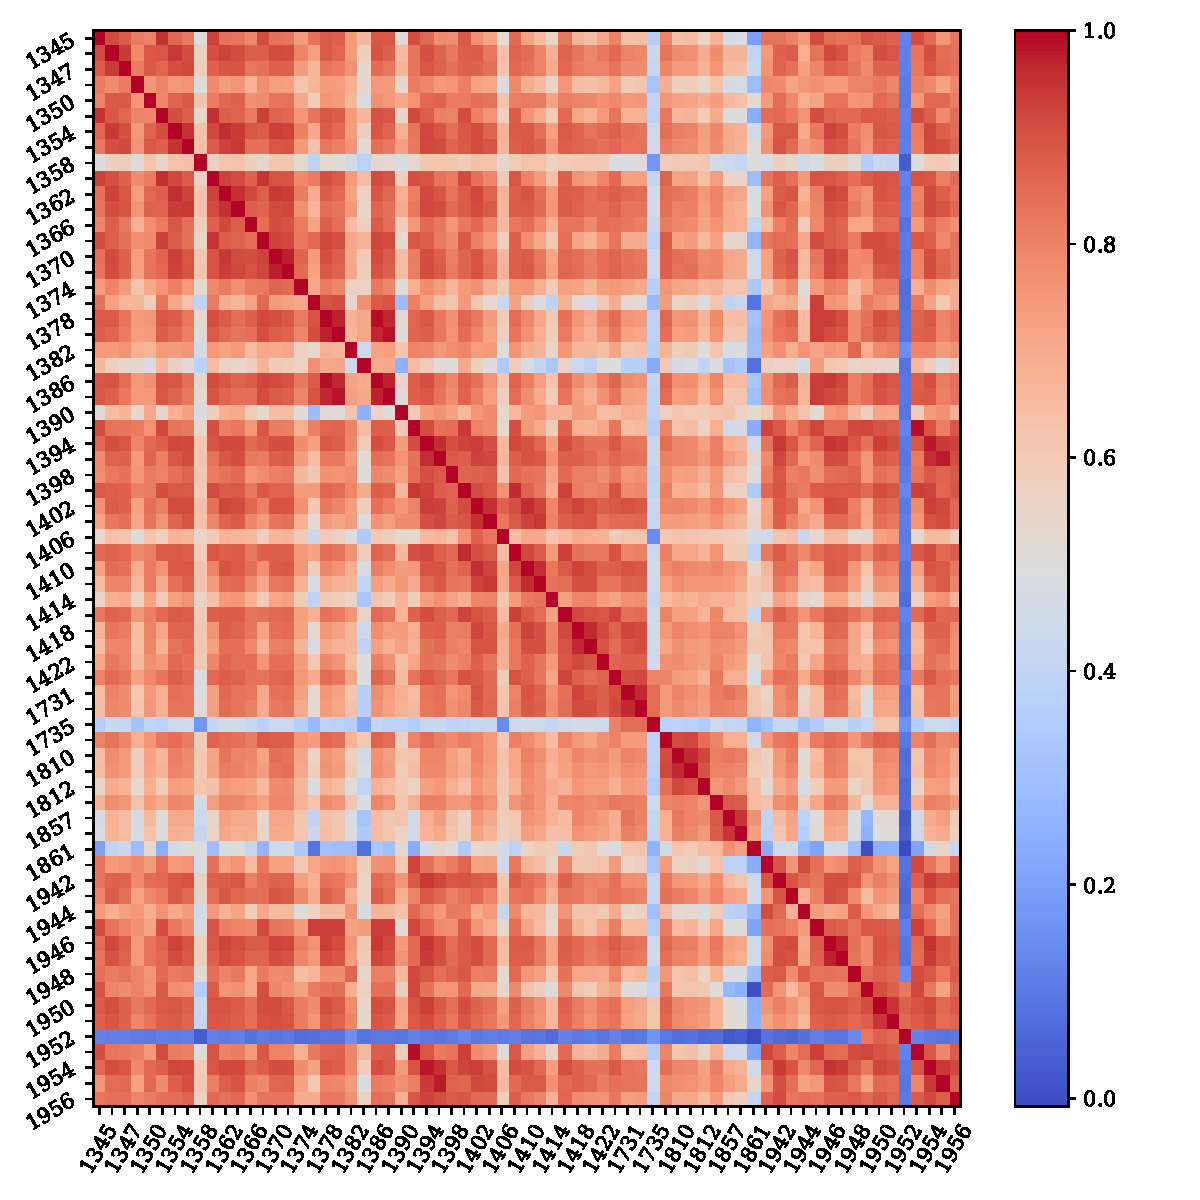
\includegraphics[scale=0.8]{FIG/correlation_matrix.pdf}
  \caption{Correlation matrix between detectors for the volume observations.}
  \label{fig:correlation_matrix}
\end{figure}

\item{\textbf{Forecasting}}

Three broad categories of models are commonly used for short- or medium-term forecasting and for understanding relationships among time series variables: (1) Exponential Smoothing Models (ESM), which are straightforward and effective for data with level, trend, or seasonal components; (2) ARIMA-type models, including SARIMA for handling seasonal patterns and ARIMAX or VAR for incorporating explanatory variables or multiple interdependent series; and (3) Unobserved Component Models (UCM), which break down a series into trend, seasonal, and irregular components, and can readily include covariates. For more complex or highly nonlinear data, deep learning approaches (RNNs, LSTMs, GRUs, and Transformers) can capture intricate temporal dependencies and relationships. 

For the purpose of this question I have used the local TAGI-LSTM model also presented in my research proposal. I did not perform any hyper parameter fine-tuning but rather used an out of the box approach where I have trained the parameters of the model on a training set, and evaluated it's forecasting capacity on a test set that is highlighted in \ref{fig:data_split}. Since, I have worked with 5min periodic data my training set included a great amount of data to train on, and due to the strong seasonality pattern the deployed model is able to accurately forecast on the test set as shown in Figure \ref{fig:model_forecast}.

\begin{figure}[H]
  \centering
  %% Creator: Matplotlib, PGF backend
%%
%% To include the figure in your LaTeX document, write
%%   \input{<filename>.pgf}
%%
%% Make sure the required packages are loaded in your preamble
%%   \usepackage{pgf}
%%
%% Also ensure that all the required font packages are loaded; for instance,
%% the lmodern package is sometimes necessary when using math font.
%%   \usepackage{lmodern}
%%
%% Figures using additional raster images can only be included by \input if
%% they are in the same directory as the main LaTeX file. For loading figures
%% from other directories you can use the `import` package
%%   \usepackage{import}
%%
%% and then include the figures with
%%   \import{<path to file>}{<filename>.pgf}
%%
%% Matplotlib used the following preamble
%%   \def\mathdefault#1{#1}
%%   \everymath=\expandafter{\the\everymath\displaystyle}
%%   \IfFileExists{scrextend.sty}{
%%     \usepackage[fontsize=10.000000pt]{scrextend}
%%   }{
%%     \renewcommand{\normalsize}{\fontsize{10.000000}{12.000000}\selectfont}
%%     \normalsize
%%   }
%%   
%%   \makeatletter\@ifpackageloaded{underscore}{}{\usepackage[strings]{underscore}}\makeatother
%%
\begingroup%
\makeatletter%
\begin{pgfpicture}%
\pgfpathrectangle{\pgfpointorigin}{\pgfqpoint{6.000000in}{2.000000in}}%
\pgfusepath{use as bounding box, clip}%
\begin{pgfscope}%
\pgfsetbuttcap%
\pgfsetmiterjoin%
\definecolor{currentfill}{rgb}{1.000000,1.000000,1.000000}%
\pgfsetfillcolor{currentfill}%
\pgfsetlinewidth{0.000000pt}%
\definecolor{currentstroke}{rgb}{1.000000,1.000000,1.000000}%
\pgfsetstrokecolor{currentstroke}%
\pgfsetdash{}{0pt}%
\pgfpathmoveto{\pgfqpoint{0.000000in}{0.000000in}}%
\pgfpathlineto{\pgfqpoint{6.000000in}{0.000000in}}%
\pgfpathlineto{\pgfqpoint{6.000000in}{2.000000in}}%
\pgfpathlineto{\pgfqpoint{0.000000in}{2.000000in}}%
\pgfpathlineto{\pgfqpoint{0.000000in}{0.000000in}}%
\pgfpathclose%
\pgfusepath{fill}%
\end{pgfscope}%
\begin{pgfscope}%
\pgfsetbuttcap%
\pgfsetmiterjoin%
\definecolor{currentfill}{rgb}{1.000000,1.000000,1.000000}%
\pgfsetfillcolor{currentfill}%
\pgfsetlinewidth{0.000000pt}%
\definecolor{currentstroke}{rgb}{0.000000,0.000000,0.000000}%
\pgfsetstrokecolor{currentstroke}%
\pgfsetstrokeopacity{0.000000}%
\pgfsetdash{}{0pt}%
\pgfpathmoveto{\pgfqpoint{0.704028in}{0.839749in}}%
\pgfpathlineto{\pgfqpoint{5.728545in}{0.839749in}}%
\pgfpathlineto{\pgfqpoint{5.728545in}{1.588489in}}%
\pgfpathlineto{\pgfqpoint{0.704028in}{1.588489in}}%
\pgfpathlineto{\pgfqpoint{0.704028in}{0.839749in}}%
\pgfpathclose%
\pgfusepath{fill}%
\end{pgfscope}%
\begin{pgfscope}%
\pgfsetbuttcap%
\pgfsetroundjoin%
\definecolor{currentfill}{rgb}{0.000000,0.000000,0.000000}%
\pgfsetfillcolor{currentfill}%
\pgfsetlinewidth{0.803000pt}%
\definecolor{currentstroke}{rgb}{0.000000,0.000000,0.000000}%
\pgfsetstrokecolor{currentstroke}%
\pgfsetdash{}{0pt}%
\pgfsys@defobject{currentmarker}{\pgfqpoint{0.000000in}{-0.048611in}}{\pgfqpoint{0.000000in}{0.000000in}}{%
\pgfpathmoveto{\pgfqpoint{0.000000in}{0.000000in}}%
\pgfpathlineto{\pgfqpoint{0.000000in}{-0.048611in}}%
\pgfusepath{stroke,fill}%
}%
\begin{pgfscope}%
\pgfsys@transformshift{0.932159in}{0.839749in}%
\pgfsys@useobject{currentmarker}{}%
\end{pgfscope}%
\end{pgfscope}%
\begin{pgfscope}%
\definecolor{textcolor}{rgb}{0.000000,0.000000,0.000000}%
\pgfsetstrokecolor{textcolor}%
\pgfsetfillcolor{textcolor}%
\pgftext[x=0.639504in, y=0.430212in, left, base,rotate=20.000000]{\color{textcolor}{\rmfamily\fontsize{10.000000}{12.000000}\selectfont\catcode`\^=\active\def^{\ifmmode\sp\else\^{}\fi}\catcode`\%=\active\def%{\%}2011-09-15}}%
\end{pgfscope}%
\begin{pgfscope}%
\pgfsetbuttcap%
\pgfsetroundjoin%
\definecolor{currentfill}{rgb}{0.000000,0.000000,0.000000}%
\pgfsetfillcolor{currentfill}%
\pgfsetlinewidth{0.803000pt}%
\definecolor{currentstroke}{rgb}{0.000000,0.000000,0.000000}%
\pgfsetstrokecolor{currentstroke}%
\pgfsetdash{}{0pt}%
\pgfsys@defobject{currentmarker}{\pgfqpoint{0.000000in}{-0.048611in}}{\pgfqpoint{0.000000in}{0.000000in}}{%
\pgfpathmoveto{\pgfqpoint{0.000000in}{0.000000in}}%
\pgfpathlineto{\pgfqpoint{0.000000in}{-0.048611in}}%
\pgfusepath{stroke,fill}%
}%
\begin{pgfscope}%
\pgfsys@transformshift{1.447584in}{0.839749in}%
\pgfsys@useobject{currentmarker}{}%
\end{pgfscope}%
\end{pgfscope}%
\begin{pgfscope}%
\definecolor{textcolor}{rgb}{0.000000,0.000000,0.000000}%
\pgfsetstrokecolor{textcolor}%
\pgfsetfillcolor{textcolor}%
\pgftext[x=1.154929in, y=0.430212in, left, base,rotate=20.000000]{\color{textcolor}{\rmfamily\fontsize{10.000000}{12.000000}\selectfont\catcode`\^=\active\def^{\ifmmode\sp\else\^{}\fi}\catcode`\%=\active\def%{\%}2011-09-22}}%
\end{pgfscope}%
\begin{pgfscope}%
\pgfsetbuttcap%
\pgfsetroundjoin%
\definecolor{currentfill}{rgb}{0.000000,0.000000,0.000000}%
\pgfsetfillcolor{currentfill}%
\pgfsetlinewidth{0.803000pt}%
\definecolor{currentstroke}{rgb}{0.000000,0.000000,0.000000}%
\pgfsetstrokecolor{currentstroke}%
\pgfsetdash{}{0pt}%
\pgfsys@defobject{currentmarker}{\pgfqpoint{0.000000in}{-0.048611in}}{\pgfqpoint{0.000000in}{0.000000in}}{%
\pgfpathmoveto{\pgfqpoint{0.000000in}{0.000000in}}%
\pgfpathlineto{\pgfqpoint{0.000000in}{-0.048611in}}%
\pgfusepath{stroke,fill}%
}%
\begin{pgfscope}%
\pgfsys@transformshift{2.110272in}{0.839749in}%
\pgfsys@useobject{currentmarker}{}%
\end{pgfscope}%
\end{pgfscope}%
\begin{pgfscope}%
\definecolor{textcolor}{rgb}{0.000000,0.000000,0.000000}%
\pgfsetstrokecolor{textcolor}%
\pgfsetfillcolor{textcolor}%
\pgftext[x=1.817617in, y=0.430212in, left, base,rotate=20.000000]{\color{textcolor}{\rmfamily\fontsize{10.000000}{12.000000}\selectfont\catcode`\^=\active\def^{\ifmmode\sp\else\^{}\fi}\catcode`\%=\active\def%{\%}2011-10-01}}%
\end{pgfscope}%
\begin{pgfscope}%
\pgfsetbuttcap%
\pgfsetroundjoin%
\definecolor{currentfill}{rgb}{0.000000,0.000000,0.000000}%
\pgfsetfillcolor{currentfill}%
\pgfsetlinewidth{0.803000pt}%
\definecolor{currentstroke}{rgb}{0.000000,0.000000,0.000000}%
\pgfsetstrokecolor{currentstroke}%
\pgfsetdash{}{0pt}%
\pgfsys@defobject{currentmarker}{\pgfqpoint{0.000000in}{-0.048611in}}{\pgfqpoint{0.000000in}{0.000000in}}{%
\pgfpathmoveto{\pgfqpoint{0.000000in}{0.000000in}}%
\pgfpathlineto{\pgfqpoint{0.000000in}{-0.048611in}}%
\pgfusepath{stroke,fill}%
}%
\begin{pgfscope}%
\pgfsys@transformshift{2.625696in}{0.839749in}%
\pgfsys@useobject{currentmarker}{}%
\end{pgfscope}%
\end{pgfscope}%
\begin{pgfscope}%
\definecolor{textcolor}{rgb}{0.000000,0.000000,0.000000}%
\pgfsetstrokecolor{textcolor}%
\pgfsetfillcolor{textcolor}%
\pgftext[x=2.333041in, y=0.430212in, left, base,rotate=20.000000]{\color{textcolor}{\rmfamily\fontsize{10.000000}{12.000000}\selectfont\catcode`\^=\active\def^{\ifmmode\sp\else\^{}\fi}\catcode`\%=\active\def%{\%}2011-10-08}}%
\end{pgfscope}%
\begin{pgfscope}%
\pgfsetbuttcap%
\pgfsetroundjoin%
\definecolor{currentfill}{rgb}{0.000000,0.000000,0.000000}%
\pgfsetfillcolor{currentfill}%
\pgfsetlinewidth{0.803000pt}%
\definecolor{currentstroke}{rgb}{0.000000,0.000000,0.000000}%
\pgfsetstrokecolor{currentstroke}%
\pgfsetdash{}{0pt}%
\pgfsys@defobject{currentmarker}{\pgfqpoint{0.000000in}{-0.048611in}}{\pgfqpoint{0.000000in}{0.000000in}}{%
\pgfpathmoveto{\pgfqpoint{0.000000in}{0.000000in}}%
\pgfpathlineto{\pgfqpoint{0.000000in}{-0.048611in}}%
\pgfusepath{stroke,fill}%
}%
\begin{pgfscope}%
\pgfsys@transformshift{3.141121in}{0.839749in}%
\pgfsys@useobject{currentmarker}{}%
\end{pgfscope}%
\end{pgfscope}%
\begin{pgfscope}%
\definecolor{textcolor}{rgb}{0.000000,0.000000,0.000000}%
\pgfsetstrokecolor{textcolor}%
\pgfsetfillcolor{textcolor}%
\pgftext[x=2.848465in, y=0.430212in, left, base,rotate=20.000000]{\color{textcolor}{\rmfamily\fontsize{10.000000}{12.000000}\selectfont\catcode`\^=\active\def^{\ifmmode\sp\else\^{}\fi}\catcode`\%=\active\def%{\%}2011-10-15}}%
\end{pgfscope}%
\begin{pgfscope}%
\pgfsetbuttcap%
\pgfsetroundjoin%
\definecolor{currentfill}{rgb}{0.000000,0.000000,0.000000}%
\pgfsetfillcolor{currentfill}%
\pgfsetlinewidth{0.803000pt}%
\definecolor{currentstroke}{rgb}{0.000000,0.000000,0.000000}%
\pgfsetstrokecolor{currentstroke}%
\pgfsetdash{}{0pt}%
\pgfsys@defobject{currentmarker}{\pgfqpoint{0.000000in}{-0.048611in}}{\pgfqpoint{0.000000in}{0.000000in}}{%
\pgfpathmoveto{\pgfqpoint{0.000000in}{0.000000in}}%
\pgfpathlineto{\pgfqpoint{0.000000in}{-0.048611in}}%
\pgfusepath{stroke,fill}%
}%
\begin{pgfscope}%
\pgfsys@transformshift{3.656545in}{0.839749in}%
\pgfsys@useobject{currentmarker}{}%
\end{pgfscope}%
\end{pgfscope}%
\begin{pgfscope}%
\definecolor{textcolor}{rgb}{0.000000,0.000000,0.000000}%
\pgfsetstrokecolor{textcolor}%
\pgfsetfillcolor{textcolor}%
\pgftext[x=3.363890in, y=0.430212in, left, base,rotate=20.000000]{\color{textcolor}{\rmfamily\fontsize{10.000000}{12.000000}\selectfont\catcode`\^=\active\def^{\ifmmode\sp\else\^{}\fi}\catcode`\%=\active\def%{\%}2011-10-22}}%
\end{pgfscope}%
\begin{pgfscope}%
\pgfsetbuttcap%
\pgfsetroundjoin%
\definecolor{currentfill}{rgb}{0.000000,0.000000,0.000000}%
\pgfsetfillcolor{currentfill}%
\pgfsetlinewidth{0.803000pt}%
\definecolor{currentstroke}{rgb}{0.000000,0.000000,0.000000}%
\pgfsetstrokecolor{currentstroke}%
\pgfsetdash{}{0pt}%
\pgfsys@defobject{currentmarker}{\pgfqpoint{0.000000in}{-0.048611in}}{\pgfqpoint{0.000000in}{0.000000in}}{%
\pgfpathmoveto{\pgfqpoint{0.000000in}{0.000000in}}%
\pgfpathlineto{\pgfqpoint{0.000000in}{-0.048611in}}%
\pgfusepath{stroke,fill}%
}%
\begin{pgfscope}%
\pgfsys@transformshift{4.392865in}{0.839749in}%
\pgfsys@useobject{currentmarker}{}%
\end{pgfscope}%
\end{pgfscope}%
\begin{pgfscope}%
\definecolor{textcolor}{rgb}{0.000000,0.000000,0.000000}%
\pgfsetstrokecolor{textcolor}%
\pgfsetfillcolor{textcolor}%
\pgftext[x=4.100210in, y=0.430212in, left, base,rotate=20.000000]{\color{textcolor}{\rmfamily\fontsize{10.000000}{12.000000}\selectfont\catcode`\^=\active\def^{\ifmmode\sp\else\^{}\fi}\catcode`\%=\active\def%{\%}2011-11-01}}%
\end{pgfscope}%
\begin{pgfscope}%
\pgfsetbuttcap%
\pgfsetroundjoin%
\definecolor{currentfill}{rgb}{0.000000,0.000000,0.000000}%
\pgfsetfillcolor{currentfill}%
\pgfsetlinewidth{0.803000pt}%
\definecolor{currentstroke}{rgb}{0.000000,0.000000,0.000000}%
\pgfsetstrokecolor{currentstroke}%
\pgfsetdash{}{0pt}%
\pgfsys@defobject{currentmarker}{\pgfqpoint{0.000000in}{-0.048611in}}{\pgfqpoint{0.000000in}{0.000000in}}{%
\pgfpathmoveto{\pgfqpoint{0.000000in}{0.000000in}}%
\pgfpathlineto{\pgfqpoint{0.000000in}{-0.048611in}}%
\pgfusepath{stroke,fill}%
}%
\begin{pgfscope}%
\pgfsys@transformshift{4.911358in}{0.839749in}%
\pgfsys@useobject{currentmarker}{}%
\end{pgfscope}%
\end{pgfscope}%
\begin{pgfscope}%
\definecolor{textcolor}{rgb}{0.000000,0.000000,0.000000}%
\pgfsetstrokecolor{textcolor}%
\pgfsetfillcolor{textcolor}%
\pgftext[x=4.618702in, y=0.430212in, left, base,rotate=20.000000]{\color{textcolor}{\rmfamily\fontsize{10.000000}{12.000000}\selectfont\catcode`\^=\active\def^{\ifmmode\sp\else\^{}\fi}\catcode`\%=\active\def%{\%}2011-11-08}}%
\end{pgfscope}%
\begin{pgfscope}%
\pgfsetbuttcap%
\pgfsetroundjoin%
\definecolor{currentfill}{rgb}{0.000000,0.000000,0.000000}%
\pgfsetfillcolor{currentfill}%
\pgfsetlinewidth{0.803000pt}%
\definecolor{currentstroke}{rgb}{0.000000,0.000000,0.000000}%
\pgfsetstrokecolor{currentstroke}%
\pgfsetdash{}{0pt}%
\pgfsys@defobject{currentmarker}{\pgfqpoint{0.000000in}{-0.048611in}}{\pgfqpoint{0.000000in}{0.000000in}}{%
\pgfpathmoveto{\pgfqpoint{0.000000in}{0.000000in}}%
\pgfpathlineto{\pgfqpoint{0.000000in}{-0.048611in}}%
\pgfusepath{stroke,fill}%
}%
\begin{pgfscope}%
\pgfsys@transformshift{5.426782in}{0.839749in}%
\pgfsys@useobject{currentmarker}{}%
\end{pgfscope}%
\end{pgfscope}%
\begin{pgfscope}%
\definecolor{textcolor}{rgb}{0.000000,0.000000,0.000000}%
\pgfsetstrokecolor{textcolor}%
\pgfsetfillcolor{textcolor}%
\pgftext[x=5.134127in, y=0.430212in, left, base,rotate=20.000000]{\color{textcolor}{\rmfamily\fontsize{10.000000}{12.000000}\selectfont\catcode`\^=\active\def^{\ifmmode\sp\else\^{}\fi}\catcode`\%=\active\def%{\%}2011-11-15}}%
\end{pgfscope}%
\begin{pgfscope}%
\definecolor{textcolor}{rgb}{0.000000,0.000000,0.000000}%
\pgfsetstrokecolor{textcolor}%
\pgfsetfillcolor{textcolor}%
\pgftext[x=3.216287in,y=0.349279in,,top]{\color{textcolor}{\rmfamily\fontsize{10.000000}{12.000000}\selectfont\catcode`\^=\active\def^{\ifmmode\sp\else\^{}\fi}\catcode`\%=\active\def%{\%}Time}}%
\end{pgfscope}%
\begin{pgfscope}%
\pgfsetbuttcap%
\pgfsetroundjoin%
\definecolor{currentfill}{rgb}{0.000000,0.000000,0.000000}%
\pgfsetfillcolor{currentfill}%
\pgfsetlinewidth{0.803000pt}%
\definecolor{currentstroke}{rgb}{0.000000,0.000000,0.000000}%
\pgfsetstrokecolor{currentstroke}%
\pgfsetdash{}{0pt}%
\pgfsys@defobject{currentmarker}{\pgfqpoint{-0.048611in}{0.000000in}}{\pgfqpoint{-0.000000in}{0.000000in}}{%
\pgfpathmoveto{\pgfqpoint{-0.000000in}{0.000000in}}%
\pgfpathlineto{\pgfqpoint{-0.048611in}{0.000000in}}%
\pgfusepath{stroke,fill}%
}%
\begin{pgfscope}%
\pgfsys@transformshift{0.704028in}{0.873782in}%
\pgfsys@useobject{currentmarker}{}%
\end{pgfscope}%
\end{pgfscope}%
\begin{pgfscope}%
\definecolor{textcolor}{rgb}{0.000000,0.000000,0.000000}%
\pgfsetstrokecolor{textcolor}%
\pgfsetfillcolor{textcolor}%
\pgftext[x=0.537361in, y=0.825557in, left, base]{\color{textcolor}{\rmfamily\fontsize{10.000000}{12.000000}\selectfont\catcode`\^=\active\def^{\ifmmode\sp\else\^{}\fi}\catcode`\%=\active\def%{\%}0}}%
\end{pgfscope}%
\begin{pgfscope}%
\pgfsetbuttcap%
\pgfsetroundjoin%
\definecolor{currentfill}{rgb}{0.000000,0.000000,0.000000}%
\pgfsetfillcolor{currentfill}%
\pgfsetlinewidth{0.803000pt}%
\definecolor{currentstroke}{rgb}{0.000000,0.000000,0.000000}%
\pgfsetstrokecolor{currentstroke}%
\pgfsetdash{}{0pt}%
\pgfsys@defobject{currentmarker}{\pgfqpoint{-0.048611in}{0.000000in}}{\pgfqpoint{-0.000000in}{0.000000in}}{%
\pgfpathmoveto{\pgfqpoint{-0.000000in}{0.000000in}}%
\pgfpathlineto{\pgfqpoint{-0.048611in}{0.000000in}}%
\pgfusepath{stroke,fill}%
}%
\begin{pgfscope}%
\pgfsys@transformshift{0.704028in}{1.271837in}%
\pgfsys@useobject{currentmarker}{}%
\end{pgfscope}%
\end{pgfscope}%
\begin{pgfscope}%
\definecolor{textcolor}{rgb}{0.000000,0.000000,0.000000}%
\pgfsetstrokecolor{textcolor}%
\pgfsetfillcolor{textcolor}%
\pgftext[x=0.398472in, y=1.223611in, left, base]{\color{textcolor}{\rmfamily\fontsize{10.000000}{12.000000}\selectfont\catcode`\^=\active\def^{\ifmmode\sp\else\^{}\fi}\catcode`\%=\active\def%{\%}100}}%
\end{pgfscope}%
\begin{pgfscope}%
\definecolor{textcolor}{rgb}{0.000000,0.000000,0.000000}%
\pgfsetstrokecolor{textcolor}%
\pgfsetfillcolor{textcolor}%
\pgftext[x=0.342916in,y=1.214119in,,bottom,rotate=90.000000]{\color{textcolor}{\rmfamily\fontsize{10.000000}{12.000000}\selectfont\catcode`\^=\active\def^{\ifmmode\sp\else\^{}\fi}\catcode`\%=\active\def%{\%}Volume}}%
\end{pgfscope}%
\begin{pgfscope}%
\pgfpathrectangle{\pgfqpoint{0.704028in}{0.839749in}}{\pgfqpoint{5.024518in}{0.748740in}}%
\pgfusepath{clip}%
\pgfsetrectcap%
\pgfsetroundjoin%
\pgfsetlinewidth{1.505625pt}%
\definecolor{currentstroke}{rgb}{0.000000,0.447059,0.698039}%
\pgfsetstrokecolor{currentstroke}%
\pgfsetdash{}{0pt}%
\pgfpathmoveto{\pgfqpoint{0.932415in}{0.877763in}}%
\pgfpathlineto{\pgfqpoint{0.932671in}{0.913588in}}%
\pgfpathlineto{\pgfqpoint{0.933438in}{0.893685in}}%
\pgfpathlineto{\pgfqpoint{0.934460in}{0.873782in}}%
\pgfpathlineto{\pgfqpoint{0.934205in}{0.897666in}}%
\pgfpathlineto{\pgfqpoint{0.934716in}{0.881743in}}%
\pgfpathlineto{\pgfqpoint{0.934972in}{0.889705in}}%
\pgfpathlineto{\pgfqpoint{0.935483in}{0.877763in}}%
\pgfpathlineto{\pgfqpoint{0.935739in}{0.881743in}}%
\pgfpathlineto{\pgfqpoint{0.936250in}{0.889705in}}%
\pgfpathlineto{\pgfqpoint{0.936761in}{0.873782in}}%
\pgfpathlineto{\pgfqpoint{0.937528in}{0.877763in}}%
\pgfpathlineto{\pgfqpoint{0.938807in}{0.893685in}}%
\pgfpathlineto{\pgfqpoint{0.939062in}{0.873782in}}%
\pgfpathlineto{\pgfqpoint{0.939829in}{0.881743in}}%
\pgfpathlineto{\pgfqpoint{0.940085in}{0.881743in}}%
\pgfpathlineto{\pgfqpoint{0.940596in}{0.877763in}}%
\pgfpathlineto{\pgfqpoint{0.941619in}{0.897666in}}%
\pgfpathlineto{\pgfqpoint{0.942386in}{0.881743in}}%
\pgfpathlineto{\pgfqpoint{0.942642in}{0.889705in}}%
\pgfpathlineto{\pgfqpoint{0.943664in}{0.905627in}}%
\pgfpathlineto{\pgfqpoint{0.943920in}{0.881743in}}%
\pgfpathlineto{\pgfqpoint{0.944687in}{0.905627in}}%
\pgfpathlineto{\pgfqpoint{0.945198in}{0.873782in}}%
\pgfpathlineto{\pgfqpoint{0.959260in}{0.889705in}}%
\pgfpathlineto{\pgfqpoint{0.960027in}{1.228051in}}%
\pgfpathlineto{\pgfqpoint{0.960538in}{1.184265in}}%
\pgfpathlineto{\pgfqpoint{0.960794in}{1.323584in}}%
\pgfpathlineto{\pgfqpoint{0.961305in}{1.164362in}}%
\pgfpathlineto{\pgfqpoint{0.961817in}{1.319603in}}%
\pgfpathlineto{\pgfqpoint{0.963351in}{1.100673in}}%
\pgfpathlineto{\pgfqpoint{0.964373in}{1.263876in}}%
\pgfpathlineto{\pgfqpoint{0.964629in}{1.239992in}}%
\pgfpathlineto{\pgfqpoint{0.965652in}{1.144459in}}%
\pgfpathlineto{\pgfqpoint{0.965907in}{1.148440in}}%
\pgfpathlineto{\pgfqpoint{0.966930in}{1.132518in}}%
\pgfpathlineto{\pgfqpoint{0.967186in}{1.255915in}}%
\pgfpathlineto{\pgfqpoint{0.968208in}{1.148440in}}%
\pgfpathlineto{\pgfqpoint{0.967953in}{1.275817in}}%
\pgfpathlineto{\pgfqpoint{0.968464in}{1.160381in}}%
\pgfpathlineto{\pgfqpoint{0.968975in}{1.236012in}}%
\pgfpathlineto{\pgfqpoint{0.969742in}{1.196206in}}%
\pgfpathlineto{\pgfqpoint{0.969998in}{1.168343in}}%
\pgfpathlineto{\pgfqpoint{0.970254in}{1.228051in}}%
\pgfpathlineto{\pgfqpoint{0.970509in}{1.184265in}}%
\pgfpathlineto{\pgfqpoint{0.971021in}{1.279798in}}%
\pgfpathlineto{\pgfqpoint{0.971788in}{1.224070in}}%
\pgfpathlineto{\pgfqpoint{0.972043in}{1.168343in}}%
\pgfpathlineto{\pgfqpoint{0.972555in}{1.255915in}}%
\pgfpathlineto{\pgfqpoint{0.972810in}{1.236012in}}%
\pgfpathlineto{\pgfqpoint{0.973066in}{1.319603in}}%
\pgfpathlineto{\pgfqpoint{0.973833in}{1.255915in}}%
\pgfpathlineto{\pgfqpoint{0.974089in}{1.243973in}}%
\pgfpathlineto{\pgfqpoint{0.974344in}{1.267856in}}%
\pgfpathlineto{\pgfqpoint{0.974856in}{1.363389in}}%
\pgfpathlineto{\pgfqpoint{0.975111in}{1.228051in}}%
\pgfpathlineto{\pgfqpoint{0.976134in}{1.259895in}}%
\pgfpathlineto{\pgfqpoint{0.977412in}{1.490767in}}%
\pgfpathlineto{\pgfqpoint{0.977668in}{1.403195in}}%
\pgfpathlineto{\pgfqpoint{0.978946in}{1.279798in}}%
\pgfpathlineto{\pgfqpoint{0.979713in}{1.164362in}}%
\pgfpathlineto{\pgfqpoint{0.980225in}{1.423097in}}%
\pgfpathlineto{\pgfqpoint{0.980480in}{1.303681in}}%
\pgfpathlineto{\pgfqpoint{0.980736in}{1.454942in}}%
\pgfpathlineto{\pgfqpoint{0.980992in}{1.359409in}}%
\pgfpathlineto{\pgfqpoint{0.981247in}{1.466883in}}%
\pgfpathlineto{\pgfqpoint{0.981503in}{1.036985in}}%
\pgfpathlineto{\pgfqpoint{0.982526in}{1.124557in}}%
\pgfpathlineto{\pgfqpoint{0.984315in}{1.439019in}}%
\pgfpathlineto{\pgfqpoint{0.985082in}{1.387272in}}%
\pgfpathlineto{\pgfqpoint{0.986616in}{1.243973in}}%
\pgfpathlineto{\pgfqpoint{0.986872in}{1.419117in}}%
\pgfpathlineto{\pgfqpoint{0.987128in}{1.148440in}}%
\pgfpathlineto{\pgfqpoint{0.987639in}{1.351448in}}%
\pgfpathlineto{\pgfqpoint{0.989940in}{1.112615in}}%
\pgfpathlineto{\pgfqpoint{0.990451in}{1.148440in}}%
\pgfpathlineto{\pgfqpoint{0.990707in}{1.184265in}}%
\pgfpathlineto{\pgfqpoint{0.991218in}{1.104654in}}%
\pgfpathlineto{\pgfqpoint{0.991474in}{1.088732in}}%
\pgfpathlineto{\pgfqpoint{0.991730in}{1.128537in}}%
\pgfpathlineto{\pgfqpoint{0.991985in}{1.136498in}}%
\pgfpathlineto{\pgfqpoint{0.993519in}{1.017082in}}%
\pgfpathlineto{\pgfqpoint{0.994542in}{1.072810in}}%
\pgfpathlineto{\pgfqpoint{0.994286in}{0.997179in}}%
\pgfpathlineto{\pgfqpoint{0.994798in}{1.056887in}}%
\pgfpathlineto{\pgfqpoint{0.996076in}{0.989218in}}%
\pgfpathlineto{\pgfqpoint{0.996332in}{1.033004in}}%
\pgfpathlineto{\pgfqpoint{0.996843in}{0.977276in}}%
\pgfpathlineto{\pgfqpoint{0.997099in}{1.025043in}}%
\pgfpathlineto{\pgfqpoint{0.997354in}{0.957374in}}%
\pgfpathlineto{\pgfqpoint{0.998121in}{0.973296in}}%
\pgfpathlineto{\pgfqpoint{0.998377in}{0.997179in}}%
\pgfpathlineto{\pgfqpoint{0.999144in}{0.973296in}}%
\pgfpathlineto{\pgfqpoint{0.999400in}{0.909607in}}%
\pgfpathlineto{\pgfqpoint{1.000167in}{0.937471in}}%
\pgfpathlineto{\pgfqpoint{1.000422in}{0.941452in}}%
\pgfpathlineto{\pgfqpoint{1.000678in}{0.969315in}}%
\pgfpathlineto{\pgfqpoint{1.000934in}{0.921549in}}%
\pgfpathlineto{\pgfqpoint{1.001445in}{0.957374in}}%
\pgfpathlineto{\pgfqpoint{1.002212in}{0.909607in}}%
\pgfpathlineto{\pgfqpoint{1.002723in}{0.925529in}}%
\pgfpathlineto{\pgfqpoint{1.003235in}{0.941452in}}%
\pgfpathlineto{\pgfqpoint{1.003490in}{0.913588in}}%
\pgfpathlineto{\pgfqpoint{1.003746in}{0.917568in}}%
\pgfpathlineto{\pgfqpoint{1.004002in}{0.913588in}}%
\pgfpathlineto{\pgfqpoint{1.004513in}{0.917568in}}%
\pgfpathlineto{\pgfqpoint{1.005791in}{0.881743in}}%
\pgfpathlineto{\pgfqpoint{1.006814in}{0.905627in}}%
\pgfpathlineto{\pgfqpoint{1.007070in}{0.889705in}}%
\pgfpathlineto{\pgfqpoint{1.007581in}{0.877763in}}%
\pgfpathlineto{\pgfqpoint{1.007837in}{0.881743in}}%
\pgfpathlineto{\pgfqpoint{1.008092in}{0.897666in}}%
\pgfpathlineto{\pgfqpoint{1.008859in}{0.877763in}}%
\pgfpathlineto{\pgfqpoint{1.009115in}{0.877763in}}%
\pgfpathlineto{\pgfqpoint{1.009371in}{0.873782in}}%
\pgfpathlineto{\pgfqpoint{1.009882in}{0.897666in}}%
\pgfpathlineto{\pgfqpoint{1.010393in}{0.889705in}}%
\pgfpathlineto{\pgfqpoint{1.011160in}{0.873782in}}%
\pgfpathlineto{\pgfqpoint{1.011672in}{0.877763in}}%
\pgfpathlineto{\pgfqpoint{1.012439in}{0.877763in}}%
\pgfpathlineto{\pgfqpoint{1.013206in}{0.885724in}}%
\pgfpathlineto{\pgfqpoint{1.013461in}{0.877763in}}%
\pgfpathlineto{\pgfqpoint{1.013717in}{0.873782in}}%
\pgfpathlineto{\pgfqpoint{1.013973in}{0.885724in}}%
\pgfpathlineto{\pgfqpoint{1.014228in}{0.885724in}}%
\pgfpathlineto{\pgfqpoint{1.015762in}{0.877763in}}%
\pgfpathlineto{\pgfqpoint{1.017041in}{0.905627in}}%
\pgfpathlineto{\pgfqpoint{1.017552in}{0.901646in}}%
\pgfpathlineto{\pgfqpoint{1.017808in}{0.877763in}}%
\pgfpathlineto{\pgfqpoint{1.018319in}{0.901646in}}%
\pgfpathlineto{\pgfqpoint{1.019086in}{0.893685in}}%
\pgfpathlineto{\pgfqpoint{1.019597in}{0.933491in}}%
\pgfpathlineto{\pgfqpoint{1.020620in}{0.921549in}}%
\pgfpathlineto{\pgfqpoint{1.020109in}{0.937471in}}%
\pgfpathlineto{\pgfqpoint{1.020876in}{0.925529in}}%
\pgfpathlineto{\pgfqpoint{1.021131in}{0.933491in}}%
\pgfpathlineto{\pgfqpoint{1.023177in}{1.136498in}}%
\pgfpathlineto{\pgfqpoint{1.023944in}{1.029024in}}%
\pgfpathlineto{\pgfqpoint{1.024199in}{1.092712in}}%
\pgfpathlineto{\pgfqpoint{1.026245in}{1.355428in}}%
\pgfpathlineto{\pgfqpoint{1.026500in}{1.303681in}}%
\pgfpathlineto{\pgfqpoint{1.026756in}{1.236012in}}%
\pgfpathlineto{\pgfqpoint{1.027267in}{1.319603in}}%
\pgfpathlineto{\pgfqpoint{1.028290in}{1.482805in}}%
\pgfpathlineto{\pgfqpoint{1.028801in}{1.478825in}}%
\pgfpathlineto{\pgfqpoint{1.030080in}{1.112615in}}%
\pgfpathlineto{\pgfqpoint{1.029313in}{1.526591in}}%
\pgfpathlineto{\pgfqpoint{1.030847in}{1.160381in}}%
\pgfpathlineto{\pgfqpoint{1.031102in}{1.331545in}}%
\pgfpathlineto{\pgfqpoint{1.031869in}{1.212129in}}%
\pgfpathlineto{\pgfqpoint{1.032125in}{1.216109in}}%
\pgfpathlineto{\pgfqpoint{1.032381in}{1.160381in}}%
\pgfpathlineto{\pgfqpoint{1.032636in}{1.307662in}}%
\pgfpathlineto{\pgfqpoint{1.033148in}{1.164362in}}%
\pgfpathlineto{\pgfqpoint{1.034170in}{1.228051in}}%
\pgfpathlineto{\pgfqpoint{1.033659in}{1.148440in}}%
\pgfpathlineto{\pgfqpoint{1.034426in}{1.184265in}}%
\pgfpathlineto{\pgfqpoint{1.034682in}{1.148440in}}%
\pgfpathlineto{\pgfqpoint{1.034937in}{1.196206in}}%
\pgfpathlineto{\pgfqpoint{1.035449in}{1.259895in}}%
\pgfpathlineto{\pgfqpoint{1.035960in}{1.188245in}}%
\pgfpathlineto{\pgfqpoint{1.036471in}{1.136498in}}%
\pgfpathlineto{\pgfqpoint{1.036727in}{1.224070in}}%
\pgfpathlineto{\pgfqpoint{1.036983in}{1.220090in}}%
\pgfpathlineto{\pgfqpoint{1.037494in}{1.184265in}}%
\pgfpathlineto{\pgfqpoint{1.037750in}{1.192226in}}%
\pgfpathlineto{\pgfqpoint{1.038005in}{1.275817in}}%
\pgfpathlineto{\pgfqpoint{1.038261in}{1.164362in}}%
\pgfpathlineto{\pgfqpoint{1.038772in}{1.204167in}}%
\pgfpathlineto{\pgfqpoint{1.039028in}{1.176304in}}%
\pgfpathlineto{\pgfqpoint{1.039284in}{1.224070in}}%
\pgfpathlineto{\pgfqpoint{1.039795in}{1.196206in}}%
\pgfpathlineto{\pgfqpoint{1.040306in}{1.247953in}}%
\pgfpathlineto{\pgfqpoint{1.041073in}{1.224070in}}%
\pgfpathlineto{\pgfqpoint{1.041585in}{1.208148in}}%
\pgfpathlineto{\pgfqpoint{1.042352in}{1.188245in}}%
\pgfpathlineto{\pgfqpoint{1.042607in}{1.335525in}}%
\pgfpathlineto{\pgfqpoint{1.042863in}{1.188245in}}%
\pgfpathlineto{\pgfqpoint{1.043630in}{1.247953in}}%
\pgfpathlineto{\pgfqpoint{1.043886in}{1.391253in}}%
\pgfpathlineto{\pgfqpoint{1.044653in}{1.243973in}}%
\pgfpathlineto{\pgfqpoint{1.045164in}{1.363389in}}%
\pgfpathlineto{\pgfqpoint{1.045420in}{1.247953in}}%
\pgfpathlineto{\pgfqpoint{1.045675in}{1.152420in}}%
\pgfpathlineto{\pgfqpoint{1.045931in}{1.295720in}}%
\pgfpathlineto{\pgfqpoint{1.046442in}{1.247953in}}%
\pgfpathlineto{\pgfqpoint{1.047465in}{1.391253in}}%
\pgfpathlineto{\pgfqpoint{1.047721in}{1.255915in}}%
\pgfpathlineto{\pgfqpoint{1.048743in}{1.275817in}}%
\pgfpathlineto{\pgfqpoint{1.049766in}{1.387272in}}%
\pgfpathlineto{\pgfqpoint{1.050022in}{1.295720in}}%
\pgfpathlineto{\pgfqpoint{1.050533in}{1.307662in}}%
\pgfpathlineto{\pgfqpoint{1.050789in}{1.423097in}}%
\pgfpathlineto{\pgfqpoint{1.051556in}{1.335525in}}%
\pgfpathlineto{\pgfqpoint{1.052067in}{1.415136in}}%
\pgfpathlineto{\pgfqpoint{1.052834in}{1.271837in}}%
\pgfpathlineto{\pgfqpoint{1.053345in}{1.331545in}}%
\pgfpathlineto{\pgfqpoint{1.053601in}{1.327564in}}%
\pgfpathlineto{\pgfqpoint{1.054368in}{1.411156in}}%
\pgfpathlineto{\pgfqpoint{1.054624in}{1.144459in}}%
\pgfpathlineto{\pgfqpoint{1.055646in}{1.319603in}}%
\pgfpathlineto{\pgfqpoint{1.055902in}{1.168343in}}%
\pgfpathlineto{\pgfqpoint{1.056158in}{1.379311in}}%
\pgfpathlineto{\pgfqpoint{1.056669in}{1.243973in}}%
\pgfpathlineto{\pgfqpoint{1.056925in}{1.236012in}}%
\pgfpathlineto{\pgfqpoint{1.057436in}{1.184265in}}%
\pgfpathlineto{\pgfqpoint{1.058203in}{1.279798in}}%
\pgfpathlineto{\pgfqpoint{1.058970in}{1.339506in}}%
\pgfpathlineto{\pgfqpoint{1.059226in}{1.188245in}}%
\pgfpathlineto{\pgfqpoint{1.059737in}{1.446981in}}%
\pgfpathlineto{\pgfqpoint{1.060504in}{1.371350in}}%
\pgfpathlineto{\pgfqpoint{1.061271in}{1.383292in}}%
\pgfpathlineto{\pgfqpoint{1.061527in}{1.283778in}}%
\pgfpathlineto{\pgfqpoint{1.061782in}{1.383292in}}%
\pgfpathlineto{\pgfqpoint{1.062549in}{1.339506in}}%
\pgfpathlineto{\pgfqpoint{1.064083in}{1.092712in}}%
\pgfpathlineto{\pgfqpoint{1.065362in}{1.188245in}}%
\pgfpathlineto{\pgfqpoint{1.065617in}{1.212129in}}%
\pgfpathlineto{\pgfqpoint{1.066384in}{1.048926in}}%
\pgfpathlineto{\pgfqpoint{1.066896in}{1.112615in}}%
\pgfpathlineto{\pgfqpoint{1.068430in}{1.001160in}}%
\pgfpathlineto{\pgfqpoint{1.068685in}{1.009121in}}%
\pgfpathlineto{\pgfqpoint{1.068941in}{1.076790in}}%
\pgfpathlineto{\pgfqpoint{1.069197in}{0.973296in}}%
\pgfpathlineto{\pgfqpoint{1.069708in}{1.009121in}}%
\pgfpathlineto{\pgfqpoint{1.069964in}{1.001160in}}%
\pgfpathlineto{\pgfqpoint{1.070219in}{1.044946in}}%
\pgfpathlineto{\pgfqpoint{1.070986in}{1.001160in}}%
\pgfpathlineto{\pgfqpoint{1.071242in}{1.025043in}}%
\pgfpathlineto{\pgfqpoint{1.071498in}{0.993199in}}%
\pgfpathlineto{\pgfqpoint{1.072009in}{1.021062in}}%
\pgfpathlineto{\pgfqpoint{1.072520in}{1.056887in}}%
\pgfpathlineto{\pgfqpoint{1.073287in}{0.973296in}}%
\pgfpathlineto{\pgfqpoint{1.074310in}{1.044946in}}%
\pgfpathlineto{\pgfqpoint{1.075333in}{0.973296in}}%
\pgfpathlineto{\pgfqpoint{1.075588in}{0.997179in}}%
\pgfpathlineto{\pgfqpoint{1.077378in}{0.905627in}}%
\pgfpathlineto{\pgfqpoint{1.077889in}{0.929510in}}%
\pgfpathlineto{\pgfqpoint{1.078912in}{0.925529in}}%
\pgfpathlineto{\pgfqpoint{1.079679in}{0.929510in}}%
\pgfpathlineto{\pgfqpoint{1.080190in}{0.897666in}}%
\pgfpathlineto{\pgfqpoint{1.080702in}{0.909607in}}%
\pgfpathlineto{\pgfqpoint{1.080957in}{0.897666in}}%
\pgfpathlineto{\pgfqpoint{1.081469in}{0.905627in}}%
\pgfpathlineto{\pgfqpoint{1.082491in}{0.877763in}}%
\pgfpathlineto{\pgfqpoint{1.083258in}{0.897666in}}%
\pgfpathlineto{\pgfqpoint{1.083514in}{0.885724in}}%
\pgfpathlineto{\pgfqpoint{1.083770in}{0.877763in}}%
\pgfpathlineto{\pgfqpoint{1.084025in}{0.897666in}}%
\pgfpathlineto{\pgfqpoint{1.084537in}{0.885724in}}%
\pgfpathlineto{\pgfqpoint{1.084792in}{0.889705in}}%
\pgfpathlineto{\pgfqpoint{1.085048in}{0.873782in}}%
\pgfpathlineto{\pgfqpoint{1.085815in}{0.877763in}}%
\pgfpathlineto{\pgfqpoint{1.086838in}{0.889705in}}%
\pgfpathlineto{\pgfqpoint{1.087605in}{0.873782in}}%
\pgfpathlineto{\pgfqpoint{1.087860in}{0.877763in}}%
\pgfpathlineto{\pgfqpoint{1.088116in}{0.897666in}}%
\pgfpathlineto{\pgfqpoint{1.088372in}{0.873782in}}%
\pgfpathlineto{\pgfqpoint{1.088883in}{0.881743in}}%
\pgfpathlineto{\pgfqpoint{1.089650in}{0.873782in}}%
\pgfpathlineto{\pgfqpoint{1.089906in}{0.901646in}}%
\pgfpathlineto{\pgfqpoint{1.090673in}{0.881743in}}%
\pgfpathlineto{\pgfqpoint{1.092207in}{0.893685in}}%
\pgfpathlineto{\pgfqpoint{1.093741in}{0.873782in}}%
\pgfpathlineto{\pgfqpoint{1.096809in}{0.877763in}}%
\pgfpathlineto{\pgfqpoint{1.097576in}{0.873782in}}%
\pgfpathlineto{\pgfqpoint{1.097831in}{0.877763in}}%
\pgfpathlineto{\pgfqpoint{1.099110in}{0.877763in}}%
\pgfpathlineto{\pgfqpoint{1.100132in}{0.929510in}}%
\pgfpathlineto{\pgfqpoint{1.100644in}{0.901646in}}%
\pgfpathlineto{\pgfqpoint{1.101155in}{0.877763in}}%
\pgfpathlineto{\pgfqpoint{1.102433in}{0.925529in}}%
\pgfpathlineto{\pgfqpoint{1.102689in}{0.881743in}}%
\pgfpathlineto{\pgfqpoint{1.103712in}{0.893685in}}%
\pgfpathlineto{\pgfqpoint{1.104223in}{0.877763in}}%
\pgfpathlineto{\pgfqpoint{1.104734in}{0.941452in}}%
\pgfpathlineto{\pgfqpoint{1.105501in}{0.937471in}}%
\pgfpathlineto{\pgfqpoint{1.106268in}{0.889705in}}%
\pgfpathlineto{\pgfqpoint{1.107035in}{0.889705in}}%
\pgfpathlineto{\pgfqpoint{1.107291in}{0.897666in}}%
\pgfpathlineto{\pgfqpoint{1.107547in}{0.889705in}}%
\pgfpathlineto{\pgfqpoint{1.108314in}{0.889705in}}%
\pgfpathlineto{\pgfqpoint{1.115984in}{0.897666in}}%
\pgfpathlineto{\pgfqpoint{1.118029in}{0.893685in}}%
\pgfpathlineto{\pgfqpoint{1.118796in}{0.949413in}}%
\pgfpathlineto{\pgfqpoint{1.118540in}{0.885724in}}%
\pgfpathlineto{\pgfqpoint{1.119307in}{0.945432in}}%
\pgfpathlineto{\pgfqpoint{1.119563in}{0.933491in}}%
\pgfpathlineto{\pgfqpoint{1.121353in}{1.220090in}}%
\pgfpathlineto{\pgfqpoint{1.121864in}{1.212129in}}%
\pgfpathlineto{\pgfqpoint{1.122120in}{1.148440in}}%
\pgfpathlineto{\pgfqpoint{1.122887in}{1.228051in}}%
\pgfpathlineto{\pgfqpoint{1.123398in}{1.156401in}}%
\pgfpathlineto{\pgfqpoint{1.123654in}{1.228051in}}%
\pgfpathlineto{\pgfqpoint{1.123909in}{1.255915in}}%
\pgfpathlineto{\pgfqpoint{1.124165in}{1.152420in}}%
\pgfpathlineto{\pgfqpoint{1.125188in}{1.164362in}}%
\pgfpathlineto{\pgfqpoint{1.125443in}{1.132518in}}%
\pgfpathlineto{\pgfqpoint{1.125955in}{1.200187in}}%
\pgfpathlineto{\pgfqpoint{1.126210in}{1.287759in}}%
\pgfpathlineto{\pgfqpoint{1.126466in}{1.168343in}}%
\pgfpathlineto{\pgfqpoint{1.126977in}{1.279798in}}%
\pgfpathlineto{\pgfqpoint{1.128256in}{1.156401in}}%
\pgfpathlineto{\pgfqpoint{1.128511in}{1.267856in}}%
\pgfpathlineto{\pgfqpoint{1.129534in}{1.239992in}}%
\pgfpathlineto{\pgfqpoint{1.129790in}{1.255915in}}%
\pgfpathlineto{\pgfqpoint{1.130045in}{1.220090in}}%
\pgfpathlineto{\pgfqpoint{1.130301in}{1.180284in}}%
\pgfpathlineto{\pgfqpoint{1.130812in}{1.236012in}}%
\pgfpathlineto{\pgfqpoint{1.131068in}{1.188245in}}%
\pgfpathlineto{\pgfqpoint{1.131324in}{1.224070in}}%
\pgfpathlineto{\pgfqpoint{1.131579in}{1.152420in}}%
\pgfpathlineto{\pgfqpoint{1.132346in}{1.216109in}}%
\pgfpathlineto{\pgfqpoint{1.132602in}{1.220090in}}%
\pgfpathlineto{\pgfqpoint{1.132858in}{1.192226in}}%
\pgfpathlineto{\pgfqpoint{1.133113in}{1.279798in}}%
\pgfpathlineto{\pgfqpoint{1.133369in}{1.220090in}}%
\pgfpathlineto{\pgfqpoint{1.133625in}{1.239992in}}%
\pgfpathlineto{\pgfqpoint{1.134136in}{1.200187in}}%
\pgfpathlineto{\pgfqpoint{1.134392in}{1.120576in}}%
\pgfpathlineto{\pgfqpoint{1.134903in}{1.216109in}}%
\pgfpathlineto{\pgfqpoint{1.135159in}{1.128537in}}%
\pgfpathlineto{\pgfqpoint{1.136181in}{1.228051in}}%
\pgfpathlineto{\pgfqpoint{1.137460in}{1.104654in}}%
\pgfpathlineto{\pgfqpoint{1.137971in}{1.228051in}}%
\pgfpathlineto{\pgfqpoint{1.138227in}{1.096693in}}%
\pgfpathlineto{\pgfqpoint{1.138482in}{1.180284in}}%
\pgfpathlineto{\pgfqpoint{1.139761in}{1.064848in}}%
\pgfpathlineto{\pgfqpoint{1.140272in}{1.044946in}}%
\pgfpathlineto{\pgfqpoint{1.140528in}{0.913588in}}%
\pgfpathlineto{\pgfqpoint{1.191150in}{1.144459in}}%
\pgfpathlineto{\pgfqpoint{1.191917in}{1.232031in}}%
\pgfpathlineto{\pgfqpoint{1.192428in}{1.220090in}}%
\pgfpathlineto{\pgfqpoint{1.192684in}{1.116596in}}%
\pgfpathlineto{\pgfqpoint{1.193451in}{1.188245in}}%
\pgfpathlineto{\pgfqpoint{1.193962in}{1.092712in}}%
\pgfpathlineto{\pgfqpoint{1.196007in}{1.204167in}}%
\pgfpathlineto{\pgfqpoint{1.196519in}{1.140479in}}%
\pgfpathlineto{\pgfqpoint{1.197030in}{1.168343in}}%
\pgfpathlineto{\pgfqpoint{1.197286in}{1.287759in}}%
\pgfpathlineto{\pgfqpoint{1.198053in}{1.192226in}}%
\pgfpathlineto{\pgfqpoint{1.198308in}{1.204167in}}%
\pgfpathlineto{\pgfqpoint{1.199331in}{1.116596in}}%
\pgfpathlineto{\pgfqpoint{1.200609in}{1.255915in}}%
\pgfpathlineto{\pgfqpoint{1.200865in}{1.239992in}}%
\pgfpathlineto{\pgfqpoint{1.201376in}{1.108634in}}%
\pgfpathlineto{\pgfqpoint{1.201888in}{1.239992in}}%
\pgfpathlineto{\pgfqpoint{1.202399in}{1.088732in}}%
\pgfpathlineto{\pgfqpoint{1.202655in}{1.271837in}}%
\pgfpathlineto{\pgfqpoint{1.203166in}{1.164362in}}%
\pgfpathlineto{\pgfqpoint{1.203933in}{1.243973in}}%
\pgfpathlineto{\pgfqpoint{1.204189in}{1.156401in}}%
\pgfpathlineto{\pgfqpoint{1.204444in}{1.212129in}}%
\pgfpathlineto{\pgfqpoint{1.205211in}{1.216109in}}%
\pgfpathlineto{\pgfqpoint{1.205978in}{1.056887in}}%
\pgfpathlineto{\pgfqpoint{1.207001in}{1.212129in}}%
\pgfpathlineto{\pgfqpoint{1.207768in}{1.172323in}}%
\pgfpathlineto{\pgfqpoint{1.209046in}{1.080771in}}%
\pgfpathlineto{\pgfqpoint{1.208279in}{1.180284in}}%
\pgfpathlineto{\pgfqpoint{1.209813in}{1.096693in}}%
\pgfpathlineto{\pgfqpoint{1.210069in}{1.148440in}}%
\pgfpathlineto{\pgfqpoint{1.210580in}{1.128537in}}%
\pgfpathlineto{\pgfqpoint{1.210836in}{1.036985in}}%
\pgfpathlineto{\pgfqpoint{1.211859in}{1.064848in}}%
\pgfpathlineto{\pgfqpoint{1.212370in}{1.052907in}}%
\pgfpathlineto{\pgfqpoint{1.212881in}{1.108634in}}%
\pgfpathlineto{\pgfqpoint{1.213137in}{1.056887in}}%
\pgfpathlineto{\pgfqpoint{1.214160in}{1.060868in}}%
\pgfpathlineto{\pgfqpoint{1.214415in}{1.036985in}}%
\pgfpathlineto{\pgfqpoint{1.214671in}{1.096693in}}%
\pgfpathlineto{\pgfqpoint{1.214927in}{1.044946in}}%
\pgfpathlineto{\pgfqpoint{1.215182in}{1.080771in}}%
\pgfpathlineto{\pgfqpoint{1.215438in}{1.017082in}}%
\pgfpathlineto{\pgfqpoint{1.215949in}{1.064848in}}%
\pgfpathlineto{\pgfqpoint{1.216972in}{0.945432in}}%
\pgfpathlineto{\pgfqpoint{1.217228in}{0.977276in}}%
\pgfpathlineto{\pgfqpoint{1.217739in}{1.025043in}}%
\pgfpathlineto{\pgfqpoint{1.218250in}{0.989218in}}%
\pgfpathlineto{\pgfqpoint{1.219017in}{0.937471in}}%
\pgfpathlineto{\pgfqpoint{1.219529in}{0.941452in}}%
\pgfpathlineto{\pgfqpoint{1.220296in}{0.957374in}}%
\pgfpathlineto{\pgfqpoint{1.220040in}{0.925529in}}%
\pgfpathlineto{\pgfqpoint{1.220551in}{0.937471in}}%
\pgfpathlineto{\pgfqpoint{1.220807in}{0.945432in}}%
\pgfpathlineto{\pgfqpoint{1.221063in}{0.921549in}}%
\pgfpathlineto{\pgfqpoint{1.221318in}{0.917568in}}%
\pgfpathlineto{\pgfqpoint{1.221830in}{0.957374in}}%
\pgfpathlineto{\pgfqpoint{1.222085in}{0.905627in}}%
\pgfpathlineto{\pgfqpoint{1.222341in}{0.913588in}}%
\pgfpathlineto{\pgfqpoint{1.223619in}{0.901646in}}%
\pgfpathlineto{\pgfqpoint{1.224131in}{0.913588in}}%
\pgfpathlineto{\pgfqpoint{1.224642in}{0.909607in}}%
\pgfpathlineto{\pgfqpoint{1.225665in}{0.877763in}}%
\pgfpathlineto{\pgfqpoint{1.226943in}{0.885724in}}%
\pgfpathlineto{\pgfqpoint{1.227199in}{0.893685in}}%
\pgfpathlineto{\pgfqpoint{1.227454in}{0.877763in}}%
\pgfpathlineto{\pgfqpoint{1.227966in}{0.885724in}}%
\pgfpathlineto{\pgfqpoint{1.228733in}{0.877763in}}%
\pgfpathlineto{\pgfqpoint{1.228988in}{0.889705in}}%
\pgfpathlineto{\pgfqpoint{1.229244in}{0.873782in}}%
\pgfpathlineto{\pgfqpoint{1.229755in}{0.877763in}}%
\pgfpathlineto{\pgfqpoint{1.231034in}{0.873782in}}%
\pgfpathlineto{\pgfqpoint{1.232056in}{0.881743in}}%
\pgfpathlineto{\pgfqpoint{1.233335in}{0.873782in}}%
\pgfpathlineto{\pgfqpoint{1.233846in}{0.873782in}}%
\pgfpathlineto{\pgfqpoint{1.235124in}{0.893685in}}%
\pgfpathlineto{\pgfqpoint{1.236403in}{0.873782in}}%
\pgfpathlineto{\pgfqpoint{1.237937in}{0.893685in}}%
\pgfpathlineto{\pgfqpoint{1.238192in}{0.889705in}}%
\pgfpathlineto{\pgfqpoint{1.238959in}{0.881743in}}%
\pgfpathlineto{\pgfqpoint{1.240749in}{0.965335in}}%
\pgfpathlineto{\pgfqpoint{1.242027in}{0.929510in}}%
\pgfpathlineto{\pgfqpoint{1.243817in}{1.120576in}}%
\pgfpathlineto{\pgfqpoint{1.244328in}{1.104654in}}%
\pgfpathlineto{\pgfqpoint{1.244584in}{1.116596in}}%
\pgfpathlineto{\pgfqpoint{1.244840in}{1.072810in}}%
\pgfpathlineto{\pgfqpoint{1.245351in}{1.148440in}}%
\pgfpathlineto{\pgfqpoint{1.245862in}{1.072810in}}%
\pgfpathlineto{\pgfqpoint{1.246629in}{1.291739in}}%
\pgfpathlineto{\pgfqpoint{1.247141in}{1.435039in}}%
\pgfpathlineto{\pgfqpoint{1.247652in}{1.391253in}}%
\pgfpathlineto{\pgfqpoint{1.247908in}{1.279798in}}%
\pgfpathlineto{\pgfqpoint{1.248675in}{1.415136in}}%
\pgfpathlineto{\pgfqpoint{1.248930in}{1.423097in}}%
\pgfpathlineto{\pgfqpoint{1.249442in}{1.450961in}}%
\pgfpathlineto{\pgfqpoint{1.249697in}{1.315623in}}%
\pgfpathlineto{\pgfqpoint{1.249953in}{1.443000in}}%
\pgfpathlineto{\pgfqpoint{1.250464in}{1.212129in}}%
\pgfpathlineto{\pgfqpoint{1.251743in}{1.355428in}}%
\pgfpathlineto{\pgfqpoint{1.251231in}{1.188245in}}%
\pgfpathlineto{\pgfqpoint{1.251998in}{1.311642in}}%
\pgfpathlineto{\pgfqpoint{1.252510in}{1.160381in}}%
\pgfpathlineto{\pgfqpoint{1.253277in}{1.232031in}}%
\pgfpathlineto{\pgfqpoint{1.253532in}{1.243973in}}%
\pgfpathlineto{\pgfqpoint{1.253788in}{1.116596in}}%
\pgfpathlineto{\pgfqpoint{1.254044in}{1.431058in}}%
\pgfpathlineto{\pgfqpoint{1.254555in}{1.168343in}}%
\pgfpathlineto{\pgfqpoint{1.254811in}{1.176304in}}%
\pgfpathlineto{\pgfqpoint{1.255066in}{1.140479in}}%
\pgfpathlineto{\pgfqpoint{1.255322in}{1.208148in}}%
\pgfpathlineto{\pgfqpoint{1.255578in}{1.208148in}}%
\pgfpathlineto{\pgfqpoint{1.255833in}{1.343486in}}%
\pgfpathlineto{\pgfqpoint{1.256089in}{1.025043in}}%
\pgfpathlineto{\pgfqpoint{1.256600in}{1.017082in}}%
\pgfpathlineto{\pgfqpoint{1.257367in}{1.275817in}}%
\pgfpathlineto{\pgfqpoint{1.257879in}{1.176304in}}%
\pgfpathlineto{\pgfqpoint{1.258390in}{1.100673in}}%
\pgfpathlineto{\pgfqpoint{1.258646in}{1.188245in}}%
\pgfpathlineto{\pgfqpoint{1.258901in}{1.192226in}}%
\pgfpathlineto{\pgfqpoint{1.259157in}{1.120576in}}%
\pgfpathlineto{\pgfqpoint{1.259413in}{1.204167in}}%
\pgfpathlineto{\pgfqpoint{1.259924in}{1.184265in}}%
\pgfpathlineto{\pgfqpoint{1.260180in}{1.224070in}}%
\pgfpathlineto{\pgfqpoint{1.260691in}{1.164362in}}%
\pgfpathlineto{\pgfqpoint{1.260947in}{1.172323in}}%
\pgfpathlineto{\pgfqpoint{1.261714in}{1.255915in}}%
\pgfpathlineto{\pgfqpoint{1.261458in}{1.160381in}}%
\pgfpathlineto{\pgfqpoint{1.261969in}{1.176304in}}%
\pgfpathlineto{\pgfqpoint{1.262225in}{1.148440in}}%
\pgfpathlineto{\pgfqpoint{1.262736in}{1.168343in}}%
\pgfpathlineto{\pgfqpoint{1.262992in}{1.208148in}}%
\pgfpathlineto{\pgfqpoint{1.263503in}{1.172323in}}%
\pgfpathlineto{\pgfqpoint{1.264015in}{1.124557in}}%
\pgfpathlineto{\pgfqpoint{1.264270in}{1.156401in}}%
\pgfpathlineto{\pgfqpoint{1.264782in}{1.112615in}}%
\pgfpathlineto{\pgfqpoint{1.265549in}{1.228051in}}%
\pgfpathlineto{\pgfqpoint{1.266571in}{1.120576in}}%
\pgfpathlineto{\pgfqpoint{1.267083in}{1.100673in}}%
\pgfpathlineto{\pgfqpoint{1.267850in}{1.200187in}}%
\pgfpathlineto{\pgfqpoint{1.268105in}{1.180284in}}%
\pgfpathlineto{\pgfqpoint{1.268361in}{1.232031in}}%
\pgfpathlineto{\pgfqpoint{1.268617in}{1.220090in}}%
\pgfpathlineto{\pgfqpoint{1.268872in}{1.232031in}}%
\pgfpathlineto{\pgfqpoint{1.269128in}{1.160381in}}%
\pgfpathlineto{\pgfqpoint{1.269895in}{1.224070in}}%
\pgfpathlineto{\pgfqpoint{1.270406in}{1.204167in}}%
\pgfpathlineto{\pgfqpoint{1.271173in}{1.259895in}}%
\pgfpathlineto{\pgfqpoint{1.271429in}{1.454942in}}%
\pgfpathlineto{\pgfqpoint{1.271940in}{1.208148in}}%
\pgfpathlineto{\pgfqpoint{1.272196in}{1.120576in}}%
\pgfpathlineto{\pgfqpoint{1.272452in}{1.247953in}}%
\pgfpathlineto{\pgfqpoint{1.272963in}{1.220090in}}%
\pgfpathlineto{\pgfqpoint{1.273986in}{1.331545in}}%
\pgfpathlineto{\pgfqpoint{1.274241in}{1.156401in}}%
\pgfpathlineto{\pgfqpoint{1.274753in}{1.375331in}}%
\pgfpathlineto{\pgfqpoint{1.275008in}{1.339506in}}%
\pgfpathlineto{\pgfqpoint{1.275264in}{1.403195in}}%
\pgfpathlineto{\pgfqpoint{1.275775in}{1.295720in}}%
\pgfpathlineto{\pgfqpoint{1.276031in}{1.271837in}}%
\pgfpathlineto{\pgfqpoint{1.276287in}{1.399214in}}%
\pgfpathlineto{\pgfqpoint{1.276542in}{1.251934in}}%
\pgfpathlineto{\pgfqpoint{1.276798in}{1.275817in}}%
\pgfpathlineto{\pgfqpoint{1.277054in}{1.188245in}}%
\pgfpathlineto{\pgfqpoint{1.277309in}{1.427078in}}%
\pgfpathlineto{\pgfqpoint{1.277565in}{1.339506in}}%
\pgfpathlineto{\pgfqpoint{1.278076in}{1.395234in}}%
\pgfpathlineto{\pgfqpoint{1.278332in}{1.224070in}}%
\pgfpathlineto{\pgfqpoint{1.279099in}{1.439019in}}%
\pgfpathlineto{\pgfqpoint{1.280122in}{1.216109in}}%
\pgfpathlineto{\pgfqpoint{1.280377in}{1.160381in}}%
\pgfpathlineto{\pgfqpoint{1.280633in}{1.196206in}}%
\pgfpathlineto{\pgfqpoint{1.280889in}{1.299700in}}%
\pgfpathlineto{\pgfqpoint{1.281144in}{1.144459in}}%
\pgfpathlineto{\pgfqpoint{1.281656in}{1.164362in}}%
\pgfpathlineto{\pgfqpoint{1.282678in}{1.291739in}}%
\pgfpathlineto{\pgfqpoint{1.282934in}{1.259895in}}%
\pgfpathlineto{\pgfqpoint{1.284979in}{1.040965in}}%
\pgfpathlineto{\pgfqpoint{1.286002in}{1.092712in}}%
\pgfpathlineto{\pgfqpoint{1.288047in}{0.997179in}}%
\pgfpathlineto{\pgfqpoint{1.289070in}{1.013101in}}%
\pgfpathlineto{\pgfqpoint{1.289837in}{0.929510in}}%
\pgfpathlineto{\pgfqpoint{1.290093in}{0.953393in}}%
\pgfpathlineto{\pgfqpoint{1.290860in}{0.993199in}}%
\pgfpathlineto{\pgfqpoint{1.291115in}{0.969315in}}%
\pgfpathlineto{\pgfqpoint{1.291627in}{0.981257in}}%
\pgfpathlineto{\pgfqpoint{1.292905in}{0.933491in}}%
\pgfpathlineto{\pgfqpoint{1.293161in}{0.969315in}}%
\pgfpathlineto{\pgfqpoint{1.293928in}{0.957374in}}%
\pgfpathlineto{\pgfqpoint{1.295462in}{0.913588in}}%
\pgfpathlineto{\pgfqpoint{1.295717in}{0.941452in}}%
\pgfpathlineto{\pgfqpoint{1.296484in}{0.905627in}}%
\pgfpathlineto{\pgfqpoint{1.297251in}{0.925529in}}%
\pgfpathlineto{\pgfqpoint{1.296996in}{0.897666in}}%
\pgfpathlineto{\pgfqpoint{1.297507in}{0.909607in}}%
\pgfpathlineto{\pgfqpoint{1.298018in}{0.925529in}}%
\pgfpathlineto{\pgfqpoint{1.298530in}{0.885724in}}%
\pgfpathlineto{\pgfqpoint{1.299297in}{0.897666in}}%
\pgfpathlineto{\pgfqpoint{1.299552in}{0.889705in}}%
\pgfpathlineto{\pgfqpoint{1.300064in}{0.877763in}}%
\pgfpathlineto{\pgfqpoint{1.300575in}{0.889705in}}%
\pgfpathlineto{\pgfqpoint{1.300831in}{0.889705in}}%
\pgfpathlineto{\pgfqpoint{1.301086in}{0.917568in}}%
\pgfpathlineto{\pgfqpoint{1.301598in}{0.885724in}}%
\pgfpathlineto{\pgfqpoint{1.301853in}{0.873782in}}%
\pgfpathlineto{\pgfqpoint{1.302109in}{0.897666in}}%
\pgfpathlineto{\pgfqpoint{1.302876in}{0.877763in}}%
\pgfpathlineto{\pgfqpoint{1.304154in}{0.885724in}}%
\pgfpathlineto{\pgfqpoint{1.304666in}{0.873782in}}%
\pgfpathlineto{\pgfqpoint{1.305433in}{0.877763in}}%
\pgfpathlineto{\pgfqpoint{1.305688in}{0.885724in}}%
\pgfpathlineto{\pgfqpoint{1.306455in}{0.881743in}}%
\pgfpathlineto{\pgfqpoint{1.306711in}{0.881743in}}%
\pgfpathlineto{\pgfqpoint{1.308245in}{0.873782in}}%
\pgfpathlineto{\pgfqpoint{1.309523in}{0.885724in}}%
\pgfpathlineto{\pgfqpoint{1.310290in}{0.877763in}}%
\pgfpathlineto{\pgfqpoint{1.311569in}{0.897666in}}%
\pgfpathlineto{\pgfqpoint{1.312080in}{0.881743in}}%
\pgfpathlineto{\pgfqpoint{1.313358in}{0.913588in}}%
\pgfpathlineto{\pgfqpoint{1.313614in}{0.917568in}}%
\pgfpathlineto{\pgfqpoint{1.313870in}{0.901646in}}%
\pgfpathlineto{\pgfqpoint{1.314125in}{0.957374in}}%
\pgfpathlineto{\pgfqpoint{1.314892in}{0.949413in}}%
\pgfpathlineto{\pgfqpoint{1.315148in}{0.917568in}}%
\pgfpathlineto{\pgfqpoint{1.315659in}{0.953393in}}%
\pgfpathlineto{\pgfqpoint{1.315915in}{0.921549in}}%
\pgfpathlineto{\pgfqpoint{1.318216in}{1.164362in}}%
\pgfpathlineto{\pgfqpoint{1.318472in}{1.056887in}}%
\pgfpathlineto{\pgfqpoint{1.318983in}{1.172323in}}%
\pgfpathlineto{\pgfqpoint{1.319239in}{1.164362in}}%
\pgfpathlineto{\pgfqpoint{1.319494in}{1.164362in}}%
\pgfpathlineto{\pgfqpoint{1.320517in}{1.443000in}}%
\pgfpathlineto{\pgfqpoint{1.321028in}{1.419117in}}%
\pgfpathlineto{\pgfqpoint{1.321795in}{1.311642in}}%
\pgfpathlineto{\pgfqpoint{1.322051in}{1.395234in}}%
\pgfpathlineto{\pgfqpoint{1.322562in}{1.367370in}}%
\pgfpathlineto{\pgfqpoint{1.322818in}{1.530572in}}%
\pgfpathlineto{\pgfqpoint{1.323329in}{1.534553in}}%
\pgfpathlineto{\pgfqpoint{1.324096in}{1.283778in}}%
\pgfpathlineto{\pgfqpoint{1.324352in}{1.311642in}}%
\pgfpathlineto{\pgfqpoint{1.324608in}{1.156401in}}%
\pgfpathlineto{\pgfqpoint{1.325375in}{1.247953in}}%
\pgfpathlineto{\pgfqpoint{1.325630in}{1.236012in}}%
\pgfpathlineto{\pgfqpoint{1.325886in}{1.311642in}}%
\pgfpathlineto{\pgfqpoint{1.326397in}{1.192226in}}%
\pgfpathlineto{\pgfqpoint{1.326653in}{1.196206in}}%
\pgfpathlineto{\pgfqpoint{1.326909in}{1.164362in}}%
\pgfpathlineto{\pgfqpoint{1.327164in}{1.228051in}}%
\pgfpathlineto{\pgfqpoint{1.327420in}{1.311642in}}%
\pgfpathlineto{\pgfqpoint{1.327931in}{1.160381in}}%
\pgfpathlineto{\pgfqpoint{1.328698in}{1.255915in}}%
\pgfpathlineto{\pgfqpoint{1.329210in}{1.212129in}}%
\pgfpathlineto{\pgfqpoint{1.329977in}{1.156401in}}%
\pgfpathlineto{\pgfqpoint{1.330744in}{1.232031in}}%
\pgfpathlineto{\pgfqpoint{1.330999in}{1.204167in}}%
\pgfpathlineto{\pgfqpoint{1.331511in}{1.108634in}}%
\pgfpathlineto{\pgfqpoint{1.331766in}{1.220090in}}%
\pgfpathlineto{\pgfqpoint{1.332278in}{1.136498in}}%
\pgfpathlineto{\pgfqpoint{1.332789in}{1.204167in}}%
\pgfpathlineto{\pgfqpoint{1.333045in}{1.164362in}}%
\pgfpathlineto{\pgfqpoint{1.334323in}{1.080771in}}%
\pgfpathlineto{\pgfqpoint{1.334579in}{1.236012in}}%
\pgfpathlineto{\pgfqpoint{1.335602in}{1.188245in}}%
\pgfpathlineto{\pgfqpoint{1.336113in}{1.255915in}}%
\pgfpathlineto{\pgfqpoint{1.336369in}{1.164362in}}%
\pgfpathlineto{\pgfqpoint{1.336624in}{1.172323in}}%
\pgfpathlineto{\pgfqpoint{1.337136in}{1.228051in}}%
\pgfpathlineto{\pgfqpoint{1.337903in}{1.108634in}}%
\pgfpathlineto{\pgfqpoint{1.338414in}{1.144459in}}%
\pgfpathlineto{\pgfqpoint{1.338925in}{1.259895in}}%
\pgfpathlineto{\pgfqpoint{1.339437in}{1.228051in}}%
\pgfpathlineto{\pgfqpoint{1.339948in}{1.232031in}}%
\pgfpathlineto{\pgfqpoint{1.340204in}{1.076790in}}%
\pgfpathlineto{\pgfqpoint{1.340459in}{1.279798in}}%
\pgfpathlineto{\pgfqpoint{1.341226in}{1.184265in}}%
\pgfpathlineto{\pgfqpoint{1.341482in}{1.176304in}}%
\pgfpathlineto{\pgfqpoint{1.342505in}{1.251934in}}%
\pgfpathlineto{\pgfqpoint{1.341993in}{1.168343in}}%
\pgfpathlineto{\pgfqpoint{1.342760in}{1.228051in}}%
\pgfpathlineto{\pgfqpoint{1.343272in}{1.279798in}}%
\pgfpathlineto{\pgfqpoint{1.343783in}{1.108634in}}%
\pgfpathlineto{\pgfqpoint{1.344294in}{1.228051in}}%
\pgfpathlineto{\pgfqpoint{1.344550in}{1.001160in}}%
\pgfpathlineto{\pgfqpoint{1.345317in}{1.040965in}}%
\pgfpathlineto{\pgfqpoint{1.345828in}{1.315623in}}%
\pgfpathlineto{\pgfqpoint{1.346851in}{1.228051in}}%
\pgfpathlineto{\pgfqpoint{1.347618in}{1.096693in}}%
\pgfpathlineto{\pgfqpoint{1.347874in}{1.168343in}}%
\pgfpathlineto{\pgfqpoint{1.348129in}{1.192226in}}%
\pgfpathlineto{\pgfqpoint{1.348385in}{1.140479in}}%
\pgfpathlineto{\pgfqpoint{1.348641in}{1.188245in}}%
\pgfpathlineto{\pgfqpoint{1.349152in}{1.040965in}}%
\pgfpathlineto{\pgfqpoint{1.349663in}{1.160381in}}%
\pgfpathlineto{\pgfqpoint{1.350686in}{1.303681in}}%
\pgfpathlineto{\pgfqpoint{1.350942in}{1.120576in}}%
\pgfpathlineto{\pgfqpoint{1.351964in}{1.124557in}}%
\pgfpathlineto{\pgfqpoint{1.352220in}{1.315623in}}%
\pgfpathlineto{\pgfqpoint{1.352987in}{1.287759in}}%
\pgfpathlineto{\pgfqpoint{1.354265in}{1.124557in}}%
\pgfpathlineto{\pgfqpoint{1.354521in}{1.128537in}}%
\pgfpathlineto{\pgfqpoint{1.355544in}{1.263876in}}%
\pgfpathlineto{\pgfqpoint{1.355032in}{1.096693in}}%
\pgfpathlineto{\pgfqpoint{1.355799in}{1.216109in}}%
\pgfpathlineto{\pgfqpoint{1.356055in}{1.220090in}}%
\pgfpathlineto{\pgfqpoint{1.356311in}{1.331545in}}%
\pgfpathlineto{\pgfqpoint{1.356566in}{1.180284in}}%
\pgfpathlineto{\pgfqpoint{1.356822in}{1.224070in}}%
\pgfpathlineto{\pgfqpoint{1.357078in}{1.144459in}}%
\pgfpathlineto{\pgfqpoint{1.357845in}{1.196206in}}%
\pgfpathlineto{\pgfqpoint{1.358100in}{1.224070in}}%
\pgfpathlineto{\pgfqpoint{1.358356in}{1.148440in}}%
\pgfpathlineto{\pgfqpoint{1.358867in}{1.192226in}}%
\pgfpathlineto{\pgfqpoint{1.360657in}{1.029024in}}%
\pgfpathlineto{\pgfqpoint{1.361424in}{1.104654in}}%
\pgfpathlineto{\pgfqpoint{1.361168in}{1.017082in}}%
\pgfpathlineto{\pgfqpoint{1.361680in}{1.029024in}}%
\pgfpathlineto{\pgfqpoint{1.362191in}{1.052907in}}%
\pgfpathlineto{\pgfqpoint{1.362447in}{1.009121in}}%
\pgfpathlineto{\pgfqpoint{1.362958in}{0.997179in}}%
\pgfpathlineto{\pgfqpoint{1.363214in}{1.040965in}}%
\pgfpathlineto{\pgfqpoint{1.363981in}{0.965335in}}%
\pgfpathlineto{\pgfqpoint{1.364492in}{1.001160in}}%
\pgfpathlineto{\pgfqpoint{1.364748in}{1.005140in}}%
\pgfpathlineto{\pgfqpoint{1.365259in}{1.021062in}}%
\pgfpathlineto{\pgfqpoint{1.366537in}{0.917568in}}%
\pgfpathlineto{\pgfqpoint{1.366793in}{0.977276in}}%
\pgfpathlineto{\pgfqpoint{1.367560in}{0.929510in}}%
\pgfpathlineto{\pgfqpoint{1.367816in}{0.921549in}}%
\pgfpathlineto{\pgfqpoint{1.368071in}{0.941452in}}%
\pgfpathlineto{\pgfqpoint{1.368583in}{0.957374in}}%
\pgfpathlineto{\pgfqpoint{1.368838in}{0.937471in}}%
\pgfpathlineto{\pgfqpoint{1.369350in}{0.901646in}}%
\pgfpathlineto{\pgfqpoint{1.370372in}{0.913588in}}%
\pgfpathlineto{\pgfqpoint{1.370628in}{0.933491in}}%
\pgfpathlineto{\pgfqpoint{1.371395in}{0.925529in}}%
\pgfpathlineto{\pgfqpoint{1.372673in}{0.889705in}}%
\pgfpathlineto{\pgfqpoint{1.372162in}{0.929510in}}%
\pgfpathlineto{\pgfqpoint{1.372929in}{0.901646in}}%
\pgfpathlineto{\pgfqpoint{1.373952in}{0.881743in}}%
\pgfpathlineto{\pgfqpoint{1.374207in}{0.905627in}}%
\pgfpathlineto{\pgfqpoint{1.375230in}{0.897666in}}%
\pgfpathlineto{\pgfqpoint{1.375486in}{0.901646in}}%
\pgfpathlineto{\pgfqpoint{1.376508in}{0.877763in}}%
\pgfpathlineto{\pgfqpoint{1.376764in}{0.889705in}}%
\pgfpathlineto{\pgfqpoint{1.377531in}{0.897666in}}%
\pgfpathlineto{\pgfqpoint{1.378042in}{0.873782in}}%
\pgfpathlineto{\pgfqpoint{1.379321in}{0.885724in}}%
\pgfpathlineto{\pgfqpoint{1.380088in}{0.873782in}}%
\pgfpathlineto{\pgfqpoint{1.380343in}{0.877763in}}%
\pgfpathlineto{\pgfqpoint{1.380599in}{0.889705in}}%
\pgfpathlineto{\pgfqpoint{1.380855in}{0.873782in}}%
\pgfpathlineto{\pgfqpoint{1.381366in}{0.873782in}}%
\pgfpathlineto{\pgfqpoint{1.382644in}{0.885724in}}%
\pgfpathlineto{\pgfqpoint{1.382900in}{0.881743in}}%
\pgfpathlineto{\pgfqpoint{1.383156in}{0.881743in}}%
\pgfpathlineto{\pgfqpoint{1.384690in}{0.901646in}}%
\pgfpathlineto{\pgfqpoint{1.383923in}{0.877763in}}%
\pgfpathlineto{\pgfqpoint{1.384945in}{0.897666in}}%
\pgfpathlineto{\pgfqpoint{1.385712in}{0.909607in}}%
\pgfpathlineto{\pgfqpoint{1.386224in}{0.881743in}}%
\pgfpathlineto{\pgfqpoint{1.387502in}{0.949413in}}%
\pgfpathlineto{\pgfqpoint{1.387758in}{0.913588in}}%
\pgfpathlineto{\pgfqpoint{1.388525in}{0.929510in}}%
\pgfpathlineto{\pgfqpoint{1.391337in}{1.132518in}}%
\pgfpathlineto{\pgfqpoint{1.389036in}{0.909607in}}%
\pgfpathlineto{\pgfqpoint{1.392104in}{1.084751in}}%
\pgfpathlineto{\pgfqpoint{1.392360in}{1.052907in}}%
\pgfpathlineto{\pgfqpoint{1.392615in}{1.156401in}}%
\pgfpathlineto{\pgfqpoint{1.392871in}{1.120576in}}%
\pgfpathlineto{\pgfqpoint{1.393127in}{1.116596in}}%
\pgfpathlineto{\pgfqpoint{1.393638in}{1.267856in}}%
\pgfpathlineto{\pgfqpoint{1.393894in}{1.251934in}}%
\pgfpathlineto{\pgfqpoint{1.394149in}{1.462903in}}%
\pgfpathlineto{\pgfqpoint{1.394661in}{1.180284in}}%
\pgfpathlineto{\pgfqpoint{1.394916in}{1.092712in}}%
\pgfpathlineto{\pgfqpoint{1.395172in}{1.136498in}}%
\pgfpathlineto{\pgfqpoint{1.395428in}{1.311642in}}%
\pgfpathlineto{\pgfqpoint{1.395683in}{1.033004in}}%
\pgfpathlineto{\pgfqpoint{1.396195in}{1.180284in}}%
\pgfpathlineto{\pgfqpoint{1.396450in}{1.168343in}}%
\pgfpathlineto{\pgfqpoint{1.396706in}{1.204167in}}%
\pgfpathlineto{\pgfqpoint{1.396962in}{1.224070in}}%
\pgfpathlineto{\pgfqpoint{1.397473in}{1.204167in}}%
\pgfpathlineto{\pgfqpoint{1.398240in}{1.136498in}}%
\pgfpathlineto{\pgfqpoint{1.398496in}{1.168343in}}%
\pgfpathlineto{\pgfqpoint{1.398751in}{1.188245in}}%
\pgfpathlineto{\pgfqpoint{1.399518in}{1.239992in}}%
\pgfpathlineto{\pgfqpoint{1.400030in}{1.104654in}}%
\pgfpathlineto{\pgfqpoint{1.401052in}{1.236012in}}%
\pgfpathlineto{\pgfqpoint{1.401308in}{1.176304in}}%
\pgfpathlineto{\pgfqpoint{1.401564in}{1.116596in}}%
\pgfpathlineto{\pgfqpoint{1.401819in}{1.255915in}}%
\pgfpathlineto{\pgfqpoint{1.402075in}{1.140479in}}%
\pgfpathlineto{\pgfqpoint{1.403353in}{1.303681in}}%
\pgfpathlineto{\pgfqpoint{1.403609in}{1.148440in}}%
\pgfpathlineto{\pgfqpoint{1.404632in}{1.160381in}}%
\pgfpathlineto{\pgfqpoint{1.404887in}{1.144459in}}%
\pgfpathlineto{\pgfqpoint{1.405399in}{1.152420in}}%
\pgfpathlineto{\pgfqpoint{1.406421in}{1.275817in}}%
\pgfpathlineto{\pgfqpoint{1.406677in}{1.212129in}}%
\pgfpathlineto{\pgfqpoint{1.406933in}{1.120576in}}%
\pgfpathlineto{\pgfqpoint{1.407444in}{1.267856in}}%
\pgfpathlineto{\pgfqpoint{1.407955in}{1.140479in}}%
\pgfpathlineto{\pgfqpoint{1.408722in}{1.128537in}}%
\pgfpathlineto{\pgfqpoint{1.408978in}{1.212129in}}%
\pgfpathlineto{\pgfqpoint{1.409234in}{1.148440in}}%
\pgfpathlineto{\pgfqpoint{1.410001in}{1.220090in}}%
\pgfpathlineto{\pgfqpoint{1.410256in}{1.275817in}}%
\pgfpathlineto{\pgfqpoint{1.410512in}{1.196206in}}%
\pgfpathlineto{\pgfqpoint{1.410768in}{1.247953in}}%
\pgfpathlineto{\pgfqpoint{1.411279in}{1.112615in}}%
\pgfpathlineto{\pgfqpoint{1.411790in}{1.263876in}}%
\pgfpathlineto{\pgfqpoint{1.412046in}{1.148440in}}%
\pgfpathlineto{\pgfqpoint{1.412813in}{1.251934in}}%
\pgfpathlineto{\pgfqpoint{1.413069in}{1.204167in}}%
\pgfpathlineto{\pgfqpoint{1.413836in}{1.120576in}}%
\pgfpathlineto{\pgfqpoint{1.414091in}{1.160381in}}%
\pgfpathlineto{\pgfqpoint{1.414603in}{1.208148in}}%
\pgfpathlineto{\pgfqpoint{1.414858in}{1.033004in}}%
\pgfpathlineto{\pgfqpoint{1.415370in}{1.228051in}}%
\pgfpathlineto{\pgfqpoint{1.416137in}{1.303681in}}%
\pgfpathlineto{\pgfqpoint{1.416648in}{1.259895in}}%
\pgfpathlineto{\pgfqpoint{1.416904in}{1.247953in}}%
\pgfpathlineto{\pgfqpoint{1.417926in}{1.331545in}}%
\pgfpathlineto{\pgfqpoint{1.418182in}{1.216109in}}%
\pgfpathlineto{\pgfqpoint{1.418693in}{1.363389in}}%
\pgfpathlineto{\pgfqpoint{1.418949in}{1.387272in}}%
\pgfpathlineto{\pgfqpoint{1.419205in}{1.251934in}}%
\pgfpathlineto{\pgfqpoint{1.419972in}{1.303681in}}%
\pgfpathlineto{\pgfqpoint{1.420227in}{1.307662in}}%
\pgfpathlineto{\pgfqpoint{1.420994in}{1.176304in}}%
\pgfpathlineto{\pgfqpoint{1.421250in}{1.327564in}}%
\pgfpathlineto{\pgfqpoint{1.421506in}{1.303681in}}%
\pgfpathlineto{\pgfqpoint{1.421761in}{1.327564in}}%
\pgfpathlineto{\pgfqpoint{1.422017in}{1.060868in}}%
\pgfpathlineto{\pgfqpoint{1.422273in}{1.419117in}}%
\pgfpathlineto{\pgfqpoint{1.422784in}{1.343486in}}%
\pgfpathlineto{\pgfqpoint{1.423040in}{1.331545in}}%
\pgfpathlineto{\pgfqpoint{1.423551in}{1.351448in}}%
\pgfpathlineto{\pgfqpoint{1.424574in}{0.881743in}}%
\pgfpathlineto{\pgfqpoint{1.425341in}{0.873782in}}%
\pgfpathlineto{\pgfqpoint{1.426363in}{0.969315in}}%
\pgfpathlineto{\pgfqpoint{1.426619in}{0.897666in}}%
\pgfpathlineto{\pgfqpoint{1.427386in}{0.933491in}}%
\pgfpathlineto{\pgfqpoint{1.428920in}{0.873782in}}%
\pgfpathlineto{\pgfqpoint{1.430198in}{0.989218in}}%
\pgfpathlineto{\pgfqpoint{1.431221in}{1.478825in}}%
\pgfpathlineto{\pgfqpoint{1.431477in}{1.339506in}}%
\pgfpathlineto{\pgfqpoint{1.432755in}{1.220090in}}%
\pgfpathlineto{\pgfqpoint{1.433011in}{1.247953in}}%
\pgfpathlineto{\pgfqpoint{1.434545in}{1.033004in}}%
\pgfpathlineto{\pgfqpoint{1.434800in}{1.025043in}}%
\pgfpathlineto{\pgfqpoint{1.435312in}{1.064848in}}%
\pgfpathlineto{\pgfqpoint{1.435823in}{1.021062in}}%
\pgfpathlineto{\pgfqpoint{1.436590in}{0.973296in}}%
\pgfpathlineto{\pgfqpoint{1.436846in}{0.993199in}}%
\pgfpathlineto{\pgfqpoint{1.437357in}{1.029024in}}%
\pgfpathlineto{\pgfqpoint{1.437613in}{0.969315in}}%
\pgfpathlineto{\pgfqpoint{1.439147in}{1.009121in}}%
\pgfpathlineto{\pgfqpoint{1.440169in}{0.961354in}}%
\pgfpathlineto{\pgfqpoint{1.439914in}{1.021062in}}%
\pgfpathlineto{\pgfqpoint{1.440425in}{0.969315in}}%
\pgfpathlineto{\pgfqpoint{1.440681in}{0.981257in}}%
\pgfpathlineto{\pgfqpoint{1.440936in}{0.949413in}}%
\pgfpathlineto{\pgfqpoint{1.441192in}{0.941452in}}%
\pgfpathlineto{\pgfqpoint{1.441448in}{0.969315in}}%
\pgfpathlineto{\pgfqpoint{1.441703in}{0.937471in}}%
\pgfpathlineto{\pgfqpoint{1.441959in}{0.961354in}}%
\pgfpathlineto{\pgfqpoint{1.443237in}{0.909607in}}%
\pgfpathlineto{\pgfqpoint{1.443493in}{0.941452in}}%
\pgfpathlineto{\pgfqpoint{1.444260in}{0.925529in}}%
\pgfpathlineto{\pgfqpoint{1.444516in}{0.897666in}}%
\pgfpathlineto{\pgfqpoint{1.445283in}{0.913588in}}%
\pgfpathlineto{\pgfqpoint{1.446050in}{0.897666in}}%
\pgfpathlineto{\pgfqpoint{1.446305in}{0.929510in}}%
\pgfpathlineto{\pgfqpoint{1.447328in}{0.885724in}}%
\pgfpathlineto{\pgfqpoint{1.447584in}{0.897666in}}%
\pgfpathlineto{\pgfqpoint{1.447839in}{0.893685in}}%
\pgfpathlineto{\pgfqpoint{1.448095in}{0.905627in}}%
\pgfpathlineto{\pgfqpoint{1.448351in}{0.901646in}}%
\pgfpathlineto{\pgfqpoint{1.448862in}{0.909607in}}%
\pgfpathlineto{\pgfqpoint{1.450140in}{0.885724in}}%
\pgfpathlineto{\pgfqpoint{1.450652in}{0.893685in}}%
\pgfpathlineto{\pgfqpoint{1.450907in}{0.881743in}}%
\pgfpathlineto{\pgfqpoint{1.451163in}{0.885724in}}%
\pgfpathlineto{\pgfqpoint{1.451419in}{0.889705in}}%
\pgfpathlineto{\pgfqpoint{1.451674in}{0.877763in}}%
\pgfpathlineto{\pgfqpoint{1.451930in}{0.881743in}}%
\pgfpathlineto{\pgfqpoint{1.452186in}{0.881743in}}%
\pgfpathlineto{\pgfqpoint{1.452441in}{0.889705in}}%
\pgfpathlineto{\pgfqpoint{1.453208in}{0.881743in}}%
\pgfpathlineto{\pgfqpoint{1.453720in}{0.877763in}}%
\pgfpathlineto{\pgfqpoint{1.454231in}{0.885724in}}%
\pgfpathlineto{\pgfqpoint{1.454742in}{0.877763in}}%
\pgfpathlineto{\pgfqpoint{1.455254in}{0.885724in}}%
\pgfpathlineto{\pgfqpoint{1.455509in}{0.885724in}}%
\pgfpathlineto{\pgfqpoint{1.456788in}{0.877763in}}%
\pgfpathlineto{\pgfqpoint{1.458066in}{0.897666in}}%
\pgfpathlineto{\pgfqpoint{1.458833in}{0.877763in}}%
\pgfpathlineto{\pgfqpoint{1.459089in}{0.901646in}}%
\pgfpathlineto{\pgfqpoint{1.459600in}{0.889705in}}%
\pgfpathlineto{\pgfqpoint{1.459856in}{0.901646in}}%
\pgfpathlineto{\pgfqpoint{1.460111in}{0.925529in}}%
\pgfpathlineto{\pgfqpoint{1.460367in}{0.885724in}}%
\pgfpathlineto{\pgfqpoint{1.460878in}{0.921549in}}%
\pgfpathlineto{\pgfqpoint{1.461134in}{0.901646in}}%
\pgfpathlineto{\pgfqpoint{1.461390in}{0.925529in}}%
\pgfpathlineto{\pgfqpoint{1.461645in}{0.925529in}}%
\pgfpathlineto{\pgfqpoint{1.462157in}{0.941452in}}%
\pgfpathlineto{\pgfqpoint{1.462412in}{0.937471in}}%
\pgfpathlineto{\pgfqpoint{1.462668in}{0.913588in}}%
\pgfpathlineto{\pgfqpoint{1.463179in}{0.953393in}}%
\pgfpathlineto{\pgfqpoint{1.467270in}{1.204167in}}%
\pgfpathlineto{\pgfqpoint{1.467781in}{1.462903in}}%
\pgfpathlineto{\pgfqpoint{1.468548in}{1.351448in}}%
\pgfpathlineto{\pgfqpoint{1.469571in}{1.466883in}}%
\pgfpathlineto{\pgfqpoint{1.469827in}{1.403195in}}%
\pgfpathlineto{\pgfqpoint{1.470338in}{1.315623in}}%
\pgfpathlineto{\pgfqpoint{1.470594in}{1.363389in}}%
\pgfpathlineto{\pgfqpoint{1.471105in}{1.466883in}}%
\pgfpathlineto{\pgfqpoint{1.472639in}{0.889705in}}%
\pgfpathlineto{\pgfqpoint{1.478264in}{1.036985in}}%
\pgfpathlineto{\pgfqpoint{1.479031in}{1.208148in}}%
\pgfpathlineto{\pgfqpoint{1.479542in}{1.172323in}}%
\pgfpathlineto{\pgfqpoint{1.480309in}{1.136498in}}%
\pgfpathlineto{\pgfqpoint{1.480565in}{1.247953in}}%
\pgfpathlineto{\pgfqpoint{1.481332in}{1.120576in}}%
\pgfpathlineto{\pgfqpoint{1.481587in}{1.259895in}}%
\pgfpathlineto{\pgfqpoint{1.482354in}{1.216109in}}%
\pgfpathlineto{\pgfqpoint{1.482610in}{1.224070in}}%
\pgfpathlineto{\pgfqpoint{1.482866in}{1.160381in}}%
\pgfpathlineto{\pgfqpoint{1.483121in}{1.239992in}}%
\pgfpathlineto{\pgfqpoint{1.483633in}{1.172323in}}%
\pgfpathlineto{\pgfqpoint{1.483888in}{1.291739in}}%
\pgfpathlineto{\pgfqpoint{1.484655in}{1.259895in}}%
\pgfpathlineto{\pgfqpoint{1.485167in}{1.204167in}}%
\pgfpathlineto{\pgfqpoint{1.485422in}{1.220090in}}%
\pgfpathlineto{\pgfqpoint{1.486189in}{1.291739in}}%
\pgfpathlineto{\pgfqpoint{1.486445in}{1.271837in}}%
\pgfpathlineto{\pgfqpoint{1.487468in}{1.013101in}}%
\pgfpathlineto{\pgfqpoint{1.487723in}{1.236012in}}%
\pgfpathlineto{\pgfqpoint{1.488746in}{1.196206in}}%
\pgfpathlineto{\pgfqpoint{1.489002in}{1.275817in}}%
\pgfpathlineto{\pgfqpoint{1.489769in}{1.228051in}}%
\pgfpathlineto{\pgfqpoint{1.490280in}{1.271837in}}%
\pgfpathlineto{\pgfqpoint{1.490536in}{1.232031in}}%
\pgfpathlineto{\pgfqpoint{1.490791in}{1.200187in}}%
\pgfpathlineto{\pgfqpoint{1.491047in}{1.355428in}}%
\pgfpathlineto{\pgfqpoint{1.492070in}{1.311642in}}%
\pgfpathlineto{\pgfqpoint{1.492325in}{1.259895in}}%
\pgfpathlineto{\pgfqpoint{1.492581in}{1.411156in}}%
\pgfpathlineto{\pgfqpoint{1.492837in}{1.454942in}}%
\pgfpathlineto{\pgfqpoint{1.493092in}{1.371350in}}%
\pgfpathlineto{\pgfqpoint{1.493348in}{1.383292in}}%
\pgfpathlineto{\pgfqpoint{1.493859in}{1.299700in}}%
\pgfpathlineto{\pgfqpoint{1.494371in}{1.343486in}}%
\pgfpathlineto{\pgfqpoint{1.494626in}{1.383292in}}%
\pgfpathlineto{\pgfqpoint{1.494882in}{1.271837in}}%
\pgfpathlineto{\pgfqpoint{1.495138in}{1.351448in}}%
\pgfpathlineto{\pgfqpoint{1.495393in}{1.315623in}}%
\pgfpathlineto{\pgfqpoint{1.495649in}{1.403195in}}%
\pgfpathlineto{\pgfqpoint{1.495905in}{1.554455in}}%
\pgfpathlineto{\pgfqpoint{1.496160in}{1.315623in}}%
\pgfpathlineto{\pgfqpoint{1.496672in}{1.383292in}}%
\pgfpathlineto{\pgfqpoint{1.497439in}{1.435039in}}%
\pgfpathlineto{\pgfqpoint{1.497183in}{1.379311in}}%
\pgfpathlineto{\pgfqpoint{1.497694in}{1.419117in}}%
\pgfpathlineto{\pgfqpoint{1.498717in}{1.239992in}}%
\pgfpathlineto{\pgfqpoint{1.499484in}{1.128537in}}%
\pgfpathlineto{\pgfqpoint{1.499995in}{1.419117in}}%
\pgfpathlineto{\pgfqpoint{1.500251in}{1.454942in}}%
\pgfpathlineto{\pgfqpoint{1.501274in}{1.204167in}}%
\pgfpathlineto{\pgfqpoint{1.501529in}{1.319603in}}%
\pgfpathlineto{\pgfqpoint{1.502041in}{1.403195in}}%
\pgfpathlineto{\pgfqpoint{1.502296in}{1.212129in}}%
\pgfpathlineto{\pgfqpoint{1.503063in}{1.419117in}}%
\pgfpathlineto{\pgfqpoint{1.503319in}{1.295720in}}%
\pgfpathlineto{\pgfqpoint{1.504086in}{1.427078in}}%
\pgfpathlineto{\pgfqpoint{1.506131in}{1.100673in}}%
\pgfpathlineto{\pgfqpoint{1.506387in}{1.124557in}}%
\pgfpathlineto{\pgfqpoint{1.506643in}{1.136498in}}%
\pgfpathlineto{\pgfqpoint{1.507154in}{1.116596in}}%
\pgfpathlineto{\pgfqpoint{1.507921in}{1.124557in}}%
\pgfpathlineto{\pgfqpoint{1.508432in}{1.036985in}}%
\pgfpathlineto{\pgfqpoint{1.508688in}{1.068829in}}%
\pgfpathlineto{\pgfqpoint{1.508944in}{1.064848in}}%
\pgfpathlineto{\pgfqpoint{1.509966in}{0.985238in}}%
\pgfpathlineto{\pgfqpoint{1.510222in}{1.036985in}}%
\pgfpathlineto{\pgfqpoint{1.510989in}{0.997179in}}%
\pgfpathlineto{\pgfqpoint{1.511500in}{1.001160in}}%
\pgfpathlineto{\pgfqpoint{1.511756in}{0.981257in}}%
\pgfpathlineto{\pgfqpoint{1.516614in}{0.877763in}}%
\pgfpathlineto{\pgfqpoint{1.517381in}{0.925529in}}%
\pgfpathlineto{\pgfqpoint{1.517892in}{0.909607in}}%
\pgfpathlineto{\pgfqpoint{1.518148in}{0.909607in}}%
\pgfpathlineto{\pgfqpoint{1.518659in}{0.929510in}}%
\pgfpathlineto{\pgfqpoint{1.519170in}{0.921549in}}%
\pgfpathlineto{\pgfqpoint{1.520704in}{0.889705in}}%
\pgfpathlineto{\pgfqpoint{1.520960in}{0.889705in}}%
\pgfpathlineto{\pgfqpoint{1.521216in}{0.909607in}}%
\pgfpathlineto{\pgfqpoint{1.521983in}{0.897666in}}%
\pgfpathlineto{\pgfqpoint{1.524284in}{0.873782in}}%
\pgfpathlineto{\pgfqpoint{1.525051in}{0.897666in}}%
\pgfpathlineto{\pgfqpoint{1.525562in}{0.881743in}}%
\pgfpathlineto{\pgfqpoint{1.526073in}{0.885724in}}%
\pgfpathlineto{\pgfqpoint{1.526329in}{0.877763in}}%
\pgfpathlineto{\pgfqpoint{1.526585in}{0.893685in}}%
\pgfpathlineto{\pgfqpoint{1.527096in}{0.873782in}}%
\pgfpathlineto{\pgfqpoint{1.527352in}{0.877763in}}%
\pgfpathlineto{\pgfqpoint{1.527607in}{0.873782in}}%
\pgfpathlineto{\pgfqpoint{1.527863in}{0.877763in}}%
\pgfpathlineto{\pgfqpoint{1.528374in}{0.893685in}}%
\pgfpathlineto{\pgfqpoint{1.528630in}{0.877763in}}%
\pgfpathlineto{\pgfqpoint{1.528886in}{0.873782in}}%
\pgfpathlineto{\pgfqpoint{1.529141in}{0.881743in}}%
\pgfpathlineto{\pgfqpoint{1.529653in}{0.877763in}}%
\pgfpathlineto{\pgfqpoint{1.529908in}{0.893685in}}%
\pgfpathlineto{\pgfqpoint{1.530675in}{0.881743in}}%
\pgfpathlineto{\pgfqpoint{1.531187in}{0.873782in}}%
\pgfpathlineto{\pgfqpoint{1.531442in}{0.885724in}}%
\pgfpathlineto{\pgfqpoint{1.532209in}{0.909607in}}%
\pgfpathlineto{\pgfqpoint{1.532465in}{0.889705in}}%
\pgfpathlineto{\pgfqpoint{1.532721in}{0.889705in}}%
\pgfpathlineto{\pgfqpoint{1.533232in}{0.921549in}}%
\pgfpathlineto{\pgfqpoint{1.533743in}{0.885724in}}%
\pgfpathlineto{\pgfqpoint{1.534255in}{0.917568in}}%
\pgfpathlineto{\pgfqpoint{1.534510in}{0.917568in}}%
\pgfpathlineto{\pgfqpoint{1.535022in}{0.925529in}}%
\pgfpathlineto{\pgfqpoint{1.535277in}{0.889705in}}%
\pgfpathlineto{\pgfqpoint{1.535533in}{0.957374in}}%
\pgfpathlineto{\pgfqpoint{1.536300in}{0.933491in}}%
\pgfpathlineto{\pgfqpoint{1.536556in}{0.921549in}}%
\pgfpathlineto{\pgfqpoint{1.536811in}{0.941452in}}%
\pgfpathlineto{\pgfqpoint{1.537067in}{0.941452in}}%
\pgfpathlineto{\pgfqpoint{1.537323in}{0.945432in}}%
\pgfpathlineto{\pgfqpoint{1.538857in}{1.088732in}}%
\pgfpathlineto{\pgfqpoint{1.539368in}{1.108634in}}%
\pgfpathlineto{\pgfqpoint{1.539624in}{1.009121in}}%
\pgfpathlineto{\pgfqpoint{1.540391in}{1.005140in}}%
\pgfpathlineto{\pgfqpoint{1.541158in}{1.363389in}}%
\pgfpathlineto{\pgfqpoint{1.542180in}{1.367370in}}%
\pgfpathlineto{\pgfqpoint{1.542692in}{1.212129in}}%
\pgfpathlineto{\pgfqpoint{1.543459in}{1.431058in}}%
\pgfpathlineto{\pgfqpoint{1.543970in}{1.323584in}}%
\pgfpathlineto{\pgfqpoint{1.544226in}{1.259895in}}%
\pgfpathlineto{\pgfqpoint{1.544481in}{1.351448in}}%
\pgfpathlineto{\pgfqpoint{1.544993in}{1.279798in}}%
\pgfpathlineto{\pgfqpoint{1.545504in}{1.228051in}}%
\pgfpathlineto{\pgfqpoint{1.546271in}{1.355428in}}%
\pgfpathlineto{\pgfqpoint{1.546782in}{1.220090in}}%
\pgfpathlineto{\pgfqpoint{1.547294in}{1.236012in}}%
\pgfpathlineto{\pgfqpoint{1.547549in}{1.363389in}}%
\pgfpathlineto{\pgfqpoint{1.548316in}{1.232031in}}%
\pgfpathlineto{\pgfqpoint{1.548572in}{1.267856in}}%
\pgfpathlineto{\pgfqpoint{1.548828in}{1.176304in}}%
\pgfpathlineto{\pgfqpoint{1.549339in}{1.224070in}}%
\pgfpathlineto{\pgfqpoint{1.549595in}{1.200187in}}%
\pgfpathlineto{\pgfqpoint{1.549850in}{1.271837in}}%
\pgfpathlineto{\pgfqpoint{1.550106in}{1.259895in}}%
\pgfpathlineto{\pgfqpoint{1.550617in}{1.180284in}}%
\pgfpathlineto{\pgfqpoint{1.551129in}{1.224070in}}%
\pgfpathlineto{\pgfqpoint{1.551384in}{1.247953in}}%
\pgfpathlineto{\pgfqpoint{1.551896in}{1.232031in}}%
\pgfpathlineto{\pgfqpoint{1.552918in}{1.168343in}}%
\pgfpathlineto{\pgfqpoint{1.553174in}{1.184265in}}%
\pgfpathlineto{\pgfqpoint{1.554197in}{1.275817in}}%
\pgfpathlineto{\pgfqpoint{1.554452in}{1.188245in}}%
\pgfpathlineto{\pgfqpoint{1.555475in}{1.212129in}}%
\pgfpathlineto{\pgfqpoint{1.555731in}{1.327564in}}%
\pgfpathlineto{\pgfqpoint{1.556498in}{1.295720in}}%
\pgfpathlineto{\pgfqpoint{1.557009in}{1.319603in}}%
\pgfpathlineto{\pgfqpoint{1.557776in}{1.212129in}}%
\pgfpathlineto{\pgfqpoint{1.559054in}{1.327564in}}%
\pgfpathlineto{\pgfqpoint{1.559310in}{1.239992in}}%
\pgfpathlineto{\pgfqpoint{1.559821in}{1.243973in}}%
\pgfpathlineto{\pgfqpoint{1.560077in}{1.375331in}}%
\pgfpathlineto{\pgfqpoint{1.560844in}{1.232031in}}%
\pgfpathlineto{\pgfqpoint{1.561100in}{1.228051in}}%
\pgfpathlineto{\pgfqpoint{1.561355in}{1.196206in}}%
\pgfpathlineto{\pgfqpoint{1.561611in}{1.283778in}}%
\pgfpathlineto{\pgfqpoint{1.561867in}{1.263876in}}%
\pgfpathlineto{\pgfqpoint{1.562378in}{1.307662in}}%
\pgfpathlineto{\pgfqpoint{1.562889in}{1.287759in}}%
\pgfpathlineto{\pgfqpoint{1.563145in}{1.395234in}}%
\pgfpathlineto{\pgfqpoint{1.563401in}{1.255915in}}%
\pgfpathlineto{\pgfqpoint{1.563656in}{1.267856in}}%
\pgfpathlineto{\pgfqpoint{1.563912in}{1.220090in}}%
\pgfpathlineto{\pgfqpoint{1.564168in}{1.331545in}}%
\pgfpathlineto{\pgfqpoint{1.564423in}{1.291739in}}%
\pgfpathlineto{\pgfqpoint{1.565190in}{1.343486in}}%
\pgfpathlineto{\pgfqpoint{1.565446in}{1.307662in}}%
\pgfpathlineto{\pgfqpoint{1.565702in}{1.498728in}}%
\pgfpathlineto{\pgfqpoint{1.565957in}{1.263876in}}%
\pgfpathlineto{\pgfqpoint{1.566469in}{1.427078in}}%
\pgfpathlineto{\pgfqpoint{1.568003in}{1.176304in}}%
\pgfpathlineto{\pgfqpoint{1.568770in}{1.502708in}}%
\pgfpathlineto{\pgfqpoint{1.569025in}{1.315623in}}%
\pgfpathlineto{\pgfqpoint{1.569281in}{1.295720in}}%
\pgfpathlineto{\pgfqpoint{1.570304in}{1.279798in}}%
\pgfpathlineto{\pgfqpoint{1.570815in}{1.486786in}}%
\pgfpathlineto{\pgfqpoint{1.571326in}{1.243973in}}%
\pgfpathlineto{\pgfqpoint{1.572093in}{1.283778in}}%
\pgfpathlineto{\pgfqpoint{1.572605in}{1.470864in}}%
\pgfpathlineto{\pgfqpoint{1.572860in}{1.271837in}}%
\pgfpathlineto{\pgfqpoint{1.573116in}{1.454942in}}%
\pgfpathlineto{\pgfqpoint{1.573372in}{1.343486in}}%
\pgfpathlineto{\pgfqpoint{1.574394in}{1.371350in}}%
\pgfpathlineto{\pgfqpoint{1.574650in}{1.486786in}}%
\pgfpathlineto{\pgfqpoint{1.575161in}{1.343486in}}%
\pgfpathlineto{\pgfqpoint{1.575417in}{1.399214in}}%
\pgfpathlineto{\pgfqpoint{1.576440in}{1.279798in}}%
\pgfpathlineto{\pgfqpoint{1.576695in}{1.351448in}}%
\pgfpathlineto{\pgfqpoint{1.577462in}{1.275817in}}%
\pgfpathlineto{\pgfqpoint{1.577718in}{1.275817in}}%
\pgfpathlineto{\pgfqpoint{1.577974in}{1.307662in}}%
\pgfpathlineto{\pgfqpoint{1.578485in}{1.275817in}}%
\pgfpathlineto{\pgfqpoint{1.579508in}{1.136498in}}%
\pgfpathlineto{\pgfqpoint{1.578996in}{1.327564in}}%
\pgfpathlineto{\pgfqpoint{1.579763in}{1.243973in}}%
\pgfpathlineto{\pgfqpoint{1.580019in}{1.243973in}}%
\pgfpathlineto{\pgfqpoint{1.581809in}{1.072810in}}%
\pgfpathlineto{\pgfqpoint{1.582320in}{1.064848in}}%
\pgfpathlineto{\pgfqpoint{1.582831in}{1.100673in}}%
\pgfpathlineto{\pgfqpoint{1.584365in}{1.021062in}}%
\pgfpathlineto{\pgfqpoint{1.584621in}{1.068829in}}%
\pgfpathlineto{\pgfqpoint{1.584877in}{1.005140in}}%
\pgfpathlineto{\pgfqpoint{1.585388in}{1.036985in}}%
\pgfpathlineto{\pgfqpoint{1.586155in}{0.985238in}}%
\pgfpathlineto{\pgfqpoint{1.586411in}{1.009121in}}%
\pgfpathlineto{\pgfqpoint{1.586666in}{1.029024in}}%
\pgfpathlineto{\pgfqpoint{1.586922in}{1.025043in}}%
\pgfpathlineto{\pgfqpoint{1.588200in}{0.961354in}}%
\pgfpathlineto{\pgfqpoint{1.588456in}{0.965335in}}%
\pgfpathlineto{\pgfqpoint{1.588712in}{0.949413in}}%
\pgfpathlineto{\pgfqpoint{1.588967in}{0.969315in}}%
\pgfpathlineto{\pgfqpoint{1.589223in}{0.965335in}}%
\pgfpathlineto{\pgfqpoint{1.589990in}{1.017082in}}%
\pgfpathlineto{\pgfqpoint{1.590246in}{0.961354in}}%
\pgfpathlineto{\pgfqpoint{1.591780in}{0.929510in}}%
\pgfpathlineto{\pgfqpoint{1.592547in}{0.969315in}}%
\pgfpathlineto{\pgfqpoint{1.592802in}{0.913588in}}%
\pgfpathlineto{\pgfqpoint{1.593825in}{0.929510in}}%
\pgfpathlineto{\pgfqpoint{1.594336in}{0.937471in}}%
\pgfpathlineto{\pgfqpoint{1.594848in}{0.909607in}}%
\pgfpathlineto{\pgfqpoint{1.595359in}{0.929510in}}%
\pgfpathlineto{\pgfqpoint{1.595615in}{0.893685in}}%
\pgfpathlineto{\pgfqpoint{1.596382in}{0.905627in}}%
\pgfpathlineto{\pgfqpoint{1.597149in}{0.877763in}}%
\pgfpathlineto{\pgfqpoint{1.597660in}{0.885724in}}%
\pgfpathlineto{\pgfqpoint{1.597916in}{0.881743in}}%
\pgfpathlineto{\pgfqpoint{1.598171in}{0.897666in}}%
\pgfpathlineto{\pgfqpoint{1.598427in}{0.877763in}}%
\pgfpathlineto{\pgfqpoint{1.598683in}{0.885724in}}%
\pgfpathlineto{\pgfqpoint{1.598938in}{0.873782in}}%
\pgfpathlineto{\pgfqpoint{1.599194in}{0.897666in}}%
\pgfpathlineto{\pgfqpoint{1.599450in}{0.893685in}}%
\pgfpathlineto{\pgfqpoint{1.599705in}{0.897666in}}%
\pgfpathlineto{\pgfqpoint{1.600728in}{0.881743in}}%
\pgfpathlineto{\pgfqpoint{1.600984in}{0.885724in}}%
\pgfpathlineto{\pgfqpoint{1.601239in}{0.889705in}}%
\pgfpathlineto{\pgfqpoint{1.601495in}{0.881743in}}%
\pgfpathlineto{\pgfqpoint{1.602006in}{0.885724in}}%
\pgfpathlineto{\pgfqpoint{1.602518in}{0.873782in}}%
\pgfpathlineto{\pgfqpoint{1.603285in}{0.885724in}}%
\pgfpathlineto{\pgfqpoint{1.603540in}{0.881743in}}%
\pgfpathlineto{\pgfqpoint{1.603796in}{0.873782in}}%
\pgfpathlineto{\pgfqpoint{1.604307in}{0.881743in}}%
\pgfpathlineto{\pgfqpoint{1.605330in}{0.889705in}}%
\pgfpathlineto{\pgfqpoint{1.606353in}{0.877763in}}%
\pgfpathlineto{\pgfqpoint{1.607375in}{0.901646in}}%
\pgfpathlineto{\pgfqpoint{1.607887in}{0.877763in}}%
\pgfpathlineto{\pgfqpoint{1.621181in}{0.877763in}}%
\pgfpathlineto{\pgfqpoint{1.622460in}{1.112615in}}%
\pgfpathlineto{\pgfqpoint{1.622715in}{1.068829in}}%
\pgfpathlineto{\pgfqpoint{1.623738in}{1.080771in}}%
\pgfpathlineto{\pgfqpoint{1.625016in}{1.176304in}}%
\pgfpathlineto{\pgfqpoint{1.626039in}{1.088732in}}%
\pgfpathlineto{\pgfqpoint{1.627573in}{1.216109in}}%
\pgfpathlineto{\pgfqpoint{1.628340in}{1.168343in}}%
\pgfpathlineto{\pgfqpoint{1.628851in}{1.192226in}}%
\pgfpathlineto{\pgfqpoint{1.629107in}{1.228051in}}%
\pgfpathlineto{\pgfqpoint{1.629618in}{1.180284in}}%
\pgfpathlineto{\pgfqpoint{1.629874in}{1.196206in}}%
\pgfpathlineto{\pgfqpoint{1.630130in}{1.140479in}}%
\pgfpathlineto{\pgfqpoint{1.630385in}{1.220090in}}%
\pgfpathlineto{\pgfqpoint{1.630897in}{1.196206in}}%
\pgfpathlineto{\pgfqpoint{1.631152in}{1.228051in}}%
\pgfpathlineto{\pgfqpoint{1.631408in}{1.144459in}}%
\pgfpathlineto{\pgfqpoint{1.631664in}{1.144459in}}%
\pgfpathlineto{\pgfqpoint{1.631919in}{1.315623in}}%
\pgfpathlineto{\pgfqpoint{1.632686in}{1.220090in}}%
\pgfpathlineto{\pgfqpoint{1.633198in}{1.275817in}}%
\pgfpathlineto{\pgfqpoint{1.634476in}{1.088732in}}%
\pgfpathlineto{\pgfqpoint{1.634732in}{1.251934in}}%
\pgfpathlineto{\pgfqpoint{1.635499in}{1.236012in}}%
\pgfpathlineto{\pgfqpoint{1.636266in}{1.116596in}}%
\pgfpathlineto{\pgfqpoint{1.636521in}{1.180284in}}%
\pgfpathlineto{\pgfqpoint{1.636777in}{1.228051in}}%
\pgfpathlineto{\pgfqpoint{1.637033in}{1.164362in}}%
\pgfpathlineto{\pgfqpoint{1.637288in}{1.108634in}}%
\pgfpathlineto{\pgfqpoint{1.637800in}{1.236012in}}%
\pgfpathlineto{\pgfqpoint{1.638055in}{1.160381in}}%
\pgfpathlineto{\pgfqpoint{1.638311in}{1.259895in}}%
\pgfpathlineto{\pgfqpoint{1.639078in}{1.156401in}}%
\pgfpathlineto{\pgfqpoint{1.640101in}{1.228051in}}%
\pgfpathlineto{\pgfqpoint{1.639845in}{1.152420in}}%
\pgfpathlineto{\pgfqpoint{1.640356in}{1.212129in}}%
\pgfpathlineto{\pgfqpoint{1.641379in}{1.096693in}}%
\pgfpathlineto{\pgfqpoint{1.641123in}{1.220090in}}%
\pgfpathlineto{\pgfqpoint{1.641890in}{1.120576in}}%
\pgfpathlineto{\pgfqpoint{1.643424in}{1.319603in}}%
\pgfpathlineto{\pgfqpoint{1.643936in}{1.160381in}}%
\pgfpathlineto{\pgfqpoint{1.644703in}{1.236012in}}%
\pgfpathlineto{\pgfqpoint{1.645214in}{1.228051in}}%
\pgfpathlineto{\pgfqpoint{1.645981in}{1.379311in}}%
\pgfpathlineto{\pgfqpoint{1.647259in}{1.196206in}}%
\pgfpathlineto{\pgfqpoint{1.648538in}{1.311642in}}%
\pgfpathlineto{\pgfqpoint{1.649816in}{1.188245in}}%
\pgfpathlineto{\pgfqpoint{1.649049in}{1.327564in}}%
\pgfpathlineto{\pgfqpoint{1.650072in}{1.192226in}}%
\pgfpathlineto{\pgfqpoint{1.650327in}{1.192226in}}%
\pgfpathlineto{\pgfqpoint{1.650839in}{1.291739in}}%
\pgfpathlineto{\pgfqpoint{1.651094in}{1.243973in}}%
\pgfpathlineto{\pgfqpoint{1.651861in}{1.172323in}}%
\pgfpathlineto{\pgfqpoint{1.652117in}{1.188245in}}%
\pgfpathlineto{\pgfqpoint{1.652373in}{1.208148in}}%
\pgfpathlineto{\pgfqpoint{1.653651in}{1.068829in}}%
\pgfpathlineto{\pgfqpoint{1.654674in}{1.148440in}}%
\pgfpathlineto{\pgfqpoint{1.654929in}{1.112615in}}%
\pgfpathlineto{\pgfqpoint{1.655696in}{1.072810in}}%
\pgfpathlineto{\pgfqpoint{1.655441in}{1.176304in}}%
\pgfpathlineto{\pgfqpoint{1.655952in}{1.120576in}}%
\pgfpathlineto{\pgfqpoint{1.656208in}{1.156401in}}%
\pgfpathlineto{\pgfqpoint{1.656463in}{1.124557in}}%
\pgfpathlineto{\pgfqpoint{1.657486in}{1.040965in}}%
\pgfpathlineto{\pgfqpoint{1.657742in}{1.056887in}}%
\pgfpathlineto{\pgfqpoint{1.658253in}{1.100673in}}%
\pgfpathlineto{\pgfqpoint{1.658764in}{1.076790in}}%
\pgfpathlineto{\pgfqpoint{1.659787in}{1.005140in}}%
\pgfpathlineto{\pgfqpoint{1.660043in}{1.064848in}}%
\pgfpathlineto{\pgfqpoint{1.660810in}{1.009121in}}%
\pgfpathlineto{\pgfqpoint{1.661065in}{1.021062in}}%
\pgfpathlineto{\pgfqpoint{1.661321in}{1.005140in}}%
\pgfpathlineto{\pgfqpoint{1.662088in}{0.913588in}}%
\pgfpathlineto{\pgfqpoint{1.663111in}{0.941452in}}%
\pgfpathlineto{\pgfqpoint{1.663366in}{0.949413in}}%
\pgfpathlineto{\pgfqpoint{1.663622in}{0.941452in}}%
\pgfpathlineto{\pgfqpoint{1.663878in}{0.905627in}}%
\pgfpathlineto{\pgfqpoint{1.664645in}{0.949413in}}%
\pgfpathlineto{\pgfqpoint{1.664900in}{0.921549in}}%
\pgfpathlineto{\pgfqpoint{1.665156in}{0.969315in}}%
\pgfpathlineto{\pgfqpoint{1.665412in}{0.957374in}}%
\pgfpathlineto{\pgfqpoint{1.665667in}{0.961354in}}%
\pgfpathlineto{\pgfqpoint{1.667201in}{0.897666in}}%
\pgfpathlineto{\pgfqpoint{1.667457in}{0.929510in}}%
\pgfpathlineto{\pgfqpoint{1.667713in}{0.893685in}}%
\pgfpathlineto{\pgfqpoint{1.668224in}{0.893685in}}%
\pgfpathlineto{\pgfqpoint{1.668480in}{0.905627in}}%
\pgfpathlineto{\pgfqpoint{1.669247in}{0.893685in}}%
\pgfpathlineto{\pgfqpoint{1.669758in}{0.889705in}}%
\pgfpathlineto{\pgfqpoint{1.670014in}{0.893685in}}%
\pgfpathlineto{\pgfqpoint{1.670269in}{0.897666in}}%
\pgfpathlineto{\pgfqpoint{1.670525in}{0.885724in}}%
\pgfpathlineto{\pgfqpoint{1.671036in}{0.873782in}}%
\pgfpathlineto{\pgfqpoint{1.671548in}{0.881743in}}%
\pgfpathlineto{\pgfqpoint{1.671803in}{0.885724in}}%
\pgfpathlineto{\pgfqpoint{1.672059in}{0.877763in}}%
\pgfpathlineto{\pgfqpoint{1.672315in}{0.873782in}}%
\pgfpathlineto{\pgfqpoint{1.672570in}{0.877763in}}%
\pgfpathlineto{\pgfqpoint{1.673593in}{0.889705in}}%
\pgfpathlineto{\pgfqpoint{1.673849in}{0.873782in}}%
\pgfpathlineto{\pgfqpoint{1.674616in}{0.889705in}}%
\pgfpathlineto{\pgfqpoint{1.676150in}{0.873782in}}%
\pgfpathlineto{\pgfqpoint{1.676661in}{0.873782in}}%
\pgfpathlineto{\pgfqpoint{1.677684in}{0.889705in}}%
\pgfpathlineto{\pgfqpoint{1.677939in}{0.881743in}}%
\pgfpathlineto{\pgfqpoint{1.678195in}{0.881743in}}%
\pgfpathlineto{\pgfqpoint{1.679218in}{0.893685in}}%
\pgfpathlineto{\pgfqpoint{1.678706in}{0.877763in}}%
\pgfpathlineto{\pgfqpoint{1.679473in}{0.889705in}}%
\pgfpathlineto{\pgfqpoint{1.680496in}{0.877763in}}%
\pgfpathlineto{\pgfqpoint{1.681774in}{0.909607in}}%
\pgfpathlineto{\pgfqpoint{1.682541in}{0.881743in}}%
\pgfpathlineto{\pgfqpoint{1.683053in}{0.893685in}}%
\pgfpathlineto{\pgfqpoint{1.683308in}{0.885724in}}%
\pgfpathlineto{\pgfqpoint{1.683820in}{0.893685in}}%
\pgfpathlineto{\pgfqpoint{1.684331in}{0.881743in}}%
\pgfpathlineto{\pgfqpoint{1.684842in}{0.905627in}}%
\pgfpathlineto{\pgfqpoint{1.685098in}{0.881743in}}%
\pgfpathlineto{\pgfqpoint{1.685609in}{0.897666in}}%
\pgfpathlineto{\pgfqpoint{1.685865in}{0.921549in}}%
\pgfpathlineto{\pgfqpoint{1.686632in}{0.893685in}}%
\pgfpathlineto{\pgfqpoint{1.686888in}{0.889705in}}%
\pgfpathlineto{\pgfqpoint{1.687143in}{0.897666in}}%
\pgfpathlineto{\pgfqpoint{1.688166in}{0.933491in}}%
\pgfpathlineto{\pgfqpoint{1.688422in}{0.897666in}}%
\pgfpathlineto{\pgfqpoint{1.688677in}{0.957374in}}%
\pgfpathlineto{\pgfqpoint{1.689189in}{0.929510in}}%
\pgfpathlineto{\pgfqpoint{1.689444in}{0.945432in}}%
\pgfpathlineto{\pgfqpoint{1.689700in}{0.905627in}}%
\pgfpathlineto{\pgfqpoint{1.689956in}{0.905627in}}%
\pgfpathlineto{\pgfqpoint{1.690467in}{0.901646in}}%
\pgfpathlineto{\pgfqpoint{1.690723in}{0.905627in}}%
\pgfpathlineto{\pgfqpoint{1.692001in}{0.953393in}}%
\pgfpathlineto{\pgfqpoint{1.692257in}{0.933491in}}%
\pgfpathlineto{\pgfqpoint{1.692512in}{0.905627in}}%
\pgfpathlineto{\pgfqpoint{1.693024in}{0.941452in}}%
\pgfpathlineto{\pgfqpoint{1.693279in}{0.937471in}}%
\pgfpathlineto{\pgfqpoint{1.693791in}{0.961354in}}%
\pgfpathlineto{\pgfqpoint{1.694302in}{0.937471in}}%
\pgfpathlineto{\pgfqpoint{1.695069in}{1.005140in}}%
\pgfpathlineto{\pgfqpoint{1.695580in}{0.985238in}}%
\pgfpathlineto{\pgfqpoint{1.695836in}{0.953393in}}%
\pgfpathlineto{\pgfqpoint{1.696347in}{1.021062in}}%
\pgfpathlineto{\pgfqpoint{1.696603in}{0.997179in}}%
\pgfpathlineto{\pgfqpoint{1.696859in}{1.033004in}}%
\pgfpathlineto{\pgfqpoint{1.697114in}{1.013101in}}%
\pgfpathlineto{\pgfqpoint{1.697370in}{1.076790in}}%
\pgfpathlineto{\pgfqpoint{1.697626in}{0.965335in}}%
\pgfpathlineto{\pgfqpoint{1.698137in}{1.068829in}}%
\pgfpathlineto{\pgfqpoint{1.698393in}{1.052907in}}%
\pgfpathlineto{\pgfqpoint{1.698648in}{1.084751in}}%
\pgfpathlineto{\pgfqpoint{1.698904in}{1.128537in}}%
\pgfpathlineto{\pgfqpoint{1.699160in}{1.033004in}}%
\pgfpathlineto{\pgfqpoint{1.699415in}{1.013101in}}%
\pgfpathlineto{\pgfqpoint{1.699671in}{1.040965in}}%
\pgfpathlineto{\pgfqpoint{1.701205in}{1.172323in}}%
\pgfpathlineto{\pgfqpoint{1.701716in}{1.116596in}}%
\pgfpathlineto{\pgfqpoint{1.701972in}{1.124557in}}%
\pgfpathlineto{\pgfqpoint{1.702228in}{1.100673in}}%
\pgfpathlineto{\pgfqpoint{1.702739in}{1.132518in}}%
\pgfpathlineto{\pgfqpoint{1.702995in}{1.052907in}}%
\pgfpathlineto{\pgfqpoint{1.704273in}{1.188245in}}%
\pgfpathlineto{\pgfqpoint{1.704784in}{1.108634in}}%
\pgfpathlineto{\pgfqpoint{1.705807in}{1.120576in}}%
\pgfpathlineto{\pgfqpoint{1.707597in}{1.299700in}}%
\pgfpathlineto{\pgfqpoint{1.707852in}{1.295720in}}%
\pgfpathlineto{\pgfqpoint{1.708108in}{1.180284in}}%
\pgfpathlineto{\pgfqpoint{1.708875in}{1.204167in}}%
\pgfpathlineto{\pgfqpoint{1.709131in}{1.236012in}}%
\pgfpathlineto{\pgfqpoint{1.709386in}{1.180284in}}%
\pgfpathlineto{\pgfqpoint{1.709642in}{1.224070in}}%
\pgfpathlineto{\pgfqpoint{1.709898in}{1.180284in}}%
\pgfpathlineto{\pgfqpoint{1.710409in}{1.239992in}}%
\pgfpathlineto{\pgfqpoint{1.710665in}{1.271837in}}%
\pgfpathlineto{\pgfqpoint{1.710920in}{1.251934in}}%
\pgfpathlineto{\pgfqpoint{1.711687in}{1.164362in}}%
\pgfpathlineto{\pgfqpoint{1.711432in}{1.255915in}}%
\pgfpathlineto{\pgfqpoint{1.711943in}{1.224070in}}%
\pgfpathlineto{\pgfqpoint{1.712199in}{1.243973in}}%
\pgfpathlineto{\pgfqpoint{1.712454in}{1.216109in}}%
\pgfpathlineto{\pgfqpoint{1.712710in}{1.220090in}}%
\pgfpathlineto{\pgfqpoint{1.712966in}{1.216109in}}%
\pgfpathlineto{\pgfqpoint{1.713733in}{1.148440in}}%
\pgfpathlineto{\pgfqpoint{1.714244in}{1.164362in}}%
\pgfpathlineto{\pgfqpoint{1.714500in}{1.164362in}}%
\pgfpathlineto{\pgfqpoint{1.714755in}{1.096693in}}%
\pgfpathlineto{\pgfqpoint{1.715267in}{1.140479in}}%
\pgfpathlineto{\pgfqpoint{1.715522in}{1.271837in}}%
\pgfpathlineto{\pgfqpoint{1.715778in}{1.096693in}}%
\pgfpathlineto{\pgfqpoint{1.716289in}{1.259895in}}%
\pgfpathlineto{\pgfqpoint{1.717056in}{1.144459in}}%
\pgfpathlineto{\pgfqpoint{1.717568in}{1.152420in}}%
\pgfpathlineto{\pgfqpoint{1.718335in}{1.148440in}}%
\pgfpathlineto{\pgfqpoint{1.718590in}{1.224070in}}%
\pgfpathlineto{\pgfqpoint{1.718846in}{1.172323in}}%
\pgfpathlineto{\pgfqpoint{1.719357in}{1.243973in}}%
\pgfpathlineto{\pgfqpoint{1.719613in}{1.200187in}}%
\pgfpathlineto{\pgfqpoint{1.719869in}{1.204167in}}%
\pgfpathlineto{\pgfqpoint{1.720636in}{1.303681in}}%
\pgfpathlineto{\pgfqpoint{1.721147in}{1.152420in}}%
\pgfpathlineto{\pgfqpoint{1.721658in}{1.168343in}}%
\pgfpathlineto{\pgfqpoint{1.722425in}{1.291739in}}%
\pgfpathlineto{\pgfqpoint{1.723448in}{1.136498in}}%
\pgfpathlineto{\pgfqpoint{1.723704in}{1.224070in}}%
\pgfpathlineto{\pgfqpoint{1.724215in}{1.072810in}}%
\pgfpathlineto{\pgfqpoint{1.724471in}{1.128537in}}%
\pgfpathlineto{\pgfqpoint{1.724726in}{1.132518in}}%
\pgfpathlineto{\pgfqpoint{1.725493in}{1.136498in}}%
\pgfpathlineto{\pgfqpoint{1.726260in}{1.052907in}}%
\pgfpathlineto{\pgfqpoint{1.726516in}{1.044946in}}%
\pgfpathlineto{\pgfqpoint{1.726772in}{1.096693in}}%
\pgfpathlineto{\pgfqpoint{1.727283in}{1.040965in}}%
\pgfpathlineto{\pgfqpoint{1.727539in}{1.064848in}}%
\pgfpathlineto{\pgfqpoint{1.728050in}{1.076790in}}%
\pgfpathlineto{\pgfqpoint{1.728817in}{1.021062in}}%
\pgfpathlineto{\pgfqpoint{1.729073in}{1.029024in}}%
\pgfpathlineto{\pgfqpoint{1.729328in}{1.076790in}}%
\pgfpathlineto{\pgfqpoint{1.729840in}{1.036985in}}%
\pgfpathlineto{\pgfqpoint{1.730095in}{0.997179in}}%
\pgfpathlineto{\pgfqpoint{1.730351in}{1.040965in}}%
\pgfpathlineto{\pgfqpoint{1.730607in}{1.021062in}}%
\pgfpathlineto{\pgfqpoint{1.730862in}{1.080771in}}%
\pgfpathlineto{\pgfqpoint{1.731118in}{1.013101in}}%
\pgfpathlineto{\pgfqpoint{1.731629in}{1.060868in}}%
\pgfpathlineto{\pgfqpoint{1.732652in}{0.953393in}}%
\pgfpathlineto{\pgfqpoint{1.733163in}{0.973296in}}%
\pgfpathlineto{\pgfqpoint{1.733419in}{1.009121in}}%
\pgfpathlineto{\pgfqpoint{1.733675in}{0.965335in}}%
\pgfpathlineto{\pgfqpoint{1.733930in}{0.993199in}}%
\pgfpathlineto{\pgfqpoint{1.734953in}{0.925529in}}%
\pgfpathlineto{\pgfqpoint{1.735209in}{0.933491in}}%
\pgfpathlineto{\pgfqpoint{1.735464in}{0.905627in}}%
\pgfpathlineto{\pgfqpoint{1.735976in}{0.917568in}}%
\pgfpathlineto{\pgfqpoint{1.736231in}{0.957374in}}%
\pgfpathlineto{\pgfqpoint{1.736487in}{0.889705in}}%
\pgfpathlineto{\pgfqpoint{1.736998in}{0.909607in}}%
\pgfpathlineto{\pgfqpoint{1.737254in}{0.897666in}}%
\pgfpathlineto{\pgfqpoint{1.737765in}{0.921549in}}%
\pgfpathlineto{\pgfqpoint{1.738277in}{0.945432in}}%
\pgfpathlineto{\pgfqpoint{1.738532in}{0.909607in}}%
\pgfpathlineto{\pgfqpoint{1.738788in}{0.913588in}}%
\pgfpathlineto{\pgfqpoint{1.739044in}{0.921549in}}%
\pgfpathlineto{\pgfqpoint{1.739555in}{0.917568in}}%
\pgfpathlineto{\pgfqpoint{1.739811in}{0.889705in}}%
\pgfpathlineto{\pgfqpoint{1.740833in}{0.893685in}}%
\pgfpathlineto{\pgfqpoint{1.741600in}{0.877763in}}%
\pgfpathlineto{\pgfqpoint{1.741856in}{0.881743in}}%
\pgfpathlineto{\pgfqpoint{1.742112in}{0.889705in}}%
\pgfpathlineto{\pgfqpoint{1.742367in}{0.877763in}}%
\pgfpathlineto{\pgfqpoint{1.742879in}{0.885724in}}%
\pgfpathlineto{\pgfqpoint{1.743646in}{0.889705in}}%
\pgfpathlineto{\pgfqpoint{1.744413in}{0.873782in}}%
\pgfpathlineto{\pgfqpoint{1.745180in}{0.885724in}}%
\pgfpathlineto{\pgfqpoint{1.745435in}{0.877763in}}%
\pgfpathlineto{\pgfqpoint{1.746202in}{0.877763in}}%
\pgfpathlineto{\pgfqpoint{1.746714in}{0.889705in}}%
\pgfpathlineto{\pgfqpoint{1.747225in}{0.873782in}}%
\pgfpathlineto{\pgfqpoint{1.747481in}{0.873782in}}%
\pgfpathlineto{\pgfqpoint{1.748759in}{0.889705in}}%
\pgfpathlineto{\pgfqpoint{1.749015in}{0.885724in}}%
\pgfpathlineto{\pgfqpoint{1.750037in}{0.873782in}}%
\pgfpathlineto{\pgfqpoint{1.750293in}{0.877763in}}%
\pgfpathlineto{\pgfqpoint{1.750804in}{0.877763in}}%
\pgfpathlineto{\pgfqpoint{1.751571in}{0.881743in}}%
\pgfpathlineto{\pgfqpoint{1.751827in}{0.873782in}}%
\pgfpathlineto{\pgfqpoint{1.753105in}{0.901646in}}%
\pgfpathlineto{\pgfqpoint{1.753617in}{0.877763in}}%
\pgfpathlineto{\pgfqpoint{1.754128in}{0.885724in}}%
\pgfpathlineto{\pgfqpoint{1.755151in}{0.941452in}}%
\pgfpathlineto{\pgfqpoint{1.754639in}{0.881743in}}%
\pgfpathlineto{\pgfqpoint{1.755662in}{0.933491in}}%
\pgfpathlineto{\pgfqpoint{1.755918in}{0.925529in}}%
\pgfpathlineto{\pgfqpoint{1.756429in}{0.973296in}}%
\pgfpathlineto{\pgfqpoint{1.756940in}{0.929510in}}%
\pgfpathlineto{\pgfqpoint{1.757452in}{0.905627in}}%
\pgfpathlineto{\pgfqpoint{1.758986in}{1.080771in}}%
\pgfpathlineto{\pgfqpoint{1.759241in}{1.076790in}}%
\pgfpathlineto{\pgfqpoint{1.759497in}{1.084751in}}%
\pgfpathlineto{\pgfqpoint{1.760008in}{1.036985in}}%
\pgfpathlineto{\pgfqpoint{1.760775in}{1.224070in}}%
\pgfpathlineto{\pgfqpoint{1.761031in}{1.148440in}}%
\pgfpathlineto{\pgfqpoint{1.761542in}{1.200187in}}%
\pgfpathlineto{\pgfqpoint{1.762565in}{1.506689in}}%
\pgfpathlineto{\pgfqpoint{1.762821in}{1.351448in}}%
\pgfpathlineto{\pgfqpoint{1.763332in}{1.251934in}}%
\pgfpathlineto{\pgfqpoint{1.763843in}{1.359409in}}%
\pgfpathlineto{\pgfqpoint{1.764866in}{1.478825in}}%
\pgfpathlineto{\pgfqpoint{1.765122in}{1.450961in}}%
\pgfpathlineto{\pgfqpoint{1.766144in}{1.148440in}}%
\pgfpathlineto{\pgfqpoint{1.766400in}{1.279798in}}%
\pgfpathlineto{\pgfqpoint{1.766656in}{1.311642in}}%
\pgfpathlineto{\pgfqpoint{1.766911in}{1.283778in}}%
\pgfpathlineto{\pgfqpoint{1.767167in}{1.228051in}}%
\pgfpathlineto{\pgfqpoint{1.767678in}{1.315623in}}%
\pgfpathlineto{\pgfqpoint{1.767934in}{1.343486in}}%
\pgfpathlineto{\pgfqpoint{1.768190in}{1.243973in}}%
\pgfpathlineto{\pgfqpoint{1.768445in}{1.443000in}}%
\pgfpathlineto{\pgfqpoint{1.768957in}{1.371350in}}%
\pgfpathlineto{\pgfqpoint{1.770746in}{1.176304in}}%
\pgfpathlineto{\pgfqpoint{1.771513in}{1.216109in}}%
\pgfpathlineto{\pgfqpoint{1.772025in}{1.200187in}}%
\pgfpathlineto{\pgfqpoint{1.772536in}{1.212129in}}%
\pgfpathlineto{\pgfqpoint{1.773303in}{1.116596in}}%
\pgfpathlineto{\pgfqpoint{1.774837in}{1.275817in}}%
\pgfpathlineto{\pgfqpoint{1.775604in}{1.072810in}}%
\pgfpathlineto{\pgfqpoint{1.776115in}{1.164362in}}%
\pgfpathlineto{\pgfqpoint{1.776627in}{1.104654in}}%
\pgfpathlineto{\pgfqpoint{1.776882in}{1.116596in}}%
\pgfpathlineto{\pgfqpoint{1.777138in}{1.224070in}}%
\pgfpathlineto{\pgfqpoint{1.777394in}{1.100673in}}%
\pgfpathlineto{\pgfqpoint{1.777905in}{1.196206in}}%
\pgfpathlineto{\pgfqpoint{1.778672in}{1.080771in}}%
\pgfpathlineto{\pgfqpoint{1.778928in}{1.108634in}}%
\pgfpathlineto{\pgfqpoint{1.779183in}{1.224070in}}%
\pgfpathlineto{\pgfqpoint{1.779950in}{1.084751in}}%
\pgfpathlineto{\pgfqpoint{1.780462in}{0.897666in}}%
\pgfpathlineto{\pgfqpoint{1.780973in}{1.096693in}}%
\pgfpathlineto{\pgfqpoint{1.781229in}{1.052907in}}%
\pgfpathlineto{\pgfqpoint{1.781484in}{1.180284in}}%
\pgfpathlineto{\pgfqpoint{1.781740in}{1.200187in}}%
\pgfpathlineto{\pgfqpoint{1.781996in}{1.100673in}}%
\pgfpathlineto{\pgfqpoint{1.782763in}{1.176304in}}%
\pgfpathlineto{\pgfqpoint{1.783274in}{1.140479in}}%
\pgfpathlineto{\pgfqpoint{1.783530in}{1.152420in}}%
\pgfpathlineto{\pgfqpoint{1.783785in}{1.275817in}}%
\pgfpathlineto{\pgfqpoint{1.784041in}{1.140479in}}%
\pgfpathlineto{\pgfqpoint{1.784552in}{1.200187in}}%
\pgfpathlineto{\pgfqpoint{1.785831in}{1.263876in}}%
\pgfpathlineto{\pgfqpoint{1.786598in}{1.303681in}}%
\pgfpathlineto{\pgfqpoint{1.786853in}{1.224070in}}%
\pgfpathlineto{\pgfqpoint{1.787109in}{1.355428in}}%
\pgfpathlineto{\pgfqpoint{1.787876in}{1.339506in}}%
\pgfpathlineto{\pgfqpoint{1.789154in}{1.216109in}}%
\pgfpathlineto{\pgfqpoint{1.790433in}{1.482805in}}%
\pgfpathlineto{\pgfqpoint{1.790944in}{1.347467in}}%
\pgfpathlineto{\pgfqpoint{1.791455in}{1.363389in}}%
\pgfpathlineto{\pgfqpoint{1.792478in}{1.482805in}}%
\pgfpathlineto{\pgfqpoint{1.792734in}{1.307662in}}%
\pgfpathlineto{\pgfqpoint{1.793501in}{1.359409in}}%
\pgfpathlineto{\pgfqpoint{1.794012in}{1.423097in}}%
\pgfpathlineto{\pgfqpoint{1.794268in}{1.319603in}}%
\pgfpathlineto{\pgfqpoint{1.795802in}{1.399214in}}%
\pgfpathlineto{\pgfqpoint{1.796569in}{1.224070in}}%
\pgfpathlineto{\pgfqpoint{1.797336in}{1.263876in}}%
\pgfpathlineto{\pgfqpoint{1.797591in}{1.267856in}}%
\pgfpathlineto{\pgfqpoint{1.799125in}{1.156401in}}%
\pgfpathlineto{\pgfqpoint{1.799381in}{1.172323in}}%
\pgfpathlineto{\pgfqpoint{1.800148in}{1.052907in}}%
\pgfpathlineto{\pgfqpoint{1.800404in}{1.076790in}}%
\pgfpathlineto{\pgfqpoint{1.800659in}{1.112615in}}%
\pgfpathlineto{\pgfqpoint{1.801171in}{1.068829in}}%
\pgfpathlineto{\pgfqpoint{1.801938in}{1.009121in}}%
\pgfpathlineto{\pgfqpoint{1.802193in}{1.025043in}}%
\pgfpathlineto{\pgfqpoint{1.802449in}{1.064848in}}%
\pgfpathlineto{\pgfqpoint{1.802705in}{1.005140in}}%
\pgfpathlineto{\pgfqpoint{1.802960in}{1.005140in}}%
\pgfpathlineto{\pgfqpoint{1.803727in}{0.957374in}}%
\pgfpathlineto{\pgfqpoint{1.803983in}{1.017082in}}%
\pgfpathlineto{\pgfqpoint{1.804494in}{0.937471in}}%
\pgfpathlineto{\pgfqpoint{1.805006in}{1.005140in}}%
\pgfpathlineto{\pgfqpoint{1.805261in}{0.917568in}}%
\pgfpathlineto{\pgfqpoint{1.806028in}{0.945432in}}%
\pgfpathlineto{\pgfqpoint{1.806284in}{0.949413in}}%
\pgfpathlineto{\pgfqpoint{1.807307in}{0.997179in}}%
\pgfpathlineto{\pgfqpoint{1.808329in}{0.941452in}}%
\pgfpathlineto{\pgfqpoint{1.808585in}{0.965335in}}%
\pgfpathlineto{\pgfqpoint{1.808841in}{0.969315in}}%
\pgfpathlineto{\pgfqpoint{1.809608in}{0.913588in}}%
\pgfpathlineto{\pgfqpoint{1.809863in}{0.941452in}}%
\pgfpathlineto{\pgfqpoint{1.810119in}{0.953393in}}%
\pgfpathlineto{\pgfqpoint{1.810375in}{0.937471in}}%
\pgfpathlineto{\pgfqpoint{1.811397in}{0.881743in}}%
\pgfpathlineto{\pgfqpoint{1.811653in}{0.913588in}}%
\pgfpathlineto{\pgfqpoint{1.811909in}{0.905627in}}%
\pgfpathlineto{\pgfqpoint{1.812164in}{0.917568in}}%
\pgfpathlineto{\pgfqpoint{1.812676in}{0.901646in}}%
\pgfpathlineto{\pgfqpoint{1.812931in}{0.929510in}}%
\pgfpathlineto{\pgfqpoint{1.814210in}{0.897666in}}%
\pgfpathlineto{\pgfqpoint{1.814721in}{0.909607in}}%
\pgfpathlineto{\pgfqpoint{1.814977in}{0.877763in}}%
\pgfpathlineto{\pgfqpoint{1.815999in}{0.881743in}}%
\pgfpathlineto{\pgfqpoint{1.816766in}{0.901646in}}%
\pgfpathlineto{\pgfqpoint{1.817022in}{0.885724in}}%
\pgfpathlineto{\pgfqpoint{1.817278in}{0.877763in}}%
\pgfpathlineto{\pgfqpoint{1.817533in}{0.881743in}}%
\pgfpathlineto{\pgfqpoint{1.821880in}{0.897666in}}%
\pgfpathlineto{\pgfqpoint{1.823158in}{0.881743in}}%
\pgfpathlineto{\pgfqpoint{1.823925in}{0.873782in}}%
\pgfpathlineto{\pgfqpoint{1.824436in}{0.877763in}}%
\pgfpathlineto{\pgfqpoint{1.825715in}{0.897666in}}%
\pgfpathlineto{\pgfqpoint{1.825970in}{0.877763in}}%
\pgfpathlineto{\pgfqpoint{1.826482in}{0.909607in}}%
\pgfpathlineto{\pgfqpoint{1.826737in}{0.901646in}}%
\pgfpathlineto{\pgfqpoint{1.827760in}{0.881743in}}%
\pgfpathlineto{\pgfqpoint{1.829038in}{0.941452in}}%
\pgfpathlineto{\pgfqpoint{1.829294in}{0.909607in}}%
\pgfpathlineto{\pgfqpoint{1.830061in}{0.945432in}}%
\pgfpathlineto{\pgfqpoint{1.830572in}{0.981257in}}%
\pgfpathlineto{\pgfqpoint{1.831084in}{0.921549in}}%
\pgfpathlineto{\pgfqpoint{1.831851in}{0.873782in}}%
\pgfpathlineto{\pgfqpoint{1.832362in}{1.013101in}}%
\pgfpathlineto{\pgfqpoint{1.833385in}{1.152420in}}%
\pgfpathlineto{\pgfqpoint{1.833640in}{1.100673in}}%
\pgfpathlineto{\pgfqpoint{1.833896in}{1.040965in}}%
\pgfpathlineto{\pgfqpoint{1.834407in}{1.180284in}}%
\pgfpathlineto{\pgfqpoint{1.834919in}{1.080771in}}%
\pgfpathlineto{\pgfqpoint{1.836708in}{1.419117in}}%
\pgfpathlineto{\pgfqpoint{1.837475in}{1.140479in}}%
\pgfpathlineto{\pgfqpoint{1.837987in}{1.323584in}}%
\pgfpathlineto{\pgfqpoint{1.838754in}{1.530572in}}%
\pgfpathlineto{\pgfqpoint{1.839776in}{1.232031in}}%
\pgfpathlineto{\pgfqpoint{1.840032in}{1.275817in}}%
\pgfpathlineto{\pgfqpoint{1.840288in}{1.279798in}}%
\pgfpathlineto{\pgfqpoint{1.841055in}{1.299700in}}%
\pgfpathlineto{\pgfqpoint{1.841566in}{1.176304in}}%
\pgfpathlineto{\pgfqpoint{1.841822in}{1.279798in}}%
\pgfpathlineto{\pgfqpoint{1.842844in}{1.255915in}}%
\pgfpathlineto{\pgfqpoint{1.843611in}{1.176304in}}%
\pgfpathlineto{\pgfqpoint{1.843867in}{1.196206in}}%
\pgfpathlineto{\pgfqpoint{1.844123in}{1.283778in}}%
\pgfpathlineto{\pgfqpoint{1.844634in}{1.148440in}}%
\pgfpathlineto{\pgfqpoint{1.845145in}{1.255915in}}%
\pgfpathlineto{\pgfqpoint{1.846679in}{1.120576in}}%
\pgfpathlineto{\pgfqpoint{1.847446in}{1.124557in}}%
\pgfpathlineto{\pgfqpoint{1.847958in}{1.200187in}}%
\pgfpathlineto{\pgfqpoint{1.848213in}{1.120576in}}%
\pgfpathlineto{\pgfqpoint{1.848725in}{1.180284in}}%
\pgfpathlineto{\pgfqpoint{1.849492in}{0.945432in}}%
\pgfpathlineto{\pgfqpoint{1.849747in}{1.029024in}}%
\pgfpathlineto{\pgfqpoint{1.851026in}{1.239992in}}%
\pgfpathlineto{\pgfqpoint{1.851793in}{1.096693in}}%
\pgfpathlineto{\pgfqpoint{1.852304in}{1.132518in}}%
\pgfpathlineto{\pgfqpoint{1.853071in}{1.224070in}}%
\pgfpathlineto{\pgfqpoint{1.853582in}{1.216109in}}%
\pgfpathlineto{\pgfqpoint{1.853838in}{1.124557in}}%
\pgfpathlineto{\pgfqpoint{1.854349in}{1.247953in}}%
\pgfpathlineto{\pgfqpoint{1.854605in}{1.184265in}}%
\pgfpathlineto{\pgfqpoint{1.854861in}{1.188245in}}%
\pgfpathlineto{\pgfqpoint{1.855372in}{1.068829in}}%
\pgfpathlineto{\pgfqpoint{1.855883in}{1.196206in}}%
\pgfpathlineto{\pgfqpoint{1.856139in}{1.196206in}}%
\pgfpathlineto{\pgfqpoint{1.856395in}{1.192226in}}%
\pgfpathlineto{\pgfqpoint{1.857929in}{1.323584in}}%
\pgfpathlineto{\pgfqpoint{1.858184in}{1.168343in}}%
\pgfpathlineto{\pgfqpoint{1.859207in}{1.220090in}}%
\pgfpathlineto{\pgfqpoint{1.859463in}{1.224070in}}%
\pgfpathlineto{\pgfqpoint{1.860997in}{1.407175in}}%
\pgfpathlineto{\pgfqpoint{1.861508in}{1.367370in}}%
\pgfpathlineto{\pgfqpoint{1.862531in}{1.236012in}}%
\pgfpathlineto{\pgfqpoint{1.862786in}{1.267856in}}%
\pgfpathlineto{\pgfqpoint{1.863809in}{1.454942in}}%
\pgfpathlineto{\pgfqpoint{1.865343in}{1.092712in}}%
\pgfpathlineto{\pgfqpoint{1.866366in}{1.411156in}}%
\pgfpathlineto{\pgfqpoint{1.866621in}{1.403195in}}%
\pgfpathlineto{\pgfqpoint{1.866877in}{1.387272in}}%
\pgfpathlineto{\pgfqpoint{1.867388in}{1.156401in}}%
\pgfpathlineto{\pgfqpoint{1.868155in}{1.196206in}}%
\pgfpathlineto{\pgfqpoint{1.868411in}{1.423097in}}%
\pgfpathlineto{\pgfqpoint{1.869178in}{1.255915in}}%
\pgfpathlineto{\pgfqpoint{1.869434in}{1.216109in}}%
\pgfpathlineto{\pgfqpoint{1.869689in}{1.303681in}}%
\pgfpathlineto{\pgfqpoint{1.869945in}{1.319603in}}%
\pgfpathlineto{\pgfqpoint{1.871223in}{1.216109in}}%
\pgfpathlineto{\pgfqpoint{1.871735in}{1.216109in}}%
\pgfpathlineto{\pgfqpoint{1.872246in}{1.255915in}}%
\pgfpathlineto{\pgfqpoint{1.872502in}{1.212129in}}%
\pgfpathlineto{\pgfqpoint{1.874036in}{1.072810in}}%
\pgfpathlineto{\pgfqpoint{1.874291in}{1.072810in}}%
\pgfpathlineto{\pgfqpoint{1.875058in}{1.092712in}}%
\pgfpathlineto{\pgfqpoint{1.875570in}{1.104654in}}%
\pgfpathlineto{\pgfqpoint{1.876592in}{1.009121in}}%
\pgfpathlineto{\pgfqpoint{1.876848in}{1.052907in}}%
\pgfpathlineto{\pgfqpoint{1.877359in}{1.001160in}}%
\pgfpathlineto{\pgfqpoint{1.877615in}{1.048926in}}%
\pgfpathlineto{\pgfqpoint{1.878126in}{0.985238in}}%
\pgfpathlineto{\pgfqpoint{1.878893in}{0.993199in}}%
\pgfpathlineto{\pgfqpoint{1.879149in}{0.997179in}}%
\pgfpathlineto{\pgfqpoint{1.879405in}{0.941452in}}%
\pgfpathlineto{\pgfqpoint{1.880172in}{0.953393in}}%
\pgfpathlineto{\pgfqpoint{1.880683in}{1.009121in}}%
\pgfpathlineto{\pgfqpoint{1.881450in}{0.989218in}}%
\pgfpathlineto{\pgfqpoint{1.883240in}{0.913588in}}%
\pgfpathlineto{\pgfqpoint{1.883751in}{0.981257in}}%
\pgfpathlineto{\pgfqpoint{1.884518in}{0.937471in}}%
\pgfpathlineto{\pgfqpoint{1.886052in}{0.893685in}}%
\pgfpathlineto{\pgfqpoint{1.886308in}{0.897666in}}%
\pgfpathlineto{\pgfqpoint{1.886563in}{0.925529in}}%
\pgfpathlineto{\pgfqpoint{1.887075in}{0.893685in}}%
\pgfpathlineto{\pgfqpoint{1.887330in}{0.897666in}}%
\pgfpathlineto{\pgfqpoint{1.887842in}{0.877763in}}%
\pgfpathlineto{\pgfqpoint{1.888864in}{0.889705in}}%
\pgfpathlineto{\pgfqpoint{1.889887in}{0.909607in}}%
\pgfpathlineto{\pgfqpoint{1.890910in}{0.885724in}}%
\pgfpathlineto{\pgfqpoint{1.891165in}{0.893685in}}%
\pgfpathlineto{\pgfqpoint{1.891421in}{0.893685in}}%
\pgfpathlineto{\pgfqpoint{1.892444in}{0.877763in}}%
\pgfpathlineto{\pgfqpoint{1.892699in}{0.881743in}}%
\pgfpathlineto{\pgfqpoint{1.892955in}{0.881743in}}%
\pgfpathlineto{\pgfqpoint{1.893466in}{0.889705in}}%
\pgfpathlineto{\pgfqpoint{1.893978in}{0.881743in}}%
\pgfpathlineto{\pgfqpoint{1.894745in}{0.889705in}}%
\pgfpathlineto{\pgfqpoint{1.895256in}{0.885724in}}%
\pgfpathlineto{\pgfqpoint{1.895512in}{0.885724in}}%
\pgfpathlineto{\pgfqpoint{1.896279in}{0.877763in}}%
\pgfpathlineto{\pgfqpoint{1.896534in}{0.893685in}}%
\pgfpathlineto{\pgfqpoint{1.897301in}{0.873782in}}%
\pgfpathlineto{\pgfqpoint{1.897813in}{0.873782in}}%
\pgfpathlineto{\pgfqpoint{1.898835in}{0.889705in}}%
\pgfpathlineto{\pgfqpoint{1.899091in}{0.881743in}}%
\pgfpathlineto{\pgfqpoint{1.899858in}{0.881743in}}%
\pgfpathlineto{\pgfqpoint{1.900369in}{0.913588in}}%
\pgfpathlineto{\pgfqpoint{1.900881in}{0.881743in}}%
\pgfpathlineto{\pgfqpoint{1.901392in}{0.881743in}}%
\pgfpathlineto{\pgfqpoint{1.903437in}{0.945432in}}%
\pgfpathlineto{\pgfqpoint{1.903693in}{0.945432in}}%
\pgfpathlineto{\pgfqpoint{1.904204in}{0.921549in}}%
\pgfpathlineto{\pgfqpoint{1.904971in}{0.937471in}}%
\pgfpathlineto{\pgfqpoint{1.906250in}{1.104654in}}%
\pgfpathlineto{\pgfqpoint{1.906505in}{1.088732in}}%
\pgfpathlineto{\pgfqpoint{1.906761in}{1.088732in}}%
\pgfpathlineto{\pgfqpoint{1.908039in}{1.208148in}}%
\pgfpathlineto{\pgfqpoint{1.907528in}{1.064848in}}%
\pgfpathlineto{\pgfqpoint{1.908295in}{1.184265in}}%
\pgfpathlineto{\pgfqpoint{1.908551in}{1.104654in}}%
\pgfpathlineto{\pgfqpoint{1.908806in}{1.319603in}}%
\pgfpathlineto{\pgfqpoint{1.909829in}{1.454942in}}%
\pgfpathlineto{\pgfqpoint{1.910340in}{1.387272in}}%
\pgfpathlineto{\pgfqpoint{1.911107in}{1.291739in}}%
\pgfpathlineto{\pgfqpoint{1.911363in}{1.323584in}}%
\pgfpathlineto{\pgfqpoint{1.912130in}{1.267856in}}%
\pgfpathlineto{\pgfqpoint{1.912386in}{1.534553in}}%
\pgfpathlineto{\pgfqpoint{1.913664in}{1.036985in}}%
\pgfpathlineto{\pgfqpoint{1.913920in}{1.088732in}}%
\pgfpathlineto{\pgfqpoint{1.915198in}{1.323584in}}%
\pgfpathlineto{\pgfqpoint{1.915454in}{1.184265in}}%
\pgfpathlineto{\pgfqpoint{1.915709in}{1.462903in}}%
\pgfpathlineto{\pgfqpoint{1.916221in}{1.295720in}}%
\pgfpathlineto{\pgfqpoint{1.916732in}{1.180284in}}%
\pgfpathlineto{\pgfqpoint{1.918010in}{1.188245in}}%
\pgfpathlineto{\pgfqpoint{1.918777in}{1.243973in}}%
\pgfpathlineto{\pgfqpoint{1.918522in}{1.172323in}}%
\pgfpathlineto{\pgfqpoint{1.919289in}{1.224070in}}%
\pgfpathlineto{\pgfqpoint{1.920567in}{1.112615in}}%
\pgfpathlineto{\pgfqpoint{1.920823in}{1.112615in}}%
\pgfpathlineto{\pgfqpoint{1.921078in}{1.192226in}}%
\pgfpathlineto{\pgfqpoint{1.921334in}{1.088732in}}%
\pgfpathlineto{\pgfqpoint{1.922101in}{1.188245in}}%
\pgfpathlineto{\pgfqpoint{1.922357in}{0.965335in}}%
\pgfpathlineto{\pgfqpoint{1.926448in}{0.881743in}}%
\pgfpathlineto{\pgfqpoint{1.926959in}{1.236012in}}%
\pgfpathlineto{\pgfqpoint{1.927726in}{1.168343in}}%
\pgfpathlineto{\pgfqpoint{1.928749in}{1.232031in}}%
\pgfpathlineto{\pgfqpoint{1.928237in}{1.160381in}}%
\pgfpathlineto{\pgfqpoint{1.929004in}{1.196206in}}%
\pgfpathlineto{\pgfqpoint{1.929260in}{1.112615in}}%
\pgfpathlineto{\pgfqpoint{1.929771in}{1.236012in}}%
\pgfpathlineto{\pgfqpoint{1.930027in}{1.259895in}}%
\pgfpathlineto{\pgfqpoint{1.930283in}{1.220090in}}%
\pgfpathlineto{\pgfqpoint{1.930538in}{1.220090in}}%
\pgfpathlineto{\pgfqpoint{1.930794in}{1.212129in}}%
\pgfpathlineto{\pgfqpoint{1.931050in}{1.299700in}}%
\pgfpathlineto{\pgfqpoint{1.931305in}{1.176304in}}%
\pgfpathlineto{\pgfqpoint{1.932072in}{1.283778in}}%
\pgfpathlineto{\pgfqpoint{1.932328in}{1.299700in}}%
\pgfpathlineto{\pgfqpoint{1.932584in}{1.279798in}}%
\pgfpathlineto{\pgfqpoint{1.932839in}{1.279798in}}%
\pgfpathlineto{\pgfqpoint{1.933351in}{1.251934in}}%
\pgfpathlineto{\pgfqpoint{1.934373in}{1.446981in}}%
\pgfpathlineto{\pgfqpoint{1.935140in}{1.375331in}}%
\pgfpathlineto{\pgfqpoint{1.935652in}{1.216109in}}%
\pgfpathlineto{\pgfqpoint{1.936674in}{1.220090in}}%
\pgfpathlineto{\pgfqpoint{1.937186in}{1.307662in}}%
\pgfpathlineto{\pgfqpoint{1.937441in}{1.208148in}}%
\pgfpathlineto{\pgfqpoint{1.937697in}{1.236012in}}%
\pgfpathlineto{\pgfqpoint{1.938464in}{1.335525in}}%
\pgfpathlineto{\pgfqpoint{1.938720in}{1.184265in}}%
\pgfpathlineto{\pgfqpoint{1.939487in}{1.327564in}}%
\pgfpathlineto{\pgfqpoint{1.939998in}{1.196206in}}%
\pgfpathlineto{\pgfqpoint{1.940509in}{1.275817in}}%
\pgfpathlineto{\pgfqpoint{1.940765in}{1.403195in}}%
\pgfpathlineto{\pgfqpoint{1.941276in}{1.228051in}}%
\pgfpathlineto{\pgfqpoint{1.941788in}{1.387272in}}%
\pgfpathlineto{\pgfqpoint{1.942555in}{1.192226in}}%
\pgfpathlineto{\pgfqpoint{1.943577in}{1.208148in}}%
\pgfpathlineto{\pgfqpoint{1.944856in}{1.355428in}}%
\pgfpathlineto{\pgfqpoint{1.945111in}{1.303681in}}%
\pgfpathlineto{\pgfqpoint{1.945367in}{1.299700in}}%
\pgfpathlineto{\pgfqpoint{1.945623in}{1.236012in}}%
\pgfpathlineto{\pgfqpoint{1.945878in}{1.351448in}}%
\pgfpathlineto{\pgfqpoint{1.946390in}{1.247953in}}%
\pgfpathlineto{\pgfqpoint{1.946645in}{1.259895in}}%
\pgfpathlineto{\pgfqpoint{1.946901in}{1.243973in}}%
\pgfpathlineto{\pgfqpoint{1.948179in}{1.096693in}}%
\pgfpathlineto{\pgfqpoint{1.948435in}{1.092712in}}%
\pgfpathlineto{\pgfqpoint{1.948691in}{1.096693in}}%
\pgfpathlineto{\pgfqpoint{1.948946in}{1.029024in}}%
\pgfpathlineto{\pgfqpoint{1.949458in}{1.033004in}}%
\pgfpathlineto{\pgfqpoint{1.949713in}{1.156401in}}%
\pgfpathlineto{\pgfqpoint{1.949969in}{0.981257in}}%
\pgfpathlineto{\pgfqpoint{1.950480in}{1.044946in}}%
\pgfpathlineto{\pgfqpoint{1.950736in}{1.001160in}}%
\pgfpathlineto{\pgfqpoint{1.950992in}{1.052907in}}%
\pgfpathlineto{\pgfqpoint{1.951503in}{1.017082in}}%
\pgfpathlineto{\pgfqpoint{1.951759in}{1.021062in}}%
\pgfpathlineto{\pgfqpoint{1.952014in}{1.048926in}}%
\pgfpathlineto{\pgfqpoint{1.952526in}{0.997179in}}%
\pgfpathlineto{\pgfqpoint{1.953037in}{0.973296in}}%
\pgfpathlineto{\pgfqpoint{1.953293in}{1.013101in}}%
\pgfpathlineto{\pgfqpoint{1.953548in}{1.009121in}}%
\pgfpathlineto{\pgfqpoint{1.953804in}{0.949413in}}%
\pgfpathlineto{\pgfqpoint{1.954315in}{1.021062in}}%
\pgfpathlineto{\pgfqpoint{1.954571in}{0.993199in}}%
\pgfpathlineto{\pgfqpoint{1.954827in}{1.013101in}}%
\pgfpathlineto{\pgfqpoint{1.955082in}{0.961354in}}%
\pgfpathlineto{\pgfqpoint{1.955338in}{0.973296in}}%
\pgfpathlineto{\pgfqpoint{1.956105in}{0.977276in}}%
\pgfpathlineto{\pgfqpoint{1.956872in}{0.929510in}}%
\pgfpathlineto{\pgfqpoint{1.957895in}{0.973296in}}%
\pgfpathlineto{\pgfqpoint{1.958406in}{0.913588in}}%
\pgfpathlineto{\pgfqpoint{1.959173in}{0.925529in}}%
\pgfpathlineto{\pgfqpoint{1.959429in}{0.925529in}}%
\pgfpathlineto{\pgfqpoint{1.959684in}{0.937471in}}%
\pgfpathlineto{\pgfqpoint{1.960196in}{0.913588in}}%
\pgfpathlineto{\pgfqpoint{1.960451in}{0.925529in}}%
\pgfpathlineto{\pgfqpoint{1.961218in}{0.897666in}}%
\pgfpathlineto{\pgfqpoint{1.961730in}{0.905627in}}%
\pgfpathlineto{\pgfqpoint{1.962497in}{0.873782in}}%
\pgfpathlineto{\pgfqpoint{1.963008in}{0.877763in}}%
\pgfpathlineto{\pgfqpoint{1.963775in}{0.901646in}}%
\pgfpathlineto{\pgfqpoint{1.964031in}{0.897666in}}%
\pgfpathlineto{\pgfqpoint{1.964798in}{0.913588in}}%
\pgfpathlineto{\pgfqpoint{1.965309in}{0.877763in}}%
\pgfpathlineto{\pgfqpoint{1.965565in}{0.885724in}}%
\pgfpathlineto{\pgfqpoint{1.966332in}{0.877763in}}%
\pgfpathlineto{\pgfqpoint{1.967099in}{0.897666in}}%
\pgfpathlineto{\pgfqpoint{1.967866in}{0.885724in}}%
\pgfpathlineto{\pgfqpoint{1.969144in}{0.873782in}}%
\pgfpathlineto{\pgfqpoint{1.969655in}{0.897666in}}%
\pgfpathlineto{\pgfqpoint{1.970167in}{0.885724in}}%
\pgfpathlineto{\pgfqpoint{1.971189in}{0.873782in}}%
\pgfpathlineto{\pgfqpoint{1.971445in}{0.877763in}}%
\pgfpathlineto{\pgfqpoint{1.972212in}{0.873782in}}%
\pgfpathlineto{\pgfqpoint{1.972723in}{0.885724in}}%
\pgfpathlineto{\pgfqpoint{1.972979in}{0.885724in}}%
\pgfpathlineto{\pgfqpoint{1.973490in}{0.897666in}}%
\pgfpathlineto{\pgfqpoint{1.974002in}{0.893685in}}%
\pgfpathlineto{\pgfqpoint{1.974513in}{0.881743in}}%
\pgfpathlineto{\pgfqpoint{1.975024in}{0.893685in}}%
\pgfpathlineto{\pgfqpoint{1.975280in}{0.889705in}}%
\pgfpathlineto{\pgfqpoint{1.975536in}{0.901646in}}%
\pgfpathlineto{\pgfqpoint{1.975791in}{0.941452in}}%
\pgfpathlineto{\pgfqpoint{1.976047in}{0.893685in}}%
\pgfpathlineto{\pgfqpoint{1.976558in}{0.921549in}}%
\pgfpathlineto{\pgfqpoint{1.976814in}{0.921549in}}%
\pgfpathlineto{\pgfqpoint{1.977070in}{0.925529in}}%
\pgfpathlineto{\pgfqpoint{1.977581in}{0.961354in}}%
\pgfpathlineto{\pgfqpoint{1.977837in}{0.917568in}}%
\pgfpathlineto{\pgfqpoint{1.978092in}{0.953393in}}%
\pgfpathlineto{\pgfqpoint{1.978348in}{0.933491in}}%
\pgfpathlineto{\pgfqpoint{1.978859in}{0.961354in}}%
\pgfpathlineto{\pgfqpoint{1.980393in}{1.116596in}}%
\pgfpathlineto{\pgfqpoint{1.980649in}{1.132518in}}%
\pgfpathlineto{\pgfqpoint{1.980905in}{1.084751in}}%
\pgfpathlineto{\pgfqpoint{1.981160in}{1.048926in}}%
\pgfpathlineto{\pgfqpoint{1.981416in}{1.080771in}}%
\pgfpathlineto{\pgfqpoint{1.983206in}{1.403195in}}%
\pgfpathlineto{\pgfqpoint{1.983717in}{1.224070in}}%
\pgfpathlineto{\pgfqpoint{1.984228in}{1.355428in}}%
\pgfpathlineto{\pgfqpoint{1.985251in}{1.343486in}}%
\pgfpathlineto{\pgfqpoint{1.985507in}{1.506689in}}%
\pgfpathlineto{\pgfqpoint{1.986785in}{1.128537in}}%
\pgfpathlineto{\pgfqpoint{1.987041in}{1.243973in}}%
\pgfpathlineto{\pgfqpoint{1.987296in}{1.251934in}}%
\pgfpathlineto{\pgfqpoint{1.987808in}{1.176304in}}%
\pgfpathlineto{\pgfqpoint{1.988575in}{1.411156in}}%
\pgfpathlineto{\pgfqpoint{1.989086in}{1.462903in}}%
\pgfpathlineto{\pgfqpoint{1.989853in}{1.247953in}}%
\pgfpathlineto{\pgfqpoint{1.990364in}{1.216109in}}%
\pgfpathlineto{\pgfqpoint{1.990620in}{1.299700in}}%
\pgfpathlineto{\pgfqpoint{1.991643in}{1.164362in}}%
\pgfpathlineto{\pgfqpoint{1.992665in}{1.311642in}}%
\pgfpathlineto{\pgfqpoint{1.992921in}{1.267856in}}%
\pgfpathlineto{\pgfqpoint{1.994199in}{1.148440in}}%
\pgfpathlineto{\pgfqpoint{1.995733in}{1.287759in}}%
\pgfpathlineto{\pgfqpoint{1.995989in}{1.148440in}}%
\pgfpathlineto{\pgfqpoint{1.997012in}{1.168343in}}%
\pgfpathlineto{\pgfqpoint{1.997267in}{1.140479in}}%
\pgfpathlineto{\pgfqpoint{1.997779in}{1.196206in}}%
\pgfpathlineto{\pgfqpoint{1.998034in}{1.192226in}}%
\pgfpathlineto{\pgfqpoint{1.998290in}{1.200187in}}%
\pgfpathlineto{\pgfqpoint{1.998546in}{1.204167in}}%
\pgfpathlineto{\pgfqpoint{1.998801in}{1.196206in}}%
\pgfpathlineto{\pgfqpoint{1.999568in}{1.120576in}}%
\pgfpathlineto{\pgfqpoint{2.000847in}{1.251934in}}%
\pgfpathlineto{\pgfqpoint{2.001869in}{1.196206in}}%
\pgfpathlineto{\pgfqpoint{2.002125in}{1.279798in}}%
\pgfpathlineto{\pgfqpoint{2.002381in}{1.188245in}}%
\pgfpathlineto{\pgfqpoint{2.002636in}{1.216109in}}%
\pgfpathlineto{\pgfqpoint{2.002892in}{1.108634in}}%
\pgfpathlineto{\pgfqpoint{2.003148in}{1.232031in}}%
\pgfpathlineto{\pgfqpoint{2.003659in}{1.176304in}}%
\pgfpathlineto{\pgfqpoint{2.004682in}{1.172323in}}%
\pgfpathlineto{\pgfqpoint{2.004937in}{1.323584in}}%
\pgfpathlineto{\pgfqpoint{2.005449in}{1.168343in}}%
\pgfpathlineto{\pgfqpoint{2.006216in}{1.243973in}}%
\pgfpathlineto{\pgfqpoint{2.008261in}{1.510669in}}%
\pgfpathlineto{\pgfqpoint{2.008517in}{1.415136in}}%
\pgfpathlineto{\pgfqpoint{2.009795in}{1.176304in}}%
\pgfpathlineto{\pgfqpoint{2.010562in}{1.446981in}}%
\pgfpathlineto{\pgfqpoint{2.011329in}{1.383292in}}%
\pgfpathlineto{\pgfqpoint{2.012352in}{1.204167in}}%
\pgfpathlineto{\pgfqpoint{2.013119in}{1.494747in}}%
\pgfpathlineto{\pgfqpoint{2.013374in}{1.335525in}}%
\pgfpathlineto{\pgfqpoint{2.013630in}{1.164362in}}%
\pgfpathlineto{\pgfqpoint{2.014397in}{1.251934in}}%
\pgfpathlineto{\pgfqpoint{2.015675in}{1.359409in}}%
\pgfpathlineto{\pgfqpoint{2.015931in}{1.160381in}}%
\pgfpathlineto{\pgfqpoint{2.016954in}{1.216109in}}%
\pgfpathlineto{\pgfqpoint{2.017721in}{1.387272in}}%
\pgfpathlineto{\pgfqpoint{2.017976in}{1.208148in}}%
\pgfpathlineto{\pgfqpoint{2.018232in}{1.355428in}}%
\pgfpathlineto{\pgfqpoint{2.018999in}{1.379311in}}%
\pgfpathlineto{\pgfqpoint{2.020022in}{1.267856in}}%
\pgfpathlineto{\pgfqpoint{2.020277in}{1.331545in}}%
\pgfpathlineto{\pgfqpoint{2.020789in}{1.196206in}}%
\pgfpathlineto{\pgfqpoint{2.023090in}{1.040965in}}%
\pgfpathlineto{\pgfqpoint{2.023601in}{1.104654in}}%
\pgfpathlineto{\pgfqpoint{2.024112in}{1.084751in}}%
\pgfpathlineto{\pgfqpoint{2.025391in}{0.985238in}}%
\pgfpathlineto{\pgfqpoint{2.025646in}{1.013101in}}%
\pgfpathlineto{\pgfqpoint{2.025902in}{1.033004in}}%
\pgfpathlineto{\pgfqpoint{2.026158in}{0.989218in}}%
\pgfpathlineto{\pgfqpoint{2.027180in}{0.973296in}}%
\pgfpathlineto{\pgfqpoint{2.027947in}{1.021062in}}%
\pgfpathlineto{\pgfqpoint{2.028203in}{0.985238in}}%
\pgfpathlineto{\pgfqpoint{2.028459in}{0.985238in}}%
\pgfpathlineto{\pgfqpoint{2.028714in}{0.973296in}}%
\pgfpathlineto{\pgfqpoint{2.028970in}{1.025043in}}%
\pgfpathlineto{\pgfqpoint{2.029737in}{0.961354in}}%
\pgfpathlineto{\pgfqpoint{2.030760in}{0.905627in}}%
\pgfpathlineto{\pgfqpoint{2.031271in}{0.957374in}}%
\pgfpathlineto{\pgfqpoint{2.031782in}{0.925529in}}%
\pgfpathlineto{\pgfqpoint{2.032038in}{0.917568in}}%
\pgfpathlineto{\pgfqpoint{2.032294in}{0.921549in}}%
\pgfpathlineto{\pgfqpoint{2.032805in}{0.949413in}}%
\pgfpathlineto{\pgfqpoint{2.033061in}{0.929510in}}%
\pgfpathlineto{\pgfqpoint{2.034083in}{0.905627in}}%
\pgfpathlineto{\pgfqpoint{2.034595in}{0.953393in}}%
\pgfpathlineto{\pgfqpoint{2.035106in}{0.897666in}}%
\pgfpathlineto{\pgfqpoint{2.035362in}{0.921549in}}%
\pgfpathlineto{\pgfqpoint{2.035873in}{0.885724in}}%
\pgfpathlineto{\pgfqpoint{2.036129in}{0.905627in}}%
\pgfpathlineto{\pgfqpoint{2.036384in}{0.881743in}}%
\pgfpathlineto{\pgfqpoint{2.037151in}{0.893685in}}%
\pgfpathlineto{\pgfqpoint{2.037663in}{0.909607in}}%
\pgfpathlineto{\pgfqpoint{2.038941in}{0.877763in}}%
\pgfpathlineto{\pgfqpoint{2.039197in}{0.885724in}}%
\pgfpathlineto{\pgfqpoint{2.039708in}{0.881743in}}%
\pgfpathlineto{\pgfqpoint{2.039964in}{0.873782in}}%
\pgfpathlineto{\pgfqpoint{2.040219in}{0.889705in}}%
\pgfpathlineto{\pgfqpoint{2.040731in}{0.877763in}}%
\pgfpathlineto{\pgfqpoint{2.041753in}{0.897666in}}%
\pgfpathlineto{\pgfqpoint{2.042009in}{0.893685in}}%
\pgfpathlineto{\pgfqpoint{2.042265in}{0.893685in}}%
\pgfpathlineto{\pgfqpoint{2.043543in}{0.877763in}}%
\pgfpathlineto{\pgfqpoint{2.043799in}{0.901646in}}%
\pgfpathlineto{\pgfqpoint{2.044310in}{0.873782in}}%
\pgfpathlineto{\pgfqpoint{2.044566in}{0.873782in}}%
\pgfpathlineto{\pgfqpoint{2.044821in}{0.873782in}}%
\pgfpathlineto{\pgfqpoint{2.045333in}{0.889705in}}%
\pgfpathlineto{\pgfqpoint{2.046100in}{0.885724in}}%
\pgfpathlineto{\pgfqpoint{2.046355in}{0.873782in}}%
\pgfpathlineto{\pgfqpoint{2.047122in}{0.881743in}}%
\pgfpathlineto{\pgfqpoint{2.047634in}{0.905627in}}%
\pgfpathlineto{\pgfqpoint{2.048401in}{0.897666in}}%
\pgfpathlineto{\pgfqpoint{2.048912in}{0.885724in}}%
\pgfpathlineto{\pgfqpoint{2.049168in}{0.905627in}}%
\pgfpathlineto{\pgfqpoint{2.049679in}{0.897666in}}%
\pgfpathlineto{\pgfqpoint{2.050446in}{0.925529in}}%
\pgfpathlineto{\pgfqpoint{2.050702in}{0.957374in}}%
\pgfpathlineto{\pgfqpoint{2.051213in}{0.917568in}}%
\pgfpathlineto{\pgfqpoint{2.051469in}{0.909607in}}%
\pgfpathlineto{\pgfqpoint{2.051980in}{0.925529in}}%
\pgfpathlineto{\pgfqpoint{2.053514in}{1.068829in}}%
\pgfpathlineto{\pgfqpoint{2.053770in}{0.993199in}}%
\pgfpathlineto{\pgfqpoint{2.054025in}{1.232031in}}%
\pgfpathlineto{\pgfqpoint{2.054792in}{1.212129in}}%
\pgfpathlineto{\pgfqpoint{2.055048in}{1.048926in}}%
\pgfpathlineto{\pgfqpoint{2.055304in}{1.347467in}}%
\pgfpathlineto{\pgfqpoint{2.055815in}{1.120576in}}%
\pgfpathlineto{\pgfqpoint{2.056838in}{1.379311in}}%
\pgfpathlineto{\pgfqpoint{2.057093in}{1.327564in}}%
\pgfpathlineto{\pgfqpoint{2.057349in}{1.287759in}}%
\pgfpathlineto{\pgfqpoint{2.057860in}{1.291739in}}%
\pgfpathlineto{\pgfqpoint{2.058627in}{1.554455in}}%
\pgfpathlineto{\pgfqpoint{2.059139in}{1.407175in}}%
\pgfpathlineto{\pgfqpoint{2.059394in}{1.407175in}}%
\pgfpathlineto{\pgfqpoint{2.059906in}{1.319603in}}%
\pgfpathlineto{\pgfqpoint{2.060161in}{1.454942in}}%
\pgfpathlineto{\pgfqpoint{2.060928in}{1.327564in}}%
\pgfpathlineto{\pgfqpoint{2.061440in}{1.232031in}}%
\pgfpathlineto{\pgfqpoint{2.061951in}{1.331545in}}%
\pgfpathlineto{\pgfqpoint{2.062462in}{1.239992in}}%
\pgfpathlineto{\pgfqpoint{2.062974in}{1.407175in}}%
\pgfpathlineto{\pgfqpoint{2.063229in}{1.212129in}}%
\pgfpathlineto{\pgfqpoint{2.063741in}{1.375331in}}%
\pgfpathlineto{\pgfqpoint{2.064508in}{1.136498in}}%
\pgfpathlineto{\pgfqpoint{2.065019in}{1.247953in}}%
\pgfpathlineto{\pgfqpoint{2.065786in}{1.212129in}}%
\pgfpathlineto{\pgfqpoint{2.066042in}{1.232031in}}%
\pgfpathlineto{\pgfqpoint{2.066297in}{1.295720in}}%
\pgfpathlineto{\pgfqpoint{2.066809in}{1.208148in}}%
\pgfpathlineto{\pgfqpoint{2.067064in}{1.216109in}}%
\pgfpathlineto{\pgfqpoint{2.067320in}{1.124557in}}%
\pgfpathlineto{\pgfqpoint{2.067831in}{1.291739in}}%
\pgfpathlineto{\pgfqpoint{2.068087in}{1.204167in}}%
\pgfpathlineto{\pgfqpoint{2.068343in}{1.176304in}}%
\pgfpathlineto{\pgfqpoint{2.068598in}{1.220090in}}%
\pgfpathlineto{\pgfqpoint{2.069110in}{1.192226in}}%
\pgfpathlineto{\pgfqpoint{2.070388in}{1.367370in}}%
\pgfpathlineto{\pgfqpoint{2.070644in}{1.192226in}}%
\pgfpathlineto{\pgfqpoint{2.071666in}{1.251934in}}%
\pgfpathlineto{\pgfqpoint{2.071922in}{1.299700in}}%
\pgfpathlineto{\pgfqpoint{2.072689in}{1.255915in}}%
\pgfpathlineto{\pgfqpoint{2.073456in}{1.164362in}}%
\pgfpathlineto{\pgfqpoint{2.073712in}{1.255915in}}%
\pgfpathlineto{\pgfqpoint{2.074990in}{1.208148in}}%
\pgfpathlineto{\pgfqpoint{2.075757in}{1.184265in}}%
\pgfpathlineto{\pgfqpoint{2.076268in}{1.367370in}}%
\pgfpathlineto{\pgfqpoint{2.077547in}{1.224070in}}%
\pgfpathlineto{\pgfqpoint{2.078569in}{1.359409in}}%
\pgfpathlineto{\pgfqpoint{2.078825in}{1.267856in}}%
\pgfpathlineto{\pgfqpoint{2.079081in}{1.247953in}}%
\pgfpathlineto{\pgfqpoint{2.079336in}{1.251934in}}%
\pgfpathlineto{\pgfqpoint{2.080103in}{1.379311in}}%
\pgfpathlineto{\pgfqpoint{2.080359in}{1.315623in}}%
\pgfpathlineto{\pgfqpoint{2.080870in}{1.267856in}}%
\pgfpathlineto{\pgfqpoint{2.081382in}{1.327564in}}%
\pgfpathlineto{\pgfqpoint{2.081637in}{1.371350in}}%
\pgfpathlineto{\pgfqpoint{2.081893in}{1.339506in}}%
\pgfpathlineto{\pgfqpoint{2.082660in}{1.156401in}}%
\pgfpathlineto{\pgfqpoint{2.082916in}{1.391253in}}%
\pgfpathlineto{\pgfqpoint{2.083938in}{1.315623in}}%
\pgfpathlineto{\pgfqpoint{2.085217in}{1.391253in}}%
\pgfpathlineto{\pgfqpoint{2.085984in}{1.323584in}}%
\pgfpathlineto{\pgfqpoint{2.085728in}{1.502708in}}%
\pgfpathlineto{\pgfqpoint{2.086239in}{1.359409in}}%
\pgfpathlineto{\pgfqpoint{2.086495in}{1.514650in}}%
\pgfpathlineto{\pgfqpoint{2.087262in}{1.359409in}}%
\pgfpathlineto{\pgfqpoint{2.088029in}{1.502708in}}%
\pgfpathlineto{\pgfqpoint{2.088285in}{1.251934in}}%
\pgfpathlineto{\pgfqpoint{2.089052in}{1.454942in}}%
\pgfpathlineto{\pgfqpoint{2.090074in}{1.172323in}}%
\pgfpathlineto{\pgfqpoint{2.090586in}{1.232031in}}%
\pgfpathlineto{\pgfqpoint{2.090841in}{1.403195in}}%
\pgfpathlineto{\pgfqpoint{2.091353in}{1.132518in}}%
\pgfpathlineto{\pgfqpoint{2.091864in}{1.395234in}}%
\pgfpathlineto{\pgfqpoint{2.092887in}{1.176304in}}%
\pgfpathlineto{\pgfqpoint{2.093909in}{1.359409in}}%
\pgfpathlineto{\pgfqpoint{2.094165in}{1.303681in}}%
\pgfpathlineto{\pgfqpoint{2.094421in}{1.299700in}}%
\pgfpathlineto{\pgfqpoint{2.094676in}{1.335525in}}%
\pgfpathlineto{\pgfqpoint{2.095443in}{1.172323in}}%
\pgfpathlineto{\pgfqpoint{2.095955in}{1.192226in}}%
\pgfpathlineto{\pgfqpoint{2.096466in}{1.259895in}}%
\pgfpathlineto{\pgfqpoint{2.097489in}{1.048926in}}%
\pgfpathlineto{\pgfqpoint{2.097744in}{1.136498in}}%
\pgfpathlineto{\pgfqpoint{2.098256in}{1.052907in}}%
\pgfpathlineto{\pgfqpoint{2.099023in}{1.076790in}}%
\pgfpathlineto{\pgfqpoint{2.100812in}{0.989218in}}%
\pgfpathlineto{\pgfqpoint{2.101324in}{1.033004in}}%
\pgfpathlineto{\pgfqpoint{2.101835in}{1.013101in}}%
\pgfpathlineto{\pgfqpoint{2.102091in}{0.949413in}}%
\pgfpathlineto{\pgfqpoint{2.102602in}{0.985238in}}%
\pgfpathlineto{\pgfqpoint{2.102858in}{1.036985in}}%
\pgfpathlineto{\pgfqpoint{2.103369in}{0.981257in}}%
\pgfpathlineto{\pgfqpoint{2.103625in}{0.985238in}}%
\pgfpathlineto{\pgfqpoint{2.103880in}{0.933491in}}%
\pgfpathlineto{\pgfqpoint{2.104392in}{0.969315in}}%
\pgfpathlineto{\pgfqpoint{2.105159in}{1.013101in}}%
\pgfpathlineto{\pgfqpoint{2.105414in}{0.937471in}}%
\pgfpathlineto{\pgfqpoint{2.106437in}{0.953393in}}%
\pgfpathlineto{\pgfqpoint{2.106693in}{1.005140in}}%
\pgfpathlineto{\pgfqpoint{2.107460in}{0.989218in}}%
\pgfpathlineto{\pgfqpoint{2.108738in}{0.897666in}}%
\pgfpathlineto{\pgfqpoint{2.109249in}{0.941452in}}%
\pgfpathlineto{\pgfqpoint{2.110016in}{0.909607in}}%
\pgfpathlineto{\pgfqpoint{2.110272in}{0.889705in}}%
\pgfpathlineto{\pgfqpoint{2.111039in}{0.901646in}}%
\pgfpathlineto{\pgfqpoint{2.111295in}{0.905627in}}%
\pgfpathlineto{\pgfqpoint{2.112062in}{0.877763in}}%
\pgfpathlineto{\pgfqpoint{2.112317in}{0.889705in}}%
\pgfpathlineto{\pgfqpoint{2.113084in}{0.873782in}}%
\pgfpathlineto{\pgfqpoint{2.113596in}{0.901646in}}%
\pgfpathlineto{\pgfqpoint{2.114107in}{0.877763in}}%
\pgfpathlineto{\pgfqpoint{2.114618in}{0.889705in}}%
\pgfpathlineto{\pgfqpoint{2.114874in}{0.889705in}}%
\pgfpathlineto{\pgfqpoint{2.115130in}{0.877763in}}%
\pgfpathlineto{\pgfqpoint{2.115385in}{0.893685in}}%
\pgfpathlineto{\pgfqpoint{2.115897in}{0.881743in}}%
\pgfpathlineto{\pgfqpoint{2.116152in}{0.885724in}}%
\pgfpathlineto{\pgfqpoint{2.116408in}{0.877763in}}%
\pgfpathlineto{\pgfqpoint{2.116664in}{0.873782in}}%
\pgfpathlineto{\pgfqpoint{2.116919in}{0.881743in}}%
\pgfpathlineto{\pgfqpoint{2.117431in}{0.889705in}}%
\pgfpathlineto{\pgfqpoint{2.117686in}{0.873782in}}%
\pgfpathlineto{\pgfqpoint{2.118453in}{0.881743in}}%
\pgfpathlineto{\pgfqpoint{2.118709in}{0.881743in}}%
\pgfpathlineto{\pgfqpoint{2.118965in}{0.893685in}}%
\pgfpathlineto{\pgfqpoint{2.119220in}{0.877763in}}%
\pgfpathlineto{\pgfqpoint{2.119732in}{0.881743in}}%
\pgfpathlineto{\pgfqpoint{2.119987in}{0.873782in}}%
\pgfpathlineto{\pgfqpoint{2.120243in}{0.885724in}}%
\pgfpathlineto{\pgfqpoint{2.120754in}{0.881743in}}%
\pgfpathlineto{\pgfqpoint{2.121266in}{0.881743in}}%
\pgfpathlineto{\pgfqpoint{2.121777in}{0.885724in}}%
\pgfpathlineto{\pgfqpoint{2.122544in}{0.877763in}}%
\pgfpathlineto{\pgfqpoint{2.123567in}{0.901646in}}%
\pgfpathlineto{\pgfqpoint{2.124078in}{0.897666in}}%
\pgfpathlineto{\pgfqpoint{2.125101in}{0.909607in}}%
\pgfpathlineto{\pgfqpoint{2.125356in}{0.893685in}}%
\pgfpathlineto{\pgfqpoint{2.126123in}{0.897666in}}%
\pgfpathlineto{\pgfqpoint{2.127657in}{0.953393in}}%
\pgfpathlineto{\pgfqpoint{2.127913in}{0.941452in}}%
\pgfpathlineto{\pgfqpoint{2.128424in}{0.921549in}}%
\pgfpathlineto{\pgfqpoint{2.128680in}{0.945432in}}%
\pgfpathlineto{\pgfqpoint{2.128936in}{0.945432in}}%
\pgfpathlineto{\pgfqpoint{2.129447in}{0.929510in}}%
\pgfpathlineto{\pgfqpoint{2.130470in}{0.989218in}}%
\pgfpathlineto{\pgfqpoint{2.132004in}{0.937471in}}%
\pgfpathlineto{\pgfqpoint{2.133793in}{1.056887in}}%
\pgfpathlineto{\pgfqpoint{2.135327in}{0.993199in}}%
\pgfpathlineto{\pgfqpoint{2.137117in}{1.112615in}}%
\pgfpathlineto{\pgfqpoint{2.137884in}{1.056887in}}%
\pgfpathlineto{\pgfqpoint{2.138395in}{1.060868in}}%
\pgfpathlineto{\pgfqpoint{2.139929in}{1.200187in}}%
\pgfpathlineto{\pgfqpoint{2.138907in}{1.040965in}}%
\pgfpathlineto{\pgfqpoint{2.140185in}{1.160381in}}%
\pgfpathlineto{\pgfqpoint{2.140952in}{1.064848in}}%
\pgfpathlineto{\pgfqpoint{2.141463in}{1.104654in}}%
\pgfpathlineto{\pgfqpoint{2.141719in}{1.184265in}}%
\pgfpathlineto{\pgfqpoint{2.142230in}{1.080771in}}%
\pgfpathlineto{\pgfqpoint{2.142486in}{1.128537in}}%
\pgfpathlineto{\pgfqpoint{2.142742in}{1.148440in}}%
\pgfpathlineto{\pgfqpoint{2.143253in}{1.108634in}}%
\pgfpathlineto{\pgfqpoint{2.143509in}{1.088732in}}%
\pgfpathlineto{\pgfqpoint{2.143764in}{1.124557in}}%
\pgfpathlineto{\pgfqpoint{2.144020in}{1.108634in}}%
\pgfpathlineto{\pgfqpoint{2.145554in}{1.251934in}}%
\pgfpathlineto{\pgfqpoint{2.146065in}{1.184265in}}%
\pgfpathlineto{\pgfqpoint{2.146321in}{1.176304in}}%
\pgfpathlineto{\pgfqpoint{2.147344in}{1.251934in}}%
\pgfpathlineto{\pgfqpoint{2.147599in}{1.236012in}}%
\pgfpathlineto{\pgfqpoint{2.148366in}{1.148440in}}%
\pgfpathlineto{\pgfqpoint{2.149133in}{1.180284in}}%
\pgfpathlineto{\pgfqpoint{2.149389in}{1.255915in}}%
\pgfpathlineto{\pgfqpoint{2.149645in}{1.176304in}}%
\pgfpathlineto{\pgfqpoint{2.149900in}{1.220090in}}%
\pgfpathlineto{\pgfqpoint{2.150156in}{1.144459in}}%
\pgfpathlineto{\pgfqpoint{2.150923in}{1.164362in}}%
\pgfpathlineto{\pgfqpoint{2.151434in}{1.220090in}}%
\pgfpathlineto{\pgfqpoint{2.151690in}{1.132518in}}%
\pgfpathlineto{\pgfqpoint{2.152201in}{1.204167in}}%
\pgfpathlineto{\pgfqpoint{2.152457in}{1.275817in}}%
\pgfpathlineto{\pgfqpoint{2.152968in}{1.164362in}}%
\pgfpathlineto{\pgfqpoint{2.153224in}{1.224070in}}%
\pgfpathlineto{\pgfqpoint{2.153480in}{1.228051in}}%
\pgfpathlineto{\pgfqpoint{2.153735in}{1.275817in}}%
\pgfpathlineto{\pgfqpoint{2.153991in}{1.267856in}}%
\pgfpathlineto{\pgfqpoint{2.154247in}{1.148440in}}%
\pgfpathlineto{\pgfqpoint{2.155014in}{1.228051in}}%
\pgfpathlineto{\pgfqpoint{2.155525in}{1.180284in}}%
\pgfpathlineto{\pgfqpoint{2.156292in}{1.044946in}}%
\pgfpathlineto{\pgfqpoint{2.156548in}{1.164362in}}%
\pgfpathlineto{\pgfqpoint{2.157059in}{1.243973in}}%
\pgfpathlineto{\pgfqpoint{2.157315in}{1.208148in}}%
\pgfpathlineto{\pgfqpoint{2.158337in}{1.088732in}}%
\pgfpathlineto{\pgfqpoint{2.157826in}{1.239992in}}%
\pgfpathlineto{\pgfqpoint{2.158593in}{1.152420in}}%
\pgfpathlineto{\pgfqpoint{2.159616in}{1.291739in}}%
\pgfpathlineto{\pgfqpoint{2.159871in}{1.216109in}}%
\pgfpathlineto{\pgfqpoint{2.160127in}{1.192226in}}%
\pgfpathlineto{\pgfqpoint{2.160383in}{1.204167in}}%
\pgfpathlineto{\pgfqpoint{2.160638in}{1.275817in}}%
\pgfpathlineto{\pgfqpoint{2.161405in}{1.196206in}}%
\pgfpathlineto{\pgfqpoint{2.161661in}{1.204167in}}%
\pgfpathlineto{\pgfqpoint{2.162939in}{1.112615in}}%
\pgfpathlineto{\pgfqpoint{2.163962in}{1.247953in}}%
\pgfpathlineto{\pgfqpoint{2.164218in}{1.220090in}}%
\pgfpathlineto{\pgfqpoint{2.164473in}{1.120576in}}%
\pgfpathlineto{\pgfqpoint{2.165240in}{1.192226in}}%
\pgfpathlineto{\pgfqpoint{2.166519in}{1.112615in}}%
\pgfpathlineto{\pgfqpoint{2.166263in}{1.196206in}}%
\pgfpathlineto{\pgfqpoint{2.166774in}{1.116596in}}%
\pgfpathlineto{\pgfqpoint{2.167286in}{1.168343in}}%
\pgfpathlineto{\pgfqpoint{2.167797in}{1.128537in}}%
\pgfpathlineto{\pgfqpoint{2.168308in}{1.040965in}}%
\pgfpathlineto{\pgfqpoint{2.169075in}{1.048926in}}%
\pgfpathlineto{\pgfqpoint{2.169331in}{1.096693in}}%
\pgfpathlineto{\pgfqpoint{2.169842in}{1.040965in}}%
\pgfpathlineto{\pgfqpoint{2.170098in}{1.088732in}}%
\pgfpathlineto{\pgfqpoint{2.170865in}{0.957374in}}%
\pgfpathlineto{\pgfqpoint{2.171121in}{1.021062in}}%
\pgfpathlineto{\pgfqpoint{2.171376in}{1.040965in}}%
\pgfpathlineto{\pgfqpoint{2.171632in}{0.985238in}}%
\pgfpathlineto{\pgfqpoint{2.171888in}{0.997179in}}%
\pgfpathlineto{\pgfqpoint{2.172143in}{0.981257in}}%
\pgfpathlineto{\pgfqpoint{2.172399in}{1.021062in}}%
\pgfpathlineto{\pgfqpoint{2.172655in}{0.989218in}}%
\pgfpathlineto{\pgfqpoint{2.172910in}{1.048926in}}%
\pgfpathlineto{\pgfqpoint{2.173166in}{0.953393in}}%
\pgfpathlineto{\pgfqpoint{2.173677in}{1.029024in}}%
\pgfpathlineto{\pgfqpoint{2.174956in}{0.945432in}}%
\pgfpathlineto{\pgfqpoint{2.175211in}{0.985238in}}%
\pgfpathlineto{\pgfqpoint{2.175978in}{0.973296in}}%
\pgfpathlineto{\pgfqpoint{2.176745in}{0.985238in}}%
\pgfpathlineto{\pgfqpoint{2.177512in}{0.925529in}}%
\pgfpathlineto{\pgfqpoint{2.178535in}{0.989218in}}%
\pgfpathlineto{\pgfqpoint{2.179558in}{0.913588in}}%
\pgfpathlineto{\pgfqpoint{2.179813in}{0.973296in}}%
\pgfpathlineto{\pgfqpoint{2.180580in}{0.917568in}}%
\pgfpathlineto{\pgfqpoint{2.180836in}{0.917568in}}%
\pgfpathlineto{\pgfqpoint{2.181603in}{0.937471in}}%
\pgfpathlineto{\pgfqpoint{2.181859in}{0.933491in}}%
\pgfpathlineto{\pgfqpoint{2.182114in}{0.929510in}}%
\pgfpathlineto{\pgfqpoint{2.182370in}{0.889705in}}%
\pgfpathlineto{\pgfqpoint{2.183393in}{0.901646in}}%
\pgfpathlineto{\pgfqpoint{2.184927in}{0.881743in}}%
\pgfpathlineto{\pgfqpoint{2.185182in}{0.889705in}}%
\pgfpathlineto{\pgfqpoint{2.185949in}{0.909607in}}%
\pgfpathlineto{\pgfqpoint{2.186205in}{0.893685in}}%
\pgfpathlineto{\pgfqpoint{2.186972in}{0.873782in}}%
\pgfpathlineto{\pgfqpoint{2.187228in}{0.881743in}}%
\pgfpathlineto{\pgfqpoint{2.187483in}{0.893685in}}%
\pgfpathlineto{\pgfqpoint{2.187739in}{0.873782in}}%
\pgfpathlineto{\pgfqpoint{2.188250in}{0.877763in}}%
\pgfpathlineto{\pgfqpoint{2.188506in}{0.877763in}}%
\pgfpathlineto{\pgfqpoint{2.189273in}{0.889705in}}%
\pgfpathlineto{\pgfqpoint{2.189529in}{0.877763in}}%
\pgfpathlineto{\pgfqpoint{2.190040in}{0.873782in}}%
\pgfpathlineto{\pgfqpoint{2.190296in}{0.885724in}}%
\pgfpathlineto{\pgfqpoint{2.191318in}{0.881743in}}%
\pgfpathlineto{\pgfqpoint{2.191574in}{0.881743in}}%
\pgfpathlineto{\pgfqpoint{2.191830in}{0.885724in}}%
\pgfpathlineto{\pgfqpoint{2.192085in}{0.873782in}}%
\pgfpathlineto{\pgfqpoint{2.192597in}{0.881743in}}%
\pgfpathlineto{\pgfqpoint{2.194131in}{0.873782in}}%
\pgfpathlineto{\pgfqpoint{2.194898in}{0.885724in}}%
\pgfpathlineto{\pgfqpoint{2.195409in}{0.881743in}}%
\pgfpathlineto{\pgfqpoint{2.195665in}{0.889705in}}%
\pgfpathlineto{\pgfqpoint{2.196432in}{0.881743in}}%
\pgfpathlineto{\pgfqpoint{2.196687in}{0.881743in}}%
\pgfpathlineto{\pgfqpoint{2.197710in}{0.901646in}}%
\pgfpathlineto{\pgfqpoint{2.198477in}{0.877763in}}%
\pgfpathlineto{\pgfqpoint{2.198733in}{0.889705in}}%
\pgfpathlineto{\pgfqpoint{2.199500in}{0.901646in}}%
\pgfpathlineto{\pgfqpoint{2.199244in}{0.881743in}}%
\pgfpathlineto{\pgfqpoint{2.200011in}{0.897666in}}%
\pgfpathlineto{\pgfqpoint{2.200778in}{0.893685in}}%
\pgfpathlineto{\pgfqpoint{2.201289in}{0.913588in}}%
\pgfpathlineto{\pgfqpoint{2.201801in}{0.893685in}}%
\pgfpathlineto{\pgfqpoint{2.202312in}{0.897666in}}%
\pgfpathlineto{\pgfqpoint{2.203335in}{0.925529in}}%
\pgfpathlineto{\pgfqpoint{2.203590in}{0.893685in}}%
\pgfpathlineto{\pgfqpoint{2.204613in}{0.897666in}}%
\pgfpathlineto{\pgfqpoint{2.205380in}{0.925529in}}%
\pgfpathlineto{\pgfqpoint{2.205636in}{0.885724in}}%
\pgfpathlineto{\pgfqpoint{2.206403in}{0.917568in}}%
\pgfpathlineto{\pgfqpoint{2.207170in}{0.909607in}}%
\pgfpathlineto{\pgfqpoint{2.207681in}{0.961354in}}%
\pgfpathlineto{\pgfqpoint{2.207937in}{0.925529in}}%
\pgfpathlineto{\pgfqpoint{2.208704in}{0.937471in}}%
\pgfpathlineto{\pgfqpoint{2.209471in}{0.957374in}}%
\pgfpathlineto{\pgfqpoint{2.209726in}{0.933491in}}%
\pgfpathlineto{\pgfqpoint{2.210238in}{0.989218in}}%
\pgfpathlineto{\pgfqpoint{2.210493in}{0.965335in}}%
\pgfpathlineto{\pgfqpoint{2.212283in}{1.052907in}}%
\pgfpathlineto{\pgfqpoint{2.212539in}{0.997179in}}%
\pgfpathlineto{\pgfqpoint{2.213050in}{1.064848in}}%
\pgfpathlineto{\pgfqpoint{2.213306in}{1.060868in}}%
\pgfpathlineto{\pgfqpoint{2.213561in}{1.056887in}}%
\pgfpathlineto{\pgfqpoint{2.213817in}{1.072810in}}%
\pgfpathlineto{\pgfqpoint{2.214584in}{1.052907in}}%
\pgfpathlineto{\pgfqpoint{2.214840in}{1.021062in}}%
\pgfpathlineto{\pgfqpoint{2.215607in}{1.029024in}}%
\pgfpathlineto{\pgfqpoint{2.216885in}{1.084751in}}%
\pgfpathlineto{\pgfqpoint{2.217141in}{1.040965in}}%
\pgfpathlineto{\pgfqpoint{2.217396in}{1.088732in}}%
\pgfpathlineto{\pgfqpoint{2.217652in}{1.044946in}}%
\pgfpathlineto{\pgfqpoint{2.218419in}{1.132518in}}%
\pgfpathlineto{\pgfqpoint{2.218675in}{1.068829in}}%
\pgfpathlineto{\pgfqpoint{2.218930in}{1.064848in}}%
\pgfpathlineto{\pgfqpoint{2.219953in}{1.224070in}}%
\pgfpathlineto{\pgfqpoint{2.219697in}{1.040965in}}%
\pgfpathlineto{\pgfqpoint{2.220209in}{1.108634in}}%
\pgfpathlineto{\pgfqpoint{2.220464in}{1.088732in}}%
\pgfpathlineto{\pgfqpoint{2.220720in}{1.136498in}}%
\pgfpathlineto{\pgfqpoint{2.220976in}{1.104654in}}%
\pgfpathlineto{\pgfqpoint{2.222510in}{1.216109in}}%
\pgfpathlineto{\pgfqpoint{2.222765in}{1.140479in}}%
\pgfpathlineto{\pgfqpoint{2.223277in}{1.216109in}}%
\pgfpathlineto{\pgfqpoint{2.223532in}{1.311642in}}%
\pgfpathlineto{\pgfqpoint{2.224044in}{1.168343in}}%
\pgfpathlineto{\pgfqpoint{2.224555in}{1.180284in}}%
\pgfpathlineto{\pgfqpoint{2.224811in}{1.228051in}}%
\pgfpathlineto{\pgfqpoint{2.225066in}{1.136498in}}%
\pgfpathlineto{\pgfqpoint{2.225322in}{1.136498in}}%
\pgfpathlineto{\pgfqpoint{2.225578in}{1.140479in}}%
\pgfpathlineto{\pgfqpoint{2.226089in}{1.243973in}}%
\pgfpathlineto{\pgfqpoint{2.226856in}{1.188245in}}%
\pgfpathlineto{\pgfqpoint{2.227112in}{1.176304in}}%
\pgfpathlineto{\pgfqpoint{2.227367in}{1.224070in}}%
\pgfpathlineto{\pgfqpoint{2.227879in}{1.128537in}}%
\pgfpathlineto{\pgfqpoint{2.228901in}{1.239992in}}%
\pgfpathlineto{\pgfqpoint{2.229157in}{1.148440in}}%
\pgfpathlineto{\pgfqpoint{2.229668in}{1.100673in}}%
\pgfpathlineto{\pgfqpoint{2.229924in}{1.184265in}}%
\pgfpathlineto{\pgfqpoint{2.231202in}{1.116596in}}%
\pgfpathlineto{\pgfqpoint{2.231714in}{1.140479in}}%
\pgfpathlineto{\pgfqpoint{2.231969in}{1.220090in}}%
\pgfpathlineto{\pgfqpoint{2.232736in}{1.180284in}}%
\pgfpathlineto{\pgfqpoint{2.233503in}{1.112615in}}%
\pgfpathlineto{\pgfqpoint{2.234015in}{1.124557in}}%
\pgfpathlineto{\pgfqpoint{2.234526in}{1.228051in}}%
\pgfpathlineto{\pgfqpoint{2.235293in}{1.212129in}}%
\pgfpathlineto{\pgfqpoint{2.235549in}{1.116596in}}%
\pgfpathlineto{\pgfqpoint{2.236316in}{1.172323in}}%
\pgfpathlineto{\pgfqpoint{2.236571in}{1.152420in}}%
\pgfpathlineto{\pgfqpoint{2.236827in}{1.275817in}}%
\pgfpathlineto{\pgfqpoint{2.237594in}{1.208148in}}%
\pgfpathlineto{\pgfqpoint{2.237850in}{1.228051in}}%
\pgfpathlineto{\pgfqpoint{2.238617in}{1.124557in}}%
\pgfpathlineto{\pgfqpoint{2.238872in}{1.148440in}}%
\pgfpathlineto{\pgfqpoint{2.239128in}{1.192226in}}%
\pgfpathlineto{\pgfqpoint{2.239384in}{1.076790in}}%
\pgfpathlineto{\pgfqpoint{2.240406in}{1.072810in}}%
\pgfpathlineto{\pgfqpoint{2.240918in}{1.136498in}}%
\pgfpathlineto{\pgfqpoint{2.241173in}{1.056887in}}%
\pgfpathlineto{\pgfqpoint{2.242196in}{1.072810in}}%
\pgfpathlineto{\pgfqpoint{2.242963in}{1.017082in}}%
\pgfpathlineto{\pgfqpoint{2.243219in}{1.052907in}}%
\pgfpathlineto{\pgfqpoint{2.243474in}{1.088732in}}%
\pgfpathlineto{\pgfqpoint{2.243730in}{1.040965in}}%
\pgfpathlineto{\pgfqpoint{2.244241in}{1.052907in}}%
\pgfpathlineto{\pgfqpoint{2.244497in}{1.044946in}}%
\pgfpathlineto{\pgfqpoint{2.245264in}{1.068829in}}%
\pgfpathlineto{\pgfqpoint{2.246031in}{0.969315in}}%
\pgfpathlineto{\pgfqpoint{2.246542in}{1.017082in}}%
\pgfpathlineto{\pgfqpoint{2.247054in}{1.013101in}}%
\pgfpathlineto{\pgfqpoint{2.247565in}{0.929510in}}%
\pgfpathlineto{\pgfqpoint{2.248076in}{0.953393in}}%
\pgfpathlineto{\pgfqpoint{2.248332in}{0.981257in}}%
\pgfpathlineto{\pgfqpoint{2.248588in}{0.941452in}}%
\pgfpathlineto{\pgfqpoint{2.249099in}{0.957374in}}%
\pgfpathlineto{\pgfqpoint{2.249355in}{0.965335in}}%
\pgfpathlineto{\pgfqpoint{2.250122in}{0.921549in}}%
\pgfpathlineto{\pgfqpoint{2.250633in}{0.925529in}}%
\pgfpathlineto{\pgfqpoint{2.251144in}{0.949413in}}%
\pgfpathlineto{\pgfqpoint{2.251400in}{0.957374in}}%
\pgfpathlineto{\pgfqpoint{2.252423in}{0.925529in}}%
\pgfpathlineto{\pgfqpoint{2.252678in}{0.977276in}}%
\pgfpathlineto{\pgfqpoint{2.252934in}{0.909607in}}%
\pgfpathlineto{\pgfqpoint{2.253445in}{0.917568in}}%
\pgfpathlineto{\pgfqpoint{2.253957in}{0.885724in}}%
\pgfpathlineto{\pgfqpoint{2.254724in}{0.889705in}}%
\pgfpathlineto{\pgfqpoint{2.255491in}{0.921549in}}%
\pgfpathlineto{\pgfqpoint{2.256258in}{0.877763in}}%
\pgfpathlineto{\pgfqpoint{2.256513in}{0.881743in}}%
\pgfpathlineto{\pgfqpoint{2.256769in}{0.901646in}}%
\pgfpathlineto{\pgfqpoint{2.257025in}{0.877763in}}%
\pgfpathlineto{\pgfqpoint{2.257536in}{0.885724in}}%
\pgfpathlineto{\pgfqpoint{2.257792in}{0.889705in}}%
\pgfpathlineto{\pgfqpoint{2.258047in}{0.881743in}}%
\pgfpathlineto{\pgfqpoint{2.259070in}{0.873782in}}%
\pgfpathlineto{\pgfqpoint{2.259326in}{0.889705in}}%
\pgfpathlineto{\pgfqpoint{2.260093in}{0.885724in}}%
\pgfpathlineto{\pgfqpoint{2.261371in}{0.873782in}}%
\pgfpathlineto{\pgfqpoint{2.261627in}{0.873782in}}%
\pgfpathlineto{\pgfqpoint{2.261882in}{0.893685in}}%
\pgfpathlineto{\pgfqpoint{2.262649in}{0.877763in}}%
\pgfpathlineto{\pgfqpoint{2.263416in}{0.873782in}}%
\pgfpathlineto{\pgfqpoint{2.263672in}{0.881743in}}%
\pgfpathlineto{\pgfqpoint{2.264439in}{0.877763in}}%
\pgfpathlineto{\pgfqpoint{2.264950in}{0.881743in}}%
\pgfpathlineto{\pgfqpoint{2.265206in}{0.873782in}}%
\pgfpathlineto{\pgfqpoint{2.265462in}{0.885724in}}%
\pgfpathlineto{\pgfqpoint{2.266229in}{0.881743in}}%
\pgfpathlineto{\pgfqpoint{2.266740in}{0.873782in}}%
\pgfpathlineto{\pgfqpoint{2.267251in}{0.881743in}}%
\pgfpathlineto{\pgfqpoint{2.267507in}{0.881743in}}%
\pgfpathlineto{\pgfqpoint{2.268785in}{0.893685in}}%
\pgfpathlineto{\pgfqpoint{2.269041in}{0.889705in}}%
\pgfpathlineto{\pgfqpoint{2.269297in}{0.877763in}}%
\pgfpathlineto{\pgfqpoint{2.269808in}{0.893685in}}%
\pgfpathlineto{\pgfqpoint{2.270064in}{0.889705in}}%
\pgfpathlineto{\pgfqpoint{2.272109in}{0.937471in}}%
\pgfpathlineto{\pgfqpoint{2.272620in}{0.937471in}}%
\pgfpathlineto{\pgfqpoint{2.272876in}{0.929510in}}%
\pgfpathlineto{\pgfqpoint{2.273132in}{0.953393in}}%
\pgfpathlineto{\pgfqpoint{2.274921in}{1.148440in}}%
\pgfpathlineto{\pgfqpoint{2.275433in}{1.056887in}}%
\pgfpathlineto{\pgfqpoint{2.275944in}{1.088732in}}%
\pgfpathlineto{\pgfqpoint{2.277222in}{1.239992in}}%
\pgfpathlineto{\pgfqpoint{2.277989in}{1.359409in}}%
\pgfpathlineto{\pgfqpoint{2.278501in}{1.335525in}}%
\pgfpathlineto{\pgfqpoint{2.278756in}{1.247953in}}%
\pgfpathlineto{\pgfqpoint{2.279268in}{1.450961in}}%
\pgfpathlineto{\pgfqpoint{2.279523in}{1.542514in}}%
\pgfpathlineto{\pgfqpoint{2.280035in}{1.435039in}}%
\pgfpathlineto{\pgfqpoint{2.280546in}{1.355428in}}%
\pgfpathlineto{\pgfqpoint{2.281313in}{1.212129in}}%
\pgfpathlineto{\pgfqpoint{2.281824in}{1.255915in}}%
\pgfpathlineto{\pgfqpoint{2.282080in}{1.208148in}}%
\pgfpathlineto{\pgfqpoint{2.282591in}{1.295720in}}%
\pgfpathlineto{\pgfqpoint{2.282847in}{1.391253in}}%
\pgfpathlineto{\pgfqpoint{2.283614in}{1.387272in}}%
\pgfpathlineto{\pgfqpoint{2.285404in}{1.184265in}}%
\pgfpathlineto{\pgfqpoint{2.285915in}{1.220090in}}%
\pgfpathlineto{\pgfqpoint{2.286171in}{1.255915in}}%
\pgfpathlineto{\pgfqpoint{2.286426in}{1.156401in}}%
\pgfpathlineto{\pgfqpoint{2.286682in}{1.220090in}}%
\pgfpathlineto{\pgfqpoint{2.286938in}{1.148440in}}%
\pgfpathlineto{\pgfqpoint{2.287705in}{1.216109in}}%
\pgfpathlineto{\pgfqpoint{2.287960in}{1.220090in}}%
\pgfpathlineto{\pgfqpoint{2.289239in}{1.140479in}}%
\pgfpathlineto{\pgfqpoint{2.289494in}{1.164362in}}%
\pgfpathlineto{\pgfqpoint{2.290261in}{1.216109in}}%
\pgfpathlineto{\pgfqpoint{2.290773in}{1.096693in}}%
\pgfpathlineto{\pgfqpoint{2.291284in}{1.128537in}}%
\pgfpathlineto{\pgfqpoint{2.292051in}{1.188245in}}%
\pgfpathlineto{\pgfqpoint{2.291795in}{1.108634in}}%
\pgfpathlineto{\pgfqpoint{2.292307in}{1.136498in}}%
\pgfpathlineto{\pgfqpoint{2.292562in}{1.136498in}}%
\pgfpathlineto{\pgfqpoint{2.293329in}{1.192226in}}%
\pgfpathlineto{\pgfqpoint{2.293585in}{1.104654in}}%
\pgfpathlineto{\pgfqpoint{2.294608in}{1.128537in}}%
\pgfpathlineto{\pgfqpoint{2.294863in}{1.100673in}}%
\pgfpathlineto{\pgfqpoint{2.295119in}{1.132518in}}%
\pgfpathlineto{\pgfqpoint{2.296397in}{1.212129in}}%
\pgfpathlineto{\pgfqpoint{2.296653in}{1.208148in}}%
\pgfpathlineto{\pgfqpoint{2.296909in}{1.068829in}}%
\pgfpathlineto{\pgfqpoint{2.297164in}{1.275817in}}%
\pgfpathlineto{\pgfqpoint{2.297676in}{1.136498in}}%
\pgfpathlineto{\pgfqpoint{2.298954in}{1.271837in}}%
\pgfpathlineto{\pgfqpoint{2.299721in}{1.096693in}}%
\pgfpathlineto{\pgfqpoint{2.300232in}{1.188245in}}%
\pgfpathlineto{\pgfqpoint{2.300488in}{1.168343in}}%
\pgfpathlineto{\pgfqpoint{2.301511in}{1.255915in}}%
\pgfpathlineto{\pgfqpoint{2.301766in}{1.192226in}}%
\pgfpathlineto{\pgfqpoint{2.302278in}{1.287759in}}%
\pgfpathlineto{\pgfqpoint{2.302533in}{1.295720in}}%
\pgfpathlineto{\pgfqpoint{2.302789in}{1.275817in}}%
\pgfpathlineto{\pgfqpoint{2.303045in}{1.367370in}}%
\pgfpathlineto{\pgfqpoint{2.303812in}{1.295720in}}%
\pgfpathlineto{\pgfqpoint{2.304067in}{1.232031in}}%
\pgfpathlineto{\pgfqpoint{2.304579in}{1.319603in}}%
\pgfpathlineto{\pgfqpoint{2.304834in}{1.283778in}}%
\pgfpathlineto{\pgfqpoint{2.306113in}{1.419117in}}%
\pgfpathlineto{\pgfqpoint{2.306368in}{1.315623in}}%
\pgfpathlineto{\pgfqpoint{2.306880in}{1.331545in}}%
\pgfpathlineto{\pgfqpoint{2.307135in}{1.478825in}}%
\pgfpathlineto{\pgfqpoint{2.307391in}{1.291739in}}%
\pgfpathlineto{\pgfqpoint{2.307902in}{1.371350in}}%
\pgfpathlineto{\pgfqpoint{2.308158in}{1.367370in}}%
\pgfpathlineto{\pgfqpoint{2.309181in}{1.255915in}}%
\pgfpathlineto{\pgfqpoint{2.309436in}{1.271837in}}%
\pgfpathlineto{\pgfqpoint{2.310459in}{1.407175in}}%
\pgfpathlineto{\pgfqpoint{2.310970in}{1.208148in}}%
\pgfpathlineto{\pgfqpoint{2.311482in}{1.255915in}}%
\pgfpathlineto{\pgfqpoint{2.311993in}{1.391253in}}%
\pgfpathlineto{\pgfqpoint{2.312249in}{1.200187in}}%
\pgfpathlineto{\pgfqpoint{2.312504in}{1.263876in}}%
\pgfpathlineto{\pgfqpoint{2.314038in}{1.096693in}}%
\pgfpathlineto{\pgfqpoint{2.314294in}{1.247953in}}%
\pgfpathlineto{\pgfqpoint{2.315061in}{1.172323in}}%
\pgfpathlineto{\pgfqpoint{2.315572in}{1.180284in}}%
\pgfpathlineto{\pgfqpoint{2.316339in}{1.017082in}}%
\pgfpathlineto{\pgfqpoint{2.316595in}{1.052907in}}%
\pgfpathlineto{\pgfqpoint{2.316851in}{0.989218in}}%
\pgfpathlineto{\pgfqpoint{2.317362in}{1.033004in}}%
\pgfpathlineto{\pgfqpoint{2.317618in}{1.025043in}}%
\pgfpathlineto{\pgfqpoint{2.317873in}{1.064848in}}%
\pgfpathlineto{\pgfqpoint{2.318385in}{1.001160in}}%
\pgfpathlineto{\pgfqpoint{2.319152in}{0.953393in}}%
\pgfpathlineto{\pgfqpoint{2.319407in}{0.965335in}}%
\pgfpathlineto{\pgfqpoint{2.319663in}{1.001160in}}%
\pgfpathlineto{\pgfqpoint{2.320174in}{0.965335in}}%
\pgfpathlineto{\pgfqpoint{2.320941in}{0.981257in}}%
\pgfpathlineto{\pgfqpoint{2.321197in}{0.941452in}}%
\pgfpathlineto{\pgfqpoint{2.321708in}{0.957374in}}%
\pgfpathlineto{\pgfqpoint{2.321964in}{0.945432in}}%
\pgfpathlineto{\pgfqpoint{2.322220in}{0.933491in}}%
\pgfpathlineto{\pgfqpoint{2.322475in}{0.949413in}}%
\pgfpathlineto{\pgfqpoint{2.322987in}{0.993199in}}%
\pgfpathlineto{\pgfqpoint{2.324009in}{0.977276in}}%
\pgfpathlineto{\pgfqpoint{2.324265in}{0.981257in}}%
\pgfpathlineto{\pgfqpoint{2.324776in}{0.921549in}}%
\pgfpathlineto{\pgfqpoint{2.325543in}{0.937471in}}%
\pgfpathlineto{\pgfqpoint{2.325799in}{0.937471in}}%
\pgfpathlineto{\pgfqpoint{2.328100in}{0.897666in}}%
\pgfpathlineto{\pgfqpoint{2.328356in}{0.905627in}}%
\pgfpathlineto{\pgfqpoint{2.328611in}{0.921549in}}%
\pgfpathlineto{\pgfqpoint{2.329378in}{0.905627in}}%
\pgfpathlineto{\pgfqpoint{2.329890in}{0.885724in}}%
\pgfpathlineto{\pgfqpoint{2.330657in}{0.889705in}}%
\pgfpathlineto{\pgfqpoint{2.330912in}{0.877763in}}%
\pgfpathlineto{\pgfqpoint{2.331168in}{0.893685in}}%
\pgfpathlineto{\pgfqpoint{2.331424in}{0.889705in}}%
\pgfpathlineto{\pgfqpoint{2.331679in}{0.909607in}}%
\pgfpathlineto{\pgfqpoint{2.332191in}{0.893685in}}%
\pgfpathlineto{\pgfqpoint{2.332958in}{0.873782in}}%
\pgfpathlineto{\pgfqpoint{2.333469in}{0.881743in}}%
\pgfpathlineto{\pgfqpoint{2.333725in}{0.873782in}}%
\pgfpathlineto{\pgfqpoint{2.334492in}{0.881743in}}%
\pgfpathlineto{\pgfqpoint{2.335770in}{0.877763in}}%
\pgfpathlineto{\pgfqpoint{2.336026in}{0.889705in}}%
\pgfpathlineto{\pgfqpoint{2.336793in}{0.873782in}}%
\pgfpathlineto{\pgfqpoint{2.337304in}{0.885724in}}%
\pgfpathlineto{\pgfqpoint{2.338071in}{0.881743in}}%
\pgfpathlineto{\pgfqpoint{2.338327in}{0.881743in}}%
\pgfpathlineto{\pgfqpoint{2.339605in}{0.873782in}}%
\pgfpathlineto{\pgfqpoint{2.340628in}{0.885724in}}%
\pgfpathlineto{\pgfqpoint{2.340883in}{0.881743in}}%
\pgfpathlineto{\pgfqpoint{2.341139in}{0.873782in}}%
\pgfpathlineto{\pgfqpoint{2.341395in}{0.877763in}}%
\pgfpathlineto{\pgfqpoint{2.342162in}{0.893685in}}%
\pgfpathlineto{\pgfqpoint{2.342417in}{0.889705in}}%
\pgfpathlineto{\pgfqpoint{2.343184in}{0.893685in}}%
\pgfpathlineto{\pgfqpoint{2.343440in}{0.885724in}}%
\pgfpathlineto{\pgfqpoint{2.344207in}{0.933491in}}%
\pgfpathlineto{\pgfqpoint{2.344463in}{0.905627in}}%
\pgfpathlineto{\pgfqpoint{2.344718in}{0.885724in}}%
\pgfpathlineto{\pgfqpoint{2.345230in}{0.929510in}}%
\pgfpathlineto{\pgfqpoint{2.347019in}{0.973296in}}%
\pgfpathlineto{\pgfqpoint{2.347275in}{0.945432in}}%
\pgfpathlineto{\pgfqpoint{2.347531in}{1.033004in}}%
\pgfpathlineto{\pgfqpoint{2.348809in}{1.140479in}}%
\pgfpathlineto{\pgfqpoint{2.349320in}{1.088732in}}%
\pgfpathlineto{\pgfqpoint{2.349576in}{1.056887in}}%
\pgfpathlineto{\pgfqpoint{2.349832in}{1.096693in}}%
\pgfpathlineto{\pgfqpoint{2.351110in}{1.407175in}}%
\pgfpathlineto{\pgfqpoint{2.351621in}{1.399214in}}%
\pgfpathlineto{\pgfqpoint{2.351877in}{1.259895in}}%
\pgfpathlineto{\pgfqpoint{2.352900in}{1.279798in}}%
\pgfpathlineto{\pgfqpoint{2.353922in}{1.247953in}}%
\pgfpathlineto{\pgfqpoint{2.354178in}{1.494747in}}%
\pgfpathlineto{\pgfqpoint{2.355201in}{1.096693in}}%
\pgfpathlineto{\pgfqpoint{2.355456in}{1.172323in}}%
\pgfpathlineto{\pgfqpoint{2.355968in}{1.136498in}}%
\pgfpathlineto{\pgfqpoint{2.356735in}{1.383292in}}%
\pgfpathlineto{\pgfqpoint{2.358780in}{1.176304in}}%
\pgfpathlineto{\pgfqpoint{2.359036in}{1.164362in}}%
\pgfpathlineto{\pgfqpoint{2.359291in}{1.192226in}}%
\pgfpathlineto{\pgfqpoint{2.359547in}{1.188245in}}%
\pgfpathlineto{\pgfqpoint{2.359803in}{1.220090in}}%
\pgfpathlineto{\pgfqpoint{2.360058in}{1.180284in}}%
\pgfpathlineto{\pgfqpoint{2.360570in}{1.180284in}}%
\pgfpathlineto{\pgfqpoint{2.361592in}{1.116596in}}%
\pgfpathlineto{\pgfqpoint{2.361848in}{1.128537in}}%
\pgfpathlineto{\pgfqpoint{2.362359in}{1.100673in}}%
\pgfpathlineto{\pgfqpoint{2.362871in}{1.160381in}}%
\pgfpathlineto{\pgfqpoint{2.363382in}{1.112615in}}%
\pgfpathlineto{\pgfqpoint{2.363638in}{1.156401in}}%
\pgfpathlineto{\pgfqpoint{2.364405in}{1.212129in}}%
\pgfpathlineto{\pgfqpoint{2.364660in}{1.156401in}}%
\pgfpathlineto{\pgfqpoint{2.364916in}{1.144459in}}%
\pgfpathlineto{\pgfqpoint{2.365172in}{1.180284in}}%
\pgfpathlineto{\pgfqpoint{2.365683in}{1.216109in}}%
\pgfpathlineto{\pgfqpoint{2.365939in}{1.048926in}}%
\pgfpathlineto{\pgfqpoint{2.366450in}{1.224070in}}%
\pgfpathlineto{\pgfqpoint{2.366706in}{1.132518in}}%
\pgfpathlineto{\pgfqpoint{2.367473in}{1.108634in}}%
\pgfpathlineto{\pgfqpoint{2.368240in}{1.224070in}}%
\pgfpathlineto{\pgfqpoint{2.368495in}{1.084751in}}%
\pgfpathlineto{\pgfqpoint{2.369262in}{1.243973in}}%
\pgfpathlineto{\pgfqpoint{2.369774in}{1.152420in}}%
\pgfpathlineto{\pgfqpoint{2.370285in}{1.196206in}}%
\pgfpathlineto{\pgfqpoint{2.370541in}{1.208148in}}%
\pgfpathlineto{\pgfqpoint{2.371308in}{1.092712in}}%
\pgfpathlineto{\pgfqpoint{2.371563in}{1.184265in}}%
\pgfpathlineto{\pgfqpoint{2.371819in}{1.180284in}}%
\pgfpathlineto{\pgfqpoint{2.372075in}{1.132518in}}%
\pgfpathlineto{\pgfqpoint{2.372586in}{1.243973in}}%
\pgfpathlineto{\pgfqpoint{2.373097in}{1.156401in}}%
\pgfpathlineto{\pgfqpoint{2.373864in}{1.188245in}}%
\pgfpathlineto{\pgfqpoint{2.374376in}{1.176304in}}%
\pgfpathlineto{\pgfqpoint{2.374631in}{1.271837in}}%
\pgfpathlineto{\pgfqpoint{2.374887in}{1.156401in}}%
\pgfpathlineto{\pgfqpoint{2.375143in}{1.295720in}}%
\pgfpathlineto{\pgfqpoint{2.375654in}{1.295720in}}%
\pgfpathlineto{\pgfqpoint{2.375910in}{1.232031in}}%
\pgfpathlineto{\pgfqpoint{2.376165in}{1.391253in}}%
\pgfpathlineto{\pgfqpoint{2.376677in}{1.367370in}}%
\pgfpathlineto{\pgfqpoint{2.377444in}{1.387272in}}%
\pgfpathlineto{\pgfqpoint{2.377955in}{1.239992in}}%
\pgfpathlineto{\pgfqpoint{2.378978in}{1.355428in}}%
\pgfpathlineto{\pgfqpoint{2.379233in}{1.347467in}}%
\pgfpathlineto{\pgfqpoint{2.379489in}{1.160381in}}%
\pgfpathlineto{\pgfqpoint{2.380256in}{1.315623in}}%
\pgfpathlineto{\pgfqpoint{2.380512in}{1.243973in}}%
\pgfpathlineto{\pgfqpoint{2.380767in}{1.482805in}}%
\pgfpathlineto{\pgfqpoint{2.381023in}{1.522611in}}%
\pgfpathlineto{\pgfqpoint{2.381790in}{1.271837in}}%
\pgfpathlineto{\pgfqpoint{2.382301in}{1.319603in}}%
\pgfpathlineto{\pgfqpoint{2.382557in}{1.411156in}}%
\pgfpathlineto{\pgfqpoint{2.382813in}{1.383292in}}%
\pgfpathlineto{\pgfqpoint{2.383068in}{1.188245in}}%
\pgfpathlineto{\pgfqpoint{2.383835in}{1.212129in}}%
\pgfpathlineto{\pgfqpoint{2.384091in}{1.423097in}}%
\pgfpathlineto{\pgfqpoint{2.384858in}{1.224070in}}%
\pgfpathlineto{\pgfqpoint{2.385881in}{1.331545in}}%
\pgfpathlineto{\pgfqpoint{2.386136in}{1.275817in}}%
\pgfpathlineto{\pgfqpoint{2.386392in}{1.184265in}}%
\pgfpathlineto{\pgfqpoint{2.386648in}{1.279798in}}%
\pgfpathlineto{\pgfqpoint{2.386903in}{1.259895in}}%
\pgfpathlineto{\pgfqpoint{2.387159in}{1.311642in}}%
\pgfpathlineto{\pgfqpoint{2.387670in}{1.239992in}}%
\pgfpathlineto{\pgfqpoint{2.387926in}{1.299700in}}%
\pgfpathlineto{\pgfqpoint{2.389716in}{1.017082in}}%
\pgfpathlineto{\pgfqpoint{2.390227in}{1.084751in}}%
\pgfpathlineto{\pgfqpoint{2.390738in}{1.064848in}}%
\pgfpathlineto{\pgfqpoint{2.392017in}{0.977276in}}%
\pgfpathlineto{\pgfqpoint{2.392272in}{0.985238in}}%
\pgfpathlineto{\pgfqpoint{2.393551in}{1.001160in}}%
\pgfpathlineto{\pgfqpoint{2.394318in}{0.941452in}}%
\pgfpathlineto{\pgfqpoint{2.395085in}{0.949413in}}%
\pgfpathlineto{\pgfqpoint{2.396107in}{1.033004in}}%
\pgfpathlineto{\pgfqpoint{2.397386in}{0.937471in}}%
\pgfpathlineto{\pgfqpoint{2.397641in}{0.945432in}}%
\pgfpathlineto{\pgfqpoint{2.398153in}{0.933491in}}%
\pgfpathlineto{\pgfqpoint{2.398920in}{0.909607in}}%
\pgfpathlineto{\pgfqpoint{2.398664in}{0.937471in}}%
\pgfpathlineto{\pgfqpoint{2.399687in}{0.913588in}}%
\pgfpathlineto{\pgfqpoint{2.399942in}{0.941452in}}%
\pgfpathlineto{\pgfqpoint{2.400198in}{0.905627in}}%
\pgfpathlineto{\pgfqpoint{2.400709in}{0.909607in}}%
\pgfpathlineto{\pgfqpoint{2.401476in}{0.929510in}}%
\pgfpathlineto{\pgfqpoint{2.401221in}{0.897666in}}%
\pgfpathlineto{\pgfqpoint{2.401732in}{0.909607in}}%
\pgfpathlineto{\pgfqpoint{2.401988in}{0.909607in}}%
\pgfpathlineto{\pgfqpoint{2.402499in}{0.897666in}}%
\pgfpathlineto{\pgfqpoint{2.402755in}{0.933491in}}%
\pgfpathlineto{\pgfqpoint{2.403777in}{0.881743in}}%
\pgfpathlineto{\pgfqpoint{2.404033in}{0.893685in}}%
\pgfpathlineto{\pgfqpoint{2.404544in}{0.877763in}}%
\pgfpathlineto{\pgfqpoint{2.404800in}{0.905627in}}%
\pgfpathlineto{\pgfqpoint{2.405056in}{0.885724in}}%
\pgfpathlineto{\pgfqpoint{2.405567in}{0.901646in}}%
\pgfpathlineto{\pgfqpoint{2.406078in}{0.881743in}}%
\pgfpathlineto{\pgfqpoint{2.406590in}{0.881743in}}%
\pgfpathlineto{\pgfqpoint{2.406845in}{0.885724in}}%
\pgfpathlineto{\pgfqpoint{2.407357in}{0.877763in}}%
\pgfpathlineto{\pgfqpoint{2.408124in}{0.877763in}}%
\pgfpathlineto{\pgfqpoint{2.408891in}{0.889705in}}%
\pgfpathlineto{\pgfqpoint{2.409146in}{0.877763in}}%
\pgfpathlineto{\pgfqpoint{2.409402in}{0.873782in}}%
\pgfpathlineto{\pgfqpoint{2.409913in}{0.881743in}}%
\pgfpathlineto{\pgfqpoint{2.410169in}{0.877763in}}%
\pgfpathlineto{\pgfqpoint{2.411192in}{0.881743in}}%
\pgfpathlineto{\pgfqpoint{2.411703in}{0.889705in}}%
\pgfpathlineto{\pgfqpoint{2.412470in}{0.873782in}}%
\pgfpathlineto{\pgfqpoint{2.413748in}{0.885724in}}%
\pgfpathlineto{\pgfqpoint{2.414004in}{0.873782in}}%
\pgfpathlineto{\pgfqpoint{2.415027in}{0.877763in}}%
\pgfpathlineto{\pgfqpoint{2.415794in}{0.901646in}}%
\pgfpathlineto{\pgfqpoint{2.416049in}{0.885724in}}%
\pgfpathlineto{\pgfqpoint{2.417583in}{0.905627in}}%
\pgfpathlineto{\pgfqpoint{2.417839in}{0.885724in}}%
\pgfpathlineto{\pgfqpoint{2.418095in}{0.913588in}}%
\pgfpathlineto{\pgfqpoint{2.418350in}{0.913588in}}%
\pgfpathlineto{\pgfqpoint{2.418606in}{0.921549in}}%
\pgfpathlineto{\pgfqpoint{2.418862in}{0.993199in}}%
\pgfpathlineto{\pgfqpoint{2.419629in}{0.921549in}}%
\pgfpathlineto{\pgfqpoint{2.419884in}{0.921549in}}%
\pgfpathlineto{\pgfqpoint{2.421163in}{1.029024in}}%
\pgfpathlineto{\pgfqpoint{2.421418in}{0.989218in}}%
\pgfpathlineto{\pgfqpoint{2.421930in}{1.140479in}}%
\pgfpathlineto{\pgfqpoint{2.422441in}{1.080771in}}%
\pgfpathlineto{\pgfqpoint{2.422697in}{1.044946in}}%
\pgfpathlineto{\pgfqpoint{2.422952in}{1.096693in}}%
\pgfpathlineto{\pgfqpoint{2.423208in}{1.072810in}}%
\pgfpathlineto{\pgfqpoint{2.424998in}{1.375331in}}%
\pgfpathlineto{\pgfqpoint{2.426020in}{1.267856in}}%
\pgfpathlineto{\pgfqpoint{2.426276in}{1.279798in}}%
\pgfpathlineto{\pgfqpoint{2.426532in}{1.232031in}}%
\pgfpathlineto{\pgfqpoint{2.426787in}{1.474844in}}%
\pgfpathlineto{\pgfqpoint{2.427554in}{1.335525in}}%
\pgfpathlineto{\pgfqpoint{2.428833in}{1.116596in}}%
\pgfpathlineto{\pgfqpoint{2.429344in}{1.243973in}}%
\pgfpathlineto{\pgfqpoint{2.430367in}{1.307662in}}%
\pgfpathlineto{\pgfqpoint{2.430622in}{1.291739in}}%
\pgfpathlineto{\pgfqpoint{2.430878in}{1.275817in}}%
\pgfpathlineto{\pgfqpoint{2.431134in}{1.339506in}}%
\pgfpathlineto{\pgfqpoint{2.431645in}{1.212129in}}%
\pgfpathlineto{\pgfqpoint{2.431901in}{1.263876in}}%
\pgfpathlineto{\pgfqpoint{2.432923in}{1.100673in}}%
\pgfpathlineto{\pgfqpoint{2.433435in}{1.108634in}}%
\pgfpathlineto{\pgfqpoint{2.433690in}{1.208148in}}%
\pgfpathlineto{\pgfqpoint{2.434457in}{1.200187in}}%
\pgfpathlineto{\pgfqpoint{2.434969in}{1.216109in}}%
\pgfpathlineto{\pgfqpoint{2.435736in}{1.104654in}}%
\pgfpathlineto{\pgfqpoint{2.435991in}{1.148440in}}%
\pgfpathlineto{\pgfqpoint{2.436247in}{1.084751in}}%
\pgfpathlineto{\pgfqpoint{2.436503in}{1.096693in}}%
\pgfpathlineto{\pgfqpoint{2.436758in}{1.052907in}}%
\pgfpathlineto{\pgfqpoint{2.437014in}{1.156401in}}%
\pgfpathlineto{\pgfqpoint{2.437270in}{1.156401in}}%
\pgfpathlineto{\pgfqpoint{2.437781in}{1.208148in}}%
\pgfpathlineto{\pgfqpoint{2.438037in}{1.136498in}}%
\pgfpathlineto{\pgfqpoint{2.438292in}{1.196206in}}%
\pgfpathlineto{\pgfqpoint{2.438548in}{1.104654in}}%
\pgfpathlineto{\pgfqpoint{2.438804in}{1.243973in}}%
\pgfpathlineto{\pgfqpoint{2.439315in}{1.120576in}}%
\pgfpathlineto{\pgfqpoint{2.439826in}{1.180284in}}%
\pgfpathlineto{\pgfqpoint{2.440082in}{1.172323in}}%
\pgfpathlineto{\pgfqpoint{2.440338in}{1.104654in}}%
\pgfpathlineto{\pgfqpoint{2.440593in}{1.232031in}}%
\pgfpathlineto{\pgfqpoint{2.441105in}{1.176304in}}%
\pgfpathlineto{\pgfqpoint{2.441360in}{1.188245in}}%
\pgfpathlineto{\pgfqpoint{2.442127in}{1.112615in}}%
\pgfpathlineto{\pgfqpoint{2.442639in}{1.136498in}}%
\pgfpathlineto{\pgfqpoint{2.442894in}{1.208148in}}%
\pgfpathlineto{\pgfqpoint{2.443661in}{1.152420in}}%
\pgfpathlineto{\pgfqpoint{2.444173in}{1.120576in}}%
\pgfpathlineto{\pgfqpoint{2.444940in}{1.204167in}}%
\pgfpathlineto{\pgfqpoint{2.445195in}{1.140479in}}%
\pgfpathlineto{\pgfqpoint{2.445707in}{1.220090in}}%
\pgfpathlineto{\pgfqpoint{2.445962in}{1.152420in}}%
\pgfpathlineto{\pgfqpoint{2.446218in}{1.259895in}}%
\pgfpathlineto{\pgfqpoint{2.447241in}{1.232031in}}%
\pgfpathlineto{\pgfqpoint{2.448519in}{0.941452in}}%
\pgfpathlineto{\pgfqpoint{2.450053in}{1.359409in}}%
\pgfpathlineto{\pgfqpoint{2.450309in}{1.423097in}}%
\pgfpathlineto{\pgfqpoint{2.450564in}{1.267856in}}%
\pgfpathlineto{\pgfqpoint{2.450820in}{1.136498in}}%
\pgfpathlineto{\pgfqpoint{2.451331in}{1.319603in}}%
\pgfpathlineto{\pgfqpoint{2.451587in}{1.319603in}}%
\pgfpathlineto{\pgfqpoint{2.451843in}{1.315623in}}%
\pgfpathlineto{\pgfqpoint{2.452098in}{1.232031in}}%
\pgfpathlineto{\pgfqpoint{2.452354in}{1.383292in}}%
\pgfpathlineto{\pgfqpoint{2.452610in}{1.347467in}}%
\pgfpathlineto{\pgfqpoint{2.452865in}{1.403195in}}%
\pgfpathlineto{\pgfqpoint{2.453121in}{1.239992in}}%
\pgfpathlineto{\pgfqpoint{2.453377in}{1.351448in}}%
\pgfpathlineto{\pgfqpoint{2.453632in}{1.283778in}}%
\pgfpathlineto{\pgfqpoint{2.454399in}{1.367370in}}%
\pgfpathlineto{\pgfqpoint{2.454655in}{1.363389in}}%
\pgfpathlineto{\pgfqpoint{2.455422in}{1.224070in}}%
\pgfpathlineto{\pgfqpoint{2.455678in}{1.299700in}}%
\pgfpathlineto{\pgfqpoint{2.455933in}{1.359409in}}%
\pgfpathlineto{\pgfqpoint{2.456189in}{1.076790in}}%
\pgfpathlineto{\pgfqpoint{2.456956in}{1.423097in}}%
\pgfpathlineto{\pgfqpoint{2.457212in}{1.339506in}}%
\pgfpathlineto{\pgfqpoint{2.457467in}{1.514650in}}%
\pgfpathlineto{\pgfqpoint{2.457979in}{1.351448in}}%
\pgfpathlineto{\pgfqpoint{2.459001in}{1.454942in}}%
\pgfpathlineto{\pgfqpoint{2.458746in}{1.271837in}}%
\pgfpathlineto{\pgfqpoint{2.459257in}{1.395234in}}%
\pgfpathlineto{\pgfqpoint{2.459513in}{1.427078in}}%
\pgfpathlineto{\pgfqpoint{2.459768in}{1.331545in}}%
\pgfpathlineto{\pgfqpoint{2.460024in}{1.363389in}}%
\pgfpathlineto{\pgfqpoint{2.460535in}{1.188245in}}%
\pgfpathlineto{\pgfqpoint{2.461302in}{1.307662in}}%
\pgfpathlineto{\pgfqpoint{2.462325in}{1.156401in}}%
\pgfpathlineto{\pgfqpoint{2.462581in}{1.275817in}}%
\pgfpathlineto{\pgfqpoint{2.462836in}{1.136498in}}%
\pgfpathlineto{\pgfqpoint{2.463348in}{1.160381in}}%
\pgfpathlineto{\pgfqpoint{2.464626in}{1.021062in}}%
\pgfpathlineto{\pgfqpoint{2.464882in}{1.056887in}}%
\pgfpathlineto{\pgfqpoint{2.465137in}{1.017082in}}%
\pgfpathlineto{\pgfqpoint{2.466160in}{0.957374in}}%
\pgfpathlineto{\pgfqpoint{2.466416in}{1.033004in}}%
\pgfpathlineto{\pgfqpoint{2.467183in}{0.993199in}}%
\pgfpathlineto{\pgfqpoint{2.467950in}{0.941452in}}%
\pgfpathlineto{\pgfqpoint{2.468205in}{0.997179in}}%
\pgfpathlineto{\pgfqpoint{2.468461in}{0.949413in}}%
\pgfpathlineto{\pgfqpoint{2.468717in}{0.989218in}}%
\pgfpathlineto{\pgfqpoint{2.469484in}{0.981257in}}%
\pgfpathlineto{\pgfqpoint{2.469739in}{0.961354in}}%
\pgfpathlineto{\pgfqpoint{2.470251in}{0.981257in}}%
\pgfpathlineto{\pgfqpoint{2.470506in}{1.021062in}}%
\pgfpathlineto{\pgfqpoint{2.471018in}{0.941452in}}%
\pgfpathlineto{\pgfqpoint{2.471273in}{1.005140in}}%
\pgfpathlineto{\pgfqpoint{2.472807in}{0.909607in}}%
\pgfpathlineto{\pgfqpoint{2.473063in}{0.957374in}}%
\pgfpathlineto{\pgfqpoint{2.473830in}{0.921549in}}%
\pgfpathlineto{\pgfqpoint{2.474597in}{0.933491in}}%
\pgfpathlineto{\pgfqpoint{2.474853in}{0.905627in}}%
\pgfpathlineto{\pgfqpoint{2.475364in}{0.925529in}}%
\pgfpathlineto{\pgfqpoint{2.476642in}{0.893685in}}%
\pgfpathlineto{\pgfqpoint{2.477409in}{0.897666in}}%
\pgfpathlineto{\pgfqpoint{2.477921in}{0.885724in}}%
\pgfpathlineto{\pgfqpoint{2.479455in}{0.913588in}}%
\pgfpathlineto{\pgfqpoint{2.479710in}{0.877763in}}%
\pgfpathlineto{\pgfqpoint{2.480733in}{0.885724in}}%
\pgfpathlineto{\pgfqpoint{2.481500in}{0.881743in}}%
\pgfpathlineto{\pgfqpoint{2.481756in}{0.897666in}}%
\pgfpathlineto{\pgfqpoint{2.482778in}{0.873782in}}%
\pgfpathlineto{\pgfqpoint{2.483034in}{0.881743in}}%
\pgfpathlineto{\pgfqpoint{2.484057in}{0.889705in}}%
\pgfpathlineto{\pgfqpoint{2.484824in}{0.873782in}}%
\pgfpathlineto{\pgfqpoint{2.485591in}{0.881743in}}%
\pgfpathlineto{\pgfqpoint{2.485846in}{0.881743in}}%
\pgfpathlineto{\pgfqpoint{2.486869in}{0.873782in}}%
\pgfpathlineto{\pgfqpoint{2.487125in}{0.877763in}}%
\pgfpathlineto{\pgfqpoint{2.488914in}{0.889705in}}%
\pgfpathlineto{\pgfqpoint{2.489426in}{0.889705in}}%
\pgfpathlineto{\pgfqpoint{2.489681in}{0.901646in}}%
\pgfpathlineto{\pgfqpoint{2.490193in}{0.873782in}}%
\pgfpathlineto{\pgfqpoint{2.490448in}{0.877763in}}%
\pgfpathlineto{\pgfqpoint{2.491982in}{0.933491in}}%
\pgfpathlineto{\pgfqpoint{2.492238in}{0.913588in}}%
\pgfpathlineto{\pgfqpoint{2.492494in}{0.953393in}}%
\pgfpathlineto{\pgfqpoint{2.492749in}{0.945432in}}%
\pgfpathlineto{\pgfqpoint{2.493005in}{0.945432in}}%
\pgfpathlineto{\pgfqpoint{2.493261in}{0.905627in}}%
\pgfpathlineto{\pgfqpoint{2.493772in}{0.933491in}}%
\pgfpathlineto{\pgfqpoint{2.495817in}{1.096693in}}%
\pgfpathlineto{\pgfqpoint{2.496584in}{1.040965in}}%
\pgfpathlineto{\pgfqpoint{2.496840in}{1.060868in}}%
\pgfpathlineto{\pgfqpoint{2.498630in}{1.427078in}}%
\pgfpathlineto{\pgfqpoint{2.498885in}{1.315623in}}%
\pgfpathlineto{\pgfqpoint{2.499652in}{1.379311in}}%
\pgfpathlineto{\pgfqpoint{2.499908in}{1.379311in}}%
\pgfpathlineto{\pgfqpoint{2.500931in}{1.498728in}}%
\pgfpathlineto{\pgfqpoint{2.501186in}{1.439019in}}%
\pgfpathlineto{\pgfqpoint{2.501442in}{1.446981in}}%
\pgfpathlineto{\pgfqpoint{2.502720in}{1.136498in}}%
\pgfpathlineto{\pgfqpoint{2.502976in}{1.200187in}}%
\pgfpathlineto{\pgfqpoint{2.503487in}{1.220090in}}%
\pgfpathlineto{\pgfqpoint{2.503743in}{1.144459in}}%
\pgfpathlineto{\pgfqpoint{2.503999in}{1.287759in}}%
\pgfpathlineto{\pgfqpoint{2.504254in}{1.212129in}}%
\pgfpathlineto{\pgfqpoint{2.505021in}{1.327564in}}%
\pgfpathlineto{\pgfqpoint{2.504766in}{1.148440in}}%
\pgfpathlineto{\pgfqpoint{2.505277in}{1.236012in}}%
\pgfpathlineto{\pgfqpoint{2.505788in}{1.136498in}}%
\pgfpathlineto{\pgfqpoint{2.506300in}{1.224070in}}%
\pgfpathlineto{\pgfqpoint{2.506555in}{1.271837in}}%
\pgfpathlineto{\pgfqpoint{2.506811in}{1.232031in}}%
\pgfpathlineto{\pgfqpoint{2.507067in}{1.136498in}}%
\pgfpathlineto{\pgfqpoint{2.507322in}{1.239992in}}%
\pgfpathlineto{\pgfqpoint{2.507578in}{1.204167in}}%
\pgfpathlineto{\pgfqpoint{2.507834in}{1.275817in}}%
\pgfpathlineto{\pgfqpoint{2.508601in}{1.200187in}}%
\pgfpathlineto{\pgfqpoint{2.509368in}{1.116596in}}%
\pgfpathlineto{\pgfqpoint{2.509623in}{1.208148in}}%
\pgfpathlineto{\pgfqpoint{2.510646in}{1.148440in}}%
\pgfpathlineto{\pgfqpoint{2.511157in}{1.247953in}}%
\pgfpathlineto{\pgfqpoint{2.511413in}{1.140479in}}%
\pgfpathlineto{\pgfqpoint{2.511924in}{1.216109in}}%
\pgfpathlineto{\pgfqpoint{2.512947in}{1.128537in}}%
\pgfpathlineto{\pgfqpoint{2.513459in}{1.072810in}}%
\pgfpathlineto{\pgfqpoint{2.513970in}{1.224070in}}%
\pgfpathlineto{\pgfqpoint{2.514226in}{1.140479in}}%
\pgfpathlineto{\pgfqpoint{2.514993in}{1.156401in}}%
\pgfpathlineto{\pgfqpoint{2.515504in}{1.148440in}}%
\pgfpathlineto{\pgfqpoint{2.515760in}{1.184265in}}%
\pgfpathlineto{\pgfqpoint{2.516015in}{1.140479in}}%
\pgfpathlineto{\pgfqpoint{2.516527in}{1.200187in}}%
\pgfpathlineto{\pgfqpoint{2.517038in}{1.232031in}}%
\pgfpathlineto{\pgfqpoint{2.517294in}{1.176304in}}%
\pgfpathlineto{\pgfqpoint{2.517549in}{1.180284in}}%
\pgfpathlineto{\pgfqpoint{2.517805in}{1.136498in}}%
\pgfpathlineto{\pgfqpoint{2.518316in}{1.164362in}}%
\pgfpathlineto{\pgfqpoint{2.518572in}{1.307662in}}%
\pgfpathlineto{\pgfqpoint{2.518828in}{1.144459in}}%
\pgfpathlineto{\pgfqpoint{2.519339in}{1.172323in}}%
\pgfpathlineto{\pgfqpoint{2.519595in}{1.184265in}}%
\pgfpathlineto{\pgfqpoint{2.520617in}{1.311642in}}%
\pgfpathlineto{\pgfqpoint{2.520873in}{1.275817in}}%
\pgfpathlineto{\pgfqpoint{2.521640in}{1.228051in}}%
\pgfpathlineto{\pgfqpoint{2.522663in}{1.204167in}}%
\pgfpathlineto{\pgfqpoint{2.523174in}{1.347467in}}%
\pgfpathlineto{\pgfqpoint{2.523430in}{1.287759in}}%
\pgfpathlineto{\pgfqpoint{2.523685in}{1.347467in}}%
\pgfpathlineto{\pgfqpoint{2.523941in}{1.443000in}}%
\pgfpathlineto{\pgfqpoint{2.524452in}{1.339506in}}%
\pgfpathlineto{\pgfqpoint{2.524708in}{1.387272in}}%
\pgfpathlineto{\pgfqpoint{2.524964in}{1.295720in}}%
\pgfpathlineto{\pgfqpoint{2.525475in}{1.478825in}}%
\pgfpathlineto{\pgfqpoint{2.526753in}{1.144459in}}%
\pgfpathlineto{\pgfqpoint{2.527265in}{1.419117in}}%
\pgfpathlineto{\pgfqpoint{2.527776in}{1.335525in}}%
\pgfpathlineto{\pgfqpoint{2.528543in}{1.267856in}}%
\pgfpathlineto{\pgfqpoint{2.528799in}{1.339506in}}%
\pgfpathlineto{\pgfqpoint{2.529054in}{1.271837in}}%
\pgfpathlineto{\pgfqpoint{2.529821in}{1.359409in}}%
\pgfpathlineto{\pgfqpoint{2.530077in}{1.192226in}}%
\pgfpathlineto{\pgfqpoint{2.531100in}{1.243973in}}%
\pgfpathlineto{\pgfqpoint{2.531355in}{1.251934in}}%
\pgfpathlineto{\pgfqpoint{2.532122in}{1.080771in}}%
\pgfpathlineto{\pgfqpoint{2.533145in}{1.335525in}}%
\pgfpathlineto{\pgfqpoint{2.533401in}{1.180284in}}%
\pgfpathlineto{\pgfqpoint{2.534168in}{1.267856in}}%
\pgfpathlineto{\pgfqpoint{2.535190in}{1.176304in}}%
\pgfpathlineto{\pgfqpoint{2.534935in}{1.291739in}}%
\pgfpathlineto{\pgfqpoint{2.535446in}{1.251934in}}%
\pgfpathlineto{\pgfqpoint{2.535702in}{1.267856in}}%
\pgfpathlineto{\pgfqpoint{2.537747in}{1.056887in}}%
\pgfpathlineto{\pgfqpoint{2.538003in}{1.064848in}}%
\pgfpathlineto{\pgfqpoint{2.539281in}{0.961354in}}%
\pgfpathlineto{\pgfqpoint{2.539537in}{1.040965in}}%
\pgfpathlineto{\pgfqpoint{2.540304in}{1.017082in}}%
\pgfpathlineto{\pgfqpoint{2.541838in}{0.949413in}}%
\pgfpathlineto{\pgfqpoint{2.543116in}{0.997179in}}%
\pgfpathlineto{\pgfqpoint{2.543627in}{1.005140in}}%
\pgfpathlineto{\pgfqpoint{2.543883in}{0.997179in}}%
\pgfpathlineto{\pgfqpoint{2.544139in}{0.993199in}}%
\pgfpathlineto{\pgfqpoint{2.545417in}{0.937471in}}%
\pgfpathlineto{\pgfqpoint{2.546184in}{0.965335in}}%
\pgfpathlineto{\pgfqpoint{2.546440in}{0.917568in}}%
\pgfpathlineto{\pgfqpoint{2.547207in}{0.977276in}}%
\pgfpathlineto{\pgfqpoint{2.547462in}{0.921549in}}%
\pgfpathlineto{\pgfqpoint{2.547974in}{0.933491in}}%
\pgfpathlineto{\pgfqpoint{2.548229in}{0.905627in}}%
\pgfpathlineto{\pgfqpoint{2.549508in}{0.941452in}}%
\pgfpathlineto{\pgfqpoint{2.549763in}{0.941452in}}%
\pgfpathlineto{\pgfqpoint{2.550786in}{0.909607in}}%
\pgfpathlineto{\pgfqpoint{2.551042in}{0.941452in}}%
\pgfpathlineto{\pgfqpoint{2.551297in}{0.897666in}}%
\pgfpathlineto{\pgfqpoint{2.551809in}{0.905627in}}%
\pgfpathlineto{\pgfqpoint{2.552064in}{0.893685in}}%
\pgfpathlineto{\pgfqpoint{2.552576in}{0.913588in}}%
\pgfpathlineto{\pgfqpoint{2.553087in}{0.933491in}}%
\pgfpathlineto{\pgfqpoint{2.553598in}{0.889705in}}%
\pgfpathlineto{\pgfqpoint{2.554365in}{0.909607in}}%
\pgfpathlineto{\pgfqpoint{2.555899in}{0.873782in}}%
\pgfpathlineto{\pgfqpoint{2.556411in}{0.877763in}}%
\pgfpathlineto{\pgfqpoint{2.556922in}{0.893685in}}%
\pgfpathlineto{\pgfqpoint{2.557433in}{0.885724in}}%
\pgfpathlineto{\pgfqpoint{2.558712in}{0.877763in}}%
\pgfpathlineto{\pgfqpoint{2.559990in}{0.885724in}}%
\pgfpathlineto{\pgfqpoint{2.560501in}{0.877763in}}%
\pgfpathlineto{\pgfqpoint{2.560757in}{0.893685in}}%
\pgfpathlineto{\pgfqpoint{2.561780in}{0.889705in}}%
\pgfpathlineto{\pgfqpoint{2.562035in}{0.893685in}}%
\pgfpathlineto{\pgfqpoint{2.562547in}{0.885724in}}%
\pgfpathlineto{\pgfqpoint{2.562802in}{0.885724in}}%
\pgfpathlineto{\pgfqpoint{2.563569in}{0.897666in}}%
\pgfpathlineto{\pgfqpoint{2.563825in}{0.877763in}}%
\pgfpathlineto{\pgfqpoint{2.564592in}{0.901646in}}%
\pgfpathlineto{\pgfqpoint{2.564848in}{0.901646in}}%
\pgfpathlineto{\pgfqpoint{2.565359in}{0.885724in}}%
\pgfpathlineto{\pgfqpoint{2.566637in}{0.945432in}}%
\pgfpathlineto{\pgfqpoint{2.567149in}{0.901646in}}%
\pgfpathlineto{\pgfqpoint{2.567660in}{0.941452in}}%
\pgfpathlineto{\pgfqpoint{2.568171in}{0.977276in}}%
\pgfpathlineto{\pgfqpoint{2.569450in}{1.136498in}}%
\pgfpathlineto{\pgfqpoint{2.569961in}{1.068829in}}%
\pgfpathlineto{\pgfqpoint{2.570472in}{1.080771in}}%
\pgfpathlineto{\pgfqpoint{2.570728in}{1.021062in}}%
\pgfpathlineto{\pgfqpoint{2.572262in}{1.399214in}}%
\pgfpathlineto{\pgfqpoint{2.573285in}{1.172323in}}%
\pgfpathlineto{\pgfqpoint{2.574052in}{1.419117in}}%
\pgfpathlineto{\pgfqpoint{2.574563in}{1.379311in}}%
\pgfpathlineto{\pgfqpoint{2.575074in}{1.172323in}}%
\pgfpathlineto{\pgfqpoint{2.576353in}{1.188245in}}%
\pgfpathlineto{\pgfqpoint{2.577375in}{1.279798in}}%
\pgfpathlineto{\pgfqpoint{2.577631in}{1.128537in}}%
\pgfpathlineto{\pgfqpoint{2.578398in}{1.236012in}}%
\pgfpathlineto{\pgfqpoint{2.578654in}{1.415136in}}%
\pgfpathlineto{\pgfqpoint{2.579421in}{1.299700in}}%
\pgfpathlineto{\pgfqpoint{2.580188in}{1.176304in}}%
\pgfpathlineto{\pgfqpoint{2.580443in}{1.303681in}}%
\pgfpathlineto{\pgfqpoint{2.580699in}{1.224070in}}%
\pgfpathlineto{\pgfqpoint{2.581466in}{1.259895in}}%
\pgfpathlineto{\pgfqpoint{2.581722in}{1.259895in}}%
\pgfpathlineto{\pgfqpoint{2.581977in}{1.279798in}}%
\pgfpathlineto{\pgfqpoint{2.582489in}{1.287759in}}%
\pgfpathlineto{\pgfqpoint{2.583256in}{1.184265in}}%
\pgfpathlineto{\pgfqpoint{2.584023in}{1.283778in}}%
\pgfpathlineto{\pgfqpoint{2.584534in}{1.279798in}}%
\pgfpathlineto{\pgfqpoint{2.585812in}{1.204167in}}%
\pgfpathlineto{\pgfqpoint{2.586324in}{1.184265in}}%
\pgfpathlineto{\pgfqpoint{2.586835in}{1.255915in}}%
\pgfpathlineto{\pgfqpoint{2.587346in}{1.224070in}}%
\pgfpathlineto{\pgfqpoint{2.587602in}{1.263876in}}%
\pgfpathlineto{\pgfqpoint{2.588113in}{1.232031in}}%
\pgfpathlineto{\pgfqpoint{2.588369in}{1.228051in}}%
\pgfpathlineto{\pgfqpoint{2.588625in}{1.236012in}}%
\pgfpathlineto{\pgfqpoint{2.588880in}{1.247953in}}%
\pgfpathlineto{\pgfqpoint{2.589136in}{1.224070in}}%
\pgfpathlineto{\pgfqpoint{2.589392in}{1.204167in}}%
\pgfpathlineto{\pgfqpoint{2.589647in}{1.243973in}}%
\pgfpathlineto{\pgfqpoint{2.590159in}{1.212129in}}%
\pgfpathlineto{\pgfqpoint{2.590414in}{1.287759in}}%
\pgfpathlineto{\pgfqpoint{2.590670in}{1.196206in}}%
\pgfpathlineto{\pgfqpoint{2.591181in}{1.247953in}}%
\pgfpathlineto{\pgfqpoint{2.591437in}{1.239992in}}%
\pgfpathlineto{\pgfqpoint{2.591948in}{1.216109in}}%
\pgfpathlineto{\pgfqpoint{2.592715in}{1.291739in}}%
\pgfpathlineto{\pgfqpoint{2.593227in}{1.228051in}}%
\pgfpathlineto{\pgfqpoint{2.593482in}{1.327564in}}%
\pgfpathlineto{\pgfqpoint{2.593994in}{1.251934in}}%
\pgfpathlineto{\pgfqpoint{2.595016in}{1.403195in}}%
\pgfpathlineto{\pgfqpoint{2.595272in}{1.319603in}}%
\pgfpathlineto{\pgfqpoint{2.595528in}{1.152420in}}%
\pgfpathlineto{\pgfqpoint{2.595783in}{1.395234in}}%
\pgfpathlineto{\pgfqpoint{2.596295in}{1.287759in}}%
\pgfpathlineto{\pgfqpoint{2.596550in}{1.224070in}}%
\pgfpathlineto{\pgfqpoint{2.596806in}{1.395234in}}%
\pgfpathlineto{\pgfqpoint{2.597317in}{1.375331in}}%
\pgfpathlineto{\pgfqpoint{2.597573in}{1.439019in}}%
\pgfpathlineto{\pgfqpoint{2.598851in}{0.873782in}}%
\pgfpathlineto{\pgfqpoint{2.599107in}{0.905627in}}%
\pgfpathlineto{\pgfqpoint{2.599363in}{0.901646in}}%
\pgfpathlineto{\pgfqpoint{2.601664in}{0.925529in}}%
\pgfpathlineto{\pgfqpoint{2.606010in}{0.873782in}}%
\pgfpathlineto{\pgfqpoint{2.606777in}{0.917568in}}%
\pgfpathlineto{\pgfqpoint{2.607033in}{0.873782in}}%
\pgfpathlineto{\pgfqpoint{2.608055in}{0.905627in}}%
\pgfpathlineto{\pgfqpoint{2.609845in}{0.917568in}}%
\pgfpathlineto{\pgfqpoint{2.610612in}{0.889705in}}%
\pgfpathlineto{\pgfqpoint{2.610868in}{0.901646in}}%
\pgfpathlineto{\pgfqpoint{2.629276in}{0.873782in}}%
\pgfpathlineto{\pgfqpoint{2.636434in}{0.877763in}}%
\pgfpathlineto{\pgfqpoint{2.639502in}{0.873782in}}%
\pgfpathlineto{\pgfqpoint{2.644104in}{0.873782in}}%
\pgfpathlineto{\pgfqpoint{2.648195in}{0.881743in}}%
\pgfpathlineto{\pgfqpoint{2.648962in}{0.889705in}}%
\pgfpathlineto{\pgfqpoint{2.649473in}{0.885724in}}%
\pgfpathlineto{\pgfqpoint{2.649729in}{0.877763in}}%
\pgfpathlineto{\pgfqpoint{2.649985in}{0.889705in}}%
\pgfpathlineto{\pgfqpoint{2.651007in}{0.913588in}}%
\pgfpathlineto{\pgfqpoint{2.652286in}{0.893685in}}%
\pgfpathlineto{\pgfqpoint{2.652541in}{0.957374in}}%
\pgfpathlineto{\pgfqpoint{2.652797in}{0.881743in}}%
\pgfpathlineto{\pgfqpoint{2.653308in}{0.881743in}}%
\pgfpathlineto{\pgfqpoint{2.653820in}{0.905627in}}%
\pgfpathlineto{\pgfqpoint{2.654587in}{0.897666in}}%
\pgfpathlineto{\pgfqpoint{2.654842in}{0.897666in}}%
\pgfpathlineto{\pgfqpoint{2.655098in}{0.893685in}}%
\pgfpathlineto{\pgfqpoint{2.655354in}{0.909607in}}%
\pgfpathlineto{\pgfqpoint{2.655609in}{0.893685in}}%
\pgfpathlineto{\pgfqpoint{2.656632in}{0.885724in}}%
\pgfpathlineto{\pgfqpoint{2.658677in}{1.200187in}}%
\pgfpathlineto{\pgfqpoint{2.658933in}{1.140479in}}%
\pgfpathlineto{\pgfqpoint{2.659956in}{1.156401in}}%
\pgfpathlineto{\pgfqpoint{2.660211in}{1.120576in}}%
\pgfpathlineto{\pgfqpoint{2.660467in}{1.232031in}}%
\pgfpathlineto{\pgfqpoint{2.660978in}{1.160381in}}%
\pgfpathlineto{\pgfqpoint{2.661490in}{1.283778in}}%
\pgfpathlineto{\pgfqpoint{2.662001in}{1.176304in}}%
\pgfpathlineto{\pgfqpoint{2.662257in}{1.092712in}}%
\pgfpathlineto{\pgfqpoint{2.662512in}{1.267856in}}%
\pgfpathlineto{\pgfqpoint{2.662768in}{1.168343in}}%
\pgfpathlineto{\pgfqpoint{2.663279in}{1.243973in}}%
\pgfpathlineto{\pgfqpoint{2.663535in}{1.160381in}}%
\pgfpathlineto{\pgfqpoint{2.663791in}{1.184265in}}%
\pgfpathlineto{\pgfqpoint{2.664302in}{1.132518in}}%
\pgfpathlineto{\pgfqpoint{2.664558in}{1.188245in}}%
\pgfpathlineto{\pgfqpoint{2.664813in}{1.180284in}}%
\pgfpathlineto{\pgfqpoint{2.665836in}{1.184265in}}%
\pgfpathlineto{\pgfqpoint{2.666092in}{1.156401in}}%
\pgfpathlineto{\pgfqpoint{2.666347in}{1.156401in}}%
\pgfpathlineto{\pgfqpoint{2.666603in}{1.152420in}}%
\pgfpathlineto{\pgfqpoint{2.666859in}{1.184265in}}%
\pgfpathlineto{\pgfqpoint{2.667114in}{1.076790in}}%
\pgfpathlineto{\pgfqpoint{2.667881in}{1.196206in}}%
\pgfpathlineto{\pgfqpoint{2.668137in}{1.164362in}}%
\pgfpathlineto{\pgfqpoint{2.668648in}{1.228051in}}%
\pgfpathlineto{\pgfqpoint{2.669160in}{1.168343in}}%
\pgfpathlineto{\pgfqpoint{2.669415in}{1.156401in}}%
\pgfpathlineto{\pgfqpoint{2.669671in}{1.088732in}}%
\pgfpathlineto{\pgfqpoint{2.670182in}{1.204167in}}%
\pgfpathlineto{\pgfqpoint{2.670438in}{1.184265in}}%
\pgfpathlineto{\pgfqpoint{2.670694in}{1.279798in}}%
\pgfpathlineto{\pgfqpoint{2.670949in}{1.140479in}}%
\pgfpathlineto{\pgfqpoint{2.671461in}{1.200187in}}%
\pgfpathlineto{\pgfqpoint{2.671716in}{1.112615in}}%
\pgfpathlineto{\pgfqpoint{2.672739in}{1.140479in}}%
\pgfpathlineto{\pgfqpoint{2.672995in}{1.232031in}}%
\pgfpathlineto{\pgfqpoint{2.673762in}{1.164362in}}%
\pgfpathlineto{\pgfqpoint{2.674017in}{1.188245in}}%
\pgfpathlineto{\pgfqpoint{2.674273in}{1.140479in}}%
\pgfpathlineto{\pgfqpoint{2.674529in}{1.176304in}}%
\pgfpathlineto{\pgfqpoint{2.675040in}{1.152420in}}%
\pgfpathlineto{\pgfqpoint{2.675551in}{1.164362in}}%
\pgfpathlineto{\pgfqpoint{2.676830in}{1.220090in}}%
\pgfpathlineto{\pgfqpoint{2.677085in}{1.212129in}}%
\pgfpathlineto{\pgfqpoint{2.677341in}{1.132518in}}%
\pgfpathlineto{\pgfqpoint{2.678364in}{1.156401in}}%
\pgfpathlineto{\pgfqpoint{2.678619in}{1.172323in}}%
\pgfpathlineto{\pgfqpoint{2.678875in}{1.112615in}}%
\pgfpathlineto{\pgfqpoint{2.679131in}{1.180284in}}%
\pgfpathlineto{\pgfqpoint{2.679642in}{1.152420in}}%
\pgfpathlineto{\pgfqpoint{2.680409in}{1.200187in}}%
\pgfpathlineto{\pgfqpoint{2.680920in}{1.188245in}}%
\pgfpathlineto{\pgfqpoint{2.681687in}{1.232031in}}%
\pgfpathlineto{\pgfqpoint{2.682199in}{1.140479in}}%
\pgfpathlineto{\pgfqpoint{2.683477in}{1.212129in}}%
\pgfpathlineto{\pgfqpoint{2.684755in}{1.072810in}}%
\pgfpathlineto{\pgfqpoint{2.685522in}{1.116596in}}%
\pgfpathlineto{\pgfqpoint{2.685778in}{1.104654in}}%
\pgfpathlineto{\pgfqpoint{2.686545in}{0.989218in}}%
\pgfpathlineto{\pgfqpoint{2.686289in}{1.116596in}}%
\pgfpathlineto{\pgfqpoint{2.687056in}{1.021062in}}%
\pgfpathlineto{\pgfqpoint{2.687568in}{1.013101in}}%
\pgfpathlineto{\pgfqpoint{2.687823in}{1.060868in}}%
\pgfpathlineto{\pgfqpoint{2.688590in}{0.981257in}}%
\pgfpathlineto{\pgfqpoint{2.688846in}{1.076790in}}%
\pgfpathlineto{\pgfqpoint{2.689102in}{0.985238in}}%
\pgfpathlineto{\pgfqpoint{2.689357in}{0.977276in}}%
\pgfpathlineto{\pgfqpoint{2.689613in}{0.981257in}}%
\pgfpathlineto{\pgfqpoint{2.690380in}{0.973296in}}%
\pgfpathlineto{\pgfqpoint{2.690636in}{1.025043in}}%
\pgfpathlineto{\pgfqpoint{2.691914in}{0.949413in}}%
\pgfpathlineto{\pgfqpoint{2.692170in}{0.977276in}}%
\pgfpathlineto{\pgfqpoint{2.692681in}{0.949413in}}%
\pgfpathlineto{\pgfqpoint{2.692937in}{0.921549in}}%
\pgfpathlineto{\pgfqpoint{2.693192in}{0.989218in}}%
\pgfpathlineto{\pgfqpoint{2.693448in}{0.957374in}}%
\pgfpathlineto{\pgfqpoint{2.693959in}{0.993199in}}%
\pgfpathlineto{\pgfqpoint{2.694215in}{0.953393in}}%
\pgfpathlineto{\pgfqpoint{2.694726in}{0.985238in}}%
\pgfpathlineto{\pgfqpoint{2.696005in}{0.909607in}}%
\pgfpathlineto{\pgfqpoint{2.696516in}{0.949413in}}%
\pgfpathlineto{\pgfqpoint{2.697027in}{0.909607in}}%
\pgfpathlineto{\pgfqpoint{2.697283in}{0.917568in}}%
\pgfpathlineto{\pgfqpoint{2.697539in}{0.893685in}}%
\pgfpathlineto{\pgfqpoint{2.698050in}{0.913588in}}%
\pgfpathlineto{\pgfqpoint{2.699584in}{0.885724in}}%
\pgfpathlineto{\pgfqpoint{2.700351in}{0.881743in}}%
\pgfpathlineto{\pgfqpoint{2.700607in}{0.917568in}}%
\pgfpathlineto{\pgfqpoint{2.701885in}{0.881743in}}%
\pgfpathlineto{\pgfqpoint{2.702396in}{0.877763in}}%
\pgfpathlineto{\pgfqpoint{2.702652in}{0.885724in}}%
\pgfpathlineto{\pgfqpoint{2.703419in}{0.873782in}}%
\pgfpathlineto{\pgfqpoint{2.703930in}{0.877763in}}%
\pgfpathlineto{\pgfqpoint{2.704186in}{0.889705in}}%
\pgfpathlineto{\pgfqpoint{2.704953in}{0.873782in}}%
\pgfpathlineto{\pgfqpoint{2.705720in}{0.885724in}}%
\pgfpathlineto{\pgfqpoint{2.706231in}{0.881743in}}%
\pgfpathlineto{\pgfqpoint{2.707254in}{0.877763in}}%
\pgfpathlineto{\pgfqpoint{2.708532in}{0.889705in}}%
\pgfpathlineto{\pgfqpoint{2.709555in}{0.877763in}}%
\pgfpathlineto{\pgfqpoint{2.709811in}{0.881743in}}%
\pgfpathlineto{\pgfqpoint{2.710322in}{0.881743in}}%
\pgfpathlineto{\pgfqpoint{2.711600in}{0.877763in}}%
\pgfpathlineto{\pgfqpoint{2.712879in}{0.893685in}}%
\pgfpathlineto{\pgfqpoint{2.713646in}{0.877763in}}%
\pgfpathlineto{\pgfqpoint{2.713901in}{0.889705in}}%
\pgfpathlineto{\pgfqpoint{2.714157in}{0.897666in}}%
\pgfpathlineto{\pgfqpoint{2.714413in}{0.881743in}}%
\pgfpathlineto{\pgfqpoint{2.714668in}{0.877763in}}%
\pgfpathlineto{\pgfqpoint{2.715947in}{0.913588in}}%
\pgfpathlineto{\pgfqpoint{2.716714in}{0.921549in}}%
\pgfpathlineto{\pgfqpoint{2.716969in}{0.893685in}}%
\pgfpathlineto{\pgfqpoint{2.717736in}{0.921549in}}%
\pgfpathlineto{\pgfqpoint{2.717481in}{0.885724in}}%
\pgfpathlineto{\pgfqpoint{2.718248in}{0.905627in}}%
\pgfpathlineto{\pgfqpoint{2.718503in}{0.893685in}}%
\pgfpathlineto{\pgfqpoint{2.719015in}{0.921549in}}%
\pgfpathlineto{\pgfqpoint{2.719782in}{0.937471in}}%
\pgfpathlineto{\pgfqpoint{2.720037in}{0.925529in}}%
\pgfpathlineto{\pgfqpoint{2.721571in}{0.893685in}}%
\pgfpathlineto{\pgfqpoint{2.722850in}{0.953393in}}%
\pgfpathlineto{\pgfqpoint{2.723361in}{0.905627in}}%
\pgfpathlineto{\pgfqpoint{2.723872in}{0.929510in}}%
\pgfpathlineto{\pgfqpoint{2.725918in}{1.044946in}}%
\pgfpathlineto{\pgfqpoint{2.726429in}{1.029024in}}%
\pgfpathlineto{\pgfqpoint{2.726940in}{0.961354in}}%
\pgfpathlineto{\pgfqpoint{2.727452in}{1.033004in}}%
\pgfpathlineto{\pgfqpoint{2.727707in}{1.029024in}}%
\pgfpathlineto{\pgfqpoint{2.728219in}{1.025043in}}%
\pgfpathlineto{\pgfqpoint{2.728730in}{1.120576in}}%
\pgfpathlineto{\pgfqpoint{2.730264in}{1.025043in}}%
\pgfpathlineto{\pgfqpoint{2.731798in}{1.140479in}}%
\pgfpathlineto{\pgfqpoint{2.732565in}{1.148440in}}%
\pgfpathlineto{\pgfqpoint{2.733076in}{1.044946in}}%
\pgfpathlineto{\pgfqpoint{2.734099in}{1.144459in}}%
\pgfpathlineto{\pgfqpoint{2.734355in}{1.036985in}}%
\pgfpathlineto{\pgfqpoint{2.735122in}{1.128537in}}%
\pgfpathlineto{\pgfqpoint{2.735377in}{1.104654in}}%
\pgfpathlineto{\pgfqpoint{2.735633in}{1.116596in}}%
\pgfpathlineto{\pgfqpoint{2.735889in}{1.220090in}}%
\pgfpathlineto{\pgfqpoint{2.736144in}{1.084751in}}%
\pgfpathlineto{\pgfqpoint{2.736656in}{1.172323in}}%
\pgfpathlineto{\pgfqpoint{2.736911in}{1.136498in}}%
\pgfpathlineto{\pgfqpoint{2.737423in}{1.188245in}}%
\pgfpathlineto{\pgfqpoint{2.737678in}{1.168343in}}%
\pgfpathlineto{\pgfqpoint{2.738445in}{1.220090in}}%
\pgfpathlineto{\pgfqpoint{2.738190in}{1.164362in}}%
\pgfpathlineto{\pgfqpoint{2.738701in}{1.196206in}}%
\pgfpathlineto{\pgfqpoint{2.739212in}{1.060868in}}%
\pgfpathlineto{\pgfqpoint{2.740235in}{1.124557in}}%
\pgfpathlineto{\pgfqpoint{2.741258in}{1.263876in}}%
\pgfpathlineto{\pgfqpoint{2.741513in}{1.116596in}}%
\pgfpathlineto{\pgfqpoint{2.742280in}{1.216109in}}%
\pgfpathlineto{\pgfqpoint{2.742536in}{1.200187in}}%
\pgfpathlineto{\pgfqpoint{2.742792in}{1.092712in}}%
\pgfpathlineto{\pgfqpoint{2.743814in}{1.108634in}}%
\pgfpathlineto{\pgfqpoint{2.744581in}{1.208148in}}%
\pgfpathlineto{\pgfqpoint{2.744837in}{1.152420in}}%
\pgfpathlineto{\pgfqpoint{2.745093in}{1.132518in}}%
\pgfpathlineto{\pgfqpoint{2.745348in}{1.168343in}}%
\pgfpathlineto{\pgfqpoint{2.745860in}{1.220090in}}%
\pgfpathlineto{\pgfqpoint{2.746371in}{1.100673in}}%
\pgfpathlineto{\pgfqpoint{2.747138in}{1.140479in}}%
\pgfpathlineto{\pgfqpoint{2.747649in}{1.232031in}}%
\pgfpathlineto{\pgfqpoint{2.747905in}{1.108634in}}%
\pgfpathlineto{\pgfqpoint{2.748416in}{1.196206in}}%
\pgfpathlineto{\pgfqpoint{2.748672in}{1.200187in}}%
\pgfpathlineto{\pgfqpoint{2.749183in}{1.092712in}}%
\pgfpathlineto{\pgfqpoint{2.749439in}{1.251934in}}%
\pgfpathlineto{\pgfqpoint{2.749695in}{1.168343in}}%
\pgfpathlineto{\pgfqpoint{2.750206in}{1.096693in}}%
\pgfpathlineto{\pgfqpoint{2.750973in}{1.196206in}}%
\pgfpathlineto{\pgfqpoint{2.751229in}{1.172323in}}%
\pgfpathlineto{\pgfqpoint{2.751740in}{1.120576in}}%
\pgfpathlineto{\pgfqpoint{2.751996in}{1.192226in}}%
\pgfpathlineto{\pgfqpoint{2.752507in}{1.132518in}}%
\pgfpathlineto{\pgfqpoint{2.752763in}{1.184265in}}%
\pgfpathlineto{\pgfqpoint{2.753274in}{1.112615in}}%
\pgfpathlineto{\pgfqpoint{2.753530in}{1.088732in}}%
\pgfpathlineto{\pgfqpoint{2.753785in}{1.120576in}}%
\pgfpathlineto{\pgfqpoint{2.754041in}{1.212129in}}%
\pgfpathlineto{\pgfqpoint{2.754552in}{1.092712in}}%
\pgfpathlineto{\pgfqpoint{2.754808in}{1.116596in}}%
\pgfpathlineto{\pgfqpoint{2.757109in}{1.029024in}}%
\pgfpathlineto{\pgfqpoint{2.757876in}{1.128537in}}%
\pgfpathlineto{\pgfqpoint{2.758387in}{1.096693in}}%
\pgfpathlineto{\pgfqpoint{2.759921in}{0.893685in}}%
\pgfpathlineto{\pgfqpoint{2.760944in}{1.068829in}}%
\pgfpathlineto{\pgfqpoint{2.761200in}{1.025043in}}%
\pgfpathlineto{\pgfqpoint{2.761455in}{0.969315in}}%
\pgfpathlineto{\pgfqpoint{2.762222in}{0.977276in}}%
\pgfpathlineto{\pgfqpoint{2.762478in}{1.021062in}}%
\pgfpathlineto{\pgfqpoint{2.762734in}{0.925529in}}%
\pgfpathlineto{\pgfqpoint{2.763245in}{0.977276in}}%
\pgfpathlineto{\pgfqpoint{2.764012in}{0.949413in}}%
\pgfpathlineto{\pgfqpoint{2.764268in}{0.977276in}}%
\pgfpathlineto{\pgfqpoint{2.764523in}{0.989218in}}%
\pgfpathlineto{\pgfqpoint{2.764779in}{0.957374in}}%
\pgfpathlineto{\pgfqpoint{2.765546in}{0.981257in}}%
\pgfpathlineto{\pgfqpoint{2.766313in}{0.917568in}}%
\pgfpathlineto{\pgfqpoint{2.766569in}{0.945432in}}%
\pgfpathlineto{\pgfqpoint{2.767336in}{0.913588in}}%
\pgfpathlineto{\pgfqpoint{2.767591in}{0.905627in}}%
\pgfpathlineto{\pgfqpoint{2.767847in}{0.925529in}}%
\pgfpathlineto{\pgfqpoint{2.768103in}{0.921549in}}%
\pgfpathlineto{\pgfqpoint{2.768358in}{0.921549in}}%
\pgfpathlineto{\pgfqpoint{2.769125in}{0.905627in}}%
\pgfpathlineto{\pgfqpoint{2.769892in}{0.909607in}}%
\pgfpathlineto{\pgfqpoint{2.770659in}{0.929510in}}%
\pgfpathlineto{\pgfqpoint{2.770915in}{0.909607in}}%
\pgfpathlineto{\pgfqpoint{2.771938in}{0.885724in}}%
\pgfpathlineto{\pgfqpoint{2.772193in}{0.893685in}}%
\pgfpathlineto{\pgfqpoint{2.772449in}{0.901646in}}%
\pgfpathlineto{\pgfqpoint{2.772705in}{0.877763in}}%
\pgfpathlineto{\pgfqpoint{2.773727in}{0.885724in}}%
\pgfpathlineto{\pgfqpoint{2.773983in}{0.877763in}}%
\pgfpathlineto{\pgfqpoint{2.774750in}{0.881743in}}%
\pgfpathlineto{\pgfqpoint{2.775261in}{0.881743in}}%
\pgfpathlineto{\pgfqpoint{2.775517in}{0.873782in}}%
\pgfpathlineto{\pgfqpoint{2.775773in}{0.885724in}}%
\pgfpathlineto{\pgfqpoint{2.776284in}{0.881743in}}%
\pgfpathlineto{\pgfqpoint{2.776540in}{0.889705in}}%
\pgfpathlineto{\pgfqpoint{2.777051in}{0.877763in}}%
\pgfpathlineto{\pgfqpoint{2.778329in}{0.873782in}}%
\pgfpathlineto{\pgfqpoint{2.778585in}{0.873782in}}%
\pgfpathlineto{\pgfqpoint{2.779096in}{0.893685in}}%
\pgfpathlineto{\pgfqpoint{2.779863in}{0.881743in}}%
\pgfpathlineto{\pgfqpoint{2.780630in}{0.873782in}}%
\pgfpathlineto{\pgfqpoint{2.781142in}{0.877763in}}%
\pgfpathlineto{\pgfqpoint{2.782676in}{0.885724in}}%
\pgfpathlineto{\pgfqpoint{2.782931in}{0.881743in}}%
\pgfpathlineto{\pgfqpoint{2.783443in}{0.889705in}}%
\pgfpathlineto{\pgfqpoint{2.783698in}{0.889705in}}%
\pgfpathlineto{\pgfqpoint{2.784721in}{0.905627in}}%
\pgfpathlineto{\pgfqpoint{2.784977in}{0.897666in}}%
\pgfpathlineto{\pgfqpoint{2.785232in}{0.885724in}}%
\pgfpathlineto{\pgfqpoint{2.785744in}{0.893685in}}%
\pgfpathlineto{\pgfqpoint{2.785999in}{0.937471in}}%
\pgfpathlineto{\pgfqpoint{2.787022in}{0.933491in}}%
\pgfpathlineto{\pgfqpoint{2.787789in}{0.965335in}}%
\pgfpathlineto{\pgfqpoint{2.787533in}{0.925529in}}%
\pgfpathlineto{\pgfqpoint{2.788045in}{0.941452in}}%
\pgfpathlineto{\pgfqpoint{2.788556in}{0.913588in}}%
\pgfpathlineto{\pgfqpoint{2.789834in}{1.080771in}}%
\pgfpathlineto{\pgfqpoint{2.790090in}{1.072810in}}%
\pgfpathlineto{\pgfqpoint{2.790346in}{1.100673in}}%
\pgfpathlineto{\pgfqpoint{2.790857in}{1.040965in}}%
\pgfpathlineto{\pgfqpoint{2.791113in}{1.084751in}}%
\pgfpathlineto{\pgfqpoint{2.791368in}{1.072810in}}%
\pgfpathlineto{\pgfqpoint{2.793158in}{1.395234in}}%
\pgfpathlineto{\pgfqpoint{2.793669in}{1.371350in}}%
\pgfpathlineto{\pgfqpoint{2.794692in}{1.128537in}}%
\pgfpathlineto{\pgfqpoint{2.795203in}{1.100673in}}%
\pgfpathlineto{\pgfqpoint{2.795970in}{1.379311in}}%
\pgfpathlineto{\pgfqpoint{2.797249in}{1.120576in}}%
\pgfpathlineto{\pgfqpoint{2.798016in}{1.343486in}}%
\pgfpathlineto{\pgfqpoint{2.798527in}{1.275817in}}%
\pgfpathlineto{\pgfqpoint{2.799550in}{1.160381in}}%
\pgfpathlineto{\pgfqpoint{2.800061in}{1.283778in}}%
\pgfpathlineto{\pgfqpoint{2.800317in}{1.124557in}}%
\pgfpathlineto{\pgfqpoint{2.800572in}{1.243973in}}%
\pgfpathlineto{\pgfqpoint{2.801084in}{1.104654in}}%
\pgfpathlineto{\pgfqpoint{2.801339in}{1.176304in}}%
\pgfpathlineto{\pgfqpoint{2.801595in}{1.307662in}}%
\pgfpathlineto{\pgfqpoint{2.801851in}{1.168343in}}%
\pgfpathlineto{\pgfqpoint{2.802362in}{1.220090in}}%
\pgfpathlineto{\pgfqpoint{2.802618in}{1.148440in}}%
\pgfpathlineto{\pgfqpoint{2.803385in}{1.228051in}}%
\pgfpathlineto{\pgfqpoint{2.804919in}{1.116596in}}%
\pgfpathlineto{\pgfqpoint{2.805941in}{1.236012in}}%
\pgfpathlineto{\pgfqpoint{2.806964in}{1.247953in}}%
\pgfpathlineto{\pgfqpoint{2.807220in}{1.108634in}}%
\pgfpathlineto{\pgfqpoint{2.808498in}{1.220090in}}%
\pgfpathlineto{\pgfqpoint{2.808754in}{1.164362in}}%
\pgfpathlineto{\pgfqpoint{2.809265in}{1.104654in}}%
\pgfpathlineto{\pgfqpoint{2.809521in}{1.172323in}}%
\pgfpathlineto{\pgfqpoint{2.809776in}{1.108634in}}%
\pgfpathlineto{\pgfqpoint{2.810799in}{1.200187in}}%
\pgfpathlineto{\pgfqpoint{2.811055in}{1.168343in}}%
\pgfpathlineto{\pgfqpoint{2.811310in}{1.116596in}}%
\pgfpathlineto{\pgfqpoint{2.811566in}{1.224070in}}%
\pgfpathlineto{\pgfqpoint{2.811822in}{1.208148in}}%
\pgfpathlineto{\pgfqpoint{2.812333in}{1.228051in}}%
\pgfpathlineto{\pgfqpoint{2.812844in}{1.048926in}}%
\pgfpathlineto{\pgfqpoint{2.813611in}{1.188245in}}%
\pgfpathlineto{\pgfqpoint{2.813867in}{1.148440in}}%
\pgfpathlineto{\pgfqpoint{2.814123in}{1.263876in}}%
\pgfpathlineto{\pgfqpoint{2.814378in}{1.188245in}}%
\pgfpathlineto{\pgfqpoint{2.814634in}{1.267856in}}%
\pgfpathlineto{\pgfqpoint{2.815145in}{1.263876in}}%
\pgfpathlineto{\pgfqpoint{2.816168in}{1.140479in}}%
\pgfpathlineto{\pgfqpoint{2.816935in}{1.275817in}}%
\pgfpathlineto{\pgfqpoint{2.817446in}{1.220090in}}%
\pgfpathlineto{\pgfqpoint{2.818469in}{1.379311in}}%
\pgfpathlineto{\pgfqpoint{2.818725in}{1.367370in}}%
\pgfpathlineto{\pgfqpoint{2.820003in}{1.208148in}}%
\pgfpathlineto{\pgfqpoint{2.821026in}{1.411156in}}%
\pgfpathlineto{\pgfqpoint{2.821281in}{1.387272in}}%
\pgfpathlineto{\pgfqpoint{2.821537in}{1.319603in}}%
\pgfpathlineto{\pgfqpoint{2.822048in}{1.343486in}}%
\pgfpathlineto{\pgfqpoint{2.822560in}{1.470864in}}%
\pgfpathlineto{\pgfqpoint{2.823071in}{1.443000in}}%
\pgfpathlineto{\pgfqpoint{2.823327in}{1.239992in}}%
\pgfpathlineto{\pgfqpoint{2.824349in}{1.307662in}}%
\pgfpathlineto{\pgfqpoint{2.824605in}{1.287759in}}%
\pgfpathlineto{\pgfqpoint{2.824861in}{1.351448in}}%
\pgfpathlineto{\pgfqpoint{2.825116in}{1.311642in}}%
\pgfpathlineto{\pgfqpoint{2.825883in}{1.399214in}}%
\pgfpathlineto{\pgfqpoint{2.826139in}{1.299700in}}%
\pgfpathlineto{\pgfqpoint{2.826395in}{1.303681in}}%
\pgfpathlineto{\pgfqpoint{2.826650in}{1.176304in}}%
\pgfpathlineto{\pgfqpoint{2.827162in}{1.228051in}}%
\pgfpathlineto{\pgfqpoint{2.827417in}{1.379311in}}%
\pgfpathlineto{\pgfqpoint{2.828184in}{1.216109in}}%
\pgfpathlineto{\pgfqpoint{2.831508in}{1.013101in}}%
\pgfpathlineto{\pgfqpoint{2.831764in}{1.100673in}}%
\pgfpathlineto{\pgfqpoint{2.832531in}{1.048926in}}%
\pgfpathlineto{\pgfqpoint{2.833298in}{1.017082in}}%
\pgfpathlineto{\pgfqpoint{2.833553in}{1.080771in}}%
\pgfpathlineto{\pgfqpoint{2.834065in}{0.981257in}}%
\pgfpathlineto{\pgfqpoint{2.834832in}{0.953393in}}%
\pgfpathlineto{\pgfqpoint{2.835087in}{1.021062in}}%
\pgfpathlineto{\pgfqpoint{2.835599in}{0.941452in}}%
\pgfpathlineto{\pgfqpoint{2.835854in}{0.989218in}}%
\pgfpathlineto{\pgfqpoint{2.836110in}{0.965335in}}%
\pgfpathlineto{\pgfqpoint{2.836877in}{0.997179in}}%
\pgfpathlineto{\pgfqpoint{2.837133in}{0.993199in}}%
\pgfpathlineto{\pgfqpoint{2.838155in}{0.913588in}}%
\pgfpathlineto{\pgfqpoint{2.838411in}{0.969315in}}%
\pgfpathlineto{\pgfqpoint{2.840201in}{0.917568in}}%
\pgfpathlineto{\pgfqpoint{2.840456in}{0.921549in}}%
\pgfpathlineto{\pgfqpoint{2.841479in}{0.945432in}}%
\pgfpathlineto{\pgfqpoint{2.840968in}{0.913588in}}%
\pgfpathlineto{\pgfqpoint{2.841735in}{0.937471in}}%
\pgfpathlineto{\pgfqpoint{2.842757in}{0.893685in}}%
\pgfpathlineto{\pgfqpoint{2.843013in}{0.905627in}}%
\pgfpathlineto{\pgfqpoint{2.844036in}{0.893685in}}%
\pgfpathlineto{\pgfqpoint{2.844291in}{0.917568in}}%
\pgfpathlineto{\pgfqpoint{2.845314in}{0.913588in}}%
\pgfpathlineto{\pgfqpoint{2.846592in}{0.877763in}}%
\pgfpathlineto{\pgfqpoint{2.846848in}{0.881743in}}%
\pgfpathlineto{\pgfqpoint{2.847104in}{0.881743in}}%
\pgfpathlineto{\pgfqpoint{2.847359in}{0.909607in}}%
\pgfpathlineto{\pgfqpoint{2.848126in}{0.877763in}}%
\pgfpathlineto{\pgfqpoint{2.849405in}{0.885724in}}%
\pgfpathlineto{\pgfqpoint{2.850427in}{0.877763in}}%
\pgfpathlineto{\pgfqpoint{2.850683in}{0.881743in}}%
\pgfpathlineto{\pgfqpoint{2.851194in}{0.881743in}}%
\pgfpathlineto{\pgfqpoint{2.851706in}{0.873782in}}%
\pgfpathlineto{\pgfqpoint{2.852217in}{0.881743in}}%
\pgfpathlineto{\pgfqpoint{2.852728in}{0.881743in}}%
\pgfpathlineto{\pgfqpoint{2.853495in}{0.873782in}}%
\pgfpathlineto{\pgfqpoint{2.853751in}{0.893685in}}%
\pgfpathlineto{\pgfqpoint{2.854518in}{0.873782in}}%
\pgfpathlineto{\pgfqpoint{2.855541in}{0.889705in}}%
\pgfpathlineto{\pgfqpoint{2.855796in}{0.873782in}}%
\pgfpathlineto{\pgfqpoint{2.856308in}{0.893685in}}%
\pgfpathlineto{\pgfqpoint{2.856563in}{0.881743in}}%
\pgfpathlineto{\pgfqpoint{2.857842in}{0.905627in}}%
\pgfpathlineto{\pgfqpoint{2.858097in}{0.889705in}}%
\pgfpathlineto{\pgfqpoint{2.858609in}{0.885724in}}%
\pgfpathlineto{\pgfqpoint{2.860143in}{0.961354in}}%
\pgfpathlineto{\pgfqpoint{2.860398in}{0.921549in}}%
\pgfpathlineto{\pgfqpoint{2.861165in}{0.945432in}}%
\pgfpathlineto{\pgfqpoint{2.861932in}{0.925529in}}%
\pgfpathlineto{\pgfqpoint{2.862188in}{0.945432in}}%
\pgfpathlineto{\pgfqpoint{2.863978in}{1.144459in}}%
\pgfpathlineto{\pgfqpoint{2.864489in}{1.112615in}}%
\pgfpathlineto{\pgfqpoint{2.864745in}{1.029024in}}%
\pgfpathlineto{\pgfqpoint{2.865256in}{1.164362in}}%
\pgfpathlineto{\pgfqpoint{2.866023in}{1.212129in}}%
\pgfpathlineto{\pgfqpoint{2.867046in}{1.470864in}}%
\pgfpathlineto{\pgfqpoint{2.867301in}{1.399214in}}%
\pgfpathlineto{\pgfqpoint{2.868580in}{1.271837in}}%
\pgfpathlineto{\pgfqpoint{2.868835in}{1.435039in}}%
\pgfpathlineto{\pgfqpoint{2.869347in}{1.196206in}}%
\pgfpathlineto{\pgfqpoint{2.869602in}{1.391253in}}%
\pgfpathlineto{\pgfqpoint{2.870881in}{1.100673in}}%
\pgfpathlineto{\pgfqpoint{2.871648in}{1.399214in}}%
\pgfpathlineto{\pgfqpoint{2.872159in}{1.275817in}}%
\pgfpathlineto{\pgfqpoint{2.872926in}{1.466883in}}%
\pgfpathlineto{\pgfqpoint{2.873182in}{1.311642in}}%
\pgfpathlineto{\pgfqpoint{2.873949in}{1.164362in}}%
\pgfpathlineto{\pgfqpoint{2.874204in}{1.200187in}}%
\pgfpathlineto{\pgfqpoint{2.874460in}{1.271837in}}%
\pgfpathlineto{\pgfqpoint{2.874971in}{1.152420in}}%
\pgfpathlineto{\pgfqpoint{2.875483in}{1.247953in}}%
\pgfpathlineto{\pgfqpoint{2.875738in}{1.247953in}}%
\pgfpathlineto{\pgfqpoint{2.876505in}{1.104654in}}%
\pgfpathlineto{\pgfqpoint{2.877017in}{1.180284in}}%
\pgfpathlineto{\pgfqpoint{2.878039in}{1.100673in}}%
\pgfpathlineto{\pgfqpoint{2.878551in}{1.192226in}}%
\pgfpathlineto{\pgfqpoint{2.879062in}{1.148440in}}%
\pgfpathlineto{\pgfqpoint{2.879573in}{1.136498in}}%
\pgfpathlineto{\pgfqpoint{2.879829in}{1.192226in}}%
\pgfpathlineto{\pgfqpoint{2.880085in}{1.060868in}}%
\pgfpathlineto{\pgfqpoint{2.880340in}{1.124557in}}%
\pgfpathlineto{\pgfqpoint{2.880596in}{1.092712in}}%
\pgfpathlineto{\pgfqpoint{2.880852in}{1.148440in}}%
\pgfpathlineto{\pgfqpoint{2.881363in}{1.108634in}}%
\pgfpathlineto{\pgfqpoint{2.882641in}{1.224070in}}%
\pgfpathlineto{\pgfqpoint{2.884431in}{1.104654in}}%
\pgfpathlineto{\pgfqpoint{2.885454in}{1.236012in}}%
\pgfpathlineto{\pgfqpoint{2.885709in}{1.152420in}}%
\pgfpathlineto{\pgfqpoint{2.885965in}{1.152420in}}%
\pgfpathlineto{\pgfqpoint{2.886476in}{1.108634in}}%
\pgfpathlineto{\pgfqpoint{2.887755in}{1.220090in}}%
\pgfpathlineto{\pgfqpoint{2.888010in}{1.096693in}}%
\pgfpathlineto{\pgfqpoint{2.888777in}{1.220090in}}%
\pgfpathlineto{\pgfqpoint{2.889800in}{1.136498in}}%
\pgfpathlineto{\pgfqpoint{2.891334in}{1.343486in}}%
\pgfpathlineto{\pgfqpoint{2.891590in}{1.247953in}}%
\pgfpathlineto{\pgfqpoint{2.892357in}{1.367370in}}%
\pgfpathlineto{\pgfqpoint{2.892868in}{1.291739in}}%
\pgfpathlineto{\pgfqpoint{2.893124in}{1.323584in}}%
\pgfpathlineto{\pgfqpoint{2.893635in}{1.307662in}}%
\pgfpathlineto{\pgfqpoint{2.894658in}{1.431058in}}%
\pgfpathlineto{\pgfqpoint{2.894913in}{1.435039in}}%
\pgfpathlineto{\pgfqpoint{2.896447in}{1.239992in}}%
\pgfpathlineto{\pgfqpoint{2.896703in}{1.363389in}}%
\pgfpathlineto{\pgfqpoint{2.897470in}{1.279798in}}%
\pgfpathlineto{\pgfqpoint{2.897726in}{1.208148in}}%
\pgfpathlineto{\pgfqpoint{2.897981in}{1.303681in}}%
\pgfpathlineto{\pgfqpoint{2.898237in}{1.220090in}}%
\pgfpathlineto{\pgfqpoint{2.898748in}{1.375331in}}%
\pgfpathlineto{\pgfqpoint{2.899260in}{1.236012in}}%
\pgfpathlineto{\pgfqpoint{2.899515in}{1.168343in}}%
\pgfpathlineto{\pgfqpoint{2.899771in}{1.208148in}}%
\pgfpathlineto{\pgfqpoint{2.900027in}{1.363389in}}%
\pgfpathlineto{\pgfqpoint{2.900538in}{1.152420in}}%
\pgfpathlineto{\pgfqpoint{2.900794in}{1.243973in}}%
\pgfpathlineto{\pgfqpoint{2.901049in}{1.299700in}}%
\pgfpathlineto{\pgfqpoint{2.901305in}{1.160381in}}%
\pgfpathlineto{\pgfqpoint{2.901816in}{1.228051in}}%
\pgfpathlineto{\pgfqpoint{2.902583in}{1.311642in}}%
\pgfpathlineto{\pgfqpoint{2.903095in}{1.283778in}}%
\pgfpathlineto{\pgfqpoint{2.906163in}{1.025043in}}%
\pgfpathlineto{\pgfqpoint{2.906418in}{1.060868in}}%
\pgfpathlineto{\pgfqpoint{2.906674in}{0.993199in}}%
\pgfpathlineto{\pgfqpoint{2.906930in}{1.036985in}}%
\pgfpathlineto{\pgfqpoint{2.907697in}{0.969315in}}%
\pgfpathlineto{\pgfqpoint{2.908208in}{0.973296in}}%
\pgfpathlineto{\pgfqpoint{2.908464in}{1.021062in}}%
\pgfpathlineto{\pgfqpoint{2.908719in}{0.969315in}}%
\pgfpathlineto{\pgfqpoint{2.909231in}{0.989218in}}%
\pgfpathlineto{\pgfqpoint{2.909742in}{0.945432in}}%
\pgfpathlineto{\pgfqpoint{2.909998in}{1.017082in}}%
\pgfpathlineto{\pgfqpoint{2.910253in}{0.937471in}}%
\pgfpathlineto{\pgfqpoint{2.910765in}{0.949413in}}%
\pgfpathlineto{\pgfqpoint{2.911276in}{1.017082in}}%
\pgfpathlineto{\pgfqpoint{2.912043in}{0.965335in}}%
\pgfpathlineto{\pgfqpoint{2.912299in}{0.957374in}}%
\pgfpathlineto{\pgfqpoint{2.912554in}{0.965335in}}%
\pgfpathlineto{\pgfqpoint{2.913066in}{0.929510in}}%
\pgfpathlineto{\pgfqpoint{2.913321in}{0.989218in}}%
\pgfpathlineto{\pgfqpoint{2.914344in}{0.917568in}}%
\pgfpathlineto{\pgfqpoint{2.914600in}{0.933491in}}%
\pgfpathlineto{\pgfqpoint{2.914855in}{0.937471in}}%
\pgfpathlineto{\pgfqpoint{2.915111in}{0.933491in}}%
\pgfpathlineto{\pgfqpoint{2.915878in}{0.893685in}}%
\pgfpathlineto{\pgfqpoint{2.916134in}{0.921549in}}%
\pgfpathlineto{\pgfqpoint{2.916389in}{0.933491in}}%
\pgfpathlineto{\pgfqpoint{2.916645in}{0.905627in}}%
\pgfpathlineto{\pgfqpoint{2.917156in}{0.889705in}}%
\pgfpathlineto{\pgfqpoint{2.917412in}{0.913588in}}%
\pgfpathlineto{\pgfqpoint{2.917923in}{0.905627in}}%
\pgfpathlineto{\pgfqpoint{2.918179in}{0.937471in}}%
\pgfpathlineto{\pgfqpoint{2.918690in}{0.881743in}}%
\pgfpathlineto{\pgfqpoint{2.918946in}{0.933491in}}%
\pgfpathlineto{\pgfqpoint{2.919969in}{0.889705in}}%
\pgfpathlineto{\pgfqpoint{2.920224in}{0.893685in}}%
\pgfpathlineto{\pgfqpoint{2.920480in}{0.893685in}}%
\pgfpathlineto{\pgfqpoint{2.920736in}{0.909607in}}%
\pgfpathlineto{\pgfqpoint{2.920991in}{0.885724in}}%
\pgfpathlineto{\pgfqpoint{2.921503in}{0.889705in}}%
\pgfpathlineto{\pgfqpoint{2.921758in}{0.877763in}}%
\pgfpathlineto{\pgfqpoint{2.922270in}{0.893685in}}%
\pgfpathlineto{\pgfqpoint{2.922525in}{0.885724in}}%
\pgfpathlineto{\pgfqpoint{2.923292in}{0.897666in}}%
\pgfpathlineto{\pgfqpoint{2.924315in}{0.873782in}}%
\pgfpathlineto{\pgfqpoint{2.924571in}{0.885724in}}%
\pgfpathlineto{\pgfqpoint{2.925849in}{0.873782in}}%
\pgfpathlineto{\pgfqpoint{2.926360in}{0.873782in}}%
\pgfpathlineto{\pgfqpoint{2.927639in}{0.893685in}}%
\pgfpathlineto{\pgfqpoint{2.928406in}{0.873782in}}%
\pgfpathlineto{\pgfqpoint{2.928661in}{0.877763in}}%
\pgfpathlineto{\pgfqpoint{2.928917in}{0.893685in}}%
\pgfpathlineto{\pgfqpoint{2.929684in}{0.885724in}}%
\pgfpathlineto{\pgfqpoint{2.929940in}{0.885724in}}%
\pgfpathlineto{\pgfqpoint{2.930451in}{0.877763in}}%
\pgfpathlineto{\pgfqpoint{2.930707in}{0.889705in}}%
\pgfpathlineto{\pgfqpoint{2.931218in}{0.885724in}}%
\pgfpathlineto{\pgfqpoint{2.931729in}{0.905627in}}%
\pgfpathlineto{\pgfqpoint{2.931985in}{0.877763in}}%
\pgfpathlineto{\pgfqpoint{2.932752in}{0.893685in}}%
\pgfpathlineto{\pgfqpoint{2.934286in}{0.945432in}}%
\pgfpathlineto{\pgfqpoint{2.934542in}{0.941452in}}%
\pgfpathlineto{\pgfqpoint{2.935309in}{0.905627in}}%
\pgfpathlineto{\pgfqpoint{2.935053in}{0.969315in}}%
\pgfpathlineto{\pgfqpoint{2.935564in}{0.945432in}}%
\pgfpathlineto{\pgfqpoint{2.935820in}{0.937471in}}%
\pgfpathlineto{\pgfqpoint{2.937610in}{1.132518in}}%
\pgfpathlineto{\pgfqpoint{2.937865in}{1.120576in}}%
\pgfpathlineto{\pgfqpoint{2.938121in}{1.044946in}}%
\pgfpathlineto{\pgfqpoint{2.938377in}{1.140479in}}%
\pgfpathlineto{\pgfqpoint{2.938888in}{1.140479in}}%
\pgfpathlineto{\pgfqpoint{2.940678in}{1.395234in}}%
\pgfpathlineto{\pgfqpoint{2.939399in}{1.096693in}}%
\pgfpathlineto{\pgfqpoint{2.940933in}{1.379311in}}%
\pgfpathlineto{\pgfqpoint{2.941189in}{1.275817in}}%
\pgfpathlineto{\pgfqpoint{2.941700in}{1.450961in}}%
\pgfpathlineto{\pgfqpoint{2.941956in}{1.379311in}}%
\pgfpathlineto{\pgfqpoint{2.942212in}{1.526591in}}%
\pgfpathlineto{\pgfqpoint{2.942979in}{1.474844in}}%
\pgfpathlineto{\pgfqpoint{2.944001in}{1.335525in}}%
\pgfpathlineto{\pgfqpoint{2.944257in}{1.371350in}}%
\pgfpathlineto{\pgfqpoint{2.944768in}{1.176304in}}%
\pgfpathlineto{\pgfqpoint{2.945280in}{1.271837in}}%
\pgfpathlineto{\pgfqpoint{2.946047in}{1.327564in}}%
\pgfpathlineto{\pgfqpoint{2.946302in}{1.116596in}}%
\pgfpathlineto{\pgfqpoint{2.947069in}{1.319603in}}%
\pgfpathlineto{\pgfqpoint{2.947325in}{1.367370in}}%
\pgfpathlineto{\pgfqpoint{2.947581in}{1.243973in}}%
\pgfpathlineto{\pgfqpoint{2.947836in}{1.287759in}}%
\pgfpathlineto{\pgfqpoint{2.948603in}{1.160381in}}%
\pgfpathlineto{\pgfqpoint{2.949115in}{1.236012in}}%
\pgfpathlineto{\pgfqpoint{2.949626in}{1.140479in}}%
\pgfpathlineto{\pgfqpoint{2.949882in}{1.255915in}}%
\pgfpathlineto{\pgfqpoint{2.950137in}{1.251934in}}%
\pgfpathlineto{\pgfqpoint{2.951671in}{1.076790in}}%
\pgfpathlineto{\pgfqpoint{2.952694in}{1.188245in}}%
\pgfpathlineto{\pgfqpoint{2.952950in}{1.152420in}}%
\pgfpathlineto{\pgfqpoint{2.953205in}{1.144459in}}%
\pgfpathlineto{\pgfqpoint{2.953972in}{1.136498in}}%
\pgfpathlineto{\pgfqpoint{2.954484in}{1.208148in}}%
\pgfpathlineto{\pgfqpoint{2.955251in}{1.216109in}}%
\pgfpathlineto{\pgfqpoint{2.955762in}{1.148440in}}%
\pgfpathlineto{\pgfqpoint{2.956273in}{1.212129in}}%
\pgfpathlineto{\pgfqpoint{2.956529in}{1.144459in}}%
\pgfpathlineto{\pgfqpoint{2.956785in}{1.136498in}}%
\pgfpathlineto{\pgfqpoint{2.957040in}{1.220090in}}%
\pgfpathlineto{\pgfqpoint{2.957296in}{1.084751in}}%
\pgfpathlineto{\pgfqpoint{2.957807in}{1.148440in}}%
\pgfpathlineto{\pgfqpoint{2.958574in}{1.224070in}}%
\pgfpathlineto{\pgfqpoint{2.958830in}{1.104654in}}%
\pgfpathlineto{\pgfqpoint{2.959597in}{1.160381in}}%
\pgfpathlineto{\pgfqpoint{2.960620in}{1.216109in}}%
\pgfpathlineto{\pgfqpoint{2.961387in}{1.196206in}}%
\pgfpathlineto{\pgfqpoint{2.961642in}{1.168343in}}%
\pgfpathlineto{\pgfqpoint{2.961898in}{1.224070in}}%
\pgfpathlineto{\pgfqpoint{2.962154in}{1.188245in}}%
\pgfpathlineto{\pgfqpoint{2.962665in}{1.168343in}}%
\pgfpathlineto{\pgfqpoint{2.963432in}{1.299700in}}%
\pgfpathlineto{\pgfqpoint{2.964455in}{1.212129in}}%
\pgfpathlineto{\pgfqpoint{2.964710in}{1.255915in}}%
\pgfpathlineto{\pgfqpoint{2.964966in}{1.267856in}}%
\pgfpathlineto{\pgfqpoint{2.965222in}{1.339506in}}%
\pgfpathlineto{\pgfqpoint{2.965477in}{1.247953in}}%
\pgfpathlineto{\pgfqpoint{2.965989in}{0.925529in}}%
\pgfpathlineto{\pgfqpoint{2.966244in}{1.363389in}}%
\pgfpathlineto{\pgfqpoint{2.966500in}{1.251934in}}%
\pgfpathlineto{\pgfqpoint{2.967267in}{1.311642in}}%
\pgfpathlineto{\pgfqpoint{2.967523in}{1.275817in}}%
\pgfpathlineto{\pgfqpoint{2.967778in}{1.236012in}}%
\pgfpathlineto{\pgfqpoint{2.968034in}{1.279798in}}%
\pgfpathlineto{\pgfqpoint{2.968545in}{1.415136in}}%
\pgfpathlineto{\pgfqpoint{2.969057in}{1.371350in}}%
\pgfpathlineto{\pgfqpoint{2.969824in}{1.295720in}}%
\pgfpathlineto{\pgfqpoint{2.970079in}{1.311642in}}%
\pgfpathlineto{\pgfqpoint{2.970591in}{1.395234in}}%
\pgfpathlineto{\pgfqpoint{2.970846in}{1.351448in}}%
\pgfpathlineto{\pgfqpoint{2.971102in}{1.180284in}}%
\pgfpathlineto{\pgfqpoint{2.971869in}{1.311642in}}%
\pgfpathlineto{\pgfqpoint{2.972125in}{1.331545in}}%
\pgfpathlineto{\pgfqpoint{2.972636in}{1.299700in}}%
\pgfpathlineto{\pgfqpoint{2.972892in}{1.263876in}}%
\pgfpathlineto{\pgfqpoint{2.973147in}{1.506689in}}%
\pgfpathlineto{\pgfqpoint{2.973403in}{1.180284in}}%
\pgfpathlineto{\pgfqpoint{2.973914in}{1.343486in}}%
\pgfpathlineto{\pgfqpoint{2.974170in}{1.383292in}}%
\pgfpathlineto{\pgfqpoint{2.974426in}{1.307662in}}%
\pgfpathlineto{\pgfqpoint{2.975193in}{1.176304in}}%
\pgfpathlineto{\pgfqpoint{2.975704in}{1.232031in}}%
\pgfpathlineto{\pgfqpoint{2.976471in}{1.263876in}}%
\pgfpathlineto{\pgfqpoint{2.977238in}{1.160381in}}%
\pgfpathlineto{\pgfqpoint{2.977494in}{1.263876in}}%
\pgfpathlineto{\pgfqpoint{2.978005in}{1.148440in}}%
\pgfpathlineto{\pgfqpoint{2.979283in}{1.068829in}}%
\pgfpathlineto{\pgfqpoint{2.980306in}{0.997179in}}%
\pgfpathlineto{\pgfqpoint{2.980050in}{1.100673in}}%
\pgfpathlineto{\pgfqpoint{2.980562in}{1.017082in}}%
\pgfpathlineto{\pgfqpoint{2.981073in}{1.064848in}}%
\pgfpathlineto{\pgfqpoint{2.981329in}{1.009121in}}%
\pgfpathlineto{\pgfqpoint{2.982351in}{0.925529in}}%
\pgfpathlineto{\pgfqpoint{2.982607in}{0.985238in}}%
\pgfpathlineto{\pgfqpoint{2.983374in}{1.005140in}}%
\pgfpathlineto{\pgfqpoint{2.983630in}{0.985238in}}%
\pgfpathlineto{\pgfqpoint{2.983885in}{0.989218in}}%
\pgfpathlineto{\pgfqpoint{2.984141in}{1.013101in}}%
\pgfpathlineto{\pgfqpoint{2.984652in}{0.973296in}}%
\pgfpathlineto{\pgfqpoint{2.985164in}{1.005140in}}%
\pgfpathlineto{\pgfqpoint{2.985675in}{1.021062in}}%
\pgfpathlineto{\pgfqpoint{2.986186in}{0.953393in}}%
\pgfpathlineto{\pgfqpoint{2.986442in}{0.981257in}}%
\pgfpathlineto{\pgfqpoint{2.986953in}{0.965335in}}%
\pgfpathlineto{\pgfqpoint{2.988232in}{0.917568in}}%
\pgfpathlineto{\pgfqpoint{2.988487in}{0.921549in}}%
\pgfpathlineto{\pgfqpoint{2.988999in}{0.917568in}}%
\pgfpathlineto{\pgfqpoint{2.989254in}{0.937471in}}%
\pgfpathlineto{\pgfqpoint{2.989766in}{0.941452in}}%
\pgfpathlineto{\pgfqpoint{2.990277in}{0.901646in}}%
\pgfpathlineto{\pgfqpoint{2.990533in}{0.925529in}}%
\pgfpathlineto{\pgfqpoint{2.991300in}{0.913588in}}%
\pgfpathlineto{\pgfqpoint{2.991555in}{0.881743in}}%
\pgfpathlineto{\pgfqpoint{2.991811in}{0.933491in}}%
\pgfpathlineto{\pgfqpoint{2.992322in}{0.889705in}}%
\pgfpathlineto{\pgfqpoint{2.992578in}{0.929510in}}%
\pgfpathlineto{\pgfqpoint{2.993345in}{0.885724in}}%
\pgfpathlineto{\pgfqpoint{2.993601in}{0.917568in}}%
\pgfpathlineto{\pgfqpoint{2.994879in}{0.881743in}}%
\pgfpathlineto{\pgfqpoint{2.995135in}{0.885724in}}%
\pgfpathlineto{\pgfqpoint{2.995390in}{0.889705in}}%
\pgfpathlineto{\pgfqpoint{2.995646in}{0.881743in}}%
\pgfpathlineto{\pgfqpoint{2.995902in}{0.873782in}}%
\pgfpathlineto{\pgfqpoint{2.996413in}{0.885724in}}%
\pgfpathlineto{\pgfqpoint{2.996669in}{0.881743in}}%
\pgfpathlineto{\pgfqpoint{2.997436in}{0.885724in}}%
\pgfpathlineto{\pgfqpoint{2.997691in}{0.881743in}}%
\pgfpathlineto{\pgfqpoint{2.997947in}{0.877763in}}%
\pgfpathlineto{\pgfqpoint{2.998714in}{0.893685in}}%
\pgfpathlineto{\pgfqpoint{2.998458in}{0.873782in}}%
\pgfpathlineto{\pgfqpoint{2.998970in}{0.873782in}}%
\pgfpathlineto{\pgfqpoint{2.999225in}{0.873782in}}%
\pgfpathlineto{\pgfqpoint{2.999992in}{0.889705in}}%
\pgfpathlineto{\pgfqpoint{3.000248in}{0.881743in}}%
\pgfpathlineto{\pgfqpoint{3.000759in}{0.877763in}}%
\pgfpathlineto{\pgfqpoint{3.001015in}{0.889705in}}%
\pgfpathlineto{\pgfqpoint{3.001526in}{0.873782in}}%
\pgfpathlineto{\pgfqpoint{3.001782in}{0.877763in}}%
\pgfpathlineto{\pgfqpoint{3.002038in}{0.877763in}}%
\pgfpathlineto{\pgfqpoint{3.003316in}{0.885724in}}%
\pgfpathlineto{\pgfqpoint{3.004083in}{0.881743in}}%
\pgfpathlineto{\pgfqpoint{3.004850in}{0.897666in}}%
\pgfpathlineto{\pgfqpoint{3.005617in}{0.877763in}}%
\pgfpathlineto{\pgfqpoint{3.006128in}{0.889705in}}%
\pgfpathlineto{\pgfqpoint{3.007918in}{0.977276in}}%
\pgfpathlineto{\pgfqpoint{3.008174in}{0.949413in}}%
\pgfpathlineto{\pgfqpoint{3.008429in}{0.925529in}}%
\pgfpathlineto{\pgfqpoint{3.008685in}{0.957374in}}%
\pgfpathlineto{\pgfqpoint{3.009196in}{0.953393in}}%
\pgfpathlineto{\pgfqpoint{3.011497in}{1.124557in}}%
\pgfpathlineto{\pgfqpoint{3.012264in}{1.104654in}}%
\pgfpathlineto{\pgfqpoint{3.012520in}{1.072810in}}%
\pgfpathlineto{\pgfqpoint{3.013798in}{1.411156in}}%
\pgfpathlineto{\pgfqpoint{3.014565in}{1.315623in}}%
\pgfpathlineto{\pgfqpoint{3.014310in}{1.439019in}}%
\pgfpathlineto{\pgfqpoint{3.015332in}{1.323584in}}%
\pgfpathlineto{\pgfqpoint{3.016355in}{1.526591in}}%
\pgfpathlineto{\pgfqpoint{3.016611in}{1.458922in}}%
\pgfpathlineto{\pgfqpoint{3.017889in}{1.188245in}}%
\pgfpathlineto{\pgfqpoint{3.018656in}{1.319603in}}%
\pgfpathlineto{\pgfqpoint{3.018400in}{1.152420in}}%
\pgfpathlineto{\pgfqpoint{3.019167in}{1.255915in}}%
\pgfpathlineto{\pgfqpoint{3.019679in}{1.228051in}}%
\pgfpathlineto{\pgfqpoint{3.020190in}{1.339506in}}%
\pgfpathlineto{\pgfqpoint{3.020701in}{1.287759in}}%
\pgfpathlineto{\pgfqpoint{3.021213in}{1.152420in}}%
\pgfpathlineto{\pgfqpoint{3.021980in}{1.216109in}}%
\pgfpathlineto{\pgfqpoint{3.022235in}{1.295720in}}%
\pgfpathlineto{\pgfqpoint{3.022491in}{1.184265in}}%
\pgfpathlineto{\pgfqpoint{3.023002in}{1.255915in}}%
\pgfpathlineto{\pgfqpoint{3.023769in}{1.287759in}}%
\pgfpathlineto{\pgfqpoint{3.024536in}{1.140479in}}%
\pgfpathlineto{\pgfqpoint{3.024792in}{1.128537in}}%
\pgfpathlineto{\pgfqpoint{3.025815in}{1.243973in}}%
\pgfpathlineto{\pgfqpoint{3.026070in}{1.212129in}}%
\pgfpathlineto{\pgfqpoint{3.027093in}{1.108634in}}%
\pgfpathlineto{\pgfqpoint{3.027349in}{1.140479in}}%
\pgfpathlineto{\pgfqpoint{3.027604in}{1.144459in}}%
\pgfpathlineto{\pgfqpoint{3.028883in}{1.224070in}}%
\pgfpathlineto{\pgfqpoint{3.029138in}{1.216109in}}%
\pgfpathlineto{\pgfqpoint{3.029905in}{1.124557in}}%
\pgfpathlineto{\pgfqpoint{3.030161in}{1.192226in}}%
\pgfpathlineto{\pgfqpoint{3.030928in}{1.172323in}}%
\pgfpathlineto{\pgfqpoint{3.031439in}{1.251934in}}%
\pgfpathlineto{\pgfqpoint{3.032462in}{1.172323in}}%
\pgfpathlineto{\pgfqpoint{3.032973in}{1.239992in}}%
\pgfpathlineto{\pgfqpoint{3.033485in}{1.188245in}}%
\pgfpathlineto{\pgfqpoint{3.033740in}{1.152420in}}%
\pgfpathlineto{\pgfqpoint{3.033996in}{1.247953in}}%
\pgfpathlineto{\pgfqpoint{3.034507in}{1.200187in}}%
\pgfpathlineto{\pgfqpoint{3.036041in}{1.295720in}}%
\pgfpathlineto{\pgfqpoint{3.037575in}{1.220090in}}%
\pgfpathlineto{\pgfqpoint{3.038854in}{1.375331in}}%
\pgfpathlineto{\pgfqpoint{3.039365in}{1.395234in}}%
\pgfpathlineto{\pgfqpoint{3.039876in}{1.251934in}}%
\pgfpathlineto{\pgfqpoint{3.040132in}{1.411156in}}%
\pgfpathlineto{\pgfqpoint{3.040899in}{1.319603in}}%
\pgfpathlineto{\pgfqpoint{3.041410in}{1.335525in}}%
\pgfpathlineto{\pgfqpoint{3.042177in}{1.247953in}}%
\pgfpathlineto{\pgfqpoint{3.042433in}{1.247953in}}%
\pgfpathlineto{\pgfqpoint{3.042944in}{1.323584in}}%
\pgfpathlineto{\pgfqpoint{3.043200in}{1.315623in}}%
\pgfpathlineto{\pgfqpoint{3.043967in}{1.188245in}}%
\pgfpathlineto{\pgfqpoint{3.043711in}{1.359409in}}%
\pgfpathlineto{\pgfqpoint{3.044478in}{1.243973in}}%
\pgfpathlineto{\pgfqpoint{3.044734in}{1.196206in}}%
\pgfpathlineto{\pgfqpoint{3.044990in}{1.339506in}}%
\pgfpathlineto{\pgfqpoint{3.045245in}{1.375331in}}%
\pgfpathlineto{\pgfqpoint{3.045501in}{1.307662in}}%
\pgfpathlineto{\pgfqpoint{3.045757in}{1.343486in}}%
\pgfpathlineto{\pgfqpoint{3.046268in}{1.236012in}}%
\pgfpathlineto{\pgfqpoint{3.046779in}{1.291739in}}%
\pgfpathlineto{\pgfqpoint{3.047035in}{1.303681in}}%
\pgfpathlineto{\pgfqpoint{3.047291in}{1.291739in}}%
\pgfpathlineto{\pgfqpoint{3.047546in}{1.212129in}}%
\pgfpathlineto{\pgfqpoint{3.047802in}{1.359409in}}%
\pgfpathlineto{\pgfqpoint{3.048313in}{1.263876in}}%
\pgfpathlineto{\pgfqpoint{3.048569in}{1.391253in}}%
\pgfpathlineto{\pgfqpoint{3.049336in}{1.291739in}}%
\pgfpathlineto{\pgfqpoint{3.049847in}{1.391253in}}%
\pgfpathlineto{\pgfqpoint{3.050103in}{1.355428in}}%
\pgfpathlineto{\pgfqpoint{3.050614in}{1.375331in}}%
\pgfpathlineto{\pgfqpoint{3.051637in}{1.184265in}}%
\pgfpathlineto{\pgfqpoint{3.051893in}{1.176304in}}%
\pgfpathlineto{\pgfqpoint{3.052148in}{1.255915in}}%
\pgfpathlineto{\pgfqpoint{3.052404in}{1.172323in}}%
\pgfpathlineto{\pgfqpoint{3.052660in}{1.220090in}}%
\pgfpathlineto{\pgfqpoint{3.053427in}{1.052907in}}%
\pgfpathlineto{\pgfqpoint{3.053938in}{1.076790in}}%
\pgfpathlineto{\pgfqpoint{3.054449in}{1.064848in}}%
\pgfpathlineto{\pgfqpoint{3.054705in}{0.949413in}}%
\pgfpathlineto{\pgfqpoint{3.054961in}{1.068829in}}%
\pgfpathlineto{\pgfqpoint{3.055472in}{0.997179in}}%
\pgfpathlineto{\pgfqpoint{3.056239in}{1.017082in}}%
\pgfpathlineto{\pgfqpoint{3.056750in}{0.953393in}}%
\pgfpathlineto{\pgfqpoint{3.057517in}{0.981257in}}%
\pgfpathlineto{\pgfqpoint{3.057773in}{0.985238in}}%
\pgfpathlineto{\pgfqpoint{3.058029in}{0.981257in}}%
\pgfpathlineto{\pgfqpoint{3.058284in}{0.953393in}}%
\pgfpathlineto{\pgfqpoint{3.058796in}{0.993199in}}%
\pgfpathlineto{\pgfqpoint{3.059051in}{1.048926in}}%
\pgfpathlineto{\pgfqpoint{3.059307in}{0.957374in}}%
\pgfpathlineto{\pgfqpoint{3.059818in}{1.025043in}}%
\pgfpathlineto{\pgfqpoint{3.060074in}{0.941452in}}%
\pgfpathlineto{\pgfqpoint{3.060841in}{0.973296in}}%
\pgfpathlineto{\pgfqpoint{3.061097in}{0.985238in}}%
\pgfpathlineto{\pgfqpoint{3.061352in}{0.921549in}}%
\pgfpathlineto{\pgfqpoint{3.062119in}{0.941452in}}%
\pgfpathlineto{\pgfqpoint{3.062375in}{0.969315in}}%
\pgfpathlineto{\pgfqpoint{3.062886in}{0.953393in}}%
\pgfpathlineto{\pgfqpoint{3.064165in}{0.901646in}}%
\pgfpathlineto{\pgfqpoint{3.064420in}{0.905627in}}%
\pgfpathlineto{\pgfqpoint{3.064676in}{0.929510in}}%
\pgfpathlineto{\pgfqpoint{3.064932in}{0.889705in}}%
\pgfpathlineto{\pgfqpoint{3.065443in}{0.917568in}}%
\pgfpathlineto{\pgfqpoint{3.066210in}{0.929510in}}%
\pgfpathlineto{\pgfqpoint{3.066977in}{0.881743in}}%
\pgfpathlineto{\pgfqpoint{3.067488in}{0.901646in}}%
\pgfpathlineto{\pgfqpoint{3.067744in}{0.881743in}}%
\pgfpathlineto{\pgfqpoint{3.068000in}{0.921549in}}%
\pgfpathlineto{\pgfqpoint{3.068767in}{0.889705in}}%
\pgfpathlineto{\pgfqpoint{3.069022in}{0.889705in}}%
\pgfpathlineto{\pgfqpoint{3.069789in}{0.881743in}}%
\pgfpathlineto{\pgfqpoint{3.070045in}{0.893685in}}%
\pgfpathlineto{\pgfqpoint{3.071068in}{0.889705in}}%
\pgfpathlineto{\pgfqpoint{3.071835in}{0.877763in}}%
\pgfpathlineto{\pgfqpoint{3.071579in}{0.893685in}}%
\pgfpathlineto{\pgfqpoint{3.072090in}{0.885724in}}%
\pgfpathlineto{\pgfqpoint{3.072346in}{0.885724in}}%
\pgfpathlineto{\pgfqpoint{3.073113in}{0.873782in}}%
\pgfpathlineto{\pgfqpoint{3.073369in}{0.889705in}}%
\pgfpathlineto{\pgfqpoint{3.074136in}{0.885724in}}%
\pgfpathlineto{\pgfqpoint{3.074391in}{0.877763in}}%
\pgfpathlineto{\pgfqpoint{3.075158in}{0.881743in}}%
\pgfpathlineto{\pgfqpoint{3.075414in}{0.881743in}}%
\pgfpathlineto{\pgfqpoint{3.075670in}{0.885724in}}%
\pgfpathlineto{\pgfqpoint{3.075925in}{0.877763in}}%
\pgfpathlineto{\pgfqpoint{3.076437in}{0.881743in}}%
\pgfpathlineto{\pgfqpoint{3.076692in}{0.873782in}}%
\pgfpathlineto{\pgfqpoint{3.078226in}{0.897666in}}%
\pgfpathlineto{\pgfqpoint{3.078482in}{0.897666in}}%
\pgfpathlineto{\pgfqpoint{3.078993in}{0.905627in}}%
\pgfpathlineto{\pgfqpoint{3.079505in}{0.873782in}}%
\pgfpathlineto{\pgfqpoint{3.080016in}{0.909607in}}%
\pgfpathlineto{\pgfqpoint{3.080783in}{0.905627in}}%
\pgfpathlineto{\pgfqpoint{3.081039in}{0.909607in}}%
\pgfpathlineto{\pgfqpoint{3.081550in}{0.957374in}}%
\pgfpathlineto{\pgfqpoint{3.082061in}{0.945432in}}%
\pgfpathlineto{\pgfqpoint{3.082573in}{0.921549in}}%
\pgfpathlineto{\pgfqpoint{3.082828in}{0.937471in}}%
\pgfpathlineto{\pgfqpoint{3.084362in}{1.060868in}}%
\pgfpathlineto{\pgfqpoint{3.084618in}{1.025043in}}%
\pgfpathlineto{\pgfqpoint{3.085129in}{1.048926in}}%
\pgfpathlineto{\pgfqpoint{3.085641in}{1.029024in}}%
\pgfpathlineto{\pgfqpoint{3.086408in}{1.132518in}}%
\pgfpathlineto{\pgfqpoint{3.086663in}{1.136498in}}%
\pgfpathlineto{\pgfqpoint{3.087686in}{1.375331in}}%
\pgfpathlineto{\pgfqpoint{3.088197in}{1.247953in}}%
\pgfpathlineto{\pgfqpoint{3.088453in}{1.224070in}}%
\pgfpathlineto{\pgfqpoint{3.089731in}{1.474844in}}%
\pgfpathlineto{\pgfqpoint{3.089987in}{1.454942in}}%
\pgfpathlineto{\pgfqpoint{3.090243in}{1.236012in}}%
\pgfpathlineto{\pgfqpoint{3.091265in}{1.275817in}}%
\pgfpathlineto{\pgfqpoint{3.091521in}{1.319603in}}%
\pgfpathlineto{\pgfqpoint{3.091777in}{1.228051in}}%
\pgfpathlineto{\pgfqpoint{3.092288in}{1.263876in}}%
\pgfpathlineto{\pgfqpoint{3.092799in}{1.160381in}}%
\pgfpathlineto{\pgfqpoint{3.093566in}{1.208148in}}%
\pgfpathlineto{\pgfqpoint{3.093822in}{1.367370in}}%
\pgfpathlineto{\pgfqpoint{3.094589in}{1.220090in}}%
\pgfpathlineto{\pgfqpoint{3.095612in}{1.124557in}}%
\pgfpathlineto{\pgfqpoint{3.095867in}{1.168343in}}%
\pgfpathlineto{\pgfqpoint{3.096890in}{1.279798in}}%
\pgfpathlineto{\pgfqpoint{3.096634in}{1.156401in}}%
\pgfpathlineto{\pgfqpoint{3.097146in}{1.228051in}}%
\pgfpathlineto{\pgfqpoint{3.098680in}{1.052907in}}%
\pgfpathlineto{\pgfqpoint{3.099447in}{0.933491in}}%
\pgfpathlineto{\pgfqpoint{3.100214in}{1.291739in}}%
\pgfpathlineto{\pgfqpoint{3.100981in}{1.204167in}}%
\pgfpathlineto{\pgfqpoint{3.101236in}{1.236012in}}%
\pgfpathlineto{\pgfqpoint{3.101492in}{1.287759in}}%
\pgfpathlineto{\pgfqpoint{3.101748in}{0.961354in}}%
\pgfpathlineto{\pgfqpoint{3.102515in}{0.985238in}}%
\pgfpathlineto{\pgfqpoint{3.103026in}{1.232031in}}%
\pgfpathlineto{\pgfqpoint{3.103538in}{1.176304in}}%
\pgfpathlineto{\pgfqpoint{3.103793in}{0.941452in}}%
\pgfpathlineto{\pgfqpoint{3.104049in}{1.271837in}}%
\pgfpathlineto{\pgfqpoint{3.104560in}{1.152420in}}%
\pgfpathlineto{\pgfqpoint{3.104816in}{1.160381in}}%
\pgfpathlineto{\pgfqpoint{3.106350in}{0.897666in}}%
\pgfpathlineto{\pgfqpoint{3.107117in}{0.977276in}}%
\pgfpathlineto{\pgfqpoint{3.108651in}{1.407175in}}%
\pgfpathlineto{\pgfqpoint{3.109929in}{1.212129in}}%
\pgfpathlineto{\pgfqpoint{3.110185in}{1.196206in}}%
\pgfpathlineto{\pgfqpoint{3.111208in}{1.347467in}}%
\pgfpathlineto{\pgfqpoint{3.111463in}{1.331545in}}%
\pgfpathlineto{\pgfqpoint{3.111719in}{1.319603in}}%
\pgfpathlineto{\pgfqpoint{3.111975in}{1.355428in}}%
\pgfpathlineto{\pgfqpoint{3.112230in}{1.331545in}}%
\pgfpathlineto{\pgfqpoint{3.112486in}{1.502708in}}%
\pgfpathlineto{\pgfqpoint{3.113253in}{1.427078in}}%
\pgfpathlineto{\pgfqpoint{3.113509in}{1.347467in}}%
\pgfpathlineto{\pgfqpoint{3.114276in}{1.359409in}}%
\pgfpathlineto{\pgfqpoint{3.115043in}{1.271837in}}%
\pgfpathlineto{\pgfqpoint{3.115298in}{1.502708in}}%
\pgfpathlineto{\pgfqpoint{3.115554in}{0.981257in}}%
\pgfpathlineto{\pgfqpoint{3.117344in}{1.363389in}}%
\pgfpathlineto{\pgfqpoint{3.117855in}{1.323584in}}%
\pgfpathlineto{\pgfqpoint{3.118111in}{0.897666in}}%
\pgfpathlineto{\pgfqpoint{3.118878in}{1.295720in}}%
\pgfpathlineto{\pgfqpoint{3.119389in}{1.140479in}}%
\pgfpathlineto{\pgfqpoint{3.120156in}{1.204167in}}%
\pgfpathlineto{\pgfqpoint{3.120412in}{1.204167in}}%
\pgfpathlineto{\pgfqpoint{3.120923in}{1.140479in}}%
\pgfpathlineto{\pgfqpoint{3.121690in}{1.319603in}}%
\pgfpathlineto{\pgfqpoint{3.121946in}{1.192226in}}%
\pgfpathlineto{\pgfqpoint{3.122201in}{1.208148in}}%
\pgfpathlineto{\pgfqpoint{3.122457in}{1.100673in}}%
\pgfpathlineto{\pgfqpoint{3.122713in}{1.232031in}}%
\pgfpathlineto{\pgfqpoint{3.122968in}{1.224070in}}%
\pgfpathlineto{\pgfqpoint{3.123224in}{1.351448in}}%
\pgfpathlineto{\pgfqpoint{3.123991in}{1.279798in}}%
\pgfpathlineto{\pgfqpoint{3.124247in}{1.255915in}}%
\pgfpathlineto{\pgfqpoint{3.124502in}{1.335525in}}%
\pgfpathlineto{\pgfqpoint{3.125014in}{1.271837in}}%
\pgfpathlineto{\pgfqpoint{3.125269in}{1.319603in}}%
\pgfpathlineto{\pgfqpoint{3.125525in}{1.204167in}}%
\pgfpathlineto{\pgfqpoint{3.126036in}{1.259895in}}%
\pgfpathlineto{\pgfqpoint{3.126548in}{1.271837in}}%
\pgfpathlineto{\pgfqpoint{3.127315in}{1.152420in}}%
\pgfpathlineto{\pgfqpoint{3.127570in}{1.172323in}}%
\pgfpathlineto{\pgfqpoint{3.127826in}{1.136498in}}%
\pgfpathlineto{\pgfqpoint{3.128593in}{1.009121in}}%
\pgfpathlineto{\pgfqpoint{3.129104in}{1.033004in}}%
\pgfpathlineto{\pgfqpoint{3.130894in}{0.949413in}}%
\pgfpathlineto{\pgfqpoint{3.131150in}{0.973296in}}%
\pgfpathlineto{\pgfqpoint{3.132684in}{1.036985in}}%
\pgfpathlineto{\pgfqpoint{3.134729in}{0.945432in}}%
\pgfpathlineto{\pgfqpoint{3.135496in}{0.985238in}}%
\pgfpathlineto{\pgfqpoint{3.135752in}{0.933491in}}%
\pgfpathlineto{\pgfqpoint{3.136263in}{1.013101in}}%
\pgfpathlineto{\pgfqpoint{3.136774in}{0.937471in}}%
\pgfpathlineto{\pgfqpoint{3.137286in}{0.945432in}}%
\pgfpathlineto{\pgfqpoint{3.137541in}{0.941452in}}%
\pgfpathlineto{\pgfqpoint{3.138053in}{0.905627in}}%
\pgfpathlineto{\pgfqpoint{3.138564in}{0.929510in}}%
\pgfpathlineto{\pgfqpoint{3.138820in}{0.929510in}}%
\pgfpathlineto{\pgfqpoint{3.139075in}{0.881743in}}%
\pgfpathlineto{\pgfqpoint{3.166943in}{0.873782in}}%
\pgfpathlineto{\pgfqpoint{3.167454in}{1.132518in}}%
\pgfpathlineto{\pgfqpoint{3.168221in}{1.104654in}}%
\pgfpathlineto{\pgfqpoint{3.168733in}{1.025043in}}%
\pgfpathlineto{\pgfqpoint{3.169244in}{1.040965in}}%
\pgfpathlineto{\pgfqpoint{3.170522in}{1.144459in}}%
\pgfpathlineto{\pgfqpoint{3.170778in}{1.060868in}}%
\pgfpathlineto{\pgfqpoint{3.171034in}{1.172323in}}%
\pgfpathlineto{\pgfqpoint{3.171545in}{1.148440in}}%
\pgfpathlineto{\pgfqpoint{3.172312in}{1.072810in}}%
\pgfpathlineto{\pgfqpoint{3.172568in}{1.112615in}}%
\pgfpathlineto{\pgfqpoint{3.172823in}{1.112615in}}%
\pgfpathlineto{\pgfqpoint{3.173079in}{1.120576in}}%
\pgfpathlineto{\pgfqpoint{3.173846in}{1.228051in}}%
\pgfpathlineto{\pgfqpoint{3.174102in}{1.104654in}}%
\pgfpathlineto{\pgfqpoint{3.174357in}{1.100673in}}%
\pgfpathlineto{\pgfqpoint{3.175636in}{1.172323in}}%
\pgfpathlineto{\pgfqpoint{3.176914in}{1.239992in}}%
\pgfpathlineto{\pgfqpoint{3.177170in}{1.200187in}}%
\pgfpathlineto{\pgfqpoint{3.177425in}{1.120576in}}%
\pgfpathlineto{\pgfqpoint{3.178192in}{1.192226in}}%
\pgfpathlineto{\pgfqpoint{3.178448in}{1.184265in}}%
\pgfpathlineto{\pgfqpoint{3.178704in}{1.295720in}}%
\pgfpathlineto{\pgfqpoint{3.179215in}{1.180284in}}%
\pgfpathlineto{\pgfqpoint{3.179471in}{1.224070in}}%
\pgfpathlineto{\pgfqpoint{3.179726in}{1.220090in}}%
\pgfpathlineto{\pgfqpoint{3.181005in}{1.120576in}}%
\pgfpathlineto{\pgfqpoint{3.181260in}{1.192226in}}%
\pgfpathlineto{\pgfqpoint{3.182027in}{1.164362in}}%
\pgfpathlineto{\pgfqpoint{3.182794in}{1.184265in}}%
\pgfpathlineto{\pgfqpoint{3.183306in}{1.128537in}}%
\pgfpathlineto{\pgfqpoint{3.183817in}{1.216109in}}%
\pgfpathlineto{\pgfqpoint{3.184584in}{1.188245in}}%
\pgfpathlineto{\pgfqpoint{3.184840in}{1.100673in}}%
\pgfpathlineto{\pgfqpoint{3.185607in}{1.144459in}}%
\pgfpathlineto{\pgfqpoint{3.186374in}{1.212129in}}%
\pgfpathlineto{\pgfqpoint{3.187141in}{1.040965in}}%
\pgfpathlineto{\pgfqpoint{3.187652in}{1.140479in}}%
\pgfpathlineto{\pgfqpoint{3.188419in}{1.120576in}}%
\pgfpathlineto{\pgfqpoint{3.188675in}{1.136498in}}%
\pgfpathlineto{\pgfqpoint{3.188930in}{1.140479in}}%
\pgfpathlineto{\pgfqpoint{3.189186in}{1.132518in}}%
\pgfpathlineto{\pgfqpoint{3.189442in}{1.124557in}}%
\pgfpathlineto{\pgfqpoint{3.189697in}{1.188245in}}%
\pgfpathlineto{\pgfqpoint{3.190464in}{1.140479in}}%
\pgfpathlineto{\pgfqpoint{3.190720in}{1.128537in}}%
\pgfpathlineto{\pgfqpoint{3.190976in}{1.168343in}}%
\pgfpathlineto{\pgfqpoint{3.191487in}{1.267856in}}%
\pgfpathlineto{\pgfqpoint{3.191998in}{1.172323in}}%
\pgfpathlineto{\pgfqpoint{3.192254in}{1.168343in}}%
\pgfpathlineto{\pgfqpoint{3.192510in}{1.180284in}}%
\pgfpathlineto{\pgfqpoint{3.192765in}{1.044946in}}%
\pgfpathlineto{\pgfqpoint{3.193021in}{1.204167in}}%
\pgfpathlineto{\pgfqpoint{3.193532in}{1.128537in}}%
\pgfpathlineto{\pgfqpoint{3.194811in}{1.228051in}}%
\pgfpathlineto{\pgfqpoint{3.195066in}{1.220090in}}%
\pgfpathlineto{\pgfqpoint{3.196600in}{1.100673in}}%
\pgfpathlineto{\pgfqpoint{3.197623in}{1.192226in}}%
\pgfpathlineto{\pgfqpoint{3.198134in}{1.144459in}}%
\pgfpathlineto{\pgfqpoint{3.198390in}{1.140479in}}%
\pgfpathlineto{\pgfqpoint{3.198646in}{1.160381in}}%
\pgfpathlineto{\pgfqpoint{3.199157in}{1.116596in}}%
\pgfpathlineto{\pgfqpoint{3.199924in}{1.140479in}}%
\pgfpathlineto{\pgfqpoint{3.200435in}{1.060868in}}%
\pgfpathlineto{\pgfqpoint{3.200691in}{1.144459in}}%
\pgfpathlineto{\pgfqpoint{3.201714in}{1.120576in}}%
\pgfpathlineto{\pgfqpoint{3.202736in}{0.961354in}}%
\pgfpathlineto{\pgfqpoint{3.203248in}{1.013101in}}%
\pgfpathlineto{\pgfqpoint{3.203503in}{1.013101in}}%
\pgfpathlineto{\pgfqpoint{3.203759in}{1.033004in}}%
\pgfpathlineto{\pgfqpoint{3.204015in}{0.977276in}}%
\pgfpathlineto{\pgfqpoint{3.204526in}{1.001160in}}%
\pgfpathlineto{\pgfqpoint{3.204782in}{0.969315in}}%
\pgfpathlineto{\pgfqpoint{3.205037in}{0.981257in}}%
\pgfpathlineto{\pgfqpoint{3.205293in}{0.957374in}}%
\pgfpathlineto{\pgfqpoint{3.205804in}{0.993199in}}%
\pgfpathlineto{\pgfqpoint{3.206060in}{0.981257in}}%
\pgfpathlineto{\pgfqpoint{3.206571in}{0.961354in}}%
\pgfpathlineto{\pgfqpoint{3.206827in}{1.013101in}}%
\pgfpathlineto{\pgfqpoint{3.207850in}{0.937471in}}%
\pgfpathlineto{\pgfqpoint{3.208105in}{1.001160in}}%
\pgfpathlineto{\pgfqpoint{3.208617in}{0.925529in}}%
\pgfpathlineto{\pgfqpoint{3.208872in}{0.977276in}}%
\pgfpathlineto{\pgfqpoint{3.209128in}{0.977276in}}%
\pgfpathlineto{\pgfqpoint{3.209384in}{0.937471in}}%
\pgfpathlineto{\pgfqpoint{3.210151in}{0.941452in}}%
\pgfpathlineto{\pgfqpoint{3.210662in}{0.957374in}}%
\pgfpathlineto{\pgfqpoint{3.210918in}{0.929510in}}%
\pgfpathlineto{\pgfqpoint{3.211173in}{0.937471in}}%
\pgfpathlineto{\pgfqpoint{3.211685in}{0.929510in}}%
\pgfpathlineto{\pgfqpoint{3.211940in}{0.957374in}}%
\pgfpathlineto{\pgfqpoint{3.213219in}{0.905627in}}%
\pgfpathlineto{\pgfqpoint{3.213474in}{0.925529in}}%
\pgfpathlineto{\pgfqpoint{3.213730in}{0.893685in}}%
\pgfpathlineto{\pgfqpoint{3.213986in}{0.905627in}}%
\pgfpathlineto{\pgfqpoint{3.214241in}{0.881743in}}%
\pgfpathlineto{\pgfqpoint{3.214753in}{0.913588in}}%
\pgfpathlineto{\pgfqpoint{3.215008in}{0.921549in}}%
\pgfpathlineto{\pgfqpoint{3.215775in}{0.885724in}}%
\pgfpathlineto{\pgfqpoint{3.216287in}{0.889705in}}%
\pgfpathlineto{\pgfqpoint{3.216542in}{0.889705in}}%
\pgfpathlineto{\pgfqpoint{3.216798in}{0.913588in}}%
\pgfpathlineto{\pgfqpoint{3.217309in}{0.885724in}}%
\pgfpathlineto{\pgfqpoint{3.217565in}{0.889705in}}%
\pgfpathlineto{\pgfqpoint{3.217821in}{0.901646in}}%
\pgfpathlineto{\pgfqpoint{3.218843in}{0.897666in}}%
\pgfpathlineto{\pgfqpoint{3.219610in}{0.877763in}}%
\pgfpathlineto{\pgfqpoint{3.219355in}{0.901646in}}%
\pgfpathlineto{\pgfqpoint{3.220122in}{0.885724in}}%
\pgfpathlineto{\pgfqpoint{3.220377in}{0.897666in}}%
\pgfpathlineto{\pgfqpoint{3.221400in}{0.893685in}}%
\pgfpathlineto{\pgfqpoint{3.222678in}{0.877763in}}%
\pgfpathlineto{\pgfqpoint{3.223445in}{0.889705in}}%
\pgfpathlineto{\pgfqpoint{3.223957in}{0.881743in}}%
\pgfpathlineto{\pgfqpoint{3.224212in}{0.881743in}}%
\pgfpathlineto{\pgfqpoint{3.224979in}{0.873782in}}%
\pgfpathlineto{\pgfqpoint{3.224724in}{0.885724in}}%
\pgfpathlineto{\pgfqpoint{3.225491in}{0.877763in}}%
\pgfpathlineto{\pgfqpoint{3.226769in}{0.889705in}}%
\pgfpathlineto{\pgfqpoint{3.227025in}{0.873782in}}%
\pgfpathlineto{\pgfqpoint{3.227792in}{0.885724in}}%
\pgfpathlineto{\pgfqpoint{3.228047in}{0.885724in}}%
\pgfpathlineto{\pgfqpoint{3.229581in}{0.893685in}}%
\pgfpathlineto{\pgfqpoint{3.230348in}{0.877763in}}%
\pgfpathlineto{\pgfqpoint{3.231371in}{0.917568in}}%
\pgfpathlineto{\pgfqpoint{3.231627in}{0.901646in}}%
\pgfpathlineto{\pgfqpoint{3.232649in}{0.889705in}}%
\pgfpathlineto{\pgfqpoint{3.232394in}{0.905627in}}%
\pgfpathlineto{\pgfqpoint{3.232905in}{0.893685in}}%
\pgfpathlineto{\pgfqpoint{3.233416in}{0.889705in}}%
\pgfpathlineto{\pgfqpoint{3.233928in}{0.933491in}}%
\pgfpathlineto{\pgfqpoint{3.234183in}{0.901646in}}%
\pgfpathlineto{\pgfqpoint{3.234439in}{0.941452in}}%
\pgfpathlineto{\pgfqpoint{3.234950in}{0.913588in}}%
\pgfpathlineto{\pgfqpoint{3.235206in}{0.933491in}}%
\pgfpathlineto{\pgfqpoint{3.235717in}{0.925529in}}%
\pgfpathlineto{\pgfqpoint{3.236484in}{0.893685in}}%
\pgfpathlineto{\pgfqpoint{3.236740in}{0.933491in}}%
\pgfpathlineto{\pgfqpoint{3.237507in}{0.901646in}}%
\pgfpathlineto{\pgfqpoint{3.237763in}{0.917568in}}%
\pgfpathlineto{\pgfqpoint{3.239041in}{0.965335in}}%
\pgfpathlineto{\pgfqpoint{3.239808in}{0.909607in}}%
\pgfpathlineto{\pgfqpoint{3.240064in}{1.001160in}}%
\pgfpathlineto{\pgfqpoint{3.241086in}{0.989218in}}%
\pgfpathlineto{\pgfqpoint{3.241598in}{0.981257in}}%
\pgfpathlineto{\pgfqpoint{3.241853in}{1.076790in}}%
\pgfpathlineto{\pgfqpoint{3.242876in}{1.048926in}}%
\pgfpathlineto{\pgfqpoint{3.243643in}{1.044946in}}%
\pgfpathlineto{\pgfqpoint{3.243899in}{1.076790in}}%
\pgfpathlineto{\pgfqpoint{3.244154in}{1.124557in}}%
\pgfpathlineto{\pgfqpoint{3.244921in}{1.060868in}}%
\pgfpathlineto{\pgfqpoint{3.245177in}{1.116596in}}%
\pgfpathlineto{\pgfqpoint{3.245433in}{1.013101in}}%
\pgfpathlineto{\pgfqpoint{3.245944in}{1.124557in}}%
\pgfpathlineto{\pgfqpoint{3.246455in}{1.044946in}}%
\pgfpathlineto{\pgfqpoint{3.247734in}{1.152420in}}%
\pgfpathlineto{\pgfqpoint{3.247989in}{1.088732in}}%
\pgfpathlineto{\pgfqpoint{3.248756in}{0.873782in}}%
\pgfpathlineto{\pgfqpoint{3.249012in}{0.901646in}}%
\pgfpathlineto{\pgfqpoint{3.249779in}{1.148440in}}%
\pgfpathlineto{\pgfqpoint{3.250035in}{1.076790in}}%
\pgfpathlineto{\pgfqpoint{3.250290in}{1.029024in}}%
\pgfpathlineto{\pgfqpoint{3.250546in}{1.148440in}}%
\pgfpathlineto{\pgfqpoint{3.250802in}{1.116596in}}%
\pgfpathlineto{\pgfqpoint{3.251569in}{1.096693in}}%
\pgfpathlineto{\pgfqpoint{3.252591in}{1.263876in}}%
\pgfpathlineto{\pgfqpoint{3.253103in}{1.144459in}}%
\pgfpathlineto{\pgfqpoint{3.253614in}{1.184265in}}%
\pgfpathlineto{\pgfqpoint{3.253870in}{1.347467in}}%
\pgfpathlineto{\pgfqpoint{3.254637in}{1.148440in}}%
\pgfpathlineto{\pgfqpoint{3.255659in}{1.188245in}}%
\pgfpathlineto{\pgfqpoint{3.255915in}{1.088732in}}%
\pgfpathlineto{\pgfqpoint{3.256426in}{1.220090in}}%
\pgfpathlineto{\pgfqpoint{3.256938in}{1.255915in}}%
\pgfpathlineto{\pgfqpoint{3.257193in}{1.176304in}}%
\pgfpathlineto{\pgfqpoint{3.257449in}{1.212129in}}%
\pgfpathlineto{\pgfqpoint{3.257960in}{1.116596in}}%
\pgfpathlineto{\pgfqpoint{3.258216in}{1.236012in}}%
\pgfpathlineto{\pgfqpoint{3.258472in}{1.216109in}}%
\pgfpathlineto{\pgfqpoint{3.260773in}{1.088732in}}%
\pgfpathlineto{\pgfqpoint{3.261028in}{1.140479in}}%
\pgfpathlineto{\pgfqpoint{3.261795in}{1.188245in}}%
\pgfpathlineto{\pgfqpoint{3.261540in}{1.120576in}}%
\pgfpathlineto{\pgfqpoint{3.262051in}{1.176304in}}%
\pgfpathlineto{\pgfqpoint{3.262307in}{1.132518in}}%
\pgfpathlineto{\pgfqpoint{3.262818in}{1.156401in}}%
\pgfpathlineto{\pgfqpoint{3.263585in}{1.239992in}}%
\pgfpathlineto{\pgfqpoint{3.263841in}{1.001160in}}%
\pgfpathlineto{\pgfqpoint{3.264096in}{1.251934in}}%
\pgfpathlineto{\pgfqpoint{3.264608in}{1.192226in}}%
\pgfpathlineto{\pgfqpoint{3.264863in}{1.196206in}}%
\pgfpathlineto{\pgfqpoint{3.265119in}{1.236012in}}%
\pgfpathlineto{\pgfqpoint{3.265375in}{1.180284in}}%
\pgfpathlineto{\pgfqpoint{3.265886in}{1.200187in}}%
\pgfpathlineto{\pgfqpoint{3.266142in}{1.156401in}}%
\pgfpathlineto{\pgfqpoint{3.266909in}{1.200187in}}%
\pgfpathlineto{\pgfqpoint{3.267164in}{1.200187in}}%
\pgfpathlineto{\pgfqpoint{3.267420in}{1.196206in}}%
\pgfpathlineto{\pgfqpoint{3.268187in}{1.192226in}}%
\pgfpathlineto{\pgfqpoint{3.268443in}{1.239992in}}%
\pgfpathlineto{\pgfqpoint{3.269465in}{1.172323in}}%
\pgfpathlineto{\pgfqpoint{3.269721in}{1.188245in}}%
\pgfpathlineto{\pgfqpoint{3.269977in}{1.208148in}}%
\pgfpathlineto{\pgfqpoint{3.271255in}{1.108634in}}%
\pgfpathlineto{\pgfqpoint{3.271766in}{1.088732in}}%
\pgfpathlineto{\pgfqpoint{3.272278in}{1.120576in}}%
\pgfpathlineto{\pgfqpoint{3.272533in}{1.112615in}}%
\pgfpathlineto{\pgfqpoint{3.273045in}{1.116596in}}%
\pgfpathlineto{\pgfqpoint{3.273812in}{1.025043in}}%
\pgfpathlineto{\pgfqpoint{3.274067in}{1.080771in}}%
\pgfpathlineto{\pgfqpoint{3.274323in}{0.989218in}}%
\pgfpathlineto{\pgfqpoint{3.274834in}{1.029024in}}%
\pgfpathlineto{\pgfqpoint{3.275090in}{1.040965in}}%
\pgfpathlineto{\pgfqpoint{3.276368in}{0.969315in}}%
\pgfpathlineto{\pgfqpoint{3.276880in}{1.017082in}}%
\pgfpathlineto{\pgfqpoint{3.277135in}{0.977276in}}%
\pgfpathlineto{\pgfqpoint{3.277391in}{0.949413in}}%
\pgfpathlineto{\pgfqpoint{3.278158in}{0.957374in}}%
\pgfpathlineto{\pgfqpoint{3.278414in}{0.965335in}}%
\pgfpathlineto{\pgfqpoint{3.278669in}{0.941452in}}%
\pgfpathlineto{\pgfqpoint{3.278925in}{0.949413in}}%
\pgfpathlineto{\pgfqpoint{3.279181in}{0.921549in}}%
\pgfpathlineto{\pgfqpoint{3.279436in}{0.961354in}}%
\pgfpathlineto{\pgfqpoint{3.279692in}{0.949413in}}%
\pgfpathlineto{\pgfqpoint{3.279948in}{0.965335in}}%
\pgfpathlineto{\pgfqpoint{3.280459in}{0.949413in}}%
\pgfpathlineto{\pgfqpoint{3.281993in}{0.897666in}}%
\pgfpathlineto{\pgfqpoint{3.282249in}{0.929510in}}%
\pgfpathlineto{\pgfqpoint{3.283016in}{0.889705in}}%
\pgfpathlineto{\pgfqpoint{3.283527in}{0.917568in}}%
\pgfpathlineto{\pgfqpoint{3.284038in}{0.893685in}}%
\pgfpathlineto{\pgfqpoint{3.284550in}{0.901646in}}%
\pgfpathlineto{\pgfqpoint{3.284805in}{0.889705in}}%
\pgfpathlineto{\pgfqpoint{3.285572in}{0.881743in}}%
\pgfpathlineto{\pgfqpoint{3.285828in}{0.889705in}}%
\pgfpathlineto{\pgfqpoint{3.286084in}{0.913588in}}%
\pgfpathlineto{\pgfqpoint{3.286339in}{0.885724in}}%
\pgfpathlineto{\pgfqpoint{3.286851in}{0.885724in}}%
\pgfpathlineto{\pgfqpoint{3.288385in}{0.877763in}}%
\pgfpathlineto{\pgfqpoint{3.289407in}{0.881743in}}%
\pgfpathlineto{\pgfqpoint{3.289919in}{0.885724in}}%
\pgfpathlineto{\pgfqpoint{3.290174in}{0.873782in}}%
\pgfpathlineto{\pgfqpoint{3.290430in}{0.885724in}}%
\pgfpathlineto{\pgfqpoint{3.291197in}{0.877763in}}%
\pgfpathlineto{\pgfqpoint{3.292475in}{0.873782in}}%
\pgfpathlineto{\pgfqpoint{3.292731in}{0.873782in}}%
\pgfpathlineto{\pgfqpoint{3.293754in}{0.881743in}}%
\pgfpathlineto{\pgfqpoint{3.295032in}{0.873782in}}%
\pgfpathlineto{\pgfqpoint{3.295288in}{0.881743in}}%
\pgfpathlineto{\pgfqpoint{3.296055in}{0.877763in}}%
\pgfpathlineto{\pgfqpoint{3.296822in}{0.881743in}}%
\pgfpathlineto{\pgfqpoint{3.297077in}{0.873782in}}%
\pgfpathlineto{\pgfqpoint{3.297589in}{0.881743in}}%
\pgfpathlineto{\pgfqpoint{3.298100in}{0.877763in}}%
\pgfpathlineto{\pgfqpoint{3.298356in}{0.877763in}}%
\pgfpathlineto{\pgfqpoint{3.298867in}{0.873782in}}%
\pgfpathlineto{\pgfqpoint{3.299123in}{0.877763in}}%
\pgfpathlineto{\pgfqpoint{3.299634in}{0.897666in}}%
\pgfpathlineto{\pgfqpoint{3.300145in}{0.885724in}}%
\pgfpathlineto{\pgfqpoint{3.300401in}{0.873782in}}%
\pgfpathlineto{\pgfqpoint{3.300912in}{0.893685in}}%
\pgfpathlineto{\pgfqpoint{3.301168in}{0.893685in}}%
\pgfpathlineto{\pgfqpoint{3.301679in}{0.877763in}}%
\pgfpathlineto{\pgfqpoint{3.302958in}{0.937471in}}%
\pgfpathlineto{\pgfqpoint{3.303469in}{0.909607in}}%
\pgfpathlineto{\pgfqpoint{3.303980in}{0.929510in}}%
\pgfpathlineto{\pgfqpoint{3.305514in}{1.084751in}}%
\pgfpathlineto{\pgfqpoint{3.305770in}{1.068829in}}%
\pgfpathlineto{\pgfqpoint{3.306281in}{1.064848in}}%
\pgfpathlineto{\pgfqpoint{3.307304in}{1.204167in}}%
\pgfpathlineto{\pgfqpoint{3.307560in}{1.120576in}}%
\pgfpathlineto{\pgfqpoint{3.307815in}{1.287759in}}%
\pgfpathlineto{\pgfqpoint{3.308071in}{1.247953in}}%
\pgfpathlineto{\pgfqpoint{3.308582in}{1.403195in}}%
\pgfpathlineto{\pgfqpoint{3.309094in}{1.399214in}}%
\pgfpathlineto{\pgfqpoint{3.309349in}{1.196206in}}%
\pgfpathlineto{\pgfqpoint{3.310116in}{1.263876in}}%
\pgfpathlineto{\pgfqpoint{3.310883in}{1.498728in}}%
\pgfpathlineto{\pgfqpoint{3.311906in}{1.399214in}}%
\pgfpathlineto{\pgfqpoint{3.312929in}{1.152420in}}%
\pgfpathlineto{\pgfqpoint{3.313184in}{1.287759in}}%
\pgfpathlineto{\pgfqpoint{3.313440in}{1.383292in}}%
\pgfpathlineto{\pgfqpoint{3.314207in}{1.287759in}}%
\pgfpathlineto{\pgfqpoint{3.314974in}{1.084751in}}%
\pgfpathlineto{\pgfqpoint{3.315485in}{1.180284in}}%
\pgfpathlineto{\pgfqpoint{3.315741in}{1.172323in}}%
\pgfpathlineto{\pgfqpoint{3.316252in}{1.164362in}}%
\pgfpathlineto{\pgfqpoint{3.317019in}{1.232031in}}%
\pgfpathlineto{\pgfqpoint{3.317531in}{1.064848in}}%
\pgfpathlineto{\pgfqpoint{3.318298in}{1.164362in}}%
\pgfpathlineto{\pgfqpoint{3.318553in}{1.224070in}}%
\pgfpathlineto{\pgfqpoint{3.318809in}{0.957374in}}%
\pgfpathlineto{\pgfqpoint{3.319065in}{1.255915in}}%
\pgfpathlineto{\pgfqpoint{3.319576in}{1.112615in}}%
\pgfpathlineto{\pgfqpoint{3.319832in}{1.096693in}}%
\pgfpathlineto{\pgfqpoint{3.320087in}{1.128537in}}%
\pgfpathlineto{\pgfqpoint{3.320599in}{1.120576in}}%
\pgfpathlineto{\pgfqpoint{3.320854in}{1.255915in}}%
\pgfpathlineto{\pgfqpoint{3.322388in}{0.985238in}}%
\pgfpathlineto{\pgfqpoint{3.323411in}{1.180284in}}%
\pgfpathlineto{\pgfqpoint{3.323667in}{1.052907in}}%
\pgfpathlineto{\pgfqpoint{3.324434in}{1.172323in}}%
\pgfpathlineto{\pgfqpoint{3.324945in}{1.216109in}}%
\pgfpathlineto{\pgfqpoint{3.325456in}{1.025043in}}%
\pgfpathlineto{\pgfqpoint{3.326735in}{1.224070in}}%
\pgfpathlineto{\pgfqpoint{3.328269in}{1.036985in}}%
\pgfpathlineto{\pgfqpoint{3.328524in}{1.148440in}}%
\pgfpathlineto{\pgfqpoint{3.328780in}{1.152420in}}%
\pgfpathlineto{\pgfqpoint{3.329036in}{1.259895in}}%
\pgfpathlineto{\pgfqpoint{3.329803in}{1.132518in}}%
\pgfpathlineto{\pgfqpoint{3.330570in}{1.220090in}}%
\pgfpathlineto{\pgfqpoint{3.330825in}{0.921549in}}%
\pgfpathlineto{\pgfqpoint{3.331592in}{0.977276in}}%
\pgfpathlineto{\pgfqpoint{3.332871in}{1.275817in}}%
\pgfpathlineto{\pgfqpoint{3.333126in}{1.251934in}}%
\pgfpathlineto{\pgfqpoint{3.333382in}{1.351448in}}%
\pgfpathlineto{\pgfqpoint{3.334149in}{1.243973in}}%
\pgfpathlineto{\pgfqpoint{3.334405in}{1.327564in}}%
\pgfpathlineto{\pgfqpoint{3.334660in}{1.243973in}}%
\pgfpathlineto{\pgfqpoint{3.335427in}{1.271837in}}%
\pgfpathlineto{\pgfqpoint{3.336450in}{1.411156in}}%
\pgfpathlineto{\pgfqpoint{3.336706in}{1.303681in}}%
\pgfpathlineto{\pgfqpoint{3.336961in}{1.164362in}}%
\pgfpathlineto{\pgfqpoint{3.337473in}{1.383292in}}%
\pgfpathlineto{\pgfqpoint{3.337728in}{1.259895in}}%
\pgfpathlineto{\pgfqpoint{3.337984in}{1.259895in}}%
\pgfpathlineto{\pgfqpoint{3.338495in}{1.307662in}}%
\pgfpathlineto{\pgfqpoint{3.338751in}{1.343486in}}%
\pgfpathlineto{\pgfqpoint{3.339007in}{1.335525in}}%
\pgfpathlineto{\pgfqpoint{3.339774in}{1.343486in}}%
\pgfpathlineto{\pgfqpoint{3.340285in}{1.144459in}}%
\pgfpathlineto{\pgfqpoint{3.340796in}{1.315623in}}%
\pgfpathlineto{\pgfqpoint{3.341052in}{1.092712in}}%
\pgfpathlineto{\pgfqpoint{3.341308in}{1.279798in}}%
\pgfpathlineto{\pgfqpoint{3.341563in}{1.236012in}}%
\pgfpathlineto{\pgfqpoint{3.342075in}{1.307662in}}%
\pgfpathlineto{\pgfqpoint{3.342330in}{1.291739in}}%
\pgfpathlineto{\pgfqpoint{3.342842in}{1.303681in}}%
\pgfpathlineto{\pgfqpoint{3.343097in}{1.375331in}}%
\pgfpathlineto{\pgfqpoint{3.343353in}{1.220090in}}%
\pgfpathlineto{\pgfqpoint{3.343864in}{1.283778in}}%
\pgfpathlineto{\pgfqpoint{3.344376in}{1.307662in}}%
\pgfpathlineto{\pgfqpoint{3.347955in}{1.005140in}}%
\pgfpathlineto{\pgfqpoint{3.348211in}{1.056887in}}%
\pgfpathlineto{\pgfqpoint{3.348978in}{1.052907in}}%
\pgfpathlineto{\pgfqpoint{3.350256in}{0.973296in}}%
\pgfpathlineto{\pgfqpoint{3.350767in}{0.993199in}}%
\pgfpathlineto{\pgfqpoint{3.352046in}{0.917568in}}%
\pgfpathlineto{\pgfqpoint{3.353068in}{0.981257in}}%
\pgfpathlineto{\pgfqpoint{3.353324in}{0.965335in}}%
\pgfpathlineto{\pgfqpoint{3.353580in}{1.005140in}}%
\pgfpathlineto{\pgfqpoint{3.353835in}{0.961354in}}%
\pgfpathlineto{\pgfqpoint{3.354347in}{0.965335in}}%
\pgfpathlineto{\pgfqpoint{3.355114in}{0.929510in}}%
\pgfpathlineto{\pgfqpoint{3.355625in}{0.949413in}}%
\pgfpathlineto{\pgfqpoint{3.357159in}{0.901646in}}%
\pgfpathlineto{\pgfqpoint{3.356136in}{0.965335in}}%
\pgfpathlineto{\pgfqpoint{3.357415in}{0.905627in}}%
\pgfpathlineto{\pgfqpoint{3.358182in}{0.929510in}}%
\pgfpathlineto{\pgfqpoint{3.358693in}{0.925529in}}%
\pgfpathlineto{\pgfqpoint{3.359204in}{0.893685in}}%
\pgfpathlineto{\pgfqpoint{3.359971in}{0.901646in}}%
\pgfpathlineto{\pgfqpoint{3.360738in}{0.909607in}}%
\pgfpathlineto{\pgfqpoint{3.361250in}{0.885724in}}%
\pgfpathlineto{\pgfqpoint{3.361505in}{0.885724in}}%
\pgfpathlineto{\pgfqpoint{3.362017in}{0.877763in}}%
\pgfpathlineto{\pgfqpoint{3.362528in}{0.909607in}}%
\pgfpathlineto{\pgfqpoint{3.363039in}{0.877763in}}%
\pgfpathlineto{\pgfqpoint{3.363806in}{0.885724in}}%
\pgfpathlineto{\pgfqpoint{3.365340in}{0.877763in}}%
\pgfpathlineto{\pgfqpoint{3.365596in}{0.877763in}}%
\pgfpathlineto{\pgfqpoint{3.366874in}{0.893685in}}%
\pgfpathlineto{\pgfqpoint{3.367897in}{0.877763in}}%
\pgfpathlineto{\pgfqpoint{3.368153in}{0.881743in}}%
\pgfpathlineto{\pgfqpoint{3.369431in}{0.889705in}}%
\pgfpathlineto{\pgfqpoint{3.369687in}{0.873782in}}%
\pgfpathlineto{\pgfqpoint{3.370454in}{0.881743in}}%
\pgfpathlineto{\pgfqpoint{3.370965in}{0.877763in}}%
\pgfpathlineto{\pgfqpoint{3.371732in}{0.885724in}}%
\pgfpathlineto{\pgfqpoint{3.371988in}{0.877763in}}%
\pgfpathlineto{\pgfqpoint{3.372243in}{0.885724in}}%
\pgfpathlineto{\pgfqpoint{3.372755in}{0.897666in}}%
\pgfpathlineto{\pgfqpoint{3.373266in}{0.881743in}}%
\pgfpathlineto{\pgfqpoint{3.373522in}{0.881743in}}%
\pgfpathlineto{\pgfqpoint{3.374800in}{0.937471in}}%
\pgfpathlineto{\pgfqpoint{3.375056in}{0.921549in}}%
\pgfpathlineto{\pgfqpoint{3.375311in}{0.901646in}}%
\pgfpathlineto{\pgfqpoint{3.376078in}{0.921549in}}%
\pgfpathlineto{\pgfqpoint{3.376845in}{0.913588in}}%
\pgfpathlineto{\pgfqpoint{3.377101in}{0.949413in}}%
\pgfpathlineto{\pgfqpoint{3.377357in}{0.925529in}}%
\pgfpathlineto{\pgfqpoint{3.377612in}{0.949413in}}%
\pgfpathlineto{\pgfqpoint{3.378891in}{1.068829in}}%
\pgfpathlineto{\pgfqpoint{3.379146in}{1.033004in}}%
\pgfpathlineto{\pgfqpoint{3.379402in}{1.060868in}}%
\pgfpathlineto{\pgfqpoint{3.379658in}{1.172323in}}%
\pgfpathlineto{\pgfqpoint{3.380169in}{1.009121in}}%
\pgfpathlineto{\pgfqpoint{3.380680in}{1.136498in}}%
\pgfpathlineto{\pgfqpoint{3.381192in}{1.164362in}}%
\pgfpathlineto{\pgfqpoint{3.382470in}{1.462903in}}%
\pgfpathlineto{\pgfqpoint{3.383493in}{1.224070in}}%
\pgfpathlineto{\pgfqpoint{3.383748in}{1.323584in}}%
\pgfpathlineto{\pgfqpoint{3.384260in}{1.510669in}}%
\pgfpathlineto{\pgfqpoint{3.385027in}{1.494747in}}%
\pgfpathlineto{\pgfqpoint{3.386305in}{1.104654in}}%
\pgfpathlineto{\pgfqpoint{3.386561in}{1.096693in}}%
\pgfpathlineto{\pgfqpoint{3.387839in}{1.279798in}}%
\pgfpathlineto{\pgfqpoint{3.388606in}{1.128537in}}%
\pgfpathlineto{\pgfqpoint{3.389117in}{1.152420in}}%
\pgfpathlineto{\pgfqpoint{3.389373in}{1.136498in}}%
\pgfpathlineto{\pgfqpoint{3.389629in}{1.148440in}}%
\pgfpathlineto{\pgfqpoint{3.389884in}{1.255915in}}%
\pgfpathlineto{\pgfqpoint{3.390651in}{1.112615in}}%
\pgfpathlineto{\pgfqpoint{3.391674in}{1.303681in}}%
\pgfpathlineto{\pgfqpoint{3.391930in}{1.232031in}}%
\pgfpathlineto{\pgfqpoint{3.392952in}{1.056887in}}%
\pgfpathlineto{\pgfqpoint{3.392697in}{1.239992in}}%
\pgfpathlineto{\pgfqpoint{3.393464in}{1.116596in}}%
\pgfpathlineto{\pgfqpoint{3.393719in}{1.180284in}}%
\pgfpathlineto{\pgfqpoint{3.393975in}{0.993199in}}%
\pgfpathlineto{\pgfqpoint{3.394231in}{1.120576in}}%
\pgfpathlineto{\pgfqpoint{3.394486in}{1.068829in}}%
\pgfpathlineto{\pgfqpoint{3.394998in}{1.140479in}}%
\pgfpathlineto{\pgfqpoint{3.395253in}{1.148440in}}%
\pgfpathlineto{\pgfqpoint{3.395509in}{1.200187in}}%
\pgfpathlineto{\pgfqpoint{3.396020in}{1.172323in}}%
\pgfpathlineto{\pgfqpoint{3.396787in}{1.208148in}}%
\pgfpathlineto{\pgfqpoint{3.397043in}{1.096693in}}%
\pgfpathlineto{\pgfqpoint{3.397554in}{1.068829in}}%
\pgfpathlineto{\pgfqpoint{3.398066in}{1.176304in}}%
\pgfpathlineto{\pgfqpoint{3.398833in}{1.084751in}}%
\pgfpathlineto{\pgfqpoint{3.399088in}{1.136498in}}%
\pgfpathlineto{\pgfqpoint{3.400111in}{1.200187in}}%
\pgfpathlineto{\pgfqpoint{3.400622in}{1.251934in}}%
\pgfpathlineto{\pgfqpoint{3.400878in}{1.152420in}}%
\pgfpathlineto{\pgfqpoint{3.401389in}{1.251934in}}%
\pgfpathlineto{\pgfqpoint{3.401645in}{1.156401in}}%
\pgfpathlineto{\pgfqpoint{3.401901in}{1.088732in}}%
\pgfpathlineto{\pgfqpoint{3.402156in}{1.200187in}}%
\pgfpathlineto{\pgfqpoint{3.402668in}{1.096693in}}%
\pgfpathlineto{\pgfqpoint{3.404202in}{1.243973in}}%
\pgfpathlineto{\pgfqpoint{3.404457in}{1.224070in}}%
\pgfpathlineto{\pgfqpoint{3.404713in}{1.168343in}}%
\pgfpathlineto{\pgfqpoint{3.404969in}{1.255915in}}%
\pgfpathlineto{\pgfqpoint{3.405224in}{1.200187in}}%
\pgfpathlineto{\pgfqpoint{3.406247in}{1.287759in}}%
\pgfpathlineto{\pgfqpoint{3.406503in}{1.124557in}}%
\pgfpathlineto{\pgfqpoint{3.407270in}{1.339506in}}%
\pgfpathlineto{\pgfqpoint{3.407525in}{1.267856in}}%
\pgfpathlineto{\pgfqpoint{3.407781in}{1.351448in}}%
\pgfpathlineto{\pgfqpoint{3.408037in}{1.339506in}}%
\pgfpathlineto{\pgfqpoint{3.408804in}{1.295720in}}%
\pgfpathlineto{\pgfqpoint{3.409059in}{1.399214in}}%
\pgfpathlineto{\pgfqpoint{3.410082in}{1.299700in}}%
\pgfpathlineto{\pgfqpoint{3.410338in}{1.435039in}}%
\pgfpathlineto{\pgfqpoint{3.410593in}{1.232031in}}%
\pgfpathlineto{\pgfqpoint{3.410849in}{1.379311in}}%
\pgfpathlineto{\pgfqpoint{3.411105in}{1.164362in}}%
\pgfpathlineto{\pgfqpoint{3.411872in}{1.319603in}}%
\pgfpathlineto{\pgfqpoint{3.412127in}{1.303681in}}%
\pgfpathlineto{\pgfqpoint{3.412639in}{1.335525in}}%
\pgfpathlineto{\pgfqpoint{3.413150in}{1.136498in}}%
\pgfpathlineto{\pgfqpoint{3.413661in}{1.164362in}}%
\pgfpathlineto{\pgfqpoint{3.414684in}{1.303681in}}%
\pgfpathlineto{\pgfqpoint{3.414940in}{1.072810in}}%
\pgfpathlineto{\pgfqpoint{3.415707in}{1.359409in}}%
\pgfpathlineto{\pgfqpoint{3.415962in}{1.351448in}}%
\pgfpathlineto{\pgfqpoint{3.416729in}{1.232031in}}%
\pgfpathlineto{\pgfqpoint{3.417241in}{1.247953in}}%
\pgfpathlineto{\pgfqpoint{3.417752in}{1.212129in}}%
\pgfpathlineto{\pgfqpoint{3.418519in}{1.411156in}}%
\pgfpathlineto{\pgfqpoint{3.420053in}{1.100673in}}%
\pgfpathlineto{\pgfqpoint{3.420820in}{1.136498in}}%
\pgfpathlineto{\pgfqpoint{3.421076in}{1.112615in}}%
\pgfpathlineto{\pgfqpoint{3.422610in}{0.965335in}}%
\pgfpathlineto{\pgfqpoint{3.423888in}{1.036985in}}%
\pgfpathlineto{\pgfqpoint{3.424911in}{0.937471in}}%
\pgfpathlineto{\pgfqpoint{3.425166in}{0.969315in}}%
\pgfpathlineto{\pgfqpoint{3.425422in}{0.969315in}}%
\pgfpathlineto{\pgfqpoint{3.425933in}{0.973296in}}%
\pgfpathlineto{\pgfqpoint{3.426445in}{0.937471in}}%
\pgfpathlineto{\pgfqpoint{3.427212in}{1.025043in}}%
\pgfpathlineto{\pgfqpoint{3.427723in}{0.997179in}}%
\pgfpathlineto{\pgfqpoint{3.429001in}{0.905627in}}%
\pgfpathlineto{\pgfqpoint{3.429257in}{0.917568in}}%
\pgfpathlineto{\pgfqpoint{3.430024in}{0.965335in}}%
\pgfpathlineto{\pgfqpoint{3.430280in}{0.929510in}}%
\pgfpathlineto{\pgfqpoint{3.430535in}{0.937471in}}%
\pgfpathlineto{\pgfqpoint{3.430791in}{0.901646in}}%
\pgfpathlineto{\pgfqpoint{3.431558in}{0.913588in}}%
\pgfpathlineto{\pgfqpoint{3.431814in}{0.937471in}}%
\pgfpathlineto{\pgfqpoint{3.432325in}{0.897666in}}%
\pgfpathlineto{\pgfqpoint{3.432836in}{0.929510in}}%
\pgfpathlineto{\pgfqpoint{3.433092in}{0.893685in}}%
\pgfpathlineto{\pgfqpoint{3.434115in}{0.901646in}}%
\pgfpathlineto{\pgfqpoint{3.434370in}{0.917568in}}%
\pgfpathlineto{\pgfqpoint{3.434882in}{0.893685in}}%
\pgfpathlineto{\pgfqpoint{3.435137in}{0.901646in}}%
\pgfpathlineto{\pgfqpoint{3.435904in}{0.881743in}}%
\pgfpathlineto{\pgfqpoint{3.436160in}{0.905627in}}%
\pgfpathlineto{\pgfqpoint{3.436927in}{0.901646in}}%
\pgfpathlineto{\pgfqpoint{3.437183in}{0.873782in}}%
\pgfpathlineto{\pgfqpoint{3.438205in}{0.881743in}}%
\pgfpathlineto{\pgfqpoint{3.438717in}{0.885724in}}%
\pgfpathlineto{\pgfqpoint{3.438972in}{0.873782in}}%
\pgfpathlineto{\pgfqpoint{3.439228in}{0.885724in}}%
\pgfpathlineto{\pgfqpoint{3.439995in}{0.877763in}}%
\pgfpathlineto{\pgfqpoint{3.440251in}{0.877763in}}%
\pgfpathlineto{\pgfqpoint{3.441018in}{0.885724in}}%
\pgfpathlineto{\pgfqpoint{3.441529in}{0.873782in}}%
\pgfpathlineto{\pgfqpoint{3.442296in}{0.877763in}}%
\pgfpathlineto{\pgfqpoint{3.442552in}{0.877763in}}%
\pgfpathlineto{\pgfqpoint{3.442807in}{0.897666in}}%
\pgfpathlineto{\pgfqpoint{3.443319in}{0.873782in}}%
\pgfpathlineto{\pgfqpoint{3.443574in}{0.881743in}}%
\pgfpathlineto{\pgfqpoint{3.444597in}{0.873782in}}%
\pgfpathlineto{\pgfqpoint{3.446131in}{0.889705in}}%
\pgfpathlineto{\pgfqpoint{3.446387in}{0.885724in}}%
\pgfpathlineto{\pgfqpoint{3.446642in}{0.905627in}}%
\pgfpathlineto{\pgfqpoint{3.446898in}{0.877763in}}%
\pgfpathlineto{\pgfqpoint{3.447409in}{0.885724in}}%
\pgfpathlineto{\pgfqpoint{3.448943in}{0.925529in}}%
\pgfpathlineto{\pgfqpoint{3.449199in}{0.909607in}}%
\pgfpathlineto{\pgfqpoint{3.449455in}{0.901646in}}%
\pgfpathlineto{\pgfqpoint{3.449966in}{0.949413in}}%
\pgfpathlineto{\pgfqpoint{3.450477in}{0.929510in}}%
\pgfpathlineto{\pgfqpoint{3.450733in}{0.913588in}}%
\pgfpathlineto{\pgfqpoint{3.450989in}{0.921549in}}%
\pgfpathlineto{\pgfqpoint{3.453545in}{1.116596in}}%
\pgfpathlineto{\pgfqpoint{3.453801in}{1.009121in}}%
\pgfpathlineto{\pgfqpoint{3.454312in}{1.080771in}}%
\pgfpathlineto{\pgfqpoint{3.455846in}{1.450961in}}%
\pgfpathlineto{\pgfqpoint{3.456358in}{1.180284in}}%
\pgfpathlineto{\pgfqpoint{3.457125in}{1.263876in}}%
\pgfpathlineto{\pgfqpoint{3.457892in}{1.458922in}}%
\pgfpathlineto{\pgfqpoint{3.458147in}{1.275817in}}%
\pgfpathlineto{\pgfqpoint{3.458659in}{1.271837in}}%
\pgfpathlineto{\pgfqpoint{3.459170in}{1.339506in}}%
\pgfpathlineto{\pgfqpoint{3.459937in}{1.092712in}}%
\pgfpathlineto{\pgfqpoint{3.460448in}{1.271837in}}%
\pgfpathlineto{\pgfqpoint{3.461727in}{1.176304in}}%
\pgfpathlineto{\pgfqpoint{3.462494in}{1.259895in}}%
\pgfpathlineto{\pgfqpoint{3.462749in}{1.243973in}}%
\pgfpathlineto{\pgfqpoint{3.463516in}{1.160381in}}%
\pgfpathlineto{\pgfqpoint{3.463772in}{1.224070in}}%
\pgfpathlineto{\pgfqpoint{3.464283in}{1.267856in}}%
\pgfpathlineto{\pgfqpoint{3.464539in}{1.216109in}}%
\pgfpathlineto{\pgfqpoint{3.464795in}{1.224070in}}%
\pgfpathlineto{\pgfqpoint{3.465050in}{1.251934in}}%
\pgfpathlineto{\pgfqpoint{3.465306in}{1.188245in}}%
\pgfpathlineto{\pgfqpoint{3.465562in}{1.239992in}}%
\pgfpathlineto{\pgfqpoint{3.466329in}{1.124557in}}%
\pgfpathlineto{\pgfqpoint{3.466584in}{1.196206in}}%
\pgfpathlineto{\pgfqpoint{3.466840in}{1.196206in}}%
\pgfpathlineto{\pgfqpoint{3.467096in}{1.255915in}}%
\pgfpathlineto{\pgfqpoint{3.467351in}{1.152420in}}%
\pgfpathlineto{\pgfqpoint{3.467607in}{1.184265in}}%
\pgfpathlineto{\pgfqpoint{3.467863in}{1.124557in}}%
\pgfpathlineto{\pgfqpoint{3.468374in}{1.212129in}}%
\pgfpathlineto{\pgfqpoint{3.468630in}{1.220090in}}%
\pgfpathlineto{\pgfqpoint{3.468885in}{1.204167in}}%
\pgfpathlineto{\pgfqpoint{3.469908in}{1.112615in}}%
\pgfpathlineto{\pgfqpoint{3.470164in}{1.160381in}}%
\pgfpathlineto{\pgfqpoint{3.470419in}{1.156401in}}%
\pgfpathlineto{\pgfqpoint{3.470675in}{1.172323in}}%
\pgfpathlineto{\pgfqpoint{3.470931in}{1.052907in}}%
\pgfpathlineto{\pgfqpoint{3.471442in}{1.216109in}}%
\pgfpathlineto{\pgfqpoint{3.471698in}{1.180284in}}%
\pgfpathlineto{\pgfqpoint{3.471953in}{1.232031in}}%
\pgfpathlineto{\pgfqpoint{3.472209in}{1.116596in}}%
\pgfpathlineto{\pgfqpoint{3.472465in}{1.128537in}}%
\pgfpathlineto{\pgfqpoint{3.472720in}{1.084751in}}%
\pgfpathlineto{\pgfqpoint{3.472976in}{1.208148in}}%
\pgfpathlineto{\pgfqpoint{3.473487in}{1.164362in}}%
\pgfpathlineto{\pgfqpoint{3.473743in}{1.184265in}}%
\pgfpathlineto{\pgfqpoint{3.473999in}{1.224070in}}%
\pgfpathlineto{\pgfqpoint{3.474510in}{1.160381in}}%
\pgfpathlineto{\pgfqpoint{3.475021in}{1.076790in}}%
\pgfpathlineto{\pgfqpoint{3.475277in}{1.259895in}}%
\pgfpathlineto{\pgfqpoint{3.476044in}{1.204167in}}%
\pgfpathlineto{\pgfqpoint{3.477067in}{1.152420in}}%
\pgfpathlineto{\pgfqpoint{3.476811in}{1.212129in}}%
\pgfpathlineto{\pgfqpoint{3.477322in}{1.188245in}}%
\pgfpathlineto{\pgfqpoint{3.478089in}{1.295720in}}%
\pgfpathlineto{\pgfqpoint{3.478345in}{1.192226in}}%
\pgfpathlineto{\pgfqpoint{3.478601in}{1.140479in}}%
\pgfpathlineto{\pgfqpoint{3.478856in}{1.255915in}}%
\pgfpathlineto{\pgfqpoint{3.479879in}{1.367370in}}%
\pgfpathlineto{\pgfqpoint{3.480135in}{1.299700in}}%
\pgfpathlineto{\pgfqpoint{3.480390in}{1.319603in}}%
\pgfpathlineto{\pgfqpoint{3.480646in}{1.279798in}}%
\pgfpathlineto{\pgfqpoint{3.481157in}{1.251934in}}%
\pgfpathlineto{\pgfqpoint{3.482180in}{1.399214in}}%
\pgfpathlineto{\pgfqpoint{3.483203in}{1.164362in}}%
\pgfpathlineto{\pgfqpoint{3.483458in}{1.355428in}}%
\pgfpathlineto{\pgfqpoint{3.484225in}{1.255915in}}%
\pgfpathlineto{\pgfqpoint{3.484481in}{1.172323in}}%
\pgfpathlineto{\pgfqpoint{3.484737in}{1.359409in}}%
\pgfpathlineto{\pgfqpoint{3.485248in}{1.212129in}}%
\pgfpathlineto{\pgfqpoint{3.485504in}{1.399214in}}%
\pgfpathlineto{\pgfqpoint{3.485759in}{1.172323in}}%
\pgfpathlineto{\pgfqpoint{3.486271in}{1.247953in}}%
\pgfpathlineto{\pgfqpoint{3.486782in}{1.319603in}}%
\pgfpathlineto{\pgfqpoint{3.487805in}{1.116596in}}%
\pgfpathlineto{\pgfqpoint{3.488316in}{1.315623in}}%
\pgfpathlineto{\pgfqpoint{3.488827in}{1.212129in}}%
\pgfpathlineto{\pgfqpoint{3.489339in}{1.156401in}}%
\pgfpathlineto{\pgfqpoint{3.489594in}{1.216109in}}%
\pgfpathlineto{\pgfqpoint{3.490361in}{1.259895in}}%
\pgfpathlineto{\pgfqpoint{3.490873in}{1.287759in}}%
\pgfpathlineto{\pgfqpoint{3.491895in}{0.905627in}}%
\pgfpathlineto{\pgfqpoint{3.495475in}{0.913588in}}%
\pgfpathlineto{\pgfqpoint{3.495986in}{0.925529in}}%
\pgfpathlineto{\pgfqpoint{3.496497in}{0.881743in}}%
\pgfpathlineto{\pgfqpoint{3.499054in}{0.873782in}}%
\pgfpathlineto{\pgfqpoint{3.526410in}{0.961354in}}%
\pgfpathlineto{\pgfqpoint{3.526922in}{1.172323in}}%
\pgfpathlineto{\pgfqpoint{3.527689in}{1.084751in}}%
\pgfpathlineto{\pgfqpoint{3.529734in}{1.403195in}}%
\pgfpathlineto{\pgfqpoint{3.530245in}{1.323584in}}%
\pgfpathlineto{\pgfqpoint{3.530501in}{1.212129in}}%
\pgfpathlineto{\pgfqpoint{3.530757in}{1.327564in}}%
\pgfpathlineto{\pgfqpoint{3.531012in}{1.259895in}}%
\pgfpathlineto{\pgfqpoint{3.531524in}{1.200187in}}%
\pgfpathlineto{\pgfqpoint{3.532291in}{1.542514in}}%
\pgfpathlineto{\pgfqpoint{3.533569in}{1.184265in}}%
\pgfpathlineto{\pgfqpoint{3.534592in}{1.279798in}}%
\pgfpathlineto{\pgfqpoint{3.535359in}{1.295720in}}%
\pgfpathlineto{\pgfqpoint{3.535870in}{1.124557in}}%
\pgfpathlineto{\pgfqpoint{3.536126in}{1.267856in}}%
\pgfpathlineto{\pgfqpoint{3.536893in}{1.208148in}}%
\pgfpathlineto{\pgfqpoint{3.537404in}{1.168343in}}%
\pgfpathlineto{\pgfqpoint{3.537660in}{1.184265in}}%
\pgfpathlineto{\pgfqpoint{3.538171in}{1.263876in}}%
\pgfpathlineto{\pgfqpoint{3.538682in}{1.255915in}}%
\pgfpathlineto{\pgfqpoint{3.539705in}{1.096693in}}%
\pgfpathlineto{\pgfqpoint{3.539961in}{1.208148in}}%
\pgfpathlineto{\pgfqpoint{3.540472in}{1.224070in}}%
\pgfpathlineto{\pgfqpoint{3.541239in}{1.160381in}}%
\pgfpathlineto{\pgfqpoint{3.541495in}{1.156401in}}%
\pgfpathlineto{\pgfqpoint{3.542006in}{1.208148in}}%
\pgfpathlineto{\pgfqpoint{3.542262in}{1.136498in}}%
\pgfpathlineto{\pgfqpoint{3.543284in}{0.965335in}}%
\pgfpathlineto{\pgfqpoint{3.543029in}{1.180284in}}%
\pgfpathlineto{\pgfqpoint{3.543540in}{1.056887in}}%
\pgfpathlineto{\pgfqpoint{3.544818in}{1.243973in}}%
\pgfpathlineto{\pgfqpoint{3.545074in}{1.228051in}}%
\pgfpathlineto{\pgfqpoint{3.545330in}{1.112615in}}%
\pgfpathlineto{\pgfqpoint{3.546352in}{1.144459in}}%
\pgfpathlineto{\pgfqpoint{3.546608in}{1.120576in}}%
\pgfpathlineto{\pgfqpoint{3.546864in}{1.168343in}}%
\pgfpathlineto{\pgfqpoint{3.547375in}{1.116596in}}%
\pgfpathlineto{\pgfqpoint{3.548142in}{1.243973in}}%
\pgfpathlineto{\pgfqpoint{3.549165in}{1.072810in}}%
\pgfpathlineto{\pgfqpoint{3.549420in}{1.232031in}}%
\pgfpathlineto{\pgfqpoint{3.550187in}{1.208148in}}%
\pgfpathlineto{\pgfqpoint{3.550699in}{1.243973in}}%
\pgfpathlineto{\pgfqpoint{3.551210in}{1.092712in}}%
\pgfpathlineto{\pgfqpoint{3.552488in}{1.347467in}}%
\pgfpathlineto{\pgfqpoint{3.552744in}{1.220090in}}%
\pgfpathlineto{\pgfqpoint{3.553511in}{1.371350in}}%
\pgfpathlineto{\pgfqpoint{3.553767in}{1.311642in}}%
\pgfpathlineto{\pgfqpoint{3.554022in}{1.343486in}}%
\pgfpathlineto{\pgfqpoint{3.554278in}{1.486786in}}%
\pgfpathlineto{\pgfqpoint{3.555045in}{1.295720in}}%
\pgfpathlineto{\pgfqpoint{3.555301in}{1.204167in}}%
\pgfpathlineto{\pgfqpoint{3.555812in}{1.315623in}}%
\pgfpathlineto{\pgfqpoint{3.557346in}{1.462903in}}%
\pgfpathlineto{\pgfqpoint{3.556323in}{1.267856in}}%
\pgfpathlineto{\pgfqpoint{3.557857in}{1.419117in}}%
\pgfpathlineto{\pgfqpoint{3.558369in}{1.355428in}}%
\pgfpathlineto{\pgfqpoint{3.558624in}{1.502708in}}%
\pgfpathlineto{\pgfqpoint{3.559136in}{1.291739in}}%
\pgfpathlineto{\pgfqpoint{3.559391in}{1.291739in}}%
\pgfpathlineto{\pgfqpoint{3.559903in}{1.220090in}}%
\pgfpathlineto{\pgfqpoint{3.560414in}{1.224070in}}%
\pgfpathlineto{\pgfqpoint{3.561437in}{1.351448in}}%
\pgfpathlineto{\pgfqpoint{3.562459in}{1.064848in}}%
\pgfpathlineto{\pgfqpoint{3.562971in}{1.176304in}}%
\pgfpathlineto{\pgfqpoint{3.564249in}{1.331545in}}%
\pgfpathlineto{\pgfqpoint{3.564505in}{1.307662in}}%
\pgfpathlineto{\pgfqpoint{3.564760in}{1.339506in}}%
\pgfpathlineto{\pgfqpoint{3.565016in}{1.331545in}}%
\pgfpathlineto{\pgfqpoint{3.565272in}{1.367370in}}%
\pgfpathlineto{\pgfqpoint{3.565783in}{1.319603in}}%
\pgfpathlineto{\pgfqpoint{3.566039in}{1.323584in}}%
\pgfpathlineto{\pgfqpoint{3.567317in}{1.140479in}}%
\pgfpathlineto{\pgfqpoint{3.567573in}{1.152420in}}%
\pgfpathlineto{\pgfqpoint{3.569107in}{1.001160in}}%
\pgfpathlineto{\pgfqpoint{3.569618in}{1.056887in}}%
\pgfpathlineto{\pgfqpoint{3.569874in}{1.040965in}}%
\pgfpathlineto{\pgfqpoint{3.570641in}{0.969315in}}%
\pgfpathlineto{\pgfqpoint{3.571152in}{0.997179in}}%
\pgfpathlineto{\pgfqpoint{3.571663in}{0.977276in}}%
\pgfpathlineto{\pgfqpoint{3.571919in}{0.981257in}}%
\pgfpathlineto{\pgfqpoint{3.572175in}{1.025043in}}%
\pgfpathlineto{\pgfqpoint{3.572686in}{1.021062in}}%
\pgfpathlineto{\pgfqpoint{3.573709in}{0.949413in}}%
\pgfpathlineto{\pgfqpoint{3.574987in}{1.036985in}}%
\pgfpathlineto{\pgfqpoint{3.575243in}{0.925529in}}%
\pgfpathlineto{\pgfqpoint{3.576010in}{0.977276in}}%
\pgfpathlineto{\pgfqpoint{3.576777in}{0.933491in}}%
\pgfpathlineto{\pgfqpoint{3.577032in}{0.945432in}}%
\pgfpathlineto{\pgfqpoint{3.577288in}{0.981257in}}%
\pgfpathlineto{\pgfqpoint{3.577544in}{0.933491in}}%
\pgfpathlineto{\pgfqpoint{3.578055in}{0.945432in}}%
\pgfpathlineto{\pgfqpoint{3.578311in}{0.909607in}}%
\pgfpathlineto{\pgfqpoint{3.579078in}{0.925529in}}%
\pgfpathlineto{\pgfqpoint{3.579333in}{0.933491in}}%
\pgfpathlineto{\pgfqpoint{3.579589in}{0.885724in}}%
\pgfpathlineto{\pgfqpoint{3.580356in}{0.909607in}}%
\pgfpathlineto{\pgfqpoint{3.580612in}{0.905627in}}%
\pgfpathlineto{\pgfqpoint{3.581634in}{0.925529in}}%
\pgfpathlineto{\pgfqpoint{3.582913in}{0.881743in}}%
\pgfpathlineto{\pgfqpoint{3.584191in}{0.905627in}}%
\pgfpathlineto{\pgfqpoint{3.584447in}{0.877763in}}%
\pgfpathlineto{\pgfqpoint{3.585469in}{0.881743in}}%
\pgfpathlineto{\pgfqpoint{3.585981in}{0.877763in}}%
\pgfpathlineto{\pgfqpoint{3.586492in}{0.897666in}}%
\pgfpathlineto{\pgfqpoint{3.587515in}{0.873782in}}%
\pgfpathlineto{\pgfqpoint{3.587770in}{0.877763in}}%
\pgfpathlineto{\pgfqpoint{3.589049in}{0.885724in}}%
\pgfpathlineto{\pgfqpoint{3.590327in}{0.877763in}}%
\pgfpathlineto{\pgfqpoint{3.590583in}{0.877763in}}%
\pgfpathlineto{\pgfqpoint{3.591094in}{0.873782in}}%
\pgfpathlineto{\pgfqpoint{3.591605in}{0.893685in}}%
\pgfpathlineto{\pgfqpoint{3.592884in}{0.873782in}}%
\pgfpathlineto{\pgfqpoint{3.594418in}{0.893685in}}%
\pgfpathlineto{\pgfqpoint{3.594929in}{0.885724in}}%
\pgfpathlineto{\pgfqpoint{3.595185in}{0.897666in}}%
\pgfpathlineto{\pgfqpoint{3.595440in}{0.893685in}}%
\pgfpathlineto{\pgfqpoint{3.595696in}{0.897666in}}%
\pgfpathlineto{\pgfqpoint{3.595952in}{0.893685in}}%
\pgfpathlineto{\pgfqpoint{3.596463in}{0.953393in}}%
\pgfpathlineto{\pgfqpoint{3.597230in}{0.949413in}}%
\pgfpathlineto{\pgfqpoint{3.597486in}{0.953393in}}%
\pgfpathlineto{\pgfqpoint{3.597997in}{0.921549in}}%
\pgfpathlineto{\pgfqpoint{3.598764in}{0.925529in}}%
\pgfpathlineto{\pgfqpoint{3.599020in}{0.937471in}}%
\pgfpathlineto{\pgfqpoint{3.600554in}{1.084751in}}%
\pgfpathlineto{\pgfqpoint{3.600809in}{1.021062in}}%
\pgfpathlineto{\pgfqpoint{3.601321in}{1.148440in}}%
\pgfpathlineto{\pgfqpoint{3.601576in}{1.096693in}}%
\pgfpathlineto{\pgfqpoint{3.602599in}{1.208148in}}%
\pgfpathlineto{\pgfqpoint{3.602855in}{1.395234in}}%
\pgfpathlineto{\pgfqpoint{3.603622in}{1.204167in}}%
\pgfpathlineto{\pgfqpoint{3.603877in}{1.212129in}}%
\pgfpathlineto{\pgfqpoint{3.605156in}{1.419117in}}%
\pgfpathlineto{\pgfqpoint{3.604644in}{1.168343in}}%
\pgfpathlineto{\pgfqpoint{3.605411in}{1.415136in}}%
\pgfpathlineto{\pgfqpoint{3.605667in}{1.399214in}}%
\pgfpathlineto{\pgfqpoint{3.605923in}{1.423097in}}%
\pgfpathlineto{\pgfqpoint{3.606178in}{1.458922in}}%
\pgfpathlineto{\pgfqpoint{3.606434in}{1.371350in}}%
\pgfpathlineto{\pgfqpoint{3.607457in}{1.144459in}}%
\pgfpathlineto{\pgfqpoint{3.607712in}{1.291739in}}%
\pgfpathlineto{\pgfqpoint{3.607968in}{1.311642in}}%
\pgfpathlineto{\pgfqpoint{3.608224in}{1.160381in}}%
\pgfpathlineto{\pgfqpoint{3.608991in}{1.208148in}}%
\pgfpathlineto{\pgfqpoint{3.610013in}{1.319603in}}%
\pgfpathlineto{\pgfqpoint{3.610780in}{1.136498in}}%
\pgfpathlineto{\pgfqpoint{3.611292in}{1.168343in}}%
\pgfpathlineto{\pgfqpoint{3.612570in}{1.287759in}}%
\pgfpathlineto{\pgfqpoint{3.613337in}{1.120576in}}%
\pgfpathlineto{\pgfqpoint{3.613848in}{1.188245in}}%
\pgfpathlineto{\pgfqpoint{3.614104in}{1.116596in}}%
\pgfpathlineto{\pgfqpoint{3.614615in}{1.196206in}}%
\pgfpathlineto{\pgfqpoint{3.614871in}{1.176304in}}%
\pgfpathlineto{\pgfqpoint{3.615638in}{1.303681in}}%
\pgfpathlineto{\pgfqpoint{3.616149in}{1.267856in}}%
\pgfpathlineto{\pgfqpoint{3.616916in}{1.156401in}}%
\pgfpathlineto{\pgfqpoint{3.617428in}{1.168343in}}%
\pgfpathlineto{\pgfqpoint{3.617939in}{1.176304in}}%
\pgfpathlineto{\pgfqpoint{3.618195in}{1.251934in}}%
\pgfpathlineto{\pgfqpoint{3.619217in}{1.228051in}}%
\pgfpathlineto{\pgfqpoint{3.619729in}{1.188245in}}%
\pgfpathlineto{\pgfqpoint{3.620240in}{1.192226in}}%
\pgfpathlineto{\pgfqpoint{3.621007in}{1.343486in}}%
\pgfpathlineto{\pgfqpoint{3.621774in}{1.236012in}}%
\pgfpathlineto{\pgfqpoint{3.622030in}{1.243973in}}%
\pgfpathlineto{\pgfqpoint{3.622285in}{1.307662in}}%
\pgfpathlineto{\pgfqpoint{3.622541in}{1.220090in}}%
\pgfpathlineto{\pgfqpoint{3.622797in}{1.140479in}}%
\pgfpathlineto{\pgfqpoint{3.623308in}{1.295720in}}%
\pgfpathlineto{\pgfqpoint{3.623564in}{1.303681in}}%
\pgfpathlineto{\pgfqpoint{3.623819in}{1.243973in}}%
\pgfpathlineto{\pgfqpoint{3.624075in}{1.327564in}}%
\pgfpathlineto{\pgfqpoint{3.624331in}{1.259895in}}%
\pgfpathlineto{\pgfqpoint{3.624586in}{1.331545in}}%
\pgfpathlineto{\pgfqpoint{3.625098in}{1.287759in}}%
\pgfpathlineto{\pgfqpoint{3.625353in}{1.176304in}}%
\pgfpathlineto{\pgfqpoint{3.625865in}{1.303681in}}%
\pgfpathlineto{\pgfqpoint{3.626120in}{1.295720in}}%
\pgfpathlineto{\pgfqpoint{3.626376in}{1.367370in}}%
\pgfpathlineto{\pgfqpoint{3.627399in}{1.359409in}}%
\pgfpathlineto{\pgfqpoint{3.627654in}{1.283778in}}%
\pgfpathlineto{\pgfqpoint{3.628166in}{1.383292in}}%
\pgfpathlineto{\pgfqpoint{3.628421in}{1.423097in}}%
\pgfpathlineto{\pgfqpoint{3.629700in}{1.100673in}}%
\pgfpathlineto{\pgfqpoint{3.630978in}{1.415136in}}%
\pgfpathlineto{\pgfqpoint{3.632256in}{1.180284in}}%
\pgfpathlineto{\pgfqpoint{3.633535in}{1.371350in}}%
\pgfpathlineto{\pgfqpoint{3.634813in}{1.196206in}}%
\pgfpathlineto{\pgfqpoint{3.635836in}{1.263876in}}%
\pgfpathlineto{\pgfqpoint{3.636603in}{1.315623in}}%
\pgfpathlineto{\pgfqpoint{3.637114in}{1.152420in}}%
\pgfpathlineto{\pgfqpoint{3.638392in}{1.351448in}}%
\pgfpathlineto{\pgfqpoint{3.639671in}{1.188245in}}%
\pgfpathlineto{\pgfqpoint{3.640438in}{1.232031in}}%
\pgfpathlineto{\pgfqpoint{3.641716in}{1.116596in}}%
\pgfpathlineto{\pgfqpoint{3.641972in}{1.132518in}}%
\pgfpathlineto{\pgfqpoint{3.642227in}{1.088732in}}%
\pgfpathlineto{\pgfqpoint{3.642483in}{1.092712in}}%
\pgfpathlineto{\pgfqpoint{3.642994in}{1.088732in}}%
\pgfpathlineto{\pgfqpoint{3.643250in}{1.084751in}}%
\pgfpathlineto{\pgfqpoint{3.644528in}{0.993199in}}%
\pgfpathlineto{\pgfqpoint{3.644784in}{1.040965in}}%
\pgfpathlineto{\pgfqpoint{3.645040in}{0.989218in}}%
\pgfpathlineto{\pgfqpoint{3.645295in}{0.989218in}}%
\pgfpathlineto{\pgfqpoint{3.645551in}{0.961354in}}%
\pgfpathlineto{\pgfqpoint{3.646062in}{1.013101in}}%
\pgfpathlineto{\pgfqpoint{3.646318in}{1.005140in}}%
\pgfpathlineto{\pgfqpoint{3.646574in}{0.961354in}}%
\pgfpathlineto{\pgfqpoint{3.647085in}{1.009121in}}%
\pgfpathlineto{\pgfqpoint{3.647341in}{0.981257in}}%
\pgfpathlineto{\pgfqpoint{3.647852in}{1.021062in}}%
\pgfpathlineto{\pgfqpoint{3.648619in}{0.997179in}}%
\pgfpathlineto{\pgfqpoint{3.650153in}{0.937471in}}%
\pgfpathlineto{\pgfqpoint{3.651176in}{0.989218in}}%
\pgfpathlineto{\pgfqpoint{3.651431in}{0.973296in}}%
\pgfpathlineto{\pgfqpoint{3.651687in}{0.965335in}}%
\pgfpathlineto{\pgfqpoint{3.651943in}{0.917568in}}%
\pgfpathlineto{\pgfqpoint{3.652710in}{0.953393in}}%
\pgfpathlineto{\pgfqpoint{3.654244in}{0.917568in}}%
\pgfpathlineto{\pgfqpoint{3.654499in}{0.921549in}}%
\pgfpathlineto{\pgfqpoint{3.654755in}{0.921549in}}%
\pgfpathlineto{\pgfqpoint{3.655011in}{0.913588in}}%
\pgfpathlineto{\pgfqpoint{3.655266in}{0.941452in}}%
\pgfpathlineto{\pgfqpoint{3.655778in}{0.937471in}}%
\pgfpathlineto{\pgfqpoint{3.656289in}{0.889705in}}%
\pgfpathlineto{\pgfqpoint{3.657056in}{0.909607in}}%
\pgfpathlineto{\pgfqpoint{3.657567in}{0.929510in}}%
\pgfpathlineto{\pgfqpoint{3.658846in}{0.873782in}}%
\pgfpathlineto{\pgfqpoint{3.660124in}{0.889705in}}%
\pgfpathlineto{\pgfqpoint{3.660380in}{0.885724in}}%
\pgfpathlineto{\pgfqpoint{3.660635in}{0.881743in}}%
\pgfpathlineto{\pgfqpoint{3.661147in}{0.885724in}}%
\pgfpathlineto{\pgfqpoint{3.661914in}{0.893685in}}%
\pgfpathlineto{\pgfqpoint{3.663192in}{0.873782in}}%
\pgfpathlineto{\pgfqpoint{3.663703in}{0.881743in}}%
\pgfpathlineto{\pgfqpoint{3.664215in}{0.873782in}}%
\pgfpathlineto{\pgfqpoint{3.664470in}{0.873782in}}%
\pgfpathlineto{\pgfqpoint{3.664982in}{0.893685in}}%
\pgfpathlineto{\pgfqpoint{3.665493in}{0.877763in}}%
\pgfpathlineto{\pgfqpoint{3.665749in}{0.877763in}}%
\pgfpathlineto{\pgfqpoint{3.666004in}{0.885724in}}%
\pgfpathlineto{\pgfqpoint{3.666516in}{0.873782in}}%
\pgfpathlineto{\pgfqpoint{3.666771in}{0.873782in}}%
\pgfpathlineto{\pgfqpoint{3.667027in}{0.897666in}}%
\pgfpathlineto{\pgfqpoint{3.668050in}{0.889705in}}%
\pgfpathlineto{\pgfqpoint{3.668561in}{0.881743in}}%
\pgfpathlineto{\pgfqpoint{3.668817in}{0.893685in}}%
\pgfpathlineto{\pgfqpoint{3.669072in}{0.893685in}}%
\pgfpathlineto{\pgfqpoint{3.669328in}{0.873782in}}%
\pgfpathlineto{\pgfqpoint{3.669584in}{0.901646in}}%
\pgfpathlineto{\pgfqpoint{3.670095in}{0.893685in}}%
\pgfpathlineto{\pgfqpoint{3.670862in}{0.885724in}}%
\pgfpathlineto{\pgfqpoint{3.671629in}{0.881743in}}%
\pgfpathlineto{\pgfqpoint{3.671885in}{0.909607in}}%
\pgfpathlineto{\pgfqpoint{3.672140in}{0.893685in}}%
\pgfpathlineto{\pgfqpoint{3.672396in}{0.925529in}}%
\pgfpathlineto{\pgfqpoint{3.672652in}{0.913588in}}%
\pgfpathlineto{\pgfqpoint{3.672907in}{0.941452in}}%
\pgfpathlineto{\pgfqpoint{3.673163in}{0.901646in}}%
\pgfpathlineto{\pgfqpoint{3.673674in}{0.917568in}}%
\pgfpathlineto{\pgfqpoint{3.673930in}{0.913588in}}%
\pgfpathlineto{\pgfqpoint{3.674186in}{0.917568in}}%
\pgfpathlineto{\pgfqpoint{3.674697in}{0.909607in}}%
\pgfpathlineto{\pgfqpoint{3.675208in}{0.945432in}}%
\pgfpathlineto{\pgfqpoint{3.675464in}{0.917568in}}%
\pgfpathlineto{\pgfqpoint{3.676231in}{0.925529in}}%
\pgfpathlineto{\pgfqpoint{3.676742in}{0.957374in}}%
\pgfpathlineto{\pgfqpoint{3.677254in}{0.933491in}}%
\pgfpathlineto{\pgfqpoint{3.677509in}{0.905627in}}%
\pgfpathlineto{\pgfqpoint{3.678021in}{0.941452in}}%
\pgfpathlineto{\pgfqpoint{3.680066in}{1.017082in}}%
\pgfpathlineto{\pgfqpoint{3.680322in}{0.981257in}}%
\pgfpathlineto{\pgfqpoint{3.680577in}{0.981257in}}%
\pgfpathlineto{\pgfqpoint{3.681089in}{0.973296in}}%
\pgfpathlineto{\pgfqpoint{3.681856in}{1.029024in}}%
\pgfpathlineto{\pgfqpoint{3.682623in}{0.993199in}}%
\pgfpathlineto{\pgfqpoint{3.682367in}{1.052907in}}%
\pgfpathlineto{\pgfqpoint{3.682878in}{1.025043in}}%
\pgfpathlineto{\pgfqpoint{3.683134in}{1.176304in}}%
\pgfpathlineto{\pgfqpoint{3.683901in}{1.005140in}}%
\pgfpathlineto{\pgfqpoint{3.684668in}{1.080771in}}%
\pgfpathlineto{\pgfqpoint{3.685179in}{1.064848in}}%
\pgfpathlineto{\pgfqpoint{3.686458in}{1.152420in}}%
\pgfpathlineto{\pgfqpoint{3.686713in}{1.132518in}}%
\pgfpathlineto{\pgfqpoint{3.687480in}{1.060868in}}%
\pgfpathlineto{\pgfqpoint{3.687736in}{1.156401in}}%
\pgfpathlineto{\pgfqpoint{3.688503in}{1.096693in}}%
\pgfpathlineto{\pgfqpoint{3.688759in}{1.092712in}}%
\pgfpathlineto{\pgfqpoint{3.690037in}{1.192226in}}%
\pgfpathlineto{\pgfqpoint{3.690804in}{1.108634in}}%
\pgfpathlineto{\pgfqpoint{3.691060in}{1.180284in}}%
\pgfpathlineto{\pgfqpoint{3.691827in}{1.104654in}}%
\pgfpathlineto{\pgfqpoint{3.692594in}{1.140479in}}%
\pgfpathlineto{\pgfqpoint{3.692849in}{1.156401in}}%
\pgfpathlineto{\pgfqpoint{3.693105in}{1.084751in}}%
\pgfpathlineto{\pgfqpoint{3.693361in}{1.196206in}}%
\pgfpathlineto{\pgfqpoint{3.693872in}{1.136498in}}%
\pgfpathlineto{\pgfqpoint{3.694639in}{1.236012in}}%
\pgfpathlineto{\pgfqpoint{3.694895in}{1.092712in}}%
\pgfpathlineto{\pgfqpoint{3.695662in}{1.184265in}}%
\pgfpathlineto{\pgfqpoint{3.696940in}{1.092712in}}%
\pgfpathlineto{\pgfqpoint{3.697963in}{1.204167in}}%
\pgfpathlineto{\pgfqpoint{3.698219in}{1.128537in}}%
\pgfpathlineto{\pgfqpoint{3.698986in}{1.180284in}}%
\pgfpathlineto{\pgfqpoint{3.699241in}{1.188245in}}%
\pgfpathlineto{\pgfqpoint{3.700008in}{1.108634in}}%
\pgfpathlineto{\pgfqpoint{3.699753in}{1.196206in}}%
\pgfpathlineto{\pgfqpoint{3.700264in}{1.116596in}}%
\pgfpathlineto{\pgfqpoint{3.701542in}{1.216109in}}%
\pgfpathlineto{\pgfqpoint{3.702821in}{1.100673in}}%
\pgfpathlineto{\pgfqpoint{3.703076in}{1.104654in}}%
\pgfpathlineto{\pgfqpoint{3.703332in}{1.104654in}}%
\pgfpathlineto{\pgfqpoint{3.704355in}{1.251934in}}%
\pgfpathlineto{\pgfqpoint{3.704610in}{1.200187in}}%
\pgfpathlineto{\pgfqpoint{3.704866in}{1.140479in}}%
\pgfpathlineto{\pgfqpoint{3.705633in}{1.156401in}}%
\pgfpathlineto{\pgfqpoint{3.706144in}{1.259895in}}%
\pgfpathlineto{\pgfqpoint{3.706400in}{1.144459in}}%
\pgfpathlineto{\pgfqpoint{3.706911in}{1.120576in}}%
\pgfpathlineto{\pgfqpoint{3.707678in}{1.212129in}}%
\pgfpathlineto{\pgfqpoint{3.707423in}{1.108634in}}%
\pgfpathlineto{\pgfqpoint{3.708190in}{1.176304in}}%
\pgfpathlineto{\pgfqpoint{3.708701in}{1.116596in}}%
\pgfpathlineto{\pgfqpoint{3.708957in}{1.144459in}}%
\pgfpathlineto{\pgfqpoint{3.709212in}{1.243973in}}%
\pgfpathlineto{\pgfqpoint{3.709979in}{1.164362in}}%
\pgfpathlineto{\pgfqpoint{3.710491in}{1.192226in}}%
\pgfpathlineto{\pgfqpoint{3.710746in}{1.144459in}}%
\pgfpathlineto{\pgfqpoint{3.711002in}{1.172323in}}%
\pgfpathlineto{\pgfqpoint{3.711513in}{1.108634in}}%
\pgfpathlineto{\pgfqpoint{3.712280in}{1.224070in}}%
\pgfpathlineto{\pgfqpoint{3.712025in}{1.104654in}}%
\pgfpathlineto{\pgfqpoint{3.712536in}{1.168343in}}%
\pgfpathlineto{\pgfqpoint{3.714070in}{1.060868in}}%
\pgfpathlineto{\pgfqpoint{3.714326in}{1.064848in}}%
\pgfpathlineto{\pgfqpoint{3.714581in}{1.033004in}}%
\pgfpathlineto{\pgfqpoint{3.714837in}{1.112615in}}%
\pgfpathlineto{\pgfqpoint{3.715093in}{1.120576in}}%
\pgfpathlineto{\pgfqpoint{3.716627in}{1.029024in}}%
\pgfpathlineto{\pgfqpoint{3.717394in}{0.989218in}}%
\pgfpathlineto{\pgfqpoint{3.717138in}{1.044946in}}%
\pgfpathlineto{\pgfqpoint{3.717905in}{1.021062in}}%
\pgfpathlineto{\pgfqpoint{3.718161in}{1.033004in}}%
\pgfpathlineto{\pgfqpoint{3.719439in}{0.985238in}}%
\pgfpathlineto{\pgfqpoint{3.719950in}{1.013101in}}%
\pgfpathlineto{\pgfqpoint{3.720206in}{0.941452in}}%
\pgfpathlineto{\pgfqpoint{3.720973in}{0.993199in}}%
\pgfpathlineto{\pgfqpoint{3.721484in}{0.965335in}}%
\pgfpathlineto{\pgfqpoint{3.721740in}{1.017082in}}%
\pgfpathlineto{\pgfqpoint{3.722251in}{0.949413in}}%
\pgfpathlineto{\pgfqpoint{3.722507in}{0.953393in}}%
\pgfpathlineto{\pgfqpoint{3.723018in}{1.005140in}}%
\pgfpathlineto{\pgfqpoint{3.723274in}{0.989218in}}%
\pgfpathlineto{\pgfqpoint{3.723530in}{0.937471in}}%
\pgfpathlineto{\pgfqpoint{3.724297in}{1.005140in}}%
\pgfpathlineto{\pgfqpoint{3.725831in}{0.921549in}}%
\pgfpathlineto{\pgfqpoint{3.726598in}{0.909607in}}%
\pgfpathlineto{\pgfqpoint{3.727109in}{0.945432in}}%
\pgfpathlineto{\pgfqpoint{3.727365in}{0.937471in}}%
\pgfpathlineto{\pgfqpoint{3.727620in}{0.881743in}}%
\pgfpathlineto{\pgfqpoint{3.728387in}{0.929510in}}%
\pgfpathlineto{\pgfqpoint{3.729154in}{0.897666in}}%
\pgfpathlineto{\pgfqpoint{3.729666in}{0.905627in}}%
\pgfpathlineto{\pgfqpoint{3.730433in}{0.909607in}}%
\pgfpathlineto{\pgfqpoint{3.730688in}{0.893685in}}%
\pgfpathlineto{\pgfqpoint{3.730944in}{0.909607in}}%
\pgfpathlineto{\pgfqpoint{3.731455in}{0.889705in}}%
\pgfpathlineto{\pgfqpoint{3.731711in}{0.901646in}}%
\pgfpathlineto{\pgfqpoint{3.733245in}{0.873782in}}%
\pgfpathlineto{\pgfqpoint{3.733501in}{0.877763in}}%
\pgfpathlineto{\pgfqpoint{3.733756in}{0.893685in}}%
\pgfpathlineto{\pgfqpoint{3.734523in}{0.881743in}}%
\pgfpathlineto{\pgfqpoint{3.735290in}{0.881743in}}%
\pgfpathlineto{\pgfqpoint{3.735546in}{0.877763in}}%
\pgfpathlineto{\pgfqpoint{3.735802in}{0.893685in}}%
\pgfpathlineto{\pgfqpoint{3.736313in}{0.873782in}}%
\pgfpathlineto{\pgfqpoint{3.736569in}{0.881743in}}%
\pgfpathlineto{\pgfqpoint{3.737336in}{0.885724in}}%
\pgfpathlineto{\pgfqpoint{3.737847in}{0.873782in}}%
\pgfpathlineto{\pgfqpoint{3.738103in}{0.881743in}}%
\pgfpathlineto{\pgfqpoint{3.738870in}{0.877763in}}%
\pgfpathlineto{\pgfqpoint{3.739125in}{0.877763in}}%
\pgfpathlineto{\pgfqpoint{3.739381in}{0.885724in}}%
\pgfpathlineto{\pgfqpoint{3.739637in}{0.873782in}}%
\pgfpathlineto{\pgfqpoint{3.739892in}{0.877763in}}%
\pgfpathlineto{\pgfqpoint{3.740148in}{0.873782in}}%
\pgfpathlineto{\pgfqpoint{3.740404in}{0.885724in}}%
\pgfpathlineto{\pgfqpoint{3.740659in}{0.885724in}}%
\pgfpathlineto{\pgfqpoint{3.740915in}{0.873782in}}%
\pgfpathlineto{\pgfqpoint{3.741938in}{0.877763in}}%
\pgfpathlineto{\pgfqpoint{3.742193in}{0.877763in}}%
\pgfpathlineto{\pgfqpoint{3.742960in}{0.885724in}}%
\pgfpathlineto{\pgfqpoint{3.743216in}{0.877763in}}%
\pgfpathlineto{\pgfqpoint{3.743983in}{0.897666in}}%
\pgfpathlineto{\pgfqpoint{3.744494in}{0.893685in}}%
\pgfpathlineto{\pgfqpoint{3.744750in}{0.881743in}}%
\pgfpathlineto{\pgfqpoint{3.745517in}{0.885724in}}%
\pgfpathlineto{\pgfqpoint{3.746540in}{0.913588in}}%
\pgfpathlineto{\pgfqpoint{3.746795in}{0.893685in}}%
\pgfpathlineto{\pgfqpoint{3.747307in}{0.905627in}}%
\pgfpathlineto{\pgfqpoint{3.747562in}{0.933491in}}%
\pgfpathlineto{\pgfqpoint{3.747818in}{0.901646in}}%
\pgfpathlineto{\pgfqpoint{3.748074in}{0.905627in}}%
\pgfpathlineto{\pgfqpoint{3.748585in}{0.917568in}}%
\pgfpathlineto{\pgfqpoint{3.749352in}{0.893685in}}%
\pgfpathlineto{\pgfqpoint{3.750886in}{0.957374in}}%
\pgfpathlineto{\pgfqpoint{3.752164in}{0.889705in}}%
\pgfpathlineto{\pgfqpoint{3.753954in}{0.949413in}}%
\pgfpathlineto{\pgfqpoint{3.754210in}{0.957374in}}%
\pgfpathlineto{\pgfqpoint{3.754977in}{0.913588in}}%
\pgfpathlineto{\pgfqpoint{3.755232in}{0.937471in}}%
\pgfpathlineto{\pgfqpoint{3.757789in}{1.013101in}}%
\pgfpathlineto{\pgfqpoint{3.758045in}{0.973296in}}%
\pgfpathlineto{\pgfqpoint{3.758300in}{1.060868in}}%
\pgfpathlineto{\pgfqpoint{3.758812in}{1.017082in}}%
\pgfpathlineto{\pgfqpoint{3.759067in}{1.013101in}}%
\pgfpathlineto{\pgfqpoint{3.760090in}{1.112615in}}%
\pgfpathlineto{\pgfqpoint{3.760346in}{1.068829in}}%
\pgfpathlineto{\pgfqpoint{3.760857in}{1.001160in}}%
\pgfpathlineto{\pgfqpoint{3.761624in}{1.044946in}}%
\pgfpathlineto{\pgfqpoint{3.763158in}{1.100673in}}%
\pgfpathlineto{\pgfqpoint{3.764436in}{1.029024in}}%
\pgfpathlineto{\pgfqpoint{3.764692in}{1.052907in}}%
\pgfpathlineto{\pgfqpoint{3.765715in}{1.148440in}}%
\pgfpathlineto{\pgfqpoint{3.765203in}{1.033004in}}%
\pgfpathlineto{\pgfqpoint{3.766226in}{1.088732in}}%
\pgfpathlineto{\pgfqpoint{3.766737in}{1.112615in}}%
\pgfpathlineto{\pgfqpoint{3.766993in}{1.140479in}}%
\pgfpathlineto{\pgfqpoint{3.767249in}{1.036985in}}%
\pgfpathlineto{\pgfqpoint{3.768016in}{1.124557in}}%
\pgfpathlineto{\pgfqpoint{3.768271in}{1.140479in}}%
\pgfpathlineto{\pgfqpoint{3.768527in}{1.132518in}}%
\pgfpathlineto{\pgfqpoint{3.768783in}{1.096693in}}%
\pgfpathlineto{\pgfqpoint{3.769294in}{1.152420in}}%
\pgfpathlineto{\pgfqpoint{3.769805in}{1.180284in}}%
\pgfpathlineto{\pgfqpoint{3.770317in}{1.084751in}}%
\pgfpathlineto{\pgfqpoint{3.770828in}{1.140479in}}%
\pgfpathlineto{\pgfqpoint{3.771084in}{1.200187in}}%
\pgfpathlineto{\pgfqpoint{3.771339in}{1.136498in}}%
\pgfpathlineto{\pgfqpoint{3.771851in}{1.140479in}}%
\pgfpathlineto{\pgfqpoint{3.772618in}{1.208148in}}%
\pgfpathlineto{\pgfqpoint{3.772873in}{1.192226in}}%
\pgfpathlineto{\pgfqpoint{3.773129in}{1.064848in}}%
\pgfpathlineto{\pgfqpoint{3.773385in}{1.212129in}}%
\pgfpathlineto{\pgfqpoint{3.773896in}{1.180284in}}%
\pgfpathlineto{\pgfqpoint{3.774152in}{1.172323in}}%
\pgfpathlineto{\pgfqpoint{3.774407in}{1.088732in}}%
\pgfpathlineto{\pgfqpoint{3.774663in}{1.239992in}}%
\pgfpathlineto{\pgfqpoint{3.775174in}{1.136498in}}%
\pgfpathlineto{\pgfqpoint{3.775430in}{1.140479in}}%
\pgfpathlineto{\pgfqpoint{3.775686in}{1.108634in}}%
\pgfpathlineto{\pgfqpoint{3.775941in}{1.144459in}}%
\pgfpathlineto{\pgfqpoint{3.776197in}{1.216109in}}%
\pgfpathlineto{\pgfqpoint{3.776453in}{1.112615in}}%
\pgfpathlineto{\pgfqpoint{3.776708in}{1.128537in}}%
\pgfpathlineto{\pgfqpoint{3.777220in}{1.112615in}}%
\pgfpathlineto{\pgfqpoint{3.777475in}{1.124557in}}%
\pgfpathlineto{\pgfqpoint{3.777731in}{1.176304in}}%
\pgfpathlineto{\pgfqpoint{3.778754in}{1.168343in}}%
\pgfpathlineto{\pgfqpoint{3.779009in}{1.176304in}}%
\pgfpathlineto{\pgfqpoint{3.779776in}{1.243973in}}%
\pgfpathlineto{\pgfqpoint{3.780032in}{1.180284in}}%
\pgfpathlineto{\pgfqpoint{3.780288in}{1.192226in}}%
\pgfpathlineto{\pgfqpoint{3.780543in}{1.156401in}}%
\pgfpathlineto{\pgfqpoint{3.780799in}{1.160381in}}%
\pgfpathlineto{\pgfqpoint{3.781566in}{1.236012in}}%
\pgfpathlineto{\pgfqpoint{3.781822in}{1.172323in}}%
\pgfpathlineto{\pgfqpoint{3.782844in}{1.136498in}}%
\pgfpathlineto{\pgfqpoint{3.784123in}{1.275817in}}%
\pgfpathlineto{\pgfqpoint{3.784890in}{1.124557in}}%
\pgfpathlineto{\pgfqpoint{3.785401in}{1.168343in}}%
\pgfpathlineto{\pgfqpoint{3.786935in}{1.076790in}}%
\pgfpathlineto{\pgfqpoint{3.787191in}{1.092712in}}%
\pgfpathlineto{\pgfqpoint{3.787446in}{1.052907in}}%
\pgfpathlineto{\pgfqpoint{3.787702in}{1.064848in}}%
\pgfpathlineto{\pgfqpoint{3.787958in}{1.044946in}}%
\pgfpathlineto{\pgfqpoint{3.788213in}{1.100673in}}%
\pgfpathlineto{\pgfqpoint{3.788469in}{1.096693in}}%
\pgfpathlineto{\pgfqpoint{3.788725in}{1.128537in}}%
\pgfpathlineto{\pgfqpoint{3.788980in}{1.044946in}}%
\pgfpathlineto{\pgfqpoint{3.789236in}{1.084751in}}%
\pgfpathlineto{\pgfqpoint{3.790003in}{0.997179in}}%
\pgfpathlineto{\pgfqpoint{3.790514in}{1.021062in}}%
\pgfpathlineto{\pgfqpoint{3.790770in}{1.021062in}}%
\pgfpathlineto{\pgfqpoint{3.791026in}{1.052907in}}%
\pgfpathlineto{\pgfqpoint{3.791537in}{1.029024in}}%
\pgfpathlineto{\pgfqpoint{3.792304in}{0.973296in}}%
\pgfpathlineto{\pgfqpoint{3.792815in}{0.981257in}}%
\pgfpathlineto{\pgfqpoint{3.793071in}{1.005140in}}%
\pgfpathlineto{\pgfqpoint{3.793582in}{0.965335in}}%
\pgfpathlineto{\pgfqpoint{3.793838in}{0.981257in}}%
\pgfpathlineto{\pgfqpoint{3.794094in}{0.993199in}}%
\pgfpathlineto{\pgfqpoint{3.794605in}{0.965335in}}%
\pgfpathlineto{\pgfqpoint{3.794861in}{0.977276in}}%
\pgfpathlineto{\pgfqpoint{3.795883in}{0.929510in}}%
\pgfpathlineto{\pgfqpoint{3.796139in}{0.985238in}}%
\pgfpathlineto{\pgfqpoint{3.796906in}{0.917568in}}%
\pgfpathlineto{\pgfqpoint{3.797162in}{0.961354in}}%
\pgfpathlineto{\pgfqpoint{3.797929in}{0.909607in}}%
\pgfpathlineto{\pgfqpoint{3.798184in}{0.901646in}}%
\pgfpathlineto{\pgfqpoint{3.798440in}{0.941452in}}%
\pgfpathlineto{\pgfqpoint{3.799207in}{0.937471in}}%
\pgfpathlineto{\pgfqpoint{3.800741in}{0.893685in}}%
\pgfpathlineto{\pgfqpoint{3.800997in}{0.909607in}}%
\pgfpathlineto{\pgfqpoint{3.801252in}{0.889705in}}%
\pgfpathlineto{\pgfqpoint{3.801764in}{0.897666in}}%
\pgfpathlineto{\pgfqpoint{3.802531in}{0.885724in}}%
\pgfpathlineto{\pgfqpoint{3.802786in}{0.901646in}}%
\pgfpathlineto{\pgfqpoint{3.803042in}{0.877763in}}%
\pgfpathlineto{\pgfqpoint{3.803298in}{0.881743in}}%
\pgfpathlineto{\pgfqpoint{3.803809in}{0.889705in}}%
\pgfpathlineto{\pgfqpoint{3.804576in}{0.877763in}}%
\pgfpathlineto{\pgfqpoint{3.805343in}{0.897666in}}%
\pgfpathlineto{\pgfqpoint{3.805087in}{0.873782in}}%
\pgfpathlineto{\pgfqpoint{3.806110in}{0.889705in}}%
\pgfpathlineto{\pgfqpoint{3.807388in}{0.877763in}}%
\pgfpathlineto{\pgfqpoint{3.807900in}{0.877763in}}%
\pgfpathlineto{\pgfqpoint{3.808155in}{0.889705in}}%
\pgfpathlineto{\pgfqpoint{3.808667in}{0.873782in}}%
\pgfpathlineto{\pgfqpoint{3.808922in}{0.873782in}}%
\pgfpathlineto{\pgfqpoint{3.810201in}{0.885724in}}%
\pgfpathlineto{\pgfqpoint{3.811479in}{0.877763in}}%
\pgfpathlineto{\pgfqpoint{3.811735in}{0.877763in}}%
\pgfpathlineto{\pgfqpoint{3.812502in}{0.873782in}}%
\pgfpathlineto{\pgfqpoint{3.812246in}{0.881743in}}%
\pgfpathlineto{\pgfqpoint{3.812757in}{0.877763in}}%
\pgfpathlineto{\pgfqpoint{3.813269in}{0.877763in}}%
\pgfpathlineto{\pgfqpoint{3.814291in}{0.889705in}}%
\pgfpathlineto{\pgfqpoint{3.814547in}{0.877763in}}%
\pgfpathlineto{\pgfqpoint{3.815058in}{0.897666in}}%
\pgfpathlineto{\pgfqpoint{3.815314in}{0.889705in}}%
\pgfpathlineto{\pgfqpoint{3.815570in}{0.893685in}}%
\pgfpathlineto{\pgfqpoint{3.815825in}{0.877763in}}%
\pgfpathlineto{\pgfqpoint{3.816081in}{0.893685in}}%
\pgfpathlineto{\pgfqpoint{3.817359in}{0.933491in}}%
\pgfpathlineto{\pgfqpoint{3.817615in}{0.937471in}}%
\pgfpathlineto{\pgfqpoint{3.817871in}{0.989218in}}%
\pgfpathlineto{\pgfqpoint{3.818638in}{0.937471in}}%
\pgfpathlineto{\pgfqpoint{3.821194in}{1.152420in}}%
\pgfpathlineto{\pgfqpoint{3.819149in}{0.929510in}}%
\pgfpathlineto{\pgfqpoint{3.821706in}{1.092712in}}%
\pgfpathlineto{\pgfqpoint{3.821961in}{1.080771in}}%
\pgfpathlineto{\pgfqpoint{3.822217in}{1.084751in}}%
\pgfpathlineto{\pgfqpoint{3.824262in}{1.446981in}}%
\pgfpathlineto{\pgfqpoint{3.824774in}{1.259895in}}%
\pgfpathlineto{\pgfqpoint{3.825285in}{1.303681in}}%
\pgfpathlineto{\pgfqpoint{3.826819in}{1.518630in}}%
\pgfpathlineto{\pgfqpoint{3.827075in}{1.470864in}}%
\pgfpathlineto{\pgfqpoint{3.828097in}{1.060868in}}%
\pgfpathlineto{\pgfqpoint{3.828609in}{1.239992in}}%
\pgfpathlineto{\pgfqpoint{3.828864in}{1.303681in}}%
\pgfpathlineto{\pgfqpoint{3.829120in}{1.208148in}}%
\pgfpathlineto{\pgfqpoint{3.829376in}{1.052907in}}%
\pgfpathlineto{\pgfqpoint{3.830143in}{1.212129in}}%
\pgfpathlineto{\pgfqpoint{3.830398in}{1.220090in}}%
\pgfpathlineto{\pgfqpoint{3.830654in}{1.303681in}}%
\pgfpathlineto{\pgfqpoint{3.831165in}{1.168343in}}%
\pgfpathlineto{\pgfqpoint{3.831421in}{1.228051in}}%
\pgfpathlineto{\pgfqpoint{3.831677in}{1.124557in}}%
\pgfpathlineto{\pgfqpoint{3.831932in}{1.232031in}}%
\pgfpathlineto{\pgfqpoint{3.832699in}{1.136498in}}%
\pgfpathlineto{\pgfqpoint{3.832955in}{1.283778in}}%
\pgfpathlineto{\pgfqpoint{3.833722in}{1.152420in}}%
\pgfpathlineto{\pgfqpoint{3.834233in}{1.188245in}}%
\pgfpathlineto{\pgfqpoint{3.834745in}{1.140479in}}%
\pgfpathlineto{\pgfqpoint{3.835000in}{1.152420in}}%
\pgfpathlineto{\pgfqpoint{3.835256in}{1.112615in}}%
\pgfpathlineto{\pgfqpoint{3.835512in}{1.136498in}}%
\pgfpathlineto{\pgfqpoint{3.835767in}{1.096693in}}%
\pgfpathlineto{\pgfqpoint{3.836023in}{1.184265in}}%
\pgfpathlineto{\pgfqpoint{3.836534in}{1.136498in}}%
\pgfpathlineto{\pgfqpoint{3.836790in}{1.212129in}}%
\pgfpathlineto{\pgfqpoint{3.837046in}{1.112615in}}%
\pgfpathlineto{\pgfqpoint{3.837557in}{1.144459in}}%
\pgfpathlineto{\pgfqpoint{3.838580in}{1.033004in}}%
\pgfpathlineto{\pgfqpoint{3.838068in}{1.168343in}}%
\pgfpathlineto{\pgfqpoint{3.839091in}{1.064848in}}%
\pgfpathlineto{\pgfqpoint{3.839602in}{1.029024in}}%
\pgfpathlineto{\pgfqpoint{3.840369in}{1.184265in}}%
\pgfpathlineto{\pgfqpoint{3.840625in}{1.092712in}}%
\pgfpathlineto{\pgfqpoint{3.841392in}{1.144459in}}%
\pgfpathlineto{\pgfqpoint{3.841648in}{1.204167in}}%
\pgfpathlineto{\pgfqpoint{3.842670in}{1.200187in}}%
\pgfpathlineto{\pgfqpoint{3.843693in}{1.120576in}}%
\pgfpathlineto{\pgfqpoint{3.844716in}{1.259895in}}%
\pgfpathlineto{\pgfqpoint{3.844971in}{1.236012in}}%
\pgfpathlineto{\pgfqpoint{3.845227in}{1.220090in}}%
\pgfpathlineto{\pgfqpoint{3.845483in}{1.263876in}}%
\pgfpathlineto{\pgfqpoint{3.845738in}{1.287759in}}%
\pgfpathlineto{\pgfqpoint{3.846250in}{1.120576in}}%
\pgfpathlineto{\pgfqpoint{3.846761in}{1.204167in}}%
\pgfpathlineto{\pgfqpoint{3.847528in}{1.327564in}}%
\pgfpathlineto{\pgfqpoint{3.847784in}{1.275817in}}%
\pgfpathlineto{\pgfqpoint{3.848039in}{1.200187in}}%
\pgfpathlineto{\pgfqpoint{3.848551in}{1.271837in}}%
\pgfpathlineto{\pgfqpoint{3.848806in}{1.379311in}}%
\pgfpathlineto{\pgfqpoint{3.849318in}{1.287759in}}%
\pgfpathlineto{\pgfqpoint{3.849829in}{1.343486in}}%
\pgfpathlineto{\pgfqpoint{3.850340in}{1.208148in}}%
\pgfpathlineto{\pgfqpoint{3.851107in}{1.379311in}}%
\pgfpathlineto{\pgfqpoint{3.851363in}{1.176304in}}%
\pgfpathlineto{\pgfqpoint{3.851619in}{1.339506in}}%
\pgfpathlineto{\pgfqpoint{3.852130in}{1.367370in}}%
\pgfpathlineto{\pgfqpoint{3.852641in}{1.184265in}}%
\pgfpathlineto{\pgfqpoint{3.852897in}{1.379311in}}%
\pgfpathlineto{\pgfqpoint{3.853664in}{1.311642in}}%
\pgfpathlineto{\pgfqpoint{3.854431in}{1.355428in}}%
\pgfpathlineto{\pgfqpoint{3.854687in}{1.239992in}}%
\pgfpathlineto{\pgfqpoint{3.855454in}{1.431058in}}%
\pgfpathlineto{\pgfqpoint{3.855709in}{1.319603in}}%
\pgfpathlineto{\pgfqpoint{3.855965in}{1.283778in}}%
\pgfpathlineto{\pgfqpoint{3.856221in}{1.295720in}}%
\pgfpathlineto{\pgfqpoint{3.856476in}{1.403195in}}%
\pgfpathlineto{\pgfqpoint{3.856988in}{1.259895in}}%
\pgfpathlineto{\pgfqpoint{3.857243in}{1.363389in}}%
\pgfpathlineto{\pgfqpoint{3.858010in}{1.228051in}}%
\pgfpathlineto{\pgfqpoint{3.858266in}{1.283778in}}%
\pgfpathlineto{\pgfqpoint{3.858522in}{1.319603in}}%
\pgfpathlineto{\pgfqpoint{3.859033in}{1.236012in}}%
\pgfpathlineto{\pgfqpoint{3.859289in}{1.271837in}}%
\pgfpathlineto{\pgfqpoint{3.860567in}{1.184265in}}%
\pgfpathlineto{\pgfqpoint{3.860823in}{1.220090in}}%
\pgfpathlineto{\pgfqpoint{3.861078in}{1.112615in}}%
\pgfpathlineto{\pgfqpoint{3.861334in}{1.120576in}}%
\pgfpathlineto{\pgfqpoint{3.861590in}{1.112615in}}%
\pgfpathlineto{\pgfqpoint{3.863124in}{0.977276in}}%
\pgfpathlineto{\pgfqpoint{3.863379in}{1.056887in}}%
\pgfpathlineto{\pgfqpoint{3.864402in}{1.033004in}}%
\pgfpathlineto{\pgfqpoint{3.865425in}{0.933491in}}%
\pgfpathlineto{\pgfqpoint{3.865936in}{0.969315in}}%
\pgfpathlineto{\pgfqpoint{3.866192in}{0.945432in}}%
\pgfpathlineto{\pgfqpoint{3.866959in}{0.977276in}}%
\pgfpathlineto{\pgfqpoint{3.867214in}{0.977276in}}%
\pgfpathlineto{\pgfqpoint{3.867981in}{0.929510in}}%
\pgfpathlineto{\pgfqpoint{3.868237in}{0.945432in}}%
\pgfpathlineto{\pgfqpoint{3.869004in}{0.969315in}}%
\pgfpathlineto{\pgfqpoint{3.869260in}{0.961354in}}%
\pgfpathlineto{\pgfqpoint{3.869771in}{0.917568in}}%
\pgfpathlineto{\pgfqpoint{3.870538in}{0.921549in}}%
\pgfpathlineto{\pgfqpoint{3.870794in}{0.977276in}}%
\pgfpathlineto{\pgfqpoint{3.871305in}{0.901646in}}%
\pgfpathlineto{\pgfqpoint{3.871561in}{0.933491in}}%
\pgfpathlineto{\pgfqpoint{3.871816in}{0.933491in}}%
\pgfpathlineto{\pgfqpoint{3.872328in}{0.957374in}}%
\pgfpathlineto{\pgfqpoint{3.873095in}{0.897666in}}%
\pgfpathlineto{\pgfqpoint{3.873350in}{0.925529in}}%
\pgfpathlineto{\pgfqpoint{3.874373in}{0.921549in}}%
\pgfpathlineto{\pgfqpoint{3.875651in}{0.885724in}}%
\pgfpathlineto{\pgfqpoint{3.875907in}{0.893685in}}%
\pgfpathlineto{\pgfqpoint{3.876674in}{0.917568in}}%
\pgfpathlineto{\pgfqpoint{3.876930in}{0.881743in}}%
\pgfpathlineto{\pgfqpoint{3.877952in}{0.893685in}}%
\pgfpathlineto{\pgfqpoint{3.878464in}{0.909607in}}%
\pgfpathlineto{\pgfqpoint{3.878975in}{0.877763in}}%
\pgfpathlineto{\pgfqpoint{3.879231in}{0.889705in}}%
\pgfpathlineto{\pgfqpoint{3.879486in}{0.873782in}}%
\pgfpathlineto{\pgfqpoint{3.879998in}{0.885724in}}%
\pgfpathlineto{\pgfqpoint{3.881020in}{0.881743in}}%
\pgfpathlineto{\pgfqpoint{3.881532in}{0.897666in}}%
\pgfpathlineto{\pgfqpoint{3.881787in}{0.873782in}}%
\pgfpathlineto{\pgfqpoint{3.882299in}{0.885724in}}%
\pgfpathlineto{\pgfqpoint{3.882810in}{0.881743in}}%
\pgfpathlineto{\pgfqpoint{3.883066in}{0.873782in}}%
\pgfpathlineto{\pgfqpoint{3.883577in}{0.885724in}}%
\pgfpathlineto{\pgfqpoint{3.883833in}{0.877763in}}%
\pgfpathlineto{\pgfqpoint{3.884088in}{0.877763in}}%
\pgfpathlineto{\pgfqpoint{3.884344in}{0.889705in}}%
\pgfpathlineto{\pgfqpoint{3.885111in}{0.873782in}}%
\pgfpathlineto{\pgfqpoint{3.885367in}{0.873782in}}%
\pgfpathlineto{\pgfqpoint{3.886134in}{0.889705in}}%
\pgfpathlineto{\pgfqpoint{3.886389in}{0.877763in}}%
\pgfpathlineto{\pgfqpoint{3.886645in}{0.873782in}}%
\pgfpathlineto{\pgfqpoint{3.886901in}{0.881743in}}%
\pgfpathlineto{\pgfqpoint{3.887156in}{0.881743in}}%
\pgfpathlineto{\pgfqpoint{3.887412in}{0.881743in}}%
\pgfpathlineto{\pgfqpoint{3.888690in}{0.897666in}}%
\pgfpathlineto{\pgfqpoint{3.889202in}{0.877763in}}%
\pgfpathlineto{\pgfqpoint{3.889713in}{0.897666in}}%
\pgfpathlineto{\pgfqpoint{3.889969in}{0.893685in}}%
\pgfpathlineto{\pgfqpoint{3.890224in}{0.901646in}}%
\pgfpathlineto{\pgfqpoint{3.891247in}{0.893685in}}%
\pgfpathlineto{\pgfqpoint{3.892014in}{0.997179in}}%
\pgfpathlineto{\pgfqpoint{3.892270in}{0.941452in}}%
\pgfpathlineto{\pgfqpoint{3.893037in}{0.993199in}}%
\pgfpathlineto{\pgfqpoint{3.893292in}{1.001160in}}%
\pgfpathlineto{\pgfqpoint{3.893548in}{0.965335in}}%
\pgfpathlineto{\pgfqpoint{3.893804in}{0.985238in}}%
\pgfpathlineto{\pgfqpoint{3.894826in}{1.124557in}}%
\pgfpathlineto{\pgfqpoint{3.895082in}{1.116596in}}%
\pgfpathlineto{\pgfqpoint{3.895593in}{1.017082in}}%
\pgfpathlineto{\pgfqpoint{3.895849in}{1.096693in}}%
\pgfpathlineto{\pgfqpoint{3.897639in}{1.399214in}}%
\pgfpathlineto{\pgfqpoint{3.898150in}{1.454942in}}%
\pgfpathlineto{\pgfqpoint{3.898406in}{1.184265in}}%
\pgfpathlineto{\pgfqpoint{3.899173in}{1.307662in}}%
\pgfpathlineto{\pgfqpoint{3.900451in}{1.486786in}}%
\pgfpathlineto{\pgfqpoint{3.900707in}{1.236012in}}%
\pgfpathlineto{\pgfqpoint{3.901729in}{1.315623in}}%
\pgfpathlineto{\pgfqpoint{3.901985in}{1.204167in}}%
\pgfpathlineto{\pgfqpoint{3.902496in}{1.439019in}}%
\pgfpathlineto{\pgfqpoint{3.903008in}{1.236012in}}%
\pgfpathlineto{\pgfqpoint{3.903263in}{1.239992in}}%
\pgfpathlineto{\pgfqpoint{3.903775in}{1.080771in}}%
\pgfpathlineto{\pgfqpoint{3.904030in}{1.339506in}}%
\pgfpathlineto{\pgfqpoint{3.905309in}{1.092712in}}%
\pgfpathlineto{\pgfqpoint{3.905564in}{1.176304in}}%
\pgfpathlineto{\pgfqpoint{3.906331in}{1.279798in}}%
\pgfpathlineto{\pgfqpoint{3.906587in}{1.168343in}}%
\pgfpathlineto{\pgfqpoint{3.907610in}{1.251934in}}%
\pgfpathlineto{\pgfqpoint{3.907865in}{1.108634in}}%
\pgfpathlineto{\pgfqpoint{3.908632in}{1.148440in}}%
\pgfpathlineto{\pgfqpoint{3.909144in}{1.196206in}}%
\pgfpathlineto{\pgfqpoint{3.909399in}{1.096693in}}%
\pgfpathlineto{\pgfqpoint{3.909655in}{1.160381in}}%
\pgfpathlineto{\pgfqpoint{3.910933in}{1.124557in}}%
\pgfpathlineto{\pgfqpoint{3.912212in}{1.220090in}}%
\pgfpathlineto{\pgfqpoint{3.911700in}{1.104654in}}%
\pgfpathlineto{\pgfqpoint{3.912467in}{1.196206in}}%
\pgfpathlineto{\pgfqpoint{3.913490in}{1.128537in}}%
\pgfpathlineto{\pgfqpoint{3.913746in}{1.136498in}}%
\pgfpathlineto{\pgfqpoint{3.914257in}{1.156401in}}%
\pgfpathlineto{\pgfqpoint{3.914513in}{1.116596in}}%
\pgfpathlineto{\pgfqpoint{3.914768in}{1.184265in}}%
\pgfpathlineto{\pgfqpoint{3.915024in}{1.243973in}}%
\pgfpathlineto{\pgfqpoint{3.915535in}{1.168343in}}%
\pgfpathlineto{\pgfqpoint{3.915791in}{1.212129in}}%
\pgfpathlineto{\pgfqpoint{3.917325in}{1.092712in}}%
\pgfpathlineto{\pgfqpoint{3.917581in}{1.144459in}}%
\pgfpathlineto{\pgfqpoint{3.918859in}{1.236012in}}%
\pgfpathlineto{\pgfqpoint{3.918348in}{1.140479in}}%
\pgfpathlineto{\pgfqpoint{3.919626in}{1.220090in}}%
\pgfpathlineto{\pgfqpoint{3.920137in}{1.164362in}}%
\pgfpathlineto{\pgfqpoint{3.920393in}{1.208148in}}%
\pgfpathlineto{\pgfqpoint{3.921416in}{1.192226in}}%
\pgfpathlineto{\pgfqpoint{3.921671in}{1.315623in}}%
\pgfpathlineto{\pgfqpoint{3.922438in}{1.395234in}}%
\pgfpathlineto{\pgfqpoint{3.923205in}{1.239992in}}%
\pgfpathlineto{\pgfqpoint{3.923717in}{1.295720in}}%
\pgfpathlineto{\pgfqpoint{3.923972in}{1.339506in}}%
\pgfpathlineto{\pgfqpoint{3.924228in}{1.180284in}}%
\pgfpathlineto{\pgfqpoint{3.924995in}{1.255915in}}%
\pgfpathlineto{\pgfqpoint{3.925251in}{1.383292in}}%
\pgfpathlineto{\pgfqpoint{3.925762in}{1.283778in}}%
\pgfpathlineto{\pgfqpoint{3.926529in}{1.168343in}}%
\pgfpathlineto{\pgfqpoint{3.927040in}{1.212129in}}%
\pgfpathlineto{\pgfqpoint{3.927807in}{1.295720in}}%
\pgfpathlineto{\pgfqpoint{3.928063in}{1.136498in}}%
\pgfpathlineto{\pgfqpoint{3.928830in}{1.140479in}}%
\pgfpathlineto{\pgfqpoint{3.929086in}{1.247953in}}%
\pgfpathlineto{\pgfqpoint{3.930108in}{1.236012in}}%
\pgfpathlineto{\pgfqpoint{3.930364in}{1.271837in}}%
\pgfpathlineto{\pgfqpoint{3.930620in}{1.104654in}}%
\pgfpathlineto{\pgfqpoint{3.931642in}{1.160381in}}%
\pgfpathlineto{\pgfqpoint{3.932154in}{1.184265in}}%
\pgfpathlineto{\pgfqpoint{3.933432in}{1.335525in}}%
\pgfpathlineto{\pgfqpoint{3.933943in}{1.279798in}}%
\pgfpathlineto{\pgfqpoint{3.935477in}{1.104654in}}%
\pgfpathlineto{\pgfqpoint{3.936500in}{0.989218in}}%
\pgfpathlineto{\pgfqpoint{3.936756in}{1.021062in}}%
\pgfpathlineto{\pgfqpoint{3.937267in}{1.025043in}}%
\pgfpathlineto{\pgfqpoint{3.937778in}{1.164362in}}%
\pgfpathlineto{\pgfqpoint{3.938290in}{1.033004in}}%
\pgfpathlineto{\pgfqpoint{3.939057in}{0.977276in}}%
\pgfpathlineto{\pgfqpoint{3.939312in}{0.985238in}}%
\pgfpathlineto{\pgfqpoint{3.939824in}{0.961354in}}%
\pgfpathlineto{\pgfqpoint{3.940335in}{1.033004in}}%
\pgfpathlineto{\pgfqpoint{3.941358in}{0.957374in}}%
\pgfpathlineto{\pgfqpoint{3.941613in}{0.981257in}}%
\pgfpathlineto{\pgfqpoint{3.941869in}{0.997179in}}%
\pgfpathlineto{\pgfqpoint{3.942125in}{0.961354in}}%
\pgfpathlineto{\pgfqpoint{3.942380in}{0.969315in}}%
\pgfpathlineto{\pgfqpoint{3.942636in}{0.961354in}}%
\pgfpathlineto{\pgfqpoint{3.942892in}{1.001160in}}%
\pgfpathlineto{\pgfqpoint{3.943403in}{0.933491in}}%
\pgfpathlineto{\pgfqpoint{3.943659in}{0.925529in}}%
\pgfpathlineto{\pgfqpoint{3.944170in}{1.013101in}}%
\pgfpathlineto{\pgfqpoint{3.944681in}{0.917568in}}%
\pgfpathlineto{\pgfqpoint{3.944937in}{0.969315in}}%
\pgfpathlineto{\pgfqpoint{3.945193in}{0.901646in}}%
\pgfpathlineto{\pgfqpoint{3.945960in}{0.945432in}}%
\pgfpathlineto{\pgfqpoint{3.947749in}{0.893685in}}%
\pgfpathlineto{\pgfqpoint{3.946727in}{0.953393in}}%
\pgfpathlineto{\pgfqpoint{3.948005in}{0.901646in}}%
\pgfpathlineto{\pgfqpoint{3.948261in}{0.917568in}}%
\pgfpathlineto{\pgfqpoint{3.949028in}{0.901646in}}%
\pgfpathlineto{\pgfqpoint{3.949795in}{0.893685in}}%
\pgfpathlineto{\pgfqpoint{3.950050in}{0.905627in}}%
\pgfpathlineto{\pgfqpoint{3.950817in}{0.893685in}}%
\pgfpathlineto{\pgfqpoint{3.951073in}{0.873782in}}%
\pgfpathlineto{\pgfqpoint{3.951584in}{0.905627in}}%
\pgfpathlineto{\pgfqpoint{3.951840in}{0.893685in}}%
\pgfpathlineto{\pgfqpoint{3.952096in}{0.893685in}}%
\pgfpathlineto{\pgfqpoint{3.953630in}{0.873782in}}%
\pgfpathlineto{\pgfqpoint{3.954652in}{0.889705in}}%
\pgfpathlineto{\pgfqpoint{3.955675in}{0.873782in}}%
\pgfpathlineto{\pgfqpoint{3.955931in}{0.877763in}}%
\pgfpathlineto{\pgfqpoint{3.956442in}{0.885724in}}%
\pgfpathlineto{\pgfqpoint{3.956698in}{0.873782in}}%
\pgfpathlineto{\pgfqpoint{3.956953in}{0.873782in}}%
\pgfpathlineto{\pgfqpoint{3.957976in}{0.889705in}}%
\pgfpathlineto{\pgfqpoint{3.958232in}{0.885724in}}%
\pgfpathlineto{\pgfqpoint{3.958999in}{0.873782in}}%
\pgfpathlineto{\pgfqpoint{3.959254in}{0.885724in}}%
\pgfpathlineto{\pgfqpoint{3.960277in}{0.873782in}}%
\pgfpathlineto{\pgfqpoint{3.961300in}{0.893685in}}%
\pgfpathlineto{\pgfqpoint{3.961555in}{0.873782in}}%
\pgfpathlineto{\pgfqpoint{3.962322in}{0.877763in}}%
\pgfpathlineto{\pgfqpoint{3.962578in}{0.901646in}}%
\pgfpathlineto{\pgfqpoint{3.963601in}{0.897666in}}%
\pgfpathlineto{\pgfqpoint{3.963856in}{0.893685in}}%
\pgfpathlineto{\pgfqpoint{3.964368in}{0.941452in}}%
\pgfpathlineto{\pgfqpoint{3.964879in}{0.921549in}}%
\pgfpathlineto{\pgfqpoint{3.965135in}{0.913588in}}%
\pgfpathlineto{\pgfqpoint{3.965390in}{0.957374in}}%
\pgfpathlineto{\pgfqpoint{3.966157in}{0.937471in}}%
\pgfpathlineto{\pgfqpoint{3.966413in}{0.929510in}}%
\pgfpathlineto{\pgfqpoint{3.966669in}{0.949413in}}%
\pgfpathlineto{\pgfqpoint{3.966924in}{0.953393in}}%
\pgfpathlineto{\pgfqpoint{3.968714in}{1.120576in}}%
\pgfpathlineto{\pgfqpoint{3.968970in}{1.025043in}}%
\pgfpathlineto{\pgfqpoint{3.969737in}{1.068829in}}%
\pgfpathlineto{\pgfqpoint{3.969992in}{1.076790in}}%
\pgfpathlineto{\pgfqpoint{3.971526in}{1.411156in}}%
\pgfpathlineto{\pgfqpoint{3.971782in}{1.279798in}}%
\pgfpathlineto{\pgfqpoint{3.972038in}{1.208148in}}%
\pgfpathlineto{\pgfqpoint{3.972293in}{1.295720in}}%
\pgfpathlineto{\pgfqpoint{3.972549in}{1.271837in}}%
\pgfpathlineto{\pgfqpoint{3.973827in}{1.526591in}}%
\pgfpathlineto{\pgfqpoint{3.974083in}{1.462903in}}%
\pgfpathlineto{\pgfqpoint{3.975106in}{1.100673in}}%
\pgfpathlineto{\pgfqpoint{3.976128in}{1.120576in}}%
\pgfpathlineto{\pgfqpoint{3.976895in}{1.239992in}}%
\pgfpathlineto{\pgfqpoint{3.977407in}{1.232031in}}%
\pgfpathlineto{\pgfqpoint{3.977662in}{1.271837in}}%
\pgfpathlineto{\pgfqpoint{3.977918in}{1.196206in}}%
\pgfpathlineto{\pgfqpoint{3.978685in}{1.100673in}}%
\pgfpathlineto{\pgfqpoint{3.979452in}{1.136498in}}%
\pgfpathlineto{\pgfqpoint{3.979963in}{1.100673in}}%
\pgfpathlineto{\pgfqpoint{3.980730in}{1.228051in}}%
\pgfpathlineto{\pgfqpoint{3.982009in}{1.104654in}}%
\pgfpathlineto{\pgfqpoint{3.982520in}{1.239992in}}%
\pgfpathlineto{\pgfqpoint{3.983031in}{1.160381in}}%
\pgfpathlineto{\pgfqpoint{3.983287in}{1.112615in}}%
\pgfpathlineto{\pgfqpoint{3.983798in}{1.140479in}}%
\pgfpathlineto{\pgfqpoint{3.984054in}{1.184265in}}%
\pgfpathlineto{\pgfqpoint{3.984565in}{1.136498in}}%
\pgfpathlineto{\pgfqpoint{3.984821in}{1.148440in}}%
\pgfpathlineto{\pgfqpoint{3.985332in}{1.216109in}}%
\pgfpathlineto{\pgfqpoint{3.985588in}{1.200187in}}%
\pgfpathlineto{\pgfqpoint{3.985844in}{1.060868in}}%
\pgfpathlineto{\pgfqpoint{3.986611in}{1.156401in}}%
\pgfpathlineto{\pgfqpoint{3.987633in}{1.196206in}}%
\pgfpathlineto{\pgfqpoint{3.987889in}{1.168343in}}%
\pgfpathlineto{\pgfqpoint{3.988145in}{1.164362in}}%
\pgfpathlineto{\pgfqpoint{3.988400in}{1.232031in}}%
\pgfpathlineto{\pgfqpoint{3.988656in}{1.104654in}}%
\pgfpathlineto{\pgfqpoint{3.989167in}{1.172323in}}%
\pgfpathlineto{\pgfqpoint{3.989423in}{1.168343in}}%
\pgfpathlineto{\pgfqpoint{3.990190in}{1.216109in}}%
\pgfpathlineto{\pgfqpoint{3.990701in}{1.060868in}}%
\pgfpathlineto{\pgfqpoint{3.991213in}{1.172323in}}%
\pgfpathlineto{\pgfqpoint{3.991980in}{1.255915in}}%
\pgfpathlineto{\pgfqpoint{3.992491in}{1.220090in}}%
\pgfpathlineto{\pgfqpoint{3.993002in}{1.224070in}}%
\pgfpathlineto{\pgfqpoint{3.993514in}{1.140479in}}%
\pgfpathlineto{\pgfqpoint{3.994792in}{1.315623in}}%
\pgfpathlineto{\pgfqpoint{3.995303in}{1.287759in}}%
\pgfpathlineto{\pgfqpoint{3.995559in}{1.271837in}}%
\pgfpathlineto{\pgfqpoint{3.996582in}{1.403195in}}%
\pgfpathlineto{\pgfqpoint{3.996837in}{1.335525in}}%
\pgfpathlineto{\pgfqpoint{3.997349in}{1.307662in}}%
\pgfpathlineto{\pgfqpoint{3.997860in}{1.355428in}}%
\pgfpathlineto{\pgfqpoint{3.998116in}{1.331545in}}%
\pgfpathlineto{\pgfqpoint{3.998371in}{1.335525in}}%
\pgfpathlineto{\pgfqpoint{3.999394in}{1.514650in}}%
\pgfpathlineto{\pgfqpoint{4.000417in}{1.315623in}}%
\pgfpathlineto{\pgfqpoint{4.000672in}{1.387272in}}%
\pgfpathlineto{\pgfqpoint{4.000928in}{1.458922in}}%
\pgfpathlineto{\pgfqpoint{4.001439in}{1.435039in}}%
\pgfpathlineto{\pgfqpoint{4.001695in}{1.251934in}}%
\pgfpathlineto{\pgfqpoint{4.002462in}{1.371350in}}%
\pgfpathlineto{\pgfqpoint{4.002718in}{1.446981in}}%
\pgfpathlineto{\pgfqpoint{4.002973in}{1.311642in}}%
\pgfpathlineto{\pgfqpoint{4.003229in}{1.084751in}}%
\pgfpathlineto{\pgfqpoint{4.003996in}{1.136498in}}%
\pgfpathlineto{\pgfqpoint{4.005274in}{1.399214in}}%
\pgfpathlineto{\pgfqpoint{4.006553in}{1.188245in}}%
\pgfpathlineto{\pgfqpoint{4.007064in}{1.335525in}}%
\pgfpathlineto{\pgfqpoint{4.007575in}{1.180284in}}%
\pgfpathlineto{\pgfqpoint{4.007831in}{1.220090in}}%
\pgfpathlineto{\pgfqpoint{4.008854in}{1.104654in}}%
\pgfpathlineto{\pgfqpoint{4.008342in}{1.236012in}}%
\pgfpathlineto{\pgfqpoint{4.009365in}{1.120576in}}%
\pgfpathlineto{\pgfqpoint{4.009621in}{1.132518in}}%
\pgfpathlineto{\pgfqpoint{4.009876in}{1.108634in}}%
\pgfpathlineto{\pgfqpoint{4.011155in}{1.005140in}}%
\pgfpathlineto{\pgfqpoint{4.011666in}{1.040965in}}%
\pgfpathlineto{\pgfqpoint{4.011922in}{1.005140in}}%
\pgfpathlineto{\pgfqpoint{4.012433in}{0.953393in}}%
\pgfpathlineto{\pgfqpoint{4.012944in}{0.993199in}}%
\pgfpathlineto{\pgfqpoint{4.013456in}{1.017082in}}%
\pgfpathlineto{\pgfqpoint{4.013711in}{0.989218in}}%
\pgfpathlineto{\pgfqpoint{4.014990in}{0.933491in}}%
\pgfpathlineto{\pgfqpoint{4.015501in}{0.965335in}}%
\pgfpathlineto{\pgfqpoint{4.015757in}{0.997179in}}%
\pgfpathlineto{\pgfqpoint{4.016012in}{0.961354in}}%
\pgfpathlineto{\pgfqpoint{4.016524in}{0.961354in}}%
\pgfpathlineto{\pgfqpoint{4.017546in}{0.981257in}}%
\pgfpathlineto{\pgfqpoint{4.018313in}{0.913588in}}%
\pgfpathlineto{\pgfqpoint{4.019080in}{0.961354in}}%
\pgfpathlineto{\pgfqpoint{4.020870in}{0.913588in}}%
\pgfpathlineto{\pgfqpoint{4.021126in}{0.925529in}}%
\pgfpathlineto{\pgfqpoint{4.021381in}{0.937471in}}%
\pgfpathlineto{\pgfqpoint{4.021637in}{0.905627in}}%
\pgfpathlineto{\pgfqpoint{4.021893in}{0.893685in}}%
\pgfpathlineto{\pgfqpoint{4.022148in}{0.909607in}}%
\pgfpathlineto{\pgfqpoint{4.022660in}{0.897666in}}%
\pgfpathlineto{\pgfqpoint{4.023427in}{0.917568in}}%
\pgfpathlineto{\pgfqpoint{4.023171in}{0.889705in}}%
\pgfpathlineto{\pgfqpoint{4.023682in}{0.897666in}}%
\pgfpathlineto{\pgfqpoint{4.024449in}{0.889705in}}%
\pgfpathlineto{\pgfqpoint{4.024194in}{0.901646in}}%
\pgfpathlineto{\pgfqpoint{4.024961in}{0.893685in}}%
\pgfpathlineto{\pgfqpoint{4.025216in}{0.921549in}}%
\pgfpathlineto{\pgfqpoint{4.025728in}{0.881743in}}%
\pgfpathlineto{\pgfqpoint{4.025983in}{0.893685in}}%
\pgfpathlineto{\pgfqpoint{4.026239in}{0.873782in}}%
\pgfpathlineto{\pgfqpoint{4.027006in}{0.889705in}}%
\pgfpathlineto{\pgfqpoint{4.027773in}{0.873782in}}%
\pgfpathlineto{\pgfqpoint{4.028029in}{0.885724in}}%
\pgfpathlineto{\pgfqpoint{4.028284in}{0.893685in}}%
\pgfpathlineto{\pgfqpoint{4.028540in}{0.877763in}}%
\pgfpathlineto{\pgfqpoint{4.028796in}{0.885724in}}%
\pgfpathlineto{\pgfqpoint{4.029818in}{0.877763in}}%
\pgfpathlineto{\pgfqpoint{4.030585in}{0.889705in}}%
\pgfpathlineto{\pgfqpoint{4.030841in}{0.877763in}}%
\pgfpathlineto{\pgfqpoint{4.031097in}{0.873782in}}%
\pgfpathlineto{\pgfqpoint{4.031608in}{0.881743in}}%
\pgfpathlineto{\pgfqpoint{4.031864in}{0.889705in}}%
\pgfpathlineto{\pgfqpoint{4.032631in}{0.881743in}}%
\pgfpathlineto{\pgfqpoint{4.033142in}{0.877763in}}%
\pgfpathlineto{\pgfqpoint{4.033653in}{0.885724in}}%
\pgfpathlineto{\pgfqpoint{4.034932in}{0.873782in}}%
\pgfpathlineto{\pgfqpoint{4.035954in}{0.905627in}}%
\pgfpathlineto{\pgfqpoint{4.036466in}{0.889705in}}%
\pgfpathlineto{\pgfqpoint{4.036977in}{0.885724in}}%
\pgfpathlineto{\pgfqpoint{4.037488in}{0.917568in}}%
\pgfpathlineto{\pgfqpoint{4.037744in}{0.885724in}}%
\pgfpathlineto{\pgfqpoint{4.038255in}{0.913588in}}%
\pgfpathlineto{\pgfqpoint{4.039534in}{0.985238in}}%
\pgfpathlineto{\pgfqpoint{4.039789in}{0.905627in}}%
\pgfpathlineto{\pgfqpoint{4.040301in}{0.937471in}}%
\pgfpathlineto{\pgfqpoint{4.041579in}{1.084751in}}%
\pgfpathlineto{\pgfqpoint{4.041835in}{1.080771in}}%
\pgfpathlineto{\pgfqpoint{4.042090in}{1.144459in}}%
\pgfpathlineto{\pgfqpoint{4.042602in}{1.056887in}}%
\pgfpathlineto{\pgfqpoint{4.042857in}{1.048926in}}%
\pgfpathlineto{\pgfqpoint{4.045158in}{1.431058in}}%
\pgfpathlineto{\pgfqpoint{4.045925in}{1.232031in}}%
\pgfpathlineto{\pgfqpoint{4.046181in}{1.251934in}}%
\pgfpathlineto{\pgfqpoint{4.047459in}{1.498728in}}%
\pgfpathlineto{\pgfqpoint{4.049249in}{1.176304in}}%
\pgfpathlineto{\pgfqpoint{4.049505in}{1.259895in}}%
\pgfpathlineto{\pgfqpoint{4.050016in}{1.232031in}}%
\pgfpathlineto{\pgfqpoint{4.050272in}{1.108634in}}%
\pgfpathlineto{\pgfqpoint{4.050527in}{1.355428in}}%
\pgfpathlineto{\pgfqpoint{4.051294in}{1.116596in}}%
\pgfpathlineto{\pgfqpoint{4.052061in}{1.283778in}}%
\pgfpathlineto{\pgfqpoint{4.052573in}{1.192226in}}%
\pgfpathlineto{\pgfqpoint{4.052828in}{1.184265in}}%
\pgfpathlineto{\pgfqpoint{4.053084in}{1.200187in}}%
\pgfpathlineto{\pgfqpoint{4.053595in}{1.196206in}}%
\pgfpathlineto{\pgfqpoint{4.053851in}{1.239992in}}%
\pgfpathlineto{\pgfqpoint{4.054107in}{1.092712in}}%
\pgfpathlineto{\pgfqpoint{4.054618in}{1.275817in}}%
\pgfpathlineto{\pgfqpoint{4.055129in}{1.124557in}}%
\pgfpathlineto{\pgfqpoint{4.056408in}{1.180284in}}%
\pgfpathlineto{\pgfqpoint{4.056919in}{1.104654in}}%
\pgfpathlineto{\pgfqpoint{4.057175in}{1.184265in}}%
\pgfpathlineto{\pgfqpoint{4.057430in}{1.200187in}}%
\pgfpathlineto{\pgfqpoint{4.058709in}{1.080771in}}%
\pgfpathlineto{\pgfqpoint{4.059476in}{1.188245in}}%
\pgfpathlineto{\pgfqpoint{4.059731in}{1.120576in}}%
\pgfpathlineto{\pgfqpoint{4.059987in}{1.104654in}}%
\pgfpathlineto{\pgfqpoint{4.060243in}{1.132518in}}%
\pgfpathlineto{\pgfqpoint{4.060498in}{1.172323in}}%
\pgfpathlineto{\pgfqpoint{4.060754in}{1.140479in}}%
\pgfpathlineto{\pgfqpoint{4.061010in}{1.040965in}}%
\pgfpathlineto{\pgfqpoint{4.061777in}{1.060868in}}%
\pgfpathlineto{\pgfqpoint{4.063311in}{1.291739in}}%
\pgfpathlineto{\pgfqpoint{4.064333in}{1.243973in}}%
\pgfpathlineto{\pgfqpoint{4.064589in}{1.096693in}}%
\pgfpathlineto{\pgfqpoint{4.065356in}{1.152420in}}%
\pgfpathlineto{\pgfqpoint{4.067401in}{1.283778in}}%
\pgfpathlineto{\pgfqpoint{4.067657in}{1.156401in}}%
\pgfpathlineto{\pgfqpoint{4.068424in}{1.307662in}}%
\pgfpathlineto{\pgfqpoint{4.068680in}{1.267856in}}%
\pgfpathlineto{\pgfqpoint{4.069191in}{1.303681in}}%
\pgfpathlineto{\pgfqpoint{4.069958in}{1.423097in}}%
\pgfpathlineto{\pgfqpoint{4.069702in}{1.299700in}}%
\pgfpathlineto{\pgfqpoint{4.070214in}{1.387272in}}%
\pgfpathlineto{\pgfqpoint{4.071236in}{1.255915in}}%
\pgfpathlineto{\pgfqpoint{4.070981in}{1.399214in}}%
\pgfpathlineto{\pgfqpoint{4.071492in}{1.295720in}}%
\pgfpathlineto{\pgfqpoint{4.071748in}{1.443000in}}%
\pgfpathlineto{\pgfqpoint{4.072259in}{1.275817in}}%
\pgfpathlineto{\pgfqpoint{4.073537in}{1.120576in}}%
\pgfpathlineto{\pgfqpoint{4.074816in}{1.279798in}}%
\pgfpathlineto{\pgfqpoint{4.075838in}{1.164362in}}%
\pgfpathlineto{\pgfqpoint{4.075327in}{1.287759in}}%
\pgfpathlineto{\pgfqpoint{4.076094in}{1.224070in}}%
\pgfpathlineto{\pgfqpoint{4.076605in}{1.152420in}}%
\pgfpathlineto{\pgfqpoint{4.076861in}{1.295720in}}%
\pgfpathlineto{\pgfqpoint{4.077628in}{1.176304in}}%
\pgfpathlineto{\pgfqpoint{4.078139in}{1.140479in}}%
\pgfpathlineto{\pgfqpoint{4.079162in}{1.263876in}}%
\pgfpathlineto{\pgfqpoint{4.079418in}{1.228051in}}%
\pgfpathlineto{\pgfqpoint{4.080440in}{1.423097in}}%
\pgfpathlineto{\pgfqpoint{4.080696in}{1.403195in}}%
\pgfpathlineto{\pgfqpoint{4.082997in}{1.108634in}}%
\pgfpathlineto{\pgfqpoint{4.083253in}{1.160381in}}%
\pgfpathlineto{\pgfqpoint{4.083508in}{1.104654in}}%
\pgfpathlineto{\pgfqpoint{4.083764in}{1.144459in}}%
\pgfpathlineto{\pgfqpoint{4.084787in}{1.029024in}}%
\pgfpathlineto{\pgfqpoint{4.085298in}{1.036985in}}%
\pgfpathlineto{\pgfqpoint{4.085554in}{1.056887in}}%
\pgfpathlineto{\pgfqpoint{4.086065in}{1.017082in}}%
\pgfpathlineto{\pgfqpoint{4.086576in}{0.973296in}}%
\pgfpathlineto{\pgfqpoint{4.086832in}{1.060868in}}%
\pgfpathlineto{\pgfqpoint{4.087088in}{0.969315in}}%
\pgfpathlineto{\pgfqpoint{4.087599in}{1.021062in}}%
\pgfpathlineto{\pgfqpoint{4.087855in}{0.949413in}}%
\pgfpathlineto{\pgfqpoint{4.088877in}{0.961354in}}%
\pgfpathlineto{\pgfqpoint{4.089389in}{1.001160in}}%
\pgfpathlineto{\pgfqpoint{4.089644in}{1.052907in}}%
\pgfpathlineto{\pgfqpoint{4.090156in}{0.941452in}}%
\pgfpathlineto{\pgfqpoint{4.090411in}{0.953393in}}%
\pgfpathlineto{\pgfqpoint{4.090667in}{1.052907in}}%
\pgfpathlineto{\pgfqpoint{4.091434in}{0.953393in}}%
\pgfpathlineto{\pgfqpoint{4.091690in}{0.977276in}}%
\pgfpathlineto{\pgfqpoint{4.092201in}{0.925529in}}%
\pgfpathlineto{\pgfqpoint{4.092457in}{0.961354in}}%
\pgfpathlineto{\pgfqpoint{4.092968in}{0.957374in}}%
\pgfpathlineto{\pgfqpoint{4.093735in}{0.917568in}}%
\pgfpathlineto{\pgfqpoint{4.093991in}{0.965335in}}%
\pgfpathlineto{\pgfqpoint{4.094246in}{0.929510in}}%
\pgfpathlineto{\pgfqpoint{4.095269in}{0.909607in}}%
\pgfpathlineto{\pgfqpoint{4.095525in}{0.917568in}}%
\pgfpathlineto{\pgfqpoint{4.095780in}{0.929510in}}%
\pgfpathlineto{\pgfqpoint{4.096036in}{0.905627in}}%
\pgfpathlineto{\pgfqpoint{4.096292in}{0.885724in}}%
\pgfpathlineto{\pgfqpoint{4.096803in}{0.905627in}}%
\pgfpathlineto{\pgfqpoint{4.097059in}{0.925529in}}%
\pgfpathlineto{\pgfqpoint{4.097570in}{0.897666in}}%
\pgfpathlineto{\pgfqpoint{4.097826in}{0.901646in}}%
\pgfpathlineto{\pgfqpoint{4.098081in}{0.901646in}}%
\pgfpathlineto{\pgfqpoint{4.098337in}{0.893685in}}%
\pgfpathlineto{\pgfqpoint{4.098593in}{0.929510in}}%
\pgfpathlineto{\pgfqpoint{4.099104in}{0.885724in}}%
\pgfpathlineto{\pgfqpoint{4.099360in}{0.897666in}}%
\pgfpathlineto{\pgfqpoint{4.099615in}{0.897666in}}%
\pgfpathlineto{\pgfqpoint{4.101149in}{0.881743in}}%
\pgfpathlineto{\pgfqpoint{4.101405in}{0.893685in}}%
\pgfpathlineto{\pgfqpoint{4.101661in}{0.877763in}}%
\pgfpathlineto{\pgfqpoint{4.102428in}{0.889705in}}%
\pgfpathlineto{\pgfqpoint{4.103706in}{0.873782in}}%
\pgfpathlineto{\pgfqpoint{4.104729in}{0.885724in}}%
\pgfpathlineto{\pgfqpoint{4.105496in}{0.893685in}}%
\pgfpathlineto{\pgfqpoint{4.106007in}{0.877763in}}%
\pgfpathlineto{\pgfqpoint{4.106263in}{0.877763in}}%
\pgfpathlineto{\pgfqpoint{4.107030in}{0.893685in}}%
\pgfpathlineto{\pgfqpoint{4.107541in}{0.881743in}}%
\pgfpathlineto{\pgfqpoint{4.107797in}{0.881743in}}%
\pgfpathlineto{\pgfqpoint{4.108052in}{0.873782in}}%
\pgfpathlineto{\pgfqpoint{4.108308in}{0.889705in}}%
\pgfpathlineto{\pgfqpoint{4.108819in}{0.877763in}}%
\pgfpathlineto{\pgfqpoint{4.109842in}{0.889705in}}%
\pgfpathlineto{\pgfqpoint{4.110098in}{0.881743in}}%
\pgfpathlineto{\pgfqpoint{4.110609in}{0.889705in}}%
\pgfpathlineto{\pgfqpoint{4.112399in}{0.929510in}}%
\pgfpathlineto{\pgfqpoint{4.112654in}{0.897666in}}%
\pgfpathlineto{\pgfqpoint{4.113421in}{0.913588in}}%
\pgfpathlineto{\pgfqpoint{4.113677in}{0.913588in}}%
\pgfpathlineto{\pgfqpoint{4.115211in}{1.017082in}}%
\pgfpathlineto{\pgfqpoint{4.115467in}{1.025043in}}%
\pgfpathlineto{\pgfqpoint{4.115978in}{1.088732in}}%
\pgfpathlineto{\pgfqpoint{4.116745in}{1.064848in}}%
\pgfpathlineto{\pgfqpoint{4.118535in}{1.395234in}}%
\pgfpathlineto{\pgfqpoint{4.118790in}{1.307662in}}%
\pgfpathlineto{\pgfqpoint{4.119046in}{1.239992in}}%
\pgfpathlineto{\pgfqpoint{4.119557in}{1.347467in}}%
\pgfpathlineto{\pgfqpoint{4.119813in}{1.267856in}}%
\pgfpathlineto{\pgfqpoint{4.120324in}{1.247953in}}%
\pgfpathlineto{\pgfqpoint{4.121603in}{1.423097in}}%
\pgfpathlineto{\pgfqpoint{4.122625in}{1.164362in}}%
\pgfpathlineto{\pgfqpoint{4.123137in}{1.168343in}}%
\pgfpathlineto{\pgfqpoint{4.123392in}{1.243973in}}%
\pgfpathlineto{\pgfqpoint{4.123648in}{1.060868in}}%
\pgfpathlineto{\pgfqpoint{4.124415in}{1.228051in}}%
\pgfpathlineto{\pgfqpoint{4.124671in}{1.283778in}}%
\pgfpathlineto{\pgfqpoint{4.125182in}{1.204167in}}%
\pgfpathlineto{\pgfqpoint{4.125949in}{1.136498in}}%
\pgfpathlineto{\pgfqpoint{4.126460in}{1.148440in}}%
\pgfpathlineto{\pgfqpoint{4.127483in}{1.275817in}}%
\pgfpathlineto{\pgfqpoint{4.127227in}{1.128537in}}%
\pgfpathlineto{\pgfqpoint{4.127739in}{1.220090in}}%
\pgfpathlineto{\pgfqpoint{4.127994in}{1.140479in}}%
\pgfpathlineto{\pgfqpoint{4.128250in}{1.239992in}}%
\pgfpathlineto{\pgfqpoint{4.128761in}{1.204167in}}%
\pgfpathlineto{\pgfqpoint{4.130040in}{1.144459in}}%
\pgfpathlineto{\pgfqpoint{4.131318in}{1.255915in}}%
\pgfpathlineto{\pgfqpoint{4.132596in}{1.148440in}}%
\pgfpathlineto{\pgfqpoint{4.132852in}{1.259895in}}%
\pgfpathlineto{\pgfqpoint{4.133619in}{1.232031in}}%
\pgfpathlineto{\pgfqpoint{4.134642in}{1.176304in}}%
\pgfpathlineto{\pgfqpoint{4.134130in}{1.255915in}}%
\pgfpathlineto{\pgfqpoint{4.135153in}{1.188245in}}%
\pgfpathlineto{\pgfqpoint{4.135409in}{1.271837in}}%
\pgfpathlineto{\pgfqpoint{4.136176in}{1.232031in}}%
\pgfpathlineto{\pgfqpoint{4.136943in}{1.160381in}}%
\pgfpathlineto{\pgfqpoint{4.136687in}{1.239992in}}%
\pgfpathlineto{\pgfqpoint{4.137454in}{1.176304in}}%
\pgfpathlineto{\pgfqpoint{4.137710in}{1.251934in}}%
\pgfpathlineto{\pgfqpoint{4.138221in}{1.104654in}}%
\pgfpathlineto{\pgfqpoint{4.138477in}{1.216109in}}%
\pgfpathlineto{\pgfqpoint{4.138732in}{1.216109in}}%
\pgfpathlineto{\pgfqpoint{4.139499in}{1.176304in}}%
\pgfpathlineto{\pgfqpoint{4.140011in}{1.275817in}}%
\pgfpathlineto{\pgfqpoint{4.140266in}{1.267856in}}%
\pgfpathlineto{\pgfqpoint{4.140522in}{1.180284in}}%
\pgfpathlineto{\pgfqpoint{4.140778in}{1.371350in}}%
\pgfpathlineto{\pgfqpoint{4.141289in}{1.263876in}}%
\pgfpathlineto{\pgfqpoint{4.142056in}{1.295720in}}%
\pgfpathlineto{\pgfqpoint{4.142312in}{1.224070in}}%
\pgfpathlineto{\pgfqpoint{4.142567in}{1.359409in}}%
\pgfpathlineto{\pgfqpoint{4.142823in}{1.423097in}}%
\pgfpathlineto{\pgfqpoint{4.143079in}{1.303681in}}%
\pgfpathlineto{\pgfqpoint{4.143334in}{1.311642in}}%
\pgfpathlineto{\pgfqpoint{4.144357in}{1.120576in}}%
\pgfpathlineto{\pgfqpoint{4.143846in}{1.315623in}}%
\pgfpathlineto{\pgfqpoint{4.144613in}{1.200187in}}%
\pgfpathlineto{\pgfqpoint{4.145635in}{1.343486in}}%
\pgfpathlineto{\pgfqpoint{4.146147in}{1.287759in}}%
\pgfpathlineto{\pgfqpoint{4.146914in}{1.088732in}}%
\pgfpathlineto{\pgfqpoint{4.147425in}{1.160381in}}%
\pgfpathlineto{\pgfqpoint{4.148192in}{1.311642in}}%
\pgfpathlineto{\pgfqpoint{4.148448in}{1.204167in}}%
\pgfpathlineto{\pgfqpoint{4.148703in}{1.216109in}}%
\pgfpathlineto{\pgfqpoint{4.148959in}{1.204167in}}%
\pgfpathlineto{\pgfqpoint{4.150237in}{1.343486in}}%
\pgfpathlineto{\pgfqpoint{4.150493in}{1.343486in}}%
\pgfpathlineto{\pgfqpoint{4.150749in}{1.355428in}}%
\pgfpathlineto{\pgfqpoint{4.151004in}{1.423097in}}%
\pgfpathlineto{\pgfqpoint{4.151260in}{1.339506in}}%
\pgfpathlineto{\pgfqpoint{4.151516in}{1.347467in}}%
\pgfpathlineto{\pgfqpoint{4.152794in}{1.112615in}}%
\pgfpathlineto{\pgfqpoint{4.153817in}{1.327564in}}%
\pgfpathlineto{\pgfqpoint{4.154072in}{1.208148in}}%
\pgfpathlineto{\pgfqpoint{4.155095in}{1.192226in}}%
\pgfpathlineto{\pgfqpoint{4.155351in}{1.271837in}}%
\pgfpathlineto{\pgfqpoint{4.156629in}{1.156401in}}%
\pgfpathlineto{\pgfqpoint{4.156885in}{1.168343in}}%
\pgfpathlineto{\pgfqpoint{4.157907in}{1.116596in}}%
\pgfpathlineto{\pgfqpoint{4.158163in}{1.172323in}}%
\pgfpathlineto{\pgfqpoint{4.158419in}{1.084751in}}%
\pgfpathlineto{\pgfqpoint{4.158674in}{1.100673in}}%
\pgfpathlineto{\pgfqpoint{4.160464in}{0.965335in}}%
\pgfpathlineto{\pgfqpoint{4.161487in}{1.005140in}}%
\pgfpathlineto{\pgfqpoint{4.161998in}{0.957374in}}%
\pgfpathlineto{\pgfqpoint{4.162509in}{1.009121in}}%
\pgfpathlineto{\pgfqpoint{4.162765in}{1.009121in}}%
\pgfpathlineto{\pgfqpoint{4.163532in}{0.949413in}}%
\pgfpathlineto{\pgfqpoint{4.163788in}{1.017082in}}%
\pgfpathlineto{\pgfqpoint{4.164810in}{0.965335in}}%
\pgfpathlineto{\pgfqpoint{4.165066in}{1.013101in}}%
\pgfpathlineto{\pgfqpoint{4.165577in}{0.969315in}}%
\pgfpathlineto{\pgfqpoint{4.165833in}{0.921549in}}%
\pgfpathlineto{\pgfqpoint{4.166600in}{0.981257in}}%
\pgfpathlineto{\pgfqpoint{4.166856in}{0.989218in}}%
\pgfpathlineto{\pgfqpoint{4.168390in}{0.909607in}}%
\pgfpathlineto{\pgfqpoint{4.168901in}{0.933491in}}%
\pgfpathlineto{\pgfqpoint{4.169157in}{0.941452in}}%
\pgfpathlineto{\pgfqpoint{4.169412in}{0.905627in}}%
\pgfpathlineto{\pgfqpoint{4.169924in}{0.965335in}}%
\pgfpathlineto{\pgfqpoint{4.170179in}{0.925529in}}%
\pgfpathlineto{\pgfqpoint{4.171713in}{0.889705in}}%
\pgfpathlineto{\pgfqpoint{4.171969in}{0.917568in}}%
\pgfpathlineto{\pgfqpoint{4.172736in}{0.905627in}}%
\pgfpathlineto{\pgfqpoint{4.173759in}{0.877763in}}%
\pgfpathlineto{\pgfqpoint{4.174014in}{0.893685in}}%
\pgfpathlineto{\pgfqpoint{4.175804in}{0.873782in}}%
\pgfpathlineto{\pgfqpoint{4.176060in}{0.889705in}}%
\pgfpathlineto{\pgfqpoint{4.176827in}{0.877763in}}%
\pgfpathlineto{\pgfqpoint{4.178361in}{0.885724in}}%
\pgfpathlineto{\pgfqpoint{4.179639in}{0.873782in}}%
\pgfpathlineto{\pgfqpoint{4.179895in}{0.873782in}}%
\pgfpathlineto{\pgfqpoint{4.180662in}{0.893685in}}%
\pgfpathlineto{\pgfqpoint{4.181684in}{0.885724in}}%
\pgfpathlineto{\pgfqpoint{4.181940in}{0.873782in}}%
\pgfpathlineto{\pgfqpoint{4.182451in}{0.885724in}}%
\pgfpathlineto{\pgfqpoint{4.182963in}{0.893685in}}%
\pgfpathlineto{\pgfqpoint{4.183218in}{0.881743in}}%
\pgfpathlineto{\pgfqpoint{4.183474in}{0.877763in}}%
\pgfpathlineto{\pgfqpoint{4.183985in}{0.885724in}}%
\pgfpathlineto{\pgfqpoint{4.184241in}{0.885724in}}%
\pgfpathlineto{\pgfqpoint{4.185519in}{0.921549in}}%
\pgfpathlineto{\pgfqpoint{4.186798in}{0.881743in}}%
\pgfpathlineto{\pgfqpoint{4.188076in}{0.921549in}}%
\pgfpathlineto{\pgfqpoint{4.188332in}{0.897666in}}%
\pgfpathlineto{\pgfqpoint{4.188587in}{0.937471in}}%
\pgfpathlineto{\pgfqpoint{4.188843in}{0.913588in}}%
\pgfpathlineto{\pgfqpoint{4.189099in}{0.937471in}}%
\pgfpathlineto{\pgfqpoint{4.189610in}{0.929510in}}%
\pgfpathlineto{\pgfqpoint{4.190633in}{0.881743in}}%
\pgfpathlineto{\pgfqpoint{4.191400in}{0.957374in}}%
\pgfpathlineto{\pgfqpoint{4.191911in}{0.933491in}}%
\pgfpathlineto{\pgfqpoint{4.192422in}{0.961354in}}%
\pgfpathlineto{\pgfqpoint{4.192934in}{0.929510in}}%
\pgfpathlineto{\pgfqpoint{4.193189in}{0.949413in}}%
\pgfpathlineto{\pgfqpoint{4.193445in}{0.905627in}}%
\pgfpathlineto{\pgfqpoint{4.193956in}{0.957374in}}%
\pgfpathlineto{\pgfqpoint{4.194212in}{0.917568in}}%
\pgfpathlineto{\pgfqpoint{4.195746in}{1.017082in}}%
\pgfpathlineto{\pgfqpoint{4.196257in}{0.937471in}}%
\pgfpathlineto{\pgfqpoint{4.197024in}{0.993199in}}%
\pgfpathlineto{\pgfqpoint{4.198814in}{1.088732in}}%
\pgfpathlineto{\pgfqpoint{4.200092in}{0.997179in}}%
\pgfpathlineto{\pgfqpoint{4.201115in}{1.100673in}}%
\pgfpathlineto{\pgfqpoint{4.201371in}{1.064848in}}%
\pgfpathlineto{\pgfqpoint{4.201882in}{1.136498in}}%
\pgfpathlineto{\pgfqpoint{4.202393in}{1.112615in}}%
\pgfpathlineto{\pgfqpoint{4.202649in}{1.060868in}}%
\pgfpathlineto{\pgfqpoint{4.203416in}{1.064848in}}%
\pgfpathlineto{\pgfqpoint{4.204183in}{1.112615in}}%
\pgfpathlineto{\pgfqpoint{4.203927in}{1.033004in}}%
\pgfpathlineto{\pgfqpoint{4.204439in}{1.072810in}}%
\pgfpathlineto{\pgfqpoint{4.204694in}{1.056887in}}%
\pgfpathlineto{\pgfqpoint{4.204950in}{1.108634in}}%
\pgfpathlineto{\pgfqpoint{4.205206in}{1.164362in}}%
\pgfpathlineto{\pgfqpoint{4.205461in}{1.056887in}}%
\pgfpathlineto{\pgfqpoint{4.205973in}{1.132518in}}%
\pgfpathlineto{\pgfqpoint{4.206484in}{1.152420in}}%
\pgfpathlineto{\pgfqpoint{4.206740in}{1.132518in}}%
\pgfpathlineto{\pgfqpoint{4.206995in}{1.068829in}}%
\pgfpathlineto{\pgfqpoint{4.207251in}{1.220090in}}%
\pgfpathlineto{\pgfqpoint{4.207507in}{1.144459in}}%
\pgfpathlineto{\pgfqpoint{4.208018in}{1.251934in}}%
\pgfpathlineto{\pgfqpoint{4.208274in}{1.136498in}}%
\pgfpathlineto{\pgfqpoint{4.208529in}{1.136498in}}%
\pgfpathlineto{\pgfqpoint{4.208785in}{1.144459in}}%
\pgfpathlineto{\pgfqpoint{4.209041in}{1.228051in}}%
\pgfpathlineto{\pgfqpoint{4.209552in}{1.168343in}}%
\pgfpathlineto{\pgfqpoint{4.209808in}{1.052907in}}%
\pgfpathlineto{\pgfqpoint{4.210575in}{1.176304in}}%
\pgfpathlineto{\pgfqpoint{4.210830in}{1.084751in}}%
\pgfpathlineto{\pgfqpoint{4.211086in}{1.192226in}}%
\pgfpathlineto{\pgfqpoint{4.211853in}{1.116596in}}%
\pgfpathlineto{\pgfqpoint{4.212109in}{1.144459in}}%
\pgfpathlineto{\pgfqpoint{4.212364in}{1.100673in}}%
\pgfpathlineto{\pgfqpoint{4.212620in}{1.132518in}}%
\pgfpathlineto{\pgfqpoint{4.212876in}{1.104654in}}%
\pgfpathlineto{\pgfqpoint{4.213131in}{1.188245in}}%
\pgfpathlineto{\pgfqpoint{4.213643in}{1.116596in}}%
\pgfpathlineto{\pgfqpoint{4.214921in}{1.196206in}}%
\pgfpathlineto{\pgfqpoint{4.215688in}{1.140479in}}%
\pgfpathlineto{\pgfqpoint{4.215432in}{1.255915in}}%
\pgfpathlineto{\pgfqpoint{4.215944in}{1.156401in}}%
\pgfpathlineto{\pgfqpoint{4.216199in}{1.180284in}}%
\pgfpathlineto{\pgfqpoint{4.216455in}{1.132518in}}%
\pgfpathlineto{\pgfqpoint{4.216966in}{1.156401in}}%
\pgfpathlineto{\pgfqpoint{4.217478in}{1.025043in}}%
\pgfpathlineto{\pgfqpoint{4.217989in}{1.160381in}}%
\pgfpathlineto{\pgfqpoint{4.219012in}{1.092712in}}%
\pgfpathlineto{\pgfqpoint{4.219523in}{1.251934in}}%
\pgfpathlineto{\pgfqpoint{4.220290in}{1.160381in}}%
\pgfpathlineto{\pgfqpoint{4.220546in}{1.164362in}}%
\pgfpathlineto{\pgfqpoint{4.220801in}{1.080771in}}%
\pgfpathlineto{\pgfqpoint{4.221568in}{1.104654in}}%
\pgfpathlineto{\pgfqpoint{4.222335in}{1.243973in}}%
\pgfpathlineto{\pgfqpoint{4.223102in}{1.196206in}}%
\pgfpathlineto{\pgfqpoint{4.224125in}{1.084751in}}%
\pgfpathlineto{\pgfqpoint{4.224636in}{1.128537in}}%
\pgfpathlineto{\pgfqpoint{4.226170in}{1.228051in}}%
\pgfpathlineto{\pgfqpoint{4.226682in}{1.160381in}}%
\pgfpathlineto{\pgfqpoint{4.226937in}{1.232031in}}%
\pgfpathlineto{\pgfqpoint{4.227449in}{1.180284in}}%
\pgfpathlineto{\pgfqpoint{4.227704in}{1.228051in}}%
\pgfpathlineto{\pgfqpoint{4.228216in}{1.168343in}}%
\pgfpathlineto{\pgfqpoint{4.228471in}{1.160381in}}%
\pgfpathlineto{\pgfqpoint{4.228983in}{1.228051in}}%
\pgfpathlineto{\pgfqpoint{4.229238in}{1.116596in}}%
\pgfpathlineto{\pgfqpoint{4.230261in}{1.136498in}}%
\pgfpathlineto{\pgfqpoint{4.230517in}{1.064848in}}%
\pgfpathlineto{\pgfqpoint{4.231539in}{1.076790in}}%
\pgfpathlineto{\pgfqpoint{4.231795in}{1.096693in}}%
\pgfpathlineto{\pgfqpoint{4.232306in}{1.064848in}}%
\pgfpathlineto{\pgfqpoint{4.232562in}{1.068829in}}%
\pgfpathlineto{\pgfqpoint{4.234607in}{0.989218in}}%
\pgfpathlineto{\pgfqpoint{4.233329in}{1.080771in}}%
\pgfpathlineto{\pgfqpoint{4.234863in}{0.993199in}}%
\pgfpathlineto{\pgfqpoint{4.235119in}{1.052907in}}%
\pgfpathlineto{\pgfqpoint{4.235374in}{0.957374in}}%
\pgfpathlineto{\pgfqpoint{4.235630in}{0.989218in}}%
\pgfpathlineto{\pgfqpoint{4.236141in}{0.993199in}}%
\pgfpathlineto{\pgfqpoint{4.236397in}{0.969315in}}%
\pgfpathlineto{\pgfqpoint{4.236653in}{1.033004in}}%
\pgfpathlineto{\pgfqpoint{4.237164in}{0.957374in}}%
\pgfpathlineto{\pgfqpoint{4.237675in}{1.021062in}}%
\pgfpathlineto{\pgfqpoint{4.238698in}{0.961354in}}%
\pgfpathlineto{\pgfqpoint{4.238954in}{0.981257in}}%
\pgfpathlineto{\pgfqpoint{4.239209in}{0.981257in}}%
\pgfpathlineto{\pgfqpoint{4.239465in}{0.949413in}}%
\pgfpathlineto{\pgfqpoint{4.239721in}{1.001160in}}%
\pgfpathlineto{\pgfqpoint{4.240232in}{0.977276in}}%
\pgfpathlineto{\pgfqpoint{4.240488in}{0.981257in}}%
\pgfpathlineto{\pgfqpoint{4.240743in}{0.977276in}}%
\pgfpathlineto{\pgfqpoint{4.242022in}{0.929510in}}%
\pgfpathlineto{\pgfqpoint{4.242277in}{0.965335in}}%
\pgfpathlineto{\pgfqpoint{4.242789in}{0.929510in}}%
\pgfpathlineto{\pgfqpoint{4.243300in}{0.949413in}}%
\pgfpathlineto{\pgfqpoint{4.243811in}{0.909607in}}%
\pgfpathlineto{\pgfqpoint{4.244578in}{0.949413in}}%
\pgfpathlineto{\pgfqpoint{4.244834in}{0.917568in}}%
\pgfpathlineto{\pgfqpoint{4.245601in}{0.885724in}}%
\pgfpathlineto{\pgfqpoint{4.246368in}{0.889705in}}%
\pgfpathlineto{\pgfqpoint{4.247135in}{0.909607in}}%
\pgfpathlineto{\pgfqpoint{4.248413in}{0.873782in}}%
\pgfpathlineto{\pgfqpoint{4.249692in}{0.889705in}}%
\pgfpathlineto{\pgfqpoint{4.250203in}{0.893685in}}%
\pgfpathlineto{\pgfqpoint{4.251226in}{0.873782in}}%
\pgfpathlineto{\pgfqpoint{4.251737in}{0.897666in}}%
\pgfpathlineto{\pgfqpoint{4.252248in}{0.877763in}}%
\pgfpathlineto{\pgfqpoint{4.252760in}{0.885724in}}%
\pgfpathlineto{\pgfqpoint{4.253015in}{0.877763in}}%
\pgfpathlineto{\pgfqpoint{4.253782in}{0.873782in}}%
\pgfpathlineto{\pgfqpoint{4.254549in}{0.885724in}}%
\pgfpathlineto{\pgfqpoint{4.254805in}{0.881743in}}%
\pgfpathlineto{\pgfqpoint{4.255316in}{0.873782in}}%
\pgfpathlineto{\pgfqpoint{4.256339in}{0.889705in}}%
\pgfpathlineto{\pgfqpoint{4.256595in}{0.885724in}}%
\pgfpathlineto{\pgfqpoint{4.257362in}{0.881743in}}%
\pgfpathlineto{\pgfqpoint{4.257617in}{0.885724in}}%
\pgfpathlineto{\pgfqpoint{4.257873in}{0.885724in}}%
\pgfpathlineto{\pgfqpoint{4.258384in}{0.881743in}}%
\pgfpathlineto{\pgfqpoint{4.258896in}{0.901646in}}%
\pgfpathlineto{\pgfqpoint{4.259663in}{0.897666in}}%
\pgfpathlineto{\pgfqpoint{4.260430in}{0.877763in}}%
\pgfpathlineto{\pgfqpoint{4.260941in}{0.881743in}}%
\pgfpathlineto{\pgfqpoint{4.261452in}{0.901646in}}%
\pgfpathlineto{\pgfqpoint{4.261964in}{0.897666in}}%
\pgfpathlineto{\pgfqpoint{4.262219in}{0.885724in}}%
\pgfpathlineto{\pgfqpoint{4.262731in}{0.897666in}}%
\pgfpathlineto{\pgfqpoint{4.262986in}{0.905627in}}%
\pgfpathlineto{\pgfqpoint{4.263242in}{0.897666in}}%
\pgfpathlineto{\pgfqpoint{4.264009in}{0.885724in}}%
\pgfpathlineto{\pgfqpoint{4.263753in}{0.905627in}}%
\pgfpathlineto{\pgfqpoint{4.264520in}{0.889705in}}%
\pgfpathlineto{\pgfqpoint{4.265032in}{0.885724in}}%
\pgfpathlineto{\pgfqpoint{4.265799in}{0.925529in}}%
\pgfpathlineto{\pgfqpoint{4.266310in}{0.917568in}}%
\pgfpathlineto{\pgfqpoint{4.266566in}{0.961354in}}%
\pgfpathlineto{\pgfqpoint{4.267588in}{0.897666in}}%
\pgfpathlineto{\pgfqpoint{4.267844in}{0.913588in}}%
\pgfpathlineto{\pgfqpoint{4.268100in}{0.917568in}}%
\pgfpathlineto{\pgfqpoint{4.268611in}{0.897666in}}%
\pgfpathlineto{\pgfqpoint{4.269122in}{0.917568in}}%
\pgfpathlineto{\pgfqpoint{4.269378in}{0.917568in}}%
\pgfpathlineto{\pgfqpoint{4.271423in}{0.969315in}}%
\pgfpathlineto{\pgfqpoint{4.272190in}{0.965335in}}%
\pgfpathlineto{\pgfqpoint{4.272702in}{1.044946in}}%
\pgfpathlineto{\pgfqpoint{4.273213in}{0.977276in}}%
\pgfpathlineto{\pgfqpoint{4.273980in}{1.009121in}}%
\pgfpathlineto{\pgfqpoint{4.274491in}{1.029024in}}%
\pgfpathlineto{\pgfqpoint{4.275003in}{1.025043in}}%
\pgfpathlineto{\pgfqpoint{4.275514in}{1.080771in}}%
\pgfpathlineto{\pgfqpoint{4.276025in}{1.036985in}}%
\pgfpathlineto{\pgfqpoint{4.276281in}{1.025043in}}%
\pgfpathlineto{\pgfqpoint{4.276537in}{1.044946in}}%
\pgfpathlineto{\pgfqpoint{4.276792in}{1.064848in}}%
\pgfpathlineto{\pgfqpoint{4.277048in}{1.021062in}}%
\pgfpathlineto{\pgfqpoint{4.277304in}{1.017082in}}%
\pgfpathlineto{\pgfqpoint{4.278326in}{1.096693in}}%
\pgfpathlineto{\pgfqpoint{4.278838in}{1.084751in}}%
\pgfpathlineto{\pgfqpoint{4.279349in}{1.033004in}}%
\pgfpathlineto{\pgfqpoint{4.279605in}{1.104654in}}%
\pgfpathlineto{\pgfqpoint{4.279860in}{1.064848in}}%
\pgfpathlineto{\pgfqpoint{4.280116in}{1.076790in}}%
\pgfpathlineto{\pgfqpoint{4.280372in}{1.036985in}}%
\pgfpathlineto{\pgfqpoint{4.280627in}{1.021062in}}%
\pgfpathlineto{\pgfqpoint{4.281394in}{1.144459in}}%
\pgfpathlineto{\pgfqpoint{4.281650in}{1.072810in}}%
\pgfpathlineto{\pgfqpoint{4.282161in}{1.052907in}}%
\pgfpathlineto{\pgfqpoint{4.282928in}{1.136498in}}%
\pgfpathlineto{\pgfqpoint{4.283184in}{1.100673in}}%
\pgfpathlineto{\pgfqpoint{4.283440in}{1.076790in}}%
\pgfpathlineto{\pgfqpoint{4.284463in}{1.184265in}}%
\pgfpathlineto{\pgfqpoint{4.284718in}{1.148440in}}%
\pgfpathlineto{\pgfqpoint{4.284974in}{1.192226in}}%
\pgfpathlineto{\pgfqpoint{4.285741in}{1.160381in}}%
\pgfpathlineto{\pgfqpoint{4.285997in}{1.172323in}}%
\pgfpathlineto{\pgfqpoint{4.286764in}{1.104654in}}%
\pgfpathlineto{\pgfqpoint{4.286508in}{1.212129in}}%
\pgfpathlineto{\pgfqpoint{4.287019in}{1.176304in}}%
\pgfpathlineto{\pgfqpoint{4.287275in}{1.180284in}}%
\pgfpathlineto{\pgfqpoint{4.288298in}{1.204167in}}%
\pgfpathlineto{\pgfqpoint{4.288042in}{1.148440in}}%
\pgfpathlineto{\pgfqpoint{4.288553in}{1.196206in}}%
\pgfpathlineto{\pgfqpoint{4.288809in}{1.196206in}}%
\pgfpathlineto{\pgfqpoint{4.290087in}{1.124557in}}%
\pgfpathlineto{\pgfqpoint{4.290854in}{1.192226in}}%
\pgfpathlineto{\pgfqpoint{4.291366in}{1.172323in}}%
\pgfpathlineto{\pgfqpoint{4.292133in}{1.176304in}}%
\pgfpathlineto{\pgfqpoint{4.292644in}{1.076790in}}%
\pgfpathlineto{\pgfqpoint{4.293155in}{1.156401in}}%
\pgfpathlineto{\pgfqpoint{4.293667in}{1.136498in}}%
\pgfpathlineto{\pgfqpoint{4.293922in}{1.120576in}}%
\pgfpathlineto{\pgfqpoint{4.294178in}{1.208148in}}%
\pgfpathlineto{\pgfqpoint{4.294689in}{1.096693in}}%
\pgfpathlineto{\pgfqpoint{4.294945in}{1.120576in}}%
\pgfpathlineto{\pgfqpoint{4.295201in}{1.120576in}}%
\pgfpathlineto{\pgfqpoint{4.295712in}{1.172323in}}%
\pgfpathlineto{\pgfqpoint{4.295968in}{1.100673in}}%
\pgfpathlineto{\pgfqpoint{4.296223in}{1.100673in}}%
\pgfpathlineto{\pgfqpoint{4.296479in}{1.108634in}}%
\pgfpathlineto{\pgfqpoint{4.297246in}{1.228051in}}%
\pgfpathlineto{\pgfqpoint{4.297502in}{1.180284in}}%
\pgfpathlineto{\pgfqpoint{4.298269in}{1.080771in}}%
\pgfpathlineto{\pgfqpoint{4.298524in}{1.140479in}}%
\pgfpathlineto{\pgfqpoint{4.299036in}{1.251934in}}%
\pgfpathlineto{\pgfqpoint{4.299291in}{1.084751in}}%
\pgfpathlineto{\pgfqpoint{4.300314in}{1.096693in}}%
\pgfpathlineto{\pgfqpoint{4.300570in}{1.084751in}}%
\pgfpathlineto{\pgfqpoint{4.300825in}{1.108634in}}%
\pgfpathlineto{\pgfqpoint{4.301081in}{1.148440in}}%
\pgfpathlineto{\pgfqpoint{4.301337in}{1.120576in}}%
\pgfpathlineto{\pgfqpoint{4.302104in}{1.009121in}}%
\pgfpathlineto{\pgfqpoint{4.302615in}{1.048926in}}%
\pgfpathlineto{\pgfqpoint{4.302871in}{1.116596in}}%
\pgfpathlineto{\pgfqpoint{4.303126in}{0.989218in}}%
\pgfpathlineto{\pgfqpoint{4.303638in}{1.064848in}}%
\pgfpathlineto{\pgfqpoint{4.304149in}{1.080771in}}%
\pgfpathlineto{\pgfqpoint{4.304660in}{1.001160in}}%
\pgfpathlineto{\pgfqpoint{4.304916in}{1.056887in}}%
\pgfpathlineto{\pgfqpoint{4.305683in}{0.993199in}}%
\pgfpathlineto{\pgfqpoint{4.305939in}{1.036985in}}%
\pgfpathlineto{\pgfqpoint{4.306194in}{0.957374in}}%
\pgfpathlineto{\pgfqpoint{4.306450in}{1.033004in}}%
\pgfpathlineto{\pgfqpoint{4.306706in}{0.961354in}}%
\pgfpathlineto{\pgfqpoint{4.307473in}{0.981257in}}%
\pgfpathlineto{\pgfqpoint{4.307728in}{0.997179in}}%
\pgfpathlineto{\pgfqpoint{4.308240in}{0.993199in}}%
\pgfpathlineto{\pgfqpoint{4.308751in}{0.949413in}}%
\pgfpathlineto{\pgfqpoint{4.309007in}{1.017082in}}%
\pgfpathlineto{\pgfqpoint{4.309262in}{0.953393in}}%
\pgfpathlineto{\pgfqpoint{4.309518in}{1.005140in}}%
\pgfpathlineto{\pgfqpoint{4.309774in}{0.945432in}}%
\pgfpathlineto{\pgfqpoint{4.310285in}{0.945432in}}%
\pgfpathlineto{\pgfqpoint{4.311052in}{0.957374in}}%
\pgfpathlineto{\pgfqpoint{4.311819in}{0.909607in}}%
\pgfpathlineto{\pgfqpoint{4.312586in}{0.917568in}}%
\pgfpathlineto{\pgfqpoint{4.312842in}{0.941452in}}%
\pgfpathlineto{\pgfqpoint{4.313353in}{0.905627in}}%
\pgfpathlineto{\pgfqpoint{4.313609in}{0.925529in}}%
\pgfpathlineto{\pgfqpoint{4.314631in}{0.909607in}}%
\pgfpathlineto{\pgfqpoint{4.314120in}{0.933491in}}%
\pgfpathlineto{\pgfqpoint{4.314887in}{0.917568in}}%
\pgfpathlineto{\pgfqpoint{4.316421in}{0.885724in}}%
\pgfpathlineto{\pgfqpoint{4.316677in}{0.893685in}}%
\pgfpathlineto{\pgfqpoint{4.317188in}{0.917568in}}%
\pgfpathlineto{\pgfqpoint{4.317699in}{0.897666in}}%
\pgfpathlineto{\pgfqpoint{4.318722in}{0.877763in}}%
\pgfpathlineto{\pgfqpoint{4.318978in}{0.881743in}}%
\pgfpathlineto{\pgfqpoint{4.319489in}{0.889705in}}%
\pgfpathlineto{\pgfqpoint{4.320000in}{0.885724in}}%
\pgfpathlineto{\pgfqpoint{4.321279in}{0.873782in}}%
\pgfpathlineto{\pgfqpoint{4.322046in}{0.885724in}}%
\pgfpathlineto{\pgfqpoint{4.322557in}{0.881743in}}%
\pgfpathlineto{\pgfqpoint{4.324091in}{0.873782in}}%
\pgfpathlineto{\pgfqpoint{4.324602in}{0.881743in}}%
\pgfpathlineto{\pgfqpoint{4.325114in}{0.877763in}}%
\pgfpathlineto{\pgfqpoint{4.325369in}{0.877763in}}%
\pgfpathlineto{\pgfqpoint{4.326648in}{0.873782in}}%
\pgfpathlineto{\pgfqpoint{4.326903in}{0.873782in}}%
\pgfpathlineto{\pgfqpoint{4.327670in}{0.877763in}}%
\pgfpathlineto{\pgfqpoint{4.327926in}{0.873782in}}%
\pgfpathlineto{\pgfqpoint{4.328182in}{0.873782in}}%
\pgfpathlineto{\pgfqpoint{4.329716in}{0.893685in}}%
\pgfpathlineto{\pgfqpoint{4.330227in}{0.877763in}}%
\pgfpathlineto{\pgfqpoint{4.330483in}{0.893685in}}%
\pgfpathlineto{\pgfqpoint{4.330738in}{0.909607in}}%
\pgfpathlineto{\pgfqpoint{4.331250in}{0.885724in}}%
\pgfpathlineto{\pgfqpoint{4.331505in}{0.885724in}}%
\pgfpathlineto{\pgfqpoint{4.331761in}{0.889705in}}%
\pgfpathlineto{\pgfqpoint{4.332017in}{0.921549in}}%
\pgfpathlineto{\pgfqpoint{4.333039in}{0.917568in}}%
\pgfpathlineto{\pgfqpoint{4.333806in}{0.945432in}}%
\pgfpathlineto{\pgfqpoint{4.334573in}{0.941452in}}%
\pgfpathlineto{\pgfqpoint{4.334829in}{0.937471in}}%
\pgfpathlineto{\pgfqpoint{4.336619in}{1.148440in}}%
\pgfpathlineto{\pgfqpoint{4.336874in}{1.096693in}}%
\pgfpathlineto{\pgfqpoint{4.337386in}{1.100673in}}%
\pgfpathlineto{\pgfqpoint{4.337641in}{1.072810in}}%
\pgfpathlineto{\pgfqpoint{4.337897in}{1.132518in}}%
\pgfpathlineto{\pgfqpoint{4.338920in}{1.311642in}}%
\pgfpathlineto{\pgfqpoint{4.339175in}{1.423097in}}%
\pgfpathlineto{\pgfqpoint{4.339942in}{1.319603in}}%
\pgfpathlineto{\pgfqpoint{4.340198in}{1.315623in}}%
\pgfpathlineto{\pgfqpoint{4.340454in}{1.188245in}}%
\pgfpathlineto{\pgfqpoint{4.340965in}{1.371350in}}%
\pgfpathlineto{\pgfqpoint{4.341221in}{1.351448in}}%
\pgfpathlineto{\pgfqpoint{4.341732in}{1.470864in}}%
\pgfpathlineto{\pgfqpoint{4.342243in}{1.391253in}}%
\pgfpathlineto{\pgfqpoint{4.343266in}{1.116596in}}%
\pgfpathlineto{\pgfqpoint{4.343777in}{1.192226in}}%
\pgfpathlineto{\pgfqpoint{4.344544in}{1.295720in}}%
\pgfpathlineto{\pgfqpoint{4.344800in}{1.188245in}}%
\pgfpathlineto{\pgfqpoint{4.345056in}{1.255915in}}%
\pgfpathlineto{\pgfqpoint{4.345311in}{1.271837in}}%
\pgfpathlineto{\pgfqpoint{4.345567in}{1.236012in}}%
\pgfpathlineto{\pgfqpoint{4.346334in}{1.172323in}}%
\pgfpathlineto{\pgfqpoint{4.346078in}{1.295720in}}%
\pgfpathlineto{\pgfqpoint{4.346845in}{1.176304in}}%
\pgfpathlineto{\pgfqpoint{4.347357in}{1.239992in}}%
\pgfpathlineto{\pgfqpoint{4.347612in}{1.136498in}}%
\pgfpathlineto{\pgfqpoint{4.348379in}{1.172323in}}%
\pgfpathlineto{\pgfqpoint{4.348635in}{1.196206in}}%
\pgfpathlineto{\pgfqpoint{4.348891in}{1.168343in}}%
\pgfpathlineto{\pgfqpoint{4.349146in}{1.180284in}}%
\pgfpathlineto{\pgfqpoint{4.349402in}{1.136498in}}%
\pgfpathlineto{\pgfqpoint{4.350169in}{1.168343in}}%
\pgfpathlineto{\pgfqpoint{4.350425in}{1.224070in}}%
\pgfpathlineto{\pgfqpoint{4.350680in}{1.084751in}}%
\pgfpathlineto{\pgfqpoint{4.350936in}{1.140479in}}%
\pgfpathlineto{\pgfqpoint{4.351447in}{1.052907in}}%
\pgfpathlineto{\pgfqpoint{4.351703in}{1.156401in}}%
\pgfpathlineto{\pgfqpoint{4.351959in}{1.120576in}}%
\pgfpathlineto{\pgfqpoint{4.352214in}{1.128537in}}%
\pgfpathlineto{\pgfqpoint{4.352470in}{1.088732in}}%
\pgfpathlineto{\pgfqpoint{4.352726in}{1.148440in}}%
\pgfpathlineto{\pgfqpoint{4.353237in}{1.132518in}}%
\pgfpathlineto{\pgfqpoint{4.354260in}{1.148440in}}%
\pgfpathlineto{\pgfqpoint{4.355027in}{1.076790in}}%
\pgfpathlineto{\pgfqpoint{4.355282in}{1.180284in}}%
\pgfpathlineto{\pgfqpoint{4.356305in}{1.148440in}}%
\pgfpathlineto{\pgfqpoint{4.356561in}{1.100673in}}%
\pgfpathlineto{\pgfqpoint{4.356816in}{1.156401in}}%
\pgfpathlineto{\pgfqpoint{4.357328in}{1.136498in}}%
\pgfpathlineto{\pgfqpoint{4.357583in}{1.200187in}}%
\pgfpathlineto{\pgfqpoint{4.358606in}{1.192226in}}%
\pgfpathlineto{\pgfqpoint{4.358862in}{1.220090in}}%
\pgfpathlineto{\pgfqpoint{4.359117in}{1.092712in}}%
\pgfpathlineto{\pgfqpoint{4.359884in}{1.116596in}}%
\pgfpathlineto{\pgfqpoint{4.361163in}{1.251934in}}%
\pgfpathlineto{\pgfqpoint{4.361418in}{1.232031in}}%
\pgfpathlineto{\pgfqpoint{4.362185in}{1.192226in}}%
\pgfpathlineto{\pgfqpoint{4.362697in}{1.176304in}}%
\pgfpathlineto{\pgfqpoint{4.364231in}{1.431058in}}%
\pgfpathlineto{\pgfqpoint{4.365253in}{1.228051in}}%
\pgfpathlineto{\pgfqpoint{4.366020in}{1.251934in}}%
\pgfpathlineto{\pgfqpoint{4.366532in}{1.196206in}}%
\pgfpathlineto{\pgfqpoint{4.367299in}{1.315623in}}%
\pgfpathlineto{\pgfqpoint{4.368577in}{1.200187in}}%
\pgfpathlineto{\pgfqpoint{4.368833in}{1.339506in}}%
\pgfpathlineto{\pgfqpoint{4.369344in}{1.148440in}}%
\pgfpathlineto{\pgfqpoint{4.369600in}{1.263876in}}%
\pgfpathlineto{\pgfqpoint{4.370367in}{1.072810in}}%
\pgfpathlineto{\pgfqpoint{4.370878in}{1.216109in}}%
\pgfpathlineto{\pgfqpoint{4.371389in}{1.172323in}}%
\pgfpathlineto{\pgfqpoint{4.371901in}{1.407175in}}%
\pgfpathlineto{\pgfqpoint{4.372412in}{1.168343in}}%
\pgfpathlineto{\pgfqpoint{4.372668in}{1.287759in}}%
\pgfpathlineto{\pgfqpoint{4.373179in}{1.001160in}}%
\pgfpathlineto{\pgfqpoint{4.373690in}{1.184265in}}%
\pgfpathlineto{\pgfqpoint{4.374457in}{1.236012in}}%
\pgfpathlineto{\pgfqpoint{4.374202in}{1.148440in}}%
\pgfpathlineto{\pgfqpoint{4.374713in}{1.232031in}}%
\pgfpathlineto{\pgfqpoint{4.374969in}{1.152420in}}%
\pgfpathlineto{\pgfqpoint{4.375480in}{1.267856in}}%
\pgfpathlineto{\pgfqpoint{4.375991in}{1.172323in}}%
\pgfpathlineto{\pgfqpoint{4.376247in}{1.200187in}}%
\pgfpathlineto{\pgfqpoint{4.376758in}{1.176304in}}%
\pgfpathlineto{\pgfqpoint{4.377781in}{1.017082in}}%
\pgfpathlineto{\pgfqpoint{4.378037in}{1.060868in}}%
\pgfpathlineto{\pgfqpoint{4.378804in}{0.945432in}}%
\pgfpathlineto{\pgfqpoint{4.379315in}{0.977276in}}%
\pgfpathlineto{\pgfqpoint{4.380082in}{0.989218in}}%
\pgfpathlineto{\pgfqpoint{4.379826in}{0.953393in}}%
\pgfpathlineto{\pgfqpoint{4.380338in}{0.977276in}}%
\pgfpathlineto{\pgfqpoint{4.380593in}{0.941452in}}%
\pgfpathlineto{\pgfqpoint{4.381105in}{1.021062in}}%
\pgfpathlineto{\pgfqpoint{4.381360in}{0.961354in}}%
\pgfpathlineto{\pgfqpoint{4.382383in}{1.017082in}}%
\pgfpathlineto{\pgfqpoint{4.382639in}{0.997179in}}%
\pgfpathlineto{\pgfqpoint{4.383150in}{1.001160in}}%
\pgfpathlineto{\pgfqpoint{4.383661in}{0.929510in}}%
\pgfpathlineto{\pgfqpoint{4.384428in}{1.033004in}}%
\pgfpathlineto{\pgfqpoint{4.384684in}{0.973296in}}%
\pgfpathlineto{\pgfqpoint{4.384940in}{0.917568in}}%
\pgfpathlineto{\pgfqpoint{4.385707in}{0.953393in}}%
\pgfpathlineto{\pgfqpoint{4.385962in}{1.017082in}}%
\pgfpathlineto{\pgfqpoint{4.386474in}{0.949413in}}%
\pgfpathlineto{\pgfqpoint{4.386729in}{0.957374in}}%
\pgfpathlineto{\pgfqpoint{4.388008in}{0.917568in}}%
\pgfpathlineto{\pgfqpoint{4.389286in}{0.913588in}}%
\pgfpathlineto{\pgfqpoint{4.390309in}{0.937471in}}%
\pgfpathlineto{\pgfqpoint{4.390053in}{0.905627in}}%
\pgfpathlineto{\pgfqpoint{4.390564in}{0.921549in}}%
\pgfpathlineto{\pgfqpoint{4.390820in}{0.925529in}}%
\pgfpathlineto{\pgfqpoint{4.391843in}{0.889705in}}%
\pgfpathlineto{\pgfqpoint{4.392098in}{0.897666in}}%
\pgfpathlineto{\pgfqpoint{4.392354in}{0.905627in}}%
\pgfpathlineto{\pgfqpoint{4.392610in}{0.889705in}}%
\pgfpathlineto{\pgfqpoint{4.392865in}{0.881743in}}%
\pgfpathlineto{\pgfqpoint{4.393121in}{0.889705in}}%
\pgfpathlineto{\pgfqpoint{4.393377in}{0.921549in}}%
\pgfpathlineto{\pgfqpoint{4.393888in}{0.885724in}}%
\pgfpathlineto{\pgfqpoint{4.394144in}{0.897666in}}%
\pgfpathlineto{\pgfqpoint{4.394655in}{0.877763in}}%
\pgfpathlineto{\pgfqpoint{4.395166in}{0.885724in}}%
\pgfpathlineto{\pgfqpoint{4.395422in}{0.893685in}}%
\pgfpathlineto{\pgfqpoint{4.395933in}{0.881743in}}%
\pgfpathlineto{\pgfqpoint{4.396445in}{0.873782in}}%
\pgfpathlineto{\pgfqpoint{4.396700in}{0.885724in}}%
\pgfpathlineto{\pgfqpoint{4.396956in}{0.893685in}}%
\pgfpathlineto{\pgfqpoint{4.397212in}{0.881743in}}%
\pgfpathlineto{\pgfqpoint{4.397467in}{0.873782in}}%
\pgfpathlineto{\pgfqpoint{4.397723in}{0.889705in}}%
\pgfpathlineto{\pgfqpoint{4.398234in}{0.881743in}}%
\pgfpathlineto{\pgfqpoint{4.398490in}{0.881743in}}%
\pgfpathlineto{\pgfqpoint{4.398746in}{0.877763in}}%
\pgfpathlineto{\pgfqpoint{4.399001in}{0.889705in}}%
\pgfpathlineto{\pgfqpoint{4.399257in}{0.893685in}}%
\pgfpathlineto{\pgfqpoint{4.399513in}{0.881743in}}%
\pgfpathlineto{\pgfqpoint{4.399768in}{0.889705in}}%
\pgfpathlineto{\pgfqpoint{4.400535in}{0.873782in}}%
\pgfpathlineto{\pgfqpoint{4.401047in}{0.881743in}}%
\pgfpathlineto{\pgfqpoint{4.401558in}{0.889705in}}%
\pgfpathlineto{\pgfqpoint{4.402325in}{0.877763in}}%
\pgfpathlineto{\pgfqpoint{4.402836in}{0.877763in}}%
\pgfpathlineto{\pgfqpoint{4.403603in}{0.885724in}}%
\pgfpathlineto{\pgfqpoint{4.403859in}{0.913588in}}%
\pgfpathlineto{\pgfqpoint{4.404626in}{0.881743in}}%
\pgfpathlineto{\pgfqpoint{4.406416in}{0.937471in}}%
\pgfpathlineto{\pgfqpoint{4.406671in}{0.893685in}}%
\pgfpathlineto{\pgfqpoint{4.406927in}{0.949413in}}%
\pgfpathlineto{\pgfqpoint{4.407183in}{0.925529in}}%
\pgfpathlineto{\pgfqpoint{4.408461in}{0.993199in}}%
\pgfpathlineto{\pgfqpoint{4.408717in}{0.981257in}}%
\pgfpathlineto{\pgfqpoint{4.408972in}{0.985238in}}%
\pgfpathlineto{\pgfqpoint{4.410506in}{1.104654in}}%
\pgfpathlineto{\pgfqpoint{4.410762in}{1.072810in}}%
\pgfpathlineto{\pgfqpoint{4.411018in}{1.080771in}}%
\pgfpathlineto{\pgfqpoint{4.411273in}{1.068829in}}%
\pgfpathlineto{\pgfqpoint{4.413063in}{1.407175in}}%
\pgfpathlineto{\pgfqpoint{4.413319in}{1.431058in}}%
\pgfpathlineto{\pgfqpoint{4.413830in}{1.263876in}}%
\pgfpathlineto{\pgfqpoint{4.414341in}{1.331545in}}%
\pgfpathlineto{\pgfqpoint{4.414853in}{1.279798in}}%
\pgfpathlineto{\pgfqpoint{4.415620in}{1.514650in}}%
\pgfpathlineto{\pgfqpoint{4.416131in}{1.236012in}}%
\pgfpathlineto{\pgfqpoint{4.416898in}{1.323584in}}%
\pgfpathlineto{\pgfqpoint{4.417154in}{1.351448in}}%
\pgfpathlineto{\pgfqpoint{4.418432in}{1.176304in}}%
\pgfpathlineto{\pgfqpoint{4.419710in}{1.287759in}}%
\pgfpathlineto{\pgfqpoint{4.420477in}{1.124557in}}%
\pgfpathlineto{\pgfqpoint{4.420989in}{1.148440in}}%
\pgfpathlineto{\pgfqpoint{4.421756in}{1.236012in}}%
\pgfpathlineto{\pgfqpoint{4.422011in}{1.092712in}}%
\pgfpathlineto{\pgfqpoint{4.422267in}{1.247953in}}%
\pgfpathlineto{\pgfqpoint{4.422778in}{1.156401in}}%
\pgfpathlineto{\pgfqpoint{4.423034in}{1.148440in}}%
\pgfpathlineto{\pgfqpoint{4.423290in}{1.100673in}}%
\pgfpathlineto{\pgfqpoint{4.423545in}{1.228051in}}%
\pgfpathlineto{\pgfqpoint{4.423801in}{1.251934in}}%
\pgfpathlineto{\pgfqpoint{4.425079in}{1.140479in}}%
\pgfpathlineto{\pgfqpoint{4.426102in}{1.084751in}}%
\pgfpathlineto{\pgfqpoint{4.425846in}{1.176304in}}%
\pgfpathlineto{\pgfqpoint{4.426358in}{1.120576in}}%
\pgfpathlineto{\pgfqpoint{4.427125in}{1.156401in}}%
\pgfpathlineto{\pgfqpoint{4.427380in}{1.124557in}}%
\pgfpathlineto{\pgfqpoint{4.427636in}{1.120576in}}%
\pgfpathlineto{\pgfqpoint{4.428659in}{1.236012in}}%
\pgfpathlineto{\pgfqpoint{4.428914in}{1.172323in}}%
\pgfpathlineto{\pgfqpoint{4.429426in}{1.204167in}}%
\pgfpathlineto{\pgfqpoint{4.429681in}{1.156401in}}%
\pgfpathlineto{\pgfqpoint{4.430193in}{1.116596in}}%
\pgfpathlineto{\pgfqpoint{4.430448in}{1.184265in}}%
\pgfpathlineto{\pgfqpoint{4.430704in}{1.156401in}}%
\pgfpathlineto{\pgfqpoint{4.430960in}{1.200187in}}%
\pgfpathlineto{\pgfqpoint{4.431215in}{1.120576in}}%
\pgfpathlineto{\pgfqpoint{4.431727in}{1.192226in}}%
\pgfpathlineto{\pgfqpoint{4.432494in}{1.120576in}}%
\pgfpathlineto{\pgfqpoint{4.432749in}{1.164362in}}%
\pgfpathlineto{\pgfqpoint{4.433261in}{1.160381in}}%
\pgfpathlineto{\pgfqpoint{4.433772in}{1.251934in}}%
\pgfpathlineto{\pgfqpoint{4.434283in}{1.148440in}}%
\pgfpathlineto{\pgfqpoint{4.434539in}{1.263876in}}%
\pgfpathlineto{\pgfqpoint{4.434795in}{1.303681in}}%
\pgfpathlineto{\pgfqpoint{4.435050in}{1.200187in}}%
\pgfpathlineto{\pgfqpoint{4.435306in}{1.208148in}}%
\pgfpathlineto{\pgfqpoint{4.435562in}{1.176304in}}%
\pgfpathlineto{\pgfqpoint{4.435817in}{1.232031in}}%
\pgfpathlineto{\pgfqpoint{4.436073in}{1.267856in}}%
\pgfpathlineto{\pgfqpoint{4.436329in}{1.236012in}}%
\pgfpathlineto{\pgfqpoint{4.436584in}{1.164362in}}%
\pgfpathlineto{\pgfqpoint{4.437351in}{1.204167in}}%
\pgfpathlineto{\pgfqpoint{4.438374in}{1.351448in}}%
\pgfpathlineto{\pgfqpoint{4.438630in}{1.287759in}}%
\pgfpathlineto{\pgfqpoint{4.438885in}{1.247953in}}%
\pgfpathlineto{\pgfqpoint{4.439397in}{1.319603in}}%
\pgfpathlineto{\pgfqpoint{4.440164in}{1.311642in}}%
\pgfpathlineto{\pgfqpoint{4.440931in}{1.407175in}}%
\pgfpathlineto{\pgfqpoint{4.442209in}{1.116596in}}%
\pgfpathlineto{\pgfqpoint{4.442720in}{1.160381in}}%
\pgfpathlineto{\pgfqpoint{4.443743in}{1.331545in}}%
\pgfpathlineto{\pgfqpoint{4.443999in}{1.319603in}}%
\pgfpathlineto{\pgfqpoint{4.444254in}{1.251934in}}%
\pgfpathlineto{\pgfqpoint{4.444510in}{1.331545in}}%
\pgfpathlineto{\pgfqpoint{4.445021in}{1.315623in}}%
\pgfpathlineto{\pgfqpoint{4.445277in}{1.439019in}}%
\pgfpathlineto{\pgfqpoint{4.445533in}{1.303681in}}%
\pgfpathlineto{\pgfqpoint{4.446044in}{1.335525in}}%
\pgfpathlineto{\pgfqpoint{4.446555in}{1.208148in}}%
\pgfpathlineto{\pgfqpoint{4.447067in}{1.287759in}}%
\pgfpathlineto{\pgfqpoint{4.447578in}{1.427078in}}%
\pgfpathlineto{\pgfqpoint{4.447834in}{1.275817in}}%
\pgfpathlineto{\pgfqpoint{4.448345in}{1.331545in}}%
\pgfpathlineto{\pgfqpoint{4.449879in}{1.160381in}}%
\pgfpathlineto{\pgfqpoint{4.450135in}{1.208148in}}%
\pgfpathlineto{\pgfqpoint{4.450390in}{1.108634in}}%
\pgfpathlineto{\pgfqpoint{4.450646in}{1.128537in}}%
\pgfpathlineto{\pgfqpoint{4.450902in}{1.132518in}}%
\pgfpathlineto{\pgfqpoint{4.451413in}{1.036985in}}%
\pgfpathlineto{\pgfqpoint{4.452180in}{1.044946in}}%
\pgfpathlineto{\pgfqpoint{4.452436in}{1.088732in}}%
\pgfpathlineto{\pgfqpoint{4.452947in}{1.029024in}}%
\pgfpathlineto{\pgfqpoint{4.453714in}{0.981257in}}%
\pgfpathlineto{\pgfqpoint{4.454225in}{0.985238in}}%
\pgfpathlineto{\pgfqpoint{4.454481in}{1.005140in}}%
\pgfpathlineto{\pgfqpoint{4.454992in}{0.961354in}}%
\pgfpathlineto{\pgfqpoint{4.455248in}{0.997179in}}%
\pgfpathlineto{\pgfqpoint{4.455759in}{0.909607in}}%
\pgfpathlineto{\pgfqpoint{4.456015in}{1.009121in}}%
\pgfpathlineto{\pgfqpoint{4.456271in}{0.929510in}}%
\pgfpathlineto{\pgfqpoint{4.456526in}{1.017082in}}%
\pgfpathlineto{\pgfqpoint{4.457293in}{0.941452in}}%
\pgfpathlineto{\pgfqpoint{4.457805in}{0.937471in}}%
\pgfpathlineto{\pgfqpoint{4.458060in}{0.961354in}}%
\pgfpathlineto{\pgfqpoint{4.458316in}{1.009121in}}%
\pgfpathlineto{\pgfqpoint{4.458827in}{0.977276in}}%
\pgfpathlineto{\pgfqpoint{4.459083in}{0.937471in}}%
\pgfpathlineto{\pgfqpoint{4.459339in}{0.993199in}}%
\pgfpathlineto{\pgfqpoint{4.459850in}{0.965335in}}%
\pgfpathlineto{\pgfqpoint{4.460106in}{0.965335in}}%
\pgfpathlineto{\pgfqpoint{4.461640in}{0.925529in}}%
\pgfpathlineto{\pgfqpoint{4.462407in}{0.945432in}}%
\pgfpathlineto{\pgfqpoint{4.463685in}{0.889705in}}%
\pgfpathlineto{\pgfqpoint{4.464708in}{0.917568in}}%
\pgfpathlineto{\pgfqpoint{4.465730in}{0.889705in}}%
\pgfpathlineto{\pgfqpoint{4.465986in}{0.893685in}}%
\pgfpathlineto{\pgfqpoint{4.466753in}{0.873782in}}%
\pgfpathlineto{\pgfqpoint{4.467009in}{0.897666in}}%
\pgfpathlineto{\pgfqpoint{4.467520in}{0.913588in}}%
\pgfpathlineto{\pgfqpoint{4.468287in}{0.877763in}}%
\pgfpathlineto{\pgfqpoint{4.468543in}{0.897666in}}%
\pgfpathlineto{\pgfqpoint{4.469310in}{0.881743in}}%
\pgfpathlineto{\pgfqpoint{4.469565in}{0.885724in}}%
\pgfpathlineto{\pgfqpoint{4.469821in}{0.873782in}}%
\pgfpathlineto{\pgfqpoint{4.470332in}{0.873782in}}%
\pgfpathlineto{\pgfqpoint{4.471099in}{0.885724in}}%
\pgfpathlineto{\pgfqpoint{4.471355in}{0.881743in}}%
\pgfpathlineto{\pgfqpoint{4.472122in}{0.873782in}}%
\pgfpathlineto{\pgfqpoint{4.472378in}{0.877763in}}%
\pgfpathlineto{\pgfqpoint{4.472633in}{0.881743in}}%
\pgfpathlineto{\pgfqpoint{4.473400in}{0.877763in}}%
\pgfpathlineto{\pgfqpoint{4.473656in}{0.877763in}}%
\pgfpathlineto{\pgfqpoint{4.473912in}{0.873782in}}%
\pgfpathlineto{\pgfqpoint{4.474679in}{0.877763in}}%
\pgfpathlineto{\pgfqpoint{4.474934in}{0.877763in}}%
\pgfpathlineto{\pgfqpoint{4.475446in}{0.897666in}}%
\pgfpathlineto{\pgfqpoint{4.475957in}{0.885724in}}%
\pgfpathlineto{\pgfqpoint{4.476468in}{0.873782in}}%
\pgfpathlineto{\pgfqpoint{4.476724in}{0.893685in}}%
\pgfpathlineto{\pgfqpoint{4.477235in}{0.877763in}}%
\pgfpathlineto{\pgfqpoint{4.481326in}{0.941452in}}%
\pgfpathlineto{\pgfqpoint{4.482860in}{1.025043in}}%
\pgfpathlineto{\pgfqpoint{4.483116in}{1.029024in}}%
\pgfpathlineto{\pgfqpoint{4.484394in}{1.112615in}}%
\pgfpathlineto{\pgfqpoint{4.484905in}{1.048926in}}%
\pgfpathlineto{\pgfqpoint{4.485161in}{1.120576in}}%
\pgfpathlineto{\pgfqpoint{4.485417in}{1.108634in}}%
\pgfpathlineto{\pgfqpoint{4.485672in}{1.120576in}}%
\pgfpathlineto{\pgfqpoint{4.486695in}{1.411156in}}%
\pgfpathlineto{\pgfqpoint{4.487206in}{1.375331in}}%
\pgfpathlineto{\pgfqpoint{4.487973in}{1.387272in}}%
\pgfpathlineto{\pgfqpoint{4.488485in}{1.283778in}}%
\pgfpathlineto{\pgfqpoint{4.488996in}{1.435039in}}%
\pgfpathlineto{\pgfqpoint{4.489507in}{1.275817in}}%
\pgfpathlineto{\pgfqpoint{4.490019in}{1.387272in}}%
\pgfpathlineto{\pgfqpoint{4.490530in}{1.307662in}}%
\pgfpathlineto{\pgfqpoint{4.490786in}{1.216109in}}%
\pgfpathlineto{\pgfqpoint{4.491553in}{1.291739in}}%
\pgfpathlineto{\pgfqpoint{4.492575in}{1.192226in}}%
\pgfpathlineto{\pgfqpoint{4.492831in}{1.395234in}}%
\pgfpathlineto{\pgfqpoint{4.493598in}{1.176304in}}%
\pgfpathlineto{\pgfqpoint{4.494109in}{1.263876in}}%
\pgfpathlineto{\pgfqpoint{4.494365in}{1.180284in}}%
\pgfpathlineto{\pgfqpoint{4.494621in}{1.116596in}}%
\pgfpathlineto{\pgfqpoint{4.495132in}{1.208148in}}%
\pgfpathlineto{\pgfqpoint{4.495388in}{1.160381in}}%
\pgfpathlineto{\pgfqpoint{4.495643in}{1.275817in}}%
\pgfpathlineto{\pgfqpoint{4.495899in}{1.148440in}}%
\pgfpathlineto{\pgfqpoint{4.496410in}{1.239992in}}%
\pgfpathlineto{\pgfqpoint{4.497689in}{1.052907in}}%
\pgfpathlineto{\pgfqpoint{4.498456in}{1.204167in}}%
\pgfpathlineto{\pgfqpoint{4.498967in}{1.128537in}}%
\pgfpathlineto{\pgfqpoint{4.499223in}{1.188245in}}%
\pgfpathlineto{\pgfqpoint{4.499734in}{1.092712in}}%
\pgfpathlineto{\pgfqpoint{4.501524in}{1.184265in}}%
\pgfpathlineto{\pgfqpoint{4.501779in}{1.108634in}}%
\pgfpathlineto{\pgfqpoint{4.502035in}{1.192226in}}%
\pgfpathlineto{\pgfqpoint{4.502546in}{1.164362in}}%
\pgfpathlineto{\pgfqpoint{4.502802in}{1.236012in}}%
\pgfpathlineto{\pgfqpoint{4.503569in}{1.204167in}}%
\pgfpathlineto{\pgfqpoint{4.503825in}{1.124557in}}%
\pgfpathlineto{\pgfqpoint{4.504080in}{1.228051in}}%
\pgfpathlineto{\pgfqpoint{4.504592in}{1.168343in}}%
\pgfpathlineto{\pgfqpoint{4.504847in}{1.204167in}}%
\pgfpathlineto{\pgfqpoint{4.505359in}{1.172323in}}%
\pgfpathlineto{\pgfqpoint{4.506126in}{1.120576in}}%
\pgfpathlineto{\pgfqpoint{4.506637in}{1.132518in}}%
\pgfpathlineto{\pgfqpoint{4.508682in}{1.311642in}}%
\pgfpathlineto{\pgfqpoint{4.509449in}{1.287759in}}%
\pgfpathlineto{\pgfqpoint{4.509961in}{1.315623in}}%
\pgfpathlineto{\pgfqpoint{4.510472in}{1.200187in}}%
\pgfpathlineto{\pgfqpoint{4.511495in}{1.435039in}}%
\pgfpathlineto{\pgfqpoint{4.512006in}{1.391253in}}%
\pgfpathlineto{\pgfqpoint{4.512517in}{1.255915in}}%
\pgfpathlineto{\pgfqpoint{4.512773in}{1.160381in}}%
\pgfpathlineto{\pgfqpoint{4.513540in}{1.168343in}}%
\pgfpathlineto{\pgfqpoint{4.514563in}{1.411156in}}%
\pgfpathlineto{\pgfqpoint{4.514818in}{1.311642in}}%
\pgfpathlineto{\pgfqpoint{4.515074in}{1.080771in}}%
\pgfpathlineto{\pgfqpoint{4.515841in}{1.327564in}}%
\pgfpathlineto{\pgfqpoint{4.516864in}{1.188245in}}%
\pgfpathlineto{\pgfqpoint{4.518142in}{1.367370in}}%
\pgfpathlineto{\pgfqpoint{4.518653in}{1.224070in}}%
\pgfpathlineto{\pgfqpoint{4.518909in}{1.243973in}}%
\pgfpathlineto{\pgfqpoint{4.519165in}{1.427078in}}%
\pgfpathlineto{\pgfqpoint{4.519932in}{1.279798in}}%
\pgfpathlineto{\pgfqpoint{4.520443in}{1.156401in}}%
\pgfpathlineto{\pgfqpoint{4.520699in}{1.192226in}}%
\pgfpathlineto{\pgfqpoint{4.520954in}{1.287759in}}%
\pgfpathlineto{\pgfqpoint{4.521721in}{1.283778in}}%
\pgfpathlineto{\pgfqpoint{4.522488in}{1.303681in}}%
\pgfpathlineto{\pgfqpoint{4.523000in}{1.224070in}}%
\pgfpathlineto{\pgfqpoint{4.523255in}{1.236012in}}%
\pgfpathlineto{\pgfqpoint{4.524789in}{1.088732in}}%
\pgfpathlineto{\pgfqpoint{4.526323in}{1.048926in}}%
\pgfpathlineto{\pgfqpoint{4.527346in}{1.052907in}}%
\pgfpathlineto{\pgfqpoint{4.527857in}{0.973296in}}%
\pgfpathlineto{\pgfqpoint{4.528624in}{0.949413in}}%
\pgfpathlineto{\pgfqpoint{4.528880in}{1.021062in}}%
\pgfpathlineto{\pgfqpoint{4.529903in}{0.949413in}}%
\pgfpathlineto{\pgfqpoint{4.529647in}{1.052907in}}%
\pgfpathlineto{\pgfqpoint{4.530158in}{0.965335in}}%
\pgfpathlineto{\pgfqpoint{4.530414in}{0.941452in}}%
\pgfpathlineto{\pgfqpoint{4.530670in}{0.973296in}}%
\pgfpathlineto{\pgfqpoint{4.530925in}{0.957374in}}%
\pgfpathlineto{\pgfqpoint{4.531692in}{1.013101in}}%
\pgfpathlineto{\pgfqpoint{4.531437in}{0.949413in}}%
\pgfpathlineto{\pgfqpoint{4.532204in}{0.993199in}}%
\pgfpathlineto{\pgfqpoint{4.532459in}{0.997179in}}%
\pgfpathlineto{\pgfqpoint{4.533482in}{0.917568in}}%
\pgfpathlineto{\pgfqpoint{4.533738in}{0.929510in}}%
\pgfpathlineto{\pgfqpoint{4.534760in}{0.961354in}}%
\pgfpathlineto{\pgfqpoint{4.535016in}{0.913588in}}%
\pgfpathlineto{\pgfqpoint{4.535783in}{0.933491in}}%
\pgfpathlineto{\pgfqpoint{4.536039in}{0.949413in}}%
\pgfpathlineto{\pgfqpoint{4.536294in}{0.889705in}}%
\pgfpathlineto{\pgfqpoint{4.537317in}{0.909607in}}%
\pgfpathlineto{\pgfqpoint{4.537573in}{0.917568in}}%
\pgfpathlineto{\pgfqpoint{4.538084in}{0.901646in}}%
\pgfpathlineto{\pgfqpoint{4.538340in}{0.901646in}}%
\pgfpathlineto{\pgfqpoint{4.538595in}{0.893685in}}%
\pgfpathlineto{\pgfqpoint{4.538851in}{0.933491in}}%
\pgfpathlineto{\pgfqpoint{4.539362in}{0.881743in}}%
\pgfpathlineto{\pgfqpoint{4.539618in}{0.877763in}}%
\pgfpathlineto{\pgfqpoint{4.540385in}{0.909607in}}%
\pgfpathlineto{\pgfqpoint{4.540641in}{0.901646in}}%
\pgfpathlineto{\pgfqpoint{4.541152in}{0.881743in}}%
\pgfpathlineto{\pgfqpoint{4.541408in}{0.897666in}}%
\pgfpathlineto{\pgfqpoint{4.541663in}{0.909607in}}%
\pgfpathlineto{\pgfqpoint{4.541919in}{0.885724in}}%
\pgfpathlineto{\pgfqpoint{4.542175in}{0.885724in}}%
\pgfpathlineto{\pgfqpoint{4.542942in}{0.889705in}}%
\pgfpathlineto{\pgfqpoint{4.543453in}{0.873782in}}%
\pgfpathlineto{\pgfqpoint{4.543709in}{0.889705in}}%
\pgfpathlineto{\pgfqpoint{4.544731in}{0.885724in}}%
\pgfpathlineto{\pgfqpoint{4.545243in}{0.885724in}}%
\pgfpathlineto{\pgfqpoint{4.545754in}{0.889705in}}%
\pgfpathlineto{\pgfqpoint{4.546521in}{0.877763in}}%
\pgfpathlineto{\pgfqpoint{4.546777in}{0.885724in}}%
\pgfpathlineto{\pgfqpoint{4.547032in}{0.873782in}}%
\pgfpathlineto{\pgfqpoint{4.547544in}{0.881743in}}%
\pgfpathlineto{\pgfqpoint{4.547799in}{0.881743in}}%
\pgfpathlineto{\pgfqpoint{4.548311in}{0.877763in}}%
\pgfpathlineto{\pgfqpoint{4.548566in}{0.885724in}}%
\pgfpathlineto{\pgfqpoint{4.549333in}{0.893685in}}%
\pgfpathlineto{\pgfqpoint{4.550100in}{0.877763in}}%
\pgfpathlineto{\pgfqpoint{4.550356in}{0.881743in}}%
\pgfpathlineto{\pgfqpoint{4.551123in}{0.917568in}}%
\pgfpathlineto{\pgfqpoint{4.551379in}{0.905627in}}%
\pgfpathlineto{\pgfqpoint{4.551634in}{0.885724in}}%
\pgfpathlineto{\pgfqpoint{4.552401in}{0.909607in}}%
\pgfpathlineto{\pgfqpoint{4.552913in}{0.913588in}}%
\pgfpathlineto{\pgfqpoint{4.553168in}{0.905627in}}%
\pgfpathlineto{\pgfqpoint{4.553680in}{0.889705in}}%
\pgfpathlineto{\pgfqpoint{4.554702in}{0.957374in}}%
\pgfpathlineto{\pgfqpoint{4.555214in}{0.925529in}}%
\pgfpathlineto{\pgfqpoint{4.555725in}{0.953393in}}%
\pgfpathlineto{\pgfqpoint{4.557515in}{1.100673in}}%
\pgfpathlineto{\pgfqpoint{4.558026in}{1.092712in}}%
\pgfpathlineto{\pgfqpoint{4.558282in}{1.060868in}}%
\pgfpathlineto{\pgfqpoint{4.558793in}{1.092712in}}%
\pgfpathlineto{\pgfqpoint{4.560327in}{1.379311in}}%
\pgfpathlineto{\pgfqpoint{4.559304in}{1.080771in}}%
\pgfpathlineto{\pgfqpoint{4.560583in}{1.267856in}}%
\pgfpathlineto{\pgfqpoint{4.561094in}{1.319603in}}%
\pgfpathlineto{\pgfqpoint{4.561350in}{1.164362in}}%
\pgfpathlineto{\pgfqpoint{4.562372in}{1.490767in}}%
\pgfpathlineto{\pgfqpoint{4.562884in}{1.411156in}}%
\pgfpathlineto{\pgfqpoint{4.563906in}{1.136498in}}%
\pgfpathlineto{\pgfqpoint{4.564162in}{1.156401in}}%
\pgfpathlineto{\pgfqpoint{4.564418in}{1.144459in}}%
\pgfpathlineto{\pgfqpoint{4.564673in}{1.064848in}}%
\pgfpathlineto{\pgfqpoint{4.565185in}{1.228051in}}%
\pgfpathlineto{\pgfqpoint{4.565440in}{1.232031in}}%
\pgfpathlineto{\pgfqpoint{4.566463in}{1.355428in}}%
\pgfpathlineto{\pgfqpoint{4.566719in}{1.287759in}}%
\pgfpathlineto{\pgfqpoint{4.567230in}{1.431058in}}%
\pgfpathlineto{\pgfqpoint{4.567486in}{1.267856in}}%
\pgfpathlineto{\pgfqpoint{4.568253in}{1.100673in}}%
\pgfpathlineto{\pgfqpoint{4.568508in}{1.279798in}}%
\pgfpathlineto{\pgfqpoint{4.569275in}{1.236012in}}%
\pgfpathlineto{\pgfqpoint{4.569787in}{1.243973in}}%
\pgfpathlineto{\pgfqpoint{4.570298in}{1.144459in}}%
\pgfpathlineto{\pgfqpoint{4.570554in}{1.220090in}}%
\pgfpathlineto{\pgfqpoint{4.571065in}{1.128537in}}%
\pgfpathlineto{\pgfqpoint{4.571321in}{1.160381in}}%
\pgfpathlineto{\pgfqpoint{4.571576in}{1.076790in}}%
\pgfpathlineto{\pgfqpoint{4.572343in}{1.180284in}}%
\pgfpathlineto{\pgfqpoint{4.573110in}{1.084751in}}%
\pgfpathlineto{\pgfqpoint{4.573366in}{1.136498in}}%
\pgfpathlineto{\pgfqpoint{4.573622in}{1.228051in}}%
\pgfpathlineto{\pgfqpoint{4.573877in}{1.096693in}}%
\pgfpathlineto{\pgfqpoint{4.574389in}{1.200187in}}%
\pgfpathlineto{\pgfqpoint{4.575156in}{1.160381in}}%
\pgfpathlineto{\pgfqpoint{4.574900in}{1.243973in}}%
\pgfpathlineto{\pgfqpoint{4.575411in}{1.184265in}}%
\pgfpathlineto{\pgfqpoint{4.575667in}{1.255915in}}%
\pgfpathlineto{\pgfqpoint{4.575923in}{1.096693in}}%
\pgfpathlineto{\pgfqpoint{4.576434in}{1.164362in}}%
\pgfpathlineto{\pgfqpoint{4.577201in}{1.208148in}}%
\pgfpathlineto{\pgfqpoint{4.576945in}{1.100673in}}%
\pgfpathlineto{\pgfqpoint{4.577712in}{1.204167in}}%
\pgfpathlineto{\pgfqpoint{4.578991in}{1.120576in}}%
\pgfpathlineto{\pgfqpoint{4.579246in}{1.172323in}}%
\pgfpathlineto{\pgfqpoint{4.580013in}{1.128537in}}%
\pgfpathlineto{\pgfqpoint{4.580525in}{1.259895in}}%
\pgfpathlineto{\pgfqpoint{4.580780in}{1.251934in}}%
\pgfpathlineto{\pgfqpoint{4.581547in}{1.144459in}}%
\pgfpathlineto{\pgfqpoint{4.581803in}{1.423097in}}%
\pgfpathlineto{\pgfqpoint{4.582570in}{1.339506in}}%
\pgfpathlineto{\pgfqpoint{4.583081in}{1.228051in}}%
\pgfpathlineto{\pgfqpoint{4.583848in}{1.243973in}}%
\pgfpathlineto{\pgfqpoint{4.585127in}{1.387272in}}%
\pgfpathlineto{\pgfqpoint{4.585382in}{1.383292in}}%
\pgfpathlineto{\pgfqpoint{4.585638in}{1.371350in}}%
\pgfpathlineto{\pgfqpoint{4.586149in}{1.383292in}}%
\pgfpathlineto{\pgfqpoint{4.587172in}{1.152420in}}%
\pgfpathlineto{\pgfqpoint{4.587428in}{1.355428in}}%
\pgfpathlineto{\pgfqpoint{4.588195in}{1.311642in}}%
\pgfpathlineto{\pgfqpoint{4.588962in}{1.164362in}}%
\pgfpathlineto{\pgfqpoint{4.588706in}{1.331545in}}%
\pgfpathlineto{\pgfqpoint{4.589217in}{1.232031in}}%
\pgfpathlineto{\pgfqpoint{4.589729in}{1.415136in}}%
\pgfpathlineto{\pgfqpoint{4.590496in}{1.387272in}}%
\pgfpathlineto{\pgfqpoint{4.591263in}{1.104654in}}%
\pgfpathlineto{\pgfqpoint{4.592030in}{1.220090in}}%
\pgfpathlineto{\pgfqpoint{4.592541in}{1.335525in}}%
\pgfpathlineto{\pgfqpoint{4.592797in}{1.303681in}}%
\pgfpathlineto{\pgfqpoint{4.593819in}{1.025043in}}%
\pgfpathlineto{\pgfqpoint{4.594331in}{1.267856in}}%
\pgfpathlineto{\pgfqpoint{4.595098in}{1.228051in}}%
\pgfpathlineto{\pgfqpoint{4.595353in}{1.228051in}}%
\pgfpathlineto{\pgfqpoint{4.596120in}{1.200187in}}%
\pgfpathlineto{\pgfqpoint{4.596632in}{1.335525in}}%
\pgfpathlineto{\pgfqpoint{4.597910in}{1.120576in}}%
\pgfpathlineto{\pgfqpoint{4.598166in}{1.164362in}}%
\pgfpathlineto{\pgfqpoint{4.598421in}{1.040965in}}%
\pgfpathlineto{\pgfqpoint{4.598677in}{1.104654in}}%
\pgfpathlineto{\pgfqpoint{4.599955in}{1.009121in}}%
\pgfpathlineto{\pgfqpoint{4.600211in}{1.052907in}}%
\pgfpathlineto{\pgfqpoint{4.600978in}{1.005140in}}%
\pgfpathlineto{\pgfqpoint{4.601489in}{1.013101in}}%
\pgfpathlineto{\pgfqpoint{4.601745in}{1.009121in}}%
\pgfpathlineto{\pgfqpoint{4.602001in}{0.997179in}}%
\pgfpathlineto{\pgfqpoint{4.602512in}{1.052907in}}%
\pgfpathlineto{\pgfqpoint{4.602768in}{0.997179in}}%
\pgfpathlineto{\pgfqpoint{4.603023in}{0.969315in}}%
\pgfpathlineto{\pgfqpoint{4.603790in}{0.989218in}}%
\pgfpathlineto{\pgfqpoint{4.604046in}{1.021062in}}%
\pgfpathlineto{\pgfqpoint{4.604302in}{0.937471in}}%
\pgfpathlineto{\pgfqpoint{4.604813in}{0.989218in}}%
\pgfpathlineto{\pgfqpoint{4.605580in}{1.005140in}}%
\pgfpathlineto{\pgfqpoint{4.607114in}{0.945432in}}%
\pgfpathlineto{\pgfqpoint{4.607370in}{0.977276in}}%
\pgfpathlineto{\pgfqpoint{4.607881in}{0.921549in}}%
\pgfpathlineto{\pgfqpoint{4.608137in}{0.909607in}}%
\pgfpathlineto{\pgfqpoint{4.608392in}{0.941452in}}%
\pgfpathlineto{\pgfqpoint{4.608648in}{0.929510in}}%
\pgfpathlineto{\pgfqpoint{4.608904in}{0.937471in}}%
\pgfpathlineto{\pgfqpoint{4.609159in}{0.933491in}}%
\pgfpathlineto{\pgfqpoint{4.609415in}{0.917568in}}%
\pgfpathlineto{\pgfqpoint{4.609671in}{0.989218in}}%
\pgfpathlineto{\pgfqpoint{4.610438in}{0.917568in}}%
\pgfpathlineto{\pgfqpoint{4.610693in}{0.905627in}}%
\pgfpathlineto{\pgfqpoint{4.610949in}{0.909607in}}%
\pgfpathlineto{\pgfqpoint{4.611716in}{0.937471in}}%
\pgfpathlineto{\pgfqpoint{4.611972in}{0.885724in}}%
\pgfpathlineto{\pgfqpoint{4.612739in}{0.913588in}}%
\pgfpathlineto{\pgfqpoint{4.613761in}{0.889705in}}%
\pgfpathlineto{\pgfqpoint{4.614017in}{0.897666in}}%
\pgfpathlineto{\pgfqpoint{4.614273in}{0.901646in}}%
\pgfpathlineto{\pgfqpoint{4.614528in}{0.897666in}}%
\pgfpathlineto{\pgfqpoint{4.615551in}{0.881743in}}%
\pgfpathlineto{\pgfqpoint{4.616062in}{0.893685in}}%
\pgfpathlineto{\pgfqpoint{4.616574in}{0.881743in}}%
\pgfpathlineto{\pgfqpoint{4.617341in}{0.873782in}}%
\pgfpathlineto{\pgfqpoint{4.617852in}{0.893685in}}%
\pgfpathlineto{\pgfqpoint{4.618619in}{0.889705in}}%
\pgfpathlineto{\pgfqpoint{4.618875in}{0.877763in}}%
\pgfpathlineto{\pgfqpoint{4.619642in}{0.885724in}}%
\pgfpathlineto{\pgfqpoint{4.619897in}{0.885724in}}%
\pgfpathlineto{\pgfqpoint{4.620664in}{0.877763in}}%
\pgfpathlineto{\pgfqpoint{4.620409in}{0.889705in}}%
\pgfpathlineto{\pgfqpoint{4.620920in}{0.881743in}}%
\pgfpathlineto{\pgfqpoint{4.621176in}{0.889705in}}%
\pgfpathlineto{\pgfqpoint{4.621431in}{0.877763in}}%
\pgfpathlineto{\pgfqpoint{4.621687in}{0.881743in}}%
\pgfpathlineto{\pgfqpoint{4.622198in}{0.873782in}}%
\pgfpathlineto{\pgfqpoint{4.622454in}{0.889705in}}%
\pgfpathlineto{\pgfqpoint{4.623221in}{0.885724in}}%
\pgfpathlineto{\pgfqpoint{4.623477in}{0.877763in}}%
\pgfpathlineto{\pgfqpoint{4.623988in}{0.889705in}}%
\pgfpathlineto{\pgfqpoint{4.624244in}{0.889705in}}%
\pgfpathlineto{\pgfqpoint{4.624499in}{0.873782in}}%
\pgfpathlineto{\pgfqpoint{4.625266in}{0.885724in}}%
\pgfpathlineto{\pgfqpoint{4.625522in}{0.885724in}}%
\pgfpathlineto{\pgfqpoint{4.625778in}{0.877763in}}%
\pgfpathlineto{\pgfqpoint{4.626033in}{0.881743in}}%
\pgfpathlineto{\pgfqpoint{4.627567in}{0.937471in}}%
\pgfpathlineto{\pgfqpoint{4.627823in}{0.925529in}}%
\pgfpathlineto{\pgfqpoint{4.628079in}{0.993199in}}%
\pgfpathlineto{\pgfqpoint{4.628590in}{0.909607in}}%
\pgfpathlineto{\pgfqpoint{4.628846in}{0.929510in}}%
\pgfpathlineto{\pgfqpoint{4.629101in}{0.917568in}}%
\pgfpathlineto{\pgfqpoint{4.631147in}{1.096693in}}%
\pgfpathlineto{\pgfqpoint{4.631914in}{1.056887in}}%
\pgfpathlineto{\pgfqpoint{4.631658in}{1.120576in}}%
\pgfpathlineto{\pgfqpoint{4.632169in}{1.068829in}}%
\pgfpathlineto{\pgfqpoint{4.633959in}{1.403195in}}%
\pgfpathlineto{\pgfqpoint{4.634215in}{1.387272in}}%
\pgfpathlineto{\pgfqpoint{4.634470in}{1.156401in}}%
\pgfpathlineto{\pgfqpoint{4.634726in}{1.395234in}}%
\pgfpathlineto{\pgfqpoint{4.635237in}{1.339506in}}%
\pgfpathlineto{\pgfqpoint{4.635493in}{1.359409in}}%
\pgfpathlineto{\pgfqpoint{4.635749in}{1.299700in}}%
\pgfpathlineto{\pgfqpoint{4.636004in}{1.355428in}}%
\pgfpathlineto{\pgfqpoint{4.636260in}{1.319603in}}%
\pgfpathlineto{\pgfqpoint{4.636516in}{1.359409in}}%
\pgfpathlineto{\pgfqpoint{4.636771in}{1.407175in}}%
\pgfpathlineto{\pgfqpoint{4.637027in}{1.299700in}}%
\pgfpathlineto{\pgfqpoint{4.637794in}{1.188245in}}%
\pgfpathlineto{\pgfqpoint{4.638305in}{1.283778in}}%
\pgfpathlineto{\pgfqpoint{4.638561in}{1.112615in}}%
\pgfpathlineto{\pgfqpoint{4.639072in}{1.307662in}}%
\pgfpathlineto{\pgfqpoint{4.639328in}{1.148440in}}%
\pgfpathlineto{\pgfqpoint{4.640606in}{1.367370in}}%
\pgfpathlineto{\pgfqpoint{4.641373in}{1.124557in}}%
\pgfpathlineto{\pgfqpoint{4.641885in}{1.259895in}}%
\pgfpathlineto{\pgfqpoint{4.642140in}{1.251934in}}%
\pgfpathlineto{\pgfqpoint{4.642396in}{1.255915in}}%
\pgfpathlineto{\pgfqpoint{4.642907in}{1.319603in}}%
\pgfpathlineto{\pgfqpoint{4.643419in}{1.148440in}}%
\pgfpathlineto{\pgfqpoint{4.643674in}{1.224070in}}%
\pgfpathlineto{\pgfqpoint{4.644441in}{1.160381in}}%
\pgfpathlineto{\pgfqpoint{4.644697in}{1.164362in}}%
\pgfpathlineto{\pgfqpoint{4.645720in}{1.144459in}}%
\pgfpathlineto{\pgfqpoint{4.645975in}{1.263876in}}%
\pgfpathlineto{\pgfqpoint{4.647254in}{1.136498in}}%
\pgfpathlineto{\pgfqpoint{4.647509in}{1.208148in}}%
\pgfpathlineto{\pgfqpoint{4.648276in}{1.184265in}}%
\pgfpathlineto{\pgfqpoint{4.648532in}{1.168343in}}%
\pgfpathlineto{\pgfqpoint{4.649555in}{1.327564in}}%
\pgfpathlineto{\pgfqpoint{4.649810in}{1.212129in}}%
\pgfpathlineto{\pgfqpoint{4.650066in}{1.259895in}}%
\pgfpathlineto{\pgfqpoint{4.650322in}{1.160381in}}%
\pgfpathlineto{\pgfqpoint{4.650577in}{1.136498in}}%
\pgfpathlineto{\pgfqpoint{4.650833in}{1.172323in}}%
\pgfpathlineto{\pgfqpoint{4.651344in}{1.307662in}}%
\pgfpathlineto{\pgfqpoint{4.652111in}{1.255915in}}%
\pgfpathlineto{\pgfqpoint{4.652367in}{1.267856in}}%
\pgfpathlineto{\pgfqpoint{4.652623in}{1.259895in}}%
\pgfpathlineto{\pgfqpoint{4.653645in}{1.124557in}}%
\pgfpathlineto{\pgfqpoint{4.653901in}{1.192226in}}%
\pgfpathlineto{\pgfqpoint{4.654924in}{1.323584in}}%
\pgfpathlineto{\pgfqpoint{4.655179in}{1.247953in}}%
\pgfpathlineto{\pgfqpoint{4.655691in}{1.363389in}}%
\pgfpathlineto{\pgfqpoint{4.656458in}{1.307662in}}%
\pgfpathlineto{\pgfqpoint{4.656713in}{1.283778in}}%
\pgfpathlineto{\pgfqpoint{4.656969in}{1.407175in}}%
\pgfpathlineto{\pgfqpoint{4.657736in}{1.359409in}}%
\pgfpathlineto{\pgfqpoint{4.658503in}{1.259895in}}%
\pgfpathlineto{\pgfqpoint{4.658247in}{1.391253in}}%
\pgfpathlineto{\pgfqpoint{4.658759in}{1.303681in}}%
\pgfpathlineto{\pgfqpoint{4.659270in}{1.458922in}}%
\pgfpathlineto{\pgfqpoint{4.659781in}{1.172323in}}%
\pgfpathlineto{\pgfqpoint{4.660548in}{1.184265in}}%
\pgfpathlineto{\pgfqpoint{4.661060in}{1.474844in}}%
\pgfpathlineto{\pgfqpoint{4.662338in}{1.450961in}}%
\pgfpathlineto{\pgfqpoint{4.663616in}{1.247953in}}%
\pgfpathlineto{\pgfqpoint{4.663872in}{1.299700in}}%
\pgfpathlineto{\pgfqpoint{4.664128in}{1.100673in}}%
\pgfpathlineto{\pgfqpoint{4.664639in}{1.303681in}}%
\pgfpathlineto{\pgfqpoint{4.664895in}{1.267856in}}%
\pgfpathlineto{\pgfqpoint{4.665150in}{1.271837in}}%
\pgfpathlineto{\pgfqpoint{4.665406in}{1.192226in}}%
\pgfpathlineto{\pgfqpoint{4.665662in}{1.331545in}}%
\pgfpathlineto{\pgfqpoint{4.666173in}{1.220090in}}%
\pgfpathlineto{\pgfqpoint{4.666429in}{1.279798in}}%
\pgfpathlineto{\pgfqpoint{4.666684in}{1.216109in}}%
\pgfpathlineto{\pgfqpoint{4.666940in}{1.096693in}}%
\pgfpathlineto{\pgfqpoint{4.667451in}{1.236012in}}%
\pgfpathlineto{\pgfqpoint{4.667707in}{1.315623in}}%
\pgfpathlineto{\pgfqpoint{4.668218in}{1.200187in}}%
\pgfpathlineto{\pgfqpoint{4.668474in}{1.188245in}}%
\pgfpathlineto{\pgfqpoint{4.668730in}{1.351448in}}%
\pgfpathlineto{\pgfqpoint{4.669752in}{1.339506in}}%
\pgfpathlineto{\pgfqpoint{4.671542in}{1.184265in}}%
\pgfpathlineto{\pgfqpoint{4.671798in}{1.224070in}}%
\pgfpathlineto{\pgfqpoint{4.672053in}{1.200187in}}%
\pgfpathlineto{\pgfqpoint{4.673332in}{1.044946in}}%
\pgfpathlineto{\pgfqpoint{4.673843in}{1.096693in}}%
\pgfpathlineto{\pgfqpoint{4.674099in}{1.033004in}}%
\pgfpathlineto{\pgfqpoint{4.674610in}{1.060868in}}%
\pgfpathlineto{\pgfqpoint{4.675633in}{0.973296in}}%
\pgfpathlineto{\pgfqpoint{4.675888in}{1.044946in}}%
\pgfpathlineto{\pgfqpoint{4.676655in}{1.013101in}}%
\pgfpathlineto{\pgfqpoint{4.677678in}{0.969315in}}%
\pgfpathlineto{\pgfqpoint{4.677167in}{1.029024in}}%
\pgfpathlineto{\pgfqpoint{4.677934in}{0.981257in}}%
\pgfpathlineto{\pgfqpoint{4.678445in}{0.973296in}}%
\pgfpathlineto{\pgfqpoint{4.678956in}{1.001160in}}%
\pgfpathlineto{\pgfqpoint{4.680235in}{0.945432in}}%
\pgfpathlineto{\pgfqpoint{4.680490in}{0.977276in}}%
\pgfpathlineto{\pgfqpoint{4.680746in}{0.929510in}}%
\pgfpathlineto{\pgfqpoint{4.681257in}{0.937471in}}%
\pgfpathlineto{\pgfqpoint{4.682280in}{0.981257in}}%
\pgfpathlineto{\pgfqpoint{4.681769in}{0.925529in}}%
\pgfpathlineto{\pgfqpoint{4.682536in}{0.965335in}}%
\pgfpathlineto{\pgfqpoint{4.682791in}{0.941452in}}%
\pgfpathlineto{\pgfqpoint{4.683047in}{1.009121in}}%
\pgfpathlineto{\pgfqpoint{4.683303in}{0.981257in}}%
\pgfpathlineto{\pgfqpoint{4.683558in}{0.989218in}}%
\pgfpathlineto{\pgfqpoint{4.684325in}{0.929510in}}%
\pgfpathlineto{\pgfqpoint{4.684837in}{0.937471in}}%
\pgfpathlineto{\pgfqpoint{4.685092in}{0.909607in}}%
\pgfpathlineto{\pgfqpoint{4.685859in}{0.913588in}}%
\pgfpathlineto{\pgfqpoint{4.686115in}{0.925529in}}%
\pgfpathlineto{\pgfqpoint{4.686371in}{0.905627in}}%
\pgfpathlineto{\pgfqpoint{4.686626in}{0.905627in}}%
\pgfpathlineto{\pgfqpoint{4.687393in}{0.885724in}}%
\pgfpathlineto{\pgfqpoint{4.687649in}{0.901646in}}%
\pgfpathlineto{\pgfqpoint{4.687905in}{0.909607in}}%
\pgfpathlineto{\pgfqpoint{4.688672in}{0.901646in}}%
\pgfpathlineto{\pgfqpoint{4.689950in}{0.881743in}}%
\pgfpathlineto{\pgfqpoint{4.690973in}{0.897666in}}%
\pgfpathlineto{\pgfqpoint{4.691484in}{0.893685in}}%
\pgfpathlineto{\pgfqpoint{4.693274in}{0.877763in}}%
\pgfpathlineto{\pgfqpoint{4.694041in}{0.889705in}}%
\pgfpathlineto{\pgfqpoint{4.694296in}{0.881743in}}%
\pgfpathlineto{\pgfqpoint{4.694808in}{0.873782in}}%
\pgfpathlineto{\pgfqpoint{4.695063in}{0.885724in}}%
\pgfpathlineto{\pgfqpoint{4.695319in}{0.877763in}}%
\pgfpathlineto{\pgfqpoint{4.695830in}{0.873782in}}%
\pgfpathlineto{\pgfqpoint{4.696597in}{0.885724in}}%
\pgfpathlineto{\pgfqpoint{4.697109in}{0.877763in}}%
\pgfpathlineto{\pgfqpoint{4.697876in}{0.881743in}}%
\pgfpathlineto{\pgfqpoint{4.698131in}{0.881743in}}%
\pgfpathlineto{\pgfqpoint{4.699154in}{0.901646in}}%
\pgfpathlineto{\pgfqpoint{4.699921in}{0.881743in}}%
\pgfpathlineto{\pgfqpoint{4.700432in}{0.885724in}}%
\pgfpathlineto{\pgfqpoint{4.701199in}{0.893685in}}%
\pgfpathlineto{\pgfqpoint{4.700944in}{0.881743in}}%
\pgfpathlineto{\pgfqpoint{4.701455in}{0.889705in}}%
\pgfpathlineto{\pgfqpoint{4.701711in}{0.885724in}}%
\pgfpathlineto{\pgfqpoint{4.701966in}{0.893685in}}%
\pgfpathlineto{\pgfqpoint{4.702222in}{0.917568in}}%
\pgfpathlineto{\pgfqpoint{4.702733in}{0.881743in}}%
\pgfpathlineto{\pgfqpoint{4.703245in}{0.909607in}}%
\pgfpathlineto{\pgfqpoint{4.703500in}{0.925529in}}%
\pgfpathlineto{\pgfqpoint{4.704012in}{0.897666in}}%
\pgfpathlineto{\pgfqpoint{4.704267in}{0.905627in}}%
\pgfpathlineto{\pgfqpoint{4.704523in}{0.905627in}}%
\pgfpathlineto{\pgfqpoint{4.704779in}{0.897666in}}%
\pgfpathlineto{\pgfqpoint{4.705290in}{0.905627in}}%
\pgfpathlineto{\pgfqpoint{4.706568in}{0.957374in}}%
\pgfpathlineto{\pgfqpoint{4.706824in}{0.913588in}}%
\pgfpathlineto{\pgfqpoint{4.707591in}{0.961354in}}%
\pgfpathlineto{\pgfqpoint{4.708358in}{0.905627in}}%
\pgfpathlineto{\pgfqpoint{4.708102in}{0.965335in}}%
\pgfpathlineto{\pgfqpoint{4.708869in}{0.917568in}}%
\pgfpathlineto{\pgfqpoint{4.710148in}{0.981257in}}%
\pgfpathlineto{\pgfqpoint{4.710403in}{0.961354in}}%
\pgfpathlineto{\pgfqpoint{4.710659in}{1.036985in}}%
\pgfpathlineto{\pgfqpoint{4.711426in}{1.009121in}}%
\pgfpathlineto{\pgfqpoint{4.711937in}{0.949413in}}%
\pgfpathlineto{\pgfqpoint{4.712193in}{0.997179in}}%
\pgfpathlineto{\pgfqpoint{4.712960in}{1.120576in}}%
\pgfpathlineto{\pgfqpoint{4.713216in}{1.025043in}}%
\pgfpathlineto{\pgfqpoint{4.713471in}{1.025043in}}%
\pgfpathlineto{\pgfqpoint{4.713983in}{1.072810in}}%
\pgfpathlineto{\pgfqpoint{4.714494in}{1.068829in}}%
\pgfpathlineto{\pgfqpoint{4.714750in}{1.029024in}}%
\pgfpathlineto{\pgfqpoint{4.715261in}{1.080771in}}%
\pgfpathlineto{\pgfqpoint{4.716284in}{1.104654in}}%
\pgfpathlineto{\pgfqpoint{4.715772in}{1.048926in}}%
\pgfpathlineto{\pgfqpoint{4.716539in}{1.100673in}}%
\pgfpathlineto{\pgfqpoint{4.716795in}{1.068829in}}%
\pgfpathlineto{\pgfqpoint{4.717051in}{1.084751in}}%
\pgfpathlineto{\pgfqpoint{4.717306in}{1.152420in}}%
\pgfpathlineto{\pgfqpoint{4.718073in}{1.092712in}}%
\pgfpathlineto{\pgfqpoint{4.718585in}{1.040965in}}%
\pgfpathlineto{\pgfqpoint{4.718840in}{1.212129in}}%
\pgfpathlineto{\pgfqpoint{4.719863in}{1.168343in}}%
\pgfpathlineto{\pgfqpoint{4.720119in}{1.168343in}}%
\pgfpathlineto{\pgfqpoint{4.720630in}{1.192226in}}%
\pgfpathlineto{\pgfqpoint{4.720886in}{1.084751in}}%
\pgfpathlineto{\pgfqpoint{4.721653in}{1.136498in}}%
\pgfpathlineto{\pgfqpoint{4.721908in}{1.152420in}}%
\pgfpathlineto{\pgfqpoint{4.722675in}{1.156401in}}%
\pgfpathlineto{\pgfqpoint{4.722931in}{1.088732in}}%
\pgfpathlineto{\pgfqpoint{4.723698in}{1.212129in}}%
\pgfpathlineto{\pgfqpoint{4.724209in}{1.192226in}}%
\pgfpathlineto{\pgfqpoint{4.724465in}{1.148440in}}%
\pgfpathlineto{\pgfqpoint{4.724976in}{1.220090in}}%
\pgfpathlineto{\pgfqpoint{4.725232in}{1.160381in}}%
\pgfpathlineto{\pgfqpoint{4.726510in}{1.247953in}}%
\pgfpathlineto{\pgfqpoint{4.726766in}{1.236012in}}%
\pgfpathlineto{\pgfqpoint{4.727533in}{1.124557in}}%
\pgfpathlineto{\pgfqpoint{4.727789in}{1.136498in}}%
\pgfpathlineto{\pgfqpoint{4.728044in}{1.196206in}}%
\pgfpathlineto{\pgfqpoint{4.728300in}{1.116596in}}%
\pgfpathlineto{\pgfqpoint{4.728811in}{1.148440in}}%
\pgfpathlineto{\pgfqpoint{4.729323in}{1.220090in}}%
\pgfpathlineto{\pgfqpoint{4.730345in}{1.216109in}}%
\pgfpathlineto{\pgfqpoint{4.730601in}{1.092712in}}%
\pgfpathlineto{\pgfqpoint{4.731624in}{1.120576in}}%
\pgfpathlineto{\pgfqpoint{4.733158in}{1.192226in}}%
\pgfpathlineto{\pgfqpoint{4.734180in}{1.064848in}}%
\pgfpathlineto{\pgfqpoint{4.734436in}{1.104654in}}%
\pgfpathlineto{\pgfqpoint{4.735714in}{1.180284in}}%
\pgfpathlineto{\pgfqpoint{4.736226in}{1.092712in}}%
\pgfpathlineto{\pgfqpoint{4.736993in}{1.108634in}}%
\pgfpathlineto{\pgfqpoint{4.738271in}{1.271837in}}%
\pgfpathlineto{\pgfqpoint{4.739294in}{1.132518in}}%
\pgfpathlineto{\pgfqpoint{4.740572in}{1.208148in}}%
\pgfpathlineto{\pgfqpoint{4.741083in}{1.228051in}}%
\pgfpathlineto{\pgfqpoint{4.742362in}{1.116596in}}%
\pgfpathlineto{\pgfqpoint{4.742617in}{1.192226in}}%
\pgfpathlineto{\pgfqpoint{4.742873in}{1.076790in}}%
\pgfpathlineto{\pgfqpoint{4.743384in}{1.104654in}}%
\pgfpathlineto{\pgfqpoint{4.743896in}{1.080771in}}%
\pgfpathlineto{\pgfqpoint{4.744407in}{1.192226in}}%
\pgfpathlineto{\pgfqpoint{4.745430in}{1.017082in}}%
\pgfpathlineto{\pgfqpoint{4.745941in}{1.056887in}}%
\pgfpathlineto{\pgfqpoint{4.746452in}{1.120576in}}%
\pgfpathlineto{\pgfqpoint{4.746708in}{1.052907in}}%
\pgfpathlineto{\pgfqpoint{4.747219in}{1.001160in}}%
\pgfpathlineto{\pgfqpoint{4.747731in}{1.005140in}}%
\pgfpathlineto{\pgfqpoint{4.748242in}{0.997179in}}%
\pgfpathlineto{\pgfqpoint{4.749009in}{1.060868in}}%
\pgfpathlineto{\pgfqpoint{4.750287in}{0.969315in}}%
\pgfpathlineto{\pgfqpoint{4.750543in}{0.993199in}}%
\pgfpathlineto{\pgfqpoint{4.751310in}{0.961354in}}%
\pgfpathlineto{\pgfqpoint{4.751821in}{0.941452in}}%
\pgfpathlineto{\pgfqpoint{4.752077in}{0.981257in}}%
\pgfpathlineto{\pgfqpoint{4.753100in}{0.969315in}}%
\pgfpathlineto{\pgfqpoint{4.753867in}{0.933491in}}%
\pgfpathlineto{\pgfqpoint{4.753611in}{0.989218in}}%
\pgfpathlineto{\pgfqpoint{4.754378in}{0.953393in}}%
\pgfpathlineto{\pgfqpoint{4.755145in}{0.929510in}}%
\pgfpathlineto{\pgfqpoint{4.755401in}{0.989218in}}%
\pgfpathlineto{\pgfqpoint{4.756168in}{0.945432in}}%
\pgfpathlineto{\pgfqpoint{4.756423in}{0.961354in}}%
\pgfpathlineto{\pgfqpoint{4.756679in}{0.929510in}}%
\pgfpathlineto{\pgfqpoint{4.757190in}{0.949413in}}%
\pgfpathlineto{\pgfqpoint{4.758469in}{0.909607in}}%
\pgfpathlineto{\pgfqpoint{4.758980in}{0.913588in}}%
\pgfpathlineto{\pgfqpoint{4.759491in}{0.901646in}}%
\pgfpathlineto{\pgfqpoint{4.760258in}{0.921549in}}%
\pgfpathlineto{\pgfqpoint{4.761537in}{0.885724in}}%
\pgfpathlineto{\pgfqpoint{4.762304in}{0.905627in}}%
\pgfpathlineto{\pgfqpoint{4.762559in}{0.885724in}}%
\pgfpathlineto{\pgfqpoint{4.763071in}{0.893685in}}%
\pgfpathlineto{\pgfqpoint{4.763582in}{0.873782in}}%
\pgfpathlineto{\pgfqpoint{4.763838in}{0.885724in}}%
\pgfpathlineto{\pgfqpoint{4.767161in}{0.885724in}}%
\pgfpathlineto{\pgfqpoint{4.767928in}{0.877763in}}%
\pgfpathlineto{\pgfqpoint{4.768695in}{0.889705in}}%
\pgfpathlineto{\pgfqpoint{4.768440in}{0.873782in}}%
\pgfpathlineto{\pgfqpoint{4.768951in}{0.881743in}}%
\pgfpathlineto{\pgfqpoint{4.769462in}{0.881743in}}%
\pgfpathlineto{\pgfqpoint{4.769718in}{0.889705in}}%
\pgfpathlineto{\pgfqpoint{4.769974in}{0.877763in}}%
\pgfpathlineto{\pgfqpoint{4.770229in}{0.877763in}}%
\pgfpathlineto{\pgfqpoint{4.770741in}{0.877763in}}%
\pgfpathlineto{\pgfqpoint{4.771508in}{0.881743in}}%
\pgfpathlineto{\pgfqpoint{4.771252in}{0.873782in}}%
\pgfpathlineto{\pgfqpoint{4.771763in}{0.877763in}}%
\pgfpathlineto{\pgfqpoint{4.772275in}{0.877763in}}%
\pgfpathlineto{\pgfqpoint{4.773553in}{0.873782in}}%
\pgfpathlineto{\pgfqpoint{4.774831in}{0.881743in}}%
\pgfpathlineto{\pgfqpoint{4.775087in}{0.873782in}}%
\pgfpathlineto{\pgfqpoint{4.775343in}{0.877763in}}%
\pgfpathlineto{\pgfqpoint{4.775598in}{0.893685in}}%
\pgfpathlineto{\pgfqpoint{4.776365in}{0.877763in}}%
\pgfpathlineto{\pgfqpoint{4.778411in}{0.897666in}}%
\pgfpathlineto{\pgfqpoint{4.779689in}{0.881743in}}%
\pgfpathlineto{\pgfqpoint{4.781223in}{0.905627in}}%
\pgfpathlineto{\pgfqpoint{4.782246in}{0.893685in}}%
\pgfpathlineto{\pgfqpoint{4.782757in}{0.889705in}}%
\pgfpathlineto{\pgfqpoint{4.783780in}{0.921549in}}%
\pgfpathlineto{\pgfqpoint{4.785058in}{0.897666in}}%
\pgfpathlineto{\pgfqpoint{4.785314in}{0.917568in}}%
\pgfpathlineto{\pgfqpoint{4.786081in}{0.905627in}}%
\pgfpathlineto{\pgfqpoint{4.786336in}{0.881743in}}%
\pgfpathlineto{\pgfqpoint{4.786592in}{0.941452in}}%
\pgfpathlineto{\pgfqpoint{4.787103in}{0.913588in}}%
\pgfpathlineto{\pgfqpoint{4.787615in}{0.945432in}}%
\pgfpathlineto{\pgfqpoint{4.787870in}{0.897666in}}%
\pgfpathlineto{\pgfqpoint{4.788126in}{0.941452in}}%
\pgfpathlineto{\pgfqpoint{4.788382in}{0.889705in}}%
\pgfpathlineto{\pgfqpoint{4.789149in}{0.921549in}}%
\pgfpathlineto{\pgfqpoint{4.791194in}{1.040965in}}%
\pgfpathlineto{\pgfqpoint{4.791450in}{0.957374in}}%
\pgfpathlineto{\pgfqpoint{4.792217in}{1.021062in}}%
\pgfpathlineto{\pgfqpoint{4.792472in}{1.001160in}}%
\pgfpathlineto{\pgfqpoint{4.792728in}{1.064848in}}%
\pgfpathlineto{\pgfqpoint{4.792984in}{1.044946in}}%
\pgfpathlineto{\pgfqpoint{4.793495in}{1.021062in}}%
\pgfpathlineto{\pgfqpoint{4.794262in}{1.108634in}}%
\pgfpathlineto{\pgfqpoint{4.794518in}{1.048926in}}%
\pgfpathlineto{\pgfqpoint{4.794773in}{1.052907in}}%
\pgfpathlineto{\pgfqpoint{4.795029in}{1.005140in}}%
\pgfpathlineto{\pgfqpoint{4.795540in}{1.096693in}}%
\pgfpathlineto{\pgfqpoint{4.796052in}{1.033004in}}%
\pgfpathlineto{\pgfqpoint{4.796307in}{1.108634in}}%
\pgfpathlineto{\pgfqpoint{4.796563in}{1.040965in}}%
\pgfpathlineto{\pgfqpoint{4.797586in}{1.172323in}}%
\pgfpathlineto{\pgfqpoint{4.798353in}{1.048926in}}%
\pgfpathlineto{\pgfqpoint{4.798864in}{1.056887in}}%
\pgfpathlineto{\pgfqpoint{4.799631in}{1.148440in}}%
\pgfpathlineto{\pgfqpoint{4.799375in}{1.052907in}}%
\pgfpathlineto{\pgfqpoint{4.799887in}{1.072810in}}%
\pgfpathlineto{\pgfqpoint{4.800142in}{1.076790in}}%
\pgfpathlineto{\pgfqpoint{4.801165in}{1.128537in}}%
\pgfpathlineto{\pgfqpoint{4.801421in}{1.064848in}}%
\pgfpathlineto{\pgfqpoint{4.801932in}{1.096693in}}%
\pgfpathlineto{\pgfqpoint{4.802955in}{1.208148in}}%
\pgfpathlineto{\pgfqpoint{4.802699in}{1.080771in}}%
\pgfpathlineto{\pgfqpoint{4.803210in}{1.176304in}}%
\pgfpathlineto{\pgfqpoint{4.804233in}{1.080771in}}%
\pgfpathlineto{\pgfqpoint{4.803722in}{1.236012in}}%
\pgfpathlineto{\pgfqpoint{4.804489in}{1.132518in}}%
\pgfpathlineto{\pgfqpoint{4.805256in}{1.104654in}}%
\pgfpathlineto{\pgfqpoint{4.805511in}{1.208148in}}%
\pgfpathlineto{\pgfqpoint{4.807045in}{1.092712in}}%
\pgfpathlineto{\pgfqpoint{4.807301in}{1.092712in}}%
\pgfpathlineto{\pgfqpoint{4.807812in}{1.220090in}}%
\pgfpathlineto{\pgfqpoint{4.808579in}{1.132518in}}%
\pgfpathlineto{\pgfqpoint{4.808835in}{1.124557in}}%
\pgfpathlineto{\pgfqpoint{4.809091in}{1.172323in}}%
\pgfpathlineto{\pgfqpoint{4.809858in}{1.136498in}}%
\pgfpathlineto{\pgfqpoint{4.810113in}{1.116596in}}%
\pgfpathlineto{\pgfqpoint{4.810369in}{1.184265in}}%
\pgfpathlineto{\pgfqpoint{4.810625in}{1.084751in}}%
\pgfpathlineto{\pgfqpoint{4.811136in}{1.108634in}}%
\pgfpathlineto{\pgfqpoint{4.811392in}{1.100673in}}%
\pgfpathlineto{\pgfqpoint{4.812414in}{1.263876in}}%
\pgfpathlineto{\pgfqpoint{4.813437in}{1.116596in}}%
\pgfpathlineto{\pgfqpoint{4.814460in}{1.220090in}}%
\pgfpathlineto{\pgfqpoint{4.814715in}{1.088732in}}%
\pgfpathlineto{\pgfqpoint{4.815482in}{1.208148in}}%
\pgfpathlineto{\pgfqpoint{4.816505in}{1.152420in}}%
\pgfpathlineto{\pgfqpoint{4.817272in}{1.220090in}}%
\pgfpathlineto{\pgfqpoint{4.817528in}{1.164362in}}%
\pgfpathlineto{\pgfqpoint{4.819317in}{1.044946in}}%
\pgfpathlineto{\pgfqpoint{4.819573in}{1.108634in}}%
\pgfpathlineto{\pgfqpoint{4.820340in}{1.076790in}}%
\pgfpathlineto{\pgfqpoint{4.822130in}{1.013101in}}%
\pgfpathlineto{\pgfqpoint{4.822641in}{1.068829in}}%
\pgfpathlineto{\pgfqpoint{4.822897in}{1.005140in}}%
\pgfpathlineto{\pgfqpoint{4.823152in}{1.013101in}}%
\pgfpathlineto{\pgfqpoint{4.823408in}{1.013101in}}%
\pgfpathlineto{\pgfqpoint{4.823919in}{1.025043in}}%
\pgfpathlineto{\pgfqpoint{4.824431in}{1.080771in}}%
\pgfpathlineto{\pgfqpoint{4.825198in}{0.977276in}}%
\pgfpathlineto{\pgfqpoint{4.825453in}{1.017082in}}%
\pgfpathlineto{\pgfqpoint{4.825709in}{0.965335in}}%
\pgfpathlineto{\pgfqpoint{4.826220in}{0.965335in}}%
\pgfpathlineto{\pgfqpoint{4.826476in}{0.993199in}}%
\pgfpathlineto{\pgfqpoint{4.826987in}{0.985238in}}%
\pgfpathlineto{\pgfqpoint{4.827754in}{0.941452in}}%
\pgfpathlineto{\pgfqpoint{4.828266in}{0.957374in}}%
\pgfpathlineto{\pgfqpoint{4.828777in}{0.929510in}}%
\pgfpathlineto{\pgfqpoint{4.829033in}{1.009121in}}%
\pgfpathlineto{\pgfqpoint{4.829800in}{0.945432in}}%
\pgfpathlineto{\pgfqpoint{4.830567in}{0.909607in}}%
\pgfpathlineto{\pgfqpoint{4.831078in}{0.921549in}}%
\pgfpathlineto{\pgfqpoint{4.831589in}{0.945432in}}%
\pgfpathlineto{\pgfqpoint{4.832101in}{0.933491in}}%
\pgfpathlineto{\pgfqpoint{4.833123in}{0.893685in}}%
\pgfpathlineto{\pgfqpoint{4.833379in}{0.909607in}}%
\pgfpathlineto{\pgfqpoint{4.833635in}{0.921549in}}%
\pgfpathlineto{\pgfqpoint{4.834146in}{0.905627in}}%
\pgfpathlineto{\pgfqpoint{4.834402in}{0.901646in}}%
\pgfpathlineto{\pgfqpoint{4.834657in}{0.905627in}}%
\pgfpathlineto{\pgfqpoint{4.834913in}{0.921549in}}%
\pgfpathlineto{\pgfqpoint{4.835169in}{0.889705in}}%
\pgfpathlineto{\pgfqpoint{4.835424in}{0.901646in}}%
\pgfpathlineto{\pgfqpoint{4.835680in}{0.893685in}}%
\pgfpathlineto{\pgfqpoint{4.836191in}{0.897666in}}%
\pgfpathlineto{\pgfqpoint{4.836447in}{0.905627in}}%
\pgfpathlineto{\pgfqpoint{4.836703in}{0.881743in}}%
\pgfpathlineto{\pgfqpoint{4.836958in}{0.881743in}}%
\pgfpathlineto{\pgfqpoint{4.837214in}{0.893685in}}%
\pgfpathlineto{\pgfqpoint{4.837470in}{0.877763in}}%
\pgfpathlineto{\pgfqpoint{4.837981in}{0.877763in}}%
\pgfpathlineto{\pgfqpoint{4.838237in}{0.877763in}}%
\pgfpathlineto{\pgfqpoint{4.838748in}{0.893685in}}%
\pgfpathlineto{\pgfqpoint{4.839515in}{0.885724in}}%
\pgfpathlineto{\pgfqpoint{4.840538in}{0.877763in}}%
\pgfpathlineto{\pgfqpoint{4.841049in}{0.873782in}}%
\pgfpathlineto{\pgfqpoint{4.841560in}{0.885724in}}%
\pgfpathlineto{\pgfqpoint{4.841816in}{0.873782in}}%
\pgfpathlineto{\pgfqpoint{4.842583in}{0.881743in}}%
\pgfpathlineto{\pgfqpoint{4.843094in}{0.881743in}}%
\pgfpathlineto{\pgfqpoint{4.844628in}{0.873782in}}%
\pgfpathlineto{\pgfqpoint{4.845651in}{0.881743in}}%
\pgfpathlineto{\pgfqpoint{4.846418in}{0.873782in}}%
\pgfpathlineto{\pgfqpoint{4.846674in}{0.881743in}}%
\pgfpathlineto{\pgfqpoint{4.847185in}{0.877763in}}%
\pgfpathlineto{\pgfqpoint{4.847952in}{0.893685in}}%
\pgfpathlineto{\pgfqpoint{4.848208in}{0.881743in}}%
\pgfpathlineto{\pgfqpoint{4.848719in}{0.905627in}}%
\pgfpathlineto{\pgfqpoint{4.848975in}{0.897666in}}%
\pgfpathlineto{\pgfqpoint{4.849742in}{0.873782in}}%
\pgfpathlineto{\pgfqpoint{4.851276in}{0.941452in}}%
\pgfpathlineto{\pgfqpoint{4.851787in}{0.933491in}}%
\pgfpathlineto{\pgfqpoint{4.852298in}{0.973296in}}%
\pgfpathlineto{\pgfqpoint{4.852554in}{0.905627in}}%
\pgfpathlineto{\pgfqpoint{4.853321in}{0.977276in}}%
\pgfpathlineto{\pgfqpoint{4.853832in}{0.953393in}}%
\pgfpathlineto{\pgfqpoint{4.855366in}{1.156401in}}%
\pgfpathlineto{\pgfqpoint{4.855622in}{1.076790in}}%
\pgfpathlineto{\pgfqpoint{4.856389in}{1.140479in}}%
\pgfpathlineto{\pgfqpoint{4.858434in}{1.458922in}}%
\pgfpathlineto{\pgfqpoint{4.859201in}{1.188245in}}%
\pgfpathlineto{\pgfqpoint{4.859457in}{1.303681in}}%
\pgfpathlineto{\pgfqpoint{4.859713in}{1.454942in}}%
\pgfpathlineto{\pgfqpoint{4.860735in}{1.446981in}}%
\pgfpathlineto{\pgfqpoint{4.862014in}{1.168343in}}%
\pgfpathlineto{\pgfqpoint{4.862269in}{1.220090in}}%
\pgfpathlineto{\pgfqpoint{4.862525in}{1.176304in}}%
\pgfpathlineto{\pgfqpoint{4.862781in}{1.092712in}}%
\pgfpathlineto{\pgfqpoint{4.863036in}{1.295720in}}%
\pgfpathlineto{\pgfqpoint{4.863292in}{1.100673in}}%
\pgfpathlineto{\pgfqpoint{4.864059in}{1.339506in}}%
\pgfpathlineto{\pgfqpoint{4.864570in}{1.208148in}}%
\pgfpathlineto{\pgfqpoint{4.865849in}{1.112615in}}%
\pgfpathlineto{\pgfqpoint{4.867127in}{1.208148in}}%
\pgfpathlineto{\pgfqpoint{4.867383in}{1.076790in}}%
\pgfpathlineto{\pgfqpoint{4.868405in}{1.104654in}}%
\pgfpathlineto{\pgfqpoint{4.869172in}{1.180284in}}%
\pgfpathlineto{\pgfqpoint{4.869428in}{1.052907in}}%
\pgfpathlineto{\pgfqpoint{4.870195in}{1.168343in}}%
\pgfpathlineto{\pgfqpoint{4.870451in}{1.243973in}}%
\pgfpathlineto{\pgfqpoint{4.870962in}{1.168343in}}%
\pgfpathlineto{\pgfqpoint{4.871218in}{1.064848in}}%
\pgfpathlineto{\pgfqpoint{4.871985in}{1.072810in}}%
\pgfpathlineto{\pgfqpoint{4.872752in}{1.200187in}}%
\pgfpathlineto{\pgfqpoint{4.873008in}{1.172323in}}%
\pgfpathlineto{\pgfqpoint{4.873263in}{1.100673in}}%
\pgfpathlineto{\pgfqpoint{4.873775in}{1.200187in}}%
\pgfpathlineto{\pgfqpoint{4.874030in}{1.200187in}}%
\pgfpathlineto{\pgfqpoint{4.874286in}{1.096693in}}%
\pgfpathlineto{\pgfqpoint{4.875309in}{1.128537in}}%
\pgfpathlineto{\pgfqpoint{4.875820in}{1.148440in}}%
\pgfpathlineto{\pgfqpoint{4.876843in}{1.208148in}}%
\pgfpathlineto{\pgfqpoint{4.877610in}{1.084751in}}%
\pgfpathlineto{\pgfqpoint{4.878121in}{1.152420in}}%
\pgfpathlineto{\pgfqpoint{4.878377in}{1.236012in}}%
\pgfpathlineto{\pgfqpoint{4.878888in}{1.188245in}}%
\pgfpathlineto{\pgfqpoint{4.879144in}{1.092712in}}%
\pgfpathlineto{\pgfqpoint{4.879911in}{1.200187in}}%
\pgfpathlineto{\pgfqpoint{4.880166in}{1.200187in}}%
\pgfpathlineto{\pgfqpoint{4.880933in}{1.172323in}}%
\pgfpathlineto{\pgfqpoint{4.881445in}{1.263876in}}%
\pgfpathlineto{\pgfqpoint{4.881956in}{1.208148in}}%
\pgfpathlineto{\pgfqpoint{4.882212in}{1.204167in}}%
\pgfpathlineto{\pgfqpoint{4.883234in}{1.375331in}}%
\pgfpathlineto{\pgfqpoint{4.883490in}{1.299700in}}%
\pgfpathlineto{\pgfqpoint{4.884001in}{1.279798in}}%
\pgfpathlineto{\pgfqpoint{4.884513in}{1.239992in}}%
\pgfpathlineto{\pgfqpoint{4.884768in}{1.331545in}}%
\pgfpathlineto{\pgfqpoint{4.885024in}{1.228051in}}%
\pgfpathlineto{\pgfqpoint{4.885535in}{1.375331in}}%
\pgfpathlineto{\pgfqpoint{4.885791in}{1.343486in}}%
\pgfpathlineto{\pgfqpoint{4.886047in}{1.518630in}}%
\pgfpathlineto{\pgfqpoint{4.886558in}{1.208148in}}%
\pgfpathlineto{\pgfqpoint{4.886814in}{1.363389in}}%
\pgfpathlineto{\pgfqpoint{4.887581in}{1.212129in}}%
\pgfpathlineto{\pgfqpoint{4.887836in}{1.347467in}}%
\pgfpathlineto{\pgfqpoint{4.889115in}{1.124557in}}%
\pgfpathlineto{\pgfqpoint{4.889626in}{1.176304in}}%
\pgfpathlineto{\pgfqpoint{4.890393in}{1.311642in}}%
\pgfpathlineto{\pgfqpoint{4.890649in}{1.291739in}}%
\pgfpathlineto{\pgfqpoint{4.891927in}{1.108634in}}%
\pgfpathlineto{\pgfqpoint{4.892183in}{1.303681in}}%
\pgfpathlineto{\pgfqpoint{4.893205in}{1.259895in}}%
\pgfpathlineto{\pgfqpoint{4.893461in}{1.307662in}}%
\pgfpathlineto{\pgfqpoint{4.893717in}{1.180284in}}%
\pgfpathlineto{\pgfqpoint{4.894995in}{1.088732in}}%
\pgfpathlineto{\pgfqpoint{4.896018in}{1.033004in}}%
\pgfpathlineto{\pgfqpoint{4.896273in}{1.096693in}}%
\pgfpathlineto{\pgfqpoint{4.896529in}{1.009121in}}%
\pgfpathlineto{\pgfqpoint{4.896785in}{1.009121in}}%
\pgfpathlineto{\pgfqpoint{4.897040in}{0.977276in}}%
\pgfpathlineto{\pgfqpoint{4.897296in}{1.025043in}}%
\pgfpathlineto{\pgfqpoint{4.897807in}{1.009121in}}%
\pgfpathlineto{\pgfqpoint{4.898574in}{0.969315in}}%
\pgfpathlineto{\pgfqpoint{4.899597in}{0.929510in}}%
\pgfpathlineto{\pgfqpoint{4.900875in}{0.977276in}}%
\pgfpathlineto{\pgfqpoint{4.901642in}{0.937471in}}%
\pgfpathlineto{\pgfqpoint{4.902154in}{0.953393in}}%
\pgfpathlineto{\pgfqpoint{4.902665in}{1.009121in}}%
\pgfpathlineto{\pgfqpoint{4.902921in}{0.937471in}}%
\pgfpathlineto{\pgfqpoint{4.903176in}{0.953393in}}%
\pgfpathlineto{\pgfqpoint{4.903943in}{0.913588in}}%
\pgfpathlineto{\pgfqpoint{4.903688in}{0.985238in}}%
\pgfpathlineto{\pgfqpoint{4.904199in}{0.949413in}}%
\pgfpathlineto{\pgfqpoint{4.904455in}{0.953393in}}%
\pgfpathlineto{\pgfqpoint{4.905222in}{0.913588in}}%
\pgfpathlineto{\pgfqpoint{4.905733in}{0.937471in}}%
\pgfpathlineto{\pgfqpoint{4.906500in}{0.901646in}}%
\pgfpathlineto{\pgfqpoint{4.906756in}{0.929510in}}%
\pgfpathlineto{\pgfqpoint{4.907011in}{0.945432in}}%
\pgfpathlineto{\pgfqpoint{4.907267in}{0.921549in}}%
\pgfpathlineto{\pgfqpoint{4.907523in}{0.929510in}}%
\pgfpathlineto{\pgfqpoint{4.908545in}{0.885724in}}%
\pgfpathlineto{\pgfqpoint{4.908801in}{0.897666in}}%
\pgfpathlineto{\pgfqpoint{4.909057in}{0.897666in}}%
\pgfpathlineto{\pgfqpoint{4.909568in}{0.893685in}}%
\pgfpathlineto{\pgfqpoint{4.910335in}{0.909607in}}%
\pgfpathlineto{\pgfqpoint{4.911613in}{0.877763in}}%
\pgfpathlineto{\pgfqpoint{4.912125in}{0.897666in}}%
\pgfpathlineto{\pgfqpoint{4.912636in}{0.873782in}}%
\pgfpathlineto{\pgfqpoint{4.912892in}{0.893685in}}%
\pgfpathlineto{\pgfqpoint{4.913914in}{0.877763in}}%
\pgfpathlineto{\pgfqpoint{4.914170in}{0.881743in}}%
\pgfpathlineto{\pgfqpoint{4.914426in}{0.889705in}}%
\pgfpathlineto{\pgfqpoint{4.914681in}{0.877763in}}%
\pgfpathlineto{\pgfqpoint{4.915193in}{0.881743in}}%
\pgfpathlineto{\pgfqpoint{4.915448in}{0.881743in}}%
\pgfpathlineto{\pgfqpoint{4.916215in}{0.873782in}}%
\pgfpathlineto{\pgfqpoint{4.916982in}{0.885724in}}%
\pgfpathlineto{\pgfqpoint{4.917238in}{0.881743in}}%
\pgfpathlineto{\pgfqpoint{4.918005in}{0.885724in}}%
\pgfpathlineto{\pgfqpoint{4.918261in}{0.873782in}}%
\pgfpathlineto{\pgfqpoint{4.919539in}{0.881743in}}%
\pgfpathlineto{\pgfqpoint{4.919795in}{0.877763in}}%
\pgfpathlineto{\pgfqpoint{4.920050in}{0.885724in}}%
\pgfpathlineto{\pgfqpoint{4.920306in}{0.885724in}}%
\pgfpathlineto{\pgfqpoint{4.920562in}{0.885724in}}%
\pgfpathlineto{\pgfqpoint{4.921329in}{0.889705in}}%
\pgfpathlineto{\pgfqpoint{4.921584in}{0.885724in}}%
\pgfpathlineto{\pgfqpoint{4.921840in}{0.885724in}}%
\pgfpathlineto{\pgfqpoint{4.922096in}{0.873782in}}%
\pgfpathlineto{\pgfqpoint{4.922607in}{0.901646in}}%
\pgfpathlineto{\pgfqpoint{4.923374in}{0.885724in}}%
\pgfpathlineto{\pgfqpoint{4.923630in}{0.889705in}}%
\pgfpathlineto{\pgfqpoint{4.925164in}{0.973296in}}%
\pgfpathlineto{\pgfqpoint{4.925419in}{0.949413in}}%
\pgfpathlineto{\pgfqpoint{4.925675in}{0.921549in}}%
\pgfpathlineto{\pgfqpoint{4.926442in}{0.925529in}}%
\pgfpathlineto{\pgfqpoint{4.928743in}{1.148440in}}%
\pgfpathlineto{\pgfqpoint{4.929766in}{1.064848in}}%
\pgfpathlineto{\pgfqpoint{4.931555in}{1.474844in}}%
\pgfpathlineto{\pgfqpoint{4.931811in}{1.395234in}}%
\pgfpathlineto{\pgfqpoint{4.932578in}{1.212129in}}%
\pgfpathlineto{\pgfqpoint{4.932834in}{1.347467in}}%
\pgfpathlineto{\pgfqpoint{4.933089in}{1.311642in}}%
\pgfpathlineto{\pgfqpoint{4.933345in}{1.331545in}}%
\pgfpathlineto{\pgfqpoint{4.934112in}{1.514650in}}%
\pgfpathlineto{\pgfqpoint{4.933856in}{1.287759in}}%
\pgfpathlineto{\pgfqpoint{4.934368in}{1.291739in}}%
\pgfpathlineto{\pgfqpoint{4.934623in}{1.271837in}}%
\pgfpathlineto{\pgfqpoint{4.935390in}{1.279798in}}%
\pgfpathlineto{\pgfqpoint{4.935902in}{1.112615in}}%
\pgfpathlineto{\pgfqpoint{4.936924in}{1.295720in}}%
\pgfpathlineto{\pgfqpoint{4.937180in}{1.108634in}}%
\pgfpathlineto{\pgfqpoint{4.937947in}{1.343486in}}%
\pgfpathlineto{\pgfqpoint{4.939225in}{1.140479in}}%
\pgfpathlineto{\pgfqpoint{4.939992in}{1.251934in}}%
\pgfpathlineto{\pgfqpoint{4.940248in}{1.152420in}}%
\pgfpathlineto{\pgfqpoint{4.941015in}{1.196206in}}%
\pgfpathlineto{\pgfqpoint{4.941271in}{1.176304in}}%
\pgfpathlineto{\pgfqpoint{4.942293in}{1.108634in}}%
\pgfpathlineto{\pgfqpoint{4.942549in}{1.112615in}}%
\pgfpathlineto{\pgfqpoint{4.942805in}{1.192226in}}%
\pgfpathlineto{\pgfqpoint{4.943827in}{1.168343in}}%
\pgfpathlineto{\pgfqpoint{4.944594in}{1.112615in}}%
\pgfpathlineto{\pgfqpoint{4.944850in}{1.124557in}}%
\pgfpathlineto{\pgfqpoint{4.945617in}{1.060868in}}%
\pgfpathlineto{\pgfqpoint{4.946128in}{1.192226in}}%
\pgfpathlineto{\pgfqpoint{4.946384in}{1.200187in}}%
\pgfpathlineto{\pgfqpoint{4.947151in}{1.112615in}}%
\pgfpathlineto{\pgfqpoint{4.947918in}{1.116596in}}%
\pgfpathlineto{\pgfqpoint{4.948685in}{1.216109in}}%
\pgfpathlineto{\pgfqpoint{4.949196in}{1.148440in}}%
\pgfpathlineto{\pgfqpoint{4.949452in}{1.132518in}}%
\pgfpathlineto{\pgfqpoint{4.949708in}{1.168343in}}%
\pgfpathlineto{\pgfqpoint{4.950219in}{1.164362in}}%
\pgfpathlineto{\pgfqpoint{4.950475in}{1.172323in}}%
\pgfpathlineto{\pgfqpoint{4.950730in}{1.052907in}}%
\pgfpathlineto{\pgfqpoint{4.951497in}{1.144459in}}%
\pgfpathlineto{\pgfqpoint{4.951753in}{1.148440in}}%
\pgfpathlineto{\pgfqpoint{4.952520in}{1.104654in}}%
\pgfpathlineto{\pgfqpoint{4.952776in}{1.247953in}}%
\pgfpathlineto{\pgfqpoint{4.953287in}{1.132518in}}%
\pgfpathlineto{\pgfqpoint{4.953543in}{1.271837in}}%
\pgfpathlineto{\pgfqpoint{4.954054in}{1.152420in}}%
\pgfpathlineto{\pgfqpoint{4.954310in}{1.096693in}}%
\pgfpathlineto{\pgfqpoint{4.954565in}{1.160381in}}%
\pgfpathlineto{\pgfqpoint{4.955588in}{1.283778in}}%
\pgfpathlineto{\pgfqpoint{4.955844in}{1.255915in}}%
\pgfpathlineto{\pgfqpoint{4.957122in}{1.395234in}}%
\pgfpathlineto{\pgfqpoint{4.958145in}{1.239992in}}%
\pgfpathlineto{\pgfqpoint{4.958400in}{1.315623in}}%
\pgfpathlineto{\pgfqpoint{4.959167in}{1.478825in}}%
\pgfpathlineto{\pgfqpoint{4.958912in}{1.275817in}}%
\pgfpathlineto{\pgfqpoint{4.959423in}{1.335525in}}%
\pgfpathlineto{\pgfqpoint{4.960701in}{1.228051in}}%
\pgfpathlineto{\pgfqpoint{4.960957in}{1.224070in}}%
\pgfpathlineto{\pgfqpoint{4.961724in}{1.431058in}}%
\pgfpathlineto{\pgfqpoint{4.961468in}{1.208148in}}%
\pgfpathlineto{\pgfqpoint{4.961980in}{1.411156in}}%
\pgfpathlineto{\pgfqpoint{4.963002in}{1.168343in}}%
\pgfpathlineto{\pgfqpoint{4.964025in}{1.395234in}}%
\pgfpathlineto{\pgfqpoint{4.964281in}{1.315623in}}%
\pgfpathlineto{\pgfqpoint{4.964536in}{1.148440in}}%
\pgfpathlineto{\pgfqpoint{4.965303in}{1.232031in}}%
\pgfpathlineto{\pgfqpoint{4.965559in}{1.236012in}}%
\pgfpathlineto{\pgfqpoint{4.965815in}{1.287759in}}%
\pgfpathlineto{\pgfqpoint{4.966070in}{1.152420in}}%
\pgfpathlineto{\pgfqpoint{4.966582in}{1.236012in}}%
\pgfpathlineto{\pgfqpoint{4.966837in}{1.208148in}}%
\pgfpathlineto{\pgfqpoint{4.967093in}{1.247953in}}%
\pgfpathlineto{\pgfqpoint{4.967604in}{1.228051in}}%
\pgfpathlineto{\pgfqpoint{4.967860in}{1.275817in}}%
\pgfpathlineto{\pgfqpoint{4.968371in}{1.196206in}}%
\pgfpathlineto{\pgfqpoint{4.970928in}{0.965335in}}%
\pgfpathlineto{\pgfqpoint{4.971439in}{0.969315in}}%
\pgfpathlineto{\pgfqpoint{4.971951in}{1.048926in}}%
\pgfpathlineto{\pgfqpoint{4.972462in}{0.977276in}}%
\pgfpathlineto{\pgfqpoint{4.972973in}{0.965335in}}%
\pgfpathlineto{\pgfqpoint{4.973229in}{0.993199in}}%
\pgfpathlineto{\pgfqpoint{4.973996in}{0.977276in}}%
\pgfpathlineto{\pgfqpoint{4.974763in}{0.945432in}}%
\pgfpathlineto{\pgfqpoint{4.974507in}{0.981257in}}%
\pgfpathlineto{\pgfqpoint{4.975019in}{0.957374in}}%
\pgfpathlineto{\pgfqpoint{4.975786in}{0.929510in}}%
\pgfpathlineto{\pgfqpoint{4.976041in}{0.989218in}}%
\pgfpathlineto{\pgfqpoint{4.976808in}{0.925529in}}%
\pgfpathlineto{\pgfqpoint{4.977831in}{0.941452in}}%
\pgfpathlineto{\pgfqpoint{4.978342in}{0.973296in}}%
\pgfpathlineto{\pgfqpoint{4.978854in}{0.945432in}}%
\pgfpathlineto{\pgfqpoint{4.979621in}{0.909607in}}%
\pgfpathlineto{\pgfqpoint{4.979876in}{0.973296in}}%
\pgfpathlineto{\pgfqpoint{4.980388in}{0.905627in}}%
\pgfpathlineto{\pgfqpoint{4.980643in}{0.921549in}}%
\pgfpathlineto{\pgfqpoint{4.981922in}{0.897666in}}%
\pgfpathlineto{\pgfqpoint{4.982944in}{0.913588in}}%
\pgfpathlineto{\pgfqpoint{4.984223in}{0.881743in}}%
\pgfpathlineto{\pgfqpoint{4.985501in}{0.909607in}}%
\pgfpathlineto{\pgfqpoint{4.987035in}{0.877763in}}%
\pgfpathlineto{\pgfqpoint{4.987546in}{0.873782in}}%
\pgfpathlineto{\pgfqpoint{4.988058in}{0.881743in}}%
\pgfpathlineto{\pgfqpoint{4.988313in}{0.877763in}}%
\pgfpathlineto{\pgfqpoint{4.988825in}{0.881743in}}%
\pgfpathlineto{\pgfqpoint{4.989080in}{0.893685in}}%
\pgfpathlineto{\pgfqpoint{4.989336in}{0.877763in}}%
\pgfpathlineto{\pgfqpoint{4.989847in}{0.885724in}}%
\pgfpathlineto{\pgfqpoint{4.991637in}{0.873782in}}%
\pgfpathlineto{\pgfqpoint{4.992404in}{0.885724in}}%
\pgfpathlineto{\pgfqpoint{4.992660in}{0.873782in}}%
\pgfpathlineto{\pgfqpoint{4.993682in}{0.889705in}}%
\pgfpathlineto{\pgfqpoint{4.994194in}{0.881743in}}%
\pgfpathlineto{\pgfqpoint{4.995216in}{0.873782in}}%
\pgfpathlineto{\pgfqpoint{4.996495in}{0.905627in}}%
\pgfpathlineto{\pgfqpoint{4.997773in}{0.885724in}}%
\pgfpathlineto{\pgfqpoint{4.999051in}{0.929510in}}%
\pgfpathlineto{\pgfqpoint{4.999307in}{0.989218in}}%
\pgfpathlineto{\pgfqpoint{5.000074in}{0.937471in}}%
\pgfpathlineto{\pgfqpoint{5.000330in}{0.929510in}}%
\pgfpathlineto{\pgfqpoint{5.000585in}{0.949413in}}%
\pgfpathlineto{\pgfqpoint{5.002631in}{1.120576in}}%
\pgfpathlineto{\pgfqpoint{5.002886in}{1.096693in}}%
\pgfpathlineto{\pgfqpoint{5.003142in}{1.005140in}}%
\pgfpathlineto{\pgfqpoint{5.003653in}{1.112615in}}%
\pgfpathlineto{\pgfqpoint{5.004676in}{1.331545in}}%
\pgfpathlineto{\pgfqpoint{5.005699in}{1.411156in}}%
\pgfpathlineto{\pgfqpoint{5.006210in}{1.263876in}}%
\pgfpathlineto{\pgfqpoint{5.006721in}{1.315623in}}%
\pgfpathlineto{\pgfqpoint{5.006977in}{1.435039in}}%
\pgfpathlineto{\pgfqpoint{5.007744in}{1.299700in}}%
\pgfpathlineto{\pgfqpoint{5.008000in}{1.120576in}}%
\pgfpathlineto{\pgfqpoint{5.008767in}{1.243973in}}%
\pgfpathlineto{\pgfqpoint{5.009278in}{1.108634in}}%
\pgfpathlineto{\pgfqpoint{5.009534in}{1.263876in}}%
\pgfpathlineto{\pgfqpoint{5.010045in}{1.188245in}}%
\pgfpathlineto{\pgfqpoint{5.010301in}{1.188245in}}%
\pgfpathlineto{\pgfqpoint{5.010556in}{1.208148in}}%
\pgfpathlineto{\pgfqpoint{5.011068in}{1.196206in}}%
\pgfpathlineto{\pgfqpoint{5.011323in}{1.168343in}}%
\pgfpathlineto{\pgfqpoint{5.011579in}{1.263876in}}%
\pgfpathlineto{\pgfqpoint{5.012090in}{1.164362in}}%
\pgfpathlineto{\pgfqpoint{5.012346in}{1.168343in}}%
\pgfpathlineto{\pgfqpoint{5.012602in}{1.080771in}}%
\pgfpathlineto{\pgfqpoint{5.012857in}{1.200187in}}%
\pgfpathlineto{\pgfqpoint{5.013369in}{1.188245in}}%
\pgfpathlineto{\pgfqpoint{5.013624in}{1.192226in}}%
\pgfpathlineto{\pgfqpoint{5.013880in}{1.275817in}}%
\pgfpathlineto{\pgfqpoint{5.014136in}{1.168343in}}%
\pgfpathlineto{\pgfqpoint{5.014391in}{1.200187in}}%
\pgfpathlineto{\pgfqpoint{5.014903in}{1.220090in}}%
\pgfpathlineto{\pgfqpoint{5.015158in}{1.116596in}}%
\pgfpathlineto{\pgfqpoint{5.015414in}{1.239992in}}%
\pgfpathlineto{\pgfqpoint{5.016181in}{1.112615in}}%
\pgfpathlineto{\pgfqpoint{5.016437in}{1.080771in}}%
\pgfpathlineto{\pgfqpoint{5.016692in}{1.228051in}}%
\pgfpathlineto{\pgfqpoint{5.017715in}{1.184265in}}%
\pgfpathlineto{\pgfqpoint{5.017971in}{1.180284in}}%
\pgfpathlineto{\pgfqpoint{5.019249in}{1.080771in}}%
\pgfpathlineto{\pgfqpoint{5.019760in}{1.192226in}}%
\pgfpathlineto{\pgfqpoint{5.020272in}{1.164362in}}%
\pgfpathlineto{\pgfqpoint{5.021294in}{1.108634in}}%
\pgfpathlineto{\pgfqpoint{5.022317in}{1.216109in}}%
\pgfpathlineto{\pgfqpoint{5.022061in}{1.084751in}}%
\pgfpathlineto{\pgfqpoint{5.022573in}{1.188245in}}%
\pgfpathlineto{\pgfqpoint{5.022828in}{1.200187in}}%
\pgfpathlineto{\pgfqpoint{5.023084in}{1.180284in}}%
\pgfpathlineto{\pgfqpoint{5.023340in}{1.132518in}}%
\pgfpathlineto{\pgfqpoint{5.023595in}{1.216109in}}%
\pgfpathlineto{\pgfqpoint{5.024362in}{1.140479in}}%
\pgfpathlineto{\pgfqpoint{5.025129in}{1.112615in}}%
\pgfpathlineto{\pgfqpoint{5.025641in}{1.224070in}}%
\pgfpathlineto{\pgfqpoint{5.026408in}{1.156401in}}%
\pgfpathlineto{\pgfqpoint{5.026663in}{1.184265in}}%
\pgfpathlineto{\pgfqpoint{5.027175in}{1.279798in}}%
\pgfpathlineto{\pgfqpoint{5.027686in}{1.176304in}}%
\pgfpathlineto{\pgfqpoint{5.028453in}{1.315623in}}%
\pgfpathlineto{\pgfqpoint{5.028197in}{1.168343in}}%
\pgfpathlineto{\pgfqpoint{5.029220in}{1.247953in}}%
\pgfpathlineto{\pgfqpoint{5.029476in}{1.247953in}}%
\pgfpathlineto{\pgfqpoint{5.029731in}{1.255915in}}%
\pgfpathlineto{\pgfqpoint{5.030754in}{1.470864in}}%
\pgfpathlineto{\pgfqpoint{5.031010in}{1.371350in}}%
\pgfpathlineto{\pgfqpoint{5.031521in}{1.239992in}}%
\pgfpathlineto{\pgfqpoint{5.032032in}{1.283778in}}%
\pgfpathlineto{\pgfqpoint{5.033566in}{1.466883in}}%
\pgfpathlineto{\pgfqpoint{5.034589in}{1.228051in}}%
\pgfpathlineto{\pgfqpoint{5.034845in}{1.283778in}}%
\pgfpathlineto{\pgfqpoint{5.035100in}{1.251934in}}%
\pgfpathlineto{\pgfqpoint{5.035356in}{1.347467in}}%
\pgfpathlineto{\pgfqpoint{5.035612in}{1.315623in}}%
\pgfpathlineto{\pgfqpoint{5.035867in}{1.339506in}}%
\pgfpathlineto{\pgfqpoint{5.036634in}{1.148440in}}%
\pgfpathlineto{\pgfqpoint{5.037146in}{1.160381in}}%
\pgfpathlineto{\pgfqpoint{5.037401in}{1.168343in}}%
\pgfpathlineto{\pgfqpoint{5.037657in}{1.311642in}}%
\pgfpathlineto{\pgfqpoint{5.038424in}{1.184265in}}%
\pgfpathlineto{\pgfqpoint{5.038680in}{1.128537in}}%
\pgfpathlineto{\pgfqpoint{5.038935in}{1.176304in}}%
\pgfpathlineto{\pgfqpoint{5.039191in}{1.259895in}}%
\pgfpathlineto{\pgfqpoint{5.039447in}{1.088732in}}%
\pgfpathlineto{\pgfqpoint{5.039958in}{1.239992in}}%
\pgfpathlineto{\pgfqpoint{5.040214in}{1.200187in}}%
\pgfpathlineto{\pgfqpoint{5.040469in}{1.343486in}}%
\pgfpathlineto{\pgfqpoint{5.041236in}{1.291739in}}%
\pgfpathlineto{\pgfqpoint{5.042770in}{1.080771in}}%
\pgfpathlineto{\pgfqpoint{5.043026in}{1.132518in}}%
\pgfpathlineto{\pgfqpoint{5.043282in}{1.052907in}}%
\pgfpathlineto{\pgfqpoint{5.043793in}{1.108634in}}%
\pgfpathlineto{\pgfqpoint{5.046094in}{0.993199in}}%
\pgfpathlineto{\pgfqpoint{5.046350in}{1.029024in}}%
\pgfpathlineto{\pgfqpoint{5.046861in}{0.985238in}}%
\pgfpathlineto{\pgfqpoint{5.047628in}{0.941452in}}%
\pgfpathlineto{\pgfqpoint{5.047372in}{1.001160in}}%
\pgfpathlineto{\pgfqpoint{5.047884in}{0.949413in}}%
\pgfpathlineto{\pgfqpoint{5.048906in}{0.997179in}}%
\pgfpathlineto{\pgfqpoint{5.049162in}{0.949413in}}%
\pgfpathlineto{\pgfqpoint{5.049673in}{1.001160in}}%
\pgfpathlineto{\pgfqpoint{5.050185in}{0.965335in}}%
\pgfpathlineto{\pgfqpoint{5.050440in}{0.965335in}}%
\pgfpathlineto{\pgfqpoint{5.050696in}{1.001160in}}%
\pgfpathlineto{\pgfqpoint{5.051207in}{0.945432in}}%
\pgfpathlineto{\pgfqpoint{5.051463in}{0.905627in}}%
\pgfpathlineto{\pgfqpoint{5.051719in}{0.985238in}}%
\pgfpathlineto{\pgfqpoint{5.051974in}{0.981257in}}%
\pgfpathlineto{\pgfqpoint{5.053508in}{0.913588in}}%
\pgfpathlineto{\pgfqpoint{5.053764in}{0.921549in}}%
\pgfpathlineto{\pgfqpoint{5.054020in}{0.913588in}}%
\pgfpathlineto{\pgfqpoint{5.054275in}{0.941452in}}%
\pgfpathlineto{\pgfqpoint{5.054787in}{0.901646in}}%
\pgfpathlineto{\pgfqpoint{5.055042in}{0.897666in}}%
\pgfpathlineto{\pgfqpoint{5.055298in}{0.901646in}}%
\pgfpathlineto{\pgfqpoint{5.055809in}{0.913588in}}%
\pgfpathlineto{\pgfqpoint{5.056321in}{0.909607in}}%
\pgfpathlineto{\pgfqpoint{5.056832in}{0.885724in}}%
\pgfpathlineto{\pgfqpoint{5.057088in}{0.889705in}}%
\pgfpathlineto{\pgfqpoint{5.057343in}{0.921549in}}%
\pgfpathlineto{\pgfqpoint{5.057599in}{0.885724in}}%
\pgfpathlineto{\pgfqpoint{5.058110in}{0.909607in}}%
\pgfpathlineto{\pgfqpoint{5.058366in}{0.877763in}}%
\pgfpathlineto{\pgfqpoint{5.059133in}{0.889705in}}%
\pgfpathlineto{\pgfqpoint{5.059900in}{0.893685in}}%
\pgfpathlineto{\pgfqpoint{5.060411in}{0.897666in}}%
\pgfpathlineto{\pgfqpoint{5.061178in}{0.877763in}}%
\pgfpathlineto{\pgfqpoint{5.061434in}{0.877763in}}%
\pgfpathlineto{\pgfqpoint{5.061945in}{0.881743in}}%
\pgfpathlineto{\pgfqpoint{5.062201in}{0.873782in}}%
\pgfpathlineto{\pgfqpoint{5.062712in}{0.889705in}}%
\pgfpathlineto{\pgfqpoint{5.063479in}{0.885724in}}%
\pgfpathlineto{\pgfqpoint{5.064502in}{0.873782in}}%
\pgfpathlineto{\pgfqpoint{5.064246in}{0.889705in}}%
\pgfpathlineto{\pgfqpoint{5.064758in}{0.877763in}}%
\pgfpathlineto{\pgfqpoint{5.065013in}{0.877763in}}%
\pgfpathlineto{\pgfqpoint{5.065780in}{0.889705in}}%
\pgfpathlineto{\pgfqpoint{5.066036in}{0.877763in}}%
\pgfpathlineto{\pgfqpoint{5.066292in}{0.873782in}}%
\pgfpathlineto{\pgfqpoint{5.066292in}{0.873782in}}%
\pgfusepath{stroke}%
\end{pgfscope}%
\begin{pgfscope}%
\pgfpathrectangle{\pgfqpoint{0.704028in}{0.839749in}}{\pgfqpoint{5.024518in}{0.748740in}}%
\pgfusepath{clip}%
\pgfsetrectcap%
\pgfsetroundjoin%
\pgfsetlinewidth{1.505625pt}%
\definecolor{currentstroke}{rgb}{0.000000,0.619608,0.450980}%
\pgfsetstrokecolor{currentstroke}%
\pgfsetdash{}{0pt}%
\pgfpathmoveto{\pgfqpoint{5.066547in}{0.885724in}}%
\pgfpathlineto{\pgfqpoint{5.067314in}{0.889705in}}%
\pgfpathlineto{\pgfqpoint{5.067570in}{0.881743in}}%
\pgfpathlineto{\pgfqpoint{5.068337in}{0.877763in}}%
\pgfpathlineto{\pgfqpoint{5.068593in}{0.889705in}}%
\pgfpathlineto{\pgfqpoint{5.069615in}{0.877763in}}%
\pgfpathlineto{\pgfqpoint{5.069871in}{0.893685in}}%
\pgfpathlineto{\pgfqpoint{5.070638in}{0.885724in}}%
\pgfpathlineto{\pgfqpoint{5.070894in}{0.877763in}}%
\pgfpathlineto{\pgfqpoint{5.071661in}{0.937471in}}%
\pgfpathlineto{\pgfqpoint{5.072172in}{0.905627in}}%
\pgfpathlineto{\pgfqpoint{5.073195in}{0.957374in}}%
\pgfpathlineto{\pgfqpoint{5.073450in}{0.953393in}}%
\pgfpathlineto{\pgfqpoint{5.073706in}{0.933491in}}%
\pgfpathlineto{\pgfqpoint{5.074217in}{0.949413in}}%
\pgfpathlineto{\pgfqpoint{5.076007in}{1.104654in}}%
\pgfpathlineto{\pgfqpoint{5.076263in}{1.048926in}}%
\pgfpathlineto{\pgfqpoint{5.077030in}{1.096693in}}%
\pgfpathlineto{\pgfqpoint{5.077285in}{1.072810in}}%
\pgfpathlineto{\pgfqpoint{5.078819in}{1.415136in}}%
\pgfpathlineto{\pgfqpoint{5.080098in}{1.208148in}}%
\pgfpathlineto{\pgfqpoint{5.081120in}{1.462903in}}%
\pgfpathlineto{\pgfqpoint{5.081376in}{1.351448in}}%
\pgfpathlineto{\pgfqpoint{5.081632in}{1.399214in}}%
\pgfpathlineto{\pgfqpoint{5.082143in}{1.311642in}}%
\pgfpathlineto{\pgfqpoint{5.083421in}{1.128537in}}%
\pgfpathlineto{\pgfqpoint{5.084700in}{1.315623in}}%
\pgfpathlineto{\pgfqpoint{5.085211in}{1.347467in}}%
\pgfpathlineto{\pgfqpoint{5.086234in}{1.144459in}}%
\pgfpathlineto{\pgfqpoint{5.087001in}{1.275817in}}%
\pgfpathlineto{\pgfqpoint{5.087512in}{1.224070in}}%
\pgfpathlineto{\pgfqpoint{5.087768in}{1.224070in}}%
\pgfpathlineto{\pgfqpoint{5.089046in}{1.112615in}}%
\pgfpathlineto{\pgfqpoint{5.088279in}{1.275817in}}%
\pgfpathlineto{\pgfqpoint{5.089302in}{1.148440in}}%
\pgfpathlineto{\pgfqpoint{5.089557in}{1.212129in}}%
\pgfpathlineto{\pgfqpoint{5.089813in}{1.116596in}}%
\pgfpathlineto{\pgfqpoint{5.090324in}{1.180284in}}%
\pgfpathlineto{\pgfqpoint{5.091091in}{1.112615in}}%
\pgfpathlineto{\pgfqpoint{5.090836in}{1.279798in}}%
\pgfpathlineto{\pgfqpoint{5.091347in}{1.156401in}}%
\pgfpathlineto{\pgfqpoint{5.091858in}{1.224070in}}%
\pgfpathlineto{\pgfqpoint{5.092370in}{1.172323in}}%
\pgfpathlineto{\pgfqpoint{5.092881in}{1.124557in}}%
\pgfpathlineto{\pgfqpoint{5.093137in}{1.216109in}}%
\pgfpathlineto{\pgfqpoint{5.093392in}{1.180284in}}%
\pgfpathlineto{\pgfqpoint{5.093648in}{1.184265in}}%
\pgfpathlineto{\pgfqpoint{5.093904in}{1.220090in}}%
\pgfpathlineto{\pgfqpoint{5.094415in}{1.168343in}}%
\pgfpathlineto{\pgfqpoint{5.094671in}{1.144459in}}%
\pgfpathlineto{\pgfqpoint{5.094926in}{1.192226in}}%
\pgfpathlineto{\pgfqpoint{5.095182in}{1.148440in}}%
\pgfpathlineto{\pgfqpoint{5.095438in}{1.184265in}}%
\pgfpathlineto{\pgfqpoint{5.095949in}{1.168343in}}%
\pgfpathlineto{\pgfqpoint{5.096460in}{1.176304in}}%
\pgfpathlineto{\pgfqpoint{5.096716in}{1.116596in}}%
\pgfpathlineto{\pgfqpoint{5.097739in}{1.239992in}}%
\pgfpathlineto{\pgfqpoint{5.097994in}{1.204167in}}%
\pgfpathlineto{\pgfqpoint{5.098250in}{1.124557in}}%
\pgfpathlineto{\pgfqpoint{5.098506in}{1.247953in}}%
\pgfpathlineto{\pgfqpoint{5.099017in}{1.176304in}}%
\pgfpathlineto{\pgfqpoint{5.099273in}{1.176304in}}%
\pgfpathlineto{\pgfqpoint{5.099528in}{1.188245in}}%
\pgfpathlineto{\pgfqpoint{5.099784in}{1.263876in}}%
\pgfpathlineto{\pgfqpoint{5.100551in}{1.232031in}}%
\pgfpathlineto{\pgfqpoint{5.100807in}{1.236012in}}%
\pgfpathlineto{\pgfqpoint{5.101574in}{1.196206in}}%
\pgfpathlineto{\pgfqpoint{5.102085in}{1.327564in}}%
\pgfpathlineto{\pgfqpoint{5.102341in}{1.236012in}}%
\pgfpathlineto{\pgfqpoint{5.102852in}{1.343486in}}%
\pgfpathlineto{\pgfqpoint{5.103108in}{1.303681in}}%
\pgfpathlineto{\pgfqpoint{5.104130in}{1.478825in}}%
\pgfpathlineto{\pgfqpoint{5.103875in}{1.267856in}}%
\pgfpathlineto{\pgfqpoint{5.104386in}{1.323584in}}%
\pgfpathlineto{\pgfqpoint{5.104642in}{1.196206in}}%
\pgfpathlineto{\pgfqpoint{5.105153in}{1.351448in}}%
\pgfpathlineto{\pgfqpoint{5.105409in}{1.339506in}}%
\pgfpathlineto{\pgfqpoint{5.105920in}{1.387272in}}%
\pgfpathlineto{\pgfqpoint{5.106943in}{1.212129in}}%
\pgfpathlineto{\pgfqpoint{5.107965in}{1.383292in}}%
\pgfpathlineto{\pgfqpoint{5.108477in}{1.375331in}}%
\pgfpathlineto{\pgfqpoint{5.108988in}{1.196206in}}%
\pgfpathlineto{\pgfqpoint{5.109755in}{1.220090in}}%
\pgfpathlineto{\pgfqpoint{5.110011in}{1.236012in}}%
\pgfpathlineto{\pgfqpoint{5.110266in}{1.072810in}}%
\pgfpathlineto{\pgfqpoint{5.111033in}{1.228051in}}%
\pgfpathlineto{\pgfqpoint{5.111800in}{1.172323in}}%
\pgfpathlineto{\pgfqpoint{5.112056in}{1.204167in}}%
\pgfpathlineto{\pgfqpoint{5.112312in}{1.275817in}}%
\pgfpathlineto{\pgfqpoint{5.112567in}{1.104654in}}%
\pgfpathlineto{\pgfqpoint{5.112823in}{1.247953in}}%
\pgfpathlineto{\pgfqpoint{5.113334in}{1.144459in}}%
\pgfpathlineto{\pgfqpoint{5.113590in}{1.176304in}}%
\pgfpathlineto{\pgfqpoint{5.114101in}{1.375331in}}%
\pgfpathlineto{\pgfqpoint{5.114868in}{1.291739in}}%
\pgfpathlineto{\pgfqpoint{5.115635in}{1.319603in}}%
\pgfpathlineto{\pgfqpoint{5.116402in}{1.128537in}}%
\pgfpathlineto{\pgfqpoint{5.116914in}{1.136498in}}%
\pgfpathlineto{\pgfqpoint{5.118703in}{1.009121in}}%
\pgfpathlineto{\pgfqpoint{5.119215in}{1.092712in}}%
\pgfpathlineto{\pgfqpoint{5.119470in}{0.993199in}}%
\pgfpathlineto{\pgfqpoint{5.119726in}{1.001160in}}%
\pgfpathlineto{\pgfqpoint{5.119982in}{0.957374in}}%
\pgfpathlineto{\pgfqpoint{5.120493in}{1.009121in}}%
\pgfpathlineto{\pgfqpoint{5.120749in}{1.009121in}}%
\pgfpathlineto{\pgfqpoint{5.122027in}{0.973296in}}%
\pgfpathlineto{\pgfqpoint{5.122794in}{0.957374in}}%
\pgfpathlineto{\pgfqpoint{5.123305in}{0.989218in}}%
\pgfpathlineto{\pgfqpoint{5.123561in}{0.989218in}}%
\pgfpathlineto{\pgfqpoint{5.124072in}{1.013101in}}%
\pgfpathlineto{\pgfqpoint{5.124328in}{1.001160in}}%
\pgfpathlineto{\pgfqpoint{5.125862in}{0.929510in}}%
\pgfpathlineto{\pgfqpoint{5.126118in}{0.997179in}}%
\pgfpathlineto{\pgfqpoint{5.126885in}{0.969315in}}%
\pgfpathlineto{\pgfqpoint{5.128419in}{0.909607in}}%
\pgfpathlineto{\pgfqpoint{5.128674in}{0.917568in}}%
\pgfpathlineto{\pgfqpoint{5.128930in}{0.897666in}}%
\pgfpathlineto{\pgfqpoint{5.129186in}{0.893685in}}%
\pgfpathlineto{\pgfqpoint{5.129441in}{0.905627in}}%
\pgfpathlineto{\pgfqpoint{5.129953in}{0.897666in}}%
\pgfpathlineto{\pgfqpoint{5.130975in}{0.933491in}}%
\pgfpathlineto{\pgfqpoint{5.132509in}{0.877763in}}%
\pgfpathlineto{\pgfqpoint{5.133021in}{0.905627in}}%
\pgfpathlineto{\pgfqpoint{5.133532in}{0.901646in}}%
\pgfpathlineto{\pgfqpoint{5.134043in}{0.877763in}}%
\pgfpathlineto{\pgfqpoint{5.134810in}{0.881743in}}%
\pgfpathlineto{\pgfqpoint{5.135066in}{0.885724in}}%
\pgfpathlineto{\pgfqpoint{5.135322in}{0.877763in}}%
\pgfpathlineto{\pgfqpoint{5.135577in}{0.873782in}}%
\pgfpathlineto{\pgfqpoint{5.136600in}{0.905627in}}%
\pgfpathlineto{\pgfqpoint{5.137367in}{0.873782in}}%
\pgfpathlineto{\pgfqpoint{5.137623in}{0.909607in}}%
\pgfpathlineto{\pgfqpoint{5.137878in}{0.905627in}}%
\pgfpathlineto{\pgfqpoint{5.138134in}{0.877763in}}%
\pgfpathlineto{\pgfqpoint{5.139157in}{0.881743in}}%
\pgfpathlineto{\pgfqpoint{5.139412in}{0.893685in}}%
\pgfpathlineto{\pgfqpoint{5.139924in}{0.877763in}}%
\pgfpathlineto{\pgfqpoint{5.140179in}{0.877763in}}%
\pgfpathlineto{\pgfqpoint{5.140435in}{0.877763in}}%
\pgfpathlineto{\pgfqpoint{5.140946in}{0.889705in}}%
\pgfpathlineto{\pgfqpoint{5.141458in}{0.877763in}}%
\pgfpathlineto{\pgfqpoint{5.142480in}{0.893685in}}%
\pgfpathlineto{\pgfqpoint{5.143247in}{0.889705in}}%
\pgfpathlineto{\pgfqpoint{5.144014in}{0.885724in}}%
\pgfpathlineto{\pgfqpoint{5.143759in}{0.897666in}}%
\pgfpathlineto{\pgfqpoint{5.144270in}{0.889705in}}%
\pgfpathlineto{\pgfqpoint{5.144526in}{0.889705in}}%
\pgfpathlineto{\pgfqpoint{5.145548in}{0.909607in}}%
\pgfpathlineto{\pgfqpoint{5.145037in}{0.881743in}}%
\pgfpathlineto{\pgfqpoint{5.145804in}{0.901646in}}%
\pgfpathlineto{\pgfqpoint{5.146060in}{0.901646in}}%
\pgfpathlineto{\pgfqpoint{5.146571in}{0.953393in}}%
\pgfpathlineto{\pgfqpoint{5.147082in}{0.929510in}}%
\pgfpathlineto{\pgfqpoint{5.147338in}{0.913588in}}%
\pgfpathlineto{\pgfqpoint{5.147594in}{0.941452in}}%
\pgfpathlineto{\pgfqpoint{5.149383in}{1.084751in}}%
\pgfpathlineto{\pgfqpoint{5.148105in}{0.929510in}}%
\pgfpathlineto{\pgfqpoint{5.149895in}{1.064848in}}%
\pgfpathlineto{\pgfqpoint{5.150406in}{0.985238in}}%
\pgfpathlineto{\pgfqpoint{5.150917in}{1.072810in}}%
\pgfpathlineto{\pgfqpoint{5.151429in}{1.096693in}}%
\pgfpathlineto{\pgfqpoint{5.152451in}{1.279798in}}%
\pgfpathlineto{\pgfqpoint{5.152707in}{1.259895in}}%
\pgfpathlineto{\pgfqpoint{5.152963in}{1.188245in}}%
\pgfpathlineto{\pgfqpoint{5.153218in}{1.287759in}}%
\pgfpathlineto{\pgfqpoint{5.153730in}{1.224070in}}%
\pgfpathlineto{\pgfqpoint{5.155264in}{1.355428in}}%
\pgfpathlineto{\pgfqpoint{5.156542in}{1.112615in}}%
\pgfpathlineto{\pgfqpoint{5.158587in}{1.267856in}}%
\pgfpathlineto{\pgfqpoint{5.159866in}{1.112615in}}%
\pgfpathlineto{\pgfqpoint{5.160121in}{1.156401in}}%
\pgfpathlineto{\pgfqpoint{5.160377in}{1.236012in}}%
\pgfpathlineto{\pgfqpoint{5.161144in}{1.200187in}}%
\pgfpathlineto{\pgfqpoint{5.161400in}{1.192226in}}%
\pgfpathlineto{\pgfqpoint{5.161655in}{1.204167in}}%
\pgfpathlineto{\pgfqpoint{5.161911in}{1.275817in}}%
\pgfpathlineto{\pgfqpoint{5.162678in}{1.236012in}}%
\pgfpathlineto{\pgfqpoint{5.163701in}{1.239992in}}%
\pgfpathlineto{\pgfqpoint{5.163956in}{1.156401in}}%
\pgfpathlineto{\pgfqpoint{5.164212in}{1.180284in}}%
\pgfpathlineto{\pgfqpoint{5.164468in}{1.164362in}}%
\pgfpathlineto{\pgfqpoint{5.164723in}{1.104654in}}%
\pgfpathlineto{\pgfqpoint{5.165235in}{1.243973in}}%
\pgfpathlineto{\pgfqpoint{5.165490in}{1.279798in}}%
\pgfpathlineto{\pgfqpoint{5.165746in}{1.236012in}}%
\pgfpathlineto{\pgfqpoint{5.166002in}{1.236012in}}%
\pgfpathlineto{\pgfqpoint{5.166257in}{1.220090in}}%
\pgfpathlineto{\pgfqpoint{5.166513in}{1.255915in}}%
\pgfpathlineto{\pgfqpoint{5.167024in}{1.291739in}}%
\pgfpathlineto{\pgfqpoint{5.167280in}{1.287759in}}%
\pgfpathlineto{\pgfqpoint{5.167536in}{1.160381in}}%
\pgfpathlineto{\pgfqpoint{5.168558in}{1.180284in}}%
\pgfpathlineto{\pgfqpoint{5.169070in}{1.228051in}}%
\pgfpathlineto{\pgfqpoint{5.169325in}{1.120576in}}%
\pgfpathlineto{\pgfqpoint{5.170604in}{1.168343in}}%
\pgfpathlineto{\pgfqpoint{5.170859in}{1.148440in}}%
\pgfpathlineto{\pgfqpoint{5.171115in}{1.172323in}}%
\pgfpathlineto{\pgfqpoint{5.171626in}{1.164362in}}%
\pgfpathlineto{\pgfqpoint{5.171882in}{1.216109in}}%
\pgfpathlineto{\pgfqpoint{5.172138in}{1.100673in}}%
\pgfpathlineto{\pgfqpoint{5.172905in}{1.156401in}}%
\pgfpathlineto{\pgfqpoint{5.173160in}{1.299700in}}%
\pgfpathlineto{\pgfqpoint{5.174183in}{1.287759in}}%
\pgfpathlineto{\pgfqpoint{5.174439in}{1.303681in}}%
\pgfpathlineto{\pgfqpoint{5.174694in}{1.251934in}}%
\pgfpathlineto{\pgfqpoint{5.174950in}{1.299700in}}%
\pgfpathlineto{\pgfqpoint{5.175206in}{1.224070in}}%
\pgfpathlineto{\pgfqpoint{5.175461in}{1.359409in}}%
\pgfpathlineto{\pgfqpoint{5.175717in}{1.355428in}}%
\pgfpathlineto{\pgfqpoint{5.175973in}{1.415136in}}%
\pgfpathlineto{\pgfqpoint{5.176228in}{1.343486in}}%
\pgfpathlineto{\pgfqpoint{5.176484in}{1.351448in}}%
\pgfpathlineto{\pgfqpoint{5.176740in}{1.239992in}}%
\pgfpathlineto{\pgfqpoint{5.177251in}{1.243973in}}%
\pgfpathlineto{\pgfqpoint{5.178529in}{1.510669in}}%
\pgfpathlineto{\pgfqpoint{5.179808in}{1.323584in}}%
\pgfpathlineto{\pgfqpoint{5.180575in}{1.367370in}}%
\pgfpathlineto{\pgfqpoint{5.181086in}{1.048926in}}%
\pgfpathlineto{\pgfqpoint{5.182109in}{1.295720in}}%
\pgfpathlineto{\pgfqpoint{5.182364in}{1.188245in}}%
\pgfpathlineto{\pgfqpoint{5.182620in}{1.176304in}}%
\pgfpathlineto{\pgfqpoint{5.182876in}{1.080771in}}%
\pgfpathlineto{\pgfqpoint{5.183131in}{1.259895in}}%
\pgfpathlineto{\pgfqpoint{5.183387in}{1.196206in}}%
\pgfpathlineto{\pgfqpoint{5.184154in}{1.239992in}}%
\pgfpathlineto{\pgfqpoint{5.184921in}{1.255915in}}%
\pgfpathlineto{\pgfqpoint{5.185177in}{1.156401in}}%
\pgfpathlineto{\pgfqpoint{5.185688in}{1.247953in}}%
\pgfpathlineto{\pgfqpoint{5.186199in}{1.208148in}}%
\pgfpathlineto{\pgfqpoint{5.186711in}{1.184265in}}%
\pgfpathlineto{\pgfqpoint{5.187989in}{1.279798in}}%
\pgfpathlineto{\pgfqpoint{5.188245in}{1.291739in}}%
\pgfpathlineto{\pgfqpoint{5.188500in}{1.228051in}}%
\pgfpathlineto{\pgfqpoint{5.189267in}{1.255915in}}%
\pgfpathlineto{\pgfqpoint{5.189523in}{1.259895in}}%
\pgfpathlineto{\pgfqpoint{5.190290in}{1.104654in}}%
\pgfpathlineto{\pgfqpoint{5.190801in}{1.156401in}}%
\pgfpathlineto{\pgfqpoint{5.192080in}{1.088732in}}%
\pgfpathlineto{\pgfqpoint{5.192335in}{1.112615in}}%
\pgfpathlineto{\pgfqpoint{5.193614in}{1.005140in}}%
\pgfpathlineto{\pgfqpoint{5.194125in}{0.997179in}}%
\pgfpathlineto{\pgfqpoint{5.194381in}{1.021062in}}%
\pgfpathlineto{\pgfqpoint{5.194892in}{1.009121in}}%
\pgfpathlineto{\pgfqpoint{5.195148in}{0.945432in}}%
\pgfpathlineto{\pgfqpoint{5.195915in}{0.957374in}}%
\pgfpathlineto{\pgfqpoint{5.196170in}{0.993199in}}%
\pgfpathlineto{\pgfqpoint{5.196426in}{0.949413in}}%
\pgfpathlineto{\pgfqpoint{5.197193in}{0.985238in}}%
\pgfpathlineto{\pgfqpoint{5.197449in}{1.001160in}}%
\pgfpathlineto{\pgfqpoint{5.197704in}{0.965335in}}%
\pgfpathlineto{\pgfqpoint{5.197960in}{0.977276in}}%
\pgfpathlineto{\pgfqpoint{5.198216in}{0.977276in}}%
\pgfpathlineto{\pgfqpoint{5.198471in}{0.953393in}}%
\pgfpathlineto{\pgfqpoint{5.198727in}{1.025043in}}%
\pgfpathlineto{\pgfqpoint{5.199238in}{0.973296in}}%
\pgfpathlineto{\pgfqpoint{5.199494in}{0.997179in}}%
\pgfpathlineto{\pgfqpoint{5.199750in}{0.929510in}}%
\pgfpathlineto{\pgfqpoint{5.200005in}{0.933491in}}%
\pgfpathlineto{\pgfqpoint{5.200772in}{1.001160in}}%
\pgfpathlineto{\pgfqpoint{5.201028in}{0.921549in}}%
\pgfpathlineto{\pgfqpoint{5.201539in}{0.969315in}}%
\pgfpathlineto{\pgfqpoint{5.202051in}{0.945432in}}%
\pgfpathlineto{\pgfqpoint{5.202306in}{0.917568in}}%
\pgfpathlineto{\pgfqpoint{5.202562in}{0.953393in}}%
\pgfpathlineto{\pgfqpoint{5.203329in}{0.921549in}}%
\pgfpathlineto{\pgfqpoint{5.203585in}{0.909607in}}%
\pgfpathlineto{\pgfqpoint{5.204096in}{0.925529in}}%
\pgfpathlineto{\pgfqpoint{5.204352in}{0.913588in}}%
\pgfpathlineto{\pgfqpoint{5.204607in}{0.933491in}}%
\pgfpathlineto{\pgfqpoint{5.205119in}{0.905627in}}%
\pgfpathlineto{\pgfqpoint{5.205886in}{0.889705in}}%
\pgfpathlineto{\pgfqpoint{5.206141in}{0.901646in}}%
\pgfpathlineto{\pgfqpoint{5.206397in}{0.913588in}}%
\pgfpathlineto{\pgfqpoint{5.207420in}{0.909607in}}%
\pgfpathlineto{\pgfqpoint{5.209209in}{0.877763in}}%
\pgfpathlineto{\pgfqpoint{5.210488in}{0.893685in}}%
\pgfpathlineto{\pgfqpoint{5.212022in}{0.873782in}}%
\pgfpathlineto{\pgfqpoint{5.213044in}{0.885724in}}%
\pgfpathlineto{\pgfqpoint{5.214323in}{0.873782in}}%
\pgfpathlineto{\pgfqpoint{5.214578in}{0.889705in}}%
\pgfpathlineto{\pgfqpoint{5.215345in}{0.877763in}}%
\pgfpathlineto{\pgfqpoint{5.216112in}{0.889705in}}%
\pgfpathlineto{\pgfqpoint{5.216624in}{0.885724in}}%
\pgfpathlineto{\pgfqpoint{5.217646in}{0.873782in}}%
\pgfpathlineto{\pgfqpoint{5.217902in}{0.893685in}}%
\pgfpathlineto{\pgfqpoint{5.218669in}{0.885724in}}%
\pgfpathlineto{\pgfqpoint{5.218925in}{0.885724in}}%
\pgfpathlineto{\pgfqpoint{5.219692in}{0.909607in}}%
\pgfpathlineto{\pgfqpoint{5.219436in}{0.881743in}}%
\pgfpathlineto{\pgfqpoint{5.220714in}{0.897666in}}%
\pgfpathlineto{\pgfqpoint{5.220970in}{0.881743in}}%
\pgfpathlineto{\pgfqpoint{5.221481in}{0.893685in}}%
\pgfpathlineto{\pgfqpoint{5.221737in}{0.921549in}}%
\pgfpathlineto{\pgfqpoint{5.221993in}{0.889705in}}%
\pgfpathlineto{\pgfqpoint{5.222504in}{0.917568in}}%
\pgfpathlineto{\pgfqpoint{5.223015in}{0.937471in}}%
\pgfpathlineto{\pgfqpoint{5.223527in}{0.901646in}}%
\pgfpathlineto{\pgfqpoint{5.223782in}{0.929510in}}%
\pgfpathlineto{\pgfqpoint{5.224549in}{0.905627in}}%
\pgfpathlineto{\pgfqpoint{5.225061in}{0.901646in}}%
\pgfpathlineto{\pgfqpoint{5.226339in}{0.993199in}}%
\pgfpathlineto{\pgfqpoint{5.226850in}{0.909607in}}%
\pgfpathlineto{\pgfqpoint{5.227362in}{0.941452in}}%
\pgfpathlineto{\pgfqpoint{5.228129in}{0.929510in}}%
\pgfpathlineto{\pgfqpoint{5.228896in}{0.981257in}}%
\pgfpathlineto{\pgfqpoint{5.229663in}{0.997179in}}%
\pgfpathlineto{\pgfqpoint{5.230174in}{0.925529in}}%
\pgfpathlineto{\pgfqpoint{5.231197in}{1.025043in}}%
\pgfpathlineto{\pgfqpoint{5.231452in}{0.997179in}}%
\pgfpathlineto{\pgfqpoint{5.231708in}{1.001160in}}%
\pgfpathlineto{\pgfqpoint{5.232731in}{1.100673in}}%
\pgfpathlineto{\pgfqpoint{5.232986in}{0.989218in}}%
\pgfpathlineto{\pgfqpoint{5.233753in}{1.021062in}}%
\pgfpathlineto{\pgfqpoint{5.234520in}{1.128537in}}%
\pgfpathlineto{\pgfqpoint{5.234265in}{1.017082in}}%
\pgfpathlineto{\pgfqpoint{5.235287in}{1.088732in}}%
\pgfpathlineto{\pgfqpoint{5.235543in}{1.080771in}}%
\pgfpathlineto{\pgfqpoint{5.235799in}{1.136498in}}%
\pgfpathlineto{\pgfqpoint{5.236310in}{1.132518in}}%
\pgfpathlineto{\pgfqpoint{5.236566in}{1.009121in}}%
\pgfpathlineto{\pgfqpoint{5.237333in}{1.060868in}}%
\pgfpathlineto{\pgfqpoint{5.237588in}{1.152420in}}%
\pgfpathlineto{\pgfqpoint{5.238355in}{1.128537in}}%
\pgfpathlineto{\pgfqpoint{5.238867in}{1.092712in}}%
\pgfpathlineto{\pgfqpoint{5.240145in}{1.192226in}}%
\pgfpathlineto{\pgfqpoint{5.240401in}{1.172323in}}%
\pgfpathlineto{\pgfqpoint{5.240912in}{1.128537in}}%
\pgfpathlineto{\pgfqpoint{5.241423in}{1.168343in}}%
\pgfpathlineto{\pgfqpoint{5.241935in}{1.188245in}}%
\pgfpathlineto{\pgfqpoint{5.242190in}{1.088732in}}%
\pgfpathlineto{\pgfqpoint{5.242957in}{1.092712in}}%
\pgfpathlineto{\pgfqpoint{5.243980in}{1.271837in}}%
\pgfpathlineto{\pgfqpoint{5.244236in}{1.132518in}}%
\pgfpathlineto{\pgfqpoint{5.245258in}{1.156401in}}%
\pgfpathlineto{\pgfqpoint{5.246025in}{1.228051in}}%
\pgfpathlineto{\pgfqpoint{5.246281in}{1.180284in}}%
\pgfpathlineto{\pgfqpoint{5.246792in}{1.144459in}}%
\pgfpathlineto{\pgfqpoint{5.247048in}{1.188245in}}%
\pgfpathlineto{\pgfqpoint{5.247304in}{1.164362in}}%
\pgfpathlineto{\pgfqpoint{5.247559in}{1.204167in}}%
\pgfpathlineto{\pgfqpoint{5.247815in}{1.100673in}}%
\pgfpathlineto{\pgfqpoint{5.248071in}{1.108634in}}%
\pgfpathlineto{\pgfqpoint{5.248838in}{1.259895in}}%
\pgfpathlineto{\pgfqpoint{5.249349in}{1.216109in}}%
\pgfpathlineto{\pgfqpoint{5.250116in}{1.144459in}}%
\pgfpathlineto{\pgfqpoint{5.250372in}{1.196206in}}%
\pgfpathlineto{\pgfqpoint{5.250627in}{1.204167in}}%
\pgfpathlineto{\pgfqpoint{5.250883in}{1.255915in}}%
\pgfpathlineto{\pgfqpoint{5.251139in}{1.172323in}}%
\pgfpathlineto{\pgfqpoint{5.251394in}{1.100673in}}%
\pgfpathlineto{\pgfqpoint{5.251906in}{1.220090in}}%
\pgfpathlineto{\pgfqpoint{5.252161in}{1.239992in}}%
\pgfpathlineto{\pgfqpoint{5.252673in}{1.208148in}}%
\pgfpathlineto{\pgfqpoint{5.253440in}{1.120576in}}%
\pgfpathlineto{\pgfqpoint{5.253951in}{1.164362in}}%
\pgfpathlineto{\pgfqpoint{5.254462in}{1.232031in}}%
\pgfpathlineto{\pgfqpoint{5.254974in}{1.176304in}}%
\pgfpathlineto{\pgfqpoint{5.255229in}{1.180284in}}%
\pgfpathlineto{\pgfqpoint{5.255741in}{1.243973in}}%
\pgfpathlineto{\pgfqpoint{5.255996in}{1.136498in}}%
\pgfpathlineto{\pgfqpoint{5.256508in}{1.283778in}}%
\pgfpathlineto{\pgfqpoint{5.256763in}{1.180284in}}%
\pgfpathlineto{\pgfqpoint{5.257019in}{1.247953in}}%
\pgfpathlineto{\pgfqpoint{5.257530in}{1.168343in}}%
\pgfpathlineto{\pgfqpoint{5.257786in}{1.112615in}}%
\pgfpathlineto{\pgfqpoint{5.258042in}{1.188245in}}%
\pgfpathlineto{\pgfqpoint{5.258297in}{1.176304in}}%
\pgfpathlineto{\pgfqpoint{5.258553in}{1.232031in}}%
\pgfpathlineto{\pgfqpoint{5.258809in}{1.136498in}}%
\pgfpathlineto{\pgfqpoint{5.259064in}{1.200187in}}%
\pgfpathlineto{\pgfqpoint{5.260343in}{1.100673in}}%
\pgfpathlineto{\pgfqpoint{5.260598in}{1.100673in}}%
\pgfpathlineto{\pgfqpoint{5.260854in}{1.052907in}}%
\pgfpathlineto{\pgfqpoint{5.261365in}{1.128537in}}%
\pgfpathlineto{\pgfqpoint{5.261877in}{1.060868in}}%
\pgfpathlineto{\pgfqpoint{5.262132in}{1.132518in}}%
\pgfpathlineto{\pgfqpoint{5.262388in}{1.056887in}}%
\pgfpathlineto{\pgfqpoint{5.262644in}{1.088732in}}%
\pgfpathlineto{\pgfqpoint{5.264178in}{0.981257in}}%
\pgfpathlineto{\pgfqpoint{5.264945in}{1.044946in}}%
\pgfpathlineto{\pgfqpoint{5.264689in}{0.965335in}}%
\pgfpathlineto{\pgfqpoint{5.265200in}{1.021062in}}%
\pgfpathlineto{\pgfqpoint{5.265967in}{0.953393in}}%
\pgfpathlineto{\pgfqpoint{5.265712in}{1.036985in}}%
\pgfpathlineto{\pgfqpoint{5.266479in}{0.985238in}}%
\pgfpathlineto{\pgfqpoint{5.266734in}{0.993199in}}%
\pgfpathlineto{\pgfqpoint{5.266990in}{0.973296in}}%
\pgfpathlineto{\pgfqpoint{5.267501in}{0.997179in}}%
\pgfpathlineto{\pgfqpoint{5.268268in}{0.917568in}}%
\pgfpathlineto{\pgfqpoint{5.268524in}{0.973296in}}%
\pgfpathlineto{\pgfqpoint{5.269291in}{0.957374in}}%
\pgfpathlineto{\pgfqpoint{5.269547in}{0.945432in}}%
\pgfpathlineto{\pgfqpoint{5.269802in}{0.969315in}}%
\pgfpathlineto{\pgfqpoint{5.270058in}{1.009121in}}%
\pgfpathlineto{\pgfqpoint{5.270825in}{0.965335in}}%
\pgfpathlineto{\pgfqpoint{5.271336in}{0.977276in}}%
\pgfpathlineto{\pgfqpoint{5.271848in}{1.013101in}}%
\pgfpathlineto{\pgfqpoint{5.272615in}{0.933491in}}%
\pgfpathlineto{\pgfqpoint{5.273893in}{1.009121in}}%
\pgfpathlineto{\pgfqpoint{5.274149in}{0.985238in}}%
\pgfpathlineto{\pgfqpoint{5.274660in}{0.921549in}}%
\pgfpathlineto{\pgfqpoint{5.275427in}{0.933491in}}%
\pgfpathlineto{\pgfqpoint{5.275683in}{0.965335in}}%
\pgfpathlineto{\pgfqpoint{5.276194in}{0.913588in}}%
\pgfpathlineto{\pgfqpoint{5.276450in}{0.933491in}}%
\pgfpathlineto{\pgfqpoint{5.276705in}{0.933491in}}%
\pgfpathlineto{\pgfqpoint{5.277984in}{0.889705in}}%
\pgfpathlineto{\pgfqpoint{5.278239in}{0.921549in}}%
\pgfpathlineto{\pgfqpoint{5.279006in}{0.901646in}}%
\pgfpathlineto{\pgfqpoint{5.280540in}{0.885724in}}%
\pgfpathlineto{\pgfqpoint{5.281307in}{0.877763in}}%
\pgfpathlineto{\pgfqpoint{5.281563in}{0.885724in}}%
\pgfpathlineto{\pgfqpoint{5.281819in}{0.885724in}}%
\pgfpathlineto{\pgfqpoint{5.282074in}{0.893685in}}%
\pgfpathlineto{\pgfqpoint{5.282330in}{0.877763in}}%
\pgfpathlineto{\pgfqpoint{5.282586in}{0.877763in}}%
\pgfpathlineto{\pgfqpoint{5.282841in}{0.873782in}}%
\pgfpathlineto{\pgfqpoint{5.283097in}{0.885724in}}%
\pgfpathlineto{\pgfqpoint{5.283608in}{0.885724in}}%
\pgfpathlineto{\pgfqpoint{5.284120in}{0.889705in}}%
\pgfpathlineto{\pgfqpoint{5.284375in}{0.877763in}}%
\pgfpathlineto{\pgfqpoint{5.285398in}{0.881743in}}%
\pgfpathlineto{\pgfqpoint{5.285654in}{0.885724in}}%
\pgfpathlineto{\pgfqpoint{5.286165in}{0.881743in}}%
\pgfpathlineto{\pgfqpoint{5.286421in}{0.873782in}}%
\pgfpathlineto{\pgfqpoint{5.286932in}{0.877763in}}%
\pgfpathlineto{\pgfqpoint{5.287188in}{0.885724in}}%
\pgfpathlineto{\pgfqpoint{5.287699in}{0.873782in}}%
\pgfpathlineto{\pgfqpoint{5.287955in}{0.877763in}}%
\pgfpathlineto{\pgfqpoint{5.288722in}{0.881743in}}%
\pgfpathlineto{\pgfqpoint{5.288977in}{0.873782in}}%
\pgfpathlineto{\pgfqpoint{5.289744in}{0.885724in}}%
\pgfpathlineto{\pgfqpoint{5.290000in}{0.877763in}}%
\pgfpathlineto{\pgfqpoint{5.290511in}{0.877763in}}%
\pgfpathlineto{\pgfqpoint{5.291278in}{0.889705in}}%
\pgfpathlineto{\pgfqpoint{5.291023in}{0.873782in}}%
\pgfpathlineto{\pgfqpoint{5.291534in}{0.881743in}}%
\pgfpathlineto{\pgfqpoint{5.292045in}{0.877763in}}%
\pgfpathlineto{\pgfqpoint{5.293579in}{0.901646in}}%
\pgfpathlineto{\pgfqpoint{5.294346in}{0.877763in}}%
\pgfpathlineto{\pgfqpoint{5.295113in}{0.885724in}}%
\pgfpathlineto{\pgfqpoint{5.295625in}{0.913588in}}%
\pgfpathlineto{\pgfqpoint{5.295880in}{0.877763in}}%
\pgfpathlineto{\pgfqpoint{5.296392in}{0.897666in}}%
\pgfpathlineto{\pgfqpoint{5.296647in}{0.897666in}}%
\pgfpathlineto{\pgfqpoint{5.296903in}{0.885724in}}%
\pgfpathlineto{\pgfqpoint{5.297670in}{0.897666in}}%
\pgfpathlineto{\pgfqpoint{5.298693in}{0.917568in}}%
\pgfpathlineto{\pgfqpoint{5.298181in}{0.893685in}}%
\pgfpathlineto{\pgfqpoint{5.298948in}{0.905627in}}%
\pgfpathlineto{\pgfqpoint{5.299204in}{0.905627in}}%
\pgfpathlineto{\pgfqpoint{5.299460in}{0.953393in}}%
\pgfpathlineto{\pgfqpoint{5.300227in}{0.909607in}}%
\pgfpathlineto{\pgfqpoint{5.300482in}{0.893685in}}%
\pgfpathlineto{\pgfqpoint{5.301505in}{0.897666in}}%
\pgfpathlineto{\pgfqpoint{5.302528in}{0.949413in}}%
\pgfpathlineto{\pgfqpoint{5.302783in}{0.925529in}}%
\pgfpathlineto{\pgfqpoint{5.303039in}{0.921549in}}%
\pgfpathlineto{\pgfqpoint{5.303295in}{0.977276in}}%
\pgfpathlineto{\pgfqpoint{5.303806in}{0.917568in}}%
\pgfpathlineto{\pgfqpoint{5.304062in}{0.925529in}}%
\pgfpathlineto{\pgfqpoint{5.304829in}{0.937471in}}%
\pgfpathlineto{\pgfqpoint{5.306363in}{1.013101in}}%
\pgfpathlineto{\pgfqpoint{5.306618in}{1.017082in}}%
\pgfpathlineto{\pgfqpoint{5.306874in}{0.977276in}}%
\pgfpathlineto{\pgfqpoint{5.307641in}{1.017082in}}%
\pgfpathlineto{\pgfqpoint{5.307897in}{1.013101in}}%
\pgfpathlineto{\pgfqpoint{5.308408in}{1.060868in}}%
\pgfpathlineto{\pgfqpoint{5.308664in}{1.029024in}}%
\pgfpathlineto{\pgfqpoint{5.308919in}{1.001160in}}%
\pgfpathlineto{\pgfqpoint{5.309175in}{1.052907in}}%
\pgfpathlineto{\pgfqpoint{5.309431in}{1.025043in}}%
\pgfpathlineto{\pgfqpoint{5.310453in}{1.080771in}}%
\pgfpathlineto{\pgfqpoint{5.310198in}{1.009121in}}%
\pgfpathlineto{\pgfqpoint{5.310709in}{1.072810in}}%
\pgfpathlineto{\pgfqpoint{5.311732in}{1.013101in}}%
\pgfpathlineto{\pgfqpoint{5.312754in}{1.112615in}}%
\pgfpathlineto{\pgfqpoint{5.313010in}{1.072810in}}%
\pgfpathlineto{\pgfqpoint{5.314288in}{1.001160in}}%
\pgfpathlineto{\pgfqpoint{5.315822in}{1.152420in}}%
\pgfpathlineto{\pgfqpoint{5.317356in}{1.017082in}}%
\pgfpathlineto{\pgfqpoint{5.318635in}{1.152420in}}%
\pgfpathlineto{\pgfqpoint{5.318890in}{1.216109in}}%
\pgfpathlineto{\pgfqpoint{5.319657in}{1.168343in}}%
\pgfpathlineto{\pgfqpoint{5.320169in}{1.152420in}}%
\pgfpathlineto{\pgfqpoint{5.320680in}{1.160381in}}%
\pgfpathlineto{\pgfqpoint{5.320936in}{1.228051in}}%
\pgfpathlineto{\pgfqpoint{5.321191in}{1.144459in}}%
\pgfpathlineto{\pgfqpoint{5.321703in}{1.204167in}}%
\pgfpathlineto{\pgfqpoint{5.321958in}{1.120576in}}%
\pgfpathlineto{\pgfqpoint{5.322981in}{1.124557in}}%
\pgfpathlineto{\pgfqpoint{5.323492in}{1.108634in}}%
\pgfpathlineto{\pgfqpoint{5.323748in}{1.136498in}}%
\pgfpathlineto{\pgfqpoint{5.324771in}{1.080771in}}%
\pgfpathlineto{\pgfqpoint{5.324259in}{1.196206in}}%
\pgfpathlineto{\pgfqpoint{5.325026in}{1.100673in}}%
\pgfpathlineto{\pgfqpoint{5.325538in}{1.132518in}}%
\pgfpathlineto{\pgfqpoint{5.325793in}{1.116596in}}%
\pgfpathlineto{\pgfqpoint{5.326049in}{1.088732in}}%
\pgfpathlineto{\pgfqpoint{5.326305in}{1.176304in}}%
\pgfpathlineto{\pgfqpoint{5.327072in}{1.128537in}}%
\pgfpathlineto{\pgfqpoint{5.327839in}{1.144459in}}%
\pgfpathlineto{\pgfqpoint{5.328094in}{1.200187in}}%
\pgfpathlineto{\pgfqpoint{5.328350in}{1.100673in}}%
\pgfpathlineto{\pgfqpoint{5.328606in}{1.140479in}}%
\pgfpathlineto{\pgfqpoint{5.328861in}{1.104654in}}%
\pgfpathlineto{\pgfqpoint{5.329373in}{1.172323in}}%
\pgfpathlineto{\pgfqpoint{5.330140in}{1.220090in}}%
\pgfpathlineto{\pgfqpoint{5.329884in}{1.132518in}}%
\pgfpathlineto{\pgfqpoint{5.330395in}{1.204167in}}%
\pgfpathlineto{\pgfqpoint{5.331162in}{1.036985in}}%
\pgfpathlineto{\pgfqpoint{5.331674in}{1.084751in}}%
\pgfpathlineto{\pgfqpoint{5.332185in}{1.184265in}}%
\pgfpathlineto{\pgfqpoint{5.332952in}{1.156401in}}%
\pgfpathlineto{\pgfqpoint{5.333208in}{1.052907in}}%
\pgfpathlineto{\pgfqpoint{5.334230in}{1.060868in}}%
\pgfpathlineto{\pgfqpoint{5.335764in}{1.100673in}}%
\pgfpathlineto{\pgfqpoint{5.336531in}{1.009121in}}%
\pgfpathlineto{\pgfqpoint{5.337298in}{1.025043in}}%
\pgfpathlineto{\pgfqpoint{5.337810in}{1.044946in}}%
\pgfpathlineto{\pgfqpoint{5.338577in}{0.993199in}}%
\pgfpathlineto{\pgfqpoint{5.339088in}{1.025043in}}%
\pgfpathlineto{\pgfqpoint{5.339344in}{0.981257in}}%
\pgfpathlineto{\pgfqpoint{5.339599in}{0.997179in}}%
\pgfpathlineto{\pgfqpoint{5.340366in}{0.969315in}}%
\pgfpathlineto{\pgfqpoint{5.340111in}{1.040965in}}%
\pgfpathlineto{\pgfqpoint{5.340622in}{0.981257in}}%
\pgfpathlineto{\pgfqpoint{5.342156in}{1.021062in}}%
\pgfpathlineto{\pgfqpoint{5.343434in}{0.937471in}}%
\pgfpathlineto{\pgfqpoint{5.343690in}{0.957374in}}%
\pgfpathlineto{\pgfqpoint{5.344457in}{0.945432in}}%
\pgfpathlineto{\pgfqpoint{5.345480in}{0.913588in}}%
\pgfpathlineto{\pgfqpoint{5.345735in}{0.917568in}}%
\pgfpathlineto{\pgfqpoint{5.346502in}{0.941452in}}%
\pgfpathlineto{\pgfqpoint{5.346758in}{0.925529in}}%
\pgfpathlineto{\pgfqpoint{5.347269in}{0.905627in}}%
\pgfpathlineto{\pgfqpoint{5.347525in}{0.953393in}}%
\pgfpathlineto{\pgfqpoint{5.348292in}{0.941452in}}%
\pgfpathlineto{\pgfqpoint{5.349826in}{0.885724in}}%
\pgfpathlineto{\pgfqpoint{5.351104in}{0.905627in}}%
\pgfpathlineto{\pgfqpoint{5.352638in}{0.885724in}}%
\pgfpathlineto{\pgfqpoint{5.353661in}{0.897666in}}%
\pgfpathlineto{\pgfqpoint{5.354684in}{0.873782in}}%
\pgfpathlineto{\pgfqpoint{5.354939in}{0.877763in}}%
\pgfpathlineto{\pgfqpoint{5.355195in}{0.889705in}}%
\pgfpathlineto{\pgfqpoint{5.355451in}{0.873782in}}%
\pgfpathlineto{\pgfqpoint{5.355962in}{0.873782in}}%
\pgfpathlineto{\pgfqpoint{5.356218in}{0.873782in}}%
\pgfpathlineto{\pgfqpoint{5.357752in}{0.881743in}}%
\pgfpathlineto{\pgfqpoint{5.359286in}{0.873782in}}%
\pgfpathlineto{\pgfqpoint{5.360564in}{0.877763in}}%
\pgfpathlineto{\pgfqpoint{5.360820in}{0.873782in}}%
\pgfpathlineto{\pgfqpoint{5.361075in}{0.889705in}}%
\pgfpathlineto{\pgfqpoint{5.361842in}{0.877763in}}%
\pgfpathlineto{\pgfqpoint{5.362098in}{0.877763in}}%
\pgfpathlineto{\pgfqpoint{5.362354in}{0.873782in}}%
\pgfpathlineto{\pgfqpoint{5.362609in}{0.881743in}}%
\pgfpathlineto{\pgfqpoint{5.362865in}{0.881743in}}%
\pgfpathlineto{\pgfqpoint{5.363121in}{0.897666in}}%
\pgfpathlineto{\pgfqpoint{5.363888in}{0.881743in}}%
\pgfpathlineto{\pgfqpoint{5.366700in}{0.933491in}}%
\pgfpathlineto{\pgfqpoint{5.366956in}{0.969315in}}%
\pgfpathlineto{\pgfqpoint{5.367723in}{0.949413in}}%
\pgfpathlineto{\pgfqpoint{5.367978in}{0.953393in}}%
\pgfpathlineto{\pgfqpoint{5.368490in}{0.929510in}}%
\pgfpathlineto{\pgfqpoint{5.368745in}{0.985238in}}%
\pgfpathlineto{\pgfqpoint{5.369001in}{0.985238in}}%
\pgfpathlineto{\pgfqpoint{5.369257in}{0.969315in}}%
\pgfpathlineto{\pgfqpoint{5.369512in}{1.013101in}}%
\pgfpathlineto{\pgfqpoint{5.370791in}{1.088732in}}%
\pgfpathlineto{\pgfqpoint{5.371046in}{1.076790in}}%
\pgfpathlineto{\pgfqpoint{5.371302in}{1.072810in}}%
\pgfpathlineto{\pgfqpoint{5.371813in}{1.164362in}}%
\pgfpathlineto{\pgfqpoint{5.372069in}{1.128537in}}%
\pgfpathlineto{\pgfqpoint{5.373603in}{1.387272in}}%
\pgfpathlineto{\pgfqpoint{5.373859in}{1.403195in}}%
\pgfpathlineto{\pgfqpoint{5.374114in}{1.152420in}}%
\pgfpathlineto{\pgfqpoint{5.374881in}{1.359409in}}%
\pgfpathlineto{\pgfqpoint{5.375393in}{1.415136in}}%
\pgfpathlineto{\pgfqpoint{5.376415in}{1.164362in}}%
\pgfpathlineto{\pgfqpoint{5.376927in}{1.327564in}}%
\pgfpathlineto{\pgfqpoint{5.377438in}{1.216109in}}%
\pgfpathlineto{\pgfqpoint{5.377694in}{1.164362in}}%
\pgfpathlineto{\pgfqpoint{5.378205in}{1.220090in}}%
\pgfpathlineto{\pgfqpoint{5.378716in}{1.291739in}}%
\pgfpathlineto{\pgfqpoint{5.378972in}{1.096693in}}%
\pgfpathlineto{\pgfqpoint{5.379228in}{1.299700in}}%
\pgfpathlineto{\pgfqpoint{5.379739in}{1.239992in}}%
\pgfpathlineto{\pgfqpoint{5.379995in}{1.239992in}}%
\pgfpathlineto{\pgfqpoint{5.380250in}{1.263876in}}%
\pgfpathlineto{\pgfqpoint{5.380506in}{1.236012in}}%
\pgfpathlineto{\pgfqpoint{5.381017in}{1.164362in}}%
\pgfpathlineto{\pgfqpoint{5.381529in}{1.239992in}}%
\pgfpathlineto{\pgfqpoint{5.382040in}{1.204167in}}%
\pgfpathlineto{\pgfqpoint{5.382296in}{1.216109in}}%
\pgfpathlineto{\pgfqpoint{5.382551in}{1.116596in}}%
\pgfpathlineto{\pgfqpoint{5.383574in}{1.148440in}}%
\pgfpathlineto{\pgfqpoint{5.383830in}{1.100673in}}%
\pgfpathlineto{\pgfqpoint{5.384085in}{1.196206in}}%
\pgfpathlineto{\pgfqpoint{5.384341in}{1.243973in}}%
\pgfpathlineto{\pgfqpoint{5.384597in}{1.136498in}}%
\pgfpathlineto{\pgfqpoint{5.385108in}{1.120576in}}%
\pgfpathlineto{\pgfqpoint{5.385364in}{1.124557in}}%
\pgfpathlineto{\pgfqpoint{5.385619in}{1.224070in}}%
\pgfpathlineto{\pgfqpoint{5.386386in}{1.140479in}}%
\pgfpathlineto{\pgfqpoint{5.386898in}{1.168343in}}%
\pgfpathlineto{\pgfqpoint{5.387153in}{1.104654in}}%
\pgfpathlineto{\pgfqpoint{5.387920in}{1.164362in}}%
\pgfpathlineto{\pgfqpoint{5.388432in}{1.156401in}}%
\pgfpathlineto{\pgfqpoint{5.388687in}{1.088732in}}%
\pgfpathlineto{\pgfqpoint{5.389199in}{1.168343in}}%
\pgfpathlineto{\pgfqpoint{5.389710in}{1.092712in}}%
\pgfpathlineto{\pgfqpoint{5.389966in}{1.092712in}}%
\pgfpathlineto{\pgfqpoint{5.391244in}{1.180284in}}%
\pgfpathlineto{\pgfqpoint{5.391755in}{1.104654in}}%
\pgfpathlineto{\pgfqpoint{5.392267in}{1.188245in}}%
\pgfpathlineto{\pgfqpoint{5.392778in}{1.100673in}}%
\pgfpathlineto{\pgfqpoint{5.393545in}{1.140479in}}%
\pgfpathlineto{\pgfqpoint{5.394823in}{1.255915in}}%
\pgfpathlineto{\pgfqpoint{5.395079in}{1.263876in}}%
\pgfpathlineto{\pgfqpoint{5.395846in}{1.152420in}}%
\pgfpathlineto{\pgfqpoint{5.396357in}{1.164362in}}%
\pgfpathlineto{\pgfqpoint{5.397891in}{1.327564in}}%
\pgfpathlineto{\pgfqpoint{5.398403in}{1.311642in}}%
\pgfpathlineto{\pgfqpoint{5.398658in}{1.367370in}}%
\pgfpathlineto{\pgfqpoint{5.398914in}{1.216109in}}%
\pgfpathlineto{\pgfqpoint{5.399681in}{1.271837in}}%
\pgfpathlineto{\pgfqpoint{5.399937in}{1.295720in}}%
\pgfpathlineto{\pgfqpoint{5.400192in}{1.236012in}}%
\pgfpathlineto{\pgfqpoint{5.400448in}{1.216109in}}%
\pgfpathlineto{\pgfqpoint{5.401215in}{1.450961in}}%
\pgfpathlineto{\pgfqpoint{5.401726in}{1.427078in}}%
\pgfpathlineto{\pgfqpoint{5.402238in}{1.363389in}}%
\pgfpathlineto{\pgfqpoint{5.402749in}{1.510669in}}%
\pgfpathlineto{\pgfqpoint{5.403260in}{1.319603in}}%
\pgfpathlineto{\pgfqpoint{5.403516in}{1.387272in}}%
\pgfpathlineto{\pgfqpoint{5.403772in}{1.208148in}}%
\pgfpathlineto{\pgfqpoint{5.405050in}{1.048926in}}%
\pgfpathlineto{\pgfqpoint{5.405561in}{1.005140in}}%
\pgfpathlineto{\pgfqpoint{5.406584in}{1.267856in}}%
\pgfpathlineto{\pgfqpoint{5.406840in}{1.176304in}}%
\pgfpathlineto{\pgfqpoint{5.407862in}{1.192226in}}%
\pgfpathlineto{\pgfqpoint{5.408118in}{1.247953in}}%
\pgfpathlineto{\pgfqpoint{5.409141in}{1.239992in}}%
\pgfpathlineto{\pgfqpoint{5.409396in}{1.271837in}}%
\pgfpathlineto{\pgfqpoint{5.410163in}{1.080771in}}%
\pgfpathlineto{\pgfqpoint{5.410675in}{1.100673in}}%
\pgfpathlineto{\pgfqpoint{5.411442in}{0.973296in}}%
\pgfpathlineto{\pgfqpoint{5.411953in}{1.036985in}}%
\pgfpathlineto{\pgfqpoint{5.412209in}{1.084751in}}%
\pgfpathlineto{\pgfqpoint{5.412464in}{0.993199in}}%
\pgfpathlineto{\pgfqpoint{5.412720in}{1.052907in}}%
\pgfpathlineto{\pgfqpoint{5.413998in}{0.957374in}}%
\pgfpathlineto{\pgfqpoint{5.415277in}{0.921549in}}%
\pgfpathlineto{\pgfqpoint{5.415532in}{0.949413in}}%
\pgfpathlineto{\pgfqpoint{5.415788in}{0.977276in}}%
\pgfpathlineto{\pgfqpoint{5.416299in}{0.961354in}}%
\pgfpathlineto{\pgfqpoint{5.417322in}{0.913588in}}%
\pgfpathlineto{\pgfqpoint{5.417578in}{0.921549in}}%
\pgfpathlineto{\pgfqpoint{5.418600in}{0.993199in}}%
\pgfpathlineto{\pgfqpoint{5.419112in}{0.957374in}}%
\pgfpathlineto{\pgfqpoint{5.419367in}{0.957374in}}%
\pgfpathlineto{\pgfqpoint{5.419623in}{0.961354in}}%
\pgfpathlineto{\pgfqpoint{5.420646in}{0.913588in}}%
\pgfpathlineto{\pgfqpoint{5.420901in}{0.953393in}}%
\pgfpathlineto{\pgfqpoint{5.421668in}{0.913588in}}%
\pgfpathlineto{\pgfqpoint{5.422180in}{0.917568in}}%
\pgfpathlineto{\pgfqpoint{5.422435in}{0.913588in}}%
\pgfpathlineto{\pgfqpoint{5.422691in}{0.909607in}}%
\pgfpathlineto{\pgfqpoint{5.422947in}{0.937471in}}%
\pgfpathlineto{\pgfqpoint{5.423458in}{0.893685in}}%
\pgfpathlineto{\pgfqpoint{5.423714in}{0.917568in}}%
\pgfpathlineto{\pgfqpoint{5.424481in}{0.901646in}}%
\pgfpathlineto{\pgfqpoint{5.424736in}{0.929510in}}%
\pgfpathlineto{\pgfqpoint{5.424992in}{0.889705in}}%
\pgfpathlineto{\pgfqpoint{5.425248in}{0.889705in}}%
\pgfpathlineto{\pgfqpoint{5.425503in}{0.889705in}}%
\pgfpathlineto{\pgfqpoint{5.426526in}{0.901646in}}%
\pgfpathlineto{\pgfqpoint{5.427549in}{0.877763in}}%
\pgfpathlineto{\pgfqpoint{5.428316in}{0.905627in}}%
\pgfpathlineto{\pgfqpoint{5.428571in}{0.877763in}}%
\pgfpathlineto{\pgfqpoint{5.429083in}{0.889705in}}%
\pgfpathlineto{\pgfqpoint{5.429338in}{0.877763in}}%
\pgfpathlineto{\pgfqpoint{5.430105in}{0.881743in}}%
\pgfpathlineto{\pgfqpoint{5.430361in}{0.873782in}}%
\pgfpathlineto{\pgfqpoint{5.431895in}{0.885724in}}%
\pgfpathlineto{\pgfqpoint{5.432151in}{0.873782in}}%
\pgfpathlineto{\pgfqpoint{5.432918in}{0.877763in}}%
\pgfpathlineto{\pgfqpoint{5.433429in}{0.889705in}}%
\pgfpathlineto{\pgfqpoint{5.433940in}{0.881743in}}%
\pgfpathlineto{\pgfqpoint{5.434196in}{0.873782in}}%
\pgfpathlineto{\pgfqpoint{5.434452in}{0.893685in}}%
\pgfpathlineto{\pgfqpoint{5.434963in}{0.881743in}}%
\pgfpathlineto{\pgfqpoint{5.435474in}{0.889705in}}%
\pgfpathlineto{\pgfqpoint{5.435730in}{0.877763in}}%
\pgfpathlineto{\pgfqpoint{5.435986in}{0.885724in}}%
\pgfpathlineto{\pgfqpoint{5.436497in}{0.873782in}}%
\pgfpathlineto{\pgfqpoint{5.436753in}{0.873782in}}%
\pgfpathlineto{\pgfqpoint{5.438031in}{0.901646in}}%
\pgfpathlineto{\pgfqpoint{5.438798in}{0.893685in}}%
\pgfpathlineto{\pgfqpoint{5.439309in}{0.885724in}}%
\pgfpathlineto{\pgfqpoint{5.440076in}{0.929510in}}%
\pgfpathlineto{\pgfqpoint{5.440332in}{0.901646in}}%
\pgfpathlineto{\pgfqpoint{5.440588in}{0.961354in}}%
\pgfpathlineto{\pgfqpoint{5.440843in}{0.929510in}}%
\pgfpathlineto{\pgfqpoint{5.441099in}{0.977276in}}%
\pgfpathlineto{\pgfqpoint{5.442122in}{0.961354in}}%
\pgfpathlineto{\pgfqpoint{5.442377in}{0.953393in}}%
\pgfpathlineto{\pgfqpoint{5.444423in}{1.140479in}}%
\pgfpathlineto{\pgfqpoint{5.444678in}{1.104654in}}%
\pgfpathlineto{\pgfqpoint{5.444934in}{1.064848in}}%
\pgfpathlineto{\pgfqpoint{5.445445in}{1.148440in}}%
\pgfpathlineto{\pgfqpoint{5.447235in}{1.446981in}}%
\pgfpathlineto{\pgfqpoint{5.448002in}{1.243973in}}%
\pgfpathlineto{\pgfqpoint{5.448513in}{1.331545in}}%
\pgfpathlineto{\pgfqpoint{5.449025in}{1.427078in}}%
\pgfpathlineto{\pgfqpoint{5.449280in}{1.136498in}}%
\pgfpathlineto{\pgfqpoint{5.450303in}{1.387272in}}%
\pgfpathlineto{\pgfqpoint{5.450559in}{1.140479in}}%
\pgfpathlineto{\pgfqpoint{5.451581in}{1.212129in}}%
\pgfpathlineto{\pgfqpoint{5.452860in}{1.275817in}}%
\pgfpathlineto{\pgfqpoint{5.453115in}{1.232031in}}%
\pgfpathlineto{\pgfqpoint{5.454394in}{1.136498in}}%
\pgfpathlineto{\pgfqpoint{5.454905in}{1.116596in}}%
\pgfpathlineto{\pgfqpoint{5.455672in}{1.279798in}}%
\pgfpathlineto{\pgfqpoint{5.456950in}{1.068829in}}%
\pgfpathlineto{\pgfqpoint{5.458229in}{1.172323in}}%
\pgfpathlineto{\pgfqpoint{5.458484in}{1.168343in}}%
\pgfpathlineto{\pgfqpoint{5.458740in}{1.152420in}}%
\pgfpathlineto{\pgfqpoint{5.458996in}{1.192226in}}%
\pgfpathlineto{\pgfqpoint{5.459507in}{1.204167in}}%
\pgfpathlineto{\pgfqpoint{5.459763in}{1.196206in}}%
\pgfpathlineto{\pgfqpoint{5.461041in}{1.112615in}}%
\pgfpathlineto{\pgfqpoint{5.462575in}{1.236012in}}%
\pgfpathlineto{\pgfqpoint{5.463342in}{1.068829in}}%
\pgfpathlineto{\pgfqpoint{5.463854in}{1.128537in}}%
\pgfpathlineto{\pgfqpoint{5.464365in}{1.136498in}}%
\pgfpathlineto{\pgfqpoint{5.464621in}{1.132518in}}%
\pgfpathlineto{\pgfqpoint{5.465643in}{1.124557in}}%
\pgfpathlineto{\pgfqpoint{5.465899in}{1.200187in}}%
\pgfpathlineto{\pgfqpoint{5.466666in}{1.084751in}}%
\pgfpathlineto{\pgfqpoint{5.467177in}{1.140479in}}%
\pgfpathlineto{\pgfqpoint{5.467689in}{1.144459in}}%
\pgfpathlineto{\pgfqpoint{5.468711in}{1.295720in}}%
\pgfpathlineto{\pgfqpoint{5.468967in}{1.263876in}}%
\pgfpathlineto{\pgfqpoint{5.469734in}{1.144459in}}%
\pgfpathlineto{\pgfqpoint{5.470245in}{1.184265in}}%
\pgfpathlineto{\pgfqpoint{5.470501in}{1.271837in}}%
\pgfpathlineto{\pgfqpoint{5.471268in}{1.164362in}}%
\pgfpathlineto{\pgfqpoint{5.472802in}{1.367370in}}%
\pgfpathlineto{\pgfqpoint{5.473058in}{1.307662in}}%
\pgfpathlineto{\pgfqpoint{5.473569in}{1.212129in}}%
\pgfpathlineto{\pgfqpoint{5.473825in}{1.327564in}}%
\pgfpathlineto{\pgfqpoint{5.474080in}{1.383292in}}%
\pgfpathlineto{\pgfqpoint{5.474592in}{1.287759in}}%
\pgfpathlineto{\pgfqpoint{5.474847in}{1.291739in}}%
\pgfpathlineto{\pgfqpoint{5.475103in}{1.172323in}}%
\pgfpathlineto{\pgfqpoint{5.475614in}{1.359409in}}%
\pgfpathlineto{\pgfqpoint{5.475870in}{1.267856in}}%
\pgfpathlineto{\pgfqpoint{5.476126in}{1.355428in}}%
\pgfpathlineto{\pgfqpoint{5.476381in}{1.212129in}}%
\pgfpathlineto{\pgfqpoint{5.476637in}{1.216109in}}%
\pgfpathlineto{\pgfqpoint{5.477148in}{1.259895in}}%
\pgfpathlineto{\pgfqpoint{5.477915in}{1.092712in}}%
\pgfpathlineto{\pgfqpoint{5.478171in}{1.216109in}}%
\pgfpathlineto{\pgfqpoint{5.478938in}{1.184265in}}%
\pgfpathlineto{\pgfqpoint{5.479194in}{1.164362in}}%
\pgfpathlineto{\pgfqpoint{5.479449in}{1.220090in}}%
\pgfpathlineto{\pgfqpoint{5.479705in}{1.224070in}}%
\pgfpathlineto{\pgfqpoint{5.479961in}{1.076790in}}%
\pgfpathlineto{\pgfqpoint{5.480216in}{1.339506in}}%
\pgfpathlineto{\pgfqpoint{5.480728in}{1.144459in}}%
\pgfpathlineto{\pgfqpoint{5.480983in}{1.307662in}}%
\pgfpathlineto{\pgfqpoint{5.481750in}{1.116596in}}%
\pgfpathlineto{\pgfqpoint{5.482262in}{1.327564in}}%
\pgfpathlineto{\pgfqpoint{5.483029in}{1.216109in}}%
\pgfpathlineto{\pgfqpoint{5.483540in}{1.228051in}}%
\pgfpathlineto{\pgfqpoint{5.484563in}{1.096693in}}%
\pgfpathlineto{\pgfqpoint{5.487119in}{0.965335in}}%
\pgfpathlineto{\pgfqpoint{5.487375in}{0.985238in}}%
\pgfpathlineto{\pgfqpoint{5.487886in}{0.953393in}}%
\pgfpathlineto{\pgfqpoint{5.488653in}{1.033004in}}%
\pgfpathlineto{\pgfqpoint{5.489932in}{0.953393in}}%
\pgfpathlineto{\pgfqpoint{5.490443in}{1.021062in}}%
\pgfpathlineto{\pgfqpoint{5.490699in}{0.913588in}}%
\pgfpathlineto{\pgfqpoint{5.491210in}{0.977276in}}%
\pgfpathlineto{\pgfqpoint{5.491466in}{0.933491in}}%
\pgfpathlineto{\pgfqpoint{5.491721in}{1.017082in}}%
\pgfpathlineto{\pgfqpoint{5.492233in}{0.953393in}}%
\pgfpathlineto{\pgfqpoint{5.492488in}{0.985238in}}%
\pgfpathlineto{\pgfqpoint{5.493000in}{0.957374in}}%
\pgfpathlineto{\pgfqpoint{5.494022in}{0.925529in}}%
\pgfpathlineto{\pgfqpoint{5.494534in}{0.973296in}}%
\pgfpathlineto{\pgfqpoint{5.495045in}{0.937471in}}%
\pgfpathlineto{\pgfqpoint{5.498624in}{0.885724in}}%
\pgfpathlineto{\pgfqpoint{5.499136in}{0.921549in}}%
\pgfpathlineto{\pgfqpoint{5.499391in}{0.897666in}}%
\pgfpathlineto{\pgfqpoint{5.499647in}{0.877763in}}%
\pgfpathlineto{\pgfqpoint{5.500158in}{0.901646in}}%
\pgfpathlineto{\pgfqpoint{5.500158in}{0.901646in}}%
\pgfusepath{stroke}%
\end{pgfscope}%
\begin{pgfscope}%
\pgfsetrectcap%
\pgfsetmiterjoin%
\pgfsetlinewidth{0.803000pt}%
\definecolor{currentstroke}{rgb}{0.000000,0.000000,0.000000}%
\pgfsetstrokecolor{currentstroke}%
\pgfsetdash{}{0pt}%
\pgfpathmoveto{\pgfqpoint{0.704028in}{0.839749in}}%
\pgfpathlineto{\pgfqpoint{0.704028in}{1.588489in}}%
\pgfusepath{stroke}%
\end{pgfscope}%
\begin{pgfscope}%
\pgfsetrectcap%
\pgfsetmiterjoin%
\pgfsetlinewidth{0.803000pt}%
\definecolor{currentstroke}{rgb}{0.000000,0.000000,0.000000}%
\pgfsetstrokecolor{currentstroke}%
\pgfsetdash{}{0pt}%
\pgfpathmoveto{\pgfqpoint{5.728545in}{0.839749in}}%
\pgfpathlineto{\pgfqpoint{5.728545in}{1.588489in}}%
\pgfusepath{stroke}%
\end{pgfscope}%
\begin{pgfscope}%
\pgfsetrectcap%
\pgfsetmiterjoin%
\pgfsetlinewidth{0.803000pt}%
\definecolor{currentstroke}{rgb}{0.000000,0.000000,0.000000}%
\pgfsetstrokecolor{currentstroke}%
\pgfsetdash{}{0pt}%
\pgfpathmoveto{\pgfqpoint{0.704028in}{0.839749in}}%
\pgfpathlineto{\pgfqpoint{5.728545in}{0.839749in}}%
\pgfusepath{stroke}%
\end{pgfscope}%
\begin{pgfscope}%
\pgfsetrectcap%
\pgfsetmiterjoin%
\pgfsetlinewidth{0.803000pt}%
\definecolor{currentstroke}{rgb}{0.000000,0.000000,0.000000}%
\pgfsetstrokecolor{currentstroke}%
\pgfsetdash{}{0pt}%
\pgfpathmoveto{\pgfqpoint{0.704028in}{1.588489in}}%
\pgfpathlineto{\pgfqpoint{5.728545in}{1.588489in}}%
\pgfusepath{stroke}%
\end{pgfscope}%
\begin{pgfscope}%
\pgfsetrectcap%
\pgfsetroundjoin%
\pgfsetlinewidth{1.505625pt}%
\definecolor{currentstroke}{rgb}{0.000000,0.447059,0.698039}%
\pgfsetstrokecolor{currentstroke}%
\pgfsetdash{}{0pt}%
\pgfpathmoveto{\pgfqpoint{2.266939in}{1.727149in}}%
\pgfpathlineto{\pgfqpoint{2.405827in}{1.727149in}}%
\pgfpathlineto{\pgfqpoint{2.544716in}{1.727149in}}%
\pgfusepath{stroke}%
\end{pgfscope}%
\begin{pgfscope}%
\definecolor{textcolor}{rgb}{0.000000,0.000000,0.000000}%
\pgfsetstrokecolor{textcolor}%
\pgfsetfillcolor{textcolor}%
\pgftext[x=2.655827in,y=1.678538in,left,base]{\color{textcolor}{\rmfamily\fontsize{10.000000}{12.000000}\selectfont\catcode`\^=\active\def^{\ifmmode\sp\else\^{}\fi}\catcode`\%=\active\def%{\%}train}}%
\end{pgfscope}%
\begin{pgfscope}%
\pgfsetrectcap%
\pgfsetroundjoin%
\pgfsetlinewidth{1.505625pt}%
\definecolor{currentstroke}{rgb}{0.000000,0.619608,0.450980}%
\pgfsetstrokecolor{currentstroke}%
\pgfsetdash{}{0pt}%
\pgfpathmoveto{\pgfqpoint{3.227202in}{1.727149in}}%
\pgfpathlineto{\pgfqpoint{3.366091in}{1.727149in}}%
\pgfpathlineto{\pgfqpoint{3.504980in}{1.727149in}}%
\pgfusepath{stroke}%
\end{pgfscope}%
\begin{pgfscope}%
\definecolor{textcolor}{rgb}{0.000000,0.000000,0.000000}%
\pgfsetstrokecolor{textcolor}%
\pgfsetfillcolor{textcolor}%
\pgftext[x=3.616091in,y=1.678538in,left,base]{\color{textcolor}{\rmfamily\fontsize{10.000000}{12.000000}\selectfont\catcode`\^=\active\def^{\ifmmode\sp\else\^{}\fi}\catcode`\%=\active\def%{\%}test}}%
\end{pgfscope}%
\end{pgfpicture}%
\makeatother%
\endgroup%

  \caption{Target time series showing the training set and the test set.}
  \label{fig:data_split}
\end{figure}

\begin{figure}[H]
  \centering
  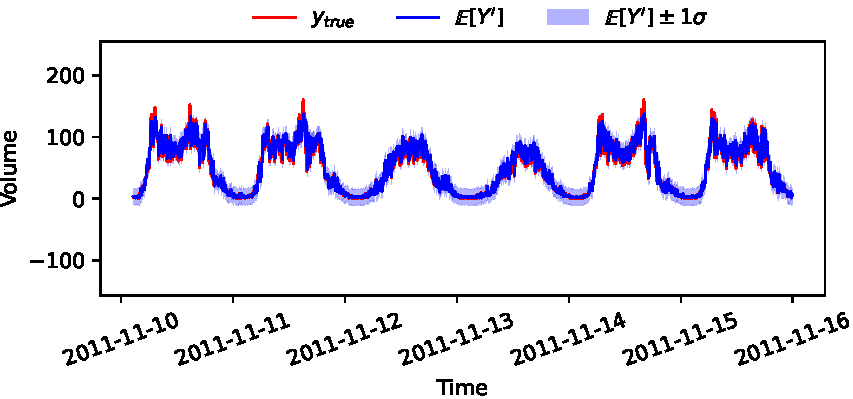
\includegraphics[scale=1]{FIG/TAGI_LSTM_Forecast.pdf}
  \caption{Model forecast on the test set.}
  \label{fig:model_forecast}
\end{figure}

The code used for this report can be accessed on this repository:


\end{enumerate}
\end{document}


